%! TEX encoding = utf8
\documentclass[a4paper,titlepage,11pt,twosides,floatssmall]{mwrep}
\usepackage[left=2.5cm,right=2.5cm,top=2.5cm,bottom=2.5cm]{geometry}
\usepackage[OT1]{fontenc}
\usepackage{polski}
\usepackage{amsmath}
\usepackage{amsfonts}
\usepackage{amssymb}
\usepackage{graphicx}
\usepackage{float}
\usepackage{url}
\usepackage{tikz}
\usetikzlibrary{arrows,calc,decorations.markings,math,arrows.meta}
\usepackage{rotating}
\usepackage[percent]{overpic}
\usepackage[utf8]{inputenc}
\usepackage{xcolor}
\usepackage{colortbl}
\usepackage{pgfplots}
\usetikzlibrary{pgfplots.groupplots}
\usepackage{listings}
\usepackage{matlab-prettifier}
\usepackage{enumitem,amssymb}
\definecolor{szary}{rgb}{0.95,0.95,0.95}
\usepackage{siunitx}
\usepackage{etoolbox}
\makeatletter
\patchcmd{\chapter}{\if@openright\cleardoublepage\else\clearpage\fi}{}{}{}
\makeatother
\sisetup{detect-weight,exponent-product=\cdot,output-decimal-marker={,},per-mode=symbol,binary-units=true,range-phrase={-},range-units=single}
\SendSettingsToPgf
%konfiguracje pakietu listings
\lstset{
	backgroundcolor=\color{szary},
	frame=single,
	breaklines=true,
}
\lstdefinestyle{customlatex}{
	basicstyle=\footnotesize\ttfamily,
	%basicstyle=\small\ttfamily,
}
\lstdefinestyle{customc}{
	breaklines=true,
	frame=tb,
	language=C,
	xleftmargin=0pt,
	showstringspaces=false,
	basicstyle=\small\ttfamily,
	keywordstyle=\bfseries\color{green!40!black},
	commentstyle=\itshape\color{purple!40!black},
	identifierstyle=\color{blue},
	stringstyle=\color{orange},
}
\lstdefinestyle{custommatlab}{
	captionpos=t,
	breaklines=true,
	frame=tb,
	xleftmargin=0pt,
	language=matlab,
	showstringspaces=false,
	basicstyle=\footnotesize\ttfamily,
	%basicstyle=\scriptsize\ttfamily,
	keywordstyle=\bfseries\color{green!40!black},
	commentstyle=\itshape\color{purple!40!black},
	identifierstyle=\color{blue},
	stringstyle=\color{orange},
}

%wymiar tekstu (bez �ywej paginy)
\textwidth 160mm \textheight 247mm

%ustawienia pakietu pgfplots
\pgfplotsset{
tick label style={font=\scriptsize},
label style={font=\small},
legend style={font=\small},
title style={font=\small}
}

\def\figurename{Rys.}
\def\tablename{Tab.}

%konfiguracja liczby p�ywaj�cych element�w
\setcounter{topnumber}{0}%2
\setcounter{bottomnumber}{3}%1
\setcounter{totalnumber}{5}%3
\renewcommand{\textfraction}{0.01}%0.2
\renewcommand{\topfraction}{0.95}%0.7
\renewcommand{\bottomfraction}{0.95}%0.3
\renewcommand{\floatpagefraction}{0.35}%0.5

\begin{document}
\frenchspacing
\pagestyle{uheadings}

%strona tytu�owa
\title{\bf Sprawozdanie z projektu i ćwiczenia laboratoryjnego nr 3, zadanie nr 10\vskip 0.1cm}
\author{Stanislau Stankevich, Rafał Bednarz, Ostrysz Jakub}
\date{2021}

\makeatletter
\renewcommand{\maketitle}{\begin{titlepage}
\begin{center}{\LARGE {\bf
Wydział Elektroniki i Technik Informacyjnych}}\\
\vspace{0.4cm}
{\LARGE {\bf Politechnika Warszawska}}\\
\vspace{0.3cm}
\end{center}
\vspace{5cm}
\begin{center}
{\bf \LARGE Projektowanie układów sterowania\\ (projekt grupowy) \vskip 0.1cm}
\end{center}
\vspace{1cm}
\begin{center}
{\bf \LARGE \@title}
\end{center}
\vspace{2cm}
\begin{center}
{\bf \Large \@author \par}
\end{center}
\vspace*{\stretch{6}}
\begin{center}
\bf{\large{Warszawa, \@date\vskip 0.1cm}}
\end{center}
\end{titlepage}
}
\makeatother

\maketitle

\tableofcontents

\chapter{Sprawdzenie punktu pracy}

Podając za wejścia same zera, po 300 iteracjach dostajemy następujący przebieg wyjść:

\begin{figure}[H]
\centering
% This file was created by matlab2tikz.
%
%The latest updates can be retrieved from
%  http://www.mathworks.com/matlabcentral/fileexchange/22022-matlab2tikz-matlab2tikz
%where you can also make suggestions and rate matlab2tikz.
%
\definecolor{mycolor1}{rgb}{0.00000,0.44700,0.74100}%
%
\begin{tikzpicture}

\begin{axis}[%
width=4.577in,
height=1.274in,
at={(0.768in,4.189in)},
scale only axis,
xmin=0,
xmax=300,
ymin=-1,
ymax=1,
ylabel style={font=\color{white!15!black}},
ylabel={y1},
axis background/.style={fill=white}
]
\addplot[const plot, color=green, forget plot] table[row sep=crcr] {%
1	0\\
2	0\\
3	0\\
4	0\\
5	0\\
6	0\\
7	0\\
8	0\\
9	0\\
10	0\\
11	0\\
12	0\\
13	0\\
14	0\\
15	0\\
16	0\\
17	0\\
18	0\\
19	0\\
20	0\\
21	0\\
22	0\\
23	0\\
24	0\\
25	0\\
26	0\\
27	0\\
28	0\\
29	0\\
30	0\\
31	0\\
32	0\\
33	0\\
34	0\\
35	0\\
36	0\\
37	0\\
38	0\\
39	0\\
40	0\\
41	0\\
42	0\\
43	0\\
44	0\\
45	0\\
46	0\\
47	0\\
48	0\\
49	0\\
50	0\\
51	0\\
52	0\\
53	0\\
54	0\\
55	0\\
56	0\\
57	0\\
58	0\\
59	0\\
60	0\\
61	0\\
62	0\\
63	0\\
64	0\\
65	0\\
66	0\\
67	0\\
68	0\\
69	0\\
70	0\\
71	0\\
72	0\\
73	0\\
74	0\\
75	0\\
76	0\\
77	0\\
78	0\\
79	0\\
80	0\\
81	0\\
82	0\\
83	0\\
84	0\\
85	0\\
86	0\\
87	0\\
88	0\\
89	0\\
90	0\\
91	0\\
92	0\\
93	0\\
94	0\\
95	0\\
96	0\\
97	0\\
98	0\\
99	0\\
100	0\\
101	0\\
102	0\\
103	0\\
104	0\\
105	0\\
106	0\\
107	0\\
108	0\\
109	0\\
110	0\\
111	0\\
112	0\\
113	0\\
114	0\\
115	0\\
116	0\\
117	0\\
118	0\\
119	0\\
120	0\\
121	0\\
122	0\\
123	0\\
124	0\\
125	0\\
126	0\\
127	0\\
128	0\\
129	0\\
130	0\\
131	0\\
132	0\\
133	0\\
134	0\\
135	0\\
136	0\\
137	0\\
138	0\\
139	0\\
140	0\\
141	0\\
142	0\\
143	0\\
144	0\\
145	0\\
146	0\\
147	0\\
148	0\\
149	0\\
150	0\\
151	0\\
152	0\\
153	0\\
154	0\\
155	0\\
156	0\\
157	0\\
158	0\\
159	0\\
160	0\\
161	0\\
162	0\\
163	0\\
164	0\\
165	0\\
166	0\\
167	0\\
168	0\\
169	0\\
170	0\\
171	0\\
172	0\\
173	0\\
174	0\\
175	0\\
176	0\\
177	0\\
178	0\\
179	0\\
180	0\\
181	0\\
182	0\\
183	0\\
184	0\\
185	0\\
186	0\\
187	0\\
188	0\\
189	0\\
190	0\\
191	0\\
192	0\\
193	0\\
194	0\\
195	0\\
196	0\\
197	0\\
198	0\\
199	0\\
200	0\\
201	0\\
202	0\\
203	0\\
204	0\\
205	0\\
206	0\\
207	0\\
208	0\\
209	0\\
210	0\\
211	0\\
212	0\\
213	0\\
214	0\\
215	0\\
216	0\\
217	0\\
218	0\\
219	0\\
220	0\\
221	0\\
222	0\\
223	0\\
224	0\\
225	0\\
226	0\\
227	0\\
228	0\\
229	0\\
230	0\\
231	0\\
232	0\\
233	0\\
234	0\\
235	0\\
236	0\\
237	0\\
238	0\\
239	0\\
240	0\\
241	0\\
242	0\\
243	0\\
244	0\\
245	0\\
246	0\\
247	0\\
248	0\\
249	0\\
250	0\\
251	0\\
252	0\\
253	0\\
254	0\\
255	0\\
256	0\\
257	0\\
258	0\\
259	0\\
260	0\\
261	0\\
262	0\\
263	0\\
264	0\\
265	0\\
266	0\\
267	0\\
268	0\\
269	0\\
270	0\\
271	0\\
272	0\\
273	0\\
274	0\\
275	0\\
276	0\\
277	0\\
278	0\\
279	0\\
280	0\\
281	0\\
282	0\\
283	0\\
284	0\\
285	0\\
286	0\\
287	0\\
288	0\\
289	0\\
290	0\\
291	0\\
292	0\\
293	0\\
294	0\\
295	0\\
296	0\\
297	0\\
298	0\\
299	0\\
300	0\\
};
\end{axis}

\begin{axis}[%
width=4.577in,
height=1.274in,
at={(0.768in,2.419in)},
scale only axis,
xmin=0,
xmax=300,
ymin=-1,
ymax=1,
ylabel style={font=\color{white!15!black}},
ylabel={y2},
axis background/.style={fill=white}
]
\addplot[const plot, color=red, forget plot] table[row sep=crcr] {%
1	0\\
2	0\\
3	0\\
4	0\\
5	0\\
6	0\\
7	0\\
8	0\\
9	0\\
10	0\\
11	0\\
12	0\\
13	0\\
14	0\\
15	0\\
16	0\\
17	0\\
18	0\\
19	0\\
20	0\\
21	0\\
22	0\\
23	0\\
24	0\\
25	0\\
26	0\\
27	0\\
28	0\\
29	0\\
30	0\\
31	0\\
32	0\\
33	0\\
34	0\\
35	0\\
36	0\\
37	0\\
38	0\\
39	0\\
40	0\\
41	0\\
42	0\\
43	0\\
44	0\\
45	0\\
46	0\\
47	0\\
48	0\\
49	0\\
50	0\\
51	0\\
52	0\\
53	0\\
54	0\\
55	0\\
56	0\\
57	0\\
58	0\\
59	0\\
60	0\\
61	0\\
62	0\\
63	0\\
64	0\\
65	0\\
66	0\\
67	0\\
68	0\\
69	0\\
70	0\\
71	0\\
72	0\\
73	0\\
74	0\\
75	0\\
76	0\\
77	0\\
78	0\\
79	0\\
80	0\\
81	0\\
82	0\\
83	0\\
84	0\\
85	0\\
86	0\\
87	0\\
88	0\\
89	0\\
90	0\\
91	0\\
92	0\\
93	0\\
94	0\\
95	0\\
96	0\\
97	0\\
98	0\\
99	0\\
100	0\\
101	0\\
102	0\\
103	0\\
104	0\\
105	0\\
106	0\\
107	0\\
108	0\\
109	0\\
110	0\\
111	0\\
112	0\\
113	0\\
114	0\\
115	0\\
116	0\\
117	0\\
118	0\\
119	0\\
120	0\\
121	0\\
122	0\\
123	0\\
124	0\\
125	0\\
126	0\\
127	0\\
128	0\\
129	0\\
130	0\\
131	0\\
132	0\\
133	0\\
134	0\\
135	0\\
136	0\\
137	0\\
138	0\\
139	0\\
140	0\\
141	0\\
142	0\\
143	0\\
144	0\\
145	0\\
146	0\\
147	0\\
148	0\\
149	0\\
150	0\\
151	0\\
152	0\\
153	0\\
154	0\\
155	0\\
156	0\\
157	0\\
158	0\\
159	0\\
160	0\\
161	0\\
162	0\\
163	0\\
164	0\\
165	0\\
166	0\\
167	0\\
168	0\\
169	0\\
170	0\\
171	0\\
172	0\\
173	0\\
174	0\\
175	0\\
176	0\\
177	0\\
178	0\\
179	0\\
180	0\\
181	0\\
182	0\\
183	0\\
184	0\\
185	0\\
186	0\\
187	0\\
188	0\\
189	0\\
190	0\\
191	0\\
192	0\\
193	0\\
194	0\\
195	0\\
196	0\\
197	0\\
198	0\\
199	0\\
200	0\\
201	0\\
202	0\\
203	0\\
204	0\\
205	0\\
206	0\\
207	0\\
208	0\\
209	0\\
210	0\\
211	0\\
212	0\\
213	0\\
214	0\\
215	0\\
216	0\\
217	0\\
218	0\\
219	0\\
220	0\\
221	0\\
222	0\\
223	0\\
224	0\\
225	0\\
226	0\\
227	0\\
228	0\\
229	0\\
230	0\\
231	0\\
232	0\\
233	0\\
234	0\\
235	0\\
236	0\\
237	0\\
238	0\\
239	0\\
240	0\\
241	0\\
242	0\\
243	0\\
244	0\\
245	0\\
246	0\\
247	0\\
248	0\\
249	0\\
250	0\\
251	0\\
252	0\\
253	0\\
254	0\\
255	0\\
256	0\\
257	0\\
258	0\\
259	0\\
260	0\\
261	0\\
262	0\\
263	0\\
264	0\\
265	0\\
266	0\\
267	0\\
268	0\\
269	0\\
270	0\\
271	0\\
272	0\\
273	0\\
274	0\\
275	0\\
276	0\\
277	0\\
278	0\\
279	0\\
280	0\\
281	0\\
282	0\\
283	0\\
284	0\\
285	0\\
286	0\\
287	0\\
288	0\\
289	0\\
290	0\\
291	0\\
292	0\\
293	0\\
294	0\\
295	0\\
296	0\\
297	0\\
298	0\\
299	0\\
300	0\\
};
\end{axis}

\begin{axis}[%
width=4.577in,
height=1.274in,
at={(0.768in,0.65in)},
scale only axis,
xmin=0,
xmax=300,
xlabel style={font=\color{white!15!black}},
xlabel={k},
ymin=-1,
ymax=1,
ylabel style={font=\color{white!15!black}},
ylabel={y3},
axis background/.style={fill=white}
]
\addplot[const plot, color=mycolor1, forget plot] table[row sep=crcr] {%
1	0\\
2	0\\
3	0\\
4	0\\
5	0\\
6	0\\
7	0\\
8	0\\
9	0\\
10	0\\
11	0\\
12	0\\
13	0\\
14	0\\
15	0\\
16	0\\
17	0\\
18	0\\
19	0\\
20	0\\
21	0\\
22	0\\
23	0\\
24	0\\
25	0\\
26	0\\
27	0\\
28	0\\
29	0\\
30	0\\
31	0\\
32	0\\
33	0\\
34	0\\
35	0\\
36	0\\
37	0\\
38	0\\
39	0\\
40	0\\
41	0\\
42	0\\
43	0\\
44	0\\
45	0\\
46	0\\
47	0\\
48	0\\
49	0\\
50	0\\
51	0\\
52	0\\
53	0\\
54	0\\
55	0\\
56	0\\
57	0\\
58	0\\
59	0\\
60	0\\
61	0\\
62	0\\
63	0\\
64	0\\
65	0\\
66	0\\
67	0\\
68	0\\
69	0\\
70	0\\
71	0\\
72	0\\
73	0\\
74	0\\
75	0\\
76	0\\
77	0\\
78	0\\
79	0\\
80	0\\
81	0\\
82	0\\
83	0\\
84	0\\
85	0\\
86	0\\
87	0\\
88	0\\
89	0\\
90	0\\
91	0\\
92	0\\
93	0\\
94	0\\
95	0\\
96	0\\
97	0\\
98	0\\
99	0\\
100	0\\
101	0\\
102	0\\
103	0\\
104	0\\
105	0\\
106	0\\
107	0\\
108	0\\
109	0\\
110	0\\
111	0\\
112	0\\
113	0\\
114	0\\
115	0\\
116	0\\
117	0\\
118	0\\
119	0\\
120	0\\
121	0\\
122	0\\
123	0\\
124	0\\
125	0\\
126	0\\
127	0\\
128	0\\
129	0\\
130	0\\
131	0\\
132	0\\
133	0\\
134	0\\
135	0\\
136	0\\
137	0\\
138	0\\
139	0\\
140	0\\
141	0\\
142	0\\
143	0\\
144	0\\
145	0\\
146	0\\
147	0\\
148	0\\
149	0\\
150	0\\
151	0\\
152	0\\
153	0\\
154	0\\
155	0\\
156	0\\
157	0\\
158	0\\
159	0\\
160	0\\
161	0\\
162	0\\
163	0\\
164	0\\
165	0\\
166	0\\
167	0\\
168	0\\
169	0\\
170	0\\
171	0\\
172	0\\
173	0\\
174	0\\
175	0\\
176	0\\
177	0\\
178	0\\
179	0\\
180	0\\
181	0\\
182	0\\
183	0\\
184	0\\
185	0\\
186	0\\
187	0\\
188	0\\
189	0\\
190	0\\
191	0\\
192	0\\
193	0\\
194	0\\
195	0\\
196	0\\
197	0\\
198	0\\
199	0\\
200	0\\
201	0\\
202	0\\
203	0\\
204	0\\
205	0\\
206	0\\
207	0\\
208	0\\
209	0\\
210	0\\
211	0\\
212	0\\
213	0\\
214	0\\
215	0\\
216	0\\
217	0\\
218	0\\
219	0\\
220	0\\
221	0\\
222	0\\
223	0\\
224	0\\
225	0\\
226	0\\
227	0\\
228	0\\
229	0\\
230	0\\
231	0\\
232	0\\
233	0\\
234	0\\
235	0\\
236	0\\
237	0\\
238	0\\
239	0\\
240	0\\
241	0\\
242	0\\
243	0\\
244	0\\
245	0\\
246	0\\
247	0\\
248	0\\
249	0\\
250	0\\
251	0\\
252	0\\
253	0\\
254	0\\
255	0\\
256	0\\
257	0\\
258	0\\
259	0\\
260	0\\
261	0\\
262	0\\
263	0\\
264	0\\
265	0\\
266	0\\
267	0\\
268	0\\
269	0\\
270	0\\
271	0\\
272	0\\
273	0\\
274	0\\
275	0\\
276	0\\
277	0\\
278	0\\
279	0\\
280	0\\
281	0\\
282	0\\
283	0\\
284	0\\
285	0\\
286	0\\
287	0\\
288	0\\
289	0\\
290	0\\
291	0\\
292	0\\
293	0\\
294	0\\
295	0\\
296	0\\
297	0\\
298	0\\
299	0\\
300	0\\
};
\end{axis}
\end{tikzpicture}%
\caption{Przebieg wyjść obiektu przy stałyćh wejściach: $u_1 = 0, u_2 = 0, u_3 = 0$}
\end{figure}

Każde wyjście ustabilizowało się na wartości 0, więc podany w zadaniu punkt pracy jest zgodny z rzeczywistością.
\chapter{Odpowiedzi skokowe poszczególnych torów}

\begin{figure}[H]
    \centering
    % This file was created by matlab2tikz.
%
%The latest updates can be retrieved from
%  http://www.mathworks.com/matlabcentral/fileexchange/22022-matlab2tikz-matlab2tikz
%where you can also make suggestions and rate matlab2tikz.
%
\definecolor{mycolor1}{rgb}{0.00000,0.44700,0.74100}%
%
\begin{tikzpicture}

\begin{axis}[%
width=1.68in,
height=1.553in,
at={(1.024in,7.552in)},
scale only axis,
xmin=0,
xmax=300,
ymin=0,
ymax=2,
axis background/.style={fill=white},
title style={font=\bfseries},
title={Tor u1 - y1}
]
\addplot[const plot, color=mycolor1, forget plot] table[row sep=crcr] {%
1	0\\
2	0\\
3	0\\
4	0\\
5	0\\
6	0.016391949758997\\
7	0.0322465074841911\\
8	0.0475812909820203\\
9	0.0624133404785264\\
10	0.0767591375546932\\
11	0.0906346234610095\\
12	0.10405521683161\\
13	0.117035830817676\\
14	0.129590889659142\\
15	0.141734344713106\\
16	0.15347968995678\\
17	0.164839976982182\\
18	0.175827829499246\\
19	0.186455457363473\\
20	0.196734670143684\\
21	0.206676890244985\\
22	0.216293165601498\\
23	0.225594181952986\\
24	0.234590274718991\\
25	0.243291440483701\\
26	0.251707348104291\\
27	0.259847349455094\\
28	0.267720489819536\\
29	0.275335517941379\\
30	0.282700895746449\\
31	0.289824807745644\\
32	0.296715170129683\\
33	0.303379639565681\\
34	0.309825621705348\\
35	0.316060279414253\\
36	0.3220905407313\\
37	0.327923106567261\\
38	0.333564458150924\\
39	0.339020864231123\\
40	0.344298388042659\\
41	0.349402894043855\\
42	0.354340054433218\\
43	0.359115355452472\\
44	0.363734103482943\\
45	0.368201430942085\\
46	0.372522301986692\\
47	0.376701518029143\\
48	0.380743723072795\\
49	0.384653408872464\\
50	0.38843491992573\\
51	0.3920924583006\\
52	0.395630088304905\\
53	0.399051741002618\\
54	0.402361218582103\\
55	0.405562198581165\\
56	0.40865823797358\\
57	0.411652777121649\\
58	0.414549143599185\\
59	0.417350555889155\\
60	0.420060126960102\\
61	0.422680867725322\\
62	0.425215690388633\\
63	0.427667411680455\\
64	0.430038755987799\\
65	0.43233235838165\\
66	0.434550767545086\\
67	0.436696448605419\\
68	0.438771785873472\\
69	0.440779085493064\\
70	0.442720578003624\\
71	0.444598420818803\\
72	0.446414700623819\\
73	0.448171435694211\\
74	0.449870578138576\\
75	0.451514016067778\\
76	0.453103575693045\\
77	0.454641023355279\\
78	0.456128067487841\\
79	0.457566360514982\\
80	0.458957500688044\\
81	0.460303033861457\\
82	0.461604455210515\\
83	0.462863210892835\\
84	0.464080699655348\\
85	0.465258274388606\\
86	0.466397243630134\\
87	0.467498873018494\\
88	0.46856438669968\\
89	0.469594968687406\\
90	0.470591764178802\\
91	0.471555880826967\\
92	0.472488389971815\\
93	0.473390327830558\\
94	0.474262696649169\\
95	0.475106465816087\\
96	0.47592257293942\\
97	0.476711924888825\\
98	0.477475398803237\\
99	0.478213843065554\\
100	0.478928078245375\\
101	0.479618898010829\\
102	0.480287070010508\\
103	0.480933336726488\\
104	0.48155841629939\\
105	0.482163003326382\\
106	0.482747769633032\\
107	0.483313365019843\\
108	0.483860417984325\\
109	0.484389536419389\\
110	0.484901308288844\\
111	0.485396302280755\\
112	0.485875068439373\\
113	0.486338138776354\\
114	0.486786027861937\\
115	0.487219233396744\\
116	0.487638236764826\\
117	0.488043503568592\\
118	0.488435484146185\\
119	0.488814614071909\\
120	0.489181314640244\\
121	0.489535993333993\\
122	0.489879044277085\\
123	0.490210848672528\\
124	0.490531775226011\\
125	0.490842180555612\\
126	0.491142409588076\\
127	0.491432795942108\\
128	0.491713662299086\\
129	0.491985320761639\\
130	0.492248073200453\\
131	0.492502211589714\\
132	0.492748018331558\\
133	0.492985766569877\\
134	0.49321572049384\\
135	0.493438135631467\\
136	0.493653259133571\\
137	0.493861330048398\\
138	0.494062579587261\\
139	0.494257231381463\\
140	0.494445501730804\\
141	0.49462759984393\\
142	0.494803728070813\\
143	0.494974082127604\\
144	0.495138851314114\\
145	0.495298218724171\\
146	0.495452361449069\\
147	0.495601450774362\\
148	0.495745652370196\\
149	0.495885126475401\\
150	0.496020028075556\\
151	0.496150507075207\\
152	0.496276708464445\\
153	0.496398772480019\\
154	0.496516834761172\\
155	0.496631026500363\\
156	0.496741474589051\\
157	0.496848301758697\\
158	0.496951626717149\\
159	0.497051564280544\\
160	0.497148225500904\\
161	0.497241717789528\\
162	0.497332145036356\\
163	0.49741960772541\\
164	0.497504203046456\\
165	0.497586025002996\\
166	0.497665164516736\\
167	0.497741709528609\\
168	0.497815745096504\\
169	0.49788735348978\\
170	0.497956614280687\\
171	0.498023604432784\\
172	0.498088398386466\\
173	0.498151068141681\\
174	0.498211683337938\\
175	0.498270311331692\\
176	0.498327017271189\\
177	0.498381864168864\\
178	0.498434912971357\\
179	0.49848622262724\\
180	0.498535850152521\\
181	0.498583850693999\\
182	0.498630277590549\\
183	0.498675182432387\\
184	0.498718615118403\\
185	0.498760623911604\\
186	0.498801255492751\\
187	0.498840555012224\\
188	0.498878566140199\\
189	0.498915331115175\\
190	0.498950890790905\\
191	0.4989852846818\\
192	0.499018551006831\\
193	0.499050726732006\\
194	0.499081847611439\\
195	0.499111948227089\\
196	0.499141062027181\\
197	0.499169221363376\\
198	0.499196457526723\\
199	0.499222800782428\\
200	0.499248280403485\\
201	0.499272924703205\\
202	0.499296761066679\\
203	0.499319815981208\\
204	0.499342115065734\\
205	0.499363683099314\\
206	0.499384544048649\\
207	0.499404721094716\\
208	0.499424236658532\\
209	0.499443112426065\\
210	0.499461369372332\\
211	0.499479027784708\\
212	0.499496107285466\\
213	0.499512626853588\\
214	0.499528604845849\\
215	0.499544059017217\\
216	0.499559006540583\\
217	0.499573464025845\\
218	0.499587447538363\\
219	0.499600972616811\\
220	0.499614054290446\\
221	0.499626707095807\\
222	0.499638945092868\\
223	0.499650781880663\\
224	0.499662230612396\\
225	0.499673304010059\\
226	0.499684014378565\\
227	0.499694373619427\\
228	0.499704393243977\\
229	0.499714084386163\\
230	0.499723457814917\\
231	0.499732523946125\\
232	0.499741292854198\\
233	0.49974977428327\\
234	0.499757977658023\\
235	0.499765912094162\\
236	0.499773586408544\\
237	0.499781009128975\\
238	0.499788188503685\\
239	0.499795132510495\\
240	0.499801848865684\\
241	0.499808345032559\\
242	0.499814628229751\\
243	0.499820705439239\\
244	0.4998265834141\\
245	0.499832268686025\\
246	0.499837767572565\\
247	0.499843086184162\\
248	0.499848230430931\\
249	0.49985320602923\\
250	0.499858018508015\\
251	0.499862673214979\\
252	0.499867175322497\\
253	0.499871529833375\\
254	0.499875741586406\\
255	0.499879815261748\\
256	0.499883755386128\\
257	0.499887566337866\\
258	0.499891252351745\\
259	0.499894817523715\\
260	0.499898265815447\\
261	0.499901601058729\\
262	0.499904826959731\\
263	0.499907947103119\\
264	0.499910964956041\\
265	0.499913883871976\\
266	0.499916707094464\\
267	0.499919437760711\\
268	0.49992207890507\\
269	0.499924633462418\\
270	0.499927104271415\\
271	0.499929494077658\\
272	0.499931805536733\\
273	0.499934041217166\\
274	0.499936203603277\\
275	0.499938295097938\\
276	0.499940318025249\\
277	0.499942274633114\\
278	0.499944167095743\\
279	0.499945997516068\\
280	0.499947767928077\\
281	0.499949480299076\\
282	0.499951136531876\\
283	0.499952738466907\\
284	0.49995428788426\\
285	0.499955786505671\\
286	0.499957235996428\\
287	0.499958637967227\\
288	0.499959993975955\\
289	0.49996130552943\\
290	0.499962574085067\\
291	0.499963801052504\\
292	0.499964987795164\\
293	0.499966135631772\\
294	0.499967245837819\\
295	0.499968319646983\\
296	0.499969358252496\\
297	0.499970362808469\\
298	0.49997133443118\\
299	0.49997227420031\\
300	0.499973183160143\\
};
\end{axis}

\begin{axis}[%
width=1.68in,
height=1.553in,
at={(3.235in,7.552in)},
scale only axis,
xmin=0,
xmax=300,
ymin=0,
ymax=2,
axis background/.style={fill=white},
title style={font=\bfseries},
title={Tor u1 - y2}
]
\addplot[const plot, color=mycolor1, forget plot] table[row sep=crcr] {%
1	0\\
2	0\\
3	0\\
4	0\\
5	0\\
6	0.048770575499286\\
7	0.0951625819640404\\
8	0.139292023574942\\
9	0.181269246922019\\
10	0.221199216928596\\
11	0.259181779318284\\
12	0.29531191028129\\
13	0.329679953964366\\
14	0.362371848378235\\
15	0.393469340287378\\
16	0.423050189619527\\
17	0.451188363905991\\
18	0.477954223239005\\
19	0.503414696208616\\
20	0.527633447259015\\
21	0.550671035882813\\
22	0.572585068051313\\
23	0.593430340259446\\
24	0.613258976545549\\
25	0.632120558828613\\
26	0.650062250888903\\
27	0.667128916301981\\
28	0.683363230621007\\
29	0.698805788087855\\
30	0.713495203139862\\
31	0.727468206966032\\
32	0.740759739354143\\
33	0.753403036058416\\
34	0.765429711906211\\
35	0.776869839851563\\
36	0.787752026173232\\
37	0.798103482005301\\
38	0.807950091379182\\
39	0.81731647594718\\
40	0.826226056549446\\
41	0.834701111778281\\
42	0.842762833686214\\
43	0.850431380777181\\
44	0.857725928413276\\
45	0.864664716763151\\
46	0.871265096411932\\
47	0.877543571746727\\
48	0.883515842226184\\
49	0.889196841637318\\
50	0.894600775437758\\
51	0.899741156276789\\
52	0.904630837784012\\
53	0.909282046710117\\
54	0.913706413500127\\
55	0.917915001375564\\
56	0.921918333998274\\
57	0.925726421785057\\
58	0.929348786938923\\
59	0.932794487259563\\
60	0.936072138792566\\
61	0.939189937374015\\
62	0.942155679124353\\
63	0.944976779942744\\
64	0.947660294050678\\
65	0.950212931631206\\
66	0.952641075607889\\
67	0.954950797605431\\
68	0.957147873131908\\
69	0.95923779602054\\
70	0.961225792167142\\
71	0.963116832597581\\
72	0.964915645897932\\
73	0.966626730038407\\
74	0.968254363620621\\
75	0.969802616576326\\
76	0.971275360344361\\
77	0.972676277551265\\
78	0.97400887121976\\
79	0.975276473528135\\
80	0.976482254142426\\
81	0.977629228142231\\
82	0.978720263559982\\
83	0.979758088552518\\
84	0.9807452982229\\
85	0.981684361109519\\
86	0.982577625358726\\
87	0.983427324596424\\
88	0.984235583513297\\
89	0.98500442317764\\
90	0.985735766089084\\
91	0.986431440985848\\
92	0.987093187417535\\
93	0.987722660094912\\
94	0.988321433027551\\
95	0.988891003459669\\
96	0.989432795614023\\
97	0.989948164253206\\
98	0.99043839806726\\
99	0.990904722896071\\
100	0.991348304794609\\
101	0.991770252948673\\
102	0.99217162244843\\
103	0.992553416926695\\
104	0.992916591068532\\
105	0.993262052998464\\
106	0.99359066655126\\
107	0.993903253431969\\
108	0.994200595270611\\
109	0.994483435576662\\
110	0.994752481598213\\
111	0.995008406090456\\
112	0.99525184899793\\
113	0.995483419054705\\
114	0.995703695306543\\
115	0.995913228558811\\
116	0.996112542753782\\
117	0.99630213628076\\
118	0.996482483222319\\
119	0.99665403453975\\
120	0.996817219200705\\
121	0.996972445251833\\
122	0.997120100839118\\
123	0.997260555178436\\
124	0.997394159478795\\
125	0.997521247820538\\
126	0.997642137990715\\
127	0.997757132277721\\
128	0.99786651822717\\
129	0.997970569360912\\
130	0.998069545860978\\
131	0.998163695220173\\
132	0.998253252860935\\
133	0.998338442724013\\
134	0.99841947782844\\
135	0.998496560804185\\
136	0.998569884398839\\
137	0.998639631959581\\
138	0.998705977891644\\
139	0.998769088094415\\
140	0.998829120376275\\
141	0.998886224849198\\
142	0.99894054430411\\
143	0.998992214567944\\
144	0.999041364843272\\
145	0.999088118031385\\
146	0.999132591039605\\
147	0.999174895073621\\
148	0.99921513591555\\
149	0.999253414188459\\
150	0.999289825607968\\
151	0.999324461221592\\
152	0.999357407636405\\
153	0.999388747235606\\
154	0.999418558384519\\
155	0.999446915626542\\
156	0.999473889869553\\
157	0.999499548563209\\
158	0.99952395586761\\
159	0.999547172813731\\
160	0.999569257456028\\
161	0.999590265017613\\
162	0.999610248028329\\
163	0.999629256456113\\
164	0.999647337831936\\
165	0.999664537368655\\
166	0.999680898074072\\
167	0.999696460858471\\
168	0.99971126463692\\
169	0.999725346426577\\
170	0.999738741439249\\
171	0.999751483169447\\
172	0.999763603478133\\
173	0.999775132672391\\
174	0.999786099581213\\
175	0.999796531627583\\
176	0.999806454897051\\
177	0.999815894202959\\
178	0.999824873148489\\
179	0.999833414185681\\
180	0.999841538671577\\
181	0.999849266921623\\
182	0.99985661826047\\
183	0.999863611070291\\
184	0.999870262836753\\
185	0.999876590192737\\
186	0.999882608959927\\
187	0.999888334188377\\
188	0.99989378019414\\
189	0.999898960595066\\
190	0.999903888344856\\
191	0.999908575765452\\
192	0.999913034577846\\
193	0.999917275931393\\
194	0.999921310431686\\
195	0.999925148167076\\
196	0.999928798733903\\
197	0.999932271260486\\
198	0.99993557442995\\
199	0.99993871650194\\
200	0.99994170533327\\
201	0.999944548397578\\
202	0.999947252804004\\
203	0.999949825314975\\
204	0.999952272363108\\
205	0.999954600067297\\
206	0.999956814248017\\
207	0.999958920441871\\
208	0.999960923915441\\
209	0.999962829678454\\
210	0.99996464249631\\
211	0.999966366901996\\
212	0.999968007207425\\
213	0.999969567514213\\
214	0.99997105172394\\
215	0.999972463547904\\
216	0.9999738065164\\
217	0.999975083987549\\
218	0.999976299155695\\
219	0.999977455059389\\
220	0.999978554588995\\
221	0.999979600493908\\
222	0.999980595389437\\
223	0.999981541763338\\
224	0.999982441982039\\
225	0.999983298296556\\
226	0.999984112848121\\
227	0.999984887673537\\
228	0.999985624710272\\
229	0.999986325801302\\
230	0.999986992699718\\
231	0.999987627073115\\
232	0.999988230507756\\
233	0.999988804512542\\
234	0.999989350522784\\
235	0.999989869903793\\
236	0.999990363954293\\
237	0.999990833909665\\
238	0.999991280945045\\
239	0.999991706178254\\
240	0.999992110672595\\
241	0.999992495439514\\
242	0.99999286144113\\
243	0.999993209592637\\
244	0.999993540764595\\
245	0.999993855785107\\
246	0.999994155441887\\
247	0.999994440484234\\
248	0.999994711624902\\
249	0.999994969541883\\
250	0.999995214880104\\
251	0.999995448253039\\
252	0.999995670244241\\
253	0.999995881408805\\
254	0.999996082274753\\
255	0.999996273344354\\
256	0.999996455095383\\
257	0.999996627982311\\
258	0.999996792437446\\
259	0.999996948872011\\
260	0.999997097677171\\
261	0.999997239225018\\
262	0.999997373869494\\
263	0.999997501947282\\
264	0.999997623778642\\
265	0.999997739668218\\
266	0.999997849905793\\
267	0.999997954767019\\
268	0.999998054514102\\
269	0.999998149396462\\
270	0.999998239651354\\
271	0.999998325504463\\
272	0.999998407170465\\
273	0.999998484853569\\
274	0.999998558748023\\
275	0.999998629038599\\
276	0.999998695901061\\
277	0.9999987595026\\
278	0.999998820002253\\
279	0.999998877551301\\
280	0.999998932293646\\
281	0.999998984366176\\
282	0.999999033899097\\
283	0.999999081016271\\
284	0.999999125835513\\
285	0.999999168468897\\
286	0.999999209023026\\
287	0.999999247599309\\
288	0.999999284294204\\
289	0.999999319199469\\
290	0.999999352402385\\
291	0.999999383985977\\
292	0.999999414029218\\
293	0.999999442607233\\
294	0.99999946979148\\
295	0.999999495649936\\
296	0.999999520247258\\
297	0.999999543644954\\
298	0.99999956590153\\
299	0.999999587072638\\
300	0.999999607211218\\
};
\end{axis}

\begin{axis}[%
width=1.68in,
height=1.553in,
at={(5.446in,7.552in)},
scale only axis,
xmin=0,
xmax=300,
ymin=0,
ymax=2,
axis background/.style={fill=white},
title style={font=\bfseries},
title={Tor u1 - y3}
]
\addplot[const plot, color=mycolor1, forget plot] table[row sep=crcr] {%
1	0\\
2	0\\
3	0\\
4	0\\
5	0\\
6	0.00958843300927808\\
7	0.0189141858826321\\
8	0.0279844548797369\\
9	0.0368062391149706\\
10	0.0453863459583134\\
11	0.0537313962882852\\
12	0.061847829600977\\
13	0.0697419089791175\\
14	0.0774197259250088\\
15	0.0848872050610625\\
16	0.0921501087015615\\
17	0.0992140412991755\\
18	0.106084453769663\\
19	0.112766647698096\\
20	0.119265779429849\\
21	0.125586864049521\\
22	0.131734779250846\\
23	0.137714269100586\\
24	0.143529947699315\\
25	0.149186302741909\\
26	0.154687698980495\\
27	0.160038381592536\\
28	0.165242479456636\\
29	0.170304008338611\\
30	0.175226873990274\\
31	0.180014875163324\\
32	0.184671706540672\\
33	0.189200961587456\\
34	0.19360613532396\\
35	0.19789062702256\\
36	0.202057742830786\\
37	0.206110698322529\\
38	0.210052620979351\\
39	0.213886552603823\\
40	0.217615451666742\\
41	0.221242195590052\\
42	0.224769582967218\\
43	0.228200335722774\\
44	0.231537101212706\\
45	0.234782454267302\\
46	0.237938899178026\\
47	0.241008871629966\\
48	0.243994740581348\\
49	0.246898810091544\\
50	0.249723321099019\\
51	0.252470453150553\\
52	0.255142326083105\\
53	0.257741001659591\\
54	0.260268485159855\\
55	0.262726726928049\\
56	0.265117623877628\\
57	0.267443020955114\\
58	0.269704712563749\\
59	0.271904443948165\\
60	0.274043912541101\\
61	0.27612476927324\\
62	0.278148619847157\\
63	0.280117025976363\\
64	0.282031506590411\\
65	0.283893539006988\\
66	0.285704560071886\\
67	0.287465967267757\\
68	0.289179119792487\\
69	0.290845339608022\\
70	0.292465912460472\\
71	0.294042088872258\\
72	0.295575085107087\\
73	0.297066084108483\\
74	0.298516236412618\\
75	0.29992666103612\\
76	0.301298446339574\\
77	0.302632650867354\\
78	0.303930304164463\\
79	0.305192407570975\\
80	0.306419934994733\\
81	0.307613833662863\\
82	0.308775024852709\\
83	0.309904404602741\\
84	0.311002844403987\\
85	0.312071191872522\\
86	0.313110271403535\\
87	0.31412088480748\\
88	0.315103811928791\\
89	0.316059811247658\\
90	0.316989620465309\\
91	0.317893957073262\\
92	0.318773518906978\\
93	0.319628984684352\\
94	0.320461014529446\\
95	0.32127025048188\\
96	0.322057316992261\\
97	0.322822821404046\\
98	0.323567354422201\\
99	0.32429149056902\\
100	0.324995788627457\\
101	0.325680792072317\\
102	0.326347029489629\\
103	0.326995014984529\\
104	0.327625248577975\\
105	0.32823821659259\\
106	0.328834392027934\\
107	0.329414234925496\\
108	0.329978192723688\\
109	0.330526700603114\\
110	0.331060181822378\\
111	0.33157904804469\\
112	0.332083699655536\\
113	0.332574526071628\\
114	0.333051906041406\\
115	0.333516207937298\\
116	0.333967790039977\\
117	0.334407000814829\\
118	0.334834179180847\\
119	0.335249654772164\\
120	0.335653748192411\\
121	0.336046771262117\\
122	0.336429027259324\\
123	0.336800811153611\\
124	0.337162409833716\\
125	0.337514102328905\\
126	0.337856160024294\\
127	0.338188846870262\\
128	0.338512419586128\\
129	0.338827127858253\\
130	0.339133214532707\\
131	0.339430915802666\\
132	0.339720461390672\\
133	0.340002074725895\\
134	0.340275973116549\\
135	0.340542367917574\\
136	0.340801464693731\\
137	0.341053463378228\\
138	0.341298558426997\\
139	0.341536938968749\\
140	0.341768788950914\\
141	0.341994287281587\\
142	0.342213607967582\\
143	0.342426920248705\\
144	0.342634388728349\\
145	0.342836173500511\\
146	0.34303243027333\\
147	0.343223310489238\\
148	0.343408961441823\\
149	0.343589526389488\\
150	0.343765144665997\\
151	0.343935951787994\\
152	0.344102079559571\\
153	0.344263656173981\\
154	0.344420806312553\\
155	0.344573651240909\\
156	0.344722308902532\\
157	0.344866894009784\\
158	0.345007518132422\\
159	0.34514428978369\\
160	0.345277314504057\\
161	0.345406694942652\\
162	0.345532530936482\\
163	0.345654919587464\\
164	0.345773955337357\\
165	0.345889730040639\\
166	0.346002333035389\\
167	0.346111851212219\\
168	0.346218369081328\\
169	0.346321968837717\\
170	0.346422730424608\\
171	0.34652073159514\\
172	0.346616047972362\\
173	0.34670875310759\\
174	0.346798918537164\\
175	0.346886613837649\\
176	0.346971906679523\\
177	0.347054862879395\\
178	0.347135546450795\\
179	0.347214019653568\\
180	0.347290343041919\\
181	0.347364575511137\\
182	0.347436774343046\\
183	0.347506995250204\\
184	0.347575292418892\\
185	0.347641718550934\\
186	0.347706324904355\\
187	0.347769161332942\\
188	0.347830276324713\\
189	0.347889717039328\\
190	0.347947529344486\\
191	0.348003757851315\\
192	0.348058445948798\\
193	0.348111635837256\\
194	0.348163368560907\\
195	0.348213684039544\\
196	0.348262621099335\\
197	0.348310217502784\\
198	0.348356509977873\\
199	0.348401534246402\\
200	0.348445325051552\\
201	0.348487916184697\\
202	0.348529340511479\\
203	0.348569629997168\\
204	0.34860881573133\\
205	0.348646927951814\\
206	0.348683996068089\\
207	0.348720048683936\\
208	0.348755113619521\\
209	0.348789217932859\\
210	0.348822387940702\\
211	0.348854649238834\\
212	0.348886026721835\\
213	0.348916544602282\\
214	0.348946226429437\\
215	0.348975095107417\\
216	0.349003172912868\\
217	0.349030481512157\\
218	0.34905704197809\\
219	0.349082874806171\\
220	0.349107999930419\\
221	0.349132436738751\\
222	0.349156204087942\\
223	0.349179320318175\\
224	0.349201803267194\\
225	0.349223670284068\\
226	0.349244938242581\\
227	0.34926562355425\\
228	0.349285742180989\\
229	0.349305309647428\\
230	0.349324341052893\\
231	0.349342851083053\\
232	0.349360854021258\\
233	0.349378363759558\\
234	0.349395393809421\\
235	0.349411957312164\\
236	0.349428067049089\\
237	0.349443735451347\\
238	0.349458974609533\\
239	0.349473796283013\\
240	0.349488211908998\\
241	0.349502232611373\\
242	0.349515869209275\\
243	0.349529132225448\\
244	0.349542031894359\\
245	0.349554578170094\\
246	0.349566780734046\\
247	0.349578649002379\\
248	0.349590192133295\\
249	0.349601419034105\\
250	0.349612338368097\\
251	0.349622958561225\\
252	0.349633287808609\\
253	0.34964333408086\\
254	0.34965310513023\\
255	0.349662608496592\\
256	0.349671851513264\\
257	0.34968084131266\\
258	0.3496895848318\\
259	0.349698088817661\\
260	0.349706359832383\\
261	0.349714404258332\\
262	0.349722228303025\\
263	0.349729838003923\\
264	0.349737239233086\\
265	0.349744437701706\\
266	0.349751438964514\\
267	0.349758248424065\\
268	0.349764871334912\\
269	0.349771312807653\\
270	0.34977757781288\\
271	0.349783671185013\\
272	0.34978959762603\\
273	0.349795361709096\\
274	0.349800967882093\\
275	0.34980642047105\\
276	0.349811723683481\\
277	0.349816881611636\\
278	0.349821898235652\\
279	0.349826777426631\\
280	0.349831522949621\\
281	0.349836138466529\\
282	0.349840627538937\\
283	0.349844993630859\\
284	0.349849240111411\\
285	0.349853370257407\\
286	0.349857387255894\\
287	0.349861294206607\\
288	0.349865094124362\\
289	0.349868789941384\\
290	0.349872384509567\\
291	0.349875880602674\\
292	0.349879280918483\\
293	0.349882588080862\\
294	0.349885804641799\\
295	0.349888933083367\\
296	0.349891975819643\\
297	0.349894935198568\\
298	0.34989781350376\\
299	0.349900612956276\\
300	0.349903335716326\\
};
\end{axis}

\begin{axis}[%
width=1.68in,
height=1.553in,
at={(1.024in,5.395in)},
scale only axis,
xmin=0,
xmax=300,
ymin=0,
ymax=2,
axis background/.style={fill=white},
title style={font=\bfseries},
title={Tor u2 - y1}
]
\addplot[const plot, color=mycolor1, forget plot] table[row sep=crcr] {%
1	0\\
2	0\\
3	0\\
4	0\\
5	0\\
6	0.0221199216928595\\
7	0.0393469340287367\\
8	0.0527633447258986\\
9	0.0632120558828559\\
10	0.0713495203139812\\
11	0.0776869839851574\\
12	0.0826226056549562\\
13	0.0864664716763397\\
14	0.0894600775438148\\
15	0.0917915001376117\\
16	0.093607213879331\\
17	0.0950212931632155\\
18	0.0961225792168297\\
19	0.09698026165777\\
20	0.0976482254144007\\
21	0.0981684361111279\\
22	0.0985735766091011\\
23	0.0988891003461764\\
24	0.0991348304796881\\
25	0.0993262053000911\\
26	0.099475248160081\\
27	0.0995913228561522\\
28	0.0996817219203471\\
29	0.0997521247823309\\
30	0.0998069545863742\\
31	0.0998496560806986\\
32	0.0998829120379167\\
33	0.0999088118034399\\
34	0.0999289825611107\\
35	0.0999446915629798\\
36	0.0999569257459367\\
37	0.0999664537372038\\
38	0.0999738741442635\\
39	0.0999796531630923\\
40	0.0999841538674815\\
41	0.0999876590195841\\
42	0.0999903888347864\\
43	0.0999925148170035\\
44	0.0999941705336189\\
45	0.0999954600070155\\
46	0.0999964642499065\\
47	0.0999972463550563\\
48	0.0999978554591594\\
49	0.0999983298299119\\
50	0.0999986992702254\\
51	0.0999989869906308\\
52	0.0999992110675078\\
53	0.0999993855787551\\
54	0.0999995214882511\\
55	0.099999627334673\\
56	0.0999997097679491\\
57	0.099999773967049\\
58	0.0999998239653582\\
59	0.0999998629040804\\
60	0.0999998932295876\\
61	0.0999999168471163\\
62	0.099999935240466\\
63	0.0999999495652211\\
64	0.0999999607213515\\
65	0.0999999694097546\\
66	0.0999999761762898\\
67	0.0999999814460727\\
68	0.0999999855501838\\
69	0.0999999887464686\\
70	0.0999999912357378\\
71	0.0999999931743825\\
72	0.0999999946842005\\
73	0.0999999958600478\\
74	0.0999999967757985\\
75	0.0999999974889857\\
76	0.0999999980444165\\
77	0.0999999984769863\\
78	0.0999999988138718\\
79	0.0999999990762384\\
80	0.0999999992805694\\
81	0.0999999994397024\\
82	0.0999999995636352\\
83	0.0999999996601539\\
84	0.0999999997353225\\
85	0.0999999997938637\\
86	0.0999999998394556\\
87	0.0999999998749624\\
88	0.0999999999026151\\
89	0.0999999999241509\\
90	0.0999999999409229\\
91	0.0999999999539848\\
92	0.0999999999641574\\
93	0.0999999999720795\\
94	0.0999999999782492\\
95	0.0999999999830539\\
96	0.0999999999867957\\
97	0.0999999999897097\\
98	0.0999999999919788\\
99	0.0999999999937458\\
100	0.0999999999951218\\
101	0.0999999999961933\\
102	0.0999999999970277\\
103	0.0999999999976775\\
104	0.0999999999981837\\
105	0.0999999999985779\\
106	0.099999999998885\\
107	0.0999999999991241\\
108	0.0999999999993104\\
109	0.0999999999994554\\
110	0.0999999999995685\\
111	0.0999999999996565\\
112	0.0999999999997252\\
113	0.0999999999997786\\
114	0.0999999999998202\\
115	0.0999999999998526\\
116	0.0999999999998777\\
117	0.0999999999998972\\
118	0.0999999999999125\\
119	0.0999999999999244\\
120	0.0999999999999337\\
121	0.0999999999999409\\
122	0.0999999999999465\\
123	0.0999999999999508\\
124	0.0999999999999541\\
125	0.0999999999999566\\
126	0.0999999999999584\\
127	0.0999999999999597\\
128	0.0999999999999606\\
129	0.0999999999999613\\
130	0.0999999999999618\\
131	0.0999999999999622\\
132	0.0999999999999625\\
133	0.0999999999999626\\
134	0.0999999999999626\\
135	0.0999999999999626\\
136	0.0999999999999624\\
137	0.0999999999999621\\
138	0.0999999999999619\\
139	0.0999999999999615\\
140	0.0999999999999612\\
141	0.099999999999961\\
142	0.0999999999999608\\
143	0.0999999999999606\\
144	0.0999999999999605\\
145	0.0999999999999604\\
146	0.0999999999999602\\
147	0.0999999999999601\\
148	0.09999999999996\\
149	0.0999999999999598\\
150	0.0999999999999596\\
151	0.0999999999999594\\
152	0.0999999999999592\\
153	0.0999999999999589\\
154	0.0999999999999586\\
155	0.0999999999999583\\
156	0.099999999999958\\
157	0.0999999999999578\\
158	0.0999999999999575\\
159	0.0999999999999572\\
160	0.0999999999999569\\
161	0.0999999999999565\\
162	0.0999999999999561\\
163	0.0999999999999557\\
164	0.0999999999999553\\
165	0.099999999999955\\
166	0.0999999999999546\\
167	0.0999999999999543\\
168	0.099999999999954\\
169	0.0999999999999538\\
170	0.0999999999999537\\
171	0.0999999999999536\\
172	0.0999999999999537\\
173	0.0999999999999539\\
174	0.0999999999999542\\
175	0.0999999999999546\\
176	0.0999999999999551\\
177	0.0999999999999557\\
178	0.0999999999999564\\
179	0.099999999999957\\
180	0.0999999999999577\\
181	0.0999999999999583\\
182	0.0999999999999589\\
183	0.0999999999999595\\
184	0.0999999999999601\\
185	0.0999999999999607\\
186	0.0999999999999612\\
187	0.0999999999999618\\
188	0.0999999999999623\\
189	0.0999999999999628\\
190	0.0999999999999634\\
191	0.0999999999999639\\
192	0.0999999999999645\\
193	0.0999999999999651\\
194	0.0999999999999657\\
195	0.0999999999999664\\
196	0.099999999999967\\
197	0.0999999999999677\\
198	0.0999999999999683\\
199	0.099999999999969\\
200	0.0999999999999697\\
201	0.0999999999999704\\
202	0.0999999999999711\\
203	0.0999999999999717\\
204	0.0999999999999723\\
205	0.0999999999999728\\
206	0.0999999999999733\\
207	0.0999999999999737\\
208	0.0999999999999741\\
209	0.0999999999999746\\
210	0.099999999999975\\
211	0.0999999999999754\\
212	0.0999999999999757\\
213	0.0999999999999759\\
214	0.0999999999999761\\
215	0.0999999999999762\\
216	0.0999999999999761\\
217	0.0999999999999759\\
218	0.0999999999999757\\
219	0.0999999999999753\\
220	0.099999999999975\\
221	0.0999999999999746\\
222	0.0999999999999742\\
223	0.0999999999999738\\
224	0.0999999999999735\\
225	0.0999999999999732\\
226	0.0999999999999729\\
227	0.0999999999999726\\
228	0.0999999999999723\\
229	0.0999999999999722\\
230	0.0999999999999721\\
231	0.0999999999999722\\
232	0.0999999999999722\\
233	0.0999999999999723\\
234	0.0999999999999725\\
235	0.0999999999999727\\
236	0.0999999999999728\\
237	0.099999999999973\\
238	0.0999999999999732\\
239	0.0999999999999734\\
240	0.0999999999999737\\
241	0.0999999999999741\\
242	0.0999999999999744\\
243	0.0999999999999748\\
244	0.0999999999999752\\
245	0.0999999999999757\\
246	0.0999999999999761\\
247	0.0999999999999765\\
248	0.0999999999999769\\
249	0.0999999999999772\\
250	0.0999999999999775\\
251	0.0999999999999776\\
252	0.0999999999999777\\
253	0.0999999999999778\\
254	0.0999999999999779\\
255	0.099999999999978\\
256	0.0999999999999781\\
257	0.0999999999999781\\
258	0.099999999999978\\
259	0.0999999999999778\\
260	0.0999999999999776\\
261	0.0999999999999772\\
262	0.0999999999999769\\
263	0.0999999999999764\\
264	0.0999999999999759\\
265	0.0999999999999753\\
266	0.0999999999999746\\
267	0.0999999999999739\\
268	0.0999999999999731\\
269	0.0999999999999723\\
270	0.0999999999999715\\
271	0.0999999999999708\\
272	0.0999999999999702\\
273	0.0999999999999697\\
274	0.0999999999999693\\
275	0.099999999999969\\
276	0.0999999999999687\\
277	0.0999999999999684\\
278	0.0999999999999682\\
279	0.099999999999968\\
280	0.0999999999999679\\
281	0.0999999999999678\\
282	0.0999999999999677\\
283	0.0999999999999677\\
284	0.0999999999999676\\
285	0.0999999999999676\\
286	0.0999999999999676\\
287	0.0999999999999676\\
288	0.0999999999999677\\
289	0.0999999999999678\\
290	0.099999999999968\\
291	0.0999999999999682\\
292	0.0999999999999684\\
293	0.0999999999999687\\
294	0.099999999999969\\
295	0.0999999999999692\\
296	0.0999999999999695\\
297	0.0999999999999698\\
298	0.09999999999997\\
299	0.0999999999999703\\
300	0.0999999999999706\\
};
\end{axis}

\begin{axis}[%
width=1.68in,
height=1.553in,
at={(3.235in,5.395in)},
scale only axis,
xmin=0,
xmax=300,
ymin=0,
ymax=2,
axis background/.style={fill=white},
title style={font=\bfseries},
title={Tor u2 - y2}
]
\addplot[const plot, color=mycolor1, forget plot] table[row sep=crcr] {%
1	0\\
2	0\\
3	0\\
4	0\\
5	0\\
6	0.0204052714454309\\
7	0.0399777926853384\\
8	0.0587515487077024\\
9	0.0767591375546931\\
10	0.0940318269246828\\
11	0.110599608464298\\
12	0.126491249844785\\
13	0.141734344713107\\
14	0.156355360604517\\
15	0.170379684899782\\
16	0.183831668906881\\
17	0.196734670143691\\
18	0.209111092895106\\
19	0.220982427114989\\
20	0.23236928574052\\
21	0.243291440483722\\
22	0.253767856162316\\
23	0.263816723629517\\
24	0.273455491359944\\
25	0.282700895746494\\
26	0.291568990160784\\
27	0.30007517282762\\
28	0.308234213561894\\
29	0.316060279414334\\
30	0.323566959270636\\
31	0.330767287446694\\
32	0.337673766320894\\
33	0.344298388042773\\
34	0.350652655355735\\
35	0.35674760156998\\
36	0.362593809720331\\
37	0.368201430942211\\
38	0.373580202097699\\
39	0.378739462682244\\
40	0.383688171041418\\
41	0.388434919925844\\
42	0.392987951411328\\
43	0.397355171210089\\
44	0.401544162397937\\
45	0.405562198581242\\
46	0.40941625652655\\
47	0.413113028274775\\
48	0.41665893276101\\
49	0.42006012696012\\
50	0.423322516577486\\
51	0.426451766303444\\
52	0.429453309649243\\
53	0.432332358381589\\
54	0.435093911572157\\
55	0.437742764277796\\
56	0.440283515866479\\
57	0.442720578003477\\
58	0.445058182311605\\
59	0.447300387718854\\
60	0.44945108750616\\
61	0.451514016067551\\
62	0.453492755394406\\
63	0.455390741295092\\
64	0.457211269360771\\
65	0.458957500687741\\
66	0.460632467366243\\
67	0.462239077745271\\
68	0.463780121482515\\
69	0.465258274388222\\
70	0.466676103071371\\
71	0.468036069396233\\
72	0.469340534757063\\
73	0.470591764178334\\
74	0.471791930247641\\
75	0.472943116888099\\
76	0.474047322976791\\
77	0.475106465815539\\
78	0.476122384460037\\
79	0.47709684291312\\
80	0.478031533187706\\
81	0.478928078244749\\
82	0.479788034811287\\
83	0.48061289608348\\
84	0.481404094319343\\
85	0.482163003325664\\
86	0.482890940843431\\
87	0.483589170835905\\
88	0.484258905683323\\
89	0.484901308288022\\
90	0.485517494093668\\
91	0.486108533022063\\
92	0.48667545133092\\
93	0.487219233395817\\
94	0.487740823419432\\
95	0.488241127071018\\
96	0.488721013058972\\
97	0.489181314639234\\
98	0.489622831062113\\
99	0.490046328960081\\
100	0.49045254367892\\
101	0.490842180554555\\
102	0.491215916137765\\
103	0.491574399368927\\
104	0.491918252704809\\
105	0.492248073199379\\
106	0.492564433540509\\
107	0.492867883044368\\
108	0.493158948609234\\
109	0.493438135630382\\
110	0.493705928877627\\
111	0.49396279333707\\
112	0.494209175018473\\
113	0.494445501729699\\
114	0.494672183819541\\
115	0.494889614890232\\
116	0.495098172480886\\
117	0.495298218723042\\
118	0.495490100969452\\
119	0.495674152397215\\
120	0.49585069258629\\
121	0.496020028074408\\
122	0.496182452889325\\
123	0.496338249059366\\
124	0.496487687103127\\
125	0.496631026499194\\
126	0.496768516136689\\
127	0.496900394747436\\
128	0.497026891320482\\
129	0.497148225499706\\
130	0.497264607965204\\
131	0.497376240799101\\
132	0.497483317836441\\
133	0.497586025001756\\
134	0.497684540631895\\
135	0.497779035785685\\
136	0.497869674540947\\
137	0.497956614279401\\
138	0.498040005959929\\
139	0.498119994380702\\
140	0.498196718430597\\
141	0.498270311330363\\
142	0.498340900863936\\
143	0.498408609600321\\
144	0.498473555106415\\
145	0.498535850151147\\
146	0.498595602901285\\
147	0.49865291710925\\
148	0.498707892293274\\
149	0.498760623910191\\
150	0.498811203521195\\
151	0.498859718950814\\
152	0.498906254439411\\
153	0.498950890789455\\
154	0.49899370550582\\
155	0.499034772930368\\
156	0.499074164371024\\
157	0.499111948225603\\
158	0.499148190100565\\
159	0.499182952924935\\
160	0.49921629705957\\
161	0.499248280401969\\
162	0.499278958486803\\
163	0.499308384582341\\
164	0.499336609782946\\
165	0.499363683097792\\
166	0.499389651535962\\
167	0.499414560188072\\
168	0.499438452304566\\
169	0.499461369370816\\
170	0.49948335117915\\
171	0.499504435897952\\
172	0.499524660137933\\
173	0.4995440590157\\
174	0.499562666214734\\
175	0.499580514043873\\
176	0.499597633493415\\
177	0.499614054288927\\
178	0.499629804942859\\
179	0.499644912804052\\
180	0.499659404105228\\
181	0.499673304008534\\
182	0.49968663664924\\
183	0.49969942517764\\
184	0.499711691799254\\
185	0.49972345781338\\
186	0.499734743650082\\
187	0.499745568905662\\
188	0.499755952376685\\
189	0.499765912092618\\
190	0.499775465347136\\
191	0.499784628728151\\
192	0.499793418146612\\
193	0.499801848864133\\
194	0.499809935519495\\
195	0.499817692154062\\
196	0.499825132236161\\
197	0.49983226868447\\
198	0.499839113890449\\
199	0.499845679739857\\
200	0.499851977633386\\
201	0.499858018506461\\
202	0.499863812848227\\
203	0.499869370719761\\
204	0.499874701771539\\
205	0.4998798152602\\
206	0.499884720064613\\
207	0.499889424701294\\
208	0.499893937339198\\
209	0.499898265813899\\
210	0.499902417641197\\
211	0.49990640003017\\
212	0.499910219895686\\
213	0.499913883870417\\
214	0.499917398316351\\
215	0.499920769335838\\
216	0.499924002782191\\
217	0.499927104269844\\
218	0.499930079184103\\
219	0.499932932690496\\
220	0.499935669743746\\
221	0.499938295096368\\
222	0.499940813306926\\
223	0.499943228747944\\
224	0.499945545613504\\
225	0.499947767926523\\
226	0.499949899545742\\
227	0.499951944172422\\
228	0.499953905356778\\
229	0.499955786504136\\
230	0.499957590880848\\
231	0.499959321619967\\
232	0.499960981726681\\
233	0.499962574083539\\
234	0.499964101455447\\
235	0.499965566494477\\
236	0.499966971744468\\
237	0.499968319645443\\
238	0.499969612537847\\
239	0.49997085266661\\
240	0.499972042185045\\
241	0.499973183158587\\
242	0.49997427756838\\
243	0.499975327314715\\
244	0.499976334220334\\
245	0.499977300033589\\
246	0.499978226431482\\
247	0.499979115022575\\
248	0.499979967349783\\
249	0.499980784893057\\
250	0.499981569071946\\
251	0.499982321248069\\
252	0.499983042727477\\
253	0.499983734762919\\
254	0.499984398556019\\
255	0.499985035259363\\
256	0.499985645978498\\
257	0.499986231773854\\
258	0.499986793662584\\
259	0.49998733262033\\
260	0.499987849582917\\
261	0.49998834544798\\
262	0.499988821076519\\
263	0.499989277294399\\
264	0.499989714893779\\
265	0.49999013463449\\
266	0.499990537245355\\
267	0.499990923425451\\
268	0.499991293845329\\
269	0.49999164914817\\
270	0.499991989950909\\
271	0.499992316845304\\
272	0.499992630398962\\
273	0.499992931156325\\
274	0.499993219639617\\
275	0.49999349634975\\
276	0.499993761767193\\
277	0.499994016352806\\
278	0.499994260548643\\
279	0.499994494778715\\
280	0.499994719449731\\
281	0.4999949349518\\
282	0.499995141659114\\
283	0.499995339930589\\
284	0.499995530110498\\
285	0.499995712529063\\
286	0.499995887503027\\
287	0.499996055336209\\
288	0.499996216320028\\
289	0.49999637073401\\
290	0.499996518846273\\
291	0.499996660913995\\
292	0.499996797183855\\
293	0.499996927892468\\
294	0.499997053266792\\
295	0.499997173524522\\
296	0.499997288874468\\
297	0.499997399516922\\
298	0.499997505643996\\
299	0.499997607439967\\
300	0.499997705081589\\
};
\end{axis}

\begin{axis}[%
width=1.68in,
height=1.553in,
at={(5.446in,5.395in)},
scale only axis,
xmin=0,
xmax=300,
ymin=0,
ymax=2,
axis background/.style={fill=white},
title style={font=\bfseries},
title={Tor u2 - y3}
]
\addplot[const plot, color=mycolor1, forget plot] table[row sep=crcr] {%
1	0\\
2	0\\
3	0\\
4	0\\
5	0\\
6	0.275428538201157\\
7	0.44248439117999\\
8	0.543808887896099\\
9	0.605265301734372\\
10	0.642540500963272\\
11	0.665149052142497\\
12	0.678861831604379\\
13	0.687179052777888\\
14	0.692223702423233\\
15	0.695283437100644\\
16	0.697139259993079\\
17	0.698264873476337\\
18	0.698947592564918\\
19	0.699361682624113\\
20	0.699612840940896\\
21	0.699765176160465\\
22	0.699857572141687\\
23	0.699913613137132\\
24	0.699947603719068\\
25	0.699968220049154\\
26	0.69998072448544\\
27	0.69998830880943\\
28	0.699992908934462\\
29	0.699995699051332\\
30	0.699997391342756\\
31	0.69999841776939\\
32	0.699999040328613\\
33	0.699999417929869\\
34	0.699999646956609\\
35	0.699999785868349\\
36	0.699999870122579\\
37	0.699999921225355\\
38	0.699999952220756\\
39	0.699999971020418\\
40	0.69999998242299\\
41	0.699999989339001\\
42	0.699999993533773\\
43	0.699999996078031\\
44	0.699999997621201\\
45	0.699999998557179\\
46	0.699999999124878\\
47	0.699999999469204\\
48	0.699999999678047\\
49	0.699999999804718\\
50	0.699999999881547\\
51	0.699999999928146\\
52	0.699999999956409\\
53	0.699999999973552\\
54	0.69999999998395\\
55	0.699999999990257\\
56	0.699999999994082\\
57	0.699999999996403\\
58	0.699999999997811\\
59	0.699999999998664\\
60	0.699999999999182\\
61	0.699999999999496\\
62	0.699999999999688\\
63	0.699999999999804\\
64	0.699999999999875\\
65	0.699999999999919\\
66	0.699999999999947\\
67	0.699999999999966\\
68	0.69999999999998\\
69	0.699999999999991\\
70	0.699999999999999\\
71	0.700000000000007\\
72	0.700000000000013\\
73	0.700000000000019\\
74	0.700000000000024\\
75	0.700000000000029\\
76	0.700000000000033\\
77	0.700000000000036\\
78	0.70000000000004\\
79	0.700000000000043\\
80	0.700000000000045\\
81	0.700000000000047\\
82	0.700000000000049\\
83	0.70000000000005\\
84	0.70000000000005\\
85	0.700000000000049\\
86	0.700000000000046\\
87	0.700000000000043\\
88	0.70000000000004\\
89	0.700000000000036\\
90	0.700000000000032\\
91	0.700000000000028\\
92	0.700000000000024\\
93	0.700000000000019\\
94	0.700000000000015\\
95	0.700000000000012\\
96	0.700000000000008\\
97	0.700000000000005\\
98	0.700000000000001\\
99	0.699999999999997\\
100	0.699999999999993\\
101	0.699999999999989\\
102	0.699999999999986\\
103	0.699999999999982\\
104	0.699999999999977\\
105	0.699999999999973\\
106	0.699999999999968\\
107	0.699999999999963\\
108	0.699999999999958\\
109	0.699999999999953\\
110	0.699999999999948\\
111	0.699999999999943\\
112	0.699999999999938\\
113	0.699999999999933\\
114	0.699999999999927\\
115	0.699999999999921\\
116	0.699999999999914\\
117	0.699999999999908\\
118	0.699999999999901\\
119	0.699999999999894\\
120	0.699999999999888\\
121	0.699999999999881\\
122	0.699999999999875\\
123	0.69999999999987\\
124	0.699999999999866\\
125	0.699999999999864\\
126	0.699999999999863\\
127	0.699999999999863\\
128	0.699999999999864\\
129	0.699999999999867\\
130	0.699999999999872\\
131	0.699999999999877\\
132	0.699999999999884\\
133	0.699999999999892\\
134	0.6999999999999\\
135	0.699999999999909\\
136	0.699999999999917\\
137	0.699999999999925\\
138	0.699999999999933\\
139	0.699999999999939\\
140	0.699999999999946\\
141	0.699999999999952\\
142	0.699999999999957\\
143	0.699999999999962\\
144	0.699999999999967\\
145	0.699999999999971\\
146	0.699999999999974\\
147	0.699999999999976\\
148	0.699999999999977\\
149	0.699999999999978\\
150	0.699999999999978\\
151	0.699999999999978\\
152	0.699999999999978\\
153	0.699999999999978\\
154	0.699999999999978\\
155	0.69999999999998\\
156	0.699999999999981\\
157	0.699999999999982\\
158	0.699999999999983\\
159	0.699999999999984\\
160	0.699999999999985\\
161	0.699999999999986\\
162	0.699999999999986\\
163	0.699999999999986\\
164	0.699999999999986\\
165	0.699999999999986\\
166	0.699999999999985\\
167	0.699999999999984\\
168	0.699999999999982\\
169	0.69999999999998\\
170	0.699999999999977\\
171	0.699999999999975\\
172	0.699999999999972\\
173	0.699999999999968\\
174	0.699999999999964\\
175	0.699999999999959\\
176	0.699999999999954\\
177	0.699999999999949\\
178	0.699999999999944\\
179	0.699999999999939\\
180	0.699999999999936\\
181	0.699999999999933\\
182	0.69999999999993\\
183	0.699999999999928\\
184	0.699999999999926\\
185	0.699999999999924\\
186	0.699999999999923\\
187	0.699999999999922\\
188	0.699999999999921\\
189	0.699999999999921\\
190	0.699999999999921\\
191	0.69999999999992\\
192	0.69999999999992\\
193	0.699999999999918\\
194	0.699999999999917\\
195	0.699999999999916\\
196	0.699999999999915\\
197	0.699999999999914\\
198	0.699999999999913\\
199	0.699999999999912\\
200	0.699999999999912\\
201	0.699999999999912\\
202	0.699999999999911\\
203	0.699999999999911\\
204	0.69999999999991\\
205	0.699999999999907\\
206	0.699999999999904\\
207	0.6999999999999\\
208	0.699999999999896\\
209	0.699999999999891\\
210	0.699999999999887\\
211	0.699999999999883\\
212	0.699999999999881\\
213	0.699999999999879\\
214	0.699999999999878\\
215	0.699999999999877\\
216	0.699999999999878\\
217	0.69999999999988\\
218	0.699999999999883\\
219	0.699999999999887\\
220	0.699999999999892\\
221	0.699999999999897\\
222	0.699999999999903\\
223	0.699999999999908\\
224	0.699999999999912\\
225	0.699999999999916\\
226	0.699999999999919\\
227	0.699999999999922\\
228	0.699999999999924\\
229	0.699999999999927\\
230	0.699999999999929\\
231	0.699999999999932\\
232	0.699999999999934\\
233	0.699999999999935\\
234	0.699999999999936\\
235	0.699999999999935\\
236	0.699999999999934\\
237	0.699999999999932\\
238	0.699999999999931\\
239	0.69999999999993\\
240	0.699999999999929\\
241	0.699999999999928\\
242	0.699999999999927\\
243	0.699999999999925\\
244	0.699999999999923\\
245	0.699999999999921\\
246	0.69999999999992\\
247	0.699999999999918\\
248	0.699999999999916\\
249	0.699999999999914\\
250	0.699999999999911\\
251	0.699999999999908\\
252	0.699999999999905\\
253	0.699999999999901\\
254	0.699999999999896\\
255	0.699999999999892\\
256	0.699999999999887\\
257	0.699999999999882\\
258	0.699999999999876\\
259	0.699999999999871\\
260	0.699999999999866\\
261	0.699999999999862\\
262	0.699999999999859\\
263	0.699999999999857\\
264	0.699999999999856\\
265	0.699999999999856\\
266	0.699999999999857\\
267	0.699999999999859\\
268	0.699999999999861\\
269	0.699999999999863\\
270	0.699999999999866\\
271	0.69999999999987\\
272	0.699999999999875\\
273	0.699999999999879\\
274	0.699999999999884\\
275	0.699999999999889\\
276	0.699999999999895\\
277	0.699999999999902\\
278	0.699999999999909\\
279	0.699999999999916\\
280	0.699999999999923\\
281	0.699999999999928\\
282	0.699999999999933\\
283	0.699999999999937\\
284	0.69999999999994\\
285	0.699999999999942\\
286	0.699999999999943\\
287	0.699999999999943\\
288	0.699999999999943\\
289	0.699999999999941\\
290	0.699999999999938\\
291	0.699999999999933\\
292	0.699999999999928\\
293	0.699999999999921\\
294	0.699999999999914\\
295	0.699999999999907\\
296	0.699999999999898\\
297	0.69999999999989\\
298	0.699999999999881\\
299	0.699999999999873\\
300	0.699999999999865\\
};
\end{axis}

\begin{axis}[%
width=1.68in,
height=1.553in,
at={(1.024in,3.239in)},
scale only axis,
xmin=0,
xmax=300,
ymin=0,
ymax=2,
axis background/.style={fill=white},
title style={font=\bfseries},
title={Tor u3 - y1}
]
\addplot[const plot, color=mycolor1, forget plot] table[row sep=crcr] {%
1	0\\
2	0\\
3	0\\
4	0\\
5	0\\
6	1.20102906177426\\
7	1.64286296185044\\
8	1.80540457010106\\
9	1.86520028611141\\
10	1.88719790070175\\
11	1.89529037086435\\
12	1.89826742426546\\
13	1.899362621007\\
14	1.89976552137225\\
15	1.89991374013347\\
16	1.89996826676851\\
17	1.89998832599654\\
18	1.89999570537413\\
19	1.89999842009542\\
20	1.89999941878557\\
21	1.89999978618313\\
22	1.89999992134113\\
23	1.89999997106297\\
24	1.8999999893546\\
25	1.8999999960837\\
26	1.89999999855918\\
27	1.89999999946985\\
28	1.89999999980485\\
29	1.89999999992807\\
30	1.89999999997338\\
31	1.89999999999004\\
32	1.89999999999615\\
33	1.89999999999838\\
34	1.89999999999918\\
35	1.89999999999946\\
36	1.89999999999954\\
37	1.89999999999956\\
38	1.89999999999955\\
39	1.89999999999953\\
40	1.89999999999951\\
41	1.8999999999995\\
42	1.89999999999948\\
43	1.89999999999946\\
44	1.89999999999944\\
45	1.89999999999943\\
46	1.89999999999941\\
47	1.89999999999939\\
48	1.89999999999936\\
49	1.89999999999934\\
50	1.89999999999932\\
51	1.89999999999931\\
52	1.89999999999929\\
53	1.89999999999927\\
54	1.89999999999925\\
55	1.89999999999924\\
56	1.89999999999922\\
57	1.8999999999992\\
58	1.89999999999919\\
59	1.89999999999917\\
60	1.89999999999916\\
61	1.89999999999915\\
62	1.89999999999914\\
63	1.89999999999913\\
64	1.89999999999912\\
65	1.89999999999911\\
66	1.8999999999991\\
67	1.8999999999991\\
68	1.89999999999909\\
69	1.89999999999909\\
70	1.89999999999909\\
71	1.89999999999909\\
72	1.89999999999909\\
73	1.89999999999909\\
74	1.89999999999909\\
75	1.89999999999909\\
76	1.89999999999909\\
77	1.8999999999991\\
78	1.8999999999991\\
79	1.8999999999991\\
80	1.8999999999991\\
81	1.8999999999991\\
82	1.8999999999991\\
83	1.8999999999991\\
84	1.8999999999991\\
85	1.89999999999911\\
86	1.89999999999911\\
87	1.89999999999911\\
88	1.89999999999911\\
89	1.89999999999911\\
90	1.89999999999912\\
91	1.89999999999912\\
92	1.89999999999912\\
93	1.89999999999912\\
94	1.89999999999912\\
95	1.89999999999911\\
96	1.89999999999911\\
97	1.89999999999911\\
98	1.89999999999911\\
99	1.89999999999911\\
100	1.89999999999911\\
101	1.89999999999911\\
102	1.8999999999991\\
103	1.8999999999991\\
104	1.8999999999991\\
105	1.8999999999991\\
106	1.8999999999991\\
107	1.8999999999991\\
108	1.8999999999991\\
109	1.89999999999909\\
110	1.89999999999909\\
111	1.89999999999909\\
112	1.89999999999908\\
113	1.89999999999908\\
114	1.89999999999908\\
115	1.89999999999908\\
116	1.89999999999907\\
117	1.89999999999907\\
118	1.89999999999907\\
119	1.89999999999907\\
120	1.89999999999907\\
121	1.89999999999906\\
122	1.89999999999906\\
123	1.89999999999906\\
124	1.89999999999905\\
125	1.89999999999904\\
126	1.89999999999903\\
127	1.89999999999903\\
128	1.89999999999902\\
129	1.89999999999902\\
130	1.89999999999901\\
131	1.89999999999901\\
132	1.899999999999\\
133	1.899999999999\\
134	1.899999999999\\
135	1.89999999999899\\
136	1.89999999999899\\
137	1.89999999999899\\
138	1.89999999999899\\
139	1.89999999999899\\
140	1.89999999999899\\
141	1.899999999999\\
142	1.899999999999\\
143	1.899999999999\\
144	1.89999999999901\\
145	1.89999999999901\\
146	1.89999999999901\\
147	1.89999999999901\\
148	1.89999999999902\\
149	1.89999999999902\\
150	1.89999999999903\\
151	1.89999999999903\\
152	1.89999999999904\\
153	1.89999999999905\\
154	1.89999999999906\\
155	1.89999999999908\\
156	1.89999999999909\\
157	1.8999999999991\\
158	1.89999999999911\\
159	1.89999999999913\\
160	1.89999999999914\\
161	1.89999999999915\\
162	1.89999999999917\\
163	1.89999999999918\\
164	1.89999999999919\\
165	1.8999999999992\\
166	1.89999999999922\\
167	1.89999999999923\\
168	1.89999999999924\\
169	1.89999999999925\\
170	1.89999999999926\\
171	1.89999999999927\\
172	1.89999999999928\\
173	1.89999999999928\\
174	1.89999999999928\\
175	1.89999999999929\\
176	1.89999999999929\\
177	1.89999999999929\\
178	1.89999999999929\\
179	1.89999999999928\\
180	1.89999999999928\\
181	1.89999999999928\\
182	1.89999999999928\\
183	1.89999999999927\\
184	1.89999999999927\\
185	1.89999999999926\\
186	1.89999999999925\\
187	1.89999999999924\\
188	1.89999999999923\\
189	1.89999999999922\\
190	1.89999999999921\\
191	1.8999999999992\\
192	1.89999999999919\\
193	1.89999999999919\\
194	1.89999999999918\\
195	1.89999999999918\\
196	1.89999999999917\\
197	1.89999999999917\\
198	1.89999999999916\\
199	1.89999999999916\\
200	1.89999999999916\\
201	1.89999999999916\\
202	1.89999999999916\\
203	1.89999999999916\\
204	1.89999999999916\\
205	1.89999999999916\\
206	1.89999999999916\\
207	1.89999999999916\\
208	1.89999999999916\\
209	1.89999999999916\\
210	1.89999999999916\\
211	1.89999999999917\\
212	1.89999999999917\\
213	1.89999999999917\\
214	1.89999999999916\\
215	1.89999999999916\\
216	1.89999999999916\\
217	1.89999999999916\\
218	1.89999999999915\\
219	1.89999999999914\\
220	1.89999999999914\\
221	1.89999999999913\\
222	1.89999999999913\\
223	1.89999999999912\\
224	1.89999999999911\\
225	1.89999999999911\\
226	1.8999999999991\\
227	1.8999999999991\\
228	1.89999999999909\\
229	1.89999999999909\\
230	1.89999999999909\\
231	1.89999999999909\\
232	1.89999999999909\\
233	1.89999999999909\\
234	1.89999999999909\\
235	1.89999999999909\\
236	1.89999999999909\\
237	1.8999999999991\\
238	1.8999999999991\\
239	1.8999999999991\\
240	1.8999999999991\\
241	1.8999999999991\\
242	1.8999999999991\\
243	1.8999999999991\\
244	1.89999999999911\\
245	1.89999999999911\\
246	1.89999999999911\\
247	1.89999999999911\\
248	1.89999999999911\\
249	1.89999999999911\\
250	1.89999999999911\\
251	1.89999999999911\\
252	1.89999999999911\\
253	1.8999999999991\\
254	1.8999999999991\\
255	1.89999999999909\\
256	1.89999999999909\\
257	1.89999999999908\\
258	1.89999999999908\\
259	1.89999999999907\\
260	1.89999999999906\\
261	1.89999999999906\\
262	1.89999999999905\\
263	1.89999999999905\\
264	1.89999999999904\\
265	1.89999999999904\\
266	1.89999999999904\\
267	1.89999999999903\\
268	1.89999999999903\\
269	1.89999999999902\\
270	1.89999999999902\\
271	1.89999999999902\\
272	1.89999999999901\\
273	1.89999999999901\\
274	1.89999999999901\\
275	1.89999999999902\\
276	1.89999999999902\\
277	1.89999999999903\\
278	1.89999999999904\\
279	1.89999999999904\\
280	1.89999999999905\\
281	1.89999999999906\\
282	1.89999999999907\\
283	1.89999999999908\\
284	1.89999999999908\\
285	1.89999999999909\\
286	1.89999999999909\\
287	1.8999999999991\\
288	1.89999999999911\\
289	1.89999999999911\\
290	1.89999999999912\\
291	1.89999999999912\\
292	1.89999999999912\\
293	1.89999999999913\\
294	1.89999999999913\\
295	1.89999999999913\\
296	1.89999999999913\\
297	1.89999999999913\\
298	1.89999999999913\\
299	1.89999999999912\\
300	1.89999999999912\\
};
\end{axis}

\begin{axis}[%
width=1.68in,
height=1.553in,
at={(3.235in,3.239in)},
scale only axis,
xmin=0,
xmax=300,
ymin=0,
ymax=2,
axis background/.style={fill=white},
title style={font=\bfseries},
title={Tor u3 - y2}
]
\addplot[const plot, color=mycolor1, forget plot] table[row sep=crcr] {%
1	0\\
2	0\\
3	0\\
4	0\\
5	0\\
6	0.0190325163928081\\
7	0.0362538493844037\\
8	0.0518363558636565\\
9	0.0659359907928722\\
10	0.0786938680574735\\
11	0.0902376727811949\\
12	0.100682939241719\\
13	0.110134207176556\\
14	0.118686068051881\\
15	0.126424111765713\\
16	0.133425783260386\\
17	0.139761157617563\\
18	0.145493641393202\\
19	0.150680607211684\\
20	0.15537396797032\\
21	0.159620696401076\\
22	0.163463295189461\\
23	0.166940222355691\\
24	0.170086276155481\\
25	0.172932943352686\\
26	0.175508714349412\\
27	0.177839368327541\\
28	0.179948231255447\\
29	0.181856409342125\\
30	0.183583000275227\\
31	0.185145284357139\\
32	0.186558897452055\\
33	0.187837987474959\\
34	0.188995355988719\\
35	0.190042586326424\\
36	0.190990159521282\\
37	0.191847559204316\\
38	0.192623366519737\\
39	0.193325346007915\\
40	0.193960523315512\\
41	0.194535255510512\\
42	0.195055294705898\\
43	0.195525845628727\\
44	0.195951617710794\\
45	0.196336872222203\\
46	0.196685464919591\\
47	0.197000884635842\\
48	0.197286288197492\\
49	0.197544532019312\\
50	0.197778200692271\\
51	0.197989632850986\\
52	0.198180944579566\\
53	0.198354050590094\\
54	0.198510683385706\\
55	0.198652410600066\\
56	0.198780650686773\\
57	0.198896687115716\\
58	0.199001681218478\\
59	0.19909668381133\\
60	0.199182645712152\\
61	0.19926042725654\\
62	0.199330806908334\\
63	0.199394489050745\\
64	0.199452111036059\\
65	0.199504249564471\\
66	0.199551426455899\\
67	0.199594113872528\\
68	0.199632739044373\\
69	0.199667688545136\\
70	0.199699312161167\\
71	0.199727926392244\\
72	0.199753817619211\\
73	0.199777244970168\\
74	0.199798442913919\\
75	0.19981762360661\\
76	0.199834979015059\\
77	0.199850682838029\\
78	0.199864892244659\\
79	0.199877749447464\\
80	0.199889383125653\\
81	0.199899909712988\\
82	0.199909434563092\\
83	0.199918053003867\\
84	0.199925851291565\\
85	0.19993290747407\\
86	0.199939292172029\\
87	0.199945069285644\\
88	0.199950296634211\\
89	0.199955026534791\\
90	0.199959306325819\\
91	0.199963178840882\\
92	0.199966682837412\\
93	0.199969853384585\\
94	0.199972722214302\\
95	0.199975318038774\\
96	0.199977666837887\\
97	0.199979792119211\\
98	0.199981715153277\\
99	0.199983455186454\\
100	0.199985029633581\\
101	0.199986454252254\\
102	0.199987743300536\\
103	0.199988909679654\\
104	0.199989965063124\\
105	0.199990920013577\\
106	0.199991784088479\\
107	0.199992565935783\\
108	0.199993273380478\\
109	0.199993913502909\\
110	0.199994492709637\\
111	0.199995016797558\\
112	0.199995491011918\\
113	0.199995920098816\\
114	0.199996308352696\\
115	0.199996659659335\\
116	0.199996977534728\\
117	0.199997265160277\\
118	0.199997525414638\\
119	0.199997760902521\\
120	0.19999797398077\\
121	0.199998166781943\\
122	0.199998341235659\\
123	0.199998499087909\\
124	0.199998641918531\\
125	0.199998771157023\\
126	0.199998888096846\\
127	0.199998993908374\\
128	0.199999089650604\\
129	0.199999176281756\\
130	0.199999254668864\\
131	0.199999325596453\\
132	0.199999389774389\\
133	0.199999447844988\\
134	0.199999500389438\\
135	0.199999547933623\\
136	0.199999590953381\\
137	0.199999629879268\\
138	0.199999665100867\\
139	0.199999696970687\\
140	0.199999725807693\\
141	0.199999751900495\\
142	0.199999775510238\\
143	0.199999796873217\\
144	0.199999816203239\\
145	0.199999833693766\\
146	0.199999849519849\\
147	0.199999863839881\\
148	0.199999876797181\\
149	0.199999888521431\\
150	0.19999989912997\\
151	0.199999908728974\\
152	0.199999917414511\\
153	0.199999925273509\\
154	0.199999932384625\\
155	0.199999938819028\\
156	0.199999944641117\\
157	0.19999994990916\\
158	0.199999954675882\\
159	0.19999995898899\\
160	0.199999962891651\\
161	0.199999966422924\\
162	0.199999969618152\\
163	0.199999972509313\\
164	0.199999975125343\\
165	0.199999977492425\\
166	0.199999979634248\\
167	0.19999998157225\\
168	0.199999983325826\\
169	0.199999984912527\\
170	0.199999986348234\\
171	0.199999987647315\\
172	0.199999988822772\\
173	0.19999998988637\\
174	0.199999990848753\\
175	0.199999991719553\\
176	0.199999992507486\\
177	0.199999993220437\\
178	0.199999993865543\\
179	0.199999994449258\\
180	0.199999994977425\\
181	0.199999995455331\\
182	0.199999995887758\\
183	0.199999996279035\\
184	0.199999996633076\\
185	0.199999996953426\\
186	0.199999997243291\\
187	0.199999997505571\\
188	0.199999997742891\\
189	0.199999997957628\\
190	0.19999999815193\\
191	0.199999998327741\\
192	0.199999998486821\\
193	0.199999998630763\\
194	0.199999998761007\\
195	0.199999998878856\\
196	0.19999999898549\\
197	0.199999999081977\\
198	0.199999999169281\\
199	0.199999999248278\\
200	0.199999999319756\\
201	0.199999999384433\\
202	0.199999999442955\\
203	0.199999999495908\\
204	0.199999999543822\\
205	0.199999999587176\\
206	0.199999999626405\\
207	0.199999999661902\\
208	0.19999999969402\\
209	0.199999999723083\\
210	0.19999999974938\\
211	0.199999999773174\\
212	0.199999999794704\\
213	0.199999999814185\\
214	0.199999999831812\\
215	0.199999999847761\\
216	0.199999999862192\\
217	0.199999999875249\\
218	0.199999999887064\\
219	0.199999999897754\\
220	0.199999999907426\\
221	0.199999999916178\\
222	0.199999999924096\\
223	0.199999999931261\\
224	0.199999999937745\\
225	0.199999999943611\\
226	0.199999999948919\\
227	0.199999999953722\\
228	0.199999999958067\\
229	0.199999999961999\\
230	0.199999999965557\\
231	0.199999999968776\\
232	0.199999999971689\\
233	0.199999999974325\\
234	0.199999999976709\\
235	0.199999999978867\\
236	0.199999999980819\\
237	0.199999999982586\\
238	0.199999999984184\\
239	0.199999999985631\\
240	0.199999999986939\\
241	0.199999999988123\\
242	0.199999999989194\\
243	0.199999999990162\\
244	0.199999999991039\\
245	0.199999999991832\\
246	0.19999999999255\\
247	0.1999999999932\\
248	0.199999999993788\\
249	0.19999999999432\\
250	0.199999999994801\\
251	0.199999999995237\\
252	0.199999999995631\\
253	0.199999999995988\\
254	0.199999999996311\\
255	0.199999999996602\\
256	0.199999999996866\\
257	0.199999999997105\\
258	0.199999999997321\\
259	0.199999999997517\\
260	0.199999999997693\\
261	0.199999999997853\\
262	0.199999999997997\\
263	0.199999999998127\\
264	0.199999999998244\\
265	0.199999999998349\\
266	0.199999999998444\\
267	0.19999999999853\\
268	0.199999999998607\\
269	0.199999999998676\\
270	0.199999999998738\\
271	0.199999999998794\\
272	0.199999999998845\\
273	0.199999999998891\\
274	0.199999999998932\\
275	0.19999999999897\\
276	0.199999999999004\\
277	0.199999999999035\\
278	0.199999999999063\\
279	0.199999999999089\\
280	0.199999999999112\\
281	0.199999999999133\\
282	0.199999999999151\\
283	0.199999999999168\\
284	0.199999999999183\\
285	0.199999999999197\\
286	0.199999999999209\\
287	0.19999999999922\\
288	0.19999999999923\\
289	0.199999999999239\\
290	0.199999999999247\\
291	0.199999999999254\\
292	0.19999999999926\\
293	0.199999999999266\\
294	0.199999999999271\\
295	0.199999999999275\\
296	0.19999999999928\\
297	0.199999999999284\\
298	0.199999999999287\\
299	0.199999999999291\\
300	0.199999999999295\\
};
\end{axis}

\begin{axis}[%
width=1.68in,
height=1.553in,
at={(5.446in,3.239in)},
scale only axis,
xmin=0,
xmax=300,
ymin=0,
ymax=2,
axis background/.style={fill=white},
title style={font=\bfseries},
title={Tor u3 - y3}
]
\addplot[const plot, color=mycolor1, forget plot] table[row sep=crcr] {%
1	0\\
2	0\\
3	0\\
4	0\\
5	0\\
6	0.331798825392893\\
7	0.59020401043105\\
8	0.791450170888478\\
9	0.948180838242837\\
10	1.07024280470972\\
11	1.16530475977736\\
12	1.23933908482434\\
13	1.2969970751451\\
14	1.34190116315723\\
15	1.37687250206419\\
16	1.40410820818999\\
17	1.42531939744827\\
18	1.44183868825251\\
19	1.45470392486664\\
20	1.46472338121612\\
21	1.47252654166706\\
22	1.47860364913669\\
23	1.48333650519285\\
24	1.48702245719556\\
25	1.48989307950163\\
26	1.49212872240151\\
27	1.49386984284261\\
28	1.49522582880556\\
29	1.49628187173535\\
30	1.49710431879603\\
31	1.49774484121093\\
32	1.49824368056923\\
33	1.49863217705211\\
34	1.4989347384172\\
35	1.49917037344527\\
36	1.49935388618966\\
37	1.4994968060587\\
38	1.49960811216463\\
39	1.49969479744709\\
40	1.49976230801297\\
41	1.49981488529454\\
42	1.4998558325226\\
43	1.49988772225589\\
44	1.49991255800516\\
45	1.49993190010614\\
46	1.49994696374954\\
47	1.49995869532682\\
48	1.49996783188841\\
49	1.49997494744973\\
50	1.49998048905446\\
51	1.49998480486057\\
52	1.49998816601376\\
53	1.49999078368249\\
54	1.49999282232496\\
55	1.49999441002131\\
56	1.49999564652048\\
57	1.49999660950701\\
58	1.49999735948168\\
59	1.49999794356255\\
60	1.49999839844519\\
61	1.49999875270815\\
62	1.49999902860842\\
63	1.49999924347978\\
64	1.49999941082176\\
65	1.49999954114783\\
66	1.49999964264587\\
67	1.49999972169264\\
68	1.49999978325432\\
69	1.49999983119861\\
70	1.49999986853766\\
71	1.49999989761734\\
72	1.49999992026463\\
73	1.49999993790235\\
74	1.49999995163863\\
75	1.49999996233646\\
76	1.49999997066794\\
77	1.4999999771565\\
78	1.49999998220981\\
79	1.49999998614533\\
80	1.49999998921032\\
81	1.49999999159735\\
82	1.49999999345637\\
83	1.49999999490417\\
84	1.49999999603173\\
85	1.49999999690988\\
86	1.49999999759378\\
87	1.49999999812641\\
88	1.49999999854122\\
89	1.49999999886428\\
90	1.49999999911587\\
91	1.49999999931182\\
92	1.49999999946442\\
93	1.49999999958327\\
94	1.49999999967582\\
95	1.49999999974791\\
96	1.49999999980405\\
97	1.49999999984778\\
98	1.49999999988184\\
99	1.49999999990836\\
100	1.49999999992902\\
101	1.49999999994512\\
102	1.49999999995765\\
103	1.49999999996742\\
104	1.49999999997503\\
105	1.49999999998096\\
106	1.49999999998558\\
107	1.49999999998919\\
108	1.49999999999199\\
109	1.49999999999418\\
110	1.49999999999588\\
111	1.4999999999972\\
112	1.49999999999824\\
113	1.49999999999904\\
114	1.49999999999966\\
115	1.50000000000014\\
116	1.50000000000051\\
117	1.5000000000008\\
118	1.50000000000102\\
119	1.5000000000012\\
120	1.50000000000133\\
121	1.50000000000144\\
122	1.50000000000152\\
123	1.50000000000159\\
124	1.50000000000164\\
125	1.50000000000169\\
126	1.50000000000172\\
127	1.50000000000175\\
128	1.50000000000178\\
129	1.5000000000018\\
130	1.50000000000182\\
131	1.50000000000183\\
132	1.50000000000184\\
133	1.50000000000185\\
134	1.50000000000185\\
135	1.50000000000185\\
136	1.50000000000185\\
137	1.50000000000185\\
138	1.50000000000185\\
139	1.50000000000184\\
140	1.50000000000183\\
141	1.50000000000183\\
142	1.50000000000182\\
143	1.50000000000181\\
144	1.50000000000181\\
145	1.5000000000018\\
146	1.50000000000179\\
147	1.50000000000178\\
148	1.50000000000177\\
149	1.50000000000176\\
150	1.50000000000175\\
151	1.50000000000174\\
152	1.50000000000173\\
153	1.50000000000171\\
154	1.5000000000017\\
155	1.50000000000169\\
156	1.50000000000168\\
157	1.50000000000167\\
158	1.50000000000167\\
159	1.50000000000167\\
160	1.50000000000167\\
161	1.50000000000167\\
162	1.50000000000167\\
163	1.50000000000168\\
164	1.50000000000168\\
165	1.50000000000168\\
166	1.50000000000168\\
167	1.50000000000169\\
168	1.50000000000169\\
169	1.50000000000169\\
170	1.5000000000017\\
171	1.5000000000017\\
172	1.5000000000017\\
173	1.50000000000171\\
174	1.50000000000171\\
175	1.50000000000171\\
176	1.50000000000172\\
177	1.50000000000172\\
178	1.50000000000173\\
179	1.50000000000174\\
180	1.50000000000174\\
181	1.50000000000175\\
182	1.50000000000176\\
183	1.50000000000177\\
184	1.50000000000177\\
185	1.50000000000178\\
186	1.50000000000179\\
187	1.50000000000179\\
188	1.5000000000018\\
189	1.50000000000181\\
190	1.50000000000181\\
191	1.50000000000182\\
192	1.50000000000182\\
193	1.50000000000182\\
194	1.50000000000183\\
195	1.50000000000183\\
196	1.50000000000183\\
197	1.50000000000182\\
198	1.50000000000182\\
199	1.50000000000181\\
200	1.5000000000018\\
201	1.5000000000018\\
202	1.50000000000179\\
203	1.50000000000178\\
204	1.50000000000177\\
205	1.50000000000176\\
206	1.50000000000175\\
207	1.50000000000175\\
208	1.50000000000174\\
209	1.50000000000174\\
210	1.50000000000173\\
211	1.50000000000173\\
212	1.50000000000172\\
213	1.50000000000172\\
214	1.50000000000171\\
215	1.5000000000017\\
216	1.50000000000169\\
217	1.50000000000168\\
218	1.50000000000167\\
219	1.50000000000166\\
220	1.50000000000165\\
221	1.50000000000164\\
222	1.50000000000163\\
223	1.50000000000162\\
224	1.50000000000161\\
225	1.5000000000016\\
226	1.50000000000159\\
227	1.50000000000158\\
228	1.50000000000157\\
229	1.50000000000156\\
230	1.50000000000155\\
231	1.50000000000154\\
232	1.50000000000153\\
233	1.50000000000152\\
234	1.50000000000151\\
235	1.5000000000015\\
236	1.50000000000149\\
237	1.50000000000148\\
238	1.50000000000147\\
239	1.50000000000147\\
240	1.50000000000146\\
241	1.50000000000146\\
242	1.50000000000145\\
243	1.50000000000145\\
244	1.50000000000144\\
245	1.50000000000144\\
246	1.50000000000144\\
247	1.50000000000144\\
248	1.50000000000144\\
249	1.50000000000144\\
250	1.50000000000144\\
251	1.50000000000143\\
252	1.50000000000143\\
253	1.50000000000143\\
254	1.50000000000142\\
255	1.50000000000142\\
256	1.50000000000141\\
257	1.50000000000141\\
258	1.5000000000014\\
259	1.5000000000014\\
260	1.50000000000139\\
261	1.50000000000138\\
262	1.50000000000137\\
263	1.50000000000137\\
264	1.50000000000136\\
265	1.50000000000135\\
266	1.50000000000135\\
267	1.50000000000134\\
268	1.50000000000133\\
269	1.50000000000133\\
270	1.50000000000133\\
271	1.50000000000132\\
272	1.50000000000132\\
273	1.50000000000131\\
274	1.5000000000013\\
275	1.5000000000013\\
276	1.50000000000129\\
277	1.50000000000129\\
278	1.50000000000128\\
279	1.50000000000128\\
280	1.50000000000128\\
281	1.50000000000128\\
282	1.50000000000129\\
283	1.50000000000129\\
284	1.5000000000013\\
285	1.5000000000013\\
286	1.50000000000131\\
287	1.50000000000131\\
288	1.50000000000132\\
289	1.50000000000132\\
290	1.50000000000133\\
291	1.50000000000134\\
292	1.50000000000135\\
293	1.50000000000135\\
294	1.50000000000136\\
295	1.50000000000137\\
296	1.50000000000138\\
297	1.50000000000139\\
298	1.5000000000014\\
299	1.50000000000141\\
300	1.50000000000142\\
};
\end{axis}

\begin{axis}[%
width=1.68in,
height=1.553in,
at={(1.024in,1.083in)},
scale only axis,
xmin=0,
xmax=300,
ymin=0,
ymax=2,
axis background/.style={fill=white},
title style={font=\bfseries},
title={Tor u4 - y1}
]
\addplot[const plot, color=mycolor1, forget plot] table[row sep=crcr] {%
1	0\\
2	0\\
3	0\\
4	0\\
5	0\\
6	0.0787630183424815\\
7	0.152754026640026\\
8	0.22226214636548\\
9	0.287558982007174\\
10	0.348899682369366\\
11	0.406523937571737\\
12	0.460656915643741\\
13	0.511510142373577\\
14	0.5592823278498\\
15	0.604160142925312\\
16	0.646318948637774\\
17	0.685923481436677\\
18	0.72312849689459\\
19	0.758079374417931\\
20	0.790912685320151\\
21	0.821756726477113\\
22	0.85073202164992\\
23	0.877951792434131\\
24	0.903522400675608\\
25	0.927543764081738\\
26	0.950109746652047\\
27	0.971308525453817\\
28	0.991222935175894\\
29	1.00993079180703\\
30	1.02750519670357\\
31	1.04401482223454\\
32	1.0595241801205\\
33	1.07409387351442\\
34	1.08778083380985\\
35	1.10063854310159\\
36	1.1127172431681\\
37	1.12406413179239\\
38	1.13472354718834\\
39	1.14473714125325\\
40	1.15414404232353\\
41	1.16298100806955\\
42	1.171282569127\\
43	1.17908116402611\\
44	1.18640726594592\\
45	1.19328950178889\\
46	1.19975476404115\\
47	1.20582831585543\\
48	1.21153388976744\\
49	1.21689378043123\\
50	1.22192893173605\\
51	1.22665901864503\\
52	1.23110252407558\\
53	1.23527681112172\\
54	1.23919819090079\\
55	1.24288198628951\\
56	1.2463425917984\\
57	1.24959352981869\\
58	1.25264750346136\\
59	1.25551644619476\\
60	1.25821156847499\\
61	1.26074340155091\\
62	1.2631218386153\\
63	1.26535617346266\\
64	1.26745513680498\\
65	1.26942693038711\\
66	1.27127925903534\\
67	1.27301936076412\\
68	1.27465403505875\\
69	1.27618966944457\\
70	1.27763226444632\\
71	1.27898745703531\\
72	1.28026054265603\\
73	1.28145649591822\\
74	1.28257999003524\\
75	1.28363541508476\\
76	1.2846268951631\\
77	1.28555830450022\\
78	1.28643328259833\\
79	1.28725524845337\\
80	1.28802741391479\\
81	1.28875279623589\\
82	1.28943422986388\\
83	1.29007437751544\\
84	1.29067574058145\\
85	1.29124066890116\\
86	1.29177136994424\\
87	1.29226991743656\\
88	1.29273825946328\\
89	1.29317822608105\\
90	1.29359153646898\\
91	1.2939798056464\\
92	1.29434455078355\\
93	1.29468719712999\\
94	1.29500908358376\\
95	1.29531146792318\\
96	1.29559553172161\\
97	1.29586238496454\\
98	1.29611307038679\\
99	1.29634856754712\\
100	1.29656979665578\\
101	1.29677762217033\\
102	1.29697285617349\\
103	1.29715626154636\\
104	1.29732855494943\\
105	1.29749040962291\\
106	1.29764245801745\\
107	1.29778529426547\\
108	1.29791947650269\\
109	1.29804552904914\\
110	1.29816394445787\\
111	1.29827518543968\\
112	1.2983796866711\\
113	1.29847785649298\\
114	1.29857007850603\\
115	1.29865671306977\\
116	1.29873809871063\\
117	1.29881455344479\\
118	1.29888637602076\\
119	1.29895384708684\\
120	1.29901723028768\\
121	1.2990767732945\\
122	1.29913270877291\\
123	1.29918525529201\\
124	1.29923461817845\\
125	1.29928099031879\\
126	1.29932455291317\\
127	1.29936547618338\\
128	1.29940392003799\\
129	1.2994400346972\\
130	1.29947396127981\\
131	1.2995058323547\\
132	1.29953577245877\\
133	1.29956389858364\\
134	1.29959032063274\\
135	1.29961514185081\\
136	1.2996384592273\\
137	1.29966036387537\\
138	1.2996809413879\\
139	1.29970027217197\\
140	1.29971843176304\\
141	1.29973549112011\\
142	1.29975151690298\\
143	1.29976657173275\\
144	1.29978071443649\\
145	1.29979400027714\\
146	1.29980648116939\\
147	1.29981820588261\\
148	1.29982922023136\\
149	1.29983956725445\\
150	1.29984928738311\\
151	1.29985841859894\\
152	1.29986699658237\\
153	1.29987505485206\\
154	1.29988262489587\\
155	1.2998897362939\\
156	1.29989641683411\\
157	1.29990269262085\\
158	1.29990858817689\\
159	1.29991412653925\\
160	1.2999193293492\\
161	1.29992421693682\\
162	1.29992880840048\\
163	1.29993312168142\\
164	1.29993717363388\\
165	1.29994098009095\\
166	1.29994455592644\\
167	1.29994791511301\\
168	1.29995107077676\\
169	1.29995403524851\\
170	1.29995682011199\\
171	1.29995943624912\\
172	1.29996189388252\\
173	1.29996420261544\\
174	1.2999663714693\\
175	1.29996840891894\\
176	1.29997032292576\\
177	1.29997212096876\\
178	1.29997381007385\\
179	1.29997539684123\\
180	1.29997688747123\\
181	1.29997828778853\\
182	1.29997960326489\\
183	1.29998083904057\\
184	1.29998199994438\\
185	1.29998309051259\\
186	1.29998411500661\\
187	1.29998507742967\\
188	1.29998598154247\\
189	1.29998683087784\\
190	1.29998762875458\\
191	1.29998837829041\\
192	1.29998908241416\\
193	1.29998974387721\\
194	1.29999036526424\\
195	1.29999094900334\\
196	1.29999149737547\\
197	1.29999201252341\\
198	1.29999249646012\\
199	1.29999295107658\\
200	1.29999337814923\\
201	1.29999377934685\\
202	1.29999415623713\\
203	1.29999451029279\\
204	1.2999948428973\\
205	1.29999515535032\\
206	1.29999544887277\\
207	1.2999957246116\\
208	1.29999598364425\\
209	1.2999962269829\\
210	1.29999645557841\\
211	1.29999667032402\\
212	1.29999687205885\\
213	1.29999706157119\\
214	1.29999723960155\\
215	1.2999974068456\\
216	1.29999756395684\\
217	1.29999771154919\\
218	1.29999785019938\\
219	1.29999798044917\\
220	1.29999810280754\\
221	1.29999821775258\\
222	1.29999832573346\\
223	1.29999842717211\\
224	1.2999985224649\\
225	1.29999861198419\\
226	1.29999869607979\\
227	1.29999877508029\\
228	1.29999884929439\\
229	1.29999891901209\\
230	1.29999898450581\\
231	1.29999904603146\\
232	1.29999910382947\\
233	1.29999915812567\\
234	1.29999920913222\\
235	1.29999925704845\\
236	1.29999930206158\\
237	1.29999934434751\\
238	1.29999938407146\\
239	1.29999942138866\\
240	1.29999945644492\\
241	1.29999948937724\\
242	1.29999952031428\\
243	1.29999954937695\\
244	1.2999995766788\\
245	1.29999960232652\\
246	1.29999962642032\\
247	1.29999964905434\\
248	1.29999967031704\\
249	1.2999996902915\\
250	1.29999970905577\\
251	1.29999972668317\\
252	1.29999974324258\\
253	1.2999997587987\\
254	1.29999977341233\\
255	1.29999978714056\\
256	1.29999980003704\\
257	1.29999981215217\\
258	1.29999982353327\\
259	1.29999983422483\\
260	1.29999984426863\\
261	1.29999985370389\\
262	1.29999986256751\\
263	1.2999998708941\\
264	1.29999987871621\\
265	1.29999988606441\\
266	1.2999998929674\\
267	1.29999989945216\\
268	1.29999990554403\\
269	1.29999991126681\\
270	1.29999991664286\\
271	1.2999999216932\\
272	1.29999992643755\\
273	1.29999993089446\\
274	1.29999993508133\\
275	1.29999993901454\\
276	1.29999994270944\\
277	1.29999994618048\\
278	1.29999994944122\\
279	1.2999999525044\\
280	1.29999995538199\\
281	1.29999995808523\\
282	1.29999996062469\\
283	1.2999999630103\\
284	1.29999996525136\\
285	1.29999996735665\\
286	1.29999996933438\\
287	1.29999997119229\\
288	1.29999997293763\\
289	1.29999997457723\\
290	1.29999997611749\\
291	1.29999997756444\\
292	1.29999997892372\\
293	1.29999998020065\\
294	1.29999998140021\\
295	1.2999999825271\\
296	1.29999998358571\\
297	1.29999998458019\\
298	1.29999998551441\\
299	1.29999998639203\\
300	1.29999998721648\\
};
\end{axis}

\begin{axis}[%
width=1.68in,
height=1.553in,
at={(3.235in,1.083in)},
scale only axis,
xmin=0,
xmax=300,
ymin=0,
ymax=2,
axis background/.style={fill=white},
title style={font=\bfseries},
title={Tor u4 - y2}
]
\addplot[const plot, color=mycolor1, forget plot] table[row sep=crcr] {%
1	0\\
2	0\\
3	0\\
4	0\\
5	0\\
6	0.373795873272998\\
7	0.600514530887129\\
8	0.73802634785899\\
9	0.821431480925214\\
10	0.872019251307288\\
11	0.902702285050514\\
12	0.921312485748772\\
13	0.932600143055663\\
14	0.939446453288612\\
15	0.943598950350788\\
16	0.946117567133352\\
17	0.947645185432029\\
18	0.948571732766497\\
19	0.949133712132509\\
20	0.9494745698481\\
21	0.949681310503184\\
22	0.949806705049079\\
23	0.949882760685702\\
24	0.949928890761133\\
25	0.949956870066191\\
26	0.949973840372521\\
27	0.949984133383588\\
28	0.949990376410353\\
29	0.949994162997468\\
30	0.949996459678621\\
31	0.949997852686127\\
32	0.94999869758786\\
33	0.949999210046637\\
34	0.949999520868569\\
35	0.94999970939157\\
36	0.94999982373652\\
37	0.949999893090207\\
38	0.949999935155312\\
39	0.949999960669055\\
40	0.949999976143889\\
41	0.949999985529817\\
42	0.949999991222637\\
43	0.949999994675475\\
44	0.949999996769694\\
45	0.949999998039871\\
46	0.949999998810242\\
47	0.949999999277465\\
48	0.94999999956082\\
49	0.949999999732654\\
50	0.949999999836848\\
51	0.949999999900017\\
52	0.949999999938303\\
53	0.949999999961499\\
54	0.949999999975541\\
55	0.949999999984032\\
56	0.949999999989156\\
57	0.949999999992237\\
58	0.94999999999408\\
59	0.949999999995171\\
60	0.949999999995807\\
61	0.949999999996167\\
62	0.94999999999636\\
63	0.949999999996453\\
64	0.949999999996484\\
65	0.94999999999648\\
66	0.949999999996453\\
67	0.949999999996413\\
68	0.949999999996366\\
69	0.949999999996315\\
70	0.949999999996262\\
71	0.949999999996208\\
72	0.949999999996154\\
73	0.9499999999961\\
74	0.949999999996048\\
75	0.949999999995997\\
76	0.949999999995948\\
77	0.949999999995901\\
78	0.949999999995857\\
79	0.949999999995815\\
80	0.949999999995777\\
81	0.949999999995742\\
82	0.94999999999571\\
83	0.949999999995682\\
84	0.949999999995656\\
85	0.949999999995631\\
86	0.949999999995607\\
87	0.949999999995584\\
88	0.949999999995561\\
89	0.949999999995538\\
90	0.949999999995515\\
91	0.949999999995493\\
92	0.949999999995472\\
93	0.949999999995453\\
94	0.949999999995435\\
95	0.949999999995419\\
96	0.949999999995404\\
97	0.949999999995392\\
98	0.949999999995382\\
99	0.949999999995375\\
100	0.949999999995368\\
101	0.949999999995364\\
102	0.94999999999536\\
103	0.949999999995358\\
104	0.949999999995357\\
105	0.949999999995357\\
106	0.949999999995358\\
107	0.949999999995359\\
108	0.949999999995361\\
109	0.949999999995365\\
110	0.949999999995369\\
111	0.949999999995374\\
112	0.94999999999538\\
113	0.949999999995387\\
114	0.949999999995396\\
115	0.949999999995405\\
116	0.949999999995415\\
117	0.949999999995426\\
118	0.949999999995437\\
119	0.949999999995447\\
120	0.949999999995457\\
121	0.949999999995466\\
122	0.949999999995475\\
123	0.949999999995484\\
124	0.949999999995492\\
125	0.949999999995499\\
126	0.949999999995506\\
127	0.949999999995512\\
128	0.949999999995517\\
129	0.949999999995522\\
130	0.949999999995526\\
131	0.94999999999553\\
132	0.949999999995534\\
133	0.949999999995538\\
134	0.949999999995543\\
135	0.949999999995548\\
136	0.949999999995554\\
137	0.949999999995561\\
138	0.949999999995568\\
139	0.949999999995577\\
140	0.949999999995586\\
141	0.949999999995593\\
142	0.9499999999956\\
143	0.949999999995604\\
144	0.949999999995606\\
145	0.949999999995607\\
146	0.949999999995606\\
147	0.949999999995603\\
148	0.949999999995598\\
149	0.94999999999559\\
150	0.94999999999558\\
151	0.949999999995567\\
152	0.949999999995552\\
153	0.949999999995533\\
154	0.949999999995512\\
155	0.949999999995487\\
156	0.949999999995461\\
157	0.949999999995434\\
158	0.949999999995406\\
159	0.949999999995377\\
160	0.949999999995346\\
161	0.949999999995314\\
162	0.949999999995281\\
163	0.949999999995246\\
164	0.949999999995211\\
165	0.949999999995175\\
166	0.949999999995138\\
167	0.949999999995102\\
168	0.949999999995065\\
169	0.949999999995028\\
170	0.949999999994994\\
171	0.949999999994962\\
172	0.949999999994933\\
173	0.949999999994906\\
174	0.949999999994883\\
175	0.949999999994862\\
176	0.949999999994842\\
177	0.949999999994825\\
178	0.949999999994809\\
179	0.949999999994795\\
180	0.949999999994784\\
181	0.949999999994773\\
182	0.949999999994764\\
183	0.949999999994757\\
184	0.94999999999475\\
185	0.949999999994743\\
186	0.949999999994737\\
187	0.949999999994731\\
188	0.949999999994727\\
189	0.949999999994723\\
190	0.949999999994719\\
191	0.949999999994716\\
192	0.949999999994715\\
193	0.949999999994713\\
194	0.949999999994711\\
195	0.949999999994709\\
196	0.949999999994705\\
197	0.949999999994699\\
198	0.949999999994691\\
199	0.949999999994682\\
200	0.949999999994672\\
201	0.949999999994661\\
202	0.949999999994648\\
203	0.949999999994633\\
204	0.949999999994617\\
205	0.949999999994601\\
206	0.949999999994584\\
207	0.949999999994565\\
208	0.949999999994545\\
209	0.949999999994524\\
210	0.949999999994503\\
211	0.949999999994481\\
212	0.94999999999446\\
213	0.949999999994438\\
214	0.949999999994417\\
215	0.949999999994396\\
216	0.949999999994374\\
217	0.949999999994352\\
218	0.949999999994331\\
219	0.949999999994309\\
220	0.949999999994287\\
221	0.949999999994266\\
222	0.949999999994245\\
223	0.949999999994224\\
224	0.949999999994204\\
225	0.949999999994184\\
226	0.949999999994164\\
227	0.949999999994144\\
228	0.949999999994123\\
229	0.949999999994104\\
230	0.949999999994084\\
231	0.949999999994065\\
232	0.949999999994048\\
233	0.949999999994032\\
234	0.949999999994019\\
235	0.949999999994009\\
236	0.949999999994002\\
237	0.949999999993997\\
238	0.949999999993996\\
239	0.949999999993998\\
240	0.949999999994002\\
241	0.949999999994007\\
242	0.949999999994013\\
243	0.94999999999402\\
244	0.949999999994029\\
245	0.949999999994037\\
246	0.949999999994046\\
247	0.949999999994054\\
248	0.949999999994061\\
249	0.949999999994067\\
250	0.949999999994071\\
251	0.949999999994072\\
252	0.949999999994069\\
253	0.949999999994064\\
254	0.949999999994055\\
255	0.949999999994045\\
256	0.949999999994033\\
257	0.949999999994021\\
258	0.949999999994009\\
259	0.949999999993998\\
260	0.949999999993987\\
261	0.949999999993978\\
262	0.949999999993969\\
263	0.949999999993961\\
264	0.949999999993955\\
265	0.949999999993948\\
266	0.949999999993943\\
267	0.949999999993938\\
268	0.949999999993935\\
269	0.949999999993934\\
270	0.949999999993936\\
271	0.94999999999394\\
272	0.949999999993947\\
273	0.949999999993957\\
274	0.949999999993971\\
275	0.949999999993988\\
276	0.949999999994008\\
277	0.949999999994031\\
278	0.949999999994057\\
279	0.949999999994083\\
280	0.949999999994111\\
281	0.949999999994139\\
282	0.949999999994168\\
283	0.949999999994198\\
284	0.949999999994229\\
285	0.949999999994261\\
286	0.949999999994291\\
287	0.94999999999432\\
288	0.949999999994347\\
289	0.949999999994373\\
290	0.949999999994399\\
291	0.949999999994424\\
292	0.949999999994449\\
293	0.949999999994475\\
294	0.9499999999945\\
295	0.949999999994526\\
296	0.949999999994551\\
297	0.949999999994575\\
298	0.949999999994599\\
299	0.949999999994621\\
300	0.949999999994642\\
};
\end{axis}

\begin{axis}[%
width=1.68in,
height=1.553in,
at={(5.446in,1.083in)},
scale only axis,
xmin=0,
xmax=300,
ymin=0,
ymax=2,
axis background/.style={fill=white},
title style={font=\bfseries},
title={Tor u4 - y3}
]
\addplot[const plot, color=mycolor1, forget plot] table[row sep=crcr] {%
1	0\\
2	0\\
3	0\\
4	0\\
5	0\\
6	0.0383795687773465\\
7	0.0708671723565527\\
8	0.0983673350718417\\
9	0.121645720241852\\
10	0.141350447873231\\
11	0.15803013970714\\
12	0.172149194021352\\
13	0.18410071547107\\
14	0.194217459962896\\
15	0.202781099290614\\
16	0.210030063480084\\
17	0.216166179190857\\
18	0.221360289001841\\
19	0.225757008033916\\
20	0.229478750344047\\
21	0.232629137194326\\
22	0.235295882089425\\
23	0.237553232908072\\
24	0.239464039122725\\
25	0.241081501663237\\
26	0.242450654144477\\
27	0.243609616698436\\
28	0.244590657320196\\
29	0.245421090277892\\
30	0.24612403660033\\
31	0.246719067815853\\
32	0.247222750865535\\
33	0.247649109362228\\
34	0.248010014037931\\
35	0.248315513250343\\
36	0.248574112750619\\
37	0.24879301250167\\
38	0.248978307140519\\
39	0.249135155666025\\
40	0.249267925076444\\
41	0.249380311955988\\
42	0.249475445395641\\
43	0.249555974113734\\
44	0.249624140201929\\
45	0.249681841549845\\
46	0.249730684686358\\
47	0.249772029508803\\
48	0.249807027145423\\
49	0.249836652005236\\
50	0.249861728907672\\
51	0.249882956047302\\
52	0.24990092443307\\
53	0.24991613434325\\
54	0.249929009254256\\
55	0.249939907631132\\
56	0.249949132907989\\
57	0.249956941936256\\
58	0.249963552135973\\
59	0.249969147549233\\
60	0.249973883964301\\
61	0.249977893253098\\
62	0.249981287042795\\
63	0.249984159823753\\
64	0.249986591580334\\
65	0.249988650017839\\
66	0.24999039244757\\
67	0.249991867382495\\
68	0.249993115887954\\
69	0.24999417272501\\
70	0.249995067318264\\
71	0.249995824575105\\
72	0.249996465579182\\
73	0.24999700817742\\
74	0.249997467476913\\
75	0.249997856265541\\
76	0.249998185368009\\
77	0.249998463947235\\
78	0.24999869975946\\
79	0.249998899370199\\
80	0.249999068337042\\
81	0.249999211364387\\
82	0.249999332434421\\
83	0.249999434917992\\
84	0.249999521668463\\
85	0.249999595101151\\
86	0.249999657260579\\
87	0.249999709877399\\
88	0.249999754416576\\
89	0.249999792118175\\
90	0.24999982403189\\
91	0.249999851046266\\
92	0.249999873913443\\
93	0.24999989327009\\
94	0.249999909655138\\
95	0.249999923524782\\
96	0.249999935265183\\
97	0.249999945203217\\
98	0.249999953615582\\
99	0.249999960736495\\
100	0.249999966764218\\
101	0.249999971866576\\
102	0.249999976185628\\
103	0.249999979841627\\
104	0.249999982936364\\
105	0.249999985556002\\
106	0.249999987773477\\
107	0.24999998965053\\
108	0.24999999123942\\
109	0.249999992584387\\
110	0.249999993722877\\
111	0.249999994686588\\
112	0.249999995502352\\
113	0.249999996192882\\
114	0.249999996777403\\
115	0.249999997272189\\
116	0.249999997691017\\
117	0.249999998045547\\
118	0.249999998345651\\
119	0.249999998599683\\
120	0.249999998814716\\
121	0.249999998996738\\
122	0.249999999150817\\
123	0.249999999281242\\
124	0.249999999391644\\
125	0.249999999485097\\
126	0.249999999564204\\
127	0.249999999631167\\
128	0.249999999687849\\
129	0.24999999973583\\
130	0.249999999776445\\
131	0.249999999810825\\
132	0.249999999839927\\
133	0.249999999864562\\
134	0.249999999885415\\
135	0.249999999903066\\
136	0.249999999918008\\
137	0.249999999930655\\
138	0.249999999941361\\
139	0.249999999950423\\
140	0.249999999958095\\
141	0.249999999964588\\
142	0.249999999970085\\
143	0.249999999974737\\
144	0.249999999978676\\
145	0.24999999998201\\
146	0.249999999984832\\
147	0.249999999987221\\
148	0.249999999989244\\
149	0.249999999990956\\
150	0.249999999992406\\
151	0.249999999993634\\
152	0.249999999994673\\
153	0.249999999995553\\
154	0.249999999996298\\
155	0.249999999996929\\
156	0.249999999997464\\
157	0.249999999997916\\
158	0.249999999998299\\
159	0.249999999998623\\
160	0.249999999998897\\
161	0.249999999999129\\
162	0.249999999999325\\
163	0.249999999999492\\
164	0.249999999999633\\
165	0.249999999999752\\
166	0.249999999999853\\
167	0.249999999999939\\
168	0.250000000000011\\
169	0.250000000000072\\
170	0.250000000000123\\
171	0.250000000000166\\
172	0.250000000000203\\
173	0.250000000000233\\
174	0.250000000000259\\
175	0.25000000000028\\
176	0.250000000000298\\
177	0.250000000000313\\
178	0.250000000000326\\
179	0.250000000000336\\
180	0.250000000000345\\
181	0.250000000000352\\
182	0.250000000000357\\
183	0.250000000000362\\
184	0.250000000000366\\
185	0.250000000000369\\
186	0.250000000000371\\
187	0.250000000000374\\
188	0.250000000000376\\
189	0.250000000000378\\
190	0.25000000000038\\
191	0.250000000000381\\
192	0.250000000000383\\
193	0.250000000000384\\
194	0.250000000000386\\
195	0.250000000000387\\
196	0.250000000000389\\
197	0.250000000000391\\
198	0.250000000000393\\
199	0.250000000000394\\
200	0.250000000000396\\
201	0.250000000000397\\
202	0.250000000000398\\
203	0.2500000000004\\
204	0.250000000000401\\
205	0.250000000000403\\
206	0.250000000000404\\
207	0.250000000000405\\
208	0.250000000000407\\
209	0.250000000000408\\
210	0.250000000000409\\
211	0.250000000000411\\
212	0.250000000000412\\
213	0.250000000000414\\
214	0.250000000000416\\
215	0.250000000000417\\
216	0.250000000000419\\
217	0.250000000000421\\
218	0.250000000000423\\
219	0.250000000000425\\
220	0.250000000000427\\
221	0.250000000000429\\
222	0.250000000000431\\
223	0.250000000000434\\
224	0.250000000000436\\
225	0.250000000000438\\
226	0.250000000000441\\
227	0.250000000000443\\
228	0.250000000000445\\
229	0.250000000000447\\
230	0.250000000000449\\
231	0.25000000000045\\
232	0.25000000000045\\
233	0.25000000000045\\
234	0.25000000000045\\
235	0.250000000000449\\
236	0.250000000000448\\
237	0.250000000000447\\
238	0.250000000000446\\
239	0.250000000000443\\
240	0.250000000000441\\
241	0.250000000000438\\
242	0.250000000000435\\
243	0.250000000000432\\
244	0.250000000000429\\
245	0.250000000000425\\
246	0.250000000000422\\
247	0.250000000000419\\
248	0.250000000000416\\
249	0.250000000000413\\
250	0.250000000000411\\
251	0.250000000000409\\
252	0.250000000000407\\
253	0.250000000000406\\
254	0.250000000000405\\
255	0.250000000000404\\
256	0.250000000000404\\
257	0.250000000000404\\
258	0.250000000000405\\
259	0.250000000000406\\
260	0.250000000000407\\
261	0.250000000000408\\
262	0.250000000000409\\
263	0.250000000000411\\
264	0.250000000000412\\
265	0.250000000000414\\
266	0.250000000000415\\
267	0.250000000000417\\
268	0.250000000000418\\
269	0.250000000000419\\
270	0.25000000000042\\
271	0.250000000000421\\
272	0.250000000000423\\
273	0.250000000000424\\
274	0.250000000000426\\
275	0.250000000000428\\
276	0.25000000000043\\
277	0.250000000000432\\
278	0.250000000000434\\
279	0.250000000000436\\
280	0.250000000000438\\
281	0.25000000000044\\
282	0.250000000000443\\
283	0.250000000000444\\
284	0.250000000000446\\
285	0.250000000000448\\
286	0.25000000000045\\
287	0.250000000000451\\
288	0.250000000000452\\
289	0.250000000000453\\
290	0.250000000000453\\
291	0.250000000000453\\
292	0.250000000000453\\
293	0.250000000000452\\
294	0.25000000000045\\
295	0.250000000000449\\
296	0.250000000000447\\
297	0.250000000000445\\
298	0.250000000000443\\
299	0.250000000000441\\
300	0.250000000000439\\
};
\end{axis}
\end{tikzpicture}%
    \caption{Odpwiedzi poszczególnych torów dla skoku 0 - 1}
\end{figure}
    

%! TEX encoding = utf8
\chapter{Algorytmy regulacji}

\section{Algorytm cyfrowy regulacji PID}

Prawo regulacji cyfrowego PID:

\begin{equation}
u(k)=r_2e(k-2) + r_1e(k-1) + r_0e(k) + u(k-1) \textrm{, dla } k=12, 13  \ldots N
\label{control_rule}
\end{equation}

Współczynniki regulacji $r_i$ są wyliczane ze standardowych wzorów i zależą od wzmocnienia członu proporcjonalnego $K_p$, parametru całkowania $T_i$, parametru różniczkowania $T_d$, które są parametrami dostrojalnymi regulatora, oraz od wartości okresu próbkowania $T = 0,5s$.

Wartości wejścia i wyjścia będą wystawiane na $U_{PP}$ i $Y_{PP}$ dla $k = 1,2 \ldots 11 $, a dla następnych chwil czasu wejście będzie liczone z prawa regulacji, uwzględniając ograniczenia $u_{min}$, $u_{max}$, $\triangle u^{max}$.

\section{Algorytm DMC w wersji analitycznej}

Prawo regulacji DMC:

\begin{equation}
\triangle U(k)=K(Y^{zad}(k)-Y^0(k))
\end{equation}

Gdzie $\triangle U(k)$ to wektor $N_u$ (horyzont sterowania) przyszłych wartości sterowania, $Y^0(k)$ to przewidywana odpowiedź z modelu procesu, $K$ - macierz policzona raz na początku ze współczynników odpowiedzi skokowej, uwzględniając wybrany współczynnik $\lambda$ oraz horyzonty predykcji i sterowania.


\chapter{Eksperymentalne wyznaczenie nastaw}

\section{PID}
W przedstawionych poniżej eksperymentach została przyjęcta następująca konwencja nazewnictwa:

$PID_1$ - pid, kontrolujący wyjście numer 1.

\smallskip

$PID_2$ - pid, kontrolujący wyjście numer 2.

\smallskip

$PID_3$ - pid, kontrolujący wyjście numer 3.

\smallskip

$K^i, T_i^i, T_d^i$ - parametry pida $i$.

\smallskip

Patrząc na wykresy z poprzedniego zadania można zobaczyć że wejście 3 ma największy wpływ zarówno na wyjścia 1 i 3. Biorąc to pod uwage najpierw spróbowaliśmy ustawić stałą (zero) na to wejście i nie podłączać do niego regulatora, żeby nie regulować jednym wejściem dwóch wyjść jednocześnie.

\subsection{$u_1 - y_2; u_2 - y_3; u_3 = const = 0; u_4 - y_1$}

\begin{figure}[H]
    \centering
    % This file was created by matlab2tikz.
%
%The latest updates can be retrieved from
%  http://www.mathworks.com/matlabcentral/fileexchange/22022-matlab2tikz-matlab2tikz
%where you can also make suggestions and rate matlab2tikz.
%
\definecolor{mycolor1}{rgb}{0.00000,0.44700,0.74100}%
\definecolor{mycolor2}{rgb}{0.85000,0.32500,0.09800}%
\definecolor{mycolor3}{rgb}{0.92900,0.69400,0.12500}%
\definecolor{mycolor4}{rgb}{0.49400,0.18400,0.55600}%
%
\begin{tikzpicture}

\begin{axis}[%
width=6.102in,
height=1.553in,
at={(1.024in,7.552in)},
scale only axis,
xmin=0,
xmax=300,
ymin=-0.5,
ymax=2,
axis background/.style={fill=white},
title style={font=\bfseries},
title={y1 , sterowane przez u4}
]
\addplot[const plot, color=mycolor1, forget plot] table[row sep=crcr] {%
1	0\\
2	0\\
3	0\\
4	0\\
5	0\\
6	0\\
7	0\\
8	0\\
9	0\\
10	0\\
11	0\\
12	0\\
13	0\\
14	0\\
15	0\\
16	0\\
17	0\\
18	0\\
19	0\\
20	0\\
21	0.0114581194369012\\
22	0.0352462992044872\\
23	0.0677484901461678\\
24	0.103603223453835\\
25	0.137160128214437\\
26	0.163320525296319\\
27	0.178189769449552\\
28	0.179461578592277\\
29	0.1665343266161\\
30	0.140394952392497\\
31	0.10332777921315\\
32	0.05851603714065\\
33	0.00960379673464971\\
34	-0.0397224986793789\\
35	-0.0860878818291958\\
36	-0.126689942324631\\
37	-0.159455880821655\\
38	-0.183099049917898\\
39	-0.197089721544304\\
40	-0.201561821702196\\
41	-0.197180151224861\\
42	-0.18499170908844\\
43	-0.166281055807683\\
44	-0.142444271013945\\
45	-0.114890039580126\\
46	-0.0849706711171832\\
47	-0.0539411121149932\\
48	-0.0229406672209462\\
49	0.00700964814939271\\
50	0.0350015379190751\\
51	0.103945672077657\\
52	0.223488165382759\\
53	0.390544643367417\\
54	0.597598669224736\\
55	0.795696798151239\\
56	0.978436657996233\\
57	1.14599517258156\\
58	1.298932060831\\
59	1.43812633865152\\
60	1.56466716438192\\
61	1.67974165891932\\
62	1.78350148501292\\
63	1.87243783353047\\
64	1.94363518409535\\
65	1.99482853491971\\
66	2.02449031803527\\
67	2.03189949001258\\
68	2.01717918010688\\
69	1.9812987536916\\
70	1.92603819266723\\
71	1.85415790126307\\
72	1.76887080997766\\
73	1.67381547498197\\
74	1.57294274092482\\
75	1.47035917040688\\
76	1.370154577211\\
77	1.27623444786242\\
78	1.19216472944924\\
79	1.12103556910895\\
80	1.06534926916178\\
81	1.02693623884774\\
82	1.00690120941556\\
83	1.00560052087565\\
84	1.02264994995175\\
85	1.05696137068256\\
86	1.10680554325447\\
87	1.16989751972057\\
88	1.24350053430421\\
89	1.32454380291838\\
90	1.4097493817435\\
91	1.49576311929149\\
92	1.57928477304154\\
93	1.65719254448684\\
94	1.72665760951832\\
95	1.78524467737332\\
96	1.83099519081466\\
97	1.86249046840293\\
98	1.87910687812647\\
99	1.88111221523565\\
100	1.86872508320594\\
101	1.8369578367796\\
102	1.78659688150793\\
103	1.72109769682731\\
104	1.64514584300549\\
105	1.56398310650012\\
106	1.48279865766227\\
107	1.40626291255131\\
108	1.33822864058447\\
109	1.28156838057952\\
110	1.23813509996244\\
111	1.20882135190178\\
112	1.19368631868924\\
113	1.19211948288943\\
114	1.20301314694936\\
115	1.22492227581084\\
116	1.25619773614101\\
117	1.29508664470662\\
118	1.33980018072876\\
119	1.38855417553891\\
120	1.43959074809114\\
121	1.49119022227494\\
122	1.54168182191949\\
123	1.58945964707589\\
124	1.63300772576839\\
125	1.67093503779109\\
126	1.70201877558704\\
127	1.72525207637889\\
128	1.73989122364525\\
129	1.74549692976511\\
130	1.74196471002532\\
131	1.7295403864407\\
132	1.70881820962967\\
133	1.6807207321716\\
134	1.64646119457286\\
135	1.60749061896791\\
136	1.5654329207039\\
137	1.52201207489952\\
138	1.47897569835909\\
139	1.43801935622977\\
140	1.40071553959119\\
141	1.36845066593582\\
142	1.34237271651446\\
143	1.3233513252657\\
144	1.3119513433163\\
145	1.30842017338993\\
146	1.3126885338343\\
147	1.32438378894662\\
148	1.34285457317293\\
149	1.36720513379904\\
150	1.39633760642119\\
151	1.42025760943156\\
152	1.43554246268621\\
153	1.44128911260867\\
154	1.43751056676193\\
155	1.42465865976923\\
156	1.40357594477419\\
157	1.37542545858048\\
158	1.34161251900599\\
159	1.30370474534055\\
160	1.26335463917748\\
161	1.22222784910409\\
162	1.18193904918657\\
163	1.14399636859965\\
164	1.10975459734406\\
165	1.08037697464143\\
166	1.0568052065128\\
167	1.03973738889811\\
168	1.02961364922188\\
169	1.02660948023638\\
170	1.03063685622229\\
171	1.04380855672111\\
172	1.06573131919532\\
173	1.09483725891323\\
174	1.12900347916468\\
175	1.16590251076554\\
176	1.2032259706048\\
177	1.23887153414433\\
178	1.27107431095471\\
179	1.29848062812329\\
180	1.32016981797081\\
181	1.33563431374686\\
182	1.34473079333566\\
183	1.34761538085379\\
184	1.34467445607611\\
185	1.33646000312692\\
186	1.32363525484144\\
187	1.30693320617404\\
188	1.28712781332609\\
189	1.26501565149484\\
190	1.24140460472009\\
191	1.21710579667062\\
192	1.19292532053313\\
193	1.1696531955382\\
194	1.14804814016004\\
195	1.12881798410391\\
196	1.1125966513818\\
197	1.09991949462687\\
198	1.09119926551026\\
199	1.08670514584225\\
200	1.0865470676354\\
201	1.07093461549265\\
202	1.03498917522666\\
203	0.979469185907536\\
204	0.907038193406519\\
205	0.82109009442238\\
206	0.725558524113182\\
207	0.624692925587123\\
208	0.522834459387087\\
209	0.424206320430704\\
210	0.332728337726977\\
211	0.251862521350685\\
212	0.184493072171187\\
213	0.132841681852541\\
214	0.0984169026115337\\
215	0.0819949990827965\\
216	0.0836289452577943\\
217	0.102681966435832\\
218	0.137882086152978\\
219	0.187394358071361\\
220	0.2489077047065\\
221	0.319733451178899\\
222	0.396912682545117\\
223	0.477329462734641\\
224	0.557826764110824\\
225	0.635321726994426\\
226	0.706916667763007\\
227	0.770002150790603\\
228	0.822348489910669\\
229	0.862182286049994\\
230	0.888245052460093\\
231	0.899831616988686\\
232	0.896806790355287\\
233	0.879599702422319\\
234	0.849176176868054\\
235	0.806990476715227\\
236	0.754918649487686\\
237	0.695176479371284\\
238	0.630225673616476\\
239	0.562672343520298\\
240	0.495162072249011\\
241	0.430275891049866\\
242	0.370431321970795\\
243	0.317792308195099\\
244	0.274191368433899\\
245	0.241066709824926\\
246	0.219416347003958\\
247	0.209770536381715\\
248	0.212183076084555\\
249	0.226241273352273\\
250	0.251093669521292\\
251	0.284705509158829\\
252	0.325285078017108\\
253	0.371000058364799\\
254	0.419913360421218\\
255	0.470021784107512\\
256	0.519333861866879\\
257	0.565944054767785\\
258	0.60810162796291\\
259	0.644272107696387\\
260	0.67318938482002\\
261	0.693896820846234\\
262	0.705776065803253\\
263	0.708562711808556\\
264	0.702348372057109\\
265	0.687569274895228\\
266	0.664981974793594\\
267	0.635627281254998\\
268	0.600783967148369\\
269	0.561914215319541\\
270	0.520603075759619\\
271	0.478494419305493\\
272	0.437225977984904\\
273	0.398366053259814\\
274	0.363354354360454\\
275	0.333449208080207\\
276	0.309683071996266\\
277	0.292827901894746\\
278	0.283371490443961\\
279	0.281505428364506\\
280	0.28712486215472\\
281	0.299839753751387\\
282	0.318996905719106\\
283	0.343711616929063\\
284	0.372907491919175\\
285	0.405362653092743\\
286	0.43976040647337\\
287	0.474742293675754\\
288	0.508961426799935\\
289	0.541134047863578\\
290	0.57008737608704\\
291	0.594801998173131\\
292	0.614447309691331\\
293	0.628408818821677\\
294	0.636306464499117\\
295	0.638003465768128\\
296	0.633605593631405\\
297	0.623451126480288\\
298	0.608092101388671\\
299	0.588267793153462\\
300	0.56487162943084\\
};
\addplot[const plot, color=mycolor2, forget plot] table[row sep=crcr] {%
1	0\\
2	0\\
3	0\\
4	0\\
5	0\\
6	0\\
7	0\\
8	0\\
9	0\\
10	0\\
11	0\\
12	0\\
13	0\\
14	0\\
15	0\\
16	0\\
17	0\\
18	0\\
19	0\\
20	0\\
21	0\\
22	0\\
23	0\\
24	0\\
25	0\\
26	0\\
27	0\\
28	0\\
29	0\\
30	0\\
31	0\\
32	0\\
33	0\\
34	0\\
35	0\\
36	0\\
37	0\\
38	0\\
39	0\\
40	0\\
41	0\\
42	0\\
43	0\\
44	0\\
45	0\\
46	0\\
47	0\\
48	0\\
49	0\\
50	1.5\\
51	1.5\\
52	1.5\\
53	1.5\\
54	1.5\\
55	1.5\\
56	1.5\\
57	1.5\\
58	1.5\\
59	1.5\\
60	1.5\\
61	1.5\\
62	1.5\\
63	1.5\\
64	1.5\\
65	1.5\\
66	1.5\\
67	1.5\\
68	1.5\\
69	1.5\\
70	1.5\\
71	1.5\\
72	1.5\\
73	1.5\\
74	1.5\\
75	1.5\\
76	1.5\\
77	1.5\\
78	1.5\\
79	1.5\\
80	1.5\\
81	1.5\\
82	1.5\\
83	1.5\\
84	1.5\\
85	1.5\\
86	1.5\\
87	1.5\\
88	1.5\\
89	1.5\\
90	1.5\\
91	1.5\\
92	1.5\\
93	1.5\\
94	1.5\\
95	1.5\\
96	1.5\\
97	1.5\\
98	1.5\\
99	1.5\\
100	1.5\\
101	1.5\\
102	1.5\\
103	1.5\\
104	1.5\\
105	1.5\\
106	1.5\\
107	1.5\\
108	1.5\\
109	1.5\\
110	1.5\\
111	1.5\\
112	1.5\\
113	1.5\\
114	1.5\\
115	1.5\\
116	1.5\\
117	1.5\\
118	1.5\\
119	1.5\\
120	1.5\\
121	1.5\\
122	1.5\\
123	1.5\\
124	1.5\\
125	1.5\\
126	1.5\\
127	1.5\\
128	1.5\\
129	1.5\\
130	1.5\\
131	1.5\\
132	1.5\\
133	1.5\\
134	1.5\\
135	1.5\\
136	1.5\\
137	1.5\\
138	1.5\\
139	1.5\\
140	1.5\\
141	1.5\\
142	1.5\\
143	1.5\\
144	1.5\\
145	1.5\\
146	1.5\\
147	1.5\\
148	1.5\\
149	1.5\\
150	1.2\\
151	1.2\\
152	1.2\\
153	1.2\\
154	1.2\\
155	1.2\\
156	1.2\\
157	1.2\\
158	1.2\\
159	1.2\\
160	1.2\\
161	1.2\\
162	1.2\\
163	1.2\\
164	1.2\\
165	1.2\\
166	1.2\\
167	1.2\\
168	1.2\\
169	1.2\\
170	1.2\\
171	1.2\\
172	1.2\\
173	1.2\\
174	1.2\\
175	1.2\\
176	1.2\\
177	1.2\\
178	1.2\\
179	1.2\\
180	1.2\\
181	1.2\\
182	1.2\\
183	1.2\\
184	1.2\\
185	1.2\\
186	1.2\\
187	1.2\\
188	1.2\\
189	1.2\\
190	1.2\\
191	1.2\\
192	1.2\\
193	1.2\\
194	1.2\\
195	1.2\\
196	1.2\\
197	1.2\\
198	1.2\\
199	1.2\\
200	0.5\\
201	0.5\\
202	0.5\\
203	0.5\\
204	0.5\\
205	0.5\\
206	0.5\\
207	0.5\\
208	0.5\\
209	0.5\\
210	0.5\\
211	0.5\\
212	0.5\\
213	0.5\\
214	0.5\\
215	0.5\\
216	0.5\\
217	0.5\\
218	0.5\\
219	0.5\\
220	0.5\\
221	0.5\\
222	0.5\\
223	0.5\\
224	0.5\\
225	0.5\\
226	0.5\\
227	0.5\\
228	0.5\\
229	0.5\\
230	0.5\\
231	0.5\\
232	0.5\\
233	0.5\\
234	0.5\\
235	0.5\\
236	0.5\\
237	0.5\\
238	0.5\\
239	0.5\\
240	0.5\\
241	0.5\\
242	0.5\\
243	0.5\\
244	0.5\\
245	0.5\\
246	0.5\\
247	0.5\\
248	0.5\\
249	0.5\\
250	0.5\\
251	0.5\\
252	0.5\\
253	0.5\\
254	0.5\\
255	0.5\\
256	0.5\\
257	0.5\\
258	0.5\\
259	0.5\\
260	0.5\\
261	0.5\\
262	0.5\\
263	0.5\\
264	0.5\\
265	0.5\\
266	0.5\\
267	0.5\\
268	0.5\\
269	0.5\\
270	0.5\\
271	0.5\\
272	0.5\\
273	0.5\\
274	0.5\\
275	0.5\\
276	0.5\\
277	0.5\\
278	0.5\\
279	0.5\\
280	0.5\\
281	0.5\\
282	0.5\\
283	0.5\\
284	0.5\\
285	0.5\\
286	0.5\\
287	0.5\\
288	0.5\\
289	0.5\\
290	0.5\\
291	0.5\\
292	0.5\\
293	0.5\\
294	0.5\\
295	0.5\\
296	0.5\\
297	0.5\\
298	0.5\\
299	0.5\\
300	0.5\\
};
\end{axis}

\begin{axis}[%
width=6.102in,
height=1.553in,
at={(1.024in,5.395in)},
scale only axis,
xmin=0,
xmax=300,
ymin=-0.5,
ymax=2,
axis background/.style={fill=white},
title style={font=\bfseries},
title={y2 , sterowane przez u1}
]
\addplot[const plot, color=mycolor1, forget plot] table[row sep=crcr] {%
1	0\\
2	0\\
3	0\\
4	0\\
5	0\\
6	0\\
7	0\\
8	0\\
9	0\\
10	0\\
11	0\\
12	0\\
13	0\\
14	0\\
15	0\\
16	0\\
17	0\\
18	0\\
19	0\\
20	0\\
21	0.0105699306087332\\
22	0.0344208390223349\\
23	0.0689011197977337\\
24	0.107955166598362\\
25	0.144170861661471\\
26	0.170521212117058\\
27	0.181731894788386\\
28	0.175115670399834\\
29	0.150863862971588\\
30	0.111859475172388\\
31	0.0631245303254672\\
32	0.0110394104118058\\
33	-0.0375251109048523\\
34	-0.0760377673269987\\
35	-0.0990012980728244\\
36	-0.1024489155195\\
37	-0.0842157947736674\\
38	-0.0439906335293748\\
39	0.0168226146332741\\
40	0.0953863326265939\\
41	0.187800187751842\\
42	0.289508011554615\\
43	0.39569401324904\\
44	0.501632661578429\\
45	0.602969374606704\\
46	0.695921830106785\\
47	0.777402690363395\\
48	0.845072814548994\\
49	0.897339165461868\\
50	0.933313666184573\\
51	1.16020538749771\\
52	1.5583808468053\\
53	2.05950372562056\\
54	2.60150829688574\\
55	2.94869431107951\\
56	3.14599670890162\\
57	3.24861779685659\\
58	3.29022044662744\\
59	3.29155592953236\\
60	3.26561962849917\\
61	3.22073534012211\\
62	3.15749228626483\\
63	3.05938753585428\\
64	2.91890160572987\\
65	2.73442906629392\\
66	2.50850163562071\\
67	2.24662282808777\\
68	1.95642488297528\\
69	1.64700611203031\\
70	1.32836684820227\\
71	1.0116225224599\\
72	0.70726719992172\\
73	0.425056386664036\\
74	0.173744645673658\\
75	-0.039214456331446\\
76	-0.207945712921669\\
77	-0.328361446850166\\
78	-0.398294620802523\\
79	-0.417550702247379\\
80	-0.38787713085102\\
81	-0.312853319805292\\
82	-0.197707849207666\\
83	-0.0490726816653588\\
84	0.125313287864178\\
85	0.316937314287024\\
86	0.516867532993072\\
87	0.716114141568382\\
88	0.905982288168858\\
89	1.07840295023141\\
90	1.22622958858692\\
91	1.34349023266803\\
92	1.42558679198633\\
93	1.46943570380107\\
94	1.47354643117808\\
95	1.43803674116744\\
96	1.36458604772014\\
97	1.2563303315604\\
98	1.11834092893243\\
99	0.957643755687471\\
100	0.780173524460053\\
101	0.587023774046827\\
102	0.383430172945113\\
103	0.177295632042849\\
104	-0.0220127441242369\\
105	-0.204507191232089\\
106	-0.360956334827732\\
107	-0.483889413921107\\
108	-0.568191584331081\\
109	-0.611381349385619\\
110	-0.613596918435549\\
111	-0.57734659891566\\
112	-0.507092831992189\\
113	-0.408742688754356\\
114	-0.289111761618096\\
115	-0.155416025979801\\
116	-0.0148303217742552\\
117	0.125864625803876\\
118	0.260539983229616\\
119	0.383886901224403\\
120	0.49150869286823\\
121	0.579955037378289\\
122	0.646716661104408\\
123	0.690196621852651\\
124	0.709670189195767\\
125	0.705240427535726\\
126	0.677791885598921\\
127	0.628940989182512\\
128	0.560979262967887\\
129	0.476804532375357\\
130	0.379835690999301\\
131	0.273908187743654\\
132	0.163149698166771\\
133	0.0518380610405595\\
134	-0.0557539303699277\\
135	-0.155520234655424\\
136	-0.24368174972206\\
137	-0.316936407910323\\
138	-0.372590870713881\\
139	-0.408666517946903\\
140	-0.423974012078491\\
141	-0.418152692049958\\
142	-0.391673204698695\\
143	-0.34580392054144\\
144	-0.282543639126258\\
145	-0.20452474403733\\
146	-0.114892241349494\\
147	-0.0171649744006532\\
148	0.0849142433923883\\
149	0.187532763883159\\
150	0.286959946161178\\
151	0.33819931616075\\
152	0.342091384895358\\
153	0.309782285295243\\
154	0.251804934498354\\
155	0.176461544018121\\
156	0.0907735012878417\\
157	0.000920237180046218\\
158	-0.0875889454523508\\
159	-0.169885855022509\\
160	-0.241782735205747\\
161	-0.299834031648909\\
162	-0.341393430272608\\
163	-0.364651296751035\\
164	-0.368645674999069\\
165	-0.35324511388585\\
166	-0.319104683815451\\
167	-0.267598251720975\\
168	-0.200730874352895\\
169	-0.121035401331662\\
170	-0.0314573159099687\\
171	0.0670333173855378\\
172	0.171620111838999\\
173	0.278303207595625\\
174	0.382444057315703\\
175	0.479322882187218\\
176	0.56462076357312\\
177	0.634808403873443\\
178	0.68740436910824\\
179	0.721097995500388\\
180	0.735748637487933\\
181	0.732283939250454\\
182	0.71252604914081\\
183	0.678976247687632\\
184	0.634586125096449\\
185	0.582538351603463\\
186	0.526053473047478\\
187	0.468232203131184\\
188	0.411936334201706\\
189	0.359706322527943\\
190	0.313710178931727\\
191	0.275716572266832\\
192	0.247084850962492\\
193	0.228765658957834\\
194	0.221307533378875\\
195	0.224866878943671\\
196	0.239220627003285\\
197	0.263782408515123\\
198	0.297624019333228\\
199	0.33950427026122\\
200	0.387907034720279\\
201	0.346261385442663\\
202	0.222460531663037\\
203	0.046648356207377\\
204	-0.154011957173843\\
205	-0.359042419395874\\
206	-0.552406238597395\\
207	-0.721405114586762\\
208	-0.856154421516372\\
209	-0.949351916306527\\
210	-0.996173288132129\\
211	-0.994195649826503\\
212	-0.943294285159941\\
213	-0.845486773331783\\
214	-0.704717157530366\\
215	-0.526584343578931\\
216	-0.318025541173194\\
217	-0.0869687880676455\\
218	0.158030472544754\\
219	0.408154327102019\\
220	0.654675781524992\\
221	0.8892893156202\\
222	1.10440917197595\\
223	1.2934277332354\\
224	1.45092798294303\\
225	1.57284555057529\\
226	1.65657726065696\\
227	1.70103450405071\\
228	1.70664118394728\\
229	1.67527749325997\\
230	1.61017235486825\\
231	1.51574896804388\\
232	1.39742949025912\\
233	1.26140635940546\\
234	1.11438903379895\\
235	0.963335905335035\\
236	0.815181747424203\\
237	0.676571238699163\\
238	0.553608828536613\\
239	0.451634483874654\\
240	0.375033710595886\\
241	0.327088734648944\\
242	0.309875936256123\\
243	0.324212647004718\\
244	0.369654343267963\\
245	0.444541199460382\\
246	0.546090994773343\\
247	0.670533580693344\\
248	0.813280583560282\\
249	0.969122790678379\\
250	1.1324467873118\\
251	1.29511603114166\\
252	1.45080771774106\\
253	1.5941862085682\\
254	1.72065676157424\\
255	1.82637524280697\\
256	1.90834863107285\\
257	1.96450803848148\\
258	1.99375195441402\\
259	1.99595661136619\\
260	1.97195240278949\\
261	1.92346718904819\\
262	1.85303883551717\\
263	1.7639005526776\\
264	1.65984360467208\\
265	1.5450627398289\\
266	1.4239902743479\\
267	1.30112511902081\\
268	1.18086316657697\\
269	1.06733534545953\\
270	0.964259293576865\\
271	0.874810022025024\\
272	0.80151414438784\\
273	0.746171273439401\\
274	0.709805074941886\\
275	0.692645266103373\\
276	0.694140606955181\\
277	0.713001710618139\\
278	0.747271345661203\\
279	0.794418868567087\\
280	0.851454547988054\\
281	0.915058857759354\\
282	0.981721345639153\\
283	1.04788344237552\\
284	1.11007956370972\\
285	1.16507106938749\\
286	1.20996806245058\\
287	1.24233461567422\\
288	1.26027377038924\\
289	1.26248953167485\\
290	1.24832404536565\\
291	1.21776914709055\\
292	1.17145248202417\\
293	1.11059936773341\\
294	1.0369724754911\\
295	0.952792205435081\\
296	0.860641300420193\\
297	0.763357760361792\\
298	0.663920467547664\\
299	0.565332104711786\\
300	0.470503939388236\\
};
\addplot[const plot, color=mycolor2, forget plot] table[row sep=crcr] {%
1	0\\
2	0\\
3	0\\
4	0\\
5	0\\
6	0\\
7	0\\
8	0\\
9	0\\
10	0\\
11	0\\
12	0\\
13	0\\
14	0\\
15	0\\
16	0\\
17	0\\
18	0\\
19	0\\
20	0\\
21	0\\
22	0\\
23	0\\
24	0\\
25	0\\
26	0\\
27	0\\
28	0\\
29	0\\
30	0\\
31	0\\
32	0\\
33	0\\
34	0\\
35	0\\
36	0\\
37	0\\
38	0\\
39	0\\
40	0\\
41	0\\
42	0\\
43	0\\
44	0\\
45	0\\
46	0\\
47	0\\
48	0\\
49	0\\
50	0\\
51	0\\
52	0\\
53	0\\
54	0\\
55	0\\
56	0\\
57	0\\
58	0\\
59	0\\
60	0\\
61	0\\
62	0\\
63	0\\
64	0\\
65	0\\
66	0\\
67	0\\
68	0\\
69	0\\
70	0.4\\
71	0.4\\
72	0.4\\
73	0.4\\
74	0.4\\
75	0.4\\
76	0.4\\
77	0.4\\
78	0.4\\
79	0.4\\
80	0.4\\
81	0.4\\
82	0.4\\
83	0.4\\
84	0.4\\
85	0.4\\
86	0.4\\
87	0.4\\
88	0.4\\
89	0.4\\
90	0.4\\
91	0.4\\
92	0.4\\
93	0.4\\
94	0.4\\
95	0.4\\
96	0.4\\
97	0.4\\
98	0.4\\
99	0.4\\
100	0.4\\
101	0.4\\
102	0.4\\
103	0.4\\
104	0.4\\
105	0.4\\
106	0.4\\
107	0.4\\
108	0.4\\
109	0.4\\
110	0.4\\
111	0.4\\
112	0.4\\
113	0.4\\
114	0.4\\
115	0.4\\
116	0.4\\
117	0.4\\
118	0.4\\
119	0.4\\
120	0.4\\
121	0.4\\
122	0.4\\
123	0.4\\
124	0.4\\
125	0.4\\
126	0.4\\
127	0.4\\
128	0.4\\
129	0.4\\
130	0.4\\
131	0.4\\
132	0.4\\
133	0.4\\
134	0.4\\
135	0.4\\
136	0.4\\
137	0.4\\
138	0.4\\
139	0.4\\
140	0.4\\
141	0.4\\
142	0.4\\
143	0.4\\
144	0.4\\
145	0.4\\
146	0.4\\
147	0.4\\
148	0.4\\
149	0.4\\
150	0.4\\
151	0.4\\
152	0.4\\
153	0.4\\
154	0.4\\
155	0.4\\
156	0.4\\
157	0.4\\
158	0.4\\
159	0.4\\
160	0.4\\
161	0.4\\
162	0.4\\
163	0.4\\
164	0.4\\
165	0.4\\
166	0.4\\
167	0.4\\
168	0.4\\
169	0.4\\
170	0.4\\
171	0.4\\
172	0.4\\
173	0.4\\
174	0.4\\
175	0.4\\
176	0.4\\
177	0.4\\
178	0.4\\
179	0.4\\
180	0.4\\
181	0.4\\
182	0.4\\
183	0.4\\
184	0.4\\
185	0.4\\
186	0.4\\
187	0.4\\
188	0.4\\
189	0.4\\
190	0.4\\
191	0.4\\
192	0.4\\
193	0.4\\
194	0.4\\
195	0.4\\
196	0.4\\
197	0.4\\
198	0.4\\
199	0.4\\
200	1.5\\
201	1.5\\
202	1.5\\
203	1.5\\
204	1.5\\
205	1.5\\
206	1.5\\
207	1.5\\
208	1.5\\
209	1.5\\
210	1.5\\
211	1.5\\
212	1.5\\
213	1.5\\
214	1.5\\
215	1.5\\
216	1.5\\
217	1.5\\
218	1.5\\
219	1.5\\
220	1.5\\
221	1.5\\
222	1.5\\
223	1.5\\
224	1.5\\
225	1.5\\
226	1.5\\
227	1.5\\
228	1.5\\
229	1.5\\
230	1.5\\
231	1.5\\
232	1.5\\
233	1.5\\
234	1.5\\
235	1.5\\
236	1.5\\
237	1.5\\
238	1.5\\
239	1.5\\
240	1.5\\
241	1.5\\
242	1.5\\
243	1.5\\
244	1.5\\
245	1.5\\
246	1.5\\
247	1.5\\
248	1.5\\
249	1.5\\
250	0.2\\
251	0.2\\
252	0.2\\
253	0.2\\
254	0.2\\
255	0.2\\
256	0.2\\
257	0.2\\
258	0.2\\
259	0.2\\
260	0.2\\
261	0.2\\
262	0.2\\
263	0.2\\
264	0.2\\
265	0.2\\
266	0.2\\
267	0.2\\
268	0.2\\
269	0.2\\
270	0.2\\
271	0.2\\
272	0.2\\
273	0.2\\
274	0.2\\
275	0.2\\
276	0.2\\
277	0.2\\
278	0.2\\
279	0.2\\
280	0.2\\
281	0.2\\
282	0.2\\
283	0.2\\
284	0.2\\
285	0.2\\
286	0.2\\
287	0.2\\
288	0.2\\
289	0.2\\
290	0.2\\
291	0.2\\
292	0.2\\
293	0.2\\
294	0.2\\
295	0.2\\
296	0.2\\
297	0.2\\
298	0.2\\
299	0.2\\
300	0.2\\
};
\end{axis}

\begin{axis}[%
width=6.102in,
height=1.553in,
at={(1.024in,3.239in)},
scale only axis,
xmin=0,
xmax=300,
ymin=-0.5,
ymax=2,
axis background/.style={fill=white},
title style={font=\bfseries},
title={y3 , sterowane przez u2}
]
\addplot[const plot, color=mycolor1, forget plot] table[row sep=crcr] {%
1	0\\
2	0\\
3	0\\
4	0\\
5	0\\
6	0\\
7	0\\
8	0\\
9	0\\
10	0\\
11	0\\
12	0\\
13	0\\
14	0\\
15	0\\
16	0\\
17	0\\
18	0\\
19	0\\
20	0\\
21	0.142671982788199\\
22	0.414294892302412\\
23	0.757136535090792\\
24	1.11073510318054\\
25	1.42618799032908\\
26	1.66965012779232\\
27	1.8236462974704\\
28	1.88601949665447\\
29	1.86710715037528\\
30	1.78587320488042\\
31	1.665706181078\\
32	1.53049223072861\\
33	1.40141340045136\\
34	1.29473680768947\\
35	1.22067922829355\\
36	1.18327630416922\\
37	1.18107089333081\\
38	1.20836749124967\\
39	1.25677826832363\\
40	1.31680445143583\\
41	1.37924415138103\\
42	1.436282284589\\
43	1.48218817646995\\
44	1.51361168753105\\
45	1.5295218470913\\
46	1.53086865510872\\
47	1.52006756593917\\
48	1.50040841085981\\
49	1.47547924936994\\
50	1.44867506845136\\
51	1.44413658009783\\
52	1.46699779499627\\
53	1.51303788066527\\
54	1.57327861326534\\
55	1.61741853632854\\
56	1.63819155295768\\
57	1.63483006538685\\
58	1.61010509853541\\
59	1.56934146151875\\
60	1.51913934879081\\
61	1.46620358847911\\
62	1.41591104206819\\
63	1.37049669866696\\
64	1.33106012019421\\
65	1.2977503607478\\
66	1.27009975229439\\
67	1.24736226478573\\
68	1.22879688681636\\
69	1.21386784511786\\
70	1.20234984339944\\
71	1.19448407910227\\
72	1.1906716353801\\
73	1.1914105749499\\
74	1.19718172380476\\
75	1.20832541024739\\
76	1.22493518123945\\
77	1.24678704765233\\
78	1.27331056883884\\
79	1.30360210158807\\
80	1.33647525066415\\
81	1.37053975138506\\
82	1.40429791199375\\
83	1.43624727891617\\
84	1.46497910851254\\
85	1.48926416105458\\
86	1.5081198534911\\
87	1.52085550794809\\
88	1.52709496584573\\
89	1.52677794866604\\
90	1.52014308650815\\
91	1.50769645687824\\
92	1.49016981669136\\
93	1.46847257055766\\
94	1.44364103430181\\
95	1.41678787093596\\
96	1.38905383261967\\
97	1.36156324581596\\
98	1.33550928748627\\
99	1.31216559008835\\
100	1.2922987914005\\
101	1.20513134816405\\
102	1.05787553863966\\
103	0.879561727532468\\
104	0.700421867303169\\
105	0.544846396081888\\
106	0.429596796086128\\
107	0.363131637530745\\
108	0.346131197135364\\
109	0.37291084216255\\
110	0.433362474177556\\
111	0.51507029126703\\
112	0.605296489757553\\
113	0.69261095190886\\
114	0.768030389344058\\
115	0.825622445137743\\
116	0.862607626708829\\
117	0.879049294744136\\
118	0.877255987982982\\
119	0.861031501184614\\
120	0.834899604300729\\
121	0.803407212031581\\
122	0.770578130404933\\
123	0.739555061539137\\
124	0.712435344746738\\
125	0.690279647417808\\
126	0.673254669611744\\
127	0.660861578716216\\
128	0.652200756098246\\
129	0.64622898721071\\
130	0.641975378704495\\
131	0.638694787393846\\
132	0.635950296419264\\
133	0.633627566461165\\
134	0.631892550375539\\
135	0.631109490635295\\
136	0.63173825982014\\
137	0.634229330703048\\
138	0.638931649769091\\
139	0.646024264506617\\
140	0.65547756442511\\
141	0.667045186725664\\
142	0.680283585974526\\
143	0.694593338001469\\
144	0.709274591433298\\
145	0.723588654850321\\
146	0.736818325584173\\
147	0.748320946396093\\
148	0.757569998771706\\
149	0.764182996233529\\
150	0.767935264899813\\
151	0.764500567099536\\
152	0.753348732683906\\
153	0.735783103830551\\
154	0.714008063306285\\
155	0.690578646872215\\
156	0.668036613804811\\
157	0.648600568681256\\
158	0.633949551847444\\
159	0.625109445754317\\
160	0.622436116225082\\
161	0.625678544971056\\
162	0.634098703598476\\
163	0.646622669767856\\
164	0.661998907136662\\
165	0.678943784472865\\
166	0.696260201381003\\
167	0.712921538918878\\
168	0.728119134240467\\
169	0.741276399915519\\
170	0.752036160506282\\
171	0.790802193605909\\
172	0.854613239825157\\
173	0.931182483465484\\
174	1.00770564625364\\
175	1.07389329456736\\
176	1.12270098668307\\
177	1.15060081398179\\
178	1.15735444219689\\
179	1.14541177045645\\
180	1.1190881808783\\
181	1.08366968518091\\
182	1.04457420003417\\
183	1.00666396369756\\
184	0.973765474093489\\
185	0.948415350993203\\
186	0.931817943749653\\
187	0.923976403636227\\
188	0.923944681230217\\
189	0.930143315624749\\
190	0.94068556832017\\
191	0.953670252535411\\
192	0.967411006085719\\
193	0.980586289591424\\
194	0.992307954390852\\
195	1.00211726379573\\
196	1.00992485677925\\
197	1.01591503290579\\
198	1.02043516642555\\
199	1.02388867611566\\
200	1.02664566679652\\
201	1.01943001110073\\
202	1.00106267609948\\
203	0.974057865520315\\
204	0.942586747966382\\
205	0.911329670966572\\
206	0.884760520020385\\
207	0.866552777561793\\
208	0.859186268458603\\
209	0.863768916204781\\
210	0.880056302493407\\
211	0.906630709099233\\
212	0.941188961308867\\
213	0.980884861797314\\
214	1.02267596328547\\
215	1.06363385091191\\
216	1.1011896833542\\
217	1.13330023749674\\
218	1.158532219488\\
219	1.17607276539094\\
220	1.18568106410357\\
221	1.18759966869805\\
222	1.18244457481169\\
223	1.17109113958611\\
224	1.15456919388945\\
225	1.13397612012037\\
226	1.11041201563581\\
227	1.08493696925322\\
228	1.05854737047972\\
229	1.03216625383026\\
230	1.00664195819044\\
231	0.982749697224137\\
232	0.961191727289951\\
233	0.942593349025391\\
234	0.927493673072589\\
235	0.91633164661259\\
236	0.909429072202635\\
237	0.906973133264965\\
238	0.909001233352826\\
239	0.915390792680284\\
240	0.925856112923024\\
241	0.939953640209171\\
242	0.957096058132852\\
243	0.976574751945319\\
244	0.997589404942658\\
245	1.01928289166011\\
246	1.04077925976714\\
247	1.0612224517434\\
248	1.07981349000979\\
249	1.09584409727628\\
250	1.10872509826497\\
251	1.11754719340838\\
252	1.12189370582293\\
253	1.12168586419597\\
254	1.11710562351055\\
255	1.10854160396882\\
256	1.09654292328449\\
257	1.08176981201597\\
258	1.06494681066737\\
259	1.04682165695467\\
260	1.0281314169382\\
261	1.00957616055438\\
262	0.991799534929519\\
263	0.97537501254278\\
264	0.960796375254525\\
265	0.948471081455659\\
266	0.938715464650575\\
267	0.931751128475497\\
268	0.927702340405931\\
269	0.926594605375062\\
270	0.928354866146166\\
271	0.932813901214532\\
272	0.939711470488895\\
273	0.948704612542433\\
274	0.959379258400925\\
275	0.971265037248963\\
276	0.983852851958996\\
277	0.996614535463177\\
278	1.0090236926983\\
279	1.02057670639795\\
280	1.03081284630074\\
281	1.03933246789537\\
282	1.04581240770346\\
283	1.05001786053966\\
284	1.05181024034664\\
285	1.05115075975146\\
286	1.04809969573811\\
287	1.04281152422169\\
288	1.03552629326799\\
289	1.02655775585393\\
290	1.01627889495739\\
291	1.00510554623073\\
292	0.993478858842593\\
293	0.981847337148375\\
294	0.970649179351967\\
295	0.960295579103126\\
296	0.951155586631253\\
297	0.943543041660698\\
298	0.937705994570155\\
299	0.933818928188618\\
300	0.931977983116255\\
};
\addplot[const plot, color=mycolor2, forget plot] table[row sep=crcr] {%
1	0\\
2	0\\
3	0\\
4	0\\
5	0\\
6	0\\
7	0\\
8	0\\
9	0\\
10	0\\
11	0\\
12	0\\
13	0\\
14	0\\
15	0\\
16	0\\
17	0\\
18	0\\
19	0\\
20	1.4\\
21	1.4\\
22	1.4\\
23	1.4\\
24	1.4\\
25	1.4\\
26	1.4\\
27	1.4\\
28	1.4\\
29	1.4\\
30	1.4\\
31	1.4\\
32	1.4\\
33	1.4\\
34	1.4\\
35	1.4\\
36	1.4\\
37	1.4\\
38	1.4\\
39	1.4\\
40	1.4\\
41	1.4\\
42	1.4\\
43	1.4\\
44	1.4\\
45	1.4\\
46	1.4\\
47	1.4\\
48	1.4\\
49	1.4\\
50	1.4\\
51	1.4\\
52	1.4\\
53	1.4\\
54	1.4\\
55	1.4\\
56	1.4\\
57	1.4\\
58	1.4\\
59	1.4\\
60	1.4\\
61	1.4\\
62	1.4\\
63	1.4\\
64	1.4\\
65	1.4\\
66	1.4\\
67	1.4\\
68	1.4\\
69	1.4\\
70	1.4\\
71	1.4\\
72	1.4\\
73	1.4\\
74	1.4\\
75	1.4\\
76	1.4\\
77	1.4\\
78	1.4\\
79	1.4\\
80	1.4\\
81	1.4\\
82	1.4\\
83	1.4\\
84	1.4\\
85	1.4\\
86	1.4\\
87	1.4\\
88	1.4\\
89	1.4\\
90	1.4\\
91	1.4\\
92	1.4\\
93	1.4\\
94	1.4\\
95	1.4\\
96	1.4\\
97	1.4\\
98	1.4\\
99	1.4\\
100	0.7\\
101	0.7\\
102	0.7\\
103	0.7\\
104	0.7\\
105	0.7\\
106	0.7\\
107	0.7\\
108	0.7\\
109	0.7\\
110	0.7\\
111	0.7\\
112	0.7\\
113	0.7\\
114	0.7\\
115	0.7\\
116	0.7\\
117	0.7\\
118	0.7\\
119	0.7\\
120	0.7\\
121	0.7\\
122	0.7\\
123	0.7\\
124	0.7\\
125	0.7\\
126	0.7\\
127	0.7\\
128	0.7\\
129	0.7\\
130	0.7\\
131	0.7\\
132	0.7\\
133	0.7\\
134	0.7\\
135	0.7\\
136	0.7\\
137	0.7\\
138	0.7\\
139	0.7\\
140	0.7\\
141	0.7\\
142	0.7\\
143	0.7\\
144	0.7\\
145	0.7\\
146	0.7\\
147	0.7\\
148	0.7\\
149	0.7\\
150	0.7\\
151	0.7\\
152	0.7\\
153	0.7\\
154	0.7\\
155	0.7\\
156	0.7\\
157	0.7\\
158	0.7\\
159	0.7\\
160	0.7\\
161	0.7\\
162	0.7\\
163	0.7\\
164	0.7\\
165	0.7\\
166	0.7\\
167	0.7\\
168	0.7\\
169	0.7\\
170	1\\
171	1\\
172	1\\
173	1\\
174	1\\
175	1\\
176	1\\
177	1\\
178	1\\
179	1\\
180	1\\
181	1\\
182	1\\
183	1\\
184	1\\
185	1\\
186	1\\
187	1\\
188	1\\
189	1\\
190	1\\
191	1\\
192	1\\
193	1\\
194	1\\
195	1\\
196	1\\
197	1\\
198	1\\
199	1\\
200	1\\
201	1\\
202	1\\
203	1\\
204	1\\
205	1\\
206	1\\
207	1\\
208	1\\
209	1\\
210	1\\
211	1\\
212	1\\
213	1\\
214	1\\
215	1\\
216	1\\
217	1\\
218	1\\
219	1\\
220	1\\
221	1\\
222	1\\
223	1\\
224	1\\
225	1\\
226	1\\
227	1\\
228	1\\
229	1\\
230	1\\
231	1\\
232	1\\
233	1\\
234	1\\
235	1\\
236	1\\
237	1\\
238	1\\
239	1\\
240	1\\
241	1\\
242	1\\
243	1\\
244	1\\
245	1\\
246	1\\
247	1\\
248	1\\
249	1\\
250	1\\
251	1\\
252	1\\
253	1\\
254	1\\
255	1\\
256	1\\
257	1\\
258	1\\
259	1\\
260	1\\
261	1\\
262	1\\
263	1\\
264	1\\
265	1\\
266	1\\
267	1\\
268	1\\
269	1\\
270	1\\
271	1\\
272	1\\
273	1\\
274	1\\
275	1\\
276	1\\
277	1\\
278	1\\
279	1\\
280	1\\
281	1\\
282	1\\
283	1\\
284	1\\
285	1\\
286	1\\
287	1\\
288	1\\
289	1\\
290	1\\
291	1\\
292	1\\
293	1\\
294	1\\
295	1\\
296	1\\
297	1\\
298	1\\
299	1\\
300	1\\
};
\end{axis}

\begin{axis}[%
width=6.102in,
height=1.553in,
at={(1.024in,1.083in)},
scale only axis,
xmin=0,
xmax=300,
ymin=-4,
ymax=4,
axis background/.style={fill=white},
legend style={legend cell align=left, align=left, draw=white!15!black}
]
\addplot[const plot, color=mycolor1] table[row sep=crcr] {%
1	0\\
2	0\\
3	0\\
4	0\\
5	0\\
6	0\\
7	0\\
8	0\\
9	0\\
10	0\\
11	0\\
12	0\\
13	0\\
14	0\\
15	0\\
16	0\\
17	0\\
18	0\\
19	0\\
20	0\\
21	0\\
22	-0.000391087432523129\\
23	-0.00178092771304559\\
24	-0.00473003823602488\\
25	-0.00955113339598402\\
26	-0.0162107643496359\\
27	-0.0243218390094399\\
28	-0.0332099941732208\\
29	-0.042029367244921\\
30	-0.0499010663388447\\
31	-0.0560496007537102\\
32	-0.059917390328592\\
33	-0.0612439372977537\\
34	-0.060103190769455\\
35	-0.0568990959792263\\
36	-0.0523245822881251\\
37	-0.0472928826004485\\
38	-0.0428519575269627\\
39	-0.0400930325128264\\
40	-0.0400631406958871\\
41	-0.0436895024969784\\
42	-0.0517210043319556\\
43	-0.0646893754899998\\
44	-0.0828902424828187\\
45	-0.106382301130069\\
46	-0.135001515294378\\
47	-0.16838655145216\\
48	-0.206011529875993\\
49	-0.247222497268517\\
50	-0.291274652731372\\
51	-0.33736813482938\\
52	-0.392356862825749\\
53	-0.464645840752389\\
54	-0.560310078690204\\
55	-0.682337188350413\\
56	-0.824174476577339\\
57	-0.978215008822345\\
58	-1.13891721972612\\
59	-1.30268216543456\\
60	-1.46715939533387\\
61	-1.63077487770645\\
62	-1.79244701306352\\
63	-1.95123355565366\\
64	-2.10560478030943\\
65	-2.25357238718836\\
66	-2.39297295537597\\
67	-2.52170403883463\\
68	-2.63789145959829\\
69	-2.74000903464859\\
70	-2.81216218016261\\
71	-2.86414167054438\\
72	-2.89947775142968\\
73	-2.91943121927025\\
74	-2.92496148982088\\
75	-2.91748019636395\\
76	-2.89879056535542\\
77	-2.87101270424902\\
78	-2.83649749896077\\
79	-2.79773273064988\\
80	-2.7572453909442\\
81	-2.71750429013638\\
82	-2.68082696745973\\
83	-2.64929463625949\\
84	-2.62467845405697\\
85	-2.60837983051121\\
86	-2.60138681194301\\
87	-2.60424784769664\\
88	-2.61706348842617\\
89	-2.63949582371165\\
90	-2.67079476632321\\
91	-2.70983965812981\\
92	-2.75519412811344\\
93	-2.80517169115346\\
94	-2.85790924737129\\
95	-2.91144543165066\\
96	-2.96380067322442\\
97	-3\\
98	-3\\
99	-3\\
100	-3\\
101	-3\\
102	-3\\
103	-3\\
104	-2.99195171783608\\
105	-2.97385435860184\\
106	-2.94640004360497\\
107	-2.91075105462454\\
108	-2.86846761224389\\
109	-2.82139982740086\\
110	-2.7715608312181\\
111	-2.72099616722409\\
112	-2.67166201426264\\
113	-2.62532157305399\\
114	-2.58346537922033\\
115	-2.54725788880018\\
116	-2.51750978108362\\
117	-2.49467325936896\\
118	-2.47885628493223\\
119	-2.46985111455202\\
120	-2.46717259896445\\
121	-2.4701022564805\\
122	-2.4777349622875\\
123	-2.48902600154526\\
124	-2.50283706990071\\
125	-2.51798046306355\\
126	-2.53326112420723\\
127	-2.54751640905567\\
128	-2.55965341725208\\
129	-2.5686835846341\\
130	-2.573754006203\\
131	-2.57417473515204\\
132	-2.5694411397643\\
133	-2.55925034004365\\
134	-2.54351081135747\\
135	-2.52234443400156\\
136	-2.49608056820732\\
137	-2.46524211302566\\
138	-2.43052392621672\\
139	-2.39276440001385\\
140	-2.35291136645614\\
141	-2.31198381457039\\
142	-2.27103111779579\\
143	-2.23109158158523\\
144	-2.19315212588941\\
145	-2.15811082170639\\
146	-2.12674381830553\\
147	-2.09967794591294\\
148	-2.0773699777172\\
149	-2.06009320552161\\
150	-2.0479316445138\\
151	-2.04078185141126\\
152	-2.03682685104475\\
153	-2.03377834465597\\
154	-2.02967969307806\\
155	-2.02308826356254\\
156	-2.01300675954128\\
157	-1.99881006594213\\
158	-1.98019554631999\\
159	-1.95714642494981\\
160	-1.92989901038837\\
161	-1.8989091268896\\
162	-1.86481588592128\\
163	-1.82840258918265\\
164	-1.79055549540656\\
165	-1.75222165430679\\
166	-1.71436718007452\\
167	-1.67793731917061\\
168	-1.64381954210719\\
169	-1.61281070961957\\
170	-1.58558916364897\\
171	-1.56269239179695\\
172	-1.54458452326254\\
173	-1.53160891926001\\
174	-1.52392802580605\\
175	-1.52148303143396\\
176	-1.52398146912055\\
177	-1.53090987719144\\
178	-1.54156726229844\\
179	-1.5551133579252\\
180	-1.57062504862665\\
181	-1.58715463490243\\
182	-1.60378457165806\\
183	-1.619674656083\\
184	-1.63409913166649\\
185	-1.64647260911791\\
186	-1.65636492799867\\
187	-1.66350600061926\\
188	-1.66778225704184\\
189	-1.66922656258784\\
190	-1.66800346060386\\
191	-1.66439137944054\\
192	-1.65876311722772\\
193	-1.65156555936613\\
194	-1.64329925525269\\
195	-1.63449822593817\\
196	-1.62571021464417\\
197	-1.61747752857843\\
198	-1.61031863834841\\
199	-1.60471077481142\\
200	-1.56037386184078\\
201	-1.50625621713697\\
202	-1.44901387432079\\
203	-1.38682960330163\\
204	-1.31669518110049\\
205	-1.23695479166666\\
206	-1.14706938733252\\
207	-1.04737286597671\\
208	-0.938886323273637\\
209	-0.823168340939882\\
210	-0.702181811170686\\
211	-0.578168219587393\\
212	-0.453526370541746\\
213	-0.330695983266472\\
214	-0.212048344216784\\
215	-0.099786866311191\\
216	0.00413961668072702\\
217	0.0981084237985642\\
218	0.18087771859713\\
219	0.251623298864065\\
220	0.309957191139433\\
221	0.355928428679797\\
222	0.39000698175087\\
223	0.413052308352888\\
224	0.426268402700202\\
225	0.431147543921769\\
226	0.429405195271639\\
227	0.422908679605117\\
228	0.413602361986864\\
229	0.403432104114943\\
230	0.394271714832802\\
231	0.387854002908923\\
232	0.385708840201229\\
233	0.389110365703422\\
234	0.399035108076482\\
235	0.416132384891942\\
236	0.440707864303947\\
237	0.472720666622968\\
238	0.511793859758763\\
239	0.557237685982369\\
240	0.608084370487706\\
241	0.663132926215963\\
242	0.721002003249648\\
243	0.780188550105842\\
244	0.839129869398552\\
245	0.896266567708073\\
246	0.950103920258082\\
247	0.999269291570868\\
248	1.04256346574379\\
249	1.07900403277488\\
250	1.05975933593923\\
251	1.01817189294411\\
252	0.965857439550086\\
253	0.905666384076485\\
254	0.838132377402027\\
255	0.764030413494047\\
256	0.684338932715736\\
257	0.600198592172016\\
258	0.512867209320786\\
259	0.423672101322025\\
260	0.333961419125958\\
261	0.245056153588891\\
262	0.158204477940691\\
263	0.0745399971414471\\
264	-0.00495468487640935\\
265	-0.0794778819997642\\
266	-0.148431284130182\\
267	-0.211434301628516\\
268	-0.268329949529771\\
269	-0.319182243551044\\
270	-0.364265396403435\\
271	-0.404045405398987\\
272	-0.439154899134178\\
273	-0.470362351305957\\
274	-0.498536964055531\\
275	-0.52461066412499\\
276	-0.549538737342054\\
277	-0.574260647876417\\
278	-0.599662548378002\\
279	-0.626542888198176\\
280	-0.655582374558668\\
281	-0.687319343079786\\
282	-0.722131358581885\\
283	-0.760223604901863\\
284	-0.801624344787306\\
285	-0.846187449201975\\
286	-0.89360172085487\\
287	-0.943406480056223\\
288	-0.995012651661901\\
289	-1.04772839806362\\
290	-1.10078819144122\\
291	-1.15338411350895\\
292	-1.20469811551367\\
293	-1.25393396605729\\
294	-1.30034765825988\\
295	-1.34327513786216\\
296	-1.38215634542913\\
297	-1.41655473275545\\
298	-1.44617160860433\\
299	-1.47085488386841\\
300	-1.49060201240649\\
};
\addlegendentry{u1}

\addplot[const plot, color=mycolor2] table[row sep=crcr] {%
1	0\\
2	0\\
3	0\\
4	0\\
5	0\\
6	0\\
7	0\\
8	0\\
9	0\\
10	0\\
11	0\\
12	0\\
13	0\\
14	0\\
15	0\\
16	0\\
17	0\\
18	0\\
19	0\\
20	0.518\\
21	1.19\\
22	1.83721136636837\\
23	2.36822833810977\\
24	2.73966194231715\\
25	2.93711903743431\\
26	2.97210588896088\\
27	2.87523996067791\\
28	2.68830555675012\\
29	2.45648424771037\\
30	2.22171953149012\\
31	2.01784426920999\\
32	1.86774478666678\\
33	1.78251751728101\\
34	1.7623262901123\\
35	1.79850835260297\\
36	1.87640772127949\\
37	1.9784260374708\\
38	2.08685582891391\\
39	2.18617653280176\\
40	2.26462673161794\\
41	2.31499612524609\\
42	2.33469173421069\\
43	2.32521434323213\\
44	2.29122878360584\\
45	2.23942611411588\\
46	2.17736198153429\\
47	2.1124209422134\\
48	2.05100995381212\\
49	1.99803403643851\\
50	1.95666043765826\\
51	1.92833977668337\\
52	1.90514539953013\\
53	1.87452769020172\\
54	1.82445118530402\\
55	1.74656397562274\\
56	1.64479771210869\\
57	1.5292852262529\\
58	1.41184866050785\\
59	1.30351463579804\\
60	1.21305013288947\\
61	1.1461389110991\\
62	1.10515142576447\\
63	1.08959915849072\\
64	1.09744109358686\\
65	1.12587599142027\\
66	1.17188181074888\\
67	1.23257116031382\\
68	1.30538114237576\\
69	1.38811445008139\\
70	1.47886844454226\\
71	1.57589760178518\\
72	1.67740265284105\\
73	1.78141390218117\\
74	1.88572842797585\\
75	1.987902594216\\
76	2.08530399130695\\
77	2.17521854464504\\
78	2.25499795887239\\
79	2.32222776953547\\
80	2.37489508842257\\
81	2.41153680312537\\
82	2.43135277550808\\
83	2.43427367040475\\
84	2.42097861185875\\
85	2.39286318278846\\
86	2.35196279568356\\
87	2.3008398100056\\
88	2.24244480495969\\
89	2.17996316465266\\
90	2.11665776724424\\
91	2.05571735156604\\
92	2.00011836403187\\
93	1.9525060598693\\
94	1.91509859978935\\
95	1.88961603800252\\
96	1.87723456057186\\
97	1.87856515601359\\
98	1.8936550760548\\
99	1.92196360599273\\
100	1.70332505112023\\
101	1.4181260976426\\
102	1.15383131996608\\
103	0.954006946543355\\
104	0.838100171142698\\
105	0.811034779439161\\
106	0.864803972934864\\
107	0.981911617467926\\
108	1.13940033609044\\
109	1.31279537710025\\
110	1.4794813010646\\
111	1.62119436903832\\
112	1.72549027226673\\
113	1.78620558953352\\
114	1.80305551762857\\
115	1.78059113906614\\
116	1.72677527249915\\
117	1.65143137386485\\
118	1.56478384696879\\
119	1.47625155645906\\
120	1.39359075644774\\
121	1.3224193179665\\
122	1.26609906301805\\
123	1.22591236935873\\
124	1.20144525800408\\
125	1.19108156107038\\
126	1.19251910237287\\
127	1.20323540650563\\
128	1.22085301577498\\
129	1.24337886896761\\
130	1.26931482895452\\
131	1.29765473511871\\
132	1.32779579238128\\
133	1.35939824851874\\
134	1.39222762057411\\
135	1.42600933869605\\
136	1.46031809529046\\
137	1.49451504417961\\
138	1.52773679342656\\
139	1.55893209143826\\
140	1.58693604548215\\
141	1.61056804455375\\
142	1.62873830808836\\
143	1.64054885944946\\
144	1.64537722619721\\
145	1.64293468846723\\
146	1.63329481435492\\
147	1.61689179002658\\
148	1.59449125094876\\
149	1.56713868078797\\
150	1.53609185338876\\
151	1.5027442758147\\
152	1.47012252692423\\
153	1.44192972815224\\
154	1.42153160779771\\
155	1.41134550829935\\
156	1.41257485991632\\
157	1.42515750038647\\
158	1.44787968951844\\
159	1.47861156050385\\
160	1.51461460349791\\
161	1.5528722104247\\
162	1.59040098708557\\
163	1.62451110448281\\
164	1.65299628837345\\
165	1.67424622498645\\
166	1.6872846915511\\
167	1.69174462260538\\
168	1.68779615536403\\
169	1.67604550238636\\
170	1.76842169887279\\
171	1.88806553280995\\
172	1.99791921552176\\
173	2.07968335227968\\
174	2.12532233314456\\
175	2.13294890605301\\
176	2.10613711630588\\
177	2.05245537590566\\
178	1.98175810030592\\
179	1.90451684742141\\
180	1.83039348743123\\
181	1.76718847691212\\
182	1.72022275808944\\
183	1.69214487508933\\
184	1.68310265281385\\
185	1.69118490739185\\
186	1.71302374610013\\
187	1.74445010882163\\
188	1.7811105586439\\
189	1.81897726331374\\
190	1.85471079352454\\
191	1.88586247490275\\
192	1.91092620263693\\
193	1.92926669123992\\
194	1.94096114837095\\
195	1.94659449326957\\
196	1.94704550489033\\
197	1.94329424977666\\
198	1.93627160807988\\
199	1.92676144574721\\
200	1.91535646661949\\
201	1.90246111220354\\
202	1.89186321122634\\
203	1.88879980651253\\
204	1.89789290167705\\
205	1.92196818620027\\
206	1.96161050835593\\
207	2.01515111718273\\
208	2.0789763388633\\
209	2.14806140360141\\
210	2.21662535952396\\
211	2.2788062214497\\
212	2.32927128748461\\
213	2.36370086774955\\
214	2.37911006895858\\
215	2.37399884851907\\
216	2.34834227048432\\
217	2.30344884477724\\
218	2.24172421471625\\
219	2.16638047371396\\
220	2.0811290016257\\
221	1.98988835932462\\
222	1.89653010954713\\
223	1.80467603202795\\
224	1.71755141377784\\
225	1.63789189518804\\
226	1.56789629662394\\
227	1.50921509374766\\
228	1.46296357100162\\
229	1.42974973699355\\
230	1.40970927293852\\
231	1.40254251307714\\
232	1.40755118462665\\
233	1.42367493967091\\
234	1.44952931658513\\
235	1.48344755460969\\
236	1.52352867434453\\
237	1.56769356304072\\
238	1.61374967285814\\
239	1.6594635904144\\
240	1.70263939878858\\
241	1.74119962514518\\
242	1.77326478999265\\
243	1.79722722580202\\
244	1.81181492838346\\
245	1.81614170467803\\
246	1.80974070518119\\
247	1.79257947288588\\
248	1.76505578933324\\
249	1.7279747431425\\
250	1.68250849421433\\
251	1.6301410873557\\
252	1.57277198303993\\
253	1.51256661864523\\
254	1.45178359738403\\
255	1.39263119750711\\
256	1.33715546816857\\
257	1.28715289764652\\
258	1.24410751355994\\
259	1.20915165582557\\
260	1.18304809733861\\
261	1.16619015459312\\
262	1.1586160861857\\
263	1.16003425226203\\
264	1.16985602556787\\
265	1.1872341246454\\
266	1.21110472297795\\
267	1.24023225459202\\
268	1.27325621431541\\
269	1.3087394149399\\
270	1.34521713093697\\
271	1.38124637706351\\
272	1.41545430623055\\
273	1.44658443569314\\
274	1.47353918927437\\
275	1.49541712687658\\
276	1.51154325241952\\
277	1.52149095792928\\
278	1.52509446534744\\
279	1.52245104310894\\
280	1.51391276483562\\
281	1.50006810014661\\
282	1.48171413980428\\
283	1.4598207205595\\
284	1.43548809795454\\
285	1.40990009621285\\
286	1.38427483145588\\
287	1.35981515565319\\
288	1.33766090996494\\
289	1.31884491987664\\
290	1.30425442746677\\
291	1.29459935732324\\
292	1.29038847165548\\
293	1.29191410589919\\
294	1.29924580575699\\
295	1.31223282513359\\
296	1.33051510439375\\
297	1.35354204005181\\
298	1.38059808852585\\
299	1.41083402421959\\
300	1.44330250055387\\
};
\addlegendentry{u2}

\addplot[const plot, color=mycolor3] table[row sep=crcr] {%
1	0\\
2	0\\
3	0\\
4	0\\
5	0\\
6	0\\
7	0\\
8	0\\
9	0\\
10	0\\
11	0\\
12	0\\
13	0\\
14	0\\
15	0\\
16	0\\
17	0\\
18	0\\
19	0\\
20	0\\
21	0\\
22	0\\
23	0\\
24	0\\
25	0\\
26	0\\
27	0\\
28	0\\
29	0\\
30	0\\
31	0\\
32	0\\
33	0\\
34	0\\
35	0\\
36	0\\
37	0\\
38	0\\
39	0\\
40	0\\
41	0\\
42	0\\
43	0\\
44	0\\
45	0\\
46	0\\
47	0\\
48	0\\
49	0\\
50	0\\
51	0\\
52	0\\
53	0\\
54	0\\
55	0\\
56	0\\
57	0\\
58	0\\
59	0\\
60	0\\
61	0\\
62	0\\
63	0\\
64	0\\
65	0\\
66	0\\
67	0\\
68	0\\
69	0\\
70	0\\
71	0\\
72	0\\
73	0\\
74	0\\
75	0\\
76	0\\
77	0\\
78	0\\
79	0\\
80	0\\
81	0\\
82	0\\
83	0\\
84	0\\
85	0\\
86	0\\
87	0\\
88	0\\
89	0\\
90	0\\
91	0\\
92	0\\
93	0\\
94	0\\
95	0\\
96	0\\
97	0\\
98	0\\
99	0\\
100	0\\
101	0\\
102	0\\
103	0\\
104	0\\
105	0\\
106	0\\
107	0\\
108	0\\
109	0\\
110	0\\
111	0\\
112	0\\
113	0\\
114	0\\
115	0\\
116	0\\
117	0\\
118	0\\
119	0\\
120	0\\
121	0\\
122	0\\
123	0\\
124	0\\
125	0\\
126	0\\
127	0\\
128	0\\
129	0\\
130	0\\
131	0\\
132	0\\
133	0\\
134	0\\
135	0\\
136	0\\
137	0\\
138	0\\
139	0\\
140	0\\
141	0\\
142	0\\
143	0\\
144	0\\
145	0\\
146	0\\
147	0\\
148	0\\
149	0\\
150	0\\
151	0\\
152	0\\
153	0\\
154	0\\
155	0\\
156	0\\
157	0\\
158	0\\
159	0\\
160	0\\
161	0\\
162	0\\
163	0\\
164	0\\
165	0\\
166	0\\
167	0\\
168	0\\
169	0\\
170	0\\
171	0\\
172	0\\
173	0\\
174	0\\
175	0\\
176	0\\
177	0\\
178	0\\
179	0\\
180	0\\
181	0\\
182	0\\
183	0\\
184	0\\
185	0\\
186	0\\
187	0\\
188	0\\
189	0\\
190	0\\
191	0\\
192	0\\
193	0\\
194	0\\
195	0\\
196	0\\
197	0\\
198	0\\
199	0\\
200	0\\
201	0\\
202	0\\
203	0\\
204	0\\
205	0\\
206	0\\
207	0\\
208	0\\
209	0\\
210	0\\
211	0\\
212	0\\
213	0\\
214	0\\
215	0\\
216	0\\
217	0\\
218	0\\
219	0\\
220	0\\
221	0\\
222	0\\
223	0\\
224	0\\
225	0\\
226	0\\
227	0\\
228	0\\
229	0\\
230	0\\
231	0\\
232	0\\
233	0\\
234	0\\
235	0\\
236	0\\
237	0\\
238	0\\
239	0\\
240	0\\
241	0\\
242	0\\
243	0\\
244	0\\
245	0\\
246	0\\
247	0\\
248	0\\
249	0\\
250	0\\
251	0\\
252	0\\
253	0\\
254	0\\
255	0\\
256	0\\
257	0\\
258	0\\
259	0\\
260	0\\
261	0\\
262	0\\
263	0\\
264	0\\
265	0\\
266	0\\
267	0\\
268	0\\
269	0\\
270	0\\
271	0\\
272	0\\
273	0\\
274	0\\
275	0\\
276	0\\
277	0\\
278	0\\
279	0\\
280	0\\
281	0\\
282	0\\
283	0\\
284	0\\
285	0\\
286	0\\
287	0\\
288	0\\
289	0\\
290	0\\
291	0\\
292	0\\
293	0\\
294	0\\
295	0\\
296	0\\
297	0\\
298	0\\
299	0\\
300	0\\
};
\addlegendentry{u3}

\addplot[const plot, color=mycolor4] table[row sep=crcr] {%
1	0\\
2	0\\
3	0\\
4	0\\
5	0\\
6	0\\
7	0\\
8	0\\
9	0\\
10	0\\
11	0\\
12	0\\
13	0\\
14	0\\
15	0\\
16	0\\
17	0\\
18	0\\
19	0\\
20	0\\
21	0\\
22	-0.00423950419165345\\
23	-0.0185410280353728\\
24	-0.0477142246906866\\
25	-0.0942046772687738\\
26	-0.157705249090961\\
27	-0.235293522023264\\
28	-0.321932197066482\\
29	-0.411200266291002\\
30	-0.4961225361731\\
31	-0.569976676057941\\
32	-0.626982085662303\\
33	-0.66280697416564\\
34	-0.674863698627195\\
35	-0.662393112499449\\
36	-0.626363197302608\\
37	-0.569223801667695\\
38	-0.49456747447139\\
39	-0.406746880264893\\
40	-0.310493670186098\\
41	-0.210573945788054\\
42	-0.111503695016728\\
43	-0.0173357095852267\\
44	0.0684809720878419\\
45	0.143176102683616\\
46	0.20467990825595\\
47	0.2516058463434\\
48	0.283208632440441\\
49	0.299329615067184\\
50	0.855338340888512\\
51	1.56207552390644\\
52	2.26962526310362\\
53	2.92480058722508\\
54	3\\
55	3\\
56	3\\
57	3\\
58	3\\
59	3\\
60	3\\
61	2.9869006107104\\
62	2.91452028205521\\
63	2.78855980683167\\
64	2.61597781189559\\
65	2.4051946023917\\
66	2.16585941755031\\
67	1.90849415735418\\
68	1.64410084036726\\
69	1.38374579346562\\
70	1.13813755498772\\
71	0.917216977192634\\
72	0.729688377458072\\
73	0.582728044774055\\
74	0.481757371907924\\
75	0.430271439318172\\
76	0.429738535266258\\
77	0.479582978134934\\
78	0.577252045524493\\
79	0.718362214819187\\
80	0.89691624505221\\
81	1.10557980827138\\
82	1.33600426890774\\
83	1.5791808497675\\
84	1.82581079923084\\
85	2.06667623626406\\
86	2.29299702419931\\
87	2.49676022342104\\
88	2.67101030395279\\
89	2.81009026822587\\
90	2.9098260519782\\
91	2.967648951726\\
92	2.98265328953799\\
93	2.95558899275569\\
94	2.88879116387516\\
95	2.786050972999\\
96	2.65243425443412\\
97	2.49405596713126\\
98	2.3178201292851\\
99	2.13105672903769\\
100	1.94109364343853\\
101	1.75516088141388\\
102	1.58230447834806\\
103	1.43182376848025\\
104	1.31175280695268\\
105	1.22799616075949\\
106	1.18393441468729\\
107	1.18035785277713\\
108	1.21565306066029\\
109	1.28616357011015\\
110	1.38665286058041\\
111	1.51080577891887\\
112	1.65171565010775\\
113	1.80231866148429\\
114	1.95575253072135\\
115	2.10563079685846\\
116	2.24623571898623\\
117	2.37264084333588\\
118	2.48077858830271\\
119	2.56746903579251\\
120	2.63042423806882\\
121	2.66823869835124\\
122	2.68037225030871\\
123	2.66712723678643\\
124	2.62961836251171\\
125	2.56973130636066\\
126	2.49006529960192\\
127	2.39385534396233\\
128	2.28487130963174\\
129	2.16729345296958\\
130	2.04556651282794\\
131	1.9242370833715\\
132	1.80778108369035\\
133	1.70042960941839\\
134	1.60600212772682\\
135	1.5277558410034\\
136	1.46825916593882\\
137	1.42929579330045\\
138	1.41180389193084\\
139	1.41585289688495\\
140	1.44065816676245\\
141	1.48463177396125\\
142	1.54546593108537\\
143	1.62024414193025\\
144	1.70557413944663\\
145	1.79773604231009\\
146	1.89283890388571\\
147	1.9869789004278\\
148	2.07639275632798\\
149	2.15760057679318\\
150	2.11653299845958\\
151	2.02863842790238\\
152	1.92220187303039\\
153	1.8068960726706\\
154	1.68730427792128\\
155	1.56817271657869\\
156	1.45409706786808\\
157	1.34931130439178\\
158	1.25751735759646\\
159	1.1817524062249\\
160	1.12429576418663\\
161	1.08661477532338\\
162	1.06934736593853\\
163	1.0723177615545\\
164	1.09458125278003\\
165	1.13449367023303\\
166	1.18980125653586\\
167	1.25774677096869\\
168	1.33518782486715\\
169	1.418723557746\\
170	1.50482580086617\\
171	1.58997084825349\\
172	1.6698594384775\\
173	1.74010717201146\\
174	1.79691076996766\\
175	1.83743275781237\\
176	1.85996170094274\\
177	1.86393874605146\\
178	1.84988337143622\\
179	1.819245488215\\
180	1.77421205092148\\
181	1.71749486295962\\
182	1.65212187433403\\
183	1.58124830992826\\
184	1.5079975454705\\
185	1.43533568896171\\
186	1.3659789900193\\
187	1.30232985626249\\
188	1.246435491883\\
189	1.19996284317637\\
190	1.16418432853393\\
191	1.13997034685654\\
192	1.12778638253931\\
193	1.12769428421388\\
194	1.13935870067269\\
195	1.16206053089361\\
196	1.19471951744679\\
197	1.23592781538089\\
198	1.28399561103487\\
199	1.33700880535949\\
200	1.13389759229919\\
201	0.854513625921235\\
202	0.567013537832214\\
203	0.29453379394145\\
204	0.0468626935708757\\
205	-0.167182831943899\\
206	-0.340349751873047\\
207	-0.467267080049517\\
208	-0.54463670205765\\
209	-0.571312844327719\\
210	-0.548274831931402\\
211	-0.478503701325503\\
212	-0.366777077783838\\
213	-0.219398958590292\\
214	-0.0438818692415762\\
215	0.151401430344953\\
216	0.357580587759999\\
217	0.565650090063277\\
218	0.766818678522006\\
219	0.952834711432307\\
220	1.11627813014036\\
221	1.25081125828804\\
222	1.35138214667271\\
223	1.41437562040721\\
224	1.43770865509185\\
225	1.42086825781913\\
226	1.36489168552431\\
227	1.27229059320039\\
228	1.14692252941405\\
229	0.993815018204878\\
230	0.818949195460395\\
231	0.629011504786448\\
232	0.431123205009024\\
233	0.23255831365961\\
234	0.0404610444844969\\
235	-0.138426244030244\\
236	-0.298014093918811\\
237	-0.43308647020529\\
238	-0.539482628550615\\
239	-0.614233913509306\\
240	-0.655651034297055\\
241	-0.663359472288751\\
242	-0.638282826794999\\
243	-0.582576005384658\\
244	-0.49951212265463\\
245	-0.393328709316049\\
246	-0.269040288642903\\
247	-0.132225502483787\\
248	0.0112022666880448\\
249	0.155231442594692\\
250	0.293986622357415\\
251	0.421951763044096\\
252	0.534465595540941\\
253	0.627770637276714\\
254	0.69902514691668\\
255	0.746341495580359\\
256	0.76882296464695\\
257	0.766568772295954\\
258	0.740642311544367\\
259	0.693004185936296\\
260	0.626413445917357\\
261	0.544301409128089\\
262	0.450623310930852\\
263	0.349693728594163\\
264	0.246012221569714\\
265	0.144085904293578\\
266	0.0482556974198902\\
267	-0.037467220933357\\
268	-0.109548717722906\\
269	-0.165057426001725\\
270	-0.201764467681375\\
271	-0.218213848740551\\
272	-0.213761406523533\\
273	-0.188581466016744\\
274	-0.143641651687324\\
275	-0.0806475482189702\\
276	-0.00196005525349323\\
277	0.0895107081318565\\
278	0.190430262349607\\
279	0.297178080236994\\
280	0.405993649755396\\
281	0.513124423829175\\
282	0.614969871536853\\
283	0.708216146265036\\
284	0.789956393297154\\
285	0.85779240531048\\
286	0.909914167216475\\
287	0.945154775142743\\
288	0.963019228708788\\
289	0.963686640359012\\
290	0.94798643982798\\
291	0.917350136874784\\
292	0.873741105223879\\
293	0.819565633317301\\
294	0.757569126323772\\
295	0.690721818194887\\
296	0.622098648389344\\
297	0.554758068221247\\
298	0.491624466808723\\
299	0.435378653509455\\
300	0.388360416360314\\
};
\addlegendentry{u4}

\end{axis}
\end{tikzpicture}%
    \caption{$u_3 = 0; K_1 = 0,1; Ti_1 = 0,1; Td_1 = 0,1; K_2 = 0,01; Ti_2 = 0,1, Td_2 = 0,1; K_3 = 0,1; Ti_3 = 0,1; Td_3 = 0,1.$}
\end{figure}

\begin{equation}
    E = 370,8381
\end{equation}

\begin{figure}[H]
    \centering
    % This file was created by matlab2tikz.
%
%The latest updates can be retrieved from
%  http://www.mathworks.com/matlabcentral/fileexchange/22022-matlab2tikz-matlab2tikz
%where you can also make suggestions and rate matlab2tikz.
%
\definecolor{mycolor1}{rgb}{0.00000,0.44700,0.74100}%
\definecolor{mycolor2}{rgb}{0.85000,0.32500,0.09800}%
\definecolor{mycolor3}{rgb}{0.92900,0.69400,0.12500}%
\definecolor{mycolor4}{rgb}{0.49400,0.18400,0.55600}%
%
\begin{tikzpicture}

\begin{axis}[%
width=6.102in,
height=1.553in,
at={(1.024in,7.552in)},
scale only axis,
xmin=0,
xmax=300,
ymin=-0.5,
ymax=2,
axis background/.style={fill=white},
title style={font=\bfseries},
title={y1 , sterowane przez u4}
]
\addplot[const plot, color=mycolor1, forget plot] table[row sep=crcr] {%
1	0\\
2	0\\
3	0\\
4	0\\
5	0\\
6	0\\
7	0\\
8	0\\
9	0\\
10	0\\
11	0\\
12	0\\
13	0\\
14	0\\
15	0\\
16	0\\
17	0\\
18	0\\
19	0\\
20	0\\
21	0.0114581194369012\\
22	0.0352462992044872\\
23	0.0676907939762602\\
24	0.103284682890995\\
25	0.136157218461565\\
26	0.160961771971097\\
27	0.173593551447536\\
28	0.171640498218183\\
29	0.154552086192241\\
30	0.123550320641774\\
31	0.0813341331811921\\
32	0.0316445153011482\\
33	-0.0212371701454259\\
34	-0.0729897296893186\\
35	-0.119695233332739\\
36	-0.158184462523214\\
37	-0.186262280020865\\
38	-0.202807513431365\\
39	-0.207756385786551\\
40	-0.201989228248191\\
41	-0.187146695655913\\
42	-0.165404096992787\\
43	-0.139231329151075\\
44	-0.111162132752843\\
45	-0.0835909640614092\\
46	-0.058609662479981\\
47	-0.037890116161352\\
48	-0.0226139078516852\\
49	-0.0134458412181265\\
50	-0.0105454573156293\\
51	0.0301043646509756\\
52	0.119553157004102\\
53	0.255749611126188\\
54	0.431102098795633\\
55	0.594655960469464\\
56	0.746574770334774\\
57	0.887170284996476\\
58	1.01698014024325\\
59	1.13674779481489\\
60	1.24736126641489\\
61	1.34977716419261\\
62	1.44494431030253\\
63	1.53373839644912\\
64	1.61691494792168\\
65	1.69481410932536\\
66	1.76456817243396\\
67	1.82358677554655\\
68	1.86964986973855\\
69	1.90102242349027\\
70	1.91655130402287\\
71	1.91573041607831\\
72	1.89872949623064\\
73	1.8663853628059\\
74	1.8201576058604\\
75	1.76205326061254\\
76	1.69452678861324\\
77	1.62137734390821\\
78	1.5472506580497\\
79	1.47662075754823\\
80	1.41352250355594\\
81	1.36130912592551\\
82	1.32246277605679\\
83	1.29847126431886\\
84	1.28977655429641\\
85	1.29579498015894\\
86	1.31500402950822\\
87	1.34508625391606\\
88	1.38311763287972\\
89	1.42578562425516\\
90	1.46962119743605\\
91	1.51122930080394\\
92	1.54750333881102\\
93	1.57581116063595\\
94	1.59414259995046\\
95	1.60121155086978\\
96	1.59650871626906\\
97	1.58030432921909\\
98	1.55360315173201\\
99	1.51805674561835\\
100	1.48102921101008\\
101	1.43979246800295\\
102	1.39527136407394\\
103	1.35042942753239\\
104	1.30884983393925\\
105	1.27400084032942\\
106	1.24882538513035\\
107	1.23543321233677\\
108	1.23493089792199\\
109	1.24738644264181\\
110	1.27190866398633\\
111	1.30681212871988\\
112	1.34983418239383\\
113	1.39837136493807\\
114	1.44970704536736\\
115	1.50120909754692\\
116	1.55048447976536\\
117	1.59548543694455\\
118	1.63456876246733\\
119	1.66651453129309\\
120	1.69051369553788\\
121	1.70613497922433\\
122	1.71328092156083\\
123	1.7121411497407\\
124	1.70314852499099\\
125	1.6869411920652\\
126	1.66433118469719\\
127	1.63705283869518\\
128	1.60715999578642\\
129	1.57671752835371\\
130	1.54768964056372\\
131	1.52183172066941\\
132	1.50059608129961\\
133	1.48505739386617\\
134	1.47586198871333\\
135	1.47320375823764\\
136	1.47682775756149\\
137	1.48606086776544\\
138	1.49986718824609\\
139	1.51692427923993\\
140	1.53571509589991\\
141	1.55462953398554\\
142	1.57206900766988\\
143	1.58654743157885\\
144	1.59678237590082\\
145	1.60177096563829\\
146	1.60084623443044\\
147	1.59371102952633\\
148	1.58044809331381\\
149	1.56150650900354\\
150	1.53766618747092\\
151	1.5012406982206\\
152	1.451423809674\\
153	1.39033014763567\\
154	1.32129118321007\\
155	1.24815168656435\\
156	1.17496775974125\\
157	1.10570434162766\\
158	1.04396087285235\\
159	0.992740193668317\\
160	0.954272291977563\\
161	0.929900913491391\\
162	0.920036567928608\\
163	0.924174832043229\\
164	0.94097455265276\\
165	0.968386937657526\\
166	1.00382381016951\\
167	1.04435159766729\\
168	1.08689694705353\\
169	1.12845013470871\\
170	1.16625355965338\\
171	1.20041972381471\\
172	1.22933570598056\\
173	1.25104543828875\\
174	1.26387531995352\\
175	1.26823760644317\\
176	1.2694560735235\\
177	1.26703628801114\\
178	1.26083767101717\\
179	1.25102469114311\\
180	1.23803550961222\\
181	1.22253397447472\\
182	1.20534389773312\\
183	1.18737558286595\\
184	1.16955334617862\\
185	1.15275097716991\\
186	1.13808774058987\\
187	1.12671045789807\\
188	1.11948452873852\\
189	1.11695651825058\\
190	1.11933696796097\\
191	1.12650655612185\\
192	1.1380436289577\\
193	1.15326926159667\\
194	1.17130526531894\\
195	1.19114024790575\\
196	1.21169890257993\\
197	1.23191006265038\\
198	1.25076962845449\\
199	1.26739517482919\\
200	1.28106981850292\\
201	1.2775456187648\\
202	1.25345395882948\\
203	1.21013673363028\\
204	1.15100597114401\\
205	1.08045858243762\\
206	1.00342664828425\\
207	0.924933624865126\\
208	0.838422560864861\\
209	0.742266146625648\\
210	0.640134356808953\\
211	0.535813830111922\\
212	0.433137239527689\\
213	0.3358470747477\\
214	0.24745134575343\\
215	0.171087307289292\\
216	0.109400152108603\\
217	0.0644428546050118\\
218	0.0376019381082947\\
219	0.0295522893770994\\
220	0.0402424257643971\\
221	0.0689099693254966\\
222	0.114125603735592\\
223	0.173862555470815\\
224	0.245587687521727\\
225	0.325267443515469\\
226	0.407312825676907\\
227	0.48627091506028\\
228	0.557141273454691\\
229	0.615677922923046\\
230	0.65863639647986\\
231	0.683946539190217\\
232	0.690801643076305\\
233	0.679661098419947\\
234	0.652170106307822\\
235	0.611005596112695\\
236	0.559662011115219\\
237	0.503759987620358\\
238	0.448525446752281\\
239	0.396035902206359\\
240	0.349668188334709\\
241	0.312676511383758\\
242	0.287622175633422\\
243	0.276255526093334\\
244	0.279441344106768\\
245	0.297138929226362\\
246	0.32843662510736\\
247	0.371636498265592\\
248	0.424382159069538\\
249	0.483820471342543\\
250	0.546786276620044\\
251	0.60211379987115\\
252	0.644515265640234\\
253	0.671360750752936\\
254	0.681482705924961\\
255	0.674854857190243\\
256	0.652562326880637\\
257	0.616684309939892\\
258	0.57391973919687\\
259	0.528935624088913\\
260	0.483654969202943\\
261	0.439883097296913\\
262	0.399218756237845\\
263	0.363470350454534\\
264	0.334731568060066\\
265	0.314582186530237\\
266	0.304041199500674\\
267	0.303539272301767\\
268	0.312921138206462\\
269	0.331478843607498\\
270	0.358013438889892\\
271	0.390921306892299\\
272	0.428300013442345\\
273	0.468067498314288\\
274	0.508087682572197\\
275	0.546295216536396\\
276	0.580812175931716\\
277	0.610050044955848\\
278	0.6327912812361\\
279	0.648246080986868\\
280	0.656081564615444\\
281	0.656422372181411\\
282	0.649823470129029\\
283	0.637217698989906\\
284	0.619842118013199\\
285	0.599148426257876\\
286	0.576703584831835\\
287	0.554087185670374\\
288	0.532792094329916\\
289	0.514134454843952\\
290	0.499178329246886\\
291	0.488679121981031\\
292	0.48304859649206\\
293	0.482342824708649\\
294	0.486272919825052\\
295	0.494236985249903\\
296	0.505370454402441\\
297	0.518610969143818\\
298	0.532773202523142\\
299	0.546628607023813\\
300	0.558984973968527\\
};
\addplot[const plot, color=mycolor2, forget plot] table[row sep=crcr] {%
1	0\\
2	0\\
3	0\\
4	0\\
5	0\\
6	0\\
7	0\\
8	0\\
9	0\\
10	0\\
11	0\\
12	0\\
13	0\\
14	0\\
15	0\\
16	0\\
17	0\\
18	0\\
19	0\\
20	0\\
21	0\\
22	0\\
23	0\\
24	0\\
25	0\\
26	0\\
27	0\\
28	0\\
29	0\\
30	0\\
31	0\\
32	0\\
33	0\\
34	0\\
35	0\\
36	0\\
37	0\\
38	0\\
39	0\\
40	0\\
41	0\\
42	0\\
43	0\\
44	0\\
45	0\\
46	0\\
47	0\\
48	0\\
49	0\\
50	1.5\\
51	1.5\\
52	1.5\\
53	1.5\\
54	1.5\\
55	1.5\\
56	1.5\\
57	1.5\\
58	1.5\\
59	1.5\\
60	1.5\\
61	1.5\\
62	1.5\\
63	1.5\\
64	1.5\\
65	1.5\\
66	1.5\\
67	1.5\\
68	1.5\\
69	1.5\\
70	1.5\\
71	1.5\\
72	1.5\\
73	1.5\\
74	1.5\\
75	1.5\\
76	1.5\\
77	1.5\\
78	1.5\\
79	1.5\\
80	1.5\\
81	1.5\\
82	1.5\\
83	1.5\\
84	1.5\\
85	1.5\\
86	1.5\\
87	1.5\\
88	1.5\\
89	1.5\\
90	1.5\\
91	1.5\\
92	1.5\\
93	1.5\\
94	1.5\\
95	1.5\\
96	1.5\\
97	1.5\\
98	1.5\\
99	1.5\\
100	1.5\\
101	1.5\\
102	1.5\\
103	1.5\\
104	1.5\\
105	1.5\\
106	1.5\\
107	1.5\\
108	1.5\\
109	1.5\\
110	1.5\\
111	1.5\\
112	1.5\\
113	1.5\\
114	1.5\\
115	1.5\\
116	1.5\\
117	1.5\\
118	1.5\\
119	1.5\\
120	1.5\\
121	1.5\\
122	1.5\\
123	1.5\\
124	1.5\\
125	1.5\\
126	1.5\\
127	1.5\\
128	1.5\\
129	1.5\\
130	1.5\\
131	1.5\\
132	1.5\\
133	1.5\\
134	1.5\\
135	1.5\\
136	1.5\\
137	1.5\\
138	1.5\\
139	1.5\\
140	1.5\\
141	1.5\\
142	1.5\\
143	1.5\\
144	1.5\\
145	1.5\\
146	1.5\\
147	1.5\\
148	1.5\\
149	1.5\\
150	1.2\\
151	1.2\\
152	1.2\\
153	1.2\\
154	1.2\\
155	1.2\\
156	1.2\\
157	1.2\\
158	1.2\\
159	1.2\\
160	1.2\\
161	1.2\\
162	1.2\\
163	1.2\\
164	1.2\\
165	1.2\\
166	1.2\\
167	1.2\\
168	1.2\\
169	1.2\\
170	1.2\\
171	1.2\\
172	1.2\\
173	1.2\\
174	1.2\\
175	1.2\\
176	1.2\\
177	1.2\\
178	1.2\\
179	1.2\\
180	1.2\\
181	1.2\\
182	1.2\\
183	1.2\\
184	1.2\\
185	1.2\\
186	1.2\\
187	1.2\\
188	1.2\\
189	1.2\\
190	1.2\\
191	1.2\\
192	1.2\\
193	1.2\\
194	1.2\\
195	1.2\\
196	1.2\\
197	1.2\\
198	1.2\\
199	1.2\\
200	0.5\\
201	0.5\\
202	0.5\\
203	0.5\\
204	0.5\\
205	0.5\\
206	0.5\\
207	0.5\\
208	0.5\\
209	0.5\\
210	0.5\\
211	0.5\\
212	0.5\\
213	0.5\\
214	0.5\\
215	0.5\\
216	0.5\\
217	0.5\\
218	0.5\\
219	0.5\\
220	0.5\\
221	0.5\\
222	0.5\\
223	0.5\\
224	0.5\\
225	0.5\\
226	0.5\\
227	0.5\\
228	0.5\\
229	0.5\\
230	0.5\\
231	0.5\\
232	0.5\\
233	0.5\\
234	0.5\\
235	0.5\\
236	0.5\\
237	0.5\\
238	0.5\\
239	0.5\\
240	0.5\\
241	0.5\\
242	0.5\\
243	0.5\\
244	0.5\\
245	0.5\\
246	0.5\\
247	0.5\\
248	0.5\\
249	0.5\\
250	0.5\\
251	0.5\\
252	0.5\\
253	0.5\\
254	0.5\\
255	0.5\\
256	0.5\\
257	0.5\\
258	0.5\\
259	0.5\\
260	0.5\\
261	0.5\\
262	0.5\\
263	0.5\\
264	0.5\\
265	0.5\\
266	0.5\\
267	0.5\\
268	0.5\\
269	0.5\\
270	0.5\\
271	0.5\\
272	0.5\\
273	0.5\\
274	0.5\\
275	0.5\\
276	0.5\\
277	0.5\\
278	0.5\\
279	0.5\\
280	0.5\\
281	0.5\\
282	0.5\\
283	0.5\\
284	0.5\\
285	0.5\\
286	0.5\\
287	0.5\\
288	0.5\\
289	0.5\\
290	0.5\\
291	0.5\\
292	0.5\\
293	0.5\\
294	0.5\\
295	0.5\\
296	0.5\\
297	0.5\\
298	0.5\\
299	0.5\\
300	0.5\\
};
\end{axis}

\begin{axis}[%
width=6.102in,
height=1.553in,
at={(1.024in,5.395in)},
scale only axis,
xmin=0,
xmax=300,
ymin=-0.5,
ymax=2,
axis background/.style={fill=white},
title style={font=\bfseries},
title={y2 , sterowane przez u1}
]
\addplot[const plot, color=mycolor1, forget plot] table[row sep=crcr] {%
1	0\\
2	0\\
3	0\\
4	0\\
5	0\\
6	0\\
7	0\\
8	0\\
9	0\\
10	0\\
11	0\\
12	0\\
13	0\\
14	0\\
15	0\\
16	0\\
17	0\\
18	0\\
19	0\\
20	0\\
21	0.0105699306087332\\
22	0.0344208390223349\\
23	0.0687294577653415\\
24	0.10701016479669\\
25	0.14120710006361\\
26	0.163584135392296\\
27	0.168290280708304\\
28	0.152386882056316\\
29	0.11627964595281\\
30	0.0635879140547024\\
31	0.000550205858596595\\
32	-0.0648912368132751\\
33	-0.124165558278763\\
34	-0.169151105806222\\
35	-0.193121829716848\\
36	-0.191463366710609\\
37	-0.16210112148034\\
38	-0.105623919208735\\
39	-0.0251232581692377\\
40	0.074203518309434\\
41	0.185619458962414\\
42	0.301508842956124\\
43	0.414058939747156\\
44	0.515897580323338\\
45	0.60063513756387\\
46	0.663275943174398\\
47	0.700481095146167\\
48	0.71068021571309\\
49	0.694042716933413\\
50	0.652328790697623\\
51	0.796103159695599\\
52	1.10956231088044\\
53	1.5266640556255\\
54	1.97124375266084\\
55	2.20539698289038\\
56	2.31303883411041\\
57	2.34485375358609\\
58	2.33151243137397\\
59	2.29165049928346\\
60	2.23667448335447\\
61	2.17364409294161\\
62	2.10698888782606\\
63	2.03952335745318\\
64	1.97304425720301\\
65	1.90740383998202\\
66	1.82791813531366\\
67	1.72663854935612\\
68	1.60005707210248\\
69	1.44782835822416\\
70	1.2719690109101\\
71	1.07629575441786\\
72	0.865984660304771\\
73	0.64718522162044\\
74	0.426656539744965\\
75	0.211414028314087\\
76	0.00838779964060321\\
77	-0.172880207768515\\
78	-0.321678896643674\\
79	-0.429090848486239\\
80	-0.488631553004644\\
81	-0.496711226449357\\
82	-0.452860586240211\\
83	-0.359721049072171\\
84	-0.222818148468042\\
85	-0.0501469061998\\
86	0.148392664774358\\
87	0.36166453595785\\
88	0.578020571324212\\
89	0.786029042128144\\
90	0.975159961562067\\
91	1.13638495758079\\
92	1.2626573147549\\
93	1.34924744652548\\
94	1.39391965922847\\
95	1.39694689203839\\
96	1.3609704675405\\
97	1.29072116085244\\
98	1.19262560253941\\
99	1.07432781611933\\
100	0.959597890380926\\
101	0.852721381805609\\
102	0.755801388186141\\
103	0.672048027631944\\
104	0.605010808922088\\
105	0.55783134109992\\
106	0.532615259114162\\
107	0.529960275788371\\
108	0.548727069280338\\
109	0.586059194265966\\
110	0.637619450505516\\
111	0.697986584349662\\
112	0.761144793443373\\
113	0.820998180573758\\
114	0.871850649475546\\
115	0.908805836566232\\
116	0.928058543821186\\
117	0.927066093614813\\
118	0.904602944844113\\
119	0.860713378638868\\
120	0.796584406052807\\
121	0.714364260620927\\
122	0.616951433394001\\
123	0.507776053216982\\
124	0.390590539426161\\
125	0.269280881303841\\
126	0.147704514515417\\
127	0.0318604258056879\\
128	-0.0719805580752591\\
129	-0.158250974678544\\
130	-0.222420571624301\\
131	-0.261252177735791\\
132	-0.272959356449274\\
133	-0.257266170419701\\
134	-0.215373666017098\\
135	-0.149840594819531\\
136	-0.0643893059955374\\
137	0.0363489609258136\\
138	0.147132384359396\\
139	0.262431528727369\\
140	0.3767571205847\\
141	0.484973014667278\\
142	0.582576125570204\\
143	0.665927579297409\\
144	0.732422743378053\\
145	0.780591897221732\\
146	0.810127829196951\\
147	0.821841290132568\\
148	0.817549688155258\\
149	0.799908390601663\\
150	0.772197259191974\\
151	0.696586053484007\\
152	0.580850674065952\\
153	0.443150268334125\\
154	0.300886145345819\\
155	0.168526559459213\\
156	0.0579602515245445\\
157	-0.0215486401817033\\
158	-0.0635203800056063\\
159	-0.0643958205790553\\
160	-0.0235710222035704\\
161	0.0567095998780868\\
162	0.171613247012334\\
163	0.314122391386783\\
164	0.475557306837183\\
165	0.646182253446851\\
166	0.815854154396231\\
167	0.974670714543433\\
168	1.11357660180036\\
169	1.2248909609148\\
170	1.30272648723816\\
171	1.34554382190512\\
172	1.35235045385531\\
173	1.32320306208542\\
174	1.25947603086258\\
175	1.16848270590377\\
176	1.07141857154507\\
177	0.970863211462982\\
178	0.869069215184701\\
179	0.768001727263683\\
180	0.669507921972172\\
181	0.575391337544802\\
182	0.487385959773938\\
183	0.407078447532836\\
184	0.335812972028723\\
185	0.274602877263944\\
186	0.22509977849968\\
187	0.18900282470943\\
188	0.16717892071877\\
189	0.159597776627822\\
190	0.165341026425439\\
191	0.182688877151615\\
192	0.209268474800216\\
193	0.242244770494322\\
194	0.278534975218104\\
195	0.315028650209555\\
196	0.348797261429412\\
197	0.37727952449409\\
198	0.398431880860981\\
199	0.410836745942587\\
200	0.413764529527441\\
201	0.330225143053215\\
202	0.175109044124065\\
203	-0.0179403741337654\\
204	-0.218424412073982\\
205	-0.402250768141027\\
206	-0.550123956844183\\
207	-0.64700557953975\\
208	-0.71556771654205\\
209	-0.76558599445315\\
210	-0.791902514978041\\
211	-0.78962310685202\\
212	-0.754411126580171\\
213	-0.682938408076317\\
214	-0.573210399339718\\
215	-0.424754460221318\\
216	-0.238698709852133\\
217	-0.0177577445164112\\
218	0.233862811764453\\
219	0.510632083605959\\
220	0.805918697437364\\
221	1.1122620121355\\
222	1.42167617809617\\
223	1.72597260940793\\
224	2.0170862691608\\
225	2.2841123206942\\
226	2.51312978741311\\
227	2.69221792139374\\
228	2.81227183527888\\
229	2.86763321786478\\
230	2.8564390019456\\
231	2.7806821597724\\
232	2.64600463712686\\
233	2.46125310600081\\
234	2.23783961139026\\
235	1.98895871762434\\
236	1.72871912619881\\
237	1.47590994195515\\
238	1.24640526630013\\
239	1.0450244558535\\
240	0.87910689286895\\
241	0.754633976171689\\
242	0.674847427992357\\
243	0.640196349822838\\
244	0.648428193359595\\
245	0.694849667644569\\
246	0.772732385709406\\
247	0.873828338658747\\
248	0.988956993337647\\
249	1.10862413158519\\
250	1.22363294162772\\
251	1.3021917140709\\
252	1.33149005867723\\
253	1.30799467222891\\
254	1.23339364805629\\
255	1.11298639019486\\
256	0.955012448992388\\
257	0.769862497033323\\
258	0.580561215960052\\
259	0.402611284185978\\
260	0.241773234280538\\
261	0.102124021995114\\
262	-0.0138439315574027\\
263	-0.103657397383173\\
264	-0.164412745611358\\
265	-0.195007559411549\\
266	-0.196134421768154\\
267	-0.170189874190879\\
268	-0.121072898161275\\
269	-0.0538922896592306\\
270	0.0253896764002908\\
271	0.110350903234106\\
272	0.194514836599424\\
273	0.271743204343112\\
274	0.336593842570963\\
275	0.384624213698021\\
276	0.412624943385666\\
277	0.418772137749808\\
278	0.402692196857178\\
279	0.365438063766553\\
280	0.309381050227147\\
281	0.238027255997292\\
282	0.155771854343485\\
283	0.0676078919535285\\
284	-0.0211914565845671\\
285	-0.105397163005749\\
286	-0.180135319453258\\
287	-0.241166399383506\\
288	-0.285116917395313\\
289	-0.309651044125395\\
290	-0.313573848225362\\
291	-0.296862340536054\\
292	-0.260625084787061\\
293	-0.206995518169794\\
294	-0.138968022432923\\
295	-0.0601889721934609\\
296	0.0252827121879021\\
297	0.113229674372881\\
298	0.1995287928311\\
299	0.280387052469187\\
300	0.352546919595404\\
};
\addplot[const plot, color=mycolor2, forget plot] table[row sep=crcr] {%
1	0\\
2	0\\
3	0\\
4	0\\
5	0\\
6	0\\
7	0\\
8	0\\
9	0\\
10	0\\
11	0\\
12	0\\
13	0\\
14	0\\
15	0\\
16	0\\
17	0\\
18	0\\
19	0\\
20	0\\
21	0\\
22	0\\
23	0\\
24	0\\
25	0\\
26	0\\
27	0\\
28	0\\
29	0\\
30	0\\
31	0\\
32	0\\
33	0\\
34	0\\
35	0\\
36	0\\
37	0\\
38	0\\
39	0\\
40	0\\
41	0\\
42	0\\
43	0\\
44	0\\
45	0\\
46	0\\
47	0\\
48	0\\
49	0\\
50	0\\
51	0\\
52	0\\
53	0\\
54	0\\
55	0\\
56	0\\
57	0\\
58	0\\
59	0\\
60	0\\
61	0\\
62	0\\
63	0\\
64	0\\
65	0\\
66	0\\
67	0\\
68	0\\
69	0\\
70	0.4\\
71	0.4\\
72	0.4\\
73	0.4\\
74	0.4\\
75	0.4\\
76	0.4\\
77	0.4\\
78	0.4\\
79	0.4\\
80	0.4\\
81	0.4\\
82	0.4\\
83	0.4\\
84	0.4\\
85	0.4\\
86	0.4\\
87	0.4\\
88	0.4\\
89	0.4\\
90	0.4\\
91	0.4\\
92	0.4\\
93	0.4\\
94	0.4\\
95	0.4\\
96	0.4\\
97	0.4\\
98	0.4\\
99	0.4\\
100	0.4\\
101	0.4\\
102	0.4\\
103	0.4\\
104	0.4\\
105	0.4\\
106	0.4\\
107	0.4\\
108	0.4\\
109	0.4\\
110	0.4\\
111	0.4\\
112	0.4\\
113	0.4\\
114	0.4\\
115	0.4\\
116	0.4\\
117	0.4\\
118	0.4\\
119	0.4\\
120	0.4\\
121	0.4\\
122	0.4\\
123	0.4\\
124	0.4\\
125	0.4\\
126	0.4\\
127	0.4\\
128	0.4\\
129	0.4\\
130	0.4\\
131	0.4\\
132	0.4\\
133	0.4\\
134	0.4\\
135	0.4\\
136	0.4\\
137	0.4\\
138	0.4\\
139	0.4\\
140	0.4\\
141	0.4\\
142	0.4\\
143	0.4\\
144	0.4\\
145	0.4\\
146	0.4\\
147	0.4\\
148	0.4\\
149	0.4\\
150	0.4\\
151	0.4\\
152	0.4\\
153	0.4\\
154	0.4\\
155	0.4\\
156	0.4\\
157	0.4\\
158	0.4\\
159	0.4\\
160	0.4\\
161	0.4\\
162	0.4\\
163	0.4\\
164	0.4\\
165	0.4\\
166	0.4\\
167	0.4\\
168	0.4\\
169	0.4\\
170	0.4\\
171	0.4\\
172	0.4\\
173	0.4\\
174	0.4\\
175	0.4\\
176	0.4\\
177	0.4\\
178	0.4\\
179	0.4\\
180	0.4\\
181	0.4\\
182	0.4\\
183	0.4\\
184	0.4\\
185	0.4\\
186	0.4\\
187	0.4\\
188	0.4\\
189	0.4\\
190	0.4\\
191	0.4\\
192	0.4\\
193	0.4\\
194	0.4\\
195	0.4\\
196	0.4\\
197	0.4\\
198	0.4\\
199	0.4\\
200	1.5\\
201	1.5\\
202	1.5\\
203	1.5\\
204	1.5\\
205	1.5\\
206	1.5\\
207	1.5\\
208	1.5\\
209	1.5\\
210	1.5\\
211	1.5\\
212	1.5\\
213	1.5\\
214	1.5\\
215	1.5\\
216	1.5\\
217	1.5\\
218	1.5\\
219	1.5\\
220	1.5\\
221	1.5\\
222	1.5\\
223	1.5\\
224	1.5\\
225	1.5\\
226	1.5\\
227	1.5\\
228	1.5\\
229	1.5\\
230	1.5\\
231	1.5\\
232	1.5\\
233	1.5\\
234	1.5\\
235	1.5\\
236	1.5\\
237	1.5\\
238	1.5\\
239	1.5\\
240	1.5\\
241	1.5\\
242	1.5\\
243	1.5\\
244	1.5\\
245	1.5\\
246	1.5\\
247	1.5\\
248	1.5\\
249	1.5\\
250	0.2\\
251	0.2\\
252	0.2\\
253	0.2\\
254	0.2\\
255	0.2\\
256	0.2\\
257	0.2\\
258	0.2\\
259	0.2\\
260	0.2\\
261	0.2\\
262	0.2\\
263	0.2\\
264	0.2\\
265	0.2\\
266	0.2\\
267	0.2\\
268	0.2\\
269	0.2\\
270	0.2\\
271	0.2\\
272	0.2\\
273	0.2\\
274	0.2\\
275	0.2\\
276	0.2\\
277	0.2\\
278	0.2\\
279	0.2\\
280	0.2\\
281	0.2\\
282	0.2\\
283	0.2\\
284	0.2\\
285	0.2\\
286	0.2\\
287	0.2\\
288	0.2\\
289	0.2\\
290	0.2\\
291	0.2\\
292	0.2\\
293	0.2\\
294	0.2\\
295	0.2\\
296	0.2\\
297	0.2\\
298	0.2\\
299	0.2\\
300	0.2\\
};
\end{axis}

\begin{axis}[%
width=6.102in,
height=1.553in,
at={(1.024in,3.239in)},
scale only axis,
xmin=0,
xmax=300,
ymin=-0.5,
ymax=2,
axis background/.style={fill=white},
title style={font=\bfseries},
title={y3 , sterowane przez u2}
]
\addplot[const plot, color=mycolor1, forget plot] table[row sep=crcr] {%
1	0\\
2	0\\
3	0\\
4	0\\
5	0\\
6	0\\
7	0\\
8	0\\
9	0\\
10	0\\
11	0\\
12	0\\
13	0\\
14	0\\
15	0\\
16	0\\
17	0\\
18	0\\
19	0\\
20	0\\
21	0.142671982788199\\
22	0.414294892302412\\
23	0.757102785849964\\
24	1.11054859176318\\
25	1.42560327325309\\
26	1.66828904126256\\
27	1.82103922646889\\
28	1.88169254904896\\
29	1.86070004657478\\
30	1.77726313383914\\
31	1.65510917396648\\
32	1.5185162096633\\
33	1.38904511389189\\
34	1.28325654157452\\
35	1.21151013841184\\
36	1.17778706147305\\
37	1.18035905338856\\
38	1.21305524862547\\
39	1.26685151889862\\
40	1.33152066993341\\
41	1.3971255049262\\
42	1.45519913017058\\
43	1.4995263247527\\
44	1.52650619497272\\
45	1.53513197648616\\
46	1.52666393183294\\
47	1.5040939415587\\
48	1.4715062960416\\
49	1.43343101562672\\
50	1.39426763999697\\
51	1.37913386480171\\
52	1.39402683655479\\
53	1.43505828746532\\
54	1.4933197007574\\
55	1.5371594912553\\
56	1.56205606596352\\
57	1.56655180171187\\
58	1.55244156740839\\
59	1.52388963760809\\
60	1.48633006783335\\
61	1.44545109051821\\
62	1.40636698503268\\
63	1.37304426474835\\
64	1.34800242982743\\
65	1.33213828762579\\
66	1.32354186978937\\
67	1.31964138143851\\
68	1.31772601488461\\
69	1.31543293983794\\
70	1.31108953712565\\
71	1.30388472429564\\
72	1.29388009575559\\
73	1.28188974665238\\
74	1.26926925455745\\
75	1.25765841525176\\
76	1.24871989728054\\
77	1.24450215454382\\
78	1.2470502456255\\
79	1.25772610744731\\
80	1.27700643343404\\
81	1.30439540203098\\
82	1.33846892469211\\
83	1.37703374636713\\
84	1.41737049551749\\
85	1.45652392787545\\
86	1.49160278062931\\
87	1.52005531816659\\
88	1.53989362391855\\
89	1.54984861026045\\
90	1.54944724260035\\
91	1.53901244579483\\
92	1.51959370130662\\
93	1.49284189904914\\
94	1.46084535070963\\
95	1.42594505882741\\
96	1.39054664530778\\
97	1.35694419417016\\
98	1.32716814092497\\
99	1.3028657266123\\
100	1.28825411708241\\
101	1.21295129876325\\
102	1.08289719892021\\
103	0.925140186960836\\
104	0.767524504664203\\
105	0.63192034761018\\
106	0.532803169586473\\
107	0.476845161712842\\
108	0.463593784817429\\
109	0.486941804006021\\
110	0.537037069488416\\
111	0.602297211621788\\
112	0.671248682178672\\
113	0.733988903523593\\
114	0.783159395022915\\
115	0.814403169909034\\
116	0.826351204417336\\
117	0.820234014027229\\
118	0.799242871173884\\
119	0.767771931262878\\
120	0.730661068300057\\
121	0.692534740368871\\
122	0.657300508761742\\
123	0.627837468466016\\
124	0.605874441126394\\
125	0.592033638196477\\
126	0.58599944471868\\
127	0.587217423673722\\
128	0.594833079658719\\
129	0.607746974444754\\
130	0.624737780648214\\
131	0.644552553676325\\
132	0.665970953463131\\
133	0.687847499281441\\
134	0.709137475611086\\
135	0.728912732805277\\
136	0.746372907735849\\
137	0.760856013679247\\
138	0.771850364220512\\
139	0.779007822357274\\
140	0.782156742434826\\
141	0.781311924740406\\
142	0.776678531578273\\
143	0.76864720327563\\
144	0.757778451132238\\
145	0.744775615071948\\
146	0.730447048678002\\
147	0.715659526350953\\
148	0.701285977271054\\
149	0.688151406277341\\
150	0.676981187396369\\
151	0.664095662951699\\
152	0.649282594033979\\
153	0.633962671364824\\
154	0.620295092307571\\
155	0.610595193321262\\
156	0.606918254784969\\
157	0.610709189816473\\
158	0.622571755975401\\
159	0.642174244432204\\
160	0.668287737013609\\
161	0.698937064384986\\
162	0.731633499074578\\
163	0.76365264070168\\
164	0.792320608799942\\
165	0.815275680861032\\
166	0.830679669758067\\
167	0.837362252974775\\
168	0.834890823418431\\
169	0.823567103210782\\
170	0.804358914863226\\
171	0.809353205250035\\
172	0.837516288616342\\
173	0.878596506213805\\
174	0.92179331968054\\
175	0.959531579896975\\
176	0.989652482794745\\
177	1.00921178117056\\
178	1.01749642834294\\
179	1.01554988206939\\
180	1.00566095646181\\
181	0.990809219578581\\
182	0.974129620924218\\
183	0.958463119154924\\
184	0.946034052916357\\
185	0.938270451337968\\
186	0.935965387595531\\
187	0.939245617132034\\
188	0.947541884285324\\
189	0.959749499305699\\
190	0.974421804626689\\
191	0.989973956226571\\
192	1.00487248852312\\
193	1.01779149673129\\
194	1.02772365444105\\
195	1.03404155159141\\
196	1.03651121753703\\
197	1.0352646082634\\
198	1.0307410024379\\
199	1.02360865599977\\
200	1.01467791320641\\
201	0.998777796298947\\
202	0.976379110531614\\
203	0.950612608891241\\
204	0.925776854211572\\
205	0.906343968993828\\
206	0.896247603130073\\
207	0.898309489981514\\
208	0.907287356125568\\
209	0.919567962009428\\
210	0.934251752200878\\
211	0.950731701323399\\
212	0.968752472768135\\
213	0.988290191165713\\
214	1.00940180458986\\
215	1.03208673153652\\
216	1.05617940754099\\
217	1.08128496996805\\
218	1.10676217392202\\
219	1.13175041769538\\
220	1.1552322765572\\
221	1.17611955715132\\
222	1.19334962394707\\
223	1.20597936987168\\
224	1.21326627129448\\
225	1.21408423100995\\
226	1.206853467447\\
227	1.19052132986007\\
228	1.1647792330458\\
229	1.1302017323338\\
230	1.08826346452495\\
231	1.0412357278716\\
232	0.991984345493045\\
233	0.943700020967584\\
234	0.899597261883023\\
235	0.862617871762097\\
236	0.835170765278283\\
237	0.819848697455367\\
238	0.81800045015178\\
239	0.828160575097161\\
240	0.848804207305031\\
241	0.877937424842297\\
242	0.913121961718176\\
243	0.951695182242694\\
244	0.990967402259299\\
245	1.0283995810756\\
246	1.06175314315602\\
247	1.08920594947358\\
248	1.10943165936412\\
249	1.12164228612961\\
250	1.12559577509544\\
251	1.11695990298435\\
252	1.09524023327034\\
253	1.06216051265205\\
254	1.02083874767514\\
255	0.975204422230339\\
256	0.929515786539938\\
257	0.887878152905828\\
258	0.856055762771479\\
259	0.837414582955408\\
260	0.832252170966355\\
261	0.839380501841807\\
262	0.856476210580925\\
263	0.880820015714149\\
264	0.909817032180702\\
265	0.940902316650918\\
266	0.971748494935032\\
267	1.00039197063385\\
268	1.02529903594074\\
269	1.04538383748977\\
270	1.0599902208287\\
271	1.06885015285367\\
272	1.07203002026252\\
273	1.06987354035755\\
274	1.06294697633063\\
275	1.05198940337556\\
276	1.0378683613964\\
277	1.02153961462212\\
278	1.00400900089972\\
279	0.986294423375661\\
280	0.969386731056653\\
281	0.954209303381292\\
282	0.941577330925648\\
283	0.932158827176919\\
284	0.926440127286877\\
285	0.924698914267249\\
286	0.926987625051222\\
287	0.933129464613627\\
288	0.94272829043832\\
289	0.955192454994095\\
290	0.969771460287818\\
291	0.985603132018601\\
292	1.00176808646786\\
293	1.01734763296549\\
294	1.03148098062622\\
295	1.04341771093984\\
296	1.05256191086776\\
297	1.05850507673337\\
298	1.06104581824127\\
299	1.06019542382252\\
300	1.05616940091946\\
};
\addplot[const plot, color=mycolor2, forget plot] table[row sep=crcr] {%
1	0\\
2	0\\
3	0\\
4	0\\
5	0\\
6	0\\
7	0\\
8	0\\
9	0\\
10	0\\
11	0\\
12	0\\
13	0\\
14	0\\
15	0\\
16	0\\
17	0\\
18	0\\
19	0\\
20	1.4\\
21	1.4\\
22	1.4\\
23	1.4\\
24	1.4\\
25	1.4\\
26	1.4\\
27	1.4\\
28	1.4\\
29	1.4\\
30	1.4\\
31	1.4\\
32	1.4\\
33	1.4\\
34	1.4\\
35	1.4\\
36	1.4\\
37	1.4\\
38	1.4\\
39	1.4\\
40	1.4\\
41	1.4\\
42	1.4\\
43	1.4\\
44	1.4\\
45	1.4\\
46	1.4\\
47	1.4\\
48	1.4\\
49	1.4\\
50	1.4\\
51	1.4\\
52	1.4\\
53	1.4\\
54	1.4\\
55	1.4\\
56	1.4\\
57	1.4\\
58	1.4\\
59	1.4\\
60	1.4\\
61	1.4\\
62	1.4\\
63	1.4\\
64	1.4\\
65	1.4\\
66	1.4\\
67	1.4\\
68	1.4\\
69	1.4\\
70	1.4\\
71	1.4\\
72	1.4\\
73	1.4\\
74	1.4\\
75	1.4\\
76	1.4\\
77	1.4\\
78	1.4\\
79	1.4\\
80	1.4\\
81	1.4\\
82	1.4\\
83	1.4\\
84	1.4\\
85	1.4\\
86	1.4\\
87	1.4\\
88	1.4\\
89	1.4\\
90	1.4\\
91	1.4\\
92	1.4\\
93	1.4\\
94	1.4\\
95	1.4\\
96	1.4\\
97	1.4\\
98	1.4\\
99	1.4\\
100	0.7\\
101	0.7\\
102	0.7\\
103	0.7\\
104	0.7\\
105	0.7\\
106	0.7\\
107	0.7\\
108	0.7\\
109	0.7\\
110	0.7\\
111	0.7\\
112	0.7\\
113	0.7\\
114	0.7\\
115	0.7\\
116	0.7\\
117	0.7\\
118	0.7\\
119	0.7\\
120	0.7\\
121	0.7\\
122	0.7\\
123	0.7\\
124	0.7\\
125	0.7\\
126	0.7\\
127	0.7\\
128	0.7\\
129	0.7\\
130	0.7\\
131	0.7\\
132	0.7\\
133	0.7\\
134	0.7\\
135	0.7\\
136	0.7\\
137	0.7\\
138	0.7\\
139	0.7\\
140	0.7\\
141	0.7\\
142	0.7\\
143	0.7\\
144	0.7\\
145	0.7\\
146	0.7\\
147	0.7\\
148	0.7\\
149	0.7\\
150	0.7\\
151	0.7\\
152	0.7\\
153	0.7\\
154	0.7\\
155	0.7\\
156	0.7\\
157	0.7\\
158	0.7\\
159	0.7\\
160	0.7\\
161	0.7\\
162	0.7\\
163	0.7\\
164	0.7\\
165	0.7\\
166	0.7\\
167	0.7\\
168	0.7\\
169	0.7\\
170	1\\
171	1\\
172	1\\
173	1\\
174	1\\
175	1\\
176	1\\
177	1\\
178	1\\
179	1\\
180	1\\
181	1\\
182	1\\
183	1\\
184	1\\
185	1\\
186	1\\
187	1\\
188	1\\
189	1\\
190	1\\
191	1\\
192	1\\
193	1\\
194	1\\
195	1\\
196	1\\
197	1\\
198	1\\
199	1\\
200	1\\
201	1\\
202	1\\
203	1\\
204	1\\
205	1\\
206	1\\
207	1\\
208	1\\
209	1\\
210	1\\
211	1\\
212	1\\
213	1\\
214	1\\
215	1\\
216	1\\
217	1\\
218	1\\
219	1\\
220	1\\
221	1\\
222	1\\
223	1\\
224	1\\
225	1\\
226	1\\
227	1\\
228	1\\
229	1\\
230	1\\
231	1\\
232	1\\
233	1\\
234	1\\
235	1\\
236	1\\
237	1\\
238	1\\
239	1\\
240	1\\
241	1\\
242	1\\
243	1\\
244	1\\
245	1\\
246	1\\
247	1\\
248	1\\
249	1\\
250	1\\
251	1\\
252	1\\
253	1\\
254	1\\
255	1\\
256	1\\
257	1\\
258	1\\
259	1\\
260	1\\
261	1\\
262	1\\
263	1\\
264	1\\
265	1\\
266	1\\
267	1\\
268	1\\
269	1\\
270	1\\
271	1\\
272	1\\
273	1\\
274	1\\
275	1\\
276	1\\
277	1\\
278	1\\
279	1\\
280	1\\
281	1\\
282	1\\
283	1\\
284	1\\
285	1\\
286	1\\
287	1\\
288	1\\
289	1\\
290	1\\
291	1\\
292	1\\
293	1\\
294	1\\
295	1\\
296	1\\
297	1\\
298	1\\
299	1\\
300	1\\
};
\end{axis}

\begin{axis}[%
width=6.102in,
height=1.553in,
at={(1.024in,1.083in)},
scale only axis,
xmin=0,
xmax=300,
ymin=-4,
ymax=4,
axis background/.style={fill=white},
legend style={legend cell align=left, align=left, draw=white!15!black}
]
\addplot[const plot, color=mycolor1] table[row sep=crcr] {%
1	0\\
2	0\\
3	0\\
4	0\\
5	0\\
6	0\\
7	0\\
8	0\\
9	0\\
10	0\\
11	0\\
12	0\\
13	0\\
14	0\\
15	0\\
16	0\\
17	0\\
18	0\\
19	0\\
20	0\\
21	0\\
22	-0.00391087432523129\\
23	-0.0178092771304559\\
24	-0.0472368674082637\\
25	-0.0950792855176734\\
26	-0.160471619824152\\
27	-0.238670734222232\\
28	-0.321756534978729\\
29	-0.399923294925325\\
30	-0.463075126568226\\
31	-0.502441153464401\\
32	-0.511964993097155\\
33	-0.489287516401783\\
34	-0.436219227906352\\
35	-0.358677282611121\\
36	-0.266132272811628\\
37	-0.170664403743725\\
38	-0.085763581863495\\
39	-0.0250223410592135\\
40	-0.000866081994027865\\
41	-0.0234453469857276\\
42	-0.0997844686524738\\
43	-0.233244951398294\\
44	-0.423325121009164\\
45	-0.665783885960108\\
46	-0.95304879948925\\
47	-1.27484871520227\\
48	-1.61899977690681\\
49	-1.97226989605022\\
50	-2.32125014694695\\
51	-2.65317010268201\\
52	-3\\
53	-3\\
54	-3\\
55	-3\\
56	-3\\
57	-3\\
58	-3\\
59	-3\\
60	-3\\
61	-3\\
62	-3\\
63	-3\\
64	-3\\
65	-3\\
66	-3\\
67	-3\\
68	-3\\
69	-3\\
70	-3\\
71	-3\\
72	-3\\
73	-3\\
74	-3\\
75	-3\\
76	-2.93809911428057\\
77	-2.77299127405704\\
78	-2.51417653570944\\
79	-2.17630627708955\\
80	-1.77870038036347\\
81	-1.34427313448539\\
82	-0.898158692898894\\
83	-0.466189410020494\\
84	-0.0733437328483804\\
85	0.257725509207538\\
86	0.507984281814392\\
87	0.663051518499219\\
88	0.713915385193631\\
89	0.657296821552822\\
90	0.495650522400588\\
91	0.236817730562043\\
92	-0.106632880357241\\
93	-0.518321631381684\\
94	-0.979163190370766\\
95	-1.4685838296982\\
96	-1.96577029119805\\
97	-2.45087191549683\\
98	-2.90608443428245\\
99	-3\\
100	-3\\
101	-3\\
102	-3\\
103	-3\\
104	-3\\
105	-3\\
106	-3\\
107	-3\\
108	-3\\
109	-3\\
110	-3\\
111	-3\\
112	-3\\
113	-3\\
114	-3\\
115	-3\\
116	-3\\
117	-3\\
118	-3\\
119	-3\\
120	-3\\
121	-3\\
122	-3\\
123	-3\\
124	-3\\
125	-3\\
126	-2.95275440648364\\
127	-2.84483778458629\\
128	-2.67825925635717\\
129	-2.45808518699825\\
130	-2.19225167349503\\
131	-1.89110884361789\\
132	-1.5668142554834\\
133	-1.23263314261375\\
134	-0.902194086794325\\
135	-0.588747364492846\\
136	-0.304469917739345\\
137	-0.0598559357705057\\
138	0.136774584242843\\
139	0.279625002447938\\
140	0.365613795320762\\
141	0.394403544857224\\
142	0.368271615591467\\
143	0.291836275105397\\
144	0.171660236659288\\
145	0.0157602653752892\\
146	-0.166943789954286\\
147	-0.367204650319109\\
148	-0.576011826824258\\
149	-0.785110309940225\\
150	-0.98744370596257\\
151	-1.17749760859289\\
152	-1.33617431470512\\
153	-1.4431574751766\\
154	-1.48494836967717\\
155	-1.45663978645319\\
156	-1.36095509480782\\
157	-1.20695603231933\\
158	-1.00872919430899\\
159	-0.784015508317418\\
160	-0.552770840098917\\
161	-0.335695614019787\\
162	-0.152797437120705\\
163	-0.0220609740577873\\
164	0.0417020919601847\\
165	0.0277601604376343\\
166	-0.0699210249175262\\
167	-0.252378256060029\\
168	-0.515674022493622\\
169	-0.851228226847458\\
170	-1.24642472287484\\
171	-1.6854430608896\\
172	-2.15109200780899\\
173	-2.62552602588978\\
174	-3\\
175	-3\\
176	-3\\
177	-3\\
178	-3\\
179	-3\\
180	-3\\
181	-3\\
182	-3\\
183	-3\\
184	-3\\
185	-2.97877714807472\\
186	-2.92546120853619\\
187	-2.84567070252068\\
188	-2.74585478084342\\
189	-2.63300328779739\\
190	-2.51422420292294\\
191	-2.39629971654379\\
192	-2.28527406952924\\
193	-2.18610600222051\\
194	-2.10240987707446\\
195	-2.03630011215554\\
196	-1.98834445541695\\
197	-1.95762329317325\\
198	-1.94188498899749\\
199	-1.93778147783899\\
200	-1.53416417122234\\
201	-1.01241772681839\\
202	-0.438331862914954\\
203	0.20227773443274\\
204	0.933049175147522\\
205	1.76233746788713\\
206	2.68555574491012\\
207	3\\
208	3\\
209	3\\
210	3\\
211	3\\
212	3\\
213	3\\
214	3\\
215	3\\
216	3\\
217	3\\
218	3\\
219	3\\
220	3\\
221	3\\
222	3\\
223	3\\
224	2.93276051468578\\
225	2.71814808449948\\
226	2.36662758404678\\
227	1.89517548204435\\
228	1.32692832809934\\
229	0.689981181944585\\
230	0.015762631026064\\
231	-0.662804890364511\\
232	-1.31321824405161\\
233	-1.90524377740243\\
234	-2.41258157990213\\
235	-2.81424017051915\\
236	-3\\
237	-3\\
238	-3\\
239	-2.90809442467009\\
240	-2.711376251468\\
241	-2.4265265972994\\
242	-2.07334341581558\\
243	-1.67362883940902\\
244	-1.24982738544606\\
245	-0.823664364029471\\
246	-0.414889769323974\\
247	-0.0402027793445487\\
248	0.287583179570789\\
249	0.560093327069209\\
250	0.292640562342372\\
251	-0.175831420401009\\
252	-0.714414460817994\\
253	-1.27477952990892\\
254	-1.83124529936953\\
255	-2.35811016426908\\
256	-2.83174832337195\\
257	-3\\
258	-3\\
259	-3\\
260	-3\\
261	-3\\
262	-2.97243316959277\\
263	-2.8833800220216\\
264	-2.74554643295842\\
265	-2.57303452473892\\
266	-2.38072317779173\\
267	-2.18341435529002\\
268	-1.99496916425666\\
269	-1.82752861734063\\
270	-1.69086665388516\\
271	-1.59191122432753\\
272	-1.53445607713499\\
273	-1.51907295956054\\
274	-1.54322159525811\\
275	-1.6015433662191\\
276	-1.68631451205703\\
277	-1.78802628146793\\
278	-1.89605320048174\\
279	-1.99936674733909\\
280	-2.087250415342\\
281	-2.14997343487751\\
282	-2.17938419639682\\
283	-2.16939040166816\\
284	-2.11630077078869\\
285	-2.01901223705416\\
286	-1.8790363843568\\
287	-1.70036879909677\\
288	-1.4892144029249\\
289	-1.25359013316739\\
290	-1.00283305793984\\
291	-0.747046780894752\\
292	-0.496521570709114\\
293	-0.261163954914429\\
294	-0.0499696070543073\\
295	0.129430569940293\\
296	0.271126882482891\\
297	0.371172426363306\\
298	0.42770012794854\\
299	0.440913556176258\\
300	0.41295758606378\\
};
\addlegendentry{u1}

\addplot[const plot, color=mycolor2] table[row sep=crcr] {%
1	0\\
2	0\\
3	0\\
4	0\\
5	0\\
6	0\\
7	0\\
8	0\\
9	0\\
10	0\\
11	0\\
12	0\\
13	0\\
14	0\\
15	0\\
16	0\\
17	0\\
18	0\\
19	0\\
20	0.518\\
21	1.19\\
22	1.83721136636837\\
23	2.36822833810977\\
24	2.73967442953626\\
25	2.93720424629434\\
26	2.97242863437974\\
27	2.87613435721949\\
28	2.69032598342206\\
29	2.46041964453711\\
30	2.22855366237968\\
31	2.02865544675499\\
32	1.88355210673359\\
33	1.80409383734507\\
34	1.79000817866278\\
35	1.83203797155884\\
36	1.91484009849542\\
37	2.0201276396936\\
38	2.12960801040956\\
39	2.22738233131593\\
40	2.30160401090687\\
41	2.34532659098015\\
42	2.35658585008681\\
43	2.33784795298314\\
44	2.29500879840736\\
45	2.23614962794124\\
46	2.17024458869931\\
47	2.10598429260819\\
48	2.05083386220012\\
49	2.01039292045662\\
50	1.98807587327898\\
51	1.98508930884033\\
52	1.99277171815149\\
53	1.99739171069809\\
54	1.98549451501886\\
55	1.94722927738634\\
56	1.88551393278926\\
57	1.80859925032953\\
58	1.72640572661504\\
59	1.64844052716636\\
60	1.58250175280221\\
61	1.53388293621881\\
62	1.50509193251324\\
63	1.49600992673748\\
64	1.50437415861663\\
65	1.52645105075751\\
66	1.55781873175998\\
67	1.59461297970253\\
68	1.63411329714093\\
69	1.67492328227961\\
70	1.71687040527349\\
71	1.76071513285714\\
72	1.80774927698717\\
73	1.85936453114257\\
74	1.91666081986216\\
75	1.98014572162903\\
76	2.04955469505151\\
77	2.12380052228887\\
78	2.20082236810176\\
79	2.2775441422749\\
80	2.35011991240971\\
81	2.4143366553074\\
82	2.46608512672925\\
83	2.50182800170108\\
84	2.51900602578849\\
85	2.51633585185279\\
86	2.4939705691046\\
87	2.45351249829511\\
88	2.39788524614674\\
89	2.33108646468596\\
90	2.25785307389523\\
91	2.18327637452608\\
92	2.11240560069074\\
93	2.04987561731786\\
94	1.99958855861005\\
95	1.96447129592595\\
96	1.94632179760077\\
97	1.94574867535168\\
98	1.96220029134832\\
99	1.9940732849412\\
100	1.7798855867095\\
101	1.49737297064316\\
102	1.23081572268945\\
103	1.02095403388336\\
104	0.885274446851364\\
105	0.827867015581513\\
106	0.841125987713467\\
107	0.909127086636068\\
108	1.0114476211956\\
109	1.12680888963301\\
110	1.23610820258661\\
111	1.32456901273888\\
112	1.38290613071498\\
113	1.4075506836407\\
114	1.40009149006488\\
115	1.36615876087524\\
116	1.3140022764859\\
117	1.25300479426103\\
118	1.19233151318687\\
119	1.13985888522119\\
120	1.10146187454426\\
121	1.08067750941084\\
122	1.07871149933609\\
123	1.09471826828767\\
124	1.12626465418408\\
125	1.16988297926082\\
126	1.2216275952349\\
127	1.27756661166484\\
128	1.33399555322258\\
129	1.38759340825037\\
130	1.43555104046988\\
131	1.47564923284794\\
132	1.50628869262751\\
133	1.52648390332879\\
134	1.53583247264018\\
135	1.53446896267386\\
136	1.52300917923306\\
137	1.50248805324999\\
138	1.47429205368162\\
139	1.4400857992606\\
140	1.40173224465057\\
141	1.36120638220597\\
142	1.32050357193704\\
143	1.28154506868294\\
144	1.24608472650254\\
145	1.21562193659173\\
146	1.19132638532505\\
147	1.17398009063363\\
148	1.16394137822776\\
149	1.1611340777653\\
150	1.16506340941585\\
151	1.17485799584327\\
152	1.19091164181199\\
153	1.2140869353468\\
154	1.24481774833905\\
155	1.28258701845443\\
156	1.32575508334444\\
157	1.37162395596251\\
158	1.41668864383764\\
159	1.45702071815123\\
160	1.48871917075769\\
161	1.50836210605561\\
162	1.51340025627302\\
163	1.50244702979281\\
164	1.47543712654728\\
165	1.43364404083263\\
166	1.37956371913202\\
167	1.31668550425082\\
168	1.24918119335955\\
169	1.18154814747234\\
170	1.22924308364883\\
171	1.31834008732788\\
172	1.4139285786862\\
173	1.49893152102338\\
174	1.56553695787148\\
175	1.61107748813383\\
176	1.63708160828281\\
177	1.64692584946648\\
178	1.64546508572801\\
179	1.63818506165647\\
180	1.63032276254966\\
181	1.6261677930643\\
182	1.62863467896804\\
183	1.6391044859432\\
184	1.65750268916264\\
185	1.68255655405806\\
186	1.71216347885911\\
187	1.74372585474326\\
188	1.77448337474214\\
189	1.80185655192014\\
190	1.82373471756301\\
191	1.8386753672418\\
192	1.84600361494292\\
193	1.84581522291191\\
194	1.83889691625925\\
195	1.82658464970516\\
196	1.8105838436932\\
197	1.79277564944062\\
198	1.77503067942226\\
199	1.75904717726052\\
200	1.74622517210717\\
201	1.73758257201207\\
202	1.73594804380876\\
203	1.74452865705505\\
204	1.76542473368083\\
205	1.79879232843388\\
206	1.84259735376507\\
207	1.89277236693339\\
208	1.94368373991604\\
209	1.99124842218902\\
210	2.03324047727208\\
211	2.06826910601421\\
212	2.09533932454227\\
213	2.11363538742847\\
214	2.12239061066619\\
215	2.12082497248435\\
216	2.10815287948764\\
217	2.08364892213666\\
218	2.04675201378824\\
219	1.99718507458979\\
220	1.93506788151172\\
221	1.86100414976062\\
222	1.77612935483943\\
223	1.68211219716123\\
224	1.5811089805315\\
225	1.47567573698771\\
226	1.3688856942742\\
227	1.26453532048183\\
228	1.16700686239423\\
229	1.08094413053374\\
230	1.01083334733799\\
231	0.960558090246128\\
232	0.932987855189215\\
233	0.929652448000413\\
234	0.95054044768074\\
235	0.994042771567726\\
236	1.05704445978927\\
237	1.13515136550481\\
238	1.22268620583047\\
239	1.31313926724866\\
240	1.4003428309969\\
241	1.47882760203032\\
242	1.54405908053317\\
243	1.59265475381869\\
244	1.62252537210305\\
245	1.63291852398605\\
246	1.6243703610947\\
247	1.59857839616347\\
248	1.55821135748957\\
249	1.50667392621964\\
250	1.44784467883216\\
251	1.3858049573853\\
252	1.326281412298\\
253	1.27566502115779\\
254	1.2398500077571\\
255	1.22339721006017\\
256	1.22903610133764\\
257	1.25742599891902\\
258	1.30716025737986\\
259	1.37416271260397\\
260	1.45239561994749\\
261	1.53522559730942\\
262	1.61635878116254\\
263	1.69048568462568\\
264	1.7535822856107\\
265	1.80293025776367\\
266	1.83710012674867\\
267	1.85585758814749\\
268	1.86000217823709\\
269	1.8511634482706\\
270	1.83158069503322\\
271	1.80388611048391\\
272	1.7709049528871\\
273	1.73548052415949\\
274	1.70032700894125\\
275	1.66790993785434\\
276	1.64035222040186\\
277	1.61936315278726\\
278	1.60618818755596\\
279	1.6015781323867\\
280	1.6057774133463\\
281	1.61853175626602\\
282	1.6391158851312\\
283	1.66638151469563\\
284	1.69882505617072\\
285	1.73467319146661\\
286	1.77198300264263\\
287	1.80875189825854\\
288	1.84303137931052\\
289	1.87303791823982\\
290	1.89725400865152\\
291	1.91451283248691\\
292	1.92406096390848\\
293	1.92559499818757\\
294	1.9192698218385\\
295	1.90567825765124\\
296	1.88580384407531\\
297	1.86095036923833\\
298	1.83265332643273\\
299	1.80257957702544\\
300	1.7724221286699\\
};
\addlegendentry{u2}

\addplot[const plot, color=mycolor3] table[row sep=crcr] {%
1	0\\
2	0\\
3	0\\
4	0\\
5	0\\
6	0\\
7	0\\
8	0\\
9	0\\
10	0\\
11	0\\
12	0\\
13	0\\
14	0\\
15	0\\
16	0\\
17	0\\
18	0\\
19	0\\
20	0\\
21	0\\
22	0\\
23	0\\
24	0\\
25	0\\
26	0\\
27	0\\
28	0\\
29	0\\
30	0\\
31	0\\
32	0\\
33	0\\
34	0\\
35	0\\
36	0\\
37	0\\
38	0\\
39	0\\
40	0\\
41	0\\
42	0\\
43	0\\
44	0\\
45	0\\
46	0\\
47	0\\
48	0\\
49	0\\
50	0\\
51	0\\
52	0\\
53	0\\
54	0\\
55	0\\
56	0\\
57	0\\
58	0\\
59	0\\
60	0\\
61	0\\
62	0\\
63	0\\
64	0\\
65	0\\
66	0\\
67	0\\
68	0\\
69	0\\
70	0\\
71	0\\
72	0\\
73	0\\
74	0\\
75	0\\
76	0\\
77	0\\
78	0\\
79	0\\
80	0\\
81	0\\
82	0\\
83	0\\
84	0\\
85	0\\
86	0\\
87	0\\
88	0\\
89	0\\
90	0\\
91	0\\
92	0\\
93	0\\
94	0\\
95	0\\
96	0\\
97	0\\
98	0\\
99	0\\
100	0\\
101	0\\
102	0\\
103	0\\
104	0\\
105	0\\
106	0\\
107	0\\
108	0\\
109	0\\
110	0\\
111	0\\
112	0\\
113	0\\
114	0\\
115	0\\
116	0\\
117	0\\
118	0\\
119	0\\
120	0\\
121	0\\
122	0\\
123	0\\
124	0\\
125	0\\
126	0\\
127	0\\
128	0\\
129	0\\
130	0\\
131	0\\
132	0\\
133	0\\
134	0\\
135	0\\
136	0\\
137	0\\
138	0\\
139	0\\
140	0\\
141	0\\
142	0\\
143	0\\
144	0\\
145	0\\
146	0\\
147	0\\
148	0\\
149	0\\
150	0\\
151	0\\
152	0\\
153	0\\
154	0\\
155	0\\
156	0\\
157	0\\
158	0\\
159	0\\
160	0\\
161	0\\
162	0\\
163	0\\
164	0\\
165	0\\
166	0\\
167	0\\
168	0\\
169	0\\
170	0\\
171	0\\
172	0\\
173	0\\
174	0\\
175	0\\
176	0\\
177	0\\
178	0\\
179	0\\
180	0\\
181	0\\
182	0\\
183	0\\
184	0\\
185	0\\
186	0\\
187	0\\
188	0\\
189	0\\
190	0\\
191	0\\
192	0\\
193	0\\
194	0\\
195	0\\
196	0\\
197	0\\
198	0\\
199	0\\
200	0\\
201	0\\
202	0\\
203	0\\
204	0\\
205	0\\
206	0\\
207	0\\
208	0\\
209	0\\
210	0\\
211	0\\
212	0\\
213	0\\
214	0\\
215	0\\
216	0\\
217	0\\
218	0\\
219	0\\
220	0\\
221	0\\
222	0\\
223	0\\
224	0\\
225	0\\
226	0\\
227	0\\
228	0\\
229	0\\
230	0\\
231	0\\
232	0\\
233	0\\
234	0\\
235	0\\
236	0\\
237	0\\
238	0\\
239	0\\
240	0\\
241	0\\
242	0\\
243	0\\
244	0\\
245	0\\
246	0\\
247	0\\
248	0\\
249	0\\
250	0\\
251	0\\
252	0\\
253	0\\
254	0\\
255	0\\
256	0\\
257	0\\
258	0\\
259	0\\
260	0\\
261	0\\
262	0\\
263	0\\
264	0\\
265	0\\
266	0\\
267	0\\
268	0\\
269	0\\
270	0\\
271	0\\
272	0\\
273	0\\
274	0\\
275	0\\
276	0\\
277	0\\
278	0\\
279	0\\
280	0\\
281	0\\
282	0\\
283	0\\
284	0\\
285	0\\
286	0\\
287	0\\
288	0\\
289	0\\
290	0\\
291	0\\
292	0\\
293	0\\
294	0\\
295	0\\
296	0\\
297	0\\
298	0\\
299	0\\
300	0\\
};
\addlegendentry{u3}

\addplot[const plot, color=mycolor4] table[row sep=crcr] {%
1	0\\
2	0\\
3	0\\
4	0\\
5	0\\
6	0\\
7	0\\
8	0\\
9	0\\
10	0\\
11	0\\
12	0\\
13	0\\
14	0\\
15	0\\
16	0\\
17	0\\
18	0\\
19	0\\
20	0\\
21	0\\
22	-0.00423950419165345\\
23	-0.0185410280353728\\
24	-0.0476928771078207\\
25	-0.0940591230989671\\
26	-0.157152424927281\\
27	-0.233751268245179\\
28	-0.318409821566819\\
29	-0.404231332006198\\
30	-0.483767929730278\\
31	-0.549915087813244\\
32	-0.596690294084725\\
33	-0.619816525808917\\
34	-0.617066352201859\\
35	-0.588356953806838\\
36	-0.535616103804991\\
37	-0.462461582411014\\
38	-0.373750343259086\\
39	-0.275059023236721\\
40	-0.17215508841783\\
41	-0.0705097212608511\\
42	0.0251084989548688\\
43	0.110933935929314\\
44	0.184386912297537\\
45	0.244140429562563\\
46	0.290081547451118\\
47	0.323185371270523\\
48	0.345323596404249\\
49	0.359030848336721\\
50	0.92225114177434\\
51	1.64808428167215\\
52	2.38837458388037\\
53	3\\
54	3\\
55	3\\
56	3\\
57	3\\
58	3\\
59	3\\
60	3\\
61	3\\
62	3\\
63	3\\
64	2.9965773758967\\
65	2.95070873535022\\
66	2.86509210269947\\
67	2.74343402791468\\
68	2.59070813980822\\
69	2.41305177924615\\
70	2.21754026137258\\
71	2.01191081490542\\
72	1.80424946904412\\
73	1.60265818358971\\
74	1.41492074644459\\
75	1.24818545244298\\
76	1.10868070211558\\
77	1.00147677954409\\
78	0.929928150338348\\
79	0.895203363257791\\
80	0.896228563701316\\
81	0.929851940894319\\
82	0.991147673759762\\
83	1.07382199269582\\
84	1.17069053701309\\
85	1.27419211732721\\
86	1.37690312840942\\
87	1.47201865858796\\
88	1.55377040178994\\
89	1.61775730910351\\
90	1.66117196343401\\
91	1.68291334905701\\
92	1.68358446355648\\
93	1.66538058115925\\
94	1.63188049843866\\
95	1.58775844201081\\
96	1.53843825898172\\
97	1.48971391136749\\
98	1.44736111974943\\
99	1.41676430306911\\
100	1.40258087391542\\
101	1.40654176078903\\
102	1.43054419950446\\
103	1.47629603909658\\
104	1.54436145150141\\
105	1.63363434863384\\
106	1.74127196742799\\
107	1.86288948581474\\
108	1.99292838807921\\
109	2.12512979478842\\
110	2.2530457479928\\
111	2.37052841566882\\
112	2.47215024615113\\
113	2.5535240912265\\
114	2.6115086835617\\
115	2.64429954298471\\
116	2.65141697460318\\
117	2.63361057545248\\
118	2.59270348905787\\
119	2.53139995928575\\
120	2.45307731009701\\
121	2.36157926905641\\
122	2.26102252960838\\
123	2.15562346700544\\
124	2.0495476406452\\
125	1.94678154149584\\
126	1.8510241396879\\
127	1.76559509972294\\
128	1.69307029524773\\
129	1.63505866085634\\
130	1.59214451905506\\
131	1.56391722401185\\
132	1.54905927633509\\
133	1.54548344416932\\
134	1.55051000508249\\
135	1.56107283430729\\
136	1.57394147712357\\
137	1.58594555364541\\
138	1.59418790407568\\
139	1.5962337938192\\
140	1.59026520243805\\
141	1.57519160247377\\
142	1.55071152876533\\
143	1.51732244527107\\
144	1.4762797140635\\
145	1.42950863735312\\
146	1.37947637008629\\
147	1.3290328096088\\
148	1.28123122358394\\
149	1.23914029112132\\
150	1.09465937193497\\
151	0.928348204714064\\
152	0.772515735570569\\
153	0.639599125437503\\
154	0.535495537783751\\
155	0.464653007562621\\
156	0.429688250427991\\
157	0.431227670137448\\
158	0.46790757643239\\
159	0.536515220703151\\
160	0.632251566199561\\
161	0.749090179407301\\
162	0.880202085424588\\
163	1.0184140089674\\
164	1.15666728036943\\
165	1.28844673300458\\
166	1.40815286863863\\
167	1.51139600468052\\
168	1.59519755567183\\
169	1.65809053331523\\
170	1.70011828734377\\
171	1.72273701651299\\
172	1.7277248244455\\
173	1.71749937242001\\
174	1.69537723811902\\
175	1.66554165740484\\
176	1.6322465490602\\
177	1.59776415874869\\
178	1.56395581196812\\
179	1.53268276054007\\
180	1.50577075524501\\
181	1.4848681472424\\
182	1.47132617680655\\
183	1.46610948726083\\
184	1.46974201336029\\
185	1.48228908320428\\
186	1.50337284191445\\
187	1.53208670348393\\
188	1.56695916305336\\
189	1.60604998223952\\
190	1.64709856316761\\
191	1.68768897743972\\
192	1.72541535483392\\
193	1.75803675158695\\
194	1.7836121944884\\
195	1.8006087549656\\
196	1.80797789882346\\
197	1.80519777229287\\
198	1.79228136487032\\
199	1.76975251739902\\
200	1.47959344232922\\
201	1.10516874768284\\
202	0.716211285207958\\
203	0.336281906006864\\
204	-0.0248995332828769\\
205	-0.358955862482081\\
206	-0.659538929482448\\
207	-0.922677352838637\\
208	-1.14688889699875\\
209	-1.3289164762196\\
210	-1.46428010466353\\
211	-1.54954754402896\\
212	-1.58305876335187\\
213	-1.5650617504256\\
214	-1.49768654103254\\
215	-1.38484946197411\\
216	-1.23208835519898\\
217	-1.04633504219605\\
218	-0.835634661277637\\
219	-0.60882409542643\\
220	-0.375183512779969\\
221	-0.144076000906443\\
222	0.0754095978214977\\
223	0.274798179298236\\
224	0.44653701797661\\
225	0.584262180417069\\
226	0.683421329579539\\
227	0.742024411541947\\
228	0.760794413274875\\
229	0.74301608492647\\
230	0.694204295063721\\
231	0.621641431375544\\
232	0.533817649803918\\
233	0.439814194625164\\
234	0.348672476687586\\
235	0.268790783665971\\
236	0.207386779442015\\
237	0.170057817630831\\
238	0.15988368906637\\
239	0.177322434907483\\
240	0.221376152195972\\
241	0.289464464334384\\
242	0.377389936361449\\
243	0.479581951358175\\
244	0.58947543715629\\
245	0.699941588453851\\
246	0.803736526266486\\
247	0.893940865879727\\
248	0.964364554175121\\
249	1.00989440800803\\
250	1.02676606614833\\
251	1.01274724876984\\
252	0.970142242962459\\
253	0.904503351157345\\
254	0.82316091816091\\
255	0.734272329073047\\
256	0.646185719245853\\
257	0.566873969890591\\
258	0.503421822112156\\
259	0.460184997978313\\
260	0.439013959554962\\
261	0.440400307516155\\
262	0.463862802422195\\
263	0.508091622527473\\
264	0.570895867727194\\
265	0.649079073870214\\
266	0.738593785358329\\
267	0.834799869663552\\
268	0.932754163236219\\
269	1.02750319815662\\
270	1.1143639153731\\
271	1.18917784742289\\
272	1.2485259087227\\
273	1.28989329121308\\
274	1.31177688922029\\
275	1.31373102158516\\
276	1.29635079641746\\
277	1.26119606385228\\
278	1.2106623035354\\
279	1.14780778101427\\
280	1.07614868921404\\
281	0.999435615773044\\
282	0.921425444338486\\
283	0.845662668158481\\
284	0.775283090374394\\
285	0.712851090418041\\
286	0.660239185741377\\
287	0.618555690104967\\
288	0.58812306855027\\
289	0.568506331527823\\
290	0.558587709145862\\
291	0.556681095405081\\
292	0.560677514958064\\
293	0.56821126425315\\
294	0.576835491057203\\
295	0.584195828074141\\
296	0.588191265856749\\
297	0.587112670953855\\
298	0.579751122681376\\
299	0.565470422053945\\
300	0.544240565794712\\
};
\addlegendentry{u4}

\end{axis}
\end{tikzpicture}%
    \caption{newPID_u1_to_y2_u2_to_y3_u3_is_0.00_u4_to_y1_K1_is_0.10_Ti1_is_0.10_Td1_is_0.10_K2_is_0.10_Ti2_is_0.10_Td2_is_0.10_K3_is_0.10_Ti3_is_0.10_Td3_is_0.10_}
\end{figure}

\begin{equation}
    E = 242,6835
\end{equation}

\begin{figure}[H]
    \centering
    % This file was created by matlab2tikz.
%
%The latest updates can be retrieved from
%  http://www.mathworks.com/matlabcentral/fileexchange/22022-matlab2tikz-matlab2tikz
%where you can also make suggestions and rate matlab2tikz.
%
\definecolor{mycolor1}{rgb}{0.00000,0.44700,0.74100}%
\definecolor{mycolor2}{rgb}{0.85000,0.32500,0.09800}%
\definecolor{mycolor3}{rgb}{0.92900,0.69400,0.12500}%
\definecolor{mycolor4}{rgb}{0.49400,0.18400,0.55600}%
%
\begin{tikzpicture}

\begin{axis}[%
width=6.102in,
height=1.553in,
at={(1.024in,7.552in)},
scale only axis,
xmin=0,
xmax=300,
ymin=-0.5,
ymax=2,
axis background/.style={fill=white},
title style={font=\bfseries},
title={y1 , sterowane przez u4}
]
\addplot[const plot, color=mycolor1, forget plot] table[row sep=crcr] {%
1	0\\
2	0\\
3	0\\
4	0\\
5	0\\
6	0\\
7	0\\
8	0\\
9	0\\
10	0\\
11	0\\
12	0\\
13	0\\
14	0\\
15	0\\
16	0\\
17	0\\
18	0\\
19	0\\
20	0\\
21	0.0114581194369012\\
22	0.0352462992044872\\
23	0.0677297778748464\\
24	0.10352730709192\\
25	0.136975646202696\\
26	0.162975234664333\\
27	0.177644124618113\\
28	0.178700808914037\\
29	0.165576512770839\\
30	0.139293598730558\\
31	0.102168441520417\\
32	0.0574075471474105\\
33	0.00866540678464407\\
34	-0.0403762215561022\\
35	-0.0863623815918464\\
36	-0.126524275227483\\
37	-0.158832972969058\\
38	-0.182051481888024\\
39	-0.195700484745826\\
40	-0.199960069367418\\
41	-0.195532482307167\\
42	-0.183489926734973\\
43	-0.165127605405217\\
44	-0.141836678563861\\
45	-0.115005649620327\\
46	-0.0859528480931323\\
47	-0.0558878514844813\\
48	-0.0258962968592602\\
49	0.00305927708274754\\
50	0.0301302413219166\\
51	0.0982846132780422\\
52	0.217220328570168\\
53	0.383529281493918\\
54	0.58946937867999\\
55	0.784804947403667\\
56	0.964093730376323\\
57	1.12791971728541\\
58	1.27708027255889\\
59	1.41260043463201\\
60	1.53566311108234\\
61	1.64751342718795\\
62	1.7493676925246\\
63	1.83786869635353\\
64	1.91011486360851\\
65	1.96382113871435\\
66	1.99738641339324\\
67	2.00996192580095\\
68	2.00149248638164\\
69	1.97272488968493\\
70	1.92518061496398\\
71	1.86204341770004\\
72	1.78537630505093\\
73	1.69860482854744\\
74	1.60535591919893\\
75	1.50943269520064\\
76	1.41465550559872\\
77	1.32470446626275\\
78	1.24297314606529\\
79	1.17243934532522\\
80	1.11555797809217\\
81	1.0741796338108\\
82	1.04949693493388\\
83	1.04201942156368\\
84	1.0515764433509\\
85	1.07734646010247\\
86	1.11791026180309\\
87	1.1713249159624\\
88	1.23521472512273\\
89	1.30687511498266\\
90	1.38338515835075\\
91	1.46172435868622\\
92	1.53888935936453\\
93	1.61200640433004\\
94	1.67843564783836\\
95	1.73586379122257\\
96	1.78238200709252\\
97	1.81654668683346\\
98	1.83742120196003\\
99	1.8447730181463\\
100	1.83897841272924\\
101	1.81477870723029\\
102	1.77266297501403\\
103	1.71578769993969\\
104	1.64868119905615\\
105	1.57628879713651\\
106	1.50346367267524\\
107	1.43454758746727\\
108	1.37308516005184\\
109	1.32167555682358\\
110	1.28194686229913\\
111	1.25462722032482\\
112	1.23968117618045\\
113	1.23647923161599\\
114	1.24397238899826\\
115	1.26085001850253\\
116	1.28566727249598\\
117	1.31693616330572\\
118	1.35318126082632\\
119	1.39296605899347\\
120	1.43489908471492\\
121	1.47762980020635\\
122	1.51984356995714\\
123	1.56026289394341\\
124	1.59765929678662\\
125	1.63087724853027\\
126	1.65886874014944\\
127	1.68073498717429\\
128	1.69577038626928\\
129	1.70350335938537\\
130	1.70372902358927\\
131	1.69652956680524\\
132	1.6822795815997\\
133	1.66163518440274\\
134	1.63550731367703\\
135	1.60502098237306\\
136	1.57146333398744\\
137	1.53622405068366\\
138	1.50073197285652\\
139	1.46639174348291\\
140	1.43452395093038\\
141	1.40631169210534\\
142	1.38275580045004\\
143	1.3646402609515\\
144	1.35250863386401\\
145	1.34665167899613\\
146	1.34710584263578\\
147	1.3536618512279\\
148	1.36588234723784\\
149	1.38312729084253\\
150	1.40458571858739\\
151	1.42056968322882\\
152	1.4279701598947\\
153	1.42626595550014\\
154	1.41581285125935\\
155	1.39734877242894\\
156	1.3719392230408\\
157	1.34090304376721\\
158	1.30573119677258\\
159	1.26800639645813\\
160	1.22932807899738\\
161	1.19124574138388\\
162	1.15520230678378\\
163	1.12248805244081\\
164	1.09420484265986\\
165	1.07123994773005\\
166	1.05424855704343\\
167	1.04364413664877\\
168	1.03959594966466\\
169	1.04203326583163\\
170	1.05065596159518\\
171	1.06740661533284\\
172	1.09176947375362\\
173	1.1221015529261\\
174	1.15625751604959\\
175	1.19194110731142\\
176	1.22692706834301\\
177	1.25924367146072\\
178	1.28729728208898\\
179	1.30993738380658\\
180	1.32646822920431\\
181	1.33661803797513\\
182	1.34047910363488\\
183	1.33843240101719\\
184	1.33106875380792\\
185	1.31911590712164\\
186	1.30337756731637\\
187	1.28468717799432\\
188	1.263876339344\\
189	1.24175563952342\\
190	1.2191043860951\\
191	1.19666529412988\\
192	1.17514048431945\\
193	1.15518597415114\\
194	1.13740297942003\\
195	1.12232555703675\\
196	1.11040522063355\\
197	1.10199400676417\\
198	1.09732798051735\\
199	1.09651332335245\\
200	1.09951697209214\\
201	1.08837823739621\\
202	1.05579465469326\\
203	1.0028943545549\\
204	0.932371394014842\\
205	0.847627395284454\\
206	0.752596003663295\\
207	0.651527274738077\\
208	0.548768078442011\\
209	0.448555718013883\\
210	0.354835140383095\\
211	0.271106616218482\\
212	0.200307428243097\\
213	0.144728308649444\\
214	0.105963272870804\\
215	0.0848901308566349\\
216	0.0816782411577888\\
217	0.0958198642171212\\
218	0.126181595719355\\
219	0.17107264698811\\
220	0.228327042236181\\
221	0.295397019447849\\
222	0.369454999168948\\
223	0.447501416903164\\
224	0.526475532329495\\
225	0.603366090803565\\
226	0.67531849079777\\
227	0.739734975536924\\
228	0.794364376738173\\
229	0.837378132120929\\
230	0.867429691672282\\
231	0.883695012014245\\
232	0.88589258380487\\
233	0.87428229771633\\
234	0.849643373762849\\
235	0.813232496489474\\
236	0.766724156992257\\
237	0.712135951413269\\
238	0.651742184739147\\
239	0.587979551514842\\
240	0.523348897846631\\
241	0.460317110760336\\
242	0.401223041474421\\
243	0.348191067028286\\
244	0.303055454833803\\
245	0.267298145844951\\
246	0.242001944687236\\
247	0.22782042980511\\
248	0.22496520273724\\
249	0.233210410091481\\
250	0.251913818986082\\
251	0.276963245382422\\
252	0.309557915505599\\
253	0.347793737275535\\
254	0.390032113240999\\
255	0.434539049957177\\
256	0.479545771513266\\
257	0.523315261554297\\
258	0.564205158797248\\
259	0.600726100314469\\
260	0.631593466943631\\
261	0.655770663444104\\
262	0.672502361490502\\
263	0.681336513035587\\
264	0.682134391605637\\
265	0.675068414677767\\
266	0.660608012765202\\
267	0.639494310718524\\
268	0.612704846282127\\
269	0.581409946185144\\
270	0.546922692340896\\
271	0.510644627524029\\
272	0.474009464930978\\
273	0.438427079019899\\
274	0.405229970944227\\
275	0.375624230019469\\
276	0.350646765519751\\
277	0.331130275400561\\
278	0.317677066217655\\
279	0.310642457879337\\
280	0.310128113968633\\
281	0.315985248443533\\
282	0.327827286625527\\
283	0.345051215115573\\
284	0.366866552559967\\
285	0.392330620125326\\
286	0.420388594271753\\
287	0.449916690007209\\
288	0.479766753179522\\
289	0.508810536218674\\
290	0.535981991560015\\
291	0.560316037058207\\
292	0.580982422275817\\
293	0.597313545958945\\
294	0.608825334048816\\
295	0.615230573712867\\
296	0.616444400740259\\
297	0.612581943448626\\
298	0.603948424258271\\
299	0.591022299094685\\
300	0.574432264531452\\
};
\addplot[const plot, color=mycolor2, forget plot] table[row sep=crcr] {%
1	0\\
2	0\\
3	0\\
4	0\\
5	0\\
6	0\\
7	0\\
8	0\\
9	0\\
10	0\\
11	0\\
12	0\\
13	0\\
14	0\\
15	0\\
16	0\\
17	0\\
18	0\\
19	0\\
20	0\\
21	0\\
22	0\\
23	0\\
24	0\\
25	0\\
26	0\\
27	0\\
28	0\\
29	0\\
30	0\\
31	0\\
32	0\\
33	0\\
34	0\\
35	0\\
36	0\\
37	0\\
38	0\\
39	0\\
40	0\\
41	0\\
42	0\\
43	0\\
44	0\\
45	0\\
46	0\\
47	0\\
48	0\\
49	0\\
50	1.5\\
51	1.5\\
52	1.5\\
53	1.5\\
54	1.5\\
55	1.5\\
56	1.5\\
57	1.5\\
58	1.5\\
59	1.5\\
60	1.5\\
61	1.5\\
62	1.5\\
63	1.5\\
64	1.5\\
65	1.5\\
66	1.5\\
67	1.5\\
68	1.5\\
69	1.5\\
70	1.5\\
71	1.5\\
72	1.5\\
73	1.5\\
74	1.5\\
75	1.5\\
76	1.5\\
77	1.5\\
78	1.5\\
79	1.5\\
80	1.5\\
81	1.5\\
82	1.5\\
83	1.5\\
84	1.5\\
85	1.5\\
86	1.5\\
87	1.5\\
88	1.5\\
89	1.5\\
90	1.5\\
91	1.5\\
92	1.5\\
93	1.5\\
94	1.5\\
95	1.5\\
96	1.5\\
97	1.5\\
98	1.5\\
99	1.5\\
100	1.5\\
101	1.5\\
102	1.5\\
103	1.5\\
104	1.5\\
105	1.5\\
106	1.5\\
107	1.5\\
108	1.5\\
109	1.5\\
110	1.5\\
111	1.5\\
112	1.5\\
113	1.5\\
114	1.5\\
115	1.5\\
116	1.5\\
117	1.5\\
118	1.5\\
119	1.5\\
120	1.5\\
121	1.5\\
122	1.5\\
123	1.5\\
124	1.5\\
125	1.5\\
126	1.5\\
127	1.5\\
128	1.5\\
129	1.5\\
130	1.5\\
131	1.5\\
132	1.5\\
133	1.5\\
134	1.5\\
135	1.5\\
136	1.5\\
137	1.5\\
138	1.5\\
139	1.5\\
140	1.5\\
141	1.5\\
142	1.5\\
143	1.5\\
144	1.5\\
145	1.5\\
146	1.5\\
147	1.5\\
148	1.5\\
149	1.5\\
150	1.2\\
151	1.2\\
152	1.2\\
153	1.2\\
154	1.2\\
155	1.2\\
156	1.2\\
157	1.2\\
158	1.2\\
159	1.2\\
160	1.2\\
161	1.2\\
162	1.2\\
163	1.2\\
164	1.2\\
165	1.2\\
166	1.2\\
167	1.2\\
168	1.2\\
169	1.2\\
170	1.2\\
171	1.2\\
172	1.2\\
173	1.2\\
174	1.2\\
175	1.2\\
176	1.2\\
177	1.2\\
178	1.2\\
179	1.2\\
180	1.2\\
181	1.2\\
182	1.2\\
183	1.2\\
184	1.2\\
185	1.2\\
186	1.2\\
187	1.2\\
188	1.2\\
189	1.2\\
190	1.2\\
191	1.2\\
192	1.2\\
193	1.2\\
194	1.2\\
195	1.2\\
196	1.2\\
197	1.2\\
198	1.2\\
199	1.2\\
200	0.5\\
201	0.5\\
202	0.5\\
203	0.5\\
204	0.5\\
205	0.5\\
206	0.5\\
207	0.5\\
208	0.5\\
209	0.5\\
210	0.5\\
211	0.5\\
212	0.5\\
213	0.5\\
214	0.5\\
215	0.5\\
216	0.5\\
217	0.5\\
218	0.5\\
219	0.5\\
220	0.5\\
221	0.5\\
222	0.5\\
223	0.5\\
224	0.5\\
225	0.5\\
226	0.5\\
227	0.5\\
228	0.5\\
229	0.5\\
230	0.5\\
231	0.5\\
232	0.5\\
233	0.5\\
234	0.5\\
235	0.5\\
236	0.5\\
237	0.5\\
238	0.5\\
239	0.5\\
240	0.5\\
241	0.5\\
242	0.5\\
243	0.5\\
244	0.5\\
245	0.5\\
246	0.5\\
247	0.5\\
248	0.5\\
249	0.5\\
250	0.5\\
251	0.5\\
252	0.5\\
253	0.5\\
254	0.5\\
255	0.5\\
256	0.5\\
257	0.5\\
258	0.5\\
259	0.5\\
260	0.5\\
261	0.5\\
262	0.5\\
263	0.5\\
264	0.5\\
265	0.5\\
266	0.5\\
267	0.5\\
268	0.5\\
269	0.5\\
270	0.5\\
271	0.5\\
272	0.5\\
273	0.5\\
274	0.5\\
275	0.5\\
276	0.5\\
277	0.5\\
278	0.5\\
279	0.5\\
280	0.5\\
281	0.5\\
282	0.5\\
283	0.5\\
284	0.5\\
285	0.5\\
286	0.5\\
287	0.5\\
288	0.5\\
289	0.5\\
290	0.5\\
291	0.5\\
292	0.5\\
293	0.5\\
294	0.5\\
295	0.5\\
296	0.5\\
297	0.5\\
298	0.5\\
299	0.5\\
300	0.5\\
};
\end{axis}

\begin{axis}[%
width=6.102in,
height=1.553in,
at={(1.024in,5.395in)},
scale only axis,
xmin=0,
xmax=300,
ymin=-0.5,
ymax=2,
axis background/.style={fill=white},
title style={font=\bfseries},
title={y2 , sterowane przez u1}
]
\addplot[const plot, color=mycolor1, forget plot] table[row sep=crcr] {%
1	0\\
2	0\\
3	0\\
4	0\\
5	0\\
6	0\\
7	0\\
8	0\\
9	0\\
10	0\\
11	0\\
12	0\\
13	0\\
14	0\\
15	0\\
16	0\\
17	0\\
18	0\\
19	0\\
20	0\\
21	0.0105699306087332\\
22	0.0344208390223349\\
23	0.0688454456250659\\
24	0.107730184510059\\
25	0.143627215951997\\
26	0.169511023669733\\
27	0.180149350145648\\
28	0.172931058132085\\
29	0.148143595381919\\
30	0.108768274220769\\
31	0.0599095791909637\\
32	0.00799936887372107\\
33	-0.0400811112459731\\
34	-0.0778348655866105\\
35	-0.0998409844736308\\
36	-0.102242838314055\\
37	-0.0830071387704835\\
38	-0.0419607538955041\\
39	0.0193626866863902\\
40	0.0980181215863781\\
41	0.190030929836036\\
42	0.290810970056489\\
43	0.395551750554374\\
44	0.499579117850956\\
45	0.598627069707346\\
46	0.689031275480965\\
47	0.76784204632146\\
48	0.832866833067633\\
49	0.88265741304312\\
50	0.916458844294379\\
51	1.14159320783665\\
52	1.53851335233974\\
53	2.03784545785411\\
54	2.57679342187138\\
55	2.91371501739182\\
56	3.09994877071484\\
57	3.19146312143701\\
58	3.22233561812836\\
59	3.21356099715157\\
60	3.17829219421145\\
61	3.12495279208182\\
62	3.05908754464986\\
63	2.96324024829583\\
64	2.82876752445904\\
65	2.65320120240314\\
66	2.43831547413072\\
67	2.18890412304139\\
68	1.91191332662596\\
69	1.61577492694718\\
70	1.30985044959218\\
71	1.00676572936033\\
72	0.713917352956053\\
73	0.440855194035325\\
74	0.195897028757796\\
75	-0.0138006907272008\\
76	-0.182512266975804\\
77	-0.306153076696366\\
78	-0.382415319693918\\
79	-0.410826708564931\\
80	-0.392731260189034\\
81	-0.331195058943366\\
82	-0.230843322597989\\
83	-0.0976380536930493\\
84	0.0613921442269945\\
85	0.23845694051596\\
86	0.42532987180185\\
87	0.61368056236348\\
88	0.795399974342824\\
89	0.962906115433081\\
90	1.10941907500188\\
91	1.2291960175906\\
92	1.3177187378451\\
93	1.37182848608387\\
94	1.38980493283952\\
95	1.37138828768857\\
96	1.31774566431033\\
97	1.23138473759945\\
98	1.11601952156989\\
99	0.976916625658755\\
100	0.820390190735373\\
101	0.646796081294121\\
102	0.460696130895401\\
103	0.269444875724434\\
104	0.082402892155794\\
105	-0.0907649636267617\\
106	-0.241189269597469\\
107	-0.361677237062598\\
108	-0.447286511050729\\
109	-0.495582015252038\\
110	-0.506607234900645\\
111	-0.482626718906848\\
112	-0.427710508827115\\
113	-0.347233887487478\\
114	-0.247359253800476\\
115	-0.134553839948565\\
116	-0.0151804151660545\\
117	0.104819097454718\\
118	0.220142708506862\\
119	0.326258031224941\\
120	0.419458545868462\\
121	0.496866369336654\\
122	0.556401561760232\\
123	0.596735219765498\\
124	0.61723899421219\\
125	0.61793832240989\\
126	0.599471545257461\\
127	0.563052920432587\\
128	0.510434792244681\\
129	0.443862998271259\\
130	0.366019890823896\\
131	0.279950844018914\\
132	0.18897240312209\\
133	0.0965628672547797\\
134	0.00623865803070153\\
135	-0.0785780324437668\\
136	-0.154693342830099\\
137	-0.219269931296938\\
138	-0.269941698782237\\
139	-0.304908318549556\\
140	-0.323004232277418\\
141	-0.323738533734475\\
142	-0.307304092278628\\
143	-0.274556181781844\\
144	-0.226962619660169\\
145	-0.166528871395205\\
146	-0.0957026701311192\\
147	-0.0172634139749829\\
148	0.0657980525168495\\
149	0.150403652439503\\
150	0.233510926535709\\
151	0.270738289429375\\
152	0.263444100803785\\
153	0.223394186936702\\
154	0.161541543210045\\
155	0.0863788217915369\\
156	0.00489679944893623\\
157	-0.0769572165440149\\
158	-0.154084636739917\\
159	-0.222178014318445\\
160	-0.277727376705679\\
161	-0.318045905458611\\
162	-0.341289280387255\\
163	-0.346455387647113\\
164	-0.333359102906736\\
165	-0.302581862705018\\
166	-0.25539864480342\\
167	-0.193686445984998\\
168	-0.119818864122913\\
169	-0.0365513349994757\\
170	0.0530987763939061\\
171	0.148238463279004\\
172	0.246269411018997\\
173	0.343525407547773\\
174	0.435810243711868\\
175	0.518938199160421\\
176	0.589194246536445\\
177	0.643696680540553\\
178	0.680626467520761\\
179	0.699320153848369\\
180	0.700239864374844\\
181	0.684844833891555\\
182	0.655394914679106\\
183	0.614717710768122\\
184	0.565968248930171\\
185	0.512404580344186\\
186	0.457195692741603\\
187	0.403270798154859\\
188	0.353212426266759\\
189	0.309190479362933\\
190	0.272930849419697\\
191	0.245710415789351\\
192	0.228370042148521\\
193	0.221338213646382\\
194	0.224659753418819\\
195	0.238026177164963\\
196	0.260806284774834\\
197	0.292077245429386\\
198	0.330657521841835\\
199	0.375143434830511\\
200	0.423951030838694\\
201	0.386330077161481\\
202	0.263249067940997\\
203	0.0862597776202338\\
204	-0.117046506026437\\
205	-0.325822525795936\\
206	-0.523714003834448\\
207	-0.697753394901457\\
208	-0.837829756915647\\
209	-0.936450345611762\\
210	-0.988628616344909\\
211	-0.991800423697941\\
212	-0.945714219845096\\
213	-0.852269791892885\\
214	-0.715298559712382\\
215	-0.540289879487566\\
216	-0.334074294778919\\
217	-0.1044777526518\\
218	0.140038424114542\\
219	0.39073769666228\\
220	0.638955981461181\\
221	0.876426058777016\\
222	1.09556983960237\\
223	1.28975139029554\\
224	1.45348521101482\\
225	1.58259569287043\\
226	1.67432499710431\\
227	1.72738788089895\\
228	1.74197330407662\\
229	1.71969402981607\\
230	1.66348688771179\\
231	1.57746787075476\\
232	1.46674772997812\\
233	1.33721513060182\\
234	1.19529565027707\\
235	1.0476958440884\\
236	0.901142195845402\\
237	0.762124966018033\\
238	0.636656705768926\\
239	0.530054535701446\\
240	0.446754217518336\\
241	0.390162632149726\\
242	0.362553594037021\\
243	0.365010066204211\\
244	0.397413888806484\\
245	0.458482189079963\\
246	0.545847791238562\\
247	0.656179268798109\\
248	0.785334843560223\\
249	0.928543184307695\\
250	1.08060332745242\\
251	1.22690219556449\\
252	1.36975386644093\\
253	1.50324344767429\\
254	1.62317281057513\\
255	1.72590175431162\\
256	1.80845154742311\\
257	1.86860116567039\\
258	1.90494816256861\\
259	1.91693908536805\\
260	1.90486893135055\\
261	1.86985017631725\\
262	1.81375296617095\\
263	1.7391190559143\\
264	1.64905300414764\\
265	1.54709494847026\\
266	1.43707995743659\\
267	1.32298943967006\\
268	1.20880035961786\\
269	1.09833804266967\\
270	0.995138143819276\\
271	0.902322911685826\\
272	0.822496224899256\\
273	0.757661043521851\\
274	0.709161946176924\\
275	0.677654361572269\\
276	0.663101001455387\\
277	0.664794910626007\\
278	0.681407515297224\\
279	0.71105911546235\\
280	0.751408464823899\\
281	0.799757440315436\\
282	0.853166341063913\\
283	0.90857508425414\\
284	0.962925485221744\\
285	1.01327991624137\\
286	1.05693192124444\\
287	1.0915048046464\\
288	1.11503478928443\\
289	1.12603602500042\\
290	1.12354549664596\\
291	1.10714669742881\\
292	1.07697176899945\\
293	1.03368263221345\\
294	0.978432412137122\\
295	0.912809169921148\\
296	0.838764568196173\\
297	0.758530595215249\\
298	0.67452784035569\\
299	0.589269039284537\\
300	0.505261686107263\\
};
\addplot[const plot, color=mycolor2, forget plot] table[row sep=crcr] {%
1	0\\
2	0\\
3	0\\
4	0\\
5	0\\
6	0\\
7	0\\
8	0\\
9	0\\
10	0\\
11	0\\
12	0\\
13	0\\
14	0\\
15	0\\
16	0\\
17	0\\
18	0\\
19	0\\
20	0\\
21	0\\
22	0\\
23	0\\
24	0\\
25	0\\
26	0\\
27	0\\
28	0\\
29	0\\
30	0\\
31	0\\
32	0\\
33	0\\
34	0\\
35	0\\
36	0\\
37	0\\
38	0\\
39	0\\
40	0\\
41	0\\
42	0\\
43	0\\
44	0\\
45	0\\
46	0\\
47	0\\
48	0\\
49	0\\
50	0\\
51	0\\
52	0\\
53	0\\
54	0\\
55	0\\
56	0\\
57	0\\
58	0\\
59	0\\
60	0\\
61	0\\
62	0\\
63	0\\
64	0\\
65	0\\
66	0\\
67	0\\
68	0\\
69	0\\
70	0.4\\
71	0.4\\
72	0.4\\
73	0.4\\
74	0.4\\
75	0.4\\
76	0.4\\
77	0.4\\
78	0.4\\
79	0.4\\
80	0.4\\
81	0.4\\
82	0.4\\
83	0.4\\
84	0.4\\
85	0.4\\
86	0.4\\
87	0.4\\
88	0.4\\
89	0.4\\
90	0.4\\
91	0.4\\
92	0.4\\
93	0.4\\
94	0.4\\
95	0.4\\
96	0.4\\
97	0.4\\
98	0.4\\
99	0.4\\
100	0.4\\
101	0.4\\
102	0.4\\
103	0.4\\
104	0.4\\
105	0.4\\
106	0.4\\
107	0.4\\
108	0.4\\
109	0.4\\
110	0.4\\
111	0.4\\
112	0.4\\
113	0.4\\
114	0.4\\
115	0.4\\
116	0.4\\
117	0.4\\
118	0.4\\
119	0.4\\
120	0.4\\
121	0.4\\
122	0.4\\
123	0.4\\
124	0.4\\
125	0.4\\
126	0.4\\
127	0.4\\
128	0.4\\
129	0.4\\
130	0.4\\
131	0.4\\
132	0.4\\
133	0.4\\
134	0.4\\
135	0.4\\
136	0.4\\
137	0.4\\
138	0.4\\
139	0.4\\
140	0.4\\
141	0.4\\
142	0.4\\
143	0.4\\
144	0.4\\
145	0.4\\
146	0.4\\
147	0.4\\
148	0.4\\
149	0.4\\
150	0.4\\
151	0.4\\
152	0.4\\
153	0.4\\
154	0.4\\
155	0.4\\
156	0.4\\
157	0.4\\
158	0.4\\
159	0.4\\
160	0.4\\
161	0.4\\
162	0.4\\
163	0.4\\
164	0.4\\
165	0.4\\
166	0.4\\
167	0.4\\
168	0.4\\
169	0.4\\
170	0.4\\
171	0.4\\
172	0.4\\
173	0.4\\
174	0.4\\
175	0.4\\
176	0.4\\
177	0.4\\
178	0.4\\
179	0.4\\
180	0.4\\
181	0.4\\
182	0.4\\
183	0.4\\
184	0.4\\
185	0.4\\
186	0.4\\
187	0.4\\
188	0.4\\
189	0.4\\
190	0.4\\
191	0.4\\
192	0.4\\
193	0.4\\
194	0.4\\
195	0.4\\
196	0.4\\
197	0.4\\
198	0.4\\
199	0.4\\
200	1.5\\
201	1.5\\
202	1.5\\
203	1.5\\
204	1.5\\
205	1.5\\
206	1.5\\
207	1.5\\
208	1.5\\
209	1.5\\
210	1.5\\
211	1.5\\
212	1.5\\
213	1.5\\
214	1.5\\
215	1.5\\
216	1.5\\
217	1.5\\
218	1.5\\
219	1.5\\
220	1.5\\
221	1.5\\
222	1.5\\
223	1.5\\
224	1.5\\
225	1.5\\
226	1.5\\
227	1.5\\
228	1.5\\
229	1.5\\
230	1.5\\
231	1.5\\
232	1.5\\
233	1.5\\
234	1.5\\
235	1.5\\
236	1.5\\
237	1.5\\
238	1.5\\
239	1.5\\
240	1.5\\
241	1.5\\
242	1.5\\
243	1.5\\
244	1.5\\
245	1.5\\
246	1.5\\
247	1.5\\
248	1.5\\
249	1.5\\
250	0.2\\
251	0.2\\
252	0.2\\
253	0.2\\
254	0.2\\
255	0.2\\
256	0.2\\
257	0.2\\
258	0.2\\
259	0.2\\
260	0.2\\
261	0.2\\
262	0.2\\
263	0.2\\
264	0.2\\
265	0.2\\
266	0.2\\
267	0.2\\
268	0.2\\
269	0.2\\
270	0.2\\
271	0.2\\
272	0.2\\
273	0.2\\
274	0.2\\
275	0.2\\
276	0.2\\
277	0.2\\
278	0.2\\
279	0.2\\
280	0.2\\
281	0.2\\
282	0.2\\
283	0.2\\
284	0.2\\
285	0.2\\
286	0.2\\
287	0.2\\
288	0.2\\
289	0.2\\
290	0.2\\
291	0.2\\
292	0.2\\
293	0.2\\
294	0.2\\
295	0.2\\
296	0.2\\
297	0.2\\
298	0.2\\
299	0.2\\
300	0.2\\
};
\end{axis}

\begin{axis}[%
width=6.102in,
height=1.553in,
at={(1.024in,3.239in)},
scale only axis,
xmin=0,
xmax=300,
ymin=-0.5,
ymax=2,
axis background/.style={fill=white},
title style={font=\bfseries},
title={y3 , sterowane przez u2}
]
\addplot[const plot, color=mycolor1, forget plot] table[row sep=crcr] {%
1	0\\
2	0\\
3	0\\
4	0\\
5	0\\
6	0\\
7	0\\
8	0\\
9	0\\
10	0\\
11	0\\
12	0\\
13	0\\
14	0\\
15	0\\
16	0\\
17	0\\
18	0\\
19	0\\
20	0\\
21	0.142671982788199\\
22	0.414294892302412\\
23	0.757125589391064\\
24	1.11069063710109\\
25	1.42608079115622\\
26	1.66945325239224\\
27	1.82334504259659\\
28	1.88561956526174\\
29	1.86663870669794\\
30	1.78538959174395\\
31	1.66527730645761\\
32	1.53019375842929\\
33	1.40131369825414\\
34	1.29488399654906\\
35	1.22109061267357\\
36	1.18393200360796\\
37	1.18191275655349\\
38	1.20930350624936\\
39	1.25769183735851\\
40	1.31756720929934\\
41	1.37973055942624\\
42	1.43638407436178\\
43	1.48182683976819\\
44	1.51274756784709\\
45	1.52815890601044\\
46	1.52905457814298\\
47	1.51788944837836\\
48	1.49798475174277\\
49	1.47294932862093\\
50	1.44618696244409\\
51	1.44183508390726\\
52	1.46501338675926\\
53	1.51126278988571\\
54	1.5714225972266\\
55	1.61452886648856\\
56	1.63384720767233\\
57	1.62895585654501\\
58	1.60289895719273\\
59	1.56119105560387\\
60	1.51053430569624\\
61	1.45765225358583\\
62	1.40837454491055\\
63	1.36485770957768\\
64	1.3279873896602\\
65	1.2976447830702\\
66	1.2730700229624\\
67	1.25323659757602\\
68	1.23716303702171\\
69	1.22413186100842\\
70	1.21380380632125\\
71	1.2067882868882\\
72	1.20300703256069\\
73	1.20303854521913\\
74	1.20742511938894\\
75	1.21661108236533\\
76	1.23082418720919\\
77	1.24999082186349\\
78	1.27369507987838\\
79	1.30118212857246\\
80	1.33140132472831\\
81	1.3630802948327\\
82	1.3948187843948\\
83	1.42519043472778\\
84	1.45284150416757\\
85	1.47657752217418\\
86	1.49543149753742\\
87	1.50871015399168\\
88	1.51601735919976\\
89	1.5172561654065\\
90	1.51261252404261\\
91	1.5025247144638\\
92	1.48764287538254\\
93	1.4687828523928\\
94	1.44687802325894\\
95	1.42293199446368\\
96	1.39797422756763\\
97	1.37301987422214\\
98	1.34903445855277\\
99	1.32700620810771\\
100	1.3078647917449\\
101	1.22082539751576\\
102	1.07312444618372\\
103	0.893845728436913\\
104	0.713376265417996\\
105	0.556188288970315\\
106	0.439091300533846\\
107	0.370577185568541\\
108	0.351351099064014\\
109	0.375753763424198\\
110	0.433711382137052\\
111	0.512857755117594\\
112	0.600523154917692\\
113	0.685363543594122\\
114	0.758495734500143\\
115	0.814094646225216\\
116	0.849486524803266\\
117	0.864829544100402\\
118	0.86250725064163\\
119	0.84637130371295\\
120	0.820961166101688\\
121	0.79080499267608\\
122	0.759873939665348\\
123	0.731227362076268\\
124	0.706853918742949\\
125	0.687687179337609\\
126	0.673756107731442\\
127	0.664421461405874\\
128	0.658648092424272\\
129	0.655268811162797\\
130	0.653205774976049\\
131	0.65162801536423\\
132	0.650036601613974\\
133	0.648280337373117\\
134	0.646513619547496\\
135	0.645113558770889\\
136	0.644575611371634\\
137	0.645406187329442\\
138	0.64802766151105\\
139	0.652706763286013\\
140	0.65951230345654\\
141	0.668303370407038\\
142	0.678745067894969\\
143	0.690345939807067\\
144	0.702509580190532\\
145	0.7145925154739\\
146	0.725961077935185\\
147	0.736041379863418\\
148	0.744358323271258\\
149	0.750561528177153\\
150	0.754437869565913\\
151	0.751651655291032\\
152	0.741642651622435\\
153	0.725707730947481\\
154	0.706015002452459\\
155	0.685048463133335\\
156	0.665247208999563\\
157	0.648702737049734\\
158	0.636951774517564\\
159	0.630873334063002\\
160	0.630682659367253\\
161	0.636004224595521\\
162	0.645999689255122\\
163	0.659524754267621\\
164	0.675290591680437\\
165	0.69200995431206\\
166	0.708514091524768\\
167	0.72383310845751\\
168	0.737238475425622\\
169	0.748251337539742\\
170	0.756623693583063\\
171	0.792873855935696\\
172	0.854154786790147\\
173	0.928286197611338\\
174	1.00256058158247\\
175	1.06677331089367\\
176	1.11395103313751\\
177	1.14062164967145\\
178	1.14658592423819\\
179	1.13431489939325\\
180	1.10812626849783\\
181	1.07328922416275\\
182	1.0351862119907\\
183	0.998626733894411\\
184	0.967369616064766\\
185	0.943872071047232\\
186	0.929251201775763\\
187	0.923419415712278\\
188	0.925340913941375\\
189	0.933351817749018\\
190	0.945490206250733\\
191	0.95979218830034\\
192	0.974523598361552\\
193	0.988331515554872\\
194	1.00031344085414\\
195	1.01001306945457\\
196	1.01735924830814\\
197	1.02256862882052\\
198	1.02603296749617\\
199	1.028209645705\\
200	1.02952965873715\\
201	1.02192106661982\\
202	1.00291122468659\\
203	0.975222048397098\\
204	0.943047959660703\\
205	0.911095266664261\\
206	0.883864670097945\\
207	0.865052807193355\\
208	0.857156636747724\\
209	0.861294365207246\\
210	0.877225546730473\\
211	0.90353168937111\\
212	0.937906227859662\\
213	0.977499171838603\\
214	1.01926575299356\\
215	1.06027792808762\\
216	1.09797031494486\\
217	1.13030578215773\\
218	1.15585856373806\\
219	1.17382303123356\\
220	1.18396332574539\\
221	1.1865227035227\\
222	1.18211194017167\\
223	1.1715940815544\\
224	1.15597903691766\\
225	1.13633684910227\\
226	1.11373374628302\\
227	1.08919091958813\\
228	1.06366281204588\\
229	1.03802975514008\\
230	1.01309905429318\\
231	0.989608945298125\\
232	0.968230952462111\\
233	0.949567756497653\\
234	0.934145407023086\\
235	0.922400314325887\\
236	0.914662721570642\\
237	0.911139169342287\\
238	0.911896780261059\\
239	0.916852045963385\\
240	0.925766280110329\\
241	0.938249130344232\\
242	0.953770651790878\\
243	0.971681559972698\\
244	0.991240505473121\\
245	1.01164661969517\\
246	1.03207521036775\\
247	1.05171434484697\\
248	1.06980012968211\\
249	1.08564873789787\\
250	1.09868360137761\\
251	1.10664920216614\\
252	1.11072343734551\\
253	1.11075228215402\\
254	1.10700987521659\\
255	1.09990058058373\\
256	1.0899137921348\\
257	1.07758932974476\\
258	1.06348850919584\\
259	1.04817339325269\\
260	1.03219294239311\\
261	1.016074158399\\
262	1.00031611107203\\
263	0.985384918545007\\
264	0.971708222170963\\
265	0.959668327422386\\
266	0.949593846775058\\
267	0.941750272809252\\
268	0.936330353070386\\
269	0.933445390079376\\
270	0.93311864106052\\
271	0.935281861570322\\
272	0.939775765036506\\
273	0.94635480786855\\
274	0.954696312110302\\
275	0.964413555235592\\
276	0.975072130688808\\
277	0.986208641369243\\
278	0.997350645833557\\
279	1.00803673495118\\
280	1.01783566578161\\
281	1.02636360261241\\
282	1.03329869120512\\
283	1.03839239906085\\
284	1.04147727119208\\
285	1.04247096013659\\
286	1.04137657789357\\
287	1.03827957795107\\
288	1.03334150383449\\
289	1.02679103643803\\
290	1.018912838144\\
291	1.01003473119097\\
292	1.00051376521516\\
293	0.990721728401093\\
294	0.98103064154792\\
295	0.971798746963535\\
296	0.963357465924891\\
297	0.955999750298276\\
298	0.94997019625257\\
299	0.94545722127144\\
300	0.94258753063552\\
};
\addplot[const plot, color=mycolor2, forget plot] table[row sep=crcr] {%
1	0\\
2	0\\
3	0\\
4	0\\
5	0\\
6	0\\
7	0\\
8	0\\
9	0\\
10	0\\
11	0\\
12	0\\
13	0\\
14	0\\
15	0\\
16	0\\
17	0\\
18	0\\
19	0\\
20	1.4\\
21	1.4\\
22	1.4\\
23	1.4\\
24	1.4\\
25	1.4\\
26	1.4\\
27	1.4\\
28	1.4\\
29	1.4\\
30	1.4\\
31	1.4\\
32	1.4\\
33	1.4\\
34	1.4\\
35	1.4\\
36	1.4\\
37	1.4\\
38	1.4\\
39	1.4\\
40	1.4\\
41	1.4\\
42	1.4\\
43	1.4\\
44	1.4\\
45	1.4\\
46	1.4\\
47	1.4\\
48	1.4\\
49	1.4\\
50	1.4\\
51	1.4\\
52	1.4\\
53	1.4\\
54	1.4\\
55	1.4\\
56	1.4\\
57	1.4\\
58	1.4\\
59	1.4\\
60	1.4\\
61	1.4\\
62	1.4\\
63	1.4\\
64	1.4\\
65	1.4\\
66	1.4\\
67	1.4\\
68	1.4\\
69	1.4\\
70	1.4\\
71	1.4\\
72	1.4\\
73	1.4\\
74	1.4\\
75	1.4\\
76	1.4\\
77	1.4\\
78	1.4\\
79	1.4\\
80	1.4\\
81	1.4\\
82	1.4\\
83	1.4\\
84	1.4\\
85	1.4\\
86	1.4\\
87	1.4\\
88	1.4\\
89	1.4\\
90	1.4\\
91	1.4\\
92	1.4\\
93	1.4\\
94	1.4\\
95	1.4\\
96	1.4\\
97	1.4\\
98	1.4\\
99	1.4\\
100	0.7\\
101	0.7\\
102	0.7\\
103	0.7\\
104	0.7\\
105	0.7\\
106	0.7\\
107	0.7\\
108	0.7\\
109	0.7\\
110	0.7\\
111	0.7\\
112	0.7\\
113	0.7\\
114	0.7\\
115	0.7\\
116	0.7\\
117	0.7\\
118	0.7\\
119	0.7\\
120	0.7\\
121	0.7\\
122	0.7\\
123	0.7\\
124	0.7\\
125	0.7\\
126	0.7\\
127	0.7\\
128	0.7\\
129	0.7\\
130	0.7\\
131	0.7\\
132	0.7\\
133	0.7\\
134	0.7\\
135	0.7\\
136	0.7\\
137	0.7\\
138	0.7\\
139	0.7\\
140	0.7\\
141	0.7\\
142	0.7\\
143	0.7\\
144	0.7\\
145	0.7\\
146	0.7\\
147	0.7\\
148	0.7\\
149	0.7\\
150	0.7\\
151	0.7\\
152	0.7\\
153	0.7\\
154	0.7\\
155	0.7\\
156	0.7\\
157	0.7\\
158	0.7\\
159	0.7\\
160	0.7\\
161	0.7\\
162	0.7\\
163	0.7\\
164	0.7\\
165	0.7\\
166	0.7\\
167	0.7\\
168	0.7\\
169	0.7\\
170	1\\
171	1\\
172	1\\
173	1\\
174	1\\
175	1\\
176	1\\
177	1\\
178	1\\
179	1\\
180	1\\
181	1\\
182	1\\
183	1\\
184	1\\
185	1\\
186	1\\
187	1\\
188	1\\
189	1\\
190	1\\
191	1\\
192	1\\
193	1\\
194	1\\
195	1\\
196	1\\
197	1\\
198	1\\
199	1\\
200	1\\
201	1\\
202	1\\
203	1\\
204	1\\
205	1\\
206	1\\
207	1\\
208	1\\
209	1\\
210	1\\
211	1\\
212	1\\
213	1\\
214	1\\
215	1\\
216	1\\
217	1\\
218	1\\
219	1\\
220	1\\
221	1\\
222	1\\
223	1\\
224	1\\
225	1\\
226	1\\
227	1\\
228	1\\
229	1\\
230	1\\
231	1\\
232	1\\
233	1\\
234	1\\
235	1\\
236	1\\
237	1\\
238	1\\
239	1\\
240	1\\
241	1\\
242	1\\
243	1\\
244	1\\
245	1\\
246	1\\
247	1\\
248	1\\
249	1\\
250	1\\
251	1\\
252	1\\
253	1\\
254	1\\
255	1\\
256	1\\
257	1\\
258	1\\
259	1\\
260	1\\
261	1\\
262	1\\
263	1\\
264	1\\
265	1\\
266	1\\
267	1\\
268	1\\
269	1\\
270	1\\
271	1\\
272	1\\
273	1\\
274	1\\
275	1\\
276	1\\
277	1\\
278	1\\
279	1\\
280	1\\
281	1\\
282	1\\
283	1\\
284	1\\
285	1\\
286	1\\
287	1\\
288	1\\
289	1\\
290	1\\
291	1\\
292	1\\
293	1\\
294	1\\
295	1\\
296	1\\
297	1\\
298	1\\
299	1\\
300	1\\
};
\end{axis}

\begin{axis}[%
width=6.102in,
height=1.553in,
at={(1.024in,1.083in)},
scale only axis,
xmin=0,
xmax=300,
ymin=-4,
ymax=4,
axis background/.style={fill=white},
legend style={legend cell align=left, align=left, draw=white!15!black}
]
\addplot[const plot, color=mycolor1] table[row sep=crcr] {%
1	0\\
2	0\\
3	0\\
4	0\\
5	0\\
6	0\\
7	0\\
8	0\\
9	0\\
10	0\\
11	0\\
12	0\\
13	0\\
14	0\\
15	0\\
16	0\\
17	0\\
18	0\\
19	0\\
20	0\\
21	0\\
22	-0.00153263993826632\\
23	-0.00530811957650055\\
24	-0.0115437113167413\\
25	-0.0199357786042639\\
26	-0.029749662611148\\
27	-0.0399662348989809\\
28	-0.0494666672671205\\
29	-0.0572147159029179\\
30	-0.0624114525510194\\
31	-0.0646049600067519\\
32	-0.0637463693616916\\
33	-0.0601920417258357\\
34	-0.054658544758511\\
35	-0.0481418044192138\\
36	-0.041814248988078\\
37	-0.0369140533352753\\
38	-0.034639124930199\\
39	-0.0360557798076754\\
40	-0.0420287132997753\\
41	-0.0531754168829551\\
42	-0.0698450714604747\\
43	-0.0921194676192491\\
44	-0.119831828489858\\
45	-0.152598568665623\\
46	-0.189858930231416\\
47	-0.23091793451683\\
48	-0.274988975947278\\
49	-0.321233456924736\\
50	-0.36879593693964\\
51	-0.416834203523719\\
52	-0.494625599827042\\
53	-0.604755993900977\\
54	-0.746146413927485\\
55	-0.916199499492409\\
56	-1.0831138426561\\
57	-1.24906505584712\\
58	-1.41360740017111\\
59	-1.57582678124877\\
60	-1.73505379217972\\
61	-1.89079335803052\\
62	-2.0426791304911\\
63	-2.19044309726015\\
64	-2.33081692146994\\
65	-2.46139733485548\\
66	-2.58006804885706\\
67	-2.68508100481884\\
68	-2.77512984718287\\
69	-2.84939961487649\\
70	-2.84959502918267\\
71	-2.87994749430713\\
72	-2.88761122190022\\
73	-2.88154818819426\\
74	-2.86350701032664\\
75	-2.83549207924158\\
76	-2.79977992465969\\
77	-2.75882066595699\\
78	-2.71514136672369\\
79	-2.67124850384863\\
80	-2.62953333133759\\
81	-2.59218406370127\\
82	-2.56110834090492\\
83	-2.53786886570292\\
84	-2.52363442883733\\
85	-2.51914779947298\\
86	-2.52471119818783\\
87	-2.54018932432431\\
88	-2.56502920942012\\
89	-2.59829553846406\\
90	-2.6387195393997\\
91	-2.68475910148703\\
92	-2.73466745272111\\
93	-2.78656750918577\\
94	-2.83852890516756\\
95	-2.88864471928654\\
96	-2.93510502344652\\
97	-2.97626459034412\\
98	-3\\
99	-3\\
100	-3\\
101	-3\\
102	-2.99897889236625\\
103	-2.98780608581197\\
104	-2.96683145936493\\
105	-2.93700764063711\\
106	-2.89975928582781\\
107	-2.85687287039637\\
108	-2.81035113775346\\
109	-2.76226369052136\\
110	-2.71460870233939\\
111	-2.66919685481177\\
112	-2.62756417227881\\
113	-2.59091607647515\\
114	-2.56010133692645\\
115	-2.5356119320099\\
116	-2.51760326165466\\
117	-2.50592860797366\\
118	-2.50018204804972\\
119	-2.4997449362726\\
120	-2.50383232127102\\
121	-2.51153699100122\\
122	-2.52187004240466\\
123	-2.53379780730355\\
124	-2.54627556195385\\
125	-2.55827869707679\\
126	-2.56883197388713\\
127	-2.57703722075657\\
128	-2.58209943296289\\
129	-2.58335082289377\\
130	-2.58027201494361\\
131	-2.57250935015678\\
132	-2.5598871950602\\
133	-2.5424142442672\\
134	-2.52028305054048\\
135	-2.49386237428308\\
136	-2.46368237125029\\
137	-2.43041308343158\\
138	-2.39483711717011\\
139	-2.35781774608923\\
140	-2.32026393663356\\
141	-2.28309394561089\\
142	-2.2471991785603\\
143	-2.21340993191382\\
144	-2.1824644854928\\
145	-2.15498278470142\\
146	-2.1314456759744\\
147	-2.11218035662263\\
148	-2.09735239123343\\
149	-2.08696434805288\\
150	-2.08086083333767\\
151	-2.07873945870514\\
152	-2.07415082716958\\
153	-2.06588553703247\\
154	-2.05339638833444\\
155	-2.03639846261825\\
156	-2.0148139980476\\
157	-1.98882130032587\\
158	-1.95882694842619\\
159	-1.92543269199045\\
160	-1.88939746880848\\
161	-1.85159577809798\\
162	-1.81297420984127\\
163	-1.77450799577874\\
164	-1.73715931370527\\
165	-1.70183882775547\\
166	-1.66937164674457\\
167	-1.64046857540102\\
168	-1.61570324763149\\
169	-1.59549548072587\\
170	-1.58010097760538\\
171	-1.56960732642498\\
172	-1.56426451761515\\
173	-1.5639881344637\\
174	-1.56844310555652\\
175	-1.57705555724713\\
176	-1.58905392624948\\
177	-1.60352540396805\\
178	-1.61948284827795\\
179	-1.63593245273702\\
180	-1.65193576489096\\
181	-1.66666125688317\\
182	-1.6794225764713\\
183	-1.68970248048974\\
184	-1.69716303004085\\
185	-1.70164378769097\\
186	-1.70315045742927\\
187	-1.70183667111583\\
188	-1.69798152378988\\
189	-1.69196509766559\\
190	-1.68424370411563\\
191	-1.67532602068008\\
192	-1.66575079287353\\
193	-1.65606636815769\\
194	-1.64681206260512\\
195	-1.63850123312449\\
196	-1.63160592144317\\
197	-1.62654301742993\\
198	-1.62366201881138\\
199	-1.62323460194956\\
200	-1.46594632989676\\
201	-1.4378908847997\\
202	-1.37765724613828\\
203	-1.30487942273293\\
204	-1.21984004921787\\
205	-1.12321341277653\\
206	-1.01615469028157\\
207	-0.900344820071578\\
208	-0.777881237735909\\
209	-0.651163283320119\\
210	-0.522773337353684\\
211	-0.395357382590712\\
212	-0.271509605121939\\
213	-0.153665519642766\\
214	-0.0440075266265244\\
215	0.0556140228609911\\
216	0.143742116857622\\
217	0.219355524653743\\
218	0.281892052478429\\
219	0.331253025322442\\
220	0.36779003313262\\
221	0.39227548245462\\
222	0.405858887866743\\
223	0.410011138254533\\
224	0.406459197040412\\
225	0.397113854535202\\
226	0.383993250529784\\
227	0.369144926409462\\
228	0.3545691444887\\
229	0.342146121758885\\
230	0.333569659786386\\
231	0.330289408415492\\
232	0.333463678646586\\
233	0.343924325182321\\
234	0.362154762777446\\
235	0.388281678906918\\
236	0.422080478683927\\
237	0.462993969350968\\
238	0.510163284918806\\
239	0.562469589757478\\
240	0.618584703923834\\
241	0.677028479873963\\
242	0.736230542512832\\
243	0.794593889724316\\
244	0.850557840795968\\
245	0.902657912651772\\
246	0.949580391123839\\
247	0.990209635362313\\
248	1.02366649359742\\
249	1.0493366013682\\
250	0.87838776127705\\
251	0.848776048120629\\
252	0.786573748734653\\
253	0.717441124041585\\
254	0.64245447485823\\
255	0.562572336478562\\
256	0.478916586366031\\
257	0.392706357524013\\
258	0.305213081369232\\
259	0.217715700900417\\
260	0.131456548904032\\
261	0.0475995854241558\\
262	-0.0328075447438938\\
263	-0.108866333189208\\
264	-0.179854008713467\\
265	-0.24524306220815\\
266	-0.304713115377645\\
267	-0.358154850214823\\
268	-0.40566602283118\\
269	-0.447539888562444\\
270	-0.484246652186893\\
271	-0.516408815326033\\
272	-0.544771511834655\\
273	-0.570169092477562\\
274	-0.593489336158533\\
275	-0.615636722847159\\
276	-0.637496202335229\\
277	-0.659898834888987\\
278	-0.683590568993834\\
279	-0.709205264019049\\
280	-0.737242869714429\\
281	-0.768053449141669\\
282	-0.801827486841905\\
283	-0.838592669956375\\
284	-0.878217076757185\\
285	-0.92041846424639\\
286	-0.96477912298597\\
287	-1.01076557090309\\
288	-1.05775219495854\\
289	-1.10504782529533\\
290	-1.15192414424561\\
291	-1.19764479416991\\
292	-1.24149405368282\\
293	-1.28280399991634\\
294	-1.32097916210093\\
295	-1.35551779453626\\
296	-1.38602904942332\\
297	-1.41224550551358\\
298	-1.43403069987565\\
299	-1.4513815096414\\
300	-1.46442543060106\\
};
\addlegendentry{u1}

\addplot[const plot, color=mycolor2] table[row sep=crcr] {%
1	0\\
2	0\\
3	0\\
4	0\\
5	0\\
6	0\\
7	0\\
8	0\\
9	0\\
10	0\\
11	0\\
12	0\\
13	0\\
14	0\\
15	0\\
16	0\\
17	0\\
18	0\\
19	0\\
20	0.518\\
21	1.19\\
22	1.83721136636837\\
23	2.36822833810977\\
24	2.73966599222605\\
25	2.93714074381958\\
26	2.97217236922284\\
27	2.8753919660685\\
28	2.68859282672149\\
29	2.45695656784118\\
30	2.22241519333222\\
31	2.01877839534495\\
32	1.86890016272984\\
33	1.78384017656579\\
34	1.76372724865538\\
35	1.79987178795569\\
36	1.87760474768099\\
37	1.97933225902097\\
38	2.08737020644583\\
39	2.18623886584052\\
40	2.26423124519938\\
41	2.3141992055242\\
42	2.33361266876639\\
43	2.32402885552966\\
44	2.2901560654471\\
45	2.23871083148194\\
46	2.17725326699954\\
47	2.11315064206854\\
48	2.05277236445261\\
49	2.00096907542331\\
50	1.96084171217429\\
51	1.93376841488682\\
52	1.91174988139987\\
53	1.88216932982026\\
54	1.83301392334088\\
55	1.75604838774443\\
56	1.65559096565102\\
57	1.54204087155399\\
58	1.42731343445861\\
59	1.3223787319239\\
60	1.23584003892836\\
61	1.17315335056048\\
62	1.13643942199505\\
63	1.12478840636978\\
64	1.13571680881417\\
65	1.16605963568814\\
66	1.21255529889799\\
67	1.27221871647097\\
68	1.34253057718058\\
69	1.42146282728993\\
70	1.50738137269291\\
71	1.59887619890269\\
72	1.69436347683855\\
73	1.79222808710697\\
74	1.89063728605645\\
75	1.98749561125722\\
76	2.08047197674488\\
77	2.16709130602952\\
78	2.24487181969971\\
79	2.31148916599554\\
80	2.36494550319984\\
81	2.40372307730982\\
82	2.42690557993016\\
83	2.43425577077792\\
84	2.42624363774856\\
85	2.40402495769861\\
86	2.36937490034118\\
87	2.32458488872982\\
88	2.2723331165803\\
89	2.21553994678655\\
90	2.15721905299434\\
91	2.10033389371986\\
92	2.04766724841544\\
93	2.00170941545203\\
94	1.96456854948534\\
95	1.93790470960867\\
96	1.92288763205077\\
97	1.92017708799457\\
98	1.92992392961066\\
99	1.95178950923035\\
100	1.72594302430524\\
101	1.43308167929673\\
102	1.1609710309618\\
103	0.953466896312195\\
104	0.830283779760013\\
105	0.79654904250362\\
106	0.844411071819886\\
107	0.956499053527268\\
108	1.10996168602878\\
109	1.28041646295188\\
110	1.44532740587651\\
111	1.58649425852786\\
112	1.69151356183079\\
113	1.75423141380557\\
114	1.77433220053244\\
115	1.75628832587368\\
116	1.70793150510346\\
117	1.63890116515147\\
118	1.55918882318146\\
119	1.47794016009695\\
120	1.40261038927057\\
121	1.33850376939169\\
122	1.28867276775609\\
123	1.25411163756351\\
124	1.23415528037858\\
125	1.22698684182199\\
126	1.23016410716383\\
127	1.2410916792012\\
128	1.25738882304382\\
129	1.27712754593756\\
130	1.29893836641254\\
131	1.32199969859501\\
132	1.34593932143962\\
133	1.37068258165286\\
134	1.39628227033999\\
135	1.42276066196409\\
136	1.44998654032118\\
137	1.47760080025792\\
138	1.50499492251973\\
139	1.53133849492697\\
140	1.55564582599834\\
141	1.57686797652774\\
142	1.5939952408312\\
143	1.60615594889615\\
144	1.61269992629095\\
145	1.61325842688378\\
146	1.60777622354134\\
147	1.59651525639938\\
148	1.58003237696756\\
149	1.55913602401352\\
150	1.53482801543087\\
151	1.50823706912657\\
152	1.48212656045309\\
153	1.45994833987946\\
154	1.4448227546446\\
155	1.43893650030052\\
156	1.44329276405247\\
157	1.45767566572891\\
158	1.48077749076789\\
159	1.51044308894093\\
160	1.54398120539969\\
161	1.57849351919653\\
162	1.61117939688453\\
163	1.63958539396728\\
164	1.66178118457828\\
165	1.67645594890198\\
166	1.68293980563632\\
167	1.68116268496422\\
168	1.67156768568098\\
169	1.65499752601267\\
170	1.743571636657\\
171	1.86056845339338\\
172	1.96901149365224\\
173	2.0506256245153\\
174	2.09734522773348\\
175	2.10720323507491\\
176	2.08364972211796\\
177	2.03409156402713\\
178	1.96819147378569\\
179	1.89620727969095\\
180	1.82757388225582\\
181	1.7698608054936\\
182	1.72816360503076\\
183	1.70492036656634\\
184	1.70009220722317\\
185	1.71161278431101\\
186	1.73599692557852\\
187	1.769000660785\\
188	1.80624040335518\\
189	1.843703105433\\
190	1.87810704401807\\
191	1.90710014947408\\
192	1.92930608076039\\
193	1.94424540452857\\
194	1.95216930418749\\
195	1.95384639239319\\
196	1.95034044788994\\
197	1.94280981955885\\
198	1.93234964819227\\
199	1.91988771608226\\
200	1.90613514817042\\
201	1.8915854540602\\
202	1.87966220403568\\
203	1.87558314039872\\
204	1.88399232644387\\
205	1.907731931552\\
206	1.9473869663556\\
207	2.00127559989308\\
208	2.06575904218748\\
209	2.13577798439759\\
210	2.20551078308479\\
211	2.26905181788677\\
212	2.32102439537496\\
213	2.35706609430145\\
214	2.37415108186919\\
215	2.37073971980213\\
216	2.34676767014364\\
217	2.30350276646454\\
218	2.24330733386049\\
219	2.16934662294116\\
220	2.0852815437304\\
221	1.99497740849415\\
222	1.90225158173409\\
223	1.81067339996817\\
224	1.7234208223037\\
225	1.64319099086975\\
226	1.57215678100988\\
227	1.51195866074556\\
228	1.46372057142477\\
229	1.42807965488744\\
230	1.4052219177688\\
231	1.394918738374\\
232	1.39656193753864\\
233	1.409197520059\\
234	1.43155986647807\\
235	1.46210899361555\\
236	1.49907352741248\\
237	1.54050137771503\\
238	1.5843189793991\\
239	1.62839860764344\\
240	1.67063192142143\\
241	1.70900673711941\\
242	1.74168322716064\\
243	1.76706535605794\\
244	1.78386342456416\\
245	1.79114405290629\\
246	1.78836471681759\\
247	1.77539095070559\\
248	1.75249543757785\\
249	1.72033930745495\\
250	1.67993697327077\\
251	1.63260667699864\\
252	1.58057830128767\\
253	1.52590554520401\\
254	1.47061463865569\\
255	1.4166237650417\\
256	1.36567441830882\\
257	1.3192770538504\\
258	1.27868047309833\\
259	1.24485662258125\\
260	1.21849694447132\\
261	1.20001671234416\\
262	1.18956458220823\\
263	1.18703560483983\\
264	1.19208692959228\\
265	1.20415622412763\\
266	1.22248334017164\\
267	1.24613593640499\\
268	1.27403964577186\\
269	1.3050130081913\\
270	1.337806869568\\
271	1.37114737240547\\
272	1.40378112530621\\
273	1.43452071464875\\
274	1.46228846435197\\
275	1.48615628470488\\
276	1.50537957877821\\
277	1.51942347310523\\
278	1.52798007031813\\
279	1.53097593819532\\
280	1.52856960239431\\
281	1.52113935229381\\
282	1.50926216139222\\
283	1.49368493604333\\
284	1.475289620306\\
285	1.45505389224413\\
286	1.43400928918125\\
287	1.41319860432176\\
288	1.39363431770885\\
289	1.3762596761576\\
290	1.36191383569471\\
291	1.35130224149656\\
292	1.3449731580313\\
293	1.34330098770781\\
294	1.34647673940191\\
295	1.35450573660076\\
296	1.36721239508596\\
297	1.3842516576968\\
298	1.40512645389543\\
299	1.42921035943067\\
300	1.45577447096649\\
};
\addlegendentry{u2}

\addplot[const plot, color=mycolor3] table[row sep=crcr] {%
1	0\\
2	0\\
3	0\\
4	0\\
5	0\\
6	0\\
7	0\\
8	0\\
9	0\\
10	0\\
11	0\\
12	0\\
13	0\\
14	0\\
15	0\\
16	0\\
17	0\\
18	0\\
19	0\\
20	0\\
21	0\\
22	0\\
23	0\\
24	0\\
25	0\\
26	0\\
27	0\\
28	0\\
29	0\\
30	0\\
31	0\\
32	0\\
33	0\\
34	0\\
35	0\\
36	0\\
37	0\\
38	0\\
39	0\\
40	0\\
41	0\\
42	0\\
43	0\\
44	0\\
45	0\\
46	0\\
47	0\\
48	0\\
49	0\\
50	0\\
51	0\\
52	0\\
53	0\\
54	0\\
55	0\\
56	0\\
57	0\\
58	0\\
59	0\\
60	0\\
61	0\\
62	0\\
63	0\\
64	0\\
65	0\\
66	0\\
67	0\\
68	0\\
69	0\\
70	0\\
71	0\\
72	0\\
73	0\\
74	0\\
75	0\\
76	0\\
77	0\\
78	0\\
79	0\\
80	0\\
81	0\\
82	0\\
83	0\\
84	0\\
85	0\\
86	0\\
87	0\\
88	0\\
89	0\\
90	0\\
91	0\\
92	0\\
93	0\\
94	0\\
95	0\\
96	0\\
97	0\\
98	0\\
99	0\\
100	0\\
101	0\\
102	0\\
103	0\\
104	0\\
105	0\\
106	0\\
107	0\\
108	0\\
109	0\\
110	0\\
111	0\\
112	0\\
113	0\\
114	0\\
115	0\\
116	0\\
117	0\\
118	0\\
119	0\\
120	0\\
121	0\\
122	0\\
123	0\\
124	0\\
125	0\\
126	0\\
127	0\\
128	0\\
129	0\\
130	0\\
131	0\\
132	0\\
133	0\\
134	0\\
135	0\\
136	0\\
137	0\\
138	0\\
139	0\\
140	0\\
141	0\\
142	0\\
143	0\\
144	0\\
145	0\\
146	0\\
147	0\\
148	0\\
149	0\\
150	0\\
151	0\\
152	0\\
153	0\\
154	0\\
155	0\\
156	0\\
157	0\\
158	0\\
159	0\\
160	0\\
161	0\\
162	0\\
163	0\\
164	0\\
165	0\\
166	0\\
167	0\\
168	0\\
169	0\\
170	0\\
171	0\\
172	0\\
173	0\\
174	0\\
175	0\\
176	0\\
177	0\\
178	0\\
179	0\\
180	0\\
181	0\\
182	0\\
183	0\\
184	0\\
185	0\\
186	0\\
187	0\\
188	0\\
189	0\\
190	0\\
191	0\\
192	0\\
193	0\\
194	0\\
195	0\\
196	0\\
197	0\\
198	0\\
199	0\\
200	0\\
201	0\\
202	0\\
203	0\\
204	0\\
205	0\\
206	0\\
207	0\\
208	0\\
209	0\\
210	0\\
211	0\\
212	0\\
213	0\\
214	0\\
215	0\\
216	0\\
217	0\\
218	0\\
219	0\\
220	0\\
221	0\\
222	0\\
223	0\\
224	0\\
225	0\\
226	0\\
227	0\\
228	0\\
229	0\\
230	0\\
231	0\\
232	0\\
233	0\\
234	0\\
235	0\\
236	0\\
237	0\\
238	0\\
239	0\\
240	0\\
241	0\\
242	0\\
243	0\\
244	0\\
245	0\\
246	0\\
247	0\\
248	0\\
249	0\\
250	0\\
251	0\\
252	0\\
253	0\\
254	0\\
255	0\\
256	0\\
257	0\\
258	0\\
259	0\\
260	0\\
261	0\\
262	0\\
263	0\\
264	0\\
265	0\\
266	0\\
267	0\\
268	0\\
269	0\\
270	0\\
271	0\\
272	0\\
273	0\\
274	0\\
275	0\\
276	0\\
277	0\\
278	0\\
279	0\\
280	0\\
281	0\\
282	0\\
283	0\\
284	0\\
285	0\\
286	0\\
287	0\\
288	0\\
289	0\\
290	0\\
291	0\\
292	0\\
293	0\\
294	0\\
295	0\\
296	0\\
297	0\\
298	0\\
299	0\\
300	0\\
};
\addlegendentry{u3}

\addplot[const plot, color=mycolor4] table[row sep=crcr] {%
1	0\\
2	0\\
3	0\\
4	0\\
5	0\\
6	0\\
7	0\\
8	0\\
9	0\\
10	0\\
11	0\\
12	0\\
13	0\\
14	0\\
15	0\\
16	0\\
17	0\\
18	0\\
19	0\\
20	0\\
21	0\\
22	-0.00423950419165345\\
23	-0.0185410280353728\\
24	-0.0477073011502976\\
25	-0.0941676063246311\\
26	-0.157591194757237\\
27	-0.235029898807175\\
28	-0.321425013653007\\
29	-0.41034467135248\\
30	-0.494817952550597\\
31	-0.568144016663976\\
32	-0.624580166142309\\
33	-0.659845359128708\\
34	-0.67140975865565\\
35	-0.658571902369151\\
36	-0.622349744944689\\
37	-0.565228376704295\\
38	-0.490815258798884\\
39	-0.403454097969169\\
40	-0.30784259614615\\
41	-0.208689287520404\\
42	-0.11043265174142\\
43	-0.017033604408343\\
44	0.0681581511785778\\
45	0.14247155737648\\
46	0.20392823448613\\
47	0.251218143310102\\
48	0.283651574642011\\
49	0.301099925105093\\
50	0.858934342268685\\
51	1.56796755843766\\
52	2.27822673943772\\
53	2.93644130557973\\
54	3\\
55	3\\
56	3\\
57	3\\
58	3\\
59	3\\
60	3\\
61	3\\
62	2.94324508102876\\
63	2.83403929558234\\
64	2.67864716321007\\
65	2.48475175322554\\
66	2.26126792297722\\
67	2.01801232749097\\
68	1.76533748669708\\
69	1.5137417266299\\
70	1.27347010542848\\
71	1.05412369029883\\
72	0.863943260310085\\
73	0.710025639194959\\
74	0.597909590722805\\
75	0.531373843377966\\
76	0.512322498470899\\
77	0.540755246543323\\
78	0.614813834506234\\
79	0.730903169061201\\
80	0.883879475898432\\
81	1.06729523309725\\
82	1.27368860409061\\
83	1.49490381888404\\
84	1.72242837738654\\
85	1.94773301827602\\
86	2.16260103083824\\
87	2.3594345944928\\
88	2.53152731758632\\
89	2.67329392329899\\
90	2.78045001267266\\
91	2.85013694693233\\
92	2.88098906450019\\
93	2.87314261891282\\
94	2.82818793260688\\
95	2.74906825124309\\
96	2.63993059914192\\
97	2.50593552652644\\
98	2.35303395579343\\
99	2.18772033537469\\
100	2.01670705270829\\
101	1.84661158396317\\
102	1.68596037652482\\
103	1.54366984971972\\
104	1.42753989934588\\
105	1.34333794920146\\
106	1.29444040836598\\
107	1.28179345781\\
108	1.30410407051011\\
109	1.35819305321602\\
110	1.43944277783625\\
111	1.54227642433394\\
112	1.66061668682438\\
113	1.7882867201559\\
114	1.91933193067164\\
115	2.04825580774092\\
116	2.17017475347285\\
117	2.2809049128341\\
118	2.37699813206637\\
119	2.45574474214708\\
120	2.51515863836249\\
121	2.55395608531216\\
122	2.5715348387373\\
123	2.56795545813616\\
124	2.54392279867769\\
125	2.50076306913372\\
126	2.44039070665212\\
127	2.36525958952277\\
128	2.27829453788124\\
129	2.18280127156944\\
130	2.08235558636375\\
131	1.98067507037794\\
132	1.88147887087747\\
133	1.78834259286522\\
134	1.70455622932414\\
135	1.63299306134734\\
136	1.57599678967678\\
137	1.53529290176685\\
138	1.51192861662782\\
139	1.50624387441595\\
140	1.51787393129939\\
141	1.5457823382149\\
142	1.58832154266392\\
143	1.64331713134721\\
144	1.70817086290354\\
145	1.77997712366019\\
146	1.85564724748755\\
147	1.93203622834545\\
148	2.00606666712127\\
149	2.07484527815548\\
150	2.02476788532303\\
151	1.93160952050826\\
152	1.82383176285213\\
153	1.71112842416417\\
154	1.59792190937613\\
155	1.48862249610726\\
156	1.38733871756002\\
157	1.29769658304255\\
158	1.22270216686562\\
159	1.16464350478455\\
160	1.12503264557471\\
161	1.10458592879984\\
162	1.10323878786893\\
163	1.12019034122676\\
164	1.15397259324976\\
165	1.20253906956145\\
166	1.26336799515993\\
167	1.33357553795036\\
168	1.41003506716094\\
169	1.48949873961278\\
170	1.56871799405899\\
171	1.644559710034\\
172	1.71320644126875\\
173	1.7708238890614\\
174	1.81420354005918\\
175	1.84112169882389\\
176	1.85047313129469\\
177	1.84227144388253\\
178	1.8175504857781\\
179	1.77819514617764\\
180	1.7267307397102\\
181	1.66609843704411\\
182	1.5994395101047\\
183	1.52990489299845\\
184	1.46049984246274\\
185	1.39396725736923\\
186	1.33270816079501\\
187	1.27873433602841\\
188	1.23364622962328\\
189	1.19862884314029\\
190	1.1744591156289\\
191	1.16151984563926\\
192	1.15981709155028\\
193	1.16899984227589\\
194	1.18838227268223\\
195	1.2169699034538\\
196	1.25349140013098\\
197	1.29643759763412\\
198	1.34410872972096\\
199	1.39466993177281\\
200	1.18721404414021\\
201	0.901829739286999\\
202	0.606252658053218\\
203	0.323896690261286\\
204	0.0649208023117893\\
205	-0.161490885568607\\
206	-0.347731762256585\\
207	-0.488078724973591\\
208	-0.578881924935332\\
209	-0.61864603425333\\
210	-0.60800668404185\\
211	-0.549612176533962\\
212	-0.447924604337219\\
213	-0.30895678337886\\
214	-0.139962207010264\\
215	0.0509051195112374\\
216	0.254945244905505\\
217	0.463267115825477\\
218	0.667131356920653\\
219	0.858270416617453\\
220	1.02917716441838\\
221	1.17335453570791\\
222	1.28552021092647\\
223	1.36176164824997\\
224	1.39963813369826\\
225	1.39822793089362\\
226	1.35812014040199\\
227	1.28135251817183\\
228	1.17129822141935\\
229	1.03250618490121\\
230	0.870501495064524\\
231	0.691553627077714\\
232	0.502421643906074\\
233	0.310086342743259\\
234	0.121479808129397\\
235	-0.0567771445877512\\
236	-0.218619585357097\\
237	-0.358755965533331\\
238	-0.472850574755178\\
239	-0.557664620903967\\
240	-0.61115141431403\\
241	-0.632503100878699\\
242	-0.62214840165345\\
243	-0.581702787139555\\
244	-0.513874358717414\\
245	-0.422330355208521\\
246	-0.311530590543437\\
247	-0.186535215217335\\
248	-0.0527949510777205\\
249	0.0840676377371938\\
250	0.218477205106147\\
251	0.345116642916489\\
252	0.460265513834694\\
253	0.560224851725835\\
254	0.641950533320622\\
255	0.703190182011032\\
256	0.742551326324855\\
257	0.759519453104838\\
258	0.754451990464145\\
259	0.728540487507925\\
260	0.683742957692788\\
261	0.622689400713108\\
262	0.548564451868701\\
263	0.464971935799491\\
264	0.375786752943487\\
265	0.284999964385677\\
266	0.196563137617571\\
267	0.114237959447779\\
268	0.0414568147841975\\
269	-0.018800512774531\\
270	-0.0641096121684389\\
271	-0.092680199340579\\
272	-0.103408406605671\\
273	-0.0959012715045941\\
274	-0.0704732244348451\\
275	-0.0281154816750177\\
276	0.0295597148335158\\
277	0.100397146870182\\
278	0.181795316164412\\
279	0.270817536059423\\
280	0.364312743852115\\
281	0.45904112999264\\
282	0.551799646374397\\
283	0.63954261071479\\
284	0.71949295462435\\
285	0.789240150781938\\
286	0.84682147625166\\
287	0.890783997106126\\
288	0.92022546403106\\
289	0.934813157568408\\
290	0.934780582517607\\
291	0.920902751592757\\
292	0.894451588085246\\
293	0.85713368793559\\
294	0.811013288739276\\
295	0.758423776640214\\
296	0.701871406701905\\
297	0.643935108638617\\
298	0.58716629400694\\
299	0.533992475237225\\
300	0.48662825903481\\
};
\addlegendentry{u4}

\end{axis}
\end{tikzpicture}%
    \caption{../images/newPID_u1_to_y2_u2_to_y3_u3_is_0.00_u4_to_y1_K1_is_0.10_Ti1_is_0.10_Td1_is_0.10_K2_is_0.10_Ti2_is_1.00_Td2_is_0.10_K3_is_0.10_Ti3_is_0.10_Td3_is_0.10}
\end{figure}

\begin{equation}
    E = 349,5016
\end{equation}

\begin{figure}[H]
    \centering
    % This file was created by matlab2tikz.
%
%The latest updates can be retrieved from
%  http://www.mathworks.com/matlabcentral/fileexchange/22022-matlab2tikz-matlab2tikz
%where you can also make suggestions and rate matlab2tikz.
%
\definecolor{mycolor1}{rgb}{0.00000,0.44700,0.74100}%
\definecolor{mycolor2}{rgb}{0.85000,0.32500,0.09800}%
\definecolor{mycolor3}{rgb}{0.92900,0.69400,0.12500}%
\definecolor{mycolor4}{rgb}{0.49400,0.18400,0.55600}%
%
\begin{tikzpicture}

\begin{axis}[%
width=6.102in,
height=1.553in,
at={(1.024in,7.552in)},
scale only axis,
xmin=0,
xmax=300,
ymin=-0.5,
ymax=2,
axis background/.style={fill=white},
title style={font=\bfseries},
title={y1 , sterowane przez u4}
]
\addplot[const plot, color=mycolor1, forget plot] table[row sep=crcr] {%
1	0\\
2	0\\
3	0\\
4	0\\
5	0\\
6	0\\
7	0\\
8	0\\
9	0\\
10	0\\
11	0\\
12	0\\
13	0\\
14	0\\
15	0\\
16	0\\
17	0\\
18	0\\
19	0\\
20	0\\
21	0.0663597650785785\\
22	0.071588966531205\\
23	0.0214703350529014\\
24	0.0277809102800297\\
25	0.0802032921412371\\
26	0.0886880174096908\\
27	0.0584992546402986\\
28	0.0613448013208558\\
29	0.0898456197515564\\
30	0.0873329387617637\\
31	0.0592713485291592\\
32	0.0521035126344892\\
33	0.0621764461767634\\
34	0.0520037262907819\\
35	0.024792878929729\\
36	0.0119316650213101\\
37	0.011846667472554\\
38	-0.000525537291249014\\
39	-0.0236618232788303\\
40	-0.036617881719312\\
41	-0.0400567839917855\\
42	-0.0508663571779767\\
43	-0.0685366324532259\\
44	-0.0791482088307001\\
45	-0.0828932887621355\\
46	-0.0911241779652337\\
47	-0.103803989997499\\
48	-0.111644005261704\\
49	-0.114558771069335\\
50	-0.120132311301967\\
51	-0.0384241903643527\\
52	0.032379673025537\\
53	0.0826789319938879\\
54	0.138601168998581\\
55	0.203437739567975\\
56	0.276120209121537\\
57	0.352568141847555\\
58	0.431165579411588\\
59	0.51320305713262\\
60	0.598128889152364\\
61	0.683121987578111\\
62	0.766972116478558\\
63	0.850463138411822\\
64	0.933211540056068\\
65	1.0133298152386\\
66	1.09000378649255\\
67	1.16378643953244\\
68	1.23449475643724\\
69	1.30095031600424\\
70	1.36268973818417\\
71	1.43562240197006\\
72	1.48837602243693\\
73	1.53468170658714\\
74	1.5765748141534\\
75	1.61445206276592\\
76	1.64750287808489\\
77	1.675357081012\\
78	1.69884648469341\\
79	1.71853306169124\\
80	1.73404574486282\\
81	1.74527072186294\\
82	1.75289578658975\\
83	1.75743678793503\\
84	1.75877951390067\\
85	1.75696462280433\\
86	1.75256196432773\\
87	1.74669174822207\\
88	1.74028667622215\\
89	1.73398999622061\\
90	1.72840076117609\\
91	1.72379284414538\\
92	1.71994020867744\\
93	1.71648473184955\\
94	1.71320777895422\\
95	1.70983572122112\\
96	1.70590741950269\\
97	1.70101086958093\\
98	1.69495655782337\\
99	1.68762951424821\\
100	1.67887133733742\\
101	1.61828651504803\\
102	1.59066251864766\\
103	1.61043776532464\\
104	1.60410735872962\\
105	1.55859434400741\\
106	1.53512856696749\\
107	1.54575499555729\\
108	1.54071660509014\\
109	1.50959076166619\\
110	1.49288838991384\\
111	1.49950718423006\\
112	1.49629162739315\\
113	1.47542759679449\\
114	1.46379379232844\\
115	1.46798091270304\\
116	1.46600231971864\\
117	1.452149719336\\
118	1.44429645784753\\
119	1.44730344586528\\
120	1.44660983091803\\
121	1.43807092064744\\
122	1.43354471310947\\
123	1.43655710733007\\
124	1.43744388491126\\
125	1.43318794902451\\
126	1.43162451050207\\
127	1.43527165071781\\
128	1.43770239611309\\
129	1.43672388618418\\
130	1.43750089102939\\
131	1.44181901998521\\
132	1.44540603485246\\
133	1.44668042553996\\
134	1.44904603573248\\
135	1.45376712671556\\
136	1.45800890123242\\
137	1.4606402788621\\
138	1.4639046274313\\
139	1.46869503517458\\
140	1.47313246957541\\
141	1.47641187139164\\
142	1.48000986711998\\
143	1.48455422486015\\
144	1.48879937215979\\
145	1.49217384524502\\
146	1.4956479749595\\
147	1.4996613439843\\
148	1.5033890176703\\
149	1.50642758338992\\
150	1.5094151463872\\
151	1.49464323937136\\
152	1.48244878327275\\
153	1.47814771135691\\
154	1.47636979877366\\
155	1.47465127952011\\
156	1.4728569724722\\
157	1.47119726680307\\
158	1.46892828961085\\
159	1.46502454400638\\
160	1.45925114072233\\
161	1.45180717043072\\
162	1.44250221234394\\
163	1.43102317617646\\
164	1.41758064335956\\
165	1.40266485621727\\
166	1.3864765575827\\
167	1.36907940092665\\
168	1.35082777040329\\
169	1.33221185170362\\
170	1.31347636196393\\
171	1.31628655972648\\
172	1.30459948214628\\
173	1.27261098043877\\
174	1.25200582438978\\
175	1.24846939309786\\
176	1.23597099251266\\
177	1.20960604142118\\
178	1.19081140065285\\
179	1.18408684929313\\
180	1.17218350220721\\
181	1.15143200114558\\
182	1.13608920972148\\
183	1.12949700165384\\
184	1.12018287495045\\
185	1.10539320706307\\
186	1.09455969404296\\
187	1.0901012766365\\
188	1.08436667521381\\
189	1.07529863766078\\
190	1.06912216177135\\
191	1.06757215137504\\
192	1.06554762938385\\
193	1.06152914853695\\
194	1.05962118992586\\
195	1.0610598177652\\
196	1.06244319484083\\
197	1.062654464653\\
198	1.06439023674205\\
199	1.06851834260536\\
200	1.07276159473548\\
201	1.12044470897319\\
202	1.16822580489551\\
203	1.2103833758705\\
204	1.24255109247702\\
205	1.26654471553171\\
206	1.28310589920262\\
207	1.29154851577628\\
208	1.29227393599343\\
209	1.28687442025557\\
210	1.27610654626249\\
211	1.25977366544284\\
212	1.23835942764966\\
213	1.21312094596422\\
214	1.18474396931427\\
215	1.15324652303599\\
216	1.11891199250684\\
217	1.08207088845727\\
218	1.04275831446627\\
219	1.00075494467218\\
220	0.95628126171962\\
221	0.910044879208603\\
222	0.862599755564788\\
223	0.814224364383954\\
224	0.765389141157207\\
225	0.716815017542266\\
226	0.669050247917767\\
227	0.622383114851849\\
228	0.577161387273905\\
229	0.533850919969231\\
230	0.492766713180701\\
231	0.454020271855163\\
232	0.417742785418878\\
233	0.384138688473561\\
234	0.353314238224641\\
235	0.325243354834714\\
236	0.299919175749749\\
237	0.277394874133391\\
238	0.257670041120347\\
239	0.240664149536224\\
240	0.226315539713072\\
241	0.214608947124734\\
242	0.205497985185168\\
243	0.198883496068769\\
244	0.194677431130066\\
245	0.192821361815006\\
246	0.193234127310433\\
247	0.195795610832059\\
248	0.200388969669471\\
249	0.206914268063363\\
250	0.215254341087745\\
251	0.173362503226387\\
252	0.14037964840776\\
253	0.109869290413553\\
254	0.0846409392328157\\
255	0.0632710903495519\\
256	0.0467948657306896\\
257	0.0362336724140592\\
258	0.030235840894767\\
259	0.0274272488271611\\
260	0.0283324231545953\\
261	0.0334798298677465\\
262	0.0418328982358961\\
263	0.0523351208058711\\
264	0.0652115352878317\\
265	0.0807249878243572\\
266	0.09832712706764\\
267	0.117896040051625\\
268	0.140077740771137\\
269	0.165308782515833\\
270	0.193077058411571\\
271	0.222660896149656\\
272	0.253844662400368\\
273	0.286421133836625\\
274	0.319674022960168\\
275	0.352841012495977\\
276	0.385596430167763\\
277	0.417721525388726\\
278	0.44873650545857\\
279	0.478184146070735\\
280	0.50594158446268\\
281	0.531990805505586\\
282	0.556152867546036\\
283	0.578259556979573\\
284	0.598357112150136\\
285	0.616551683108629\\
286	0.632824773428667\\
287	0.647142742873\\
288	0.659596520575667\\
289	0.670303821980598\\
290	0.679286534908954\\
291	0.686544532285615\\
292	0.692154344180791\\
293	0.696209357954433\\
294	0.698739205950859\\
295	0.699759399456544\\
296	0.699340009194774\\
297	0.697568200813812\\
298	0.694493768533109\\
299	0.690160857456076\\
300	0.684654065639683\\
};
\addplot[const plot, color=mycolor2, forget plot] table[row sep=crcr] {%
1	0\\
2	0\\
3	0\\
4	0\\
5	0\\
6	0\\
7	0\\
8	0\\
9	0\\
10	0\\
11	0\\
12	0\\
13	0\\
14	0\\
15	0\\
16	0\\
17	0\\
18	0\\
19	0\\
20	0\\
21	0\\
22	0\\
23	0\\
24	0\\
25	0\\
26	0\\
27	0\\
28	0\\
29	0\\
30	0\\
31	0\\
32	0\\
33	0\\
34	0\\
35	0\\
36	0\\
37	0\\
38	0\\
39	0\\
40	0\\
41	0\\
42	0\\
43	0\\
44	0\\
45	0\\
46	0\\
47	0\\
48	0\\
49	0\\
50	1.5\\
51	1.5\\
52	1.5\\
53	1.5\\
54	1.5\\
55	1.5\\
56	1.5\\
57	1.5\\
58	1.5\\
59	1.5\\
60	1.5\\
61	1.5\\
62	1.5\\
63	1.5\\
64	1.5\\
65	1.5\\
66	1.5\\
67	1.5\\
68	1.5\\
69	1.5\\
70	1.5\\
71	1.5\\
72	1.5\\
73	1.5\\
74	1.5\\
75	1.5\\
76	1.5\\
77	1.5\\
78	1.5\\
79	1.5\\
80	1.5\\
81	1.5\\
82	1.5\\
83	1.5\\
84	1.5\\
85	1.5\\
86	1.5\\
87	1.5\\
88	1.5\\
89	1.5\\
90	1.5\\
91	1.5\\
92	1.5\\
93	1.5\\
94	1.5\\
95	1.5\\
96	1.5\\
97	1.5\\
98	1.5\\
99	1.5\\
100	1.5\\
101	1.5\\
102	1.5\\
103	1.5\\
104	1.5\\
105	1.5\\
106	1.5\\
107	1.5\\
108	1.5\\
109	1.5\\
110	1.5\\
111	1.5\\
112	1.5\\
113	1.5\\
114	1.5\\
115	1.5\\
116	1.5\\
117	1.5\\
118	1.5\\
119	1.5\\
120	1.5\\
121	1.5\\
122	1.5\\
123	1.5\\
124	1.5\\
125	1.5\\
126	1.5\\
127	1.5\\
128	1.5\\
129	1.5\\
130	1.5\\
131	1.5\\
132	1.5\\
133	1.5\\
134	1.5\\
135	1.5\\
136	1.5\\
137	1.5\\
138	1.5\\
139	1.5\\
140	1.5\\
141	1.5\\
142	1.5\\
143	1.5\\
144	1.5\\
145	1.5\\
146	1.5\\
147	1.5\\
148	1.5\\
149	1.5\\
150	1.2\\
151	1.2\\
152	1.2\\
153	1.2\\
154	1.2\\
155	1.2\\
156	1.2\\
157	1.2\\
158	1.2\\
159	1.2\\
160	1.2\\
161	1.2\\
162	1.2\\
163	1.2\\
164	1.2\\
165	1.2\\
166	1.2\\
167	1.2\\
168	1.2\\
169	1.2\\
170	1.2\\
171	1.2\\
172	1.2\\
173	1.2\\
174	1.2\\
175	1.2\\
176	1.2\\
177	1.2\\
178	1.2\\
179	1.2\\
180	1.2\\
181	1.2\\
182	1.2\\
183	1.2\\
184	1.2\\
185	1.2\\
186	1.2\\
187	1.2\\
188	1.2\\
189	1.2\\
190	1.2\\
191	1.2\\
192	1.2\\
193	1.2\\
194	1.2\\
195	1.2\\
196	1.2\\
197	1.2\\
198	1.2\\
199	1.2\\
200	0.5\\
201	0.5\\
202	0.5\\
203	0.5\\
204	0.5\\
205	0.5\\
206	0.5\\
207	0.5\\
208	0.5\\
209	0.5\\
210	0.5\\
211	0.5\\
212	0.5\\
213	0.5\\
214	0.5\\
215	0.5\\
216	0.5\\
217	0.5\\
218	0.5\\
219	0.5\\
220	0.5\\
221	0.5\\
222	0.5\\
223	0.5\\
224	0.5\\
225	0.5\\
226	0.5\\
227	0.5\\
228	0.5\\
229	0.5\\
230	0.5\\
231	0.5\\
232	0.5\\
233	0.5\\
234	0.5\\
235	0.5\\
236	0.5\\
237	0.5\\
238	0.5\\
239	0.5\\
240	0.5\\
241	0.5\\
242	0.5\\
243	0.5\\
244	0.5\\
245	0.5\\
246	0.5\\
247	0.5\\
248	0.5\\
249	0.5\\
250	0.5\\
251	0.5\\
252	0.5\\
253	0.5\\
254	0.5\\
255	0.5\\
256	0.5\\
257	0.5\\
258	0.5\\
259	0.5\\
260	0.5\\
261	0.5\\
262	0.5\\
263	0.5\\
264	0.5\\
265	0.5\\
266	0.5\\
267	0.5\\
268	0.5\\
269	0.5\\
270	0.5\\
271	0.5\\
272	0.5\\
273	0.5\\
274	0.5\\
275	0.5\\
276	0.5\\
277	0.5\\
278	0.5\\
279	0.5\\
280	0.5\\
281	0.5\\
282	0.5\\
283	0.5\\
284	0.5\\
285	0.5\\
286	0.5\\
287	0.5\\
288	0.5\\
289	0.5\\
290	0.5\\
291	0.5\\
292	0.5\\
293	0.5\\
294	0.5\\
295	0.5\\
296	0.5\\
297	0.5\\
298	0.5\\
299	0.5\\
300	0.5\\
};
\end{axis}

\begin{axis}[%
width=6.102in,
height=1.553in,
at={(1.024in,5.395in)},
scale only axis,
xmin=0,
xmax=300,
ymin=-0.5,
ymax=2,
axis background/.style={fill=white},
title style={font=\bfseries},
title={y2 , sterowane przez u1}
]
\addplot[const plot, color=mycolor1, forget plot] table[row sep=crcr] {%
1	0\\
2	0\\
3	0\\
4	0\\
5	0\\
6	0\\
7	0\\
8	0\\
9	0\\
10	0\\
11	0\\
12	0\\
13	0\\
14	0\\
15	0\\
16	0\\
17	0\\
18	0\\
19	0\\
20	0\\
21	0.0612158143362928\\
22	0.0770823080206103\\
23	0.0141649373921767\\
24	0.00164753617900343\\
25	0.059183717622069\\
26	0.0768041784430214\\
27	0.0363662346990625\\
28	0.025728430974402\\
29	0.0573890333525462\\
30	0.0617207374019321\\
31	0.0295948384874689\\
32	0.0181406180455044\\
33	0.035940862658433\\
34	0.0371158347661954\\
35	0.0148498214800161\\
36	0.00716916637898277\\
37	0.020498212823193\\
38	0.0240285706828503\\
39	0.0121638650178715\\
40	0.00988336064787799\\
41	0.0217848112732074\\
42	0.0271399830504687\\
43	0.0215424293324654\\
44	0.0214804750084914\\
45	0.030371896954922\\
46	0.0344490567741641\\
47	0.0304971130445764\\
48	0.0295533751785456\\
49	0.034272148065868\\
50	0.0356276075890335\\
51	0.458900988037706\\
52	0.673722797234978\\
53	0.771823193494731\\
54	0.854207726627001\\
55	0.932250626558587\\
56	1.00458579111018\\
57	1.06839208527864\\
58	1.12283723626762\\
59	1.17026491063747\\
60	1.21138714470496\\
61	1.24421460843472\\
62	1.26810387348595\\
63	1.28472153238748\\
64	1.29477362193287\\
65	1.29720062625534\\
66	1.29183748196664\\
67	1.28008263316688\\
68	1.26272026670416\\
69	1.23934321944417\\
70	1.21011104404965\\
71	1.22215007373545\\
72	1.18214805877138\\
73	1.13335593323976\\
74	1.08370912240277\\
75	1.03274043700721\\
76	0.979923774231826\\
77	0.9251271619634\\
78	0.869483718542474\\
79	0.813961978591989\\
80	0.75845993424651\\
81	0.70296309089156\\
82	0.648287036003435\\
83	0.59513185841718\\
84	0.543464354930274\\
85	0.493282011468266\\
86	0.44512147626414\\
87	0.401414566972582\\
88	0.364780617619408\\
89	0.336663593250725\\
90	0.317686835966472\\
91	0.307683903656338\\
92	0.305582182656337\\
93	0.309890152481981\\
94	0.319205183129249\\
95	0.332128189162663\\
96	0.347105514859535\\
97	0.362709476106556\\
98	0.377928664844276\\
99	0.392043030236413\\
100	0.404434644560671\\
101	0.368271979428903\\
102	0.353224302262432\\
103	0.399984366396291\\
104	0.42728370295597\\
105	0.399474589318233\\
106	0.385484044699574\\
107	0.41627895788561\\
108	0.435631517229036\\
109	0.417246057735254\\
110	0.406618491058352\\
111	0.425687285903525\\
112	0.437453875870246\\
113	0.423539221077463\\
114	0.414035805777884\\
115	0.424443665769001\\
116	0.430506309847084\\
117	0.419460273406034\\
118	0.411197597626685\\
119	0.416597156954497\\
120	0.419716815252746\\
121	0.411641977295027\\
122	0.40543792606624\\
123	0.408647666514467\\
124	0.410742142042736\\
125	0.405461022056089\\
126	0.401341676588335\\
127	0.403582960003319\\
128	0.405229027504873\\
129	0.401900218380646\\
130	0.399180935120055\\
131	0.400667560304617\\
132	0.401790965042152\\
133	0.399518661342759\\
134	0.397521701838467\\
135	0.398303576719417\\
136	0.398882562294772\\
137	0.39717540385413\\
138	0.395601380675573\\
139	0.395903716475384\\
140	0.396139975242703\\
141	0.394878950157552\\
142	0.393709321432544\\
143	0.393836496554719\\
144	0.393990344001856\\
145	0.393182300807094\\
146	0.392448160976938\\
147	0.392614230255091\\
148	0.392846123207242\\
149	0.392458326667206\\
150	0.392122438507998\\
151	0.306896517138198\\
152	0.263792126711988\\
153	0.255210198388951\\
154	0.261353474778956\\
155	0.273860393526838\\
156	0.291174780741891\\
157	0.312410436955314\\
158	0.33538803502445\\
159	0.357582190469217\\
160	0.377668126508955\\
161	0.395312945390321\\
162	0.410029440098319\\
163	0.421226436117547\\
164	0.429018198014059\\
165	0.434075264027587\\
166	0.436842796158772\\
167	0.437535787176378\\
168	0.436669757255024\\
169	0.434978549586887\\
170	0.432906305021438\\
171	0.45051080290485\\
172	0.458165621960414\\
173	0.438830444178391\\
174	0.427513487588382\\
175	0.439487740013682\\
176	0.445329627415318\\
177	0.43197289504327\\
178	0.423560007680056\\
179	0.431273624394463\\
180	0.435609209494312\\
181	0.427228183246413\\
182	0.421957793447112\\
183	0.427570105646745\\
184	0.431131273155012\\
185	0.426024459991689\\
186	0.422623833518049\\
187	0.426337307650096\\
188	0.428630092444118\\
189	0.424879256565483\\
190	0.42192913761485\\
191	0.423585398675098\\
192	0.424267403325757\\
193	0.420792617920998\\
194	0.41770294588012\\
195	0.417688739750618\\
196	0.417116647099925\\
197	0.413801847212633\\
198	0.410751872158943\\
199	0.409852116290798\\
200	0.408727041347679\\
201	0.462785613958046\\
202	0.588393897444077\\
203	0.711411532512483\\
204	0.820029196605712\\
205	0.91630259344573\\
206	1.00226959662259\\
207	1.07787071729238\\
208	1.14394411707592\\
209	1.20268472258336\\
210	1.25550408908925\\
211	1.30261318204527\\
212	1.3447252569535\\
213	1.38338912450644\\
214	1.41959225829759\\
215	1.45347472859595\\
216	1.48500364440118\\
217	1.51333538096919\\
218	1.53755494691364\\
219	1.55682168430447\\
220	1.57100906624122\\
221	1.58082304525614\\
222	1.5869994084658\\
223	1.58994754090158\\
224	1.59024305816823\\
225	1.58880183615492\\
226	1.58637467220648\\
227	1.58331787299799\\
228	1.5799495585012\\
229	1.57671262940497\\
230	1.57387803278394\\
231	1.57141772630625\\
232	1.56926801175952\\
233	1.56746679957665\\
234	1.56597422985386\\
235	1.56459319166754\\
236	1.56314773978358\\
237	1.56157873811831\\
238	1.55982230876281\\
239	1.55774748626507\\
240	1.55526624903123\\
241	1.55239171521529\\
242	1.54915007493748\\
243	1.54552939561447\\
244	1.54154567033413\\
245	1.5372783082543\\
246	1.53280851296346\\
247	1.52818137648891\\
248	1.52344813776181\\
249	1.51869091929183\\
250	1.51398291143466\\
251	1.35494248365363\\
252	1.2204637662935\\
253	1.09240883117929\\
254	0.977154656572344\\
255	0.873023030859801\\
256	0.779228806234063\\
257	0.696033002465276\\
258	0.621422428032147\\
259	0.553157701795761\\
260	0.491104159618324\\
261	0.435490953858181\\
262	0.384976575883714\\
263	0.338041688151623\\
264	0.2945696876666\\
265	0.254715618543033\\
266	0.218248890730221\\
267	0.186125688505145\\
268	0.159924162753655\\
269	0.140631838178779\\
270	0.127744128634345\\
271	0.120098696248776\\
272	0.117002299716631\\
273	0.117882576446345\\
274	0.12157539745529\\
275	0.126767484162002\\
276	0.132721619050359\\
277	0.139025707725552\\
278	0.145061527973188\\
279	0.150233864157501\\
280	0.154409225203934\\
281	0.157713179311998\\
282	0.16013306694246\\
283	0.161633285893154\\
284	0.16243172015606\\
285	0.162859541748183\\
286	0.163088430095207\\
287	0.163203393137433\\
288	0.163396004667003\\
289	0.163884944071903\\
290	0.164743093253372\\
291	0.16595394002963\\
292	0.16755337544375\\
293	0.16958993797207\\
294	0.172016597432235\\
295	0.17473230724756\\
296	0.177682212542466\\
297	0.180835995429059\\
298	0.184115940030859\\
299	0.18742261188182\\
300	0.190701049557718\\
};
\addplot[const plot, color=mycolor2, forget plot] table[row sep=crcr] {%
1	0\\
2	0\\
3	0\\
4	0\\
5	0\\
6	0\\
7	0\\
8	0\\
9	0\\
10	0\\
11	0\\
12	0\\
13	0\\
14	0\\
15	0\\
16	0\\
17	0\\
18	0\\
19	0\\
20	0\\
21	0\\
22	0\\
23	0\\
24	0\\
25	0\\
26	0\\
27	0\\
28	0\\
29	0\\
30	0\\
31	0\\
32	0\\
33	0\\
34	0\\
35	0\\
36	0\\
37	0\\
38	0\\
39	0\\
40	0\\
41	0\\
42	0\\
43	0\\
44	0\\
45	0\\
46	0\\
47	0\\
48	0\\
49	0\\
50	0\\
51	0\\
52	0\\
53	0\\
54	0\\
55	0\\
56	0\\
57	0\\
58	0\\
59	0\\
60	0\\
61	0\\
62	0\\
63	0\\
64	0\\
65	0\\
66	0\\
67	0\\
68	0\\
69	0\\
70	0.4\\
71	0.4\\
72	0.4\\
73	0.4\\
74	0.4\\
75	0.4\\
76	0.4\\
77	0.4\\
78	0.4\\
79	0.4\\
80	0.4\\
81	0.4\\
82	0.4\\
83	0.4\\
84	0.4\\
85	0.4\\
86	0.4\\
87	0.4\\
88	0.4\\
89	0.4\\
90	0.4\\
91	0.4\\
92	0.4\\
93	0.4\\
94	0.4\\
95	0.4\\
96	0.4\\
97	0.4\\
98	0.4\\
99	0.4\\
100	0.4\\
101	0.4\\
102	0.4\\
103	0.4\\
104	0.4\\
105	0.4\\
106	0.4\\
107	0.4\\
108	0.4\\
109	0.4\\
110	0.4\\
111	0.4\\
112	0.4\\
113	0.4\\
114	0.4\\
115	0.4\\
116	0.4\\
117	0.4\\
118	0.4\\
119	0.4\\
120	0.4\\
121	0.4\\
122	0.4\\
123	0.4\\
124	0.4\\
125	0.4\\
126	0.4\\
127	0.4\\
128	0.4\\
129	0.4\\
130	0.4\\
131	0.4\\
132	0.4\\
133	0.4\\
134	0.4\\
135	0.4\\
136	0.4\\
137	0.4\\
138	0.4\\
139	0.4\\
140	0.4\\
141	0.4\\
142	0.4\\
143	0.4\\
144	0.4\\
145	0.4\\
146	0.4\\
147	0.4\\
148	0.4\\
149	0.4\\
150	0.4\\
151	0.4\\
152	0.4\\
153	0.4\\
154	0.4\\
155	0.4\\
156	0.4\\
157	0.4\\
158	0.4\\
159	0.4\\
160	0.4\\
161	0.4\\
162	0.4\\
163	0.4\\
164	0.4\\
165	0.4\\
166	0.4\\
167	0.4\\
168	0.4\\
169	0.4\\
170	0.4\\
171	0.4\\
172	0.4\\
173	0.4\\
174	0.4\\
175	0.4\\
176	0.4\\
177	0.4\\
178	0.4\\
179	0.4\\
180	0.4\\
181	0.4\\
182	0.4\\
183	0.4\\
184	0.4\\
185	0.4\\
186	0.4\\
187	0.4\\
188	0.4\\
189	0.4\\
190	0.4\\
191	0.4\\
192	0.4\\
193	0.4\\
194	0.4\\
195	0.4\\
196	0.4\\
197	0.4\\
198	0.4\\
199	0.4\\
200	1.5\\
201	1.5\\
202	1.5\\
203	1.5\\
204	1.5\\
205	1.5\\
206	1.5\\
207	1.5\\
208	1.5\\
209	1.5\\
210	1.5\\
211	1.5\\
212	1.5\\
213	1.5\\
214	1.5\\
215	1.5\\
216	1.5\\
217	1.5\\
218	1.5\\
219	1.5\\
220	1.5\\
221	1.5\\
222	1.5\\
223	1.5\\
224	1.5\\
225	1.5\\
226	1.5\\
227	1.5\\
228	1.5\\
229	1.5\\
230	1.5\\
231	1.5\\
232	1.5\\
233	1.5\\
234	1.5\\
235	1.5\\
236	1.5\\
237	1.5\\
238	1.5\\
239	1.5\\
240	1.5\\
241	1.5\\
242	1.5\\
243	1.5\\
244	1.5\\
245	1.5\\
246	1.5\\
247	1.5\\
248	1.5\\
249	1.5\\
250	0.2\\
251	0.2\\
252	0.2\\
253	0.2\\
254	0.2\\
255	0.2\\
256	0.2\\
257	0.2\\
258	0.2\\
259	0.2\\
260	0.2\\
261	0.2\\
262	0.2\\
263	0.2\\
264	0.2\\
265	0.2\\
266	0.2\\
267	0.2\\
268	0.2\\
269	0.2\\
270	0.2\\
271	0.2\\
272	0.2\\
273	0.2\\
274	0.2\\
275	0.2\\
276	0.2\\
277	0.2\\
278	0.2\\
279	0.2\\
280	0.2\\
281	0.2\\
282	0.2\\
283	0.2\\
284	0.2\\
285	0.2\\
286	0.2\\
287	0.2\\
288	0.2\\
289	0.2\\
290	0.2\\
291	0.2\\
292	0.2\\
293	0.2\\
294	0.2\\
295	0.2\\
296	0.2\\
297	0.2\\
298	0.2\\
299	0.2\\
300	0.2\\
};
\end{axis}

\begin{axis}[%
width=6.102in,
height=1.553in,
at={(1.024in,3.239in)},
scale only axis,
xmin=0,
xmax=300,
ymin=-0.5,
ymax=2,
axis background/.style={fill=white},
title style={font=\bfseries},
title={y3 , sterowane przez u2}
]
\addplot[const plot, color=mycolor1, forget plot] table[row sep=crcr] {%
1	0\\
2	0\\
3	0\\
4	0\\
5	0\\
6	0\\
7	0\\
8	0\\
9	0\\
10	0\\
11	0\\
12	0\\
13	0\\
14	0\\
15	0\\
16	0\\
17	0\\
18	0\\
19	0\\
20	0\\
21	0.82628561460347\\
22	0.749053243317543\\
23	0.149745556121401\\
24	0.386983620233136\\
25	1.05502658492221\\
26	1.08833942120088\\
27	0.774674269910132\\
28	0.966483758822896\\
29	1.39477627412445\\
30	1.39331491320797\\
31	1.16886305161047\\
32	1.26695834458507\\
33	1.52594541081074\\
34	1.50049313882623\\
35	1.32104091867572\\
36	1.35708770955616\\
37	1.51011056088418\\
38	1.48025492059295\\
39	1.34744861126852\\
40	1.36014237669592\\
41	1.45769254469778\\
42	1.43750470608221\\
43	1.34758676040769\\
44	1.35460399056158\\
45	1.42145000515888\\
46	1.41140333943733\\
47	1.35304787834989\\
48	1.35829270652551\\
49	1.4048440133884\\
50	1.40069809271729\\
51	1.40667308600013\\
52	1.44304976863202\\
53	1.45294924353093\\
54	1.4346244534887\\
55	1.4351364578597\\
56	1.45618739986202\\
57	1.4595237118862\\
58	1.44364450366878\\
59	1.43996646289714\\
60	1.4501873698695\\
61	1.44891633794591\\
62	1.43480497805412\\
63	1.42879724462021\\
64	1.43238311142237\\
65	1.42869486509089\\
66	1.41658208233413\\
67	1.40998336733578\\
68	1.41011220030004\\
69	1.40575066047718\\
70	1.39595095389523\\
71	1.399004845076\\
72	1.39755019027717\\
73	1.38486939668442\\
74	1.37599884473148\\
75	1.37674100129031\\
76	1.37508034925938\\
77	1.36633846853679\\
78	1.36037445195763\\
79	1.36112550095166\\
80	1.36058148251696\\
81	1.35544448284362\\
82	1.35218574572292\\
83	1.35349657990032\\
84	1.35406010894347\\
85	1.3515791477323\\
86	1.35031616938842\\
87	1.35251149480793\\
88	1.35517973692506\\
89	1.35671823433891\\
90	1.35953713275814\\
91	1.36474463095697\\
92	1.37000311861771\\
93	1.37391258774275\\
94	1.37787529278575\\
95	1.38258743552312\\
96	1.38651519482297\\
97	1.38877287059162\\
98	1.39041617362844\\
99	1.39210483964304\\
100	1.39300797142851\\
101	0.766085276395419\\
102	0.674530487667892\\
103	1.08768359205897\\
104	1.06683991630417\\
105	0.63462939264065\\
106	0.563977569220786\\
107	0.848048125490286\\
108	0.855446632413468\\
109	0.58361834462505\\
110	0.54721853560947\\
111	0.752395981138147\\
112	0.776272252648617\\
113	0.606740440996675\\
114	0.587526929354671\\
115	0.730987112498324\\
116	0.754948437328092\\
117	0.645010446844477\\
118	0.631025604771374\\
119	0.727034563073903\\
120	0.745023099937055\\
121	0.671194894185022\\
122	0.659118783642683\\
123	0.721963797987196\\
124	0.734442132177753\\
125	0.684443137625322\\
126	0.67439616073639\\
127	0.715535418481661\\
128	0.724352954510659\\
129	0.690766798559797\\
130	0.683004436367139\\
131	0.710164696643858\\
132	0.716606400767516\\
133	0.694256882435906\\
134	0.68852744423397\\
135	0.706560341160099\\
136	0.711312254446895\\
137	0.69650518312552\\
138	0.692349261568379\\
139	0.704330037181068\\
140	0.707808030796758\\
141	0.698003995323262\\
142	0.69500413214617\\
143	0.70295034071899\\
144	0.70546650179439\\
145	0.698971238353747\\
146	0.696810304435649\\
147	0.702068161030614\\
148	0.703868538268409\\
149	0.69956050555899\\
150	0.698004856347322\\
151	0.692693816195437\\
152	0.687399849841675\\
153	0.691062072404329\\
154	0.697823851377444\\
155	0.698971613450935\\
156	0.698569794673833\\
157	0.703168013489116\\
158	0.708860033783222\\
159	0.709699043974895\\
160	0.708444944297286\\
161	0.709809839888537\\
162	0.711568797046209\\
163	0.709948235176252\\
164	0.706923291409122\\
165	0.705862057232177\\
166	0.705473399998297\\
167	0.70326741080413\\
168	0.700521581728144\\
169	0.699494183147857\\
170	0.699322059515325\\
171	0.966790800074657\\
172	1.00448283249395\\
173	0.827232777567132\\
174	0.836528609970941\\
175	1.02130851893315\\
176	1.05097477598154\\
177	0.929565373566837\\
178	0.927124575964177\\
179	1.04379410429567\\
180	1.05940224220351\\
181	0.972049956824133\\
182	0.962610920234133\\
183	1.03562651869646\\
184	1.04403736106664\\
185	0.983053079568669\\
186	0.973384903476656\\
187	1.02077647948579\\
188	1.02688808734997\\
189	0.986053319541166\\
190	0.978719330766926\\
191	1.010516443447\\
192	1.01574059352117\\
193	0.988988720128719\\
194	0.983876055805086\\
195	1.00540280035989\\
196	1.00974002668083\\
197	0.992234456247495\\
198	0.988624072833999\\
199	1.00309941103114\\
200	1.00646137971091\\
201	1.02484835641095\\
202	1.05310835360361\\
203	1.06613124177989\\
204	1.06410660410986\\
205	1.06718568611839\\
206	1.07586458744191\\
207	1.07462819772312\\
208	1.06411460504198\\
209	1.05822533794744\\
210	1.05773096151654\\
211	1.05234282577339\\
212	1.04222613942937\\
213	1.0364622350059\\
214	1.0354833593982\\
215	1.03220619064986\\
216	1.02630868358344\\
217	1.02326997587635\\
218	1.02306371697519\\
219	1.02095887585232\\
220	1.01677989909945\\
221	1.0143396211176\\
222	1.01384186457251\\
223	1.01223437614428\\
224	1.00940142527606\\
225	1.00792636081426\\
226	1.00800816040053\\
227	1.00758383058577\\
228	1.00648013109104\\
229	1.00636155862799\\
230	1.00733842984979\\
231	1.0079755438045\\
232	1.00807339518536\\
233	1.00870226074844\\
234	1.00993660427528\\
235	1.01080736536788\\
236	1.01115913103648\\
237	1.01171465045042\\
238	1.01255899358001\\
239	1.01306918629821\\
240	1.01315169436776\\
241	1.01331248624398\\
242	1.01364335402871\\
243	1.01374963708293\\
244	1.01357510982089\\
245	1.0134679555871\\
246	1.01350463747871\\
247	1.01342601151175\\
248	1.0131879594914\\
249	1.01301922852567\\
250	1.01297151102059\\
251	0.982507276770559\\
252	0.956101876422018\\
253	0.955836924919332\\
254	0.957503815348891\\
255	0.943464398396927\\
256	0.933113755416454\\
257	0.940407239258721\\
258	0.948814714717645\\
259	0.945916045360353\\
260	0.944211929258244\\
261	0.953121105209871\\
262	0.961816120451086\\
263	0.961959511970954\\
264	0.961892663405308\\
265	0.968183946435893\\
266	0.974015949285697\\
267	0.974266095692386\\
268	0.974763580737672\\
269	0.979927572158356\\
270	0.985066017557699\\
271	0.986430231853235\\
272	0.987663194741694\\
273	0.991687254968982\\
274	0.995368114917705\\
275	0.996111920937179\\
276	0.996325551797055\\
277	0.998086552430374\\
278	0.99943679579857\\
279	0.998693449059365\\
280	0.997521953616639\\
281	0.997436151719449\\
282	0.997231651923561\\
283	0.995804345551875\\
284	0.994270646441604\\
285	0.993678556214616\\
286	0.993240162783657\\
287	0.99217796042016\\
288	0.991189989214345\\
289	0.990957965046461\\
290	0.990933960229454\\
291	0.990549336969395\\
292	0.990225259606801\\
293	0.990400679571325\\
294	0.990699061818586\\
295	0.990717279079383\\
296	0.990719568755959\\
297	0.991003301912875\\
298	0.991325914375419\\
299	0.991417743015503\\
300	0.991456977598919\\
};
\addplot[const plot, color=mycolor2, forget plot] table[row sep=crcr] {%
1	0\\
2	0\\
3	0\\
4	0\\
5	0\\
6	0\\
7	0\\
8	0\\
9	0\\
10	0\\
11	0\\
12	0\\
13	0\\
14	0\\
15	0\\
16	0\\
17	0\\
18	0\\
19	0\\
20	1.4\\
21	1.4\\
22	1.4\\
23	1.4\\
24	1.4\\
25	1.4\\
26	1.4\\
27	1.4\\
28	1.4\\
29	1.4\\
30	1.4\\
31	1.4\\
32	1.4\\
33	1.4\\
34	1.4\\
35	1.4\\
36	1.4\\
37	1.4\\
38	1.4\\
39	1.4\\
40	1.4\\
41	1.4\\
42	1.4\\
43	1.4\\
44	1.4\\
45	1.4\\
46	1.4\\
47	1.4\\
48	1.4\\
49	1.4\\
50	1.4\\
51	1.4\\
52	1.4\\
53	1.4\\
54	1.4\\
55	1.4\\
56	1.4\\
57	1.4\\
58	1.4\\
59	1.4\\
60	1.4\\
61	1.4\\
62	1.4\\
63	1.4\\
64	1.4\\
65	1.4\\
66	1.4\\
67	1.4\\
68	1.4\\
69	1.4\\
70	1.4\\
71	1.4\\
72	1.4\\
73	1.4\\
74	1.4\\
75	1.4\\
76	1.4\\
77	1.4\\
78	1.4\\
79	1.4\\
80	1.4\\
81	1.4\\
82	1.4\\
83	1.4\\
84	1.4\\
85	1.4\\
86	1.4\\
87	1.4\\
88	1.4\\
89	1.4\\
90	1.4\\
91	1.4\\
92	1.4\\
93	1.4\\
94	1.4\\
95	1.4\\
96	1.4\\
97	1.4\\
98	1.4\\
99	1.4\\
100	0.7\\
101	0.7\\
102	0.7\\
103	0.7\\
104	0.7\\
105	0.7\\
106	0.7\\
107	0.7\\
108	0.7\\
109	0.7\\
110	0.7\\
111	0.7\\
112	0.7\\
113	0.7\\
114	0.7\\
115	0.7\\
116	0.7\\
117	0.7\\
118	0.7\\
119	0.7\\
120	0.7\\
121	0.7\\
122	0.7\\
123	0.7\\
124	0.7\\
125	0.7\\
126	0.7\\
127	0.7\\
128	0.7\\
129	0.7\\
130	0.7\\
131	0.7\\
132	0.7\\
133	0.7\\
134	0.7\\
135	0.7\\
136	0.7\\
137	0.7\\
138	0.7\\
139	0.7\\
140	0.7\\
141	0.7\\
142	0.7\\
143	0.7\\
144	0.7\\
145	0.7\\
146	0.7\\
147	0.7\\
148	0.7\\
149	0.7\\
150	0.7\\
151	0.7\\
152	0.7\\
153	0.7\\
154	0.7\\
155	0.7\\
156	0.7\\
157	0.7\\
158	0.7\\
159	0.7\\
160	0.7\\
161	0.7\\
162	0.7\\
163	0.7\\
164	0.7\\
165	0.7\\
166	0.7\\
167	0.7\\
168	0.7\\
169	0.7\\
170	1\\
171	1\\
172	1\\
173	1\\
174	1\\
175	1\\
176	1\\
177	1\\
178	1\\
179	1\\
180	1\\
181	1\\
182	1\\
183	1\\
184	1\\
185	1\\
186	1\\
187	1\\
188	1\\
189	1\\
190	1\\
191	1\\
192	1\\
193	1\\
194	1\\
195	1\\
196	1\\
197	1\\
198	1\\
199	1\\
200	1\\
201	1\\
202	1\\
203	1\\
204	1\\
205	1\\
206	1\\
207	1\\
208	1\\
209	1\\
210	1\\
211	1\\
212	1\\
213	1\\
214	1\\
215	1\\
216	1\\
217	1\\
218	1\\
219	1\\
220	1\\
221	1\\
222	1\\
223	1\\
224	1\\
225	1\\
226	1\\
227	1\\
228	1\\
229	1\\
230	1\\
231	1\\
232	1\\
233	1\\
234	1\\
235	1\\
236	1\\
237	1\\
238	1\\
239	1\\
240	1\\
241	1\\
242	1\\
243	1\\
244	1\\
245	1\\
246	1\\
247	1\\
248	1\\
249	1\\
250	1\\
251	1\\
252	1\\
253	1\\
254	1\\
255	1\\
256	1\\
257	1\\
258	1\\
259	1\\
260	1\\
261	1\\
262	1\\
263	1\\
264	1\\
265	1\\
266	1\\
267	1\\
268	1\\
269	1\\
270	1\\
271	1\\
272	1\\
273	1\\
274	1\\
275	1\\
276	1\\
277	1\\
278	1\\
279	1\\
280	1\\
281	1\\
282	1\\
283	1\\
284	1\\
285	1\\
286	1\\
287	1\\
288	1\\
289	1\\
290	1\\
291	1\\
292	1\\
293	1\\
294	1\\
295	1\\
296	1\\
297	1\\
298	1\\
299	1\\
300	1\\
};
\end{axis}

\begin{axis}[%
width=6.102in,
height=1.553in,
at={(1.024in,1.083in)},
scale only axis,
xmin=0,
xmax=300,
ymin=-4,
ymax=4,
axis background/.style={fill=white},
legend style={legend cell align=left, align=left, draw=white!15!black}
]
\addplot[const plot, color=mycolor1] table[row sep=crcr] {%
1	0\\
2	0\\
3	0\\
4	0\\
5	0\\
6	0\\
7	0\\
8	0\\
9	0\\
10	0\\
11	0\\
12	0\\
13	0\\
14	0\\
15	0\\
16	0\\
17	0\\
18	0\\
19	0\\
20	0\\
21	0\\
22	-0.383619103174101\\
23	-0.466724913106147\\
24	-0.149832744633868\\
25	-0.190944739893045\\
26	-0.573729367116005\\
27	-0.67100465478116\\
28	-0.491806374596189\\
29	-0.538331827510734\\
30	-0.788063329672431\\
31	-0.84107042238028\\
32	-0.715111712573202\\
33	-0.734193154049992\\
34	-0.888255597058826\\
35	-0.915059514431362\\
36	-0.823133655487146\\
37	-0.830426933418579\\
38	-0.935803561135927\\
39	-0.963931613176634\\
40	-0.915968979344448\\
41	-0.936879834380284\\
42	-1.02828887948818\\
43	-1.07185204998943\\
44	-1.06439241591362\\
45	-1.10168349387547\\
46	-1.18614283166945\\
47	-1.23796262069564\\
48	-1.25260572664499\\
49	-1.29367756337797\\
50	-1.36416302096224\\
51	-1.41080339477551\\
52	-3\\
53	-3\\
54	-3\\
55	-3\\
56	-3\\
57	-3\\
58	-3\\
59	-3\\
60	-3\\
61	-3\\
62	-3\\
63	-3\\
64	-3\\
65	-3\\
66	-3\\
67	-3\\
68	-3\\
69	-3\\
70	-2.05824397911662\\
71	-3\\
72	-3\\
73	-3\\
74	-3\\
75	-3\\
76	-3\\
77	-3\\
78	-3\\
79	-3\\
80	-3\\
81	-3\\
82	-3\\
83	-3\\
84	-3\\
85	-3\\
86	-2.95947779312416\\
87	-2.86233953734188\\
88	-2.72566173046024\\
89	-2.56790612534361\\
90	-2.40336124842415\\
91	-2.24497893276703\\
92	-2.10290581656696\\
93	-1.98265159487162\\
94	-1.8871205362541\\
95	-1.81845551323193\\
96	-1.77680921284469\\
97	-1.75949456310851\\
98	-1.7627896856209\\
99	-1.78347623185745\\
100	-1.81814710612686\\
101	-1.86260894491334\\
102	-1.62207585324967\\
103	-1.54333331312249\\
104	-1.79807173484427\\
105	-1.89431062986581\\
106	-1.71273951651513\\
107	-1.66885947114955\\
108	-1.864871191438\\
109	-1.95858064607329\\
110	-1.85990969460149\\
111	-1.84572175559662\\
112	-1.99104829805389\\
113	-2.06852523796443\\
114	-2.01243869180989\\
115	-2.00653303170427\\
116	-2.10567549316511\\
117	-2.15960704109398\\
118	-2.12136006200124\\
119	-2.11320131663105\\
120	-2.17518896650121\\
121	-2.20822907285174\\
122	-2.17892438870983\\
123	-2.16848804480181\\
124	-2.20577946833175\\
125	-2.22529948561102\\
126	-2.20317616223979\\
127	-2.19309275202862\\
128	-2.21551798296204\\
129	-2.22702456584556\\
130	-2.21050235733775\\
131	-2.20132123467767\\
132	-2.21389618587794\\
133	-2.21944766901068\\
134	-2.20579840497064\\
135	-2.19627802645311\\
136	-2.20106851336522\\
137	-2.20118392545382\\
138	-2.18806943869826\\
139	-2.17717088542316\\
140	-2.17571913442177\\
141	-2.17125424071778\\
142	-2.15782710314673\\
143	-2.14568700348299\\
144	-2.13996780211869\\
145	-2.13251042799823\\
146	-2.11918766006478\\
147	-2.10678965398355\\
148	-2.09893585982413\\
149	-2.09027565181936\\
150	-2.07793592905468\\
151	-2.06639593994397\\
152	-1.52234750509196\\
153	-1.26445015546366\\
154	-1.09802659827054\\
155	-0.957202480150037\\
156	-0.840887895118029\\
157	-0.761194176371535\\
158	-0.721467643420752\\
159	-0.714697457319616\\
160	-0.730867387895469\\
161	-0.764671525658488\\
162	-0.813332394996741\\
163	-0.871074645477107\\
164	-0.93106868246256\\
165	-0.990283778206668\\
166	-1.04819883687577\\
167	-1.10288441797967\\
168	-1.1519228384918\\
169	-1.19543464825832\\
170	-1.23511507108552\\
171	-1.27147300352691\\
172	-1.42898518826292\\
173	-1.5161359282708\\
174	-1.46027526629511\\
175	-1.47206588168681\\
176	-1.60189631088054\\
177	-1.67199698806856\\
178	-1.63938728191487\\
179	-1.65066781962503\\
180	-1.7438804477232\\
181	-1.80040649346515\\
182	-1.78842740547764\\
183	-1.80511351572721\\
184	-1.87799368711994\\
185	-1.92809077818132\\
186	-1.93189857855129\\
187	-1.95345816703338\\
188	-2.01233538530943\\
189	-2.05587835494083\\
190	-2.06687811768977\\
191	-2.08756438509226\\
192	-2.13190266154396\\
193	-2.16497373789182\\
194	-2.17446374634862\\
195	-2.18838494876807\\
196	-2.21684332679542\\
197	-2.23686592899243\\
198	-2.23983072740642\\
199	-2.24442369317313\\
200	3\\
201	2.69914137186679\\
202	3\\
203	3\\
204	3\\
205	3\\
206	3\\
207	3\\
208	3\\
209	3\\
210	3\\
211	3\\
212	3\\
213	3\\
214	3\\
215	2.99047038365164\\
216	2.94327557278427\\
217	2.86194001475429\\
218	2.75483587168155\\
219	2.63061019564625\\
220	2.49855001762327\\
221	2.36470695823901\\
222	2.23122707918936\\
223	2.10046017582453\\
224	1.97586818240801\\
225	1.85880323156549\\
226	1.74798363958453\\
227	1.64248546356694\\
228	1.54259171334731\\
229	1.44771844146297\\
230	1.35601448260288\\
231	1.26631536233408\\
232	1.17869388462203\\
233	1.09300530367557\\
234	1.00849600773406\\
235	0.925011772402145\\
236	0.843312527008105\\
237	0.764036775492754\\
238	0.687359476536018\\
239	0.613751047008312\\
240	0.54417990267495\\
241	0.479412624990522\\
242	0.419768058621311\\
243	0.365627463303017\\
244	0.317596996032761\\
245	0.276062726720111\\
246	0.241036674859659\\
247	0.21251520168215\\
248	0.190615567172699\\
249	0.175298609518039\\
250	-3\\
251	-2.65636259270282\\
252	-3\\
253	-3\\
254	-3\\
255	-3\\
256	-3\\
257	-3\\
258	-3\\
259	-3\\
260	-3\\
261	-3\\
262	-3\\
263	-3\\
264	-3\\
265	-2.9867268682007\\
266	-2.93262281935785\\
267	-2.84081866038598\\
268	-2.72219187858296\\
269	-2.59089369210727\\
270	-2.45848311631197\\
271	-2.32943030672503\\
272	-2.20579810389235\\
273	-2.09209163910619\\
274	-1.99189867401933\\
275	-1.90414201150298\\
276	-1.82620443785778\\
277	-1.75756632331008\\
278	-1.6978408219204\\
279	-1.64427969722601\\
280	-1.59378439554907\\
281	-1.54531940575515\\
282	-1.49855590742997\\
283	-1.45205178242396\\
284	-1.40442542356285\\
285	-1.35587297581349\\
286	-1.30718545651156\\
287	-1.25841469793642\\
288	-1.20955348510608\\
289	-1.16151443400706\\
290	-1.1154649487198\\
291	-1.07190697263837\\
292	-1.03111269808373\\
293	-0.99380372520971\\
294	-0.960744920982924\\
295	-0.932146737517407\\
296	-0.907971327133491\\
297	-0.888422007607129\\
298	-0.873708815281218\\
299	-0.863665076072694\\
300	-0.857960228350315\\
};
\addlegendentry{u1}

\addplot[const plot, color=mycolor2] table[row sep=crcr] {%
1	0\\
2	0\\
3	0\\
4	0\\
5	0\\
6	0\\
7	0\\
8	0\\
9	0\\
10	0\\
11	0\\
12	0\\
13	0\\
14	0\\
15	0\\
16	0\\
17	0\\
18	0\\
19	0\\
20	3\\
21	0.9\\
22	-1.08542824746128\\
23	1.10500538112319\\
24	3\\
25	1.65548813918388\\
26	0.465332822051297\\
27	1.86563874106266\\
28	3\\
29	2.06195172349696\\
30	1.27037814718098\\
31	2.13432446370043\\
32	2.86421283545535\\
33	2.21206788428769\\
34	1.63307133271092\\
35	2.17079264370652\\
36	2.65286124581355\\
37	2.21628427581326\\
38	1.81250973598\\
39	2.16053098914044\\
40	2.49231275356591\\
41	2.21172109164372\\
42	1.93999938814453\\
43	2.17186392729997\\
44	2.40496922046989\\
45	2.2285339509169\\
46	2.04801686850265\\
47	2.20363555871283\\
48	2.36749580608526\\
49	2.25721525316465\\
50	2.13726680894877\\
51	2.24142165816143\\
52	2.21336204229136\\
53	2.10375126730332\\
54	2.12280645482965\\
55	2.17568635049922\\
56	2.12006052946468\\
57	2.03510074776929\\
58	2.03826591776432\\
59	2.06678411257621\\
60	2.02515707681482\\
61	1.96459981616277\\
62	1.96407879892444\\
63	1.98294048575259\\
64	1.95684041060217\\
65	1.91877225431724\\
66	1.92173923278768\\
67	1.93938185153872\\
68	1.9283110686028\\
69	1.90970324780435\\
70	1.91907981800715\\
71	1.93933045451419\\
72	1.91183041806517\\
73	1.92316340598491\\
74	1.96269158042509\\
75	1.97372458874443\\
76	1.96557205365662\\
77	1.98408298522967\\
78	2.0216326188865\\
79	2.04036267705521\\
80	2.04580650868748\\
81	2.06851391611249\\
82	2.10383038692294\\
83	2.12642504179674\\
84	2.13955448361734\\
85	2.16359639263172\\
86	2.19575652018259\\
87	2.21910970351171\\
88	2.23429085451635\\
89	2.25375397107071\\
90	2.27650047024744\\
91	2.29205692804317\\
92	2.30100178935637\\
93	2.31195438537816\\
94	2.32476402673437\\
95	2.33274787972336\\
96	2.33642117952\\
97	2.34178652950868\\
98	2.34904700444878\\
99	2.35383518582061\\
100	0.0814255405325688\\
101	1.13581527443749\\
102	2.82861631115171\\
103	1.83928134625228\\
104	0.326158935692278\\
105	1.02636529464804\\
106	2.20594218689281\\
107	1.60382486935999\\
108	0.607303130033998\\
109	1.07737503232751\\
110	1.8978906652795\\
111	1.53072429669078\\
112	0.86748871288668\\
113	1.17404773096593\\
114	1.73464253553138\\
115	1.50465260456567\\
116	1.05621652138745\\
117	1.24976902572885\\
118	1.62751592579609\\
119	1.48058545814421\\
120	1.17507385712909\\
121	1.29511174739196\\
122	1.54851893984384\\
123	1.45451244050986\\
124	1.24655453098418\\
125	1.3207080745603\\
126	1.49094040914793\\
127	1.43137352611944\\
128	1.29037890430125\\
129	1.33623271845672\\
130	1.45084632009969\\
131	1.4135182860442\\
132	1.31822049757598\\
133	1.3465231314056\\
134	1.42373927384689\\
135	1.40053247012201\\
136	1.33620295659123\\
137	1.35354486168135\\
138	1.40551554282597\\
139	1.39115555368116\\
140	1.34773155904145\\
141	1.3582246124253\\
142	1.39313969954717\\
143	1.38427918626409\\
144	1.35495221597516\\
145	1.36119193926625\\
146	1.38460061670195\\
147	1.37914750587761\\
148	1.35933245188995\\
149	1.36296285854174\\
150	1.37863045018874\\
151	1.37528999192833\\
152	1.39043714582496\\
153	1.40067354807319\\
154	1.38448346711621\\
155	1.37430109437673\\
156	1.38518249989539\\
157	1.38929812834248\\
158	1.37426538230169\\
159	1.36337874723186\\
160	1.36760598780552\\
161	1.36851031015365\\
162	1.35734372797822\\
163	1.34945198845402\\
164	1.35245233032362\\
165	1.35406815623875\\
166	1.348005634075\\
167	1.34421527311514\\
168	1.34787072352927\\
169	1.35074898423582\\
170	2.32333558060571\\
171	1.87209309367694\\
172	1.15281440983638\\
173	1.58185738555502\\
174	2.23106271265879\\
175	1.9327347587092\\
176	1.43252741440419\\
177	1.69501763745476\\
178	2.12344332140854\\
179	1.92377442200437\\
180	1.57615457173962\\
181	1.73687012805429\\
182	2.02228021025117\\
183	1.89222752999786\\
184	1.65474330169823\\
185	1.75562600157156\\
186	1.94862792064702\\
187	1.86655439016578\\
188	1.70650296421375\\
189	1.77103515093053\\
190	1.90252731836251\\
191	1.85166658649061\\
192	1.74429832734841\\
193	1.78565584324402\\
194	1.87517743515724\\
195	1.84379548735979\\
196	1.77167021100688\\
197	1.79792631439345\\
198	1.85862385760328\\
199	1.83922923470672\\
200	1.79065158232202\\
201	1.80712615499149\\
202	1.75086172822044\\
203	1.6833665125389\\
204	1.6710079435495\\
205	1.6705681714397\\
206	1.624458577517\\
207	1.56881746917344\\
208	1.55226124468557\\
209	1.54664354260013\\
210	1.51269917277415\\
211	1.47341469301173\\
212	1.46107190055692\\
213	1.45700344680199\\
214	1.43438969377555\\
215	1.40781211315067\\
216	1.39876348066828\\
217	1.39527294581253\\
218	1.38019938993604\\
219	1.36315732801242\\
220	1.35805368537187\\
221	1.35694623964676\\
222	1.34812924003232\\
223	1.33769658228136\\
224	1.33500447429667\\
225	1.33487939968978\\
226	1.32930674481619\\
227	1.32212758683005\\
228	1.31966617770031\\
229	1.31861262613578\\
230	1.31355052210571\\
231	1.30695776639476\\
232	1.30317167356065\\
233	1.30014011258004\\
234	1.29425530466907\\
235	1.28715028895879\\
236	1.28182070032385\\
237	1.27701530140218\\
238	1.27033382912584\\
239	1.26284342755733\\
240	1.25659449069236\\
241	1.25081213175363\\
242	1.24387872711113\\
243	1.23646874744119\\
244	1.22996338607008\\
245	1.22386834723871\\
246	1.21707998906399\\
247	1.21001248665514\\
248	1.2035890660916\\
249	1.19749247746796\\
250	1.19097076932018\\
251	1.1842787750174\\
252	1.27670634580953\\
253	1.31034179005696\\
254	1.28034114353259\\
255	1.29647538417149\\
256	1.36668536245005\\
257	1.40051391903419\\
258	1.38955193287765\\
259	1.40661098569132\\
260	1.45843925466155\\
261	1.48522227059864\\
262	1.48075325192251\\
263	1.49375225168688\\
264	1.5297681995042\\
265	1.54929248439681\\
266	1.54776578571346\\
267	1.55730236929482\\
268	1.58114542452984\\
269	1.59289584309985\\
270	1.58972605070436\\
271	1.59339029991868\\
272	1.60670048547803\\
273	1.61220666875499\\
274	1.60776280142237\\
275	1.60800449955911\\
276	1.61526479243441\\
277	1.61800214371017\\
278	1.61454337747311\\
279	1.61463381157793\\
280	1.62003177731745\\
281	1.62300571949822\\
282	1.62218060797031\\
283	1.62395555265284\\
284	1.62956947280727\\
285	1.63379720939634\\
286	1.63551878119271\\
287	1.63892010128204\\
288	1.64487539070966\\
289	1.64987291219148\\
290	1.6530560537183\\
291	1.65719103851458\\
292	1.66292607436103\\
293	1.66793541078464\\
294	1.67160451137135\\
295	1.67578526921114\\
296	1.68097329669878\\
297	1.68564365023181\\
298	1.689366312447\\
299	1.69338363730113\\
300	1.69806746195824\\
};
\addlegendentry{u2}

\addplot[const plot, color=mycolor3] table[row sep=crcr] {%
1	0\\
2	0\\
3	0\\
4	0\\
5	0\\
6	0\\
7	0\\
8	0\\
9	0\\
10	0\\
11	0\\
12	0\\
13	0\\
14	0\\
15	0\\
16	0\\
17	0\\
18	0\\
19	0\\
20	0\\
21	0\\
22	0\\
23	0\\
24	0\\
25	0\\
26	0\\
27	0\\
28	0\\
29	0\\
30	0\\
31	0\\
32	0\\
33	0\\
34	0\\
35	0\\
36	0\\
37	0\\
38	0\\
39	0\\
40	0\\
41	0\\
42	0\\
43	0\\
44	0\\
45	0\\
46	0\\
47	0\\
48	0\\
49	0\\
50	0\\
51	0\\
52	0\\
53	0\\
54	0\\
55	0\\
56	0\\
57	0\\
58	0\\
59	0\\
60	0\\
61	0\\
62	0\\
63	0\\
64	0\\
65	0\\
66	0\\
67	0\\
68	0\\
69	0\\
70	0\\
71	0\\
72	0\\
73	0\\
74	0\\
75	0\\
76	0\\
77	0\\
78	0\\
79	0\\
80	0\\
81	0\\
82	0\\
83	0\\
84	0\\
85	0\\
86	0\\
87	0\\
88	0\\
89	0\\
90	0\\
91	0\\
92	0\\
93	0\\
94	0\\
95	0\\
96	0\\
97	0\\
98	0\\
99	0\\
100	0\\
101	0\\
102	0\\
103	0\\
104	0\\
105	0\\
106	0\\
107	0\\
108	0\\
109	0\\
110	0\\
111	0\\
112	0\\
113	0\\
114	0\\
115	0\\
116	0\\
117	0\\
118	0\\
119	0\\
120	0\\
121	0\\
122	0\\
123	0\\
124	0\\
125	0\\
126	0\\
127	0\\
128	0\\
129	0\\
130	0\\
131	0\\
132	0\\
133	0\\
134	0\\
135	0\\
136	0\\
137	0\\
138	0\\
139	0\\
140	0\\
141	0\\
142	0\\
143	0\\
144	0\\
145	0\\
146	0\\
147	0\\
148	0\\
149	0\\
150	0\\
151	0\\
152	0\\
153	0\\
154	0\\
155	0\\
156	0\\
157	0\\
158	0\\
159	0\\
160	0\\
161	0\\
162	0\\
163	0\\
164	0\\
165	0\\
166	0\\
167	0\\
168	0\\
169	0\\
170	0\\
171	0\\
172	0\\
173	0\\
174	0\\
175	0\\
176	0\\
177	0\\
178	0\\
179	0\\
180	0\\
181	0\\
182	0\\
183	0\\
184	0\\
185	0\\
186	0\\
187	0\\
188	0\\
189	0\\
190	0\\
191	0\\
192	0\\
193	0\\
194	0\\
195	0\\
196	0\\
197	0\\
198	0\\
199	0\\
200	0\\
201	0\\
202	0\\
203	0\\
204	0\\
205	0\\
206	0\\
207	0\\
208	0\\
209	0\\
210	0\\
211	0\\
212	0\\
213	0\\
214	0\\
215	0\\
216	0\\
217	0\\
218	0\\
219	0\\
220	0\\
221	0\\
222	0\\
223	0\\
224	0\\
225	0\\
226	0\\
227	0\\
228	0\\
229	0\\
230	0\\
231	0\\
232	0\\
233	0\\
234	0\\
235	0\\
236	0\\
237	0\\
238	0\\
239	0\\
240	0\\
241	0\\
242	0\\
243	0\\
244	0\\
245	0\\
246	0\\
247	0\\
248	0\\
249	0\\
250	0\\
251	0\\
252	0\\
253	0\\
254	0\\
255	0\\
256	0\\
257	0\\
258	0\\
259	0\\
260	0\\
261	0\\
262	0\\
263	0\\
264	0\\
265	0\\
266	0\\
267	0\\
268	0\\
269	0\\
270	0\\
271	0\\
272	0\\
273	0\\
274	0\\
275	0\\
276	0\\
277	0\\
278	0\\
279	0\\
280	0\\
281	0\\
282	0\\
283	0\\
284	0\\
285	0\\
286	0\\
287	0\\
288	0\\
289	0\\
290	0\\
291	0\\
292	0\\
293	0\\
294	0\\
295	0\\
296	0\\
297	0\\
298	0\\
299	0\\
300	0\\
};
\addlegendentry{u3}

\addplot[const plot, color=mycolor4] table[row sep=crcr] {%
1	0\\
2	0\\
3	0\\
4	0\\
5	0\\
6	0\\
7	0\\
8	0\\
9	0\\
10	0\\
11	0\\
12	0\\
13	0\\
14	0\\
15	0\\
16	0\\
17	0\\
18	0\\
19	0\\
20	0\\
21	0\\
22	-0.0505993208724161\\
23	-0.0496096045991504\\
24	-0.0192969286228192\\
25	-0.0368162604107779\\
26	-0.0789988253195266\\
27	-0.0850093634821358\\
28	-0.0713794889929948\\
29	-0.0868993777208355\\
30	-0.11573024260324\\
31	-0.119344862131328\\
32	-0.109367053122146\\
33	-0.116922814865126\\
34	-0.132549932949355\\
35	-0.130550703099935\\
36	-0.118337441750676\\
37	-0.117072045483933\\
38	-0.121070935762354\\
39	-0.113134962573775\\
40	-0.0979022932995985\\
41	-0.0896928280263937\\
42	-0.085084641516815\\
43	-0.0725230244178657\\
44	-0.0548530595104794\\
45	-0.0417287085210519\\
46	-0.0311018742449897\\
47	-0.0152131761186475\\
48	0.00419952496098949\\
49	0.0206170729431797\\
50	1.17897707947637\\
51	1.08446379712589\\
52	1.22356318577718\\
53	1.37821988792546\\
54	1.53748001651188\\
55	1.68206429609023\\
56	1.81398571230718\\
57	1.93360292594047\\
58	2.04283284500741\\
59	2.14162086767909\\
60	2.22839108100316\\
61	2.30339224749074\\
62	2.36830406520101\\
63	2.4234767131523\\
64	2.46821332014846\\
65	2.50300797597989\\
66	2.52931602897505\\
67	2.5477095540256\\
68	2.55803460202191\\
69	2.56090273604841\\
70	2.55756019070488\\
71	2.54865620370555\\
72	2.52255671473178\\
73	2.50496581163671\\
74	2.48166144876093\\
75	2.45464387774831\\
76	2.42456924542534\\
77	2.39263694062139\\
78	2.35957041419265\\
79	2.3253109493445\\
80	2.29014200453326\\
81	2.25493426630309\\
82	2.22022203986696\\
83	2.18599408317993\\
84	2.1524446092758\\
85	2.12014938250417\\
86	2.08945434292067\\
87	2.06032781393927\\
88	2.03235307648356\\
89	2.0052264321346\\
90	1.97871080170802\\
91	1.95246450790159\\
92	1.92631010248159\\
93	1.90035204810157\\
94	1.87472379600458\\
95	1.84947078574049\\
96	1.82473561681364\\
97	1.80082707017468\\
98	1.7780366017085\\
99	1.75654734574167\\
100	1.7365537843883\\
101	1.71831279628672\\
102	1.74039817073304\\
103	1.73455868914944\\
104	1.70262244944721\\
105	1.69759971314573\\
106	1.71802388571121\\
107	1.71948964475878\\
108	1.70230276668014\\
109	1.70255045068464\\
110	1.72018665256571\\
111	1.72549819713381\\
112	1.71799984337799\\
113	1.72183706630062\\
114	1.73756632484057\\
115	1.74533584502689\\
116	1.74434218080699\\
117	1.75069066794464\\
118	1.76510726717469\\
119	1.77430614406612\\
120	1.77740560617395\\
121	1.78512295444162\\
122	1.79816892166874\\
123	1.80765350778139\\
124	1.81275822654191\\
125	1.82061489906412\\
126	1.8318569200801\\
127	1.84054936114804\\
128	1.84600266521629\\
129	1.85296969355581\\
130	1.86198915694153\\
131	1.86911050298825\\
132	1.87378571924981\\
133	1.87918686870654\\
134	1.88575679442421\\
135	1.89087284159742\\
136	1.89411537729477\\
137	1.89760435158284\\
138	1.90169516838953\\
139	1.90465234327368\\
140	1.90616444865436\\
141	1.90765210707556\\
142	1.90939749137392\\
143	1.91025841607036\\
144	1.91001170904915\\
145	1.90961437767368\\
146	1.90929044988616\\
147	1.90829458994028\\
148	1.90647322513183\\
149	1.90447587975318\\
150	1.67373088092038\\
151	1.69375712935514\\
152	1.66694132775578\\
153	1.63645481420638\\
154	1.60198939241338\\
155	1.56771637245533\\
156	1.53412493602281\\
157	1.50081798135611\\
158	1.46761752396022\\
159	1.43511601958507\\
160	1.40402279396869\\
161	1.37451619685108\\
162	1.34663115095134\\
163	1.32076149113034\\
164	1.29734048804769\\
165	1.27641671506503\\
166	1.2579039157777\\
167	1.24193122903094\\
168	1.22864933155643\\
169	1.21795184338345\\
170	1.20964268398687\\
171	1.20367882971049\\
172	1.18360441072312\\
173	1.17854202696472\\
174	1.18752090873238\\
175	1.18775826732338\\
176	1.17983303692495\\
177	1.18259710697555\\
178	1.19570432800168\\
179	1.20356149619159\\
180	1.2060786133681\\
181	1.21579914908753\\
182	1.23271856145394\\
183	1.24633813955929\\
184	1.25628498871086\\
185	1.27088144350193\\
186	1.29027288055658\\
187	1.30740134977405\\
188	1.32181422868708\\
189	1.33903251921103\\
190	1.35925414315896\\
191	1.37773776880644\\
192	1.39404408633432\\
193	1.41183126335147\\
194	1.431296996926\\
195	1.44925697563047\\
196	1.46532578144001\\
197	1.48192620476707\\
198	1.4992363875953\\
199	1.51512330725821\\
200	0.995524001362497\\
201	1.06204934996027\\
202	0.954944426438109\\
203	0.850492375023228\\
204	0.744375220727324\\
205	0.639480929026042\\
206	0.534800448208518\\
207	0.431153180828922\\
208	0.330139685025362\\
209	0.232331510952477\\
210	0.137559483746851\\
211	0.0463307819870541\\
212	-0.0403822894693853\\
213	-0.122292217496374\\
214	-0.19962565122607\\
215	-0.2721760211131\\
216	-0.339427609820186\\
217	-0.401202834926859\\
218	-0.457342398258253\\
219	-0.507493642457186\\
220	-0.551173377095672\\
221	-0.588257235887189\\
222	-0.618931888528003\\
223	-0.643257868152872\\
224	-0.661185626551847\\
225	-0.672901892625615\\
226	-0.678804810659222\\
227	-0.679200875736313\\
228	-0.674301421688171\\
229	-0.664451170379654\\
230	-0.650116457984666\\
231	-0.631683208765501\\
232	-0.609451727760072\\
233	-0.583791966599408\\
234	-0.55514218814322\\
235	-0.523876700276678\\
236	-0.490301821519722\\
237	-0.454761730999761\\
238	-0.417641683802999\\
239	-0.379280718220499\\
240	-0.339967447630257\\
241	-0.300010829648957\\
242	-0.259743717229113\\
243	-0.219464045658454\\
244	-0.179429938243258\\
245	-0.139906148559374\\
246	-0.101166787585639\\
247	-0.0634554053657899\\
248	-0.0269802493657481\\
249	0.0080551598710428\\
250	0.0414496704044984\\
251	0.0730311408942653\\
252	0.14223488923246\\
253	0.199835635556092\\
254	0.26145575651198\\
255	0.323356641386756\\
256	0.386525363519996\\
257	0.449405628721531\\
258	0.510813935485353\\
259	0.57124583430373\\
260	0.630908339339575\\
261	0.68872801939799\\
262	0.743942603750375\\
263	0.796917891728823\\
264	0.84785144841336\\
265	0.896091736784126\\
266	0.941186570210439\\
267	0.983277006066696\\
268	1.02208524688161\\
269	1.05684847767332\\
270	1.0870364308905\\
271	1.11274573105446\\
272	1.13410707765688\\
273	1.15091361141962\\
274	1.16308022239957\\
275	1.17093754700054\\
276	1.17483904243417\\
277	1.1748913078046\\
278	1.171247452462\\
279	1.16430835852935\\
280	1.15446546539422\\
281	1.14191692848395\\
282	1.12686318705929\\
283	1.10965060827383\\
284	1.0906075615456\\
285	1.0699220689923\\
286	1.0477735806518\\
287	1.02443530308589\\
288	1.00016937277001\\
289	0.975144118301467\\
290	0.949520991448781\\
291	0.923525155374322\\
292	0.897376658096669\\
293	0.871232709466228\\
294	0.845243430820262\\
295	0.819599254733412\\
296	0.794484926040755\\
297	0.770038824884423\\
298	0.746388449573206\\
299	0.723682317409323\\
300	0.702059554582782\\
};
\addlegendentry{u4}

\end{axis}
\end{tikzpicture}%
    \caption{../images/newPID_u1_to_y2_u2_to_y3_u3_is_0.00_u4_to_y1_K1_is_0.50_Ti1_is_2.00_Td1_is_0.20_K2_is_4.00_Ti2_is_1.50_Td2_is_0.20_K3_is_1.00_Ti3_is_1.00_Td3_is_1.00_}
\end{figure}

\begin{equation}
    E = 96,3728
\end{equation}

\begin{figure}[H]
    \centering
    % This file was created by matlab2tikz.
%
%The latest updates can be retrieved from
%  http://www.mathworks.com/matlabcentral/fileexchange/22022-matlab2tikz-matlab2tikz
%where you can also make suggestions and rate matlab2tikz.
%
\definecolor{mycolor1}{rgb}{0.00000,0.44700,0.74100}%
\definecolor{mycolor2}{rgb}{0.85000,0.32500,0.09800}%
\definecolor{mycolor3}{rgb}{0.92900,0.69400,0.12500}%
\definecolor{mycolor4}{rgb}{0.49400,0.18400,0.55600}%
%
\begin{tikzpicture}

\begin{axis}[%
width=6.102in,
height=1.553in,
at={(1.024in,7.552in)},
scale only axis,
xmin=0,
xmax=300,
ymin=-0.5,
ymax=2,
axis background/.style={fill=white},
title style={font=\bfseries},
title={y1 , sterowane przez u4}
]
\addplot[const plot, color=mycolor1, forget plot] table[row sep=crcr] {%
1	0\\
2	0\\
3	0\\
4	0\\
5	0\\
6	0\\
7	0\\
8	0\\
9	0\\
10	0\\
11	0\\
12	0\\
13	0\\
14	0\\
15	0\\
16	0\\
17	0\\
18	0\\
19	0\\
20	0\\
21	0.0663597650785785\\
22	0.071588966531205\\
23	0.00204503543849707\\
24	-0.0149567001131553\\
25	0.0451621301910334\\
26	0.0764232502448876\\
27	0.0509863481737071\\
28	0.0540700821324037\\
29	0.100706978883226\\
30	0.108891766767745\\
31	0.0538783639722725\\
32	0.00969566544948017\\
33	0.00844500107202978\\
34	0.00901575567590383\\
35	-0.0019863630699275\\
36	0.0147983159246805\\
37	0.0633382485696575\\
38	0.0873795103551658\\
39	0.0507379280878118\\
40	-0.00472382290978559\\
41	-0.0431079170688042\\
42	-0.0829915532446915\\
43	-0.129418952818674\\
44	-0.150513930152023\\
45	-0.119765788810193\\
46	-0.0570036082898798\\
47	-0.00308057603403272\\
48	0.0149365245898451\\
49	-0.0188380528561138\\
50	-0.061368938324014\\
51	0.0606740268308179\\
52	0.0982868674191354\\
53	0.128800374988801\\
54	0.175220296566723\\
55	0.233396266646549\\
56	0.296150747384201\\
57	0.361231109748659\\
58	0.431564474218715\\
59	0.50738629201986\\
60	0.584620933935258\\
61	0.66136937300366\\
62	0.739386736067969\\
63	0.818791657181802\\
64	0.896812268375463\\
65	0.972107264609049\\
66	1.04582882025129\\
67	1.11809560899855\\
68	1.18709298101409\\
69	1.25194922244903\\
70	1.31349234794271\\
71	1.37189925093106\\
72	1.42605303630672\\
73	1.47545655817929\\
74	1.52076881836226\\
75	1.56223825595485\\
76	1.5992453569636\\
77	1.63157491839914\\
78	1.65979465258997\\
79	1.68421115975121\\
80	1.70454541670421\\
81	1.72077816588434\\
82	1.73341620780552\\
83	1.74279682490796\\
84	1.74885829608328\\
85	1.75170141120044\\
86	1.75177630772675\\
87	1.74941928115534\\
88	1.74469111504176\\
89	1.73775003171559\\
90	1.72898262501337\\
91	1.7267647415478\\
92	1.74032119753973\\
93	1.7680333157054\\
94	1.7962446871631\\
95	1.80767599807199\\
96	1.79025142148656\\
97	1.75906014513935\\
98	1.72970319008567\\
99	1.70128681785534\\
100	1.67243945960273\\
101	1.59598180172116\\
102	1.56923850727989\\
103	1.62708536093963\\
104	1.67742586535112\\
105	1.65904508204073\\
106	1.62014431060968\\
107	1.60168187911843\\
108	1.57098213768714\\
109	1.51753245081457\\
110	1.48085338100089\\
111	1.47109235302677\\
112	1.46169892650952\\
113	1.44846140626783\\
114	1.46280401175748\\
115	1.50751633461102\\
116	1.53568828529541\\
117	1.51333358604261\\
118	1.48137206922179\\
119	1.4649880978706\\
120	1.44745132985658\\
121	1.42213833903764\\
122	1.40212596725986\\
123	1.39646287370357\\
124	1.40167993597652\\
125	1.41438240325818\\
126	1.4375476237646\\
127	1.46439584915595\\
128	1.47325020206235\\
129	1.45251155720109\\
130	1.43524045753696\\
131	1.42554174427361\\
132	1.41585660924916\\
133	1.40380129038611\\
134	1.39962037687131\\
135	1.414329994617\\
136	1.44359224877101\\
137	1.47319543840744\\
138	1.49151111932139\\
139	1.49067798993352\\
140	1.47760375464154\\
141	1.46532093077266\\
142	1.45525778214364\\
143	1.44696799008103\\
144	1.43977532821552\\
145	1.44317490917119\\
146	1.46568359472569\\
147	1.50200389464564\\
148	1.53487241361508\\
149	1.54737705349816\\
150	1.53174403858766\\
151	1.48431606587452\\
152	1.45787950607969\\
153	1.47438280687756\\
154	1.49446461753683\\
155	1.50955331867957\\
156	1.53007160076423\\
157	1.54645974661079\\
158	1.53065440000916\\
159	1.48024599249235\\
160	1.43299411768533\\
161	1.3916084794432\\
162	1.35268196870114\\
163	1.33482067379421\\
164	1.35990714241614\\
165	1.41725533103828\\
166	1.46579880422673\\
167	1.46755161988642\\
168	1.40669578196446\\
169	1.3514692836132\\
170	1.30419950835198\\
171	1.27886393120291\\
172	1.24031467462327\\
173	1.18708474023525\\
174	1.1690912824094\\
175	1.207219796367\\
176	1.25908807614344\\
177	1.28282611399742\\
178	1.27422118792205\\
179	1.23628877705268\\
180	1.19661243051626\\
181	1.15457546373271\\
182	1.11963842966414\\
183	1.09364939269821\\
184	1.06711394129056\\
185	1.04735780524127\\
186	1.0552966027218\\
187	1.09219030255772\\
188	1.13090407965948\\
189	1.14316545667901\\
190	1.11956549459807\\
191	1.09601963441491\\
192	1.07699509561628\\
193	1.0577710343097\\
194	1.04085609924177\\
195	1.02872644087017\\
196	1.02200384211635\\
197	1.02675813417736\\
198	1.04917702076441\\
199	1.08419627020536\\
200	1.11429054186122\\
201	1.12347177274295\\
202	1.17180149474172\\
203	1.21523550464676\\
204	1.24512256692958\\
205	1.26516430512876\\
206	1.2794938494353\\
207	1.28797220183109\\
208	1.28840072604077\\
209	1.28168831850786\\
210	1.27059646587855\\
211	1.25541103544655\\
212	1.23488040461645\\
213	1.20975518602197\\
214	1.18204185406801\\
215	1.15209215510775\\
216	1.119183593482\\
217	1.08173345196801\\
218	1.03375763974468\\
219	0.971325328595297\\
220	0.899195104066027\\
221	0.830147526151137\\
222	0.777671410469336\\
223	0.748352085056901\\
224	0.723928813367032\\
225	0.698405004394665\\
226	0.674055448559362\\
227	0.643912165292073\\
228	0.592167819777517\\
229	0.515063563273117\\
230	0.429835288843451\\
231	0.362766806007066\\
232	0.333653631112196\\
233	0.343019925555142\\
234	0.352113067404777\\
235	0.359813259589204\\
236	0.369466415654389\\
237	0.364866848988361\\
238	0.320302543423007\\
239	0.238252336554022\\
240	0.167181338229765\\
241	0.129669148305035\\
242	0.133473901121782\\
243	0.178983599014095\\
244	0.223357130240415\\
245	0.264745541624045\\
246	0.305522904294985\\
247	0.321972519660824\\
248	0.284735828287027\\
249	0.230046340598273\\
250	0.185910644526793\\
251	0.149229917695879\\
252	0.115891144910142\\
253	0.0872332330824957\\
254	0.0652215307011682\\
255	0.0485573603629068\\
256	0.0353530012599587\\
257	0.0262250757089997\\
258	0.0222296512090536\\
259	0.0223423742974243\\
260	0.0251369051296305\\
261	0.0308714424761208\\
262	0.0401422919128499\\
263	0.0521731213214993\\
264	0.0659082846045754\\
265	0.0814257852547431\\
266	0.0990574719174965\\
267	0.118228156540657\\
268	0.146151506935267\\
269	0.190670174052107\\
270	0.249283860682129\\
271	0.308333107865934\\
272	0.351831393517321\\
273	0.370095661261409\\
274	0.378330593734031\\
275	0.388126077746996\\
276	0.397907441671295\\
277	0.406555110386493\\
278	0.426556949141636\\
279	0.471253461768208\\
280	0.53641496250645\\
281	0.601220466028065\\
282	0.642446210454802\\
283	0.645292739920406\\
284	0.629256107310952\\
285	0.615039448658245\\
286	0.601590882184268\\
287	0.587172613743468\\
288	0.586635159336746\\
289	0.619747372183799\\
290	0.684195820052947\\
291	0.752319599945985\\
292	0.789872617117877\\
293	0.773796727332811\\
294	0.731632734640519\\
295	0.693677684495313\\
296	0.658179623197798\\
297	0.622527757335509\\
298	0.593778263241783\\
299	0.596845384838136\\
300	0.642553554187909\\
};
\addplot[const plot, color=mycolor2, forget plot] table[row sep=crcr] {%
1	0\\
2	0\\
3	0\\
4	0\\
5	0\\
6	0\\
7	0\\
8	0\\
9	0\\
10	0\\
11	0\\
12	0\\
13	0\\
14	0\\
15	0\\
16	0\\
17	0\\
18	0\\
19	0\\
20	0\\
21	0\\
22	0\\
23	0\\
24	0\\
25	0\\
26	0\\
27	0\\
28	0\\
29	0\\
30	0\\
31	0\\
32	0\\
33	0\\
34	0\\
35	0\\
36	0\\
37	0\\
38	0\\
39	0\\
40	0\\
41	0\\
42	0\\
43	0\\
44	0\\
45	0\\
46	0\\
47	0\\
48	0\\
49	0\\
50	1.5\\
51	1.5\\
52	1.5\\
53	1.5\\
54	1.5\\
55	1.5\\
56	1.5\\
57	1.5\\
58	1.5\\
59	1.5\\
60	1.5\\
61	1.5\\
62	1.5\\
63	1.5\\
64	1.5\\
65	1.5\\
66	1.5\\
67	1.5\\
68	1.5\\
69	1.5\\
70	1.5\\
71	1.5\\
72	1.5\\
73	1.5\\
74	1.5\\
75	1.5\\
76	1.5\\
77	1.5\\
78	1.5\\
79	1.5\\
80	1.5\\
81	1.5\\
82	1.5\\
83	1.5\\
84	1.5\\
85	1.5\\
86	1.5\\
87	1.5\\
88	1.5\\
89	1.5\\
90	1.5\\
91	1.5\\
92	1.5\\
93	1.5\\
94	1.5\\
95	1.5\\
96	1.5\\
97	1.5\\
98	1.5\\
99	1.5\\
100	1.5\\
101	1.5\\
102	1.5\\
103	1.5\\
104	1.5\\
105	1.5\\
106	1.5\\
107	1.5\\
108	1.5\\
109	1.5\\
110	1.5\\
111	1.5\\
112	1.5\\
113	1.5\\
114	1.5\\
115	1.5\\
116	1.5\\
117	1.5\\
118	1.5\\
119	1.5\\
120	1.5\\
121	1.5\\
122	1.5\\
123	1.5\\
124	1.5\\
125	1.5\\
126	1.5\\
127	1.5\\
128	1.5\\
129	1.5\\
130	1.5\\
131	1.5\\
132	1.5\\
133	1.5\\
134	1.5\\
135	1.5\\
136	1.5\\
137	1.5\\
138	1.5\\
139	1.5\\
140	1.5\\
141	1.5\\
142	1.5\\
143	1.5\\
144	1.5\\
145	1.5\\
146	1.5\\
147	1.5\\
148	1.5\\
149	1.5\\
150	1.2\\
151	1.2\\
152	1.2\\
153	1.2\\
154	1.2\\
155	1.2\\
156	1.2\\
157	1.2\\
158	1.2\\
159	1.2\\
160	1.2\\
161	1.2\\
162	1.2\\
163	1.2\\
164	1.2\\
165	1.2\\
166	1.2\\
167	1.2\\
168	1.2\\
169	1.2\\
170	1.2\\
171	1.2\\
172	1.2\\
173	1.2\\
174	1.2\\
175	1.2\\
176	1.2\\
177	1.2\\
178	1.2\\
179	1.2\\
180	1.2\\
181	1.2\\
182	1.2\\
183	1.2\\
184	1.2\\
185	1.2\\
186	1.2\\
187	1.2\\
188	1.2\\
189	1.2\\
190	1.2\\
191	1.2\\
192	1.2\\
193	1.2\\
194	1.2\\
195	1.2\\
196	1.2\\
197	1.2\\
198	1.2\\
199	1.2\\
200	0.5\\
201	0.5\\
202	0.5\\
203	0.5\\
204	0.5\\
205	0.5\\
206	0.5\\
207	0.5\\
208	0.5\\
209	0.5\\
210	0.5\\
211	0.5\\
212	0.5\\
213	0.5\\
214	0.5\\
215	0.5\\
216	0.5\\
217	0.5\\
218	0.5\\
219	0.5\\
220	0.5\\
221	0.5\\
222	0.5\\
223	0.5\\
224	0.5\\
225	0.5\\
226	0.5\\
227	0.5\\
228	0.5\\
229	0.5\\
230	0.5\\
231	0.5\\
232	0.5\\
233	0.5\\
234	0.5\\
235	0.5\\
236	0.5\\
237	0.5\\
238	0.5\\
239	0.5\\
240	0.5\\
241	0.5\\
242	0.5\\
243	0.5\\
244	0.5\\
245	0.5\\
246	0.5\\
247	0.5\\
248	0.5\\
249	0.5\\
250	0.5\\
251	0.5\\
252	0.5\\
253	0.5\\
254	0.5\\
255	0.5\\
256	0.5\\
257	0.5\\
258	0.5\\
259	0.5\\
260	0.5\\
261	0.5\\
262	0.5\\
263	0.5\\
264	0.5\\
265	0.5\\
266	0.5\\
267	0.5\\
268	0.5\\
269	0.5\\
270	0.5\\
271	0.5\\
272	0.5\\
273	0.5\\
274	0.5\\
275	0.5\\
276	0.5\\
277	0.5\\
278	0.5\\
279	0.5\\
280	0.5\\
281	0.5\\
282	0.5\\
283	0.5\\
284	0.5\\
285	0.5\\
286	0.5\\
287	0.5\\
288	0.5\\
289	0.5\\
290	0.5\\
291	0.5\\
292	0.5\\
293	0.5\\
294	0.5\\
295	0.5\\
296	0.5\\
297	0.5\\
298	0.5\\
299	0.5\\
300	0.5\\
};
\end{axis}

\begin{axis}[%
width=6.102in,
height=1.553in,
at={(1.024in,5.395in)},
scale only axis,
xmin=0,
xmax=300,
ymin=-0.5,
ymax=2,
axis background/.style={fill=white},
title style={font=\bfseries},
title={y2 , sterowane przez u1}
]
\addplot[const plot, color=mycolor1, forget plot] table[row sep=crcr] {%
1	0\\
2	0\\
3	0\\
4	0\\
5	0\\
6	0\\
7	0\\
8	0\\
9	0\\
10	0\\
11	0\\
12	0\\
13	0\\
14	0\\
15	0\\
16	0\\
17	0\\
18	0\\
19	0\\
20	0\\
21	0.0612158143362928\\
22	0.0770823080206103\\
23	-0.0491831781100103\\
24	-0.12543318523983\\
25	-0.0318326277228493\\
26	0.0540615309589488\\
27	0.0185616141746837\\
28	0.00704896882583501\\
29	0.0954570771833016\\
30	0.126025681734124\\
31	0.00608274652286961\\
32	-0.112958445809666\\
33	-0.121630336738484\\
34	-0.0878517336522623\\
35	-0.0646306924541773\\
36	0.0142795900661495\\
37	0.165847769690918\\
38	0.263397483540801\\
39	0.198307802891116\\
40	0.0661357122380609\\
41	-0.0224283207296499\\
42	-0.0993977265642168\\
43	-0.18410344919029\\
44	-0.206617864197739\\
45	-0.0920453075789225\\
46	0.117396419559488\\
47	0.300686509996146\\
48	0.364145240478236\\
49	0.265005879072089\\
50	0.151847498174863\\
51	0.829411394904732\\
52	0.838887161616879\\
53	0.805434206795249\\
54	0.83660335388808\\
55	0.887180040201094\\
56	0.936944422413403\\
57	0.982518626357827\\
58	1.02728010776868\\
59	1.07142520443077\\
60	1.10976859176798\\
61	1.14007161061737\\
62	1.16525545855015\\
63	1.18638388002288\\
64	1.20062731358243\\
65	1.20690716871094\\
66	1.20755517206585\\
67	1.20366894517669\\
68	1.19368592853347\\
69	1.17714767978053\\
70	1.15587728156853\\
71	1.13089140544529\\
72	1.10139601352191\\
73	1.06729053968691\\
74	1.02999715371576\\
75	0.990406742098883\\
76	0.94817274995304\\
77	0.903376146633009\\
78	0.857107884985469\\
79	0.810103331201424\\
80	0.762247359153443\\
81	0.713681324769139\\
82	0.66521159075399\\
83	0.617402466640691\\
84	0.570230639188252\\
85	0.52382136156838\\
86	0.478734777829709\\
87	0.435364124761784\\
88	0.393695375983083\\
89	0.353797095324299\\
90	0.31602106488668\\
91	0.304611167330536\\
92	0.346246082182585\\
93	0.433972328464899\\
94	0.525583988782482\\
95	0.570329731638747\\
96	0.534834390625118\\
97	0.467080424597133\\
98	0.414523728641617\\
99	0.370716014911951\\
100	0.328706251227245\\
101	0.250320181329033\\
102	0.241691410647306\\
103	0.408340046426806\\
104	0.600526659712974\\
105	0.63993452242827\\
106	0.57190856080892\\
107	0.51864355613376\\
108	0.467089582013023\\
109	0.389004163406602\\
110	0.330917183553744\\
111	0.313517237735249\\
112	0.313212827548045\\
113	0.325979447635314\\
114	0.399508915338664\\
115	0.534135949445679\\
116	0.626605070127955\\
117	0.584764841840098\\
118	0.506174662105712\\
119	0.462948417494264\\
120	0.425026355085572\\
121	0.376158134766351\\
122	0.334204143608463\\
123	0.31985183012349\\
124	0.340275578653988\\
125	0.389898243760047\\
126	0.462197044306397\\
127	0.532776703448538\\
128	0.55031763560507\\
129	0.486816340215623\\
130	0.434168986395865\\
131	0.401135748516981\\
132	0.368381501363059\\
133	0.332355116882712\\
134	0.31609043147166\\
135	0.349394532689644\\
136	0.424735305153424\\
137	0.501142572488615\\
138	0.539730062979337\\
139	0.517795394661343\\
140	0.463140575026843\\
141	0.417737808976226\\
142	0.380191522634186\\
143	0.345352329432253\\
144	0.313691881156521\\
145	0.314256345487593\\
146	0.370158374797672\\
147	0.463417751760059\\
148	0.543701201194495\\
149	0.562899961138048\\
150	0.499985785933667\\
151	0.290109422898392\\
152	0.231195067346249\\
153	0.304001390868043\\
154	0.382084864863826\\
155	0.441019306971153\\
156	0.519073211758125\\
157	0.587084206661948\\
158	0.56348959104854\\
159	0.445816387331607\\
160	0.347072508532767\\
161	0.271289436690652\\
162	0.205254099823307\\
163	0.205494840859813\\
164	0.331166319616995\\
165	0.545044554621079\\
166	0.72718552217021\\
167	0.769436767775447\\
168	0.628496218802269\\
169	0.513222098189993\\
170	0.43343279702468\\
171	0.375498260717615\\
172	0.310559044140665\\
173	0.229213771627101\\
174	0.227174424561271\\
175	0.366368467943693\\
176	0.559318504554291\\
177	0.679809622428652\\
178	0.685339444413414\\
179	0.591100104024439\\
180	0.511509618681349\\
181	0.444059944258149\\
182	0.385832796098916\\
183	0.34025461248981\\
184	0.295984055079725\\
185	0.276618589277514\\
186	0.330402969937429\\
187	0.457140101137399\\
188	0.585282027141682\\
189	0.633666472770431\\
190	0.569872937639079\\
191	0.504365170245033\\
192	0.458845282206636\\
193	0.414776892424423\\
194	0.372917290793014\\
195	0.337831000873892\\
196	0.315947122662619\\
197	0.32830874225931\\
198	0.389046123433403\\
199	0.479356977895415\\
200	0.550078333075852\\
201	0.424817709003763\\
202	0.605394389198864\\
203	0.766895894672222\\
204	0.883981486529836\\
205	0.981927438698948\\
206	1.07010034803122\\
207	1.14886087934708\\
208	1.21613208439809\\
209	1.27376121919229\\
210	1.32598315987465\\
211	1.37368037444079\\
212	1.41542030419432\\
213	1.45224667630253\\
214	1.48691972182421\\
215	1.52000902984034\\
216	1.55049722060806\\
217	1.57254492264083\\
218	1.56596637698167\\
219	1.51909585943038\\
220	1.44776769649913\\
221	1.38903488530818\\
222	1.37957706068308\\
223	1.43576197703401\\
224	1.50083999990053\\
225	1.55584160567187\\
226	1.60959787147792\\
227	1.64168835978611\\
228	1.60621461197056\\
229	1.49356413232996\\
230	1.35526495539937\\
231	1.26810185378593\\
232	1.28798350453117\\
233	1.41132431686484\\
234	1.51785520107392\\
235	1.60561237737835\\
236	1.69224852582584\\
237	1.72981397845786\\
238	1.64351247576969\\
239	1.44400005438746\\
240	1.27718879239587\\
241	1.20730638147012\\
242	1.25065788371278\\
243	1.40488257383291\\
244	1.53803079440045\\
245	1.64740578357508\\
246	1.75135712382288\\
247	1.77936030068808\\
248	1.64490175849016\\
249	1.46125679305526\\
250	1.31368533108125\\
251	1.18568808037296\\
252	1.06330328579252\\
253	0.949392259389752\\
254	0.847376524735254\\
255	0.755439522817939\\
256	0.670655540026849\\
257	0.593399173974806\\
258	0.524784320545362\\
259	0.463200572005967\\
260	0.406406816780219\\
261	0.354417799465784\\
262	0.307842217627033\\
263	0.265522766784249\\
264	0.225884927192448\\
265	0.188882966890335\\
266	0.154913369378907\\
267	0.123212771975771\\
268	0.116485191696725\\
269	0.157686615179646\\
270	0.237576561349679\\
271	0.31569438724736\\
272	0.346799114722838\\
273	0.30497121919968\\
274	0.238546766302296\\
275	0.183862718450448\\
276	0.133864682862129\\
277	0.083464087982681\\
278	0.0691702677369236\\
279	0.130137244145697\\
280	0.252690842198037\\
281	0.374233970145666\\
282	0.426858405359897\\
283	0.370474977020817\\
284	0.26863502347937\\
285	0.185349067922005\\
286	0.112496561677029\\
287	0.0410750645271019\\
288	0.014814661330293\\
289	0.0912748259437978\\
290	0.261077735101326\\
291	0.440319169856409\\
292	0.528549882022169\\
293	0.462091939706394\\
294	0.329951964375283\\
295	0.225754074258481\\
296	0.13762066037481\\
297	0.0520867757591915\\
298	-0.0111822401539498\\
299	0.0205602839887309\\
300	0.178569789282111\\
};
\addplot[const plot, color=mycolor2, forget plot] table[row sep=crcr] {%
1	0\\
2	0\\
3	0\\
4	0\\
5	0\\
6	0\\
7	0\\
8	0\\
9	0\\
10	0\\
11	0\\
12	0\\
13	0\\
14	0\\
15	0\\
16	0\\
17	0\\
18	0\\
19	0\\
20	0\\
21	0\\
22	0\\
23	0\\
24	0\\
25	0\\
26	0\\
27	0\\
28	0\\
29	0\\
30	0\\
31	0\\
32	0\\
33	0\\
34	0\\
35	0\\
36	0\\
37	0\\
38	0\\
39	0\\
40	0\\
41	0\\
42	0\\
43	0\\
44	0\\
45	0\\
46	0\\
47	0\\
48	0\\
49	0\\
50	0\\
51	0\\
52	0\\
53	0\\
54	0\\
55	0\\
56	0\\
57	0\\
58	0\\
59	0\\
60	0\\
61	0\\
62	0\\
63	0\\
64	0\\
65	0\\
66	0\\
67	0\\
68	0\\
69	0\\
70	0.4\\
71	0.4\\
72	0.4\\
73	0.4\\
74	0.4\\
75	0.4\\
76	0.4\\
77	0.4\\
78	0.4\\
79	0.4\\
80	0.4\\
81	0.4\\
82	0.4\\
83	0.4\\
84	0.4\\
85	0.4\\
86	0.4\\
87	0.4\\
88	0.4\\
89	0.4\\
90	0.4\\
91	0.4\\
92	0.4\\
93	0.4\\
94	0.4\\
95	0.4\\
96	0.4\\
97	0.4\\
98	0.4\\
99	0.4\\
100	0.4\\
101	0.4\\
102	0.4\\
103	0.4\\
104	0.4\\
105	0.4\\
106	0.4\\
107	0.4\\
108	0.4\\
109	0.4\\
110	0.4\\
111	0.4\\
112	0.4\\
113	0.4\\
114	0.4\\
115	0.4\\
116	0.4\\
117	0.4\\
118	0.4\\
119	0.4\\
120	0.4\\
121	0.4\\
122	0.4\\
123	0.4\\
124	0.4\\
125	0.4\\
126	0.4\\
127	0.4\\
128	0.4\\
129	0.4\\
130	0.4\\
131	0.4\\
132	0.4\\
133	0.4\\
134	0.4\\
135	0.4\\
136	0.4\\
137	0.4\\
138	0.4\\
139	0.4\\
140	0.4\\
141	0.4\\
142	0.4\\
143	0.4\\
144	0.4\\
145	0.4\\
146	0.4\\
147	0.4\\
148	0.4\\
149	0.4\\
150	0.4\\
151	0.4\\
152	0.4\\
153	0.4\\
154	0.4\\
155	0.4\\
156	0.4\\
157	0.4\\
158	0.4\\
159	0.4\\
160	0.4\\
161	0.4\\
162	0.4\\
163	0.4\\
164	0.4\\
165	0.4\\
166	0.4\\
167	0.4\\
168	0.4\\
169	0.4\\
170	0.4\\
171	0.4\\
172	0.4\\
173	0.4\\
174	0.4\\
175	0.4\\
176	0.4\\
177	0.4\\
178	0.4\\
179	0.4\\
180	0.4\\
181	0.4\\
182	0.4\\
183	0.4\\
184	0.4\\
185	0.4\\
186	0.4\\
187	0.4\\
188	0.4\\
189	0.4\\
190	0.4\\
191	0.4\\
192	0.4\\
193	0.4\\
194	0.4\\
195	0.4\\
196	0.4\\
197	0.4\\
198	0.4\\
199	0.4\\
200	1.5\\
201	1.5\\
202	1.5\\
203	1.5\\
204	1.5\\
205	1.5\\
206	1.5\\
207	1.5\\
208	1.5\\
209	1.5\\
210	1.5\\
211	1.5\\
212	1.5\\
213	1.5\\
214	1.5\\
215	1.5\\
216	1.5\\
217	1.5\\
218	1.5\\
219	1.5\\
220	1.5\\
221	1.5\\
222	1.5\\
223	1.5\\
224	1.5\\
225	1.5\\
226	1.5\\
227	1.5\\
228	1.5\\
229	1.5\\
230	1.5\\
231	1.5\\
232	1.5\\
233	1.5\\
234	1.5\\
235	1.5\\
236	1.5\\
237	1.5\\
238	1.5\\
239	1.5\\
240	1.5\\
241	1.5\\
242	1.5\\
243	1.5\\
244	1.5\\
245	1.5\\
246	1.5\\
247	1.5\\
248	1.5\\
249	1.5\\
250	0.2\\
251	0.2\\
252	0.2\\
253	0.2\\
254	0.2\\
255	0.2\\
256	0.2\\
257	0.2\\
258	0.2\\
259	0.2\\
260	0.2\\
261	0.2\\
262	0.2\\
263	0.2\\
264	0.2\\
265	0.2\\
266	0.2\\
267	0.2\\
268	0.2\\
269	0.2\\
270	0.2\\
271	0.2\\
272	0.2\\
273	0.2\\
274	0.2\\
275	0.2\\
276	0.2\\
277	0.2\\
278	0.2\\
279	0.2\\
280	0.2\\
281	0.2\\
282	0.2\\
283	0.2\\
284	0.2\\
285	0.2\\
286	0.2\\
287	0.2\\
288	0.2\\
289	0.2\\
290	0.2\\
291	0.2\\
292	0.2\\
293	0.2\\
294	0.2\\
295	0.2\\
296	0.2\\
297	0.2\\
298	0.2\\
299	0.2\\
300	0.2\\
};
\end{axis}

\begin{axis}[%
width=6.102in,
height=1.553in,
at={(1.024in,3.239in)},
scale only axis,
xmin=0,
xmax=300,
ymin=-0.5,
ymax=2,
axis background/.style={fill=white},
title style={font=\bfseries},
title={y3 , sterowane przez u2}
]
\addplot[const plot, color=mycolor1, forget plot] table[row sep=crcr] {%
1	0\\
2	0\\
3	0\\
4	0\\
5	0\\
6	0\\
7	0\\
8	0\\
9	0\\
10	0\\
11	0\\
12	0\\
13	0\\
14	0\\
15	0\\
16	0\\
17	0\\
18	0\\
19	0\\
20	0\\
21	0.82628561460347\\
22	0.749053243317543\\
23	0.138689062657917\\
24	0.362386890682633\\
25	1.03447761102357\\
26	1.0877851149937\\
27	0.773695208503412\\
28	0.951464003054223\\
29	1.39397330903113\\
30	1.4127788323083\\
31	1.16363180380025\\
32	1.22492739959901\\
33	1.49685275845403\\
34	1.50797073994266\\
35	1.33089982431234\\
36	1.35905792409311\\
37	1.54128369548852\\
38	1.53992155093428\\
39	1.37461924716454\\
40	1.33500018066105\\
41	1.43051129942079\\
42	1.42814425374984\\
43	1.31957285083924\\
44	1.30619639402855\\
45	1.41058791939161\\
46	1.46334172858532\\
47	1.42037112111602\\
48	1.39474008191972\\
49	1.4095169226487\\
50	1.401797001529\\
51	1.44168787671612\\
52	1.45217840964235\\
53	1.41654274176041\\
54	1.40793556933217\\
55	1.43834676605789\\
56	1.44715107999829\\
57	1.42391452746013\\
58	1.41790337404146\\
59	1.43775788171275\\
60	1.4429883689206\\
61	1.42601248204676\\
62	1.41978667319607\\
63	1.43074263157893\\
64	1.43198711154869\\
65	1.41810763989469\\
66	1.41117272059527\\
67	1.41592628099606\\
68	1.41450069126963\\
69	1.40302444377173\\
70	1.39623983323215\\
71	1.3975821039791\\
72	1.39515232880666\\
73	1.38616342681745\\
74	1.3804338326626\\
75	1.38041371728336\\
76	1.37816340075705\\
77	1.37167227283287\\
78	1.36746577953312\\
79	1.36727578558856\\
80	1.36579986409865\\
81	1.36159078510545\\
82	1.35898025002308\\
83	1.3591858917462\\
84	1.358665534943\\
85	1.35638098545069\\
86	1.35520480025591\\
87	1.35598916503611\\
88	1.35636693079607\\
89	1.35559523314813\\
90	1.35557658178511\\
91	1.36162448704065\\
92	1.37751108370915\\
93	1.39777202512221\\
94	1.41059771380041\\
95	1.40895791317123\\
96	1.39414732839175\\
97	1.3805626003818\\
98	1.37759095751236\\
99	1.37503077185951\\
100	1.36570236452631\\
101	0.73320079110559\\
102	0.652952715622763\\
103	1.09738777833527\\
104	1.10679243286289\\
105	0.671390353189185\\
106	0.570393118442276\\
107	0.838562139587429\\
108	0.851423190122393\\
109	0.576027042737304\\
110	0.522142087408003\\
111	0.720820647150091\\
112	0.757097439012767\\
113	0.60142091382183\\
114	0.593284719637531\\
115	0.755363255937991\\
116	0.792928875280828\\
117	0.665583950081918\\
118	0.625784802169923\\
119	0.720923015126638\\
120	0.745923418610364\\
121	0.660666874902906\\
122	0.633222520700746\\
123	0.700704297312262\\
124	0.730142953483556\\
125	0.690198927101269\\
126	0.685635166214289\\
127	0.736163080972646\\
128	0.746543624467591\\
129	0.694014637793981\\
130	0.672562690842339\\
131	0.703896722081476\\
132	0.711442771710832\\
133	0.677310849414567\\
134	0.66741318345427\\
135	0.702278229072232\\
136	0.72773050482035\\
137	0.718579628495493\\
138	0.709099311291892\\
139	0.71350427967256\\
140	0.70903573209672\\
141	0.693067721746062\\
142	0.685403915913773\\
143	0.688670336687728\\
144	0.687408535126014\\
145	0.685213408901392\\
146	0.699065501543152\\
147	0.722602890082294\\
148	0.73141990567251\\
149	0.719300770738028\\
150	0.699992598491495\\
151	0.679690828284711\\
152	0.676606287894793\\
153	0.701676453317269\\
154	0.718565540485633\\
155	0.712405485366758\\
156	0.716192536283981\\
157	0.73516193684686\\
158	0.726510224469317\\
159	0.684397341170382\\
160	0.665217810157117\\
161	0.677161794950225\\
162	0.675568792424158\\
163	0.665303883346122\\
164	0.693917127218476\\
165	0.750407863531689\\
166	0.771294588912772\\
167	0.739958892075252\\
168	0.694914308245321\\
169	0.689755073969822\\
170	0.699076734374166\\
171	0.947641535158178\\
172	0.958882275022825\\
173	0.783583553933779\\
174	0.817591652545675\\
175	1.030305530331\\
176	1.08492225516893\\
177	0.97684695009211\\
178	0.963325935046198\\
179	1.04915297471838\\
180	1.05141372050152\\
181	0.96905467562184\\
182	0.953008197560424\\
183	1.0071815235128\\
184	1.00943795459425\\
185	0.961444311539811\\
186	0.970940361529271\\
187	1.03725760660339\\
188	1.05941109826353\\
189	1.01955972420765\\
190	0.989639380422082\\
191	1.00476251012816\\
192	1.01323048935648\\
193	0.986480497047595\\
194	0.967170739702736\\
195	0.979494427853283\\
196	0.990661537318269\\
197	0.985160189573719\\
198	0.991793198081967\\
199	1.01898413019436\\
200	1.03287216557587\\
201	1.02364514611933\\
202	1.04448923942669\\
203	1.07949491642526\\
204	1.08132702233925\\
205	1.06402130639733\\
206	1.06730596531086\\
207	1.08097122708026\\
208	1.07361514698163\\
209	1.05456407934462\\
210	1.05072852776011\\
211	1.05568761708839\\
212	1.04817882669893\\
213	1.03390063921815\\
214	1.03073476289235\\
215	1.03444162172551\\
216	1.03049673440041\\
217	1.02101574849268\\
218	1.01351778840149\\
219	1.00376692371879\\
220	0.988638103709545\\
221	0.979225084249684\\
222	0.986268155115177\\
223	1.0049663344397\\
224	1.01546168134295\\
225	1.01636690075263\\
226	1.02303594119422\\
227	1.03158586179667\\
228	1.02028239666267\\
229	0.989911831934678\\
230	0.968361692642123\\
231	0.972049298448164\\
232	0.992355770457586\\
233	1.01718588465741\\
234	1.02936022251956\\
235	1.03518561282458\\
236	1.04827932739753\\
237	1.05347412752053\\
238	1.02484082445256\\
239	0.976206987342164\\
240	0.958197007220109\\
241	0.976335742462937\\
242	0.997586554788003\\
243	1.01775143447494\\
244	1.03572524370647\\
245	1.05071852506737\\
246	1.06295072557727\\
247	1.05833595355615\\
248	1.01935915559284\\
249	0.97918517041072\\
250	0.970822839143539\\
251	0.969650337186019\\
252	0.949118409492761\\
253	0.929674545797697\\
254	0.933026172327966\\
255	0.941891720232776\\
256	0.937358384035376\\
257	0.93229302769051\\
258	0.941166567707269\\
259	0.952551027043302\\
260	0.953633675106938\\
261	0.952943742786293\\
262	0.960484098004015\\
263	0.968963496024625\\
264	0.969881148931168\\
265	0.968991563117043\\
266	0.973246502981673\\
267	0.978011620383366\\
268	0.982295427453832\\
269	0.9945547236808\\
270	1.01414332000677\\
271	1.02604559676738\\
272	1.02071245492834\\
273	1.00381849764596\\
274	0.992190974148395\\
275	0.989675290666508\\
276	0.983832723021331\\
277	0.972036993628726\\
278	0.971838292672276\\
279	0.993362423572407\\
280	1.02013776210512\\
281	1.03086205238621\\
282	1.02306674211596\\
283	1.00346524643002\\
284	0.985455921786467\\
285	0.977560131930393\\
286	0.970745779863672\\
287	0.958590936388222\\
288	0.957344181297893\\
289	0.983707861826586\\
290	1.02307551263826\\
291	1.0444471023967\\
292	1.03660750791892\\
293	1.0082408318714\\
294	0.984028132010736\\
295	0.977061322827809\\
296	0.969848540802538\\
297	0.952351742885111\\
298	0.943050100798158\\
299	0.964493788198466\\
300	1.00821032012264\\
};
\addplot[const plot, color=mycolor2, forget plot] table[row sep=crcr] {%
1	0\\
2	0\\
3	0\\
4	0\\
5	0\\
6	0\\
7	0\\
8	0\\
9	0\\
10	0\\
11	0\\
12	0\\
13	0\\
14	0\\
15	0\\
16	0\\
17	0\\
18	0\\
19	0\\
20	1.4\\
21	1.4\\
22	1.4\\
23	1.4\\
24	1.4\\
25	1.4\\
26	1.4\\
27	1.4\\
28	1.4\\
29	1.4\\
30	1.4\\
31	1.4\\
32	1.4\\
33	1.4\\
34	1.4\\
35	1.4\\
36	1.4\\
37	1.4\\
38	1.4\\
39	1.4\\
40	1.4\\
41	1.4\\
42	1.4\\
43	1.4\\
44	1.4\\
45	1.4\\
46	1.4\\
47	1.4\\
48	1.4\\
49	1.4\\
50	1.4\\
51	1.4\\
52	1.4\\
53	1.4\\
54	1.4\\
55	1.4\\
56	1.4\\
57	1.4\\
58	1.4\\
59	1.4\\
60	1.4\\
61	1.4\\
62	1.4\\
63	1.4\\
64	1.4\\
65	1.4\\
66	1.4\\
67	1.4\\
68	1.4\\
69	1.4\\
70	1.4\\
71	1.4\\
72	1.4\\
73	1.4\\
74	1.4\\
75	1.4\\
76	1.4\\
77	1.4\\
78	1.4\\
79	1.4\\
80	1.4\\
81	1.4\\
82	1.4\\
83	1.4\\
84	1.4\\
85	1.4\\
86	1.4\\
87	1.4\\
88	1.4\\
89	1.4\\
90	1.4\\
91	1.4\\
92	1.4\\
93	1.4\\
94	1.4\\
95	1.4\\
96	1.4\\
97	1.4\\
98	1.4\\
99	1.4\\
100	0.7\\
101	0.7\\
102	0.7\\
103	0.7\\
104	0.7\\
105	0.7\\
106	0.7\\
107	0.7\\
108	0.7\\
109	0.7\\
110	0.7\\
111	0.7\\
112	0.7\\
113	0.7\\
114	0.7\\
115	0.7\\
116	0.7\\
117	0.7\\
118	0.7\\
119	0.7\\
120	0.7\\
121	0.7\\
122	0.7\\
123	0.7\\
124	0.7\\
125	0.7\\
126	0.7\\
127	0.7\\
128	0.7\\
129	0.7\\
130	0.7\\
131	0.7\\
132	0.7\\
133	0.7\\
134	0.7\\
135	0.7\\
136	0.7\\
137	0.7\\
138	0.7\\
139	0.7\\
140	0.7\\
141	0.7\\
142	0.7\\
143	0.7\\
144	0.7\\
145	0.7\\
146	0.7\\
147	0.7\\
148	0.7\\
149	0.7\\
150	0.7\\
151	0.7\\
152	0.7\\
153	0.7\\
154	0.7\\
155	0.7\\
156	0.7\\
157	0.7\\
158	0.7\\
159	0.7\\
160	0.7\\
161	0.7\\
162	0.7\\
163	0.7\\
164	0.7\\
165	0.7\\
166	0.7\\
167	0.7\\
168	0.7\\
169	0.7\\
170	1\\
171	1\\
172	1\\
173	1\\
174	1\\
175	1\\
176	1\\
177	1\\
178	1\\
179	1\\
180	1\\
181	1\\
182	1\\
183	1\\
184	1\\
185	1\\
186	1\\
187	1\\
188	1\\
189	1\\
190	1\\
191	1\\
192	1\\
193	1\\
194	1\\
195	1\\
196	1\\
197	1\\
198	1\\
199	1\\
200	1\\
201	1\\
202	1\\
203	1\\
204	1\\
205	1\\
206	1\\
207	1\\
208	1\\
209	1\\
210	1\\
211	1\\
212	1\\
213	1\\
214	1\\
215	1\\
216	1\\
217	1\\
218	1\\
219	1\\
220	1\\
221	1\\
222	1\\
223	1\\
224	1\\
225	1\\
226	1\\
227	1\\
228	1\\
229	1\\
230	1\\
231	1\\
232	1\\
233	1\\
234	1\\
235	1\\
236	1\\
237	1\\
238	1\\
239	1\\
240	1\\
241	1\\
242	1\\
243	1\\
244	1\\
245	1\\
246	1\\
247	1\\
248	1\\
249	1\\
250	1\\
251	1\\
252	1\\
253	1\\
254	1\\
255	1\\
256	1\\
257	1\\
258	1\\
259	1\\
260	1\\
261	1\\
262	1\\
263	1\\
264	1\\
265	1\\
266	1\\
267	1\\
268	1\\
269	1\\
270	1\\
271	1\\
272	1\\
273	1\\
274	1\\
275	1\\
276	1\\
277	1\\
278	1\\
279	1\\
280	1\\
281	1\\
282	1\\
283	1\\
284	1\\
285	1\\
286	1\\
287	1\\
288	1\\
289	1\\
290	1\\
291	1\\
292	1\\
293	1\\
294	1\\
295	1\\
296	1\\
297	1\\
298	1\\
299	1\\
300	1\\
};
\end{axis}

\begin{axis}[%
width=6.102in,
height=1.553in,
at={(1.024in,1.083in)},
scale only axis,
xmin=0,
xmax=300,
ymin=-4,
ymax=4,
axis background/.style={fill=white},
legend style={legend cell align=left, align=left, draw=white!15!black}
]
\addplot[const plot, color=mycolor1] table[row sep=crcr] {%
1	0\\
2	0\\
3	0\\
4	0\\
5	0\\
6	0\\
7	0\\
8	0\\
9	0\\
10	0\\
11	0\\
12	0\\
13	0\\
14	0\\
15	0\\
16	0\\
17	0\\
18	0\\
19	0\\
20	0\\
21	0\\
22	-1.37735582256659\\
23	-1.91799937347261\\
24	-0.0428626316309912\\
25	0.895324366872669\\
26	-0.244190484219792\\
27	-0.576112948513736\\
28	0.442442118929574\\
29	-0.00294657475276733\\
30	-2.23601528936947\\
31	-3\\
32	-1.82484592914877\\
33	-0.676975522044811\\
34	-0.215975596991852\\
35	0.74439819349961\\
36	1.94504400836129\\
37	1.41767553284362\\
38	-1.259878969462\\
39	-3\\
40	-3\\
41	-3\\
42	-3\\
43	-1.99453195339003\\
44	0.478679834145064\\
45	2.73033723815414\\
46	2.98154969710747\\
47	1.02466112960285\\
48	-2.34701147295334\\
49	-3\\
50	-3\\
51	-3\\
52	-3\\
53	-3\\
54	-3\\
55	-3\\
56	-3\\
57	-3\\
58	-3\\
59	-3\\
60	-3\\
61	-3\\
62	-3\\
63	-3\\
64	-3\\
65	-3\\
66	-3\\
67	-3\\
68	-3\\
69	-3\\
70	-3\\
71	-3\\
72	-3\\
73	-3\\
74	-3\\
75	-3\\
76	-3\\
77	-3\\
78	-3\\
79	-3\\
80	-3\\
81	-3\\
82	-3\\
83	-3\\
84	-3\\
85	-3\\
86	-3\\
87	-3\\
88	-3\\
89	-3\\
90	-2.50774431026801\\
91	-1.44351942319149\\
92	-0.380425066729853\\
93	-0.0232969315327343\\
94	-0.691209727398984\\
95	-2.20934205613033\\
96	-3\\
97	-3\\
98	-3\\
99	-3\\
100	-2.86286272217295\\
101	-2.00407582770232\\
102	0.324899812382291\\
103	1.82361159400713\\
104	0.345100881078043\\
105	-2.10441498490881\\
106	-3\\
107	-3\\
108	-3\\
109	-3\\
110	-2.86806950099972\\
111	-2.3331999286865\\
112	-1.60250265931081\\
113	-0.507211345949407\\
114	0.503694366619917\\
115	0.11278906981206\\
116	-2.02659931523554\\
117	-3\\
118	-3\\
119	-3\\
120	-3\\
121	-3\\
122	-2.7309251180054\\
123	-2.01575098227884\\
124	-1.20933397688855\\
125	-0.638873532496785\\
126	-0.614432194826939\\
127	-1.49415688224782\\
128	-3\\
129	-3\\
130	-3\\
131	-3\\
132	-3\\
133	-2.67646452133807\\
134	-1.78464435682321\\
135	-0.836332302079377\\
136	-0.522207276491536\\
137	-1.05864343265544\\
138	-2.24474725543324\\
139	-3\\
140	-3\\
141	-3\\
142	-3\\
143	-2.96610888455489\\
144	-2.33565531312867\\
145	-1.2216504868317\\
146	-0.319654530937401\\
147	-0.284521800755229\\
148	-1.26440905265305\\
149	-2.90294041778012\\
150	-3\\
151	-3\\
152	-0.5325387231639\\
153	-0.0771234231398576\\
154	0.109836020800317\\
155	0.666612875136099\\
156	0.546316642713224\\
157	-1.11797251427301\\
158	-3\\
159	-3\\
160	-3\\
161	-2.87758698160341\\
162	-1.5634820387334\\
163	0.943574628316709\\
164	3\\
165	3\\
166	0.728302663239375\\
167	-2.97899860588325\\
168	-3\\
169	-3\\
170	-3\\
171	-3\\
172	-3\\
173	-1.86655597346764\\
174	0.526056397054179\\
175	2.15759186146607\\
176	1.59363735215255\\
177	-0.572936970152246\\
178	-3\\
179	-3\\
180	-3\\
181	-3\\
182	-3\\
183	-3\\
184	-2.46070858818965\\
185	-1.11537843711915\\
186	0.349337028313697\\
187	0.757524034676358\\
188	-0.404693398465413\\
189	-2.62414267622312\\
190	-3\\
191	-3\\
192	-3\\
193	-3\\
194	-3\\
195	-2.8086330270462\\
196	-2.11526608533807\\
197	-1.11137931772228\\
198	-0.391329137122376\\
199	-0.534211912268834\\
200	3\\
201	3\\
202	3\\
203	3\\
204	3\\
205	3\\
206	3\\
207	3\\
208	3\\
209	3\\
210	3\\
211	3\\
212	3\\
213	3\\
214	3\\
215	3\\
216	2.86777128853404\\
217	2.27872324484885\\
218	1.39104992920321\\
219	0.715465791315095\\
220	0.701614233584183\\
221	1.45761379746611\\
222	2.70664864660052\\
223	3\\
224	3\\
225	3\\
226	2.53080014603514\\
227	1.14367934957713\\
228	-0.577249519853441\\
229	-1.51932973109687\\
230	-1.00359809252839\\
231	0.852865647773315\\
232	3\\
233	3\\
234	3\\
235	3\\
236	2.03600612755053\\
237	-0.444406757540036\\
238	-3\\
239	-3\\
240	-1.69927568770324\\
241	0.499827834708798\\
242	3\\
243	3\\
244	3\\
245	3\\
246	1.56637947437469\\
247	-1.67111256473157\\
248	-3\\
249	-3\\
250	-3\\
251	-3\\
252	-3\\
253	-3\\
254	-3\\
255	-3\\
256	-3\\
257	-3\\
258	-3\\
259	-3\\
260	-3\\
261	-3\\
262	-3\\
263	-3\\
264	-3\\
265	-3\\
266	-3\\
267	-2.51295208297324\\
268	-1.53102435222344\\
269	-0.60825254441909\\
270	-0.363293411584248\\
271	-1.03169934630962\\
272	-2.39431949521224\\
273	-3\\
274	-3\\
275	-3\\
276	-3\\
277	-2.28919355024173\\
278	-0.763126835445909\\
279	0.701715661790042\\
280	1.12087883358969\\
281	0.142967932131879\\
282	-1.91147190303225\\
283	-3\\
284	-3\\
285	-3\\
286	-3\\
287	-2.14048609500649\\
288	-0.0951809092282803\\
289	2.02249422899427\\
290	2.76479576687431\\
291	1.49262989703502\\
292	-1.4188335015839\\
293	-3\\
294	-3\\
295	-3\\
296	-3\\
297	-2.65368398289625\\
298	-0.85108245127103\\
299	1.76476215499935\\
300	3\\
};
\addlegendentry{u1}

\addplot[const plot, color=mycolor2] table[row sep=crcr] {%
1	0\\
2	0\\
3	0\\
4	0\\
5	0\\
6	0\\
7	0\\
8	0\\
9	0\\
10	0\\
11	0\\
12	0\\
13	0\\
14	0\\
15	0\\
16	0\\
17	0\\
18	0\\
19	0\\
20	3\\
21	0.9\\
22	-1.08542824746128\\
23	1.10500538112319\\
24	3\\
25	1.68290916627146\\
26	0.464816535871529\\
27	1.8185097831387\\
28	3\\
29	2.10722400047758\\
30	1.24887434362716\\
31	2.07578835041457\\
32	2.91673782346596\\
33	2.33741717820373\\
34	1.66378725372297\\
35	2.1230781523679\\
36	2.6668092211724\\
37	2.25570365346808\\
38	1.74025713394799\\
39	2.03849379879582\\
40	2.50304122147188\\
41	2.31388895648644\\
42	1.9567395971798\\
43	2.14019908341947\\
44	2.4742499246621\\
45	2.340794178056\\
46	2.02167060999043\\
47	2.05370982114117\\
48	2.26720104951115\\
49	2.25437515140255\\
50	2.15771829968088\\
51	2.20760326345352\\
52	2.06161957609149\\
53	2.08646315609741\\
54	2.19717093774499\\
55	2.14560154149269\\
56	2.02558302261154\\
57	2.03861801272774\\
58	2.10816989635842\\
59	2.0692757761627\\
60	1.98377463237295\\
61	1.98760562343362\\
62	2.03174404572902\\
63	2.00501990972268\\
64	1.94706809067901\\
65	1.94956413175353\\
66	1.98116781879419\\
67	1.96689354326198\\
68	1.93198827306292\\
69	1.93816541997738\\
70	1.96536169925787\\
71	1.96294696662986\\
72	1.94689544900703\\
73	1.9586857078218\\
74	1.98546392453853\\
75	1.99302558815464\\
76	1.99141485849618\\
77	2.00848129780652\\
78	2.03599513012895\\
79	2.05084784108835\\
80	2.05931944504211\\
81	2.08009830920092\\
82	2.10792604089966\\
83	2.12719672937827\\
84	2.14181719860182\\
85	2.16432669578537\\
86	2.19137800055747\\
87	2.21244101073054\\
88	2.22993705467738\\
89	2.25228346299986\\
90	2.27736354647755\\
91	2.2980831515374\\
92	2.30060186583831\\
93	2.28025399365645\\
94	2.25742358554641\\
95	2.25737596760728\\
96	2.28305784010831\\
97	2.32343368279764\\
98	2.34088921507517\\
99	2.33309629819003\\
100	0.0716781370667148\\
101	1.15935970366419\\
102	2.86348182035196\\
103	1.84268452327691\\
104	0.261298060684216\\
105	0.920909169726845\\
106	2.15137902129018\\
107	1.62312069827563\\
108	0.614380350838925\\
109	1.03963890909689\\
110	1.88468689410715\\
111	1.57100718278855\\
112	0.906460909264163\\
113	1.1755081316196\\
114	1.72546170270911\\
115	1.48984082651529\\
116	1.00017083535143\\
117	1.17455801711914\\
118	1.61709582506086\\
119	1.50896123033606\\
120	1.15727134131779\\
121	1.25583494834579\\
122	1.5599578130573\\
123	1.49830543934795\\
124	1.25748969660583\\
125	1.29642546861602\\
126	1.47004938995927\\
127	1.40989409652674\\
128	1.24373326868098\\
129	1.2929707913528\\
130	1.46117927279813\\
131	1.42883280814675\\
132	1.2978119672951\\
133	1.33400700743723\\
134	1.45430646830339\\
135	1.42955461337454\\
136	1.31274129146844\\
137	1.29861237198686\\
138	1.36539201912871\\
139	1.36861148314295\\
140	1.33078504585263\\
141	1.34736562239916\\
142	1.38580669483877\\
143	1.38224418221935\\
144	1.36359874508254\\
145	1.37989727336215\\
146	1.39080356290574\\
147	1.34878730492008\\
148	1.30046222667981\\
149	1.30758025804875\\
150	1.34889152492999\\
151	1.37775442949325\\
152	1.40512253892648\\
153	1.38469834063779\\
154	1.30874807828751\\
155	1.30316064917664\\
156	1.3476762324069\\
157	1.3168454640048\\
158	1.2546727458679\\
159	1.30314864379724\\
160	1.40945697752903\\
161	1.39536601613908\\
162	1.33558009845639\\
163	1.37606442877722\\
164	1.41845498201662\\
165	1.32228017960233\\
166	1.19895321071986\\
167	1.21884889409193\\
168	1.32681606511964\\
169	1.39056012285425\\
170	2.29478131246711\\
171	1.80928991061708\\
172	1.17055926169064\\
173	1.65733569111948\\
174	2.27009687687675\\
175	1.91718133724311\\
176	1.38508160539176\\
177	1.61785224007362\\
178	2.03586930366471\\
179	1.87523851736422\\
180	1.58759564081471\\
181	1.72732580900468\\
182	1.97380733617915\\
183	1.87671296230847\\
184	1.69205259806022\\
185	1.78947508719385\\
186	1.94524831198655\\
187	1.83767670764202\\
188	1.65566758036542\\
189	1.6976744193165\\
190	1.84179281918664\\
191	1.84955132627414\\
192	1.7457407769472\\
193	1.74608484880326\\
194	1.84334303758552\\
195	1.85935951581475\\
196	1.79710264478439\\
197	1.79570970139764\\
198	1.84059253183826\\
199	1.81545246391049\\
200	1.74445135252073\\
201	1.74420503665844\\
202	1.78553283786725\\
203	1.68751292264562\\
204	1.59318803930163\\
205	1.61749759086568\\
206	1.63674186833525\\
207	1.55944464178378\\
208	1.48794887620489\\
209	1.49870104652408\\
210	1.50909728265629\\
211	1.45617865035963\\
212	1.40702624299362\\
213	1.41350418187175\\
214	1.4208012970559\\
215	1.38558370054411\\
216	1.35183727523857\\
217	1.35485106584869\\
218	1.36252612819844\\
219	1.35742465243297\\
220	1.36736014826864\\
221	1.3951436220739\\
222	1.40115924344517\\
223	1.36983068208776\\
224	1.33001366345644\\
225	1.33081697745011\\
226	1.34113486750364\\
227	1.31308747451152\\
228	1.28712034283964\\
229	1.32516351483171\\
230	1.39111972159833\\
231	1.40546062887582\\
232	1.36619478510002\\
233	1.3215493134574\\
234	1.28528650109801\\
235	1.28678718911698\\
236	1.27752323509019\\
237	1.22902663692584\\
238	1.21419130197322\\
239	1.29090207342987\\
240	1.37927502567643\\
241	1.35243629318124\\
242	1.27836693978788\\
243	1.2574113989856\\
244	1.23558388725917\\
245	1.20862304939314\\
246	1.17797988158\\
247	1.14285253011097\\
248	1.15083957741077\\
249	1.2391166499712\\
250	1.28204892809006\\
251	1.2392859491388\\
252	1.2409604983946\\
253	1.32051909088965\\
254	1.36808858776571\\
255	1.35347080125335\\
256	1.36484793745928\\
257	1.42636651579406\\
258	1.46508305950239\\
259	1.45996682791293\\
260	1.47013113125071\\
261	1.51310593019431\\
262	1.54069666881021\\
263	1.53833877831817\\
264	1.54561939618463\\
265	1.57511407226727\\
266	1.59489995751068\\
267	1.59479644976386\\
268	1.60119644644678\\
269	1.60779849807947\\
270	1.58537568575584\\
271	1.54895397830997\\
272	1.54237711148654\\
273	1.57049157760097\\
274	1.60437442762645\\
275	1.60646671560578\\
276	1.59529215285259\\
277	1.61441148540239\\
278	1.64914610912734\\
279	1.64018193163623\\
280	1.58391195796176\\
281	1.54325915774449\\
282	1.55188701034385\\
283	1.58323932309121\\
284	1.61982019247204\\
285	1.6374148829767\\
286	1.6343295898286\\
287	1.6519045883681\\
288	1.69240623559803\\
289	1.69285303449659\\
290	1.62600547194873\\
291	1.5589340369549\\
292	1.55667391554419\\
293	1.60267222591549\\
294	1.66088098015491\\
295	1.67871848667133\\
296	1.66092115078915\\
297	1.68189841259152\\
298	1.73941317137135\\
299	1.75847404087653\\
300	1.69865372225255\\
};
\addlegendentry{u2}

\addplot[const plot, color=mycolor3] table[row sep=crcr] {%
1	0\\
2	0\\
3	0\\
4	0\\
5	0\\
6	0\\
7	0\\
8	0\\
9	0\\
10	0\\
11	0\\
12	0\\
13	0\\
14	0\\
15	0\\
16	0\\
17	0\\
18	0\\
19	0\\
20	0\\
21	0\\
22	0\\
23	0\\
24	0\\
25	0\\
26	0\\
27	0\\
28	0\\
29	0\\
30	0\\
31	0\\
32	0\\
33	0\\
34	0\\
35	0\\
36	0\\
37	0\\
38	0\\
39	0\\
40	0\\
41	0\\
42	0\\
43	0\\
44	0\\
45	0\\
46	0\\
47	0\\
48	0\\
49	0\\
50	0\\
51	0\\
52	0\\
53	0\\
54	0\\
55	0\\
56	0\\
57	0\\
58	0\\
59	0\\
60	0\\
61	0\\
62	0\\
63	0\\
64	0\\
65	0\\
66	0\\
67	0\\
68	0\\
69	0\\
70	0\\
71	0\\
72	0\\
73	0\\
74	0\\
75	0\\
76	0\\
77	0\\
78	0\\
79	0\\
80	0\\
81	0\\
82	0\\
83	0\\
84	0\\
85	0\\
86	0\\
87	0\\
88	0\\
89	0\\
90	0\\
91	0\\
92	0\\
93	0\\
94	0\\
95	0\\
96	0\\
97	0\\
98	0\\
99	0\\
100	0\\
101	0\\
102	0\\
103	0\\
104	0\\
105	0\\
106	0\\
107	0\\
108	0\\
109	0\\
110	0\\
111	0\\
112	0\\
113	0\\
114	0\\
115	0\\
116	0\\
117	0\\
118	0\\
119	0\\
120	0\\
121	0\\
122	0\\
123	0\\
124	0\\
125	0\\
126	0\\
127	0\\
128	0\\
129	0\\
130	0\\
131	0\\
132	0\\
133	0\\
134	0\\
135	0\\
136	0\\
137	0\\
138	0\\
139	0\\
140	0\\
141	0\\
142	0\\
143	0\\
144	0\\
145	0\\
146	0\\
147	0\\
148	0\\
149	0\\
150	0\\
151	0\\
152	0\\
153	0\\
154	0\\
155	0\\
156	0\\
157	0\\
158	0\\
159	0\\
160	0\\
161	0\\
162	0\\
163	0\\
164	0\\
165	0\\
166	0\\
167	0\\
168	0\\
169	0\\
170	0\\
171	0\\
172	0\\
173	0\\
174	0\\
175	0\\
176	0\\
177	0\\
178	0\\
179	0\\
180	0\\
181	0\\
182	0\\
183	0\\
184	0\\
185	0\\
186	0\\
187	0\\
188	0\\
189	0\\
190	0\\
191	0\\
192	0\\
193	0\\
194	0\\
195	0\\
196	0\\
197	0\\
198	0\\
199	0\\
200	0\\
201	0\\
202	0\\
203	0\\
204	0\\
205	0\\
206	0\\
207	0\\
208	0\\
209	0\\
210	0\\
211	0\\
212	0\\
213	0\\
214	0\\
215	0\\
216	0\\
217	0\\
218	0\\
219	0\\
220	0\\
221	0\\
222	0\\
223	0\\
224	0\\
225	0\\
226	0\\
227	0\\
228	0\\
229	0\\
230	0\\
231	0\\
232	0\\
233	0\\
234	0\\
235	0\\
236	0\\
237	0\\
238	0\\
239	0\\
240	0\\
241	0\\
242	0\\
243	0\\
244	0\\
245	0\\
246	0\\
247	0\\
248	0\\
249	0\\
250	0\\
251	0\\
252	0\\
253	0\\
254	0\\
255	0\\
256	0\\
257	0\\
258	0\\
259	0\\
260	0\\
261	0\\
262	0\\
263	0\\
264	0\\
265	0\\
266	0\\
267	0\\
268	0\\
269	0\\
270	0\\
271	0\\
272	0\\
273	0\\
274	0\\
275	0\\
276	0\\
277	0\\
278	0\\
279	0\\
280	0\\
281	0\\
282	0\\
283	0\\
284	0\\
285	0\\
286	0\\
287	0\\
288	0\\
289	0\\
290	0\\
291	0\\
292	0\\
293	0\\
294	0\\
295	0\\
296	0\\
297	0\\
298	0\\
299	0\\
300	0\\
};
\addlegendentry{u3}

\addplot[const plot, color=mycolor4] table[row sep=crcr] {%
1	0\\
2	0\\
3	0\\
4	0\\
5	0\\
6	0\\
7	0\\
8	0\\
9	0\\
10	0\\
11	0\\
12	0\\
13	0\\
14	0\\
15	0\\
16	0\\
17	0\\
18	0\\
19	0\\
20	0\\
21	0\\
22	-0.0904151799195633\\
23	-0.0527471254707263\\
24	0.0372412209887888\\
25	0.00451531137393671\\
26	-0.0891283958426979\\
27	-0.0892718739466025\\
28	-0.0391581051121466\\
29	-0.0700825078095285\\
30	-0.137917052732118\\
31	-0.124347681184519\\
32	-0.0564555604140413\\
33	-0.0470021514096489\\
34	-0.0818562381947916\\
35	-0.084690047978534\\
36	-0.0703700269637275\\
37	-0.101792551706805\\
38	-0.156350256230485\\
39	-0.158191810368465\\
40	-0.0999570838951849\\
41	-0.060045954985818\\
42	-0.0515265496285098\\
43	-0.0225038810324779\\
44	0.0192204861019504\\
45	0.0269978421617857\\
46	-0.0129582410141336\\
47	-0.0589024752983218\\
48	-0.0750374112944282\\
49	-0.0560622130855299\\
50	2.04625226360996\\
51	1.06703568971022\\
52	1.06189855860295\\
53	1.28820118207138\\
54	1.45193094205097\\
55	1.58449455808318\\
56	1.70796319904092\\
57	1.82732646176891\\
58	1.93933920921443\\
59	2.03792040129696\\
60	2.12443430684161\\
61	2.20393627497031\\
62	2.27557662353002\\
63	2.33550554598417\\
64	2.38480688940952\\
65	2.4271787864015\\
66	2.46240430944123\\
67	2.48818127878942\\
68	2.50546642110365\\
69	2.51700898160547\\
70	2.52295362763604\\
71	2.52199245949273\\
72	2.5149610110732\\
73	2.50391459452316\\
74	2.48916869473398\\
75	2.47002148796033\\
76	2.44717308509152\\
77	2.42214667804681\\
78	2.39529766177743\\
79	2.36626505829096\\
80	2.3355990230627\\
81	2.30440040872432\\
82	2.27298251644077\\
83	2.24115211293172\\
84	2.2093044296909\\
85	2.17820056578299\\
86	2.1480687113657\\
87	2.11877848054228\\
88	2.09057780800103\\
89	2.06395690292923\\
90	2.03904520669006\\
91	2.01571917769645\\
92	1.98310429042984\\
93	1.93451371967491\\
94	1.87756097377525\\
95	1.82778851023351\\
96	1.79775186039091\\
97	1.79217839495667\\
98	1.78445542002558\\
99	1.76711873206603\\
100	1.7536375764262\\
101	1.74504815202921\\
102	1.80458889184041\\
103	1.76786277899625\\
104	1.65899699192185\\
105	1.62079986747153\\
106	1.66393785509223\\
107	1.68235489426365\\
108	1.66137130119942\\
109	1.67571951881675\\
110	1.71511215682469\\
111	1.72013608359596\\
112	1.70648555573464\\
113	1.71508873285676\\
114	1.73039774715856\\
115	1.70670825520208\\
116	1.66191129823618\\
117	1.65835733188514\\
118	1.70689213450268\\
119	1.73088924351347\\
120	1.72997168237009\\
121	1.74513483947442\\
122	1.77216295882194\\
123	1.7889121303343\\
124	1.79285245197504\\
125	1.79415587057016\\
126	1.7933124167202\\
127	1.78261397719827\\
128	1.7723719935371\\
129	1.78623703687072\\
130	1.82492064756151\\
131	1.83779766031475\\
132	1.84529022021264\\
133	1.86003452803857\\
134	1.87922971581377\\
135	1.88730679408898\\
136	1.87646766198973\\
137	1.85907428557431\\
138	1.8492007119215\\
139	1.85127871858446\\
140	1.86812751219143\\
141	1.88643990552476\\
142	1.89551539548233\\
143	1.90373506004768\\
144	1.91257216006183\\
145	1.92236932944336\\
146	1.91951135487191\\
147	1.89866607192205\\
148	1.871476162384\\
149	1.85549855839339\\
150	1.45164675002636\\
151	1.67952831306112\\
152	1.6901745091309\\
153	1.65271243544655\\
154	1.57684250201361\\
155	1.52838582476896\\
156	1.48708484079729\\
157	1.43250547753619\\
158	1.38533230439245\\
159	1.37667013748807\\
160	1.39137551544728\\
161	1.38039871979685\\
162	1.36986088734546\\
163	1.36583868770742\\
164	1.33994824733682\\
165	1.27462631368962\\
166	1.19657018878749\\
167	1.14915134108614\\
168	1.15237305777224\\
169	1.20324743698285\\
170	1.20397189790332\\
171	1.20526210756408\\
172	1.18894107267671\\
173	1.21133798164685\\
174	1.24798502765891\\
175	1.2315315739068\\
176	1.16905029707772\\
177	1.12798010250253\\
178	1.12974564022969\\
179	1.1501070180409\\
180	1.18562833849987\\
181	1.20480533482865\\
182	1.23076307102758\\
183	1.25041327355257\\
184	1.26791890545578\\
185	1.29657605433867\\
186	1.3188761859184\\
187	1.31133493985658\\
188	1.28550623647435\\
189	1.27574988722221\\
190	1.29865177275708\\
191	1.34772014062311\\
192	1.37097571863315\\
193	1.3910575102979\\
194	1.41740627583716\\
195	1.44285224653325\\
196	1.46573994560499\\
197	1.48660495460101\\
198	1.49699867240029\\
199	1.49191160630207\\
200	0.527235860612863\\
201	1.00122328125885\\
202	0.936002953774532\\
203	0.799564720663716\\
204	0.695074472924402\\
205	0.599696120407238\\
206	0.503158581070922\\
207	0.404022429371507\\
208	0.306497578498062\\
209	0.21419987095012\\
210	0.125138254826364\\
211	0.0371699381939848\\
212	-0.0473379531806806\\
213	-0.125939692451098\\
214	-0.199991137357241\\
215	-0.271051295698305\\
216	-0.337670728186628\\
217	-0.398304091528214\\
218	-0.45100307220125\\
219	-0.488312822754159\\
220	-0.508349153559875\\
221	-0.518933237632662\\
222	-0.532459480355294\\
223	-0.557467275839644\\
224	-0.594209513819309\\
225	-0.615432277103924\\
226	-0.628185806401846\\
227	-0.640229209303474\\
228	-0.640395561589955\\
229	-0.611997538101713\\
230	-0.559859442498303\\
231	-0.507302269200542\\
232	-0.475333491985131\\
233	-0.472167428210862\\
234	-0.487426248194297\\
235	-0.47270010910446\\
236	-0.457431240901632\\
237	-0.446900169741555\\
238	-0.416594037263742\\
239	-0.342663180387314\\
240	-0.244059035908482\\
241	-0.180146508256122\\
242	-0.144290615421805\\
243	-0.133192986612536\\
244	-0.146340385377637\\
245	-0.130264513236409\\
246	-0.116577040045601\\
247	-0.109618660280858\\
248	-0.0750997341169352\\
249	0.0110483852149316\\
250	0.082681480555942\\
251	0.132808983727547\\
252	0.186739086611634\\
253	0.246664843355485\\
254	0.307053836878295\\
255	0.365714297775425\\
256	0.425157176618598\\
257	0.486247109580393\\
258	0.546201295703721\\
259	0.603564586680505\\
260	0.659935955471512\\
261	0.715925788896149\\
262	0.769705993286117\\
263	0.820303160496251\\
264	0.868810048487243\\
265	0.915698911875784\\
266	0.95980591229082\\
267	1.00051851657611\\
268	1.03862162411757\\
269	1.06363408733586\\
270	1.06954714533794\\
271	1.0639671592415\\
272	1.06174302667232\\
273	1.0736743717361\\
274	1.10210901126623\\
275	1.12173837230987\\
276	1.13018864710355\\
277	1.13868216624869\\
278	1.14748637855476\\
279	1.13883261942473\\
280	1.10311547333243\\
281	1.05368345595681\\
282	1.0129632876859\\
283	0.995985055468251\\
284	1.0072814783059\\
285	1.01324702131872\\
286	1.0036308992316\\
287	0.996201313047947\\
288	0.992388490346322\\
289	0.970689580504907\\
290	0.914314832058326\\
291	0.83802517059128\\
292	0.773740801275715\\
293	0.745533889300195\\
294	0.761245625730126\\
295	0.771608763028721\\
296	0.760637232867664\\
297	0.75442959070745\\
298	0.754834356007081\\
299	0.750168079353014\\
300	0.71126724799778\\
};
\addlegendentry{u4}

\end{axis}
\end{tikzpicture}%
    \caption{../images/newPID_u1_to_y2_u2_to_y3_u3_is_0.00_u4_to_y1_K1_is_0.50_Ti1_is_2.00_Td1_is_0.80_K2_is_3.00_Ti2_is_0.10_Td2_is_2.00_K3_is_1.00_Ti3_is_1.00_Td3_is_1.00_}
\end{figure}

\begin{equation}
    E = 93,0067
\end{equation}

\begin{figure}[H]
    \centering
    % This file was created by matlab2tikz.
%
%The latest updates can be retrieved from
%  http://www.mathworks.com/matlabcentral/fileexchange/22022-matlab2tikz-matlab2tikz
%where you can also make suggestions and rate matlab2tikz.
%
\definecolor{mycolor1}{rgb}{0.00000,0.44700,0.74100}%
\definecolor{mycolor2}{rgb}{0.85000,0.32500,0.09800}%
\definecolor{mycolor3}{rgb}{0.92900,0.69400,0.12500}%
\definecolor{mycolor4}{rgb}{0.49400,0.18400,0.55600}%
%
\begin{tikzpicture}

\begin{axis}[%
width=6.102in,
height=1.553in,
at={(1.024in,7.552in)},
scale only axis,
xmin=0,
xmax=300,
ymin=-0.5,
ymax=2,
axis background/.style={fill=white},
title style={font=\bfseries},
title={y1 , sterowane przez u4}
]
\addplot[const plot, color=mycolor1, forget plot] table[row sep=crcr] {%
1	0\\
2	0\\
3	0\\
4	0\\
5	0\\
6	0\\
7	0\\
8	0\\
9	0\\
10	0\\
11	0\\
12	0\\
13	0\\
14	0\\
15	0\\
16	0\\
17	0\\
18	0\\
19	0\\
20	0\\
21	0.0663597650785785\\
22	0.071588966531205\\
23	0.00499503121281067\\
24	-0.0125941951178842\\
25	0.0340712303003723\\
26	0.0558492606969018\\
27	0.0458404854290462\\
28	0.0748630481310482\\
29	0.131627908475342\\
30	0.133480048082829\\
31	0.0640299211767103\\
32	0.0114919064834567\\
33	-0.0148548695963331\\
34	-0.0470768952216941\\
35	-0.0653360629489498\\
36	-0.0193220616884297\\
37	0.0458664339151165\\
38	0.0874649720459928\\
39	0.0762878892567509\\
40	0.011988293254217\\
41	-0.0373530517270269\\
42	-0.0840038537279153\\
43	-0.134997160847272\\
44	-0.175695737357515\\
45	-0.190279439541588\\
46	-0.174240524426686\\
47	-0.130482081447082\\
48	-0.0713790413067126\\
49	-0.0316234485630056\\
50	-0.0564173443549718\\
51	0.137286666646813\\
52	0.224145191762096\\
53	0.303829424967543\\
54	0.413495060418247\\
55	0.545387597461219\\
56	0.68663279206694\\
57	0.827039251075882\\
58	0.957298338099073\\
59	1.08149135520723\\
60	1.1975003663685\\
61	1.30321986281943\\
62	1.40151079376904\\
63	1.49516865519523\\
64	1.58239709511536\\
65	1.65950639646999\\
66	1.72689856422163\\
67	1.78567828946602\\
68	1.83405841810684\\
69	1.87026452350106\\
70	1.89536661348405\\
71	1.91087916439432\\
72	1.91639807355308\\
73	1.91151023565425\\
74	1.89770169416179\\
75	1.87676032995215\\
76	1.84914676988913\\
77	1.81523731337639\\
78	1.77661824206869\\
79	1.74052504720969\\
80	1.7365085337493\\
81	1.78487711853722\\
82	1.82476122940984\\
83	1.84875754022748\\
84	1.84876085295764\\
85	1.79495237222474\\
86	1.70534676422339\\
87	1.62095258358137\\
88	1.54438252441271\\
89	1.4714478308283\\
90	1.42244179999858\\
91	1.42197782027602\\
92	1.46031720414949\\
93	1.49359298771413\\
94	1.48403882119872\\
95	1.41405876937434\\
96	1.35470039735732\\
97	1.30978445586273\\
98	1.26943805736818\\
99	1.23426868541058\\
100	1.20862260727031\\
101	1.14169060112049\\
102	1.11503944460033\\
103	1.1430087770464\\
104	1.14988785636305\\
105	1.12558066973335\\
106	1.13245390073394\\
107	1.17816767698198\\
108	1.21029429780043\\
109	1.22058247897089\\
110	1.25022817205551\\
111	1.30452046004585\\
112	1.34785116738524\\
113	1.37370027361521\\
114	1.40939460729946\\
115	1.45882610283172\\
116	1.49808344946013\\
117	1.52239572795009\\
118	1.55014462829019\\
119	1.58443031937404\\
120	1.60944933928797\\
121	1.62196691354103\\
122	1.63455679635879\\
123	1.64982128545148\\
124	1.65749560048603\\
125	1.65553898690791\\
126	1.65267593956998\\
127	1.66101218398282\\
128	1.68896219892634\\
129	1.73916299657701\\
130	1.80424930395742\\
131	1.8577874266909\\
132	1.86138727991066\\
133	1.80212596400872\\
134	1.74435101768808\\
135	1.69404972400005\\
136	1.64109957196125\\
137	1.60142765343463\\
138	1.60991571786693\\
139	1.65561117447508\\
140	1.69039362943391\\
141	1.70701668986953\\
142	1.68537689098911\\
143	1.60824273255904\\
144	1.53446253060244\\
145	1.47001641469787\\
146	1.41122237068954\\
147	1.35767239993366\\
148	1.32621921227757\\
149	1.33314065400145\\
150	1.37380125419064\\
151	1.37273428699585\\
152	1.35803522278079\\
153	1.33338616584782\\
154	1.27156016836132\\
155	1.21015568196713\\
156	1.15605573565219\\
157	1.11080682785369\\
158	1.09173360711427\\
159	1.11415115001528\\
160	1.17090132486071\\
161	1.22337786560214\\
162	1.22776325125285\\
163	1.17273644200149\\
164	1.12583705813027\\
165	1.09133889720006\\
166	1.05940213820376\\
167	1.02955224947621\\
168	1.006384618424\\
169	0.990504219066142\\
170	0.978790747629092\\
171	0.995041938268514\\
172	1.01175410843055\\
173	1.01922867882256\\
174	1.04041304205663\\
175	1.07430972184075\\
176	1.08483131307315\\
177	1.08260831356397\\
178	1.09131460625145\\
179	1.11164979483973\\
180	1.12534119304452\\
181	1.13028359242173\\
182	1.14081839078147\\
183	1.15848209380977\\
184	1.17351075813194\\
185	1.18744480953254\\
186	1.21340863766431\\
187	1.25297732477005\\
188	1.29066251806494\\
189	1.31243106181531\\
190	1.31512211913324\\
191	1.30721150452824\\
192	1.29738370179271\\
193	1.28502584664809\\
194	1.28517755252245\\
195	1.31363842784512\\
196	1.3683970732309\\
197	1.4289949381354\\
198	1.46507964878541\\
199	1.44579448335843\\
200	1.39501003839773\\
201	1.33842021522168\\
202	1.33815741686095\\
203	1.32217514193115\\
204	1.28142103262064\\
205	1.22819750417029\\
206	1.16793365702309\\
207	1.09884726922179\\
208	1.02086018666445\\
209	0.938765172728231\\
210	0.856325331126562\\
211	0.773306067146314\\
212	0.690063903820807\\
213	0.609977948966053\\
214	0.535675138183719\\
215	0.466963459642649\\
216	0.403877994998233\\
217	0.348383649254799\\
218	0.301884674857345\\
219	0.263807243667324\\
220	0.23363683632266\\
221	0.212113697496853\\
222	0.199595274707023\\
223	0.195089319511524\\
224	0.197619610921696\\
225	0.207031788476035\\
226	0.187928062495137\\
227	0.112121505754112\\
228	0.0505547368748533\\
229	0.0108997673901335\\
230	-0.0167091759550437\\
231	-0.0353374461861235\\
232	-0.0352305977730565\\
233	-0.00139124626089121\\
234	0.0656055026439446\\
235	0.147162981002298\\
236	0.215323215176872\\
237	0.24210460385859\\
238	0.260675713670134\\
239	0.286251004488848\\
240	0.314611783161238\\
241	0.343001925335311\\
242	0.371694871516389\\
243	0.413133902015624\\
244	0.484757756797275\\
245	0.591952833318584\\
246	0.700977656677381\\
247	0.794234075351718\\
248	0.849052343402841\\
249	0.844288556809833\\
250	0.808857257116126\\
251	0.77345760526119\\
252	0.736950273278301\\
253	0.695947776689668\\
254	0.652191012703222\\
255	0.608627229305931\\
256	0.565902950150851\\
257	0.523615116165359\\
258	0.482864917230042\\
259	0.445418368439061\\
260	0.43408380835034\\
261	0.471942984035941\\
262	0.536197105169876\\
263	0.591150247687086\\
264	0.618347290218314\\
265	0.588633817653723\\
266	0.534435162584689\\
267	0.487779880366096\\
268	0.446758676076589\\
269	0.407770672768815\\
270	0.372747834275888\\
271	0.365059102002798\\
272	0.40068905447637\\
273	0.470006989204404\\
274	0.533542142191624\\
275	0.551173182703901\\
276	0.50602313661346\\
277	0.466447540128391\\
278	0.4371996683262\\
279	0.409533759722326\\
280	0.38302397422074\\
281	0.361257237447557\\
282	0.347039887949319\\
283	0.352218707429091\\
284	0.385965216887131\\
285	0.442850663069576\\
286	0.498770358278946\\
287	0.51980391705352\\
288	0.494451082959045\\
289	0.473369288111783\\
290	0.45995502655925\\
291	0.4463878001704\\
292	0.432120385525771\\
293	0.420863269496035\\
294	0.424798662179646\\
295	0.45404197189548\\
296	0.507673028635954\\
297	0.570010907605893\\
298	0.611888767717936\\
299	0.602419334240914\\
300	0.571755912696899\\
};
\addplot[const plot, color=mycolor2, forget plot] table[row sep=crcr] {%
1	0\\
2	0\\
3	0\\
4	0\\
5	0\\
6	0\\
7	0\\
8	0\\
9	0\\
10	0\\
11	0\\
12	0\\
13	0\\
14	0\\
15	0\\
16	0\\
17	0\\
18	0\\
19	0\\
20	0\\
21	0\\
22	0\\
23	0\\
24	0\\
25	0\\
26	0\\
27	0\\
28	0\\
29	0\\
30	0\\
31	0\\
32	0\\
33	0\\
34	0\\
35	0\\
36	0\\
37	0\\
38	0\\
39	0\\
40	0\\
41	0\\
42	0\\
43	0\\
44	0\\
45	0\\
46	0\\
47	0\\
48	0\\
49	0\\
50	1.5\\
51	1.5\\
52	1.5\\
53	1.5\\
54	1.5\\
55	1.5\\
56	1.5\\
57	1.5\\
58	1.5\\
59	1.5\\
60	1.5\\
61	1.5\\
62	1.5\\
63	1.5\\
64	1.5\\
65	1.5\\
66	1.5\\
67	1.5\\
68	1.5\\
69	1.5\\
70	1.5\\
71	1.5\\
72	1.5\\
73	1.5\\
74	1.5\\
75	1.5\\
76	1.5\\
77	1.5\\
78	1.5\\
79	1.5\\
80	1.5\\
81	1.5\\
82	1.5\\
83	1.5\\
84	1.5\\
85	1.5\\
86	1.5\\
87	1.5\\
88	1.5\\
89	1.5\\
90	1.5\\
91	1.5\\
92	1.5\\
93	1.5\\
94	1.5\\
95	1.5\\
96	1.5\\
97	1.5\\
98	1.5\\
99	1.5\\
100	1.5\\
101	1.5\\
102	1.5\\
103	1.5\\
104	1.5\\
105	1.5\\
106	1.5\\
107	1.5\\
108	1.5\\
109	1.5\\
110	1.5\\
111	1.5\\
112	1.5\\
113	1.5\\
114	1.5\\
115	1.5\\
116	1.5\\
117	1.5\\
118	1.5\\
119	1.5\\
120	1.5\\
121	1.5\\
122	1.5\\
123	1.5\\
124	1.5\\
125	1.5\\
126	1.5\\
127	1.5\\
128	1.5\\
129	1.5\\
130	1.5\\
131	1.5\\
132	1.5\\
133	1.5\\
134	1.5\\
135	1.5\\
136	1.5\\
137	1.5\\
138	1.5\\
139	1.5\\
140	1.5\\
141	1.5\\
142	1.5\\
143	1.5\\
144	1.5\\
145	1.5\\
146	1.5\\
147	1.5\\
148	1.5\\
149	1.5\\
150	1.2\\
151	1.2\\
152	1.2\\
153	1.2\\
154	1.2\\
155	1.2\\
156	1.2\\
157	1.2\\
158	1.2\\
159	1.2\\
160	1.2\\
161	1.2\\
162	1.2\\
163	1.2\\
164	1.2\\
165	1.2\\
166	1.2\\
167	1.2\\
168	1.2\\
169	1.2\\
170	1.2\\
171	1.2\\
172	1.2\\
173	1.2\\
174	1.2\\
175	1.2\\
176	1.2\\
177	1.2\\
178	1.2\\
179	1.2\\
180	1.2\\
181	1.2\\
182	1.2\\
183	1.2\\
184	1.2\\
185	1.2\\
186	1.2\\
187	1.2\\
188	1.2\\
189	1.2\\
190	1.2\\
191	1.2\\
192	1.2\\
193	1.2\\
194	1.2\\
195	1.2\\
196	1.2\\
197	1.2\\
198	1.2\\
199	1.2\\
200	0.5\\
201	0.5\\
202	0.5\\
203	0.5\\
204	0.5\\
205	0.5\\
206	0.5\\
207	0.5\\
208	0.5\\
209	0.5\\
210	0.5\\
211	0.5\\
212	0.5\\
213	0.5\\
214	0.5\\
215	0.5\\
216	0.5\\
217	0.5\\
218	0.5\\
219	0.5\\
220	0.5\\
221	0.5\\
222	0.5\\
223	0.5\\
224	0.5\\
225	0.5\\
226	0.5\\
227	0.5\\
228	0.5\\
229	0.5\\
230	0.5\\
231	0.5\\
232	0.5\\
233	0.5\\
234	0.5\\
235	0.5\\
236	0.5\\
237	0.5\\
238	0.5\\
239	0.5\\
240	0.5\\
241	0.5\\
242	0.5\\
243	0.5\\
244	0.5\\
245	0.5\\
246	0.5\\
247	0.5\\
248	0.5\\
249	0.5\\
250	0.5\\
251	0.5\\
252	0.5\\
253	0.5\\
254	0.5\\
255	0.5\\
256	0.5\\
257	0.5\\
258	0.5\\
259	0.5\\
260	0.5\\
261	0.5\\
262	0.5\\
263	0.5\\
264	0.5\\
265	0.5\\
266	0.5\\
267	0.5\\
268	0.5\\
269	0.5\\
270	0.5\\
271	0.5\\
272	0.5\\
273	0.5\\
274	0.5\\
275	0.5\\
276	0.5\\
277	0.5\\
278	0.5\\
279	0.5\\
280	0.5\\
281	0.5\\
282	0.5\\
283	0.5\\
284	0.5\\
285	0.5\\
286	0.5\\
287	0.5\\
288	0.5\\
289	0.5\\
290	0.5\\
291	0.5\\
292	0.5\\
293	0.5\\
294	0.5\\
295	0.5\\
296	0.5\\
297	0.5\\
298	0.5\\
299	0.5\\
300	0.5\\
};
\end{axis}

\begin{axis}[%
width=6.102in,
height=1.553in,
at={(1.024in,5.395in)},
scale only axis,
xmin=0,
xmax=300,
ymin=-0.5,
ymax=2,
axis background/.style={fill=white},
title style={font=\bfseries},
title={y2 , sterowane przez u1}
]
\addplot[const plot, color=mycolor1, forget plot] table[row sep=crcr] {%
1	0\\
2	0\\
3	0\\
4	0\\
5	0\\
6	0\\
7	0\\
8	0\\
9	0\\
10	0\\
11	0\\
12	0\\
13	0\\
14	0\\
15	0\\
16	0\\
17	0\\
18	0\\
19	0\\
20	0\\
21	0.0612158143362928\\
22	0.0770823080206103\\
23	-0.0458429363644009\\
24	-0.122729839976068\\
25	-0.0632745444074269\\
26	-0.00375139118870736\\
27	0.00616287303807626\\
28	0.0733502584408069\\
29	0.191490452423229\\
30	0.199688457069445\\
31	0.0359528132083949\\
32	-0.0999725024965371\\
33	-0.167007944346612\\
34	-0.215274209649625\\
35	-0.196706796000686\\
36	-0.0142638841671194\\
37	0.197467674860574\\
38	0.349687774418878\\
39	0.362731603263329\\
40	0.204376875200392\\
41	0.0897091657995188\\
42	0.0105216762032766\\
43	-0.0761931103005929\\
44	-0.14731488640047\\
45	-0.155168921887421\\
46	-0.0706151928604203\\
47	0.0939724161253211\\
48	0.283871268953512\\
49	0.396156460428243\\
50	0.314527578915063\\
51	1.30059847194902\\
52	1.39837321213742\\
53	1.4396901074549\\
54	1.6040553842064\\
55	1.79628024526933\\
56	1.97062096938704\\
57	2.10439271571545\\
58	2.15382648651706\\
59	2.15619447638227\\
60	2.13017512586564\\
61	2.08584235053905\\
62	2.03248138115404\\
63	1.97674844932458\\
64	1.9179183530898\\
65	1.84584600507291\\
66	1.75955276384142\\
67	1.66180713477826\\
68	1.5517550962025\\
69	1.42868586840107\\
70	1.29631215196548\\
71	1.15906597669615\\
72	1.0182631865782\\
73	0.874843024963775\\
74	0.73232356726025\\
75	0.594424480174807\\
76	0.462502864175367\\
77	0.337384819358526\\
78	0.221410532004689\\
79	0.133253378064223\\
80	0.158846374761694\\
81	0.354180884224449\\
82	0.527951053294203\\
83	0.655621597346102\\
84	0.72744833399646\\
85	0.652351185632534\\
86	0.489397054434454\\
87	0.366068340342553\\
88	0.277414878650621\\
89	0.200497119159473\\
90	0.197210937689416\\
91	0.336354844140531\\
92	0.57907566583828\\
93	0.791251325166741\\
94	0.865376620546476\\
95	0.756859644573922\\
96	0.684000040108317\\
97	0.660401848242194\\
98	0.638798296591715\\
99	0.620495068997448\\
100	0.615822268826086\\
101	0.577345794709465\\
102	0.568687515169951\\
103	0.637480774220716\\
104	0.673087051947876\\
105	0.653025418125142\\
106	0.670215125599342\\
107	0.738453558435841\\
108	0.777622543067048\\
109	0.772660372673133\\
110	0.786242888002253\\
111	0.828655577553723\\
112	0.846393326775298\\
113	0.828766548618598\\
114	0.818197024405993\\
115	0.822928799326772\\
116	0.807816166166313\\
117	0.765776967821491\\
118	0.725942534365231\\
119	0.695119242303472\\
120	0.650548018778877\\
121	0.587775754073255\\
122	0.526958324478438\\
123	0.47362077376035\\
124	0.413092119213874\\
125	0.342570454026634\\
126	0.275918090184989\\
127	0.246834658000763\\
128	0.289851296429365\\
129	0.411505012802907\\
130	0.578251187167872\\
131	0.710007855774576\\
132	0.703890158087454\\
133	0.531290087796633\\
134	0.38668773564383\\
135	0.285295280332288\\
136	0.185641995586928\\
137	0.137193671410114\\
138	0.236738312546257\\
139	0.443274422703744\\
140	0.612671824959923\\
141	0.729692797255663\\
142	0.737816859795106\\
143	0.585417883363279\\
144	0.460302821610273\\
145	0.379460686718045\\
146	0.309100712445004\\
147	0.249302971140601\\
148	0.252226199877225\\
149	0.362791365879001\\
150	0.559936728402943\\
151	0.53463615865233\\
152	0.570192535308124\\
153	0.574469889025991\\
154	0.461690903258802\\
155	0.353556248888469\\
156	0.276109679542012\\
157	0.21878803201725\\
158	0.235123710677405\\
159	0.371178006901362\\
160	0.597620668533285\\
161	0.795192767124804\\
162	0.838997475292283\\
163	0.706894323445005\\
164	0.608301878028704\\
165	0.554144982941898\\
166	0.499991566869415\\
167	0.446447816618994\\
168	0.404457300285088\\
169	0.375068009545514\\
170	0.35257868420405\\
171	0.363243058298733\\
172	0.399024539831204\\
173	0.426667933419409\\
174	0.465407036457467\\
175	0.511351580192353\\
176	0.49783562713678\\
177	0.462065136277754\\
178	0.446057375062175\\
179	0.445358622097929\\
180	0.431954556684566\\
181	0.403128815083596\\
182	0.381213790658588\\
183	0.369451927003014\\
184	0.356661247061217\\
185	0.349562222094054\\
186	0.3728472929345\\
187	0.429428662232509\\
188	0.484709832434605\\
189	0.499398065781999\\
190	0.4578002730946\\
191	0.387971894400722\\
192	0.325728853381509\\
193	0.268068390086926\\
194	0.250627782426905\\
195	0.318955252857282\\
196	0.468221016668719\\
197	0.636047839635961\\
198	0.730026845648756\\
199	0.663549447545981\\
200	0.51976873296374\\
201	0.19176263831431\\
202	0.307980993182722\\
203	0.370721320786893\\
204	0.357969557823703\\
205	0.334408886969977\\
206	0.315882932864377\\
207	0.298542718820412\\
208	0.282871466573266\\
209	0.276617373876572\\
210	0.285112925374005\\
211	0.30688426558402\\
212	0.340771480630833\\
213	0.389933505324849\\
214	0.456274396958413\\
215	0.537207739306565\\
216	0.630293789512872\\
217	0.736040860297969\\
218	0.854238438613263\\
219	0.981738352338502\\
220	1.11555094530594\\
221	1.25479967542723\\
222	1.39830573518517\\
223	1.54306519831983\\
224	1.68630978162848\\
225	1.82675824364798\\
226	1.85891027956619\\
227	1.70193606066893\\
228	1.57782163584066\\
229	1.51023582931445\\
230	1.45186681110269\\
231	1.3981571786421\\
232	1.37714253020113\\
233	1.43106622121911\\
234	1.55978545470315\\
235	1.70790249217344\\
236	1.79145527866818\\
237	1.73241164145272\\
238	1.6418943191199\\
239	1.57377809343331\\
240	1.50607970201309\\
241	1.42999806819321\\
242	1.34989323659493\\
243	1.3051561186457\\
244	1.34977446929068\\
245	1.49822335398908\\
246	1.64743080725617\\
247	1.74766356667555\\
248	1.74313607200562\\
249	1.57748562239242\\
250	1.34613700199381\\
251	1.14482830636989\\
252	0.960702251248003\\
253	0.778773629565347\\
254	0.605499817780699\\
255	0.447763149665891\\
256	0.3064513521078\\
257	0.180096450975781\\
258	0.0692359089121674\\
259	-0.0247549983315055\\
260	-0.0359883296813051\\
261	0.102132630404388\\
262	0.313053826968042\\
263	0.48511070250655\\
264	0.570944392307357\\
265	0.491954332086436\\
266	0.350164950790647\\
267	0.247054340921092\\
268	0.164938309163996\\
269	0.0862106293220414\\
270	0.0175306675543557\\
271	0.0271760064735554\\
272	0.161188110341408\\
273	0.385361638374423\\
274	0.578806171787868\\
275	0.625135254432311\\
276	0.485573747653838\\
277	0.374641725567604\\
278	0.30695889919367\\
279	0.238674718980308\\
280	0.170593309806656\\
281	0.112571476716544\\
282	0.0724345804473119\\
283	0.0876529707727999\\
284	0.183963976280323\\
285	0.338513142677558\\
286	0.478069895648506\\
287	0.507155795087644\\
288	0.399260078488718\\
289	0.31198613964231\\
290	0.255590235122561\\
291	0.196540334809167\\
292	0.135285003517338\\
293	0.080864289094379\\
294	0.069235741674804\\
295	0.13324788314036\\
296	0.266940927566105\\
297	0.418388030011103\\
298	0.502179194217037\\
299	0.434785724784997\\
300	0.315068597130074\\
};
\addplot[const plot, color=mycolor2, forget plot] table[row sep=crcr] {%
1	0\\
2	0\\
3	0\\
4	0\\
5	0\\
6	0\\
7	0\\
8	0\\
9	0\\
10	0\\
11	0\\
12	0\\
13	0\\
14	0\\
15	0\\
16	0\\
17	0\\
18	0\\
19	0\\
20	0\\
21	0\\
22	0\\
23	0\\
24	0\\
25	0\\
26	0\\
27	0\\
28	0\\
29	0\\
30	0\\
31	0\\
32	0\\
33	0\\
34	0\\
35	0\\
36	0\\
37	0\\
38	0\\
39	0\\
40	0\\
41	0\\
42	0\\
43	0\\
44	0\\
45	0\\
46	0\\
47	0\\
48	0\\
49	0\\
50	0\\
51	0\\
52	0\\
53	0\\
54	0\\
55	0\\
56	0\\
57	0\\
58	0\\
59	0\\
60	0\\
61	0\\
62	0\\
63	0\\
64	0\\
65	0\\
66	0\\
67	0\\
68	0\\
69	0\\
70	0.4\\
71	0.4\\
72	0.4\\
73	0.4\\
74	0.4\\
75	0.4\\
76	0.4\\
77	0.4\\
78	0.4\\
79	0.4\\
80	0.4\\
81	0.4\\
82	0.4\\
83	0.4\\
84	0.4\\
85	0.4\\
86	0.4\\
87	0.4\\
88	0.4\\
89	0.4\\
90	0.4\\
91	0.4\\
92	0.4\\
93	0.4\\
94	0.4\\
95	0.4\\
96	0.4\\
97	0.4\\
98	0.4\\
99	0.4\\
100	0.4\\
101	0.4\\
102	0.4\\
103	0.4\\
104	0.4\\
105	0.4\\
106	0.4\\
107	0.4\\
108	0.4\\
109	0.4\\
110	0.4\\
111	0.4\\
112	0.4\\
113	0.4\\
114	0.4\\
115	0.4\\
116	0.4\\
117	0.4\\
118	0.4\\
119	0.4\\
120	0.4\\
121	0.4\\
122	0.4\\
123	0.4\\
124	0.4\\
125	0.4\\
126	0.4\\
127	0.4\\
128	0.4\\
129	0.4\\
130	0.4\\
131	0.4\\
132	0.4\\
133	0.4\\
134	0.4\\
135	0.4\\
136	0.4\\
137	0.4\\
138	0.4\\
139	0.4\\
140	0.4\\
141	0.4\\
142	0.4\\
143	0.4\\
144	0.4\\
145	0.4\\
146	0.4\\
147	0.4\\
148	0.4\\
149	0.4\\
150	0.4\\
151	0.4\\
152	0.4\\
153	0.4\\
154	0.4\\
155	0.4\\
156	0.4\\
157	0.4\\
158	0.4\\
159	0.4\\
160	0.4\\
161	0.4\\
162	0.4\\
163	0.4\\
164	0.4\\
165	0.4\\
166	0.4\\
167	0.4\\
168	0.4\\
169	0.4\\
170	0.4\\
171	0.4\\
172	0.4\\
173	0.4\\
174	0.4\\
175	0.4\\
176	0.4\\
177	0.4\\
178	0.4\\
179	0.4\\
180	0.4\\
181	0.4\\
182	0.4\\
183	0.4\\
184	0.4\\
185	0.4\\
186	0.4\\
187	0.4\\
188	0.4\\
189	0.4\\
190	0.4\\
191	0.4\\
192	0.4\\
193	0.4\\
194	0.4\\
195	0.4\\
196	0.4\\
197	0.4\\
198	0.4\\
199	0.4\\
200	1.5\\
201	1.5\\
202	1.5\\
203	1.5\\
204	1.5\\
205	1.5\\
206	1.5\\
207	1.5\\
208	1.5\\
209	1.5\\
210	1.5\\
211	1.5\\
212	1.5\\
213	1.5\\
214	1.5\\
215	1.5\\
216	1.5\\
217	1.5\\
218	1.5\\
219	1.5\\
220	1.5\\
221	1.5\\
222	1.5\\
223	1.5\\
224	1.5\\
225	1.5\\
226	1.5\\
227	1.5\\
228	1.5\\
229	1.5\\
230	1.5\\
231	1.5\\
232	1.5\\
233	1.5\\
234	1.5\\
235	1.5\\
236	1.5\\
237	1.5\\
238	1.5\\
239	1.5\\
240	1.5\\
241	1.5\\
242	1.5\\
243	1.5\\
244	1.5\\
245	1.5\\
246	1.5\\
247	1.5\\
248	1.5\\
249	1.5\\
250	0.2\\
251	0.2\\
252	0.2\\
253	0.2\\
254	0.2\\
255	0.2\\
256	0.2\\
257	0.2\\
258	0.2\\
259	0.2\\
260	0.2\\
261	0.2\\
262	0.2\\
263	0.2\\
264	0.2\\
265	0.2\\
266	0.2\\
267	0.2\\
268	0.2\\
269	0.2\\
270	0.2\\
271	0.2\\
272	0.2\\
273	0.2\\
274	0.2\\
275	0.2\\
276	0.2\\
277	0.2\\
278	0.2\\
279	0.2\\
280	0.2\\
281	0.2\\
282	0.2\\
283	0.2\\
284	0.2\\
285	0.2\\
286	0.2\\
287	0.2\\
288	0.2\\
289	0.2\\
290	0.2\\
291	0.2\\
292	0.2\\
293	0.2\\
294	0.2\\
295	0.2\\
296	0.2\\
297	0.2\\
298	0.2\\
299	0.2\\
300	0.2\\
};
\end{axis}

\begin{axis}[%
width=6.102in,
height=1.553in,
at={(1.024in,3.239in)},
scale only axis,
xmin=0,
xmax=300,
ymin=-0.5,
ymax=2,
axis background/.style={fill=white},
title style={font=\bfseries},
title={y3 , sterowane przez u2}
]
\addplot[const plot, color=mycolor1, forget plot] table[row sep=crcr] {%
1	0\\
2	0\\
3	0\\
4	0\\
5	0\\
6	0\\
7	0\\
8	0\\
9	0\\
10	0\\
11	0\\
12	0\\
13	0\\
14	0\\
15	0\\
16	0\\
17	0\\
18	0\\
19	0\\
20	0\\
21	0.82628561460347\\
22	0.749053243317543\\
23	0.140714565306018\\
24	0.364417282953638\\
25	1.02885645926881\\
26	1.07765949753952\\
27	0.779682715228037\\
28	0.977649410709241\\
29	1.42190753710126\\
30	1.42574404723797\\
31	1.16803635905784\\
32	1.23523972903852\\
33	1.4973532202228\\
34	1.48280785905785\\
35	1.30822496627074\\
36	1.37444944448603\\
37	1.56707027683148\\
38	1.54897284457788\\
39	1.39231906504701\\
40	1.36114738694015\\
41	1.44205248335092\\
42	1.42642021322767\\
43	1.32368847195416\\
44	1.30655829031549\\
45	1.37752020883852\\
46	1.40421808336146\\
47	1.38165497575957\\
48	1.40357725728331\\
49	1.45090178633027\\
50	1.42167993737501\\
51	1.47299244125324\\
52	1.51989011501428\\
53	1.48846587398506\\
54	1.46557157268338\\
55	1.50663281519752\\
56	1.53777455277206\\
57	1.51092559268829\\
58	1.48048983940114\\
59	1.48814512876277\\
60	1.49229453989871\\
61	1.4611315264026\\
62	1.43053872490173\\
63	1.42851111026865\\
64	1.42718995063636\\
65	1.40348292381995\\
66	1.37997701786522\\
67	1.37581662379634\\
68	1.3726946585481\\
69	1.35482976433768\\
70	1.33721146072276\\
71	1.33307526352637\\
72	1.33045009844988\\
73	1.3185962846962\\
74	1.30744441779914\\
75	1.30607736563597\\
76	1.30659197761189\\
77	1.30158460381358\\
78	1.29752601189435\\
79	1.303757443801\\
80	1.33182186168165\\
81	1.38550229665346\\
82	1.41847601837618\\
83	1.42021912930657\\
84	1.41982425775783\\
85	1.40746389475955\\
86	1.37164271844787\\
87	1.3464659466506\\
88	1.34569813734073\\
89	1.34229115557718\\
90	1.33789600876584\\
91	1.36775562023766\\
92	1.4236449011527\\
93	1.44965207607235\\
94	1.426566142697\\
95	1.38534227986195\\
96	1.38263530171559\\
97	1.39930145460483\\
98	1.38764380347901\\
99	1.36376557760348\\
100	1.36761322373139\\
101	0.759610046734967\\
102	0.668653362788754\\
103	1.07254439389731\\
104	1.05771810044881\\
105	0.641620952470713\\
106	0.577447858911882\\
107	0.859309170771733\\
108	0.869728936929094\\
109	0.606875476738369\\
110	0.574947479880371\\
111	0.777617977328062\\
112	0.79933006454931\\
113	0.631306908016182\\
114	0.61229670406299\\
115	0.751015861398012\\
116	0.768779438176033\\
117	0.65526341614977\\
118	0.638403906430672\\
119	0.728509884451737\\
120	0.738872693275539\\
121	0.659591309966392\\
122	0.643913422446944\\
123	0.701639321318437\\
124	0.707587546410823\\
125	0.652964902919867\\
126	0.640616921896221\\
127	0.684712004747606\\
128	0.710029047756627\\
129	0.706661401067698\\
130	0.72792963677933\\
131	0.764507249526561\\
132	0.750688597733867\\
133	0.685437210381062\\
134	0.658903646913095\\
135	0.678736978818462\\
136	0.671233471460063\\
137	0.640628976876399\\
138	0.664954289368777\\
139	0.733821905226549\\
140	0.755810554760703\\
141	0.731352806749709\\
142	0.717804932550726\\
143	0.704152359542872\\
144	0.681103625813298\\
145	0.663666283378193\\
146	0.659193136991589\\
147	0.656476711786337\\
148	0.659507324063569\\
149	0.68597265412851\\
150	0.728763518398897\\
151	0.732131716895686\\
152	0.71046209599062\\
153	0.709771274954816\\
154	0.703643121324237\\
155	0.679122351496732\\
156	0.66281716379889\\
157	0.66737574202039\\
158	0.682757806065994\\
159	0.707933167375212\\
160	0.745507178995187\\
161	0.771490288576365\\
162	0.755429815180352\\
163	0.707650211883444\\
164	0.692141838174098\\
165	0.706559292229408\\
166	0.697797123291198\\
167	0.668440233640242\\
168	0.662934182919025\\
169	0.679572413374077\\
170	0.681431083797992\\
171	0.938993986138766\\
172	0.987339779021366\\
173	0.835754861827651\\
174	0.854303327712261\\
175	1.03140434594491\\
176	1.05480469487122\\
177	0.938226854805387\\
178	0.939410637921881\\
179	1.04952229060242\\
180	1.05809712386055\\
181	0.97170972354102\\
182	0.964062933808302\\
183	1.03230321243365\\
184	1.03625306634961\\
185	0.979637857644113\\
186	0.980021702105829\\
187	1.03589673312318\\
188	1.04650431220125\\
189	1.00436021503553\\
190	0.985911066021479\\
191	1.00229469899714\\
192	0.999941495850812\\
193	0.970936099906888\\
194	0.966607976001544\\
195	1.00274318779527\\
196	1.03784582899262\\
197	1.04634646558229\\
198	1.04089117199969\\
199	1.02169251210846\\
200	0.992525864061369\\
201	0.980631328865459\\
202	1.01138699122496\\
203	1.02611078502226\\
204	0.998880388954774\\
205	0.981449659528584\\
206	0.997015908464317\\
207	1.00417792586586\\
208	0.984619109124871\\
209	0.97314426918291\\
210	0.985880717670243\\
211	0.994999506915414\\
212	0.987351310714148\\
213	0.985715902882542\\
214	1.00095059137252\\
215	1.0141872326405\\
216	1.01594063196167\\
217	1.02108569286105\\
218	1.03696845736957\\
219	1.05088185332046\\
220	1.05612365936655\\
221	1.06251453555185\\
222	1.07514746164413\\
223	1.08559132742789\\
224	1.08924092061538\\
225	1.09266406706479\\
226	1.07897704828969\\
227	1.0268043485638\\
228	0.992024180060544\\
229	0.998977604570637\\
230	1.0006076915344\\
231	0.976600598613447\\
232	0.968977749382279\\
233	1.00165937902842\\
234	1.04046557008756\\
235	1.054135226948\\
236	1.05082503235878\\
237	1.03682581395885\\
238	1.02484469509265\\
239	1.02071081845324\\
240	1.01444314351648\\
241	1.00155590051889\\
242	0.991088900889203\\
243	0.994604140859153\\
244	1.01581633591125\\
245	1.04891328162976\\
246	1.07035365967456\\
247	1.0725118095776\\
248	1.05911238495961\\
249	1.02363163506571\\
250	0.981535838372694\\
251	0.95913445300792\\
252	0.947225744802442\\
253	0.925390279169066\\
254	0.90252192301506\\
255	0.896151190940589\\
256	0.899017923943633\\
257	0.896057713876046\\
258	0.892158929072715\\
259	0.898617600898688\\
260	0.923508342247906\\
261	0.970213723517333\\
262	1.01737817873973\\
263	1.03865325611614\\
264	1.03699494299488\\
265	1.01452553128571\\
266	0.988450979463067\\
267	0.978701618786842\\
268	0.974246947570239\\
269	0.959680736194184\\
270	0.945742882031122\\
271	0.958422907969199\\
272	0.998546918234149\\
273	1.03911475340166\\
274	1.05404564744287\\
275	1.03803437881683\\
276	0.99975318047436\\
277	0.983953322836798\\
278	0.989866159741287\\
279	0.980148873655854\\
280	0.956312596847778\\
281	0.950009262072611\\
282	0.961709664247373\\
283	0.973277336727339\\
284	0.989044458991555\\
285	1.01883360207035\\
286	1.04338582733682\\
287	1.0332028913734\\
288	0.995340781938442\\
289	0.983025632013354\\
290	0.995260681294761\\
291	0.988063777238584\\
292	0.962873726746187\\
293	0.95662829917903\\
294	0.975497596744563\\
295	0.996466462755801\\
296	1.01353649152289\\
297	1.03412390935088\\
298	1.04402788014031\\
299	1.01786956369979\\
300	0.984123781627473\\
};
\addplot[const plot, color=mycolor2, forget plot] table[row sep=crcr] {%
1	0\\
2	0\\
3	0\\
4	0\\
5	0\\
6	0\\
7	0\\
8	0\\
9	0\\
10	0\\
11	0\\
12	0\\
13	0\\
14	0\\
15	0\\
16	0\\
17	0\\
18	0\\
19	0\\
20	1.4\\
21	1.4\\
22	1.4\\
23	1.4\\
24	1.4\\
25	1.4\\
26	1.4\\
27	1.4\\
28	1.4\\
29	1.4\\
30	1.4\\
31	1.4\\
32	1.4\\
33	1.4\\
34	1.4\\
35	1.4\\
36	1.4\\
37	1.4\\
38	1.4\\
39	1.4\\
40	1.4\\
41	1.4\\
42	1.4\\
43	1.4\\
44	1.4\\
45	1.4\\
46	1.4\\
47	1.4\\
48	1.4\\
49	1.4\\
50	1.4\\
51	1.4\\
52	1.4\\
53	1.4\\
54	1.4\\
55	1.4\\
56	1.4\\
57	1.4\\
58	1.4\\
59	1.4\\
60	1.4\\
61	1.4\\
62	1.4\\
63	1.4\\
64	1.4\\
65	1.4\\
66	1.4\\
67	1.4\\
68	1.4\\
69	1.4\\
70	1.4\\
71	1.4\\
72	1.4\\
73	1.4\\
74	1.4\\
75	1.4\\
76	1.4\\
77	1.4\\
78	1.4\\
79	1.4\\
80	1.4\\
81	1.4\\
82	1.4\\
83	1.4\\
84	1.4\\
85	1.4\\
86	1.4\\
87	1.4\\
88	1.4\\
89	1.4\\
90	1.4\\
91	1.4\\
92	1.4\\
93	1.4\\
94	1.4\\
95	1.4\\
96	1.4\\
97	1.4\\
98	1.4\\
99	1.4\\
100	0.7\\
101	0.7\\
102	0.7\\
103	0.7\\
104	0.7\\
105	0.7\\
106	0.7\\
107	0.7\\
108	0.7\\
109	0.7\\
110	0.7\\
111	0.7\\
112	0.7\\
113	0.7\\
114	0.7\\
115	0.7\\
116	0.7\\
117	0.7\\
118	0.7\\
119	0.7\\
120	0.7\\
121	0.7\\
122	0.7\\
123	0.7\\
124	0.7\\
125	0.7\\
126	0.7\\
127	0.7\\
128	0.7\\
129	0.7\\
130	0.7\\
131	0.7\\
132	0.7\\
133	0.7\\
134	0.7\\
135	0.7\\
136	0.7\\
137	0.7\\
138	0.7\\
139	0.7\\
140	0.7\\
141	0.7\\
142	0.7\\
143	0.7\\
144	0.7\\
145	0.7\\
146	0.7\\
147	0.7\\
148	0.7\\
149	0.7\\
150	0.7\\
151	0.7\\
152	0.7\\
153	0.7\\
154	0.7\\
155	0.7\\
156	0.7\\
157	0.7\\
158	0.7\\
159	0.7\\
160	0.7\\
161	0.7\\
162	0.7\\
163	0.7\\
164	0.7\\
165	0.7\\
166	0.7\\
167	0.7\\
168	0.7\\
169	0.7\\
170	1\\
171	1\\
172	1\\
173	1\\
174	1\\
175	1\\
176	1\\
177	1\\
178	1\\
179	1\\
180	1\\
181	1\\
182	1\\
183	1\\
184	1\\
185	1\\
186	1\\
187	1\\
188	1\\
189	1\\
190	1\\
191	1\\
192	1\\
193	1\\
194	1\\
195	1\\
196	1\\
197	1\\
198	1\\
199	1\\
200	1\\
201	1\\
202	1\\
203	1\\
204	1\\
205	1\\
206	1\\
207	1\\
208	1\\
209	1\\
210	1\\
211	1\\
212	1\\
213	1\\
214	1\\
215	1\\
216	1\\
217	1\\
218	1\\
219	1\\
220	1\\
221	1\\
222	1\\
223	1\\
224	1\\
225	1\\
226	1\\
227	1\\
228	1\\
229	1\\
230	1\\
231	1\\
232	1\\
233	1\\
234	1\\
235	1\\
236	1\\
237	1\\
238	1\\
239	1\\
240	1\\
241	1\\
242	1\\
243	1\\
244	1\\
245	1\\
246	1\\
247	1\\
248	1\\
249	1\\
250	1\\
251	1\\
252	1\\
253	1\\
254	1\\
255	1\\
256	1\\
257	1\\
258	1\\
259	1\\
260	1\\
261	1\\
262	1\\
263	1\\
264	1\\
265	1\\
266	1\\
267	1\\
268	1\\
269	1\\
270	1\\
271	1\\
272	1\\
273	1\\
274	1\\
275	1\\
276	1\\
277	1\\
278	1\\
279	1\\
280	1\\
281	1\\
282	1\\
283	1\\
284	1\\
285	1\\
286	1\\
287	1\\
288	1\\
289	1\\
290	1\\
291	1\\
292	1\\
293	1\\
294	1\\
295	1\\
296	1\\
297	1\\
298	1\\
299	1\\
300	1\\
};
\end{axis}

\begin{axis}[%
width=6.102in,
height=1.553in,
at={(1.024in,1.083in)},
scale only axis,
xmin=0,
xmax=300,
ymin=-4,
ymax=4,
axis background/.style={fill=white},
legend style={legend cell align=left, align=left, draw=white!15!black}
]
\addplot[const plot, color=mycolor1] table[row sep=crcr] {%
1	0\\
2	0\\
3	0\\
4	0\\
5	0\\
6	0\\
7	0\\
8	0\\
9	0\\
10	0\\
11	0\\
12	0\\
13	0\\
14	0\\
15	0\\
16	0\\
17	0\\
18	0\\
19	0\\
20	0\\
21	0\\
22	-1.01006093654883\\
23	-1.82280041136671\\
24	-0.85556953721727\\
25	0.363156951531185\\
26	0.761770752619624\\
27	1.085488664034\\
28	1.335313091435\\
29	0.193763722079502\\
30	-2.45267904282619\\
31	-3\\
32	-3\\
33	-2.27893835216085\\
34	-0.48881791841614\\
35	2.4104819731823\\
36	3\\
37	3\\
38	0.815045009551257\\
39	-3\\
40	-3\\
41	-3\\
42	-3\\
43	-3\\
44	-2.20215610331275\\
45	-0.406038862179107\\
46	1.50654536276338\\
47	2.39181844920747\\
48	1.24267316801105\\
49	-2.31271849161946\\
50	-3\\
51	-3\\
52	-3\\
53	-3\\
54	-3\\
55	-3\\
56	-3\\
57	-3\\
58	-3\\
59	-3\\
60	-3\\
61	-3\\
62	-3\\
63	-3\\
64	-3\\
65	-3\\
66	-3\\
67	-3\\
68	-3\\
69	-3\\
70	-3\\
71	-3\\
72	-3\\
73	-3\\
74	-3\\
75	-3\\
76	-3\\
77	-3\\
78	-2.66462491914927\\
79	-0.562529737089901\\
80	2.87505959873444\\
81	3\\
82	3\\
83	1.99208600375886\\
84	-0.991122758091989\\
85	-3\\
86	-3\\
87	-3\\
88	-3\\
89	-1.76821527177281\\
90	0.807783809920211\\
91	3\\
92	3\\
93	0.784647218585871\\
94	-3\\
95	-3\\
96	-3\\
97	-3\\
98	-3\\
99	-3\\
100	-3\\
101	-3\\
102	-3\\
103	-3\\
104	-3\\
105	-3\\
106	-3\\
107	-3\\
108	-3\\
109	-3\\
110	-3\\
111	-3\\
112	-3\\
113	-3\\
114	-3\\
115	-3\\
116	-3\\
117	-3\\
118	-3\\
119	-3\\
120	-3\\
121	-3\\
122	-3\\
123	-3\\
124	-3\\
125	-3\\
126	-2.3959462398975\\
127	-0.857869038033319\\
128	1.08332205718172\\
129	2.49652705999297\\
130	2.39957112396067\\
131	0.205606353136398\\
132	-3\\
133	-3\\
134	-3\\
135	-3\\
136	-1.99495463493383\\
137	0.761540626511046\\
138	3\\
139	3\\
140	2.63834734102447\\
141	0.433390524186271\\
142	-3\\
143	-3\\
144	-3\\
145	-3\\
146	-3\\
147	-2.01602353461887\\
148	-0.0880313354095288\\
149	1.76540437550074\\
150	2.1752255107328\\
151	0.1438475369134\\
152	-0.654871813101982\\
153	-3\\
154	-3\\
155	-3\\
156	-2.81781566637467\\
157	-1.49209893170716\\
158	0.847383643242484\\
159	2.9520945799426\\
160	3\\
161	0.512351756896581\\
162	-3\\
163	-3\\
164	-3\\
165	-3\\
166	-3\\
167	-3\\
168	-3\\
169	-3\\
170	-2.83387930507678\\
171	-2.26516132456279\\
172	-1.86473971223458\\
173	-1.83979378743325\\
174	-2.06658898991186\\
175	-2.93994282980172\\
176	-3\\
177	-3\\
178	-3\\
179	-3\\
180	-3\\
181	-3\\
182	-3\\
183	-2.85828877284711\\
184	-2.51391502895902\\
185	-1.91521889689801\\
186	-1.22474777050885\\
187	-0.894978920590005\\
188	-1.28157048298197\\
189	-2.29565150901614\\
190	-3\\
191	-3\\
192	-2.96442260409441\\
193	-2.17596111545149\\
194	-0.483954517928777\\
195	1.43682687739018\\
196	2.44536323292526\\
197	1.60811415975957\\
198	-1.28874908636208\\
199	-3\\
200	3\\
201	3\\
202	3\\
203	3\\
204	3\\
205	3\\
206	3\\
207	3\\
208	3\\
209	3\\
210	3\\
211	3\\
212	3\\
213	3\\
214	3\\
215	3\\
216	3\\
217	3\\
218	3\\
219	3\\
220	3\\
221	3\\
222	3\\
223	3\\
224	2.99791918904819\\
225	0.856962368465971\\
226	-3\\
227	-3\\
228	-3\\
229	-3\\
230	-3\\
231	-2.59596347837994\\
232	-1.33797081859116\\
233	0.2141554062898\\
234	1.04118866083045\\
235	0.274870136164924\\
236	-2.29352740173781\\
237	-3\\
238	-3\\
239	-3\\
240	-3\\
241	-3\\
242	-2.24203892068972\\
243	-0.326770025135424\\
244	2.18236488251322\\
245	3\\
246	3\\
247	1.45542001944714\\
248	-1.51463790021268\\
249	-3\\
250	-3\\
251	-3\\
252	-3\\
253	-3\\
254	-3\\
255	-3\\
256	-3\\
257	-3\\
258	-3\\
259	-1.6303772273792\\
260	1.21677085607721\\
261	3\\
262	3\\
263	1.81653656114804\\
264	-1.45268211037604\\
265	-3\\
266	-3\\
267	-3\\
268	-3\\
269	-2.96956424904163\\
270	-1.63732835965189\\
271	0.730365490632571\\
272	2.89617761454433\\
273	3\\
274	0.687387755541242\\
275	-3\\
276	-3\\
277	-3\\
278	-3\\
279	-3\\
280	-3\\
281	-2.86648261461954\\
282	-1.87651047077444\\
283	-0.250954831620946\\
284	1.17060164368343\\
285	1.35798583317023\\
286	-0.373669023543855\\
287	-3\\
288	-3\\
289	-3\\
290	-3\\
291	-3\\
292	-3\\
293	-2.2916914577027\\
294	-0.790556710234915\\
295	0.861825699234631\\
296	1.69731795541345\\
297	0.87673732407659\\
298	-1.82409551320298\\
299	-3\\
300	-3\\
};
\addlegendentry{u1}

\addplot[const plot, color=mycolor2] table[row sep=crcr] {%
1	0\\
2	0\\
3	0\\
4	0\\
5	0\\
6	0\\
7	0\\
8	0\\
9	0\\
10	0\\
11	0\\
12	0\\
13	0\\
14	0\\
15	0\\
16	0\\
17	0\\
18	0\\
19	0\\
20	3\\
21	0.9\\
22	-1.08542824746128\\
23	1.10500538112319\\
24	3\\
25	1.68593152896918\\
26	0.49170099976329\\
27	1.84754124837941\\
28	3\\
29	2.0708133174491\\
30	1.23408309228281\\
31	2.09917691857193\\
32	2.93152790181179\\
33	2.31368339348537\\
34	1.67860142257857\\
35	2.20142421862183\\
36	2.69832396832111\\
37	2.17981614541181\\
38	1.69902267447668\\
39	2.05954585557604\\
40	2.45798935225521\\
41	2.24983021451727\\
42	1.9439716014985\\
43	2.13556043054512\\
44	2.42496394282368\\
45	2.31332931462526\\
46	2.09516357099035\\
47	2.16155921141759\\
48	2.28617601848886\\
49	2.17897490045315\\
50	2.06722611545635\\
51	2.23139528948976\\
52	1.99534598528745\\
53	1.90905733269392\\
54	2.04503640605383\\
55	2.01236146623333\\
56	1.8003380391173\\
57	1.72793346942957\\
58	1.80858878846489\\
59	1.79834427013644\\
60	1.67234815343627\\
61	1.63010058158634\\
62	1.69353192777121\\
63	1.70006674245553\\
64	1.63020152456042\\
65	1.61618450896488\\
66	1.67699505153547\\
67	1.70423373034554\\
68	1.68075469022731\\
69	1.69467197724819\\
70	1.76014162366152\\
71	1.80425643982032\\
72	1.81385674311737\\
73	1.84757850346001\\
74	1.91562801878152\\
75	1.96886581634154\\
76	1.99728279317813\\
77	2.03983751711206\\
78	2.10384471710247\\
79	2.15622809133656\\
80	2.1790957478543\\
81	2.14847053165501\\
82	2.06422702291708\\
83	2.07167214893513\\
84	2.12271647266872\\
85	2.11737646240964\\
86	2.14684577017764\\
87	2.23481191981424\\
88	2.2591727163081\\
89	2.23808157964534\\
90	2.27476958308676\\
91	2.31109426890795\\
92	2.23631223361891\\
93	2.13051348346983\\
94	2.14594627623473\\
95	2.24816387150773\\
96	2.32268648762243\\
97	2.25636530099705\\
98	2.2054686969565\\
99	2.27703764159147\\
100	0.0625046716958022\\
101	1.0703605812273\\
102	2.72025958685579\\
103	1.77005743232066\\
104	0.291171531931042\\
105	0.960866850907126\\
106	2.10467094471455\\
107	1.51022872658919\\
108	0.52710934647107\\
109	0.977313144793483\\
110	1.76756195426352\\
111	1.39218328530137\\
112	0.732174434940195\\
113	1.02814215770249\\
114	1.567976558603\\
115	1.32805995437652\\
116	0.883053933099822\\
117	1.0772526925423\\
118	1.44731719859567\\
119	1.29744685305533\\
120	1.00168145183334\\
121	1.13395933697224\\
122	1.39291310373681\\
123	1.30550781657352\\
124	1.1145861589788\\
125	1.20988656451231\\
126	1.39551283283728\\
127	1.34991603272228\\
128	1.21160259045988\\
129	1.22515636400953\\
130	1.28172077788828\\
131	1.20253301791377\\
132	1.11222742951886\\
133	1.1980396485763\\
134	1.3571250550206\\
135	1.32013775639535\\
136	1.22316047731042\\
137	1.29784505062672\\
138	1.3966859075768\\
139	1.28610516437105\\
140	1.12845889313365\\
141	1.17782006124992\\
142	1.27337976397361\\
143	1.25281845572346\\
144	1.26119110332566\\
145	1.30671816215963\\
146	1.32674024470792\\
147	1.32457014390508\\
148	1.34485566455315\\
149	1.35133496834847\\
150	1.29163020816009\\
151	1.21250423234696\\
152	1.27275755657372\\
153	1.33385436306092\\
154	1.28752924162184\\
155	1.30117846137221\\
156	1.36679309538832\\
157	1.38118224000293\\
158	1.35234790348793\\
159	1.32778548077252\\
160	1.28535078157577\\
161	1.20961938274168\\
162	1.17756871034521\\
163	1.24598632375643\\
164	1.34143418008918\\
165	1.29245208210901\\
166	1.21850768992352\\
167	1.27254000096862\\
168	1.3515269928122\\
169	1.32648776153413\\
170	2.25493431965326\\
171	1.8423838949986\\
172	1.16830626133992\\
173	1.55681124608364\\
174	2.15248392321773\\
175	1.87115414379149\\
176	1.40552110244846\\
177	1.66796983193081\\
178	2.06624616256177\\
179	1.8601297598988\\
180	1.53492913595909\\
181	1.70252308793004\\
182	1.9713832435545\\
183	1.83760564777626\\
184	1.61849969587428\\
185	1.72599162168132\\
186	1.89976422463127\\
187	1.79546738389765\\
188	1.62463037096178\\
189	1.68395743443114\\
190	1.81888875227527\\
191	1.79238018472173\\
192	1.70927954651198\\
193	1.7485473731903\\
194	1.83813775578999\\
195	1.80872531664107\\
196	1.6993256425\\
197	1.65614088829844\\
198	1.6797961872804\\
199	1.69135393181205\\
200	1.7223934032935\\
201	1.76794143360984\\
202	1.75200244487169\\
203	1.63794180737876\\
204	1.64590730664406\\
205	1.75079828894687\\
206	1.75354717296962\\
207	1.67737057531182\\
208	1.68671856239611\\
209	1.76251978867447\\
210	1.76838583044144\\
211	1.71747055838223\\
212	1.72036703147497\\
213	1.76596149416172\\
214	1.76230452185483\\
215	1.7166630171579\\
216	1.70363801433069\\
217	1.71731913275258\\
218	1.6961341674911\\
219	1.64426245820666\\
220	1.61232522169852\\
221	1.59767521729026\\
222	1.55932665209696\\
223	1.49979412689171\\
224	1.453543684457\\
225	1.41977457445123\\
226	1.37132807455792\\
227	1.37632514494344\\
228	1.47902385735753\\
229	1.47431183125943\\
230	1.38614077456485\\
231	1.39526103866749\\
232	1.47624041882091\\
233	1.46470019367358\\
234	1.35875032417013\\
235	1.29716377300602\\
236	1.31011698528409\\
237	1.32114681794591\\
238	1.33461137238787\\
239	1.32713866492371\\
240	1.3041891787231\\
241	1.30593595976209\\
242	1.32806257787253\\
243	1.33552789041438\\
244	1.30762491080807\\
245	1.24841368639907\\
246	1.17536483496248\\
247	1.14742085693904\\
248	1.14811079600646\\
249	1.1597193210322\\
250	1.2186767164716\\
251	1.27271073840325\\
252	1.27055572826638\\
253	1.28488903270068\\
254	1.35842400719697\\
255	1.42638009384621\\
256	1.4500872992727\\
257	1.47995335739357\\
258	1.5457985441475\\
259	1.60452031768513\\
260	1.62965260010769\\
261	1.61236623392534\\
262	1.54860105637418\\
263	1.50362047768157\\
264	1.52011629728319\\
265	1.54872934162202\\
266	1.59994083193685\\
267	1.63248153629927\\
268	1.61779236512017\\
269	1.62342051582826\\
270	1.67472788658211\\
271	1.71105312176286\\
272	1.66909588812242\\
273	1.58484145265289\\
274	1.53397054977132\\
275	1.54702343777155\\
276	1.60189902516719\\
277	1.67527319311971\\
278	1.65018374351967\\
279	1.60739064688656\\
280	1.65586442060255\\
281	1.72382331123\\
282	1.71848029720926\\
283	1.69284268955464\\
284	1.69779372622059\\
285	1.68304725545815\\
286	1.62324455548474\\
287	1.59361130849109\\
288	1.65411738723675\\
289	1.74020192528683\\
290	1.70683155270422\\
291	1.6509245266828\\
292	1.70115422278081\\
293	1.77459619014945\\
294	1.76307686538482\\
295	1.71094664357301\\
296	1.69278762579527\\
297	1.6810145329468\\
298	1.64147723677857\\
299	1.63340221269347\\
300	1.71621074263386\\
};
\addlegendentry{u2}

\addplot[const plot, color=mycolor3] table[row sep=crcr] {%
1	0\\
2	0\\
3	0\\
4	0\\
5	0\\
6	0\\
7	0\\
8	0\\
9	0\\
10	0\\
11	0\\
12	0\\
13	0\\
14	0\\
15	0\\
16	0\\
17	0\\
18	0\\
19	0\\
20	0\\
21	0\\
22	0\\
23	0\\
24	0\\
25	0\\
26	0\\
27	0\\
28	0\\
29	0\\
30	0\\
31	0\\
32	0\\
33	0\\
34	0\\
35	0\\
36	0\\
37	0\\
38	0\\
39	0\\
40	0\\
41	0\\
42	0\\
43	0\\
44	0\\
45	0\\
46	0\\
47	0\\
48	0\\
49	0\\
50	0\\
51	0\\
52	0\\
53	0\\
54	0\\
55	0\\
56	0\\
57	0\\
58	0\\
59	0\\
60	0\\
61	0\\
62	0\\
63	0\\
64	0\\
65	0\\
66	0\\
67	0\\
68	0\\
69	0\\
70	0\\
71	0\\
72	0\\
73	0\\
74	0\\
75	0\\
76	0\\
77	0\\
78	0\\
79	0\\
80	0\\
81	0\\
82	0\\
83	0\\
84	0\\
85	0\\
86	0\\
87	0\\
88	0\\
89	0\\
90	0\\
91	0\\
92	0\\
93	0\\
94	0\\
95	0\\
96	0\\
97	0\\
98	0\\
99	0\\
100	0\\
101	0\\
102	0\\
103	0\\
104	0\\
105	0\\
106	0\\
107	0\\
108	0\\
109	0\\
110	0\\
111	0\\
112	0\\
113	0\\
114	0\\
115	0\\
116	0\\
117	0\\
118	0\\
119	0\\
120	0\\
121	0\\
122	0\\
123	0\\
124	0\\
125	0\\
126	0\\
127	0\\
128	0\\
129	0\\
130	0\\
131	0\\
132	0\\
133	0\\
134	0\\
135	0\\
136	0\\
137	0\\
138	0\\
139	0\\
140	0\\
141	0\\
142	0\\
143	0\\
144	0\\
145	0\\
146	0\\
147	0\\
148	0\\
149	0\\
150	0\\
151	0\\
152	0\\
153	0\\
154	0\\
155	0\\
156	0\\
157	0\\
158	0\\
159	0\\
160	0\\
161	0\\
162	0\\
163	0\\
164	0\\
165	0\\
166	0\\
167	0\\
168	0\\
169	0\\
170	0\\
171	0\\
172	0\\
173	0\\
174	0\\
175	0\\
176	0\\
177	0\\
178	0\\
179	0\\
180	0\\
181	0\\
182	0\\
183	0\\
184	0\\
185	0\\
186	0\\
187	0\\
188	0\\
189	0\\
190	0\\
191	0\\
192	0\\
193	0\\
194	0\\
195	0\\
196	0\\
197	0\\
198	0\\
199	0\\
200	0\\
201	0\\
202	0\\
203	0\\
204	0\\
205	0\\
206	0\\
207	0\\
208	0\\
209	0\\
210	0\\
211	0\\
212	0\\
213	0\\
214	0\\
215	0\\
216	0\\
217	0\\
218	0\\
219	0\\
220	0\\
221	0\\
222	0\\
223	0\\
224	0\\
225	0\\
226	0\\
227	0\\
228	0\\
229	0\\
230	0\\
231	0\\
232	0\\
233	0\\
234	0\\
235	0\\
236	0\\
237	0\\
238	0\\
239	0\\
240	0\\
241	0\\
242	0\\
243	0\\
244	0\\
245	0\\
246	0\\
247	0\\
248	0\\
249	0\\
250	0\\
251	0\\
252	0\\
253	0\\
254	0\\
255	0\\
256	0\\
257	0\\
258	0\\
259	0\\
260	0\\
261	0\\
262	0\\
263	0\\
264	0\\
265	0\\
266	0\\
267	0\\
268	0\\
269	0\\
270	0\\
271	0\\
272	0\\
273	0\\
274	0\\
275	0\\
276	0\\
277	0\\
278	0\\
279	0\\
280	0\\
281	0\\
282	0\\
283	0\\
284	0\\
285	0\\
286	0\\
287	0\\
288	0\\
289	0\\
290	0\\
291	0\\
292	0\\
293	0\\
294	0\\
295	0\\
296	0\\
297	0\\
298	0\\
299	0\\
300	0\\
};
\addlegendentry{u3}

\addplot[const plot, color=mycolor4] table[row sep=crcr] {%
1	0\\
2	0\\
3	0\\
4	0\\
5	0\\
6	0\\
7	0\\
8	0\\
9	0\\
10	0\\
11	0\\
12	0\\
13	0\\
14	0\\
15	0\\
16	0\\
17	0\\
18	0\\
19	0\\
20	0\\
21	0\\
22	-0.129401541903228\\
23	-0.079874696165129\\
24	0.0347818294895302\\
25	-0.0123304109115313\\
26	-0.1206568035386\\
27	-0.117346821400036\\
28	-0.0884508513609531\\
29	-0.170807524579998\\
30	-0.269130841448283\\
31	-0.244113053812331\\
32	-0.146506753241266\\
33	-0.146606753229776\\
34	-0.161723729451127\\
35	-0.126050449898521\\
36	-0.114988435014297\\
37	-0.207025919860334\\
38	-0.273130066268096\\
39	-0.289780951073584\\
40	-0.244306885491308\\
41	-0.155221539410483\\
42	-0.139761919876363\\
43	-0.0967965544340153\\
44	-0.0281394118339622\\
45	0.0305299920719663\\
46	0.0628386407258723\\
47	0.0711461454934008\\
48	0.0573360371490622\\
49	0.0337398648849901\\
50	2.97355381959522\\
51	1.7290956622509\\
52	1.78854536915355\\
53	2.26043005838685\\
54	2.59203247624594\\
55	2.83265673947334\\
56	3\\
57	3\\
58	3\\
59	3\\
60	3\\
61	3\\
62	3\\
63	2.99423012154356\\
64	2.9590931707713\\
65	2.90283655007991\\
66	2.83242841180793\\
67	2.74569292737679\\
68	2.6438734951857\\
69	2.53436442778958\\
70	2.42160115120777\\
71	2.30502004516369\\
72	2.18628309482304\\
73	2.07087253373747\\
74	1.9621070865648\\
75	1.85971526630022\\
76	1.76467016846952\\
77	1.68035887455521\\
78	1.60860201171268\\
79	1.54864665893448\\
80	1.4897000307197\\
81	1.38206288397374\\
82	1.21197176736005\\
83	1.10677691734278\\
84	1.01041667547257\\
85	0.934578526561672\\
86	0.934880783379742\\
87	0.956555830435461\\
88	0.95199372381877\\
89	0.963746547352831\\
90	1.00077037151621\\
91	1.0173761500844\\
92	0.982741133548141\\
93	0.930829213244994\\
94	0.923853534697273\\
95	0.984337203365648\\
96	1.11412165824507\\
97	1.17167679067671\\
98	1.23162271096354\\
99	1.31346372147559\\
100	1.40279690138898\\
101	1.49032290179022\\
102	1.67747823783295\\
103	1.75662240533133\\
104	1.78558898585722\\
105	1.91283534701109\\
106	2.07352289921008\\
107	2.14327727388328\\
108	2.17264711718014\\
109	2.2614064349872\\
110	2.36680813734683\\
111	2.40517010954509\\
112	2.40980652804882\\
113	2.44910625631167\\
114	2.49634199775493\\
115	2.49564689246204\\
116	2.46927029440539\\
117	2.46438843226918\\
118	2.46466327032983\\
119	2.43300893046954\\
120	2.3844071247771\\
121	2.35143376943335\\
122	2.32421252175021\\
123	2.27809326529695\\
124	2.22306833203986\\
125	2.18147441899828\\
126	2.14725031337126\\
127	2.10382362331412\\
128	2.03832950803256\\
129	1.94552681699326\\
130	1.82448661982877\\
131	1.68606037864468\\
132	1.56848981698365\\
133	1.51837962247804\\
134	1.52984282837732\\
135	1.48075260541764\\
136	1.43620488721809\\
137	1.42088121406811\\
138	1.39237140116008\\
139	1.29778507725476\\
140	1.18588989882754\\
141	1.12621530724509\\
142	1.07842119651605\\
143	1.07846146989475\\
144	1.14729225288015\\
145	1.16612983681173\\
146	1.19292476129699\\
147	1.23923288361838\\
148	1.29973576257549\\
149	1.33950779361773\\
150	0.755401393385571\\
151	1.00447675688486\\
152	1.00320968688455\\
153	0.978772215371414\\
154	0.961788432498383\\
155	1.01275440952316\\
156	1.03683391049963\\
157	1.0655967175506\\
158	1.10209543148408\\
159	1.11174747421166\\
160	1.0776253185331\\
161	1.01961818406113\\
162	0.994118741971642\\
163	1.04152572916184\\
164	1.14576149460699\\
165	1.17936218945379\\
166	1.21260322518314\\
167	1.26608044294966\\
168	1.3281429737117\\
169	1.38863431294758\\
170	1.44988454890556\\
171	1.51651807325853\\
172	1.53713486149847\\
173	1.58553497696925\\
174	1.64748793637011\\
175	1.66937930888731\\
176	1.67657810657218\\
177	1.73444410285772\\
178	1.78595546745756\\
179	1.80152810323676\\
180	1.80492765483916\\
181	1.82913671619382\\
182	1.85832635734067\\
183	1.8646293020653\\
184	1.86058132195737\\
185	1.86492724202017\\
186	1.86373701153602\\
187	1.83359496550001\\
188	1.78357002810266\\
189	1.7416731282735\\
190	1.71724794449466\\
191	1.70439331668054\\
192	1.68851164820185\\
193	1.66601967465165\\
194	1.64910901836321\\
195	1.60847601174024\\
196	1.52760608615354\\
197	1.42088824968493\\
198	1.31791366561483\\
199	1.25156743629207\\
200	-0.112048732980916\\
201	0.520100391172534\\
202	0.301006200893691\\
203	-0.0179151946806737\\
204	-0.238512341658715\\
205	-0.424873100998322\\
206	-0.604418461478953\\
207	-0.769231444933404\\
208	-0.90720970240444\\
209	-1.01769273754573\\
210	-1.10745001543825\\
211	-1.17683589285692\\
212	-1.22077373735541\\
213	-1.24006645579086\\
214	-1.24080861096094\\
215	-1.22501466045091\\
216	-1.19089280168974\\
217	-1.14041919777521\\
218	-1.07907117964828\\
219	-1.00950648924181\\
220	-0.931619670155415\\
221	-0.847622466361541\\
222	-0.761947885361614\\
223	-0.676998836761468\\
224	-0.59311291389015\\
225	-0.511980924228039\\
226	-0.436584204043303\\
227	-0.300146861858157\\
228	-0.0816269661387765\\
229	0.0638239133603151\\
230	0.202104560137952\\
231	0.355086106062343\\
232	0.513293253785249\\
233	0.65133220895831\\
234	0.746042870937185\\
235	0.806423806265621\\
236	0.858101171359451\\
237	0.928908794448367\\
238	1.04388040297544\\
239	1.11717302410342\\
240	1.16138382467974\\
241	1.20089535390438\\
242	1.23518397612343\\
243	1.26040032407863\\
244	1.25251728856749\\
245	1.18863743773767\\
246	1.07012833721992\\
247	0.958578173500259\\
248	0.847264648112642\\
249	0.764006505216642\\
250	0.734362107713502\\
251	0.694450031161673\\
252	0.62830461551151\\
253	0.574977049073865\\
254	0.540038037058742\\
255	0.517376397919051\\
256	0.504160354949068\\
257	0.502607990432946\\
258	0.514029246673303\\
259	0.535662198964973\\
260	0.564923255215992\\
261	0.558464278308104\\
262	0.490812271109615\\
263	0.419364850510379\\
264	0.378452036411579\\
265	0.364016500190211\\
266	0.419090035663144\\
267	0.462531100674133\\
268	0.478139966142143\\
269	0.505811011734539\\
270	0.548584570214315\\
271	0.597762299475548\\
272	0.608903570933797\\
273	0.570680954281781\\
274	0.508060208187493\\
275	0.476346084774732\\
276	0.50814509670297\\
277	0.601992980382891\\
278	0.623178397236209\\
279	0.642786769429881\\
280	0.680477944546947\\
281	0.726112808033691\\
282	0.771839009873274\\
283	0.815065586032751\\
284	0.833794102264515\\
285	0.818537379968336\\
286	0.782317006196076\\
287	0.758680937035866\\
288	0.785138024193007\\
289	0.853875146090666\\
290	0.866225920241743\\
291	0.875074790018933\\
292	0.897447259646376\\
293	0.925071706485663\\
294	0.950266069512362\\
295	0.952824533694827\\
296	0.92308295231539\\
297	0.867381771761822\\
298	0.807878267268224\\
299	0.7800186225319\\
300	0.815170819631162\\
};
\addlegendentry{u4}

\end{axis}
\end{tikzpicture}%
    \caption{../images/newPID_u1_to_y2_u2_to_y3_u3_is_0.00_u4_to_y1_K1_is_0.60_Ti1_is_1.00_Td1_is_1.00_K2_is_3.00_Ti2_is_0.10_Td2_is_1.00_K3_is_1.00_Ti3_is_1.00_Td3_is_1.00_}
\end{figure}

\begin{equation}
    E = 143,3710
\end{equation}

\subsection{PID u1 = const; u2 -> y3; u3 = y1; u4 -> y2}

\begin{figure}[H]
    \centering
    % This file was created by matlab2tikz.
%
%The latest updates can be retrieved from
%  http://www.mathworks.com/matlabcentral/fileexchange/22022-matlab2tikz-matlab2tikz
%where you can also make suggestions and rate matlab2tikz.
%
\definecolor{mycolor1}{rgb}{0.00000,0.44700,0.74100}%
\definecolor{mycolor2}{rgb}{0.85000,0.32500,0.09800}%
\definecolor{mycolor3}{rgb}{0.92900,0.69400,0.12500}%
\definecolor{mycolor4}{rgb}{0.49400,0.18400,0.55600}%
%
\begin{tikzpicture}

\begin{axis}[%
width=6.102in,
height=1.553in,
at={(1.024in,7.552in)},
scale only axis,
xmin=0,
xmax=300,
ymin=-0.5,
ymax=2,
axis background/.style={fill=white},
title style={font=\bfseries},
title={y1 , sterowane przez u3}
]
\addplot[const plot, color=mycolor1, forget plot] table[row sep=crcr] {%
1	0\\
2	0\\
3	0\\
4	0\\
5	0\\
6	0\\
7	0\\
8	0\\
9	0\\
10	0\\
11	0\\
12	0\\
13	0\\
14	0\\
15	0\\
16	0\\
17	0\\
18	0\\
19	0\\
20	0\\
21	0.0114581194369012\\
22	0.0352462992044872\\
23	0.0626890169702204\\
24	0.0795790972377841\\
25	0.0734520826301614\\
26	0.0405911065210976\\
27	-0.0107878441895741\\
28	-0.0631532178520986\\
29	-0.0971643163931425\\
30	-0.100613713989938\\
31	-0.0744321806441203\\
32	-0.0326249582498168\\
33	0.0041106773346091\\
34	0.0181947362463168\\
35	0.00367798670023886\\
36	-0.0308028521344277\\
37	-0.0662718059958556\\
38	-0.0829557641111786\\
39	-0.0704839109327453\\
40	-0.0336042364652164\\
41	0.0096504444821811\\
42	0.0367076630862104\\
43	0.0319373925164541\\
44	-0.00487052999498487\\
45	-0.0574980108472651\\
46	-0.100626667876022\\
47	-0.112174156173036\\
48	-0.0846161819752689\\
49	-0.0295083738698095\\
50	0.0273998110394422\\
51	0.724997325506459\\
52	1.82426892193668\\
53	2.78738511826281\\
54	3.11369497159876\\
55	2.60787378879939\\
56	1.48870199866991\\
57	0.296882656931718\\
58	-0.364590700310891\\
59	-0.133187567649475\\
60	0.918687504281017\\
61	2.3006677547395\\
62	3.33357268966952\\
63	3.48417050658108\\
64	2.64091161809297\\
65	1.1886394931698\\
66	-0.164271452911435\\
67	-0.729757218841878\\
68	-0.188512188272002\\
69	1.23289174400428\\
70	2.85317119181823\\
71	3.87296025641378\\
72	3.75884424960616\\
73	2.5254872091744\\
74	0.751435709529454\\
75	-0.689068755023632\\
76	-1.05500051107314\\
77	-0.118306133167834\\
78	1.69943117970521\\
79	3.51289193522418\\
80	4.40132874602491\\
81	3.87311656526255\\
82	2.13315882099771\\
83	0.00937857639084949\\
84	-1.43927543209107\\
85	-1.44881569958518\\
86	0.0500838941839432\\
87	2.36639266277243\\
88	4.32358069140648\\
89	4.96420162908475\\
90	3.89903251420345\\
91	1.59074654910639\\
92	-0.849353467080416\\
93	-2.19514645646363\\
94	-1.72026125363021\\
95	0.413020909868026\\
96	3.19725545062013\\
97	4.77732393562461\\
98	4.85786352699644\\
99	3.25438578519223\\
100	0.704061080375279\\
101	-1.54934550761258\\
102	-2.35806809205245\\
103	-1.25329128509323\\
104	1.28812470916881\\
105	4.04368905729408\\
106	5.13375551771725\\
107	4.51907472510833\\
108	2.35722698886186\\
109	-0.323199142652859\\
110	-2.18536676161965\\
111	-2.25128629103057\\
112	-0.409413978994913\\
113	2.49109521740656\\
114	4.64738715203753\\
115	5.38075154511769\\
116	4.19374355812176\\
117	1.60121774742424\\
118	-1.14715486078947\\
119	-2.66997031032563\\
120	-2.144828108502\\
121	0.25128753017619\\
122	3.38800987357241\\
123	5.06760273976848\\
124	5.13139987021018\\
125	3.3706091569996\\
126	0.595770216997279\\
127	-1.83256031473238\\
128	-2.67329377558499\\
129	-1.43402306914089\\
130	1.34728658701357\\
131	4.32976451675554\\
132	5.50097177710786\\
133	4.78841749198711\\
134	2.38559618697228\\
135	-0.566328584377007\\
136	-2.59694648560537\\
137	-2.64026024242452\\
138	-0.588632079963204\\
139	2.61086751526362\\
140	4.88766457356019\\
141	5.63703977962356\\
142	4.33004295185687\\
143	1.537251508319\\
144	-1.39275379017018\\
145	-2.98571568891858\\
146	-2.37900733346594\\
147	0.215363572898669\\
148	3.5713138994334\\
149	5.26876386380948\\
150	5.26161738496985\\
151	3.22091732222259\\
152	0.0724034258396676\\
153	-2.63811754218257\\
154	-3.52125992831826\\
155	-2.05197718020432\\
156	1.12777708200846\\
157	4.38027349861027\\
158	5.60773499825347\\
159	4.75613229285967\\
160	2.0693450329307\\
161	-1.17493142789714\\
162	-3.35978644412138\\
163	-3.3362504517098\\
164	-1.02157466822393\\
165	2.51234142880843\\
166	4.88900366454472\\
167	5.60704093160927\\
168	4.124975652777\\
169	1.09609365882141\\
170	-2.01339254764117\\
171	-3.63342712267818\\
172	-2.87967668305046\\
173	-0.0303755182735664\\
174	3.56395499356227\\
175	5.27424146547299\\
176	5.13839528111768\\
177	3.00373404601512\\
178	-0.139683277114053\\
179	-2.74555690842305\\
180	-3.47601708427362\\
181	-1.88251841656538\\
182	1.32841967686682\\
183	4.38741212889325\\
184	5.52986543899682\\
185	4.60072762180826\\
186	1.90382438590883\\
187	-1.27285836027296\\
188	-3.34216358633429\\
189	-3.21020586463681\\
190	-0.84861606944869\\
191	2.64464004283402\\
192	4.81130757086509\\
193	5.36382721563033\\
194	3.82965074627618\\
195	0.892839821803515\\
196	-2.02074703177204\\
197	-3.43843244324666\\
198	-2.57936281373506\\
199	0.220251947512737\\
200	3.62868473716726\\
201	5.15274709101734\\
202	4.5281291200007\\
203	1.90748843679603\\
204	-1.46028178884362\\
205	-3.62355653971051\\
206	-3.77294082718444\\
207	-1.71380055123305\\
208	1.59169330693018\\
209	4.50909889611725\\
210	5.5338963588411\\
211	4.05796010144586\\
212	0.716557409995745\\
213	-2.56561836713617\\
214	-3.8009243135782\\
215	-3.02083876096188\\
216	-0.411263000191989\\
217	2.79297893482313\\
218	4.99930376872196\\
219	5.05085025787783\\
220	2.82700180137998\\
221	-0.649723450592876\\
222	-2.9098060869345\\
223	-3.66414857102788\\
224	-2.34300653057069\\
225	0.472916052862506\\
226	3.42050845254707\\
227	5.01602041769499\\
228	4.39304314935631\\
229	1.77457256715667\\
230	-1.59933453844453\\
231	-3.26621419626745\\
232	-3.22824618338035\\
233	-1.29993139462258\\
234	1.62590849659584\\
235	4.10963299431335\\
236	4.87277147192531\\
237	3.45624963589009\\
238	0.481228107634314\\
239	-2.48690293787133\\
240	-3.6102855242194\\
241	-2.78937644824838\\
242	-0.273851168008883\\
243	2.73819581559395\\
244	4.74434631216221\\
245	4.68119286961699\\
246	2.49650880607565\\
247	-0.795844745709682\\
248	-3.02100428329543\\
249	-3.65752220528712\\
250	-2.2217897755315\\
251	0.612951291532043\\
252	3.44574702605313\\
253	4.82279646338391\\
254	3.97683010174176\\
255	1.24454146967429\\
256	-2.06226609322432\\
257	-4.12244808941614\\
258	-4.00403271097353\\
259	-1.62942304095902\\
260	1.91111288192089\\
261	4.43243757910525\\
262	5.13589076737498\\
263	3.51401638923313\\
264	0.278948901769219\\
265	-3.00919401069715\\
266	-4.69709958267517\\
267	-3.86652936351855\\
268	-0.830003807266139\\
269	2.97391989900068\\
270	4.55155419513124\\
271	4.30926587507484\\
272	2.11309101057036\\
273	-1.00708163126388\\
274	-3.50675015162303\\
275	-4.0951318480325\\
276	-2.3928870503594\\
277	0.836347504585828\\
278	3.63972277686582\\
279	4.68415422320143\\
280	3.70130076582232\\
281	1.04228655534539\\
282	-2.01986359659811\\
283	-3.95246964956918\\
284	-3.72803993896194\\
285	-1.36448830694649\\
286	2.03800028344604\\
287	3.98224464199378\\
288	4.38720046501745\\
289	2.84587877148775\\
290	0.0527102571426119\\
291	-2.63227927497102\\
292	-3.84899760095082\\
293	-2.92033987695515\\
294	-0.224365617755428\\
295	2.95132628337916\\
296	4.33157694284169\\
297	3.94789757641404\\
298	1.80439032387058\\
299	-1.09093504701813\\
300	-3.30354844445419\\
};
\addplot[const plot, color=mycolor2, forget plot] table[row sep=crcr] {%
1	0\\
2	0\\
3	0\\
4	0\\
5	0\\
6	0\\
7	0\\
8	0\\
9	0\\
10	0\\
11	0\\
12	0\\
13	0\\
14	0\\
15	0\\
16	0\\
17	0\\
18	0\\
19	0\\
20	0\\
21	0\\
22	0\\
23	0\\
24	0\\
25	0\\
26	0\\
27	0\\
28	0\\
29	0\\
30	0\\
31	0\\
32	0\\
33	0\\
34	0\\
35	0\\
36	0\\
37	0\\
38	0\\
39	0\\
40	0\\
41	0\\
42	0\\
43	0\\
44	0\\
45	0\\
46	0\\
47	0\\
48	0\\
49	0\\
50	1.5\\
51	1.5\\
52	1.5\\
53	1.5\\
54	1.5\\
55	1.5\\
56	1.5\\
57	1.5\\
58	1.5\\
59	1.5\\
60	1.5\\
61	1.5\\
62	1.5\\
63	1.5\\
64	1.5\\
65	1.5\\
66	1.5\\
67	1.5\\
68	1.5\\
69	1.5\\
70	1.5\\
71	1.5\\
72	1.5\\
73	1.5\\
74	1.5\\
75	1.5\\
76	1.5\\
77	1.5\\
78	1.5\\
79	1.5\\
80	1.5\\
81	1.5\\
82	1.5\\
83	1.5\\
84	1.5\\
85	1.5\\
86	1.5\\
87	1.5\\
88	1.5\\
89	1.5\\
90	1.5\\
91	1.5\\
92	1.5\\
93	1.5\\
94	1.5\\
95	1.5\\
96	1.5\\
97	1.5\\
98	1.5\\
99	1.5\\
100	1.5\\
101	1.5\\
102	1.5\\
103	1.5\\
104	1.5\\
105	1.5\\
106	1.5\\
107	1.5\\
108	1.5\\
109	1.5\\
110	1.5\\
111	1.5\\
112	1.5\\
113	1.5\\
114	1.5\\
115	1.5\\
116	1.5\\
117	1.5\\
118	1.5\\
119	1.5\\
120	1.5\\
121	1.5\\
122	1.5\\
123	1.5\\
124	1.5\\
125	1.5\\
126	1.5\\
127	1.5\\
128	1.5\\
129	1.5\\
130	1.5\\
131	1.5\\
132	1.5\\
133	1.5\\
134	1.5\\
135	1.5\\
136	1.5\\
137	1.5\\
138	1.5\\
139	1.5\\
140	1.5\\
141	1.5\\
142	1.5\\
143	1.5\\
144	1.5\\
145	1.5\\
146	1.5\\
147	1.5\\
148	1.5\\
149	1.5\\
150	1.2\\
151	1.2\\
152	1.2\\
153	1.2\\
154	1.2\\
155	1.2\\
156	1.2\\
157	1.2\\
158	1.2\\
159	1.2\\
160	1.2\\
161	1.2\\
162	1.2\\
163	1.2\\
164	1.2\\
165	1.2\\
166	1.2\\
167	1.2\\
168	1.2\\
169	1.2\\
170	1.2\\
171	1.2\\
172	1.2\\
173	1.2\\
174	1.2\\
175	1.2\\
176	1.2\\
177	1.2\\
178	1.2\\
179	1.2\\
180	1.2\\
181	1.2\\
182	1.2\\
183	1.2\\
184	1.2\\
185	1.2\\
186	1.2\\
187	1.2\\
188	1.2\\
189	1.2\\
190	1.2\\
191	1.2\\
192	1.2\\
193	1.2\\
194	1.2\\
195	1.2\\
196	1.2\\
197	1.2\\
198	1.2\\
199	1.2\\
200	0.5\\
201	0.5\\
202	0.5\\
203	0.5\\
204	0.5\\
205	0.5\\
206	0.5\\
207	0.5\\
208	0.5\\
209	0.5\\
210	0.5\\
211	0.5\\
212	0.5\\
213	0.5\\
214	0.5\\
215	0.5\\
216	0.5\\
217	0.5\\
218	0.5\\
219	0.5\\
220	0.5\\
221	0.5\\
222	0.5\\
223	0.5\\
224	0.5\\
225	0.5\\
226	0.5\\
227	0.5\\
228	0.5\\
229	0.5\\
230	0.5\\
231	0.5\\
232	0.5\\
233	0.5\\
234	0.5\\
235	0.5\\
236	0.5\\
237	0.5\\
238	0.5\\
239	0.5\\
240	0.5\\
241	0.5\\
242	0.5\\
243	0.5\\
244	0.5\\
245	0.5\\
246	0.5\\
247	0.5\\
248	0.5\\
249	0.5\\
250	0.5\\
251	0.5\\
252	0.5\\
253	0.5\\
254	0.5\\
255	0.5\\
256	0.5\\
257	0.5\\
258	0.5\\
259	0.5\\
260	0.5\\
261	0.5\\
262	0.5\\
263	0.5\\
264	0.5\\
265	0.5\\
266	0.5\\
267	0.5\\
268	0.5\\
269	0.5\\
270	0.5\\
271	0.5\\
272	0.5\\
273	0.5\\
274	0.5\\
275	0.5\\
276	0.5\\
277	0.5\\
278	0.5\\
279	0.5\\
280	0.5\\
281	0.5\\
282	0.5\\
283	0.5\\
284	0.5\\
285	0.5\\
286	0.5\\
287	0.5\\
288	0.5\\
289	0.5\\
290	0.5\\
291	0.5\\
292	0.5\\
293	0.5\\
294	0.5\\
295	0.5\\
296	0.5\\
297	0.5\\
298	0.5\\
299	0.5\\
300	0.5\\
};
\end{axis}

\begin{axis}[%
width=6.102in,
height=1.553in,
at={(1.024in,5.395in)},
scale only axis,
xmin=0,
xmax=300,
ymin=-0.5,
ymax=2,
axis background/.style={fill=white},
title style={font=\bfseries},
title={y2 , sterowane przez u4}
]
\addplot[const plot, color=mycolor1, forget plot] table[row sep=crcr] {%
1	0\\
2	0\\
3	0\\
4	0\\
5	0\\
6	0\\
7	0\\
8	0\\
9	0\\
10	0\\
11	0\\
12	0\\
13	0\\
14	0\\
15	0\\
16	0\\
17	0\\
18	0\\
19	0\\
20	0\\
21	0.0105699306087332\\
22	0.0344208390223349\\
23	0.0689623454117662\\
24	0.10798230645581\\
25	0.143611385060149\\
26	0.16837727915727\\
27	0.177078784224462\\
28	0.167978084869777\\
29	0.14305207518493\\
30	0.107313710160304\\
31	0.0674666590386475\\
32	0.0303154381270715\\
33	0.00137087021266821\\
34	-0.0160292026692769\\
35	-0.0209678249249686\\
36	-0.0146552497537704\\
37	0.000183949575034533\\
38	0.0199992542621832\\
39	0.0410105090924857\\
40	0.0596630333483058\\
41	0.0729852991240023\\
42	0.0789141961364537\\
43	0.0766004140141656\\
44	0.0666216728593955\\
45	0.0509761209444006\\
46	0.032749814559287\\
47	0.0154565096403289\\
48	0.00219233769238188\\
49	-0.005139581287217\\
50	-0.00626386649074016\\
51	0.00810284550530686\\
52	0.0378192910670979\\
53	0.0722591322708968\\
54	0.0933567468428832\\
55	0.0836660644411962\\
56	0.0357188188035246\\
57	-0.0421116031595838\\
58	-0.126823407347093\\
59	-0.189309583519952\\
60	-0.206717936842258\\
61	-0.172958265018898\\
62	-0.102164288104045\\
63	-0.0230437795380142\\
64	0.0336175693084431\\
65	0.0485995858839778\\
66	0.0225624392913204\\
67	-0.02505561346048\\
68	-0.0661496303790671\\
69	-0.0782131129295241\\
70	-0.0557257251746609\\
71	0.0424206888169149\\
72	0.184411445035594\\
73	0.321101106531889\\
74	0.416030801956692\\
75	0.458837593777026\\
76	0.463512497390488\\
77	0.456073228666193\\
78	0.458034263693459\\
79	0.474151383794947\\
80	0.49060679450608\\
81	0.484376723291616\\
82	0.438666255197018\\
83	0.355960998393077\\
84	0.261207230171805\\
85	0.192543861772074\\
86	0.183496510473689\\
87	0.245330925238776\\
88	0.358148513262121\\
89	0.479092204727225\\
90	0.559337667815887\\
91	0.566834956899526\\
92	0.50172068056589\\
93	0.396963207895835\\
94	0.303241863619741\\
95	0.264870048990454\\
96	0.29831090855393\\
97	0.376452146234525\\
98	0.461465501886411\\
99	0.509132839714562\\
100	0.495534015593978\\
101	0.423479008280407\\
102	0.32790169829544\\
103	0.256353701586209\\
104	0.24425736694899\\
105	0.296377741980802\\
106	0.375952508851217\\
107	0.443405320245024\\
108	0.461597542520885\\
109	0.420131899067153\\
110	0.341062979226565\\
111	0.268419964987407\\
112	0.24589450960007\\
113	0.293582083999041\\
114	0.389725570007806\\
115	0.495057479263034\\
116	0.55936761697882\\
117	0.54985396664989\\
118	0.467932016861789\\
119	0.350137475144145\\
120	0.251615568923125\\
121	0.219619847539111\\
122	0.269902107265014\\
123	0.367738463220752\\
124	0.470580302977479\\
125	0.528791276704454\\
126	0.516042750105432\\
127	0.44170942844566\\
128	0.3463251976556\\
129	0.281393904946635\\
130	0.28313726230851\\
131	0.353323651478854\\
132	0.44904540712074\\
133	0.524482656210903\\
134	0.538381422496413\\
135	0.480443090744298\\
136	0.377226142637141\\
137	0.27997153850992\\
138	0.239398699130286\\
139	0.279644526562275\\
140	0.376652631311562\\
141	0.489034381577425\\
142	0.562164283263715\\
143	0.559752092723978\\
144	0.481884830756574\\
145	0.366043056862897\\
146	0.269512935362938\\
147	0.241215697829603\\
148	0.296767545844935\\
149	0.39749141441155\\
150	0.499580835926974\\
151	0.550120508981596\\
152	0.523224137641307\\
153	0.432595984537244\\
154	0.325492272058088\\
155	0.259498672504821\\
156	0.273115851086123\\
157	0.363298413192328\\
158	0.480123024560932\\
159	0.570767520951986\\
160	0.588894105071378\\
161	0.523622026270964\\
162	0.405456522658512\\
163	0.292199884970231\\
164	0.240699894582493\\
165	0.278040311869421\\
166	0.376580961298649\\
167	0.492706204831698\\
168	0.568067562913935\\
169	0.564496379928698\\
170	0.482820768160155\\
171	0.36560239518404\\
172	0.273912414257692\\
173	0.257733527042238\\
174	0.330183029976236\\
175	0.445838606771149\\
176	0.556287762205195\\
177	0.607544525218657\\
178	0.574643973969811\\
179	0.473546153042894\\
180	0.353846212577608\\
181	0.274651269062531\\
182	0.275013718797004\\
183	0.350277272063499\\
184	0.454900656983283\\
185	0.537024889753675\\
186	0.55237503849202\\
187	0.491158353982571\\
188	0.383358283731044\\
189	0.284425971883083\\
190	0.247520744072429\\
191	0.295839222497095\\
192	0.397443447963286\\
193	0.509823447417587\\
194	0.577423542616513\\
195	0.566071603418071\\
196	0.479764487126348\\
197	0.359692879456871\\
198	0.264731835018132\\
199	0.242361429995783\\
200	0.304357781080475\\
201	0.558706351530106\\
202	0.939283785746211\\
203	1.32987598142161\\
204	1.63963591088188\\
205	1.83602449286692\\
206	1.92750496176199\\
207	1.95113230895779\\
208	1.94123767312884\\
209	1.90971414865713\\
210	1.844147759122\\
211	1.72367807651189\\
212	1.5426537028357\\
213	1.33258260823409\\
214	1.15664863307432\\
215	1.06754586610953\\
216	1.10201676287686\\
217	1.25439435351952\\
218	1.47457443886499\\
219	1.68555346017291\\
220	1.81447821893485\\
221	1.82348597597106\\
222	1.73788863915522\\
223	1.60135707918945\\
224	1.47893548903314\\
225	1.4199083292474\\
226	1.43718554358489\\
227	1.50399130343778\\
228	1.56753953258028\\
229	1.58403532292969\\
230	1.53702630622855\\
231	1.46159910824516\\
232	1.39466255127757\\
233	1.37930900147646\\
234	1.43371459319087\\
235	1.54035132447751\\
236	1.6495784095144\\
237	1.71040826017586\\
238	1.6894001863591\\
239	1.59352611163811\\
240	1.47146940200549\\
241	1.37543080817603\\
242	1.35001543795973\\
243	1.40578090337782\\
244	1.51396102255015\\
245	1.61397079015079\\
246	1.65832672147076\\
247	1.62258886352585\\
248	1.53251158324989\\
249	1.42928078260609\\
250	1.36657420522022\\
251	1.19863064505987\\
252	0.939886931706527\\
253	0.626579296349082\\
254	0.290467875448314\\
255	-0.0376130558368502\\
256	-0.319417308522815\\
257	-0.502602050973961\\
258	-0.541646563461359\\
259	-0.414407154873199\\
260	-0.142614442332216\\
261	0.197427807985149\\
262	0.506670212408887\\
263	0.702495601006395\\
264	0.734665335266508\\
265	0.61070370681754\\
266	0.392069922325499\\
267	0.168197080968956\\
268	0.0189066042706525\\
269	-0.0180588527252992\\
270	0.0229361544572908\\
271	0.102880450519948\\
272	0.166725467913291\\
273	0.181874751856721\\
274	0.151636999543033\\
275	0.110211327195949\\
276	0.101252261372481\\
277	0.151080759741288\\
278	0.244767313261069\\
279	0.340533916473986\\
280	0.391768540417849\\
281	0.364417001086216\\
282	0.259491901518863\\
283	0.115748049310945\\
284	-0.00626326455839235\\
285	-0.0522184389983228\\
286	-0.000747186608019645\\
287	0.111599621539188\\
288	0.24037289464195\\
289	0.328162255280941\\
290	0.339197187531181\\
291	0.275087601370363\\
292	0.17342222045407\\
293	0.0888884811363382\\
294	0.0657325460927708\\
295	0.115182381139463\\
296	0.198379307410875\\
297	0.274059798015046\\
298	0.29876602207605\\
299	0.256130524712421\\
300	0.165465515635555\\
};
\addplot[const plot, color=mycolor2, forget plot] table[row sep=crcr] {%
1	0\\
2	0\\
3	0\\
4	0\\
5	0\\
6	0\\
7	0\\
8	0\\
9	0\\
10	0\\
11	0\\
12	0\\
13	0\\
14	0\\
15	0\\
16	0\\
17	0\\
18	0\\
19	0\\
20	0\\
21	0\\
22	0\\
23	0\\
24	0\\
25	0\\
26	0\\
27	0\\
28	0\\
29	0\\
30	0\\
31	0\\
32	0\\
33	0\\
34	0\\
35	0\\
36	0\\
37	0\\
38	0\\
39	0\\
40	0\\
41	0\\
42	0\\
43	0\\
44	0\\
45	0\\
46	0\\
47	0\\
48	0\\
49	0\\
50	0\\
51	0\\
52	0\\
53	0\\
54	0\\
55	0\\
56	0\\
57	0\\
58	0\\
59	0\\
60	0\\
61	0\\
62	0\\
63	0\\
64	0\\
65	0\\
66	0\\
67	0\\
68	0\\
69	0\\
70	0.4\\
71	0.4\\
72	0.4\\
73	0.4\\
74	0.4\\
75	0.4\\
76	0.4\\
77	0.4\\
78	0.4\\
79	0.4\\
80	0.4\\
81	0.4\\
82	0.4\\
83	0.4\\
84	0.4\\
85	0.4\\
86	0.4\\
87	0.4\\
88	0.4\\
89	0.4\\
90	0.4\\
91	0.4\\
92	0.4\\
93	0.4\\
94	0.4\\
95	0.4\\
96	0.4\\
97	0.4\\
98	0.4\\
99	0.4\\
100	0.4\\
101	0.4\\
102	0.4\\
103	0.4\\
104	0.4\\
105	0.4\\
106	0.4\\
107	0.4\\
108	0.4\\
109	0.4\\
110	0.4\\
111	0.4\\
112	0.4\\
113	0.4\\
114	0.4\\
115	0.4\\
116	0.4\\
117	0.4\\
118	0.4\\
119	0.4\\
120	0.4\\
121	0.4\\
122	0.4\\
123	0.4\\
124	0.4\\
125	0.4\\
126	0.4\\
127	0.4\\
128	0.4\\
129	0.4\\
130	0.4\\
131	0.4\\
132	0.4\\
133	0.4\\
134	0.4\\
135	0.4\\
136	0.4\\
137	0.4\\
138	0.4\\
139	0.4\\
140	0.4\\
141	0.4\\
142	0.4\\
143	0.4\\
144	0.4\\
145	0.4\\
146	0.4\\
147	0.4\\
148	0.4\\
149	0.4\\
150	0.4\\
151	0.4\\
152	0.4\\
153	0.4\\
154	0.4\\
155	0.4\\
156	0.4\\
157	0.4\\
158	0.4\\
159	0.4\\
160	0.4\\
161	0.4\\
162	0.4\\
163	0.4\\
164	0.4\\
165	0.4\\
166	0.4\\
167	0.4\\
168	0.4\\
169	0.4\\
170	0.4\\
171	0.4\\
172	0.4\\
173	0.4\\
174	0.4\\
175	0.4\\
176	0.4\\
177	0.4\\
178	0.4\\
179	0.4\\
180	0.4\\
181	0.4\\
182	0.4\\
183	0.4\\
184	0.4\\
185	0.4\\
186	0.4\\
187	0.4\\
188	0.4\\
189	0.4\\
190	0.4\\
191	0.4\\
192	0.4\\
193	0.4\\
194	0.4\\
195	0.4\\
196	0.4\\
197	0.4\\
198	0.4\\
199	0.4\\
200	1.5\\
201	1.5\\
202	1.5\\
203	1.5\\
204	1.5\\
205	1.5\\
206	1.5\\
207	1.5\\
208	1.5\\
209	1.5\\
210	1.5\\
211	1.5\\
212	1.5\\
213	1.5\\
214	1.5\\
215	1.5\\
216	1.5\\
217	1.5\\
218	1.5\\
219	1.5\\
220	1.5\\
221	1.5\\
222	1.5\\
223	1.5\\
224	1.5\\
225	1.5\\
226	1.5\\
227	1.5\\
228	1.5\\
229	1.5\\
230	1.5\\
231	1.5\\
232	1.5\\
233	1.5\\
234	1.5\\
235	1.5\\
236	1.5\\
237	1.5\\
238	1.5\\
239	1.5\\
240	1.5\\
241	1.5\\
242	1.5\\
243	1.5\\
244	1.5\\
245	1.5\\
246	1.5\\
247	1.5\\
248	1.5\\
249	1.5\\
250	0.2\\
251	0.2\\
252	0.2\\
253	0.2\\
254	0.2\\
255	0.2\\
256	0.2\\
257	0.2\\
258	0.2\\
259	0.2\\
260	0.2\\
261	0.2\\
262	0.2\\
263	0.2\\
264	0.2\\
265	0.2\\
266	0.2\\
267	0.2\\
268	0.2\\
269	0.2\\
270	0.2\\
271	0.2\\
272	0.2\\
273	0.2\\
274	0.2\\
275	0.2\\
276	0.2\\
277	0.2\\
278	0.2\\
279	0.2\\
280	0.2\\
281	0.2\\
282	0.2\\
283	0.2\\
284	0.2\\
285	0.2\\
286	0.2\\
287	0.2\\
288	0.2\\
289	0.2\\
290	0.2\\
291	0.2\\
292	0.2\\
293	0.2\\
294	0.2\\
295	0.2\\
296	0.2\\
297	0.2\\
298	0.2\\
299	0.2\\
300	0.2\\
};
\end{axis}

\begin{axis}[%
width=6.102in,
height=1.553in,
at={(1.024in,3.239in)},
scale only axis,
xmin=0,
xmax=300,
ymin=-0.5,
ymax=2,
axis background/.style={fill=white},
title style={font=\bfseries},
title={y3 , sterowane przez u2}
]
\addplot[const plot, color=mycolor1, forget plot] table[row sep=crcr] {%
1	0\\
2	0\\
3	0\\
4	0\\
5	0\\
6	0\\
7	0\\
8	0\\
9	0\\
10	0\\
11	0\\
12	0\\
13	0\\
14	0\\
15	0\\
16	0\\
17	0\\
18	0\\
19	0\\
20	0\\
21	0.142671982788199\\
22	0.414294892302412\\
23	0.755746235167961\\
24	1.10354718616354\\
25	1.40558833073036\\
26	1.62705297893935\\
27	1.75372232620367\\
28	1.79112934989601\\
29	1.75960119605521\\
30	1.6865628937674\\
31	1.59844122226234\\
32	1.51464526786508\\
33	1.44525421242351\\
34	1.392527185943\\
35	1.35481907293157\\
36	1.33063280262062\\
37	1.32075636876188\\
38	1.32761070771687\\
39	1.35249414497591\\
40	1.39257542761563\\
41	1.43966820200113\\
42	1.48190732849198\\
43	1.50788732273848\\
44	1.51140742654173\\
45	1.49444448980081\\
46	1.46666519557452\\
47	1.44140540038441\\
48	1.42980937630099\\
49	1.43584263194734\\
50	1.45460912221585\\
51	1.65903920888981\\
52	2.05124350085895\\
53	2.49004512537083\\
54	2.7613606339081\\
55	2.69112522095471\\
56	2.24491520305016\\
57	1.56338463590178\\
58	0.910074992288028\\
59	0.552690578755781\\
60	0.634129400336735\\
61	1.09780201240885\\
62	1.70764989340747\\
63	2.15750862479411\\
64	2.2192365979734\\
65	1.85725095111164\\
66	1.25084420152847\\
67	0.709542689577619\\
68	0.519977676469841\\
69	0.798813580609479\\
70	1.42626234429215\\
71	2.10274823221237\\
72	2.48583703822486\\
73	2.36406754335111\\
74	1.77005019762605\\
75	0.974616444540864\\
76	0.360325978906114\\
77	0.233355046358274\\
78	0.666223612706056\\
79	1.45213186112472\\
80	2.19864956020221\\
81	2.51919673338511\\
82	2.22951597652612\\
83	1.44985109454001\\
84	0.557018175781543\\
85	0.00414719180066747\\
86	0.0936552322441612\\
87	0.816438699090428\\
88	1.83030890241583\\
89	2.64907418259197\\
90	2.85400887087324\\
91	2.31689803968361\\
92	1.27670735388257\\
93	0.235160206549042\\
94	-0.28470226742542\\
95	-0.0011889455946793\\
96	0.973925970713611\\
97	2.04416042463675\\
98	2.77140125956616\\
99	2.78625635495067\\
100	2.07446315839019\\
101	0.91426416330278\\
102	-0.138198021174483\\
103	-0.573902099538054\\
104	-0.196737725474405\\
105	0.772942238272176\\
106	1.66641236033016\\
107	2.0735409847944\\
108	1.73477332504596\\
109	0.783134072230663\\
110	-0.320210017320722\\
111	-1.01004487410402\\
112	-0.902133531418911\\
113	0.000924063786366391\\
114	1.18625491360521\\
115	2.15657784056249\\
116	2.42684701391749\\
117	1.84806826240763\\
118	0.68741167614373\\
119	-0.489623075759842\\
120	-1.09080273701928\\
121	-0.793805657456399\\
122	0.281008762219099\\
123	1.43615235344433\\
124	2.21704515370296\\
125	2.22231235170769\\
126	1.44085209538173\\
127	0.256124240554265\\
128	-0.734556072382447\\
129	-1.01325897187338\\
130	-0.406595292090823\\
131	0.812883716350792\\
132	1.90553496822146\\
133	2.41062467802288\\
134	2.0505639850683\\
135	0.985072285630978\\
136	-0.264224189502457\\
137	-1.06436139513698\\
138	-0.986367164697026\\
139	-0.0308943132905666\\
140	1.21553493279174\\
141	2.2353255144883\\
142	2.5097316108444\\
143	1.88454845719716\\
144	0.650538597274848\\
145	-0.58650666857118\\
146	-1.19810966550896\\
147	-0.84931796536191\\
148	0.320341438499352\\
149	1.53939226753256\\
150	2.34459597183365\\
151	2.28691237786039\\
152	1.36791431402107\\
153	0.0302998672396532\\
154	-1.05205746968839\\
155	-1.30659146229153\\
156	-0.557440825452837\\
157	0.839230187149354\\
158	2.07162031699262\\
159	2.63308224041827\\
160	2.22838935617712\\
161	1.04753496711218\\
162	-0.325229390387083\\
163	-1.1921458570281\\
164	-1.0891503037555\\
165	-0.0294173532468754\\
166	1.30725450014339\\
167	2.38072269350797\\
168	2.64214334066381\\
169	1.94367775495333\\
170	0.613564540598289\\
171	-0.661667123240797\\
172	-1.21868139785715\\
173	-0.729612931873013\\
174	0.621540275653009\\
175	1.9749771322884\\
176	2.8399955142037\\
177	2.79321031504088\\
178	1.86652946878184\\
179	0.526826471977994\\
180	-0.545365171273206\\
181	-0.789616643196305\\
182	-0.0519851495414265\\
183	1.26359433218567\\
184	2.41538901829115\\
185	2.89656281667322\\
186	2.43889454550247\\
187	1.2489476894695\\
188	-0.0891641247851584\\
189	-0.895323238568667\\
190	-0.733566179351177\\
191	0.356880437801395\\
192	1.65700817890177\\
193	2.66756340181713\\
194	2.87678100673849\\
195	2.17081687677103\\
196	0.888574774047812\\
197	-0.333480408317582\\
198	-0.869868175716521\\
199	-0.421952703341107\\
200	0.818653712438546\\
201	2.03470202534451\\
202	2.66956626316626\\
203	2.36216940283713\\
204	1.24017340704812\\
205	-0.0663563946859501\\
206	-0.943884064919926\\
207	-0.924223090130792\\
208	0.0127216673143004\\
209	1.41775720883025\\
210	2.58355148787922\\
211	2.89513784978724\\
212	2.14867469110244\\
213	0.761498321549473\\
214	-0.460721780335836\\
215	-1.02935302491974\\
216	-0.640210357985701\\
217	0.530071140942968\\
218	1.91031479100737\\
219	2.80744903935438\\
220	2.74940417545189\\
221	1.73113171740735\\
222	0.447946233833714\\
223	-0.614818902886296\\
224	-0.921759633428718\\
225	-0.313509009560002\\
226	0.918329775934083\\
227	2.16378476750766\\
228	2.75684791732262\\
229	2.40508677947356\\
230	1.24613261309268\\
231	0.0599021746649381\\
232	-0.702738450184386\\
233	-0.63923411931288\\
234	0.235550088417701\\
235	1.4988261062819\\
236	2.47999916213734\\
237	2.70338056310855\\
238	2.01047685011304\\
239	0.746556234356587\\
240	-0.359429671490216\\
241	-0.834595382143109\\
242	-0.414944587504802\\
243	0.714028595565377\\
244	2.00426983877719\\
245	2.72683571030258\\
246	2.56956233502353\\
247	1.55007493518016\\
248	0.294098791509764\\
249	-0.685287028651993\\
250	-0.883019636750597\\
251	-0.193023514840352\\
252	1.05922010624444\\
253	2.20940130871938\\
254	2.68198902913383\\
255	2.24442056020691\\
256	1.08299042537526\\
257	-0.17516300060937\\
258	-0.887411202301119\\
259	-0.62336155710945\\
260	0.567888345531154\\
261	2.03355479651101\\
262	3.05760697547108\\
263	3.2181697830037\\
264	2.37178754633523\\
265	0.881877315593369\\
266	-0.54760066821756\\
267	-1.2111046719364\\
268	-0.755723976348223\\
269	0.626860703585856\\
270	1.96859675417394\\
271	2.82446967470534\\
272	2.77772587780249\\
273	1.87544338787703\\
274	0.590949628210743\\
275	-0.405561823037386\\
276	-0.579099139475455\\
277	0.194093824965652\\
278	1.44316155565361\\
279	2.51702740633409\\
280	2.91593649048476\\
281	2.4043231147625\\
282	1.20461838518644\\
283	-0.104429183827377\\
284	-0.865538682562025\\
285	-0.671481607574626\\
286	0.418371870201548\\
287	1.66056543136701\\
288	2.60199069575965\\
289	2.77045228784126\\
290	2.0807561706925\\
291	0.87135094909944\\
292	-0.252893436327919\\
293	-0.714768572379644\\
294	-0.256632258237432\\
295	0.917881740986997\\
296	2.03926760299375\\
297	2.66547957312143\\
298	2.46047683031351\\
299	1.51116463740722\\
300	0.283127106450758\\
};
\addplot[const plot, color=mycolor2, forget plot] table[row sep=crcr] {%
1	0\\
2	0\\
3	0\\
4	0\\
5	0\\
6	0\\
7	0\\
8	0\\
9	0\\
10	0\\
11	0\\
12	0\\
13	0\\
14	0\\
15	0\\
16	0\\
17	0\\
18	0\\
19	0\\
20	1.4\\
21	1.4\\
22	1.4\\
23	1.4\\
24	1.4\\
25	1.4\\
26	1.4\\
27	1.4\\
28	1.4\\
29	1.4\\
30	1.4\\
31	1.4\\
32	1.4\\
33	1.4\\
34	1.4\\
35	1.4\\
36	1.4\\
37	1.4\\
38	1.4\\
39	1.4\\
40	1.4\\
41	1.4\\
42	1.4\\
43	1.4\\
44	1.4\\
45	1.4\\
46	1.4\\
47	1.4\\
48	1.4\\
49	1.4\\
50	1.4\\
51	1.4\\
52	1.4\\
53	1.4\\
54	1.4\\
55	1.4\\
56	1.4\\
57	1.4\\
58	1.4\\
59	1.4\\
60	1.4\\
61	1.4\\
62	1.4\\
63	1.4\\
64	1.4\\
65	1.4\\
66	1.4\\
67	1.4\\
68	1.4\\
69	1.4\\
70	1.4\\
71	1.4\\
72	1.4\\
73	1.4\\
74	1.4\\
75	1.4\\
76	1.4\\
77	1.4\\
78	1.4\\
79	1.4\\
80	1.4\\
81	1.4\\
82	1.4\\
83	1.4\\
84	1.4\\
85	1.4\\
86	1.4\\
87	1.4\\
88	1.4\\
89	1.4\\
90	1.4\\
91	1.4\\
92	1.4\\
93	1.4\\
94	1.4\\
95	1.4\\
96	1.4\\
97	1.4\\
98	1.4\\
99	1.4\\
100	0.7\\
101	0.7\\
102	0.7\\
103	0.7\\
104	0.7\\
105	0.7\\
106	0.7\\
107	0.7\\
108	0.7\\
109	0.7\\
110	0.7\\
111	0.7\\
112	0.7\\
113	0.7\\
114	0.7\\
115	0.7\\
116	0.7\\
117	0.7\\
118	0.7\\
119	0.7\\
120	0.7\\
121	0.7\\
122	0.7\\
123	0.7\\
124	0.7\\
125	0.7\\
126	0.7\\
127	0.7\\
128	0.7\\
129	0.7\\
130	0.7\\
131	0.7\\
132	0.7\\
133	0.7\\
134	0.7\\
135	0.7\\
136	0.7\\
137	0.7\\
138	0.7\\
139	0.7\\
140	0.7\\
141	0.7\\
142	0.7\\
143	0.7\\
144	0.7\\
145	0.7\\
146	0.7\\
147	0.7\\
148	0.7\\
149	0.7\\
150	0.7\\
151	0.7\\
152	0.7\\
153	0.7\\
154	0.7\\
155	0.7\\
156	0.7\\
157	0.7\\
158	0.7\\
159	0.7\\
160	0.7\\
161	0.7\\
162	0.7\\
163	0.7\\
164	0.7\\
165	0.7\\
166	0.7\\
167	0.7\\
168	0.7\\
169	0.7\\
170	1\\
171	1\\
172	1\\
173	1\\
174	1\\
175	1\\
176	1\\
177	1\\
178	1\\
179	1\\
180	1\\
181	1\\
182	1\\
183	1\\
184	1\\
185	1\\
186	1\\
187	1\\
188	1\\
189	1\\
190	1\\
191	1\\
192	1\\
193	1\\
194	1\\
195	1\\
196	1\\
197	1\\
198	1\\
199	1\\
200	1\\
201	1\\
202	1\\
203	1\\
204	1\\
205	1\\
206	1\\
207	1\\
208	1\\
209	1\\
210	1\\
211	1\\
212	1\\
213	1\\
214	1\\
215	1\\
216	1\\
217	1\\
218	1\\
219	1\\
220	1\\
221	1\\
222	1\\
223	1\\
224	1\\
225	1\\
226	1\\
227	1\\
228	1\\
229	1\\
230	1\\
231	1\\
232	1\\
233	1\\
234	1\\
235	1\\
236	1\\
237	1\\
238	1\\
239	1\\
240	1\\
241	1\\
242	1\\
243	1\\
244	1\\
245	1\\
246	1\\
247	1\\
248	1\\
249	1\\
250	1\\
251	1\\
252	1\\
253	1\\
254	1\\
255	1\\
256	1\\
257	1\\
258	1\\
259	1\\
260	1\\
261	1\\
262	1\\
263	1\\
264	1\\
265	1\\
266	1\\
267	1\\
268	1\\
269	1\\
270	1\\
271	1\\
272	1\\
273	1\\
274	1\\
275	1\\
276	1\\
277	1\\
278	1\\
279	1\\
280	1\\
281	1\\
282	1\\
283	1\\
284	1\\
285	1\\
286	1\\
287	1\\
288	1\\
289	1\\
290	1\\
291	1\\
292	1\\
293	1\\
294	1\\
295	1\\
296	1\\
297	1\\
298	1\\
299	1\\
300	1\\
};
\end{axis}

\begin{axis}[%
width=6.102in,
height=1.553in,
at={(1.024in,1.083in)},
scale only axis,
xmin=0,
xmax=300,
ymin=-4,
ymax=4,
axis background/.style={fill=white},
legend style={legend cell align=left, align=left, draw=white!15!black}
]
\addplot[const plot, color=mycolor1] table[row sep=crcr] {%
1	0\\
2	0\\
3	0\\
4	0\\
5	0\\
6	0\\
7	0\\
8	0\\
9	0\\
10	0\\
11	0\\
12	0\\
13	0\\
14	0\\
15	0\\
16	0\\
17	0\\
18	0\\
19	0\\
20	0\\
21	0\\
22	0\\
23	0\\
24	0\\
25	0\\
26	0\\
27	0\\
28	0\\
29	0\\
30	0\\
31	0\\
32	0\\
33	0\\
34	0\\
35	0\\
36	0\\
37	0\\
38	0\\
39	0\\
40	0\\
41	0\\
42	0\\
43	0\\
44	0\\
45	0\\
46	0\\
47	0\\
48	0\\
49	0\\
50	0\\
51	0\\
52	0\\
53	0\\
54	0\\
55	0\\
56	0\\
57	0\\
58	0\\
59	0\\
60	0\\
61	0\\
62	0\\
63	0\\
64	0\\
65	0\\
66	0\\
67	0\\
68	0\\
69	0\\
70	0\\
71	0\\
72	0\\
73	0\\
74	0\\
75	0\\
76	0\\
77	0\\
78	0\\
79	0\\
80	0\\
81	0\\
82	0\\
83	0\\
84	0\\
85	0\\
86	0\\
87	0\\
88	0\\
89	0\\
90	0\\
91	0\\
92	0\\
93	0\\
94	0\\
95	0\\
96	0\\
97	0\\
98	0\\
99	0\\
100	0\\
101	0\\
102	0\\
103	0\\
104	0\\
105	0\\
106	0\\
107	0\\
108	0\\
109	0\\
110	0\\
111	0\\
112	0\\
113	0\\
114	0\\
115	0\\
116	0\\
117	0\\
118	0\\
119	0\\
120	0\\
121	0\\
122	0\\
123	0\\
124	0\\
125	0\\
126	0\\
127	0\\
128	0\\
129	0\\
130	0\\
131	0\\
132	0\\
133	0\\
134	0\\
135	0\\
136	0\\
137	0\\
138	0\\
139	0\\
140	0\\
141	0\\
142	0\\
143	0\\
144	0\\
145	0\\
146	0\\
147	0\\
148	0\\
149	0\\
150	0\\
151	0\\
152	0\\
153	0\\
154	0\\
155	0\\
156	0\\
157	0\\
158	0\\
159	0\\
160	0\\
161	0\\
162	0\\
163	0\\
164	0\\
165	0\\
166	0\\
167	0\\
168	0\\
169	0\\
170	0\\
171	0\\
172	0\\
173	0\\
174	0\\
175	0\\
176	0\\
177	0\\
178	0\\
179	0\\
180	0\\
181	0\\
182	0\\
183	0\\
184	0\\
185	0\\
186	0\\
187	0\\
188	0\\
189	0\\
190	0\\
191	0\\
192	0\\
193	0\\
194	0\\
195	0\\
196	0\\
197	0\\
198	0\\
199	0\\
200	0\\
201	0\\
202	0\\
203	0\\
204	0\\
205	0\\
206	0\\
207	0\\
208	0\\
209	0\\
210	0\\
211	0\\
212	0\\
213	0\\
214	0\\
215	0\\
216	0\\
217	0\\
218	0\\
219	0\\
220	0\\
221	0\\
222	0\\
223	0\\
224	0\\
225	0\\
226	0\\
227	0\\
228	0\\
229	0\\
230	0\\
231	0\\
232	0\\
233	0\\
234	0\\
235	0\\
236	0\\
237	0\\
238	0\\
239	0\\
240	0\\
241	0\\
242	0\\
243	0\\
244	0\\
245	0\\
246	0\\
247	0\\
248	0\\
249	0\\
250	0\\
251	0\\
252	0\\
253	0\\
254	0\\
255	0\\
256	0\\
257	0\\
258	0\\
259	0\\
260	0\\
261	0\\
262	0\\
263	0\\
264	0\\
265	0\\
266	0\\
267	0\\
268	0\\
269	0\\
270	0\\
271	0\\
272	0\\
273	0\\
274	0\\
275	0\\
276	0\\
277	0\\
278	0\\
279	0\\
280	0\\
281	0\\
282	0\\
283	0\\
284	0\\
285	0\\
286	0\\
287	0\\
288	0\\
289	0\\
290	0\\
291	0\\
292	0\\
293	0\\
294	0\\
295	0\\
296	0\\
297	0\\
298	0\\
299	0\\
300	0\\
};
\addlegendentry{u1}

\addplot[const plot, color=mycolor2] table[row sep=crcr] {%
1	0\\
2	0\\
3	0\\
4	0\\
5	0\\
6	0\\
7	0\\
8	0\\
9	0\\
10	0\\
11	0\\
12	0\\
13	0\\
14	0\\
15	0\\
16	0\\
17	0\\
18	0\\
19	0\\
20	0.518\\
21	1.19\\
22	1.83721136636837\\
23	2.36822833810977\\
24	2.7401763532886\\
25	2.94044591069356\\
26	2.98387311314198\\
27	2.90517785083081\\
28	2.74921299583752\\
29	2.5610446209148\\
30	2.37789350336174\\
31	2.22448651410381\\
32	2.11234931963122\\
33	2.04237077819694\\
34	2.00904691568984\\
35	2.00454098816704\\
36	2.02117485648016\\
37	2.05196007776919\\
38	2.0898142315804\\
39	2.12670241310893\\
40	2.15382727424375\\
41	2.16324779592428\\
42	2.15033738124663\\
43	2.11581665893216\\
44	2.06609517934478\\
45	2.01136867945327\\
46	1.96201165485261\\
47	1.92472849008111\\
48	1.90018643062967\\
49	1.88326906344453\\
50	1.86590015022322\\
51	1.84115589796313\\
52	1.73858753459121\\
53	1.4680409438512\\
54	0.987906678191711\\
55	0.351273409837741\\
56	-0.29799349415281\\
57	-0.779863106264549\\
58	-0.959078598302818\\
59	-0.812676959459587\\
60	-0.448548415468945\\
61	-0.0621737571024332\\
62	0.150831452694135\\
63	0.0855601827616632\\
64	-0.222515536935157\\
65	-0.615112024780817\\
66	-0.88956107496508\\
67	-0.901055766112362\\
68	-0.638324442446445\\
69	-0.233782762624394\\
70	0.0992678143468641\\
71	0.173281699562329\\
72	-0.0776002758405731\\
73	-0.557187532412974\\
74	-1.04738956230187\\
75	-1.31207230595662\\
76	-1.21466726304263\\
77	-0.790596688089909\\
78	-0.23606624181296\\
79	0.184555446808267\\
80	0.26931495986729\\
81	-0.0172443543853669\\
82	-0.520241234582596\\
83	-0.966246777773667\\
84	-1.09832237483905\\
85	-0.808493039808142\\
86	-0.200296522001159\\
87	0.453454487454798\\
88	0.840987149408468\\
89	0.772091493969781\\
90	0.274271293163201\\
91	-0.40971632719333\\
92	-0.933891061324162\\
93	-1.01821174404337\\
94	-0.591996790187273\\
95	0.161941278962086\\
96	0.888995234117933\\
97	1.23446745431782\\
98	1.07102001933562\\
99	0.501265387171824\\
100	-0.434386811204937\\
101	-1.19985440404521\\
102	-1.47204821898917\\
103	-1.21297327228572\\
104	-0.653712996393503\\
105	-0.165026846595297\\
106	-0.0678962829630569\\
107	-0.415557747985666\\
108	-1.03153211676136\\
109	-1.58481600256235\\
110	-1.75687149473864\\
111	-1.40923400277626\\
112	-0.665956978897108\\
113	0.135341564225746\\
114	0.604435246562951\\
115	0.5334619521409\\
116	-0.0449783706395235\\
117	-0.853860426522974\\
118	-1.49773041195597\\
119	-1.65389718127234\\
120	-1.23531329286516\\
121	-0.44160597535732\\
122	0.331882880488866\\
123	0.687044315528389\\
124	0.490633094059016\\
125	-0.143270546934336\\
126	-0.888124131042394\\
127	-1.36003466809554\\
128	-1.30774061462676\\
129	-0.742945576213862\\
130	0.0576389265302703\\
131	0.684228792957595\\
132	0.79845247947526\\
133	0.362119238276547\\
134	-0.405678413423295\\
135	-1.11766650184551\\
136	-1.40591777944695\\
137	-1.10752406045181\\
138	-0.354347129118479\\
139	0.482972959074537\\
140	0.974191471011459\\
141	0.89756926363442\\
142	0.287407866932469\\
143	-0.561389334329507\\
144	-1.22944925097511\\
145	-1.37764349447537\\
146	-0.919886241948215\\
147	-0.0750807041125654\\
148	0.732689139648751\\
149	1.08154997690398\\
150	0.843723638989244\\
151	0.150483151212227\\
152	-0.63436783084847\\
153	-1.08894840803758\\
154	-0.946368181015781\\
155	-0.23779818890786\\
156	0.710760976460935\\
157	1.43178029212432\\
158	1.5587154429247\\
159	1.06104942156006\\
160	0.192146153993126\\
161	-0.613429360578273\\
162	-0.948801772397628\\
163	-0.63826353146029\\
164	0.167654969240443\\
165	1.05828121371081\\
166	1.56281508496582\\
167	1.45414983484503\\
168	0.780072790296245\\
169	-0.13554483203811\\
170	-0.73195582271402\\
171	-0.731622122593529\\
172	-0.0931709415593119\\
173	0.918253268392357\\
174	1.83549834941447\\
175	2.21015949788604\\
176	1.92564078725496\\
177	1.1451641569348\\
178	0.259777291161502\\
179	-0.294891657226349\\
180	-0.250999899725027\\
181	0.355503712352844\\
182	1.19711550973597\\
183	1.81411514924336\\
184	1.86809594564814\\
185	1.33644633533082\\
186	0.47375341450599\\
187	-0.295567257529802\\
188	-0.583887558972254\\
189	-0.23705896955344\\
190	0.579039728653945\\
191	1.45072805375214\\
192	1.91728103626562\\
193	1.77960248550084\\
194	1.10319551839328\\
195	0.212214408122118\\
196	-0.46078501506074\\
197	-0.585883158038013\\
198	-0.103654969641188\\
199	0.737107604807903\\
200	1.49558521253928\\
201	1.75649549981887\\
202	1.42204289613998\\
203	0.694113081731799\\
204	-0.014235926773119\\
205	-0.286330046956334\\
206	0.054559356245431\\
207	0.886292195540296\\
208	1.8334091139236\\
209	2.44924431823009\\
210	2.44175922936095\\
211	1.82963745252802\\
212	0.945890640263426\\
213	0.280744811321342\\
214	0.204733459331023\\
215	0.748462208862791\\
216	1.66477225748905\\
217	2.52409335829164\\
218	2.91897723601957\\
219	2.66665714500283\\
220	1.90716495061204\\
221	1.04285971554571\\
222	0.543757540018191\\
223	0.63260486107587\\
224	1.27619113507394\\
225	2.17591335408339\\
226	2.90560162535547\\
227	3\\
228	2.60465354086062\\
229	1.82823689150672\\
230	1.09182581684586\\
231	0.811060245913026\\
232	1.10372011825733\\
233	1.83222145335056\\
234	2.64484126352331\\
235	3\\
236	2.93230851333601\\
237	2.34512694988583\\
238	1.54209971157492\\
239	0.951251431848402\\
240	0.899805560361858\\
241	1.41046381603175\\
242	2.2438702466015\\
243	2.99639382944382\\
244	3\\
245	2.68817590589035\\
246	1.94449643890159\\
247	1.15372105003406\\
248	0.74300475295876\\
249	0.912288710529859\\
250	1.60249254536142\\
251	2.49870940828066\\
252	3\\
253	3\\
254	2.56986777438375\\
255	1.81331328752021\\
256	1.14367086086455\\
257	0.942438361270264\\
258	1.34323131350031\\
259	2.16918157991125\\
260	3\\
261	3\\
262	2.69758423842469\\
263	1.83122086297355\\
264	0.763490180030147\\
265	-0.0292220277537177\\
266	-0.180776660280214\\
267	0.377393331318308\\
268	1.36810058712684\\
269	2.29189198565304\\
270	2.66730525616331\\
271	2.38508425925147\\
272	1.61094762257964\\
273	0.733125448491655\\
274	0.177172154924774\\
275	0.196667502264276\\
276	0.744212049927386\\
277	1.4912715395032\\
278	1.99126896606896\\
279	1.94753085252041\\
280	1.35360106455559\\
281	0.468968317266405\\
282	-0.291724797275726\\
283	-0.560227872228279\\
284	-0.202183558877907\\
285	0.605460596187325\\
286	1.45120662974831\\
287	1.88758278825818\\
288	1.74058230508171\\
289	1.08681611279624\\
290	0.242318481134072\\
291	-0.384350867599886\\
292	-0.491042943299679\\
293	-0.0349360996731373\\
294	0.739919531121413\\
295	1.41855587835758\\
296	1.6214645540461\\
297	1.2711011945946\\
298	0.542196681390614\\
299	-0.202167850928615\\
300	-0.585260809566202\\
};
\addlegendentry{u2}

\addplot[const plot, color=mycolor3] table[row sep=crcr] {%
1	0\\
2	0\\
3	0\\
4	0\\
5	0\\
6	0\\
7	0\\
8	0\\
9	0\\
10	0\\
11	0\\
12	0\\
13	0\\
14	0\\
15	0\\
16	0\\
17	0\\
18	0\\
19	0\\
20	0\\
21	0\\
22	-0.00423950419165345\\
23	-0.0185410280353728\\
24	-0.045842219615586\\
25	-0.0828872034443801\\
26	-0.120071955053101\\
27	-0.14476197549998\\
28	-0.146704536519762\\
29	-0.122963005184054\\
30	-0.0798495972710689\\
31	-0.0306713839345043\\
32	0.0098793177705762\\
33	0.0321503664736604\\
34	0.0357068048802173\\
35	0.0291750771272694\\
36	0.025730587514394\\
37	0.0363591695421797\\
38	0.0641944917614285\\
39	0.102794080184797\\
40	0.13932369740206\\
41	0.161169610379016\\
42	0.162705090150437\\
43	0.148733790644804\\
44	0.132686103584589\\
45	0.130240933244199\\
46	0.151412207706807\\
47	0.195066266614034\\
48	0.248789598081365\\
49	0.294449275948769\\
50	0.871918637421339\\
51	1.58671895210193\\
52	2.0660461299276\\
53	2.06076892678453\\
54	1.56426690510412\\
55	0.819102024164939\\
56	0.205934573068047\\
57	0.0559748173602712\\
58	0.480213538665858\\
59	1.302680965545\\
60	2.13612768947087\\
61	2.56815575933455\\
62	2.36851681596301\\
63	1.61364771767832\\
64	0.661798279284885\\
65	-0.0152692289268245\\
66	-0.0652495295214977\\
67	0.561962331445196\\
68	1.57626957237355\\
69	2.47957780516503\\
70	2.8087393449702\\
71	2.37121815592243\\
72	1.34971619506924\\
73	0.225854770673075\\
74	-0.449507569306408\\
75	-0.330519259833614\\
76	0.541268507293402\\
77	1.74238754525247\\
78	2.66599224584309\\
79	2.82131639422209\\
80	2.08697507108492\\
81	0.788076698586944\\
82	-0.449380431327424\\
83	-1.00271859219596\\
84	-0.568298467075568\\
85	0.670538622975181\\
86	2.1147331578239\\
87	3\\
88	2.89790180040567\\
89	1.78687207379663\\
90	0.17719574172511\\
91	-1.14798008155762\\
92	-1.51473391387105\\
93	-0.703435901737072\\
94	0.920382237551189\\
95	2.56533208094697\\
96	3\\
97	2.55598840825767\\
98	1.17842003431099\\
99	-0.458440212608805\\
100	-1.54247441981203\\
101	-1.50811672646196\\
102	-0.327393323190426\\
103	1.45143865509886\\
104	2.95553083086138\\
105	3\\
106	2.13720715649449\\
107	0.517149324453376\\
108	-1.05049521193149\\
109	-1.77244252792664\\
110	-1.25253530842205\\
111	0.2944577592918\\
112	2.12428801360433\\
113	3\\
114	2.91835603306962\\
115	1.68299059248091\\
116	-0.118921970284893\\
117	-1.60543749979364\\
118	-2.01681488863636\\
119	-1.10237641352335\\
120	0.729675281035489\\
121	2.58990151253284\\
122	3\\
123	2.51169128062887\\
124	1.00897143021804\\
125	-0.764843020605707\\
126	-1.92777444921405\\
127	-1.8716044341772\\
128	-0.576504024735913\\
129	1.35228090251115\\
130	2.96358295970228\\
131	3\\
132	2.02846606561178\\
133	0.239886679498488\\
134	-1.47352997835372\\
135	-2.2429459271942\\
136	-1.6415882813814\\
137	0.0838661388346125\\
138	2.10775311363582\\
139	3\\
140	2.9015337529969\\
141	1.5676750756999\\
142	-0.357890096157715\\
143	-1.92783365557455\\
144	-2.33566223394931\\
145	-1.32604185653857\\
146	0.651130835113644\\
147	2.63764735008049\\
148	3\\
149	2.45250401086011\\
150	0.744909580854954\\
151	-1.2468791545916\\
152	-2.52277175343683\\
153	-2.40909427414139\\
154	-0.905373506820656\\
155	1.28623752778039\\
156	3\\
157	3\\
158	1.89628287009736\\
159	-0.0829647057437262\\
160	-1.94718997388189\\
161	-2.74817688824589\\
162	-2.03620285940351\\
163	-0.10522631866853\\
164	2.12226148587539\\
165	3\\
166	2.84953189387971\\
167	1.38467447419372\\
168	-0.677967902177802\\
169	-2.31876346947321\\
170	-2.69020626367478\\
171	-1.54832083657345\\
172	0.595598505881579\\
173	2.70102371305767\\
174	3\\
175	2.34227149305306\\
176	0.599374611901678\\
177	-1.35327730318514\\
178	-2.53536721044314\\
179	-2.31686304859495\\
180	-0.74571651291618\\
181	1.44521473373387\\
182	3\\
183	3\\
184	1.86818171618545\\
185	-0.0870522239589644\\
186	-1.88535488489554\\
187	-2.60644725486065\\
188	-1.8369248964458\\
189	0.101613562409743\\
190	2.28248489402759\\
191	3\\
192	2.77903506908351\\
193	1.32491318454066\\
194	-0.641839518894407\\
195	-2.14505744015323\\
196	-2.40394630062352\\
197	-1.23107529419178\\
198	0.845570086868344\\
199	2.81857683734289\\
200	3\\
201	1.94874618929641\\
202	-0.111330594418656\\
203	-2.17611424357417\\
204	-3\\
205	-2.51008204857544\\
206	-0.796884900845673\\
207	1.2769000603576\\
208	2.64850088609833\\
209	2.57355123971348\\
210	1.01437439541244\\
211	-1.31100200207027\\
212	-3\\
213	-3\\
214	-1.96070172128807\\
215	-0.0364728530790681\\
216	1.80065153031315\\
217	2.61112959036156\\
218	1.93338308971736\\
219	0.0346382724635244\\
220	-2.18995931620715\\
221	-3\\
222	-2.92158952658999\\
223	-1.58003173088661\\
224	0.358776378968361\\
225	1.93694125983127\\
226	2.34297601005548\\
227	1.3222272474096\\
228	-0.669414557974971\\
229	-2.6650129382342\\
230	-3\\
231	-2.44131006614988\\
232	-0.842375465645161\\
233	0.993345874563878\\
234	2.14475185467142\\
235	2.00072308800705\\
236	0.577307573378017\\
237	-1.46019567054074\\
238	-3\\
239	-3\\
240	-1.95190599754518\\
241	-0.102165592570844\\
242	1.62677315970262\\
243	2.35713521165762\\
244	1.6799139173338\\
245	-0.121218734521377\\
246	-2.17990210692939\\
247	-3\\
248	-2.82377727014808\\
249	-1.41839293942222\\
250	0.533117642610705\\
251	2.06792738780485\\
252	2.4086827293522\\
253	1.36076748315465\\
254	-0.564958406993883\\
255	-2.38580809613163\\
256	-3\\
257	-2.20339770920601\\
258	-0.226133475260844\\
259	2.00007323949963\\
260	3\\
261	2.80220542241423\\
262	1.23456956195317\\
263	-0.941500413315564\\
264	-2.64528321332518\\
265	-2.98775392514293\\
266	-1.72531684816426\\
267	0.588042360566853\\
268	2.84552305937693\\
269	3\\
270	2.31828064343939\\
271	0.573674478496085\\
272	-1.33090325472605\\
273	-2.42779725879794\\
274	-2.12380238389455\\
275	-0.507787668566408\\
276	1.66329526450943\\
277	3\\
278	3\\
279	1.85916208806239\\
280	-0.0410714300690909\\
281	-1.74860413351282\\
282	-2.3850763276951\\
283	-1.57640433335824\\
284	0.337348701501237\\
285	2.44189241230173\\
286	3\\
287	2.72059440766832\\
288	1.30027362509049\\
289	-0.551797463254208\\
290	-1.91700955269647\\
291	-2.08730302200324\\
292	-0.926075393979405\\
293	1.03655023347636\\
294	2.84311130955378\\
295	3\\
296	2.24109629064191\\
297	0.568254242973884\\
298	-1.17796784967948\\
299	-2.11649254177398\\
300	-1.74028746153131\\
};
\addlegendentry{u3}

\addplot[const plot, color=mycolor4] table[row sep=crcr] {%
1	0\\
2	0\\
3	0\\
4	0\\
5	0\\
6	0\\
7	0\\
8	0\\
9	0\\
10	0\\
11	0\\
12	0\\
13	0\\
14	0\\
15	0\\
16	0\\
17	0\\
18	0\\
19	0\\
20	0\\
21	0\\
22	-0.00391087432523129\\
23	-0.0178092771304559\\
24	-0.0473230358374409\\
25	-0.0955507640018317\\
26	-0.161944277092461\\
27	-0.242200768866384\\
28	-0.329113647437938\\
29	-0.414111750687591\\
30	-0.48906018352618\\
31	-0.54786154625323\\
32	-0.587489759718862\\
33	-0.608274078523336\\
34	-0.613465331876774\\
35	-0.608291631375076\\
36	-0.598797741263471\\
37	-0.590748254059444\\
38	-0.588784881430792\\
39	-0.595911734965978\\
40	-0.613289220290539\\
41	-0.640275683714829\\
42	-0.674663388240873\\
43	-0.713083284381968\\
44	-0.751565705124699\\
45	-0.786220053546963\\
46	-0.813941610591208\\
47	-0.832998848739216\\
48	-0.843339759326547\\
49	-0.84650613662435\\
50	-0.845154778887049\\
51	-0.842315641097728\\
52	-0.844521876994966\\
53	-0.859281050365561\\
54	-0.89033910823328\\
55	-0.933585994936288\\
56	-0.976256863577665\\
57	-1.00054322856036\\
58	-0.990564326748524\\
59	-0.939721766058616\\
60	-0.854884413284862\\
61	-0.75503825431909\\
62	-0.66451853153905\\
63	-0.60355797705163\\
64	-0.580334541630742\\
65	-0.588194940763603\\
66	-0.609413844573844\\
67	-0.623780252945038\\
68	-0.617963536004386\\
69	-0.591183304069304\\
70	-0.406466880674474\\
71	-0.18392192733002\\
72	0.00807650983552471\\
73	0.136292513905988\\
74	0.196351431758935\\
75	0.20341068441574\\
76	0.181455364372366\\
77	0.151162988983279\\
78	0.122252767788294\\
79	0.0933417851206226\\
80	0.0584005395368879\\
81	0.0155586880783249\\
82	-0.0271104746111408\\
83	-0.0525105644862369\\
84	-0.0421569564291797\\
85	0.0132673334800735\\
86	0.106174089337646\\
87	0.211876411064017\\
88	0.297068475338122\\
89	0.333897193445398\\
90	0.312330122732716\\
91	0.245512072855601\\
92	0.164674151248484\\
93	0.105498900823839\\
94	0.0920965399021421\\
95	0.126196683882978\\
96	0.186898896600422\\
97	0.241323317774123\\
98	0.263924422746608\\
99	0.245806232791759\\
100	0.199136833965176\\
101	0.150555325789074\\
102	0.129176694215694\\
103	0.151359694623657\\
104	0.211970058058654\\
105	0.286837891147136\\
106	0.345182742218126\\
107	0.368593614986308\\
108	0.357251315682399\\
109	0.330166589545695\\
110	0.31507395080865\\
111	0.333434188747017\\
112	0.388199236005411\\
113	0.460870811720239\\
114	0.519828645284838\\
115	0.538418264950054\\
116	0.506505543241892\\
117	0.437288690840639\\
118	0.362411135727249\\
119	0.317605000817323\\
120	0.325584533826194\\
121	0.384613010721546\\
122	0.468673205047649\\
123	0.539618930751829\\
124	0.569474070610217\\
125	0.549510085408966\\
126	0.49473871043638\\
127	0.436224246400331\\
128	0.40545122982975\\
129	0.418402014566047\\
130	0.467356309424763\\
131	0.524715688873372\\
132	0.557212960873328\\
133	0.54653781332981\\
134	0.496017762718917\\
135	0.43014263606963\\
136	0.382667082895416\\
137	0.379477041687873\\
138	0.424783834934231\\
139	0.497864924167192\\
140	0.56246316166462\\
141	0.587552816174886\\
142	0.559585415015722\\
143	0.490257795608399\\
144	0.41153076250997\\
145	0.360417359265126\\
146	0.360779054988151\\
147	0.411156836033814\\
148	0.48493974380968\\
149	0.543211766378539\\
150	0.55867119904673\\
151	0.524166883251581\\
152	0.457718574688192\\
153	0.393620771054393\\
154	0.365003191455437\\
155	0.386521009742022\\
156	0.446050431298103\\
157	0.509942866979546\\
158	0.540289737028814\\
159	0.517219075468391\\
160	0.445955591750607\\
161	0.35567788507826\\
162	0.285744033381112\\
163	0.266348815006229\\
164	0.303162199549387\\
165	0.373852120753969\\
166	0.438656219258805\\
167	0.463922831381019\\
168	0.43463682361305\\
169	0.362722523577435\\
170	0.281517306986649\\
171	0.229417669716956\\
172	0.229744571402671\\
173	0.278524299293877\\
174	0.345720480816222\\
175	0.389723823465215\\
176	0.383288735121659\\
177	0.321816355761386\\
178	0.226916455452488\\
179	0.136342532065502\\
180	0.0857687277985788\\
181	0.0912626728307493\\
182	0.141247696833218\\
183	0.202204057029896\\
184	0.23685693191748\\
185	0.224512914530741\\
186	0.16876908761245\\
187	0.0962195723578325\\
188	0.0429892293550856\\
189	0.036071744666676\\
190	0.078841556779869\\
191	0.14830485889131\\
192	0.205928545281756\\
193	0.221381740179211\\
194	0.183111500908801\\
195	0.105435341965491\\
196	0.0222757900646362\\
197	-0.0290534174004305\\
198	-0.0262353084517325\\
199	0.0266524061087759\\
200	0.507664317569204\\
201	1.09109754456953\\
202	1.59604960998462\\
203	1.9309697549686\\
204	2.07442029837992\\
205	2.05268297768233\\
206	1.91639644549612\\
207	1.71846419721119\\
208	1.49779920724565\\
209	1.27636661496738\\
210	1.06721358974092\\
211	0.885985609050919\\
212	0.757174184264956\\
213	0.709904770617001\\
214	0.762683736728222\\
215	0.907286581528258\\
216	1.10841160926488\\
217	1.3101023890669\\
218	1.45340371702604\\
219	1.4977874605013\\
220	1.43684160489179\\
221	1.30058229448957\\
222	1.14258881009399\\
223	1.01269699187105\\
224	0.942557402744455\\
225	0.934444220308248\\
226	0.964368093109274\\
227	0.996840815984989\\
228	1.00387545733372\\
229	0.979703076029167\\
230	0.941100831892593\\
231	0.916806422414159\\
232	0.925261152219715\\
233	0.967719580215473\\
234	1.02473038686375\\
235	1.06463874619517\\
236	1.05941397085796\\
237	1.00095702178129\\
238	0.905845313980093\\
239	0.809630768217593\\
240	0.749983921208473\\
241	0.746464366459068\\
242	0.793822810980573\\
243	0.863590321995999\\
244	0.917441073407115\\
245	0.925639286932804\\
246	0.883818764028937\\
247	0.812421869717164\\
248	0.747368635047798\\
249	0.71868803982808\\
250	0.257826098835823\\
251	-0.309677474847326\\
252	-0.832079591745825\\
253	-1.23901861153823\\
254	-1.49821312657631\\
255	-1.59340770172471\\
256	-1.52397392329137\\
257	-1.30746144050484\\
258	-0.985610516590232\\
259	-0.623526716331938\\
260	-0.300562906028625\\
261	-0.0913778440604262\\
262	-0.0404504012609235\\
263	-0.146783149883934\\
264	-0.36638880178098\\
265	-0.62562289618847\\
266	-0.846446366610403\\
267	-0.973382952326097\\
268	-0.990957637876766\\
269	-0.924296158810003\\
270	-0.823058051390793\\
271	-0.729936086825621\\
272	-0.670163653453798\\
273	-0.643627649228055\\
274	-0.631318717895903\\
275	-0.610765139789331\\
276	-0.5718608958387\\
277	-0.524480218528933\\
278	-0.493722074928101\\
279	-0.502929909633688\\
280	-0.558873478382606\\
281	-0.64618191541457\\
282	-0.730921423591913\\
283	-0.774854668081733\\
284	-0.753513895515582\\
285	-0.669118611083558\\
286	-0.551423790538974\\
287	-0.445278037913023\\
288	-0.385443338575674\\
289	-0.386642324230346\\
290	-0.436735369525692\\
291	-0.503143634885971\\
292	-0.548800983127054\\
293	-0.550010784596424\\
294	-0.507477718894224\\
295	-0.445044938282628\\
296	-0.396670768997161\\
297	-0.384055825586381\\
298	-0.409583322289934\\
299	-0.454240914387945\\
300	-0.487354666920207\\
};
\addlegendentry{u4}

\end{axis}
\end{tikzpicture}%
    \caption{../images/newPID_u1_is_0.00_u2_to_y3_u3_to_y1_u4_to_y2_K1_is_0.10_Ti1_is_0.10_Td1_is_0.10_K2_is_0.10_Ti2_is_0.10_Td2_is_0.10_K3_is_0.10_Ti3_is_0.10_Td3_is_0.10_}
\end{figure}

\begin{equation}
    E = 2561,8711
\end{equation}


\begin{figure}[H]
    \centering
    % This file was created by matlab2tikz.
%
%The latest updates can be retrieved from
%  http://www.mathworks.com/matlabcentral/fileexchange/22022-matlab2tikz-matlab2tikz
%where you can also make suggestions and rate matlab2tikz.
%
\definecolor{mycolor1}{rgb}{0.00000,0.44700,0.74100}%
\definecolor{mycolor2}{rgb}{0.85000,0.32500,0.09800}%
\definecolor{mycolor3}{rgb}{0.92900,0.69400,0.12500}%
\definecolor{mycolor4}{rgb}{0.49400,0.18400,0.55600}%
%
\begin{tikzpicture}

\begin{axis}[%
width=6.102in,
height=1.553in,
at={(1.024in,7.552in)},
scale only axis,
xmin=0,
xmax=300,
ymin=-0.5,
ymax=2,
axis background/.style={fill=white},
title style={font=\bfseries},
title={y1 , sterowane przez u3}
]
\addplot[const plot, color=mycolor1, forget plot] table[row sep=crcr] {%
1	0\\
2	0\\
3	0\\
4	0\\
5	0\\
6	0\\
7	0\\
8	0\\
9	0\\
10	0\\
11	0\\
12	0\\
13	0\\
14	0\\
15	0\\
16	0\\
17	0\\
18	0\\
19	0\\
20	0\\
21	0.0170323397035018\\
22	0.0395875063131282\\
23	0.0581256517899531\\
24	0.0657499527831088\\
25	0.056378977777873\\
26	0.030045762375443\\
27	-0.00593043850045157\\
28	-0.0407628430344126\\
29	-0.064761645512417\\
30	-0.0727811664016807\\
31	-0.0657539662259159\\
32	-0.0497205939743504\\
33	-0.0328378549382097\\
34	-0.0218533866835342\\
35	-0.0196182463784112\\
36	-0.0245626501375169\\
37	-0.0321270692777146\\
38	-0.0373069097326189\\
39	-0.0370682190676699\\
40	-0.0315740176665354\\
41	-0.0237957090746327\\
42	-0.0178458736521022\\
43	-0.0169091842394778\\
44	-0.0217497251855633\\
45	-0.0304301670871107\\
46	-0.0392819031734435\\
47	-0.0446017981334569\\
48	-0.0442675908210063\\
49	-0.0385620601608832\\
50	-0.0299003070925314\\
51	0.969188191011884\\
52	1.87912770062782\\
53	2.45478584680601\\
54	2.59982436316915\\
55	2.23358970550798\\
56	1.53235624181433\\
57	0.852575023373634\\
58	0.500848233655914\\
59	0.602263117359667\\
60	1.07597395539783\\
61	1.68702461449564\\
62	2.15887141454365\\
63	2.29910093592896\\
64	2.07751619956168\\
65	1.62490145099714\\
66	1.16124909323648\\
67	0.891449571917078\\
68	0.916774025261577\\
69	1.19963031248924\\
70	1.59249308550293\\
71	1.92995282770055\\
72	2.06871348144596\\
73	1.96834222008904\\
74	1.69780307608084\\
75	1.39069416478075\\
76	1.18291789688626\\
77	1.15433352347691\\
78	1.2985945832079\\
79	1.53392179891268\\
80	1.74636101803217\\
81	1.84304054900789\\
82	1.79117446343166\\
83	1.62706837398126\\
84	1.43382099327129\\
85	1.30031461230189\\
86	1.28126093460894\\
87	1.3758547403847\\
88	1.53282930237948\\
89	1.67738591988174\\
90	1.74622305076152\\
91	1.71451648987156\\
92	1.6036489076365\\
93	1.46793769783293\\
94	1.36800932328424\\
95	1.34368296378396\\
96	1.39832652823684\\
97	1.50056346073074\\
98	1.60106894012372\\
99	1.65575944258492\\
100	1.64463145930101\\
101	1.56984413363007\\
102	1.47104930911143\\
103	1.39314487135746\\
104	1.36772741860152\\
105	1.40269182126892\\
106	1.47952971026078\\
107	1.56297928543591\\
108	1.61804195371215\\
109	1.62516024607485\\
110	1.58713908968332\\
111	1.52579776219038\\
112	1.47068460349287\\
113	1.44543746103545\\
114	1.45799988869085\\
115	1.49865249427844\\
116	1.54600652543586\\
117	1.57759517485101\\
118	1.57998115028019\\
119	1.55396326857127\\
120	1.51301519643663\\
121	1.47623918618794\\
122	1.45942506687775\\
123	1.46832738559263\\
124	1.49693830774728\\
125	1.53109129346792\\
126	1.55535284190263\\
127	1.55988798565043\\
128	1.54428309119339\\
129	1.51690892290429\\
130	1.49049053591391\\
131	1.47615943584538\\
132	1.47873135137518\\
133	1.49517390047866\\
134	1.51665420063806\\
135	1.5329490747689\\
136	1.53706972136581\\
137	1.52804844891216\\
138	1.51082497198654\\
139	1.49353976435568\\
140	1.48365593536055\\
141	1.48472143232755\\
142	1.49514193052256\\
143	1.509328908097\\
144	1.52050937608889\\
145	1.52381436294332\\
146	1.51826133899867\\
147	1.50685367112068\\
148	1.49491695216931\\
149	1.48755768190046\\
150	1.48743879916193\\
151	1.29565313876841\\
152	1.12402851735685\\
153	1.01684530574357\\
154	0.990098193896167\\
155	1.05941978429037\\
156	1.1918040584466\\
157	1.31972753903257\\
158	1.38536907489535\\
159	1.36543421283996\\
160	1.27544441236866\\
161	1.15987246806848\\
162	1.07091519039253\\
163	1.04477370027654\\
164	1.08696724257292\\
165	1.17265240118411\\
166	1.26023524531436\\
167	1.31107519119854\\
168	1.30616147181905\\
169	1.25270713816548\\
170	1.1786308247805\\
171	1.12207163048294\\
172	1.1058545071592\\
173	1.13370655127117\\
174	1.18958617311634\\
175	1.24550414695375\\
176	1.27548976246334\\
177	1.2672351115607\\
178	1.22634151406981\\
179	1.17240152186864\\
180	1.12931023122371\\
181	1.11444197920881\\
182	1.13157397556213\\
183	1.17037949962068\\
184	1.21214151882104\\
185	1.23863525020527\\
186	1.24001187513303\\
187	1.21831714953225\\
188	1.18548814780766\\
189	1.15719849514084\\
190	1.14562503478683\\
191	1.15440988827738\\
192	1.17783590855855\\
193	1.20420134856803\\
194	1.22153312864121\\
195	1.22291331946434\\
196	1.20910451410849\\
197	1.18755349294799\\
198	1.16852914826794\\
199	1.16034718906114\\
200	1.16586605202865\\
201	0.766943570618794\\
202	0.433873851089612\\
203	0.246719216591434\\
204	0.224421706482628\\
205	0.384620505939519\\
206	0.645508761278916\\
207	0.864542764426292\\
208	0.933731763226269\\
209	0.826017233926177\\
210	0.595133823052753\\
211	0.346528762994656\\
212	0.188339580660371\\
213	0.182822692283507\\
214	0.321702107849333\\
215	0.535025399248663\\
216	0.726341484484008\\
217	0.816497022754781\\
218	0.776315080826176\\
219	0.634816772775001\\
220	0.461449708760414\\
221	0.332349006326017\\
222	0.296780393725915\\
223	0.358395821700555\\
224	0.478141680468486\\
225	0.595563957047881\\
226	0.657481684643927\\
227	0.640761328241194\\
228	0.559715763230446\\
229	0.456270120308051\\
230	0.378792555420591\\
231	0.359956821230466\\
232	0.40350948116613\\
233	0.485013541798045\\
234	0.565026198422646\\
235	0.607814199997435\\
236	0.596864344971441\\
237	0.540615195942057\\
238	0.466713517449296\\
239	0.40830088169119\\
240	0.38904342813957\\
241	0.413592388965911\\
242	0.467197248305548\\
243	0.523848301127809\\
244	0.558632572708578\\
245	0.5585137514207\\
246	0.526946827618786\\
247	0.480849797502025\\
248	0.441942319642302\\
249	0.426758188732053\\
250	0.439839576248428\\
251	0.41650661412262\\
252	0.369352160656983\\
253	0.312166222064041\\
254	0.260892864519967\\
255	0.241814476821195\\
256	0.271804414411372\\
257	0.345965470323668\\
258	0.44115614013243\\
259	0.52616715047772\\
260	0.57390261666483\\
261	0.571990623850947\\
262	0.527086014724493\\
263	0.460943161953742\\
264	0.400584924642834\\
265	0.367253938823978\\
266	0.368821398275303\\
267	0.398462869653902\\
268	0.439523439390325\\
269	0.473857839467652\\
270	0.48970975264506\\
271	0.485804034654264\\
272	0.470317968347502\\
273	0.455771237650923\\
274	0.452558658580355\\
275	0.464171715227779\\
276	0.486100296619446\\
277	0.508568293063716\\
278	0.521520684479409\\
279	0.519405083123315\\
280	0.503588453969321\\
281	0.481485171053281\\
282	0.463016763470731\\
283	0.45616571829533\\
284	0.463653552908394\\
285	0.482121603012315\\
286	0.503985920542999\\
287	0.520953537762866\\
288	0.527545075169664\\
289	0.523104567029524\\
290	0.51156552156521\\
291	0.49928112616434\\
292	0.49203942776736\\
293	0.492635286114283\\
294	0.499999930485316\\
295	0.510114177216306\\
296	0.518128730539183\\
297	0.520639179456895\\
298	0.517093788753301\\
299	0.509789867263031\\
300	0.502588862865703\\
};
\addplot[const plot, color=mycolor2, forget plot] table[row sep=crcr] {%
1	0\\
2	0\\
3	0\\
4	0\\
5	0\\
6	0\\
7	0\\
8	0\\
9	0\\
10	0\\
11	0\\
12	0\\
13	0\\
14	0\\
15	0\\
16	0\\
17	0\\
18	0\\
19	0\\
20	0\\
21	0\\
22	0\\
23	0\\
24	0\\
25	0\\
26	0\\
27	0\\
28	0\\
29	0\\
30	0\\
31	0\\
32	0\\
33	0\\
34	0\\
35	0\\
36	0\\
37	0\\
38	0\\
39	0\\
40	0\\
41	0\\
42	0\\
43	0\\
44	0\\
45	0\\
46	0\\
47	0\\
48	0\\
49	0\\
50	1.5\\
51	1.5\\
52	1.5\\
53	1.5\\
54	1.5\\
55	1.5\\
56	1.5\\
57	1.5\\
58	1.5\\
59	1.5\\
60	1.5\\
61	1.5\\
62	1.5\\
63	1.5\\
64	1.5\\
65	1.5\\
66	1.5\\
67	1.5\\
68	1.5\\
69	1.5\\
70	1.5\\
71	1.5\\
72	1.5\\
73	1.5\\
74	1.5\\
75	1.5\\
76	1.5\\
77	1.5\\
78	1.5\\
79	1.5\\
80	1.5\\
81	1.5\\
82	1.5\\
83	1.5\\
84	1.5\\
85	1.5\\
86	1.5\\
87	1.5\\
88	1.5\\
89	1.5\\
90	1.5\\
91	1.5\\
92	1.5\\
93	1.5\\
94	1.5\\
95	1.5\\
96	1.5\\
97	1.5\\
98	1.5\\
99	1.5\\
100	1.5\\
101	1.5\\
102	1.5\\
103	1.5\\
104	1.5\\
105	1.5\\
106	1.5\\
107	1.5\\
108	1.5\\
109	1.5\\
110	1.5\\
111	1.5\\
112	1.5\\
113	1.5\\
114	1.5\\
115	1.5\\
116	1.5\\
117	1.5\\
118	1.5\\
119	1.5\\
120	1.5\\
121	1.5\\
122	1.5\\
123	1.5\\
124	1.5\\
125	1.5\\
126	1.5\\
127	1.5\\
128	1.5\\
129	1.5\\
130	1.5\\
131	1.5\\
132	1.5\\
133	1.5\\
134	1.5\\
135	1.5\\
136	1.5\\
137	1.5\\
138	1.5\\
139	1.5\\
140	1.5\\
141	1.5\\
142	1.5\\
143	1.5\\
144	1.5\\
145	1.5\\
146	1.5\\
147	1.5\\
148	1.5\\
149	1.5\\
150	1.2\\
151	1.2\\
152	1.2\\
153	1.2\\
154	1.2\\
155	1.2\\
156	1.2\\
157	1.2\\
158	1.2\\
159	1.2\\
160	1.2\\
161	1.2\\
162	1.2\\
163	1.2\\
164	1.2\\
165	1.2\\
166	1.2\\
167	1.2\\
168	1.2\\
169	1.2\\
170	1.2\\
171	1.2\\
172	1.2\\
173	1.2\\
174	1.2\\
175	1.2\\
176	1.2\\
177	1.2\\
178	1.2\\
179	1.2\\
180	1.2\\
181	1.2\\
182	1.2\\
183	1.2\\
184	1.2\\
185	1.2\\
186	1.2\\
187	1.2\\
188	1.2\\
189	1.2\\
190	1.2\\
191	1.2\\
192	1.2\\
193	1.2\\
194	1.2\\
195	1.2\\
196	1.2\\
197	1.2\\
198	1.2\\
199	1.2\\
200	0.5\\
201	0.5\\
202	0.5\\
203	0.5\\
204	0.5\\
205	0.5\\
206	0.5\\
207	0.5\\
208	0.5\\
209	0.5\\
210	0.5\\
211	0.5\\
212	0.5\\
213	0.5\\
214	0.5\\
215	0.5\\
216	0.5\\
217	0.5\\
218	0.5\\
219	0.5\\
220	0.5\\
221	0.5\\
222	0.5\\
223	0.5\\
224	0.5\\
225	0.5\\
226	0.5\\
227	0.5\\
228	0.5\\
229	0.5\\
230	0.5\\
231	0.5\\
232	0.5\\
233	0.5\\
234	0.5\\
235	0.5\\
236	0.5\\
237	0.5\\
238	0.5\\
239	0.5\\
240	0.5\\
241	0.5\\
242	0.5\\
243	0.5\\
244	0.5\\
245	0.5\\
246	0.5\\
247	0.5\\
248	0.5\\
249	0.5\\
250	0.5\\
251	0.5\\
252	0.5\\
253	0.5\\
254	0.5\\
255	0.5\\
256	0.5\\
257	0.5\\
258	0.5\\
259	0.5\\
260	0.5\\
261	0.5\\
262	0.5\\
263	0.5\\
264	0.5\\
265	0.5\\
266	0.5\\
267	0.5\\
268	0.5\\
269	0.5\\
270	0.5\\
271	0.5\\
272	0.5\\
273	0.5\\
274	0.5\\
275	0.5\\
276	0.5\\
277	0.5\\
278	0.5\\
279	0.5\\
280	0.5\\
281	0.5\\
282	0.5\\
283	0.5\\
284	0.5\\
285	0.5\\
286	0.5\\
287	0.5\\
288	0.5\\
289	0.5\\
290	0.5\\
291	0.5\\
292	0.5\\
293	0.5\\
294	0.5\\
295	0.5\\
296	0.5\\
297	0.5\\
298	0.5\\
299	0.5\\
300	0.5\\
};
\end{axis}

\begin{axis}[%
width=6.102in,
height=1.553in,
at={(1.024in,5.395in)},
scale only axis,
xmin=0,
xmax=300,
ymin=-0.5,
ymax=2,
axis background/.style={fill=white},
title style={font=\bfseries},
title={y2 , sterowane przez u4}
]
\addplot[const plot, color=mycolor1, forget plot] table[row sep=crcr] {%
1	0\\
2	0\\
3	0\\
4	0\\
5	0\\
6	0\\
7	0\\
8	0\\
9	0\\
10	0\\
11	0\\
12	0\\
13	0\\
14	0\\
15	0\\
16	0\\
17	0\\
18	0\\
19	0\\
20	0\\
21	0.0157120590129818\\
22	0.0393531143747916\\
23	0.0705244041418738\\
24	0.104860355922353\\
25	0.135563941631857\\
26	0.15686597735678\\
27	0.164985780569781\\
28	0.158668233345662\\
29	0.139330140987265\\
30	0.110589720331562\\
31	0.0773757684872827\\
32	0.0448912531125219\\
33	0.0176669972552193\\
34	-0.00112349500994854\\
35	-0.0100054830744118\\
36	-0.00920528292071796\\
37	-0.000380806385424322\\
38	0.0138223078669189\\
39	0.030290357009038\\
40	0.045954042799196\\
41	0.0582310773530513\\
42	0.0653540113075448\\
43	0.0665527090498628\\
44	0.0620753489971609\\
45	0.0530503641000593\\
46	0.0412150940518492\\
47	0.02856111378026\\
48	0.0169639102775331\\
49	0.00786855031281506\\
50	0.00208971097416652\\
51	0.0154581337983441\\
52	0.0388698279731004\\
53	0.0598025631410659\\
54	0.067774979834696\\
55	0.0533249751008136\\
56	0.0143325190962992\\
57	-0.0410449421001609\\
58	-0.0978543349081722\\
59	-0.140215585151262\\
60	-0.156982883142891\\
61	-0.14554106079645\\
62	-0.112250349064842\\
63	-0.0694282785691685\\
64	-0.0303829775874987\\
65	-0.00468558236118374\\
66	0.00449462636378639\\
67	0.000208155889922006\\
68	-0.0108363973660002\\
69	-0.0218121765937055\\
70	-0.0286558085220972\\
71	0.0510814246043967\\
72	0.144938741972324\\
73	0.257254767217376\\
74	0.365955727320507\\
75	0.450402529486227\\
76	0.501817721637405\\
77	0.520098462237279\\
78	0.510778063264523\\
79	0.482212002274428\\
80	0.443048628254775\\
81	0.400757941380243\\
82	0.361270818758059\\
83	0.329225598999858\\
84	0.308218244251773\\
85	0.30067337317558\\
86	0.307334665279671\\
87	0.326707558555036\\
88	0.354905857072378\\
89	0.386208611270463\\
90	0.414308501360586\\
91	0.43389386055264\\
92	0.442018300666354\\
93	0.438762369510628\\
94	0.426955839542813\\
95	0.411087337457199\\
96	0.395824441313046\\
97	0.384681324048231\\
98	0.379266937257507\\
99	0.37928358118714\\
100	0.383144507127186\\
101	0.381010194106507\\
102	0.375167138612624\\
103	0.364972311228357\\
104	0.352461236262936\\
105	0.34120658343241\\
106	0.334164747959463\\
107	0.332957163753094\\
108	0.337657485411983\\
109	0.347013940792895\\
110	0.359045443346314\\
111	0.371712845430234\\
112	0.383400210409728\\
113	0.393090427514566\\
114	0.40027513338102\\
115	0.404743776175685\\
116	0.406414427940124\\
117	0.405304727867794\\
118	0.401637390893806\\
119	0.395986643119924\\
120	0.389341982434966\\
121	0.383004480554788\\
122	0.378315417162448\\
123	0.376304117706454\\
124	0.377389440976352\\
125	0.381255825181655\\
126	0.386957483864747\\
127	0.393214428350655\\
128	0.39879113291248\\
129	0.402822931671186\\
130	0.404984640171862\\
131	0.405464443598088\\
132	0.404782514683755\\
133	0.403546190848952\\
134	0.402242966125009\\
135	0.401140067872866\\
136	0.40030359300185\\
137	0.399697531404997\\
138	0.399295625642698\\
139	0.399145556568827\\
140	0.399358218104374\\
141	0.400036621383586\\
142	0.401189158271795\\
143	0.402677724072924\\
144	0.404232016971682\\
145	0.405528077542286\\
146	0.406298208716456\\
147	0.406424916489954\\
148	0.405979078936712\\
149	0.405187521695213\\
150	0.404345452394034\\
151	0.40057082110011\\
152	0.395730491801861\\
153	0.392146776405328\\
154	0.391582626608876\\
155	0.395559174393281\\
156	0.404198891031009\\
157	0.415705368332466\\
158	0.427069728505569\\
159	0.435204970772359\\
160	0.438014236377853\\
161	0.435091318857415\\
162	0.427778008775776\\
163	0.418562143604229\\
164	0.410109405512193\\
165	0.40434751949551\\
166	0.401949599562766\\
167	0.402364791778935\\
168	0.404306509382324\\
169	0.406431222493918\\
170	0.407896203298355\\
171	0.411945948442267\\
172	0.417351775533588\\
173	0.424624591089067\\
174	0.433160051887995\\
175	0.441335778342076\\
176	0.447309141905722\\
177	0.449520359575273\\
178	0.447187428846428\\
179	0.440612850519472\\
180	0.431125497125564\\
181	0.420684882375759\\
182	0.411304502769579\\
183	0.404504229242476\\
184	0.400974894681644\\
185	0.400542872123678\\
186	0.402402285345325\\
187	0.405488770348316\\
188	0.408836470138837\\
189	0.411794978432615\\
190	0.414062179017953\\
191	0.41557329825381\\
192	0.416339425461359\\
193	0.416331667938448\\
194	0.415465518636381\\
195	0.413678549498906\\
196	0.411044003784808\\
197	0.407845844239636\\
198	0.404562366269921\\
199	0.401752451524423\\
200	0.399887107244322\\
201	0.618015283233366\\
202	0.868305013977901\\
203	1.17728313896809\\
204	1.49344253229058\\
205	1.76116275730665\\
206	1.94751105979054\\
207	2.036635775703\\
208	2.02867617306232\\
209	1.93879667609298\\
210	1.7934654078859\\
211	1.6251518555026\\
212	1.46634411142566\\
213	1.34377803344178\\
214	1.27404566908188\\
215	1.26155410952659\\
216	1.29921410968004\\
217	1.37151931378239\\
218	1.45905834616155\\
219	1.54318697561909\\
220	1.60968286803386\\
221	1.65065505296598\\
222	1.66459574181854\\
223	1.65501240928064\\
224	1.62838306920884\\
225	1.59217232779848\\
226	1.55339215039083\\
227	1.51783744120453\\
228	1.48983427092614\\
229	1.47221413865519\\
230	1.46628502494373\\
231	1.47173870127882\\
232	1.48660267361829\\
233	1.50741911251672\\
234	1.52977592924304\\
235	1.5491608401085\\
236	1.56193992007673\\
237	1.56616530697593\\
238	1.56194341315185\\
239	1.55123754504494\\
240	1.53717683269532\\
241	1.52311322487363\\
242	1.51174127081626\\
243	1.50454674453709\\
244	1.50170709929366\\
245	1.50239334020866\\
246	1.50529023912937\\
247	1.50910750766571\\
248	1.51290495878498\\
249	1.51616636686632\\
250	1.51867472231549\\
251	1.25305109758477\\
252	0.945787425337792\\
253	0.571325972422098\\
254	0.19499934240734\\
255	-0.113288340246163\\
256	-0.313864843220647\\
257	-0.392187756358915\\
258	-0.355825378034298\\
259	-0.230453924987634\\
260	-0.0527298018676131\\
261	0.137820776446464\\
262	0.306095553400032\\
263	0.426757958984683\\
264	0.486977128303179\\
265	0.48648798905513\\
266	0.435422454160685\\
267	0.350712287768208\\
268	0.2519853058483\\
269	0.157784702981899\\
270	0.0827013521040482\\
271	0.0357096447936327\\
272	0.0197206406925033\\
273	0.0321649334168343\\
274	0.0663082271856067\\
275	0.112971768420312\\
276	0.162349701371976\\
277	0.20566013730182\\
278	0.236421964746367\\
279	0.251213294218909\\
280	0.249843708077704\\
281	0.234961496864613\\
282	0.211209588502061\\
283	0.184121472237164\\
284	0.158989924260741\\
285	0.139932229815246\\
286	0.129315480174519\\
287	0.127610084658553\\
288	0.133635911622944\\
289	0.145082437763185\\
290	0.15914275717804\\
291	0.173107262876211\\
292	0.184806689007198\\
293	0.192855962639625\\
294	0.19670790251044\\
295	0.196563238352314\\
296	0.193195422379178\\
297	0.187740411151181\\
298	0.181484231686085\\
299	0.175665947494749\\
300	0.171306925323758\\
};
\addplot[const plot, color=mycolor2, forget plot] table[row sep=crcr] {%
1	0\\
2	0\\
3	0\\
4	0\\
5	0\\
6	0\\
7	0\\
8	0\\
9	0\\
10	0\\
11	0\\
12	0\\
13	0\\
14	0\\
15	0\\
16	0\\
17	0\\
18	0\\
19	0\\
20	0\\
21	0\\
22	0\\
23	0\\
24	0\\
25	0\\
26	0\\
27	0\\
28	0\\
29	0\\
30	0\\
31	0\\
32	0\\
33	0\\
34	0\\
35	0\\
36	0\\
37	0\\
38	0\\
39	0\\
40	0\\
41	0\\
42	0\\
43	0\\
44	0\\
45	0\\
46	0\\
47	0\\
48	0\\
49	0\\
50	0\\
51	0\\
52	0\\
53	0\\
54	0\\
55	0\\
56	0\\
57	0\\
58	0\\
59	0\\
60	0\\
61	0\\
62	0\\
63	0\\
64	0\\
65	0\\
66	0\\
67	0\\
68	0\\
69	0\\
70	0.4\\
71	0.4\\
72	0.4\\
73	0.4\\
74	0.4\\
75	0.4\\
76	0.4\\
77	0.4\\
78	0.4\\
79	0.4\\
80	0.4\\
81	0.4\\
82	0.4\\
83	0.4\\
84	0.4\\
85	0.4\\
86	0.4\\
87	0.4\\
88	0.4\\
89	0.4\\
90	0.4\\
91	0.4\\
92	0.4\\
93	0.4\\
94	0.4\\
95	0.4\\
96	0.4\\
97	0.4\\
98	0.4\\
99	0.4\\
100	0.4\\
101	0.4\\
102	0.4\\
103	0.4\\
104	0.4\\
105	0.4\\
106	0.4\\
107	0.4\\
108	0.4\\
109	0.4\\
110	0.4\\
111	0.4\\
112	0.4\\
113	0.4\\
114	0.4\\
115	0.4\\
116	0.4\\
117	0.4\\
118	0.4\\
119	0.4\\
120	0.4\\
121	0.4\\
122	0.4\\
123	0.4\\
124	0.4\\
125	0.4\\
126	0.4\\
127	0.4\\
128	0.4\\
129	0.4\\
130	0.4\\
131	0.4\\
132	0.4\\
133	0.4\\
134	0.4\\
135	0.4\\
136	0.4\\
137	0.4\\
138	0.4\\
139	0.4\\
140	0.4\\
141	0.4\\
142	0.4\\
143	0.4\\
144	0.4\\
145	0.4\\
146	0.4\\
147	0.4\\
148	0.4\\
149	0.4\\
150	0.4\\
151	0.4\\
152	0.4\\
153	0.4\\
154	0.4\\
155	0.4\\
156	0.4\\
157	0.4\\
158	0.4\\
159	0.4\\
160	0.4\\
161	0.4\\
162	0.4\\
163	0.4\\
164	0.4\\
165	0.4\\
166	0.4\\
167	0.4\\
168	0.4\\
169	0.4\\
170	0.4\\
171	0.4\\
172	0.4\\
173	0.4\\
174	0.4\\
175	0.4\\
176	0.4\\
177	0.4\\
178	0.4\\
179	0.4\\
180	0.4\\
181	0.4\\
182	0.4\\
183	0.4\\
184	0.4\\
185	0.4\\
186	0.4\\
187	0.4\\
188	0.4\\
189	0.4\\
190	0.4\\
191	0.4\\
192	0.4\\
193	0.4\\
194	0.4\\
195	0.4\\
196	0.4\\
197	0.4\\
198	0.4\\
199	0.4\\
200	1.5\\
201	1.5\\
202	1.5\\
203	1.5\\
204	1.5\\
205	1.5\\
206	1.5\\
207	1.5\\
208	1.5\\
209	1.5\\
210	1.5\\
211	1.5\\
212	1.5\\
213	1.5\\
214	1.5\\
215	1.5\\
216	1.5\\
217	1.5\\
218	1.5\\
219	1.5\\
220	1.5\\
221	1.5\\
222	1.5\\
223	1.5\\
224	1.5\\
225	1.5\\
226	1.5\\
227	1.5\\
228	1.5\\
229	1.5\\
230	1.5\\
231	1.5\\
232	1.5\\
233	1.5\\
234	1.5\\
235	1.5\\
236	1.5\\
237	1.5\\
238	1.5\\
239	1.5\\
240	1.5\\
241	1.5\\
242	1.5\\
243	1.5\\
244	1.5\\
245	1.5\\
246	1.5\\
247	1.5\\
248	1.5\\
249	1.5\\
250	0.2\\
251	0.2\\
252	0.2\\
253	0.2\\
254	0.2\\
255	0.2\\
256	0.2\\
257	0.2\\
258	0.2\\
259	0.2\\
260	0.2\\
261	0.2\\
262	0.2\\
263	0.2\\
264	0.2\\
265	0.2\\
266	0.2\\
267	0.2\\
268	0.2\\
269	0.2\\
270	0.2\\
271	0.2\\
272	0.2\\
273	0.2\\
274	0.2\\
275	0.2\\
276	0.2\\
277	0.2\\
278	0.2\\
279	0.2\\
280	0.2\\
281	0.2\\
282	0.2\\
283	0.2\\
284	0.2\\
285	0.2\\
286	0.2\\
287	0.2\\
288	0.2\\
289	0.2\\
290	0.2\\
291	0.2\\
292	0.2\\
293	0.2\\
294	0.2\\
295	0.2\\
296	0.2\\
297	0.2\\
298	0.2\\
299	0.2\\
300	0.2\\
};
\end{axis}

\begin{axis}[%
width=6.102in,
height=1.553in,
at={(1.024in,3.239in)},
scale only axis,
xmin=0,
xmax=300,
ymin=-0.5,
ymax=2,
axis background/.style={fill=white},
title style={font=\bfseries},
title={y3 , sterowane przez u2}
]
\addplot[const plot, color=mycolor1, forget plot] table[row sep=crcr] {%
1	0\\
2	0\\
3	0\\
4	0\\
5	0\\
6	0\\
7	0\\
8	0\\
9	0\\
10	0\\
11	0\\
12	0\\
13	0\\
14	0\\
15	0\\
16	0\\
17	0\\
18	0\\
19	0\\
20	0\\
21	0.212079974414891\\
22	0.456392967253078\\
23	0.761809299385984\\
24	1.07821341141774\\
25	1.35592813430686\\
26	1.56645745046573\\
27	1.69819554032618\\
28	1.75392288571174\\
29	1.74718860758948\\
30	1.69723789358563\\
31	1.62406642209801\\
32	1.54476579265501\\
33	1.47168458615675\\
34	1.41227436788954\\
35	1.37001771258959\\
36	1.34568948368177\\
37	1.33836221443669\\
38	1.34591309426937\\
39	1.3651479772461\\
40	1.39186561676039\\
41	1.42117216194068\\
42	1.44816305576894\\
43	1.46883596394813\\
44	1.48091865706503\\
45	1.4842773801535\\
46	1.48071881358695\\
47	1.47323846899794\\
48	1.46498768623431\\
49	1.45833279742328\\
50	1.45432391162295\\
51	1.72644320366658\\
52	2.08863555659259\\
53	2.39695738336616\\
54	2.55030998771614\\
55	2.46042047948711\\
56	2.13250803631493\\
57	1.67871651158055\\
58	1.25620634704575\\
59	0.997723782181178\\
60	0.962826064185038\\
61	1.12041514113026\\
62	1.36937097257888\\
63	1.58754202506226\\
64	1.68498730460178\\
65	1.63772512384837\\
66	1.48956615527918\\
67	1.32450696572799\\
68	1.22455721591285\\
69	1.23287660879635\\
70	1.33794080076469\\
71	1.49216488948102\\
72	1.61912160417822\\
73	1.66220365647628\\
74	1.60419029754557\\
75	1.47091818548795\\
76	1.31734432069611\\
77	1.2017022391924\\
78	1.16041211983824\\
79	1.19495933203323\\
80	1.27529634743159\\
81	1.35656374889112\\
82	1.40049029474186\\
83	1.39162346681634\\
84	1.34171699885025\\
85	1.28145423972305\\
86	1.24438558052119\\
87	1.25097818876651\\
88	1.29992614309715\\
89	1.37001913535995\\
90	1.43088922493258\\
91	1.45714496701899\\
92	1.43934463708038\\
93	1.38718741239036\\
94	1.32410848934026\\
95	1.27631297712932\\
96	1.26147554701911\\
97	1.28204507131793\\
98	1.32566447064575\\
99	1.37189640623337\\
100	1.4017688419644\\
101	1.29969844541575\\
102	1.15856446235162\\
103	0.976695649938973\\
104	0.795003044377482\\
105	0.64986008651304\\
106	0.557966531064042\\
107	0.518232468834581\\
108	0.516974369092982\\
109	0.535743032563994\\
110	0.559094368580759\\
111	0.579250602958298\\
112	0.596353290682866\\
113	0.615056260621638\\
114	0.639665908676516\\
115	0.670361261602913\\
116	0.702196428231922\\
117	0.727097407964658\\
118	0.737638205126005\\
119	0.730643967608609\\
120	0.708887556888797\\
121	0.680137733606403\\
122	0.65407071167669\\
123	0.638489159634744\\
124	0.636513440602163\\
125	0.645876978583937\\
126	0.660466228047155\\
127	0.673269073967851\\
128	0.679361110520396\\
129	0.677664416692572\\
130	0.670858051544286\\
131	0.663675529291949\\
132	0.660499826480989\\
133	0.663382374495793\\
134	0.671316225522667\\
135	0.680961523272369\\
136	0.688361407477272\\
137	0.690791010855642\\
138	0.687901247532179\\
139	0.681706863757353\\
140	0.675520715791208\\
141	0.67239502720306\\
142	0.673801198943387\\
143	0.679112397451732\\
144	0.686050919323\\
145	0.691823036269185\\
146	0.694384575092817\\
147	0.693270240375869\\
148	0.689659917392431\\
149	0.685718503306465\\
150	0.68356169389139\\
151	0.629586974346828\\
152	0.560546420846659\\
153	0.503581017521776\\
154	0.476905867759241\\
155	0.496712765853961\\
156	0.561608756165932\\
157	0.649958817766594\\
158	0.731794640925981\\
159	0.781981684612413\\
160	0.789348216142137\\
161	0.759912520393516\\
162	0.712933584920225\\
163	0.671614133143733\\
164	0.653025494686439\\
165	0.661742447458449\\
166	0.689518416231247\\
167	0.720516965823494\\
168	0.739281912591203\\
169	0.737691500923244\\
170	0.717934180449446\\
171	0.736020088368396\\
172	0.76682828294321\\
173	0.826489671516452\\
174	0.906494652912657\\
175	0.990265118087433\\
176	1.06082532931827\\
177	1.10504487141988\\
178	1.11775556101232\\
179	1.10310783329342\\
180	1.07236394899684\\
181	1.03923202788303\\
182	1.01478442007427\\
183	1.00401760812874\\
184	1.00525257256633\\
185	1.01227826081238\\
186	1.01800436946143\\
187	1.01788675218478\\
188	1.01168054605472\\
189	1.00296323297751\\
190	0.996909466800063\\
191	0.997522731477846\\
192	1.00564901543796\\
193	1.01861890852608\\
194	1.03155391695514\\
195	1.03961933763527\\
196	1.04013848066562\\
197	1.03363037045062\\
198	1.0233853817442\\
199	1.01387130269014\\
200	1.00875544822128\\
201	0.904911537545906\\
202	0.773301697095114\\
203	0.66750884330555\\
204	0.616921752064453\\
205	0.645655480308301\\
206	0.744181806512282\\
207	0.86689661776019\\
208	0.95884027814585\\
209	0.98194743191362\\
210	0.930099249524377\\
211	0.830647885106871\\
212	0.731594319603118\\
213	0.67989716944779\\
214	0.701243320323865\\
215	0.79021047234751\\
216	0.914276789850656\\
217	1.02893066012527\\
218	1.0966353171578\\
219	1.1013073733005\\
220	1.0525764046905\\
221	0.978981130326449\\
222	0.914073943934893\\
223	0.882059316201977\\
224	0.889132780873604\\
225	0.923601445333155\\
226	0.963741117232518\\
227	0.989078615036155\\
228	0.989729982624936\\
229	0.969832084007538\\
230	0.944125971116858\\
231	0.929902703921573\\
232	0.938400166043461\\
233	0.969626409761845\\
234	1.01270848822826\\
235	1.0512126692407\\
236	1.07069658817528\\
237	1.06496584104493\\
238	1.03834865030923\\
239	1.00326483484509\\
240	0.974489749307047\\
241	0.962850506262796\\
242	0.971118553624367\\
243	0.993678075454577\\
244	1.01977609467213\\
245	1.0386249599309\\
246	1.04398216423855\\
247	1.03628032701132\\
248	1.02162836587213\\
249	1.00843509413712\\
250	1.00337556602757\\
251	0.981103732340472\\
252	0.955310070556513\\
253	0.931487263343468\\
254	0.919837629313489\\
255	0.934333382602274\\
256	0.984125668763896\\
257	1.06806943556437\\
258	1.17374733120748\\
259	1.28039340002267\\
260	1.36484297672747\\
261	1.40868081210211\\
262	1.40389796147353\\
263	1.35490721281996\\
264	1.27637637052547\\
265	1.18798495217973\\
266	1.10824094202363\\
267	1.04961965785586\\
268	1.01652174259114\\
269	1.00627250504717\\
270	1.01218440814079\\
271	1.02706984877401\\
272	1.04571445429802\\
273	1.06555067127428\\
274	1.08571473799769\\
275	1.10538669038879\\
276	1.12251204699027\\
277	1.13365713667387\\
278	1.13507782295671\\
279	1.1244291429982\\
280	1.10221520236812\\
281	1.07220424237455\\
282	1.040525081848\\
283	1.01376997299376\\
284	0.996871258480228\\
285	0.991605116450106\\
286	0.99628684289402\\
287	1.00670714386318\\
288	1.01785508277779\\
289	1.02569562461687\\
290	1.02831859734896\\
291	1.02610286264687\\
292	1.02098069173344\\
293	1.0152446125178\\
294	1.01046882842667\\
295	1.00698811568349\\
296	1.00407248509364\\
297	1.00060733168896\\
298	0.995883023117604\\
299	0.990093034352338\\
300	0.984317539034508\\
};
\addplot[const plot, color=mycolor2, forget plot] table[row sep=crcr] {%
1	0\\
2	0\\
3	0\\
4	0\\
5	0\\
6	0\\
7	0\\
8	0\\
9	0\\
10	0\\
11	0\\
12	0\\
13	0\\
14	0\\
15	0\\
16	0\\
17	0\\
18	0\\
19	0\\
20	1.4\\
21	1.4\\
22	1.4\\
23	1.4\\
24	1.4\\
25	1.4\\
26	1.4\\
27	1.4\\
28	1.4\\
29	1.4\\
30	1.4\\
31	1.4\\
32	1.4\\
33	1.4\\
34	1.4\\
35	1.4\\
36	1.4\\
37	1.4\\
38	1.4\\
39	1.4\\
40	1.4\\
41	1.4\\
42	1.4\\
43	1.4\\
44	1.4\\
45	1.4\\
46	1.4\\
47	1.4\\
48	1.4\\
49	1.4\\
50	1.4\\
51	1.4\\
52	1.4\\
53	1.4\\
54	1.4\\
55	1.4\\
56	1.4\\
57	1.4\\
58	1.4\\
59	1.4\\
60	1.4\\
61	1.4\\
62	1.4\\
63	1.4\\
64	1.4\\
65	1.4\\
66	1.4\\
67	1.4\\
68	1.4\\
69	1.4\\
70	1.4\\
71	1.4\\
72	1.4\\
73	1.4\\
74	1.4\\
75	1.4\\
76	1.4\\
77	1.4\\
78	1.4\\
79	1.4\\
80	1.4\\
81	1.4\\
82	1.4\\
83	1.4\\
84	1.4\\
85	1.4\\
86	1.4\\
87	1.4\\
88	1.4\\
89	1.4\\
90	1.4\\
91	1.4\\
92	1.4\\
93	1.4\\
94	1.4\\
95	1.4\\
96	1.4\\
97	1.4\\
98	1.4\\
99	1.4\\
100	0.7\\
101	0.7\\
102	0.7\\
103	0.7\\
104	0.7\\
105	0.7\\
106	0.7\\
107	0.7\\
108	0.7\\
109	0.7\\
110	0.7\\
111	0.7\\
112	0.7\\
113	0.7\\
114	0.7\\
115	0.7\\
116	0.7\\
117	0.7\\
118	0.7\\
119	0.7\\
120	0.7\\
121	0.7\\
122	0.7\\
123	0.7\\
124	0.7\\
125	0.7\\
126	0.7\\
127	0.7\\
128	0.7\\
129	0.7\\
130	0.7\\
131	0.7\\
132	0.7\\
133	0.7\\
134	0.7\\
135	0.7\\
136	0.7\\
137	0.7\\
138	0.7\\
139	0.7\\
140	0.7\\
141	0.7\\
142	0.7\\
143	0.7\\
144	0.7\\
145	0.7\\
146	0.7\\
147	0.7\\
148	0.7\\
149	0.7\\
150	0.7\\
151	0.7\\
152	0.7\\
153	0.7\\
154	0.7\\
155	0.7\\
156	0.7\\
157	0.7\\
158	0.7\\
159	0.7\\
160	0.7\\
161	0.7\\
162	0.7\\
163	0.7\\
164	0.7\\
165	0.7\\
166	0.7\\
167	0.7\\
168	0.7\\
169	0.7\\
170	1\\
171	1\\
172	1\\
173	1\\
174	1\\
175	1\\
176	1\\
177	1\\
178	1\\
179	1\\
180	1\\
181	1\\
182	1\\
183	1\\
184	1\\
185	1\\
186	1\\
187	1\\
188	1\\
189	1\\
190	1\\
191	1\\
192	1\\
193	1\\
194	1\\
195	1\\
196	1\\
197	1\\
198	1\\
199	1\\
200	1\\
201	1\\
202	1\\
203	1\\
204	1\\
205	1\\
206	1\\
207	1\\
208	1\\
209	1\\
210	1\\
211	1\\
212	1\\
213	1\\
214	1\\
215	1\\
216	1\\
217	1\\
218	1\\
219	1\\
220	1\\
221	1\\
222	1\\
223	1\\
224	1\\
225	1\\
226	1\\
227	1\\
228	1\\
229	1\\
230	1\\
231	1\\
232	1\\
233	1\\
234	1\\
235	1\\
236	1\\
237	1\\
238	1\\
239	1\\
240	1\\
241	1\\
242	1\\
243	1\\
244	1\\
245	1\\
246	1\\
247	1\\
248	1\\
249	1\\
250	1\\
251	1\\
252	1\\
253	1\\
254	1\\
255	1\\
256	1\\
257	1\\
258	1\\
259	1\\
260	1\\
261	1\\
262	1\\
263	1\\
264	1\\
265	1\\
266	1\\
267	1\\
268	1\\
269	1\\
270	1\\
271	1\\
272	1\\
273	1\\
274	1\\
275	1\\
276	1\\
277	1\\
278	1\\
279	1\\
280	1\\
281	1\\
282	1\\
283	1\\
284	1\\
285	1\\
286	1\\
287	1\\
288	1\\
289	1\\
290	1\\
291	1\\
292	1\\
293	1\\
294	1\\
295	1\\
296	1\\
297	1\\
298	1\\
299	1\\
300	1\\
};
\end{axis}

\begin{axis}[%
width=6.102in,
height=1.553in,
at={(1.024in,1.083in)},
scale only axis,
xmin=0,
xmax=300,
ymin=-2,
ymax=3,
axis background/.style={fill=white},
legend style={legend cell align=left, align=left, draw=white!15!black}
]
\addplot[const plot, color=mycolor1] table[row sep=crcr] {%
1	0\\
2	0\\
3	0\\
4	0\\
5	0\\
6	0\\
7	0\\
8	0\\
9	0\\
10	0\\
11	0\\
12	0\\
13	0\\
14	0\\
15	0\\
16	0\\
17	0\\
18	0\\
19	0\\
20	0\\
21	0\\
22	0\\
23	0\\
24	0\\
25	0\\
26	0\\
27	0\\
28	0\\
29	0\\
30	0\\
31	0\\
32	0\\
33	0\\
34	0\\
35	0\\
36	0\\
37	0\\
38	0\\
39	0\\
40	0\\
41	0\\
42	0\\
43	0\\
44	0\\
45	0\\
46	0\\
47	0\\
48	0\\
49	0\\
50	0\\
51	0\\
52	0\\
53	0\\
54	0\\
55	0\\
56	0\\
57	0\\
58	0\\
59	0\\
60	0\\
61	0\\
62	0\\
63	0\\
64	0\\
65	0\\
66	0\\
67	0\\
68	0\\
69	0\\
70	0\\
71	0\\
72	0\\
73	0\\
74	0\\
75	0\\
76	0\\
77	0\\
78	0\\
79	0\\
80	0\\
81	0\\
82	0\\
83	0\\
84	0\\
85	0\\
86	0\\
87	0\\
88	0\\
89	0\\
90	0\\
91	0\\
92	0\\
93	0\\
94	0\\
95	0\\
96	0\\
97	0\\
98	0\\
99	0\\
100	0\\
101	0\\
102	0\\
103	0\\
104	0\\
105	0\\
106	0\\
107	0\\
108	0\\
109	0\\
110	0\\
111	0\\
112	0\\
113	0\\
114	0\\
115	0\\
116	0\\
117	0\\
118	0\\
119	0\\
120	0\\
121	0\\
122	0\\
123	0\\
124	0\\
125	0\\
126	0\\
127	0\\
128	0\\
129	0\\
130	0\\
131	0\\
132	0\\
133	0\\
134	0\\
135	0\\
136	0\\
137	0\\
138	0\\
139	0\\
140	0\\
141	0\\
142	0\\
143	0\\
144	0\\
145	0\\
146	0\\
147	0\\
148	0\\
149	0\\
150	0\\
151	0\\
152	0\\
153	0\\
154	0\\
155	0\\
156	0\\
157	0\\
158	0\\
159	0\\
160	0\\
161	0\\
162	0\\
163	0\\
164	0\\
165	0\\
166	0\\
167	0\\
168	0\\
169	0\\
170	0\\
171	0\\
172	0\\
173	0\\
174	0\\
175	0\\
176	0\\
177	0\\
178	0\\
179	0\\
180	0\\
181	0\\
182	0\\
183	0\\
184	0\\
185	0\\
186	0\\
187	0\\
188	0\\
189	0\\
190	0\\
191	0\\
192	0\\
193	0\\
194	0\\
195	0\\
196	0\\
197	0\\
198	0\\
199	0\\
200	0\\
201	0\\
202	0\\
203	0\\
204	0\\
205	0\\
206	0\\
207	0\\
208	0\\
209	0\\
210	0\\
211	0\\
212	0\\
213	0\\
214	0\\
215	0\\
216	0\\
217	0\\
218	0\\
219	0\\
220	0\\
221	0\\
222	0\\
223	0\\
224	0\\
225	0\\
226	0\\
227	0\\
228	0\\
229	0\\
230	0\\
231	0\\
232	0\\
233	0\\
234	0\\
235	0\\
236	0\\
237	0\\
238	0\\
239	0\\
240	0\\
241	0\\
242	0\\
243	0\\
244	0\\
245	0\\
246	0\\
247	0\\
248	0\\
249	0\\
250	0\\
251	0\\
252	0\\
253	0\\
254	0\\
255	0\\
256	0\\
257	0\\
258	0\\
259	0\\
260	0\\
261	0\\
262	0\\
263	0\\
264	0\\
265	0\\
266	0\\
267	0\\
268	0\\
269	0\\
270	0\\
271	0\\
272	0\\
273	0\\
274	0\\
275	0\\
276	0\\
277	0\\
278	0\\
279	0\\
280	0\\
281	0\\
282	0\\
283	0\\
284	0\\
285	0\\
286	0\\
287	0\\
288	0\\
289	0\\
290	0\\
291	0\\
292	0\\
293	0\\
294	0\\
295	0\\
296	0\\
297	0\\
298	0\\
299	0\\
300	0\\
};
\addlegendentry{u1}

\addplot[const plot, color=mycolor2] table[row sep=crcr] {%
1	0\\
2	0\\
3	0\\
4	0\\
5	0\\
6	0\\
7	0\\
8	0\\
9	0\\
10	0\\
11	0\\
12	0\\
13	0\\
14	0\\
15	0\\
16	0\\
17	0\\
18	0\\
19	0\\
20	0.77\\
21	1.19\\
22	1.77335601407181\\
23	2.27535987568634\\
24	2.62804700795434\\
25	2.83420336307046\\
26	2.90563438217893\\
27	2.86742213571594\\
28	2.75384332429161\\
29	2.60044313213855\\
30	2.43833101132704\\
31	2.29086274460997\\
32	2.17249796433457\\
33	2.08944580518169\\
34	2.04139744653963\\
35	2.02361453220857\\
36	2.02883646502533\\
37	2.04875680356984\\
38	2.07507641403219\\
39	2.10027686905685\\
40	2.1182513122515\\
41	2.12482959849094\\
42	2.11812171816444\\
43	2.09855195462462\\
44	2.06849850600724\\
45	2.03156962445472\\
46	1.99167953684693\\
47	1.95216980299948\\
48	1.91521287241665\\
49	1.88163549951987\\
50	1.85115168869606\\
51	1.8228591994124\\
52	1.64522985581686\\
53	1.33722631828299\\
54	0.895770005846437\\
55	0.374611747125583\\
56	-0.120433496336528\\
57	-0.488269793981186\\
58	-0.670520962169181\\
59	-0.668256932412189\\
60	-0.538696728166511\\
61	-0.370061387332136\\
62	-0.245127955343755\\
63	-0.21074341781658\\
64	-0.265631816682154\\
65	-0.369363522463344\\
66	-0.466373919441955\\
67	-0.513201484803764\\
68	-0.496833801904039\\
69	-0.437126760279947\\
70	-0.373970984285322\\
71	-0.346530715689386\\
72	-0.379311526472044\\
73	-0.464375346552747\\
74	-0.572239934466351\\
75	-0.662818004832988\\
76	-0.703216163760226\\
77	-0.680864053280211\\
78	-0.606647841759597\\
79	-0.507917812011751\\
80	-0.415382862508949\\
81	-0.350138444555664\\
82	-0.316416285994531\\
83	-0.302604280366092\\
84	-0.289187363207838\\
85	-0.259323904819762\\
86	-0.207019180318145\\
87	-0.139411089444089\\
88	-0.0726435460799794\\
89	-0.0237354936960226\\
90	-0.00246012012301214\\
91	-0.00692963861537341\\
92	-0.0246408913146618\\
93	-0.0381720449406409\\
94	-0.0327179558890388\\
95	-0.00204969934466944\\
96	0.0495678030912005\\
97	0.110012798644967\\
98	0.164994300749018\\
99	0.204095000319519\\
100	-0.160440919710986\\
101	-0.363572575362215\\
102	-0.652343791096451\\
103	-0.894983402428788\\
104	-1.05246458339047\\
105	-1.12725523778366\\
106	-1.13126665425926\\
107	-1.08468383359172\\
108	-1.01019207598734\\
109	-0.92656316799264\\
110	-0.845624737396507\\
111	-0.772585755793523\\
112	-0.708548601788196\\
113	-0.653549134640349\\
114	-0.608591875903193\\
115	-0.575914718656441\\
116	-0.557708187493242\\
117	-0.554259089355374\\
118	-0.562685808998538\\
119	-0.577051755473061\\
120	-0.589915867969226\\
121	-0.594670673381113\\
122	-0.587653331164157\\
123	-0.569135300562496\\
124	-0.542814207163713\\
125	-0.514088451921555\\
126	-0.487890261919128\\
127	-0.466980130819511\\
128	-0.451336960206828\\
129	-0.438761548110514\\
130	-0.4262905144549\\
131	-0.411718560735194\\
132	-0.394558472298209\\
133	-0.376086104848623\\
134	-0.358556560059452\\
135	-0.344034855769168\\
136	-0.333411112087463\\
137	-0.326032750486404\\
138	-0.320069759242163\\
139	-0.313389974166405\\
140	-0.304511639521033\\
141	-0.293201566773295\\
142	-0.280480025538647\\
143	-0.268076071314986\\
144	-0.257616595618204\\
145	-0.249926741671599\\
146	-0.244739161279247\\
147	-0.2409051023776\\
148	-0.236972198064961\\
149	-0.231844507555394\\
150	-0.225228753101016\\
151	-0.21769004239315\\
152	-0.180216155472351\\
153	-0.117832282129585\\
154	-0.0305826314242625\\
155	0.0709051115192671\\
156	0.166223353735044\\
157	0.236135555755423\\
158	0.269717841854487\\
159	0.26739874255366\\
160	0.240265712695009\\
161	0.20526068678474\\
162	0.178249517681358\\
163	0.168244532845186\\
164	0.175107651767486\\
165	0.191260445991833\\
166	0.206235646932549\\
167	0.211831030932687\\
168	0.205577814295888\\
169	0.19119832058035\\
170	0.341185080055668\\
171	0.422887773521043\\
172	0.550021969846137\\
173	0.668684600229582\\
174	0.758618333957657\\
175	0.813303036146167\\
176	0.829982950122952\\
177	0.812796367937232\\
178	0.772174997368378\\
179	0.721505590802919\\
180	0.67322619846064\\
181	0.63565187263327\\
182	0.611543677888127\\
183	0.598747464018671\\
184	0.592387478989825\\
185	0.587546082095675\\
186	0.581302660164703\\
187	0.573419307650746\\
188	0.565627034151997\\
189	0.560073547975809\\
190	0.557786555914904\\
191	0.557891048208301\\
192	0.557888266000001\\
193	0.554780097018571\\
194	0.546447404893146\\
195	0.53261767461175\\
196	0.514991736445919\\
197	0.49650962309762\\
198	0.480123671989129\\
199	0.467641608509352\\
200	0.4591326633757\\
201	0.453107916177692\\
202	0.504821172044735\\
203	0.603982033384643\\
204	0.749195286331188\\
205	0.922105194103104\\
206	1.08772334928854\\
207	1.21645287537097\\
208	1.29657409116928\\
209	1.33709973132665\\
210	1.36335938975858\\
211	1.40552360486941\\
212	1.484802594059\\
213	1.60406783964913\\
214	1.74689339933225\\
215	1.88486500159545\\
216	1.98958063799573\\
217	2.04403235759997\\
218	2.04864759752423\\
219	2.01987548014863\\
220	1.98252912209775\\
221	1.95961187941154\\
222	1.96405488424452\\
223	1.99554421672384\\
224	2.04313385273119\\
225	2.09181086351422\\
226	2.12970140055899\\
227	2.15271759123967\\
228	2.16493934321129\\
229	2.17510928308011\\
230	2.19131840952496\\
231	2.21656114988759\\
232	2.24717973870843\\
233	2.27471012914155\\
234	2.29003510449908\\
235	2.28777200520531\\
236	2.26885687722762\\
237	2.24023522339574\\
238	2.21193562401671\\
239	2.19294600897281\\
240	2.18774434417633\\
241	2.19492146070688\\
242	2.20832315262009\\
243	2.22002262483098\\
244	2.22370922048449\\
245	2.21702817655359\\
246	2.20199285716871\\
247	2.18350368788581\\
248	2.16682005710304\\
249	2.15519810477849\\
250	2.14870982906884\\
251	2.14463636811354\\
252	2.15418618800574\\
253	2.17336646907927\\
254	2.20365524541139\\
255	2.23955435101354\\
256	2.26933294524197\\
257	2.27767964720969\\
258	2.24940619831981\\
259	2.17403739129401\\
260	2.04964396697054\\
261	1.8843292135346\\
262	1.69468683105578\\
263	1.50174455992537\\
264	1.32578392082235\\
265	1.18172412794363\\
266	1.07644505431215\\
267	1.00863350013899\\
268	0.97080593338823\\
269	0.952475701022341\\
270	0.943232327323009\\
271	0.934794680589138\\
272	0.921697864789197\\
273	0.900885495490627\\
274	0.870847270109477\\
275	0.830948941169711\\
276	0.781304811700446\\
277	0.723126910853455\\
278	0.659166159352636\\
279	0.593785231496857\\
280	0.532387231252252\\
281	0.480260591107992\\
282	0.441216229794379\\
283	0.416535454897994\\
284	0.404652391738516\\
285	0.401710676453231\\
286	0.402791682426979\\
287	0.403360946251748\\
288	0.400422704560483\\
289	0.393021826419689\\
290	0.382011574802225\\
291	0.369289235858953\\
292	0.356873185817042\\
293	0.346195801555573\\
294	0.337835865074769\\
295	0.33169302422286\\
296	0.327417845200048\\
297	0.324831241634085\\
298	0.324117707341871\\
299	0.3257193805307\\
300	0.330017501078524\\
};
\addlegendentry{u2}

\addplot[const plot, color=mycolor3] table[row sep=crcr] {%
1	0\\
2	0\\
3	0\\
4	0\\
5	0\\
6	0\\
7	0\\
8	0\\
9	0\\
10	0\\
11	0\\
12	0\\
13	0\\
14	0\\
15	0\\
16	0\\
17	0\\
18	0\\
19	0\\
20	0\\
21	0\\
22	-0.009367786836926\\
23	-0.0268828303832711\\
24	-0.0523615302301636\\
25	-0.0819100925760108\\
26	-0.108106172516054\\
27	-0.123686587934702\\
28	-0.124189201721167\\
29	-0.109261400152442\\
30	-0.0826471181791251\\
31	-0.0506553194294224\\
32	-0.0197336005031055\\
33	0.00573046790664442\\
34	0.0245119328742554\\
35	0.0382659506105168\\
36	0.0501602104354014\\
37	0.0631357837531397\\
38	0.0785886585971858\\
39	0.0959882216582009\\
40	0.113474428567807\\
41	0.129034465464008\\
42	0.141642244851956\\
43	0.151823351625261\\
44	0.161421076358875\\
45	0.172725303881486\\
46	0.187406301330902\\
47	0.205753751341631\\
48	0.226550297939093\\
49	0.247603403991971\\
50	1.0916659990019\\
51	1.55732417102677\\
52	1.77450800122928\\
53	1.73926487505545\\
54	1.41507694626673\\
55	0.973044468099632\\
56	0.653569051501329\\
57	0.599205672246614\\
58	0.816660528743101\\
59	1.19786650771289\\
60	1.57131884690433\\
61	1.77992930404425\\
62	1.75060663144918\\
63	1.51978871599451\\
64	1.20759613197037\\
65	0.957963173284954\\
66	0.873826237941155\\
67	0.975861359498037\\
68	1.20089607805334\\
69	1.43728293849144\\
70	1.57838985855434\\
71	1.56907143459772\\
72	1.4157945882403\\
73	1.19199176326957\\
74	0.990591347041984\\
75	0.885142513930587\\
76	0.90104304830358\\
77	1.00855113099516\\
78	1.14125833434827\\
79	1.2290311150759\\
80	1.22915606678052\\
81	1.14241903994942\\
82	1.00855263272059\\
83	0.884894611478714\\
84	0.819192511845359\\
85	0.829123166355132\\
86	0.896991703110663\\
87	0.980612643496961\\
88	1.03414484747723\\
89	1.0288002293429\\
90	0.964274350925874\\
91	0.866632292501575\\
92	0.774726801786249\\
93	0.722104414901757\\
94	0.72274761002846\\
95	0.76659712515306\\
96	0.825986286326355\\
97	0.869225572085235\\
98	0.874760707985746\\
99	0.839648350453016\\
100	0.77913519991609\\
101	0.718313969922023\\
102	0.684905672733753\\
103	0.689363294269781\\
104	0.726927115575022\\
105	0.778753391361264\\
106	0.820575770042245\\
107	0.833961900995743\\
108	0.813667357317403\\
109	0.76858316208254\\
110	0.716659658082227\\
111	0.676414829532685\\
112	0.658978783533833\\
113	0.664123874223689\\
114	0.681644869089334\\
115	0.696967374869653\\
116	0.698120982982137\\
117	0.680880539823853\\
118	0.649974326159074\\
119	0.616182182130553\\
120	0.590978637016198\\
121	0.581314866062834\\
122	0.586844459054367\\
123	0.600617429531268\\
124	0.612645796937166\\
125	0.614526560698773\\
126	0.602995449109707\\
127	0.580936547880787\\
128	0.555618107555121\\
129	0.53516383543084\\
130	0.524957103501742\\
131	0.525557921236488\\
132	0.532911080919149\\
133	0.540550589441366\\
134	0.542655894852821\\
135	0.536543289346516\\
136	0.523550068287405\\
137	0.508068150100822\\
138	0.495319118586808\\
139	0.488963551949087\\
140	0.489613234767667\\
141	0.494822417010974\\
142	0.500431660199825\\
143	0.502552769422194\\
144	0.499263066133976\\
145	0.491286750204826\\
146	0.481450412988822\\
147	0.473258392057605\\
148	0.469291335102238\\
149	0.470148161389549\\
150	0.309349940162492\\
151	0.224164630664682\\
152	0.185903567752449\\
153	0.194113408065899\\
154	0.256724991492468\\
155	0.341576607814099\\
156	0.403051213779722\\
157	0.414394288927453\\
158	0.374611200213113\\
159	0.304229282089495\\
160	0.235637225944837\\
161	0.198427537372993\\
162	0.206271940459504\\
163	0.252147820286997\\
164	0.31327658911934\\
165	0.362454992694861\\
166	0.380283242631526\\
167	0.362923509490071\\
168	0.322360485422645\\
169	0.27969342465893\\
170	0.25502982838297\\
171	0.258727364931258\\
172	0.285704246727671\\
173	0.322276010454747\\
174	0.350786707948814\\
175	0.358770049120778\\
176	0.344398001321065\\
177	0.316337434081399\\
178	0.289129733948096\\
179	0.276352726607209\\
180	0.284670245784767\\
181	0.311381696264923\\
182	0.346285861132275\\
183	0.376668623130565\\
184	0.392964996387962\\
185	0.392567240829133\\
186	0.380277332997358\\
187	0.365501310461299\\
188	0.357702796960763\\
189	0.362261228023008\\
190	0.378510662741008\\
191	0.400618887831932\\
192	0.420660008947912\\
193	0.432327724352691\\
194	0.433593982124437\\
195	0.427233916802067\\
196	0.41917460354338\\
197	0.41558882492155\\
198	0.420127868434409\\
199	0.432504307302341\\
200	0.063934941796102\\
201	-0.130910419207959\\
202	-0.243332307853361\\
203	-0.273400243703679\\
204	-0.204016064180323\\
205	-0.102542968815833\\
206	-0.0573226637801979\\
207	-0.111081697295248\\
208	-0.252127128597883\\
209	-0.428645659521541\\
210	-0.57243075025963\\
211	-0.629996397102353\\
212	-0.587007207771461\\
213	-0.472988550996552\\
214	-0.345761889186319\\
215	-0.264660291564649\\
216	-0.265063272645782\\
217	-0.345135160869687\\
218	-0.469628232113547\\
219	-0.58774556777605\\
220	-0.656115427146713\\
221	-0.656471589936425\\
222	-0.600864470780631\\
223	-0.523296377500463\\
224	-0.462688782269493\\
225	-0.445423829847204\\
226	-0.475127750446529\\
227	-0.533480023832415\\
228	-0.590641124613667\\
229	-0.619790799258899\\
230	-0.608962690268954\\
231	-0.565174218319356\\
232	-0.509706355202575\\
233	-0.467405875620448\\
234	-0.455277317563934\\
235	-0.475490237480104\\
236	-0.515534206232641\\
237	-0.554861285652104\\
238	-0.574546397176862\\
239	-0.565457901782748\\
240	-0.53146804653899\\
241	-0.486709415082816\\
242	-0.448584548317412\\
243	-0.4299536232719\\
244	-0.43398935460899\\
245	-0.453714643977865\\
246	-0.476008724307667\\
247	-0.48792755618454\\
248	-0.482360988190097\\
249	-0.460606180141614\\
250	-0.431007563534073\\
251	-0.404618247216155\\
252	-0.3590886286679\\
253	-0.296073578748271\\
254	-0.208728283543772\\
255	-0.0980482356451405\\
256	0.0217437738203861\\
257	0.130526392195437\\
258	0.209833591756024\\
259	0.249328199381829\\
260	0.251032207587458\\
261	0.228696328014745\\
262	0.202343708967388\\
263	0.190663533498687\\
264	0.204518173335063\\
265	0.244015052325041\\
266	0.299982984741814\\
267	0.358827715467825\\
268	0.408427698962208\\
269	0.442541245055945\\
270	0.462107719265537\\
271	0.473327127299602\\
272	0.483790778507492\\
273	0.498624954050919\\
274	0.518369458498935\\
275	0.539341412022969\\
276	0.556032385762595\\
277	0.564208419712773\\
278	0.563186589637035\\
279	0.5562722271154\\
280	0.549265943904686\\
281	0.547839428106507\\
282	0.555038680894869\\
283	0.570033062955424\\
284	0.588599074550019\\
285	0.605027697330088\\
286	0.614541060241347\\
287	0.615148494114098\\
288	0.608196207877808\\
289	0.597487616866609\\
290	0.587475666240214\\
291	0.581381756102797\\
292	0.580047603697808\\
293	0.581933095653803\\
294	0.584137319999919\\
295	0.583888294208094\\
296	0.579798422137598\\
297	0.572356178548061\\
298	0.563513977038303\\
299	0.555646441980375\\
300	0.550407626282654\\
};
\addlegendentry{u3}

\addplot[const plot, color=mycolor4] table[row sep=crcr] {%
1	0\\
2	0\\
3	0\\
4	0\\
5	0\\
6	0\\
7	0\\
8	0\\
9	0\\
10	0\\
11	0\\
12	0\\
13	0\\
14	0\\
15	0\\
16	0\\
17	0\\
18	0\\
19	0\\
20	0\\
21	0\\
22	-0.00864163245714\\
23	-0.0263578306100299\\
24	-0.058450386096959\\
25	-0.106363103693743\\
26	-0.168813063439051\\
27	-0.242170436761786\\
28	-0.320808910062342\\
29	-0.398203188731367\\
30	-0.468164864051903\\
31	-0.525890321656578\\
32	-0.568665592439146\\
33	-0.596129783595525\\
34	-0.610098972505222\\
35	-0.61404255155845\\
36	-0.612353809071054\\
37	-0.609567575231272\\
38	-0.609658355834586\\
39	-0.615514770173604\\
40	-0.628642728284761\\
41	-0.649109324145443\\
42	-0.67570597739163\\
43	-0.706283722832356\\
44	-0.738195425453504\\
45	-0.768769492400986\\
46	-0.795738897216701\\
47	-0.817559677719635\\
48	-0.833574589605828\\
49	-0.844007480623776\\
50	-0.849806428482493\\
51	-0.852381413995587\\
52	-0.861934669903698\\
53	-0.879866484034151\\
54	-0.906132063528131\\
55	-0.936231627246567\\
56	-0.960577131221554\\
57	-0.968683768916254\\
58	-0.953190916007254\\
59	-0.912498771152059\\
60	-0.851634794625876\\
61	-0.780777238203467\\
62	-0.71193225852089\\
63	-0.655183255105761\\
64	-0.615952076999638\\
65	-0.594148439155838\\
66	-0.585281457540228\\
67	-0.582848302113106\\
68	-0.58090201478938\\
69	-0.575788882538357\\
70	-0.346542915931303\\
71	-0.214067985919376\\
72	-0.0449642862635773\\
73	0.0938209235071633\\
74	0.178349202109808\\
75	0.212399495493408\\
76	0.204716082662635\\
77	0.168125822669518\\
78	0.11744559295112\\
79	0.0661787293874715\\
80	0.0246369515052112\\
81	-0.000642406119212444\\
82	-0.00673951726953801\\
83	0.00614129210763542\\
84	0.0352333290711795\\
85	0.0757655307310571\\
86	0.12160461674746\\
87	0.166095245287181\\
88	0.203105079766713\\
89	0.22811681495973\\
90	0.239087031318063\\
91	0.236788336972881\\
92	0.224482116754983\\
93	0.206983816254531\\
94	0.189390316079746\\
95	0.175851536575585\\
96	0.168739986957703\\
97	0.168417210691265\\
98	0.17358112530156\\
99	0.18198975255938\\
100	0.191264252411183\\
101	0.199502281336515\\
102	0.209876085122304\\
103	0.222157805986551\\
104	0.239012780642809\\
105	0.261368750782759\\
106	0.288825976714996\\
107	0.319844763942807\\
108	0.352018194181989\\
109	0.382712918551779\\
110	0.409678189718064\\
111	0.431425183993418\\
112	0.447341691684789\\
113	0.457590698647734\\
114	0.462898447031108\\
115	0.464339688468243\\
116	0.463181309413958\\
117	0.460784291414606\\
118	0.458521542837214\\
119	0.457664274224544\\
120	0.459220022658479\\
121	0.463751114920467\\
122	0.471236817600091\\
123	0.481046061812448\\
124	0.492056755253553\\
125	0.502905508710683\\
126	0.51230134156357\\
127	0.519310793538102\\
128	0.523531063875098\\
129	0.525108051087948\\
130	0.524610336226785\\
131	0.522816290467561\\
132	0.520492420197341\\
133	0.518231219986426\\
134	0.516383554970823\\
135	0.515079968377555\\
136	0.514304434408941\\
137	0.513973882001138\\
138	0.513988124404279\\
139	0.514239194551674\\
140	0.514593538568494\\
141	0.514873782624756\\
142	0.514864084076112\\
143	0.514347558751646\\
144	0.51316477580277\\
145	0.511268765832217\\
146	0.508750782612295\\
147	0.505822383809479\\
148	0.502757616410661\\
149	0.499815710374667\\
150	0.497172359878487\\
151	0.494883425698229\\
152	0.494618332852634\\
153	0.496240177157831\\
154	0.499377908865344\\
155	0.502898059971422\\
156	0.50480681542627\\
157	0.503070693635761\\
158	0.496370628932\\
159	0.484568842130852\\
160	0.468832466665954\\
161	0.451311933650111\\
162	0.434474273218524\\
163	0.420366350830631\\
164	0.410083410270766\\
165	0.403608171384962\\
166	0.400031958319634\\
167	0.398024677331552\\
168	0.396341937844727\\
169	0.394174635716629\\
170	0.391241132334768\\
171	0.387644724267687\\
172	0.381762258950246\\
173	0.373626028857668\\
174	0.362031257953625\\
175	0.346479022080777\\
176	0.32710943874682\\
177	0.304791344906593\\
178	0.281115276948208\\
179	0.258080452595347\\
180	0.23763617010619\\
181	0.221232873547712\\
182	0.209514992418541\\
183	0.2022436370641\\
184	0.198455460197981\\
185	0.19678442487978\\
186	0.195828723033673\\
187	0.194448205188335\\
188	0.191921378408357\\
189	0.187953055350011\\
190	0.182577180677119\\
191	0.176024432797631\\
192	0.168615667826001\\
193	0.160709872582115\\
194	0.152697651930546\\
195	0.145006648572877\\
196	0.138083492419884\\
197	0.13233582398569\\
198	0.128045900700311\\
199	0.125289259554802\\
200	0.728896833935923\\
201	1.05848456457867\\
202	1.48819744530651\\
203	1.83515608697814\\
204	2.0311235573935\\
205	2.08038994658012\\
206	1.99965443534049\\
207	1.82012553532424\\
208	1.58462107217389\\
209	1.33850590895725\\
210	1.12200962523109\\
211	0.964567585304628\\
212	0.881341081531076\\
213	0.872446702545435\\
214	0.924924440908353\\
215	1.01687500898863\\
216	1.12277605933113\\
217	1.21878769257237\\
218	1.28694477550675\\
219	1.31749969162749\\
220	1.3092075788209\\
221	1.26786707607474\\
222	1.2037901188281\\
223	1.12898965046262\\
224	1.05475075021971\\
225	0.989974016111297\\
226	0.940372521268214\\
227	0.908373306661112\\
228	0.893476286036633\\
229	0.892848367250219\\
230	0.902021670480494\\
231	0.91565158724001\\
232	0.928323730041553\\
233	0.935369929882451\\
234	0.933592346147062\\
235	0.921749828468911\\
236	0.900671526216653\\
237	0.87293959435297\\
238	0.842201487513688\\
239	0.81228595300881\\
240	0.786358095126867\\
241	0.766331540775308\\
242	0.752665966259652\\
243	0.744551206990055\\
244	0.740363170223991\\
245	0.738212697583502\\
246	0.736413786384736\\
247	0.733761070057015\\
248	0.729595832581486\\
249	0.723716934340298\\
250	0.00123017072692355\\
251	-0.397580326587011\\
252	-0.910323023053029\\
253	-1.32097827705572\\
254	-1.54937092507038\\
255	-1.60294655535645\\
256	-1.50615332710365\\
257	-1.3008496168753\\
258	-1.04095489363382\\
259	-0.78052490616056\\
260	-0.564294040654152\\
261	-0.421741055267014\\
262	-0.364634147781945\\
263	-0.387985547666824\\
264	-0.473742692047685\\
265	-0.596109733548269\\
266	-0.727285437249732\\
267	-0.842541215434962\\
268	-0.923874957978331\\
269	-0.961873295084981\\
270	-0.955801012816592\\
271	-0.912237641898004\\
272	-0.84275954910487\\
273	-0.761218760708148\\
274	-0.681121242873007\\
275	-0.613493662609383\\
276	-0.56548406512752\\
277	-0.53979510421415\\
278	-0.53491510807122\\
279	-0.546002094630662\\
280	-0.566195942724834\\
281	-0.588091051562117\\
282	-0.60510160666201\\
283	-0.612495247737531\\
284	-0.607951959715378\\
285	-0.591607967699907\\
286	-0.56564750748054\\
287	-0.533585948974862\\
288	-0.499429071456486\\
289	-0.46688939771937\\
290	-0.438797777515097\\
291	-0.416782866846811\\
292	-0.401222659686854\\
293	-0.391418074357369\\
294	-0.385908634132605\\
295	-0.382845327654881\\
296	-0.380349325648968\\
297	-0.376807578871526\\
298	-0.371078597080344\\
299	-0.362598906195731\\
300	-0.351392201626557\\
};
\addlegendentry{u4}

\end{axis}
\end{tikzpicture}%
    \caption{K1_is_0.10_Ti1_is_0.10_Td1_is_1.00_K2_is_0.10_Ti2_is_0.10_Td2_is_1.00_K3_is_0.10_Ti3_is_0.10_Td3_is_1.00}
\end{figure}

\begin{equation}
    E = 48,2639
\end{equation}


\begin{figure}[H]
    \centering
    % This file was created by matlab2tikz.
%
%The latest updates can be retrieved from
%  http://www.mathworks.com/matlabcentral/fileexchange/22022-matlab2tikz-matlab2tikz
%where you can also make suggestions and rate matlab2tikz.
%
\definecolor{mycolor1}{rgb}{0.00000,0.44700,0.74100}%
\definecolor{mycolor2}{rgb}{0.85000,0.32500,0.09800}%
\definecolor{mycolor3}{rgb}{0.92900,0.69400,0.12500}%
\definecolor{mycolor4}{rgb}{0.49400,0.18400,0.55600}%
%
\begin{tikzpicture}

\begin{axis}[%
width=6.102in,
height=1.553in,
at={(1.024in,7.552in)},
scale only axis,
xmin=0,
xmax=300,
ymin=-0.5,
ymax=2,
axis background/.style={fill=white},
title style={font=\bfseries},
title={y1 , sterowane przez u3}
]
\addplot[const plot, color=mycolor1, forget plot] table[row sep=crcr] {%
1	0\\
2	0\\
3	0\\
4	0\\
5	0\\
6	0\\
7	0\\
8	0\\
9	0\\
10	0\\
11	0\\
12	0\\
13	0\\
14	0\\
15	0\\
16	0\\
17	0\\
18	0\\
19	0\\
20	0\\
21	0.0427356887106046\\
22	0.0996423529114932\\
23	0.133231737335584\\
24	0.13981073494923\\
25	0.124424774443444\\
26	0.0891252037271934\\
27	0.0364966285033995\\
28	-0.0249286001260704\\
29	-0.0826117183847898\\
30	-0.123776400006651\\
31	-0.139124381116757\\
32	-0.126069105732608\\
33	-0.0902420015186471\\
34	-0.0505834705027168\\
35	-0.0245687778048963\\
36	-0.0142211911257555\\
37	-0.0218076119946923\\
38	-0.0471938722950384\\
39	-0.084133246018397\\
40	-0.122231563001156\\
41	-0.150245163023737\\
42	-0.159371562231367\\
43	-0.146164385289047\\
44	-0.11403580156762\\
45	-0.0726197829488683\\
46	-0.0392553545845947\\
47	-0.0214218191283463\\
48	-0.0246041425834801\\
49	-0.0492077547713425\\
50	-0.088288376496264\\
51	0.200635312789686\\
52	0.592410762862189\\
53	0.964394331245907\\
54	1.25613968439008\\
55	1.44923480578043\\
56	1.54959134711738\\
57	1.57493981252935\\
58	1.54744382846962\\
59	1.49003341439072\\
60	1.42453925028833\\
61	1.37005534230514\\
62	1.34087825466545\\
63	1.34430569648158\\
64	1.37915226513078\\
65	1.43589937020066\\
66	1.49896553135018\\
67	1.55085155361923\\
68	1.57717055117381\\
69	1.57110445105243\\
70	1.53583219077707\\
71	1.49737758669998\\
72	1.46163574169452\\
73	1.44832637598539\\
74	1.46930123488673\\
75	1.52439944927885\\
76	1.60245288321158\\
77	1.68385836326767\\
78	1.74595517804914\\
79	1.77005904743474\\
80	1.74777794159039\\
81	1.68445841169704\\
82	1.59844099438273\\
83	1.51605813511775\\
84	1.46369685168246\\
85	1.45931016828031\\
86	1.50611096104629\\
87	1.59065573692507\\
88	1.68623803985484\\
89	1.76083304009254\\
90	1.78729169738726\\
91	1.75259126662961\\
92	1.66304589584828\\
93	1.54350129077215\\
94	1.43594068186814\\
95	1.37385486186985\\
96	1.37478178842852\\
97	1.44102972263059\\
98	1.55450952022621\\
99	1.68019130760738\\
100	1.76072536483971\\
101	1.76025465642228\\
102	1.68452721966036\\
103	1.54858314877691\\
104	1.43363344279257\\
105	1.36591615093143\\
106	1.34437585093021\\
107	1.37678703128192\\
108	1.45872187482364\\
109	1.56797181818696\\
110	1.67293209553305\\
111	1.74185619181296\\
112	1.75219682923652\\
113	1.69845921255429\\
114	1.59524136879165\\
115	1.48081017898227\\
116	1.40395633726356\\
117	1.37282872922922\\
118	1.39532596182641\\
119	1.46843954105132\\
120	1.57115231537699\\
121	1.67168002402926\\
122	1.73755714702449\\
123	1.74550423520694\\
124	1.68945362513975\\
125	1.58372446068786\\
126	1.4628609324503\\
127	1.38093703614542\\
128	1.34828930705363\\
129	1.37290619041414\\
130	1.45110761063874\\
131	1.56017946236297\\
132	1.66599673482813\\
133	1.7339816834059\\
134	1.73971755572223\\
135	1.67740114864286\\
136	1.56301975237743\\
137	1.43516919002272\\
138	1.34950494104872\\
139	1.31677490633274\\
140	1.34513926533327\\
141	1.42998450942986\\
142	1.54663349731707\\
143	1.65863437909291\\
144	1.72929396258588\\
145	1.73335310778913\\
146	1.66544882884307\\
147	1.54327098989294\\
148	1.41044238307862\\
149	1.32268781696934\\
150	1.29052608631346\\
151	1.25617734524832\\
152	1.26203158246745\\
153	1.30863650048004\\
154	1.3696968591112\\
155	1.40426134239589\\
156	1.39239241528104\\
157	1.32647993843514\\
158	1.2176182682519\\
159	1.09564928820523\\
160	1.00933145918003\\
161	0.979619779057732\\
162	1.01741281718011\\
163	1.1159644919561\\
164	1.2471750761454\\
165	1.35444779762054\\
166	1.41149598648763\\
167	1.40534443152257\\
168	1.33405057304551\\
169	1.2161819722136\\
170	1.08699005725261\\
171	0.996424849942086\\
172	0.972655428174669\\
173	1.02822934100687\\
174	1.14842060513727\\
175	1.27717569484163\\
176	1.36224552408546\\
177	1.39798325895173\\
178	1.37641008516837\\
179	1.29877340080525\\
180	1.18583289154186\\
181	1.07082123875007\\
182	0.98894938031581\\
183	0.966996400127273\\
184	1.01430759481531\\
185	1.11852481399241\\
186	1.24394045307648\\
187	1.33068029221303\\
188	1.37076729451025\\
189	1.35472160411851\\
190	1.28254174977534\\
191	1.17414193410302\\
192	1.06238608277508\\
193	0.982515125608475\\
194	0.961626069331432\\
195	1.0095410436038\\
196	1.1143929296882\\
197	1.24303286277239\\
198	1.33281810560583\\
199	1.3748361252592\\
200	1.35931116957369\\
201	1.16889557527705\\
202	0.900713830314073\\
203	0.65352188574521\\
204	0.490950453447763\\
205	0.440317925603119\\
206	0.4986028753261\\
207	0.635937890414087\\
208	0.781541877065324\\
209	0.880173459985835\\
210	0.922408128207864\\
211	0.90565437431035\\
212	0.833135121042869\\
213	0.723884399141467\\
214	0.607673254262977\\
215	0.515734873836781\\
216	0.472188849074534\\
217	0.486803693016961\\
218	0.551375912408635\\
219	0.624086095433441\\
220	0.671274180461939\\
221	0.688672122630609\\
222	0.678445636038795\\
223	0.640345309985348\\
224	0.581882758941371\\
225	0.517795233666078\\
226	0.464910323080748\\
227	0.437418138531786\\
228	0.442552507911958\\
229	0.47778711440942\\
230	0.527526524328019\\
231	0.562790320489341\\
232	0.578737126647752\\
233	0.576440110825514\\
234	0.554522785951596\\
235	0.516983531842816\\
236	0.473394074046106\\
237	0.435394918487419\\
238	0.413419449747572\\
239	0.413583415195073\\
240	0.435444734798596\\
241	0.47169373463951\\
242	0.50192821418899\\
243	0.518661222217977\\
244	0.520811100504524\\
245	0.506641197560109\\
246	0.478857580752079\\
247	0.445095447557779\\
248	0.415187968598208\\
249	0.398245225720546\\
250	0.399861143320045\\
251	0.376563171734047\\
252	0.363480577507022\\
253	0.343521810907025\\
254	0.308170621770421\\
255	0.264264652504373\\
256	0.216399524580338\\
257	0.169398551580952\\
258	0.130169684429341\\
259	0.105864417067745\\
260	0.101839668245207\\
261	0.119995074336929\\
262	0.157665149922734\\
263	0.207666431419047\\
264	0.259753129362219\\
265	0.303183427394866\\
266	0.329691879222253\\
267	0.335960510754641\\
268	0.324754701053335\\
269	0.304252447142193\\
270	0.285647284160249\\
271	0.279673340749004\\
272	0.293098519813742\\
273	0.326315047394643\\
274	0.372875678762878\\
275	0.421245603796165\\
276	0.458334117256833\\
277	0.473759589870025\\
278	0.463493119164885\\
279	0.431641958232981\\
280	0.389663788512929\\
281	0.353100723650036\\
282	0.336743398737618\\
283	0.349712313940294\\
284	0.39206993995271\\
285	0.454181425526659\\
286	0.519219318132023\\
287	0.568200370333045\\
288	0.586069022076283\\
289	0.566898571819978\\
290	0.516441893331626\\
291	0.451016330941453\\
292	0.392844237223039\\
293	0.363143513448139\\
294	0.375088387562555\\
295	0.428944896913182\\
296	0.511124721024305\\
297	0.597729686693582\\
298	0.661721632840988\\
299	0.681603079467398\\
300	0.648856448114932\\
};
\addplot[const plot, color=mycolor2, forget plot] table[row sep=crcr] {%
1	0\\
2	0\\
3	0\\
4	0\\
5	0\\
6	0\\
7	0\\
8	0\\
9	0\\
10	0\\
11	0\\
12	0\\
13	0\\
14	0\\
15	0\\
16	0\\
17	0\\
18	0\\
19	0\\
20	0\\
21	0\\
22	0\\
23	0\\
24	0\\
25	0\\
26	0\\
27	0\\
28	0\\
29	0\\
30	0\\
31	0\\
32	0\\
33	0\\
34	0\\
35	0\\
36	0\\
37	0\\
38	0\\
39	0\\
40	0\\
41	0\\
42	0\\
43	0\\
44	0\\
45	0\\
46	0\\
47	0\\
48	0\\
49	0\\
50	1.5\\
51	1.5\\
52	1.5\\
53	1.5\\
54	1.5\\
55	1.5\\
56	1.5\\
57	1.5\\
58	1.5\\
59	1.5\\
60	1.5\\
61	1.5\\
62	1.5\\
63	1.5\\
64	1.5\\
65	1.5\\
66	1.5\\
67	1.5\\
68	1.5\\
69	1.5\\
70	1.5\\
71	1.5\\
72	1.5\\
73	1.5\\
74	1.5\\
75	1.5\\
76	1.5\\
77	1.5\\
78	1.5\\
79	1.5\\
80	1.5\\
81	1.5\\
82	1.5\\
83	1.5\\
84	1.5\\
85	1.5\\
86	1.5\\
87	1.5\\
88	1.5\\
89	1.5\\
90	1.5\\
91	1.5\\
92	1.5\\
93	1.5\\
94	1.5\\
95	1.5\\
96	1.5\\
97	1.5\\
98	1.5\\
99	1.5\\
100	1.5\\
101	1.5\\
102	1.5\\
103	1.5\\
104	1.5\\
105	1.5\\
106	1.5\\
107	1.5\\
108	1.5\\
109	1.5\\
110	1.5\\
111	1.5\\
112	1.5\\
113	1.5\\
114	1.5\\
115	1.5\\
116	1.5\\
117	1.5\\
118	1.5\\
119	1.5\\
120	1.5\\
121	1.5\\
122	1.5\\
123	1.5\\
124	1.5\\
125	1.5\\
126	1.5\\
127	1.5\\
128	1.5\\
129	1.5\\
130	1.5\\
131	1.5\\
132	1.5\\
133	1.5\\
134	1.5\\
135	1.5\\
136	1.5\\
137	1.5\\
138	1.5\\
139	1.5\\
140	1.5\\
141	1.5\\
142	1.5\\
143	1.5\\
144	1.5\\
145	1.5\\
146	1.5\\
147	1.5\\
148	1.5\\
149	1.5\\
150	1.2\\
151	1.2\\
152	1.2\\
153	1.2\\
154	1.2\\
155	1.2\\
156	1.2\\
157	1.2\\
158	1.2\\
159	1.2\\
160	1.2\\
161	1.2\\
162	1.2\\
163	1.2\\
164	1.2\\
165	1.2\\
166	1.2\\
167	1.2\\
168	1.2\\
169	1.2\\
170	1.2\\
171	1.2\\
172	1.2\\
173	1.2\\
174	1.2\\
175	1.2\\
176	1.2\\
177	1.2\\
178	1.2\\
179	1.2\\
180	1.2\\
181	1.2\\
182	1.2\\
183	1.2\\
184	1.2\\
185	1.2\\
186	1.2\\
187	1.2\\
188	1.2\\
189	1.2\\
190	1.2\\
191	1.2\\
192	1.2\\
193	1.2\\
194	1.2\\
195	1.2\\
196	1.2\\
197	1.2\\
198	1.2\\
199	1.2\\
200	0.5\\
201	0.5\\
202	0.5\\
203	0.5\\
204	0.5\\
205	0.5\\
206	0.5\\
207	0.5\\
208	0.5\\
209	0.5\\
210	0.5\\
211	0.5\\
212	0.5\\
213	0.5\\
214	0.5\\
215	0.5\\
216	0.5\\
217	0.5\\
218	0.5\\
219	0.5\\
220	0.5\\
221	0.5\\
222	0.5\\
223	0.5\\
224	0.5\\
225	0.5\\
226	0.5\\
227	0.5\\
228	0.5\\
229	0.5\\
230	0.5\\
231	0.5\\
232	0.5\\
233	0.5\\
234	0.5\\
235	0.5\\
236	0.5\\
237	0.5\\
238	0.5\\
239	0.5\\
240	0.5\\
241	0.5\\
242	0.5\\
243	0.5\\
244	0.5\\
245	0.5\\
246	0.5\\
247	0.5\\
248	0.5\\
249	0.5\\
250	0.5\\
251	0.5\\
252	0.5\\
253	0.5\\
254	0.5\\
255	0.5\\
256	0.5\\
257	0.5\\
258	0.5\\
259	0.5\\
260	0.5\\
261	0.5\\
262	0.5\\
263	0.5\\
264	0.5\\
265	0.5\\
266	0.5\\
267	0.5\\
268	0.5\\
269	0.5\\
270	0.5\\
271	0.5\\
272	0.5\\
273	0.5\\
274	0.5\\
275	0.5\\
276	0.5\\
277	0.5\\
278	0.5\\
279	0.5\\
280	0.5\\
281	0.5\\
282	0.5\\
283	0.5\\
284	0.5\\
285	0.5\\
286	0.5\\
287	0.5\\
288	0.5\\
289	0.5\\
290	0.5\\
291	0.5\\
292	0.5\\
293	0.5\\
294	0.5\\
295	0.5\\
296	0.5\\
297	0.5\\
298	0.5\\
299	0.5\\
300	0.5\\
};
\end{axis}

\begin{axis}[%
width=6.102in,
height=1.553in,
at={(1.024in,5.395in)},
scale only axis,
xmin=0,
xmax=300,
ymin=-0.5,
ymax=2,
axis background/.style={fill=white},
title style={font=\bfseries},
title={y2 , sterowane przez u4}
]
\addplot[const plot, color=mycolor1, forget plot] table[row sep=crcr] {%
1	0\\
2	0\\
3	0\\
4	0\\
5	0\\
6	0\\
7	0\\
8	0\\
9	0\\
10	0\\
11	0\\
12	0\\
13	0\\
14	0\\
15	0\\
16	0\\
17	0\\
18	0\\
19	0\\
20	0\\
21	0.0394229844325725\\
22	0.099029925371794\\
23	0.149792294000774\\
24	0.190159496497694\\
25	0.220548063036863\\
26	0.234957805159333\\
27	0.228221298615249\\
28	0.201891290233015\\
29	0.162996709738131\\
30	0.121719706467291\\
31	0.0889613984572828\\
32	0.0732084348208753\\
33	0.0777570474437501\\
34	0.0937681314190743\\
35	0.110360561130889\\
36	0.125898569297771\\
37	0.134771201980869\\
38	0.131068734635916\\
39	0.114120650516032\\
40	0.0879494594116659\\
41	0.0595990653018846\\
42	0.0372548933169516\\
43	0.0276795678524574\\
44	0.0338254248428808\\
45	0.0536004495326022\\
46	0.0763609895304952\\
47	0.0966113914946444\\
48	0.10712432330711\\
49	0.102002497076856\\
50	0.0807888354430175\\
51	0.053654043222674\\
52	0.0283756146281543\\
53	0.010100359402714\\
54	0.00169668818534834\\
55	0.00196843457639263\\
56	0.00582538272640303\\
57	0.00631662932383677\\
58	-0.0027813940707242\\
59	-0.0245706792656936\\
60	-0.0575526154694467\\
61	-0.0956542975310768\\
62	-0.129860124974959\\
63	-0.150996750331761\\
64	-0.152811162813357\\
65	-0.134329895170242\\
66	-0.100656946163948\\
67	-0.0618284042074746\\
68	-0.0299595112979034\\
69	-0.0155010447891142\\
70	-0.0237727094328227\\
71	0.0106143591181108\\
72	0.0154270751555545\\
73	0.030513752258704\\
74	0.0675182540807108\\
75	0.12613117928496\\
76	0.203937071599369\\
77	0.292481365524718\\
78	0.377345271731623\\
79	0.442167503387074\\
80	0.473699347866598\\
81	0.466314651381672\\
82	0.424557601660695\\
83	0.362666919503627\\
84	0.300945722449241\\
85	0.259908468554995\\
86	0.253942520936508\\
87	0.286508496738329\\
88	0.348544967767139\\
89	0.420811131631124\\
90	0.479663166485651\\
91	0.504602842877867\\
92	0.485246541983276\\
93	0.425397505151236\\
94	0.34782961513583\\
95	0.276989776947421\\
96	0.23401231222149\\
97	0.235986329660338\\
98	0.286619132192022\\
99	0.373112966864212\\
100	0.455212280421215\\
101	0.498437379163263\\
102	0.492658767927557\\
103	0.428351612248112\\
104	0.355874995728862\\
105	0.290020188533892\\
106	0.232428756087601\\
107	0.203363703993041\\
108	0.216323446588177\\
109	0.268070158400872\\
110	0.343534668185922\\
111	0.420214927240557\\
112	0.47398158017321\\
113	0.48682554859007\\
114	0.453223453728228\\
115	0.389058046043885\\
116	0.326779068217439\\
117	0.273909367271078\\
118	0.246913488809426\\
119	0.259518192517494\\
120	0.309961590148432\\
121	0.383582453842577\\
122	0.457969904332652\\
123	0.50909968163552\\
124	0.518998253904115\\
125	0.482172483461387\\
126	0.41114040030365\\
127	0.342544314858462\\
128	0.285772182317688\\
129	0.257539221282993\\
130	0.271819397250295\\
131	0.326316686271242\\
132	0.404915569148328\\
133	0.483393541026956\\
134	0.536135564313034\\
135	0.544292137298491\\
136	0.502534869549596\\
137	0.425930337387005\\
138	0.352224299354861\\
139	0.291578230317865\\
140	0.261888495956829\\
141	0.277536987223921\\
142	0.335582727062235\\
143	0.418551471017026\\
144	0.500422487174258\\
145	0.554212379370727\\
146	0.560330636076818\\
147	0.513649771245891\\
148	0.432724714076141\\
149	0.355226811071194\\
150	0.291538990460004\\
151	0.25956730533852\\
152	0.274175876335796\\
153	0.332883944075685\\
154	0.417254435995355\\
155	0.495520958522829\\
156	0.547662310020069\\
157	0.556897583940254\\
158	0.517395802565093\\
159	0.440285290256422\\
160	0.359488619157727\\
161	0.294912184298838\\
162	0.267544135557089\\
163	0.290732712326686\\
164	0.360137202338241\\
165	0.441004257478959\\
166	0.514297919413389\\
167	0.561587481553762\\
168	0.564288467021769\\
169	0.518392070571615\\
170	0.43685865988692\\
171	0.353203653825271\\
172	0.293779978423363\\
173	0.28281821975503\\
174	0.329058135968127\\
175	0.404798086211153\\
176	0.476815987035202\\
177	0.540512259648873\\
178	0.578228937112911\\
179	0.57319006414225\\
180	0.525476597983666\\
181	0.449430055486616\\
182	0.368333158616286\\
183	0.308305483864531\\
184	0.290152146716325\\
185	0.322070713573131\\
186	0.392292816776027\\
187	0.46093500869404\\
188	0.522037558167948\\
189	0.558579198795932\\
190	0.553535771586891\\
191	0.506458549880454\\
192	0.431273277242015\\
193	0.35096508669185\\
194	0.291499049041649\\
195	0.273691517691496\\
196	0.305883099408095\\
197	0.378523965088562\\
198	0.449567060968068\\
199	0.512380955016125\\
200	0.54979361348593\\
201	0.716787376222303\\
202	0.790455321282726\\
203	0.860304195715846\\
204	0.946589982138683\\
205	1.05062046627063\\
206	1.18224475662449\\
207	1.34412576736513\\
208	1.50384024504763\\
209	1.63278133797606\\
210	1.72924116108685\\
211	1.78531173495815\\
212	1.790970602942\\
213	1.74929760442322\\
214	1.67546265129435\\
215	1.59158577018099\\
216	1.52171171713544\\
217	1.48540349075842\\
218	1.49175757333065\\
219	1.5202764777403\\
220	1.5510653748134\\
221	1.58144804036998\\
222	1.606734686503\\
223	1.61612865159131\\
224	1.60557354870397\\
225	1.5792521446853\\
226	1.5463938909929\\
227	1.51869639100242\\
228	1.50689862143461\\
229	1.51702020821223\\
230	1.54481963760588\\
231	1.57180301155469\\
232	1.59553825760419\\
233	1.61440254624917\\
234	1.62113081529675\\
235	1.61259786422139\\
236	1.59152592781037\\
237	1.56426590395291\\
238	1.53912667733211\\
239	1.52411912876121\\
240	1.52429339533766\\
241	1.53988823839286\\
242	1.5584827512141\\
243	1.57558117582955\\
244	1.58902724949815\\
245	1.59308914549551\\
246	1.58485515479529\\
247	1.56618012256\\
248	1.54223171991579\\
249	1.5200037212788\\
250	1.50635756584134\\
251	1.29922270124938\\
252	1.16248337441705\\
253	1.00275985643547\\
254	0.818906255322218\\
255	0.641114163551248\\
256	0.479727987626634\\
257	0.338079449185291\\
258	0.220190361352882\\
259	0.129669492242839\\
260	0.068929316409599\\
261	0.0387058701793318\\
262	0.0371273213576682\\
263	0.0590375765999864\\
264	0.0961779629438668\\
265	0.138357003023578\\
266	0.175402559529763\\
267	0.199401313859864\\
268	0.206558360787997\\
269	0.19805558380012\\
270	0.179552241126349\\
271	0.159377208502213\\
272	0.1458854665284\\
273	0.144753412896428\\
274	0.157059663286886\\
275	0.178799779612759\\
276	0.20206078311593\\
277	0.21755726496993\\
278	0.217770033383529\\
279	0.199685622889101\\
280	0.166204557843162\\
281	0.125665777890798\\
282	0.089519998729867\\
283	0.0687974029576855\\
284	0.0704555312377252\\
285	0.0948054780955589\\
286	0.134939868423425\\
287	0.178489208980989\\
288	0.211288892463934\\
289	0.221882303097963\\
290	0.205437958704364\\
291	0.165755373507587\\
292	0.114573257374122\\
293	0.0682272064829322\\
294	0.0425779114031747\\
295	0.0477605836795954\\
296	0.0844685009927205\\
297	0.143093739331231\\
298	0.206197527803562\\
299	0.25371999926134\\
300	0.26939949237706\\
};
\addplot[const plot, color=mycolor2, forget plot] table[row sep=crcr] {%
1	0\\
2	0\\
3	0\\
4	0\\
5	0\\
6	0\\
7	0\\
8	0\\
9	0\\
10	0\\
11	0\\
12	0\\
13	0\\
14	0\\
15	0\\
16	0\\
17	0\\
18	0\\
19	0\\
20	0\\
21	0\\
22	0\\
23	0\\
24	0\\
25	0\\
26	0\\
27	0\\
28	0\\
29	0\\
30	0\\
31	0\\
32	0\\
33	0\\
34	0\\
35	0\\
36	0\\
37	0\\
38	0\\
39	0\\
40	0\\
41	0\\
42	0\\
43	0\\
44	0\\
45	0\\
46	0\\
47	0\\
48	0\\
49	0\\
50	0\\
51	0\\
52	0\\
53	0\\
54	0\\
55	0\\
56	0\\
57	0\\
58	0\\
59	0\\
60	0\\
61	0\\
62	0\\
63	0\\
64	0\\
65	0\\
66	0\\
67	0\\
68	0\\
69	0\\
70	0.4\\
71	0.4\\
72	0.4\\
73	0.4\\
74	0.4\\
75	0.4\\
76	0.4\\
77	0.4\\
78	0.4\\
79	0.4\\
80	0.4\\
81	0.4\\
82	0.4\\
83	0.4\\
84	0.4\\
85	0.4\\
86	0.4\\
87	0.4\\
88	0.4\\
89	0.4\\
90	0.4\\
91	0.4\\
92	0.4\\
93	0.4\\
94	0.4\\
95	0.4\\
96	0.4\\
97	0.4\\
98	0.4\\
99	0.4\\
100	0.4\\
101	0.4\\
102	0.4\\
103	0.4\\
104	0.4\\
105	0.4\\
106	0.4\\
107	0.4\\
108	0.4\\
109	0.4\\
110	0.4\\
111	0.4\\
112	0.4\\
113	0.4\\
114	0.4\\
115	0.4\\
116	0.4\\
117	0.4\\
118	0.4\\
119	0.4\\
120	0.4\\
121	0.4\\
122	0.4\\
123	0.4\\
124	0.4\\
125	0.4\\
126	0.4\\
127	0.4\\
128	0.4\\
129	0.4\\
130	0.4\\
131	0.4\\
132	0.4\\
133	0.4\\
134	0.4\\
135	0.4\\
136	0.4\\
137	0.4\\
138	0.4\\
139	0.4\\
140	0.4\\
141	0.4\\
142	0.4\\
143	0.4\\
144	0.4\\
145	0.4\\
146	0.4\\
147	0.4\\
148	0.4\\
149	0.4\\
150	0.4\\
151	0.4\\
152	0.4\\
153	0.4\\
154	0.4\\
155	0.4\\
156	0.4\\
157	0.4\\
158	0.4\\
159	0.4\\
160	0.4\\
161	0.4\\
162	0.4\\
163	0.4\\
164	0.4\\
165	0.4\\
166	0.4\\
167	0.4\\
168	0.4\\
169	0.4\\
170	0.4\\
171	0.4\\
172	0.4\\
173	0.4\\
174	0.4\\
175	0.4\\
176	0.4\\
177	0.4\\
178	0.4\\
179	0.4\\
180	0.4\\
181	0.4\\
182	0.4\\
183	0.4\\
184	0.4\\
185	0.4\\
186	0.4\\
187	0.4\\
188	0.4\\
189	0.4\\
190	0.4\\
191	0.4\\
192	0.4\\
193	0.4\\
194	0.4\\
195	0.4\\
196	0.4\\
197	0.4\\
198	0.4\\
199	0.4\\
200	1.5\\
201	1.5\\
202	1.5\\
203	1.5\\
204	1.5\\
205	1.5\\
206	1.5\\
207	1.5\\
208	1.5\\
209	1.5\\
210	1.5\\
211	1.5\\
212	1.5\\
213	1.5\\
214	1.5\\
215	1.5\\
216	1.5\\
217	1.5\\
218	1.5\\
219	1.5\\
220	1.5\\
221	1.5\\
222	1.5\\
223	1.5\\
224	1.5\\
225	1.5\\
226	1.5\\
227	1.5\\
228	1.5\\
229	1.5\\
230	1.5\\
231	1.5\\
232	1.5\\
233	1.5\\
234	1.5\\
235	1.5\\
236	1.5\\
237	1.5\\
238	1.5\\
239	1.5\\
240	1.5\\
241	1.5\\
242	1.5\\
243	1.5\\
244	1.5\\
245	1.5\\
246	1.5\\
247	1.5\\
248	1.5\\
249	1.5\\
250	0.2\\
251	0.2\\
252	0.2\\
253	0.2\\
254	0.2\\
255	0.2\\
256	0.2\\
257	0.2\\
258	0.2\\
259	0.2\\
260	0.2\\
261	0.2\\
262	0.2\\
263	0.2\\
264	0.2\\
265	0.2\\
266	0.2\\
267	0.2\\
268	0.2\\
269	0.2\\
270	0.2\\
271	0.2\\
272	0.2\\
273	0.2\\
274	0.2\\
275	0.2\\
276	0.2\\
277	0.2\\
278	0.2\\
279	0.2\\
280	0.2\\
281	0.2\\
282	0.2\\
283	0.2\\
284	0.2\\
285	0.2\\
286	0.2\\
287	0.2\\
288	0.2\\
289	0.2\\
290	0.2\\
291	0.2\\
292	0.2\\
293	0.2\\
294	0.2\\
295	0.2\\
296	0.2\\
297	0.2\\
298	0.2\\
299	0.2\\
300	0.2\\
};
\end{axis}

\begin{axis}[%
width=6.102in,
height=1.553in,
at={(1.024in,3.239in)},
scale only axis,
xmin=0,
xmax=300,
ymin=-0.5,
ymax=2,
axis background/.style={fill=white},
title style={font=\bfseries},
title={y3 , sterowane przez u2}
]
\addplot[const plot, color=mycolor1, forget plot] table[row sep=crcr] {%
1	0\\
2	0\\
3	0\\
4	0\\
5	0\\
6	0\\
7	0\\
8	0\\
9	0\\
10	0\\
11	0\\
12	0\\
13	0\\
14	0\\
15	0\\
16	0\\
17	0\\
18	0\\
19	0\\
20	0\\
21	0.532127935804634\\
22	1.14903752255858\\
23	1.51996945766859\\
24	1.73747610187465\\
25	1.85879217891158\\
26	1.84896775476135\\
27	1.68048737083064\\
28	1.40075483308903\\
29	1.09900481038602\\
30	0.873508634392522\\
31	0.804130618671082\\
32	0.925250036357492\\
33	1.21071283597997\\
34	1.50154965181722\\
35	1.68258036842564\\
36	1.79504419768483\\
37	1.80163865205181\\
38	1.67615906117651\\
39	1.45309060701352\\
40	1.20214958598563\\
41	1.00376399542146\\
42	0.926676598784127\\
43	1.00474572000967\\
44	1.22294655431725\\
45	1.51909445992512\\
46	1.74894589216392\\
47	1.89181891612016\\
48	1.8953556771218\\
49	1.73983616889426\\
50	1.46695706642664\\
51	1.25116915831537\\
52	1.16232229183176\\
53	1.21565053670371\\
54	1.38916498966925\\
55	1.61953300311569\\
56	1.82155181206875\\
57	1.91781518131236\\
58	1.86426425437248\\
59	1.66570621564887\\
60	1.37659123267414\\
61	1.08564002567294\\
62	0.888360043271158\\
63	0.855754163091541\\
64	1.00920290662607\\
65	1.31011077321118\\
66	1.66864467339339\\
67	1.96992112831754\\
68	2.11017018516639\\
69	2.03164186357744\\
70	1.74469540151591\\
71	1.33548308825588\\
72	0.924599081662919\\
73	0.647220495612345\\
74	0.603284577150656\\
75	0.820742650891634\\
76	1.24363588184181\\
77	1.74499300294823\\
78	2.16358704481127\\
79	2.35479616812985\\
80	2.2393574982255\\
81	1.83378583705005\\
82	1.25132699868384\\
83	0.671173249655376\\
84	0.283933650368008\\
85	0.229704615025583\\
86	0.548608009455141\\
87	1.1608888211573\\
88	1.8850894038373\\
89	2.49087079752765\\
90	2.77143435669133\\
91	2.61304952261954\\
92	2.03864216796657\\
93	1.20938412414776\\
94	0.450176654799709\\
95	-0.0193859958657123\\
96	-0.075213869492442\\
97	0.34091683110081\\
98	1.13016714843556\\
99	2.05550934730718\\
100	2.6198173684034\\
101	2.57616342768901\\
102	2.02716298459303\\
103	0.992230380264485\\
104	0.26130583498686\\
105	-0.189847038571485\\
106	-0.463732394391575\\
107	-0.39220528633868\\
108	0.0578082365260069\\
109	0.748665064163771\\
110	1.46557925591245\\
111	1.97691456679774\\
112	2.10063337758094\\
113	1.76939557622759\\
114	1.06144117611281\\
115	0.270572573399581\\
116	-0.219338907828012\\
117	-0.485215124916882\\
118	-0.410681541508358\\
119	0.0411704688529442\\
120	0.73985431579247\\
121	1.46703261846347\\
122	1.98726788212493\\
123	2.11622092287075\\
124	1.78496181476886\\
125	1.07155397814675\\
126	0.224348507001663\\
127	-0.299824476299911\\
128	-0.569653389403717\\
129	-0.473732506524661\\
130	0.0214438711067708\\
131	0.773813442565977\\
132	1.54777627638857\\
133	2.092042216313\\
134	2.21301723514077\\
135	1.84233064365656\\
136	1.06894548873815\\
137	0.17754713551153\\
138	-0.372306585806091\\
139	-0.648096562008864\\
140	-0.531950941916663\\
141	0.00569521257389714\\
142	0.809714818737909\\
143	1.62808901889281\\
144	2.19290076198646\\
145	2.30407900005409\\
146	1.89443866500463\\
147	1.06350136577005\\
148	0.144518422370393\\
149	-0.420685456161988\\
150	-0.700821481080799\\
151	-0.58864504389789\\
152	-0.0519438133500562\\
153	0.758205474157181\\
154	1.57656572626902\\
155	2.06442316516757\\
156	2.14611118372822\\
157	1.7669915800822\\
158	1.00587158876029\\
159	0.0903511235631449\\
160	-0.557432495669258\\
161	-0.853414645652854\\
162	-0.677795262893985\\
163	-0.0335582369815863\\
164	0.896140373645164\\
165	1.62716598918112\\
166	2.07089631751851\\
167	2.12749805297532\\
168	1.71804878415227\\
169	0.940303800990432\\
170	0.031551360677063\\
171	-0.602410282584871\\
172	-0.792054188082011\\
173	-0.405968352186338\\
174	0.471596287919821\\
175	1.35695911030598\\
176	1.90035042461931\\
177	2.22825060819565\\
178	2.21117057434826\\
179	1.78127438023832\\
180	1.06015030793484\\
181	0.272592828885958\\
182	-0.328673427357279\\
183	-0.534013603560845\\
184	-0.248735176052021\\
185	0.466519093204263\\
186	1.35310724160432\\
187	1.89943941533099\\
188	2.23161005344659\\
189	2.22044069727428\\
190	1.79594573002581\\
191	1.07752766239669\\
192	0.288784530272557\\
193	-0.317600148376935\\
194	-0.530772425370344\\
195	-0.253820020013799\\
196	0.455166686984801\\
197	1.36685598952739\\
198	1.92943368354117\\
199	2.2679283890567\\
200	2.25336778002742\\
201	1.79033868280852\\
202	0.99639748858254\\
203	0.130401396316589\\
204	-0.522078987888698\\
205	-0.730724066114593\\
206	-0.394704454086016\\
207	0.412779357893919\\
208	1.18648733727134\\
209	1.64893520156431\\
210	1.91255020226426\\
211	1.92210648791271\\
212	1.60471626312363\\
213	1.04160654980409\\
214	0.409813973061049\\
215	-0.0876712489684487\\
216	-0.278287363095817\\
217	-0.0771917919760193\\
218	0.47727508666568\\
219	1.01055565758211\\
220	1.32561610215711\\
221	1.50462353235635\\
222	1.56215564543064\\
223	1.42968285570179\\
224	1.13142026093972\\
225	0.762668852743965\\
226	0.440916934340952\\
227	0.274625857551431\\
228	0.329652646442106\\
229	0.603482125170266\\
230	0.978651510283205\\
231	1.20536503647692\\
232	1.33938199334716\\
233	1.39960516262924\\
234	1.33058635890901\\
235	1.13999308289828\\
236	0.888532421909053\\
237	0.655616371609253\\
238	0.518612850896994\\
239	0.529505789675486\\
240	0.695167199258174\\
241	0.971856813228011\\
242	1.17502773403619\\
243	1.29989692775648\\
244	1.35557229961079\\
245	1.30158500369385\\
246	1.14222192030824\\
247	0.926650581576832\\
248	0.722749675410484\\
249	0.597933241338731\\
250	0.598727386818861\\
251	0.712347156926121\\
252	0.925551510451817\\
253	1.12765901454746\\
254	1.24419093907231\\
255	1.30065407062748\\
256	1.27176042003147\\
257	1.15640175407507\\
258	0.993347480602946\\
259	0.837938244950789\\
260	0.74423168781024\\
261	0.749152615014652\\
262	0.859051374657731\\
263	1.04536264570659\\
264	1.25186015388919\\
265	1.41147372105887\\
266	1.46773597642658\\
267	1.39417230876345\\
268	1.2051127871807\\
269	0.953787806671567\\
270	0.717486872082889\\
271	0.573798286128556\\
272	0.575146472169371\\
273	0.729885764572513\\
274	0.99660626456761\\
275	1.29440902437188\\
276	1.52684284557284\\
277	1.61255019550786\\
278	1.51299979555385\\
279	1.2479977659285\\
280	0.893063843716883\\
281	0.55832415544531\\
282	0.354623268677291\\
283	0.357139422467769\\
284	0.57829409945416\\
285	0.959479776875631\\
286	1.38558087609622\\
287	1.71903715042335\\
288	1.84355884907813\\
289	1.70377037370819\\
290	1.32748090900545\\
291	0.822102151541845\\
292	0.34466391404472\\
293	0.0535191582462698\\
294	0.0563884283404157\\
295	0.371575146107659\\
296	0.915978513793833\\
297	1.52563342206218\\
298	2.00419896092646\\
299	2.18532569956627\\
300	1.98933083862569\\
};
\addplot[const plot, color=mycolor2, forget plot] table[row sep=crcr] {%
1	0\\
2	0\\
3	0\\
4	0\\
5	0\\
6	0\\
7	0\\
8	0\\
9	0\\
10	0\\
11	0\\
12	0\\
13	0\\
14	0\\
15	0\\
16	0\\
17	0\\
18	0\\
19	0\\
20	1.4\\
21	1.4\\
22	1.4\\
23	1.4\\
24	1.4\\
25	1.4\\
26	1.4\\
27	1.4\\
28	1.4\\
29	1.4\\
30	1.4\\
31	1.4\\
32	1.4\\
33	1.4\\
34	1.4\\
35	1.4\\
36	1.4\\
37	1.4\\
38	1.4\\
39	1.4\\
40	1.4\\
41	1.4\\
42	1.4\\
43	1.4\\
44	1.4\\
45	1.4\\
46	1.4\\
47	1.4\\
48	1.4\\
49	1.4\\
50	1.4\\
51	1.4\\
52	1.4\\
53	1.4\\
54	1.4\\
55	1.4\\
56	1.4\\
57	1.4\\
58	1.4\\
59	1.4\\
60	1.4\\
61	1.4\\
62	1.4\\
63	1.4\\
64	1.4\\
65	1.4\\
66	1.4\\
67	1.4\\
68	1.4\\
69	1.4\\
70	1.4\\
71	1.4\\
72	1.4\\
73	1.4\\
74	1.4\\
75	1.4\\
76	1.4\\
77	1.4\\
78	1.4\\
79	1.4\\
80	1.4\\
81	1.4\\
82	1.4\\
83	1.4\\
84	1.4\\
85	1.4\\
86	1.4\\
87	1.4\\
88	1.4\\
89	1.4\\
90	1.4\\
91	1.4\\
92	1.4\\
93	1.4\\
94	1.4\\
95	1.4\\
96	1.4\\
97	1.4\\
98	1.4\\
99	1.4\\
100	0.7\\
101	0.7\\
102	0.7\\
103	0.7\\
104	0.7\\
105	0.7\\
106	0.7\\
107	0.7\\
108	0.7\\
109	0.7\\
110	0.7\\
111	0.7\\
112	0.7\\
113	0.7\\
114	0.7\\
115	0.7\\
116	0.7\\
117	0.7\\
118	0.7\\
119	0.7\\
120	0.7\\
121	0.7\\
122	0.7\\
123	0.7\\
124	0.7\\
125	0.7\\
126	0.7\\
127	0.7\\
128	0.7\\
129	0.7\\
130	0.7\\
131	0.7\\
132	0.7\\
133	0.7\\
134	0.7\\
135	0.7\\
136	0.7\\
137	0.7\\
138	0.7\\
139	0.7\\
140	0.7\\
141	0.7\\
142	0.7\\
143	0.7\\
144	0.7\\
145	0.7\\
146	0.7\\
147	0.7\\
148	0.7\\
149	0.7\\
150	0.7\\
151	0.7\\
152	0.7\\
153	0.7\\
154	0.7\\
155	0.7\\
156	0.7\\
157	0.7\\
158	0.7\\
159	0.7\\
160	0.7\\
161	0.7\\
162	0.7\\
163	0.7\\
164	0.7\\
165	0.7\\
166	0.7\\
167	0.7\\
168	0.7\\
169	0.7\\
170	1\\
171	1\\
172	1\\
173	1\\
174	1\\
175	1\\
176	1\\
177	1\\
178	1\\
179	1\\
180	1\\
181	1\\
182	1\\
183	1\\
184	1\\
185	1\\
186	1\\
187	1\\
188	1\\
189	1\\
190	1\\
191	1\\
192	1\\
193	1\\
194	1\\
195	1\\
196	1\\
197	1\\
198	1\\
199	1\\
200	1\\
201	1\\
202	1\\
203	1\\
204	1\\
205	1\\
206	1\\
207	1\\
208	1\\
209	1\\
210	1\\
211	1\\
212	1\\
213	1\\
214	1\\
215	1\\
216	1\\
217	1\\
218	1\\
219	1\\
220	1\\
221	1\\
222	1\\
223	1\\
224	1\\
225	1\\
226	1\\
227	1\\
228	1\\
229	1\\
230	1\\
231	1\\
232	1\\
233	1\\
234	1\\
235	1\\
236	1\\
237	1\\
238	1\\
239	1\\
240	1\\
241	1\\
242	1\\
243	1\\
244	1\\
245	1\\
246	1\\
247	1\\
248	1\\
249	1\\
250	1\\
251	1\\
252	1\\
253	1\\
254	1\\
255	1\\
256	1\\
257	1\\
258	1\\
259	1\\
260	1\\
261	1\\
262	1\\
263	1\\
264	1\\
265	1\\
266	1\\
267	1\\
268	1\\
269	1\\
270	1\\
271	1\\
272	1\\
273	1\\
274	1\\
275	1\\
276	1\\
277	1\\
278	1\\
279	1\\
280	1\\
281	1\\
282	1\\
283	1\\
284	1\\
285	1\\
286	1\\
287	1\\
288	1\\
289	1\\
290	1\\
291	1\\
292	1\\
293	1\\
294	1\\
295	1\\
296	1\\
297	1\\
298	1\\
299	1\\
300	1\\
};
\end{axis}

\begin{axis}[%
width=6.102in,
height=1.553in,
at={(1.024in,1.083in)},
scale only axis,
xmin=0,
xmax=300,
ymin=-4,
ymax=4,
axis background/.style={fill=white},
legend style={legend cell align=left, align=left, draw=white!15!black}
]
\addplot[const plot, color=mycolor1] table[row sep=crcr] {%
1	0\\
2	0\\
3	0\\
4	0\\
5	0\\
6	0\\
7	0\\
8	0\\
9	0\\
10	0\\
11	0\\
12	0\\
13	0\\
14	0\\
15	0\\
16	0\\
17	0\\
18	0\\
19	0\\
20	0\\
21	0\\
22	0\\
23	0\\
24	0\\
25	0\\
26	0\\
27	0\\
28	0\\
29	0\\
30	0\\
31	0\\
32	0\\
33	0\\
34	0\\
35	0\\
36	0\\
37	0\\
38	0\\
39	0\\
40	0\\
41	0\\
42	0\\
43	0\\
44	0\\
45	0\\
46	0\\
47	0\\
48	0\\
49	0\\
50	0\\
51	0\\
52	0\\
53	0\\
54	0\\
55	0\\
56	0\\
57	0\\
58	0\\
59	0\\
60	0\\
61	0\\
62	0\\
63	0\\
64	0\\
65	0\\
66	0\\
67	0\\
68	0\\
69	0\\
70	0\\
71	0\\
72	0\\
73	0\\
74	0\\
75	0\\
76	0\\
77	0\\
78	0\\
79	0\\
80	0\\
81	0\\
82	0\\
83	0\\
84	0\\
85	0\\
86	0\\
87	0\\
88	0\\
89	0\\
90	0\\
91	0\\
92	0\\
93	0\\
94	0\\
95	0\\
96	0\\
97	0\\
98	0\\
99	0\\
100	0\\
101	0\\
102	0\\
103	0\\
104	0\\
105	0\\
106	0\\
107	0\\
108	0\\
109	0\\
110	0\\
111	0\\
112	0\\
113	0\\
114	0\\
115	0\\
116	0\\
117	0\\
118	0\\
119	0\\
120	0\\
121	0\\
122	0\\
123	0\\
124	0\\
125	0\\
126	0\\
127	0\\
128	0\\
129	0\\
130	0\\
131	0\\
132	0\\
133	0\\
134	0\\
135	0\\
136	0\\
137	0\\
138	0\\
139	0\\
140	0\\
141	0\\
142	0\\
143	0\\
144	0\\
145	0\\
146	0\\
147	0\\
148	0\\
149	0\\
150	0\\
151	0\\
152	0\\
153	0\\
154	0\\
155	0\\
156	0\\
157	0\\
158	0\\
159	0\\
160	0\\
161	0\\
162	0\\
163	0\\
164	0\\
165	0\\
166	0\\
167	0\\
168	0\\
169	0\\
170	0\\
171	0\\
172	0\\
173	0\\
174	0\\
175	0\\
176	0\\
177	0\\
178	0\\
179	0\\
180	0\\
181	0\\
182	0\\
183	0\\
184	0\\
185	0\\
186	0\\
187	0\\
188	0\\
189	0\\
190	0\\
191	0\\
192	0\\
193	0\\
194	0\\
195	0\\
196	0\\
197	0\\
198	0\\
199	0\\
200	0\\
201	0\\
202	0\\
203	0\\
204	0\\
205	0\\
206	0\\
207	0\\
208	0\\
209	0\\
210	0\\
211	0\\
212	0\\
213	0\\
214	0\\
215	0\\
216	0\\
217	0\\
218	0\\
219	0\\
220	0\\
221	0\\
222	0\\
223	0\\
224	0\\
225	0\\
226	0\\
227	0\\
228	0\\
229	0\\
230	0\\
231	0\\
232	0\\
233	0\\
234	0\\
235	0\\
236	0\\
237	0\\
238	0\\
239	0\\
240	0\\
241	0\\
242	0\\
243	0\\
244	0\\
245	0\\
246	0\\
247	0\\
248	0\\
249	0\\
250	0\\
251	0\\
252	0\\
253	0\\
254	0\\
255	0\\
256	0\\
257	0\\
258	0\\
259	0\\
260	0\\
261	0\\
262	0\\
263	0\\
264	0\\
265	0\\
266	0\\
267	0\\
268	0\\
269	0\\
270	0\\
271	0\\
272	0\\
273	0\\
274	0\\
275	0\\
276	0\\
277	0\\
278	0\\
279	0\\
280	0\\
281	0\\
282	0\\
283	0\\
284	0\\
285	0\\
286	0\\
287	0\\
288	0\\
289	0\\
290	0\\
291	0\\
292	0\\
293	0\\
294	0\\
295	0\\
296	0\\
297	0\\
298	0\\
299	0\\
300	0\\
};
\addlegendentry{u1}

\addplot[const plot, color=mycolor2] table[row sep=crcr] {%
1	0\\
2	0\\
3	0\\
4	0\\
5	0\\
6	0\\
7	0\\
8	0\\
9	0\\
10	0\\
11	0\\
12	0\\
13	0\\
14	0\\
15	0\\
16	0\\
17	0\\
18	0\\
19	0\\
20	1.932\\
21	3\\
22	3\\
23	3\\
24	3\\
25	2.74244580555877\\
26	2.19931945295947\\
27	1.59747853614157\\
28	1.1506351793338\\
29	1.01484679481284\\
30	1.26229005386448\\
31	1.84391754753467\\
32	2.59409855204538\\
33	3\\
34	3\\
35	3\\
36	2.7723552228569\\
37	2.30190301580581\\
38	1.76771466980765\\
39	1.34237519975804\\
40	1.16068332021301\\
41	1.29350494621343\\
42	1.7134880695968\\
43	2.29519132948563\\
44	2.8511886060358\\
45	3\\
46	2.98781655936982\\
47	2.66966863635731\\
48	2.08699588439511\\
49	1.43011059440635\\
50	0.903816056678641\\
51	0.677323259806042\\
52	0.710947511879059\\
53	0.927329705286624\\
54	1.15694516972553\\
55	1.22601636650068\\
56	1.02846969522005\\
57	0.558605042259142\\
58	-0.0853548400283274\\
59	-0.730419311273672\\
60	-1.18493615555774\\
61	-1.30365162576009\\
62	-1.04049479889449\\
63	-0.471279185890155\\
64	0.222808874409907\\
65	0.807854835587169\\
66	1.07086686588134\\
67	0.891468643764175\\
68	0.287860465988087\\
69	-0.579799051985148\\
70	-1.45253581183267\\
71	-2.05112948250729\\
72	-2.17562746971923\\
73	-1.75735956096078\\
74	-0.908006138661148\\
75	0.11536753376712\\
76	0.983986975201574\\
77	1.39975518439747\\
78	1.19616447307801\\
79	0.401829463548521\\
80	-0.756263268730203\\
81	-1.91442668246582\\
82	-2.68303723932456\\
83	-2.77326579465953\\
84	-2.09911942204574\\
85	-0.819580898929311\\
86	0.697010934718802\\
87	1.97982990666218\\
88	2.60331240898822\\
89	2.32995086017516\\
90	1.20085878073453\\
91	-0.459156290988617\\
92	-2.12939861950834\\
93	-3\\
94	-3\\
95	-2.16392470481262\\
96	-0.546717710702729\\
97	1.37766615830147\\
98	2.98272987154541\\
99	3\\
100	1.63532723330467\\
101	-0.20147653744591\\
102	-2.68237533920741\\
103	-3\\
104	-3\\
105	-3\\
106	-2.15792251413635\\
107	-0.715881889382404\\
108	0.766678079599909\\
109	1.8268836123864\\
110	2.10679694917608\\
111	1.45897186489991\\
112	0.0351087670587447\\
113	-1.74419385548751\\
114	-3\\
115	-3\\
116	-2.87553573249383\\
117	-2.02983791012706\\
118	-0.577867257538954\\
119	0.937573354479284\\
120	2.02476004248834\\
121	2.31993183664916\\
122	1.67585461343819\\
123	0.243688003492763\\
124	-1.55302785772699\\
125	-3\\
126	-3\\
127	-2.81623211901317\\
128	-1.88771944524654\\
129	-0.330122620694369\\
130	1.28008929717583\\
131	2.41489718555887\\
132	2.69156719686387\\
133	1.96420006521526\\
134	0.405826353830244\\
135	-1.52262293266692\\
136	-3\\
137	-3\\
138	-2.78731959860554\\
139	-1.77968117839049\\
140	-0.120543365312099\\
141	1.5758465362523\\
142	2.75150862798564\\
143	3\\
144	2.18848313937778\\
145	0.507933925662265\\
146	-1.54595613999457\\
147	-3\\
148	-3\\
149	-2.77561796630429\\
150	-1.71380401352499\\
151	0.0146895579865214\\
152	1.79303668134402\\
153	3\\
154	3\\
155	2.26944421335424\\
156	0.772368509537819\\
157	-1.0942812404881\\
158	-2.69125015191253\\
159	-3\\
160	-2.65206113596152\\
161	-1.39295870588381\\
162	0.512975233058\\
163	2.42315316333988\\
164	3\\
165	3\\
166	2.25479325646869\\
167	0.69031178891298\\
168	-1.17790488529275\\
169	-2.72015093250583\\
170	-3\\
171	-2.3030243237503\\
172	-0.520735761252447\\
173	1.76421126625375\\
174	3\\
175	3\\
176	3\\
177	2.24589901422033\\
178	0.768905912544013\\
179	-0.853159442894265\\
180	-2.08690657685337\\
181	-2.52160464389801\\
182	-1.9576752280949\\
183	-0.509351525237498\\
184	1.4062683052134\\
185	3\\
186	3\\
187	3\\
188	2.24835362689075\\
189	0.768598327530744\\
190	-0.864100658251985\\
191	-2.1156602630639\\
192	-2.57285890512352\\
193	-2.03173571696472\\
194	-0.601347535111739\\
195	1.30539962251487\\
196	3\\
197	3\\
198	2.98451075621319\\
199	2.20488313570864\\
200	0.681156533193721\\
201	-0.997545586621599\\
202	-2.24735346791821\\
203	-2.61504010243048\\
204	-1.89092644451286\\
205	-0.205703264144022\\
206	1.97385719511759\\
207	3\\
208	3\\
209	3\\
210	2.54631572899515\\
211	1.48659294425853\\
212	0.262748967087249\\
213	-0.676678483183812\\
214	-0.997095608361748\\
215	-0.525497505154207\\
216	0.667235595609099\\
217	2.26330157333984\\
218	3\\
219	3\\
220	3\\
221	2.86935144266319\\
222	2.32293330249757\\
223	1.59400814604007\\
224	0.968106395564486\\
225	0.655700818946146\\
226	0.788489813989465\\
227	1.36725333735222\\
228	2.24230847076852\\
229	3\\
230	3\\
231	3\\
232	2.94425969949563\\
233	2.58729686001556\\
234	2.07552607050768\\
235	1.607498177267\\
236	1.33322607756615\\
237	1.35589619977743\\
238	1.69364531973404\\
239	2.2595359907232\\
240	2.88438234643603\\
241	3\\
242	3\\
243	2.92785267782459\\
244	2.61489414192121\\
245	2.16313825335972\\
246	1.73768749542149\\
247	1.47283866740269\\
248	1.46137638435831\\
249	1.72344095926378\\
250	2.18922258146726\\
251	2.71633693825353\\
252	3\\
253	3\\
254	2.96068699078571\\
255	2.72964891557762\\
256	2.35536254013793\\
257	1.9781325509523\\
258	1.71235068956732\\
259	1.6335477562724\\
260	1.76015871648469\\
261	2.03932085652117\\
262	2.35995851097939\\
263	2.58752185647261\\
264	2.60777449622443\\
265	2.36655072900187\\
266	1.89239228038349\\
267	1.29330792668955\\
268	0.726979176645424\\
269	0.352484652686561\\
270	0.278208232068466\\
271	0.52282682348801\\
272	1.00310620322745\\
273	1.55433512572569\\
274	1.97888410557979\\
275	2.10882474416967\\
276	1.86297983878542\\
277	1.27928928485284\\
278	0.51020916630383\\
279	-0.219812165060418\\
280	-0.683339297480613\\
281	-0.724528351496542\\
282	-0.315143700584066\\
283	0.427633477024891\\
284	1.27000574971728\\
285	1.9306128540487\\
286	2.16982827621766\\
287	1.87130050043269\\
288	1.08842018724926\\
289	0.03809828206693\\
290	-0.959618876346883\\
291	-1.57986806084135\\
292	-1.59944041787139\\
293	-0.976956131916293\\
294	0.121364817520213\\
295	1.36243963394182\\
296	2.34462088296889\\
297	2.72509354706082\\
298	2.33644402357146\\
299	1.25336639180649\\
300	-0.215747625587575\\
};
\addlegendentry{u2}

\addplot[const plot, color=mycolor3] table[row sep=crcr] {%
1	0\\
2	0\\
3	0\\
4	0\\
5	0\\
6	0\\
7	0\\
8	0\\
9	0\\
10	0\\
11	0\\
12	0\\
13	0\\
14	0\\
15	0\\
16	0\\
17	0\\
18	0\\
19	0\\
20	0\\
21	0\\
22	-0.00783487626361084\\
23	-0.0253903794855412\\
24	-0.0481554921152067\\
25	-0.0715669312336392\\
26	-0.0920479609657835\\
27	-0.106313835408378\\
28	-0.111519463905215\\
29	-0.106340943407045\\
30	-0.0916109383719351\\
31	-0.0702954603437955\\
32	-0.0468522638058342\\
33	-0.0260583341068021\\
34	-0.0116151189239269\\
35	-0.00384551602373962\\
36	-0.000184297934553912\\
37	0.00201344080841966\\
38	0.00577448315535066\\
39	0.0140632328761962\\
40	0.0287010967746516\\
41	0.0497079958912237\\
42	0.0752157497288896\\
43	0.101929783420911\\
44	0.126070394686714\\
45	0.144540885219293\\
46	0.155953915400459\\
47	0.16194040069182\\
48	0.16521347828894\\
49	0.169367207443773\\
50	0.452978560108794\\
51	0.718344633220253\\
52	0.93009001960054\\
53	1.0748253016223\\
54	1.15789318694159\\
55	1.19367415032417\\
56	1.19891676400426\\
57	1.18897893046241\\
58	1.17606648728399\\
59	1.16861744894005\\
60	1.17123538677625\\
61	1.18490374779656\\
62	1.20746925587876\\
63	1.23447583156185\\
64	1.26036775811798\\
65	1.2799282711187\\
66	1.28966592433409\\
67	1.2887872330899\\
68	1.27944720711555\\
69	1.26614679862733\\
70	1.25439715845395\\
71	1.24901299766236\\
72	1.25009097661365\\
73	1.25708071708132\\
74	1.26591481051224\\
75	1.27068169038277\\
76	1.26569681192975\\
77	1.24732044082895\\
78	1.2153206222834\\
79	1.17329314569552\\
80	1.12788157329997\\
81	1.08695660146564\\
82	1.05726885834769\\
83	1.04229564957247\\
84	1.04099234137393\\
85	1.04791555415078\\
86	1.05477030416076\\
87	1.05297179744028\\
88	1.03645342835479\\
89	1.00382071666349\\
90	0.959105293310768\\
91	0.910782366124646\\
92	0.869262162199005\\
93	0.843580269070648\\
94	0.838322464026558\\
95	0.850791693863601\\
96	0.872850647218597\\
97	0.8937049003712\\
98	0.902429147696068\\
99	0.891452897698438\\
100	0.859326316640856\\
101	0.814529854880366\\
102	0.771161923950276\\
103	0.741669511286248\\
104	0.735838054338155\\
105	0.748814975639132\\
106	0.772290905348246\\
107	0.798587268526566\\
108	0.818582576973717\\
109	0.824096683777414\\
110	0.810947215023532\\
111	0.780375861145589\\
112	0.73891776090543\\
113	0.696712612075618\\
114	0.664531703594607\\
115	0.650378439525375\\
116	0.655483929525153\\
117	0.672772104009872\\
118	0.69448610927224\\
119	0.711556828424552\\
120	0.715598345262251\\
121	0.702027746460658\\
122	0.671738947311578\\
123	0.631048137424242\\
124	0.589998313420045\\
125	0.55935688606454\\
126	0.547164962024095\\
127	0.555369198753005\\
128	0.576578424333849\\
129	0.602407668643107\\
130	0.623179688851408\\
131	0.630025063407875\\
132	0.618177288818642\\
133	0.588747545139534\\
134	0.548617515428921\\
135	0.508568991603278\\
136	0.480040740280791\\
137	0.47144380482231\\
138	0.484379782524434\\
139	0.510890029832548\\
140	0.541973046022358\\
141	0.567310429150137\\
142	0.577565590176883\\
143	0.567849190825918\\
144	0.539543446280835\\
145	0.500150126124971\\
146	0.461190289073396\\
147	0.434747222248652\\
148	0.429571687915664\\
149	0.446711767516133\\
150	0.422726374123064\\
151	0.408174721915085\\
152	0.399384310058117\\
153	0.388948142359889\\
154	0.370065310313005\\
155	0.340764827817286\\
156	0.306145196029892\\
157	0.274277608934967\\
158	0.254296160476542\\
159	0.253174143604279\\
160	0.272598745237519\\
161	0.305815465857935\\
162	0.343040697350351\\
163	0.372842010518293\\
164	0.385205400612677\\
165	0.375156044851956\\
166	0.34762686655728\\
167	0.311426732328224\\
168	0.277305186323879\\
169	0.256151655124245\\
170	0.255419136435844\\
171	0.276407325476426\\
172	0.311845937274587\\
173	0.350132856274932\\
174	0.377835067559917\\
175	0.384428445634866\\
176	0.369419911666188\\
177	0.340961160497881\\
178	0.307368321758155\\
179	0.27832619379315\\
180	0.263157905064994\\
181	0.267401431629074\\
182	0.290848086050591\\
183	0.327387720305194\\
184	0.366587536620457\\
185	0.396747750906439\\
186	0.408589994921418\\
187	0.399176325423937\\
188	0.375950612736155\\
189	0.346821280279493\\
190	0.321301774432936\\
191	0.308747813709433\\
192	0.314864154953468\\
193	0.33966240534642\\
194	0.377241067031118\\
195	0.41731820641383\\
196	0.448262782908657\\
197	0.460783096525884\\
198	0.451466953845749\\
199	0.427834182197552\\
200	0.269661194326795\\
201	0.126701415325939\\
202	0.0183924126847084\\
203	-0.0439235299515876\\
204	-0.0653906451663082\\
205	-0.061172863535978\\
206	-0.0503819756724204\\
207	-0.05112053738882\\
208	-0.0760657693759677\\
209	-0.125416148664376\\
210	-0.19042225171069\\
211	-0.261527517549034\\
212	-0.328857350702467\\
213	-0.383171216655154\\
214	-0.418664437813709\\
215	-0.43467312777623\\
216	-0.43576330040859\\
217	-0.430402341508308\\
218	-0.428446537743509\\
219	-0.438085393468143\\
220	-0.459978245757463\\
221	-0.489310410584928\\
222	-0.521045730059507\\
223	-0.550616227956109\\
224	-0.573372107519443\\
225	-0.586044858158939\\
226	-0.587942605015363\\
227	-0.581212910352399\\
228	-0.570324397031881\\
229	-0.56083538784021\\
230	-0.557720483683404\\
231	-0.563137227903384\\
232	-0.574190011254296\\
233	-0.587578645798229\\
234	-0.60028038067211\\
235	-0.609002222916144\\
236	-0.611207157321468\\
237	-0.606046345365873\\
238	-0.594645512521132\\
239	-0.579849163000063\\
240	-0.565449131623367\\
241	-0.555054276083191\\
242	-0.550940715187125\\
243	-0.551765992211115\\
244	-0.555155079381261\\
245	-0.55865942743679\\
246	-0.559530128647735\\
247	-0.555543331826281\\
248	-0.545829870866006\\
249	-0.531196074316381\\
250	-0.513954566221844\\
251	-0.497291688735176\\
252	-0.476330584497751\\
253	-0.453359304178471\\
254	-0.426946959886308\\
255	-0.394386210362435\\
256	-0.354365219625396\\
257	-0.306300721590052\\
258	-0.250417130636888\\
259	-0.188124930255918\\
260	-0.122030578644515\\
261	-0.0556034442050074\\
262	0.00742811997064227\\
263	0.0638560937237566\\
264	0.11174500046231\\
265	0.150918033936221\\
266	0.182996957736532\\
267	0.210939837002367\\
268	0.238175274684387\\
269	0.267569588003853\\
270	0.300535884378673\\
271	0.336571423068331\\
272	0.373392098667018\\
273	0.407651925713648\\
274	0.436045809021526\\
275	0.456457185371576\\
276	0.468776752654993\\
277	0.47510292455451\\
278	0.479219235032619\\
279	0.485474823016891\\
280	0.497398682660259\\
281	0.516487687403438\\
282	0.541580284542814\\
283	0.569062340168418\\
284	0.593894139258325\\
285	0.611176522165999\\
286	0.617777759818657\\
287	0.61349057525323\\
288	0.601307495994372\\
289	0.586664848119271\\
290	0.575834593653547\\
291	0.573935222739748\\
292	0.583189593622676\\
293	0.602018422314143\\
294	0.625322848802368\\
295	0.645942369640035\\
296	0.656887278331994\\
297	0.653663494426091\\
298	0.635931797216006\\
299	0.607911659306718\\
300	0.577313121951712\\
};
\addlegendentry{u3}

\addplot[const plot, color=mycolor4] table[row sep=crcr] {%
1	0\\
2	0\\
3	0\\
4	0\\
5	0\\
6	0\\
7	0\\
8	0\\
9	0\\
10	0\\
11	0\\
12	0\\
13	0\\
14	0\\
15	0\\
16	0\\
17	0\\
18	0\\
19	0\\
20	0\\
21	0\\
22	-0.0167547683838433\\
23	-0.0440588675046411\\
24	-0.0784689673270619\\
25	-0.12292062816265\\
26	-0.175302202566836\\
27	-0.230485645420269\\
28	-0.283480133004372\\
29	-0.330692505404552\\
30	-0.369901132928926\\
31	-0.400886500072329\\
32	-0.425649546439066\\
33	-0.447746548109915\\
34	-0.471132409907137\\
35	-0.496466659933013\\
36	-0.523758258620238\\
37	-0.554633566431522\\
38	-0.586771476012905\\
39	-0.617116201349898\\
40	-0.643420942726916\\
41	-0.664217965960546\\
42	-0.679390651537678\\
43	-0.690464223591509\\
44	-0.700177267995324\\
45	-0.711624214272267\\
46	-0.727255784578034\\
47	-0.746374121522345\\
48	-0.769518681740153\\
49	-0.794089445241282\\
50	-0.816591163557709\\
51	-0.834100346878592\\
52	-0.847008001372468\\
53	-0.855105138469535\\
54	-0.859487744374665\\
55	-0.862096325003051\\
56	-0.864316723509055\\
57	-0.866393685838699\\
58	-0.867287421694207\\
59	-0.864901669762991\\
60	-0.85676547971636\\
61	-0.840963344052335\\
62	-0.816978362549532\\
63	-0.786147647915438\\
64	-0.751540716383835\\
65	-0.717247728567576\\
66	-0.68726235910888\\
67	-0.664294635115371\\
68	-0.648897939104627\\
69	-0.639219409148031\\
70	-0.461500601007876\\
71	-0.431218189035264\\
72	-0.341543848739947\\
73	-0.239365429125201\\
74	-0.148671492475439\\
75	-0.0690095083938384\\
76	-0.0033986647614207\\
77	0.0437236212245653\\
78	0.0706692068693318\\
79	0.0791905641352873\\
80	0.0742775789901958\\
81	0.0632991155707198\\
82	0.0543191435060685\\
83	0.0540102874950806\\
84	0.0658230170524652\\
85	0.0890096594932589\\
86	0.118869822375126\\
87	0.148220782195385\\
88	0.169701422721787\\
89	0.178221993510324\\
90	0.172779926132108\\
91	0.15701826118395\\
92	0.13827351406675\\
93	0.125337166505928\\
94	0.125590111484808\\
95	0.140237281087138\\
96	0.167873230530173\\
97	0.202723241164157\\
98	0.234785712752088\\
99	0.254664992748808\\
100	0.256376890471458\\
101	0.245505207428117\\
102	0.229751333068843\\
103	0.216242917801612\\
104	0.219253044736345\\
105	0.23010627255911\\
106	0.254630493380907\\
107	0.293430843598113\\
108	0.336158015227143\\
109	0.373996188207038\\
110	0.400514922558625\\
111	0.4117743086623\\
112	0.40839443347461\\
113	0.39582592597902\\
114	0.382625174945083\\
115	0.377768471797221\\
116	0.385012487658641\\
117	0.401383460187041\\
118	0.429702520469595\\
119	0.462124486808756\\
120	0.48963993983814\\
121	0.505842888457231\\
122	0.5071523033763\\
123	0.494366196196203\\
124	0.473021054857336\\
125	0.451765196694876\\
126	0.439646300110726\\
127	0.441926660498872\\
128	0.454088480105617\\
129	0.478861340631793\\
130	0.508062876983962\\
131	0.531962404670171\\
132	0.543702242717155\\
133	0.539618003730772\\
134	0.520755749970691\\
135	0.493187599193094\\
136	0.466235569253232\\
137	0.449540688318981\\
138	0.448112443550904\\
139	0.457634018935296\\
140	0.480611315830875\\
141	0.50820568154745\\
142	0.530145001897522\\
143	0.539221013913676\\
144	0.531672763934994\\
145	0.508833463104872\\
146	0.477241340359255\\
147	0.446845964855778\\
148	0.427826324730936\\
149	0.424470858250421\\
150	0.433041277074538\\
151	0.455802317465506\\
152	0.483767971904898\\
153	0.506273165872129\\
154	0.515699982198182\\
155	0.508363150661379\\
156	0.487660367972298\\
157	0.457273358460758\\
158	0.42686105983911\\
159	0.406271975722527\\
160	0.401794636537407\\
161	0.410639796728512\\
162	0.43205329253437\\
163	0.457041380203126\\
164	0.474826591438425\\
165	0.477284220455762\\
166	0.466762319438708\\
167	0.441534859774979\\
168	0.407521048398859\\
169	0.37543417161459\\
170	0.354408220444065\\
171	0.350282623052126\\
172	0.360314653519658\\
173	0.380537800896821\\
174	0.39986681864464\\
175	0.40731794758165\\
176	0.402111917978952\\
177	0.385452778624548\\
178	0.353581446169747\\
179	0.315163047858047\\
180	0.280290670085158\\
181	0.256263602572861\\
182	0.247671540406474\\
183	0.2545708992053\\
184	0.271779991946659\\
185	0.290413254318163\\
186	0.300679159295298\\
187	0.296700800412146\\
188	0.283499085293562\\
189	0.256025187977244\\
190	0.222206111063145\\
191	0.192013096053602\\
192	0.172628286940307\\
193	0.168551946000242\\
194	0.179827553145871\\
195	0.201297709364211\\
196	0.224097940397573\\
197	0.238432132475114\\
198	0.237527306052212\\
199	0.227231172167375\\
200	0.669852121130835\\
201	0.693419281336747\\
202	0.867481060496268\\
203	1.06537409233729\\
204	1.22780807939461\\
205	1.36503034612257\\
206	1.47642705211639\\
207	1.55363770897473\\
208	1.59060194832461\\
209	1.59406805561639\\
210	1.5702509253964\\
211	1.52184838466598\\
212	1.46000006512113\\
213	1.39748122726271\\
214	1.34358137449446\\
215	1.30430222876467\\
216	1.28131724978849\\
217	1.27134190356493\\
218	1.26737015988219\\
219	1.26105715682399\\
220	1.25226804563167\\
221	1.23981742582245\\
222	1.22029622867218\\
223	1.19526392708447\\
224	1.16964514952279\\
225	1.14697769836974\\
226	1.12965988732422\\
227	1.11854732816843\\
228	1.11214864217768\\
229	1.10694909649529\\
230	1.09856321284259\\
231	1.08451772065276\\
232	1.06740476320177\\
233	1.04476320553183\\
234	1.01760836766656\\
235	0.989921074488044\\
236	0.9646105286804\\
237	0.943710045384664\\
238	0.928199686289288\\
239	0.917365376843409\\
240	0.908934070328853\\
241	0.899828715129379\\
242	0.887162411311793\\
243	0.872406652375591\\
244	0.854238036674748\\
245	0.833047846331294\\
246	0.811753942891599\\
247	0.792793481764788\\
248	0.777869783625919\\
249	0.76776781766265\\
250	0.209367106575582\\
251	0.140720192589403\\
252	-0.100566112506841\\
253	-0.358684546833835\\
254	-0.558770760662393\\
255	-0.713267647894445\\
256	-0.829203292944987\\
257	-0.906451127419032\\
258	-0.948459730673042\\
259	-0.96120643832886\\
260	-0.951360476861794\\
261	-0.926067449015385\\
262	-0.892602848636569\\
263	-0.857653122178249\\
264	-0.826562520759984\\
265	-0.802724528057666\\
266	-0.787267033558734\\
267	-0.779164837813814\\
268	-0.775805836985311\\
269	-0.773898159528714\\
270	-0.770492660120238\\
271	-0.763843190831491\\
272	-0.753857530782575\\
273	-0.742002849094085\\
274	-0.730691441327359\\
275	-0.722336361693805\\
276	-0.718379576875931\\
277	-0.718617425002794\\
278	-0.721066424869092\\
279	-0.722446871316554\\
280	-0.719160951519585\\
281	-0.708469786696222\\
282	-0.689488157686445\\
283	-0.663650402006222\\
284	-0.634452454317698\\
285	-0.606501028730572\\
286	-0.584132013298575\\
287	-0.570020509340241\\
288	-0.564237068117489\\
289	-0.564089367731475\\
290	-0.564853853670332\\
291	-0.561216900950737\\
292	-0.549000160796918\\
293	-0.526623121856447\\
294	-0.495805787797915\\
295	-0.461230849187989\\
296	-0.429207821772213\\
297	-0.405712298094906\\
298	-0.394403566174328\\
299	-0.395271063440175\\
300	-0.404396738066154\\
};
\addlegendentry{u4}

\end{axis}
\end{tikzpicture}%
    \caption{../images/newPID_u1_is_0.00_u2_to_y3_u3_to_y1_u4_to_y2_K1_is_0.10_Ti1_is_0.30_Td1_is_0.00_K2_is_0.10_Ti2_is_0.20_Td2_is_1.00_K3_is_0.03_Ti3_is_0.01_Td3_is_10.00_}
\end{figure}

\begin{equation}
    E = 206,3874
\end{equation}


\begin{figure}[H]
    \centering
    % This file was created by matlab2tikz.
%
%The latest updates can be retrieved from
%  http://www.mathworks.com/matlabcentral/fileexchange/22022-matlab2tikz-matlab2tikz
%where you can also make suggestions and rate matlab2tikz.
%
\definecolor{mycolor1}{rgb}{0.00000,0.44700,0.74100}%
\definecolor{mycolor2}{rgb}{0.85000,0.32500,0.09800}%
\definecolor{mycolor3}{rgb}{0.92900,0.69400,0.12500}%
\definecolor{mycolor4}{rgb}{0.49400,0.18400,0.55600}%
%
\begin{tikzpicture}

\begin{axis}[%
width=6.102in,
height=1.553in,
at={(1.024in,7.552in)},
scale only axis,
xmin=0,
xmax=300,
ymin=-0.5,
ymax=2,
axis background/.style={fill=white},
title style={font=\bfseries},
title={y1 , sterowane przez u3}
]
\addplot[const plot, color=mycolor1, forget plot] table[row sep=crcr] {%
1	0\\
2	0\\
3	0\\
4	0\\
5	0\\
6	0\\
7	0\\
8	0\\
9	0\\
10	0\\
11	0\\
12	0\\
13	0\\
14	0\\
15	0\\
16	0\\
17	0\\
18	0\\
19	0\\
20	0\\
21	0.0311227298218533\\
22	0.060006319733933\\
23	0.0892979253966268\\
24	0.116432884576393\\
25	0.123523949360394\\
26	0.111484355727959\\
27	0.0853495079407545\\
28	0.0479045611041573\\
29	0.00369814893013314\\
30	-0.0411107939506653\\
31	-0.0807802749199079\\
32	-0.110958018266106\\
33	-0.12911359082734\\
34	-0.134794797643479\\
35	-0.129523691811492\\
36	-0.116328262433713\\
37	-0.099067253800732\\
38	-0.0816968240069061\\
39	-0.0676049168705297\\
40	-0.0591189523850878\\
41	-0.0572518575786083\\
42	-0.0617009816484797\\
43	-0.0710690286227898\\
44	-0.083242322297704\\
45	-0.0958429135432966\\
46	-0.106668752198288\\
47	-0.114048815270845\\
48	-0.117063611625127\\
49	-0.115610484777499\\
50	-0.110322012863533\\
51	0.227913314142859\\
52	0.658844160869814\\
53	1.04827194036798\\
54	1.33203660909863\\
55	1.4964538370115\\
56	1.55824520927233\\
57	1.54805621026617\\
58	1.49864222218715\\
59	1.43775771695527\\
60	1.38500181867308\\
61	1.35140754677381\\
62	1.34062579392343\\
63	1.35084031966561\\
64	1.37683441736723\\
65	1.41186454566928\\
66	1.4491686865167\\
67	1.48304644897941\\
68	1.50951035963987\\
69	1.52654378865598\\
70	1.53402448082195\\
71	1.54677992241519\\
72	1.55467923054516\\
73	1.56173215478118\\
74	1.56990785077232\\
75	1.57898000050709\\
76	1.58863238849466\\
77	1.59855867447749\\
78	1.60829469533326\\
79	1.61725847753401\\
80	1.62482815956244\\
81	1.63041980642352\\
82	1.63357867384393\\
83	1.63406718919578\\
84	1.63192333863146\\
85	1.62747276014015\\
86	1.62129006544816\\
87	1.61411618296452\\
88	1.60674773531153\\
89	1.59991967647396\\
90	1.59420268105467\\
91	1.58993264051409\\
92	1.58718246319026\\
93	1.58577793560716\\
94	1.58535143129398\\
95	1.5854211882815\\
96	1.58548061605253\\
97	1.58508190847849\\
98	1.58390081551552\\
99	1.58177399553674\\
100	1.5787059070053\\
101	1.55928626791181\\
102	1.54045128041245\\
103	1.521182666807\\
104	1.50306259839512\\
105	1.49161549937417\\
106	1.49014055111981\\
107	1.4990152739091\\
108	1.51667074153156\\
109	1.53999899720784\\
110	1.56495643569632\\
111	1.58746207983769\\
112	1.60419051594983\\
113	1.61309140001022\\
114	1.61361532361248\\
115	1.6066478024918\\
116	1.59419522510879\\
117	1.57891157475882\\
118	1.56357101351455\\
119	1.55058470645712\\
120	1.54163933165601\\
121	1.53750390812446\\
122	1.53801670305634\\
123	1.54223171825803\\
124	1.54867975264875\\
125	1.55568531627032\\
126	1.56167862775835\\
127	1.56545042245881\\
128	1.56631356185813\\
129	1.56415573962705\\
130	1.55938799048066\\
131	1.55281076578095\\
132	1.54543058174891\\
133	1.53826449809378\\
134	1.53216709935316\\
135	1.52770651728351\\
136	1.52510441716327\\
137	1.52424217297401\\
138	1.52472396051974\\
139	1.52597900107204\\
140	1.52738075769827\\
141	1.52836076780976\\
142	1.52849847367921\\
143	1.52757479346846\\
144	1.52558484227186\\
145	1.52271270709731\\
146	1.51927725291606\\
147	1.51566173583265\\
148	1.51224116208511\\
149	1.50931998760548\\
150	1.50708944060014\\
151	1.43955267585967\\
152	1.35440510483044\\
153	1.27803344206715\\
154	1.22280712290674\\
155	1.19107004910472\\
156	1.17921207845537\\
157	1.18099424593786\\
158	1.18991035033558\\
159	1.20058180469411\\
160	1.20934298451155\\
161	1.21426959447624\\
162	1.21488998536984\\
163	1.21176072825628\\
164	1.20602804309649\\
165	1.19904629798219\\
166	1.19208688940175\\
167	1.18614616641243\\
168	1.18184679425884\\
169	1.17941915802889\\
170	1.17874525249988\\
171	1.18611460880873\\
172	1.19384651771007\\
173	1.20193743062117\\
174	1.20932787518186\\
175	1.21338133612726\\
176	1.21255479212841\\
177	1.20669779437632\\
178	1.19661220068342\\
179	1.18383904955503\\
180	1.17035361658419\\
181	1.1581348074796\\
182	1.14878778745328\\
183	1.1432970274082\\
184	1.14192076674973\\
185	1.14422561593082\\
186	1.1492395556526\\
187	1.15568066263872\\
188	1.16221123376094\\
189	1.16767014195462\\
190	1.17124632046204\\
191	1.17257109449136\\
192	1.17172382966458\\
193	1.16916085932217\\
194	1.16558941651163\\
195	1.16181487156533\\
196	1.15859053065847\\
197	1.15649513531186\\
198	1.15585535336453\\
199	1.15672076469113\\
200	1.15888901551203\\
201	1.04466025717873\\
202	0.890267737613763\\
203	0.760014988040286\\
204	0.680314664583476\\
205	0.649798518257329\\
206	0.65538658263557\\
207	0.680596775138919\\
208	0.710392015689639\\
209	0.733959686193351\\
210	0.745467885774434\\
211	0.743448566173728\\
212	0.729561884761566\\
213	0.707243015429482\\
214	0.680517314622223\\
215	0.653122402947276\\
216	0.627968321594498\\
217	0.606899892595478\\
218	0.590694433097569\\
219	0.579220339315834\\
220	0.571686908633089\\
221	0.566926536360737\\
222	0.563663389436175\\
223	0.560735948735955\\
224	0.557253648759987\\
225	0.552679821956514\\
226	0.546843803941178\\
227	0.53989375583296\\
228	0.532207866690728\\
229	0.524284639427371\\
230	0.516632808351637\\
231	0.509678387456142\\
232	0.503701116100706\\
233	0.498806152487748\\
234	0.494930374591669\\
235	0.49187710723441\\
236	0.489369274740239\\
237	0.487109292107607\\
238	0.484834469486509\\
239	0.482358973449664\\
240	0.479596862134684\\
241	0.476564658517195\\
242	0.473365624802651\\
243	0.470160759351403\\
244	0.46713317848338\\
245	0.464452844155983\\
246	0.462247672713545\\
247	0.460585220304969\\
248	0.459466814103278\\
249	0.45883364157279\\
250	0.458582327539908\\
251	0.415069644006618\\
252	0.36920183268233\\
253	0.317509578907267\\
254	0.262938437061066\\
255	0.213861593910531\\
256	0.176234735237136\\
257	0.152846543362673\\
258	0.144005828798657\\
259	0.148024467795527\\
260	0.161888285378149\\
261	0.182048726897611\\
262	0.205103895402879\\
263	0.228269693625968\\
264	0.249628175864193\\
265	0.268174116927345\\
266	0.283704041848828\\
267	0.2966057706412\\
268	0.307607438154258\\
269	0.317536441493157\\
270	0.327125155953609\\
271	0.336884512002269\\
272	0.347051084224025\\
273	0.357600270794512\\
274	0.368308832414248\\
275	0.378845153903697\\
276	0.388865034842566\\
277	0.39809395453493\\
278	0.406382496029986\\
279	0.413728627329219\\
280	0.420267493516501\\
281	0.426235138172995\\
282	0.43191636318782\\
283	0.437588400402822\\
284	0.443471286132046\\
285	0.44969324380484\\
286	0.456275677701323\\
287	0.463138346721893\\
288	0.47012165984095\\
289	0.477020388071344\\
290	0.483621754352211\\
291	0.489740908979515\\
292	0.495248045903519\\
293	0.50008350295564\\
294	0.504259656512466\\
295	0.507850799810375\\
296	0.510974088351353\\
297	0.51376578098545\\
298	0.516357296731986\\
299	0.518855098739406\\
300	0.521327291076846\\
};
\addplot[const plot, color=mycolor2, forget plot] table[row sep=crcr] {%
1	0\\
2	0\\
3	0\\
4	0\\
5	0\\
6	0\\
7	0\\
8	0\\
9	0\\
10	0\\
11	0\\
12	0\\
13	0\\
14	0\\
15	0\\
16	0\\
17	0\\
18	0\\
19	0\\
20	0\\
21	0\\
22	0\\
23	0\\
24	0\\
25	0\\
26	0\\
27	0\\
28	0\\
29	0\\
30	0\\
31	0\\
32	0\\
33	0\\
34	0\\
35	0\\
36	0\\
37	0\\
38	0\\
39	0\\
40	0\\
41	0\\
42	0\\
43	0\\
44	0\\
45	0\\
46	0\\
47	0\\
48	0\\
49	0\\
50	1.5\\
51	1.5\\
52	1.5\\
53	1.5\\
54	1.5\\
55	1.5\\
56	1.5\\
57	1.5\\
58	1.5\\
59	1.5\\
60	1.5\\
61	1.5\\
62	1.5\\
63	1.5\\
64	1.5\\
65	1.5\\
66	1.5\\
67	1.5\\
68	1.5\\
69	1.5\\
70	1.5\\
71	1.5\\
72	1.5\\
73	1.5\\
74	1.5\\
75	1.5\\
76	1.5\\
77	1.5\\
78	1.5\\
79	1.5\\
80	1.5\\
81	1.5\\
82	1.5\\
83	1.5\\
84	1.5\\
85	1.5\\
86	1.5\\
87	1.5\\
88	1.5\\
89	1.5\\
90	1.5\\
91	1.5\\
92	1.5\\
93	1.5\\
94	1.5\\
95	1.5\\
96	1.5\\
97	1.5\\
98	1.5\\
99	1.5\\
100	1.5\\
101	1.5\\
102	1.5\\
103	1.5\\
104	1.5\\
105	1.5\\
106	1.5\\
107	1.5\\
108	1.5\\
109	1.5\\
110	1.5\\
111	1.5\\
112	1.5\\
113	1.5\\
114	1.5\\
115	1.5\\
116	1.5\\
117	1.5\\
118	1.5\\
119	1.5\\
120	1.5\\
121	1.5\\
122	1.5\\
123	1.5\\
124	1.5\\
125	1.5\\
126	1.5\\
127	1.5\\
128	1.5\\
129	1.5\\
130	1.5\\
131	1.5\\
132	1.5\\
133	1.5\\
134	1.5\\
135	1.5\\
136	1.5\\
137	1.5\\
138	1.5\\
139	1.5\\
140	1.5\\
141	1.5\\
142	1.5\\
143	1.5\\
144	1.5\\
145	1.5\\
146	1.5\\
147	1.5\\
148	1.5\\
149	1.5\\
150	1.2\\
151	1.2\\
152	1.2\\
153	1.2\\
154	1.2\\
155	1.2\\
156	1.2\\
157	1.2\\
158	1.2\\
159	1.2\\
160	1.2\\
161	1.2\\
162	1.2\\
163	1.2\\
164	1.2\\
165	1.2\\
166	1.2\\
167	1.2\\
168	1.2\\
169	1.2\\
170	1.2\\
171	1.2\\
172	1.2\\
173	1.2\\
174	1.2\\
175	1.2\\
176	1.2\\
177	1.2\\
178	1.2\\
179	1.2\\
180	1.2\\
181	1.2\\
182	1.2\\
183	1.2\\
184	1.2\\
185	1.2\\
186	1.2\\
187	1.2\\
188	1.2\\
189	1.2\\
190	1.2\\
191	1.2\\
192	1.2\\
193	1.2\\
194	1.2\\
195	1.2\\
196	1.2\\
197	1.2\\
198	1.2\\
199	1.2\\
200	0.5\\
201	0.5\\
202	0.5\\
203	0.5\\
204	0.5\\
205	0.5\\
206	0.5\\
207	0.5\\
208	0.5\\
209	0.5\\
210	0.5\\
211	0.5\\
212	0.5\\
213	0.5\\
214	0.5\\
215	0.5\\
216	0.5\\
217	0.5\\
218	0.5\\
219	0.5\\
220	0.5\\
221	0.5\\
222	0.5\\
223	0.5\\
224	0.5\\
225	0.5\\
226	0.5\\
227	0.5\\
228	0.5\\
229	0.5\\
230	0.5\\
231	0.5\\
232	0.5\\
233	0.5\\
234	0.5\\
235	0.5\\
236	0.5\\
237	0.5\\
238	0.5\\
239	0.5\\
240	0.5\\
241	0.5\\
242	0.5\\
243	0.5\\
244	0.5\\
245	0.5\\
246	0.5\\
247	0.5\\
248	0.5\\
249	0.5\\
250	0.5\\
251	0.5\\
252	0.5\\
253	0.5\\
254	0.5\\
255	0.5\\
256	0.5\\
257	0.5\\
258	0.5\\
259	0.5\\
260	0.5\\
261	0.5\\
262	0.5\\
263	0.5\\
264	0.5\\
265	0.5\\
266	0.5\\
267	0.5\\
268	0.5\\
269	0.5\\
270	0.5\\
271	0.5\\
272	0.5\\
273	0.5\\
274	0.5\\
275	0.5\\
276	0.5\\
277	0.5\\
278	0.5\\
279	0.5\\
280	0.5\\
281	0.5\\
282	0.5\\
283	0.5\\
284	0.5\\
285	0.5\\
286	0.5\\
287	0.5\\
288	0.5\\
289	0.5\\
290	0.5\\
291	0.5\\
292	0.5\\
293	0.5\\
294	0.5\\
295	0.5\\
296	0.5\\
297	0.5\\
298	0.5\\
299	0.5\\
300	0.5\\
};
\end{axis}

\begin{axis}[%
width=6.102in,
height=1.553in,
at={(1.024in,5.395in)},
scale only axis,
xmin=0,
xmax=300,
ymin=-0.5,
ymax=2,
axis background/.style={fill=white},
title style={font=\bfseries},
title={y2 , sterowane przez u4}
]
\addplot[const plot, color=mycolor1, forget plot] table[row sep=crcr] {%
1	0\\
2	0\\
3	0\\
4	0\\
5	0\\
6	0\\
7	0\\
8	0\\
9	0\\
10	0\\
11	0\\
12	0\\
13	0\\
14	0\\
15	0\\
16	0\\
17	0\\
18	0\\
19	0\\
20	0\\
21	0.0287102169237213\\
22	0.0605338613118116\\
23	0.0998675547359671\\
24	0.147651754824526\\
25	0.187139865474448\\
26	0.215833382798195\\
27	0.233850191709184\\
28	0.238223252974824\\
29	0.228470933209169\\
30	0.207183765791091\\
31	0.178210753175674\\
32	0.145956482436877\\
33	0.114890817670103\\
34	0.0888216783667646\\
35	0.0703247242137098\\
36	0.0604864226769908\\
37	0.0589143053726732\\
38	0.0639750353367584\\
39	0.0732075337292581\\
40	0.0838235802457153\\
41	0.0932007573746083\\
42	0.0992873549509969\\
43	0.100863304006914\\
44	0.097631407405748\\
45	0.0901445587054113\\
46	0.0796014385580409\\
47	0.0675611729834019\\
48	0.0556347518713987\\
49	0.0452077330020637\\
50	0.0372367201438612\\
51	0.0373783455544194\\
52	0.0445462106846827\\
53	0.0539214927255068\\
54	0.0610920027028724\\
55	0.0622142160564423\\
56	0.0543948271431684\\
57	0.0365681444941507\\
58	0.00974700302526334\\
59	-0.0233070767084022\\
60	-0.0586858067447401\\
61	-0.092088542950623\\
62	-0.119604831005618\\
63	-0.13836885539985\\
64	-0.146973346035142\\
65	-0.145594437200693\\
66	-0.135834804809571\\
67	-0.120340113922751\\
68	-0.102277891817875\\
69	-0.0847822597310066\\
70	-0.0704622883884091\\
71	0.00249541244182128\\
72	0.0523325777126791\\
73	0.105912458643455\\
74	0.162346530173795\\
75	0.213368489122693\\
76	0.256259282053268\\
77	0.290771986697449\\
78	0.317339983846244\\
79	0.336921206996125\\
80	0.350744978227932\\
81	0.360015418082227\\
82	0.365757385067377\\
83	0.368778111447447\\
84	0.36969530022506\\
85	0.369000107221025\\
86	0.367127133998837\\
87	0.36450856772644\\
88	0.361599364114764\\
89	0.358870717298255\\
90	0.356777506074444\\
91	0.355710971733392\\
92	0.355950132567376\\
93	0.357624490285727\\
94	0.360697118602251\\
95	0.364972289585196\\
96	0.37012654068095\\
97	0.37575755686763\\
98	0.381442206611606\\
99	0.386793923914684\\
100	0.391510376108139\\
101	0.381049552392895\\
102	0.368149629668039\\
103	0.350670185288915\\
104	0.328291905841882\\
105	0.306214217959423\\
106	0.288617417140707\\
107	0.277975811741427\\
108	0.275851061425344\\
109	0.282502756945479\\
110	0.29670742405077\\
111	0.316129329180396\\
112	0.337835053042679\\
113	0.358811811569237\\
114	0.376458524257974\\
115	0.388968015601588\\
116	0.395534853107053\\
117	0.396373440524028\\
118	0.392566250635727\\
119	0.385786258410239\\
120	0.377954013940544\\
121	0.370894340301614\\
122	0.36605005631529\\
123	0.364293671728528\\
124	0.365856678075323\\
125	0.370373962394365\\
126	0.377021831721041\\
127	0.384715032201909\\
128	0.392322475622863\\
129	0.398863197943321\\
130	0.4036521493622\\
131	0.406377622714677\\
132	0.407105896623981\\
133	0.406221483114758\\
134	0.404321179489273\\
135	0.4020856445587\\
136	0.400153047581415\\
137	0.399015915686189\\
138	0.39895573793846\\
139	0.400021672591118\\
140	0.402051441767128\\
141	0.404725589280877\\
142	0.407641723666267\\
143	0.410393648041551\\
144	0.412641330442719\\
145	0.414160969974181\\
146	0.414869126664009\\
147	0.414820032497469\\
148	0.414179860759419\\
149	0.413185171597032\\
150	0.412094541650118\\
151	0.41009563766073\\
152	0.407557214748807\\
153	0.405423257394681\\
154	0.404410822767023\\
155	0.405024668068056\\
156	0.407538722777144\\
157	0.411878020430307\\
158	0.417615881832275\\
159	0.424070436398275\\
160	0.430435668976579\\
161	0.435923749769868\\
162	0.439897621676099\\
163	0.441968570555842\\
164	0.44204311124098\\
165	0.440315898708296\\
166	0.437215093423327\\
167	0.433314042798961\\
168	0.429227626757301\\
169	0.425512348564928\\
170	0.42258652453476\\
171	0.426833890312339\\
172	0.432801444037218\\
173	0.441284943269572\\
174	0.452208708099428\\
175	0.463088555882392\\
176	0.471882833976972\\
177	0.477328863013897\\
178	0.478631753986812\\
179	0.475643626776029\\
180	0.46893695831618\\
181	0.459627652362272\\
182	0.44912744938191\\
183	0.438891376094367\\
184	0.430179075255093\\
185	0.423869488832315\\
186	0.420359770784209\\
187	0.419555872375848\\
188	0.420945271699845\\
189	0.423730500737621\\
190	0.42699424447024\\
191	0.429864648112014\\
192	0.431653147525252\\
193	0.431945086497511\\
194	0.430633680243361\\
195	0.427898542084023\\
196	0.424139163811427\\
197	0.419880045988034\\
198	0.41566689377321\\
199	0.411972406179701\\
200	0.409126283125548\\
201	0.5795852490889\\
202	0.700822018080533\\
203	0.847581942578567\\
204	1.01556149823209\\
205	1.1783380281721\\
206	1.32384917014026\\
207	1.44657520053726\\
208	1.54331076044889\\
209	1.61336725502366\\
210	1.65825738547953\\
211	1.68098496769648\\
212	1.68547830226863\\
213	1.67613873884581\\
214	1.65744425709318\\
215	1.63361295064064\\
216	1.6083365620828\\
217	1.58458906158355\\
218	1.56451481311036\\
219	1.54939836658939\\
220	1.53971207661952\\
221	1.5352307361563\\
222	1.53519597318984\\
223	1.53850853287399\\
224	1.54392469503355\\
225	1.55023437135016\\
226	1.55640267012799\\
227	1.56166316011073\\
228	1.56555861659617\\
229	1.56793247948397\\
230	1.56888048045063\\
231	1.56867607638784\\
232	1.56768503037527\\
233	1.56628371668481\\
234	1.56479289107558\\
235	1.56343444641567\\
236	1.56231389438591\\
237	1.56142679689097\\
238	1.56068379520405\\
239	1.55994669477294\\
240	1.55906742301069\\
241	1.5579224774435\\
242	1.55643739217685\\
243	1.55459830244459\\
244	1.55245036665095\\
245	1.55008514612833\\
246	1.5476206965019\\
247	1.54517890405807\\
248	1.54286449066909\\
249	1.54074924868063\\
250	1.53886369932017\\
251	1.33067457508891\\
252	1.1796217945737\\
253	0.999432194834302\\
254	0.796740063213172\\
255	0.603905793778009\\
256	0.435875368844386\\
257	0.299080786075957\\
258	0.196387255790523\\
259	0.127059758827436\\
260	0.0874310233038617\\
261	0.0720732313108107\\
262	0.0747887769659666\\
263	0.0893895201289868\\
264	0.110293790489271\\
265	0.1329236470987\\
266	0.153902438710149\\
267	0.171077597057021\\
268	0.183406256486027\\
269	0.190747360120745\\
270	0.193605349583979\\
271	0.192866978787805\\
272	0.189564985937153\\
273	0.184691875651822\\
274	0.179075602125931\\
275	0.173318091712424\\
276	0.167788627731946\\
277	0.162658043428344\\
278	0.157956810526576\\
279	0.153640334550873\\
280	0.149647507356637\\
281	0.14594296565654\\
282	0.142538584086366\\
283	0.139494561606568\\
284	0.136904295629954\\
285	0.134869611492829\\
286	0.133473670615168\\
287	0.132758156390511\\
288	0.132709497679441\\
289	0.133256435223033\\
290	0.134278697263471\\
291	0.135624395466668\\
292	0.137132315792268\\
293	0.138654723989318\\
294	0.140076618038527\\
295	0.141328375754673\\
296	0.142390198352719\\
297	0.143288330730152\\
298	0.144084453406746\\
299	0.144860661218985\\
300	0.145702937868377\\
};
\addplot[const plot, color=mycolor2, forget plot] table[row sep=crcr] {%
1	0\\
2	0\\
3	0\\
4	0\\
5	0\\
6	0\\
7	0\\
8	0\\
9	0\\
10	0\\
11	0\\
12	0\\
13	0\\
14	0\\
15	0\\
16	0\\
17	0\\
18	0\\
19	0\\
20	0\\
21	0\\
22	0\\
23	0\\
24	0\\
25	0\\
26	0\\
27	0\\
28	0\\
29	0\\
30	0\\
31	0\\
32	0\\
33	0\\
34	0\\
35	0\\
36	0\\
37	0\\
38	0\\
39	0\\
40	0\\
41	0\\
42	0\\
43	0\\
44	0\\
45	0\\
46	0\\
47	0\\
48	0\\
49	0\\
50	0\\
51	0\\
52	0\\
53	0\\
54	0\\
55	0\\
56	0\\
57	0\\
58	0\\
59	0\\
60	0\\
61	0\\
62	0\\
63	0\\
64	0\\
65	0\\
66	0\\
67	0\\
68	0\\
69	0\\
70	0.4\\
71	0.4\\
72	0.4\\
73	0.4\\
74	0.4\\
75	0.4\\
76	0.4\\
77	0.4\\
78	0.4\\
79	0.4\\
80	0.4\\
81	0.4\\
82	0.4\\
83	0.4\\
84	0.4\\
85	0.4\\
86	0.4\\
87	0.4\\
88	0.4\\
89	0.4\\
90	0.4\\
91	0.4\\
92	0.4\\
93	0.4\\
94	0.4\\
95	0.4\\
96	0.4\\
97	0.4\\
98	0.4\\
99	0.4\\
100	0.4\\
101	0.4\\
102	0.4\\
103	0.4\\
104	0.4\\
105	0.4\\
106	0.4\\
107	0.4\\
108	0.4\\
109	0.4\\
110	0.4\\
111	0.4\\
112	0.4\\
113	0.4\\
114	0.4\\
115	0.4\\
116	0.4\\
117	0.4\\
118	0.4\\
119	0.4\\
120	0.4\\
121	0.4\\
122	0.4\\
123	0.4\\
124	0.4\\
125	0.4\\
126	0.4\\
127	0.4\\
128	0.4\\
129	0.4\\
130	0.4\\
131	0.4\\
132	0.4\\
133	0.4\\
134	0.4\\
135	0.4\\
136	0.4\\
137	0.4\\
138	0.4\\
139	0.4\\
140	0.4\\
141	0.4\\
142	0.4\\
143	0.4\\
144	0.4\\
145	0.4\\
146	0.4\\
147	0.4\\
148	0.4\\
149	0.4\\
150	0.4\\
151	0.4\\
152	0.4\\
153	0.4\\
154	0.4\\
155	0.4\\
156	0.4\\
157	0.4\\
158	0.4\\
159	0.4\\
160	0.4\\
161	0.4\\
162	0.4\\
163	0.4\\
164	0.4\\
165	0.4\\
166	0.4\\
167	0.4\\
168	0.4\\
169	0.4\\
170	0.4\\
171	0.4\\
172	0.4\\
173	0.4\\
174	0.4\\
175	0.4\\
176	0.4\\
177	0.4\\
178	0.4\\
179	0.4\\
180	0.4\\
181	0.4\\
182	0.4\\
183	0.4\\
184	0.4\\
185	0.4\\
186	0.4\\
187	0.4\\
188	0.4\\
189	0.4\\
190	0.4\\
191	0.4\\
192	0.4\\
193	0.4\\
194	0.4\\
195	0.4\\
196	0.4\\
197	0.4\\
198	0.4\\
199	0.4\\
200	1.5\\
201	1.5\\
202	1.5\\
203	1.5\\
204	1.5\\
205	1.5\\
206	1.5\\
207	1.5\\
208	1.5\\
209	1.5\\
210	1.5\\
211	1.5\\
212	1.5\\
213	1.5\\
214	1.5\\
215	1.5\\
216	1.5\\
217	1.5\\
218	1.5\\
219	1.5\\
220	1.5\\
221	1.5\\
222	1.5\\
223	1.5\\
224	1.5\\
225	1.5\\
226	1.5\\
227	1.5\\
228	1.5\\
229	1.5\\
230	1.5\\
231	1.5\\
232	1.5\\
233	1.5\\
234	1.5\\
235	1.5\\
236	1.5\\
237	1.5\\
238	1.5\\
239	1.5\\
240	1.5\\
241	1.5\\
242	1.5\\
243	1.5\\
244	1.5\\
245	1.5\\
246	1.5\\
247	1.5\\
248	1.5\\
249	1.5\\
250	0.2\\
251	0.2\\
252	0.2\\
253	0.2\\
254	0.2\\
255	0.2\\
256	0.2\\
257	0.2\\
258	0.2\\
259	0.2\\
260	0.2\\
261	0.2\\
262	0.2\\
263	0.2\\
264	0.2\\
265	0.2\\
266	0.2\\
267	0.2\\
268	0.2\\
269	0.2\\
270	0.2\\
271	0.2\\
272	0.2\\
273	0.2\\
274	0.2\\
275	0.2\\
276	0.2\\
277	0.2\\
278	0.2\\
279	0.2\\
280	0.2\\
281	0.2\\
282	0.2\\
283	0.2\\
284	0.2\\
285	0.2\\
286	0.2\\
287	0.2\\
288	0.2\\
289	0.2\\
290	0.2\\
291	0.2\\
292	0.2\\
293	0.2\\
294	0.2\\
295	0.2\\
296	0.2\\
297	0.2\\
298	0.2\\
299	0.2\\
300	0.2\\
};
\end{axis}

\begin{axis}[%
width=6.102in,
height=1.553in,
at={(1.024in,3.239in)},
scale only axis,
xmin=0,
xmax=300,
ymin=-0.5,
ymax=2,
axis background/.style={fill=white},
title style={font=\bfseries},
title={y3 , sterowane przez u2}
]
\addplot[const plot, color=mycolor1, forget plot] table[row sep=crcr] {%
1	0\\
2	0\\
3	0\\
4	0\\
5	0\\
6	0\\
7	0\\
8	0\\
9	0\\
10	0\\
11	0\\
12	0\\
13	0\\
14	0\\
15	0\\
16	0\\
17	0\\
18	0\\
19	0\\
20	0\\
21	0.387527953249027\\
22	0.680415531412489\\
23	1.03762936317039\\
24	1.44191633259115\\
25	1.68683551348615\\
26	1.82538712555885\\
27	1.8881695856669\\
28	1.85704991729333\\
29	1.74438744930146\\
30	1.58452009420064\\
31	1.41213540755651\\
32	1.25815789209397\\
33	1.14726854705877\\
34	1.093915867963\\
35	1.10075696095327\\
36	1.15981751860544\\
37	1.25521953222878\\
38	1.36682100542875\\
39	1.47415518998062\\
40	1.55995242135208\\
41	1.61267794498326\\
42	1.62778151970151\\
43	1.60760974865174\\
44	1.56016011090226\\
45	1.49703055245103\\
46	1.43101195040115\\
47	1.37377577594702\\
48	1.33403706186697\\
49	1.31644525326683\\
50	1.32130092562782\\
51	1.43628892444388\\
52	1.62659277320081\\
53	1.82519719260521\\
54	1.98304780341607\\
55	2.06536008066503\\
56	2.05442389349029\\
57	1.95441945052201\\
58	1.78810135976593\\
59	1.58916804556566\\
60	1.3942299907871\\
61	1.23554410132362\\
62	1.13548771845733\\
63	1.10362205923956\\
64	1.13651596656573\\
65	1.21992705842682\\
66	1.33261277958097\\
67	1.45088202805365\\
68	1.5529944988386\\
69	1.62266501625819\\
70	1.65118596213235\\
71	1.64450667647236\\
72	1.60251883048898\\
73	1.53651918741682\\
74	1.46067191247722\\
75	1.38695941410796\\
76	1.3255152781928\\
77	1.28349402004889\\
78	1.26389775046329\\
79	1.2656931076366\\
80	1.28463577113579\\
81	1.31439486992268\\
82	1.34785938867572\\
83	1.37841605966839\\
84	1.40097133539924\\
85	1.41258083350373\\
86	1.41263837283252\\
87	1.40265073140731\\
88	1.38568871787841\\
89	1.36564847452359\\
90	1.3464716371881\\
91	1.33146075447819\\
92	1.32279302647618\\
93	1.32128898416039\\
94	1.32644255057301\\
95	1.33667395672043\\
96	1.34973417133541\\
97	1.36317285997682\\
98	1.37478221116522\\
99	1.38294408756405\\
100	1.3868334755509\\
101	1.19269752487569\\
102	1.04236286563302\\
103	0.857603535425144\\
104	0.648540864441251\\
105	0.474195026310077\\
106	0.361847772091623\\
107	0.318070965235482\\
108	0.341289078993348\\
109	0.419706342144554\\
110	0.532790100136065\\
111	0.656637589520125\\
112	0.768692625621331\\
113	0.851219405498445\\
114	0.89368220179608\\
115	0.893678257616933\\
116	0.856340880706861\\
117	0.792528818233121\\
118	0.716275737875537\\
119	0.642017186552021\\
120	0.582090423596278\\
121	0.544899051856711\\
122	0.533971918317704\\
123	0.547965025111291\\
124	0.581489508922517\\
125	0.626523211380594\\
126	0.674094334690179\\
127	0.715918073619071\\
128	0.745714586213192\\
129	0.760024301734057\\
130	0.758444541529937\\
131	0.743318928480904\\
132	0.718999917011146\\
133	0.690862234665252\\
134	0.664265237460368\\
135	0.643646331747678\\
136	0.631882856805121\\
137	0.629997320403764\\
138	0.637213423997651\\
139	0.651309950312052\\
140	0.669175665643529\\
141	0.687446319002678\\
142	0.7031056346533\\
143	0.713952921684687\\
144	0.718874585608599\\
145	0.717897823245084\\
146	0.712044381606641\\
147	0.703033926616241\\
148	0.692905915016703\\
149	0.683634139672644\\
150	0.676800173095287\\
151	0.655124815056239\\
152	0.624572899128331\\
153	0.596617555071439\\
154	0.578650681697948\\
155	0.575191681338265\\
156	0.587741974544203\\
157	0.614118557212134\\
158	0.649259666988163\\
159	0.686734068166466\\
160	0.720193839908826\\
161	0.744580161045473\\
162	0.756940911420707\\
163	0.756743851599463\\
164	0.745695988369629\\
165	0.727179075258523\\
166	0.705457630652994\\
167	0.684830183332999\\
168	0.668880568998735\\
169	0.659946975954535\\
170	0.658872525763388\\
171	0.748085917757098\\
172	0.822480110856099\\
173	0.913611053071907\\
174	1.01506713853857\\
175	1.099742014269\\
176	1.1546695998225\\
177	1.17644788512387\\
178	1.16586959601137\\
179	1.1287038784323\\
180	1.07486583713352\\
181	1.01587771316193\\
182	0.962610623217236\\
183	0.923600853417542\\
184	0.903904813121915\\
185	0.904656379130982\\
186	0.923359260598574\\
187	0.95476288644541\\
188	0.99209396180775\\
189	1.02839371282847\\
190	1.05772200878868\\
191	1.07603992143172\\
192	1.08166065120818\\
193	1.07524585676833\\
194	1.05940423737182\\
195	1.03800959340605\\
196	1.01538867907467\\
197	0.995532642026794\\
198	0.98146280805306\\
199	0.974839221874242\\
200	0.975848264617282\\
201	0.958715468471241\\
202	0.916042661635764\\
203	0.871405035771075\\
204	0.840972341891726\\
205	0.829972815051607\\
206	0.839563542169184\\
207	0.866311137403369\\
208	0.902402488316244\\
209	0.938516519662266\\
210	0.966460173354059\\
211	0.980770050660569\\
212	0.979515256432773\\
213	0.964296722030972\\
214	0.939506249849944\\
215	0.911118530547543\\
216	0.88533746306939\\
217	0.867373618820284\\
218	0.860560765057926\\
219	0.865928912546341\\
220	0.882251392265571\\
221	0.906495653695912\\
222	0.934545670865771\\
223	0.962033802042264\\
224	0.985122017282114\\
225	1.00110185891583\\
226	1.00873057905841\\
227	1.00827690386116\\
228	1.0013032409003\\
229	0.990253145238966\\
230	0.977937804414794\\
231	0.967021115451115\\
232	0.959591031154072\\
233	0.956879489386266\\
234	0.959160397227919\\
235	0.965821330086571\\
236	0.975575685708675\\
237	0.986762308775572\\
238	0.997671284557175\\
239	1.00683769340113\\
240	1.01325769027032\\
241	1.01650002563911\\
242	1.01670711660748\\
243	1.01449917776568\\
244	1.01080964088805\\
245	1.00668821638777\\
246	1.00310891694649\\
247	1.00081489568076\\
248	1.00022176939833\\
249	1.00138850917372\\
250	1.0040524150452\\
251	0.986509562258604\\
252	0.970104244048428\\
253	0.95600451254555\\
254	0.944404988929187\\
255	0.942033849400506\\
256	0.953369280824879\\
257	0.978971443133885\\
258	1.01692757692816\\
259	1.06310879451741\\
260	1.11165060309069\\
261	1.15613262301496\\
262	1.19081304590959\\
263	1.21159252841985\\
264	1.21662401792138\\
265	1.2064929630604\\
266	1.18395745192382\\
267	1.15333502983898\\
268	1.11968023186249\\
269	1.08791547386283\\
270	1.0620685038346\\
271	1.04473513631982\\
272	1.03683410802365\\
273	1.03766334117436\\
274	1.04521457527952\\
275	1.05666448899361\\
276	1.06894009664743\\
277	1.07925564970951\\
278	1.08553521691562\\
279	1.08666455854097\\
280	1.08255133973785\\
281	1.07400741363469\\
282	1.06249506400206\\
283	1.04979676146222\\
284	1.03767345312951\\
285	1.02757024465533\\
286	1.02041301517222\\
287	1.01651874466029\\
288	1.01562030797992\\
289	1.0169870769565\\
290	1.01960882764634\\
291	1.02240382315715\\
292	1.02441275721088\\
293	1.02494743751421\\
294	1.02367465089402\\
295	1.02062908401791\\
296	1.01616196822327\\
297	1.01084218734007\\
298	1.00533256664464\\
299	1.00026544498472\\
300	0.996138757392236\\
};
\addplot[const plot, color=mycolor2, forget plot] table[row sep=crcr] {%
1	0\\
2	0\\
3	0\\
4	0\\
5	0\\
6	0\\
7	0\\
8	0\\
9	0\\
10	0\\
11	0\\
12	0\\
13	0\\
14	0\\
15	0\\
16	0\\
17	0\\
18	0\\
19	0\\
20	1.4\\
21	1.4\\
22	1.4\\
23	1.4\\
24	1.4\\
25	1.4\\
26	1.4\\
27	1.4\\
28	1.4\\
29	1.4\\
30	1.4\\
31	1.4\\
32	1.4\\
33	1.4\\
34	1.4\\
35	1.4\\
36	1.4\\
37	1.4\\
38	1.4\\
39	1.4\\
40	1.4\\
41	1.4\\
42	1.4\\
43	1.4\\
44	1.4\\
45	1.4\\
46	1.4\\
47	1.4\\
48	1.4\\
49	1.4\\
50	1.4\\
51	1.4\\
52	1.4\\
53	1.4\\
54	1.4\\
55	1.4\\
56	1.4\\
57	1.4\\
58	1.4\\
59	1.4\\
60	1.4\\
61	1.4\\
62	1.4\\
63	1.4\\
64	1.4\\
65	1.4\\
66	1.4\\
67	1.4\\
68	1.4\\
69	1.4\\
70	1.4\\
71	1.4\\
72	1.4\\
73	1.4\\
74	1.4\\
75	1.4\\
76	1.4\\
77	1.4\\
78	1.4\\
79	1.4\\
80	1.4\\
81	1.4\\
82	1.4\\
83	1.4\\
84	1.4\\
85	1.4\\
86	1.4\\
87	1.4\\
88	1.4\\
89	1.4\\
90	1.4\\
91	1.4\\
92	1.4\\
93	1.4\\
94	1.4\\
95	1.4\\
96	1.4\\
97	1.4\\
98	1.4\\
99	1.4\\
100	0.7\\
101	0.7\\
102	0.7\\
103	0.7\\
104	0.7\\
105	0.7\\
106	0.7\\
107	0.7\\
108	0.7\\
109	0.7\\
110	0.7\\
111	0.7\\
112	0.7\\
113	0.7\\
114	0.7\\
115	0.7\\
116	0.7\\
117	0.7\\
118	0.7\\
119	0.7\\
120	0.7\\
121	0.7\\
122	0.7\\
123	0.7\\
124	0.7\\
125	0.7\\
126	0.7\\
127	0.7\\
128	0.7\\
129	0.7\\
130	0.7\\
131	0.7\\
132	0.7\\
133	0.7\\
134	0.7\\
135	0.7\\
136	0.7\\
137	0.7\\
138	0.7\\
139	0.7\\
140	0.7\\
141	0.7\\
142	0.7\\
143	0.7\\
144	0.7\\
145	0.7\\
146	0.7\\
147	0.7\\
148	0.7\\
149	0.7\\
150	0.7\\
151	0.7\\
152	0.7\\
153	0.7\\
154	0.7\\
155	0.7\\
156	0.7\\
157	0.7\\
158	0.7\\
159	0.7\\
160	0.7\\
161	0.7\\
162	0.7\\
163	0.7\\
164	0.7\\
165	0.7\\
166	0.7\\
167	0.7\\
168	0.7\\
169	0.7\\
170	1\\
171	1\\
172	1\\
173	1\\
174	1\\
175	1\\
176	1\\
177	1\\
178	1\\
179	1\\
180	1\\
181	1\\
182	1\\
183	1\\
184	1\\
185	1\\
186	1\\
187	1\\
188	1\\
189	1\\
190	1\\
191	1\\
192	1\\
193	1\\
194	1\\
195	1\\
196	1\\
197	1\\
198	1\\
199	1\\
200	1\\
201	1\\
202	1\\
203	1\\
204	1\\
205	1\\
206	1\\
207	1\\
208	1\\
209	1\\
210	1\\
211	1\\
212	1\\
213	1\\
214	1\\
215	1\\
216	1\\
217	1\\
218	1\\
219	1\\
220	1\\
221	1\\
222	1\\
223	1\\
224	1\\
225	1\\
226	1\\
227	1\\
228	1\\
229	1\\
230	1\\
231	1\\
232	1\\
233	1\\
234	1\\
235	1\\
236	1\\
237	1\\
238	1\\
239	1\\
240	1\\
241	1\\
242	1\\
243	1\\
244	1\\
245	1\\
246	1\\
247	1\\
248	1\\
249	1\\
250	1\\
251	1\\
252	1\\
253	1\\
254	1\\
255	1\\
256	1\\
257	1\\
258	1\\
259	1\\
260	1\\
261	1\\
262	1\\
263	1\\
264	1\\
265	1\\
266	1\\
267	1\\
268	1\\
269	1\\
270	1\\
271	1\\
272	1\\
273	1\\
274	1\\
275	1\\
276	1\\
277	1\\
278	1\\
279	1\\
280	1\\
281	1\\
282	1\\
283	1\\
284	1\\
285	1\\
286	1\\
287	1\\
288	1\\
289	1\\
290	1\\
291	1\\
292	1\\
293	1\\
294	1\\
295	1\\
296	1\\
297	1\\
298	1\\
299	1\\
300	1\\
};
\end{axis}

\begin{axis}[%
width=6.102in,
height=1.553in,
at={(1.024in,1.083in)},
scale only axis,
xmin=0,
xmax=300,
ymin=-2,
ymax=3,
axis background/.style={fill=white},
legend style={legend cell align=left, align=left, draw=white!15!black}
]
\addplot[const plot, color=mycolor1] table[row sep=crcr] {%
1	0\\
2	0\\
3	0\\
4	0\\
5	0\\
6	0\\
7	0\\
8	0\\
9	0\\
10	0\\
11	0\\
12	0\\
13	0\\
14	0\\
15	0\\
16	0\\
17	0\\
18	0\\
19	0\\
20	0\\
21	0\\
22	0\\
23	0\\
24	0\\
25	0\\
26	0\\
27	0\\
28	0\\
29	0\\
30	0\\
31	0\\
32	0\\
33	0\\
34	0\\
35	0\\
36	0\\
37	0\\
38	0\\
39	0\\
40	0\\
41	0\\
42	0\\
43	0\\
44	0\\
45	0\\
46	0\\
47	0\\
48	0\\
49	0\\
50	0\\
51	0\\
52	0\\
53	0\\
54	0\\
55	0\\
56	0\\
57	0\\
58	0\\
59	0\\
60	0\\
61	0\\
62	0\\
63	0\\
64	0\\
65	0\\
66	0\\
67	0\\
68	0\\
69	0\\
70	0\\
71	0\\
72	0\\
73	0\\
74	0\\
75	0\\
76	0\\
77	0\\
78	0\\
79	0\\
80	0\\
81	0\\
82	0\\
83	0\\
84	0\\
85	0\\
86	0\\
87	0\\
88	0\\
89	0\\
90	0\\
91	0\\
92	0\\
93	0\\
94	0\\
95	0\\
96	0\\
97	0\\
98	0\\
99	0\\
100	0\\
101	0\\
102	0\\
103	0\\
104	0\\
105	0\\
106	0\\
107	0\\
108	0\\
109	0\\
110	0\\
111	0\\
112	0\\
113	0\\
114	0\\
115	0\\
116	0\\
117	0\\
118	0\\
119	0\\
120	0\\
121	0\\
122	0\\
123	0\\
124	0\\
125	0\\
126	0\\
127	0\\
128	0\\
129	0\\
130	0\\
131	0\\
132	0\\
133	0\\
134	0\\
135	0\\
136	0\\
137	0\\
138	0\\
139	0\\
140	0\\
141	0\\
142	0\\
143	0\\
144	0\\
145	0\\
146	0\\
147	0\\
148	0\\
149	0\\
150	0\\
151	0\\
152	0\\
153	0\\
154	0\\
155	0\\
156	0\\
157	0\\
158	0\\
159	0\\
160	0\\
161	0\\
162	0\\
163	0\\
164	0\\
165	0\\
166	0\\
167	0\\
168	0\\
169	0\\
170	0\\
171	0\\
172	0\\
173	0\\
174	0\\
175	0\\
176	0\\
177	0\\
178	0\\
179	0\\
180	0\\
181	0\\
182	0\\
183	0\\
184	0\\
185	0\\
186	0\\
187	0\\
188	0\\
189	0\\
190	0\\
191	0\\
192	0\\
193	0\\
194	0\\
195	0\\
196	0\\
197	0\\
198	0\\
199	0\\
200	0\\
201	0\\
202	0\\
203	0\\
204	0\\
205	0\\
206	0\\
207	0\\
208	0\\
209	0\\
210	0\\
211	0\\
212	0\\
213	0\\
214	0\\
215	0\\
216	0\\
217	0\\
218	0\\
219	0\\
220	0\\
221	0\\
222	0\\
223	0\\
224	0\\
225	0\\
226	0\\
227	0\\
228	0\\
229	0\\
230	0\\
231	0\\
232	0\\
233	0\\
234	0\\
235	0\\
236	0\\
237	0\\
238	0\\
239	0\\
240	0\\
241	0\\
242	0\\
243	0\\
244	0\\
245	0\\
246	0\\
247	0\\
248	0\\
249	0\\
250	0\\
251	0\\
252	0\\
253	0\\
254	0\\
255	0\\
256	0\\
257	0\\
258	0\\
259	0\\
260	0\\
261	0\\
262	0\\
263	0\\
264	0\\
265	0\\
266	0\\
267	0\\
268	0\\
269	0\\
270	0\\
271	0\\
272	0\\
273	0\\
274	0\\
275	0\\
276	0\\
277	0\\
278	0\\
279	0\\
280	0\\
281	0\\
282	0\\
283	0\\
284	0\\
285	0\\
286	0\\
287	0\\
288	0\\
289	0\\
290	0\\
291	0\\
292	0\\
293	0\\
294	0\\
295	0\\
296	0\\
297	0\\
298	0\\
299	0\\
300	0\\
};
\addlegendentry{u1}

\addplot[const plot, color=mycolor2] table[row sep=crcr] {%
1	0\\
2	0\\
3	0\\
4	0\\
5	0\\
6	0\\
7	0\\
8	0\\
9	0\\
10	0\\
11	0\\
12	0\\
13	0\\
14	0\\
15	0\\
16	0\\
17	0\\
18	0\\
19	0\\
20	1.407\\
21	1.617\\
22	2.27753440698473\\
23	2.97505319794309\\
24	3\\
25	3\\
26	2.96499115540961\\
27	2.75757165869894\\
28	2.45856590936483\\
29	2.16138346289493\\
30	1.91315000423262\\
31	1.74792862833772\\
32	1.6868647547041\\
33	1.7290797900901\\
34	1.85451865350247\\
35	2.03115307867852\\
36	2.22182927179359\\
37	2.39101034643237\\
38	2.51070451837813\\
39	2.56437159681458\\
40	2.54834587118837\\
41	2.47090377190571\\
42	2.34942864346519\\
43	2.20637640631461\\
44	2.06487504127444\\
45	1.94475155309401\\
46	1.85960689351111\\
47	1.81530493916223\\
48	1.80995717045784\\
49	1.83522104147554\\
50	1.87852978427043\\
51	1.92576080843743\\
52	1.87213557882302\\
53	1.72265631677903\\
54	1.46729660463115\\
55	1.10892149795497\\
56	0.683622173244235\\
57	0.244980347205446\\
58	-0.151894820033989\\
59	-0.460562392496608\\
60	-0.65150128600343\\
61	-0.716824563645383\\
62	-0.669980570692045\\
63	-0.541293515582224\\
64	-0.370918146631134\\
65	-0.200812463454271\\
66	-0.0672912413032609\\
67	0.00456097023335582\\
68	0.00385222352507431\\
69	-0.0659707815704301\\
70	-0.189468043235099\\
71	-0.343328045580515\\
72	-0.507892267566998\\
73	-0.653082061103957\\
74	-0.763834250273204\\
75	-0.829596915364818\\
76	-0.84652815382538\\
77	-0.819223856833177\\
78	-0.757995432592236\\
79	-0.676134451581724\\
80	-0.587619860139725\\
81	-0.50484985337988\\
82	-0.436868977913024\\
83	-0.388441512429712\\
84	-0.359966797032312\\
85	-0.348112891297508\\
86	-0.34697577300344\\
87	-0.349503526293983\\
88	-0.348910202688766\\
89	-0.339844012502832\\
90	-0.319147314457383\\
91	-0.286135094840806\\
92	-0.242408988009715\\
93	-0.191300016852279\\
94	-0.137083860983253\\
95	-0.0841323587377045\\
96	-0.0361546949980446\\
97	0.00435316546202791\\
98	0.0363827836448389\\
99	0.0603989539027273\\
100	-0.625424779538974\\
101	-0.716644554299494\\
102	-1.03432939774198\\
103	-1.36924777926498\\
104	-1.53053759717644\\
105	-1.54948786253121\\
106	-1.46111354613065\\
107	-1.28345832825237\\
108	-1.05325681896173\\
109	-0.816410331328687\\
110	-0.61225562178594\\
111	-0.468634197285101\\
112	-0.399843244423223\\
113	-0.405628254214593\\
114	-0.472854115546368\\
115	-0.579427712023056\\
116	-0.699207721691493\\
117	-0.806944717617058\\
118	-0.882471681507138\\
119	-0.913521186906851\\
120	-0.896849994447921\\
121	-0.837691618385525\\
122	-0.747838165257915\\
123	-0.642845507987486\\
124	-0.538943799176724\\
125	-0.450213810164322\\
126	-0.386475122539841\\
127	-0.352156288526574\\
128	-0.346217223181993\\
129	-0.363007030196053\\
130	-0.393796326397944\\
131	-0.428641064380827\\
132	-0.458221085536473\\
133	-0.475345043199465\\
134	-0.475908017082056\\
135	-0.459207320297623\\
136	-0.427642446474575\\
137	-0.385926246395678\\
138	-0.34000150988169\\
139	-0.295883006137183\\
140	-0.258630420925062\\
141	-0.231610011778595\\
142	-0.216134338438301\\
143	-0.211494297903694\\
144	-0.21532945796984\\
145	-0.224232049258055\\
146	-0.234453343934824\\
147	-0.242580059940111\\
148	-0.246069903862806\\
149	-0.24357297016169\\
150	-0.235011079163162\\
151	-0.221431612713836\\
152	-0.186348387652473\\
153	-0.134992538260533\\
154	-0.0686582413863498\\
155	0.0101620936162941\\
156	0.0938702536802206\\
157	0.172788047788744\\
158	0.238003277222884\\
159	0.282923493589633\\
160	0.304401636029934\\
161	0.303208655010994\\
162	0.283630885382461\\
163	0.252405003153233\\
164	0.217313814933194\\
165	0.185740792886834\\
166	0.163449581348373\\
167	0.153785178866374\\
168	0.157389673669906\\
169	0.172419930184095\\
170	0.496667995843907\\
171	0.567427430493588\\
172	0.73296890710268\\
173	0.900666339916586\\
174	0.986856175707025\\
175	1.00436308533859\\
176	0.968838132605572\\
177	0.889634323860818\\
178	0.784701498598158\\
179	0.676063736494148\\
180	0.582666112185079\\
181	0.517946004318684\\
182	0.488776866280732\\
183	0.49500913242074\\
184	0.530295729689692\\
185	0.583983748243824\\
186	0.6434821903859\\
187	0.696644449768173\\
188	0.733786089223728\\
189	0.749038369158621\\
190	0.74088529324439\\
191	0.711894921795454\\
192	0.667790890573822\\
193	0.616102863660513\\
194	0.564676681532301\\
195	0.520314239785637\\
196	0.48775770730447\\
197	0.469147744773505\\
198	0.463989004101791\\
199	0.469566083496573\\
200	0.48168378118225\\
201	0.495566125112522\\
202	0.531503812422156\\
203	0.595073704250755\\
204	0.677298837916659\\
205	0.777547342918285\\
206	0.889612994646201\\
207	1.00089498650026\\
208	1.10009543293356\\
209	1.18013882935411\\
210	1.2386971721619\\
211	1.27839482926256\\
212	1.30593446476905\\
213	1.33020392135646\\
214	1.36010922956901\\
215	1.40266999194664\\
216	1.46169567914948\\
217	1.53723412247292\\
218	1.62581604815434\\
219	1.72135444552083\\
220	1.81645117124412\\
221	1.90382128320958\\
222	1.97756074410445\\
223	2.03404529343501\\
224	2.07234047875522\\
225	2.09410434961337\\
226	2.10305602495381\\
227	2.10415067200388\\
228	2.10263591336885\\
229	2.1031645616303\\
230	2.1091082793182\\
231	2.12216528052047\\
232	2.14229399512337\\
233	2.16794537987535\\
234	2.19651915540822\\
235	2.22494030092697\\
236	2.25024431018808\\
237	2.27007174493813\\
238	2.28300003784765\\
239	2.2886767594456\\
240	2.28775644060851\\
241	2.2816759190105\\
242	2.27232610238364\\
243	2.26168835795237\\
244	2.25150125361379\\
245	2.24301009154647\\
246	2.23683117037664\\
247	2.23293934932413\\
248	2.23076557332156\\
249	2.22937408071539\\
250	2.22767930442292\\
251	2.22466074100703\\
252	2.24085034029654\\
253	2.25692980173186\\
254	2.28367865792982\\
255	2.31987295585338\\
256	2.356992495213\\
257	2.38765231586391\\
258	2.40369644097933\\
259	2.39668324155107\\
260	2.36034911545432\\
261	2.29194173250366\\
262	2.19262443530572\\
263	2.06736035498996\\
264	1.92417544437173\\
265	1.77289209061397\\
266	1.62362468100913\\
267	1.48532451448951\\
268	1.36461065305996\\
269	1.2650589993962\\
270	1.18702952850309\\
271	1.12801027318455\\
272	1.08337074764401\\
273	1.04735990833293\\
274	1.01416033102103\\
275	0.978821374754999\\
276	0.937934020475798\\
277	0.889968616266958\\
278	0.835261777546286\\
279	0.775698407059259\\
280	0.714179746362738\\
281	0.653992717329348\\
282	0.598197926977766\\
283	0.549135922470643\\
284	0.508119008742063\\
285	0.475336380995866\\
286	0.449961030665654\\
287	0.430414437720181\\
288	0.414724080515633\\
289	0.400901388577032\\
290	0.387273492762405\\
291	0.372718386987685\\
292	0.356775846178468\\
293	0.339630997393098\\
294	0.321989436212323\\
295	0.304878816811958\\
296	0.289419951379818\\
297	0.276610249614331\\
298	0.267154883757708\\
299	0.261368543521643\\
300	0.259155803389121\\
};
\addlegendentry{u2}

\addplot[const plot, color=mycolor3] table[row sep=crcr] {%
1	0\\
2	0\\
3	0\\
4	0\\
5	0\\
6	0\\
7	0\\
8	0\\
9	0\\
10	0\\
11	0\\
12	0\\
13	0\\
14	0\\
15	0\\
16	0\\
17	0\\
18	0\\
19	0\\
20	0\\
21	0\\
22	-0.00570583380067311\\
23	-0.0161882802548633\\
24	-0.0315594612486793\\
25	-0.0514171913310743\\
26	-0.07212270063754\\
27	-0.090502766698326\\
28	-0.104292103891998\\
29	-0.111652114962081\\
30	-0.11153169958087\\
31	-0.103933084874412\\
32	-0.0898085477049402\\
33	-0.0708125822714859\\
34	-0.0489910575909086\\
35	-0.0264305712033931\\
36	-0.00493114099867762\\
37	0.0142369789173116\\
38	0.030460504406884\\
39	0.0437871345781379\\
40	0.0548197556042866\\
41	0.0645314815937105\\
42	0.0740423396100372\\
43	0.0843999886192817\\
44	0.0964009608393185\\
45	0.110477569450184\\
46	0.12666139822816\\
47	0.144619954238792\\
48	0.163751091168475\\
49	0.183311939711901\\
50	0.47755613506069\\
51	0.745854996006046\\
52	0.952232188198797\\
53	1.08524264727505\\
54	1.15404019422208\\
55	1.17730468156013\\
56	1.175155421593\\
57	1.16441803050993\\
58	1.15657847878234\\
59	1.15762834155246\\
60	1.16901679714711\\
61	1.18906242567297\\
62	1.21438773907566\\
63	1.24112980263592\\
64	1.26581950726262\\
65	1.28591386940639\\
66	1.30001927632314\\
67	1.3078694262229\\
68	1.31013038868529\\
69	1.30810426356763\\
70	1.30339640830803\\
71	1.29760098330161\\
72	1.28959173887252\\
73	1.28034687864616\\
74	1.26994063744537\\
75	1.25815306738346\\
76	1.24483853147003\\
77	1.22990559358779\\
78	1.21331370974183\\
79	1.19510232683869\\
80	1.17540985087968\\
81	1.15447899625213\\
82	1.13264916773386\\
83	1.1103334076362\\
84	1.08798073418104\\
85	1.06602924191853\\
86	1.04485795820336\\
87	1.02474599220687\\
88	1.00584619308751\\
89	0.988177711329806\\
90	0.971638232898105\\
91	0.956033069312648\\
92	0.941115463235976\\
93	0.926630888992997\\
94	0.912357975184856\\
95	0.898139845041079\\
96	0.883901817711038\\
97	0.8696540579061\\
98	0.855480384952586\\
99	0.841516600582715\\
100	0.827923048326237\\
101	0.814856531967544\\
102	0.805299147967134\\
103	0.798871184356715\\
104	0.795661883448973\\
105	0.795453451523318\\
106	0.797041653277973\\
107	0.79870947722891\\
108	0.798725686197572\\
109	0.795652971481939\\
110	0.788597667686027\\
111	0.777355637761832\\
112	0.762403530386527\\
113	0.744759637126354\\
114	0.725762722390311\\
115	0.706818103061527\\
116	0.689159594664906\\
117	0.673667933436491\\
118	0.660770731815854\\
119	0.6504312389175\\
120	0.642216892958937\\
121	0.635426093929621\\
122	0.62924436630107\\
123	0.622899702542816\\
124	0.615790832579782\\
125	0.607570073231812\\
126	0.598172427793066\\
127	0.587792767975207\\
128	0.576821500987063\\
129	0.565754855020719\\
130	0.555098195453396\\
131	0.545279659525726\\
132	0.536587485640563\\
133	0.529138725082944\\
134	0.522880743461567\\
135	0.517621183548384\\
136	0.513077773702294\\
137	0.50893707251042\\
138	0.504911081084572\\
139	0.50078239120552\\
140	0.496431640350975\\
141	0.49184481812416\\
142	0.487101689987341\\
143	0.482349649276316\\
144	0.477769245035085\\
145	0.473538270509718\\
146	0.469800688246408\\
147	0.466645070330087\\
148	0.464095039642702\\
149	0.46211185552431\\
150	0.405607210498057\\
151	0.354462812848123\\
152	0.315662979617186\\
153	0.291347921662599\\
154	0.279615209030796\\
155	0.276734460532345\\
156	0.278751736911592\\
157	0.28241402334652\\
158	0.285551946232169\\
159	0.28708495276961\\
160	0.28681012774795\\
161	0.285106943999067\\
162	0.282646568086948\\
163	0.280154564010414\\
164	0.278246596919593\\
165	0.277337467822841\\
166	0.277612780577714\\
167	0.279047622487097\\
168	0.281455606801514\\
169	0.284552797294267\\
170	0.288023398226618\\
171	0.291577087902121\\
172	0.293768497162185\\
173	0.294665212395484\\
174	0.294207458743437\\
175	0.292529638803781\\
176	0.290231858433481\\
177	0.288153168812061\\
178	0.287134486378542\\
179	0.287867212826187\\
180	0.290773590419156\\
181	0.295939411537972\\
182	0.303120590443114\\
183	0.311811742868005\\
184	0.321353750967389\\
185	0.331056560853408\\
186	0.340313877378587\\
187	0.348690385774457\\
188	0.355969590218236\\
189	0.362158875072709\\
190	0.367456202943711\\
191	0.372188879891581\\
192	0.376738284575866\\
193	0.381465100712216\\
194	0.386647673664227\\
195	0.392442294959131\\
196	0.398869392114015\\
197	0.405824709352717\\
198	0.41311044338985\\
199	0.420478547528217\\
200	0.299343996557586\\
201	0.189493023125232\\
202	0.100620126234333\\
203	0.0381487119581214\\
204	-0.00301624022236834\\
205	-0.0317403455953342\\
206	-0.0561981628661199\\
207	-0.0821890610450189\\
208	-0.112708693443228\\
209	-0.148270616734013\\
210	-0.187656692274634\\
211	-0.228759809896724\\
212	-0.269300915599\\
213	-0.307329785035725\\
214	-0.341498306451771\\
215	-0.371139097208687\\
216	-0.39620291583865\\
217	-0.41711173474852\\
218	-0.434577243031116\\
219	-0.449422890889079\\
220	-0.462435045878689\\
221	-0.474257306806158\\
222	-0.485332389995075\\
223	-0.495888569119029\\
224	-0.505962436563351\\
225	-0.515446673023749\\
226	-0.52415041290311\\
227	-0.531860446593051\\
228	-0.538393571763407\\
229	-0.543633451392825\\
230	-0.547548837509664\\
231	-0.550193441717008\\
232	-0.551690599278107\\
233	-0.552207830772301\\
234	-0.551927273460043\\
235	-0.551017739593719\\
236	-0.5496130363435\\
237	-0.54779945159197\\
238	-0.545613333899361\\
239	-0.543047831770094\\
240	-0.540066402411091\\
241	-0.536619844244955\\
242	-0.532663417270863\\
243	-0.528171037509395\\
244	-0.523144416310442\\
245	-0.517616153043205\\
246	-0.511646954830412\\
247	-0.505318147425295\\
248	-0.498721309935981\\
249	-0.491947138849832\\
250	-0.485075526236456\\
251	-0.478168392259226\\
252	-0.463288121534774\\
253	-0.440723963459757\\
254	-0.409447355714717\\
255	-0.369027576194125\\
256	-0.320519894460038\\
257	-0.265931902688337\\
258	-0.207683190050875\\
259	-0.148203482941251\\
260	-0.0896078715571199\\
261	-0.0334869827465218\\
262	0.0191688887452186\\
263	0.0679339867029843\\
264	0.112836274461605\\
265	0.154208937113602\\
266	0.192537485274659\\
267	0.228327979551163\\
268	0.262011988964423\\
269	0.293894054813496\\
270	0.324139164508988\\
271	0.352791826609046\\
272	0.37981508534119\\
273	0.40513712843349\\
274	0.42869459685823\\
275	0.450464648762193\\
276	0.470481517753419\\
277	0.488837013930677\\
278	0.505667539513316\\
279	0.521132314483401\\
280	0.535388441073544\\
281	0.548568211051005\\
282	0.560762893944565\\
283	0.572015479663014\\
284	0.582322878975627\\
285	0.591646283191466\\
286	0.599927043262779\\
287	0.607104723080951\\
288	0.613133954143626\\
289	0.617997288951483\\
290	0.621712245469086\\
291	0.624331930305703\\
292	0.625939792898662\\
293	0.626639999632675\\
294	0.626545491522533\\
295	0.625765946211175\\
296	0.624397627187814\\
297	0.622516557653572\\
298	0.620175732612096\\
299	0.617406324560989\\
300	0.614222178070964\\
};
\addlegendentry{u3}

\addplot[const plot, color=mycolor4] table[row sep=crcr] {%
1	0\\
2	0\\
3	0\\
4	0\\
5	0\\
6	0\\
7	0\\
8	0\\
9	0\\
10	0\\
11	0\\
12	0\\
13	0\\
14	0\\
15	0\\
16	0\\
17	0\\
18	0\\
19	0\\
20	0\\
21	0\\
22	-0.0122018421925816\\
23	-0.027162401903706\\
24	-0.0526479580593069\\
25	-0.0900563930961051\\
26	-0.134194938810742\\
27	-0.185277027911962\\
28	-0.241153813933932\\
29	-0.297871551116927\\
30	-0.352408016207101\\
31	-0.402429167309842\\
32	-0.446169011879677\\
33	-0.482808237632691\\
34	-0.51254530486379\\
35	-0.536401758030752\\
36	-0.555959799968062\\
37	-0.573059093698995\\
38	-0.589480209821252\\
39	-0.60667401986002\\
40	-0.625579444518205\\
41	-0.646546648041514\\
42	-0.669364634079431\\
43	-0.693376191967269\\
44	-0.717650489538506\\
45	-0.741177569673555\\
46	-0.763049890147582\\
47	-0.78260257350137\\
48	-0.799494444301133\\
49	-0.81372406168931\\
50	-0.825586550860093\\
51	-0.83558620741974\\
52	-0.846549780826833\\
53	-0.858912384813688\\
54	-0.872599859326156\\
55	-0.887252642839748\\
56	-0.901568482195261\\
57	-0.913574353250516\\
58	-0.92116059769313\\
59	-0.922468985222194\\
60	-0.91622198038548\\
61	-0.901970066889669\\
62	-0.880178198323251\\
63	-0.852142187403399\\
64	-0.819769526895445\\
65	-0.785273209404329\\
66	-0.750836807277243\\
67	-0.718310259976407\\
68	-0.688984875922688\\
69	-0.663477353659209\\
70	-0.471731079920684\\
71	-0.433122376391163\\
72	-0.343649832878389\\
73	-0.250862941062913\\
74	-0.17675010183249\\
75	-0.116496720707593\\
76	-0.067480871498256\\
77	-0.0288471889846437\\
78	0.000998249614377313\\
79	0.0239163950806135\\
80	0.0415729787101119\\
81	0.0553838188175391\\
82	0.0665223915688419\\
83	0.0759322890504554\\
84	0.0843575274691113\\
85	0.092377339652778\\
86	0.10043240937875\\
87	0.108839357592117\\
88	0.117795870113739\\
89	0.127381426462612\\
90	0.137559419608602\\
91	0.148185625690856\\
92	0.15902588402243\\
93	0.169783190866429\\
94	0.180131887861082\\
95	0.189754769798798\\
96	0.198378068143788\\
97	0.205799473228383\\
98	0.211905506397957\\
99	0.216676344277196\\
100	0.220178242719282\\
101	0.222545613019008\\
102	0.230057159509643\\
103	0.238185073826434\\
104	0.250996445725581\\
105	0.269343779292517\\
106	0.292178164292684\\
107	0.318687712574291\\
108	0.347536680420065\\
109	0.376817425289188\\
110	0.404602739273578\\
111	0.429270405621486\\
112	0.449680173349761\\
113	0.465307289439117\\
114	0.476274548577117\\
115	0.483267094497406\\
116	0.487365272149624\\
117	0.489834260578127\\
118	0.491907515150243\\
119	0.494599928205158\\
120	0.498578424264399\\
121	0.504104565116362\\
122	0.511049974033832\\
123	0.51897327492483\\
124	0.527238367498117\\
125	0.535149394951245\\
126	0.54207798086618\\
127	0.54756260266756\\
128	0.551367108398266\\
129	0.553493826990057\\
130	0.554154889782337\\
131	0.553711930407575\\
132	0.552598357175998\\
133	0.55123952975637\\
134	0.549984586123656\\
135	0.549059961683952\\
136	0.548549708432031\\
137	0.548402544021587\\
138	0.548461043786247\\
139	0.54850521402844\\
140	0.548301221766899\\
141	0.547646338649847\\
142	0.546402919349924\\
143	0.544516994418664\\
144	0.542020222519679\\
145	0.539016930363852\\
146	0.535660287432534\\
147	0.532123006252105\\
148	0.528568220944848\\
149	0.525125466975843\\
150	0.521875210332393\\
151	0.518843497328096\\
152	0.516451270121674\\
153	0.514606409646181\\
154	0.513116353252098\\
155	0.511764032149357\\
156	0.510197955279131\\
157	0.507996084070961\\
158	0.504770012815898\\
159	0.500229776143118\\
160	0.494230192274893\\
161	0.486798270242745\\
162	0.478129965177113\\
163	0.468557748333156\\
164	0.458497964021486\\
165	0.448388331367291\\
166	0.438626527020464\\
167	0.429519952082965\\
168	0.421253964185495\\
169	0.413881970178587\\
170	0.407336773512689\\
171	0.401459105945803\\
172	0.393422179550609\\
173	0.385026969794966\\
174	0.374414632356887\\
175	0.361147496333276\\
176	0.34565613696663\\
177	0.328322399362429\\
178	0.309795984146409\\
179	0.29099924553683\\
180	0.272871839299293\\
181	0.256213641258565\\
182	0.241594523017961\\
183	0.229288335003266\\
184	0.219256763208921\\
185	0.211189432384513\\
186	0.204583777632565\\
187	0.198846118310376\\
188	0.193395888828256\\
189	0.187755646339923\\
190	0.181613485938706\\
191	0.174850815475493\\
192	0.167535081556703\\
193	0.159882888006428\\
194	0.152203226944553\\
195	0.14483269077264\\
196	0.138074423178689\\
197	0.132150495791669\\
198	0.127173954259235\\
199	0.123142708888848\\
200	0.587453512229822\\
201	0.63993111546421\\
202	0.839635259537568\\
203	1.05230511363657\\
204	1.2139739950031\\
205	1.33503918310532\\
206	1.42056469445349\\
207	1.47169325806201\\
208	1.49267463100185\\
209	1.48946342398449\\
210	1.46820883566031\\
211	1.43480001537561\\
212	1.39455447265469\\
213	1.3519440799808\\
214	1.31044248578277\\
215	1.27248504313162\\
216	1.23951338775013\\
217	1.21208635393655\\
218	1.19003962341646\\
219	1.17267441352183\\
220	1.15895535032101\\
221	1.14769914260667\\
222	1.13773843515468\\
223	1.12804925728371\\
224	1.11783547352719\\
225	1.10656898332771\\
226	1.09398942956668\\
227	1.08007124501188\\
228	1.06496852899279\\
229	1.04894926795534\\
230	1.03232981337607\\
231	1.01541856567181\\
232	0.998474917479168\\
233	0.981686212124992\\
234	0.965162303647107\\
235	0.948944712621733\\
236	0.933025663711457\\
237	0.917371597788205\\
238	0.901946030221123\\
239	0.886727687216334\\
240	0.871721405761161\\
241	0.856961002480658\\
242	0.842504894241593\\
243	0.828426447005606\\
244	0.814801695044275\\
245	0.80169717419897\\
246	0.78916021409962\\
247	0.777213274554244\\
248	0.765852972292112\\
249	0.755053513479146\\
250	0.19227348597917\\
251	0.117464483889518\\
252	-0.129148173014331\\
253	-0.389257209913849\\
254	-0.58779263477107\\
255	-0.737544447488546\\
256	-0.845313325106121\\
257	-0.913443696840866\\
258	-0.947880926362105\\
259	-0.95636528906347\\
260	-0.946536622858876\\
261	-0.925324849360833\\
262	-0.898581290694467\\
263	-0.870825263824221\\
264	-0.845184664778965\\
265	-0.823496211081729\\
266	-0.806506493690997\\
267	-0.794127420578652\\
268	-0.78570671423132\\
269	-0.780280762083528\\
270	-0.776786563363989\\
271	-0.774219828189106\\
272	-0.77173576010408\\
273	-0.768696831998739\\
274	-0.764677405181892\\
275	-0.75943807990341\\
276	-0.752883293214331\\
277	-0.745014296033435\\
278	-0.735886847433486\\
279	-0.725579451168041\\
280	-0.714174398090365\\
281	-0.701750825365674\\
282	-0.688386837421139\\
283	-0.674166625007969\\
284	-0.659188437789681\\
285	-0.643570019647222\\
286	-0.627449405991755\\
287	-0.610980470819382\\
288	-0.594323983103227\\
289	-0.577635945093581\\
290	-0.561055499711682\\
291	-0.544694682375908\\
292	-0.528631826020046\\
293	-0.512909651384454\\
294	-0.497538169751147\\
295	-0.482501674079981\\
296	-0.467768446809133\\
297	-0.453301463808741\\
298	-0.439068355137721\\
299	-0.425049163482325\\
300	-0.411240940618894\\
};
\addlegendentry{u4}

\end{axis}
\end{tikzpicture}%
    \caption{../images/newPID_u1_is_0.00_u2_to_y3_u3_to_y1_u4_to_y2_K1_is_0.10_Ti1_is_0.30_Td1_is_0.00_K2_is_0.10_Ti2_is_0.20_Td2_is_1.00_K3_is_0.03_Ti3_is_0.02_Td3_is_10.00}
\end{figure}

\begin{equation}
    E = 39,3311
\end{equation}


\begin{figure}[H]
    \centering
    % This file was created by matlab2tikz.
%
%The latest updates can be retrieved from
%  http://www.mathworks.com/matlabcentral/fileexchange/22022-matlab2tikz-matlab2tikz
%where you can also make suggestions and rate matlab2tikz.
%
\definecolor{mycolor1}{rgb}{0.00000,0.44700,0.74100}%
\definecolor{mycolor2}{rgb}{0.85000,0.32500,0.09800}%
\definecolor{mycolor3}{rgb}{0.92900,0.69400,0.12500}%
\definecolor{mycolor4}{rgb}{0.49400,0.18400,0.55600}%
%
\begin{tikzpicture}

\begin{axis}[%
width=6.102in,
height=1.553in,
at={(1.024in,7.552in)},
scale only axis,
xmin=0,
xmax=300,
ymin=-0.5,
ymax=2,
axis background/.style={fill=white},
title style={font=\bfseries},
title={y1 , sterowane przez u3}
]
\addplot[const plot, color=mycolor1, forget plot] table[row sep=crcr] {%
1	0\\
2	0\\
3	0\\
4	0\\
5	0\\
6	0\\
7	0\\
8	0\\
9	0\\
10	0\\
11	0\\
12	0\\
13	0\\
14	0\\
15	0\\
16	0\\
17	0\\
18	0\\
19	0\\
20	0\\
21	0.0497034640438553\\
22	0.0744770100960698\\
23	0.0825455755979993\\
24	0.0986735257075132\\
25	0.107409757326008\\
26	0.0987339116151879\\
27	0.0779783093220118\\
28	0.0491828826194742\\
29	0.0132146472751859\\
30	-0.0262570352835064\\
31	-0.0637180100720671\\
32	-0.09510479134597\\
33	-0.118032610106792\\
34	-0.131169225501783\\
35	-0.134513290473849\\
36	-0.129531262852872\\
37	-0.118655188195571\\
38	-0.104702569621966\\
39	-0.0904670676153658\\
40	-0.0783505028492368\\
41	-0.070047083536712\\
42	-0.0663885406748046\\
43	-0.0673576724575528\\
44	-0.0722171422036103\\
45	-0.0797185240517569\\
46	-0.0883600729201422\\
47	-0.0966472835367214\\
48	-0.103313771728975\\
49	-0.107476669007462\\
50	-0.108714443636774\\
51	0.223216786844593\\
52	0.649081385976887\\
53	1.03420777287267\\
54	1.31543978113398\\
55	1.4807923344683\\
56	1.54715236264203\\
57	1.54408841747504\\
58	1.50293642402198\\
59	1.44977384905364\\
60	1.4024530925077\\
61	1.37075531591723\\
62	1.35793652396406\\
63	1.36264622805918\\
64	1.38083836887827\\
65	1.40739139259559\\
66	1.43726105148206\\
67	1.46619044210407\\
68	1.4910817795468\\
69	1.5101113372252\\
70	1.52265440068787\\
71	1.54247689949034\\
72	1.5580640839386\\
73	1.57191482333406\\
74	1.58491070290856\\
75	1.59612505509884\\
76	1.60498511477773\\
77	1.6115088530156\\
78	1.61601368502065\\
79	1.61892804022285\\
80	1.62069405244145\\
81	1.62167784637565\\
82	1.62209785290579\\
83	1.62201604833283\\
84	1.62138342411563\\
85	1.6201026531747\\
86	1.61808783084017\\
87	1.61531269385726\\
88	1.61183789886527\\
89	1.60781256617052\\
90	1.60345389127201\\
91	1.59901282414696\\
92	1.59473424624024\\
93	1.59081974734771\\
94	1.58739982252508\\
95	1.58451964352529\\
96	1.58213948006038\\
97	1.58014823414352\\
98	1.57838661403666\\
99	1.57667531348551\\
100	1.57484330462668\\
101	1.54790020169844\\
102	1.53307317926586\\
103	1.52621717849576\\
104	1.5149730770784\\
105	1.50559464926028\\
106	1.50507610019861\\
107	1.51186058526763\\
108	1.52339303208396\\
109	1.53891488954789\\
110	1.55664986115648\\
111	1.57364770271243\\
112	1.5875330558809\\
113	1.5969290654538\\
114	1.60111896697311\\
115	1.60008885586788\\
116	1.59461274092439\\
117	1.58601540553027\\
118	1.57584287129545\\
119	1.56562195170494\\
120	1.55666321443888\\
121	1.54989298712517\\
122	1.54576610708701\\
123	1.54427184252345\\
124	1.54500566844177\\
125	1.5472841622151\\
126	1.55028542177497\\
127	1.55319130926699\\
128	1.55530832285921\\
129	1.55615249174506\\
130	1.55549177970953\\
131	1.55334569002601\\
132	1.54994787107265\\
133	1.5456824908689\\
134	1.54100750175885\\
135	1.53637784130783\\
136	1.53217979668282\\
137	1.5286846065859\\
138	1.52602541719819\\
139	1.52419768933978\\
140	1.5230797092491\\
141	1.52246738473465\\
142	1.52211622518129\\
143	1.52178334093648\\
144	1.52126329748575\\
145	1.52041342319076\\
146	1.5191663303549\\
147	1.51752959761873\\
148	1.51557445271607\\
149	1.51341665191524\\
150	1.51119345147108\\
151	1.44298399828901\\
152	1.35666378849061\\
153	1.27910543133598\\
154	1.22280967496369\\
155	1.1900026388179\\
156	1.17712593650405\\
157	1.1781022801507\\
158	1.18653943574086\\
159	1.19714788579378\\
160	1.20633741401056\\
161	1.21218118235481\\
162	1.21409487219954\\
163	1.212437439313\\
164	1.20811236396777\\
165	1.20222859469311\\
166	1.19585846587853\\
167	1.18988888656031\\
168	1.18494524106345\\
169	1.18137126643617\\
170	1.17925047435271\\
171	1.18910503478083\\
172	1.19466375722904\\
173	1.19732820731562\\
174	1.20202573564203\\
175	1.20576303757464\\
176	1.2053200093692\\
177	1.20124809354127\\
178	1.19463249752712\\
179	1.18587912956718\\
180	1.17589509578759\\
181	1.16612469192301\\
182	1.15776864245859\\
183	1.15157538812755\\
184	1.14796631884692\\
185	1.14700680109949\\
186	1.14836849547623\\
187	1.15143804086891\\
188	1.15547145471377\\
189	1.15971371181204\\
190	1.16350021107444\\
191	1.16634373994832\\
192	1.16798288215157\\
193	1.16838548402061\\
194	1.16771870640343\\
195	1.16629600968559\\
196	1.16450980514441\\
197	1.16276145205949\\
198	1.16140012842873\\
199	1.16067824214863\\
200	1.16072722207585\\
201	1.04424405248716\\
202	0.887848963422581\\
203	0.756484730674978\\
204	0.676753020617231\\
205	0.646687925575911\\
206	0.652741091118308\\
207	0.678400235529275\\
208	0.70865235387536\\
209	0.732685570452863\\
210	0.744756963274598\\
211	0.743494760618803\\
212	0.730540299899322\\
213	0.709198732256919\\
214	0.683311542956036\\
215	0.656423151415606\\
216	0.631289142130869\\
217	0.609689913564024\\
218	0.592455241194785\\
219	0.579615369691404\\
220	0.570617952706146\\
221	0.56456166314808\\
222	0.560409950020774\\
223	0.557164613026655\\
224	0.553990562391058\\
225	0.550289778025484\\
226	0.545727715167544\\
227	0.540219753680652\\
228	0.533887877322848\\
229	0.526998832247698\\
230	0.519895034572747\\
231	0.512928462927983\\
232	0.506405705715685\\
233	0.500549579240496\\
234	0.49547972004127\\
235	0.49121165562579\\
236	0.487671416143014\\
237	0.484721046258671\\
238	0.482189557250986\\
239	0.479903919704903\\
240	0.477715511038657\\
241	0.47551878397883\\
242	0.473260544851079\\
243	0.470939851768705\\
244	0.468599927597173\\
245	0.466314462934492\\
246	0.464171174241234\\
247	0.462255479329291\\
248	0.460636727050252\\
249	0.459358692753543\\
250	0.458435175233744\\
251	0.414334087257967\\
252	0.368049030075664\\
253	0.316443519341206\\
254	0.262119687189393\\
255	0.213219375145983\\
256	0.175762276380571\\
257	0.152470525687524\\
258	0.143554579020711\\
259	0.14739602421497\\
260	0.161124475053179\\
261	0.181298878722367\\
262	0.204588417144481\\
263	0.22823701743573\\
264	0.250280051301479\\
265	0.269591631445135\\
266	0.285807613431009\\
267	0.299153835040079\\
268	0.310230638441873\\
269	0.319803118509438\\
270	0.328625321205269\\
271	0.337312860632183\\
272	0.34627100621656\\
273	0.355676114225569\\
274	0.365500058103016\\
275	0.375563558807845\\
276	0.385603707824856\\
277	0.395341962254325\\
278	0.404541468812805\\
279	0.413046436452945\\
280	0.420800469464462\\
281	0.427844560767516\\
282	0.434298463892028\\
283	0.440331143948968\\
284	0.44612679983993\\
285	0.451852621484748\\
286	0.457633237744361\\
287	0.463535038521666\\
288	0.469561561095264\\
289	0.475659246947841\\
290	0.481731369258073\\
291	0.487656973251253\\
292	0.493311325881205\\
293	0.498584603042415\\
294	0.503396236096925\\
295	0.507703326605506\\
296	0.51150263050036\\
297	0.514826633116862\\
298	0.517735042504815\\
299	0.520303529686632\\
300	0.522611708174249\\
};
\addplot[const plot, color=mycolor2, forget plot] table[row sep=crcr] {%
1	0\\
2	0\\
3	0\\
4	0\\
5	0\\
6	0\\
7	0\\
8	0\\
9	0\\
10	0\\
11	0\\
12	0\\
13	0\\
14	0\\
15	0\\
16	0\\
17	0\\
18	0\\
19	0\\
20	0\\
21	0\\
22	0\\
23	0\\
24	0\\
25	0\\
26	0\\
27	0\\
28	0\\
29	0\\
30	0\\
31	0\\
32	0\\
33	0\\
34	0\\
35	0\\
36	0\\
37	0\\
38	0\\
39	0\\
40	0\\
41	0\\
42	0\\
43	0\\
44	0\\
45	0\\
46	0\\
47	0\\
48	0\\
49	0\\
50	1.5\\
51	1.5\\
52	1.5\\
53	1.5\\
54	1.5\\
55	1.5\\
56	1.5\\
57	1.5\\
58	1.5\\
59	1.5\\
60	1.5\\
61	1.5\\
62	1.5\\
63	1.5\\
64	1.5\\
65	1.5\\
66	1.5\\
67	1.5\\
68	1.5\\
69	1.5\\
70	1.5\\
71	1.5\\
72	1.5\\
73	1.5\\
74	1.5\\
75	1.5\\
76	1.5\\
77	1.5\\
78	1.5\\
79	1.5\\
80	1.5\\
81	1.5\\
82	1.5\\
83	1.5\\
84	1.5\\
85	1.5\\
86	1.5\\
87	1.5\\
88	1.5\\
89	1.5\\
90	1.5\\
91	1.5\\
92	1.5\\
93	1.5\\
94	1.5\\
95	1.5\\
96	1.5\\
97	1.5\\
98	1.5\\
99	1.5\\
100	1.5\\
101	1.5\\
102	1.5\\
103	1.5\\
104	1.5\\
105	1.5\\
106	1.5\\
107	1.5\\
108	1.5\\
109	1.5\\
110	1.5\\
111	1.5\\
112	1.5\\
113	1.5\\
114	1.5\\
115	1.5\\
116	1.5\\
117	1.5\\
118	1.5\\
119	1.5\\
120	1.5\\
121	1.5\\
122	1.5\\
123	1.5\\
124	1.5\\
125	1.5\\
126	1.5\\
127	1.5\\
128	1.5\\
129	1.5\\
130	1.5\\
131	1.5\\
132	1.5\\
133	1.5\\
134	1.5\\
135	1.5\\
136	1.5\\
137	1.5\\
138	1.5\\
139	1.5\\
140	1.5\\
141	1.5\\
142	1.5\\
143	1.5\\
144	1.5\\
145	1.5\\
146	1.5\\
147	1.5\\
148	1.5\\
149	1.5\\
150	1.2\\
151	1.2\\
152	1.2\\
153	1.2\\
154	1.2\\
155	1.2\\
156	1.2\\
157	1.2\\
158	1.2\\
159	1.2\\
160	1.2\\
161	1.2\\
162	1.2\\
163	1.2\\
164	1.2\\
165	1.2\\
166	1.2\\
167	1.2\\
168	1.2\\
169	1.2\\
170	1.2\\
171	1.2\\
172	1.2\\
173	1.2\\
174	1.2\\
175	1.2\\
176	1.2\\
177	1.2\\
178	1.2\\
179	1.2\\
180	1.2\\
181	1.2\\
182	1.2\\
183	1.2\\
184	1.2\\
185	1.2\\
186	1.2\\
187	1.2\\
188	1.2\\
189	1.2\\
190	1.2\\
191	1.2\\
192	1.2\\
193	1.2\\
194	1.2\\
195	1.2\\
196	1.2\\
197	1.2\\
198	1.2\\
199	1.2\\
200	0.5\\
201	0.5\\
202	0.5\\
203	0.5\\
204	0.5\\
205	0.5\\
206	0.5\\
207	0.5\\
208	0.5\\
209	0.5\\
210	0.5\\
211	0.5\\
212	0.5\\
213	0.5\\
214	0.5\\
215	0.5\\
216	0.5\\
217	0.5\\
218	0.5\\
219	0.5\\
220	0.5\\
221	0.5\\
222	0.5\\
223	0.5\\
224	0.5\\
225	0.5\\
226	0.5\\
227	0.5\\
228	0.5\\
229	0.5\\
230	0.5\\
231	0.5\\
232	0.5\\
233	0.5\\
234	0.5\\
235	0.5\\
236	0.5\\
237	0.5\\
238	0.5\\
239	0.5\\
240	0.5\\
241	0.5\\
242	0.5\\
243	0.5\\
244	0.5\\
245	0.5\\
246	0.5\\
247	0.5\\
248	0.5\\
249	0.5\\
250	0.5\\
251	0.5\\
252	0.5\\
253	0.5\\
254	0.5\\
255	0.5\\
256	0.5\\
257	0.5\\
258	0.5\\
259	0.5\\
260	0.5\\
261	0.5\\
262	0.5\\
263	0.5\\
264	0.5\\
265	0.5\\
266	0.5\\
267	0.5\\
268	0.5\\
269	0.5\\
270	0.5\\
271	0.5\\
272	0.5\\
273	0.5\\
274	0.5\\
275	0.5\\
276	0.5\\
277	0.5\\
278	0.5\\
279	0.5\\
280	0.5\\
281	0.5\\
282	0.5\\
283	0.5\\
284	0.5\\
285	0.5\\
286	0.5\\
287	0.5\\
288	0.5\\
289	0.5\\
290	0.5\\
291	0.5\\
292	0.5\\
293	0.5\\
294	0.5\\
295	0.5\\
296	0.5\\
297	0.5\\
298	0.5\\
299	0.5\\
300	0.5\\
};
\end{axis}

\begin{axis}[%
width=6.102in,
height=1.553in,
at={(1.024in,5.395in)},
scale only axis,
xmin=0,
xmax=300,
ymin=-0.5,
ymax=2,
axis background/.style={fill=white},
title style={font=\bfseries},
title={y2 , sterowane przez u4}
]
\addplot[const plot, color=mycolor1, forget plot] table[row sep=crcr] {%
1	0\\
2	0\\
3	0\\
4	0\\
5	0\\
6	0\\
7	0\\
8	0\\
9	0\\
10	0\\
11	0\\
12	0\\
13	0\\
14	0\\
15	0\\
16	0\\
17	0\\
18	0\\
19	0\\
20	0\\
21	0.0458506449378833\\
22	0.0769747791533339\\
23	0.100527978589517\\
24	0.140150185590215\\
25	0.179474855968252\\
26	0.206755621781411\\
27	0.224692772785281\\
28	0.233357821945386\\
29	0.22972251861112\\
30	0.214438931544481\\
31	0.191017941820883\\
32	0.162834919116517\\
33	0.133098050924815\\
34	0.105240739755604\\
35	0.082177268710175\\
36	0.0656752191032073\\
37	0.0563722064742843\\
38	0.0539210472874895\\
39	0.0571030308299431\\
40	0.0640786725219006\\
41	0.07275051085145\\
42	0.0810988016510485\\
43	0.0874426844344256\\
44	0.0906272917009347\\
45	0.0901176541686182\\
46	0.0859877280060923\\
47	0.0788221954890441\\
48	0.0695608479284099\\
49	0.059314589649898\\
50	0.049182083458909\\
51	0.0453278982239228\\
52	0.0474315797369858\\
53	0.050438159554512\\
54	0.0511740567031691\\
55	0.0479005455670313\\
56	0.0386958122792291\\
57	0.0225446773954711\\
58	0.000190306574927402\\
59	-0.0264252702149433\\
60	-0.0547887176105044\\
61	-0.0821038094601481\\
62	-0.105680323096983\\
63	-0.123409892736896\\
64	-0.134061166225808\\
65	-0.137363777524838\\
66	-0.133961903815183\\
67	-0.125252756599186\\
68	-0.113120954867223\\
69	-0.0996257316645649\\
70	-0.0867023814481688\\
71	-0.01237176058136\\
72	0.0412623982322058\\
73	0.100218908915179\\
74	0.162674051501176\\
75	0.219337005609885\\
76	0.26651870807976\\
77	0.303339422098432\\
78	0.330001890918972\\
79	0.347593412748349\\
80	0.357803888384472\\
81	0.362545078965684\\
82	0.363647510593243\\
83	0.362674472132944\\
84	0.360834480517323\\
85	0.358962304009234\\
86	0.357551208363166\\
87	0.356821788315594\\
88	0.356806419343728\\
89	0.35743043444953\\
90	0.358579063021392\\
91	0.360144635418078\\
92	0.36205215804336\\
93	0.364265292900422\\
94	0.366777860720747\\
95	0.369597148359077\\
96	0.372725082225828\\
97	0.376142332779856\\
98	0.37979880237342\\
99	0.383612003389349\\
100	0.387472998138952\\
101	0.368332826995345\\
102	0.356356659863291\\
103	0.34785870887952\\
104	0.330939168690882\\
105	0.312316054223482\\
106	0.29933858945095\\
107	0.291546927599819\\
108	0.288447649326672\\
109	0.291481587951601\\
110	0.300638223277087\\
111	0.31416521440525\\
112	0.330166744772626\\
113	0.346910291653033\\
114	0.362593611494343\\
115	0.375643745087816\\
116	0.385082404749652\\
117	0.390559703879244\\
118	0.392265405780077\\
119	0.390855295967153\\
120	0.387322309627759\\
121	0.382804446873107\\
122	0.378399343898772\\
123	0.375020547117519\\
124	0.373296677394831\\
125	0.373520388331701\\
126	0.375653469722549\\
127	0.379379956575209\\
128	0.384190917501554\\
129	0.389484575908145\\
130	0.39466604464301\\
131	0.399232178035225\\
132	0.402831059638225\\
133	0.405291160406551\\
134	0.406620299413065\\
135	0.406978754788513\\
136	0.406634037357126\\
137	0.405906514112263\\
138	0.405115103183783\\
139	0.404530937945836\\
140	0.404344633702981\\
141	0.404650020520496\\
142	0.405444394323122\\
143	0.406642913676047\\
144	0.408103035226929\\
145	0.409653989184585\\
146	0.411126259587825\\
147	0.412376740311032\\
148	0.41330647960168\\
149	0.413869445990041\\
150	0.414072285182569\\
151	0.412919575416401\\
152	0.410688759182739\\
153	0.40855317283301\\
154	0.407243094208462\\
155	0.407131149733403\\
156	0.408562799803913\\
157	0.411653567777969\\
158	0.416138781022298\\
159	0.421506851496979\\
160	0.427144173710128\\
161	0.43240764601803\\
162	0.436711212421534\\
163	0.439623294807461\\
164	0.440922167657271\\
165	0.440604544566148\\
166	0.43886537201387\\
167	0.436053880661322\\
168	0.432609893524617\\
169	0.428993179363335\\
170	0.425618971970878\\
171	0.432632851186488\\
172	0.437248507184114\\
173	0.441058271986929\\
174	0.449062188859179\\
175	0.458199217311816\\
176	0.465094091625414\\
177	0.469714034182044\\
178	0.472071077627031\\
179	0.471404171066395\\
180	0.467643932632997\\
181	0.461538835688073\\
182	0.453961242892337\\
183	0.445759089311733\\
184	0.437834570792268\\
185	0.430994189465443\\
186	0.425772991046072\\
187	0.422406017025393\\
188	0.420858679306778\\
189	0.420857309618493\\
190	0.421949261328613\\
191	0.423594446518319\\
192	0.425256410505132\\
193	0.426475891603035\\
194	0.426924556021497\\
195	0.426434610252503\\
196	0.425000824447601\\
197	0.422758331124031\\
198	0.419943624309463\\
199	0.416846605508913\\
200	0.413761485897377\\
201	0.583250936680693\\
202	0.703005794888033\\
203	0.848357653464694\\
204	1.01535355309382\\
205	1.17731439365025\\
206	1.32201917937697\\
207	1.44408720812415\\
208	1.54038953329714\\
209	1.61023255479839\\
210	1.65519657128762\\
211	1.67837259450896\\
212	1.6836900105904\\
213	1.67546367418824\\
214	1.65802789463815\\
215	1.6354128538251\\
216	1.6111051546221\\
217	1.58790329150505\\
218	1.56784628751454\\
219	1.55220513155311\\
220	1.54153477296076\\
221	1.53577559905335\\
222	1.53438762728195\\
223	1.53650201146916\\
224	1.54107535502138\\
225	1.5470324370959\\
226	1.55338529734563\\
227	1.5593207245312\\
228	1.56425242533993\\
229	1.56783817890838\\
230	1.56996603013292\\
231	1.57071650285763\\
232	1.57030950391395\\
233	1.56904501456706\\
234	1.56724596234479\\
235	1.56521003225749\\
236	1.56317492325023\\
237	1.56129906682041\\
238	1.55965746107486\\
239	1.55825032402387\\
240	1.557020933313\\
241	1.55587838766576\\
242	1.55472107913613\\
243	1.5534572932773\\
244	1.55202038220103\\
245	1.55037717871396\\
246	1.54852953589175\\
247	1.54650991386962\\
248	1.54437267343663\\
249	1.54218311404272\\
250	1.54000631235799\\
251	1.33137530863735\\
252	1.17981443044635\\
253	0.999397281744063\\
254	0.796554154527414\\
255	0.603520125860317\\
256	0.435357944342728\\
257	0.29845190146813\\
258	0.195553578556043\\
259	0.125953136481244\\
260	0.0860731338585585\\
261	0.0705585308843382\\
262	0.0732865144693624\\
263	0.0881405888827837\\
264	0.109564844893676\\
265	0.132942620934192\\
266	0.154803435042374\\
267	0.172861361847654\\
268	0.185921981859955\\
269	0.193704359928032\\
270	0.196614737200769\\
271	0.195504473667074\\
272	0.191442652831388\\
273	0.185525694255384\\
274	0.178736113012223\\
275	0.171854431405442\\
276	0.165421643565711\\
277	0.159744081985063\\
278	0.15492900210668\\
279	0.150938047183571\\
280	0.147646455552474\\
281	0.14489790304719\\
282	0.142547824286306\\
283	0.140491394005747\\
284	0.138675515133251\\
285	0.137096750664801\\
286	0.135788916662749\\
287	0.134804924365069\\
288	0.134197458399818\\
289	0.134002366635824\\
290	0.13422745187666\\
291	0.134847958315117\\
292	0.135808684747433\\
293	0.137031534685422\\
294	0.138426564475173\\
295	0.139904270148966\\
296	0.141386944395625\\
297	0.142817359837708\\
298	0.144163677904384\\
299	0.145420212357928\\
300	0.146604367683369\\
};
\addplot[const plot, color=mycolor2, forget plot] table[row sep=crcr] {%
1	0\\
2	0\\
3	0\\
4	0\\
5	0\\
6	0\\
7	0\\
8	0\\
9	0\\
10	0\\
11	0\\
12	0\\
13	0\\
14	0\\
15	0\\
16	0\\
17	0\\
18	0\\
19	0\\
20	0\\
21	0\\
22	0\\
23	0\\
24	0\\
25	0\\
26	0\\
27	0\\
28	0\\
29	0\\
30	0\\
31	0\\
32	0\\
33	0\\
34	0\\
35	0\\
36	0\\
37	0\\
38	0\\
39	0\\
40	0\\
41	0\\
42	0\\
43	0\\
44	0\\
45	0\\
46	0\\
47	0\\
48	0\\
49	0\\
50	0\\
51	0\\
52	0\\
53	0\\
54	0\\
55	0\\
56	0\\
57	0\\
58	0\\
59	0\\
60	0\\
61	0\\
62	0\\
63	0\\
64	0\\
65	0\\
66	0\\
67	0\\
68	0\\
69	0\\
70	0.4\\
71	0.4\\
72	0.4\\
73	0.4\\
74	0.4\\
75	0.4\\
76	0.4\\
77	0.4\\
78	0.4\\
79	0.4\\
80	0.4\\
81	0.4\\
82	0.4\\
83	0.4\\
84	0.4\\
85	0.4\\
86	0.4\\
87	0.4\\
88	0.4\\
89	0.4\\
90	0.4\\
91	0.4\\
92	0.4\\
93	0.4\\
94	0.4\\
95	0.4\\
96	0.4\\
97	0.4\\
98	0.4\\
99	0.4\\
100	0.4\\
101	0.4\\
102	0.4\\
103	0.4\\
104	0.4\\
105	0.4\\
106	0.4\\
107	0.4\\
108	0.4\\
109	0.4\\
110	0.4\\
111	0.4\\
112	0.4\\
113	0.4\\
114	0.4\\
115	0.4\\
116	0.4\\
117	0.4\\
118	0.4\\
119	0.4\\
120	0.4\\
121	0.4\\
122	0.4\\
123	0.4\\
124	0.4\\
125	0.4\\
126	0.4\\
127	0.4\\
128	0.4\\
129	0.4\\
130	0.4\\
131	0.4\\
132	0.4\\
133	0.4\\
134	0.4\\
135	0.4\\
136	0.4\\
137	0.4\\
138	0.4\\
139	0.4\\
140	0.4\\
141	0.4\\
142	0.4\\
143	0.4\\
144	0.4\\
145	0.4\\
146	0.4\\
147	0.4\\
148	0.4\\
149	0.4\\
150	0.4\\
151	0.4\\
152	0.4\\
153	0.4\\
154	0.4\\
155	0.4\\
156	0.4\\
157	0.4\\
158	0.4\\
159	0.4\\
160	0.4\\
161	0.4\\
162	0.4\\
163	0.4\\
164	0.4\\
165	0.4\\
166	0.4\\
167	0.4\\
168	0.4\\
169	0.4\\
170	0.4\\
171	0.4\\
172	0.4\\
173	0.4\\
174	0.4\\
175	0.4\\
176	0.4\\
177	0.4\\
178	0.4\\
179	0.4\\
180	0.4\\
181	0.4\\
182	0.4\\
183	0.4\\
184	0.4\\
185	0.4\\
186	0.4\\
187	0.4\\
188	0.4\\
189	0.4\\
190	0.4\\
191	0.4\\
192	0.4\\
193	0.4\\
194	0.4\\
195	0.4\\
196	0.4\\
197	0.4\\
198	0.4\\
199	0.4\\
200	1.5\\
201	1.5\\
202	1.5\\
203	1.5\\
204	1.5\\
205	1.5\\
206	1.5\\
207	1.5\\
208	1.5\\
209	1.5\\
210	1.5\\
211	1.5\\
212	1.5\\
213	1.5\\
214	1.5\\
215	1.5\\
216	1.5\\
217	1.5\\
218	1.5\\
219	1.5\\
220	1.5\\
221	1.5\\
222	1.5\\
223	1.5\\
224	1.5\\
225	1.5\\
226	1.5\\
227	1.5\\
228	1.5\\
229	1.5\\
230	1.5\\
231	1.5\\
232	1.5\\
233	1.5\\
234	1.5\\
235	1.5\\
236	1.5\\
237	1.5\\
238	1.5\\
239	1.5\\
240	1.5\\
241	1.5\\
242	1.5\\
243	1.5\\
244	1.5\\
245	1.5\\
246	1.5\\
247	1.5\\
248	1.5\\
249	1.5\\
250	0.2\\
251	0.2\\
252	0.2\\
253	0.2\\
254	0.2\\
255	0.2\\
256	0.2\\
257	0.2\\
258	0.2\\
259	0.2\\
260	0.2\\
261	0.2\\
262	0.2\\
263	0.2\\
264	0.2\\
265	0.2\\
266	0.2\\
267	0.2\\
268	0.2\\
269	0.2\\
270	0.2\\
271	0.2\\
272	0.2\\
273	0.2\\
274	0.2\\
275	0.2\\
276	0.2\\
277	0.2\\
278	0.2\\
279	0.2\\
280	0.2\\
281	0.2\\
282	0.2\\
283	0.2\\
284	0.2\\
285	0.2\\
286	0.2\\
287	0.2\\
288	0.2\\
289	0.2\\
290	0.2\\
291	0.2\\
292	0.2\\
293	0.2\\
294	0.2\\
295	0.2\\
296	0.2\\
297	0.2\\
298	0.2\\
299	0.2\\
300	0.2\\
};
\end{axis}

\begin{axis}[%
width=6.102in,
height=1.553in,
at={(1.024in,3.239in)},
scale only axis,
xmin=0,
xmax=300,
ymin=-0.5,
ymax=2,
axis background/.style={fill=white},
title style={font=\bfseries},
title={y3 , sterowane przez u2}
]
\addplot[const plot, color=mycolor1, forget plot] table[row sep=crcr] {%
1	0\\
2	0\\
3	0\\
4	0\\
5	0\\
6	0\\
7	0\\
8	0\\
9	0\\
10	0\\
11	0\\
12	0\\
13	0\\
14	0\\
15	0\\
16	0\\
17	0\\
18	0\\
19	0\\
20	0\\
21	0.618887925337999\\
22	0.82074244791471\\
23	0.955014702843231\\
24	1.3075777303199\\
25	1.60312193758783\\
26	1.75370525918019\\
27	1.83933998788434\\
28	1.86933802260971\\
29	1.81569273359772\\
30	1.69796882736472\\
31	1.55582774897945\\
32	1.41330181027844\\
33	1.28737859549445\\
34	1.19582781940321\\
35	1.14962501296319\\
36	1.14923210869915\\
37	1.18820688858068\\
38	1.25604494466253\\
39	1.33933676353634\\
40	1.42389250405742\\
41	1.49733408011968\\
42	1.55071805718211\\
43	1.57921639658948\\
44	1.58225319648709\\
45	1.56306209254805\\
46	1.52767872497921\\
47	1.48364442623792\\
48	1.43869666029275\\
49	1.39961620116827\\
50	1.371363788982\\
51	1.44784828382849\\
52	1.60088994699681\\
53	1.75431240498476\\
54	1.87397620451248\\
55	1.94546399622374\\
56	1.95237679720191\\
57	1.89158716188266\\
58	1.77883430530029\\
59	1.6374566475818\\
60	1.49082056385241\\
61	1.36058075977789\\
62	1.26388181337328\\
63	1.21023696245024\\
64	1.20098243771746\\
65	1.23062647505492\\
66	1.28867587562144\\
67	1.36179968915815\\
68	1.43626455962824\\
69	1.50011132038043\\
70	1.54467828167095\\
71	1.57192738827885\\
72	1.57474070629995\\
73	1.5547997541353\\
74	1.51939684926368\\
75	1.47412161082947\\
76	1.42441461764414\\
77	1.37679231748501\\
78	1.33680171391917\\
79	1.30782183051361\\
80	1.29138837353546\\
81	1.2874120495593\\
82	1.29420205530865\\
83	1.30886414141035\\
84	1.32793954488803\\
85	1.34795981031497\\
86	1.36588667458663\\
87	1.37946593642264\\
88	1.38743526043285\\
89	1.38954979583553\\
90	1.38645807834838\\
91	1.37947535339229\\
92	1.37029551344252\\
93	1.36068853085511\\
94	1.35223112625765\\
95	1.34610549126129\\
96	1.34298438501826\\
97	1.34300666812421\\
98	1.34583428902364\\
99	1.35077081593958\\
100	1.35691527934317\\
101	1.05387986420911\\
102	0.958783280178007\\
103	0.89626901231526\\
104	0.723043100605647\\
105	0.557496582235451\\
106	0.470531087469466\\
107	0.428147988192221\\
108	0.41536130871737\\
109	0.444836476387257\\
110	0.510003897593927\\
111	0.589764979325588\\
112	0.669343467892391\\
113	0.739414421975993\\
114	0.790893205507272\\
115	0.817711422143093\\
116	0.819363977007382\\
117	0.799408088221532\\
118	0.76366224418706\\
119	0.719421352560644\\
120	0.674408585072091\\
121	0.635404820105923\\
122	0.607312288561555\\
123	0.592769075424813\\
124	0.592093478873952\\
125	0.603527518703048\\
126	0.623778763025072\\
127	0.648728167636483\\
128	0.674148650885188\\
129	0.696334878406274\\
130	0.712574224848449\\
131	0.721407907378965\\
132	0.722669736602359\\
133	0.717329652133805\\
134	0.707193262772487\\
135	0.69452063864091\\
136	0.681631173366129\\
137	0.670554775939963\\
138	0.662774187199012\\
139	0.659083377468351\\
140	0.659566618066931\\
141	0.663684559268708\\
142	0.670439797058142\\
143	0.678586562400525\\
144	0.686847646088425\\
145	0.694105752848054\\
146	0.699544785189411\\
147	0.70272730975043\\
148	0.703605735114297\\
149	0.70247479415865\\
150	0.69988047156992\\
151	0.678255859877598\\
152	0.643995583930507\\
153	0.612589843105156\\
154	0.590650346523083\\
155	0.580470564882355\\
156	0.584505186257977\\
157	0.602473342167735\\
158	0.630383915691314\\
159	0.662904053632771\\
160	0.694946329879306\\
161	0.722042621105486\\
162	0.740885522622136\\
163	0.749898932938031\\
164	0.749270938146063\\
165	0.740599492481971\\
166	0.726447866696101\\
167	0.709848834116189\\
168	0.693777684213529\\
169	0.680702773628419\\
170	0.672291006761152\\
171	0.801895890339512\\
172	0.847357794657119\\
173	0.882624546951897\\
174	0.967507573357544\\
175	1.04956424249036\\
176	1.09686642613095\\
177	1.12280941725762\\
178	1.1331284015469\\
179	1.12222917463164\\
180	1.09323405855802\\
181	1.05585410911209\\
182	1.01730428276047\\
183	0.982517574485513\\
184	0.956233378006455\\
185	0.941696393325839\\
186	0.939498799722109\\
187	0.948205889034596\\
188	0.965154692350451\\
189	0.986851384392597\\
190	1.00950208902114\\
191	1.02968758242026\\
192	1.04484403194059\\
193	1.0534892239738\\
194	1.05528261373443\\
195	1.05093050412308\\
196	1.04193902454443\\
197	1.0302771747509\\
198	1.01802402368898\\
199	1.0070508581003\\
200	0.998775757055636\\
201	0.969379834511916\\
202	0.913751395476984\\
203	0.861740469236826\\
204	0.830546638715308\\
205	0.818988601504749\\
206	0.825964837115807\\
207	0.850258604214879\\
208	0.884902794026589\\
209	0.920536116262771\\
210	0.949981576384736\\
211	0.968723118743756\\
212	0.974541978304818\\
213	0.967900408950918\\
214	0.951731186897551\\
215	0.93039078921341\\
216	0.908598793434963\\
217	0.890643252621949\\
218	0.879736763924137\\
219	0.877588450832254\\
220	0.884306392058762\\
221	0.898591161577283\\
222	0.918114957024891\\
223	0.940004340068921\\
224	0.961348124338345\\
225	0.979645567340416\\
226	0.993130735314292\\
227	1.0009426572755\\
228	1.00313816390134\\
229	1.00056615538958\\
230	0.994640465631286\\
231	0.987059218137822\\
232	0.979519663423446\\
233	0.973471121963221\\
234	0.969937282796892\\
235	0.969424681028345\\
236	0.971919117610428\\
237	0.976958572675684\\
238	0.983761515725632\\
239	0.99138428431547\\
240	0.99888054057499\\
241	1.00543921473343\\
242	1.01048374385176\\
243	1.01372344747599\\
244	1.01515614687582\\
245	1.01502839045035\\
246	1.0137649692574\\
247	1.01188227978551\\
248	1.00990043462346\\
249	1.00826713630679\\
250	1.00730280041112\\
251	0.985967274186083\\
252	0.966232853098963\\
253	0.953264540719062\\
254	0.9425379697614\\
255	0.939566111979033\\
256	0.950728404212149\\
257	0.975690287633946\\
258	1.01142584335584\\
259	1.05471725057776\\
260	1.10096469172367\\
261	1.14444316947968\\
262	1.17999800186616\\
263	1.20395671253209\\
264	1.21430748949875\\
265	1.21086238504349\\
266	1.19525735906339\\
267	1.17056038101391\\
268	1.14066503666265\\
269	1.10967285227805\\
270	1.08132121395291\\
271	1.05850811145169\\
272	1.04299045512766\\
273	1.0352887109892\\
274	1.03477870420907\\
275	1.03993121545884\\
276	1.04864924208105\\
277	1.05864234059419\\
278	1.06777793887792\\
279	1.07436200108606\\
280	1.07731866407077\\
281	1.07625666011148\\
282	1.07142822278212\\
283	1.06360121896646\\
284	1.05387504462802\\
285	1.04347469062539\\
286	1.03355579742503\\
287	1.025047412915\\
288	1.01854997646587\\
289	1.01429556745244\\
290	1.01216741609548\\
291	1.01176747043197\\
292	1.01251537929389\\
293	1.01376000240428\\
294	1.01488538380732\\
295	1.01539647273829\\
296	1.01497490495542\\
297	1.01350089890214\\
298	1.01104283592864\\
299	1.00782060650263\\
300	1.00415179440765\\
};
\addplot[const plot, color=mycolor2, forget plot] table[row sep=crcr] {%
1	0\\
2	0\\
3	0\\
4	0\\
5	0\\
6	0\\
7	0\\
8	0\\
9	0\\
10	0\\
11	0\\
12	0\\
13	0\\
14	0\\
15	0\\
16	0\\
17	0\\
18	0\\
19	0\\
20	1.4\\
21	1.4\\
22	1.4\\
23	1.4\\
24	1.4\\
25	1.4\\
26	1.4\\
27	1.4\\
28	1.4\\
29	1.4\\
30	1.4\\
31	1.4\\
32	1.4\\
33	1.4\\
34	1.4\\
35	1.4\\
36	1.4\\
37	1.4\\
38	1.4\\
39	1.4\\
40	1.4\\
41	1.4\\
42	1.4\\
43	1.4\\
44	1.4\\
45	1.4\\
46	1.4\\
47	1.4\\
48	1.4\\
49	1.4\\
50	1.4\\
51	1.4\\
52	1.4\\
53	1.4\\
54	1.4\\
55	1.4\\
56	1.4\\
57	1.4\\
58	1.4\\
59	1.4\\
60	1.4\\
61	1.4\\
62	1.4\\
63	1.4\\
64	1.4\\
65	1.4\\
66	1.4\\
67	1.4\\
68	1.4\\
69	1.4\\
70	1.4\\
71	1.4\\
72	1.4\\
73	1.4\\
74	1.4\\
75	1.4\\
76	1.4\\
77	1.4\\
78	1.4\\
79	1.4\\
80	1.4\\
81	1.4\\
82	1.4\\
83	1.4\\
84	1.4\\
85	1.4\\
86	1.4\\
87	1.4\\
88	1.4\\
89	1.4\\
90	1.4\\
91	1.4\\
92	1.4\\
93	1.4\\
94	1.4\\
95	1.4\\
96	1.4\\
97	1.4\\
98	1.4\\
99	1.4\\
100	0.7\\
101	0.7\\
102	0.7\\
103	0.7\\
104	0.7\\
105	0.7\\
106	0.7\\
107	0.7\\
108	0.7\\
109	0.7\\
110	0.7\\
111	0.7\\
112	0.7\\
113	0.7\\
114	0.7\\
115	0.7\\
116	0.7\\
117	0.7\\
118	0.7\\
119	0.7\\
120	0.7\\
121	0.7\\
122	0.7\\
123	0.7\\
124	0.7\\
125	0.7\\
126	0.7\\
127	0.7\\
128	0.7\\
129	0.7\\
130	0.7\\
131	0.7\\
132	0.7\\
133	0.7\\
134	0.7\\
135	0.7\\
136	0.7\\
137	0.7\\
138	0.7\\
139	0.7\\
140	0.7\\
141	0.7\\
142	0.7\\
143	0.7\\
144	0.7\\
145	0.7\\
146	0.7\\
147	0.7\\
148	0.7\\
149	0.7\\
150	0.7\\
151	0.7\\
152	0.7\\
153	0.7\\
154	0.7\\
155	0.7\\
156	0.7\\
157	0.7\\
158	0.7\\
159	0.7\\
160	0.7\\
161	0.7\\
162	0.7\\
163	0.7\\
164	0.7\\
165	0.7\\
166	0.7\\
167	0.7\\
168	0.7\\
169	0.7\\
170	1\\
171	1\\
172	1\\
173	1\\
174	1\\
175	1\\
176	1\\
177	1\\
178	1\\
179	1\\
180	1\\
181	1\\
182	1\\
183	1\\
184	1\\
185	1\\
186	1\\
187	1\\
188	1\\
189	1\\
190	1\\
191	1\\
192	1\\
193	1\\
194	1\\
195	1\\
196	1\\
197	1\\
198	1\\
199	1\\
200	1\\
201	1\\
202	1\\
203	1\\
204	1\\
205	1\\
206	1\\
207	1\\
208	1\\
209	1\\
210	1\\
211	1\\
212	1\\
213	1\\
214	1\\
215	1\\
216	1\\
217	1\\
218	1\\
219	1\\
220	1\\
221	1\\
222	1\\
223	1\\
224	1\\
225	1\\
226	1\\
227	1\\
228	1\\
229	1\\
230	1\\
231	1\\
232	1\\
233	1\\
234	1\\
235	1\\
236	1\\
237	1\\
238	1\\
239	1\\
240	1\\
241	1\\
242	1\\
243	1\\
244	1\\
245	1\\
246	1\\
247	1\\
248	1\\
249	1\\
250	1\\
251	1\\
252	1\\
253	1\\
254	1\\
255	1\\
256	1\\
257	1\\
258	1\\
259	1\\
260	1\\
261	1\\
262	1\\
263	1\\
264	1\\
265	1\\
266	1\\
267	1\\
268	1\\
269	1\\
270	1\\
271	1\\
272	1\\
273	1\\
274	1\\
275	1\\
276	1\\
277	1\\
278	1\\
279	1\\
280	1\\
281	1\\
282	1\\
283	1\\
284	1\\
285	1\\
286	1\\
287	1\\
288	1\\
289	1\\
290	1\\
291	1\\
292	1\\
293	1\\
294	1\\
295	1\\
296	1\\
297	1\\
298	1\\
299	1\\
300	1\\
};
\end{axis}

\begin{axis}[%
width=6.102in,
height=1.553in,
at={(1.024in,1.083in)},
scale only axis,
xmin=0,
xmax=300,
ymin=-2,
ymax=3,
axis background/.style={fill=white},
legend style={legend cell align=left, align=left, draw=white!15!black}
]
\addplot[const plot, color=mycolor1] table[row sep=crcr] {%
1	0\\
2	0\\
3	0\\
4	0\\
5	0\\
6	0\\
7	0\\
8	0\\
9	0\\
10	0\\
11	0\\
12	0\\
13	0\\
14	0\\
15	0\\
16	0\\
17	0\\
18	0\\
19	0\\
20	0\\
21	0\\
22	0\\
23	0\\
24	0\\
25	0\\
26	0\\
27	0\\
28	0\\
29	0\\
30	0\\
31	0\\
32	0\\
33	0\\
34	0\\
35	0\\
36	0\\
37	0\\
38	0\\
39	0\\
40	0\\
41	0\\
42	0\\
43	0\\
44	0\\
45	0\\
46	0\\
47	0\\
48	0\\
49	0\\
50	0\\
51	0\\
52	0\\
53	0\\
54	0\\
55	0\\
56	0\\
57	0\\
58	0\\
59	0\\
60	0\\
61	0\\
62	0\\
63	0\\
64	0\\
65	0\\
66	0\\
67	0\\
68	0\\
69	0\\
70	0\\
71	0\\
72	0\\
73	0\\
74	0\\
75	0\\
76	0\\
77	0\\
78	0\\
79	0\\
80	0\\
81	0\\
82	0\\
83	0\\
84	0\\
85	0\\
86	0\\
87	0\\
88	0\\
89	0\\
90	0\\
91	0\\
92	0\\
93	0\\
94	0\\
95	0\\
96	0\\
97	0\\
98	0\\
99	0\\
100	0\\
101	0\\
102	0\\
103	0\\
104	0\\
105	0\\
106	0\\
107	0\\
108	0\\
109	0\\
110	0\\
111	0\\
112	0\\
113	0\\
114	0\\
115	0\\
116	0\\
117	0\\
118	0\\
119	0\\
120	0\\
121	0\\
122	0\\
123	0\\
124	0\\
125	0\\
126	0\\
127	0\\
128	0\\
129	0\\
130	0\\
131	0\\
132	0\\
133	0\\
134	0\\
135	0\\
136	0\\
137	0\\
138	0\\
139	0\\
140	0\\
141	0\\
142	0\\
143	0\\
144	0\\
145	0\\
146	0\\
147	0\\
148	0\\
149	0\\
150	0\\
151	0\\
152	0\\
153	0\\
154	0\\
155	0\\
156	0\\
157	0\\
158	0\\
159	0\\
160	0\\
161	0\\
162	0\\
163	0\\
164	0\\
165	0\\
166	0\\
167	0\\
168	0\\
169	0\\
170	0\\
171	0\\
172	0\\
173	0\\
174	0\\
175	0\\
176	0\\
177	0\\
178	0\\
179	0\\
180	0\\
181	0\\
182	0\\
183	0\\
184	0\\
185	0\\
186	0\\
187	0\\
188	0\\
189	0\\
190	0\\
191	0\\
192	0\\
193	0\\
194	0\\
195	0\\
196	0\\
197	0\\
198	0\\
199	0\\
200	0\\
201	0\\
202	0\\
203	0\\
204	0\\
205	0\\
206	0\\
207	0\\
208	0\\
209	0\\
210	0\\
211	0\\
212	0\\
213	0\\
214	0\\
215	0\\
216	0\\
217	0\\
218	0\\
219	0\\
220	0\\
221	0\\
222	0\\
223	0\\
224	0\\
225	0\\
226	0\\
227	0\\
228	0\\
229	0\\
230	0\\
231	0\\
232	0\\
233	0\\
234	0\\
235	0\\
236	0\\
237	0\\
238	0\\
239	0\\
240	0\\
241	0\\
242	0\\
243	0\\
244	0\\
245	0\\
246	0\\
247	0\\
248	0\\
249	0\\
250	0\\
251	0\\
252	0\\
253	0\\
254	0\\
255	0\\
256	0\\
257	0\\
258	0\\
259	0\\
260	0\\
261	0\\
262	0\\
263	0\\
264	0\\
265	0\\
266	0\\
267	0\\
268	0\\
269	0\\
270	0\\
271	0\\
272	0\\
273	0\\
274	0\\
275	0\\
276	0\\
277	0\\
278	0\\
279	0\\
280	0\\
281	0\\
282	0\\
283	0\\
284	0\\
285	0\\
286	0\\
287	0\\
288	0\\
289	0\\
290	0\\
291	0\\
292	0\\
293	0\\
294	0\\
295	0\\
296	0\\
297	0\\
298	0\\
299	0\\
300	0\\
};
\addlegendentry{u1}

\addplot[const plot, color=mycolor2] table[row sep=crcr] {%
1	0\\
2	0\\
3	0\\
4	0\\
5	0\\
6	0\\
7	0\\
8	0\\
9	0\\
10	0\\
11	0\\
12	0\\
13	0\\
14	0\\
15	0\\
16	0\\
17	0\\
18	0\\
19	0\\
20	2.247\\
21	1.617\\
22	1.67368487983251\\
23	2.67820793749899\\
24	3\\
25	2.92900201968175\\
26	2.94704590224879\\
27	2.9076712666237\\
28	2.68564856857924\\
29	2.41075840637673\\
30	2.18085321995414\\
31	1.99365619244543\\
32	1.85704731525064\\
33	1.79836134106886\\
34	1.81946061664712\\
35	1.89975780791192\\
36	2.01718151638628\\
37	2.15015000027963\\
38	2.27519991192858\\
39	2.37193440133953\\
40	2.42762299084838\\
41	2.43735863730837\\
42	2.40303241831068\\
43	2.33248046631043\\
44	2.23776286114993\\
45	2.132674507161\\
46	2.03043049149497\\
47	1.94189490230509\\
48	1.87435086696782\\
49	1.83091755314184\\
50	1.81068187568286\\
51	1.80941829541624\\
52	1.6742349448276\\
53	1.48449825638687\\
54	1.27123774687059\\
55	0.997549994475563\\
56	0.670926494827894\\
57	0.336518802143647\\
58	0.0280989301034024\\
59	-0.232570668876987\\
60	-0.425088685112873\\
61	-0.537483445675733\\
62	-0.572527283500717\\
63	-0.544048809244158\\
64	-0.471898919228172\\
65	-0.379096949977385\\
66	-0.288517887871437\\
67	-0.219084187266945\\
68	-0.183295534029623\\
69	-0.186412841758669\\
70	-0.226727467923015\\
71	-0.296724818176981\\
72	-0.395487991987263\\
73	-0.496249980690779\\
74	-0.591924300566155\\
75	-0.675131596446272\\
76	-0.734495961553064\\
77	-0.764637731733768\\
78	-0.766163295033868\\
79	-0.7417193746154\\
80	-0.695796671467867\\
81	-0.635063205989815\\
82	-0.566942634533459\\
83	-0.498171219702018\\
84	-0.434207402477523\\
85	-0.378877027794914\\
86	-0.334073728297967\\
87	-0.29979188467788\\
88	-0.274489368738653\\
89	-0.255584471888814\\
90	-0.239991557722505\\
91	-0.224654255549046\\
92	-0.207000601740409\\
93	-0.185252743612537\\
94	-0.15857097958137\\
95	-0.12704162244867\\
96	-0.0915322084896999\\
97	-0.0534527134112361\\
98	-0.0144720940516196\\
99	0.0237613130387817\\
100	-1.06364438434973\\
101	-0.715660527768031\\
102	-0.71460178990095\\
103	-1.19102416884872\\
104	-1.39889212989985\\
105	-1.34308342227766\\
106	-1.30253467979927\\
107	-1.25473331942068\\
108	-1.11896535440199\\
109	-0.94541344412171\\
110	-0.794586085139729\\
111	-0.672436952263011\\
112	-0.579755506189769\\
113	-0.529089416755686\\
114	-0.523066712698996\\
115	-0.551165831848371\\
116	-0.600604433441784\\
117	-0.659358490643303\\
118	-0.714869206060402\\
119	-0.756000259094245\\
120	-0.775635324015508\\
121	-0.771044916568563\\
122	-0.743265633588195\\
123	-0.696535253498329\\
124	-0.637388650688265\\
125	-0.573332980556834\\
126	-0.511565439499029\\
127	-0.457993477868249\\
128	-0.41656985135194\\
129	-0.38897656715978\\
130	-0.374692370596568\\
131	-0.371384207415661\\
132	-0.375505720782866\\
133	-0.382986468184018\\
134	-0.389903739995685\\
135	-0.393040175533388\\
136	-0.390259228115154\\
137	-0.380669264287705\\
138	-0.364582384773043\\
139	-0.343302298710188\\
140	-0.318795895980877\\
141	-0.293313001919655\\
142	-0.269017372380408\\
143	-0.24768141904185\\
144	-0.230480539862659\\
145	-0.217903382571273\\
146	-0.209775078061317\\
147	-0.205374311493679\\
148	-0.203614013496546\\
149	-0.203250339045152\\
150	-0.203085369710421\\
151	-0.202134706721273\\
152	-0.170450745739012\\
153	-0.125104431782917\\
154	-0.0738072368426174\\
155	-0.0107236161476776\\
156	0.06129977759489\\
157	0.132255548656378\\
158	0.194879314378479\\
159	0.244789624339044\\
160	0.278299554402814\\
161	0.293717826332295\\
162	0.292469263000639\\
163	0.278209989708718\\
164	0.255690806005083\\
165	0.230090630321744\\
166	0.206301503252702\\
167	0.188159508480634\\
168	0.177983104806274\\
169	0.176471835717006\\
170	0.66433842416277\\
171	0.541622337061286\\
172	0.569294123606434\\
173	0.800431709716074\\
174	0.912864511471243\\
175	0.906978946629991\\
176	0.901506944340433\\
177	0.886881760688897\\
178	0.829356060701091\\
179	0.751818617325573\\
180	0.681848356511533\\
181	0.62363456453765\\
182	0.578909700191507\\
183	0.554035650316674\\
184	0.550630313405683\\
185	0.564184217960489\\
186	0.588800009093168\\
187	0.618610470216035\\
188	0.647374379753436\\
189	0.669465640830527\\
190	0.681114994819069\\
191	0.680658106046383\\
192	0.668314667929188\\
193	0.645945471712808\\
194	0.616624653968468\\
195	0.584003575862144\\
196	0.551678819200304\\
197	0.522689734298103\\
198	0.499162959314011\\
199	0.482127165952986\\
200	0.471517297681775\\
201	0.466342892576821\\
202	0.504511409214166\\
203	0.58148507092883\\
204	0.662894934094627\\
205	0.754242568665855\\
206	0.862450642726499\\
207	0.973142688789518\\
208	1.07304904749192\\
209	1.15890369020185\\
210	1.22960814026689\\
211	1.28470607625748\\
212	1.32747427062906\\
213	1.36408251280656\\
214	1.40081837936423\\
215	1.44287479082202\\
216	1.49392467246786\\
217	1.55549925656124\\
218	1.62671840955577\\
219	1.70469423547368\\
220	1.78525191860567\\
221	1.86370030910268\\
222	1.93560498945319\\
223	1.99746764999904\\
224	2.04717752698183\\
225	2.08418475783056\\
226	2.10941880968178\\
227	2.12499787118088\\
228	2.13379388651607\\
229	2.13893741177843\\
230	2.1433464704648\\
231	2.14934617577057\\
232	2.15842290106416\\
233	2.17113197578521\\
234	2.18715267160403\\
235	2.20546289224131\\
236	2.22459204898256\\
237	2.2429048453748\\
238	2.25887050568575\\
239	2.27128019866212\\
240	2.27938804994115\\
241	2.28296566771582\\
242	2.2822740977717\\
243	2.27796862647684\\
244	2.27095952921313\\
245	2.26225510541849\\
246	2.25281228360429\\
247	2.24341547407065\\
248	2.23459735829845\\
249	2.22660728257813\\
250	2.21942518621433\\
251	2.21281263511679\\
252	2.24042185132483\\
253	2.25701751006005\\
254	2.27947570630102\\
255	2.31618147229289\\
256	2.35117594156335\\
257	2.37501964920608\\
258	2.38530427383472\\
259	2.37613525128178\\
260	2.34096582704\\
261	2.27765043473379\\
262	2.18764088851773\\
263	2.07441717873489\\
264	1.94363074558023\\
265	1.80280066694878\\
266	1.66002037483542\\
267	1.52278552740455\\
268	1.3972551267003\\
269	1.28768049496426\\
270	1.19604976018305\\
271	1.12210887922484\\
272	1.06371103228445\\
273	1.01736006409429\\
274	0.97885733450193\\
275	0.943967269175985\\
276	0.909001452327153\\
277	0.87124362150409\\
278	0.829179398776375\\
279	0.782526726301105\\
280	0.73208857023908\\
281	0.679472499983849\\
282	0.626736013867085\\
283	0.576018755945937\\
284	0.529215805188258\\
285	0.487732996197824\\
286	0.452347871694886\\
287	0.423181252509276\\
288	0.399767689738662\\
289	0.381200454141236\\
290	0.366319374519432\\
291	0.3539080910419\\
292	0.342870660131872\\
293	0.332364728788302\\
294	0.321878064860009\\
295	0.311245373637393\\
296	0.300611495731336\\
297	0.2903540641863\\
298	0.280982783845796\\
299	0.273033493477723\\
300	0.266973369191796\\
};
\addlegendentry{u2}

\addplot[const plot, color=mycolor3] table[row sep=crcr] {%
1	0\\
2	0\\
3	0\\
4	0\\
5	0\\
6	0\\
7	0\\
8	0\\
9	0\\
10	0\\
11	0\\
12	0\\
13	0\\
14	0\\
15	0\\
16	0\\
17	0\\
18	0\\
19	0\\
20	0\\
21	0\\
22	-0.00911230174137348\\
23	-0.0219380291915887\\
24	-0.0358301012162874\\
25	-0.0525444880026982\\
26	-0.0705917180840077\\
27	-0.0869027725913587\\
28	-0.0995532307734744\\
29	-0.107270454098344\\
30	-0.108873424721804\\
31	-0.103839390798575\\
32	-0.0925953728734209\\
33	-0.0762214612945275\\
34	-0.0561672292973817\\
35	-0.0340867481238348\\
36	-0.0116121319619922\\
37	0.00989337805313691\\
38	0.0294879748414438\\
39	0.046705859468878\\
40	0.0615464457046623\\
41	0.0744029201000996\\
42	0.0859390437010096\\
43	0.0969428247657785\\
44	0.108185255705083\\
45	0.120302437234786\\
46	0.133713880940881\\
47	0.148584585575378\\
48	0.164830586341774\\
49	0.182160656433141\\
50	0.47514281622236\\
51	0.743282519738977\\
52	0.950547534756856\\
53	1.08526956044184\\
54	1.15648282518146\\
55	1.18255566152144\\
56	1.18300106322115\\
57	1.17403633564459\\
58	1.1667393318182\\
59	1.16693579437208\\
60	1.17619286244595\\
61	1.1932393596371\\
62	1.21530843659407\\
63	1.23919932913261\\
64	1.26201312938783\\
65	1.28157019889447\\
66	1.29656241639991\\
67	1.30652108017146\\
68	1.31167384997708\\
69	1.31274536442857\\
70	1.31074298226306\\
71	1.30675819775737\\
72	1.29934833952894\\
73	1.28941120579837\\
74	1.27719455625277\\
75	1.26282617444177\\
76	1.24661842605546\\
77	1.22897323926452\\
78	1.21027970145796\\
79	1.19086900675443\\
80	1.17099909413059\\
81	1.1508539851867\\
82	1.13055794755852\\
83	1.11020130529872\\
84	1.0898666606528\\
85	1.06964663370381\\
86	1.04965087102371\\
87	1.03000314625593\\
88	1.01083061622943\\
89	0.992248879668419\\
90	0.974347207518244\\
91	0.957177536887885\\
92	0.940749417315476\\
93	0.925031685907215\\
94	0.909960302997472\\
95	0.895450664657002\\
96	0.881412060386116\\
97	0.867761816433801\\
98	0.854436964841829\\
99	0.841401889504167\\
100	0.828651192265767\\
101	0.816207841642301\\
102	0.808673526408032\\
103	0.803408446904265\\
104	0.799153183834474\\
105	0.796845072678362\\
106	0.796068938265284\\
107	0.795231564049878\\
108	0.793141725087456\\
109	0.789050678959858\\
110	0.78230616641081\\
111	0.772568940024587\\
112	0.760011025546582\\
113	0.745190760346958\\
114	0.72887931594511\\
115	0.711956323090936\\
116	0.695292015631378\\
117	0.679614494059703\\
118	0.665421882061227\\
119	0.652950945749233\\
120	0.642184302458251\\
121	0.632889745672871\\
122	0.624687084940571\\
123	0.61712818176004\\
124	0.609774445748858\\
125	0.602261270576591\\
126	0.594342601977852\\
127	0.585911677356026\\
128	0.57699802768666\\
129	0.567744690316922\\
130	0.558371872211315\\
131	0.549134254126986\\
132	0.54027907395071\\
133	0.532011059087823\\
134	0.524468400279736\\
135	0.517711733138428\\
136	0.511725920594641\\
137	0.506432588557921\\
138	0.501710073961887\\
139	0.497416824251983\\
140	0.493414338159661\\
141	0.489586352952988\\
142	0.485851994239121\\
143	0.482171809368128\\
144	0.478546800616129\\
145	0.475011585092682\\
146	0.471623512465805\\
147	0.468449908953919\\
148	0.465555588229733\\
149	0.462992431858765\\
150	0.405792286552906\\
151	0.353963764648461\\
152	0.314603255819995\\
153	0.2899312945682\\
154	0.278039695298113\\
155	0.275176345410369\\
156	0.277389356209816\\
157	0.281416311831039\\
158	0.285049659411811\\
159	0.287152467528499\\
160	0.287451012395321\\
161	0.286241617923281\\
162	0.284114024725075\\
163	0.281732984527739\\
164	0.279687701857015\\
165	0.278407725784808\\
166	0.278134356157201\\
167	0.278930780657688\\
168	0.280715459219606\\
169	0.283306979800647\\
170	0.286471334971739\\
171	0.289964935781011\\
172	0.291616520643737\\
173	0.29241324906476\\
174	0.292814140344048\\
175	0.29239822559827\\
176	0.291375430970286\\
177	0.29049614654551\\
178	0.290355996219098\\
179	0.291360839898147\\
180	0.293860207769616\\
181	0.298044092368012\\
182	0.303852817111919\\
183	0.311030644193227\\
184	0.319204633744153\\
185	0.327937065091011\\
186	0.33678525687022\\
187	0.345367812717902\\
188	0.353410313483206\\
189	0.360764514133498\\
190	0.367408191213187\\
191	0.373428381046406\\
192	0.378990365573789\\
193	0.38429923284514\\
194	0.389561608810555\\
195	0.39495293737027\\
196	0.400593980701302\\
197	0.40653878325292\\
198	0.412774347127754\\
199	0.419230347783478\\
200	0.297462672196707\\
201	0.187340652185278\\
202	0.0985746962638963\\
203	0.0365397871778757\\
204	-0.00401826405549387\\
205	-0.0321482389907365\\
206	-0.0560951416693664\\
207	-0.0816528762814577\\
208	-0.11181390127652\\
209	-0.147093495561514\\
210	-0.18627497757995\\
211	-0.227268994672745\\
212	-0.267830418064949\\
213	-0.306037893702845\\
214	-0.340548656284958\\
215	-0.370669126955949\\
216	-0.396291512332876\\
217	-0.417754135866609\\
218	-0.435675800984499\\
219	-0.450797763310809\\
220	-0.46385299373432\\
221	-0.475472695568923\\
222	-0.486132034600969\\
223	-0.496131164385643\\
224	-0.505604510940183\\
225	-0.514550037161433\\
226	-0.522869987092921\\
227	-0.530415238573212\\
228	-0.537026731495206\\
229	-0.542569179776384\\
230	-0.546954167733081\\
231	-0.550151610200623\\
232	-0.552190244494541\\
233	-0.553149149493617\\
234	-0.55314314392578\\
235	-0.552305266279338\\
236	-0.550769407810045\\
237	-0.548655639842501\\
238	-0.546059974720874\\
239	-0.543049376112576\\
240	-0.539661935437626\\
241	-0.535911380466298\\
242	-0.531794565678439\\
243	-0.527300352501489\\
244	-0.522418316244901\\
245	-0.517145972108237\\
246	-0.511493624852941\\
247	-0.505486432414926\\
248	-0.499163750721276\\
249	-0.492576226025\\
250	-0.485781374245646\\
251	-0.478838511492606\\
252	-0.463825841236005\\
253	-0.441062595295577\\
254	-0.409609756673537\\
255	-0.369057640669239\\
256	-0.320445864659513\\
257	-0.265781959076851\\
258	-0.207472184179887\\
259	-0.147916014905559\\
260	-0.0892127096946249\\
261	-0.0329622630507916\\
262	0.0198183504343274\\
263	0.0686654552698786\\
264	0.113565142359069\\
265	0.15481774991106\\
266	0.192897285001144\\
267	0.228325749729544\\
268	0.26157767352938\\
269	0.293021287065704\\
270	0.322894559313005\\
271	0.351309969067197\\
272	0.378279699971384\\
273	0.403751896508885\\
274	0.42764912567114\\
275	0.449902050256013\\
276	0.470473732109625\\
277	0.489372444988532\\
278	0.506653147038987\\
279	0.522409577127545\\
280	0.536760088258051\\
281	0.549830776130449\\
282	0.561739281147479\\
283	0.572581972113399\\
284	0.582426236787622\\
285	0.591308509216118\\
286	0.599237641941246\\
287	0.606202425379526\\
288	0.61218155561296\\
289	0.617154186720856\\
290	0.621109350798673\\
291	0.62405292055049\\
292	0.626011331608728\\
293	0.627031871418028\\
294	0.627179882958272\\
295	0.626533649724543\\
296	0.625177977115148\\
297	0.623197550300174\\
298	0.620671044737089\\
299	0.61766673082982\\
300	0.614240001095685\\
};
\addlegendentry{u3}

\addplot[const plot, color=mycolor4] table[row sep=crcr] {%
1	0\\
2	0\\
3	0\\
4	0\\
5	0\\
6	0\\
7	0\\
8	0\\
9	0\\
10	0\\
11	0\\
12	0\\
13	0\\
14	0\\
15	0\\
16	0\\
17	0\\
18	0\\
19	0\\
20	0\\
21	0\\
22	-0.0194865240986004\\
23	-0.0350068133870611\\
24	-0.0580357910926824\\
25	-0.0952965838281214\\
26	-0.139122673736201\\
27	-0.18772077912325\\
28	-0.241576820582615\\
29	-0.297845229471206\\
30	-0.352906671208469\\
31	-0.40456883702478\\
32	-0.451281366691699\\
33	-0.491742265442284\\
34	-0.525449430780813\\
35	-0.552831959903443\\
36	-0.574911631881879\\
37	-0.593055272185547\\
38	-0.60882070651545\\
39	-0.623732618005418\\
40	-0.639055454670192\\
41	-0.655659463388269\\
42	-0.673969534470411\\
43	-0.693970818107193\\
44	-0.715272010542971\\
45	-0.737217363183168\\
46	-0.759020668703865\\
47	-0.77989679113341\\
48	-0.799174357047692\\
49	-0.816376939710094\\
50	-0.831264761435955\\
51	-0.843836345372962\\
52	-0.856520338751018\\
53	-0.869517214997047\\
54	-0.88223217005113\\
55	-0.894553150264432\\
56	-0.905808242777634\\
57	-0.914526069749304\\
58	-0.919176737151074\\
59	-0.918542525877963\\
60	-0.911749356550108\\
61	-0.898411689211233\\
62	-0.878778285251621\\
63	-0.853695332960858\\
64	-0.824455487817016\\
65	-0.792622137327987\\
66	-0.759833490667229\\
67	-0.72759886487243\\
68	-0.697129401743501\\
69	-0.66923039888659\\
70	-0.474259269684521\\
71	-0.432146215969817\\
72	-0.339476464432889\\
73	-0.244311917609953\\
74	-0.168957202445555\\
75	-0.108764063136803\\
76	-0.061023302991099\\
77	-0.0245771871215255\\
78	0.00258067289457407\\
79	0.0227784109249708\\
80	0.0381340351818509\\
81	0.0504145342152866\\
82	0.0609906512493782\\
83	0.0708340861824869\\
84	0.0805562362053151\\
85	0.0904750069166581\\
86	0.100694063480141\\
87	0.111178767825794\\
88	0.121818750126007\\
89	0.132473950850637\\
90	0.143004065800366\\
91	0.153283093066103\\
92	0.163202684756536\\
93	0.172668943265608\\
94	0.181596825965574\\
95	0.189905288388242\\
96	0.19751513952583\\
97	0.204350338070358\\
98	0.210342322801789\\
99	0.215436190140366\\
100	0.219597173033954\\
101	0.222815889621221\\
102	0.234854411772437\\
103	0.244033041826002\\
104	0.256160272601871\\
105	0.274686809765408\\
106	0.296482933203605\\
107	0.320194719282581\\
108	0.346076035252067\\
109	0.372948164247974\\
110	0.398926972346082\\
111	0.422771793069836\\
112	0.443694593086192\\
113	0.461058037304377\\
114	0.474600649760523\\
115	0.48455637529079\\
116	0.49149832960824\\
117	0.4961859896987\\
118	0.499475268313578\\
119	0.502205878861831\\
120	0.505079964467471\\
121	0.508585637707341\\
122	0.512968554703249\\
123	0.518236039198134\\
124	0.524191171260607\\
125	0.530492919757119\\
126	0.536728899315704\\
127	0.542486984829043\\
128	0.547416476764195\\
129	0.551272126597228\\
130	0.553936784584307\\
131	0.555422248076271\\
132	0.555851423970801\\
133	0.555427081459162\\
134	0.554393550043667\\
135	0.552997896017926\\
136	0.551456305431398\\
137	0.549929812717698\\
138	0.548511557271206\\
139	0.547225773738772\\
140	0.546036985983258\\
141	0.544866597752423\\
142	0.543613389080663\\
143	0.542174352447926\\
144	0.540462757902677\\
145	0.538421181695126\\
146	0.536028291766566\\
147	0.533299270340574\\
148	0.530280705216903\\
149	0.527041477085261\\
150	0.523661544327917\\
151	0.520220569451254\\
152	0.517232967644739\\
153	0.514720628736712\\
154	0.512509899892929\\
155	0.510501272830164\\
156	0.508476059955039\\
157	0.50606243234671\\
158	0.50289448602086\\
159	0.498693032042339\\
160	0.49327394948389\\
161	0.486574988763994\\
162	0.478679434048233\\
163	0.469801201283817\\
164	0.460246476445115\\
165	0.450371048259266\\
166	0.440535270728638\\
167	0.431059758303594\\
168	0.422190464614504\\
169	0.414078390711764\\
170	0.406774223421813\\
171	0.400236623890518\\
172	0.390176140752673\\
173	0.381459050000181\\
174	0.371450904362482\\
175	0.358546624655606\\
176	0.343998623722891\\
177	0.328345903502185\\
178	0.311487879871983\\
179	0.293981616373679\\
180	0.276718690944189\\
181	0.260332368199657\\
182	0.245264003556321\\
183	0.231878752183506\\
184	0.220358838173031\\
185	0.210646555499749\\
186	0.20251017116169\\
187	0.195612556858197\\
188	0.189556033371594\\
189	0.183938752841521\\
190	0.178415197588624\\
191	0.172736516769543\\
192	0.166768388073789\\
193	0.160492478787755\\
194	0.153992489492225\\
195	0.147426730433201\\
196	0.140993551263342\\
197	0.1348962685135\\
198	0.129312364903137\\
199	0.124370533853607\\
200	0.587637919403561\\
201	0.639118040101126\\
202	0.838027628121565\\
203	1.05021696936994\\
204	1.21164195239431\\
205	1.3326496534011\\
206	1.41837708781698\\
207	1.46994112358185\\
208	1.4914983736654\\
209	1.48896168918528\\
210	1.46844148675756\\
211	1.43574224535029\\
212	1.39608609595716\\
213	1.35386825013958\\
214	1.31250542367918\\
215	1.27440444416048\\
216	1.24102170693647\\
217	1.21297625747886\\
218	1.19019922080748\\
219	1.17210725200377\\
220	1.15778177061065\\
221	1.14613715893183\\
222	1.13606704288382\\
223	1.12656119634185\\
224	1.11678808188752\\
225	1.10614178484797\\
226	1.0942558549214\\
227	1.0809891964562\\
228	1.06639088761587\\
229	1.05065181907647\\
230	1.03405110763664\\
231	1.01690437685281\\
232	0.999519488656485\\
233	0.982163432038083\\
234	0.965042064243289\\
235	0.948292509926608\\
236	0.93198647918306\\
237	0.916141706429313\\
238	0.900738192797976\\
239	0.88573593724877\\
240	0.871091284077613\\
241	0.856769766713569\\
242	0.84275423714322\\
243	0.829047987222426\\
244	0.815673364722471\\
245	0.802666971438794\\
246	0.790072855155288\\
247	0.777935167978823\\
248	0.766291594800851\\
249	0.755168519113038\\
250	0.192078465409695\\
251	0.117019915736244\\
252	-0.129748846108927\\
253	-0.389905500781219\\
254	-0.588493995832533\\
255	-0.738218416941931\\
256	-0.845886118833598\\
257	-0.913904028887121\\
258	-0.948190883054617\\
259	-0.956453279758932\\
260	-0.94634115109857\\
261	-0.9248005225192\\
262	-0.897701100244333\\
263	-0.869603046583897\\
264	-0.843692060109937\\
265	-0.821861701252577\\
266	-0.804903616091037\\
267	-0.792754562112459\\
268	-0.78475787694366\\
269	-0.779912395549746\\
270	-0.777088277691207\\
271	-0.775194802400513\\
272	-0.773294549244338\\
273	-0.770666446512678\\
274	-0.766824766492861\\
275	-0.761504009743564\\
276	-0.75462123956237\\
277	-0.746227248903201\\
278	-0.7364562536908\\
279	-0.725481377554882\\
280	-0.713480488214908\\
281	-0.700614264552206\\
282	-0.687016061951798\\
283	-0.672791464741276\\
284	-0.658024453695792\\
285	-0.64278683973253\\
286	-0.62714791939125\\
287	-0.611182030500269\\
288	-0.594972629739852\\
289	-0.578612486255424\\
290	-0.562200430048731\\
291	-0.545835701287841\\
292	-0.529611262445183\\
293	-0.513607459470005\\
294	-0.497887196594045\\
295	-0.482493397938447\\
296	-0.467449058010652\\
297	-0.452759720967965\\
298	-0.438417848780425\\
299	-0.424408290829773\\
300	-0.41071397383529\\
};
\addlegendentry{u4}

\end{axis}
\end{tikzpicture}%
    \caption{../images/newPID_u1_is_0.00_u2_to_y3_u3_to_y1_u4_to_y2_K1_is_0.10_Ti1_is_0.30_Td1_is_0.00_K2_is_0.10_Ti2_is_0.20_Td2_is_1.00_K3_is_0.03_Ti3_is_0.02_Td3_is_20.00}
\end{figure}

\begin{equation}
    E = 37,0808
\end{equation}


\begin{figure}[H]
    \centering
    % This file was created by matlab2tikz.
%
%The latest updates can be retrieved from
%  http://www.mathworks.com/matlabcentral/fileexchange/22022-matlab2tikz-matlab2tikz
%where you can also make suggestions and rate matlab2tikz.
%
\definecolor{mycolor1}{rgb}{0.00000,0.44700,0.74100}%
\definecolor{mycolor2}{rgb}{0.85000,0.32500,0.09800}%
\definecolor{mycolor3}{rgb}{0.92900,0.69400,0.12500}%
\definecolor{mycolor4}{rgb}{0.49400,0.18400,0.55600}%
%
\begin{tikzpicture}

\begin{axis}[%
width=6.102in,
height=1.553in,
at={(1.024in,7.552in)},
scale only axis,
xmin=0,
xmax=300,
ymin=-0.5,
ymax=2,
axis background/.style={fill=white},
title style={font=\bfseries},
title={y1 , sterowane przez u3}
]
\addplot[const plot, color=mycolor1, forget plot] table[row sep=crcr] {%
1	0\\
2	0\\
3	0\\
4	0\\
5	0\\
6	0\\
7	0\\
8	0\\
9	0\\
10	0\\
11	0\\
12	0\\
13	0\\
14	0\\
15	0\\
16	0\\
17	0\\
18	0\\
19	0\\
20	0\\
21	0.0663597650785785\\
22	0.0855245171977065\\
23	0.0667135279482118\\
24	0.0767537132316681\\
25	0.09098543046959\\
26	0.0780193189803143\\
27	0.055934843154834\\
28	0.0405618099629236\\
29	0.020390378759611\\
30	-0.0101133149591592\\
31	-0.0403612142525228\\
32	-0.0646884786946457\\
33	-0.0861839605872635\\
34	-0.10457062698246\\
35	-0.115916537859106\\
36	-0.119912875629224\\
37	-0.119145213808554\\
38	-0.114801561267592\\
39	-0.107335532557434\\
40	-0.0985066079793291\\
41	-0.0903705564115455\\
42	-0.0838988563710679\\
43	-0.0794946559083935\\
44	-0.0775898493726611\\
45	-0.0782396175634967\\
46	-0.0808903801137242\\
47	-0.0847798690436599\\
48	-0.0892023178069689\\
49	-0.0934390345243815\\
50	-0.0967964231354222\\
51	0.231492745388025\\
52	0.652843512281983\\
53	1.03210212380486\\
54	1.30745419447074\\
55	1.46959586482389\\
56	1.5359356193809\\
57	1.53490224471853\\
58	1.4973222906316\\
59	1.44886731560719\\
60	1.40604218454223\\
61	1.3772839210263\\
62	1.36544255460019\\
63	1.36926819062849\\
64	1.38491297308264\\
65	1.40779747334156\\
66	1.43377943911926\\
67	1.45944919422822\\
68	1.48227152777176\\
69	1.50074695171907\\
70	1.51432209850384\\
71	1.53651226687954\\
72	1.55529901425879\\
73	1.57249584200603\\
74	1.58850921388234\\
75	1.60200732293929\\
76	1.61200655536995\\
77	1.61839110308228\\
78	1.62165450120395\\
79	1.62249340834753\\
80	1.62166990814959\\
81	1.61997365315251\\
82	1.61805426110493\\
83	1.61628594736446\\
84	1.61480065268959\\
85	1.61356929799905\\
86	1.61244211609124\\
87	1.61119984757608\\
88	1.60963384205282\\
89	1.60760170283931\\
90	1.60504151323695\\
91	1.60197243338202\\
92	1.59848944369653\\
93	1.59474134555056\\
94	1.59089772307143\\
95	1.58712002930411\\
96	1.58354030896292\\
97	1.58024510168074\\
98	1.57726703868811\\
99	1.57458683709585\\
100	1.57214311039271\\
101	1.53570401533597\\
102	1.52311975760065\\
103	1.5304610397893\\
104	1.52357152079878\\
105	1.51047684522113\\
106	1.51178763941506\\
107	1.52156148396984\\
108	1.52891900834588\\
109	1.53786276354161\\
110	1.5524136266318\\
111	1.56733565826964\\
112	1.57834521433561\\
113	1.58663067083323\\
114	1.59270566960426\\
115	1.59476228091154\\
116	1.592500276701\\
117	1.58753626913275\\
118	1.58096949576288\\
119	1.57322553015918\\
120	1.56524374051907\\
121	1.55819396761915\\
122	1.55264323846042\\
123	1.54870534745017\\
124	1.5464544483224\\
125	1.54580082653643\\
126	1.54633420886035\\
127	1.54751947044078\\
128	1.54888503345522\\
129	1.5500076496664\\
130	1.55051098253221\\
131	1.55015332156506\\
132	1.54886292325782\\
133	1.5466940502779\\
134	1.54379261103009\\
135	1.54038284194934\\
136	1.53673107237309\\
137	1.53309500310216\\
138	1.52969175487602\\
139	1.52668273022869\\
140	1.52416094216785\\
141	1.52214575351909\\
142	1.52059220189146\\
143	1.51940852608683\\
144	1.51847444970839\\
145	1.51766004027854\\
146	1.51684466583872\\
147	1.51593201732462\\
148	1.51485884934844\\
149	1.51359825741546\\
150	1.51215829816161\\
151	1.44451955032585\\
152	1.35850011489635\\
153	1.28120212277366\\
154	1.22502607071249\\
155	1.19182938099536\\
156	1.17809224331223\\
157	1.17806957116615\\
158	1.18552520943478\\
159	1.19525063386874\\
160	1.20387755856867\\
161	1.20966663753889\\
162	1.21201482946333\\
163	1.21115845702117\\
164	1.20787174842879\\
165	1.20309023617026\\
166	1.19767165567242\\
167	1.19233115910687\\
168	1.18760788103586\\
169	1.1838284105481\\
170	1.18112158147365\\
171	1.19410274495222\\
172	1.19781192495238\\
173	1.19369006341906\\
174	1.19610058313876\\
175	1.20134014037814\\
176	1.20035093978277\\
177	1.19551091103096\\
178	1.19138131111893\\
179	1.18621580344052\\
180	1.17832251908483\\
181	1.17002473602939\\
182	1.16326881095307\\
183	1.15766888335804\\
184	1.15312314493608\\
185	1.15050492383504\\
186	1.15001186017445\\
187	1.15098580855726\\
188	1.15295610899263\\
189	1.15571106631327\\
190	1.15879680842953\\
191	1.16164809780842\\
192	1.16395505137743\\
193	1.16560769334859\\
194	1.16652541788344\\
195	1.16671435551384\\
196	1.16633592518864\\
197	1.16562187604396\\
198	1.1647904573977\\
199	1.16404851796901\\
200	1.16358713065022\\
201	1.04622883710174\\
202	0.888750544535498\\
203	0.756596426812266\\
204	0.676534613279114\\
205	0.645975596924462\\
206	0.651111455401245\\
207	0.675925808735911\\
208	0.705704654077842\\
209	0.729533617452949\\
210	0.741750996536476\\
211	0.741204691860816\\
212	0.729458667284753\\
213	0.709514592311172\\
214	0.684978113213299\\
215	0.659214113335385\\
216	0.634764372110395\\
217	0.613258238501604\\
218	0.595533743668817\\
219	0.581740987816264\\
220	0.571495554834857\\
221	0.564106413675138\\
222	0.558767440516869\\
223	0.554671536599526\\
224	0.551097322672091\\
225	0.547480901708567\\
226	0.543445710243924\\
227	0.538794641427489\\
228	0.533489602097854\\
229	0.527623605178898\\
230	0.521380715543781\\
231	0.514991394724043\\
232	0.508693893482005\\
233	0.502703422164027\\
234	0.497188327546194\\
235	0.49225590661925\\
236	0.487949349898966\\
237	0.484253445784068\\
238	0.481106121671905\\
239	0.478414000261803\\
240	0.47606971158795\\
241	0.473968083392996\\
242	0.472019148389935\\
243	0.470157038265954\\
244	0.468344322786598\\
245	0.466571794853057\\
246	0.464854424176912\\
247	0.463224696006995\\
248	0.461724616619293\\
249	0.46039759664978\\
250	0.459281315295422\\
251	0.414885828688705\\
252	0.368257132629104\\
253	0.316594153758868\\
254	0.262192853504933\\
255	0.212934288459213\\
256	0.175133520900087\\
257	0.151624975555428\\
258	0.142420049588145\\
259	0.145952372734542\\
260	0.159602234016325\\
261	0.179984152002327\\
262	0.203689836357104\\
263	0.227957116937345\\
264	0.250801771392311\\
265	0.270957531581761\\
266	0.287888731131994\\
267	0.301706957232726\\
268	0.312932368432814\\
269	0.322273244912892\\
270	0.330492373808294\\
271	0.338291107095995\\
272	0.346203852459195\\
273	0.354553487772744\\
274	0.363463570714449\\
275	0.372888327563601\\
276	0.382652396928249\\
277	0.392506586302617\\
278	0.402186586008989\\
279	0.411458053549282\\
280	0.420146700614253\\
281	0.428156361247082\\
282	0.435472883642325\\
283	0.442153563978706\\
284	0.448307497148181\\
285	0.454072293394227\\
286	0.459590090591437\\
287	0.464985817219951\\
288	0.47035105447292\\
289	0.475735171161519\\
290	0.481143524103869\\
291	0.486541891007557\\
292	0.491865906345174\\
293	0.497033549930411\\
294	0.501958440527685\\
295	0.506562044122575\\
296	0.510783391820091\\
297	0.514585333082359\\
298	0.517956911934208\\
299	0.520912082172043\\
300	0.523485440548571\\
};
\addplot[const plot, color=mycolor2, forget plot] table[row sep=crcr] {%
1	0\\
2	0\\
3	0\\
4	0\\
5	0\\
6	0\\
7	0\\
8	0\\
9	0\\
10	0\\
11	0\\
12	0\\
13	0\\
14	0\\
15	0\\
16	0\\
17	0\\
18	0\\
19	0\\
20	0\\
21	0\\
22	0\\
23	0\\
24	0\\
25	0\\
26	0\\
27	0\\
28	0\\
29	0\\
30	0\\
31	0\\
32	0\\
33	0\\
34	0\\
35	0\\
36	0\\
37	0\\
38	0\\
39	0\\
40	0\\
41	0\\
42	0\\
43	0\\
44	0\\
45	0\\
46	0\\
47	0\\
48	0\\
49	0\\
50	1.5\\
51	1.5\\
52	1.5\\
53	1.5\\
54	1.5\\
55	1.5\\
56	1.5\\
57	1.5\\
58	1.5\\
59	1.5\\
60	1.5\\
61	1.5\\
62	1.5\\
63	1.5\\
64	1.5\\
65	1.5\\
66	1.5\\
67	1.5\\
68	1.5\\
69	1.5\\
70	1.5\\
71	1.5\\
72	1.5\\
73	1.5\\
74	1.5\\
75	1.5\\
76	1.5\\
77	1.5\\
78	1.5\\
79	1.5\\
80	1.5\\
81	1.5\\
82	1.5\\
83	1.5\\
84	1.5\\
85	1.5\\
86	1.5\\
87	1.5\\
88	1.5\\
89	1.5\\
90	1.5\\
91	1.5\\
92	1.5\\
93	1.5\\
94	1.5\\
95	1.5\\
96	1.5\\
97	1.5\\
98	1.5\\
99	1.5\\
100	1.5\\
101	1.5\\
102	1.5\\
103	1.5\\
104	1.5\\
105	1.5\\
106	1.5\\
107	1.5\\
108	1.5\\
109	1.5\\
110	1.5\\
111	1.5\\
112	1.5\\
113	1.5\\
114	1.5\\
115	1.5\\
116	1.5\\
117	1.5\\
118	1.5\\
119	1.5\\
120	1.5\\
121	1.5\\
122	1.5\\
123	1.5\\
124	1.5\\
125	1.5\\
126	1.5\\
127	1.5\\
128	1.5\\
129	1.5\\
130	1.5\\
131	1.5\\
132	1.5\\
133	1.5\\
134	1.5\\
135	1.5\\
136	1.5\\
137	1.5\\
138	1.5\\
139	1.5\\
140	1.5\\
141	1.5\\
142	1.5\\
143	1.5\\
144	1.5\\
145	1.5\\
146	1.5\\
147	1.5\\
148	1.5\\
149	1.5\\
150	1.2\\
151	1.2\\
152	1.2\\
153	1.2\\
154	1.2\\
155	1.2\\
156	1.2\\
157	1.2\\
158	1.2\\
159	1.2\\
160	1.2\\
161	1.2\\
162	1.2\\
163	1.2\\
164	1.2\\
165	1.2\\
166	1.2\\
167	1.2\\
168	1.2\\
169	1.2\\
170	1.2\\
171	1.2\\
172	1.2\\
173	1.2\\
174	1.2\\
175	1.2\\
176	1.2\\
177	1.2\\
178	1.2\\
179	1.2\\
180	1.2\\
181	1.2\\
182	1.2\\
183	1.2\\
184	1.2\\
185	1.2\\
186	1.2\\
187	1.2\\
188	1.2\\
189	1.2\\
190	1.2\\
191	1.2\\
192	1.2\\
193	1.2\\
194	1.2\\
195	1.2\\
196	1.2\\
197	1.2\\
198	1.2\\
199	1.2\\
200	0.5\\
201	0.5\\
202	0.5\\
203	0.5\\
204	0.5\\
205	0.5\\
206	0.5\\
207	0.5\\
208	0.5\\
209	0.5\\
210	0.5\\
211	0.5\\
212	0.5\\
213	0.5\\
214	0.5\\
215	0.5\\
216	0.5\\
217	0.5\\
218	0.5\\
219	0.5\\
220	0.5\\
221	0.5\\
222	0.5\\
223	0.5\\
224	0.5\\
225	0.5\\
226	0.5\\
227	0.5\\
228	0.5\\
229	0.5\\
230	0.5\\
231	0.5\\
232	0.5\\
233	0.5\\
234	0.5\\
235	0.5\\
236	0.5\\
237	0.5\\
238	0.5\\
239	0.5\\
240	0.5\\
241	0.5\\
242	0.5\\
243	0.5\\
244	0.5\\
245	0.5\\
246	0.5\\
247	0.5\\
248	0.5\\
249	0.5\\
250	0.5\\
251	0.5\\
252	0.5\\
253	0.5\\
254	0.5\\
255	0.5\\
256	0.5\\
257	0.5\\
258	0.5\\
259	0.5\\
260	0.5\\
261	0.5\\
262	0.5\\
263	0.5\\
264	0.5\\
265	0.5\\
266	0.5\\
267	0.5\\
268	0.5\\
269	0.5\\
270	0.5\\
271	0.5\\
272	0.5\\
273	0.5\\
274	0.5\\
275	0.5\\
276	0.5\\
277	0.5\\
278	0.5\\
279	0.5\\
280	0.5\\
281	0.5\\
282	0.5\\
283	0.5\\
284	0.5\\
285	0.5\\
286	0.5\\
287	0.5\\
288	0.5\\
289	0.5\\
290	0.5\\
291	0.5\\
292	0.5\\
293	0.5\\
294	0.5\\
295	0.5\\
296	0.5\\
297	0.5\\
298	0.5\\
299	0.5\\
300	0.5\\
};
\end{axis}

\begin{axis}[%
width=6.102in,
height=1.553in,
at={(1.024in,5.395in)},
scale only axis,
xmin=0,
xmax=300,
ymin=-0.5,
ymax=2,
axis background/.style={fill=white},
title style={font=\bfseries},
title={y2 , sterowane przez u4}
]
\addplot[const plot, color=mycolor1, forget plot] table[row sep=crcr] {%
1	0\\
2	0\\
3	0\\
4	0\\
5	0\\
6	0\\
7	0\\
8	0\\
9	0\\
10	0\\
11	0\\
12	0\\
13	0\\
14	0\\
15	0\\
16	0\\
17	0\\
18	0\\
19	0\\
20	0\\
21	0.0612158143362928\\
22	0.0899376290312318\\
23	0.0917787502603558\\
24	0.1257994021792\\
25	0.16674635201832\\
26	0.184152979184844\\
27	0.193883706875663\\
28	0.208016101426467\\
29	0.21362729115698\\
30	0.204568114302619\\
31	0.189694415722039\\
32	0.173340216464586\\
33	0.152712235248173\\
34	0.129114369465564\\
35	0.107594647250844\\
36	0.0900506171811917\\
37	0.0759396370591599\\
38	0.0659471498634879\\
39	0.0610162433677259\\
40	0.0603785835536465\\
41	0.0625132662627267\\
42	0.0664008563149663\\
43	0.0710871894319955\\
44	0.0752903827465415\\
45	0.0779491857080521\\
46	0.0785692256200994\\
47	0.0769740015926108\\
48	0.0731682146419604\\
49	0.0674592876158287\\
50	0.0604237377230922\\
51	0.0579397047779779\\
52	0.0596392449541273\\
53	0.0595803279720908\\
54	0.0554309148760159\\
55	0.0477974727000989\\
56	0.0356036105699228\\
57	0.0175576609929984\\
58	-0.00516597688082949\\
59	-0.0302238723984627\\
60	-0.0558221810770392\\
61	-0.0802093789395458\\
62	-0.101248947902934\\
63	-0.117236968210479\\
64	-0.127418704769508\\
65	-0.131681086097274\\
66	-0.130365716821451\\
67	-0.124394583760381\\
68	-0.11516379113673\\
69	-0.104202131489666\\
70	-0.0929567694960565\\
71	-0.0191628459790696\\
72	0.0351206319221365\\
73	0.0956871998322585\\
74	0.160495579077754\\
75	0.219911504090896\\
76	0.269717970998332\\
77	0.308614412184295\\
78	0.336578836539787\\
79	0.354542578521814\\
80	0.364139888928646\\
81	0.36742424973261\\
82	0.366505425352904\\
83	0.363256688895838\\
84	0.359203630809598\\
85	0.355488774317992\\
86	0.352841138110021\\
87	0.351601196430849\\
88	0.35181058359079\\
89	0.353308236713116\\
90	0.355808674470177\\
91	0.358977206505164\\
92	0.362497807957608\\
93	0.366115248077269\\
94	0.369651814393026\\
95	0.373009950831969\\
96	0.376163787140078\\
97	0.379139690076471\\
98	0.381992200747052\\
99	0.384782377942177\\
100	0.387560681692625\\
101	0.358859403067462\\
102	0.346457023243965\\
103	0.348201788646485\\
104	0.333981076786958\\
105	0.312583922744137\\
106	0.303217590581807\\
107	0.300657698736013\\
108	0.296386181217003\\
109	0.295738644802912\\
110	0.303296428163692\\
111	0.314790338285078\\
112	0.326715408876741\\
113	0.340049744093242\\
114	0.354504642180694\\
115	0.367384034856125\\
116	0.377320646241285\\
117	0.384666734248394\\
118	0.389393567710021\\
119	0.391151567674141\\
120	0.390421977871405\\
121	0.388215704548203\\
122	0.385280533167699\\
123	0.382196728050147\\
124	0.379656105733669\\
125	0.37823324358276\\
126	0.37815732505244\\
127	0.379427866499327\\
128	0.381935837572851\\
129	0.385426569739593\\
130	0.389509619719677\\
131	0.393771021574015\\
132	0.397848189951582\\
133	0.401440489194288\\
134	0.404330422852791\\
135	0.406416066004548\\
136	0.407709531237662\\
137	0.4083086610112\\
138	0.408371994068193\\
139	0.408095674056377\\
140	0.407682384949553\\
141	0.407311345998716\\
142	0.407119842224738\\
143	0.407193862363311\\
144	0.407564171548503\\
145	0.408209778785561\\
146	0.409069052107364\\
147	0.410054417255571\\
148	0.411067391961154\\
149	0.412012960565216\\
150	0.412811895978435\\
151	0.412362334057975\\
152	0.410831896098505\\
153	0.409520025166228\\
154	0.409005802849071\\
155	0.409261816724132\\
156	0.410570132667945\\
157	0.41322826431546\\
158	0.417011566792463\\
159	0.421433852538412\\
160	0.426098356513704\\
161	0.430605490489242\\
162	0.434475064655151\\
163	0.437316780914397\\
164	0.438940007106923\\
165	0.439296426412256\\
166	0.438443852374353\\
167	0.436570565501127\\
168	0.433971806088162\\
169	0.430977883261949\\
170	0.42790696430876\\
171	0.438541956767048\\
172	0.442628769869444\\
173	0.441211327083458\\
174	0.447215781356679\\
175	0.456811914302337\\
176	0.461639705706879\\
177	0.463768415892375\\
178	0.466666537192888\\
179	0.467879973358441\\
180	0.465311770509479\\
181	0.460704049346472\\
182	0.455523115339533\\
183	0.449363772828795\\
184	0.442404816616721\\
185	0.435885232779499\\
186	0.430488888811946\\
187	0.426162974712825\\
188	0.423005886531954\\
189	0.421232521025342\\
190	0.420675834586646\\
191	0.420914967966071\\
192	0.421617577393276\\
193	0.422504210241811\\
194	0.423235714479816\\
195	0.423518773647064\\
196	0.423210632664778\\
197	0.422275123198753\\
198	0.420734504989662\\
199	0.418687012376997\\
200	0.416302279675471\\
201	0.586078292456875\\
202	0.705697068936199\\
203	0.850847329703701\\
204	1.01773739908994\\
205	1.17920482888817\\
206	1.32284403402213\\
207	1.44371574637569\\
208	1.53894274364366\\
209	1.60776217696648\\
210	1.65190708420773\\
211	1.6747831549607\\
212	1.68038623325741\\
213	1.67289737567105\\
214	1.65654764888656\\
215	1.63524797543925\\
216	1.61225597637403\\
217	1.59012827353306\\
218	1.57075378373407\\
219	1.55532841621152\\
220	1.54438483049827\\
221	1.53792162311566\\
222	1.53553862152413\\
223	1.5365433263071\\
224	1.54006768275445\\
225	1.54519359020797\\
226	1.55105064494783\\
227	1.55688108818473\\
228	1.56208706360677\\
229	1.56625846784464\\
230	1.56917384561703\\
231	1.57078049204266\\
232	1.57116408334223\\
233	1.57051127927035\\
234	1.56906780276233\\
235	1.56709828109609\\
236	1.56485307947925\\
237	1.56254358320928\\
238	1.56032640888849\\
239	1.55829719740518\\
240	1.55649321016524\\
241	1.55490240978034\\
242	1.5534765936052\\
243	1.55214646230776\\
244	1.55083646804822\\
245	1.54947750253923\\
246	1.54801621376195\\
247	1.54642045931575\\
248	1.54468088623705\\
249	1.54280907377556\\
250	1.5408330927514\\
251	1.33226931982931\\
252	1.18064608039916\\
253	1.0003185469293\\
254	0.797472397195155\\
255	0.6041203333921\\
256	0.435585875231599\\
257	0.298343292300837\\
258	0.194955152368881\\
259	0.124759033280372\\
260	0.0844139860558817\\
261	0.0686424072231572\\
262	0.0713065096899602\\
263	0.0863588041886838\\
264	0.108299451517581\\
265	0.132444013406579\\
266	0.155200977498579\\
267	0.174177554596581\\
268	0.188059439441514\\
269	0.196429350469059\\
270	0.19959260227103\\
271	0.198361835012168\\
272	0.193817994306914\\
273	0.187114985519491\\
274	0.179340635707133\\
275	0.171412748897079\\
276	0.16401396611159\\
277	0.157576005774502\\
278	0.152301013119626\\
279	0.148201523976391\\
280	0.145151968522589\\
281	0.142946531423089\\
282	0.141352950535608\\
283	0.140154386407934\\
284	0.139177982103772\\
285	0.138310426320914\\
286	0.137500555919916\\
287	0.136751115460893\\
288	0.136103819785571\\
289	0.135621547096211\\
290	0.135370553727059\\
291	0.135405311780554\\
292	0.135757988033001\\
293	0.136433344881853\\
294	0.137408789349994\\
295	0.138638743489113\\
296	0.140062092501357\\
297	0.141611139161449\\
298	0.143220498562903\\
299	0.144834668629122\\
300	0.146413393539237\\
};
\addplot[const plot, color=mycolor2, forget plot] table[row sep=crcr] {%
1	0\\
2	0\\
3	0\\
4	0\\
5	0\\
6	0\\
7	0\\
8	0\\
9	0\\
10	0\\
11	0\\
12	0\\
13	0\\
14	0\\
15	0\\
16	0\\
17	0\\
18	0\\
19	0\\
20	0\\
21	0\\
22	0\\
23	0\\
24	0\\
25	0\\
26	0\\
27	0\\
28	0\\
29	0\\
30	0\\
31	0\\
32	0\\
33	0\\
34	0\\
35	0\\
36	0\\
37	0\\
38	0\\
39	0\\
40	0\\
41	0\\
42	0\\
43	0\\
44	0\\
45	0\\
46	0\\
47	0\\
48	0\\
49	0\\
50	0\\
51	0\\
52	0\\
53	0\\
54	0\\
55	0\\
56	0\\
57	0\\
58	0\\
59	0\\
60	0\\
61	0\\
62	0\\
63	0\\
64	0\\
65	0\\
66	0\\
67	0\\
68	0\\
69	0\\
70	0.4\\
71	0.4\\
72	0.4\\
73	0.4\\
74	0.4\\
75	0.4\\
76	0.4\\
77	0.4\\
78	0.4\\
79	0.4\\
80	0.4\\
81	0.4\\
82	0.4\\
83	0.4\\
84	0.4\\
85	0.4\\
86	0.4\\
87	0.4\\
88	0.4\\
89	0.4\\
90	0.4\\
91	0.4\\
92	0.4\\
93	0.4\\
94	0.4\\
95	0.4\\
96	0.4\\
97	0.4\\
98	0.4\\
99	0.4\\
100	0.4\\
101	0.4\\
102	0.4\\
103	0.4\\
104	0.4\\
105	0.4\\
106	0.4\\
107	0.4\\
108	0.4\\
109	0.4\\
110	0.4\\
111	0.4\\
112	0.4\\
113	0.4\\
114	0.4\\
115	0.4\\
116	0.4\\
117	0.4\\
118	0.4\\
119	0.4\\
120	0.4\\
121	0.4\\
122	0.4\\
123	0.4\\
124	0.4\\
125	0.4\\
126	0.4\\
127	0.4\\
128	0.4\\
129	0.4\\
130	0.4\\
131	0.4\\
132	0.4\\
133	0.4\\
134	0.4\\
135	0.4\\
136	0.4\\
137	0.4\\
138	0.4\\
139	0.4\\
140	0.4\\
141	0.4\\
142	0.4\\
143	0.4\\
144	0.4\\
145	0.4\\
146	0.4\\
147	0.4\\
148	0.4\\
149	0.4\\
150	0.4\\
151	0.4\\
152	0.4\\
153	0.4\\
154	0.4\\
155	0.4\\
156	0.4\\
157	0.4\\
158	0.4\\
159	0.4\\
160	0.4\\
161	0.4\\
162	0.4\\
163	0.4\\
164	0.4\\
165	0.4\\
166	0.4\\
167	0.4\\
168	0.4\\
169	0.4\\
170	0.4\\
171	0.4\\
172	0.4\\
173	0.4\\
174	0.4\\
175	0.4\\
176	0.4\\
177	0.4\\
178	0.4\\
179	0.4\\
180	0.4\\
181	0.4\\
182	0.4\\
183	0.4\\
184	0.4\\
185	0.4\\
186	0.4\\
187	0.4\\
188	0.4\\
189	0.4\\
190	0.4\\
191	0.4\\
192	0.4\\
193	0.4\\
194	0.4\\
195	0.4\\
196	0.4\\
197	0.4\\
198	0.4\\
199	0.4\\
200	1.5\\
201	1.5\\
202	1.5\\
203	1.5\\
204	1.5\\
205	1.5\\
206	1.5\\
207	1.5\\
208	1.5\\
209	1.5\\
210	1.5\\
211	1.5\\
212	1.5\\
213	1.5\\
214	1.5\\
215	1.5\\
216	1.5\\
217	1.5\\
218	1.5\\
219	1.5\\
220	1.5\\
221	1.5\\
222	1.5\\
223	1.5\\
224	1.5\\
225	1.5\\
226	1.5\\
227	1.5\\
228	1.5\\
229	1.5\\
230	1.5\\
231	1.5\\
232	1.5\\
233	1.5\\
234	1.5\\
235	1.5\\
236	1.5\\
237	1.5\\
238	1.5\\
239	1.5\\
240	1.5\\
241	1.5\\
242	1.5\\
243	1.5\\
244	1.5\\
245	1.5\\
246	1.5\\
247	1.5\\
248	1.5\\
249	1.5\\
250	0.2\\
251	0.2\\
252	0.2\\
253	0.2\\
254	0.2\\
255	0.2\\
256	0.2\\
257	0.2\\
258	0.2\\
259	0.2\\
260	0.2\\
261	0.2\\
262	0.2\\
263	0.2\\
264	0.2\\
265	0.2\\
266	0.2\\
267	0.2\\
268	0.2\\
269	0.2\\
270	0.2\\
271	0.2\\
272	0.2\\
273	0.2\\
274	0.2\\
275	0.2\\
276	0.2\\
277	0.2\\
278	0.2\\
279	0.2\\
280	0.2\\
281	0.2\\
282	0.2\\
283	0.2\\
284	0.2\\
285	0.2\\
286	0.2\\
287	0.2\\
288	0.2\\
289	0.2\\
290	0.2\\
291	0.2\\
292	0.2\\
293	0.2\\
294	0.2\\
295	0.2\\
296	0.2\\
297	0.2\\
298	0.2\\
299	0.2\\
300	0.2\\
};
\end{axis}

\begin{axis}[%
width=6.102in,
height=1.553in,
at={(1.024in,3.239in)},
scale only axis,
xmin=0,
xmax=300,
ymin=-0.5,
ymax=2,
axis background/.style={fill=white},
title style={font=\bfseries},
title={y3 , sterowane przez u2}
]
\addplot[const plot, color=mycolor1, forget plot] table[row sep=crcr] {%
1	0\\
2	0\\
3	0\\
4	0\\
5	0\\
6	0\\
7	0\\
8	0\\
9	0\\
10	0\\
11	0\\
12	0\\
13	0\\
14	0\\
15	0\\
16	0\\
17	0\\
18	0\\
19	0\\
20	0\\
21	0.82628561460347\\
22	0.922573222384271\\
23	0.763319694086904\\
24	1.13005547952617\\
25	1.49433160730769\\
26	1.53725530475204\\
27	1.57013442380353\\
28	1.71582637540012\\
29	1.76850290001018\\
30	1.6849014892166\\
31	1.60208763738997\\
32	1.54752646035891\\
33	1.46149650522228\\
34	1.3587797488548\\
35	1.29245519567932\\
36	1.26254341258647\\
37	1.24718289156284\\
38	1.25143303450171\\
39	1.28375742700331\\
40	1.3320054641446\\
41	1.3817620602522\\
42	1.42981337782161\\
43	1.47354145588669\\
44	1.50582306231409\\
45	1.52272291464025\\
46	1.52588300227942\\
47	1.51766996601916\\
48	1.49989244751017\\
49	1.47598364259355\\
50	1.45054058197622\\
51	1.51842982377051\\
52	1.65354172292851\\
53	1.76818528060611\\
54	1.8430959471454\\
55	1.89091656335852\\
56	1.89433682934659\\
57	1.83846265387386\\
58	1.74166349879895\\
59	1.62907169852763\\
60	1.51271523220212\\
61	1.40392297048415\\
62	1.31865920383723\\
63	1.26639967606219\\
64	1.24672061103168\\
65	1.25594532438455\\
66	1.28928664204355\\
67	1.33857506345927\\
68	1.39359018249314\\
69	1.44555465418713\\
70	1.48800416118909\\
71	1.52276137796753\\
72	1.54065323621122\\
73	1.53940990878228\\
74	1.52453197760378\\
75	1.49883748577952\\
76	1.46352295977279\\
77	1.42324669447462\\
78	1.38390821090577\\
79	1.34909684346458\\
80	1.3210370908276\\
81	1.30192165788574\\
82	1.29283675534477\\
83	1.29303136767858\\
84	1.30078955477543\\
85	1.31410733262107\\
86	1.33060130198469\\
87	1.34768438785201\\
88	1.36313448161615\\
89	1.37537534885198\\
90	1.38343579657032\\
91	1.38696199158602\\
92	1.38625473567408\\
93	1.38213684579434\\
94	1.37572496705794\\
95	1.3682515231585\\
96	1.3609195254956\\
97	1.35474797862447\\
98	1.35045459902286\\
99	1.34841450693192\\
100	1.34867062986483\\
101	0.92584853140612\\
102	0.874312162829712\\
103	0.961727488479733\\
104	0.786409418426808\\
105	0.562040353785915\\
106	0.519412740393368\\
107	0.524043494142734\\
108	0.469264944859732\\
109	0.448480144623612\\
110	0.506761623947168\\
111	0.573787997462869\\
112	0.618306301350896\\
113	0.669953886074735\\
114	0.729123540556388\\
115	0.767249005574206\\
116	0.780071394182586\\
117	0.781253162825343\\
118	0.772149415059826\\
119	0.748628004209799\\
120	0.716733606606186\\
121	0.685618962059392\\
122	0.65820616460772\\
123	0.635461800372987\\
124	0.620548477400482\\
125	0.615422731333741\\
126	0.618774241561793\\
127	0.628462761997338\\
128	0.642835841756361\\
129	0.65971370032285\\
130	0.676355787217372\\
131	0.690613985786267\\
132	0.701260087073321\\
133	0.707577648003388\\
134	0.709355893906118\\
135	0.707098331834996\\
136	0.701837215798492\\
137	0.694778872876522\\
138	0.687151195461313\\
139	0.680122556582256\\
140	0.674632950701179\\
141	0.671261976952043\\
142	0.670226448502169\\
143	0.671426880442458\\
144	0.674490668063948\\
145	0.678847926180131\\
146	0.683843078236686\\
147	0.688836686889591\\
148	0.693278880919759\\
149	0.696764923514421\\
150	0.699070351861913\\
151	0.681905684569529\\
152	0.651086157030225\\
153	0.624747796859649\\
154	0.607244206231071\\
155	0.596311017312742\\
156	0.59546303759112\\
157	0.607592450189619\\
158	0.628810152465891\\
159	0.653766810755139\\
160	0.679698625641693\\
161	0.704010544888543\\
162	0.723237449281774\\
163	0.735289835345218\\
164	0.740156775990029\\
165	0.738577620457043\\
166	0.731594555905243\\
167	0.720983554339466\\
168	0.708964292310219\\
169	0.697474345489412\\
170	0.687969407239893\\
171	0.863711353571909\\
172	0.88461704198701\\
173	0.849941614796221\\
174	0.931019370592158\\
175	1.03519787319166\\
176	1.06238220168099\\
177	1.06905039064412\\
178	1.09995227228068\\
179	1.11439911692976\\
180	1.09274810782869\\
181	1.0651299579825\\
182	1.04521480419321\\
183	1.02078703933007\\
184	0.992275941573381\\
185	0.972539009644601\\
186	0.963955316572527\\
187	0.961100163819071\\
188	0.963660516867336\\
189	0.973501232331597\\
190	0.987966072788157\\
191	1.00293852373607\\
192	1.01688700286843\\
193	1.02908124253546\\
194	1.03785955814398\\
195	1.04212492853847\\
196	1.04225457223985\\
197	1.03906888296089\\
198	1.0332668149002\\
199	1.0258495806965\\
200	1.01811546916358\\
201	0.986503292284717\\
202	0.926407871595017\\
203	0.872597001281577\\
204	0.842577538702166\\
205	0.827297533497073\\
206	0.824652963879624\\
207	0.840195429872236\\
208	0.868800253768874\\
209	0.898852291792988\\
210	0.924798051857236\\
211	0.945211700001832\\
212	0.957164754902112\\
213	0.958703274350533\\
214	0.95176787413019\\
215	0.939837961808069\\
216	0.925661649590044\\
217	0.911919521346917\\
218	0.901534484987715\\
219	0.896515623653882\\
220	0.897452984872348\\
221	0.904063926905918\\
222	0.915491547014137\\
223	0.930230850679827\\
224	0.946377949297387\\
225	0.962108753980101\\
226	0.975923161767638\\
227	0.986708427600033\\
228	0.993844937780214\\
229	0.997277960388234\\
230	0.997438580672833\\
231	0.995092541685551\\
232	0.991206357967571\\
233	0.986811291049662\\
234	0.982853299484268\\
235	0.980074354963484\\
236	0.978950628748667\\
237	0.979672028376871\\
238	0.982153558412463\\
239	0.986082435794841\\
240	0.990992348166204\\
241	0.996345449583031\\
242	1.00160974866983\\
243	1.00632614029436\\
244	1.01015786579659\\
245	1.01291645898112\\
246	1.01456445363921\\
247	1.01519895676253\\
248	1.01502060373354\\
249	1.01429332749793\\
250	1.01330167294657\\
251	0.991107108057327\\
252	0.96989181047104\\
253	0.958601257449013\\
254	0.947998012156859\\
255	0.941433170300771\\
256	0.949666803309577\\
257	0.972680484416846\\
258	1.00453116344368\\
259	1.04317948302616\\
260	1.08692024607966\\
261	1.13005635014258\\
262	1.16664656187859\\
263	1.19368572799002\\
264	1.20950058021572\\
265	1.2127640635793\\
266	1.2038297742411\\
267	1.18504278497927\\
268	1.15951406843121\\
269	1.13045427541652\\
270	1.10121618140358\\
271	1.07492797396216\\
272	1.05387046391072\\
273	1.03929967093731\\
274	1.03157816755208\\
275	1.03023167707929\\
276	1.03403380283646\\
277	1.0412812671836\\
278	1.05011935460814\\
279	1.05877694993367\\
280	1.06575117777139\\
281	1.06997138892104\\
282	1.07088540736876\\
283	1.06844591220206\\
284	1.06303797000403\\
285	1.05537473256823\\
286	1.04636317831856\\
287	1.03695764879047\\
288	1.02803116829403\\
289	1.02027924623282\\
290	1.01415808373843\\
291	1.00986033134481\\
292	1.00732934911871\\
293	1.00630406816786\\
294	1.00638247701177\\
295	1.00709345277027\\
296	1.007967523809\\
297	1.00859722105893\\
298	1.0086802717562\\
299	1.00804289936662\\
300	1.00664338757777\\
};
\addplot[const plot, color=mycolor2, forget plot] table[row sep=crcr] {%
1	0\\
2	0\\
3	0\\
4	0\\
5	0\\
6	0\\
7	0\\
8	0\\
9	0\\
10	0\\
11	0\\
12	0\\
13	0\\
14	0\\
15	0\\
16	0\\
17	0\\
18	0\\
19	0\\
20	1.4\\
21	1.4\\
22	1.4\\
23	1.4\\
24	1.4\\
25	1.4\\
26	1.4\\
27	1.4\\
28	1.4\\
29	1.4\\
30	1.4\\
31	1.4\\
32	1.4\\
33	1.4\\
34	1.4\\
35	1.4\\
36	1.4\\
37	1.4\\
38	1.4\\
39	1.4\\
40	1.4\\
41	1.4\\
42	1.4\\
43	1.4\\
44	1.4\\
45	1.4\\
46	1.4\\
47	1.4\\
48	1.4\\
49	1.4\\
50	1.4\\
51	1.4\\
52	1.4\\
53	1.4\\
54	1.4\\
55	1.4\\
56	1.4\\
57	1.4\\
58	1.4\\
59	1.4\\
60	1.4\\
61	1.4\\
62	1.4\\
63	1.4\\
64	1.4\\
65	1.4\\
66	1.4\\
67	1.4\\
68	1.4\\
69	1.4\\
70	1.4\\
71	1.4\\
72	1.4\\
73	1.4\\
74	1.4\\
75	1.4\\
76	1.4\\
77	1.4\\
78	1.4\\
79	1.4\\
80	1.4\\
81	1.4\\
82	1.4\\
83	1.4\\
84	1.4\\
85	1.4\\
86	1.4\\
87	1.4\\
88	1.4\\
89	1.4\\
90	1.4\\
91	1.4\\
92	1.4\\
93	1.4\\
94	1.4\\
95	1.4\\
96	1.4\\
97	1.4\\
98	1.4\\
99	1.4\\
100	0.7\\
101	0.7\\
102	0.7\\
103	0.7\\
104	0.7\\
105	0.7\\
106	0.7\\
107	0.7\\
108	0.7\\
109	0.7\\
110	0.7\\
111	0.7\\
112	0.7\\
113	0.7\\
114	0.7\\
115	0.7\\
116	0.7\\
117	0.7\\
118	0.7\\
119	0.7\\
120	0.7\\
121	0.7\\
122	0.7\\
123	0.7\\
124	0.7\\
125	0.7\\
126	0.7\\
127	0.7\\
128	0.7\\
129	0.7\\
130	0.7\\
131	0.7\\
132	0.7\\
133	0.7\\
134	0.7\\
135	0.7\\
136	0.7\\
137	0.7\\
138	0.7\\
139	0.7\\
140	0.7\\
141	0.7\\
142	0.7\\
143	0.7\\
144	0.7\\
145	0.7\\
146	0.7\\
147	0.7\\
148	0.7\\
149	0.7\\
150	0.7\\
151	0.7\\
152	0.7\\
153	0.7\\
154	0.7\\
155	0.7\\
156	0.7\\
157	0.7\\
158	0.7\\
159	0.7\\
160	0.7\\
161	0.7\\
162	0.7\\
163	0.7\\
164	0.7\\
165	0.7\\
166	0.7\\
167	0.7\\
168	0.7\\
169	0.7\\
170	1\\
171	1\\
172	1\\
173	1\\
174	1\\
175	1\\
176	1\\
177	1\\
178	1\\
179	1\\
180	1\\
181	1\\
182	1\\
183	1\\
184	1\\
185	1\\
186	1\\
187	1\\
188	1\\
189	1\\
190	1\\
191	1\\
192	1\\
193	1\\
194	1\\
195	1\\
196	1\\
197	1\\
198	1\\
199	1\\
200	1\\
201	1\\
202	1\\
203	1\\
204	1\\
205	1\\
206	1\\
207	1\\
208	1\\
209	1\\
210	1\\
211	1\\
212	1\\
213	1\\
214	1\\
215	1\\
216	1\\
217	1\\
218	1\\
219	1\\
220	1\\
221	1\\
222	1\\
223	1\\
224	1\\
225	1\\
226	1\\
227	1\\
228	1\\
229	1\\
230	1\\
231	1\\
232	1\\
233	1\\
234	1\\
235	1\\
236	1\\
237	1\\
238	1\\
239	1\\
240	1\\
241	1\\
242	1\\
243	1\\
244	1\\
245	1\\
246	1\\
247	1\\
248	1\\
249	1\\
250	1\\
251	1\\
252	1\\
253	1\\
254	1\\
255	1\\
256	1\\
257	1\\
258	1\\
259	1\\
260	1\\
261	1\\
262	1\\
263	1\\
264	1\\
265	1\\
266	1\\
267	1\\
268	1\\
269	1\\
270	1\\
271	1\\
272	1\\
273	1\\
274	1\\
275	1\\
276	1\\
277	1\\
278	1\\
279	1\\
280	1\\
281	1\\
282	1\\
283	1\\
284	1\\
285	1\\
286	1\\
287	1\\
288	1\\
289	1\\
290	1\\
291	1\\
292	1\\
293	1\\
294	1\\
295	1\\
296	1\\
297	1\\
298	1\\
299	1\\
300	1\\
};
\end{axis}

\begin{axis}[%
width=6.102in,
height=1.553in,
at={(1.024in,1.083in)},
scale only axis,
xmin=0,
xmax=300,
ymin=-2,
ymax=3,
axis background/.style={fill=white},
legend style={legend cell align=left, align=left, draw=white!15!black}
]
\addplot[const plot, color=mycolor1] table[row sep=crcr] {%
1	0\\
2	0\\
3	0\\
4	0\\
5	0\\
6	0\\
7	0\\
8	0\\
9	0\\
10	0\\
11	0\\
12	0\\
13	0\\
14	0\\
15	0\\
16	0\\
17	0\\
18	0\\
19	0\\
20	0\\
21	0\\
22	0\\
23	0\\
24	0\\
25	0\\
26	0\\
27	0\\
28	0\\
29	0\\
30	0\\
31	0\\
32	0\\
33	0\\
34	0\\
35	0\\
36	0\\
37	0\\
38	0\\
39	0\\
40	0\\
41	0\\
42	0\\
43	0\\
44	0\\
45	0\\
46	0\\
47	0\\
48	0\\
49	0\\
50	0\\
51	0\\
52	0\\
53	0\\
54	0\\
55	0\\
56	0\\
57	0\\
58	0\\
59	0\\
60	0\\
61	0\\
62	0\\
63	0\\
64	0\\
65	0\\
66	0\\
67	0\\
68	0\\
69	0\\
70	0\\
71	0\\
72	0\\
73	0\\
74	0\\
75	0\\
76	0\\
77	0\\
78	0\\
79	0\\
80	0\\
81	0\\
82	0\\
83	0\\
84	0\\
85	0\\
86	0\\
87	0\\
88	0\\
89	0\\
90	0\\
91	0\\
92	0\\
93	0\\
94	0\\
95	0\\
96	0\\
97	0\\
98	0\\
99	0\\
100	0\\
101	0\\
102	0\\
103	0\\
104	0\\
105	0\\
106	0\\
107	0\\
108	0\\
109	0\\
110	0\\
111	0\\
112	0\\
113	0\\
114	0\\
115	0\\
116	0\\
117	0\\
118	0\\
119	0\\
120	0\\
121	0\\
122	0\\
123	0\\
124	0\\
125	0\\
126	0\\
127	0\\
128	0\\
129	0\\
130	0\\
131	0\\
132	0\\
133	0\\
134	0\\
135	0\\
136	0\\
137	0\\
138	0\\
139	0\\
140	0\\
141	0\\
142	0\\
143	0\\
144	0\\
145	0\\
146	0\\
147	0\\
148	0\\
149	0\\
150	0\\
151	0\\
152	0\\
153	0\\
154	0\\
155	0\\
156	0\\
157	0\\
158	0\\
159	0\\
160	0\\
161	0\\
162	0\\
163	0\\
164	0\\
165	0\\
166	0\\
167	0\\
168	0\\
169	0\\
170	0\\
171	0\\
172	0\\
173	0\\
174	0\\
175	0\\
176	0\\
177	0\\
178	0\\
179	0\\
180	0\\
181	0\\
182	0\\
183	0\\
184	0\\
185	0\\
186	0\\
187	0\\
188	0\\
189	0\\
190	0\\
191	0\\
192	0\\
193	0\\
194	0\\
195	0\\
196	0\\
197	0\\
198	0\\
199	0\\
200	0\\
201	0\\
202	0\\
203	0\\
204	0\\
205	0\\
206	0\\
207	0\\
208	0\\
209	0\\
210	0\\
211	0\\
212	0\\
213	0\\
214	0\\
215	0\\
216	0\\
217	0\\
218	0\\
219	0\\
220	0\\
221	0\\
222	0\\
223	0\\
224	0\\
225	0\\
226	0\\
227	0\\
228	0\\
229	0\\
230	0\\
231	0\\
232	0\\
233	0\\
234	0\\
235	0\\
236	0\\
237	0\\
238	0\\
239	0\\
240	0\\
241	0\\
242	0\\
243	0\\
244	0\\
245	0\\
246	0\\
247	0\\
248	0\\
249	0\\
250	0\\
251	0\\
252	0\\
253	0\\
254	0\\
255	0\\
256	0\\
257	0\\
258	0\\
259	0\\
260	0\\
261	0\\
262	0\\
263	0\\
264	0\\
265	0\\
266	0\\
267	0\\
268	0\\
269	0\\
270	0\\
271	0\\
272	0\\
273	0\\
274	0\\
275	0\\
276	0\\
277	0\\
278	0\\
279	0\\
280	0\\
281	0\\
282	0\\
283	0\\
284	0\\
285	0\\
286	0\\
287	0\\
288	0\\
289	0\\
290	0\\
291	0\\
292	0\\
293	0\\
294	0\\
295	0\\
296	0\\
297	0\\
298	0\\
299	0\\
300	0\\
};
\addlegendentry{u1}

\addplot[const plot, color=mycolor2] table[row sep=crcr] {%
1	0\\
2	0\\
3	0\\
4	0\\
5	0\\
6	0\\
7	0\\
8	0\\
9	0\\
10	0\\
11	0\\
12	0\\
13	0\\
14	0\\
15	0\\
16	0\\
17	0\\
18	0\\
19	0\\
20	3\\
21	1.53\\
22	0.758040219799349\\
23	2.46332593997632\\
24	3\\
25	2.38220147160597\\
26	2.44155541399378\\
27	2.93185698565494\\
28	2.83367970498221\\
29	2.44401054815176\\
30	2.35323454271036\\
31	2.35601622280065\\
32	2.1744621097375\\
33	1.99413884376058\\
34	1.97497993091173\\
35	2.00049408053939\\
36	1.99276474718878\\
37	2.01999463643313\\
38	2.10311581628326\\
39	2.1807081445884\\
40	2.22850834053605\\
41	2.26748725488991\\
42	2.29561632921852\\
43	2.29290350178251\\
44	2.26061542790774\\
45	2.21298893433745\\
46	2.15446435479201\\
47	2.08587390975456\\
48	2.01525956074935\\
49	1.95142304927886\\
50	1.89722309517119\\
51	1.85330146303732\\
52	1.61990273928756\\
53	1.35535926904599\\
54	1.15561535065492\\
55	0.92065677430086\\
56	0.617729554962617\\
57	0.328077555123649\\
58	0.0866839688095873\\
59	-0.129294400506541\\
60	-0.311515584142318\\
61	-0.429418590278672\\
62	-0.483509716728065\\
63	-0.494271410227066\\
64	-0.471508334325471\\
65	-0.421982902974918\\
66	-0.362786171246678\\
67	-0.311658285938017\\
68	-0.277289864906147\\
69	-0.263810341421978\\
70	-0.274557424116135\\
71	-0.3087885286466\\
72	-0.375022199931364\\
73	-0.443981790633154\\
74	-0.514524835972105\\
75	-0.588514418682325\\
76	-0.652037323533968\\
77	-0.694546993307421\\
78	-0.716946194966665\\
79	-0.720137137090043\\
80	-0.702118500485463\\
81	-0.664729839913503\\
82	-0.613865683143953\\
83	-0.554682495750779\\
84	-0.491092007029153\\
85	-0.427622033135779\\
86	-0.368615162592664\\
87	-0.316592864383082\\
88	-0.272522900354528\\
89	-0.236604093432286\\
90	-0.208135898123953\\
91	-0.185407135957376\\
92	-0.166250437501739\\
93	-0.148565280877141\\
94	-0.130449446089373\\
95	-0.110326089604907\\
96	-0.0871822528256091\\
97	-0.0606560393667913\\
98	-0.0309350184308554\\
99	0.00136211525430111\\
100	-1.50820851423523\\
101	-0.738756311264903\\
102	-0.292475535282856\\
103	-1.10930401835213\\
104	-1.52555439697025\\
105	-1.17792608269331\\
106	-1.06357188507551\\
107	-1.26997257923799\\
108	-1.22147265065695\\
109	-0.960383213346126\\
110	-0.840102826179685\\
111	-0.81738623698085\\
112	-0.715343945760945\\
113	-0.598200331602935\\
114	-0.570680034933724\\
115	-0.585648885118909\\
116	-0.585052812833514\\
117	-0.595137096863573\\
118	-0.634716142862708\\
119	-0.673455067601789\\
120	-0.692089163950279\\
121	-0.700571559921709\\
122	-0.701923889337172\\
123	-0.686699252685009\\
124	-0.654545588416223\\
125	-0.614197917164108\\
126	-0.570150986487814\\
127	-0.523334457961109\\
128	-0.477745608282338\\
129	-0.438345983865006\\
130	-0.406816999755143\\
131	-0.382917931180022\\
132	-0.366668343027325\\
133	-0.357438728280967\\
134	-0.35315103312006\\
135	-0.351383691664\\
136	-0.350221845101849\\
137	-0.348008444845626\\
138	-0.343292719417257\\
139	-0.33526286263366\\
140	-0.323857929848698\\
141	-0.30949681629992\\
142	-0.292919822794898\\
143	-0.275150718025403\\
144	-0.257331458040139\\
145	-0.240496492584849\\
146	-0.22545743006031\\
147	-0.212764620370985\\
148	-0.202666562426355\\
149	-0.195100619854838\\
150	-0.189750555211588\\
151	-0.186132840683229\\
152	-0.143437742174474\\
153	-0.0928063485037443\\
154	-0.0535200316710425\\
155	-0.00589451028680016\\
156	0.0562735534733707\\
157	0.116230345721998\\
158	0.166361349250049\\
159	0.210714920765953\\
160	0.247269738986031\\
161	0.269686964015473\\
162	0.277982479640696\\
163	0.276340701431545\\
164	0.266945531108136\\
165	0.251440845391612\\
166	0.233565794509985\\
167	0.217187756544547\\
168	0.204319581874913\\
169	0.195984586076406\\
170	0.854462027930975\\
171	0.541632753376653\\
172	0.371035817435505\\
173	0.743490762698902\\
174	0.944117537311517\\
175	0.815469105740889\\
176	0.783430939997546\\
177	0.884612395463944\\
178	0.87205417882028\\
179	0.764130476962212\\
180	0.712934367246295\\
181	0.700879824985165\\
182	0.653244948142584\\
183	0.598597724037939\\
184	0.582702565595537\\
185	0.586009279897833\\
186	0.584002282658717\\
187	0.587998591177383\\
188	0.605877068039628\\
189	0.624267091747679\\
190	0.634431561985358\\
191	0.640123952365615\\
192	0.642171856256158\\
193	0.636161978673501\\
194	0.621715690494608\\
195	0.602498204076901\\
196	0.580499361844388\\
197	0.55629746778907\\
198	0.531864342131788\\
199	0.509621999282813\\
200	0.490583167017568\\
201	0.474898675858628\\
202	0.517095523244579\\
203	0.602826538269877\\
204	0.668501846373291\\
205	0.733387443835516\\
206	0.831111668643183\\
207	0.938965785157685\\
208	1.03144469942285\\
209	1.11620092911329\\
210	1.19982467795741\\
211	1.27256872661441\\
212	1.33066046167829\\
213	1.38213976728207\\
214	1.43238926454222\\
215	1.48142370127234\\
216	1.53141953194835\\
217	1.58632598685323\\
218	1.64686378044435\\
219	1.71108731376857\\
220	1.77730997382232\\
221	1.84382242419429\\
222	1.90784280854925\\
223	1.96649665669162\\
224	2.01794754804296\\
225	2.06120080417961\\
226	2.0957956953928\\
227	2.12206880916509\\
228	2.14121086069649\\
229	2.15485701354748\\
230	2.16474921368596\\
231	2.17261601636168\\
232	2.17999921333629\\
233	2.18802597199317\\
234	2.19731719537911\\
235	2.20802497804132\\
236	2.21988819127874\\
237	2.23230814122239\\
238	2.24448177629403\\
239	2.25555450061366\\
240	2.26474291124024\\
241	2.27142670690353\\
242	2.27521669942323\\
243	2.27598541529984\\
244	2.27385419862163\\
245	2.2691501435926\\
246	2.26234615217726\\
247	2.25399044745251\\
248	2.24463441822074\\
249	2.23477057469973\\
250	2.22478773054692\\
251	2.21494523598512\\
252	2.25212301866353\\
253	2.26562220199766\\
254	2.27491147790263\\
255	2.30901769524542\\
256	2.34340882089457\\
257	2.35736206704362\\
258	2.35918733713576\\
259	2.35087085256204\\
260	2.31958415754822\\
261	2.2603181379941\\
262	2.17874621747189\\
263	2.07816752530034\\
264	1.9594236237405\\
265	1.8279580775909\\
266	1.69210339561867\\
267	1.55810472597937\\
268	1.43057598581213\\
269	1.31426813639484\\
270	1.21275773888233\\
271	1.12707940219201\\
272	1.05650419432438\\
273	0.999421250121618\\
274	0.95324348260237\\
275	0.914567217011679\\
276	0.879953896746697\\
277	0.846472768791657\\
278	0.811810584141767\\
279	0.774407086807822\\
280	0.733636130523078\\
281	0.689758917276632\\
282	0.643693578470975\\
283	0.596796006172363\\
284	0.550656270694265\\
285	0.506855257789307\\
286	0.466739922875775\\
287	0.431285523185676\\
288	0.401031534406796\\
289	0.376066234158041\\
290	0.356068181188872\\
291	0.34040245010422\\
292	0.328242338838424\\
293	0.318691951829852\\
294	0.310899916480473\\
295	0.304153468142207\\
296	0.297940044754943\\
297	0.291972384902129\\
298	0.286181587478997\\
299	0.280683999947205\\
300	0.275728693504157\\
};
\addlegendentry{u2}

\addplot[const plot, color=mycolor3] table[row sep=crcr] {%
1	0\\
2	0\\
3	0\\
4	0\\
5	0\\
6	0\\
7	0\\
8	0\\
9	0\\
10	0\\
11	0\\
12	0\\
13	0\\
14	0\\
15	0\\
16	0\\
17	0\\
18	0\\
19	0\\
20	0\\
21	0\\
22	-0.0121659569310727\\
23	-0.0267394556660093\\
24	-0.0375448605032197\\
25	-0.050504482463222\\
26	-0.065905916162119\\
27	-0.0786930341340168\\
28	-0.0876474333960645\\
29	-0.0941515178366865\\
30	-0.0972137237765665\\
31	-0.0950197763880605\\
32	-0.087788775691084\\
33	-0.076601908167941\\
34	-0.0618796567051867\\
35	-0.0441447744348569\\
36	-0.0246362529437283\\
37	-0.00458416804268901\\
38	0.0152605732283921\\
39	0.0343217725639747\\
40	0.0520865941783778\\
41	0.0683572134319642\\
42	0.0832833719744254\\
43	0.0971586530355954\\
44	0.110334359012616\\
45	0.123234253799131\\
46	0.136285019529561\\
47	0.149810928924352\\
48	0.164005731913795\\
49	0.178946492361011\\
50	0.469590276727032\\
51	0.735778970393119\\
52	0.941725360019725\\
53	1.07589559519116\\
54	1.1475575976983\\
55	1.17505936410875\\
56	1.17742435879888\\
57	1.17032942632611\\
58	1.16452960845073\\
59	1.16560222591358\\
60	1.17493192289612\\
61	1.19130531099017\\
62	1.21223729521105\\
63	1.23486089221812\\
64	1.2565857665129\\
65	1.27550619129156\\
66	1.29049187073032\\
67	1.30109559811414\\
68	1.30742623649096\\
69	1.3100006096366\\
70	1.30956819395097\\
71	1.30695492508725\\
72	1.3004997111344\\
73	1.29097009630161\\
74	1.27860084217149\\
75	1.26358241699316\\
76	1.246356228019\\
77	1.22752181491683\\
78	1.20768355527457\\
79	1.18735341510522\\
80	1.16692386526157\\
81	1.14665927223994\\
82	1.12669193429781\\
83	1.10704821398111\\
84	1.08769669464938\\
85	1.06858800744569\\
86	1.04968031369069\\
87	1.03095874737395\\
88	1.01244614391985\\
89	0.994199937003106\\
90	0.976300188850112\\
91	0.958835939803993\\
92	0.941891685571238\\
93	0.925534828116575\\
94	0.909807072160581\\
95	0.894721512023328\\
96	0.880264468702098\\
97	0.866400745880631\\
98	0.853081482388545\\
99	0.840253276990403\\
100	0.827866807500965\\
101	0.815883684547234\\
102	0.810540333575518\\
103	0.806896778270999\\
104	0.801697583602971\\
105	0.797883822119684\\
106	0.796355925842456\\
107	0.794369472703381\\
108	0.790612994632494\\
109	0.785670534501914\\
110	0.77921101132505\\
111	0.77023289250158\\
112	0.758761582262676\\
113	0.745520553938975\\
114	0.730944017858476\\
115	0.715391822944915\\
116	0.699563832604537\\
117	0.684184819891212\\
118	0.669678175161891\\
119	0.656292705424242\\
120	0.644217516491106\\
121	0.633476589565263\\
122	0.623895091177071\\
123	0.615213730252981\\
124	0.607161803861456\\
125	0.599456910793186\\
126	0.591834333400214\\
127	0.584103075551425\\
128	0.576163409451621\\
129	0.567993144492177\\
130	0.559639825944258\\
131	0.551212939974459\\
132	0.542860014063068\\
133	0.534737700158552\\
134	0.526991506328568\\
135	0.519741095144351\\
136	0.513067450970806\\
137	0.507006468401563\\
138	0.501551235705719\\
139	0.496659330696818\\
140	0.492262359402825\\
141	0.488277565509198\\
142	0.48462019306683\\
143	0.481214051945381\\
144	0.477999025527653\\
145	0.474935518515894\\
146	0.472005751959968\\
147	0.469211897227511\\
148	0.466571771815309\\
149	0.464113183056838\\
150	0.406867816686478\\
151	0.354865432980441\\
152	0.315239487056728\\
153	0.290256458497829\\
154	0.278011071237597\\
155	0.274776326986536\\
156	0.276691374982595\\
157	0.28057162005861\\
158	0.284227069400018\\
159	0.286515273856411\\
160	0.287144744471054\\
161	0.286354702631277\\
162	0.284647111725291\\
163	0.282605503615996\\
164	0.28076003365317\\
165	0.279502854058245\\
166	0.27906750656751\\
167	0.279545873630404\\
168	0.280913022055352\\
169	0.283057096517226\\
170	0.285815352600673\\
171	0.289006869506306\\
172	0.28977339262296\\
173	0.290076252130895\\
174	0.29119660591994\\
175	0.291806333401485\\
176	0.291495650717805\\
177	0.2914536474306\\
178	0.292282496071303\\
179	0.293787770883349\\
180	0.296171228771235\\
181	0.299915696996358\\
182	0.30504987070905\\
183	0.311284334301477\\
184	0.318432852535054\\
185	0.326321424019406\\
186	0.334614240398584\\
187	0.342953814763853\\
188	0.35110661419793\\
189	0.358914424358568\\
190	0.366249997351013\\
191	0.373065766910821\\
192	0.37941022911977\\
193	0.385379271330715\\
194	0.39108377840643\\
195	0.396647580016942\\
196	0.402192038470796\\
197	0.407809024778109\\
198	0.413550612923194\\
199	0.419432727001016\\
200	0.297103672996658\\
201	0.186513507676935\\
202	0.0974313397191183\\
203	0.0352642205059728\\
204	-0.00529928200068441\\
205	-0.0333873539883175\\
206	-0.0572073032031502\\
207	-0.0824781434113041\\
208	-0.112212684089534\\
209	-0.14699310719154\\
210	-0.185645859489949\\
211	-0.226141315230754\\
212	-0.266332992129629\\
213	-0.304380336267487\\
214	-0.338967033736456\\
215	-0.369387777953708\\
216	-0.39549406351164\\
217	-0.417547296509623\\
218	-0.436065234033077\\
219	-0.451692116397333\\
220	-0.465085735102501\\
221	-0.476830903691954\\
222	-0.487392153618482\\
223	-0.497097744151989\\
224	-0.506141401853287\\
225	-0.514598052066512\\
226	-0.522451262001881\\
227	-0.529624960518124\\
228	-0.536013216275765\\
229	-0.541506399303247\\
230	-0.546012566884414\\
231	-0.549471971314459\\
232	-0.55186404842147\\
233	-0.553208072314437\\
234	-0.553558801486476\\
235	-0.552998271167211\\
236	-0.551625381921637\\
237	-0.549545164292793\\
238	-0.546859140188223\\
239	-0.543657705065004\\
240	-0.540015169751803\\
241	-0.535987716871897\\
242	-0.531614036967481\\
243	-0.526918079449086\\
244	-0.521913217324678\\
245	-0.516607059197789\\
246	-0.511006149541072\\
247	-0.505119930725955\\
248	-0.498963551257623\\
249	-0.492559319371043\\
250	-0.485936801813181\\
251	-0.479131749673179\\
252	-0.464206129677851\\
253	-0.441471840181709\\
254	-0.410043149493683\\
255	-0.369501936740273\\
256	-0.320836675399379\\
257	-0.266062249423409\\
258	-0.207607936260236\\
259	-0.147857862425472\\
260	-0.0889087966003353\\
261	-0.0324033332910859\\
262	0.020592942742093\\
263	0.0695828752766627\\
264	0.114518901110768\\
265	0.155671194971133\\
266	0.193509010371016\\
267	0.228578701856513\\
268	0.26139723854938\\
269	0.292388086957242\\
270	0.321853531530426\\
271	0.349967817080787\\
272	0.376789320343326\\
273	0.40229013251074\\
274	0.42639205729339\\
275	0.44899962745862\\
276	0.470027826917201\\
277	0.489423026273082\\
278	0.507174358733073\\
279	0.523315261069802\\
280	0.537917727685917\\
281	0.551081800132458\\
282	0.562922245580731\\
283	0.573554822933756\\
284	0.583084550931699\\
285	0.591597402520844\\
286	0.599155940351039\\
287	0.605798961965846\\
288	0.611544730318712\\
289	0.616396800619009\\
290	0.620351203480612\\
291	0.623403810247595\\
292	0.625556855631274\\
293	0.626823804318118\\
294	0.627232085269962\\
295	0.626823597005394\\
296	0.625653196258383\\
297	0.623785608493409\\
298	0.621291353958645\\
299	0.618242342322079\\
300	0.614707742456108\\
};
\addlegendentry{u3}

\addplot[const plot, color=mycolor4] table[row sep=crcr] {%
1	0\\
2	0\\
3	0\\
4	0\\
5	0\\
6	0\\
7	0\\
8	0\\
9	0\\
10	0\\
11	0\\
12	0\\
13	0\\
14	0\\
15	0\\
16	0\\
17	0\\
18	0\\
19	0\\
20	0\\
21	0\\
22	-0.0260167210929244\\
23	-0.0412842830550882\\
24	-0.058806803896286\\
25	-0.0958420442810588\\
26	-0.137890218123716\\
27	-0.178785232706245\\
28	-0.225477711337749\\
29	-0.278008760202593\\
30	-0.329571062284517\\
31	-0.378005496964556\\
32	-0.424638039014336\\
33	-0.468085847976545\\
34	-0.505924849927206\\
35	-0.538199412024923\\
36	-0.56605169560658\\
37	-0.589798089082633\\
38	-0.609822382839998\\
39	-0.627382681071033\\
40	-0.643772330715341\\
41	-0.659741567435441\\
42	-0.675870985438028\\
43	-0.692724591234095\\
44	-0.710538978877126\\
45	-0.729159866770401\\
46	-0.748271815052769\\
47	-0.7674908678501\\
48	-0.786331196061033\\
49	-0.804276281810657\\
50	-0.820903198875171\\
51	-0.835919697479942\\
52	-0.851377027887589\\
53	-0.86708106524597\\
54	-0.881625928731906\\
55	-0.894769293555504\\
56	-0.906212691968958\\
57	-0.914506357173842\\
58	-0.918176503672165\\
59	-0.916517562739422\\
60	-0.909121190498986\\
61	-0.895697520314502\\
62	-0.876497077689393\\
63	-0.852380355717568\\
64	-0.824481123903805\\
65	-0.794042247875107\\
66	-0.762412406930235\\
67	-0.730903643613695\\
68	-0.700586872104122\\
69	-0.672217086416865\\
70	-0.476238685457954\\
71	-0.432775099503409\\
72	-0.338649252225392\\
73	-0.24217023413524\\
74	-0.165834487897335\\
75	-0.105186535452711\\
76	-0.0576005225036355\\
77	-0.0218629619593911\\
78	0.00413785116847872\\
79	0.0228786560085136\\
80	0.0366922414023035\\
81	0.0475704882453519\\
82	0.057059124752872\\
83	0.0662504348418875\\
84	0.0758210266219732\\
85	0.0860796567932525\\
86	0.0970469514825377\\
87	0.108557031993106\\
88	0.120344195437655\\
89	0.132106918451133\\
90	0.143559647408436\\
91	0.15446943280787\\
92	0.164670725626869\\
93	0.174063874790287\\
94	0.182606131040518\\
95	0.190297766360936\\
96	0.19716491803928\\
97	0.20324367718813\\
98	0.208568738916765\\
99	0.213166679949929\\
100	0.217053306589354\\
101	0.220234968448895\\
102	0.236098502191522\\
103	0.245914407124611\\
104	0.256078150052849\\
105	0.275420458512031\\
106	0.298174837411585\\
107	0.319730117085976\\
108	0.343140407042521\\
109	0.369279398934938\\
110	0.394603753102874\\
111	0.417327526690997\\
112	0.438130064520641\\
113	0.456663106972191\\
114	0.471702176404326\\
115	0.483213275737148\\
116	0.492004352922407\\
117	0.498511162904769\\
118	0.503046236218458\\
119	0.50633986603659\\
120	0.509189690816659\\
121	0.512063474557111\\
122	0.515249728291073\\
123	0.519001995326096\\
124	0.52340544493303\\
125	0.528319266381486\\
126	0.53350183189891\\
127	0.538691213948424\\
128	0.543596718864323\\
129	0.547927972822621\\
130	0.551462046473248\\
131	0.554068254230162\\
132	0.555696363508166\\
133	0.556373091925064\\
134	0.556199750934532\\
135	0.555329866679637\\
136	0.553938849358643\\
137	0.552202238763784\\
138	0.550278918847238\\
139	0.548294662999924\\
140	0.546331767099296\\
141	0.544428232453238\\
142	0.542582669948591\\
143	0.540762014762685\\
144	0.538912294892812\\
145	0.536971251925992\\
146	0.534879887800155\\
147	0.53259137338941\\
148	0.530077184838942\\
149	0.527330139304817\\
150	0.524364019598919\\
151	0.52121034562781\\
152	0.51835822253204\\
153	0.515828162766229\\
154	0.513371646295927\\
155	0.510947810302706\\
156	0.508484709230106\\
157	0.505664423547965\\
158	0.502153847619547\\
159	0.497770504317459\\
160	0.492394801672716\\
161	0.485938381497803\\
162	0.478431161224832\\
163	0.470036646377118\\
164	0.460984065636332\\
165	0.451533342527759\\
166	0.441971507784767\\
167	0.432581029008878\\
168	0.42359569802883\\
169	0.415182872029414\\
170	0.407442585825921\\
171	0.400404471000296\\
172	0.388293674337696\\
173	0.379048288069073\\
174	0.369810871406235\\
175	0.356672658012055\\
176	0.341991247025625\\
177	0.327655683692242\\
178	0.312306613717594\\
179	0.295558550228882\\
180	0.278955829820403\\
181	0.263320009924711\\
182	0.248436708221828\\
183	0.234541048605557\\
184	0.22224180353635\\
185	0.211626548217135\\
186	0.202404375951359\\
187	0.19442259717525\\
188	0.187559619670879\\
189	0.181495455649719\\
190	0.175866246720867\\
191	0.170440035099654\\
192	0.165058107478998\\
193	0.159578583156803\\
194	0.153937891733298\\
195	0.1481782764414\\
196	0.142395348522967\\
197	0.136703226862122\\
198	0.131236532022531\\
199	0.126135412068501\\
200	0.58901384653965\\
201	0.639946106321017\\
202	0.838238784429747\\
203	1.0498364338681\\
204	1.21064706110372\\
205	1.33103700134215\\
206	1.41635700778266\\
207	1.46780262433833\\
208	1.48944897910933\\
209	1.48722291114723\\
210	1.46728436552771\\
211	1.43534612237312\\
212	1.39647600269943\\
213	1.35497411983374\\
214	1.31418094165294\\
215	1.27640746010131\\
216	1.24305296373788\\
217	1.21475263479132\\
218	1.19149451459218\\
219	1.17277106380529\\
220	1.15776350110906\\
221	1.1454973474798\\
222	1.13495928585019\\
223	1.12519901427116\\
224	1.11541075903906\\
225	1.10497801692875\\
226	1.09348745686186\\
227	1.08072499253613\\
228	1.06665580387147\\
229	1.0513890809183\\
230	1.03513566329992\\
231	1.01816629163306\\
232	1.00077308105239\\
233	0.983236261024537\\
234	0.965799400179444\\
235	0.948654497063387\\
236	0.931935897779354\\
237	0.91572163385924\\
238	0.900040859580795\\
239	0.88488536361082\\
240	0.870222741404942\\
241	0.856009294333962\\
242	0.842201284508246\\
243	0.828763493860616\\
244	0.8156744880257\\
245	0.802928593749577\\
246	0.790535038226936\\
247	0.778514917220672\\
248	0.766896801664367\\
249	0.755711854504636\\
250	0.192489238625768\\
251	0.117252399624845\\
252	-0.129711466275948\\
253	-0.390051674059881\\
254	-0.588898640321012\\
255	-0.738834170110296\\
256	-0.846596872239617\\
257	-0.91467022363004\\
258	-0.948945486324466\\
259	-0.957039866514746\\
260	-0.946622931980741\\
261	-0.924705269048127\\
262	-0.897174854003088\\
263	-0.868622015123814\\
264	-0.842313047214901\\
265	-0.820217064477108\\
266	-0.803165236693548\\
267	-0.791119037406493\\
268	-0.783432934229389\\
269	-0.77908180851803\\
270	-0.776877503596129\\
271	-0.775655241023722\\
272	-0.774397665146069\\
273	-0.77230314505115\\
274	-0.768817633034275\\
275	-0.76363288250138\\
276	-0.756653559496362\\
277	-0.74794784139881\\
278	-0.737694956340543\\
279	-0.726134677973264\\
280	-0.71352264689827\\
281	-0.700096864653149\\
282	-0.68605745710727\\
283	-0.671557905505762\\
284	-0.656705469562899\\
285	-0.641568807161148\\
286	-0.626189872340209\\
287	-0.610596795156585\\
288	-0.594815396021679\\
289	-0.578877962316695\\
290	-0.562828410505174\\
291	-0.546723579635209\\
292	-0.53063118891354\\
293	-0.514625452655269\\
294	-0.498781441073792\\
295	-0.483169269823445\\
296	-0.46784910877644\\
297	-0.452867727151099\\
298	-0.438256925304528\\
299	-0.42403387850849\\
300	-0.410203153547068\\
};
\addlegendentry{u4}

\end{axis}
\end{tikzpicture}%
    \caption{../images/newPID_u1_is_0.00_u2_to_y3_u3_to_y1_u4_to_y2_K1_is_0.10_Ti1_is_0.30_Td1_is_0.00_K2_is_0.10_Ti2_is_0.20_Td2_is_1.00_K3_is_0.03_Ti3_is_0.02_Td3_is_30.00}
\end{figure}

\begin{equation}
    E = 35,5433
\end{equation}


\begin{figure}[H]
    \centering
    % This file was created by matlab2tikz.
%
%The latest updates can be retrieved from
%  http://www.mathworks.com/matlabcentral/fileexchange/22022-matlab2tikz-matlab2tikz
%where you can also make suggestions and rate matlab2tikz.
%
\definecolor{mycolor1}{rgb}{0.00000,0.44700,0.74100}%
\definecolor{mycolor2}{rgb}{0.85000,0.32500,0.09800}%
\definecolor{mycolor3}{rgb}{0.92900,0.69400,0.12500}%
\definecolor{mycolor4}{rgb}{0.49400,0.18400,0.55600}%
%
\begin{tikzpicture}

\begin{axis}[%
width=6.102in,
height=1.553in,
at={(1.024in,7.552in)},
scale only axis,
xmin=0,
xmax=300,
ymin=-0.5,
ymax=2,
axis background/.style={fill=white},
title style={font=\bfseries},
title={y1 , sterowane przez u3}
]
\addplot[const plot, color=mycolor1, forget plot] table[row sep=crcr] {%
1	0\\
2	0\\
3	0\\
4	0\\
5	0\\
6	0\\
7	0\\
8	0\\
9	0\\
10	0\\
11	0\\
12	0\\
13	0\\
14	0\\
15	0\\
16	0\\
17	0\\
18	0\\
19	0\\
20	0\\
21	0.0663597650785785\\
22	0.0948148843087075\\
23	0.089218951417981\\
24	0.103819627570907\\
25	0.105263340654856\\
26	0.0770887924563987\\
27	0.0444794289710173\\
28	0.0182654020500992\\
29	-0.0136213173212693\\
30	-0.0511469709731481\\
31	-0.0807884566101225\\
32	-0.0981278717589569\\
33	-0.107791059071515\\
34	-0.11043034602781\\
35	-0.104186925896686\\
36	-0.0922060070675766\\
37	-0.0802705782471116\\
38	-0.0713294110572463\\
39	-0.0663202625612846\\
40	-0.066552966371894\\
41	-0.0724976637659185\\
42	-0.0824048575501205\\
43	-0.093571427579295\\
44	-0.1037834827921\\
45	-0.111256106967091\\
46	-0.114539898907142\\
47	-0.113132176580923\\
48	-0.107730385014261\\
49	-0.0997485652921816\\
50	-0.0908312714024284\\
51	0.247645035418085\\
52	0.67548612528444\\
53	1.05570606519687\\
54	1.32553566580239\\
55	1.47699929321086\\
56	1.53026431593774\\
57	1.51670793016797\\
58	1.4702931401956\\
59	1.41963001254666\\
60	1.38260853896729\\
61	1.36687885084737\\
62	1.37290753360315\\
63	1.39607177812431\\
64	1.42858308571416\\
65	1.46220805581163\\
66	1.49047048679693\\
67	1.50943521194962\\
68	1.51779009600017\\
69	1.51674482914686\\
70	1.50944513564728\\
71	1.51328671947939\\
72	1.51946500451918\\
73	1.53167777172329\\
74	1.55072317236026\\
75	1.57418496511981\\
76	1.59871191403788\\
77	1.62111553727587\\
78	1.63884139276386\\
79	1.6501062904759\\
80	1.65412675845604\\
81	1.65132395447184\\
82	1.64314636012092\\
83	1.6316346483459\\
84	1.61902650814705\\
85	1.60741141833894\\
86	1.59837533031227\\
87	1.59274739698347\\
88	1.59055628137561\\
89	1.59115221747659\\
90	1.59341695127192\\
91	1.59603565382792\\
92	1.59779268831295\\
93	1.59781399163978\\
94	1.59570154193553\\
95	1.5915551908008\\
96	1.58589573330473\\
97	1.57950848157423\\
98	1.57324506398584\\
99	1.5678337468926\\
100	1.56373847094554\\
101	1.51889431273706\\
102	1.49624129120953\\
103	1.50198749915628\\
104	1.499518910839\\
105	1.49235757258592\\
106	1.50496143321856\\
107	1.53243385976334\\
108	1.55664534020539\\
109	1.57631527404413\\
110	1.59584137284055\\
111	1.60945022211578\\
112	1.61076740045269\\
113	1.60246255764002\\
114	1.58966988731152\\
115	1.57415813820241\\
116	1.55788182279522\\
117	1.54502539792793\\
118	1.53850852568422\\
119	1.53820796772538\\
120	1.54286822619476\\
121	1.55112764594715\\
122	1.56079035434422\\
123	1.56906565843633\\
124	1.57387032503117\\
125	1.57432892465506\\
126	1.57043051676332\\
127	1.56290705380263\\
128	1.55326551337784\\
129	1.54340113792994\\
130	1.53500659134652\\
131	1.52924956221302\\
132	1.52667440149469\\
133	1.52713333070325\\
134	1.52982861411077\\
135	1.53355821618879\\
136	1.53704109567711\\
137	1.53918234606464\\
138	1.53926628487026\\
139	1.53707968705321\\
140	1.53291975235574\\
141	1.52747678067054\\
142	1.52164609272835\\
143	1.51632579394615\\
144	1.51223230291884\\
145	1.50976530325796\\
146	1.50895333226797\\
147	1.50948614611286\\
148	1.51081374755769\\
149	1.5122837594289\\
150	1.51328776842713\\
151	1.44732892070499\\
152	1.36197222806224\\
153	1.28452812112307\\
154	1.22783687423923\\
155	1.1940446121745\\
156	1.17978929448763\\
157	1.17944195786565\\
158	1.18669869868248\\
159	1.19607592453561\\
160	1.20395724504882\\
161	1.20853444669849\\
162	1.20927683487537\\
163	1.20661700373924\\
164	1.20167403029781\\
165	1.19579641039176\\
166	1.19016958643392\\
167	1.18566267218745\\
168	1.18277585024014\\
169	1.18159546318691\\
170	1.18183286502464\\
171	1.2010493050278\\
172	1.21158584686852\\
173	1.21003274466396\\
174	1.21142171975572\\
175	1.21380533689765\\
176	1.20655332876461\\
177	1.19189833742944\\
178	1.17796652256097\\
179	1.16579086947034\\
180	1.15398444106838\\
181	1.14542486674109\\
182	1.14307737719533\\
183	1.14583018181542\\
184	1.1513268319144\\
185	1.15851465083517\\
186	1.16619763552271\\
187	1.17224160877396\\
188	1.1751409615853\\
189	1.1748246462932\\
190	1.17185006185176\\
191	1.16694487793344\\
192	1.1612760481198\\
193	1.15629121839449\\
194	1.15310480617922\\
195	1.15223948024389\\
196	1.15374892449327\\
197	1.1572685902654\\
198	1.16202168286395\\
199	1.16701954005344\\
200	1.17135562123921\\
201	1.05707114787775\\
202	0.90056660155475\\
203	0.767623511788394\\
204	0.685903828072146\\
205	0.653508255689599\\
206	0.656925996349304\\
207	0.68035204114911\\
208	0.709104320863524\\
209	0.731928972787946\\
210	0.742763012346622\\
211	0.740359373957944\\
212	0.726441440614856\\
213	0.704278154301278\\
214	0.677876906781859\\
215	0.651088469258188\\
216	0.626796906624646\\
217	0.60667899136181\\
218	0.59134958841399\\
219	0.580521816058353\\
220	0.573211653199687\\
221	0.568091599237729\\
222	0.563854771554107\\
223	0.559444261562831\\
224	0.55417641913051\\
225	0.547804391968128\\
226	0.540490879758719\\
227	0.532683253096189\\
228	0.524951175251824\\
229	0.517838591296793\\
230	0.511743394110954\\
231	0.506838018062059\\
232	0.503051504408071\\
233	0.500112742333835\\
234	0.497632122361246\\
235	0.495197985799044\\
236	0.49246944505053\\
237	0.489246602371496\\
238	0.485502791163947\\
239	0.48137540557578\\
240	0.477122757235606\\
241	0.47305930406398\\
242	0.46948407002974\\
243	0.466618154467285\\
244	0.464564277040584\\
245	0.463294753466065\\
246	0.462667483418053\\
247	0.462464123204833\\
248	0.462440608524785\\
249	0.462378254120703\\
250	0.462124613500703\\
251	0.418100056312603\\
252	0.371366788957012\\
253	0.31947360367896\\
254	0.264958028217455\\
255	0.215686397123649\\
256	0.177995266121234\\
257	0.154703735989939\\
258	0.145540990249798\\
259	0.148578638701481\\
260	0.161036571696243\\
261	0.179546329572734\\
262	0.200828625004059\\
263	0.222453075250383\\
264	0.242973492175297\\
265	0.261686387256764\\
266	0.278486030900133\\
267	0.293726119725733\\
268	0.307923583099531\\
269	0.321480979090001\\
270	0.334591672963073\\
271	0.347248279841715\\
272	0.359267150132083\\
273	0.370360763125118\\
274	0.380264156080766\\
275	0.388843827303371\\
276	0.396145124538733\\
277	0.402393373858642\\
278	0.407961066779506\\
279	0.413296964350805\\
280	0.418831919463395\\
281	0.424893595001611\\
282	0.431650281798924\\
283	0.439088390590812\\
284	0.447025685558661\\
285	0.455158676689678\\
286	0.463131900104697\\
287	0.470610938513854\\
288	0.477344125528952\\
289	0.483202693194562\\
290	0.488192942408533\\
291	0.49243979065122\\
292	0.496148007306508\\
293	0.499551722392059\\
294	0.502863569915981\\
295	0.506233688305425\\
296	0.509726149703224\\
297	0.513316059725275\\
298	0.516905710765042\\
299	0.520354370605727\\
300	0.523514135692064\\
};
\addplot[const plot, color=mycolor2, forget plot] table[row sep=crcr] {%
1	0\\
2	0\\
3	0\\
4	0\\
5	0\\
6	0\\
7	0\\
8	0\\
9	0\\
10	0\\
11	0\\
12	0\\
13	0\\
14	0\\
15	0\\
16	0\\
17	0\\
18	0\\
19	0\\
20	0\\
21	0\\
22	0\\
23	0\\
24	0\\
25	0\\
26	0\\
27	0\\
28	0\\
29	0\\
30	0\\
31	0\\
32	0\\
33	0\\
34	0\\
35	0\\
36	0\\
37	0\\
38	0\\
39	0\\
40	0\\
41	0\\
42	0\\
43	0\\
44	0\\
45	0\\
46	0\\
47	0\\
48	0\\
49	0\\
50	1.5\\
51	1.5\\
52	1.5\\
53	1.5\\
54	1.5\\
55	1.5\\
56	1.5\\
57	1.5\\
58	1.5\\
59	1.5\\
60	1.5\\
61	1.5\\
62	1.5\\
63	1.5\\
64	1.5\\
65	1.5\\
66	1.5\\
67	1.5\\
68	1.5\\
69	1.5\\
70	1.5\\
71	1.5\\
72	1.5\\
73	1.5\\
74	1.5\\
75	1.5\\
76	1.5\\
77	1.5\\
78	1.5\\
79	1.5\\
80	1.5\\
81	1.5\\
82	1.5\\
83	1.5\\
84	1.5\\
85	1.5\\
86	1.5\\
87	1.5\\
88	1.5\\
89	1.5\\
90	1.5\\
91	1.5\\
92	1.5\\
93	1.5\\
94	1.5\\
95	1.5\\
96	1.5\\
97	1.5\\
98	1.5\\
99	1.5\\
100	1.5\\
101	1.5\\
102	1.5\\
103	1.5\\
104	1.5\\
105	1.5\\
106	1.5\\
107	1.5\\
108	1.5\\
109	1.5\\
110	1.5\\
111	1.5\\
112	1.5\\
113	1.5\\
114	1.5\\
115	1.5\\
116	1.5\\
117	1.5\\
118	1.5\\
119	1.5\\
120	1.5\\
121	1.5\\
122	1.5\\
123	1.5\\
124	1.5\\
125	1.5\\
126	1.5\\
127	1.5\\
128	1.5\\
129	1.5\\
130	1.5\\
131	1.5\\
132	1.5\\
133	1.5\\
134	1.5\\
135	1.5\\
136	1.5\\
137	1.5\\
138	1.5\\
139	1.5\\
140	1.5\\
141	1.5\\
142	1.5\\
143	1.5\\
144	1.5\\
145	1.5\\
146	1.5\\
147	1.5\\
148	1.5\\
149	1.5\\
150	1.2\\
151	1.2\\
152	1.2\\
153	1.2\\
154	1.2\\
155	1.2\\
156	1.2\\
157	1.2\\
158	1.2\\
159	1.2\\
160	1.2\\
161	1.2\\
162	1.2\\
163	1.2\\
164	1.2\\
165	1.2\\
166	1.2\\
167	1.2\\
168	1.2\\
169	1.2\\
170	1.2\\
171	1.2\\
172	1.2\\
173	1.2\\
174	1.2\\
175	1.2\\
176	1.2\\
177	1.2\\
178	1.2\\
179	1.2\\
180	1.2\\
181	1.2\\
182	1.2\\
183	1.2\\
184	1.2\\
185	1.2\\
186	1.2\\
187	1.2\\
188	1.2\\
189	1.2\\
190	1.2\\
191	1.2\\
192	1.2\\
193	1.2\\
194	1.2\\
195	1.2\\
196	1.2\\
197	1.2\\
198	1.2\\
199	1.2\\
200	0.5\\
201	0.5\\
202	0.5\\
203	0.5\\
204	0.5\\
205	0.5\\
206	0.5\\
207	0.5\\
208	0.5\\
209	0.5\\
210	0.5\\
211	0.5\\
212	0.5\\
213	0.5\\
214	0.5\\
215	0.5\\
216	0.5\\
217	0.5\\
218	0.5\\
219	0.5\\
220	0.5\\
221	0.5\\
222	0.5\\
223	0.5\\
224	0.5\\
225	0.5\\
226	0.5\\
227	0.5\\
228	0.5\\
229	0.5\\
230	0.5\\
231	0.5\\
232	0.5\\
233	0.5\\
234	0.5\\
235	0.5\\
236	0.5\\
237	0.5\\
238	0.5\\
239	0.5\\
240	0.5\\
241	0.5\\
242	0.5\\
243	0.5\\
244	0.5\\
245	0.5\\
246	0.5\\
247	0.5\\
248	0.5\\
249	0.5\\
250	0.5\\
251	0.5\\
252	0.5\\
253	0.5\\
254	0.5\\
255	0.5\\
256	0.5\\
257	0.5\\
258	0.5\\
259	0.5\\
260	0.5\\
261	0.5\\
262	0.5\\
263	0.5\\
264	0.5\\
265	0.5\\
266	0.5\\
267	0.5\\
268	0.5\\
269	0.5\\
270	0.5\\
271	0.5\\
272	0.5\\
273	0.5\\
274	0.5\\
275	0.5\\
276	0.5\\
277	0.5\\
278	0.5\\
279	0.5\\
280	0.5\\
281	0.5\\
282	0.5\\
283	0.5\\
284	0.5\\
285	0.5\\
286	0.5\\
287	0.5\\
288	0.5\\
289	0.5\\
290	0.5\\
291	0.5\\
292	0.5\\
293	0.5\\
294	0.5\\
295	0.5\\
296	0.5\\
297	0.5\\
298	0.5\\
299	0.5\\
300	0.5\\
};
\end{axis}

\begin{axis}[%
width=6.102in,
height=1.553in,
at={(1.024in,5.395in)},
scale only axis,
xmin=0,
xmax=300,
ymin=-0.5,
ymax=2,
axis background/.style={fill=white},
title style={font=\bfseries},
title={y2 , sterowane przez u4}
]
\addplot[const plot, color=mycolor1, forget plot] table[row sep=crcr] {%
1	0\\
2	0\\
3	0\\
4	0\\
5	0\\
6	0\\
7	0\\
8	0\\
9	0\\
10	0\\
11	0\\
12	0\\
13	0\\
14	0\\
15	0\\
16	0\\
17	0\\
18	0\\
19	0\\
20	0\\
21	0.0612158143362928\\
22	0.0985078430383128\\
23	0.114085610426131\\
24	0.156752978298174\\
25	0.193106686302819\\
26	0.203444213828835\\
27	0.207617645154057\\
28	0.211836581440369\\
29	0.202670057896908\\
30	0.179478067270503\\
31	0.154495769762085\\
32	0.132366607360176\\
33	0.110952299916149\\
34	0.0927324892872449\\
35	0.082439015746444\\
36	0.0797828671113494\\
37	0.0814563955142404\\
38	0.0857214589040287\\
39	0.0914071281713924\\
40	0.0959803333354381\\
41	0.0971033681136073\\
42	0.0942805828045651\\
43	0.0880912505100276\\
44	0.0792693962105173\\
45	0.0689893190766994\\
46	0.0589378287911803\\
47	0.0505852082032534\\
48	0.0446972013695936\\
49	0.0414568344307307\\
50	0.0405879612936637\\
51	0.0465562927922251\\
52	0.0572909393405645\\
53	0.0642598632574575\\
54	0.06271276839559\\
55	0.0525088816781333\\
56	0.0331386192625341\\
57	0.00454099701937555\\
58	-0.0298392756057023\\
59	-0.0645126942105634\\
60	-0.0949280680524921\\
61	-0.117802416907222\\
62	-0.130664604093302\\
63	-0.132707703168537\\
64	-0.125433602317846\\
65	-0.111890811375451\\
66	-0.0956230143978562\\
67	-0.0801531227880822\\
68	-0.0684945418302017\\
69	-0.0624792137363066\\
70	-0.0624290074463734\\
71	-0.00381571987336616\\
72	0.0341701164343098\\
73	0.080175431123899\\
74	0.134577303986069\\
75	0.189304864802683\\
76	0.2405175830751\\
77	0.286151842160077\\
78	0.324592807756461\\
79	0.354679836749445\\
80	0.375835237223816\\
81	0.388228540596793\\
82	0.392752898634623\\
83	0.390853603197619\\
84	0.384386814324844\\
85	0.375452306213075\\
86	0.366115846944884\\
87	0.358120708701492\\
88	0.352701465381012\\
89	0.350494413127013\\
90	0.351522018342512\\
91	0.355274128375738\\
92	0.360883356298275\\
93	0.367339300360369\\
94	0.373689109102581\\
95	0.379199524641627\\
96	0.383459880395232\\
97	0.386406974576019\\
98	0.388274208997345\\
99	0.389488961361697\\
100	0.390546627976987\\
101	0.352964260345975\\
102	0.328255059070342\\
103	0.322981397274355\\
104	0.305334645617871\\
105	0.281335760626078\\
106	0.27531511977936\\
107	0.284643445616035\\
108	0.295672997793311\\
109	0.309720831113889\\
110	0.331328027600265\\
111	0.354250533220717\\
112	0.370945914456975\\
113	0.381343148969601\\
114	0.3870784642609\\
115	0.387078744956509\\
116	0.381472800821834\\
117	0.373537113375038\\
118	0.366440199877764\\
119	0.361535168657645\\
120	0.359756322654787\\
121	0.362001191151597\\
122	0.368002431001561\\
123	0.376272313060526\\
124	0.385145701850116\\
125	0.393240476975755\\
126	0.399343741447864\\
127	0.402628888861827\\
128	0.403023844601089\\
129	0.401143621086957\\
130	0.39795069079182\\
131	0.39453461427463\\
132	0.391954466480443\\
133	0.390999756079583\\
134	0.391999016781025\\
135	0.3948101306355\\
136	0.398924589472849\\
137	0.403597154099537\\
138	0.408008090819439\\
139	0.411451503626957\\
140	0.413482420706719\\
141	0.413979184399988\\
142	0.413133142486069\\
143	0.411383415777391\\
144	0.409304576272876\\
145	0.40747102158301\\
146	0.406335886547032\\
147	0.406150434533929\\
148	0.40693233192869\\
149	0.408483915874938\\
150	0.410454657472248\\
151	0.411383911569178\\
152	0.41108273610577\\
153	0.410767581136647\\
154	0.411109349234952\\
155	0.41209612458881\\
156	0.414013441229726\\
157	0.417228576248746\\
158	0.42148941263563\\
159	0.4261135590819\\
160	0.430500609717071\\
161	0.434146493198138\\
162	0.436535551449229\\
163	0.437331084174032\\
164	0.436556487177441\\
165	0.434511867204103\\
166	0.431631725694201\\
167	0.428435469757722\\
168	0.425460261045186\\
169	0.423129277908522\\
170	0.421662281829148\\
171	0.437755888779953\\
172	0.449299247455602\\
173	0.453226706768106\\
174	0.462767916266364\\
175	0.474898540486286\\
176	0.478806672240494\\
177	0.475364643933552\\
178	0.470337959406712\\
179	0.463255029972093\\
180	0.452403872643024\\
181	0.440772306001194\\
182	0.431910329536334\\
183	0.426106747959011\\
184	0.422811893392684\\
185	0.422509073407875\\
186	0.425046684135978\\
187	0.428837255137748\\
188	0.432300050963755\\
189	0.434643669329784\\
190	0.435311367066424\\
191	0.433845422213619\\
192	0.430378274153145\\
193	0.425644147257615\\
194	0.420504684178975\\
195	0.415716107260219\\
196	0.411942478899722\\
197	0.409634706701807\\
198	0.408857472930346\\
199	0.409317502459848\\
200	0.410521793077092\\
201	0.584201207435534\\
202	0.707294920432433\\
203	0.855169277976701\\
204	1.0241777128896\\
205	1.18726515747465\\
206	1.33200879987545\\
207	1.4535929945052\\
208	1.54925142637187\\
209	1.61805629910238\\
210	1.66149346162254\\
211	1.6829148250694\\
212	1.68640628516165\\
213	1.67629929747112\\
214	1.657127864954\\
215	1.63327039944467\\
216	1.60844352395047\\
217	1.58551470147439\\
218	1.56651198824923\\
219	1.5525733224913\\
220	1.54393969841404\\
221	1.54013158168181\\
222	1.54020518906174\\
223	1.54296960256401\\
224	1.54718608374936\\
225	1.55176722727789\\
226	1.55591611268855\\
227	1.55917003699591\\
228	1.56137796791282\\
229	1.56263976234429\\
230	1.56321193243913\\
231	1.56339739178289\\
232	1.5634521068013\\
233	1.56352760421918\\
234	1.56364962221419\\
235	1.56373003245784\\
236	1.56360751715731\\
237	1.56310390768404\\
238	1.56207872110625\\
239	1.56046917428531\\
240	1.55830913950148\\
241	1.55572444126614\\
242	1.55290666294778\\
243	1.55007317059644\\
244	1.54742377228626\\
245	1.54510360649504\\
246	1.54317949806931\\
247	1.54163391324204\\
248	1.54037660564565\\
249	1.53927002713275\\
250	1.53816199104827\\
251	1.33039606035631\\
252	1.17936754029042\\
253	0.999583821221328\\
254	0.797336474457079\\
255	0.60458061947095\\
256	0.436674263282473\\
257	0.300127604300298\\
258	0.197294810792607\\
259	0.127188007694998\\
260	0.0862456370224834\\
261	0.0690482268170427\\
262	0.0693669528098735\\
263	0.0812498720578617\\
264	0.0995428181941474\\
265	0.120049751936233\\
266	0.139705571364647\\
267	0.156634102031015\\
268	0.169937872270096\\
269	0.179396586821207\\
270	0.18524239327678\\
271	0.187970214722086\\
272	0.188147084988279\\
273	0.186288004877757\\
274	0.18282779228874\\
275	0.178136314244293\\
276	0.172539462069785\\
277	0.166349709682578\\
278	0.159897972885074\\
279	0.153541422746588\\
280	0.147641939120125\\
281	0.142530514218481\\
282	0.138468904350952\\
283	0.135613773930749\\
284	0.133993022087399\\
285	0.133504259902504\\
286	0.133936358590537\\
287	0.135007837681844\\
288	0.136414691161039\\
289	0.137879464062608\\
290	0.139192006492233\\
291	0.140234098373182\\
292	0.140984820990993\\
293	0.141507803956453\\
294	0.14192438208226\\
295	0.142379058229615\\
296	0.143004959953399\\
297	0.143896238657693\\
298	0.145092041010886\\
299	0.146573876362374\\
300	0.148275423261956\\
};
\addplot[const plot, color=mycolor2, forget plot] table[row sep=crcr] {%
1	0\\
2	0\\
3	0\\
4	0\\
5	0\\
6	0\\
7	0\\
8	0\\
9	0\\
10	0\\
11	0\\
12	0\\
13	0\\
14	0\\
15	0\\
16	0\\
17	0\\
18	0\\
19	0\\
20	0\\
21	0\\
22	0\\
23	0\\
24	0\\
25	0\\
26	0\\
27	0\\
28	0\\
29	0\\
30	0\\
31	0\\
32	0\\
33	0\\
34	0\\
35	0\\
36	0\\
37	0\\
38	0\\
39	0\\
40	0\\
41	0\\
42	0\\
43	0\\
44	0\\
45	0\\
46	0\\
47	0\\
48	0\\
49	0\\
50	0\\
51	0\\
52	0\\
53	0\\
54	0\\
55	0\\
56	0\\
57	0\\
58	0\\
59	0\\
60	0\\
61	0\\
62	0\\
63	0\\
64	0\\
65	0\\
66	0\\
67	0\\
68	0\\
69	0\\
70	0.4\\
71	0.4\\
72	0.4\\
73	0.4\\
74	0.4\\
75	0.4\\
76	0.4\\
77	0.4\\
78	0.4\\
79	0.4\\
80	0.4\\
81	0.4\\
82	0.4\\
83	0.4\\
84	0.4\\
85	0.4\\
86	0.4\\
87	0.4\\
88	0.4\\
89	0.4\\
90	0.4\\
91	0.4\\
92	0.4\\
93	0.4\\
94	0.4\\
95	0.4\\
96	0.4\\
97	0.4\\
98	0.4\\
99	0.4\\
100	0.4\\
101	0.4\\
102	0.4\\
103	0.4\\
104	0.4\\
105	0.4\\
106	0.4\\
107	0.4\\
108	0.4\\
109	0.4\\
110	0.4\\
111	0.4\\
112	0.4\\
113	0.4\\
114	0.4\\
115	0.4\\
116	0.4\\
117	0.4\\
118	0.4\\
119	0.4\\
120	0.4\\
121	0.4\\
122	0.4\\
123	0.4\\
124	0.4\\
125	0.4\\
126	0.4\\
127	0.4\\
128	0.4\\
129	0.4\\
130	0.4\\
131	0.4\\
132	0.4\\
133	0.4\\
134	0.4\\
135	0.4\\
136	0.4\\
137	0.4\\
138	0.4\\
139	0.4\\
140	0.4\\
141	0.4\\
142	0.4\\
143	0.4\\
144	0.4\\
145	0.4\\
146	0.4\\
147	0.4\\
148	0.4\\
149	0.4\\
150	0.4\\
151	0.4\\
152	0.4\\
153	0.4\\
154	0.4\\
155	0.4\\
156	0.4\\
157	0.4\\
158	0.4\\
159	0.4\\
160	0.4\\
161	0.4\\
162	0.4\\
163	0.4\\
164	0.4\\
165	0.4\\
166	0.4\\
167	0.4\\
168	0.4\\
169	0.4\\
170	0.4\\
171	0.4\\
172	0.4\\
173	0.4\\
174	0.4\\
175	0.4\\
176	0.4\\
177	0.4\\
178	0.4\\
179	0.4\\
180	0.4\\
181	0.4\\
182	0.4\\
183	0.4\\
184	0.4\\
185	0.4\\
186	0.4\\
187	0.4\\
188	0.4\\
189	0.4\\
190	0.4\\
191	0.4\\
192	0.4\\
193	0.4\\
194	0.4\\
195	0.4\\
196	0.4\\
197	0.4\\
198	0.4\\
199	0.4\\
200	1.5\\
201	1.5\\
202	1.5\\
203	1.5\\
204	1.5\\
205	1.5\\
206	1.5\\
207	1.5\\
208	1.5\\
209	1.5\\
210	1.5\\
211	1.5\\
212	1.5\\
213	1.5\\
214	1.5\\
215	1.5\\
216	1.5\\
217	1.5\\
218	1.5\\
219	1.5\\
220	1.5\\
221	1.5\\
222	1.5\\
223	1.5\\
224	1.5\\
225	1.5\\
226	1.5\\
227	1.5\\
228	1.5\\
229	1.5\\
230	1.5\\
231	1.5\\
232	1.5\\
233	1.5\\
234	1.5\\
235	1.5\\
236	1.5\\
237	1.5\\
238	1.5\\
239	1.5\\
240	1.5\\
241	1.5\\
242	1.5\\
243	1.5\\
244	1.5\\
245	1.5\\
246	1.5\\
247	1.5\\
248	1.5\\
249	1.5\\
250	0.2\\
251	0.2\\
252	0.2\\
253	0.2\\
254	0.2\\
255	0.2\\
256	0.2\\
257	0.2\\
258	0.2\\
259	0.2\\
260	0.2\\
261	0.2\\
262	0.2\\
263	0.2\\
264	0.2\\
265	0.2\\
266	0.2\\
267	0.2\\
268	0.2\\
269	0.2\\
270	0.2\\
271	0.2\\
272	0.2\\
273	0.2\\
274	0.2\\
275	0.2\\
276	0.2\\
277	0.2\\
278	0.2\\
279	0.2\\
280	0.2\\
281	0.2\\
282	0.2\\
283	0.2\\
284	0.2\\
285	0.2\\
286	0.2\\
287	0.2\\
288	0.2\\
289	0.2\\
290	0.2\\
291	0.2\\
292	0.2\\
293	0.2\\
294	0.2\\
295	0.2\\
296	0.2\\
297	0.2\\
298	0.2\\
299	0.2\\
300	0.2\\
};
\end{axis}

\begin{axis}[%
width=6.102in,
height=1.553in,
at={(1.024in,3.239in)},
scale only axis,
xmin=0,
xmax=300,
ymin=-0.5,
ymax=2,
axis background/.style={fill=white},
title style={font=\bfseries},
title={y3 , sterowane przez u2}
]
\addplot[const plot, color=mycolor1, forget plot] table[row sep=crcr] {%
1	0\\
2	0\\
3	0\\
4	0\\
5	0\\
6	0\\
7	0\\
8	0\\
9	0\\
10	0\\
11	0\\
12	0\\
13	0\\
14	0\\
15	0\\
16	0\\
17	0\\
18	0\\
19	0\\
20	0\\
21	0.82628561460347\\
22	1.03825320842876\\
23	1.02362014286053\\
24	1.43504611178129\\
25	1.67692382252678\\
26	1.62633665181787\\
27	1.61767690822868\\
28	1.67829943357419\\
29	1.60712787734862\\
30	1.43145078353962\\
31	1.31079773769169\\
32	1.25669092318886\\
33	1.20710655292484\\
34	1.18416842779207\\
35	1.2309158987726\\
36	1.32061309204105\\
37	1.40703595225894\\
38	1.48139105307679\\
39	1.54331649901828\\
40	1.57482950220253\\
41	1.56469718997088\\
42	1.52394466605226\\
43	1.46861408947028\\
44	1.40861390895872\\
45	1.35470442842243\\
46	1.31988150814158\\
47	1.31093337574858\\
48	1.32583669875088\\
49	1.35856123016574\\
50	1.4015010474881\\
51	1.53624101935613\\
52	1.72453423480645\\
53	1.85740331837239\\
54	1.90124317770571\\
55	1.87617734677734\\
56	1.78169756664667\\
57	1.6195766868578\\
58	1.43139606780827\\
59	1.2691373010035\\
60	1.16035055080118\\
61	1.11598592482405\\
62	1.14186832244486\\
63	1.22945334125636\\
64	1.35203248301553\\
65	1.47782578975722\\
66	1.58092157969881\\
67	1.64238259877515\\
68	1.65165521826445\\
69	1.6105171173053\\
70	1.53249398101464\\
71	1.44379741918938\\
72	1.35834706940403\\
73	1.29076488793583\\
74	1.25620450123803\\
75	1.25820304402045\\
76	1.28891867440387\\
77	1.33748269382078\\
78	1.39226820890696\\
79	1.44014500082727\\
80	1.46994872449459\\
81	1.47661322233372\\
82	1.4611190246485\\
83	1.4285098071654\\
84	1.38682201082064\\
85	1.3457516507824\\
86	1.31411621086063\\
87	1.29767871815943\\
88	1.29843930977788\\
89	1.31477969971834\\
90	1.34198442707061\\
91	1.37340441607181\\
92	1.40214119561209\\
93	1.4225790602663\\
94	1.43136846970578\\
95	1.42787911218146\\
96	1.41411789973025\\
97	1.39407168279182\\
98	1.37265332909672\\
99	1.35457801359375\\
100	1.34341467977376\\
101	0.815572802083233\\
102	0.647549197275044\\
103	0.711069298852707\\
104	0.543784589892488\\
105	0.319054379865405\\
106	0.339465933511164\\
107	0.483247646736859\\
108	0.563203534554637\\
109	0.638462691667516\\
110	0.775831793804524\\
111	0.890220306272589\\
112	0.913807178472119\\
113	0.88501732060605\\
114	0.83983664277336\\
115	0.765779740877514\\
116	0.667887822232023\\
117	0.584448976979396\\
118	0.538223278485781\\
119	0.525208604830949\\
120	0.541727912817197\\
121	0.587937524644069\\
122	0.652705454753299\\
123	0.716645912408085\\
124	0.766012359907312\\
125	0.794466172051421\\
126	0.798211650430108\\
127	0.777375072631749\\
128	0.73887196835569\\
129	0.6935013200418\\
130	0.651374922996283\\
131	0.620524891622525\\
132	0.606544508191119\\
133	0.611149037721525\\
134	0.631549883412289\\
135	0.661839658174905\\
136	0.69489199358243\\
137	0.723717541116411\\
138	0.742717305157497\\
139	0.748894357059926\\
140	0.742334894222407\\
141	0.725775753318661\\
142	0.70371964491312\\
143	0.681395758494634\\
144	0.663619886051654\\
145	0.653776646711128\\
146	0.65323679772409\\
147	0.661295583287263\\
148	0.675525819804483\\
149	0.692433993490545\\
150	0.708294369269864\\
151	0.701714951543587\\
152	0.676432670790604\\
153	0.65247026285929\\
154	0.637090296965798\\
155	0.628620313465653\\
156	0.630665102546657\\
157	0.646779459760368\\
158	0.672090218586061\\
159	0.69844135744769\\
160	0.721021524509259\\
161	0.736836523588503\\
162	0.742716869468256\\
163	0.7376822800856\\
164	0.724339614717172\\
165	0.706853907513178\\
166	0.689160433867806\\
167	0.674906827904428\\
168	0.667098065940567\\
169	0.66702323852188\\
170	0.673951925830519\\
171	0.910966773185114\\
172	0.999567431420443\\
173	0.990869291041878\\
174	1.07903452236241\\
175	1.18662917340965\\
176	1.18227161335713\\
177	1.11802251968387\\
178	1.07543138909632\\
179	1.03156064512904\\
180	0.960649779813996\\
181	0.901828400165072\\
182	0.886084199018604\\
183	0.897816656135728\\
184	0.921331717750524\\
185	0.960727020689919\\
186	1.0119688250721\\
187	1.05661331029581\\
188	1.08314925479821\\
189	1.0921507213125\\
190	1.08484992210149\\
191	1.06163041902789\\
192	1.0283351889506\\
193	0.994680395089692\\
194	0.967974774341122\\
195	0.952064400974032\\
196	0.949208377733229\\
197	0.959403334622247\\
198	0.979200854979451\\
199	1.00310648580863\\
200	1.025756956657\\
201	1.01811021901995\\
202	0.971775061657808\\
203	0.92354187200487\\
204	0.896937183617456\\
205	0.885270721153098\\
206	0.885898345013968\\
207	0.905356042365478\\
208	0.938548745807636\\
209	0.970311411770451\\
210	0.991765861221054\\
211	1.00151464209433\\
212	0.99817021787309\\
213	0.981503126837922\\
214	0.956623968794546\\
215	0.931389761301021\\
216	0.911817805996163\\
217	0.901672978747559\\
218	0.903305708703658\\
219	0.916627059464193\\
220	0.938464939199118\\
221	0.963956110999166\\
222	0.988210297720478\\
223	1.00702497457775\\
224	1.01744044012848\\
225	1.01847043807232\\
226	1.0112764417697\\
227	0.998582702037545\\
228	0.983889059316078\\
229	0.970767435669767\\
230	0.962151004983995\\
231	0.959724011449649\\
232	0.963675073929336\\
233	0.972843483193903\\
234	0.985100589378143\\
235	0.997864074896944\\
236	1.00867950566356\\
237	1.01573609848662\\
238	1.01818219929751\\
239	1.01619990059844\\
240	1.01086628081048\\
241	1.0038456897322\\
242	0.99698240492228\\
243	0.991892983821322\\
244	0.989650411686924\\
245	0.990614058090123\\
246	0.994423101362429\\
247	1.00014122921842\\
248	1.00650970997977\\
249	1.01224366195444\\
250	1.01630407004847\\
251	0.996887246510258\\
252	0.975883377525619\\
253	0.965542231939337\\
254	0.957775707089035\\
255	0.954690608118994\\
256	0.967442545638024\\
257	0.99608539360615\\
258	1.03159729415923\\
259	1.06842821840367\\
260	1.10353937451762\\
261	1.13082723979697\\
262	1.14430595118028\\
263	1.14293884057728\\
264	1.12921947770819\\
265	1.10639079556268\\
266	1.07875123945165\\
267	1.05189747793908\\
268	1.0308115090481\\
269	1.01828288171367\\
270	1.01504854764075\\
271	1.02021025427064\\
272	1.03126647674026\\
273	1.04460411438929\\
274	1.05657058515528\\
275	1.06432811062782\\
276	1.06621819411168\\
277	1.06193712449718\\
278	1.05254699796969\\
279	1.04013211324485\\
280	1.02719995170365\\
281	1.01610274106451\\
282	1.00859207182246\\
283	1.00551044234483\\
284	1.00668155267072\\
285	1.01104839810693\\
286	1.01699520048919\\
287	1.02274059758503\\
288	1.02672145479222\\
289	1.02790330338319\\
290	1.02595247955446\\
291	1.02123820810018\\
292	1.01468562426015\\
293	1.00753004218626\\
294	1.00103006125342\\
295	0.99620087823027\\
296	0.993624176904861\\
297	0.993368565767382\\
298	0.995024990864994\\
299	0.997837844234154\\
300	1.00089610788464\\
};
\addplot[const plot, color=mycolor2, forget plot] table[row sep=crcr] {%
1	0\\
2	0\\
3	0\\
4	0\\
5	0\\
6	0\\
7	0\\
8	0\\
9	0\\
10	0\\
11	0\\
12	0\\
13	0\\
14	0\\
15	0\\
16	0\\
17	0\\
18	0\\
19	0\\
20	1.4\\
21	1.4\\
22	1.4\\
23	1.4\\
24	1.4\\
25	1.4\\
26	1.4\\
27	1.4\\
28	1.4\\
29	1.4\\
30	1.4\\
31	1.4\\
32	1.4\\
33	1.4\\
34	1.4\\
35	1.4\\
36	1.4\\
37	1.4\\
38	1.4\\
39	1.4\\
40	1.4\\
41	1.4\\
42	1.4\\
43	1.4\\
44	1.4\\
45	1.4\\
46	1.4\\
47	1.4\\
48	1.4\\
49	1.4\\
50	1.4\\
51	1.4\\
52	1.4\\
53	1.4\\
54	1.4\\
55	1.4\\
56	1.4\\
57	1.4\\
58	1.4\\
59	1.4\\
60	1.4\\
61	1.4\\
62	1.4\\
63	1.4\\
64	1.4\\
65	1.4\\
66	1.4\\
67	1.4\\
68	1.4\\
69	1.4\\
70	1.4\\
71	1.4\\
72	1.4\\
73	1.4\\
74	1.4\\
75	1.4\\
76	1.4\\
77	1.4\\
78	1.4\\
79	1.4\\
80	1.4\\
81	1.4\\
82	1.4\\
83	1.4\\
84	1.4\\
85	1.4\\
86	1.4\\
87	1.4\\
88	1.4\\
89	1.4\\
90	1.4\\
91	1.4\\
92	1.4\\
93	1.4\\
94	1.4\\
95	1.4\\
96	1.4\\
97	1.4\\
98	1.4\\
99	1.4\\
100	0.7\\
101	0.7\\
102	0.7\\
103	0.7\\
104	0.7\\
105	0.7\\
106	0.7\\
107	0.7\\
108	0.7\\
109	0.7\\
110	0.7\\
111	0.7\\
112	0.7\\
113	0.7\\
114	0.7\\
115	0.7\\
116	0.7\\
117	0.7\\
118	0.7\\
119	0.7\\
120	0.7\\
121	0.7\\
122	0.7\\
123	0.7\\
124	0.7\\
125	0.7\\
126	0.7\\
127	0.7\\
128	0.7\\
129	0.7\\
130	0.7\\
131	0.7\\
132	0.7\\
133	0.7\\
134	0.7\\
135	0.7\\
136	0.7\\
137	0.7\\
138	0.7\\
139	0.7\\
140	0.7\\
141	0.7\\
142	0.7\\
143	0.7\\
144	0.7\\
145	0.7\\
146	0.7\\
147	0.7\\
148	0.7\\
149	0.7\\
150	0.7\\
151	0.7\\
152	0.7\\
153	0.7\\
154	0.7\\
155	0.7\\
156	0.7\\
157	0.7\\
158	0.7\\
159	0.7\\
160	0.7\\
161	0.7\\
162	0.7\\
163	0.7\\
164	0.7\\
165	0.7\\
166	0.7\\
167	0.7\\
168	0.7\\
169	0.7\\
170	1\\
171	1\\
172	1\\
173	1\\
174	1\\
175	1\\
176	1\\
177	1\\
178	1\\
179	1\\
180	1\\
181	1\\
182	1\\
183	1\\
184	1\\
185	1\\
186	1\\
187	1\\
188	1\\
189	1\\
190	1\\
191	1\\
192	1\\
193	1\\
194	1\\
195	1\\
196	1\\
197	1\\
198	1\\
199	1\\
200	1\\
201	1\\
202	1\\
203	1\\
204	1\\
205	1\\
206	1\\
207	1\\
208	1\\
209	1\\
210	1\\
211	1\\
212	1\\
213	1\\
214	1\\
215	1\\
216	1\\
217	1\\
218	1\\
219	1\\
220	1\\
221	1\\
222	1\\
223	1\\
224	1\\
225	1\\
226	1\\
227	1\\
228	1\\
229	1\\
230	1\\
231	1\\
232	1\\
233	1\\
234	1\\
235	1\\
236	1\\
237	1\\
238	1\\
239	1\\
240	1\\
241	1\\
242	1\\
243	1\\
244	1\\
245	1\\
246	1\\
247	1\\
248	1\\
249	1\\
250	1\\
251	1\\
252	1\\
253	1\\
254	1\\
255	1\\
256	1\\
257	1\\
258	1\\
259	1\\
260	1\\
261	1\\
262	1\\
263	1\\
264	1\\
265	1\\
266	1\\
267	1\\
268	1\\
269	1\\
270	1\\
271	1\\
272	1\\
273	1\\
274	1\\
275	1\\
276	1\\
277	1\\
278	1\\
279	1\\
280	1\\
281	1\\
282	1\\
283	1\\
284	1\\
285	1\\
286	1\\
287	1\\
288	1\\
289	1\\
290	1\\
291	1\\
292	1\\
293	1\\
294	1\\
295	1\\
296	1\\
297	1\\
298	1\\
299	1\\
300	1\\
};
\end{axis}

\begin{axis}[%
width=6.102in,
height=1.553in,
at={(1.024in,1.083in)},
scale only axis,
xmin=0,
xmax=300,
ymin=-2,
ymax=3,
axis background/.style={fill=white},
legend style={legend cell align=left, align=left, draw=white!15!black}
]
\addplot[const plot, color=mycolor1] table[row sep=crcr] {%
1	0\\
2	0\\
3	0\\
4	0\\
5	0\\
6	0\\
7	0\\
8	0\\
9	0\\
10	0\\
11	0\\
12	0\\
13	0\\
14	0\\
15	0\\
16	0\\
17	0\\
18	0\\
19	0\\
20	0\\
21	0\\
22	0\\
23	0\\
24	0\\
25	0\\
26	0\\
27	0\\
28	0\\
29	0\\
30	0\\
31	0\\
32	0\\
33	0\\
34	0\\
35	0\\
36	0\\
37	0\\
38	0\\
39	0\\
40	0\\
41	0\\
42	0\\
43	0\\
44	0\\
45	0\\
46	0\\
47	0\\
48	0\\
49	0\\
50	0\\
51	0\\
52	0\\
53	0\\
54	0\\
55	0\\
56	0\\
57	0\\
58	0\\
59	0\\
60	0\\
61	0\\
62	0\\
63	0\\
64	0\\
65	0\\
66	0\\
67	0\\
68	0\\
69	0\\
70	0\\
71	0\\
72	0\\
73	0\\
74	0\\
75	0\\
76	0\\
77	0\\
78	0\\
79	0\\
80	0\\
81	0\\
82	0\\
83	0\\
84	0\\
85	0\\
86	0\\
87	0\\
88	0\\
89	0\\
90	0\\
91	0\\
92	0\\
93	0\\
94	0\\
95	0\\
96	0\\
97	0\\
98	0\\
99	0\\
100	0\\
101	0\\
102	0\\
103	0\\
104	0\\
105	0\\
106	0\\
107	0\\
108	0\\
109	0\\
110	0\\
111	0\\
112	0\\
113	0\\
114	0\\
115	0\\
116	0\\
117	0\\
118	0\\
119	0\\
120	0\\
121	0\\
122	0\\
123	0\\
124	0\\
125	0\\
126	0\\
127	0\\
128	0\\
129	0\\
130	0\\
131	0\\
132	0\\
133	0\\
134	0\\
135	0\\
136	0\\
137	0\\
138	0\\
139	0\\
140	0\\
141	0\\
142	0\\
143	0\\
144	0\\
145	0\\
146	0\\
147	0\\
148	0\\
149	0\\
150	0\\
151	0\\
152	0\\
153	0\\
154	0\\
155	0\\
156	0\\
157	0\\
158	0\\
159	0\\
160	0\\
161	0\\
162	0\\
163	0\\
164	0\\
165	0\\
166	0\\
167	0\\
168	0\\
169	0\\
170	0\\
171	0\\
172	0\\
173	0\\
174	0\\
175	0\\
176	0\\
177	0\\
178	0\\
179	0\\
180	0\\
181	0\\
182	0\\
183	0\\
184	0\\
185	0\\
186	0\\
187	0\\
188	0\\
189	0\\
190	0\\
191	0\\
192	0\\
193	0\\
194	0\\
195	0\\
196	0\\
197	0\\
198	0\\
199	0\\
200	0\\
201	0\\
202	0\\
203	0\\
204	0\\
205	0\\
206	0\\
207	0\\
208	0\\
209	0\\
210	0\\
211	0\\
212	0\\
213	0\\
214	0\\
215	0\\
216	0\\
217	0\\
218	0\\
219	0\\
220	0\\
221	0\\
222	0\\
223	0\\
224	0\\
225	0\\
226	0\\
227	0\\
228	0\\
229	0\\
230	0\\
231	0\\
232	0\\
233	0\\
234	0\\
235	0\\
236	0\\
237	0\\
238	0\\
239	0\\
240	0\\
241	0\\
242	0\\
243	0\\
244	0\\
245	0\\
246	0\\
247	0\\
248	0\\
249	0\\
250	0\\
251	0\\
252	0\\
253	0\\
254	0\\
255	0\\
256	0\\
257	0\\
258	0\\
259	0\\
260	0\\
261	0\\
262	0\\
263	0\\
264	0\\
265	0\\
266	0\\
267	0\\
268	0\\
269	0\\
270	0\\
271	0\\
272	0\\
273	0\\
274	0\\
275	0\\
276	0\\
277	0\\
278	0\\
279	0\\
280	0\\
281	0\\
282	0\\
283	0\\
284	0\\
285	0\\
286	0\\
287	0\\
288	0\\
289	0\\
290	0\\
291	0\\
292	0\\
293	0\\
294	0\\
295	0\\
296	0\\
297	0\\
298	0\\
299	0\\
300	0\\
};
\addlegendentry{u1}

\addplot[const plot, color=mycolor2] table[row sep=crcr] {%
1	0\\
2	0\\
3	0\\
4	0\\
5	0\\
6	0\\
7	0\\
8	0\\
9	0\\
10	0\\
11	0\\
12	0\\
13	0\\
14	0\\
15	0\\
16	0\\
17	0\\
18	0\\
19	0\\
20	3\\
21	1.95\\
22	1.44837170020554\\
23	3\\
24	3\\
25	2.32007292497882\\
26	2.44000046131226\\
27	2.71545114482656\\
28	2.35495378991692\\
29	1.90034178588619\\
30	1.86765503532415\\
31	1.94512215681676\\
32	1.88323403970984\\
33	1.90087184541959\\
34	2.1069119713973\\
35	2.31136643070001\\
36	2.40789278727243\\
37	2.46831800411121\\
38	2.51144373150305\\
39	2.47287686188652\\
40	2.35110140698566\\
41	2.2099337414187\\
42	2.08203342086531\\
43	1.96694793661662\\
44	1.88128787739998\\
45	1.84835960429214\\
46	1.86449519153202\\
47	1.90818815269671\\
48	1.96307408772897\\
49	2.01589954807598\\
50	2.04923597253646\\
51	2.0494724954556\\
52	1.76630939739981\\
53	1.35238905483857\\
54	0.96123943951397\\
55	0.535759841997079\\
56	0.0651899778113698\\
57	-0.32270596666096\\
58	-0.547008087805975\\
59	-0.632928519045988\\
60	-0.606379702362378\\
61	-0.470874967924993\\
62	-0.267993051043421\\
63	-0.0722342425444429\\
64	0.0635259733797473\\
65	0.117851173138573\\
66	0.0801820920163965\\
67	-0.0464495592875948\\
68	-0.233891231010936\\
69	-0.439215329435561\\
70	-0.623137788173819\\
71	-0.755947340331716\\
72	-0.835912958207486\\
73	-0.835200652679668\\
74	-0.76987374450456\\
75	-0.674317163609238\\
76	-0.569139592634488\\
77	-0.471596404890011\\
78	-0.403650440039095\\
79	-0.377666297091084\\
80	-0.388894786035278\\
81	-0.424537600222177\\
82	-0.470526815117423\\
83	-0.510742658664064\\
84	-0.529269717203701\\
85	-0.516526166087175\\
86	-0.471512541198279\\
87	-0.399636250965943\\
88	-0.310760226774498\\
89	-0.217806222036459\\
90	-0.133861738609656\\
91	-0.068788465411612\\
92	-0.0274790145735792\\
93	-0.00970228090822104\\
94	-0.0105983975254988\\
95	-0.0218976342725175\\
96	-0.034020903272021\\
97	-0.0383492046179511\\
98	-0.028893063025941\\
99	-0.00321008657343834\\
100	-1.87010822058896\\
101	-1.29406128392761\\
102	-0.682287184578096\\
103	-1.42457261946088\\
104	-1.8681486024702\\
105	-1.29909419096416\\
106	-0.826004523926408\\
107	-0.854904402497023\\
108	-0.755218880634481\\
109	-0.414594806907609\\
110	-0.288768652597944\\
111	-0.435659506279928\\
112	-0.567419740737044\\
113	-0.640692325385369\\
114	-0.78232519139142\\
115	-0.948059210787041\\
116	-1.01141131225294\\
117	-0.974994313832562\\
118	-0.903267075600164\\
119	-0.799740958934561\\
120	-0.654506468319603\\
121	-0.507061685930477\\
122	-0.402104153207704\\
123	-0.346099444906699\\
124	-0.331683150239154\\
125	-0.359133194875081\\
126	-0.420452387853466\\
127	-0.491833907211446\\
128	-0.550327838991178\\
129	-0.583798876225323\\
130	-0.585760028566701\\
131	-0.553583543297699\\
132	-0.492988655640595\\
133	-0.417248288065686\\
134	-0.340937033137755\\
135	-0.276256575736179\\
136	-0.232431874848141\\
137	-0.214219512027045\\
138	-0.220279450220132\\
139	-0.244049638559644\\
140	-0.276279208358459\\
141	-0.307168514646272\\
142	-0.328082399136609\\
143	-0.333317477187329\\
144	-0.321246659649435\\
145	-0.29419987819758\\
146	-0.257453653445175\\
147	-0.217889852025458\\
148	-0.182475737814294\\
149	-0.15675504030645\\
150	-0.143776615322134\\
151	-0.143722283811835\\
152	-0.104440580536423\\
153	-0.0508488903665821\\
154	-0.00665672874797318\\
155	0.0467410338750541\\
156	0.117698935918715\\
157	0.184411526840625\\
158	0.231258103411947\\
159	0.261040675338897\\
160	0.274742566359769\\
161	0.267862192030637\\
162	0.243649748026261\\
163	0.213210149176795\\
164	0.185294010168717\\
165	0.164480744425373\\
166	0.155019447422933\\
167	0.159695364307114\\
168	0.176698950931817\\
169	0.200837080476047\\
170	1.04405087883854\\
171	0.841241502932772\\
172	0.616793511220633\\
173	0.960677945757157\\
174	1.16212240548385\\
175	0.915889255575913\\
176	0.700231141160239\\
177	0.694008327635774\\
178	0.63253247109396\\
179	0.472566964993659\\
180	0.412643244759004\\
181	0.47868305839664\\
182	0.546337362542374\\
183	0.59431205116231\\
184	0.673247454451956\\
185	0.760363005616226\\
186	0.798376281147811\\
187	0.786624194222755\\
188	0.752490549412378\\
189	0.698702433221001\\
190	0.623308757476602\\
191	0.546017966714553\\
192	0.488627111541234\\
193	0.455879583569787\\
194	0.445579450497932\\
195	0.457692185453856\\
196	0.487668243455633\\
197	0.523549658835101\\
198	0.553545882664386\\
199	0.570733385191232\\
200	0.571184513171825\\
201	0.553390134507581\\
202	0.587332240444028\\
203	0.675664295206836\\
204	0.749710595214548\\
205	0.821314651758287\\
206	0.928724905677015\\
207	1.04709330428606\\
208	1.13795339545747\\
209	1.20472362032376\\
210	1.26136983019986\\
211	1.30354252265954\\
212	1.33017866715475\\
213	1.35689648228627\\
214	1.39791268457326\\
215	1.45549529962372\\
216	1.52872023796364\\
217	1.61734819955605\\
218	1.71607668570358\\
219	1.81424661864155\\
220	1.90207926185172\\
221	1.97342991676488\\
222	2.0245610590807\\
223	2.05450560511626\\
224	2.06648111197221\\
225	2.06694710383885\\
226	2.06317074038271\\
227	2.06174632860467\\
228	2.06785322455741\\
229	2.08427754396217\\
230	2.11078535881034\\
231	2.14456259054923\\
232	2.18125453032879\\
233	2.21597888369089\\
234	2.24430325099265\\
235	2.26318510117735\\
236	2.27154307878442\\
237	2.27026790736182\\
238	2.26182017137274\\
239	2.24959760920092\\
240	2.23716382565577\\
241	2.22748346643178\\
242	2.22236448653107\\
243	2.22221864331629\\
244	2.22613274004371\\
245	2.23219867713138\\
246	2.23802458180521\\
247	2.24130465908192\\
248	2.24031197051592\\
249	2.2342175796302\\
250	2.22319238454722\\
251	2.20829109899727\\
252	2.24894267176637\\
253	2.27123550953527\\
254	2.28755317138159\\
255	2.33110687050192\\
256	2.37676108163339\\
257	2.39247859380521\\
258	2.38062752608259\\
259	2.34603655100402\\
260	2.27719946584503\\
261	2.16964814091881\\
262	2.03608680211346\\
263	1.89039899440644\\
264	1.74069935459087\\
265	1.59667684648153\\
266	1.46992193245465\\
267	1.36659386411282\\
268	1.28605220269796\\
269	1.22493209747688\\
270	1.17838628287114\\
271	1.13928898640888\\
272	1.09994398314567\\
273	1.05487637233743\\
274	1.00156065875775\\
275	0.939872158231849\\
276	0.871952611407074\\
277	0.80190704657386\\
278	0.734580385601499\\
279	0.674184935538413\\
280	0.623551495896524\\
281	0.583796725090544\\
282	0.554172361370238\\
283	0.532316087445901\\
284	0.514952099510268\\
285	0.498709511985929\\
286	0.480800137985626\\
287	0.459518294732737\\
288	0.434511691799587\\
289	0.406728903120405\\
290	0.378068261634119\\
291	0.350868824520352\\
292	0.327372967132724\\
293	0.309252455063045\\
294	0.297289218209124\\
295	0.291277949370514\\
296	0.290149934676147\\
297	0.292261981953745\\
298	0.295774898521481\\
299	0.299039210646304\\
300	0.300905796829323\\
};
\addlegendentry{u2}

\addplot[const plot, color=mycolor3] table[row sep=crcr] {%
1	0\\
2	0\\
3	0\\
4	0\\
5	0\\
6	0\\
7	0\\
8	0\\
9	0\\
10	0\\
11	0\\
12	0\\
13	0\\
14	0\\
15	0\\
16	0\\
17	0\\
18	0\\
19	0\\
20	0\\
21	0\\
22	-0.0121659569310727\\
23	-0.0284426896363595\\
24	-0.0432192493245108\\
25	-0.0607658651888775\\
26	-0.0783338171827527\\
27	-0.0907123734555115\\
28	-0.0975821222259247\\
29	-0.100189455452259\\
30	-0.0973877905758582\\
31	-0.0882378678528022\\
32	-0.0742791003238322\\
33	-0.0576354647781922\\
34	-0.0395092351443971\\
35	-0.0210601893571572\\
36	-0.00379975870989495\\
37	0.011368227154216\\
38	0.0245477330483935\\
39	0.0362869487714368\\
40	0.0472568400567182\\
41	0.0583528795155441\\
42	0.0705349017664309\\
43	0.0844341645878543\\
44	0.100215512018223\\
45	0.117682960070453\\
46	0.136350188301218\\
47	0.155494901318076\\
48	0.174326802042793\\
49	0.192191836352392\\
50	0.483683566905721\\
51	0.74867349057463\\
52	0.951758046224607\\
53	1.08204634051276\\
54	1.14975833064808\\
55	1.17433855967092\\
56	1.1756476170123\\
57	1.16971581397723\\
58	1.16715709871206\\
59	1.17288182184567\\
60	1.18712120521537\\
61	1.20730347328048\\
62	1.22975249294125\\
63	1.25083409262813\\
64	1.26776939219873\\
65	1.27913035611987\\
66	1.28486859731631\\
67	1.28598580900039\\
68	1.28409719492291\\
69	1.28099293085537\\
70	1.27821954711179\\
71	1.27676701939557\\
72	1.2744885397518\\
73	1.27114140091461\\
74	1.26565822617399\\
75	1.25688694077\\
76	1.24413175003737\\
77	1.22727098188242\\
78	1.20671166528247\\
79	1.18327600223037\\
80	1.15807053885585\\
81	1.13231573798017\\
82	1.10714179230127\\
83	1.08342035885363\\
84	1.0616731126589\\
85	1.04204549697104\\
86	1.02433717874468\\
87	1.00809189182642\\
88	0.992727791217984\\
89	0.977671596248848\\
90	0.962469627734399\\
91	0.94686239029249\\
92	0.930812802945236\\
93	0.91448473765166\\
94	0.898182050656249\\
95	0.882267001162065\\
96	0.867076908547511\\
97	0.852855277288323\\
98	0.839710317888126\\
99	0.827607197516959\\
100	0.816391761653079\\
101	0.805836937761273\\
102	0.803435288275237\\
103	0.804439290099109\\
104	0.804012270107283\\
105	0.804133594772738\\
106	0.805526688312636\\
107	0.804489718432332\\
108	0.798626201362695\\
109	0.788781786654429\\
110	0.775734742083094\\
111	0.759435744963062\\
112	0.740967227122511\\
113	0.722484040741447\\
114	0.705545361848322\\
115	0.690813591801877\\
116	0.678712431253294\\
117	0.669336732710877\\
118	0.662046773470677\\
119	0.655737300394036\\
120	0.649374315072454\\
121	0.64215193973217\\
122	0.633493008411772\\
123	0.623200237547784\\
124	0.611551372740193\\
125	0.599159574125084\\
126	0.586763776688842\\
127	0.575090330693151\\
128	0.564731212775391\\
129	0.55601431955283\\
130	0.548945202821972\\
131	0.543250680040609\\
132	0.538471703490665\\
133	0.534068889253521\\
134	0.529539018649504\\
135	0.524522661574251\\
136	0.518867465508153\\
137	0.512635901570495\\
138	0.506069823053264\\
139	0.49952404326146\\
140	0.493380538716209\\
141	0.487963245568544\\
142	0.483474498318207\\
143	0.479963994329186\\
144	0.477331700317863\\
145	0.475361208015179\\
146	0.473774774133201\\
147	0.472296084938372\\
148	0.470706180355481\\
149	0.468881762405118\\
150	0.411809968969114\\
151	0.359578607414621\\
152	0.319456434759159\\
153	0.293883674959498\\
154	0.281086389887971\\
155	0.27739176496283\\
156	0.278947533968159\\
157	0.282553573515001\\
158	0.285985702814427\\
159	0.288081640687067\\
160	0.288579366166914\\
161	0.287788469983556\\
162	0.286289775506313\\
163	0.284731263224136\\
164	0.283672759786531\\
165	0.283476137627586\\
166	0.284274696227394\\
167	0.286006878887705\\
168	0.288471548760572\\
169	0.291390354086337\\
170	0.294477450006073\\
171	0.297501349138003\\
172	0.297006190966651\\
173	0.294899607457885\\
174	0.293253368383967\\
175	0.291326598839818\\
176	0.288985982404511\\
177	0.28801462774596\\
178	0.289609154696639\\
179	0.293513597850952\\
180	0.299418047157405\\
181	0.307284080786042\\
182	0.316522595901316\\
183	0.326048824527858\\
184	0.335031247481619\\
185	0.34305183132757\\
186	0.349846259206362\\
187	0.355351936874451\\
188	0.359877602524603\\
189	0.363972453046864\\
190	0.368173617252867\\
191	0.372914850018265\\
192	0.378505790094663\\
193	0.38505426257159\\
194	0.392422140001264\\
195	0.400291112508316\\
196	0.408265621233256\\
197	0.415948976413555\\
198	0.423012216939787\\
199	0.429262718252486\\
200	0.306342830623755\\
201	0.194377959064123\\
202	0.103437508973856\\
203	0.0392848178201145\\
204	-0.00310338264851202\\
205	-0.0327253592652656\\
206	-0.0577701423404897\\
207	-0.0839814374097022\\
208	-0.114430545014551\\
209	-0.149760469820378\\
210	-0.188795709483776\\
211	-0.229436778867525\\
212	-0.269456613887371\\
213	-0.306964888434128\\
214	-0.340641859379115\\
215	-0.369847989717435\\
216	-0.394582927301738\\
217	-0.415310885695287\\
218	-0.432755419001208\\
219	-0.447724860354409\\
220	-0.460964700158207\\
221	-0.473044806310511\\
222	-0.484308071950766\\
223	-0.494879920081724\\
224	-0.504713788509008\\
225	-0.513655394323554\\
226	-0.521516592532202\\
227	-0.528143180621832\\
228	-0.533460262360154\\
229	-0.537489923604719\\
230	-0.540344479088267\\
231	-0.542200124820329\\
232	-0.543258038229857\\
233	-0.543703513736969\\
234	-0.543673324758038\\
235	-0.543237334818702\\
236	-0.54239643017584\\
237	-0.541095862005119\\
238	-0.539249915022385\\
239	-0.53677131669625\\
240	-0.533598427865744\\
241	-0.529714676599342\\
242	-0.525156836390478\\
243	-0.520011260828198\\
244	-0.514399854646704\\
245	-0.50845966952969\\
246	-0.502320969714459\\
247	-0.496088429116667\\
248	-0.489829060313919\\
249	-0.483568769823382\\
250	-0.477297439603432\\
251	-0.470980647843215\\
252	-0.456596914608848\\
253	-0.434379158312423\\
254	-0.403426539170949\\
255	-0.363344284282833\\
256	-0.315137489951878\\
257	-0.26084184878871\\
258	-0.202904279284845\\
259	-0.143675065230809\\
260	-0.0851554658219169\\
261	-0.0288691933212035\\
262	0.0242312557853993\\
263	0.0737384466942006\\
264	0.119635859981698\\
265	0.162131604337067\\
266	0.201538658209582\\
267	0.238177658998837\\
268	0.272302637564121\\
269	0.304078749324636\\
270	0.333605962876461\\
271	0.360955505818065\\
272	0.386203182396468\\
273	0.409458342869615\\
274	0.430879988798878\\
275	0.450670906236156\\
276	0.469053940498551\\
277	0.486241398121506\\
278	0.5024050316564\\
279	0.517652058977802\\
280	0.532013633293146\\
281	0.545449397464037\\
282	0.557866103704798\\
283	0.569145111958355\\
284	0.579173078380022\\
285	0.587869842537448\\
286	0.595207846570318\\
287	0.601219642829285\\
288	0.60599316910349\\
289	0.609656928398413\\
290	0.612358836738226\\
291	0.614243508849904\\
292	0.615432762937323\\
293	0.61601295810865\\
294	0.616030942458547\\
295	0.615498483347152\\
296	0.614403366656424\\
297	0.612724134015923\\
298	0.610444958894676\\
299	0.607567512916506\\
300	0.60411764015154\\
};
\addlegendentry{u3}

\addplot[const plot, color=mycolor4] table[row sep=crcr] {%
1	0\\
2	0\\
3	0\\
4	0\\
5	0\\
6	0\\
7	0\\
8	0\\
9	0\\
10	0\\
11	0\\
12	0\\
13	0\\
14	0\\
15	0\\
16	0\\
17	0\\
18	0\\
19	0\\
20	0\\
21	0\\
22	-0.0260167210929244\\
23	-0.0449266240080976\\
24	-0.0687157301670947\\
25	-0.112255210641682\\
26	-0.158360307543791\\
27	-0.203759686717124\\
28	-0.254326942982349\\
29	-0.307189715927501\\
30	-0.35540930152436\\
31	-0.398053524691057\\
32	-0.436943963192886\\
33	-0.47115947111428\\
34	-0.499575874770994\\
35	-0.523853391721553\\
36	-0.546305749914304\\
37	-0.56784533538916\\
38	-0.589033531465245\\
39	-0.610875576603887\\
40	-0.633869338090566\\
41	-0.657527598474661\\
42	-0.681085330556433\\
43	-0.703936881872858\\
44	-0.72544111841063\\
45	-0.744952509419752\\
46	-0.762165196550411\\
47	-0.777196658375004\\
48	-0.790391549880034\\
49	-0.802205973144127\\
50	-0.813180718904241\\
51	-0.823823729816442\\
52	-0.83668103565416\\
53	-0.851688667335549\\
54	-0.866826265525701\\
55	-0.880839931240394\\
56	-0.892490890456745\\
57	-0.89942652669314\\
58	-0.899431244538551\\
59	-0.891674402376369\\
60	-0.876354435092893\\
61	-0.854234411378405\\
62	-0.826863870870407\\
63	-0.796521706860464\\
64	-0.765559676167379\\
65	-0.735882863051836\\
66	-0.708825328452754\\
67	-0.68505788113589\\
68	-0.664473272075061\\
69	-0.646295909963185\\
70	-0.459397072753964\\
71	-0.42259554137433\\
72	-0.331888895473278\\
73	-0.235356288421097\\
74	-0.155853909011215\\
75	-0.0898174998206937\\
76	-0.0358406645918377\\
77	0.00601322610503717\\
78	0.0367318138796302\\
79	0.0579832947781434\\
80	0.0717362986362868\\
81	0.0800927000459148\\
82	0.0850978169013195\\
83	0.0885964902606391\\
84	0.0921203377702762\\
85	0.0967754631543999\\
86	0.103182567746136\\
87	0.111500584759494\\
88	0.121502264923077\\
89	0.132676238510229\\
90	0.14435502070883\\
91	0.15585327475969\\
92	0.166583644453041\\
93	0.176131612498673\\
94	0.184288842782222\\
95	0.191046537789108\\
96	0.196552295657811\\
97	0.201043846409931\\
98	0.20477843243501\\
99	0.207972532998099\\
100	0.210761157878178\\
101	0.213182359699126\\
102	0.231729742271117\\
103	0.246473614200565\\
104	0.261709315441148\\
105	0.287409103217367\\
106	0.317745617603115\\
107	0.345170672808092\\
108	0.371173226213321\\
109	0.397190470301305\\
110	0.419507802127187\\
111	0.435704102506121\\
112	0.447451470014637\\
113	0.456377800808139\\
114	0.462561573773281\\
115	0.466867724434604\\
116	0.471245052132005\\
117	0.476857948289236\\
118	0.483741226421731\\
119	0.491785998824954\\
120	0.500841204424608\\
121	0.510232415567388\\
122	0.518983496591975\\
123	0.526381645567203\\
124	0.532066585911745\\
125	0.535881293822831\\
126	0.537929266689824\\
127	0.538644215070367\\
128	0.538632744951888\\
129	0.538464696030037\\
130	0.538586821021124\\
131	0.539281866421991\\
132	0.540607440184815\\
133	0.542387134125249\\
134	0.544288239866666\\
135	0.545922672968486\\
136	0.546928047525366\\
137	0.547039092631513\\
138	0.546144997064428\\
139	0.544305573358923\\
140	0.541722287554848\\
141	0.538684954450714\\
142	0.535509408120347\\
143	0.53247353257242\\
144	0.529764672419307\\
145	0.527452379922642\\
146	0.525489728696713\\
147	0.523737694753278\\
148	0.522005513214893\\
149	0.520098507786017\\
150	0.517862381105641\\
151	0.5152141537473\\
152	0.512599704707504\\
153	0.510067577206544\\
154	0.507370598949297\\
155	0.504470421229532\\
156	0.501342058015065\\
157	0.497700522366245\\
158	0.493214193003913\\
159	0.487739220481105\\
160	0.481253772359909\\
161	0.47378571535874\\
162	0.465488472577054\\
163	0.456665676217019\\
164	0.447671498596889\\
165	0.438827037821892\\
166	0.430401960116883\\
167	0.422589129462897\\
168	0.415463578510371\\
169	0.408979923586472\\
170	0.40301048441575\\
171	0.397385441645021\\
172	0.384836689017767\\
173	0.373710510775789\\
174	0.362025200439204\\
175	0.345449001572919\\
176	0.326509749112513\\
177	0.308550282839387\\
178	0.291093103160556\\
179	0.273699877439686\\
180	0.258120295692354\\
181	0.245501694177261\\
182	0.235173910373469\\
183	0.22642086054237\\
184	0.219137405035676\\
185	0.212850314921148\\
186	0.206617069153255\\
187	0.199850752244881\\
188	0.192485610680755\\
189	0.184562722870619\\
190	0.176184231489319\\
191	0.167708266292007\\
192	0.159636990635171\\
193	0.152355984036907\\
194	0.146079989817126\\
195	0.140906399432038\\
196	0.136787480962038\\
197	0.133504530816443\\
198	0.130744988603527\\
199	0.128205081841363\\
200	0.593139754304446\\
201	0.645390561083056\\
202	0.844187219834894\\
203	1.05555797282402\\
204	1.21550638335897\\
205	1.33446035053567\\
206	1.41790544534721\\
207	1.46719059687521\\
208	1.48646384266887\\
209	1.48172759942518\\
210	1.45930435829508\\
211	1.42509046399452\\
212	1.384300451628\\
213	1.34137214751082\\
214	1.29976433800733\\
215	1.26181597492122\\
216	1.22883914502076\\
217	1.20130147414277\\
218	1.17896996760864\\
219	1.16108168086552\\
220	1.1465770741053\\
221	1.13431530056372\\
222	1.12322210075596\\
223	1.11239629885259\\
224	1.10118484732468\\
225	1.08920332488036\\
226	1.07630311418046\\
227	1.06251425976717\\
228	1.04798209084653\\
229	1.03290199581934\\
230	1.01746282739114\\
231	1.00181207340106\\
232	0.986044704089145\\
233	0.97020919412935\\
234	0.95432502403011\\
235	0.938406364811012\\
236	0.922484188502916\\
237	0.906619831439911\\
238	0.890907483116618\\
239	0.875466488596516\\
240	0.860425828403294\\
241	0.845904640250908\\
242	0.831993845168792\\
243	0.818743350990493\\
244	0.806157363839196\\
245	0.794198367001645\\
246	0.782798614729314\\
247	0.771876426028246\\
248	0.761353603377361\\
249	0.751170363829863\\
250	0.188795046767157\\
251	0.114227139617292\\
252	-0.132234444817589\\
253	-0.392199525017056\\
254	-0.590839033498474\\
255	-0.740736610242819\\
256	-0.848598959840834\\
257	-0.916935084325695\\
258	-0.951652591316584\\
259	-0.960289886947325\\
260	-0.950384757030531\\
261	-0.928802612037984\\
262	-0.901243596090795\\
263	-0.872080593383097\\
264	-0.844408827067394\\
265	-0.820119213340183\\
266	-0.80006177550185\\
267	-0.784326549994567\\
268	-0.772516404483252\\
269	-0.763943326209342\\
270	-0.757786993913272\\
271	-0.75322886545197\\
272	-0.749529626594305\\
273	-0.746051785848897\\
274	-0.742263073995757\\
275	-0.737736300886968\\
276	-0.732141413308066\\
277	-0.725235125303863\\
278	-0.716858716491648\\
279	-0.706942106250794\\
280	-0.695505413022707\\
281	-0.682654798195805\\
282	-0.66857282411793\\
283	-0.653501553459179\\
284	-0.637717671091836\\
285	-0.621503321125141\\
286	-0.60511800308708\\
287	-0.588775462442099\\
288	-0.572628510965932\\
289	-0.556764087296789\\
290	-0.541208917874377\\
291	-0.525943659842306\\
292	-0.510922042028842\\
293	-0.496091205358518\\
294	-0.481409533843024\\
295	-0.466858933942514\\
296	-0.452449951200543\\
297	-0.438219788761084\\
298	-0.424224641854002\\
299	-0.410528661777673\\
300	-0.397192291584138\\
};
\addlegendentry{u4}

\end{axis}
\end{tikzpicture}%
    \caption{../images/newPID_u1_is_0.00_u2_to_y3_u3_to_y1_u4_to_y2_K1_is_0.10_Ti1_is_0.30_Td1_is_0.00_K2_is_0.10_Ti2_is_0.20_Td2_is_1.00_K3_is_0.10_Ti3_is_0.04_Td3_is_10.00_}
\end{figure}

\begin{equation}
    E = 34,9696
\end{equation}


\begin{figure}[H]
    \centering
    % This file was created by matlab2tikz.
%
%The latest updates can be retrieved from
%  http://www.mathworks.com/matlabcentral/fileexchange/22022-matlab2tikz-matlab2tikz
%where you can also make suggestions and rate matlab2tikz.
%
\definecolor{mycolor1}{rgb}{0.00000,0.44700,0.74100}%
\definecolor{mycolor2}{rgb}{0.85000,0.32500,0.09800}%
\definecolor{mycolor3}{rgb}{0.92900,0.69400,0.12500}%
\definecolor{mycolor4}{rgb}{0.49400,0.18400,0.55600}%
%
\begin{tikzpicture}

\begin{axis}[%
width=6.102in,
height=1.553in,
at={(1.024in,7.552in)},
scale only axis,
xmin=0,
xmax=300,
ymin=-0.5,
ymax=2,
axis background/.style={fill=white},
title style={font=\bfseries},
title={y1 , sterowane przez u3}
]
\addplot[const plot, color=mycolor1, forget plot] table[row sep=crcr] {%
1	0\\
2	0\\
3	0\\
4	0\\
5	0\\
6	0\\
7	0\\
8	0\\
9	0\\
10	0\\
11	0\\
12	0\\
13	0\\
14	0\\
15	0\\
16	0\\
17	0\\
18	0\\
19	0\\
20	0\\
21	0.0663597650785785\\
22	0.071588966531205\\
23	-0.242951077916027\\
24	-0.233231331265886\\
25	1.03617359328443\\
26	0.844543912000835\\
27	-3.3083187371695\\
28	-1.6514491685918\\
29	3.09152612007136\\
30	-2.41774383850017\\
31	-4.62468002964849\\
32	1.87071941813116\\
33	1.24813232676415\\
34	-3.17454307150153\\
35	2.25659710797501\\
36	4.3896827290008\\
37	-1.97795689566018\\
38	-1.09153251616683\\
39	3.02612770353695\\
40	-2.54351550968753\\
41	-4.53967149242059\\
42	1.91646975827085\\
43	0.125040859598633\\
44	-3.69602728142241\\
45	2.2932278731818\\
46	4.48052983741214\\
47	-2.21457586703789\\
48	-0.191308115656096\\
49	3.62945305943156\\
50	-2.24110552370623\\
51	-4.72375010847698\\
52	1.75705331898455\\
53	2.26078745183512\\
54	-2.84887883985857\\
55	2.2585871946253\\
56	4.45156932536294\\
57	-1.85189058555632\\
58	-1.24272817658569\\
59	2.8860417500033\\
60	-2.43848982658444\\
61	-4.34822807132632\\
62	1.92110274903777\\
63	1.16012450113371\\
64	-3.13122591795402\\
65	2.64865880498628\\
66	4.51549811828574\\
67	-2.25082013394901\\
68	1.47326296427841\\
69	4.39452551224985\\
70	-2.135186197045\\
71	-4.67047604708211\\
72	2.02510612722409\\
73	1.02834008927755\\
74	-3.36893410375518\\
75	2.15091788374228\\
76	4.56985787075654\\
77	-1.76699522957916\\
78	-1.01811815719508\\
79	3.12062048902754\\
80	-2.26211767394639\\
81	-4.34780543327898\\
82	1.9174397080289\\
83	1.78792742955823\\
84	-2.79381047693235\\
85	2.65502094266029\\
86	4.49977781581111\\
87	-2.04781440943917\\
88	0.94807679778572\\
89	4.12844283000328\\
90	-2.19604162156129\\
91	-4.54584303166294\\
92	2.16048563046841\\
93	0.846940226518881\\
94	-3.42659240843622\\
95	2.28075407292446\\
96	4.70538280628877\\
97	-1.7914302923384\\
98	-0.689915762745582\\
99	3.40633924375992\\
100	-2.07851608111904\\
101	-4.40188060364628\\
102	1.85764658941248\\
103	2.52810639090326\\
104	-2.42627892419163\\
105	2.59507988272838\\
106	4.39368778537524\\
107	-1.89740105338882\\
108	0.268977978095923\\
109	3.66065523042863\\
110	-2.44776022211995\\
111	-4.43953298953407\\
112	2.27955647404546\\
113	-0.0834301819531591\\
114	-3.88406745892377\\
115	2.31531568424309\\
116	4.79052261798732\\
117	-1.95168506846713\\
118	0.128500933885368\\
119	3.80207631467612\\
120	-1.94291342998195\\
121	-4.46292459752629\\
122	1.81392632572063\\
123	2.58058921500453\\
124	-2.48251490316927\\
125	2.52909591909592\\
126	4.45407670719041\\
127	-1.84258404400937\\
128	-0.304030945635337\\
129	3.39333311387811\\
130	-2.41804663564476\\
131	-4.37649716872476\\
132	2.20138937571975\\
133	0.439861856768619\\
134	-3.56240292115703\\
135	2.48253431766332\\
136	4.82182898038736\\
137	-1.93075137451506\\
138	0.281603746995907\\
139	3.91093932700411\\
140	-1.92757025865952\\
141	-4.45223540583576\\
142	1.90230479140883\\
143	2.4479586846121\\
144	-2.57410889420992\\
145	2.49484402880307\\
146	4.54040311223914\\
147	-1.76314106998394\\
148	-0.654199872268486\\
149	3.24432758135218\\
150	-2.35559427294851\\
151	-4.29387739872207\\
152	2.13739003743474\\
153	0.588101461760115\\
154	-3.37810905475128\\
155	2.60416102957395\\
156	4.72825305074388\\
157	-2.02967476691316\\
158	0.836915257457381\\
159	4.18296099495462\\
160	-2.02860961853312\\
161	-4.57819539652949\\
162	2.06224646845969\\
163	1.67701515081177\\
164	-3.08707349016682\\
165	2.23185073724027\\
166	4.60459354652141\\
167	-1.69144169633022\\
168	-1.48243936411293\\
169	2.924782181987\\
170	-2.32918756094238\\
171	-4.29870077799369\\
172	1.96752334770641\\
173	1.4794622693851\\
174	-2.91782111058568\\
175	2.6862148109549\\
176	4.55881836018802\\
177	-2.077378230517\\
178	0.989491606130157\\
179	4.24637568471641\\
180	-2.09312944689572\\
181	-4.57000465009585\\
182	2.13724361396818\\
183	1.18867348157953\\
184	-3.22962679451526\\
185	2.24038556970806\\
186	4.65315272738239\\
187	-1.65139051438053\\
188	-1.23878141780873\\
189	3.06086633546246\\
190	-2.24544552698102\\
191	-4.25952305857766\\
192	2.00949658996083\\
193	1.53968092995618\\
194	-2.86238041891585\\
195	2.71569312272815\\
196	4.58439757498418\\
197	-2.02399208191067\\
198	0.973500778174566\\
199	4.2318934175219\\
200	-2.09427727320075\\
201	-4.24721506180929\\
202	2.44166106577015\\
203	-0.521158666498983\\
204	-3.87694453911656\\
205	2.46925015414214\\
206	4.98869761552256\\
207	-1.74609040548857\\
208	-0.178385153592412\\
209	3.80935417652063\\
210	-1.81474270691262\\
211	-4.30471454933537\\
212	2.01507015830823\\
213	2.26926220602669\\
214	-2.49065322593467\\
215	2.65275654579321\\
216	4.66184649654564\\
217	-1.64408155221159\\
218	-0.809761655980712\\
219	3.39196664919758\\
220	-2.13449433670413\\
221	-4.05849767176265\\
222	2.48315163795132\\
223	0.624403781178314\\
224	-3.0616616148825\\
225	3.0014710762539\\
226	5.26276052785078\\
227	-1.34193908652747\\
228	0.527536799349917\\
229	4.46479167940406\\
230	-1.37383951404099\\
231	-3.7598599277061\\
232	2.80927443119867\\
233	1.83040654777236\\
234	-2.43051964719933\\
235	3.06409453702974\\
236	5.41729050495838\\
237	-0.912637899428308\\
238	-1.10840410089534\\
239	3.58140229034821\\
240	-1.61572427683012\\
241	-3.58028281755954\\
242	2.73269595642517\\
243	1.54880720250739\\
244	-2.43481105727762\\
245	3.32758520669801\\
246	5.3416640742011\\
247	-1.19634160227147\\
248	0.845060897185689\\
249	4.68095365942063\\
250	-1.28974303449194\\
251	-3.81360856174872\\
252	2.84277794886159\\
253	2.03244272036229\\
254	-2.53047487956357\\
255	2.84649518041785\\
256	5.2097551241592\\
257	-1.13093389916639\\
258	-1.56637164172009\\
259	3.20634506782732\\
260	-1.9216898675241\\
261	-3.89215195279246\\
262	2.36585590141298\\
263	1.5169979236335\\
264	-2.67669796890734\\
265	2.96818199091288\\
266	4.83381162459329\\
267	-1.80542919155638\\
268	0.783120029638868\\
269	4.2895360966087\\
270	-1.97306656669623\\
271	-4.42394063547989\\
272	2.28609547660063\\
273	0.891857577754921\\
274	-3.27377295995698\\
275	2.32803892397969\\
276	4.76528767957492\\
277	-1.58310533645105\\
278	-1.42356025807498\\
279	3.0779840867765\\
280	-2.17262659900076\\
281	-4.23343947786288\\
282	2.04028495724923\\
283	1.48448731787363\\
284	-2.82932232661122\\
285	2.70116387291076\\
286	4.56597489567433\\
287	-1.97314088058707\\
288	0.511775600078267\\
289	3.99428791726818\\
290	-2.22755138703489\\
291	-4.54274680109694\\
292	2.17699285236981\\
293	0.379849709713887\\
294	-3.59533301847776\\
295	2.24513021671526\\
296	4.70723439268088\\
297	-1.80482473017176\\
298	-1.10398494952245\\
299	3.27516391825184\\
300	-2.11299071012907\\
};
\addplot[const plot, color=mycolor2, forget plot] table[row sep=crcr] {%
1	0\\
2	0\\
3	0\\
4	0\\
5	0\\
6	0\\
7	0\\
8	0\\
9	0\\
10	0\\
11	0\\
12	0\\
13	0\\
14	0\\
15	0\\
16	0\\
17	0\\
18	0\\
19	0\\
20	0\\
21	0\\
22	0\\
23	0\\
24	0\\
25	0\\
26	0\\
27	0\\
28	0\\
29	0\\
30	0\\
31	0\\
32	0\\
33	0\\
34	0\\
35	0\\
36	0\\
37	0\\
38	0\\
39	0\\
40	0\\
41	0\\
42	0\\
43	0\\
44	0\\
45	0\\
46	0\\
47	0\\
48	0\\
49	0\\
50	1.5\\
51	1.5\\
52	1.5\\
53	1.5\\
54	1.5\\
55	1.5\\
56	1.5\\
57	1.5\\
58	1.5\\
59	1.5\\
60	1.5\\
61	1.5\\
62	1.5\\
63	1.5\\
64	1.5\\
65	1.5\\
66	1.5\\
67	1.5\\
68	1.5\\
69	1.5\\
70	1.5\\
71	1.5\\
72	1.5\\
73	1.5\\
74	1.5\\
75	1.5\\
76	1.5\\
77	1.5\\
78	1.5\\
79	1.5\\
80	1.5\\
81	1.5\\
82	1.5\\
83	1.5\\
84	1.5\\
85	1.5\\
86	1.5\\
87	1.5\\
88	1.5\\
89	1.5\\
90	1.5\\
91	1.5\\
92	1.5\\
93	1.5\\
94	1.5\\
95	1.5\\
96	1.5\\
97	1.5\\
98	1.5\\
99	1.5\\
100	1.5\\
101	1.5\\
102	1.5\\
103	1.5\\
104	1.5\\
105	1.5\\
106	1.5\\
107	1.5\\
108	1.5\\
109	1.5\\
110	1.5\\
111	1.5\\
112	1.5\\
113	1.5\\
114	1.5\\
115	1.5\\
116	1.5\\
117	1.5\\
118	1.5\\
119	1.5\\
120	1.5\\
121	1.5\\
122	1.5\\
123	1.5\\
124	1.5\\
125	1.5\\
126	1.5\\
127	1.5\\
128	1.5\\
129	1.5\\
130	1.5\\
131	1.5\\
132	1.5\\
133	1.5\\
134	1.5\\
135	1.5\\
136	1.5\\
137	1.5\\
138	1.5\\
139	1.5\\
140	1.5\\
141	1.5\\
142	1.5\\
143	1.5\\
144	1.5\\
145	1.5\\
146	1.5\\
147	1.5\\
148	1.5\\
149	1.5\\
150	1.2\\
151	1.2\\
152	1.2\\
153	1.2\\
154	1.2\\
155	1.2\\
156	1.2\\
157	1.2\\
158	1.2\\
159	1.2\\
160	1.2\\
161	1.2\\
162	1.2\\
163	1.2\\
164	1.2\\
165	1.2\\
166	1.2\\
167	1.2\\
168	1.2\\
169	1.2\\
170	1.2\\
171	1.2\\
172	1.2\\
173	1.2\\
174	1.2\\
175	1.2\\
176	1.2\\
177	1.2\\
178	1.2\\
179	1.2\\
180	1.2\\
181	1.2\\
182	1.2\\
183	1.2\\
184	1.2\\
185	1.2\\
186	1.2\\
187	1.2\\
188	1.2\\
189	1.2\\
190	1.2\\
191	1.2\\
192	1.2\\
193	1.2\\
194	1.2\\
195	1.2\\
196	1.2\\
197	1.2\\
198	1.2\\
199	1.2\\
200	0.5\\
201	0.5\\
202	0.5\\
203	0.5\\
204	0.5\\
205	0.5\\
206	0.5\\
207	0.5\\
208	0.5\\
209	0.5\\
210	0.5\\
211	0.5\\
212	0.5\\
213	0.5\\
214	0.5\\
215	0.5\\
216	0.5\\
217	0.5\\
218	0.5\\
219	0.5\\
220	0.5\\
221	0.5\\
222	0.5\\
223	0.5\\
224	0.5\\
225	0.5\\
226	0.5\\
227	0.5\\
228	0.5\\
229	0.5\\
230	0.5\\
231	0.5\\
232	0.5\\
233	0.5\\
234	0.5\\
235	0.5\\
236	0.5\\
237	0.5\\
238	0.5\\
239	0.5\\
240	0.5\\
241	0.5\\
242	0.5\\
243	0.5\\
244	0.5\\
245	0.5\\
246	0.5\\
247	0.5\\
248	0.5\\
249	0.5\\
250	0.5\\
251	0.5\\
252	0.5\\
253	0.5\\
254	0.5\\
255	0.5\\
256	0.5\\
257	0.5\\
258	0.5\\
259	0.5\\
260	0.5\\
261	0.5\\
262	0.5\\
263	0.5\\
264	0.5\\
265	0.5\\
266	0.5\\
267	0.5\\
268	0.5\\
269	0.5\\
270	0.5\\
271	0.5\\
272	0.5\\
273	0.5\\
274	0.5\\
275	0.5\\
276	0.5\\
277	0.5\\
278	0.5\\
279	0.5\\
280	0.5\\
281	0.5\\
282	0.5\\
283	0.5\\
284	0.5\\
285	0.5\\
286	0.5\\
287	0.5\\
288	0.5\\
289	0.5\\
290	0.5\\
291	0.5\\
292	0.5\\
293	0.5\\
294	0.5\\
295	0.5\\
296	0.5\\
297	0.5\\
298	0.5\\
299	0.5\\
300	0.5\\
};
\end{axis}

\begin{axis}[%
width=6.102in,
height=1.553in,
at={(1.024in,5.395in)},
scale only axis,
xmin=0,
xmax=300,
ymin=-0.5,
ymax=2,
axis background/.style={fill=white},
title style={font=\bfseries},
title={y2 , sterowane przez u4}
]
\addplot[const plot, color=mycolor1, forget plot] table[row sep=crcr] {%
1	0\\
2	0\\
3	0\\
4	0\\
5	0\\
6	0\\
7	0\\
8	0\\
9	0\\
10	0\\
11	0\\
12	0\\
13	0\\
14	0\\
15	0\\
16	0\\
17	0\\
18	0\\
19	0\\
20	0\\
21	0.0612158143362928\\
22	0.0770823080206103\\
23	-0.026683860148535\\
24	-0.0384503650416268\\
25	0.142135808901131\\
26	0.180863933542452\\
27	-0.113999874825863\\
28	-0.1697642816758\\
29	0.256984228307289\\
30	0.246420722134851\\
31	-0.369974870706902\\
32	-0.263711823243118\\
33	0.484826398578853\\
34	0.253401538790168\\
35	-0.544624736536162\\
36	-0.193569401409182\\
37	0.568538691509165\\
38	0.119842679254607\\
39	-0.620525392026487\\
40	-0.161679388247324\\
41	0.553145549386055\\
42	0.187984388652194\\
43	-0.553598633233915\\
44	-0.283521719508793\\
45	0.619657355283611\\
46	0.458783485539679\\
47	-0.680954014155839\\
48	-0.589445296125996\\
49	0.791397228003688\\
50	0.663017584507726\\
51	-0.794530399928345\\
52	-0.441922371163652\\
53	0.979549354526797\\
54	0.296490012280152\\
55	-0.890646983876766\\
56	0.19788835908448\\
57	1.19678279875194\\
58	-0.235223164417573\\
59	-1.14268396586557\\
60	0.461448622027073\\
61	1.32180424286032\\
62	-0.202749817860451\\
63	-1.06713321761167\\
64	0.416917179714243\\
65	1.38851903850899\\
66	-0.128072552647437\\
67	-1.24758267578028\\
68	0.367109755706619\\
69	1.47752433762953\\
70	-0.257574699211229\\
71	-1.09854976027292\\
72	0.555262926818642\\
73	1.38843298326534\\
74	-0.355708314253852\\
75	-1.08368198213754\\
76	0.601017004173676\\
77	1.14531117740465\\
78	-0.476996532721604\\
79	-0.741253221215913\\
80	0.684683042621557\\
81	0.714736813244216\\
82	-0.585000244445401\\
83	-0.397017516193357\\
84	0.812422957328951\\
85	0.639956990978321\\
86	-0.550209130270101\\
87	-0.434638388574782\\
88	0.834697614775669\\
89	0.891476591544026\\
90	-0.520485870173549\\
91	-0.653317074188913\\
92	0.816641413549806\\
93	0.966066876198649\\
94	-0.620661202338616\\
95	-0.601692521856565\\
96	0.887827740235996\\
97	0.573836990967679\\
98	-0.822995144600925\\
99	-0.110960302737385\\
100	1.05412614838385\\
101	-0.0203109664985\\
102	-1.03691566272903\\
103	0.409809431813449\\
104	1.29885518928485\\
105	-0.319110142475324\\
106	-1.1905367047686\\
107	0.342047439032696\\
108	1.27155948622807\\
109	-0.232149763574405\\
110	-1.23600881903161\\
111	0.268049226003157\\
112	1.37735839538761\\
113	-0.224091902019827\\
114	-1.34408706295961\\
115	0.376607154087585\\
116	1.48555185300869\\
117	-0.28350632672148\\
118	-1.32333501654647\\
119	0.433456152783157\\
120	1.36228276126203\\
121	-0.398206257898537\\
122	-1.09006718015998\\
123	0.564654362591728\\
124	1.06401805466917\\
125	-0.464242980461789\\
126	-0.681331644325923\\
127	0.647634284864396\\
128	0.74598141563445\\
129	-0.565960970985835\\
130	-0.640324673765703\\
131	0.629460215822597\\
132	0.886813760856969\\
133	-0.383324933549148\\
134	-0.714862470541487\\
135	0.746143810613611\\
136	1.30659956564887\\
137	-0.366701387500287\\
138	-1.00079636593662\\
139	0.626766541340927\\
140	1.13677882739564\\
141	-0.538355729595264\\
142	-0.802318164102222\\
143	0.732546687542955\\
144	0.731870594266744\\
145	-0.664038394343193\\
146	-0.317846165123875\\
147	0.859660397489259\\
148	0.317604175951704\\
149	-0.831110737932688\\
150	-0.177107251088307\\
151	0.907063776151313\\
152	0.338780752884274\\
153	-0.745149533284634\\
154	-0.153553364263577\\
155	1.07811435913359\\
156	0.589299948630255\\
157	-0.833651016444589\\
158	-0.267635494634781\\
159	1.06995696074904\\
160	0.206167875085657\\
161	-1.1094520505034\\
162	0.214154195104873\\
163	1.32822267043685\\
164	-0.403793498165607\\
165	-1.33928568899777\\
166	0.428205568941831\\
167	1.29357673081572\\
168	-0.411875590089786\\
169	-1.01586521922\\
170	0.505344330034289\\
171	0.929418068240457\\
172	-0.479225862218536\\
173	-0.728443299324447\\
174	0.59368944225519\\
175	0.916272723837651\\
176	-0.371954438736835\\
177	-0.79130187446589\\
178	0.603554642934214\\
179	1.27969942312581\\
180	-0.248343611499367\\
181	-1.06199574902099\\
182	0.553634540629251\\
183	1.48498268552929\\
184	-0.318712628758924\\
185	-1.23487774669959\\
186	0.487691059995496\\
187	1.23309670283957\\
188	-0.448726916616695\\
189	-0.939376711995344\\
190	0.548076748618649\\
191	0.839654916275897\\
192	-0.525885195374677\\
193	-0.62775293326984\\
194	0.655995316515675\\
195	0.824151388441341\\
196	-0.424312856564176\\
197	-0.672418487303605\\
198	0.677968675622958\\
199	1.15921467991405\\
200	-0.325979669644582\\
201	0.411338222751198\\
202	1.45032655057202\\
203	0.373591106590633\\
204	-0.927271689102007\\
205	0.548965296534267\\
206	1.58014646797065\\
207	-0.23552956589748\\
208	-1.28259809166116\\
209	0.447332820356939\\
210	1.37229171177903\\
211	-0.397517082757156\\
212	-0.907004593956208\\
213	0.663105819393404\\
214	1.09404230409896\\
215	-0.384565942720936\\
216	-0.372226172639006\\
217	0.826075405879614\\
218	0.788942941247228\\
219	-0.168300701963406\\
220	0.221367012448892\\
221	1.1500730925143\\
222	1.03362825566307\\
223	0.33939140020435\\
224	0.667298657512834\\
225	1.58433462305316\\
226	1.51405165538129\\
227	0.559535501344207\\
228	0.76119807981634\\
229	1.69259910034117\\
230	1.34333503420029\\
231	0.204995128665996\\
232	0.796655450265923\\
233	1.6801680401957\\
234	0.729498417688219\\
235	-0.221108239062527\\
236	1.06965430011865\\
237	1.69954201421812\\
238	0.122085581925454\\
239	-0.384291518839473\\
240	0.902734808814683\\
241	1.26277197353604\\
242	0.0849406054361235\\
243	-0.00609858116062623\\
244	1.03958191591602\\
245	1.29145089254717\\
246	0.474476531537436\\
247	0.342212572764524\\
248	1.28875100601851\\
249	1.75451189061872\\
250	0.871088422412133\\
251	-0.699142042101258\\
252	0.648739192694379\\
253	1.59283023948025\\
254	-0.237984795522994\\
255	-1.22360599848567\\
256	0.507348418566562\\
257	1.26916287843776\\
258	-0.427573165580637\\
259	-0.97325382189121\\
260	0.550522152588307\\
261	0.868830830046723\\
262	-0.50413774405808\\
263	-0.653741909179747\\
264	0.648027168218216\\
265	0.837749647797228\\
266	-0.483526933701142\\
267	-0.82446842623051\\
268	0.5869129917497\\
269	1.1415339670093\\
270	-0.444250101457582\\
271	-1.17285431481556\\
272	0.497563181365174\\
273	1.30818333111295\\
274	-0.417170870472813\\
275	-1.11654913496142\\
276	0.571123985440957\\
277	1.07135972538172\\
278	-0.539635270226135\\
279	-0.766000575722217\\
280	0.666460664558334\\
281	0.633654867971462\\
282	-0.640369799333014\\
283	-0.39586308784922\\
284	0.805906695083751\\
285	0.556749919895266\\
286	-0.652385577653694\\
287	-0.496577525758575\\
288	0.785283089974582\\
289	0.77437199667586\\
290	-0.681680178727411\\
291	-0.780912337340978\\
292	0.73692818659171\\
293	0.827261438861179\\
294	-0.708740571735308\\
295	-0.568005139399835\\
296	0.907199815564838\\
297	0.45391544435423\\
298	-0.902635802838996\\
299	-0.0439032102548567\\
300	1.0960555332901\\
};
\addplot[const plot, color=mycolor2, forget plot] table[row sep=crcr] {%
1	0\\
2	0\\
3	0\\
4	0\\
5	0\\
6	0\\
7	0\\
8	0\\
9	0\\
10	0\\
11	0\\
12	0\\
13	0\\
14	0\\
15	0\\
16	0\\
17	0\\
18	0\\
19	0\\
20	0\\
21	0\\
22	0\\
23	0\\
24	0\\
25	0\\
26	0\\
27	0\\
28	0\\
29	0\\
30	0\\
31	0\\
32	0\\
33	0\\
34	0\\
35	0\\
36	0\\
37	0\\
38	0\\
39	0\\
40	0\\
41	0\\
42	0\\
43	0\\
44	0\\
45	0\\
46	0\\
47	0\\
48	0\\
49	0\\
50	0\\
51	0\\
52	0\\
53	0\\
54	0\\
55	0\\
56	0\\
57	0\\
58	0\\
59	0\\
60	0\\
61	0\\
62	0\\
63	0\\
64	0\\
65	0\\
66	0\\
67	0\\
68	0\\
69	0\\
70	0.4\\
71	0.4\\
72	0.4\\
73	0.4\\
74	0.4\\
75	0.4\\
76	0.4\\
77	0.4\\
78	0.4\\
79	0.4\\
80	0.4\\
81	0.4\\
82	0.4\\
83	0.4\\
84	0.4\\
85	0.4\\
86	0.4\\
87	0.4\\
88	0.4\\
89	0.4\\
90	0.4\\
91	0.4\\
92	0.4\\
93	0.4\\
94	0.4\\
95	0.4\\
96	0.4\\
97	0.4\\
98	0.4\\
99	0.4\\
100	0.4\\
101	0.4\\
102	0.4\\
103	0.4\\
104	0.4\\
105	0.4\\
106	0.4\\
107	0.4\\
108	0.4\\
109	0.4\\
110	0.4\\
111	0.4\\
112	0.4\\
113	0.4\\
114	0.4\\
115	0.4\\
116	0.4\\
117	0.4\\
118	0.4\\
119	0.4\\
120	0.4\\
121	0.4\\
122	0.4\\
123	0.4\\
124	0.4\\
125	0.4\\
126	0.4\\
127	0.4\\
128	0.4\\
129	0.4\\
130	0.4\\
131	0.4\\
132	0.4\\
133	0.4\\
134	0.4\\
135	0.4\\
136	0.4\\
137	0.4\\
138	0.4\\
139	0.4\\
140	0.4\\
141	0.4\\
142	0.4\\
143	0.4\\
144	0.4\\
145	0.4\\
146	0.4\\
147	0.4\\
148	0.4\\
149	0.4\\
150	0.4\\
151	0.4\\
152	0.4\\
153	0.4\\
154	0.4\\
155	0.4\\
156	0.4\\
157	0.4\\
158	0.4\\
159	0.4\\
160	0.4\\
161	0.4\\
162	0.4\\
163	0.4\\
164	0.4\\
165	0.4\\
166	0.4\\
167	0.4\\
168	0.4\\
169	0.4\\
170	0.4\\
171	0.4\\
172	0.4\\
173	0.4\\
174	0.4\\
175	0.4\\
176	0.4\\
177	0.4\\
178	0.4\\
179	0.4\\
180	0.4\\
181	0.4\\
182	0.4\\
183	0.4\\
184	0.4\\
185	0.4\\
186	0.4\\
187	0.4\\
188	0.4\\
189	0.4\\
190	0.4\\
191	0.4\\
192	0.4\\
193	0.4\\
194	0.4\\
195	0.4\\
196	0.4\\
197	0.4\\
198	0.4\\
199	0.4\\
200	1.5\\
201	1.5\\
202	1.5\\
203	1.5\\
204	1.5\\
205	1.5\\
206	1.5\\
207	1.5\\
208	1.5\\
209	1.5\\
210	1.5\\
211	1.5\\
212	1.5\\
213	1.5\\
214	1.5\\
215	1.5\\
216	1.5\\
217	1.5\\
218	1.5\\
219	1.5\\
220	1.5\\
221	1.5\\
222	1.5\\
223	1.5\\
224	1.5\\
225	1.5\\
226	1.5\\
227	1.5\\
228	1.5\\
229	1.5\\
230	1.5\\
231	1.5\\
232	1.5\\
233	1.5\\
234	1.5\\
235	1.5\\
236	1.5\\
237	1.5\\
238	1.5\\
239	1.5\\
240	1.5\\
241	1.5\\
242	1.5\\
243	1.5\\
244	1.5\\
245	1.5\\
246	1.5\\
247	1.5\\
248	1.5\\
249	1.5\\
250	0.2\\
251	0.2\\
252	0.2\\
253	0.2\\
254	0.2\\
255	0.2\\
256	0.2\\
257	0.2\\
258	0.2\\
259	0.2\\
260	0.2\\
261	0.2\\
262	0.2\\
263	0.2\\
264	0.2\\
265	0.2\\
266	0.2\\
267	0.2\\
268	0.2\\
269	0.2\\
270	0.2\\
271	0.2\\
272	0.2\\
273	0.2\\
274	0.2\\
275	0.2\\
276	0.2\\
277	0.2\\
278	0.2\\
279	0.2\\
280	0.2\\
281	0.2\\
282	0.2\\
283	0.2\\
284	0.2\\
285	0.2\\
286	0.2\\
287	0.2\\
288	0.2\\
289	0.2\\
290	0.2\\
291	0.2\\
292	0.2\\
293	0.2\\
294	0.2\\
295	0.2\\
296	0.2\\
297	0.2\\
298	0.2\\
299	0.2\\
300	0.2\\
};
\end{axis}

\begin{axis}[%
width=6.102in,
height=1.553in,
at={(1.024in,3.239in)},
scale only axis,
xmin=0,
xmax=300,
ymin=-0.5,
ymax=2,
axis background/.style={fill=white},
title style={font=\bfseries},
title={y3 , sterowane przez u2}
]
\addplot[const plot, color=mycolor1, forget plot] table[row sep=crcr] {%
1	0\\
2	0\\
3	0\\
4	0\\
5	0\\
6	0\\
7	0\\
8	0\\
9	0\\
10	0\\
11	0\\
12	0\\
13	0\\
14	0\\
15	0\\
16	0\\
17	0\\
18	0\\
19	0\\
20	0\\
21	0.82628561460347\\
22	0.749053243317543\\
23	0.0761713741540198\\
24	0.286129511151675\\
25	1.27280694688117\\
26	1.365298295374\\
27	-0.30766512039124\\
28	-0.147680606674946\\
29	1.61817626642654\\
30	0.0608767189025933\\
31	-1.94658657931344\\
32	0.35083692468693\\
33	1.16717178496895\\
34	-1.11690340518574\\
35	-0.0831572887989673\\
36	1.78479641362402\\
37	-0.483023058281706\\
38	-1.21894081936476\\
39	0.970815309817139\\
40	0.237170330760582\\
41	-1.67110003738013\\
42	0.572737790950721\\
43	0.972167274868663\\
44	-1.25938555053161\\
45	0.269197112011858\\
46	2.00829495284137\\
47	-0.504091801494609\\
48	-0.952308253154745\\
49	1.34996920551574\\
50	0.143459306894402\\
51	-1.86348159329455\\
52	0.473971731106342\\
53	1.63167300293966\\
54	-0.758564989552392\\
55	-0.127046195316588\\
56	1.87142331713526\\
57	-0.267567639529058\\
58	-1.14041830858187\\
59	1.0077912304962\\
60	0.528081682401007\\
61	-1.42462604090123\\
62	0.668828903701644\\
63	1.30915654646329\\
64	-0.900315237323037\\
65	0.277272018416136\\
66	1.96663012552367\\
67	-0.526589118353775\\
68	-0.424058885339943\\
69	1.79150373265471\\
70	-0.111124950307566\\
71	-1.95000516874091\\
72	0.581779157146867\\
73	1.34126406705846\\
74	-1.0496737811996\\
75	0.125154245571224\\
76	2.05249133859377\\
77	-0.261786772410326\\
78	-1.12140335245699\\
79	1.07126863016798\\
80	0.46673658869196\\
81	-1.52841687056732\\
82	0.595027189678813\\
83	1.47048093426809\\
84	-0.766636443586439\\
85	0.104562149231778\\
86	1.86645756699259\\
87	-0.475943846293736\\
88	-0.564085309088923\\
89	1.60678506477225\\
90	0.00345804639305047\\
91	-1.83870083988027\\
92	0.647612270657564\\
93	1.26846184776692\\
94	-1.11685215082176\\
95	0.222237728003159\\
96	2.11266378162712\\
97	-0.29948873441492\\
98	-1.06367941287571\\
99	1.19627487668581\\
100	0.431293628770049\\
101	-1.62899285114141\\
102	0.52594258374526\\
103	1.69009244616564\\
104	-0.586050901771461\\
105	-0.201794860966372\\
106	1.67617464757664\\
107	-0.242565678436625\\
108	-0.622397499333783\\
109	1.41180877705982\\
110	0.19855338564391\\
111	-1.62104209419645\\
112	0.780642739805818\\
113	0.993895590445023\\
114	-1.35318768489515\\
115	0.370324606885093\\
116	2.19178645076673\\
117	-0.384482930299681\\
118	-0.883938377086588\\
119	1.40879015496276\\
120	0.181209605774988\\
121	-1.81214026158921\\
122	0.440205403144428\\
123	1.6836569848411\\
124	-0.608905517206818\\
125	-0.217736209047073\\
126	1.73032644261568\\
127	-0.205640000871276\\
128	-0.790459370816712\\
129	1.27979245265002\\
130	0.344999220808764\\
131	-1.53166396663507\\
132	0.763215978678896\\
133	1.13701467246144\\
134	-1.17497630781154\\
135	0.309174387265025\\
136	2.13861826247369\\
137	-0.403410372669644\\
138	-0.831771490101827\\
139	1.45942901648691\\
140	0.150592414328459\\
141	-1.82639373766872\\
142	0.473457869296632\\
143	1.65599966328646\\
144	-0.670345636070976\\
145	-0.189408535450262\\
146	1.78895905682405\\
147	-0.2554733592115\\
148	-0.958672797838432\\
149	1.15345897698269\\
150	0.366219925757007\\
151	-1.5189304531543\\
152	0.698289144964235\\
153	1.13648477712825\\
154	-1.09918593508019\\
155	0.279004316255903\\
156	2.03912511023546\\
157	-0.478616246387429\\
158	-0.663828174897459\\
159	1.59757737770045\\
160	-0.0518412567431205\\
161	-1.95478146787975\\
162	0.530525146997563\\
163	1.46515139932062\\
164	-0.959085785215272\\
165	-0.0996470215206953\\
166	1.92068068039231\\
167	-0.310796638018428\\
168	-1.28898067572641\\
169	0.921088983542712\\
170	0.416488692523497\\
171	-1.54104531522843\\
172	0.444416702818066\\
173	1.25860707137248\\
174	-0.920456913155443\\
175	-0.0202123842801796\\
176	1.7882640522912\\
177	-0.572464260481289\\
178	-0.617633662608771\\
179	1.62264392282375\\
180	-0.0641203838410136\\
181	-1.92928383582241\\
182	0.585535468464611\\
183	1.35585709224425\\
184	-1.04146865871773\\
185	0.0403103744125581\\
186	1.99778013044012\\
187	-0.279214168949669\\
188	-1.22045374268378\\
189	0.977855592414912\\
190	0.436120485177351\\
191	-1.53550701365867\\
192	0.587150372520554\\
193	1.3589303866652\\
194	-0.855610110189564\\
195	0.102159841044716\\
196	1.86185936335638\\
197	-0.513270948495958\\
198	-0.59651324473782\\
199	1.61769843071123\\
200	-0.0543579608600198\\
201	-1.77131641217535\\
202	0.715682705314755\\
203	0.839973797442725\\
204	-1.44121274988768\\
205	0.487721298028678\\
206	2.26409884260934\\
207	-0.338592602426556\\
208	-0.992312319293616\\
209	1.3221883553333\\
210	0.271714109976119\\
211	-1.7686755919488\\
212	0.47747204291854\\
213	1.56549965695881\\
214	-0.707354164911874\\
215	-0.118914573435683\\
216	1.80417869898702\\
217	-0.274871100756042\\
218	-1.02894961275567\\
219	1.13948159421404\\
220	0.429791597139121\\
221	-1.47720698455611\\
222	0.783364048700631\\
223	1.15464163927106\\
224	-1.06016288639207\\
225	0.431468486127348\\
226	2.20921228095879\\
227	-0.261764017639867\\
228	-0.742974064424859\\
229	1.5460087899779\\
230	0.295573760784251\\
231	-1.65894020746633\\
232	0.723040201239642\\
233	1.45494816021866\\
234	-0.873822751382346\\
235	0.157369917917259\\
236	2.1040827041644\\
237	-0.170854778134616\\
238	-1.26615387588957\\
239	0.975152812197481\\
240	0.569690946811964\\
241	-1.42312208278861\\
242	0.65509197856162\\
243	1.24754494436863\\
244	-0.931307434172498\\
245	0.201518578458721\\
246	1.98875421530897\\
247	-0.368578819685549\\
248	-0.73069963652892\\
249	1.54204616976976\\
250	0.217702769370477\\
251	-1.7773609827008\\
252	0.670275830930359\\
253	1.4609581486\\
254	-0.963842860386043\\
255	0.027951850927721\\
256	2.00004608078584\\
257	-0.268011748264663\\
258	-1.43081575962531\\
259	0.81277602835629\\
260	0.512179397089472\\
261	-1.50732787982457\\
262	0.468035014375501\\
263	1.1728208602097\\
264	-0.994700311244552\\
265	-0.00607317232147309\\
266	1.77316491059105\\
267	-0.59341855314915\\
268	-0.769174729361523\\
269	1.4863872503106\\
270	-0.0704628764674358\\
271	-1.95792355917935\\
272	0.548627835361967\\
273	1.18972489936167\\
274	-1.17776874082674\\
275	0.0621675177443994\\
276	1.99262687438137\\
277	-0.319745445619073\\
278	-1.3314751317554\\
279	0.907444120810851\\
280	0.427736279292804\\
281	-1.58174444750981\\
282	0.543060874846452\\
283	1.3085283235385\\
284	-0.896443060083472\\
285	0.0446560425747607\\
286	1.80424867515781\\
287	-0.53091999661386\\
288	-0.752276123870186\\
289	1.4490594941432\\
290	-0.0553609558569099\\
291	-1.90266608426215\\
292	0.587925007734478\\
293	1.07744759777008\\
294	-1.2703152314077\\
295	0.181269245175578\\
296	2.06647635167722\\
297	-0.357697845492281\\
298	-1.22743578683046\\
299	1.07663670859687\\
300	0.376928499449838\\
};
\addplot[const plot, color=mycolor2, forget plot] table[row sep=crcr] {%
1	0\\
2	0\\
3	0\\
4	0\\
5	0\\
6	0\\
7	0\\
8	0\\
9	0\\
10	0\\
11	0\\
12	0\\
13	0\\
14	0\\
15	0\\
16	0\\
17	0\\
18	0\\
19	0\\
20	1.4\\
21	1.4\\
22	1.4\\
23	1.4\\
24	1.4\\
25	1.4\\
26	1.4\\
27	1.4\\
28	1.4\\
29	1.4\\
30	1.4\\
31	1.4\\
32	1.4\\
33	1.4\\
34	1.4\\
35	1.4\\
36	1.4\\
37	1.4\\
38	1.4\\
39	1.4\\
40	1.4\\
41	1.4\\
42	1.4\\
43	1.4\\
44	1.4\\
45	1.4\\
46	1.4\\
47	1.4\\
48	1.4\\
49	1.4\\
50	1.4\\
51	1.4\\
52	1.4\\
53	1.4\\
54	1.4\\
55	1.4\\
56	1.4\\
57	1.4\\
58	1.4\\
59	1.4\\
60	1.4\\
61	1.4\\
62	1.4\\
63	1.4\\
64	1.4\\
65	1.4\\
66	1.4\\
67	1.4\\
68	1.4\\
69	1.4\\
70	1.4\\
71	1.4\\
72	1.4\\
73	1.4\\
74	1.4\\
75	1.4\\
76	1.4\\
77	1.4\\
78	1.4\\
79	1.4\\
80	1.4\\
81	1.4\\
82	1.4\\
83	1.4\\
84	1.4\\
85	1.4\\
86	1.4\\
87	1.4\\
88	1.4\\
89	1.4\\
90	1.4\\
91	1.4\\
92	1.4\\
93	1.4\\
94	1.4\\
95	1.4\\
96	1.4\\
97	1.4\\
98	1.4\\
99	1.4\\
100	0.7\\
101	0.7\\
102	0.7\\
103	0.7\\
104	0.7\\
105	0.7\\
106	0.7\\
107	0.7\\
108	0.7\\
109	0.7\\
110	0.7\\
111	0.7\\
112	0.7\\
113	0.7\\
114	0.7\\
115	0.7\\
116	0.7\\
117	0.7\\
118	0.7\\
119	0.7\\
120	0.7\\
121	0.7\\
122	0.7\\
123	0.7\\
124	0.7\\
125	0.7\\
126	0.7\\
127	0.7\\
128	0.7\\
129	0.7\\
130	0.7\\
131	0.7\\
132	0.7\\
133	0.7\\
134	0.7\\
135	0.7\\
136	0.7\\
137	0.7\\
138	0.7\\
139	0.7\\
140	0.7\\
141	0.7\\
142	0.7\\
143	0.7\\
144	0.7\\
145	0.7\\
146	0.7\\
147	0.7\\
148	0.7\\
149	0.7\\
150	0.7\\
151	0.7\\
152	0.7\\
153	0.7\\
154	0.7\\
155	0.7\\
156	0.7\\
157	0.7\\
158	0.7\\
159	0.7\\
160	0.7\\
161	0.7\\
162	0.7\\
163	0.7\\
164	0.7\\
165	0.7\\
166	0.7\\
167	0.7\\
168	0.7\\
169	0.7\\
170	1\\
171	1\\
172	1\\
173	1\\
174	1\\
175	1\\
176	1\\
177	1\\
178	1\\
179	1\\
180	1\\
181	1\\
182	1\\
183	1\\
184	1\\
185	1\\
186	1\\
187	1\\
188	1\\
189	1\\
190	1\\
191	1\\
192	1\\
193	1\\
194	1\\
195	1\\
196	1\\
197	1\\
198	1\\
199	1\\
200	1\\
201	1\\
202	1\\
203	1\\
204	1\\
205	1\\
206	1\\
207	1\\
208	1\\
209	1\\
210	1\\
211	1\\
212	1\\
213	1\\
214	1\\
215	1\\
216	1\\
217	1\\
218	1\\
219	1\\
220	1\\
221	1\\
222	1\\
223	1\\
224	1\\
225	1\\
226	1\\
227	1\\
228	1\\
229	1\\
230	1\\
231	1\\
232	1\\
233	1\\
234	1\\
235	1\\
236	1\\
237	1\\
238	1\\
239	1\\
240	1\\
241	1\\
242	1\\
243	1\\
244	1\\
245	1\\
246	1\\
247	1\\
248	1\\
249	1\\
250	1\\
251	1\\
252	1\\
253	1\\
254	1\\
255	1\\
256	1\\
257	1\\
258	1\\
259	1\\
260	1\\
261	1\\
262	1\\
263	1\\
264	1\\
265	1\\
266	1\\
267	1\\
268	1\\
269	1\\
270	1\\
271	1\\
272	1\\
273	1\\
274	1\\
275	1\\
276	1\\
277	1\\
278	1\\
279	1\\
280	1\\
281	1\\
282	1\\
283	1\\
284	1\\
285	1\\
286	1\\
287	1\\
288	1\\
289	1\\
290	1\\
291	1\\
292	1\\
293	1\\
294	1\\
295	1\\
296	1\\
297	1\\
298	1\\
299	1\\
300	1\\
};
\end{axis}

\begin{axis}[%
width=6.102in,
height=1.553in,
at={(1.024in,1.083in)},
scale only axis,
xmin=0,
xmax=300,
ymin=-4,
ymax=4,
axis background/.style={fill=white},
legend style={legend cell align=left, align=left, draw=white!15!black}
]
\addplot[const plot, color=mycolor1] table[row sep=crcr] {%
1	0\\
2	0\\
3	0\\
4	0\\
5	0\\
6	0\\
7	0\\
8	0\\
9	0\\
10	0\\
11	0\\
12	0\\
13	0\\
14	0\\
15	0\\
16	0\\
17	0\\
18	0\\
19	0\\
20	0\\
21	0\\
22	0\\
23	0\\
24	0\\
25	0\\
26	0\\
27	0\\
28	0\\
29	0\\
30	0\\
31	0\\
32	0\\
33	0\\
34	0\\
35	0\\
36	0\\
37	0\\
38	0\\
39	0\\
40	0\\
41	0\\
42	0\\
43	0\\
44	0\\
45	0\\
46	0\\
47	0\\
48	0\\
49	0\\
50	0\\
51	0\\
52	0\\
53	0\\
54	0\\
55	0\\
56	0\\
57	0\\
58	0\\
59	0\\
60	0\\
61	0\\
62	0\\
63	0\\
64	0\\
65	0\\
66	0\\
67	0\\
68	0\\
69	0\\
70	0\\
71	0\\
72	0\\
73	0\\
74	0\\
75	0\\
76	0\\
77	0\\
78	0\\
79	0\\
80	0\\
81	0\\
82	0\\
83	0\\
84	0\\
85	0\\
86	0\\
87	0\\
88	0\\
89	0\\
90	0\\
91	0\\
92	0\\
93	0\\
94	0\\
95	0\\
96	0\\
97	0\\
98	0\\
99	0\\
100	0\\
101	0\\
102	0\\
103	0\\
104	0\\
105	0\\
106	0\\
107	0\\
108	0\\
109	0\\
110	0\\
111	0\\
112	0\\
113	0\\
114	0\\
115	0\\
116	0\\
117	0\\
118	0\\
119	0\\
120	0\\
121	0\\
122	0\\
123	0\\
124	0\\
125	0\\
126	0\\
127	0\\
128	0\\
129	0\\
130	0\\
131	0\\
132	0\\
133	0\\
134	0\\
135	0\\
136	0\\
137	0\\
138	0\\
139	0\\
140	0\\
141	0\\
142	0\\
143	0\\
144	0\\
145	0\\
146	0\\
147	0\\
148	0\\
149	0\\
150	0\\
151	0\\
152	0\\
153	0\\
154	0\\
155	0\\
156	0\\
157	0\\
158	0\\
159	0\\
160	0\\
161	0\\
162	0\\
163	0\\
164	0\\
165	0\\
166	0\\
167	0\\
168	0\\
169	0\\
170	0\\
171	0\\
172	0\\
173	0\\
174	0\\
175	0\\
176	0\\
177	0\\
178	0\\
179	0\\
180	0\\
181	0\\
182	0\\
183	0\\
184	0\\
185	0\\
186	0\\
187	0\\
188	0\\
189	0\\
190	0\\
191	0\\
192	0\\
193	0\\
194	0\\
195	0\\
196	0\\
197	0\\
198	0\\
199	0\\
200	0\\
201	0\\
202	0\\
203	0\\
204	0\\
205	0\\
206	0\\
207	0\\
208	0\\
209	0\\
210	0\\
211	0\\
212	0\\
213	0\\
214	0\\
215	0\\
216	0\\
217	0\\
218	0\\
219	0\\
220	0\\
221	0\\
222	0\\
223	0\\
224	0\\
225	0\\
226	0\\
227	0\\
228	0\\
229	0\\
230	0\\
231	0\\
232	0\\
233	0\\
234	0\\
235	0\\
236	0\\
237	0\\
238	0\\
239	0\\
240	0\\
241	0\\
242	0\\
243	0\\
244	0\\
245	0\\
246	0\\
247	0\\
248	0\\
249	0\\
250	0\\
251	0\\
252	0\\
253	0\\
254	0\\
255	0\\
256	0\\
257	0\\
258	0\\
259	0\\
260	0\\
261	0\\
262	0\\
263	0\\
264	0\\
265	0\\
266	0\\
267	0\\
268	0\\
269	0\\
270	0\\
271	0\\
272	0\\
273	0\\
274	0\\
275	0\\
276	0\\
277	0\\
278	0\\
279	0\\
280	0\\
281	0\\
282	0\\
283	0\\
284	0\\
285	0\\
286	0\\
287	0\\
288	0\\
289	0\\
290	0\\
291	0\\
292	0\\
293	0\\
294	0\\
295	0\\
296	0\\
297	0\\
298	0\\
299	0\\
300	0\\
};
\addlegendentry{u1}

\addplot[const plot, color=mycolor2] table[row sep=crcr] {%
1	0\\
2	0\\
3	0\\
4	0\\
5	0\\
6	0\\
7	0\\
8	0\\
9	0\\
10	0\\
11	0\\
12	0\\
13	0\\
14	0\\
15	0\\
16	0\\
17	0\\
18	0\\
19	0\\
20	3\\
21	0.9\\
22	-1.08542824746128\\
23	1.10500538112319\\
24	3\\
25	1.63378662935357\\
26	-0.596063518347818\\
27	1.14029099706888\\
28	3\\
29	-0.0120439409128217\\
30	-3\\
31	3\\
32	3\\
33	-3\\
34	-0.533659750259273\\
35	3\\
36	-3\\
37	-3\\
38	3\\
39	1.79760530884932\\
40	-3\\
41	3\\
42	3\\
43	-3\\
44	0.60316093845303\\
45	3\\
46	-3\\
47	-3\\
48	3\\
49	0.383975859970783\\
50	-3\\
51	3\\
52	3\\
53	-3\\
54	-1.62460835020967\\
55	3\\
56	-2.75362957147427\\
57	-3\\
58	3\\
59	2.39256658085754\\
60	-3\\
61	3\\
62	3\\
63	-3\\
64	-0.528569401620436\\
65	3\\
66	-3\\
67	-3\\
68	3\\
69	-1.35636718587296\\
70	-3\\
71	3\\
72	3\\
73	-3\\
74	0.00435311598943411\\
75	3\\
76	-3\\
77	-3\\
78	3\\
79	1.99609104934862\\
80	-3\\
81	3\\
82	3\\
83	-3\\
84	-1.19585014426229\\
85	3\\
86	-3\\
87	-3\\
88	3\\
89	-0.460371149341436\\
90	-3\\
91	3\\
92	3\\
93	-3\\
94	0.33105896014148\\
95	3\\
96	-3\\
97	-3\\
98	3\\
99	1.50905904012095\\
100	-3\\
101	3\\
102	3\\
103	-3\\
104	-2.38658747496553\\
105	3\\
106	-2.158093377605\\
107	-3\\
108	3\\
109	0.868255605107538\\
110	-3\\
111	3\\
112	3\\
113	-3\\
114	1.06997653352421\\
115	3\\
116	-3\\
117	-3\\
118	3\\
119	0.0129329050744609\\
120	-3\\
121	3\\
122	3\\
123	-3\\
124	-2.40662901261912\\
125	3\\
126	-2.2019724970116\\
127	-3\\
128	3\\
129	1.4815500657844\\
130	-3\\
131	3\\
132	3\\
133	-3\\
134	0.343306146495221\\
135	3\\
136	-3\\
137	-3\\
138	3\\
139	-0.140178452297245\\
140	-3\\
141	3\\
142	3\\
143	-3\\
144	-2.13028655118458\\
145	3\\
146	-2.53056335769671\\
147	-3\\
148	3\\
149	1.67427002307217\\
150	-3\\
151	3\\
152	3\\
153	-3\\
154	0.0111588192218868\\
155	3\\
156	-3\\
157	-3\\
158	3\\
159	-0.844235822394471\\
160	-3\\
161	3\\
162	3\\
163	-3\\
164	-0.982184663794079\\
165	3\\
166	-3\\
167	-3\\
168	3\\
169	2.22154180473869\\
170	-3\\
171	2.49954577257934\\
172	3\\
173	-3\\
174	-1.39740301311789\\
175	3\\
176	-3\\
177	-3\\
178	3\\
179	-0.788423938390022\\
180	-3\\
181	3\\
182	3\\
183	-3\\
184	-0.266674402942082\\
185	3\\
186	-3\\
187	-3\\
188	3\\
189	2.14464710033113\\
190	-3\\
191	3\\
192	3\\
193	-3\\
194	-1.05654545987195\\
195	3\\
196	-3\\
197	-3\\
198	3\\
199	-0.723087686670651\\
200	-3\\
201	3\\
202	3\\
203	-3\\
204	1.71221083290692\\
205	3\\
206	-3\\
207	-3\\
208	3\\
209	0.588502490959421\\
210	-3\\
211	3\\
212	3\\
213	-3\\
214	-1.78253049735546\\
215	3\\
216	-2.60445923358304\\
217	-3\\
218	3\\
219	1.9300911148907\\
220	-3\\
221	3\\
222	3\\
223	-3\\
224	0.42280787280927\\
225	3\\
226	-3\\
227	-3\\
228	3\\
229	0.252862063673853\\
230	-3\\
231	3\\
232	3\\
233	-3\\
234	-0.476260149889666\\
235	3\\
236	-3\\
237	-3\\
238	3\\
239	2.59527449217286\\
240	-3\\
241	2.81278803257828\\
242	3\\
243	-3\\
244	-0.596590005453123\\
245	3\\
246	-3\\
247	-3\\
248	3\\
249	0.146515994594688\\
250	-3\\
251	3\\
252	3\\
253	-3\\
254	-0.50958182062918\\
255	3\\
256	-3\\
257	-3\\
258	3\\
259	2.87700325295344\\
260	-3\\
261	2.55773461340222\\
262	3\\
263	-3\\
264	-1.07384571774877\\
265	3\\
266	-3\\
267	-3\\
268	3\\
269	-0.365250078215614\\
270	-3\\
271	3\\
272	3\\
273	-3\\
274	0.155223413402609\\
275	3\\
276	-3\\
277	-3\\
278	3\\
279	2.32324956275174\\
280	-3\\
281	3\\
282	3\\
283	-3\\
284	-1.00968900095985\\
285	3\\
286	-3\\
287	-3\\
288	3\\
289	-0.185469931653341\\
290	-3\\
291	3\\
292	3\\
293	-3\\
294	0.596271262510328\\
295	3\\
296	-3\\
297	-3\\
298	3\\
299	1.65714883775624\\
300	-3\\
};
\addlegendentry{u2}

\addplot[const plot, color=mycolor3] table[row sep=crcr] {%
1	0\\
2	0\\
3	0\\
4	0\\
5	0\\
6	0\\
7	0\\
8	0\\
9	0\\
10	0\\
11	0\\
12	0\\
13	0\\
14	0\\
15	0\\
16	0\\
17	0\\
18	0\\
19	0\\
20	0\\
21	0\\
22	-0.21566923650538\\
23	-0.133124493608548\\
24	0.863794570484605\\
25	0.324600843935197\\
26	-3\\
27	-0.356480483369917\\
28	3\\
29	-3\\
30	-3\\
31	3\\
32	0.362874623339055\\
33	-3\\
34	3\\
35	3\\
36	-3\\
37	-0.198546463368231\\
38	3\\
39	-3\\
40	-3\\
41	3\\
42	-0.380021727722761\\
43	-3\\
44	3\\
45	3\\
46	-3\\
47	0.723164988868922\\
48	3\\
49	-3\\
50	-3\\
51	3\\
52	1.19803049608248\\
53	-3\\
54	3\\
55	3\\
56	-3\\
57	-0.291553453242233\\
58	3\\
59	-3\\
60	-3\\
61	3\\
62	0.526831055527868\\
63	-3\\
64	3\\
65	3\\
66	-3\\
67	1.91821227516419\\
68	3\\
69	-3\\
70	-3\\
71	3\\
72	-0.00213830744656818\\
73	-3\\
74	3\\
75	3\\
76	-3\\
77	-0.147309924672541\\
78	3\\
79	-3\\
80	-3\\
81	3\\
82	0.894067728856236\\
83	-3\\
84	3\\
85	3\\
86	-3\\
87	1.32469253011499\\
88	3\\
89	-3\\
90	-3\\
91	3\\
92	-0.164093509518132\\
93	-3\\
94	3\\
95	3\\
96	-3\\
97	0.144272542825098\\
98	3\\
99	-3\\
100	-3\\
101	3\\
102	1.37048208901515\\
103	-3\\
104	3\\
105	3\\
106	-3\\
107	0.649701988873531\\
108	3\\
109	-3\\
110	-3\\
111	3\\
112	-0.769689299941273\\
113	-3\\
114	3\\
115	3\\
116	-3\\
117	0.94668590954344\\
118	3\\
119	-3\\
120	-3\\
121	3\\
122	1.42151352019396\\
123	-3\\
124	3\\
125	3\\
126	-3\\
127	0.252486123675332\\
128	3\\
129	-3\\
130	-3\\
131	3\\
132	-0.298771948713352\\
133	-3\\
134	3\\
135	3\\
136	-3\\
137	0.995899664955919\\
138	3\\
139	-3\\
140	-3\\
141	3\\
142	1.24192768632529\\
143	-3\\
144	3\\
145	3\\
146	-3\\
147	-0.00758318954279957\\
148	3\\
149	-3\\
150	-3\\
151	3\\
152	-0.122626413363069\\
153	-3\\
154	3\\
155	3\\
156	-3\\
157	1.35916058506119\\
158	3\\
159	-3\\
160	-3\\
161	3\\
162	0.477317360779281\\
163	-3\\
164	3\\
165	3\\
166	-3\\
167	-0.589491043969648\\
168	3\\
169	-3\\
170	-3\\
171	3\\
172	0.657572250029219\\
173	-3\\
174	3\\
175	3\\
176	-3\\
177	1.37900290259607\\
178	3\\
179	-3\\
180	-3\\
181	3\\
182	0.0173988706240458\\
183	-3\\
184	3\\
185	3\\
186	-3\\
187	-0.42166131884896\\
188	3\\
189	-3\\
190	-3\\
191	3\\
192	0.655851016292655\\
193	-3\\
194	3\\
195	3\\
196	-3\\
197	1.32501105209185\\
198	3\\
199	-3\\
200	-3\\
201	3\\
202	-1.35815493186715\\
203	-3\\
204	3\\
205	3\\
206	-3\\
207	0.519560059959996\\
208	3\\
209	-3\\
210	-3\\
211	3\\
212	1.00158607446377\\
213	-3\\
214	3\\
215	3\\
216	-3\\
217	-0.319101069386242\\
218	3\\
219	-3\\
220	-3\\
221	3\\
222	-0.482663964511154\\
223	-3\\
224	3\\
225	3\\
226	-3\\
227	0.526339126455973\\
228	3\\
229	-3\\
230	-3\\
231	3\\
232	0.0142237145420001\\
233	-3\\
234	3\\
235	3\\
236	-3\\
237	-0.940705795824771\\
238	3\\
239	-3\\
240	-3\\
241	3\\
242	0.0484242614290462\\
243	-3\\
244	3\\
245	3\\
246	-3\\
247	0.565243605217219\\
248	3\\
249	-3\\
250	-3\\
251	3\\
252	0.156041093005371\\
253	-3\\
254	3\\
255	3\\
256	-3\\
257	-1.09990228740546\\
258	3\\
259	-3\\
260	-3\\
261	3\\
262	0.35877684018136\\
263	-3\\
264	3\\
265	3\\
266	-3\\
267	0.992372614722649\\
268	3\\
269	-3\\
270	-3\\
271	3\\
272	-0.32333131971485\\
273	-3\\
274	3\\
275	3\\
276	-3\\
277	-0.631454149800978\\
278	3\\
279	-3\\
280	-3\\
281	3\\
282	0.532733784247757\\
283	-3\\
284	3\\
285	3\\
286	-3\\
287	0.899754638606979\\
288	3\\
289	-3\\
290	-3\\
291	3\\
292	-0.555517819387067\\
293	-3\\
294	3\\
295	3\\
296	-3\\
297	-0.193477209859854\\
298	3\\
299	-3\\
300	-3\\
};
\addlegendentry{u3}

\addplot[const plot, color=mycolor4] table[row sep=crcr] {%
1	0\\
2	0\\
3	0\\
4	0\\
5	0\\
6	0\\
7	0\\
8	0\\
9	0\\
10	0\\
11	0\\
12	0\\
13	0\\
14	0\\
15	0\\
16	0\\
17	0\\
18	0\\
19	0\\
20	0\\
21	0\\
22	-0.198951396592951\\
23	-0.158693779562544\\
24	0.171738100345508\\
25	0.0157888349840331\\
26	-0.5754240575953\\
27	-0.411186019244641\\
28	0.534145640463794\\
29	0.182652283402393\\
30	-1.23092704690462\\
31	-0.471590746031662\\
32	1.38735755729173\\
33	-0.00580109729561928\\
34	-2.0941683116679\\
35	-0.0873742730001563\\
36	1.91666063283796\\
37	-0.548009388709303\\
38	-2.22596531973538\\
39	0.472243560174047\\
40	1.92112642770118\\
41	-0.740596531130044\\
42	-2.06524587675653\\
43	0.27460499620224\\
44	1.86043530153828\\
45	-0.22368139522363\\
46	-2.4770987010943\\
47	-0.457729152483521\\
48	2.69527823926921\\
49	0.458876913359105\\
50	-3\\
51	-0.216779724380601\\
52	3\\
53	-0.663806862393221\\
54	-3\\
55	1.5731116364191\\
56	3\\
57	-2.4666903649995\\
58	-3\\
59	3\\
60	3\\
61	-3\\
62	-2.81861490293631\\
63	3\\
64	2.86151283668015\\
65	-3\\
66	-3\\
67	3\\
68	3\\
69	-3\\
70	-2.26301740612896\\
71	3\\
72	2.59175822437459\\
73	-3\\
74	-2.47780877267796\\
75	3\\
76	2.25548598271052\\
77	-3\\
78	-1.50006659246509\\
79	3\\
80	1.05271708371479\\
81	-3\\
82	-0.388143748159483\\
83	3\\
84	0.282082140024325\\
85	-2.87412518432241\\
86	-0.100941325302722\\
87	3\\
88	0.719167412128417\\
89	-2.75771392108252\\
90	-0.620922396266612\\
91	3\\
92	1.06801942470156\\
93	-3\\
94	-0.754036484906205\\
95	3\\
96	0.275226232528113\\
97	-3\\
98	0.755596589189152\\
99	3\\
100	-1.49627993489325\\
101	-3\\
102	2.4950304514182\\
103	3\\
104	-3\\
105	-3\\
106	3\\
107	2.95576073517045\\
108	-2.97272250438601\\
109	-2.89949208968475\\
110	3\\
111	3\\
112	-3\\
113	-3\\
114	3\\
115	3\\
116	-3\\
117	-3\\
118	3\\
119	3\\
120	-3\\
121	-2.52183221528866\\
122	3\\
123	2.12667308797782\\
124	-3\\
125	-1.39581609504412\\
126	3\\
127	1.08113757752742\\
128	-3\\
129	-0.785513459054235\\
130	3\\
131	1.10077774628692\\
132	-2.65458821355194\\
133	-1.06614756364835\\
134	3\\
135	1.92888207318744\\
136	-2.92503217928056\\
137	-1.99757272614175\\
138	3\\
139	2.0975574673699\\
140	-3\\
141	-1.5157973857932\\
142	3\\
143	0.976786662963441\\
144	-3\\
145	-0.0943463373334374\\
146	3\\
147	-0.384923525011062\\
148	-3\\
149	0.886865646478693\\
150	3\\
151	-0.807385791046675\\
152	-2.73438103034252\\
153	1.02734896167893\\
154	3\\
155	-0.517973355013934\\
156	-3\\
157	0.71292510136336\\
158	3\\
159	-1.06862686780927\\
160	-3\\
161	2.14752095879911\\
162	3\\
163	-3\\
164	-3\\
165	3\\
166	2.97821403208242\\
167	-3\\
168	-2.29157654468185\\
169	3\\
170	1.95799944790707\\
171	-3\\
172	-1.38849271567862\\
173	3\\
174	1.43228174078549\\
175	-2.79886289389793\\
176	-1.29983779700924\\
177	3\\
178	2.17240206033887\\
179	-2.60392555543663\\
180	-2.11346037772622\\
181	3\\
182	2.9124551834446\\
183	-3\\
184	-2.87243816193926\\
185	3\\
186	2.72950231911019\\
187	-3\\
188	-2.02127625585083\\
189	3\\
190	1.65532805437643\\
191	-3\\
192	-1.04676049796739\\
193	3\\
194	1.06293252254547\\
195	-2.79910829841286\\
196	-0.90611669085808\\
197	3\\
198	1.7215712381742\\
199	-2.62718905916418\\
200	1.94555141493143\\
201	3\\
202	-1.45368201458125\\
203	-2.81142740658295\\
204	2.79077616671218\\
205	3\\
206	-3\\
207	-2.92334748416284\\
208	3\\
209	3\\
210	-3\\
211	-2.01992098326405\\
212	3\\
213	2.06497536370313\\
214	-2.85335620510311\\
215	-0.695231863393655\\
216	3\\
217	0.944962224954393\\
218	-1.98872527874776\\
219	0.865520685404929\\
220	3\\
221	0.653242992720462\\
222	-0.946399844891968\\
223	1.46442148874819\\
224	3\\
225	1.12613200272781\\
226	-0.782069699417695\\
227	1.23825456506995\\
228	3\\
229	0.905796561219299\\
230	-1.3485306384503\\
231	1.55308006738663\\
232	3\\
233	-0.552073420601352\\
234	-1.88849641980622\\
235	2.87812101310478\\
236	3\\
237	-2.23563744630906\\
238	-1.48607458882931\\
239	3\\
240	2.17976992193795\\
241	-2.07367408504818\\
242	-0.371109619491628\\
243	3\\
244	1.64774431752153\\
245	-1.17974638059074\\
246	0.323249481553289\\
247	3\\
248	2.30867087822378\\
249	-0.45321323377975\\
250	-3\\
251	2.62539209556248\\
252	3\\
253	-3\\
254	-3\\
255	3\\
256	2.76063123738371\\
257	-3\\
258	-2.16766236976021\\
259	3\\
260	1.69377662776288\\
261	-3\\
262	-1.16221232907497\\
263	3\\
264	1.09234526046485\\
265	-3\\
266	-1.23707348794497\\
267	3\\
268	1.80727015457428\\
269	-2.94936822580488\\
270	-2.12258005531302\\
271	3\\
272	2.51852060720846\\
273	-3\\
274	-2.44246208500138\\
275	3\\
276	2.13085639165285\\
277	-3\\
278	-1.4359819067232\\
279	3\\
280	0.883514886759635\\
281	-3\\
282	-0.261689012810731\\
283	3\\
284	0.0774887527352233\\
285	-3\\
286	-0.0896542623133558\\
287	3\\
288	0.501545625069793\\
289	-3\\
290	-0.693459260300129\\
291	3\\
292	0.851240254051256\\
293	-3\\
294	-0.526366115306255\\
295	3\\
296	-0.075023890415606\\
297	-3\\
298	1.0699842085814\\
299	3\\
300	-1.95266551886541\\
};
\addlegendentry{u4}

\end{axis}
\end{tikzpicture}%
    \caption{../images/newPID_u1_is_0.00_u2_to_y3_u3_to_y1_u4_to_y2_K1_is_1.00_Ti1_is_1.00_Td1_is_1.00_K2_is_1.00_Ti2_is_1.00_Td2_is_1.00_K3_is_1.00_Ti3_is_1.00_Td3_is_1.00_}
\end{figure}

\begin{equation}
    E = 3335,7707
\end{equation}


\section{DMC}

\begin{figure}[H]
    \centering
    % This file was created by matlab2tikz.
%
%The latest updates can be retrieved from
%  http://www.mathworks.com/matlabcentral/fileexchange/22022-matlab2tikz-matlab2tikz
%where you can also make suggestions and rate matlab2tikz.
%
\definecolor{mycolor1}{rgb}{0.00000,0.44700,0.74100}%
\definecolor{mycolor2}{rgb}{0.85000,0.32500,0.09800}%
\definecolor{mycolor3}{rgb}{0.92900,0.69400,0.12500}%
\definecolor{mycolor4}{rgb}{0.49400,0.18400,0.55600}%
%
\begin{tikzpicture}

\begin{axis}[%
width=6.102in,
height=1.553in,
at={(1.024in,7.552in)},
scale only axis,
xmin=0,
xmax=300,
ymin=-0.5,
ymax=2,
axis background/.style={fill=white}
]
\addplot[const plot, color=mycolor1, forget plot] table[row sep=crcr] {%
1	0\\
2	0\\
3	0\\
4	0\\
5	0\\
6	0\\
7	0\\
8	0\\
9	0\\
10	0\\
11	0\\
12	0\\
13	0\\
14	0\\
15	0\\
16	0\\
17	0\\
18	0\\
19	0\\
20	0\\
21	0.232421110262632\\
22	0.253108278406957\\
23	0.177414870628715\\
24	0.100782532496046\\
25	0.0499353883881682\\
26	0.0219607717377439\\
27	0.00843599216264037\\
28	0.00278182610384231\\
29	0.000978016038381033\\
30	0.000813294618404487\\
31	0.00116824283558117\\
32	0.00154022378344307\\
33	0.00175292385888666\\
34	0.00178534035081657\\
35	0.00167691036572269\\
36	0.00147990153483053\\
37	0.00123926684220599\\
38	0.000986922198416642\\
39	0.000742539955680052\\
40	0.000516544487392487\\
41	0.000313256262597003\\
42	0.000133404578798761\\
43	-2.41376749408897e-05\\
44	-0.000161281963863862\\
45	-0.000280129281156276\\
46	-0.000382681600201662\\
47	-0.000470730833466386\\
48	-0.000545839663967644\\
49	-0.000609362813619455\\
50	-0.000662480895049055\\
51	0.891938721039904\\
52	1.3132594393053\\
53	1.43067625012451\\
54	1.45433443669511\\
55	1.4628174951491\\
56	1.47111023955675\\
57	1.47867600768976\\
58	1.48435043210671\\
59	1.48817192084921\\
60	1.49066506541631\\
61	1.4923304534039\\
62	1.49350980969523\\
63	1.49440609350429\\
64	1.49513162053313\\
65	1.49574608869139\\
66	1.49628067237993\\
67	1.49675199027219\\
68	1.497169721638\\
69	1.4975404737761\\
70	1.49786955735517\\
71	1.49768312269912\\
72	1.4965366051518\\
73	1.49580311515237\\
74	1.49597044305573\\
75	1.49679045706891\\
76	1.49784551292289\\
77	1.49883622790754\\
78	1.49962805259245\\
79	1.50020182806872\\
80	1.5005939846468\\
81	1.50085545744071\\
82	1.50103109693689\\
83	1.50115303674582\\
84	1.50124128760677\\
85	1.50130696297815\\
86	1.50135568079961\\
87	1.50139016541336\\
88	1.5014118899876\\
89	1.50142194733546\\
90	1.50142141742851\\
91	1.50141145999113\\
92	1.50139328667313\\
93	1.50136810020382\\
94	1.50133704078374\\
95	1.50130115234427\\
96	1.5012613679499\\
97	1.50121850891269\\
98	1.50117329185302\\
99	1.50112633929166\\
100	1.50107819098735\\
101	1.38481875942512\\
102	1.37442597511102\\
103	1.41222350453779\\
104	1.45049082644364\\
105	1.47586613757934\\
106	1.48980599233355\\
107	1.49652192332576\\
108	1.4993036997452\\
109	1.50016158097925\\
110	1.50020130742267\\
111	1.49998267397148\\
112	1.49975706545551\\
113	1.4996126881206\\
114	1.49956007771055\\
115	1.49957953669163\\
116	1.49964494040834\\
117	1.49973381100363\\
118	1.49983017978287\\
119	1.49992419139915\\
120	1.50001060675071\\
121	1.50008723129339\\
122	1.50015365589597\\
123	1.50021039128336\\
124	1.50025833760005\\
125	1.50029849079837\\
126	1.50033179960601\\
127	1.50035910970413\\
128	1.50038115328845\\
129	1.5003985588748\\
130	1.50041186766787\\
131	1.50042154992908\\
132	1.50042801879489\\
133	1.50043164102397\\
134	1.50043274502071\\
135	1.50043162674441\\
136	1.50042855409458\\
137	1.50042377024464\\
138	1.50041749626407\\
139	1.50040993325812\\
140	1.50040126417257\\
141	1.50039165535652\\
142	1.50038125794181\\
143	1.50037020907713\\
144	1.50035863304359\\
145	1.50034664227264\\
146	1.50033433828478\\
147	1.50032181256836\\
148	1.50030914742047\\
149	1.50029641677912\\
150	1.5002836870884\\
151	1.32174202732458\\
152	1.2374582667945\\
153	1.21395697315431\\
154	1.20920898361103\\
155	1.20749750018396\\
156	1.20582546633843\\
157	1.20430012476858\\
158	1.20315426295577\\
159	1.20238011717741\\
160	1.20187269108239\\
161	1.20153179304624\\
162	1.20128900716207\\
163	1.20110367194948\\
164	1.20095325251039\\
165	1.20082573053279\\
166	1.20071478061154\\
167	1.20061697507582\\
168	1.2005302628415\\
169	1.20045318204722\\
170	1.20038440680007\\
171	1.25012688904788\\
172	1.25450385050661\\
173	1.23823395866722\\
174	1.22176876417895\\
175	1.21083425546689\\
176	1.20480556542904\\
177	1.20187717345537\\
178	1.20063871274963\\
179	1.20022828620281\\
180	1.2001717304525\\
181	1.20022891463537\\
182	1.20029191844252\\
183	1.2003227760668\\
184	1.20031682175937\\
185	1.20028235546772\\
186	1.2002304383718\\
187	1.2001705747436\\
188	1.20010948483607\\
189	1.20005127416345\\
190	1.19999807470498\\
191	1.19995071807698\\
192	1.19990927376866\\
193	1.1998734213032\\
194	1.19984268132842\\
195	1.19981654555535\\
196	1.19979454181402\\
197	1.19977626004167\\
198	1.19976135277242\\
199	1.19974951170929\\
200	1.19974041506507\\
201	0.781849973817701\\
202	0.581345501743575\\
203	0.523883254085803\\
204	0.512726938985015\\
205	0.510512802861361\\
206	0.50909145364261\\
207	0.507883259387064\\
208	0.50705585228892\\
209	0.506533751137016\\
210	0.506168154009413\\
211	0.505861913681552\\
212	0.505575748494628\\
213	0.505300543331367\\
214	0.50503645971455\\
215	0.504784005360331\\
216	0.504542097984153\\
217	0.504308674624366\\
218	0.504081708030534\\
219	0.503860104093569\\
220	0.503644617113863\\
221	0.503438035270656\\
222	0.503233176961556\\
223	0.503029283224431\\
224	0.502828414372177\\
225	0.502632495893842\\
226	0.502442654345135\\
227	0.502259437412877\\
228	0.502083109843489\\
229	0.501913825943102\\
230	0.501751698945818\\
231	0.501596817945876\\
232	0.501449245642875\\
233	0.501309012526499\\
234	0.501176113070214\\
235	0.501050504943732\\
236	0.500932110606051\\
237	0.500820820314756\\
238	0.500716495761793\\
239	0.500618973839643\\
240	0.50052807030741\\
241	0.500443583331399\\
242	0.500365297028806\\
243	0.500292985247805\\
244	0.500226415819122\\
245	0.500165355263003\\
246	0.500109573241546\\
247	0.500058845186878\\
248	0.50001295285384\\
249	0.499971692666521\\
250	0.499934926010844\\
251	0.501458019151908\\
252	0.505999461483892\\
253	0.509108688278444\\
254	0.509211280888753\\
255	0.507123409674438\\
256	0.504210909292976\\
257	0.501454029441503\\
258	0.499296191946395\\
259	0.497804839130031\\
260	0.496865951969095\\
261	0.496317722827908\\
262	0.496017596496672\\
263	0.495863926697064\\
264	0.495794126084399\\
265	0.495774246060686\\
266	0.495787970149483\\
267	0.495828196125057\\
268	0.495891728285884\\
269	0.495976471123917\\
270	0.496080253838192\\
271	0.496200544494102\\
272	0.496334552499567\\
273	0.496479435897081\\
274	0.496632484386975\\
275	0.496791236185562\\
276	0.496953531053946\\
277	0.497117517535783\\
278	0.497281633532704\\
279	0.497444574845387\\
280	0.497605260913624\\
281	0.497762802622678\\
282	0.497916474145198\\
283	0.498065689152114\\
284	0.498209980963932\\
285	0.498348985967987\\
286	0.498482429639355\\
287	0.498610114615045\\
288	0.498731910399264\\
289	0.498847744385815\\
290	0.498957593961304\\
291	0.499061479501092\\
292	0.499159458094673\\
293	0.499251617847439\\
294	0.499338072615744\\
295	0.499418957068211\\
296	0.499494422079599\\
297	0.499564630750805\\
298	0.499629755948842\\
299	0.499689981183029\\
300	0.49974550696844\\
};
\addplot[const plot, color=mycolor2, forget plot] table[row sep=crcr] {%
1	0\\
2	0\\
3	0\\
4	0\\
5	0\\
6	0\\
7	0\\
8	0\\
9	0\\
10	0\\
11	0\\
12	0\\
13	0\\
14	0\\
15	0\\
16	0\\
17	0\\
18	0\\
19	0\\
20	0\\
21	0\\
22	0\\
23	0\\
24	0\\
25	0\\
26	0\\
27	0\\
28	0\\
29	0\\
30	0\\
31	0\\
32	0\\
33	0\\
34	0\\
35	0\\
36	0\\
37	0\\
38	0\\
39	0\\
40	0\\
41	0\\
42	0\\
43	0\\
44	0\\
45	0\\
46	0\\
47	0\\
48	0\\
49	0\\
50	1.5\\
51	1.5\\
52	1.5\\
53	1.5\\
54	1.5\\
55	1.5\\
56	1.5\\
57	1.5\\
58	1.5\\
59	1.5\\
60	1.5\\
61	1.5\\
62	1.5\\
63	1.5\\
64	1.5\\
65	1.5\\
66	1.5\\
67	1.5\\
68	1.5\\
69	1.5\\
70	1.5\\
71	1.5\\
72	1.5\\
73	1.5\\
74	1.5\\
75	1.5\\
76	1.5\\
77	1.5\\
78	1.5\\
79	1.5\\
80	1.5\\
81	1.5\\
82	1.5\\
83	1.5\\
84	1.5\\
85	1.5\\
86	1.5\\
87	1.5\\
88	1.5\\
89	1.5\\
90	1.5\\
91	1.5\\
92	1.5\\
93	1.5\\
94	1.5\\
95	1.5\\
96	1.5\\
97	1.5\\
98	1.5\\
99	1.5\\
100	1.5\\
101	1.5\\
102	1.5\\
103	1.5\\
104	1.5\\
105	1.5\\
106	1.5\\
107	1.5\\
108	1.5\\
109	1.5\\
110	1.5\\
111	1.5\\
112	1.5\\
113	1.5\\
114	1.5\\
115	1.5\\
116	1.5\\
117	1.5\\
118	1.5\\
119	1.5\\
120	1.5\\
121	1.5\\
122	1.5\\
123	1.5\\
124	1.5\\
125	1.5\\
126	1.5\\
127	1.5\\
128	1.5\\
129	1.5\\
130	1.5\\
131	1.5\\
132	1.5\\
133	1.5\\
134	1.5\\
135	1.5\\
136	1.5\\
137	1.5\\
138	1.5\\
139	1.5\\
140	1.5\\
141	1.5\\
142	1.5\\
143	1.5\\
144	1.5\\
145	1.5\\
146	1.5\\
147	1.5\\
148	1.5\\
149	1.5\\
150	1.2\\
151	1.2\\
152	1.2\\
153	1.2\\
154	1.2\\
155	1.2\\
156	1.2\\
157	1.2\\
158	1.2\\
159	1.2\\
160	1.2\\
161	1.2\\
162	1.2\\
163	1.2\\
164	1.2\\
165	1.2\\
166	1.2\\
167	1.2\\
168	1.2\\
169	1.2\\
170	1.2\\
171	1.2\\
172	1.2\\
173	1.2\\
174	1.2\\
175	1.2\\
176	1.2\\
177	1.2\\
178	1.2\\
179	1.2\\
180	1.2\\
181	1.2\\
182	1.2\\
183	1.2\\
184	1.2\\
185	1.2\\
186	1.2\\
187	1.2\\
188	1.2\\
189	1.2\\
190	1.2\\
191	1.2\\
192	1.2\\
193	1.2\\
194	1.2\\
195	1.2\\
196	1.2\\
197	1.2\\
198	1.2\\
199	1.2\\
200	0.5\\
201	0.5\\
202	0.5\\
203	0.5\\
204	0.5\\
205	0.5\\
206	0.5\\
207	0.5\\
208	0.5\\
209	0.5\\
210	0.5\\
211	0.5\\
212	0.5\\
213	0.5\\
214	0.5\\
215	0.5\\
216	0.5\\
217	0.5\\
218	0.5\\
219	0.5\\
220	0.5\\
221	0.5\\
222	0.5\\
223	0.5\\
224	0.5\\
225	0.5\\
226	0.5\\
227	0.5\\
228	0.5\\
229	0.5\\
230	0.5\\
231	0.5\\
232	0.5\\
233	0.5\\
234	0.5\\
235	0.5\\
236	0.5\\
237	0.5\\
238	0.5\\
239	0.5\\
240	0.5\\
241	0.5\\
242	0.5\\
243	0.5\\
244	0.5\\
245	0.5\\
246	0.5\\
247	0.5\\
248	0.5\\
249	0.5\\
250	0.5\\
251	0.5\\
252	0.5\\
253	0.5\\
254	0.5\\
255	0.5\\
256	0.5\\
257	0.5\\
258	0.5\\
259	0.5\\
260	0.5\\
261	0.5\\
262	0.5\\
263	0.5\\
264	0.5\\
265	0.5\\
266	0.5\\
267	0.5\\
268	0.5\\
269	0.5\\
270	0.5\\
271	0.5\\
272	0.5\\
273	0.5\\
274	0.5\\
275	0.5\\
276	0.5\\
277	0.5\\
278	0.5\\
279	0.5\\
280	0.5\\
281	0.5\\
282	0.5\\
283	0.5\\
284	0.5\\
285	0.5\\
286	0.5\\
287	0.5\\
288	0.5\\
289	0.5\\
290	0.5\\
291	0.5\\
292	0.5\\
293	0.5\\
294	0.5\\
295	0.5\\
296	0.5\\
297	0.5\\
298	0.5\\
299	0.5\\
300	0.5\\
};
\end{axis}

\begin{axis}[%
width=6.102in,
height=1.553in,
at={(1.024in,5.395in)},
scale only axis,
xmin=0,
xmax=300,
ymin=-0.5,
ymax=2,
axis background/.style={fill=white}
]
\addplot[const plot, color=mycolor1, forget plot] table[row sep=crcr] {%
1	0\\
2	0\\
3	0\\
4	0\\
5	0\\
6	0\\
7	0\\
8	0\\
9	0\\
10	0\\
11	0\\
12	0\\
13	0\\
14	0\\
15	0\\
16	0\\
17	0\\
18	0\\
19	0\\
20	0\\
21	0.00903882932629177\\
22	0.0127637394817871\\
23	0.0120588041795309\\
24	0.00956415977708614\\
25	0.00685249526091387\\
26	0.00458309722650047\\
27	0.00294036616328399\\
28	0.00189177212171752\\
29	0.00131644541243188\\
30	0.00107276739944444\\
31	0.00103393118701765\\
32	0.00110292658284008\\
33	0.00121439609212736\\
34	0.00132957671032555\\
35	0.00142891496303564\\
36	0.00150507344666887\\
37	0.00155750976980741\\
38	0.00158882868643301\\
39	0.00160262540314303\\
40	0.00160238935221256\\
41	0.00159106731587692\\
42	0.00157098325635615\\
43	0.00154391756135152\\
44	0.00151123340984478\\
45	0.00147399605977261\\
46	0.00143306545940096\\
47	0.00138916030824861\\
48	0.00134289892964965\\
49	0.00129482390677481\\
50	0.00124541651329479\\
51	0.0195694432583484\\
52	0.0243318567203146\\
53	0.0201079928568623\\
54	0.0138969092205905\\
55	0.00885752057521207\\
56	0.00557093656462991\\
57	0.00366403517119985\\
58	0.00261716199139296\\
59	0.00202883310865479\\
60	0.001651397870907\\
61	0.00135602478812556\\
62	0.00108809999834466\\
63	0.000832094098763308\\
64	0.000589045636928358\\
65	0.00036438205839226\\
66	0.000162589579737784\\
67	-1.42959802253168e-05\\
68	-0.00016645905109051\\
69	-0.000295532512288892\\
70	-0.000403850711338162\\
71	0.109676591752291\\
72	0.22547759079066\\
73	0.311129635011147\\
74	0.363200686273012\\
75	0.389854620707258\\
76	0.400804029925497\\
77	0.403583629987414\\
78	0.402928922953028\\
79	0.401346310764965\\
80	0.399916824114692\\
81	0.398954278573845\\
82	0.398433578897438\\
83	0.39822507479052\\
84	0.398200414516488\\
85	0.398266937551709\\
86	0.398369103628272\\
87	0.39847871383128\\
88	0.398584163006774\\
89	0.398682349378777\\
90	0.398773693942373\\
91	0.398859556276589\\
92	0.39894114889826\\
93	0.399019240707563\\
94	0.399094198548001\\
95	0.3991661256674\\
96	0.399234991486861\\
97	0.399300720783049\\
98	0.399363243347911\\
99	0.399422515655312\\
100	0.399478526258817\\
101	0.395011878762153\\
102	0.393198990353699\\
103	0.393597886764085\\
104	0.394888577445698\\
105	0.396284806845616\\
106	0.397457029088604\\
107	0.398313147721359\\
108	0.398869536249332\\
109	0.399186741465178\\
110	0.399335686929258\\
111	0.39937989164453\\
112	0.399367976706726\\
113	0.399332736539158\\
114	0.399293667320117\\
115	0.399260658870797\\
116	0.399237490867551\\
117	0.399224542916465\\
118	0.399220618078951\\
119	0.399224020836453\\
120	0.399233104820072\\
121	0.399246490824664\\
122	0.399263104385077\\
123	0.399282136776648\\
124	0.399302984731179\\
125	0.399325193133085\\
126	0.399348409452637\\
127	0.399372351140104\\
128	0.399396784007772\\
129	0.399421508725127\\
130	0.399446352737545\\
131	0.399471165508037\\
132	0.399495815624408\\
133	0.399520188857081\\
134	0.399544186650351\\
135	0.399567724789992\\
136	0.399590732142741\\
137	0.399613149441436\\
138	0.3996349281223\\
139	0.399656029228974\\
140	0.399676422395099\\
141	0.399696084911098\\
142	0.399715000875273\\
143	0.399733160425486\\
144	0.399750559045899\\
145	0.399767196943097\\
146	0.399783078487121\\
147	0.399798211715439\\
148	0.399812607901761\\
149	0.399826281197226\\
150	0.399839248359092\\
151	0.396176661000552\\
152	0.395225626453968\\
153	0.396071169190339\\
154	0.397313563174427\\
155	0.398321103995802\\
156	0.39897764044996\\
157	0.399357858912394\\
158	0.399565742047469\\
159	0.399681625717158\\
160	0.399755062710002\\
161	0.399811821863583\\
162	0.399862808639202\\
163	0.399911104692838\\
164	0.399956512518311\\
165	0.399998084880428\\
166	0.400035365345822\\
167	0.400068964447767\\
168	0.400100861356802\\
169	0.40013452802053\\
170	0.400174613203536\\
171	0.40216235041916\\
172	0.403010978916532\\
173	0.40290058554655\\
174	0.402393233545121\\
175	0.401826648531105\\
176	0.401344935676323\\
177	0.400990801539556\\
178	0.400759920876436\\
179	0.40062822140573\\
180	0.400566448348992\\
181	0.400547993761456\\
182	0.400552317570726\\
183	0.400565503581764\\
184	0.400579274258517\\
185	0.400589459249288\\
186	0.400594516867888\\
187	0.400594375972356\\
188	0.400589651186911\\
189	0.400581176774873\\
190	0.400569769456367\\
191	0.400556134473238\\
192	0.400540848146884\\
193	0.400524370016733\\
194	0.400507052000168\\
195	0.400489119650393\\
196	0.400470604096478\\
197	0.400451209207664\\
198	0.400430118993647\\
199	0.400405804736854\\
200	0.400376007133628\\
201	0.694732491349239\\
202	1.01110137290572\\
203	1.24871715940922\\
204	1.39488393387718\\
205	1.47058389126858\\
206	1.5022591133957\\
207	1.51080659159236\\
208	1.50949324276107\\
209	1.50540056309831\\
210	1.50161840909432\\
211	1.4990713155435\\
212	1.49771713828362\\
213	1.49720790290137\\
214	1.4971913880097\\
215	1.49741137797212\\
216	1.49771408258437\\
217	1.49802196452584\\
218	1.49830410311884\\
219	1.49855362188095\\
220	1.49877367431264\\
221	1.49897004969468\\
222	1.49914709136192\\
223	1.49930806292923\\
224	1.49945526239221\\
225	1.49959020261528\\
226	1.49971384805353\\
227	1.49982683741469\\
228	1.49992965144267\\
229	1.50002271858166\\
230	1.50010646956626\\
231	1.50018135748165\\
232	1.50024785834014\\
233	1.50030646307686\\
234	1.50035766757305\\
235	1.50040196398388\\
236	1.50043983453051\\
237	1.50047174782979\\
238	1.50049815743231\\
239	1.50051950215846\\
240	1.5005362077189\\
241	1.5005486886409\\
242	1.50055734833064\\
243	1.50056257284115\\
244	1.50056471046239\\
245	1.50056402520409\\
246	1.50056060988349\\
247	1.50055424935421\\
248	1.50054424710371\\
249	1.50052928649551\\
250	1.50050751456884\\
251	1.14242306866402\\
252	0.765795912864094\\
253	0.487200165689953\\
254	0.31778623019097\\
255	0.231016431131627\\
256	0.195319427472658\\
257	0.186202370696837\\
258	0.188270592873223\\
259	0.193374780378755\\
260	0.197998746345916\\
261	0.201120268260553\\
262	0.202818956486799\\
263	0.203514490230916\\
264	0.203622521351068\\
265	0.203442854295756\\
266	0.203154776325588\\
267	0.202848824254489\\
268	0.20256170480463\\
269	0.202302581319798\\
270	0.202069254482769\\
271	0.201856554864997\\
272	0.201659865298683\\
273	0.201476078841972\\
274	0.201303458629032\\
275	0.201141183175522\\
276	0.200988920090084\\
277	0.200846531838199\\
278	0.200713910178742\\
279	0.200590901876209\\
280	0.200477287616879\\
281	0.200372786479591\\
282	0.200277069464823\\
283	0.200189773870934\\
284	0.200110515341402\\
285	0.200038896968521\\
286	0.1999745158685\\
287	0.199916967874644\\
288	0.199865850894997\\
289	0.199820767303948\\
290	0.199781325612947\\
291	0.199747141667702\\
292	0.199717839812\\
293	0.199693054909727\\
294	0.199672436869192\\
295	0.199655660288909\\
296	0.199642442644957\\
297	0.199632574023622\\
298	0.199625957626107\\
299	0.199622649437812\\
300	0.199622862232045\\
};
\addplot[const plot, color=mycolor2, forget plot] table[row sep=crcr] {%
1	0\\
2	0\\
3	0\\
4	0\\
5	0\\
6	0\\
7	0\\
8	0\\
9	0\\
10	0\\
11	0\\
12	0\\
13	0\\
14	0\\
15	0\\
16	0\\
17	0\\
18	0\\
19	0\\
20	0\\
21	0\\
22	0\\
23	0\\
24	0\\
25	0\\
26	0\\
27	0\\
28	0\\
29	0\\
30	0\\
31	0\\
32	0\\
33	0\\
34	0\\
35	0\\
36	0\\
37	0\\
38	0\\
39	0\\
40	0\\
41	0\\
42	0\\
43	0\\
44	0\\
45	0\\
46	0\\
47	0\\
48	0\\
49	0\\
50	0\\
51	0\\
52	0\\
53	0\\
54	0\\
55	0\\
56	0\\
57	0\\
58	0\\
59	0\\
60	0\\
61	0\\
62	0\\
63	0\\
64	0\\
65	0\\
66	0\\
67	0\\
68	0\\
69	0\\
70	0.4\\
71	0.4\\
72	0.4\\
73	0.4\\
74	0.4\\
75	0.4\\
76	0.4\\
77	0.4\\
78	0.4\\
79	0.4\\
80	0.4\\
81	0.4\\
82	0.4\\
83	0.4\\
84	0.4\\
85	0.4\\
86	0.4\\
87	0.4\\
88	0.4\\
89	0.4\\
90	0.4\\
91	0.4\\
92	0.4\\
93	0.4\\
94	0.4\\
95	0.4\\
96	0.4\\
97	0.4\\
98	0.4\\
99	0.4\\
100	0.4\\
101	0.4\\
102	0.4\\
103	0.4\\
104	0.4\\
105	0.4\\
106	0.4\\
107	0.4\\
108	0.4\\
109	0.4\\
110	0.4\\
111	0.4\\
112	0.4\\
113	0.4\\
114	0.4\\
115	0.4\\
116	0.4\\
117	0.4\\
118	0.4\\
119	0.4\\
120	0.4\\
121	0.4\\
122	0.4\\
123	0.4\\
124	0.4\\
125	0.4\\
126	0.4\\
127	0.4\\
128	0.4\\
129	0.4\\
130	0.4\\
131	0.4\\
132	0.4\\
133	0.4\\
134	0.4\\
135	0.4\\
136	0.4\\
137	0.4\\
138	0.4\\
139	0.4\\
140	0.4\\
141	0.4\\
142	0.4\\
143	0.4\\
144	0.4\\
145	0.4\\
146	0.4\\
147	0.4\\
148	0.4\\
149	0.4\\
150	0.4\\
151	0.4\\
152	0.4\\
153	0.4\\
154	0.4\\
155	0.4\\
156	0.4\\
157	0.4\\
158	0.4\\
159	0.4\\
160	0.4\\
161	0.4\\
162	0.4\\
163	0.4\\
164	0.4\\
165	0.4\\
166	0.4\\
167	0.4\\
168	0.4\\
169	0.4\\
170	0.4\\
171	0.4\\
172	0.4\\
173	0.4\\
174	0.4\\
175	0.4\\
176	0.4\\
177	0.4\\
178	0.4\\
179	0.4\\
180	0.4\\
181	0.4\\
182	0.4\\
183	0.4\\
184	0.4\\
185	0.4\\
186	0.4\\
187	0.4\\
188	0.4\\
189	0.4\\
190	0.4\\
191	0.4\\
192	0.4\\
193	0.4\\
194	0.4\\
195	0.4\\
196	0.4\\
197	0.4\\
198	0.4\\
199	0.4\\
200	1.5\\
201	1.5\\
202	1.5\\
203	1.5\\
204	1.5\\
205	1.5\\
206	1.5\\
207	1.5\\
208	1.5\\
209	1.5\\
210	1.5\\
211	1.5\\
212	1.5\\
213	1.5\\
214	1.5\\
215	1.5\\
216	1.5\\
217	1.5\\
218	1.5\\
219	1.5\\
220	1.5\\
221	1.5\\
222	1.5\\
223	1.5\\
224	1.5\\
225	1.5\\
226	1.5\\
227	1.5\\
228	1.5\\
229	1.5\\
230	1.5\\
231	1.5\\
232	1.5\\
233	1.5\\
234	1.5\\
235	1.5\\
236	1.5\\
237	1.5\\
238	1.5\\
239	1.5\\
240	1.5\\
241	1.5\\
242	1.5\\
243	1.5\\
244	1.5\\
245	1.5\\
246	1.5\\
247	1.5\\
248	1.5\\
249	1.5\\
250	0.2\\
251	0.2\\
252	0.2\\
253	0.2\\
254	0.2\\
255	0.2\\
256	0.2\\
257	0.2\\
258	0.2\\
259	0.2\\
260	0.2\\
261	0.2\\
262	0.2\\
263	0.2\\
264	0.2\\
265	0.2\\
266	0.2\\
267	0.2\\
268	0.2\\
269	0.2\\
270	0.2\\
271	0.2\\
272	0.2\\
273	0.2\\
274	0.2\\
275	0.2\\
276	0.2\\
277	0.2\\
278	0.2\\
279	0.2\\
280	0.2\\
281	0.2\\
282	0.2\\
283	0.2\\
284	0.2\\
285	0.2\\
286	0.2\\
287	0.2\\
288	0.2\\
289	0.2\\
290	0.2\\
291	0.2\\
292	0.2\\
293	0.2\\
294	0.2\\
295	0.2\\
296	0.2\\
297	0.2\\
298	0.2\\
299	0.2\\
300	0.2\\
};
\end{axis}

\begin{axis}[%
width=6.102in,
height=1.553in,
at={(1.024in,3.239in)},
scale only axis,
xmin=0,
xmax=300,
ymin=-0.5,
ymax=2,
axis background/.style={fill=white}
]
\addplot[const plot, color=mycolor1, forget plot] table[row sep=crcr] {%
1	0\\
2	0\\
3	0\\
4	0\\
5	0\\
6	0\\
7	0\\
8	0\\
9	0\\
10	0\\
11	0\\
12	0\\
13	0\\
14	0\\
15	0\\
16	0\\
17	0\\
18	0\\
19	0\\
20	0\\
21	0.345273736849552\\
22	0.70256647611915\\
23	0.978774491625895\\
24	1.1662113875787\\
25	1.28210245268113\\
26	1.34764396497171\\
27	1.38106636355587\\
28	1.39580707102129\\
29	1.40074867381669\\
30	1.40122083660212\\
31	1.40011283098443\\
32	1.39880271937264\\
33	1.39782215742382\\
34	1.39728128184531\\
35	1.3971142633645\\
36	1.39720651215508\\
37	1.39745137385433\\
38	1.39776895532536\\
39	1.39810712139289\\
40	1.39843579566935\\
41	1.39874005888406\\
42	1.39901430298464\\
43	1.3992580355621\\
44	1.39947319542895\\
45	1.39966260290864\\
46	1.39982916294756\\
47	1.39997551932131\\
48	1.40010395232191\\
49	1.4002163912859\\
50	1.40031446981222\\
51	1.52804545863553\\
52	1.57623071582903\\
53	1.5610667977088\\
54	1.52414805269893\\
55	1.48813845084723\\
56	1.46029791160827\\
57	1.44095103428607\\
58	1.42828532891611\\
59	1.42027406661511\\
60	1.41527119989323\\
61	1.41210676426141\\
62	1.410017991451\\
63	1.40854152556315\\
64	1.40741341922578\\
65	1.40649206745995\\
66	1.40570534514984\\
67	1.40501756006288\\
68	1.40441048780448\\
69	1.40387342340742\\
70	1.4033985019405\\
71	1.41012930703851\\
72	1.41467452248336\\
73	1.41535314857215\\
74	1.41332872257639\\
75	1.41018404911978\\
76	1.4070470109944\\
77	1.40447265457575\\
78	1.40259921253335\\
79	1.40134239836929\\
80	1.40054032337623\\
81	1.40003519340685\\
82	1.39970649157526\\
83	1.39947561181798\\
84	1.39929775782971\\
85	1.39915076261436\\
86	1.39902543256918\\
87	1.39891883200587\\
88	1.39883032298535\\
89	1.39875960740286\\
90	1.39870599179743\\
91	1.39866828069129\\
92	1.39864492211081\\
93	1.39863420387619\\
94	1.3986344142045\\
95	1.39864394409927\\
96	1.39866133812039\\
97	1.39868530918395\\
98	1.39871473247775\\
99	1.39874862962498\\
100	1.3987861500079\\
101	1.22618968445687\\
102	1.04758595387483\\
103	0.909526256285621\\
104	0.815853295081128\\
105	0.757953993309922\\
106	0.72522983407924\\
107	0.708565268598312\\
108	0.701241299709143\\
109	0.698816387096245\\
110	0.698625486054939\\
111	0.69922377952563\\
112	0.699922082960064\\
113	0.700454440231386\\
114	0.700765677162888\\
115	0.700888622737124\\
116	0.700880504317654\\
117	0.700794597802997\\
118	0.700670813135613\\
119	0.700535194568433\\
120	0.700402769171989\\
121	0.700280996951572\\
122	0.700172695489144\\
123	0.700078137430271\\
124	0.699996388786665\\
125	0.699926078955478\\
126	0.699865795576969\\
127	0.699814255785269\\
128	0.699770357306161\\
129	0.699733172991411\\
130	0.69970192420599\\
131	0.699675950655559\\
132	0.699654684000988\\
133	0.699637627308534\\
134	0.699624340006033\\
135	0.699614427200728\\
136	0.699607532139966\\
137	0.699603330807601\\
138	0.699601527922009\\
139	0.699601853841726\\
140	0.699604062064594\\
141	0.699607927128251\\
142	0.699613242796651\\
143	0.699619820462728\\
144	0.699627487722607\\
145	0.699636087089826\\
146	0.699645474823936\\
147	0.699655519849253\\
148	0.699666102737488\\
149	0.699677114722227\\
150	0.699688456702144\\
151	0.674170863978947\\
152	0.664560225969552\\
153	0.667617370829699\\
154	0.675023552172102\\
155	0.682246088028539\\
156	0.687833099196764\\
157	0.691719765751819\\
158	0.694268682177185\\
159	0.69588528755887\\
160	0.696898881030398\\
161	0.697543540420619\\
162	0.697971898200736\\
163	0.698276696665641\\
164	0.698510787319815\\
165	0.69870254364377\\
166	0.698866435088585\\
167	0.699009640508607\\
168	0.699135844858782\\
169	0.699247217356132\\
170	0.699345280207866\\
171	0.773418335685567\\
172	0.850054920205812\\
173	0.90930532623887\\
174	0.949524128808126\\
175	0.974404205567252\\
176	0.988489136376198\\
177	0.99568662527907\\
178	0.998876974602086\\
179	0.999964194272623\\
180	1.0000907790856\\
181	0.999876174946394\\
182	0.999615935391835\\
183	0.99942420566728\\
184	0.999324783022479\\
185	0.999303740339529\\
186	0.999336685998707\\
187	0.999400913512045\\
188	0.999479436218648\\
189	0.999561201972166\\
190	0.999639873466645\\
191	0.999712351181505\\
192	0.999777522619896\\
193	0.999835364927915\\
194	0.999886370603792\\
195	0.999931214938389\\
196	0.999970582468593\\
197	1.00000508698725\\
198	1.00003524063028\\
199	1.00006144687512\\
200	1.00008401050127\\
201	0.960198940985626\\
202	0.951282447980483\\
203	0.961171511329549\\
204	0.973671509064064\\
205	0.982572837867026\\
206	0.987601337483589\\
207	0.990142175568394\\
208	0.991429990662283\\
209	0.992186115806897\\
210	0.992739691597859\\
211	0.993208006291792\\
212	0.993620063806723\\
213	0.993979768853885\\
214	0.994290439249399\\
215	0.994560126923109\\
216	0.99479982097129\\
217	0.995020480057027\\
218	0.995231079344816\\
219	0.995438014591721\\
220	0.995645522298137\\
221	0.995856367640924\\
222	0.996068075276313\\
223	0.996278547161002\\
224	0.99648663963292\\
225	0.996691713942628\\
226	0.996893280712504\\
227	0.997090851786315\\
228	0.997283914023028\\
229	0.99747195130258\\
230	0.997654475786992\\
231	0.997831052516493\\
232	0.998001313430772\\
233	0.99816496219842\\
234	0.998321772841738\\
235	0.998471584967027\\
236	0.998614297605928\\
237	0.998749862848953\\
238	0.998878279846203\\
239	0.998999589391859\\
240	0.999113869137851\\
241	0.999221229416711\\
242	0.999321809621835\\
243	0.999415775040552\\
244	0.99950331392702\\
245	0.999584634432742\\
246	0.999659960859135\\
247	0.999729528914257\\
248	0.999793581408821\\
249	0.999852371814987\\
250	0.999906195901718\\
251	0.976716403308841\\
252	0.96078448907733\\
253	0.957554262970457\\
254	0.963226139463979\\
255	0.972639824510101\\
256	0.982115704386366\\
257	0.989838061483086\\
258	0.995347809276587\\
259	0.998910756276794\\
260	1.00104632993506\\
261	1.00226178966981\\
262	1.00294415162284\\
263	1.00334494211753\\
264	1.00360637830959\\
265	1.00379758956859\\
266	1.00394590988422\\
267	1.00405863366572\\
268	1.00413583192029\\
269	1.0041766727475\\
270	1.00418177699605\\
271	1.00415353826887\\
272	1.00409562894249\\
273	1.00401234566164\\
274	1.00390807358017\\
275	1.00378694222248\\
276	1.00365265140183\\
277	1.00350841606457\\
278	1.00335698063652\\
279	1.00320066627292\\
280	1.00304142818832\\
281	1.00288091099813\\
282	1.00272049702423\\
283	1.00256134645336\\
284	1.00240443007824\\
285	1.00225055596797\\
286	1.00210039141895\\
287	1.00195448130365\\
288	1.00181326365528\\
289	1.00167708308553\\
290	1.00154620245417\\
291	1.00142081309126\\
292	1.00130104380588\\
293	1.00118696889053\\
294	1.00107861533987\\
295	1.00097596953467\\
296	1.0008789836701\\
297	1.00078758218327\\
298	1.00070166826849\\
299	1.00062113009573\\
300	1.00054584515271\\
};
\addplot[const plot, color=mycolor2, forget plot] table[row sep=crcr] {%
1	0\\
2	0\\
3	0\\
4	0\\
5	0\\
6	0\\
7	0\\
8	0\\
9	0\\
10	0\\
11	0\\
12	0\\
13	0\\
14	0\\
15	0\\
16	0\\
17	0\\
18	0\\
19	0\\
20	1.4\\
21	1.4\\
22	1.4\\
23	1.4\\
24	1.4\\
25	1.4\\
26	1.4\\
27	1.4\\
28	1.4\\
29	1.4\\
30	1.4\\
31	1.4\\
32	1.4\\
33	1.4\\
34	1.4\\
35	1.4\\
36	1.4\\
37	1.4\\
38	1.4\\
39	1.4\\
40	1.4\\
41	1.4\\
42	1.4\\
43	1.4\\
44	1.4\\
45	1.4\\
46	1.4\\
47	1.4\\
48	1.4\\
49	1.4\\
50	1.4\\
51	1.4\\
52	1.4\\
53	1.4\\
54	1.4\\
55	1.4\\
56	1.4\\
57	1.4\\
58	1.4\\
59	1.4\\
60	1.4\\
61	1.4\\
62	1.4\\
63	1.4\\
64	1.4\\
65	1.4\\
66	1.4\\
67	1.4\\
68	1.4\\
69	1.4\\
70	1.4\\
71	1.4\\
72	1.4\\
73	1.4\\
74	1.4\\
75	1.4\\
76	1.4\\
77	1.4\\
78	1.4\\
79	1.4\\
80	1.4\\
81	1.4\\
82	1.4\\
83	1.4\\
84	1.4\\
85	1.4\\
86	1.4\\
87	1.4\\
88	1.4\\
89	1.4\\
90	1.4\\
91	1.4\\
92	1.4\\
93	1.4\\
94	1.4\\
95	1.4\\
96	1.4\\
97	1.4\\
98	1.4\\
99	1.4\\
100	0.7\\
101	0.7\\
102	0.7\\
103	0.7\\
104	0.7\\
105	0.7\\
106	0.7\\
107	0.7\\
108	0.7\\
109	0.7\\
110	0.7\\
111	0.7\\
112	0.7\\
113	0.7\\
114	0.7\\
115	0.7\\
116	0.7\\
117	0.7\\
118	0.7\\
119	0.7\\
120	0.7\\
121	0.7\\
122	0.7\\
123	0.7\\
124	0.7\\
125	0.7\\
126	0.7\\
127	0.7\\
128	0.7\\
129	0.7\\
130	0.7\\
131	0.7\\
132	0.7\\
133	0.7\\
134	0.7\\
135	0.7\\
136	0.7\\
137	0.7\\
138	0.7\\
139	0.7\\
140	0.7\\
141	0.7\\
142	0.7\\
143	0.7\\
144	0.7\\
145	0.7\\
146	0.7\\
147	0.7\\
148	0.7\\
149	0.7\\
150	0.7\\
151	0.7\\
152	0.7\\
153	0.7\\
154	0.7\\
155	0.7\\
156	0.7\\
157	0.7\\
158	0.7\\
159	0.7\\
160	0.7\\
161	0.7\\
162	0.7\\
163	0.7\\
164	0.7\\
165	0.7\\
166	0.7\\
167	0.7\\
168	0.7\\
169	0.7\\
170	1\\
171	1\\
172	1\\
173	1\\
174	1\\
175	1\\
176	1\\
177	1\\
178	1\\
179	1\\
180	1\\
181	1\\
182	1\\
183	1\\
184	1\\
185	1\\
186	1\\
187	1\\
188	1\\
189	1\\
190	1\\
191	1\\
192	1\\
193	1\\
194	1\\
195	1\\
196	1\\
197	1\\
198	1\\
199	1\\
200	1\\
201	1\\
202	1\\
203	1\\
204	1\\
205	1\\
206	1\\
207	1\\
208	1\\
209	1\\
210	1\\
211	1\\
212	1\\
213	1\\
214	1\\
215	1\\
216	1\\
217	1\\
218	1\\
219	1\\
220	1\\
221	1\\
222	1\\
223	1\\
224	1\\
225	1\\
226	1\\
227	1\\
228	1\\
229	1\\
230	1\\
231	1\\
232	1\\
233	1\\
234	1\\
235	1\\
236	1\\
237	1\\
238	1\\
239	1\\
240	1\\
241	1\\
242	1\\
243	1\\
244	1\\
245	1\\
246	1\\
247	1\\
248	1\\
249	1\\
250	1\\
251	1\\
252	1\\
253	1\\
254	1\\
255	1\\
256	1\\
257	1\\
258	1\\
259	1\\
260	1\\
261	1\\
262	1\\
263	1\\
264	1\\
265	1\\
266	1\\
267	1\\
268	1\\
269	1\\
270	1\\
271	1\\
272	1\\
273	1\\
274	1\\
275	1\\
276	1\\
277	1\\
278	1\\
279	1\\
280	1\\
281	1\\
282	1\\
283	1\\
284	1\\
285	1\\
286	1\\
287	1\\
288	1\\
289	1\\
290	1\\
291	1\\
292	1\\
293	1\\
294	1\\
295	1\\
296	1\\
297	1\\
298	1\\
299	1\\
300	1\\
};
\end{axis}

\begin{axis}[%
width=6.102in,
height=1.553in,
at={(1.024in,1.083in)},
scale only axis,
xmin=0,
xmax=300,
ymin=-1,
ymax=2.15870495739986,
axis background/.style={fill=white},
legend style={legend cell align=left, align=left, draw=white!15!black}
]
\addplot[const plot, color=mycolor1] table[row sep=crcr] {%
1	0\\
2	0\\
3	0\\
4	0\\
5	0\\
6	0\\
7	0\\
8	0\\
9	0\\
10	0\\
11	0\\
12	0\\
13	0\\
14	0\\
15	0\\
16	0\\
17	0\\
18	0\\
19	0\\
20	-0.00927486224313817\\
21	-0.0267783909794379\\
22	-0.0465377151706714\\
23	-0.0665057748223914\\
24	-0.0860192838582517\\
25	-0.104847913003689\\
26	-0.122917604025842\\
27	-0.140221387071527\\
28	-0.156776570521415\\
29	-0.172601968242953\\
30	-0.18770906318875\\
31	-0.202101590256202\\
32	-0.215778636093358\\
33	-0.228738202253298\\
34	-0.240979903514155\\
35	-0.252506529200775\\
36	-0.263324664328869\\
37	-0.273444687866572\\
38	-0.282880428572562\\
39	-0.291648675349986\\
40	-0.299768659794123\\
41	-0.307261570470014\\
42	-0.314150122167104\\
43	-0.32045818382734\\
44	-0.326210460107835\\
45	-0.331432218862327\\
46	-0.33614905703129\\
47	-0.340386698682144\\
48	-0.344170820326321\\
49	-0.347526899796739\\
50	-0.34919332030623\\
51	-0.354769579640022\\
52	-0.356369837798454\\
53	-0.353705714903131\\
54	-0.34811021203356\\
55	-0.340685178172917\\
56	-0.33210251349056\\
57	-0.32275476290509\\
58	-0.312886743133584\\
59	-0.302668047690419\\
60	-0.292228439329452\\
61	-0.28167453356221\\
62	-0.271097401580623\\
63	-0.260575866947245\\
64	-0.250177948394748\\
65	-0.239961676173021\\
66	-0.229975814801244\\
67	-0.220260654542194\\
68	-0.210848868707332\\
69	-0.201766383839589\\
70	-0.141715545242126\\
71	-0.109541769013519\\
72	-0.091863703865449\\
73	-0.0805740721409643\\
74	-0.0715325623894489\\
75	-0.0630362255835415\\
76	-0.0546417692625836\\
77	-0.0464295552337864\\
78	-0.0386165069714676\\
79	-0.0313909397847363\\
80	-0.0248661704836813\\
81	-0.0190861157699249\\
82	-0.0140465198604881\\
83	-0.00971552101565288\\
84	-0.00604837418476056\\
85	-0.00299623319478909\\
86	-0.000510594773036138\\
87	0.00145487790007764\\
88	0.00294387115723153\\
89	0.00399749254161945\\
90	0.00465449379063592\\
91	0.00495147629783531\\
92	0.0049230334970427\\
93	0.00460183690595493\\
94	0.00401868716463245\\
95	0.00320254966908951\\
96	0.00218058786435802\\
97	0.00097820103305209\\
98	-0.000380930922432035\\
99	-0.00187479566602101\\
100	0.00115444046285378\\
101	0.00820261945564053\\
102	0.0163008110542432\\
103	0.0244416126391191\\
104	0.0323081933766692\\
105	0.0397989489887371\\
106	0.0468892223404646\\
107	0.0535867756747396\\
108	0.0599104488622195\\
109	0.0658788356284647\\
110	0.0715059267800554\\
111	0.0768009615315373\\
112	0.0817700355280161\\
113	0.0864179386239627\\
114	0.0907495582975423\\
115	0.0947707127206441\\
116	0.0984885121731813\\
117	0.101911407980977\\
118	0.105049070109664\\
119	0.107912193303237\\
120	0.110512292635841\\
121	0.112861686438717\\
122	0.114973242986139\\
123	0.116860079343046\\
124	0.118535328588764\\
125	0.120011983451401\\
126	0.121302797411798\\
127	0.122420222504467\\
128	0.123376367918164\\
129	0.124182969395369\\
130	0.124851364255828\\
131	0.1253924700075\\
132	0.125816766137152\\
133	0.126134279277191\\
134	0.126354571998669\\
135	0.126486735316673\\
136	0.12653938479922\\
137	0.126520660022869\\
138	0.126438227034222\\
139	0.12629928344518\\
140	0.126110565792041\\
141	0.125878358806602\\
142	0.125608506267644\\
143	0.12530642311331\\
144	0.124977108489919\\
145	0.124625159380238\\
146	0.124254784378586\\
147	0.12386981703693\\
148	0.123473727955763\\
149	0.123069634374679\\
150	0.122402952236714\\
151	0.122591166032182\\
152	0.122054504009531\\
153	0.12073251594067\\
154	0.118888918260036\\
155	0.116741148743665\\
156	0.11442065216961\\
157	0.112003028075468\\
158	0.109534374195419\\
159	0.107045799032415\\
160	0.10456050873936\\
161	0.10209715134023\\
162	0.0996713457248211\\
163	0.0972963516891998\\
164	0.0949833721413274\\
165	0.0927417315662716\\
166	0.0905790312362133\\
167	0.0885012985693943\\
168	0.0865131006039745\\
169	0.0846175631427126\\
170	0.0808287531891612\\
171	0.0753651733391021\\
172	0.069505945610695\\
173	0.0636905074535448\\
174	0.0580616416463292\\
175	0.0526686015753873\\
176	0.0475263300515187\\
177	0.0426347144283156\\
178	0.0379879455114757\\
179	0.0335795523246308\\
180	0.0294044041686029\\
181	0.0254588695313384\\
182	0.0217401954637023\\
183	0.0182457730932596\\
184	0.0149725813658918\\
185	0.0119168713715589\\
186	0.00907405079811414\\
187	0.00643870097152303\\
188	0.00400466627366499\\
189	0.00176517344160319\\
190	-0.0002870448124619\\
191	-0.00215963501392525\\
192	-0.00386052244215847\\
193	-0.00539782630108807\\
194	-0.006779789852372\\
195	-0.00801472340800242\\
196	-0.00911095591423687\\
197	-0.0100767865967728\\
198	-0.0109204206719128\\
199	-0.0116498623452685\\
200	0.128250367014389\\
201	0.194593711292078\\
202	0.220510991359767\\
203	0.228163827679694\\
204	0.22955233379855\\
205	0.22985862761132\\
206	0.230594016933299\\
207	0.231694294979627\\
208	0.232646513889413\\
209	0.232977766098401\\
210	0.232399919275826\\
211	0.230802583540612\\
212	0.22819880093716\\
213	0.224670488622852\\
214	0.220329036893238\\
215	0.215291904290072\\
216	0.209671055900195\\
217	0.203568600255651\\
218	0.19707610306662\\
219	0.190275396684018\\
220	0.183239739936488\\
221	0.176034601312674\\
222	0.168719122832189\\
223	0.161346446857726\\
224	0.153964121614759\\
225	0.146614498693719\\
226	0.139335098044375\\
227	0.132158942670718\\
228	0.125114870824822\\
229	0.118227832083006\\
230	0.111519171085114\\
231	0.105006900608266\\
232	0.0987059643206324\\
233	0.0926284889086736\\
234	0.0867840250814093\\
235	0.0811797770223273\\
236	0.0758208200282773\\
237	0.0707103062481129\\
238	0.0658496585613458\\
239	0.0612387526969058\\
240	0.0568760876787456\\
241	0.0527589446082809\\
242	0.0488835336939204\\
243	0.0452451294218729\\
244	0.0418381940596871\\
245	0.0386564907156659\\
246	0.0356931896006367\\
247	0.0329409757801247\\
248	0.0303921742009264\\
249	0.0280389175954196\\
250	-0.140909026713227\\
251	-0.22025741950413\\
252	-0.253537636343409\\
253	-0.267129099742239\\
254	-0.274508112334353\\
255	-0.281220118296824\\
256	-0.2887083968226\\
257	-0.296707186946244\\
258	-0.30450076014673\\
259	-0.311461129004565\\
260	-0.317199611638272\\
261	-0.321549335245055\\
262	-0.324496861830361\\
263	-0.326115892516033\\
264	-0.326519904547452\\
265	-0.325834042477778\\
266	-0.324181061857628\\
267	-0.321675747434229\\
268	-0.318423646431878\\
269	-0.314521572651099\\
270	-0.310058569507563\\
271	-0.305116785606631\\
272	-0.299772117043585\\
273	-0.294094669682434\\
274	-0.288149083022888\\
275	-0.281994775514516\\
276	-0.275686156858635\\
277	-0.269272833942637\\
278	-0.262799822523548\\
279	-0.256307767838606\\
280	-0.249833172784224\\
281	-0.243408630587881\\
282	-0.237063058699268\\
283	-0.230821931082614\\
284	-0.224707506717161\\
285	-0.21873905268493\\
286	-0.212933060672796\\
287	-0.207303456039445\\
288	-0.201861798821179\\
289	-0.196617476198996\\
290	-0.191577886040903\\
291	-0.186748611178258\\
292	-0.182133584080626\\
293	-0.177735241572579\\
294	-0.173554669215398\\
295	-0.169591735007407\\
296	-0.165845212205151\\
297	-0.162312891358401\\
298	-0.158991681875002\\
299	-0.155877702619279\\
300	-0.15296635616948\\
};
\addlegendentry{u1}

\addplot[const plot, color=mycolor2] table[row sep=crcr] {%
1	0\\
2	0\\
3	0\\
4	0\\
5	0\\
6	0\\
7	0\\
8	0\\
9	0\\
10	0\\
11	0\\
12	0\\
13	0\\
14	0\\
15	0\\
16	0\\
17	0\\
18	0\\
19	0\\
20	1.04630591111621\\
21	1.63722024883314\\
22	1.94399149930113\\
23	2.08710755101346\\
24	2.14357082274438\\
25	2.15870495739986\\
26	2.15687180712042\\
27	2.149714284713\\
28	2.14184972266267\\
29	2.13444428723562\\
30	2.12725017180609\\
31	2.11964324286545\\
32	2.11107296902626\\
33	2.10120202065893\\
34	2.08990364024731\\
35	2.07720859973306\\
36	2.06324594181998\\
37	2.048194848312\\
38	2.03225148048652\\
39	2.0156089054587\\
40	1.99844655025403\\
41	1.98092578902762\\
42	1.96318906477201\\
43	1.94536080093902\\
44	1.92754904931431\\
45	1.90984730282089\\
46	1.89233620408016\\
47	1.87508505165835\\
48	1.85815309208918\\
49	1.84159062208568\\
50	1.38154908340661\\
51	0.99923577683775\\
52	0.709239999016895\\
53	0.497538847512394\\
54	0.343724499773995\\
55	0.230272953587723\\
56	0.144483043249152\\
57	0.0778349366429643\\
58	0.0248349304575682\\
59	-0.018002950229711\\
60	-0.052906452816657\\
61	-0.0813479419693546\\
62	-0.104359096279385\\
63	-0.122715997463259\\
64	-0.13704192877421\\
65	-0.147861728898071\\
66	-0.155629696522902\\
67	-0.160744159691098\\
68	-0.163555887305214\\
69	-0.164373912196619\\
70	-0.155204441599957\\
71	-0.150018015156368\\
72	-0.142406734843905\\
73	-0.129730963702536\\
74	-0.11184332525808\\
75	-0.0897845513696291\\
76	-0.0649021121659526\\
77	-0.0383995219853019\\
78	-0.0111829148981587\\
79	0.016133251278873\\
80	0.0431589167207524\\
81	0.0696537173550498\\
82	0.0954675864834098\\
83	0.120501386342406\\
84	0.144684271710524\\
85	0.167962346671142\\
86	0.190293786409434\\
87	0.211647062032309\\
88	0.232000304058889\\
89	0.251340849960872\\
90	0.269664628437309\\
91	0.286975337803275\\
92	0.303283492781906\\
93	0.318605433261552\\
94	0.332962367958452\\
95	0.34637949649778\\
96	0.358885228650342\\
97	0.370510502989173\\
98	0.381288198244454\\
99	0.391252626920271\\
100	-0.122713855423668\\
101	-0.409726570694488\\
102	-0.555373524526099\\
103	-0.619862397947068\\
104	-0.641658348045821\\
105	-0.643387557654183\\
106	-0.637195900643279\\
107	-0.628870513704622\\
108	-0.62068659819079\\
109	-0.61319472839864\\
110	-0.606239530702528\\
111	-0.599478572353898\\
112	-0.592607376966265\\
113	-0.58542926216813\\
114	-0.577854050953252\\
115	-0.569871566188633\\
116	-0.561522007941939\\
117	-0.552871886197275\\
118	-0.543997432345523\\
119	-0.5349745471546\\
120	-0.525873506627605\\
121	-0.516756720358512\\
122	-0.507678269762717\\
123	-0.498684349293668\\
124	-0.489814066449849\\
125	-0.481100313982599\\
126	-0.472570583317109\\
127	-0.464247673800758\\
128	-0.456150294233873\\
129	-0.448293570042915\\
130	-0.440689473624658\\
131	-0.433347193984217\\
132	-0.426273458589074\\
133	-0.419472817109447\\
134	-0.41294789405351\\
135	-0.406699615346071\\
136	-0.400727412541685\\
137	-0.395029407453848\\
138	-0.389602579379396\\
139	-0.384442916693486\\
140	-0.379545554310974\\
141	-0.37490489830713\\
142	-0.37051473883541\\
143	-0.366368352355912\\
144	-0.362458594085961\\
145	-0.358777981499383\\
146	-0.355318769631462\\
147	-0.352073018892373\\
148	-0.349032656055082\\
149	-0.346189529068659\\
150	-0.254757285968337\\
151	-0.178962196860099\\
152	-0.121708276832488\\
153	-0.0801783465300872\\
154	-0.0502793937361901\\
155	-0.0284962363256887\\
156	-0.0122792490453652\\
157	8.40065493047989e-05\\
158	0.00969988707870151\\
159	0.0172724069023429\\
160	0.023253193618\\
161	0.0279421083534084\\
162	0.0315502326789715\\
163	0.0342369308925727\\
164	0.0361304521929195\\
165	0.037338843662242\\
166	0.0379555745933794\\
167	0.0380624947718898\\
168	0.037731558040193\\
169	0.0370260165385877\\
170	0.260209806662496\\
171	0.385539133416127\\
172	0.449754327292072\\
173	0.478713056969157\\
174	0.488949496181454\\
175	0.490205023033579\\
176	0.487725470989976\\
177	0.484028099861376\\
178	0.480122097666043\\
179	0.476274890225549\\
180	0.472448948897057\\
181	0.468524346188041\\
182	0.464395333764577\\
183	0.460000398652227\\
184	0.455321827344399\\
185	0.450374456475557\\
186	0.445193082300814\\
187	0.439822245955592\\
188	0.434309218879998\\
189	0.4286997848127\\
190	0.423036056505256\\
191	0.417355600326367\\
192	0.411691312213229\\
193	0.40607167099226\\
194	0.400521142597594\\
195	0.395060611695461\\
196	0.389707782297484\\
197	0.384477527546528\\
198	0.379382192074033\\
199	0.374431866751491\\
200	0.599514936434205\\
201	0.773664194140253\\
202	0.908291772987653\\
203	1.01772629871565\\
204	1.11235887586233\\
205	1.19791257702786\\
206	1.27696847392395\\
207	1.35051038750973\\
208	1.4188909225971\\
209	1.48229528384126\\
210	1.54090964530967\\
211	1.5949534818466\\
212	1.64466576111258\\
213	1.69028538890882\\
214	1.73203898252954\\
215	1.770136860156\\
216	1.8047742704897\\
217	1.83613475923799\\
218	1.86439362103233\\
219	1.88972043702087\\
220	1.91228033299256\\
221	1.93223024738285\\
222	1.94972804865942\\
223	1.96492950164406\\
224	1.97798665902736\\
225	1.98904708935842\\
226	1.99825351252918\\
227	2.00574360515186\\
228	2.01164986594361\\
229	2.01609950177639\\
230	2.01921432805635\\
231	2.02111068871981\\
232	2.02189940238624\\
233	2.02168573867126\\
234	2.02056942564148\\
235	2.01864468714653\\
236	2.01600030749238\\
237	2.01271972040737\\
238	2.00888111920273\\
239	2.00455758520484\\
240	1.99981723177447\\
241	1.99472336143209\\
242	1.98933463371836\\
243	1.98370524141199\\
244	1.97788509263208\\
245	1.97191999629466\\
246	1.96585184865436\\
247	1.95971881968365\\
248	1.95355554017171\\
249	1.94739329275965\\
250	1.91439605900088\\
251	1.89921495326472\\
252	1.88036039358042\\
253	1.84866806857601\\
254	1.80314173794859\\
255	1.74670561303924\\
256	1.68333202272179\\
257	1.61656999485037\\
258	1.54904105671234\\
259	1.48245313174943\\
260	1.41781531550919\\
261	1.35567739423918\\
262	1.29632011712556\\
263	1.23988076365566\\
264	1.18642464702973\\
265	1.13598017013385\\
266	1.08855307900435\\
267	1.04413080404618\\
268	1.0026832446143\\
269	0.964163076859498\\
270	0.928506695588876\\
271	0.895635914236561\\
272	0.865460169917542\\
273	0.837878915951826\\
274	0.812783961720592\\
275	0.790061612972461\\
276	0.769594546132125\\
277	0.751263404423556\\
278	0.734948133710323\\
279	0.720529088816845\\
280	0.707887943656659\\
281	0.696908435933574\\
282	0.68747697274286\\
283	0.679483118811834\\
284	0.672819985125701\\
285	0.667384532478355\\
286	0.663077802005845\\
287	0.659805082853906\\
288	0.657476025650114\\
289	0.65600470927642\\
290	0.655309667486572\\
291	0.655313881133433\\
292	0.655944741133134\\
293	0.65713398677389\\
294	0.658817623547218\\
295	0.660935824278967\\
296	0.663432816855043\\
297	0.666256761091187\\
298	0.669359616055195\\
299	0.672696997234796\\
300	0.67622802053605\\
};
\addlegendentry{u2}

\addplot[const plot, color=mycolor3] table[row sep=crcr] {%
1	0\\
2	0\\
3	0\\
4	0\\
5	0\\
6	0\\
7	0\\
8	0\\
9	0\\
10	0\\
11	0\\
12	0\\
13	0\\
14	0\\
15	0\\
16	0\\
17	0\\
18	0\\
19	0\\
20	0.177046325110524\\
21	0.109638350447076\\
22	0.0311357424963409\\
23	-0.0142659369777654\\
24	-0.0340309532806774\\
25	-0.0394377572314248\\
26	-0.037266749895007\\
27	-0.0309823788500888\\
28	-0.0223698308806038\\
29	-0.0123899909912142\\
30	-0.001568340183811\\
31	0.0098080005908745\\
32	0.0215770275510312\\
33	0.0336363016148853\\
34	0.04590819161735\\
35	0.0583240247502104\\
36	0.0708185247144616\\
37	0.0833290154523503\\
38	0.0957963183686933\\
39	0.108165877877967\\
40	0.120388559041565\\
41	0.132421007790409\\
42	0.144225645768909\\
43	0.155770419055465\\
44	0.167028409177627\\
45	0.177977385795056\\
46	0.188599351374155\\
47	0.198880105644713\\
48	0.208808842519517\\
49	0.218377783161695\\
50	0.976672628192693\\
51	1.07199608938819\\
52	1.05850208076682\\
53	1.05844341892679\\
54	1.07234297699347\\
55	1.0884988857808\\
56	1.10195481832492\\
57	1.11206280737159\\
58	1.11939298674443\\
59	1.12455184685424\\
60	1.12796664610427\\
61	1.12992620316999\\
62	1.13063893385061\\
63	1.13026787689021\\
64	1.12894889644469\\
65	1.12680020759502\\
66	1.12392751363789\\
67	1.12042677898125\\
68	1.11638571005271\\
69	1.1118845740784\\
70	1.08681836915051\\
71	1.06058936343423\\
72	1.03647302279357\\
73	1.01487080020567\\
74	0.995217627591359\\
75	0.976893446572471\\
76	0.959485821218439\\
77	0.942787456882575\\
78	0.926725560014354\\
79	0.911295957005952\\
80	0.896519557598797\\
81	0.882419183164342\\
82	0.869010038308074\\
83	0.856297661057873\\
84	0.844279136137947\\
85	0.832945202062382\\
86	0.822282178775437\\
87	0.812273388521573\\
88	0.802900090965197\\
89	0.794142067799637\\
90	0.785977993983552\\
91	0.778385695568785\\
92	0.77134235385664\\
93	0.764824685527887\\
94	0.758809110135839\\
95	0.753271907231038\\
96	0.74818936194237\\
97	0.743537897311049\\
98	0.739294192299931\\
99	0.735435285249558\\
100	0.643415500679945\\
101	0.673963162142508\\
102	0.710377036361288\\
103	0.730538584228678\\
104	0.738159865129565\\
105	0.738860750535701\\
106	0.73601283278981\\
107	0.731330492498406\\
108	0.725689257728666\\
109	0.719553290650393\\
110	0.713169838473704\\
111	0.706667752968497\\
112	0.700114105474763\\
113	0.693546953219057\\
114	0.686992704747071\\
115	0.680474029109868\\
116	0.674012618927618\\
117	0.667629568726779\\
118	0.661344904885844\\
119	0.655177000018558\\
120	0.649142150112897\\
121	0.643254366483141\\
122	0.637525355639106\\
123	0.63196462426233\\
124	0.626579650296126\\
125	0.621376081354817\\
126	0.616357936378847\\
127	0.611527797264732\\
128	0.606886984473383\\
129	0.602435714975616\\
130	0.598173243167092\\
131	0.59409798635544\\
132	0.590207636669694\\
133	0.58649926114085\\
134	0.582969391468662\\
135	0.579614104735273\\
136	0.576429096099555\\
137	0.573409744322069\\
138	0.570551170828143\\
139	0.567848292908666\\
140	0.565295871576466\\
141	0.562888554533624\\
142	0.560620914656091\\
143	0.558487484362807\\
144	0.556482786204348\\
145	0.554601359979515\\
146	0.552837786666091\\
147	0.551186709434073\\
148	0.549642851996275\\
149	0.548201034543372\\
150	0.397038030706798\\
151	0.378487812015584\\
152	0.381714666418902\\
153	0.382263615823695\\
154	0.38002614541946\\
155	0.377339126854502\\
156	0.375190727724533\\
157	0.373707817030619\\
158	0.372773988144565\\
159	0.372265880980934\\
160	0.372096274568645\\
161	0.372205904050505\\
162	0.372551827479617\\
163	0.37310039036116\\
164	0.373823545965109\\
165	0.374696897398653\\
166	0.375698600964512\\
167	0.37680872771694\\
168	0.378008874125186\\
169	0.379281908497535\\
170	0.418550385202902\\
171	0.405481596025629\\
172	0.390071109488086\\
173	0.381779388606328\\
174	0.378997371789698\\
175	0.379299459332475\\
176	0.381224838897992\\
177	0.384024180550514\\
178	0.387308860810206\\
179	0.390867680964132\\
180	0.394583453513129\\
181	0.398390706313586\\
182	0.40225135299134\\
183	0.406140591308129\\
184	0.41003940760089\\
185	0.413931138031138\\
186	0.417800238207468\\
187	0.421632076906655\\
188	0.425413095000173\\
189	0.429131015320928\\
190	0.432774984237259\\
191	0.436335621765199\\
192	0.439804996464123\\
193	0.443176552224779\\
194	0.44644501261627\\
195	0.449606282777367\\
196	0.452657361607061\\
197	0.455596267270738\\
198	0.458421963711795\\
199	0.461134253258642\\
200	0.0586674154274254\\
201	-0.03701567047641\\
202	-0.075678692498447\\
203	-0.113418499044314\\
204	-0.152166786164453\\
205	-0.188286768557\\
206	-0.220704993106417\\
207	-0.249782002609044\\
208	-0.276065559973663\\
209	-0.299921314012903\\
210	-0.321552799328386\\
211	-0.341085002685313\\
212	-0.358618394176975\\
213	-0.374251598172569\\
214	-0.38808719095972\\
215	-0.400230946906678\\
216	-0.410789479607359\\
217	-0.419868076818157\\
218	-0.42756904929951\\
219	-0.433990422999179\\
220	-0.439225561820436\\
221	-0.443372752853607\\
222	-0.446518066604098\\
223	-0.448743285660273\\
224	-0.450127218275032\\
225	-0.45074534408787\\
226	-0.450669453391322\\
227	-0.449967514104414\\
228	-0.448703679649334\\
229	-0.446938356746022\\
230	-0.444728295333952\\
231	-0.442126687279305\\
232	-0.439183270070307\\
233	-0.435944434699246\\
234	-0.432453337606622\\
235	-0.428750016512629\\
236	-0.424871509740779\\
237	-0.420851978440912\\
238	-0.416722830989918\\
239	-0.41251284876039\\
240	-0.408248312334329\\
241	-0.403953127018483\\
242	-0.399648946119885\\
243	-0.395355289865715\\
244	-0.391089657283365\\
245	-0.386867628272886\\
246	-0.382702954163947\\
247	-0.378607637306498\\
248	-0.374592002153458\\
249	-0.370664763962962\\
250	-0.30125350900071\\
251	-0.22920605871913\\
252	-0.164976747396216\\
253	-0.109696349717984\\
254	-0.0613704746547381\\
255	-0.0178410826682768\\
256	0.0223610514953548\\
257	0.0600254400596341\\
258	0.0954924620617631\\
259	0.128868416196645\\
260	0.160167886305039\\
261	0.189389853644508\\
262	0.216549405107312\\
263	0.241685078658316\\
264	0.264855552542535\\
265	0.28613338405979\\
266	0.305599290912906\\
267	0.323338042939464\\
268	0.339435899210148\\
269	0.353979153675622\\
270	0.367053345918568\\
271	0.37874281403405\\
272	0.389130397106665\\
273	0.398297193588437\\
274	0.406322338338676\\
275	0.41328279216251\\
276	0.419253148924556\\
277	0.424305466867456\\
278	0.428509128603745\\
279	0.431930731406079\\
280	0.434634007141357\\
281	0.436679769773615\\
282	0.438125887677992\\
283	0.439027277826143\\
284	0.439435919004794\\
285	0.439400881459846\\
286	0.438968370626685\\
287	0.438181782866537\\
288	0.437081771358564\\
289	0.435706320490167\\
290	0.43409082723799\\
291	0.432268188131705\\
292	0.430268890431917\\
293	0.428121106128833\\
294	0.425850787304185\\
295	0.42348176139186\\
296	0.421035825165852\\
297	0.418532837347463\\
298	0.415990812207539\\
299	0.413426020711906\\
300	0.410853109883683\\
};
\addlegendentry{u3}

\addplot[const plot, color=mycolor4] table[row sep=crcr] {%
1	0\\
2	0\\
3	0\\
4	0\\
5	0\\
6	0\\
7	0\\
8	0\\
9	0\\
10	0\\
11	0\\
12	0\\
13	0\\
14	0\\
15	0\\
16	0\\
17	0\\
18	0\\
19	0\\
20	-0.040740480592597\\
21	-0.0943985598732616\\
22	-0.143421980397122\\
23	-0.185265313680609\\
24	-0.22123480748768\\
25	-0.25284202303263\\
26	-0.281186791774353\\
27	-0.307019421509431\\
28	-0.330842329356197\\
29	-0.35297818345933\\
30	-0.373622555679169\\
31	-0.392888836547724\\
32	-0.410843955481867\\
33	-0.427533363136152\\
34	-0.442996152880196\\
35	-0.457272721586792\\
36	-0.470407613020136\\
37	-0.482449705130277\\
38	-0.493451215518985\\
39	-0.503466388251807\\
40	-0.512550285888205\\
41	-0.520757840302018\\
42	-0.528143173969642\\
43	-0.534759144247243\\
44	-0.540657049815845\\
45	-0.545886446035943\\
46	-0.550495029970996\\
47	-0.554528569258118\\
48	-0.558030859249675\\
49	-0.561043699654879\\
50	-0.528528348976865\\
51	-0.534506927450132\\
52	-0.535493348456214\\
53	-0.5262624098926\\
54	-0.510702742689428\\
55	-0.492376791865253\\
56	-0.473228167058609\\
57	-0.454129505521042\\
58	-0.435427026856687\\
59	-0.417242563822198\\
60	-0.399615994814852\\
61	-0.382566350915763\\
62	-0.366113660055599\\
63	-0.350282842824108\\
64	-0.335100805630036\\
65	-0.320592292974639\\
66	-0.306776778805329\\
67	-0.293666900423653\\
68	-0.28126816209938\\
69	-0.269579433212205\\
70	0.0300211761785978\\
71	0.167196717335965\\
72	0.214690106590627\\
73	0.220909922368899\\
74	0.212908301435102\\
75	0.203265368798724\\
76	0.196348932234365\\
77	0.192639573650284\\
78	0.191225283348888\\
79	0.191005260074276\\
80	0.191136838791786\\
81	0.191110217117162\\
82	0.190680271907565\\
83	0.189770298681647\\
84	0.188393146156849\\
85	0.186599862234343\\
86	0.184451562758058\\
87	0.182006694393056\\
88	0.179316868760119\\
89	0.176426663695746\\
90	0.173374789581846\\
91	0.170195395081758\\
92	0.166919076502214\\
93	0.16357353375236\\
94	0.16018395495581\\
95	0.156773233849342\\
96	0.153362101821704\\
97	0.149969225913901\\
98	0.146611299428731\\
99	0.143303135967997\\
100	0.160428009539007\\
101	0.184085826317857\\
102	0.205510226216989\\
103	0.22343679026387\\
104	0.238525568003076\\
105	0.251537997819134\\
106	0.263028484060629\\
107	0.273375595175498\\
108	0.282832971313312\\
109	0.291563482149632\\
110	0.299665635996543\\
111	0.307196115818848\\
112	0.314187713655873\\
113	0.320661891911609\\
114	0.326636410036636\\
115	0.332129216726071\\
116	0.33715992929508\\
117	0.341749980865616\\
118	0.345922172409251\\
119	0.349700061036024\\
120	0.353107396118048\\
121	0.356167652249827\\
122	0.358903732146411\\
123	0.361337793091601\\
124	0.363491147642601\\
125	0.365384209866497\\
126	0.367036469354203\\
127	0.368466482153852\\
128	0.369691872266087\\
129	0.37072934012154\\
130	0.371594676055991\\
131	0.372302777656195\\
132	0.372867670280957\\
133	0.373302530262529\\
134	0.373619710377768\\
135	0.37383076721134\\
136	0.373946490049176\\
137	0.373976930955543\\
138	0.373931435707482\\
139	0.373818675286559\\
140	0.373646677658186\\
141	0.373422859601331\\
142	0.373154058384686\\
143	0.372846563118966\\
144	0.372506145649494\\
145	0.37213809089081\\
146	0.37174722654912\\
147	0.371337952235141\\
148	0.370914268048093\\
149	0.370479802824615\\
150	0.363022135018542\\
151	0.363341087255759\\
152	0.362734940329648\\
153	0.360154269758923\\
154	0.356372544878077\\
155	0.352098130823112\\
156	0.347715762504005\\
157	0.343396118711082\\
158	0.339204731621003\\
159	0.335162389206449\\
160	0.331273619099709\\
161	0.327538917054065\\
162	0.32395914938694\\
163	0.320536420308257\\
164	0.317273671748868\\
165	0.31417416620951\\
166	0.311241313900374\\
167	0.308478845672139\\
168	0.305890943534887\\
169	0.303481467923077\\
170	0.292520661900451\\
171	0.278929913550396\\
172	0.266458691772728\\
173	0.255652295553051\\
174	0.246232828953641\\
175	0.237876667343509\\
176	0.230345833442425\\
177	0.223475135561485\\
178	0.217151190509731\\
179	0.211298516443088\\
180	0.205868713463446\\
181	0.200831092614165\\
182	0.196165132297873\\
183	0.191855156532517\\
184	0.187887091806947\\
185	0.184246813648923\\
186	0.180919528060949\\
187	0.177889728177991\\
188	0.175141409834578\\
189	0.172658359022164\\
190	0.170424417210036\\
191	0.168423686422566\\
192	0.16664066254759\\
193	0.16506029212389\\
194	0.163667944056594\\
195	0.162449283315566\\
196	0.161390042477761\\
197	0.160475730622385\\
198	0.15969143008805\\
199	0.159022051158494\\
200	0.93577504759079\\
201	1.28602156263926\\
202	1.38944815956767\\
203	1.37666454003973\\
204	1.32379563026768\\
205	1.26701195546847\\
206	1.21914275094115\\
207	1.18182690614161\\
208	1.15262810462741\\
209	1.12848675278689\\
210	1.10701592706322\\
211	1.08673576748765\\
212	1.06689651331436\\
213	1.04721591683801\\
214	1.02766128250685\\
215	1.00830654627217\\
216	0.989253667627592\\
217	0.970597042429802\\
218	0.952412040090118\\
219	0.934754749133269\\
220	0.917665480147845\\
221	0.901171109171943\\
222	0.885291954961028\\
223	0.870042314025361\\
224	0.855431321575911\\
225	0.841463743862067\\
226	0.828140598219244\\
227	0.815459624873485\\
228	0.803415660763169\\
229	0.792000956843591\\
230	0.781205465135218\\
231	0.771017109007517\\
232	0.761422041705768\\
233	0.752404893529056\\
234	0.743949006265979\\
235	0.736036653348825\\
236	0.728649244786545\\
237	0.72176751666493\\
238	0.715371705458357\\
239	0.709441707264094\\
240	0.703957220996888\\
241	0.6988978721527\\
242	0.694243309630996\\
243	0.689973262513913\\
244	0.686067538413892\\
245	0.682505945098782\\
246	0.679268133491297\\
247	0.676333412310046\\
248	0.673680701750757\\
249	0.671289009543664\\
250	-0.268859608695024\\
251	-0.683130644236434\\
252	-0.807900755207892\\
253	-0.800455446464773\\
254	-0.74866464898887\\
255	-0.69335693312923\\
256	-0.648664554488812\\
257	-0.616081454137019\\
258	-0.59257224661154\\
259	-0.574485788562685\\
260	-0.559008670359064\\
261	-0.544408842563972\\
262	-0.529814623426796\\
263	-0.514902337273274\\
264	-0.499640400628401\\
265	-0.484122754859066\\
266	-0.468477719793556\\
267	-0.452826832925525\\
268	-0.437271505046624\\
269	-0.421892532859036\\
270	-0.406754015411962\\
271	-0.39190769431398\\
272	-0.377396304649848\\
273	-0.36325574893329\\
274	-0.349516368334872\\
275	-0.336203653103913\\
276	-0.323338660393567\\
277	-0.310938308067493\\
278	-0.299015632733345\\
279	-0.287580048721062\\
280	-0.276637617101447\\
281	-0.266191321851585\\
282	-0.256241346845007\\
283	-0.246785347764817\\
284	-0.237818714681838\\
285	-0.229334822696129\\
286	-0.221325269297648\\
287	-0.213780097919959\\
288	-0.206688007619647\\
289	-0.200036548986749\\
290	-0.193812306293146\\
291	-0.18800106546826\\
292	-0.182587966679103\\
293	-0.177557639082742\\
294	-0.172894313992372\\
295	-0.16858191218359\\
296	-0.164604103509889\\
297	-0.160944346445889\\
298	-0.157585938093897\\
299	-0.154512149982924\\
300	-0.151706599023681\\
};
\addlegendentry{u4}

\end{axis}
\end{tikzpicture}%
    \caption{DMC}
\end{figure}

\begin{figure}[H]
    \centering
    % This file was created by matlab2tikz.
%
%The latest updates can be retrieved from
%  http://www.mathworks.com/matlabcentral/fileexchange/22022-matlab2tikz-matlab2tikz
%where you can also make suggestions and rate matlab2tikz.
%
\definecolor{mycolor1}{rgb}{0.00000,0.44700,0.74100}%
\definecolor{mycolor2}{rgb}{0.85000,0.32500,0.09800}%
\definecolor{mycolor3}{rgb}{0.92900,0.69400,0.12500}%
\definecolor{mycolor4}{rgb}{0.49400,0.18400,0.55600}%
%
\begin{tikzpicture}

\begin{axis}[%
width=6.102in,
height=1.553in,
at={(1.024in,7.552in)},
scale only axis,
xmin=0,
xmax=300,
ymin=-0.5,
ymax=2,
axis background/.style={fill=white}
]
\addplot[const plot, color=mycolor1, forget plot] table[row sep=crcr] {%
1	0\\
2	0\\
3	0\\
4	0\\
5	0\\
6	0\\
7	0\\
8	0\\
9	0\\
10	0\\
11	0\\
12	0\\
13	0\\
14	0\\
15	0\\
16	0\\
17	0\\
18	0\\
19	0\\
20	0\\
21	0.232428624596395\\
22	0.25315409876466\\
23	0.177485852874968\\
24	0.100848061829627\\
25	0.0499689371806607\\
26	0.0219463693569473\\
27	0.00836715836988987\\
28	0.00265855576340077\\
29	0.000804028760100071\\
30	0.000594070174446233\\
31	0.000909785459116629\\
32	0.00124836684146453\\
33	0.00143299313554392\\
34	0.00144203469651982\\
35	0.00131430128847625\\
36	0.00110148897432359\\
37	0.000848054595120243\\
38	0.000585493947556325\\
39	0.000333127485437716\\
40	0.00010108552242774\\
41	-0.000106557793313755\\
42	-0.000289280457764031\\
43	-0.000448384947013246\\
44	-0.000585931813396834\\
45	-0.000704149343700986\\
46	-0.000805148607256465\\
47	-0.000890815346607894\\
48	-0.00096279324211358\\
49	-0.00102250723008148\\
50	-0.00107119909951221\\
51	0.890877776752816\\
52	1.31195996766858\\
53	1.42939515875306\\
54	1.45315443973974\\
55	1.4617551906845\\
56	1.47016567431434\\
57	1.47784495886882\\
58	1.48362614187829\\
59	1.48754574002049\\
60	1.49012740274485\\
61	1.49187167971498\\
62	1.49312086571718\\
63	1.49407879543651\\
64	1.49485875236186\\
65	1.49552137178354\\
66	1.4960986767459\\
67	1.49660802630569\\
68	1.49705973293921\\
69	1.49746094037019\\
70	1.49781741227047\\
71	1.49815102393119\\
72	1.49726121669603\\
73	1.49660299357884\\
74	1.49677768535303\\
75	1.49758356994667\\
76	1.49861575876044\\
77	1.49957848850643\\
78	1.50033938412747\\
79	1.50088112645562\\
80	1.50124151674114\\
81	1.50147235578059\\
82	1.5016189636661\\
83	1.50171368233586\\
84	1.5017765740511\\
85	1.50181871469069\\
86	1.50184563587541\\
87	1.50185995003108\\
88	1.50186300591354\\
89	1.50185576692929\\
90	1.50183918311857\\
91	1.50181428659705\\
92	1.50178216568627\\
93	1.50174390549488\\
94	1.50170053537289\\
95	1.50165299594602\\
96	1.50160212504499\\
97	1.50154865712849\\
98	1.50149323046082\\
99	1.50143639765748\\
100	1.50137863684093\\
101	1.38510604967155\\
102	1.37468488239882\\
103	1.41246073084167\\
104	1.45072177701366\\
105	1.47610414819417\\
106	1.49005910010338\\
107	1.49679340518143\\
108	1.49959358473058\\
109	1.50046802954959\\
110	1.50052159735201\\
111	1.50031382134234\\
112	1.50009617501492\\
113	1.49995712391694\\
114	1.49990752466931\\
115	1.49992800238249\\
116	1.4999927284316\\
117	1.50007948432312\\
118	1.50017252361202\\
119	1.50026217996792\\
120	1.50034337541127\\
121	1.50041405409245\\
122	1.50047393098352\\
123	1.5005236286906\\
124	1.50056414484365\\
125	1.50059655746899\\
126	1.50062188301262\\
127	1.500641022744\\
128	1.50065475480909\\
129	1.50066374627529\\
130	1.50066857128318\\
131	1.5006697287272\\
132	1.50066765699361\\
133	1.50066274533796\\
134	1.50065534234608\\
135	1.50064576216074\\
136	1.50063428911376\\
137	1.5006211812646\\
138	1.50060667320036\\
139	1.50059097833258\\
140	1.50057429084067\\
141	1.50055678735533\\
142	1.5005386284403\\
143	1.50051995991063\\
144	1.50050091401391\\
145	1.50048161049415\\
146	1.50046215755433\\
147	1.50044265273089\\
148	1.50042318369148\\
149	1.50040382896592\\
150	1.50038465861861\\
151	1.32196818707759\\
152	1.23772716506396\\
153	1.21421750847884\\
154	1.20944488224333\\
155	1.20770570122469\\
156	1.20600621043139\\
157	1.20445449951215\\
158	1.20328385733071\\
159	1.20248689349625\\
160	1.20195879525361\\
161	1.2015993736877\\
162	1.20134009559143\\
163	1.20114012756244\\
164	1.20097674301619\\
165	1.20083773045541\\
166	1.20071658041898\\
167	1.2006096972011\\
168	1.20051488869901\\
169	1.20043061578851\\
170	1.20035563177755\\
171	1.25009481811142\\
172	1.25447581231836\\
173	1.23820759363825\\
174	1.22173790842232\\
175	1.21079361591336\\
176	1.20475210223675\\
177	1.20180985974103\\
178	1.20055788198142\\
179	1.20013504129957\\
180	1.2000675239383\\
181	1.20011528610355\\
182	1.20017034812288\\
183	1.20019461516286\\
184	1.20018326912658\\
185	1.20014445949566\\
186	1.20008911063649\\
187	1.20002660764448\\
188	1.19996356918364\\
189	1.19990401494237\\
190	1.19985000443993\\
191	1.19980230773298\\
192	1.19976094025999\\
193	1.19972553546121\\
194	1.19969557342438\\
195	1.1996705103281\\
196	1.19964984399411\\
197	1.19963314003574\\
198	1.19962003306162\\
199	1.19961020749204\\
200	1.19960335388546\\
201	0.783384300062665\\
202	0.583640797749518\\
203	0.526326651585633\\
204	0.515098447466871\\
205	0.512750367898374\\
206	0.511175351993181\\
207	0.50980530526548\\
208	0.508814669401433\\
209	0.508133600775296\\
210	0.507617245114921\\
211	0.507170627890121\\
212	0.506755278631202\\
213	0.506362067098439\\
214	0.505990699325227\\
215	0.50564101977734\\
216	0.505311205139807\\
217	0.504998441429632\\
218	0.504699964519166\\
219	0.504413930844309\\
220	0.504140234145701\\
221	0.503880609367168\\
222	0.503627904285632\\
223	0.50338109428587\\
224	0.503141769599537\\
225	0.5029113603167\\
226	0.50269054133004\\
227	0.502479461410923\\
228	0.502278032237673\\
229	0.502086093599537\\
230	0.501903477639529\\
231	0.501730022230754\\
232	0.501565566007125\\
233	0.501409940265126\\
234	0.50126296310993\\
235	0.501124436765834\\
236	0.500994147375744\\
237	0.500871866314561\\
238	0.50075735222433\\
239	0.500650353264452\\
240	0.500550609308573\\
241	0.500457853975158\\
242	0.500371815912471\\
243	0.500292218816134\\
244	0.500218788423725\\
245	0.500151259335157\\
246	0.500089379073221\\
247	0.500032908412617\\
248	0.499981615620738\\
249	0.499935264788979\\
250	0.499893617939625\\
251	0.499801969163919\\
252	0.503577088292767\\
253	0.506503257610941\\
254	0.506637813025146\\
255	0.504646715562749\\
256	0.50185487453292\\
257	0.499231233822545\\
258	0.497212542119681\\
259	0.495860600112244\\
260	0.495057221913548\\
261	0.494638032995025\\
262	0.494459162471957\\
263	0.494418466930766\\
264	0.49445334567393\\
265	0.49453010467857\\
266	0.494632822440935\\
267	0.494754860059175\\
268	0.494893513666536\\
269	0.495047186090962\\
270	0.495214198900838\\
271	0.495392499113448\\
272	0.495579756918462\\
273	0.495773569850756\\
274	0.495971642560278\\
275	0.496171901296845\\
276	0.496372545669809\\
277	0.496572055505558\\
278	0.496769171670007\\
279	0.496962865287186\\
280	0.497152304455261\\
281	0.497336823239903\\
282	0.497515894854145\\
283	0.497689109313512\\
284	0.497856155101673\\
285	0.498016804140989\\
286	0.498170899378096\\
287	0.49831834441033\\
288	0.498459094711725\\
289	0.498593150132229\\
290	0.498720548431041\\
291	0.498841359666768\\
292	0.498955681493545\\
293	0.499063634260565\\
294	0.499165357114732\\
295	0.49926100401796\\
296	0.499350739869673\\
297	0.499434737292455\\
298	0.499513174805505\\
299	0.499586237633848\\
300	0.499654123129937\\
};
\addplot[const plot, color=mycolor2, forget plot] table[row sep=crcr] {%
1	0\\
2	0\\
3	0\\
4	0\\
5	0\\
6	0\\
7	0\\
8	0\\
9	0\\
10	0\\
11	0\\
12	0\\
13	0\\
14	0\\
15	0\\
16	0\\
17	0\\
18	0\\
19	0\\
20	0\\
21	0\\
22	0\\
23	0\\
24	0\\
25	0\\
26	0\\
27	0\\
28	0\\
29	0\\
30	0\\
31	0\\
32	0\\
33	0\\
34	0\\
35	0\\
36	0\\
37	0\\
38	0\\
39	0\\
40	0\\
41	0\\
42	0\\
43	0\\
44	0\\
45	0\\
46	0\\
47	0\\
48	0\\
49	0\\
50	1.5\\
51	1.5\\
52	1.5\\
53	1.5\\
54	1.5\\
55	1.5\\
56	1.5\\
57	1.5\\
58	1.5\\
59	1.5\\
60	1.5\\
61	1.5\\
62	1.5\\
63	1.5\\
64	1.5\\
65	1.5\\
66	1.5\\
67	1.5\\
68	1.5\\
69	1.5\\
70	1.5\\
71	1.5\\
72	1.5\\
73	1.5\\
74	1.5\\
75	1.5\\
76	1.5\\
77	1.5\\
78	1.5\\
79	1.5\\
80	1.5\\
81	1.5\\
82	1.5\\
83	1.5\\
84	1.5\\
85	1.5\\
86	1.5\\
87	1.5\\
88	1.5\\
89	1.5\\
90	1.5\\
91	1.5\\
92	1.5\\
93	1.5\\
94	1.5\\
95	1.5\\
96	1.5\\
97	1.5\\
98	1.5\\
99	1.5\\
100	1.5\\
101	1.5\\
102	1.5\\
103	1.5\\
104	1.5\\
105	1.5\\
106	1.5\\
107	1.5\\
108	1.5\\
109	1.5\\
110	1.5\\
111	1.5\\
112	1.5\\
113	1.5\\
114	1.5\\
115	1.5\\
116	1.5\\
117	1.5\\
118	1.5\\
119	1.5\\
120	1.5\\
121	1.5\\
122	1.5\\
123	1.5\\
124	1.5\\
125	1.5\\
126	1.5\\
127	1.5\\
128	1.5\\
129	1.5\\
130	1.5\\
131	1.5\\
132	1.5\\
133	1.5\\
134	1.5\\
135	1.5\\
136	1.5\\
137	1.5\\
138	1.5\\
139	1.5\\
140	1.5\\
141	1.5\\
142	1.5\\
143	1.5\\
144	1.5\\
145	1.5\\
146	1.5\\
147	1.5\\
148	1.5\\
149	1.5\\
150	1.2\\
151	1.2\\
152	1.2\\
153	1.2\\
154	1.2\\
155	1.2\\
156	1.2\\
157	1.2\\
158	1.2\\
159	1.2\\
160	1.2\\
161	1.2\\
162	1.2\\
163	1.2\\
164	1.2\\
165	1.2\\
166	1.2\\
167	1.2\\
168	1.2\\
169	1.2\\
170	1.2\\
171	1.2\\
172	1.2\\
173	1.2\\
174	1.2\\
175	1.2\\
176	1.2\\
177	1.2\\
178	1.2\\
179	1.2\\
180	1.2\\
181	1.2\\
182	1.2\\
183	1.2\\
184	1.2\\
185	1.2\\
186	1.2\\
187	1.2\\
188	1.2\\
189	1.2\\
190	1.2\\
191	1.2\\
192	1.2\\
193	1.2\\
194	1.2\\
195	1.2\\
196	1.2\\
197	1.2\\
198	1.2\\
199	1.2\\
200	0.5\\
201	0.5\\
202	0.5\\
203	0.5\\
204	0.5\\
205	0.5\\
206	0.5\\
207	0.5\\
208	0.5\\
209	0.5\\
210	0.5\\
211	0.5\\
212	0.5\\
213	0.5\\
214	0.5\\
215	0.5\\
216	0.5\\
217	0.5\\
218	0.5\\
219	0.5\\
220	0.5\\
221	0.5\\
222	0.5\\
223	0.5\\
224	0.5\\
225	0.5\\
226	0.5\\
227	0.5\\
228	0.5\\
229	0.5\\
230	0.5\\
231	0.5\\
232	0.5\\
233	0.5\\
234	0.5\\
235	0.5\\
236	0.5\\
237	0.5\\
238	0.5\\
239	0.5\\
240	0.5\\
241	0.5\\
242	0.5\\
243	0.5\\
244	0.5\\
245	0.5\\
246	0.5\\
247	0.5\\
248	0.5\\
249	0.5\\
250	0.5\\
251	0.5\\
252	0.5\\
253	0.5\\
254	0.5\\
255	0.5\\
256	0.5\\
257	0.5\\
258	0.5\\
259	0.5\\
260	0.5\\
261	0.5\\
262	0.5\\
263	0.5\\
264	0.5\\
265	0.5\\
266	0.5\\
267	0.5\\
268	0.5\\
269	0.5\\
270	0.5\\
271	0.5\\
272	0.5\\
273	0.5\\
274	0.5\\
275	0.5\\
276	0.5\\
277	0.5\\
278	0.5\\
279	0.5\\
280	0.5\\
281	0.5\\
282	0.5\\
283	0.5\\
284	0.5\\
285	0.5\\
286	0.5\\
287	0.5\\
288	0.5\\
289	0.5\\
290	0.5\\
291	0.5\\
292	0.5\\
293	0.5\\
294	0.5\\
295	0.5\\
296	0.5\\
297	0.5\\
298	0.5\\
299	0.5\\
300	0.5\\
};
\end{axis}

\begin{axis}[%
width=6.102in,
height=1.553in,
at={(1.024in,5.395in)},
scale only axis,
xmin=0,
xmax=300,
ymin=-0.5,
ymax=2,
axis background/.style={fill=white}
]
\addplot[const plot, color=mycolor1, forget plot] table[row sep=crcr] {%
1	0\\
2	0\\
3	0\\
4	0\\
5	0\\
6	0\\
7	0\\
8	0\\
9	0\\
10	0\\
11	0\\
12	0\\
13	0\\
14	0\\
15	0\\
16	0\\
17	0\\
18	0\\
19	0\\
20	0\\
21	0.00918561117213586\\
22	0.013074370077016\\
23	0.01250208597573\\
24	0.0101010619918833\\
25	0.00745159262122689\\
26	0.00522345264748597\\
27	0.0036095262100252\\
28	0.00258275495696519\\
29	0.00202525701700317\\
30	0.00179678961346464\\
31	0.00177104508206589\\
32	0.00185111927459232\\
33	0.0019716332574723\\
34	0.00209379563957696\\
35	0.00219805743335814\\
36	0.00227712133591321\\
37	0.00233051089732301\\
38	0.00236091181354686\\
39	0.00237200728257685\\
40	0.00236737712768939\\
41	0.00235005872501883\\
42	0.00232246608100847\\
43	0.00228646900231624\\
44	0.00224351959929546\\
45	0.00219477169729893\\
46	0.00214117347667614\\
47	0.00208353146084209\\
48	0.00202255123708718\\
49	0.00195886188984277\\
50	0.00189303020103581\\
51	0.0201290999583994\\
52	0.0248006857388587\\
53	0.0204976132679611\\
54	0.0142189835672999\\
55	0.00912118063639391\\
56	0.00578288229965541\\
57	0.00382909431541015\\
58	0.00273886289190559\\
59	0.00210987802661586\\
60	0.00169400444391402\\
61	0.0013621458202402\\
62	0.00105955178503206\\
63	0.000770625281391661\\
64	0.000496371434022294\\
65	0.000242200024815423\\
66	1.25861481909266e-05\\
67	-0.000190443385912681\\
68	-0.000367082061810219\\
69	-0.000518973018592389\\
70	-0.0006484627979931\\
71	0.109336400746524\\
72	0.225033496952074\\
73	0.310603013171919\\
74	0.362618511974073\\
75	0.389238868518764\\
76	0.400169478466943\\
77	0.402939196815573\\
78	0.402279742342431\\
79	0.400695437710422\\
80	0.39926632963714\\
81	0.398305841989844\\
82	0.397788754693011\\
83	0.397585382165082\\
84	0.397567346160731\\
85	0.397641940790193\\
86	0.397753558450156\\
87	0.397873916434545\\
88	0.397991316053368\\
89	0.398102557488086\\
90	0.398207962531187\\
91	0.398308792261434\\
92	0.398406162328417\\
93	0.398500746838038\\
94	0.398592820141492\\
95	0.398682395462423\\
96	0.398769354832107\\
97	0.398853538454509\\
98	0.398934794560928\\
99	0.399013001272809\\
100	0.399088072186163\\
101	0.394567148587946\\
102	0.392691437428202\\
103	0.393043032532345\\
104	0.394305799639293\\
105	0.395689624193381\\
106	0.3968596642214\\
107	0.397719533709962\\
108	0.398282826833102\\
109	0.398608557035084\\
110	0.398766924477269\\
111	0.398821166923029\\
112	0.398819824544655\\
113	0.398795678183345\\
114	0.398768217385549\\
115	0.398747312255969\\
116	0.398736708177003\\
117	0.398736740654407\\
118	0.398746164164347\\
119	0.398763234026697\\
120	0.39878625644739\\
121	0.398813807706401\\
122	0.39884477431425\\
123	0.398878313161861\\
124	0.398913788039688\\
125	0.398950709735802\\
126	0.398988689549626\\
127	0.399027407158981\\
128	0.39906659014569\\
129	0.399106001687667\\
130	0.399145433388119\\
131	0.399184701049522\\
132	0.399223641991124\\
133	0.399262113106145\\
134	0.399299989247119\\
135	0.399337161757138\\
136	0.399373537083484\\
137	0.399409035462641\\
138	0.399443589682968\\
139	0.399477143932632\\
140	0.399509652736278\\
141	0.39954107997921\\
142	0.399571398014391\\
143	0.399600586845752\\
144	0.399628633380617\\
145	0.399655530744267\\
146	0.399681277650251\\
147	0.399705877820834\\
148	0.399729339452735\\
149	0.399751674724008\\
150	0.399772899338527\\
151	0.396132325913023\\
152	0.39520334589042\\
153	0.396068101877814\\
154	0.397326875128692\\
155	0.398348484290591\\
156	0.399017283515292\\
157	0.399408355914567\\
158	0.399625971328134\\
159	0.399750665915833\\
160	0.399832136216005\\
161	0.399896266531289\\
162	0.3999539871832\\
163	0.40000836399549\\
164	0.400059188506841\\
165	0.40010552461637\\
166	0.400146946745527\\
167	0.400184107490065\\
168	0.40021903345605\\
169	0.400255249597563\\
170	0.400297468266451\\
171	0.402318451863021\\
172	0.4032036565799\\
173	0.403122825452175\\
174	0.402636340354265\\
175	0.402083555960514\\
176	0.401610827701763\\
177	0.40126268676887\\
178	0.401035990716936\\
179	0.400907320685887\\
180	0.400847731900442\\
181	0.400830739819772\\
182	0.400835844215772\\
183	0.400849141756751\\
184	0.400862366401106\\
185	0.400871366286125\\
186	0.400874625539443\\
187	0.400872103532131\\
188	0.400864446731917\\
189	0.400852519072068\\
190	0.400837161150716\\
191	0.400819092879706\\
192	0.400798928354307\\
193	0.400777180837331\\
194	0.400754256391168\\
195	0.400730425892795\\
196	0.400705755699637\\
197	0.400679978175995\\
198	0.400652303576724\\
199	0.400621230528487\\
200	0.400584528944741\\
201	0.694757928367902\\
202	1.01091730311125\\
203	1.24837215871872\\
204	1.39444207575373\\
205	1.47009681718684\\
206	1.50175996711601\\
207	1.51031343944352\\
208	1.50901452660516\\
209	1.50493956965195\\
210	1.50117612600027\\
211	1.49864796080062\\
212	1.49731283159948\\
213	1.49682288196347\\
214	1.49682602032646\\
215	1.49706610381749\\
216	1.49738935088206\\
217	1.49771818237176\\
218	1.49802160001061\\
219	1.49829262269106\\
220	1.49853427579479\\
221	1.49875220558457\\
222	1.49895072151017\\
223	1.49913306235326\\
224	1.49930148522832\\
225	1.49945744631986\\
226	1.49960184385665\\
227	1.49973524683236\\
228	1.49985806711214\\
229	1.49997066768909\\
230	1.50007341859766\\
231	1.50016671752715\\
232	1.50025099056095\\
233	1.50032668417161\\
234	1.500394255178\\
235	1.50045416193708\\
236	1.50050685784578\\
237	1.50055278707179\\
238	1.50059238198369\\
239	1.50062606169739\\
240	1.50065423127498\\
241	1.50067728126915\\
242	1.50069562772105\\
243	1.50070968659218\\
244	1.50071983373685\\
245	1.50072635134971\\
246	1.50072934289317\\
247	1.50072860076469\\
248	1.50072343577339\\
249	1.50071253815834\\
250	1.50069405874171\\
251	1.14285926016221\\
252	0.766513316796306\\
253	0.488133808010383\\
254	0.318852904968593\\
255	0.232149140429658\\
256	0.196474498775405\\
257	0.187355103348741\\
258	0.189408491865295\\
259	0.19449200667642\\
260	0.199092546979972\\
261	0.202189042486752\\
262	0.203861380460451\\
263	0.204529218859282\\
264	0.204608153443482\\
265	0.204397988333006\\
266	0.20407807716138\\
267	0.20373907273154\\
268	0.203417826401838\\
269	0.203123658616177\\
270	0.202854529580026\\
271	0.202605426583429\\
272	0.202371884167782\\
273	0.202150941479557\\
274	0.201941001675231\\
275	0.201741376909102\\
276	0.201551861905582\\
277	0.201372439715452\\
278	0.201203116187292\\
279	0.201043845685108\\
280	0.200894509948595\\
281	0.200754922450886\\
282	0.20062484178229\\
283	0.200503985880042\\
284	0.200392043957219\\
285	0.20028868554255\\
286	0.200193567073144\\
287	0.2001063367203\\
288	0.20002663803703\\
289	0.199954112838839\\
290	0.199888403570922\\
291	0.199829155304754\\
292	0.199776010651967\\
293	0.199728613489872\\
294	0.199686616901893\\
295	0.199649695009141\\
296	0.19961756177285\\
297	0.199590000439893\\
298	0.199566903569473\\
299	0.199548312505037\\
300	0.199534421798936\\
};
\addplot[const plot, color=mycolor2, forget plot] table[row sep=crcr] {%
1	0\\
2	0\\
3	0\\
4	0\\
5	0\\
6	0\\
7	0\\
8	0\\
9	0\\
10	0\\
11	0\\
12	0\\
13	0\\
14	0\\
15	0\\
16	0\\
17	0\\
18	0\\
19	0\\
20	0\\
21	0\\
22	0\\
23	0\\
24	0\\
25	0\\
26	0\\
27	0\\
28	0\\
29	0\\
30	0\\
31	0\\
32	0\\
33	0\\
34	0\\
35	0\\
36	0\\
37	0\\
38	0\\
39	0\\
40	0\\
41	0\\
42	0\\
43	0\\
44	0\\
45	0\\
46	0\\
47	0\\
48	0\\
49	0\\
50	0\\
51	0\\
52	0\\
53	0\\
54	0\\
55	0\\
56	0\\
57	0\\
58	0\\
59	0\\
60	0\\
61	0\\
62	0\\
63	0\\
64	0\\
65	0\\
66	0\\
67	0\\
68	0\\
69	0\\
70	0.4\\
71	0.4\\
72	0.4\\
73	0.4\\
74	0.4\\
75	0.4\\
76	0.4\\
77	0.4\\
78	0.4\\
79	0.4\\
80	0.4\\
81	0.4\\
82	0.4\\
83	0.4\\
84	0.4\\
85	0.4\\
86	0.4\\
87	0.4\\
88	0.4\\
89	0.4\\
90	0.4\\
91	0.4\\
92	0.4\\
93	0.4\\
94	0.4\\
95	0.4\\
96	0.4\\
97	0.4\\
98	0.4\\
99	0.4\\
100	0.4\\
101	0.4\\
102	0.4\\
103	0.4\\
104	0.4\\
105	0.4\\
106	0.4\\
107	0.4\\
108	0.4\\
109	0.4\\
110	0.4\\
111	0.4\\
112	0.4\\
113	0.4\\
114	0.4\\
115	0.4\\
116	0.4\\
117	0.4\\
118	0.4\\
119	0.4\\
120	0.4\\
121	0.4\\
122	0.4\\
123	0.4\\
124	0.4\\
125	0.4\\
126	0.4\\
127	0.4\\
128	0.4\\
129	0.4\\
130	0.4\\
131	0.4\\
132	0.4\\
133	0.4\\
134	0.4\\
135	0.4\\
136	0.4\\
137	0.4\\
138	0.4\\
139	0.4\\
140	0.4\\
141	0.4\\
142	0.4\\
143	0.4\\
144	0.4\\
145	0.4\\
146	0.4\\
147	0.4\\
148	0.4\\
149	0.4\\
150	0.4\\
151	0.4\\
152	0.4\\
153	0.4\\
154	0.4\\
155	0.4\\
156	0.4\\
157	0.4\\
158	0.4\\
159	0.4\\
160	0.4\\
161	0.4\\
162	0.4\\
163	0.4\\
164	0.4\\
165	0.4\\
166	0.4\\
167	0.4\\
168	0.4\\
169	0.4\\
170	0.4\\
171	0.4\\
172	0.4\\
173	0.4\\
174	0.4\\
175	0.4\\
176	0.4\\
177	0.4\\
178	0.4\\
179	0.4\\
180	0.4\\
181	0.4\\
182	0.4\\
183	0.4\\
184	0.4\\
185	0.4\\
186	0.4\\
187	0.4\\
188	0.4\\
189	0.4\\
190	0.4\\
191	0.4\\
192	0.4\\
193	0.4\\
194	0.4\\
195	0.4\\
196	0.4\\
197	0.4\\
198	0.4\\
199	0.4\\
200	1.5\\
201	1.5\\
202	1.5\\
203	1.5\\
204	1.5\\
205	1.5\\
206	1.5\\
207	1.5\\
208	1.5\\
209	1.5\\
210	1.5\\
211	1.5\\
212	1.5\\
213	1.5\\
214	1.5\\
215	1.5\\
216	1.5\\
217	1.5\\
218	1.5\\
219	1.5\\
220	1.5\\
221	1.5\\
222	1.5\\
223	1.5\\
224	1.5\\
225	1.5\\
226	1.5\\
227	1.5\\
228	1.5\\
229	1.5\\
230	1.5\\
231	1.5\\
232	1.5\\
233	1.5\\
234	1.5\\
235	1.5\\
236	1.5\\
237	1.5\\
238	1.5\\
239	1.5\\
240	1.5\\
241	1.5\\
242	1.5\\
243	1.5\\
244	1.5\\
245	1.5\\
246	1.5\\
247	1.5\\
248	1.5\\
249	1.5\\
250	0.2\\
251	0.2\\
252	0.2\\
253	0.2\\
254	0.2\\
255	0.2\\
256	0.2\\
257	0.2\\
258	0.2\\
259	0.2\\
260	0.2\\
261	0.2\\
262	0.2\\
263	0.2\\
264	0.2\\
265	0.2\\
266	0.2\\
267	0.2\\
268	0.2\\
269	0.2\\
270	0.2\\
271	0.2\\
272	0.2\\
273	0.2\\
274	0.2\\
275	0.2\\
276	0.2\\
277	0.2\\
278	0.2\\
279	0.2\\
280	0.2\\
281	0.2\\
282	0.2\\
283	0.2\\
284	0.2\\
285	0.2\\
286	0.2\\
287	0.2\\
288	0.2\\
289	0.2\\
290	0.2\\
291	0.2\\
292	0.2\\
293	0.2\\
294	0.2\\
295	0.2\\
296	0.2\\
297	0.2\\
298	0.2\\
299	0.2\\
300	0.2\\
};
\end{axis}

\begin{axis}[%
width=6.102in,
height=1.553in,
at={(1.024in,3.239in)},
scale only axis,
xmin=0,
xmax=300,
ymin=-0.5,
ymax=2,
axis background/.style={fill=white}
]
\addplot[const plot, color=mycolor1, forget plot] table[row sep=crcr] {%
1	0\\
2	0\\
3	0\\
4	0\\
5	0\\
6	0\\
7	0\\
8	0\\
9	0\\
10	0\\
11	0\\
12	0\\
13	0\\
14	0\\
15	0\\
16	0\\
17	0\\
18	0\\
19	0\\
20	0\\
21	0.345076265373007\\
22	0.702157559342657\\
23	0.978203402065639\\
24	1.16553821401195\\
25	1.28137817300362\\
26	1.34690522338798\\
27	1.38033647158362\\
28	1.39509913221484\\
29	1.40006890041395\\
30	1.4005712735519\\
31	1.39949329799831\\
32	1.39821205333653\\
33	1.39725892770792\\
34	1.3967441515634\\
35	1.39660213502983\\
36	1.39671855497315\\
37	1.39698699446092\\
38	1.39732774771482\\
39	1.39768881456937\\
40	1.39804020720388\\
41	1.39836705692269\\
42	1.3986637765494\\
43	1.39892987194501\\
44	1.39916726327763\\
45	1.39937873975906\\
46	1.39956716622003\\
47	1.39973514004496\\
48	1.39988489104891\\
49	1.40001829579627\\
50	1.40013693430362\\
51	1.52802532931626\\
52	1.57645250031345\\
53	1.56151561712701\\
54	1.52475971972427\\
55	1.48884391538737\\
56	1.46104306832724\\
57	1.44170030551076\\
58	1.42901848618755\\
59	1.42098152963278\\
60	1.41594991560498\\
61	1.41275721514006\\
62	1.41064226325145\\
63	1.40914217965979\\
64	1.40799290640962\\
65	1.40705247271557\\
66	1.40624831617963\\
67	1.40554432637061\\
68	1.40492191656545\\
69	1.40437008411874\\
70	1.40388072717121\\
71	1.41056575664428\\
72	1.41501704205381\\
73	1.41559705229121\\
74	1.41349721619881\\
75	1.41030632794152\\
76	1.40714710566941\\
77	1.40456663017665\\
78	1.40269611246361\\
79	1.40144619367001\\
80	1.40065173431401\\
81	1.40015306221569\\
82	1.39982870668753\\
83	1.39959968178649\\
84	1.39942114298661\\
85	1.39927105275102\\
86	1.39914043341452\\
87	1.3990266010936\\
88	1.39892917915276\\
89	1.398848127357\\
90	1.3987830006434\\
91	1.39873283967567\\
92	1.39869631498193\\
93	1.39867192242282\\
94	1.39865814321509\\
95	1.39865354589886\\
96	1.39865683684418\\
97	1.39866687496457\\
98	1.39868266573231\\
99	1.39870334562153\\
100	1.3987281638731\\
101	1.22621833249964\\
102	1.04770889513438\\
103	0.909719585252995\\
104	0.816087744650403\\
105	0.758204887041919\\
106	0.725479687106204\\
107	0.708803277483379\\
108	0.701461771342399\\
109	0.699017072527318\\
110	0.698806211509448\\
111	0.699385469242973\\
112	0.700066132636211\\
113	0.700582354744704\\
114	0.700878886002443\\
115	0.700988403851311\\
116	0.700967967698206\\
117	0.70087069782358\\
118	0.700736371675599\\
119	0.700590925524263\\
120	0.700449300077528\\
121	0.700318886159654\\
122	0.70020244265872\\
123	0.70010018997976\\
124	0.700011148682447\\
125	0.699933911439686\\
126	0.699867039125909\\
127	0.699809231770387\\
128	0.699759378080447\\
129	0.699716547781504\\
130	0.699679962799979\\
131	0.699648965252298\\
132	0.699622989723775\\
133	0.699601541859047\\
134	0.69958418282874\\
135	0.699570518406663\\
136	0.699560191336536\\
137	0.699552875909705\\
138	0.699548273977496\\
139	0.699546111883681\\
140	0.699546137995795\\
141	0.699548120642912\\
142	0.699551846346934\\
143	0.699557118280245\\
144	0.699563754907626\\
145	0.699571588783359\\
146	0.699580465481241\\
147	0.699590242639033\\
148	0.699600789101327\\
149	0.699611984146814\\
150	0.69962371678774\\
151	0.674079249906834\\
152	0.664424919797387\\
153	0.667441413312609\\
154	0.674819829481286\\
155	0.682028443843824\\
156	0.687612373024684\\
157	0.691503075212915\\
158	0.69406005736076\\
159	0.695686610400142\\
160	0.696710709703392\\
161	0.697365709339047\\
162	0.697803895272807\\
163	0.698117890336844\\
164	0.698360552107525\\
165	0.698560321334616\\
166	0.698731759799502\\
167	0.698882147987904\\
168	0.699015281250274\\
169	0.699133462717116\\
170	0.699238405769682\\
171	0.773276373965181\\
172	0.849875129322393\\
173	0.909098371596746\\
174	0.949302873568003\\
175	0.974179472581329\\
176	0.988268615259808\\
177	0.995475106745723\\
178	0.9986770342872\\
179	0.999776913120897\\
180	0.999916333340341\\
181	0.999714256263792\\
182	0.999466019610172\\
183	0.999285707827364\\
184	0.99919713611181\\
185	0.999186427643277\\
186	0.999229247992295\\
187	0.999302942558977\\
188	0.999390566695606\\
189	0.999481099709051\\
190	0.999568226136095\\
191	0.99964886005674\\
192	0.999721900806668\\
193	0.999787335480343\\
194	0.999845662573784\\
195	0.999897558996693\\
196	0.999943707695742\\
197	0.999984719273896\\
198	1.00002110247632\\
199	1.00005325863935\\
200	1.00008149327605\\
201	0.960051146674591\\
202	0.950816873543679\\
203	0.960381760626764\\
204	0.972651050942103\\
205	0.98143400182346\\
206	0.98643536090005\\
207	0.989009792469571\\
208	0.990365475268735\\
209	0.991204804654988\\
210	0.991844887999629\\
211	0.992396127964281\\
212	0.992884061721432\\
213	0.99331121835261\\
214	0.993680717451482\\
215	0.99400101262035\\
216	0.994283756384206\\
217	0.994540648276993\\
218	0.994781385977577\\
219	0.995013014351997\\
220	0.995240298691333\\
221	0.995466387889896\\
222	0.995689594880166\\
223	0.995908592158371\\
224	0.996122892710305\\
225	0.996332402064379\\
226	0.996537082410996\\
227	0.996736822973065\\
228	0.996931428266598\\
229	0.997120650791623\\
230	0.997304229964308\\
231	0.997481922199905\\
232	0.99765351898249\\
233	0.997818854879673\\
234	0.997977808874864\\
235	0.998130302051872\\
236	0.998276293746202\\
237	0.998415777377341\\
238	0.99854877652326\\
239	0.998675341411499\\
240	0.998795545815635\\
241	0.998909484283159\\
242	0.999017275908478\\
243	0.99911905758387\\
244	0.9992149792464\\
245	0.999305201252696\\
246	0.999389891524635\\
247	0.999469220673688\\
248	0.999543355187506\\
249	0.999612453497756\\
250	0.999676681755676\\
251	0.97659954933274\\
252	0.960936741873996\\
253	0.957990478579232\\
254	0.96387029300685\\
255	0.973396259627001\\
256	0.982905443187359\\
257	0.990607958800134\\
258	0.996067529175693\\
259	0.999566474714779\\
260	1.00163484672113\\
261	1.00278609383362\\
262	1.00341043948741\\
263	1.00376076929723\\
264	1.00397959486641\\
265	1.00413577179234\\
266	1.00425608505963\\
267	1.00434716628983\\
268	1.00440839294633\\
269	1.00443824852875\\
270	1.0044366958261\\
271	1.0044055042058\\
272	1.00434775856762\\
273	1.00426720610247\\
274	1.0041677219407\\
275	1.00405296643109\\
276	1.00392621201557\\
277	1.00379028829593\\
278	1.00364759584653\\
279	1.00350015230014\\
280	1.0033496480524\\
281	1.00319749966854\\
282	1.00304489605749\\
283	1.00289283637933\\
284	1.00274216046782\\
285	1.00259357315225\\
286	1.00244766386078\\
287	1.00230492265101\\
288	1.00216575353318\\
289	1.00203048570908\\
290	1.00189938316786\\
291	1.00177265295363\\
292	1.00165045129467\\
293	1.00153289010344\\
294	1.00142004313177\\
295	1.00131195131962\\
296	1.00120862763141\\
297	1.00111006186747\\
298	1.00101622566083\\
299	1.00092707719579\\
300	1.0008425639783\\
};
\addplot[const plot, color=mycolor2, forget plot] table[row sep=crcr] {%
1	0\\
2	0\\
3	0\\
4	0\\
5	0\\
6	0\\
7	0\\
8	0\\
9	0\\
10	0\\
11	0\\
12	0\\
13	0\\
14	0\\
15	0\\
16	0\\
17	0\\
18	0\\
19	0\\
20	1.4\\
21	1.4\\
22	1.4\\
23	1.4\\
24	1.4\\
25	1.4\\
26	1.4\\
27	1.4\\
28	1.4\\
29	1.4\\
30	1.4\\
31	1.4\\
32	1.4\\
33	1.4\\
34	1.4\\
35	1.4\\
36	1.4\\
37	1.4\\
38	1.4\\
39	1.4\\
40	1.4\\
41	1.4\\
42	1.4\\
43	1.4\\
44	1.4\\
45	1.4\\
46	1.4\\
47	1.4\\
48	1.4\\
49	1.4\\
50	1.4\\
51	1.4\\
52	1.4\\
53	1.4\\
54	1.4\\
55	1.4\\
56	1.4\\
57	1.4\\
58	1.4\\
59	1.4\\
60	1.4\\
61	1.4\\
62	1.4\\
63	1.4\\
64	1.4\\
65	1.4\\
66	1.4\\
67	1.4\\
68	1.4\\
69	1.4\\
70	1.4\\
71	1.4\\
72	1.4\\
73	1.4\\
74	1.4\\
75	1.4\\
76	1.4\\
77	1.4\\
78	1.4\\
79	1.4\\
80	1.4\\
81	1.4\\
82	1.4\\
83	1.4\\
84	1.4\\
85	1.4\\
86	1.4\\
87	1.4\\
88	1.4\\
89	1.4\\
90	1.4\\
91	1.4\\
92	1.4\\
93	1.4\\
94	1.4\\
95	1.4\\
96	1.4\\
97	1.4\\
98	1.4\\
99	1.4\\
100	0.7\\
101	0.7\\
102	0.7\\
103	0.7\\
104	0.7\\
105	0.7\\
106	0.7\\
107	0.7\\
108	0.7\\
109	0.7\\
110	0.7\\
111	0.7\\
112	0.7\\
113	0.7\\
114	0.7\\
115	0.7\\
116	0.7\\
117	0.7\\
118	0.7\\
119	0.7\\
120	0.7\\
121	0.7\\
122	0.7\\
123	0.7\\
124	0.7\\
125	0.7\\
126	0.7\\
127	0.7\\
128	0.7\\
129	0.7\\
130	0.7\\
131	0.7\\
132	0.7\\
133	0.7\\
134	0.7\\
135	0.7\\
136	0.7\\
137	0.7\\
138	0.7\\
139	0.7\\
140	0.7\\
141	0.7\\
142	0.7\\
143	0.7\\
144	0.7\\
145	0.7\\
146	0.7\\
147	0.7\\
148	0.7\\
149	0.7\\
150	0.7\\
151	0.7\\
152	0.7\\
153	0.7\\
154	0.7\\
155	0.7\\
156	0.7\\
157	0.7\\
158	0.7\\
159	0.7\\
160	0.7\\
161	0.7\\
162	0.7\\
163	0.7\\
164	0.7\\
165	0.7\\
166	0.7\\
167	0.7\\
168	0.7\\
169	0.7\\
170	1\\
171	1\\
172	1\\
173	1\\
174	1\\
175	1\\
176	1\\
177	1\\
178	1\\
179	1\\
180	1\\
181	1\\
182	1\\
183	1\\
184	1\\
185	1\\
186	1\\
187	1\\
188	1\\
189	1\\
190	1\\
191	1\\
192	1\\
193	1\\
194	1\\
195	1\\
196	1\\
197	1\\
198	1\\
199	1\\
200	1\\
201	1\\
202	1\\
203	1\\
204	1\\
205	1\\
206	1\\
207	1\\
208	1\\
209	1\\
210	1\\
211	1\\
212	1\\
213	1\\
214	1\\
215	1\\
216	1\\
217	1\\
218	1\\
219	1\\
220	1\\
221	1\\
222	1\\
223	1\\
224	1\\
225	1\\
226	1\\
227	1\\
228	1\\
229	1\\
230	1\\
231	1\\
232	1\\
233	1\\
234	1\\
235	1\\
236	1\\
237	1\\
238	1\\
239	1\\
240	1\\
241	1\\
242	1\\
243	1\\
244	1\\
245	1\\
246	1\\
247	1\\
248	1\\
249	1\\
250	1\\
251	1\\
252	1\\
253	1\\
254	1\\
255	1\\
256	1\\
257	1\\
258	1\\
259	1\\
260	1\\
261	1\\
262	1\\
263	1\\
264	1\\
265	1\\
266	1\\
267	1\\
268	1\\
269	1\\
270	1\\
271	1\\
272	1\\
273	1\\
274	1\\
275	1\\
276	1\\
277	1\\
278	1\\
279	1\\
280	1\\
281	1\\
282	1\\
283	1\\
284	1\\
285	1\\
286	1\\
287	1\\
288	1\\
289	1\\
290	1\\
291	1\\
292	1\\
293	1\\
294	1\\
295	1\\
296	1\\
297	1\\
298	1\\
299	1\\
300	1\\
};
\end{axis}

\begin{axis}[%
width=6.102in,
height=1.553in,
at={(1.024in,1.083in)},
scale only axis,
xmin=0,
xmax=300,
ymin=-1,
ymax=2.15695208930455,
axis background/.style={fill=white},
legend style={legend cell align=left, align=left, draw=white!15!black}
]
\addplot[const plot, color=mycolor1] table[row sep=crcr] {%
1	0\\
2	0\\
3	0\\
4	0\\
5	0\\
6	0\\
7	0\\
8	0\\
9	0\\
10	0\\
11	0\\
12	0\\
13	0\\
14	0\\
15	0\\
16	0\\
17	0\\
18	0\\
19	0\\
20	-0.00292705540470015\\
21	-0.0139994813777407\\
22	-0.0272677252803277\\
23	-0.0407211992365943\\
24	-0.053741848589315\\
25	-0.0661475743900351\\
26	-0.0779109364392341\\
27	-0.0890670874602382\\
28	-0.0996695611715268\\
29	-0.109767115744791\\
30	-0.119395111252358\\
31	-0.128575602068695\\
32	-0.137321054252511\\
33	-0.145638531734664\\
34	-0.15353297518409\\
35	-0.161009284563474\\
36	-0.168073400977324\\
37	-0.174732710411442\\
38	-0.180996056922288\\
39	-0.186873568993022\\
40	-0.192376422467984\\
41	-0.197516604221393\\
42	-0.202306703487692\\
43	-0.206759737516118\\
44	-0.21088900895895\\
45	-0.21470798935546\\
46	-0.218230223010351\\
47	-0.221469246615439\\
48	-0.224438521190479\\
49	-0.227151373946203\\
50	-0.227157588591564\\
51	-0.232277087727411\\
52	-0.23443244473882\\
53	-0.233166960132123\\
54	-0.229666486187572\\
55	-0.224904383228329\\
56	-0.219440361856\\
57	-0.213569114561447\\
58	-0.207450298057002\\
59	-0.201179598865677\\
60	-0.19482283512988\\
61	-0.188431480498552\\
62	-0.182049233157129\\
63	-0.175714398626769\\
64	-0.169460529457601\\
65	-0.163316537545378\\
66	-0.157306799435123\\
67	-0.151451404940544\\
68	-0.1457665354134\\
69	-0.140264909413801\\
70	-0.0910003127754487\\
71	-0.0687359215527285\\
72	-0.0601044403495403\\
73	-0.0570318060927925\\
74	-0.0554186295128505\\
75	-0.0536050756583388\\
76	-0.0511909004767467\\
77	-0.0482986700710146\\
78	-0.0451864724104884\\
79	-0.0420827296776478\\
80	-0.0391398050230993\\
81	-0.0364395643628897\\
82	-0.0340145342684293\\
83	-0.0318683818853079\\
84	-0.0299905506158897\\
85	-0.0283649663721787\\
86	-0.0269744225021349\\
87	-0.0258023627504601\\
88	-0.0248333424007986\\
89	-0.0240529494209113\\
90	-0.0234475877475285\\
91	-0.0230042892958056\\
92	-0.0227105982836211\\
93	-0.022554519457977\\
94	-0.0225245074751936\\
95	-0.02260947663838\\
96	-0.0227988169044725\\
97	-0.023082408439847\\
98	-0.0234506314545645\\
99	-0.0238943706006861\\
100	-0.0229414867146517\\
101	-0.0179747100094794\\
102	-0.0119611960311003\\
103	-0.00589909909674157\\
104	-9.0775907594088e-05\\
105	0.00537893930071062\\
106	0.0105021009936098\\
107	0.0153016349869615\\
108	0.0198092486763807\\
109	0.0240538694079113\\
110	0.0280573501351268\\
111	0.0318345327091141\\
112	0.0353951236965544\\
113	0.0387458045362302\\
114	0.0418918878819138\\
115	0.0448383755619656\\
116	0.0475905158927272\\
117	0.0501540215909879\\
118	0.0525350920194406\\
119	0.0547403415860886\\
120	0.0567766959729976\\
121	0.0586512882479818\\
122	0.0603713683040839\\
123	0.0619442289441202\\
124	0.0633771473052624\\
125	0.0646773387986792\\
126	0.0658519207109938\\
127	0.0669078831422033\\
128	0.0678520655708656\\
129	0.0686911378532043\\
130	0.069431584834094\\
131	0.070079693992062\\
132	0.0706415456924049\\
133	0.0711230057150715\\
134	0.0715297197814541\\
135	0.0718671098423867\\
136	0.0721403719175973\\
137	0.0723544752994139\\
138	0.0725141629529662\\
139	0.0726239529624398\\
140	0.0726881408885205\\
141	0.0727108029161611\\
142	0.0726957996843339\\
143	0.0726467807005972\\
144	0.0725671892532344\\
145	0.0724602677425572\\
146	0.0723290633608284\\
147	0.0721764340572855\\
148	0.0720050547310438\\
149	0.071817423600325\\
150	0.0711231967376176\\
151	0.0714859396920819\\
152	0.0712896438185388\\
153	0.0704423544064857\\
154	0.0691805474685192\\
155	0.0676981319218267\\
156	0.0661062280984077\\
157	0.0644629033253311\\
158	0.0627991768987565\\
159	0.0611332410088583\\
160	0.0594772882541982\\
161	0.0578414837909206\\
162	0.0562344483223684\\
163	0.0546634622812873\\
164	0.0531345994477408\\
165	0.0516528517773305\\
166	0.0502222533459028\\
167	0.0488459856035882\\
168	0.0475264275758856\\
169	0.0462650960674916\\
170	0.0444351794607333\\
171	0.0409127791071905\\
172	0.0369718267526764\\
173	0.0330437765974332\\
174	0.0292617144606841\\
175	0.0256647704943457\\
176	0.0222583298691663\\
177	0.0190338873732429\\
178	0.0159786809587482\\
179	0.0130807823697662\\
180	0.0103310290310734\\
181	0.00772305219249881\\
182	0.0052525050711144\\
183	0.00291617828948598\\
184	0.000711304594569956\\
185	-0.00136488149838564\\
186	-0.00331536957236948\\
187	-0.00514345353474146\\
188	-0.0068527280376327\\
189	-0.00844704506558038\\
190	-0.00993045739076688\\
191	-0.0113075267148097\\
192	-0.0125830221647606\\
193	-0.0137617299418086\\
194	-0.0148483687935639\\
195	-0.0158475718009689\\
196	-0.0167638951365908\\
197	-0.0176018242666246\\
198	-0.0183657529264306\\
199	-0.0190599065120523\\
200	0.100041052135054\\
201	0.14799992094049\\
202	0.157812251561705\\
203	0.151467680452274\\
204	0.140787467560489\\
205	0.130781385519348\\
206	0.122799452526958\\
207	0.116627952337556\\
208	0.111615530831634\\
209	0.107160954053361\\
210	0.102856889867319\\
211	0.0984821473690069\\
212	0.0939467456096734\\
213	0.0892368999003297\\
214	0.0843752638041794\\
215	0.0793972143855353\\
216	0.0743389948440472\\
217	0.0692330566116863\\
218	0.0641070764117019\\
219	0.0589844692367135\\
220	0.0538852562291535\\
221	0.0488266272981219\\
222	0.04382405371302\\
223	0.0388913395252932\\
224	0.0340407531076002\\
225	0.0292831571237537\\
226	0.024628114680561\\
227	0.0200839746994768\\
228	0.0156579446422922\\
229	0.0113561571321342\\
230	0.00718373432148913\\
231	0.00314485169663151\\
232	-0.000757198353668579\\
233	-0.00451994355915239\\
234	-0.00814166995328079\\
235	-0.0116213617631997\\
236	-0.0149586434088456\\
237	-0.0181537238673307\\
238	-0.0212073435390294\\
239	-0.0241207236700876\\
240	-0.0268955183367443\\
241	-0.0295341993852665\\
242	-0.0320395950681123\\
243	-0.0344147106273454\\
244	-0.0366626905675646\\
245	-0.0387868318619852\\
246	-0.0407905999337692\\
247	-0.0426776233976127\\
248	-0.0444516506648404\\
249	-0.0461164470794028\\
250	-0.190532358529045\\
251	-0.247743078894667\\
252	-0.261211780270341\\
253	-0.257193520132626\\
254	-0.249020636839502\\
255	-0.242092329981437\\
256	-0.237710124347772\\
257	-0.235472997168542\\
258	-0.234536598314217\\
259	-0.234150567754919\\
260	-0.233809699092864\\
261	-0.233236189090784\\
262	-0.232311152566731\\
263	-0.231008303866735\\
264	-0.22934660291038\\
265	-0.227362147920125\\
266	-0.225094092057962\\
267	-0.222578998564232\\
268	-0.219849475835454\\
269	-0.216934553091397\\
270	-0.213860491048812\\
271	-0.210651487416886\\
272	-0.207330136643205\\
273	-0.203917672241851\\
274	-0.200434066527177\\
275	-0.196898056143037\\
276	-0.193327139892313\\
277	-0.189737574607924\\
278	-0.186144380277919\\
279	-0.182561357277957\\
280	-0.179001114627414\\
281	-0.175475106857911\\
282	-0.171993677035528\\
283	-0.168566103909825\\
284	-0.165200651670797\\
285	-0.161904621219511\\
286	-0.158684402165011\\
287	-0.155545524966515\\
288	-0.152492712775903\\
289	-0.149529932627563\\
290	-0.146660445689263\\
291	-0.143886783555029\\
292	-0.141210846420593\\
293	-0.13863397911238\\
294	-0.136157025796257\\
295	-0.133780370923902\\
296	-0.131503973963765\\
297	-0.129327403568175\\
298	-0.127249875929216\\
299	-0.125270302874711\\
300	-0.123387357024135\\
};
\addlegendentry{u1}

\addplot[const plot, color=mycolor2] table[row sep=crcr] {%
1	0\\
2	0\\
3	0\\
4	0\\
5	0\\
6	0\\
7	0\\
8	0\\
9	0\\
10	0\\
11	0\\
12	0\\
13	0\\
14	0\\
15	0\\
16	0\\
17	0\\
18	0\\
19	0\\
20	1.04546964818231\\
21	1.63591787172969\\
22	1.94245597340147\\
23	2.08546586859485\\
24	2.14187403407971\\
25	2.15695208930455\\
26	2.1550270324875\\
27	2.14771838717605\\
28	2.13962736709801\\
29	2.13190850806586\\
30	2.12430517792631\\
31	2.11618629695421\\
32	2.10699581310824\\
33	2.09639211215993\\
34	2.08424532724432\\
35	2.07058428393299\\
36	2.055537235443\\
37	2.03928371212235\\
38	2.02202132442522\\
39	2.00394563406335\\
40	1.98523953841649\\
41	1.96606877759914\\
42	1.94658096914988\\
43	1.92690642875019\\
44	1.9071597256349\\
45	1.88744140313895\\
46	1.86783959654704\\
47	1.84843145119334\\
48	1.82928432968446\\
49	1.81045683326371\\
50	1.34929409923641\\
51	0.965291844796594\\
52	0.673213105053883\\
53	0.459185160444729\\
54	0.302911288243872\\
55	0.186942561491713\\
56	0.0986263570588489\\
57	0.0294741800006601\\
58	-0.0259865256075735\\
59	-0.0712261830478725\\
60	-0.108459875596462\\
61	-0.1391487618206\\
62	-0.164314127921592\\
63	-0.184722270054198\\
64	-0.200987301205469\\
65	-0.2136255992024\\
66	-0.223083822463221\\
67	-0.229753575970104\\
68	-0.233979893558587\\
69	-0.236067104683405\\
70	-0.22855151975315\\
71	-0.224629638492402\\
72	-0.217948542406414\\
73	-0.205919201470691\\
74	-0.188430561201387\\
75	-0.166545522580428\\
76	-0.141623571477958\\
77	-0.114874310827676\\
78	-0.0872072522405251\\
79	-0.0592396134295236\\
80	-0.0313648071834922\\
81	-0.00382775172972274\\
82	0.0232154992749859\\
83	0.0496583747866523\\
84	0.0754212527900786\\
85	0.100440275254675\\
86	0.124662649324582\\
87	0.148045054784759\\
88	0.170553184668721\\
89	0.192161460415247\\
90	0.21285257261985\\
91	0.23261680415937\\
92	0.251451209802171\\
93	0.269358745859271\\
94	0.286347422898687\\
95	0.302429525192617\\
96	0.31762091587237\\
97	0.331940430378856\\
98	0.345409351894462\\
99	0.358050958802345\\
100	-0.152844690412151\\
101	-0.437005911572954\\
102	-0.57996123814056\\
103	-0.641873797370942\\
104	-0.661178510174929\\
105	-0.660482579387111\\
106	-0.65192078103427\\
107	-0.641274189338575\\
108	-0.630814891809706\\
109	-0.621091920897917\\
110	-0.611949109514096\\
111	-0.603043538196781\\
112	-0.594070347523757\\
113	-0.584832507001576\\
114	-0.575239523797116\\
115	-0.565280960333555\\
116	-0.554996838928104\\
117	-0.544453596324617\\
118	-0.533727508434393\\
119	-0.522894643268483\\
120	-0.512025565185173\\
121	-0.501183095681811\\
122	-0.490421833699609\\
123	-0.479788565089614\\
124	-0.469323035979436\\
125	-0.459058805638785\\
126	-0.449024045273212\\
127	-0.439242234538542\\
128	-0.429732750506806\\
129	-0.420511361863967\\
130	-0.411590646040477\\
131	-0.402980345895851\\
132	-0.394687679406033\\
133	-0.386717612430563\\
134	-0.37907310181614\\
135	-0.371755313994669\\
136	-0.364763822777949\\
137	-0.358096789082302\\
138	-0.351751124683046\\
139	-0.345722641681657\\
140	-0.340006189084715\\
141	-0.334595777690047\\
142	-0.329484694320082\\
143	-0.324665606317338\\
144	-0.320130657112384\\
145	-0.315871553585322\\
146	-0.311879645864952\\
147	-0.308146000143377\\
148	-0.304661465026616\\
149	-0.301416731892509\\
150	-0.209861275088489\\
151	-0.133876059873395\\
152	-0.0763968027294628\\
153	-0.0346332794620637\\
154	-0.00451160550906291\\
155	0.017471468586046\\
156	0.0338589153439028\\
157	0.0463599215167404\\
158	0.0560795787675586\\
159	0.0637216950033161\\
160	0.0697382004788891\\
161	0.0744294323022769\\
162	0.0780070322595585\\
163	0.0806309696145683\\
164	0.0824301370839506\\
165	0.0835132774964211\\
166	0.0839746316102358\\
167	0.0838969220495433\\
168	0.0833530969655311\\
169	0.082407526227453\\
170	0.305146144420568\\
171	0.430084352385609\\
172	0.493933993841689\\
173	0.522531118843243\\
174	0.532394857772817\\
175	0.533256778339867\\
176	0.530356664835034\\
177	0.526208247161679\\
178	0.521818789039382\\
179	0.517454789537589\\
180	0.51307841999644\\
181	0.508569872167806\\
182	0.503823830360335\\
183	0.498779478688224\\
184	0.493420044036831\\
185	0.487761536234454\\
186	0.481840148622012\\
187	0.475702031950552\\
188	0.469396264743175\\
189	0.462970616670042\\
190	0.456469343837857\\
191	0.449932308789527\\
192	0.443394818184179\\
193	0.436887847129839\\
194	0.430438421229339\\
195	0.424070028359769\\
196	0.417802999381056\\
197	0.411654837157669\\
198	0.405640496902591\\
199	0.399772636829884\\
200	0.621921180190163\\
201	0.794045327225422\\
202	0.92732690607512\\
203	1.03588996462799\\
204	1.12998106817523\\
205	1.2152368092077\\
206	1.29419422267613\\
207	1.36781937207966\\
208	1.43646107380836\\
209	1.50030661735894\\
210	1.559545344314\\
211	1.61439844551273\\
212	1.66510402655565\\
213	1.71189722527644\\
214	1.75499808326013\\
215	1.79460783261849\\
216	1.8309104960537\\
217	1.864076634414\\
218	1.89426716644361\\
219	1.92163626257936\\
220	1.94633297480881\\
221	1.96849854360845\\
222	1.98827467856307\\
223	2.00580087705419\\
224	2.02121309763698\\
225	2.03464321062518\\
226	2.04621880942861\\
227	2.05606315465405\\
228	2.06429514816813\\
229	2.0710293029701\\
230	2.07637570633229\\
231	2.08043998431462\\
232	2.08332327638718\\
233	2.08512222598194\\
234	2.08592898955426\\
235	2.08583126435247\\
236	2.08491233372066\\
237	2.08325112815077\\
238	2.08092230015253\\
239	2.07799631108538\\
240	2.07453952825283\\
241	2.0706143526702\\
242	2.06627931019432\\
243	2.06158916829746\\
244	2.05659506275297\\
245	2.05134462612982\\
246	2.04588211459382\\
247	2.04024853293343\\
248	2.03448176184072\\
249	2.02861669715766\\
250	1.99755597229059\\
251	1.98344803550305\\
252	1.96499175029191\\
253	1.933193921182\\
254	1.88717998178557\\
255	1.82994692724288\\
256	1.76550411983157\\
257	1.69741576344376\\
258	1.62830732752356\\
259	1.55988642895147\\
260	1.49316173185398\\
261	1.42868463639737\\
262	1.36674049983827\\
263	1.30747444394131\\
264	1.25096271845534\\
265	1.19724743349568\\
266	1.14635041535957\\
267	1.09827713308501\\
268	1.05301707882317\\
269	1.01054369393737\\
270	0.97081495617017\\
271	0.933774753333775\\
272	0.899354790621125\\
273	0.86747671782582\\
274	0.838054231397133\\
275	0.810995003178084\\
276	0.78620236915059\\
277	0.763576765740183\\
278	0.743016930934703\\
279	0.724420899910151\\
280	0.707686827093088\\
281	0.692713663827429\\
282	0.679401716278238\\
283	0.66765310359351\\
284	0.657372132372032\\
285	0.648465600325546\\
286	0.640843039603003\\
287	0.634416908409274\\
288	0.629102738146288\\
289	0.624819242207389\\
290	0.621488391676612\\
291	0.619035458739106\\
292	0.617389042064862\\
293	0.616481069280025\\
294	0.616246780350695\\
295	0.616624695766487\\
296	0.617556572567197\\
297	0.618987350244344\\
298	0.620865087254269\\
299	0.623140887015115\\
300	0.625768809897648\\
};
\addlegendentry{u2}

\addplot[const plot, color=mycolor3] table[row sep=crcr] {%
1	0\\
2	0\\
3	0\\
4	0\\
5	0\\
6	0\\
7	0\\
8	0\\
9	0\\
10	0\\
11	0\\
12	0\\
13	0\\
14	0\\
15	0\\
16	0\\
17	0\\
18	0\\
19	0\\
20	0.177006784021165\\
21	0.109575938353627\\
22	0.0310344158644055\\
23	-0.014413788381625\\
24	-0.0342156385814366\\
25	-0.0396342879956307\\
26	-0.0374384895099221\\
27	-0.0310840652365792\\
28	-0.0223498431071211\\
29	-0.0121920793798046\\
30	-0.00113299669607697\\
31	0.0105424179960661\\
32	0.0226733418461449\\
33	0.0351576853947584\\
34	0.0479174263976801\\
35	0.0608828329938569\\
36	0.0739869655006217\\
37	0.0871649398711219\\
38	0.100354883302375\\
39	0.113499117769247\\
40	0.126545015268314\\
41	0.139445414849544\\
42	0.152158672907994\\
43	0.164648465436155\\
44	0.176883450180725\\
45	0.188836867705204\\
46	0.200486131410944\\
47	0.211812434123794\\
48	0.222800383817184\\
49	0.233437672105488\\
50	0.992245322222157\\
51	1.08863532676091\\
52	1.07630286420866\\
53	1.07739965124146\\
54	1.09244060370496\\
55	1.10972296584755\\
56	1.12428412902515\\
57	1.13546748779743\\
58	1.14383476070724\\
59	1.14998500545228\\
60	1.15433901537478\\
61	1.15717995867945\\
62	1.15871130847325\\
63	1.15909181858376\\
64	1.15845370898681\\
65	1.15691218761775\\
66	1.15457058590181\\
67	1.15152312607193\\
68	1.14785639024225\\
69	1.14365012055009\\
70	1.11927211911757\\
71	1.09328251046719\\
72	1.06924261282899\\
73	1.04761480769683\\
74	1.02783303734304\\
75	1.00927137880517\\
76	0.991516192552318\\
77	0.974362164802029\\
78	0.957739987662996\\
79	0.94164983291967\\
80	0.926117657786449\\
81	0.911171979620001\\
82	0.896834279742426\\
83	0.883116861528612\\
84	0.870023959750525\\
85	0.857553742444826\\
86	0.845700137952401\\
87	0.834454162721785\\
88	0.823804772159615\\
89	0.813739370138629\\
90	0.804244114183911\\
91	0.795304115925571\\
92	0.786903596055061\\
93	0.779026022881895\\
94	0.77165424532195\\
95	0.764770622036479\\
96	0.758357145013783\\
97	0.752395555376439\\
98	0.746867449843247\\
99	0.741754377144573\\
100	0.648534532383022\\
101	0.67791182468398\\
102	0.713204662887979\\
103	0.73229317739725\\
104	0.738883273097025\\
105	0.738589289652229\\
106	0.734778745993555\\
107	0.729163108676183\\
108	0.722615788575723\\
109	0.715599375826396\\
110	0.708359928223512\\
111	0.701025385621709\\
112	0.693662117576091\\
113	0.686307647264645\\
114	0.678987990168381\\
115	0.671725545378962\\
116	0.664541845149807\\
117	0.657457921413257\\
118	0.650493824243484\\
119	0.64366802458614\\
120	0.636996979557223\\
121	0.630494915453283\\
122	0.624173792905429\\
123	0.618043394983548\\
124	0.612111484424409\\
125	0.606383990618003\\
126	0.600865201450856\\
127	0.595557946318408\\
128	0.590463764127716\\
129	0.58558305457186\\
130	0.580915213280214\\
131	0.576458752439446\\
132	0.572211408728885\\
133	0.568170240303361\\
134	0.564331714309931\\
135	0.560691786157982\\
136	0.557245971525715\\
137	0.553989411895543\\
138	0.550916934264901\\
139	0.548023105569684\\
140	0.545302282275954\\
141	0.542748655534124\\
142	0.540356292242526\\
143	0.538119172329883\\
144	0.536031222535852\\
145	0.534086346943649\\
146	0.532278454497357\\
147	0.530601483718162\\
148	0.529049424817768\\
149	0.527616339393134\\
150	0.376590268325777\\
151	0.358081665385603\\
152	0.361344918176766\\
153	0.361943644506861\\
154	0.359769329158496\\
155	0.357157468809567\\
156	0.355095980603595\\
157	0.353712004598665\\
158	0.352889414499216\\
159	0.352504990627461\\
160	0.352471517673004\\
161	0.35272964623628\\
162	0.353236282289698\\
163	0.353957553202005\\
164	0.354865129332792\\
165	0.355934268785819\\
166	0.357142724175314\\
167	0.358470112967004\\
168	0.359897557686164\\
169	0.361407501509546\\
170	0.400913696243863\\
171	0.388094298366262\\
172	0.372937168677643\\
173	0.364903931208667\\
174	0.362388537154385\\
175	0.362967925233629\\
176	0.365183011471821\\
177	0.368285530598187\\
178	0.371887430000264\\
179	0.375777708982736\\
180	0.379839087477205\\
181	0.384005767626328\\
182	0.388239145258614\\
183	0.392513738372429\\
184	0.396809714709576\\
185	0.40110947202505\\
186	0.405396424531939\\
187	0.409654812393604\\
188	0.413869875958427\\
189	0.41802808066784\\
190	0.422117273280475\\
191	0.426126740593422\\
192	0.430047200297732\\
193	0.4338707392413\\
194	0.437590730253365\\
195	0.441201745367651\\
196	0.444699477664266\\
197	0.448080676101446\\
198	0.451343083381252\\
199	0.454485342225143\\
200	0.0540021523690987\\
201	-0.0409820044740029\\
202	-0.0792365955582003\\
203	-0.11665082630868\\
204	-0.155163537698376\\
205	-0.191162714910404\\
206	-0.223585132154126\\
207	-0.252792372168625\\
208	-0.279329755476174\\
209	-0.30355902155836\\
210	-0.325678647261742\\
211	-0.345807402229076\\
212	-0.364038391298296\\
213	-0.38046187090647\\
214	-0.395171247483212\\
215	-0.40826253567203\\
216	-0.419832204487177\\
217	-0.429975207669907\\
218	-0.438783531315914\\
219	-0.446345105632694\\
220	-0.452743591450987\\
221	-0.458067012323371\\
222	-0.462392208567847\\
223	-0.465792335805384\\
224	-0.468338110682056\\
225	-0.470097494382894\\
226	-0.471135373963437\\
227	-0.471513455427401\\
228	-0.471290283561135\\
229	-0.470521311348196\\
230	-0.469258983593019\\
231	-0.467552822886295\\
232	-0.465449515196764\\
233	-0.462992995201074\\
234	-0.460224532030716\\
235	-0.457182815969263\\
236	-0.453904046325064\\
237	-0.450422020431252\\
238	-0.446768223543537\\
239	-0.44297191931284\\
240	-0.439060240479362\\
241	-0.435058285118956\\
242	-0.430989205012348\\
243	-0.426874285679776\\
244	-0.422733023717744\\
245	-0.418583197684987\\
246	-0.41444092949698\\
247	-0.410320738737496\\
248	-0.406235599871817\\
249	-0.402197017912944\\
250	-0.33417195877735\\
251	-0.26227191340544\\
252	-0.197879500989085\\
253	-0.142321292263392\\
254	-0.0935960295303988\\
255	-0.0495216491293022\\
256	-0.00861886112572934\\
257	0.0299026261227341\\
258	0.066380022165645\\
259	0.100914483344605\\
260	0.133513872997147\\
261	0.164168933699187\\
262	0.192885105900528\\
263	0.219690067684804\\
264	0.244630662090048\\
265	0.267766883929553\\
266	0.289166400147799\\
267	0.308900662253046\\
268	0.32704254181292\\
269	0.343665051030434\\
270	0.358840705322581\\
271	0.372641206082538\\
272	0.385137252638732\\
273	0.396398390137817\\
274	0.406492859248864\\
275	0.415487443045485\\
276	0.423447317436466\\
277	0.43043591306986\\
278	0.436514794454906\\
279	0.441743559156427\\
280	0.446179757578415\\
281	0.449878832368398\\
282	0.452894075723602\\
283	0.455276602627822\\
284	0.457075338078379\\
285	0.458337016522541\\
286	0.459106191921658\\
287	0.459425257053574\\
288	0.459334470832286\\
289	0.458871992565606\\
290	0.458073922189911\\
291	0.456974346653717\\
292	0.455605388795846\\
293	0.453997260037711\\
294	0.452178314639394\\
295	0.450175104752813\\
296	0.448012435443219\\
297	0.445713419508742\\
298	0.44329953419521\\
299	0.440790686496679\\
300	0.438205301428539\\
};
\addlegendentry{u3}

\addplot[const plot, color=mycolor4] table[row sep=crcr] {%
1	0\\
2	0\\
3	0\\
4	0\\
5	0\\
6	0\\
7	0\\
8	0\\
9	0\\
10	0\\
11	0\\
12	0\\
13	0\\
14	0\\
15	0\\
16	0\\
17	0\\
18	0\\
19	0\\
20	-0.0411283596961245\\
21	-0.0956675420601139\\
22	-0.145969649877857\\
23	-0.189415659845282\\
24	-0.227260269683738\\
25	-0.260978887498431\\
26	-0.291643843312859\\
27	-0.319981901111609\\
28	-0.346473294417868\\
29	-0.371418752742005\\
30	-0.394991888474048\\
31	-0.417284242097191\\
32	-0.438341262439939\\
33	-0.458187548657431\\
34	-0.476842182124737\\
35	-0.494326540498638\\
36	-0.510667245518359\\
37	-0.52589641770565\\
38	-0.540050722472821\\
39	-0.553170078152925\\
40	-0.565296454606195\\
41	-0.576472918990806\\
42	-0.58674294234279\\
43	-0.596149920901256\\
44	-0.604736852506439\\
45	-0.612546115834419\\
46	-0.619619314177977\\
47	-0.625997158843235\\
48	-0.63171937741588\\
49	-0.636824638890158\\
50	-0.606651074434421\\
51	-0.614659810809757\\
52	-0.617394154014382\\
53	-0.609630081905743\\
54	-0.59525182632468\\
55	-0.57781934690466\\
56	-0.559277066862657\\
57	-0.540501637760178\\
58	-0.521846178588177\\
59	-0.503441954478222\\
60	-0.48534042798455\\
61	-0.467573974142833\\
62	-0.450177347381915\\
63	-0.433191232181879\\
64	-0.41665903019252\\
65	-0.400622445774675\\
66	-0.385118146961015\\
67	-0.370176001385586\\
68	-0.355818610482231\\
69	-0.342061663353406\\
70	-0.0395375322624627\\
71	0.100982603476181\\
72	0.152142818629249\\
73	0.162261099160675\\
74	0.158317510923733\\
75	0.152836461214692\\
76	0.150141287067354\\
77	0.150675305289852\\
78	0.153494066548348\\
79	0.157467967598298\\
80	0.161728648661076\\
81	0.165743488212359\\
82	0.169247292750632\\
83	0.172145926205798\\
84	0.17443732055485\\
85	0.176159979741778\\
86	0.177364693610281\\
87	0.178101640207548\\
88	0.178416059235808\\
89	0.178347896197058\\
90	0.1779328172331\\
91	0.177203369985714\\
92	0.176189855076657\\
93	0.174920851256374\\
94	0.173423476224891\\
95	0.171723487158299\\
96	0.169845302678431\\
97	0.167811997463489\\
98	0.165645296014872\\
99	0.16336557625415\\
100	0.181556064984987\\
101	0.20637573582864\\
102	0.229017111652615\\
103	0.248185921425983\\
104	0.264523567394633\\
105	0.278780665879384\\
106	0.29150520075836\\
107	0.30307132816382\\
108	0.313728943437054\\
109	0.323637243640577\\
110	0.332890970108743\\
111	0.341542979714709\\
112	0.349622282987688\\
113	0.357146712232151\\
114	0.364130633575462\\
115	0.370588898933598\\
116	0.376538363565723\\
117	0.381998055705078\\
118	0.386988740447239\\
119	0.391532313096771\\
120	0.395651236258545\\
121	0.399368098940271\\
122	0.402705304472971\\
123	0.405684864212014\\
124	0.408328267186012\\
125	0.410656399586848\\
126	0.412689494973731\\
127	0.414447102750086\\
128	0.415948067569254\\
129	0.417210515698917\\
130	0.418251846363056\\
131	0.419088727123218\\
132	0.419737092834362\\
133	0.420212147881692\\
134	0.420528371438944\\
135	0.420699525475786\\
136	0.420738665224607\\
137	0.420658151809946\\
138	0.420469666749452\\
139	0.42018422805035\\
140	0.419812207646085\\
141	0.41936334994067\\
142	0.418846791251163\\
143	0.418271079960267\\
144	0.417644197210868\\
145	0.416973577992145\\
146	0.416266132482896\\
147	0.415528267532089\\
148	0.414765908169519\\
149	0.41398451905116\\
150	0.406249242316365\\
151	0.406249635576326\\
152	0.40529153768478\\
153	0.402327194118288\\
154	0.398130398142251\\
155	0.393410008282981\\
156	0.388551716262372\\
157	0.383727618898887\\
158	0.379005083154695\\
159	0.374407097497354\\
160	0.369940696268927\\
161	0.365608789381681\\
162	0.361414802495796\\
163	0.357363566027545\\
164	0.353460852877933\\
165	0.349712787040191\\
166	0.346125612653967\\
167	0.342705830167142\\
168	0.339460306839543\\
169	0.336395491811189\\
170	0.32470098334031\\
171	0.31027772533984\\
172	0.29689775619289\\
173	0.285124120669181\\
174	0.274691821759082\\
175	0.265286699607742\\
176	0.256678245797861\\
177	0.248707742973721\\
178	0.241267842104609\\
179	0.23428889406199\\
180	0.227728188543411\\
181	0.221560557788723\\
182	0.215770780859979\\
183	0.210348210531152\\
184	0.205283489749351\\
185	0.20056687018814\\
186	0.196187575915267\\
187	0.19213374958065\\
188	0.188392662297676\\
189	0.184950998768796\\
190	0.181795123973712\\
191	0.178911434119142\\
192	0.176286411368804\\
193	0.173906646472008\\
194	0.171758813410665\\
195	0.169829563492577\\
196	0.168105321098328\\
197	0.166572014598448\\
198	0.165214891169249\\
199	0.164018784577232\\
200	0.942563693365733\\
201	1.2955087665577\\
202	1.40232438758292\\
203	1.39341137627587\\
204	1.34473174944289\\
205	1.29233654056142\\
206	1.24896546401445\\
207	1.2161866778522\\
208	1.19150523304844\\
209	1.17181159350262\\
210	1.15467598575396\\
211	1.13858200553\\
212	1.12274921854507\\
213	1.10687018476781\\
214	1.09089209225426\\
215	1.07487340739953\\
216	1.05890482551563\\
217	1.04307324484152\\
218	1.02744988067484\\
219	1.01208961622389\\
220	0.997034158382088\\
221	0.982314258800979\\
222	0.967955923522502\\
223	0.953980740805404\\
224	0.940406515521117\\
225	0.927247836594433\\
226	0.914516484089963\\
227	0.902221703832001\\
228	0.890370401060599\\
229	0.878967294711309\\
230	0.868015058086823\\
231	0.857514458567114\\
232	0.847464500347772\\
233	0.837862569533343\\
234	0.828704579091267\\
235	0.819985111009723\\
236	0.811697553583138\\
237	0.803834232500126\\
238	0.796386535049836\\
239	0.78934502720736\\
240	0.782699563621244\\
241	0.776439553667922\\
242	0.770553890056863\\
243	0.765030954266715\\
244	0.759858614400924\\
245	0.755024160836822\\
246	0.750514162838192\\
247	0.746314293010398\\
248	0.742409288567702\\
249	0.738783436701038\\
250	-0.205053459923315\\
251	-0.624103030951184\\
252	-0.754466749914107\\
253	-0.753180161354437\\
254	-0.707921640530176\\
255	-0.659379392760571\\
256	-0.621579772670183\\
257	-0.595932051265347\\
258	-0.579329598976519\\
259	-0.568059550518834\\
260	-0.559254552025219\\
261	-0.551135633789344\\
262	-0.542790821851946\\
263	-0.533862450014162\\
264	-0.524290887244113\\
265	-0.514147563681428\\
266	-0.503543385524176\\
267	-0.492587124665649\\
268	-0.481371630833216\\
269	-0.46997291739954\\
270	-0.458453673146691\\
271	-0.446867221968495\\
272	-0.435260517608085\\
273	-0.423675990431189\\
274	-0.412152514739406\\
275	-0.400725836594154\\
276	-0.389428729515028\\
277	-0.378291046015683\\
278	-0.36733975258419\\
279	-0.35659898410532\\
280	-0.346090126026744\\
281	-0.335831920538564\\
282	-0.325840589589088\\
283	-0.316129967976491\\
284	-0.306711641400005\\
285	-0.297595086008368\\
286	-0.288787807235845\\
287	-0.280295476535774\\
288	-0.272122065111457\\
289	-0.264269974024051\\
290	-0.256740160219741\\
291	-0.249532285632502\\
292	-0.242644813722505\\
293	-0.236075104152107\\
294	-0.229819499724653\\
295	-0.223873396718014\\
296	-0.218231293335891\\
297	-0.212886821875453\\
298	-0.207832793728007\\
299	-0.203061330721696\\
300	-0.198564228693678\\
};
\addlegendentry{u4}

\end{axis}
\end{tikzpicture}%
    \caption{DMC}
\end{figure}

\begin{figure}[H]
    \centering
    % This file was created by matlab2tikz.
%
%The latest updates can be retrieved from
%  http://www.mathworks.com/matlabcentral/fileexchange/22022-matlab2tikz-matlab2tikz
%where you can also make suggestions and rate matlab2tikz.
%
\definecolor{mycolor1}{rgb}{0.00000,0.44700,0.74100}%
\definecolor{mycolor2}{rgb}{0.85000,0.32500,0.09800}%
\definecolor{mycolor3}{rgb}{0.92900,0.69400,0.12500}%
\definecolor{mycolor4}{rgb}{0.49400,0.18400,0.55600}%
%
\begin{tikzpicture}

\begin{axis}[%
width=6.102in,
height=1.553in,
at={(1.024in,7.552in)},
scale only axis,
xmin=0,
xmax=300,
ymin=-0.5,
ymax=2,
axis background/.style={fill=white}
]
\addplot[const plot, color=mycolor1, forget plot] table[row sep=crcr] {%
1	0\\
2	0\\
3	0\\
4	0\\
5	0\\
6	0\\
7	0\\
8	0\\
9	0\\
10	0\\
11	0\\
12	0\\
13	0\\
14	0\\
15	0\\
16	0\\
17	0\\
18	0\\
19	0\\
20	0\\
21	0.100901515665382\\
22	0.0641473526310413\\
23	0.0379624461496656\\
24	0.0330176011491785\\
25	0.0381997174202684\\
26	0.045863739165107\\
27	0.0528095387967801\\
28	0.0581531118550513\\
29	0.0619058593162751\\
30	0.0643312360003251\\
31	0.065710760595434\\
32	0.0662795628300858\\
33	0.0662204791435836\\
34	0.0656736109567779\\
35	0.0647471502716874\\
36	0.0635259315544738\\
37	0.0620775233468005\\
38	0.0604564507444099\\
39	0.0587071428656638\\
40	0.0568660391578106\\
41	0.0549631398328349\\
42	0.0530231812584209\\
43	0.0510665505101601\\
44	0.0491100123801214\\
45	0.0471672972016395\\
46	0.0452495824820919\\
47	0.0433658916386451\\
48	0.0415234268200595\\
49	0.0397278485445709\\
50	0.0379835119178968\\
51	0.936555550892865\\
52	1.31271211236548\\
53	1.44938106543773\\
54	1.49314197851666\\
55	1.50338321664094\\
56	1.50247163744224\\
57	1.49838827475075\\
58	1.4938212099533\\
59	1.48960007208834\\
60	1.48593337974736\\
61	1.48283499430887\\
62	1.48026408952176\\
63	1.47816830734471\\
64	1.47649587790994\\
65	1.47519848421177\\
66	1.47423166602182\\
67	1.4735546992972\\
68	1.4731304177453\\
69	1.47292504783772\\
70	1.47290804695748\\
71	1.40830022364176\\
72	1.38300524793956\\
73	1.38007352818016\\
74	1.38470734467701\\
75	1.39118225049918\\
76	1.39775504047702\\
77	1.40400592862221\\
78	1.40988779461008\\
79	1.41543470611547\\
80	1.42068504391295\\
81	1.42566696216446\\
82	1.43039926979985\\
83	1.43489469346488\\
84	1.43916252119113\\
85	1.44321029956207\\
86	1.44704481863138\\
87	1.45067264355469\\
88	1.45410037737767\\
89	1.45733477080858\\
90	1.46038274802381\\
91	1.46325138860515\\
92	1.4659478884922\\
93	1.46847951278089\\
94	1.47085354738703\\
95	1.47307725325736\\
96	1.47515782491173\\
97	1.47710235403166\\
98	1.4789177982219\\
99	1.48061095475729\\
100	1.48218843897058\\
101	1.43320590903554\\
102	1.45294816522723\\
103	1.46730871988322\\
104	1.47095792013178\\
105	1.46945783065365\\
106	1.46663625652022\\
107	1.46409830085267\\
108	1.46229076858915\\
109	1.46121252796921\\
110	1.46073619015888\\
111	1.46072510905532\\
112	1.46106561332829\\
113	1.46166996486486\\
114	1.46247158642775\\
115	1.46341965604076\\
116	1.46447483851735\\
117	1.46560624731675\\
118	1.46678934107785\\
119	1.46800445769985\\
120	1.46923576898661\\
121	1.47047051315811\\
122	1.4716984147739\\
123	1.47291123492986\\
124	1.47410241505171\\
125	1.47526679008154\\
126	1.47640035454286\\
127	1.4775000698221\\
128	1.47856370416436\\
129	1.47958969901092\\
130	1.48057705679187\\
131	1.48152524635683\\
132	1.48243412301803\\
133	1.48330386077851\\
134	1.48413489477889\\
135	1.48492787235645\\
136	1.48568361139471\\
137	1.48640306486858\\
138	1.48708729067309\\
139	1.4877374259714\\
140	1.4883546654185\\
141	1.48894024271614\\
142	1.48949541503596\\
143	1.49002144991586\\
144	1.49051961429093\\
145	1.49099116536801\\
146	1.49143734309264\\
147	1.49185936399134\\
148	1.49225841620093\\
149	1.4926356555211\\
150	1.49299220234799\\
151	1.31327676259818\\
152	1.23803721336598\\
153	1.2106892891251\\
154	1.20191821064584\\
155	1.19984728672179\\
156	1.20000399349229\\
157	1.2007928539443\\
158	1.20167687789148\\
159	1.20249067450053\\
160	1.20319299497496\\
161	1.20378145168074\\
162	1.20426276650869\\
163	1.20464639455529\\
164	1.20494233386839\\
165	1.20516024548285\\
166	1.20530914188058\\
167	1.20539730909898\\
168	1.20543231893375\\
169	1.20542108242515\\
170	1.20536994210182\\
171	1.22690658834914\\
172	1.21893220282172\\
173	1.21321106157402\\
174	1.21202889964468\\
175	1.21300507631116\\
176	1.21450326074358\\
177	1.21583994836345\\
178	1.21682785154912\\
179	1.21747130595093\\
180	1.21782838590725\\
181	1.21796078582868\\
182	1.21792004105008\\
183	1.21774629305128\\
184	1.21747036370762\\
185	1.21711609694839\\
186	1.21670220983629\\
187	1.21624361382174\\
188	1.21575233337944\\
189	1.21523814971361\\
190	1.21470906276583\\
191	1.21417163285786\\
192	1.21363190420498\\
193	1.21309484327916\\
194	1.21256431061052\\
195	1.21204329749894\\
196	1.21153415021169\\
197	1.21103871938992\\
198	1.21055845247575\\
199	1.21009444989244\\
200	1.20964749472087\\
201	0.611028649617616\\
202	0.363978164945476\\
203	0.289913039534291\\
204	0.279791474358503\\
205	0.290205248162252\\
206	0.305964566057844\\
207	0.32222665727445\\
208	0.337638660897666\\
209	0.351933916926339\\
210	0.365143639735998\\
211	0.377358357644229\\
212	0.388666169989085\\
213	0.399140525986056\\
214	0.408842567727037\\
215	0.417824942610155\\
216	0.426134621742071\\
217	0.433814644750379\\
218	0.440905119340809\\
219	0.447443768426422\\
220	0.453466212108976\\
221	0.459006071966384\\
222	0.464087867416206\\
223	0.468747618100846\\
224	0.473016147301209\\
225	0.476920817205047\\
226	0.48048699053633\\
227	0.483738527582967\\
228	0.486697929321631\\
229	0.489386392369666\\
230	0.49182385169432\\
231	0.494029026752347\\
232	0.496019471810953\\
233	0.49781162867695\\
234	0.49942088024973\\
235	0.500861603832014\\
236	0.50214722353061\\
237	0.503290261337134\\
238	0.504302386639759\\
239	0.505194464018192\\
240	0.505976599238588\\
241	0.50665818340702\\
242	0.507248818449193\\
243	0.507757233959149\\
244	0.50819121233428\\
245	0.508557782102899\\
246	0.508863371005952\\
247	0.509113892672629\\
248	0.509314792078228\\
249	0.509471067137213\\
250	0.509587268801729\\
251	0.720110514600841\\
252	0.803269993739417\\
253	0.814085483178071\\
254	0.800591971931466\\
255	0.781342350643916\\
256	0.761956119261802\\
257	0.743757125880511\\
258	0.726863173614161\\
259	0.711132876685726\\
260	0.696415031719137\\
261	0.682595416960122\\
262	0.669593507268501\\
263	0.657351487633044\\
264	0.645825317121455\\
265	0.634978904182041\\
266	0.624780628980049\\
267	0.615201368197086\\
268	0.606213420077578\\
269	0.597789950710392\\
270	0.589904734774013\\
271	0.582532058260612\\
272	0.575646706835901\\
273	0.569223996341896\\
274	0.563239821008864\\
275	0.557670705942314\\
276	0.55249385676757\\
277	0.54768720291775\\
278	0.543229433085528\\
279	0.539100022488313\\
280	0.535279252205143\\
281	0.531748221153898\\
282	0.528488851418146\\
283	0.525483887678204\\
284	0.52271689149359\\
285	0.520172231148626\\
286	0.517835067723563\\
287	0.515691337998361\\
288	0.513727734739679\\
289	0.511931684866248\\
290	0.510291325935035\\
291	0.508795481341062\\
292	0.507433501911704\\
293	0.506195392524486\\
294	0.505071823459761\\
295	0.504054082516201\\
296	0.50313402500333\\
297	0.502304035249634\\
298	0.501556996948872\\
299	0.500886268876083\\
300	0.500285664553479\\
};
\addplot[const plot, color=mycolor2, forget plot] table[row sep=crcr] {%
1	0\\
2	0\\
3	0\\
4	0\\
5	0\\
6	0\\
7	0\\
8	0\\
9	0\\
10	0\\
11	0\\
12	0\\
13	0\\
14	0\\
15	0\\
16	0\\
17	0\\
18	0\\
19	0\\
20	0\\
21	0\\
22	0\\
23	0\\
24	0\\
25	0\\
26	0\\
27	0\\
28	0\\
29	0\\
30	0\\
31	0\\
32	0\\
33	0\\
34	0\\
35	0\\
36	0\\
37	0\\
38	0\\
39	0\\
40	0\\
41	0\\
42	0\\
43	0\\
44	0\\
45	0\\
46	0\\
47	0\\
48	0\\
49	0\\
50	1.5\\
51	1.5\\
52	1.5\\
53	1.5\\
54	1.5\\
55	1.5\\
56	1.5\\
57	1.5\\
58	1.5\\
59	1.5\\
60	1.5\\
61	1.5\\
62	1.5\\
63	1.5\\
64	1.5\\
65	1.5\\
66	1.5\\
67	1.5\\
68	1.5\\
69	1.5\\
70	1.5\\
71	1.5\\
72	1.5\\
73	1.5\\
74	1.5\\
75	1.5\\
76	1.5\\
77	1.5\\
78	1.5\\
79	1.5\\
80	1.5\\
81	1.5\\
82	1.5\\
83	1.5\\
84	1.5\\
85	1.5\\
86	1.5\\
87	1.5\\
88	1.5\\
89	1.5\\
90	1.5\\
91	1.5\\
92	1.5\\
93	1.5\\
94	1.5\\
95	1.5\\
96	1.5\\
97	1.5\\
98	1.5\\
99	1.5\\
100	1.5\\
101	1.5\\
102	1.5\\
103	1.5\\
104	1.5\\
105	1.5\\
106	1.5\\
107	1.5\\
108	1.5\\
109	1.5\\
110	1.5\\
111	1.5\\
112	1.5\\
113	1.5\\
114	1.5\\
115	1.5\\
116	1.5\\
117	1.5\\
118	1.5\\
119	1.5\\
120	1.5\\
121	1.5\\
122	1.5\\
123	1.5\\
124	1.5\\
125	1.5\\
126	1.5\\
127	1.5\\
128	1.5\\
129	1.5\\
130	1.5\\
131	1.5\\
132	1.5\\
133	1.5\\
134	1.5\\
135	1.5\\
136	1.5\\
137	1.5\\
138	1.5\\
139	1.5\\
140	1.5\\
141	1.5\\
142	1.5\\
143	1.5\\
144	1.5\\
145	1.5\\
146	1.5\\
147	1.5\\
148	1.5\\
149	1.5\\
150	1.2\\
151	1.2\\
152	1.2\\
153	1.2\\
154	1.2\\
155	1.2\\
156	1.2\\
157	1.2\\
158	1.2\\
159	1.2\\
160	1.2\\
161	1.2\\
162	1.2\\
163	1.2\\
164	1.2\\
165	1.2\\
166	1.2\\
167	1.2\\
168	1.2\\
169	1.2\\
170	1.2\\
171	1.2\\
172	1.2\\
173	1.2\\
174	1.2\\
175	1.2\\
176	1.2\\
177	1.2\\
178	1.2\\
179	1.2\\
180	1.2\\
181	1.2\\
182	1.2\\
183	1.2\\
184	1.2\\
185	1.2\\
186	1.2\\
187	1.2\\
188	1.2\\
189	1.2\\
190	1.2\\
191	1.2\\
192	1.2\\
193	1.2\\
194	1.2\\
195	1.2\\
196	1.2\\
197	1.2\\
198	1.2\\
199	1.2\\
200	0.5\\
201	0.5\\
202	0.5\\
203	0.5\\
204	0.5\\
205	0.5\\
206	0.5\\
207	0.5\\
208	0.5\\
209	0.5\\
210	0.5\\
211	0.5\\
212	0.5\\
213	0.5\\
214	0.5\\
215	0.5\\
216	0.5\\
217	0.5\\
218	0.5\\
219	0.5\\
220	0.5\\
221	0.5\\
222	0.5\\
223	0.5\\
224	0.5\\
225	0.5\\
226	0.5\\
227	0.5\\
228	0.5\\
229	0.5\\
230	0.5\\
231	0.5\\
232	0.5\\
233	0.5\\
234	0.5\\
235	0.5\\
236	0.5\\
237	0.5\\
238	0.5\\
239	0.5\\
240	0.5\\
241	0.5\\
242	0.5\\
243	0.5\\
244	0.5\\
245	0.5\\
246	0.5\\
247	0.5\\
248	0.5\\
249	0.5\\
250	0.5\\
251	0.5\\
252	0.5\\
253	0.5\\
254	0.5\\
255	0.5\\
256	0.5\\
257	0.5\\
258	0.5\\
259	0.5\\
260	0.5\\
261	0.5\\
262	0.5\\
263	0.5\\
264	0.5\\
265	0.5\\
266	0.5\\
267	0.5\\
268	0.5\\
269	0.5\\
270	0.5\\
271	0.5\\
272	0.5\\
273	0.5\\
274	0.5\\
275	0.5\\
276	0.5\\
277	0.5\\
278	0.5\\
279	0.5\\
280	0.5\\
281	0.5\\
282	0.5\\
283	0.5\\
284	0.5\\
285	0.5\\
286	0.5\\
287	0.5\\
288	0.5\\
289	0.5\\
290	0.5\\
291	0.5\\
292	0.5\\
293	0.5\\
294	0.5\\
295	0.5\\
296	0.5\\
297	0.5\\
298	0.5\\
299	0.5\\
300	0.5\\
};
\end{axis}

\begin{axis}[%
width=6.102in,
height=1.553in,
at={(1.024in,5.395in)},
scale only axis,
xmin=0,
xmax=300,
ymin=-0.5,
ymax=2,
axis background/.style={fill=white}
]
\addplot[const plot, color=mycolor1, forget plot] table[row sep=crcr] {%
1	0\\
2	0\\
3	0\\
4	0\\
5	0\\
6	0\\
7	0\\
8	0\\
9	0\\
10	0\\
11	0\\
12	0\\
13	0\\
14	0\\
15	0\\
16	0\\
17	0\\
18	0\\
19	0\\
20	0\\
21	-0.0451936538586406\\
22	-0.0755972403914388\\
23	-0.0876171386991776\\
24	-0.0884078088432228\\
25	-0.0835416947463715\\
26	-0.0762737693534753\\
27	-0.0683114228535095\\
28	-0.060481435422636\\
29	-0.0531461752773375\\
30	-0.0464363431242343\\
31	-0.0403733299286014\\
32	-0.0349306273501956\\
33	-0.0300633531325193\\
34	-0.0257217742668691\\
35	-0.0218570969761361\\
36	-0.0184236677637213\\
37	-0.0153795917978762\\
38	-0.0126867049795043\\
39	-0.0103103175008713\\
40	-0.00821890373875764\\
41	-0.00638380406716753\\
42	-0.00477895779180928\\
43	-0.00338066849582147\\
44	-0.00216739740731248\\
45	-0.00111957955406636\\
46	-0.000219458243147472\\
47	0.000549065504123138\\
48	0.0012005709727031\\
49	0.00174824492427261\\
50	0.00220399911943608\\
51	0.0231105412593152\\
52	0.037329965575803\\
53	0.0472847749523623\\
54	0.0531551951532554\\
55	0.0557988565967838\\
56	0.0561794837760655\\
57	0.055056409562417\\
58	0.0529619339682912\\
59	0.0502579353138332\\
60	0.0471917936210114\\
61	0.0439355739312052\\
62	0.0406108434723149\\
63	0.0373041115376537\\
64	0.0340766795982716\\
65	0.0309712248348894\\
66	0.0280164300565566\\
67	0.0252303836913869\\
68	0.0226231543752175\\
69	0.0201987770387514\\
70	0.0179567992468298\\
71	0.16185996325169\\
72	0.261640964684163\\
73	0.319629697413981\\
74	0.351900634227862\\
75	0.369487668262013\\
76	0.37885851136805\\
77	0.383682322390093\\
78	0.38602375026373\\
79	0.387040275373573\\
80	0.38737785684331\\
81	0.387394189223884\\
82	0.387284630906223\\
83	0.387153270666305\\
84	0.387053054819234\\
85	0.387008452428149\\
86	0.387028257434837\\
87	0.387112815465495\\
88	0.387258096509538\\
89	0.38745798169567\\
90	0.38770553799817\\
91	0.387993718964546\\
92	0.38831573977916\\
93	0.388665267619436\\
94	0.389036507467538\\
95	0.389424229071187\\
96	0.389823761171618\\
97	0.390230967975125\\
98	0.390642216484915\\
99	0.391054339665643\\
100	0.391464598313768\\
101	0.414467470218858\\
102	0.430069099249958\\
103	0.436470998385007\\
104	0.437249007512369\\
105	0.43518821456164\\
106	0.431915200004812\\
107	0.428282955094291\\
108	0.42470434449703\\
109	0.421360183626426\\
110	0.4183155911092\\
111	0.41558114973492\\
112	0.413143595446059\\
113	0.410980565394956\\
114	0.409067346363461\\
115	0.407379757956022\\
116	0.405895242581358\\
117	0.404593165255147\\
118	0.403454791300318\\
119	0.402463150756755\\
120	0.401602876835877\\
121	0.40086005113199\\
122	0.400222065116421\\
123	0.399677498489455\\
124	0.399216012130891\\
125	0.398828252972447\\
126	0.398505768506165\\
127	0.398240929193892\\
128	0.398026857526482\\
129	0.397857362843591\\
130	0.397726881274957\\
131	0.397630420328069\\
132	0.39756350775115\\
133	0.39752214436502\\
134	0.397502760597333\\
135	0.397502176477809\\
136	0.397517564869688\\
137	0.397546417724637\\
138	0.397586515158118\\
139	0.39763589715094\\
140	0.397692837691274\\
141	0.397755821179873\\
142	0.397823520929994\\
143	0.397894779602272\\
144	0.397968591423765\\
145	0.398044086049248\\
146	0.398120513931665\\
147	0.398197233077301\\
148	0.398273697069613\\
149	0.398349444253807\\
150	0.398424087982001\\
151	0.394390915388879\\
152	0.391679181502112\\
153	0.389805916343317\\
154	0.388736472927459\\
155	0.388300601093936\\
156	0.38830671916874\\
157	0.388604020031923\\
158	0.389087007697883\\
159	0.389684182844129\\
160	0.390346865349587\\
161	0.391041364330014\\
162	0.391746426918063\\
163	0.392447221396554\\
164	0.393132898754556\\
165	0.393795642962427\\
166	0.394430131724722\\
167	0.395033079212098\\
168	0.395602788465404\\
169	0.396138697021361\\
170	0.396640892334841\\
171	0.38742519055099\\
172	0.381320673345589\\
173	0.379100098360761\\
174	0.37924010720959\\
175	0.380555190176627\\
176	0.382353990119159\\
177	0.384274895780122\\
178	0.386143830502667\\
179	0.387885556847262\\
180	0.38947408512438\\
181	0.390906603251635\\
182	0.39219039279904\\
183	0.393336539520002\\
184	0.394357054481189\\
185	0.395263643839774\\
186	0.396067244056905\\
187	0.396777894857409\\
188	0.397404750239022\\
189	0.397956138354304\\
190	0.398439632889161\\
191	0.39886212186934\\
192	0.399228300265349\\
193	0.399542488056007\\
194	0.399809074689912\\
195	0.400032396040851\\
196	0.400216560230272\\
197	0.400365350383195\\
198	0.400482210712758\\
199	0.400570305479168\\
200	0.400632651964149\\
201	0.792498570367021\\
202	1.06563724445849\\
203	1.22535360756425\\
204	1.31579393384463\\
205	1.36692807884639\\
206	1.39612080935093\\
207	1.41313684502315\\
208	1.42343424877983\\
209	1.43005512952991\\
210	1.43468720899794\\
211	1.43825927136148\\
212	1.44127598523951\\
213	1.44400574992889\\
214	1.44658646365803\\
215	1.44908485073649\\
216	1.4515295750548\\
217	1.45392959387751\\
218	1.45628422475744\\
219	1.4585885784575\\
220	1.46083641715422\\
221	1.46302160046655\\
222	1.46513765906158\\
223	1.46718041175782\\
224	1.4691467165003\\
225	1.47103435502141\\
226	1.47284197917324\\
227	1.4745690195564\\
228	1.4762155786592\\
229	1.47778232588554\\
230	1.47927040166486\\
231	1.48068133262634\\
232	1.48201695769197\\
233	1.48327936418782\\
234	1.48447083286849\\
235	1.48559379075872\\
236	1.4866507708018\\
237	1.48764437741596\\
238	1.48857725717244\\
239	1.48945207391428\\
240	1.4902714877289\\
241	1.49103813726886\\
242	1.49175342198232\\
243	1.49241895719994\\
244	1.49303680097828\\
245	1.49360926496212\\
246	1.4941387168545\\
247	1.49462746617004\\
248	1.49507772879326\\
249	1.49549165471968\\
250	1.49587141567893\\
251	1.02182832598252\\
252	0.691726257471849\\
253	0.497969393361545\\
254	0.388285134478962\\
255	0.326781329301194\\
256	0.292406162373459\\
257	0.273203854805343\\
258	0.262434241983864\\
259	0.256306583559031\\
260	0.25269385912045\\
261	0.250407304037588\\
262	0.248787225584843\\
263	0.247472083070213\\
264	0.246268087910894\\
265	0.24507552777721\\
266	0.243847124525521\\
267	0.242564496201242\\
268	0.241224858859522\\
269	0.23983352524666\\
270	0.238399688367574\\
271	0.236934068452799\\
272	0.235447618058838\\
273	0.2339508285034\\
274	0.232453378062613\\
275	0.230963974103872\\
276	0.229490304731691\\
277	0.228039051565858\\
278	0.22661593581112\\
279	0.225225781523585\\
280	0.223872586727428\\
281	0.222559596937276\\
282	0.221289377916168\\
283	0.220063885839216\\
284	0.218884533833036\\
285	0.217752254345948\\
286	0.216667557102665\\
287	0.21563058258425\\
288	0.214641151092716\\
289	0.213698807535285\\
290	0.212802862111249\\
291	0.211952427113854\\
292	0.211146763969902\\
293	0.210384960356986\\
294	0.209665877629382\\
295	0.208988207788067\\
296	0.208350537138099\\
297	0.20775139138469\\
298	0.207189261204117\\
299	0.206662610655016\\
300	0.206169868444737\\
};
\addplot[const plot, color=mycolor2, forget plot] table[row sep=crcr] {%
1	0\\
2	0\\
3	0\\
4	0\\
5	0\\
6	0\\
7	0\\
8	0\\
9	0\\
10	0\\
11	0\\
12	0\\
13	0\\
14	0\\
15	0\\
16	0\\
17	0\\
18	0\\
19	0\\
20	0\\
21	0\\
22	0\\
23	0\\
24	0\\
25	0\\
26	0\\
27	0\\
28	0\\
29	0\\
30	0\\
31	0\\
32	0\\
33	0\\
34	0\\
35	0\\
36	0\\
37	0\\
38	0\\
39	0\\
40	0\\
41	0\\
42	0\\
43	0\\
44	0\\
45	0\\
46	0\\
47	0\\
48	0\\
49	0\\
50	0\\
51	0\\
52	0\\
53	0\\
54	0\\
55	0\\
56	0\\
57	0\\
58	0\\
59	0\\
60	0\\
61	0\\
62	0\\
63	0\\
64	0\\
65	0\\
66	0\\
67	0\\
68	0\\
69	0\\
70	0.4\\
71	0.4\\
72	0.4\\
73	0.4\\
74	0.4\\
75	0.4\\
76	0.4\\
77	0.4\\
78	0.4\\
79	0.4\\
80	0.4\\
81	0.4\\
82	0.4\\
83	0.4\\
84	0.4\\
85	0.4\\
86	0.4\\
87	0.4\\
88	0.4\\
89	0.4\\
90	0.4\\
91	0.4\\
92	0.4\\
93	0.4\\
94	0.4\\
95	0.4\\
96	0.4\\
97	0.4\\
98	0.4\\
99	0.4\\
100	0.4\\
101	0.4\\
102	0.4\\
103	0.4\\
104	0.4\\
105	0.4\\
106	0.4\\
107	0.4\\
108	0.4\\
109	0.4\\
110	0.4\\
111	0.4\\
112	0.4\\
113	0.4\\
114	0.4\\
115	0.4\\
116	0.4\\
117	0.4\\
118	0.4\\
119	0.4\\
120	0.4\\
121	0.4\\
122	0.4\\
123	0.4\\
124	0.4\\
125	0.4\\
126	0.4\\
127	0.4\\
128	0.4\\
129	0.4\\
130	0.4\\
131	0.4\\
132	0.4\\
133	0.4\\
134	0.4\\
135	0.4\\
136	0.4\\
137	0.4\\
138	0.4\\
139	0.4\\
140	0.4\\
141	0.4\\
142	0.4\\
143	0.4\\
144	0.4\\
145	0.4\\
146	0.4\\
147	0.4\\
148	0.4\\
149	0.4\\
150	0.4\\
151	0.4\\
152	0.4\\
153	0.4\\
154	0.4\\
155	0.4\\
156	0.4\\
157	0.4\\
158	0.4\\
159	0.4\\
160	0.4\\
161	0.4\\
162	0.4\\
163	0.4\\
164	0.4\\
165	0.4\\
166	0.4\\
167	0.4\\
168	0.4\\
169	0.4\\
170	0.4\\
171	0.4\\
172	0.4\\
173	0.4\\
174	0.4\\
175	0.4\\
176	0.4\\
177	0.4\\
178	0.4\\
179	0.4\\
180	0.4\\
181	0.4\\
182	0.4\\
183	0.4\\
184	0.4\\
185	0.4\\
186	0.4\\
187	0.4\\
188	0.4\\
189	0.4\\
190	0.4\\
191	0.4\\
192	0.4\\
193	0.4\\
194	0.4\\
195	0.4\\
196	0.4\\
197	0.4\\
198	0.4\\
199	0.4\\
200	1.5\\
201	1.5\\
202	1.5\\
203	1.5\\
204	1.5\\
205	1.5\\
206	1.5\\
207	1.5\\
208	1.5\\
209	1.5\\
210	1.5\\
211	1.5\\
212	1.5\\
213	1.5\\
214	1.5\\
215	1.5\\
216	1.5\\
217	1.5\\
218	1.5\\
219	1.5\\
220	1.5\\
221	1.5\\
222	1.5\\
223	1.5\\
224	1.5\\
225	1.5\\
226	1.5\\
227	1.5\\
228	1.5\\
229	1.5\\
230	1.5\\
231	1.5\\
232	1.5\\
233	1.5\\
234	1.5\\
235	1.5\\
236	1.5\\
237	1.5\\
238	1.5\\
239	1.5\\
240	1.5\\
241	1.5\\
242	1.5\\
243	1.5\\
244	1.5\\
245	1.5\\
246	1.5\\
247	1.5\\
248	1.5\\
249	1.5\\
250	0.2\\
251	0.2\\
252	0.2\\
253	0.2\\
254	0.2\\
255	0.2\\
256	0.2\\
257	0.2\\
258	0.2\\
259	0.2\\
260	0.2\\
261	0.2\\
262	0.2\\
263	0.2\\
264	0.2\\
265	0.2\\
266	0.2\\
267	0.2\\
268	0.2\\
269	0.2\\
270	0.2\\
271	0.2\\
272	0.2\\
273	0.2\\
274	0.2\\
275	0.2\\
276	0.2\\
277	0.2\\
278	0.2\\
279	0.2\\
280	0.2\\
281	0.2\\
282	0.2\\
283	0.2\\
284	0.2\\
285	0.2\\
286	0.2\\
287	0.2\\
288	0.2\\
289	0.2\\
290	0.2\\
291	0.2\\
292	0.2\\
293	0.2\\
294	0.2\\
295	0.2\\
296	0.2\\
297	0.2\\
298	0.2\\
299	0.2\\
300	0.2\\
};
\end{axis}

\begin{axis}[%
width=6.102in,
height=1.553in,
at={(1.024in,3.239in)},
scale only axis,
xmin=0,
xmax=300,
ymin=-0.5,
ymax=2,
axis background/.style={fill=white}
]
\addplot[const plot, color=mycolor1, forget plot] table[row sep=crcr] {%
1	0\\
2	0\\
3	0\\
4	0\\
5	0\\
6	0\\
7	0\\
8	0\\
9	0\\
10	0\\
11	0\\
12	0\\
13	0\\
14	0\\
15	0\\
16	0\\
17	0\\
18	0\\
19	0\\
20	0\\
21	0.480784644768367\\
22	0.863860784220056\\
23	1.10639503687616\\
24	1.24638845753972\\
25	1.32328826663959\\
26	1.36417505605955\\
27	1.3853184980962\\
28	1.39590838349099\\
29	1.40096697288063\\
30	1.40318557568219\\
31	1.40398683167364\\
32	1.40411351051596\\
33	1.40394754967864\\
34	1.40368077960785\\
35	1.40340563904122\\
36	1.40316316386777\\
37	1.4029682806849\\
38	1.40282307804894\\
39	1.40272371900739\\
40	1.40266399514265\\
41	1.40263711078654\\
42	1.40263653873071\\
43	1.40265639303165\\
44	1.40269155478881\\
45	1.40273767549871\\
46	1.40279112347356\\
47	1.40284890738131\\
48	1.40290859425207\\
49	1.40296823042723\\
50	1.4030262692486\\
51	1.37159417428129\\
52	1.31632646378273\\
53	1.28772383225123\\
54	1.28323031520531\\
55	1.29219937647657\\
56	1.30671240429263\\
57	1.32230835010557\\
58	1.33685528261953\\
59	1.34952661315931\\
60	1.36015355154349\\
61	1.36886556590572\\
62	1.3759050217454\\
63	1.38153754088081\\
64	1.38601221047834\\
65	1.38954668524547\\
66	1.39232413245171\\
67	1.39449538846682\\
68	1.39618305560534\\
69	1.397485992406\\
70	1.3984835189517\\
71	1.39888527994287\\
72	1.39891239802667\\
73	1.39971437304191\\
74	1.4010096732729\\
75	1.40241708873014\\
76	1.40370008300872\\
77	1.40475500704359\\
78	1.40555968529154\\
79	1.406132144304\\
80	1.40650571026014\\
81	1.40671627353036\\
82	1.40679675914285\\
83	1.40677531783368\\
84	1.40667521283696\\
85	1.4065153573404\\
86	1.40631101627156\\
87	1.40607447324568\\
88	1.40581559844239\\
89	1.40554231030802\\
90	1.40526094437051\\
91	1.40497654697749\\
92	1.40469311030641\\
93	1.40441376187413\\
94	1.40414091868357\\
95	1.40387641361238\\
96	1.40362159973262\\
97	1.403377436852\\
98	1.4031445635613\\
99	1.40292335734606\\
100	1.40271398479165\\
101	1.16212412113241\\
102	0.970400205060117\\
103	0.848958686159748\\
104	0.778798715324503\\
105	0.740196300194964\\
106	0.719610718862812\\
107	0.708906679065323\\
108	0.703488810361758\\
109	0.700845497512526\\
110	0.69963059838601\\
111	0.699132309045207\\
112	0.698978768630709\\
113	0.69897854401212\\
114	0.699035269960379\\
115	0.699102293534674\\
116	0.699158681107948\\
117	0.699196572559201\\
118	0.699214546222299\\
119	0.699214162871263\\
120	0.699198188689712\\
121	0.699169702947043\\
122	0.699131669762861\\
123	0.699086751197037\\
124	0.699037243756762\\
125	0.698985076044696\\
126	0.69893183482496\\
127	0.698878802495943\\
128	0.698826997311724\\
129	0.698777212125442\\
130	0.698730049765419\\
131	0.698685954372266\\
132	0.698645238643032\\
133	0.698608107225776\\
134	0.69857467663504\\
135	0.698544992096621\\
136	0.698519041722615\\
137	0.698496768388717\\
138	0.698478079647941\\
139	0.698462855974974\\
140	0.698450957596903\\
141	0.698442230130529\\
142	0.698436509214741\\
143	0.698433624298428\\
144	0.698433401720125\\
145	0.698435667194647\\
146	0.698440247804043\\
147	0.698446973574922\\
148	0.698455678711275\\
149	0.698466202540901\\
150	0.698478390224314\\
151	0.704789559780108\\
152	0.715868482342742\\
153	0.721614748419444\\
154	0.722539326793491\\
155	0.720771340075341\\
156	0.717894359503678\\
157	0.714800472071285\\
158	0.711915965363561\\
159	0.709406078773705\\
160	0.707304509167929\\
161	0.705585316230609\\
162	0.704199909874715\\
163	0.70309475660007\\
164	0.702219382014135\\
165	0.701529471556594\\
166	0.700987591979104\\
167	0.700562837831798\\
168	0.700230064021773\\
169	0.699969027477507\\
170	0.699763586993887\\
171	0.802626305158547\\
172	0.884586617403352\\
173	0.936460189917197\\
174	0.966385212553497\\
175	0.982810414453864\\
176	0.991535121708485\\
177	0.996042590817979\\
178	0.998299468860015\\
179	0.999379806808068\\
180	0.999858546258563\\
181	1.00003908891046\\
182	1.00007941280637\\
183	1.00006039070468\\
184	1.00002233497925\\
185	0.999984404478951\\
186	0.99995486160103\\
187	0.999936470966425\\
188	0.999929325882874\\
189	0.999932315471717\\
190	0.999943874743912\\
191	0.999962357545803\\
192	0.999985986329925\\
193	1.00001327958732\\
194	1.00004314633282\\
195	1.00007483553564\\
196	1.00010786011308\\
197	1.00014192847537\\
198	1.00017688846588\\
199	1.00021268144075\\
200	1.00024930307426\\
201	1.01400789034627\\
202	1.03838577417445\\
203	1.05286488310002\\
204	1.05777389551884\\
205	1.05696126043559\\
206	1.05341490177169\\
207	1.0488863367885\\
208	1.04427352623931\\
209	1.03998325663186\\
210	1.03616334810785\\
211	1.03283422407697\\
212	1.02995969661184\\
213	1.02748242653165\\
214	1.02534158887682\\
215	1.02348090504023\\
216	1.02185166502176\\
217	1.02041326694535\\
218	1.01913262075355\\
219	1.01798311454979\\
220	1.01694349045443\\
221	1.015996789252\\
222	1.01512563726609\\
223	1.01432096674003\\
224	1.01357579103482\\
225	1.01288402543078\\
226	1.01224035087273\\
227	1.01164018307393\\
228	1.01107960229439\\
229	1.01055525410944\\
230	1.01006424605456\\
231	1.00960405502009\\
232	1.00917245087284\\
233	1.00876743645967\\
234	1.00838720185415\\
235	1.00803009008041\\
236	1.0076945716864\\
237	1.00737922595237\\
238	1.00708272698045\\
239	1.00680383332357\\
240	1.00654138015029\\
241	1.00629427320623\\
242	1.0060615252782\\
243	1.00584236223491\\
244	1.0056361967177\\
245	1.00544256393633\\
246	1.00526106317463\\
247	1.00509131590501\\
248	1.00493293702727\\
249	1.00478551235306\\
250	1.00464857560664\\
251	1.00567144695365\\
252	1.00729841571318\\
253	1.00592328309979\\
254	1.00256447893173\\
255	0.998543475956475\\
256	0.994694844207316\\
257	0.99140790118497\\
258	0.988796483947639\\
259	0.986835225483887\\
260	0.985442203484651\\
261	0.984521701922124\\
262	0.983983277469145\\
263	0.983748513409988\\
264	0.983752086340579\\
265	0.983940577836544\\
266	0.984270640158654\\
267	0.984707185986258\\
268	0.985221828992453\\
269	0.985791612712731\\
270	0.986397995953458\\
271	0.987026045951395\\
272	0.987663793392846\\
273	0.988301712073803\\
274	0.988932294855521\\
275	0.989549704871259\\
276	0.990149486429285\\
277	0.990728324013133\\
278	0.991283840583322\\
279	0.991814428370916\\
280	0.992319106777566\\
281	0.992797403038947\\
282	0.993249252090971\\
283	0.993674912681442\\
284	0.99407489724709\\
285	0.994449913461859\\
286	0.994800815680043\\
287	0.995128564763007\\
288	0.995434195001582\\
289	0.995718787035786\\
290	0.995983445834911\\
291	0.996229282939008\\
292	0.996457447464582\\
293	0.996669044158496\\
294	0.996865110184604\\
295	0.997046617943178\\
296	0.997214482416398\\
297	0.997369567573076\\
298	0.997512691329992\\
299	0.997644629651089\\
300	0.997766120433939\\
};
\addplot[const plot, color=mycolor2, forget plot] table[row sep=crcr] {%
1	0\\
2	0\\
3	0\\
4	0\\
5	0\\
6	0\\
7	0\\
8	0\\
9	0\\
10	0\\
11	0\\
12	0\\
13	0\\
14	0\\
15	0\\
16	0\\
17	0\\
18	0\\
19	0\\
20	1.4\\
21	1.4\\
22	1.4\\
23	1.4\\
24	1.4\\
25	1.4\\
26	1.4\\
27	1.4\\
28	1.4\\
29	1.4\\
30	1.4\\
31	1.4\\
32	1.4\\
33	1.4\\
34	1.4\\
35	1.4\\
36	1.4\\
37	1.4\\
38	1.4\\
39	1.4\\
40	1.4\\
41	1.4\\
42	1.4\\
43	1.4\\
44	1.4\\
45	1.4\\
46	1.4\\
47	1.4\\
48	1.4\\
49	1.4\\
50	1.4\\
51	1.4\\
52	1.4\\
53	1.4\\
54	1.4\\
55	1.4\\
56	1.4\\
57	1.4\\
58	1.4\\
59	1.4\\
60	1.4\\
61	1.4\\
62	1.4\\
63	1.4\\
64	1.4\\
65	1.4\\
66	1.4\\
67	1.4\\
68	1.4\\
69	1.4\\
70	1.4\\
71	1.4\\
72	1.4\\
73	1.4\\
74	1.4\\
75	1.4\\
76	1.4\\
77	1.4\\
78	1.4\\
79	1.4\\
80	1.4\\
81	1.4\\
82	1.4\\
83	1.4\\
84	1.4\\
85	1.4\\
86	1.4\\
87	1.4\\
88	1.4\\
89	1.4\\
90	1.4\\
91	1.4\\
92	1.4\\
93	1.4\\
94	1.4\\
95	1.4\\
96	1.4\\
97	1.4\\
98	1.4\\
99	1.4\\
100	0.7\\
101	0.7\\
102	0.7\\
103	0.7\\
104	0.7\\
105	0.7\\
106	0.7\\
107	0.7\\
108	0.7\\
109	0.7\\
110	0.7\\
111	0.7\\
112	0.7\\
113	0.7\\
114	0.7\\
115	0.7\\
116	0.7\\
117	0.7\\
118	0.7\\
119	0.7\\
120	0.7\\
121	0.7\\
122	0.7\\
123	0.7\\
124	0.7\\
125	0.7\\
126	0.7\\
127	0.7\\
128	0.7\\
129	0.7\\
130	0.7\\
131	0.7\\
132	0.7\\
133	0.7\\
134	0.7\\
135	0.7\\
136	0.7\\
137	0.7\\
138	0.7\\
139	0.7\\
140	0.7\\
141	0.7\\
142	0.7\\
143	0.7\\
144	0.7\\
145	0.7\\
146	0.7\\
147	0.7\\
148	0.7\\
149	0.7\\
150	0.7\\
151	0.7\\
152	0.7\\
153	0.7\\
154	0.7\\
155	0.7\\
156	0.7\\
157	0.7\\
158	0.7\\
159	0.7\\
160	0.7\\
161	0.7\\
162	0.7\\
163	0.7\\
164	0.7\\
165	0.7\\
166	0.7\\
167	0.7\\
168	0.7\\
169	0.7\\
170	1\\
171	1\\
172	1\\
173	1\\
174	1\\
175	1\\
176	1\\
177	1\\
178	1\\
179	1\\
180	1\\
181	1\\
182	1\\
183	1\\
184	1\\
185	1\\
186	1\\
187	1\\
188	1\\
189	1\\
190	1\\
191	1\\
192	1\\
193	1\\
194	1\\
195	1\\
196	1\\
197	1\\
198	1\\
199	1\\
200	1\\
201	1\\
202	1\\
203	1\\
204	1\\
205	1\\
206	1\\
207	1\\
208	1\\
209	1\\
210	1\\
211	1\\
212	1\\
213	1\\
214	1\\
215	1\\
216	1\\
217	1\\
218	1\\
219	1\\
220	1\\
221	1\\
222	1\\
223	1\\
224	1\\
225	1\\
226	1\\
227	1\\
228	1\\
229	1\\
230	1\\
231	1\\
232	1\\
233	1\\
234	1\\
235	1\\
236	1\\
237	1\\
238	1\\
239	1\\
240	1\\
241	1\\
242	1\\
243	1\\
244	1\\
245	1\\
246	1\\
247	1\\
248	1\\
249	1\\
250	1\\
251	1\\
252	1\\
253	1\\
254	1\\
255	1\\
256	1\\
257	1\\
258	1\\
259	1\\
260	1\\
261	1\\
262	1\\
263	1\\
264	1\\
265	1\\
266	1\\
267	1\\
268	1\\
269	1\\
270	1\\
271	1\\
272	1\\
273	1\\
274	1\\
275	1\\
276	1\\
277	1\\
278	1\\
279	1\\
280	1\\
281	1\\
282	1\\
283	1\\
284	1\\
285	1\\
286	1\\
287	1\\
288	1\\
289	1\\
290	1\\
291	1\\
292	1\\
293	1\\
294	1\\
295	1\\
296	1\\
297	1\\
298	1\\
299	1\\
300	1\\
};
\end{axis}

\begin{axis}[%
width=6.102in,
height=1.553in,
at={(1.024in,1.083in)},
scale only axis,
xmin=0,
xmax=300,
ymin=-1,
ymax=2.23874762066058,
axis background/.style={fill=white},
legend style={legend cell align=left, align=left, draw=white!15!black}
]
\addplot[const plot, color=mycolor1] table[row sep=crcr] {%
1	0\\
2	0\\
3	0\\
4	0\\
5	0\\
6	0\\
7	0\\
8	0\\
9	0\\
10	0\\
11	0\\
12	0\\
13	0\\
14	0\\
15	0\\
16	0\\
17	0\\
18	0\\
19	0\\
20	-0.0421925249443871\\
21	-0.0921912114665665\\
22	-0.142468697254972\\
23	-0.189573450102806\\
24	-0.232355840261794\\
25	-0.270910711147399\\
26	-0.30564651206888\\
27	-0.336975090538076\\
28	-0.365249257715488\\
29	-0.390766404091237\\
30	-0.413782296769321\\
31	-0.43452230071378\\
32	-0.45318879728684\\
33	-0.469965825521679\\
34	-0.485021991515844\\
35	-0.498512359443131\\
36	-0.510579759720279\\
37	-0.521355768712868\\
38	-0.530961504919652\\
39	-0.53950832228639\\
40	-0.547098444096329\\
41	-0.553825559682301\\
42	-0.559775394396455\\
43	-0.565026256937062\\
44	-0.569649564941758\\
45	-0.573710348337011\\
46	-0.577267729476046\\
47	-0.580375379132893\\
48	-0.583081947681969\\
49	-0.58543147113332\\
50	-0.610717385103599\\
51	-0.604535704297931\\
52	-0.587822045841344\\
53	-0.568367432233508\\
54	-0.547601505920133\\
55	-0.526065632936632\\
56	-0.504208046783697\\
57	-0.482430918692885\\
58	-0.461068438140491\\
59	-0.440379258839412\\
60	-0.420551651282541\\
61	-0.401713851159707\\
62	-0.383945314806223\\
63	-0.367287062089175\\
64	-0.351750522182965\\
65	-0.337324827882055\\
66	-0.323982704084154\\
67	-0.311685154044294\\
68	-0.30038514758456\\
69	-0.290030494943662\\
70	-0.201636563671065\\
71	-0.204389353049197\\
72	-0.209815645003004\\
73	-0.210720574595869\\
74	-0.208731188159544\\
75	-0.205469816979241\\
76	-0.201896787773507\\
77	-0.1985198651217\\
78	-0.195586066222374\\
79	-0.1931977647897\\
80	-0.191378550818489\\
81	-0.190110204738382\\
82	-0.189353435987487\\
83	-0.189059491743713\\
84	-0.189176610631413\\
85	-0.189653555259138\\
86	-0.190441485500792\\
87	-0.191494888480776\\
88	-0.192771973015033\\
89	-0.194234761590258\\
90	-0.195849013646236\\
91	-0.197584057266479\\
92	-0.199412573933294\\
93	-0.201310362328929\\
94	-0.203256096348571\\
95	-0.205231086174428\\
96	-0.207219047531929\\
97	-0.209205882019751\\
98	-0.211179470051834\\
99	-0.213129477113975\\
100	-0.193950911041061\\
101	-0.170829661731742\\
102	-0.147523402521001\\
103	-0.125753034174018\\
104	-0.106089519100672\\
105	-0.0884824776263713\\
106	-0.0727255138163305\\
107	-0.0586112214020742\\
108	-0.0459623123610623\\
109	-0.0346297289444522\\
110	-0.0244856728327439\\
111	-0.0154179296287687\\
112	-0.00732610143972866\\
113	-0.000119234273689727\\
114	0.00628568296461103\\
115	0.0119647051181106\\
116	0.0169876212891445\\
117	0.0214184768388114\\
118	0.0253159997414766\\
119	0.028733971988671\\
120	0.0317215681067676\\
121	0.034323672225092\\
122	0.0365811792014322\\
123	0.038531282119809\\
124	0.0402077468579819\\
125	0.0416411736914295\\
126	0.0428592456522219\\
127	0.0438869633607511\\
128	0.044746866162274\\
129	0.0454592395549709\\
130	0.0460423090529455\\
131	0.0465124207675267\\
132	0.0468842091058253\\
133	0.0471707520752399\\
134	0.0473837147480366\\
135	0.0475334814841575\\
136	0.0476292775363829\\
137	0.0476792806731667\\
138	0.0476907234538944\\
139	0.0476699867815953\\
140	0.0476226853414946\\
141	0.0475537455120779\\
142	0.0474674763100562\\
143	0.0473676339029923\\
144	0.0472574801943427\\
145	0.0471398359560441\\
146	0.047017128954121\\
147	0.0468914374835576\\
148	0.0467645297001943\\
149	0.0466378991099268\\
150	0.05116352316269\\
151	0.0494544567113964\\
152	0.0456921961738573\\
153	0.0414298016600208\\
154	0.0369485035195157\\
155	0.0323522888159636\\
156	0.0277268979432011\\
157	0.0231492085736206\\
158	0.0186828236504355\\
159	0.0143765343966248\\
160	0.0102653264728417\\
161	0.00638082668131426\\
162	0.00274284713910187\\
163	-0.00063928743056583\\
164	-0.00376468625612921\\
165	-0.00663907309518872\\
166	-0.00927322462829094\\
167	-0.0116815705116655\\
168	-0.0138808267275437\\
169	-0.0158884890934222\\
170	-0.0267621872201877\\
171	-0.0391592072005941\\
172	-0.0514652801900717\\
173	-0.0629479121006119\\
174	-0.0733713396840803\\
175	-0.0827667942003553\\
176	-0.0912320814592862\\
177	-0.0988649597761241\\
178	-0.105749811289079\\
179	-0.111958488192438\\
180	-0.117553325827588\\
181	-0.122589589239524\\
182	-0.127117096283058\\
183	-0.131181241473487\\
184	-0.134823647000413\\
185	-0.138082594835898\\
186	-0.14099333357083\\
187	-0.143588314457713\\
188	-0.145897387560753\\
189	-0.147947975115879\\
190	-0.149765231252612\\
191	-0.151377613574541\\
192	-0.152810648171376\\
193	-0.154086284154473\\
194	-0.155223031542826\\
195	-0.156236179719357\\
196	-0.157138069231848\\
197	-0.157938453806799\\
198	-0.158645007407954\\
199	-0.159264065078146\\
200	0.0681060739009833\\
201	0.0326440124031235\\
202	-0.0127639773552641\\
203	-0.0448719750648414\\
204	-0.0676540695445338\\
205	-0.0854776849279987\\
206	-0.100924796739936\\
207	-0.115345621406708\\
208	-0.12939616153606\\
209	-0.143361019683936\\
210	-0.157332259151516\\
211	-0.171305922771227\\
212	-0.18523505348487\\
213	-0.199057001192167\\
214	-0.212707401824039\\
215	-0.226126908166275\\
216	-0.239264024657393\\
217	-0.252075898670534\\
218	-0.26452808108944\\
219	-0.276593800054012\\
220	-0.288253032406526\\
221	-0.29949172399343\\
222	-0.310300288693018\\
223	-0.320674160507624\\
224	-0.330612483674245\\
225	-0.340117431719165\\
226	-0.349193704275831\\
227	-0.357848099938324\\
228	-0.366089143284873\\
229	-0.373926759043343\\
230	-0.381371988615006\\
231	-0.388436744385854\\
232	-0.39513359742107\\
233	-0.401475594473949\\
234	-0.407476100666508\\
235	-0.413148664636584\\
236	-0.418506903353955\\
237	-0.42356440416991\\
238	-0.428334641978438\\
239	-0.432830909636416\\
240	-0.437066260020252\\
241	-0.441057658103999\\
242	-0.444820599194368\\
243	-0.448368717042638\\
244	-0.451713910867576\\
245	-0.454866515812107\\
246	-0.457835489640758\\
247	-0.4606286427493\\
248	-0.463252954675731\\
249	-0.465715044805998\\
250	-0.72454278324027\\
251	-0.689700364489265\\
252	-0.648557573419225\\
253	-0.624327941395097\\
254	-0.611556801189898\\
255	-0.604810914715378\\
256	-0.600816159947812\\
257	-0.597777554321941\\
258	-0.594756173414511\\
259	-0.591291895374702\\
260	-0.587189278501349\\
261	-0.582397200775882\\
262	-0.57694118043057\\
263	-0.570885308726266\\
264	-0.564310896592716\\
265	-0.557304590802966\\
266	-0.549951870740013\\
267	-0.542333608322313\\
268	-0.534524373024798\\
269	-0.52659172975331\\
270	-0.518596098636\\
271	-0.51059092877624\\
272	-0.502623042561063\\
273	-0.494733067105248\\
274	-0.486955904019949\\
275	-0.479321208810618\\
276	-0.471853863015641\\
277	-0.464574429213994\\
278	-0.457499583264959\\
279	-0.450642520744523\\
280	-0.444013336172506\\
281	-0.437619374664186\\
282	-0.43146555631409\\
283	-0.425554674060205\\
284	-0.419887666064194\\
285	-0.414463863826689\\
286	-0.409281217367901\\
287	-0.404336498863199\\
288	-0.399625486145263\\
289	-0.395143127478681\\
290	-0.390883688986886\\
291	-0.386839801900123\\
292	-0.383003855027832\\
293	-0.379368254631353\\
294	-0.375925514130963\\
295	-0.372668315279728\\
296	-0.369589547241715\\
297	-0.366682317129544\\
298	-0.363939921909708\\
299	-0.361355764753353\\
300	-0.358923186882132\\
};
\addlegendentry{u1}

\addplot[const plot, color=mycolor2] table[row sep=crcr] {%
1	0\\
2	0\\
3	0\\
4	0\\
5	0\\
6	0\\
7	0\\
8	0\\
9	0\\
10	0\\
11	0\\
12	0\\
13	0\\
14	0\\
15	0\\
16	0\\
17	0\\
18	0\\
19	0\\
20	1.69552977735082\\
21	2.11424442430683\\
22	2.18338062415469\\
23	2.16856344444765\\
24	2.14214649482452\\
25	2.11972254518047\\
26	2.10218590809677\\
27	2.08774795358261\\
28	2.07484475915214\\
29	2.0625398546175\\
30	2.05037320573448\\
31	2.03816866146362\\
32	2.02589933178398\\
33	2.01360820405026\\
34	2.00136517746682\\
35	1.9892452562842\\
36	1.97731828500153\\
37	1.96564472531227\\
38	1.95427447758163\\
39	1.94324716029399\\
40	1.93259302622188\\
41	1.92233410044323\\
42	1.91248533801896\\
43	1.90305570900832\\
44	1.89404917431503\\
45	1.88546554347412\\
46	1.87730121851372\\
47	1.86954983358946\\
48	1.8622028019147\\
49	1.85524978152939\\
50	0.804030037633722\\
51	0.44263393193589\\
52	0.307955469947317\\
53	0.239149819090159\\
54	0.191902094744902\\
55	0.15495170495293\\
56	0.125446726072292\\
57	0.102325040562769\\
58	0.0847736299115561\\
59	0.0719844454240046\\
60	0.0631768490422411\\
61	0.0576400912292278\\
62	0.0547543238612093\\
63	0.0539934998707873\\
64	0.0549185585399822\\
65	0.0571667434503143\\
66	0.0604402125335719\\
67	0.0644954014581198\\
68	0.0691336898173989\\
69	0.0741934751571757\\
70	0.119586161495009\\
71	0.145740278850763\\
72	0.172066751144889\\
73	0.198495382283527\\
74	0.224208093403909\\
75	0.248882250977589\\
76	0.272451078058031\\
77	0.294924587610256\\
78	0.316324034385405\\
79	0.336667097298778\\
80	0.355968664473721\\
81	0.374244167550582\\
82	0.391511929943754\\
83	0.407794174712336\\
84	0.423117101486905\\
85	0.437510459917698\\
86	0.451006909240085\\
87	0.463641328954095\\
88	0.475450163643934\\
89	0.486470837839053\\
90	0.496741251953904\\
91	0.506299358208609\\
92	0.515182810103967\\
93	0.523428677148419\\
94	0.531073216316831\\
95	0.538151692238638\\
96	0.544698238908722\\
97	0.550745756571155\\
98	0.55632583824673\\
99	0.561468721121958\\
100	-0.28156162999586\\
101	-0.486565302123212\\
102	-0.517134568667746\\
103	-0.50605727098238\\
104	-0.489486872867157\\
105	-0.475197737797309\\
106	-0.463616282443929\\
107	-0.453828691883309\\
108	-0.44503469916569\\
109	-0.436748909911876\\
110	-0.428725244827686\\
111	-0.420860613204746\\
112	-0.413127551447326\\
113	-0.405534481092073\\
114	-0.398104176493273\\
115	-0.390862812788951\\
116	-0.383834786039142\\
117	-0.377040555601046\\
118	-0.370496010285587\\
119	-0.364212565125849\\
120	-0.358197578211874\\
121	-0.352454880205835\\
122	-0.346985315471257\\
123	-0.34178724866301\\
124	-0.336857018516658\\
125	-0.332189334370834\\
126	-0.327777617457714\\
127	-0.323614291769816\\
128	-0.319691030217193\\
129	-0.315998961793612\\
130	-0.312528845070434\\
131	-0.309271212784077\\
132	-0.306216491700923\\
133	-0.30335510138986\\
134	-0.300677535031057\\
135	-0.298174424947043\\
136	-0.295836595157481\\
137	-0.293655102927472\\
138	-0.291621270994855\\
139	-0.289726711918701\\
140	-0.287963345783308\\
141	-0.286323412314366\\
142	-0.284799478312221\\
143	-0.283384441177269\\
144	-0.282071529191421\\
145	-0.280854299124257\\
146	-0.279726631650778\\
147	-0.278682724997374\\
148	-0.277717087172249\\
149	-0.276824527084476\\
150	-0.0670703382060891\\
151	0.00472948084249027\\
152	0.0311977841079305\\
153	0.044504833266138\\
154	0.0535145914487263\\
155	0.0604798987785324\\
156	0.0659716360067462\\
157	0.0702025307517285\\
158	0.0733353283721745\\
159	0.0755316434787261\\
160	0.0769474941269227\\
161	0.0777258411838921\\
162	0.0779901294662839\\
163	0.0778444117138993\\
164	0.0773752022558568\\
165	0.0766538211379541\\
166	0.0757387507961712\\
167	0.0746778045106787\\
168	0.0735100314321719\\
169	0.0722673416809415\\
170	0.434303658190595\\
171	0.522706059295112\\
172	0.536189124904304\\
173	0.53168718610459\\
174	0.524715138500814\\
175	0.518622239454889\\
176	0.513606245381179\\
177	0.509288571209648\\
178	0.505337619440595\\
179	0.501555282135793\\
180	0.497844745140055\\
181	0.494169365807231\\
182	0.49052394268646\\
183	0.486917803393276\\
184	0.483365680482473\\
185	0.479883107930627\\
186	0.476484279656506\\
187	0.473181193279605\\
188	0.469983438388934\\
189	0.466898290620273\\
190	0.4639309366205\\
191	0.461083538599715\\
192	0.458357608268943\\
193	0.455753892621981\\
194	0.453272243730091\\
195	0.450911663755747\\
196	0.4486704145557\\
197	0.446546133645384\\
198	0.444535939488785\\
199	0.442636525442919\\
200	1.03846427148174\\
201	1.25924471573364\\
202	1.37469570048746\\
203	1.45986194824518\\
204	1.53331413361782\\
205	1.59952923134514\\
206	1.65973822627045\\
207	1.71452702391957\\
208	1.76437897592542\\
209	1.80975118378273\\
210	1.85106876227264\\
211	1.88871713201001\\
212	1.92303876582894\\
213	1.95433673940765\\
214	1.98287955599832\\
215	2.00890598865111\\
216	2.03262944640546\\
217	2.05424170992084\\
218	2.07391604097957\\
219	2.0918097402038\\
220	2.10806626550226\\
221	2.12281034899724\\
222	2.13617010790151\\
223	2.14825849242689\\
224	2.15917792385945\\
225	2.1690227958029\\
226	2.17788058728509\\
227	2.18583247278438\\
228	2.1929537719632\\
229	2.19931434362576\\
230	2.20497895013173\\
231	2.21000759746297\\
232	2.21445585214154\\
233	2.21837513620802\\
234	2.22181300191902\\
235	2.22481338800624\\
236	2.22741685927072\\
237	2.22966083108917\\
238	2.23157978017557\\
239	2.23320544271982\\
240	2.23456700083669\\
241	2.23569075036198\\
242	2.23660140274531\\
243	2.23732189606248\\
244	2.23787330247203\\
245	2.23827486760741\\
246	2.23854410544325\\
247	2.23869690338028\\
248	2.23874762066058\\
249	2.23870917828769\\
250	2.10845470910753\\
251	2.04125817435722\\
252	1.97376279615558\\
253	1.90598061336488\\
254	1.84039898405615\\
255	1.77793134635549\\
256	1.7186892275912\\
257	1.66255887030787\\
258	1.60940991583578\\
259	1.55913999332343\\
260	1.51166922754436\\
261	1.46692697253459\\
262	1.42484216815547\\
263	1.38533839627196\\
264	1.34833224501588\\
265	1.31373354235037\\
266	1.28144647738518\\
267	1.25137104024771\\
268	1.22340448371276\\
269	1.19744266779727\\
270	1.17338123326408\\
271	1.15111659260526\\
272	1.13054674698532\\
273	1.11157194583336\\
274	1.09409520820556\\
275	1.07802272477032\\
276	1.06326415784201\\
277	1.04973285506133\\
278	1.03734599044275\\
279	1.02602464473801\\
280	1.01569383545711\\
281	1.00628250545975\\
282	0.997723477772818\\
283	0.98995338319135\\
284	0.982912566263243\\
285	0.976544974426577\\
286	0.970798034347132\\
287	0.965622518879009\\
288	0.960972407530936\\
289	0.956804742854167\\
290	0.953079484765419\\
291	0.949759605127554\\
292	0.946810521478923\\
293	0.944200026698723\\
294	0.941898219606927\\
295	0.93987739867003\\
296	0.938111941736471\\
297	0.936578184337282\\
298	0.935254300803658\\
299	0.934120189076933\\
300	0.933157359106379\\
};
\addlegendentry{u2}

\addplot[const plot, color=mycolor3] table[row sep=crcr] {%
1	0\\
2	0\\
3	0\\
4	0\\
5	0\\
6	0\\
7	0\\
8	0\\
9	0\\
10	0\\
11	0\\
12	0\\
13	0\\
14	0\\
15	0\\
16	0\\
17	0\\
18	0\\
19	0\\
20	0.0672232657209324\\
21	-0.0024321820424846\\
22	-0.0156164287482085\\
23	-0.0104919107949033\\
24	-0.000712648999991331\\
25	0.00999901243477105\\
26	0.020784571088628\\
27	0.0314927386216253\\
28	0.0421021700928144\\
29	0.0525940473605586\\
30	0.0629373580313836\\
31	0.073095409743578\\
32	0.0830324208857837\\
33	0.0927171469925222\\
34	0.102124257905886\\
35	0.111234458751572\\
36	0.12003401866312\\
37	0.128514074522931\\
38	0.13666989337548\\
39	0.144500177103225\\
40	0.152006441912236\\
41	0.159192480450959\\
42	0.166063903174147\\
43	0.172627751079411\\
44	0.17889217069822\\
45	0.184866142456413\\
46	0.190559254358208\\
47	0.195981513970477\\
48	0.201143192696097\\
49	0.206054697245307\\
50	0.974869694431809\\
51	1.02786725108044\\
52	1.03725665199844\\
53	1.03977504878425\\
54	1.04059251994042\\
55	1.04052897446592\\
56	1.0396742373266\\
57	1.03806769456267\\
58	1.03578803620824\\
59	1.03293838582259\\
60	1.02962634970041\\
61	1.02595279353653\\
62	1.02200726367402\\
63	1.01786694364469\\
64	1.01359721034004\\
65	1.00925280316294\\
66	1.00487914860287\\
67	1.00051364325478\\
68	0.996186819484773\\
69	0.991923372353918\\
70	0.906955043286786\\
71	0.883727462593941\\
72	0.869430345207048\\
73	0.855878616993439\\
74	0.842616644854754\\
75	0.82986282805272\\
76	0.817748974214084\\
77	0.806322122310728\\
78	0.795587154079556\\
79	0.785529664963937\\
80	0.776126305341394\\
81	0.767349496887833\\
82	0.759169734883843\\
83	0.751556811477884\\
84	0.744480517900556\\
85	0.737911072183606\\
86	0.731819390267951\\
87	0.726177261660834\\
88	0.720957463706886\\
89	0.716133834555945\\
90	0.711681317227936\\
91	0.707575982753259\\
92	0.703795037731672\\
93	0.700316820035049\\
94	0.69712078535681\\
95	0.694187486642831\\
96	0.691498547985864\\
97	0.689036634245727\\
98	0.686785417422298\\
99	0.684729540628301\\
100	0.649242947505966\\
101	0.682363098720755\\
102	0.687402363180269\\
103	0.683430100730867\\
104	0.677262239388665\\
105	0.670749605736959\\
106	0.664311803913323\\
107	0.658015491873256\\
108	0.65186298013931\\
109	0.645855904622237\\
110	0.640002552871355\\
111	0.634314573927486\\
112	0.628803651274268\\
113	0.623479659295351\\
114	0.618349945706534\\
115	0.613419243439933\\
116	0.608689880003997\\
117	0.60416210066715\\
118	0.599834413612301\\
119	0.595703915236114\\
120	0.591766579284087\\
121	0.588017505870653\\
122	0.584451132036505\\
123	0.581061407735633\\
124	0.577841941766049\\
125	0.574786122040764\\
126	0.571887214175793\\
127	0.569138441860667\\
128	0.566533051971276\\
129	0.564064366925522\\
130	0.561725826382084\\
131	0.559511020041939\\
132	0.557413713025786\\
133	0.555427865061231\\
134	0.553547644514262\\
135	0.551767438133695\\
136	0.550081857239114\\
137	0.548485740967633\\
138	0.54697415709848\\
139	0.545542400893717\\
140	0.544185992325586\\
141	0.542900672003872\\
142	0.541682396068409\\
143	0.540527330270977\\
144	0.539431843436196\\
145	0.538392500461438\\
146	0.537406054990683\\
147	0.536469441875689\\
148	0.535579769519521\\
149	0.53473431218169\\
150	0.381101856227545\\
151	0.370626247297681\\
152	0.368865405245228\\
153	0.368471775812254\\
154	0.368411302551016\\
155	0.368520032214721\\
156	0.368780085648294\\
157	0.369183718379837\\
158	0.369715363065417\\
159	0.37035459584462\\
160	0.371080119835674\\
161	0.371870046883658\\
162	0.372705835523827\\
163	0.37357199621277\\
164	0.374455604372936\\
165	0.375345932004926\\
166	0.376234143929495\\
167	0.377113037998461\\
168	0.377976832150103\\
169	0.378821014259973\\
170	0.394047275931662\\
171	0.379934187535275\\
172	0.377904288511608\\
173	0.379774558014904\\
174	0.38261684769708\\
175	0.385632444539209\\
176	0.388636839625055\\
177	0.391597369590431\\
178	0.394509438420187\\
179	0.397369175929675\\
180	0.400170254832778\\
181	0.40290526118265\\
182	0.40556708336413\\
183	0.408149668258031\\
184	0.41064829793136\\
185	0.413059599576398\\
186	0.415381430779979\\
187	0.417612718587484\\
188	0.41975329147618\\
189	0.421803721925373\\
190	0.423765186355531\\
191	0.425640219968212\\
192	0.427431396209256\\
193	0.429141295104615\\
194	0.430772594386707\\
195	0.432328086981502\\
196	0.433810653741906\\
197	0.435223222995718\\
198	0.436568724786615\\
199	0.437850035939223\\
200	-0.139697285659133\\
201	-0.213853985527153\\
202	-0.243569716484949\\
203	-0.268513301886243\\
204	-0.292360639693398\\
205	-0.31489888450623\\
206	-0.33580814147852\\
207	-0.354974328613571\\
208	-0.37241455225148\\
209	-0.388207867132023\\
210	-0.40245803530753\\
211	-0.415275163107331\\
212	-0.426768916936386\\
213	-0.437044220626983\\
214	-0.446199809652412\\
215	-0.454327843223342\\
216	-0.461513973101163\\
217	-0.46783761823847\\
218	-0.473372327709171\\
219	-0.478186180531027\\
220	-0.482342217040499\\
221	-0.485904512463334\\
222	-0.488919875148255\\
223	-0.491437932525052\\
224	-0.493504945014152\\
225	-0.495163442431077\\
226	-0.496452547282968\\
227	-0.497408274385892\\
228	-0.498063776939856\\
229	-0.498449559669963\\
230	-0.498593670858775\\
231	-0.498521878656459\\
232	-0.498257834356347\\
233	-0.497823224245792\\
234	-0.497237911163681\\
235	-0.496520066643546\\
236	-0.495686294365285\\
237	-0.494751745531756\\
238	-0.493730226708855\\
239	-0.492634300609088\\
240	-0.491475380253158\\
241	-0.490262838310386\\
242	-0.489005602739818\\
243	-0.487711983724772\\
244	-0.486389558975098\\
245	-0.485045174452865\\
246	-0.483684988118746\\
247	-0.482314526973439\\
248	-0.480938751537401\\
249	-0.479562133874483\\
250	-0.215627745950758\\
251	-0.1520455232005\\
252	-0.117142231147184\\
253	-0.0842876662162565\\
254	-0.0519813599908716\\
255	-0.0209203324396144\\
256	0.00847433976092997\\
257	0.0360526074162801\\
258	0.0617977619535644\\
259	0.08575277050893\\
260	0.10798723013897\\
261	0.128582518278707\\
262	0.14762471705366\\
263	0.165200982984713\\
264	0.181397557388277\\
265	0.196298623707687\\
266	0.209985635113871\\
267	0.222536919137358\\
268	0.234027453353251\\
269	0.244528750898284\\
270	0.254108818984801\\
271	0.262832167452994\\
272	0.27075985254742\\
273	0.277949546003773\\
274	0.28445562255101\\
275	0.290329260845204\\
276	0.295618554101268\\
277	0.300368627537657\\
278	0.304621760350488\\
279	0.308417510378005\\
280	0.311792839957967\\
281	0.314782241752228\\
282	0.317417863534491\\
283	0.319729631121726\\
284	0.321745368785309\\
285	0.323490916610229\\
286	0.324990244383657\\
287	0.326265561690895\\
288	0.327337423979444\\
289	0.32822483442262\\
290	0.328945341474333\\
291	0.329514956850969\\
292	0.329948487805285\\
293	0.330259610499767\\
294	0.330460917333425\\
295	0.330563977183273\\
296	0.33057940251737\\
297	0.330516916861982\\
298	0.330385420901283\\
299	0.330193057888271\\
300	0.329947280160684\\
};
\addlegendentry{u3}

\addplot[const plot, color=mycolor4] table[row sep=crcr] {%
1	0\\
2	0\\
3	0\\
4	0\\
5	0\\
6	0\\
7	0\\
8	0\\
9	0\\
10	0\\
11	0\\
12	0\\
13	0\\
14	0\\
15	0\\
16	0\\
17	0\\
18	0\\
19	0\\
20	-0.211380272074579\\
21	-0.263937323135117\\
22	-0.278485208790991\\
23	-0.287058362098605\\
24	-0.295294298517318\\
25	-0.303705199183031\\
26	-0.311951776534588\\
27	-0.31970568411738\\
28	-0.326779438176754\\
29	-0.3331009495908\\
30	-0.33866961318598\\
31	-0.343523134088629\\
32	-0.3477169709305\\
33	-0.351312768820637\\
34	-0.354372274366555\\
35	-0.356954347871864\\
36	-0.359113645889165\\
37	-0.360900173897535\\
38	-0.362359276950017\\
39	-0.363531840562497\\
40	-0.364454583983643\\
41	-0.365160385839\\
42	-0.365678612205845\\
43	-0.366035432659358\\
44	-0.366254117753103\\
45	-0.366355315425679\\
46	-0.366357305856739\\
47	-0.366276235303599\\
48	-0.366126329932374\\
49	-0.365920090869844\\
50	-0.289587284655515\\
51	-0.25995284434418\\
52	-0.236310071211594\\
53	-0.218621126617836\\
54	-0.203941969240372\\
55	-0.190946570374356\\
56	-0.179208728823021\\
57	-0.168591179940279\\
58	-0.159020557373598\\
59	-0.150427419742872\\
60	-0.142737455868442\\
61	-0.135874405295187\\
62	-0.129763713389988\\
63	-0.124334812837439\\
64	-0.11952217183658\\
65	-0.115265579511052\\
66	-0.11151003079248\\
67	-0.108205428208043\\
68	-0.105306216766286\\
69	-0.102771009072583\\
70	0.281564936336823\\
71	0.316871323914295\\
72	0.311831744547767\\
73	0.305108511940956\\
74	0.30018743731528\\
75	0.296564349706567\\
76	0.29364460285165\\
77	0.291068919213202\\
78	0.288645121811029\\
79	0.286277356972785\\
80	0.28392263971998\\
81	0.281566240218153\\
82	0.279207994750738\\
83	0.276854756086316\\
84	0.274516275320714\\
85	0.272202998624312\\
86	0.269924929818202\\
87	0.267691083097181\\
88	0.265509259399382\\
89	0.263385997246673\\
90	0.261326614726461\\
91	0.259335296252448\\
92	0.257415198496466\\
93	0.255568561532376\\
94	0.253796817764848\\
95	0.252100694870373\\
96	0.250480311013616\\
97	0.248935261726619\\
98	0.247464698449629\\
99	0.246067399054684\\
100	0.350431966870327\\
101	0.375454868064072\\
102	0.381541138156834\\
103	0.384705840123052\\
104	0.387765455271511\\
105	0.390973708466494\\
106	0.394158530176829\\
107	0.397153286700047\\
108	0.399861762768488\\
109	0.402245446179658\\
110	0.404301588308679\\
111	0.406046630635958\\
112	0.407505937478252\\
113	0.408708021632761\\
114	0.409681509305496\\
115	0.410453652095386\\
116	0.411049672811235\\
117	0.411492545175403\\
118	0.411802991489061\\
119	0.411999584531385\\
120	0.412098894884929\\
121	0.412115653793162\\
122	0.412062916676148\\
123	0.411952220161537\\
124	0.411793729439549\\
125	0.41159637475622\\
126	0.411367976866873\\
127	0.411115361768568\\
128	0.410844465265144\\
129	0.410560428018732\\
130	0.41026768177244\\
131	0.409970027423762\\
132	0.409670705604658\\
133	0.409372460391373\\
134	0.409077596729838\\
135	0.408788032123777\\
136	0.408505343093904\\
137	0.408230806878824\\
138	0.407965438811921\\
139	0.407710025774004\\
140	0.407465156088919\\
141	0.40723124619875\\
142	0.407008564426768\\
143	0.406797252109726\\
144	0.406597342356564\\
145	0.406408776667836\\
146	0.406231419629266\\
147	0.406065071873511\\
148	0.405909481486526\\
149	0.405764354018665\\
150	0.390413123821953\\
151	0.384418509635716\\
152	0.379637132278457\\
153	0.376059592224553\\
154	0.373095437978987\\
155	0.370477991665234\\
156	0.368120696012328\\
157	0.365994921541272\\
158	0.364084945554736\\
159	0.36237594527807\\
160	0.36085222778169\\
161	0.359503188919413\\
162	0.358313276778357\\
163	0.357266143209654\\
164	0.356346685449179\\
165	0.355541603011698\\
166	0.354839379183288\\
167	0.354230043609568\\
168	0.353704793031499\\
169	0.353255423129282\\
170	0.307577665976179\\
171	0.295927238080206\\
172	0.292453233508034\\
173	0.2903046359165\\
174	0.288273227370088\\
175	0.286245022371231\\
176	0.284287967473578\\
177	0.282468075775778\\
178	0.280821715201517\\
179	0.279361001584038\\
180	0.278083124625872\\
181	0.276977390530326\\
182	0.276029579276382\\
183	0.275224388275656\\
184	0.274546709349097\\
185	0.273982247036246\\
186	0.273517782219625\\
187	0.273141251550338\\
188	0.272841734721031\\
189	0.272609398060564\\
190	0.272435419505484\\
191	0.272308437306196\\
192	0.272221101204218\\
193	0.272168040926222\\
194	0.272144624254693\\
195	0.272146520614567\\
196	0.272169576642057\\
197	0.272209820479708\\
198	0.272263567392527\\
199	0.272327664291347\\
200	1.28774509753413\\
201	1.365991754249\\
202	1.33683637002121\\
203	1.30648840232177\\
204	1.28308192872324\\
205	1.26454367032634\\
206	1.24897876338209\\
207	1.23528058417113\\
208	1.2228373397702\\
209	1.21130894492196\\
210	1.20050297632764\\
211	1.19030838389004\\
212	1.18065816577181\\
213	1.17150986514974\\
214	1.16283449132886\\
215	1.15461028899183\\
216	1.14681927400049\\
217	1.13944533495614\\
218	1.13247321725473\\
219	1.1258880046949\\
220	1.11967489087047\\
221	1.11381681631909\\
222	1.10830060306258\\
223	1.10311144341159\\
224	1.09823454882685\\
225	1.09365534403262\\
226	1.08935949394534\\
227	1.08533293605113\\
228	1.08156192021844\\
229	1.07803304742888\\
230	1.07473330340277\\
231	1.07165008603887\\
232	1.06877122678646\\
233	1.06608500645272\\
234	1.06358016603157\\
235	1.06124591312925\\
236	1.05907192452644\\
237	1.05704834537653\\
238	1.05516578550019\\
239	1.05341531319778\\
240	1.05178844696327\\
241	1.05027445296128\\
242	1.04886571271997\\
243	1.04755585868011\\
244	1.04633884084054\\
245	1.04520865914828\\
246	1.04415934336119\\
247	1.0431850240203\\
248	1.04228006774802\\
249	1.04143930620965\\
250	-0.201254850740121\\
251	-0.310464202501156\\
252	-0.289336079792233\\
253	-0.263445333448805\\
254	-0.244044386233417\\
255	-0.22942352807046\\
256	-0.217585429778496\\
257	-0.207304013545415\\
258	-0.197902105756069\\
259	-0.189020884801752\\
260	-0.180478159563618\\
261	-0.172187927992732\\
262	-0.164115484122078\\
263	-0.156252516163619\\
264	-0.148603389982277\\
265	-0.141177685225254\\
266	-0.13398622159142\\
267	-0.127039026832286\\
268	-0.120344378297593\\
269	-0.113908431403639\\
270	-0.107735162594165\\
271	-0.101826474654277\\
272	-0.0961823798128776\\
273	-0.0908012140334638\\
274	-0.0856798572154043\\
275	-0.0808139459902064\\
276	-0.0761980724913786\\
277	-0.071825966202905\\
278	-0.0676906580447468\\
279	-0.0637846269636385\\
280	-0.0600999298752423\\
281	-0.0566283160819738\\
282	-0.053361327401118\\
283	-0.0502903852548543\\
284	-0.0474068659399455\\
285	-0.0447021652342856\\
286	-0.042167753424038\\
287	-0.0397952217565982\\
288	-0.0375763212455801\\
289	-0.0355029946769385\\
290	-0.0335674025916402\\
291	-0.0317612498775031\\
292	-0.0300771280946781\\
293	-0.0285081364800266\\
294	-0.0270476563394014\\
295	-0.0256892823919412\\
296	-0.0244268127740266\\
297	-0.0232542614645735\\
298	-0.0221658880432973\\
299	-0.0211562526635949\\
300	-0.0202203127925068\\
};
\addlegendentry{u4}

\end{axis}
\end{tikzpicture}%
    \caption{DMC}
\end{figure}

\begin{figure}[H]
    \centering
    % This file was created by matlab2tikz.
%
%The latest updates can be retrieved from
%  http://www.mathworks.com/matlabcentral/fileexchange/22022-matlab2tikz-matlab2tikz
%where you can also make suggestions and rate matlab2tikz.
%
\definecolor{mycolor1}{rgb}{0.00000,0.44700,0.74100}%
\definecolor{mycolor2}{rgb}{0.85000,0.32500,0.09800}%
\definecolor{mycolor3}{rgb}{0.92900,0.69400,0.12500}%
\definecolor{mycolor4}{rgb}{0.49400,0.18400,0.55600}%
%
\begin{tikzpicture}

\begin{axis}[%
width=6.102in,
height=1.553in,
at={(1.024in,7.552in)},
scale only axis,
xmin=0,
xmax=300,
ymin=-0.5,
ymax=2,
axis background/.style={fill=white}
]
\addplot[const plot, color=mycolor1, forget plot] table[row sep=crcr] {%
1	0\\
2	0\\
3	0\\
4	0\\
5	0\\
6	0\\
7	0\\
8	0\\
9	0\\
10	0\\
11	0\\
12	0\\
13	0\\
14	0\\
15	0\\
16	0\\
17	0\\
18	0\\
19	0\\
20	0\\
21	0.218123079422351\\
22	0.231275186456126\\
23	0.15755908225055\\
24	0.0874992186348265\\
25	0.0435843321844241\\
26	0.0209859922823817\\
27	0.0109566484608558\\
28	0.00729504063773785\\
29	0.00651672905570272\\
30	0.00685935525253045\\
31	0.00749823260397944\\
32	0.00808744116228128\\
33	0.00851247066072779\\
34	0.00876109250496542\\
35	0.00885886433372306\\
36	0.00883952058739858\\
37	0.00873335226617512\\
38	0.00856408554260111\\
39	0.00834922663348311\\
40	0.00810144440852598\\
41	0.00782997313184624\\
42	0.00754170883714016\\
43	0.00724196839430778\\
44	0.0069349801308977\\
45	0.00662418955287267\\
46	0.00631244842493931\\
47	0.00600213457043149\\
48	0.00569523212138687\\
49	0.00539338955088606\\
50	0.00509796499919549\\
51	0.916473722396443\\
52	1.35325291294825\\
53	1.47758804396841\\
54	1.50030874829006\\
55	1.50323567494539\\
56	1.50437572603395\\
57	1.50500002694009\\
58	1.50470070966641\\
59	1.50366678484393\\
60	1.50230920086065\\
61	1.50093805491357\\
62	1.49971077239789\\
63	1.49868029927206\\
64	1.4978464194843\\
65	1.49718760258966\\
66	1.49667688279498\\
67	1.49628861269459\\
68	1.49600074194879\\
69	1.49579512151063\\
70	1.49565705607111\\
71	1.49460547820206\\
72	1.49184024846823\\
73	1.48891545456226\\
74	1.4869008387327\\
75	1.48595124881375\\
76	1.48578755571201\\
77	1.4860826282832\\
78	1.48660347456362\\
79	1.4872182608457\\
80	1.48786333095226\\
81	1.48851175646081\\
82	1.48915325224244\\
83	1.4897837740251\\
84	1.49040102706363\\
85	1.491002954591\\
86	1.49158747568726\\
87	1.49215261475869\\
88	1.49269666861238\\
89	1.49321830474177\\
90	1.49371658588062\\
91	1.49419094564636\\
92	1.49464114056417\\
93	1.49506719575034\\
94	1.49546935354317\\
95	1.49584802884953\\
96	1.49620377189273\\
97	1.49653723765865\\
98	1.49684916091284\\
99	1.4971403356905\\
100	1.49741159835124\\
101	1.38860227378833\\
102	1.38226026901753\\
103	1.41933509128574\\
104	1.45456540105493\\
105	1.47670770820766\\
106	1.48817709245008\\
107	1.49334817510208\\
108	1.49532241032395\\
109	1.49584281725268\\
110	1.49579134727682\\
111	1.49558108708651\\
112	1.49538571005674\\
113	1.49526315395856\\
114	1.49522018452692\\
115	1.49524464304068\\
116	1.49532025114934\\
117	1.4954324213152\\
118	1.4955698180034\\
119	1.4957241858867\\
120	1.49588965929946\\
121	1.49606206171953\\
122	1.49623835850733\\
123	1.49641627835567\\
124	1.49659406900318\\
125	1.49677034542607\\
126	1.49694399636662\\
127	1.49711412550857\\
128	1.49728001242578\\
129	1.49744108463102\\
130	1.49759689596312\\
131	1.49774710882431\\
132	1.49789147901063\\
133	1.49802984250044\\
134	1.49816210385904\\
135	1.49828822604634\\
136	1.4984082214675\\
137	1.49852214412967\\
138	1.49863008278062\\
139	1.49873215491518\\
140	1.49882850154649\\
141	1.49891928264941\\
142	1.4990046731943\\
143	1.49908485969944\\
144	1.49916003723942\\
145	1.49923040685467\\
146	1.49929617331456\\
147	1.49935754319242\\
148	1.49941472321589\\
149	1.49946791886055\\
150	1.49951733315865\\
151	1.31723043399053\\
152	1.22986114342467\\
153	1.20497928894236\\
154	1.20041923401906\\
155	1.199817103993\\
156	1.19957174228675\\
157	1.19942911959116\\
158	1.19947098009672\\
159	1.19965966969565\\
160	1.19991312649848\\
161	1.20016944073339\\
162	1.20039705833109\\
163	1.20058542839467\\
164	1.20073477279688\\
165	1.20084963946679\\
166	1.20093564569099\\
167	1.20099806127155\\
168	1.20104128122789\\
169	1.20106863957729\\
170	1.20108220559535\\
171	1.2478228128229\\
172	1.25063133534464\\
173	1.23481885926227\\
174	1.21978543081678\\
175	1.21035107891062\\
176	1.20548174055079\\
177	1.20330340812347\\
178	1.20248767618127\\
179	1.2022883030242\\
180	1.20232804441134\\
181	1.20243055381489\\
182	1.20252203734302\\
183	1.20257824550717\\
184	1.20259680381489\\
185	1.20258339563189\\
186	1.2025454216723\\
187	1.20248951445926\\
188	1.20242087363118\\
189	1.20234334349697\\
190	1.20225971242765\\
191	1.20217201608676\\
192	1.20208192042605\\
193	1.20199072070771\\
194	1.20189936707598\\
195	1.20180853729157\\
196	1.20171871461055\\
197	1.20163025005744\\
198	1.2015434086757\\
199	1.2014584082265\\
200	1.2013754655392\\
201	0.773186581896434\\
202	0.561643802123772\\
203	0.495372473590984\\
204	0.478945605738822\\
205	0.474621197299982\\
206	0.473241238655049\\
207	0.473323911473313\\
208	0.474428239973861\\
209	0.47611151461394\\
210	0.478013746702908\\
211	0.479921982182221\\
212	0.481739249317589\\
213	0.483433809211287\\
214	0.485002988967485\\
215	0.486454207870091\\
216	0.487796893975272\\
217	0.489039758979496\\
218	0.490190295975559\\
219	0.491255077378472\\
220	0.492240384673159\\
221	0.493153297791579\\
222	0.493991013638741\\
223	0.494757755909964\\
224	0.495459596191128\\
225	0.496101655168037\\
226	0.49668797757099\\
227	0.497222037674391\\
228	0.497707083863322\\
229	0.498146266126016\\
230	0.49854265253642\\
231	0.498899211897979\\
232	0.499218795022333\\
233	0.499504122980368\\
234	0.499757781942003\\
235	0.499982222367107\\
236	0.500179760645397\\
237	0.500352581992298\\
238	0.500502743966579\\
239	0.500632180315016\\
240	0.500742705022748\\
241	0.500836016521755\\
242	0.500913783252831\\
243	0.500977506006118\\
244	0.501028506693597\\
245	0.501067972238081\\
246	0.501097000268555\\
247	0.501116637350434\\
248	0.501127919859707\\
249	0.501131941653001\\
250	0.501130005548747\\
251	0.504273861151413\\
252	0.513132282073497\\
253	0.522628421094507\\
254	0.529264424413714\\
255	0.532519604893547\\
256	0.533286549927571\\
257	0.532616077799538\\
258	0.53125485788523\\
259	0.529622300443479\\
260	0.527917517959938\\
261	0.526221356105137\\
262	0.524561518325613\\
263	0.522946246877481\\
264	0.521378811124332\\
265	0.519862326843564\\
266	0.51840052793182\\
267	0.516997276489395\\
268	0.515655960188326\\
269	0.514379121239444\\
270	0.513168331785906\\
271	0.512024234008047\\
272	0.510946661867863\\
273	0.509934787613886\\
274	0.508987262261926\\
275	0.508102337312492\\
276	0.507277965068869\\
277	0.506511879500401\\
278	0.505801661030263\\
279	0.505144788575795\\
280	0.504538681587919\\
281	0.503980734186565\\
282	0.503468342947176\\
283	0.502998929494354\\
284	0.502569958781842\\
285	0.502178953749298\\
286	0.501823506915643\\
287	0.501501289374482\\
288	0.501210057585363\\
289	0.50094765829735\\
290	0.500712031893864\\
291	0.5005012144075\\
292	0.500313309257016\\
293	0.50014652032783\\
294	0.499999167413836\\
295	0.499869683624409\\
296	0.499756606210321\\
297	0.499658567094639\\
298	0.499574284557083\\
299	0.499502555198223\\
300	0.499442243617026\\
};
\addplot[const plot, color=mycolor2, forget plot] table[row sep=crcr] {%
1	0\\
2	0\\
3	0\\
4	0\\
5	0\\
6	0\\
7	0\\
8	0\\
9	0\\
10	0\\
11	0\\
12	0\\
13	0\\
14	0\\
15	0\\
16	0\\
17	0\\
18	0\\
19	0\\
20	0\\
21	0\\
22	0\\
23	0\\
24	0\\
25	0\\
26	0\\
27	0\\
28	0\\
29	0\\
30	0\\
31	0\\
32	0\\
33	0\\
34	0\\
35	0\\
36	0\\
37	0\\
38	0\\
39	0\\
40	0\\
41	0\\
42	0\\
43	0\\
44	0\\
45	0\\
46	0\\
47	0\\
48	0\\
49	0\\
50	1.5\\
51	1.5\\
52	1.5\\
53	1.5\\
54	1.5\\
55	1.5\\
56	1.5\\
57	1.5\\
58	1.5\\
59	1.5\\
60	1.5\\
61	1.5\\
62	1.5\\
63	1.5\\
64	1.5\\
65	1.5\\
66	1.5\\
67	1.5\\
68	1.5\\
69	1.5\\
70	1.5\\
71	1.5\\
72	1.5\\
73	1.5\\
74	1.5\\
75	1.5\\
76	1.5\\
77	1.5\\
78	1.5\\
79	1.5\\
80	1.5\\
81	1.5\\
82	1.5\\
83	1.5\\
84	1.5\\
85	1.5\\
86	1.5\\
87	1.5\\
88	1.5\\
89	1.5\\
90	1.5\\
91	1.5\\
92	1.5\\
93	1.5\\
94	1.5\\
95	1.5\\
96	1.5\\
97	1.5\\
98	1.5\\
99	1.5\\
100	1.5\\
101	1.5\\
102	1.5\\
103	1.5\\
104	1.5\\
105	1.5\\
106	1.5\\
107	1.5\\
108	1.5\\
109	1.5\\
110	1.5\\
111	1.5\\
112	1.5\\
113	1.5\\
114	1.5\\
115	1.5\\
116	1.5\\
117	1.5\\
118	1.5\\
119	1.5\\
120	1.5\\
121	1.5\\
122	1.5\\
123	1.5\\
124	1.5\\
125	1.5\\
126	1.5\\
127	1.5\\
128	1.5\\
129	1.5\\
130	1.5\\
131	1.5\\
132	1.5\\
133	1.5\\
134	1.5\\
135	1.5\\
136	1.5\\
137	1.5\\
138	1.5\\
139	1.5\\
140	1.5\\
141	1.5\\
142	1.5\\
143	1.5\\
144	1.5\\
145	1.5\\
146	1.5\\
147	1.5\\
148	1.5\\
149	1.5\\
150	1.2\\
151	1.2\\
152	1.2\\
153	1.2\\
154	1.2\\
155	1.2\\
156	1.2\\
157	1.2\\
158	1.2\\
159	1.2\\
160	1.2\\
161	1.2\\
162	1.2\\
163	1.2\\
164	1.2\\
165	1.2\\
166	1.2\\
167	1.2\\
168	1.2\\
169	1.2\\
170	1.2\\
171	1.2\\
172	1.2\\
173	1.2\\
174	1.2\\
175	1.2\\
176	1.2\\
177	1.2\\
178	1.2\\
179	1.2\\
180	1.2\\
181	1.2\\
182	1.2\\
183	1.2\\
184	1.2\\
185	1.2\\
186	1.2\\
187	1.2\\
188	1.2\\
189	1.2\\
190	1.2\\
191	1.2\\
192	1.2\\
193	1.2\\
194	1.2\\
195	1.2\\
196	1.2\\
197	1.2\\
198	1.2\\
199	1.2\\
200	0.5\\
201	0.5\\
202	0.5\\
203	0.5\\
204	0.5\\
205	0.5\\
206	0.5\\
207	0.5\\
208	0.5\\
209	0.5\\
210	0.5\\
211	0.5\\
212	0.5\\
213	0.5\\
214	0.5\\
215	0.5\\
216	0.5\\
217	0.5\\
218	0.5\\
219	0.5\\
220	0.5\\
221	0.5\\
222	0.5\\
223	0.5\\
224	0.5\\
225	0.5\\
226	0.5\\
227	0.5\\
228	0.5\\
229	0.5\\
230	0.5\\
231	0.5\\
232	0.5\\
233	0.5\\
234	0.5\\
235	0.5\\
236	0.5\\
237	0.5\\
238	0.5\\
239	0.5\\
240	0.5\\
241	0.5\\
242	0.5\\
243	0.5\\
244	0.5\\
245	0.5\\
246	0.5\\
247	0.5\\
248	0.5\\
249	0.5\\
250	0.5\\
251	0.5\\
252	0.5\\
253	0.5\\
254	0.5\\
255	0.5\\
256	0.5\\
257	0.5\\
258	0.5\\
259	0.5\\
260	0.5\\
261	0.5\\
262	0.5\\
263	0.5\\
264	0.5\\
265	0.5\\
266	0.5\\
267	0.5\\
268	0.5\\
269	0.5\\
270	0.5\\
271	0.5\\
272	0.5\\
273	0.5\\
274	0.5\\
275	0.5\\
276	0.5\\
277	0.5\\
278	0.5\\
279	0.5\\
280	0.5\\
281	0.5\\
282	0.5\\
283	0.5\\
284	0.5\\
285	0.5\\
286	0.5\\
287	0.5\\
288	0.5\\
289	0.5\\
290	0.5\\
291	0.5\\
292	0.5\\
293	0.5\\
294	0.5\\
295	0.5\\
296	0.5\\
297	0.5\\
298	0.5\\
299	0.5\\
300	0.5\\
};
\end{axis}

\begin{axis}[%
width=6.102in,
height=1.553in,
at={(1.024in,5.395in)},
scale only axis,
xmin=0,
xmax=300,
ymin=-0.5,
ymax=2,
axis background/.style={fill=white}
]
\addplot[const plot, color=mycolor1, forget plot] table[row sep=crcr] {%
1	0\\
2	0\\
3	0\\
4	0\\
5	0\\
6	0\\
7	0\\
8	0\\
9	0\\
10	0\\
11	0\\
12	0\\
13	0\\
14	0\\
15	0\\
16	0\\
17	0\\
18	0\\
19	0\\
20	0\\
21	-0.00839759481904164\\
22	-0.0190287621149853\\
23	-0.0271387442449953\\
24	-0.031555090604909\\
25	-0.032989663166344\\
26	-0.0325163583838319\\
27	-0.0309719209573756\\
28	-0.0288845843004943\\
29	-0.0265614593548542\\
30	-0.0241780076052999\\
31	-0.0218354136852562\\
32	-0.0195920281156405\\
33	-0.0174801153921403\\
34	-0.015515336249386\\
35	-0.0137026740275039\\
36	-0.0120404202614444\\
37	-0.0105229115206926\\
38	-0.00914236881706031\\
39	-0.0078900772872895\\
40	-0.00675709671850679\\
41	-0.0057346571739506\\
42	-0.00481435719721451\\
43	-0.00398824725706215\\
44	-0.00324885202728988\\
45	-0.00258916346200374\\
46	-0.00200262207080768\\
47	-0.00148309488340152\\
48	-0.00102485363440165\\
49	-0.000622554235072764\\
50	-0.000271217555217767\\
51	0.0260485100805918\\
52	0.0396024428726999\\
53	0.0422881010591835\\
54	0.0404160633335462\\
55	0.0374337123038136\\
56	0.034545422803004\\
57	0.0319909792665652\\
58	0.029720519271571\\
59	0.0276424650567985\\
60	0.0256900343729861\\
61	0.0238275476700918\\
62	0.0220414230772376\\
63	0.0203301759230343\\
64	0.0186972031815809\\
65	0.0171466227119465\\
66	0.0156813789508213\\
67	0.0143027057799529\\
68	0.013010250093844\\
69	0.0118024277931106\\
70	0.0106767956157943\\
71	0.121735828892753\\
72	0.232765681948714\\
73	0.312092163972168\\
74	0.359743924416191\\
75	0.384697459047822\\
76	0.39592403307637\\
77	0.39986194946472\\
78	0.400416510811653\\
79	0.399674076962234\\
80	0.398616636462683\\
81	0.39763511784957\\
82	0.396841137609765\\
83	0.396233911938739\\
84	0.395779193364355\\
85	0.395441102792791\\
86	0.395191685017627\\
87	0.395011481318434\\
88	0.394887405106562\\
89	0.394810454487733\\
90	0.394774021622084\\
91	0.394772843898235\\
92	0.394802427781653\\
93	0.394858763758735\\
94	0.394938198738432\\
95	0.395037383665512\\
96	0.395153251915833\\
97	0.395283007323632\\
98	0.395424113276295\\
99	0.395574280313257\\
100	0.395731452105623\\
101	0.400092587842182\\
102	0.405574040874761\\
103	0.409796984438287\\
104	0.412173918076969\\
105	0.413059656309659\\
106	0.41299017620476\\
107	0.412383011639499\\
108	0.411501561672267\\
109	0.410498773837292\\
110	0.409461870269402\\
111	0.408441024330378\\
112	0.407465072982324\\
113	0.406549882487603\\
114	0.405703081820578\\
115	0.404927018724041\\
116	0.404220745940317\\
117	0.40358138360049\\
118	0.403005033400451\\
119	0.402487363387383\\
120	0.402023958611576\\
121	0.401610514743917\\
122	0.401242933370729\\
123	0.400917360270505\\
124	0.400630193444387\\
125	0.400378076856278\\
126	0.400157888561689\\
127	0.399966727448069\\
128	0.399801900331206\\
129	0.399660909921345\\
130	0.399541443652088\\
131	0.399441363205757\\
132	0.399358694566838\\
133	0.399291618484285\\
134	0.399238461275926\\
135	0.399197685947372\\
136	0.399167883621583\\
137	0.399147765286686\\
138	0.399136153873188\\
139	0.399131976670684\\
140	0.399134258091153\\
141	0.399142112782249\\
142	0.399154739090453\\
143	0.399171412870953\\
144	0.399191481638532\\
145	0.399214359051844\\
146	0.399239519721913\\
147	0.399266494334532\\
148	0.399294865075479\\
149	0.399324261346817\\
150	0.399354355762229\\
151	0.394181916149497\\
152	0.391554388370492\\
153	0.391092847376488\\
154	0.391535727033184\\
155	0.392194071481813\\
156	0.392827498059122\\
157	0.393388514513954\\
158	0.393887531081589\\
159	0.394343275033177\\
160	0.394769489413517\\
161	0.395173672551026\\
162	0.395559455849759\\
163	0.395928299147627\\
164	0.396280640852045\\
165	0.396616624455577\\
166	0.396936512461912\\
167	0.397240897019654\\
168	0.397530804738312\\
169	0.397807774445233\\
170	0.398073970638683\\
171	0.396532903174319\\
172	0.394492349887245\\
173	0.392963705856953\\
174	0.392197935644923\\
175	0.392046162878455\\
176	0.392282937603986\\
177	0.392733071441837\\
178	0.393286439105281\\
179	0.393879325554374\\
180	0.394475520298021\\
181	0.395054291099713\\
182	0.395603844441227\\
183	0.396117858823132\\
184	0.396593516966776\\
185	0.397030263489001\\
186	0.397428958971478\\
187	0.397791293077342\\
188	0.398119387418134\\
189	0.398415539961516\\
190	0.398682071050009\\
191	0.398921238023227\\
192	0.3991348923729\\
193	0.399324573624115\\
194	0.399491649544363\\
195	0.399637390428019\\
196	0.399762974356412\\
197	0.399869447667158\\
198	0.399957659175826\\
199	0.400028171978875\\
200	0.400081141445855\\
201	0.696265983178236\\
202	0.998089903731304\\
203	1.21758142288314\\
204	1.35188899647312\\
205	1.42410118103041\\
206	1.45833751979707\\
207	1.47220156028972\\
208	1.4764661745121\\
209	1.47692159693253\\
210	1.47630938710035\\
211	1.47573097921477\\
212	1.47550909135959\\
213	1.47565133310308\\
214	1.47607060533866\\
215	1.47667455744325\\
216	1.4773927422019\\
217	1.4781784456415\\
218	1.47900280022071\\
219	1.47984834905023\\
220	1.48070425551505\\
221	1.48156333283299\\
222	1.48241928537888\\
223	1.48326733470569\\
224	1.48410372143441\\
225	1.48492528409796\\
226	1.48572926895048\\
227	1.48651327806372\\
228	1.48727526660684\\
229	1.48801354365172\\
230	1.4887267616085\\
231	1.48941389406641\\
232	1.49007420650971\\
233	1.49070722444153\\
234	1.49131270201359\\
235	1.49189059278282\\
236	1.49244102317946\\
237	1.49296426869774\\
238	1.49346073257673\\
239	1.49393092668226\\
240	1.49437545432645\\
241	1.49479499481027\\
242	1.49519000161349\\
243	1.49556084277372\\
244	1.49590793669177\\
245	1.4962317954705\\
246	1.4965329990102\\
247	1.49681213604998\\
248	1.4970697329808\\
249	1.49730617379844\\
250	1.49752160140213\\
251	1.13337299026671\\
252	0.769552319690602\\
253	0.508994280107955\\
254	0.351595426822051\\
255	0.268169746475697\\
256	0.229547761460224\\
257	0.214792535358232\\
258	0.211200112766248\\
259	0.211978849410945\\
260	0.213926963013224\\
261	0.215764169578295\\
262	0.217118427239595\\
263	0.217983428877552\\
264	0.218462037051827\\
265	0.21866282202796\\
266	0.21866900403595\\
267	0.218536590702401\\
268	0.218301277920412\\
269	0.2179858782587\\
270	0.217605807313209\\
271	0.217172482075686\\
272	0.216695181497636\\
273	0.216181959824852\\
274	0.215640047397831\\
275	0.215076006510872\\
276	0.214495786953739\\
277	0.213904750149569\\
278	0.213307689861686\\
279	0.212708857909396\\
280	0.212111995381407\\
281	0.21152036741486\\
282	0.210936799444682\\
283	0.210363713358351\\
284	0.209803162576138\\
285	0.209256865519258\\
286	0.208726237211524\\
287	0.208212418923166\\
288	0.207716305852463\\
289	0.207238572884737\\
290	0.20677969848984\\
291	0.206339986829999\\
292	0.20591964828257\\
293	0.205518796016053\\
294	0.205137434435467\\
295	0.204775460627813\\
296	0.204432678745137\\
297	0.204108822186694\\
298	0.203803579796741\\
299	0.203516625344215\\
300	0.203247652638643\\
};
\addplot[const plot, color=mycolor2, forget plot] table[row sep=crcr] {%
1	0\\
2	0\\
3	0\\
4	0\\
5	0\\
6	0\\
7	0\\
8	0\\
9	0\\
10	0\\
11	0\\
12	0\\
13	0\\
14	0\\
15	0\\
16	0\\
17	0\\
18	0\\
19	0\\
20	0\\
21	0\\
22	0\\
23	0\\
24	0\\
25	0\\
26	0\\
27	0\\
28	0\\
29	0\\
30	0\\
31	0\\
32	0\\
33	0\\
34	0\\
35	0\\
36	0\\
37	0\\
38	0\\
39	0\\
40	0\\
41	0\\
42	0\\
43	0\\
44	0\\
45	0\\
46	0\\
47	0\\
48	0\\
49	0\\
50	0\\
51	0\\
52	0\\
53	0\\
54	0\\
55	0\\
56	0\\
57	0\\
58	0\\
59	0\\
60	0\\
61	0\\
62	0\\
63	0\\
64	0\\
65	0\\
66	0\\
67	0\\
68	0\\
69	0\\
70	0.4\\
71	0.4\\
72	0.4\\
73	0.4\\
74	0.4\\
75	0.4\\
76	0.4\\
77	0.4\\
78	0.4\\
79	0.4\\
80	0.4\\
81	0.4\\
82	0.4\\
83	0.4\\
84	0.4\\
85	0.4\\
86	0.4\\
87	0.4\\
88	0.4\\
89	0.4\\
90	0.4\\
91	0.4\\
92	0.4\\
93	0.4\\
94	0.4\\
95	0.4\\
96	0.4\\
97	0.4\\
98	0.4\\
99	0.4\\
100	0.4\\
101	0.4\\
102	0.4\\
103	0.4\\
104	0.4\\
105	0.4\\
106	0.4\\
107	0.4\\
108	0.4\\
109	0.4\\
110	0.4\\
111	0.4\\
112	0.4\\
113	0.4\\
114	0.4\\
115	0.4\\
116	0.4\\
117	0.4\\
118	0.4\\
119	0.4\\
120	0.4\\
121	0.4\\
122	0.4\\
123	0.4\\
124	0.4\\
125	0.4\\
126	0.4\\
127	0.4\\
128	0.4\\
129	0.4\\
130	0.4\\
131	0.4\\
132	0.4\\
133	0.4\\
134	0.4\\
135	0.4\\
136	0.4\\
137	0.4\\
138	0.4\\
139	0.4\\
140	0.4\\
141	0.4\\
142	0.4\\
143	0.4\\
144	0.4\\
145	0.4\\
146	0.4\\
147	0.4\\
148	0.4\\
149	0.4\\
150	0.4\\
151	0.4\\
152	0.4\\
153	0.4\\
154	0.4\\
155	0.4\\
156	0.4\\
157	0.4\\
158	0.4\\
159	0.4\\
160	0.4\\
161	0.4\\
162	0.4\\
163	0.4\\
164	0.4\\
165	0.4\\
166	0.4\\
167	0.4\\
168	0.4\\
169	0.4\\
170	0.4\\
171	0.4\\
172	0.4\\
173	0.4\\
174	0.4\\
175	0.4\\
176	0.4\\
177	0.4\\
178	0.4\\
179	0.4\\
180	0.4\\
181	0.4\\
182	0.4\\
183	0.4\\
184	0.4\\
185	0.4\\
186	0.4\\
187	0.4\\
188	0.4\\
189	0.4\\
190	0.4\\
191	0.4\\
192	0.4\\
193	0.4\\
194	0.4\\
195	0.4\\
196	0.4\\
197	0.4\\
198	0.4\\
199	0.4\\
200	1.5\\
201	1.5\\
202	1.5\\
203	1.5\\
204	1.5\\
205	1.5\\
206	1.5\\
207	1.5\\
208	1.5\\
209	1.5\\
210	1.5\\
211	1.5\\
212	1.5\\
213	1.5\\
214	1.5\\
215	1.5\\
216	1.5\\
217	1.5\\
218	1.5\\
219	1.5\\
220	1.5\\
221	1.5\\
222	1.5\\
223	1.5\\
224	1.5\\
225	1.5\\
226	1.5\\
227	1.5\\
228	1.5\\
229	1.5\\
230	1.5\\
231	1.5\\
232	1.5\\
233	1.5\\
234	1.5\\
235	1.5\\
236	1.5\\
237	1.5\\
238	1.5\\
239	1.5\\
240	1.5\\
241	1.5\\
242	1.5\\
243	1.5\\
244	1.5\\
245	1.5\\
246	1.5\\
247	1.5\\
248	1.5\\
249	1.5\\
250	0.2\\
251	0.2\\
252	0.2\\
253	0.2\\
254	0.2\\
255	0.2\\
256	0.2\\
257	0.2\\
258	0.2\\
259	0.2\\
260	0.2\\
261	0.2\\
262	0.2\\
263	0.2\\
264	0.2\\
265	0.2\\
266	0.2\\
267	0.2\\
268	0.2\\
269	0.2\\
270	0.2\\
271	0.2\\
272	0.2\\
273	0.2\\
274	0.2\\
275	0.2\\
276	0.2\\
277	0.2\\
278	0.2\\
279	0.2\\
280	0.2\\
281	0.2\\
282	0.2\\
283	0.2\\
284	0.2\\
285	0.2\\
286	0.2\\
287	0.2\\
288	0.2\\
289	0.2\\
290	0.2\\
291	0.2\\
292	0.2\\
293	0.2\\
294	0.2\\
295	0.2\\
296	0.2\\
297	0.2\\
298	0.2\\
299	0.2\\
300	0.2\\
};
\end{axis}

\begin{axis}[%
width=6.102in,
height=1.553in,
at={(1.024in,3.239in)},
scale only axis,
xmin=0,
xmax=300,
ymin=-0.5,
ymax=2,
axis background/.style={fill=white}
]
\addplot[const plot, color=mycolor1, forget plot] table[row sep=crcr] {%
1	0\\
2	0\\
3	0\\
4	0\\
5	0\\
6	0\\
7	0\\
8	0\\
9	0\\
10	0\\
11	0\\
12	0\\
13	0\\
14	0\\
15	0\\
16	0\\
17	0\\
18	0\\
19	0\\
20	0\\
21	0.3827667912794\\
22	0.756969940731937\\
23	1.02854742926179\\
24	1.2010089024774\\
25	1.30063065143432\\
26	1.35305095463838\\
27	1.3775445072242\\
28	1.38689267512715\\
29	1.38882482706023\\
30	1.38763554141553\\
31	1.38550246639485\\
32	1.38340632233198\\
33	1.38170767301965\\
34	1.38047758198466\\
35	1.37967155530868\\
36	1.37921256132781\\
37	1.37902562055666\\
38	1.37904889204814\\
39	1.37923468397264\\
40	1.37954699960068\\
41	1.37995851754717\\
42	1.38044805280506\\
43	1.38099871678061\\
44	1.38159668376057\\
45	1.38223039606215\\
46	1.38289005626428\\
47	1.3835672956127\\
48	1.38425494629494\\
49	1.3849468740312\\
50	1.38563784628495\\
51	1.46673179903875\\
52	1.47891010439332\\
53	1.44984944982267\\
54	1.41621446391508\\
55	1.39287335852773\\
56	1.38101944856271\\
57	1.37738707122421\\
58	1.37851429172997\\
59	1.38191907784796\\
60	1.38609992087343\\
61	1.39025520381199\\
62	1.39401613470373\\
63	1.39725606914574\\
64	1.39997038751019\\
65	1.40220729097285\\
66	1.40403135262181\\
67	1.40550639060471\\
68	1.40668880736102\\
69	1.40762605929196\\
70	1.40835730648717\\
71	1.42091129733117\\
72	1.4316787287625\\
73	1.43780280379722\\
74	1.4401529517972\\
75	1.44023653392992\\
76	1.43920639322893\\
77	1.43773296078556\\
78	1.43613515718548\\
79	1.43453290381614\\
80	1.43295454978941\\
81	1.43139680491466\\
82	1.42985195582184\\
83	1.4283169493854\\
84	1.4267942510704\\
85	1.42528995778564\\
86	1.42381166119317\\
87	1.42236690684657\\
88	1.42096233811024\\
89	1.41960335272271\\
90	1.41829406725862\\
91	1.41703743253937\\
92	1.41583540250094\\
93	1.41468910550913\\
94	1.41359899657518\\
95	1.4125649848337\\
96	1.41158653783124\\
97	1.41066276655465\\
98	1.4097924952585\\
99	1.40897431945928\\
100	1.40820665463609\\
101	1.21610438183853\\
102	1.02833089064219\\
103	0.891915289929584\\
104	0.805100808129781\\
105	0.754747324641148\\
106	0.728033717328687\\
107	0.715320663560241\\
108	0.710215526237028\\
109	0.708851698730026\\
110	0.709080010440226\\
111	0.709809804074156\\
112	0.710548940367616\\
113	0.711115417039383\\
114	0.711472044168972\\
115	0.711639475345798\\
116	0.711654699552003\\
117	0.711553747219932\\
118	0.711366147458999\\
119	0.711114422649092\\
120	0.710815314886881\\
121	0.710481294925423\\
122	0.710121830404487\\
123	0.709744304319675\\
124	0.709354630062948\\
125	0.708957646951222\\
126	0.708557372080767\\
127	0.708157163993632\\
128	0.707759834336504\\
129	0.707367729313685\\
130	0.706982793303911\\
131	0.706606621343889\\
132	0.706240504011057\\
133	0.705885466574306\\
134	0.705542303459149\\
135	0.705211608688338\\
136	0.704893802783196\\
137	0.704589156527143\\
138	0.704297811944949\\
139	0.704019800815239\\
140	0.703755061001176\\
141	0.703503450853093\\
142	0.703264761907279\\
143	0.703038730077886\\
144	0.70282504551443\\
145	0.702623361275802\\
146	0.702433300952962\\
147	0.702254465356333\\
148	0.70208643837001\\
149	0.701928792063012\\
150	0.701781091137464\\
151	0.685561221521994\\
152	0.683131721315438\\
153	0.688956191228984\\
154	0.695700757197554\\
155	0.700390930959985\\
156	0.702787296216591\\
157	0.703542315871123\\
158	0.70334778285659\\
159	0.702699577975397\\
160	0.701897539145263\\
161	0.701101581821659\\
162	0.700385174884054\\
163	0.699773405607125\\
164	0.69926692919859\\
165	0.698855775969431\\
166	0.698526642489948\\
167	0.698266331448615\\
168	0.698063090993485\\
169	0.697906900340345\\
170	0.69778925533608\\
171	0.779724113609051\\
172	0.85984862238984\\
173	0.918002648774008\\
174	0.95493572756303\\
175	0.976276560189623\\
176	0.987517282645905\\
177	0.992786414071175\\
178	0.994821063227916\\
179	0.995275842131992\\
180	0.995069462104766\\
181	0.994667161654655\\
182	0.994277857401231\\
183	0.993977730839773\\
184	0.993781068746046\\
185	0.993677519885247\\
186	0.993649868876165\\
187	0.99368143417576\\
188	0.993758431771555\\
189	0.993870181749887\\
190	0.99400857405686\\
191	0.99416741427864\\
192	0.994341827590356\\
193	0.994527881976063\\
194	0.994722355741458\\
195	0.994922587016488\\
196	0.9951263668994\\
197	0.995331857461605\\
198	0.995537526504334\\
199	0.995742095758509\\
200	0.99594450249543\\
201	0.991610457498108\\
202	1.01492178746454\\
203	1.04504409743744\\
204	1.06720491903405\\
205	1.07856524226979\\
206	1.08169912908603\\
207	1.0799403452573\\
208	1.07575228726315\\
209	1.07059781897766\\
210	1.06523382173142\\
211	1.060006484064\\
212	1.05505037141106\\
213	1.05040207136565\\
214	1.04605832862558\\
215	1.0420029068408\\
216	1.03821751909631\\
217	1.03468541611434\\
218	1.03139200772142\\
219	1.02832454334312\\
220	1.02547170049911\\
221	1.02282344384647\\
222	1.0203668206587\\
223	1.01809110506931\\
224	1.01598709628999\\
225	1.01404609478165\\
226	1.01225947478481\\
227	1.01061863724074\\
228	1.00911509199224\\
229	1.00774054870856\\
230	1.00648698053005\\
231	1.00534665934365\\
232	1.00431217123491\\
233	1.00337642063068\\
234	1.00253262900071\\
235	1.00177433138035\\
236	1.00109537215921\\
237	1.00048990055718\\
238	0.999952365751841\\
239	0.999477511492318\\
240	0.999060370059159\\
241	0.998696255503329\\
242	0.998380722199245\\
243	0.99810958952448\\
244	0.997878968439352\\
245	0.99768526710308\\
246	0.997525178809016\\
247	0.997395663268869\\
248	0.997293931529715\\
249	0.99721744476715\\
250	0.99716394521097\\
251	0.9581428097235\\
252	0.924469125158397\\
253	0.905497460890532\\
254	0.898460603025898\\
255	0.89850911761323\\
256	0.901938671080425\\
257	0.906606991114393\\
258	0.911509380592903\\
259	0.916283771181427\\
260	0.920862155624418\\
261	0.925276276815566\\
262	0.929569573919118\\
263	0.933768001845193\\
264	0.937877533901784\\
265	0.941890546238135\\
266	0.945792978359977\\
267	0.949569527597383\\
268	0.953206593075261\\
269	0.956693532601638\\
270	0.96002290122354\\
271	0.963190184288792\\
272	0.966193344117118\\
273	0.969032347905529\\
274	0.971708748405812\\
275	0.974225336939155\\
276	0.976585864743754\\
277	0.978794820742756\\
278	0.98085725326014\\
279	0.982778625350049\\
280	0.984564696006469\\
281	0.986221421720225\\
282	0.987754874453992\\
283	0.989171173187543\\
284	0.990476426888873\\
285	0.991676687224013\\
286	0.992777909625429\\
287	0.993785921557567\\
288	0.994706396984678\\
289	0.995544836180535\\
290	0.996306550132627\\
291	0.996996648890316\\
292	0.997620042454127\\
293	0.998181430801814\\
294	0.998685293620148\\
295	0.99913588461874\\
296	0.999537231257582\\
297	0.999893138596147\\
298	1.00020719553082\\
299	1.00048278199285\\
300	1.00072307586089\\
};
\addplot[const plot, color=mycolor2, forget plot] table[row sep=crcr] {%
1	0\\
2	0\\
3	0\\
4	0\\
5	0\\
6	0\\
7	0\\
8	0\\
9	0\\
10	0\\
11	0\\
12	0\\
13	0\\
14	0\\
15	0\\
16	0\\
17	0\\
18	0\\
19	0\\
20	1.4\\
21	1.4\\
22	1.4\\
23	1.4\\
24	1.4\\
25	1.4\\
26	1.4\\
27	1.4\\
28	1.4\\
29	1.4\\
30	1.4\\
31	1.4\\
32	1.4\\
33	1.4\\
34	1.4\\
35	1.4\\
36	1.4\\
37	1.4\\
38	1.4\\
39	1.4\\
40	1.4\\
41	1.4\\
42	1.4\\
43	1.4\\
44	1.4\\
45	1.4\\
46	1.4\\
47	1.4\\
48	1.4\\
49	1.4\\
50	1.4\\
51	1.4\\
52	1.4\\
53	1.4\\
54	1.4\\
55	1.4\\
56	1.4\\
57	1.4\\
58	1.4\\
59	1.4\\
60	1.4\\
61	1.4\\
62	1.4\\
63	1.4\\
64	1.4\\
65	1.4\\
66	1.4\\
67	1.4\\
68	1.4\\
69	1.4\\
70	1.4\\
71	1.4\\
72	1.4\\
73	1.4\\
74	1.4\\
75	1.4\\
76	1.4\\
77	1.4\\
78	1.4\\
79	1.4\\
80	1.4\\
81	1.4\\
82	1.4\\
83	1.4\\
84	1.4\\
85	1.4\\
86	1.4\\
87	1.4\\
88	1.4\\
89	1.4\\
90	1.4\\
91	1.4\\
92	1.4\\
93	1.4\\
94	1.4\\
95	1.4\\
96	1.4\\
97	1.4\\
98	1.4\\
99	1.4\\
100	0.7\\
101	0.7\\
102	0.7\\
103	0.7\\
104	0.7\\
105	0.7\\
106	0.7\\
107	0.7\\
108	0.7\\
109	0.7\\
110	0.7\\
111	0.7\\
112	0.7\\
113	0.7\\
114	0.7\\
115	0.7\\
116	0.7\\
117	0.7\\
118	0.7\\
119	0.7\\
120	0.7\\
121	0.7\\
122	0.7\\
123	0.7\\
124	0.7\\
125	0.7\\
126	0.7\\
127	0.7\\
128	0.7\\
129	0.7\\
130	0.7\\
131	0.7\\
132	0.7\\
133	0.7\\
134	0.7\\
135	0.7\\
136	0.7\\
137	0.7\\
138	0.7\\
139	0.7\\
140	0.7\\
141	0.7\\
142	0.7\\
143	0.7\\
144	0.7\\
145	0.7\\
146	0.7\\
147	0.7\\
148	0.7\\
149	0.7\\
150	0.7\\
151	0.7\\
152	0.7\\
153	0.7\\
154	0.7\\
155	0.7\\
156	0.7\\
157	0.7\\
158	0.7\\
159	0.7\\
160	0.7\\
161	0.7\\
162	0.7\\
163	0.7\\
164	0.7\\
165	0.7\\
166	0.7\\
167	0.7\\
168	0.7\\
169	0.7\\
170	1\\
171	1\\
172	1\\
173	1\\
174	1\\
175	1\\
176	1\\
177	1\\
178	1\\
179	1\\
180	1\\
181	1\\
182	1\\
183	1\\
184	1\\
185	1\\
186	1\\
187	1\\
188	1\\
189	1\\
190	1\\
191	1\\
192	1\\
193	1\\
194	1\\
195	1\\
196	1\\
197	1\\
198	1\\
199	1\\
200	1\\
201	1\\
202	1\\
203	1\\
204	1\\
205	1\\
206	1\\
207	1\\
208	1\\
209	1\\
210	1\\
211	1\\
212	1\\
213	1\\
214	1\\
215	1\\
216	1\\
217	1\\
218	1\\
219	1\\
220	1\\
221	1\\
222	1\\
223	1\\
224	1\\
225	1\\
226	1\\
227	1\\
228	1\\
229	1\\
230	1\\
231	1\\
232	1\\
233	1\\
234	1\\
235	1\\
236	1\\
237	1\\
238	1\\
239	1\\
240	1\\
241	1\\
242	1\\
243	1\\
244	1\\
245	1\\
246	1\\
247	1\\
248	1\\
249	1\\
250	1\\
251	1\\
252	1\\
253	1\\
254	1\\
255	1\\
256	1\\
257	1\\
258	1\\
259	1\\
260	1\\
261	1\\
262	1\\
263	1\\
264	1\\
265	1\\
266	1\\
267	1\\
268	1\\
269	1\\
270	1\\
271	1\\
272	1\\
273	1\\
274	1\\
275	1\\
276	1\\
277	1\\
278	1\\
279	1\\
280	1\\
281	1\\
282	1\\
283	1\\
284	1\\
285	1\\
286	1\\
287	1\\
288	1\\
289	1\\
290	1\\
291	1\\
292	1\\
293	1\\
294	1\\
295	1\\
296	1\\
297	1\\
298	1\\
299	1\\
300	1\\
};
\end{axis}

\begin{axis}[%
width=6.102in,
height=1.553in,
at={(1.024in,1.083in)},
scale only axis,
xmin=0,
xmax=300,
ymin=-1,
ymax=2.20138969272305,
axis background/.style={fill=white},
legend style={legend cell align=left, align=left, draw=white!15!black}
]
\addplot[const plot, color=mycolor1] table[row sep=crcr] {%
1	0\\
2	0\\
3	0\\
4	0\\
5	0\\
6	0\\
7	0\\
8	0\\
9	0\\
10	0\\
11	0\\
12	0\\
13	0\\
14	0\\
15	0\\
16	0\\
17	0\\
18	0\\
19	0\\
20	-0.0317029811247381\\
21	-0.0717898770484985\\
22	-0.112627628803742\\
23	-0.151500304254832\\
24	-0.187651558592033\\
25	-0.221025486343715\\
26	-0.251802076199617\\
27	-0.280217998542845\\
28	-0.306494350452466\\
29	-0.330813557434049\\
30	-0.353319987939762\\
31	-0.374129527343489\\
32	-0.393340059032884\\
33	-0.41103953018279\\
34	-0.427311001757688\\
35	-0.442235248577572\\
36	-0.455891743648477\\
37	-0.468358739886806\\
38	-0.479712939093732\\
39	-0.490029037451323\\
40	-0.499379294635485\\
41	-0.507833186746051\\
42	-0.515457156642984\\
43	-0.522314453903089\\
44	-0.52846504920791\\
45	-0.533965607334768\\
46	-0.538869504970519\\
47	-0.543226882262036\\
48	-0.547084719494165\\
49	-0.550486932281317\\
50	-0.554757615874004\\
51	-0.554541967431253\\
52	-0.546536656461666\\
53	-0.53285581980882\\
54	-0.515990570499075\\
55	-0.49757393554619\\
56	-0.478518292661084\\
57	-0.45933056434993\\
58	-0.440316425597582\\
59	-0.421680568564606\\
60	-0.403570789837615\\
61	-0.386097008217973\\
62	-0.369340125617513\\
63	-0.353357068245183\\
64	-0.338184503379081\\
65	-0.323842095956882\\
66	-0.310335513801401\\
67	-0.297659167728915\\
68	-0.285798633239627\\
69	-0.274732724345919\\
70	-0.220168311885158\\
71	-0.201572021332951\\
72	-0.195280217745863\\
73	-0.191481601126362\\
74	-0.187032628425214\\
75	-0.181540405387972\\
76	-0.175478772713515\\
77	-0.169411529406742\\
78	-0.163747915668296\\
79	-0.158717633898157\\
80	-0.154415091479422\\
81	-0.150850840539353\\
82	-0.14799063172833\\
83	-0.145780018060881\\
84	-0.144157980266056\\
85	-0.14306363235589\\
86	-0.142439089400344\\
87	-0.142230436513871\\
88	-0.142387870630277\\
89	-0.142865541713691\\
90	-0.143621319764168\\
91	-0.144616567231134\\
92	-0.145815934168807\\
93	-0.14718717232418\\
94	-0.148700960526831\\
95	-0.150330735675913\\
96	-0.152052526440267\\
97	-0.153844788913441\\
98	-0.155688244672223\\
99	-0.157565722194732\\
100	-0.143610512118139\\
101	-0.125468732669169\\
102	-0.106945159448008\\
103	-0.0893875294414348\\
104	-0.0731651814202684\\
105	-0.0582985076523272\\
106	-0.0446911113428255\\
107	-0.0322193048162954\\
108	-0.0207681359483025\\
109	-0.0102428430510455\\
110	-0.000568459972239418\\
111	0.00831505216676822\\
112	0.0164581206884741\\
113	0.0239056635937012\\
114	0.030699678375553\\
115	0.036880600623335\\
116	0.0424878498111306\\
117	0.0475599191273614\\
118	0.0521342545603888\\
119	0.0562470681561365\\
120	0.0599331592671231\\
121	0.0632257741554635\\
122	0.0661565109964126\\
123	0.0687552666308442\\
124	0.0710502177019308\\
125	0.073067828480444\\
126	0.0748328786953718\\
127	0.0763685060222821\\
128	0.0776962591088852\\
129	0.0788361580038706\\
130	0.0798067596020574\\
131	0.0806252262719063\\
132	0.081307396241496\\
133	0.0818678546281371\\
134	0.0823200042352028\\
135	0.0826761354279314\\
136	0.0829474945513005\\
137	0.083144350476352\\
138	0.0832760589624814\\
139	0.0833511246064121\\
140	0.0833772602169848\\
141	0.0833614435110158\\
142	0.0833099710713232\\
143	0.0832285095452863\\
144	0.0831221440923949\\
145	0.0829954241133566\\
146	0.0828524063124591\\
147	0.0826966951598566\\
148	0.082531480831988\\
149	0.0823595747169953\\
150	0.0824400697182178\\
151	0.0816965320176976\\
152	0.0794630790666375\\
153	0.0761575796781897\\
154	0.0722735545876192\\
155	0.0681331609207035\\
156	0.063914674916751\\
157	0.0597155249051346\\
158	0.0555931260311124\\
159	0.0515849256340401\\
160	0.0477172125702647\\
161	0.0440135946246512\\
162	0.0404924736570744\\
163	0.0371661892422673\\
164	0.0340411193176147\\
165	0.0311182769350687\\
166	0.0283941542437445\\
167	0.025861716748335\\
168	0.0235115661983402\\
169	0.0213333971963762\\
170	0.0125245062620689\\
171	0.00206743654339233\\
172	-0.00840874628110097\\
173	-0.0183275406961557\\
174	-0.0275330969571473\\
175	-0.0360204557233006\\
176	-0.0438356122465473\\
177	-0.0510367529030143\\
178	-0.0576785468782996\\
179	-0.0638070865536493\\
180	-0.0694599790929261\\
181	-0.0746683918028368\\
182	-0.0794593045964323\\
183	-0.0838572477286465\\
184	-0.0878853927621772\\
185	-0.0915661176203857\\
186	-0.09492122505992\\
187	-0.0979719680041417\\
188	-0.100738987090024\\
189	-0.103242222541071\\
190	-0.105500831834237\\
191	-0.107535675548086\\
192	-0.109367381280203\\
193	-0.111015195308272\\
194	-0.112496389762369\\
195	-0.113826031040888\\
196	-0.115016984555408\\
197	-0.11608010359229\\
198	-0.117024613366289\\
199	-0.117858762517675\\
200	0.00374191484428323\\
201	0.0266402766733093\\
202	0.0142558948371562\\
203	-0.00556100980392589\\
204	-0.0231211820986272\\
205	-0.0366988949392372\\
206	-0.0472859605979482\\
207	-0.0563077556935113\\
208	-0.0648549469454482\\
209	-0.0735675885858547\\
210	-0.082735907092415\\
211	-0.0924324481981441\\
212	-0.102615459140484\\
213	-0.113194202509932\\
214	-0.124064689475119\\
215	-0.135126630853536\\
216	-0.146289990310277\\
217	-0.157476469974374\\
218	-0.168618887343648\\
219	-0.179659893667234\\
220	-0.190550649511579\\
221	-0.201249954701859\\
222	-0.211722873367278\\
223	-0.221940370204\\
224	-0.231878678495612\\
225	-0.241518683566178\\
226	-0.25084538789068\\
227	-0.259847450951349\\
228	-0.268516784385227\\
229	-0.27684818751224\\
230	-0.284839014539246\\
231	-0.29248886893107\\
232	-0.299799322616227\\
233	-0.306773658585493\\
234	-0.313416635684843\\
235	-0.319734274397902\\
236	-0.325733662355878\\
237	-0.331422778281478\\
238	-0.336810333082061\\
239	-0.341905626847465\\
240	-0.346718420565895\\
241	-0.351261162631831\\
242	-0.355546742590661\\
243	-0.359587472733028\\
244	-0.363394691287956\\
245	-0.366978669425111\\
246	-0.370348675893736\\
247	-0.373513151398891\\
248	-0.376480006479194\\
249	-0.379257107682371\\
250	-0.525720542085478\\
251	-0.557512889611413\\
252	-0.551445850235508\\
253	-0.53930631370545\\
254	-0.531207579437075\\
255	-0.52832171403937\\
256	-0.529003863397897\\
257	-0.531318042755305\\
258	-0.533832765099554\\
259	-0.535702911550992\\
260	-0.536526433486153\\
261	-0.536177516350456\\
262	-0.534679885634071\\
263	-0.53212698827576\\
264	-0.52863778562388\\
265	-0.524334980934067\\
266	-0.519335675775193\\
267	-0.513748162388238\\
268	-0.507671376682851\\
269	-0.501195306376958\\
270	-0.494401623725776\\
271	-0.487364288360354\\
272	-0.480150067439812\\
273	-0.472818988424872\\
274	-0.465424751682336\\
275	-0.458015123436203\\
276	-0.450632320050774\\
277	-0.443313387418415\\
278	-0.436090575048281\\
279	-0.428991702590628\\
280	-0.422040516072266\\
281	-0.415257031364423\\
282	-0.408657862923243\\
283	-0.402256536407169\\
284	-0.396063784284175\\
285	-0.390087823962966\\
286	-0.384334618316057\\
287	-0.378808118720633\\
288	-0.373510490939629\\
289	-0.368442324313112\\
290	-0.363602824839188\\
291	-0.358989482875855\\
292	-0.354598614745576\\
293	-0.350425736686977\\
294	-0.346465817685615\\
295	-0.342713450107457\\
296	-0.33916296327749\\
297	-0.335808490713993\\
298	-0.332643989163624\\
299	-0.329663195413393\\
300	-0.326859491833229\\
};
\addlegendentry{u1}

\addplot[const plot, color=mycolor2] table[row sep=crcr] {%
1	0\\
2	0\\
3	0\\
4	0\\
5	0\\
6	0\\
7	0\\
8	0\\
9	0\\
10	0\\
11	0\\
12	0\\
13	0\\
14	0\\
15	0\\
16	0\\
17	0\\
18	0\\
19	0\\
20	1.20380280887345\\
21	1.77960490235626\\
22	2.02818392461028\\
23	2.11927669223877\\
24	2.14159898805386\\
25	2.13802414538189\\
26	2.12722061740735\\
27	2.11602658611282\\
28	2.10608373653317\\
29	2.09712924375024\\
30	2.08846430785412\\
31	2.0795032569338\\
32	2.06990546803907\\
33	2.05954715994809\\
34	2.04845160062707\\
35	2.03672444381876\\
36	2.02450728969118\\
37	2.01194898474965\\
38	1.99919010447632\\
39	1.98635591985077\\
40	1.97355425528068\\
41	1.96087586870739\\
42	1.94839594650089\\
43	1.93617595262947\\
44	1.92426546327852\\
45	1.91270383499912\\
46	1.9015216638977\\
47	1.89074204228944\\
48	1.88038163691009\\
49	1.87045161592961\\
50	1.22031984342955\\
51	0.799953261549175\\
52	0.537559336963266\\
53	0.374283527886865\\
54	0.269392453507632\\
55	0.198189302221327\\
56	0.146914299145746\\
57	0.108238093882436\\
58	0.0782804137302594\\
59	0.0549009846430034\\
60	0.0368024217905469\\
61	0.0230903603129212\\
62	0.0130715743951985\\
63	0.00616765018898822\\
64	0.00188035007276816\\
65	-0.000222415684774473\\
66	-0.0005138180631068\\
67	0.000686143295941668\\
68	0.00310484326645203\\
69	0.00651109746855872\\
70	0.0372872204826102\\
71	0.056869008095792\\
72	0.0744805845365808\\
73	0.0936409535406239\\
74	0.11498695988414\\
75	0.138020872733813\\
76	0.161988413216468\\
77	0.186229627884509\\
78	0.210266757880796\\
79	0.233786382267056\\
80	0.256593848381574\\
81	0.278571448670956\\
82	0.299648793547577\\
83	0.319784522481482\\
84	0.338955953011667\\
85	0.357153471336866\\
86	0.374377433387485\\
87	0.390636262314875\\
88	0.405945069677462\\
89	0.420324504159808\\
90	0.433799722236781\\
91	0.446399456350139\\
92	0.458155181966396\\
93	0.469100387283102\\
94	0.479269944581543\\
95	0.488699577186757\\
96	0.497425412813805\\
97	0.505483612825248\\
98	0.512910067025448\\
99	0.519740144464254\\
100	-0.0758929125668062\\
101	-0.358053578666034\\
102	-0.477097922926361\\
103	-0.517862708631322\\
104	-0.524675363083159\\
105	-0.518943321692258\\
106	-0.509972846770708\\
107	-0.501156351047762\\
108	-0.4932892911247\\
109	-0.486216156618381\\
110	-0.479564724368078\\
111	-0.473020589262888\\
112	-0.466393097983756\\
113	-0.459601213724396\\
114	-0.452638584328882\\
115	-0.445541171925785\\
116	-0.438363992269809\\
117	-0.431166722036224\\
118	-0.424005896354644\\
119	-0.416931347635279\\
120	-0.409985089859703\\
121	-0.403201464065637\\
122	-0.39660784162679\\
123	-0.390225505317469\\
124	-0.384070523954973\\
125	-0.378154544829576\\
126	-0.372485482815513\\
127	-0.367068109483921\\
128	-0.361904554350452\\
129	-0.356994731942911\\
130	-0.352336707052241\\
131	-0.347927008422552\\
132	-0.343760899111249\\
133	-0.339832610084934\\
134	-0.336135542332902\\
135	-0.332662441812338\\
136	-0.329405550808092\\
137	-0.326356738727643\\
138	-0.323507614908845\\
139	-0.320849625660159\\
140	-0.318374137457769\\
141	-0.316072507976184\\
142	-0.313936146418585\\
143	-0.311956564433185\\
144	-0.310125418746881\\
145	-0.308434546513588\\
146	-0.306875994258377\\
147	-0.30544204119742\\
148	-0.304125217625368\\
149	-0.302918318984401\\
150	-0.173686694966278\\
151	-0.090416594083802\\
152	-0.0387433361908814\\
153	-0.00689070195096349\\
154	0.0132925261377948\\
155	0.0267495653111993\\
156	0.0362356137761019\\
157	0.0432192403992403\\
158	0.0484787146360107\\
159	0.0524438769524617\\
160	0.0553756099853229\\
161	0.0574541305135371\\
162	0.058818878967467\\
163	0.0595857775109568\\
164	0.0598542930681253\\
165	0.05971038534932\\
166	0.0592280616002602\\
167	0.0584706004509268\\
168	0.0574917614024033\\
169	0.0563370099357581\\
170	0.313002459790724\\
171	0.434990506818001\\
172	0.486782882091037\\
173	0.504776330267944\\
174	0.508001270298697\\
175	0.505660927921648\\
176	0.501768818502206\\
177	0.497801107546152\\
178	0.494118592310446\\
179	0.490672441808516\\
180	0.487319107051356\\
181	0.48393815806565\\
182	0.480460694793587\\
183	0.476863426000093\\
184	0.47315382320303\\
185	0.469356361931824\\
186	0.465502657384447\\
187	0.461625391392575\\
188	0.457755055145243\\
189	0.453918501702478\\
190	0.450138539426369\\
191	0.446433816626284\\
192	0.442819479028175\\
193	0.439307699278736\\
194	0.43590809344569\\
195	0.432628058954711\\
196	0.429473060147067\\
197	0.426446875455494\\
198	0.423551812644118\\
199	0.420788895216598\\
200	0.790211729314168\\
201	1.02024071520365\\
202	1.17012693131803\\
203	1.27733232637789\\
204	1.36288462833596\\
205	1.43716441636327\\
206	1.50470618173272\\
207	1.56727177750308\\
208	1.62548789265725\\
209	1.67959833389901\\
210	1.72976059213169\\
211	1.7761389935817\\
212	1.81891960087616\\
213	1.85830219197526\\
214	1.89448970776136\\
215	1.92768088656997\\
216	1.95806642129717\\
217	1.98582753926645\\
218	2.01113589760789\\
219	2.03415404002614\\
220	2.05503598850283\\
221	2.07392402349912\\
222	2.09095782040427\\
223	2.10627032018115\\
224	2.11998700728336\\
225	2.13222627426362\\
226	2.14309994447715\\
227	2.15271368853176\\
228	2.16116731613094\\
229	2.1685549877907\\
230	2.17496538975406\\
231	2.18048189948463\\
232	2.18518275495102\\
233	2.18914123201237\\
234	2.19242582974892\\
235	2.19510046187056\\
236	2.19722465201545\\
237	2.19885373097954\\
238	2.20003903427338\\
239	2.20082809871889\\
240	2.20126485703714\\
241	2.20138969272305\\
242	2.20123989151772\\
243	2.20084984697053\\
244	2.20025118778641\\
245	2.1994728950194\\
246	2.19854142883042\\
247	2.19748086518905\\
248	2.1963130372444\\
249	2.19505767506331\\
250	2.10735459641397\\
251	2.05801693301537\\
252	2.01662605138144\\
253	1.97137390572393\\
254	1.9198777530571\\
255	1.86349126110312\\
256	1.80444319261742\\
257	1.74469070305925\\
258	1.68562853404372\\
259	1.62814272549451\\
260	1.57275511843918\\
261	1.51975625829234\\
262	1.46929912450331\\
263	1.42145638772216\\
264	1.37625217851212\\
265	1.33367870317654\\
266	1.29370491594745\\
267	1.25628148451482\\
268	1.22134420776442\\
269	1.18881682570973\\
270	1.15861354616622\\
271	1.13064135213128\\
272	1.10480207254379\\
273	1.08099419338483\\
274	1.05911440327372\\
275	1.03905888546456\\
276	1.02072437961775\\
277	1.0040090417224\\
278	0.988813130982125\\
279	0.975039550356789\\
280	0.962594264252708\\
281	0.951386613459147\\
282	0.941329544284598\\
283	0.932339766120684\\
284	0.924337849375329\\
285	0.917248273825929\\
286	0.91099943588339\\
287	0.905523621966142\\
288	0.900756954106442\\
289	0.896639313006861\\
290	0.893114242999996\\
291	0.890128891294841\\
292	0.887633828279225\\
293	0.88558289935294\\
294	0.883933091971958\\
295	0.882644406611962\\
296	0.881679726379145\\
297	0.881004684252155\\
298	0.880587528966991\\
299	0.880398991152545\\
300	0.880412151367077\\
};
\addlegendentry{u2}

\addplot[const plot, color=mycolor3] table[row sep=crcr] {%
1	0\\
2	0\\
3	0\\
4	0\\
5	0\\
6	0\\
7	0\\
8	0\\
9	0\\
10	0\\
11	0\\
12	0\\
13	0\\
14	0\\
15	0\\
16	0\\
17	0\\
18	0\\
19	0\\
20	0.165940848361779\\
21	0.0986944419336683\\
22	0.026620186662892\\
23	-0.0115621349637479\\
24	-0.0256097814132465\\
25	-0.0271930929012614\\
26	-0.0227741517665641\\
27	-0.0153619085689565\\
28	-0.00636204382888612\\
29	0.00351774472992146\\
30	0.0138945978125838\\
31	0.0245489156353161\\
32	0.0353447591697517\\
33	0.0461884056879384\\
34	0.0570077012132895\\
35	0.0677427581541988\\
36	0.0783422613293847\\
37	0.0887621543418248\\
38	0.0989651198178859\\
39	0.10892019707528\\
40	0.118602333422753\\
41	0.12799185076914\\
42	0.13707386618693\\
43	0.145837709432257\\
44	0.154276368320982\\
45	0.162385979195704\\
46	0.170165369307189\\
47	0.177615651382415\\
48	0.18473986714923\\
49	0.191542675096099\\
50	0.964606477047233\\
51	1.06462884272506\\
52	1.04863593067658\\
53	1.04153004898778\\
54	1.0467094634795\\
55	1.05426367798524\\
56	1.05998022776994\\
57	1.06338086263244\\
58	1.06497903394041\\
59	1.0652646284208\\
60	1.06455083434606\\
61	1.06303267045769\\
62	1.06084599254875\\
63	1.0580980519154\\
64	1.05488036986634\\
65	1.05127385484879\\
66	1.0473509125852\\
67	1.04317642543081\\
68	1.03880832337964\\
69	1.03429803499313\\
70	1.00852549914383\\
71	0.982398444128185\\
72	0.958549011379421\\
73	0.93739495073484\\
74	0.918434351035933\\
75	0.901083498652447\\
76	0.884935736179309\\
77	0.869760417189932\\
78	0.855440326623496\\
79	0.841917712814136\\
80	0.829161049214372\\
81	0.817147821211071\\
82	0.80585686876189\\
83	0.795265657037361\\
84	0.785349769451977\\
85	0.776083228571098\\
86	0.767439011766065\\
87	0.75938952240534\\
88	0.751906956915312\\
89	0.744963575918478\\
90	0.738531904497136\\
91	0.73258488426283\\
92	0.727095992894519\\
93	0.72203934058719\\
94	0.717389748707868\\
95	0.713122813621538\\
96	0.709214957506016\\
97	0.705643467488681\\
98	0.702386524259933\\
99	0.699423221255554\\
100	0.613763151282179\\
101	0.644951309895528\\
102	0.678789862120387\\
103	0.695901700223375\\
104	0.701149139226139\\
105	0.700351920073667\\
106	0.696726519254787\\
107	0.691763688536271\\
108	0.686153360295534\\
109	0.680237263850091\\
110	0.674195469009101\\
111	0.668127145924942\\
112	0.662090334210395\\
113	0.656122634533664\\
114	0.650251501633886\\
115	0.644498864831313\\
116	0.638882944610603\\
117	0.633418879455099\\
118	0.628118956306151\\
119	0.622992772976525\\
120	0.618047434508038\\
121	0.613287792709018\\
122	0.6087167096081\\
123	0.604335323368914\\
124	0.600143301249276\\
125	0.596139071010327\\
126	0.592320027377387\\
127	0.588682713421846\\
128	0.58522297847738\\
129	0.581936114943459\\
130	0.578816976488396\\
131	0.575860080031072\\
132	0.573059693627953\\
133	0.570409912112994\\
134	0.567904722076053\\
135	0.565538057536685\\
136	0.563303847477131\\
137	0.561196056237581\\
138	0.559208717643223\\
139	0.557335963621121\\
140	0.555572047971064\\
141	0.553911365874923\\
142	0.552348469660743\\
143	0.550878081278875\\
144	0.549495101896182\\
145	0.54819461896949\\
146	0.546971911120012\\
147	0.545822451095567\\
148	0.544741907076526\\
149	0.543726142553823\\
150	0.389455935056672\\
151	0.36978944111866\\
152	0.373319467109805\\
153	0.375063916645189\\
154	0.374341792514782\\
155	0.373134107773886\\
156	0.372282497405539\\
157	0.371881954921614\\
158	0.371829310770596\\
159	0.372026263740024\\
160	0.372409988007023\\
161	0.372941144513988\\
162	0.373592434572722\\
163	0.374342462334969\\
164	0.375173091217374\\
165	0.37606836355812\\
166	0.377014023136211\\
167	0.377997245726673\\
168	0.379006398336639\\
169	0.380030684864346\\
170	0.416618187913131\\
171	0.403238618860625\\
172	0.388821673781089\\
173	0.381659255050927\\
174	0.379655526532383\\
175	0.380305337213619\\
176	0.382220323443652\\
177	0.384752770230245\\
178	0.387599128498088\\
179	0.390605936808649\\
180	0.393689783116169\\
181	0.396802614763406\\
182	0.399914627498263\\
183	0.403005339870852\\
184	0.406059131164025\\
185	0.409063215619136\\
186	0.412006822381623\\
187	0.414880888652628\\
188	0.417677925600756\\
189	0.420391916056306\\
190	0.423018200092291\\
191	0.425553535756389\\
192	0.427995744194323\\
193	0.430343528687424\\
194	0.43259635953374\\
195	0.434754379331836\\
196	0.436818319591309\\
197	0.438789431390543\\
198	0.440669435992791\\
199	0.442460506567338\\
200	0.0282247264144498\\
201	-0.0729717310668081\\
202	-0.113925376093444\\
203	-0.151851364698947\\
204	-0.189779859473089\\
205	-0.224744276088384\\
206	-0.255940577800551\\
207	-0.283814896492747\\
208	-0.308956815864827\\
209	-0.33177488564573\\
210	-0.352517354925259\\
211	-0.371347658448473\\
212	-0.38839341440549\\
213	-0.403768807429919\\
214	-0.417582549413502\\
215	-0.429939856032169\\
216	-0.440942413287001\\
217	-0.450687872208312\\
218	-0.459269349904009\\
219	-0.46677496853732\\
220	-0.473287187701605\\
221	-0.478891908312178\\
222	-0.483661599946785\\
223	-0.487664849648429\\
224	-0.490967224976036\\
225	-0.493630675536715\\
226	-0.49571324378422\\
227	-0.497269107164789\\
228	-0.49834875084678\\
229	-0.498999163598602\\
230	-0.49926402451523\\
231	-0.499183877132905\\
232	-0.498796293934177\\
233	-0.498136034032\\
234	-0.49723519560239\\
235	-0.496123363731789\\
236	-0.494827753840735\\
237	-0.493373350609481\\
238	-0.491783042248901\\
239	-0.490077749956084\\
240	-0.488276552424364\\
241	-0.486396672788201\\
242	-0.484453778484478\\
243	-0.482462084835045\\
244	-0.480434431401302\\
245	-0.478382358512667\\
246	-0.476316178947564\\
247	-0.474245035112176\\
248	-0.472176924431657\\
249	-0.470118650811486\\
250	-0.399287949146573\\
251	-0.327513626022686\\
252	-0.263243441434927\\
253	-0.207742023098733\\
254	-0.159297834149178\\
255	-0.115945133801256\\
256	-0.0763041164686823\\
257	-0.0395763928112371\\
258	-0.00534056219749186\\
259	0.0266241338630323\\
260	0.0564466933834482\\
261	0.0842210663215963\\
262	0.110031730779416\\
263	0.133963181619745\\
264	0.156102132469968\\
265	0.176536970136812\\
266	0.195356525067603\\
267	0.21264894048644\\
268	0.228500838660478\\
269	0.242996761629051\\
270	0.256218808556262\\
271	0.268246399190845\\
272	0.279156115401876\\
273	0.289021592696621\\
274	0.297913446848784\\
275	0.305899228131253\\
276	0.313043399166841\\
277	0.319407333814195\\
278	0.325049334927139\\
279	0.330024668887789\\
280	0.334385614807006\\
281	0.338181526316429\\
282	0.341458903964131\\
283	0.344261476358388\\
284	0.346630288361827\\
285	0.348603794805077\\
286	0.350217958354176\\
287	0.351506350323068\\
288	0.352500253368647\\
289	0.353228765139822\\
290	0.35371890207409\\
291	0.353995664370873\\
292	0.354082181320807\\
293	0.353999820392489\\
294	0.353768282560678\\
295	0.353405693322271\\
296	0.352928691193581\\
297	0.35235251290162\\
298	0.351691073746648\\
299	0.35095704054903\\
300	0.350161891504931\\
};
\addlegendentry{u3}

\addplot[const plot, color=mycolor4] table[row sep=crcr] {%
1	0\\
2	0\\
3	0\\
4	0\\
5	0\\
6	0\\
7	0\\
8	0\\
9	0\\
10	0\\
11	0\\
12	0\\
13	0\\
14	0\\
15	0\\
16	0\\
17	0\\
18	0\\
19	0\\
20	-0.0924933089290999\\
21	-0.154356193344717\\
22	-0.194787967987505\\
23	-0.223343053604973\\
24	-0.245902272598199\\
25	-0.265220999150282\\
26	-0.28240114133454\\
27	-0.297869679067425\\
28	-0.311824378462128\\
29	-0.324393560559966\\
30	-0.335683156812137\\
31	-0.345788658663564\\
32	-0.354798433158824\\
33	-0.362795325695979\\
34	-0.369857762781595\\
35	-0.376060427179188\\
36	-0.381474543312765\\
37	-0.386167894336399\\
38	-0.390204711011591\\
39	-0.393645540904205\\
40	-0.396547160611202\\
41	-0.398962555153578\\
42	-0.40094096409377\\
43	-0.402527982047582\\
44	-0.403765697972231\\
45	-0.404692858930439\\
46	-0.405345047120144\\
47	-0.405754862207024\\
48	-0.405952103691983\\
49	-0.405963950012766\\
50	-0.34011128417037\\
51	-0.328425907168324\\
52	-0.321662365195054\\
53	-0.31079023483399\\
54	-0.297039150800669\\
55	-0.282336226972755\\
56	-0.267747988754199\\
57	-0.253733809674295\\
58	-0.240468742074732\\
59	-0.228008927028831\\
60	-0.216361401246086\\
61	-0.205512926386569\\
62	-0.195441948829242\\
63	-0.18612318186736\\
64	-0.177529018446151\\
65	-0.169629842052938\\
66	-0.162394171493012\\
67	-0.155788947038437\\
68	-0.149779971225408\\
69	-0.144332423308023\\
70	0.154350718205946\\
71	0.273431730057033\\
72	0.308470173682425\\
73	0.310012638112777\\
74	0.301637232967405\\
75	0.292670454187787\\
76	0.285798409819597\\
77	0.28108797553004\\
78	0.277860372649217\\
79	0.275429962730559\\
80	0.273314111425688\\
81	0.271234390181097\\
82	0.2690584680436\\
83	0.266741643896365\\
84	0.264284791854359\\
85	0.261708837534026\\
86	0.259041140369668\\
87	0.256309120045263\\
88	0.253537768637187\\
89	0.250749004856483\\
90	0.247961773947558\\
91	0.245192373003561\\
92	0.242454790422986\\
93	0.239760994658501\\
94	0.237121166724034\\
95	0.234543888999052\\
96	0.232036304275224\\
97	0.22960425535791\\
98	0.227252411554515\\
99	0.224984385464964\\
100	0.269049496189953\\
101	0.297887695109568\\
102	0.316099705602354\\
103	0.328463139604884\\
104	0.337918226471513\\
105	0.345841962678182\\
106	0.352784171372546\\
107	0.358956833987245\\
108	0.364457004499236\\
109	0.36934674563943\\
110	0.373676703557985\\
111	0.377492124938058\\
112	0.380834552828992\\
113	0.383742662064219\\
114	0.38625284098242\\
115	0.388399555928234\\
116	0.390215517730917\\
117	0.391731711120876\\
118	0.392977357396009\\
119	0.39397986482127\\
120	0.394764798330704\\
121	0.395355880801007\\
122	0.395775025863653\\
123	0.396042396265941\\
124	0.396176480134922\\
125	0.396194178145616\\
126	0.396110896128596\\
127	0.395940639265123\\
128	0.395696105355376\\
129	0.395388775619207\\
130	0.395029002139271\\
131	0.394626091464421\\
132	0.394188384136605\\
133	0.393723330048975\\
134	0.3932375596285\\
135	0.392736950889173\\
136	0.39222669243655\\
137	0.39171134252878\\
138	0.391194884317375\\
139	0.390680777404511\\
140	0.390172005863732\\
141	0.389671122877954\\
142	0.389180292153086\\
143	0.388701326267832\\
144	0.388235722120526\\
145	0.38778469363262\\
146	0.387349201865925\\
147	0.386929982707177\\
148	0.386527572269186\\
149	0.386142330152946\\
150	0.372633691064216\\
151	0.370003593405337\\
152	0.368398830284267\\
153	0.366009491986979\\
154	0.363077956959291\\
155	0.359986361567814\\
156	0.356944972342618\\
157	0.354042859358304\\
158	0.351312448785691\\
159	0.3487625916917\\
160	0.346392512675701\\
161	0.344198491532957\\
162	0.34217484872991\\
163	0.340314800892887\\
164	0.338611084640918\\
165	0.337056378766141\\
166	0.335643606107676\\
167	0.334366183204953\\
168	0.33321825978822\\
169	0.332194973586245\\
170	0.311472745190818\\
171	0.297387867570961\\
172	0.287962161112637\\
173	0.281151619110379\\
174	0.275698618279307\\
175	0.271011977472473\\
176	0.266852119658816\\
177	0.263122592897401\\
178	0.259775533900621\\
179	0.256778013782516\\
180	0.254102227085897\\
181	0.251723017093551\\
182	0.249617160670038\\
183	0.247762987237042\\
184	0.246140100357284\\
185	0.244729197108078\\
186	0.243511979053081\\
187	0.242471127323161\\
188	0.241590309601953\\
189	0.240854193955718\\
190	0.240248454874698\\
191	0.239759297587041\\
192	0.239374085434093\\
193	0.239081385352518\\
194	0.2388707786709\\
195	0.238732614960291\\
196	0.238657780299833\\
197	0.238637494428252\\
198	0.238663126410903\\
199	0.23872600938593\\
200	1.01600116693197\\
201	1.32610927405765\\
202	1.40875308246331\\
203	1.39861424800657\\
204	1.36100274567996\\
205	1.32236804653946\\
206	1.29050334584726\\
207	1.26572174732092\\
208	1.24615883604452\\
209	1.22988117833645\\
210	1.21549572724852\\
211	1.2021663183535\\
212	1.18945927980794\\
213	1.17718459138226\\
214	1.16528069590077\\
215	1.15374425288592\\
216	1.14259255388602\\
217	1.13184592547508\\
218	1.12152089465989\\
219	1.11162846546718\\
220	1.10217446695365\\
221	1.093158172264\\
222	1.08457770564287\\
223	1.07642862238588\\
224	1.0687040647141\\
225	1.06139526107977\\
226	1.05449197799565\\
227	1.04798285927335\\
228	1.04185567603942\\
229	1.03609752022682\\
230	1.03069496467029\\
231	1.02563420267\\
232	1.02090117295873\\
233	1.01648167229675\\
234	1.01236145636595\\
235	1.00852632923953\\
236	1.00496222178969\\
237	1.00165525959536\\
238	0.998591821072182\\
239	0.995758586629395\\
240	0.993142579674838\\
241	0.990730736224253\\
242	0.988510629284688\\
243	0.986470514807634\\
244	0.98459917149894\\
245	0.982885726830858\\
246	0.981319522692226\\
247	0.979890017871835\\
248	0.978586708120343\\
249	0.977399043358733\\
250	0.0215895501460627\\
251	-0.351994988543747\\
252	-0.453820919240583\\
253	-0.448070188487444\\
254	-0.411280073696015\\
255	-0.373672229770048\\
256	-0.343889781582996\\
257	-0.322066875005242\\
258	-0.305918388731132\\
259	-0.293141330578109\\
260	-0.282096998227163\\
261	-0.271814851982113\\
262	-0.261803552790508\\
263	-0.251860791112903\\
264	-0.241936438699334\\
265	-0.232049416396745\\
266	-0.222243252442142\\
267	-0.212565182597868\\
268	-0.20305787893855\\
269	-0.193757166823538\\
270	-0.184692167751179\\
271	-0.175886178352966\\
272	-0.167357599798243\\
273	-0.159120707621051\\
274	-0.15118624460009\\
275	-0.143561877909427\\
276	-0.136252566191754\\
277	-0.12926087028104\\
278	-0.122587228265394\\
279	-0.116230206019001\\
280	-0.110186728531393\\
281	-0.104452294321489\\
282	-0.0990211738649334\\
283	-0.0938865924947279\\
284	-0.0890408981724333\\
285	-0.0844757146114385\\
286	-0.080182080344373\\
287	-0.0761505744174812\\
288	-0.0723714294545371\\
289	-0.0688346328643255\\
290	-0.0655300169753547\\
291	-0.0624472452557597\\
292	-0.0595760123806226\\
293	-0.0569061213860034\\
294	-0.0544275073919105\\
295	-0.0521302435000012\\
296	-0.0500045432935542\\
297	-0.0480407630948921\\
298	-0.0462294022494514\\
299	-0.0445610979434197\\
300	-0.0430266102138096\\
};
\addlegendentry{u4}

\end{axis}
\end{tikzpicture}%
    \caption{DMC}
\end{figure}

\begin{figure}[H]
    \centering
    % This file was created by matlab2tikz.
%
%The latest updates can be retrieved from
%  http://www.mathworks.com/matlabcentral/fileexchange/22022-matlab2tikz-matlab2tikz
%where you can also make suggestions and rate matlab2tikz.
%
\definecolor{mycolor1}{rgb}{0.00000,0.44700,0.74100}%
\definecolor{mycolor2}{rgb}{0.85000,0.32500,0.09800}%
\definecolor{mycolor3}{rgb}{0.92900,0.69400,0.12500}%
\definecolor{mycolor4}{rgb}{0.49400,0.18400,0.55600}%
%
\begin{tikzpicture}

\begin{axis}[%
width=6.102in,
height=1.553in,
at={(1.024in,7.552in)},
scale only axis,
xmin=0,
xmax=300,
ymin=-0.5,
ymax=2,
axis background/.style={fill=white}
]
\addplot[const plot, color=mycolor1, forget plot] table[row sep=crcr] {%
1	0\\
2	0\\
3	0\\
4	0\\
5	0\\
6	0\\
7	0\\
8	0\\
9	0\\
10	0\\
11	0\\
12	0\\
13	0\\
14	0\\
15	0\\
16	0\\
17	0\\
18	0\\
19	0\\
20	0\\
21	0.232247651794963\\
22	0.252837293538738\\
23	0.177112354735944\\
24	0.100483606004713\\
25	0.0496583004795276\\
26	0.0217152672901061\\
27	0.00822647673932304\\
28	0.00260892108977727\\
29	0.000839799880906683\\
30	0.00070635890311062\\
31	0.00108848896575832\\
32	0.00148339188054062\\
33	0.0017149052111523\\
34	0.00176233971269229\\
35	0.0016655147225993\\
36	0.00147709569318416\\
37	0.00124242159108719\\
38	0.00099377006861436\\
39	0.000751146599153593\\
40	0.000525279524934153\\
41	0.000320765180185248\\
42	0.000138582153599056\\
43	-2.21723880532546e-05\\
44	-0.000163209183348881\\
45	-0.000286450681438569\\
46	-0.000393741178683206\\
47	-0.000486734477673865\\
48	-0.000566873414166209\\
49	-0.000635409811851386\\
50	-0.000693437018219721\\
51	0.892083872956738\\
52	1.3135024083185\\
53	1.43094887053108\\
54	1.45460050244636\\
55	1.46305825689237\\
56	1.47131574296629\\
57	1.47884183148324\\
58	1.4844760929477\\
59	1.48825959696014\\
60	1.49071850539834\\
61	1.49235414898956\\
62	1.49350844306469\\
63	1.49438420749372\\
64	1.49509344405561\\
65	1.49569545932991\\
66	1.49622101466821\\
67	1.49668632313362\\
68	1.49710067944587\\
69	1.49747033269314\\
70	1.49780026290585\\
71	1.49756096864451\\
72	1.49638608136517\\
73	1.49564578516728\\
74	1.49581824791917\\
75	1.49665001620868\\
76	1.49772069544393\\
77	1.49872910878329\\
78	1.49953937586906\\
79	1.50013138414927\\
80	1.50054094108822\\
81	1.50081861726326\\
82	1.50100907863844\\
83	1.50114438937733\\
84	1.50124455970123\\
85	1.50132074179159\\
86	1.50137861377287\\
87	1.50142097155813\\
88	1.50144936577692\\
89	1.50146496961941\\
90	1.50146894465798\\
91	1.50146253235269\\
92	1.50144702540309\\
93	1.50142370620724\\
94	1.50139379263821\\
95	1.50135840376308\\
96	1.5013185447851\\
97	1.50127510578411\\
98	1.50122886848974\\
99	1.50118051666838\\
100	1.50113064733069\\
101	1.38495595538943\\
102	1.37460972568599\\
103	1.41242063845756\\
104	1.45068365120595\\
105	1.47604543374083\\
106	1.48996682638215\\
107	1.49666206167895\\
108	1.49942282781818\\
109	1.50026067935675\\
110	1.50028212078158\\
111	1.50004730987869\\
112	1.49980772723726\\
113	1.49965151614083\\
114	1.49958906590435\\
115	1.49960049604012\\
116	1.49965948916443\\
117	1.4997433787797\\
118	1.49983601796392\\
119	1.49992738583526\\
120	1.50001209075021\\
121	1.50008779803663\\
122	1.50015397253582\\
123	1.5002110091837\\
124	1.50025970242757\\
125	1.50030095336533\\
126	1.50033562686572\\
127	1.50036449525051\\
128	1.50038822702106\\
129	1.500407395737\\
130	1.5004224954939\\
131	1.5004339564848\\
132	1.50044215810383\\
133	1.50044743905904\\
134	1.50045010482628\\
135	1.50045043303849\\
136	1.50044867739052\\
137	1.50044507052524\\
138	1.50043982623742\\
139	1.50043314122325\\
140	1.50042519652266\\
141	1.50041615874743\\
142	1.50040618115363\\
143	1.50039540459649\\
144	1.50038395839405\\
145	1.50037196112027\\
146	1.50035952134627\\
147	1.50034673834932\\
148	1.50033370281383\\
149	1.50032049755819\\
150	1.50030719833894\\
151	1.32172871586216\\
152	1.23742376402003\\
153	1.21391490716605\\
154	1.20916661014068\\
155	1.20745860022663\\
156	1.20579207527607\\
157	1.20427318169026\\
158	1.20313392691128\\
159	1.20236602003369\\
160	1.20186415363585\\
161	1.2015279885548\\
162	1.20128907006379\\
163	1.20110676198651\\
164	1.2009585876293\\
165	1.20083259984678\\
166	1.20072254540793\\
167	1.20062506512234\\
168	1.20053818475754\\
169	1.20046058907303\\
170	1.20039132297137\\
171	1.25009688524063\\
172	1.25445310063408\\
173	1.23817617049792\\
174	1.2217110522805\\
175	1.21078023216032\\
176	1.20475711965012\\
177	1.20183511987216\\
178	1.20060310405304\\
179	1.20019866652033\\
180	1.2001473540633\\
181	1.20020891166751\\
182	1.20027540448443\\
183	1.20030891607032\\
184	1.20030486214676\\
185	1.2002716364445\\
186	1.20022039504971\\
187	1.20016073258842\\
188	1.20009945267885\\
189	1.20004073652331\\
190	1.19998678428565\\
191	1.19993848881892\\
192	1.19989597460585\\
193	1.19985897068542\\
194	1.19982704260234\\
195	1.19979972347442\\
196	1.19977658045857\\
197	1.19975724008041\\
198	1.1997413737265\\
199	1.19972860918767\\
200	1.19971831605933\\
201	0.78158912452687\\
202	0.580946133267664\\
203	0.523433955965202\\
204	0.512275600722779\\
205	0.510085039752743\\
206	0.508701663173084\\
207	0.507538736162086\\
208	0.50675876522681\\
209	0.506282731308584\\
210	0.505959667407862\\
211	0.505691313130635\\
212	0.505437984974443\\
213	0.505190598061764\\
214	0.504949580369917\\
215	0.50471581862586\\
216	0.504488650320588\\
217	0.504266435252776\\
218	0.50404755826717\\
219	0.503831339413697\\
220	0.503618997912407\\
221	0.503413878850768\\
222	0.503208826607451\\
223	0.503003243065199\\
224	0.502799442508789\\
225	0.50259961211447\\
226	0.502405114731101\\
227	0.502216704495473\\
228	0.502034825979961\\
229	0.501859790201254\\
230	0.50169184655749\\
231	0.501531201656409\\
232	0.50137801860854\\
233	0.501232412588692\\
234	0.501094448315922\\
235	0.500964140497149\\
236	0.500841456610634\\
237	0.500726321069489\\
238	0.500618619975828\\
239	0.500518205969281\\
240	0.500424902940081\\
241	0.500338510582343\\
242	0.500258808916486\\
243	0.500185563017692\\
244	0.500118528214232\\
245	0.500057455823595\\
246	0.500002098717647\\
247	0.499952214021953\\
248	0.499907556846693\\
249	0.49986785791896\\
250	0.499832797002521\\
251	0.50153726420409\\
252	0.506185128728254\\
253	0.509334680337712\\
254	0.50944201067657\\
255	0.507339848307755\\
256	0.504402304975716\\
257	0.501614880342564\\
258	0.499424814156591\\
259	0.497902206226736\\
260	0.496934679457388\\
261	0.496361282997071\\
262	0.496039783137091\\
263	0.495868526598422\\
264	0.495784736469338\\
265	0.495754184655003\\
266	0.495760239365798\\
267	0.495795476502834\\
268	0.495856386486112\\
269	0.495940574472541\\
270	0.496045587435835\\
271	0.49616862911096\\
272	0.496306662545481\\
273	0.496456617209499\\
274	0.496615572239034\\
275	0.496780873388754\\
276	0.496950185866476\\
277	0.497121501132896\\
278	0.497293116869548\\
279	0.497463604797345\\
280	0.497631775614474\\
281	0.497796645945152\\
282	0.497957409286586\\
283	0.498113411302026\\
284	0.498264129043589\\
285	0.498409153440973\\
286	0.498548174402821\\
287	0.498680967987825\\
288	0.498807385229057\\
289	0.498927342301473\\
290	0.499040811798525\\
291	0.499147814931098\\
292	0.499248414486574\\
293	0.499342708394267\\
294	0.499430823742687\\
295	0.49951291110666\\
296	0.499589139190172\\
297	0.499659690550327\\
298	0.499724761751063\\
299	0.499784576900435\\
300	0.499839426091891\\
};
\addplot[const plot, color=mycolor2, forget plot] table[row sep=crcr] {%
1	0\\
2	0\\
3	0\\
4	0\\
5	0\\
6	0\\
7	0\\
8	0\\
9	0\\
10	0\\
11	0\\
12	0\\
13	0\\
14	0\\
15	0\\
16	0\\
17	0\\
18	0\\
19	0\\
20	0\\
21	0\\
22	0\\
23	0\\
24	0\\
25	0\\
26	0\\
27	0\\
28	0\\
29	0\\
30	0\\
31	0\\
32	0\\
33	0\\
34	0\\
35	0\\
36	0\\
37	0\\
38	0\\
39	0\\
40	0\\
41	0\\
42	0\\
43	0\\
44	0\\
45	0\\
46	0\\
47	0\\
48	0\\
49	0\\
50	1.5\\
51	1.5\\
52	1.5\\
53	1.5\\
54	1.5\\
55	1.5\\
56	1.5\\
57	1.5\\
58	1.5\\
59	1.5\\
60	1.5\\
61	1.5\\
62	1.5\\
63	1.5\\
64	1.5\\
65	1.5\\
66	1.5\\
67	1.5\\
68	1.5\\
69	1.5\\
70	1.5\\
71	1.5\\
72	1.5\\
73	1.5\\
74	1.5\\
75	1.5\\
76	1.5\\
77	1.5\\
78	1.5\\
79	1.5\\
80	1.5\\
81	1.5\\
82	1.5\\
83	1.5\\
84	1.5\\
85	1.5\\
86	1.5\\
87	1.5\\
88	1.5\\
89	1.5\\
90	1.5\\
91	1.5\\
92	1.5\\
93	1.5\\
94	1.5\\
95	1.5\\
96	1.5\\
97	1.5\\
98	1.5\\
99	1.5\\
100	1.5\\
101	1.5\\
102	1.5\\
103	1.5\\
104	1.5\\
105	1.5\\
106	1.5\\
107	1.5\\
108	1.5\\
109	1.5\\
110	1.5\\
111	1.5\\
112	1.5\\
113	1.5\\
114	1.5\\
115	1.5\\
116	1.5\\
117	1.5\\
118	1.5\\
119	1.5\\
120	1.5\\
121	1.5\\
122	1.5\\
123	1.5\\
124	1.5\\
125	1.5\\
126	1.5\\
127	1.5\\
128	1.5\\
129	1.5\\
130	1.5\\
131	1.5\\
132	1.5\\
133	1.5\\
134	1.5\\
135	1.5\\
136	1.5\\
137	1.5\\
138	1.5\\
139	1.5\\
140	1.5\\
141	1.5\\
142	1.5\\
143	1.5\\
144	1.5\\
145	1.5\\
146	1.5\\
147	1.5\\
148	1.5\\
149	1.5\\
150	1.2\\
151	1.2\\
152	1.2\\
153	1.2\\
154	1.2\\
155	1.2\\
156	1.2\\
157	1.2\\
158	1.2\\
159	1.2\\
160	1.2\\
161	1.2\\
162	1.2\\
163	1.2\\
164	1.2\\
165	1.2\\
166	1.2\\
167	1.2\\
168	1.2\\
169	1.2\\
170	1.2\\
171	1.2\\
172	1.2\\
173	1.2\\
174	1.2\\
175	1.2\\
176	1.2\\
177	1.2\\
178	1.2\\
179	1.2\\
180	1.2\\
181	1.2\\
182	1.2\\
183	1.2\\
184	1.2\\
185	1.2\\
186	1.2\\
187	1.2\\
188	1.2\\
189	1.2\\
190	1.2\\
191	1.2\\
192	1.2\\
193	1.2\\
194	1.2\\
195	1.2\\
196	1.2\\
197	1.2\\
198	1.2\\
199	1.2\\
200	0.5\\
201	0.5\\
202	0.5\\
203	0.5\\
204	0.5\\
205	0.5\\
206	0.5\\
207	0.5\\
208	0.5\\
209	0.5\\
210	0.5\\
211	0.5\\
212	0.5\\
213	0.5\\
214	0.5\\
215	0.5\\
216	0.5\\
217	0.5\\
218	0.5\\
219	0.5\\
220	0.5\\
221	0.5\\
222	0.5\\
223	0.5\\
224	0.5\\
225	0.5\\
226	0.5\\
227	0.5\\
228	0.5\\
229	0.5\\
230	0.5\\
231	0.5\\
232	0.5\\
233	0.5\\
234	0.5\\
235	0.5\\
236	0.5\\
237	0.5\\
238	0.5\\
239	0.5\\
240	0.5\\
241	0.5\\
242	0.5\\
243	0.5\\
244	0.5\\
245	0.5\\
246	0.5\\
247	0.5\\
248	0.5\\
249	0.5\\
250	0.5\\
251	0.5\\
252	0.5\\
253	0.5\\
254	0.5\\
255	0.5\\
256	0.5\\
257	0.5\\
258	0.5\\
259	0.5\\
260	0.5\\
261	0.5\\
262	0.5\\
263	0.5\\
264	0.5\\
265	0.5\\
266	0.5\\
267	0.5\\
268	0.5\\
269	0.5\\
270	0.5\\
271	0.5\\
272	0.5\\
273	0.5\\
274	0.5\\
275	0.5\\
276	0.5\\
277	0.5\\
278	0.5\\
279	0.5\\
280	0.5\\
281	0.5\\
282	0.5\\
283	0.5\\
284	0.5\\
285	0.5\\
286	0.5\\
287	0.5\\
288	0.5\\
289	0.5\\
290	0.5\\
291	0.5\\
292	0.5\\
293	0.5\\
294	0.5\\
295	0.5\\
296	0.5\\
297	0.5\\
298	0.5\\
299	0.5\\
300	0.5\\
};
\end{axis}

\begin{axis}[%
width=6.102in,
height=1.553in,
at={(1.024in,5.395in)},
scale only axis,
xmin=0,
xmax=300,
ymin=-0.5,
ymax=2,
axis background/.style={fill=white}
]
\addplot[const plot, color=mycolor1, forget plot] table[row sep=crcr] {%
1	0\\
2	0\\
3	0\\
4	0\\
5	0\\
6	0\\
7	0\\
8	0\\
9	0\\
10	0\\
11	0\\
12	0\\
13	0\\
14	0\\
15	0\\
16	0\\
17	0\\
18	0\\
19	0\\
20	0\\
21	0.0089112710034601\\
22	0.0125215515665647\\
23	0.0117540330192918\\
24	0.00924551678763986\\
25	0.00655295195107391\\
26	0.0043203358897891\\
27	0.00272120558263787\\
28	0.00171665519431365\\
29	0.00118270823308975\\
30	0.000976608258776226\\
31	0.000971411235684006\\
32	0.00107037775949472\\
33	0.0012085225404643\\
34	0.00134742757106327\\
35	0.00146782188583908\\
36	0.00156259282580759\\
37	0.00163138131554548\\
38	0.00167694953317452\\
39	0.00170303516884317\\
40	0.00171326161757799\\
41	0.001710704269444\\
42	0.00169781156681412\\
43	0.00167648449912535\\
44	0.00164820281924964\\
45	0.00161414407942194\\
46	0.00157527601294\\
47	0.00153242042357719\\
48	0.00148629394391665\\
49	0.00143753260302995\\
50	0.00138670622382302\\
51	0.0198397992667782\\
52	0.0247177941489473\\
53	0.0205558032692778\\
54	0.0143561738930777\\
55	0.00929388499377853\\
56	0.00596571381433299\\
57	0.00400971792869454\\
58	0.00291285009755026\\
59	0.0022768935411911\\
60	0.00185544678906797\\
61	0.00151989660828747\\
62	0.00121542177804008\\
63	0.0009261736431916\\
64	0.000652891815108919\\
65	0.000400761925238619\\
66	0.000174081319374575\\
67	-2.52662643719946e-05\\
68	-0.000197595965596181\\
69	-0.000344660791404264\\
70	-0.000468910826477431\\
71	0.109559282374207\\
72	0.225313054027114\\
73	0.310934653293054\\
74	0.362991290833225\\
75	0.389642327545818\\
76	0.400595855267299\\
77	0.403383307363256\\
78	0.402738174780571\\
79	0.401165789372043\\
80	0.399746687786781\\
81	0.398794491951104\\
82	0.398284042925586\\
83	0.398085667560514\\
84	0.398070994026918\\
85	0.398147333418298\\
86	0.398259109467083\\
87	0.398378083824734\\
88	0.398492612524777\\
89	0.398599558385242\\
90	0.398699311899862\\
91	0.398793207612462\\
92	0.398882438467736\\
93	0.39896775896494\\
94	0.399049526306106\\
95	0.399127838413641\\
96	0.399202663263095\\
97	0.399273927649611\\
98	0.399341566454234\\
99	0.399405543938279\\
100	0.399465858788504\\
101	0.395066905915329\\
102	0.393314872798118\\
103	0.393748241328012\\
104	0.395048704398176\\
105	0.396437893351503\\
106	0.397593924718479\\
107	0.398430152251398\\
108	0.398966156250429\\
109	0.399264055910103\\
110	0.399395362614343\\
111	0.399423682584408\\
112	0.399397519737085\\
113	0.399349500043869\\
114	0.399298964163323\\
115	0.399255676880003\\
116	0.399223320880311\\
117	0.399202198595631\\
118	0.399191047903371\\
119	0.399188114562655\\
120	0.399191696676177\\
121	0.399200361045376\\
122	0.399212982009432\\
123	0.399228700828695\\
124	0.39924686494571\\
125	0.399266971110245\\
126	0.399288620386435\\
127	0.399311485897609\\
128	0.399335291290816\\
129	0.39935979714327\\
130	0.399384792734013\\
131	0.399410091155446\\
132	0.399435526337759\\
133	0.399460951071196\\
134	0.399486235494142\\
135	0.399511265772762\\
136	0.399535942854135\\
137	0.399560181258413\\
138	0.399583907912871\\
139	0.399607061041931\\
140	0.399629589126031\\
141	0.399651449936778\\
142	0.39967260965021\\
143	0.399693042036064\\
144	0.399712727718836\\
145	0.39973165350614\\
146	0.399749811780989\\
147	0.399767199957269\\
148	0.399783820001896\\
149	0.399799678033822\\
150	0.399814784020282\\
151	0.39612805715515\\
152	0.395155410335765\\
153	0.395989924933111\\
154	0.397231229365876\\
155	0.398244418283242\\
156	0.398910217852498\\
157	0.399301088204076\\
158	0.399519699042497\\
159	0.399645740186518\\
160	0.399728520977044\\
161	0.399793772004065\\
162	0.399852444539776\\
163	0.399907687262813\\
164	0.399959364516268\\
165	0.400006578938213\\
166	0.400048914426115\\
167	0.400087018874082\\
168	0.400122914717367\\
169	0.400160133588913\\
170	0.400203409845139\\
171	0.402166749822293\\
172	0.402993450623503\\
173	0.402871925008103\\
174	0.402363491466039\\
175	0.40180249936837\\
176	0.401329792643713\\
177	0.400985775135829\\
178	0.40076478470379\\
179	0.400642113293235\\
180	0.400588291123698\\
181	0.400576707884951\\
182	0.400586906703236\\
183	0.400605074629925\\
184	0.400623030060242\\
185	0.40063668385824\\
186	0.400644561957034\\
187	0.400646650808074\\
188	0.40064361599222\\
189	0.400636338518316\\
190	0.400625679142164\\
191	0.400612385300063\\
192	0.400597074175341\\
193	0.40058024512185\\
194	0.400562288829083\\
195	0.400543468019978\\
196	0.400523847736006\\
197	0.400503159022907\\
198	0.40048060028744\\
199	0.400454635684415\\
200	0.400422968608034\\
201	0.694610883807141\\
202	1.01082581441075\\
203	1.24835383305451\\
204	1.3944958392036\\
205	1.47021449499167\\
206	1.50193254745536\\
207	1.51053307223844\\
208	1.50927468400816\\
209	1.50523470888498\\
210	1.50150134597542\\
211	1.49899876689838\\
212	1.49768500700955\\
213	1.49721242222208\\
214	1.49722910557132\\
215	1.49747909237121\\
216	1.49780878419659\\
217	1.49814079658899\\
218	1.49844434331191\\
219	1.49871267971672\\
220	1.49894909875174\\
221	1.4991595385256\\
222	1.49934844329807\\
223	1.49951917666846\\
224	1.49967414677072\\
225	1.49981498590924\\
226	1.49994278368366\\
227	1.50005830621461\\
228	1.50016216136492\\
229	1.50025490270967\\
230	1.50033708308208\\
231	1.50040927400246\\
232	1.50047206585407\\
233	1.50052605959466\\
234	1.50057185655333\\
235	1.50061004956674\\
236	1.50064121661052\\
237	1.50066591700399\\
238	1.50068468986672\\
239	1.50069805442552\\
240	1.50070651166651\\
241	1.50071054635804\\
242	1.50071062726612\\
243	1.50070720109535\\
244	1.50070067218229\\
245	1.50069135584287\\
246	1.50067939081848\\
247	1.50066460100457\\
248	1.50064631933613\\
249	1.50062324504369\\
250	1.50059352352892\\
251	1.14262562969256\\
252	0.766104867132537\\
253	0.487566829153021\\
254	0.318164041372301\\
255	0.231373169769252\\
256	0.195637156524658\\
257	0.186473480036106\\
258	0.18849367130351\\
259	0.193551565634707\\
260	0.198132263496948\\
261	0.20121386524659\\
262	0.202875894312405\\
263	0.203537823189796\\
264	0.203615101279062\\
265	0.203407370944324\\
266	0.203093795682312\\
267	0.202764813340686\\
268	0.202457043292287\\
269	0.202179564016474\\
270	0.201930088788647\\
271	0.201703356167796\\
272	0.201494652063389\\
273	0.201300768251794\\
274	0.201119863322362\\
275	0.200951009156731\\
276	0.200793765665216\\
277	0.200647887387487\\
278	0.200513158617958\\
279	0.200389319710438\\
280	0.200276046526312\\
281	0.200172955393822\\
282	0.200079617085433\\
283	0.199995571599044\\
284	0.199920340562316\\
285	0.199853436642291\\
286	0.199794370373758\\
287	0.199742655053011\\
288	0.199697810243861\\
289	0.199659364265676\\
290	0.199626855908645\\
291	0.199599835624777\\
292	0.199577866640683\\
293	0.199560526901242\\
294	0.199547413527718\\
295	0.199538152482658\\
296	0.199532416976487\\
297	0.199529957770606\\
298	0.199530644755855\\
299	0.199534508228265\\
300	0.199541744468442\\
};
\addplot[const plot, color=mycolor2, forget plot] table[row sep=crcr] {%
1	0\\
2	0\\
3	0\\
4	0\\
5	0\\
6	0\\
7	0\\
8	0\\
9	0\\
10	0\\
11	0\\
12	0\\
13	0\\
14	0\\
15	0\\
16	0\\
17	0\\
18	0\\
19	0\\
20	0\\
21	0\\
22	0\\
23	0\\
24	0\\
25	0\\
26	0\\
27	0\\
28	0\\
29	0\\
30	0\\
31	0\\
32	0\\
33	0\\
34	0\\
35	0\\
36	0\\
37	0\\
38	0\\
39	0\\
40	0\\
41	0\\
42	0\\
43	0\\
44	0\\
45	0\\
46	0\\
47	0\\
48	0\\
49	0\\
50	0\\
51	0\\
52	0\\
53	0\\
54	0\\
55	0\\
56	0\\
57	0\\
58	0\\
59	0\\
60	0\\
61	0\\
62	0\\
63	0\\
64	0\\
65	0\\
66	0\\
67	0\\
68	0\\
69	0\\
70	0.4\\
71	0.4\\
72	0.4\\
73	0.4\\
74	0.4\\
75	0.4\\
76	0.4\\
77	0.4\\
78	0.4\\
79	0.4\\
80	0.4\\
81	0.4\\
82	0.4\\
83	0.4\\
84	0.4\\
85	0.4\\
86	0.4\\
87	0.4\\
88	0.4\\
89	0.4\\
90	0.4\\
91	0.4\\
92	0.4\\
93	0.4\\
94	0.4\\
95	0.4\\
96	0.4\\
97	0.4\\
98	0.4\\
99	0.4\\
100	0.4\\
101	0.4\\
102	0.4\\
103	0.4\\
104	0.4\\
105	0.4\\
106	0.4\\
107	0.4\\
108	0.4\\
109	0.4\\
110	0.4\\
111	0.4\\
112	0.4\\
113	0.4\\
114	0.4\\
115	0.4\\
116	0.4\\
117	0.4\\
118	0.4\\
119	0.4\\
120	0.4\\
121	0.4\\
122	0.4\\
123	0.4\\
124	0.4\\
125	0.4\\
126	0.4\\
127	0.4\\
128	0.4\\
129	0.4\\
130	0.4\\
131	0.4\\
132	0.4\\
133	0.4\\
134	0.4\\
135	0.4\\
136	0.4\\
137	0.4\\
138	0.4\\
139	0.4\\
140	0.4\\
141	0.4\\
142	0.4\\
143	0.4\\
144	0.4\\
145	0.4\\
146	0.4\\
147	0.4\\
148	0.4\\
149	0.4\\
150	0.4\\
151	0.4\\
152	0.4\\
153	0.4\\
154	0.4\\
155	0.4\\
156	0.4\\
157	0.4\\
158	0.4\\
159	0.4\\
160	0.4\\
161	0.4\\
162	0.4\\
163	0.4\\
164	0.4\\
165	0.4\\
166	0.4\\
167	0.4\\
168	0.4\\
169	0.4\\
170	0.4\\
171	0.4\\
172	0.4\\
173	0.4\\
174	0.4\\
175	0.4\\
176	0.4\\
177	0.4\\
178	0.4\\
179	0.4\\
180	0.4\\
181	0.4\\
182	0.4\\
183	0.4\\
184	0.4\\
185	0.4\\
186	0.4\\
187	0.4\\
188	0.4\\
189	0.4\\
190	0.4\\
191	0.4\\
192	0.4\\
193	0.4\\
194	0.4\\
195	0.4\\
196	0.4\\
197	0.4\\
198	0.4\\
199	0.4\\
200	1.5\\
201	1.5\\
202	1.5\\
203	1.5\\
204	1.5\\
205	1.5\\
206	1.5\\
207	1.5\\
208	1.5\\
209	1.5\\
210	1.5\\
211	1.5\\
212	1.5\\
213	1.5\\
214	1.5\\
215	1.5\\
216	1.5\\
217	1.5\\
218	1.5\\
219	1.5\\
220	1.5\\
221	1.5\\
222	1.5\\
223	1.5\\
224	1.5\\
225	1.5\\
226	1.5\\
227	1.5\\
228	1.5\\
229	1.5\\
230	1.5\\
231	1.5\\
232	1.5\\
233	1.5\\
234	1.5\\
235	1.5\\
236	1.5\\
237	1.5\\
238	1.5\\
239	1.5\\
240	1.5\\
241	1.5\\
242	1.5\\
243	1.5\\
244	1.5\\
245	1.5\\
246	1.5\\
247	1.5\\
248	1.5\\
249	1.5\\
250	0.2\\
251	0.2\\
252	0.2\\
253	0.2\\
254	0.2\\
255	0.2\\
256	0.2\\
257	0.2\\
258	0.2\\
259	0.2\\
260	0.2\\
261	0.2\\
262	0.2\\
263	0.2\\
264	0.2\\
265	0.2\\
266	0.2\\
267	0.2\\
268	0.2\\
269	0.2\\
270	0.2\\
271	0.2\\
272	0.2\\
273	0.2\\
274	0.2\\
275	0.2\\
276	0.2\\
277	0.2\\
278	0.2\\
279	0.2\\
280	0.2\\
281	0.2\\
282	0.2\\
283	0.2\\
284	0.2\\
285	0.2\\
286	0.2\\
287	0.2\\
288	0.2\\
289	0.2\\
290	0.2\\
291	0.2\\
292	0.2\\
293	0.2\\
294	0.2\\
295	0.2\\
296	0.2\\
297	0.2\\
298	0.2\\
299	0.2\\
300	0.2\\
};
\end{axis}

\begin{axis}[%
width=6.102in,
height=1.553in,
at={(1.024in,3.239in)},
scale only axis,
xmin=0,
xmax=300,
ymin=-0.5,
ymax=2,
axis background/.style={fill=white}
]
\addplot[const plot, color=mycolor1, forget plot] table[row sep=crcr] {%
1	0\\
2	0\\
3	0\\
4	0\\
5	0\\
6	0\\
7	0\\
8	0\\
9	0\\
10	0\\
11	0\\
12	0\\
13	0\\
14	0\\
15	0\\
16	0\\
17	0\\
18	0\\
19	0\\
20	0\\
21	0.345398102257443\\
22	0.702834839876806\\
23	0.979151567828956\\
24	1.16664572987963\\
25	1.28254772512707\\
26	1.34806667807842\\
27	1.38144620494408\\
28	1.39613426393574\\
29	1.40102075355512\\
30	1.40143986597724\\
31	1.40028334518941\\
32	1.39893036108504\\
33	1.39791284837164\\
34	1.39734076496107\\
35	1.39714787854927\\
36	1.39721910736895\\
37	1.39744728784481\\
38	1.39775203426687\\
39	1.39808074905807\\
40	1.3984029272691\\
41	1.39870325449859\\
42	1.39897575934283\\
43	1.39921961609832\\
44	1.39943645888428\\
45	1.39962883072689\\
46	1.39979938559561\\
47	1.39995054154802\\
48	1.40008437729578\\
49	1.40020264352013\\
50	1.40030681678574\\
51	1.52791498759962\\
52	1.57595644120991\\
53	1.56068465507096\\
54	1.5237109269597\\
55	1.48769413419378\\
56	1.45988102155347\\
57	1.44058259823619\\
58	1.42797546325949\\
59	1.42002527882835\\
60	1.4150812534959\\
61	1.41197080129788\\
62	1.40992994854297\\
63	1.4084949991612\\
64	1.40740214927166\\
65	1.40651017966989\\
66	1.40574745275293\\
67	1.40507879047221\\
68	1.40448647310282\\
69	1.40396027572692\\
70	1.40349278400558\\
71	1.41026684451194\\
72	1.41485985354599\\
73	1.41557398948141\\
74	1.41356765683124\\
75	1.41042510636547\\
76	1.40727816177747\\
77	1.40468602453763\\
78	1.40279035193682\\
79	1.40150933827008\\
80	1.4006827380412\\
81	1.40015376634135\\
82	1.39980248065433\\
83	1.39955057213953\\
84	1.39935337540822\\
85	1.39918875941411\\
86	1.39904751416327\\
87	1.3989266590437\\
88	1.39882549518014\\
89	1.39874365383075\\
90	1.39868036440551\\
91	1.39863434963506\\
92	1.39860397239687\\
93	1.39858743314586\\
94	1.39858293160533\\
95	1.398588770194\\
96	1.39860340575338\\
97	1.39862546519609\\
98	1.39865374014374\\
99	1.39868717168244\\
100	1.39872483215276\\
101	1.22606685648663\\
102	1.04739226256422\\
103	0.909279742862372\\
104	0.815580020421237\\
105	0.757677406862444\\
106	0.724966910077864\\
107	0.70832634490585\\
108	0.701031402643969\\
109	0.698636847220385\\
110	0.698475334342931\\
111	0.699100778704576\\
112	0.699823413580655\\
113	0.700377118340231\\
114	0.700706786501861\\
115	0.700845429953975\\
116	0.700850506331515\\
117	0.700775533178031\\
118	0.700660656343524\\
119	0.700532143358908\\
120	0.700405230030624\\
121	0.700287570765091\\
122	0.700182162254672\\
123	0.70008944295954\\
124	0.700008632547942\\
125	0.699938501923972\\
126	0.699877767692191\\
127	0.699825263222291\\
128	0.699779989996542\\
129	0.699741112781858\\
130	0.699707933884946\\
131	0.699679863923841\\
132	0.699656396359485\\
133	0.699637087787201\\
134	0.699621543648144\\
135	0.699609408226197\\
136	0.699600357727531\\
137	0.699594095450124\\
138	0.699590348319\\
139	0.699588864298524\\
140	0.699589410369504\\
141	0.6995917708789\\
142	0.69959574614593\\
143	0.699601151253679\\
144	0.699607814980824\\
145	0.699615578841377\\
146	0.699624296206266\\
147	0.699633831481626\\
148	0.69964405931561\\
149	0.699654863797425\\
150	0.699666137596283\\
151	0.674174415453364\\
152	0.664593967169637\\
153	0.66767420423753\\
154	0.67509295993247\\
155	0.682318543069464\\
156	0.687901685004047\\
157	0.691780263166546\\
158	0.694319037220131\\
159	0.695924954300476\\
160	0.696928251427424\\
161	0.697563522260226\\
162	0.69798363423616\\
163	0.698281394382947\\
164	0.698509626402701\\
165	0.698696634391659\\
166	0.698856809324136\\
167	0.698997264351489\\
168	0.699121650903985\\
169	0.699232165764116\\
170	0.699330471030878\\
171	0.773431803725467\\
172	0.850101864162394\\
173	0.909378750177531\\
174	0.949613261090617\\
175	0.974499167733328\\
176	0.98858268171401\\
177	0.995774262976734\\
178	0.998956436499105\\
179	1.00003476288282\\
180	1.00015270088617\\
181	0.999930224891949\\
182	0.999663126704636\\
183	0.999465613395942\\
184	0.999361446589532\\
185	0.999336616078274\\
186	0.999366628749457\\
187	0.99942867365657\\
188	0.999505664052387\\
189	0.99958645500961\\
190	0.999664624496827\\
191	0.99973699605762\\
192	0.99980238723027\\
193	0.999860710802269\\
194	0.999912398330652\\
195	0.999958064150979\\
196	0.999998326687856\\
197	1.00003372075798\\
198	1.00006465336757\\
199	1.00009136898228\\
200	1.00011390607947\\
201	0.96039490198252\\
202	0.951673334721679\\
203	0.961712665383884\\
204	0.974295526005325\\
205	0.98321791963653\\
206	0.988221927258996\\
207	0.990709769279567\\
208	0.991929924709038\\
209	0.992613488169821\\
210	0.993095784182934\\
211	0.993497614584312\\
212	0.993849701993208\\
213	0.994156562583487\\
214	0.994421497653164\\
215	0.994652219969288\\
216	0.994859236703944\\
217	0.9950529803926\\
218	0.995241907239163\\
219	0.995431930495569\\
220	0.995626865013867\\
221	0.995829128614901\\
222	0.996035704783795\\
223	0.996243965195323\\
224	0.996452294382107\\
225	0.996659640737594\\
226	0.996865152543386\\
227	0.997068021719443\\
228	0.997267451251669\\
229	0.997462672455103\\
230	0.997652972777813\\
231	0.997837717857792\\
232	0.998016363592598\\
233	0.998188459351925\\
234	0.998353645153821\\
235	0.99851164552106\\
236	0.998662261980637\\
237	0.998805365375226\\
238	0.998940888563223\\
239	0.999068819726729\\
240	0.999189196325667\\
241	0.999302099648817\\
242	0.999407649845039\\
243	0.999506001216687\\
244	0.999597337397898\\
245	0.999681865840468\\
246	0.999759810863719\\
247	0.99983140455917\\
248	0.999896875557931\\
249	0.999956438874989\\
250	1.00001030171371\\
251	0.976693420501354\\
252	0.960610431904682\\
253	0.957261202915004\\
254	0.962864075647697\\
255	0.972255166316894\\
256	0.981743043582564\\
257	0.989499370563047\\
258	0.995054721288926\\
259	0.998667546894869\\
260	1.00085256130765\\
261	1.0021142984533\\
262	1.00283839511452\\
263	1.00327583656681\\
264	1.00356878153848\\
265	1.00378655613741\\
266	1.00395681200938\\
267	1.00408720893342\\
268	1.00417819435451\\
269	1.00422930726276\\
270	1.00424152715626\\
271	1.00421759166191\\
272	1.00416150170373\\
273	1.00407786653682\\
274	1.00397136722084\\
275	1.00384641153588\\
276	1.00370695905417\\
277	1.00355646541797\\
278	1.00339789645706\\
279	1.00323377552332\\
280	1.00306624116163\\
281	1.00289710298801\\
282	1.00272789067595\\
283	1.00255989489995\\
284	1.00239420093689\\
285	1.00223171624827\\
286	1.00207319337604\\
287	1.00191924925334\\
288	1.00177038175554\\
289	1.00162698407992\\
290	1.00148935737091\\
291	1.00135772189976\\
292	1.00123222705696\\
293	1.00111296041144\\
294	1.00099995612255\\
295	1.00089320303578\\
296	1.00079265282804\\
297	1.00069822862064\\
298	1.00060983474697\\
299	1.00052736905878\\
300	1.00045073844231\\
};
\addplot[const plot, color=mycolor2, forget plot] table[row sep=crcr] {%
1	0\\
2	0\\
3	0\\
4	0\\
5	0\\
6	0\\
7	0\\
8	0\\
9	0\\
10	0\\
11	0\\
12	0\\
13	0\\
14	0\\
15	0\\
16	0\\
17	0\\
18	0\\
19	0\\
20	1.4\\
21	1.4\\
22	1.4\\
23	1.4\\
24	1.4\\
25	1.4\\
26	1.4\\
27	1.4\\
28	1.4\\
29	1.4\\
30	1.4\\
31	1.4\\
32	1.4\\
33	1.4\\
34	1.4\\
35	1.4\\
36	1.4\\
37	1.4\\
38	1.4\\
39	1.4\\
40	1.4\\
41	1.4\\
42	1.4\\
43	1.4\\
44	1.4\\
45	1.4\\
46	1.4\\
47	1.4\\
48	1.4\\
49	1.4\\
50	1.4\\
51	1.4\\
52	1.4\\
53	1.4\\
54	1.4\\
55	1.4\\
56	1.4\\
57	1.4\\
58	1.4\\
59	1.4\\
60	1.4\\
61	1.4\\
62	1.4\\
63	1.4\\
64	1.4\\
65	1.4\\
66	1.4\\
67	1.4\\
68	1.4\\
69	1.4\\
70	1.4\\
71	1.4\\
72	1.4\\
73	1.4\\
74	1.4\\
75	1.4\\
76	1.4\\
77	1.4\\
78	1.4\\
79	1.4\\
80	1.4\\
81	1.4\\
82	1.4\\
83	1.4\\
84	1.4\\
85	1.4\\
86	1.4\\
87	1.4\\
88	1.4\\
89	1.4\\
90	1.4\\
91	1.4\\
92	1.4\\
93	1.4\\
94	1.4\\
95	1.4\\
96	1.4\\
97	1.4\\
98	1.4\\
99	1.4\\
100	0.7\\
101	0.7\\
102	0.7\\
103	0.7\\
104	0.7\\
105	0.7\\
106	0.7\\
107	0.7\\
108	0.7\\
109	0.7\\
110	0.7\\
111	0.7\\
112	0.7\\
113	0.7\\
114	0.7\\
115	0.7\\
116	0.7\\
117	0.7\\
118	0.7\\
119	0.7\\
120	0.7\\
121	0.7\\
122	0.7\\
123	0.7\\
124	0.7\\
125	0.7\\
126	0.7\\
127	0.7\\
128	0.7\\
129	0.7\\
130	0.7\\
131	0.7\\
132	0.7\\
133	0.7\\
134	0.7\\
135	0.7\\
136	0.7\\
137	0.7\\
138	0.7\\
139	0.7\\
140	0.7\\
141	0.7\\
142	0.7\\
143	0.7\\
144	0.7\\
145	0.7\\
146	0.7\\
147	0.7\\
148	0.7\\
149	0.7\\
150	0.7\\
151	0.7\\
152	0.7\\
153	0.7\\
154	0.7\\
155	0.7\\
156	0.7\\
157	0.7\\
158	0.7\\
159	0.7\\
160	0.7\\
161	0.7\\
162	0.7\\
163	0.7\\
164	0.7\\
165	0.7\\
166	0.7\\
167	0.7\\
168	0.7\\
169	0.7\\
170	1\\
171	1\\
172	1\\
173	1\\
174	1\\
175	1\\
176	1\\
177	1\\
178	1\\
179	1\\
180	1\\
181	1\\
182	1\\
183	1\\
184	1\\
185	1\\
186	1\\
187	1\\
188	1\\
189	1\\
190	1\\
191	1\\
192	1\\
193	1\\
194	1\\
195	1\\
196	1\\
197	1\\
198	1\\
199	1\\
200	1\\
201	1\\
202	1\\
203	1\\
204	1\\
205	1\\
206	1\\
207	1\\
208	1\\
209	1\\
210	1\\
211	1\\
212	1\\
213	1\\
214	1\\
215	1\\
216	1\\
217	1\\
218	1\\
219	1\\
220	1\\
221	1\\
222	1\\
223	1\\
224	1\\
225	1\\
226	1\\
227	1\\
228	1\\
229	1\\
230	1\\
231	1\\
232	1\\
233	1\\
234	1\\
235	1\\
236	1\\
237	1\\
238	1\\
239	1\\
240	1\\
241	1\\
242	1\\
243	1\\
244	1\\
245	1\\
246	1\\
247	1\\
248	1\\
249	1\\
250	1\\
251	1\\
252	1\\
253	1\\
254	1\\
255	1\\
256	1\\
257	1\\
258	1\\
259	1\\
260	1\\
261	1\\
262	1\\
263	1\\
264	1\\
265	1\\
266	1\\
267	1\\
268	1\\
269	1\\
270	1\\
271	1\\
272	1\\
273	1\\
274	1\\
275	1\\
276	1\\
277	1\\
278	1\\
279	1\\
280	1\\
281	1\\
282	1\\
283	1\\
284	1\\
285	1\\
286	1\\
287	1\\
288	1\\
289	1\\
290	1\\
291	1\\
292	1\\
293	1\\
294	1\\
295	1\\
296	1\\
297	1\\
298	1\\
299	1\\
300	1\\
};
\end{axis}

\begin{axis}[%
width=6.102in,
height=1.553in,
at={(1.024in,1.083in)},
scale only axis,
xmin=0,
xmax=300,
ymin=-1,
ymax=2.15859214756299,
axis background/.style={fill=white},
legend style={legend cell align=left, align=left, draw=white!15!black}
]
\addplot[const plot, color=mycolor1] table[row sep=crcr] {%
1	0\\
2	0\\
3	0\\
4	0\\
5	0\\
6	0\\
7	0\\
8	0\\
9	0\\
10	0\\
11	0\\
12	0\\
13	0\\
14	0\\
15	0\\
16	0\\
17	0\\
18	0\\
19	0\\
20	0.00174648282955858\\
21	-0.00591097183785828\\
22	-0.0169156068275313\\
23	-0.0291342656563613\\
24	-0.0418183407475838\\
25	-0.0546552366784785\\
26	-0.0674930451444404\\
27	-0.0802520001434879\\
28	-0.0928818290464508\\
29	-0.105338869457235\\
30	-0.117576993221682\\
31	-0.129546905205452\\
32	-0.141198957029401\\
33	-0.152486438886512\\
34	-0.16336802479995\\
35	-0.173809097387542\\
36	-0.183782145953901\\
37	-0.193266552660751\\
38	-0.202248045566106\\
39	-0.210718014566435\\
40	-0.218672807521378\\
41	-0.226113065973301\\
42	-0.233043123699296\\
43	-0.239470471805594\\
44	-0.245405285318512\\
45	-0.250860003513298\\
46	-0.255848956390494\\
47	-0.260388030927617\\
48	-0.264494372090925\\
49	-0.268186114725224\\
50	-0.281746375356586\\
51	-0.298038306517186\\
52	-0.30924884014828\\
53	-0.315166668505909\\
54	-0.317202903907425\\
55	-0.316536025833212\\
56	-0.313911520183284\\
57	-0.309791660330026\\
58	-0.30448682039108\\
59	-0.298227955221427\\
60	-0.29120211067779\\
61	-0.283569280744377\\
62	-0.275470195889824\\
63	-0.267029799402059\\
64	-0.258358859905726\\
65	-0.249554948806621\\
66	-0.240703318094949\\
67	-0.231877842945143\\
68	-0.223142027457342\\
69	-0.214550021055931\\
70	-0.151211102134812\\
71	-0.115910514284558\\
72	-0.0952775150392453\\
73	-0.0812107467930184\\
74	-0.069572341474434\\
75	-0.0586592876664341\\
76	-0.0480264043935112\\
77	-0.0377507910836035\\
78	-0.0280450337358579\\
79	-0.0190922405940146\\
80	-0.0109998057016741\\
81	-0.00380513444091295\\
82	0.00250301576218426\\
83	0.00796386465918088\\
84	0.012629789670513\\
85	0.0165574542923826\\
86	0.0198032825324466\\
87	0.0224215619315064\\
88	0.0244638942046268\\
89	0.0259792094664872\\
90	0.0270139391960374\\
91	0.0276121786515165\\
92	0.027815792668013\\
93	0.0276644710622764\\
94	0.0271957544819969\\
95	0.026445049822762\\
96	0.0254456478235798\\
97	0.0242287492474452\\
98	0.0228235017392557\\
99	0.0212570470167297\\
100	0.0186813355439536\\
101	0.0206948827743365\\
102	0.0242907975825792\\
103	0.0284222442047532\\
104	0.0327329920849265\\
105	0.0370832251547872\\
106	0.0414119580754409\\
107	0.0456928430122033\\
108	0.0499129242003172\\
109	0.0540612747709065\\
110	0.0581245361191859\\
111	0.0620866433153203\\
112	0.065930306440674\\
113	0.0696387293219317\\
114	0.0731969034186609\\
115	0.0765923402132685\\
116	0.0798153396974239\\
117	0.0828589535902048\\
118	0.0857187848601055\\
119	0.0883927252024176\\
120	0.0908806950342253\\
121	0.0931844251185324\\
122	0.0953073058142515\\
123	0.097254011737067\\
124	0.0990301517826841\\
125	0.100642002780486\\
126	0.102096321189498\\
127	0.103400210953247\\
128	0.104561026213611\\
129	0.10558629357276\\
130	0.106483644978669\\
131	0.107260757076496\\
132	0.107925295677352\\
133	0.108484865277583\\
134	0.108946963915315\\
135	0.109318943563795\\
136	0.109607976037253\\
137	0.109821024175745\\
138	0.109964817932514\\
139	0.110045834911795\\
140	0.110070284877357\\
141	0.110044097749456\\
142	0.109972914609981\\
143	0.109862081225\\
144	0.109716643553689\\
145	0.109541344620719\\
146	0.109340621951983\\
147	0.109118604452675\\
148	0.108879107036406\\
149	0.108625620291656\\
150	0.110414137006083\\
151	0.112816168348178\\
152	0.114267459855754\\
153	0.11472366592144\\
154	0.114464611268787\\
155	0.11372339800234\\
156	0.112646419233158\\
157	0.111323372377851\\
158	0.109813559017559\\
159	0.108160405986229\\
160	0.106398585925443\\
161	0.104557404350975\\
162	0.102662372697297\\
163	0.100735920533273\\
164	0.0987977374683489\\
165	0.0968649892072968\\
166	0.0949525087558207\\
167	0.0930729804711712\\
168	0.0912370867875606\\
169	0.08945355833604\\
170	0.0881032997057543\\
171	0.0847955003200067\\
172	0.0808313554402187\\
173	0.0766725951464922\\
174	0.0724838227013926\\
175	0.0683351367149569\\
176	0.0642610638326745\\
177	0.0602796919757032\\
178	0.0564020133961449\\
179	0.0526370030046607\\
180	0.0489936916265003\\
181	0.0454814050310746\\
182	0.0421092230194072\\
183	0.0388853205863687\\
184	0.035816482476424\\
185	0.0329078538765797\\
186	0.0301628874458031\\
187	0.0275834196965132\\
188	0.0251698168861026\\
189	0.0229211481204424\\
190	0.0208353601890378\\
191	0.0189094409851636\\
192	0.0171395659991569\\
193	0.0155212264560844\\
194	0.0140493396741491\\
195	0.0127183435920379\\
196	0.0115222795374324\\
197	0.010454871535874\\
198	0.0095096179373122\\
199	0.00867992217745925\\
200	0.163824632484415\\
201	0.244046460269224\\
202	0.282541274904092\\
203	0.301544136969229\\
204	0.313132719474048\\
205	0.322567482915595\\
206	0.331436711982939\\
207	0.339750593866784\\
208	0.347067397032598\\
209	0.352982024427385\\
210	0.357270708692843\\
211	0.359884021353995\\
212	0.360892631602257\\
213	0.360432823903445\\
214	0.358667169843497\\
215	0.355761197446119\\
216	0.351871906640697\\
217	0.347143488301779\\
218	0.341706725955792\\
219	0.335679898763364\\
220	0.329170038932364\\
221	0.322273830411578\\
222	0.315079222972963\\
223	0.307665840985075\\
224	0.300105485568573\\
225	0.292462637384804\\
226	0.284794931098056\\
227	0.27715360086409\\
228	0.269583902878734\\
229	0.262125520283456\\
230	0.25481295352829\\
231	0.24767589741522\\
232	0.240739604847275\\
233	0.234025236728035\\
234	0.227550197311341\\
235	0.221328454402947\\
236	0.215370844016502\\
237	0.209685359291214\\
238	0.20427742363696\\
239	0.199150148162062\\
240	0.194304573452808\\
241	0.189739895721338\\
242	0.185453677260104\\
243	0.181442041144984\\
244	0.177699850448829\\
245	0.174220873291556\\
246	0.170997937532253\\
247	0.168023083652765\\
248	0.165287732083054\\
249	0.162782891508085\\
250	-0.0180441577321479\\
251	-0.108271853847811\\
252	-0.151467042897969\\
253	-0.174053098350668\\
254	-0.189555255562304\\
255	-0.203570154786821\\
256	-0.217592745140442\\
257	-0.231408337333352\\
258	-0.244351081808937\\
259	-0.255841366529854\\
260	-0.265537220521924\\
261	-0.273316726935464\\
262	-0.279209588283119\\
263	-0.283330783604643\\
264	-0.285833167130182\\
265	-0.286879330188963\\
266	-0.286627526012973\\
267	-0.285226080256992\\
268	-0.28281212770674\\
269	-0.279512129930484\\
270	-0.27544286022118\\
271	-0.270712306770752\\
272	-0.265420344237822\\
273	-0.25965925975049\\
274	-0.253514149565702\\
275	-0.247063237682886\\
276	-0.240378160115112\\
277	-0.233524241849639\\
278	-0.226560779404145\\
279	-0.219541332685843\\
280	-0.212514024923334\\
281	-0.205521847399954\\
282	-0.198602965329122\\
283	-0.191791021594761\\
284	-0.18511543570876\\
285	-0.178601695953271\\
286	-0.17227164318128\\
287	-0.166143745129858\\
288	-0.160233360374629\\
289	-0.154552991245012\\
290	-0.149112525145986\\
291	-0.143919463805764\\
292	-0.138979139999038\\
293	-0.134294921297574\\
294	-0.129868400404398\\
295	-0.125699571687731\\
296	-0.121786993709865\\
297	-0.118127937844098\\
298	-0.114718523190425\\
299	-0.111553836700272\\
300	-0.108628030866041\\
};
\addlegendentry{u1}

\addplot[const plot, color=mycolor2] table[row sep=crcr] {%
1	0\\
2	0\\
3	0\\
4	0\\
5	0\\
6	0\\
7	0\\
8	0\\
9	0\\
10	0\\
11	0\\
12	0\\
13	0\\
14	0\\
15	0\\
16	0\\
17	0\\
18	0\\
19	0\\
20	1.04684959891358\\
21	1.63797570752477\\
22	1.94472501373386\\
23	2.08766028164581\\
24	2.1438325320653\\
25	2.15859214756299\\
26	2.15631239472838\\
27	2.14863827321283\\
28	2.14018441916981\\
29	2.13211256661144\\
30	2.1241705772601\\
31	2.1157310632922\\
32	2.10624173842656\\
33	2.09536511214077\\
34	2.08297577940556\\
35	2.06910721575939\\
36	2.05389232744278\\
37	2.03751512668401\\
38	2.02017738932918\\
39	2.00207841321116\\
40	1.98340431982365\\
41	1.9643235042088\\
42	1.94498563352096\\
43	1.92552244885394\\
44	1.90604931595748\\
45	1.88666695289831\\
46	1.86746306490698\\
47	1.84851378773958\\
48	1.82988492700944\\
49	1.81163301722434\\
50	1.34935180847069\\
51	0.965159864401421\\
52	0.673551503358346\\
53	0.460432029536319\\
54	0.305348237713222\\
55	0.190752729038795\\
56	0.103936261338157\\
57	0.0363801045656873\\
58	-0.0174038260912551\\
59	-0.060894498758037\\
60	-0.0963131493470692\\
61	-0.125127123754686\\
62	-0.148364998458052\\
63	-0.166801753604142\\
64	-0.181061472168111\\
65	-0.191671508145073\\
66	-0.199090173752661\\
67	-0.203721088062536\\
68	-0.205921377444368\\
69	-0.206007302211171\\
70	-0.19582414273311\\
71	-0.189619646181213\\
72	-0.180967058462371\\
73	-0.167214428218168\\
74	-0.148209683680624\\
75	-0.124995246566719\\
76	-0.0989247138657924\\
77	-0.0712103316819932\\
78	-0.0427681516678138\\
79	-0.01422275738016\\
80	0.0140260701638562\\
81	0.0417289979230389\\
82	0.0687279140492025\\
83	0.0949166222864772\\
84	0.120218205571165\\
85	0.144573648779693\\
86	0.167936909342904\\
87	0.190273082903375\\
88	0.211557704376548\\
89	0.231776232113789\\
90	0.250923369010534\\
91	0.269002178599152\\
92	0.286023070891282\\
93	0.30200275194414\\
94	0.31696321047233\\
95	0.330930785362227\\
96	0.343935333120249\\
97	0.356009497753115\\
98	0.367188076528274\\
99	0.377507471285512\\
100	-0.136419585145314\\
101	-0.423268295104436\\
102	-0.568673382670206\\
103	-0.632877548681913\\
104	-0.654367824026634\\
105	-0.655781347802939\\
106	-0.649267320927601\\
107	-0.640611593650131\\
108	-0.632085753976261\\
109	-0.624235971584429\\
110	-0.616902605040761\\
111	-0.609739586766128\\
112	-0.602439655509252\\
113	-0.594804245544905\\
114	-0.586742160438744\\
115	-0.578242987770507\\
116	-0.569347380999245\\
117	-0.560122894686161\\
118	-0.550647302680991\\
119	-0.540998459299773\\
120	-0.531248925392594\\
121	-0.521463662096678\\
122	-0.511699492489121\\
123	-0.50200548550311\\
124	-0.492423706368302\\
125	-0.482990043437323\\
126	-0.473734980051997\\
127	-0.464684266580476\\
128	-0.455859489540456\\
129	-0.447278551306556\\
130	-0.438956077769245\\
131	-0.430903769719013\\
132	-0.423130710448262\\
133	-0.415643638802894\\
134	-0.408447194281301\\
135	-0.401544138857768\\
136	-0.394935558887721\\
137	-0.388621049575001\\
138	-0.382598883904938\\
139	-0.376866167564833\\
140	-0.371418981112907\\
141	-0.366252510471446\\
142	-0.361361166681697\\
143	-0.35673869575069\\
144	-0.352378279334512\\
145	-0.348272626933885\\
146	-0.344414060224378\\
147	-0.340794590105656\\
148	-0.337405987035136\\
149	-0.334239845219234\\
150	-0.242396756131199\\
151	-0.166283722508137\\
152	-0.108784255162266\\
153	-0.06706532603141\\
154	-0.0370233811001404\\
155	-0.0151371247247625\\
156	0.00114608054775895\\
157	0.0135398067394018\\
158	0.0231505931878154\\
159	0.0306823082910846\\
160	0.0365864796963947\\
161	0.0411631137138393\\
162	0.0446237687559106\\
163	0.0471286388612171\\
164	0.0488071439409157\\
165	0.0497688175448525\\
166	0.0501089032573079\\
167	0.0499112853074767\\
168	0.0492501796250688\\
169	0.0481912729578936\\
170	0.27111749141027\\
171	0.396098765703142\\
172	0.459898346515331\\
173	0.488392108802267\\
174	0.498126928944001\\
175	0.498852230252231\\
176	0.495818574464758\\
177	0.491545881962681\\
178	0.487044886189763\\
179	0.482584083538317\\
180	0.478126926765604\\
181	0.473554584819797\\
182	0.468762607927272\\
183	0.463691001938695\\
184	0.458323774090757\\
185	0.452677648807158\\
186	0.446789437027866\\
187	0.440705781753445\\
188	0.434476106675584\\
189	0.428148365045884\\
190	0.421766826796521\\
191	0.415371176487082\\
192	0.408996364659151\\
193	0.402672837544364\\
194	0.396426917502493\\
195	0.390281209803722\\
196	0.384254977441778\\
197	0.378364466703791\\
198	0.372623194713864\\
199	0.367042238238097\\
200	0.592238192394394\\
201	0.766084036215732\\
202	0.900116051333071\\
203	1.00875824992108\\
204	1.10246369917218\\
205	1.18698925800576\\
206	1.26492986597965\\
207	1.33727100075255\\
208	1.40436061501306\\
209	1.4663769504421\\
210	1.52349934782307\\
211	1.57594190322451\\
212	1.62394025836124\\
213	1.66773220995938\\
214	1.70754541031244\\
215	1.74359316934379\\
216	1.77607545190827\\
217	1.80518200245004\\
218	1.83109556014002\\
219	1.85399416539977\\
220	1.87405217996375\\
221	1.8914359889494\\
222	1.90631347273415\\
223	1.91885074956829\\
224	1.92921038029017\\
225	1.9375504407873\\
226	1.94402402725755\\
227	1.94877895221674\\
228	1.95195751812536\\
229	1.95369632690631\\
230	1.95412611723986\\
231	1.9533716335542\\
232	1.95155153213841\\
233	1.94877832741138\\
234	1.94515837843593\\
235	1.94079191356224\\
236	1.93577308983759\\
237	1.9301900833241\\
238	1.92412520642856\\
239	1.91765504852535\\
240	1.91085063637933\\
241	1.90377761104421\\
242	1.89649641796816\\
243	1.88906250697534\\
244	1.8815265386918\\
245	1.87393459408414\\
246	1.86632838455407\\
247	1.85874546225715\\
248	1.85121943499686\\
249	1.84378019796471\\
250	1.80904131399315\\
251	1.7925260082971\\
252	1.7726528973432\\
253	1.74018600287685\\
254	1.69408154282694\\
255	1.63723671625819\\
256	1.57361139217943\\
257	1.50675104003076\\
258	1.4392781768161\\
259	1.37290330525435\\
260	1.30863788110414\\
261	1.24703285152361\\
262	1.18836848924602\\
263	1.13277984794789\\
264	1.08032833310087\\
265	1.03103691357991\\
266	0.984904566613007\\
267	0.941910818756182\\
268	0.902016725348694\\
269	0.865165362855067\\
270	0.831282942993374\\
271	0.800280672393341\\
272	0.772057104920311\\
273	0.746500667658641\\
274	0.723492122260904\\
275	0.702906815174203\\
276	0.684616650269059\\
277	0.668491771685145\\
278	0.654401974973235\\
279	0.642217877660778\\
280	0.631811883079276\\
281	0.623058968831701\\
282	0.615837326898154\\
283	0.610028877818611\\
284	0.605519677406583\\
285	0.602200231237142\\
286	0.599965729659083\\
287	0.598716214158882\\
288	0.598356684406506\\
289	0.598797154123727\\
290	0.599952662955132\\
291	0.60174325074148\\
292	0.60409389996358\\
293	0.606934451612717\\
294	0.610199499298457\\
295	0.613828265921192\\
296	0.617764466520945\\
297	0.621956159646053\\
298	0.626355587257431\\
299	0.630918998918921\\
300	0.635606448228319\\
};
\addlegendentry{u2}

\addplot[const plot, color=mycolor3] table[row sep=crcr] {%
1	0\\
2	0\\
3	0\\
4	0\\
5	0\\
6	0\\
7	0\\
8	0\\
9	0\\
10	0\\
11	0\\
12	0\\
13	0\\
14	0\\
15	0\\
16	0\\
17	0\\
18	0\\
19	0\\
20	0.176859469618572\\
21	0.109382636207505\\
22	0.0308606274749683\\
23	-0.0145203186289691\\
24	-0.0342186928824949\\
25	-0.0395072861184314\\
26	-0.0371632182376936\\
27	-0.0306494037216274\\
28	-0.0217506585137359\\
29	-0.0114284098998084\\
30	-0.000209495277419406\\
31	0.0116168667721194\\
32	0.0238859187346975\\
33	0.0364919107425877\\
34	0.0493534494281731\\
35	0.0623977534810964\\
36	0.07555519138715\\
37	0.0887585762062289\\
38	0.101944143823429\\
39	0.115052749100356\\
40	0.128030723953373\\
41	0.140830288489828\\
42	0.153409588044545\\
43	0.165732476224184\\
44	0.177768153209209\\
45	0.189490739466801\\
46	0.200878835917561\\
47	0.211915099004466\\
48	0.222585843946609\\
49	0.232880680412698\\
50	0.992078358791151\\
51	1.08816181338574\\
52	1.07535401238931\\
53	1.07591560417214\\
54	1.09036184911156\\
55	1.10698362301143\\
56	1.12082005395695\\
57	1.13122067889916\\
58	1.1387545670549\\
59	1.14402830535611\\
60	1.14747029476497\\
61	1.14937145393829\\
62	1.14994315422591\\
63	1.14935212880361\\
64	1.14773855135783\\
65	1.14522543824395\\
66	1.14192366819271\\
67	1.13793464665551\\
68	1.13335168885796\\
69	1.12826075196074\\
70	1.10250202476664\\
71	1.07558032279953\\
72	1.05075574781588\\
73	1.02843266346921\\
74	1.00805343730718\\
75	0.989005171692343\\
76	0.970881564861485\\
77	0.953480596979417\\
78	0.936734053681065\\
79	0.920641710450518\\
80	0.905227819964765\\
81	0.89051796070445\\
82	0.876529536793816\\
83	0.863269764415861\\
84	0.850736926573363\\
85	0.838922524258309\\
86	0.827813248741971\\
87	0.817392446290898\\
88	0.807641095453032\\
89	0.798538431641337\\
90	0.790062355886622\\
91	0.782189727611907\\
92	0.774896601145207\\
93	0.768158435647355\\
94	0.761950289903675\\
95	0.756247004323418\\
96	0.751023369057082\\
97	0.746254276620597\\
98	0.741914858047214\\
99	0.737980602441856\\
100	0.645997725690327\\
101	0.676540614872812\\
102	0.71294083156524\\
103	0.733083068890206\\
104	0.740675121577271\\
105	0.741332711906189\\
106	0.73842453523236\\
107	0.733663015447065\\
108	0.727922373674669\\
109	0.721665991817032\\
110	0.715140814622598\\
111	0.708475832661012\\
112	0.701738654011752\\
113	0.694968219735699\\
114	0.688192114680913\\
115	0.68143442188707\\
116	0.674718433283265\\
117	0.668066979638388\\
118	0.661501916885768\\
119	0.655043501891766\\
120	0.648709935871522\\
121	0.642517130018918\\
122	0.636478656955075\\
123	0.630605836598611\\
124	0.624907891652514\\
125	0.61939213295162\\
126	0.614064150533497\\
127	0.608927997052954\\
128	0.603986357345539\\
129	0.599240702273625\\
130	0.594691427264546\\
131	0.590337976931329\\
132	0.586178957426807\\
133	0.582212238094904\\
134	0.578435043764428\\
135	0.574844038791557\\
136	0.571435403745433\\
137	0.568204905461284\\
138	0.565147961056145\\
139	0.562259696406178\\
140	0.559534999513928\\
141	0.55696856914132\\
142	0.554554959044611\\
143	0.552288618116934\\
144	0.550163926720006\\
145	0.548175229467524\\
146	0.546316864707896\\
147	0.544583190943389\\
148	0.542968610417349\\
149	0.54146759010361\\
150	0.390217444608626\\
151	0.371615283493099\\
152	0.374810800795675\\
153	0.375346704364494\\
154	0.373115290217275\\
155	0.370454205640989\\
156	0.368351888305132\\
157	0.366935103702366\\
158	0.366087091253144\\
159	0.365683939811491\\
160	0.365637702381085\\
161	0.365888229791648\\
162	0.366391556650085\\
163	0.367112887773561\\
164	0.368022941409642\\
165	0.36909601368879\\
166	0.370308904532891\\
167	0.371640310276715\\
168	0.373070498495082\\
169	0.374581179180673\\
170	0.414053948699579\\
171	0.401219184998973\\
172	0.386056465508375\\
173	0.378023145169197\\
174	0.375510309376709\\
175	0.376092502525905\\
176	0.378308592758446\\
177	0.381408617346404\\
178	0.38500313932913\\
179	0.388880022225704\\
180	0.392921038778866\\
181	0.39705959066069\\
182	0.401256396270104\\
183	0.405485408847573\\
184	0.409726341593538\\
185	0.413961249108164\\
186	0.418173315722868\\
187	0.422346665870587\\
188	0.426466537343318\\
189	0.43051950313651\\
190	0.434493622752312\\
191	0.438378499977044\\
192	0.442165263614012\\
193	0.445846498587391\\
194	0.449416153496965\\
195	0.452869444866136\\
196	0.456202769184007\\
197	0.459413616498076\\
198	0.46250044724747\\
199	0.465462468487488\\
200	0.0629756377824187\\
201	-0.0325816494719648\\
202	-0.0710637038803897\\
203	-0.108578695660191\\
204	-0.147049232520841\\
205	-0.18282952665281\\
206	-0.214840338384205\\
207	-0.243438844623952\\
208	-0.269171104344148\\
209	-0.292402407417921\\
210	-0.313337154099476\\
211	-0.332102332358836\\
212	-0.348801440065464\\
213	-0.363537024916326\\
214	-0.376416339118361\\
215	-0.387550440516623\\
216	-0.397051693162706\\
217	-0.405031467635068\\
218	-0.411598355384352\\
219	-0.416856718185425\\
220	-0.420906197342442\\
221	-0.423851735056063\\
222	-0.425785633963821\\
223	-0.426795666018162\\
224	-0.426966395048666\\
225	-0.426378783269499\\
226	-0.425109791603334\\
227	-0.423232217542427\\
228	-0.420814682757586\\
229	-0.417921687539593\\
230	-0.414613693016057\\
231	-0.410947216983044\\
232	-0.406974938918412\\
233	-0.402745812816832\\
234	-0.398305187212891\\
235	-0.393694931751507\\
236	-0.388953569483906\\
237	-0.384116413906181\\
238	-0.379215709661954\\
239	-0.37428077577397\\
240	-0.369338150186011\\
241	-0.364411734203029\\
242	-0.359522935037512\\
243	-0.354690804090752\\
244	-0.349932167999378\\
245	-0.345261749484818\\
246	-0.340692277029063\\
247	-0.336234588294494\\
248	-0.33189774209383\\
249	-0.327689158748057\\
250	-0.257838504427971\\
251	-0.18550652683304\\
252	-0.121078033656582\\
253	-0.0656742145285016\\
254	-0.0173063933044803\\
255	0.0261779442961408\\
256	0.0662450310342161\\
257	0.103683299913561\\
258	0.138833377111578\\
259	0.171802884377697\\
260	0.20260870380663\\
261	0.23125301365459\\
262	0.257754905283361\\
263	0.282157620744067\\
264	0.304525125069859\\
265	0.324935726520688\\
266	0.343476243208543\\
267	0.360237787367695\\
268	0.375313104171989\\
269	0.388795029107054\\
270	0.400775620562912\\
271	0.411345644348866\\
272	0.420594217062989\\
273	0.428608514592797\\
274	0.435473507171248\\
275	0.441271714175618\\
276	0.446082983193196\\
277	0.449984299427092\\
278	0.453049629361385\\
279	0.455349799780764\\
280	0.456952410983515\\
281	0.457921781629777\\
282	0.458318922008828\\
283	0.458201532352189\\
284	0.457624022946322\\
285	0.456637553055244\\
286	0.455290085957613\\
287	0.453626457687555\\
288	0.451688457323613\\
289	0.449514916887404\\
290	0.447141809087569\\
291	0.444602351266663\\
292	0.441927113966523\\
293	0.439144132511501\\
294	0.436279019942405\\
295	0.433355079674893\\
296	0.430393416946643\\
297	0.427413050716033\\
298	0.424431033518579\\
299	0.421462591553762\\
300	0.418521271487557\\
};
\addlegendentry{u3}

\addplot[const plot, color=mycolor4] table[row sep=crcr] {%
1	0\\
2	0\\
3	0\\
4	0\\
5	0\\
6	0\\
7	0\\
8	0\\
9	0\\
10	0\\
11	0\\
12	0\\
13	0\\
14	0\\
15	0\\
16	0\\
17	0\\
18	0\\
19	0\\
20	-0.0425398943362191\\
21	-0.0980936715442124\\
22	-0.149163412359972\\
23	-0.193217604427877\\
24	-0.231548619725637\\
25	-0.265639173081615\\
26	-0.296554627450305\\
27	-0.325010891998099\\
28	-0.351478941697264\\
29	-0.376254047070686\\
30	-0.399508535073836\\
31	-0.421336375897166\\
32	-0.441788443677994\\
33	-0.46089705014243\\
34	-0.47869067721911\\
35	-0.49520131355015\\
36	-0.510467026876727\\
37	-0.524531919914579\\
38	-0.5374449330239\\
39	-0.54925834952529\\
40	-0.56002642314285\\
41	-0.569804278658163\\
42	-0.578647096018816\\
43	-0.586609529491214\\
44	-0.593745300303448\\
45	-0.600106908845778\\
46	-0.605745426524396\\
47	-0.610710340786836\\
48	-0.615049437094158\\
49	-0.618808708441208\\
50	-0.58507501314286\\
51	-0.589640008942617\\
52	-0.588967523967992\\
53	-0.577823673968596\\
54	-0.560116883079936\\
55	-0.539444731753595\\
56	-0.517791712073997\\
57	-0.496071224591077\\
58	-0.474667133127183\\
59	-0.45373463827117\\
60	-0.433342560985138\\
61	-0.413534754239234\\
62	-0.394352393027056\\
63	-0.375838311162189\\
64	-0.358034479547294\\
65	-0.340978182054319\\
66	-0.324699179882078\\
67	-0.309218381301103\\
68	-0.294547754664158\\
69	-0.280691016573596\\
70	0.0203896567775566\\
71	0.158883813941492\\
72	0.207518779495647\\
73	0.21470035708166\\
74	0.20748699643193\\
75	0.198470405375006\\
76	0.192032407644799\\
77	0.188668243573903\\
78	0.18748022681033\\
79	0.187381097700756\\
80	0.187540802414202\\
81	0.187461212140224\\
82	0.186907984688445\\
83	0.18581435856556\\
84	0.184202336146971\\
85	0.182131369594745\\
86	0.179670263008535\\
87	0.176884465166372\\
88	0.173831932336032\\
89	0.170562958406025\\
90	0.167121370878098\\
91	0.163545867157802\\
92	0.15987105520307\\
93	0.15612814123849\\
94	0.152345346309827\\
95	0.148548155551557\\
96	0.144759481793232\\
97	0.140999794631972\\
98	0.137287241454453\\
99	0.13363777108771\\
100	0.151335209474731\\
101	0.175628491560024\\
102	0.197778793278403\\
103	0.216528820700008\\
104	0.23253167765813\\
105	0.246534219919962\\
106	0.259073328028064\\
107	0.270509971418224\\
108	0.281081577920975\\
109	0.290936752836065\\
110	0.300161758009983\\
111	0.308802898290642\\
112	0.316884239367156\\
113	0.324419956536953\\
114	0.331421777457169\\
115	0.337902721362624\\
116	0.343878450711049\\
117	0.349367308938876\\
118	0.354389775682821\\
119	0.358967766803904\\
120	0.363123987889806\\
121	0.366881414969456\\
122	0.370262904658349\\
123	0.373290956932815\\
124	0.375987564426384\\
125	0.378374113031874\\
126	0.380471313848428\\
127	0.382299155038193\\
128	0.383876867198352\\
129	0.3852228987271\\
130	0.386354899195998\\
131	0.387289709513202\\
132	0.388043358032476\\
133	0.388631061933766\\
134	0.389067233278641\\
135	0.389365489182495\\
136	0.389538665572184\\
137	0.389598834024931\\
138	0.389557321216229\\
139	0.389424730541397\\
140	0.389210965516039\\
141	0.388925254603492\\
142	0.388576177161501\\
143	0.388171690246319\\
144	0.387719156061873\\
145	0.387225369898767\\
146	0.386696588479674\\
147	0.386138558726525\\
148	0.385556547112489\\
149	0.384955369997954\\
150	0.376947970962823\\
151	0.376688252914614\\
152	0.375464600478103\\
153	0.372225931325307\\
154	0.367749715259903\\
155	0.362751353991051\\
156	0.357623740100486\\
157	0.352545661616697\\
158	0.347590114808306\\
159	0.342784477915571\\
160	0.338138967510353\\
161	0.333658929680878\\
162	0.329349333129078\\
163	0.325215726178519\\
164	0.321263915666534\\
165	0.317499517935177\\
166	0.313927846279169\\
167	0.310554139431396\\
168	0.307383743280355\\
169	0.304421378436156\\
170	0.292552262607849\\
171	0.278062776370332\\
172	0.264690717128685\\
173	0.252978231507284\\
174	0.242650064308721\\
175	0.233388283150037\\
176	0.224961666841088\\
177	0.217211642975971\\
178	0.210030711922444\\
179	0.203348325211083\\
180	0.197120059974634\\
181	0.191318333420118\\
182	0.185924971081782\\
183	0.180925992998772\\
184	0.176308464265049\\
185	0.172058920222353\\
186	0.168162814019365\\
187	0.164604529947915\\
188	0.161367648704987\\
189	0.158435279236838\\
190	0.155790364170282\\
191	0.1534159213041\\
192	0.151295209891495\\
193	0.149411816935129\\
194	0.147749654623298\\
195	0.146292855365258\\
196	0.145025559606595\\
197	0.143931635818033\\
198	0.142994485337082\\
199	0.142197310873678\\
200	0.91637231494591\\
201	1.26386680017658\\
202	1.36430038089894\\
203	1.34826769687176\\
204	1.29191462951753\\
205	1.23145240360278\\
206	1.1797587326285\\
207	1.13852138089837\\
208	1.10534946672434\\
209	1.07722384887689\\
210	1.0517927985183\\
211	1.02760669657945\\
212	1.00394156289739\\
213	0.980536969295786\\
214	0.957378518264525\\
215	0.934555293697471\\
216	0.912181568686841\\
217	0.890361494337909\\
218	0.869177885221148\\
219	0.84869219103317\\
220	0.828948200383843\\
221	0.809974472404744\\
222	0.791791561800971\\
223	0.774412691138974\\
224	0.757844758146157\\
225	0.742089272763426\\
226	0.72714311515345\\
227	0.712999136823888\\
228	0.699646654490862\\
229	0.687071878035642\\
230	0.675258298989121\\
231	0.66418705337934\\
232	0.653837264378396\\
233	0.644186365614955\\
234	0.635210404215927\\
235	0.626884322482423\\
236	0.619182217690551\\
237	0.612077580224107\\
238	0.605543510692965\\
239	0.599552916547852\\
240	0.594078687612968\\
241	0.589093847497391\\
242	0.584571673667853\\
243	0.580485773276916\\
244	0.576810096417953\\
245	0.573518868430612\\
246	0.570586439205723\\
247	0.567987099845635\\
248	0.565695035208884\\
249	0.563684799860391\\
250	-0.37417856061539\\
251	-0.785982317660517\\
252	-0.908059305017625\\
253	-0.897689454239199\\
254	-0.842763651837221\\
255	-0.784145920875664\\
256	-0.736009599189384\\
257	-0.699889845583327\\
258	-0.672789750413752\\
259	-0.651092726463241\\
260	-0.632015766406604\\
261	-0.613853271027366\\
262	-0.595756405824171\\
263	-0.577421098896241\\
264	-0.558832447434764\\
265	-0.540098424283302\\
266	-0.521358967371853\\
267	-0.50274502769588\\
268	-0.484365415539326\\
269	-0.466306491197447\\
270	-0.44863625022219\\
271	-0.431408824781548\\
272	-0.414667989055659\\
273	-0.398449476218991\\
274	-0.38278238401441\\
275	-0.367690011681673\\
276	-0.353190396665378\\
277	-0.339296719753641\\
278	-0.326017666973167\\
279	-0.31335778508518\\
280	-0.301317839951927\\
281	-0.289895175092541\\
282	-0.279084064345416\\
283	-0.268876052993043\\
284	-0.259260283361866\\
285	-0.250223802575602\\
286	-0.2417518514053\\
287	-0.233828133983764\\
288	-0.22643506861542\\
289	-0.219554020087772\\
290	-0.213165513790437\\
291	-0.207249431520385\\
292	-0.201785188017393\\
293	-0.196751886024945\\
294	-0.192128446287724\\
295	-0.187893708319727\\
296	-0.184026500191516\\
297	-0.180505685138003\\
298	-0.177310216171618\\
299	-0.174419276076222\\
300	-0.171812657762388\\
};
\addlegendentry{u4}

\end{axis}
\end{tikzpicture}%
    \caption{DMC}
\end{figure}

\begin{figure}[H]
    \centering
    % This file was created by matlab2tikz.
%
%The latest updates can be retrieved from
%  http://www.mathworks.com/matlabcentral/fileexchange/22022-matlab2tikz-matlab2tikz
%where you can also make suggestions and rate matlab2tikz.
%
\definecolor{mycolor1}{rgb}{0.00000,0.44700,0.74100}%
\definecolor{mycolor2}{rgb}{0.85000,0.32500,0.09800}%
\definecolor{mycolor3}{rgb}{0.92900,0.69400,0.12500}%
\definecolor{mycolor4}{rgb}{0.49400,0.18400,0.55600}%
%
\begin{tikzpicture}

\begin{axis}[%
width=6.102in,
height=1.553in,
at={(1.024in,7.552in)},
scale only axis,
xmin=0,
xmax=300,
ymin=-0.5,
ymax=2,
axis background/.style={fill=white}
]
\addplot[const plot, color=mycolor1, forget plot] table[row sep=crcr] {%
1	0\\
2	0\\
3	0\\
4	0\\
5	0\\
6	0\\
7	0\\
8	0\\
9	0\\
10	0\\
11	0\\
12	0\\
13	0\\
14	0\\
15	0\\
16	0\\
17	0\\
18	0\\
19	0\\
20	0\\
21	0.00054152474636069\\
22	-0.000318021748373159\\
23	2.36552210977495e-07\\
24	1.06625929668751e-06\\
25	1.46940917738277e-07\\
26	-4.2569581941856e-07\\
27	-9.31403139353507e-07\\
28	-1.37719702959966e-06\\
29	-1.76751294757649e-06\\
30	-2.106948298795e-06\\
31	-2.39991567870277e-06\\
32	-2.65057276692987e-06\\
33	-2.86279031316494e-06\\
34	-3.04014270937991e-06\\
35	-3.18591295016704e-06\\
36	-3.30310620677647e-06\\
37	-3.394468102569e-06\\
38	-3.46250508096646e-06\\
39	-3.50950519102168e-06\\
40	-3.53755824471917e-06\\
41	-3.54857474048565e-06\\
42	-3.54430324766995e-06\\
43	-3.52634612903118e-06\\
44	-3.49617361242379e-06\\
45	-3.45513629069333e-06\\
46	-3.40447617123972e-06\\
47	-3.34533641722765e-06\\
48	-3.27876992713419e-06\\
49	-3.20574689374009e-06\\
50	-3.12716147815516e-06\\
51	1.49973057950518\\
52	1.50006398595449\\
53	1.49998410260627\\
54	1.49998660798586\\
55	1.49998895129258\\
56	1.49999085901163\\
57	1.4999924491712\\
58	1.49999378319384\\
59	1.49999490919574\\
60	1.49999586529108\\
61	1.49999668174978\\
62	1.49999738269522\\
63	1.49999798742384\\
64	1.4999985114329\\
65	1.49999896722246\\
66	1.49999936492274\\
67	1.49999971278568\\
68	1.5000000175711\\
69	1.50000028485041\\
70	1.50000051924612\\
71	1.49999838360126\\
72	1.50000848524644\\
73	1.50000421383069\\
74	1.50000433494658\\
75	1.50000445304745\\
76	1.5000045111996\\
77	1.50000452755269\\
78	1.50000450967754\\
79	1.50000446374942\\
80	1.50000439491263\\
81	1.50000430746168\\
82	1.50000420499421\\
83	1.50000409053422\\
84	1.50000396663139\\
85	1.50000383544169\\
86	1.50000369879278\\
87	1.50000355823746\\
88	1.50000341509731\\
89	1.50000327049865\\
90	1.50000312540209\\
91	1.5000029806271\\
92	1.50000283687231\\
93	1.50000269473248\\
94	1.50000255471275\\
95	1.50000241724059\\
96	1.50000228267587\\
97	1.50000215131946\\
98	1.50000202342051\\
99	1.50000189918276\\
100	1.50000177876988\\
101	1.49973089993701\\
102	1.50016056077487\\
103	1.50000132333449\\
104	1.5000008043549\\
105	1.50000116407483\\
106	1.50000135464405\\
107	1.5000015159248\\
108	1.5000016513959\\
109	1.50000176323243\\
110	1.50000185367854\\
111	1.5000019248755\\
112	1.50000197882797\\
113	1.5000020173892\\
114	1.50000204225739\\
115	1.50000205497918\\
116	1.50000205695732\\
117	1.50000204946069\\
118	1.50000203363521\\
119	1.50000201051494\\
120	1.50000198103284\\
121	1.50000194603075\\
122	1.5000019062687\\
123	1.50000186243318\\
124	1.50000181514468\\
125	1.50000176496434\\
126	1.50000171239981\\
127	1.50000165791048\\
128	1.50000160191206\\
129	1.50000154478062\\
130	1.50000148685617\\
131	1.50000142844584\\
132	1.50000136982664\\
133	1.50000131124801\\
134	1.50000125293405\\
135	1.50000119508552\\
136	1.50000113788165\\
137	1.50000108148184\\
138	1.5000010260271\\
139	1.50000097164148\\
140	1.50000091843333\\
141	1.50000086649644\\
142	1.50000081591118\\
143	1.50000076674548\\
144	1.50000071905579\\
145	1.50000067288794\\
146	1.50000062827801\\
147	1.50000058525309\\
148	1.50000054383198\\
149	1.50000050402594\\
150	1.50000046583929\\
151	1.20005370460147\\
152	1.19998700581265\\
153	1.20000296723615\\
154	1.20000245302072\\
155	1.20000197318652\\
156	1.20000158230257\\
157	1.20000125663505\\
158	1.20000098377689\\
159	1.20000075398776\\
160	1.20000055953301\\
161	1.20000039425203\\
162	1.20000025321853\\
163	1.20000013247653\\
164	1.20000002883468\\
165	1.19999993970573\\
166	1.19999986298093\\
167	1.19999979693163\\
168	1.1999997401319\\
169	1.19999969139766\\
170	1.19999964973866\\
171	1.20011588762978\\
172	1.19992951507915\\
173	1.1999970537173\\
174	1.19999662113171\\
175	1.19999586697489\\
176	1.19999523738355\\
177	1.19999467026295\\
178	1.19999416200336\\
179	1.1999937095817\\
180	1.19999330996373\\
181	1.19999296017476\\
182	1.19999265731496\\
183	1.19999239856861\\
184	1.19999218120992\\
185	1.19999200260633\\
186	1.19999186022006\\
187	1.19999175160866\\
188	1.1999916744246\\
189	1.19999162641454\\
190	1.19999160541817\\
191	1.19999160936683\\
192	1.19999163628198\\
193	1.19999168427364\\
194	1.19999175153862\\
195	1.19999183635884\\
196	1.1999919370995\\
197	1.19999205220722\\
198	1.19999218020817\\
199	1.19999231970613\\
200	1.19999246938051\\
201	0.500109783555536\\
202	0.499982169069848\\
203	0.500007740990386\\
204	0.500007043627253\\
205	0.500006494340512\\
206	0.500006046842793\\
207	0.500005682068265\\
208	0.500005380778573\\
209	0.500005128121258\\
210	0.500004912706749\\
211	0.500004725796008\\
212	0.500004560687502\\
213	0.50000441224747\\
214	0.50000427654939\\
215	0.500004150596918\\
216	0.500004032110708\\
217	0.500003919364189\\
218	0.500003811056899\\
219	0.500003706216683\\
220	0.500003604124108\\
221	0.500025622735455\\
222	0.500011149895\\
223	0.500010700009244\\
224	0.500010285449481\\
225	0.500009879063219\\
226	0.500009483810675\\
227	0.500009098932063\\
228	0.500008723879725\\
229	0.500008358267114\\
230	0.500008001831004\\
231	0.500007654401076\\
232	0.500007315875589\\
233	0.500006986201961\\
234	0.50000666536134\\
235	0.500006353356365\\
236	0.500006050201538\\
237	0.500005755915697\\
238	0.50000547051621\\
239	0.500005194014541\\
240	0.500004926412968\\
241	0.500004667702196\\
242	0.500004417859723\\
243	0.5000041768488\\
244	0.50000394461787\\
245	0.500003721100402\\
246	0.500003506215026\\
247	0.5000032998659\\
248	0.500003101943279\\
249	0.500002912324221\\
250	0.500002730873399\\
251	0.500010049611846\\
252	0.499978714485563\\
253	0.499993264969167\\
254	0.499993457758625\\
255	0.499993582585132\\
256	0.499993831340024\\
257	0.499994150811194\\
258	0.499994521582448\\
259	0.499994928287403\\
260	0.49999535850686\\
261	0.499995802243436\\
262	0.499996251474059\\
263	0.499996699788543\\
264	0.499997142097025\\
265	0.499997574392375\\
266	0.499997993556627\\
267	0.499998397202794\\
268	0.499998783545235\\
269	0.499999151293097\\
270	0.499999499562518\\
271	0.499999827804082\\
272	0.500000135742752\\
273	0.500000423328013\\
274	0.500000690692394\\
275	0.500000938116918\\
276	0.500001166002238\\
277	0.500001374844517\\
278	0.500001565215218\\
279	0.500001737744175\\
280	0.500001893105372\\
281	0.500002032005013\\
282	0.500002155171496\\
283	0.500002263347008\\
284	0.500002357280448\\
285	0.500002437721523\\
286	0.500002505415789\\
287	0.500002561100529\\
288	0.500002605501318\\
289	0.500002639329201\\
290	0.500002663278368\\
291	0.500002678024261\\
292	0.500002684222074\\
293	0.500002682505565\\
294	0.500002673486144\\
295	0.500002657752204\\
296	0.500002635868657\\
297	0.500002608376657\\
298	0.500002575793468\\
299	0.500002538612463\\
300	0.500002497303255\\
};
\addplot[const plot, color=mycolor2, forget plot] table[row sep=crcr] {%
1	0\\
2	0\\
3	0\\
4	0\\
5	0\\
6	0\\
7	0\\
8	0\\
9	0\\
10	0\\
11	0\\
12	0\\
13	0\\
14	0\\
15	0\\
16	0\\
17	0\\
18	0\\
19	0\\
20	0\\
21	0\\
22	0\\
23	0\\
24	0\\
25	0\\
26	0\\
27	0\\
28	0\\
29	0\\
30	0\\
31	0\\
32	0\\
33	0\\
34	0\\
35	0\\
36	0\\
37	0\\
38	0\\
39	0\\
40	0\\
41	0\\
42	0\\
43	0\\
44	0\\
45	0\\
46	0\\
47	0\\
48	0\\
49	0\\
50	1.5\\
51	1.5\\
52	1.5\\
53	1.5\\
54	1.5\\
55	1.5\\
56	1.5\\
57	1.5\\
58	1.5\\
59	1.5\\
60	1.5\\
61	1.5\\
62	1.5\\
63	1.5\\
64	1.5\\
65	1.5\\
66	1.5\\
67	1.5\\
68	1.5\\
69	1.5\\
70	1.5\\
71	1.5\\
72	1.5\\
73	1.5\\
74	1.5\\
75	1.5\\
76	1.5\\
77	1.5\\
78	1.5\\
79	1.5\\
80	1.5\\
81	1.5\\
82	1.5\\
83	1.5\\
84	1.5\\
85	1.5\\
86	1.5\\
87	1.5\\
88	1.5\\
89	1.5\\
90	1.5\\
91	1.5\\
92	1.5\\
93	1.5\\
94	1.5\\
95	1.5\\
96	1.5\\
97	1.5\\
98	1.5\\
99	1.5\\
100	1.5\\
101	1.5\\
102	1.5\\
103	1.5\\
104	1.5\\
105	1.5\\
106	1.5\\
107	1.5\\
108	1.5\\
109	1.5\\
110	1.5\\
111	1.5\\
112	1.5\\
113	1.5\\
114	1.5\\
115	1.5\\
116	1.5\\
117	1.5\\
118	1.5\\
119	1.5\\
120	1.5\\
121	1.5\\
122	1.5\\
123	1.5\\
124	1.5\\
125	1.5\\
126	1.5\\
127	1.5\\
128	1.5\\
129	1.5\\
130	1.5\\
131	1.5\\
132	1.5\\
133	1.5\\
134	1.5\\
135	1.5\\
136	1.5\\
137	1.5\\
138	1.5\\
139	1.5\\
140	1.5\\
141	1.5\\
142	1.5\\
143	1.5\\
144	1.5\\
145	1.5\\
146	1.5\\
147	1.5\\
148	1.5\\
149	1.5\\
150	1.2\\
151	1.2\\
152	1.2\\
153	1.2\\
154	1.2\\
155	1.2\\
156	1.2\\
157	1.2\\
158	1.2\\
159	1.2\\
160	1.2\\
161	1.2\\
162	1.2\\
163	1.2\\
164	1.2\\
165	1.2\\
166	1.2\\
167	1.2\\
168	1.2\\
169	1.2\\
170	1.2\\
171	1.2\\
172	1.2\\
173	1.2\\
174	1.2\\
175	1.2\\
176	1.2\\
177	1.2\\
178	1.2\\
179	1.2\\
180	1.2\\
181	1.2\\
182	1.2\\
183	1.2\\
184	1.2\\
185	1.2\\
186	1.2\\
187	1.2\\
188	1.2\\
189	1.2\\
190	1.2\\
191	1.2\\
192	1.2\\
193	1.2\\
194	1.2\\
195	1.2\\
196	1.2\\
197	1.2\\
198	1.2\\
199	1.2\\
200	0.5\\
201	0.5\\
202	0.5\\
203	0.5\\
204	0.5\\
205	0.5\\
206	0.5\\
207	0.5\\
208	0.5\\
209	0.5\\
210	0.5\\
211	0.5\\
212	0.5\\
213	0.5\\
214	0.5\\
215	0.5\\
216	0.5\\
217	0.5\\
218	0.5\\
219	0.5\\
220	0.5\\
221	0.5\\
222	0.5\\
223	0.5\\
224	0.5\\
225	0.5\\
226	0.5\\
227	0.5\\
228	0.5\\
229	0.5\\
230	0.5\\
231	0.5\\
232	0.5\\
233	0.5\\
234	0.5\\
235	0.5\\
236	0.5\\
237	0.5\\
238	0.5\\
239	0.5\\
240	0.5\\
241	0.5\\
242	0.5\\
243	0.5\\
244	0.5\\
245	0.5\\
246	0.5\\
247	0.5\\
248	0.5\\
249	0.5\\
250	0.5\\
251	0.5\\
252	0.5\\
253	0.5\\
254	0.5\\
255	0.5\\
256	0.5\\
257	0.5\\
258	0.5\\
259	0.5\\
260	0.5\\
261	0.5\\
262	0.5\\
263	0.5\\
264	0.5\\
265	0.5\\
266	0.5\\
267	0.5\\
268	0.5\\
269	0.5\\
270	0.5\\
271	0.5\\
272	0.5\\
273	0.5\\
274	0.5\\
275	0.5\\
276	0.5\\
277	0.5\\
278	0.5\\
279	0.5\\
280	0.5\\
281	0.5\\
282	0.5\\
283	0.5\\
284	0.5\\
285	0.5\\
286	0.5\\
287	0.5\\
288	0.5\\
289	0.5\\
290	0.5\\
291	0.5\\
292	0.5\\
293	0.5\\
294	0.5\\
295	0.5\\
296	0.5\\
297	0.5\\
298	0.5\\
299	0.5\\
300	0.5\\
};
\end{axis}

\begin{axis}[%
width=6.102in,
height=1.553in,
at={(1.024in,5.395in)},
scale only axis,
xmin=0,
xmax=300,
ymin=-0.5,
ymax=2,
axis background/.style={fill=white}
]
\addplot[const plot, color=mycolor1, forget plot] table[row sep=crcr] {%
1	0\\
2	0\\
3	0\\
4	0\\
5	0\\
6	0\\
7	0\\
8	0\\
9	0\\
10	0\\
11	0\\
12	0\\
13	0\\
14	0\\
15	0\\
16	0\\
17	0\\
18	0\\
19	0\\
20	0\\
21	0.000161272723393835\\
22	-6.94104785960618e-05\\
23	9.57701285163478e-06\\
24	9.71899731151216e-06\\
25	9.20055120306376e-06\\
26	8.78101937900857e-06\\
27	8.36531933230128e-06\\
28	7.9542360162514e-06\\
29	7.54934402033797e-06\\
30	7.15185811241909e-06\\
31	6.76277466815332e-06\\
32	6.38291063225282e-06\\
33	6.01293278300117e-06\\
34	5.65338083465318e-06\\
35	5.30468582218673e-06\\
36	4.96718489724071e-06\\
37	4.6411333923239e-06\\
38	4.32671479285202e-06\\
39	4.02404909925271e-06\\
40	3.73319994350562e-06\\
41	3.45418072603056e-06\\
42	3.18695998456792e-06\\
43	2.93146614718301e-06\\
44	2.68759178571521e-06\\
45	2.45519746264959e-06\\
46	2.23411522620128e-06\\
47	2.024151823254e-06\\
48	1.82509165220419e-06\\
49	1.6366994974283e-06\\
50	1.45872306039935e-06\\
51	-7.48792845453617e-06\\
52	-7.09074484811289e-06\\
53	-5.98057763631132e-06\\
54	-6.06235522754501e-06\\
55	-6.04951635730283e-06\\
56	-6.0232775279961e-06\\
57	-5.97640289184141e-06\\
58	-5.91014359450578e-06\\
59	-5.82611616575291e-06\\
60	-5.72603139678204e-06\\
61	-5.61162955179182e-06\\
62	-5.48462901822006e-06\\
63	-5.34669202539994e-06\\
64	-5.19940273092837e-06\\
65	-5.04425407941754e-06\\
66	-4.88264084118531e-06\\
67	-4.71585694389056e-06\\
68	-4.54509574461834e-06\\
69	-4.37145226115741e-06\\
70	-4.19592668362438e-06\\
71	0.399708478701934\\
72	0.400170770823597\\
73	0.399997152660009\\
74	0.399997003202384\\
75	0.399997335657133\\
76	0.399997582700291\\
77	0.39999782030251\\
78	0.399998048364465\\
79	0.399998266507441\\
80	0.399998474490789\\
81	0.399998672166023\\
82	0.399998859465918\\
83	0.399999036394595\\
84	0.399999203018361\\
85	0.399999359457314\\
86	0.399999505877728\\
87	0.399999642485165\\
88	0.399999769518269\\
89	0.399999887243207\\
90	0.399999995948691\\
91	0.400000095941545\\
92	0.400000187542753\\
93	0.400000271083959\\
94	0.400000346904365\\
95	0.400000415347986\\
96	0.400000476761236\\
97	0.400000531490817\\
98	0.400000579881859\\
99	0.400000622276297\\
100	0.400000659011484\\
101	0.399920054057271\\
102	0.400035422062767\\
103	0.399995950035563\\
104	0.399995896384427\\
105	0.39999616887064\\
106	0.399996388111708\\
107	0.399996601928862\\
108	0.399996810199338\\
109	0.399997012395069\\
110	0.399997208157269\\
111	0.399997397225624\\
112	0.399997579418795\\
113	0.399997754619808\\
114	0.399997922764574\\
115	0.399998083832808\\
116	0.399998237840784\\
117	0.399998384835474\\
118	0.399998524889776\\
119	0.399998658098557\\
120	0.39999878457535\\
121	0.399998904449541\\
122	0.399999017863974\\
123	0.39999912497286\\
124	0.399999225939952\\
125	0.399999320936925\\
126	0.399999410141944\\
127	0.39999949373837\\
128	0.399999571913597\\
129	0.399999644858004\\
130	0.399999712763998\\
131	0.399999775825155\\
132	0.399999834235424\\
133	0.399999888188424\\
134	0.399999937876793\\
135	0.399999983491601\\
136	0.400000025221821\\
137	0.400000063253854\\
138	0.400000097771105\\
139	0.4000001289536\\
140	0.400000156977654\\
141	0.400000182015577\\
142	0.400000204235409\\
143	0.400000223800714\\
144	0.400000240870384\\
145	0.400000255598487\\
146	0.400000268134139\\
147	0.400000278621415\\
148	0.400000287199267\\
149	0.40000029400148\\
150	0.400000299156642\\
151	0.400002058552894\\
152	0.400001949750482\\
153	0.400001698974726\\
154	0.400001687259489\\
155	0.400001657334265\\
156	0.400001625478069\\
157	0.400001590273791\\
158	0.400001551996442\\
159	0.400001510989189\\
160	0.400001467609472\\
161	0.40000142221638\\
162	0.400001375160702\\
163	0.400001326778378\\
164	0.400001277386402\\
165	0.400001227280481\\
166	0.400001176733908\\
167	0.400001125997284\\
168	0.400001075298811\\
169	0.400001024844976\\
170	0.400000974821465\\
171	0.400240988687451\\
172	0.400061532038386\\
173	0.400075143732747\\
174	0.400072654570073\\
175	0.400069796708257\\
176	0.400066911624598\\
177	0.400063997891012\\
178	0.400061071930877\\
179	0.400058149178864\\
180	0.400055243545966\\
181	0.400052367412783\\
182	0.400049531666095\\
183	0.400046745771963\\
184	0.400044017869587\\
185	0.400041354875001\\
186	0.40003876258737\\
187	0.400036245793332\\
188	0.400033808366602\\
189	0.40003145336127\\
190	0.400029183098098\\
191	0.400026999243616\\
192	0.400024902882177\\
193	0.400022894581319\\
194	0.400020974450916\\
195	0.400019142196606\\
196	0.400017397168037\\
197	0.400015738402422\\
198	0.400014164663864\\
199	0.400012674478903\\
200	0.400011266168658\\
201	1.49916269023852\\
202	1.50044534155709\\
203	1.49996287233477\\
204	1.49995902860108\\
205	1.49995744197142\\
206	1.4999563795334\\
207	1.49995589723798\\
208	1.49995587622785\\
209	1.49995622068857\\
210	1.49995685385776\\
211	1.49995771395332\\
212	1.49995875106681\\
213	1.49995992473435\\
214	1.49996120203188\\
215	1.49996255607751\\
216	1.49996396485084\\
217	1.49996541025941\\
218	1.49996687739843\\
219	1.49996835396197\\
220	1.49996982977313\\
221	1.49997230296579\\
222	1.49997410189822\\
223	1.49997621892176\\
224	1.49997830122649\\
225	1.49998034868955\\
226	1.49998234149578\\
227	1.4999842670879\\
228	1.49998611623563\\
229	1.49998788233987\\
230	1.49998956092985\\
231	1.49999114925186\\
232	1.49999264593564\\
233	1.49999405072287\\
234	1.49999536424564\\
235	1.49999658784523\\
236	1.49999772342357\\
237	1.49999877332119\\
238	1.4999997402167\\
239	1.50000062704409\\
240	1.50000143692431\\
241	1.50000217310887\\
242	1.5000028389333\\
243	1.50000343777861\\
244	1.50000397303958\\
245	1.50000444809866\\
246	1.50000486630453\\
247	1.50000523095455\\
248	1.50000554528054\\
249	1.5000058124373\\
250	1.50000603549342\\
251	0.200837846073454\\
252	0.199401102386561\\
253	0.199967674987143\\
254	0.199970040574398\\
255	0.199970917792489\\
256	0.199972061834808\\
257	0.199973217178775\\
258	0.19997437694622\\
259	0.199975535804945\\
260	0.19997668874524\\
261	0.199977831237596\\
262	0.199978959244988\\
263	0.199980069213585\\
264	0.199981158050804\\
265	0.199982223096177\\
266	0.199983262088747\\
267	0.199984273133418\\
268	0.199985254667793\\
269	0.199986205430451\\
270	0.199987124431183\\
271	0.199988010923402\\
272	0.199988864378822\\
273	0.199989684464349\\
274	0.199990471021058\\
275	0.199991224045123\\
276	0.199991943670522\\
277	0.199992630153368\\
278	0.199993283857688\\
279	0.199993905242522\\
280	0.199994494850194\\
281	0.199995053295644\\
282	0.199995581256707\\
283	0.199996079465246\\
284	0.199996548699055\\
285	0.199996989774463\\
286	0.199997403539581\\
287	0.199997790868115\\
288	0.199998152653727\\
289	0.199998489804866\\
290	0.199998803240069\\
291	0.199999093883658\\
292	0.199999362661848\\
293	0.19999961049919\\
294	0.199999838315363\\
295	0.200000047022275\\
296	0.200000237521448\\
297	0.20000041070169\\
298	0.200000567437003\\
299	0.20000070858475\\
300	0.200000834984028\\
};
\addplot[const plot, color=mycolor2, forget plot] table[row sep=crcr] {%
1	0\\
2	0\\
3	0\\
4	0\\
5	0\\
6	0\\
7	0\\
8	0\\
9	0\\
10	0\\
11	0\\
12	0\\
13	0\\
14	0\\
15	0\\
16	0\\
17	0\\
18	0\\
19	0\\
20	0\\
21	0\\
22	0\\
23	0\\
24	0\\
25	0\\
26	0\\
27	0\\
28	0\\
29	0\\
30	0\\
31	0\\
32	0\\
33	0\\
34	0\\
35	0\\
36	0\\
37	0\\
38	0\\
39	0\\
40	0\\
41	0\\
42	0\\
43	0\\
44	0\\
45	0\\
46	0\\
47	0\\
48	0\\
49	0\\
50	0\\
51	0\\
52	0\\
53	0\\
54	0\\
55	0\\
56	0\\
57	0\\
58	0\\
59	0\\
60	0\\
61	0\\
62	0\\
63	0\\
64	0\\
65	0\\
66	0\\
67	0\\
68	0\\
69	0\\
70	0.4\\
71	0.4\\
72	0.4\\
73	0.4\\
74	0.4\\
75	0.4\\
76	0.4\\
77	0.4\\
78	0.4\\
79	0.4\\
80	0.4\\
81	0.4\\
82	0.4\\
83	0.4\\
84	0.4\\
85	0.4\\
86	0.4\\
87	0.4\\
88	0.4\\
89	0.4\\
90	0.4\\
91	0.4\\
92	0.4\\
93	0.4\\
94	0.4\\
95	0.4\\
96	0.4\\
97	0.4\\
98	0.4\\
99	0.4\\
100	0.4\\
101	0.4\\
102	0.4\\
103	0.4\\
104	0.4\\
105	0.4\\
106	0.4\\
107	0.4\\
108	0.4\\
109	0.4\\
110	0.4\\
111	0.4\\
112	0.4\\
113	0.4\\
114	0.4\\
115	0.4\\
116	0.4\\
117	0.4\\
118	0.4\\
119	0.4\\
120	0.4\\
121	0.4\\
122	0.4\\
123	0.4\\
124	0.4\\
125	0.4\\
126	0.4\\
127	0.4\\
128	0.4\\
129	0.4\\
130	0.4\\
131	0.4\\
132	0.4\\
133	0.4\\
134	0.4\\
135	0.4\\
136	0.4\\
137	0.4\\
138	0.4\\
139	0.4\\
140	0.4\\
141	0.4\\
142	0.4\\
143	0.4\\
144	0.4\\
145	0.4\\
146	0.4\\
147	0.4\\
148	0.4\\
149	0.4\\
150	0.4\\
151	0.4\\
152	0.4\\
153	0.4\\
154	0.4\\
155	0.4\\
156	0.4\\
157	0.4\\
158	0.4\\
159	0.4\\
160	0.4\\
161	0.4\\
162	0.4\\
163	0.4\\
164	0.4\\
165	0.4\\
166	0.4\\
167	0.4\\
168	0.4\\
169	0.4\\
170	0.4\\
171	0.4\\
172	0.4\\
173	0.4\\
174	0.4\\
175	0.4\\
176	0.4\\
177	0.4\\
178	0.4\\
179	0.4\\
180	0.4\\
181	0.4\\
182	0.4\\
183	0.4\\
184	0.4\\
185	0.4\\
186	0.4\\
187	0.4\\
188	0.4\\
189	0.4\\
190	0.4\\
191	0.4\\
192	0.4\\
193	0.4\\
194	0.4\\
195	0.4\\
196	0.4\\
197	0.4\\
198	0.4\\
199	0.4\\
200	1.5\\
201	1.5\\
202	1.5\\
203	1.5\\
204	1.5\\
205	1.5\\
206	1.5\\
207	1.5\\
208	1.5\\
209	1.5\\
210	1.5\\
211	1.5\\
212	1.5\\
213	1.5\\
214	1.5\\
215	1.5\\
216	1.5\\
217	1.5\\
218	1.5\\
219	1.5\\
220	1.5\\
221	1.5\\
222	1.5\\
223	1.5\\
224	1.5\\
225	1.5\\
226	1.5\\
227	1.5\\
228	1.5\\
229	1.5\\
230	1.5\\
231	1.5\\
232	1.5\\
233	1.5\\
234	1.5\\
235	1.5\\
236	1.5\\
237	1.5\\
238	1.5\\
239	1.5\\
240	1.5\\
241	1.5\\
242	1.5\\
243	1.5\\
244	1.5\\
245	1.5\\
246	1.5\\
247	1.5\\
248	1.5\\
249	1.5\\
250	0.2\\
251	0.2\\
252	0.2\\
253	0.2\\
254	0.2\\
255	0.2\\
256	0.2\\
257	0.2\\
258	0.2\\
259	0.2\\
260	0.2\\
261	0.2\\
262	0.2\\
263	0.2\\
264	0.2\\
265	0.2\\
266	0.2\\
267	0.2\\
268	0.2\\
269	0.2\\
270	0.2\\
271	0.2\\
272	0.2\\
273	0.2\\
274	0.2\\
275	0.2\\
276	0.2\\
277	0.2\\
278	0.2\\
279	0.2\\
280	0.2\\
281	0.2\\
282	0.2\\
283	0.2\\
284	0.2\\
285	0.2\\
286	0.2\\
287	0.2\\
288	0.2\\
289	0.2\\
290	0.2\\
291	0.2\\
292	0.2\\
293	0.2\\
294	0.2\\
295	0.2\\
296	0.2\\
297	0.2\\
298	0.2\\
299	0.2\\
300	0.2\\
};
\end{axis}

\begin{axis}[%
width=6.102in,
height=1.553in,
at={(1.024in,3.239in)},
scale only axis,
xmin=0,
xmax=300,
ymin=-0.5,
ymax=2,
axis background/.style={fill=white}
]
\addplot[const plot, color=mycolor1, forget plot] table[row sep=crcr] {%
1	0\\
2	0\\
3	0\\
4	0\\
5	0\\
6	0\\
7	0\\
8	0\\
9	0\\
10	0\\
11	0\\
12	0\\
13	0\\
14	0\\
15	0\\
16	0\\
17	0\\
18	0\\
19	0\\
20	0\\
21	1.39805383189626\\
22	1.40114832367501\\
23	1.39999774636659\\
24	1.39999422313013\\
25	1.3999969349897\\
26	1.39999852335922\\
27	1.39999995632658\\
28	1.40000124561914\\
29	1.40000239645016\\
30	1.40000341656992\\
31	1.40000431460802\\
32	1.40000509949304\\
33	1.40000578008456\\
34	1.40000636494416\\
35	1.40000686220215\\
36	1.40000727948898\\
37	1.40000762390948\\
38	1.40000790204446\\
39	1.40000811996912\\
40	1.40000828328101\\
41	1.4000083971327\\
42	1.40000846626603\\
43	1.40000849504587\\
44	1.40000848749228\\
45	1.40000844731031\\
46	1.40000837791733\\
47	1.40000828246765\\
48	1.40000816387466\\
49	1.40000802483056\\
50	1.40000786782397\\
51	1.40058790024101\\
52	1.39990263529213\\
53	1.40005293972086\\
54	1.40004446276428\\
55	1.40003662511488\\
56	1.40003032588575\\
57	1.40002513871202\\
58	1.40002083775246\\
59	1.40001724762459\\
60	1.40001423069135\\
61	1.40001167868208\\
62	1.40000950615652\\
63	1.40000764546183\\
64	1.40000604283435\\
65	1.40000465538007\\
66	1.40000344873068\\
67	1.40000239522041\\
68	1.40000147246482\\
69	1.40000066225094\\
70	1.3999999496686\\
71	1.40004540035043\\
72	1.39996075573039\\
73	1.39999099283703\\
74	1.39999042609996\\
75	1.39998982032006\\
76	1.39998942995274\\
77	1.39998918458895\\
78	1.39998905806606\\
79	1.39998902925327\\
80	1.39998908068278\\
81	1.39998919788104\\
82	1.39998936880813\\
83	1.3999895834099\\
84	1.39998983325944\\
85	1.39999011126902\\
86	1.39999041145781\\
87	1.39999072876384\\
88	1.39999105889139\\
89	1.39999139818654\\
90	1.39999174353535\\
91	1.3999920922803\\
92	1.3999924421514\\
93	1.39999279120921\\
94	1.39999313779753\\
95	1.39999348050385\\
96	1.39999381812636\\
97	1.39999414964608\\
98	1.39999447420334\\
99	1.39999479107785\\
100	1.39999509967163\\
101	0.700968483546247\\
102	0.699421528313357\\
103	0.699997098146719\\
104	0.699999131230313\\
105	0.699998036881929\\
106	0.69999749428333\\
107	0.699997019331727\\
108	0.699996606151185\\
109	0.699996252164278\\
110	0.699995953561841\\
111	0.69999570612766\\
112	0.699995505524831\\
113	0.699995347476307\\
114	0.699995227876278\\
115	0.699995142853955\\
116	0.699995088805215\\
117	0.699995062403125\\
118	0.69999506059494\\
119	0.699995080590875\\
120	0.699995119848289\\
121	0.699995176053647\\
122	0.699995247103851\\
123	0.699995331087934\\
124	0.699995426269683\\
125	0.69999553107153\\
126	0.699995644059825\\
127	0.699995763931524\\
128	0.699995889502235\\
129	0.699996019695535\\
130	0.699996153533445\\
131	0.699996290127925\\
132	0.699996428673306\\
133	0.699996568439522\\
134	0.699996708766035\\
135	0.699996849056387\\
136	0.699996988773284\\
137	0.699997127434128\\
138	0.699997264606951\\
139	0.699997399906709\\
140	0.699997532991865\\
141	0.699997663561239\\
142	0.699997791351092\\
143	0.699997916132412\\
144	0.699998037708392\\
145	0.699998155912061\\
146	0.699998270604075\\
147	0.699998381670624\\
148	0.69999848902148\\
149	0.69999859258815\\
150	0.699998692322136\\
151	0.699882747176213\\
152	0.700019854920305\\
153	0.69998984260079\\
154	0.699991580749258\\
155	0.699993185590861\\
156	0.69999447765189\\
157	0.699995542539988\\
158	0.699996425744276\\
159	0.699997162648718\\
160	0.699997781075123\\
161	0.699998302959267\\
162	0.699998745658373\\
163	0.69999912296\\
164	0.699999445861943\\
165	0.699999723176419\\
166	0.699999961999103\\
167	0.700000168074041\\
168	0.700000346078147\\
169	0.700000499843463\\
170	0.700000632531159\\
171	0.999586582844046\\
172	1.00024607400834\\
173	0.999998993641446\\
174	0.999997693631489\\
175	0.999997763644256\\
176	0.999997620157842\\
177	0.999997470753402\\
178	0.999997318112828\\
179	0.999997163344203\\
180	0.99999700795056\\
181	0.999996853488876\\
182	0.999996701460601\\
183	0.99999655324787\\
184	0.999996410078992\\
185	0.999996273013644\\
186	0.999996142940895\\
187	0.99999602058527\\
188	0.999995906517583\\
189	0.999995801168262\\
190	0.999995704841705\\
191	0.9999956177307\\
192	0.999995539930309\\
193	0.999995471450849\\
194	0.999995412229838\\
195	0.99999536214279\\
196	0.999995321012902\\
197	0.999995288619667\\
198	0.999995264706475\\
199	0.999995248987319\\
200	0.99999524115266\\
201	0.999850044400132\\
202	0.999939003086235\\
203	0.999953453414808\\
204	0.99995718689047\\
205	0.999960406370191\\
206	0.999963395153698\\
207	0.999966161748809\\
208	0.999968743176739\\
209	0.999971167055433\\
210	0.999973453662773\\
211	0.999975617930094\\
212	0.999977670890891\\
213	0.999979620757178\\
214	0.99998147371748\\
215	0.999983234526328\\
216	0.999984906937771\\
217	0.999986494022337\\
218	0.999987998396993\\
219	0.999989422390335\\
220	0.999990768159659\\
221	1.00001226278398\\
222	1.00000064788654\\
223	1.00000150059939\\
224	1.00000236031095\\
225	1.00000314068948\\
226	1.00000385721563\\
227	1.00000451178304\\
228	1.00000510636228\\
229	1.00000564310364\\
230	1.00000612428422\\
231	1.00000655227367\\
232	1.00000692950506\\
233	1.00000725844983\\
234	1.00000754159645\\
235	1.00000778143225\\
236	1.0000079804279\\
237	1.00000814102434\\
238	1.00000826562174\\
239	1.00000835657027\\
240	1.00000841616248\\
241	1.00000844662698\\
242	1.00000845012342\\
243	1.00000842873847\\
244	1.00000838448272\\
245	1.00000831928843\\
246	1.0000082350079\\
247	1.0000081334126\\
248	1.00000801619267\\
249	1.00000788495703\\
250	1.0000077412338\\
251	0.999856397178865\\
252	1.00013138954586\\
253	1.00003167413078\\
254	1.0000322591769\\
255	1.00003311554551\\
256	1.0000334041484\\
257	1.00003334043413\\
258	1.00003299776107\\
259	1.00003243462861\\
260	1.00003169885582\\
261	1.00003082954427\\
262	1.00002985873166\\
263	1.00002881271139\\
264	1.00002771308839\\
265	1.00002657762717\\
266	1.00002542093547\\
267	1.00002425501759\\
268	1.00002308972365\\
269	1.00002193311593\\
270	1.00002079176844\\
271	1.00001967101289\\
272	1.0000185751413\\
273	1.00001750757345\\
274	1.00001647099578\\
275	1.00001546747698\\
276	1.00001449856446\\
277	1.00001356536524\\
278	1.00001266861387\\
279	1.00001180872975\\
280	1.00001098586563\\
281	1.00001019994877\\
282	1.00000945071599\\
283	1.00000873774366\\
284	1.00000806047338\\
285	1.00000741823404\\
286	1.00000681026091\\
287	1.0000062357121\\
288	1.00000569368289\\
289	1.00000518321811\\
290	1.00000470332302\\
291	1.00000425297274\\
292	1.00000383112056\\
293	1.00000343670516\\
294	1.00000306865698\\
295	1.0000027259038\\
296	1.0000024073756\\
297	1.00000211200884\\
298	1.00000183875022\\
299	1.00000158655994\\
300	1.00000135441453\\
};
\addplot[const plot, color=mycolor2, forget plot] table[row sep=crcr] {%
1	0\\
2	0\\
3	0\\
4	0\\
5	0\\
6	0\\
7	0\\
8	0\\
9	0\\
10	0\\
11	0\\
12	0\\
13	0\\
14	0\\
15	0\\
16	0\\
17	0\\
18	0\\
19	0\\
20	1.4\\
21	1.4\\
22	1.4\\
23	1.4\\
24	1.4\\
25	1.4\\
26	1.4\\
27	1.4\\
28	1.4\\
29	1.4\\
30	1.4\\
31	1.4\\
32	1.4\\
33	1.4\\
34	1.4\\
35	1.4\\
36	1.4\\
37	1.4\\
38	1.4\\
39	1.4\\
40	1.4\\
41	1.4\\
42	1.4\\
43	1.4\\
44	1.4\\
45	1.4\\
46	1.4\\
47	1.4\\
48	1.4\\
49	1.4\\
50	1.4\\
51	1.4\\
52	1.4\\
53	1.4\\
54	1.4\\
55	1.4\\
56	1.4\\
57	1.4\\
58	1.4\\
59	1.4\\
60	1.4\\
61	1.4\\
62	1.4\\
63	1.4\\
64	1.4\\
65	1.4\\
66	1.4\\
67	1.4\\
68	1.4\\
69	1.4\\
70	1.4\\
71	1.4\\
72	1.4\\
73	1.4\\
74	1.4\\
75	1.4\\
76	1.4\\
77	1.4\\
78	1.4\\
79	1.4\\
80	1.4\\
81	1.4\\
82	1.4\\
83	1.4\\
84	1.4\\
85	1.4\\
86	1.4\\
87	1.4\\
88	1.4\\
89	1.4\\
90	1.4\\
91	1.4\\
92	1.4\\
93	1.4\\
94	1.4\\
95	1.4\\
96	1.4\\
97	1.4\\
98	1.4\\
99	1.4\\
100	0.7\\
101	0.7\\
102	0.7\\
103	0.7\\
104	0.7\\
105	0.7\\
106	0.7\\
107	0.7\\
108	0.7\\
109	0.7\\
110	0.7\\
111	0.7\\
112	0.7\\
113	0.7\\
114	0.7\\
115	0.7\\
116	0.7\\
117	0.7\\
118	0.7\\
119	0.7\\
120	0.7\\
121	0.7\\
122	0.7\\
123	0.7\\
124	0.7\\
125	0.7\\
126	0.7\\
127	0.7\\
128	0.7\\
129	0.7\\
130	0.7\\
131	0.7\\
132	0.7\\
133	0.7\\
134	0.7\\
135	0.7\\
136	0.7\\
137	0.7\\
138	0.7\\
139	0.7\\
140	0.7\\
141	0.7\\
142	0.7\\
143	0.7\\
144	0.7\\
145	0.7\\
146	0.7\\
147	0.7\\
148	0.7\\
149	0.7\\
150	0.7\\
151	0.7\\
152	0.7\\
153	0.7\\
154	0.7\\
155	0.7\\
156	0.7\\
157	0.7\\
158	0.7\\
159	0.7\\
160	0.7\\
161	0.7\\
162	0.7\\
163	0.7\\
164	0.7\\
165	0.7\\
166	0.7\\
167	0.7\\
168	0.7\\
169	0.7\\
170	1\\
171	1\\
172	1\\
173	1\\
174	1\\
175	1\\
176	1\\
177	1\\
178	1\\
179	1\\
180	1\\
181	1\\
182	1\\
183	1\\
184	1\\
185	1\\
186	1\\
187	1\\
188	1\\
189	1\\
190	1\\
191	1\\
192	1\\
193	1\\
194	1\\
195	1\\
196	1\\
197	1\\
198	1\\
199	1\\
200	1\\
201	1\\
202	1\\
203	1\\
204	1\\
205	1\\
206	1\\
207	1\\
208	1\\
209	1\\
210	1\\
211	1\\
212	1\\
213	1\\
214	1\\
215	1\\
216	1\\
217	1\\
218	1\\
219	1\\
220	1\\
221	1\\
222	1\\
223	1\\
224	1\\
225	1\\
226	1\\
227	1\\
228	1\\
229	1\\
230	1\\
231	1\\
232	1\\
233	1\\
234	1\\
235	1\\
236	1\\
237	1\\
238	1\\
239	1\\
240	1\\
241	1\\
242	1\\
243	1\\
244	1\\
245	1\\
246	1\\
247	1\\
248	1\\
249	1\\
250	1\\
251	1\\
252	1\\
253	1\\
254	1\\
255	1\\
256	1\\
257	1\\
258	1\\
259	1\\
260	1\\
261	1\\
262	1\\
263	1\\
264	1\\
265	1\\
266	1\\
267	1\\
268	1\\
269	1\\
270	1\\
271	1\\
272	1\\
273	1\\
274	1\\
275	1\\
276	1\\
277	1\\
278	1\\
279	1\\
280	1\\
281	1\\
282	1\\
283	1\\
284	1\\
285	1\\
286	1\\
287	1\\
288	1\\
289	1\\
290	1\\
291	1\\
292	1\\
293	1\\
294	1\\
295	1\\
296	1\\
297	1\\
298	1\\
299	1\\
300	1\\
};
\end{axis}

\begin{axis}[%
width=6.102in,
height=1.553in,
at={(1.024in,1.083in)},
scale only axis,
xmin=0,
xmax=300,
ymin=-4,
ymax=6,
axis background/.style={fill=white},
legend style={legend cell align=left, align=left, draw=white!15!black}
]
\addplot[const plot, color=mycolor1] table[row sep=crcr] {%
1	0\\
2	0\\
3	0\\
4	0\\
5	0\\
6	0\\
7	0\\
8	0\\
9	0\\
10	0\\
11	0\\
12	0\\
13	0\\
14	0\\
15	0\\
16	0\\
17	0\\
18	0\\
19	0\\
20	0.019186925196923\\
21	-0.00493746602685\\
22	-0.00943091770006909\\
23	-0.0137917980130424\\
24	-0.018009159806502\\
25	-0.0220803469368899\\
26	-0.0260032985874352\\
27	-0.0297763111827157\\
28	-0.0333982218936196\\
29	-0.0368684498679387\\
30	-0.0401870043233681\\
31	-0.0433544674922186\\
32	-0.0463719618034699\\
33	-0.0492411079164192\\
34	-0.0519639781297649\\
35	-0.0545430482085653\\
36	-0.0569811496257024\\
37	-0.0592814234823779\\
38	-0.0614472768650443\\
39	-0.0634823420495821\\
40	-0.0653904387307692\\
41	-0.0671755393024206\\
42	-0.0688417371167885\\
43	-0.0703932175935264\\
44	-0.0718342320164204\\
45	-0.0731690738414446\\
46	-0.0744020573363764\\
47	-0.0755374983760148\\
48	-0.076579697225017\\
49	-0.0775329231506049\\
50	-0.0860881659716701\\
51	-0.0837827646255898\\
52	-0.0833361993697486\\
53	-0.0824476239707405\\
54	-0.0811979160614254\\
55	-0.0796697199613601\\
56	-0.0779276743687172\\
57	-0.076024221510218\\
58	-0.0740020859708244\\
59	-0.0718962083942643\\
60	-0.069735261055572\\
61	-0.0675428400725948\\
62	-0.0653384071017604\\
63	-0.0631380364055341\\
64	-0.0609550102705058\\
65	-0.0588002959027785\\
66	-0.0566829293935441\\
67	-0.0546103265753834\\
68	-0.0525885361578575\\
69	-0.0506224471208314\\
70	0.0874659447485224\\
71	0.00655204447925914\\
72	0.00811362537150035\\
73	0.00978258555523918\\
74	0.0113281314088751\\
75	0.012781090730859\\
76	0.0141390160340329\\
77	0.0154007758593644\\
78	0.0165664373089035\\
79	0.0176370164910905\\
80	0.0186142857636072\\
81	0.0195006149847809\\
82	0.0202988403501999\\
83	0.0210121557804592\\
84	0.0216440228207205\\
85	0.022198095800994\\
86	0.0226781596290242\\
87	0.0230880780820365\\
88	0.0234317508573692\\
89	0.0237130779569968\\
90	0.0239359302338782\\
91	0.0241041251319788\\
92	0.0242214068168988\\
93	0.024291430028196\\
94	0.0243177470939541\\
95	0.0243037976378203\\
96	0.024252900582465\\
97	0.0241682481142816\\
98	0.0240529013245943\\
99	0.0239097872845976\\
100	0.0141482347478107\\
101	0.0260200195043352\\
102	0.0280565324216093\\
103	0.030009341323215\\
104	0.0318752228829287\\
105	0.0336549680029648\\
106	0.0353495366238986\\
107	0.0369599417189842\\
108	0.0384873443996713\\
109	0.0399330781415039\\
110	0.0412986566474846\\
111	0.0425857692984618\\
112	0.0437962688436776\\
113	0.0449321546036992\\
114	0.0459955534169356\\
115	0.0469886998239523\\
116	0.0479139164641631\\
117	0.0487735952963686\\
118	0.0495701800036263\\
119	0.0503061497719893\\
120	0.0509840045183395\\
121	0.0516062515680888\\
122	0.052175393736801\\
123	0.0526939187421737\\
124	0.0531642898581182\\
125	0.0535889377166092\\
126	0.0539702531624065\\
127	0.0543105810686793\\
128	0.0546122150264483\\
129	0.0548773928266997\\
130	0.0551082926603551\\
131	0.055307029967587\\
132	0.0554756548740395\\
133	0.0556161501571687\\
134	0.0557304296911227\\
135	0.0558203373233176\\
136	0.0558876461401156\\
137	0.0559340580828397\\
138	0.0559612038787711\\
139	0.0559706432548507\\
140	0.0559638654045138\\
141	0.0559422896805656\\
142	0.0559072664892038\\
143	0.0558600783622671\\
144	0.05580194118662\\
145	0.0557340055712045\\
146	0.055657358333794\\
147	0.0555730240908619\\
148	0.0554819669352456\\
149	0.0553850921874625\\
150	0.0568206012582408\\
151	0.0560959216535498\\
152	0.0557548694593014\\
153	0.0553371595889544\\
154	0.054858819441601\\
155	0.0543362008402886\\
156	0.0537820287419962\\
157	0.0532065660457015\\
158	0.0526181121513951\\
159	0.0520233923162752\\
160	0.0514278632159572\\
161	0.0508359536713088\\
162	0.0502512551169102\\
163	0.0496766729952839\\
164	0.0491145476791417\\
165	0.0485667515532198\\
166	0.0480347673803667\\
167	0.0475197519218953\\
168	0.0470225878956944\\
169	0.0465439266734001\\
170	0.050265760779828\\
171	0.0445687926190018\\
172	0.0432107080539597\\
173	0.0418744107871728\\
174	0.0405879622741739\\
175	0.0393520367505938\\
176	0.0381668030995252\\
177	0.0370323215782681\\
178	0.0359484822450076\\
179	0.0349150041974863\\
180	0.0339314413397899\\
181	0.0329971926280502\\
182	0.032111514937614\\
183	0.0312735372363565\\
184	0.0304822751786543\\
185	0.0297366455378982\\
186	0.0290354801081797\\
187	0.0283775388534685\\
188	0.027761522183829\\
189	0.0271860823064369\\
190	0.026649833644081\\
191	0.026151362342497\\
192	0.0256892349052711\\
193	0.025262006004777\\
194	0.024868225522181\\
195	0.0245064448707494\\
196	0.0241752226557871\\
197	0.0238731297223242\\
198	0.023598753638777\\
199	0.0233507026615977\\
200	0.401194306329723\\
201	0.17198468897738\\
202	0.170665926096961\\
203	0.16967805916805\\
204	0.168420676705529\\
205	0.167015932292793\\
206	0.16548507854188\\
207	0.163846399364568\\
208	0.162116178596873\\
209	0.160309030058443\\
210	0.158438174682148\\
211	0.15651564842767\\
212	0.15455245900309\\
213	0.152558705023197\\
214	0.150543667700311\\
215	0.148515882537013\\
216	0.146483196530063\\
217	0.144452814933292\\
218	0.142431340539166\\
219	0.140424807630032\\
220	0.138439218457075\\
221	0.136478051664127\\
222	0.134547603836051\\
223	0.132650896121627\\
224	0.130791751567617\\
225	0.128973350911795\\
226	0.127198486703162\\
227	0.125469579596055\\
228	0.123788699750947\\
229	0.122157587367978\\
230	0.120577672766023\\
231	0.119050096002274\\
232	0.117575726005303\\
233	0.116155179192972\\
234	0.114788837546695\\
235	0.113476866115325\\
236	0.11221922992485\\
237	0.111015710273589\\
238	0.109865920396458\\
239	0.108769320485804\\
240	0.107725232060193\\
241	0.106732851676287\\
242	0.105791263982414\\
243	0.104899454115689\\
244	0.104056319447455\\
245	0.103260680684471\\
246	0.102511292335616\\
247	0.101806852555931\\
248	0.101146012381623\\
249	0.100527384371172\\
250	-0.342676665443494\\
251	-0.0742090148872093\\
252	-0.0740163973160427\\
253	-0.0743400123759494\\
254	-0.0744478941941378\\
255	-0.0744440501205839\\
256	-0.074322852563242\\
257	-0.0740817973760434\\
258	-0.0737212532403383\\
259	-0.0732437790249582\\
260	-0.0726536104414988\\
261	-0.0719562440945318\\
262	-0.0711581000191074\\
263	-0.07026624793617\\
264	-0.0692881854005861\\
265	-0.0682316583473962\\
266	-0.0671045163817392\\
267	-0.0659145966159196\\
268	-0.0646696310172124\\
269	-0.0633771731569673\\
270	-0.0620445409952625\\
271	-0.0606787729344233\\
272	-0.0592865948593047\\
273	-0.0578743962757478\\
274	-0.056448213979398\\
275	-0.0550137219496235\\
276	-0.0535762263789095\\
277	-0.0521406649258805\\
278	-0.0507116094271494\\
279	-0.0492932714252926\\
280	-0.0478895099718742\\
281	-0.0465038412493902\\
282	-0.0451394496271632\\
283	-0.0437991998260077\\
284	-0.0424856499169108\\
285	-0.0412010649215506\\
286	-0.0399474308185785\\
287	-0.0387264687902267\\
288	-0.0375396495699292\\
289	-0.0363882077738808\\
290	-0.0352731561185432\\
291	-0.0341952994423886\\
292	-0.0331552484642121\\
293	-0.0321534332223659\\
294	-0.0311901161496442\\
295	-0.0302654047474943\\
296	-0.0293792638309278\\
297	-0.0285315273221897\\
298	-0.0277219095769593\\
299	-0.0269500162318647\\
300	-0.0262112151096389\\
};
\addlegendentry{u1}

\addplot[const plot, color=mycolor2] table[row sep=crcr] {%
1	0\\
2	0\\
3	0\\
4	0\\
5	0\\
6	0\\
7	0\\
8	0\\
9	0\\
10	0\\
11	0\\
12	0\\
13	0\\
14	0\\
15	0\\
16	0\\
17	0\\
18	0\\
19	0\\
20	5.20760937225923\\
21	2.12930781864117\\
22	2.1335084275656\\
23	2.14720053228045\\
24	2.15373254467589\\
25	2.15610200751028\\
26	2.15472135609486\\
27	2.14997211694261\\
28	2.1422221176355\\
29	2.13181860829011\\
30	2.1190858434224\\
31	2.10432423868224\\
32	2.08781052800672\\
33	2.06979854483518\\
34	2.05052036769214\\
35	2.0301876545735\\
36	2.00899304997301\\
37	1.9871115899434\\
38	1.96470205934797\\
39	1.94190827508932\\
40	1.91886028226247\\
41	1.89567545878915\\
42	1.8724595295293\\
43	1.84930749412441\\
44	1.82630447460753\\
45	1.80352648961454\\
46	1.78104116219846\\
47	1.75890836802458\\
48	1.73718083027452\\
49	1.71590466702254\\
50	0.157783161768829\\
51	0.413246596108333\\
52	0.272172341006178\\
53	0.15390854244123\\
54	0.0567109096196315\\
55	-0.0235641885552553\\
56	-0.089913636894498\\
57	-0.144725620347225\\
58	-0.189915583832901\\
59	-0.227027962331855\\
60	-0.257315323033869\\
61	-0.281799891760474\\
62	-0.301321488230768\\
63	-0.31657495644698\\
64	-0.328139458412437\\
65	-0.336501452233395\\
66	-0.342072757827872\\
67	-0.345204793790409\\
68	-0.346199823899901\\
69	-0.345319863511365\\
70	-0.410522126745294\\
71	-0.339155388636113\\
72	-0.31469817997065\\
73	-0.288676309187175\\
74	-0.261079909797786\\
75	-0.232471600441333\\
76	-0.203239589859327\\
77	-0.173701681793084\\
78	-0.144118768506581\\
79	-0.114704719672421\\
80	-0.0856344603908879\\
81	-0.0570505364365667\\
82	-0.0290684713102658\\
83	-0.00178115593760279\\
84	0.0247375389735121\\
85	0.0504297774606931\\
86	0.0752512801937507\\
87	0.0991692584571398\\
88	0.122160684059745\\
89	0.144210834079991\\
90	0.165312061295212\\
91	0.185462750632319\\
92	0.204666429538625\\
93	0.222931006216558\\
94	0.240268114512329\\
95	0.256692548144531\\
96	0.272221770099233\\
97	0.286875485555797\\
98	0.300675268763634\\
99	0.313644235959097\\
100	-2.27799792835986\\
101	-0.727465703659901\\
102	-0.718939485901002\\
103	-0.715887215024292\\
104	-0.709955967703819\\
105	-0.702617139491555\\
106	-0.694049464163175\\
107	-0.684416235963075\\
108	-0.673874023541562\\
109	-0.662569327208668\\
110	-0.650637455147191\\
111	-0.638202176902399\\
112	-0.625375867871701\\
113	-0.612259957452823\\
114	-0.598945551746483\\
115	-0.585514143695286\\
116	-0.572038353173534\\
117	-0.558582660264829\\
118	-0.545204109295212\\
119	-0.531952970962925\\
120	-0.518873356449482\\
121	-0.506003781668901\\
122	-0.493377682503348\\
123	-0.481023883477486\\
124	-0.468967023191043\\
125	-0.45722794020879\\
126	-0.445824023171903\\
127	-0.434769528765704\\
128	-0.424075870938149\\
129	-0.413751884466455\\
130	-0.403804065652033\\
131	-0.394236792609541\\
132	-0.385052527318417\\
133	-0.376252001331625\\
134	-0.367834386790564\\
135	-0.359797454177966\\
136	-0.352137718050719\\
137	-0.344850571830351\\
138	-0.337930412588289\\
139	-0.331370756642999\\
140	-0.32516434668403\\
141	-0.319303251052196\\
142	-0.313778955732302\\
143	-0.308582449553941\\
144	-0.303704303044439\\
145	-0.29913474133482\\
146	-0.294863711483386\\
147	-0.290880944550465\\
148	-0.287176012732229\\
149	-0.283738381838929\\
150	0.026909887510249\\
151	-0.0252997771592536\\
152	0.00167356819123207\\
153	0.023975691213576\\
154	0.0419698677496856\\
155	0.0564983030613861\\
156	0.068172953591274\\
157	0.0774831740777621\\
158	0.084822946255975\\
159	0.0905112606293399\\
160	0.0948079797564917\\
161	0.0979261775566343\\
162	0.100041759587515\\
163	0.101300981576234\\
164	0.101826339858576\\
165	0.101721197941188\\
166	0.101073429829156\\
167	0.099958296821994\\
168	0.0984407254659957\\
169	0.0965771167001022\\
170	1.2103086315377\\
171	0.54829798438595\\
172	0.546563826192622\\
173	0.546691977725211\\
174	0.54513556688844\\
175	0.54256386119031\\
176	0.539089758303689\\
177	0.534817072231248\\
178	0.529844526947784\\
179	0.524264510646645\\
180	0.518162749081874\\
181	0.511618287706979\\
182	0.504703665080509\\
183	0.497485201348753\\
184	0.490023349696954\\
185	0.482373075959013\\
186	0.474584243726622\\
187	0.46670199074536\\
188	0.45876708818374\\
189	0.450816278278954\\
190	0.442882588453063\\
191	0.434995621655913\\
192	0.427181823711785\\
193	0.419464729030482\\
194	0.411865186333813\\
195	0.404401566148442\\
196	0.397089951794933\\
197	0.38994431551061\\
198	0.382976681212513\\
199	0.376197275258471\\
200	0.900792213637261\\
201	0.951072536001072\\
202	1.05439595783985\\
203	1.14881336803667\\
204	1.23557096556879\\
205	1.31541693157424\\
206	1.38900725830345\\
207	1.45687535965506\\
208	1.51946211208428\\
209	1.57713921654834\\
210	1.63022650243801\\
211	1.67900477278986\\
212	1.72372530968592\\
213	1.76461687996749\\
214	1.80189087326541\\
215	1.83574504763493\\
216	1.86636624009762\\
217	1.89393231053839\\
218	1.91861352047194\\
219	1.94057349776483\\
220	1.96002236901307\\
221	1.97693389110654\\
222	1.99167771190079\\
223	2.00427542287257\\
224	2.01488728549699\\
225	2.02364560166291\\
226	2.03067758402382\\
227	2.03610567670692\\
228	2.04004754238229\\
229	2.04261607858153\\
230	2.04391943921626\\
231	2.04406106363112\\
232	2.04313971485973\\
233	2.04124952789502\\
234	2.03848006819111\\
235	2.03491640019664\\
236	2.03063916543384\\
237	2.02572466944889\\
238	2.02024497684293\\
239	2.0142680135289\\
240	2.00785767533372\\
241	2.00107394206673\\
242	1.99397299619595\\
243	1.98660734530725\\
244	1.97902594756392\\
245	1.97127433943144\\
246	1.96339476498295\\
247	1.95542630615191\\
248	1.94740501335014\\
249	1.93936403591963\\
250	2.15146319745318\\
251	1.92441557056601\\
252	1.85402643706841\\
253	1.7822344283908\\
254	1.70857031849615\\
255	1.63446511372414\\
256	1.5608208138474\\
257	1.48834370463679\\
258	1.41758418764401\\
259	1.34896562720193\\
260	1.2828078818823\\
261	1.21934637275429\\
262	1.15874758646515\\
263	1.10112172305413\\
264	1.04653304830269\\
265	0.995008393825077\\
266	0.946544157069445\\
267	0.901112082078868\\
268	0.858664045788631\\
269	0.819136030395981\\
270	0.782451427310782\\
271	0.748523790363953\\
272	0.717259133760005\\
273	0.688557852506328\\
274	0.662316328800607\\
275	0.638428276380364\\
276	0.616785865566553\\
277	0.597280664219164\\
278	0.579804423716418\\
279	0.564249734092111\\
280	0.550510568398392\\
281	0.538482733028823\\
282	0.528064237999073\\
283	0.519155598928558\\
284	0.511660080605772\\
285	0.505483890480692\\
286	0.50053632915107\\
287	0.49672990384816\\
288	0.493980410043207\\
289	0.492206985557262\\
290	0.491332140938202\\
291	0.491281769349363\\
292	0.491985138776486\\
293	0.493374868990163\\
294	0.495386895387606\\
295	0.497960421571105\\
296	0.501037862293288\\
297	0.504564778204224\\
298	0.50848980366785\\
299	0.512764568770271\\
300	0.517342262387028\\
};
\addlegendentry{u2}

\addplot[const plot, color=mycolor3] table[row sep=crcr] {%
1	0\\
2	0\\
3	0\\
4	0\\
5	0\\
6	0\\
7	0\\
8	0\\
9	0\\
10	0\\
11	0\\
12	0\\
13	0\\
14	0\\
15	0\\
16	0\\
17	0\\
18	0\\
19	0\\
20	-0.0772009296192631\\
21	-0.0545812135628912\\
22	-0.0517674917233017\\
23	-0.047255759156152\\
24	-0.0406019905350569\\
25	-0.0322610322506475\\
26	-0.0225218327554717\\
27	-0.0116281371671923\\
28	0.00021198337438722\\
29	0.0128197273121091\\
30	0.0260404671291947\\
31	0.0397397298626715\\
32	0.0538000084287723\\
33	0.0681182153047263\\
34	0.0826036344185572\\
35	0.0971762607284508\\
36	0.111765442581619\\
37	0.126308761477607\\
38	0.140751098789964\\
39	0.155043850430556\\
40	0.169144259209392\\
41	0.183014841382738\\
42	0.196622889073372\\
43	0.209940034253122\\
44	0.222941863076064\\
45	0.23560757175167\\
46	0.247919657011514\\
47	0.259863635673649\\
48	0.271427788939559\\
49	0.282602927941765\\
50	1.56920041617388\\
51	1.12511501162008\\
52	1.14153221286442\\
53	1.15600108389185\\
54	1.16832894518908\\
55	1.17864032065355\\
56	1.18705547765901\\
57	1.19370655756219\\
58	1.19873003693455\\
59	1.20226163375899\\
60	1.20443308753049\\
61	1.20537022581883\\
62	1.20519190781897\\
63	1.20400955503987\\
64	1.20192706545835\\
65	1.19904096941427\\
66	1.19544072982933\\
67	1.19120912082797\\
68	1.18642264106869\\
69	1.18115193364458\\
70	1.10541136165339\\
71	1.10121112646009\\
72	1.0810293765688\\
73	1.0613018621145\\
74	1.04210261795419\\
75	1.02345316529001\\
76	1.00537619965178\\
77	0.987890315414167\\
78	0.971010123619782\\
79	0.954746454696544\\
80	0.939106612104662\\
81	0.924094651548058\\
82	0.909711668708154\\
83	0.89595608433114\\
84	0.882823919594397\\
85	0.870309057523974\\
86	0.858403488185509\\
87	0.847097536683327\\
88	0.836380073863799\\
89	0.826238710164432\\
90	0.816659973376849\\
91	0.807629471269266\\
92	0.799132040091729\\
93	0.791151880000085\\
94	0.783672678406651\\
95	0.776677722213702\\
96	0.770149999821458\\
97	0.764072293732817\\
98	0.758427264507464\\
99	0.753197526751213\\
100	0.786966182573706\\
101	0.771205166195064\\
102	0.765710659610394\\
103	0.759713712401128\\
104	0.752975598423805\\
105	0.745707301351491\\
106	0.738037164729182\\
107	0.730071269882039\\
108	0.721898227232032\\
109	0.71359240145111\\
110	0.705216478771754\\
111	0.696823493102564\\
112	0.688458433804135\\
113	0.680159529572239\\
114	0.671959280708887\\
115	0.663885295235024\\
116	0.655960971483549\\
117	0.648206060033711\\
118	0.640637130373951\\
119	0.633267961956182\\
120	0.626109874911752\\
121	0.619172012321409\\
122	0.612461583328397\\
123	0.605984074373363\\
124	0.599743434273683\\
125	0.593742237662593\\
126	0.587981830364946\\
127	0.582462459554904\\
128	0.577183390969553\\
129	0.572143015005007\\
130	0.567338943170556\\
131	0.562768096100178\\
132	0.558426784102959\\
133	0.554310781061768\\
134	0.550415392353061\\
135	0.546735517352198\\
136	0.543265707002166\\
137	0.540000216854473\\
138	0.536933055935382\\
139	0.534058031745992\\
140	0.531368791668362\\
141	0.52885886102043\\
142	0.526521677978278\\
143	0.524350625564392\\
144	0.522339060883972\\
145	0.520480341777439\\
146	0.518767851045498\\
147	0.517195018392984\\
148	0.515755340228962\\
149	0.514442397452831\\
150	0.258086223664794\\
151	0.347900710904171\\
152	0.345642115805805\\
153	0.343794471040152\\
154	0.342390624371349\\
155	0.341400427324427\\
156	0.340795005913442\\
157	0.340543513916882\\
158	0.340614620603557\\
159	0.340977510033523\\
160	0.341602506128136\\
161	0.342461440986448\\
162	0.343527848336438\\
163	0.344777040087998\\
164	0.346186106721619\\
165	0.347733869858006\\
166	0.349400806493317\\
167	0.351168958085473\\
168	0.353021833230742\\
169	0.354944309559077\\
170	0.340343507093022\\
171	0.347234017822059\\
172	0.349882710111954\\
173	0.352921206107567\\
174	0.356430388168158\\
175	0.360303990788718\\
176	0.364472187595403\\
177	0.368875592371779\\
178	0.373463171302261\\
179	0.378190822530188\\
180	0.38302023963564\\
181	0.387918008853316\\
182	0.392854887124964\\
183	0.397805220299723\\
184	0.402746470331945\\
185	0.407658827570394\\
186	0.412524889753764\\
187	0.417329393542819\\
188	0.422058987643567\\
189	0.426702039046518\\
190	0.431248465803846\\
191	0.43568959122529\\
192	0.440018015498172\\
193	0.444227501605187\\
194	0.448312873085572\\
195	0.452269921706016\\
196	0.456095323512272\\
197	0.459786562047117\\
198	0.463341857765752\\
199	0.466760102871232\\
200	-0.317970741274329\\
201	-0.0976632894040187\\
202	-0.135692181790791\\
203	-0.17119411985952\\
204	-0.204002650291635\\
205	-0.234232938038766\\
206	-0.261984325077736\\
207	-0.287363096445418\\
208	-0.310479319972183\\
209	-0.331444538543426\\
210	-0.350370148707221\\
211	-0.367366266808296\\
212	-0.382540943327334\\
213	-0.395999625144545\\
214	-0.407844793808289\\
215	-0.418175728433871\\
216	-0.427088356692416\\
217	-0.434675168023365\\
218	-0.441025170852199\\
219	-0.446223881049586\\
220	-0.450335815646065\\
221	-0.453492527340666\\
222	-0.455711951850063\\
223	-0.457091753059126\\
224	-0.45769634304806\\
225	-0.457590938693598\\
226	-0.456837580406406\\
227	-0.455495188447337\\
228	-0.453619636278386\\
229	-0.45126382562535\\
230	-0.44847776402016\\
231	-0.445308644500753\\
232	-0.441800927169629\\
233	-0.437996422324519\\
234	-0.433934374881863\\
235	-0.429651549818977\\
236	-0.425182318365699\\
237	-0.420558744682001\\
238	-0.415810672765037\\
239	-0.410965813337547\\
240	-0.406049830479533\\
241	-0.401086427776338\\
242	-0.396097433768704\\
243	-0.391102886503614\\
244	-0.386121116998715\\
245	-0.381168831447433\\
246	-0.376261192006478\\
247	-0.37141189602203\\
248	-0.366633253565415\\
249	-0.361936263163285\\
250	-0.12964748924405\\
251	-0.131160262992028\\
252	-0.0818122361465015\\
253	-0.034877139252841\\
254	0.00955407287805849\\
255	0.051547452622394\\
256	0.0911546021502786\\
257	0.128430559100666\\
258	0.163434049243269\\
259	0.196227411827884\\
260	0.226876311740925\\
261	0.255449327008156\\
262	0.28201747245135\\
263	0.306653700492176\\
264	0.329432406108362\\
265	0.350428953076636\\
266	0.369719231746843\\
267	0.387379253845578\\
268	0.403484786595346\\
269	0.418111026312702\\
270	0.431332310293865\\
271	0.443221864976737\\
272	0.453851587916702\\
273	0.463291860910996\\
274	0.471611391567863\\
275	0.478877080682839\\
276	0.485153912913786\\
277	0.490504868410377\\
278	0.494990853233539\\
279	0.498670646583252\\
280	0.501600863031312\\
281	0.503835928124246\\
282	0.505428065878238\\
283	0.506427296831273\\
284	0.506881445448007\\
285	0.506836155790113\\
286	0.506334914470326\\
287	0.505419080002669\\
288	0.504127917745805\\
289	0.502498639711859\\
290	0.500566448580737\\
291	0.498364585320479\\
292	0.495924379868751\\
293	0.493275304379596\\
294	0.490445028584078\\
295	0.48745947685364\\
296	0.484342886591704\\
297	0.481117867612507\\
298	0.477805462196837\\
299	0.474425205542557\\
300	0.470993167442445\\
};
\addlegendentry{u3}

\addplot[const plot, color=mycolor4] table[row sep=crcr] {%
1	0\\
2	0\\
3	0\\
4	0\\
5	0\\
6	0\\
7	0\\
8	0\\
9	0\\
10	0\\
11	0\\
12	0\\
13	0\\
14	0\\
15	0\\
16	0\\
17	0\\
18	0\\
19	0\\
20	-0.282421094166608\\
21	-0.213205736187965\\
22	-0.248325595887199\\
23	-0.283277487024701\\
24	-0.316608165109314\\
25	-0.348529233946703\\
26	-0.379048089508782\\
27	-0.408174036806171\\
28	-0.435920773917878\\
29	-0.462305893150145\\
30	-0.487350547724622\\
31	-0.511079096605871\\
32	-0.533518742702608\\
33	-0.554699176951529\\
34	-0.574652236066904\\
35	-0.593411578596443\\
36	-0.611012381777369\\
37	-0.62749106024323\\
38	-0.642885006683346\\
39	-0.657232353953182\\
40	-0.670571757768256\\
41	-0.682942198910311\\
42	-0.694382803778581\\
43	-0.704932682093548\\
44	-0.714630780579296\\
45	-0.723515751495846\\
46	-0.731625834952265\\
47	-0.738998753997488\\
48	-0.745671621552987\\
49	-0.751680858317127\\
50	-0.73712115436652\\
51	-0.723645356791265\\
52	-0.709086973823632\\
53	-0.692942802787479\\
54	-0.675684225979229\\
55	-0.65760868894803\\
56	-0.638970010122555\\
57	-0.61997903257057\\
58	-0.600811143556361\\
59	-0.581612530853315\\
60	-0.562505164880283\\
61	-0.543590801490643\\
62	-0.524954216793868\\
63	-0.506665837225988\\
64	-0.488783891554975\\
65	-0.471356183405239\\
66	-0.454421561232113\\
67	-0.438011145954353\\
68	-0.422149363506668\\
69	-0.406854819527762\\
70	0.666688428207883\\
71	0.0367326822114737\\
72	0.0475138917812318\\
73	0.0589758844930935\\
74	0.0693346509745397\\
75	0.0788739992328184\\
76	0.0876064895714622\\
77	0.0955491316890505\\
78	0.102723596962497\\
79	0.10915510857596\\
80	0.114871617146468\\
81	0.119903111825641\\
82	0.124281043324809\\
83	0.128037840499342\\
84	0.131206505415416\\
85	0.133820274502351\\
86	0.135912335550913\\
87	0.137515592062358\\
88	0.138662467868585\\
89	0.139384746098123\\
90	0.139713437507538\\
91	0.139678673974533\\
92	0.139309623590199\\
93	0.138634424319232\\
94	0.137680133639105\\
95	0.136472691938655\\
96	0.135036897766452\\
97	0.133396393280232\\
98	0.131573658469485\\
99	0.129590012910527\\
100	0.268676171056253\\
101	0.231822388627029\\
102	0.247032409310581\\
103	0.262071451009973\\
104	0.276228630411152\\
105	0.289624444671707\\
106	0.302276274026477\\
107	0.314201472712903\\
108	0.325418644905948\\
109	0.335947430306263\\
110	0.345808373279105\\
111	0.355022781581716\\
112	0.363612582060322\\
113	0.371600179363229\\
114	0.379008321378585\\
115	0.385859973556556\\
116	0.392178203222407\\
117	0.397986074283602\\
118	0.403306552275887\\
119	0.408162419406404\\
120	0.412576199082333\\
121	0.416570089323697\\
122	0.420165904421892\\
123	0.423385024202743\\
124	0.426248350271023\\
125	0.428776268644271\\
126	0.430988618220568\\
127	0.432904664564695\\
128	0.434543078536588\\
129	0.435921919324152\\
130	0.437058621478337\\
131	0.437969985581424\\
132	0.438672172209814\\
133	0.439180698880068\\
134	0.439510439691847\\
135	0.439675627404003\\
136	0.439689857700366\\
137	0.439566095420268\\
138	0.439316682545594\\
139	0.438953347751569\\
140	0.4384872173423\\
141	0.437928827405171\\
142	0.437288137030009\\
143	0.436574542449887\\
144	0.435796891970854\\
145	0.434963501567364\\
146	0.4340821710292\\
147	0.433160200554081\\
148	0.432204407688201\\
149	0.431221144524348\\
150	0.426228121781075\\
151	0.421554416303893\\
152	0.416765000149668\\
153	0.411757292785479\\
154	0.406623445286555\\
155	0.401420659486952\\
156	0.39619727193023\\
157	0.390992904833509\\
158	0.385839989252443\\
159	0.380765034291875\\
160	0.375789640228183\\
161	0.370931314560215\\
162	0.366204133315219\\
163	0.361619280302449\\
164	0.357185489700409\\
165	0.352909411742329\\
166	0.348795916933145\\
167	0.344848350885638\\
168	0.341068749273507\\
169	0.337458020388663\\
170	0.274041099928245\\
171	0.284923735936362\\
172	0.274490564525476\\
173	0.264055601309345\\
174	0.254127398347634\\
175	0.244659516582349\\
176	0.235646528819235\\
177	0.227082527342134\\
178	0.218960396272628\\
179	0.211271963589204\\
180	0.204008116180013\\
181	0.197158914826093\\
182	0.19071370658685\\
183	0.184661232334868\\
184	0.178989728134882\\
185	0.173687019785809\\
186	0.168740610264004\\
187	0.164137760081283\\
188	0.159865560746576\\
189	0.155911001625901\\
190	0.152261030553986\\
191	0.148902608577882\\
192	0.145822759219217\\
193	0.143008612635054\\
194	0.140447445042739\\
195	0.138126713755229\\
196	0.136034088152668\\
197	0.134157476894615\\
198	0.132485051656578\\
199	0.131005267654752\\
200	3.03202154033752\\
201	1.25128462700545\\
202	1.233964612837\\
203	1.21984186029082\\
204	1.2041746799196\\
205	1.1878475075274\\
206	1.17097348794478\\
207	1.15365333119356\\
208	1.13598016390261\\
209	1.11804004314256\\
210	1.09991259230237\\
211	1.08167149269229\\
212	1.06338487147807\\
213	1.04511561733642\\
214	1.02692164637105\\
215	1.00885613439415\\
216	0.990967726943006\\
217	0.973300734929004\\
218	0.955895321284955\\
219	0.938787682143211\\
220	0.922009095360043\\
221	0.905593601018687\\
222	0.889559694042122\\
223	0.873932610971685\\
224	0.858730964861952\\
225	0.843970771458472\\
226	0.829665354260509\\
227	0.815825445675465\\
228	0.802459355982532\\
229	0.789573133237405\\
230	0.777170719333085\\
231	0.765254101971552\\
232	0.753823462187412\\
233	0.742877317124285\\
234	0.732412657815278\\
235	0.722425081767616\\
236	0.712908920197822\\
237	0.703857359806923\\
238	0.695262559024855\\
239	0.687115758689313\\
240	0.679407387156847\\
241	0.672127159873086\\
242	0.665264173454667\\
243	0.658806994358046\\
244	0.652743742230095\\
245	0.647062168052287\\
246	0.641749727204706\\
247	0.636793647588431\\
248	0.632180992954734\\
249	0.627898721597943\\
250	-2.81753395154309\\
251	-0.727598261102279\\
252	-0.722138292895324\\
253	-0.720451735968945\\
254	-0.716849620411165\\
255	-0.712255877812744\\
256	-0.706704130648321\\
257	-0.700235939733912\\
258	-0.692902195214988\\
259	-0.684760248421811\\
260	-0.675871899185252\\
261	-0.666301758279701\\
262	-0.656115916192384\\
263	-0.645380864930439\\
264	-0.634162629262027\\
265	-0.622526071688432\\
266	-0.610534341797959\\
267	-0.598248445783228\\
268	-0.585726916063753\\
269	-0.573025564343723\\
270	-0.560197304205022\\
271	-0.547292031609375\\
272	-0.534356553557628\\
273	-0.521434556704643\\
274	-0.508566609015241\\
275	-0.495790188619419\\
276	-0.483139734921758\\
277	-0.470646717772324\\
278	-0.458339721139353\\
279	-0.446244538258721\\
280	-0.434384275687424\\
281	-0.422779464072747\\
282	-0.411448173775845\\
283	-0.400406133767629\\
284	-0.389666852453901\\
285	-0.379241739291561\\
286	-0.369140226233967\\
287	-0.35936988819515\\
288	-0.349936561853758\\
289	-0.340844462230548\\
290	-0.332096296571547\\
291	-0.323693375153685\\
292	-0.31563571870368\\
293	-0.307922162184786\\
294	-0.300550454761719\\
295	-0.293517355802401\\
296	-0.286818726817082\\
297	-0.280449619271959\\
298	-0.274404358245792\\
299	-0.26867662192559\\
300	-0.263227395072703\\
};
\addlegendentry{u4}

\end{axis}
\end{tikzpicture}%
    \caption{DMC}
\end{figure}


\begin{figure}[H]
    \centering
    % This file was created by matlab2tikz.
%
%The latest updates can be retrieved from
%  http://www.mathworks.com/matlabcentral/fileexchange/22022-matlab2tikz-matlab2tikz
%where you can also make suggestions and rate matlab2tikz.
%
\definecolor{mycolor1}{rgb}{0.00000,0.44700,0.74100}%
\definecolor{mycolor2}{rgb}{0.85000,0.32500,0.09800}%
\definecolor{mycolor3}{rgb}{0.92900,0.69400,0.12500}%
\definecolor{mycolor4}{rgb}{0.49400,0.18400,0.55600}%
%
\begin{tikzpicture}

\begin{axis}[%
width=6.102in,
height=1.553in,
at={(1.024in,7.552in)},
scale only axis,
xmin=0,
xmax=300,
ymin=-0.5,
ymax=2,
axis background/.style={fill=white}
]
\addplot[const plot, color=mycolor1, forget plot] table[row sep=crcr] {%
1	0\\
2	0\\
3	0\\
4	0\\
5	0\\
6	0\\
7	0\\
8	0\\
9	0\\
10	0\\
11	0\\
12	0\\
13	0\\
14	0\\
15	0\\
16	0\\
17	0\\
18	0\\
19	0\\
20	0\\
21	0.0053397858680615\\
22	-0.00302018099904584\\
23	-0.000104818406801988\\
24	3.18505731570096e-05\\
25	3.11601961760274e-06\\
26	-4.35115735276915e-06\\
27	-9.26873619286591e-06\\
28	-1.37159201881279e-05\\
29	-1.76270275121107e-05\\
30	-2.10280576500901e-05\\
31	-2.39636794822258e-05\\
32	-2.64756988116517e-05\\
33	-2.86028641165756e-05\\
34	-3.03809545466939e-05\\
35	-3.18428330450523e-05\\
36	-3.30185809950356e-05\\
37	-3.39356812811508e-05\\
38	-3.46192223614089e-05\\
39	-3.5092106450917e-05\\
40	-3.53752513959883e-05\\
41	-3.5487780192089e-05\\
42	-3.54471950478751e-05\\
43	-3.52695348253075e-05\\
44	-3.49695159266166e-05\\
45	-3.45606574364718e-05\\
46	-3.4055391742979e-05\\
47	-3.34651620554125e-05\\
48	-3.28005082834798e-05\\
49	-3.20711427042082e-05\\
50	-3.1286016749583e-05\\
51	1.49732991994814\\
52	1.50059876466747\\
53	1.49986177838541\\
54	1.49986305032553\\
55	1.49988910274917\\
56	1.4999084822761\\
57	1.49992437994264\\
58	1.49993772941942\\
59	1.49994900021518\\
60	1.49995857066732\\
61	1.49996674369887\\
62	1.49997376072549\\
63	1.49997981483874\\
64	1.49998506111446\\
65	1.49998962463854\\
66	1.4999936067832\\
67	1.49999709012612\\
68	1.50000014231348\\
69	1.50000281909962\\
70	1.50000516674322\\
71	1.49998557256317\\
72	1.50008020050256\\
73	1.5000454864266\\
74	1.50004266524834\\
75	1.50004445434892\\
76	1.50004511365764\\
77	1.50004527546786\\
78	1.5000450996046\\
79	1.50004464361215\\
80	1.50004395804721\\
81	1.50004308592758\\
82	1.50004206328365\\
83	1.50004092039419\\
84	1.5000396827904\\
85	1.50003837206212\\
86	1.50003700651286\\
87	1.50003560169429\\
88	1.50003417084366\\
89	1.50003272524327\\
90	1.5000312745167\\
91	1.50002982687415\\
92	1.50002838931607\\
93	1.50002696780314\\
94	1.50002556739854\\
95	1.50002419238764\\
96	1.50002284637908\\
97	1.50002153239058\\
98	1.50002025292213\\
99	1.50001901001865\\
100	1.50001780532398\\
101	1.49734674719367\\
102	1.50152560590525\\
103	1.50006684105936\\
104	1.49999746464299\\
105	1.5000108318488\\
106	1.50001360725931\\
107	1.50001514962865\\
108	1.50001649827043\\
109	1.50001761992035\\
110	1.50001852703542\\
111	1.50001924130245\\
112	1.5000197828849\\
113	1.50002017033779\\
114	1.50002042066257\\
115	1.50002054934366\\
116	1.50002057042493\\
117	1.5000204966096\\
118	1.50002033936991\\
119	1.50002010905831\\
120	1.50001981501473\\
121	1.50001946566733\\
122	1.50001906862486\\
123	1.50001863076028\\
124	1.50001815828573\\
125	1.50001765681911\\
126	1.50001713144313\\
127	1.50001658675732\\
128	1.50001602692403\\
129	1.50001545570887\\
130	1.50001487651655\\
131	1.50001429242248\\
132	1.50001370620091\\
133	1.50001312034996\\
134	1.50001253711409\\
135	1.50001195850418\\
136	1.50001138631576\\
137	1.50001082214556\\
138	1.50001026740655\\
139	1.50000972334175\\
140	1.50000919103697\\
141	1.50000867143249\\
142	1.50000816533405\\
143	1.50000767342288\\
144	1.50000719626526\\
145	1.50000673432131\\
146	1.50000628795331\\
147	1.50000585743351\\
148	1.5000054429514\\
149	1.50000504462071\\
150	1.50000466248579\\
151	1.20053222186216\\
152	1.19987827757032\\
153	1.20002552203348\\
154	1.20002513594411\\
155	1.20001981344945\\
156	1.20001584388504\\
157	1.200012587761\\
158	1.20000985711673\\
159	1.20000755687846\\
160	1.20000561025976\\
161	1.20000395560871\\
162	1.20000254362522\\
163	1.20000133472315\\
164	1.20000029696735\\
165	1.19999940446736\\
166	1.19999863612089\\
167	1.19999797462882\\
168	1.19999740572135\\
169	1.19999691754884\\
170	1.19999650020132\\
171	1.20114069064431\\
172	1.1993467144473\\
173	1.19997059438385\\
174	1.19999907731053\\
175	1.19999221246382\\
176	1.19998998676314\\
177	1.19998838426943\\
178	1.19998695456749\\
179	1.19998570710405\\
180	1.1999846319756\\
181	1.19998371550952\\
182	1.19998294484799\\
183	1.19998230796907\\
184	1.19998179365262\\
185	1.19998139145755\\
186	1.1999810916847\\
187	1.19998088533131\\
188	1.19998076404244\\
189	1.19998072006253\\
190	1.19998074618895\\
191	1.1999808357286\\
192	1.19998098245805\\
193	1.19998118058737\\
194	1.19998142472755\\
195	1.19998170986122\\
196	1.19998203131647\\
197	1.19998238474335\\
198	1.19998276609281\\
199	1.19998317159769\\
200	1.19998359775556\\
201	0.501155608274632\\
202	0.499886757530984\\
203	0.500132067047536\\
204	0.500121170170971\\
205	0.500111942369073\\
206	0.500103209356546\\
207	0.500095164765245\\
208	0.500087763766236\\
209	0.5000809028246\\
210	0.500074506686913\\
211	0.500068518715734\\
212	0.500062895275226\\
213	0.50005760246052\\
214	0.500052613630722\\
215	0.500047907541407\\
216	0.50004346694047\\
217	0.500039277515159\\
218	0.500035327104843\\
219	0.500031605114871\\
220	0.500028102082433\\
221	0.500046819904632\\
222	0.50002958771379\\
223	0.500026178079301\\
224	0.500023185991541\\
225	0.500020344752396\\
226	0.500017686493393\\
227	0.500015203592119\\
228	0.500012888658797\\
229	0.500010734604529\\
230	0.500008734517974\\
231	0.50000688165754\\
232	0.50000516943605\\
233	0.500003591411095\\
234	0.500002141280134\\
235	0.500000812878791\\
236	0.499999600181364\\
237	0.49999849730278\\
238	0.499997498501447\\
239	0.499996598182554\\
240	0.499995790901545\\
241	0.499995071367482\\
242	0.499994434446185\\
243	0.499993875162998\\
244	0.499993388705123\\
245	0.499992970423477\\
246	0.499992615834031\\
247	0.499992320618641\\
248	0.49999208062536\\
249	0.499991891868268\\
250	0.499991750526815\\
251	0.500061867044832\\
252	0.499761244002936\\
253	0.499879438540996\\
254	0.499893346643616\\
255	0.499891668630131\\
256	0.499893119651444\\
257	0.499895693528894\\
258	0.499898914091902\\
259	0.499902632951814\\
260	0.499906720530625\\
261	0.499911068491219\\
262	0.499915588445444\\
263	0.49992020833784\\
264	0.499924869503301\\
265	0.49992952430517\\
266	0.499934134214479\\
267	0.49993866824184\\
268	0.499943101653107\\
269	0.499947414914009\\
270	0.499951592820193\\
271	0.499955623777855\\
272	0.49995949920708\\
273	0.499963213045488\\
274	0.49996676133411\\
275	0.49997014187088\\
276	0.499973353919891\\
277	0.499976397966775\\
278	0.499979275512321\\
279	0.499981988897914\\
280	0.499984541157501\\
281	0.499986935891759\\
282	0.499989177160874\\
283	0.499991269393001\\
284	0.499993217305931\\
285	0.499995025839964\\
286	0.499996700100277\\
287	0.49999824530741\\
288	0.499999666754658\\
289	0.500000969771431\\
290	0.500002159691707\\
291	0.50000324182691\\
292	0.50000422144263\\
293	0.500005103738671\\
294	0.500005893832005\\
295	0.500006596742276\\
296	0.500007217379551\\
297	0.500007760534038\\
298	0.500008230867549\\
299	0.500008632906504\\
300	0.50000897103631\\
};
\addplot[const plot, color=mycolor2, forget plot] table[row sep=crcr] {%
1	0\\
2	0\\
3	0\\
4	0\\
5	0\\
6	0\\
7	0\\
8	0\\
9	0\\
10	0\\
11	0\\
12	0\\
13	0\\
14	0\\
15	0\\
16	0\\
17	0\\
18	0\\
19	0\\
20	0\\
21	0\\
22	0\\
23	0\\
24	0\\
25	0\\
26	0\\
27	0\\
28	0\\
29	0\\
30	0\\
31	0\\
32	0\\
33	0\\
34	0\\
35	0\\
36	0\\
37	0\\
38	0\\
39	0\\
40	0\\
41	0\\
42	0\\
43	0\\
44	0\\
45	0\\
46	0\\
47	0\\
48	0\\
49	0\\
50	1.5\\
51	1.5\\
52	1.5\\
53	1.5\\
54	1.5\\
55	1.5\\
56	1.5\\
57	1.5\\
58	1.5\\
59	1.5\\
60	1.5\\
61	1.5\\
62	1.5\\
63	1.5\\
64	1.5\\
65	1.5\\
66	1.5\\
67	1.5\\
68	1.5\\
69	1.5\\
70	1.5\\
71	1.5\\
72	1.5\\
73	1.5\\
74	1.5\\
75	1.5\\
76	1.5\\
77	1.5\\
78	1.5\\
79	1.5\\
80	1.5\\
81	1.5\\
82	1.5\\
83	1.5\\
84	1.5\\
85	1.5\\
86	1.5\\
87	1.5\\
88	1.5\\
89	1.5\\
90	1.5\\
91	1.5\\
92	1.5\\
93	1.5\\
94	1.5\\
95	1.5\\
96	1.5\\
97	1.5\\
98	1.5\\
99	1.5\\
100	1.5\\
101	1.5\\
102	1.5\\
103	1.5\\
104	1.5\\
105	1.5\\
106	1.5\\
107	1.5\\
108	1.5\\
109	1.5\\
110	1.5\\
111	1.5\\
112	1.5\\
113	1.5\\
114	1.5\\
115	1.5\\
116	1.5\\
117	1.5\\
118	1.5\\
119	1.5\\
120	1.5\\
121	1.5\\
122	1.5\\
123	1.5\\
124	1.5\\
125	1.5\\
126	1.5\\
127	1.5\\
128	1.5\\
129	1.5\\
130	1.5\\
131	1.5\\
132	1.5\\
133	1.5\\
134	1.5\\
135	1.5\\
136	1.5\\
137	1.5\\
138	1.5\\
139	1.5\\
140	1.5\\
141	1.5\\
142	1.5\\
143	1.5\\
144	1.5\\
145	1.5\\
146	1.5\\
147	1.5\\
148	1.5\\
149	1.5\\
150	1.2\\
151	1.2\\
152	1.2\\
153	1.2\\
154	1.2\\
155	1.2\\
156	1.2\\
157	1.2\\
158	1.2\\
159	1.2\\
160	1.2\\
161	1.2\\
162	1.2\\
163	1.2\\
164	1.2\\
165	1.2\\
166	1.2\\
167	1.2\\
168	1.2\\
169	1.2\\
170	1.2\\
171	1.2\\
172	1.2\\
173	1.2\\
174	1.2\\
175	1.2\\
176	1.2\\
177	1.2\\
178	1.2\\
179	1.2\\
180	1.2\\
181	1.2\\
182	1.2\\
183	1.2\\
184	1.2\\
185	1.2\\
186	1.2\\
187	1.2\\
188	1.2\\
189	1.2\\
190	1.2\\
191	1.2\\
192	1.2\\
193	1.2\\
194	1.2\\
195	1.2\\
196	1.2\\
197	1.2\\
198	1.2\\
199	1.2\\
200	0.5\\
201	0.5\\
202	0.5\\
203	0.5\\
204	0.5\\
205	0.5\\
206	0.5\\
207	0.5\\
208	0.5\\
209	0.5\\
210	0.5\\
211	0.5\\
212	0.5\\
213	0.5\\
214	0.5\\
215	0.5\\
216	0.5\\
217	0.5\\
218	0.5\\
219	0.5\\
220	0.5\\
221	0.5\\
222	0.5\\
223	0.5\\
224	0.5\\
225	0.5\\
226	0.5\\
227	0.5\\
228	0.5\\
229	0.5\\
230	0.5\\
231	0.5\\
232	0.5\\
233	0.5\\
234	0.5\\
235	0.5\\
236	0.5\\
237	0.5\\
238	0.5\\
239	0.5\\
240	0.5\\
241	0.5\\
242	0.5\\
243	0.5\\
244	0.5\\
245	0.5\\
246	0.5\\
247	0.5\\
248	0.5\\
249	0.5\\
250	0.5\\
251	0.5\\
252	0.5\\
253	0.5\\
254	0.5\\
255	0.5\\
256	0.5\\
257	0.5\\
258	0.5\\
259	0.5\\
260	0.5\\
261	0.5\\
262	0.5\\
263	0.5\\
264	0.5\\
265	0.5\\
266	0.5\\
267	0.5\\
268	0.5\\
269	0.5\\
270	0.5\\
271	0.5\\
272	0.5\\
273	0.5\\
274	0.5\\
275	0.5\\
276	0.5\\
277	0.5\\
278	0.5\\
279	0.5\\
280	0.5\\
281	0.5\\
282	0.5\\
283	0.5\\
284	0.5\\
285	0.5\\
286	0.5\\
287	0.5\\
288	0.5\\
289	0.5\\
290	0.5\\
291	0.5\\
292	0.5\\
293	0.5\\
294	0.5\\
295	0.5\\
296	0.5\\
297	0.5\\
298	0.5\\
299	0.5\\
300	0.5\\
};
\end{axis}

\begin{axis}[%
width=6.102in,
height=1.553in,
at={(1.024in,5.395in)},
scale only axis,
xmin=0,
xmax=300,
ymin=-0.5,
ymax=2,
axis background/.style={fill=white}
]
\addplot[const plot, color=mycolor1, forget plot] table[row sep=crcr] {%
1	0\\
2	0\\
3	0\\
4	0\\
5	0\\
6	0\\
7	0\\
8	0\\
9	0\\
10	0\\
11	0\\
12	0\\
13	0\\
14	0\\
15	0\\
16	0\\
17	0\\
18	0\\
19	0\\
20	0\\
21	0.00158230344938504\\
22	-0.000633572522829488\\
23	5.70699639221616e-05\\
24	0.000104423657594558\\
25	9.26926739489434e-05\\
26	8.77878567845214e-05\\
27	8.36886943108751e-05\\
28	7.9585925911582e-05\\
29	7.55364141570648e-05\\
30	7.15610287315984e-05\\
31	6.76695679274595e-05\\
32	6.38701411870168e-05\\
33	6.01694363064974e-05\\
34	5.65728695785755e-05\\
35	5.30847682454099e-05\\
36	4.97085193096893e-05\\
37	4.64466903417079e-05\\
38	4.33011293096077e-05\\
39	4.02730482951376e-05\\
40	3.73630947180715e-05\\
41	3.45714127901368e-05\\
42	3.1897697259139e-05\\
43	2.93412409894473e-05\\
44	2.69009775482432e-05\\
45	2.45755196870207e-05\\
46	2.23631943791561e-05\\
47	2.02620749428684e-05\\
48	1.82700106265443e-05\\
49	1.63846539702225e-05\\
50	1.46034861715999e-05\\
51	-6.82686710163668e-05\\
52	-8.06133686738646e-05\\
53	-5.53671336733291e-05\\
54	-6.11024638903103e-05\\
55	-6.05972762457766e-05\\
56	-6.02424429571247e-05\\
57	-5.97813383323507e-05\\
58	-5.91222964328936e-05\\
59	-5.82840761012942e-05\\
60	-5.72849963697107e-05\\
61	-5.61424760112357e-05\\
62	-5.48737078256286e-05\\
63	-5.34953334517704e-05\\
64	-5.20232132165257e-05\\
65	-5.0472294323381e-05\\
66	-4.88565413144304e-05\\
67	-4.71889094079904e-05\\
68	-4.54813472248243e-05\\
69	-4.37448191723051e-05\\
70	-4.19893405669183e-05\\
71	0.397103702473803\\
72	0.401665910839531\\
73	0.400000814358107\\
74	0.399963632289812\\
75	0.399973083279422\\
76	0.399975820414768\\
77	0.399978170490283\\
78	0.399980451249342\\
79	0.399982634629453\\
80	0.399984716321284\\
81	0.399986694917185\\
82	0.3999885697458\\
83	0.39999034083898\\
84	0.399992008851757\\
85	0.399993574978265\\
86	0.399995040875369\\
87	0.399996408593677\\
88	0.399997680515443\\
89	0.399998859298872\\
90	0.399999947828296\\
91	0.400000949169752\\
92	0.400001866531444\\
93	0.400002703228654\\
94	0.400003462652672\\
95	0.40000414824334\\
96	0.400004763464878\\
97	0.400005311784654\\
98	0.4000057966546\\
99	0.400006221495015\\
100	0.400006589680524\\
101	0.399215752803268\\
102	0.400323955547408\\
103	0.399978852144357\\
104	0.399955349307453\\
105	0.399961347975614\\
106	0.399963895628226\\
107	0.39996600532297\\
108	0.399968084389378\\
109	0.39997010699058\\
110	0.399972065179835\\
111	0.399973956438928\\
112	0.399975778986628\\
113	0.39997753164534\\
114	0.399979213766741\\
115	0.399980825141667\\
116	0.399982365927184\\
117	0.399983836587966\\
118	0.399985237848439\\
119	0.399986570653205\\
120	0.399987836133922\\
121	0.399989035581226\\
122	0.399990170420653\\
123	0.399991242191754\\
124	0.399992252529797\\
125	0.399993203149584\\
126	0.399994095831048\\
127	0.399994932406329\\
128	0.399995714748133\\
129	0.399996444759209\\
130	0.399997124362804\\
131	0.399997755494001\\
132	0.399998340091839\\
133	0.399998880092171\\
134	0.399999377421179\\
135	0.3999998339895\\
136	0.400000251686926\\
137	0.40000063237764\\
138	0.400000977895948\\
139	0.400001290042472\\
140	0.40000157058079\\
141	0.400001821234485\\
142	0.400002043684566\\
143	0.40000223956727\\
144	0.40000241047219\\
145	0.400002557940716\\
146	0.400002683464782\\
147	0.400002788485878\\
148	0.400002874394324\\
149	0.40000294252877\\
150	0.400002994175926\\
151	0.400019269072824\\
152	0.400021444153989\\
153	0.400016107276381\\
154	0.40001697342267\\
155	0.400016598594932\\
156	0.400016261325875\\
157	0.400015910592026\\
158	0.400015528308983\\
159	0.400015118428005\\
160	0.400014684766539\\
161	0.400014230919459\\
162	0.400013760397117\\
163	0.400013276563373\\
164	0.40001278259249\\
165	0.400012281445587\\
166	0.4000117758594\\
167	0.400011268343511\\
168	0.400010761183307\\
169	0.400010256446767\\
170	0.400009755993669\\
171	0.400549803607658\\
172	0.399953308432711\\
173	0.400091524034233\\
174	0.400099924777391\\
175	0.400094358336877\\
176	0.400090101510836\\
177	0.400086008357138\\
178	0.400081913903269\\
179	0.400077844520341\\
180	0.400073818761381\\
181	0.400069851203298\\
182	0.400065954512897\\
183	0.400062139591685\\
184	0.400058415703633\\
185	0.400054790620045\\
186	0.400051270760302\\
187	0.400047861324874\\
188	0.400044566419176\\
189	0.40004138916768\\
190	0.400038331818298\\
191	0.400035395837367\\
192	0.40003258199583\\
193	0.400029890447268\\
194	0.40002732079849\\
195	0.40002487217339\\
196	0.40002254327072\\
197	0.40002033241639\\
198	0.400018237610875\\
199	0.400016256572194\\
200	0.400014386774943\\
201	1.49213683426605\\
202	1.50469257606305\\
203	1.50009304529782\\
204	1.49998457509993\\
205	1.50000265390491\\
206	1.50000324415772\\
207	1.50000346431419\\
208	1.5000040349302\\
209	1.50000479875252\\
210	1.5000056808624\\
211	1.5000066275191\\
212	1.50000759755749\\
213	1.5000085598429\\
214	1.50000949115471\\
215	1.5000103745008\\
216	1.50001119778956\\
217	1.50001195278094\\
218	1.50001263425603\\
219	1.50001323935806\\
220	1.50001376706863\\
221	1.50001529094938\\
222	1.50001584293199\\
223	1.50001695344629\\
224	1.50001784539182\\
225	1.50001868313456\\
226	1.50001944085404\\
227	1.50002010814461\\
228	1.50002068202613\\
229	1.50002116157867\\
230	1.50002154755345\\
231	1.50002184203488\\
232	1.50002204811705\\
233	1.50002216964304\\
234	1.50002221099591\\
235	1.50002217693072\\
236	1.5000220724397\\
237	1.50002190264432\\
238	1.50002167270918\\
239	1.50002138777363\\
240	1.50002105289798\\
241	1.50002067302142\\
242	1.5000202529297\\
243	1.5000197972307\\
244	1.50001931033646\\
245	1.50001879645051\\
246	1.50001825955959\\
247	1.50001770342881\\
248	1.5000171315998\\
249	1.50001654739106\\
250	1.50001595390036\\
251	0.209196854353485\\
252	0.194435404763421\\
253	0.19985673731068\\
254	0.199983296844786\\
255	0.19995890039234\\
256	0.199956333956587\\
257	0.199954950198059\\
258	0.199953700692183\\
259	0.199952659523782\\
260	0.199951825030532\\
261	0.199951188210996\\
262	0.199950739632547\\
263	0.199950469399544\\
264	0.199950367276027\\
265	0.199950422822112\\
266	0.199950625509129\\
267	0.199950964816624\\
268	0.199951430314\\
269	0.199952011728939\\
270	0.199952699004403\\
271	0.199953482345689\\
272	0.199954352258838\\
273	0.199955299581527\\
274	0.199956315507356\\
275	0.1999573916044\\
276	0.199958519828734\\
277	0.199959692533597\\
278	0.199960902474727\\
279	0.199962142812417\\
280	0.199963407110684\\
281	0.199964689333994\\
282	0.199965983841871\\
283	0.199967285381705\\
284	0.199968589080041\\
285	0.1999698904326\\
286	0.19997118529326\\
287	0.199972469862176\\
288	0.199973740673233\\
289	0.199974994580969\\
290	0.199976228747133\\
291	0.199977440626963\\
292	0.199978627955332\\
293	0.199979788732823\\
294	0.199980921211834\\
295	0.19998202388278\\
296	0.199983095460453\\
297	0.199984134870613\\
298	0.199985141236814\\
299	0.199986113867563\\
300	0.199987052243794\\
};
\addplot[const plot, color=mycolor2, forget plot] table[row sep=crcr] {%
1	0\\
2	0\\
3	0\\
4	0\\
5	0\\
6	0\\
7	0\\
8	0\\
9	0\\
10	0\\
11	0\\
12	0\\
13	0\\
14	0\\
15	0\\
16	0\\
17	0\\
18	0\\
19	0\\
20	0\\
21	0\\
22	0\\
23	0\\
24	0\\
25	0\\
26	0\\
27	0\\
28	0\\
29	0\\
30	0\\
31	0\\
32	0\\
33	0\\
34	0\\
35	0\\
36	0\\
37	0\\
38	0\\
39	0\\
40	0\\
41	0\\
42	0\\
43	0\\
44	0\\
45	0\\
46	0\\
47	0\\
48	0\\
49	0\\
50	0\\
51	0\\
52	0\\
53	0\\
54	0\\
55	0\\
56	0\\
57	0\\
58	0\\
59	0\\
60	0\\
61	0\\
62	0\\
63	0\\
64	0\\
65	0\\
66	0\\
67	0\\
68	0\\
69	0\\
70	0.4\\
71	0.4\\
72	0.4\\
73	0.4\\
74	0.4\\
75	0.4\\
76	0.4\\
77	0.4\\
78	0.4\\
79	0.4\\
80	0.4\\
81	0.4\\
82	0.4\\
83	0.4\\
84	0.4\\
85	0.4\\
86	0.4\\
87	0.4\\
88	0.4\\
89	0.4\\
90	0.4\\
91	0.4\\
92	0.4\\
93	0.4\\
94	0.4\\
95	0.4\\
96	0.4\\
97	0.4\\
98	0.4\\
99	0.4\\
100	0.4\\
101	0.4\\
102	0.4\\
103	0.4\\
104	0.4\\
105	0.4\\
106	0.4\\
107	0.4\\
108	0.4\\
109	0.4\\
110	0.4\\
111	0.4\\
112	0.4\\
113	0.4\\
114	0.4\\
115	0.4\\
116	0.4\\
117	0.4\\
118	0.4\\
119	0.4\\
120	0.4\\
121	0.4\\
122	0.4\\
123	0.4\\
124	0.4\\
125	0.4\\
126	0.4\\
127	0.4\\
128	0.4\\
129	0.4\\
130	0.4\\
131	0.4\\
132	0.4\\
133	0.4\\
134	0.4\\
135	0.4\\
136	0.4\\
137	0.4\\
138	0.4\\
139	0.4\\
140	0.4\\
141	0.4\\
142	0.4\\
143	0.4\\
144	0.4\\
145	0.4\\
146	0.4\\
147	0.4\\
148	0.4\\
149	0.4\\
150	0.4\\
151	0.4\\
152	0.4\\
153	0.4\\
154	0.4\\
155	0.4\\
156	0.4\\
157	0.4\\
158	0.4\\
159	0.4\\
160	0.4\\
161	0.4\\
162	0.4\\
163	0.4\\
164	0.4\\
165	0.4\\
166	0.4\\
167	0.4\\
168	0.4\\
169	0.4\\
170	0.4\\
171	0.4\\
172	0.4\\
173	0.4\\
174	0.4\\
175	0.4\\
176	0.4\\
177	0.4\\
178	0.4\\
179	0.4\\
180	0.4\\
181	0.4\\
182	0.4\\
183	0.4\\
184	0.4\\
185	0.4\\
186	0.4\\
187	0.4\\
188	0.4\\
189	0.4\\
190	0.4\\
191	0.4\\
192	0.4\\
193	0.4\\
194	0.4\\
195	0.4\\
196	0.4\\
197	0.4\\
198	0.4\\
199	0.4\\
200	1.5\\
201	1.5\\
202	1.5\\
203	1.5\\
204	1.5\\
205	1.5\\
206	1.5\\
207	1.5\\
208	1.5\\
209	1.5\\
210	1.5\\
211	1.5\\
212	1.5\\
213	1.5\\
214	1.5\\
215	1.5\\
216	1.5\\
217	1.5\\
218	1.5\\
219	1.5\\
220	1.5\\
221	1.5\\
222	1.5\\
223	1.5\\
224	1.5\\
225	1.5\\
226	1.5\\
227	1.5\\
228	1.5\\
229	1.5\\
230	1.5\\
231	1.5\\
232	1.5\\
233	1.5\\
234	1.5\\
235	1.5\\
236	1.5\\
237	1.5\\
238	1.5\\
239	1.5\\
240	1.5\\
241	1.5\\
242	1.5\\
243	1.5\\
244	1.5\\
245	1.5\\
246	1.5\\
247	1.5\\
248	1.5\\
249	1.5\\
250	0.2\\
251	0.2\\
252	0.2\\
253	0.2\\
254	0.2\\
255	0.2\\
256	0.2\\
257	0.2\\
258	0.2\\
259	0.2\\
260	0.2\\
261	0.2\\
262	0.2\\
263	0.2\\
264	0.2\\
265	0.2\\
266	0.2\\
267	0.2\\
268	0.2\\
269	0.2\\
270	0.2\\
271	0.2\\
272	0.2\\
273	0.2\\
274	0.2\\
275	0.2\\
276	0.2\\
277	0.2\\
278	0.2\\
279	0.2\\
280	0.2\\
281	0.2\\
282	0.2\\
283	0.2\\
284	0.2\\
285	0.2\\
286	0.2\\
287	0.2\\
288	0.2\\
289	0.2\\
290	0.2\\
291	0.2\\
292	0.2\\
293	0.2\\
294	0.2\\
295	0.2\\
296	0.2\\
297	0.2\\
298	0.2\\
299	0.2\\
300	0.2\\
};
\end{axis}

\begin{axis}[%
width=6.102in,
height=1.553in,
at={(1.024in,3.239in)},
scale only axis,
xmin=0,
xmax=300,
ymin=-0.5,
ymax=2,
axis background/.style={fill=white}
]
\addplot[const plot, color=mycolor1, forget plot] table[row sep=crcr] {%
1	0\\
2	0\\
3	0\\
4	0\\
5	0\\
6	0\\
7	0\\
8	0\\
9	0\\
10	0\\
11	0\\
12	0\\
13	0\\
14	0\\
15	0\\
16	0\\
17	0\\
18	0\\
19	0\\
20	0\\
21	1.38079877650234\\
22	1.41092842362682\\
23	1.40035171053574\\
24	1.39986759338629\\
25	1.39996361007995\\
26	1.39998559381016\\
27	1.39999942604536\\
28	1.40001227700049\\
29	1.40002380945817\\
30	1.40003403064098\\
31	1.40004302875255\\
32	1.40005089386293\\
33	1.40005771469223\\
34	1.40006357696212\\
35	1.40006856207523\\
36	1.40007274642545\\
37	1.40007620114093\\
38	1.40007899210128\\
39	1.40008118012275\\
40	1.40008282123886\\
41	1.40008396702802\\
42	1.40008466495658\\
43	1.40008495871723\\
44	1.40008488855092\\
45	1.40008449154586\\
46	1.40008380191067\\
47	1.40008285122121\\
48	1.40008166864209\\
49	1.40008028112437\\
50	1.40007871358179\\
51	1.40579818819219\\
52	1.39916469132393\\
53	1.4004588857874\\
54	1.40045490198748\\
55	1.40036762336448\\
56	1.40030357931752\\
57	1.40025172745895\\
58	1.4002086908057\\
59	1.40017275667944\\
60	1.40014255860652\\
61	1.40011701312624\\
62	1.40009526522768\\
63	1.40007663796329\\
64	1.40006059335668\\
65	1.4000467021891\\
66	1.40003462054911\\
67	1.40002407159077\\
68	1.40001483131469\\
69	1.40000671746246\\
70	1.39999958082565\\
71	1.40044538513138\\
72	1.39962861669674\\
73	1.39989524200439\\
74	1.39990724837641\\
75	1.39989850074253\\
76	1.39989430221116\\
77	1.39989185864437\\
78	1.39989058472163\\
79	1.3998902861359\\
80	1.39989079148984\\
81	1.39989195580121\\
82	1.39989365849682\\
83	1.39989579891305\\
84	1.39989829267481\\
85	1.39990106881169\\
86	1.39990406743324\\
87	1.39990723784747\\
88	1.39991053703267\\
89	1.39991392839197\\
90	1.39991738073437\\
91	1.3999208674382\\
92	1.39992436576163\\
93	1.39992785627222\\
94	1.39993132237311\\
95	1.39993474990781\\
96	1.39993812682918\\
97	1.39994144292092\\
98	1.39994468956219\\
99	1.39994785952764\\
100	1.39995094681685\\
101	0.709554558256723\\
102	0.694492642817734\\
103	0.699783812791958\\
104	0.700028587721523\\
105	0.699983196940303\\
106	0.699974722726491\\
107	0.699970223745901\\
108	0.699966114758207\\
109	0.699962564654532\\
110	0.699959570474764\\
111	0.699957089095023\\
112	0.699955076747054\\
113	0.699953490591912\\
114	0.699952289512861\\
115	0.699951434747055\\
116	0.699950890204188\\
117	0.699950622571077\\
118	0.699950601281054\\
119	0.699950798401233\\
120	0.69995118847372\\
121	0.699951748334805\\
122	0.699952456927899\\
123	0.699953295120065\\
124	0.699954245528\\
125	0.699955292356626\\
126	0.699956421251635\\
127	0.699957619166165\\
128	0.69995887424111\\
129	0.699960175698138\\
130	0.699961513744275\\
131	0.699962879486861\\
132	0.699964264857712\\
133	0.699965662545358\\
134	0.69996706593432\\
135	0.699968469050533\\
136	0.699969866512094\\
137	0.699971253484596\\
138	0.699972625640482\\
139	0.699973979121869\\
140	0.699975310506387\\
141	0.699976616775677\\
142	0.699977895286199\\
143	0.699979143742111\\
144	0.699980360169973\\
145	0.699981542895085\\
146	0.69998269051932\\
147	0.699983801900268\\
148	0.69998487613165\\
149	0.69998591252484\\
150	0.69998691059145\\
151	0.698843630198029\\
152	0.700170878193248\\
153	0.699912525968008\\
154	0.69991375123362\\
155	0.699931580940804\\
156	0.699944712701086\\
157	0.699955358341029\\
158	0.699964196468368\\
159	0.699971572695812\\
160	0.699977763264478\\
161	0.699982987685337\\
162	0.699987419654759\\
163	0.69999119713455\\
164	0.699994430173061\\
165	0.699997206950535\\
166	0.699999598471803\\
167	0.700001662217284\\
168	0.700003444989463\\
169	0.700004985136734\\
170	0.700006314294378\\
171	0.995895987285516\\
172	1.00234916939016\\
173	1.0000832286565\\
174	0.999979548670579\\
175	1.00000013630545\\
176	1.00000480725798\\
177	1.00000767488948\\
178	1.0000102844187\\
179	1.0000125710414\\
180	1.00001454260635\\
181	1.0000162235422\\
182	1.00001763801947\\
183	1.00001880935025\\
184	1.00001975971136\\
185	1.00002050992552\\
186	1.00002107936706\\
187	1.00002148595191\\
188	1.00002174617924\\
189	1.0000218752033\\
190	1.00002188692102\\
191	1.00002179406565\\
192	1.00002160830061\\
193	1.00002134030957\\
194	1.00002099988089\\
195	1.00002059598528\\
196	1.00002013684638\\
197	1.00001963000452\\
198	1.0000190823739\\
199	1.00001850029382\\
200	1.00001788957453\\
201	0.998589412044471\\
202	0.999453191824174\\
203	0.999594395112297\\
204	0.999639608858037\\
205	0.999665146155866\\
206	0.999691017662127\\
207	0.999714819926176\\
208	0.999736630328366\\
209	0.99975681279899\\
210	0.999775622684409\\
211	0.999793247424652\\
212	0.99980982776633\\
213	0.999825469922937\\
214	0.999840254682435\\
215	0.999854244241551\\
216	0.999867487296371\\
217	0.999880022821614\\
218	0.999891882865377\\
219	0.999903094605224\\
220	0.999913681850791\\
221	0.999943590485515\\
222	0.999940875051458\\
223	0.999948937358168\\
224	0.999957141505481\\
225	0.999964709663502\\
226	0.999971761292943\\
227	0.999978324348875\\
228	0.99998441582561\\
229	0.999990053489383\\
230	0.999995255324363\\
231	1.00000003935892\\
232	1.00000442361187\\
233	1.0000084260367\\
234	1.00001206446552\\
235	1.00001535655547\\
236	1.0000183197384\\
237	1.00002097117468\\
238	1.00002332771123\\
239	1.00002540584413\\
240	1.00002722168555\\
241	1.0000287909352\\
242	1.00003012885575\\
243	1.00003125025244\\
244	1.00003216945618\\
245	1.00003290031032\\
246	1.00003345616046\\
247	1.00003384984731\\
248	1.00003409370223\\
249	1.00003419954517\\
250	1.00003417868495\\
251	0.998563221933187\\
252	1.0012015799998\\
253	1.00031907310955\\
254	1.00026607897355\\
255	1.00028215703915\\
256	1.00028491808736\\
257	1.00028330975158\\
258	1.00027911210939\\
259	1.00027284937071\\
260	1.00026498357834\\
261	1.00025590098147\\
262	1.00024591687243\\
263	1.00023528887145\\
264	1.00022422762465\\
265	1.00021290532028\\
266	1.00020146255779\\
267	1.00019001391135\\
268	1.00017865245148\\
269	1.00016745343318\\
270	1.00015647731432\\
271	1.00014577223467\\
272	1.00013537605846\\
273	1.00012531806309\\
274	1.00011562033961\\
275	1.00010629895805\\
276	1.00009736493992\\
277	1.00008882507248\\
278	1.00008068259249\\
279	1.0000729377622\\
280	1.00006558835584\\
281	1.00005863007194\\
282	1.00005205688356\\
283	1.00004586133676\\
284	1.00004003480557\\
285	1.0000345677104\\
286	1.0000294497055\\
287	1.00002466984027\\
288	1.00002021669836\\
289	1.00001607851779\\
290	1.00001224329472\\
291	1.00000869887342\\
292	1.00000543302412\\
293	1.00000243351041\\
294	0.999999688147629\\
295	0.999997184853351\\
296	0.99999491169093\\
297	0.999992856906968\\
298	0.99999100896344\\
299	0.999989356565057\\
300	0.999987888682428\\
};
\addplot[const plot, color=mycolor2, forget plot] table[row sep=crcr] {%
1	0\\
2	0\\
3	0\\
4	0\\
5	0\\
6	0\\
7	0\\
8	0\\
9	0\\
10	0\\
11	0\\
12	0\\
13	0\\
14	0\\
15	0\\
16	0\\
17	0\\
18	0\\
19	0\\
20	1.4\\
21	1.4\\
22	1.4\\
23	1.4\\
24	1.4\\
25	1.4\\
26	1.4\\
27	1.4\\
28	1.4\\
29	1.4\\
30	1.4\\
31	1.4\\
32	1.4\\
33	1.4\\
34	1.4\\
35	1.4\\
36	1.4\\
37	1.4\\
38	1.4\\
39	1.4\\
40	1.4\\
41	1.4\\
42	1.4\\
43	1.4\\
44	1.4\\
45	1.4\\
46	1.4\\
47	1.4\\
48	1.4\\
49	1.4\\
50	1.4\\
51	1.4\\
52	1.4\\
53	1.4\\
54	1.4\\
55	1.4\\
56	1.4\\
57	1.4\\
58	1.4\\
59	1.4\\
60	1.4\\
61	1.4\\
62	1.4\\
63	1.4\\
64	1.4\\
65	1.4\\
66	1.4\\
67	1.4\\
68	1.4\\
69	1.4\\
70	1.4\\
71	1.4\\
72	1.4\\
73	1.4\\
74	1.4\\
75	1.4\\
76	1.4\\
77	1.4\\
78	1.4\\
79	1.4\\
80	1.4\\
81	1.4\\
82	1.4\\
83	1.4\\
84	1.4\\
85	1.4\\
86	1.4\\
87	1.4\\
88	1.4\\
89	1.4\\
90	1.4\\
91	1.4\\
92	1.4\\
93	1.4\\
94	1.4\\
95	1.4\\
96	1.4\\
97	1.4\\
98	1.4\\
99	1.4\\
100	0.7\\
101	0.7\\
102	0.7\\
103	0.7\\
104	0.7\\
105	0.7\\
106	0.7\\
107	0.7\\
108	0.7\\
109	0.7\\
110	0.7\\
111	0.7\\
112	0.7\\
113	0.7\\
114	0.7\\
115	0.7\\
116	0.7\\
117	0.7\\
118	0.7\\
119	0.7\\
120	0.7\\
121	0.7\\
122	0.7\\
123	0.7\\
124	0.7\\
125	0.7\\
126	0.7\\
127	0.7\\
128	0.7\\
129	0.7\\
130	0.7\\
131	0.7\\
132	0.7\\
133	0.7\\
134	0.7\\
135	0.7\\
136	0.7\\
137	0.7\\
138	0.7\\
139	0.7\\
140	0.7\\
141	0.7\\
142	0.7\\
143	0.7\\
144	0.7\\
145	0.7\\
146	0.7\\
147	0.7\\
148	0.7\\
149	0.7\\
150	0.7\\
151	0.7\\
152	0.7\\
153	0.7\\
154	0.7\\
155	0.7\\
156	0.7\\
157	0.7\\
158	0.7\\
159	0.7\\
160	0.7\\
161	0.7\\
162	0.7\\
163	0.7\\
164	0.7\\
165	0.7\\
166	0.7\\
167	0.7\\
168	0.7\\
169	0.7\\
170	1\\
171	1\\
172	1\\
173	1\\
174	1\\
175	1\\
176	1\\
177	1\\
178	1\\
179	1\\
180	1\\
181	1\\
182	1\\
183	1\\
184	1\\
185	1\\
186	1\\
187	1\\
188	1\\
189	1\\
190	1\\
191	1\\
192	1\\
193	1\\
194	1\\
195	1\\
196	1\\
197	1\\
198	1\\
199	1\\
200	1\\
201	1\\
202	1\\
203	1\\
204	1\\
205	1\\
206	1\\
207	1\\
208	1\\
209	1\\
210	1\\
211	1\\
212	1\\
213	1\\
214	1\\
215	1\\
216	1\\
217	1\\
218	1\\
219	1\\
220	1\\
221	1\\
222	1\\
223	1\\
224	1\\
225	1\\
226	1\\
227	1\\
228	1\\
229	1\\
230	1\\
231	1\\
232	1\\
233	1\\
234	1\\
235	1\\
236	1\\
237	1\\
238	1\\
239	1\\
240	1\\
241	1\\
242	1\\
243	1\\
244	1\\
245	1\\
246	1\\
247	1\\
248	1\\
249	1\\
250	1\\
251	1\\
252	1\\
253	1\\
254	1\\
255	1\\
256	1\\
257	1\\
258	1\\
259	1\\
260	1\\
261	1\\
262	1\\
263	1\\
264	1\\
265	1\\
266	1\\
267	1\\
268	1\\
269	1\\
270	1\\
271	1\\
272	1\\
273	1\\
274	1\\
275	1\\
276	1\\
277	1\\
278	1\\
279	1\\
280	1\\
281	1\\
282	1\\
283	1\\
284	1\\
285	1\\
286	1\\
287	1\\
288	1\\
289	1\\
290	1\\
291	1\\
292	1\\
293	1\\
294	1\\
295	1\\
296	1\\
297	1\\
298	1\\
299	1\\
300	1\\
};
\end{axis}

\begin{axis}[%
width=6.102in,
height=1.553in,
at={(1.024in,1.083in)},
scale only axis,
xmin=0,
xmax=300,
ymin=-4,
ymax=6,
axis background/.style={fill=white},
legend style={legend cell align=left, align=left, draw=white!15!black}
]
\addplot[const plot, color=mycolor1] table[row sep=crcr] {%
1	0\\
2	0\\
3	0\\
4	0\\
5	0\\
6	0\\
7	0\\
8	0\\
9	0\\
10	0\\
11	0\\
12	0\\
13	0\\
14	0\\
15	0\\
16	0\\
17	0\\
18	0\\
19	0\\
20	0.0194102936894004\\
21	-0.00496981239502503\\
22	-0.00940732223178443\\
23	-0.0137526451578691\\
24	-0.0179754755373468\\
25	-0.0220474830957174\\
26	-0.0259715928964949\\
27	-0.0297459308271306\\
28	-0.0333692392622481\\
29	-0.0368409214737733\\
30	-0.040160972126834\\
31	-0.043329959740521\\
32	-0.0463489945254313\\
33	-0.0492196862943399\\
34	-0.0519440977380116\\
35	-0.0545246961385891\\
36	-0.0569643055093334\\
37	-0.0592660604235853\\
38	-0.0614333622892355\\
39	-0.063469838478443\\
40	-0.065379304489683\\
41	-0.0671657291666429\\
42	-0.0688332029018032\\
43	-0.0703859086943526\\
44	-0.0718280959000743\\
45	-0.0731640564962746\\
46	-0.0743981036815733\\
47	-0.0755345526342463\\
48	-0.0765777032608325\\
49	-0.0775318247770014\\
50	-0.0860300433963916\\
51	-0.0839041020770577\\
52	-0.0833380889732031\\
53	-0.0824750116938249\\
54	-0.081226757496027\\
55	-0.0796993948997118\\
56	-0.0779579363202087\\
57	-0.0760547894792011\\
58	-0.0740327214815538\\
59	-0.071926705348563\\
60	-0.0697654413872031\\
61	-0.0675725504597513\\
62	-0.0653675160870494\\
63	-0.0631664319175998\\
64	-0.0609825974827533\\
65	-0.0588269953716234\\
66	-0.0567086754299954\\
67	-0.054635065812356\\
68	-0.0526122262824561\\
69	-0.0506450557463777\\
70	0.0865749897494897\\
71	0.00757390069252888\\
72	0.00779303778446576\\
73	0.00975668806377125\\
74	0.0113139573953263\\
75	0.0127671850422383\\
76	0.0141265757451017\\
77	0.0153898301805301\\
78	0.0165569374861361\\
79	0.0176289116766544\\
80	0.0186075204259425\\
81	0.0194951296497543\\
82	0.0202945725888355\\
83	0.0210090410563355\\
84	0.0216419952223435\\
85	0.0221970886757491\\
86	0.0226781061311119\\
87	0.0230889116449846\\
88	0.0234334056002224\\
89	0.0237154890320299\\
90	0.0239390341226256\\
91	0.0241078598954873\\
92	0.024225712305359\\
93	0.0242962480544746\\
94	0.024323021575007\\
95	0.0243094747075043\\
96	0.0242589286788702\\
97	0.0241745780443652\\
98	0.0240594863086009\\
99	0.0239165829824963\\
100	0.0140435150235161\\
101	0.0260432865910436\\
102	0.0280519209576403\\
103	0.0299970089231996\\
104	0.031865650289172\\
105	0.0336458012128841\\
106	0.0353409168428783\\
107	0.0369519270925993\\
108	0.0384799478196712\\
109	0.0399263066370448\\
110	0.0412925119740726\\
111	0.0425802482818963\\
112	0.0437913640493679\\
113	0.0449278549427158\\
114	0.0459918446841905\\
115	0.0469855651788515\\
116	0.0479113368601025\\
117	0.0487715498645707\\
118	0.0495686463962205\\
119	0.0503051044686633\\
120	0.0509834231003736\\
121	0.0516061089631221\\
122	0.0521756644372728\\
123	0.0526945770000262\\
124	0.0531653098580393\\
125	0.053590293729825\\
126	0.0539719196828029\\
127	0.0543125329328348\\
128	0.054614427518988\\
129	0.0548798417722361\\
130	0.0551109545031525\\
131	0.055309881839982\\
132	0.0554786746545525\\
133	0.0556193165191623\\
134	0.0557337221427932\\
135	0.0558237362397425\\
136	0.055891132788025\\
137	0.0559376146387338\\
138	0.0559648134409615\\
139	0.0559742898499639\\
140	0.0559675339889616\\
141	0.0559459661374544\\
142	0.0559109376211246\\
143	0.0558637318803824\\
144	0.0558055656964366\\
145	0.0557375905553976\\
146	0.0556608941324268\\
147	0.0555765018793207\\
148	0.0554853787001932\\
149	0.0553884307010919\\
150	0.0568122872849719\\
151	0.0561232573969971\\
152	0.0557580792634925\\
153	0.055345239057519\\
154	0.0548669665281765\\
155	0.0543442987016275\\
156	0.0537900355829595\\
157	0.0532144334200843\\
158	0.052625800315709\\
159	0.0520308681534971\\
160	0.0514350993219349\\
161	0.0508429276559989\\
162	0.0502579489902134\\
163	0.0496830726361987\\
164	0.049120642375218\\
165	0.0485725335986856\\
166	0.0480402317235784\\
167	0.047524895854478\\
168	0.0470274107771092\\
169	0.0465484296857794\\
170	0.0503164415584553\\
171	0.0445681886495685\\
172	0.0432179140723829\\
173	0.0418863035047838\\
174	0.0405981784224843\\
175	0.0393617668975203\\
176	0.0381760106311693\\
177	0.0370409785123173\\
178	0.0359565826455934\\
179	0.0349225462079948\\
180	0.0339384265107445\\
181	0.0330036256638543\\
182	0.0321174033099617\\
183	0.0312788908274101\\
184	0.0304871059584369\\
185	0.0297409672713641\\
186	0.0290393080890394\\
187	0.0283808896622541\\
188	0.0277644134679551\\
189	0.027188532580263\\
190	0.026651862107212\\
191	0.0261529887147559\\
192	0.0256904792769577\\
193	0.025262888700977\\
194	0.0248687669800231\\
195	0.0245066655286241\\
196	0.0241751428536355\\
197	0.0238727696121924\\
198	0.0235981331049032\\
199	0.02334984124936\\
200	0.398775649211979\\
201	0.174905362395218\\
202	0.169836343102464\\
203	0.16966689377582\\
204	0.168438915514898\\
205	0.1670318282872\\
206	0.165501881329285\\
207	0.163864145095104\\
208	0.162134717180447\\
209	0.160328227886781\\
210	0.158457904360811\\
211	0.15653578821287\\
212	0.154572893193117\\
213	0.15257932423247\\
214	0.150564369049355\\
215	0.148536569772011\\
216	0.146503780079937\\
217	0.144473211911738\\
218	0.142451474698536\\
219	0.140444609273393\\
220	0.138458643443572\\
221	0.136496964804614\\
222	0.134566073126721\\
223	0.132668793307198\\
224	0.130809062488942\\
225	0.128990040670304\\
226	0.127214525799035\\
227	0.125484944271039\\
228	0.123803370900486\\
229	0.122171550285502\\
230	0.120590916890059\\
231	0.119062614652083\\
232	0.117587516118082\\
233	0.11616624106431\\
234	0.114799174575356\\
235	0.113486484553398\\
236	0.112228138634147\\
237	0.111023920489057\\
238	0.109873445497244\\
239	0.108776175774484\\
240	0.107731434550609\\
241	0.106738419890316\\
242	0.105796217755922\\
243	0.104903814413853\\
244	0.104060108189554\\
245	0.103263920578205\\
246	0.102514006720941\\
247	0.10180906525836\\
248	0.101147747574888\\
249	0.10052866644913\\
250	-0.339849410210829\\
251	-0.0775970709310611\\
252	-0.0730362874658224\\
253	-0.0743151537194027\\
254	-0.0744577016191724\\
255	-0.0744513936078585\\
256	-0.0743316574450156\\
257	-0.0740921928935572\\
258	-0.0737331280864586\\
259	-0.0732570260514597\\
260	-0.0726681168017017\\
261	-0.0719718924613065\\
262	-0.0711747706909207\\
263	-0.0702838205658065\\
264	-0.069306540424423\\
265	-0.068250678164245\\
266	-0.0671240863171656\\
267	-0.0659346057025596\\
268	-0.0646899726171571\\
269	-0.0633977454485321\\
270	-0.0620652473432998\\
271	-0.060699522160674\\
272	-0.0593073014270254\\
273	-0.0578949804009334\\
274	-0.0564686016792847\\
275	-0.0550338450377583\\
276	-0.0535960224148741\\
277	-0.0521600771267242\\
278	-0.0507305865466972\\
279	-0.0493117676067241\\
280	-0.0479074845782983\\
281	-0.0465212586765615\\
282	-0.0451562791019758\\
283	-0.0438154151939596\\
284	-0.0425012294213379\\
285	-0.0412159909770905\\
286	-0.0399616897810153\\
287	-0.038740050724604\\
288	-0.0375525480185758\\
289	-0.0364004195257851\\
290	-0.0352846809813197\\
291	-0.0342061400179133\\
292	-0.0331654099288506\\
293	-0.0321629231125822\\
294	-0.0311989441536577\\
295	-0.030273582503542\\
296	-0.0293868047325887\\
297	-0.0285384463311431\\
298	-0.0277282230434658\\
299	-0.0269557417231887\\
300	-0.0262164553146705\\
};
\addlegendentry{u1}

\addplot[const plot, color=mycolor2] table[row sep=crcr] {%
1	0\\
2	0\\
3	0\\
4	0\\
5	0\\
6	0\\
7	0\\
8	0\\
9	0\\
10	0\\
11	0\\
12	0\\
13	0\\
14	0\\
15	0\\
16	0\\
17	0\\
18	0\\
19	0\\
20	5.13816194298203\\
21	2.20789658510929\\
22	2.11217951322347\\
23	2.14581274802228\\
24	2.15387522522367\\
25	2.15614801324372\\
26	2.15480342992495\\
27	2.15010141628371\\
28	2.1423921794545\\
29	2.13202408652708\\
30	2.11932199892092\\
31	2.10458672946628\\
32	2.08809537558679\\
33	2.07010210542317\\
34	2.05083930513725\\
35	2.03051891611441\\
36	2.00933384455076\\
37	1.98745936876054\\
38	1.96505449838912\\
39	1.9422632593445\\
40	1.9192158914222\\
41	1.89602995420816\\
42	1.87281134228237\\
43	1.84965521400281\\
44	1.82664683992691\\
45	1.80386237772537\\
46	1.78136958060739\\
47	1.75922844605072\\
48	1.73749181117755\\
49	1.7162059005506\\
50	0.17967440498574\\
51	0.398142562698088\\
52	0.275939553757043\\
53	0.154922692759259\\
54	0.0573582692485312\\
55	-0.0230025101142399\\
56	-0.089442871973946\\
57	-0.144338448647765\\
58	-0.189603154687526\\
59	-0.226782533790003\\
60	-0.257130058858005\\
61	-0.281668697657778\\
62	-0.301238898871462\\
63	-0.316536043762139\\
64	-0.328139756390571\\
65	-0.336536895185417\\
66	-0.342139629558793\\
67	-0.345299685613976\\
68	-0.346319599836019\\
69	-0.345461631325307\\
70	-0.408714536018399\\
71	-0.342192367412926\\
72	-0.314361799212121\\
73	-0.289017014068418\\
74	-0.261495305683201\\
75	-0.232887637787047\\
76	-0.203658475022332\\
77	-0.174121087005163\\
78	-0.144535925901253\\
79	-0.115117266539413\\
80	-0.0860403743256323\\
81	-0.0574480886596047\\
82	-0.0294561937196885\\
83	-0.00215781248958057\\
84	0.0243729773886597\\
85	0.0500781551287201\\
86	0.0749132761265547\\
87	0.0988454037606507\\
88	0.121851377432592\\
89	0.143916355703132\\
90	0.165032585329483\\
91	0.185198356505264\\
92	0.204417112172666\\
93	0.222696685326315\\
94	0.24004864307883\\
95	0.256487720157452\\
96	0.272031327644475\\
97	0.286699125314258\\
98	0.300512647977515\\
99	0.313494977914128\\
100	-2.24341051465582\\
101	-0.76688386063129\\
102	-0.708386725205763\\
103	-0.715293408154191\\
104	-0.710116260581298\\
105	-0.702718450091939\\
106	-0.694158657938189\\
107	-0.684539389075115\\
108	-0.674008402881514\\
109	-0.662712756829421\\
110	-0.650788059167839\\
111	-0.638358272788616\\
112	-0.62553594792138\\
113	-0.61242267291518\\
114	-0.599109697969993\\
115	-0.585678646841631\\
116	-0.572202258360039\\
117	-0.558745120968739\\
118	-0.545364377868444\\
119	-0.532110390119381\\
120	-0.519027351601209\\
121	-0.506153854001602\\
122	-0.493523402695501\\
123	-0.481164885980007\\
124	-0.469103000996042\\
125	-0.457358640046231\\
126	-0.445949241082112\\
127	-0.434889106003555\\
128	-0.424189690171616\\
129	-0.413859866238028\\
130	-0.403906165076487\\
131	-0.394332996285729\\
132	-0.38514285043627\\
133	-0.376336484958476\\
134	-0.367913095323359\\
135	-0.359870472949909\\
136	-0.352205151082557\\
137	-0.344912539717848\\
138	-0.33798705051854\\
139	-0.331422212533082\\
140	-0.325210779436226\\
141	-0.319344828920552\\
142	-0.31381585479577\\
143	-0.308614852291675\\
144	-0.303732397009091\\
145	-0.2991587179199\\
146	-0.294883764780923\\
147	-0.290897270295324\\
148	-0.287188807329556\\
149	-0.283747841471257\\
150	0.0225835061192326\\
151	-0.0222263080374353\\
152	0.000973317986303294\\
153	0.0238263372109367\\
154	0.0418939278768694\\
155	0.0564393455258866\\
156	0.0681318321565371\\
157	0.0774582485210961\\
158	0.0848122861672001\\
159	0.0905131725696824\\
160	0.094820965997986\\
161	0.0979489026683292\\
162	0.100073027180627\\
163	0.101339715308615\\
164	0.101871567744108\\
165	0.101772039359752\\
166	0.101129084726454\\
167	0.100018036687993\\
168	0.0985038857613703\\
169	0.096643090463791\\
170	1.19549664225557\\
171	0.565205634581674\\
172	0.542066080919924\\
173	0.546466470123328\\
174	0.545238655725635\\
175	0.542646407789587\\
176	0.539179840133743\\
177	0.534916791656642\\
178	0.529952237533462\\
179	0.52437883064456\\
180	0.518282451270705\\
181	0.511742252975038\\
182	0.504830873803599\\
183	0.49761472591182\\
184	0.490154347456825\\
185	0.482504782873073\\
186	0.474715968585517\\
187	0.466833109936572\\
188	0.458897040920525\\
189	0.450944562235719\\
190	0.443008755755003\\
191	0.435119275177295\\
192	0.427302613643531\\
193	0.419582349683361\\
194	0.411979373148684\\
195	0.404512092889502\\
196	0.397196627905816\\
197	0.390046983616602\\
198	0.383075214754964\\
199	0.376291576249953\\
200	0.896215571432665\\
201	0.950475695425859\\
202	1.05429894460257\\
203	1.14816385786099\\
204	1.23490618618646\\
205	1.31480428222274\\
206	1.38843847811471\\
207	1.45634918095029\\
208	1.51897812797092\\
209	1.5766967663331\\
210	1.6298247350901\\
211	1.67864268035152\\
212	1.72340174788188\\
213	1.7643305878983\\
214	1.80164049208261\\
215	1.83552913798075\\
216	1.86618329826007\\
217	1.89378078331908\\
218	1.91849181879139\\
219	1.94048000904827\\
220	1.95995444784507\\
221	1.97689396068813\\
222	1.99165787670127\\
223	2.00427877800405\\
224	2.01491059685705\\
225	2.02368748790211\\
226	2.03073654956836\\
227	2.03618023878131\\
228	2.04013626241941\\
229	2.0427175648158\\
230	2.0440323493135\\
231	2.04418410707681\\
232	2.04327165485786\\
233	2.04138918281494\\
234	2.03862631260352\\
235	2.03506816553497\\
236	2.03079544031489\\
237	2.02588449968491\\
238	2.02040746517492\\
239	2.01443231910946\\
240	2.00802301298578\\
241	2.00123958134303\\
242	1.99413826026232\\
243	1.98677160967147\\
244	1.97918863867042\\
245	1.97143493314062\\
246	1.96355278495281\\
247	1.95558132213824\\
248	1.94755663944052\\
249	1.93951192871519\\
250	2.14520816646667\\
251	1.93384841886226\\
252	1.85244191422371\\
253	1.78280617924497\\
254	1.70934585711095\\
255	1.63520963941134\\
256	1.56154691606025\\
257	1.48904882925409\\
258	1.41826398979113\\
259	1.3496167381544\\
260	1.28342771587923\\
261	1.21993299168925\\
262	1.15929960797734\\
263	1.10163824167549\\
264	1.04701356714867\\
265	0.995452765412568\\
266	0.946952531904596\\
267	0.901484863876542\\
268	0.859001852375033\\
269	0.819439659500058\\
270	0.782721826576618\\
271	0.748762031020874\\
272	0.717466387473695\\
273	0.688735371006264\\
274	0.662465425939075\\
275	0.638550312328529\\
276	0.616882232895044\\
277	0.59735277564595\\
278	0.579853701334478\\
279	0.564277599914436\\
280	0.550518436079041\\
281	0.538472000636689\\
282	0.528036281736228\\
283	0.519111767697998\\
284	0.511601691344394\\
285	0.505412224182781\\
286	0.500452627515662\\
287	0.496635366490591\\
288	0.493876192217152\\
289	0.492094196338787\\
290	0.491211841827866\\
291	0.491154973252368\\
292	0.491852809324347\\
293	0.493237920170426\\
294	0.495246191450917\\
295	0.497816777187327\\
296	0.500892042930569\\
297	0.504417500706917\\
298	0.508341737010963\\
299	0.512616334969789\\
300	0.517194509376607\\
};
\addlegendentry{u2}

\addplot[const plot, color=mycolor3] table[row sep=crcr] {%
1	0\\
2	0\\
3	0\\
4	0\\
5	0\\
6	0\\
7	0\\
8	0\\
9	0\\
10	0\\
11	0\\
12	0\\
13	0\\
14	0\\
15	0\\
16	0\\
17	0\\
18	0\\
19	0\\
20	-0.0724098249025523\\
21	-0.0590643165787139\\
22	-0.0509576914641031\\
23	-0.047266241532642\\
24	-0.0406987137588092\\
25	-0.0323637142837378\\
26	-0.0226340617224817\\
27	-0.0117490577517595\\
28	8.39162634499544e-05\\
29	0.0126859114556482\\
30	0.0259021752227114\\
31	0.0395981254762107\\
32	0.0536561536578926\\
33	0.0679730775733663\\
34	0.0824580927239236\\
35	0.0970311113559344\\
36	0.111621404361284\\
37	0.12616648064645\\
38	0.140611153514101\\
39	0.154906755032966\\
40	0.169010468141397\\
41	0.182884752970965\\
42	0.196496849068422\\
43	0.20981833920145\\
44	0.222824763532593\\
45	0.235495275347337\\
46	0.247812331387165\\
47	0.259761411289419\\
48	0.271330761767005\\
49	0.282511162044522\\
50	1.56682219461871\\
51	1.12637714065609\\
52	1.14118132738227\\
53	1.15588885495502\\
54	1.16825599421757\\
55	1.17859074461257\\
56	1.18702754525739\\
57	1.19369820411086\\
58	1.19873925714285\\
59	1.20228658915129\\
60	1.2044720880485\\
61	1.20542171339029\\
62	1.20525444329\\
63	1.20408180706346\\
64	1.20200780098836\\
65	1.19912904554938\\
66	1.19553508678434\\
67	1.19130877584401\\
68	1.18652668310339\\
69	1.18125951870886\\
70	1.1059328563354\\
71	1.1011277904293\\
72	1.08124035078307\\
73	1.0614651964066\\
74	1.04226385876749\\
75	1.02361164540511\\
76	1.00553113799756\\
77	0.988041124955831\\
78	0.971156287284992\\
79	0.954887537343585\\
80	0.939242253619903\\
81	0.924224559863204\\
82	0.909835613613431\\
83	0.896073891773932\\
84	0.882935466410341\\
85	0.870414266565546\\
86	0.858502323814252\\
87	0.847190000595125\\
88	0.836466201219817\\
89	0.826318566003297\\
90	0.816733649286288\\
91	0.807697082297821\\
92	0.79919372188324\\
93	0.79120778613549\\
94	0.783722977939249\\
95	0.776722597385403\\
96	0.770189643948752\\
97	0.764106909252228\\
98	0.758457061171119\\
99	0.753222719963921\\
100	0.784591439505247\\
101	0.773463365318312\\
102	0.765318469105968\\
103	0.759727949173669\\
104	0.753029464728584\\
105	0.745760877555256\\
106	0.738092463647347\\
107	0.730128079197974\\
108	0.721955985635873\\
109	0.713650616567918\\
110	0.705274715509715\\
111	0.696881365204317\\
112	0.688515599618759\\
113	0.680215688313275\\
114	0.672014169049253\\
115	0.663938684220912\\
116	0.65601266372774\\
117	0.648255887152579\\
118	0.640684950637577\\
119	0.633313658125393\\
120	0.626153352239793\\
121	0.619213196701257\\
122	0.61250041956967\\
123	0.606020524595243\\
124	0.599777476402393\\
125	0.593773864023778\\
126	0.58801104636281\\
127	0.582489282431238\\
128	0.57720784863682\\
129	0.57216514494856\\
130	0.567358791415756\\
131	0.562785716240769\\
132	0.558442236387557\\
133	0.55432413153567\\
134	0.550426712052912\\
135	0.546744881551287\\
136	0.543273194504323\\
137	0.540005909334659\\
138	0.536937037325215\\
139	0.534060387662507\\
140	0.531369608884386\\
141	0.528858226974995\\
142	0.526519680325525\\
143	0.524347351759465\\
144	0.522334597804389\\
145	0.520474775378478\\
146	0.518761266048118\\
147	0.517187498002833\\
148	0.515746965885033\\
149	0.514433248604325\\
150	0.258534727887326\\
151	0.347621583367093\\
152	0.345686098487451\\
153	0.343791291531752\\
154	0.342380213352551\\
155	0.341386013838964\\
156	0.340776978442999\\
157	0.340522321722141\\
158	0.3405906954759\\
159	0.340951245119993\\
160	0.341574259915733\\
161	0.342431540888767\\
162	0.343496593602473\\
163	0.344744704313884\\
164	0.346152940034832\\
165	0.347700100824534\\
166	0.349366643791822\\
167	0.351134591985676\\
168	0.352987436907431\\
169	0.354910040268087\\
170	0.341336929279884\\
171	0.346238866284828\\
172	0.350023551105622\\
173	0.352886464448054\\
174	0.35637790934232\\
175	0.360251027526313\\
176	0.364418036343548\\
177	0.36882049823177\\
178	0.37340751812782\\
179	0.378134954257737\\
180	0.382964465631247\\
181	0.387862607841804\\
182	0.392800109317615\\
183	0.397751289321095\\
184	0.402693585008745\\
185	0.407607163589294\\
186	0.412474601204168\\
187	0.417280614358838\\
188	0.422011832957216\\
189	0.426656606462196\\
190	0.431204836602521\\
191	0.435647831505404\\
192	0.439978177259012\\
193	0.444189623777525\\
194	0.448276982513456\\
195	0.452236034082923\\
196	0.456063444274234\\
197	0.459756687224972\\
198	0.463313974798271\\
199	0.466734191380601\\
200	-0.315794784495846\\
201	-0.0988503022230143\\
202	-0.135316774370159\\
203	-0.171058852985342\\
204	-0.203887820183982\\
205	-0.23413162808153\\
206	-0.261896682071307\\
207	-0.287288706543764\\
208	-0.310417725104316\\
209	-0.331395246763056\\
210	-0.350332638020026\\
211	-0.367339990392808\\
212	-0.382525334374376\\
213	-0.395994101493072\\
214	-0.407848762345036\\
215	-0.418188589222976\\
216	-0.427109506816406\\
217	-0.434704005126221\\
218	-0.441061096381943\\
219	-0.44626630320291\\
220	-0.450384238818334\\
221	-0.453546076253528\\
222	-0.455770480000519\\
223	-0.457154453378779\\
224	-0.457762775186526\\
225	-0.457660587490492\\
226	-0.456909960595902\\
227	-0.455569835527342\\
228	-0.453696107192205\\
229	-0.451341699355266\\
230	-0.44855664198243\\
231	-0.445388150793577\\
232	-0.44188070868255\\
233	-0.438076148721054\\
234	-0.434013738467056\\
235	-0.42973026530297\\
236	-0.425260122533932\\
237	-0.420635395982106\\
238	-0.415885950819976\\
239	-0.41103951839402\\
240	-0.406121782800171\\
241	-0.401156466983673\\
242	-0.396165418148417\\
243	-0.391168692274069\\
244	-0.386184637553317\\
245	-0.381229976575869\\
246	-0.376319887100464\\
247	-0.371468081270761\\
248	-0.36668688314547\\
249	-0.361987304427366\\
250	-0.131032530159334\\
251	-0.130569535619249\\
252	-0.0821715783680055\\
253	-0.0350763623800213\\
254	0.00936486265663028\\
255	0.0513687348420816\\
256	0.090987352273054\\
257	0.128275251218212\\
258	0.163291056059957\\
259	0.196096959657365\\
260	0.226758497121864\\
261	0.255344133810802\\
262	0.281924786572608\\
263	0.306573323126697\\
264	0.329364065752515\\
265	0.350372316368214\\
266	0.369673913243398\\
267	0.387344824836734\\
268	0.403460783036197\\
269	0.418096955957551\\
270	0.431327659102171\\
271	0.44322610285625\\
272	0.453864173862538\\
273	0.463312247593683\\
274	0.471639029418325\\
275	0.478911421517672\\
276	0.485194413140142\\
277	0.490550991846126\\
278	0.49504207357516\\
279	0.498726449551079\\
280	0.501660748219183\\
281	0.50389941057839\\
282	0.505494677428199\\
283	0.506496587193903\\
284	0.506952983123931\\
285	0.506909528770663\\
286	0.506409730771599\\
287	0.505494968042209\\
288	0.504204526576342\\
289	0.50257563912553\\
290	0.500643529096327\\
291	0.498441458065392\\
292	0.496000776366622\\
293	0.493350976253765\\
294	0.490519747186443\\
295	0.487533032827792\\
296	0.484415089378641\\
297	0.481188544906663\\
298	0.477874459359631\\
299	0.474492384980152\\
300	0.47105845112583\\
};
\addlegendentry{u3}

\addplot[const plot, color=mycolor4] table[row sep=crcr] {%
1	0\\
2	0\\
3	0\\
4	0\\
5	0\\
6	0\\
7	0\\
8	0\\
9	0\\
10	0\\
11	0\\
12	0\\
13	0\\
14	0\\
15	0\\
16	0\\
17	0\\
18	0\\
19	0\\
20	-0.275101474079217\\
21	-0.219824294414488\\
22	-0.24639949601524\\
23	-0.282859566836498\\
24	-0.316356503512229\\
25	-0.348275628461881\\
26	-0.378806055264978\\
27	-0.407945824653586\\
28	-0.43570646339495\\
29	-0.462105528659014\\
30	-0.487164107139498\\
31	-0.510906480903874\\
32	-0.533359784983122\\
33	-0.554553650883024\\
34	-0.574519863427622\\
35	-0.593292036153127\\
36	-0.61090530757489\\
37	-0.627396059359997\\
38	-0.642801656500856\\
39	-0.657160208981646\\
40	-0.670510354064837\\
41	-0.682891058121917\\
42	-0.694341436837388\\
43	-0.704900592590253\\
44	-0.714607467836459\\
45	-0.723500713361461\\
46	-0.731618570331879\\
47	-0.738998765141602\\
48	-0.745678416115206\\
49	-0.751693951197381\\
50	-0.738403802103309\\
51	-0.723372583264498\\
52	-0.709401664253798\\
53	-0.69323418779559\\
54	-0.675957799999696\\
55	-0.657882454552015\\
56	-0.639241564338779\\
57	-0.620246738157416\\
58	-0.601073820899104\\
59	-0.581869164200759\\
60	-0.562754885013895\\
61	-0.543832873366014\\
62	-0.525188026227548\\
63	-0.506890878984387\\
64	-0.488999758731947\\
65	-0.471562557886637\\
66	-0.454618205095678\\
67	-0.438197893679404\\
68	-0.422326114888419\\
69	-0.407021533208157\\
70	0.659645189059963\\
71	0.0448712893939319\\
72	0.0450048041538321\\
73	0.0587982277355545\\
74	0.0692537258565171\\
75	0.0787953027592492\\
76	0.0875394695099997\\
77	0.0954938420623249\\
78	0.102679451073043\\
79	0.109121534164997\\
80	0.114848031280109\\
81	0.119888922994748\\
82	0.124275656558698\\
83	0.128040661738595\\
84	0.131216945271778\\
85	0.133837751495021\\
86	0.135936278878485\\
87	0.137545443961815\\
88	0.138697685606573\\
89	0.139424803634296\\
90	0.139757826865157\\
91	0.139726906349533\\
92	0.139361230226494\\
93	0.138688957175105\\
94	0.137737165866936\\
95	0.136531818198031\\
96	0.135097734388717\\
97	0.133458578300862\\
98	0.131636851543111\\
99	0.129653895122114\\
100	0.265080634597048\\
101	0.235196055721925\\
102	0.246133605136198\\
103	0.261926357707444\\
104	0.276166070007926\\
105	0.289560117238262\\
106	0.302216756548641\\
107	0.314147727493832\\
108	0.325370565370256\\
109	0.335904908389713\\
110	0.345771283021006\\
111	0.354990973219416\\
112	0.363585885813001\\
113	0.371578408928258\\
114	0.378991276977081\\
115	0.385847444653318\\
116	0.392169970959428\\
117	0.397981913657078\\
118	0.403306234083106\\
119	0.408165711985416\\
120	0.412582869864371\\
121	0.416579906215786\\
122	0.420178637035004\\
123	0.423400444939049\\
124	0.426266235282313\\
125	0.428796398672315\\
126	0.431010779329139\\
127	0.432928648772025\\
128	0.434568684356265\\
129	0.435948952221782\\
130	0.437086894250699\\
131	0.437999318664356\\
132	0.438702393920605\\
133	0.439211645599742\\
134	0.439541955992373\\
135	0.439707566125146\\
136	0.439722079980588\\
137	0.439598470685858\\
138	0.439349088461925\\
139	0.438985670140172\\
140	0.438519350067225\\
141	0.437960672231892\\
142	0.437319603459965\\
143	0.436605547533539\\
144	0.435827360101978\\
145	0.434993364261132\\
146	0.434111366686434\\
147	0.433188674213918\\
148	0.432232110771255\\
149	0.431248034568309\\
150	0.426506908720659\\
151	0.421520167046616\\
152	0.416846356843763\\
153	0.41183216913201\\
154	0.406693009753335\\
155	0.401488583734922\\
156	0.396263147668831\\
157	0.391056477694944\\
158	0.385901096818683\\
159	0.380823547016365\\
160	0.375845457669915\\
161	0.370984362637207\\
162	0.366254361391032\\
163	0.361666658576123\\
164	0.357230006876169\\
165	0.352951072937726\\
166	0.348834741794347\\
167	0.344884371883774\\
168	0.341102010160066\\
169	0.337488574791364\\
170	0.275626790200633\\
171	0.283550007538937\\
172	0.274915078928986\\
173	0.264167435676529\\
174	0.25419963074918\\
175	0.244729727944627\\
176	0.235712126946296\\
177	0.227143112061157\\
178	0.219016044157958\\
179	0.211322762179347\\
180	0.204054167756311\\
181	0.197200338171926\\
182	0.190750634641771\\
183	0.184693809990844\\
184	0.179018110265024\\
185	0.173711369451634\\
186	0.1687610970832\\
187	0.164154558742138\\
188	0.159878849656741\\
189	0.155920961684631\\
190	0.152267844038273\\
191	0.148906458133924\\
192	0.145823826951594\\
193	0.143007079286691\\
194	0.140443489259395\\
195	0.138120511428756\\
196	0.136025811837768\\
197	0.134147295294185\\
198	0.132473129171078\\
199	0.130991763991316\\
200	3.01366161587825\\
201	1.27390993736789\\
202	1.22755888036016\\
203	1.21980461841292\\
204	1.20436631544118\\
205	1.18801724818869\\
206	1.17114709458048\\
207	1.15383117236814\\
208	1.13616109818429\\
209	1.11822307606997\\
210	1.10009679204116\\
211	1.08185598310949\\
212	1.06356883363123\\
213	1.04529829012574\\
214	1.02710232661864\\
215	1.00903417647262\\
216	0.991142542017922\\
217	0.973471789872569\\
218	0.956062137311788\\
219	0.938949833213599\\
220	0.922166442201222\\
221	0.905744865700059\\
222	0.889706052566637\\
223	0.874072785584387\\
224	0.858865098671302\\
225	0.84409869054539\\
226	0.829786936999199\\
227	0.815940614458607\\
228	0.802568066241413\\
229	0.789675371276187\\
230	0.777266500174234\\
231	0.765343467127222\\
232	0.753906477478358\\
233	0.74295407055664\\
234	0.732483257520526\\
235	0.722489654011152\\
236	0.712967607460518\\
237	0.703910318943307\\
238	0.695309959500655\\
239	0.687157780900441\\
240	0.679444220831212\\
241	0.67215900255609\\
242	0.665291229078656\\
243	0.658829471895583\\
244	0.652761854430426\\
245	0.647076130260073\\
246	0.641759756259719\\
247	0.636799960804641\\
248	0.632183807176953\\
249	0.627898252333998\\
250	-2.79515084325016\\
251	-0.754541574103907\\
252	-0.714432058726795\\
253	-0.720299950604942\\
254	-0.716982593682754\\
255	-0.712367663666618\\
256	-0.706826094372152\\
257	-0.700368883848645\\
258	-0.693044913733559\\
259	-0.684911643086664\\
260	-0.676030887985028\\
261	-0.666467274237579\\
262	-0.656286916524581\\
263	-0.645556338326159\\
264	-0.634341601682515\\
265	-0.6227076109493\\
266	-0.610717561102763\\
267	-0.598432506352632\\
268	-0.585911028985805\\
269	-0.5732089917543\\
270	-0.560379359893409\\
271	-0.547472081131826\\
272	-0.534534013931314\\
273	-0.521608895745358\\
274	-0.508737344374439\\
275	-0.49595688656936\\
276	-0.483302008931628\\
277	-0.470804226913053\\
278	-0.45849216835032\\
279	-0.446391668505566\\
280	-0.434525874036724\\
281	-0.422915353706191\\
282	-0.411578213963845\\
283	-0.400530217819867\\
284	-0.38978490566215\\
285	-0.379353716878226\\
286	-0.369246111318024\\
287	-0.359469689785674\\
288	-0.350030312879806\\
289	-0.340932217614942\\
290	-0.332178131354989\\
291	-0.323769382674609\\
292	-0.315706008838351\\
293	-0.307986859651341\\
294	-0.300609697491084\\
295	-0.293571293378386\\
296	-0.286867518987314\\
297	-0.280493434530818\\
298	-0.274443372489978\\
299	-0.26871101718257\\
300	-0.263258014436185\\
};
\addlegendentry{u4}

\end{axis}
\end{tikzpicture}%
    \caption{DMC}
\end{figure}

\begin{figure}[H]
    \centering
    % This file was created by matlab2tikz.
%
%The latest updates can be retrieved from
%  http://www.mathworks.com/matlabcentral/fileexchange/22022-matlab2tikz-matlab2tikz
%where you can also make suggestions and rate matlab2tikz.
%
\definecolor{mycolor1}{rgb}{0.00000,0.44700,0.74100}%
\definecolor{mycolor2}{rgb}{0.85000,0.32500,0.09800}%
\definecolor{mycolor3}{rgb}{0.92900,0.69400,0.12500}%
\definecolor{mycolor4}{rgb}{0.49400,0.18400,0.55600}%
%
\begin{tikzpicture}

\begin{axis}[%
width=6.102in,
height=1.553in,
at={(1.024in,7.552in)},
scale only axis,
xmin=0,
xmax=300,
ymin=-0.5,
ymax=2,
axis background/.style={fill=white}
]
\addplot[const plot, color=mycolor1, forget plot] table[row sep=crcr] {%
1	0\\
2	0\\
3	0\\
4	0\\
5	0\\
6	0\\
7	0\\
8	0\\
9	0\\
10	0\\
11	0\\
12	0\\
13	0\\
14	0\\
15	0\\
16	0\\
17	0\\
18	0\\
19	0\\
20	0\\
21	0.232592980264989\\
22	0.253397808023048\\
23	0.177764530131865\\
24	0.101156786157203\\
25	0.0503126827756118\\
26	0.0223276236535321\\
27	0.0087844088753908\\
28	0.00310779761706296\\
29	0.00128025026518411\\
30	0.00109215636287687\\
31	0.00142496773033325\\
32	0.00177640510878947\\
33	0.00197021549786201\\
34	0.0019853071797973\\
35	0.00186096826802199\\
36	0.00164930612287938\\
37	0.00139512510023431\\
38	0.00113021237601647\\
39	0.000874132297543538\\
40	0.000637219668469136\\
41	0.000423720668021139\\
42	0.000234302604598012\\
43	6.77862317140665e-05\\
44	-7.77840856886582e-05\\
45	-0.000204546973223779\\
46	-0.00031453659279954\\
47	-0.000409572466484703\\
48	-0.000491241020812082\\
49	-0.000560917464640402\\
50	-0.00061980017556064\\
51	0.891761113852173\\
52	1.31293946630482\\
53	1.43028793075145\\
54	1.45391981597767\\
55	1.4624004033527\\
56	1.47070508204651\\
57	1.47829117129704\\
58	1.48398999021298\\
59	1.48783699805221\\
60	1.49035499162845\\
61	1.49204362637011\\
62	1.49324426019298\\
63	1.49415981320593\\
64	1.49490272796438\\
65	1.49553289683978\\
66	1.49608170263771\\
67	1.49656596069179\\
68	1.49699552536799\\
69	1.49737715573791\\
70	1.49771629264896\\
71	1.49764354634814\\
72	1.49656336560386\\
73	1.49585817659798\\
74	1.49603547340091\\
75	1.49685670713166\\
76	1.49790825465035\\
77	1.49889292912998\\
78	1.49967771150542\\
79	1.50024450544962\\
80	1.5006303953176\\
81	1.50088665353391\\
82	1.50105825440941\\
83	1.50117732700424\\
84	1.50126380786046\\
85	1.50132870283787\\
86	1.5013775095136\\
87	1.50141283007492\\
88	1.50143601919771\\
89	1.50144805739307\\
90	1.50144991960617\\
91	1.50144266823859\\
92	1.50142742546748\\
93	1.50140531242258\\
94	1.50137739553053\\
95	1.50134465266767\\
96	1.50130795839488\\
97	1.50126808284345\\
98	1.50122569848972\\
99	1.50118139041075\\
100	1.50113566724519\\
101	1.38479248127344\\
102	1.37434278395841\\
103	1.41211188709863\\
104	1.45036826252122\\
105	1.47574311007937\\
106	1.48968894709319\\
107	1.4964145623759\\
108	1.49920773813368\\
109	1.50007738173974\\
110	1.50012841426595\\
111	1.49992020615207\\
112	1.49970397587953\\
113	1.49956791309693\\
114	1.49952261272656\\
115	1.49954846715467\\
116	1.4996194478522\\
117	1.49971316770828\\
118	1.49981373921825\\
119	1.49991137831187\\
120	1.50000090862802\\
121	1.50008019189379\\
122	1.50014887381527\\
123	1.50020751862225\\
124	1.50025707462824\\
125	1.50029857812022\\
126	1.5003330101699\\
127	1.50036124203765\\
128	1.50038402639364\\
129	1.500402008666\\
130	1.50041574460607\\
131	1.50042571747433\\
132	1.50043235236012\\
133	1.50043602720589\\
134	1.50043708096986\\
135	1.50043581960114\\
136	1.50043252046016\\
137	1.50042743567942\\
138	1.50042079481445\\
139	1.50041280701595\\
140	1.50040366286931\\
141	1.50039353599142\\
142	1.50038258444066\\
143	1.50037095197568\\
144	1.50035876918743\\
145	1.50034615452255\\
146	1.50033321521249\\
147	1.5003200481205\\
148	1.50030674051673\\
149	1.50029337079047\\
150	1.50028000910697\\
151	1.32178070636593\\
152	1.23752380756223\\
153	1.21403466280148\\
154	1.2092905012067\\
155	1.20757816207337\\
156	1.20590246802691\\
157	1.2043718610105\\
158	1.20321998855932\\
159	1.20243967570729\\
160	1.20192628520626\\
161	1.20157981267811\\
162	1.20133191662647\\
163	1.20114194429414\\
164	1.20098733600715\\
165	1.20085603476421\\
166	1.20074167327921\\
167	1.20064078388255\\
168	1.20055127876606\\
169	1.20047166078278\\
170	1.2004005652101\\
171	1.25017773019983\\
172	1.25457795691935\\
173	1.23831920244404\\
174	1.22185771464521\\
175	1.21092245846776\\
176	1.2048902776957\\
177	1.20195681204608\\
178	1.20071253402399\\
179	1.20029611652542\\
180	1.2002337403254\\
181	1.20028545157012\\
182	1.20034339566245\\
183	1.20036960997122\\
184	1.20035940196086\\
185	1.20032103394324\\
186	1.20026552862519\\
187	1.20020235541638\\
188	1.20013820468531\\
189	1.20007715691418\\
190	1.20002132320147\\
191	1.19997151761946\\
192	1.19992779471323\\
193	1.19988982104902\\
194	1.19985710578515\\
195	1.19982913009869\\
196	1.1998054117091\\
197	1.19978553101352\\
198	1.19976913609103\\
199	1.19975593875931\\
200	1.1997457096902\\
201	0.782241802279498\\
202	0.581959268729172\\
203	0.524581446945666\\
204	0.513440951524148\\
205	0.511208741722091\\
206	0.509750762715434\\
207	0.508496124199774\\
208	0.507618587741907\\
209	0.507046892243238\\
210	0.506634807235515\\
211	0.506286495628291\\
212	0.505963145855025\\
213	0.505655616260018\\
214	0.505363780972454\\
215	0.505087743988989\\
216	0.504825983990557\\
217	0.504576004287538\\
218	0.50433536123386\\
219	0.504102540528208\\
220	0.503877804279256\\
221	0.50366332063312\\
222	0.503452014105047\\
223	0.503243032150671\\
224	0.503038204333981\\
225	0.502839208374446\\
226	0.502646951712355\\
227	0.502461797103173\\
228	0.502283853626538\\
229	0.502113144122363\\
230	0.501949670991388\\
231	0.501793430620972\\
232	0.501644406262036\\
233	0.501502563860236\\
234	0.501367848159906\\
235	0.501240180333209\\
236	0.501119457590522\\
237	0.501005554369926\\
238	0.500898324467516\\
239	0.500797603586545\\
240	0.500703212000088\\
241	0.500614957231312\\
242	0.500532636830307\\
243	0.500456041452445\\
244	0.500384958460246\\
245	0.500319176027822\\
246	0.500258487043333\\
247	0.500202691293442\\
248	0.500151595901474\\
249	0.500105024444492\\
250	0.500062869328582\\
251	0.501241398928603\\
252	0.505590123888079\\
253	0.508628486683143\\
254	0.508718282770255\\
255	0.5066447547978\\
256	0.503760852939491\\
257	0.501039845446106\\
258	0.498920310204289\\
259	0.497466343614014\\
260	0.496561888922591\\
261	0.496044113009072\\
262	0.495770114046977\\
263	0.495638303395769\\
264	0.495586366577196\\
265	0.495580726984083\\
266	0.495605473737201\\
267	0.495653909576197\\
268	0.495723226696042\\
269	0.495811693377393\\
270	0.495917476048886\\
271	0.496038353055519\\
272	0.496171817615914\\
273	0.496315286031231\\
274	0.496466280640345\\
275	0.496622546835433\\
276	0.496782106818031\\
277	0.496943268002196\\
278	0.497104604998473\\
279	0.497264929667709\\
280	0.497423258398261\\
281	0.497578781433756\\
282	0.497730836702048\\
283	0.497878886956661\\
284	0.498022501108832\\
285	0.49816133899252\\
286	0.498295138748624\\
287	0.498423706213691\\
288	0.498546905866522\\
289	0.49866465300809\\
290	0.498776906936165\\
291	0.498883664930202\\
292	0.498984956889701\\
293	0.499080840480636\\
294	0.499171396657428\\
295	0.499256725470723\\
296	0.499336942174288\\
297	0.499412173790103\\
298	0.499482556301516\\
299	0.49954823220113\\
300	0.499609347952774\\
};
\addplot[const plot, color=mycolor2, forget plot] table[row sep=crcr] {%
1	0\\
2	0\\
3	0\\
4	0\\
5	0\\
6	0\\
7	0\\
8	0\\
9	0\\
10	0\\
11	0\\
12	0\\
13	0\\
14	0\\
15	0\\
16	0\\
17	0\\
18	0\\
19	0\\
20	0\\
21	0\\
22	0\\
23	0\\
24	0\\
25	0\\
26	0\\
27	0\\
28	0\\
29	0\\
30	0\\
31	0\\
32	0\\
33	0\\
34	0\\
35	0\\
36	0\\
37	0\\
38	0\\
39	0\\
40	0\\
41	0\\
42	0\\
43	0\\
44	0\\
45	0\\
46	0\\
47	0\\
48	0\\
49	0\\
50	1.5\\
51	1.5\\
52	1.5\\
53	1.5\\
54	1.5\\
55	1.5\\
56	1.5\\
57	1.5\\
58	1.5\\
59	1.5\\
60	1.5\\
61	1.5\\
62	1.5\\
63	1.5\\
64	1.5\\
65	1.5\\
66	1.5\\
67	1.5\\
68	1.5\\
69	1.5\\
70	1.5\\
71	1.5\\
72	1.5\\
73	1.5\\
74	1.5\\
75	1.5\\
76	1.5\\
77	1.5\\
78	1.5\\
79	1.5\\
80	1.5\\
81	1.5\\
82	1.5\\
83	1.5\\
84	1.5\\
85	1.5\\
86	1.5\\
87	1.5\\
88	1.5\\
89	1.5\\
90	1.5\\
91	1.5\\
92	1.5\\
93	1.5\\
94	1.5\\
95	1.5\\
96	1.5\\
97	1.5\\
98	1.5\\
99	1.5\\
100	1.5\\
101	1.5\\
102	1.5\\
103	1.5\\
104	1.5\\
105	1.5\\
106	1.5\\
107	1.5\\
108	1.5\\
109	1.5\\
110	1.5\\
111	1.5\\
112	1.5\\
113	1.5\\
114	1.5\\
115	1.5\\
116	1.5\\
117	1.5\\
118	1.5\\
119	1.5\\
120	1.5\\
121	1.5\\
122	1.5\\
123	1.5\\
124	1.5\\
125	1.5\\
126	1.5\\
127	1.5\\
128	1.5\\
129	1.5\\
130	1.5\\
131	1.5\\
132	1.5\\
133	1.5\\
134	1.5\\
135	1.5\\
136	1.5\\
137	1.5\\
138	1.5\\
139	1.5\\
140	1.5\\
141	1.5\\
142	1.5\\
143	1.5\\
144	1.5\\
145	1.5\\
146	1.5\\
147	1.5\\
148	1.5\\
149	1.5\\
150	1.2\\
151	1.2\\
152	1.2\\
153	1.2\\
154	1.2\\
155	1.2\\
156	1.2\\
157	1.2\\
158	1.2\\
159	1.2\\
160	1.2\\
161	1.2\\
162	1.2\\
163	1.2\\
164	1.2\\
165	1.2\\
166	1.2\\
167	1.2\\
168	1.2\\
169	1.2\\
170	1.2\\
171	1.2\\
172	1.2\\
173	1.2\\
174	1.2\\
175	1.2\\
176	1.2\\
177	1.2\\
178	1.2\\
179	1.2\\
180	1.2\\
181	1.2\\
182	1.2\\
183	1.2\\
184	1.2\\
185	1.2\\
186	1.2\\
187	1.2\\
188	1.2\\
189	1.2\\
190	1.2\\
191	1.2\\
192	1.2\\
193	1.2\\
194	1.2\\
195	1.2\\
196	1.2\\
197	1.2\\
198	1.2\\
199	1.2\\
200	0.5\\
201	0.5\\
202	0.5\\
203	0.5\\
204	0.5\\
205	0.5\\
206	0.5\\
207	0.5\\
208	0.5\\
209	0.5\\
210	0.5\\
211	0.5\\
212	0.5\\
213	0.5\\
214	0.5\\
215	0.5\\
216	0.5\\
217	0.5\\
218	0.5\\
219	0.5\\
220	0.5\\
221	0.5\\
222	0.5\\
223	0.5\\
224	0.5\\
225	0.5\\
226	0.5\\
227	0.5\\
228	0.5\\
229	0.5\\
230	0.5\\
231	0.5\\
232	0.5\\
233	0.5\\
234	0.5\\
235	0.5\\
236	0.5\\
237	0.5\\
238	0.5\\
239	0.5\\
240	0.5\\
241	0.5\\
242	0.5\\
243	0.5\\
244	0.5\\
245	0.5\\
246	0.5\\
247	0.5\\
248	0.5\\
249	0.5\\
250	0.5\\
251	0.5\\
252	0.5\\
253	0.5\\
254	0.5\\
255	0.5\\
256	0.5\\
257	0.5\\
258	0.5\\
259	0.5\\
260	0.5\\
261	0.5\\
262	0.5\\
263	0.5\\
264	0.5\\
265	0.5\\
266	0.5\\
267	0.5\\
268	0.5\\
269	0.5\\
270	0.5\\
271	0.5\\
272	0.5\\
273	0.5\\
274	0.5\\
275	0.5\\
276	0.5\\
277	0.5\\
278	0.5\\
279	0.5\\
280	0.5\\
281	0.5\\
282	0.5\\
283	0.5\\
284	0.5\\
285	0.5\\
286	0.5\\
287	0.5\\
288	0.5\\
289	0.5\\
290	0.5\\
291	0.5\\
292	0.5\\
293	0.5\\
294	0.5\\
295	0.5\\
296	0.5\\
297	0.5\\
298	0.5\\
299	0.5\\
300	0.5\\
};
\end{axis}

\begin{axis}[%
width=6.102in,
height=1.553in,
at={(1.024in,5.395in)},
scale only axis,
xmin=0,
xmax=300,
ymin=-0.5,
ymax=2,
axis background/.style={fill=white}
]
\addplot[const plot, color=mycolor1, forget plot] table[row sep=crcr] {%
1	0\\
2	0\\
3	0\\
4	0\\
5	0\\
6	0\\
7	0\\
8	0\\
9	0\\
10	0\\
11	0\\
12	0\\
13	0\\
14	0\\
15	0\\
16	0\\
17	0\\
18	0\\
19	0\\
20	0\\
21	0.00922699326968686\\
22	0.0131420340127969\\
23	0.0125692884632709\\
24	0.010145742572109\\
25	0.00746000138785751\\
26	0.00518905114470528\\
27	0.00353070854944452\\
28	0.00246078100928635\\
29	0.00186279262312537\\
30	0.00159702854297993\\
31	0.00153725351479783\\
32	0.00158643950180388\\
33	0.00167902453416316\\
34	0.00177603591675893\\
35	0.00185776493014213\\
36	0.00191677729744116\\
37	0.00195247710900746\\
38	0.00196744210985998\\
39	0.0019652543303305\\
40	0.00194939609739502\\
41	0.00192280916229637\\
42	0.00188781286510574\\
43	0.00184618292561868\\
44	0.00179927786226579\\
45	0.00174815847021712\\
46	0.00169368060174744\\
47	0.00163655932885231\\
48	0.00157740985360727\\
49	0.00151677213640835\\
50	0.00145512529130424\\
51	0.0196174205031733\\
52	0.0242183239652693\\
53	0.0198799969580152\\
54	0.0136032959049237\\
55	0.00853423233591489\\
56	0.00523985183774591\\
57	0.00333644655382469\\
58	0.00229780180159886\\
59	0.00171897520733481\\
60	0.00135080941351506\\
61	0.00106400941694978\\
62	0.000803960768689804\\
63	0.000555282431689447\\
64	0.000319168954873235\\
65	0.000101164678863906\\
66	-9.41699630080245e-05\\
67	-0.000264756526290079\\
68	-0.000410755862447639\\
69	-0.000533786926104109\\
70	-0.00063617411536602\\
71	0.109440179981471\\
72	0.225234009036759\\
73	0.310880315927641\\
74	0.362948582511788\\
75	0.389602474751953\\
76	0.400553797137773\\
77	0.403336507034724\\
78	0.402685575580872\\
79	0.401107101706893\\
80	0.399681975471665\\
81	0.39872396592065\\
82	0.398207975514591\\
83	0.398004366149074\\
84	0.397984798103359\\
85	0.398056617245498\\
86	0.398164283297751\\
87	0.398279591994601\\
88	0.39839092891679\\
89	0.398495180298852\\
90	0.398592753240381\\
91	0.398684992025076\\
92	0.39877309277948\\
93	0.398857807118866\\
94	0.398939483867311\\
95	0.399018207672622\\
96	0.399093928936238\\
97	0.399166553164648\\
98	0.399235990802231\\
99	0.399302179069317\\
100	0.399365087524573\\
101	0.394811219217599\\
102	0.392910071931836\\
103	0.393249607510837\\
104	0.394511393651878\\
105	0.395901200792143\\
106	0.397080618440729\\
107	0.397950828498228\\
108	0.398524023508853\\
109	0.39885854230453\\
110	0.399024346657342\\
111	0.399084660989525\\
112	0.399088107663559\\
113	0.399067576765133\\
114	0.39904266380265\\
115	0.39902333174721\\
116	0.399013405268975\\
117	0.399013288316664\\
118	0.399021796080731\\
119	0.399037239343552\\
120	0.399057976191956\\
121	0.399082632218894\\
122	0.399110141249063\\
123	0.399139705789414\\
124	0.399170733699723\\
125	0.399202778364089\\
126	0.399235492238574\\
127	0.399268594732047\\
128	0.399301851734813\\
129	0.399335063307515\\
130	0.399368056503471\\
131	0.399400681133814\\
132	0.399432807075561\\
133	0.39946432231995\\
134	0.399495131350468\\
135	0.399525153669114\\
136	0.399554322408037\\
137	0.39958258301596\\
138	0.399609892025992\\
139	0.399636215912607\\
140	0.399661530041334\\
141	0.399685817709911\\
142	0.39970906927613\\
143	0.399731281365702\\
144	0.399752456152763\\
145	0.399772600705809\\
146	0.399791726392408\\
147	0.399809848336802\\
148	0.399826984925268\\
149	0.39984315735479\\
150	0.399858389221207\\
151	0.396227801267976\\
152	0.395308560735843\\
153	0.396176328962711\\
154	0.397431023909946\\
155	0.398443528630759\\
156	0.399100514516932\\
157	0.399478797022311\\
158	0.399683683864761\\
159	0.399796215815163\\
160	0.399866259877588\\
161	0.399919689842439\\
162	0.399967422825133\\
163	0.400012521636398\\
164	0.400054767704679\\
165	0.40009319982058\\
166	0.400127355244931\\
167	0.400157843396359\\
168	0.400186644663779\\
169	0.400217232391709\\
170	0.400254256046949\\
171	0.402279271395106\\
172	0.403165640688004\\
173	0.4030806343246\\
174	0.402585652948599\\
175	0.402021837138237\\
176	0.401537083864443\\
177	0.401176971126244\\
178	0.400938956321268\\
179	0.400799905329257\\
180	0.400730968858702\\
181	0.400705659828846\\
182	0.40070343453488\\
183	0.400710333693844\\
184	0.400718034888446\\
185	0.40072233347919\\
186	0.400721665126428\\
187	0.400715944860265\\
188	0.40070577905955\\
189	0.400691996835013\\
190	0.400675411264765\\
191	0.400656724572755\\
192	0.400636510237139\\
193	0.40061522493584\\
194	0.400593217703025\\
195	0.400570711419763\\
196	0.40054773536771\\
197	0.400523993590907\\
198	0.400498674247189\\
199	0.400470259342563\\
200	0.400436508971761\\
201	0.694831854949915\\
202	1.01123156367233\\
203	1.2488606440941\\
204	1.39502647455886\\
205	1.47071666360855\\
206	1.50237767253901\\
207	1.51090933375911\\
208	1.50958015660167\\
209	1.50547241073235\\
210	1.50167626281861\\
211	1.49911633058483\\
212	1.4977504593246\\
213	1.49723063557116\\
214	1.49720459617658\\
215	1.49741608774542\\
216	1.4977112851882\\
217	1.49801261540609\\
218	1.49828911644936\\
219	1.49853386008427\\
220	1.4987499333082\\
221	1.49894304639899\\
222	1.49911753125213\\
223	1.49927664164603\\
224	1.49942265146378\\
225	1.49955703586791\\
226	1.49968071247417\\
227	1.49979426824481\\
228	1.49989813033349\\
229	1.49999267366918\\
230	1.50007827663215\\
231	1.50015534169178\\
232	1.50022429770664\\
233	1.50028559055729\\
234	1.50033967223546\\
235	1.50038699218165\\
236	1.50042799163006\\
237	1.50046310057845\\
238	1.50049273679741\\
239	1.50051730640203\\
240	1.50053720551443\\
241	1.50055282211324\\
242	1.50056453596764\\
243	1.50057271227137\\
244	1.50057768112129\\
245	1.50057969092932\\
246	1.50057882149344\\
247	1.50057484727059\\
248	1.50056706406291\\
249	1.50055415031734\\
250	1.50053425073224\\
251	1.14248373149701\\
252	0.7659000332258\\
253	0.487342631881026\\
254	0.317957022334631\\
255	0.231206244223565\\
256	0.195521544550658\\
257	0.186412567781362\\
258	0.188486396012522\\
259	0.193594722479366\\
260	0.198221837211433\\
261	0.201345686660316\\
262	0.203045904371137\\
263	0.203742143627223\\
264	0.203850028892594\\
265	0.203669353463838\\
266	0.203379412247763\\
267	0.203070765116323\\
268	0.2027801527189\\
269	0.202516779448349\\
270	0.202278491649849\\
271	0.20206016870724\\
272	0.201857244642071\\
273	0.201666665689\\
274	0.201486749413188\\
275	0.20131672927213\\
276	0.20115632778485\\
277	0.201005461956916\\
278	0.200864077490901\\
279	0.200732074294882\\
280	0.200609285165603\\
281	0.200495479985368\\
282	0.200390378713467\\
283	0.200293665676881\\
284	0.200205001549792\\
285	0.200124032276336\\
286	0.200050395400311\\
287	0.199983724524228\\
288	0.199923652489537\\
289	0.199869813661455\\
290	0.199821845559548\\
291	0.199779390070402\\
292	0.199742094669717\\
293	0.199709614531278\\
294	0.199681617148823\\
295	0.199657792064379\\
296	0.199637869088384\\
297	0.199621647976168\\
298	0.199609038762223\\
299	0.199600101186421\\
300	0.199595048663169\\
};
\addplot[const plot, color=mycolor2, forget plot] table[row sep=crcr] {%
1	0\\
2	0\\
3	0\\
4	0\\
5	0\\
6	0\\
7	0\\
8	0\\
9	0\\
10	0\\
11	0\\
12	0\\
13	0\\
14	0\\
15	0\\
16	0\\
17	0\\
18	0\\
19	0\\
20	0\\
21	0\\
22	0\\
23	0\\
24	0\\
25	0\\
26	0\\
27	0\\
28	0\\
29	0\\
30	0\\
31	0\\
32	0\\
33	0\\
34	0\\
35	0\\
36	0\\
37	0\\
38	0\\
39	0\\
40	0\\
41	0\\
42	0\\
43	0\\
44	0\\
45	0\\
46	0\\
47	0\\
48	0\\
49	0\\
50	0\\
51	0\\
52	0\\
53	0\\
54	0\\
55	0\\
56	0\\
57	0\\
58	0\\
59	0\\
60	0\\
61	0\\
62	0\\
63	0\\
64	0\\
65	0\\
66	0\\
67	0\\
68	0\\
69	0\\
70	0.4\\
71	0.4\\
72	0.4\\
73	0.4\\
74	0.4\\
75	0.4\\
76	0.4\\
77	0.4\\
78	0.4\\
79	0.4\\
80	0.4\\
81	0.4\\
82	0.4\\
83	0.4\\
84	0.4\\
85	0.4\\
86	0.4\\
87	0.4\\
88	0.4\\
89	0.4\\
90	0.4\\
91	0.4\\
92	0.4\\
93	0.4\\
94	0.4\\
95	0.4\\
96	0.4\\
97	0.4\\
98	0.4\\
99	0.4\\
100	0.4\\
101	0.4\\
102	0.4\\
103	0.4\\
104	0.4\\
105	0.4\\
106	0.4\\
107	0.4\\
108	0.4\\
109	0.4\\
110	0.4\\
111	0.4\\
112	0.4\\
113	0.4\\
114	0.4\\
115	0.4\\
116	0.4\\
117	0.4\\
118	0.4\\
119	0.4\\
120	0.4\\
121	0.4\\
122	0.4\\
123	0.4\\
124	0.4\\
125	0.4\\
126	0.4\\
127	0.4\\
128	0.4\\
129	0.4\\
130	0.4\\
131	0.4\\
132	0.4\\
133	0.4\\
134	0.4\\
135	0.4\\
136	0.4\\
137	0.4\\
138	0.4\\
139	0.4\\
140	0.4\\
141	0.4\\
142	0.4\\
143	0.4\\
144	0.4\\
145	0.4\\
146	0.4\\
147	0.4\\
148	0.4\\
149	0.4\\
150	0.4\\
151	0.4\\
152	0.4\\
153	0.4\\
154	0.4\\
155	0.4\\
156	0.4\\
157	0.4\\
158	0.4\\
159	0.4\\
160	0.4\\
161	0.4\\
162	0.4\\
163	0.4\\
164	0.4\\
165	0.4\\
166	0.4\\
167	0.4\\
168	0.4\\
169	0.4\\
170	0.4\\
171	0.4\\
172	0.4\\
173	0.4\\
174	0.4\\
175	0.4\\
176	0.4\\
177	0.4\\
178	0.4\\
179	0.4\\
180	0.4\\
181	0.4\\
182	0.4\\
183	0.4\\
184	0.4\\
185	0.4\\
186	0.4\\
187	0.4\\
188	0.4\\
189	0.4\\
190	0.4\\
191	0.4\\
192	0.4\\
193	0.4\\
194	0.4\\
195	0.4\\
196	0.4\\
197	0.4\\
198	0.4\\
199	0.4\\
200	1.5\\
201	1.5\\
202	1.5\\
203	1.5\\
204	1.5\\
205	1.5\\
206	1.5\\
207	1.5\\
208	1.5\\
209	1.5\\
210	1.5\\
211	1.5\\
212	1.5\\
213	1.5\\
214	1.5\\
215	1.5\\
216	1.5\\
217	1.5\\
218	1.5\\
219	1.5\\
220	1.5\\
221	1.5\\
222	1.5\\
223	1.5\\
224	1.5\\
225	1.5\\
226	1.5\\
227	1.5\\
228	1.5\\
229	1.5\\
230	1.5\\
231	1.5\\
232	1.5\\
233	1.5\\
234	1.5\\
235	1.5\\
236	1.5\\
237	1.5\\
238	1.5\\
239	1.5\\
240	1.5\\
241	1.5\\
242	1.5\\
243	1.5\\
244	1.5\\
245	1.5\\
246	1.5\\
247	1.5\\
248	1.5\\
249	1.5\\
250	0.2\\
251	0.2\\
252	0.2\\
253	0.2\\
254	0.2\\
255	0.2\\
256	0.2\\
257	0.2\\
258	0.2\\
259	0.2\\
260	0.2\\
261	0.2\\
262	0.2\\
263	0.2\\
264	0.2\\
265	0.2\\
266	0.2\\
267	0.2\\
268	0.2\\
269	0.2\\
270	0.2\\
271	0.2\\
272	0.2\\
273	0.2\\
274	0.2\\
275	0.2\\
276	0.2\\
277	0.2\\
278	0.2\\
279	0.2\\
280	0.2\\
281	0.2\\
282	0.2\\
283	0.2\\
284	0.2\\
285	0.2\\
286	0.2\\
287	0.2\\
288	0.2\\
289	0.2\\
290	0.2\\
291	0.2\\
292	0.2\\
293	0.2\\
294	0.2\\
295	0.2\\
296	0.2\\
297	0.2\\
298	0.2\\
299	0.2\\
300	0.2\\
};
\end{axis}

\begin{axis}[%
width=6.102in,
height=1.553in,
at={(1.024in,3.239in)},
scale only axis,
xmin=0,
xmax=300,
ymin=-0.5,
ymax=2,
axis background/.style={fill=white}
]
\addplot[const plot, color=mycolor1, forget plot] table[row sep=crcr] {%
1	0\\
2	0\\
3	0\\
4	0\\
5	0\\
6	0\\
7	0\\
8	0\\
9	0\\
10	0\\
11	0\\
12	0\\
13	0\\
14	0\\
15	0\\
16	0\\
17	0\\
18	0\\
19	0\\
20	0\\
21	0.345115770601108\\
22	0.702222034692734\\
23	0.978278485041327\\
24	1.16561788251793\\
25	1.28146152763513\\
26	1.34699323316597\\
27	1.38043032330968\\
28	1.39519962499528\\
29	1.40017631889178\\
30	1.40068544157754\\
31	1.39961368211509\\
32	1.3983378642826\\
33	1.39738920323156\\
34	1.39687781901651\\
35	1.39673805771816\\
36	1.39685556709744\\
37	1.39712392847215\\
38	1.39746345652162\\
39	1.39782218992228\\
40	1.39817019489024\\
41	1.39849266906961\\
42	1.39878410122095\\
43	1.39904408022034\\
44	1.39927461403403\\
45	1.39947858241848\\
46	1.39965894173478\\
47	1.39981838039612\\
48	1.39995921751489\\
49	1.40008341622452\\
50	1.40019263959079\\
51	1.52810053943169\\
52	1.57649447423345\\
53	1.56150176210078\\
54	1.52469513404321\\
55	1.48874271340638\\
56	1.4609181030588\\
57	1.44156032549383\\
58	1.42886851934184\\
59	1.42082406587058\\
60	1.4157859813689\\
61	1.41258713062554\\
62	1.41046610850723\\
63	1.40896004921121\\
64	1.40780502736101\\
65	1.40685924252993\\
66	1.40605029767671\\
67	1.40534222292944\\
68	1.4047165404981\\
69	1.40416232488753\\
70	1.40367152246846\\
71	1.41033685265272\\
72	1.4148050951563\\
73	1.41541911954836\\
74	1.41335069126498\\
75	1.41018137629301\\
76	1.40703419542953\\
77	1.40445902176716\\
78	1.4025899199389\\
79	1.40133969330997\\
80	1.40054462107641\\
81	1.40004586437387\\
82	1.39972238181724\\
83	1.39949536047819\\
84	1.39931997745829\\
85	1.39917413376313\\
86	1.39904874868052\\
87	1.39894101738468\\
88	1.39885043716608\\
89	1.3987768430933\\
90	1.39871966995391\\
91	1.39867784431571\\
92	1.39864992940007\\
93	1.39863432094589\\
94	1.39862940747391\\
95	1.39863367240453\\
96	1.39864574463943\\
97	1.39866441327404\\
98	1.39868862153427\\
99	1.39871745106649\\
100	1.39875010348161\\
101	1.22622799746768\\
102	1.04771316270901\\
103	0.909725218494536\\
104	0.816097314385678\\
105	0.758218386167159\\
106	0.725496162757844\\
107	0.708821660988004\\
108	0.701481185174839\\
109	0.699036897515287\\
110	0.698826063430611\\
111	0.699405150140128\\
112	0.700085582765542\\
113	0.700601613525833\\
114	0.700898062756068\\
115	0.701007656354088\\
116	0.700987486156921\\
117	0.7008906923765\\
118	0.700757062221084\\
119	0.700612533233407\\
120	0.700472040292464\\
121	0.70034296254691\\
122	0.700228042542012\\
123	0.700127480775725\\
124	0.700040275343386\\
125	0.699964994789338\\
126	0.699900174965021\\
127	0.699844490629023\\
128	0.699796805501233\\
129	0.69975616502944\\
130	0.69972176790752\\
131	0.699692934321415\\
132	0.699669078418747\\
133	0.699649687034355\\
134	0.699634304245526\\
135	0.699622520499027\\
136	0.699613964995475\\
137	0.699608300258106\\
138	0.699605218114341\\
139	0.699604436579685\\
140	0.699605697326233\\
141	0.699608763546381\\
142	0.699613418101417\\
143	0.699619461890108\\
144	0.699626712397093\\
145	0.699635002393681\\
146	0.699644178770214\\
147	0.699654101482691\\
148	0.69966464259869\\
149	0.6996756854294\\
150	0.699687123736267\\
151	0.674136415746645\\
152	0.664486246096565\\
153	0.667511286303826\\
154	0.674897112861669\\
155	0.682110216207209\\
156	0.68769598521491\\
157	0.691586719595613\\
158	0.694142690492508\\
159	0.69576771499419\\
160	0.696790077427889\\
161	0.697443286252693\\
162	0.697879697017585\\
163	0.698191949489419\\
164	0.698432886428544\\
165	0.69863091640834\\
166	0.698800559643699\\
167	0.698949047176889\\
168	0.69908011133215\\
169	0.699195961534455\\
170	0.69929815212507\\
171	0.773341160967147\\
172	0.84994132699755\\
173	0.90916258194817\\
174	0.949363635578967\\
175	0.97423652599951\\
176	0.988322168714201\\
177	0.9955254604747\\
178	0.998724435033818\\
179	0.999821517402927\\
180	0.999958213232193\\
181	0.999753418216265\\
182	0.999502426143476\\
183	0.999319294922864\\
184	0.999227825147123\\
185	0.999214133170187\\
186	0.999253883025149\\
187	0.999324422587436\\
188	0.999408813088619\\
189	0.999496042810897\\
190	0.999579808194704\\
191	0.999657038094246\\
192	0.999726644333854\\
193	0.999788625540376\\
194	0.999843494054827\\
195	0.999891944737688\\
196	0.999934683134553\\
197	0.999972347830566\\
198	1.00000548343339\\
199	1.00003454165166\\
200	1.00005990669912\\
201	0.95996064198802\\
202	0.950780537004475\\
203	0.960454747098724\\
204	0.972821587230816\\
205	0.981666331059542\\
206	0.986695275913334\\
207	0.989272830910495\\
208	0.990616925385924\\
209	0.991437263183442\\
210	0.992055720710232\\
211	0.99258550990952\\
212	0.993053654591184\\
213	0.993463343320414\\
214	0.993817876319078\\
215	0.994125634559971\\
216	0.994398080127529\\
217	0.994646680093816\\
218	0.994880898025136\\
219	0.995107566003357\\
220	0.995331275823174\\
221	0.995555051545397\\
222	0.995776949624421\\
223	0.995995392172929\\
224	0.996209680113979\\
225	0.996419545101605\\
226	0.996624807172509\\
227	0.996825238848441\\
228	0.997020548426101\\
229	0.997210408964545\\
230	0.997394494542873\\
231	0.997572508420335\\
232	0.997744201998232\\
233	0.997909380038215\\
234	0.998067899383659\\
235	0.998219665182174\\
236	0.998364626459164\\
237	0.99850277174778\\
238	0.998634124991042\\
239	0.998758741775661\\
240	0.998876705931485\\
241	0.998988126531715\\
242	0.999093135308508\\
243	0.999191884431118\\
244	0.999284544464208\\
245	0.999371302136156\\
246	0.999452357380665\\
247	0.999527919331284\\
248	0.999598202732994\\
249	0.999663432302712\\
250	0.999723875311897\\
251	0.976705637767465\\
252	0.960985900179292\\
253	0.957930457937458\\
254	0.963712606230757\\
255	0.97317575334555\\
256	0.982655810775958\\
257	0.990353638069048\\
258	0.995823493503812\\
259	0.999340472431776\\
260	1.00142981209412\\
261	1.00260204626487\\
262	1.00324579565365\\
263	1.00361317738895\\
264	1.00384642990149\\
265	1.00401441069419\\
266	1.00414404835265\\
267	1.0042421840045\\
268	1.00430843001492\\
269	1.0043415097773\\
270	1.00434162122292\\
271	1.00431075959833\\
272	1.00425222426533\\
273	1.0041699642809\\
274	1.00406804325976\\
275	1.00395029606604\\
276	1.00382015526522\\
277	1.00368059594752\\
278	1.00353414949209\\
279	1.00338294979999\\
280	1.00322878932754\\
281	1.00307317297928\\
282	1.0029173645031\\
283	1.00276242530585\\
284	1.00260924594507\\
285	1.00245857143804\\
286	1.00231102173357\\
287	1.00216710853383\\
288	1.00202724937277\\
289	1.00189177959091\\
290	1.00176096264203\\
291	1.00163499903158\\
292	1.00151403410835\\
293	1.00139816489816\\
294	1.00128744617222\\
295	1.00118189597174\\
296	1.00108150083778\\
297	1.00098622094554\\
298	1.00089599503934\\
299	1.00081074423098\\
300	1.00073037238126\\
};
\addplot[const plot, color=mycolor2, forget plot] table[row sep=crcr] {%
1	0\\
2	0\\
3	0\\
4	0\\
5	0\\
6	0\\
7	0\\
8	0\\
9	0\\
10	0\\
11	0\\
12	0\\
13	0\\
14	0\\
15	0\\
16	0\\
17	0\\
18	0\\
19	0\\
20	1.4\\
21	1.4\\
22	1.4\\
23	1.4\\
24	1.4\\
25	1.4\\
26	1.4\\
27	1.4\\
28	1.4\\
29	1.4\\
30	1.4\\
31	1.4\\
32	1.4\\
33	1.4\\
34	1.4\\
35	1.4\\
36	1.4\\
37	1.4\\
38	1.4\\
39	1.4\\
40	1.4\\
41	1.4\\
42	1.4\\
43	1.4\\
44	1.4\\
45	1.4\\
46	1.4\\
47	1.4\\
48	1.4\\
49	1.4\\
50	1.4\\
51	1.4\\
52	1.4\\
53	1.4\\
54	1.4\\
55	1.4\\
56	1.4\\
57	1.4\\
58	1.4\\
59	1.4\\
60	1.4\\
61	1.4\\
62	1.4\\
63	1.4\\
64	1.4\\
65	1.4\\
66	1.4\\
67	1.4\\
68	1.4\\
69	1.4\\
70	1.4\\
71	1.4\\
72	1.4\\
73	1.4\\
74	1.4\\
75	1.4\\
76	1.4\\
77	1.4\\
78	1.4\\
79	1.4\\
80	1.4\\
81	1.4\\
82	1.4\\
83	1.4\\
84	1.4\\
85	1.4\\
86	1.4\\
87	1.4\\
88	1.4\\
89	1.4\\
90	1.4\\
91	1.4\\
92	1.4\\
93	1.4\\
94	1.4\\
95	1.4\\
96	1.4\\
97	1.4\\
98	1.4\\
99	1.4\\
100	0.7\\
101	0.7\\
102	0.7\\
103	0.7\\
104	0.7\\
105	0.7\\
106	0.7\\
107	0.7\\
108	0.7\\
109	0.7\\
110	0.7\\
111	0.7\\
112	0.7\\
113	0.7\\
114	0.7\\
115	0.7\\
116	0.7\\
117	0.7\\
118	0.7\\
119	0.7\\
120	0.7\\
121	0.7\\
122	0.7\\
123	0.7\\
124	0.7\\
125	0.7\\
126	0.7\\
127	0.7\\
128	0.7\\
129	0.7\\
130	0.7\\
131	0.7\\
132	0.7\\
133	0.7\\
134	0.7\\
135	0.7\\
136	0.7\\
137	0.7\\
138	0.7\\
139	0.7\\
140	0.7\\
141	0.7\\
142	0.7\\
143	0.7\\
144	0.7\\
145	0.7\\
146	0.7\\
147	0.7\\
148	0.7\\
149	0.7\\
150	0.7\\
151	0.7\\
152	0.7\\
153	0.7\\
154	0.7\\
155	0.7\\
156	0.7\\
157	0.7\\
158	0.7\\
159	0.7\\
160	0.7\\
161	0.7\\
162	0.7\\
163	0.7\\
164	0.7\\
165	0.7\\
166	0.7\\
167	0.7\\
168	0.7\\
169	0.7\\
170	1\\
171	1\\
172	1\\
173	1\\
174	1\\
175	1\\
176	1\\
177	1\\
178	1\\
179	1\\
180	1\\
181	1\\
182	1\\
183	1\\
184	1\\
185	1\\
186	1\\
187	1\\
188	1\\
189	1\\
190	1\\
191	1\\
192	1\\
193	1\\
194	1\\
195	1\\
196	1\\
197	1\\
198	1\\
199	1\\
200	1\\
201	1\\
202	1\\
203	1\\
204	1\\
205	1\\
206	1\\
207	1\\
208	1\\
209	1\\
210	1\\
211	1\\
212	1\\
213	1\\
214	1\\
215	1\\
216	1\\
217	1\\
218	1\\
219	1\\
220	1\\
221	1\\
222	1\\
223	1\\
224	1\\
225	1\\
226	1\\
227	1\\
228	1\\
229	1\\
230	1\\
231	1\\
232	1\\
233	1\\
234	1\\
235	1\\
236	1\\
237	1\\
238	1\\
239	1\\
240	1\\
241	1\\
242	1\\
243	1\\
244	1\\
245	1\\
246	1\\
247	1\\
248	1\\
249	1\\
250	1\\
251	1\\
252	1\\
253	1\\
254	1\\
255	1\\
256	1\\
257	1\\
258	1\\
259	1\\
260	1\\
261	1\\
262	1\\
263	1\\
264	1\\
265	1\\
266	1\\
267	1\\
268	1\\
269	1\\
270	1\\
271	1\\
272	1\\
273	1\\
274	1\\
275	1\\
276	1\\
277	1\\
278	1\\
279	1\\
280	1\\
281	1\\
282	1\\
283	1\\
284	1\\
285	1\\
286	1\\
287	1\\
288	1\\
289	1\\
290	1\\
291	1\\
292	1\\
293	1\\
294	1\\
295	1\\
296	1\\
297	1\\
298	1\\
299	1\\
300	1\\
};
\end{axis}

\begin{axis}[%
width=6.102in,
height=1.553in,
at={(1.024in,1.083in)},
scale only axis,
xmin=0,
xmax=300,
ymin=-1,
ymax=2.15738957311194,
axis background/.style={fill=white},
legend style={legend cell align=left, align=left, draw=white!15!black}
]
\addplot[const plot, color=mycolor1] table[row sep=crcr] {%
1	0\\
2	0\\
3	0\\
4	0\\
5	0\\
6	0\\
7	0\\
8	0\\
9	0\\
10	0\\
11	0\\
12	0\\
13	0\\
14	0\\
15	0\\
16	0\\
17	0\\
18	0\\
19	0\\
20	-0.00974012502837457\\
21	-0.0274343947415369\\
22	-0.0471457244056528\\
23	-0.0668658105196822\\
24	-0.085970627011055\\
25	-0.104267356557475\\
26	-0.121716267637774\\
27	-0.138340855295737\\
28	-0.154184891152321\\
29	-0.169289823642338\\
30	-0.183686260614812\\
31	-0.197393914361031\\
32	-0.210425053909276\\
33	-0.222788389913491\\
34	-0.234492059732356\\
35	-0.2455454434796\\
36	-0.255960012738472\\
37	-0.265749533739071\\
38	-0.274929908913088\\
39	-0.28351885621668\\
40	-0.291535545619705\\
41	-0.299000253560815\\
42	-0.305934059621875\\
43	-0.312358589989535\\
44	-0.318295803464974\\
45	-0.32376781306245\\
46	-0.328796736408814\\
47	-0.333404569375384\\
48	-0.337613078725713\\
49	-0.341443710685991\\
50	-0.340090917192589\\
51	-0.343280135860994\\
52	-0.343060028944484\\
53	-0.339076849655763\\
54	-0.332600426474109\\
55	-0.324673261693648\\
56	-0.315912644386474\\
57	-0.306661567101833\\
58	-0.297120288042238\\
59	-0.287418556622651\\
60	-0.277650635846023\\
61	-0.267891599676376\\
62	-0.258204570532175\\
63	-0.248643684361157\\
64	-0.239255236451882\\
65	-0.230078231316186\\
66	-0.221144864401102\\
67	-0.212481093510357\\
68	-0.204107293695818\\
69	-0.196038940297101\\
70	-0.14191498096531\\
71	-0.115129179661917\\
72	-0.102327967230437\\
73	-0.0954321133685314\\
74	-0.0903289506764669\\
75	-0.0853425889220893\\
76	-0.0800561855429713\\
77	-0.0745759272679003\\
78	-0.0691438965658989\\
79	-0.0639728434643839\\
80	-0.0591997323287302\\
81	-0.0548912819030275\\
82	-0.0510651438764993\\
83	-0.0477104314006296\\
84	-0.0448024147896724\\
85	-0.0423112869940549\\
86	-0.0402065999828805\\
87	-0.0384590885406475\\
88	-0.0370411613275464\\
89	-0.0359268420159704\\
90	-0.0350915640949719\\
91	-0.0345119874011398\\
92	-0.0341658812669033\\
93	-0.0340320669528144\\
94	-0.0340903974904467\\
95	-0.0343217548486137\\
96	-0.03470805091742\\
97	-0.0352322250754269\\
98	-0.0358782354826748\\
99	-0.0366310437393818\\
100	-0.0326065311849375\\
101	-0.0246845882096995\\
102	-0.0158215842864687\\
103	-0.00701039303061702\\
104	0.0014473899306009\\
105	0.00946494797286848\\
106	0.0170312182148314\\
107	0.0241659986039578\\
108	0.0308985098093157\\
109	0.0372561321514788\\
110	0.0432601834201968\\
111	0.0489259274254373\\
112	0.0542643355431182\\
113	0.0592840637860001\\
114	0.063992979087057\\
115	0.0683991000946609\\
116	0.0725110532526021\\
117	0.0763382050064481\\
118	0.0798906120494947\\
119	0.0831788892717813\\
120	0.0862140550900935\\
121	0.0890073845468905\\
122	0.0915702823012818\\
123	0.0939141777995263\\
124	0.0960504405153584\\
125	0.0979903117956292\\
126	0.0997448499371882\\
127	0.101324885734482\\
128	0.102740986416822\\
129	0.104003426458651\\
130	0.105122164156261\\
131	0.106106823140694\\
132	0.106966678176005\\
133	0.107710644708352\\
134	0.108347271709879\\
135	0.108884737417963\\
136	0.109330847614812\\
137	0.109693036129581\\
138	0.109978367277665\\
139	0.110193539980849\\
140	0.110344893338056\\
141	0.110438413439877\\
142	0.110479741241152\\
143	0.110474181324742\\
144	0.110426711406612\\
145	0.110341992447582\\
146	0.11022437925081\\
147	0.110077931436456\\
148	0.109906424696172\\
149	0.109713362240239\\
150	0.10853666716587\\
151	0.10832068301085\\
152	0.107474265441786\\
153	0.105925559325615\\
154	0.103927220860073\\
155	0.101686298033279\\
156	0.099324709394696\\
157	0.0969094668602246\\
158	0.0944790118834937\\
159	0.0920576738072544\\
160	0.0896626823712744\\
161	0.0873074340059044\\
162	0.0850029476120426\\
163	0.0827584689576099\\
164	0.0805817147905759\\
165	0.0784789995384628\\
166	0.0764553435255268\\
167	0.074514578522653\\
168	0.0726594188396436\\
169	0.0708914369915356\\
170	0.0671236975799513\\
171	0.0617326228483707\\
172	0.0559888294455382\\
173	0.0503225866488266\\
174	0.044867505261583\\
175	0.0396641971524337\\
176	0.0347198101098089\\
177	0.0300274175699204\\
178	0.0255753914836864\\
179	0.0213523837754619\\
180	0.0173492454156885\\
181	0.0135589341509406\\
182	0.00997591616105095\\
183	0.00659542049772182\\
184	0.00341283713332389\\
185	0.000423336141779689\\
186	-0.00237831669518327\\
187	-0.00499780613202802\\
188	-0.00744123263620545\\
189	-0.00971503935101596\\
190	-0.0118259280123098\\
191	-0.0137807786141275\\
192	-0.0155865795212616\\
193	-0.0172503701427229\\
194	-0.0187791958743793\\
195	-0.0201800733627886\\
196	-0.0214599618189832\\
197	-0.0226257317347441\\
198	-0.0236841147959251\\
199	-0.0246416079824649\\
200	0.099767084276469\\
201	0.152255628280222\\
202	0.165834105315136\\
203	0.162545884780641\\
204	0.154277788165725\\
205	0.146104548885575\\
206	0.139436195345577\\
207	0.134113270671819\\
208	0.129533438607616\\
209	0.125140065171268\\
210	0.120566743560894\\
211	0.115630050046785\\
212	0.110275023996422\\
213	0.104520403748683\\
214	0.0984190187119405\\
215	0.0920341792243672\\
216	0.0854279100306543\\
217	0.0786563830275349\\
218	0.0717690281820887\\
219	0.0648091426634435\\
220	0.0578148548325732\\
221	0.0508197848502027\\
222	0.043854251476357\\
223	0.0369454157847527\\
224	0.0301175036839679\\
225	0.0233920245654753\\
226	0.0167879634175052\\
227	0.0103219493019274\\
228	0.00400840824389035\\
229	-0.00214029300303001\\
230	-0.00811370853321717\\
231	-0.0139033684590794\\
232	-0.0195024582218931\\
233	-0.0249056326137911\\
234	-0.0301088957866967\\
235	-0.0351095047174139\\
236	-0.0399058764183002\\
237	-0.0444974929820432\\
238	-0.0488848049842917\\
239	-0.0530691358035334\\
240	-0.0570525893907345\\
241	-0.0608379633406122\\
242	-0.0644286684396645\\
243	-0.0678286553357781\\
244	-0.0710423483820086\\
245	-0.0740745855679099\\
246	-0.0769305610345941\\
247	-0.0796157620949163\\
248	-0.0821358852859025\\
249	-0.0844967062972832\\
250	-0.237413803316705\\
251	-0.302384953111065\\
252	-0.322829351131682\\
253	-0.325017024573968\\
254	-0.322319536573151\\
255	-0.320182543459291\\
256	-0.319954275662934\\
257	-0.321278434155565\\
258	-0.323353127579757\\
259	-0.325468517002914\\
260	-0.327158348199187\\
261	-0.328182426221351\\
262	-0.328458199954558\\
263	-0.327994406820827\\
264	-0.326843630851564\\
265	-0.325074097348249\\
266	-0.322755505237313\\
267	-0.319953322093165\\
268	-0.316727385208861\\
269	-0.313132267015489\\
270	-0.309218095322545\\
271	-0.305031284113863\\
272	-0.300615030744376\\
273	-0.296009604949718\\
274	-0.291252502187801\\
275	-0.286378527893095\\
276	-0.281419857713546\\
277	-0.276406098313478\\
278	-0.271364359004803\\
279	-0.266319336270113\\
280	-0.261293409433277\\
281	-0.256306712341223\\
282	-0.251377264252224\\
283	-0.246521095328275\\
284	-0.241752364529392\\
285	-0.237083471766105\\
286	-0.232525166708342\\
287	-0.228086655575581\\
288	-0.223775706124365\\
289	-0.219598750421668\\
290	-0.215560984786247\\
291	-0.211666466300417\\
292	-0.20791820539523\\
293	-0.204318254129498\\
294	-0.200867789929298\\
295	-0.197567194809257\\
296	-0.194416130605397\\
297	-0.191413611709094\\
298	-0.188558078389214\\
299	-0.185847476022287\\
300	-0.183279347846587\\
};
\addlegendentry{u1}

\addplot[const plot, color=mycolor2] table[row sep=crcr] {%
1	0\\
2	0\\
3	0\\
4	0\\
5	0\\
6	0\\
7	0\\
8	0\\
9	0\\
10	0\\
11	0\\
12	0\\
13	0\\
14	0\\
15	0\\
16	0\\
17	0\\
18	0\\
19	0\\
20	1.04551472277178\\
21	1.63599734062194\\
22	1.94257994340686\\
23	2.08565754062767\\
24	2.14216695561015\\
25	2.15738957311194\\
26	2.15566205462062\\
27	2.14861332266606\\
28	2.14085342192609\\
29	2.13354488504999\\
30	2.1264380589612\\
31	2.11890772051853\\
32	2.11040250825878\\
33	2.10058433162216\\
34	2.08932570740485\\
35	2.07665674938781\\
36	2.06270595944555\\
37	2.04765214055391\\
38	2.0316912686757\\
39	2.01501643670801\\
40	1.99780731437794\\
41	1.98022573239964\\
42	1.96241479483185\\
43	1.9444997770781\\
44	1.92658975731507\\
45	1.90877941102792\\
46	1.8911507001751\\
47	1.8737743594096\\
48	1.85671116782578\\
49	1.8400130309514\\
50	1.38066012434066\\
51	0.998645668797506\\
52	0.708683270014811\\
53	0.496848801924502\\
54	0.342803364717406\\
55	0.229066513411754\\
56	0.142962355945134\\
57	0.0759846047918563\\
58	0.0226463367910761\\
59	-0.0205350854270656\\
60	-0.0557855102714801\\
61	-0.0845757609515269\\
62	-0.10793583475373\\
63	-0.126639829471787\\
64	-0.14130874974776\\
65	-0.152464941552924\\
66	-0.160560097025305\\
67	-0.165989918698019\\
68	-0.169102611054092\\
69	-0.170204767172949\\
70	-0.161541341864961\\
71	-0.156709269373009\\
72	-0.149335433162006\\
73	-0.136806727815462\\
74	-0.118992288444315\\
75	-0.0969410643204074\\
76	-0.0720031571587968\\
77	-0.0453815715405113\\
78	-0.0179805865546018\\
79	0.00958737897103742\\
80	0.0369338182494784\\
81	0.0638191003293699\\
82	0.0900929480496123\\
83	0.115655067463146\\
84	0.140432573655438\\
85	0.164368739926133\\
86	0.18741822322059\\
87	0.209545393969163\\
88	0.230723801272627\\
89	0.250935816746593\\
90	0.270172108889336\\
91	0.288430905061792\\
92	0.305717115279892\\
93	0.322041411366491\\
94	0.337419334429754\\
95	0.351870474248407\\
96	0.365417739417275\\
97	0.37808672068645\\
98	0.389905140993195\\
99	0.40090238201675\\
100	-0.111648284864404\\
101	-0.397441913610209\\
102	-0.542012421496587\\
103	-0.605524853279656\\
104	-0.626415056107581\\
105	-0.627291250394311\\
106	-0.620289557548347\\
107	-0.61119263838338\\
108	-0.602274248805179\\
109	-0.594085029079779\\
110	-0.586470256613169\\
111	-0.57908822848941\\
112	-0.571635038730904\\
113	-0.56391433240891\\
114	-0.55583601275231\\
115	-0.547389765373495\\
116	-0.53861547479249\\
117	-0.529579194396971\\
118	-0.520356589166743\\
119	-0.511022908514851\\
120	-0.50164771187863\\
121	-0.492292651844515\\
122	-0.483011017347092\\
123	-0.473848166183526\\
124	-0.46484232121023\\
125	-0.456025445493137\\
126	-0.447424062566863\\
127	-0.439059973374779\\
128	-0.430950864451309\\
129	-0.423110820003017\\
130	-0.415550755505667\\
131	-0.408278789388342\\
132	-0.401300566231446\\
133	-0.394619541556834\\
134	-0.388237235486835\\
135	-0.382153460465704\\
136	-0.376366526793354\\
137	-0.370873428761979\\
138	-0.365670013560196\\
139	-0.360751134697852\\
140	-0.356110791424769\\
141	-0.351742255415604\\
142	-0.347638185838979\\
143	-0.34379073380432\\
144	-0.340191637074788\\
145	-0.336832305844254\\
146	-0.333703900297588\\
147	-0.330797400604904\\
148	-0.328103669940583\\
149	-0.325613511065646\\
150	-0.2347049602986\\
151	-0.159360153721677\\
152	-0.102506660158923\\
153	-0.0613457599254502\\
154	-0.0317969573357896\\
155	-0.0103525557761441\\
156	0.00553318945983106\\
157	0.0175711250791418\\
158	0.0268673093519021\\
159	0.0341260860819981\\
160	0.0397996384599096\\
161	0.0441883923127855\\
162	0.0475039026465175\\
163	0.049905882506322\\
164	0.0515228060143062\\
165	0.0524628370201411\\
166	0.0528194734366253\\
167	0.0526745250370941\\
168	0.0520998544619783\\
169	0.0511585870842528\\
170	0.273944971931447\\
171	0.398961697101615\\
172	0.462923982858754\\
173	0.491669394452594\\
174	0.501717844527824\\
175	0.502801460138076\\
176	0.500160495626914\\
177	0.496309048353081\\
178	0.492254597377061\\
179	0.488263660038708\\
180	0.484298199568089\\
181	0.480237971090528\\
182	0.475976980821674\\
183	0.471453496663191\\
184	0.466649604256157\\
185	0.461579965101758\\
186	0.456279237090901\\
187	0.450791869032428\\
188	0.445165091845039\\
189	0.439444702876325\\
190	0.433672882249079\\
191	0.427887315305561\\
192	0.422121065446667\\
193	0.416402824111477\\
194	0.410757312017132\\
195	0.405205708564914\\
196	0.399766051015803\\
197	0.394453582868661\\
198	0.389281052516433\\
199	0.384258976270621\\
200	0.608227399029359\\
201	0.781808261867393\\
202	0.916256035465893\\
203	1.02577707731015\\
204	1.12068247020425\\
205	1.20665064852393\\
206	1.28624265686698\\
207	1.3604370979336\\
208	1.42958888538305\\
209	1.49388828493382\\
210	1.55352646905171\\
211	1.60872638267133\\
212	1.65972831552178\\
213	1.70677021404628\\
214	1.75007557455436\\
215	1.78984966661799\\
216	1.82628103491124\\
217	1.85954513924767\\
218	1.88980806807892\\
219	1.91722932818352\\
220	1.94196336433475\\
221	1.96415653713593\\
222	1.98395568565813\\
223	2.00150534418846\\
224	2.01694633422316\\
225	2.03041515202737\\
226	2.04204373183402\\
227	2.05195935374309\\
228	2.06028459122059\\
229	2.06713726230962\\
230	2.0726303807284\\
231	2.07687212746762\\
232	2.07996580730807\\
233	2.08200983882812\\
234	2.0830977720913\\
235	2.0833183293812\\
236	2.08275546561967\\
237	2.08148844598472\\
238	2.07959193873696\\
239	2.07713612150128\\
240	2.0741867993523\\
241	2.0708055330756\\
242	2.06704977593207\\
243	2.06297301712921\\
244	2.05862493002249\\
245	2.05405152294014\\
246	2.0492952907127\\
247	2.04439536591867\\
248	2.0393876708612\\
249	2.03430507341577\\
250	2.00309669368442\\
251	1.98920812504615\\
252	1.97127098890815\\
253	1.94021473098698\\
254	1.89510359112768\\
255	1.83889453685145\\
256	1.77557369563895\\
257	1.70869286275398\\
258	1.64087113586941\\
259	1.57381259516007\\
260	1.50852327660524\\
261	1.44555180475207\\
262	1.38518010288996\\
263	1.32754900924775\\
264	1.27272962474641\\
265	1.22075811866041\\
266	1.17164969781966\\
267	1.12540266063702\\
268	1.08199890603082\\
269	1.04140398309468\\
270	1.00356779423657\\
271	0.968426076195921\\
272	0.935902405646674\\
273	0.905910415538176\\
274	0.878355977070671\\
275	0.853139199193229\\
276	0.830156179060467\\
277	0.809300491193963\\
278	0.790464432880394\\
279	0.773540055856728\\
280	0.758420016637954\\
281	0.744998272850312\\
282	0.733170657649156\\
283	0.722835346605552\\
284	0.713893234355803\\
285	0.706248235002653\\
286	0.699807517584353\\
287	0.694481685887289\\
288	0.690184910345429\\
289	0.686835018605007\\
290	0.684353550425164\\
291	0.682665781862205\\
292	0.681700723104317\\
293	0.681391093859566\\
294	0.681673279827185\\
295	0.682487273454394\\
296	0.683776601808575\\
297	0.685488243831676\\
298	0.687572538322612\\
299	0.689983082699374\\
300	0.692676621518534\\
};
\addlegendentry{u2}

\addplot[const plot, color=mycolor3] table[row sep=crcr] {%
1	0\\
2	0\\
3	0\\
4	0\\
5	0\\
6	0\\
7	0\\
8	0\\
9	0\\
10	0\\
11	0\\
12	0\\
13	0\\
14	0\\
15	0\\
16	0\\
17	0\\
18	0\\
19	0\\
20	0.177170939898332\\
21	0.109787433825237\\
22	0.0312765228399448\\
23	-0.0141467996230543\\
24	-0.0339417599024987\\
25	-0.0393839165367828\\
26	-0.0372507799875157\\
27	-0.0310041383447582\\
28	-0.0224270006669128\\
29	-0.0124785666783411\\
30	-0.00168303367798666\\
31	0.00967345467659148\\
32	0.0214296347637221\\
33	0.0334836137708305\\
34	0.0457581377033435\\
35	0.0581847556345097\\
36	0.0706982662306258\\
37	0.0832359280275352\\
38	0.0957383634344149\\
39	0.108150692273102\\
40	0.120423338889546\\
41	0.132512403210898\\
42	0.144379667479301\\
43	0.155992357558437\\
44	0.167322766886804\\
45	0.178347822151912\\
46	0.189048640763669\\
47	0.199410107722176\\
48	0.209420484409332\\
49	0.219071052873488\\
50	0.977263026465269\\
51	1.07261520660173\\
52	1.05919243893906\\
53	1.05922502146015\\
54	1.07323224057844\\
55	1.08951066403499\\
56	1.10310164312848\\
57	1.11335457690475\\
58	1.12083709035333\\
59	1.12615338277646\\
60	1.12972858767481\\
61	1.13184950248478\\
62	1.13272259131458\\
63	1.13250900441109\\
64	1.13134279205427\\
65	1.12934045014297\\
66	1.12660607983147\\
67	1.12323418115371\\
68	1.11931115098627\\
69	1.11491611438664\\
70	1.09006087544458\\
71	1.06395706466497\\
72	1.03992504077854\\
73	1.01837312659373\\
74	0.998733385972098\\
75	0.980382834999069\\
76	0.962907498880883\\
77	0.946099560434499\\
78	0.929886383307995\\
79	0.914264499260326\\
80	0.899256024551699\\
81	0.884885450515229\\
82	0.871170066273385\\
83	0.858117850206549\\
84	0.84572862022753\\
85	0.833996078089101\\
86	0.822909677247198\\
87	0.812455988475893\\
88	0.802619584937863\\
89	0.793383582131608\\
90	0.784729969750634\\
91	0.776639835168186\\
92	0.769093537968338\\
93	0.762070864831401\\
94	0.755551175826483\\
95	0.74951354405362\\
96	0.743936887147617\\
97	0.738800088641466\\
98	0.734082107826913\\
99	0.729762077612039\\
100	0.637233920622586\\
101	0.667340056910981\\
102	0.703347092154163\\
103	0.723128110053794\\
104	0.730393804992968\\
105	0.730763577110094\\
106	0.72760837404445\\
107	0.722641879369224\\
108	0.716739004148516\\
109	0.710363386535063\\
110	0.703761805343321\\
111	0.697062660396946\\
112	0.690332561554\\
113	0.683609082207123\\
114	0.676918121197373\\
115	0.670281813978438\\
116	0.663721300327521\\
117	0.657257108154377\\
118	0.650908688687479\\
119	0.644693835379129\\
120	0.638628264737514\\
121	0.632725414106837\\
122	0.626996420720584\\
123	0.621450222754377\\
124	0.616093728500696\\
125	0.610932014273464\\
126	0.605968526135107\\
127	0.601205271767789\\
128	0.596642996331701\\
129	0.5922813406225\\
130	0.588118982169572\\
131	0.584153760912617\\
132	0.58038279134649\\
133	0.576802562916275\\
134	0.573409030199594\\
135	0.570197694147131\\
136	0.567163675416171\\
137	0.564301780641276\\
138	0.561606562339518\\
139	0.559072373037339\\
140	0.556693414123215\\
141	0.554463779867293\\
142	0.552377496999993\\
143	0.550428560202296\\
144	0.54861096382797\\
145	0.546918730150638\\
146	0.545345934404983\\
147	0.543886726870761\\
148	0.542535352229975\\
149	0.54128616641127\\
150	0.390352204727121\\
151	0.372003608762752\\
152	0.375421886678357\\
153	0.376155993028287\\
154	0.374097586844692\\
155	0.371583340278546\\
156	0.3696014068988\\
157	0.368278739164514\\
158	0.367499024751342\\
159	0.367138990471322\\
160	0.36711150518805\\
161	0.367357409153874\\
162	0.367833887283335\\
163	0.368507434463501\\
164	0.369350172938129\\
165	0.370337889588416\\
166	0.371448933844763\\
167	0.372663573595058\\
168	0.373963599616144\\
169	0.375332064925918\\
170	0.414718400128634\\
171	0.40174194710537\\
172	0.386412874423577\\
173	0.378195954937966\\
174	0.375483342787861\\
175	0.375850183221795\\
176	0.377836396286761\\
177	0.380693322018763\\
178	0.384032890787712\\
179	0.387644339750253\\
180	0.391410819467249\\
181	0.395267117670556\\
182	0.399175348257852\\
183	0.403110859790425\\
184	0.407054745715913\\
185	0.410990409214859\\
186	0.414902335435748\\
187	0.418775887564405\\
188	0.422597468230294\\
189	0.426354732146989\\
190	0.430036730769454\\
191	0.433633965737805\\
192	0.437138367256563\\
193	0.440543224399364\\
194	0.443843092861384\\
195	0.447033700059702\\
196	0.450111860844355\\
197	0.453075409641113\\
198	0.455923144463333\\
199	0.458654756044544\\
200	0.056614016960627\\
201	-0.038906684481008\\
202	-0.0775049134666116\\
203	-0.115247427501531\\
204	-0.154071899254033\\
205	-0.190349052578019\\
206	-0.223009171642723\\
207	-0.252413957170846\\
208	-0.27911084620628\\
209	-0.303464048920546\\
210	-0.325674619332556\\
211	-0.345864061782854\\
212	-0.364128446576617\\
213	-0.380561206091958\\
214	-0.395259078556167\\
215	-0.408321504923698\\
216	-0.419848415652035\\
217	-0.429938204413502\\
218	-0.438686217358883\\
219	-0.446183599059628\\
220	-0.452517031046556\\
221	-0.457777683974582\\
222	-0.462045153507976\\
223	-0.465395103797955\\
224	-0.467900541166059\\
225	-0.469631490572079\\
226	-0.470654667976122\\
227	-0.471033369352285\\
228	-0.470827490884601\\
229	-0.470093601951348\\
230	-0.468885034731988\\
231	-0.467251980004498\\
232	-0.46524157899303\\
233	-0.462898019639491\\
234	-0.460262634915611\\
235	-0.457374002669853\\
236	-0.454268046960583\\
237	-0.450978140760058\\
238	-0.447535209754239\\
239	-0.44396783681235\\
240	-0.44030236652444\\
241	-0.436563008930665\\
242	-0.432771941123812\\
243	-0.428949404797461\\
244	-0.425113797216296\\
245	-0.421281752971925\\
246	-0.417468214887661\\
247	-0.413686494541082\\
248	-0.409948324525375\\
249	-0.406263908402538\\
250	-0.337445146701094\\
251	-0.265724476728369\\
252	-0.201705760384785\\
253	-0.146545177332579\\
254	-0.0982415539449496\\
255	-0.0546293533598291\\
256	-0.014235849060951\\
257	0.0237291573124132\\
258	0.0596049827647976\\
259	0.0934955131953279\\
260	0.125411689183051\\
261	0.155347706742617\\
262	0.183312849437272\\
263	0.209338989299825\\
264	0.233477445538101\\
265	0.255792892622407\\
266	0.276357802016044\\
267	0.295248480726065\\
268	0.312542639671245\\
269	0.32831805465144\\
270	0.342651876965097\\
271	0.355620271636457\\
272	0.367298191869864\\
273	0.377759195982367\\
274	0.387075272208656\\
275	0.395316666231081\\
276	0.402551717313356\\
277	0.408846710488318\\
278	0.414265750089321\\
279	0.418870657045953\\
280	0.422720890048048\\
281	0.425873489547188\\
282	0.42838304130253\\
283	0.43030165862137\\
284	0.431678980530518\\
285	0.432562183683035\\
286	0.43299600613881\\
287	0.433022781387491\\
288	0.432682481170734\\
289	0.432012765814847\\
290	0.431049040898141\\
291	0.42982451914115\\
292	0.428370286414083\\
293	0.426715370703428\\
294	0.424886812793235\\
295	0.422909737374359\\
296	0.420807423449588\\
297	0.418601373491736\\
298	0.416311382302409\\
299	0.413955610627931\\
300	0.411550682027331\\
};
\addlegendentry{u3}

\addplot[const plot, color=mycolor4] table[row sep=crcr] {%
1	0\\
2	0\\
3	0\\
4	0\\
5	0\\
6	0\\
7	0\\
8	0\\
9	0\\
10	0\\
11	0\\
12	0\\
13	0\\
14	0\\
15	0\\
16	0\\
17	0\\
18	0\\
19	0\\
20	-0.0401395436288918\\
21	-0.0935128226348602\\
22	-0.142437333903618\\
23	-0.184285315036633\\
24	-0.22031852626197\\
25	-0.252028111906209\\
26	-0.280506348854533\\
27	-0.3065014933306\\
28	-0.33051533458414\\
29	-0.352869483530265\\
30	-0.373757446855167\\
31	-0.393289572133003\\
32	-0.411529017030174\\
33	-0.428517007802035\\
34	-0.444288190535884\\
35	-0.458878460970803\\
36	-0.472327925333988\\
37	-0.484681168017885\\
38	-0.495986312860723\\
39	-0.506293749836494\\
40	-0.515654956255005\\
41	-0.52412156895145\\
42	-0.53174472070779\\
43	-0.538574594322864\\
44	-0.54466013412334\\
45	-0.55004886217508\\
46	-0.554786760448324\\
47	-0.558918193600392\\
48	-0.562485857270168\\
49	-0.565530743559189\\
50	-0.533912030659922\\
51	-0.540591199790556\\
52	-0.542169869998831\\
53	-0.533471836916587\\
54	-0.518406178723787\\
55	-0.500538737828597\\
56	-0.4818082776904\\
57	-0.463079955639002\\
58	-0.444692901299098\\
59	-0.426763544620834\\
60	-0.409328365819872\\
61	-0.392404857780222\\
62	-0.376013065521869\\
63	-0.360179164939623\\
64	-0.344932282497415\\
65	-0.330300127926245\\
66	-0.316305712206098\\
67	-0.302965642653038\\
68	-0.290289712286552\\
69	-0.278281301364451\\
70	0.0223027030960251\\
71	0.160659563558713\\
72	0.209497635603873\\
73	0.217191407708617\\
74	0.210762408684265\\
75	0.202764034744498\\
76	0.197540728336695\\
77	0.195552479518685\\
78	0.1958690220061\\
79	0.197373344131105\\
80	0.199208425465318\\
81	0.20085182559986\\
82	0.202047388206468\\
83	0.20270887778288\\
84	0.202841014607063\\
85	0.202488022191534\\
86	0.201705398716845\\
87	0.200547084670366\\
88	0.19906120472691\\
89	0.197289780401962\\
90	0.195269811816068\\
91	0.193034503092028\\
92	0.190614195653467\\
93	0.188036952367571\\
94	0.185328874520487\\
95	0.182514255673372\\
96	0.179615654158285\\
97	0.176653935435663\\
98	0.173648310856448\\
99	0.170616383537124\\
100	0.187643975391323\\
101	0.211292742500489\\
102	0.232734572198203\\
103	0.250667372585941\\
104	0.265732536602812\\
105	0.278684946034328\\
106	0.290078918352924\\
107	0.300295701507977\\
108	0.309592320580407\\
109	0.318134790047643\\
110	0.326024216704997\\
111	0.333319335849941\\
112	0.340054557137305\\
113	0.346252652608755\\
114	0.351932488552121\\
115	0.3571129940596\\
116	0.361814692480912\\
117	0.36605988367967\\
118	0.369872220487616\\
119	0.373276115287955\\
120	0.376296191318893\\
121	0.378956856988514\\
122	0.381282009882363\\
123	0.383294847239703\\
124	0.385017752867878\\
125	0.386472234202626\\
126	0.387678890222718\\
127	0.388657397635105\\
128	0.389426507863883\\
129	0.390004050767792\\
130	0.39040694301489\\
131	0.390651200099132\\
132	0.390751951468754\\
133	0.390723458417826\\
134	0.390579134435818\\
135	0.390331567705683\\
136	0.389992545431256\\
137	0.389573079674728\\
138	0.389083434396857\\
139	0.388533153413383\\
140	0.387931089006894\\
141	0.387285430960842\\
142	0.386603735809406\\
143	0.385892956122111\\
144	0.385159469665147\\
145	0.384409108301985\\
146	0.383647186514377\\
147	0.382878529441268\\
148	0.382107500347902\\
149	0.381338027450568\\
150	0.373737612290029\\
151	0.373894124862473\\
152	0.373123439679904\\
153	0.370385882056013\\
154	0.366458871050343\\
155	0.362051229565767\\
156	0.357546425699607\\
157	0.353113274782676\\
158	0.348815460090222\\
159	0.344672201614059\\
160	0.340686810472427\\
161	0.336858895337928\\
162	0.333188710470337\\
163	0.329677965684263\\
164	0.326329377017228\\
165	0.323146110681954\\
166	0.32013158011728\\
167	0.317289595553104\\
168	0.314624476493284\\
169	0.312140266227672\\
170	0.301236202695395\\
171	0.287637393605621\\
172	0.275121470513066\\
173	0.264251645080799\\
174	0.254759834534142\\
175	0.246327073597725\\
176	0.238717286151853\\
177	0.231765994302222\\
178	0.225360209640938\\
179	0.219424918151036\\
180	0.213912380672191\\
181	0.208792775834456\\
182	0.204046589195672\\
183	0.199659222826856\\
184	0.195617698307689\\
185	0.19190896553904\\
186	0.188519258953926\\
187	0.185434037420478\\
188	0.182638188419869\\
189	0.180116307503161\\
190	0.177852957889745\\
191	0.175832871538885\\
192	0.174041079920958\\
193	0.172462969666945\\
194	0.17108425459137\\
195	0.169890851262004\\
196	0.168868654072495\\
197	0.168003249148749\\
198	0.16727971654311\\
199	0.166682887449833\\
200	0.94566047679481\\
201	1.29852055889763\\
202	1.40490837551496\\
203	1.39537532326713\\
204	1.34598392058921\\
205	1.29284453457575\\
206	1.24873110045857\\
207	1.21523299668788\\
208	1.1898703419072\\
209	1.1695456983422\\
210	1.15183961716261\\
211	1.13524457153061\\
212	1.11898753468114\\
213	1.10276696482505\\
214	1.08653445029076\\
215	1.07035142779352\\
216	1.05431024190799\\
217	1.03849824990447\\
218	1.02298607346147\\
219	1.00782708278314\\
220	0.993060671157668\\
221	0.978714513114717\\
222	0.964811006638602\\
223	0.951367671726883\\
224	0.938397861030339\\
225	0.925911402815532\\
226	0.913915079576328\\
227	0.90241296884925\\
228	0.891406697249947\\
229	0.880895649234551\\
230	0.870877156501313\\
231	0.861346708864157\\
232	0.852298112999755\\
233	0.843723662779204\\
234	0.835614312209247\\
235	0.827959844325316\\
236	0.820749032234039\\
237	0.813969790714528\\
238	0.807609318014484\\
239	0.801654227642662\\
240	0.796090668942627\\
241	0.790904432771432\\
242	0.786081034445828\\
243	0.781605760506116\\
244	0.777463660562127\\
245	0.773639465595581\\
246	0.770117430486104\\
247	0.76688115067007\\
248	0.763913519873046\\
249	0.761197211565325\\
250	-0.181316441645977\\
251	-0.598491385376194\\
252	-0.726604561238315\\
253	-0.722843457452556\\
254	-0.674991316122332\\
255	-0.623802494960066\\
256	-0.58334571360968\\
257	-0.555060031670915\\
258	-0.535862325528365\\
259	-0.522059846542856\\
260	-0.510803034780883\\
261	-0.500328654155173\\
262	-0.48973840138119\\
263	-0.478686187722022\\
264	-0.467121887215026\\
265	-0.455124442494732\\
266	-0.442810402207786\\
267	-0.430292456601682\\
268	-0.417665804219412\\
269	-0.405007391604041\\
270	-0.392379573367358\\
271	-0.379834212430124\\
272	-0.367415806842402\\
273	-0.35516346018531\\
274	-0.343111964316165\\
275	-0.331292334744831\\
276	-0.31973206631083\\
277	-0.308455277405976\\
278	-0.297482830614232\\
279	-0.286832466024505\\
280	-0.276518955777761\\
281	-0.266554281105482\\
282	-0.256947813207118\\
283	-0.247706499265955\\
284	-0.238835048896094\\
285	-0.230336117534812\\
286	-0.22221048459546\\
287	-0.214457225156652\\
288	-0.207073874536812\\
289	-0.200056585345968\\
290	-0.193400276545941\\
291	-0.187098773651968\\
292	-0.181144938408246\\
293	-0.175530785069936\\
294	-0.170247579101956\\
295	-0.165285913578614\\
296	-0.160635760953338\\
297	-0.156286507149451\\
298	-0.152226997416239\\
299	-0.148445667166814\\
300	-0.144930902648125\\
};
\addlegendentry{u4}

\end{axis}
\end{tikzpicture}%
    \caption{DMC}
\end{figure}

\begin{figure}[H]
    \centering
    % This file was created by matlab2tikz.
%
%The latest updates can be retrieved from
%  http://www.mathworks.com/matlabcentral/fileexchange/22022-matlab2tikz-matlab2tikz
%where you can also make suggestions and rate matlab2tikz.
%
\definecolor{mycolor1}{rgb}{0.00000,0.44700,0.74100}%
\definecolor{mycolor2}{rgb}{0.85000,0.32500,0.09800}%
\definecolor{mycolor3}{rgb}{0.92900,0.69400,0.12500}%
\definecolor{mycolor4}{rgb}{0.49400,0.18400,0.55600}%
%
\begin{tikzpicture}

\begin{axis}[%
width=6.102in,
height=1.553in,
at={(1.024in,7.552in)},
scale only axis,
xmin=0,
xmax=300,
ymin=-0.5,
ymax=2,
axis background/.style={fill=white}
]
\addplot[const plot, color=mycolor1, forget plot] table[row sep=crcr] {%
1	0\\
2	0\\
3	0\\
4	0\\
5	0\\
6	0\\
7	0\\
8	0\\
9	0\\
10	0\\
11	0\\
12	0\\
13	0\\
14	0\\
15	0\\
16	0\\
17	0\\
18	0\\
19	0\\
20	0\\
21	0.00871169711935422\\
22	-0.00275179614814057\\
23	-0.000167338746242095\\
24	2.49386322227138e-05\\
25	1.01843121473755e-05\\
26	8.41400678504387e-06\\
27	8.72645592718367e-06\\
28	8.93305589802345e-06\\
29	9.05749645217387e-06\\
30	9.12759206279853e-06\\
31	9.15132840366572e-06\\
32	9.13468760292638e-06\\
33	9.08278577938513e-06\\
34	8.9999910851638e-06\\
35	8.89008401828684e-06\\
36	8.75638384276686e-06\\
37	8.60184132618234e-06\\
38	8.42910706759127e-06\\
39	8.24058208094836e-06\\
40	8.03845545717841e-06\\
41	7.82473263544591e-06\\
42	7.60125686435819e-06\\
43	7.36972574274288e-06\\
44	7.13170420953145e-06\\
45	6.88863497922054e-06\\
46	6.64184714421186e-06\\
47	6.39256345996653e-06\\
48	6.14190668486844e-06\\
49	5.89090523790967e-06\\
50	5.64049835935076e-06\\
51	1.4965746167659\\
52	1.50074263740385\\
53	1.50002617117288\\
54	1.49999390236074\\
55	1.49999642002471\\
56	1.49999708692444\\
57	1.49999724332929\\
58	1.49999727559272\\
59	1.49999722464788\\
60	1.49999711683855\\
61	1.49999697366456\\
62	1.49999681115514\\
63	1.49999664108456\\
64	1.4999964720166\\
65	1.49999631008497\\
66	1.49999615958323\\
67	1.49999602341239\\
68	1.49999590342117\\
69	1.4999958006651\\
70	1.49999571560414\\
71	1.49990567669606\\
72	1.50002011236409\\
73	1.49999335226556\\
74	1.49998810346528\\
75	1.49998901878785\\
76	1.49998959165737\\
77	1.49999006062035\\
78	1.49999051648187\\
79	1.49999096077061\\
80	1.49999139351025\\
81	1.4999918152117\\
82	1.49999222617951\\
83	1.49999262654327\\
84	1.49999301631852\\
85	1.49999339544846\\
86	1.49999376383443\\
87	1.49999412135824\\
88	1.49999446789854\\
89	1.49999480334243\\
90	1.49999512759371\\
91	1.49999544057832\\
92	1.49999574224795\\
93	1.49999603258203\\
94	1.49999631158861\\
95	1.49999657930444\\
96	1.49999683579437\\
97	1.49999708115034\\
98	1.49999731549001\\
99	1.49999753895521\\
100	1.49999775171017\\
101	1.49564210538005\\
102	1.50137404392153\\
103	1.50008199702695\\
104	1.49998603027819\\
105	1.49999356976151\\
106	1.49999460788042\\
107	1.49999459553493\\
108	1.49999462730493\\
109	1.4999946916302\\
110	1.49999477489331\\
111	1.49999487339503\\
112	1.4999949844404\\
113	1.49999510576875\\
114	1.49999523549363\\
115	1.49999537202158\\
116	1.49999551398797\\
117	1.49999566020981\\
118	1.49999580965079\\
119	1.49999596139524\\
120	1.4999961146287\\
121	1.49999626862323\\
122	1.4999964227261\\
123	1.49999657635117\\
124	1.49999672897193\\
125	1.499996880116\\
126	1.49999702936054\\
127	1.49999717632835\\
128	1.49999732068457\\
129	1.49999746213366\\
130	1.49999760041673\\
131	1.49999773530911\\
132	1.49999786661801\\
133	1.49999799418038\\
134	1.4999981178609\\
135	1.49999823755002\\
136	1.49999835316211\\
137	1.4999984646337\\
138	1.4999985719218\\
139	1.49999867500228\\
140	1.49999877386833\\
141	1.49999886852897\\
142	1.49999895900769\\
143	1.49999904534109\\
144	1.49999912757759\\
145	1.49999920577628\\
146	1.49999928000576\\
147	1.49999935034304\\
148	1.49999941687257\\
149	1.49999947968526\\
150	1.49999953887761\\
151	1.20068574950587\\
152	1.19985214829101\\
153	1.19999544172923\\
154	1.20000189319957\\
155	1.20000138511559\\
156	1.20000124513903\\
157	1.20000120541852\\
158	1.20000118887494\\
159	1.20000118750256\\
160	1.20000119620314\\
161	1.20000121083706\\
162	1.20000122834902\\
163	1.20000124652519\\
164	1.20000126378461\\
165	1.20000127902345\\
166	1.20000129149735\\
167	1.20000130073222\\
168	1.20000130645654\\
169	1.20000130854983\\
170	1.20000129153736\\
171	1.20186840931793\\
172	1.19940950262758\\
173	1.19996257399723\\
174	1.2000030228252\\
175	1.1999991726448\\
176	1.199998160612\\
177	1.19999764861009\\
178	1.19999716566565\\
179	1.19999671474769\\
180	1.19999629972181\\
181	1.1999959202034\\
182	1.19999557537785\\
183	1.19999526424997\\
184	1.19999498567574\\
185	1.19999473840349\\
186	1.19999452110771\\
187	1.19999433241524\\
188	1.1999941709258\\
189	1.19999403522794\\
190	1.19999392391174\\
191	1.19999383557876\\
192	1.19999376884987\\
193	1.19999372237153\\
194	1.19999369482073\\
195	1.19999368490883\\
196	1.19999369138462\\
197	1.19999371303665\\
198	1.19999374869505\\
199	1.19999379723276\\
200	1.19999386165251\\
201	0.50134693375558\\
202	0.499717188582936\\
203	0.49997836350908\\
204	0.499979386790048\\
205	0.499981120680226\\
206	0.49998275666403\\
207	0.499984317744389\\
208	0.49998586819925\\
209	0.499987389763926\\
210	0.499988868211714\\
211	0.499990293979677\\
212	0.499991660312447\\
213	0.49999296259012\\
214	0.499994197857108\\
215	0.49999536445257\\
216	0.499996461723412\\
217	0.499997489801001\\
218	0.499998449426647\\
219	0.499999341814556\\
220	0.500000140695094\\
221	0.500019846910179\\
222	0.50000666324503\\
223	0.50000684311969\\
224	0.500007252611759\\
225	0.50000757354435\\
226	0.500007845890294\\
227	0.500008072044433\\
228	0.500008254154157\\
229	0.50000839459911\\
230	0.500008495824316\\
231	0.500008560313321\\
232	0.500008590558007\\
233	0.500008589033288\\
234	0.500008558176952\\
235	0.500008500373634\\
236	0.500008417942204\\
237	0.500008313125951\\
238	0.500008188085123\\
239	0.500008044891389\\
240	0.500007885523946\\
241	0.50000771186695\\
242	0.500007525708088\\
243	0.500007328738075\\
244	0.500007122550935\\
245	0.500006908644932\\
246	0.50000668842403\\
247	0.500006463199786\\
248	0.500006234193607\\
249	0.500006002539301\\
250	0.500005777018906\\
251	0.500297785369335\\
252	0.499926691121782\\
253	0.500013685838449\\
254	0.500030827768736\\
255	0.500027954535427\\
256	0.500026214760203\\
257	0.500024831731498\\
258	0.500023508685541\\
259	0.50002223898897\\
260	0.500021020862476\\
261	0.500019850949732\\
262	0.500018726599512\\
263	0.500017645782689\\
264	0.500016606907551\\
265	0.500015608693278\\
266	0.50001465007679\\
267	0.500013730143323\\
268	0.500012848074996\\
269	0.500012003113004\\
270	0.500011194530148\\
271	0.500010421611186\\
272	0.500009683639094\\
273	0.500008979885811\\
274	0.500008309606345\\
275	0.500007672035405\\
276	0.500007066385928\\
277	0.500006491848992\\
278	0.500005947594747\\
279	0.500005432774079\\
280	0.500004946520771\\
281	0.500004487954003\\
282	0.500004056181052\\
283	0.500003650300109\\
284	0.500003269403102\\
285	0.500002912578508\\
286	0.500002578914082\\
287	0.500002267499485\\
288	0.500001977428775\\
289	0.500001707802778\\
290	0.500001457731267\\
291	0.50000122633501\\
292	0.500001012747632\\
293	0.500000816117337\\
294	0.500000635608434\\
295	0.500000470402725\\
296	0.50000031970073\\
297	0.500000182722762\\
298	0.500000058709857\\
299	0.499999946924557\\
300	0.499999845834375\\
};
\addplot[const plot, color=mycolor2, forget plot] table[row sep=crcr] {%
1	0\\
2	0\\
3	0\\
4	0\\
5	0\\
6	0\\
7	0\\
8	0\\
9	0\\
10	0\\
11	0\\
12	0\\
13	0\\
14	0\\
15	0\\
16	0\\
17	0\\
18	0\\
19	0\\
20	0\\
21	0\\
22	0\\
23	0\\
24	0\\
25	0\\
26	0\\
27	0\\
28	0\\
29	0\\
30	0\\
31	0\\
32	0\\
33	0\\
34	0\\
35	0\\
36	0\\
37	0\\
38	0\\
39	0\\
40	0\\
41	0\\
42	0\\
43	0\\
44	0\\
45	0\\
46	0\\
47	0\\
48	0\\
49	0\\
50	1.5\\
51	1.5\\
52	1.5\\
53	1.5\\
54	1.5\\
55	1.5\\
56	1.5\\
57	1.5\\
58	1.5\\
59	1.5\\
60	1.5\\
61	1.5\\
62	1.5\\
63	1.5\\
64	1.5\\
65	1.5\\
66	1.5\\
67	1.5\\
68	1.5\\
69	1.5\\
70	1.5\\
71	1.5\\
72	1.5\\
73	1.5\\
74	1.5\\
75	1.5\\
76	1.5\\
77	1.5\\
78	1.5\\
79	1.5\\
80	1.5\\
81	1.5\\
82	1.5\\
83	1.5\\
84	1.5\\
85	1.5\\
86	1.5\\
87	1.5\\
88	1.5\\
89	1.5\\
90	1.5\\
91	1.5\\
92	1.5\\
93	1.5\\
94	1.5\\
95	1.5\\
96	1.5\\
97	1.5\\
98	1.5\\
99	1.5\\
100	1.5\\
101	1.5\\
102	1.5\\
103	1.5\\
104	1.5\\
105	1.5\\
106	1.5\\
107	1.5\\
108	1.5\\
109	1.5\\
110	1.5\\
111	1.5\\
112	1.5\\
113	1.5\\
114	1.5\\
115	1.5\\
116	1.5\\
117	1.5\\
118	1.5\\
119	1.5\\
120	1.5\\
121	1.5\\
122	1.5\\
123	1.5\\
124	1.5\\
125	1.5\\
126	1.5\\
127	1.5\\
128	1.5\\
129	1.5\\
130	1.5\\
131	1.5\\
132	1.5\\
133	1.5\\
134	1.5\\
135	1.5\\
136	1.5\\
137	1.5\\
138	1.5\\
139	1.5\\
140	1.5\\
141	1.5\\
142	1.5\\
143	1.5\\
144	1.5\\
145	1.5\\
146	1.5\\
147	1.5\\
148	1.5\\
149	1.5\\
150	1.2\\
151	1.2\\
152	1.2\\
153	1.2\\
154	1.2\\
155	1.2\\
156	1.2\\
157	1.2\\
158	1.2\\
159	1.2\\
160	1.2\\
161	1.2\\
162	1.2\\
163	1.2\\
164	1.2\\
165	1.2\\
166	1.2\\
167	1.2\\
168	1.2\\
169	1.2\\
170	1.2\\
171	1.2\\
172	1.2\\
173	1.2\\
174	1.2\\
175	1.2\\
176	1.2\\
177	1.2\\
178	1.2\\
179	1.2\\
180	1.2\\
181	1.2\\
182	1.2\\
183	1.2\\
184	1.2\\
185	1.2\\
186	1.2\\
187	1.2\\
188	1.2\\
189	1.2\\
190	1.2\\
191	1.2\\
192	1.2\\
193	1.2\\
194	1.2\\
195	1.2\\
196	1.2\\
197	1.2\\
198	1.2\\
199	1.2\\
200	0.5\\
201	0.5\\
202	0.5\\
203	0.5\\
204	0.5\\
205	0.5\\
206	0.5\\
207	0.5\\
208	0.5\\
209	0.5\\
210	0.5\\
211	0.5\\
212	0.5\\
213	0.5\\
214	0.5\\
215	0.5\\
216	0.5\\
217	0.5\\
218	0.5\\
219	0.5\\
220	0.5\\
221	0.5\\
222	0.5\\
223	0.5\\
224	0.5\\
225	0.5\\
226	0.5\\
227	0.5\\
228	0.5\\
229	0.5\\
230	0.5\\
231	0.5\\
232	0.5\\
233	0.5\\
234	0.5\\
235	0.5\\
236	0.5\\
237	0.5\\
238	0.5\\
239	0.5\\
240	0.5\\
241	0.5\\
242	0.5\\
243	0.5\\
244	0.5\\
245	0.5\\
246	0.5\\
247	0.5\\
248	0.5\\
249	0.5\\
250	0.5\\
251	0.5\\
252	0.5\\
253	0.5\\
254	0.5\\
255	0.5\\
256	0.5\\
257	0.5\\
258	0.5\\
259	0.5\\
260	0.5\\
261	0.5\\
262	0.5\\
263	0.5\\
264	0.5\\
265	0.5\\
266	0.5\\
267	0.5\\
268	0.5\\
269	0.5\\
270	0.5\\
271	0.5\\
272	0.5\\
273	0.5\\
274	0.5\\
275	0.5\\
276	0.5\\
277	0.5\\
278	0.5\\
279	0.5\\
280	0.5\\
281	0.5\\
282	0.5\\
283	0.5\\
284	0.5\\
285	0.5\\
286	0.5\\
287	0.5\\
288	0.5\\
289	0.5\\
290	0.5\\
291	0.5\\
292	0.5\\
293	0.5\\
294	0.5\\
295	0.5\\
296	0.5\\
297	0.5\\
298	0.5\\
299	0.5\\
300	0.5\\
};
\end{axis}

\begin{axis}[%
width=6.102in,
height=1.553in,
at={(1.024in,5.395in)},
scale only axis,
xmin=0,
xmax=300,
ymin=-0.5,
ymax=2,
axis background/.style={fill=white}
]
\addplot[const plot, color=mycolor1, forget plot] table[row sep=crcr] {%
1	0\\
2	0\\
3	0\\
4	0\\
5	0\\
6	0\\
7	0\\
8	0\\
9	0\\
10	0\\
11	0\\
12	0\\
13	0\\
14	0\\
15	0\\
16	0\\
17	0\\
18	0\\
19	0\\
20	0\\
21	0.00269947195711526\\
22	-0.000656526987373174\\
23	-0.000118571771424754\\
24	-4.46931261878693e-05\\
25	-4.58259574665771e-05\\
26	-4.38618055804436e-05\\
27	-4.11186683330133e-05\\
28	-3.84762461120772e-05\\
29	-3.59415242622221e-05\\
30	-3.35063907384972e-05\\
31	-3.11698287970999e-05\\
32	-2.89309340940176e-05\\
33	-2.67885320358934e-05\\
34	-2.47412587784267e-05\\
35	-2.27875920736362e-05\\
36	-2.09258705718644e-05\\
37	-1.91543093226637e-05\\
38	-1.74710128056863e-05\\
39	-1.58739863930144e-05\\
40	-1.43611468555623e-05\\
41	-1.29303323008965e-05\\
42	-1.15793117578571e-05\\
43	-1.03057945264656e-05\\
44	-9.1074393397224e-06\\
45	-7.98186333707098e-06\\
46	-6.9266508391589e-06\\
47	-5.9393618730264e-06\\
48	-5.0175404236999e-06\\
49	-4.15872236286717e-06\\
50	-3.36044302681664e-06\\
51	5.77658210020779e-06\\
52	1.11792796821939e-05\\
53	5.06900708141984e-05\\
54	4.22519823670536e-05\\
55	4.06978769771543e-05\\
56	3.92872041961473e-05\\
57	3.78230633386781e-05\\
58	3.63923397073414e-05\\
59	3.49890369699144e-05\\
60	3.3606094941291e-05\\
61	3.2239909860714e-05\\
62	3.08888129749129e-05\\
63	2.95524656362067e-05\\
64	2.8231462060858e-05\\
65	2.69270256044785e-05\\
66	2.56407791850692e-05\\
67	2.43745732132091e-05\\
68	2.31303576346836e-05\\
69	2.19100878247059e-05\\
70	2.07156564408541e-05\\
71	0.394492107187833\\
72	0.401613861554007\\
73	0.40006573260088\\
74	0.400004766669463\\
75	0.400008862094294\\
76	0.400007861209019\\
77	0.400006558308503\\
78	0.400005354231365\\
79	0.400004233240206\\
80	0.40000319035076\\
81	0.400002222738512\\
82	0.400001327588992\\
83	0.400000502079153\\
84	0.399999743386498\\
85	0.399999048691803\\
86	0.3999984151836\\
87	0.399997840064017\\
88	0.399997320555381\\
89	0.399996853907134\\
90	0.399996437402739\\
91	0.399996068366379\\
92	0.399995744169275\\
93	0.399995462235537\\
94	0.399995220047477\\
95	0.399995015150347\\
96	0.399994845156509\\
97	0.399994707749015\\
98	0.399994600684626\\
99	0.399994521796279\\
100	0.399994468995052\\
101	0.39864470429307\\
102	0.400322697190995\\
103	0.400053733310321\\
104	0.400016826250554\\
105	0.400017441779795\\
106	0.400016524064201\\
107	0.400015230578701\\
108	0.400013999728525\\
109	0.40001283363913\\
110	0.400011726963564\\
111	0.400010677977172\\
112	0.400009685084342\\
113	0.400008746625249\\
114	0.400007860914305\\
115	0.400007026253443\\
116	0.400006240939554\\
117	0.400005503269953\\
118	0.400004811546582\\
119	0.400004164079384\\
120	0.400003559189189\\
121	0.400002995210303\\
122	0.40000247049293\\
123	0.400001983405482\\
124	0.400001532336829\\
125	0.400001115698468\\
126	0.400000731926645\\
127	0.400000379484379\\
128	0.400000056863407\\
129	0.399999762586011\\
130	0.399999495206731\\
131	0.399999253313934\\
132	0.399999035531249\\
133	0.399998840518845\\
134	0.399998666974557\\
135	0.399998513634849\\
136	0.399998379275622\\
137	0.399998262712867\\
138	0.399998162803166\\
139	0.399998078444038\\
140	0.399998008574147\\
141	0.399997952173382\\
142	0.399997908262782\\
143	0.399997875904376\\
144	0.399997854200881\\
145	0.399997842295304\\
146	0.399997839370448\\
147	0.399997844648336\\
148	0.399997857389538\\
149	0.399997876892438\\
150	0.399997902492431\\
151	0.399996254195763\\
152	0.399995346512809\\
153	0.399987610885386\\
154	0.399989458662318\\
155	0.39998992325132\\
156	0.399990352766727\\
157	0.399990786614938\\
158	0.399991207465273\\
159	0.399991616581677\\
160	0.399992015457404\\
161	0.399992404909304\\
162	0.399992785380522\\
163	0.399993157059972\\
164	0.399993519960363\\
165	0.3999938739776\\
166	0.399994218935442\\
167	0.399994554618724\\
168	0.399994880797837\\
169	0.39999519724652\\
170	0.399997736261987\\
171	0.400772776446287\\
172	0.399938588147241\\
173	0.400042965673105\\
174	0.400057440874096\\
175	0.400054823142664\\
176	0.400052677166546\\
177	0.400050663444136\\
178	0.400048607072736\\
179	0.400046520465082\\
180	0.400044419188506\\
181	0.400042315838662\\
182	0.400040221519364\\
183	0.400038146001237\\
184	0.400036097794059\\
185	0.400034084240083\\
186	0.400032111613353\\
187	0.40003018521849\\
188	0.400028309485677\\
189	0.400026488059997\\
190	0.400024723884157\\
191	0.40002301927429\\
192	0.40002137598889\\
193	0.400019795291187\\
194	0.400018278005387\\
195	0.400016824567295\\
196	0.400015435069815\\
197	0.400014109303846\\
198	0.400012846795047\\
199	0.400011646836904\\
200	0.400009844009541\\
201	1.48474567389796\\
202	1.50434066470193\\
203	1.50006583469794\\
204	1.49990250274642\\
205	1.49991581190034\\
206	1.49991569108922\\
207	1.49991524224104\\
208	1.49991540575861\\
209	1.49991604441665\\
210	1.4999170702808\\
211	1.49991841514946\\
212	1.49992002222665\\
213	1.49992184389318\\
214	1.4999238399825\\
215	1.49992597640257\\
216	1.4999282240454\\
217	1.49993055792142\\
218	1.49993295646965\\
219	1.49993540100553\\
220	1.49993785302983\\
221	1.49994080033313\\
222	1.49994338810136\\
223	1.4999467560086\\
224	1.49994993998372\\
225	1.49995310028853\\
226	1.4999562106119\\
227	1.49995925015097\\
228	1.49996220614441\\
229	1.49996506881211\\
230	1.4999678307315\\
231	1.49997048647335\\
232	1.49997303226191\\
233	1.49997546569266\\
234	1.4999777854995\\
235	1.49997999136164\\
236	1.49998208374284\\
237	1.49998406375682\\
238	1.4999859330543\\
239	1.49998769372774\\
240	1.49998934823071\\
241	1.49999089930945\\
242	1.49999234994452\\
243	1.49999370330091\\
244	1.49999496268538\\
245	1.49999613150968\\
246	1.49999721325899\\
247	1.49999821146471\\
248	1.49999912968089\\
249	1.49999997146401\\
250	1.49999962410171\\
251	0.217866366236015\\
252	0.194775266980158\\
253	0.199809247147347\\
254	0.200005215854639\\
255	0.199990291228089\\
256	0.19999207830628\\
257	0.199994922570837\\
258	0.199997519395669\\
259	0.199999917249768\\
260	0.200002129095309\\
261	0.200004161029996\\
262	0.200006019312733\\
263	0.200007710418044\\
264	0.200009240994487\\
265	0.200010617838809\\
266	0.20001184786238\\
267	0.200012938053175\\
268	0.200013895436598\\
269	0.200014727037215\\
270	0.200015439842722\\
271	0.200016040770856\\
272	0.200016536639665\\
273	0.200016934141277\\
274	0.200017239819106\\
275	0.200017460048388\\
276	0.200017601019844\\
277	0.200017668726232\\
278	0.20001766895154\\
279	0.200017607262594\\
280	0.200017489002814\\
281	0.200017319287913\\
282	0.200017103003317\\
283	0.200016844803093\\
284	0.200016549110232\\
285	0.200016220118094\\
286	0.200015861792891\\
287	0.200015477877042\\
288	0.200015071893308\\
289	0.200014647149556\\
290	0.200014206744097\\
291	0.200013753571469\\
292	0.200013290328608\\
293	0.200012819521328\\
294	0.200012343471024\\
295	0.200011864321581\\
296	0.200011384046387\\
297	0.200010904455455\\
298	0.200010427202563\\
299	0.200009953792408\\
300	0.200009618489926\\
};
\addplot[const plot, color=mycolor2, forget plot] table[row sep=crcr] {%
1	0\\
2	0\\
3	0\\
4	0\\
5	0\\
6	0\\
7	0\\
8	0\\
9	0\\
10	0\\
11	0\\
12	0\\
13	0\\
14	0\\
15	0\\
16	0\\
17	0\\
18	0\\
19	0\\
20	0\\
21	0\\
22	0\\
23	0\\
24	0\\
25	0\\
26	0\\
27	0\\
28	0\\
29	0\\
30	0\\
31	0\\
32	0\\
33	0\\
34	0\\
35	0\\
36	0\\
37	0\\
38	0\\
39	0\\
40	0\\
41	0\\
42	0\\
43	0\\
44	0\\
45	0\\
46	0\\
47	0\\
48	0\\
49	0\\
50	0\\
51	0\\
52	0\\
53	0\\
54	0\\
55	0\\
56	0\\
57	0\\
58	0\\
59	0\\
60	0\\
61	0\\
62	0\\
63	0\\
64	0\\
65	0\\
66	0\\
67	0\\
68	0\\
69	0\\
70	0.4\\
71	0.4\\
72	0.4\\
73	0.4\\
74	0.4\\
75	0.4\\
76	0.4\\
77	0.4\\
78	0.4\\
79	0.4\\
80	0.4\\
81	0.4\\
82	0.4\\
83	0.4\\
84	0.4\\
85	0.4\\
86	0.4\\
87	0.4\\
88	0.4\\
89	0.4\\
90	0.4\\
91	0.4\\
92	0.4\\
93	0.4\\
94	0.4\\
95	0.4\\
96	0.4\\
97	0.4\\
98	0.4\\
99	0.4\\
100	0.4\\
101	0.4\\
102	0.4\\
103	0.4\\
104	0.4\\
105	0.4\\
106	0.4\\
107	0.4\\
108	0.4\\
109	0.4\\
110	0.4\\
111	0.4\\
112	0.4\\
113	0.4\\
114	0.4\\
115	0.4\\
116	0.4\\
117	0.4\\
118	0.4\\
119	0.4\\
120	0.4\\
121	0.4\\
122	0.4\\
123	0.4\\
124	0.4\\
125	0.4\\
126	0.4\\
127	0.4\\
128	0.4\\
129	0.4\\
130	0.4\\
131	0.4\\
132	0.4\\
133	0.4\\
134	0.4\\
135	0.4\\
136	0.4\\
137	0.4\\
138	0.4\\
139	0.4\\
140	0.4\\
141	0.4\\
142	0.4\\
143	0.4\\
144	0.4\\
145	0.4\\
146	0.4\\
147	0.4\\
148	0.4\\
149	0.4\\
150	0.4\\
151	0.4\\
152	0.4\\
153	0.4\\
154	0.4\\
155	0.4\\
156	0.4\\
157	0.4\\
158	0.4\\
159	0.4\\
160	0.4\\
161	0.4\\
162	0.4\\
163	0.4\\
164	0.4\\
165	0.4\\
166	0.4\\
167	0.4\\
168	0.4\\
169	0.4\\
170	0.4\\
171	0.4\\
172	0.4\\
173	0.4\\
174	0.4\\
175	0.4\\
176	0.4\\
177	0.4\\
178	0.4\\
179	0.4\\
180	0.4\\
181	0.4\\
182	0.4\\
183	0.4\\
184	0.4\\
185	0.4\\
186	0.4\\
187	0.4\\
188	0.4\\
189	0.4\\
190	0.4\\
191	0.4\\
192	0.4\\
193	0.4\\
194	0.4\\
195	0.4\\
196	0.4\\
197	0.4\\
198	0.4\\
199	0.4\\
200	1.5\\
201	1.5\\
202	1.5\\
203	1.5\\
204	1.5\\
205	1.5\\
206	1.5\\
207	1.5\\
208	1.5\\
209	1.5\\
210	1.5\\
211	1.5\\
212	1.5\\
213	1.5\\
214	1.5\\
215	1.5\\
216	1.5\\
217	1.5\\
218	1.5\\
219	1.5\\
220	1.5\\
221	1.5\\
222	1.5\\
223	1.5\\
224	1.5\\
225	1.5\\
226	1.5\\
227	1.5\\
228	1.5\\
229	1.5\\
230	1.5\\
231	1.5\\
232	1.5\\
233	1.5\\
234	1.5\\
235	1.5\\
236	1.5\\
237	1.5\\
238	1.5\\
239	1.5\\
240	1.5\\
241	1.5\\
242	1.5\\
243	1.5\\
244	1.5\\
245	1.5\\
246	1.5\\
247	1.5\\
248	1.5\\
249	1.5\\
250	0.2\\
251	0.2\\
252	0.2\\
253	0.2\\
254	0.2\\
255	0.2\\
256	0.2\\
257	0.2\\
258	0.2\\
259	0.2\\
260	0.2\\
261	0.2\\
262	0.2\\
263	0.2\\
264	0.2\\
265	0.2\\
266	0.2\\
267	0.2\\
268	0.2\\
269	0.2\\
270	0.2\\
271	0.2\\
272	0.2\\
273	0.2\\
274	0.2\\
275	0.2\\
276	0.2\\
277	0.2\\
278	0.2\\
279	0.2\\
280	0.2\\
281	0.2\\
282	0.2\\
283	0.2\\
284	0.2\\
285	0.2\\
286	0.2\\
287	0.2\\
288	0.2\\
289	0.2\\
290	0.2\\
291	0.2\\
292	0.2\\
293	0.2\\
294	0.2\\
295	0.2\\
296	0.2\\
297	0.2\\
298	0.2\\
299	0.2\\
300	0.2\\
};
\end{axis}

\begin{axis}[%
width=6.102in,
height=1.553in,
at={(1.024in,3.239in)},
scale only axis,
xmin=0,
xmax=300,
ymin=-0.5,
ymax=2,
axis background/.style={fill=white}
]
\addplot[const plot, color=mycolor1, forget plot] table[row sep=crcr] {%
1	0\\
2	0\\
3	0\\
4	0\\
5	0\\
6	0\\
7	0\\
8	0\\
9	0\\
10	0\\
11	0\\
12	0\\
13	0\\
14	0\\
15	0\\
16	0\\
17	0\\
18	0\\
19	0\\
20	0\\
21	1.36423709147445\\
22	1.40981610801406\\
23	1.40064607556354\\
24	1.39994010137914\\
25	1.39998357342766\\
26	1.39998470642921\\
27	1.39997890464133\\
28	1.39997390189435\\
29	1.39996962056743\\
30	1.39996593809499\\
31	1.39996279877512\\
32	1.39996015356069\\
33	1.39995795692399\\
34	1.39995616706402\\
35	1.3999547457011\\
36	1.39995365780364\\
37	1.39995287131135\\
38	1.39995235686741\\
39	1.39995208756717\\
40	1.39995203872711\\
41	1.39995218767581\\
42	1.39995251356654\\
43	1.39995299721052\\
44	1.39995362092923\\
45	1.39995436842381\\
46	1.39995522465972\\
47	1.39995617576472\\
48	1.39995720893848\\
49	1.39995831237216\\
50	1.39995947517671\\
51	1.40705172771578\\
52	1.39851859829107\\
53	1.39973851207121\\
54	1.39988016585284\\
55	1.39989567113341\\
56	1.3999126045597\\
57	1.39992793637548\\
58	1.39994099824291\\
59	1.39995218044641\\
60	1.39996181244163\\
61	1.39997015081891\\
62	1.39997740132087\\
63	1.39998373002723\\
64	1.3999892716275\\
65	1.39999413593637\\
66	1.39999841301404\\
67	1.4000021771937\\
68	1.40000549025497\\
69	1.40000840392862\\
70	1.40001096187683\\
71	1.40095719176285\\
72	1.39981243924821\\
73	1.4000373224119\\
74	1.40006508558877\\
75	1.40006372960572\\
76	1.40006335614786\\
77	1.40006291372121\\
78	1.4000621262044\\
79	1.40006105433436\\
80	1.40005975295608\\
81	1.40005826585074\\
82	1.4000566300128\\
83	1.40005487691502\\
84	1.40005303339099\\
85	1.40005112237146\\
86	1.4000491634908\\
87	1.40004717358669\\
88	1.40004516711349\\
89	1.40004315648541\\
90	1.40004115236259\\
91	1.40003916389056\\
92	1.40003719890141\\
93	1.40003526408372\\
94	1.40003336512656\\
95	1.40003150684223\\
96	1.4000296932713\\
97	1.40002792777307\\
98	1.40002621310374\\
99	1.40002455148435\\
100	1.40002294466024\\
101	0.717902848215998\\
102	0.695111846300617\\
103	0.699695426549518\\
104	0.700047035642245\\
105	0.700023979635579\\
106	0.700022150971544\\
107	0.700023847111826\\
108	0.7000252005441\\
109	0.700026249315862\\
110	0.700027053801039\\
111	0.700027640813986\\
112	0.700028033730495\\
113	0.700028254070714\\
114	0.700028321409456\\
115	0.700028253491674\\
116	0.70002806638085\\
117	0.700027774608182\\
118	0.700027391316366\\
119	0.700026928394341\\
120	0.700026396601082\\
121	0.700025805677736\\
122	0.700025164448223\\
123	0.700024480908906\\
124	0.700023762308156\\
125	0.700023015216812\\
126	0.700022245590516\\
127	0.700021458824891\\
128	0.700020659804466\\
129	0.700019852946178\\
130	0.700019042238165\\
131	0.700018231274486\\
132	0.700017423286365\\
133	0.700016621170399\\
134	0.700015827514156\\
135	0.700015044619524\\
136	0.700014274524099\\
137	0.700013519020854\\
138	0.700012779676307\\
139	0.700012057847378\\
140	0.70001135469705\\
141	0.700010671208996\\
142	0.700010008201243\\
143	0.700009366338987\\
144	0.700008746146623\\
145	0.700008148019042\\
146	0.700007572232275\\
147	0.700007018953495\\
148	0.700006488250445\\
149	0.700005980100323\\
150	0.70000549439814\\
151	0.698586822885117\\
152	0.700293257807416\\
153	0.700049112126775\\
154	0.700020644565232\\
155	0.700017430987861\\
156	0.700013954310677\\
157	0.700010818808928\\
158	0.700008156550787\\
159	0.700005887954683\\
160	0.700003945677655\\
161	0.700002277020862\\
162	0.700000839524294\\
163	0.699999598728036\\
164	0.699998526515946\\
165	0.699997599810796\\
166	0.699996799548376\\
167	0.699996109870178\\
168	0.699995517486861\\
169	0.699995011175424\\
170	0.699994339032934\\
171	0.992333873995013\\
172	1.00209594888515\\
173	1.00013015027772\\
174	0.999977842429651\\
175	0.999986230870748\\
176	0.999985653215063\\
177	0.999983677957214\\
178	0.999981957119846\\
179	0.999980469675916\\
180	0.999979184974911\\
181	0.999978086852868\\
182	0.999977160725933\\
183	0.999976392902589\\
184	0.999975770618817\\
185	0.999975281988646\\
186	0.999974915942506\\
187	0.999974662166371\\
188	0.999974511043802\\
189	0.999974453602014\\
190	0.99997448146256\\
191	0.999974586796721\\
192	0.999974762285451\\
193	0.999975001083524\\
194	0.999975296787526\\
195	0.999975643407216\\
196	0.999976035339873\\
197	0.999976467347199\\
198	0.999976934534434\\
199	0.999977432331359\\
200	0.999978028791429\\
201	0.999264284306183\\
202	1.00009483839673\\
203	1.00014076775318\\
204	1.00014855828295\\
205	1.00013578535947\\
206	1.00012561514197\\
207	1.00011650840218\\
208	1.00010796217198\\
209	1.0000999118519\\
210	1.00009231024467\\
211	1.00008511815417\\
212	1.00007830524632\\
213	1.00007184780456\\
214	1.00006572688683\\
215	1.00005992697526\\
216	1.0000544349788\\
217	1.00004923949941\\
218	1.00004433029648\\
219	1.00003969790013\\
220	1.00003555577063\\
221	1.00004693027237\\
222	1.00003139801542\\
223	1.00002701288828\\
224	1.00002364710171\\
225	1.00002041347141\\
226	1.00001738197924\\
227	1.00001455559863\\
228	1.00001192570885\\
229	1.0000094840594\\
230	1.00000722265895\\
231	1.00000513365324\\
232	1.00000320931824\\
233	1.00000144206195\\
234	0.999999824428336\\
235	0.999998349103119\\
236	0.999997008920602\\
237	0.999995796871044\\
238	0.999994706108054\\
239	0.999993729955726\\
240	0.999992861915286\\
241	0.999992095671098\\
242	0.999991425095939\\
243	0.999990844255467\\
244	0.999990347411892\\
245	0.999989929026811\\
246	0.999989583763242\\
247	0.999989306486883\\
248	0.999989092266625\\
249	0.999988936374358\\
250	0.999988955458309\\
251	0.996919245294404\\
252	1.00064830853787\\
253	0.999923250132069\\
254	0.999838248794896\\
255	0.999847196712214\\
256	0.999852316438363\\
257	0.999857084378244\\
258	0.99986244552643\\
259	0.999868245469872\\
260	0.999874345375104\\
261	0.999880639231502\\
262	0.999887040362829\\
263	0.99989347765416\\
264	0.999899892955244\\
265	0.999906238906867\\
266	0.999912477148444\\
267	0.99991857684011\\
268	0.999924513440132\\
269	0.999930267690333\\
270	0.999935824771509\\
271	0.99994117359825\\
272	0.999946306228355\\
273	0.999951217366761\\
274	0.999955903947627\\
275	0.999960364781242\\
276	0.999964600254827\\
277	0.999968612078304\\
278	0.999972403067658\\
279	0.99997597695984\\
280	0.999979338254215\\
281	0.99998249207639\\
282	0.999985444061007\\
283	0.999988200250633\\
284	0.999990767008369\\
285	0.999993150942192\\
286	0.999995358839356\\
287	0.999997397609478\\
288	0.999999274235095\\
289	1.00000099572874\\
290	1.00000256909569\\
291	1.0000040013016\\
292	1.00000529924458\\
293	1.00000646973098\\
294	1.00000751945463\\
295	1.00000845497905\\
296	1.00000928272225\\
297	1.00001000894402\\
298	1.00001063973519\\
299	1.00001118100889\\
300	1.00001162403012\\
};
\addplot[const plot, color=mycolor2, forget plot] table[row sep=crcr] {%
1	0\\
2	0\\
3	0\\
4	0\\
5	0\\
6	0\\
7	0\\
8	0\\
9	0\\
10	0\\
11	0\\
12	0\\
13	0\\
14	0\\
15	0\\
16	0\\
17	0\\
18	0\\
19	0\\
20	1.4\\
21	1.4\\
22	1.4\\
23	1.4\\
24	1.4\\
25	1.4\\
26	1.4\\
27	1.4\\
28	1.4\\
29	1.4\\
30	1.4\\
31	1.4\\
32	1.4\\
33	1.4\\
34	1.4\\
35	1.4\\
36	1.4\\
37	1.4\\
38	1.4\\
39	1.4\\
40	1.4\\
41	1.4\\
42	1.4\\
43	1.4\\
44	1.4\\
45	1.4\\
46	1.4\\
47	1.4\\
48	1.4\\
49	1.4\\
50	1.4\\
51	1.4\\
52	1.4\\
53	1.4\\
54	1.4\\
55	1.4\\
56	1.4\\
57	1.4\\
58	1.4\\
59	1.4\\
60	1.4\\
61	1.4\\
62	1.4\\
63	1.4\\
64	1.4\\
65	1.4\\
66	1.4\\
67	1.4\\
68	1.4\\
69	1.4\\
70	1.4\\
71	1.4\\
72	1.4\\
73	1.4\\
74	1.4\\
75	1.4\\
76	1.4\\
77	1.4\\
78	1.4\\
79	1.4\\
80	1.4\\
81	1.4\\
82	1.4\\
83	1.4\\
84	1.4\\
85	1.4\\
86	1.4\\
87	1.4\\
88	1.4\\
89	1.4\\
90	1.4\\
91	1.4\\
92	1.4\\
93	1.4\\
94	1.4\\
95	1.4\\
96	1.4\\
97	1.4\\
98	1.4\\
99	1.4\\
100	0.7\\
101	0.7\\
102	0.7\\
103	0.7\\
104	0.7\\
105	0.7\\
106	0.7\\
107	0.7\\
108	0.7\\
109	0.7\\
110	0.7\\
111	0.7\\
112	0.7\\
113	0.7\\
114	0.7\\
115	0.7\\
116	0.7\\
117	0.7\\
118	0.7\\
119	0.7\\
120	0.7\\
121	0.7\\
122	0.7\\
123	0.7\\
124	0.7\\
125	0.7\\
126	0.7\\
127	0.7\\
128	0.7\\
129	0.7\\
130	0.7\\
131	0.7\\
132	0.7\\
133	0.7\\
134	0.7\\
135	0.7\\
136	0.7\\
137	0.7\\
138	0.7\\
139	0.7\\
140	0.7\\
141	0.7\\
142	0.7\\
143	0.7\\
144	0.7\\
145	0.7\\
146	0.7\\
147	0.7\\
148	0.7\\
149	0.7\\
150	0.7\\
151	0.7\\
152	0.7\\
153	0.7\\
154	0.7\\
155	0.7\\
156	0.7\\
157	0.7\\
158	0.7\\
159	0.7\\
160	0.7\\
161	0.7\\
162	0.7\\
163	0.7\\
164	0.7\\
165	0.7\\
166	0.7\\
167	0.7\\
168	0.7\\
169	0.7\\
170	1\\
171	1\\
172	1\\
173	1\\
174	1\\
175	1\\
176	1\\
177	1\\
178	1\\
179	1\\
180	1\\
181	1\\
182	1\\
183	1\\
184	1\\
185	1\\
186	1\\
187	1\\
188	1\\
189	1\\
190	1\\
191	1\\
192	1\\
193	1\\
194	1\\
195	1\\
196	1\\
197	1\\
198	1\\
199	1\\
200	1\\
201	1\\
202	1\\
203	1\\
204	1\\
205	1\\
206	1\\
207	1\\
208	1\\
209	1\\
210	1\\
211	1\\
212	1\\
213	1\\
214	1\\
215	1\\
216	1\\
217	1\\
218	1\\
219	1\\
220	1\\
221	1\\
222	1\\
223	1\\
224	1\\
225	1\\
226	1\\
227	1\\
228	1\\
229	1\\
230	1\\
231	1\\
232	1\\
233	1\\
234	1\\
235	1\\
236	1\\
237	1\\
238	1\\
239	1\\
240	1\\
241	1\\
242	1\\
243	1\\
244	1\\
245	1\\
246	1\\
247	1\\
248	1\\
249	1\\
250	1\\
251	1\\
252	1\\
253	1\\
254	1\\
255	1\\
256	1\\
257	1\\
258	1\\
259	1\\
260	1\\
261	1\\
262	1\\
263	1\\
264	1\\
265	1\\
266	1\\
267	1\\
268	1\\
269	1\\
270	1\\
271	1\\
272	1\\
273	1\\
274	1\\
275	1\\
276	1\\
277	1\\
278	1\\
279	1\\
280	1\\
281	1\\
282	1\\
283	1\\
284	1\\
285	1\\
286	1\\
287	1\\
288	1\\
289	1\\
290	1\\
291	1\\
292	1\\
293	1\\
294	1\\
295	1\\
296	1\\
297	1\\
298	1\\
299	1\\
300	1\\
};
\end{axis}

\begin{axis}[%
width=6.102in,
height=1.553in,
at={(1.024in,1.083in)},
scale only axis,
xmin=0,
xmax=300,
ymin=-4,
ymax=6,
axis background/.style={fill=white},
legend style={legend cell align=left, align=left, draw=white!15!black}
]
\addplot[const plot, color=mycolor1] table[row sep=crcr] {%
1	0\\
2	0\\
3	0\\
4	0\\
5	0\\
6	0\\
7	0\\
8	0\\
9	0\\
10	0\\
11	0\\
12	0\\
13	0\\
14	0\\
15	0\\
16	0\\
17	0\\
18	0\\
19	0\\
20	0.0193518745024384\\
21	-0.00626494980223634\\
22	-0.012239537924844\\
23	-0.0179928990353225\\
24	-0.0235654478672142\\
25	-0.0289206913723226\\
26	-0.0340623610885266\\
27	-0.038990026656322\\
28	-0.0437037524621758\\
29	-0.0482043814687506\\
30	-0.0524934667083494\\
31	-0.056573235724561\\
32	-0.0604465431033793\\
33	-0.0641168135621043\\
34	-0.0675879809650939\\
35	-0.0708644266083888\\
36	-0.0739509188994371\\
37	-0.0768525557528111\\
38	-0.0795747104667484\\
39	-0.0821229814670237\\
40	-0.084503146052472\\
41	-0.0867211181128116\\
42	-0.0887829096872945\\
43	-0.0906945961728179\\
44	-0.0924622849587959\\
45	-0.0940920872536634\\
46	-0.0955900928675938\\
47	-0.0969623477232488\\
48	-0.0982148338779035\\
49	-0.0993534518540292\\
50	-0.107043005838927\\
51	-0.104433036291221\\
52	-0.103194221228113\\
53	-0.101625836659169\\
54	-0.0996324093908002\\
55	-0.0973323597014926\\
56	-0.094801837103651\\
57	-0.0921021408799572\\
58	-0.0892833051627833\\
59	-0.0863862325189214\\
60	-0.083444450541072\\
61	-0.0804854963463998\\
62	-0.0775320125831976\\
63	-0.0746026195961987\\
64	-0.0717126128466802\\
65	-0.068874523481995\\
66	-0.0660985713725792\\
67	-0.0633930333506327\\
68	-0.060764544324925\\
69	-0.0582183450493264\\
70	0.0516490099415546\\
71	-0.0259498244406081\\
72	-0.0254822835796644\\
73	-0.0229588681499704\\
74	-0.0208577038094644\\
75	-0.0189075196558673\\
76	-0.017094209766349\\
77	-0.0154183283784227\\
78	-0.0138783128369444\\
79	-0.0124714656114959\\
80	-0.0111942639647001\\
81	-0.0100425429010893\\
82	-0.00901164721901776\\
83	-0.00809655783962025\\
84	-0.00729199662215177\\
85	-0.00659251337711509\\
86	-0.00599255809403679\\
87	-0.00548654084049328\\
88	-0.00506888134271944\\
89	-0.00473404990028134\\
90	-0.00447660099912817\\
91	-0.00429120075433793\\
92	-0.00417264912467781\\
93	-0.00411589768686634\\
94	-0.00411606363116711\\
95	-0.00416844053617072\\
96	-0.00426850639498845\\
97	-0.0044119292941342\\
98	-0.00459457108733963\\
99	-0.00481248935726028\\
100	-0.0147378751679315\\
101	-0.0022068911651507\\
102	0.000478352166763454\\
103	0.00303152542620688\\
104	0.0054758144413152\\
105	0.00779576767148497\\
106	0.00999586698741368\\
107	0.0120783394534462\\
108	0.0140454910188904\\
109	0.0158998540760697\\
110	0.0176441590598382\\
111	0.0192813226753161\\
112	0.0208144302755148\\
113	0.0222467135800163\\
114	0.0235815263815238\\
115	0.0248223198782587\\
116	0.0259726186664357\\
117	0.0270359980281045\\
118	0.0280160628749148\\
119	0.0289164285221811\\
120	0.0297407033441869\\
121	0.0304924732822311\\
122	0.0311752881280063\\
123	0.0317926494768968\\
124	0.0323480002318558\\
125	0.032844715533892\\
126	0.0332860949964566\\
127	0.0336753561259281\\
128	0.034015628817297\\
129	0.0343099508220559\\
130	0.0345612640934903\\
131	0.0347724119226194\\
132	0.0349461367857005\\
133	0.0350850788313389\\
134	0.03519177494179\\
135	0.0352686583089906\\
136	0.0353180584712141\\
137	0.0353422017610798\\
138	0.0353432121199748\\
139	0.0353231122378519\\
140	0.0352838249808518\\
141	0.0352271750723657\\
142	0.0351548909960054\\
143	0.0350686070915139\\
144	0.0349698658170307\\
145	0.0348601201532541\\
146	0.0347407361270249\\
147	0.0346129954336642\\
148	0.0344780981390863\\
149	0.0343371654442534\\
150	0.0355230426457826\\
151	0.0346654712204202\\
152	0.0340983743067989\\
153	0.0334813536948629\\
154	0.0327950249837301\\
155	0.0320627504228138\\
156	0.0312994100931771\\
157	0.0305168897796501\\
158	0.029724801499607\\
159	0.0289309134924133\\
160	0.0281415045808392\\
161	0.0273616438950161\\
162	0.0265954126892593\\
163	0.0258460811915976\\
164	0.0251162503146571\\
165	0.0244079658159275\\
166	0.0237228107798659\\
167	0.0230619809772464\\
168	0.0224263466449867\\
169	0.0218398734383003\\
170	0.0254649617372484\\
171	0.0193539430577877\\
172	0.0175712733755793\\
173	0.0158427351920881\\
174	0.0141762426598902\\
175	0.0125816667349691\\
176	0.011057629376208\\
177	0.0096036740097613\\
178	0.00821920849266388\\
179	0.00690342464701993\\
180	0.00565532160909269\\
181	0.00447372159808438\\
182	0.00335728705775045\\
183	0.00230453900464794\\
184	0.00131387555053417\\
185	0.000383589966664943\\
186	-0.000488112094287828\\
187	-0.00130309644142469\\
188	-0.00206328536650865\\
189	-0.00277064388140486\\
190	-0.00342716716283792\\
191	-0.00403486916504498\\
192	-0.00459577234304059\\
193	-0.00511189841970479\\
194	-0.00558526012597835\\
195	-0.00601785384312743\\
196	-0.00641165307795493\\
197	-0.00676860270509051\\
198	-0.00709061391442097\\
199	-0.00738651671111911\\
200	0.290812640874711\\
201	0.0690270265313552\\
202	0.0628707088946713\\
203	0.062540718899864\\
204	0.0611737959365658\\
205	0.0595674191847266\\
206	0.0577913181078063\\
207	0.0558669337735892\\
208	0.0538153956207682\\
209	0.0516559630573604\\
210	0.0494061182218277\\
211	0.0470818184762728\\
212	0.0446976864151484\\
213	0.0422671550325186\\
214	0.0398025808152063\\
215	0.0373153334334114\\
216	0.0348158684143377\\
217	0.0323137874962082\\
218	0.0298178900994308\\
219	0.0273361752454144\\
220	0.0248763490065796\\
221	0.0224441662081153\\
222	0.0200470087057812\\
223	0.0176891951124234\\
224	0.0153758805743688\\
225	0.0131112943558425\\
226	0.0108991722937661\\
227	0.00874276128236752\\
228	0.0066448454851037\\
229	0.0046077749283439\\
230	0.00263349268376743\\
231	0.000723561268503649\\
232	-0.00112081170400474\\
233	-0.00289874865511622\\
234	-0.00460967798062992\\
235	-0.00625331082316696\\
236	-0.00782961869864325\\
237	-0.00933881199441603\\
238	-0.0107813193524438\\
239	-0.0121577679463855\\
240	-0.013468964657173\\
241	-0.0147158781473471\\
242	-0.0158996218304726\\
243	-0.0170214377282536\\
244	-0.018082681204621\\
245	-0.0190848065630556\\
246	-0.0200293534907467\\
247	-0.0209179343308502\\
248	-0.0217522221621142\\
249	-0.022545624657541\\
250	-0.372381873165532\\
251	-0.113131320272637\\
252	-0.107893259783115\\
253	-0.109583745168672\\
254	-0.110161575288009\\
255	-0.110512050071893\\
256	-0.11068182561776\\
257	-0.110668586199687\\
258	-0.110475715870046\\
259	-0.110109251038149\\
260	-0.109577013938248\\
261	-0.108888142040213\\
262	-0.108052703903855\\
263	-0.107081386687808\\
264	-0.105985243209943\\
265	-0.104775487795719\\
266	-0.103463332191569\\
267	-0.102059854466206\\
268	-0.100575895131652\\
269	-0.0990219757640594\\
270	-0.0974082362475974\\
271	-0.0957443874456846\\
272	-0.0940396766561874\\
273	-0.0923028636569658\\
274	-0.0905422055157806\\
275	-0.0887654486403203\\
276	-0.0869798267926302\\
277	-0.085192063997698\\
278	-0.0834083814464052\\
279	-0.0816345076349868\\
280	-0.0798756911016337\\
281	-0.078136715220211\\
282	-0.0764219145945184\\
283	-0.0747351926668714\\
284	-0.0730800402142657\\
285	-0.0714595544557943\\
286	-0.0698764585378356\\
287	-0.0683331212000208\\
288	-0.0668315764561757\\
289	-0.0653735431510847\\
290	-0.0639604442768286\\
291	-0.0625934259520789\\
292	-0.0612733759846703\\
293	-0.0600009419523413\\
294	-0.0587765487491183\\
295	-0.0576004155556975\\
296	-0.0564725722015666\\
297	-0.0553928748947478\\
298	-0.0543610213020517\\
299	-0.0533751735877968\\
300	-0.0524332813356667\\
};
\addlegendentry{u1}

\addplot[const plot, color=mycolor2] table[row sep=crcr] {%
1	0\\
2	0\\
3	0\\
4	0\\
5	0\\
6	0\\
7	0\\
8	0\\
9	0\\
10	0\\
11	0\\
12	0\\
13	0\\
14	0\\
15	0\\
16	0\\
17	0\\
18	0\\
19	0\\
20	5.07281543167877\\
21	2.24093016929058\\
22	2.11549399973234\\
23	2.14514148799092\\
24	2.15362950552554\\
25	2.15605297721596\\
26	2.15478571766056\\
27	2.15016475370697\\
28	2.14254387559143\\
29	2.13227371460742\\
30	2.11968177451196\\
31	2.10507110815492\\
32	2.08872062748862\\
33	2.07088592142066\\
34	2.05180043041366\\
35	2.03167681140388\\
36	2.01070837562498\\
37	1.98907052411619\\
38	1.96692213469762\\
39	1.94440687393132\\
40	1.92165442082522\\
41	1.89878159770617\\
42	1.87589340917342\\
43	1.85308399333735\\
44	1.83043749135478\\
45	1.80802884209297\\
46	1.78592450893702\\
47	1.76418314554388\\
48	1.74285620690563\\
49	1.72198851152718\\
50	0.191772443638774\\
51	0.399487328292547\\
52	0.281858216261008\\
53	0.161979570922476\\
54	0.0648860343134213\\
55	-0.0149882673410932\\
56	-0.080948147938587\\
57	-0.135381273618144\\
58	-0.180203256733348\\
59	-0.21696112048353\\
60	-0.246909894436537\\
61	-0.271074024087449\\
62	-0.290295313663996\\
63	-0.305270352510147\\
64	-0.316579806995016\\
65	-0.324711400102839\\
66	-0.330077981381845\\
67	-0.33303177034058\\
68	-0.333875611375004\\
69	-0.332871890103789\\
70	-0.393361579522149\\
71	-0.329987781374188\\
72	-0.301195297527214\\
73	-0.275572335260541\\
74	-0.247939262743879\\
75	-0.219192419320935\\
76	-0.189801188608047\\
77	-0.160081995385457\\
78	-0.130295969004917\\
79	-0.100658615409237\\
80	-0.0713468789862249\\
81	-0.0425055311712727\\
82	-0.0142524201037486\\
83	0.0133172245614485\\
84	0.0401272423319072\\
85	0.0661176018724055\\
86	0.0912419546189974\\
87	0.115465589767932\\
88	0.138763716863712\\
89	0.161120016796496\\
90	0.182525413571219\\
91	0.202977028389776\\
92	0.222477284903013\\
93	0.241033140337201\\
94	0.258655421888317\\
95	0.275358251546784\\
96	0.291158545554212\\
97	0.306075577149519\\
98	0.320130593251832\\
99	0.333346477343487\\
100	-2.19066026370766\\
101	-0.763106268004745\\
102	-0.689540286605048\\
103	-0.694252822988069\\
104	-0.68909508095005\\
105	-0.681587001419599\\
106	-0.672887825866389\\
107	-0.663138386694575\\
108	-0.652487997486141\\
109	-0.641084593505388\\
110	-0.629064837331173\\
111	-0.616553536464786\\
112	-0.603663867965821\\
113	-0.590497848210732\\
114	-0.577146972995618\\
115	-0.563692945460157\\
116	-0.550208433749007\\
117	-0.536757821366069\\
118	-0.523397927628773\\
119	-0.510178685454135\\
120	-0.497143770290066\\
121	-0.484331178306387\\
122	-0.471773754673128\\
123	-0.459499674373895\\
124	-0.447532878881585\\
125	-0.43589347241237\\
126	-0.42459808154548\\
127	-0.413660181872214\\
128	-0.403090395100536\\
129	-0.392896759747113\\
130	-0.383084978233068\\
131	-0.373658642886358\\
132	-0.36461944305669\\
133	-0.355967355275343\\
134	-0.347700818146199\\
135	-0.339816893436674\\
136	-0.332311414646585\\
137	-0.325179124167957\\
138	-0.318413800007086\\
139	-0.312008372919076\\
140	-0.305955034701793\\
141	-0.300245338309139\\
142	-0.294870290369433\\
143	-0.289820436632478\\
144	-0.285085940816116\\
145	-0.280656657278518\\
146	-0.276522197904867\\
147	-0.272671993564705\\
148	-0.269095350469238\\
149	-0.265781501734082\\
150	0.0392496088238175\\
151	-0.00344049526138583\\
152	0.0188194699689764\\
153	0.0414258590201421\\
154	0.059385989061764\\
155	0.0738263222913734\\
156	0.085420192657344\\
157	0.0946566287323142\\
158	0.101929411700021\\
159	0.107557806333492\\
160	0.111801917098663\\
161	0.114875006075644\\
162	0.116953116583809\\
163	0.118182592606181\\
164	0.118685970420257\\
165	0.118566606875339\\
166	0.117912324854906\\
167	0.116798292540263\\
168	0.115289304088055\\
169	0.113440081542952\\
170	1.19831447646908\\
171	0.589129090987975\\
172	0.55965761868093\\
173	0.563245465755091\\
174	0.562156763081846\\
175	0.559650835075665\\
176	0.556260486748179\\
177	0.552079680392204\\
178	0.547203765414251\\
179	0.541725481185633\\
180	0.535730874716882\\
181	0.529299181619214\\
182	0.522503034249046\\
183	0.515408759914274\\
184	0.508076740246976\\
185	0.500561798896674\\
186	0.492913594622423\\
187	0.485177005444398\\
188	0.477392495366802\\
189	0.46959645912436\\
190	0.461821543011813\\
191	0.454096941531307\\
192	0.446448670623417\\
193	0.438899818838568\\
194	0.43147077810189\\
195	0.424179455828759\\
196	0.417041470130575\\
197	0.410070329760641\\
198	0.403277600320488\\
199	0.396673508813311\\
200	0.921308530058874\\
201	0.972073532497958\\
202	1.07663389350563\\
203	1.17103906158544\\
204	1.25825139226519\\
205	1.33876261903207\\
206	1.41314625433391\\
207	1.48193603809223\\
208	1.5455688381704\\
209	1.60440944990117\\
210	1.65876954045254\\
211	1.70892095842643\\
212	1.75510556931591\\
213	1.79754252202203\\
214	1.83643358662257\\
215	1.87196705096082\\
216	1.9043205436377\\
217	1.9336630599627\\
218	1.96015639880466\\
219	1.98395702796068\\
220	2.00525096994285\\
221	2.02404898405392\\
222	2.04066809680676\\
223	2.05514732312232\\
224	2.06763354882551\\
225	2.07825580394311\\
226	2.08713647365193\\
227	2.09439366457283\\
228	2.10014113555301\\
229	2.10448826792101\\
230	2.10754006702333\\
231	2.10939717165875\\
232	2.11015587254854\\
233	2.10990814107597\\
234	2.10874166867859\\
235	2.10673991680437\\
236	2.10398217702677\\
237	2.10054364070098\\
238	2.09649547740715\\
239	2.09190492134698\\
240	2.08683536482198\\
241	2.08134645791369\\
242	2.07549421349924\\
243	2.06933111676401\\
244	2.06290623841068\\
245	2.05626535080903\\
246	2.04945104637873\\
247	2.0425028575474\\
248	2.03545737767695\\
249	2.02834913747528\\
250	2.22633166780301\\
251	2.02633452457957\\
252	1.94279181224228\\
253	1.87310760737697\\
254	1.80000874845379\\
255	1.72601481817239\\
256	1.65229511284475\\
257	1.57955525151168\\
258	1.50835057355853\\
259	1.43911421493089\\
260	1.37217729207147\\
261	1.30778735468775\\
262	1.24612350024684\\
263	1.18730870849027\\
264	1.13141995372722\\
265	1.07849652422378\\
266	1.02854688842611\\
267	0.98155437904979\\
268	0.937481912012489\\
269	0.896275914526785\\
270	0.857869602894078\\
271	0.822185723703655\\
272	0.789138850743131\\
273	0.758637312806219\\
274	0.730584813839664\\
275	0.704881795801056\\
276	0.681426585654646\\
277	0.660116360682249\\
278	0.640847960392894\\
279	0.623518568509894\\
280	0.608026284585912\\
281	0.594270601576624\\
282	0.582152803057211\\
283	0.571576291585434\\
284	0.562446857913968\\
285	0.554672899263297\\
286	0.548165593628521\\
287	0.5428390360631\\
288	0.538610342023141\\
289	0.535399722136721\\
290	0.533130532159607\\
291	0.531729301371375\\
292	0.531125742237702\\
293	0.531252743802136\\
294	0.532046350962707\\
295	0.533445731526121\\
296	0.535393132707594\\
297	0.537833828551133\\
298	0.540716059578341\\
299	0.543990875686565\\
300	0.547611184524805\\
};
\addlegendentry{u2}

\addplot[const plot, color=mycolor3] table[row sep=crcr] {%
1	0\\
2	0\\
3	0\\
4	0\\
5	0\\
6	0\\
7	0\\
8	0\\
9	0\\
10	0\\
11	0\\
12	0\\
13	0\\
14	0\\
15	0\\
16	0\\
17	0\\
18	0\\
19	0\\
20	-0.0688164282952911\\
21	-0.0600608604826245\\
22	-0.0511321446739504\\
23	-0.0472871996263784\\
24	-0.0407474583927964\\
25	-0.0324349409434803\\
26	-0.0227291010472262\\
27	-0.0118738903406093\\
28	-7.8090933472854e-05\\
29	0.0124783213322062\\
30	0.0256398023742303\\
31	0.0392712139065906\\
32	0.0532546008271415\\
33	0.0674866187865573\\
34	0.0818764628608108\\
35	0.0963441860240594\\
36	0.110819322274829\\
37	0.125239748840081\\
38	0.139550736846037\\
39	0.153704151304906\\
40	0.167657770057729\\
41	0.181374698070452\\
42	0.194822858684226\\
43	0.207974547436985\\
44	0.220806037179102\\
45	0.233297225612646\\
46	0.245431318252658\\
47	0.257194541263063\\
48	0.268575879753614\\
49	0.279566838009985\\
50	1.56291836056299\\
51	1.12341175951532\\
52	1.13773452530426\\
53	1.15220977166789\\
54	1.16437839961008\\
55	1.17452135243037\\
56	1.18277487330665\\
57	1.18927241271062\\
58	1.19415159656813\\
59	1.19754924510861\\
60	1.19959804549603\\
61	1.20042461769462\\
62	1.20014846432919\\
63	1.19888150806001\\
64	1.19672801312958\\
65	1.19378474921818\\
66	1.19014130001072\\
67	1.18588045040371\\
68	1.18107860853588\\
69	1.17580623439688\\
70	1.101004883469\\
71	1.0958375662797\\
72	1.07603536548121\\
73	1.0562372144029\\
74	1.0369897180324\\
75	1.0182744341354\\
76	1.00011621398532\\
77	0.982536418691089\\
78	0.965552006823911\\
79	0.949175930001218\\
80	0.93341739240252\\
81	0.918282144824456\\
82	0.903772787701975\\
83	0.889889070342999\\
84	0.876628179620943\\
85	0.863985014038431\\
86	0.851952440953864\\
87	0.84052153604369\\
88	0.829681804915483\\
89	0.819421387321458\\
90	0.809727244743409\\
91	0.800585332295913\\
92	0.791980755972756\\
93	0.783897916276207\\
94	0.776320639243192\\
95	0.769232295833297\\
96	0.762615910581775\\
97	0.756454260353709\\
98	0.750729963968023\\
99	0.745425563395016\\
100	0.774931811317851\\
101	0.766037096852656\\
102	0.75742356771182\\
103	0.751702582655564\\
104	0.744967980984204\\
105	0.737664161210434\\
106	0.729964541938065\\
107	0.721975126765294\\
108	0.713784699215049\\
109	0.705468029057016\\
110	0.697088080605071\\
111	0.688698043360916\\
112	0.680342957851777\\
113	0.672061013483381\\
114	0.663884593169618\\
115	0.655841120600279\\
116	0.647953752918487\\
117	0.640241951782623\\
118	0.632721958295057\\
119	0.625407191540115\\
120	0.618308586068963\\
121	0.611434880281818\\
122	0.604792865047604\\
123	0.598387599885097\\
124	0.592222602469047\\
125	0.586300016014015\\
126	0.580620758147149\\
127	0.575184654147185\\
128	0.569990556853526\\
129	0.5650364551001\\
130	0.560319572176006\\
131	0.555836455537332\\
132	0.551583058775422\\
133	0.547554816673407\\
134	0.543746714045219\\
135	0.54015334894168\\
136	0.536768990720733\\
137	0.533587633408695\\
138	0.53060304472289\\
139	0.527808811080352\\
140	0.525198378880069\\
141	0.522765092315929\\
142	0.520502227952403\\
143	0.51840302627432\\
144	0.516460720404617\\
145	0.51466856216932\\
146	0.513019845676397\\
147	0.511507928564314\\
148	0.510126251066628\\
149	0.508868353030577\\
150	0.253176460671976\\
151	0.342087273648189\\
152	0.340256776758105\\
153	0.338414325921715\\
154	0.337046191333922\\
155	0.336091083269937\\
156	0.335517078163459\\
157	0.335293215442299\\
158	0.335388082896069\\
159	0.335770792556631\\
160	0.336411626451618\\
161	0.337282404325981\\
162	0.338356675169943\\
163	0.339609791843144\\
164	0.341018909459412\\
165	0.342562935901908\\
166	0.344222453985961\\
167	0.34597962848162\\
168	0.347818106756796\\
169	0.349722415865272\\
170	0.336899222269637\\
171	0.340792194610426\\
172	0.344726491105524\\
173	0.347592601721933\\
174	0.351046023784639\\
175	0.354880082451051\\
176	0.35900576928264\\
177	0.363363860352151\\
178	0.367903368340946\\
179	0.372580135794826\\
180	0.377355852305449\\
181	0.38219714948737\\
182	0.387074871038341\\
183	0.391963484712827\\
184	0.396840603995845\\
185	0.401686595399042\\
186	0.406484252939065\\
187	0.411218525581374\\
188	0.415876286664372\\
189	0.420446136795727\\
190	0.424918233614424\\
191	0.42928414327479\\
192	0.433536709636051\\
193	0.437669938011531\\
194	0.44167889100516\\
195	0.445559594485173\\
196	0.449308952150506\\
197	0.452924667461064\\
198	0.456405171949217\\
199	0.459749708341722\\
200	-0.321075098189129\\
201	-0.105789351284921\\
202	-0.142056458230399\\
203	-0.178046035808002\\
204	-0.211232985573907\\
205	-0.241913368951477\\
206	-0.270186046009849\\
207	-0.296148240252878\\
208	-0.31990199678319\\
209	-0.341551413903321\\
210	-0.361200970555636\\
211	-0.378954365160577\\
212	-0.394913703499234\\
213	-0.409178936645642\\
214	-0.421847476343379\\
215	-0.433013936038368\\
216	-0.442769960797405\\
217	-0.45120412011812\\
218	-0.458401845350128\\
219	-0.464445430895111\\
220	-0.469398710965121\\
221	-0.47338467117158\\
222	-0.476423973252736\\
223	-0.47861026588061\\
224	-0.480006533334893\\
225	-0.480676200704334\\
226	-0.480679841957605\\
227	-0.480075094368234\\
228	-0.478916727307109\\
229	-0.477256704745896\\
230	-0.475144250638399\\
231	-0.472625917141466\\
232	-0.469745655312959\\
233	-0.466544887981192\\
234	-0.463062584485099\\
235	-0.459335336988358\\
236	-0.455397438075238\\
237	-0.451280959341463\\
238	-0.447015830700484\\
239	-0.442629920134228\\
240	-0.438149113627823\\
241	-0.433597395039536\\
242	-0.42899692567025\\
243	-0.424368123310733\\
244	-0.419729740559676\\
245	-0.415098942220604\\
246	-0.410491381601124\\
247	-0.40592127555341\\
248	-0.401401478110104\\
249	-0.39694330117395\\
250	-0.167889486491307\\
251	-0.166378279693372\\
252	-0.118325956055669\\
253	-0.0711653140986134\\
254	-0.0265268433472877\\
255	0.0157831764176125\\
256	0.0558067502156743\\
257	0.0935872371509891\\
258	0.129172973998248\\
259	0.16261659156604\\
260	0.193974727090414\\
261	0.223307581475987\\
262	0.250678409843568\\
263	0.276152991571346\\
264	0.299799105832584\\
265	0.321686029342549\\
266	0.341884066376319\\
267	0.360464116477967\\
268	0.377497282134145\\
269	0.393054516600075\\
270	0.407206310729835\\
271	0.420022416849672\\
272	0.431571607260404\\
273	0.441921464746454\\
274	0.451138202422317\\
275	0.459286510304057\\
276	0.466429426113357\\
277	0.47262822797682\\
278	0.477942346854926\\
279	0.482429296710817\\
280	0.486144620601171\\
281	0.489141851034913\\
282	0.491472483097999\\
283	0.493185958982613\\
284	0.49432966268685\\
285	0.494948923766425\\
286	0.495087029124137\\
287	0.49478524191635\\
288	0.49408282673992\\
289	0.493017080338403\\
290	0.491623367134396\\
291	0.489935158955964\\
292	0.487984078380352\\
293	0.485799945168179\\
294	0.483410825306722\\
295	0.480843082222266\\
296	0.478121429759265\\
297	0.475268986558736\\
298	0.472307331500171\\
299	0.469256530056715\\
300	0.466133342187971\\
};
\addlegendentry{u3}

\addplot[const plot, color=mycolor4] table[row sep=crcr] {%
1	0\\
2	0\\
3	0\\
4	0\\
5	0\\
6	0\\
7	0\\
8	0\\
9	0\\
10	0\\
11	0\\
12	0\\
13	0\\
14	0\\
15	0\\
16	0\\
17	0\\
18	0\\
19	0\\
20	-0.268720880453246\\
21	-0.222075948269814\\
22	-0.246037432342073\\
23	-0.281742089404719\\
24	-0.314921553318379\\
25	-0.346457215680264\\
26	-0.376558631002657\\
27	-0.405237509770854\\
28	-0.432510234862948\\
29	-0.458398781344521\\
30	-0.482928487341947\\
31	-0.506127628198701\\
32	-0.528027072616211\\
33	-0.548659932116523\\
34	-0.568061223586308\\
35	-0.586267550783501\\
36	-0.603316807194705\\
37	-0.61924790122756\\
38	-0.634100503783333\\
39	-0.64791481765042\\
40	-0.660731367794274\\
41	-0.672590811416915\\
42	-0.683533766565639\\
43	-0.693600658047784\\
44	-0.702831579430098\\
45	-0.711266169949685\\
46	-0.718943505226061\\
47	-0.725902000733182\\
48	-0.732179327060635\\
49	-0.7378123360619\\
50	-0.724329000093961\\
51	-0.708733211294324\\
52	-0.694717129660152\\
53	-0.678502350835811\\
54	-0.661182436107481\\
55	-0.643117760871884\\
56	-0.624539159074514\\
57	-0.605654235105052\\
58	-0.586635716662719\\
59	-0.567626795165027\\
60	-0.548746371040888\\
61	-0.530093108681932\\
62	-0.511748700511456\\
63	-0.493780522404501\\
64	-0.476243806747652\\
65	-0.459183432249646\\
66	-0.442635408027757\\
67	-0.426628112659947\\
68	-0.411183335858961\\
69	-0.396317160309909\\
70	0.666225651806083\\
71	0.063465558395118\\
72	0.0604505813377551\\
73	0.0746141418498956\\
74	0.0856636279720932\\
75	0.0957204162456063\\
76	0.104928558784623\\
77	0.113302550624404\\
78	0.120867109834659\\
79	0.127650968216072\\
80	0.133685330204439\\
81	0.139003207775189\\
82	0.143638861949112\\
83	0.147627332782129\\
84	0.151004046508319\\
85	0.153804487757911\\
86	0.156063926772618\\
87	0.157817193261227\\
88	0.159098489925566\\
89	0.15994123981787\\
90	0.160377962616988\\
91	0.160440175672889\\
92	0.160158316298539\\
93	0.159561682310474\\
94	0.158678388254359\\
95	0.157535335115699\\
96	0.156158191621399\\
97	0.154571385495432\\
98	0.152798103250062\\
99	0.150860297279464\\
100	0.283139139407259\\
101	0.257610812497156\\
102	0.267279781289543\\
103	0.282731622148194\\
104	0.296848227626632\\
105	0.310085279246942\\
106	0.322561484618608\\
107	0.334295610118721\\
108	0.345307776491213\\
109	0.355619957033301\\
110	0.365254901922562\\
111	0.374235964523871\\
112	0.382586968795544\\
113	0.390332073260116\\
114	0.397495641241511\\
115	0.404102120153899\\
116	0.410175930901142\\
117	0.415741367762267\\
118	0.420822508685183\\
119	0.425443135623549\\
120	0.429626664382502\\
121	0.433396083349872\\
122	0.436773900453649\\
123	0.439782097685009\\
124	0.442442092545873\\
125	0.444774705812339\\
126	0.446800135043686\\
127	0.448537933307944\\
128	0.450006992635938\\
129	0.451225531755324\\
130	0.452211087693283\\
131	0.452980510870921\\
132	0.453549963343958\\
133	0.453934919872907\\
134	0.454150171531953\\
135	0.454209831589335\\
136	0.454127343413269\\
137	0.453915490176893\\
138	0.453586406153197\\
139	0.453151589407136\\
140	0.452621915706624\\
141	0.452007653487773\\
142	0.451318479722217\\
143	0.450563496545765\\
144	0.44975124851855\\
145	0.448889740396756\\
146	0.447986455305361\\
147	0.44704837321011\\
148	0.446081989595211\\
149	0.445093334260942\\
150	0.440386390770924\\
151	0.435360086021985\\
152	0.430750787768502\\
153	0.425800564357547\\
154	0.420725715245875\\
155	0.415595763620665\\
156	0.410454206688872\\
157	0.405339797996398\\
158	0.400284236541259\\
159	0.395313252055466\\
160	0.39044766998232\\
161	0.385704237160929\\
162	0.381096288165683\\
163	0.376634288801911\\
164	0.372326282068863\\
165	0.36817825646433\\
166	0.36419445218696\\
167	0.360377617423951\\
168	0.356729224304033\\
169	0.353252683470781\\
170	0.292873569853499\\
171	0.29910035423117\\
172	0.291139278745285\\
173	0.280681715195631\\
174	0.270906032395807\\
175	0.261639082235535\\
176	0.252831178934147\\
177	0.244475432767536\\
178	0.236563946227021\\
179	0.229087430495412\\
180	0.222035722082875\\
181	0.21539791377872\\
182	0.209162462052148\\
183	0.203317292165347\\
184	0.197849897262223\\
185	0.192747430481286\\
186	0.187996789858447\\
187	0.183584696053255\\
188	0.179497763104631\\
189	0.17572256252761\\
190	0.172245681120555\\
191	0.169053772878544\\
192	0.166133605413907\\
193	0.163472101277261\\
194	0.161056374556721\\
195	0.15887376311307\\
196	0.156911856786927\\
197	0.155158521891564\\
198	0.153601922283349\\
199	0.152229635035613\\
200	3.02497396843522\\
201	1.31949739155324\\
202	1.26596870604227\\
203	1.26069972670725\\
204	1.24834910926901\\
205	1.23487660027892\\
206	1.22074201274098\\
207	1.20603379264288\\
208	1.19084870955924\\
209	1.17527794175341\\
210	1.15940585217294\\
211	1.14331055612217\\
212	1.1270643595789\\
213	1.11073410899613\\
214	1.09438148535108\\
215	1.07806325978544\\
216	1.06183152303242\\
217	1.04573389722545\\
218	1.02981373602286\\
219	1.01411021776277\\
220	0.998657309117408\\
221	0.983492516143935\\
222	0.968638402151308\\
223	0.954120059756436\\
224	0.939960485626784\\
225	0.926177928023251\\
226	0.912788214526784\\
227	0.899804529808684\\
228	0.887237566134519\\
229	0.87509569291698\\
230	0.863385114810891\\
231	0.852110025029473\\
232	0.841272754081569\\
233	0.83087391359328\\
234	0.82091253498969\\
235	0.811386202864382\\
236	0.802291182906142\\
237	0.79362254429186\\
238	0.78537427649142\\
239	0.777539400463991\\
240	0.770110074255511\\
241	0.763077693034508\\
242	0.756432983627489\\
243	0.750166093636438\\
244	0.744266675239484\\
245	0.738723963791726\\
246	0.733526851356783\\
247	0.72866395531112\\
248	0.724123682172484\\
249	0.719892771111788\\
250	-2.69116089562363\\
251	-0.691062047943508\\
252	-0.642196914109849\\
253	-0.650775517639899\\
254	-0.650910714198519\\
255	-0.649500306099473\\
256	-0.646998596096941\\
257	-0.643432971805069\\
258	-0.638858778866123\\
259	-0.63333975512158\\
260	-0.626943676167498\\
261	-0.619740784348515\\
262	-0.611802504837575\\
263	-0.603200397392852\\
264	-0.594005312574437\\
265	-0.584286717882267\\
266	-0.574112165114537\\
267	-0.563546875288901\\
268	-0.552653421526471\\
269	-0.541491493601162\\
270	-0.530117730558293\\
271	-0.518585610024554\\
272	-0.506945384660457\\
273	-0.495244057720144\\
274	-0.48352539094059\\
275	-0.471829939030552\\
276	-0.460195105906483\\
277	-0.448655218558652\\
278	-0.437241615050371\\
279	-0.425982743677001\\
280	-0.414904270754659\\
281	-0.404029194885631\\
282	-0.393377965868533\\
283	-0.382968606695433\\
284	-0.372816837313211\\
285	-0.362936199027936\\
286	-0.353338178604599\\
287	-0.344032331263956\\
288	-0.335026401907566\\
289	-0.326326444013591\\
290	-0.317936935743011\\
291	-0.309860892879627\\
292	-0.302099978300347\\
293	-0.294654607735504\\
294	-0.287524051634041\\
295	-0.280706532996366\\
296	-0.274199321079163\\
297	-0.267998820912779\\
298	-0.262100658602864\\
299	-0.256499581966283\\
300	-0.251159510234853\\
};
\addlegendentry{u4}

\end{axis}
\end{tikzpicture}%
    \caption{DMC}
\end{figure}


\begin{figure}[H]
    \centering
    % This file was created by matlab2tikz.
%
%The latest updates can be retrieved from
%  http://www.mathworks.com/matlabcentral/fileexchange/22022-matlab2tikz-matlab2tikz
%where you can also make suggestions and rate matlab2tikz.
%
\definecolor{mycolor1}{rgb}{0.00000,0.44700,0.74100}%
\definecolor{mycolor2}{rgb}{0.85000,0.32500,0.09800}%
\definecolor{mycolor3}{rgb}{0.92900,0.69400,0.12500}%
\definecolor{mycolor4}{rgb}{0.49400,0.18400,0.55600}%
%
\begin{tikzpicture}

\begin{axis}[%
width=6.102in,
height=1.553in,
at={(1.024in,7.552in)},
scale only axis,
xmin=0,
xmax=300,
ymin=-0.5,
ymax=2,
axis background/.style={fill=white}
]
\addplot[const plot, color=mycolor1, forget plot] table[row sep=crcr] {%
1	0\\
2	0\\
3	0\\
4	0\\
5	0\\
6	0\\
7	0\\
8	0\\
9	0\\
10	0\\
11	0\\
12	0\\
13	0\\
14	0\\
15	0\\
16	0\\
17	0\\
18	0\\
19	0\\
20	0\\
21	0.232613538165019\\
22	0.253416196781148\\
23	0.177769138560518\\
24	0.101145583478116\\
25	0.050286968333601\\
26	0.0222892666858471\\
27	0.00873519188229162\\
28	0.00304938778133259\\
29	0.00121425140464594\\
30	0.00102013365709225\\
31	0.00134844911311652\\
32	0.00169687207926229\\
33	0.0018890898547854\\
34	0.0019039366672718\\
35	0.00178061295757464\\
36	0.00157112681211409\\
37	0.0013201744924215\\
38	0.0010594293148282\\
39	0.000808338954224101\\
40	0.000577121347448052\\
41	0.000369907792843518\\
42	0.000187254430609304\\
43	2.7875867556368e-05\\
44	-0.000110283707416432\\
45	-0.000229456472792942\\
46	-0.000331763106169464\\
47	-0.000419102383165177\\
48	-0.000493132645629315\\
49	-0.000555293720298923\\
50	-0.000606841437615308\\
51	0.891795623508536\\
52	1.31299715288939\\
53	1.43036627966561\\
54	1.45401558951993\\
55	1.46251071239465\\
56	1.47082758355098\\
57	1.47842398625473\\
58	1.484131558387\\
59	1.48798594659117\\
60	1.49051004132605\\
61	1.49220353672327\\
62	1.49340780527818\\
63	1.49432577823611\\
64	1.49506991759099\\
65	1.49570014862797\\
66	1.49624790149545\\
67	1.4967300518979\\
68	1.49715652512894\\
69	1.49753415899121\\
70	1.49786847825663\\
71	1.49774480856238\\
72	1.49663720838898\\
73	1.49592113088847\\
74	1.49609384042033\\
75	1.49691235708504\\
76	1.49796160330376\\
77	1.49894383868157\\
78	1.49972573956558\\
79	1.50028903832465\\
80	1.50067075937492\\
81	1.50092219833149\\
82	1.50108840360646\\
83	1.5012016035784\\
84	1.50128184272566\\
85	1.50134023407521\\
86	1.50138237679251\\
87	1.50141096683632\\
88	1.50142744393732\\
89	1.50143286470724\\
90	1.50142827132225\\
91	1.50141478479104\\
92	1.50139357760976\\
93	1.50136581333293\\
94	1.50133259335386\\
95	1.50129492352516\\
96	1.50125369988356\\
97	1.50120970803946\\
98	1.50116363046063\\
99	1.50111605723513\\
100	1.50106749753114\\
101	1.38471162121282\\
102	1.37426101521993\\
103	1.41203542334896\\
104	1.45029851449086\\
105	1.47567980844804\\
106	1.48963152072083\\
107	1.49636246507987\\
108	1.49916046176187\\
109	1.50003442927137\\
110	1.50008928679366\\
111	1.49988440177454\\
112	1.49967099410404\\
113	1.49953726147648\\
114	1.49949381421544\\
115	1.49952106724912\\
116	1.49959302085639\\
117	1.4996873217251\\
118	1.49978811971054\\
119	1.49988567026953\\
120	1.49997483749316\\
121	1.50005352344955\\
122	1.50012141473697\\
123	1.50017911425716\\
124	1.500227606005\\
125	1.50026795916638\\
126	1.50030118519083\\
127	1.50032818328284\\
128	1.50034973159395\\
129	1.50036649851408\\
130	1.50037906020582\\
131	1.50038791780426\\
132	1.5003935117962\\
133	1.50039623314071\\
134	1.50039643155461\\
135	1.50039442162716\\
136	1.50039048738923\\
137	1.50038488582649\\
138	1.50037784968286\\
139	1.50036958978298\\
140	1.50036029701811\\
141	1.50035014408472\\
142	1.50033928703054\\
143	1.50032786664352\\
144	1.50031600970746\\
145	1.50030383014205\\
146	1.50029143004163\\
147	1.50027890062423\\
148	1.50026632310121\\
149	1.50025376947617\\
150	1.5002413032811\\
151	1.3217400792487\\
152	1.2374809382008\\
153	1.21399003823713\\
154	1.20924473803053\\
155	1.20753179661701\\
156	1.20585591979719\\
157	1.2043254506743\\
158	1.20317396776182\\
159	1.20239425380972\\
160	1.20188164851719\\
161	1.20153613612484\\
162	1.20128936953546\\
163	1.2011006923304\\
164	1.20094754110155\\
165	1.20081785450146\\
166	1.20070526077003\\
167	1.20060628727992\\
168	1.20051883140301\\
169	1.20044132942178\\
170	1.20037219221018\\
171	1.25015509178007\\
172	1.25455611075098\\
173	1.23829582845535\\
174	1.22183255157492\\
175	1.21089590235943\\
176	1.20486279616453\\
177	1.20192881986515\\
178	1.20068439860914\\
179	1.20026817560595\\
180	1.20020631078211\\
181	1.2002588317743\\
182	1.2003178673436\\
183	1.20034543632533\\
184	1.20033682430504\\
185	1.20030026846861\\
186	1.20024676388996\\
187	1.20018575078229\\
188	1.2001238896806\\
189	1.20006523138137\\
190	1.20001185803286\\
191	1.19996455587879\\
192	1.19992335296673\\
193	1.19988789075879\\
194	1.19985765462129\\
195	1.19983210297104\\
196	1.19981073132455\\
197	1.19979309878081\\
198	1.1997788395544\\
199	1.19976768759256\\
200	1.19975954413155\\
201	0.78212655132094\\
202	0.581780426359653\\
203	0.524386829982449\\
204	0.513250309128235\\
205	0.511029255139181\\
206	0.50958515009627\\
207	0.508345161677571\\
208	0.507481870722498\\
209	0.506923275516581\\
210	0.506522769202559\\
211	0.506184407621213\\
212	0.505869438670949\\
213	0.505568866201073\\
214	0.505282744322704\\
215	0.505011362635111\\
216	0.504753376601949\\
217	0.504506451508435\\
218	0.504268291369018\\
219	0.504037525746496\\
220	0.503814583563473\\
221	0.503601842970718\\
222	0.503392152375667\\
223	0.503184665013884\\
224	0.502981269988419\\
225	0.502783709681522\\
226	0.502592943639191\\
227	0.502409372713449\\
228	0.502233132658705\\
229	0.502064264050969\\
230	0.501902779852532\\
231	0.501748681093559\\
232	0.501601953646947\\
233	0.501462561573865\\
234	0.501330442540886\\
235	0.501205506287987\\
236	0.501087635496372\\
237	0.500976688087593\\
238	0.50087250016368\\
239	0.500774889092556\\
240	0.500683656508152\\
241	0.500598591199381\\
242	0.500519472016715\\
243	0.500446071027362\\
244	0.500378157133995\\
245	0.500315500081147\\
246	0.50025787413769\\
247	0.500205060688217\\
248	0.500156853670989\\
249	0.500113089955398\\
250	0.500073755040364\\
251	0.501402792225928\\
252	0.505823471279043\\
253	0.508878045747159\\
254	0.508961819424001\\
255	0.506874721508244\\
256	0.503974702616304\\
257	0.501237084403807\\
258	0.49910167081601\\
259	0.49763333456483\\
260	0.496716417542445\\
261	0.496188199718876\\
262	0.495905711677734\\
263	0.49576720015716\\
264	0.495710143175979\\
265	0.495700744536313\\
266	0.495722877687282\\
267	0.495769641348107\\
268	0.495838038800017\\
269	0.49592616587717\\
270	0.496032033388095\\
271	0.496153280749767\\
272	0.496287278855897\\
273	0.496431337250948\\
274	0.496582886308925\\
275	0.496739593543653\\
276	0.496899416564013\\
277	0.497060610562462\\
278	0.497221709310313\\
279	0.49738149419182\\
280	0.497538960462333\\
281	0.497693285578581\\
282	0.497843801565946\\
283	0.497989971757311\\
284	0.498131371476641\\
285	0.498267671992957\\
286	0.49839862708065\\
287	0.498524061632765\\
288	0.498643861901787\\
289	0.498757967051196\\
290	0.498866361779654\\
291	0.498969069828678\\
292	0.499066148209977\\
293	0.499157682000726\\
294	0.499243779573792\\
295	0.499324568184528\\
296	0.499400189926198\\
297	0.499470798009345\\
298	0.499536552461913\\
299	0.499597611804862\\
300	0.49965411588923\\
};
\addplot[const plot, color=mycolor2, forget plot] table[row sep=crcr] {%
1	0\\
2	0\\
3	0\\
4	0\\
5	0\\
6	0\\
7	0\\
8	0\\
9	0\\
10	0\\
11	0\\
12	0\\
13	0\\
14	0\\
15	0\\
16	0\\
17	0\\
18	0\\
19	0\\
20	0\\
21	0\\
22	0\\
23	0\\
24	0\\
25	0\\
26	0\\
27	0\\
28	0\\
29	0\\
30	0\\
31	0\\
32	0\\
33	0\\
34	0\\
35	0\\
36	0\\
37	0\\
38	0\\
39	0\\
40	0\\
41	0\\
42	0\\
43	0\\
44	0\\
45	0\\
46	0\\
47	0\\
48	0\\
49	0\\
50	1.5\\
51	1.5\\
52	1.5\\
53	1.5\\
54	1.5\\
55	1.5\\
56	1.5\\
57	1.5\\
58	1.5\\
59	1.5\\
60	1.5\\
61	1.5\\
62	1.5\\
63	1.5\\
64	1.5\\
65	1.5\\
66	1.5\\
67	1.5\\
68	1.5\\
69	1.5\\
70	1.5\\
71	1.5\\
72	1.5\\
73	1.5\\
74	1.5\\
75	1.5\\
76	1.5\\
77	1.5\\
78	1.5\\
79	1.5\\
80	1.5\\
81	1.5\\
82	1.5\\
83	1.5\\
84	1.5\\
85	1.5\\
86	1.5\\
87	1.5\\
88	1.5\\
89	1.5\\
90	1.5\\
91	1.5\\
92	1.5\\
93	1.5\\
94	1.5\\
95	1.5\\
96	1.5\\
97	1.5\\
98	1.5\\
99	1.5\\
100	1.5\\
101	1.5\\
102	1.5\\
103	1.5\\
104	1.5\\
105	1.5\\
106	1.5\\
107	1.5\\
108	1.5\\
109	1.5\\
110	1.5\\
111	1.5\\
112	1.5\\
113	1.5\\
114	1.5\\
115	1.5\\
116	1.5\\
117	1.5\\
118	1.5\\
119	1.5\\
120	1.5\\
121	1.5\\
122	1.5\\
123	1.5\\
124	1.5\\
125	1.5\\
126	1.5\\
127	1.5\\
128	1.5\\
129	1.5\\
130	1.5\\
131	1.5\\
132	1.5\\
133	1.5\\
134	1.5\\
135	1.5\\
136	1.5\\
137	1.5\\
138	1.5\\
139	1.5\\
140	1.5\\
141	1.5\\
142	1.5\\
143	1.5\\
144	1.5\\
145	1.5\\
146	1.5\\
147	1.5\\
148	1.5\\
149	1.5\\
150	1.2\\
151	1.2\\
152	1.2\\
153	1.2\\
154	1.2\\
155	1.2\\
156	1.2\\
157	1.2\\
158	1.2\\
159	1.2\\
160	1.2\\
161	1.2\\
162	1.2\\
163	1.2\\
164	1.2\\
165	1.2\\
166	1.2\\
167	1.2\\
168	1.2\\
169	1.2\\
170	1.2\\
171	1.2\\
172	1.2\\
173	1.2\\
174	1.2\\
175	1.2\\
176	1.2\\
177	1.2\\
178	1.2\\
179	1.2\\
180	1.2\\
181	1.2\\
182	1.2\\
183	1.2\\
184	1.2\\
185	1.2\\
186	1.2\\
187	1.2\\
188	1.2\\
189	1.2\\
190	1.2\\
191	1.2\\
192	1.2\\
193	1.2\\
194	1.2\\
195	1.2\\
196	1.2\\
197	1.2\\
198	1.2\\
199	1.2\\
200	0.5\\
201	0.5\\
202	0.5\\
203	0.5\\
204	0.5\\
205	0.5\\
206	0.5\\
207	0.5\\
208	0.5\\
209	0.5\\
210	0.5\\
211	0.5\\
212	0.5\\
213	0.5\\
214	0.5\\
215	0.5\\
216	0.5\\
217	0.5\\
218	0.5\\
219	0.5\\
220	0.5\\
221	0.5\\
222	0.5\\
223	0.5\\
224	0.5\\
225	0.5\\
226	0.5\\
227	0.5\\
228	0.5\\
229	0.5\\
230	0.5\\
231	0.5\\
232	0.5\\
233	0.5\\
234	0.5\\
235	0.5\\
236	0.5\\
237	0.5\\
238	0.5\\
239	0.5\\
240	0.5\\
241	0.5\\
242	0.5\\
243	0.5\\
244	0.5\\
245	0.5\\
246	0.5\\
247	0.5\\
248	0.5\\
249	0.5\\
250	0.5\\
251	0.5\\
252	0.5\\
253	0.5\\
254	0.5\\
255	0.5\\
256	0.5\\
257	0.5\\
258	0.5\\
259	0.5\\
260	0.5\\
261	0.5\\
262	0.5\\
263	0.5\\
264	0.5\\
265	0.5\\
266	0.5\\
267	0.5\\
268	0.5\\
269	0.5\\
270	0.5\\
271	0.5\\
272	0.5\\
273	0.5\\
274	0.5\\
275	0.5\\
276	0.5\\
277	0.5\\
278	0.5\\
279	0.5\\
280	0.5\\
281	0.5\\
282	0.5\\
283	0.5\\
284	0.5\\
285	0.5\\
286	0.5\\
287	0.5\\
288	0.5\\
289	0.5\\
290	0.5\\
291	0.5\\
292	0.5\\
293	0.5\\
294	0.5\\
295	0.5\\
296	0.5\\
297	0.5\\
298	0.5\\
299	0.5\\
300	0.5\\
};
\end{axis}

\begin{axis}[%
width=6.102in,
height=1.553in,
at={(1.024in,5.395in)},
scale only axis,
xmin=0,
xmax=300,
ymin=-0.5,
ymax=2,
axis background/.style={fill=white}
]
\addplot[const plot, color=mycolor1, forget plot] table[row sep=crcr] {%
1	0\\
2	0\\
3	0\\
4	0\\
5	0\\
6	0\\
7	0\\
8	0\\
9	0\\
10	0\\
11	0\\
12	0\\
13	0\\
14	0\\
15	0\\
16	0\\
17	0\\
18	0\\
19	0\\
20	0\\
21	0.00915220205502923\\
22	0.0129822459739579\\
23	0.0123394795302554\\
24	0.00986577549409403\\
25	0.00714645431678497\\
26	0.00485337897427761\\
27	0.00318001529520827\\
28	0.00209924131484751\\
29	0.0014928967257536\\
30	0.00122042858541928\\
31	0.0011552481605519\\
32	0.0012002083151442\\
33	0.00128971723985511\\
34	0.00138479064633146\\
35	0.0014656990354992\\
36	0.00152497235680468\\
37	0.00156196664962132\\
38	0.00157920397774698\\
39	0.00158020698523839\\
40	0.00156839747346021\\
41	0.00154665692546599\\
42	0.00151724530104723\\
43	0.00148188004769592\\
44	0.00144186256742634\\
45	0.00139819770155538\\
46	0.00135168653380348\\
47	0.00130299060729757\\
48	0.00125267291724039\\
49	0.00120122263931805\\
50	0.00114906963290215\\
51	0.0193570733090245\\
52	0.0240122662315355\\
53	0.0197248005367735\\
54	0.0134919792274633\\
55	0.00846004027260235\\
56	0.00519746285570681\\
57	0.00332200170559479\\
58	0.00230853566501662\\
59	0.00175281410735887\\
60	0.00140606629839367\\
61	0.00113919193556562\\
62	0.000897667510355168\\
63	0.000666155442933767\\
64	0.000445877059894714\\
65	0.000242401130242557\\
66	6.0315409284664e-05\\
67	-9.82704454997849e-05\\
68	-0.000233482736674493\\
69	-0.000346903379467153\\
70	-0.000440817919191148\\
71	0.109683192407145\\
72	0.225524490416698\\
73	0.311204295741686\\
74	0.363290998094575\\
75	0.389951813974083\\
76	0.400902691382375\\
77	0.403680800013964\\
78	0.403023145464729\\
79	0.401436928298216\\
80	0.400003545756043\\
81	0.399036954642403\\
82	0.398512103802734\\
83	0.398299357096267\\
84	0.398270375852705\\
85	0.398332519998765\\
86	0.398430276678456\\
87	0.398535478216198\\
88	0.398636551427859\\
89	0.398730425054195\\
90	0.398817547912837\\
91	0.398899304161936\\
92	0.398976927526239\\
93	0.399051204834944\\
94	0.39912251777074\\
95	0.399190981551953\\
96	0.39925657492617\\
97	0.399319229570879\\
98	0.399378879963322\\
99	0.399435485249631\\
100	0.399489034838123\\
101	0.394963445194027\\
102	0.393095937106085\\
103	0.393461895503448\\
104	0.39474045663161\\
105	0.396139043348175\\
106	0.397321815144599\\
107	0.39819213601783\\
108	0.398763668236297\\
109	0.399095596334821\\
110	0.399258303177278\\
111	0.399315190600291\\
112	0.399314939907814\\
113	0.399290454301883\\
114	0.39926133217667\\
115	0.399237542962273\\
116	0.399222924351498\\
117	0.399217898606252\\
118	0.399221302280717\\
119	0.399231468690368\\
120	0.399246778420634\\
121	0.399265878906483\\
122	0.399287723852131\\
123	0.399311534571605\\
124	0.399336737404667\\
125	0.39936290405512\\
126	0.399389704947405\\
127	0.399416876837158\\
128	0.399444202144087\\
129	0.399471496554396\\
130	0.399498601838307\\
131	0.399525381649728\\
132	0.399551718875547\\
133	0.399577513715026\\
134	0.399602682074598\\
135	0.399627154099541\\
136	0.399650872784932\\
137	0.399673792660168\\
138	0.399695878556961\\
139	0.399717104470354\\
140	0.39973745251683\\
141	0.399756911988085\\
142	0.399775478495189\\
143	0.399793153195801\\
144	0.399809942096546\\
145	0.399825855422924\\
146	0.399840907050156\\
147	0.399855113989731\\
148	0.399868495928252\\
149	0.399881074817293\\
150	0.399892874514909\\
151	0.396251824435904\\
152	0.395320612141074\\
153	0.396177294395681\\
154	0.397422491044683\\
155	0.398427028349466\\
156	0.399077277747598\\
157	0.399449748464982\\
158	0.399649516290565\\
159	0.399757471430547\\
160	0.399823392533809\\
161	0.39987310460594\\
162	0.399917497878877\\
163	0.399959618900344\\
164	0.399999237211053\\
165	0.400035380867054\\
166	0.400067575501866\\
167	0.40009641566448\\
168	0.400123859882141\\
169	0.400153346996479\\
170	0.400189473204261\\
171	0.402197697578671\\
172	0.403065242759561\\
173	0.40296480617913\\
174	0.402458855820159\\
175	0.401887835801224\\
176	0.401398542762406\\
177	0.401035613481202\\
178	0.400795865178708\\
179	0.400655788725363\\
180	0.400586340724457\\
181	0.400560943974173\\
182	0.400559014052596\\
183	0.400566570390856\\
184	0.400575274531933\\
185	0.400580905429804\\
186	0.400581880453314\\
187	0.400578094596859\\
188	0.40057013307228\\
189	0.400558803279988\\
190	0.400544896452366\\
191	0.400529093050802\\
192	0.400511944946993\\
193	0.400493887364513\\
194	0.400475248057996\\
195	0.400456229019598\\
196	0.40043683969749\\
197	0.400416766821363\\
198	0.400395186407567\\
199	0.40037057753734\\
200	0.400340711068542\\
201	0.69483403608096\\
202	1.01133027441816\\
203	1.24902195656779\\
204	1.39521494286936\\
205	1.47090633504352\\
206	1.50255316118738\\
207	1.51106325066226\\
208	1.50971004590166\\
209	1.50557837423533\\
210	1.50175946978329\\
211	1.49917823114787\\
212	1.49779244673773\\
213	1.49725394917977\\
214	1.49721033008063\\
215	1.49740523151878\\
216	1.49768476371717\\
217	1.4979713175576\\
218	1.49823391274597\\
219	1.49846561305006\\
220	1.49866950393081\\
221	1.49885129697739\\
222	1.49901529699206\\
223	1.49916472816474\\
224	1.49930183852435\\
225	1.49942808101653\\
226	1.49954435321408\\
227	1.49965122285868\\
228	1.49974909779073\\
229	1.49983833302733\\
230	1.49991928622172\\
231	1.49999233825259\\
232	1.5000578941467\\
233	1.50011637533499\\
234	1.50016820990027\\
235	1.50021382411153\\
236	1.50025363640696\\
237	1.50028805389367\\
238	1.5003174710274\\
239	1.50034227005379\\
240	1.50036282269048\\
241	1.50037949206726\\
242	1.50039263275999\\
243	1.50040258451443\\
244	1.50040965184189\\
245	1.50041405768213\\
246	1.50041585704361\\
247	1.50041480141868\\
248	1.50041016746287\\
249	1.50040062126147\\
250	1.50038430511917\\
251	1.14220667824696\\
252	0.765493232961312\\
253	0.486848336017363\\
254	0.317421136203497\\
255	0.230663248234949\\
256	0.194992575044403\\
257	0.185908449192901\\
258	0.188011472837792\\
259	0.193149893318999\\
260	0.197806487957958\\
261	0.200958728995677\\
262	0.202686234930981\\
263	0.20340878750537\\
264	0.203542141243933\\
265	0.20338617539962\\
266	0.203120225144304\\
267	0.202834858152591\\
268	0.20256680474054\\
269	0.202325251457996\\
270	0.202108025686539\\
271	0.201909989889203\\
272	0.201726564158124\\
273	0.201554684148294\\
274	0.201392660094991\\
275	0.201239721057345\\
276	0.201095587738201\\
277	0.200960177624308\\
278	0.200833438999843\\
279	0.200715276330434\\
280	0.200605528866996\\
281	0.200503974783985\\
282	0.200410344353261\\
283	0.200324333957213\\
284	0.200245617783738\\
285	0.200173856603959\\
286	0.200108704057272\\
287	0.200049811095097\\
288	0.19999682913128\\
289	0.199949412268956\\
290	0.199907218849081\\
291	0.199869912567355\\
292	0.199837163595934\\
293	0.199808650589475\\
294	0.199784065191765\\
295	0.199763121609541\\
296	0.199745574590931\\
297	0.199731248704588\\
298	0.199720078043572\\
299	0.199712144748826\\
300	0.199707681996712\\
};
\addplot[const plot, color=mycolor2, forget plot] table[row sep=crcr] {%
1	0\\
2	0\\
3	0\\
4	0\\
5	0\\
6	0\\
7	0\\
8	0\\
9	0\\
10	0\\
11	0\\
12	0\\
13	0\\
14	0\\
15	0\\
16	0\\
17	0\\
18	0\\
19	0\\
20	0\\
21	0\\
22	0\\
23	0\\
24	0\\
25	0\\
26	0\\
27	0\\
28	0\\
29	0\\
30	0\\
31	0\\
32	0\\
33	0\\
34	0\\
35	0\\
36	0\\
37	0\\
38	0\\
39	0\\
40	0\\
41	0\\
42	0\\
43	0\\
44	0\\
45	0\\
46	0\\
47	0\\
48	0\\
49	0\\
50	0\\
51	0\\
52	0\\
53	0\\
54	0\\
55	0\\
56	0\\
57	0\\
58	0\\
59	0\\
60	0\\
61	0\\
62	0\\
63	0\\
64	0\\
65	0\\
66	0\\
67	0\\
68	0\\
69	0\\
70	0.4\\
71	0.4\\
72	0.4\\
73	0.4\\
74	0.4\\
75	0.4\\
76	0.4\\
77	0.4\\
78	0.4\\
79	0.4\\
80	0.4\\
81	0.4\\
82	0.4\\
83	0.4\\
84	0.4\\
85	0.4\\
86	0.4\\
87	0.4\\
88	0.4\\
89	0.4\\
90	0.4\\
91	0.4\\
92	0.4\\
93	0.4\\
94	0.4\\
95	0.4\\
96	0.4\\
97	0.4\\
98	0.4\\
99	0.4\\
100	0.4\\
101	0.4\\
102	0.4\\
103	0.4\\
104	0.4\\
105	0.4\\
106	0.4\\
107	0.4\\
108	0.4\\
109	0.4\\
110	0.4\\
111	0.4\\
112	0.4\\
113	0.4\\
114	0.4\\
115	0.4\\
116	0.4\\
117	0.4\\
118	0.4\\
119	0.4\\
120	0.4\\
121	0.4\\
122	0.4\\
123	0.4\\
124	0.4\\
125	0.4\\
126	0.4\\
127	0.4\\
128	0.4\\
129	0.4\\
130	0.4\\
131	0.4\\
132	0.4\\
133	0.4\\
134	0.4\\
135	0.4\\
136	0.4\\
137	0.4\\
138	0.4\\
139	0.4\\
140	0.4\\
141	0.4\\
142	0.4\\
143	0.4\\
144	0.4\\
145	0.4\\
146	0.4\\
147	0.4\\
148	0.4\\
149	0.4\\
150	0.4\\
151	0.4\\
152	0.4\\
153	0.4\\
154	0.4\\
155	0.4\\
156	0.4\\
157	0.4\\
158	0.4\\
159	0.4\\
160	0.4\\
161	0.4\\
162	0.4\\
163	0.4\\
164	0.4\\
165	0.4\\
166	0.4\\
167	0.4\\
168	0.4\\
169	0.4\\
170	0.4\\
171	0.4\\
172	0.4\\
173	0.4\\
174	0.4\\
175	0.4\\
176	0.4\\
177	0.4\\
178	0.4\\
179	0.4\\
180	0.4\\
181	0.4\\
182	0.4\\
183	0.4\\
184	0.4\\
185	0.4\\
186	0.4\\
187	0.4\\
188	0.4\\
189	0.4\\
190	0.4\\
191	0.4\\
192	0.4\\
193	0.4\\
194	0.4\\
195	0.4\\
196	0.4\\
197	0.4\\
198	0.4\\
199	0.4\\
200	1.5\\
201	1.5\\
202	1.5\\
203	1.5\\
204	1.5\\
205	1.5\\
206	1.5\\
207	1.5\\
208	1.5\\
209	1.5\\
210	1.5\\
211	1.5\\
212	1.5\\
213	1.5\\
214	1.5\\
215	1.5\\
216	1.5\\
217	1.5\\
218	1.5\\
219	1.5\\
220	1.5\\
221	1.5\\
222	1.5\\
223	1.5\\
224	1.5\\
225	1.5\\
226	1.5\\
227	1.5\\
228	1.5\\
229	1.5\\
230	1.5\\
231	1.5\\
232	1.5\\
233	1.5\\
234	1.5\\
235	1.5\\
236	1.5\\
237	1.5\\
238	1.5\\
239	1.5\\
240	1.5\\
241	1.5\\
242	1.5\\
243	1.5\\
244	1.5\\
245	1.5\\
246	1.5\\
247	1.5\\
248	1.5\\
249	1.5\\
250	0.2\\
251	0.2\\
252	0.2\\
253	0.2\\
254	0.2\\
255	0.2\\
256	0.2\\
257	0.2\\
258	0.2\\
259	0.2\\
260	0.2\\
261	0.2\\
262	0.2\\
263	0.2\\
264	0.2\\
265	0.2\\
266	0.2\\
267	0.2\\
268	0.2\\
269	0.2\\
270	0.2\\
271	0.2\\
272	0.2\\
273	0.2\\
274	0.2\\
275	0.2\\
276	0.2\\
277	0.2\\
278	0.2\\
279	0.2\\
280	0.2\\
281	0.2\\
282	0.2\\
283	0.2\\
284	0.2\\
285	0.2\\
286	0.2\\
287	0.2\\
288	0.2\\
289	0.2\\
290	0.2\\
291	0.2\\
292	0.2\\
293	0.2\\
294	0.2\\
295	0.2\\
296	0.2\\
297	0.2\\
298	0.2\\
299	0.2\\
300	0.2\\
};
\end{axis}

\begin{axis}[%
width=6.102in,
height=1.553in,
at={(1.024in,3.239in)},
scale only axis,
xmin=0,
xmax=300,
ymin=-0.5,
ymax=2,
axis background/.style={fill=white}
]
\addplot[const plot, color=mycolor1, forget plot] table[row sep=crcr] {%
1	0\\
2	0\\
3	0\\
4	0\\
5	0\\
6	0\\
7	0\\
8	0\\
9	0\\
10	0\\
11	0\\
12	0\\
13	0\\
14	0\\
15	0\\
16	0\\
17	0\\
18	0\\
19	0\\
20	0\\
21	0.345138952272462\\
22	0.702271850274636\\
23	0.978353397569187\\
24	1.16571540966136\\
25	1.28157912401369\\
26	1.34712849223322\\
27	1.38058102820546\\
28	1.39536372923884\\
29	1.40035189104443\\
30	1.40087060683677\\
31	1.39980658187171\\
32	1.39853664008166\\
33	1.39759200188001\\
34	1.39708281160727\\
35	1.39694346518695\\
36	1.39705968657113\\
37	1.39732515674649\\
38	1.39766030882312\\
39	1.3980133134147\\
40	1.39835437718294\\
41	1.3986688423826\\
42	1.39895134299216\\
43	1.39920161091813\\
44	1.39942179284366\\
45	1.39961490135562\\
46	1.39978401862873\\
47	1.39993195109135\\
48	1.40006112756438\\
49	1.40017361229\\
50	1.4002711607197\\
51	1.52814008752776\\
52	1.57648969371992\\
53	1.56145630499039\\
54	1.52461520573169\\
55	1.48863425510152\\
56	1.46078588088292\\
57	1.44140790234739\\
58	1.42869854713084\\
59	1.42063862295791\\
60	1.41558684451598\\
61	1.41237595516943\\
62	1.41024452757092\\
63	1.40872971433643\\
64	1.40756761255181\\
65	1.40661642883441\\
66	1.40580374988399\\
67	1.40509356530227\\
68	1.40446733512106\\
69	1.40391405408049\\
70	1.40342557550248\\
71	1.41010573431901\\
72	1.41459371229422\\
73	1.41522552753631\\
74	1.41317039275214\\
75	1.41001025962271\\
76	1.40686959518216\\
77	1.40429970837207\\
78	1.40243571392888\\
79	1.4011910534065\\
80	1.4004023253356\\
81	1.39991079818427\\
82	1.399595411019\\
83	1.39937726257591\\
84	1.39921140886411\\
85	1.39907561783547\\
86	1.39896067506785\\
87	1.39886364720213\\
88	1.39878391104119\\
89	1.39872119055112\\
90	1.39867481937074\\
91	1.39864363304574\\
92	1.39862611385373\\
93	1.39862058647755\\
94	1.39862537797458\\
95	1.39863891951673\\
96	1.39865979652817\\
97	1.39868676290253\\
98	1.39871873440677\\
99	1.39875477241372\\
100	1.39879406487514\\
101	1.22626643202428\\
102	1.04774376611279\\
103	0.90974818379503\\
104	0.816113314450059\\
105	0.758228136373641\\
106	0.725500323409351\\
107	0.708820814772678\\
108	0.701475849265193\\
109	0.699027553270607\\
110	0.698813187251008\\
111	0.699389234985673\\
112	0.700067147149174\\
113	0.700581199636741\\
114	0.7008762273562\\
115	0.700984958166074\\
116	0.700964472639372\\
117	0.700867887741811\\
118	0.700734957641222\\
119	0.700591579524984\\
120	0.700452642972652\\
121	0.700325478951633\\
122	0.700212780078655\\
123	0.70011469690133\\
124	0.700030178985097\\
125	0.699957748624671\\
126	0.699895898100848\\
127	0.699843261443542\\
128	0.699798664572042\\
129	0.699761118136043\\
130	0.699729789101851\\
131	0.69970396904333\\
132	0.699683046617757\\
133	0.699666486252429\\
134	0.699653812618152\\
135	0.699644599639359\\
136	0.699638462735746\\
137	0.699635053231246\\
138	0.699634054165822\\
139	0.69963517700486\\
140	0.699638158932075\\
141	0.699642760539054\\
142	0.699648763802847\\
143	0.699655970287969\\
144	0.699664199533587\\
145	0.699673287599255\\
146	0.699683085749023\\
147	0.699693459257301\\
148	0.699704286322262\\
149	0.699715457074687\\
150	0.6997268726723\\
151	0.674181483379895\\
152	0.664537613480266\\
153	0.667568161214393\\
154	0.674958217257986\\
155	0.682174345107095\\
156	0.687762184773033\\
157	0.691654289903259\\
158	0.694211125526603\\
159	0.69583663433973\\
160	0.696859171470654\\
161	0.697512279715205\\
162	0.697948328347804\\
163	0.69825996123765\\
164	0.698500021649946\\
165	0.698696916832498\\
166	0.69886516214169\\
167	0.699011975396537\\
168	0.69914105802561\\
169	0.699254551669272\\
170	0.69935386944224\\
171	0.773398215596008\\
172	0.84999990353832\\
173	0.909222037150206\\
174	0.949423308362092\\
175	0.97429586687599\\
176	0.988380737876958\\
177	0.995582907637743\\
178	0.998780475189763\\
179	0.999875906678547\\
180	1.00001072926391\\
181	0.999803847530027\\
182	0.999550556550008\\
183	0.999364914293238\\
184	0.999270724972047\\
185	0.999254114429494\\
186	0.999290762317182\\
187	0.999358037295608\\
188	0.999439025087759\\
189	0.999522740686485\\
190	0.999602908193237\\
191	0.999676484130329\\
192	0.999742407435745\\
193	0.999800703185243\\
194	0.999851909962179\\
195	0.999896749852358\\
196	0.999935958728502\\
197	0.999970212039418\\
198	1.00000010390064\\
199	1.00002616093393\\
200	1.00004889239801\\
201	0.959991201177224\\
202	0.950865974666457\\
203	0.960585527361722\\
204	0.972980197186099\\
205	0.981836705888527\\
206	0.986866158197031\\
207	0.989437761585301\\
208	0.990773044052168\\
209	0.991584008867767\\
210	0.99219381474334\\
211	0.992716272767145\\
212	0.993178593143139\\
213	0.993583924610889\\
214	0.993935417610232\\
215	0.994241260287831\\
216	0.994512714748148\\
217	0.994761059072108\\
218	0.994995588107807\\
219	0.995222992242686\\
220	0.995447757199495\\
221	0.995672840958652\\
222	0.995896131448058\\
223	0.996115893639373\\
224	0.996331306638401\\
225	0.996542013380612\\
226	0.996747771623579\\
227	0.996948312046796\\
228	0.997143316867931\\
229	0.997332445339787\\
230	0.997515367450454\\
231	0.997691790208017\\
232	0.997861472871958\\
233	0.998024232723876\\
234	0.998179944503916\\
235	0.998328536402616\\
236	0.998469984651238\\
237	0.998604307903897\\
238	0.998731561986475\\
239	0.998851835226905\\
240	0.998965244416821\\
241	0.999071931404981\\
242	0.999172060316923\\
243	0.999265815378256\\
244	0.999353399248567\\
245	0.999435031628067\\
246	0.999510947757716\\
247	0.999581396784285\\
248	0.999646642457911\\
249	0.999706976619824\\
250	0.999762769584972\\
251	0.97670382092128\\
252	0.960931580728165\\
253	0.957833655962503\\
254	0.963591205389679\\
255	0.973045981001625\\
256	0.982528818338702\\
257	0.99023555818877\\
258	0.995716714352312\\
259	0.999244995194857\\
260	1.00134430502622\\
261	1.00252455109948\\
262	1.00317415735462\\
263	1.00354528523052\\
264	1.0037803415809\\
265	1.00394840890063\\
266	1.00407666050811\\
267	1.00417218282334\\
268	1.00423482438446\\
269	1.00426353081821\\
270	1.00425870593987\\
271	1.00422253333152\\
272	1.00415848248476\\
273	1.00407065435162\\
274	1.0039632464967\\
275	1.00384021025842\\
276	1.00370507781985\\
277	1.00356090779909\\
278	1.00341029991707\\
279	1.0032554422436\\
280	1.00309816831792\\
281	1.00294001216827\\
282	1.00278225623716\\
283	1.00262597112557\\
284	1.00247204789339\\
285	1.00232122426342\\
286	1.00217410608107\\
287	1.00203118514982\\
288	1.00189285428518\\
289	1.00175942018869\\
290	1.00163111456186\\
291	1.00150810375453\\
292	1.00139049716367\\
293	1.00127835455701\\
294	1.00117169248809\\
295	1.00107048998885\\
296	1.00097469374663\\
297	1.00088422288609\\
298	1.00079897298079\\
299	1.0007188175609\\
300	1.00064360377524\\
};
\addplot[const plot, color=mycolor2, forget plot] table[row sep=crcr] {%
1	0\\
2	0\\
3	0\\
4	0\\
5	0\\
6	0\\
7	0\\
8	0\\
9	0\\
10	0\\
11	0\\
12	0\\
13	0\\
14	0\\
15	0\\
16	0\\
17	0\\
18	0\\
19	0\\
20	1.4\\
21	1.4\\
22	1.4\\
23	1.4\\
24	1.4\\
25	1.4\\
26	1.4\\
27	1.4\\
28	1.4\\
29	1.4\\
30	1.4\\
31	1.4\\
32	1.4\\
33	1.4\\
34	1.4\\
35	1.4\\
36	1.4\\
37	1.4\\
38	1.4\\
39	1.4\\
40	1.4\\
41	1.4\\
42	1.4\\
43	1.4\\
44	1.4\\
45	1.4\\
46	1.4\\
47	1.4\\
48	1.4\\
49	1.4\\
50	1.4\\
51	1.4\\
52	1.4\\
53	1.4\\
54	1.4\\
55	1.4\\
56	1.4\\
57	1.4\\
58	1.4\\
59	1.4\\
60	1.4\\
61	1.4\\
62	1.4\\
63	1.4\\
64	1.4\\
65	1.4\\
66	1.4\\
67	1.4\\
68	1.4\\
69	1.4\\
70	1.4\\
71	1.4\\
72	1.4\\
73	1.4\\
74	1.4\\
75	1.4\\
76	1.4\\
77	1.4\\
78	1.4\\
79	1.4\\
80	1.4\\
81	1.4\\
82	1.4\\
83	1.4\\
84	1.4\\
85	1.4\\
86	1.4\\
87	1.4\\
88	1.4\\
89	1.4\\
90	1.4\\
91	1.4\\
92	1.4\\
93	1.4\\
94	1.4\\
95	1.4\\
96	1.4\\
97	1.4\\
98	1.4\\
99	1.4\\
100	0.7\\
101	0.7\\
102	0.7\\
103	0.7\\
104	0.7\\
105	0.7\\
106	0.7\\
107	0.7\\
108	0.7\\
109	0.7\\
110	0.7\\
111	0.7\\
112	0.7\\
113	0.7\\
114	0.7\\
115	0.7\\
116	0.7\\
117	0.7\\
118	0.7\\
119	0.7\\
120	0.7\\
121	0.7\\
122	0.7\\
123	0.7\\
124	0.7\\
125	0.7\\
126	0.7\\
127	0.7\\
128	0.7\\
129	0.7\\
130	0.7\\
131	0.7\\
132	0.7\\
133	0.7\\
134	0.7\\
135	0.7\\
136	0.7\\
137	0.7\\
138	0.7\\
139	0.7\\
140	0.7\\
141	0.7\\
142	0.7\\
143	0.7\\
144	0.7\\
145	0.7\\
146	0.7\\
147	0.7\\
148	0.7\\
149	0.7\\
150	0.7\\
151	0.7\\
152	0.7\\
153	0.7\\
154	0.7\\
155	0.7\\
156	0.7\\
157	0.7\\
158	0.7\\
159	0.7\\
160	0.7\\
161	0.7\\
162	0.7\\
163	0.7\\
164	0.7\\
165	0.7\\
166	0.7\\
167	0.7\\
168	0.7\\
169	0.7\\
170	1\\
171	1\\
172	1\\
173	1\\
174	1\\
175	1\\
176	1\\
177	1\\
178	1\\
179	1\\
180	1\\
181	1\\
182	1\\
183	1\\
184	1\\
185	1\\
186	1\\
187	1\\
188	1\\
189	1\\
190	1\\
191	1\\
192	1\\
193	1\\
194	1\\
195	1\\
196	1\\
197	1\\
198	1\\
199	1\\
200	1\\
201	1\\
202	1\\
203	1\\
204	1\\
205	1\\
206	1\\
207	1\\
208	1\\
209	1\\
210	1\\
211	1\\
212	1\\
213	1\\
214	1\\
215	1\\
216	1\\
217	1\\
218	1\\
219	1\\
220	1\\
221	1\\
222	1\\
223	1\\
224	1\\
225	1\\
226	1\\
227	1\\
228	1\\
229	1\\
230	1\\
231	1\\
232	1\\
233	1\\
234	1\\
235	1\\
236	1\\
237	1\\
238	1\\
239	1\\
240	1\\
241	1\\
242	1\\
243	1\\
244	1\\
245	1\\
246	1\\
247	1\\
248	1\\
249	1\\
250	1\\
251	1\\
252	1\\
253	1\\
254	1\\
255	1\\
256	1\\
257	1\\
258	1\\
259	1\\
260	1\\
261	1\\
262	1\\
263	1\\
264	1\\
265	1\\
266	1\\
267	1\\
268	1\\
269	1\\
270	1\\
271	1\\
272	1\\
273	1\\
274	1\\
275	1\\
276	1\\
277	1\\
278	1\\
279	1\\
280	1\\
281	1\\
282	1\\
283	1\\
284	1\\
285	1\\
286	1\\
287	1\\
288	1\\
289	1\\
290	1\\
291	1\\
292	1\\
293	1\\
294	1\\
295	1\\
296	1\\
297	1\\
298	1\\
299	1\\
300	1\\
};
\end{axis}

\begin{axis}[%
width=6.102in,
height=1.553in,
at={(1.024in,1.083in)},
scale only axis,
xmin=0,
xmax=300,
ymin=-1,
ymax=2.15831813129234,
axis background/.style={fill=white},
legend style={legend cell align=left, align=left, draw=white!15!black}
]
\addplot[const plot, color=mycolor1] table[row sep=crcr] {%
1	0\\
2	0\\
3	0\\
4	0\\
5	0\\
6	0\\
7	0\\
8	0\\
9	0\\
10	0\\
11	0\\
12	0\\
13	0\\
14	0\\
15	0\\
16	0\\
17	0\\
18	0\\
19	0\\
20	-0.017132902177505\\
21	-0.0418198684454373\\
22	-0.0681299669061933\\
23	-0.0940617341831911\\
24	-0.118998489136441\\
25	-0.142755542677292\\
26	-0.165302333650239\\
27	-0.186672667355105\\
28	-0.206921715927841\\
29	-0.226103277487952\\
30	-0.244261077273556\\
31	-0.261428524728549\\
32	-0.277631989536529\\
33	-0.292894529381259\\
34	-0.307238738464405\\
35	-0.320688446223758\\
36	-0.333269465706695\\
37	-0.345009711156222\\
38	-0.355938966803901\\
39	-0.366088504703307\\
40	-0.375490669743125\\
41	-0.384178491593753\\
42	-0.392185346939481\\
43	-0.399544675760667\\
44	-0.406289746694318\\
45	-0.412453463837491\\
46	-0.418068207578686\\
47	-0.423165703307102\\
48	-0.427776913245011\\
49	-0.431931947812788\\
50	-0.425870354617732\\
51	-0.424407482470158\\
52	-0.419620455808886\\
53	-0.411179153975167\\
54	-0.400372922271265\\
55	-0.388260121936186\\
56	-0.375470605047853\\
57	-0.362356971519541\\
58	-0.3491264640227\\
59	-0.335913513696999\\
60	-0.322815061930494\\
61	-0.309907130910424\\
62	-0.297252306161429\\
63	-0.284902919303805\\
64	-0.272902386432776\\
65	-0.261285928234679\\
66	-0.250081202352075\\
67	-0.239309008339102\\
68	-0.228984061061061\\
69	-0.219115778963094\\
70	-0.161448396603708\\
71	-0.131535321984421\\
72	-0.115989562068367\\
73	-0.106701145793994\\
74	-0.0995291633218464\\
75	-0.0927715010290114\\
76	-0.0859866902931541\\
77	-0.0792576214034007\\
78	-0.0728042742647724\\
79	-0.0668184362258265\\
80	-0.0614172342290719\\
81	-0.0566486727053315\\
82	-0.0525128085664037\\
83	-0.0489822691706503\\
84	-0.0460169294499732\\
85	-0.0435726517252867\\
86	-0.0416056908697206\\
87	-0.0400744827907603\\
88	-0.0389400972738863\\
89	-0.0381661389066706\\
90	-0.0377185003528268\\
91	-0.0375651365516188\\
92	-0.0376759051433169\\
93	-0.0380224661251398\\
94	-0.0385782191512642\\
95	-0.0393182586369468\\
96	-0.0402193333750396\\
97	-0.041259803613846\\
98	-0.0424195928950716\\
99	-0.0436801344222063\\
100	-0.0364578617665021\\
101	-0.0255264685388793\\
102	-0.0138370214487294\\
103	-0.00237711424686822\\
104	0.0085568544205303\\
105	0.0188833510009443\\
106	0.028596839382885\\
107	0.0377229635195164\\
108	0.0462971096428581\\
109	0.0543530962847243\\
110	0.0619188835229219\\
111	0.0690165082815118\\
112	0.0756637770623542\\
113	0.0818761824069624\\
114	0.087668377538898\\
115	0.0930550738658044\\
116	0.0980514610457393\\
117	0.10267330939098\\
118	0.106936895615854\\
119	0.110858850867608\\
120	0.114455990143013\\
121	0.117745088953905\\
122	0.120742809493603\\
123	0.123465613197962\\
124	0.125929675150722\\
125	0.128150808888454\\
126	0.13014440473318\\
127	0.131925381526551\\
128	0.133508150156466\\
129	0.134906586886\\
130	0.13613401465361\\
131	0.137203190855528\\
132	0.138126300463474\\
133	0.138914953604409\\
134	0.139580186924126\\
135	0.140132468187786\\
136	0.140581703657588\\
137	0.140937247847663\\
138	0.141207915300553\\
139	0.141401994065535\\
140	0.14152726059031\\
141	0.141590995765948\\
142	0.141600001891284\\
143	0.141560620347278\\
144	0.141478749794318\\
145	0.141359864726075\\
146	0.141209034232361\\
147	0.141030940840567\\
148	0.140829899320788\\
149	0.140609875353628\\
150	0.138416576137277\\
151	0.137210780666459\\
152	0.135405538364605\\
153	0.132932377951209\\
154	0.130046667315141\\
155	0.126957542527111\\
156	0.123788421202035\\
157	0.120607270627353\\
158	0.117453001482047\\
159	0.114349989846042\\
160	0.111315153040387\\
161	0.108361274634045\\
162	0.105498512317516\\
163	0.102735047397035\\
164	0.100077367512391\\
165	0.0975304262884348\\
166	0.0950977797320464\\
167	0.0927817160140199\\
168	0.0905833476832764\\
169	0.0885026065030037\\
170	0.0828667302957546\\
171	0.0757202172278712\\
172	0.0683306451680964\\
173	0.061125168535325\\
174	0.054234227881787\\
175	0.0476951414640777\\
176	0.041511582736834\\
177	0.0356729505242909\\
178	0.0301637552343278\\
179	0.024968633507776\\
180	0.0200743088550922\\
181	0.0154697026981678\\
182	0.0111452665514287\\
183	0.00709220357957153\\
184	0.00330187195361561\\
185	-0.000234568141226024\\
186	-0.00352630494181169\\
187	-0.00658289103789873\\
188	-0.00941418533248891\\
189	-0.0120302637043517\\
190	-0.0144413240105058\\
191	-0.0166575985990667\\
192	-0.0186892797831412\\
193	-0.0205464595770475\\
194	-0.022239082924705\\
195	-0.0237769122061556\\
196	-0.0251694986101982\\
197	-0.0264261516757548\\
198	-0.0275558908740814\\
199	-0.028567352610519\\
200	0.0986796459012845\\
201	0.153311580891506\\
202	0.168420224825269\\
203	0.166121129467474\\
204	0.158364780670692\\
205	0.150282706968624\\
206	0.14333629477085\\
207	0.137412992961839\\
208	0.131953524137236\\
209	0.126440827827715\\
210	0.120544816361613\\
211	0.114115303330123\\
212	0.107127636320783\\
213	0.0996280825016431\\
214	0.0916943725397491\\
215	0.0834122441836856\\
216	0.0748638293970247\\
217	0.0661232386140145\\
218	0.0572558193803293\\
219	0.0483189082146891\\
220	0.039362931262735\\
221	0.030432195412709\\
222	0.0215662264733307\\
223	0.0128000295025945\\
224	0.00416442463431206\\
225	-0.00431362581483085\\
226	-0.012610722306711\\
227	-0.0207067624122262\\
228	-0.028584696452172\\
229	-0.0362302978878253\\
230	-0.0436319445355043\\
231	-0.0507804088003976\\
232	-0.0576686564543191\\
233	-0.0642916541381105\\
234	-0.0706461859677059\\
235	-0.0767306795693815\\
236	-0.0825450417183789\\
237	-0.0880905036009561\\
238	-0.0933694756118341\\
239	-0.0983854115574488\\
240	-0.103142682165104\\
241	-0.107646457888967\\
242	-0.111902601115788\\
243	-0.115917567901004\\
244	-0.119698319083194\\
245	-0.123252239616731\\
246	-0.126587062581913\\
247	-0.129710789769557\\
248	-0.132631593395756\\
249	-0.135357674022762\\
250	-0.294744121970058\\
251	-0.365250700582027\\
252	-0.390385557202899\\
253	-0.39649862934107\\
254	-0.397033114839671\\
255	-0.3974997357151\\
256	-0.399306722791654\\
257	-0.402153699807313\\
258	-0.405291164252537\\
259	-0.408058395813652\\
260	-0.410035111045405\\
261	-0.411024007430341\\
262	-0.410982410787697\\
263	-0.409955995278233\\
264	-0.408031433604949\\
265	-0.4053082985102\\
266	-0.401885012588265\\
267	-0.397853267421894\\
268	-0.393296752283632\\
269	-0.388291648440326\\
270	-0.382907577960974\\
271	-0.377208475390624\\
272	-0.371253196514966\\
273	-0.365095924387848\\
274	-0.358786440831213\\
275	-0.352370326963188\\
276	-0.345889136060396\\
277	-0.339380562471499\\
278	-0.332878616503784\\
279	-0.326413807265516\\
280	-0.320013331744502\\
281	-0.313701267215953\\
282	-0.307498764123469\\
283	-0.301424237090953\\
284	-0.295493552307176\\
285	-0.289720210020816\\
286	-0.284115521256768\\
287	-0.278688778129386\\
288	-0.273447417312655\\
289	-0.268397176355148\\
290	-0.263542242614838\\
291	-0.258885394645975\\
292	-0.254428135908012\\
293	-0.25017082070585\\
294	-0.246112772355914\\
295	-0.242252393788568\\
296	-0.238587271282979\\
297	-0.235114272973106\\
298	-0.231829645335399\\
299	-0.228729113038286\\
300	-0.22580798966133\\
};
\addlegendentry{u1}

\addplot[const plot, color=mycolor2] table[row sep=crcr] {%
1	0\\
2	0\\
3	0\\
4	0\\
5	0\\
6	0\\
7	0\\
8	0\\
9	0\\
10	0\\
11	0\\
12	0\\
13	0\\
14	0\\
15	0\\
16	0\\
17	0\\
18	0\\
19	0\\
20	1.04567216536224\\
21	1.63629177196023\\
22	1.94300611471974\\
23	2.08622456852552\\
24	2.14289735602075\\
25	2.15831813129234\\
26	2.15683456249194\\
27	2.15008525846261\\
28	2.14268862695662\\
29	2.13581426129572\\
30	2.12921829321794\\
31	2.12228003621035\\
32	2.11445144854034\\
33	2.10539658155223\\
34	2.0949889659742\\
35	2.08325866316235\\
36	2.07033312875914\\
37	2.05638920717441\\
38	2.04162009130991\\
39	2.02621535808919\\
40	2.01035052129222\\
41	1.99418270799694\\
42	1.97784986096675\\
43	1.96147172320976\\
44	1.94515155160947\\
45	1.9289779886886\\
46	1.91302682362632\\
47	1.89736254471998\\
48	1.88203967165554\\
49	1.86710389230197\\
50	1.40935275195461\\
51	1.02899260559229\\
52	0.740710425824991\\
53	0.530558574054409\\
54	0.378178120969468\\
55	0.266071656803208\\
56	0.181548789511604\\
57	0.116090672731698\\
58	0.064199394050703\\
59	0.0223826686044763\\
60	-0.011593779887037\\
61	-0.0392080401637621\\
62	-0.0614962379494183\\
63	-0.0792374779022161\\
64	-0.093056668794413\\
65	-0.103478986370743\\
66	-0.110957917916278\\
67	-0.115889976883439\\
68	-0.118623253649265\\
69	-0.11946336793373\\
70	-0.110592209688005\\
71	-0.10570161373916\\
72	-0.0984043755404272\\
73	-0.0860757429599081\\
74	-0.0685761001639776\\
75	-0.0469478255786885\\
76	-0.0225356792255318\\
77	0.0034622101256962\\
78	0.0301464608136591\\
79	0.0569098305842085\\
80	0.0833693695976579\\
81	0.109291391701227\\
82	0.134531909423878\\
83	0.15899719674566\\
84	0.182621139740762\\
85	0.205353910061747\\
86	0.227157118080506\\
87	0.248002075633685\\
88	0.2678692000498\\
89	0.286747603018312\\
90	0.30463451618395\\
91	0.321534510457995\\
92	0.337458583078395\\
93	0.352423205744561\\
94	0.36644940652871\\
95	0.379561928843815\\
96	0.391788485993889\\
97	0.403159113393137\\
98	0.41370561159481\\
99	0.423461069597133\\
100	-0.0903766253508345\\
101	-0.377410608798587\\
102	-0.523179791461095\\
103	-0.58785414455491\\
104	-0.609874301241943\\
105	-0.611853033519938\\
106	-0.605930700127275\\
107	-0.597893841424329\\
108	-0.590019717992436\\
109	-0.582862093942671\\
110	-0.576268986061163\\
111	-0.569901042934299\\
112	-0.563456320431068\\
113	-0.556740037904406\\
114	-0.54966329289472\\
115	-0.542216599062323\\
116	-0.534440322220716\\
117	-0.526400674693423\\
118	-0.518173186120992\\
119	-0.509832706824497\\
120	-0.501448165219029\\
121	-0.493080385813503\\
122	-0.484781659890265\\
123	-0.476596208395842\\
124	-0.468561008332897\\
125	-0.460706696305593\\
126	-0.453058414805368\\
127	-0.445636552761109\\
128	-0.438457375039063\\
129	-0.431533553684962\\
130	-0.4248746186271\\
131	-0.418487344483696\\
132	-0.412376086962561\\
133	-0.406543078996891\\
134	-0.400988693971709\\
135	-0.395711681326043\\
136	-0.390709378383678\\
137	-0.385977901313868\\
138	-0.381512317501439\\
139	-0.377306801195205\\
140	-0.373354774022517\\
141	-0.369649031753887\\
142	-0.366181858543805\\
143	-0.36294512974473\\
144	-0.35993040428122\\
145	-0.357129007475419\\
146	-0.354532105130759\\
147	-0.35213076960607\\
148	-0.349916038545981\\
149	-0.347878966874499\\
150	-0.257362615237082\\
151	-0.182393309837445\\
152	-0.12589489092013\\
153	-0.0850655645217254\\
154	-0.0558224725840276\\
155	-0.0346561681776976\\
156	-0.0190196346198264\\
157	-0.00720111627784572\\
158	0.00190607321084209\\
159	0.00900667648301295\\
160	0.0145530753481333\\
161	0.0188457088583358\\
162	0.0220959667835222\\
163	0.0244632214740125\\
164	0.0260754319245338\\
165	0.0270400721774909\\
166	0.0274497745773968\\
167	0.0273853071767512\\
168	0.026917319799821\\
169	0.0261075768049663\\
170	0.249082626740986\\
171	0.37430628788165\\
172	0.438495948848139\\
173	0.46749094837013\\
174	0.477812637340139\\
175	0.47919426763123\\
176	0.476876913629252\\
177	0.473375199897039\\
178	0.469696855562628\\
179	0.466108386892293\\
180	0.462571499332365\\
181	0.458965445128746\\
182	0.45518350708811\\
183	0.451163026948829\\
184	0.446884976610713\\
185	0.442362731787198\\
186	0.437629509757432\\
187	0.432728182964154\\
188	0.427704290666541\\
189	0.422601844473538\\
190	0.417461166095675\\
191	0.412318031026971\\
192	0.407203562343796\\
193	0.402144501496422\\
194	0.397163630514708\\
195	0.392280222835076\\
196	0.38751046429974\\
197	0.382867822684238\\
198	0.378363363416547\\
199	0.374006016913771\\
200	0.598885259871025\\
201	0.773251028651746\\
202	0.908395974798347\\
203	1.01855519519919\\
204	1.11405782015896\\
205	1.2005919803728\\
206	1.28072313985624\\
207	1.35543156297043\\
208	1.42507274993204\\
209	1.48983745145378\\
210	1.54991770669781\\
211	1.60553789232434\\
212	1.65694031243206\\
213	1.70436544650683\\
214	1.74803974522754\\
215	1.78817174852369\\
216	1.82495348613088\\
217	1.85856402505323\\
218	1.88917309959976\\
219	1.91694382377745\\
220	1.94203413201974\\
221	1.96459350967351\\
222	1.98477179984426\\
223	2.00271634576477\\
224	2.01857053013451\\
225	2.032473127318\\
226	2.04455804419467\\
227	2.05495421555118\\
228	2.06378554661939\\
229	2.07117086520355\\
230	2.07722387835104\\
231	2.08205313981197\\
232	2.08576203558334\\
233	2.08844879218486\\
234	2.09020650923626\\
235	2.09112321563457\\
236	2.09128194734658\\
237	2.09076084431296\\
238	2.08963326390952\\
239	2.08796790859086\\
240	2.08582896559554\\
241	2.08327625682662\\
242	2.08036539717709\\
243	2.07714795961105\\
244	2.07367164522776\\
245	2.06998045637617\\
246	2.06611487078687\\
247	2.0621120148497\\
248	2.05800583445082\\
249	2.05382726007299\\
250	2.02332426485043\\
251	2.01025666950066\\
252	1.99321839013992\\
253	1.96311109704935\\
254	1.91898239885519\\
255	1.86378120750193\\
256	1.80149085443073\\
257	1.73566290729732\\
258	1.66891702344277\\
259	1.60295760907217\\
260	1.53879029197595\\
261	1.47696237049635\\
262	1.41775351579145\\
263	1.36130146898728\\
264	1.30767350930052\\
265	1.25690139329215\\
266	1.20899545785011\\
267	1.1639488020359\\
268	1.12173791507167\\
269	1.08232283507632\\
270	1.04564795073345\\
271	1.01164356952974\\
272	0.980228001375781\\
273	0.951309841607719\\
274	0.924790209154093\\
275	0.900564792477253\\
276	0.87852563733791\\
277	0.858562664716932\\
278	0.840564937039333\\
279	0.824421703400299\\
280	0.810023256825476\\
281	0.797261633901584\\
282	0.786031182611905\\
283	0.776229019605219\\
284	0.767755394136748\\
285	0.760513972724589\\
286	0.754412056095407\\
287	0.749360738097541\\
288	0.745275014787158\\
289	0.742073850723299\\
290	0.739680208556601\\
291	0.738021047211112\\
292	0.737027293308632\\
293	0.736633789953597\\
294	0.736779226569233\\
295	0.73740605312693\\
296	0.738460381787511\\
297	0.739891878593475\\
298	0.741653647376237\\
299	0.743702107778724\\
300	0.745996870649804\\
};
\addlegendentry{u2}

\addplot[const plot, color=mycolor3] table[row sep=crcr] {%
1	0\\
2	0\\
3	0\\
4	0\\
5	0\\
6	0\\
7	0\\
8	0\\
9	0\\
10	0\\
11	0\\
12	0\\
13	0\\
14	0\\
15	0\\
16	0\\
17	0\\
18	0\\
19	0\\
20	0.177236704660717\\
21	0.109895297620846\\
22	0.0314127122385149\\
23	-0.0140014429183758\\
24	-0.0338145189145442\\
25	-0.0393090075569015\\
26	-0.0372677276660855\\
27	-0.0311564273645616\\
28	-0.0227609637534795\\
29	-0.0130424137547454\\
30	-0.00252598080095813\\
31	0.00850196720258859\\
32	0.0198806375880536\\
33	0.0315092195767164\\
34	0.043312072033789\\
35	0.055222812124846\\
36	0.0671786911738736\\
37	0.0791197391907352\\
38	0.0909896079353207\\
39	0.102736648195989\\
40	0.114314665191364\\
41	0.125683242345685\\
42	0.136807705043147\\
43	0.147658843122448\\
44	0.158212500037416\\
45	0.168449107595234\\
46	0.178353216174344\\
47	0.187913047829929\\
48	0.197120084620797\\
49	0.205968695526048\\
50	0.963346044276991\\
51	1.0578855809955\\
52	1.0436633217976\\
53	1.04291962726697\\
54	1.05618247845138\\
55	1.07175586921453\\
56	1.0846874208021\\
57	1.09433173909647\\
58	1.10126067683823\\
59	1.10608176118141\\
60	1.10922262787681\\
61	1.11097182018561\\
62	1.11153685615906\\
63	1.11107930886938\\
64	1.10973307810108\\
65	1.10761399135352\\
66	1.10482501684894\\
67	1.10145910861019\\
68	1.09760075394474\\
69	1.09332685227512\\
70	1.06859115691022\\
71	1.04269323154319\\
72	1.01892713747548\\
73	0.997693997165502\\
74	0.978423454710366\\
75	0.960490132049944\\
76	0.943477034311229\\
77	0.927172917157648\\
78	0.911501496955919\\
79	0.896455520150122\\
80	0.882053219717528\\
81	0.868315140155844\\
82	0.855254597663491\\
83	0.842875610635955\\
84	0.831174087653242\\
85	0.820139906259741\\
86	0.809758811150977\\
87	0.800013805706923\\
88	0.790886058669478\\
89	0.782355461645602\\
90	0.77440097479666\\
91	0.76700086076695\\
92	0.760132866602465\\
93	0.753774383280438\\
94	0.747902594195693\\
95	0.7424946148205\\
96	0.737527622306822\\
97	0.732978973268941\\
98	0.728826308608341\\
99	0.725047645089627\\
100	0.633003101726994\\
101	0.663579079295067\\
102	0.700036680590605\\
103	0.720251293340428\\
104	0.727937444316427\\
105	0.728717918569062\\
106	0.725966374084507\\
107	0.721398658067468\\
108	0.7158914062359\\
109	0.709909602650816\\
110	0.703701033000444\\
111	0.697394799578444\\
112	0.691057943966644\\
113	0.684728233229237\\
114	0.678431552941816\\
115	0.672189847525586\\
116	0.666023915074319\\
117	0.659953816248014\\
118	0.653998432579839\\
119	0.648174906612145\\
120	0.642498242137763\\
121	0.636981121425162\\
122	0.631633897459078\\
123	0.626464709382511\\
124	0.621479664825562\\
125	0.616683049285133\\
126	0.612077537762024\\
127	0.607664395139952\\
128	0.603443659275007\\
129	0.599414305208089\\
130	0.595574391231512\\
131	0.591921188531575\\
132	0.588451296378027\\
133	0.5851607447208\\
134	0.582045085807164\\
135	0.579099476164174\\
136	0.576318750052637\\
137	0.573697485305291\\
138	0.571230062312007\\
139	0.568910716801014\\
140	0.566733586978639\\
141	0.564692755523253\\
142	0.562782286876246\\
143	0.560996260229808\\
144	0.559328798575139\\
145	0.557774094143764\\
146	0.556326430547409\\
147	0.554980201897729\\
148	0.553729929165508\\
149	0.552570274019308\\
150	0.401718001638326\\
151	0.383441230707522\\
152	0.38692013164876\\
153	0.387702527880566\\
154	0.385679200498891\\
155	0.383186172472142\\
156	0.381211150995559\\
157	0.379880823758431\\
158	0.379078776536412\\
159	0.378681779837713\\
160	0.378602875904905\\
161	0.37878319348396\\
162	0.37918030775786\\
163	0.379761193414253\\
164	0.380498530843423\\
165	0.381368733210006\\
166	0.382350833889946\\
167	0.383425825513136\\
168	0.384576224031163\\
169	0.385785724461856\\
170	0.425018357203031\\
171	0.411875728597095\\
172	0.396370982179697\\
173	0.387968494165115\\
174	0.385059449757956\\
175	0.385218293811239\\
176	0.38698459039893\\
177	0.389609597131752\\
178	0.392705378154535\\
179	0.396061486056251\\
180	0.39956154395468\\
181	0.403140949342187\\
182	0.406762539842241\\
183	0.410402482415555\\
184	0.414042765950171\\
185	0.417667749672576\\
186	0.421262920132103\\
187	0.42481467320838\\
188	0.428310462625953\\
189	0.431739000851806\\
190	0.435090393136288\\
191	0.438356181437843\\
192	0.441529314334047\\
193	0.444604069825307\\
194	0.447575956411317\\
195	0.450441612248302\\
196	0.453198716368129\\
197	0.455845921823471\\
198	0.458382817746852\\
199	0.460809907235662\\
200	0.0583269793674597\\
201	-0.0375296044226461\\
202	-0.0764251971195885\\
203	-0.114440975835244\\
204	-0.153515090209743\\
205	-0.190018015260823\\
206	-0.222880980232497\\
207	-0.252467336919867\\
208	-0.279326470073671\\
209	-0.303824704650626\\
210	-0.326165353524303\\
211	-0.346472307418271\\
212	-0.36484411706003\\
213	-0.381376743679165\\
214	-0.39616945373619\\
215	-0.409324169260768\\
216	-0.42094321331841\\
217	-0.431127247246185\\
218	-0.439973724166125\\
219	-0.447575695004727\\
220	-0.454021522587227\\
221	-0.459404096537486\\
222	-0.463804363591495\\
223	-0.467299105362122\\
224	-0.469962245003492\\
225	-0.471864527299446\\
226	-0.473073192957743\\
227	-0.473651873145601\\
228	-0.473660618162559\\
229	-0.473155980767478\\
230	-0.47219111732532\\
231	-0.470815894022538\\
232	-0.469076994799397\\
233	-0.467018030586702\\
234	-0.46467965007739\\
235	-0.462099652184572\\
236	-0.459313100090933\\
237	-0.456352436573095\\
238	-0.453247600133649\\
239	-0.450026141365094\\
240	-0.446713338837378\\
241	-0.443332313562735\\
242	-0.439904140681951\\
243	-0.436447956446964\\
244	-0.432981058029533\\
245	-0.42951899353944\\
246	-0.426075640036228\\
247	-0.422663266968849\\
248	-0.41929257862999\\
249	-0.415972731721419\\
250	-0.3473339922443\\
251	-0.275902850126233\\
252	-0.212206337629862\\
253	-0.15738635690636\\
254	-0.109443425929107\\
255	-0.0662141108981854\\
256	-0.0262259781913739\\
257	0.0113120703479805\\
258	0.0467409205447917\\
259	0.0801665047579101\\
260	0.111602225220924\\
261	0.141045103525105\\
262	0.168507544710214\\
263	0.194024758568112\\
264	0.217651536826197\\
265	0.239456084405816\\
266	0.259514392309622\\
267	0.277906216491224\\
268	0.294712595740941\\
269	0.310014470865804\\
270	0.323891961488163\\
271	0.3364239780355\\
272	0.347687975435347\\
273	0.357759755636709\\
274	0.366713283165972\\
275	0.374620507860742\\
276	0.381551200113156\\
277	0.38757280557574\\
278	0.392750324151331\\
279	0.397146215250085\\
280	0.400820329012392\\
281	0.403829861765901\\
282	0.406229333288673\\
283	0.408070583252528\\
284	0.409402784304689\\
285	0.410272469458877\\
286	0.410723571717803\\
287	0.410797474090981\\
288	0.410533068385097\\
289	0.409966821320733\\
290	0.409132846663665\\
291	0.40806298214387\\
292	0.406786869962747\\
293	0.405332039660115\\
294	0.403723992052358\\
295	0.401986282913954\\
296	0.400140605079065\\
297	0.398206867574706\\
298	0.396203270395552\\
299	0.394146377224842\\
300	0.39205121454557\\
};
\addlegendentry{u3}

\addplot[const plot, color=mycolor4] table[row sep=crcr] {%
1	0\\
2	0\\
3	0\\
4	0\\
5	0\\
6	0\\
7	0\\
8	0\\
9	0\\
10	0\\
11	0\\
12	0\\
13	0\\
14	0\\
15	0\\
16	0\\
17	0\\
18	0\\
19	0\\
20	-0.0393870086924653\\
21	-0.0916351216722221\\
22	-0.139133034664046\\
23	-0.179312188531721\\
24	-0.213480565337625\\
25	-0.243165437155076\\
26	-0.269488434032872\\
27	-0.293222897457733\\
28	-0.314892977221766\\
29	-0.33484073185902\\
30	-0.353278565526921\\
31	-0.370334304316095\\
32	-0.386087200656186\\
33	-0.40059320237563\\
34	-0.413900320460879\\
35	-0.426056490058776\\
36	-0.437112576201162\\
37	-0.447122696110361\\
38	-0.4561433408963\\
39	-0.464232165503703\\
40	-0.471446874119406\\
41	-0.477844356417333\\
42	-0.48348008727142\\
43	-0.488407743005473\\
44	-0.49267897374879\\
45	-0.496343278985867\\
46	-0.499447947403365\\
47	-0.502038035559771\\
48	-0.504156370145984\\
49	-0.505843565400567\\
50	-0.473498818430906\\
51	-0.47978352261535\\
52	-0.481266099211089\\
53	-0.472739762672107\\
54	-0.458086707234407\\
55	-0.440849057519622\\
56	-0.422944141691729\\
57	-0.405217227706305\\
58	-0.387988631318365\\
59	-0.371356802851775\\
60	-0.355340987334733\\
61	-0.339942179020994\\
62	-0.325164687338602\\
63	-0.311019749386753\\
64	-0.297522377929022\\
65	-0.284687012582919\\
66	-0.272524246257446\\
67	-0.261039120012098\\
68	-0.250230705171417\\
69	-0.24009249203803\\
70	0.0584885717606483\\
71	0.194745303596731\\
72	0.241434412468675\\
73	0.246968134037686\\
74	0.23839523977983\\
75	0.228288442573799\\
76	0.22100623887151\\
77	0.21701934037141\\
78	0.215406036857491\\
79	0.215056327962996\\
80	0.215118960211178\\
81	0.215076157492465\\
82	0.214675403423639\\
83	0.213833140268424\\
84	0.212555868469979\\
85	0.210888765087166\\
86	0.208887530758308\\
87	0.206605634177836\\
88	0.204090129355309\\
89	0.201381440379408\\
90	0.198514511073771\\
91	0.195520093702511\\
92	0.192425740968688\\
93	0.189256444386946\\
94	0.186035001219197\\
95	0.182782214233412\\
96	0.179517006249238\\
97	0.176256500884969\\
98	0.173016096231879\\
99	0.169809542340369\\
100	0.186342529265328\\
101	0.209362814818517\\
102	0.230074072486384\\
103	0.247200055761361\\
104	0.261401586919182\\
105	0.27344802002265\\
106	0.283904860685563\\
107	0.293162525372211\\
108	0.30148596895319\\
109	0.309048310464537\\
110	0.315957123432851\\
111	0.322277042222942\\
112	0.328047828736932\\
113	0.333297067764265\\
114	0.338047908047879\\
115	0.342323046400387\\
116	0.346146280688514\\
117	0.349542717708015\\
118	0.352538377458968\\
119	0.355159628364443\\
120	0.357432667158517\\
121	0.359383126826459\\
122	0.361035806791625\\
123	0.362414506969077\\
124	0.36354193778329\\
125	0.364439680443095\\
126	0.36512817799726\\
127	0.365626744182121\\
128	0.36595358224386\\
129	0.366125809445099\\
130	0.366159485090773\\
131	0.366069641041969\\
132	0.365870314209201\\
133	0.365574580710016\\
134	0.365194591418886\\
135	0.36474160862918\\
136	0.364226043534174\\
137	0.363657494233142\\
138	0.363044783981354\\
139	0.362395999425703\\
140	0.361718528595919\\
141	0.361019098451233\\
142	0.360303811811337\\
143	0.359578183527506\\
144	0.358847175774146\\
145	0.358115232363099\\
146	0.357386312003048\\
147	0.356663920444593\\
148	0.35595114146824\\
149	0.35525066668661\\
150	0.347836977574049\\
151	0.34823708573071\\
152	0.347759516870987\\
153	0.345357879441245\\
154	0.341803715032192\\
155	0.337800698641151\\
156	0.33372770006794\\
157	0.329749334239349\\
158	0.325925382221776\\
159	0.322271405411207\\
160	0.318787275458517\\
161	0.315469372750499\\
162	0.312314933646738\\
163	0.309322861284464\\
164	0.306493275838307\\
165	0.303826955400034\\
166	0.301325126588703\\
167	0.298989604185189\\
168	0.29682289144368\\
169	0.294827385400605\\
170	0.284562114384407\\
171	0.271669693264114\\
172	0.259911474882068\\
173	0.249837076554679\\
174	0.241167733358703\\
175	0.233576093438855\\
176	0.22681927471643\\
177	0.220727030547224\\
178	0.215181302689281\\
179	0.210102524057843\\
180	0.205438833159828\\
181	0.20115665716976\\
182	0.197233097183252\\
183	0.19365053575437\\
184	0.190393332561914\\
185	0.187446120421332\\
186	0.184793144957995\\
187	0.182418185965701\\
188	0.180304742245943\\
189	0.178436291634834\\
190	0.176796531430371\\
191	0.17536956071294\\
192	0.174139992889505\\
193	0.173092993783283\\
194	0.17221423701485\\
195	0.171489764235464\\
196	0.170905746639892\\
197	0.170448187401644\\
198	0.170102713939099\\
199	0.169854823519837\\
200	0.949022767570649\\
201	1.3018508731343\\
202	1.40808279859845\\
203	1.39834268959344\\
204	1.3487408081268\\
205	1.29541698747837\\
206	1.25116315029094\\
207	1.21758003563223\\
208	1.19219537300602\\
209	1.17191706899477\\
210	1.15432942664361\\
211	1.13792735592512\\
212	1.12193907308431\\
213	1.1060631685266\\
214	1.0902503421468\\
215	1.07456022841455\\
216	1.05908257448604\\
217	1.04390146747882\\
218	1.02908370543546\\
219	1.01467839197985\\
220	1.00072030677885\\
221	0.987232199527329\\
222	0.974231402855662\\
223	0.961730281333579\\
224	0.949736996295137\\
225	0.938256200773685\\
226	0.927289565261978\\
227	0.916836160103442\\
228	0.906892745476487\\
229	0.897454010681341\\
230	0.888512788976157\\
231	0.88006026128572\\
232	0.872086153542391\\
233	0.864578927790829\\
234	0.857525965384724\\
235	0.850913740466918\\
236	0.844727982534279\\
237	0.838953827624964\\
238	0.833575958127475\\
239	0.82857873108312\\
240	0.823946293790098\\
241	0.819662683109449\\
242	0.815711900794743\\
243	0.812077951645648\\
244	0.808744826097005\\
245	0.805696409057872\\
246	0.802916313248137\\
247	0.800387687275323\\
248	0.798093165058182\\
249	0.79601533689915\\
250	-0.145442198790493\\
251	-0.561231912466907\\
252	-0.687763183899392\\
253	-0.682323742987693\\
254	-0.632765139749314\\
255	-0.579886405701591\\
256	-0.537785868183153\\
257	-0.50792330915751\\
258	-0.487231138157073\\
259	-0.472028870084069\\
260	-0.459476816246861\\
261	-0.447819580737355\\
262	-0.436164825018669\\
263	-0.42417065390316\\
264	-0.411789477303545\\
265	-0.399101252290906\\
266	-0.38622217378957\\
267	-0.373263370273738\\
268	-0.360317428675202\\
269	-0.347457784756829\\
270	-0.334742523399521\\
271	-0.322218606383239\\
272	-0.309925116724706\\
273	-0.297895336045969\\
274	-0.286157923971655\\
275	-0.274737540424442\\
276	-0.263655179187397\\
277	-0.252928381664823\\
278	-0.242571419337611\\
279	-0.232595481725727\\
280	-0.223008878922493\\
281	-0.213817255700984\\
282	-0.205023810729281\\
283	-0.196629514840316\\
284	-0.188633323944028\\
285	-0.181032383825615\\
286	-0.173822225328967\\
287	-0.166996949238098\\
288	-0.160549400622133\\
289	-0.154471332575549\\
290	-0.14875355918198\\
291	-0.143386097110595\\
292	-0.13835829444627\\
293	-0.133658944157516\\
294	-0.129276378294617\\
295	-0.125198538497994\\
296	-0.12141302078414\\
297	-0.117907101811789\\
298	-0.114667776138507\\
299	-0.111681877200598\\
300	-0.108936424982837\\
};
\addlegendentry{u4}

\end{axis}
\end{tikzpicture}%
    \caption{DMC}
\end{figure}


\begin{figure}[H]
    \centering
    % This file was created by matlab2tikz.
%
%The latest updates can be retrieved from
%  http://www.mathworks.com/matlabcentral/fileexchange/22022-matlab2tikz-matlab2tikz
%where you can also make suggestions and rate matlab2tikz.
%
\definecolor{mycolor1}{rgb}{0.00000,0.44700,0.74100}%
\definecolor{mycolor2}{rgb}{0.85000,0.32500,0.09800}%
\definecolor{mycolor3}{rgb}{0.92900,0.69400,0.12500}%
\definecolor{mycolor4}{rgb}{0.49400,0.18400,0.55600}%
%
\begin{tikzpicture}

\begin{axis}[%
width=6.102in,
height=1.553in,
at={(1.024in,7.552in)},
scale only axis,
xmin=0,
xmax=300,
ymin=-0.5,
ymax=2,
axis background/.style={fill=white}
]
\addplot[const plot, color=mycolor1, forget plot] table[row sep=crcr] {%
1	0\\
2	0\\
3	0\\
4	0\\
5	0\\
6	0\\
7	0\\
8	0\\
9	0\\
10	0\\
11	0\\
12	0\\
13	0\\
14	0\\
15	0\\
16	0\\
17	0\\
18	0\\
19	0\\
20	0\\
21	0.0613864563926797\\
22	-0.0132351202798863\\
23	-0.00989726810222968\\
24	-0.00535662766336568\\
25	-0.00507193543472231\\
26	-0.00557798056946365\\
27	-0.00591844186849019\\
28	-0.00609942825607163\\
29	-0.00618914011738662\\
30	-0.00621410127728238\\
31	-0.00618652158297777\\
32	-0.00611611009486923\\
33	-0.00601139736783232\\
34	-0.00587962266741021\\
35	-0.00572683966020074\\
36	-0.0055581076162044\\
37	-0.00537765830168512\\
38	-0.00518902908892343\\
39	-0.00499517124380879\\
40	-0.00479853963178378\\
41	-0.0046011676408549\\
42	-0.00440473009891131\\
43	-0.00421059638093342\\
44	-0.00401987545226325\\
45	-0.00383345423693266\\
46	-0.00365203042196877\\
47	-0.00347614059294281\\
48	-0.00330618442785539\\
49	-0.00314244554440781\\
50	-0.00298510949133813\\
51	1.47060287661637\\
52	1.50046907058049\\
53	1.49854558084343\\
54	1.49838823977565\\
55	1.49880820388676\\
56	1.49935987400948\\
57	1.49987420640242\\
58	1.50032971679765\\
59	1.50072961478155\\
60	1.50107633190803\\
61	1.50137217399107\\
62	1.50162030181217\\
63	1.50182451893885\\
64	1.50198890877556\\
65	1.50211759090589\\
66	1.50221457266366\\
67	1.50228365818392\\
68	1.50232839522443\\
69	1.50235204821187\\
70	1.50235758934297\\
71	1.51046196209086\\
72	1.5099020489668\\
73	1.50971842855115\\
74	1.50917580694841\\
75	1.50867863002749\\
76	1.5082255988697\\
77	1.50778150113819\\
78	1.5073438773248\\
79	1.50691630956464\\
80	1.50650088315842\\
81	1.50609881802939\\
82	1.50571105309516\\
83	1.5053383284316\\
84	1.50498118315219\\
85	1.50463996783959\\
86	1.50431486501018\\
87	1.50400591009377\\
88	1.50371301132708\\
89	1.50343596835311\\
90	1.50317448940364\\
91	1.50292820697523\\
92	1.50269669197444\\
93	1.50247946636162\\
94	1.50227601435796\\
95	1.5020857923015\\
96	1.50190823724958\\
97	1.5017427744305\\
98	1.50158882364775\\
99	1.50144580473808\\
100	1.50131314218008\\
101	1.47049704074827\\
102	1.50769418981192\\
103	1.50592031730545\\
104	1.5035532187269\\
105	1.50332175542869\\
106	1.50349283422088\\
107	1.50358782671257\\
108	1.50360934011099\\
109	1.50359104819715\\
110	1.50354580740578\\
111	1.50347933802481\\
112	1.50339613054638\\
113	1.50330010643696\\
114	1.50319456127207\\
115	1.50308221702536\\
116	1.502965317049\\
117	1.50284570884967\\
118	1.50272490993698\\
119	1.50260416123612\\
120	1.5024844711948\\
121	1.50236665249234\\
122	1.50225135274647\\
123	1.50213908032156\\
124	1.50203022611645\\
125	1.50192508203019\\
126	1.50182385666457\\
127	1.50172668871363\\
128	1.50163365840561\\
129	1.50154479729651\\
130	1.50146009666153\\
131	1.50137951468887\\
132	1.50130298264687\\
133	1.50123041016804\\
134	1.50116168977158\\
135	1.50109670072783\\
136	1.50103531235317\\
137	1.50097738681108\\
138	1.50092278148509\\
139	1.50087135098016\\
140	1.50082294880165\\
141	1.50077742875472\\
142	1.50073464610139\\
143	1.5006944585079\\
144	1.50065672681065\\
145	1.50062131562587\\
146	1.50058809382468\\
147	1.50055693489258\\
148	1.50052771719024\\
149	1.50050032413016\\
150	1.50047464428195\\
151	1.20576314023591\\
152	1.19979619261414\\
153	1.20018728855557\\
154	1.20022518496925\\
155	1.20014758664872\\
156	1.20004356060769\\
157	1.19994687242206\\
158	1.19986178415061\\
159	1.19978762633751\\
160	1.1997238913996\\
161	1.19967010229435\\
162	1.19962561560823\\
163	1.19958966331467\\
164	1.19956142476725\\
165	1.19954007490702\\
166	1.19952481348869\\
167	1.19951847066982\\
168	1.19951936122964\\
169	1.19952506391755\\
170	1.19953113947005\\
171	1.21268077854448\\
172	1.1966862097762\\
173	1.19740443346042\\
174	1.19838283183194\\
175	1.19845122022817\\
176	1.19835185828094\\
177	1.19828933133589\\
178	1.19826205014537\\
179	1.19825516170914\\
180	1.198262773357\\
181	1.1982820875155\\
182	1.19831086799117\\
183	1.19834715364317\\
184	1.19838927982861\\
185	1.19843585339328\\
186	1.19848570961229\\
187	1.19853787456564\\
188	1.19859153495475\\
189	1.19864601342009\\
190	1.19870074800352\\
191	1.19875527492448\\
192	1.19880921405914\\
193	1.19886225663865\\
194	1.19891415477976\\
195	1.19896471253929\\
196	1.1990137782445\\
197	1.19906023615048\\
198	1.19910401826939\\
199	1.19914536570487\\
200	1.19918521440981\\
201	0.533936611593517\\
202	0.518630269425658\\
203	0.519219460335713\\
204	0.518017310935688\\
205	0.516686327682544\\
206	0.515426820440815\\
207	0.514217347383219\\
208	0.513058177112869\\
209	0.511955110460823\\
210	0.5109105859183\\
211	0.509925065038742\\
212	0.508998139744031\\
213	0.508128819774932\\
214	0.507315662769211\\
215	0.506556892341668\\
216	0.50585049712573\\
217	0.505193070016964\\
218	0.504583843446461\\
219	0.504021163701733\\
220	0.503504380125767\\
221	0.5030360433225\\
222	0.50258695274143\\
223	0.502183125073037\\
224	0.501814653815752\\
225	0.501477921884852\\
226	0.501170988147205\\
227	0.500891927552213\\
228	0.50063885572894\\
229	0.500409974904505\\
230	0.500203574548551\\
231	0.500018029545063\\
232	0.499851799494186\\
233	0.499703427632168\\
234	0.499571539198153\\
235	0.499454839400416\\
236	0.499352111083801\\
237	0.499262212164602\\
238	0.499184072888029\\
239	0.499116692956564\\
240	0.499059138571081\\
241	0.499010539420562\\
242	0.498970085651116\\
243	0.498937024840344\\
244	0.498910658999099\\
245	0.498890341619072\\
246	0.498875474781497\\
247	0.498863712438553\\
248	0.498855035712097\\
249	0.498849863119238\\
250	0.49884968977578\\
251	0.472488034822165\\
252	0.474246724040813\\
253	0.474746884570902\\
254	0.476386287382931\\
255	0.477855713476371\\
256	0.479163909247515\\
257	0.480429305763825\\
258	0.481663351803794\\
259	0.482857387322022\\
260	0.484007198321682\\
261	0.485111010428144\\
262	0.486167631798501\\
263	0.487176224731063\\
264	0.488136347461349\\
265	0.489047945109765\\
266	0.489911311264742\\
267	0.490727044915306\\
268	0.49149600820085\\
269	0.492219285904569\\
270	0.492898147325581\\
271	0.493534011040298\\
272	0.494128412834589\\
273	0.494682976895797\\
274	0.495199390223223\\
275	0.495679380131249\\
276	0.496124694666568\\
277	0.496537085730436\\
278	0.496918294682169\\
279	0.497270040196371\\
280	0.49759400815018\\
281	0.497891843325605\\
282	0.498165142723954\\
283	0.49841545030306\\
284	0.498644252962609\\
285	0.4988529776177\\
286	0.499042989215328\\
287	0.499215589562517\\
288	0.499372016848111\\
289	0.499513445752747\\
290	0.499640988053005\\
291	0.499755693636474\\
292	0.499858551854152\\
293	0.499950493145485\\
294	0.500032390879392\\
295	0.50010506336187\\
296	0.500169275967311\\
297	0.500225943706111\\
298	0.500275729995076\\
299	0.500319195709857\\
300	0.500356723490456\\
};
\addplot[const plot, color=mycolor2, forget plot] table[row sep=crcr] {%
1	0\\
2	0\\
3	0\\
4	0\\
5	0\\
6	0\\
7	0\\
8	0\\
9	0\\
10	0\\
11	0\\
12	0\\
13	0\\
14	0\\
15	0\\
16	0\\
17	0\\
18	0\\
19	0\\
20	0\\
21	0\\
22	0\\
23	0\\
24	0\\
25	0\\
26	0\\
27	0\\
28	0\\
29	0\\
30	0\\
31	0\\
32	0\\
33	0\\
34	0\\
35	0\\
36	0\\
37	0\\
38	0\\
39	0\\
40	0\\
41	0\\
42	0\\
43	0\\
44	0\\
45	0\\
46	0\\
47	0\\
48	0\\
49	0\\
50	1.5\\
51	1.5\\
52	1.5\\
53	1.5\\
54	1.5\\
55	1.5\\
56	1.5\\
57	1.5\\
58	1.5\\
59	1.5\\
60	1.5\\
61	1.5\\
62	1.5\\
63	1.5\\
64	1.5\\
65	1.5\\
66	1.5\\
67	1.5\\
68	1.5\\
69	1.5\\
70	1.5\\
71	1.5\\
72	1.5\\
73	1.5\\
74	1.5\\
75	1.5\\
76	1.5\\
77	1.5\\
78	1.5\\
79	1.5\\
80	1.5\\
81	1.5\\
82	1.5\\
83	1.5\\
84	1.5\\
85	1.5\\
86	1.5\\
87	1.5\\
88	1.5\\
89	1.5\\
90	1.5\\
91	1.5\\
92	1.5\\
93	1.5\\
94	1.5\\
95	1.5\\
96	1.5\\
97	1.5\\
98	1.5\\
99	1.5\\
100	1.5\\
101	1.5\\
102	1.5\\
103	1.5\\
104	1.5\\
105	1.5\\
106	1.5\\
107	1.5\\
108	1.5\\
109	1.5\\
110	1.5\\
111	1.5\\
112	1.5\\
113	1.5\\
114	1.5\\
115	1.5\\
116	1.5\\
117	1.5\\
118	1.5\\
119	1.5\\
120	1.5\\
121	1.5\\
122	1.5\\
123	1.5\\
124	1.5\\
125	1.5\\
126	1.5\\
127	1.5\\
128	1.5\\
129	1.5\\
130	1.5\\
131	1.5\\
132	1.5\\
133	1.5\\
134	1.5\\
135	1.5\\
136	1.5\\
137	1.5\\
138	1.5\\
139	1.5\\
140	1.5\\
141	1.5\\
142	1.5\\
143	1.5\\
144	1.5\\
145	1.5\\
146	1.5\\
147	1.5\\
148	1.5\\
149	1.5\\
150	1.2\\
151	1.2\\
152	1.2\\
153	1.2\\
154	1.2\\
155	1.2\\
156	1.2\\
157	1.2\\
158	1.2\\
159	1.2\\
160	1.2\\
161	1.2\\
162	1.2\\
163	1.2\\
164	1.2\\
165	1.2\\
166	1.2\\
167	1.2\\
168	1.2\\
169	1.2\\
170	1.2\\
171	1.2\\
172	1.2\\
173	1.2\\
174	1.2\\
175	1.2\\
176	1.2\\
177	1.2\\
178	1.2\\
179	1.2\\
180	1.2\\
181	1.2\\
182	1.2\\
183	1.2\\
184	1.2\\
185	1.2\\
186	1.2\\
187	1.2\\
188	1.2\\
189	1.2\\
190	1.2\\
191	1.2\\
192	1.2\\
193	1.2\\
194	1.2\\
195	1.2\\
196	1.2\\
197	1.2\\
198	1.2\\
199	1.2\\
200	0.5\\
201	0.5\\
202	0.5\\
203	0.5\\
204	0.5\\
205	0.5\\
206	0.5\\
207	0.5\\
208	0.5\\
209	0.5\\
210	0.5\\
211	0.5\\
212	0.5\\
213	0.5\\
214	0.5\\
215	0.5\\
216	0.5\\
217	0.5\\
218	0.5\\
219	0.5\\
220	0.5\\
221	0.5\\
222	0.5\\
223	0.5\\
224	0.5\\
225	0.5\\
226	0.5\\
227	0.5\\
228	0.5\\
229	0.5\\
230	0.5\\
231	0.5\\
232	0.5\\
233	0.5\\
234	0.5\\
235	0.5\\
236	0.5\\
237	0.5\\
238	0.5\\
239	0.5\\
240	0.5\\
241	0.5\\
242	0.5\\
243	0.5\\
244	0.5\\
245	0.5\\
246	0.5\\
247	0.5\\
248	0.5\\
249	0.5\\
250	0.5\\
251	0.5\\
252	0.5\\
253	0.5\\
254	0.5\\
255	0.5\\
256	0.5\\
257	0.5\\
258	0.5\\
259	0.5\\
260	0.5\\
261	0.5\\
262	0.5\\
263	0.5\\
264	0.5\\
265	0.5\\
266	0.5\\
267	0.5\\
268	0.5\\
269	0.5\\
270	0.5\\
271	0.5\\
272	0.5\\
273	0.5\\
274	0.5\\
275	0.5\\
276	0.5\\
277	0.5\\
278	0.5\\
279	0.5\\
280	0.5\\
281	0.5\\
282	0.5\\
283	0.5\\
284	0.5\\
285	0.5\\
286	0.5\\
287	0.5\\
288	0.5\\
289	0.5\\
290	0.5\\
291	0.5\\
292	0.5\\
293	0.5\\
294	0.5\\
295	0.5\\
296	0.5\\
297	0.5\\
298	0.5\\
299	0.5\\
300	0.5\\
};
\end{axis}

\begin{axis}[%
width=6.102in,
height=1.553in,
at={(1.024in,5.395in)},
scale only axis,
xmin=0,
xmax=300,
ymin=-0.5,
ymax=2,
axis background/.style={fill=white}
]
\addplot[const plot, color=mycolor1, forget plot] table[row sep=crcr] {%
1	0\\
2	0\\
3	0\\
4	0\\
5	0\\
6	0\\
7	0\\
8	0\\
9	0\\
10	0\\
11	0\\
12	0\\
13	0\\
14	0\\
15	0\\
16	0\\
17	0\\
18	0\\
19	0\\
20	0\\
21	0.0218478894981719\\
22	0.00630768060291931\\
23	0.00351276799341718\\
24	0.00380943107711392\\
25	0.00344135160863256\\
26	0.00280444354139349\\
27	0.00223499512407057\\
28	0.00175984346879616\\
29	0.00135494749130429\\
30	0.00100687465638958\\
31	0.000708239683309074\\
32	0.000453051866888189\\
33	0.000235935400468501\\
34	5.2133780682391e-05\\
35	-0.000102528050654893\\
36	-0.000231718700524612\\
37	-0.000338669105987237\\
38	-0.000426229036862643\\
39	-0.000496914271816393\\
40	-0.00055294677565971\\
41	-0.000596289265986624\\
42	-0.000628675156524574\\
43	-0.000651634652025416\\
44	-0.00066651761109179\\
45	-0.000674513668799889\\
46	-0.000676670015001683\\
47	-0.000673907150509068\\
48	-0.000667032886435044\\
49	-0.000656754807506192\\
50	-0.000643691385122043\\
51	-0.0026038030116595\\
52	-0.00452605128950338\\
53	-0.0037261863004143\\
54	-0.00360346520438736\\
55	-0.00350765054996192\\
56	-0.00331090333854549\\
57	-0.00306915519465536\\
58	-0.00281140230473457\\
59	-0.00254911556216324\\
60	-0.00228982655858744\\
61	-0.00203913482899531\\
62	-0.00180084158970088\\
63	-0.00157730224365468\\
64	-0.00136981074447903\\
65	-0.00117889704784666\\
66	-0.00100454629860876\\
67	-0.000846362267204377\\
68	-0.000703689775018538\\
69	-0.000575706017441379\\
70	-0.000461488199879964\\
71	0.365677119806349\\
72	0.408805975498499\\
73	0.40290418143596\\
74	0.400995438117114\\
75	0.401040820717743\\
76	0.401181900247296\\
77	0.401257083980051\\
78	0.401304923313875\\
79	0.401336940116011\\
80	0.401355120960487\\
81	0.401360958437501\\
82	0.4013560658481\\
83	0.401341978545964\\
84	0.401320104529198\\
85	0.401291723041486\\
86	0.401257988425122\\
87	0.401219935244288\\
88	0.401178484630438\\
89	0.401134451484815\\
90	0.401088552142427\\
91	0.401041412194183\\
92	0.400993574248909\\
93	0.400945505481952\\
94	0.400897604865779\\
95	0.40085021001448\\
96	0.400803603601452\\
97	0.400758019329792\\
98	0.400713647449861\\
99	0.400670639829278\\
100	0.40062911458827\\
101	0.389665215569452\\
102	0.397396999605791\\
103	0.39875780999315\\
104	0.398574528517882\\
105	0.398725319432271\\
106	0.399012217016901\\
107	0.39926705674794\\
108	0.399476389979021\\
109	0.399652199209597\\
110	0.399801156243835\\
111	0.399926904182154\\
112	0.400032384935647\\
113	0.400120230087097\\
114	0.4001927595741\\
115	0.400252001380913\\
116	0.400299729688578\\
117	0.400337499820995\\
118	0.400366676964873\\
119	0.400388460149457\\
120	0.400403902658909\\
121	0.40041392957951\\
122	0.400419352982718\\
123	0.400420885138054\\
124	0.400419150069976\\
125	0.400414693709952\\
126	0.400407992846446\\
127	0.400399463038132\\
128	0.40038946562678\\
129	0.400378313963538\\
130	0.400366278944498\\
131	0.400353593937065\\
132	0.400340459167141\\
133	0.400327045627646\\
134	0.40031349856113\\
135	0.400299940562656\\
136	0.400286474343685\\
137	0.400273185192951\\
138	0.400260143166306\\
139	0.400247405033981\\
140	0.400235016010698\\
141	0.40022301129133\\
142	0.400211417412469\\
143	0.400200253458182\\
144	0.400189532126281\\
145	0.400179260669877\\
146	0.400169441727394\\
147	0.400160074052963\\
148	0.400151153157832\\
149	0.400142671872427\\
150	0.400134620837683\\
151	0.40052207315611\\
152	0.400902714849207\\
153	0.400739601049177\\
154	0.400712498580006\\
155	0.400691284591477\\
156	0.400650324243386\\
157	0.400600744300458\\
158	0.400548291161724\\
159	0.400495212204079\\
160	0.400442972361053\\
161	0.400392655012052\\
162	0.400344988224231\\
163	0.400300414796839\\
164	0.400259168721705\\
165	0.400221334301453\\
166	0.400186889651368\\
167	0.400139157607679\\
168	0.400093725366051\\
169	0.400069831274778\\
170	0.400096255257574\\
171	0.404907591681837\\
172	0.401502692504843\\
173	0.400852004730909\\
174	0.400896057455496\\
175	0.400804364459056\\
176	0.400655619948898\\
177	0.400522286340107\\
178	0.400410470581303\\
179	0.400314958967016\\
180	0.400232737729986\\
181	0.400162106756658\\
182	0.400101680393415\\
183	0.400050214219293\\
184	0.400006604362479\\
185	0.399969878928071\\
186	0.399939181475504\\
187	0.399913755783327\\
188	0.399892933255575\\
189	0.399876122352042\\
190	0.399862799544171\\
191	0.399852501498543\\
192	0.399844818276106\\
193	0.399839387380761\\
194	0.399835888524635\\
195	0.399834039003917\\
196	0.399833589599497\\
197	0.399839256688412\\
198	0.399848296832279\\
199	0.399854377758743\\
200	0.39984602361575\\
201	1.40732572225632\\
202	1.52658821385585\\
203	1.50978289559868\\
204	1.50429974849138\\
205	1.50422808391274\\
206	1.50439596418151\\
207	1.50438260212142\\
208	1.50430514982869\\
209	1.50419850458132\\
210	1.50406971179654\\
211	1.50392373750801\\
212	1.50376520780153\\
213	1.50359801545657\\
214	1.50342535167348\\
215	1.50324982947792\\
216	1.50307358554561\\
217	1.50289814786493\\
218	1.50272539441083\\
219	1.50255626235588\\
220	1.50239124859182\\
221	1.50223034319077\\
222	1.50207579817418\\
223	1.50192932590834\\
224	1.50178892570237\\
225	1.50165477166449\\
226	1.50152717919657\\
227	1.50140617844807\\
228	1.5012917052406\\
229	1.50118366270982\\
230	1.50108192161892\\
231	1.50098632245542\\
232	1.50089668135328\\
233	1.50081279575501\\
234	1.50073444912175\\
235	1.50066141491573\\
236	1.50059346000775\\
237	1.50053034758519\\
238	1.50047183961842\\
239	1.5004176989389\\
240	1.50036769097617\\
241	1.50032158519608\\
242	1.50027915627747\\
243	1.50024018506029\\
244	1.50020445929466\\
245	1.50017177421685\\
246	1.50014193297549\\
247	1.50012303766662\\
248	1.5001070418066\\
249	1.50008406603623\\
250	1.5000394595731\\
251	0.310325669183698\\
252	0.170460479288792\\
253	0.189900951496694\\
254	0.196318317068905\\
255	0.196354589824583\\
256	0.196055317459072\\
257	0.195947896434735\\
258	0.195909109450277\\
259	0.195903625297311\\
260	0.195926972702355\\
261	0.195976115769203\\
262	0.19604746441465\\
263	0.19613753134714\\
264	0.196243102387278\\
265	0.196361250474608\\
266	0.196489332634923\\
267	0.19662498268219\\
268	0.196766099650102\\
269	0.196910833041388\\
270	0.197057566122759\\
271	0.197204898218487\\
272	0.19735162669716\\
273	0.19749672914859\\
274	0.197639346099199\\
275	0.197778764502455\\
276	0.197914402156808\\
277	0.198045793140636\\
278	0.198172574307035\\
279	0.198294472847023\\
280	0.198411294905002\\
281	0.198522915212901\\
282	0.19862926769753\\
283	0.198730337007976\\
284	0.198826150905393\\
285	0.198916773455376\\
286	0.199002298962733\\
287	0.19908284658936\\
288	0.199158555597727\\
289	0.199229581164907\\
290	0.199296090714942\\
291	0.199358260720414\\
292	0.199416273927318\\
293	0.199470316960583\\
294	0.199520578270793\\
295	0.19956724638581\\
296	0.199610508433993\\
297	0.199649561757401\\
298	0.199685097322404\\
299	0.199718524109685\\
300	0.199752278876659\\
};
\addplot[const plot, color=mycolor2, forget plot] table[row sep=crcr] {%
1	0\\
2	0\\
3	0\\
4	0\\
5	0\\
6	0\\
7	0\\
8	0\\
9	0\\
10	0\\
11	0\\
12	0\\
13	0\\
14	0\\
15	0\\
16	0\\
17	0\\
18	0\\
19	0\\
20	0\\
21	0\\
22	0\\
23	0\\
24	0\\
25	0\\
26	0\\
27	0\\
28	0\\
29	0\\
30	0\\
31	0\\
32	0\\
33	0\\
34	0\\
35	0\\
36	0\\
37	0\\
38	0\\
39	0\\
40	0\\
41	0\\
42	0\\
43	0\\
44	0\\
45	0\\
46	0\\
47	0\\
48	0\\
49	0\\
50	0\\
51	0\\
52	0\\
53	0\\
54	0\\
55	0\\
56	0\\
57	0\\
58	0\\
59	0\\
60	0\\
61	0\\
62	0\\
63	0\\
64	0\\
65	0\\
66	0\\
67	0\\
68	0\\
69	0\\
70	0.4\\
71	0.4\\
72	0.4\\
73	0.4\\
74	0.4\\
75	0.4\\
76	0.4\\
77	0.4\\
78	0.4\\
79	0.4\\
80	0.4\\
81	0.4\\
82	0.4\\
83	0.4\\
84	0.4\\
85	0.4\\
86	0.4\\
87	0.4\\
88	0.4\\
89	0.4\\
90	0.4\\
91	0.4\\
92	0.4\\
93	0.4\\
94	0.4\\
95	0.4\\
96	0.4\\
97	0.4\\
98	0.4\\
99	0.4\\
100	0.4\\
101	0.4\\
102	0.4\\
103	0.4\\
104	0.4\\
105	0.4\\
106	0.4\\
107	0.4\\
108	0.4\\
109	0.4\\
110	0.4\\
111	0.4\\
112	0.4\\
113	0.4\\
114	0.4\\
115	0.4\\
116	0.4\\
117	0.4\\
118	0.4\\
119	0.4\\
120	0.4\\
121	0.4\\
122	0.4\\
123	0.4\\
124	0.4\\
125	0.4\\
126	0.4\\
127	0.4\\
128	0.4\\
129	0.4\\
130	0.4\\
131	0.4\\
132	0.4\\
133	0.4\\
134	0.4\\
135	0.4\\
136	0.4\\
137	0.4\\
138	0.4\\
139	0.4\\
140	0.4\\
141	0.4\\
142	0.4\\
143	0.4\\
144	0.4\\
145	0.4\\
146	0.4\\
147	0.4\\
148	0.4\\
149	0.4\\
150	0.4\\
151	0.4\\
152	0.4\\
153	0.4\\
154	0.4\\
155	0.4\\
156	0.4\\
157	0.4\\
158	0.4\\
159	0.4\\
160	0.4\\
161	0.4\\
162	0.4\\
163	0.4\\
164	0.4\\
165	0.4\\
166	0.4\\
167	0.4\\
168	0.4\\
169	0.4\\
170	0.4\\
171	0.4\\
172	0.4\\
173	0.4\\
174	0.4\\
175	0.4\\
176	0.4\\
177	0.4\\
178	0.4\\
179	0.4\\
180	0.4\\
181	0.4\\
182	0.4\\
183	0.4\\
184	0.4\\
185	0.4\\
186	0.4\\
187	0.4\\
188	0.4\\
189	0.4\\
190	0.4\\
191	0.4\\
192	0.4\\
193	0.4\\
194	0.4\\
195	0.4\\
196	0.4\\
197	0.4\\
198	0.4\\
199	0.4\\
200	1.5\\
201	1.5\\
202	1.5\\
203	1.5\\
204	1.5\\
205	1.5\\
206	1.5\\
207	1.5\\
208	1.5\\
209	1.5\\
210	1.5\\
211	1.5\\
212	1.5\\
213	1.5\\
214	1.5\\
215	1.5\\
216	1.5\\
217	1.5\\
218	1.5\\
219	1.5\\
220	1.5\\
221	1.5\\
222	1.5\\
223	1.5\\
224	1.5\\
225	1.5\\
226	1.5\\
227	1.5\\
228	1.5\\
229	1.5\\
230	1.5\\
231	1.5\\
232	1.5\\
233	1.5\\
234	1.5\\
235	1.5\\
236	1.5\\
237	1.5\\
238	1.5\\
239	1.5\\
240	1.5\\
241	1.5\\
242	1.5\\
243	1.5\\
244	1.5\\
245	1.5\\
246	1.5\\
247	1.5\\
248	1.5\\
249	1.5\\
250	0.2\\
251	0.2\\
252	0.2\\
253	0.2\\
254	0.2\\
255	0.2\\
256	0.2\\
257	0.2\\
258	0.2\\
259	0.2\\
260	0.2\\
261	0.2\\
262	0.2\\
263	0.2\\
264	0.2\\
265	0.2\\
266	0.2\\
267	0.2\\
268	0.2\\
269	0.2\\
270	0.2\\
271	0.2\\
272	0.2\\
273	0.2\\
274	0.2\\
275	0.2\\
276	0.2\\
277	0.2\\
278	0.2\\
279	0.2\\
280	0.2\\
281	0.2\\
282	0.2\\
283	0.2\\
284	0.2\\
285	0.2\\
286	0.2\\
287	0.2\\
288	0.2\\
289	0.2\\
290	0.2\\
291	0.2\\
292	0.2\\
293	0.2\\
294	0.2\\
295	0.2\\
296	0.2\\
297	0.2\\
298	0.2\\
299	0.2\\
300	0.2\\
};
\end{axis}

\begin{axis}[%
width=6.102in,
height=1.553in,
at={(1.024in,3.239in)},
scale only axis,
xmin=0,
xmax=300,
ymin=-0.5,
ymax=2,
axis background/.style={fill=white}
]
\addplot[const plot, color=mycolor1, forget plot] table[row sep=crcr] {%
1	0\\
2	0\\
3	0\\
4	0\\
5	0\\
6	0\\
7	0\\
8	0\\
9	0\\
10	0\\
11	0\\
12	0\\
13	0\\
14	0\\
15	0\\
16	0\\
17	0\\
18	0\\
19	0\\
20	0\\
21	1.19515826638222\\
22	1.42739242689366\\
23	1.41479550195102\\
24	1.39978823188361\\
25	1.39745372407855\\
26	1.39792782592921\\
27	1.39830336206525\\
28	1.39849853360305\\
29	1.39865153882512\\
30	1.39879455955149\\
31	1.39892629201664\\
32	1.39904472878824\\
33	1.399149920761\\
34	1.39924262662541\\
35	1.39932377490865\\
36	1.39939435340483\\
37	1.3994553671262\\
38	1.39950780363356\\
39	1.3995526077557\\
40	1.39959066605745\\
41	1.3996227985552\\
42	1.39964975535015\\
43	1.39967221654281\\
44	1.39969079429479\\
45	1.39970603623789\\
46	1.39971842966699\\
47	1.39972840612423\\
48	1.39973634610602\\
49	1.39974258371367\\
50	1.39974741113134\\
51	1.45662525903652\\
52	1.41313385376916\\
53	1.40834409000375\\
54	1.40817984913926\\
55	1.40703951771424\\
56	1.40573948969707\\
57	1.40467479449067\\
58	1.40383714368627\\
59	1.40316730002143\\
60	1.40262528742009\\
61	1.4021842359795\\
62	1.40182379696442\\
63	1.40152796967509\\
64	1.4012841525589\\
65	1.40108241456659\\
66	1.40091489907023\\
67	1.40077535965062\\
68	1.40065880452379\\
69	1.40056122368062\\
70	1.40047937860539\\
71	1.4062051234917\\
72	1.40054235366179\\
73	1.39989611891816\\
74	1.40013460647692\\
75	1.40005254825241\\
76	1.39987914845071\\
77	1.39973992305864\\
78	1.39963791865228\\
79	1.39956151007708\\
80	1.39950464409762\\
81	1.39946384868268\\
82	1.39943634284851\\
83	1.39941974472753\\
84	1.39941204731643\\
85	1.39941157200633\\
86	1.39941691395273\\
87	1.39942689573923\\
88	1.39944053007455\\
89	1.39945698937133\\
90	1.39947558063368\\
91	1.39949572459448\\
92	1.39951693830059\\
93	1.39953882051004\\
94	1.3995610393942\\
95	1.39958332214035\\
96	1.39960544612975\\
97	1.39962723142905\\
98	1.39964853438234\\
99	1.39966924212979\\
100	1.39968926791005\\
101	0.802129413837146\\
102	0.686030819944761\\
103	0.692346945554609\\
104	0.699867403092387\\
105	0.701050632310814\\
106	0.700828711919959\\
107	0.700655239343615\\
108	0.700571129696413\\
109	0.700507304246467\\
110	0.700447696205517\\
111	0.700392984416796\\
112	0.700344201652728\\
113	0.700301352988428\\
114	0.700264090536253\\
115	0.700231981979669\\
116	0.700204565486472\\
117	0.70018137042559\\
118	0.70016193444975\\
119	0.700145815931444\\
120	0.700132601565773\\
121	0.700121910384979\\
122	0.700113395344442\\
123	0.700106743293929\\
124	0.700101673897229\\
125	0.700097937896744\\
126	0.700095315001913\\
127	0.700093611595078\\
128	0.700092658386773\\
129	0.70009230810823\\
130	0.700092433297405\\
131	0.700092924212672\\
132	0.700093686892783\\
133	0.700094641371025\\
134	0.700095720044275\\
135	0.70009686619294\\
136	0.700098032644749\\
137	0.700099180573617\\
138	0.700100278423931\\
139	0.700101300950275\\
140	0.700102228362674\\
141	0.700103045567808\\
142	0.700103741497105\\
143	0.700104308513216\\
144	0.700104741887004\\
145	0.700105039337763\\
146	0.700105200630056\\
147	0.700105227221108\\
148	0.700105121953288\\
149	0.700104888786711\\
150	0.700104532567477\\
151	0.688729223592279\\
152	0.69742746679258\\
153	0.69838512778264\\
154	0.698417469724858\\
155	0.698644850149633\\
156	0.698904020959971\\
157	0.699116003254182\\
158	0.699282478361572\\
159	0.699415314402242\\
160	0.699522524597855\\
161	0.69960949856276\\
162	0.699680319565838\\
163	0.699738199392041\\
164	0.699785668331842\\
165	0.699824721100522\\
166	0.699856936225712\\
167	0.699885338235393\\
168	0.699912189889133\\
169	0.699936447197821\\
170	0.699953911350487\\
171	0.956061468358701\\
172	1.00581957057954\\
173	1.0031198238227\\
174	0.999903937471371\\
175	0.999402906722774\\
176	0.999503588889534\\
177	0.999583224885587\\
178	0.999624285744418\\
179	0.999656385992986\\
180	0.999686434636834\\
181	0.999714162431523\\
182	0.999739144040347\\
183	0.999761391508846\\
184	0.999781066117807\\
185	0.999798363814298\\
186	0.999813492014467\\
187	0.999826660985065\\
188	0.99983807672155\\
189	0.999847935766434\\
190	0.99985642205923\\
191	0.999863705294368\\
192	0.999869940297683\\
193	0.999875267078515\\
194	0.99987981132055\\
195	0.999883685144838\\
196	0.999886988028029\\
197	0.999889326699034\\
198	0.99989040900169\\
199	0.999890530198112\\
200	0.999890882635567\\
201	0.98928758414092\\
202	0.994176094647669\\
203	0.994773453151363\\
204	0.995623669397807\\
205	0.996029845773255\\
206	0.996243937830174\\
207	0.996429000219297\\
208	0.996599208223097\\
209	0.996751885326813\\
210	0.996890448571078\\
211	0.997019095980572\\
212	0.997140713343845\\
213	0.997257110980179\\
214	0.997369420876169\\
215	0.997478326479542\\
216	0.997584205365592\\
217	0.997686361897692\\
218	0.997786229723254\\
219	0.997884287249369\\
220	0.997980768105556\\
221	0.998076223266144\\
222	0.998158232804874\\
223	0.998242526271549\\
224	0.998325593615242\\
225	0.998405217437351\\
226	0.998481183749361\\
227	0.998553615933049\\
228	0.998622596090489\\
229	0.998688191069104\\
230	0.998750478799671\\
231	0.998809550470455\\
232	0.998865507632575\\
233	0.998918459707332\\
234	0.998968522006616\\
235	0.999015813996468\\
236	0.999060457744233\\
237	0.999102576550267\\
238	0.999142293761785\\
239	0.999179731759198\\
240	0.999215011102094\\
241	0.999248249820864\\
242	0.999279562839652\\
243	0.99930906151653\\
244	0.999336853287353\\
245	0.999363041400518\\
246	0.999387724730778\\
247	0.999410113065297\\
248	0.999429666554512\\
249	0.999447395539629\\
250	0.99946580570362\\
251	0.980657393612792\\
252	0.998899472340034\\
253	1.00086288244952\\
254	0.999974294789838\\
255	1.00014764026986\\
256	1.00063459111044\\
257	1.00102451538892\\
258	1.00130532790022\\
259	1.00151296888969\\
260	1.00166554711699\\
261	1.00177301926081\\
262	1.00184329538811\\
263	1.00188315533836\\
264	1.00189830107262\\
265	1.00189348608095\\
266	1.00187267508579\\
267	1.00183917979748\\
268	1.00179576774578\\
269	1.00174475072796\\
270	1.00168805762445\\
271	1.00162729473552\\
272	1.0015637960137\\
273	1.001498665073\\
274	1.00143281047186\\
275	1.00136697546325\\
276	1.00130176316758\\
277	1.00123765793853\\
278	1.00117504354594\\
279	1.00111421868488\\
280	1.00105541022841\\
281	1.00099878456867\\
282	1.00094445733216\\
283	1.00089250170778\\
284	1.00084295558763\\
285	1.00079582768916\\
286	1.00075110280131\\
287	1.00070874627611\\
288	1.00066870786898\\
289	1.00063092501672\\
290	1.00059532562902\\
291	1.00056183045935\\
292	1.00053035511178\\
293	1.00050081173276\\
294	1.00047311043046\\
295	1.00044716045854\\
296	1.00042287119648\\
297	1.00040024917357\\
298	1.00037928015242\\
299	1.00035983259083\\
300	1.00034159631144\\
};
\addplot[const plot, color=mycolor2, forget plot] table[row sep=crcr] {%
1	0\\
2	0\\
3	0\\
4	0\\
5	0\\
6	0\\
7	0\\
8	0\\
9	0\\
10	0\\
11	0\\
12	0\\
13	0\\
14	0\\
15	0\\
16	0\\
17	0\\
18	0\\
19	0\\
20	1.4\\
21	1.4\\
22	1.4\\
23	1.4\\
24	1.4\\
25	1.4\\
26	1.4\\
27	1.4\\
28	1.4\\
29	1.4\\
30	1.4\\
31	1.4\\
32	1.4\\
33	1.4\\
34	1.4\\
35	1.4\\
36	1.4\\
37	1.4\\
38	1.4\\
39	1.4\\
40	1.4\\
41	1.4\\
42	1.4\\
43	1.4\\
44	1.4\\
45	1.4\\
46	1.4\\
47	1.4\\
48	1.4\\
49	1.4\\
50	1.4\\
51	1.4\\
52	1.4\\
53	1.4\\
54	1.4\\
55	1.4\\
56	1.4\\
57	1.4\\
58	1.4\\
59	1.4\\
60	1.4\\
61	1.4\\
62	1.4\\
63	1.4\\
64	1.4\\
65	1.4\\
66	1.4\\
67	1.4\\
68	1.4\\
69	1.4\\
70	1.4\\
71	1.4\\
72	1.4\\
73	1.4\\
74	1.4\\
75	1.4\\
76	1.4\\
77	1.4\\
78	1.4\\
79	1.4\\
80	1.4\\
81	1.4\\
82	1.4\\
83	1.4\\
84	1.4\\
85	1.4\\
86	1.4\\
87	1.4\\
88	1.4\\
89	1.4\\
90	1.4\\
91	1.4\\
92	1.4\\
93	1.4\\
94	1.4\\
95	1.4\\
96	1.4\\
97	1.4\\
98	1.4\\
99	1.4\\
100	0.7\\
101	0.7\\
102	0.7\\
103	0.7\\
104	0.7\\
105	0.7\\
106	0.7\\
107	0.7\\
108	0.7\\
109	0.7\\
110	0.7\\
111	0.7\\
112	0.7\\
113	0.7\\
114	0.7\\
115	0.7\\
116	0.7\\
117	0.7\\
118	0.7\\
119	0.7\\
120	0.7\\
121	0.7\\
122	0.7\\
123	0.7\\
124	0.7\\
125	0.7\\
126	0.7\\
127	0.7\\
128	0.7\\
129	0.7\\
130	0.7\\
131	0.7\\
132	0.7\\
133	0.7\\
134	0.7\\
135	0.7\\
136	0.7\\
137	0.7\\
138	0.7\\
139	0.7\\
140	0.7\\
141	0.7\\
142	0.7\\
143	0.7\\
144	0.7\\
145	0.7\\
146	0.7\\
147	0.7\\
148	0.7\\
149	0.7\\
150	0.7\\
151	0.7\\
152	0.7\\
153	0.7\\
154	0.7\\
155	0.7\\
156	0.7\\
157	0.7\\
158	0.7\\
159	0.7\\
160	0.7\\
161	0.7\\
162	0.7\\
163	0.7\\
164	0.7\\
165	0.7\\
166	0.7\\
167	0.7\\
168	0.7\\
169	0.7\\
170	1\\
171	1\\
172	1\\
173	1\\
174	1\\
175	1\\
176	1\\
177	1\\
178	1\\
179	1\\
180	1\\
181	1\\
182	1\\
183	1\\
184	1\\
185	1\\
186	1\\
187	1\\
188	1\\
189	1\\
190	1\\
191	1\\
192	1\\
193	1\\
194	1\\
195	1\\
196	1\\
197	1\\
198	1\\
199	1\\
200	1\\
201	1\\
202	1\\
203	1\\
204	1\\
205	1\\
206	1\\
207	1\\
208	1\\
209	1\\
210	1\\
211	1\\
212	1\\
213	1\\
214	1\\
215	1\\
216	1\\
217	1\\
218	1\\
219	1\\
220	1\\
221	1\\
222	1\\
223	1\\
224	1\\
225	1\\
226	1\\
227	1\\
228	1\\
229	1\\
230	1\\
231	1\\
232	1\\
233	1\\
234	1\\
235	1\\
236	1\\
237	1\\
238	1\\
239	1\\
240	1\\
241	1\\
242	1\\
243	1\\
244	1\\
245	1\\
246	1\\
247	1\\
248	1\\
249	1\\
250	1\\
251	1\\
252	1\\
253	1\\
254	1\\
255	1\\
256	1\\
257	1\\
258	1\\
259	1\\
260	1\\
261	1\\
262	1\\
263	1\\
264	1\\
265	1\\
266	1\\
267	1\\
268	1\\
269	1\\
270	1\\
271	1\\
272	1\\
273	1\\
274	1\\
275	1\\
276	1\\
277	1\\
278	1\\
279	1\\
280	1\\
281	1\\
282	1\\
283	1\\
284	1\\
285	1\\
286	1\\
287	1\\
288	1\\
289	1\\
290	1\\
291	1\\
292	1\\
293	1\\
294	1\\
295	1\\
296	1\\
297	1\\
298	1\\
299	1\\
300	1\\
};
\end{axis}

\begin{axis}[%
width=6.102in,
height=1.553in,
at={(1.024in,1.083in)},
scale only axis,
xmin=0,
xmax=300,
ymin=-2,
ymax=4.38679412638472,
axis background/.style={fill=white},
legend style={legend cell align=left, align=left, draw=white!15!black}
]
\addplot[const plot, color=mycolor1] table[row sep=crcr] {%
1	0\\
2	0\\
3	0\\
4	0\\
5	0\\
6	0\\
7	0\\
8	0\\
9	0\\
10	0\\
11	0\\
12	0\\
13	0\\
14	0\\
15	0\\
16	0\\
17	0\\
18	0\\
19	0\\
20	-0.0856381556811266\\
21	-0.176654261769922\\
22	-0.243208511847132\\
23	-0.301939975226938\\
24	-0.354440691946682\\
25	-0.400897134357465\\
26	-0.441916070225428\\
27	-0.478110829036172\\
28	-0.510007595119972\\
29	-0.538069049322454\\
30	-0.562709249984046\\
31	-0.58429965318121\\
32	-0.6031735181744\\
33	-0.619629940996745\\
34	-0.633937436686409\\
35	-0.646337075504496\\
36	-0.657045244549388\\
37	-0.666256098521356\\
38	-0.674143747259684\\
39	-0.680864216766273\\
40	-0.686557213070938\\
41	-0.69134771286702\\
42	-0.695347400713735\\
43	-0.698655969427896\\
44	-0.701362297825389\\
45	-0.703545518035586\\
46	-0.705275983063068\\
47	-0.706616144011821\\
48	-0.707621345345633\\
49	-0.708340545682892\\
50	-0.685476948794642\\
51	-0.661288703723235\\
52	-0.631931285778678\\
53	-0.600927267783638\\
54	-0.568743386700892\\
55	-0.536426349865175\\
56	-0.504718883933786\\
57	-0.474111268114537\\
58	-0.444930443433014\\
59	-0.417382939545032\\
60	-0.391584337957691\\
61	-0.367582693990861\\
62	-0.345376756461694\\
63	-0.324929914434816\\
64	-0.306180834512615\\
65	-0.289051550563433\\
66	-0.273453585561903\\
67	-0.259292551972367\\
68	-0.246471576787572\\
69	-0.234893819888097\\
70	-0.18330555128744\\
71	-0.220859280424825\\
72	-0.211809342969632\\
73	-0.197015173389419\\
74	-0.185106015561747\\
75	-0.175651824179055\\
76	-0.168139184998687\\
77	-0.162329487023262\\
78	-0.158031658701491\\
79	-0.155064962077299\\
80	-0.153261520950468\\
81	-0.152467580485067\\
82	-0.152543203264689\\
83	-0.15336165917687\\
84	-0.154808723665222\\
85	-0.156781913811638\\
86	-0.159189689546569\\
87	-0.161950644644084\\
88	-0.164992705973967\\
89	-0.16825235422486\\
90	-0.1716738753134\\
91	-0.175208648644468\\
92	-0.178814476060677\\
93	-0.18245495355461\\
94	-0.186098886491292\\
95	-0.189719748104195\\
96	-0.193295180309978\\
97	-0.196806535375649\\
98	-0.200238456620335\\
99	-0.203578496105658\\
100	-0.163997689294487\\
101	-0.121618498435699\\
102	-0.0913551480452906\\
103	-0.0648841299545294\\
104	-0.0414069252506021\\
105	-0.0208290667926183\\
106	-0.00284702287279403\\
107	0.0128451006931734\\
108	0.0265088536146102\\
109	0.0383733918224408\\
110	0.0486430327303229\\
111	0.0575003664617771\\
112	0.0651085473340917\\
113	0.0716133882819602\\
114	0.0771452195906823\\
115	0.0818205156358533\\
116	0.0857433262739295\\
117	0.0890065456179913\\
118	0.0916930427910539\\
119	0.0938766737243222\\
120	0.0956231893226907\\
121	0.0969910525457667\\
122	0.0980321748305576\\
123	0.0987925806435305\\
124	0.099313007671287\\
125	0.0996294491471463\\
126	0.0997736439968731\\
127	0.099773519820983\\
128	0.0996535931773875\\
129	0.0994353311603723\\
130	0.0991374778708384\\
131	0.0987763490243612\\
132	0.0983660976375594\\
133	0.0979189534618127\\
134	0.0974454385906969\\
135	0.0969545614492903\\
136	0.0964539911762698\\
137	0.0959502142308113\\
138	0.0954486748936042\\
139	0.0949539011830099\\
140	0.094469617572044\\
141	0.0939988457682596\\
142	0.0935439947056558\\
143	0.093106940794426\\
144	0.0926890993799417\\
145	0.0922914882760442\\
146	0.0919147841588041\\
147	0.0915593725348012\\
148	0.0912253919320854\\
149	0.0909127729018468\\
150	0.0859532679475567\\
151	0.0807905034274257\\
152	0.0746483751117435\\
153	0.0682249286583229\\
154	0.0616077054736386\\
155	0.0550008422910504\\
156	0.0485482246175164\\
157	0.0423437419266962\\
158	0.0364490625513443\\
159	0.0309021762080762\\
160	0.0257232475880011\\
161	0.0209192651669549\\
162	0.0164876527437566\\
163	0.0124190293095245\\
164	0.00869930969838064\\
165	0.00531129817384612\\
166	0.00252237990618718\\
167	0.00014181094827789\\
168	-0.00211200305845438\\
169	-0.00435816601097367\\
170	-0.0246686075205297\\
171	-0.0459410186151173\\
172	-0.0617507063309218\\
173	-0.0757180390436017\\
174	-0.0882018801236389\\
175	-0.0992521744391932\\
176	-0.109010909939074\\
177	-0.117621636359937\\
178	-0.12520832247814\\
179	-0.131880376191214\\
180	-0.137735928734373\\
181	-0.142863186827087\\
182	-0.147341425332984\\
183	-0.151241899857344\\
184	-0.154628662850144\\
185	-0.157559283138219\\
186	-0.160085483487336\\
187	-0.162253709499583\\
188	-0.164105639841983\\
189	-0.16567864555553\\
190	-0.167006204687084\\
191	-0.168118277377235\\
192	-0.169041645691059\\
193	-0.169800221826555\\
194	-0.170415327827275\\
195	-0.170905949523173\\
196	-0.171373977888869\\
197	-0.1718199186744\\
198	-0.172185665975416\\
199	-0.172426070101085\\
200	-0.0703121408975414\\
201	-0.210894241592666\\
202	-0.222944095846202\\
203	-0.217425130926646\\
204	-0.218082376124894\\
205	-0.22346300657561\\
206	-0.232010636925475\\
207	-0.243026687171657\\
208	-0.256004572428316\\
209	-0.27050808355468\\
210	-0.286165359704885\\
211	-0.302662233436517\\
212	-0.31973372058609\\
213	-0.337156658507792\\
214	-0.354743619212941\\
215	-0.372337813395195\\
216	-0.389810283399186\\
217	-0.407054309290075\\
218	-0.423977674838985\\
219	-0.440505040942282\\
220	-0.45658046319551\\
221	-0.472162397982733\\
222	-0.487217689060254\\
223	-0.501722618337019\\
224	-0.515660516877672\\
225	-0.529021828434735\\
226	-0.541802779027401\\
227	-0.554004390453968\\
228	-0.565631724727495\\
229	-0.576693211361059\\
230	-0.587200050429285\\
231	-0.597165691452387\\
232	-0.606605379960191\\
233	-0.615535763364297\\
234	-0.623974549178193\\
235	-0.631940209586487\\
236	-0.639451727052616\\
237	-0.646528376243913\\
238	-0.653189538074207\\
239	-0.659454542123077\\
240	-0.665342534095321\\
241	-0.670872365342182\\
242	-0.67606250178403\\
243	-0.680930949857916\\
244	-0.685495197366987\\
245	-0.689772167336007\\
246	-0.693921427795016\\
247	-0.697873361738605\\
248	-0.701512456509342\\
249	-0.70480372134251\\
250	-0.841676283234044\\
251	-0.692060462336728\\
252	-0.696880964200788\\
253	-0.72306700167433\\
254	-0.742329252520811\\
255	-0.755840211119219\\
256	-0.76505767230421\\
257	-0.770561360205945\\
258	-0.772791628325703\\
259	-0.772169813953306\\
260	-0.769089287945538\\
261	-0.763910584095375\\
262	-0.756961586008637\\
263	-0.748538700227221\\
264	-0.738908334117129\\
265	-0.728308595023486\\
266	-0.716951130544431\\
267	-0.705023035547415\\
268	-0.692688769552835\\
269	-0.680092043611333\\
270	-0.66735764759804\\
271	-0.654593197862007\\
272	-0.641890792072195\\
273	-0.629328563361689\\
274	-0.616972129849856\\
275	-0.604875938599827\\
276	-0.593084505266679\\
277	-0.581633552282995\\
278	-0.570551049548759\\
279	-0.559858162348611\\
280	-0.54957011169502\\
281	-0.539696952557006\\
282	-0.530244275532567\\
283	-0.521213837499601\\
284	-0.512604126666939\\
285	-0.504410867269192\\
286	-0.496627468926016\\
287	-0.489245425433362\\
288	-0.482254667483161\\
289	-0.475643873527601\\
290	-0.46940074272176\\
291	-0.463512233598899\\
292	-0.45796477186003\\
293	-0.452744430396384\\
294	-0.44783708441171\\
295	-0.443228544272538\\
296	-0.438887666331238\\
297	-0.434803348168786\\
298	-0.43097609149958\\
299	-0.427403788820706\\
300	-0.424062260903708\\
};
\addlegendentry{u1}

\addplot[const plot, color=mycolor2] table[row sep=crcr] {%
1	0\\
2	0\\
3	0\\
4	0\\
5	0\\
6	0\\
7	0\\
8	0\\
9	0\\
10	0\\
11	0\\
12	0\\
13	0\\
14	0\\
15	0\\
16	0\\
17	0\\
18	0\\
19	0\\
20	4.38679412638472\\
21	2.70482072771305\\
22	2.13542285903139\\
23	2.11845243303566\\
24	2.15390414141114\\
25	2.1670882059772\\
26	2.16979363116434\\
27	2.16896954798642\\
28	2.16582107334551\\
29	2.16057338687414\\
30	2.15352455098003\\
31	2.14500821468555\\
32	2.13532939525876\\
33	2.12475470797923\\
34	2.11351596592556\\
35	2.1018138260155\\
36	2.08982076697188\\
37	2.07768388124877\\
38	2.06552756158303\\
39	2.05345603699472\\
40	2.04155572523669\\
41	2.02989738964571\\
42	2.01853809981418\\
43	2.00752300178192\\
44	1.99688690724235\\
45	1.98665571347663\\
46	1.9768476668316\\
47	1.96747448288784\\
48	1.95854233628194\\
49	1.95005273263861\\
50	0.641375023230729\\
51	0.590190815364678\\
52	0.547266104748268\\
53	0.450328233645617\\
54	0.35974692854441\\
55	0.287275382108692\\
56	0.229563956731166\\
57	0.183230753056887\\
58	0.146095406390037\\
59	0.116544773896637\\
60	0.093267548217052\\
61	0.0751824699275675\\
62	0.0613984566501984\\
63	0.0511793876975089\\
64	0.0439146494220157\\
65	0.0390956903239531\\
66	0.0362974521210266\\
67	0.0351635595179075\\
68	0.0353944300081617\\
69	0.0367376751153541\\
70	-0.00904280799339262\\
71	0.017072864374751\\
72	0.0557891537621566\\
73	0.081699468755317\\
74	0.10552417393027\\
75	0.130560754086046\\
76	0.156210497688076\\
77	0.181861317859548\\
78	0.207215602030609\\
79	0.232081768478778\\
80	0.256307283377428\\
81	0.279771888521972\\
82	0.302385006266498\\
83	0.324081344231188\\
84	0.34481658783683\\
85	0.364563769790457\\
86	0.383310236039008\\
87	0.401055083849719\\
88	0.417806989447286\\
89	0.433582364557241\\
90	0.448403792190992\\
91	0.462298700093762\\
92	0.475298237004822\\
93	0.48743632242518\\
94	0.498748845127597\\
95	0.509272989376929\\
96	0.51904667092074\\
97	0.528108067388455\\
98	0.53649522990042\\
99	0.544245764513575\\
100	-1.64200048951324\\
101	-0.794426714648602\\
102	-0.50366952014513\\
103	-0.48962114278645\\
104	-0.502246500549849\\
105	-0.504169633832053\\
106	-0.501255374204183\\
107	-0.496950039430257\\
108	-0.491829369841387\\
109	-0.485980559922886\\
110	-0.479528650335192\\
111	-0.472617852732425\\
112	-0.465379406163515\\
113	-0.457926651767909\\
114	-0.450356788033419\\
115	-0.442752645866668\\
116	-0.435184127281704\\
117	-0.427709549547757\\
118	-0.420376935825331\\
119	-0.413225230287805\\
120	-0.40628542171729\\
121	-0.399581569954963\\
122	-0.393131735245839\\
123	-0.386948813594525\\
124	-0.381041283090643\\
125	-0.375413867224512\\
126	-0.370068121723933\\
127	-0.365002951572941\\
128	-0.360215064752387\\
129	-0.355699368962483\\
130	-0.351449317213467\\
131	-0.347457207747053\\
132	-0.343714443308852\\
133	-0.340211754350288\\
134	-0.336939390311179\\
135	-0.333887282728973\\
136	-0.331045183541932\\
137	-0.328402781603593\\
138	-0.325949800105117\\
139	-0.323676077310002\\
140	-0.32157163274066\\
141	-0.319626720717335\\
142	-0.317831872934459\\
143	-0.316177931566303\\
144	-0.314656074220539\\
145	-0.313257831903314\\
146	-0.311975101021082\\
147	-0.310800150320777\\
148	-0.309725623560066\\
149	-0.308744538601309\\
150	-0.0477246333092999\\
151	-0.0381971071935136\\
152	-0.030310922489965\\
153	-0.0116080839980665\\
154	0.00584025291478036\\
155	0.0196856544075109\\
156	0.0305997460100255\\
157	0.039260168557049\\
158	0.046103880547964\\
159	0.0514540751818411\\
160	0.0555733056965913\\
161	0.0586778852027271\\
162	0.0609458980633292\\
163	0.0625242755935806\\
164	0.0635347155415912\\
165	0.0640783959853972\\
166	0.0642422839566205\\
167	0.0640956374330739\\
168	0.0636903550137717\\
169	0.063064672421139\\
170	1.00226846323896\\
171	0.640951945051519\\
172	0.517953422704894\\
173	0.51324609373832\\
174	0.519720113067461\\
175	0.52139030955139\\
176	0.520795891629984\\
177	0.519437497332122\\
178	0.517583425710456\\
179	0.515290261032881\\
180	0.512628666340271\\
181	0.50967563973403\\
182	0.506500948530788\\
183	0.503165193114372\\
184	0.499720713250371\\
185	0.496212486512162\\
186	0.492678867939414\\
187	0.489152276262341\\
188	0.485659845856556\\
189	0.482224036354057\\
190	0.478863194193146\\
191	0.475592064675581\\
192	0.4724222553894\\
193	0.469362653062886\\
194	0.466419796611582\\
195	0.463598209517793\\
196	0.460900027661151\\
197	0.458327245879377\\
198	0.455881631182428\\
199	0.453565665950657\\
200	0.926280306486031\\
201	1.00821066121699\\
202	1.11969430196323\\
203	1.22027152201011\\
204	1.31153848989126\\
205	1.39731963869631\\
206	1.47773323447284\\
207	1.55284128121757\\
208	1.62298031458337\\
209	1.68848856576599\\
210	1.7496492863645\\
211	1.80670875497462\\
212	1.85989043245955\\
213	1.90940161987582\\
214	1.95543735062783\\
215	1.99818306731302\\
216	2.03781451463873\\
217	2.07450795168396\\
218	2.10842705064008\\
219	2.13972971223771\\
220	2.16856705747717\\
221	2.19506842713014\\
222	2.21942876345926\\
223	2.24175362639884\\
224	2.26217386626946\\
225	2.28081983102095\\
226	2.29781357078096\\
227	2.31327054083714\\
228	2.32730053485091\\
229	2.34000778994159\\
230	2.35149100961819\\
231	2.36184344427927\\
232	2.37115300797931\\
233	2.37950241617887\\
234	2.38696933993217\\
235	2.39362657389373\\
236	2.3995422154326\\
237	2.4047798521748\\
238	2.40939875549839\\
239	2.41345407775146\\
240	2.41699705121342\\
241	2.4200751870628\\
242	2.4227324728482\\
243	2.42500956717827\\
244	2.42694399054967\\
245	2.42857031141799\\
246	2.42991904020955\\
247	2.43102004328334\\
248	2.43190373327281\\
249	2.43260034891637\\
250	2.58921703307847\\
251	2.51432851607881\\
252	2.40019479928215\\
253	2.32899628926754\\
254	2.26554746670441\\
255	2.19884638880341\\
256	2.1306014318994\\
257	2.06260294414729\\
258	1.99565224663901\\
259	1.93023453560783\\
260	1.86673251217005\\
261	1.80544487632527\\
262	1.74659175658897\\
263	1.69032641793044\\
264	1.6367470415385\\
265	1.58590660764298\\
266	1.53782109891805\\
267	1.49247639172217\\
268	1.44983407253053\\
269	1.40983635053238\\
270	1.37241020565773\\
271	1.33747088831432\\
272	1.30492486798016\\
273	1.27467231204933\\
274	1.24660916348253\\
275	1.22062887528744\\
276	1.19662385116536\\
277	1.17448663443817\\
278	1.15411088132859\\
279	1.13539214958377\\
280	1.11822852913136\\
281	1.10252113780022\\
282	1.08817450201339\\
283	1.07509683968038\\
284	1.06320026020803\\
285	1.05240089455518\\
286	1.04261896652925\\
287	1.0337788150233\\
288	1.02580887558709\\
289	1.01864162858896\\
290	1.01221352023312\\
291	1.00646486183087\\
292	1.00133971196726\\
293	0.996785745543221\\
294	0.992754113094893\\
295	0.989199293286774\\
296	0.986079074468714\\
297	0.98335400336977\\
298	0.980987293717526\\
299	0.978944524165653\\
300	0.977193225541207\\
};
\addlegendentry{u2}

\addplot[const plot, color=mycolor3] table[row sep=crcr] {%
1	0\\
2	0\\
3	0\\
4	0\\
5	0\\
6	0\\
7	0\\
8	0\\
9	0\\
10	0\\
11	0\\
12	0\\
13	0\\
14	0\\
15	0\\
16	0\\
17	0\\
18	0\\
19	0\\
20	-0.0174328225308006\\
21	-0.0890332047020653\\
22	-0.0569535266466242\\
23	-0.0496125971372979\\
24	-0.0449417839658619\\
25	-0.038167891104366\\
26	-0.0299286909855922\\
27	-0.0208296444109918\\
28	-0.0111524034147977\\
29	-0.00107910555533268\\
30	0.00923942997004949\\
31	0.0196766325438152\\
32	0.0301285407185664\\
33	0.0405106961660573\\
34	0.0507549807208026\\
35	0.0608069619354882\\
36	0.0706237057790426\\
37	0.0801719505471459\\
38	0.0894265694371738\\
39	0.0983692706028495\\
40	0.106987494535687\\
41	0.115273476267015\\
42	0.123223445964307\\
43	0.130836946345869\\
44	0.138116249181695\\
45	0.145065856204437\\
46	0.15169207220162\\
47	0.158002640034204\\
48	0.164006428930448\\
49	0.169713168716532\\
50	1.42564690140723\\
51	1.01283782863318\\
52	1.01290228825329\\
53	1.02293944846577\\
54	1.03116778797613\\
55	1.03758514674375\\
56	1.04234893143265\\
57	1.04566636917849\\
58	1.0477137274966\\
59	1.04865098945158\\
60	1.04862814273887\\
61	1.04778414482863\\
62	1.04624569256107\\
63	1.04412693712577\\
64	1.04152979377592\\
65	1.03854456292432\\
66	1.03525071910668\\
67	1.03171778266283\\
68	1.02800621677426\\
69	1.02416831153588\\
70	0.963098852697428\\
71	0.950792738542807\\
72	0.935244495334197\\
73	0.917506112092706\\
74	0.900552183756107\\
75	0.884408413409083\\
76	0.869002456870693\\
77	0.854339047778163\\
78	0.840421970179351\\
79	0.827246111096825\\
80	0.814801072222701\\
81	0.803072510431515\\
82	0.792042729674908\\
83	0.781691263181282\\
84	0.771995440771478\\
85	0.762930900680189\\
86	0.754472041295757\\
87	0.746592416730977\\
88	0.73926508035323\\
89	0.732462880368401\\
90	0.726158711677456\\
91	0.720325728234004\\
92	0.714937520007935\\
93	0.709968258453282\\
94	0.705392814124748\\
95	0.701186849810395\\
96	0.697326892263231\\
97	0.693790385332419\\
98	0.690555727022568\\
99	0.687602292751383\\
100	0.693626858099815\\
101	0.726978146353038\\
102	0.708714685871407\\
103	0.703029189091736\\
104	0.698871598195776\\
105	0.693840499544352\\
106	0.688240861995544\\
107	0.682362366186982\\
108	0.676333623161582\\
109	0.670234287188281\\
110	0.664129118504095\\
111	0.658071482348886\\
112	0.652104132655144\\
113	0.646260729219428\\
114	0.640567383754219\\
115	0.635043952331338\\
116	0.629705095080109\\
117	0.624561156248158\\
118	0.619618901010507\\
119	0.614882134703948\\
120	0.610352224624573\\
121	0.606028540682997\\
122	0.601908828154815\\
123	0.597989523324189\\
124	0.594266020884431\\
125	0.590732900421159\\
126	0.587384118071628\\
127	0.584213168459942\\
128	0.581213221200391\\
129	0.57837723560055\\
130	0.575698056651505\\
131	0.573168494941195\\
132	0.570781392749922\\
133	0.568529678270508\\
134	0.56640640962801\\
135	0.564404810146615\\
136	0.562518296117214\\
137	0.560740498152738\\
138	0.55906527707494\\
139	0.557486735152466\\
140	0.555999223402624\\
141	0.554597345575935\\
142	0.553275959361235\\
143	0.552030175278086\\
144	0.550855353661268\\
145	0.549747100087805\\
146	0.548701259549426\\
147	0.547713909631738\\
148	0.546781352924839\\
149	0.545900108858105\\
150	0.294964169587833\\
151	0.377766583310795\\
152	0.37798341753092\\
153	0.376194383920751\\
154	0.374755510460797\\
155	0.373667103423811\\
156	0.37289768191553\\
157	0.372405905842218\\
158	0.372156713381145\\
159	0.372118369812831\\
160	0.372261195704569\\
161	0.372557761766557\\
162	0.372983124482378\\
163	0.373514874131461\\
164	0.374133065159437\\
165	0.374820085412299\\
166	0.375564906970687\\
167	0.376350081189095\\
168	0.377161859670083\\
169	0.377983885718893\\
170	0.375053729111143\\
171	0.360557031158014\\
172	0.368269641528618\\
173	0.370669628031285\\
174	0.372486573293484\\
175	0.374739601930928\\
176	0.377288831756892\\
177	0.380002194636956\\
178	0.382817561864617\\
179	0.385694554382137\\
180	0.388599875208208\\
181	0.391505744952809\\
182	0.394389503674301\\
183	0.397232903748965\\
184	0.400021395726741\\
185	0.402743527679755\\
186	0.405390448635312\\
187	0.407955492940736\\
188	0.41043382961197\\
189	0.412822165338145\\
190	0.415118492217617\\
191	0.417321872974958\\
192	0.419432257742956\\
193	0.421450327561232\\
194	0.42337736059187\\
195	0.425215117729672\\
196	0.426964483361325\\
197	0.42862864831292\\
198	0.430210939342903\\
199	0.431716235882093\\
200	-0.307582638773683\\
201	-0.134127395346599\\
202	-0.162427465068031\\
203	-0.20163717738791\\
204	-0.23813394276278\\
205	-0.271890376315483\\
206	-0.303213619882827\\
207	-0.332213975349306\\
208	-0.358982888087055\\
209	-0.383622636341418\\
210	-0.406240214422121\\
211	-0.426943939516212\\
212	-0.445841931424352\\
213	-0.46304097611771\\
214	-0.478645633046452\\
215	-0.492757573952995\\
216	-0.505476066490473\\
217	-0.516894233671161\\
218	-0.527102631728489\\
219	-0.536186609238608\\
220	-0.544224895893817\\
221	-0.551319715377966\\
222	-0.557514232229723\\
223	-0.56289289545438\\
224	-0.567520633039462\\
225	-0.571459053105304\\
226	-0.574766455794642\\
227	-0.577497478641221\\
228	-0.579703210511155\\
229	-0.581431346221494\\
230	-0.582726334520491\\
231	-0.583629527074162\\
232	-0.584179328690646\\
233	-0.58441134718604\\
234	-0.584358541704954\\
235	-0.584051368603731\\
236	-0.583517924166098\\
237	-0.582784083553903\\
238	-0.581873635515119\\
239	-0.580808412476513\\
240	-0.579608415740026\\
241	-0.578291935581414\\
242	-0.576875666118711\\
243	-0.575374814877459\\
244	-0.573803207030768\\
245	-0.572173384335724\\
246	-0.570498905909951\\
247	-0.568788023786041\\
248	-0.567048918541782\\
249	-0.565286713630385\\
250	-0.37776162630718\\
251	-0.348871120384623\\
252	-0.309475975032007\\
253	-0.262911703533056\\
254	-0.218777988126499\\
255	-0.177100375528923\\
256	-0.137596398467922\\
257	-0.100243582709814\\
258	-0.0650244862414172\\
259	-0.0318997396952587\\
260	-0.000818812947826469\\
261	0.0282764868292324\\
262	0.0554508496650991\\
263	0.0807742375252935\\
264	0.104320625790196\\
265	0.126166852478997\\
266	0.146391598242276\\
267	0.165074491682197\\
268	0.182295333099917\\
269	0.198133429189166\\
270	0.212667030163727\\
271	0.225972860210281\\
272	0.23812573205036\\
273	0.249198236612616\\
274	0.259260499234073\\
275	0.268379994345881\\
276	0.27662141120057\\
277	0.284046563825582\\
278	0.290714339015498\\
279	0.296680676785355\\
280	0.301998578288315\\
281	0.306718136746119\\
282	0.310886587446414\\
283	0.314548373326052\\
284	0.317745223083904\\
285	0.320516239151798\\
286	0.32289799319982\\
287	0.324924627164565\\
288	0.326627958068581\\
289	0.328037585148508\\
290	0.329180998031143\\
291	0.330083684892942\\
292	0.330769239711882\\
293	0.3312594678732\\
294	0.331574489524501\\
295	0.331732840192785\\
296	0.331751820571516\\
297	0.331646937305512\\
298	0.331432413286337\\
299	0.331120978826892\\
300	0.330723458037896\\
};
\addlegendentry{u3}

\addplot[const plot, color=mycolor4] table[row sep=crcr] {%
1	0\\
2	0\\
3	0\\
4	0\\
5	0\\
6	0\\
7	0\\
8	0\\
9	0\\
10	0\\
11	0\\
12	0\\
13	0\\
14	0\\
15	0\\
16	0\\
17	0\\
18	0\\
19	0\\
20	-0.168962332984205\\
21	-0.218984306809227\\
22	-0.2026531687982\\
23	-0.213702322061443\\
24	-0.231346057002253\\
25	-0.245980247873866\\
26	-0.257857084970083\\
27	-0.267883400013166\\
28	-0.276401635563038\\
29	-0.283586061263975\\
30	-0.289593524145589\\
31	-0.294570996436975\\
32	-0.298650235884926\\
33	-0.301947890333636\\
34	-0.30456720326577\\
35	-0.306599574034971\\
36	-0.308125860852751\\
37	-0.309217518784721\\
38	-0.309937613334986\\
39	-0.310341725918896\\
40	-0.310478763273593\\
41	-0.310391681654904\\
42	-0.310118135339611\\
43	-0.309691057678627\\
44	-0.309139181881426\\
45	-0.30848750783374\\
46	-0.30775772051442\\
47	-0.306968564951334\\
48	-0.306136182117907\\
49	-0.30527440970494\\
50	-0.305396873425854\\
51	-0.281029515422783\\
52	-0.264634531212758\\
53	-0.252666624995832\\
54	-0.239721652954885\\
55	-0.227214217537744\\
56	-0.215594581862106\\
57	-0.204863949423962\\
58	-0.195009596005073\\
59	-0.18602060507029\\
60	-0.17787196124129\\
61	-0.170526256287978\\
62	-0.163938470792317\\
63	-0.158059362408591\\
64	-0.1528377488395\\
65	-0.148222141049701\\
66	-0.144161918364728\\
67	-0.140608151797613\\
68	-0.13751415825949\\
69	-0.134835851675857\\
70	0.846872888096637\\
71	0.375265721128766\\
72	0.291384296832441\\
73	0.296802741300061\\
74	0.300465055166997\\
75	0.300653794679853\\
76	0.300015224600474\\
77	0.298997119291412\\
78	0.297637979578021\\
79	0.29598549292835\\
80	0.294094859382151\\
81	0.292016351794628\\
82	0.289794141058342\\
83	0.287466915075855\\
84	0.285068404443304\\
85	0.282627831696941\\
86	0.280170335150398\\
87	0.277717371043308\\
88	0.275287091308146\\
89	0.272894695479579\\
90	0.270552756338277\\
91	0.268271519548111\\
92	0.266059177996582\\
93	0.263922121857416\\
94	0.261865165599087\\
95	0.25989175328912\\
96	0.25800414361031\\
97	0.256203576026808\\
98	0.254490419526889\\
99	0.252864305334304\\
100	0.335805411420527\\
101	0.359360888055104\\
102	0.349822432502146\\
103	0.354054478506278\\
104	0.3616616333545\\
105	0.367839088428541\\
106	0.372710039446299\\
107	0.376724896009797\\
108	0.380051806638502\\
109	0.382774801397679\\
110	0.384969196370166\\
111	0.386705392283365\\
112	0.388046225315346\\
113	0.389047036437307\\
114	0.389756538074564\\
115	0.390217605340734\\
116	0.39046793622693\\
117	0.390540627187956\\
118	0.390464684696441\\
119	0.390265481166595\\
120	0.389965161496592\\
121	0.389583005853308\\
122	0.389135753635899\\
123	0.388637892897635\\
124	0.388101918954334\\
125	0.38753856545215\\
126	0.386957010784324\\
127	0.386365062420261\\
128	0.385769321429018\\
129	0.385175329235154\\
130	0.384587698431029\\
131	0.384010229281305\\
132	0.383446013388548\\
133	0.382897525840347\\
134	0.382366707025832\\
135	0.381855035190763\\
136	0.381363590693809\\
137	0.380893112830841\\
138	0.380444050007798\\
139	0.380016603965012\\
140	0.379610768685687\\
141	0.379226364558029\\
142	0.37886306830342\\
143	0.37852043913137\\
144	0.378197941535557\\
145	0.377894965103137\\
146	0.377610841671559\\
147	0.377344860132846\\
148	0.377096279154413\\
149	0.376864338057549\\
150	0.376848630495882\\
151	0.371951569807273\\
152	0.368663139930099\\
153	0.366272113489775\\
154	0.363695750656797\\
155	0.361215291080351\\
156	0.358919312458675\\
157	0.3568067645401\\
158	0.354873975713768\\
159	0.353117782248203\\
160	0.351532330913287\\
161	0.350109405708549\\
162	0.348839371178453\\
163	0.347711838362797\\
164	0.346716110881838\\
165	0.345841502147428\\
166	0.344995457650764\\
167	0.344246452585236\\
168	0.343641313142864\\
169	0.343238430206005\\
170	0.306893157295838\\
171	0.295382558313809\\
172	0.298536996796007\\
173	0.295924370117621\\
174	0.291909781405656\\
175	0.288570818030179\\
176	0.285859826891176\\
177	0.283578620869974\\
178	0.281649284014728\\
179	0.280030779651313\\
180	0.27868631020465\\
181	0.277581519774527\\
182	0.276685599614683\\
183	0.275971247107698\\
184	0.275414278922446\\
185	0.274993274857755\\
186	0.274689278114988\\
187	0.274485532448223\\
188	0.274367247410947\\
189	0.274321388130564\\
190	0.274336486963541\\
191	0.274402474638139\\
192	0.274510528772694\\
193	0.27465293792888\\
194	0.274822979588001\\
195	0.275014810628134\\
196	0.275247765788565\\
197	0.275504536337967\\
198	0.27576257230413\\
199	0.275990238426852\\
200	2.96997997244721\\
201	1.65702823381057\\
202	1.41481478662173\\
203	1.42095586800086\\
204	1.42245939578411\\
205	1.41518222451373\\
206	1.40653846961099\\
207	1.39769539691092\\
208	1.38869507145514\\
209	1.37961162241889\\
210	1.37053874274428\\
211	1.36155583267182\\
212	1.3527265627351\\
213	1.34410174130056\\
214	1.33572143705147\\
215	1.32761661552344\\
216	1.3198103001994\\
217	1.31232068927098\\
218	1.30515726945127\\
219	1.29832519820076\\
220	1.29182566148274\\
221	1.28566619745747\\
222	1.27984053760658\\
223	1.27433666415373\\
224	1.26915101311483\\
225	1.26427529436628\\
226	1.25969925557001\\
227	1.2554120762317\\
228	1.25140241204535\\
229	1.24765848178146\\
230	1.24416823390472\\
231	1.2409194950518\\
232	1.2379000897217\\
233	1.23509793900366\\
234	1.23250114248536\\
235	1.23009804547086\\
236	1.22787729330791\\
237	1.22582787449333\\
238	1.22393915405164\\
239	1.22220089850878\\
240	1.22060329362907\\
241	1.2191369559482\\
242	1.21779293901444\\
243	1.2165627351431\\
244	1.21543827339371\\
245	1.21441191439384\\
246	1.21351749469562\\
247	1.21270894660324\\
248	1.21195167794453\\
249	1.21120598435492\\
250	-1.97263445224849\\
251	-0.433870191047771\\
252	-0.156329208568553\\
253	-0.169855897364196\\
254	-0.178383738973258\\
255	-0.176258715843217\\
256	-0.172009774200692\\
257	-0.167022676219694\\
258	-0.161359271847166\\
259	-0.155117773898434\\
260	-0.148426681122227\\
261	-0.141403806087788\\
262	-0.134152004501614\\
263	-0.126760766810762\\
264	-0.119307529481721\\
265	-0.111858762665299\\
266	-0.104471001077877\\
267	-0.0971918299181234\\
268	-0.0900608162908548\\
269	-0.083110380329108\\
270	-0.076366603522091\\
271	-0.0698499738274344\\
272	-0.0635760685619769\\
273	-0.0575561770569794\\
274	-0.0517978657434027\\
275	-0.0463054887759368\\
276	-0.041080647567113\\
277	-0.0361226027295453\\
278	-0.0314286419498028\\
279	-0.026994407268894\\
280	-0.0228141851422841\\
281	-0.0188811625135292\\
282	-0.0151876519720212\\
283	-0.011725288886602\\
284	-0.00848520322039169\\
285	-0.00545816854323036\\
286	-0.00263473057089125\\
287	-5.31737750967577e-06\\
288	0.00243966674824738\\
289	0.00470976200077175\\
290	0.00681438666507517\\
291	0.00876278214001245\\
292	0.010563968022278\\
293	0.0122267060261946\\
294	0.0137594716344712\\
295	0.0151704324859794\\
296	0.0164625532589305\\
297	0.0176459315826181\\
298	0.018731495391921\\
299	0.0197317548764586\\
300	0.0206603186761767\\
};
\addlegendentry{u4}

\end{axis}
\end{tikzpicture}%
    \caption{DMC}
\end{figure}


\begin{figure}[H]
    \centering
    % This file was created by matlab2tikz.
%
%The latest updates can be retrieved from
%  http://www.mathworks.com/matlabcentral/fileexchange/22022-matlab2tikz-matlab2tikz
%where you can also make suggestions and rate matlab2tikz.
%
\definecolor{mycolor1}{rgb}{0.00000,0.44700,0.74100}%
\definecolor{mycolor2}{rgb}{0.85000,0.32500,0.09800}%
\definecolor{mycolor3}{rgb}{0.92900,0.69400,0.12500}%
\definecolor{mycolor4}{rgb}{0.49400,0.18400,0.55600}%
%
\begin{tikzpicture}

\begin{axis}[%
width=6.102in,
height=1.553in,
at={(1.024in,7.552in)},
scale only axis,
xmin=0,
xmax=300,
ymin=-0.5,
ymax=2,
axis background/.style={fill=white}
]
\addplot[const plot, color=mycolor1, forget plot] table[row sep=crcr] {%
1	0\\
2	0\\
3	0\\
4	0\\
5	0\\
6	0\\
7	0\\
8	0\\
9	0\\
10	0\\
11	0\\
12	0\\
13	0\\
14	0\\
15	0\\
16	0\\
17	0\\
18	0\\
19	0\\
20	0\\
21	0.203836992476266\\
22	0.0802833500789623\\
23	0.00717416146950733\\
24	-0.0114294914523586\\
25	-0.011064386139236\\
26	-0.00759525962509339\\
27	-0.00529861772066872\\
28	-0.00438913787532083\\
29	-0.00423072473411052\\
30	-0.00432811365547363\\
31	-0.00444953944728228\\
32	-0.00452553315831616\\
33	-0.00455250775830112\\
34	-0.00454287779563743\\
35	-0.00450770737444162\\
36	-0.00445382630234134\\
37	-0.00438511632805239\\
38	-0.00430401792905054\\
39	-0.00421238939232378\\
40	-0.0041118521616322\\
41	-0.00400388708257864\\
42	-0.00388984747283618\\
43	-0.00377095835421486\\
44	-0.00364832032452787\\
45	-0.00352291834670698\\
46	-0.00339563232730144\\
47	-0.00326724735406601\\
48	-0.00313846279709998\\
49	-0.00300990021628633\\
50	-0.00288211026815132\\
51	1.34103367982874\\
52	1.49326625459154\\
53	1.49656413914549\\
54	1.49965951313557\\
55	1.50108860483243\\
56	1.5009862497207\\
57	1.50066805965864\\
58	1.50055243051107\\
59	1.50061973487343\\
60	1.50077649942766\\
61	1.50095855238625\\
62	1.50113606511327\\
63	1.50129881027368\\
64	1.50144458205689\\
65	1.50157353685411\\
66	1.50168623052536\\
67	1.50178321566488\\
68	1.50186507524315\\
69	1.50193248605218\\
70	1.50198623024083\\
71	1.51107206339461\\
72	1.50714846733327\\
73	1.50581826810775\\
74	1.50599138443238\\
75	1.50607938590704\\
76	1.50587637333831\\
77	1.50555745486449\\
78	1.50524198620859\\
79	1.50495966131708\\
80	1.50470270072635\\
81	1.5044595077584\\
82	1.50422398369212\\
83	1.50399444210205\\
84	1.50377101040734\\
85	1.50355414760351\\
86	1.50334417779145\\
87	1.50314126656734\\
88	1.50294549225408\\
89	1.50275689585545\\
90	1.50257549969971\\
91	1.50240130985604\\
92	1.50223431402591\\
93	1.50207447976748\\
94	1.50192175404152\\
95	1.5017760637736\\
96	1.50163731698739\\
97	1.50150540421792\\
98	1.50138020005428\\
99	1.50126156473641\\
100	1.50114934576332\\
101	1.39912488324547\\
102	1.46080181760657\\
103	1.49726242315868\\
104	1.50647597091347\\
105	1.50621065622461\\
106	1.50439865016623\\
107	1.50317800530853\\
108	1.50265585823932\\
109	1.50251395834628\\
110	1.50250447049409\\
111	1.50251131022734\\
112	1.50249954292077\\
113	1.50246717729656\\
114	1.50242022585683\\
115	1.50236402940593\\
116	1.50230181559208\\
117	1.5022353424319\\
118	1.50216565205188\\
119	1.50209350052208\\
120	1.50201953077283\\
121	1.50194432091362\\
122	1.50186839092153\\
123	1.50179220237098\\
124	1.50171616044731\\
125	1.50164061838582\\
126	1.50156588277561\\
127	1.50149221866588\\
128	1.50141985407969\\
129	1.50134898390898\\
130	1.50127977329016\\
131	1.50121236056837\\
132	1.50114685993495\\
133	1.50108336379715\\
134	1.501021944922\\
135	1.50096265838572\\
136	1.50090554335256\\
137	1.50085062470283\\
138	1.5007979145262\\
139	1.50074741349345\\
140	1.50069911211807\\
141	1.50065299191722\\
142	1.5006090264802\\
143	1.50056718245164\\
144	1.50052742043579\\
145	1.50048969582739\\
146	1.50045395957436\\
147	1.50042015887688\\
148	1.50038823782711\\
149	1.50035813799346\\
150	1.50032979895317\\
151	1.23154530704575\\
152	1.20109875705354\\
153	1.200440305827\\
154	1.19982338894872\\
155	1.19954064139609\\
156	1.19956498533826\\
157	1.19963319584506\\
158	1.19966149892361\\
159	1.19965373255649\\
160	1.19962851083126\\
161	1.19959859406851\\
162	1.19956988012976\\
163	1.19954435243382\\
164	1.19952239557218\\
165	1.19950392684672\\
166	1.19948878850236\\
167	1.19947743369745\\
168	1.199470433852\\
169	1.19946752521602\\
170	1.19946726767127\\
171	1.24314545336321\\
172	1.2166656952684\\
173	1.20099942126487\\
174	1.19701655278023\\
175	1.19710056931314\\
176	1.1978511772938\\
177	1.19835179516608\\
178	1.19855634662881\\
179	1.19860103124085\\
180	1.19859183751678\\
181	1.19857828458613\\
182	1.19857512403409\\
183	1.19858300309381\\
184	1.19859915157844\\
185	1.19862109823184\\
186	1.19864728759948\\
187	1.19867680388334\\
188	1.19870904772166\\
189	1.19874355176048\\
190	1.19877990627061\\
191	1.19881773812127\\
192	1.19885670757576\\
193	1.19889650806286\\
194	1.19893686496868\\
195	1.19897753338983\\
196	1.19901829551823\\
197	1.19905874508611\\
198	1.19909857648364\\
199	1.19913752561244\\
200	1.1991756459308\\
201	0.596985426971286\\
202	0.515169839522485\\
203	0.510018468788102\\
204	0.509121196315085\\
205	0.50879018886346\\
206	0.508393933319792\\
207	0.507797653157266\\
208	0.507132016434461\\
209	0.506485669449099\\
210	0.505878824379813\\
211	0.505307673365463\\
212	0.50476764383989\\
213	0.504257285476255\\
214	0.503776522489452\\
215	0.503325212689391\\
216	0.502902774630317\\
217	0.502507348529349\\
218	0.502138653633573\\
219	0.501796701949137\\
220	0.501482097900473\\
221	0.50119785113392\\
222	0.500923748966612\\
223	0.500670817608611\\
224	0.500440613555826\\
225	0.50023082981674\\
226	0.500039514494521\\
227	0.499865421246912\\
228	0.499707597931957\\
229	0.499565152741239\\
230	0.499437199217087\\
231	0.499322863796182\\
232	0.49922129856567\\
233	0.499131686942465\\
234	0.499053244646803\\
235	0.498985219213206\\
236	0.498926889434065\\
237	0.498877564974385\\
238	0.498836586055765\\
239	0.498803323109817\\
240	0.498777176361791\\
241	0.498757575341315\\
242	0.49874397832862\\
243	0.498735871745255\\
244	0.498732769496688\\
245	0.498734212272939\\
246	0.49873976681276\\
247	0.498748722274275\\
248	0.498760332259092\\
249	0.498774284230928\\
250	0.498790867998029\\
251	0.469415551253762\\
252	0.482286779123189\\
253	0.486694622556228\\
254	0.486184642912343\\
255	0.485922583177913\\
256	0.486580486092596\\
257	0.487591760544791\\
258	0.488570840484544\\
259	0.489423455543374\\
260	0.490177015138381\\
261	0.490871210821535\\
262	0.491527735175814\\
263	0.492153811094716\\
264	0.492750640993496\\
265	0.493318229238727\\
266	0.493856903278008\\
267	0.494367395473257\\
268	0.494850616767597\\
269	0.49530749957243\\
270	0.49573894243251\\
271	0.496145807389463\\
272	0.496528931964156\\
273	0.49688913993663\\
274	0.497227247690039\\
275	0.497544067096012\\
276	0.497840406379514\\
277	0.498117069902512\\
278	0.4983748573523\\
279	0.498614562576795\\
280	0.498836972204975\\
281	0.499042864147974\\
282	0.499233006054259\\
283	0.499408153775984\\
284	0.499569049889601\\
285	0.499716422301939\\
286	0.499850982963278\\
287	0.499973426701355\\
288	0.500084430184407\\
289	0.50018465101692\\
290	0.500274726968377\\
291	0.500355275332815\\
292	0.500426892415129\\
293	0.500490153138713\\
294	0.500545610768055\\
295	0.500593796739311\\
296	0.500635220591426\\
297	0.50067041259576\\
298	0.500699865588146\\
299	0.500724046585595\\
300	0.500743341480751\\
};
\addplot[const plot, color=mycolor2, forget plot] table[row sep=crcr] {%
1	0\\
2	0\\
3	0\\
4	0\\
5	0\\
6	0\\
7	0\\
8	0\\
9	0\\
10	0\\
11	0\\
12	0\\
13	0\\
14	0\\
15	0\\
16	0\\
17	0\\
18	0\\
19	0\\
20	0\\
21	0\\
22	0\\
23	0\\
24	0\\
25	0\\
26	0\\
27	0\\
28	0\\
29	0\\
30	0\\
31	0\\
32	0\\
33	0\\
34	0\\
35	0\\
36	0\\
37	0\\
38	0\\
39	0\\
40	0\\
41	0\\
42	0\\
43	0\\
44	0\\
45	0\\
46	0\\
47	0\\
48	0\\
49	0\\
50	1.5\\
51	1.5\\
52	1.5\\
53	1.5\\
54	1.5\\
55	1.5\\
56	1.5\\
57	1.5\\
58	1.5\\
59	1.5\\
60	1.5\\
61	1.5\\
62	1.5\\
63	1.5\\
64	1.5\\
65	1.5\\
66	1.5\\
67	1.5\\
68	1.5\\
69	1.5\\
70	1.5\\
71	1.5\\
72	1.5\\
73	1.5\\
74	1.5\\
75	1.5\\
76	1.5\\
77	1.5\\
78	1.5\\
79	1.5\\
80	1.5\\
81	1.5\\
82	1.5\\
83	1.5\\
84	1.5\\
85	1.5\\
86	1.5\\
87	1.5\\
88	1.5\\
89	1.5\\
90	1.5\\
91	1.5\\
92	1.5\\
93	1.5\\
94	1.5\\
95	1.5\\
96	1.5\\
97	1.5\\
98	1.5\\
99	1.5\\
100	1.5\\
101	1.5\\
102	1.5\\
103	1.5\\
104	1.5\\
105	1.5\\
106	1.5\\
107	1.5\\
108	1.5\\
109	1.5\\
110	1.5\\
111	1.5\\
112	1.5\\
113	1.5\\
114	1.5\\
115	1.5\\
116	1.5\\
117	1.5\\
118	1.5\\
119	1.5\\
120	1.5\\
121	1.5\\
122	1.5\\
123	1.5\\
124	1.5\\
125	1.5\\
126	1.5\\
127	1.5\\
128	1.5\\
129	1.5\\
130	1.5\\
131	1.5\\
132	1.5\\
133	1.5\\
134	1.5\\
135	1.5\\
136	1.5\\
137	1.5\\
138	1.5\\
139	1.5\\
140	1.5\\
141	1.5\\
142	1.5\\
143	1.5\\
144	1.5\\
145	1.5\\
146	1.5\\
147	1.5\\
148	1.5\\
149	1.5\\
150	1.2\\
151	1.2\\
152	1.2\\
153	1.2\\
154	1.2\\
155	1.2\\
156	1.2\\
157	1.2\\
158	1.2\\
159	1.2\\
160	1.2\\
161	1.2\\
162	1.2\\
163	1.2\\
164	1.2\\
165	1.2\\
166	1.2\\
167	1.2\\
168	1.2\\
169	1.2\\
170	1.2\\
171	1.2\\
172	1.2\\
173	1.2\\
174	1.2\\
175	1.2\\
176	1.2\\
177	1.2\\
178	1.2\\
179	1.2\\
180	1.2\\
181	1.2\\
182	1.2\\
183	1.2\\
184	1.2\\
185	1.2\\
186	1.2\\
187	1.2\\
188	1.2\\
189	1.2\\
190	1.2\\
191	1.2\\
192	1.2\\
193	1.2\\
194	1.2\\
195	1.2\\
196	1.2\\
197	1.2\\
198	1.2\\
199	1.2\\
200	0.5\\
201	0.5\\
202	0.5\\
203	0.5\\
204	0.5\\
205	0.5\\
206	0.5\\
207	0.5\\
208	0.5\\
209	0.5\\
210	0.5\\
211	0.5\\
212	0.5\\
213	0.5\\
214	0.5\\
215	0.5\\
216	0.5\\
217	0.5\\
218	0.5\\
219	0.5\\
220	0.5\\
221	0.5\\
222	0.5\\
223	0.5\\
224	0.5\\
225	0.5\\
226	0.5\\
227	0.5\\
228	0.5\\
229	0.5\\
230	0.5\\
231	0.5\\
232	0.5\\
233	0.5\\
234	0.5\\
235	0.5\\
236	0.5\\
237	0.5\\
238	0.5\\
239	0.5\\
240	0.5\\
241	0.5\\
242	0.5\\
243	0.5\\
244	0.5\\
245	0.5\\
246	0.5\\
247	0.5\\
248	0.5\\
249	0.5\\
250	0.5\\
251	0.5\\
252	0.5\\
253	0.5\\
254	0.5\\
255	0.5\\
256	0.5\\
257	0.5\\
258	0.5\\
259	0.5\\
260	0.5\\
261	0.5\\
262	0.5\\
263	0.5\\
264	0.5\\
265	0.5\\
266	0.5\\
267	0.5\\
268	0.5\\
269	0.5\\
270	0.5\\
271	0.5\\
272	0.5\\
273	0.5\\
274	0.5\\
275	0.5\\
276	0.5\\
277	0.5\\
278	0.5\\
279	0.5\\
280	0.5\\
281	0.5\\
282	0.5\\
283	0.5\\
284	0.5\\
285	0.5\\
286	0.5\\
287	0.5\\
288	0.5\\
289	0.5\\
290	0.5\\
291	0.5\\
292	0.5\\
293	0.5\\
294	0.5\\
295	0.5\\
296	0.5\\
297	0.5\\
298	0.5\\
299	0.5\\
300	0.5\\
};
\end{axis}

\begin{axis}[%
width=6.102in,
height=1.553in,
at={(1.024in,5.395in)},
scale only axis,
xmin=0,
xmax=300,
ymin=-0.5,
ymax=2,
axis background/.style={fill=white}
]
\addplot[const plot, color=mycolor1, forget plot] table[row sep=crcr] {%
1	0\\
2	0\\
3	0\\
4	0\\
5	0\\
6	0\\
7	0\\
8	0\\
9	0\\
10	0\\
11	0\\
12	0\\
13	0\\
14	0\\
15	0\\
16	0\\
17	0\\
18	0\\
19	0\\
20	0\\
21	0.0247778376702159\\
22	0.0211850834323668\\
23	0.00976471144497085\\
24	0.00174237661018005\\
25	-0.00147529076592468\\
26	-0.00193067072482138\\
27	-0.00150007499459231\\
28	-0.00105927599788051\\
29	-0.000808853044521693\\
30	-0.000698767752780686\\
31	-0.000650318102067059\\
32	-0.000618074231361615\\
33	-0.000585971682336417\\
34	-0.000551771842822202\\
35	-0.0005170397072538\\
36	-0.000483272037204165\\
37	-0.000451175687174366\\
38	-0.000420918287004446\\
39	-0.000392442001006979\\
40	-0.000365634766772457\\
41	-0.000340390684569935\\
42	-0.000316620178902682\\
43	-0.000294245866500926\\
44	-0.000273197731480571\\
45	-0.000253410410742553\\
46	-0.000234822053457192\\
47	-0.000217373884112443\\
48	-0.00020100997202676\\
49	-0.000185677026379892\\
50	-0.000171324184708399\\
51	0.0125781486723308\\
52	0.00401519260614514\\
53	0.000390872970801398\\
54	0.000606725956953843\\
55	0.00131809995357777\\
56	0.00155593252911957\\
57	0.00143940946767423\\
58	0.00121966602589611\\
59	0.00102373655487312\\
60	0.000878543525218161\\
61	0.000773074972835923\\
62	0.000692317111914886\\
63	0.000626640677446866\\
64	0.000571170202446705\\
65	0.000523465865446325\\
66	0.000482041328173896\\
67	0.000445764226967242\\
68	0.000413693896854004\\
69	0.000385053936434277\\
70	0.00035922083786803\\
71	0.236670781968383\\
72	0.368575422565007\\
73	0.4071137167991\\
74	0.408985219858067\\
75	0.404255189060086\\
76	0.401292732492372\\
77	0.400303389761082\\
78	0.400158695857502\\
79	0.400197617003945\\
80	0.400217709917607\\
81	0.400203144331314\\
82	0.400174448130125\\
83	0.400145000469236\\
84	0.400118949483916\\
85	0.400096425851673\\
86	0.400076721337818\\
87	0.400059275496376\\
88	0.400043751624478\\
89	0.400029931775697\\
90	0.40001764548877\\
91	0.40000674368586\\
92	0.399997092726946\\
93	0.399988573243524\\
94	0.399981078956633\\
95	0.39997451505481\\
96	0.399968796549834\\
97	0.399963846855821\\
98	0.399959596628949\\
99	0.399955982824826\\
100	0.399952947923559\\
101	0.387561520450006\\
102	0.389355866892568\\
103	0.395064455754652\\
104	0.399074418664716\\
105	0.400682402716437\\
106	0.400909563061408\\
107	0.400694023333922\\
108	0.400473639941725\\
109	0.400348674975133\\
110	0.400294083752015\\
111	0.400270491696422\\
112	0.400255162105057\\
113	0.400240042648646\\
114	0.400223995484103\\
115	0.400207786034199\\
116	0.400192146975\\
117	0.400177417312609\\
118	0.400163667644029\\
119	0.400150856961494\\
120	0.400138918201187\\
121	0.400127788371318\\
122	0.400117413569978\\
123	0.40010774685958\\
124	0.400098745798003\\
125	0.400090371027752\\
126	0.400082585654869\\
127	0.400075354982197\\
128	0.400068646348293\\
129	0.400062428981419\\
130	0.400056673852474\\
131	0.400051353532766\\
132	0.400046442063611\\
133	0.400041914841023\\
134	0.400037748515726\\
135	0.400033920907187\\
136	0.400030410929829\\
137	0.400027198529557\\
138	0.400024264628882\\
139	0.400021591079116\\
140	0.400019160618326\\
141	0.40001695683393\\
142	0.400014964128966\\
143	0.400013167691276\\
144	0.400011553464934\\
145	0.400010108123418\\
146	0.400008819044099\\
147	0.400007674283737\\
148	0.400006662554726\\
149	0.400005773201914\\
150	0.400004996179858\\
151	0.397457111734598\\
152	0.39917163008181\\
153	0.399898338746882\\
154	0.399856931261194\\
155	0.399716338890207\\
156	0.399670375233745\\
157	0.399695204412114\\
158	0.399740600805583\\
159	0.399781159119009\\
160	0.399811496564475\\
161	0.399833817358916\\
162	0.399851126187794\\
163	0.399865350922703\\
164	0.399877468752096\\
165	0.399887969798264\\
166	0.399897153536721\\
167	0.399902909301809\\
168	0.399907706272672\\
169	0.399919897845891\\
170	0.399953719294493\\
171	0.405340853161845\\
172	0.40461232573262\\
173	0.402167686296457\\
174	0.400436878360483\\
175	0.399737008915868\\
176	0.399634086882706\\
177	0.399724402551195\\
178	0.399818147611927\\
179	0.39987116876258\\
180	0.399893833736594\\
181	0.399903019557672\\
182	0.399908557111938\\
183	0.399913965396878\\
184	0.399919768413271\\
185	0.399925654816733\\
186	0.399931318792496\\
187	0.39993662032017\\
188	0.399941533351834\\
189	0.399946078946582\\
190	0.399950288579073\\
191	0.399954191221244\\
192	0.399957811256868\\
193	0.39996116949312\\
194	0.399964284322259\\
195	0.399967172418172\\
196	0.39996984907964\\
197	0.399973205542767\\
198	0.399976726939498\\
199	0.399977274482794\\
200	0.399968517406174\\
201	1.04391774190464\\
202	1.41069357638379\\
203	1.51841570864639\\
204	1.52351635153928\\
205	1.51023084660104\\
206	1.50202432714595\\
207	1.49940621095768\\
208	1.49915644056826\\
209	1.49939827108075\\
210	1.49956263248152\\
211	1.49961123095267\\
212	1.49960757986261\\
213	1.49959301096211\\
214	1.49958125373645\\
215	1.49957385560226\\
216	1.49956961334906\\
217	1.49956737218308\\
218	1.49956686572762\\
219	1.49956818528228\\
220	1.49957137881799\\
221	1.49957635419635\\
222	1.49958124233287\\
223	1.49958735799919\\
224	1.49959520939086\\
225	1.49960436882171\\
226	1.49961429272648\\
227	1.49962467032459\\
228	1.49963537863228\\
229	1.49964636079966\\
230	1.49965756126376\\
231	1.49966891417583\\
232	1.49968035120042\\
233	1.49969180902025\\
234	1.49970323216397\\
235	1.49971457285391\\
236	1.49972578995002\\
237	1.49973684797122\\
238	1.49974771638874\\
239	1.49975836911017\\
240	1.49976878405727\\
241	1.49977894278775\\
242	1.49978883014538\\
243	1.49979843393621\\
244	1.49980774463106\\
245	1.49981675509335\\
246	1.49982546033037\\
247	1.49983502695801\\
248	1.49984431422173\\
249	1.49984922435823\\
250	1.49984270472405\\
251	0.731724731601245\\
252	0.3029531395773\\
253	0.177646387383872\\
254	0.171517970193387\\
255	0.186847389710042\\
256	0.196432767088157\\
257	0.199606567830738\\
258	0.200037095381989\\
259	0.199873072684163\\
260	0.199772438407814\\
261	0.199786488785779\\
262	0.199848339839727\\
263	0.199914370140848\\
264	0.199970990067505\\
265	0.200017688094954\\
266	0.200056692144807\\
267	0.200089757872479\\
268	0.200117919254988\\
269	0.20014182839977\\
270	0.200161986272048\\
271	0.200178826852204\\
272	0.200192735936989\\
273	0.200204054534\\
274	0.200213082415486\\
275	0.200220083191489\\
276	0.200225289524945\\
277	0.200228907673571\\
278	0.200231121223406\\
279	0.200232094142734\\
280	0.200231973310216\\
281	0.200230890632327\\
282	0.200228964830285\\
283	0.20022630295578\\
284	0.200223001682457\\
285	0.200219148411661\\
286	0.200214822224142\\
287	0.200210094703758\\
288	0.20020503065451\\
289	0.20019968872836\\
290	0.200194121978164\\
291	0.200188378347469\\
292	0.200182501106874\\
293	0.20017652924492\\
294	0.200170497820116\\
295	0.200164438279539\\
296	0.200158378748549\\
297	0.200152168868487\\
298	0.200145936471908\\
299	0.20014033139002\\
300	0.200136639290693\\
};
\addplot[const plot, color=mycolor2, forget plot] table[row sep=crcr] {%
1	0\\
2	0\\
3	0\\
4	0\\
5	0\\
6	0\\
7	0\\
8	0\\
9	0\\
10	0\\
11	0\\
12	0\\
13	0\\
14	0\\
15	0\\
16	0\\
17	0\\
18	0\\
19	0\\
20	0\\
21	0\\
22	0\\
23	0\\
24	0\\
25	0\\
26	0\\
27	0\\
28	0\\
29	0\\
30	0\\
31	0\\
32	0\\
33	0\\
34	0\\
35	0\\
36	0\\
37	0\\
38	0\\
39	0\\
40	0\\
41	0\\
42	0\\
43	0\\
44	0\\
45	0\\
46	0\\
47	0\\
48	0\\
49	0\\
50	0\\
51	0\\
52	0\\
53	0\\
54	0\\
55	0\\
56	0\\
57	0\\
58	0\\
59	0\\
60	0\\
61	0\\
62	0\\
63	0\\
64	0\\
65	0\\
66	0\\
67	0\\
68	0\\
69	0\\
70	0.4\\
71	0.4\\
72	0.4\\
73	0.4\\
74	0.4\\
75	0.4\\
76	0.4\\
77	0.4\\
78	0.4\\
79	0.4\\
80	0.4\\
81	0.4\\
82	0.4\\
83	0.4\\
84	0.4\\
85	0.4\\
86	0.4\\
87	0.4\\
88	0.4\\
89	0.4\\
90	0.4\\
91	0.4\\
92	0.4\\
93	0.4\\
94	0.4\\
95	0.4\\
96	0.4\\
97	0.4\\
98	0.4\\
99	0.4\\
100	0.4\\
101	0.4\\
102	0.4\\
103	0.4\\
104	0.4\\
105	0.4\\
106	0.4\\
107	0.4\\
108	0.4\\
109	0.4\\
110	0.4\\
111	0.4\\
112	0.4\\
113	0.4\\
114	0.4\\
115	0.4\\
116	0.4\\
117	0.4\\
118	0.4\\
119	0.4\\
120	0.4\\
121	0.4\\
122	0.4\\
123	0.4\\
124	0.4\\
125	0.4\\
126	0.4\\
127	0.4\\
128	0.4\\
129	0.4\\
130	0.4\\
131	0.4\\
132	0.4\\
133	0.4\\
134	0.4\\
135	0.4\\
136	0.4\\
137	0.4\\
138	0.4\\
139	0.4\\
140	0.4\\
141	0.4\\
142	0.4\\
143	0.4\\
144	0.4\\
145	0.4\\
146	0.4\\
147	0.4\\
148	0.4\\
149	0.4\\
150	0.4\\
151	0.4\\
152	0.4\\
153	0.4\\
154	0.4\\
155	0.4\\
156	0.4\\
157	0.4\\
158	0.4\\
159	0.4\\
160	0.4\\
161	0.4\\
162	0.4\\
163	0.4\\
164	0.4\\
165	0.4\\
166	0.4\\
167	0.4\\
168	0.4\\
169	0.4\\
170	0.4\\
171	0.4\\
172	0.4\\
173	0.4\\
174	0.4\\
175	0.4\\
176	0.4\\
177	0.4\\
178	0.4\\
179	0.4\\
180	0.4\\
181	0.4\\
182	0.4\\
183	0.4\\
184	0.4\\
185	0.4\\
186	0.4\\
187	0.4\\
188	0.4\\
189	0.4\\
190	0.4\\
191	0.4\\
192	0.4\\
193	0.4\\
194	0.4\\
195	0.4\\
196	0.4\\
197	0.4\\
198	0.4\\
199	0.4\\
200	1.5\\
201	1.5\\
202	1.5\\
203	1.5\\
204	1.5\\
205	1.5\\
206	1.5\\
207	1.5\\
208	1.5\\
209	1.5\\
210	1.5\\
211	1.5\\
212	1.5\\
213	1.5\\
214	1.5\\
215	1.5\\
216	1.5\\
217	1.5\\
218	1.5\\
219	1.5\\
220	1.5\\
221	1.5\\
222	1.5\\
223	1.5\\
224	1.5\\
225	1.5\\
226	1.5\\
227	1.5\\
228	1.5\\
229	1.5\\
230	1.5\\
231	1.5\\
232	1.5\\
233	1.5\\
234	1.5\\
235	1.5\\
236	1.5\\
237	1.5\\
238	1.5\\
239	1.5\\
240	1.5\\
241	1.5\\
242	1.5\\
243	1.5\\
244	1.5\\
245	1.5\\
246	1.5\\
247	1.5\\
248	1.5\\
249	1.5\\
250	0.2\\
251	0.2\\
252	0.2\\
253	0.2\\
254	0.2\\
255	0.2\\
256	0.2\\
257	0.2\\
258	0.2\\
259	0.2\\
260	0.2\\
261	0.2\\
262	0.2\\
263	0.2\\
264	0.2\\
265	0.2\\
266	0.2\\
267	0.2\\
268	0.2\\
269	0.2\\
270	0.2\\
271	0.2\\
272	0.2\\
273	0.2\\
274	0.2\\
275	0.2\\
276	0.2\\
277	0.2\\
278	0.2\\
279	0.2\\
280	0.2\\
281	0.2\\
282	0.2\\
283	0.2\\
284	0.2\\
285	0.2\\
286	0.2\\
287	0.2\\
288	0.2\\
289	0.2\\
290	0.2\\
291	0.2\\
292	0.2\\
293	0.2\\
294	0.2\\
295	0.2\\
296	0.2\\
297	0.2\\
298	0.2\\
299	0.2\\
300	0.2\\
};
\end{axis}

\begin{axis}[%
width=6.102in,
height=1.553in,
at={(1.024in,3.239in)},
scale only axis,
xmin=0,
xmax=300,
ymin=-0.5,
ymax=2,
axis background/.style={fill=white}
]
\addplot[const plot, color=mycolor1, forget plot] table[row sep=crcr] {%
1	0\\
2	0\\
3	0\\
4	0\\
5	0\\
6	0\\
7	0\\
8	0\\
9	0\\
10	0\\
11	0\\
12	0\\
13	0\\
14	0\\
15	0\\
16	0\\
17	0\\
18	0\\
19	0\\
20	0\\
21	0.709132428811177\\
22	1.16546845230139\\
23	1.3619885289561\\
24	1.41669514263248\\
25	1.41799646072323\\
26	1.40811860044212\\
27	1.40051661016939\\
28	1.39674098809642\\
29	1.39531894962928\\
30	1.39488930923912\\
31	1.39475115442107\\
32	1.3946577181718\\
33	1.39456287094395\\
34	1.39447811078763\\
35	1.39441819274397\\
36	1.39438939904839\\
37	1.39439150930276\\
38	1.39442144974413\\
39	1.39447552018659\\
40	1.39455027537859\\
41	1.39464271313408\\
42	1.39475022461443\\
43	1.39487050904727\\
44	1.39500151057041\\
45	1.39514137944303\\
46	1.39528844782932\\
47	1.39544121243351\\
48	1.3955983201306\\
49	1.39575855515956\\
50	1.39592082747545\\
51	1.52331256220083\\
52	1.46481085317684\\
53	1.4147390910792\\
54	1.39507769514077\\
55	1.39121832656193\\
56	1.39263019646852\\
57	1.39481653949859\\
58	1.39651101306614\\
59	1.39765793036223\\
60	1.39846416615544\\
61	1.39909370054601\\
62	1.3996288089935\\
63	1.40010070392308\\
64	1.40051908324572\\
65	1.40088759428865\\
66	1.40120935627861\\
67	1.40148801173703\\
68	1.40172745710069\\
69	1.40193147559983\\
70	1.40210354980359\\
71	1.41579194842712\\
72	1.41586730483967\\
73	1.41174434257502\\
74	1.40886599424524\\
75	1.40780916698468\\
76	1.40765149435066\\
77	1.40766510342505\\
78	1.40758036415701\\
79	1.40738094263646\\
80	1.40711728427206\\
81	1.40682964525791\\
82	1.40653680044635\\
83	1.40624463960141\\
84	1.4059543776471\\
85	1.40566644986354\\
86	1.40538156432814\\
87	1.40510067410567\\
88	1.40482476564313\\
89	1.40455472801281\\
90	1.40429131118644\\
91	1.40403512907075\\
92	1.40378667579964\\
93	1.40354634213589\\
94	1.40331442889931\\
95	1.4030911577965\\
96	1.40287668053686\\
97	1.40267108683025\\
98	1.4024744115627\\
99	1.40228664128711\\
100	1.40210772010402\\
101	1.04737134058369\\
102	0.819041794469329\\
103	0.72062869926875\\
104	0.693130635839104\\
105	0.692343322895179\\
106	0.6971534871196\\
107	0.70083337543617\\
108	0.702607498353433\\
109	0.703211998672612\\
110	0.703327212737335\\
111	0.703303335413535\\
112	0.703263485611969\\
113	0.703230461889985\\
114	0.703198248791953\\
115	0.703159203409108\\
116	0.703109921392072\\
117	0.703050252847754\\
118	0.70298147856717\\
119	0.702905197305491\\
120	0.702822885752111\\
121	0.702735805019947\\
122	0.702645025973127\\
123	0.702551472257381\\
124	0.702455952195708\\
125	0.702359178434592\\
126	0.7022617802441\\
127	0.702164312337841\\
128	0.702067262145885\\
129	0.701971056261939\\
130	0.701876066271161\\
131	0.701782614016482\\
132	0.701690976344774\\
133	0.701601389383826\\
134	0.701514052405498\\
135	0.701429131327158\\
136	0.701346761896547\\
137	0.701267052597829\\
138	0.70119008731021\\
139	0.701115927745265\\
140	0.701044615685053\\
141	0.700976175039826\\
142	0.700910613741472\\
143	0.700847925486713\\
144	0.700788091342303\\
145	0.700731081223015\\
146	0.700676855252005\\
147	0.700625365012117\\
148	0.700576554695894\\
149	0.700530362161305\\
150	0.700486719899631\\
151	0.674999875911847\\
152	0.686694161883911\\
153	0.696704666554075\\
154	0.700635088447832\\
155	0.701406892349049\\
156	0.701126046922671\\
157	0.700691729262552\\
158	0.700357044346962\\
159	0.700132977783607\\
160	0.699978014027024\\
161	0.699859227033907\\
162	0.699760041689503\\
163	0.69967410494192\\
164	0.699599375575543\\
165	0.69953503092303\\
166	0.699480361886308\\
167	0.699434387709622\\
168	0.699396490395007\\
169	0.699366104529136\\
170	0.699342340408019\\
171	0.851280577138394\\
172	0.949047521544329\\
173	0.991142827461242\\
174	1.00285517817891\\
175	1.00312895499872\\
176	1.00101141816531\\
177	0.999384794837243\\
178	0.998580765849943\\
179	0.998283425810216\\
180	0.998200866438062\\
181	0.998182670224973\\
182	0.998175728850908\\
183	0.998169931072518\\
184	0.998167527854128\\
185	0.998171485561557\\
186	0.998182972398054\\
187	0.998201779081594\\
188	0.998227099254895\\
189	0.998258005432081\\
190	0.998293636889598\\
191	0.998333239172126\\
192	0.998376152711481\\
193	0.99842179386887\\
194	0.998469640751521\\
195	0.9985192242825\\
196	0.998570122424624\\
197	0.998622024818981\\
198	0.998674585678047\\
199	0.998727355783638\\
200	0.998779909205961\\
201	0.976707819342967\\
202	1.00402242485421\\
203	1.01592272435907\\
204	1.01711135788499\\
205	1.01598531473717\\
206	1.01491679722649\\
207	1.01399761299367\\
208	1.0130726050157\\
209	1.01211855099195\\
210	1.01117368424159\\
211	1.01026857007221\\
212	1.00941314384348\\
213	1.00860602529119\\
214	1.00784328208602\\
215	1.00712190297363\\
216	1.00644009582109\\
217	1.00579637294362\\
218	1.00519000600812\\
219	1.00462051831017\\
220	1.00408755626048\\
221	1.00359124984194\\
222	1.00312272978932\\
223	1.00268431939579\\
224	1.00227729240022\\
225	1.00190068543323\\
226	1.001552711766\\
227	1.00123163914292\\
228	1.00093599424268\\
229	1.00066448891948\\
230	1.00041592054144\\
231	1.00018911897523\\
232	0.999982931791932\\
233	0.999796226036722\\
234	0.999627893498184\\
235	0.999476854943345\\
236	0.999342062807687\\
237	0.99922250287476\\
238	0.999117195416412\\
239	0.999025196025629\\
240	0.998945596223826\\
241	0.998877523865957\\
242	0.998820143353792\\
243	0.998772655668951\\
244	0.998734298240172\\
245	0.998704344660629\\
246	0.998682104271184\\
247	0.998667008867031\\
248	0.998658321565258\\
249	0.998655327658864\\
250	0.998657540785385\\
251	0.95464321356233\\
252	0.954794000133855\\
253	0.968517656250409\\
254	0.978130239531609\\
255	0.98176309848047\\
256	0.982420158227109\\
257	0.982472657943711\\
258	0.982801900724606\\
259	0.983465458477854\\
260	0.984303477538072\\
261	0.985188898281027\\
262	0.986064188108969\\
263	0.986913422350837\\
264	0.987735617128629\\
265	0.988532086664805\\
266	0.989303039496321\\
267	0.99004768450301\\
268	0.990764932858983\\
269	0.991453835851647\\
270	0.992113732181877\\
271	0.992744248835716\\
272	0.993345258083367\\
273	0.993916833452537\\
274	0.994459214782265\\
275	0.994972781204002\\
276	0.995458029227414\\
277	0.995915554039178\\
278	0.996346033086117\\
279	0.996750211526759\\
280	0.997128889330834\\
281	0.997482909861717\\
282	0.997813149791132\\
283	0.998120510204712\\
284	0.998405908769194\\
285	0.998670272845838\\
286	0.998914533448318\\
287	0.999139619955572\\
288	0.99934645550078\\
289	0.999535952966779\\
290	0.999709011526067\\
291	0.999866513670313\\
292	1.00000932268018\\
293	1.00013828049128\\
294	1.00025420591669\\
295	1.00035789319008\\
296	1.00045011079724\\
297	1.0005315867835\\
298	1.00060303677666\\
299	1.00066517646962\\
300	1.00071869539958\\
};
\addplot[const plot, color=mycolor2, forget plot] table[row sep=crcr] {%
1	0\\
2	0\\
3	0\\
4	0\\
5	0\\
6	0\\
7	0\\
8	0\\
9	0\\
10	0\\
11	0\\
12	0\\
13	0\\
14	0\\
15	0\\
16	0\\
17	0\\
18	0\\
19	0\\
20	1.4\\
21	1.4\\
22	1.4\\
23	1.4\\
24	1.4\\
25	1.4\\
26	1.4\\
27	1.4\\
28	1.4\\
29	1.4\\
30	1.4\\
31	1.4\\
32	1.4\\
33	1.4\\
34	1.4\\
35	1.4\\
36	1.4\\
37	1.4\\
38	1.4\\
39	1.4\\
40	1.4\\
41	1.4\\
42	1.4\\
43	1.4\\
44	1.4\\
45	1.4\\
46	1.4\\
47	1.4\\
48	1.4\\
49	1.4\\
50	1.4\\
51	1.4\\
52	1.4\\
53	1.4\\
54	1.4\\
55	1.4\\
56	1.4\\
57	1.4\\
58	1.4\\
59	1.4\\
60	1.4\\
61	1.4\\
62	1.4\\
63	1.4\\
64	1.4\\
65	1.4\\
66	1.4\\
67	1.4\\
68	1.4\\
69	1.4\\
70	1.4\\
71	1.4\\
72	1.4\\
73	1.4\\
74	1.4\\
75	1.4\\
76	1.4\\
77	1.4\\
78	1.4\\
79	1.4\\
80	1.4\\
81	1.4\\
82	1.4\\
83	1.4\\
84	1.4\\
85	1.4\\
86	1.4\\
87	1.4\\
88	1.4\\
89	1.4\\
90	1.4\\
91	1.4\\
92	1.4\\
93	1.4\\
94	1.4\\
95	1.4\\
96	1.4\\
97	1.4\\
98	1.4\\
99	1.4\\
100	0.7\\
101	0.7\\
102	0.7\\
103	0.7\\
104	0.7\\
105	0.7\\
106	0.7\\
107	0.7\\
108	0.7\\
109	0.7\\
110	0.7\\
111	0.7\\
112	0.7\\
113	0.7\\
114	0.7\\
115	0.7\\
116	0.7\\
117	0.7\\
118	0.7\\
119	0.7\\
120	0.7\\
121	0.7\\
122	0.7\\
123	0.7\\
124	0.7\\
125	0.7\\
126	0.7\\
127	0.7\\
128	0.7\\
129	0.7\\
130	0.7\\
131	0.7\\
132	0.7\\
133	0.7\\
134	0.7\\
135	0.7\\
136	0.7\\
137	0.7\\
138	0.7\\
139	0.7\\
140	0.7\\
141	0.7\\
142	0.7\\
143	0.7\\
144	0.7\\
145	0.7\\
146	0.7\\
147	0.7\\
148	0.7\\
149	0.7\\
150	0.7\\
151	0.7\\
152	0.7\\
153	0.7\\
154	0.7\\
155	0.7\\
156	0.7\\
157	0.7\\
158	0.7\\
159	0.7\\
160	0.7\\
161	0.7\\
162	0.7\\
163	0.7\\
164	0.7\\
165	0.7\\
166	0.7\\
167	0.7\\
168	0.7\\
169	0.7\\
170	1\\
171	1\\
172	1\\
173	1\\
174	1\\
175	1\\
176	1\\
177	1\\
178	1\\
179	1\\
180	1\\
181	1\\
182	1\\
183	1\\
184	1\\
185	1\\
186	1\\
187	1\\
188	1\\
189	1\\
190	1\\
191	1\\
192	1\\
193	1\\
194	1\\
195	1\\
196	1\\
197	1\\
198	1\\
199	1\\
200	1\\
201	1\\
202	1\\
203	1\\
204	1\\
205	1\\
206	1\\
207	1\\
208	1\\
209	1\\
210	1\\
211	1\\
212	1\\
213	1\\
214	1\\
215	1\\
216	1\\
217	1\\
218	1\\
219	1\\
220	1\\
221	1\\
222	1\\
223	1\\
224	1\\
225	1\\
226	1\\
227	1\\
228	1\\
229	1\\
230	1\\
231	1\\
232	1\\
233	1\\
234	1\\
235	1\\
236	1\\
237	1\\
238	1\\
239	1\\
240	1\\
241	1\\
242	1\\
243	1\\
244	1\\
245	1\\
246	1\\
247	1\\
248	1\\
249	1\\
250	1\\
251	1\\
252	1\\
253	1\\
254	1\\
255	1\\
256	1\\
257	1\\
258	1\\
259	1\\
260	1\\
261	1\\
262	1\\
263	1\\
264	1\\
265	1\\
266	1\\
267	1\\
268	1\\
269	1\\
270	1\\
271	1\\
272	1\\
273	1\\
274	1\\
275	1\\
276	1\\
277	1\\
278	1\\
279	1\\
280	1\\
281	1\\
282	1\\
283	1\\
284	1\\
285	1\\
286	1\\
287	1\\
288	1\\
289	1\\
290	1\\
291	1\\
292	1\\
293	1\\
294	1\\
295	1\\
296	1\\
297	1\\
298	1\\
299	1\\
300	1\\
};
\end{axis}

\begin{axis}[%
width=6.102in,
height=1.553in,
at={(1.024in,1.083in)},
scale only axis,
xmin=0,
xmax=300,
ymin=-2,
ymax=3,
axis background/.style={fill=white},
legend style={legend cell align=left, align=left, draw=white!15!black}
]
\addplot[const plot, color=mycolor1] table[row sep=crcr] {%
1	0\\
2	0\\
3	0\\
4	0\\
5	0\\
6	0\\
7	0\\
8	0\\
9	0\\
10	0\\
11	0\\
12	0\\
13	0\\
14	0\\
15	0\\
16	0\\
17	0\\
18	0\\
19	0\\
20	-0.018289468032946\\
21	-0.0519773999644636\\
22	-0.0780441663798178\\
23	-0.0982902419015572\\
24	-0.115959197401139\\
25	-0.132639021186417\\
26	-0.148700214054859\\
27	-0.164070676755916\\
28	-0.178641015340866\\
29	-0.1923661270764\\
30	-0.205250523999691\\
31	-0.217319499343233\\
32	-0.2286032777734\\
33	-0.239132017792923\\
34	-0.24893535081242\\
35	-0.258042857178638\\
36	-0.266484334113081\\
37	-0.274289772301872\\
38	-0.281489193504517\\
39	-0.288112462554507\\
40	-0.294189119691453\\
41	-0.299748242110989\\
42	-0.304818331288285\\
43	-0.309427221100908\\
44	-0.313602003016868\\
45	-0.317368965803114\\
46	-0.320753547882952\\
47	-0.32378030080316\\
48	-0.326472862457972\\
49	-0.328853938856618\\
50	-0.324942084633946\\
51	-0.32431359411219\\
52	-0.316184000814434\\
53	-0.307269313795023\\
54	-0.298347316762768\\
55	-0.289066277926845\\
56	-0.279343920217085\\
57	-0.269304949053753\\
58	-0.259116665291036\\
59	-0.248920083968507\\
60	-0.238820119409243\\
61	-0.228893886399\\
62	-0.219199389153791\\
63	-0.209780948640088\\
64	-0.200672274262059\\
65	-0.191898415845395\\
66	-0.183477243258721\\
67	-0.17542067810772\\
68	-0.167735735473152\\
69	-0.160425396562044\\
70	-0.110640242207292\\
71	-0.127093899914584\\
72	-0.139298554805477\\
73	-0.139687892623421\\
74	-0.134457558708564\\
75	-0.128181310426172\\
76	-0.122479765292382\\
77	-0.117565491299135\\
78	-0.113303496124708\\
79	-0.109572954058428\\
80	-0.106311587444831\\
81	-0.103487072884895\\
82	-0.101074849619613\\
83	-0.0990502393348717\\
84	-0.0973875207261905\\
85	-0.0960607110661228\\
86	-0.095044237913497\\
87	-0.0943132745837053\\
88	-0.0938438864283477\\
89	-0.0936131060162959\\
90	-0.0935989835552263\\
91	-0.0937806230454969\\
92	-0.0941382050748844\\
93	-0.094652996848679\\
94	-0.0953073510238528\\
95	-0.0960846952751828\\
96	-0.0969695143886418\\
97	-0.0979473263965055\\
98	-0.0990046540048708\\
99	-0.100128992353102\\
100	-0.0921640399607474\\
101	-0.0765446317299684\\
102	-0.0647707769631885\\
103	-0.0559332552465236\\
104	-0.0484020804064744\\
105	-0.0413757998671649\\
106	-0.0346624072708826\\
107	-0.0282918593461423\\
108	-0.0223133844956693\\
109	-0.0167446519396889\\
110	-0.0115790730164319\\
111	-0.00680018213836619\\
112	-0.00238952702059891\\
113	0.00167086592609889\\
114	0.00539829324061084\\
115	0.00880964320484407\\
116	0.0119215592411187\\
117	0.0147504562745578\\
118	0.0173124662445977\\
119	0.0196233694607117\\
120	0.0216985347878592\\
121	0.0235528731264251\\
122	0.0252008024912046\\
123	0.0266562222330988\\
124	0.0279324945706317\\
125	0.0290424321958883\\
126	0.0299982910582262\\
127	0.0308117675969694\\
128	0.0314939997886987\\
129	0.0320555714453491\\
130	0.0325065192627527\\
131	0.0328563421783905\\
132	0.0331140126512835\\
133	0.0332879895254852\\
134	0.0333862321815168\\
135	0.0334162157176849\\
136	0.0333849469361236\\
137	0.0332989809371652\\
138	0.0331644381508293\\
139	0.0329870216562861\\
140	0.0327720346595185\\
141	0.0325243980164424\\
142	0.032248667703754\\
143	0.031949052153023\\
144	0.031629429375275\\
145	0.0312933638137015\\
146	0.0309441228713673\\
147	0.0305846930690005\\
148	0.0302177957952668\\
149	0.0298459026184603\\
150	0.0282706083917705\\
151	0.0274050246876157\\
152	0.025090093297996\\
153	0.0226668456153681\\
154	0.0202886732170258\\
155	0.0178830793547642\\
156	0.0154314813854185\\
157	0.0129567236732649\\
158	0.0104902065769059\\
159	0.00805811572801899\\
160	0.00567946378377438\\
161	0.00336775466810582\\
162	0.00113272470641836\\
163	-0.00101856917499319\\
164	-0.00308113292776223\\
165	-0.00505164330230884\\
166	-0.00690376110292019\\
167	-0.00863186501400403\\
168	-0.0102518472319246\\
169	-0.0117845738884006\\
170	-0.0171494835891187\\
171	-0.0257447695367173\\
172	-0.032622163863742\\
173	-0.0381642676019294\\
174	-0.0430707333074837\\
175	-0.0476872024528455\\
176	-0.0520971193637042\\
177	-0.0562881878093464\\
178	-0.0602398855846737\\
179	-0.0639455298212697\\
180	-0.0674091606913545\\
181	-0.0706393052508859\\
182	-0.0736455273438435\\
183	-0.0764373254376134\\
184	-0.0790240182219987\\
185	-0.0814148380154305\\
186	-0.0836189820761938\\
187	-0.0856456025039322\\
188	-0.0875037671751107\\
189	-0.0892024160714224\\
190	-0.0907503228615644\\
191	-0.0921560635815032\\
192	-0.0934279915815\\
193	-0.0945742175768657\\
194	-0.0956025939143775\\
195	-0.0965207024325267\\
196	-0.097344966440959\\
197	-0.0980872034171462\\
198	-0.0987507786564759\\
199	-0.0993346097790331\\
200	0.0151904499801592\\
201	-0.0496858933887364\\
202	-0.105187863382988\\
203	-0.127409749894469\\
204	-0.133063198865209\\
205	-0.134928606235465\\
206	-0.137541551772621\\
207	-0.141470453746411\\
208	-0.146308996862977\\
209	-0.151702513190631\\
210	-0.157474234203741\\
211	-0.163542496793286\\
212	-0.169855428879023\\
213	-0.17636655130577\\
214	-0.183030635769512\\
215	-0.189804807277521\\
216	-0.196649218013738\\
217	-0.203528330071642\\
218	-0.210410163081144\\
219	-0.217265557609726\\
220	-0.224067818940031\\
221	-0.230793769278805\\
222	-0.237422241216399\\
223	-0.243935379794439\\
224	-0.250317559210114\\
225	-0.25655505883577\\
226	-0.262636048538493\\
227	-0.268550541089156\\
228	-0.274290271616185\\
229	-0.279848552439528\\
230	-0.285220135459023\\
231	-0.290401088590921\\
232	-0.295388682683681\\
233	-0.300181285284649\\
234	-0.304778259764881\\
235	-0.309179869592689\\
236	-0.313387187870188\\
237	-0.317402012172619\\
238	-0.32122678461095\\
239	-0.324864516973054\\
240	-0.328318720776797\\
241	-0.331593342063558\\
242	-0.334692700758714\\
243	-0.337621434422944\\
244	-0.340384446215071\\
245	-0.342986856884675\\
246	-0.345446155407685\\
247	-0.34777016799772\\
248	-0.349956518875819\\
249	-0.352000779018749\\
250	-0.493168696167239\\
251	-0.420128842946657\\
252	-0.361964058940207\\
253	-0.343250445514031\\
254	-0.343829182975315\\
255	-0.348808472866711\\
256	-0.352891904269174\\
257	-0.355357353888524\\
258	-0.356610614512934\\
259	-0.357010101812084\\
260	-0.356722998628867\\
261	-0.355818553055567\\
262	-0.35434051738868\\
263	-0.352333020839658\\
264	-0.349843794594738\\
265	-0.346921813769237\\
266	-0.343615267564346\\
267	-0.339970597693117\\
268	-0.336032130331063\\
269	-0.331841920379814\\
270	-0.32743965969054\\
271	-0.322862617132632\\
272	-0.318145609303686\\
273	-0.313321001486642\\
274	-0.308418735109427\\
275	-0.303466376636553\\
276	-0.298489183117083\\
277	-0.293510180409403\\
278	-0.288550250859288\\
279	-0.283628227806003\\
280	-0.27876099475816\\
281	-0.273963587458229\\
282	-0.269249297367771\\
283	-0.264629775368696\\
284	-0.260115134697554\\
285	-0.255714052316589\\
286	-0.251433868082481\\
287	-0.247280681206066\\
288	-0.243259443607867\\
289	-0.23937404986816\\
290	-0.235627423549445\\
291	-0.232021599735732\\
292	-0.228557803688916\\
293	-0.225236525569433\\
294	-0.222057591207465\\
295	-0.219020228943568\\
296	-0.216121308385954\\
297	-0.213358087755094\\
298	-0.210729037786065\\
299	-0.208233092247272\\
300	-0.205867718868578\\
};
\addlegendentry{u1}

\addplot[const plot, color=mycolor2] table[row sep=crcr] {%
1	0\\
2	0\\
3	0\\
4	0\\
5	0\\
6	0\\
7	0\\
8	0\\
9	0\\
10	0\\
11	0\\
12	0\\
13	0\\
14	0\\
15	0\\
16	0\\
17	0\\
18	0\\
19	0\\
20	2.42867333545445\\
21	2.73085024458445\\
22	2.50007034736391\\
23	2.2831915238132\\
24	2.17600141830697\\
25	2.14292072166562\\
26	2.1401877375639\\
27	2.14340799046812\\
28	2.14365239168653\\
29	2.13937436010153\\
30	2.13135271470442\\
31	2.12060588088977\\
32	2.1078621301746\\
33	2.09357977523239\\
34	2.0780647475719\\
35	2.06155265588521\\
36	2.04424645455624\\
37	2.02632886172988\\
38	2.00796503028469\\
39	1.98930296909768\\
40	1.97047413927829\\
41	1.95159453416608\\
42	1.9327660040229\\
43	1.91407759955994\\
44	1.89560682370959\\
45	1.87742076142038\\
46	1.85957709256602\\
47	1.84212500251865\\
48	1.82510600442012\\
49	1.80855468447767\\
50	0.884807930817686\\
51	0.467615943716844\\
52	0.310661883912668\\
53	0.229747907526402\\
54	0.162531688859503\\
55	0.0981611884579537\\
56	0.0390287704615393\\
57	-0.0121273178369217\\
58	-0.0545927738390358\\
59	-0.0890215494033413\\
60	-0.116545957900996\\
61	-0.138286513373078\\
62	-0.155188690380622\\
63	-0.168014241934611\\
64	-0.177377989223348\\
65	-0.183785251876534\\
66	-0.187659063086922\\
67	-0.189358370710998\\
68	-0.189190510036208\\
69	-0.187420347394418\\
70	-0.182842515329346\\
71	-0.184915436482091\\
72	-0.168052906283858\\
73	-0.139882486356966\\
74	-0.109100180288142\\
75	-0.0790241857355534\\
76	-0.0498479610432735\\
77	-0.0210714134825129\\
78	0.00756404230616335\\
79	0.0360214460483314\\
80	0.0641345865260499\\
81	0.091727965522065\\
82	0.11866044637652\\
83	0.144828070272933\\
84	0.170155317450721\\
85	0.194587037453572\\
86	0.218083363450011\\
87	0.240616730487043\\
88	0.262169919680451\\
89	0.282734537342571\\
90	0.302309708435115\\
91	0.320900926440207\\
92	0.338519046309625\\
93	0.355179410068637\\
94	0.370901090633376\\
95	0.385706237862927\\
96	0.399619511932854\\
97	0.412667591240683\\
98	0.424878744220551\\
99	0.436282456282457\\
100	-0.767427563164778\\
101	-0.908635447952404\\
102	-0.78407966176268\\
103	-0.667157652361604\\
104	-0.605731790605086\\
105	-0.581981173374672\\
106	-0.573994046541115\\
107	-0.569542729024783\\
108	-0.564132798398946\\
109	-0.556961738212177\\
110	-0.548390457260514\\
111	-0.538900453268688\\
112	-0.528828982131777\\
113	-0.518379194841032\\
114	-0.507678956816603\\
115	-0.496821899611407\\
116	-0.485886270591253\\
117	-0.47494115106923\\
118	-0.464047795271536\\
119	-0.453259839470118\\
120	-0.442623594204428\\
121	-0.432178574521001\\
122	-0.421958149181157\\
123	-0.411990196349102\\
124	-0.40229771086871\\
125	-0.392899348386034\\
126	-0.383809909198345\\
127	-0.375040769410185\\
128	-0.366600266691144\\
129	-0.358494046550975\\
130	-0.350725373859415\\
131	-0.343295413520435\\
132	-0.336203483646937\\
133	-0.329447284153052\\
134	-0.323023103322977\\
135	-0.316926004602454\\
136	-0.311149995583782\\
137	-0.305688180914889\\
138	-0.30053290065485\\
139	-0.295675855419145\\
140	-0.291108219504244\\
141	-0.286820743049339\\
142	-0.282803844179999\\
143	-0.279047691981278\\
144	-0.275542281064052\\
145	-0.272277498415841\\
146	-0.269243183164455\\
147	-0.266429179827797\\
148	-0.263825385574978\\
149	-0.261421791981366\\
150	-0.0776702320297489\\
151	0.00469350914852265\\
152	0.0349458493348234\\
153	0.0499382811266641\\
154	0.0621501410657663\\
155	0.0737617250509436\\
156	0.0843035296881924\\
157	0.0932360173776048\\
158	0.100423639384895\\
159	0.106003752073541\\
160	0.11020868960603\\
161	0.113267780274772\\
162	0.115374744352045\\
163	0.116686001084989\\
164	0.117328067709588\\
165	0.117405084347276\\
166	0.117003147593341\\
167	0.116196052933912\\
168	0.11504677348543\\
169	0.113609061876691\\
170	0.632359145745742\\
171	0.695232495192531\\
172	0.643746819226673\\
173	0.595113907015396\\
174	0.569882040843801\\
175	0.560449021375866\\
176	0.557458584359562\\
177	0.555702624404201\\
178	0.553284596158926\\
179	0.549887648508354\\
180	0.545691336927978\\
181	0.540924986022484\\
182	0.535754382424573\\
183	0.530286245793058\\
184	0.524593535623267\\
185	0.51873313385734\\
186	0.512754008054772\\
187	0.50669995681632\\
188	0.500610259278601\\
189	0.494519835481218\\
190	0.488459437850452\\
191	0.482455940761636\\
192	0.476532677666926\\
193	0.470709777973478\\
194	0.465004480438461\\
195	0.459431416979715\\
196	0.454003296350817\\
197	0.448730498013579\\
198	0.443621314972931\\
199	0.438682333596893\\
200	0.861453842806915\\
201	1.02673801036113\\
202	1.12033562922741\\
203	1.20765897250819\\
204	1.29426524712108\\
205	1.3764263855114\\
206	1.45278658965349\\
207	1.52370108102903\\
208	1.58977504212388\\
209	1.65141263104232\\
210	1.70886198312133\\
211	1.76231889231057\\
212	1.81197284978871\\
213	1.85801264821693\\
214	1.90062120068077\\
215	1.939972304316\\
216	1.97623045556874\\
217	2.00955346385769\\
218	2.04009289526644\\
219	2.06799479788319\\
220	2.09339995103549\\
221	2.1164348947726\\
222	2.13724627316485\\
223	2.15596587664028\\
224	2.17271665086133\\
225	2.18761806828858\\
226	2.20078700227993\\
227	2.21233696068764\\
228	2.2223774108952\\
229	2.23101351103542\\
230	2.23834607380306\\
231	2.24447159766708\\
232	2.24948230074437\\
233	2.25346615057404\\
234	2.25650689846956\\
235	2.25868412511666\\
236	2.26007329956767\\
237	2.26074585112159\\
238	2.26076925264852\\
239	2.26020711379899\\
240	2.25911928265125\\
241	2.25756195447614\\
242	2.25558778640055\\
243	2.25324601683561\\
244	2.25058258861623\\
245	2.24764027487987\\
246	2.24445937987348\\
247	2.24107683396963\\
248	2.23752684702613\\
249	2.23384116598142\\
250	2.22538572363062\\
251	2.24227605982678\\
252	2.20080815989904\\
253	2.12529575683286\\
254	2.04358274371778\\
255	1.96608245389458\\
256	1.89309385833552\\
257	1.82269828267872\\
258	1.75379421824585\\
259	1.68626920298785\\
260	1.62045609975871\\
261	1.55674044566013\\
262	1.49541625624785\\
263	1.43667487588396\\
264	1.3806316484032\\
265	1.32735062552529\\
266	1.27685975068146\\
267	1.2291593500114\\
268	1.18422741137238\\
269	1.14202355370337\\
270	1.1024923886901\\
271	1.06556645067046\\
272	1.03116872817862\\
273	0.999214822912363\\
274	0.969614776453042\\
275	0.942274611245812\\
276	0.917097629819285\\
277	0.893985510062155\\
278	0.872839227920856\\
279	0.853559833375713\\
280	0.836049101144802\\
281	0.820210074059681\\
282	0.805947514233115\\
283	0.793168274828911\\
284	0.781781603334101\\
285	0.771699385644262\\
286	0.762836338944324\\
287	0.75511016025329\\
288	0.748441636564002\\
289	0.742754721717673\\
290	0.737976584482136\\
291	0.734037631731968\\
292	0.730871510140989\\
293	0.728415089379278\\
294	0.726608429446445\\
295	0.725394734461133\\
296	0.724720209346418\\
297	0.724534119833567\\
298	0.724788710283888\\
299	0.725439083673027\\
300	0.726443119043558\\
};
\addlegendentry{u2}

\addplot[const plot, color=mycolor3] table[row sep=crcr] {%
1	0\\
2	0\\
3	0\\
4	0\\
5	0\\
6	0\\
7	0\\
8	0\\
9	0\\
10	0\\
11	0\\
12	0\\
13	0\\
14	0\\
15	0\\
16	0\\
17	0\\
18	0\\
19	0\\
20	0.129862785441849\\
21	-0.0495366593583935\\
22	-0.0742825926414059\\
23	-0.063863764132429\\
24	-0.052037002237031\\
25	-0.0420081349199812\\
26	-0.0327017177883131\\
27	-0.0231078928110265\\
28	-0.0127796725917311\\
29	-0.00166817797125379\\
30	0.0101028861850506\\
31	0.0223719353553403\\
32	0.0349917960904185\\
33	0.0478402614219701\\
34	0.0608166987893861\\
35	0.0738367564620315\\
36	0.0868284926927298\\
37	0.0997300036255795\\
38	0.11248795072412\\
39	0.125056523793498\\
40	0.137396605625696\\
41	0.149475047402652\\
42	0.161264025612333\\
43	0.172740470059361\\
44	0.18388555567983\\
45	0.194684250576587\\
46	0.205124912718111\\
47	0.215198928483459\\
48	0.224900387287917\\
49	0.234225787554517\\
50	1.37702761533569\\
51	1.11442106937466\\
52	1.08724973824927\\
53	1.10207092554254\\
54	1.11321026652671\\
55	1.1216233480873\\
56	1.12852958259484\\
57	1.13399777953511\\
58	1.13801451543058\\
59	1.14064806734185\\
60	1.14201449842566\\
61	1.14224408187604\\
62	1.14146453306419\\
63	1.13979491912649\\
64	1.13734445246339\\
65	1.13421292445134\\
66	1.13049145226752\\
67	1.12626316735703\\
68	1.12160381163591\\
69	1.11658227639296\\
70	1.07697493361178\\
71	1.04365397820072\\
72	1.02390859625101\\
73	1.00611209469499\\
74	0.987849034713082\\
75	0.969544535202436\\
76	0.951693704075061\\
77	0.934494158770156\\
78	0.917982646327961\\
79	0.902152565729815\\
80	0.886996772976836\\
81	0.872512719642676\\
82	0.858698546309162\\
83	0.845550223711962\\
84	0.833060775650229\\
85	0.821220511784589\\
86	0.810017482426742\\
87	0.799437877196102\\
88	0.78946633779361\\
89	0.780086215350627\\
90	0.771279796565485\\
91	0.763028508858863\\
92	0.755313107374015\\
93	0.748113844511373\\
94	0.741410622631366\\
95	0.735183130874338\\
96	0.729410967227321\\
97	0.724073746994754\\
98	0.719151198780442\\
99	0.714623249014276\\
100	0.645538703260894\\
101	0.731440603923107\\
102	0.740352006588328\\
103	0.731998652094932\\
104	0.723240800407475\\
105	0.715663724659109\\
106	0.708712602723829\\
107	0.70186596859191\\
108	0.694884371522385\\
109	0.68772800733845\\
110	0.680443964735202\\
111	0.67309887783893\\
112	0.665752782294035\\
113	0.658453836069281\\
114	0.651240011388162\\
115	0.644141735095031\\
116	0.637183815616369\\
117	0.63038661876162\\
118	0.623766792216613\\
119	0.617337770910126\\
120	0.611110180438952\\
121	0.605092184167547\\
122	0.599289788792887\\
123	0.593707113737464\\
124	0.58834662815584\\
125	0.583209359474214\\
126	0.57829507735718\\
127	0.573602456615115\\
128	0.56912922202918\\
129	0.564872277545964\\
130	0.560827821850633\\
131	0.556991451974997\\
132	0.55335825632086\\
133	0.549922898261537\\
134	0.546679691310847\\
135	0.543622666708836\\
136	0.540745634159379\\
137	0.538042236361235\\
138	0.535505997896793\\
139	0.53313036897855\\
140	0.530908764499521\\
141	0.528834598788419\\
142	0.526901316431783\\
143	0.525102419492123\\
144	0.523431491422407\\
145	0.521882217952199\\
146	0.520448405198619\\
147	0.519123995235711\\
148	0.517903079338217\\
149	0.516779909099879\\
150	0.288978136577847\\
151	0.342269428242108\\
152	0.3484802912334\\
153	0.346294972445644\\
154	0.344844501496754\\
155	0.343934335047561\\
156	0.343317552166677\\
157	0.342977711845232\\
158	0.342915152442191\\
159	0.343114179905972\\
160	0.343549826993563\\
161	0.344194546148201\\
162	0.345021542006837\\
163	0.346005969627887\\
164	0.34712515709203\\
165	0.348358501164587\\
166	0.349688111680806\\
167	0.351097020163934\\
168	0.352568358024914\\
169	0.354085017182635\\
170	0.383455870286424\\
171	0.346584723225294\\
172	0.342876771115135\\
173	0.346713135251758\\
174	0.350850017153162\\
175	0.354593333995963\\
176	0.358167704424571\\
177	0.361784294843778\\
178	0.365534165609016\\
179	0.369423617982405\\
180	0.37342253235468\\
181	0.377493204903348\\
182	0.381601507636065\\
183	0.38571910456765\\
184	0.38982268363874\\
185	0.393892785632245\\
186	0.397912941333037\\
187	0.401869132431073\\
188	0.405749447366126\\
189	0.409543832510342\\
190	0.413243888426068\\
191	0.416842691614066\\
192	0.420334635374387\\
193	0.423715287441907\\
194	0.426981262736783\\
195	0.43013010951555\\
196	0.433159915080279\\
197	0.436069871068784\\
198	0.438860191335421\\
199	0.441532438870263\\
200	-0.179328789321371\\
201	-0.126670887809986\\
202	-0.146313961445771\\
203	-0.180082315968403\\
204	-0.213413018688465\\
205	-0.245680368745375\\
206	-0.2761783106457\\
207	-0.304471595216859\\
208	-0.330519449657494\\
209	-0.354429709665497\\
210	-0.376326037705539\\
211	-0.396318814398835\\
212	-0.414508688161237\\
213	-0.43099217595693\\
214	-0.445863774325716\\
215	-0.459216018990949\\
216	-0.471139806906953\\
217	-0.481721625416928\\
218	-0.491045282776641\\
219	-0.499191149903892\\
220	-0.506234682269931\\
221	-0.512267920010944\\
222	-0.517347516496895\\
223	-0.521544210946663\\
224	-0.524925822074267\\
225	-0.527555651621164\\
226	-0.529493571905415\\
227	-0.530796510798781\\
228	-0.531518557242588\\
229	-0.531710988036473\\
230	-0.531422309350839\\
231	-0.530698319553136\\
232	-0.529582183247951\\
233	-0.528114509897861\\
234	-0.526333434734427\\
235	-0.52427470146685\\
236	-0.521971746594164\\
237	-0.519455785015438\\
238	-0.516755896537714\\
239	-0.513899112863537\\
240	-0.510910504663205\\
241	-0.507813268371118\\
242	-0.504628812379296\\
243	-0.501376842332225\\
244	-0.498075445256501\\
245	-0.494741172286741\\
246	-0.491389524920751\\
247	-0.488034215248867\\
248	-0.484686899301855\\
249	-0.481357143316146\\
250	-0.36662172423177\\
251	-0.273146624952603\\
252	-0.224465350089172\\
253	-0.182645080718116\\
254	-0.13970506474398\\
255	-0.0969103223248446\\
256	-0.0557654033783886\\
257	-0.0168188196514181\\
258	0.0198938277694434\\
259	0.0544686524808834\\
260	0.0869950698893358\\
261	0.117539764302014\\
262	0.146160010236324\\
263	0.172913543313376\\
264	0.197861621976105\\
265	0.221068767545407\\
266	0.242601747234613\\
267	0.262528707393107\\
268	0.280918556449594\\
269	0.297840500916378\\
270	0.31336365779691\\
271	0.327556711931398\\
272	0.34048761067757\\
273	0.352223295094227\\
274	0.362829466829712\\
275	0.372370388770423\\
276	0.380908716813865\\
277	0.388505359955719\\
278	0.395219365970275\\
279	0.401107830142604\\
280	0.406225824704429\\
281	0.410626346812129\\
282	0.414360283081153\\
283	0.417476388856313\\
284	0.420021280552202\\
285	0.422039439542119\\
286	0.423573226207444\\
287	0.42466290288255\\
288	0.425346664543605\\
289	0.425660676193553\\
290	0.425639115990843\\
291	0.425314223256891\\
292	0.424716350577289\\
293	0.423874019285304\\
294	0.422813977683596\\
295	0.42156126142206\\
296	0.420139313934879\\
297	0.418569918152091\\
298	0.416873260197972\\
299	0.415067913190314\\
300	0.413170795525679\\
};
\addlegendentry{u3}

\addplot[const plot, color=mycolor4] table[row sep=crcr] {%
1	0\\
2	0\\
3	0\\
4	0\\
5	0\\
6	0\\
7	0\\
8	0\\
9	0\\
10	0\\
11	0\\
12	0\\
13	0\\
14	0\\
15	0\\
16	0\\
17	0\\
18	0\\
19	0\\
20	-0.0705185118080634\\
21	-0.17120629180663\\
22	-0.226096865511206\\
23	-0.254647136042217\\
24	-0.275804199318425\\
25	-0.297504845874398\\
26	-0.320667137047944\\
27	-0.344007955937112\\
28	-0.366403938151887\\
29	-0.387362659713443\\
30	-0.406804435117087\\
31	-0.424805654792328\\
32	-0.441466359136265\\
33	-0.456871237905628\\
34	-0.471089279102024\\
35	-0.484181170420237\\
36	-0.496204386307625\\
37	-0.507215181716016\\
38	-0.517268916572016\\
39	-0.526419834127029\\
40	-0.53472079104568\\
41	-0.542223068082892\\
42	-0.548976255597883\\
43	-0.555028184827211\\
44	-0.560424884841686\\
45	-0.565210555698381\\
46	-0.569427554043073\\
47	-0.573116389541266\\
48	-0.576315731017835\\
49	-0.579062421218034\\
50	-0.556284560509723\\
51	-0.566440516359234\\
52	-0.542898476700436\\
53	-0.520180299274126\\
54	-0.501977873255063\\
55	-0.485247174231386\\
56	-0.468397302301275\\
57	-0.451245848730584\\
58	-0.434075141934745\\
59	-0.417162266532921\\
60	-0.400676367181196\\
61	-0.384707221541357\\
62	-0.369305315863712\\
63	-0.354503753917253\\
64	-0.340326090427789\\
65	-0.326788304415043\\
66	-0.313899432197042\\
67	-0.301662276422491\\
68	-0.290074301474959\\
69	-0.279128548119438\\
70	0.359519332188735\\
71	0.341999896565483\\
72	0.2428542529904\\
73	0.195029880314122\\
74	0.18755207953184\\
75	0.194494841776435\\
76	0.203015827850543\\
77	0.209815044451705\\
78	0.214979397265984\\
79	0.219071723079867\\
80	0.222419496902825\\
81	0.225148885340905\\
82	0.227308432447214\\
83	0.228932568343606\\
84	0.230058514325932\\
85	0.230726219606644\\
86	0.230975767479439\\
87	0.230845889855732\\
88	0.230373482282183\\
89	0.229593524925366\\
90	0.228539095527279\\
91	0.227241386160843\\
92	0.225729718979332\\
93	0.224031569209396\\
94	0.222172598926621\\
95	0.220176700950426\\
96	0.218066050822666\\
97	0.215861164890041\\
98	0.213580962896056\\
99	0.211242833817836\\
100	0.244121959817324\\
101	0.292058252015726\\
102	0.317081682777897\\
103	0.32893265995288\\
104	0.337095503961267\\
105	0.34554826725409\\
106	0.354758589664512\\
107	0.36409253956484\\
108	0.372995143109506\\
109	0.381226040056204\\
110	0.388750442530083\\
111	0.395610861239975\\
112	0.401860947657446\\
113	0.407546046500302\\
114	0.412703070559291\\
115	0.417364249393698\\
116	0.42155971842711\\
117	0.425318559005339\\
118	0.428669001462628\\
119	0.43163835281993\\
120	0.434252898096077\\
121	0.436537839715317\\
122	0.438517272199282\\
123	0.44021417767284\\
124	0.441650432218116\\
125	0.442846818406771\\
126	0.443823042214509\\
127	0.444597753584386\\
128	0.445188570157015\\
129	0.445612103702187\\
130	0.445883988783661\\
131	0.44601891321221\\
132	0.446030649883956\\
133	0.445932089648475\\
134	0.445735274896303\\
135	0.445451433595909\\
136	0.445091013545515\\
137	0.444663716636032\\
138	0.444178532948549\\
139	0.443643774533748\\
140	0.44306710874185\\
141	0.442455590990523\\
142	0.441815696874937\\
143	0.441153353539053\\
144	0.44047397024055\\
145	0.439782468053639\\
146	0.439083308664645\\
147	0.438380522224678\\
148	0.437677734232219\\
149	0.436978191425981\\
150	0.431263398957587\\
151	0.43222094041247\\
152	0.426520404492981\\
153	0.421062168954493\\
154	0.416580685218744\\
155	0.412463300025062\\
156	0.408388072208386\\
157	0.404314853818493\\
158	0.400296545849397\\
159	0.396385107436462\\
160	0.392611020962884\\
161	0.388989010040144\\
162	0.385526057144982\\
163	0.38222578714044\\
164	0.379090034988466\\
165	0.376119240802513\\
166	0.373303156914289\\
167	0.37064801990416\\
168	0.368170066953395\\
169	0.365892446632438\\
170	0.348736619970931\\
171	0.325095868632693\\
172	0.311364635629202\\
173	0.303437261803902\\
174	0.297250793774622\\
175	0.291083590885616\\
176	0.284723105358261\\
177	0.278435605112744\\
178	0.272456519165257\\
179	0.266886741906383\\
180	0.261738468146815\\
181	0.256990182227413\\
182	0.252615234129444\\
183	0.248590342552055\\
184	0.244895735731318\\
185	0.241513586104036\\
186	0.238426925139387\\
187	0.235619218051767\\
188	0.233074296392524\\
189	0.230776407640561\\
190	0.228710274469507\\
191	0.226861135764356\\
192	0.225214770593054\\
193	0.22375751146614\\
194	0.222476251316633\\
195	0.221358446353657\\
196	0.220395643813805\\
197	0.21957460418274\\
198	0.218877021285374\\
199	0.218280084104623\\
200	1.933956687655\\
201	1.8625695891317\\
202	1.55292457269434\\
203	1.38664141797157\\
204	1.33518231019583\\
205	1.32575686605894\\
206	1.32223263220217\\
207	1.31537410067353\\
208	1.30547575532644\\
209	1.29413873347481\\
210	1.28226758279404\\
211	1.27017764892465\\
212	1.25795416302727\\
213	1.24563730343515\\
214	1.23327249934876\\
215	1.22091131119878\\
216	1.2086041854406\\
217	1.19639852889895\\
218	1.18433633021254\\
219	1.1724541873112\\
220	1.16078390843453\\
221	1.14935030602913\\
222	1.13818324275403\\
223	1.12730277605703\\
224	1.11672477000373\\
225	1.10646323252413\\
226	1.09653012132744\\
227	1.08693491203949\\
228	1.0776845817985\\
229	1.06878384333066\\
230	1.06023541124601\\
231	1.05204022194687\\
232	1.04419761198428\\
233	1.03670547542854\\
234	1.02956041178575\\
235	1.0227578672324\\
236	1.01629226855297\\
237	1.01015714893703\\
238	1.00434526537193\\
239	0.998848707792879\\
240	0.993659000314667\\
241	0.9887671948931\\
242	0.984163957751755\\
243	0.979839648898651\\
244	0.975784395054065\\
245	0.971988156310268\\
246	0.968445496515678\\
247	0.965142122892803\\
248	0.962058266586958\\
249	0.9591703627097\\
250	-1.08563488893434\\
251	-0.999623851823651\\
252	-0.650074085954933\\
253	-0.469051695244344\\
254	-0.420837654813355\\
255	-0.421108452011908\\
256	-0.428062239637311\\
257	-0.43091133829948\\
258	-0.429875827162078\\
259	-0.426722101711523\\
260	-0.422451194554278\\
261	-0.417409856398583\\
262	-0.411692985465214\\
263	-0.405350400746794\\
264	-0.398442067159238\\
265	-0.391038110411092\\
266	-0.383210564016667\\
267	-0.375028685808493\\
268	-0.366557498663509\\
269	-0.357857626471359\\
270	-0.348985407427748\\
271	-0.339993000482573\\
272	-0.330928471556741\\
273	-0.321835888383552\\
274	-0.312755437315729\\
275	-0.303723561586837\\
276	-0.294773115880592\\
277	-0.285933532089264\\
278	-0.277230992261078\\
279	-0.268688605688555\\
280	-0.260326587731914\\
281	-0.252162438423506\\
282	-0.244211119255334\\
283	-0.236485226851948\\
284	-0.228995162488061\\
285	-0.221749296629247\\
286	-0.214754127859354\\
287	-0.208014435714512\\
288	-0.201533427075159\\
289	-0.195312875878108\\
290	-0.189353256003641\\
291	-0.183653867270401\\
292	-0.178212954535899\\
293	-0.17302781995439\\
294	-0.168094928488501\\
295	-0.163410006807537\\
296	-0.158968841358763\\
297	-0.154765589625333\\
298	-0.150792805392075\\
299	-0.147041626950093\\
300	-0.143501621753847\\
};
\addlegendentry{u4}

\end{axis}
\end{tikzpicture}%
    \caption{DMC}
\end{figure}


\begin{figure}[H]
    \centering
    % This file was created by matlab2tikz.
%
%The latest updates can be retrieved from
%  http://www.mathworks.com/matlabcentral/fileexchange/22022-matlab2tikz-matlab2tikz
%where you can also make suggestions and rate matlab2tikz.
%
\definecolor{mycolor1}{rgb}{0.00000,0.44700,0.74100}%
\definecolor{mycolor2}{rgb}{0.85000,0.32500,0.09800}%
\definecolor{mycolor3}{rgb}{0.92900,0.69400,0.12500}%
\definecolor{mycolor4}{rgb}{0.49400,0.18400,0.55600}%
%
\begin{tikzpicture}

\begin{axis}[%
width=6.102in,
height=1.553in,
at={(1.024in,7.552in)},
scale only axis,
xmin=0,
xmax=300,
ymin=-0.5,
ymax=2,
axis background/.style={fill=white}
]
\addplot[const plot, color=mycolor1, forget plot] table[row sep=crcr] {%
1	0\\
2	0\\
3	0\\
4	0\\
5	0\\
6	0\\
7	0\\
8	0\\
9	0\\
10	0\\
11	0\\
12	0\\
13	0\\
14	0\\
15	0\\
16	0\\
17	0\\
18	0\\
19	0\\
20	0\\
21	0.225633915292545\\
22	0.240156558317867\\
23	0.163517611596409\\
24	0.0895085737179472\\
25	0.0424046863289505\\
26	0.0178185053534666\\
27	0.00677119682663958\\
28	0.00265969607393777\\
29	0.00166754313554749\\
30	0.00183425625124012\\
31	0.00225226417697633\\
32	0.00256566423223946\\
33	0.00268453718095066\\
34	0.00263009844840299\\
35	0.00245662699871262\\
36	0.00221688864163378\\
37	0.00195046812014648\\
38	0.00168276232878165\\
39	0.00142792539458671\\
40	0.00119251353087873\\
41	0.000978534981781772\\
42	0.000785591272805827\\
43	0.000612209062983387\\
44	0.000456582409321794\\
45	0.000316936734992126\\
46	0.000191674573342954\\
47	7.94088633389366e-05\\
48	-2.10534057382489e-05\\
49	-0.00011074366410556\\
50	-0.000190564649932103\\
51	0.882973640438347\\
52	1.30666605065096\\
53	1.43012639584138\\
54	1.45745975326519\\
55	1.46679577788357\\
56	1.47447811175144\\
57	1.48104952400234\\
58	1.48583348472433\\
59	1.48899751808641\\
60	1.49105016320907\\
61	1.49243693747051\\
62	1.49344530266506\\
63	1.49423627017738\\
64	1.4948936613814\\
65	1.49545976925458\\
66	1.49595625122108\\
67	1.49639518905628\\
68	1.49678451058791\\
69	1.49713041113821\\
70	1.49743828836874\\
71	1.49613744243557\\
72	1.49519969406659\\
73	1.49512348389029\\
74	1.49575939022167\\
75	1.49673649276845\\
76	1.49773649543435\\
77	1.49858572389124\\
78	1.49923429834812\\
79	1.49970209713043\\
80	1.50003367404064\\
81	1.50027269724281\\
82	1.50045210856746\\
83	1.50059318077977\\
84	1.50070817115138\\
85	1.50080357810115\\
86	1.5008827479985\\
87	1.50094756157394\\
88	1.50099935283523\\
89	1.50103932031684\\
90	1.50106865726726\\
91	1.50108855458777\\
92	1.50110016365684\\
93	1.50110455966029\\
94	1.50110271903753\\
95	1.50109551163936\\
96	1.50108370350548\\
97	1.50106796562723\\
98	1.50104888511153\\
99	1.50102697649945\\
100	1.50100269208487\\
101	1.38815947315635\\
102	1.38087026650232\\
103	1.41916054408369\\
104	1.45613483510348\\
105	1.47965576671426\\
106	1.49191728192472\\
107	1.49740899465777\\
108	1.49943261270211\\
109	1.49989652219057\\
110	1.49978110276083\\
111	1.49954026306215\\
112	1.49935206319764\\
113	1.49926155858214\\
114	1.49925822548988\\
115	1.49931499765108\\
116	1.49940555553028\\
117	1.49951016112539\\
118	1.49961616212451\\
119	1.49971652006462\\
120	1.49980798854552\\
121	1.49988958884696\\
122	1.49996153984727\\
123	1.50002459260062\\
124	1.50007965967157\\
125	1.50012763358484\\
126	1.5001693143571\\
127	1.50020539322553\\
128	1.50023646117639\\
129	1.50026302550737\\
130	1.50028552657741\\
131	1.50030435180472\\
132	1.50031984636958\\
133	1.50033232105585\\
134	1.5003420579244\\
135	1.50034931446161\\
136	1.50035432669641\\
137	1.50035731162789\\
138	1.50035846918566\\
139	1.50035798386181\\
140	1.5003560261002\\
141	1.50035275349736\\
142	1.50034831185078\\
143	1.50034283608046\\
144	1.50033645104355\\
145	1.50032927225838\\
146	1.50032140655164\\
147	1.50031295264025\\
148	1.50030400165808\\
149	1.50029463763578\\
150	1.50028493794072\\
151	1.32362798202844\\
152	1.23886685510301\\
153	1.21415353972053\\
154	1.20866695462211\\
155	1.20678110741039\\
156	1.20522721179824\\
157	1.2038966589929\\
158	1.20292470246922\\
159	1.20227778700621\\
160	1.20185415625492\\
161	1.20156465987886\\
162	1.20135176017007\\
163	1.2011832108985\\
164	1.20104220514596\\
165	1.20092024292016\\
166	1.2008129525416\\
167	1.20071752817288\\
168	1.20063212389666\\
169	1.20055550473095\\
170	1.20048677108173\\
171	1.24877523588158\\
172	1.25183161322712\\
173	1.23535912305163\\
174	1.2194555014921\\
175	1.20932191956321\\
176	1.20401752857938\\
177	1.20161772157062\\
178	1.2007071186573\\
179	1.20046757879925\\
180	1.20047874682016\\
181	1.20054594063144\\
182	1.20059272426607\\
183	1.20059967897302\\
184	1.20057121554483\\
185	1.20051884178308\\
186	1.20045375155195\\
187	1.20038432339634\\
188	1.20031590385296\\
189	1.20025143763282\\
190	1.2001922477943\\
191	1.20013868850572\\
192	1.20009060318488\\
193	1.20004760930511\\
194	1.20000925696757\\
195	1.19997510650456\\
196	1.19994475939935\\
197	1.19991801879684\\
198	1.19989471867458\\
199	1.19987460012371\\
200	1.19985726440321\\
201	0.783333011666256\\
202	0.582312210789513\\
203	0.523843191149684\\
204	0.512256598828827\\
205	0.510063603999711\\
206	0.508754844067927\\
207	0.507593608954569\\
208	0.506753627762256\\
209	0.506207364639724\\
210	0.505836628180348\\
211	0.505550703402543\\
212	0.505303542311998\\
213	0.505076346024204\\
214	0.504861812867032\\
215	0.504656403054429\\
216	0.504457718121039\\
217	0.504263891179566\\
218	0.50407378114975\\
219	0.503887133231877\\
220	0.503704820770803\\
221	0.503529631354331\\
222	0.50335451593416\\
223	0.503179197187716\\
224	0.503005872106131\\
225	0.502836285923735\\
226	0.502671290236766\\
227	0.502511198884248\\
228	0.502356120147508\\
229	0.502206118210192\\
230	0.50206126153074\\
231	0.501921623590944\\
232	0.501787271464519\\
233	0.501658255727266\\
234	0.501534604814014\\
235	0.501416323204819\\
236	0.501303392027863\\
237	0.501195770883866\\
238	0.501093400123585\\
239	0.500996203168261\\
240	0.500904088694422\\
241	0.500816952629291\\
242	0.500734679958612\\
243	0.500657146366721\\
244	0.500584219729957\\
245	0.500515761480344\\
246	0.500451627851918\\
247	0.500391846248541\\
248	0.500336377062068\\
249	0.500285046956757\\
250	0.500237594008474\\
251	0.505314374367334\\
252	0.509121097785611\\
253	0.510049943404555\\
254	0.508597056550612\\
255	0.505976975018159\\
256	0.503231777928467\\
257	0.500932221992812\\
258	0.499245618015117\\
259	0.498111648093309\\
260	0.497389064334828\\
261	0.496938913364274\\
262	0.496656639847327\\
263	0.496475245785194\\
264	0.496356740818485\\
265	0.496281616116673\\
266	0.496240417589484\\
267	0.496228300669109\\
268	0.496242071958016\\
269	0.496278874954017\\
270	0.4963357846287\\
271	0.496409811915295\\
272	0.496498035660608\\
273	0.496597730612942\\
274	0.496706447682236\\
275	0.49682204491648\\
276	0.496942682797563\\
277	0.497066799164975\\
278	0.497193075612752\\
279	0.497320402819574\\
280	0.497447848690334\\
281	0.497574630809788\\
282	0.497700093369064\\
283	0.497823688102881\\
284	0.497944958575494\\
285	0.498063527166389\\
286	0.49817908420422\\
287	0.498291378811795\\
288	0.498400211126494\\
289	0.498505425640596\\
290	0.498606905465485\\
291	0.498704567366763\\
292	0.498798357448472\\
293	0.498888247387628\\
294	0.498974231137687\\
295	0.499056322033247\\
296	0.49913455023927\\
297	0.499208929772299\\
298	0.499279489928047\\
299	0.499346296826447\\
300	0.499409459783635\\
};
\addplot[const plot, color=mycolor2, forget plot] table[row sep=crcr] {%
1	0\\
2	0\\
3	0\\
4	0\\
5	0\\
6	0\\
7	0\\
8	0\\
9	0\\
10	0\\
11	0\\
12	0\\
13	0\\
14	0\\
15	0\\
16	0\\
17	0\\
18	0\\
19	0\\
20	0\\
21	0\\
22	0\\
23	0\\
24	0\\
25	0\\
26	0\\
27	0\\
28	0\\
29	0\\
30	0\\
31	0\\
32	0\\
33	0\\
34	0\\
35	0\\
36	0\\
37	0\\
38	0\\
39	0\\
40	0\\
41	0\\
42	0\\
43	0\\
44	0\\
45	0\\
46	0\\
47	0\\
48	0\\
49	0\\
50	1.5\\
51	1.5\\
52	1.5\\
53	1.5\\
54	1.5\\
55	1.5\\
56	1.5\\
57	1.5\\
58	1.5\\
59	1.5\\
60	1.5\\
61	1.5\\
62	1.5\\
63	1.5\\
64	1.5\\
65	1.5\\
66	1.5\\
67	1.5\\
68	1.5\\
69	1.5\\
70	1.5\\
71	1.5\\
72	1.5\\
73	1.5\\
74	1.5\\
75	1.5\\
76	1.5\\
77	1.5\\
78	1.5\\
79	1.5\\
80	1.5\\
81	1.5\\
82	1.5\\
83	1.5\\
84	1.5\\
85	1.5\\
86	1.5\\
87	1.5\\
88	1.5\\
89	1.5\\
90	1.5\\
91	1.5\\
92	1.5\\
93	1.5\\
94	1.5\\
95	1.5\\
96	1.5\\
97	1.5\\
98	1.5\\
99	1.5\\
100	1.5\\
101	1.5\\
102	1.5\\
103	1.5\\
104	1.5\\
105	1.5\\
106	1.5\\
107	1.5\\
108	1.5\\
109	1.5\\
110	1.5\\
111	1.5\\
112	1.5\\
113	1.5\\
114	1.5\\
115	1.5\\
116	1.5\\
117	1.5\\
118	1.5\\
119	1.5\\
120	1.5\\
121	1.5\\
122	1.5\\
123	1.5\\
124	1.5\\
125	1.5\\
126	1.5\\
127	1.5\\
128	1.5\\
129	1.5\\
130	1.5\\
131	1.5\\
132	1.5\\
133	1.5\\
134	1.5\\
135	1.5\\
136	1.5\\
137	1.5\\
138	1.5\\
139	1.5\\
140	1.5\\
141	1.5\\
142	1.5\\
143	1.5\\
144	1.5\\
145	1.5\\
146	1.5\\
147	1.5\\
148	1.5\\
149	1.5\\
150	1.2\\
151	1.2\\
152	1.2\\
153	1.2\\
154	1.2\\
155	1.2\\
156	1.2\\
157	1.2\\
158	1.2\\
159	1.2\\
160	1.2\\
161	1.2\\
162	1.2\\
163	1.2\\
164	1.2\\
165	1.2\\
166	1.2\\
167	1.2\\
168	1.2\\
169	1.2\\
170	1.2\\
171	1.2\\
172	1.2\\
173	1.2\\
174	1.2\\
175	1.2\\
176	1.2\\
177	1.2\\
178	1.2\\
179	1.2\\
180	1.2\\
181	1.2\\
182	1.2\\
183	1.2\\
184	1.2\\
185	1.2\\
186	1.2\\
187	1.2\\
188	1.2\\
189	1.2\\
190	1.2\\
191	1.2\\
192	1.2\\
193	1.2\\
194	1.2\\
195	1.2\\
196	1.2\\
197	1.2\\
198	1.2\\
199	1.2\\
200	0.5\\
201	0.5\\
202	0.5\\
203	0.5\\
204	0.5\\
205	0.5\\
206	0.5\\
207	0.5\\
208	0.5\\
209	0.5\\
210	0.5\\
211	0.5\\
212	0.5\\
213	0.5\\
214	0.5\\
215	0.5\\
216	0.5\\
217	0.5\\
218	0.5\\
219	0.5\\
220	0.5\\
221	0.5\\
222	0.5\\
223	0.5\\
224	0.5\\
225	0.5\\
226	0.5\\
227	0.5\\
228	0.5\\
229	0.5\\
230	0.5\\
231	0.5\\
232	0.5\\
233	0.5\\
234	0.5\\
235	0.5\\
236	0.5\\
237	0.5\\
238	0.5\\
239	0.5\\
240	0.5\\
241	0.5\\
242	0.5\\
243	0.5\\
244	0.5\\
245	0.5\\
246	0.5\\
247	0.5\\
248	0.5\\
249	0.5\\
250	0.5\\
251	0.5\\
252	0.5\\
253	0.5\\
254	0.5\\
255	0.5\\
256	0.5\\
257	0.5\\
258	0.5\\
259	0.5\\
260	0.5\\
261	0.5\\
262	0.5\\
263	0.5\\
264	0.5\\
265	0.5\\
266	0.5\\
267	0.5\\
268	0.5\\
269	0.5\\
270	0.5\\
271	0.5\\
272	0.5\\
273	0.5\\
274	0.5\\
275	0.5\\
276	0.5\\
277	0.5\\
278	0.5\\
279	0.5\\
280	0.5\\
281	0.5\\
282	0.5\\
283	0.5\\
284	0.5\\
285	0.5\\
286	0.5\\
287	0.5\\
288	0.5\\
289	0.5\\
290	0.5\\
291	0.5\\
292	0.5\\
293	0.5\\
294	0.5\\
295	0.5\\
296	0.5\\
297	0.5\\
298	0.5\\
299	0.5\\
300	0.5\\
};
\end{axis}

\begin{axis}[%
width=6.102in,
height=1.553in,
at={(1.024in,5.395in)},
scale only axis,
xmin=0,
xmax=300,
ymin=-0.5,
ymax=2,
axis background/.style={fill=white}
]
\addplot[const plot, color=mycolor1, forget plot] table[row sep=crcr] {%
1	0\\
2	0\\
3	0\\
4	0\\
5	0\\
6	0\\
7	0\\
8	0\\
9	0\\
10	0\\
11	0\\
12	0\\
13	0\\
14	0\\
15	0\\
16	0\\
17	0\\
18	0\\
19	0\\
20	0\\
21	0.00460448872150491\\
22	0.00380266764862361\\
23	0.000191841746007459\\
24	-0.0034979273351704\\
25	-0.00619718480413446\\
26	-0.00780646745284321\\
27	-0.00855796211335705\\
28	-0.00872616994315901\\
29	-0.0085360368413418\\
30	-0.00814772102646883\\
31	-0.00766533852713221\\
32	-0.00715116074652227\\
33	-0.00663907920095357\\
34	-0.00614533238429491\\
35	-0.00567614262746692\\
36	-0.00523265459564432\\
37	-0.00481383824580708\\
38	-0.00441801911405727\\
39	-0.00404357215390592\\
40	-0.00368915756075482\\
41	-0.00335373778862045\\
42	-0.00303651163108662\\
43	-0.00273683340973469\\
44	-0.00245414539671091\\
45	-0.00218793074731226\\
46	-0.00193768498579211\\
47	-0.00170290116130118\\
48	-0.00148306381866523\\
49	-0.00127764802460419\\
50	-0.00108612092746161\\
51	0.0143646399702235\\
52	0.0185253054178602\\
53	0.0159096485172706\\
54	0.0121767867655713\\
55	0.00950425814308774\\
56	0.00805968930010934\\
57	0.00742313065626297\\
58	0.00718634474388645\\
59	0.00709069078162414\\
60	0.00700650446926403\\
61	0.00688404986469285\\
62	0.00671434684464737\\
63	0.00650508343400575\\
64	0.0062681093644713\\
65	0.0060140956193224\\
66	0.00575099332492136\\
67	0.00548417131063433\\
68	0.0052170822490529\\
69	0.00495193446076066\\
70	0.00469019417925464\\
71	0.118725534727729\\
72	0.234210503997619\\
73	0.316929728609177\\
74	0.366038431000978\\
75	0.390927275369895\\
76	0.401357738162357\\
77	0.404402268688291\\
78	0.404299695397469\\
79	0.403224845078799\\
80	0.402111021476095\\
81	0.401252323257543\\
82	0.400667245887449\\
83	0.400286513575183\\
84	0.400034421392161\\
85	0.399854980924872\\
86	0.399714057959101\\
87	0.399593722441277\\
88	0.39948589660501\\
89	0.399387620678769\\
90	0.399298164314105\\
91	0.399217521233532\\
92	0.39914575111743\\
93	0.399082764863333\\
94	0.399028304940617\\
95	0.398981990443479\\
96	0.398943369166956\\
97	0.398911957350404\\
98	0.398887264755552\\
99	0.39886880851139\\
100	0.398856119902385\\
101	0.396546502945998\\
102	0.396944923463945\\
103	0.398752314044659\\
104	0.400603247488319\\
105	0.401962618542644\\
106	0.402780336187932\\
107	0.403172152747916\\
108	0.403274995859931\\
109	0.403201033447608\\
110	0.403030057210291\\
111	0.402813855008928\\
112	0.402583309236218\\
113	0.402355128729175\\
114	0.402137211708192\\
115	0.401932463684647\\
116	0.401741266165016\\
117	0.40156292756861\\
118	0.401396447798719\\
119	0.401240864582166\\
120	0.401095370798704\\
121	0.400959322406657\\
122	0.40083220490368\\
123	0.400713592346827\\
124	0.400603112997443\\
125	0.400500425230721\\
126	0.400405202733154\\
127	0.400317126547718\\
128	0.400235881540307\\
129	0.400161155408685\\
130	0.400092638973783\\
131	0.400030026998449\\
132	0.399973019129812\\
133	0.399921320778105\\
134	0.399874643864807\\
135	0.399832707431451\\
136	0.399795238123959\\
137	0.399761970573187\\
138	0.399732647690638\\
139	0.399707020894316\\
140	0.399684850275763\\
141	0.39966590471631\\
142	0.399649961958495\\
143	0.399636808637321\\
144	0.399626240275221\\
145	0.399618061244156\\
146	0.399612084697986\\
147	0.399608132478017\\
148	0.399606034994514\\
149	0.399605631086772\\
150	0.399606767864218\\
151	0.396554783668923\\
152	0.395759515605133\\
153	0.39631818798971\\
154	0.397098963262729\\
155	0.397666326142958\\
156	0.397986749413187\\
157	0.398144226365851\\
158	0.398220412636445\\
159	0.398267048822706\\
160	0.39831008408802\\
161	0.398359485374635\\
162	0.398417071524813\\
163	0.398481330451844\\
164	0.398549920087865\\
165	0.398620736156324\\
166	0.398692220096179\\
167	0.398765479903445\\
168	0.398843193364798\\
169	0.398928314959616\\
170	0.399023417281462\\
171	0.400117320859501\\
172	0.400050650376694\\
173	0.399369819753426\\
174	0.398656769336492\\
175	0.39814224405795\\
176	0.397850911346923\\
177	0.397736315945566\\
178	0.397742107534875\\
179	0.397821624821567\\
180	0.397941357781132\\
181	0.398079337848881\\
182	0.398222316278321\\
183	0.398363025716532\\
184	0.398497962731723\\
185	0.39862578697505\\
186	0.398746272381146\\
187	0.398859682277132\\
188	0.398966434643031\\
189	0.399066946707649\\
190	0.399161579291796\\
191	0.39925062981662\\
192	0.399334344504452\\
193	0.399412934724942\\
194	0.399486591065149\\
195	0.399555493290927\\
196	0.399619816454244\\
197	0.39967880442695\\
198	0.399730951281335\\
199	0.399774446922568\\
200	0.399807498589759\\
201	0.707005953908701\\
202	1.02343244021708\\
203	1.2528921727303\\
204	1.39042300930041\\
205	1.46083303147763\\
206	1.49088687188738\\
207	1.5002281969899\\
208	1.50070290358382\\
209	1.49841144156452\\
210	1.49598028876625\\
211	1.4942411635643\\
212	1.49324913361224\\
213	1.49281032249676\\
214	1.49271138056451\\
215	1.49279383772202\\
216	1.49296067420238\\
217	1.49316076444246\\
218	1.49337104128163\\
219	1.49358313285148\\
220	1.49379520136085\\
221	1.49400772022664\\
222	1.49422069195694\\
223	1.49443420474734\\
224	1.49464823761358\\
225	1.4948625221817\\
226	1.49507655765237\\
227	1.49528970064728\\
228	1.49550126008608\\
229	1.49571056577438\\
230	1.49591700613653\\
231	1.49612004232193\\
232	1.49631920825665\\
233	1.49651410431828\\
234	1.49670438939369\\
235	1.49688977362464\\
236	1.49707001256941\\
237	1.49724490270944\\
238	1.49741427794639\\
239	1.4975780067236\\
240	1.49773598949882\\
241	1.49788815640187\\
242	1.49803446499431\\
243	1.49817489810001\\
244	1.49830946170304\\
245	1.49843818291947\\
246	1.49856110805173\\
247	1.49867722641678\\
248	1.49878495022288\\
249	1.49888269214937\\
250	1.49896914272336\\
251	1.12759221333148\\
252	0.751515893368015\\
253	0.48194742337943\\
254	0.321635734277405\\
255	0.240061970618835\\
256	0.205500999250019\\
257	0.194966821531366\\
258	0.194682906274632\\
259	0.197580996454052\\
260	0.200627973361092\\
261	0.202868209653636\\
262	0.20424177054895\\
263	0.204973902794391\\
264	0.20531064692478\\
265	0.205433859277546\\
266	0.20545427161666\\
267	0.205429865771361\\
268	0.205386530165268\\
269	0.205333458227533\\
270	0.205272546596226\\
271	0.205203296249304\\
272	0.205124958756885\\
273	0.205037240519172\\
274	0.204940372141257\\
275	0.204834966917986\\
276	0.204721855995487\\
277	0.204601963192928\\
278	0.204476227116171\\
279	0.204345559442039\\
280	0.204210825824454\\
281	0.204072839021273\\
282	0.203932357749005\\
283	0.203790087785796\\
284	0.203646683724294\\
285	0.203502750780441\\
286	0.203358846520207\\
287	0.203215482529518\\
288	0.203073126083389\\
289	0.202932201854426\\
290	0.202793093676938\\
291	0.202656146364815\\
292	0.202521667571094\\
293	0.202389929673105\\
294	0.202261171666785\\
295	0.20213560105524\\
296	0.202013395718816\\
297	0.201894891691995\\
298	0.201780548954956\\
299	0.201670864110638\\
300	0.201566307726604\\
};
\addplot[const plot, color=mycolor2, forget plot] table[row sep=crcr] {%
1	0\\
2	0\\
3	0\\
4	0\\
5	0\\
6	0\\
7	0\\
8	0\\
9	0\\
10	0\\
11	0\\
12	0\\
13	0\\
14	0\\
15	0\\
16	0\\
17	0\\
18	0\\
19	0\\
20	0\\
21	0\\
22	0\\
23	0\\
24	0\\
25	0\\
26	0\\
27	0\\
28	0\\
29	0\\
30	0\\
31	0\\
32	0\\
33	0\\
34	0\\
35	0\\
36	0\\
37	0\\
38	0\\
39	0\\
40	0\\
41	0\\
42	0\\
43	0\\
44	0\\
45	0\\
46	0\\
47	0\\
48	0\\
49	0\\
50	0\\
51	0\\
52	0\\
53	0\\
54	0\\
55	0\\
56	0\\
57	0\\
58	0\\
59	0\\
60	0\\
61	0\\
62	0\\
63	0\\
64	0\\
65	0\\
66	0\\
67	0\\
68	0\\
69	0\\
70	0.4\\
71	0.4\\
72	0.4\\
73	0.4\\
74	0.4\\
75	0.4\\
76	0.4\\
77	0.4\\
78	0.4\\
79	0.4\\
80	0.4\\
81	0.4\\
82	0.4\\
83	0.4\\
84	0.4\\
85	0.4\\
86	0.4\\
87	0.4\\
88	0.4\\
89	0.4\\
90	0.4\\
91	0.4\\
92	0.4\\
93	0.4\\
94	0.4\\
95	0.4\\
96	0.4\\
97	0.4\\
98	0.4\\
99	0.4\\
100	0.4\\
101	0.4\\
102	0.4\\
103	0.4\\
104	0.4\\
105	0.4\\
106	0.4\\
107	0.4\\
108	0.4\\
109	0.4\\
110	0.4\\
111	0.4\\
112	0.4\\
113	0.4\\
114	0.4\\
115	0.4\\
116	0.4\\
117	0.4\\
118	0.4\\
119	0.4\\
120	0.4\\
121	0.4\\
122	0.4\\
123	0.4\\
124	0.4\\
125	0.4\\
126	0.4\\
127	0.4\\
128	0.4\\
129	0.4\\
130	0.4\\
131	0.4\\
132	0.4\\
133	0.4\\
134	0.4\\
135	0.4\\
136	0.4\\
137	0.4\\
138	0.4\\
139	0.4\\
140	0.4\\
141	0.4\\
142	0.4\\
143	0.4\\
144	0.4\\
145	0.4\\
146	0.4\\
147	0.4\\
148	0.4\\
149	0.4\\
150	0.4\\
151	0.4\\
152	0.4\\
153	0.4\\
154	0.4\\
155	0.4\\
156	0.4\\
157	0.4\\
158	0.4\\
159	0.4\\
160	0.4\\
161	0.4\\
162	0.4\\
163	0.4\\
164	0.4\\
165	0.4\\
166	0.4\\
167	0.4\\
168	0.4\\
169	0.4\\
170	0.4\\
171	0.4\\
172	0.4\\
173	0.4\\
174	0.4\\
175	0.4\\
176	0.4\\
177	0.4\\
178	0.4\\
179	0.4\\
180	0.4\\
181	0.4\\
182	0.4\\
183	0.4\\
184	0.4\\
185	0.4\\
186	0.4\\
187	0.4\\
188	0.4\\
189	0.4\\
190	0.4\\
191	0.4\\
192	0.4\\
193	0.4\\
194	0.4\\
195	0.4\\
196	0.4\\
197	0.4\\
198	0.4\\
199	0.4\\
200	1.5\\
201	1.5\\
202	1.5\\
203	1.5\\
204	1.5\\
205	1.5\\
206	1.5\\
207	1.5\\
208	1.5\\
209	1.5\\
210	1.5\\
211	1.5\\
212	1.5\\
213	1.5\\
214	1.5\\
215	1.5\\
216	1.5\\
217	1.5\\
218	1.5\\
219	1.5\\
220	1.5\\
221	1.5\\
222	1.5\\
223	1.5\\
224	1.5\\
225	1.5\\
226	1.5\\
227	1.5\\
228	1.5\\
229	1.5\\
230	1.5\\
231	1.5\\
232	1.5\\
233	1.5\\
234	1.5\\
235	1.5\\
236	1.5\\
237	1.5\\
238	1.5\\
239	1.5\\
240	1.5\\
241	1.5\\
242	1.5\\
243	1.5\\
244	1.5\\
245	1.5\\
246	1.5\\
247	1.5\\
248	1.5\\
249	1.5\\
250	0.2\\
251	0.2\\
252	0.2\\
253	0.2\\
254	0.2\\
255	0.2\\
256	0.2\\
257	0.2\\
258	0.2\\
259	0.2\\
260	0.2\\
261	0.2\\
262	0.2\\
263	0.2\\
264	0.2\\
265	0.2\\
266	0.2\\
267	0.2\\
268	0.2\\
269	0.2\\
270	0.2\\
271	0.2\\
272	0.2\\
273	0.2\\
274	0.2\\
275	0.2\\
276	0.2\\
277	0.2\\
278	0.2\\
279	0.2\\
280	0.2\\
281	0.2\\
282	0.2\\
283	0.2\\
284	0.2\\
285	0.2\\
286	0.2\\
287	0.2\\
288	0.2\\
289	0.2\\
290	0.2\\
291	0.2\\
292	0.2\\
293	0.2\\
294	0.2\\
295	0.2\\
296	0.2\\
297	0.2\\
298	0.2\\
299	0.2\\
300	0.2\\
};
\end{axis}

\begin{axis}[%
width=6.102in,
height=1.553in,
at={(1.024in,3.239in)},
scale only axis,
xmin=0,
xmax=300,
ymin=-0.5,
ymax=2,
axis background/.style={fill=white}
]
\addplot[const plot, color=mycolor1, forget plot] table[row sep=crcr] {%
1	0\\
2	0\\
3	0\\
4	0\\
5	0\\
6	0\\
7	0\\
8	0\\
9	0\\
10	0\\
11	0\\
12	0\\
13	0\\
14	0\\
15	0\\
16	0\\
17	0\\
18	0\\
19	0\\
20	0\\
21	0.362591413289636\\
22	0.729897990579542\\
23	1.00663521306969\\
24	1.18888552446865\\
25	1.2977751823707\\
26	1.35693425668858\\
27	1.38559322772888\\
28	1.3972666558869\\
29	1.40048619659584\\
30	1.40013006765457\\
31	1.39869964662182\\
32	1.39730168497268\\
33	1.39630725899201\\
34	1.39574826148949\\
35	1.39553221155748\\
36	1.39554501122609\\
37	1.39569143027682\\
38	1.39590479084687\\
39	1.39614377837525\\
40	1.39638552244737\\
41	1.39661896498896\\
42	1.39683984235163\\
43	1.3970473733189\\
44	1.39724229622846\\
45	1.39742582404145\\
46	1.39759915855537\\
47	1.39776331172354\\
48	1.39791907644021\\
49	1.39806705778022\\
50	1.39820771976286\\
51	1.51268406176295\\
52	1.55163297173127\\
53	1.53367741112825\\
54	1.49834839168174\\
55	1.46603388120718\\
56	1.44244718028878\\
57	1.42705791792259\\
58	1.41768758112888\\
59	1.41224263455666\\
60	1.40916283992428\\
61	1.40741812847049\\
62	1.40638406950643\\
63	1.40570986676869\\
64	1.40521312111634\\
65	1.40480670647945\\
66	1.40445281679771\\
67	1.4041365942764\\
68	1.40385236919014\\
69	1.40359727144338\\
70	1.40336874777048\\
71	1.40990803353128\\
72	1.41410063021285\\
73	1.41467995786196\\
74	1.41294390290633\\
75	1.41037839059403\\
76	1.40793110478285\\
77	1.40600211875518\\
78	1.40464218222326\\
79	1.40374287589612\\
80	1.40315843339449\\
81	1.40276400984475\\
82	1.4024729391121\\
83	1.40223365657507\\
84	1.40201975599925\\
85	1.40182005545245\\
86	1.40163120529646\\
87	1.40145309950112\\
88	1.40128645922792\\
89	1.40113180298459\\
90	1.40098916753227\\
91	1.4008581619542\\
92	1.40073812233879\\
93	1.40062825960475\\
94	1.40052776456297\\
95	1.40043586864548\\
96	1.40035187120747\\
97	1.40027514593641\\
98	1.40020513631024\\
99	1.40014134662539\\
100	1.40008333225876\\
101	1.21873498423683\\
102	1.03503405991135\\
103	0.896622480694288\\
104	0.805458711613527\\
105	0.750979332204258\\
106	0.721369034634985\\
107	0.707012322576021\\
108	0.701151674675987\\
109	0.699521035724627\\
110	0.699681081865896\\
111	0.700380920964419\\
112	0.701066984738103\\
113	0.701553552640035\\
114	0.701824505423901\\
115	0.701925919763877\\
116	0.70191468948671\\
117	0.701838282773194\\
118	0.701729899503039\\
119	0.701610065459555\\
120	0.701490091609432\\
121	0.701375389726983\\
122	0.701267981087653\\
123	0.701168152213242\\
124	0.701075436068412\\
125	0.700989134291315\\
126	0.700908559858526\\
127	0.700833126201906\\
128	0.700762361597029\\
129	0.700695893328315\\
130	0.700633424095676\\
131	0.700574710357311\\
132	0.700519545652968\\
133	0.700467748937313\\
134	0.7004191568859\\
135	0.700373618988487\\
136	0.700330994450541\\
137	0.70029115020717\\
138	0.700253959600823\\
139	0.700219301453791\\
140	0.700187059383104\\
141	0.700157121274674\\
142	0.70012937887157\\
143	0.700103727450626\\
144	0.700080065570791\\
145	0.700058294880733\\
146	0.700038319975206\\
147	0.70002004829085\\
148	0.700003390033127\\
149	0.699988258127072\\
150	0.699974568185609\\
151	0.677093711787686\\
152	0.669318292411714\\
153	0.672923693028285\\
154	0.68000368374225\\
155	0.686480642508644\\
156	0.691211880952818\\
157	0.694303445951881\\
158	0.696191014154665\\
159	0.697293268342815\\
160	0.697922233724945\\
161	0.698283903562156\\
162	0.698503145524978\\
163	0.698650102452174\\
164	0.698761239809707\\
165	0.69885397047369\\
166	0.698935845294058\\
167	0.699009906674501\\
168	0.699077355745071\\
169	0.699138760134058\\
170	0.699194549516356\\
171	0.7769433503449\\
172	0.855696780407768\\
173	0.915037084319248\\
174	0.954125802890103\\
175	0.977491124279442\\
176	0.99019757137947\\
177	0.996366610366649\\
178	0.998894612659693\\
179	0.999610005800831\\
180	0.999558233048239\\
181	0.999275363074946\\
182	0.998998595445705\\
183	0.99880747887114\\
184	0.998708878415094\\
185	0.99868300631103\\
186	0.998705440057874\\
187	0.998755796736272\\
188	0.998819807939576\\
189	0.998888636671374\\
190	0.998957395311302\\
191	0.999023725299449\\
192	0.999086722633948\\
193	0.999146228812729\\
194	0.999202410729422\\
195	0.999255537133112\\
196	0.999305874785624\\
197	0.999353608448966\\
198	0.99939883855705\\
199	0.99944161792872\\
200	0.99948197337895\\
201	0.964706311936919\\
202	0.958661801586578\\
203	0.969184020690106\\
204	0.981402732115346\\
205	0.989896864166714\\
206	0.994612064793319\\
207	0.996900653864524\\
208	0.997922515900649\\
209	0.998359398205288\\
210	0.998540845862744\\
211	0.998606021052159\\
212	0.998609378516204\\
213	0.998573891700119\\
214	0.998512891422615\\
215	0.998436929564076\\
216	0.998354941851336\\
217	0.998274139862934\\
218	0.998199772620332\\
219	0.998135253830533\\
220	0.998082634720118\\
221	0.998043361910071\\
222	0.998014431878552\\
223	0.997994011000109\\
224	0.997981487033286\\
225	0.997976699131305\\
226	0.997979475006783\\
227	0.997989482663976\\
228	0.998006237889779\\
229	0.998029160524293\\
230	0.998057630677964\\
231	0.998091029132204\\
232	0.998128761015442\\
233	0.99817026696907\\
234	0.998215026627219\\
235	0.998262558150434\\
236	0.998312416169172\\
237	0.998364189376296\\
238	0.998417498287123\\
239	0.998471993298504\\
240	0.998527353011832\\
241	0.998583282739303\\
242	0.998639513120893\\
243	0.998695798803571\\
244	0.998751917157091\\
245	0.998807667016649\\
246	0.998862867451775\\
247	0.998917316916476\\
248	0.998970834475591\\
249	0.999023293588786\\
250	0.99907462147958\\
251	0.977206394945197\\
252	0.963031084212781\\
253	0.960654972828603\\
254	0.965850243004753\\
255	0.973779057654072\\
256	0.981354276882213\\
257	0.987269917507178\\
258	0.991356566206082\\
259	0.993963161185813\\
260	0.995560854147353\\
261	0.996553448400924\\
262	0.997221160036833\\
263	0.997730500089983\\
264	0.998166498873249\\
265	0.998564922493258\\
266	0.99893624376531\\
267	0.999280514376555\\
268	0.999595186263004\\
269	0.999878433618092\\
270	1.00013004042472\\
271	1.00035120955148\\
272	1.00054404832185\\
273	1.00071107915197\\
274	1.00085489139547\\
275	1.00097793904623\\
276	1.00108244848878\\
277	1.00117039526458\\
278	1.00124351730277\\
279	1.00130334322999\\
280	1.00135122369601\\
281	1.00138836000736\\
282	1.00141582809902\\
283	1.0014345977643\\
284	1.00144554783138\\
285	1.00144947815169\\
286	1.00144711917975\\
287	1.00143913975821\\
288	1.00142615355836\\
289	1.00140872449561\\
290	1.00138737134538\\
291	1.00136257172063\\
292	1.00133476553\\
293	1.00130435800732\\
294	1.00127172238409\\
295	1.00123720226256\\
296	1.00120111373721\\
297	1.0011637556804\\
298	1.00112541070289\\
299	1.00108634073382\\
300	1.00104678614854\\
};
\addplot[const plot, color=mycolor2, forget plot] table[row sep=crcr] {%
1	0\\
2	0\\
3	0\\
4	0\\
5	0\\
6	0\\
7	0\\
8	0\\
9	0\\
10	0\\
11	0\\
12	0\\
13	0\\
14	0\\
15	0\\
16	0\\
17	0\\
18	0\\
19	0\\
20	1.4\\
21	1.4\\
22	1.4\\
23	1.4\\
24	1.4\\
25	1.4\\
26	1.4\\
27	1.4\\
28	1.4\\
29	1.4\\
30	1.4\\
31	1.4\\
32	1.4\\
33	1.4\\
34	1.4\\
35	1.4\\
36	1.4\\
37	1.4\\
38	1.4\\
39	1.4\\
40	1.4\\
41	1.4\\
42	1.4\\
43	1.4\\
44	1.4\\
45	1.4\\
46	1.4\\
47	1.4\\
48	1.4\\
49	1.4\\
50	1.4\\
51	1.4\\
52	1.4\\
53	1.4\\
54	1.4\\
55	1.4\\
56	1.4\\
57	1.4\\
58	1.4\\
59	1.4\\
60	1.4\\
61	1.4\\
62	1.4\\
63	1.4\\
64	1.4\\
65	1.4\\
66	1.4\\
67	1.4\\
68	1.4\\
69	1.4\\
70	1.4\\
71	1.4\\
72	1.4\\
73	1.4\\
74	1.4\\
75	1.4\\
76	1.4\\
77	1.4\\
78	1.4\\
79	1.4\\
80	1.4\\
81	1.4\\
82	1.4\\
83	1.4\\
84	1.4\\
85	1.4\\
86	1.4\\
87	1.4\\
88	1.4\\
89	1.4\\
90	1.4\\
91	1.4\\
92	1.4\\
93	1.4\\
94	1.4\\
95	1.4\\
96	1.4\\
97	1.4\\
98	1.4\\
99	1.4\\
100	0.7\\
101	0.7\\
102	0.7\\
103	0.7\\
104	0.7\\
105	0.7\\
106	0.7\\
107	0.7\\
108	0.7\\
109	0.7\\
110	0.7\\
111	0.7\\
112	0.7\\
113	0.7\\
114	0.7\\
115	0.7\\
116	0.7\\
117	0.7\\
118	0.7\\
119	0.7\\
120	0.7\\
121	0.7\\
122	0.7\\
123	0.7\\
124	0.7\\
125	0.7\\
126	0.7\\
127	0.7\\
128	0.7\\
129	0.7\\
130	0.7\\
131	0.7\\
132	0.7\\
133	0.7\\
134	0.7\\
135	0.7\\
136	0.7\\
137	0.7\\
138	0.7\\
139	0.7\\
140	0.7\\
141	0.7\\
142	0.7\\
143	0.7\\
144	0.7\\
145	0.7\\
146	0.7\\
147	0.7\\
148	0.7\\
149	0.7\\
150	0.7\\
151	0.7\\
152	0.7\\
153	0.7\\
154	0.7\\
155	0.7\\
156	0.7\\
157	0.7\\
158	0.7\\
159	0.7\\
160	0.7\\
161	0.7\\
162	0.7\\
163	0.7\\
164	0.7\\
165	0.7\\
166	0.7\\
167	0.7\\
168	0.7\\
169	0.7\\
170	1\\
171	1\\
172	1\\
173	1\\
174	1\\
175	1\\
176	1\\
177	1\\
178	1\\
179	1\\
180	1\\
181	1\\
182	1\\
183	1\\
184	1\\
185	1\\
186	1\\
187	1\\
188	1\\
189	1\\
190	1\\
191	1\\
192	1\\
193	1\\
194	1\\
195	1\\
196	1\\
197	1\\
198	1\\
199	1\\
200	1\\
201	1\\
202	1\\
203	1\\
204	1\\
205	1\\
206	1\\
207	1\\
208	1\\
209	1\\
210	1\\
211	1\\
212	1\\
213	1\\
214	1\\
215	1\\
216	1\\
217	1\\
218	1\\
219	1\\
220	1\\
221	1\\
222	1\\
223	1\\
224	1\\
225	1\\
226	1\\
227	1\\
228	1\\
229	1\\
230	1\\
231	1\\
232	1\\
233	1\\
234	1\\
235	1\\
236	1\\
237	1\\
238	1\\
239	1\\
240	1\\
241	1\\
242	1\\
243	1\\
244	1\\
245	1\\
246	1\\
247	1\\
248	1\\
249	1\\
250	1\\
251	1\\
252	1\\
253	1\\
254	1\\
255	1\\
256	1\\
257	1\\
258	1\\
259	1\\
260	1\\
261	1\\
262	1\\
263	1\\
264	1\\
265	1\\
266	1\\
267	1\\
268	1\\
269	1\\
270	1\\
271	1\\
272	1\\
273	1\\
274	1\\
275	1\\
276	1\\
277	1\\
278	1\\
279	1\\
280	1\\
281	1\\
282	1\\
283	1\\
284	1\\
285	1\\
286	1\\
287	1\\
288	1\\
289	1\\
290	1\\
291	1\\
292	1\\
293	1\\
294	1\\
295	1\\
296	1\\
297	1\\
298	1\\
299	1\\
300	1\\
};
\end{axis}

\begin{axis}[%
width=6.102in,
height=1.553in,
at={(1.024in,1.083in)},
scale only axis,
xmin=0,
xmax=300,
ymin=-1,
ymax=2.16191715052917,
axis background/.style={fill=white},
legend style={legend cell align=left, align=left, draw=white!15!black}
]
\addplot[const plot, color=mycolor1] table[row sep=crcr] {%
1	0\\
2	0\\
3	0\\
4	0\\
5	0\\
6	0\\
7	0\\
8	0\\
9	0\\
10	0\\
11	0\\
12	0\\
13	0\\
14	0\\
15	0\\
16	0\\
17	0\\
18	0\\
19	0\\
20	-0.000149998464029347\\
21	-0.00820767842932119\\
22	-0.0181401033116409\\
23	-0.0281244394180052\\
24	-0.0376859211012541\\
25	-0.0467229880102159\\
26	-0.0552453409231814\\
27	-0.0632992755408187\\
28	-0.0709365680034748\\
29	-0.0782000064213805\\
30	-0.0851193476871354\\
31	-0.0917129780987144\\
32	-0.0979915247536564\\
33	-0.103961307614283\\
34	-0.109626858073375\\
35	-0.114992459095772\\
36	-0.120062936433414\\
37	-0.124843967033324\\
38	-0.129342116681176\\
39	-0.133564748195729\\
40	-0.13751988280071\\
41	-0.141216057065843\\
42	-0.144662193601673\\
43	-0.147867490790889\\
44	-0.150841330909812\\
45	-0.153593203887169\\
46	-0.156132643672917\\
47	-0.158469174629896\\
48	-0.160612265962188\\
49	-0.162571292727296\\
50	-0.165985175760058\\
51	-0.172155334469621\\
52	-0.174809690720659\\
53	-0.174280852092297\\
54	-0.171903994266838\\
55	-0.16857823302994\\
56	-0.164754956713315\\
57	-0.160643290110862\\
58	-0.156346621793774\\
59	-0.151926384473024\\
60	-0.147427626823664\\
61	-0.142888246574974\\
62	-0.138341836188359\\
63	-0.13381825744597\\
64	-0.129343605552299\\
65	-0.124940179566515\\
66	-0.120626621296365\\
67	-0.116418204078742\\
68	-0.112327203531519\\
69	-0.108363288394185\\
70	-0.0559468643883385\\
71	-0.03586978669923\\
72	-0.030322217321346\\
73	-0.0298516457754732\\
74	-0.0302268498079602\\
75	-0.0299962265973683\\
76	-0.028957259537395\\
77	-0.0273389223385059\\
78	-0.0254325330037836\\
79	-0.0234629848334089\\
80	-0.0215689948426603\\
81	-0.019821717637404\\
82	-0.0182495453722866\\
83	-0.0168576781031286\\
84	-0.0156405451993888\\
85	-0.0145885528943587\\
86	-0.0136912253418043\\
87	-0.0129383899080239\\
88	-0.012320458629457\\
89	-0.0118283766190391\\
90	-0.0114535005952757\\
91	-0.0111875034495906\\
92	-0.011022323561313\\
93	-0.0109501494638753\\
94	-0.0109634250857299\\
95	-0.0110548637102483\\
96	-0.0112174633214974\\
97	-0.0114445196675121\\
98	-0.0117296356956501\\
99	-0.0120667272418979\\
100	-0.0123750261486718\\
101	-0.00877023677251009\\
102	-0.00426368538301043\\
103	0.000238045607393035\\
104	0.00450210619070068\\
105	0.00848195452679816\\
106	0.0121863929337813\\
107	0.0156422436005706\\
108	0.0188788007420945\\
109	0.0219206062028039\\
110	0.0247854380239355\\
111	0.0274851511355091\\
112	0.0300274935641355\\
113	0.0324178430294051\\
114	0.0346604767770409\\
115	0.0367593521293556\\
116	0.0387185124528295\\
117	0.0405422515608443\\
118	0.0422351425376094\\
119	0.0438020016112502\\
120	0.0452478283646895\\
121	0.0465777434598971\\
122	0.0477969329514671\\
123	0.0489106018179569\\
124	0.0499239363779525\\
125	0.0508420742072529\\
126	0.0516700800387826\\
127	0.0524129263489506\\
128	0.053075477636592\\
129	0.0536624776688786\\
130	0.0541785391706596\\
131	0.0546281355732511\\
132	0.0550155945307489\\
133	0.0553450929718868\\
134	0.0556206534953209\\
135	0.0558461419440906\\
136	0.0560252660158988\\
137	0.0561615747825887\\
138	0.0562584590062953\\
139	0.0563191521519919\\
140	0.0563467320069292\\
141	0.0563441228270007\\
142	0.0563140979385114\\
143	0.0562592827312972\\
144	0.0561821579857507\\
145	0.056085063482167\\
146	0.0559702018460127\\
147	0.0558396425873504\\
148	0.0556953262967801\\
149	0.0555390689639635\\
150	0.0556985010640472\\
151	0.0564336683316725\\
152	0.0564898419585989\\
153	0.0559331639463087\\
154	0.055030231623364\\
155	0.053960379474409\\
156	0.0528133524914003\\
157	0.051630405292881\\
158	0.0504316134321919\\
159	0.0492286348568129\\
160	0.0480298292314149\\
161	0.0468421091126576\\
162	0.0456715132651912\\
163	0.0445233254066738\\
164	0.043402070523833\\
165	0.0423115121432875\\
166	0.0412573196058455\\
167	0.0402439873243454\\
168	0.0392738382918279\\
169	0.0383472611944113\\
170	0.0374316698587475\\
171	0.0348577718055147\\
172	0.0319179108362045\\
173	0.0290040639861219\\
174	0.0262191614271182\\
175	0.0235854362028956\\
176	0.0211006010273389\\
177	0.0187540600274176\\
178	0.0165337738660652\\
179	0.0144294935253878\\
180	0.012433700364518\\
181	0.0105412841926958\\
182	0.00874878216136549\\
183	0.00705364302860695\\
184	0.00545368928869341\\
185	0.00394678949890532\\
186	0.00253069222902006\\
187	0.00120296432713565\\
188	-3.90124328542463e-05\\
189	-0.0011980170272052\\
190	-0.00227695515760305\\
191	-0.00327882474184829\\
192	-0.00420668485394999\\
193	-0.00506362922935227\\
194	-0.00585276415638686\\
195	-0.00657719011700325\\
196	-0.00724112892326696\\
197	-0.00784884624805743\\
198	-0.00840402051042935\\
199	-0.00890958751364111\\
200	0.125006783831162\\
201	0.171786159370686\\
202	0.177483521733016\\
203	0.168248676142958\\
204	0.156337361753899\\
205	0.146155337634744\\
206	0.138462431359673\\
207	0.132717156233752\\
208	0.128155834154723\\
209	0.124176693325381\\
210	0.120406316091916\\
211	0.116652940722792\\
212	0.112839754680625\\
213	0.108951493037344\\
214	0.105000395266884\\
215	0.101007752628099\\
216	0.0969955598547358\\
217	0.0929832940895819\\
218	0.0889873721712241\\
219	0.0850215940144721\\
220	0.0810977997826908\\
221	0.0772260504509816\\
222	0.0734155523774298\\
223	0.0696744683080788\\
224	0.0660099633788847\\
225	0.0624282999172829\\
226	0.058934920485783\\
227	0.0555345106676827\\
228	0.0522310476123108\\
229	0.0490278413736904\\
230	0.0459275736772719\\
231	0.0429323363259103\\
232	0.0400436698556078\\
233	0.0372626022497574\\
234	0.0345896872558451\\
235	0.0320250418628683\\
236	0.029568382613783\\
237	0.0272190605505049\\
238	0.0249760946829494\\
239	0.0228382039334895\\
240	0.0208038375418718\\
241	0.0188712039330412\\
242	0.0170382980593602\\
243	0.0153029272342193\\
244	0.0136627354784706\\
245	0.0121152264053962\\
246	0.0106564663723601\\
247	0.00928267509460419\\
248	0.00799078084249406\\
249	0.00677835940584878\\
250	-0.152264700641934\\
251	-0.206582082541757\\
252	-0.214071137740323\\
253	-0.205464467831931\\
254	-0.194521699254753\\
255	-0.185965166503153\\
256	-0.180454620847346\\
257	-0.177244909184784\\
258	-0.175386129293787\\
259	-0.174142482696758\\
260	-0.173056753726381\\
261	-0.171890049623888\\
262	-0.170541398703331\\
263	-0.168984317623459\\
264	-0.167226592055193\\
265	-0.165288480694563\\
266	-0.163192626135712\\
267	-0.160960309404292\\
268	-0.158610630655509\\
269	-0.156160762074094\\
270	-0.153626418630575\\
271	-0.151022235851465\\
272	-0.148361994600086\\
273	-0.145658724128955\\
274	-0.142924732073472\\
275	-0.140171600493576\\
276	-0.137410172308438\\
277	-0.134650540503884\\
278	-0.131902044895301\\
279	-0.129173277199611\\
280	-0.126472093429963\\
281	-0.123805632124432\\
282	-0.121180336975595\\
283	-0.118601982670545\\
284	-0.116075703009871\\
285	-0.113606020588956\\
286	-0.111196877486207\\
287	-0.108851666519908\\
288	-0.106573262721074\\
289	-0.104364054734488\\
290	-0.102225975911321\\
291	-0.10016053489875\\
292	-0.0981688455673837\\
293	-0.0962516561475576\\
294	-0.094409377471599\\
295	-0.092642110241541\\
296	-0.0909494427729773\\
297	-0.0893306890717667\\
298	-0.0877850369288998\\
299	-0.0863116000672128\\
300	-0.0849093754929126\\
};
\addlegendentry{u1}

\addplot[const plot, color=mycolor2] table[row sep=crcr] {%
1	0\\
2	0\\
3	0\\
4	0\\
5	0\\
6	0\\
7	0\\
8	0\\
9	0\\
10	0\\
11	0\\
12	0\\
13	0\\
14	0\\
15	0\\
16	0\\
17	0\\
18	0\\
19	0\\
20	1.11842838508396\\
21	1.71331922375324\\
22	1.99987823995155\\
23	2.11994599018484\\
24	2.15843705961211\\
25	2.16191715052917\\
26	2.15340043407002\\
27	2.14266761991352\\
28	2.13280405060573\\
29	2.12397605530534\\
30	2.11539591328159\\
31	2.10621120309663\\
32	2.09581877566162\\
33	2.08390844156954\\
34	2.07040389048651\\
35	2.05538227791702\\
36	2.03900546785233\\
37	2.02147161700293\\
38	2.00298539845096\\
39	1.98374196158258\\
40	1.96391974147462\\
41	1.94367835698731\\
42	1.92315909010129\\
43	1.90248645026244\\
44	1.88177002388669\\
45	1.86110623724605\\
46	1.84057989797326\\
47	1.82026549671821\\
48	1.80022829798137\\
49	1.78052526155222\\
50	1.27796125975075\\
51	0.882677887194457\\
52	0.593752792295696\\
53	0.388087521232134\\
54	0.240622846441819\\
55	0.13195591757655\\
56	0.0490178970173967\\
57	-0.0164111614522772\\
58	-0.0693399492020846\\
59	-0.112810747853616\\
60	-0.148723467989166\\
61	-0.178338464997148\\
62	-0.202563827880328\\
63	-0.222109672941654\\
64	-0.237566300788284\\
65	-0.249442039870813\\
66	-0.258181543047174\\
67	-0.264175560107268\\
68	-0.267767457558557\\
69	-0.269258667160994\\
70	-0.261691263430308\\
71	-0.257688149563976\\
72	-0.249999326378091\\
73	-0.236384865666886\\
74	-0.217261395556401\\
75	-0.19401904892585\\
76	-0.168113318710433\\
77	-0.140705926434084\\
78	-0.112605461136841\\
79	-0.0843320606260857\\
80	-0.056209174726918\\
81	-0.0284409308692437\\
82	-0.00116455468074668\\
83	0.0255191001391361\\
84	0.0515300227909167\\
85	0.0768021905249205\\
86	0.101280965719862\\
87	0.124922160953716\\
88	0.147691503550816\\
89	0.169564013059207\\
90	0.190523195629758\\
91	0.210560112487178\\
92	0.229672411745341\\
93	0.247863395564162\\
94	0.265141165601401\\
95	0.281517864756189\\
96	0.297009016640952\\
97	0.311632955292018\\
98	0.325410334044356\\
99	0.338363702036543\\
100	-0.208697054677569\\
101	-0.494763680398755\\
102	-0.627412812976042\\
103	-0.677537814571166\\
104	-0.687568581763272\\
105	-0.680760275663975\\
106	-0.668592160737318\\
107	-0.655926782472759\\
108	-0.64427913955358\\
109	-0.633704969925962\\
110	-0.623783327661119\\
111	-0.614061340076979\\
112	-0.604211265524849\\
113	-0.594052398193426\\
114	-0.583521579836276\\
115	-0.572633036980628\\
116	-0.561444038673744\\
117	-0.550030718334497\\
118	-0.538473209272976\\
119	-0.526847642889773\\
120	-0.515222566669563\\
121	-0.503657902074441\\
122	-0.492205189043732\\
123	-0.480908369382679\\
124	-0.469804709483635\\
125	-0.458925676828409\\
126	-0.448297703201823\\
127	-0.437942825670342\\
128	-0.427879220103709\\
129	-0.418121648198706\\
130	-0.408681837465681\\
131	-0.399568809652741\\
132	-0.390789168998545\\
133	-0.382347358393827\\
134	-0.374245889138297\\
135	-0.366485548360852\\
136	-0.3590655871148\\
137	-0.351983891476454\\
138	-0.34523713852436\\
139	-0.338820938764457\\
140	-0.332729966336815\\
141	-0.326958078159974\\
142	-0.321498423021554\\
143	-0.316343541499626\\
144	-0.311485457493248\\
145	-0.306915762049691\\
146	-0.30262569009812\\
147	-0.298606190633085\\
148	-0.294847990834684\\
149	-0.291341654564183\\
150	-0.19142872097889\\
151	-0.113119376867538\\
152	-0.0562122444010286\\
153	-0.0160718795936659\\
154	0.0123282260389731\\
155	0.0328822743401778\\
156	0.0482166883706497\\
157	0.0599871881942048\\
158	0.0692063667533486\\
159	0.0764927048752125\\
160	0.0822354227219252\\
161	0.0866950846340089\\
162	0.09006109672954\\
163	0.092482603802245\\
164	0.0940841573361072\\
165	0.094973319383983\\
166	0.0952446253283346\\
167	0.0949810757789344\\
168	0.0942555212794052\\
169	0.0931319891775912\\
170	0.331330180986308\\
171	0.457048899174435\\
172	0.51644839241318\\
173	0.539962396729941\\
174	0.545821107828518\\
175	0.54403280129402\\
176	0.539555498998969\\
177	0.534508615036994\\
178	0.529574425749749\\
179	0.524807601372949\\
180	0.520056494792478\\
181	0.5151538906646\\
182	0.509984431454969\\
183	0.504494108552066\\
184	0.498677720083396\\
185	0.492561747565564\\
186	0.486189720901656\\
187	0.479611933348807\\
188	0.472879142302009\\
189	0.466039206019523\\
190	0.459135610009158\\
191	0.452207078085595\\
192	0.44528773158577\\
193	0.438407476802283\\
194	0.431592449798088\\
195	0.424865439384003\\
196	0.418246112832747\\
197	0.411751445032308\\
198	0.40539607471158\\
199	0.39919251914322\\
200	0.638527287843032\\
201	0.813956627118851\\
202	0.946436254953973\\
203	1.05342314103419\\
204	1.14592396893929\\
205	1.22957734121572\\
206	1.3068418899734\\
207	1.37868264611327\\
208	1.44550323804118\\
209	1.50755289470069\\
210	1.56506196966827\\
211	1.61826664453274\\
212	1.66740123550201\\
213	1.71268829550509\\
214	1.75433416102336\\
215	1.79252931345644\\
216	1.82745179554081\\
217	1.85926966506594\\
218	1.88814344649857\\
219	1.91422794907732\\
220	1.93767335224507\\
221	1.95862144368033\\
222	1.97721521526871\\
223	1.99359500234376\\
224	2.0078969528319\\
225	2.02025260676329\\
226	2.03078888315985\\
227	2.0396281558557\\
228	2.04688830775071\\
229	2.05268274568352\\
230	2.0571203900272\\
231	2.06030565775353\\
232	2.06233845281998\\
233	2.06331417143449\\
234	2.06332372494923\\
235	2.06245358027294\\
236	2.0607858163281\\
237	2.05839819462312\\
238	2.05536424200409\\
239	2.05175334381669\\
240	2.04763084590716\\
241	2.04305816406844\\
242	2.03809289968136\\
243	2.03278896041786\\
244	2.0271966849718\\
245	2.02136297087015\\
246	2.01533126968079\\
247	2.0091419660273\\
248	2.00283248501664\\
249	1.99643732092732\\
250	1.96651494395341\\
251	1.95336361833533\\
252	1.93278109335375\\
253	1.89692280123385\\
254	1.84664222487521\\
255	1.78601162991343\\
256	1.71936273615427\\
257	1.65011306381774\\
258	1.58056771273144\\
259	1.51212524162265\\
260	1.44557233147332\\
261	1.38133226274464\\
262	1.31963280010059\\
263	1.26060331225347\\
264	1.20432344289569\\
265	1.15084383541791\\
266	1.10019323760408\\
267	1.05238034766687\\
268	1.00739449529747\\
269	0.965206715797263\\
270	0.925771510769244\\
271	0.889029094560723\\
272	0.854907824400106\\
273	0.8233265706264\\
274	0.794196879712092\\
275	0.767424865419314\\
276	0.742912818472159\\
277	0.720560555112761\\
278	0.700266537332855\\
279	0.681928799677901\\
280	0.66544571458416\\
281	0.650716623467267\\
282	0.637642355929965\\
283	0.626125655217609\\
284	0.616071524610829\\
285	0.607387506748458\\
286	0.599983905780826\\
287	0.593773960619262\\
288	0.588673976252758\\
289	0.584603419058192\\
290	0.581484981173535\\
291	0.579244618290585\\
292	0.57781156462479\\
293	0.577118328312901\\
294	0.577100670058303\\
295	0.577697567476366\\
296	0.578851196658815\\
297	0.580506851950262\\
298	0.582612862136532\\
299	0.585120520013209\\
300	0.587984019601117\\
};
\addlegendentry{u2}

\addplot[const plot, color=mycolor3] table[row sep=crcr] {%
1	0\\
2	0\\
3	0\\
4	0\\
5	0\\
6	0\\
7	0\\
8	0\\
9	0\\
10	0\\
11	0\\
12	0\\
13	0\\
14	0\\
15	0\\
16	0\\
17	0\\
18	0\\
19	0\\
20	0.171036497567197\\
21	0.100897728008542\\
22	0.0241979011550613\\
23	-0.0178802840315059\\
24	-0.0344725883230041\\
25	-0.0373952663856341\\
26	-0.033449857062288\\
27	-0.0259350640365063\\
28	-0.0164356561658857\\
29	-0.00574355243231106\\
30	0.00573344729128725\\
31	0.0177785293131299\\
32	0.0302653227628326\\
33	0.0431054033146958\\
34	0.0562235354443006\\
35	0.0695482455512076\\
36	0.0830098019961308\\
37	0.0965410399015201\\
38	0.1100787770638\\
39	0.123564924794628\\
40	0.136947078888282\\
41	0.150178657101337\\
42	0.163218727269676\\
43	0.176031660872211\\
44	0.18858671043342\\
45	0.200857572230205\\
46	0.212821967463278\\
47	0.224461256468557\\
48	0.235760089786016\\
49	0.246706094488497\\
50	0.999665951722097\\
51	1.10169063071094\\
52	1.09381168123043\\
53	1.09595614396979\\
54	1.11027426437816\\
55	1.12642624894688\\
56	1.13998292091893\\
57	1.150386988388\\
58	1.15816584806999\\
59	1.16386516093839\\
60	1.16786121445628\\
61	1.17040472885173\\
62	1.17167715354225\\
63	1.17182327680957\\
64	1.17096700636229\\
65	1.16921879796973\\
66	1.16667922580412\\
67	1.16344073550224\\
68	1.15958854295136\\
69	1.15520116380507\\
70	1.12855987522202\\
71	1.1029138270431\\
72	1.07954960885563\\
73	1.05829551552865\\
74	1.03856340481836\\
75	1.01985001501552\\
76	1.00185644419767\\
77	0.984450153411426\\
78	0.967596147545123\\
79	0.95130336579694\\
80	0.935593424951064\\
81	0.920486117097494\\
82	0.905994586148642\\
83	0.892125032787308\\
84	0.878877992019171\\
85	0.866249795355109\\
86	0.854233727755683\\
87	0.842820813202802\\
88	0.832000314117101\\
89	0.821760051831976\\
90	0.812086630526605\\
91	0.802965614928861\\
92	0.794381687223352\\
93	0.786318793362633\\
94	0.778760281307635\\
95	0.771689030735998\\
96	0.765087573160075\\
97	0.758938201751096\\
98	0.753223070725307\\
99	0.747924284604794\\
100	0.657505729161788\\
101	0.688055522246046\\
102	0.722248958234448\\
103	0.739477306206797\\
104	0.744291333146263\\
105	0.742582363665996\\
106	0.737734712203701\\
107	0.731381655291072\\
108	0.724299908973875\\
109	0.716870194249867\\
110	0.709281621484896\\
111	0.701628272311281\\
112	0.693959483450451\\
113	0.68630610398635\\
114	0.678692880628158\\
115	0.671143175041197\\
116	0.66367997545022\\
117	0.656325483803579\\
118	0.649100405522752\\
119	0.642023390113983\\
120	0.635110730216502\\
121	0.628376286055812\\
122	0.621831563390256\\
123	0.615485877686761\\
124	0.609346555460751\\
125	0.603419142169471\\
126	0.597707600192076\\
127	0.592214489714138\\
128	0.58694113070555\\
129	0.58188774688103\\
130	0.57705359361799\\
131	0.57243707202566\\
132	0.568035831180069\\
133	0.563846860224074\\
134	0.559866571709064\\
135	0.556090877277811\\
136	0.552515256568485\\
137	0.549134820053316\\
138	0.545944366400917\\
139	0.542938434858201\\
140	0.540111353077108\\
141	0.537457280756604\\
142	0.534970249426866\\
143	0.532644198667249\\
144	0.530473009020428\\
145	0.52845053184057\\
146	0.526570616292568\\
147	0.524827133701518\\
148	0.523213999436203\\
149	0.521725192496877\\
150	0.371879501019057\\
151	0.352259439944047\\
152	0.354651959816546\\
153	0.355065434301771\\
154	0.353064088898918\\
155	0.350710622757934\\
156	0.348886051978082\\
157	0.347697431631319\\
158	0.347035271731694\\
159	0.346786799820542\\
160	0.346873467150644\\
161	0.347242166925407\\
162	0.347853955328766\\
163	0.348677510690928\\
164	0.349685959234095\\
165	0.350855371937892\\
166	0.35216334529202\\
167	0.353589344246542\\
168	0.355114609480238\\
169	0.356721977348094\\
170	0.39504632042282\\
171	0.381744682924922\\
172	0.367080656252455\\
173	0.359868238979994\\
174	0.358139358855306\\
175	0.359352366045207\\
176	0.362041122259293\\
177	0.365491008932138\\
178	0.36935552450058\\
179	0.37345883125886\\
180	0.377708096800647\\
181	0.382052044261114\\
182	0.386459352639894\\
183	0.390907360736506\\
184	0.395376720874566\\
185	0.399849341979836\\
186	0.404307922888841\\
187	0.408736097593026\\
188	0.413118709101501\\
189	0.417442019664244\\
190	0.421693811193967\\
191	0.425863390017304\\
192	0.429941526758724\\
193	0.433920360170036\\
194	0.437793285918291\\
195	0.441554843436026\\
196	0.445200907891268\\
197	0.448728360867994\\
198	0.45213490121957\\
199	0.45541893175396\\
200	0.0522120948467478\\
201	-0.0436946979800231\\
202	-0.0814142031271953\\
203	-0.117538770030205\\
204	-0.154828911311711\\
205	-0.189969467941122\\
206	-0.22182913930878\\
207	-0.250614627887721\\
208	-0.276760135590298\\
209	-0.300577949797566\\
210	-0.32225757474353\\
211	-0.341926728625131\\
212	-0.359691497055522\\
213	-0.375652931238435\\
214	-0.389911425290317\\
215	-0.402566650339198\\
216	-0.413716561079804\\
217	-0.423456257669677\\
218	-0.431877339651635\\
219	-0.439067419715271\\
220	-0.445109389899194\\
221	-0.450091203994957\\
222	-0.454088769803704\\
223	-0.457174581374384\\
224	-0.45941885079885\\
225	-0.460889024830415\\
226	-0.461649417279641\\
227	-0.461761115168002\\
228	-0.461282024395741\\
229	-0.46026695963322\\
230	-0.458767740863997\\
231	-0.456833287030216\\
232	-0.454509706431274\\
233	-0.451840385414897\\
234	-0.448866076687948\\
235	-0.445624987996261\\
236	-0.442152871438873\\
237	-0.438483113369432\\
238	-0.434646824669969\\
239	-0.430672931112293\\
240	-0.426588263508284\\
241	-0.422417647363204\\
242	-0.418183991769064\\
243	-0.41390837729983\\
244	-0.409610142693715\\
245	-0.405306970129304\\
246	-0.401014624679649\\
247	-0.396747391054661\\
248	-0.392518204863219\\
249	-0.388338700963206\\
250	-0.31339866993663\\
251	-0.243052868495737\\
252	-0.181294521570879\\
253	-0.127392575174352\\
254	-0.0792768401343835\\
255	-0.0351663870049773\\
256	0.00604308584418736\\
257	0.044903668286308\\
258	0.0816397704891423\\
259	0.116323151841849\\
260	0.148975230528751\\
261	0.17961487391418\\
262	0.208274673338092\\
263	0.235002450030686\\
264	0.259857605885765\\
265	0.282906836214891\\
266	0.30422080163475\\
267	0.323871978128758\\
268	0.341933411630156\\
269	0.358478031374282\\
270	0.373578256408911\\
271	0.387305733566153\\
272	0.399731125741241\\
273	0.410923918600045\\
274	0.420952238573229\\
275	0.429882684543706\\
276	0.437780177444184\\
277	0.444707830724429\\
278	0.450726842746529\\
279	0.45589641061535\\
280	0.460273663990289\\
281	0.463913616973216\\
282	0.46686913605926\\
283	0.469190922220142\\
284	0.470927505358001\\
285	0.472125249558473\\
286	0.472828367754236\\
287	0.47307894457219\\
288	0.472916966277083\\
289	0.472380356843814\\
290	0.471505019293317\\
291	0.470324881516155\\
292	0.468871945886252\\
293	0.467176342036709\\
294	0.465266382231671\\
295	0.463168618824019\\
296	0.460907843336092\\
297	0.458507192644032\\
298	0.455988229753166\\
299	0.45337101161895\\
300	0.450674152911421\\
};
\addlegendentry{u3}

\addplot[const plot, color=mycolor4] table[row sep=crcr] {%
1	0\\
2	0\\
3	0\\
4	0\\
5	0\\
6	0\\
7	0\\
8	0\\
9	0\\
10	0\\
11	0\\
12	0\\
13	0\\
14	0\\
15	0\\
16	0\\
17	0\\
18	0\\
19	0\\
20	-0.0574251537684384\\
21	-0.119016155936445\\
22	-0.170838427349132\\
23	-0.213471761770581\\
24	-0.250007251794589\\
25	-0.282750329393007\\
26	-0.313017391429212\\
27	-0.341493072214203\\
28	-0.368513477377326\\
29	-0.394230436623076\\
30	-0.418703325490878\\
31	-0.441950845814446\\
32	-0.463979199563775\\
33	-0.484795851225012\\
34	-0.504414874217651\\
35	-0.522857879189458\\
36	-0.540153000333542\\
37	-0.556333305940596\\
38	-0.571435277893237\\
39	-0.585497591268045\\
40	-0.598560219939708\\
41	-0.610663812055431\\
42	-0.621849260985437\\
43	-0.63215740660895\\
44	-0.6416288191023\\
45	-0.650303633832022\\
46	-0.658221418455681\\
47	-0.665421061659805\\
48	-0.671940677964099\\
49	-0.677817525742941\\
50	-0.653436697681455\\
51	-0.657662615653184\\
52	-0.655044645509057\\
53	-0.643388279695763\\
54	-0.626856476847698\\
55	-0.608451922298882\\
56	-0.589539531229733\\
57	-0.570608333959504\\
58	-0.551809014549359\\
59	-0.533194189289214\\
60	-0.514802466599639\\
61	-0.496679745419246\\
62	-0.478879232943632\\
63	-0.461456116077297\\
64	-0.444462499996641\\
65	-0.4279441684364\\
66	-0.411939141380184\\
67	-0.396477502940338\\
68	-0.381581944797696\\
69	-0.367268613829482\\
70	-0.053409946428468\\
71	0.0806794252142599\\
72	0.125385288782319\\
73	0.133182421251667\\
74	0.130138152453785\\
75	0.126940980907144\\
76	0.126616254159044\\
77	0.129035078036534\\
78	0.133169481812099\\
79	0.138025869272212\\
80	0.142914944750981\\
81	0.1474454983539\\
82	0.151437233684863\\
83	0.154834288630298\\
84	0.157643691018676\\
85	0.159898855428948\\
86	0.161640976254106\\
87	0.162911053915533\\
88	0.163747340281529\\
89	0.164185098137187\\
90	0.164257090527868\\
91	0.163994124234765\\
92	0.163425436137175\\
93	0.162578909724188\\
94	0.161481171147222\\
95	0.160157617862472\\
96	0.158632418163917\\
97	0.156928503994277\\
98	0.155067567811661\\
99	0.153070067365431\\
100	0.179667815636067\\
101	0.208249194676566\\
102	0.231863774428072\\
103	0.250817166761148\\
104	0.266669522599847\\
105	0.280587088999993\\
106	0.293240560679377\\
107	0.304983756503104\\
108	0.315995277618406\\
109	0.326360675652147\\
110	0.33611840571053\\
111	0.345285758754212\\
112	0.353872990452693\\
113	0.361890243890697\\
114	0.369350263700476\\
115	0.376268900390377\\
116	0.382664642815141\\
117	0.388557861788306\\
118	0.393970087102397\\
119	0.398923433468183\\
120	0.403440188263212\\
121	0.407542532979519\\
122	0.411252361140687\\
123	0.414591160095287\\
124	0.417579932756353\\
125	0.420239143582514\\
126	0.42258867935336\\
127	0.424647819461057\\
128	0.426435212945489\\
129	0.427968860865826\\
130	0.429266103270318\\
131	0.430343610311845\\
132	0.43121737715567\\
133	0.431902722348183\\
134	0.432414289316031\\
135	0.432766050666678\\
136	0.432971314970977\\
137	0.433042735725093\\
138	0.432992322210666\\
139	0.43283145199555\\
140	0.432570884840987\\
141	0.432220777803331\\
142	0.431790701338984\\
143	0.431289656239762\\
144	0.430726091242632\\
145	0.430107921172791\\
146	0.429442545492545\\
147	0.428736867140738\\
148	0.427997311558535\\
149	0.427229845807571\\
150	0.420509749843049\\
151	0.419607946454014\\
152	0.417432153053053\\
153	0.413541144982722\\
154	0.408765048258567\\
155	0.403701814635274\\
156	0.398621743438774\\
157	0.393619878165322\\
158	0.38872353217612\\
159	0.383940360893094\\
160	0.379275188888038\\
161	0.374734283360246\\
162	0.370325370252276\\
163	0.366056579948349\\
164	0.361935445303518\\
165	0.357968262991156\\
166	0.354165237834591\\
167	0.350534679778492\\
168	0.347081746710446\\
169	0.343809054309805\\
170	0.328412347882001\\
171	0.312262330695154\\
172	0.298338936172423\\
173	0.286523378901098\\
174	0.276159127128615\\
175	0.266754812661501\\
176	0.258027655674195\\
177	0.249827869609562\\
178	0.242078993331785\\
179	0.234743430284379\\
180	0.227803196022431\\
181	0.221249020533441\\
182	0.215074379797047\\
183	0.209272556402306\\
184	0.203835485227415\\
185	0.198753546427709\\
186	0.194015781168297\\
187	0.189610237228264\\
188	0.185524304105648\\
189	0.181744985746856\\
190	0.178259103615145\\
191	0.175053441086821\\
192	0.172114844622377\\
193	0.169430295525451\\
194	0.16698696258175\\
195	0.164772242429678\\
196	0.16277144652816\\
197	0.160969734401772\\
198	0.159352955686312\\
199	0.157907763375322\\
200	0.968163831039414\\
201	1.29948109821257\\
202	1.38386045521119\\
203	1.36455228528288\\
204	1.31514397384477\\
205	1.26638367272643\\
206	1.22717738597201\\
207	1.19734495840109\\
208	1.17407320158643\\
209	1.15459546306723\\
210	1.1369735756828\\
211	1.12009112859465\\
212	1.10341416465512\\
213	1.08675126636774\\
214	1.07008230544088\\
215	1.05345686907735\\
216	1.03694282460681\\
217	1.02060437470016\\
218	1.0044955321149\\
219	0.988660129127717\\
220	0.973133854735401\\
221	0.957944554042441\\
222	0.943117139388976\\
223	0.928672760562808\\
224	0.914629037710725\\
225	0.901000507041709\\
226	0.887798996287296\\
227	0.875033891375431\\
228	0.86271232606688\\
229	0.8508393315801\\
230	0.839417971245411\\
231	0.828449472731008\\
232	0.817933361868533\\
233	0.807867597660102\\
234	0.798248706439161\\
235	0.789071913084246\\
236	0.780331267715302\\
237	0.772019766917203\\
238	0.764129469019284\\
239	0.756651603271331\\
240	0.749576672928135\\
241	0.742894552336556\\
242	0.736594578152752\\
243	0.730665634830264\\
244	0.725096234526312\\
245	0.719874591580148\\
246	0.714985979491158\\
247	0.710415683046986\\
248	0.706149743739988\\
249	0.702174796958776\\
250	-0.276971042580217\\
251	-0.673525748140114\\
252	-0.781258683180025\\
253	-0.770723128112321\\
254	-0.726638901534616\\
255	-0.683734919061253\\
256	-0.651826227469502\\
257	-0.630469435846611\\
258	-0.616293383605848\\
259	-0.60603398972342\\
260	-0.5974124021869\\
261	-0.589115502225863\\
262	-0.580513166783586\\
263	-0.571377696404011\\
264	-0.561684221288698\\
265	-0.551492445871487\\
266	-0.540886518757989\\
267	-0.529949426994783\\
268	-0.518754971824142\\
269	-0.507367236161443\\
270	-0.495842397132503\\
271	-0.484230689458835\\
272	-0.472577835095226\\
273	-0.46092589962058\\
274	-0.449313737698942\\
275	-0.437777201687149\\
276	-0.426349239397974\\
277	-0.415059955179328\\
278	-0.403936670618938\\
279	-0.393003998573326\\
280	-0.382283932805206\\
281	-0.37179595084142\\
282	-0.361557126445244\\
283	-0.351582248341509\\
284	-0.341883942513027\\
285	-0.332472796060218\\
286	-0.323357481144285\\
287	-0.314544877911075\\
288	-0.30604019555354\\
289	-0.297847090854174\\
290	-0.289967783684426\\
291	-0.282403169044305\\
292	-0.275152925313014\\
293	-0.268215618455945\\
294	-0.261588801997777\\
295	-0.255269112627233\\
296	-0.249251892281484\\
297	-0.243531656120923\\
298	-0.238102338626915\\
299	-0.232957390181145\\
300	-0.228089801321828\\
};
\addlegendentry{u4}

\end{axis}
\end{tikzpicture}%
    \caption{DMC}
\end{figure}

\begin{figure}[H]
    \centering
    % This file was created by matlab2tikz.
%
%The latest updates can be retrieved from
%  http://www.mathworks.com/matlabcentral/fileexchange/22022-matlab2tikz-matlab2tikz
%where you can also make suggestions and rate matlab2tikz.
%
\definecolor{mycolor1}{rgb}{0.00000,0.44700,0.74100}%
\definecolor{mycolor2}{rgb}{0.85000,0.32500,0.09800}%
\definecolor{mycolor3}{rgb}{0.92900,0.69400,0.12500}%
\definecolor{mycolor4}{rgb}{0.49400,0.18400,0.55600}%
%
\begin{tikzpicture}

\begin{axis}[%
width=6.102in,
height=1.553in,
at={(1.024in,7.552in)},
scale only axis,
xmin=0,
xmax=300,
ymin=-0.5,
ymax=2,
axis background/.style={fill=white}
]
\addplot[const plot, color=mycolor1, forget plot] table[row sep=crcr] {%
1	0\\
2	0\\
3	0\\
4	0\\
5	0\\
6	0\\
7	0\\
8	0\\
9	0\\
10	0\\
11	0\\
12	0\\
13	0\\
14	0\\
15	0\\
16	0\\
17	0\\
18	0\\
19	0\\
20	0\\
21	0.00588451921593959\\
22	-0.00580506489607928\\
23	-0.00382613576839848\\
24	-0.00410232119881208\\
25	-0.0043672096341414\\
26	-0.00449472059904208\\
27	-0.00453117959053697\\
28	-0.00450320380583513\\
29	-0.00442921143412174\\
30	-0.00432286415137916\\
31	-0.00419435824285329\\
32	-0.00405133371792388\\
33	-0.00389952900988721\\
34	-0.00374325330313386\\
35	-0.00358573165325802\\
36	-0.00342936049100521\\
37	-0.00327589913718878\\
38	-0.00312661500580736\\
39	-0.00298239483099968\\
40	-0.00284383063267692\\
41	-0.00271128665857765\\
42	-0.00258495182821231\\
43	-0.00246488100701042\\
44	-0.00235102759167973\\
45	-0.00224326928024507\\
46	-0.00214142845875048\\
47	-0.00204528831141852\\
48	-0.00195460551830307\\
49	-0.00186912022090646\\
50	-0.00178856379572373\\
51	1.4937460409332\\
52	1.49795686461796\\
53	1.49793157383918\\
54	1.49848972605049\\
55	1.49901404867303\\
56	1.49947080165409\\
57	1.49986050617632\\
58	1.5001865020412\\
59	1.50045404410046\\
60	1.50066936580311\\
61	1.50083896291675\\
62	1.50096915913661\\
63	1.50106585937879\\
64	1.50113442421561\\
65	1.50117962159173\\
66	1.50120562651623\\
67	1.50121604923854\\
68	1.50121397906799\\
69	1.50120203549916\\
70	1.50118242134494\\
71	1.50967298425249\\
72	1.5092001962472\\
73	1.5085831677735\\
74	1.5079966255614\\
75	1.50743203406829\\
76	1.50689026464629\\
77	1.50637507613211\\
78	1.50588832071857\\
79	1.50543067679192\\
80	1.50500208307651\\
81	1.50460198497999\\
82	1.50422950050224\\
83	1.50388353430617\\
84	1.50356285719799\\
85	1.50326616238365\\
86	1.50299210585641\\
87	1.50273933571032\\
88	1.50250651354851\\
89	1.50229233011797\\
90	1.50209551663547\\
91	1.5019148528367\\
92	1.50174917249563\\
93	1.50159736696996\\
94	1.50145838719699\\
95	1.50133124447127\\
96	1.50121501026776\\
97	1.50110881532277\\
98	1.50101184814599\\
99	1.50092335310481\\
100	1.50084262819727\\
101	1.49782676300036\\
102	1.50360446657524\\
103	1.50255387437261\\
104	1.5026362872867\\
105	1.50271802712702\\
106	1.50273561920882\\
107	1.50271182724672\\
108	1.50265959375345\\
109	1.50258779232231\\
110	1.50250294662181\\
111	1.50240987382054\\
112	1.50231213712753\\
113	1.50221237124512\\
114	1.50211251675457\\
115	1.50201399101473\\
116	1.50191781436603\\
117	1.50182470444898\\
118	1.50173514747125\\
119	1.501649452586\\
120	1.50156779373365\\
121	1.50149024206056\\
122	1.50141679117194\\
123	1.50134737687781\\
124	1.50128189266746\\
125	1.50122020184383\\
126	1.50116214702923\\
127	1.50110755759107\\
128	1.50105625541513\\
129	1.5010080593627\\
130	1.50096278867738\\
131	1.50092026555375\\
132	1.50088031703737\\
133	1.50084277639248\\
134	1.50080748404733\\
135	1.50077428820583\\
136	1.5007430451971\\
137	1.50071361962116\\
138	1.50068588433727\\
139	1.50065972033304\\
140	1.50063501650458\\
141	1.50061166937212\\
142	1.50058958275076\\
143	1.50056866739175\\
144	1.50054884060659\\
145	1.50053002588369\\
146	1.50051215250485\\
147	1.50049515516735\\
148	1.50047897361588\\
149	1.50046355228745\\
150	1.50044883997142\\
151	1.20134304832608\\
152	1.20050175366846\\
153	1.20050743550334\\
154	1.20039619675373\\
155	1.2002915073246\\
156	1.20020013110658\\
157	1.2001219798579\\
158	1.20005640143947\\
159	1.20000236031151\\
160	1.19995862466473\\
161	1.19992390956287\\
162	1.19989696374463\\
163	1.19987661891827\\
164	1.1998618148508\\
165	1.19985160901916\\
166	1.19984517668004\\
167	1.19984870633587\\
168	1.19985812137125\\
169	1.19987037357696\\
170	1.19987607823062\\
171	1.201108663752\\
172	1.19858312185663\\
173	1.19899809153443\\
174	1.19893497215755\\
175	1.19887769099959\\
176	1.19885213559364\\
177	1.19884761274951\\
178	1.19885789488266\\
179	1.1988786740877\\
180	1.19890677150916\\
181	1.19893982576828\\
182	1.1989760750115\\
183	1.19901420111778\\
184	1.19905321798436\\
185	1.19909239036464\\
186	1.19913117409782\\
187	1.19916917151926\\
188	1.19920609779283\\
189	1.19924175521153\\
190	1.19927601339241\\
191	1.19930879389062\\
192	1.1993400581683\\
193	1.19936979813999\\
194	1.19939802871705\\
195	1.19942478191709\\
196	1.1994501022075\\
197	1.19947255284676\\
198	1.19949251086404\\
199	1.19951026541921\\
200	1.19952734968061\\
201	0.52508748673496\\
202	0.521961441319163\\
203	0.520421376425964\\
204	0.518695714466702\\
205	0.517046586790765\\
206	0.515490289361297\\
207	0.514035568198265\\
208	0.512684988853309\\
209	0.511437286193448\\
210	0.510288929484142\\
211	0.509235083463801\\
212	0.508270227859098\\
213	0.507388555172831\\
214	0.506584223257359\\
215	0.505851512970691\\
216	0.505184923757971\\
217	0.504576638296463\\
218	0.504023590491979\\
219	0.503522779422706\\
220	0.503074683181486\\
221	0.502688438504235\\
222	0.502311799610903\\
223	0.501981488476828\\
224	0.501682766701351\\
225	0.501412995999584\\
226	0.501169865872989\\
227	0.500951144467397\\
228	0.500754730563808\\
229	0.500578663744561\\
230	0.500421126357065\\
231	0.500280440700489\\
232	0.500155063374011\\
233	0.50004357807192\\
234	0.499944687632719\\
235	0.499857205847236\\
236	0.499780049337425\\
237	0.499712229693376\\
238	0.499652845976528\\
239	0.499601077646287\\
240	0.499556177934895\\
241	0.499517467674981\\
242	0.499484329571623\\
243	0.499456202902974\\
244	0.499432578629134\\
245	0.499412994886555\\
246	0.499397032844253\\
247	0.499380862356799\\
248	0.499365873286181\\
249	0.49935302044405\\
250	0.499346497827035\\
251	0.471682608839901\\
252	0.473133966561066\\
253	0.475040299497096\\
254	0.47683996787198\\
255	0.478564003987798\\
256	0.480212063360085\\
257	0.481773815689784\\
258	0.483244657916345\\
259	0.48462343352151\\
260	0.485911100020123\\
261	0.487109989714007\\
262	0.488223318986912\\
263	0.489254856224361\\
264	0.490208694487466\\
265	0.491089093614176\\
266	0.491900369063302\\
267	0.492646812857105\\
268	0.493332637058228\\
269	0.493961933437794\\
270	0.494538645043999\\
271	0.495066546698646\\
272	0.495549232305649\\
273	0.495990107421478\\
274	0.496392385919875\\
275	0.49675908984862\\
276	0.497093051766337\\
277	0.497396918988264\\
278	0.497673159277761\\
279	0.497924067605298\\
280	0.498151773665264\\
281	0.498358249897233\\
282	0.49854531980525\\
283	0.498714666407956\\
284	0.498867840685436\\
285	0.499006269916612\\
286	0.499131265824344\\
287	0.499244032465157\\
288	0.499345673816862\\
289	0.499437201031002\\
290	0.499519539328252\\
291	0.499593534524109\\
292	0.499659959179644\\
293	0.499719518377999\\
294	0.499772855132015\\
295	0.499820555432031\\
296	0.499863152945608\\
297	0.499901431379306\\
298	0.499935768949839\\
299	0.4999665220011\\
300	0.499993761731408\\
};
\addplot[const plot, color=mycolor2, forget plot] table[row sep=crcr] {%
1	0\\
2	0\\
3	0\\
4	0\\
5	0\\
6	0\\
7	0\\
8	0\\
9	0\\
10	0\\
11	0\\
12	0\\
13	0\\
14	0\\
15	0\\
16	0\\
17	0\\
18	0\\
19	0\\
20	0\\
21	0\\
22	0\\
23	0\\
24	0\\
25	0\\
26	0\\
27	0\\
28	0\\
29	0\\
30	0\\
31	0\\
32	0\\
33	0\\
34	0\\
35	0\\
36	0\\
37	0\\
38	0\\
39	0\\
40	0\\
41	0\\
42	0\\
43	0\\
44	0\\
45	0\\
46	0\\
47	0\\
48	0\\
49	0\\
50	1.5\\
51	1.5\\
52	1.5\\
53	1.5\\
54	1.5\\
55	1.5\\
56	1.5\\
57	1.5\\
58	1.5\\
59	1.5\\
60	1.5\\
61	1.5\\
62	1.5\\
63	1.5\\
64	1.5\\
65	1.5\\
66	1.5\\
67	1.5\\
68	1.5\\
69	1.5\\
70	1.5\\
71	1.5\\
72	1.5\\
73	1.5\\
74	1.5\\
75	1.5\\
76	1.5\\
77	1.5\\
78	1.5\\
79	1.5\\
80	1.5\\
81	1.5\\
82	1.5\\
83	1.5\\
84	1.5\\
85	1.5\\
86	1.5\\
87	1.5\\
88	1.5\\
89	1.5\\
90	1.5\\
91	1.5\\
92	1.5\\
93	1.5\\
94	1.5\\
95	1.5\\
96	1.5\\
97	1.5\\
98	1.5\\
99	1.5\\
100	1.5\\
101	1.5\\
102	1.5\\
103	1.5\\
104	1.5\\
105	1.5\\
106	1.5\\
107	1.5\\
108	1.5\\
109	1.5\\
110	1.5\\
111	1.5\\
112	1.5\\
113	1.5\\
114	1.5\\
115	1.5\\
116	1.5\\
117	1.5\\
118	1.5\\
119	1.5\\
120	1.5\\
121	1.5\\
122	1.5\\
123	1.5\\
124	1.5\\
125	1.5\\
126	1.5\\
127	1.5\\
128	1.5\\
129	1.5\\
130	1.5\\
131	1.5\\
132	1.5\\
133	1.5\\
134	1.5\\
135	1.5\\
136	1.5\\
137	1.5\\
138	1.5\\
139	1.5\\
140	1.5\\
141	1.5\\
142	1.5\\
143	1.5\\
144	1.5\\
145	1.5\\
146	1.5\\
147	1.5\\
148	1.5\\
149	1.5\\
150	1.2\\
151	1.2\\
152	1.2\\
153	1.2\\
154	1.2\\
155	1.2\\
156	1.2\\
157	1.2\\
158	1.2\\
159	1.2\\
160	1.2\\
161	1.2\\
162	1.2\\
163	1.2\\
164	1.2\\
165	1.2\\
166	1.2\\
167	1.2\\
168	1.2\\
169	1.2\\
170	1.2\\
171	1.2\\
172	1.2\\
173	1.2\\
174	1.2\\
175	1.2\\
176	1.2\\
177	1.2\\
178	1.2\\
179	1.2\\
180	1.2\\
181	1.2\\
182	1.2\\
183	1.2\\
184	1.2\\
185	1.2\\
186	1.2\\
187	1.2\\
188	1.2\\
189	1.2\\
190	1.2\\
191	1.2\\
192	1.2\\
193	1.2\\
194	1.2\\
195	1.2\\
196	1.2\\
197	1.2\\
198	1.2\\
199	1.2\\
200	0.5\\
201	0.5\\
202	0.5\\
203	0.5\\
204	0.5\\
205	0.5\\
206	0.5\\
207	0.5\\
208	0.5\\
209	0.5\\
210	0.5\\
211	0.5\\
212	0.5\\
213	0.5\\
214	0.5\\
215	0.5\\
216	0.5\\
217	0.5\\
218	0.5\\
219	0.5\\
220	0.5\\
221	0.5\\
222	0.5\\
223	0.5\\
224	0.5\\
225	0.5\\
226	0.5\\
227	0.5\\
228	0.5\\
229	0.5\\
230	0.5\\
231	0.5\\
232	0.5\\
233	0.5\\
234	0.5\\
235	0.5\\
236	0.5\\
237	0.5\\
238	0.5\\
239	0.5\\
240	0.5\\
241	0.5\\
242	0.5\\
243	0.5\\
244	0.5\\
245	0.5\\
246	0.5\\
247	0.5\\
248	0.5\\
249	0.5\\
250	0.5\\
251	0.5\\
252	0.5\\
253	0.5\\
254	0.5\\
255	0.5\\
256	0.5\\
257	0.5\\
258	0.5\\
259	0.5\\
260	0.5\\
261	0.5\\
262	0.5\\
263	0.5\\
264	0.5\\
265	0.5\\
266	0.5\\
267	0.5\\
268	0.5\\
269	0.5\\
270	0.5\\
271	0.5\\
272	0.5\\
273	0.5\\
274	0.5\\
275	0.5\\
276	0.5\\
277	0.5\\
278	0.5\\
279	0.5\\
280	0.5\\
281	0.5\\
282	0.5\\
283	0.5\\
284	0.5\\
285	0.5\\
286	0.5\\
287	0.5\\
288	0.5\\
289	0.5\\
290	0.5\\
291	0.5\\
292	0.5\\
293	0.5\\
294	0.5\\
295	0.5\\
296	0.5\\
297	0.5\\
298	0.5\\
299	0.5\\
300	0.5\\
};
\end{axis}

\begin{axis}[%
width=6.102in,
height=1.553in,
at={(1.024in,5.395in)},
scale only axis,
xmin=0,
xmax=300,
ymin=-0.5,
ymax=2,
axis background/.style={fill=white}
]
\addplot[const plot, color=mycolor1, forget plot] table[row sep=crcr] {%
1	0\\
2	0\\
3	0\\
4	0\\
5	0\\
6	0\\
7	0\\
8	0\\
9	0\\
10	0\\
11	0\\
12	0\\
13	0\\
14	0\\
15	0\\
16	0\\
17	0\\
18	0\\
19	0\\
20	0\\
21	0.00510375688724651\\
22	0.00122290447169706\\
23	0.000799714210421989\\
24	0.000237242327508349\\
25	-0.000175072401537235\\
26	-0.000447990004828058\\
27	-0.00062711627840553\\
28	-0.000741751954398234\\
29	-0.000811398529947927\\
30	-0.000849430977719185\\
31	-0.000865135480329151\\
32	-0.000865039719570751\\
33	-0.000853791409953447\\
34	-0.000834740919068402\\
35	-0.000810330873325659\\
36	-0.000782359363466794\\
37	-0.000752159879455599\\
38	-0.000720725988786071\\
39	-0.000688799023144226\\
40	-0.000656930738439186\\
41	-0.000625528832901332\\
42	-0.000594890557440017\\
43	-0.000565227924292151\\
44	-0.000536686887831821\\
45	-0.000509362125268124\\
46	-0.000483308549580413\\
47	-0.000458550355115293\\
48	-0.000435088171500493\\
49	-0.000412904747294844\\
50	-0.000391969477453862\\
51	-0.00303207844769749\\
52	-0.00283496206296577\\
53	-0.00240017786854088\\
54	-0.00202053496934284\\
55	-0.0016612653846395\\
56	-0.0013375992852458\\
57	-0.00105403373812045\\
58	-0.000810464677848403\\
59	-0.00060443130871812\\
60	-0.000432322829198351\\
61	-0.000290119887195082\\
62	-0.000173819497554116\\
63	-7.96633205754527e-05\\
64	-4.24686581399183e-06\\
65	5.54418799630564e-05\\
66	0.00010202419384233\\
67	0.000137754101122529\\
68	0.000164552293962618\\
69	0.000184043772337773\\
70	0.000197595361797864\\
71	0.397112727891729\\
72	0.403250040228114\\
73	0.401968009810967\\
74	0.401947243302534\\
75	0.401921771398775\\
76	0.401859093476253\\
77	0.401776397118075\\
78	0.401682624368001\\
79	0.401583519905052\\
80	0.401482900995606\\
81	0.401383290474078\\
82	0.401286337652667\\
83	0.401193097972779\\
84	0.401104219739839\\
85	0.401020070009456\\
86	0.400940820385683\\
87	0.400866506205672\\
88	0.400797067892709\\
89	0.400732380230409\\
90	0.40067227335078\\
91	0.400616547956743\\
92	0.400564986470702\\
93	0.400517361257851\\
94	0.400473440715028\\
95	0.400432993778013\\
96	0.400395793240495\\
97	0.400361618169379\\
98	0.400330255626247\\
99	0.400301501852406\\
100	0.400275163037508\\
101	0.397699177320894\\
102	0.399617554967808\\
103	0.399808998007514\\
104	0.400071826525689\\
105	0.400261179513151\\
106	0.400382305202183\\
107	0.400457884148844\\
108	0.400502453377439\\
109	0.400525658830593\\
110	0.400534091247314\\
111	0.40053230454959\\
112	0.40052348051029\\
113	0.400509867552769\\
114	0.400493071607644\\
115	0.400474250479136\\
116	0.400454245030358\\
117	0.400433668753772\\
118	0.40041296973469\\
119	0.40039247414065\\
120	0.40037241721914\\
121	0.400352965745748\\
122	0.400334234539281\\
123	0.400316298796192\\
124	0.400299203430435\\
125	0.40028297023171\\
126	0.400267603407333\\
127	0.400253093906971\\
128	0.400239422817077\\
129	0.400226564034772\\
130	0.400214486377244\\
131	0.400203155244804\\
132	0.400192533928402\\
133	0.400182584632425\\
134	0.400173269268632\\
135	0.400164550065772\\
136	0.400156390030669\\
137	0.400148753289733\\
138	0.400141605334399\\
139	0.400134913189671\\
140	0.400128645521443\\
141	0.400122772695371\\
142	0.400117266797779\\
143	0.40011210162714\\
144	0.400107252663081\\
145	0.40010269701857\\
146	0.400098413379886\\
147	0.400094381938039\\
148	0.400090584314602\\
149	0.400087003484321\\
150	0.400083623696348\\
151	0.40061239768253\\
152	0.400573667530645\\
153	0.400487342716431\\
154	0.4004119845535\\
155	0.400340640110853\\
156	0.400276356973133\\
157	0.400220036756886\\
158	0.400171661317192\\
159	0.40013074147747\\
160	0.400096558254323\\
161	0.400068311053678\\
162	0.400045202580017\\
163	0.400026484434737\\
164	0.400011478913378\\
165	0.39999958669893\\
166	0.399990286490442\\
167	0.399983958140561\\
168	0.399967906870157\\
169	0.399956022694991\\
170	0.399991596567201\\
171	0.401259537015274\\
172	0.400302226513604\\
173	0.400198702894835\\
174	0.400074741531041\\
175	0.399983127937568\\
176	0.399922066974982\\
177	0.399881663763516\\
178	0.399855484775995\\
179	0.399839246063217\\
180	0.39983000820544\\
181	0.399825728705325\\
182	0.399824970355489\\
183	0.399826708664288\\
184	0.399830204128221\\
185	0.399834916798674\\
186	0.39984044854458\\
187	0.399846503561387\\
188	0.399852860989677\\
189	0.399859355642875\\
190	0.399865864223455\\
191	0.399872295300567\\
192	0.399878581902396\\
193	0.399884675954874\\
194	0.399890544046283\\
195	0.399896164160622\\
196	0.39990152313112\\
197	0.399906423792535\\
198	0.399914291299215\\
199	0.399922578212335\\
200	0.399918129548693\\
201	1.49260237319709\\
202	1.5093967539748\\
203	1.50567426730307\\
204	1.50545177158586\\
205	1.50523115229606\\
206	1.5049286410215\\
207	1.50459246832339\\
208	1.50424628982097\\
209	1.50390405546415\\
210	1.5035740286969\\
211	1.50326084421549\\
212	1.5029668404083\\
213	1.50269291603081\\
214	1.50243907932987\\
215	1.50220479973274\\
216	1.5019892327456\\
217	1.50179103591764\\
218	1.50160935839593\\
219	1.50144322464268\\
220	1.50129186927901\\
221	1.50115472225468\\
222	1.50103066970387\\
223	1.50091771422236\\
224	1.50081467219571\\
225	1.50072098327249\\
226	1.5006359154805\\
227	1.50055877435138\\
228	1.50048890630787\\
229	1.50042569893606\\
230	1.50036858211064\\
231	1.50031702753523\\
232	1.50027054730799\\
233	1.50022869196381\\
234	1.50019104825288\\
235	1.50015723681608\\
236	1.50012690985554\\
237	1.50009974886005\\
238	1.50007546242001\\
239	1.50005378415132\\
240	1.50003447073779\\
241	1.50001730009526\\
242	1.50000206965701\\
243	1.4999885947775\\
244	1.49997670725012\\
245	1.4999662539336\\
246	1.49995709548152\\
247	1.49994869124389\\
248	1.49994708268083\\
249	1.49994505888591\\
250	1.49992074384583\\
251	0.20988259004496\\
252	0.190010917570686\\
253	0.194186678108791\\
254	0.194251621649843\\
255	0.194326405070859\\
256	0.194517738099834\\
257	0.194770909499655\\
258	0.195057813574609\\
259	0.195360537879126\\
260	0.195667274752434\\
261	0.195970294692792\\
262	0.196264602711042\\
263	0.196547049203156\\
264	0.196815739171775\\
265	0.197069636283109\\
266	0.197308294837536\\
267	0.197531676296499\\
268	0.197740022171175\\
269	0.197933764856433\\
270	0.19811346431198\\
271	0.198279762586056\\
272	0.19843335083832\\
273	0.198574945256439\\
274	0.198705269402268\\
275	0.198825041278793\\
276	0.198934963913238\\
277	0.199035718592198\\
278	0.199127960117646\\
279	0.199212313614582\\
280	0.199289372535496\\
281	0.199359697589347\\
282	0.19942381638329\\
283	0.199482223610706\\
284	0.199535381653735\\
285	0.199583721495268\\
286	0.199627643856462\\
287	0.199667520492652\\
288	0.199703695594005\\
289	0.199736487248221\\
290	0.199766188931483\\
291	0.199793071001118\\
292	0.199817382169386\\
293	0.199839350942681\\
294	0.199859187014383\\
295	0.199877082602865\\
296	0.199893213728772\\
297	0.199907779596899\\
298	0.199920242161889\\
299	0.199931245937805\\
300	0.199943545799594\\
};
\addplot[const plot, color=mycolor2, forget plot] table[row sep=crcr] {%
1	0\\
2	0\\
3	0\\
4	0\\
5	0\\
6	0\\
7	0\\
8	0\\
9	0\\
10	0\\
11	0\\
12	0\\
13	0\\
14	0\\
15	0\\
16	0\\
17	0\\
18	0\\
19	0\\
20	0\\
21	0\\
22	0\\
23	0\\
24	0\\
25	0\\
26	0\\
27	0\\
28	0\\
29	0\\
30	0\\
31	0\\
32	0\\
33	0\\
34	0\\
35	0\\
36	0\\
37	0\\
38	0\\
39	0\\
40	0\\
41	0\\
42	0\\
43	0\\
44	0\\
45	0\\
46	0\\
47	0\\
48	0\\
49	0\\
50	0\\
51	0\\
52	0\\
53	0\\
54	0\\
55	0\\
56	0\\
57	0\\
58	0\\
59	0\\
60	0\\
61	0\\
62	0\\
63	0\\
64	0\\
65	0\\
66	0\\
67	0\\
68	0\\
69	0\\
70	0.4\\
71	0.4\\
72	0.4\\
73	0.4\\
74	0.4\\
75	0.4\\
76	0.4\\
77	0.4\\
78	0.4\\
79	0.4\\
80	0.4\\
81	0.4\\
82	0.4\\
83	0.4\\
84	0.4\\
85	0.4\\
86	0.4\\
87	0.4\\
88	0.4\\
89	0.4\\
90	0.4\\
91	0.4\\
92	0.4\\
93	0.4\\
94	0.4\\
95	0.4\\
96	0.4\\
97	0.4\\
98	0.4\\
99	0.4\\
100	0.4\\
101	0.4\\
102	0.4\\
103	0.4\\
104	0.4\\
105	0.4\\
106	0.4\\
107	0.4\\
108	0.4\\
109	0.4\\
110	0.4\\
111	0.4\\
112	0.4\\
113	0.4\\
114	0.4\\
115	0.4\\
116	0.4\\
117	0.4\\
118	0.4\\
119	0.4\\
120	0.4\\
121	0.4\\
122	0.4\\
123	0.4\\
124	0.4\\
125	0.4\\
126	0.4\\
127	0.4\\
128	0.4\\
129	0.4\\
130	0.4\\
131	0.4\\
132	0.4\\
133	0.4\\
134	0.4\\
135	0.4\\
136	0.4\\
137	0.4\\
138	0.4\\
139	0.4\\
140	0.4\\
141	0.4\\
142	0.4\\
143	0.4\\
144	0.4\\
145	0.4\\
146	0.4\\
147	0.4\\
148	0.4\\
149	0.4\\
150	0.4\\
151	0.4\\
152	0.4\\
153	0.4\\
154	0.4\\
155	0.4\\
156	0.4\\
157	0.4\\
158	0.4\\
159	0.4\\
160	0.4\\
161	0.4\\
162	0.4\\
163	0.4\\
164	0.4\\
165	0.4\\
166	0.4\\
167	0.4\\
168	0.4\\
169	0.4\\
170	0.4\\
171	0.4\\
172	0.4\\
173	0.4\\
174	0.4\\
175	0.4\\
176	0.4\\
177	0.4\\
178	0.4\\
179	0.4\\
180	0.4\\
181	0.4\\
182	0.4\\
183	0.4\\
184	0.4\\
185	0.4\\
186	0.4\\
187	0.4\\
188	0.4\\
189	0.4\\
190	0.4\\
191	0.4\\
192	0.4\\
193	0.4\\
194	0.4\\
195	0.4\\
196	0.4\\
197	0.4\\
198	0.4\\
199	0.4\\
200	1.5\\
201	1.5\\
202	1.5\\
203	1.5\\
204	1.5\\
205	1.5\\
206	1.5\\
207	1.5\\
208	1.5\\
209	1.5\\
210	1.5\\
211	1.5\\
212	1.5\\
213	1.5\\
214	1.5\\
215	1.5\\
216	1.5\\
217	1.5\\
218	1.5\\
219	1.5\\
220	1.5\\
221	1.5\\
222	1.5\\
223	1.5\\
224	1.5\\
225	1.5\\
226	1.5\\
227	1.5\\
228	1.5\\
229	1.5\\
230	1.5\\
231	1.5\\
232	1.5\\
233	1.5\\
234	1.5\\
235	1.5\\
236	1.5\\
237	1.5\\
238	1.5\\
239	1.5\\
240	1.5\\
241	1.5\\
242	1.5\\
243	1.5\\
244	1.5\\
245	1.5\\
246	1.5\\
247	1.5\\
248	1.5\\
249	1.5\\
250	0.2\\
251	0.2\\
252	0.2\\
253	0.2\\
254	0.2\\
255	0.2\\
256	0.2\\
257	0.2\\
258	0.2\\
259	0.2\\
260	0.2\\
261	0.2\\
262	0.2\\
263	0.2\\
264	0.2\\
265	0.2\\
266	0.2\\
267	0.2\\
268	0.2\\
269	0.2\\
270	0.2\\
271	0.2\\
272	0.2\\
273	0.2\\
274	0.2\\
275	0.2\\
276	0.2\\
277	0.2\\
278	0.2\\
279	0.2\\
280	0.2\\
281	0.2\\
282	0.2\\
283	0.2\\
284	0.2\\
285	0.2\\
286	0.2\\
287	0.2\\
288	0.2\\
289	0.2\\
290	0.2\\
291	0.2\\
292	0.2\\
293	0.2\\
294	0.2\\
295	0.2\\
296	0.2\\
297	0.2\\
298	0.2\\
299	0.2\\
300	0.2\\
};
\end{axis}

\begin{axis}[%
width=6.102in,
height=1.553in,
at={(1.024in,3.239in)},
scale only axis,
xmin=0,
xmax=300,
ymin=-0.5,
ymax=2,
axis background/.style={fill=white}
]
\addplot[const plot, color=mycolor1, forget plot] table[row sep=crcr] {%
1	0\\
2	0\\
3	0\\
4	0\\
5	0\\
6	0\\
7	0\\
8	0\\
9	0\\
10	0\\
11	0\\
12	0\\
13	0\\
14	0\\
15	0\\
16	0\\
17	0\\
18	0\\
19	0\\
20	0\\
21	1.37114622156092\\
22	1.40499703218861\\
23	1.39742043396082\\
24	1.39733456960568\\
25	1.39770695570757\\
26	1.39801141668873\\
27	1.39827593053277\\
28	1.39850370212996\\
29	1.39869611229255\\
30	1.39885603357321\\
31	1.39898701206674\\
32	1.39909276678435\\
33	1.39917691430471\\
34	1.3992428176787\\
35	1.39929351293529\\
36	1.39933168362071\\
37	1.39935966410813\\
38	1.39937945927538\\
39	1.3993927726545\\
40	1.39940103810576\\
41	1.39940545199265\\
42	1.39940700408332\\
43	1.39940650620758\\
44	1.39940461820968\\
45	1.39940187105488\\
46	1.39939868714043\\
47	1.39939539797145\\
48	1.39939225941943\\
49	1.39938946480514\\
50	1.39938715605056\\
51	1.42621535261388\\
52	1.41604126605785\\
53	1.41356488521298\\
54	1.4109497577417\\
55	1.40880797079462\\
56	1.40709795089261\\
57	1.40572684126297\\
58	1.4046245664097\\
59	1.40373682162067\\
60	1.40302091866391\\
61	1.40244312135951\\
62	1.40197663929854\\
63	1.40160010083112\\
64	1.4012963856108\\
65	1.40105172662803\\
66	1.40085501537898\\
67	1.40069726110109\\
68	1.40057116755977\\
69	1.40047080005029\\
70	1.40039132203252\\
71	1.400565436157\\
72	1.3993018758272\\
73	1.3991945916742\\
74	1.39897927546678\\
75	1.39881194619002\\
76	1.3987011452948\\
77	1.39863526004267\\
78	1.398605115055\\
79	1.39860310078498\\
80	1.39862284414688\\
81	1.39865906679906\\
82	1.39870743916726\\
83	1.39876444031183\\
84	1.39882723087703\\
85	1.39889354121339\\
86	1.39896157470341\\
87	1.39902992530211\\
88	1.39909750784499\\
89	1.39916349953802\\
90	1.39922729108015\\
91	1.39928844599132\\
92	1.39934666687643\\
93	1.39940176752075\\
94	1.39945364986949\\
95	1.39950228508701\\
96	1.39954769801681\\
97	1.39958995447167\\
98	1.3996291508763\\
99	1.39966540586244\\
100	1.39969885348286\\
101	0.714156526984782\\
102	0.697259392279253\\
103	0.70107360020246\\
104	0.701140230803031\\
105	0.700975674682437\\
106	0.700843164452182\\
107	0.700728850731061\\
108	0.700631264664876\\
109	0.700549842879878\\
110	0.700483269249812\\
111	0.700429883842165\\
112	0.700387933212321\\
113	0.700355708163407\\
114	0.700331619458509\\
115	0.700314234791396\\
116	0.700302291783054\\
117	0.700294696622191\\
118	0.700290514540108\\
119	0.700288956059508\\
120	0.700289361484176\\
121	0.700291185135923\\
122	0.700293980222055\\
123	0.700297384815683\\
124	0.700301109176621\\
125	0.700304924482168\\
126	0.700308652941524\\
127	0.700312159212977\\
128	0.700315343014674\\
129	0.700318132808193\\
130	0.700320480432768\\
131	0.70032235657285\\
132	0.700323746949931\\
133	0.700324649139363\\
134	0.700325069923334\\
135	0.700325023101439\\
136	0.700324527689957\\
137	0.70032360644993\\
138	0.700322284692267\\
139	0.700320589315325\\
140	0.700318548036809\\
141	0.700316188787466\\
142	0.700313539238907\\
143	0.700310626442144\\
144	0.700307476557057\\
145	0.700304114656123\\
146	0.700300564588439\\
147	0.700296848892333\\
148	0.700292988746821\\
149	0.700289003953797\\
150	0.700284912944229\\
151	0.694914748907093\\
152	0.696945098510289\\
153	0.697435986257465\\
154	0.697954719352264\\
155	0.698378892561046\\
156	0.698716829073232\\
157	0.698987105736287\\
158	0.699203740729111\\
159	0.699377596150468\\
160	0.699517209286749\\
161	0.699629325834576\\
162	0.699719301434854\\
163	0.699791407303205\\
164	0.699849063907293\\
165	0.699895020711317\\
166	0.699931495264134\\
167	0.699970512883418\\
168	0.700009344497142\\
169	0.700041670582701\\
170	0.700053724718088\\
171	0.993838445689007\\
172	1.00106757088353\\
173	0.999430877117844\\
174	0.999403973054222\\
175	0.999478375409117\\
176	0.999540149232309\\
177	0.999594549499092\\
178	0.999641811538539\\
179	0.999681954454466\\
180	0.999715425711327\\
181	0.999742884449279\\
182	0.999765068137911\\
183	0.999782717270073\\
184	0.99979653286046\\
185	0.999807154465166\\
186	0.999815150935617\\
187	0.999821018860524\\
188	0.999825185458085\\
189	0.999828013861345\\
190	0.999829809507913\\
191	0.999830826843868\\
192	0.9998312758737\\
193	0.999831328294654\\
194	0.999831123084705\\
195	0.999830771494862\\
196	0.999830361445883\\
197	0.999827843605249\\
198	0.999823453377571\\
199	0.999818207707151\\
200	0.999814931937579\\
201	0.98794937161435\\
202	0.989363770361398\\
203	0.990336344684775\\
204	0.991052529548137\\
205	0.99166001553068\\
206	0.992205400912293\\
207	0.992703232679714\\
208	0.993163622088635\\
209	0.993593182602658\\
210	0.993996123761159\\
211	0.994375161364312\\
212	0.994732102994781\\
213	0.99506821972613\\
214	0.995384479963454\\
215	0.995681693665311\\
216	0.995960598585276\\
217	0.996218416497624\\
218	0.996458684307955\\
219	0.996684722519009\\
220	0.996902247458071\\
221	0.997120383126719\\
222	0.997301279693019\\
223	0.997476316630895\\
224	0.997637476190107\\
225	0.997785619981246\\
226	0.997922027202516\\
227	0.998047729192917\\
228	0.998163620276224\\
229	0.998270498407769\\
230	0.998369086077879\\
231	0.998460044013219\\
232	0.998543980324474\\
233	0.998621456785441\\
234	0.998692993341683\\
235	0.998759071534153\\
236	0.99882013726062\\
237	0.998876603132327\\
238	0.998928850579794\\
239	0.998977231797359\\
240	0.999022071576629\\
241	0.999063669055326\\
242	0.999102299394084\\
243	0.999138215385971\\
244	0.999171648999475\\
245	0.999202812853802\\
246	0.999231901624859\\
247	0.99925397766355\\
248	0.999271295698428\\
249	0.999287755387596\\
250	0.999310857022828\\
251	0.99858405759372\\
252	1.0025678786282\\
253	1.00282188218749\\
254	1.00345178697433\\
255	1.00394581205741\\
256	1.00427231422384\\
257	1.00446575463506\\
258	1.0045532056467\\
259	1.00455711965764\\
260	1.00449633354342\\
261	1.00438646857921\\
262	1.00424035095804\\
263	1.00406842020265\\
264	1.0038791016204\\
265	1.00367913542972\\
266	1.00347386178689\\
267	1.00326746424286\\
268	1.00306317568957\\
269	1.00286345136328\\
270	1.00267011342262\\
271	1.00248447128912\\
272	1.00230742148892\\
273	1.00213953025468\\
274	1.00198110168634\\
275	1.00183223384853\\
276	1.0016928648119\\
277	1.00156281032478\\
278	1.0014417945279\\
279	1.00132947489354\\
280	1.00122546237593\\
281	1.00112933759618\\
282	1.00104066374913\\
283	1.00095899680505\\
284	1.0008838934842\\
285	1.00081491740258\\
286	1.00075164372083\\
287	1.00069366257279\\
288	1.00064058150349\\
289	1.00059202710793\\
290	1.000547646029\\
291	1.00050710544611\\
292	1.00047009316288\\
293	1.00043631738362\\
294	1.00040550625193\\
295	1.00037740721178\\
296	1.00035178624002\\
297	1.00032885054072\\
298	1.00030836389549\\
299	1.0002899469258\\
300	1.00027287124901\\
};
\addplot[const plot, color=mycolor2, forget plot] table[row sep=crcr] {%
1	0\\
2	0\\
3	0\\
4	0\\
5	0\\
6	0\\
7	0\\
8	0\\
9	0\\
10	0\\
11	0\\
12	0\\
13	0\\
14	0\\
15	0\\
16	0\\
17	0\\
18	0\\
19	0\\
20	1.4\\
21	1.4\\
22	1.4\\
23	1.4\\
24	1.4\\
25	1.4\\
26	1.4\\
27	1.4\\
28	1.4\\
29	1.4\\
30	1.4\\
31	1.4\\
32	1.4\\
33	1.4\\
34	1.4\\
35	1.4\\
36	1.4\\
37	1.4\\
38	1.4\\
39	1.4\\
40	1.4\\
41	1.4\\
42	1.4\\
43	1.4\\
44	1.4\\
45	1.4\\
46	1.4\\
47	1.4\\
48	1.4\\
49	1.4\\
50	1.4\\
51	1.4\\
52	1.4\\
53	1.4\\
54	1.4\\
55	1.4\\
56	1.4\\
57	1.4\\
58	1.4\\
59	1.4\\
60	1.4\\
61	1.4\\
62	1.4\\
63	1.4\\
64	1.4\\
65	1.4\\
66	1.4\\
67	1.4\\
68	1.4\\
69	1.4\\
70	1.4\\
71	1.4\\
72	1.4\\
73	1.4\\
74	1.4\\
75	1.4\\
76	1.4\\
77	1.4\\
78	1.4\\
79	1.4\\
80	1.4\\
81	1.4\\
82	1.4\\
83	1.4\\
84	1.4\\
85	1.4\\
86	1.4\\
87	1.4\\
88	1.4\\
89	1.4\\
90	1.4\\
91	1.4\\
92	1.4\\
93	1.4\\
94	1.4\\
95	1.4\\
96	1.4\\
97	1.4\\
98	1.4\\
99	1.4\\
100	0.7\\
101	0.7\\
102	0.7\\
103	0.7\\
104	0.7\\
105	0.7\\
106	0.7\\
107	0.7\\
108	0.7\\
109	0.7\\
110	0.7\\
111	0.7\\
112	0.7\\
113	0.7\\
114	0.7\\
115	0.7\\
116	0.7\\
117	0.7\\
118	0.7\\
119	0.7\\
120	0.7\\
121	0.7\\
122	0.7\\
123	0.7\\
124	0.7\\
125	0.7\\
126	0.7\\
127	0.7\\
128	0.7\\
129	0.7\\
130	0.7\\
131	0.7\\
132	0.7\\
133	0.7\\
134	0.7\\
135	0.7\\
136	0.7\\
137	0.7\\
138	0.7\\
139	0.7\\
140	0.7\\
141	0.7\\
142	0.7\\
143	0.7\\
144	0.7\\
145	0.7\\
146	0.7\\
147	0.7\\
148	0.7\\
149	0.7\\
150	0.7\\
151	0.7\\
152	0.7\\
153	0.7\\
154	0.7\\
155	0.7\\
156	0.7\\
157	0.7\\
158	0.7\\
159	0.7\\
160	0.7\\
161	0.7\\
162	0.7\\
163	0.7\\
164	0.7\\
165	0.7\\
166	0.7\\
167	0.7\\
168	0.7\\
169	0.7\\
170	1\\
171	1\\
172	1\\
173	1\\
174	1\\
175	1\\
176	1\\
177	1\\
178	1\\
179	1\\
180	1\\
181	1\\
182	1\\
183	1\\
184	1\\
185	1\\
186	1\\
187	1\\
188	1\\
189	1\\
190	1\\
191	1\\
192	1\\
193	1\\
194	1\\
195	1\\
196	1\\
197	1\\
198	1\\
199	1\\
200	1\\
201	1\\
202	1\\
203	1\\
204	1\\
205	1\\
206	1\\
207	1\\
208	1\\
209	1\\
210	1\\
211	1\\
212	1\\
213	1\\
214	1\\
215	1\\
216	1\\
217	1\\
218	1\\
219	1\\
220	1\\
221	1\\
222	1\\
223	1\\
224	1\\
225	1\\
226	1\\
227	1\\
228	1\\
229	1\\
230	1\\
231	1\\
232	1\\
233	1\\
234	1\\
235	1\\
236	1\\
237	1\\
238	1\\
239	1\\
240	1\\
241	1\\
242	1\\
243	1\\
244	1\\
245	1\\
246	1\\
247	1\\
248	1\\
249	1\\
250	1\\
251	1\\
252	1\\
253	1\\
254	1\\
255	1\\
256	1\\
257	1\\
258	1\\
259	1\\
260	1\\
261	1\\
262	1\\
263	1\\
264	1\\
265	1\\
266	1\\
267	1\\
268	1\\
269	1\\
270	1\\
271	1\\
272	1\\
273	1\\
274	1\\
275	1\\
276	1\\
277	1\\
278	1\\
279	1\\
280	1\\
281	1\\
282	1\\
283	1\\
284	1\\
285	1\\
286	1\\
287	1\\
288	1\\
289	1\\
290	1\\
291	1\\
292	1\\
293	1\\
294	1\\
295	1\\
296	1\\
297	1\\
298	1\\
299	1\\
300	1\\
};
\end{axis}

\begin{axis}[%
width=6.102in,
height=1.553in,
at={(1.024in,1.083in)},
scale only axis,
xmin=0,
xmax=300,
ymin=-4,
ymax=6,
axis background/.style={fill=white},
legend style={legend cell align=left, align=left, draw=white!15!black}
]
\addplot[const plot, color=mycolor1] table[row sep=crcr] {%
1	0\\
2	0\\
3	0\\
4	0\\
5	0\\
6	0\\
7	0\\
8	0\\
9	0\\
10	0\\
11	0\\
12	0\\
13	0\\
14	0\\
15	0\\
16	0\\
17	0\\
18	0\\
19	0\\
20	-0.283854940129265\\
21	-0.498667363556734\\
22	-0.636076042730369\\
23	-0.732528147769336\\
24	-0.801288080340243\\
25	-0.851168726400693\\
26	-0.888016843764152\\
27	-0.915734994334941\\
28	-0.936957646812903\\
29	-0.953485182880991\\
30	-0.966565238518829\\
31	-0.977075824426676\\
32	-0.985645057510004\\
33	-0.992729915846837\\
34	-0.998668432655676\\
35	-1.00371461076988\\
36	-1.00806204294837\\
37	-1.01186010572534\\
38	-1.01522523290048\\
39	-1.018248898309\\
40	-1.02100337248896\\
41	-1.02354595288686\\
42	-1.02592213086274\\
43	-1.02816800512767\\
44	-1.03031215094838\\
45	-1.03237708858827\\
46	-1.03438045087805\\
47	-1.03633592071168\\
48	-1.03825398960992\\
49	-1.04014257503838\\
50	-0.994608171306795\\
51	-0.932489035960603\\
52	-0.865840935078489\\
53	-0.800144256467338\\
54	-0.738529902114892\\
55	-0.682536470891395\\
56	-0.632657023295783\\
57	-0.588806034482025\\
58	-0.550593351092683\\
59	-0.517488251201946\\
60	-0.488915412213555\\
61	-0.464308819761316\\
62	-0.443140044015352\\
63	-0.424931168282262\\
64	-0.409258765859915\\
65	-0.395752866308524\\
66	-0.384093308819678\\
67	-0.374004915019556\\
68	-0.365252314026593\\
69	-0.357634883800909\\
70	-0.205049734777038\\
71	-0.224417393918612\\
72	-0.193636647943839\\
73	-0.174745222378765\\
74	-0.165074922755765\\
75	-0.161428164406979\\
76	-0.161802891270265\\
77	-0.164852429039777\\
78	-0.169656895656804\\
79	-0.175582143551081\\
80	-0.182186969176783\\
81	-0.189161890409889\\
82	-0.196288474748282\\
83	-0.203412074056701\\
84	-0.21042334865475\\
85	-0.217245589686659\\
86	-0.223825896217359\\
87	-0.230128939271773\\
88	-0.236132481759756\\
89	-0.241824106109886\\
90	-0.247198785205636\\
91	-0.252257052054052\\
92	-0.257003602141695\\
93	-0.261446214203481\\
94	-0.265594909525766\\
95	-0.269461292974728\\
96	-0.273058034593524\\
97	-0.276398461377367\\
98	-0.27949623635739\\
99	-0.282365107472448\\
100	-0.143091242519102\\
101	-0.0381367480727524\\
102	0.0283047565164979\\
103	0.0744443064303216\\
104	0.106902067326863\\
105	0.130073001258429\\
106	0.146869584356613\\
107	0.15923278435608\\
108	0.16847011345387\\
109	0.175472625154409\\
110	0.180855572689192\\
111	0.185049952457919\\
112	0.188362349659584\\
113	0.191014293299999\\
114	0.193168329127827\\
115	0.194945451893092\\
116	0.196436890107009\\
117	0.197712177562655\\
118	0.198824764987327\\
119	0.199815986893549\\
120	0.200717916124169\\
121	0.201555456049561\\
122	0.202347902143964\\
123	0.203110127821157\\
124	0.203853499233532\\
125	0.20458659078453\\
126	0.205315751299447\\
127	0.206045556237289\\
128	0.20677917148961\\
129	0.207518647576632\\
130	0.208265158365383\\
131	0.209019195116722\\
132	0.209780724273105\\
133	0.210549315635094\\
134	0.21132424624914\\
135	0.212104584314073\\
136	0.21288925662222\\
137	0.213677102424165\\
138	0.214466916103079\\
139	0.215257480636049\\
140	0.216047593485233\\
141	0.216836086285699\\
142	0.217621839467989\\
143	0.218403792762712\\
144	0.219180952375312\\
145	0.219952395485995\\
146	0.220717272618184\\
147	0.221474808325307\\
148	0.222224300567276\\
149	0.222965119082394\\
150	0.214216832305245\\
151	0.202145759077628\\
152	0.189162046618438\\
153	0.17636103400715\\
154	0.16436838141232\\
155	0.153491465606816\\
156	0.14382869877083\\
157	0.135362890707829\\
158	0.12801601664628\\
159	0.121682009708801\\
160	0.116245938365413\\
161	0.11159477493235\\
162	0.107623039936008\\
163	0.10423537893123\\
164	0.101347350638853\\
165	0.0988852143589271\\
166	0.0980086959418438\\
167	0.0973849385612588\\
168	0.0961005896206914\\
169	0.094155377253621\\
170	0.0322951669650043\\
171	-0.0147014944308329\\
172	-0.0449138711535043\\
173	-0.0662639094255575\\
174	-0.0815936665232222\\
175	-0.0928032842034932\\
176	-0.101156592474325\\
177	-0.107498821738326\\
178	-0.112402023534772\\
179	-0.11625838364484\\
180	-0.119340713355046\\
181	-0.121841840521952\\
182	-0.123900384140499\\
183	-0.1256177260919\\
184	-0.127069275515377\\
185	-0.128312018487235\\
186	-0.129389637936899\\
187	-0.130336034174951\\
188	-0.13117778420944\\
189	-0.131935889970194\\
190	-0.132627044335615\\
191	-0.133264565545663\\
192	-0.133859099853635\\
193	-0.134419159283238\\
194	-0.134951539806133\\
195	-0.13546165108759\\
196	-0.136301110429083\\
197	-0.13726680008722\\
198	-0.138072650825806\\
199	-0.138587864599644\\
200	0.240031187039858\\
201	0.140350342900569\\
202	0.178398233257716\\
203	0.185853625755527\\
204	0.171268689513657\\
205	0.143947844312412\\
206	0.109452247586656\\
207	0.0712978701734006\\
208	0.0317077768489836\\
209	-0.00792695210968629\\
210	-0.0467502697036019\\
211	-0.0842501900052782\\
212	-0.120135902358621\\
213	-0.15425858477677\\
214	-0.186560284553232\\
215	-0.217040844023351\\
216	-0.245746143264508\\
217	-0.272722552620837\\
218	-0.298033044352998\\
219	-0.321756427147884\\
220	-0.343994041629955\\
221	-0.36482161644224\\
222	-0.384320826220622\\
223	-0.402571400299676\\
224	-0.419650627420654\\
225	-0.43563321628412\\
226	-0.450590515262032\\
227	-0.464590282798087\\
228	-0.477696591384494\\
229	-0.48996983049\\
230	-0.501466772383101\\
231	-0.512240676990191\\
232	-0.52234142099698\\
233	-0.53181564163922\\
234	-0.540706888840739\\
235	-0.549055781373509\\
236	-0.556900164008828\\
237	-0.564275263484624\\
238	-0.571213841701037\\
239	-0.577746344975433\\
240	-0.58390104849874\\
241	-0.58970419537311\\
242	-0.595180129798588\\
243	-0.600351424126645\\
244	-0.605238999620197\\
245	-0.60986224085847\\
246	-0.614850853794351\\
247	-0.619582427533317\\
248	-0.623639092434472\\
249	-0.627054905103157\\
250	-1.10492598216558\\
251	-1.02639552517384\\
252	-1.11298167454553\\
253	-1.16268895003052\\
254	-1.18392173378703\\
255	-1.18684091072295\\
256	-1.17775776462969\\
257	-1.1608845907392\\
258	-1.13907267027388\\
259	-1.11426659384364\\
260	-1.08780237779953\\
261	-1.06060352842307\\
262	-1.03331077137988\\
263	-1.00636859286071\\
264	-0.980083538076151\\
265	-0.954663937678903\\
266	-0.930247336364663\\
267	-0.906919708317699\\
268	-0.884729130374552\\
269	-0.863695669081532\\
270	-0.843818644492697\\
271	-0.825082047395004\\
272	-0.807458634237259\\
273	-0.790913058147399\\
274	-0.775404284635584\\
275	-0.760887467295489\\
276	-0.747315409377874\\
277	-0.734639703334872\\
278	-0.722811617014487\\
279	-0.711782778672118\\
280	-0.701505701106366\\
281	-0.691934176541502\\
282	-0.68302356739224\\
283	-0.67473101310688\\
284	-0.667015569455525\\
285	-0.659838293612351\\
286	-0.653162285969578\\
287	-0.646952697670699\\
288	-0.641176711258882\\
289	-0.635803500527066\\
290	-0.630804174573455\\
291	-0.626151710166807\\
292	-0.621820875777106\\
293	-0.617788150002888\\
294	-0.614031636605356\\
295	-0.610530977924913\\
296	-0.607197801920029\\
297	-0.604055867201011\\
298	-0.601146656595219\\
299	-0.598481678981425\\
300	-0.595977200678068\\
};
\addlegendentry{u1}

\addplot[const plot, color=mycolor2] table[row sep=crcr] {%
1	0\\
2	0\\
3	0\\
4	0\\
5	0\\
6	0\\
7	0\\
8	0\\
9	0\\
10	0\\
11	0\\
12	0\\
13	0\\
14	0\\
15	0\\
16	0\\
17	0\\
18	0\\
19	0\\
20	5.1043288600732\\
21	2.21595478921961\\
22	2.12561522370856\\
23	2.15703965351754\\
24	2.16886162339736\\
25	2.17602193170715\\
26	2.18046957725964\\
27	2.18268087383722\\
28	2.18310867725512\\
29	2.18214798445624\\
30	2.18013167191278\\
31	2.17733745238003\\
32	2.17399482349849\\
33	2.17029156361162\\
34	2.16637969209637\\
35	2.16238083126698\\
36	2.15839095736079\\
37	2.1544845610476\\
38	2.150718256505\\
39	2.14713388750782\\
40	2.1437611824979\\
41	2.14062001043191\\
42	2.13772228682582\\
43	2.13507357580456\\
44	2.13267442976599\\
45	2.1305215038926\\
46	2.12860847844905\\
47	2.12692681774116\\
48	2.1254663908659\\
49	2.12421597598852\\
50	0.687854141403219\\
51	0.863443733403285\\
52	0.752901112290062\\
53	0.647702038737668\\
54	0.564641581101027\\
55	0.498214077427735\\
56	0.445072244725632\\
57	0.402679695774836\\
58	0.36898737395085\\
59	0.342337172901717\\
60	0.321385340642863\\
61	0.305040884867241\\
62	0.292416685619813\\
63	0.282790559041926\\
64	0.275574118667689\\
65	0.270287778368962\\
66	0.26654061399442\\
67	0.264014085020684\\
68	0.262448835440542\\
69	0.261633960814238\\
70	0.1859963605293\\
71	0.248975988663843\\
72	0.271325307072163\\
73	0.290851074909834\\
74	0.311730982636385\\
75	0.333000167790303\\
76	0.354205615350103\\
77	0.375050052777283\\
78	0.395310518085738\\
79	0.414824855191328\\
80	0.433480014623272\\
81	0.451202043282561\\
82	0.46794790112779\\
83	0.483698790482092\\
84	0.498454726020447\\
85	0.512230124060776\\
86	0.525050229131786\\
87	0.536948228117207\\
88	0.547962928882605\\
89	0.558136902132919\\
90	0.567515003161524\\
91	0.576143204843419\\
92	0.584067685283524\\
93	0.59133412343939\\
94	0.597987164191104\\
95	0.604070021050586\\
96	0.609624190249108\\
97	0.614689254527031\\
98	0.619302758745625\\
99	0.623500142586754\\
100	-1.9248497118205\\
101	-0.477199711657401\\
102	-0.42888945306941\\
103	-0.44175657468308\\
104	-0.445092683672401\\
105	-0.446344870337086\\
106	-0.446466089849149\\
107	-0.445674623826008\\
108	-0.444178596410714\\
109	-0.442158676360873\\
110	-0.439765850145403\\
111	-0.437124806606814\\
112	-0.434337320705562\\
113	-0.431485414581373\\
114	-0.428634254955578\\
115	-0.425834755639067\\
116	-0.423125879021593\\
117	-0.420536646795983\\
118	-0.418087879401357\\
119	-0.415793688319209\\
120	-0.413662747075257\\
121	-0.41169936668615\\
122	-0.409904400080241\\
123	-0.408275998203172\\
124	-0.406810238411483\\
125	-0.405501643566557\\
126	-0.404343608093714\\
127	-0.403328745243294\\
128	-0.40244916792257\\
129	-0.401696713777527\\
130	-0.401063123695254\\
131	-0.400540181565536\\
132	-0.400119821973532\\
133	-0.399794211480111\\
134	-0.399555808268175\\
135	-0.399397404177386\\
136	-0.399312152501345\\
137	-0.399293584367509\\
138	-0.399335616048944\\
139	-0.399432549156934\\
140	-0.399579065324884\\
141	-0.399770216708495\\
142	-0.400001413386699\\
143	-0.400268408546336\\
144	-0.400567282164722\\
145	-0.400894423763509\\
146	-0.40124651469023\\
147	-0.401620510286657\\
148	-0.402013622223324\\
149	-0.402423301213339\\
150	-0.115785315175267\\
151	-0.151512565761\\
152	-0.129988868860097\\
153	-0.109510077250659\\
154	-0.093436017573284\\
155	-0.0806664467270614\\
156	-0.0705328447940204\\
157	-0.0625288953598574\\
158	-0.0562457543180985\\
159	-0.0513527596775842\\
160	-0.047582101571407\\
161	-0.0447164952266801\\
162	-0.0425793976221498\\
163	-0.041027216154351\\
164	-0.0399430782581728\\
165	-0.0392318305098693\\
166	-0.0387983147779913\\
167	-0.0385978766770403\\
168	-0.0385928459208418\\
169	-0.0387780915687504\\
170	1.05460564198307\\
171	0.435376623075072\\
172	0.41562486495245\\
173	0.421926947772691\\
174	0.42400148306659\\
175	0.42505900426571\\
176	0.425526014654161\\
177	0.425511548613671\\
178	0.425118052958952\\
179	0.424434330326319\\
180	0.42353485785066\\
181	0.422481468856856\\
182	0.421324999987793\\
183	0.420106813647402\\
184	0.418860182659107\\
185	0.417611527550817\\
186	0.416381507045161\\
187	0.415185968849818\\
188	0.414036771374872\\
189	0.412942488640414\\
190	0.41190901107448\\
191	0.410940054601485\\
192	0.410037589691663\\
193	0.409202201085578\\
194	0.408433387855403\\
195	0.407729812400561\\
196	0.407086924655654\\
197	0.406504504042037\\
198	0.405981334719739\\
199	0.405522303587807\\
200	0.867596911410986\\
201	0.957525261039469\\
202	1.06847940443202\\
203	1.16863606797133\\
204	1.26183693992042\\
205	1.34814836380614\\
206	1.42800385767877\\
207	1.50186002999288\\
208	1.57012868594014\\
209	1.63318881166056\\
210	1.69139356021322\\
211	1.74507427567159\\
212	1.7945431098328\\
213	1.84009474021065\\
214	1.88200751807191\\
215	1.92054426972318\\
216	1.95594270404397\\
217	1.98845191544985\\
218	2.01829360458291\\
219	2.04568191512602\\
220	2.07081741760797\\
221	2.09376995571425\\
222	2.11485573164049\\
223	2.13415271198934\\
224	2.15182274997892\\
225	2.16800242154504\\
226	2.18281663241152\\
227	2.19638097464026\\
228	2.20880218529767\\
229	2.22017867108264\\
230	2.23060103814685\\
231	2.24015260546652\\
232	2.24890989951687\\
233	2.25694312864638\\
234	2.26431663587282\\
235	2.27108932924766\\
236	2.27731508931713\\
237	2.28304315353687\\
238	2.28831847777379\\
239	2.29318207525795\\
240	2.29767133353121\\
241	2.30182031008458\\
242	2.30566000748636\\
243	2.30921862888351\\
244	2.31252181481333\\
245	2.31559286229587\\
246	2.31844407939182\\
247	2.32110385380748\\
248	2.32359638448017\\
249	2.32595568996995\\
250	2.57328184057253\\
251	2.37130839533965\\
252	2.30235412032304\\
253	2.24324218784583\\
254	2.18017162590863\\
255	2.11610140641928\\
256	2.05236410056711\\
257	1.98981726961651\\
258	1.92910230379896\\
259	1.8706835041499\\
260	1.81488216107027\\
261	1.76190584289145\\
262	1.71187232424145\\
263	1.66482907592109\\
264	1.6207691175859\\
265	1.57964388448374\\
266	1.54137364336506\\
267	1.50585589730072\\
268	1.47297214065586\\
269	1.44259326108564\\
270	1.41458383266816\\
271	1.38880550107537\\
272	1.36511962625706\\
273	1.34338931903882\\
274	1.3234809841393\\
275	1.30526546243992\\
276	1.28861884911857\\
277	1.27342305085981\\
278	1.25956613427105\\
279	1.24694250845326\\
280	1.23545297706239\\
281	1.22500468887968\\
282	1.21551101066283\\
283	1.20689134169304\\
284	1.19907088581359\\
285	1.19198039375227\\
286	1.18555588602763\\
287	1.17973836467495\\
288	1.17447352032022\\
289	1.16971143972074\\
290	1.16540631773051\\
291	1.16151617669621\\
292	1.15800259551051\\
293	1.15483044991553\\
294	1.15196766513633\\
295	1.1493849815112\\
296	1.14705624971557\\
297	1.14495674847343\\
298	1.14306408266768\\
299	1.14135660466888\\
300	1.1398127400228\\
};
\addlegendentry{u2}

\addplot[const plot, color=mycolor3] table[row sep=crcr] {%
1	0\\
2	0\\
3	0\\
4	0\\
5	0\\
6	0\\
7	0\\
8	0\\
9	0\\
10	0\\
11	0\\
12	0\\
13	0\\
14	0\\
15	0\\
16	0\\
17	0\\
18	0\\
19	0\\
20	-0.0705216015355318\\
21	-0.0592074403075861\\
22	-0.0505942789220463\\
23	-0.0474549140860344\\
24	-0.0424196429720667\\
25	-0.0365269552357396\\
26	-0.0301294045192753\\
27	-0.0234334240082786\\
28	-0.0165943872832572\\
29	-0.00972828950660047\\
30	-0.00292089235673097\\
31	0.00376509912707777\\
32	0.0102846520759223\\
33	0.0166063281043483\\
34	0.0227091622555782\\
35	0.0285802532818774\\
36	0.0342128897153627\\
37	0.0396050842825365\\
38	0.0447584228735146\\
39	0.0496771581158648\\
40	0.0543674947075992\\
41	0.0588370261024425\\
42	0.0630942913092381\\
43	0.0671484274165536\\
44	0.0710088986361965\\
45	0.0746852866286098\\
46	0.0781871299471209\\
47	0.0815238028427485\\
48	0.0847044255692506\\
49	0.0877377998377847\\
50	1.36154563256815\\
51	0.914988805028152\\
52	0.922650945369085\\
53	0.930561541777121\\
54	0.936677796216172\\
55	0.941353763922239\\
56	0.944785035697901\\
57	0.94715050448918\\
58	0.948616702322505\\
59	0.949334337712794\\
60	0.949437012137694\\
61	0.949041325526592\\
62	0.948247759710477\\
63	0.947141981807673\\
64	0.945796337548221\\
65	0.944271388754123\\
66	0.942617405919906\\
67	0.940875764619016\\
68	0.939080219313825\\
69	0.937258044208973\\
70	0.87305489835359\\
71	0.868903474260681\\
72	0.853133551415403\\
73	0.837907243450838\\
74	0.823668594545998\\
75	0.810362744768479\\
76	0.797964185300114\\
77	0.786439422595196\\
78	0.775749518249127\\
79	0.76585239402813\\
80	0.756704368544273\\
81	0.748261257785494\\
82	0.740479165389491\\
83	0.733315051204312\\
84	0.726727138439165\\
85	0.720675200812153\\
86	0.715120758873432\\
87	0.710027206624145\\
88	0.70535988413328\\
89	0.701086108123191\\
90	0.697175169851649\\
91	0.693598307688442\\
92	0.690328660331189\\
93	0.687341205478877\\
94	0.684612687887046\\
95	0.682121540003836\\
96	0.679847797790392\\
97	0.677773013834511\\
98	0.675880169453359\\
99	0.674153587135171\\
100	0.707839645147899\\
101	0.700746409912172\\
102	0.695130101262198\\
103	0.692365968216928\\
104	0.688758947927494\\
105	0.684818941241346\\
106	0.680713681905037\\
107	0.67653858172149\\
108	0.672364202256197\\
109	0.66824204054072\\
110	0.664209050372471\\
111	0.660291183159529\\
112	0.656506036015525\\
113	0.652864849737397\\
114	0.649374031568818\\
115	0.646036325221998\\
116	0.642851715753789\\
117	0.639818132844854\\
118	0.636931999205681\\
119	0.63418865891891\\
120	0.631582711981514\\
121	0.629108275098101\\
122	0.626759184199842\\
123	0.624529150746725\\
124	0.622411881287511\\
125	0.620401167775062\\
126	0.618490954605544\\
127	0.616675387155268\\
128	0.61494884564731\\
129	0.613305967432286\\
130	0.611741660169955\\
131	0.610251107918119\\
132	0.608829771747613\\
133	0.607473386188254\\
134	0.606177952555709\\
135	0.604939730001796\\
136	0.603755224961797\\
137	0.602621179534657\\
138	0.601534559219746\\
139	0.600492540342427\\
140	0.599492497426403\\
141	0.598531990710416\\
142	0.597608753958037\\
143	0.596720682669874\\
144	0.595865822775799\\
145	0.595042359859511\\
146	0.594248608947618\\
147	0.593483004879558\\
148	0.592744093262365\\
149	0.592030522004736\\
150	0.337158379759907\\
151	0.426355929007277\\
152	0.424706881473087\\
153	0.423005767873291\\
154	0.42166156151315\\
155	0.420603846325184\\
156	0.419793877618596\\
157	0.419196226983534\\
158	0.418777913921502\\
159	0.418509098005349\\
160	0.418363335707608\\
161	0.418317559791724\\
162	0.418351903383118\\
163	0.418449440249337\\
164	0.418595887227911\\
165	0.418779297909932\\
166	0.418988870684277\\
167	0.419219922185383\\
168	0.41946871480728\\
169	0.419718329015211\\
170	0.404809977814236\\
171	0.407506363958753\\
172	0.409601973676223\\
173	0.410525198020877\\
174	0.411851167119026\\
175	0.413355336896897\\
176	0.414961066611432\\
177	0.416623355543893\\
178	0.41830840750167\\
179	0.419991072064914\\
180	0.42165283835227\\
181	0.42328026040603\\
182	0.424863774242252\\
183	0.426396800808732\\
184	0.427875058581846\\
185	0.429296032304605\\
186	0.430658559528276\\
187	0.431962507081016\\
188	0.433208516913966\\
189	0.434397805970923\\
190	0.435532008460774\\
191	0.436613051631094\\
192	0.437643058149209\\
193	0.438624269699817\\
194	0.439558987547639\\
195	0.440449526687877\\
196	0.441298782640077\\
197	0.442108164402736\\
198	0.442878437470525\\
199	0.443613506464238\\
200	-0.320301224315991\\
201	-0.116375066458886\\
202	-0.156524851029121\\
203	-0.195478628017712\\
204	-0.231077909530327\\
205	-0.26364916705026\\
206	-0.293359699502942\\
207	-0.320387351225319\\
208	-0.3449163282995\\
209	-0.367129886424407\\
210	-0.387206034196092\\
211	-0.405314988077503\\
212	-0.421617763138619\\
213	-0.436265502131814\\
214	-0.449399280907173\\
215	-0.461150217744223\\
216	-0.471641677855228\\
217	-0.480983827029482\\
218	-0.489279495060084\\
219	-0.496620615970786\\
220	-0.50308530353337\\
221	-0.508796781967912\\
222	-0.513781811161226\\
223	-0.51812887702334\\
224	-0.521895938761113\\
225	-0.525139030252779\\
226	-0.527909412962516\\
227	-0.530253844515605\\
228	-0.532214941862332\\
229	-0.533831514805328\\
230	-0.535138877429067\\
231	-0.53616913793871\\
232	-0.536951467606297\\
233	-0.537512349751207\\
234	-0.537875809791546\\
235	-0.53806362745492\\
236	-0.538095532250293\\
237	-0.537989383290591\\
238	-0.537761334527363\\
239	-0.537425986419955\\
240	-0.536996525016583\\
241	-0.536484849375647\\
242	-0.535901688205027\\
243	-0.535256706545785\\
244	-0.534558603275853\\
245	-0.533815200159517\\
246	-0.533033075786223\\
247	-0.53222026543873\\
248	-0.531383869177778\\
249	-0.530523163025861\\
250	-0.326898835034829\\
251	-0.318424274380709\\
252	-0.272087439900203\\
253	-0.227397513959492\\
254	-0.185774512492357\\
255	-0.147024478495444\\
256	-0.111054497257062\\
257	-0.077750027098121\\
258	-0.0469822586793761\\
259	-0.0186148621149345\\
260	0.00749163411770591\\
261	0.0314767713757291\\
262	0.0534780046547641\\
263	0.0736291892937337\\
264	0.0920595273963779\\
265	0.108892850264239\\
266	0.124247151212613\\
267	0.138234307900335\\
268	0.150959949689022\\
269	0.162523436628499\\
270	0.173017924363045\\
271	0.182530494767627\\
272	0.191142336204104\\
273	0.198928960404189\\
274	0.205960445434729\\
275	0.212301696170091\\
276	0.218012715308343\\
277	0.2231488793036\\
278	0.227761214702185\\
279	0.231896671304998\\
280	0.235598389362518\\
281	0.238905958665471\\
282	0.241855667942173\\
283	0.244480743428601\\
284	0.246811575852792\\
285	0.248875935382515\\
286	0.250699174334565\\
287	0.252304417643907\\
288	0.25371274124909\\
289	0.254943338673148\\
290	0.256013676172668\\
291	0.25693963689642\\
292	0.257735654543398\\
293	0.258414837041863\\
294	0.258989080789152\\
295	0.259469175999198\\
296	0.25986478335231\\
297	0.26018493134741\\
298	0.260437925750436\\
299	0.260630665452421\\
300	0.260767587227206\\
};
\addlegendentry{u3}

\addplot[const plot, color=mycolor4] table[row sep=crcr] {%
1	0\\
2	0\\
3	0\\
4	0\\
5	0\\
6	0\\
7	0\\
8	0\\
9	0\\
10	0\\
11	0\\
12	0\\
13	0\\
14	0\\
15	0\\
16	0\\
17	0\\
18	0\\
19	0\\
20	-0.224361724460109\\
21	-0.142327985070255\\
22	-0.130789793673812\\
23	-0.128720566141676\\
24	-0.124905154406393\\
25	-0.120523528386518\\
26	-0.115894260908884\\
27	-0.111141967497152\\
28	-0.106359029416932\\
29	-0.101613037188764\\
30	-0.0969524559835683\\
31	-0.0924115329385035\\
32	-0.0880138656440455\\
33	-0.0837750176900536\\
34	-0.0797044678929428\\
35	-0.0758070824199024\\
36	-0.0720842393634036\\
37	-0.0685346959915795\\
38	-0.0651552624816955\\
39	-0.0619413280161402\\
40	-0.058887272800816\\
41	-0.055986790976669\\
42	-0.0532331433105291\\
43	-0.0506193541668594\\
44	-0.0481383640463667\\
45	-0.0457831465774165\\
46	-0.0435467970243874\\
47	-0.0414225979727337\\
48	-0.0394040667523904\\
49	-0.0374849882923483\\
50	-0.0353178791855674\\
51	-0.0176906936419514\\
52	-0.0108419579856674\\
53	-0.0055106231028398\\
54	-0.0015889172793265\\
55	0.00110750550839092\\
56	0.00280497556886542\\
57	0.00369027105731501\\
58	0.00392277884722416\\
59	0.00363730551685249\\
60	0.00294675985091155\\
61	0.0019449689139793\\
62	0.000709347346351452\\
63	-0.0006966706381802\\
64	-0.00222146823658636\\
65	-0.00382335440020763\\
66	-0.00546892950630973\\
67	-0.00713168614092664\\
68	-0.00879081956287253\\
69	-0.0104302220895971\\
70	1.03804068958383\\
71	0.404665777674239\\
72	0.381903668726119\\
73	0.375019129630153\\
74	0.366560294496936\\
75	0.358516810670571\\
76	0.350995100392964\\
77	0.343985360514173\\
78	0.337474486947493\\
79	0.331444144488576\\
80	0.325872374081412\\
81	0.320735086193215\\
82	0.316007110659898\\
83	0.311662939892141\\
84	0.307677256139229\\
85	0.304025303431063\\
86	0.300683146308677\\
87	0.297627845083735\\
88	0.294837568978333\\
89	0.292291662732546\\
90	0.289970678244838\\
91	0.287856379954725\\
92	0.285931730612554\\
93	0.284180862560778\\
94	0.282589038510911\\
95	0.281142604930989\\
96	0.279828940485341\\
97	0.278636401440971\\
98	0.277554265537077\\
99	0.276572675480677\\
100	0.387863445193566\\
101	0.346039686415018\\
102	0.339539312088079\\
103	0.337842087293232\\
104	0.335334096587016\\
105	0.332599538773186\\
106	0.329792425750738\\
107	0.326970261406826\\
108	0.324174864739052\\
109	0.321436055767963\\
110	0.3187744548764\\
111	0.316203905504999\\
112	0.313733229726032\\
113	0.311367509527296\\
114	0.309109036999501\\
115	0.306958027914953\\
116	0.304913163353661\\
117	0.302972004370707\\
118	0.301131311492232\\
119	0.29938729186736\\
120	0.297735790748116\\
121	0.296172439679843\\
122	0.294692770747673\\
123	0.293292304037849\\
124	0.291966613870387\\
125	0.290711378165178\\
126	0.289522414398041\\
127	0.288395704906431\\
128	0.287327413760429\\
129	0.286313896985119\\
130	0.285351707577759\\
131	0.284437596487549\\
132	0.283568510502787\\
133	0.282741587808764\\
134	0.281954151831771\\
135	0.281203703863545\\
136	0.280487914861315\\
137	0.279804616737452\\
138	0.27915179338621\\
139	0.278527571640806\\
140	0.277930212309595\\
141	0.277358101404182\\
142	0.276809741642966\\
143	0.276283744289955\\
144	0.275778821369879\\
145	0.275293778285377\\
146	0.274827506850113\\
147	0.274378978742266\\
148	0.273947239375695\\
149	0.273531402180451\\
150	0.273062331836443\\
151	0.269497978092801\\
152	0.268086397089954\\
153	0.266975717724279\\
154	0.266144709261649\\
155	0.265556808980566\\
156	0.265167038909814\\
157	0.264938312439764\\
158	0.264839001933602\\
159	0.264842376672098\\
160	0.264926066765892\\
161	0.265071500554067\\
162	0.265263371502456\\
163	0.26548915266032\\
164	0.265738664976003\\
165	0.266003699918223\\
166	0.266119353132817\\
167	0.266158371637226\\
168	0.266293465818453\\
169	0.26665645032088\\
170	0.219178372867825\\
171	0.236322121518591\\
172	0.23913679097896\\
173	0.239758426906611\\
174	0.240732020278989\\
175	0.241820962543998\\
176	0.242955865545262\\
177	0.244109904249894\\
178	0.245263405628056\\
179	0.246402060971368\\
180	0.247515701113853\\
181	0.248597235292913\\
182	0.249641877011031\\
183	0.250646575547664\\
184	0.251609591649032\\
185	0.252530176703933\\
186	0.253408327491163\\
187	0.254244597011429\\
188	0.255039947586106\\
189	0.255795636259731\\
190	0.25651312519795\\
191	0.257194011628302\\
192	0.257839973189584\\
193	0.258452725508442\\
194	0.25903398952277\\
195	0.259585466596247\\
196	0.260153737163914\\
197	0.260738529654407\\
198	0.261296912614203\\
199	0.261773761773243\\
200	3.14969185572727\\
201	1.40538612237145\\
202	1.34497609976512\\
203	1.32875523340924\\
204	1.30866165602982\\
205	1.29007697185218\\
206	1.27318949149265\\
207	1.25788837377845\\
208	1.24406803023455\\
209	1.23162110729797\\
210	1.22044131354905\\
211	1.21042593816005\\
212	1.20147727390735\\
213	1.19350335361857\\
214	1.18641825612934\\
215	1.18014214275629\\
216	1.17460217079668\\
217	1.16972947644184\\
218	1.16545976384637\\
219	1.16173477230216\\
220	1.15850318246973\\
221	1.15572257978145\\
222	1.15333783420163\\
223	1.15131335120915\\
224	1.14961286286101\\
225	1.14820251376539\\
226	1.14705188966324\\
227	1.14613336892235\\
228	1.14542188814149\\
229	1.14489473048987\\
230	1.14453132450801\\
231	1.14431305838849\\
232	1.14422310886617\\
233	1.14424628367022\\
234	1.1443688766055\\
235	1.14457853438658\\
236	1.14486413439623\\
237	1.14521567258536\\
238	1.14562416077584\\
239	1.14608153266883\\
240	1.14658055790267\\
241	1.14711476354322\\
242	1.14767836242808\\
243	1.14826618782289\\
244	1.14887363388343\\
245	1.14949660145164\\
246	1.15021061896683\\
247	1.15097348460269\\
248	1.1516939510689\\
249	1.1523020181034\\
250	-2.25996456692688\\
251	-0.205586165311926\\
252	-0.135940038396193\\
253	-0.117653399439558\\
254	-0.0940708137144382\\
255	-0.0716629636236471\\
256	-0.0507744576154815\\
257	-0.0313750565185532\\
258	-0.0134257239193988\\
259	0.00312821139538905\\
260	0.0183522157214582\\
261	0.0323180059641063\\
262	0.0451003851458939\\
263	0.0567750231123368\\
264	0.0674168967114275\\
265	0.0770992000291321\\
266	0.0858925941692555\\
267	0.0938647052134135\\
268	0.101079805370938\\
269	0.107598630311579\\
270	0.113478298116624\\
271	0.118772304036804\\
272	0.123530571512937\\
273	0.127799544487407\\
274	0.131622309432218\\
275	0.135038738088376\\
276	0.138085643885478\\
277	0.140796946548294\\
278	0.143203840609098\\
279	0.145334964507862\\
280	0.147216567733718\\
281	0.148872674080393\\
282	0.150325239587269\\
283	0.151594304139338\\
284	0.152698136021911\\
285	0.153653368984302\\
286	0.154475131572189\\
287	0.155177168650639\\
288	0.155771955166312\\
289	0.156270802294998\\
290	0.156683956193938\\
291	0.157020689632594\\
292	0.157289386813442\\
293	0.157497621719752\\
294	0.157652230342217\\
295	0.157759377142934\\
296	0.157815632656368\\
297	0.157826372982527\\
298	0.157804990731558\\
299	0.157766847242721\\
300	0.1577224964262\\
};
\addlegendentry{u4}

\end{axis}
\end{tikzpicture}%
    \caption{DMC}
\end{figure}

\section{DMC oszczędny}

\begin{figure}[H]
    \centering
    % This file was created by matlab2tikz.
%
%The latest updates can be retrieved from
%  http://www.mathworks.com/matlabcentral/fileexchange/22022-matlab2tikz-matlab2tikz
%where you can also make suggestions and rate matlab2tikz.
%
\definecolor{mycolor1}{rgb}{0.00000,0.44700,0.74100}%
\definecolor{mycolor2}{rgb}{0.85000,0.32500,0.09800}%
\definecolor{mycolor3}{rgb}{0.92900,0.69400,0.12500}%
\definecolor{mycolor4}{rgb}{0.49400,0.18400,0.55600}%
%
\begin{tikzpicture}

\begin{axis}[%
width=6.102in,
height=1.553in,
at={(1.024in,7.552in)},
scale only axis,
xmin=0,
xmax=300,
ymin=-0.5,
ymax=2,
axis background/.style={fill=white}
]
\addplot[const plot, color=mycolor1, forget plot] table[row sep=crcr] {%
1	0\\
2	0\\
3	0\\
4	0\\
5	0\\
6	0\\
7	0\\
8	0\\
9	0\\
10	0\\
11	0\\
12	0\\
13	0\\
14	0\\
15	0\\
16	0\\
17	0\\
18	0\\
19	0\\
20	0\\
21	0.232421110262632\\
22	0.253108278406957\\
23	0.177414870628715\\
24	0.100782532496046\\
25	0.0499353883881682\\
26	0.0219607717377439\\
27	0.00843599216264037\\
28	0.00278182610384231\\
29	0.000978016038381033\\
30	0.000813294618404487\\
31	0.00116824283558117\\
32	0.00154022378344307\\
33	0.00175292385888666\\
34	0.00178534035081657\\
35	0.00167691036572269\\
36	0.00147990153483053\\
37	0.00123926684220599\\
38	0.000986922198416642\\
39	0.000742539955680052\\
40	0.000516544487392487\\
41	0.000313256262597003\\
42	0.000133404578798761\\
43	-2.41376749408897e-05\\
44	-0.000161281963863862\\
45	-0.000280129281156276\\
46	-0.000382681600201662\\
47	-0.000470730833466386\\
48	-0.000545839663967644\\
49	-0.000609362813619455\\
50	-0.000662480895049055\\
51	0.891938721039904\\
52	1.3132594393053\\
53	1.43067625012451\\
54	1.45433443669511\\
55	1.4628174951491\\
56	1.47111023955675\\
57	1.47867600768976\\
58	1.48435043210671\\
59	1.48817192084921\\
60	1.49066506541631\\
61	1.4923304534039\\
62	1.49350980969523\\
63	1.49440609350429\\
64	1.49513162053313\\
65	1.49574608869139\\
66	1.49628067237993\\
67	1.49675199027219\\
68	1.497169721638\\
69	1.4975404737761\\
70	1.49786955735517\\
71	1.49768312269912\\
72	1.4965366051518\\
73	1.49580311515237\\
74	1.49597044305573\\
75	1.49679045706891\\
76	1.49784551292289\\
77	1.49883622790754\\
78	1.49962805259245\\
79	1.50020182806872\\
80	1.5005939846468\\
81	1.50085545744071\\
82	1.50103109693689\\
83	1.50115303674582\\
84	1.50124128760677\\
85	1.50130696297815\\
86	1.50135568079961\\
87	1.50139016541336\\
88	1.5014118899876\\
89	1.50142194733546\\
90	1.50142141742851\\
91	1.50141145999113\\
92	1.50139328667313\\
93	1.50136810020382\\
94	1.50133704078374\\
95	1.50130115234427\\
96	1.5012613679499\\
97	1.50121850891269\\
98	1.50117329185302\\
99	1.50112633929166\\
100	1.50107819098735\\
101	1.38481875942512\\
102	1.37442597511102\\
103	1.41222350453779\\
104	1.45049082644364\\
105	1.47586613757934\\
106	1.48980599233355\\
107	1.49652192332576\\
108	1.4993036997452\\
109	1.50016158097925\\
110	1.50020130742267\\
111	1.49998267397148\\
112	1.49975706545551\\
113	1.4996126881206\\
114	1.49956007771055\\
115	1.49957953669163\\
116	1.49964494040834\\
117	1.49973381100363\\
118	1.49983017978287\\
119	1.49992419139915\\
120	1.50001060675071\\
121	1.50008723129339\\
122	1.50015365589597\\
123	1.50021039128336\\
124	1.50025833760005\\
125	1.50029849079837\\
126	1.50033179960601\\
127	1.50035910970413\\
128	1.50038115328845\\
129	1.5003985588748\\
130	1.50041186766787\\
131	1.50042154992908\\
132	1.50042801879489\\
133	1.50043164102397\\
134	1.50043274502071\\
135	1.50043162674441\\
136	1.50042855409458\\
137	1.50042377024464\\
138	1.50041749626407\\
139	1.50040993325812\\
140	1.50040126417257\\
141	1.50039165535652\\
142	1.50038125794181\\
143	1.50037020907713\\
144	1.50035863304359\\
145	1.50034664227264\\
146	1.50033433828478\\
147	1.50032181256836\\
148	1.50030914742047\\
149	1.50029641677912\\
150	1.5002836870884\\
151	1.32174202732458\\
152	1.2374582667945\\
153	1.21395697315431\\
154	1.20920898361103\\
155	1.20749750018396\\
156	1.20582546633843\\
157	1.20430012476858\\
158	1.20315426295577\\
159	1.20238011717741\\
160	1.20187269108239\\
161	1.20153179304624\\
162	1.20128900716207\\
163	1.20110367194948\\
164	1.20095325251039\\
165	1.20082573053279\\
166	1.20071478061154\\
167	1.20061697507582\\
168	1.2005302628415\\
169	1.20045318204722\\
170	1.20038440680007\\
171	1.25012688904788\\
172	1.25450385050661\\
173	1.23823395866722\\
174	1.22176876417895\\
175	1.21083425546689\\
176	1.20480556542904\\
177	1.20187717345537\\
178	1.20063871274963\\
179	1.20022828620281\\
180	1.2001717304525\\
181	1.20022891463537\\
182	1.20029191844252\\
183	1.2003227760668\\
184	1.20031682175937\\
185	1.20028235546772\\
186	1.2002304383718\\
187	1.2001705747436\\
188	1.20010948483607\\
189	1.20005127416345\\
190	1.19999807470498\\
191	1.19995071807698\\
192	1.19990927376866\\
193	1.1998734213032\\
194	1.19984268132842\\
195	1.19981654555535\\
196	1.19979454181402\\
197	1.19977626004167\\
198	1.19976135277242\\
199	1.19974951170929\\
200	1.19974041506507\\
201	0.781849973817701\\
202	0.581345501743575\\
203	0.523883254085803\\
204	0.512726938985015\\
205	0.510512802861361\\
206	0.50909145364261\\
207	0.507883259387064\\
208	0.50705585228892\\
209	0.506533751137016\\
210	0.506168154009413\\
211	0.505861913681552\\
212	0.505575748494628\\
213	0.505300543331367\\
214	0.50503645971455\\
215	0.504784005360331\\
216	0.504542097984153\\
217	0.504308674624366\\
218	0.504081708030534\\
219	0.503860104093569\\
220	0.503644617113863\\
221	0.503438035270656\\
222	0.503233176961556\\
223	0.503029283224431\\
224	0.502828414372177\\
225	0.502632495893842\\
226	0.502442654345135\\
227	0.502259437412877\\
228	0.502083109843489\\
229	0.501913825943102\\
230	0.501751698945818\\
231	0.501596817945876\\
232	0.501449245642875\\
233	0.501309012526499\\
234	0.501176113070214\\
235	0.501050504943732\\
236	0.500932110606051\\
237	0.500820820314756\\
238	0.500716495761793\\
239	0.500618973839643\\
240	0.50052807030741\\
241	0.500443583331399\\
242	0.500365297028806\\
243	0.500292985247805\\
244	0.500226415819122\\
245	0.500165355263003\\
246	0.500109573241546\\
247	0.500058845186878\\
248	0.50001295285384\\
249	0.499971692666521\\
250	0.499934926010844\\
251	0.501458019151908\\
252	0.505999461483892\\
253	0.509108688278444\\
254	0.509211280888753\\
255	0.507123409674438\\
256	0.504210909292976\\
257	0.501454029441503\\
258	0.499296191946395\\
259	0.497804839130031\\
260	0.496865951969095\\
261	0.496317722827908\\
262	0.496017596496672\\
263	0.495863926697064\\
264	0.495794126084399\\
265	0.495774246060686\\
266	0.495787970149483\\
267	0.495828196125057\\
268	0.495891728285884\\
269	0.495976471123917\\
270	0.496080253838192\\
271	0.496200544494102\\
272	0.496334552499567\\
273	0.496479435897081\\
274	0.496632484386975\\
275	0.496791236185562\\
276	0.496953531053946\\
277	0.497117517535783\\
278	0.497281633532704\\
279	0.497444574845387\\
280	0.497605260913624\\
281	0.497762802622678\\
282	0.497916474145198\\
283	0.498065689152114\\
284	0.498209980963932\\
285	0.498348985967987\\
286	0.498482429639355\\
287	0.498610114615045\\
288	0.498731910399264\\
289	0.498847744385815\\
290	0.498957593961304\\
291	0.499061479501092\\
292	0.499159458094673\\
293	0.499251617847439\\
294	0.499338072615744\\
295	0.499418957068211\\
296	0.499494422079599\\
297	0.499564630750805\\
298	0.499629755948842\\
299	0.499689981183029\\
300	0.49974550696844\\
};
\addplot[const plot, color=mycolor2, forget plot] table[row sep=crcr] {%
1	0\\
2	0\\
3	0\\
4	0\\
5	0\\
6	0\\
7	0\\
8	0\\
9	0\\
10	0\\
11	0\\
12	0\\
13	0\\
14	0\\
15	0\\
16	0\\
17	0\\
18	0\\
19	0\\
20	0\\
21	0\\
22	0\\
23	0\\
24	0\\
25	0\\
26	0\\
27	0\\
28	0\\
29	0\\
30	0\\
31	0\\
32	0\\
33	0\\
34	0\\
35	0\\
36	0\\
37	0\\
38	0\\
39	0\\
40	0\\
41	0\\
42	0\\
43	0\\
44	0\\
45	0\\
46	0\\
47	0\\
48	0\\
49	0\\
50	1.5\\
51	1.5\\
52	1.5\\
53	1.5\\
54	1.5\\
55	1.5\\
56	1.5\\
57	1.5\\
58	1.5\\
59	1.5\\
60	1.5\\
61	1.5\\
62	1.5\\
63	1.5\\
64	1.5\\
65	1.5\\
66	1.5\\
67	1.5\\
68	1.5\\
69	1.5\\
70	1.5\\
71	1.5\\
72	1.5\\
73	1.5\\
74	1.5\\
75	1.5\\
76	1.5\\
77	1.5\\
78	1.5\\
79	1.5\\
80	1.5\\
81	1.5\\
82	1.5\\
83	1.5\\
84	1.5\\
85	1.5\\
86	1.5\\
87	1.5\\
88	1.5\\
89	1.5\\
90	1.5\\
91	1.5\\
92	1.5\\
93	1.5\\
94	1.5\\
95	1.5\\
96	1.5\\
97	1.5\\
98	1.5\\
99	1.5\\
100	1.5\\
101	1.5\\
102	1.5\\
103	1.5\\
104	1.5\\
105	1.5\\
106	1.5\\
107	1.5\\
108	1.5\\
109	1.5\\
110	1.5\\
111	1.5\\
112	1.5\\
113	1.5\\
114	1.5\\
115	1.5\\
116	1.5\\
117	1.5\\
118	1.5\\
119	1.5\\
120	1.5\\
121	1.5\\
122	1.5\\
123	1.5\\
124	1.5\\
125	1.5\\
126	1.5\\
127	1.5\\
128	1.5\\
129	1.5\\
130	1.5\\
131	1.5\\
132	1.5\\
133	1.5\\
134	1.5\\
135	1.5\\
136	1.5\\
137	1.5\\
138	1.5\\
139	1.5\\
140	1.5\\
141	1.5\\
142	1.5\\
143	1.5\\
144	1.5\\
145	1.5\\
146	1.5\\
147	1.5\\
148	1.5\\
149	1.5\\
150	1.2\\
151	1.2\\
152	1.2\\
153	1.2\\
154	1.2\\
155	1.2\\
156	1.2\\
157	1.2\\
158	1.2\\
159	1.2\\
160	1.2\\
161	1.2\\
162	1.2\\
163	1.2\\
164	1.2\\
165	1.2\\
166	1.2\\
167	1.2\\
168	1.2\\
169	1.2\\
170	1.2\\
171	1.2\\
172	1.2\\
173	1.2\\
174	1.2\\
175	1.2\\
176	1.2\\
177	1.2\\
178	1.2\\
179	1.2\\
180	1.2\\
181	1.2\\
182	1.2\\
183	1.2\\
184	1.2\\
185	1.2\\
186	1.2\\
187	1.2\\
188	1.2\\
189	1.2\\
190	1.2\\
191	1.2\\
192	1.2\\
193	1.2\\
194	1.2\\
195	1.2\\
196	1.2\\
197	1.2\\
198	1.2\\
199	1.2\\
200	0.5\\
201	0.5\\
202	0.5\\
203	0.5\\
204	0.5\\
205	0.5\\
206	0.5\\
207	0.5\\
208	0.5\\
209	0.5\\
210	0.5\\
211	0.5\\
212	0.5\\
213	0.5\\
214	0.5\\
215	0.5\\
216	0.5\\
217	0.5\\
218	0.5\\
219	0.5\\
220	0.5\\
221	0.5\\
222	0.5\\
223	0.5\\
224	0.5\\
225	0.5\\
226	0.5\\
227	0.5\\
228	0.5\\
229	0.5\\
230	0.5\\
231	0.5\\
232	0.5\\
233	0.5\\
234	0.5\\
235	0.5\\
236	0.5\\
237	0.5\\
238	0.5\\
239	0.5\\
240	0.5\\
241	0.5\\
242	0.5\\
243	0.5\\
244	0.5\\
245	0.5\\
246	0.5\\
247	0.5\\
248	0.5\\
249	0.5\\
250	0.5\\
251	0.5\\
252	0.5\\
253	0.5\\
254	0.5\\
255	0.5\\
256	0.5\\
257	0.5\\
258	0.5\\
259	0.5\\
260	0.5\\
261	0.5\\
262	0.5\\
263	0.5\\
264	0.5\\
265	0.5\\
266	0.5\\
267	0.5\\
268	0.5\\
269	0.5\\
270	0.5\\
271	0.5\\
272	0.5\\
273	0.5\\
274	0.5\\
275	0.5\\
276	0.5\\
277	0.5\\
278	0.5\\
279	0.5\\
280	0.5\\
281	0.5\\
282	0.5\\
283	0.5\\
284	0.5\\
285	0.5\\
286	0.5\\
287	0.5\\
288	0.5\\
289	0.5\\
290	0.5\\
291	0.5\\
292	0.5\\
293	0.5\\
294	0.5\\
295	0.5\\
296	0.5\\
297	0.5\\
298	0.5\\
299	0.5\\
300	0.5\\
};
\end{axis}

\begin{axis}[%
width=6.102in,
height=1.553in,
at={(1.024in,5.395in)},
scale only axis,
xmin=0,
xmax=300,
ymin=-0.5,
ymax=2,
axis background/.style={fill=white}
]
\addplot[const plot, color=mycolor1, forget plot] table[row sep=crcr] {%
1	0\\
2	0\\
3	0\\
4	0\\
5	0\\
6	0\\
7	0\\
8	0\\
9	0\\
10	0\\
11	0\\
12	0\\
13	0\\
14	0\\
15	0\\
16	0\\
17	0\\
18	0\\
19	0\\
20	0\\
21	0.00903882932629177\\
22	0.0127637394817871\\
23	0.0120588041795309\\
24	0.00956415977708614\\
25	0.00685249526091387\\
26	0.00458309722650047\\
27	0.00294036616328399\\
28	0.00189177212171752\\
29	0.00131644541243188\\
30	0.00107276739944444\\
31	0.00103393118701765\\
32	0.00110292658284008\\
33	0.00121439609212736\\
34	0.00132957671032555\\
35	0.00142891496303564\\
36	0.00150507344666887\\
37	0.00155750976980741\\
38	0.00158882868643301\\
39	0.00160262540314303\\
40	0.00160238935221256\\
41	0.00159106731587692\\
42	0.00157098325635615\\
43	0.00154391756135152\\
44	0.00151123340984478\\
45	0.00147399605977261\\
46	0.00143306545940096\\
47	0.00138916030824861\\
48	0.00134289892964965\\
49	0.00129482390677481\\
50	0.00124541651329479\\
51	0.0195694432583484\\
52	0.0243318567203146\\
53	0.0201079928568623\\
54	0.0138969092205905\\
55	0.00885752057521207\\
56	0.00557093656462991\\
57	0.00366403517119985\\
58	0.00261716199139296\\
59	0.00202883310865479\\
60	0.001651397870907\\
61	0.00135602478812556\\
62	0.00108809999834466\\
63	0.000832094098763308\\
64	0.000589045636928358\\
65	0.00036438205839226\\
66	0.000162589579737784\\
67	-1.42959802253168e-05\\
68	-0.00016645905109051\\
69	-0.000295532512288892\\
70	-0.000403850711338162\\
71	0.109676591752291\\
72	0.22547759079066\\
73	0.311129635011147\\
74	0.363200686273012\\
75	0.389854620707258\\
76	0.400804029925497\\
77	0.403583629987414\\
78	0.402928922953028\\
79	0.401346310764965\\
80	0.399916824114692\\
81	0.398954278573845\\
82	0.398433578897438\\
83	0.39822507479052\\
84	0.398200414516488\\
85	0.398266937551709\\
86	0.398369103628272\\
87	0.39847871383128\\
88	0.398584163006774\\
89	0.398682349378777\\
90	0.398773693942373\\
91	0.398859556276589\\
92	0.39894114889826\\
93	0.399019240707563\\
94	0.399094198548001\\
95	0.3991661256674\\
96	0.399234991486861\\
97	0.399300720783049\\
98	0.399363243347911\\
99	0.399422515655312\\
100	0.399478526258817\\
101	0.395011878762153\\
102	0.393198990353699\\
103	0.393597886764085\\
104	0.394888577445698\\
105	0.396284806845616\\
106	0.397457029088604\\
107	0.398313147721359\\
108	0.398869536249332\\
109	0.399186741465178\\
110	0.399335686929258\\
111	0.39937989164453\\
112	0.399367976706726\\
113	0.399332736539158\\
114	0.399293667320117\\
115	0.399260658870797\\
116	0.399237490867551\\
117	0.399224542916465\\
118	0.399220618078951\\
119	0.399224020836453\\
120	0.399233104820072\\
121	0.399246490824664\\
122	0.399263104385077\\
123	0.399282136776648\\
124	0.399302984731179\\
125	0.399325193133085\\
126	0.399348409452637\\
127	0.399372351140104\\
128	0.399396784007772\\
129	0.399421508725127\\
130	0.399446352737545\\
131	0.399471165508037\\
132	0.399495815624408\\
133	0.399520188857081\\
134	0.399544186650351\\
135	0.399567724789992\\
136	0.399590732142741\\
137	0.399613149441436\\
138	0.3996349281223\\
139	0.399656029228974\\
140	0.399676422395099\\
141	0.399696084911098\\
142	0.399715000875273\\
143	0.399733160425486\\
144	0.399750559045899\\
145	0.399767196943097\\
146	0.399783078487121\\
147	0.399798211715439\\
148	0.399812607901761\\
149	0.399826281197226\\
150	0.399839248359092\\
151	0.396176661000552\\
152	0.395225626453968\\
153	0.396071169190339\\
154	0.397313563174427\\
155	0.398321103995802\\
156	0.39897764044996\\
157	0.399357858912394\\
158	0.399565742047469\\
159	0.399681625717158\\
160	0.399755062710002\\
161	0.399811821863583\\
162	0.399862808639202\\
163	0.399911104692838\\
164	0.399956512518311\\
165	0.399998084880428\\
166	0.400035365345822\\
167	0.400068964447767\\
168	0.400100861356802\\
169	0.40013452802053\\
170	0.400174613203536\\
171	0.40216235041916\\
172	0.403010978916532\\
173	0.40290058554655\\
174	0.402393233545121\\
175	0.401826648531105\\
176	0.401344935676323\\
177	0.400990801539556\\
178	0.400759920876436\\
179	0.40062822140573\\
180	0.400566448348992\\
181	0.400547993761456\\
182	0.400552317570726\\
183	0.400565503581764\\
184	0.400579274258517\\
185	0.400589459249288\\
186	0.400594516867888\\
187	0.400594375972356\\
188	0.400589651186911\\
189	0.400581176774873\\
190	0.400569769456367\\
191	0.400556134473238\\
192	0.400540848146884\\
193	0.400524370016733\\
194	0.400507052000168\\
195	0.400489119650393\\
196	0.400470604096478\\
197	0.400451209207664\\
198	0.400430118993647\\
199	0.400405804736854\\
200	0.400376007133628\\
201	0.694732491349239\\
202	1.01110137290572\\
203	1.24871715940922\\
204	1.39488393387718\\
205	1.47058389126858\\
206	1.5022591133957\\
207	1.51080659159236\\
208	1.50949324276107\\
209	1.50540056309831\\
210	1.50161840909432\\
211	1.4990713155435\\
212	1.49771713828362\\
213	1.49720790290137\\
214	1.4971913880097\\
215	1.49741137797212\\
216	1.49771408258437\\
217	1.49802196452584\\
218	1.49830410311884\\
219	1.49855362188095\\
220	1.49877367431264\\
221	1.49897004969468\\
222	1.49914709136192\\
223	1.49930806292923\\
224	1.49945526239221\\
225	1.49959020261528\\
226	1.49971384805353\\
227	1.49982683741469\\
228	1.49992965144267\\
229	1.50002271858166\\
230	1.50010646956626\\
231	1.50018135748165\\
232	1.50024785834014\\
233	1.50030646307686\\
234	1.50035766757305\\
235	1.50040196398388\\
236	1.50043983453051\\
237	1.50047174782979\\
238	1.50049815743231\\
239	1.50051950215846\\
240	1.5005362077189\\
241	1.5005486886409\\
242	1.50055734833064\\
243	1.50056257284115\\
244	1.50056471046239\\
245	1.50056402520409\\
246	1.50056060988349\\
247	1.50055424935421\\
248	1.50054424710371\\
249	1.50052928649551\\
250	1.50050751456884\\
251	1.14242306866402\\
252	0.765795912864094\\
253	0.487200165689953\\
254	0.31778623019097\\
255	0.231016431131627\\
256	0.195319427472658\\
257	0.186202370696837\\
258	0.188270592873223\\
259	0.193374780378755\\
260	0.197998746345916\\
261	0.201120268260553\\
262	0.202818956486799\\
263	0.203514490230916\\
264	0.203622521351068\\
265	0.203442854295756\\
266	0.203154776325588\\
267	0.202848824254489\\
268	0.20256170480463\\
269	0.202302581319798\\
270	0.202069254482769\\
271	0.201856554864997\\
272	0.201659865298683\\
273	0.201476078841972\\
274	0.201303458629032\\
275	0.201141183175522\\
276	0.200988920090084\\
277	0.200846531838199\\
278	0.200713910178742\\
279	0.200590901876209\\
280	0.200477287616879\\
281	0.200372786479591\\
282	0.200277069464823\\
283	0.200189773870934\\
284	0.200110515341402\\
285	0.200038896968521\\
286	0.1999745158685\\
287	0.199916967874644\\
288	0.199865850894997\\
289	0.199820767303948\\
290	0.199781325612947\\
291	0.199747141667702\\
292	0.199717839812\\
293	0.199693054909727\\
294	0.199672436869192\\
295	0.199655660288909\\
296	0.199642442644957\\
297	0.199632574023622\\
298	0.199625957626107\\
299	0.199622649437812\\
300	0.199622862232045\\
};
\addplot[const plot, color=mycolor2, forget plot] table[row sep=crcr] {%
1	0\\
2	0\\
3	0\\
4	0\\
5	0\\
6	0\\
7	0\\
8	0\\
9	0\\
10	0\\
11	0\\
12	0\\
13	0\\
14	0\\
15	0\\
16	0\\
17	0\\
18	0\\
19	0\\
20	0\\
21	0\\
22	0\\
23	0\\
24	0\\
25	0\\
26	0\\
27	0\\
28	0\\
29	0\\
30	0\\
31	0\\
32	0\\
33	0\\
34	0\\
35	0\\
36	0\\
37	0\\
38	0\\
39	0\\
40	0\\
41	0\\
42	0\\
43	0\\
44	0\\
45	0\\
46	0\\
47	0\\
48	0\\
49	0\\
50	0\\
51	0\\
52	0\\
53	0\\
54	0\\
55	0\\
56	0\\
57	0\\
58	0\\
59	0\\
60	0\\
61	0\\
62	0\\
63	0\\
64	0\\
65	0\\
66	0\\
67	0\\
68	0\\
69	0\\
70	0.4\\
71	0.4\\
72	0.4\\
73	0.4\\
74	0.4\\
75	0.4\\
76	0.4\\
77	0.4\\
78	0.4\\
79	0.4\\
80	0.4\\
81	0.4\\
82	0.4\\
83	0.4\\
84	0.4\\
85	0.4\\
86	0.4\\
87	0.4\\
88	0.4\\
89	0.4\\
90	0.4\\
91	0.4\\
92	0.4\\
93	0.4\\
94	0.4\\
95	0.4\\
96	0.4\\
97	0.4\\
98	0.4\\
99	0.4\\
100	0.4\\
101	0.4\\
102	0.4\\
103	0.4\\
104	0.4\\
105	0.4\\
106	0.4\\
107	0.4\\
108	0.4\\
109	0.4\\
110	0.4\\
111	0.4\\
112	0.4\\
113	0.4\\
114	0.4\\
115	0.4\\
116	0.4\\
117	0.4\\
118	0.4\\
119	0.4\\
120	0.4\\
121	0.4\\
122	0.4\\
123	0.4\\
124	0.4\\
125	0.4\\
126	0.4\\
127	0.4\\
128	0.4\\
129	0.4\\
130	0.4\\
131	0.4\\
132	0.4\\
133	0.4\\
134	0.4\\
135	0.4\\
136	0.4\\
137	0.4\\
138	0.4\\
139	0.4\\
140	0.4\\
141	0.4\\
142	0.4\\
143	0.4\\
144	0.4\\
145	0.4\\
146	0.4\\
147	0.4\\
148	0.4\\
149	0.4\\
150	0.4\\
151	0.4\\
152	0.4\\
153	0.4\\
154	0.4\\
155	0.4\\
156	0.4\\
157	0.4\\
158	0.4\\
159	0.4\\
160	0.4\\
161	0.4\\
162	0.4\\
163	0.4\\
164	0.4\\
165	0.4\\
166	0.4\\
167	0.4\\
168	0.4\\
169	0.4\\
170	0.4\\
171	0.4\\
172	0.4\\
173	0.4\\
174	0.4\\
175	0.4\\
176	0.4\\
177	0.4\\
178	0.4\\
179	0.4\\
180	0.4\\
181	0.4\\
182	0.4\\
183	0.4\\
184	0.4\\
185	0.4\\
186	0.4\\
187	0.4\\
188	0.4\\
189	0.4\\
190	0.4\\
191	0.4\\
192	0.4\\
193	0.4\\
194	0.4\\
195	0.4\\
196	0.4\\
197	0.4\\
198	0.4\\
199	0.4\\
200	1.5\\
201	1.5\\
202	1.5\\
203	1.5\\
204	1.5\\
205	1.5\\
206	1.5\\
207	1.5\\
208	1.5\\
209	1.5\\
210	1.5\\
211	1.5\\
212	1.5\\
213	1.5\\
214	1.5\\
215	1.5\\
216	1.5\\
217	1.5\\
218	1.5\\
219	1.5\\
220	1.5\\
221	1.5\\
222	1.5\\
223	1.5\\
224	1.5\\
225	1.5\\
226	1.5\\
227	1.5\\
228	1.5\\
229	1.5\\
230	1.5\\
231	1.5\\
232	1.5\\
233	1.5\\
234	1.5\\
235	1.5\\
236	1.5\\
237	1.5\\
238	1.5\\
239	1.5\\
240	1.5\\
241	1.5\\
242	1.5\\
243	1.5\\
244	1.5\\
245	1.5\\
246	1.5\\
247	1.5\\
248	1.5\\
249	1.5\\
250	0.2\\
251	0.2\\
252	0.2\\
253	0.2\\
254	0.2\\
255	0.2\\
256	0.2\\
257	0.2\\
258	0.2\\
259	0.2\\
260	0.2\\
261	0.2\\
262	0.2\\
263	0.2\\
264	0.2\\
265	0.2\\
266	0.2\\
267	0.2\\
268	0.2\\
269	0.2\\
270	0.2\\
271	0.2\\
272	0.2\\
273	0.2\\
274	0.2\\
275	0.2\\
276	0.2\\
277	0.2\\
278	0.2\\
279	0.2\\
280	0.2\\
281	0.2\\
282	0.2\\
283	0.2\\
284	0.2\\
285	0.2\\
286	0.2\\
287	0.2\\
288	0.2\\
289	0.2\\
290	0.2\\
291	0.2\\
292	0.2\\
293	0.2\\
294	0.2\\
295	0.2\\
296	0.2\\
297	0.2\\
298	0.2\\
299	0.2\\
300	0.2\\
};
\end{axis}

\begin{axis}[%
width=6.102in,
height=1.553in,
at={(1.024in,3.239in)},
scale only axis,
xmin=0,
xmax=300,
ymin=-0.5,
ymax=2,
axis background/.style={fill=white}
]
\addplot[const plot, color=mycolor1, forget plot] table[row sep=crcr] {%
1	0\\
2	0\\
3	0\\
4	0\\
5	0\\
6	0\\
7	0\\
8	0\\
9	0\\
10	0\\
11	0\\
12	0\\
13	0\\
14	0\\
15	0\\
16	0\\
17	0\\
18	0\\
19	0\\
20	0\\
21	0.345273736849552\\
22	0.70256647611915\\
23	0.978774491625895\\
24	1.1662113875787\\
25	1.28210245268113\\
26	1.34764396497171\\
27	1.38106636355587\\
28	1.39580707102129\\
29	1.40074867381669\\
30	1.40122083660212\\
31	1.40011283098443\\
32	1.39880271937264\\
33	1.39782215742382\\
34	1.39728128184531\\
35	1.3971142633645\\
36	1.39720651215508\\
37	1.39745137385433\\
38	1.39776895532536\\
39	1.39810712139289\\
40	1.39843579566935\\
41	1.39874005888406\\
42	1.39901430298464\\
43	1.3992580355621\\
44	1.39947319542895\\
45	1.39966260290864\\
46	1.39982916294756\\
47	1.39997551932131\\
48	1.40010395232191\\
49	1.4002163912859\\
50	1.40031446981222\\
51	1.52804545863553\\
52	1.57623071582903\\
53	1.5610667977088\\
54	1.52414805269893\\
55	1.48813845084723\\
56	1.46029791160827\\
57	1.44095103428607\\
58	1.42828532891611\\
59	1.42027406661511\\
60	1.41527119989323\\
61	1.41210676426141\\
62	1.410017991451\\
63	1.40854152556315\\
64	1.40741341922578\\
65	1.40649206745995\\
66	1.40570534514984\\
67	1.40501756006288\\
68	1.40441048780448\\
69	1.40387342340742\\
70	1.4033985019405\\
71	1.41012930703851\\
72	1.41467452248336\\
73	1.41535314857215\\
74	1.41332872257639\\
75	1.41018404911978\\
76	1.4070470109944\\
77	1.40447265457575\\
78	1.40259921253335\\
79	1.40134239836929\\
80	1.40054032337623\\
81	1.40003519340685\\
82	1.39970649157526\\
83	1.39947561181798\\
84	1.39929775782971\\
85	1.39915076261436\\
86	1.39902543256918\\
87	1.39891883200587\\
88	1.39883032298535\\
89	1.39875960740286\\
90	1.39870599179743\\
91	1.39866828069129\\
92	1.39864492211081\\
93	1.39863420387619\\
94	1.3986344142045\\
95	1.39864394409927\\
96	1.39866133812039\\
97	1.39868530918395\\
98	1.39871473247775\\
99	1.39874862962498\\
100	1.3987861500079\\
101	1.22618968445687\\
102	1.04758595387483\\
103	0.909526256285621\\
104	0.815853295081128\\
105	0.757953993309922\\
106	0.72522983407924\\
107	0.708565268598312\\
108	0.701241299709143\\
109	0.698816387096245\\
110	0.698625486054939\\
111	0.69922377952563\\
112	0.699922082960064\\
113	0.700454440231386\\
114	0.700765677162888\\
115	0.700888622737124\\
116	0.700880504317654\\
117	0.700794597802997\\
118	0.700670813135613\\
119	0.700535194568433\\
120	0.700402769171989\\
121	0.700280996951572\\
122	0.700172695489144\\
123	0.700078137430271\\
124	0.699996388786665\\
125	0.699926078955478\\
126	0.699865795576969\\
127	0.699814255785269\\
128	0.699770357306161\\
129	0.699733172991411\\
130	0.69970192420599\\
131	0.699675950655559\\
132	0.699654684000988\\
133	0.699637627308534\\
134	0.699624340006033\\
135	0.699614427200728\\
136	0.699607532139966\\
137	0.699603330807601\\
138	0.699601527922009\\
139	0.699601853841726\\
140	0.699604062064594\\
141	0.699607927128251\\
142	0.699613242796651\\
143	0.699619820462728\\
144	0.699627487722607\\
145	0.699636087089826\\
146	0.699645474823936\\
147	0.699655519849253\\
148	0.699666102737488\\
149	0.699677114722227\\
150	0.699688456702144\\
151	0.674170863978947\\
152	0.664560225969552\\
153	0.667617370829699\\
154	0.675023552172102\\
155	0.682246088028539\\
156	0.687833099196764\\
157	0.691719765751819\\
158	0.694268682177185\\
159	0.69588528755887\\
160	0.696898881030398\\
161	0.697543540420619\\
162	0.697971898200736\\
163	0.698276696665641\\
164	0.698510787319815\\
165	0.69870254364377\\
166	0.698866435088585\\
167	0.699009640508607\\
168	0.699135844858782\\
169	0.699247217356132\\
170	0.699345280207866\\
171	0.773418335685567\\
172	0.850054920205812\\
173	0.90930532623887\\
174	0.949524128808126\\
175	0.974404205567252\\
176	0.988489136376198\\
177	0.99568662527907\\
178	0.998876974602086\\
179	0.999964194272623\\
180	1.0000907790856\\
181	0.999876174946394\\
182	0.999615935391835\\
183	0.99942420566728\\
184	0.999324783022479\\
185	0.999303740339529\\
186	0.999336685998707\\
187	0.999400913512045\\
188	0.999479436218648\\
189	0.999561201972166\\
190	0.999639873466645\\
191	0.999712351181505\\
192	0.999777522619896\\
193	0.999835364927915\\
194	0.999886370603792\\
195	0.999931214938389\\
196	0.999970582468593\\
197	1.00000508698725\\
198	1.00003524063028\\
199	1.00006144687512\\
200	1.00008401050127\\
201	0.960198940985626\\
202	0.951282447980483\\
203	0.961171511329549\\
204	0.973671509064064\\
205	0.982572837867026\\
206	0.987601337483589\\
207	0.990142175568394\\
208	0.991429990662283\\
209	0.992186115806897\\
210	0.992739691597859\\
211	0.993208006291792\\
212	0.993620063806723\\
213	0.993979768853885\\
214	0.994290439249399\\
215	0.994560126923109\\
216	0.99479982097129\\
217	0.995020480057027\\
218	0.995231079344816\\
219	0.995438014591721\\
220	0.995645522298137\\
221	0.995856367640924\\
222	0.996068075276313\\
223	0.996278547161002\\
224	0.99648663963292\\
225	0.996691713942628\\
226	0.996893280712504\\
227	0.997090851786315\\
228	0.997283914023028\\
229	0.99747195130258\\
230	0.997654475786992\\
231	0.997831052516493\\
232	0.998001313430772\\
233	0.99816496219842\\
234	0.998321772841738\\
235	0.998471584967027\\
236	0.998614297605928\\
237	0.998749862848953\\
238	0.998878279846203\\
239	0.998999589391859\\
240	0.999113869137851\\
241	0.999221229416711\\
242	0.999321809621835\\
243	0.999415775040552\\
244	0.99950331392702\\
245	0.999584634432742\\
246	0.999659960859135\\
247	0.999729528914257\\
248	0.999793581408821\\
249	0.999852371814987\\
250	0.999906195901718\\
251	0.976716403308841\\
252	0.96078448907733\\
253	0.957554262970457\\
254	0.963226139463979\\
255	0.972639824510101\\
256	0.982115704386366\\
257	0.989838061483086\\
258	0.995347809276587\\
259	0.998910756276794\\
260	1.00104632993506\\
261	1.00226178966981\\
262	1.00294415162284\\
263	1.00334494211753\\
264	1.00360637830959\\
265	1.00379758956859\\
266	1.00394590988422\\
267	1.00405863366572\\
268	1.00413583192029\\
269	1.0041766727475\\
270	1.00418177699605\\
271	1.00415353826887\\
272	1.00409562894249\\
273	1.00401234566164\\
274	1.00390807358017\\
275	1.00378694222248\\
276	1.00365265140183\\
277	1.00350841606457\\
278	1.00335698063652\\
279	1.00320066627292\\
280	1.00304142818832\\
281	1.00288091099813\\
282	1.00272049702423\\
283	1.00256134645336\\
284	1.00240443007824\\
285	1.00225055596797\\
286	1.00210039141895\\
287	1.00195448130365\\
288	1.00181326365528\\
289	1.00167708308553\\
290	1.00154620245417\\
291	1.00142081309126\\
292	1.00130104380588\\
293	1.00118696889053\\
294	1.00107861533987\\
295	1.00097596953467\\
296	1.0008789836701\\
297	1.00078758218327\\
298	1.00070166826849\\
299	1.00062113009573\\
300	1.00054584515271\\
};
\addplot[const plot, color=mycolor2, forget plot] table[row sep=crcr] {%
1	0\\
2	0\\
3	0\\
4	0\\
5	0\\
6	0\\
7	0\\
8	0\\
9	0\\
10	0\\
11	0\\
12	0\\
13	0\\
14	0\\
15	0\\
16	0\\
17	0\\
18	0\\
19	0\\
20	1.4\\
21	1.4\\
22	1.4\\
23	1.4\\
24	1.4\\
25	1.4\\
26	1.4\\
27	1.4\\
28	1.4\\
29	1.4\\
30	1.4\\
31	1.4\\
32	1.4\\
33	1.4\\
34	1.4\\
35	1.4\\
36	1.4\\
37	1.4\\
38	1.4\\
39	1.4\\
40	1.4\\
41	1.4\\
42	1.4\\
43	1.4\\
44	1.4\\
45	1.4\\
46	1.4\\
47	1.4\\
48	1.4\\
49	1.4\\
50	1.4\\
51	1.4\\
52	1.4\\
53	1.4\\
54	1.4\\
55	1.4\\
56	1.4\\
57	1.4\\
58	1.4\\
59	1.4\\
60	1.4\\
61	1.4\\
62	1.4\\
63	1.4\\
64	1.4\\
65	1.4\\
66	1.4\\
67	1.4\\
68	1.4\\
69	1.4\\
70	1.4\\
71	1.4\\
72	1.4\\
73	1.4\\
74	1.4\\
75	1.4\\
76	1.4\\
77	1.4\\
78	1.4\\
79	1.4\\
80	1.4\\
81	1.4\\
82	1.4\\
83	1.4\\
84	1.4\\
85	1.4\\
86	1.4\\
87	1.4\\
88	1.4\\
89	1.4\\
90	1.4\\
91	1.4\\
92	1.4\\
93	1.4\\
94	1.4\\
95	1.4\\
96	1.4\\
97	1.4\\
98	1.4\\
99	1.4\\
100	0.7\\
101	0.7\\
102	0.7\\
103	0.7\\
104	0.7\\
105	0.7\\
106	0.7\\
107	0.7\\
108	0.7\\
109	0.7\\
110	0.7\\
111	0.7\\
112	0.7\\
113	0.7\\
114	0.7\\
115	0.7\\
116	0.7\\
117	0.7\\
118	0.7\\
119	0.7\\
120	0.7\\
121	0.7\\
122	0.7\\
123	0.7\\
124	0.7\\
125	0.7\\
126	0.7\\
127	0.7\\
128	0.7\\
129	0.7\\
130	0.7\\
131	0.7\\
132	0.7\\
133	0.7\\
134	0.7\\
135	0.7\\
136	0.7\\
137	0.7\\
138	0.7\\
139	0.7\\
140	0.7\\
141	0.7\\
142	0.7\\
143	0.7\\
144	0.7\\
145	0.7\\
146	0.7\\
147	0.7\\
148	0.7\\
149	0.7\\
150	0.7\\
151	0.7\\
152	0.7\\
153	0.7\\
154	0.7\\
155	0.7\\
156	0.7\\
157	0.7\\
158	0.7\\
159	0.7\\
160	0.7\\
161	0.7\\
162	0.7\\
163	0.7\\
164	0.7\\
165	0.7\\
166	0.7\\
167	0.7\\
168	0.7\\
169	0.7\\
170	1\\
171	1\\
172	1\\
173	1\\
174	1\\
175	1\\
176	1\\
177	1\\
178	1\\
179	1\\
180	1\\
181	1\\
182	1\\
183	1\\
184	1\\
185	1\\
186	1\\
187	1\\
188	1\\
189	1\\
190	1\\
191	1\\
192	1\\
193	1\\
194	1\\
195	1\\
196	1\\
197	1\\
198	1\\
199	1\\
200	1\\
201	1\\
202	1\\
203	1\\
204	1\\
205	1\\
206	1\\
207	1\\
208	1\\
209	1\\
210	1\\
211	1\\
212	1\\
213	1\\
214	1\\
215	1\\
216	1\\
217	1\\
218	1\\
219	1\\
220	1\\
221	1\\
222	1\\
223	1\\
224	1\\
225	1\\
226	1\\
227	1\\
228	1\\
229	1\\
230	1\\
231	1\\
232	1\\
233	1\\
234	1\\
235	1\\
236	1\\
237	1\\
238	1\\
239	1\\
240	1\\
241	1\\
242	1\\
243	1\\
244	1\\
245	1\\
246	1\\
247	1\\
248	1\\
249	1\\
250	1\\
251	1\\
252	1\\
253	1\\
254	1\\
255	1\\
256	1\\
257	1\\
258	1\\
259	1\\
260	1\\
261	1\\
262	1\\
263	1\\
264	1\\
265	1\\
266	1\\
267	1\\
268	1\\
269	1\\
270	1\\
271	1\\
272	1\\
273	1\\
274	1\\
275	1\\
276	1\\
277	1\\
278	1\\
279	1\\
280	1\\
281	1\\
282	1\\
283	1\\
284	1\\
285	1\\
286	1\\
287	1\\
288	1\\
289	1\\
290	1\\
291	1\\
292	1\\
293	1\\
294	1\\
295	1\\
296	1\\
297	1\\
298	1\\
299	1\\
300	1\\
};
\end{axis}

\begin{axis}[%
width=6.102in,
height=1.553in,
at={(1.024in,1.083in)},
scale only axis,
xmin=0,
xmax=300,
ymin=-1,
ymax=2.15870495739986,
axis background/.style={fill=white},
legend style={legend cell align=left, align=left, draw=white!15!black}
]
\addplot[const plot, color=mycolor1] table[row sep=crcr] {%
1	0\\
2	0\\
3	0\\
4	0\\
5	0\\
6	0\\
7	0\\
8	0\\
9	0\\
10	0\\
11	0\\
12	0\\
13	0\\
14	0\\
15	0\\
16	0\\
17	0\\
18	0\\
19	0\\
20	-0.00927486224313817\\
21	-0.0267783909794379\\
22	-0.0465377151706714\\
23	-0.0665057748223914\\
24	-0.0860192838582517\\
25	-0.104847913003689\\
26	-0.122917604025842\\
27	-0.140221387071527\\
28	-0.156776570521415\\
29	-0.172601968242953\\
30	-0.18770906318875\\
31	-0.202101590256202\\
32	-0.215778636093358\\
33	-0.228738202253298\\
34	-0.240979903514155\\
35	-0.252506529200775\\
36	-0.263324664328869\\
37	-0.273444687866572\\
38	-0.282880428572562\\
39	-0.291648675349986\\
40	-0.299768659794123\\
41	-0.307261570470014\\
42	-0.314150122167104\\
43	-0.32045818382734\\
44	-0.326210460107835\\
45	-0.331432218862327\\
46	-0.33614905703129\\
47	-0.340386698682144\\
48	-0.344170820326321\\
49	-0.347526899796739\\
50	-0.34919332030623\\
51	-0.354769579640022\\
52	-0.356369837798454\\
53	-0.353705714903131\\
54	-0.34811021203356\\
55	-0.340685178172917\\
56	-0.33210251349056\\
57	-0.32275476290509\\
58	-0.312886743133584\\
59	-0.302668047690419\\
60	-0.292228439329452\\
61	-0.28167453356221\\
62	-0.271097401580623\\
63	-0.260575866947245\\
64	-0.250177948394748\\
65	-0.239961676173021\\
66	-0.229975814801244\\
67	-0.220260654542194\\
68	-0.210848868707332\\
69	-0.201766383839589\\
70	-0.141715545242126\\
71	-0.109541769013519\\
72	-0.091863703865449\\
73	-0.0805740721409643\\
74	-0.0715325623894489\\
75	-0.0630362255835415\\
76	-0.0546417692625836\\
77	-0.0464295552337864\\
78	-0.0386165069714676\\
79	-0.0313909397847363\\
80	-0.0248661704836813\\
81	-0.0190861157699249\\
82	-0.0140465198604881\\
83	-0.00971552101565288\\
84	-0.00604837418476056\\
85	-0.00299623319478909\\
86	-0.000510594773036138\\
87	0.00145487790007764\\
88	0.00294387115723153\\
89	0.00399749254161945\\
90	0.00465449379063592\\
91	0.00495147629783531\\
92	0.0049230334970427\\
93	0.00460183690595493\\
94	0.00401868716463245\\
95	0.00320254966908951\\
96	0.00218058786435802\\
97	0.00097820103305209\\
98	-0.000380930922432035\\
99	-0.00187479566602101\\
100	0.00115444046285378\\
101	0.00820261945564053\\
102	0.0163008110542432\\
103	0.0244416126391191\\
104	0.0323081933766692\\
105	0.0397989489887371\\
106	0.0468892223404646\\
107	0.0535867756747396\\
108	0.0599104488622195\\
109	0.0658788356284647\\
110	0.0715059267800554\\
111	0.0768009615315373\\
112	0.0817700355280161\\
113	0.0864179386239627\\
114	0.0907495582975423\\
115	0.0947707127206441\\
116	0.0984885121731813\\
117	0.101911407980977\\
118	0.105049070109664\\
119	0.107912193303237\\
120	0.110512292635841\\
121	0.112861686438717\\
122	0.114973242986139\\
123	0.116860079343046\\
124	0.118535328588764\\
125	0.120011983451401\\
126	0.121302797411798\\
127	0.122420222504467\\
128	0.123376367918164\\
129	0.124182969395369\\
130	0.124851364255828\\
131	0.1253924700075\\
132	0.125816766137152\\
133	0.126134279277191\\
134	0.126354571998669\\
135	0.126486735316673\\
136	0.12653938479922\\
137	0.126520660022869\\
138	0.126438227034222\\
139	0.12629928344518\\
140	0.126110565792041\\
141	0.125878358806602\\
142	0.125608506267644\\
143	0.12530642311331\\
144	0.124977108489919\\
145	0.124625159380238\\
146	0.124254784378586\\
147	0.12386981703693\\
148	0.123473727955763\\
149	0.123069634374679\\
150	0.122402952236714\\
151	0.122591166032182\\
152	0.122054504009531\\
153	0.12073251594067\\
154	0.118888918260036\\
155	0.116741148743665\\
156	0.11442065216961\\
157	0.112003028075468\\
158	0.109534374195419\\
159	0.107045799032415\\
160	0.10456050873936\\
161	0.10209715134023\\
162	0.0996713457248211\\
163	0.0972963516891998\\
164	0.0949833721413274\\
165	0.0927417315662716\\
166	0.0905790312362133\\
167	0.0885012985693943\\
168	0.0865131006039745\\
169	0.0846175631427126\\
170	0.0808287531891612\\
171	0.0753651733391021\\
172	0.069505945610695\\
173	0.0636905074535448\\
174	0.0580616416463292\\
175	0.0526686015753873\\
176	0.0475263300515187\\
177	0.0426347144283156\\
178	0.0379879455114757\\
179	0.0335795523246308\\
180	0.0294044041686029\\
181	0.0254588695313384\\
182	0.0217401954637023\\
183	0.0182457730932596\\
184	0.0149725813658918\\
185	0.0119168713715589\\
186	0.00907405079811414\\
187	0.00643870097152303\\
188	0.00400466627366499\\
189	0.00176517344160319\\
190	-0.0002870448124619\\
191	-0.00215963501392525\\
192	-0.00386052244215847\\
193	-0.00539782630108807\\
194	-0.006779789852372\\
195	-0.00801472340800242\\
196	-0.00911095591423687\\
197	-0.0100767865967728\\
198	-0.0109204206719128\\
199	-0.0116498623452685\\
200	0.128250367014389\\
201	0.194593711292078\\
202	0.220510991359767\\
203	0.228163827679694\\
204	0.22955233379855\\
205	0.22985862761132\\
206	0.230594016933299\\
207	0.231694294979627\\
208	0.232646513889413\\
209	0.232977766098401\\
210	0.232399919275826\\
211	0.230802583540612\\
212	0.22819880093716\\
213	0.224670488622852\\
214	0.220329036893238\\
215	0.215291904290072\\
216	0.209671055900195\\
217	0.203568600255651\\
218	0.19707610306662\\
219	0.190275396684018\\
220	0.183239739936488\\
221	0.176034601312674\\
222	0.168719122832189\\
223	0.161346446857726\\
224	0.153964121614759\\
225	0.146614498693719\\
226	0.139335098044375\\
227	0.132158942670718\\
228	0.125114870824822\\
229	0.118227832083006\\
230	0.111519171085114\\
231	0.105006900608266\\
232	0.0987059643206324\\
233	0.0926284889086736\\
234	0.0867840250814093\\
235	0.0811797770223273\\
236	0.0758208200282773\\
237	0.0707103062481129\\
238	0.0658496585613458\\
239	0.0612387526969058\\
240	0.0568760876787456\\
241	0.0527589446082809\\
242	0.0488835336939204\\
243	0.0452451294218729\\
244	0.0418381940596871\\
245	0.0386564907156659\\
246	0.0356931896006367\\
247	0.0329409757801247\\
248	0.0303921742009264\\
249	0.0280389175954196\\
250	-0.140909026713227\\
251	-0.22025741950413\\
252	-0.253537636343409\\
253	-0.267129099742239\\
254	-0.274508112334353\\
255	-0.281220118296824\\
256	-0.2887083968226\\
257	-0.296707186946244\\
258	-0.30450076014673\\
259	-0.311461129004565\\
260	-0.317199611638272\\
261	-0.321549335245055\\
262	-0.324496861830361\\
263	-0.326115892516033\\
264	-0.326519904547452\\
265	-0.325834042477778\\
266	-0.324181061857628\\
267	-0.321675747434229\\
268	-0.318423646431878\\
269	-0.314521572651099\\
270	-0.310058569507563\\
271	-0.305116785606631\\
272	-0.299772117043585\\
273	-0.294094669682434\\
274	-0.288149083022888\\
275	-0.281994775514516\\
276	-0.275686156858635\\
277	-0.269272833942637\\
278	-0.262799822523548\\
279	-0.256307767838606\\
280	-0.249833172784224\\
281	-0.243408630587881\\
282	-0.237063058699268\\
283	-0.230821931082614\\
284	-0.224707506717161\\
285	-0.21873905268493\\
286	-0.212933060672796\\
287	-0.207303456039445\\
288	-0.201861798821179\\
289	-0.196617476198996\\
290	-0.191577886040903\\
291	-0.186748611178258\\
292	-0.182133584080626\\
293	-0.177735241572579\\
294	-0.173554669215398\\
295	-0.169591735007407\\
296	-0.165845212205151\\
297	-0.162312891358401\\
298	-0.158991681875002\\
299	-0.155877702619279\\
300	-0.15296635616948\\
};
\addlegendentry{u1}

\addplot[const plot, color=mycolor2] table[row sep=crcr] {%
1	0\\
2	0\\
3	0\\
4	0\\
5	0\\
6	0\\
7	0\\
8	0\\
9	0\\
10	0\\
11	0\\
12	0\\
13	0\\
14	0\\
15	0\\
16	0\\
17	0\\
18	0\\
19	0\\
20	1.04630591111621\\
21	1.63722024883314\\
22	1.94399149930113\\
23	2.08710755101346\\
24	2.14357082274438\\
25	2.15870495739986\\
26	2.15687180712042\\
27	2.149714284713\\
28	2.14184972266267\\
29	2.13444428723562\\
30	2.12725017180609\\
31	2.11964324286545\\
32	2.11107296902626\\
33	2.10120202065893\\
34	2.08990364024731\\
35	2.07720859973306\\
36	2.06324594181998\\
37	2.048194848312\\
38	2.03225148048652\\
39	2.0156089054587\\
40	1.99844655025403\\
41	1.98092578902762\\
42	1.96318906477201\\
43	1.94536080093902\\
44	1.92754904931431\\
45	1.90984730282089\\
46	1.89233620408016\\
47	1.87508505165835\\
48	1.85815309208918\\
49	1.84159062208568\\
50	1.38154908340661\\
51	0.99923577683775\\
52	0.709239999016895\\
53	0.497538847512394\\
54	0.343724499773995\\
55	0.230272953587723\\
56	0.144483043249152\\
57	0.0778349366429643\\
58	0.0248349304575682\\
59	-0.018002950229711\\
60	-0.052906452816657\\
61	-0.0813479419693546\\
62	-0.104359096279385\\
63	-0.122715997463259\\
64	-0.13704192877421\\
65	-0.147861728898071\\
66	-0.155629696522902\\
67	-0.160744159691098\\
68	-0.163555887305214\\
69	-0.164373912196619\\
70	-0.155204441599957\\
71	-0.150018015156368\\
72	-0.142406734843905\\
73	-0.129730963702536\\
74	-0.11184332525808\\
75	-0.0897845513696291\\
76	-0.0649021121659526\\
77	-0.0383995219853019\\
78	-0.0111829148981587\\
79	0.016133251278873\\
80	0.0431589167207524\\
81	0.0696537173550498\\
82	0.0954675864834098\\
83	0.120501386342406\\
84	0.144684271710524\\
85	0.167962346671142\\
86	0.190293786409434\\
87	0.211647062032309\\
88	0.232000304058889\\
89	0.251340849960872\\
90	0.269664628437309\\
91	0.286975337803275\\
92	0.303283492781906\\
93	0.318605433261552\\
94	0.332962367958452\\
95	0.34637949649778\\
96	0.358885228650342\\
97	0.370510502989173\\
98	0.381288198244454\\
99	0.391252626920271\\
100	-0.122713855423668\\
101	-0.409726570694488\\
102	-0.555373524526099\\
103	-0.619862397947068\\
104	-0.641658348045821\\
105	-0.643387557654183\\
106	-0.637195900643279\\
107	-0.628870513704622\\
108	-0.62068659819079\\
109	-0.61319472839864\\
110	-0.606239530702528\\
111	-0.599478572353898\\
112	-0.592607376966265\\
113	-0.58542926216813\\
114	-0.577854050953252\\
115	-0.569871566188633\\
116	-0.561522007941939\\
117	-0.552871886197275\\
118	-0.543997432345523\\
119	-0.5349745471546\\
120	-0.525873506627605\\
121	-0.516756720358512\\
122	-0.507678269762717\\
123	-0.498684349293668\\
124	-0.489814066449849\\
125	-0.481100313982599\\
126	-0.472570583317109\\
127	-0.464247673800758\\
128	-0.456150294233873\\
129	-0.448293570042915\\
130	-0.440689473624658\\
131	-0.433347193984217\\
132	-0.426273458589074\\
133	-0.419472817109447\\
134	-0.41294789405351\\
135	-0.406699615346071\\
136	-0.400727412541685\\
137	-0.395029407453848\\
138	-0.389602579379396\\
139	-0.384442916693486\\
140	-0.379545554310974\\
141	-0.37490489830713\\
142	-0.37051473883541\\
143	-0.366368352355912\\
144	-0.362458594085961\\
145	-0.358777981499383\\
146	-0.355318769631462\\
147	-0.352073018892373\\
148	-0.349032656055082\\
149	-0.346189529068659\\
150	-0.254757285968337\\
151	-0.178962196860099\\
152	-0.121708276832488\\
153	-0.0801783465300872\\
154	-0.0502793937361901\\
155	-0.0284962363256887\\
156	-0.0122792490453652\\
157	8.40065493047989e-05\\
158	0.00969988707870151\\
159	0.0172724069023429\\
160	0.023253193618\\
161	0.0279421083534084\\
162	0.0315502326789715\\
163	0.0342369308925727\\
164	0.0361304521929195\\
165	0.037338843662242\\
166	0.0379555745933794\\
167	0.0380624947718898\\
168	0.037731558040193\\
169	0.0370260165385877\\
170	0.260209806662496\\
171	0.385539133416127\\
172	0.449754327292072\\
173	0.478713056969157\\
174	0.488949496181454\\
175	0.490205023033579\\
176	0.487725470989976\\
177	0.484028099861376\\
178	0.480122097666043\\
179	0.476274890225549\\
180	0.472448948897057\\
181	0.468524346188041\\
182	0.464395333764577\\
183	0.460000398652227\\
184	0.455321827344399\\
185	0.450374456475557\\
186	0.445193082300814\\
187	0.439822245955592\\
188	0.434309218879998\\
189	0.4286997848127\\
190	0.423036056505256\\
191	0.417355600326367\\
192	0.411691312213229\\
193	0.40607167099226\\
194	0.400521142597594\\
195	0.395060611695461\\
196	0.389707782297484\\
197	0.384477527546528\\
198	0.379382192074033\\
199	0.374431866751491\\
200	0.599514936434205\\
201	0.773664194140253\\
202	0.908291772987653\\
203	1.01772629871565\\
204	1.11235887586233\\
205	1.19791257702786\\
206	1.27696847392395\\
207	1.35051038750973\\
208	1.4188909225971\\
209	1.48229528384126\\
210	1.54090964530967\\
211	1.5949534818466\\
212	1.64466576111258\\
213	1.69028538890882\\
214	1.73203898252954\\
215	1.770136860156\\
216	1.8047742704897\\
217	1.83613475923799\\
218	1.86439362103233\\
219	1.88972043702087\\
220	1.91228033299256\\
221	1.93223024738285\\
222	1.94972804865942\\
223	1.96492950164406\\
224	1.97798665902736\\
225	1.98904708935842\\
226	1.99825351252918\\
227	2.00574360515186\\
228	2.01164986594361\\
229	2.01609950177639\\
230	2.01921432805635\\
231	2.02111068871981\\
232	2.02189940238624\\
233	2.02168573867126\\
234	2.02056942564148\\
235	2.01864468714653\\
236	2.01600030749238\\
237	2.01271972040737\\
238	2.00888111920273\\
239	2.00455758520484\\
240	1.99981723177447\\
241	1.99472336143209\\
242	1.98933463371836\\
243	1.98370524141199\\
244	1.97788509263208\\
245	1.97191999629466\\
246	1.96585184865436\\
247	1.95971881968365\\
248	1.95355554017171\\
249	1.94739329275965\\
250	1.91439605900088\\
251	1.89921495326472\\
252	1.88036039358042\\
253	1.84866806857601\\
254	1.80314173794859\\
255	1.74670561303924\\
256	1.68333202272179\\
257	1.61656999485037\\
258	1.54904105671234\\
259	1.48245313174943\\
260	1.41781531550919\\
261	1.35567739423918\\
262	1.29632011712556\\
263	1.23988076365566\\
264	1.18642464702973\\
265	1.13598017013385\\
266	1.08855307900435\\
267	1.04413080404618\\
268	1.0026832446143\\
269	0.964163076859498\\
270	0.928506695588876\\
271	0.895635914236561\\
272	0.865460169917542\\
273	0.837878915951826\\
274	0.812783961720592\\
275	0.790061612972461\\
276	0.769594546132125\\
277	0.751263404423556\\
278	0.734948133710323\\
279	0.720529088816845\\
280	0.707887943656659\\
281	0.696908435933574\\
282	0.68747697274286\\
283	0.679483118811834\\
284	0.672819985125701\\
285	0.667384532478355\\
286	0.663077802005845\\
287	0.659805082853906\\
288	0.657476025650114\\
289	0.65600470927642\\
290	0.655309667486572\\
291	0.655313881133433\\
292	0.655944741133134\\
293	0.65713398677389\\
294	0.658817623547218\\
295	0.660935824278967\\
296	0.663432816855043\\
297	0.666256761091187\\
298	0.669359616055195\\
299	0.672696997234796\\
300	0.67622802053605\\
};
\addlegendentry{u2}

\addplot[const plot, color=mycolor3] table[row sep=crcr] {%
1	0\\
2	0\\
3	0\\
4	0\\
5	0\\
6	0\\
7	0\\
8	0\\
9	0\\
10	0\\
11	0\\
12	0\\
13	0\\
14	0\\
15	0\\
16	0\\
17	0\\
18	0\\
19	0\\
20	0.177046325110524\\
21	0.109638350447076\\
22	0.0311357424963409\\
23	-0.0142659369777654\\
24	-0.0340309532806774\\
25	-0.0394377572314248\\
26	-0.037266749895007\\
27	-0.0309823788500888\\
28	-0.0223698308806038\\
29	-0.0123899909912142\\
30	-0.001568340183811\\
31	0.0098080005908745\\
32	0.0215770275510312\\
33	0.0336363016148853\\
34	0.04590819161735\\
35	0.0583240247502104\\
36	0.0708185247144616\\
37	0.0833290154523503\\
38	0.0957963183686933\\
39	0.108165877877967\\
40	0.120388559041565\\
41	0.132421007790409\\
42	0.144225645768909\\
43	0.155770419055465\\
44	0.167028409177627\\
45	0.177977385795056\\
46	0.188599351374155\\
47	0.198880105644713\\
48	0.208808842519517\\
49	0.218377783161695\\
50	0.976672628192693\\
51	1.07199608938819\\
52	1.05850208076682\\
53	1.05844341892679\\
54	1.07234297699347\\
55	1.0884988857808\\
56	1.10195481832492\\
57	1.11206280737159\\
58	1.11939298674443\\
59	1.12455184685424\\
60	1.12796664610427\\
61	1.12992620316999\\
62	1.13063893385061\\
63	1.13026787689021\\
64	1.12894889644469\\
65	1.12680020759502\\
66	1.12392751363789\\
67	1.12042677898125\\
68	1.11638571005271\\
69	1.1118845740784\\
70	1.08681836915051\\
71	1.06058936343423\\
72	1.03647302279357\\
73	1.01487080020567\\
74	0.995217627591359\\
75	0.976893446572471\\
76	0.959485821218439\\
77	0.942787456882575\\
78	0.926725560014354\\
79	0.911295957005952\\
80	0.896519557598797\\
81	0.882419183164342\\
82	0.869010038308074\\
83	0.856297661057873\\
84	0.844279136137947\\
85	0.832945202062382\\
86	0.822282178775437\\
87	0.812273388521573\\
88	0.802900090965197\\
89	0.794142067799637\\
90	0.785977993983552\\
91	0.778385695568785\\
92	0.77134235385664\\
93	0.764824685527887\\
94	0.758809110135839\\
95	0.753271907231038\\
96	0.74818936194237\\
97	0.743537897311049\\
98	0.739294192299931\\
99	0.735435285249558\\
100	0.643415500679945\\
101	0.673963162142508\\
102	0.710377036361288\\
103	0.730538584228678\\
104	0.738159865129565\\
105	0.738860750535701\\
106	0.73601283278981\\
107	0.731330492498406\\
108	0.725689257728666\\
109	0.719553290650393\\
110	0.713169838473704\\
111	0.706667752968497\\
112	0.700114105474763\\
113	0.693546953219057\\
114	0.686992704747071\\
115	0.680474029109868\\
116	0.674012618927618\\
117	0.667629568726779\\
118	0.661344904885844\\
119	0.655177000018558\\
120	0.649142150112897\\
121	0.643254366483141\\
122	0.637525355639106\\
123	0.63196462426233\\
124	0.626579650296126\\
125	0.621376081354817\\
126	0.616357936378847\\
127	0.611527797264732\\
128	0.606886984473383\\
129	0.602435714975616\\
130	0.598173243167092\\
131	0.59409798635544\\
132	0.590207636669694\\
133	0.58649926114085\\
134	0.582969391468662\\
135	0.579614104735273\\
136	0.576429096099555\\
137	0.573409744322069\\
138	0.570551170828143\\
139	0.567848292908666\\
140	0.565295871576466\\
141	0.562888554533624\\
142	0.560620914656091\\
143	0.558487484362807\\
144	0.556482786204348\\
145	0.554601359979515\\
146	0.552837786666091\\
147	0.551186709434073\\
148	0.549642851996275\\
149	0.548201034543372\\
150	0.397038030706798\\
151	0.378487812015584\\
152	0.381714666418902\\
153	0.382263615823695\\
154	0.38002614541946\\
155	0.377339126854502\\
156	0.375190727724533\\
157	0.373707817030619\\
158	0.372773988144565\\
159	0.372265880980934\\
160	0.372096274568645\\
161	0.372205904050505\\
162	0.372551827479617\\
163	0.37310039036116\\
164	0.373823545965109\\
165	0.374696897398653\\
166	0.375698600964512\\
167	0.37680872771694\\
168	0.378008874125186\\
169	0.379281908497535\\
170	0.418550385202902\\
171	0.405481596025629\\
172	0.390071109488086\\
173	0.381779388606328\\
174	0.378997371789698\\
175	0.379299459332475\\
176	0.381224838897992\\
177	0.384024180550514\\
178	0.387308860810206\\
179	0.390867680964132\\
180	0.394583453513129\\
181	0.398390706313586\\
182	0.40225135299134\\
183	0.406140591308129\\
184	0.41003940760089\\
185	0.413931138031138\\
186	0.417800238207468\\
187	0.421632076906655\\
188	0.425413095000173\\
189	0.429131015320928\\
190	0.432774984237259\\
191	0.436335621765199\\
192	0.439804996464123\\
193	0.443176552224779\\
194	0.44644501261627\\
195	0.449606282777367\\
196	0.452657361607061\\
197	0.455596267270738\\
198	0.458421963711795\\
199	0.461134253258642\\
200	0.0586674154274254\\
201	-0.03701567047641\\
202	-0.075678692498447\\
203	-0.113418499044314\\
204	-0.152166786164453\\
205	-0.188286768557\\
206	-0.220704993106417\\
207	-0.249782002609044\\
208	-0.276065559973663\\
209	-0.299921314012903\\
210	-0.321552799328386\\
211	-0.341085002685313\\
212	-0.358618394176975\\
213	-0.374251598172569\\
214	-0.38808719095972\\
215	-0.400230946906678\\
216	-0.410789479607359\\
217	-0.419868076818157\\
218	-0.42756904929951\\
219	-0.433990422999179\\
220	-0.439225561820436\\
221	-0.443372752853607\\
222	-0.446518066604098\\
223	-0.448743285660273\\
224	-0.450127218275032\\
225	-0.45074534408787\\
226	-0.450669453391322\\
227	-0.449967514104414\\
228	-0.448703679649334\\
229	-0.446938356746022\\
230	-0.444728295333952\\
231	-0.442126687279305\\
232	-0.439183270070307\\
233	-0.435944434699246\\
234	-0.432453337606622\\
235	-0.428750016512629\\
236	-0.424871509740779\\
237	-0.420851978440912\\
238	-0.416722830989918\\
239	-0.41251284876039\\
240	-0.408248312334329\\
241	-0.403953127018483\\
242	-0.399648946119885\\
243	-0.395355289865715\\
244	-0.391089657283365\\
245	-0.386867628272886\\
246	-0.382702954163947\\
247	-0.378607637306498\\
248	-0.374592002153458\\
249	-0.370664763962962\\
250	-0.30125350900071\\
251	-0.22920605871913\\
252	-0.164976747396216\\
253	-0.109696349717984\\
254	-0.0613704746547381\\
255	-0.0178410826682768\\
256	0.0223610514953548\\
257	0.0600254400596341\\
258	0.0954924620617631\\
259	0.128868416196645\\
260	0.160167886305039\\
261	0.189389853644508\\
262	0.216549405107312\\
263	0.241685078658316\\
264	0.264855552542535\\
265	0.28613338405979\\
266	0.305599290912906\\
267	0.323338042939464\\
268	0.339435899210148\\
269	0.353979153675622\\
270	0.367053345918568\\
271	0.37874281403405\\
272	0.389130397106665\\
273	0.398297193588437\\
274	0.406322338338676\\
275	0.41328279216251\\
276	0.419253148924556\\
277	0.424305466867456\\
278	0.428509128603745\\
279	0.431930731406079\\
280	0.434634007141357\\
281	0.436679769773615\\
282	0.438125887677992\\
283	0.439027277826143\\
284	0.439435919004794\\
285	0.439400881459846\\
286	0.438968370626685\\
287	0.438181782866537\\
288	0.437081771358564\\
289	0.435706320490167\\
290	0.43409082723799\\
291	0.432268188131705\\
292	0.430268890431917\\
293	0.428121106128833\\
294	0.425850787304185\\
295	0.42348176139186\\
296	0.421035825165852\\
297	0.418532837347463\\
298	0.415990812207539\\
299	0.413426020711906\\
300	0.410853109883683\\
};
\addlegendentry{u3}

\addplot[const plot, color=mycolor4] table[row sep=crcr] {%
1	0\\
2	0\\
3	0\\
4	0\\
5	0\\
6	0\\
7	0\\
8	0\\
9	0\\
10	0\\
11	0\\
12	0\\
13	0\\
14	0\\
15	0\\
16	0\\
17	0\\
18	0\\
19	0\\
20	-0.040740480592597\\
21	-0.0943985598732616\\
22	-0.143421980397122\\
23	-0.185265313680609\\
24	-0.22123480748768\\
25	-0.25284202303263\\
26	-0.281186791774353\\
27	-0.307019421509431\\
28	-0.330842329356197\\
29	-0.35297818345933\\
30	-0.373622555679169\\
31	-0.392888836547724\\
32	-0.410843955481867\\
33	-0.427533363136152\\
34	-0.442996152880196\\
35	-0.457272721586792\\
36	-0.470407613020136\\
37	-0.482449705130277\\
38	-0.493451215518985\\
39	-0.503466388251807\\
40	-0.512550285888205\\
41	-0.520757840302018\\
42	-0.528143173969642\\
43	-0.534759144247243\\
44	-0.540657049815845\\
45	-0.545886446035943\\
46	-0.550495029970996\\
47	-0.554528569258118\\
48	-0.558030859249675\\
49	-0.561043699654879\\
50	-0.528528348976865\\
51	-0.534506927450132\\
52	-0.535493348456214\\
53	-0.5262624098926\\
54	-0.510702742689428\\
55	-0.492376791865253\\
56	-0.473228167058609\\
57	-0.454129505521042\\
58	-0.435427026856687\\
59	-0.417242563822198\\
60	-0.399615994814852\\
61	-0.382566350915763\\
62	-0.366113660055599\\
63	-0.350282842824108\\
64	-0.335100805630036\\
65	-0.320592292974639\\
66	-0.306776778805329\\
67	-0.293666900423653\\
68	-0.28126816209938\\
69	-0.269579433212205\\
70	0.0300211761785978\\
71	0.167196717335965\\
72	0.214690106590627\\
73	0.220909922368899\\
74	0.212908301435102\\
75	0.203265368798724\\
76	0.196348932234365\\
77	0.192639573650284\\
78	0.191225283348888\\
79	0.191005260074276\\
80	0.191136838791786\\
81	0.191110217117162\\
82	0.190680271907565\\
83	0.189770298681647\\
84	0.188393146156849\\
85	0.186599862234343\\
86	0.184451562758058\\
87	0.182006694393056\\
88	0.179316868760119\\
89	0.176426663695746\\
90	0.173374789581846\\
91	0.170195395081758\\
92	0.166919076502214\\
93	0.16357353375236\\
94	0.16018395495581\\
95	0.156773233849342\\
96	0.153362101821704\\
97	0.149969225913901\\
98	0.146611299428731\\
99	0.143303135967997\\
100	0.160428009539007\\
101	0.184085826317857\\
102	0.205510226216989\\
103	0.22343679026387\\
104	0.238525568003076\\
105	0.251537997819134\\
106	0.263028484060629\\
107	0.273375595175498\\
108	0.282832971313312\\
109	0.291563482149632\\
110	0.299665635996543\\
111	0.307196115818848\\
112	0.314187713655873\\
113	0.320661891911609\\
114	0.326636410036636\\
115	0.332129216726071\\
116	0.33715992929508\\
117	0.341749980865616\\
118	0.345922172409251\\
119	0.349700061036024\\
120	0.353107396118048\\
121	0.356167652249827\\
122	0.358903732146411\\
123	0.361337793091601\\
124	0.363491147642601\\
125	0.365384209866497\\
126	0.367036469354203\\
127	0.368466482153852\\
128	0.369691872266087\\
129	0.37072934012154\\
130	0.371594676055991\\
131	0.372302777656195\\
132	0.372867670280957\\
133	0.373302530262529\\
134	0.373619710377768\\
135	0.37383076721134\\
136	0.373946490049176\\
137	0.373976930955543\\
138	0.373931435707482\\
139	0.373818675286559\\
140	0.373646677658186\\
141	0.373422859601331\\
142	0.373154058384686\\
143	0.372846563118966\\
144	0.372506145649494\\
145	0.37213809089081\\
146	0.37174722654912\\
147	0.371337952235141\\
148	0.370914268048093\\
149	0.370479802824615\\
150	0.363022135018542\\
151	0.363341087255759\\
152	0.362734940329648\\
153	0.360154269758923\\
154	0.356372544878077\\
155	0.352098130823112\\
156	0.347715762504005\\
157	0.343396118711082\\
158	0.339204731621003\\
159	0.335162389206449\\
160	0.331273619099709\\
161	0.327538917054065\\
162	0.32395914938694\\
163	0.320536420308257\\
164	0.317273671748868\\
165	0.31417416620951\\
166	0.311241313900374\\
167	0.308478845672139\\
168	0.305890943534887\\
169	0.303481467923077\\
170	0.292520661900451\\
171	0.278929913550396\\
172	0.266458691772728\\
173	0.255652295553051\\
174	0.246232828953641\\
175	0.237876667343509\\
176	0.230345833442425\\
177	0.223475135561485\\
178	0.217151190509731\\
179	0.211298516443088\\
180	0.205868713463446\\
181	0.200831092614165\\
182	0.196165132297873\\
183	0.191855156532517\\
184	0.187887091806947\\
185	0.184246813648923\\
186	0.180919528060949\\
187	0.177889728177991\\
188	0.175141409834578\\
189	0.172658359022164\\
190	0.170424417210036\\
191	0.168423686422566\\
192	0.16664066254759\\
193	0.16506029212389\\
194	0.163667944056594\\
195	0.162449283315566\\
196	0.161390042477761\\
197	0.160475730622385\\
198	0.15969143008805\\
199	0.159022051158494\\
200	0.93577504759079\\
201	1.28602156263926\\
202	1.38944815956767\\
203	1.37666454003973\\
204	1.32379563026768\\
205	1.26701195546847\\
206	1.21914275094115\\
207	1.18182690614161\\
208	1.15262810462741\\
209	1.12848675278689\\
210	1.10701592706322\\
211	1.08673576748765\\
212	1.06689651331436\\
213	1.04721591683801\\
214	1.02766128250685\\
215	1.00830654627217\\
216	0.989253667627592\\
217	0.970597042429802\\
218	0.952412040090118\\
219	0.934754749133269\\
220	0.917665480147845\\
221	0.901171109171943\\
222	0.885291954961028\\
223	0.870042314025361\\
224	0.855431321575911\\
225	0.841463743862067\\
226	0.828140598219244\\
227	0.815459624873485\\
228	0.803415660763169\\
229	0.792000956843591\\
230	0.781205465135218\\
231	0.771017109007517\\
232	0.761422041705768\\
233	0.752404893529056\\
234	0.743949006265979\\
235	0.736036653348825\\
236	0.728649244786545\\
237	0.72176751666493\\
238	0.715371705458357\\
239	0.709441707264094\\
240	0.703957220996888\\
241	0.6988978721527\\
242	0.694243309630996\\
243	0.689973262513913\\
244	0.686067538413892\\
245	0.682505945098782\\
246	0.679268133491297\\
247	0.676333412310046\\
248	0.673680701750757\\
249	0.671289009543664\\
250	-0.268859608695024\\
251	-0.683130644236434\\
252	-0.807900755207892\\
253	-0.800455446464773\\
254	-0.74866464898887\\
255	-0.69335693312923\\
256	-0.648664554488812\\
257	-0.616081454137019\\
258	-0.59257224661154\\
259	-0.574485788562685\\
260	-0.559008670359064\\
261	-0.544408842563972\\
262	-0.529814623426796\\
263	-0.514902337273274\\
264	-0.499640400628401\\
265	-0.484122754859066\\
266	-0.468477719793556\\
267	-0.452826832925525\\
268	-0.437271505046624\\
269	-0.421892532859036\\
270	-0.406754015411962\\
271	-0.39190769431398\\
272	-0.377396304649848\\
273	-0.36325574893329\\
274	-0.349516368334872\\
275	-0.336203653103913\\
276	-0.323338660393567\\
277	-0.310938308067493\\
278	-0.299015632733345\\
279	-0.287580048721062\\
280	-0.276637617101447\\
281	-0.266191321851585\\
282	-0.256241346845007\\
283	-0.246785347764817\\
284	-0.237818714681838\\
285	-0.229334822696129\\
286	-0.221325269297648\\
287	-0.213780097919959\\
288	-0.206688007619647\\
289	-0.200036548986749\\
290	-0.193812306293146\\
291	-0.18800106546826\\
292	-0.182587966679103\\
293	-0.177557639082742\\
294	-0.172894313992372\\
295	-0.16858191218359\\
296	-0.164604103509889\\
297	-0.160944346445889\\
298	-0.157585938093897\\
299	-0.154512149982924\\
300	-0.151706599023681\\
};
\addlegendentry{u4}

\end{axis}
\end{tikzpicture}%
    \caption{DMC oszczędny}
\end{figure}

\begin{figure}[H]
    \centering
    % This file was created by matlab2tikz.
%
%The latest updates can be retrieved from
%  http://www.mathworks.com/matlabcentral/fileexchange/22022-matlab2tikz-matlab2tikz
%where you can also make suggestions and rate matlab2tikz.
%
\definecolor{mycolor1}{rgb}{0.00000,0.44700,0.74100}%
\definecolor{mycolor2}{rgb}{0.85000,0.32500,0.09800}%
\definecolor{mycolor3}{rgb}{0.92900,0.69400,0.12500}%
\definecolor{mycolor4}{rgb}{0.49400,0.18400,0.55600}%
%
\begin{tikzpicture}

\begin{axis}[%
width=6.102in,
height=1.553in,
at={(1.024in,7.552in)},
scale only axis,
xmin=0,
xmax=300,
ymin=-0.5,
ymax=2,
axis background/.style={fill=white}
]
\addplot[const plot, color=mycolor1, forget plot] table[row sep=crcr] {%
1	0\\
2	0\\
3	0\\
4	0\\
5	0\\
6	0\\
7	0\\
8	0\\
9	0\\
10	0\\
11	0\\
12	0\\
13	0\\
14	0\\
15	0\\
16	0\\
17	0\\
18	0\\
19	0\\
20	0\\
21	0.232428624596395\\
22	0.25315409876466\\
23	0.177485852874968\\
24	0.100848061829627\\
25	0.0499689371806607\\
26	0.0219463693569473\\
27	0.00836715836988987\\
28	0.00265855576340077\\
29	0.000804028760100071\\
30	0.000594070174446233\\
31	0.000909785459116629\\
32	0.00124836684146453\\
33	0.00143299313554392\\
34	0.00144203469651982\\
35	0.00131430128847625\\
36	0.00110148897432359\\
37	0.000848054595120243\\
38	0.000585493947556325\\
39	0.000333127485437716\\
40	0.00010108552242774\\
41	-0.000106557793313755\\
42	-0.000289280457764031\\
43	-0.000448384947013246\\
44	-0.000585931813396834\\
45	-0.000704149343700986\\
46	-0.000805148607256465\\
47	-0.000890815346607894\\
48	-0.00096279324211358\\
49	-0.00102250723008148\\
50	-0.00107119909951221\\
51	0.890877776752816\\
52	1.31195996766858\\
53	1.42939515875306\\
54	1.45315443973974\\
55	1.4617551906845\\
56	1.47016567431434\\
57	1.47784495886882\\
58	1.48362614187829\\
59	1.48754574002049\\
60	1.49012740274485\\
61	1.49187167971498\\
62	1.49312086571718\\
63	1.49407879543651\\
64	1.49485875236186\\
65	1.49552137178354\\
66	1.4960986767459\\
67	1.49660802630569\\
68	1.49705973293921\\
69	1.49746094037019\\
70	1.49781741227047\\
71	1.49815102393119\\
72	1.49726121669603\\
73	1.49660299357884\\
74	1.49677768535303\\
75	1.49758356994667\\
76	1.49861575876044\\
77	1.49957848850643\\
78	1.50033938412747\\
79	1.50088112645562\\
80	1.50124151674114\\
81	1.50147235578059\\
82	1.5016189636661\\
83	1.50171368233586\\
84	1.5017765740511\\
85	1.50181871469069\\
86	1.50184563587541\\
87	1.50185995003108\\
88	1.50186300591354\\
89	1.50185576692929\\
90	1.50183918311857\\
91	1.50181428659705\\
92	1.50178216568627\\
93	1.50174390549488\\
94	1.50170053537289\\
95	1.50165299594602\\
96	1.50160212504499\\
97	1.50154865712849\\
98	1.50149323046082\\
99	1.50143639765748\\
100	1.50137863684093\\
101	1.38510604967155\\
102	1.37468488239882\\
103	1.41246073084167\\
104	1.45072177701366\\
105	1.47610414819417\\
106	1.49005910010338\\
107	1.49679340518143\\
108	1.49959358473058\\
109	1.50046802954959\\
110	1.50052159735201\\
111	1.50031382134234\\
112	1.50009617501492\\
113	1.49995712391694\\
114	1.49990752466931\\
115	1.49992800238249\\
116	1.4999927284316\\
117	1.50007948432312\\
118	1.50017252361202\\
119	1.50026217996792\\
120	1.50034337541127\\
121	1.50041405409245\\
122	1.50047393098352\\
123	1.5005236286906\\
124	1.50056414484365\\
125	1.50059655746899\\
126	1.50062188301262\\
127	1.500641022744\\
128	1.50065475480909\\
129	1.50066374627529\\
130	1.50066857128318\\
131	1.5006697287272\\
132	1.50066765699361\\
133	1.50066274533796\\
134	1.50065534234608\\
135	1.50064576216074\\
136	1.50063428911376\\
137	1.5006211812646\\
138	1.50060667320036\\
139	1.50059097833258\\
140	1.50057429084067\\
141	1.50055678735533\\
142	1.5005386284403\\
143	1.50051995991063\\
144	1.50050091401391\\
145	1.50048161049415\\
146	1.50046215755433\\
147	1.50044265273089\\
148	1.50042318369148\\
149	1.50040382896592\\
150	1.50038465861861\\
151	1.32196818707759\\
152	1.23772716506396\\
153	1.21421750847884\\
154	1.20944488224333\\
155	1.20770570122469\\
156	1.20600621043139\\
157	1.20445449951215\\
158	1.20328385733071\\
159	1.20248689349625\\
160	1.20195879525361\\
161	1.2015993736877\\
162	1.20134009559143\\
163	1.20114012756244\\
164	1.20097674301619\\
165	1.20083773045541\\
166	1.20071658041898\\
167	1.2006096972011\\
168	1.20051488869901\\
169	1.20043061578851\\
170	1.20035563177755\\
171	1.25009481811142\\
172	1.25447581231836\\
173	1.23820759363825\\
174	1.22173790842232\\
175	1.21079361591336\\
176	1.20475210223675\\
177	1.20180985974103\\
178	1.20055788198142\\
179	1.20013504129957\\
180	1.2000675239383\\
181	1.20011528610355\\
182	1.20017034812288\\
183	1.20019461516286\\
184	1.20018326912658\\
185	1.20014445949566\\
186	1.20008911063649\\
187	1.20002660764448\\
188	1.19996356918364\\
189	1.19990401494237\\
190	1.19985000443993\\
191	1.19980230773298\\
192	1.19976094025999\\
193	1.19972553546121\\
194	1.19969557342438\\
195	1.1996705103281\\
196	1.19964984399411\\
197	1.19963314003574\\
198	1.19962003306162\\
199	1.19961020749204\\
200	1.19960335388546\\
201	0.783384300062665\\
202	0.583640797749518\\
203	0.526326651585633\\
204	0.515098447466871\\
205	0.512750367898374\\
206	0.511175351993181\\
207	0.50980530526548\\
208	0.508814669401433\\
209	0.508133600775296\\
210	0.507617245114921\\
211	0.507170627890121\\
212	0.506755278631202\\
213	0.506362067098439\\
214	0.505990699325227\\
215	0.50564101977734\\
216	0.505311205139807\\
217	0.504998441429632\\
218	0.504699964519166\\
219	0.504413930844309\\
220	0.504140234145701\\
221	0.503880609367168\\
222	0.503627904285632\\
223	0.50338109428587\\
224	0.503141769599537\\
225	0.5029113603167\\
226	0.50269054133004\\
227	0.502479461410923\\
228	0.502278032237673\\
229	0.502086093599537\\
230	0.501903477639529\\
231	0.501730022230754\\
232	0.501565566007125\\
233	0.501409940265126\\
234	0.50126296310993\\
235	0.501124436765834\\
236	0.500994147375744\\
237	0.500871866314561\\
238	0.50075735222433\\
239	0.500650353264452\\
240	0.500550609308573\\
241	0.500457853975158\\
242	0.500371815912471\\
243	0.500292218816134\\
244	0.500218788423725\\
245	0.500151259335157\\
246	0.500089379073221\\
247	0.500032908412617\\
248	0.499981615620738\\
249	0.499935264788979\\
250	0.499893617939625\\
251	0.499801969163919\\
252	0.503577088292767\\
253	0.506503257610941\\
254	0.506637813025146\\
255	0.504646715562749\\
256	0.50185487453292\\
257	0.499231233822545\\
258	0.497212542119681\\
259	0.495860600112244\\
260	0.495057221913548\\
261	0.494638032995025\\
262	0.494459162471957\\
263	0.494418466930766\\
264	0.49445334567393\\
265	0.49453010467857\\
266	0.494632822440935\\
267	0.494754860059175\\
268	0.494893513666536\\
269	0.495047186090962\\
270	0.495214198900838\\
271	0.495392499113448\\
272	0.495579756918462\\
273	0.495773569850756\\
274	0.495971642560278\\
275	0.496171901296845\\
276	0.496372545669809\\
277	0.496572055505558\\
278	0.496769171670007\\
279	0.496962865287186\\
280	0.497152304455261\\
281	0.497336823239903\\
282	0.497515894854145\\
283	0.497689109313512\\
284	0.497856155101673\\
285	0.498016804140989\\
286	0.498170899378096\\
287	0.49831834441033\\
288	0.498459094711725\\
289	0.498593150132229\\
290	0.498720548431041\\
291	0.498841359666768\\
292	0.498955681493545\\
293	0.499063634260565\\
294	0.499165357114732\\
295	0.49926100401796\\
296	0.499350739869673\\
297	0.499434737292455\\
298	0.499513174805505\\
299	0.499586237633848\\
300	0.499654123129937\\
};
\addplot[const plot, color=mycolor2, forget plot] table[row sep=crcr] {%
1	0\\
2	0\\
3	0\\
4	0\\
5	0\\
6	0\\
7	0\\
8	0\\
9	0\\
10	0\\
11	0\\
12	0\\
13	0\\
14	0\\
15	0\\
16	0\\
17	0\\
18	0\\
19	0\\
20	0\\
21	0\\
22	0\\
23	0\\
24	0\\
25	0\\
26	0\\
27	0\\
28	0\\
29	0\\
30	0\\
31	0\\
32	0\\
33	0\\
34	0\\
35	0\\
36	0\\
37	0\\
38	0\\
39	0\\
40	0\\
41	0\\
42	0\\
43	0\\
44	0\\
45	0\\
46	0\\
47	0\\
48	0\\
49	0\\
50	1.5\\
51	1.5\\
52	1.5\\
53	1.5\\
54	1.5\\
55	1.5\\
56	1.5\\
57	1.5\\
58	1.5\\
59	1.5\\
60	1.5\\
61	1.5\\
62	1.5\\
63	1.5\\
64	1.5\\
65	1.5\\
66	1.5\\
67	1.5\\
68	1.5\\
69	1.5\\
70	1.5\\
71	1.5\\
72	1.5\\
73	1.5\\
74	1.5\\
75	1.5\\
76	1.5\\
77	1.5\\
78	1.5\\
79	1.5\\
80	1.5\\
81	1.5\\
82	1.5\\
83	1.5\\
84	1.5\\
85	1.5\\
86	1.5\\
87	1.5\\
88	1.5\\
89	1.5\\
90	1.5\\
91	1.5\\
92	1.5\\
93	1.5\\
94	1.5\\
95	1.5\\
96	1.5\\
97	1.5\\
98	1.5\\
99	1.5\\
100	1.5\\
101	1.5\\
102	1.5\\
103	1.5\\
104	1.5\\
105	1.5\\
106	1.5\\
107	1.5\\
108	1.5\\
109	1.5\\
110	1.5\\
111	1.5\\
112	1.5\\
113	1.5\\
114	1.5\\
115	1.5\\
116	1.5\\
117	1.5\\
118	1.5\\
119	1.5\\
120	1.5\\
121	1.5\\
122	1.5\\
123	1.5\\
124	1.5\\
125	1.5\\
126	1.5\\
127	1.5\\
128	1.5\\
129	1.5\\
130	1.5\\
131	1.5\\
132	1.5\\
133	1.5\\
134	1.5\\
135	1.5\\
136	1.5\\
137	1.5\\
138	1.5\\
139	1.5\\
140	1.5\\
141	1.5\\
142	1.5\\
143	1.5\\
144	1.5\\
145	1.5\\
146	1.5\\
147	1.5\\
148	1.5\\
149	1.5\\
150	1.2\\
151	1.2\\
152	1.2\\
153	1.2\\
154	1.2\\
155	1.2\\
156	1.2\\
157	1.2\\
158	1.2\\
159	1.2\\
160	1.2\\
161	1.2\\
162	1.2\\
163	1.2\\
164	1.2\\
165	1.2\\
166	1.2\\
167	1.2\\
168	1.2\\
169	1.2\\
170	1.2\\
171	1.2\\
172	1.2\\
173	1.2\\
174	1.2\\
175	1.2\\
176	1.2\\
177	1.2\\
178	1.2\\
179	1.2\\
180	1.2\\
181	1.2\\
182	1.2\\
183	1.2\\
184	1.2\\
185	1.2\\
186	1.2\\
187	1.2\\
188	1.2\\
189	1.2\\
190	1.2\\
191	1.2\\
192	1.2\\
193	1.2\\
194	1.2\\
195	1.2\\
196	1.2\\
197	1.2\\
198	1.2\\
199	1.2\\
200	0.5\\
201	0.5\\
202	0.5\\
203	0.5\\
204	0.5\\
205	0.5\\
206	0.5\\
207	0.5\\
208	0.5\\
209	0.5\\
210	0.5\\
211	0.5\\
212	0.5\\
213	0.5\\
214	0.5\\
215	0.5\\
216	0.5\\
217	0.5\\
218	0.5\\
219	0.5\\
220	0.5\\
221	0.5\\
222	0.5\\
223	0.5\\
224	0.5\\
225	0.5\\
226	0.5\\
227	0.5\\
228	0.5\\
229	0.5\\
230	0.5\\
231	0.5\\
232	0.5\\
233	0.5\\
234	0.5\\
235	0.5\\
236	0.5\\
237	0.5\\
238	0.5\\
239	0.5\\
240	0.5\\
241	0.5\\
242	0.5\\
243	0.5\\
244	0.5\\
245	0.5\\
246	0.5\\
247	0.5\\
248	0.5\\
249	0.5\\
250	0.5\\
251	0.5\\
252	0.5\\
253	0.5\\
254	0.5\\
255	0.5\\
256	0.5\\
257	0.5\\
258	0.5\\
259	0.5\\
260	0.5\\
261	0.5\\
262	0.5\\
263	0.5\\
264	0.5\\
265	0.5\\
266	0.5\\
267	0.5\\
268	0.5\\
269	0.5\\
270	0.5\\
271	0.5\\
272	0.5\\
273	0.5\\
274	0.5\\
275	0.5\\
276	0.5\\
277	0.5\\
278	0.5\\
279	0.5\\
280	0.5\\
281	0.5\\
282	0.5\\
283	0.5\\
284	0.5\\
285	0.5\\
286	0.5\\
287	0.5\\
288	0.5\\
289	0.5\\
290	0.5\\
291	0.5\\
292	0.5\\
293	0.5\\
294	0.5\\
295	0.5\\
296	0.5\\
297	0.5\\
298	0.5\\
299	0.5\\
300	0.5\\
};
\end{axis}

\begin{axis}[%
width=6.102in,
height=1.553in,
at={(1.024in,5.395in)},
scale only axis,
xmin=0,
xmax=300,
ymin=-0.5,
ymax=2,
axis background/.style={fill=white}
]
\addplot[const plot, color=mycolor1, forget plot] table[row sep=crcr] {%
1	0\\
2	0\\
3	0\\
4	0\\
5	0\\
6	0\\
7	0\\
8	0\\
9	0\\
10	0\\
11	0\\
12	0\\
13	0\\
14	0\\
15	0\\
16	0\\
17	0\\
18	0\\
19	0\\
20	0\\
21	0.00918561117213586\\
22	0.013074370077016\\
23	0.01250208597573\\
24	0.0101010619918833\\
25	0.00745159262122689\\
26	0.00522345264748597\\
27	0.0036095262100252\\
28	0.00258275495696519\\
29	0.00202525701700317\\
30	0.00179678961346464\\
31	0.00177104508206589\\
32	0.00185111927459232\\
33	0.0019716332574723\\
34	0.00209379563957696\\
35	0.00219805743335814\\
36	0.00227712133591321\\
37	0.00233051089732301\\
38	0.00236091181354686\\
39	0.00237200728257685\\
40	0.00236737712768939\\
41	0.00235005872501883\\
42	0.00232246608100847\\
43	0.00228646900231624\\
44	0.00224351959929546\\
45	0.00219477169729893\\
46	0.00214117347667614\\
47	0.00208353146084209\\
48	0.00202255123708718\\
49	0.00195886188984277\\
50	0.00189303020103581\\
51	0.0201290999583994\\
52	0.0248006857388587\\
53	0.0204976132679611\\
54	0.0142189835672999\\
55	0.00912118063639391\\
56	0.00578288229965541\\
57	0.00382909431541015\\
58	0.00273886289190559\\
59	0.00210987802661586\\
60	0.00169400444391402\\
61	0.0013621458202402\\
62	0.00105955178503206\\
63	0.000770625281391661\\
64	0.000496371434022294\\
65	0.000242200024815423\\
66	1.25861481909266e-05\\
67	-0.000190443385912681\\
68	-0.000367082061810219\\
69	-0.000518973018592389\\
70	-0.0006484627979931\\
71	0.109336400746524\\
72	0.225033496952074\\
73	0.310603013171919\\
74	0.362618511974073\\
75	0.389238868518764\\
76	0.400169478466943\\
77	0.402939196815573\\
78	0.402279742342431\\
79	0.400695437710422\\
80	0.39926632963714\\
81	0.398305841989844\\
82	0.397788754693011\\
83	0.397585382165082\\
84	0.397567346160731\\
85	0.397641940790193\\
86	0.397753558450156\\
87	0.397873916434545\\
88	0.397991316053368\\
89	0.398102557488086\\
90	0.398207962531187\\
91	0.398308792261434\\
92	0.398406162328417\\
93	0.398500746838038\\
94	0.398592820141492\\
95	0.398682395462423\\
96	0.398769354832107\\
97	0.398853538454509\\
98	0.398934794560928\\
99	0.399013001272809\\
100	0.399088072186163\\
101	0.394567148587946\\
102	0.392691437428202\\
103	0.393043032532345\\
104	0.394305799639293\\
105	0.395689624193381\\
106	0.3968596642214\\
107	0.397719533709962\\
108	0.398282826833102\\
109	0.398608557035084\\
110	0.398766924477269\\
111	0.398821166923029\\
112	0.398819824544655\\
113	0.398795678183345\\
114	0.398768217385549\\
115	0.398747312255969\\
116	0.398736708177003\\
117	0.398736740654407\\
118	0.398746164164347\\
119	0.398763234026697\\
120	0.39878625644739\\
121	0.398813807706401\\
122	0.39884477431425\\
123	0.398878313161861\\
124	0.398913788039688\\
125	0.398950709735802\\
126	0.398988689549626\\
127	0.399027407158981\\
128	0.39906659014569\\
129	0.399106001687667\\
130	0.399145433388119\\
131	0.399184701049522\\
132	0.399223641991124\\
133	0.399262113106145\\
134	0.399299989247119\\
135	0.399337161757138\\
136	0.399373537083484\\
137	0.399409035462641\\
138	0.399443589682968\\
139	0.399477143932632\\
140	0.399509652736278\\
141	0.39954107997921\\
142	0.399571398014391\\
143	0.399600586845752\\
144	0.399628633380617\\
145	0.399655530744267\\
146	0.399681277650251\\
147	0.399705877820834\\
148	0.399729339452735\\
149	0.399751674724008\\
150	0.399772899338527\\
151	0.396132325913023\\
152	0.39520334589042\\
153	0.396068101877814\\
154	0.397326875128692\\
155	0.398348484290591\\
156	0.399017283515292\\
157	0.399408355914567\\
158	0.399625971328134\\
159	0.399750665915833\\
160	0.399832136216005\\
161	0.399896266531289\\
162	0.3999539871832\\
163	0.40000836399549\\
164	0.400059188506841\\
165	0.40010552461637\\
166	0.400146946745527\\
167	0.400184107490065\\
168	0.40021903345605\\
169	0.400255249597563\\
170	0.400297468266451\\
171	0.402318451863021\\
172	0.4032036565799\\
173	0.403122825452175\\
174	0.402636340354265\\
175	0.402083555960514\\
176	0.401610827701763\\
177	0.40126268676887\\
178	0.401035990716936\\
179	0.400907320685887\\
180	0.400847731900442\\
181	0.400830739819772\\
182	0.400835844215772\\
183	0.400849141756751\\
184	0.400862366401106\\
185	0.400871366286125\\
186	0.400874625539443\\
187	0.400872103532131\\
188	0.400864446731917\\
189	0.400852519072068\\
190	0.400837161150716\\
191	0.400819092879706\\
192	0.400798928354307\\
193	0.400777180837331\\
194	0.400754256391168\\
195	0.400730425892795\\
196	0.400705755699637\\
197	0.400679978175995\\
198	0.400652303576724\\
199	0.400621230528487\\
200	0.400584528944741\\
201	0.694757928367902\\
202	1.01091730311125\\
203	1.24837215871872\\
204	1.39444207575373\\
205	1.47009681718684\\
206	1.50175996711601\\
207	1.51031343944352\\
208	1.50901452660516\\
209	1.50493956965195\\
210	1.50117612600027\\
211	1.49864796080062\\
212	1.49731283159948\\
213	1.49682288196347\\
214	1.49682602032646\\
215	1.49706610381749\\
216	1.49738935088206\\
217	1.49771818237176\\
218	1.49802160001061\\
219	1.49829262269106\\
220	1.49853427579479\\
221	1.49875220558457\\
222	1.49895072151017\\
223	1.49913306235326\\
224	1.49930148522832\\
225	1.49945744631986\\
226	1.49960184385665\\
227	1.49973524683236\\
228	1.49985806711214\\
229	1.49997066768909\\
230	1.50007341859766\\
231	1.50016671752715\\
232	1.50025099056095\\
233	1.50032668417161\\
234	1.500394255178\\
235	1.50045416193708\\
236	1.50050685784578\\
237	1.50055278707179\\
238	1.50059238198369\\
239	1.50062606169739\\
240	1.50065423127498\\
241	1.50067728126915\\
242	1.50069562772105\\
243	1.50070968659218\\
244	1.50071983373685\\
245	1.50072635134971\\
246	1.50072934289317\\
247	1.50072860076469\\
248	1.50072343577339\\
249	1.50071253815834\\
250	1.50069405874171\\
251	1.14285926016221\\
252	0.766513316796306\\
253	0.488133808010383\\
254	0.318852904968593\\
255	0.232149140429658\\
256	0.196474498775405\\
257	0.187355103348741\\
258	0.189408491865295\\
259	0.19449200667642\\
260	0.199092546979972\\
261	0.202189042486752\\
262	0.203861380460451\\
263	0.204529218859282\\
264	0.204608153443482\\
265	0.204397988333006\\
266	0.20407807716138\\
267	0.20373907273154\\
268	0.203417826401838\\
269	0.203123658616177\\
270	0.202854529580026\\
271	0.202605426583429\\
272	0.202371884167782\\
273	0.202150941479557\\
274	0.201941001675231\\
275	0.201741376909102\\
276	0.201551861905582\\
277	0.201372439715452\\
278	0.201203116187292\\
279	0.201043845685108\\
280	0.200894509948595\\
281	0.200754922450886\\
282	0.20062484178229\\
283	0.200503985880042\\
284	0.200392043957219\\
285	0.20028868554255\\
286	0.200193567073144\\
287	0.2001063367203\\
288	0.20002663803703\\
289	0.199954112838839\\
290	0.199888403570922\\
291	0.199829155304754\\
292	0.199776010651967\\
293	0.199728613489872\\
294	0.199686616901893\\
295	0.199649695009141\\
296	0.19961756177285\\
297	0.199590000439893\\
298	0.199566903569473\\
299	0.199548312505037\\
300	0.199534421798936\\
};
\addplot[const plot, color=mycolor2, forget plot] table[row sep=crcr] {%
1	0\\
2	0\\
3	0\\
4	0\\
5	0\\
6	0\\
7	0\\
8	0\\
9	0\\
10	0\\
11	0\\
12	0\\
13	0\\
14	0\\
15	0\\
16	0\\
17	0\\
18	0\\
19	0\\
20	0\\
21	0\\
22	0\\
23	0\\
24	0\\
25	0\\
26	0\\
27	0\\
28	0\\
29	0\\
30	0\\
31	0\\
32	0\\
33	0\\
34	0\\
35	0\\
36	0\\
37	0\\
38	0\\
39	0\\
40	0\\
41	0\\
42	0\\
43	0\\
44	0\\
45	0\\
46	0\\
47	0\\
48	0\\
49	0\\
50	0\\
51	0\\
52	0\\
53	0\\
54	0\\
55	0\\
56	0\\
57	0\\
58	0\\
59	0\\
60	0\\
61	0\\
62	0\\
63	0\\
64	0\\
65	0\\
66	0\\
67	0\\
68	0\\
69	0\\
70	0.4\\
71	0.4\\
72	0.4\\
73	0.4\\
74	0.4\\
75	0.4\\
76	0.4\\
77	0.4\\
78	0.4\\
79	0.4\\
80	0.4\\
81	0.4\\
82	0.4\\
83	0.4\\
84	0.4\\
85	0.4\\
86	0.4\\
87	0.4\\
88	0.4\\
89	0.4\\
90	0.4\\
91	0.4\\
92	0.4\\
93	0.4\\
94	0.4\\
95	0.4\\
96	0.4\\
97	0.4\\
98	0.4\\
99	0.4\\
100	0.4\\
101	0.4\\
102	0.4\\
103	0.4\\
104	0.4\\
105	0.4\\
106	0.4\\
107	0.4\\
108	0.4\\
109	0.4\\
110	0.4\\
111	0.4\\
112	0.4\\
113	0.4\\
114	0.4\\
115	0.4\\
116	0.4\\
117	0.4\\
118	0.4\\
119	0.4\\
120	0.4\\
121	0.4\\
122	0.4\\
123	0.4\\
124	0.4\\
125	0.4\\
126	0.4\\
127	0.4\\
128	0.4\\
129	0.4\\
130	0.4\\
131	0.4\\
132	0.4\\
133	0.4\\
134	0.4\\
135	0.4\\
136	0.4\\
137	0.4\\
138	0.4\\
139	0.4\\
140	0.4\\
141	0.4\\
142	0.4\\
143	0.4\\
144	0.4\\
145	0.4\\
146	0.4\\
147	0.4\\
148	0.4\\
149	0.4\\
150	0.4\\
151	0.4\\
152	0.4\\
153	0.4\\
154	0.4\\
155	0.4\\
156	0.4\\
157	0.4\\
158	0.4\\
159	0.4\\
160	0.4\\
161	0.4\\
162	0.4\\
163	0.4\\
164	0.4\\
165	0.4\\
166	0.4\\
167	0.4\\
168	0.4\\
169	0.4\\
170	0.4\\
171	0.4\\
172	0.4\\
173	0.4\\
174	0.4\\
175	0.4\\
176	0.4\\
177	0.4\\
178	0.4\\
179	0.4\\
180	0.4\\
181	0.4\\
182	0.4\\
183	0.4\\
184	0.4\\
185	0.4\\
186	0.4\\
187	0.4\\
188	0.4\\
189	0.4\\
190	0.4\\
191	0.4\\
192	0.4\\
193	0.4\\
194	0.4\\
195	0.4\\
196	0.4\\
197	0.4\\
198	0.4\\
199	0.4\\
200	1.5\\
201	1.5\\
202	1.5\\
203	1.5\\
204	1.5\\
205	1.5\\
206	1.5\\
207	1.5\\
208	1.5\\
209	1.5\\
210	1.5\\
211	1.5\\
212	1.5\\
213	1.5\\
214	1.5\\
215	1.5\\
216	1.5\\
217	1.5\\
218	1.5\\
219	1.5\\
220	1.5\\
221	1.5\\
222	1.5\\
223	1.5\\
224	1.5\\
225	1.5\\
226	1.5\\
227	1.5\\
228	1.5\\
229	1.5\\
230	1.5\\
231	1.5\\
232	1.5\\
233	1.5\\
234	1.5\\
235	1.5\\
236	1.5\\
237	1.5\\
238	1.5\\
239	1.5\\
240	1.5\\
241	1.5\\
242	1.5\\
243	1.5\\
244	1.5\\
245	1.5\\
246	1.5\\
247	1.5\\
248	1.5\\
249	1.5\\
250	0.2\\
251	0.2\\
252	0.2\\
253	0.2\\
254	0.2\\
255	0.2\\
256	0.2\\
257	0.2\\
258	0.2\\
259	0.2\\
260	0.2\\
261	0.2\\
262	0.2\\
263	0.2\\
264	0.2\\
265	0.2\\
266	0.2\\
267	0.2\\
268	0.2\\
269	0.2\\
270	0.2\\
271	0.2\\
272	0.2\\
273	0.2\\
274	0.2\\
275	0.2\\
276	0.2\\
277	0.2\\
278	0.2\\
279	0.2\\
280	0.2\\
281	0.2\\
282	0.2\\
283	0.2\\
284	0.2\\
285	0.2\\
286	0.2\\
287	0.2\\
288	0.2\\
289	0.2\\
290	0.2\\
291	0.2\\
292	0.2\\
293	0.2\\
294	0.2\\
295	0.2\\
296	0.2\\
297	0.2\\
298	0.2\\
299	0.2\\
300	0.2\\
};
\end{axis}

\begin{axis}[%
width=6.102in,
height=1.553in,
at={(1.024in,3.239in)},
scale only axis,
xmin=0,
xmax=300,
ymin=-0.5,
ymax=2,
axis background/.style={fill=white}
]
\addplot[const plot, color=mycolor1, forget plot] table[row sep=crcr] {%
1	0\\
2	0\\
3	0\\
4	0\\
5	0\\
6	0\\
7	0\\
8	0\\
9	0\\
10	0\\
11	0\\
12	0\\
13	0\\
14	0\\
15	0\\
16	0\\
17	0\\
18	0\\
19	0\\
20	0\\
21	0.345076265373007\\
22	0.702157559342657\\
23	0.978203402065639\\
24	1.16553821401195\\
25	1.28137817300362\\
26	1.34690522338798\\
27	1.38033647158362\\
28	1.39509913221484\\
29	1.40006890041395\\
30	1.4005712735519\\
31	1.39949329799831\\
32	1.39821205333653\\
33	1.39725892770792\\
34	1.3967441515634\\
35	1.39660213502983\\
36	1.39671855497315\\
37	1.39698699446092\\
38	1.39732774771482\\
39	1.39768881456937\\
40	1.39804020720388\\
41	1.39836705692269\\
42	1.3986637765494\\
43	1.39892987194501\\
44	1.39916726327763\\
45	1.39937873975906\\
46	1.39956716622003\\
47	1.39973514004496\\
48	1.39988489104891\\
49	1.40001829579627\\
50	1.40013693430362\\
51	1.52802532931626\\
52	1.57645250031345\\
53	1.56151561712701\\
54	1.52475971972427\\
55	1.48884391538737\\
56	1.46104306832724\\
57	1.44170030551076\\
58	1.42901848618755\\
59	1.42098152963278\\
60	1.41594991560498\\
61	1.41275721514006\\
62	1.41064226325145\\
63	1.40914217965979\\
64	1.40799290640962\\
65	1.40705247271557\\
66	1.40624831617963\\
67	1.40554432637061\\
68	1.40492191656545\\
69	1.40437008411874\\
70	1.40388072717121\\
71	1.41056575664428\\
72	1.41501704205381\\
73	1.41559705229121\\
74	1.41349721619881\\
75	1.41030632794152\\
76	1.40714710566941\\
77	1.40456663017665\\
78	1.40269611246361\\
79	1.40144619367001\\
80	1.40065173431401\\
81	1.40015306221569\\
82	1.39982870668753\\
83	1.39959968178649\\
84	1.39942114298661\\
85	1.39927105275102\\
86	1.39914043341452\\
87	1.3990266010936\\
88	1.39892917915276\\
89	1.398848127357\\
90	1.3987830006434\\
91	1.39873283967567\\
92	1.39869631498193\\
93	1.39867192242282\\
94	1.39865814321509\\
95	1.39865354589886\\
96	1.39865683684418\\
97	1.39866687496457\\
98	1.39868266573231\\
99	1.39870334562153\\
100	1.3987281638731\\
101	1.22621833249964\\
102	1.04770889513438\\
103	0.909719585252995\\
104	0.816087744650403\\
105	0.758204887041919\\
106	0.725479687106204\\
107	0.708803277483379\\
108	0.701461771342399\\
109	0.699017072527318\\
110	0.698806211509448\\
111	0.699385469242973\\
112	0.700066132636211\\
113	0.700582354744704\\
114	0.700878886002443\\
115	0.700988403851311\\
116	0.700967967698206\\
117	0.70087069782358\\
118	0.700736371675599\\
119	0.700590925524263\\
120	0.700449300077528\\
121	0.700318886159654\\
122	0.70020244265872\\
123	0.70010018997976\\
124	0.700011148682447\\
125	0.699933911439686\\
126	0.699867039125909\\
127	0.699809231770387\\
128	0.699759378080447\\
129	0.699716547781504\\
130	0.699679962799979\\
131	0.699648965252298\\
132	0.699622989723775\\
133	0.699601541859047\\
134	0.69958418282874\\
135	0.699570518406663\\
136	0.699560191336536\\
137	0.699552875909705\\
138	0.699548273977496\\
139	0.699546111883681\\
140	0.699546137995795\\
141	0.699548120642912\\
142	0.699551846346934\\
143	0.699557118280245\\
144	0.699563754907626\\
145	0.699571588783359\\
146	0.699580465481241\\
147	0.699590242639033\\
148	0.699600789101327\\
149	0.699611984146814\\
150	0.69962371678774\\
151	0.674079249906834\\
152	0.664424919797387\\
153	0.667441413312609\\
154	0.674819829481286\\
155	0.682028443843824\\
156	0.687612373024684\\
157	0.691503075212915\\
158	0.69406005736076\\
159	0.695686610400142\\
160	0.696710709703392\\
161	0.697365709339047\\
162	0.697803895272807\\
163	0.698117890336844\\
164	0.698360552107525\\
165	0.698560321334616\\
166	0.698731759799502\\
167	0.698882147987904\\
168	0.699015281250274\\
169	0.699133462717116\\
170	0.699238405769682\\
171	0.773276373965181\\
172	0.849875129322393\\
173	0.909098371596746\\
174	0.949302873568003\\
175	0.974179472581329\\
176	0.988268615259808\\
177	0.995475106745723\\
178	0.9986770342872\\
179	0.999776913120897\\
180	0.999916333340341\\
181	0.999714256263792\\
182	0.999466019610172\\
183	0.999285707827364\\
184	0.99919713611181\\
185	0.999186427643277\\
186	0.999229247992295\\
187	0.999302942558977\\
188	0.999390566695606\\
189	0.999481099709051\\
190	0.999568226136095\\
191	0.99964886005674\\
192	0.999721900806668\\
193	0.999787335480343\\
194	0.999845662573784\\
195	0.999897558996693\\
196	0.999943707695742\\
197	0.999984719273896\\
198	1.00002110247632\\
199	1.00005325863935\\
200	1.00008149327605\\
201	0.960051146674591\\
202	0.950816873543679\\
203	0.960381760626764\\
204	0.972651050942103\\
205	0.98143400182346\\
206	0.98643536090005\\
207	0.989009792469571\\
208	0.990365475268735\\
209	0.991204804654988\\
210	0.991844887999629\\
211	0.992396127964281\\
212	0.992884061721432\\
213	0.99331121835261\\
214	0.993680717451482\\
215	0.99400101262035\\
216	0.994283756384206\\
217	0.994540648276993\\
218	0.994781385977577\\
219	0.995013014351997\\
220	0.995240298691333\\
221	0.995466387889896\\
222	0.995689594880166\\
223	0.995908592158371\\
224	0.996122892710305\\
225	0.996332402064379\\
226	0.996537082410996\\
227	0.996736822973065\\
228	0.996931428266598\\
229	0.997120650791623\\
230	0.997304229964308\\
231	0.997481922199905\\
232	0.99765351898249\\
233	0.997818854879673\\
234	0.997977808874864\\
235	0.998130302051872\\
236	0.998276293746202\\
237	0.998415777377341\\
238	0.99854877652326\\
239	0.998675341411499\\
240	0.998795545815635\\
241	0.998909484283159\\
242	0.999017275908478\\
243	0.99911905758387\\
244	0.9992149792464\\
245	0.999305201252696\\
246	0.999389891524635\\
247	0.999469220673688\\
248	0.999543355187506\\
249	0.999612453497756\\
250	0.999676681755676\\
251	0.97659954933274\\
252	0.960936741873996\\
253	0.957990478579232\\
254	0.96387029300685\\
255	0.973396259627001\\
256	0.982905443187359\\
257	0.990607958800134\\
258	0.996067529175693\\
259	0.999566474714779\\
260	1.00163484672113\\
261	1.00278609383362\\
262	1.00341043948741\\
263	1.00376076929723\\
264	1.00397959486641\\
265	1.00413577179234\\
266	1.00425608505963\\
267	1.00434716628983\\
268	1.00440839294633\\
269	1.00443824852875\\
270	1.0044366958261\\
271	1.0044055042058\\
272	1.00434775856762\\
273	1.00426720610247\\
274	1.0041677219407\\
275	1.00405296643109\\
276	1.00392621201557\\
277	1.00379028829593\\
278	1.00364759584653\\
279	1.00350015230014\\
280	1.0033496480524\\
281	1.00319749966854\\
282	1.00304489605749\\
283	1.00289283637933\\
284	1.00274216046782\\
285	1.00259357315225\\
286	1.00244766386078\\
287	1.00230492265101\\
288	1.00216575353318\\
289	1.00203048570908\\
290	1.00189938316786\\
291	1.00177265295363\\
292	1.00165045129467\\
293	1.00153289010344\\
294	1.00142004313177\\
295	1.00131195131962\\
296	1.00120862763141\\
297	1.00111006186747\\
298	1.00101622566083\\
299	1.00092707719579\\
300	1.0008425639783\\
};
\addplot[const plot, color=mycolor2, forget plot] table[row sep=crcr] {%
1	0\\
2	0\\
3	0\\
4	0\\
5	0\\
6	0\\
7	0\\
8	0\\
9	0\\
10	0\\
11	0\\
12	0\\
13	0\\
14	0\\
15	0\\
16	0\\
17	0\\
18	0\\
19	0\\
20	1.4\\
21	1.4\\
22	1.4\\
23	1.4\\
24	1.4\\
25	1.4\\
26	1.4\\
27	1.4\\
28	1.4\\
29	1.4\\
30	1.4\\
31	1.4\\
32	1.4\\
33	1.4\\
34	1.4\\
35	1.4\\
36	1.4\\
37	1.4\\
38	1.4\\
39	1.4\\
40	1.4\\
41	1.4\\
42	1.4\\
43	1.4\\
44	1.4\\
45	1.4\\
46	1.4\\
47	1.4\\
48	1.4\\
49	1.4\\
50	1.4\\
51	1.4\\
52	1.4\\
53	1.4\\
54	1.4\\
55	1.4\\
56	1.4\\
57	1.4\\
58	1.4\\
59	1.4\\
60	1.4\\
61	1.4\\
62	1.4\\
63	1.4\\
64	1.4\\
65	1.4\\
66	1.4\\
67	1.4\\
68	1.4\\
69	1.4\\
70	1.4\\
71	1.4\\
72	1.4\\
73	1.4\\
74	1.4\\
75	1.4\\
76	1.4\\
77	1.4\\
78	1.4\\
79	1.4\\
80	1.4\\
81	1.4\\
82	1.4\\
83	1.4\\
84	1.4\\
85	1.4\\
86	1.4\\
87	1.4\\
88	1.4\\
89	1.4\\
90	1.4\\
91	1.4\\
92	1.4\\
93	1.4\\
94	1.4\\
95	1.4\\
96	1.4\\
97	1.4\\
98	1.4\\
99	1.4\\
100	0.7\\
101	0.7\\
102	0.7\\
103	0.7\\
104	0.7\\
105	0.7\\
106	0.7\\
107	0.7\\
108	0.7\\
109	0.7\\
110	0.7\\
111	0.7\\
112	0.7\\
113	0.7\\
114	0.7\\
115	0.7\\
116	0.7\\
117	0.7\\
118	0.7\\
119	0.7\\
120	0.7\\
121	0.7\\
122	0.7\\
123	0.7\\
124	0.7\\
125	0.7\\
126	0.7\\
127	0.7\\
128	0.7\\
129	0.7\\
130	0.7\\
131	0.7\\
132	0.7\\
133	0.7\\
134	0.7\\
135	0.7\\
136	0.7\\
137	0.7\\
138	0.7\\
139	0.7\\
140	0.7\\
141	0.7\\
142	0.7\\
143	0.7\\
144	0.7\\
145	0.7\\
146	0.7\\
147	0.7\\
148	0.7\\
149	0.7\\
150	0.7\\
151	0.7\\
152	0.7\\
153	0.7\\
154	0.7\\
155	0.7\\
156	0.7\\
157	0.7\\
158	0.7\\
159	0.7\\
160	0.7\\
161	0.7\\
162	0.7\\
163	0.7\\
164	0.7\\
165	0.7\\
166	0.7\\
167	0.7\\
168	0.7\\
169	0.7\\
170	1\\
171	1\\
172	1\\
173	1\\
174	1\\
175	1\\
176	1\\
177	1\\
178	1\\
179	1\\
180	1\\
181	1\\
182	1\\
183	1\\
184	1\\
185	1\\
186	1\\
187	1\\
188	1\\
189	1\\
190	1\\
191	1\\
192	1\\
193	1\\
194	1\\
195	1\\
196	1\\
197	1\\
198	1\\
199	1\\
200	1\\
201	1\\
202	1\\
203	1\\
204	1\\
205	1\\
206	1\\
207	1\\
208	1\\
209	1\\
210	1\\
211	1\\
212	1\\
213	1\\
214	1\\
215	1\\
216	1\\
217	1\\
218	1\\
219	1\\
220	1\\
221	1\\
222	1\\
223	1\\
224	1\\
225	1\\
226	1\\
227	1\\
228	1\\
229	1\\
230	1\\
231	1\\
232	1\\
233	1\\
234	1\\
235	1\\
236	1\\
237	1\\
238	1\\
239	1\\
240	1\\
241	1\\
242	1\\
243	1\\
244	1\\
245	1\\
246	1\\
247	1\\
248	1\\
249	1\\
250	1\\
251	1\\
252	1\\
253	1\\
254	1\\
255	1\\
256	1\\
257	1\\
258	1\\
259	1\\
260	1\\
261	1\\
262	1\\
263	1\\
264	1\\
265	1\\
266	1\\
267	1\\
268	1\\
269	1\\
270	1\\
271	1\\
272	1\\
273	1\\
274	1\\
275	1\\
276	1\\
277	1\\
278	1\\
279	1\\
280	1\\
281	1\\
282	1\\
283	1\\
284	1\\
285	1\\
286	1\\
287	1\\
288	1\\
289	1\\
290	1\\
291	1\\
292	1\\
293	1\\
294	1\\
295	1\\
296	1\\
297	1\\
298	1\\
299	1\\
300	1\\
};
\end{axis}

\begin{axis}[%
width=6.102in,
height=1.553in,
at={(1.024in,1.083in)},
scale only axis,
xmin=0,
xmax=300,
ymin=-1,
ymax=2.15695208930455,
axis background/.style={fill=white},
legend style={legend cell align=left, align=left, draw=white!15!black}
]
\addplot[const plot, color=mycolor1] table[row sep=crcr] {%
1	0\\
2	0\\
3	0\\
4	0\\
5	0\\
6	0\\
7	0\\
8	0\\
9	0\\
10	0\\
11	0\\
12	0\\
13	0\\
14	0\\
15	0\\
16	0\\
17	0\\
18	0\\
19	0\\
20	-0.00292705540470015\\
21	-0.0139994813777407\\
22	-0.0272677252803277\\
23	-0.0407211992365943\\
24	-0.053741848589315\\
25	-0.0661475743900351\\
26	-0.0779109364392341\\
27	-0.0890670874602382\\
28	-0.0996695611715268\\
29	-0.109767115744791\\
30	-0.119395111252358\\
31	-0.128575602068695\\
32	-0.137321054252511\\
33	-0.145638531734664\\
34	-0.15353297518409\\
35	-0.161009284563474\\
36	-0.168073400977324\\
37	-0.174732710411442\\
38	-0.180996056922288\\
39	-0.186873568993022\\
40	-0.192376422467984\\
41	-0.197516604221393\\
42	-0.202306703487692\\
43	-0.206759737516118\\
44	-0.21088900895895\\
45	-0.21470798935546\\
46	-0.218230223010351\\
47	-0.221469246615439\\
48	-0.224438521190479\\
49	-0.227151373946203\\
50	-0.227157588591564\\
51	-0.232277087727411\\
52	-0.23443244473882\\
53	-0.233166960132123\\
54	-0.229666486187572\\
55	-0.224904383228329\\
56	-0.219440361856\\
57	-0.213569114561447\\
58	-0.207450298057002\\
59	-0.201179598865677\\
60	-0.19482283512988\\
61	-0.188431480498552\\
62	-0.182049233157129\\
63	-0.175714398626769\\
64	-0.169460529457601\\
65	-0.163316537545378\\
66	-0.157306799435123\\
67	-0.151451404940544\\
68	-0.1457665354134\\
69	-0.140264909413801\\
70	-0.0910003127754487\\
71	-0.0687359215527285\\
72	-0.0601044403495403\\
73	-0.0570318060927925\\
74	-0.0554186295128505\\
75	-0.0536050756583388\\
76	-0.0511909004767467\\
77	-0.0482986700710146\\
78	-0.0451864724104884\\
79	-0.0420827296776478\\
80	-0.0391398050230993\\
81	-0.0364395643628897\\
82	-0.0340145342684293\\
83	-0.0318683818853079\\
84	-0.0299905506158897\\
85	-0.0283649663721787\\
86	-0.0269744225021349\\
87	-0.0258023627504601\\
88	-0.0248333424007986\\
89	-0.0240529494209113\\
90	-0.0234475877475285\\
91	-0.0230042892958056\\
92	-0.0227105982836211\\
93	-0.022554519457977\\
94	-0.0225245074751936\\
95	-0.02260947663838\\
96	-0.0227988169044725\\
97	-0.023082408439847\\
98	-0.0234506314545645\\
99	-0.0238943706006861\\
100	-0.0229414867146517\\
101	-0.0179747100094794\\
102	-0.0119611960311003\\
103	-0.00589909909674157\\
104	-9.0775907594088e-05\\
105	0.00537893930071062\\
106	0.0105021009936098\\
107	0.0153016349869615\\
108	0.0198092486763807\\
109	0.0240538694079113\\
110	0.0280573501351268\\
111	0.0318345327091141\\
112	0.0353951236965544\\
113	0.0387458045362302\\
114	0.0418918878819138\\
115	0.0448383755619656\\
116	0.0475905158927272\\
117	0.0501540215909879\\
118	0.0525350920194406\\
119	0.0547403415860886\\
120	0.0567766959729976\\
121	0.0586512882479818\\
122	0.0603713683040839\\
123	0.0619442289441202\\
124	0.0633771473052624\\
125	0.0646773387986792\\
126	0.0658519207109938\\
127	0.0669078831422033\\
128	0.0678520655708656\\
129	0.0686911378532043\\
130	0.069431584834094\\
131	0.070079693992062\\
132	0.0706415456924049\\
133	0.0711230057150715\\
134	0.0715297197814541\\
135	0.0718671098423867\\
136	0.0721403719175973\\
137	0.0723544752994139\\
138	0.0725141629529662\\
139	0.0726239529624398\\
140	0.0726881408885205\\
141	0.0727108029161611\\
142	0.0726957996843339\\
143	0.0726467807005972\\
144	0.0725671892532344\\
145	0.0724602677425572\\
146	0.0723290633608284\\
147	0.0721764340572855\\
148	0.0720050547310438\\
149	0.071817423600325\\
150	0.0711231967376176\\
151	0.0714859396920819\\
152	0.0712896438185388\\
153	0.0704423544064857\\
154	0.0691805474685192\\
155	0.0676981319218267\\
156	0.0661062280984077\\
157	0.0644629033253311\\
158	0.0627991768987565\\
159	0.0611332410088583\\
160	0.0594772882541982\\
161	0.0578414837909206\\
162	0.0562344483223684\\
163	0.0546634622812873\\
164	0.0531345994477408\\
165	0.0516528517773305\\
166	0.0502222533459028\\
167	0.0488459856035882\\
168	0.0475264275758856\\
169	0.0462650960674916\\
170	0.0444351794607333\\
171	0.0409127791071905\\
172	0.0369718267526764\\
173	0.0330437765974332\\
174	0.0292617144606841\\
175	0.0256647704943457\\
176	0.0222583298691663\\
177	0.0190338873732429\\
178	0.0159786809587482\\
179	0.0130807823697662\\
180	0.0103310290310734\\
181	0.00772305219249881\\
182	0.0052525050711144\\
183	0.00291617828948598\\
184	0.000711304594569956\\
185	-0.00136488149838564\\
186	-0.00331536957236948\\
187	-0.00514345353474146\\
188	-0.0068527280376327\\
189	-0.00844704506558038\\
190	-0.00993045739076688\\
191	-0.0113075267148097\\
192	-0.0125830221647606\\
193	-0.0137617299418086\\
194	-0.0148483687935639\\
195	-0.0158475718009689\\
196	-0.0167638951365908\\
197	-0.0176018242666246\\
198	-0.0183657529264306\\
199	-0.0190599065120523\\
200	0.100041052135054\\
201	0.14799992094049\\
202	0.157812251561705\\
203	0.151467680452274\\
204	0.140787467560489\\
205	0.130781385519348\\
206	0.122799452526958\\
207	0.116627952337556\\
208	0.111615530831634\\
209	0.107160954053361\\
210	0.102856889867319\\
211	0.0984821473690069\\
212	0.0939467456096734\\
213	0.0892368999003297\\
214	0.0843752638041794\\
215	0.0793972143855353\\
216	0.0743389948440472\\
217	0.0692330566116863\\
218	0.0641070764117019\\
219	0.0589844692367135\\
220	0.0538852562291535\\
221	0.0488266272981219\\
222	0.04382405371302\\
223	0.0388913395252932\\
224	0.0340407531076002\\
225	0.0292831571237537\\
226	0.024628114680561\\
227	0.0200839746994768\\
228	0.0156579446422922\\
229	0.0113561571321342\\
230	0.00718373432148913\\
231	0.00314485169663151\\
232	-0.000757198353668579\\
233	-0.00451994355915239\\
234	-0.00814166995328079\\
235	-0.0116213617631997\\
236	-0.0149586434088456\\
237	-0.0181537238673307\\
238	-0.0212073435390294\\
239	-0.0241207236700876\\
240	-0.0268955183367443\\
241	-0.0295341993852665\\
242	-0.0320395950681123\\
243	-0.0344147106273454\\
244	-0.0366626905675646\\
245	-0.0387868318619852\\
246	-0.0407905999337692\\
247	-0.0426776233976127\\
248	-0.0444516506648404\\
249	-0.0461164470794028\\
250	-0.190532358529045\\
251	-0.247743078894667\\
252	-0.261211780270341\\
253	-0.257193520132626\\
254	-0.249020636839502\\
255	-0.242092329981437\\
256	-0.237710124347772\\
257	-0.235472997168542\\
258	-0.234536598314217\\
259	-0.234150567754919\\
260	-0.233809699092864\\
261	-0.233236189090784\\
262	-0.232311152566731\\
263	-0.231008303866735\\
264	-0.22934660291038\\
265	-0.227362147920125\\
266	-0.225094092057962\\
267	-0.222578998564232\\
268	-0.219849475835454\\
269	-0.216934553091397\\
270	-0.213860491048812\\
271	-0.210651487416886\\
272	-0.207330136643205\\
273	-0.203917672241851\\
274	-0.200434066527177\\
275	-0.196898056143037\\
276	-0.193327139892313\\
277	-0.189737574607924\\
278	-0.186144380277919\\
279	-0.182561357277957\\
280	-0.179001114627414\\
281	-0.175475106857911\\
282	-0.171993677035528\\
283	-0.168566103909825\\
284	-0.165200651670797\\
285	-0.161904621219511\\
286	-0.158684402165011\\
287	-0.155545524966515\\
288	-0.152492712775903\\
289	-0.149529932627563\\
290	-0.146660445689263\\
291	-0.143886783555029\\
292	-0.141210846420593\\
293	-0.13863397911238\\
294	-0.136157025796257\\
295	-0.133780370923902\\
296	-0.131503973963765\\
297	-0.129327403568175\\
298	-0.127249875929216\\
299	-0.125270302874711\\
300	-0.123387357024135\\
};
\addlegendentry{u1}

\addplot[const plot, color=mycolor2] table[row sep=crcr] {%
1	0\\
2	0\\
3	0\\
4	0\\
5	0\\
6	0\\
7	0\\
8	0\\
9	0\\
10	0\\
11	0\\
12	0\\
13	0\\
14	0\\
15	0\\
16	0\\
17	0\\
18	0\\
19	0\\
20	1.04546964818231\\
21	1.63591787172969\\
22	1.94245597340147\\
23	2.08546586859485\\
24	2.14187403407971\\
25	2.15695208930455\\
26	2.1550270324875\\
27	2.14771838717605\\
28	2.13962736709801\\
29	2.13190850806586\\
30	2.12430517792631\\
31	2.11618629695421\\
32	2.10699581310824\\
33	2.09639211215993\\
34	2.08424532724432\\
35	2.07058428393299\\
36	2.055537235443\\
37	2.03928371212235\\
38	2.02202132442522\\
39	2.00394563406335\\
40	1.98523953841649\\
41	1.96606877759914\\
42	1.94658096914988\\
43	1.92690642875019\\
44	1.9071597256349\\
45	1.88744140313895\\
46	1.86783959654704\\
47	1.84843145119334\\
48	1.82928432968446\\
49	1.81045683326371\\
50	1.34929409923641\\
51	0.965291844796594\\
52	0.673213105053883\\
53	0.459185160444729\\
54	0.302911288243872\\
55	0.186942561491713\\
56	0.0986263570588489\\
57	0.0294741800006601\\
58	-0.0259865256075735\\
59	-0.0712261830478725\\
60	-0.108459875596462\\
61	-0.1391487618206\\
62	-0.164314127921592\\
63	-0.184722270054198\\
64	-0.200987301205469\\
65	-0.2136255992024\\
66	-0.223083822463221\\
67	-0.229753575970104\\
68	-0.233979893558587\\
69	-0.236067104683405\\
70	-0.22855151975315\\
71	-0.224629638492402\\
72	-0.217948542406414\\
73	-0.205919201470691\\
74	-0.188430561201387\\
75	-0.166545522580428\\
76	-0.141623571477958\\
77	-0.114874310827676\\
78	-0.0872072522405251\\
79	-0.0592396134295236\\
80	-0.0313648071834922\\
81	-0.00382775172972274\\
82	0.0232154992749859\\
83	0.0496583747866523\\
84	0.0754212527900786\\
85	0.100440275254675\\
86	0.124662649324582\\
87	0.148045054784759\\
88	0.170553184668721\\
89	0.192161460415247\\
90	0.21285257261985\\
91	0.23261680415937\\
92	0.251451209802171\\
93	0.269358745859271\\
94	0.286347422898687\\
95	0.302429525192617\\
96	0.31762091587237\\
97	0.331940430378856\\
98	0.345409351894462\\
99	0.358050958802345\\
100	-0.152844690412151\\
101	-0.437005911572954\\
102	-0.57996123814056\\
103	-0.641873797370942\\
104	-0.661178510174929\\
105	-0.660482579387111\\
106	-0.65192078103427\\
107	-0.641274189338575\\
108	-0.630814891809706\\
109	-0.621091920897917\\
110	-0.611949109514096\\
111	-0.603043538196781\\
112	-0.594070347523757\\
113	-0.584832507001576\\
114	-0.575239523797116\\
115	-0.565280960333555\\
116	-0.554996838928104\\
117	-0.544453596324617\\
118	-0.533727508434393\\
119	-0.522894643268483\\
120	-0.512025565185173\\
121	-0.501183095681811\\
122	-0.490421833699609\\
123	-0.479788565089614\\
124	-0.469323035979436\\
125	-0.459058805638785\\
126	-0.449024045273212\\
127	-0.439242234538542\\
128	-0.429732750506806\\
129	-0.420511361863967\\
130	-0.411590646040477\\
131	-0.402980345895851\\
132	-0.394687679406033\\
133	-0.386717612430563\\
134	-0.37907310181614\\
135	-0.371755313994669\\
136	-0.364763822777949\\
137	-0.358096789082302\\
138	-0.351751124683046\\
139	-0.345722641681657\\
140	-0.340006189084715\\
141	-0.334595777690047\\
142	-0.329484694320082\\
143	-0.324665606317338\\
144	-0.320130657112384\\
145	-0.315871553585322\\
146	-0.311879645864952\\
147	-0.308146000143377\\
148	-0.304661465026616\\
149	-0.301416731892509\\
150	-0.209861275088489\\
151	-0.133876059873395\\
152	-0.0763968027294628\\
153	-0.0346332794620637\\
154	-0.00451160550906291\\
155	0.017471468586046\\
156	0.0338589153439028\\
157	0.0463599215167404\\
158	0.0560795787675586\\
159	0.0637216950033161\\
160	0.0697382004788891\\
161	0.0744294323022769\\
162	0.0780070322595585\\
163	0.0806309696145683\\
164	0.0824301370839506\\
165	0.0835132774964211\\
166	0.0839746316102358\\
167	0.0838969220495433\\
168	0.0833530969655311\\
169	0.082407526227453\\
170	0.305146144420568\\
171	0.430084352385609\\
172	0.493933993841689\\
173	0.522531118843243\\
174	0.532394857772817\\
175	0.533256778339867\\
176	0.530356664835034\\
177	0.526208247161679\\
178	0.521818789039382\\
179	0.517454789537589\\
180	0.51307841999644\\
181	0.508569872167806\\
182	0.503823830360335\\
183	0.498779478688224\\
184	0.493420044036831\\
185	0.487761536234454\\
186	0.481840148622012\\
187	0.475702031950552\\
188	0.469396264743175\\
189	0.462970616670042\\
190	0.456469343837857\\
191	0.449932308789527\\
192	0.443394818184179\\
193	0.436887847129839\\
194	0.430438421229339\\
195	0.424070028359769\\
196	0.417802999381056\\
197	0.411654837157669\\
198	0.405640496902591\\
199	0.399772636829884\\
200	0.621921180190163\\
201	0.794045327225422\\
202	0.92732690607512\\
203	1.03588996462799\\
204	1.12998106817523\\
205	1.2152368092077\\
206	1.29419422267613\\
207	1.36781937207966\\
208	1.43646107380836\\
209	1.50030661735894\\
210	1.559545344314\\
211	1.61439844551273\\
212	1.66510402655565\\
213	1.71189722527644\\
214	1.75499808326013\\
215	1.79460783261849\\
216	1.8309104960537\\
217	1.864076634414\\
218	1.89426716644361\\
219	1.92163626257936\\
220	1.94633297480881\\
221	1.96849854360845\\
222	1.98827467856307\\
223	2.00580087705419\\
224	2.02121309763698\\
225	2.03464321062518\\
226	2.04621880942861\\
227	2.05606315465405\\
228	2.06429514816813\\
229	2.0710293029701\\
230	2.07637570633229\\
231	2.08043998431462\\
232	2.08332327638718\\
233	2.08512222598194\\
234	2.08592898955426\\
235	2.08583126435247\\
236	2.08491233372066\\
237	2.08325112815077\\
238	2.08092230015253\\
239	2.07799631108538\\
240	2.07453952825283\\
241	2.0706143526702\\
242	2.06627931019432\\
243	2.06158916829746\\
244	2.05659506275297\\
245	2.05134462612982\\
246	2.04588211459382\\
247	2.04024853293343\\
248	2.03448176184072\\
249	2.02861669715766\\
250	1.99755597229059\\
251	1.98344803550305\\
252	1.96499175029191\\
253	1.933193921182\\
254	1.88717998178557\\
255	1.82994692724288\\
256	1.76550411983157\\
257	1.69741576344376\\
258	1.62830732752356\\
259	1.55988642895147\\
260	1.49316173185398\\
261	1.42868463639737\\
262	1.36674049983827\\
263	1.30747444394131\\
264	1.25096271845534\\
265	1.19724743349568\\
266	1.14635041535957\\
267	1.09827713308501\\
268	1.05301707882317\\
269	1.01054369393737\\
270	0.97081495617017\\
271	0.933774753333775\\
272	0.899354790621125\\
273	0.86747671782582\\
274	0.838054231397133\\
275	0.810995003178084\\
276	0.78620236915059\\
277	0.763576765740183\\
278	0.743016930934703\\
279	0.724420899910151\\
280	0.707686827093088\\
281	0.692713663827429\\
282	0.679401716278238\\
283	0.66765310359351\\
284	0.657372132372032\\
285	0.648465600325546\\
286	0.640843039603003\\
287	0.634416908409274\\
288	0.629102738146288\\
289	0.624819242207389\\
290	0.621488391676612\\
291	0.619035458739106\\
292	0.617389042064862\\
293	0.616481069280025\\
294	0.616246780350695\\
295	0.616624695766487\\
296	0.617556572567197\\
297	0.618987350244344\\
298	0.620865087254269\\
299	0.623140887015115\\
300	0.625768809897648\\
};
\addlegendentry{u2}

\addplot[const plot, color=mycolor3] table[row sep=crcr] {%
1	0\\
2	0\\
3	0\\
4	0\\
5	0\\
6	0\\
7	0\\
8	0\\
9	0\\
10	0\\
11	0\\
12	0\\
13	0\\
14	0\\
15	0\\
16	0\\
17	0\\
18	0\\
19	0\\
20	0.177006784021165\\
21	0.109575938353627\\
22	0.0310344158644055\\
23	-0.014413788381625\\
24	-0.0342156385814366\\
25	-0.0396342879956307\\
26	-0.0374384895099221\\
27	-0.0310840652365792\\
28	-0.0223498431071211\\
29	-0.0121920793798046\\
30	-0.00113299669607697\\
31	0.0105424179960661\\
32	0.0226733418461449\\
33	0.0351576853947584\\
34	0.0479174263976801\\
35	0.0608828329938569\\
36	0.0739869655006217\\
37	0.0871649398711219\\
38	0.100354883302375\\
39	0.113499117769247\\
40	0.126545015268314\\
41	0.139445414849544\\
42	0.152158672907994\\
43	0.164648465436155\\
44	0.176883450180725\\
45	0.188836867705204\\
46	0.200486131410944\\
47	0.211812434123794\\
48	0.222800383817184\\
49	0.233437672105488\\
50	0.992245322222157\\
51	1.08863532676091\\
52	1.07630286420866\\
53	1.07739965124146\\
54	1.09244060370496\\
55	1.10972296584755\\
56	1.12428412902515\\
57	1.13546748779743\\
58	1.14383476070724\\
59	1.14998500545228\\
60	1.15433901537478\\
61	1.15717995867945\\
62	1.15871130847325\\
63	1.15909181858376\\
64	1.15845370898681\\
65	1.15691218761775\\
66	1.15457058590181\\
67	1.15152312607193\\
68	1.14785639024225\\
69	1.14365012055009\\
70	1.11927211911757\\
71	1.09328251046719\\
72	1.06924261282899\\
73	1.04761480769683\\
74	1.02783303734304\\
75	1.00927137880517\\
76	0.991516192552318\\
77	0.974362164802029\\
78	0.957739987662996\\
79	0.94164983291967\\
80	0.926117657786449\\
81	0.911171979620001\\
82	0.896834279742426\\
83	0.883116861528612\\
84	0.870023959750525\\
85	0.857553742444826\\
86	0.845700137952401\\
87	0.834454162721785\\
88	0.823804772159615\\
89	0.813739370138629\\
90	0.804244114183911\\
91	0.795304115925571\\
92	0.786903596055061\\
93	0.779026022881895\\
94	0.77165424532195\\
95	0.764770622036479\\
96	0.758357145013783\\
97	0.752395555376439\\
98	0.746867449843247\\
99	0.741754377144573\\
100	0.648534532383022\\
101	0.67791182468398\\
102	0.713204662887979\\
103	0.73229317739725\\
104	0.738883273097025\\
105	0.738589289652229\\
106	0.734778745993555\\
107	0.729163108676183\\
108	0.722615788575723\\
109	0.715599375826396\\
110	0.708359928223512\\
111	0.701025385621709\\
112	0.693662117576091\\
113	0.686307647264645\\
114	0.678987990168381\\
115	0.671725545378962\\
116	0.664541845149807\\
117	0.657457921413257\\
118	0.650493824243484\\
119	0.64366802458614\\
120	0.636996979557223\\
121	0.630494915453283\\
122	0.624173792905429\\
123	0.618043394983548\\
124	0.612111484424409\\
125	0.606383990618003\\
126	0.600865201450856\\
127	0.595557946318408\\
128	0.590463764127716\\
129	0.58558305457186\\
130	0.580915213280214\\
131	0.576458752439446\\
132	0.572211408728885\\
133	0.568170240303361\\
134	0.564331714309931\\
135	0.560691786157982\\
136	0.557245971525715\\
137	0.553989411895543\\
138	0.550916934264901\\
139	0.548023105569684\\
140	0.545302282275954\\
141	0.542748655534124\\
142	0.540356292242526\\
143	0.538119172329883\\
144	0.536031222535852\\
145	0.534086346943649\\
146	0.532278454497357\\
147	0.530601483718162\\
148	0.529049424817768\\
149	0.527616339393134\\
150	0.376590268325777\\
151	0.358081665385603\\
152	0.361344918176766\\
153	0.361943644506861\\
154	0.359769329158496\\
155	0.357157468809567\\
156	0.355095980603595\\
157	0.353712004598665\\
158	0.352889414499216\\
159	0.352504990627461\\
160	0.352471517673004\\
161	0.35272964623628\\
162	0.353236282289698\\
163	0.353957553202005\\
164	0.354865129332792\\
165	0.355934268785819\\
166	0.357142724175314\\
167	0.358470112967004\\
168	0.359897557686164\\
169	0.361407501509546\\
170	0.400913696243863\\
171	0.388094298366262\\
172	0.372937168677643\\
173	0.364903931208667\\
174	0.362388537154385\\
175	0.362967925233629\\
176	0.365183011471821\\
177	0.368285530598187\\
178	0.371887430000264\\
179	0.375777708982736\\
180	0.379839087477205\\
181	0.384005767626328\\
182	0.388239145258614\\
183	0.392513738372429\\
184	0.396809714709576\\
185	0.40110947202505\\
186	0.405396424531939\\
187	0.409654812393604\\
188	0.413869875958427\\
189	0.41802808066784\\
190	0.422117273280475\\
191	0.426126740593422\\
192	0.430047200297732\\
193	0.4338707392413\\
194	0.437590730253365\\
195	0.441201745367651\\
196	0.444699477664266\\
197	0.448080676101446\\
198	0.451343083381252\\
199	0.454485342225143\\
200	0.0540021523690987\\
201	-0.0409820044740029\\
202	-0.0792365955582003\\
203	-0.11665082630868\\
204	-0.155163537698376\\
205	-0.191162714910404\\
206	-0.223585132154126\\
207	-0.252792372168625\\
208	-0.279329755476174\\
209	-0.30355902155836\\
210	-0.325678647261742\\
211	-0.345807402229076\\
212	-0.364038391298296\\
213	-0.38046187090647\\
214	-0.395171247483212\\
215	-0.40826253567203\\
216	-0.419832204487177\\
217	-0.429975207669907\\
218	-0.438783531315914\\
219	-0.446345105632694\\
220	-0.452743591450987\\
221	-0.458067012323371\\
222	-0.462392208567847\\
223	-0.465792335805384\\
224	-0.468338110682056\\
225	-0.470097494382894\\
226	-0.471135373963437\\
227	-0.471513455427401\\
228	-0.471290283561135\\
229	-0.470521311348196\\
230	-0.469258983593019\\
231	-0.467552822886295\\
232	-0.465449515196764\\
233	-0.462992995201074\\
234	-0.460224532030716\\
235	-0.457182815969263\\
236	-0.453904046325064\\
237	-0.450422020431252\\
238	-0.446768223543537\\
239	-0.44297191931284\\
240	-0.439060240479362\\
241	-0.435058285118956\\
242	-0.430989205012348\\
243	-0.426874285679776\\
244	-0.422733023717744\\
245	-0.418583197684987\\
246	-0.41444092949698\\
247	-0.410320738737496\\
248	-0.406235599871817\\
249	-0.402197017912944\\
250	-0.33417195877735\\
251	-0.26227191340544\\
252	-0.197879500989085\\
253	-0.142321292263392\\
254	-0.0935960295303988\\
255	-0.0495216491293022\\
256	-0.00861886112572934\\
257	0.0299026261227341\\
258	0.066380022165645\\
259	0.100914483344605\\
260	0.133513872997147\\
261	0.164168933699187\\
262	0.192885105900528\\
263	0.219690067684804\\
264	0.244630662090048\\
265	0.267766883929553\\
266	0.289166400147799\\
267	0.308900662253046\\
268	0.32704254181292\\
269	0.343665051030434\\
270	0.358840705322581\\
271	0.372641206082538\\
272	0.385137252638732\\
273	0.396398390137817\\
274	0.406492859248864\\
275	0.415487443045485\\
276	0.423447317436466\\
277	0.43043591306986\\
278	0.436514794454906\\
279	0.441743559156427\\
280	0.446179757578415\\
281	0.449878832368398\\
282	0.452894075723602\\
283	0.455276602627822\\
284	0.457075338078379\\
285	0.458337016522541\\
286	0.459106191921658\\
287	0.459425257053574\\
288	0.459334470832286\\
289	0.458871992565606\\
290	0.458073922189911\\
291	0.456974346653717\\
292	0.455605388795846\\
293	0.453997260037711\\
294	0.452178314639394\\
295	0.450175104752813\\
296	0.448012435443219\\
297	0.445713419508742\\
298	0.44329953419521\\
299	0.440790686496679\\
300	0.438205301428539\\
};
\addlegendentry{u3}

\addplot[const plot, color=mycolor4] table[row sep=crcr] {%
1	0\\
2	0\\
3	0\\
4	0\\
5	0\\
6	0\\
7	0\\
8	0\\
9	0\\
10	0\\
11	0\\
12	0\\
13	0\\
14	0\\
15	0\\
16	0\\
17	0\\
18	0\\
19	0\\
20	-0.0411283596961245\\
21	-0.0956675420601139\\
22	-0.145969649877857\\
23	-0.189415659845282\\
24	-0.227260269683738\\
25	-0.260978887498431\\
26	-0.291643843312859\\
27	-0.319981901111609\\
28	-0.346473294417868\\
29	-0.371418752742005\\
30	-0.394991888474048\\
31	-0.417284242097191\\
32	-0.438341262439939\\
33	-0.458187548657431\\
34	-0.476842182124737\\
35	-0.494326540498638\\
36	-0.510667245518359\\
37	-0.52589641770565\\
38	-0.540050722472821\\
39	-0.553170078152925\\
40	-0.565296454606195\\
41	-0.576472918990806\\
42	-0.58674294234279\\
43	-0.596149920901256\\
44	-0.604736852506439\\
45	-0.612546115834419\\
46	-0.619619314177977\\
47	-0.625997158843235\\
48	-0.63171937741588\\
49	-0.636824638890158\\
50	-0.606651074434421\\
51	-0.614659810809757\\
52	-0.617394154014382\\
53	-0.609630081905743\\
54	-0.59525182632468\\
55	-0.57781934690466\\
56	-0.559277066862657\\
57	-0.540501637760178\\
58	-0.521846178588177\\
59	-0.503441954478222\\
60	-0.48534042798455\\
61	-0.467573974142833\\
62	-0.450177347381915\\
63	-0.433191232181879\\
64	-0.41665903019252\\
65	-0.400622445774675\\
66	-0.385118146961015\\
67	-0.370176001385586\\
68	-0.355818610482231\\
69	-0.342061663353406\\
70	-0.0395375322624627\\
71	0.100982603476181\\
72	0.152142818629249\\
73	0.162261099160675\\
74	0.158317510923733\\
75	0.152836461214692\\
76	0.150141287067354\\
77	0.150675305289852\\
78	0.153494066548348\\
79	0.157467967598298\\
80	0.161728648661076\\
81	0.165743488212359\\
82	0.169247292750632\\
83	0.172145926205798\\
84	0.17443732055485\\
85	0.176159979741778\\
86	0.177364693610281\\
87	0.178101640207548\\
88	0.178416059235808\\
89	0.178347896197058\\
90	0.1779328172331\\
91	0.177203369985714\\
92	0.176189855076657\\
93	0.174920851256374\\
94	0.173423476224891\\
95	0.171723487158299\\
96	0.169845302678431\\
97	0.167811997463489\\
98	0.165645296014872\\
99	0.16336557625415\\
100	0.181556064984987\\
101	0.20637573582864\\
102	0.229017111652615\\
103	0.248185921425983\\
104	0.264523567394633\\
105	0.278780665879384\\
106	0.29150520075836\\
107	0.30307132816382\\
108	0.313728943437054\\
109	0.323637243640577\\
110	0.332890970108743\\
111	0.341542979714709\\
112	0.349622282987688\\
113	0.357146712232151\\
114	0.364130633575462\\
115	0.370588898933598\\
116	0.376538363565723\\
117	0.381998055705078\\
118	0.386988740447239\\
119	0.391532313096771\\
120	0.395651236258545\\
121	0.399368098940271\\
122	0.402705304472971\\
123	0.405684864212014\\
124	0.408328267186012\\
125	0.410656399586848\\
126	0.412689494973731\\
127	0.414447102750086\\
128	0.415948067569254\\
129	0.417210515698917\\
130	0.418251846363056\\
131	0.419088727123218\\
132	0.419737092834362\\
133	0.420212147881692\\
134	0.420528371438944\\
135	0.420699525475786\\
136	0.420738665224607\\
137	0.420658151809946\\
138	0.420469666749452\\
139	0.42018422805035\\
140	0.419812207646085\\
141	0.41936334994067\\
142	0.418846791251163\\
143	0.418271079960267\\
144	0.417644197210868\\
145	0.416973577992145\\
146	0.416266132482896\\
147	0.415528267532089\\
148	0.414765908169519\\
149	0.41398451905116\\
150	0.406249242316365\\
151	0.406249635576326\\
152	0.40529153768478\\
153	0.402327194118288\\
154	0.398130398142251\\
155	0.393410008282981\\
156	0.388551716262372\\
157	0.383727618898887\\
158	0.379005083154695\\
159	0.374407097497354\\
160	0.369940696268927\\
161	0.365608789381681\\
162	0.361414802495796\\
163	0.357363566027545\\
164	0.353460852877933\\
165	0.349712787040191\\
166	0.346125612653967\\
167	0.342705830167142\\
168	0.339460306839543\\
169	0.336395491811189\\
170	0.32470098334031\\
171	0.31027772533984\\
172	0.29689775619289\\
173	0.285124120669181\\
174	0.274691821759082\\
175	0.265286699607742\\
176	0.256678245797861\\
177	0.248707742973721\\
178	0.241267842104609\\
179	0.23428889406199\\
180	0.227728188543411\\
181	0.221560557788723\\
182	0.215770780859979\\
183	0.210348210531152\\
184	0.205283489749351\\
185	0.20056687018814\\
186	0.196187575915267\\
187	0.19213374958065\\
188	0.188392662297676\\
189	0.184950998768796\\
190	0.181795123973712\\
191	0.178911434119142\\
192	0.176286411368804\\
193	0.173906646472008\\
194	0.171758813410665\\
195	0.169829563492577\\
196	0.168105321098328\\
197	0.166572014598448\\
198	0.165214891169249\\
199	0.164018784577232\\
200	0.942563693365733\\
201	1.2955087665577\\
202	1.40232438758292\\
203	1.39341137627587\\
204	1.34473174944289\\
205	1.29233654056142\\
206	1.24896546401445\\
207	1.2161866778522\\
208	1.19150523304844\\
209	1.17181159350262\\
210	1.15467598575396\\
211	1.13858200553\\
212	1.12274921854507\\
213	1.10687018476781\\
214	1.09089209225426\\
215	1.07487340739953\\
216	1.05890482551563\\
217	1.04307324484152\\
218	1.02744988067484\\
219	1.01208961622389\\
220	0.997034158382088\\
221	0.982314258800979\\
222	0.967955923522502\\
223	0.953980740805404\\
224	0.940406515521117\\
225	0.927247836594433\\
226	0.914516484089963\\
227	0.902221703832001\\
228	0.890370401060599\\
229	0.878967294711309\\
230	0.868015058086823\\
231	0.857514458567114\\
232	0.847464500347772\\
233	0.837862569533343\\
234	0.828704579091267\\
235	0.819985111009723\\
236	0.811697553583138\\
237	0.803834232500126\\
238	0.796386535049836\\
239	0.78934502720736\\
240	0.782699563621244\\
241	0.776439553667922\\
242	0.770553890056863\\
243	0.765030954266715\\
244	0.759858614400924\\
245	0.755024160836822\\
246	0.750514162838192\\
247	0.746314293010398\\
248	0.742409288567702\\
249	0.738783436701038\\
250	-0.205053459923315\\
251	-0.624103030951184\\
252	-0.754466749914107\\
253	-0.753180161354437\\
254	-0.707921640530176\\
255	-0.659379392760571\\
256	-0.621579772670183\\
257	-0.595932051265347\\
258	-0.579329598976519\\
259	-0.568059550518834\\
260	-0.559254552025219\\
261	-0.551135633789344\\
262	-0.542790821851946\\
263	-0.533862450014162\\
264	-0.524290887244113\\
265	-0.514147563681428\\
266	-0.503543385524176\\
267	-0.492587124665649\\
268	-0.481371630833216\\
269	-0.46997291739954\\
270	-0.458453673146691\\
271	-0.446867221968495\\
272	-0.435260517608085\\
273	-0.423675990431189\\
274	-0.412152514739406\\
275	-0.400725836594154\\
276	-0.389428729515028\\
277	-0.378291046015683\\
278	-0.36733975258419\\
279	-0.35659898410532\\
280	-0.346090126026744\\
281	-0.335831920538564\\
282	-0.325840589589088\\
283	-0.316129967976491\\
284	-0.306711641400005\\
285	-0.297595086008368\\
286	-0.288787807235845\\
287	-0.280295476535774\\
288	-0.272122065111457\\
289	-0.264269974024051\\
290	-0.256740160219741\\
291	-0.249532285632502\\
292	-0.242644813722505\\
293	-0.236075104152107\\
294	-0.229819499724653\\
295	-0.223873396718014\\
296	-0.218231293335891\\
297	-0.212886821875453\\
298	-0.207832793728007\\
299	-0.203061330721696\\
300	-0.198564228693678\\
};
\addlegendentry{u4}

\end{axis}
\end{tikzpicture}%
    \caption{DMC oszczędny}
\end{figure}

\begin{figure}[H]
    \centering
    % This file was created by matlab2tikz.
%
%The latest updates can be retrieved from
%  http://www.mathworks.com/matlabcentral/fileexchange/22022-matlab2tikz-matlab2tikz
%where you can also make suggestions and rate matlab2tikz.
%
\definecolor{mycolor1}{rgb}{0.00000,0.44700,0.74100}%
\definecolor{mycolor2}{rgb}{0.85000,0.32500,0.09800}%
\definecolor{mycolor3}{rgb}{0.92900,0.69400,0.12500}%
\definecolor{mycolor4}{rgb}{0.49400,0.18400,0.55600}%
%
\begin{tikzpicture}

\begin{axis}[%
width=6.102in,
height=1.553in,
at={(1.024in,7.552in)},
scale only axis,
xmin=0,
xmax=300,
ymin=-0.5,
ymax=2,
axis background/.style={fill=white}
]
\addplot[const plot, color=mycolor1, forget plot] table[row sep=crcr] {%
1	0\\
2	0\\
3	0\\
4	0\\
5	0\\
6	0\\
7	0\\
8	0\\
9	0\\
10	0\\
11	0\\
12	0\\
13	0\\
14	0\\
15	0\\
16	0\\
17	0\\
18	0\\
19	0\\
20	0\\
21	0.100901515665382\\
22	0.0641473526310413\\
23	0.0379624461496656\\
24	0.0330176011491785\\
25	0.0381997174202684\\
26	0.045863739165107\\
27	0.0528095387967801\\
28	0.0581531118550513\\
29	0.0619058593162751\\
30	0.0643312360003251\\
31	0.065710760595434\\
32	0.0662795628300858\\
33	0.0662204791435836\\
34	0.0656736109567779\\
35	0.0647471502716874\\
36	0.0635259315544738\\
37	0.0620775233468005\\
38	0.0604564507444099\\
39	0.0587071428656638\\
40	0.0568660391578106\\
41	0.0549631398328349\\
42	0.0530231812584209\\
43	0.0510665505101601\\
44	0.0491100123801214\\
45	0.0471672972016395\\
46	0.0452495824820919\\
47	0.0433658916386451\\
48	0.0415234268200595\\
49	0.0397278485445709\\
50	0.0379835119178968\\
51	0.936555550892865\\
52	1.31271211236548\\
53	1.44938106543773\\
54	1.49314197851666\\
55	1.50338321664094\\
56	1.50247163744224\\
57	1.49838827475075\\
58	1.4938212099533\\
59	1.48960007208834\\
60	1.48593337974736\\
61	1.48283499430887\\
62	1.48026408952176\\
63	1.47816830734471\\
64	1.47649587790994\\
65	1.47519848421177\\
66	1.47423166602182\\
67	1.4735546992972\\
68	1.4731304177453\\
69	1.47292504783772\\
70	1.47290804695748\\
71	1.40830022364176\\
72	1.38300524793956\\
73	1.38007352818016\\
74	1.38470734467701\\
75	1.39118225049918\\
76	1.39775504047702\\
77	1.40400592862221\\
78	1.40988779461008\\
79	1.41543470611547\\
80	1.42068504391295\\
81	1.42566696216446\\
82	1.43039926979985\\
83	1.43489469346488\\
84	1.43916252119113\\
85	1.44321029956207\\
86	1.44704481863138\\
87	1.45067264355469\\
88	1.45410037737767\\
89	1.45733477080858\\
90	1.46038274802381\\
91	1.46325138860515\\
92	1.4659478884922\\
93	1.46847951278089\\
94	1.47085354738703\\
95	1.47307725325736\\
96	1.47515782491173\\
97	1.47710235403166\\
98	1.4789177982219\\
99	1.48061095475729\\
100	1.48218843897058\\
101	1.43320590903554\\
102	1.45294816522723\\
103	1.46730871988322\\
104	1.47095792013178\\
105	1.46945783065365\\
106	1.46663625652022\\
107	1.46409830085267\\
108	1.46229076858915\\
109	1.46121252796921\\
110	1.46073619015888\\
111	1.46072510905532\\
112	1.46106561332829\\
113	1.46166996486486\\
114	1.46247158642775\\
115	1.46341965604076\\
116	1.46447483851735\\
117	1.46560624731675\\
118	1.46678934107785\\
119	1.46800445769985\\
120	1.46923576898661\\
121	1.47047051315811\\
122	1.4716984147739\\
123	1.47291123492986\\
124	1.47410241505171\\
125	1.47526679008154\\
126	1.47640035454286\\
127	1.4775000698221\\
128	1.47856370416436\\
129	1.47958969901092\\
130	1.48057705679187\\
131	1.48152524635683\\
132	1.48243412301803\\
133	1.48330386077851\\
134	1.48413489477889\\
135	1.48492787235645\\
136	1.48568361139471\\
137	1.48640306486858\\
138	1.48708729067309\\
139	1.4877374259714\\
140	1.4883546654185\\
141	1.48894024271614\\
142	1.48949541503596\\
143	1.49002144991586\\
144	1.49051961429093\\
145	1.49099116536801\\
146	1.49143734309264\\
147	1.49185936399134\\
148	1.49225841620093\\
149	1.4926356555211\\
150	1.49299220234799\\
151	1.31327676259818\\
152	1.23803721336598\\
153	1.2106892891251\\
154	1.20191821064584\\
155	1.19984728672179\\
156	1.20000399349229\\
157	1.2007928539443\\
158	1.20167687789148\\
159	1.20249067450053\\
160	1.20319299497496\\
161	1.20378145168074\\
162	1.20426276650869\\
163	1.20464639455529\\
164	1.20494233386839\\
165	1.20516024548285\\
166	1.20530914188058\\
167	1.20539730909898\\
168	1.20543231893375\\
169	1.20542108242515\\
170	1.20536994210182\\
171	1.22690658834914\\
172	1.21893220282172\\
173	1.21321106157402\\
174	1.21202889964468\\
175	1.21300507631116\\
176	1.21450326074358\\
177	1.21583994836345\\
178	1.21682785154912\\
179	1.21747130595093\\
180	1.21782838590725\\
181	1.21796078582868\\
182	1.21792004105008\\
183	1.21774629305128\\
184	1.21747036370762\\
185	1.21711609694839\\
186	1.21670220983629\\
187	1.21624361382174\\
188	1.21575233337944\\
189	1.21523814971361\\
190	1.21470906276583\\
191	1.21417163285786\\
192	1.21363190420498\\
193	1.21309484327916\\
194	1.21256431061052\\
195	1.21204329749894\\
196	1.21153415021169\\
197	1.21103871938992\\
198	1.21055845247575\\
199	1.21009444989244\\
200	1.20964749472087\\
201	0.611028649617616\\
202	0.363978164945476\\
203	0.289913039534291\\
204	0.279791474358503\\
205	0.290205248162252\\
206	0.305964566057844\\
207	0.32222665727445\\
208	0.337638660897666\\
209	0.351933916926339\\
210	0.365143639735998\\
211	0.377358357644229\\
212	0.388666169989085\\
213	0.399140525986056\\
214	0.408842567727037\\
215	0.417824942610155\\
216	0.426134621742071\\
217	0.433814644750379\\
218	0.440905119340809\\
219	0.447443768426422\\
220	0.453466212108976\\
221	0.459006071966384\\
222	0.464087867416206\\
223	0.468747618100846\\
224	0.473016147301209\\
225	0.476920817205047\\
226	0.48048699053633\\
227	0.483738527582967\\
228	0.486697929321631\\
229	0.489386392369666\\
230	0.49182385169432\\
231	0.494029026752347\\
232	0.496019471810953\\
233	0.49781162867695\\
234	0.49942088024973\\
235	0.500861603832014\\
236	0.50214722353061\\
237	0.503290261337134\\
238	0.504302386639759\\
239	0.505194464018192\\
240	0.505976599238588\\
241	0.50665818340702\\
242	0.507248818449193\\
243	0.507757233959149\\
244	0.50819121233428\\
245	0.508557782102899\\
246	0.508863371005952\\
247	0.509113892672629\\
248	0.509314792078228\\
249	0.509471067137213\\
250	0.509587268801729\\
251	0.720110514600841\\
252	0.803269993739417\\
253	0.814085483178071\\
254	0.800591971931466\\
255	0.781342350643916\\
256	0.761956119261802\\
257	0.743757125880511\\
258	0.726863173614161\\
259	0.711132876685726\\
260	0.696415031719137\\
261	0.682595416960122\\
262	0.669593507268501\\
263	0.657351487633044\\
264	0.645825317121455\\
265	0.634978904182041\\
266	0.624780628980049\\
267	0.615201368197086\\
268	0.606213420077578\\
269	0.597789950710392\\
270	0.589904734774013\\
271	0.582532058260612\\
272	0.575646706835901\\
273	0.569223996341896\\
274	0.563239821008864\\
275	0.557670705942314\\
276	0.55249385676757\\
277	0.54768720291775\\
278	0.543229433085528\\
279	0.539100022488313\\
280	0.535279252205143\\
281	0.531748221153898\\
282	0.528488851418146\\
283	0.525483887678204\\
284	0.52271689149359\\
285	0.520172231148626\\
286	0.517835067723563\\
287	0.515691337998361\\
288	0.513727734739679\\
289	0.511931684866248\\
290	0.510291325935035\\
291	0.508795481341062\\
292	0.507433501911704\\
293	0.506195392524486\\
294	0.505071823459761\\
295	0.504054082516201\\
296	0.50313402500333\\
297	0.502304035249634\\
298	0.501556996948872\\
299	0.500886268876083\\
300	0.500285664553479\\
};
\addplot[const plot, color=mycolor2, forget plot] table[row sep=crcr] {%
1	0\\
2	0\\
3	0\\
4	0\\
5	0\\
6	0\\
7	0\\
8	0\\
9	0\\
10	0\\
11	0\\
12	0\\
13	0\\
14	0\\
15	0\\
16	0\\
17	0\\
18	0\\
19	0\\
20	0\\
21	0\\
22	0\\
23	0\\
24	0\\
25	0\\
26	0\\
27	0\\
28	0\\
29	0\\
30	0\\
31	0\\
32	0\\
33	0\\
34	0\\
35	0\\
36	0\\
37	0\\
38	0\\
39	0\\
40	0\\
41	0\\
42	0\\
43	0\\
44	0\\
45	0\\
46	0\\
47	0\\
48	0\\
49	0\\
50	1.5\\
51	1.5\\
52	1.5\\
53	1.5\\
54	1.5\\
55	1.5\\
56	1.5\\
57	1.5\\
58	1.5\\
59	1.5\\
60	1.5\\
61	1.5\\
62	1.5\\
63	1.5\\
64	1.5\\
65	1.5\\
66	1.5\\
67	1.5\\
68	1.5\\
69	1.5\\
70	1.5\\
71	1.5\\
72	1.5\\
73	1.5\\
74	1.5\\
75	1.5\\
76	1.5\\
77	1.5\\
78	1.5\\
79	1.5\\
80	1.5\\
81	1.5\\
82	1.5\\
83	1.5\\
84	1.5\\
85	1.5\\
86	1.5\\
87	1.5\\
88	1.5\\
89	1.5\\
90	1.5\\
91	1.5\\
92	1.5\\
93	1.5\\
94	1.5\\
95	1.5\\
96	1.5\\
97	1.5\\
98	1.5\\
99	1.5\\
100	1.5\\
101	1.5\\
102	1.5\\
103	1.5\\
104	1.5\\
105	1.5\\
106	1.5\\
107	1.5\\
108	1.5\\
109	1.5\\
110	1.5\\
111	1.5\\
112	1.5\\
113	1.5\\
114	1.5\\
115	1.5\\
116	1.5\\
117	1.5\\
118	1.5\\
119	1.5\\
120	1.5\\
121	1.5\\
122	1.5\\
123	1.5\\
124	1.5\\
125	1.5\\
126	1.5\\
127	1.5\\
128	1.5\\
129	1.5\\
130	1.5\\
131	1.5\\
132	1.5\\
133	1.5\\
134	1.5\\
135	1.5\\
136	1.5\\
137	1.5\\
138	1.5\\
139	1.5\\
140	1.5\\
141	1.5\\
142	1.5\\
143	1.5\\
144	1.5\\
145	1.5\\
146	1.5\\
147	1.5\\
148	1.5\\
149	1.5\\
150	1.2\\
151	1.2\\
152	1.2\\
153	1.2\\
154	1.2\\
155	1.2\\
156	1.2\\
157	1.2\\
158	1.2\\
159	1.2\\
160	1.2\\
161	1.2\\
162	1.2\\
163	1.2\\
164	1.2\\
165	1.2\\
166	1.2\\
167	1.2\\
168	1.2\\
169	1.2\\
170	1.2\\
171	1.2\\
172	1.2\\
173	1.2\\
174	1.2\\
175	1.2\\
176	1.2\\
177	1.2\\
178	1.2\\
179	1.2\\
180	1.2\\
181	1.2\\
182	1.2\\
183	1.2\\
184	1.2\\
185	1.2\\
186	1.2\\
187	1.2\\
188	1.2\\
189	1.2\\
190	1.2\\
191	1.2\\
192	1.2\\
193	1.2\\
194	1.2\\
195	1.2\\
196	1.2\\
197	1.2\\
198	1.2\\
199	1.2\\
200	0.5\\
201	0.5\\
202	0.5\\
203	0.5\\
204	0.5\\
205	0.5\\
206	0.5\\
207	0.5\\
208	0.5\\
209	0.5\\
210	0.5\\
211	0.5\\
212	0.5\\
213	0.5\\
214	0.5\\
215	0.5\\
216	0.5\\
217	0.5\\
218	0.5\\
219	0.5\\
220	0.5\\
221	0.5\\
222	0.5\\
223	0.5\\
224	0.5\\
225	0.5\\
226	0.5\\
227	0.5\\
228	0.5\\
229	0.5\\
230	0.5\\
231	0.5\\
232	0.5\\
233	0.5\\
234	0.5\\
235	0.5\\
236	0.5\\
237	0.5\\
238	0.5\\
239	0.5\\
240	0.5\\
241	0.5\\
242	0.5\\
243	0.5\\
244	0.5\\
245	0.5\\
246	0.5\\
247	0.5\\
248	0.5\\
249	0.5\\
250	0.5\\
251	0.5\\
252	0.5\\
253	0.5\\
254	0.5\\
255	0.5\\
256	0.5\\
257	0.5\\
258	0.5\\
259	0.5\\
260	0.5\\
261	0.5\\
262	0.5\\
263	0.5\\
264	0.5\\
265	0.5\\
266	0.5\\
267	0.5\\
268	0.5\\
269	0.5\\
270	0.5\\
271	0.5\\
272	0.5\\
273	0.5\\
274	0.5\\
275	0.5\\
276	0.5\\
277	0.5\\
278	0.5\\
279	0.5\\
280	0.5\\
281	0.5\\
282	0.5\\
283	0.5\\
284	0.5\\
285	0.5\\
286	0.5\\
287	0.5\\
288	0.5\\
289	0.5\\
290	0.5\\
291	0.5\\
292	0.5\\
293	0.5\\
294	0.5\\
295	0.5\\
296	0.5\\
297	0.5\\
298	0.5\\
299	0.5\\
300	0.5\\
};
\end{axis}

\begin{axis}[%
width=6.102in,
height=1.553in,
at={(1.024in,5.395in)},
scale only axis,
xmin=0,
xmax=300,
ymin=-0.5,
ymax=2,
axis background/.style={fill=white}
]
\addplot[const plot, color=mycolor1, forget plot] table[row sep=crcr] {%
1	0\\
2	0\\
3	0\\
4	0\\
5	0\\
6	0\\
7	0\\
8	0\\
9	0\\
10	0\\
11	0\\
12	0\\
13	0\\
14	0\\
15	0\\
16	0\\
17	0\\
18	0\\
19	0\\
20	0\\
21	-0.0451936538586406\\
22	-0.0755972403914388\\
23	-0.0876171386991776\\
24	-0.0884078088432228\\
25	-0.0835416947463715\\
26	-0.0762737693534753\\
27	-0.0683114228535095\\
28	-0.060481435422636\\
29	-0.0531461752773375\\
30	-0.0464363431242343\\
31	-0.0403733299286014\\
32	-0.0349306273501956\\
33	-0.0300633531325193\\
34	-0.0257217742668691\\
35	-0.0218570969761361\\
36	-0.0184236677637213\\
37	-0.0153795917978762\\
38	-0.0126867049795043\\
39	-0.0103103175008713\\
40	-0.00821890373875764\\
41	-0.00638380406716753\\
42	-0.00477895779180928\\
43	-0.00338066849582147\\
44	-0.00216739740731248\\
45	-0.00111957955406636\\
46	-0.000219458243147472\\
47	0.000549065504123138\\
48	0.0012005709727031\\
49	0.00174824492427261\\
50	0.00220399911943608\\
51	0.0231105412593152\\
52	0.037329965575803\\
53	0.0472847749523623\\
54	0.0531551951532554\\
55	0.0557988565967838\\
56	0.0561794837760655\\
57	0.055056409562417\\
58	0.0529619339682912\\
59	0.0502579353138332\\
60	0.0471917936210114\\
61	0.0439355739312052\\
62	0.0406108434723149\\
63	0.0373041115376537\\
64	0.0340766795982716\\
65	0.0309712248348894\\
66	0.0280164300565566\\
67	0.0252303836913869\\
68	0.0226231543752175\\
69	0.0201987770387514\\
70	0.0179567992468298\\
71	0.16185996325169\\
72	0.261640964684163\\
73	0.319629697413981\\
74	0.351900634227862\\
75	0.369487668262013\\
76	0.37885851136805\\
77	0.383682322390093\\
78	0.38602375026373\\
79	0.387040275373573\\
80	0.38737785684331\\
81	0.387394189223884\\
82	0.387284630906223\\
83	0.387153270666305\\
84	0.387053054819234\\
85	0.387008452428149\\
86	0.387028257434837\\
87	0.387112815465495\\
88	0.387258096509538\\
89	0.38745798169567\\
90	0.38770553799817\\
91	0.387993718964546\\
92	0.38831573977916\\
93	0.388665267619436\\
94	0.389036507467538\\
95	0.389424229071187\\
96	0.389823761171618\\
97	0.390230967975125\\
98	0.390642216484915\\
99	0.391054339665643\\
100	0.391464598313768\\
101	0.414467470218858\\
102	0.430069099249958\\
103	0.436470998385007\\
104	0.437249007512369\\
105	0.43518821456164\\
106	0.431915200004812\\
107	0.428282955094291\\
108	0.42470434449703\\
109	0.421360183626426\\
110	0.4183155911092\\
111	0.41558114973492\\
112	0.413143595446059\\
113	0.410980565394956\\
114	0.409067346363461\\
115	0.407379757956022\\
116	0.405895242581358\\
117	0.404593165255147\\
118	0.403454791300318\\
119	0.402463150756755\\
120	0.401602876835877\\
121	0.40086005113199\\
122	0.400222065116421\\
123	0.399677498489455\\
124	0.399216012130891\\
125	0.398828252972447\\
126	0.398505768506165\\
127	0.398240929193892\\
128	0.398026857526482\\
129	0.397857362843591\\
130	0.397726881274957\\
131	0.397630420328069\\
132	0.39756350775115\\
133	0.39752214436502\\
134	0.397502760597333\\
135	0.397502176477809\\
136	0.397517564869688\\
137	0.397546417724637\\
138	0.397586515158118\\
139	0.39763589715094\\
140	0.397692837691274\\
141	0.397755821179873\\
142	0.397823520929994\\
143	0.397894779602272\\
144	0.397968591423765\\
145	0.398044086049248\\
146	0.398120513931665\\
147	0.398197233077301\\
148	0.398273697069613\\
149	0.398349444253807\\
150	0.398424087982001\\
151	0.394390915388879\\
152	0.391679181502112\\
153	0.389805916343317\\
154	0.388736472927459\\
155	0.388300601093936\\
156	0.38830671916874\\
157	0.388604020031923\\
158	0.389087007697883\\
159	0.389684182844129\\
160	0.390346865349587\\
161	0.391041364330014\\
162	0.391746426918063\\
163	0.392447221396554\\
164	0.393132898754556\\
165	0.393795642962427\\
166	0.394430131724722\\
167	0.395033079212098\\
168	0.395602788465404\\
169	0.396138697021361\\
170	0.396640892334841\\
171	0.38742519055099\\
172	0.381320673345589\\
173	0.379100098360761\\
174	0.37924010720959\\
175	0.380555190176627\\
176	0.382353990119159\\
177	0.384274895780122\\
178	0.386143830502667\\
179	0.387885556847262\\
180	0.38947408512438\\
181	0.390906603251635\\
182	0.39219039279904\\
183	0.393336539520002\\
184	0.394357054481189\\
185	0.395263643839774\\
186	0.396067244056905\\
187	0.396777894857409\\
188	0.397404750239022\\
189	0.397956138354304\\
190	0.398439632889161\\
191	0.39886212186934\\
192	0.399228300265349\\
193	0.399542488056007\\
194	0.399809074689912\\
195	0.400032396040851\\
196	0.400216560230272\\
197	0.400365350383195\\
198	0.400482210712758\\
199	0.400570305479168\\
200	0.400632651964149\\
201	0.792498570367021\\
202	1.06563724445849\\
203	1.22535360756425\\
204	1.31579393384463\\
205	1.36692807884639\\
206	1.39612080935093\\
207	1.41313684502315\\
208	1.42343424877983\\
209	1.43005512952991\\
210	1.43468720899794\\
211	1.43825927136148\\
212	1.44127598523951\\
213	1.44400574992889\\
214	1.44658646365803\\
215	1.44908485073649\\
216	1.4515295750548\\
217	1.45392959387751\\
218	1.45628422475744\\
219	1.4585885784575\\
220	1.46083641715422\\
221	1.46302160046655\\
222	1.46513765906158\\
223	1.46718041175782\\
224	1.4691467165003\\
225	1.47103435502141\\
226	1.47284197917324\\
227	1.4745690195564\\
228	1.4762155786592\\
229	1.47778232588554\\
230	1.47927040166486\\
231	1.48068133262634\\
232	1.48201695769197\\
233	1.48327936418782\\
234	1.48447083286849\\
235	1.48559379075872\\
236	1.4866507708018\\
237	1.48764437741596\\
238	1.48857725717244\\
239	1.48945207391428\\
240	1.4902714877289\\
241	1.49103813726886\\
242	1.49175342198232\\
243	1.49241895719994\\
244	1.49303680097828\\
245	1.49360926496212\\
246	1.4941387168545\\
247	1.49462746617004\\
248	1.49507772879326\\
249	1.49549165471968\\
250	1.49587141567893\\
251	1.02182832598252\\
252	0.691726257471849\\
253	0.497969393361545\\
254	0.388285134478962\\
255	0.326781329301194\\
256	0.292406162373459\\
257	0.273203854805343\\
258	0.262434241983864\\
259	0.256306583559031\\
260	0.25269385912045\\
261	0.250407304037588\\
262	0.248787225584843\\
263	0.247472083070213\\
264	0.246268087910894\\
265	0.24507552777721\\
266	0.243847124525521\\
267	0.242564496201242\\
268	0.241224858859522\\
269	0.23983352524666\\
270	0.238399688367574\\
271	0.236934068452799\\
272	0.235447618058838\\
273	0.2339508285034\\
274	0.232453378062613\\
275	0.230963974103872\\
276	0.229490304731691\\
277	0.228039051565858\\
278	0.22661593581112\\
279	0.225225781523585\\
280	0.223872586727428\\
281	0.222559596937276\\
282	0.221289377916168\\
283	0.220063885839216\\
284	0.218884533833036\\
285	0.217752254345948\\
286	0.216667557102665\\
287	0.21563058258425\\
288	0.214641151092716\\
289	0.213698807535285\\
290	0.212802862111249\\
291	0.211952427113854\\
292	0.211146763969902\\
293	0.210384960356986\\
294	0.209665877629382\\
295	0.208988207788067\\
296	0.208350537138099\\
297	0.20775139138469\\
298	0.207189261204117\\
299	0.206662610655016\\
300	0.206169868444737\\
};
\addplot[const plot, color=mycolor2, forget plot] table[row sep=crcr] {%
1	0\\
2	0\\
3	0\\
4	0\\
5	0\\
6	0\\
7	0\\
8	0\\
9	0\\
10	0\\
11	0\\
12	0\\
13	0\\
14	0\\
15	0\\
16	0\\
17	0\\
18	0\\
19	0\\
20	0\\
21	0\\
22	0\\
23	0\\
24	0\\
25	0\\
26	0\\
27	0\\
28	0\\
29	0\\
30	0\\
31	0\\
32	0\\
33	0\\
34	0\\
35	0\\
36	0\\
37	0\\
38	0\\
39	0\\
40	0\\
41	0\\
42	0\\
43	0\\
44	0\\
45	0\\
46	0\\
47	0\\
48	0\\
49	0\\
50	0\\
51	0\\
52	0\\
53	0\\
54	0\\
55	0\\
56	0\\
57	0\\
58	0\\
59	0\\
60	0\\
61	0\\
62	0\\
63	0\\
64	0\\
65	0\\
66	0\\
67	0\\
68	0\\
69	0\\
70	0.4\\
71	0.4\\
72	0.4\\
73	0.4\\
74	0.4\\
75	0.4\\
76	0.4\\
77	0.4\\
78	0.4\\
79	0.4\\
80	0.4\\
81	0.4\\
82	0.4\\
83	0.4\\
84	0.4\\
85	0.4\\
86	0.4\\
87	0.4\\
88	0.4\\
89	0.4\\
90	0.4\\
91	0.4\\
92	0.4\\
93	0.4\\
94	0.4\\
95	0.4\\
96	0.4\\
97	0.4\\
98	0.4\\
99	0.4\\
100	0.4\\
101	0.4\\
102	0.4\\
103	0.4\\
104	0.4\\
105	0.4\\
106	0.4\\
107	0.4\\
108	0.4\\
109	0.4\\
110	0.4\\
111	0.4\\
112	0.4\\
113	0.4\\
114	0.4\\
115	0.4\\
116	0.4\\
117	0.4\\
118	0.4\\
119	0.4\\
120	0.4\\
121	0.4\\
122	0.4\\
123	0.4\\
124	0.4\\
125	0.4\\
126	0.4\\
127	0.4\\
128	0.4\\
129	0.4\\
130	0.4\\
131	0.4\\
132	0.4\\
133	0.4\\
134	0.4\\
135	0.4\\
136	0.4\\
137	0.4\\
138	0.4\\
139	0.4\\
140	0.4\\
141	0.4\\
142	0.4\\
143	0.4\\
144	0.4\\
145	0.4\\
146	0.4\\
147	0.4\\
148	0.4\\
149	0.4\\
150	0.4\\
151	0.4\\
152	0.4\\
153	0.4\\
154	0.4\\
155	0.4\\
156	0.4\\
157	0.4\\
158	0.4\\
159	0.4\\
160	0.4\\
161	0.4\\
162	0.4\\
163	0.4\\
164	0.4\\
165	0.4\\
166	0.4\\
167	0.4\\
168	0.4\\
169	0.4\\
170	0.4\\
171	0.4\\
172	0.4\\
173	0.4\\
174	0.4\\
175	0.4\\
176	0.4\\
177	0.4\\
178	0.4\\
179	0.4\\
180	0.4\\
181	0.4\\
182	0.4\\
183	0.4\\
184	0.4\\
185	0.4\\
186	0.4\\
187	0.4\\
188	0.4\\
189	0.4\\
190	0.4\\
191	0.4\\
192	0.4\\
193	0.4\\
194	0.4\\
195	0.4\\
196	0.4\\
197	0.4\\
198	0.4\\
199	0.4\\
200	1.5\\
201	1.5\\
202	1.5\\
203	1.5\\
204	1.5\\
205	1.5\\
206	1.5\\
207	1.5\\
208	1.5\\
209	1.5\\
210	1.5\\
211	1.5\\
212	1.5\\
213	1.5\\
214	1.5\\
215	1.5\\
216	1.5\\
217	1.5\\
218	1.5\\
219	1.5\\
220	1.5\\
221	1.5\\
222	1.5\\
223	1.5\\
224	1.5\\
225	1.5\\
226	1.5\\
227	1.5\\
228	1.5\\
229	1.5\\
230	1.5\\
231	1.5\\
232	1.5\\
233	1.5\\
234	1.5\\
235	1.5\\
236	1.5\\
237	1.5\\
238	1.5\\
239	1.5\\
240	1.5\\
241	1.5\\
242	1.5\\
243	1.5\\
244	1.5\\
245	1.5\\
246	1.5\\
247	1.5\\
248	1.5\\
249	1.5\\
250	0.2\\
251	0.2\\
252	0.2\\
253	0.2\\
254	0.2\\
255	0.2\\
256	0.2\\
257	0.2\\
258	0.2\\
259	0.2\\
260	0.2\\
261	0.2\\
262	0.2\\
263	0.2\\
264	0.2\\
265	0.2\\
266	0.2\\
267	0.2\\
268	0.2\\
269	0.2\\
270	0.2\\
271	0.2\\
272	0.2\\
273	0.2\\
274	0.2\\
275	0.2\\
276	0.2\\
277	0.2\\
278	0.2\\
279	0.2\\
280	0.2\\
281	0.2\\
282	0.2\\
283	0.2\\
284	0.2\\
285	0.2\\
286	0.2\\
287	0.2\\
288	0.2\\
289	0.2\\
290	0.2\\
291	0.2\\
292	0.2\\
293	0.2\\
294	0.2\\
295	0.2\\
296	0.2\\
297	0.2\\
298	0.2\\
299	0.2\\
300	0.2\\
};
\end{axis}

\begin{axis}[%
width=6.102in,
height=1.553in,
at={(1.024in,3.239in)},
scale only axis,
xmin=0,
xmax=300,
ymin=-0.5,
ymax=2,
axis background/.style={fill=white}
]
\addplot[const plot, color=mycolor1, forget plot] table[row sep=crcr] {%
1	0\\
2	0\\
3	0\\
4	0\\
5	0\\
6	0\\
7	0\\
8	0\\
9	0\\
10	0\\
11	0\\
12	0\\
13	0\\
14	0\\
15	0\\
16	0\\
17	0\\
18	0\\
19	0\\
20	0\\
21	0.480784644768367\\
22	0.863860784220056\\
23	1.10639503687616\\
24	1.24638845753972\\
25	1.32328826663959\\
26	1.36417505605955\\
27	1.3853184980962\\
28	1.39590838349099\\
29	1.40096697288063\\
30	1.40318557568219\\
31	1.40398683167364\\
32	1.40411351051596\\
33	1.40394754967864\\
34	1.40368077960785\\
35	1.40340563904122\\
36	1.40316316386777\\
37	1.4029682806849\\
38	1.40282307804894\\
39	1.40272371900739\\
40	1.40266399514265\\
41	1.40263711078654\\
42	1.40263653873071\\
43	1.40265639303165\\
44	1.40269155478881\\
45	1.40273767549871\\
46	1.40279112347356\\
47	1.40284890738131\\
48	1.40290859425207\\
49	1.40296823042723\\
50	1.4030262692486\\
51	1.37159417428129\\
52	1.31632646378273\\
53	1.28772383225123\\
54	1.28323031520531\\
55	1.29219937647657\\
56	1.30671240429263\\
57	1.32230835010557\\
58	1.33685528261953\\
59	1.34952661315931\\
60	1.36015355154349\\
61	1.36886556590572\\
62	1.3759050217454\\
63	1.38153754088081\\
64	1.38601221047834\\
65	1.38954668524547\\
66	1.39232413245171\\
67	1.39449538846682\\
68	1.39618305560534\\
69	1.397485992406\\
70	1.3984835189517\\
71	1.39888527994287\\
72	1.39891239802667\\
73	1.39971437304191\\
74	1.4010096732729\\
75	1.40241708873014\\
76	1.40370008300872\\
77	1.40475500704359\\
78	1.40555968529154\\
79	1.406132144304\\
80	1.40650571026014\\
81	1.40671627353036\\
82	1.40679675914285\\
83	1.40677531783368\\
84	1.40667521283696\\
85	1.4065153573404\\
86	1.40631101627156\\
87	1.40607447324568\\
88	1.40581559844239\\
89	1.40554231030802\\
90	1.40526094437051\\
91	1.40497654697749\\
92	1.40469311030641\\
93	1.40441376187413\\
94	1.40414091868357\\
95	1.40387641361238\\
96	1.40362159973262\\
97	1.403377436852\\
98	1.4031445635613\\
99	1.40292335734606\\
100	1.40271398479165\\
101	1.16212412113241\\
102	0.970400205060117\\
103	0.848958686159748\\
104	0.778798715324503\\
105	0.740196300194964\\
106	0.719610718862812\\
107	0.708906679065323\\
108	0.703488810361758\\
109	0.700845497512526\\
110	0.69963059838601\\
111	0.699132309045207\\
112	0.698978768630709\\
113	0.69897854401212\\
114	0.699035269960379\\
115	0.699102293534674\\
116	0.699158681107948\\
117	0.699196572559201\\
118	0.699214546222299\\
119	0.699214162871263\\
120	0.699198188689712\\
121	0.699169702947043\\
122	0.699131669762861\\
123	0.699086751197037\\
124	0.699037243756762\\
125	0.698985076044696\\
126	0.69893183482496\\
127	0.698878802495943\\
128	0.698826997311724\\
129	0.698777212125442\\
130	0.698730049765419\\
131	0.698685954372266\\
132	0.698645238643032\\
133	0.698608107225776\\
134	0.69857467663504\\
135	0.698544992096621\\
136	0.698519041722615\\
137	0.698496768388717\\
138	0.698478079647941\\
139	0.698462855974974\\
140	0.698450957596903\\
141	0.698442230130529\\
142	0.698436509214741\\
143	0.698433624298428\\
144	0.698433401720125\\
145	0.698435667194647\\
146	0.698440247804043\\
147	0.698446973574922\\
148	0.698455678711275\\
149	0.698466202540901\\
150	0.698478390224314\\
151	0.704789559780108\\
152	0.715868482342742\\
153	0.721614748419444\\
154	0.722539326793491\\
155	0.720771340075341\\
156	0.717894359503678\\
157	0.714800472071285\\
158	0.711915965363561\\
159	0.709406078773705\\
160	0.707304509167929\\
161	0.705585316230609\\
162	0.704199909874715\\
163	0.70309475660007\\
164	0.702219382014135\\
165	0.701529471556594\\
166	0.700987591979104\\
167	0.700562837831798\\
168	0.700230064021773\\
169	0.699969027477507\\
170	0.699763586993887\\
171	0.802626305158547\\
172	0.884586617403352\\
173	0.936460189917197\\
174	0.966385212553497\\
175	0.982810414453864\\
176	0.991535121708485\\
177	0.996042590817979\\
178	0.998299468860015\\
179	0.999379806808068\\
180	0.999858546258563\\
181	1.00003908891046\\
182	1.00007941280637\\
183	1.00006039070468\\
184	1.00002233497925\\
185	0.999984404478951\\
186	0.99995486160103\\
187	0.999936470966425\\
188	0.999929325882874\\
189	0.999932315471717\\
190	0.999943874743912\\
191	0.999962357545803\\
192	0.999985986329925\\
193	1.00001327958732\\
194	1.00004314633282\\
195	1.00007483553564\\
196	1.00010786011308\\
197	1.00014192847537\\
198	1.00017688846588\\
199	1.00021268144075\\
200	1.00024930307426\\
201	1.01400789034627\\
202	1.03838577417445\\
203	1.05286488310002\\
204	1.05777389551884\\
205	1.05696126043559\\
206	1.05341490177169\\
207	1.0488863367885\\
208	1.04427352623931\\
209	1.03998325663186\\
210	1.03616334810785\\
211	1.03283422407697\\
212	1.02995969661184\\
213	1.02748242653165\\
214	1.02534158887682\\
215	1.02348090504023\\
216	1.02185166502176\\
217	1.02041326694535\\
218	1.01913262075355\\
219	1.01798311454979\\
220	1.01694349045443\\
221	1.015996789252\\
222	1.01512563726609\\
223	1.01432096674003\\
224	1.01357579103482\\
225	1.01288402543078\\
226	1.01224035087273\\
227	1.01164018307393\\
228	1.01107960229439\\
229	1.01055525410944\\
230	1.01006424605456\\
231	1.00960405502009\\
232	1.00917245087284\\
233	1.00876743645967\\
234	1.00838720185415\\
235	1.00803009008041\\
236	1.0076945716864\\
237	1.00737922595237\\
238	1.00708272698045\\
239	1.00680383332357\\
240	1.00654138015029\\
241	1.00629427320623\\
242	1.0060615252782\\
243	1.00584236223491\\
244	1.0056361967177\\
245	1.00544256393633\\
246	1.00526106317463\\
247	1.00509131590501\\
248	1.00493293702727\\
249	1.00478551235306\\
250	1.00464857560664\\
251	1.00567144695365\\
252	1.00729841571318\\
253	1.00592328309979\\
254	1.00256447893173\\
255	0.998543475956475\\
256	0.994694844207316\\
257	0.99140790118497\\
258	0.988796483947639\\
259	0.986835225483887\\
260	0.985442203484651\\
261	0.984521701922124\\
262	0.983983277469145\\
263	0.983748513409988\\
264	0.983752086340579\\
265	0.983940577836544\\
266	0.984270640158654\\
267	0.984707185986258\\
268	0.985221828992453\\
269	0.985791612712731\\
270	0.986397995953458\\
271	0.987026045951395\\
272	0.987663793392846\\
273	0.988301712073803\\
274	0.988932294855521\\
275	0.989549704871259\\
276	0.990149486429285\\
277	0.990728324013133\\
278	0.991283840583322\\
279	0.991814428370916\\
280	0.992319106777566\\
281	0.992797403038947\\
282	0.993249252090971\\
283	0.993674912681442\\
284	0.99407489724709\\
285	0.994449913461859\\
286	0.994800815680043\\
287	0.995128564763007\\
288	0.995434195001582\\
289	0.995718787035786\\
290	0.995983445834911\\
291	0.996229282939008\\
292	0.996457447464582\\
293	0.996669044158496\\
294	0.996865110184604\\
295	0.997046617943178\\
296	0.997214482416398\\
297	0.997369567573076\\
298	0.997512691329992\\
299	0.997644629651089\\
300	0.997766120433939\\
};
\addplot[const plot, color=mycolor2, forget plot] table[row sep=crcr] {%
1	0\\
2	0\\
3	0\\
4	0\\
5	0\\
6	0\\
7	0\\
8	0\\
9	0\\
10	0\\
11	0\\
12	0\\
13	0\\
14	0\\
15	0\\
16	0\\
17	0\\
18	0\\
19	0\\
20	1.4\\
21	1.4\\
22	1.4\\
23	1.4\\
24	1.4\\
25	1.4\\
26	1.4\\
27	1.4\\
28	1.4\\
29	1.4\\
30	1.4\\
31	1.4\\
32	1.4\\
33	1.4\\
34	1.4\\
35	1.4\\
36	1.4\\
37	1.4\\
38	1.4\\
39	1.4\\
40	1.4\\
41	1.4\\
42	1.4\\
43	1.4\\
44	1.4\\
45	1.4\\
46	1.4\\
47	1.4\\
48	1.4\\
49	1.4\\
50	1.4\\
51	1.4\\
52	1.4\\
53	1.4\\
54	1.4\\
55	1.4\\
56	1.4\\
57	1.4\\
58	1.4\\
59	1.4\\
60	1.4\\
61	1.4\\
62	1.4\\
63	1.4\\
64	1.4\\
65	1.4\\
66	1.4\\
67	1.4\\
68	1.4\\
69	1.4\\
70	1.4\\
71	1.4\\
72	1.4\\
73	1.4\\
74	1.4\\
75	1.4\\
76	1.4\\
77	1.4\\
78	1.4\\
79	1.4\\
80	1.4\\
81	1.4\\
82	1.4\\
83	1.4\\
84	1.4\\
85	1.4\\
86	1.4\\
87	1.4\\
88	1.4\\
89	1.4\\
90	1.4\\
91	1.4\\
92	1.4\\
93	1.4\\
94	1.4\\
95	1.4\\
96	1.4\\
97	1.4\\
98	1.4\\
99	1.4\\
100	0.7\\
101	0.7\\
102	0.7\\
103	0.7\\
104	0.7\\
105	0.7\\
106	0.7\\
107	0.7\\
108	0.7\\
109	0.7\\
110	0.7\\
111	0.7\\
112	0.7\\
113	0.7\\
114	0.7\\
115	0.7\\
116	0.7\\
117	0.7\\
118	0.7\\
119	0.7\\
120	0.7\\
121	0.7\\
122	0.7\\
123	0.7\\
124	0.7\\
125	0.7\\
126	0.7\\
127	0.7\\
128	0.7\\
129	0.7\\
130	0.7\\
131	0.7\\
132	0.7\\
133	0.7\\
134	0.7\\
135	0.7\\
136	0.7\\
137	0.7\\
138	0.7\\
139	0.7\\
140	0.7\\
141	0.7\\
142	0.7\\
143	0.7\\
144	0.7\\
145	0.7\\
146	0.7\\
147	0.7\\
148	0.7\\
149	0.7\\
150	0.7\\
151	0.7\\
152	0.7\\
153	0.7\\
154	0.7\\
155	0.7\\
156	0.7\\
157	0.7\\
158	0.7\\
159	0.7\\
160	0.7\\
161	0.7\\
162	0.7\\
163	0.7\\
164	0.7\\
165	0.7\\
166	0.7\\
167	0.7\\
168	0.7\\
169	0.7\\
170	1\\
171	1\\
172	1\\
173	1\\
174	1\\
175	1\\
176	1\\
177	1\\
178	1\\
179	1\\
180	1\\
181	1\\
182	1\\
183	1\\
184	1\\
185	1\\
186	1\\
187	1\\
188	1\\
189	1\\
190	1\\
191	1\\
192	1\\
193	1\\
194	1\\
195	1\\
196	1\\
197	1\\
198	1\\
199	1\\
200	1\\
201	1\\
202	1\\
203	1\\
204	1\\
205	1\\
206	1\\
207	1\\
208	1\\
209	1\\
210	1\\
211	1\\
212	1\\
213	1\\
214	1\\
215	1\\
216	1\\
217	1\\
218	1\\
219	1\\
220	1\\
221	1\\
222	1\\
223	1\\
224	1\\
225	1\\
226	1\\
227	1\\
228	1\\
229	1\\
230	1\\
231	1\\
232	1\\
233	1\\
234	1\\
235	1\\
236	1\\
237	1\\
238	1\\
239	1\\
240	1\\
241	1\\
242	1\\
243	1\\
244	1\\
245	1\\
246	1\\
247	1\\
248	1\\
249	1\\
250	1\\
251	1\\
252	1\\
253	1\\
254	1\\
255	1\\
256	1\\
257	1\\
258	1\\
259	1\\
260	1\\
261	1\\
262	1\\
263	1\\
264	1\\
265	1\\
266	1\\
267	1\\
268	1\\
269	1\\
270	1\\
271	1\\
272	1\\
273	1\\
274	1\\
275	1\\
276	1\\
277	1\\
278	1\\
279	1\\
280	1\\
281	1\\
282	1\\
283	1\\
284	1\\
285	1\\
286	1\\
287	1\\
288	1\\
289	1\\
290	1\\
291	1\\
292	1\\
293	1\\
294	1\\
295	1\\
296	1\\
297	1\\
298	1\\
299	1\\
300	1\\
};
\end{axis}

\begin{axis}[%
width=6.102in,
height=1.553in,
at={(1.024in,1.083in)},
scale only axis,
xmin=0,
xmax=300,
ymin=-1,
ymax=2.23874762066058,
axis background/.style={fill=white},
legend style={legend cell align=left, align=left, draw=white!15!black}
]
\addplot[const plot, color=mycolor1] table[row sep=crcr] {%
1	0\\
2	0\\
3	0\\
4	0\\
5	0\\
6	0\\
7	0\\
8	0\\
9	0\\
10	0\\
11	0\\
12	0\\
13	0\\
14	0\\
15	0\\
16	0\\
17	0\\
18	0\\
19	0\\
20	-0.0421925249443871\\
21	-0.0921912114665665\\
22	-0.142468697254972\\
23	-0.189573450102806\\
24	-0.232355840261794\\
25	-0.270910711147399\\
26	-0.30564651206888\\
27	-0.336975090538076\\
28	-0.365249257715488\\
29	-0.390766404091237\\
30	-0.413782296769321\\
31	-0.43452230071378\\
32	-0.45318879728684\\
33	-0.469965825521679\\
34	-0.485021991515844\\
35	-0.498512359443131\\
36	-0.510579759720279\\
37	-0.521355768712868\\
38	-0.530961504919652\\
39	-0.53950832228639\\
40	-0.547098444096329\\
41	-0.553825559682301\\
42	-0.559775394396455\\
43	-0.565026256937062\\
44	-0.569649564941758\\
45	-0.573710348337011\\
46	-0.577267729476046\\
47	-0.580375379132893\\
48	-0.583081947681969\\
49	-0.58543147113332\\
50	-0.610717385103599\\
51	-0.604535704297931\\
52	-0.587822045841344\\
53	-0.568367432233508\\
54	-0.547601505920133\\
55	-0.526065632936632\\
56	-0.504208046783697\\
57	-0.482430918692885\\
58	-0.461068438140491\\
59	-0.440379258839412\\
60	-0.420551651282541\\
61	-0.401713851159707\\
62	-0.383945314806223\\
63	-0.367287062089175\\
64	-0.351750522182965\\
65	-0.337324827882055\\
66	-0.323982704084154\\
67	-0.311685154044294\\
68	-0.30038514758456\\
69	-0.290030494943662\\
70	-0.201636563671065\\
71	-0.204389353049197\\
72	-0.209815645003004\\
73	-0.210720574595869\\
74	-0.208731188159544\\
75	-0.205469816979241\\
76	-0.201896787773507\\
77	-0.1985198651217\\
78	-0.195586066222374\\
79	-0.1931977647897\\
80	-0.191378550818489\\
81	-0.190110204738382\\
82	-0.189353435987487\\
83	-0.189059491743713\\
84	-0.189176610631413\\
85	-0.189653555259138\\
86	-0.190441485500792\\
87	-0.191494888480776\\
88	-0.192771973015033\\
89	-0.194234761590258\\
90	-0.195849013646236\\
91	-0.197584057266479\\
92	-0.199412573933294\\
93	-0.201310362328929\\
94	-0.203256096348571\\
95	-0.205231086174428\\
96	-0.207219047531929\\
97	-0.209205882019751\\
98	-0.211179470051834\\
99	-0.213129477113975\\
100	-0.193950911041061\\
101	-0.170829661731742\\
102	-0.147523402521001\\
103	-0.125753034174018\\
104	-0.106089519100672\\
105	-0.0884824776263713\\
106	-0.0727255138163305\\
107	-0.0586112214020742\\
108	-0.0459623123610623\\
109	-0.0346297289444522\\
110	-0.0244856728327439\\
111	-0.0154179296287687\\
112	-0.00732610143972866\\
113	-0.000119234273689727\\
114	0.00628568296461103\\
115	0.0119647051181106\\
116	0.0169876212891445\\
117	0.0214184768388114\\
118	0.0253159997414766\\
119	0.028733971988671\\
120	0.0317215681067676\\
121	0.034323672225092\\
122	0.0365811792014322\\
123	0.038531282119809\\
124	0.0402077468579819\\
125	0.0416411736914295\\
126	0.0428592456522219\\
127	0.0438869633607511\\
128	0.044746866162274\\
129	0.0454592395549709\\
130	0.0460423090529455\\
131	0.0465124207675267\\
132	0.0468842091058253\\
133	0.0471707520752399\\
134	0.0473837147480366\\
135	0.0475334814841575\\
136	0.0476292775363829\\
137	0.0476792806731667\\
138	0.0476907234538944\\
139	0.0476699867815953\\
140	0.0476226853414946\\
141	0.0475537455120779\\
142	0.0474674763100562\\
143	0.0473676339029923\\
144	0.0472574801943427\\
145	0.0471398359560441\\
146	0.047017128954121\\
147	0.0468914374835576\\
148	0.0467645297001943\\
149	0.0466378991099268\\
150	0.05116352316269\\
151	0.0494544567113964\\
152	0.0456921961738573\\
153	0.0414298016600208\\
154	0.0369485035195157\\
155	0.0323522888159636\\
156	0.0277268979432011\\
157	0.0231492085736206\\
158	0.0186828236504355\\
159	0.0143765343966248\\
160	0.0102653264728417\\
161	0.00638082668131426\\
162	0.00274284713910187\\
163	-0.00063928743056583\\
164	-0.00376468625612921\\
165	-0.00663907309518872\\
166	-0.00927322462829094\\
167	-0.0116815705116655\\
168	-0.0138808267275437\\
169	-0.0158884890934222\\
170	-0.0267621872201877\\
171	-0.0391592072005941\\
172	-0.0514652801900717\\
173	-0.0629479121006119\\
174	-0.0733713396840803\\
175	-0.0827667942003553\\
176	-0.0912320814592862\\
177	-0.0988649597761241\\
178	-0.105749811289079\\
179	-0.111958488192438\\
180	-0.117553325827588\\
181	-0.122589589239524\\
182	-0.127117096283058\\
183	-0.131181241473487\\
184	-0.134823647000413\\
185	-0.138082594835898\\
186	-0.14099333357083\\
187	-0.143588314457713\\
188	-0.145897387560753\\
189	-0.147947975115879\\
190	-0.149765231252612\\
191	-0.151377613574541\\
192	-0.152810648171376\\
193	-0.154086284154473\\
194	-0.155223031542826\\
195	-0.156236179719357\\
196	-0.157138069231848\\
197	-0.157938453806799\\
198	-0.158645007407954\\
199	-0.159264065078146\\
200	0.0681060739009833\\
201	0.0326440124031235\\
202	-0.0127639773552641\\
203	-0.0448719750648414\\
204	-0.0676540695445338\\
205	-0.0854776849279987\\
206	-0.100924796739936\\
207	-0.115345621406708\\
208	-0.12939616153606\\
209	-0.143361019683936\\
210	-0.157332259151516\\
211	-0.171305922771227\\
212	-0.18523505348487\\
213	-0.199057001192167\\
214	-0.212707401824039\\
215	-0.226126908166275\\
216	-0.239264024657393\\
217	-0.252075898670534\\
218	-0.26452808108944\\
219	-0.276593800054012\\
220	-0.288253032406526\\
221	-0.29949172399343\\
222	-0.310300288693018\\
223	-0.320674160507624\\
224	-0.330612483674245\\
225	-0.340117431719165\\
226	-0.349193704275831\\
227	-0.357848099938324\\
228	-0.366089143284873\\
229	-0.373926759043343\\
230	-0.381371988615006\\
231	-0.388436744385854\\
232	-0.39513359742107\\
233	-0.401475594473949\\
234	-0.407476100666508\\
235	-0.413148664636584\\
236	-0.418506903353955\\
237	-0.42356440416991\\
238	-0.428334641978438\\
239	-0.432830909636416\\
240	-0.437066260020252\\
241	-0.441057658103999\\
242	-0.444820599194368\\
243	-0.448368717042638\\
244	-0.451713910867576\\
245	-0.454866515812107\\
246	-0.457835489640758\\
247	-0.4606286427493\\
248	-0.463252954675731\\
249	-0.465715044805998\\
250	-0.72454278324027\\
251	-0.689700364489265\\
252	-0.648557573419225\\
253	-0.624327941395097\\
254	-0.611556801189898\\
255	-0.604810914715378\\
256	-0.600816159947812\\
257	-0.597777554321941\\
258	-0.594756173414511\\
259	-0.591291895374702\\
260	-0.587189278501349\\
261	-0.582397200775882\\
262	-0.57694118043057\\
263	-0.570885308726266\\
264	-0.564310896592716\\
265	-0.557304590802966\\
266	-0.549951870740013\\
267	-0.542333608322313\\
268	-0.534524373024798\\
269	-0.52659172975331\\
270	-0.518596098636\\
271	-0.51059092877624\\
272	-0.502623042561063\\
273	-0.494733067105248\\
274	-0.486955904019949\\
275	-0.479321208810618\\
276	-0.471853863015641\\
277	-0.464574429213994\\
278	-0.457499583264959\\
279	-0.450642520744523\\
280	-0.444013336172506\\
281	-0.437619374664186\\
282	-0.43146555631409\\
283	-0.425554674060205\\
284	-0.419887666064194\\
285	-0.414463863826689\\
286	-0.409281217367901\\
287	-0.404336498863199\\
288	-0.399625486145263\\
289	-0.395143127478681\\
290	-0.390883688986886\\
291	-0.386839801900123\\
292	-0.383003855027832\\
293	-0.379368254631353\\
294	-0.375925514130963\\
295	-0.372668315279728\\
296	-0.369589547241715\\
297	-0.366682317129544\\
298	-0.363939921909708\\
299	-0.361355764753353\\
300	-0.358923186882132\\
};
\addlegendentry{u1}

\addplot[const plot, color=mycolor2] table[row sep=crcr] {%
1	0\\
2	0\\
3	0\\
4	0\\
5	0\\
6	0\\
7	0\\
8	0\\
9	0\\
10	0\\
11	0\\
12	0\\
13	0\\
14	0\\
15	0\\
16	0\\
17	0\\
18	0\\
19	0\\
20	1.69552977735082\\
21	2.11424442430683\\
22	2.18338062415469\\
23	2.16856344444765\\
24	2.14214649482452\\
25	2.11972254518047\\
26	2.10218590809677\\
27	2.08774795358261\\
28	2.07484475915214\\
29	2.0625398546175\\
30	2.05037320573448\\
31	2.03816866146362\\
32	2.02589933178398\\
33	2.01360820405026\\
34	2.00136517746682\\
35	1.9892452562842\\
36	1.97731828500153\\
37	1.96564472531227\\
38	1.95427447758163\\
39	1.94324716029399\\
40	1.93259302622188\\
41	1.92233410044323\\
42	1.91248533801896\\
43	1.90305570900832\\
44	1.89404917431503\\
45	1.88546554347412\\
46	1.87730121851372\\
47	1.86954983358946\\
48	1.8622028019147\\
49	1.85524978152939\\
50	0.804030037633722\\
51	0.44263393193589\\
52	0.307955469947317\\
53	0.239149819090159\\
54	0.191902094744902\\
55	0.15495170495293\\
56	0.125446726072292\\
57	0.102325040562769\\
58	0.0847736299115561\\
59	0.0719844454240046\\
60	0.0631768490422411\\
61	0.0576400912292278\\
62	0.0547543238612093\\
63	0.0539934998707873\\
64	0.0549185585399822\\
65	0.0571667434503143\\
66	0.0604402125335719\\
67	0.0644954014581198\\
68	0.0691336898173989\\
69	0.0741934751571757\\
70	0.119586161495009\\
71	0.145740278850763\\
72	0.172066751144889\\
73	0.198495382283527\\
74	0.224208093403909\\
75	0.248882250977589\\
76	0.272451078058031\\
77	0.294924587610256\\
78	0.316324034385405\\
79	0.336667097298778\\
80	0.355968664473721\\
81	0.374244167550582\\
82	0.391511929943754\\
83	0.407794174712336\\
84	0.423117101486905\\
85	0.437510459917698\\
86	0.451006909240085\\
87	0.463641328954095\\
88	0.475450163643934\\
89	0.486470837839053\\
90	0.496741251953904\\
91	0.506299358208609\\
92	0.515182810103967\\
93	0.523428677148419\\
94	0.531073216316831\\
95	0.538151692238638\\
96	0.544698238908722\\
97	0.550745756571155\\
98	0.55632583824673\\
99	0.561468721121958\\
100	-0.28156162999586\\
101	-0.486565302123212\\
102	-0.517134568667746\\
103	-0.50605727098238\\
104	-0.489486872867157\\
105	-0.475197737797309\\
106	-0.463616282443929\\
107	-0.453828691883309\\
108	-0.44503469916569\\
109	-0.436748909911876\\
110	-0.428725244827686\\
111	-0.420860613204746\\
112	-0.413127551447326\\
113	-0.405534481092073\\
114	-0.398104176493273\\
115	-0.390862812788951\\
116	-0.383834786039142\\
117	-0.377040555601046\\
118	-0.370496010285587\\
119	-0.364212565125849\\
120	-0.358197578211874\\
121	-0.352454880205835\\
122	-0.346985315471257\\
123	-0.34178724866301\\
124	-0.336857018516658\\
125	-0.332189334370834\\
126	-0.327777617457714\\
127	-0.323614291769816\\
128	-0.319691030217193\\
129	-0.315998961793612\\
130	-0.312528845070434\\
131	-0.309271212784077\\
132	-0.306216491700923\\
133	-0.30335510138986\\
134	-0.300677535031057\\
135	-0.298174424947043\\
136	-0.295836595157481\\
137	-0.293655102927472\\
138	-0.291621270994855\\
139	-0.289726711918701\\
140	-0.287963345783308\\
141	-0.286323412314366\\
142	-0.284799478312221\\
143	-0.283384441177269\\
144	-0.282071529191421\\
145	-0.280854299124257\\
146	-0.279726631650778\\
147	-0.278682724997374\\
148	-0.277717087172249\\
149	-0.276824527084476\\
150	-0.0670703382060891\\
151	0.00472948084249027\\
152	0.0311977841079305\\
153	0.044504833266138\\
154	0.0535145914487263\\
155	0.0604798987785324\\
156	0.0659716360067462\\
157	0.0702025307517285\\
158	0.0733353283721745\\
159	0.0755316434787261\\
160	0.0769474941269227\\
161	0.0777258411838921\\
162	0.0779901294662839\\
163	0.0778444117138993\\
164	0.0773752022558568\\
165	0.0766538211379541\\
166	0.0757387507961712\\
167	0.0746778045106787\\
168	0.0735100314321719\\
169	0.0722673416809415\\
170	0.434303658190595\\
171	0.522706059295112\\
172	0.536189124904304\\
173	0.53168718610459\\
174	0.524715138500814\\
175	0.518622239454889\\
176	0.513606245381179\\
177	0.509288571209648\\
178	0.505337619440595\\
179	0.501555282135793\\
180	0.497844745140055\\
181	0.494169365807231\\
182	0.49052394268646\\
183	0.486917803393276\\
184	0.483365680482473\\
185	0.479883107930627\\
186	0.476484279656506\\
187	0.473181193279605\\
188	0.469983438388934\\
189	0.466898290620273\\
190	0.4639309366205\\
191	0.461083538599715\\
192	0.458357608268943\\
193	0.455753892621981\\
194	0.453272243730091\\
195	0.450911663755747\\
196	0.4486704145557\\
197	0.446546133645384\\
198	0.444535939488785\\
199	0.442636525442919\\
200	1.03846427148174\\
201	1.25924471573364\\
202	1.37469570048746\\
203	1.45986194824518\\
204	1.53331413361782\\
205	1.59952923134514\\
206	1.65973822627045\\
207	1.71452702391957\\
208	1.76437897592542\\
209	1.80975118378273\\
210	1.85106876227264\\
211	1.88871713201001\\
212	1.92303876582894\\
213	1.95433673940765\\
214	1.98287955599832\\
215	2.00890598865111\\
216	2.03262944640546\\
217	2.05424170992084\\
218	2.07391604097957\\
219	2.0918097402038\\
220	2.10806626550226\\
221	2.12281034899724\\
222	2.13617010790151\\
223	2.14825849242689\\
224	2.15917792385945\\
225	2.1690227958029\\
226	2.17788058728509\\
227	2.18583247278438\\
228	2.1929537719632\\
229	2.19931434362576\\
230	2.20497895013173\\
231	2.21000759746297\\
232	2.21445585214154\\
233	2.21837513620802\\
234	2.22181300191902\\
235	2.22481338800624\\
236	2.22741685927072\\
237	2.22966083108917\\
238	2.23157978017557\\
239	2.23320544271982\\
240	2.23456700083669\\
241	2.23569075036198\\
242	2.23660140274531\\
243	2.23732189606248\\
244	2.23787330247203\\
245	2.23827486760741\\
246	2.23854410544325\\
247	2.23869690338028\\
248	2.23874762066058\\
249	2.23870917828769\\
250	2.10845470910753\\
251	2.04125817435722\\
252	1.97376279615558\\
253	1.90598061336488\\
254	1.84039898405615\\
255	1.77793134635549\\
256	1.7186892275912\\
257	1.66255887030787\\
258	1.60940991583578\\
259	1.55913999332343\\
260	1.51166922754436\\
261	1.46692697253459\\
262	1.42484216815547\\
263	1.38533839627196\\
264	1.34833224501588\\
265	1.31373354235037\\
266	1.28144647738518\\
267	1.25137104024771\\
268	1.22340448371276\\
269	1.19744266779727\\
270	1.17338123326408\\
271	1.15111659260526\\
272	1.13054674698532\\
273	1.11157194583336\\
274	1.09409520820556\\
275	1.07802272477032\\
276	1.06326415784201\\
277	1.04973285506133\\
278	1.03734599044275\\
279	1.02602464473801\\
280	1.01569383545711\\
281	1.00628250545975\\
282	0.997723477772818\\
283	0.98995338319135\\
284	0.982912566263243\\
285	0.976544974426577\\
286	0.970798034347132\\
287	0.965622518879009\\
288	0.960972407530936\\
289	0.956804742854167\\
290	0.953079484765419\\
291	0.949759605127554\\
292	0.946810521478923\\
293	0.944200026698723\\
294	0.941898219606927\\
295	0.93987739867003\\
296	0.938111941736471\\
297	0.936578184337282\\
298	0.935254300803658\\
299	0.934120189076933\\
300	0.933157359106379\\
};
\addlegendentry{u2}

\addplot[const plot, color=mycolor3] table[row sep=crcr] {%
1	0\\
2	0\\
3	0\\
4	0\\
5	0\\
6	0\\
7	0\\
8	0\\
9	0\\
10	0\\
11	0\\
12	0\\
13	0\\
14	0\\
15	0\\
16	0\\
17	0\\
18	0\\
19	0\\
20	0.0672232657209324\\
21	-0.0024321820424846\\
22	-0.0156164287482085\\
23	-0.0104919107949033\\
24	-0.000712648999991331\\
25	0.00999901243477105\\
26	0.020784571088628\\
27	0.0314927386216253\\
28	0.0421021700928144\\
29	0.0525940473605586\\
30	0.0629373580313836\\
31	0.073095409743578\\
32	0.0830324208857837\\
33	0.0927171469925222\\
34	0.102124257905886\\
35	0.111234458751572\\
36	0.12003401866312\\
37	0.128514074522931\\
38	0.13666989337548\\
39	0.144500177103225\\
40	0.152006441912236\\
41	0.159192480450959\\
42	0.166063903174147\\
43	0.172627751079411\\
44	0.17889217069822\\
45	0.184866142456413\\
46	0.190559254358208\\
47	0.195981513970477\\
48	0.201143192696097\\
49	0.206054697245307\\
50	0.974869694431809\\
51	1.02786725108044\\
52	1.03725665199844\\
53	1.03977504878425\\
54	1.04059251994042\\
55	1.04052897446592\\
56	1.0396742373266\\
57	1.03806769456267\\
58	1.03578803620824\\
59	1.03293838582259\\
60	1.02962634970041\\
61	1.02595279353653\\
62	1.02200726367402\\
63	1.01786694364469\\
64	1.01359721034004\\
65	1.00925280316294\\
66	1.00487914860287\\
67	1.00051364325478\\
68	0.996186819484773\\
69	0.991923372353918\\
70	0.906955043286786\\
71	0.883727462593941\\
72	0.869430345207048\\
73	0.855878616993439\\
74	0.842616644854754\\
75	0.82986282805272\\
76	0.817748974214084\\
77	0.806322122310728\\
78	0.795587154079556\\
79	0.785529664963937\\
80	0.776126305341394\\
81	0.767349496887833\\
82	0.759169734883843\\
83	0.751556811477884\\
84	0.744480517900556\\
85	0.737911072183606\\
86	0.731819390267951\\
87	0.726177261660834\\
88	0.720957463706886\\
89	0.716133834555945\\
90	0.711681317227936\\
91	0.707575982753259\\
92	0.703795037731672\\
93	0.700316820035049\\
94	0.69712078535681\\
95	0.694187486642831\\
96	0.691498547985864\\
97	0.689036634245727\\
98	0.686785417422298\\
99	0.684729540628301\\
100	0.649242947505966\\
101	0.682363098720755\\
102	0.687402363180269\\
103	0.683430100730867\\
104	0.677262239388665\\
105	0.670749605736959\\
106	0.664311803913323\\
107	0.658015491873256\\
108	0.65186298013931\\
109	0.645855904622237\\
110	0.640002552871355\\
111	0.634314573927486\\
112	0.628803651274268\\
113	0.623479659295351\\
114	0.618349945706534\\
115	0.613419243439933\\
116	0.608689880003997\\
117	0.60416210066715\\
118	0.599834413612301\\
119	0.595703915236114\\
120	0.591766579284087\\
121	0.588017505870653\\
122	0.584451132036505\\
123	0.581061407735633\\
124	0.577841941766049\\
125	0.574786122040764\\
126	0.571887214175793\\
127	0.569138441860667\\
128	0.566533051971276\\
129	0.564064366925522\\
130	0.561725826382084\\
131	0.559511020041939\\
132	0.557413713025786\\
133	0.555427865061231\\
134	0.553547644514262\\
135	0.551767438133695\\
136	0.550081857239114\\
137	0.548485740967633\\
138	0.54697415709848\\
139	0.545542400893717\\
140	0.544185992325586\\
141	0.542900672003872\\
142	0.541682396068409\\
143	0.540527330270977\\
144	0.539431843436196\\
145	0.538392500461438\\
146	0.537406054990683\\
147	0.536469441875689\\
148	0.535579769519521\\
149	0.53473431218169\\
150	0.381101856227545\\
151	0.370626247297681\\
152	0.368865405245228\\
153	0.368471775812254\\
154	0.368411302551016\\
155	0.368520032214721\\
156	0.368780085648294\\
157	0.369183718379837\\
158	0.369715363065417\\
159	0.37035459584462\\
160	0.371080119835674\\
161	0.371870046883658\\
162	0.372705835523827\\
163	0.37357199621277\\
164	0.374455604372936\\
165	0.375345932004926\\
166	0.376234143929495\\
167	0.377113037998461\\
168	0.377976832150103\\
169	0.378821014259973\\
170	0.394047275931662\\
171	0.379934187535275\\
172	0.377904288511608\\
173	0.379774558014904\\
174	0.38261684769708\\
175	0.385632444539209\\
176	0.388636839625055\\
177	0.391597369590431\\
178	0.394509438420187\\
179	0.397369175929675\\
180	0.400170254832778\\
181	0.40290526118265\\
182	0.40556708336413\\
183	0.408149668258031\\
184	0.41064829793136\\
185	0.413059599576398\\
186	0.415381430779979\\
187	0.417612718587484\\
188	0.41975329147618\\
189	0.421803721925373\\
190	0.423765186355531\\
191	0.425640219968212\\
192	0.427431396209256\\
193	0.429141295104615\\
194	0.430772594386707\\
195	0.432328086981502\\
196	0.433810653741906\\
197	0.435223222995718\\
198	0.436568724786615\\
199	0.437850035939223\\
200	-0.139697285659133\\
201	-0.213853985527153\\
202	-0.243569716484949\\
203	-0.268513301886243\\
204	-0.292360639693398\\
205	-0.31489888450623\\
206	-0.33580814147852\\
207	-0.354974328613571\\
208	-0.37241455225148\\
209	-0.388207867132023\\
210	-0.40245803530753\\
211	-0.415275163107331\\
212	-0.426768916936386\\
213	-0.437044220626983\\
214	-0.446199809652412\\
215	-0.454327843223342\\
216	-0.461513973101163\\
217	-0.46783761823847\\
218	-0.473372327709171\\
219	-0.478186180531027\\
220	-0.482342217040499\\
221	-0.485904512463334\\
222	-0.488919875148255\\
223	-0.491437932525052\\
224	-0.493504945014152\\
225	-0.495163442431077\\
226	-0.496452547282968\\
227	-0.497408274385892\\
228	-0.498063776939856\\
229	-0.498449559669963\\
230	-0.498593670858775\\
231	-0.498521878656459\\
232	-0.498257834356347\\
233	-0.497823224245792\\
234	-0.497237911163681\\
235	-0.496520066643546\\
236	-0.495686294365285\\
237	-0.494751745531756\\
238	-0.493730226708855\\
239	-0.492634300609088\\
240	-0.491475380253158\\
241	-0.490262838310386\\
242	-0.489005602739818\\
243	-0.487711983724772\\
244	-0.486389558975098\\
245	-0.485045174452865\\
246	-0.483684988118746\\
247	-0.482314526973439\\
248	-0.480938751537401\\
249	-0.479562133874483\\
250	-0.215627745950758\\
251	-0.1520455232005\\
252	-0.117142231147184\\
253	-0.0842876662162565\\
254	-0.0519813599908716\\
255	-0.0209203324396144\\
256	0.00847433976092997\\
257	0.0360526074162801\\
258	0.0617977619535644\\
259	0.08575277050893\\
260	0.10798723013897\\
261	0.128582518278707\\
262	0.14762471705366\\
263	0.165200982984713\\
264	0.181397557388277\\
265	0.196298623707687\\
266	0.209985635113871\\
267	0.222536919137358\\
268	0.234027453353251\\
269	0.244528750898284\\
270	0.254108818984801\\
271	0.262832167452994\\
272	0.27075985254742\\
273	0.277949546003773\\
274	0.28445562255101\\
275	0.290329260845204\\
276	0.295618554101268\\
277	0.300368627537657\\
278	0.304621760350488\\
279	0.308417510378005\\
280	0.311792839957967\\
281	0.314782241752228\\
282	0.317417863534491\\
283	0.319729631121726\\
284	0.321745368785309\\
285	0.323490916610229\\
286	0.324990244383657\\
287	0.326265561690895\\
288	0.327337423979444\\
289	0.32822483442262\\
290	0.328945341474333\\
291	0.329514956850969\\
292	0.329948487805285\\
293	0.330259610499767\\
294	0.330460917333425\\
295	0.330563977183273\\
296	0.33057940251737\\
297	0.330516916861982\\
298	0.330385420901283\\
299	0.330193057888271\\
300	0.329947280160684\\
};
\addlegendentry{u3}

\addplot[const plot, color=mycolor4] table[row sep=crcr] {%
1	0\\
2	0\\
3	0\\
4	0\\
5	0\\
6	0\\
7	0\\
8	0\\
9	0\\
10	0\\
11	0\\
12	0\\
13	0\\
14	0\\
15	0\\
16	0\\
17	0\\
18	0\\
19	0\\
20	-0.211380272074579\\
21	-0.263937323135117\\
22	-0.278485208790991\\
23	-0.287058362098605\\
24	-0.295294298517318\\
25	-0.303705199183031\\
26	-0.311951776534588\\
27	-0.31970568411738\\
28	-0.326779438176754\\
29	-0.3331009495908\\
30	-0.33866961318598\\
31	-0.343523134088629\\
32	-0.3477169709305\\
33	-0.351312768820637\\
34	-0.354372274366555\\
35	-0.356954347871864\\
36	-0.359113645889165\\
37	-0.360900173897535\\
38	-0.362359276950017\\
39	-0.363531840562497\\
40	-0.364454583983643\\
41	-0.365160385839\\
42	-0.365678612205845\\
43	-0.366035432659358\\
44	-0.366254117753103\\
45	-0.366355315425679\\
46	-0.366357305856739\\
47	-0.366276235303599\\
48	-0.366126329932374\\
49	-0.365920090869844\\
50	-0.289587284655515\\
51	-0.25995284434418\\
52	-0.236310071211594\\
53	-0.218621126617836\\
54	-0.203941969240372\\
55	-0.190946570374356\\
56	-0.179208728823021\\
57	-0.168591179940279\\
58	-0.159020557373598\\
59	-0.150427419742872\\
60	-0.142737455868442\\
61	-0.135874405295187\\
62	-0.129763713389988\\
63	-0.124334812837439\\
64	-0.11952217183658\\
65	-0.115265579511052\\
66	-0.11151003079248\\
67	-0.108205428208043\\
68	-0.105306216766286\\
69	-0.102771009072583\\
70	0.281564936336823\\
71	0.316871323914295\\
72	0.311831744547767\\
73	0.305108511940956\\
74	0.30018743731528\\
75	0.296564349706567\\
76	0.29364460285165\\
77	0.291068919213202\\
78	0.288645121811029\\
79	0.286277356972785\\
80	0.28392263971998\\
81	0.281566240218153\\
82	0.279207994750738\\
83	0.276854756086316\\
84	0.274516275320714\\
85	0.272202998624312\\
86	0.269924929818202\\
87	0.267691083097181\\
88	0.265509259399382\\
89	0.263385997246673\\
90	0.261326614726461\\
91	0.259335296252448\\
92	0.257415198496466\\
93	0.255568561532376\\
94	0.253796817764848\\
95	0.252100694870373\\
96	0.250480311013616\\
97	0.248935261726619\\
98	0.247464698449629\\
99	0.246067399054684\\
100	0.350431966870327\\
101	0.375454868064072\\
102	0.381541138156834\\
103	0.384705840123052\\
104	0.387765455271511\\
105	0.390973708466494\\
106	0.394158530176829\\
107	0.397153286700047\\
108	0.399861762768488\\
109	0.402245446179658\\
110	0.404301588308679\\
111	0.406046630635958\\
112	0.407505937478252\\
113	0.408708021632761\\
114	0.409681509305496\\
115	0.410453652095386\\
116	0.411049672811235\\
117	0.411492545175403\\
118	0.411802991489061\\
119	0.411999584531385\\
120	0.412098894884929\\
121	0.412115653793162\\
122	0.412062916676148\\
123	0.411952220161537\\
124	0.411793729439549\\
125	0.41159637475622\\
126	0.411367976866873\\
127	0.411115361768568\\
128	0.410844465265144\\
129	0.410560428018732\\
130	0.41026768177244\\
131	0.409970027423762\\
132	0.409670705604658\\
133	0.409372460391373\\
134	0.409077596729838\\
135	0.408788032123777\\
136	0.408505343093904\\
137	0.408230806878824\\
138	0.407965438811921\\
139	0.407710025774004\\
140	0.407465156088919\\
141	0.40723124619875\\
142	0.407008564426768\\
143	0.406797252109726\\
144	0.406597342356564\\
145	0.406408776667836\\
146	0.406231419629266\\
147	0.406065071873511\\
148	0.405909481486526\\
149	0.405764354018665\\
150	0.390413123821953\\
151	0.384418509635716\\
152	0.379637132278457\\
153	0.376059592224553\\
154	0.373095437978987\\
155	0.370477991665234\\
156	0.368120696012328\\
157	0.365994921541272\\
158	0.364084945554736\\
159	0.36237594527807\\
160	0.36085222778169\\
161	0.359503188919413\\
162	0.358313276778357\\
163	0.357266143209654\\
164	0.356346685449179\\
165	0.355541603011698\\
166	0.354839379183288\\
167	0.354230043609568\\
168	0.353704793031499\\
169	0.353255423129282\\
170	0.307577665976179\\
171	0.295927238080206\\
172	0.292453233508034\\
173	0.2903046359165\\
174	0.288273227370088\\
175	0.286245022371231\\
176	0.284287967473578\\
177	0.282468075775778\\
178	0.280821715201517\\
179	0.279361001584038\\
180	0.278083124625872\\
181	0.276977390530326\\
182	0.276029579276382\\
183	0.275224388275656\\
184	0.274546709349097\\
185	0.273982247036246\\
186	0.273517782219625\\
187	0.273141251550338\\
188	0.272841734721031\\
189	0.272609398060564\\
190	0.272435419505484\\
191	0.272308437306196\\
192	0.272221101204218\\
193	0.272168040926222\\
194	0.272144624254693\\
195	0.272146520614567\\
196	0.272169576642057\\
197	0.272209820479708\\
198	0.272263567392527\\
199	0.272327664291347\\
200	1.28774509753413\\
201	1.365991754249\\
202	1.33683637002121\\
203	1.30648840232177\\
204	1.28308192872324\\
205	1.26454367032634\\
206	1.24897876338209\\
207	1.23528058417113\\
208	1.2228373397702\\
209	1.21130894492196\\
210	1.20050297632764\\
211	1.19030838389004\\
212	1.18065816577181\\
213	1.17150986514974\\
214	1.16283449132886\\
215	1.15461028899183\\
216	1.14681927400049\\
217	1.13944533495614\\
218	1.13247321725473\\
219	1.1258880046949\\
220	1.11967489087047\\
221	1.11381681631909\\
222	1.10830060306258\\
223	1.10311144341159\\
224	1.09823454882685\\
225	1.09365534403262\\
226	1.08935949394534\\
227	1.08533293605113\\
228	1.08156192021844\\
229	1.07803304742888\\
230	1.07473330340277\\
231	1.07165008603887\\
232	1.06877122678646\\
233	1.06608500645272\\
234	1.06358016603157\\
235	1.06124591312925\\
236	1.05907192452644\\
237	1.05704834537653\\
238	1.05516578550019\\
239	1.05341531319778\\
240	1.05178844696327\\
241	1.05027445296128\\
242	1.04886571271997\\
243	1.04755585868011\\
244	1.04633884084054\\
245	1.04520865914828\\
246	1.04415934336119\\
247	1.0431850240203\\
248	1.04228006774802\\
249	1.04143930620965\\
250	-0.201254850740121\\
251	-0.310464202501156\\
252	-0.289336079792233\\
253	-0.263445333448805\\
254	-0.244044386233417\\
255	-0.22942352807046\\
256	-0.217585429778496\\
257	-0.207304013545415\\
258	-0.197902105756069\\
259	-0.189020884801752\\
260	-0.180478159563618\\
261	-0.172187927992732\\
262	-0.164115484122078\\
263	-0.156252516163619\\
264	-0.148603389982277\\
265	-0.141177685225254\\
266	-0.13398622159142\\
267	-0.127039026832286\\
268	-0.120344378297593\\
269	-0.113908431403639\\
270	-0.107735162594165\\
271	-0.101826474654277\\
272	-0.0961823798128776\\
273	-0.0908012140334638\\
274	-0.0856798572154043\\
275	-0.0808139459902064\\
276	-0.0761980724913786\\
277	-0.071825966202905\\
278	-0.0676906580447468\\
279	-0.0637846269636385\\
280	-0.0600999298752423\\
281	-0.0566283160819738\\
282	-0.053361327401118\\
283	-0.0502903852548543\\
284	-0.0474068659399455\\
285	-0.0447021652342856\\
286	-0.042167753424038\\
287	-0.0397952217565982\\
288	-0.0375763212455801\\
289	-0.0355029946769385\\
290	-0.0335674025916402\\
291	-0.0317612498775031\\
292	-0.0300771280946781\\
293	-0.0285081364800266\\
294	-0.0270476563394014\\
295	-0.0256892823919412\\
296	-0.0244268127740266\\
297	-0.0232542614645735\\
298	-0.0221658880432973\\
299	-0.0211562526635949\\
300	-0.0202203127925068\\
};
\addlegendentry{u4}

\end{axis}
\end{tikzpicture}%
    \caption{DMC oszczędny}
\end{figure}

\begin{figure}[H]
    \centering
    % This file was created by matlab2tikz.
%
%The latest updates can be retrieved from
%  http://www.mathworks.com/matlabcentral/fileexchange/22022-matlab2tikz-matlab2tikz
%where you can also make suggestions and rate matlab2tikz.
%
\definecolor{mycolor1}{rgb}{0.00000,0.44700,0.74100}%
\definecolor{mycolor2}{rgb}{0.85000,0.32500,0.09800}%
\definecolor{mycolor3}{rgb}{0.92900,0.69400,0.12500}%
\definecolor{mycolor4}{rgb}{0.49400,0.18400,0.55600}%
%
\begin{tikzpicture}

\begin{axis}[%
width=6.102in,
height=1.553in,
at={(1.024in,7.552in)},
scale only axis,
xmin=0,
xmax=300,
ymin=-0.5,
ymax=2,
axis background/.style={fill=white}
]
\addplot[const plot, color=mycolor1, forget plot] table[row sep=crcr] {%
1	0\\
2	0\\
3	0\\
4	0\\
5	0\\
6	0\\
7	0\\
8	0\\
9	0\\
10	0\\
11	0\\
12	0\\
13	0\\
14	0\\
15	0\\
16	0\\
17	0\\
18	0\\
19	0\\
20	0\\
21	0.218123079422351\\
22	0.231275186456126\\
23	0.15755908225055\\
24	0.0874992186348265\\
25	0.0435843321844241\\
26	0.0209859922823817\\
27	0.0109566484608558\\
28	0.00729504063773785\\
29	0.00651672905570272\\
30	0.00685935525253045\\
31	0.00749823260397944\\
32	0.00808744116228128\\
33	0.00851247066072779\\
34	0.00876109250496542\\
35	0.00885886433372306\\
36	0.00883952058739858\\
37	0.00873335226617512\\
38	0.00856408554260111\\
39	0.00834922663348311\\
40	0.00810144440852598\\
41	0.00782997313184624\\
42	0.00754170883714016\\
43	0.00724196839430778\\
44	0.0069349801308977\\
45	0.00662418955287267\\
46	0.00631244842493931\\
47	0.00600213457043149\\
48	0.00569523212138687\\
49	0.00539338955088606\\
50	0.00509796499919549\\
51	0.916473722396443\\
52	1.35325291294825\\
53	1.47758804396841\\
54	1.50030874829006\\
55	1.50323567494539\\
56	1.50437572603395\\
57	1.50500002694009\\
58	1.50470070966641\\
59	1.50366678484393\\
60	1.50230920086065\\
61	1.50093805491357\\
62	1.49971077239789\\
63	1.49868029927206\\
64	1.4978464194843\\
65	1.49718760258966\\
66	1.49667688279498\\
67	1.49628861269459\\
68	1.49600074194879\\
69	1.49579512151063\\
70	1.49565705607111\\
71	1.49460547820206\\
72	1.49184024846823\\
73	1.48891545456226\\
74	1.4869008387327\\
75	1.48595124881375\\
76	1.48578755571201\\
77	1.4860826282832\\
78	1.48660347456362\\
79	1.4872182608457\\
80	1.48786333095226\\
81	1.48851175646081\\
82	1.48915325224244\\
83	1.4897837740251\\
84	1.49040102706363\\
85	1.491002954591\\
86	1.49158747568726\\
87	1.49215261475869\\
88	1.49269666861238\\
89	1.49321830474177\\
90	1.49371658588062\\
91	1.49419094564636\\
92	1.49464114056417\\
93	1.49506719575034\\
94	1.49546935354317\\
95	1.49584802884953\\
96	1.49620377189273\\
97	1.49653723765865\\
98	1.49684916091284\\
99	1.4971403356905\\
100	1.49741159835124\\
101	1.38860227378833\\
102	1.38226026901753\\
103	1.41933509128574\\
104	1.45456540105493\\
105	1.47670770820766\\
106	1.48817709245008\\
107	1.49334817510208\\
108	1.49532241032395\\
109	1.49584281725268\\
110	1.49579134727682\\
111	1.49558108708651\\
112	1.49538571005674\\
113	1.49526315395856\\
114	1.49522018452692\\
115	1.49524464304068\\
116	1.49532025114934\\
117	1.4954324213152\\
118	1.4955698180034\\
119	1.4957241858867\\
120	1.49588965929946\\
121	1.49606206171953\\
122	1.49623835850733\\
123	1.49641627835567\\
124	1.49659406900318\\
125	1.49677034542607\\
126	1.49694399636662\\
127	1.49711412550857\\
128	1.49728001242578\\
129	1.49744108463102\\
130	1.49759689596312\\
131	1.49774710882431\\
132	1.49789147901063\\
133	1.49802984250044\\
134	1.49816210385904\\
135	1.49828822604634\\
136	1.4984082214675\\
137	1.49852214412967\\
138	1.49863008278062\\
139	1.49873215491518\\
140	1.49882850154649\\
141	1.49891928264941\\
142	1.4990046731943\\
143	1.49908485969944\\
144	1.49916003723942\\
145	1.49923040685467\\
146	1.49929617331456\\
147	1.49935754319242\\
148	1.49941472321589\\
149	1.49946791886055\\
150	1.49951733315865\\
151	1.31723043399053\\
152	1.22986114342467\\
153	1.20497928894236\\
154	1.20041923401906\\
155	1.199817103993\\
156	1.19957174228675\\
157	1.19942911959116\\
158	1.19947098009672\\
159	1.19965966969565\\
160	1.19991312649848\\
161	1.20016944073339\\
162	1.20039705833109\\
163	1.20058542839467\\
164	1.20073477279688\\
165	1.20084963946679\\
166	1.20093564569099\\
167	1.20099806127155\\
168	1.20104128122789\\
169	1.20106863957729\\
170	1.20108220559535\\
171	1.2478228128229\\
172	1.25063133534464\\
173	1.23481885926227\\
174	1.21978543081678\\
175	1.21035107891062\\
176	1.20548174055079\\
177	1.20330340812347\\
178	1.20248767618127\\
179	1.2022883030242\\
180	1.20232804441134\\
181	1.20243055381489\\
182	1.20252203734302\\
183	1.20257824550717\\
184	1.20259680381489\\
185	1.20258339563189\\
186	1.2025454216723\\
187	1.20248951445926\\
188	1.20242087363118\\
189	1.20234334349697\\
190	1.20225971242765\\
191	1.20217201608676\\
192	1.20208192042605\\
193	1.20199072070771\\
194	1.20189936707598\\
195	1.20180853729157\\
196	1.20171871461055\\
197	1.20163025005744\\
198	1.2015434086757\\
199	1.2014584082265\\
200	1.2013754655392\\
201	0.773186581896434\\
202	0.561643802123772\\
203	0.495372473590984\\
204	0.478945605738822\\
205	0.474621197299982\\
206	0.473241238655049\\
207	0.473323911473313\\
208	0.474428239973861\\
209	0.47611151461394\\
210	0.478013746702908\\
211	0.479921982182221\\
212	0.481739249317589\\
213	0.483433809211287\\
214	0.485002988967485\\
215	0.486454207870091\\
216	0.487796893975272\\
217	0.489039758979496\\
218	0.490190295975559\\
219	0.491255077378472\\
220	0.492240384673159\\
221	0.493153297791579\\
222	0.493991013638741\\
223	0.494757755909964\\
224	0.495459596191128\\
225	0.496101655168037\\
226	0.49668797757099\\
227	0.497222037674391\\
228	0.497707083863322\\
229	0.498146266126016\\
230	0.49854265253642\\
231	0.498899211897979\\
232	0.499218795022333\\
233	0.499504122980368\\
234	0.499757781942003\\
235	0.499982222367107\\
236	0.500179760645397\\
237	0.500352581992298\\
238	0.500502743966579\\
239	0.500632180315016\\
240	0.500742705022748\\
241	0.500836016521755\\
242	0.500913783252831\\
243	0.500977506006118\\
244	0.501028506693597\\
245	0.501067972238081\\
246	0.501097000268555\\
247	0.501116637350434\\
248	0.501127919859707\\
249	0.501131941653001\\
250	0.501130005548747\\
251	0.504273861151413\\
252	0.513132282073497\\
253	0.522628421094507\\
254	0.529264424413714\\
255	0.532519604893547\\
256	0.533286549927571\\
257	0.532616077799538\\
258	0.53125485788523\\
259	0.529622300443479\\
260	0.527917517959938\\
261	0.526221356105137\\
262	0.524561518325613\\
263	0.522946246877481\\
264	0.521378811124332\\
265	0.519862326843564\\
266	0.51840052793182\\
267	0.516997276489395\\
268	0.515655960188326\\
269	0.514379121239444\\
270	0.513168331785906\\
271	0.512024234008047\\
272	0.510946661867863\\
273	0.509934787613886\\
274	0.508987262261926\\
275	0.508102337312492\\
276	0.507277965068869\\
277	0.506511879500401\\
278	0.505801661030263\\
279	0.505144788575795\\
280	0.504538681587919\\
281	0.503980734186565\\
282	0.503468342947176\\
283	0.502998929494354\\
284	0.502569958781842\\
285	0.502178953749298\\
286	0.501823506915643\\
287	0.501501289374482\\
288	0.501210057585363\\
289	0.50094765829735\\
290	0.500712031893864\\
291	0.5005012144075\\
292	0.500313309257016\\
293	0.50014652032783\\
294	0.499999167413836\\
295	0.499869683624409\\
296	0.499756606210321\\
297	0.499658567094639\\
298	0.499574284557083\\
299	0.499502555198223\\
300	0.499442243617026\\
};
\addplot[const plot, color=mycolor2, forget plot] table[row sep=crcr] {%
1	0\\
2	0\\
3	0\\
4	0\\
5	0\\
6	0\\
7	0\\
8	0\\
9	0\\
10	0\\
11	0\\
12	0\\
13	0\\
14	0\\
15	0\\
16	0\\
17	0\\
18	0\\
19	0\\
20	0\\
21	0\\
22	0\\
23	0\\
24	0\\
25	0\\
26	0\\
27	0\\
28	0\\
29	0\\
30	0\\
31	0\\
32	0\\
33	0\\
34	0\\
35	0\\
36	0\\
37	0\\
38	0\\
39	0\\
40	0\\
41	0\\
42	0\\
43	0\\
44	0\\
45	0\\
46	0\\
47	0\\
48	0\\
49	0\\
50	1.5\\
51	1.5\\
52	1.5\\
53	1.5\\
54	1.5\\
55	1.5\\
56	1.5\\
57	1.5\\
58	1.5\\
59	1.5\\
60	1.5\\
61	1.5\\
62	1.5\\
63	1.5\\
64	1.5\\
65	1.5\\
66	1.5\\
67	1.5\\
68	1.5\\
69	1.5\\
70	1.5\\
71	1.5\\
72	1.5\\
73	1.5\\
74	1.5\\
75	1.5\\
76	1.5\\
77	1.5\\
78	1.5\\
79	1.5\\
80	1.5\\
81	1.5\\
82	1.5\\
83	1.5\\
84	1.5\\
85	1.5\\
86	1.5\\
87	1.5\\
88	1.5\\
89	1.5\\
90	1.5\\
91	1.5\\
92	1.5\\
93	1.5\\
94	1.5\\
95	1.5\\
96	1.5\\
97	1.5\\
98	1.5\\
99	1.5\\
100	1.5\\
101	1.5\\
102	1.5\\
103	1.5\\
104	1.5\\
105	1.5\\
106	1.5\\
107	1.5\\
108	1.5\\
109	1.5\\
110	1.5\\
111	1.5\\
112	1.5\\
113	1.5\\
114	1.5\\
115	1.5\\
116	1.5\\
117	1.5\\
118	1.5\\
119	1.5\\
120	1.5\\
121	1.5\\
122	1.5\\
123	1.5\\
124	1.5\\
125	1.5\\
126	1.5\\
127	1.5\\
128	1.5\\
129	1.5\\
130	1.5\\
131	1.5\\
132	1.5\\
133	1.5\\
134	1.5\\
135	1.5\\
136	1.5\\
137	1.5\\
138	1.5\\
139	1.5\\
140	1.5\\
141	1.5\\
142	1.5\\
143	1.5\\
144	1.5\\
145	1.5\\
146	1.5\\
147	1.5\\
148	1.5\\
149	1.5\\
150	1.2\\
151	1.2\\
152	1.2\\
153	1.2\\
154	1.2\\
155	1.2\\
156	1.2\\
157	1.2\\
158	1.2\\
159	1.2\\
160	1.2\\
161	1.2\\
162	1.2\\
163	1.2\\
164	1.2\\
165	1.2\\
166	1.2\\
167	1.2\\
168	1.2\\
169	1.2\\
170	1.2\\
171	1.2\\
172	1.2\\
173	1.2\\
174	1.2\\
175	1.2\\
176	1.2\\
177	1.2\\
178	1.2\\
179	1.2\\
180	1.2\\
181	1.2\\
182	1.2\\
183	1.2\\
184	1.2\\
185	1.2\\
186	1.2\\
187	1.2\\
188	1.2\\
189	1.2\\
190	1.2\\
191	1.2\\
192	1.2\\
193	1.2\\
194	1.2\\
195	1.2\\
196	1.2\\
197	1.2\\
198	1.2\\
199	1.2\\
200	0.5\\
201	0.5\\
202	0.5\\
203	0.5\\
204	0.5\\
205	0.5\\
206	0.5\\
207	0.5\\
208	0.5\\
209	0.5\\
210	0.5\\
211	0.5\\
212	0.5\\
213	0.5\\
214	0.5\\
215	0.5\\
216	0.5\\
217	0.5\\
218	0.5\\
219	0.5\\
220	0.5\\
221	0.5\\
222	0.5\\
223	0.5\\
224	0.5\\
225	0.5\\
226	0.5\\
227	0.5\\
228	0.5\\
229	0.5\\
230	0.5\\
231	0.5\\
232	0.5\\
233	0.5\\
234	0.5\\
235	0.5\\
236	0.5\\
237	0.5\\
238	0.5\\
239	0.5\\
240	0.5\\
241	0.5\\
242	0.5\\
243	0.5\\
244	0.5\\
245	0.5\\
246	0.5\\
247	0.5\\
248	0.5\\
249	0.5\\
250	0.5\\
251	0.5\\
252	0.5\\
253	0.5\\
254	0.5\\
255	0.5\\
256	0.5\\
257	0.5\\
258	0.5\\
259	0.5\\
260	0.5\\
261	0.5\\
262	0.5\\
263	0.5\\
264	0.5\\
265	0.5\\
266	0.5\\
267	0.5\\
268	0.5\\
269	0.5\\
270	0.5\\
271	0.5\\
272	0.5\\
273	0.5\\
274	0.5\\
275	0.5\\
276	0.5\\
277	0.5\\
278	0.5\\
279	0.5\\
280	0.5\\
281	0.5\\
282	0.5\\
283	0.5\\
284	0.5\\
285	0.5\\
286	0.5\\
287	0.5\\
288	0.5\\
289	0.5\\
290	0.5\\
291	0.5\\
292	0.5\\
293	0.5\\
294	0.5\\
295	0.5\\
296	0.5\\
297	0.5\\
298	0.5\\
299	0.5\\
300	0.5\\
};
\end{axis}

\begin{axis}[%
width=6.102in,
height=1.553in,
at={(1.024in,5.395in)},
scale only axis,
xmin=0,
xmax=300,
ymin=-0.5,
ymax=2,
axis background/.style={fill=white}
]
\addplot[const plot, color=mycolor1, forget plot] table[row sep=crcr] {%
1	0\\
2	0\\
3	0\\
4	0\\
5	0\\
6	0\\
7	0\\
8	0\\
9	0\\
10	0\\
11	0\\
12	0\\
13	0\\
14	0\\
15	0\\
16	0\\
17	0\\
18	0\\
19	0\\
20	0\\
21	-0.00839759481904164\\
22	-0.0190287621149853\\
23	-0.0271387442449953\\
24	-0.031555090604909\\
25	-0.032989663166344\\
26	-0.0325163583838319\\
27	-0.0309719209573756\\
28	-0.0288845843004943\\
29	-0.0265614593548542\\
30	-0.0241780076052999\\
31	-0.0218354136852562\\
32	-0.0195920281156405\\
33	-0.0174801153921403\\
34	-0.015515336249386\\
35	-0.0137026740275039\\
36	-0.0120404202614444\\
37	-0.0105229115206926\\
38	-0.00914236881706031\\
39	-0.0078900772872895\\
40	-0.00675709671850679\\
41	-0.0057346571739506\\
42	-0.00481435719721451\\
43	-0.00398824725706215\\
44	-0.00324885202728988\\
45	-0.00258916346200374\\
46	-0.00200262207080768\\
47	-0.00148309488340152\\
48	-0.00102485363440165\\
49	-0.000622554235072764\\
50	-0.000271217555217767\\
51	0.0260485100805918\\
52	0.0396024428726999\\
53	0.0422881010591835\\
54	0.0404160633335462\\
55	0.0374337123038136\\
56	0.034545422803004\\
57	0.0319909792665652\\
58	0.029720519271571\\
59	0.0276424650567985\\
60	0.0256900343729861\\
61	0.0238275476700918\\
62	0.0220414230772376\\
63	0.0203301759230343\\
64	0.0186972031815809\\
65	0.0171466227119465\\
66	0.0156813789508213\\
67	0.0143027057799529\\
68	0.013010250093844\\
69	0.0118024277931106\\
70	0.0106767956157943\\
71	0.121735828892753\\
72	0.232765681948714\\
73	0.312092163972168\\
74	0.359743924416191\\
75	0.384697459047822\\
76	0.39592403307637\\
77	0.39986194946472\\
78	0.400416510811653\\
79	0.399674076962234\\
80	0.398616636462683\\
81	0.39763511784957\\
82	0.396841137609765\\
83	0.396233911938739\\
84	0.395779193364355\\
85	0.395441102792791\\
86	0.395191685017627\\
87	0.395011481318434\\
88	0.394887405106562\\
89	0.394810454487733\\
90	0.394774021622084\\
91	0.394772843898235\\
92	0.394802427781653\\
93	0.394858763758735\\
94	0.394938198738432\\
95	0.395037383665512\\
96	0.395153251915833\\
97	0.395283007323632\\
98	0.395424113276295\\
99	0.395574280313257\\
100	0.395731452105623\\
101	0.400092587842182\\
102	0.405574040874761\\
103	0.409796984438287\\
104	0.412173918076969\\
105	0.413059656309659\\
106	0.41299017620476\\
107	0.412383011639499\\
108	0.411501561672267\\
109	0.410498773837292\\
110	0.409461870269402\\
111	0.408441024330378\\
112	0.407465072982324\\
113	0.406549882487603\\
114	0.405703081820578\\
115	0.404927018724041\\
116	0.404220745940317\\
117	0.40358138360049\\
118	0.403005033400451\\
119	0.402487363387383\\
120	0.402023958611576\\
121	0.401610514743917\\
122	0.401242933370729\\
123	0.400917360270505\\
124	0.400630193444387\\
125	0.400378076856278\\
126	0.400157888561689\\
127	0.399966727448069\\
128	0.399801900331206\\
129	0.399660909921345\\
130	0.399541443652088\\
131	0.399441363205757\\
132	0.399358694566838\\
133	0.399291618484285\\
134	0.399238461275926\\
135	0.399197685947372\\
136	0.399167883621583\\
137	0.399147765286686\\
138	0.399136153873188\\
139	0.399131976670684\\
140	0.399134258091153\\
141	0.399142112782249\\
142	0.399154739090453\\
143	0.399171412870953\\
144	0.399191481638532\\
145	0.399214359051844\\
146	0.399239519721913\\
147	0.399266494334532\\
148	0.399294865075479\\
149	0.399324261346817\\
150	0.399354355762229\\
151	0.394181916149497\\
152	0.391554388370492\\
153	0.391092847376488\\
154	0.391535727033184\\
155	0.392194071481813\\
156	0.392827498059122\\
157	0.393388514513954\\
158	0.393887531081589\\
159	0.394343275033177\\
160	0.394769489413517\\
161	0.395173672551026\\
162	0.395559455849759\\
163	0.395928299147627\\
164	0.396280640852045\\
165	0.396616624455577\\
166	0.396936512461912\\
167	0.397240897019654\\
168	0.397530804738312\\
169	0.397807774445233\\
170	0.398073970638683\\
171	0.396532903174319\\
172	0.394492349887245\\
173	0.392963705856953\\
174	0.392197935644923\\
175	0.392046162878455\\
176	0.392282937603986\\
177	0.392733071441837\\
178	0.393286439105281\\
179	0.393879325554374\\
180	0.394475520298021\\
181	0.395054291099713\\
182	0.395603844441227\\
183	0.396117858823132\\
184	0.396593516966776\\
185	0.397030263489001\\
186	0.397428958971478\\
187	0.397791293077342\\
188	0.398119387418134\\
189	0.398415539961516\\
190	0.398682071050009\\
191	0.398921238023227\\
192	0.3991348923729\\
193	0.399324573624115\\
194	0.399491649544363\\
195	0.399637390428019\\
196	0.399762974356412\\
197	0.399869447667158\\
198	0.399957659175826\\
199	0.400028171978875\\
200	0.400081141445855\\
201	0.696265983178236\\
202	0.998089903731304\\
203	1.21758142288314\\
204	1.35188899647312\\
205	1.42410118103041\\
206	1.45833751979707\\
207	1.47220156028972\\
208	1.4764661745121\\
209	1.47692159693253\\
210	1.47630938710035\\
211	1.47573097921477\\
212	1.47550909135959\\
213	1.47565133310308\\
214	1.47607060533866\\
215	1.47667455744325\\
216	1.4773927422019\\
217	1.4781784456415\\
218	1.47900280022071\\
219	1.47984834905023\\
220	1.48070425551505\\
221	1.48156333283299\\
222	1.48241928537888\\
223	1.48326733470569\\
224	1.48410372143441\\
225	1.48492528409796\\
226	1.48572926895048\\
227	1.48651327806372\\
228	1.48727526660684\\
229	1.48801354365172\\
230	1.4887267616085\\
231	1.48941389406641\\
232	1.49007420650971\\
233	1.49070722444153\\
234	1.49131270201359\\
235	1.49189059278282\\
236	1.49244102317946\\
237	1.49296426869774\\
238	1.49346073257673\\
239	1.49393092668226\\
240	1.49437545432645\\
241	1.49479499481027\\
242	1.49519000161349\\
243	1.49556084277372\\
244	1.49590793669177\\
245	1.4962317954705\\
246	1.4965329990102\\
247	1.49681213604998\\
248	1.4970697329808\\
249	1.49730617379844\\
250	1.49752160140213\\
251	1.13337299026671\\
252	0.769552319690602\\
253	0.508994280107955\\
254	0.351595426822051\\
255	0.268169746475697\\
256	0.229547761460224\\
257	0.214792535358232\\
258	0.211200112766248\\
259	0.211978849410945\\
260	0.213926963013224\\
261	0.215764169578295\\
262	0.217118427239595\\
263	0.217983428877552\\
264	0.218462037051827\\
265	0.21866282202796\\
266	0.21866900403595\\
267	0.218536590702401\\
268	0.218301277920412\\
269	0.2179858782587\\
270	0.217605807313209\\
271	0.217172482075686\\
272	0.216695181497636\\
273	0.216181959824852\\
274	0.215640047397831\\
275	0.215076006510872\\
276	0.214495786953739\\
277	0.213904750149569\\
278	0.213307689861686\\
279	0.212708857909396\\
280	0.212111995381407\\
281	0.21152036741486\\
282	0.210936799444682\\
283	0.210363713358351\\
284	0.209803162576138\\
285	0.209256865519258\\
286	0.208726237211524\\
287	0.208212418923166\\
288	0.207716305852463\\
289	0.207238572884737\\
290	0.20677969848984\\
291	0.206339986829999\\
292	0.20591964828257\\
293	0.205518796016053\\
294	0.205137434435467\\
295	0.204775460627813\\
296	0.204432678745137\\
297	0.204108822186694\\
298	0.203803579796741\\
299	0.203516625344215\\
300	0.203247652638643\\
};
\addplot[const plot, color=mycolor2, forget plot] table[row sep=crcr] {%
1	0\\
2	0\\
3	0\\
4	0\\
5	0\\
6	0\\
7	0\\
8	0\\
9	0\\
10	0\\
11	0\\
12	0\\
13	0\\
14	0\\
15	0\\
16	0\\
17	0\\
18	0\\
19	0\\
20	0\\
21	0\\
22	0\\
23	0\\
24	0\\
25	0\\
26	0\\
27	0\\
28	0\\
29	0\\
30	0\\
31	0\\
32	0\\
33	0\\
34	0\\
35	0\\
36	0\\
37	0\\
38	0\\
39	0\\
40	0\\
41	0\\
42	0\\
43	0\\
44	0\\
45	0\\
46	0\\
47	0\\
48	0\\
49	0\\
50	0\\
51	0\\
52	0\\
53	0\\
54	0\\
55	0\\
56	0\\
57	0\\
58	0\\
59	0\\
60	0\\
61	0\\
62	0\\
63	0\\
64	0\\
65	0\\
66	0\\
67	0\\
68	0\\
69	0\\
70	0.4\\
71	0.4\\
72	0.4\\
73	0.4\\
74	0.4\\
75	0.4\\
76	0.4\\
77	0.4\\
78	0.4\\
79	0.4\\
80	0.4\\
81	0.4\\
82	0.4\\
83	0.4\\
84	0.4\\
85	0.4\\
86	0.4\\
87	0.4\\
88	0.4\\
89	0.4\\
90	0.4\\
91	0.4\\
92	0.4\\
93	0.4\\
94	0.4\\
95	0.4\\
96	0.4\\
97	0.4\\
98	0.4\\
99	0.4\\
100	0.4\\
101	0.4\\
102	0.4\\
103	0.4\\
104	0.4\\
105	0.4\\
106	0.4\\
107	0.4\\
108	0.4\\
109	0.4\\
110	0.4\\
111	0.4\\
112	0.4\\
113	0.4\\
114	0.4\\
115	0.4\\
116	0.4\\
117	0.4\\
118	0.4\\
119	0.4\\
120	0.4\\
121	0.4\\
122	0.4\\
123	0.4\\
124	0.4\\
125	0.4\\
126	0.4\\
127	0.4\\
128	0.4\\
129	0.4\\
130	0.4\\
131	0.4\\
132	0.4\\
133	0.4\\
134	0.4\\
135	0.4\\
136	0.4\\
137	0.4\\
138	0.4\\
139	0.4\\
140	0.4\\
141	0.4\\
142	0.4\\
143	0.4\\
144	0.4\\
145	0.4\\
146	0.4\\
147	0.4\\
148	0.4\\
149	0.4\\
150	0.4\\
151	0.4\\
152	0.4\\
153	0.4\\
154	0.4\\
155	0.4\\
156	0.4\\
157	0.4\\
158	0.4\\
159	0.4\\
160	0.4\\
161	0.4\\
162	0.4\\
163	0.4\\
164	0.4\\
165	0.4\\
166	0.4\\
167	0.4\\
168	0.4\\
169	0.4\\
170	0.4\\
171	0.4\\
172	0.4\\
173	0.4\\
174	0.4\\
175	0.4\\
176	0.4\\
177	0.4\\
178	0.4\\
179	0.4\\
180	0.4\\
181	0.4\\
182	0.4\\
183	0.4\\
184	0.4\\
185	0.4\\
186	0.4\\
187	0.4\\
188	0.4\\
189	0.4\\
190	0.4\\
191	0.4\\
192	0.4\\
193	0.4\\
194	0.4\\
195	0.4\\
196	0.4\\
197	0.4\\
198	0.4\\
199	0.4\\
200	1.5\\
201	1.5\\
202	1.5\\
203	1.5\\
204	1.5\\
205	1.5\\
206	1.5\\
207	1.5\\
208	1.5\\
209	1.5\\
210	1.5\\
211	1.5\\
212	1.5\\
213	1.5\\
214	1.5\\
215	1.5\\
216	1.5\\
217	1.5\\
218	1.5\\
219	1.5\\
220	1.5\\
221	1.5\\
222	1.5\\
223	1.5\\
224	1.5\\
225	1.5\\
226	1.5\\
227	1.5\\
228	1.5\\
229	1.5\\
230	1.5\\
231	1.5\\
232	1.5\\
233	1.5\\
234	1.5\\
235	1.5\\
236	1.5\\
237	1.5\\
238	1.5\\
239	1.5\\
240	1.5\\
241	1.5\\
242	1.5\\
243	1.5\\
244	1.5\\
245	1.5\\
246	1.5\\
247	1.5\\
248	1.5\\
249	1.5\\
250	0.2\\
251	0.2\\
252	0.2\\
253	0.2\\
254	0.2\\
255	0.2\\
256	0.2\\
257	0.2\\
258	0.2\\
259	0.2\\
260	0.2\\
261	0.2\\
262	0.2\\
263	0.2\\
264	0.2\\
265	0.2\\
266	0.2\\
267	0.2\\
268	0.2\\
269	0.2\\
270	0.2\\
271	0.2\\
272	0.2\\
273	0.2\\
274	0.2\\
275	0.2\\
276	0.2\\
277	0.2\\
278	0.2\\
279	0.2\\
280	0.2\\
281	0.2\\
282	0.2\\
283	0.2\\
284	0.2\\
285	0.2\\
286	0.2\\
287	0.2\\
288	0.2\\
289	0.2\\
290	0.2\\
291	0.2\\
292	0.2\\
293	0.2\\
294	0.2\\
295	0.2\\
296	0.2\\
297	0.2\\
298	0.2\\
299	0.2\\
300	0.2\\
};
\end{axis}

\begin{axis}[%
width=6.102in,
height=1.553in,
at={(1.024in,3.239in)},
scale only axis,
xmin=0,
xmax=300,
ymin=-0.5,
ymax=2,
axis background/.style={fill=white}
]
\addplot[const plot, color=mycolor1, forget plot] table[row sep=crcr] {%
1	0\\
2	0\\
3	0\\
4	0\\
5	0\\
6	0\\
7	0\\
8	0\\
9	0\\
10	0\\
11	0\\
12	0\\
13	0\\
14	0\\
15	0\\
16	0\\
17	0\\
18	0\\
19	0\\
20	0\\
21	0.3827667912794\\
22	0.756969940731937\\
23	1.02854742926179\\
24	1.2010089024774\\
25	1.30063065143432\\
26	1.35305095463838\\
27	1.3775445072242\\
28	1.38689267512715\\
29	1.38882482706023\\
30	1.38763554141553\\
31	1.38550246639485\\
32	1.38340632233198\\
33	1.38170767301965\\
34	1.38047758198466\\
35	1.37967155530868\\
36	1.37921256132781\\
37	1.37902562055666\\
38	1.37904889204814\\
39	1.37923468397264\\
40	1.37954699960068\\
41	1.37995851754717\\
42	1.38044805280506\\
43	1.38099871678061\\
44	1.38159668376057\\
45	1.38223039606215\\
46	1.38289005626428\\
47	1.3835672956127\\
48	1.38425494629494\\
49	1.3849468740312\\
50	1.38563784628495\\
51	1.46673179903875\\
52	1.47891010439332\\
53	1.44984944982267\\
54	1.41621446391508\\
55	1.39287335852773\\
56	1.38101944856271\\
57	1.37738707122421\\
58	1.37851429172997\\
59	1.38191907784796\\
60	1.38609992087343\\
61	1.39025520381199\\
62	1.39401613470373\\
63	1.39725606914574\\
64	1.39997038751019\\
65	1.40220729097285\\
66	1.40403135262181\\
67	1.40550639060471\\
68	1.40668880736102\\
69	1.40762605929196\\
70	1.40835730648717\\
71	1.42091129733117\\
72	1.4316787287625\\
73	1.43780280379722\\
74	1.4401529517972\\
75	1.44023653392992\\
76	1.43920639322893\\
77	1.43773296078556\\
78	1.43613515718548\\
79	1.43453290381614\\
80	1.43295454978941\\
81	1.43139680491466\\
82	1.42985195582184\\
83	1.4283169493854\\
84	1.4267942510704\\
85	1.42528995778564\\
86	1.42381166119317\\
87	1.42236690684657\\
88	1.42096233811024\\
89	1.41960335272271\\
90	1.41829406725862\\
91	1.41703743253937\\
92	1.41583540250094\\
93	1.41468910550913\\
94	1.41359899657518\\
95	1.4125649848337\\
96	1.41158653783124\\
97	1.41066276655465\\
98	1.4097924952585\\
99	1.40897431945928\\
100	1.40820665463609\\
101	1.21610438183853\\
102	1.02833089064219\\
103	0.891915289929584\\
104	0.805100808129781\\
105	0.754747324641148\\
106	0.728033717328687\\
107	0.715320663560241\\
108	0.710215526237028\\
109	0.708851698730026\\
110	0.709080010440226\\
111	0.709809804074156\\
112	0.710548940367616\\
113	0.711115417039383\\
114	0.711472044168972\\
115	0.711639475345798\\
116	0.711654699552003\\
117	0.711553747219932\\
118	0.711366147458999\\
119	0.711114422649092\\
120	0.710815314886881\\
121	0.710481294925423\\
122	0.710121830404487\\
123	0.709744304319675\\
124	0.709354630062948\\
125	0.708957646951222\\
126	0.708557372080767\\
127	0.708157163993632\\
128	0.707759834336504\\
129	0.707367729313685\\
130	0.706982793303911\\
131	0.706606621343889\\
132	0.706240504011057\\
133	0.705885466574306\\
134	0.705542303459149\\
135	0.705211608688338\\
136	0.704893802783196\\
137	0.704589156527143\\
138	0.704297811944949\\
139	0.704019800815239\\
140	0.703755061001176\\
141	0.703503450853093\\
142	0.703264761907279\\
143	0.703038730077886\\
144	0.70282504551443\\
145	0.702623361275802\\
146	0.702433300952962\\
147	0.702254465356333\\
148	0.70208643837001\\
149	0.701928792063012\\
150	0.701781091137464\\
151	0.685561221521994\\
152	0.683131721315438\\
153	0.688956191228984\\
154	0.695700757197554\\
155	0.700390930959985\\
156	0.702787296216591\\
157	0.703542315871123\\
158	0.70334778285659\\
159	0.702699577975397\\
160	0.701897539145263\\
161	0.701101581821659\\
162	0.700385174884054\\
163	0.699773405607125\\
164	0.69926692919859\\
165	0.698855775969431\\
166	0.698526642489948\\
167	0.698266331448615\\
168	0.698063090993485\\
169	0.697906900340345\\
170	0.69778925533608\\
171	0.779724113609051\\
172	0.85984862238984\\
173	0.918002648774008\\
174	0.95493572756303\\
175	0.976276560189623\\
176	0.987517282645905\\
177	0.992786414071175\\
178	0.994821063227916\\
179	0.995275842131992\\
180	0.995069462104766\\
181	0.994667161654655\\
182	0.994277857401231\\
183	0.993977730839773\\
184	0.993781068746046\\
185	0.993677519885247\\
186	0.993649868876165\\
187	0.99368143417576\\
188	0.993758431771555\\
189	0.993870181749887\\
190	0.99400857405686\\
191	0.99416741427864\\
192	0.994341827590356\\
193	0.994527881976063\\
194	0.994722355741458\\
195	0.994922587016488\\
196	0.9951263668994\\
197	0.995331857461605\\
198	0.995537526504334\\
199	0.995742095758509\\
200	0.99594450249543\\
201	0.991610457498108\\
202	1.01492178746454\\
203	1.04504409743744\\
204	1.06720491903405\\
205	1.07856524226979\\
206	1.08169912908603\\
207	1.0799403452573\\
208	1.07575228726315\\
209	1.07059781897766\\
210	1.06523382173142\\
211	1.060006484064\\
212	1.05505037141106\\
213	1.05040207136565\\
214	1.04605832862558\\
215	1.0420029068408\\
216	1.03821751909631\\
217	1.03468541611434\\
218	1.03139200772142\\
219	1.02832454334312\\
220	1.02547170049911\\
221	1.02282344384647\\
222	1.0203668206587\\
223	1.01809110506931\\
224	1.01598709628999\\
225	1.01404609478165\\
226	1.01225947478481\\
227	1.01061863724074\\
228	1.00911509199224\\
229	1.00774054870856\\
230	1.00648698053005\\
231	1.00534665934365\\
232	1.00431217123491\\
233	1.00337642063068\\
234	1.00253262900071\\
235	1.00177433138035\\
236	1.00109537215921\\
237	1.00048990055718\\
238	0.999952365751841\\
239	0.999477511492318\\
240	0.999060370059159\\
241	0.998696255503329\\
242	0.998380722199245\\
243	0.99810958952448\\
244	0.997878968439352\\
245	0.99768526710308\\
246	0.997525178809016\\
247	0.997395663268869\\
248	0.997293931529715\\
249	0.99721744476715\\
250	0.99716394521097\\
251	0.9581428097235\\
252	0.924469125158397\\
253	0.905497460890532\\
254	0.898460603025898\\
255	0.89850911761323\\
256	0.901938671080425\\
257	0.906606991114393\\
258	0.911509380592903\\
259	0.916283771181427\\
260	0.920862155624418\\
261	0.925276276815566\\
262	0.929569573919118\\
263	0.933768001845193\\
264	0.937877533901784\\
265	0.941890546238135\\
266	0.945792978359977\\
267	0.949569527597383\\
268	0.953206593075261\\
269	0.956693532601638\\
270	0.96002290122354\\
271	0.963190184288792\\
272	0.966193344117118\\
273	0.969032347905529\\
274	0.971708748405812\\
275	0.974225336939155\\
276	0.976585864743754\\
277	0.978794820742756\\
278	0.98085725326014\\
279	0.982778625350049\\
280	0.984564696006469\\
281	0.986221421720225\\
282	0.987754874453992\\
283	0.989171173187543\\
284	0.990476426888873\\
285	0.991676687224013\\
286	0.992777909625429\\
287	0.993785921557567\\
288	0.994706396984678\\
289	0.995544836180535\\
290	0.996306550132627\\
291	0.996996648890316\\
292	0.997620042454127\\
293	0.998181430801814\\
294	0.998685293620148\\
295	0.99913588461874\\
296	0.999537231257582\\
297	0.999893138596147\\
298	1.00020719553082\\
299	1.00048278199285\\
300	1.00072307586089\\
};
\addplot[const plot, color=mycolor2, forget plot] table[row sep=crcr] {%
1	0\\
2	0\\
3	0\\
4	0\\
5	0\\
6	0\\
7	0\\
8	0\\
9	0\\
10	0\\
11	0\\
12	0\\
13	0\\
14	0\\
15	0\\
16	0\\
17	0\\
18	0\\
19	0\\
20	1.4\\
21	1.4\\
22	1.4\\
23	1.4\\
24	1.4\\
25	1.4\\
26	1.4\\
27	1.4\\
28	1.4\\
29	1.4\\
30	1.4\\
31	1.4\\
32	1.4\\
33	1.4\\
34	1.4\\
35	1.4\\
36	1.4\\
37	1.4\\
38	1.4\\
39	1.4\\
40	1.4\\
41	1.4\\
42	1.4\\
43	1.4\\
44	1.4\\
45	1.4\\
46	1.4\\
47	1.4\\
48	1.4\\
49	1.4\\
50	1.4\\
51	1.4\\
52	1.4\\
53	1.4\\
54	1.4\\
55	1.4\\
56	1.4\\
57	1.4\\
58	1.4\\
59	1.4\\
60	1.4\\
61	1.4\\
62	1.4\\
63	1.4\\
64	1.4\\
65	1.4\\
66	1.4\\
67	1.4\\
68	1.4\\
69	1.4\\
70	1.4\\
71	1.4\\
72	1.4\\
73	1.4\\
74	1.4\\
75	1.4\\
76	1.4\\
77	1.4\\
78	1.4\\
79	1.4\\
80	1.4\\
81	1.4\\
82	1.4\\
83	1.4\\
84	1.4\\
85	1.4\\
86	1.4\\
87	1.4\\
88	1.4\\
89	1.4\\
90	1.4\\
91	1.4\\
92	1.4\\
93	1.4\\
94	1.4\\
95	1.4\\
96	1.4\\
97	1.4\\
98	1.4\\
99	1.4\\
100	0.7\\
101	0.7\\
102	0.7\\
103	0.7\\
104	0.7\\
105	0.7\\
106	0.7\\
107	0.7\\
108	0.7\\
109	0.7\\
110	0.7\\
111	0.7\\
112	0.7\\
113	0.7\\
114	0.7\\
115	0.7\\
116	0.7\\
117	0.7\\
118	0.7\\
119	0.7\\
120	0.7\\
121	0.7\\
122	0.7\\
123	0.7\\
124	0.7\\
125	0.7\\
126	0.7\\
127	0.7\\
128	0.7\\
129	0.7\\
130	0.7\\
131	0.7\\
132	0.7\\
133	0.7\\
134	0.7\\
135	0.7\\
136	0.7\\
137	0.7\\
138	0.7\\
139	0.7\\
140	0.7\\
141	0.7\\
142	0.7\\
143	0.7\\
144	0.7\\
145	0.7\\
146	0.7\\
147	0.7\\
148	0.7\\
149	0.7\\
150	0.7\\
151	0.7\\
152	0.7\\
153	0.7\\
154	0.7\\
155	0.7\\
156	0.7\\
157	0.7\\
158	0.7\\
159	0.7\\
160	0.7\\
161	0.7\\
162	0.7\\
163	0.7\\
164	0.7\\
165	0.7\\
166	0.7\\
167	0.7\\
168	0.7\\
169	0.7\\
170	1\\
171	1\\
172	1\\
173	1\\
174	1\\
175	1\\
176	1\\
177	1\\
178	1\\
179	1\\
180	1\\
181	1\\
182	1\\
183	1\\
184	1\\
185	1\\
186	1\\
187	1\\
188	1\\
189	1\\
190	1\\
191	1\\
192	1\\
193	1\\
194	1\\
195	1\\
196	1\\
197	1\\
198	1\\
199	1\\
200	1\\
201	1\\
202	1\\
203	1\\
204	1\\
205	1\\
206	1\\
207	1\\
208	1\\
209	1\\
210	1\\
211	1\\
212	1\\
213	1\\
214	1\\
215	1\\
216	1\\
217	1\\
218	1\\
219	1\\
220	1\\
221	1\\
222	1\\
223	1\\
224	1\\
225	1\\
226	1\\
227	1\\
228	1\\
229	1\\
230	1\\
231	1\\
232	1\\
233	1\\
234	1\\
235	1\\
236	1\\
237	1\\
238	1\\
239	1\\
240	1\\
241	1\\
242	1\\
243	1\\
244	1\\
245	1\\
246	1\\
247	1\\
248	1\\
249	1\\
250	1\\
251	1\\
252	1\\
253	1\\
254	1\\
255	1\\
256	1\\
257	1\\
258	1\\
259	1\\
260	1\\
261	1\\
262	1\\
263	1\\
264	1\\
265	1\\
266	1\\
267	1\\
268	1\\
269	1\\
270	1\\
271	1\\
272	1\\
273	1\\
274	1\\
275	1\\
276	1\\
277	1\\
278	1\\
279	1\\
280	1\\
281	1\\
282	1\\
283	1\\
284	1\\
285	1\\
286	1\\
287	1\\
288	1\\
289	1\\
290	1\\
291	1\\
292	1\\
293	1\\
294	1\\
295	1\\
296	1\\
297	1\\
298	1\\
299	1\\
300	1\\
};
\end{axis}

\begin{axis}[%
width=6.102in,
height=1.553in,
at={(1.024in,1.083in)},
scale only axis,
xmin=0,
xmax=300,
ymin=-1,
ymax=2.20138969272305,
axis background/.style={fill=white},
legend style={legend cell align=left, align=left, draw=white!15!black}
]
\addplot[const plot, color=mycolor1] table[row sep=crcr] {%
1	0\\
2	0\\
3	0\\
4	0\\
5	0\\
6	0\\
7	0\\
8	0\\
9	0\\
10	0\\
11	0\\
12	0\\
13	0\\
14	0\\
15	0\\
16	0\\
17	0\\
18	0\\
19	0\\
20	-0.0317029811247381\\
21	-0.0717898770484985\\
22	-0.112627628803742\\
23	-0.151500304254832\\
24	-0.187651558592033\\
25	-0.221025486343715\\
26	-0.251802076199617\\
27	-0.280217998542845\\
28	-0.306494350452466\\
29	-0.330813557434049\\
30	-0.353319987939762\\
31	-0.374129527343489\\
32	-0.393340059032884\\
33	-0.41103953018279\\
34	-0.427311001757688\\
35	-0.442235248577572\\
36	-0.455891743648477\\
37	-0.468358739886806\\
38	-0.479712939093732\\
39	-0.490029037451323\\
40	-0.499379294635485\\
41	-0.507833186746051\\
42	-0.515457156642984\\
43	-0.522314453903089\\
44	-0.52846504920791\\
45	-0.533965607334768\\
46	-0.538869504970519\\
47	-0.543226882262036\\
48	-0.547084719494165\\
49	-0.550486932281317\\
50	-0.554757615874004\\
51	-0.554541967431253\\
52	-0.546536656461666\\
53	-0.53285581980882\\
54	-0.515990570499075\\
55	-0.49757393554619\\
56	-0.478518292661084\\
57	-0.45933056434993\\
58	-0.440316425597582\\
59	-0.421680568564606\\
60	-0.403570789837615\\
61	-0.386097008217973\\
62	-0.369340125617513\\
63	-0.353357068245183\\
64	-0.338184503379081\\
65	-0.323842095956882\\
66	-0.310335513801401\\
67	-0.297659167728915\\
68	-0.285798633239627\\
69	-0.274732724345919\\
70	-0.220168311885158\\
71	-0.201572021332951\\
72	-0.195280217745863\\
73	-0.191481601126362\\
74	-0.187032628425214\\
75	-0.181540405387972\\
76	-0.175478772713515\\
77	-0.169411529406742\\
78	-0.163747915668296\\
79	-0.158717633898157\\
80	-0.154415091479422\\
81	-0.150850840539353\\
82	-0.14799063172833\\
83	-0.145780018060881\\
84	-0.144157980266056\\
85	-0.14306363235589\\
86	-0.142439089400344\\
87	-0.142230436513871\\
88	-0.142387870630277\\
89	-0.142865541713691\\
90	-0.143621319764168\\
91	-0.144616567231134\\
92	-0.145815934168807\\
93	-0.14718717232418\\
94	-0.148700960526831\\
95	-0.150330735675913\\
96	-0.152052526440267\\
97	-0.153844788913441\\
98	-0.155688244672223\\
99	-0.157565722194732\\
100	-0.143610512118139\\
101	-0.125468732669169\\
102	-0.106945159448008\\
103	-0.0893875294414348\\
104	-0.0731651814202684\\
105	-0.0582985076523272\\
106	-0.0446911113428255\\
107	-0.0322193048162954\\
108	-0.0207681359483025\\
109	-0.0102428430510455\\
110	-0.000568459972239418\\
111	0.00831505216676822\\
112	0.0164581206884741\\
113	0.0239056635937012\\
114	0.030699678375553\\
115	0.036880600623335\\
116	0.0424878498111306\\
117	0.0475599191273614\\
118	0.0521342545603888\\
119	0.0562470681561365\\
120	0.0599331592671231\\
121	0.0632257741554635\\
122	0.0661565109964126\\
123	0.0687552666308442\\
124	0.0710502177019308\\
125	0.073067828480444\\
126	0.0748328786953718\\
127	0.0763685060222821\\
128	0.0776962591088852\\
129	0.0788361580038706\\
130	0.0798067596020574\\
131	0.0806252262719063\\
132	0.081307396241496\\
133	0.0818678546281371\\
134	0.0823200042352028\\
135	0.0826761354279314\\
136	0.0829474945513005\\
137	0.083144350476352\\
138	0.0832760589624814\\
139	0.0833511246064121\\
140	0.0833772602169848\\
141	0.0833614435110158\\
142	0.0833099710713232\\
143	0.0832285095452863\\
144	0.0831221440923949\\
145	0.0829954241133566\\
146	0.0828524063124591\\
147	0.0826966951598566\\
148	0.082531480831988\\
149	0.0823595747169953\\
150	0.0824400697182178\\
151	0.0816965320176976\\
152	0.0794630790666375\\
153	0.0761575796781897\\
154	0.0722735545876192\\
155	0.0681331609207035\\
156	0.063914674916751\\
157	0.0597155249051346\\
158	0.0555931260311124\\
159	0.0515849256340401\\
160	0.0477172125702647\\
161	0.0440135946246512\\
162	0.0404924736570744\\
163	0.0371661892422673\\
164	0.0340411193176147\\
165	0.0311182769350687\\
166	0.0283941542437445\\
167	0.025861716748335\\
168	0.0235115661983402\\
169	0.0213333971963762\\
170	0.0125245062620689\\
171	0.00206743654339233\\
172	-0.00840874628110097\\
173	-0.0183275406961557\\
174	-0.0275330969571473\\
175	-0.0360204557233006\\
176	-0.0438356122465473\\
177	-0.0510367529030143\\
178	-0.0576785468782996\\
179	-0.0638070865536493\\
180	-0.0694599790929261\\
181	-0.0746683918028368\\
182	-0.0794593045964323\\
183	-0.0838572477286465\\
184	-0.0878853927621772\\
185	-0.0915661176203857\\
186	-0.09492122505992\\
187	-0.0979719680041417\\
188	-0.100738987090024\\
189	-0.103242222541071\\
190	-0.105500831834237\\
191	-0.107535675548086\\
192	-0.109367381280203\\
193	-0.111015195308272\\
194	-0.112496389762369\\
195	-0.113826031040888\\
196	-0.115016984555408\\
197	-0.11608010359229\\
198	-0.117024613366289\\
199	-0.117858762517675\\
200	0.00374191484428323\\
201	0.0266402766733093\\
202	0.0142558948371562\\
203	-0.00556100980392589\\
204	-0.0231211820986272\\
205	-0.0366988949392372\\
206	-0.0472859605979482\\
207	-0.0563077556935113\\
208	-0.0648549469454482\\
209	-0.0735675885858547\\
210	-0.082735907092415\\
211	-0.0924324481981441\\
212	-0.102615459140484\\
213	-0.113194202509932\\
214	-0.124064689475119\\
215	-0.135126630853536\\
216	-0.146289990310277\\
217	-0.157476469974374\\
218	-0.168618887343648\\
219	-0.179659893667234\\
220	-0.190550649511579\\
221	-0.201249954701859\\
222	-0.211722873367278\\
223	-0.221940370204\\
224	-0.231878678495612\\
225	-0.241518683566178\\
226	-0.25084538789068\\
227	-0.259847450951349\\
228	-0.268516784385227\\
229	-0.27684818751224\\
230	-0.284839014539246\\
231	-0.29248886893107\\
232	-0.299799322616227\\
233	-0.306773658585493\\
234	-0.313416635684843\\
235	-0.319734274397902\\
236	-0.325733662355878\\
237	-0.331422778281478\\
238	-0.336810333082061\\
239	-0.341905626847465\\
240	-0.346718420565895\\
241	-0.351261162631831\\
242	-0.355546742590661\\
243	-0.359587472733028\\
244	-0.363394691287956\\
245	-0.366978669425111\\
246	-0.370348675893736\\
247	-0.373513151398891\\
248	-0.376480006479194\\
249	-0.379257107682371\\
250	-0.525720542085478\\
251	-0.557512889611413\\
252	-0.551445850235508\\
253	-0.53930631370545\\
254	-0.531207579437075\\
255	-0.52832171403937\\
256	-0.529003863397897\\
257	-0.531318042755305\\
258	-0.533832765099554\\
259	-0.535702911550992\\
260	-0.536526433486153\\
261	-0.536177516350456\\
262	-0.534679885634071\\
263	-0.53212698827576\\
264	-0.52863778562388\\
265	-0.524334980934067\\
266	-0.519335675775193\\
267	-0.513748162388238\\
268	-0.507671376682851\\
269	-0.501195306376958\\
270	-0.494401623725776\\
271	-0.487364288360354\\
272	-0.480150067439812\\
273	-0.472818988424872\\
274	-0.465424751682336\\
275	-0.458015123436203\\
276	-0.450632320050774\\
277	-0.443313387418415\\
278	-0.436090575048281\\
279	-0.428991702590628\\
280	-0.422040516072266\\
281	-0.415257031364423\\
282	-0.408657862923243\\
283	-0.402256536407169\\
284	-0.396063784284175\\
285	-0.390087823962966\\
286	-0.384334618316057\\
287	-0.378808118720633\\
288	-0.373510490939629\\
289	-0.368442324313112\\
290	-0.363602824839188\\
291	-0.358989482875855\\
292	-0.354598614745576\\
293	-0.350425736686977\\
294	-0.346465817685615\\
295	-0.342713450107457\\
296	-0.33916296327749\\
297	-0.335808490713993\\
298	-0.332643989163624\\
299	-0.329663195413393\\
300	-0.326859491833229\\
};
\addlegendentry{u1}

\addplot[const plot, color=mycolor2] table[row sep=crcr] {%
1	0\\
2	0\\
3	0\\
4	0\\
5	0\\
6	0\\
7	0\\
8	0\\
9	0\\
10	0\\
11	0\\
12	0\\
13	0\\
14	0\\
15	0\\
16	0\\
17	0\\
18	0\\
19	0\\
20	1.20380280887345\\
21	1.77960490235626\\
22	2.02818392461028\\
23	2.11927669223877\\
24	2.14159898805386\\
25	2.13802414538189\\
26	2.12722061740735\\
27	2.11602658611282\\
28	2.10608373653317\\
29	2.09712924375024\\
30	2.08846430785412\\
31	2.0795032569338\\
32	2.06990546803907\\
33	2.05954715994809\\
34	2.04845160062707\\
35	2.03672444381876\\
36	2.02450728969118\\
37	2.01194898474965\\
38	1.99919010447632\\
39	1.98635591985077\\
40	1.97355425528068\\
41	1.96087586870739\\
42	1.94839594650089\\
43	1.93617595262947\\
44	1.92426546327852\\
45	1.91270383499912\\
46	1.9015216638977\\
47	1.89074204228944\\
48	1.88038163691009\\
49	1.87045161592961\\
50	1.22031984342955\\
51	0.799953261549175\\
52	0.537559336963266\\
53	0.374283527886865\\
54	0.269392453507632\\
55	0.198189302221327\\
56	0.146914299145746\\
57	0.108238093882436\\
58	0.0782804137302594\\
59	0.0549009846430034\\
60	0.0368024217905469\\
61	0.0230903603129212\\
62	0.0130715743951985\\
63	0.00616765018898822\\
64	0.00188035007276816\\
65	-0.000222415684774473\\
66	-0.0005138180631068\\
67	0.000686143295941668\\
68	0.00310484326645203\\
69	0.00651109746855872\\
70	0.0372872204826102\\
71	0.056869008095792\\
72	0.0744805845365808\\
73	0.0936409535406239\\
74	0.11498695988414\\
75	0.138020872733813\\
76	0.161988413216468\\
77	0.186229627884509\\
78	0.210266757880796\\
79	0.233786382267056\\
80	0.256593848381574\\
81	0.278571448670956\\
82	0.299648793547577\\
83	0.319784522481482\\
84	0.338955953011667\\
85	0.357153471336866\\
86	0.374377433387485\\
87	0.390636262314875\\
88	0.405945069677462\\
89	0.420324504159808\\
90	0.433799722236781\\
91	0.446399456350139\\
92	0.458155181966396\\
93	0.469100387283102\\
94	0.479269944581543\\
95	0.488699577186757\\
96	0.497425412813805\\
97	0.505483612825248\\
98	0.512910067025448\\
99	0.519740144464254\\
100	-0.0758929125668062\\
101	-0.358053578666034\\
102	-0.477097922926361\\
103	-0.517862708631322\\
104	-0.524675363083159\\
105	-0.518943321692258\\
106	-0.509972846770708\\
107	-0.501156351047762\\
108	-0.4932892911247\\
109	-0.486216156618381\\
110	-0.479564724368078\\
111	-0.473020589262888\\
112	-0.466393097983756\\
113	-0.459601213724396\\
114	-0.452638584328882\\
115	-0.445541171925785\\
116	-0.438363992269809\\
117	-0.431166722036224\\
118	-0.424005896354644\\
119	-0.416931347635279\\
120	-0.409985089859703\\
121	-0.403201464065637\\
122	-0.39660784162679\\
123	-0.390225505317469\\
124	-0.384070523954973\\
125	-0.378154544829576\\
126	-0.372485482815513\\
127	-0.367068109483921\\
128	-0.361904554350452\\
129	-0.356994731942911\\
130	-0.352336707052241\\
131	-0.347927008422552\\
132	-0.343760899111249\\
133	-0.339832610084934\\
134	-0.336135542332902\\
135	-0.332662441812338\\
136	-0.329405550808092\\
137	-0.326356738727643\\
138	-0.323507614908845\\
139	-0.320849625660159\\
140	-0.318374137457769\\
141	-0.316072507976184\\
142	-0.313936146418585\\
143	-0.311956564433185\\
144	-0.310125418746881\\
145	-0.308434546513588\\
146	-0.306875994258377\\
147	-0.30544204119742\\
148	-0.304125217625368\\
149	-0.302918318984401\\
150	-0.173686694966278\\
151	-0.090416594083802\\
152	-0.0387433361908814\\
153	-0.00689070195096349\\
154	0.0132925261377948\\
155	0.0267495653111993\\
156	0.0362356137761019\\
157	0.0432192403992403\\
158	0.0484787146360107\\
159	0.0524438769524617\\
160	0.0553756099853229\\
161	0.0574541305135371\\
162	0.058818878967467\\
163	0.0595857775109568\\
164	0.0598542930681253\\
165	0.05971038534932\\
166	0.0592280616002602\\
167	0.0584706004509268\\
168	0.0574917614024033\\
169	0.0563370099357581\\
170	0.313002459790724\\
171	0.434990506818001\\
172	0.486782882091037\\
173	0.504776330267944\\
174	0.508001270298697\\
175	0.505660927921648\\
176	0.501768818502206\\
177	0.497801107546152\\
178	0.494118592310446\\
179	0.490672441808516\\
180	0.487319107051356\\
181	0.48393815806565\\
182	0.480460694793587\\
183	0.476863426000093\\
184	0.47315382320303\\
185	0.469356361931824\\
186	0.465502657384447\\
187	0.461625391392575\\
188	0.457755055145243\\
189	0.453918501702478\\
190	0.450138539426369\\
191	0.446433816626284\\
192	0.442819479028175\\
193	0.439307699278736\\
194	0.43590809344569\\
195	0.432628058954711\\
196	0.429473060147067\\
197	0.426446875455494\\
198	0.423551812644118\\
199	0.420788895216598\\
200	0.790211729314168\\
201	1.02024071520365\\
202	1.17012693131803\\
203	1.27733232637789\\
204	1.36288462833596\\
205	1.43716441636327\\
206	1.50470618173272\\
207	1.56727177750308\\
208	1.62548789265725\\
209	1.67959833389901\\
210	1.72976059213169\\
211	1.7761389935817\\
212	1.81891960087616\\
213	1.85830219197526\\
214	1.89448970776136\\
215	1.92768088656997\\
216	1.95806642129717\\
217	1.98582753926645\\
218	2.01113589760789\\
219	2.03415404002614\\
220	2.05503598850283\\
221	2.07392402349912\\
222	2.09095782040427\\
223	2.10627032018115\\
224	2.11998700728336\\
225	2.13222627426362\\
226	2.14309994447715\\
227	2.15271368853176\\
228	2.16116731613094\\
229	2.1685549877907\\
230	2.17496538975406\\
231	2.18048189948463\\
232	2.18518275495102\\
233	2.18914123201237\\
234	2.19242582974892\\
235	2.19510046187056\\
236	2.19722465201545\\
237	2.19885373097954\\
238	2.20003903427338\\
239	2.20082809871889\\
240	2.20126485703714\\
241	2.20138969272305\\
242	2.20123989151772\\
243	2.20084984697053\\
244	2.20025118778641\\
245	2.1994728950194\\
246	2.19854142883042\\
247	2.19748086518905\\
248	2.1963130372444\\
249	2.19505767506331\\
250	2.10735459641397\\
251	2.05801693301537\\
252	2.01662605138144\\
253	1.97137390572393\\
254	1.9198777530571\\
255	1.86349126110312\\
256	1.80444319261742\\
257	1.74469070305925\\
258	1.68562853404372\\
259	1.62814272549451\\
260	1.57275511843918\\
261	1.51975625829234\\
262	1.46929912450331\\
263	1.42145638772216\\
264	1.37625217851212\\
265	1.33367870317654\\
266	1.29370491594745\\
267	1.25628148451482\\
268	1.22134420776442\\
269	1.18881682570973\\
270	1.15861354616622\\
271	1.13064135213128\\
272	1.10480207254379\\
273	1.08099419338483\\
274	1.05911440327372\\
275	1.03905888546456\\
276	1.02072437961775\\
277	1.0040090417224\\
278	0.988813130982125\\
279	0.975039550356789\\
280	0.962594264252708\\
281	0.951386613459147\\
282	0.941329544284598\\
283	0.932339766120684\\
284	0.924337849375329\\
285	0.917248273825929\\
286	0.91099943588339\\
287	0.905523621966142\\
288	0.900756954106442\\
289	0.896639313006861\\
290	0.893114242999996\\
291	0.890128891294841\\
292	0.887633828279225\\
293	0.88558289935294\\
294	0.883933091971958\\
295	0.882644406611962\\
296	0.881679726379145\\
297	0.881004684252155\\
298	0.880587528966991\\
299	0.880398991152545\\
300	0.880412151367077\\
};
\addlegendentry{u2}

\addplot[const plot, color=mycolor3] table[row sep=crcr] {%
1	0\\
2	0\\
3	0\\
4	0\\
5	0\\
6	0\\
7	0\\
8	0\\
9	0\\
10	0\\
11	0\\
12	0\\
13	0\\
14	0\\
15	0\\
16	0\\
17	0\\
18	0\\
19	0\\
20	0.165940848361779\\
21	0.0986944419336683\\
22	0.026620186662892\\
23	-0.0115621349637479\\
24	-0.0256097814132465\\
25	-0.0271930929012614\\
26	-0.0227741517665641\\
27	-0.0153619085689565\\
28	-0.00636204382888612\\
29	0.00351774472992146\\
30	0.0138945978125838\\
31	0.0245489156353161\\
32	0.0353447591697517\\
33	0.0461884056879384\\
34	0.0570077012132895\\
35	0.0677427581541988\\
36	0.0783422613293847\\
37	0.0887621543418248\\
38	0.0989651198178859\\
39	0.10892019707528\\
40	0.118602333422753\\
41	0.12799185076914\\
42	0.13707386618693\\
43	0.145837709432257\\
44	0.154276368320982\\
45	0.162385979195704\\
46	0.170165369307189\\
47	0.177615651382415\\
48	0.18473986714923\\
49	0.191542675096099\\
50	0.964606477047233\\
51	1.06462884272506\\
52	1.04863593067658\\
53	1.04153004898778\\
54	1.0467094634795\\
55	1.05426367798524\\
56	1.05998022776994\\
57	1.06338086263244\\
58	1.06497903394041\\
59	1.0652646284208\\
60	1.06455083434606\\
61	1.06303267045769\\
62	1.06084599254875\\
63	1.0580980519154\\
64	1.05488036986634\\
65	1.05127385484879\\
66	1.0473509125852\\
67	1.04317642543081\\
68	1.03880832337964\\
69	1.03429803499313\\
70	1.00852549914383\\
71	0.982398444128185\\
72	0.958549011379421\\
73	0.93739495073484\\
74	0.918434351035933\\
75	0.901083498652447\\
76	0.884935736179309\\
77	0.869760417189932\\
78	0.855440326623496\\
79	0.841917712814136\\
80	0.829161049214372\\
81	0.817147821211071\\
82	0.80585686876189\\
83	0.795265657037361\\
84	0.785349769451977\\
85	0.776083228571098\\
86	0.767439011766065\\
87	0.75938952240534\\
88	0.751906956915312\\
89	0.744963575918478\\
90	0.738531904497136\\
91	0.73258488426283\\
92	0.727095992894519\\
93	0.72203934058719\\
94	0.717389748707868\\
95	0.713122813621538\\
96	0.709214957506016\\
97	0.705643467488681\\
98	0.702386524259933\\
99	0.699423221255554\\
100	0.613763151282179\\
101	0.644951309895528\\
102	0.678789862120387\\
103	0.695901700223375\\
104	0.701149139226139\\
105	0.700351920073667\\
106	0.696726519254787\\
107	0.691763688536271\\
108	0.686153360295534\\
109	0.680237263850091\\
110	0.674195469009101\\
111	0.668127145924942\\
112	0.662090334210395\\
113	0.656122634533664\\
114	0.650251501633886\\
115	0.644498864831313\\
116	0.638882944610603\\
117	0.633418879455099\\
118	0.628118956306151\\
119	0.622992772976525\\
120	0.618047434508038\\
121	0.613287792709018\\
122	0.6087167096081\\
123	0.604335323368914\\
124	0.600143301249276\\
125	0.596139071010327\\
126	0.592320027377387\\
127	0.588682713421846\\
128	0.58522297847738\\
129	0.581936114943459\\
130	0.578816976488396\\
131	0.575860080031072\\
132	0.573059693627953\\
133	0.570409912112994\\
134	0.567904722076053\\
135	0.565538057536685\\
136	0.563303847477131\\
137	0.561196056237581\\
138	0.559208717643223\\
139	0.557335963621121\\
140	0.555572047971064\\
141	0.553911365874923\\
142	0.552348469660743\\
143	0.550878081278875\\
144	0.549495101896182\\
145	0.54819461896949\\
146	0.546971911120012\\
147	0.545822451095567\\
148	0.544741907076526\\
149	0.543726142553823\\
150	0.389455935056672\\
151	0.36978944111866\\
152	0.373319467109805\\
153	0.375063916645189\\
154	0.374341792514782\\
155	0.373134107773886\\
156	0.372282497405539\\
157	0.371881954921614\\
158	0.371829310770596\\
159	0.372026263740024\\
160	0.372409988007023\\
161	0.372941144513988\\
162	0.373592434572722\\
163	0.374342462334969\\
164	0.375173091217374\\
165	0.37606836355812\\
166	0.377014023136211\\
167	0.377997245726673\\
168	0.379006398336639\\
169	0.380030684864346\\
170	0.416618187913131\\
171	0.403238618860625\\
172	0.388821673781089\\
173	0.381659255050927\\
174	0.379655526532383\\
175	0.380305337213619\\
176	0.382220323443652\\
177	0.384752770230245\\
178	0.387599128498088\\
179	0.390605936808649\\
180	0.393689783116169\\
181	0.396802614763406\\
182	0.399914627498263\\
183	0.403005339870852\\
184	0.406059131164025\\
185	0.409063215619136\\
186	0.412006822381623\\
187	0.414880888652628\\
188	0.417677925600756\\
189	0.420391916056306\\
190	0.423018200092291\\
191	0.425553535756389\\
192	0.427995744194323\\
193	0.430343528687424\\
194	0.43259635953374\\
195	0.434754379331836\\
196	0.436818319591309\\
197	0.438789431390543\\
198	0.440669435992791\\
199	0.442460506567338\\
200	0.0282247264144498\\
201	-0.0729717310668081\\
202	-0.113925376093444\\
203	-0.151851364698947\\
204	-0.189779859473089\\
205	-0.224744276088384\\
206	-0.255940577800551\\
207	-0.283814896492747\\
208	-0.308956815864827\\
209	-0.33177488564573\\
210	-0.352517354925259\\
211	-0.371347658448473\\
212	-0.38839341440549\\
213	-0.403768807429919\\
214	-0.417582549413502\\
215	-0.429939856032169\\
216	-0.440942413287001\\
217	-0.450687872208312\\
218	-0.459269349904009\\
219	-0.46677496853732\\
220	-0.473287187701605\\
221	-0.478891908312178\\
222	-0.483661599946785\\
223	-0.487664849648429\\
224	-0.490967224976036\\
225	-0.493630675536715\\
226	-0.49571324378422\\
227	-0.497269107164789\\
228	-0.49834875084678\\
229	-0.498999163598602\\
230	-0.49926402451523\\
231	-0.499183877132905\\
232	-0.498796293934177\\
233	-0.498136034032\\
234	-0.49723519560239\\
235	-0.496123363731789\\
236	-0.494827753840735\\
237	-0.493373350609481\\
238	-0.491783042248901\\
239	-0.490077749956084\\
240	-0.488276552424364\\
241	-0.486396672788201\\
242	-0.484453778484478\\
243	-0.482462084835045\\
244	-0.480434431401302\\
245	-0.478382358512667\\
246	-0.476316178947564\\
247	-0.474245035112176\\
248	-0.472176924431657\\
249	-0.470118650811486\\
250	-0.399287949146573\\
251	-0.327513626022686\\
252	-0.263243441434927\\
253	-0.207742023098733\\
254	-0.159297834149178\\
255	-0.115945133801256\\
256	-0.0763041164686823\\
257	-0.0395763928112371\\
258	-0.00534056219749186\\
259	0.0266241338630323\\
260	0.0564466933834482\\
261	0.0842210663215963\\
262	0.110031730779416\\
263	0.133963181619745\\
264	0.156102132469968\\
265	0.176536970136812\\
266	0.195356525067603\\
267	0.21264894048644\\
268	0.228500838660478\\
269	0.242996761629051\\
270	0.256218808556262\\
271	0.268246399190845\\
272	0.279156115401876\\
273	0.289021592696621\\
274	0.297913446848784\\
275	0.305899228131253\\
276	0.313043399166841\\
277	0.319407333814195\\
278	0.325049334927139\\
279	0.330024668887789\\
280	0.334385614807006\\
281	0.338181526316429\\
282	0.341458903964131\\
283	0.344261476358388\\
284	0.346630288361827\\
285	0.348603794805077\\
286	0.350217958354176\\
287	0.351506350323068\\
288	0.352500253368647\\
289	0.353228765139822\\
290	0.35371890207409\\
291	0.353995664370873\\
292	0.354082181320807\\
293	0.353999820392489\\
294	0.353768282560678\\
295	0.353405693322271\\
296	0.352928691193581\\
297	0.35235251290162\\
298	0.351691073746648\\
299	0.35095704054903\\
300	0.350161891504931\\
};
\addlegendentry{u3}

\addplot[const plot, color=mycolor4] table[row sep=crcr] {%
1	0\\
2	0\\
3	0\\
4	0\\
5	0\\
6	0\\
7	0\\
8	0\\
9	0\\
10	0\\
11	0\\
12	0\\
13	0\\
14	0\\
15	0\\
16	0\\
17	0\\
18	0\\
19	0\\
20	-0.0924933089290999\\
21	-0.154356193344717\\
22	-0.194787967987505\\
23	-0.223343053604973\\
24	-0.245902272598199\\
25	-0.265220999150282\\
26	-0.28240114133454\\
27	-0.297869679067425\\
28	-0.311824378462128\\
29	-0.324393560559966\\
30	-0.335683156812137\\
31	-0.345788658663564\\
32	-0.354798433158824\\
33	-0.362795325695979\\
34	-0.369857762781595\\
35	-0.376060427179188\\
36	-0.381474543312765\\
37	-0.386167894336399\\
38	-0.390204711011591\\
39	-0.393645540904205\\
40	-0.396547160611202\\
41	-0.398962555153578\\
42	-0.40094096409377\\
43	-0.402527982047582\\
44	-0.403765697972231\\
45	-0.404692858930439\\
46	-0.405345047120144\\
47	-0.405754862207024\\
48	-0.405952103691983\\
49	-0.405963950012766\\
50	-0.34011128417037\\
51	-0.328425907168324\\
52	-0.321662365195054\\
53	-0.31079023483399\\
54	-0.297039150800669\\
55	-0.282336226972755\\
56	-0.267747988754199\\
57	-0.253733809674295\\
58	-0.240468742074732\\
59	-0.228008927028831\\
60	-0.216361401246086\\
61	-0.205512926386569\\
62	-0.195441948829242\\
63	-0.18612318186736\\
64	-0.177529018446151\\
65	-0.169629842052938\\
66	-0.162394171493012\\
67	-0.155788947038437\\
68	-0.149779971225408\\
69	-0.144332423308023\\
70	0.154350718205946\\
71	0.273431730057033\\
72	0.308470173682425\\
73	0.310012638112777\\
74	0.301637232967405\\
75	0.292670454187787\\
76	0.285798409819597\\
77	0.28108797553004\\
78	0.277860372649217\\
79	0.275429962730559\\
80	0.273314111425688\\
81	0.271234390181097\\
82	0.2690584680436\\
83	0.266741643896365\\
84	0.264284791854359\\
85	0.261708837534026\\
86	0.259041140369668\\
87	0.256309120045263\\
88	0.253537768637187\\
89	0.250749004856483\\
90	0.247961773947558\\
91	0.245192373003561\\
92	0.242454790422986\\
93	0.239760994658501\\
94	0.237121166724034\\
95	0.234543888999052\\
96	0.232036304275224\\
97	0.22960425535791\\
98	0.227252411554515\\
99	0.224984385464964\\
100	0.269049496189953\\
101	0.297887695109568\\
102	0.316099705602354\\
103	0.328463139604884\\
104	0.337918226471513\\
105	0.345841962678182\\
106	0.352784171372546\\
107	0.358956833987245\\
108	0.364457004499236\\
109	0.36934674563943\\
110	0.373676703557985\\
111	0.377492124938058\\
112	0.380834552828992\\
113	0.383742662064219\\
114	0.38625284098242\\
115	0.388399555928234\\
116	0.390215517730917\\
117	0.391731711120876\\
118	0.392977357396009\\
119	0.39397986482127\\
120	0.394764798330704\\
121	0.395355880801007\\
122	0.395775025863653\\
123	0.396042396265941\\
124	0.396176480134922\\
125	0.396194178145616\\
126	0.396110896128596\\
127	0.395940639265123\\
128	0.395696105355376\\
129	0.395388775619207\\
130	0.395029002139271\\
131	0.394626091464421\\
132	0.394188384136605\\
133	0.393723330048975\\
134	0.3932375596285\\
135	0.392736950889173\\
136	0.39222669243655\\
137	0.39171134252878\\
138	0.391194884317375\\
139	0.390680777404511\\
140	0.390172005863732\\
141	0.389671122877954\\
142	0.389180292153086\\
143	0.388701326267832\\
144	0.388235722120526\\
145	0.38778469363262\\
146	0.387349201865925\\
147	0.386929982707177\\
148	0.386527572269186\\
149	0.386142330152946\\
150	0.372633691064216\\
151	0.370003593405337\\
152	0.368398830284267\\
153	0.366009491986979\\
154	0.363077956959291\\
155	0.359986361567814\\
156	0.356944972342618\\
157	0.354042859358304\\
158	0.351312448785691\\
159	0.3487625916917\\
160	0.346392512675701\\
161	0.344198491532957\\
162	0.34217484872991\\
163	0.340314800892887\\
164	0.338611084640918\\
165	0.337056378766141\\
166	0.335643606107676\\
167	0.334366183204953\\
168	0.33321825978822\\
169	0.332194973586245\\
170	0.311472745190818\\
171	0.297387867570961\\
172	0.287962161112637\\
173	0.281151619110379\\
174	0.275698618279307\\
175	0.271011977472473\\
176	0.266852119658816\\
177	0.263122592897401\\
178	0.259775533900621\\
179	0.256778013782516\\
180	0.254102227085897\\
181	0.251723017093551\\
182	0.249617160670038\\
183	0.247762987237042\\
184	0.246140100357284\\
185	0.244729197108078\\
186	0.243511979053081\\
187	0.242471127323161\\
188	0.241590309601953\\
189	0.240854193955718\\
190	0.240248454874698\\
191	0.239759297587041\\
192	0.239374085434093\\
193	0.239081385352518\\
194	0.2388707786709\\
195	0.238732614960291\\
196	0.238657780299833\\
197	0.238637494428252\\
198	0.238663126410903\\
199	0.23872600938593\\
200	1.01600116693197\\
201	1.32610927405765\\
202	1.40875308246331\\
203	1.39861424800657\\
204	1.36100274567996\\
205	1.32236804653946\\
206	1.29050334584726\\
207	1.26572174732092\\
208	1.24615883604452\\
209	1.22988117833645\\
210	1.21549572724852\\
211	1.2021663183535\\
212	1.18945927980794\\
213	1.17718459138226\\
214	1.16528069590077\\
215	1.15374425288592\\
216	1.14259255388602\\
217	1.13184592547508\\
218	1.12152089465989\\
219	1.11162846546718\\
220	1.10217446695365\\
221	1.093158172264\\
222	1.08457770564287\\
223	1.07642862238588\\
224	1.0687040647141\\
225	1.06139526107977\\
226	1.05449197799565\\
227	1.04798285927335\\
228	1.04185567603942\\
229	1.03609752022682\\
230	1.03069496467029\\
231	1.02563420267\\
232	1.02090117295873\\
233	1.01648167229675\\
234	1.01236145636595\\
235	1.00852632923953\\
236	1.00496222178969\\
237	1.00165525959536\\
238	0.998591821072182\\
239	0.995758586629395\\
240	0.993142579674838\\
241	0.990730736224253\\
242	0.988510629284688\\
243	0.986470514807634\\
244	0.98459917149894\\
245	0.982885726830858\\
246	0.981319522692226\\
247	0.979890017871835\\
248	0.978586708120343\\
249	0.977399043358733\\
250	0.0215895501460627\\
251	-0.351994988543747\\
252	-0.453820919240583\\
253	-0.448070188487444\\
254	-0.411280073696015\\
255	-0.373672229770048\\
256	-0.343889781582996\\
257	-0.322066875005242\\
258	-0.305918388731132\\
259	-0.293141330578109\\
260	-0.282096998227163\\
261	-0.271814851982113\\
262	-0.261803552790508\\
263	-0.251860791112903\\
264	-0.241936438699334\\
265	-0.232049416396745\\
266	-0.222243252442142\\
267	-0.212565182597868\\
268	-0.20305787893855\\
269	-0.193757166823538\\
270	-0.184692167751179\\
271	-0.175886178352966\\
272	-0.167357599798243\\
273	-0.159120707621051\\
274	-0.15118624460009\\
275	-0.143561877909427\\
276	-0.136252566191754\\
277	-0.12926087028104\\
278	-0.122587228265394\\
279	-0.116230206019001\\
280	-0.110186728531393\\
281	-0.104452294321489\\
282	-0.0990211738649334\\
283	-0.0938865924947279\\
284	-0.0890408981724333\\
285	-0.0844757146114385\\
286	-0.080182080344373\\
287	-0.0761505744174812\\
288	-0.0723714294545371\\
289	-0.0688346328643255\\
290	-0.0655300169753547\\
291	-0.0624472452557597\\
292	-0.0595760123806226\\
293	-0.0569061213860034\\
294	-0.0544275073919105\\
295	-0.0521302435000012\\
296	-0.0500045432935542\\
297	-0.0480407630948921\\
298	-0.0462294022494514\\
299	-0.0445610979434197\\
300	-0.0430266102138096\\
};
\addlegendentry{u4}

\end{axis}
\end{tikzpicture}%
    \caption{DMC oszczędny}
\end{figure}

\begin{figure}[H]
    \centering
    % This file was created by matlab2tikz.
%
%The latest updates can be retrieved from
%  http://www.mathworks.com/matlabcentral/fileexchange/22022-matlab2tikz-matlab2tikz
%where you can also make suggestions and rate matlab2tikz.
%
\definecolor{mycolor1}{rgb}{0.00000,0.44700,0.74100}%
\definecolor{mycolor2}{rgb}{0.85000,0.32500,0.09800}%
\definecolor{mycolor3}{rgb}{0.92900,0.69400,0.12500}%
\definecolor{mycolor4}{rgb}{0.49400,0.18400,0.55600}%
%
\begin{tikzpicture}

\begin{axis}[%
width=6.102in,
height=1.553in,
at={(1.024in,7.552in)},
scale only axis,
xmin=0,
xmax=300,
ymin=-0.5,
ymax=2,
axis background/.style={fill=white}
]
\addplot[const plot, color=mycolor1, forget plot] table[row sep=crcr] {%
1	0\\
2	0\\
3	0\\
4	0\\
5	0\\
6	0\\
7	0\\
8	0\\
9	0\\
10	0\\
11	0\\
12	0\\
13	0\\
14	0\\
15	0\\
16	0\\
17	0\\
18	0\\
19	0\\
20	0\\
21	0.232247651794963\\
22	0.252837293538738\\
23	0.177112354735944\\
24	0.100483606004713\\
25	0.0496583004795276\\
26	0.0217152672901061\\
27	0.00822647673932304\\
28	0.00260892108977727\\
29	0.000839799880906683\\
30	0.00070635890311062\\
31	0.00108848896575832\\
32	0.00148339188054062\\
33	0.0017149052111523\\
34	0.00176233971269229\\
35	0.0016655147225993\\
36	0.00147709569318416\\
37	0.00124242159108719\\
38	0.00099377006861436\\
39	0.000751146599153593\\
40	0.000525279524934153\\
41	0.000320765180185248\\
42	0.000138582153599056\\
43	-2.21723880532546e-05\\
44	-0.000163209183348881\\
45	-0.000286450681438569\\
46	-0.000393741178683206\\
47	-0.000486734477673865\\
48	-0.000566873414166209\\
49	-0.000635409811851386\\
50	-0.000693437018219721\\
51	0.892083872956738\\
52	1.3135024083185\\
53	1.43094887053108\\
54	1.45460050244636\\
55	1.46305825689237\\
56	1.47131574296629\\
57	1.47884183148324\\
58	1.4844760929477\\
59	1.48825959696014\\
60	1.49071850539834\\
61	1.49235414898956\\
62	1.49350844306469\\
63	1.49438420749372\\
64	1.49509344405561\\
65	1.49569545932991\\
66	1.49622101466821\\
67	1.49668632313362\\
68	1.49710067944587\\
69	1.49747033269314\\
70	1.49780026290585\\
71	1.49756096864451\\
72	1.49638608136517\\
73	1.49564578516728\\
74	1.49581824791917\\
75	1.49665001620868\\
76	1.49772069544393\\
77	1.49872910878329\\
78	1.49953937586906\\
79	1.50013138414927\\
80	1.50054094108822\\
81	1.50081861726326\\
82	1.50100907863844\\
83	1.50114438937733\\
84	1.50124455970123\\
85	1.50132074179159\\
86	1.50137861377287\\
87	1.50142097155813\\
88	1.50144936577692\\
89	1.50146496961941\\
90	1.50146894465798\\
91	1.50146253235269\\
92	1.50144702540309\\
93	1.50142370620724\\
94	1.50139379263821\\
95	1.50135840376308\\
96	1.5013185447851\\
97	1.50127510578411\\
98	1.50122886848974\\
99	1.50118051666838\\
100	1.50113064733069\\
101	1.38495595538943\\
102	1.37460972568599\\
103	1.41242063845756\\
104	1.45068365120595\\
105	1.47604543374083\\
106	1.48996682638215\\
107	1.49666206167895\\
108	1.49942282781818\\
109	1.50026067935675\\
110	1.50028212078158\\
111	1.50004730987869\\
112	1.49980772723726\\
113	1.49965151614083\\
114	1.49958906590435\\
115	1.49960049604012\\
116	1.49965948916443\\
117	1.4997433787797\\
118	1.49983601796392\\
119	1.49992738583526\\
120	1.50001209075021\\
121	1.50008779803663\\
122	1.50015397253582\\
123	1.5002110091837\\
124	1.50025970242757\\
125	1.50030095336533\\
126	1.50033562686572\\
127	1.50036449525051\\
128	1.50038822702106\\
129	1.500407395737\\
130	1.5004224954939\\
131	1.5004339564848\\
132	1.50044215810383\\
133	1.50044743905904\\
134	1.50045010482628\\
135	1.50045043303849\\
136	1.50044867739052\\
137	1.50044507052524\\
138	1.50043982623742\\
139	1.50043314122325\\
140	1.50042519652266\\
141	1.50041615874743\\
142	1.50040618115363\\
143	1.50039540459649\\
144	1.50038395839405\\
145	1.50037196112027\\
146	1.50035952134627\\
147	1.50034673834932\\
148	1.50033370281383\\
149	1.50032049755819\\
150	1.50030719833894\\
151	1.32172871586216\\
152	1.23742376402003\\
153	1.21391490716605\\
154	1.20916661014068\\
155	1.20745860022663\\
156	1.20579207527607\\
157	1.20427318169026\\
158	1.20313392691128\\
159	1.20236602003369\\
160	1.20186415363585\\
161	1.2015279885548\\
162	1.20128907006379\\
163	1.20110676198651\\
164	1.2009585876293\\
165	1.20083259984678\\
166	1.20072254540793\\
167	1.20062506512234\\
168	1.20053818475754\\
169	1.20046058907303\\
170	1.20039132297137\\
171	1.25009688524063\\
172	1.25445310063408\\
173	1.23817617049792\\
174	1.2217110522805\\
175	1.21078023216032\\
176	1.20475711965012\\
177	1.20183511987216\\
178	1.20060310405304\\
179	1.20019866652033\\
180	1.2001473540633\\
181	1.20020891166751\\
182	1.20027540448443\\
183	1.20030891607032\\
184	1.20030486214676\\
185	1.2002716364445\\
186	1.20022039504971\\
187	1.20016073258842\\
188	1.20009945267885\\
189	1.20004073652331\\
190	1.19998678428565\\
191	1.19993848881892\\
192	1.19989597460585\\
193	1.19985897068542\\
194	1.19982704260234\\
195	1.19979972347442\\
196	1.19977658045857\\
197	1.19975724008041\\
198	1.1997413737265\\
199	1.19972860918767\\
200	1.19971831605933\\
201	0.78158912452687\\
202	0.580946133267664\\
203	0.523433955965202\\
204	0.512275600722779\\
205	0.510085039752743\\
206	0.508701663173084\\
207	0.507538736162086\\
208	0.50675876522681\\
209	0.506282731308584\\
210	0.505959667407862\\
211	0.505691313130635\\
212	0.505437984974443\\
213	0.505190598061764\\
214	0.504949580369917\\
215	0.50471581862586\\
216	0.504488650320588\\
217	0.504266435252776\\
218	0.50404755826717\\
219	0.503831339413697\\
220	0.503618997912407\\
221	0.503413878850768\\
222	0.503208826607451\\
223	0.503003243065199\\
224	0.502799442508789\\
225	0.50259961211447\\
226	0.502405114731101\\
227	0.502216704495473\\
228	0.502034825979961\\
229	0.501859790201254\\
230	0.50169184655749\\
231	0.501531201656409\\
232	0.50137801860854\\
233	0.501232412588692\\
234	0.501094448315922\\
235	0.500964140497149\\
236	0.500841456610634\\
237	0.500726321069489\\
238	0.500618619975828\\
239	0.500518205969281\\
240	0.500424902940081\\
241	0.500338510582343\\
242	0.500258808916486\\
243	0.500185563017692\\
244	0.500118528214232\\
245	0.500057455823595\\
246	0.500002098717647\\
247	0.499952214021953\\
248	0.499907556846693\\
249	0.49986785791896\\
250	0.499832797002521\\
251	0.50153726420409\\
252	0.506185128728254\\
253	0.509334680337712\\
254	0.50944201067657\\
255	0.507339848307755\\
256	0.504402304975716\\
257	0.501614880342564\\
258	0.499424814156591\\
259	0.497902206226736\\
260	0.496934679457388\\
261	0.496361282997071\\
262	0.496039783137091\\
263	0.495868526598422\\
264	0.495784736469338\\
265	0.495754184655003\\
266	0.495760239365798\\
267	0.495795476502834\\
268	0.495856386486112\\
269	0.495940574472541\\
270	0.496045587435835\\
271	0.49616862911096\\
272	0.496306662545481\\
273	0.496456617209499\\
274	0.496615572239034\\
275	0.496780873388754\\
276	0.496950185866476\\
277	0.497121501132896\\
278	0.497293116869548\\
279	0.497463604797345\\
280	0.497631775614474\\
281	0.497796645945152\\
282	0.497957409286586\\
283	0.498113411302026\\
284	0.498264129043589\\
285	0.498409153440973\\
286	0.498548174402821\\
287	0.498680967987825\\
288	0.498807385229057\\
289	0.498927342301473\\
290	0.499040811798525\\
291	0.499147814931098\\
292	0.499248414486574\\
293	0.499342708394267\\
294	0.499430823742687\\
295	0.49951291110666\\
296	0.499589139190172\\
297	0.499659690550327\\
298	0.499724761751063\\
299	0.499784576900435\\
300	0.499839426091891\\
};
\addplot[const plot, color=mycolor2, forget plot] table[row sep=crcr] {%
1	0\\
2	0\\
3	0\\
4	0\\
5	0\\
6	0\\
7	0\\
8	0\\
9	0\\
10	0\\
11	0\\
12	0\\
13	0\\
14	0\\
15	0\\
16	0\\
17	0\\
18	0\\
19	0\\
20	0\\
21	0\\
22	0\\
23	0\\
24	0\\
25	0\\
26	0\\
27	0\\
28	0\\
29	0\\
30	0\\
31	0\\
32	0\\
33	0\\
34	0\\
35	0\\
36	0\\
37	0\\
38	0\\
39	0\\
40	0\\
41	0\\
42	0\\
43	0\\
44	0\\
45	0\\
46	0\\
47	0\\
48	0\\
49	0\\
50	1.5\\
51	1.5\\
52	1.5\\
53	1.5\\
54	1.5\\
55	1.5\\
56	1.5\\
57	1.5\\
58	1.5\\
59	1.5\\
60	1.5\\
61	1.5\\
62	1.5\\
63	1.5\\
64	1.5\\
65	1.5\\
66	1.5\\
67	1.5\\
68	1.5\\
69	1.5\\
70	1.5\\
71	1.5\\
72	1.5\\
73	1.5\\
74	1.5\\
75	1.5\\
76	1.5\\
77	1.5\\
78	1.5\\
79	1.5\\
80	1.5\\
81	1.5\\
82	1.5\\
83	1.5\\
84	1.5\\
85	1.5\\
86	1.5\\
87	1.5\\
88	1.5\\
89	1.5\\
90	1.5\\
91	1.5\\
92	1.5\\
93	1.5\\
94	1.5\\
95	1.5\\
96	1.5\\
97	1.5\\
98	1.5\\
99	1.5\\
100	1.5\\
101	1.5\\
102	1.5\\
103	1.5\\
104	1.5\\
105	1.5\\
106	1.5\\
107	1.5\\
108	1.5\\
109	1.5\\
110	1.5\\
111	1.5\\
112	1.5\\
113	1.5\\
114	1.5\\
115	1.5\\
116	1.5\\
117	1.5\\
118	1.5\\
119	1.5\\
120	1.5\\
121	1.5\\
122	1.5\\
123	1.5\\
124	1.5\\
125	1.5\\
126	1.5\\
127	1.5\\
128	1.5\\
129	1.5\\
130	1.5\\
131	1.5\\
132	1.5\\
133	1.5\\
134	1.5\\
135	1.5\\
136	1.5\\
137	1.5\\
138	1.5\\
139	1.5\\
140	1.5\\
141	1.5\\
142	1.5\\
143	1.5\\
144	1.5\\
145	1.5\\
146	1.5\\
147	1.5\\
148	1.5\\
149	1.5\\
150	1.2\\
151	1.2\\
152	1.2\\
153	1.2\\
154	1.2\\
155	1.2\\
156	1.2\\
157	1.2\\
158	1.2\\
159	1.2\\
160	1.2\\
161	1.2\\
162	1.2\\
163	1.2\\
164	1.2\\
165	1.2\\
166	1.2\\
167	1.2\\
168	1.2\\
169	1.2\\
170	1.2\\
171	1.2\\
172	1.2\\
173	1.2\\
174	1.2\\
175	1.2\\
176	1.2\\
177	1.2\\
178	1.2\\
179	1.2\\
180	1.2\\
181	1.2\\
182	1.2\\
183	1.2\\
184	1.2\\
185	1.2\\
186	1.2\\
187	1.2\\
188	1.2\\
189	1.2\\
190	1.2\\
191	1.2\\
192	1.2\\
193	1.2\\
194	1.2\\
195	1.2\\
196	1.2\\
197	1.2\\
198	1.2\\
199	1.2\\
200	0.5\\
201	0.5\\
202	0.5\\
203	0.5\\
204	0.5\\
205	0.5\\
206	0.5\\
207	0.5\\
208	0.5\\
209	0.5\\
210	0.5\\
211	0.5\\
212	0.5\\
213	0.5\\
214	0.5\\
215	0.5\\
216	0.5\\
217	0.5\\
218	0.5\\
219	0.5\\
220	0.5\\
221	0.5\\
222	0.5\\
223	0.5\\
224	0.5\\
225	0.5\\
226	0.5\\
227	0.5\\
228	0.5\\
229	0.5\\
230	0.5\\
231	0.5\\
232	0.5\\
233	0.5\\
234	0.5\\
235	0.5\\
236	0.5\\
237	0.5\\
238	0.5\\
239	0.5\\
240	0.5\\
241	0.5\\
242	0.5\\
243	0.5\\
244	0.5\\
245	0.5\\
246	0.5\\
247	0.5\\
248	0.5\\
249	0.5\\
250	0.5\\
251	0.5\\
252	0.5\\
253	0.5\\
254	0.5\\
255	0.5\\
256	0.5\\
257	0.5\\
258	0.5\\
259	0.5\\
260	0.5\\
261	0.5\\
262	0.5\\
263	0.5\\
264	0.5\\
265	0.5\\
266	0.5\\
267	0.5\\
268	0.5\\
269	0.5\\
270	0.5\\
271	0.5\\
272	0.5\\
273	0.5\\
274	0.5\\
275	0.5\\
276	0.5\\
277	0.5\\
278	0.5\\
279	0.5\\
280	0.5\\
281	0.5\\
282	0.5\\
283	0.5\\
284	0.5\\
285	0.5\\
286	0.5\\
287	0.5\\
288	0.5\\
289	0.5\\
290	0.5\\
291	0.5\\
292	0.5\\
293	0.5\\
294	0.5\\
295	0.5\\
296	0.5\\
297	0.5\\
298	0.5\\
299	0.5\\
300	0.5\\
};
\end{axis}

\begin{axis}[%
width=6.102in,
height=1.553in,
at={(1.024in,5.395in)},
scale only axis,
xmin=0,
xmax=300,
ymin=-0.5,
ymax=2,
axis background/.style={fill=white}
]
\addplot[const plot, color=mycolor1, forget plot] table[row sep=crcr] {%
1	0\\
2	0\\
3	0\\
4	0\\
5	0\\
6	0\\
7	0\\
8	0\\
9	0\\
10	0\\
11	0\\
12	0\\
13	0\\
14	0\\
15	0\\
16	0\\
17	0\\
18	0\\
19	0\\
20	0\\
21	0.0089112710034601\\
22	0.0125215515665647\\
23	0.0117540330192918\\
24	0.00924551678763986\\
25	0.00655295195107391\\
26	0.0043203358897891\\
27	0.00272120558263787\\
28	0.00171665519431365\\
29	0.00118270823308975\\
30	0.000976608258776226\\
31	0.000971411235684006\\
32	0.00107037775949472\\
33	0.0012085225404643\\
34	0.00134742757106327\\
35	0.00146782188583908\\
36	0.00156259282580759\\
37	0.00163138131554548\\
38	0.00167694953317452\\
39	0.00170303516884317\\
40	0.00171326161757799\\
41	0.001710704269444\\
42	0.00169781156681412\\
43	0.00167648449912535\\
44	0.00164820281924964\\
45	0.00161414407942194\\
46	0.00157527601294\\
47	0.00153242042357719\\
48	0.00148629394391665\\
49	0.00143753260302995\\
50	0.00138670622382302\\
51	0.0198397992667782\\
52	0.0247177941489473\\
53	0.0205558032692778\\
54	0.0143561738930777\\
55	0.00929388499377853\\
56	0.00596571381433299\\
57	0.00400971792869454\\
58	0.00291285009755026\\
59	0.0022768935411911\\
60	0.00185544678906797\\
61	0.00151989660828747\\
62	0.00121542177804008\\
63	0.0009261736431916\\
64	0.000652891815108919\\
65	0.000400761925238619\\
66	0.000174081319374575\\
67	-2.52662643719946e-05\\
68	-0.000197595965596181\\
69	-0.000344660791404264\\
70	-0.000468910826477431\\
71	0.109559282374207\\
72	0.225313054027114\\
73	0.310934653293054\\
74	0.362991290833225\\
75	0.389642327545818\\
76	0.400595855267299\\
77	0.403383307363256\\
78	0.402738174780571\\
79	0.401165789372043\\
80	0.399746687786781\\
81	0.398794491951104\\
82	0.398284042925586\\
83	0.398085667560514\\
84	0.398070994026918\\
85	0.398147333418298\\
86	0.398259109467083\\
87	0.398378083824734\\
88	0.398492612524777\\
89	0.398599558385242\\
90	0.398699311899862\\
91	0.398793207612462\\
92	0.398882438467736\\
93	0.39896775896494\\
94	0.399049526306106\\
95	0.399127838413641\\
96	0.399202663263095\\
97	0.399273927649611\\
98	0.399341566454234\\
99	0.399405543938279\\
100	0.399465858788504\\
101	0.395066905915329\\
102	0.393314872798118\\
103	0.393748241328012\\
104	0.395048704398176\\
105	0.396437893351503\\
106	0.397593924718479\\
107	0.398430152251398\\
108	0.398966156250429\\
109	0.399264055910103\\
110	0.399395362614343\\
111	0.399423682584408\\
112	0.399397519737085\\
113	0.399349500043869\\
114	0.399298964163323\\
115	0.399255676880003\\
116	0.399223320880311\\
117	0.399202198595631\\
118	0.399191047903371\\
119	0.399188114562655\\
120	0.399191696676177\\
121	0.399200361045376\\
122	0.399212982009432\\
123	0.399228700828695\\
124	0.39924686494571\\
125	0.399266971110245\\
126	0.399288620386435\\
127	0.399311485897609\\
128	0.399335291290816\\
129	0.39935979714327\\
130	0.399384792734013\\
131	0.399410091155446\\
132	0.399435526337759\\
133	0.399460951071196\\
134	0.399486235494142\\
135	0.399511265772762\\
136	0.399535942854135\\
137	0.399560181258413\\
138	0.399583907912871\\
139	0.399607061041931\\
140	0.399629589126031\\
141	0.399651449936778\\
142	0.39967260965021\\
143	0.399693042036064\\
144	0.399712727718836\\
145	0.39973165350614\\
146	0.399749811780989\\
147	0.399767199957269\\
148	0.399783820001896\\
149	0.399799678033822\\
150	0.399814784020282\\
151	0.39612805715515\\
152	0.395155410335765\\
153	0.395989924933111\\
154	0.397231229365876\\
155	0.398244418283242\\
156	0.398910217852498\\
157	0.399301088204076\\
158	0.399519699042497\\
159	0.399645740186518\\
160	0.399728520977044\\
161	0.399793772004065\\
162	0.399852444539776\\
163	0.399907687262813\\
164	0.399959364516268\\
165	0.400006578938213\\
166	0.400048914426115\\
167	0.400087018874082\\
168	0.400122914717367\\
169	0.400160133588913\\
170	0.400203409845139\\
171	0.402166749822293\\
172	0.402993450623503\\
173	0.402871925008103\\
174	0.402363491466039\\
175	0.40180249936837\\
176	0.401329792643713\\
177	0.400985775135829\\
178	0.40076478470379\\
179	0.400642113293235\\
180	0.400588291123698\\
181	0.400576707884951\\
182	0.400586906703236\\
183	0.400605074629925\\
184	0.400623030060242\\
185	0.40063668385824\\
186	0.400644561957034\\
187	0.400646650808074\\
188	0.40064361599222\\
189	0.400636338518316\\
190	0.400625679142164\\
191	0.400612385300063\\
192	0.400597074175341\\
193	0.40058024512185\\
194	0.400562288829083\\
195	0.400543468019978\\
196	0.400523847736006\\
197	0.400503159022907\\
198	0.40048060028744\\
199	0.400454635684415\\
200	0.400422968608034\\
201	0.694610883807141\\
202	1.01082581441075\\
203	1.24835383305451\\
204	1.3944958392036\\
205	1.47021449499167\\
206	1.50193254745536\\
207	1.51053307223844\\
208	1.50927468400816\\
209	1.50523470888498\\
210	1.50150134597542\\
211	1.49899876689838\\
212	1.49768500700955\\
213	1.49721242222208\\
214	1.49722910557132\\
215	1.49747909237121\\
216	1.49780878419659\\
217	1.49814079658899\\
218	1.49844434331191\\
219	1.49871267971672\\
220	1.49894909875174\\
221	1.4991595385256\\
222	1.49934844329807\\
223	1.49951917666846\\
224	1.49967414677072\\
225	1.49981498590924\\
226	1.49994278368366\\
227	1.50005830621461\\
228	1.50016216136492\\
229	1.50025490270967\\
230	1.50033708308208\\
231	1.50040927400246\\
232	1.50047206585407\\
233	1.50052605959466\\
234	1.50057185655333\\
235	1.50061004956674\\
236	1.50064121661052\\
237	1.50066591700399\\
238	1.50068468986672\\
239	1.50069805442552\\
240	1.50070651166651\\
241	1.50071054635804\\
242	1.50071062726612\\
243	1.50070720109535\\
244	1.50070067218229\\
245	1.50069135584287\\
246	1.50067939081848\\
247	1.50066460100457\\
248	1.50064631933613\\
249	1.50062324504369\\
250	1.50059352352892\\
251	1.14262562969256\\
252	0.766104867132537\\
253	0.487566829153021\\
254	0.318164041372301\\
255	0.231373169769252\\
256	0.195637156524658\\
257	0.186473480036106\\
258	0.18849367130351\\
259	0.193551565634707\\
260	0.198132263496948\\
261	0.20121386524659\\
262	0.202875894312405\\
263	0.203537823189796\\
264	0.203615101279062\\
265	0.203407370944324\\
266	0.203093795682312\\
267	0.202764813340686\\
268	0.202457043292287\\
269	0.202179564016474\\
270	0.201930088788647\\
271	0.201703356167796\\
272	0.201494652063389\\
273	0.201300768251794\\
274	0.201119863322362\\
275	0.200951009156731\\
276	0.200793765665216\\
277	0.200647887387487\\
278	0.200513158617958\\
279	0.200389319710438\\
280	0.200276046526312\\
281	0.200172955393822\\
282	0.200079617085433\\
283	0.199995571599044\\
284	0.199920340562316\\
285	0.199853436642291\\
286	0.199794370373758\\
287	0.199742655053011\\
288	0.199697810243861\\
289	0.199659364265676\\
290	0.199626855908645\\
291	0.199599835624777\\
292	0.199577866640683\\
293	0.199560526901242\\
294	0.199547413527718\\
295	0.199538152482658\\
296	0.199532416976487\\
297	0.199529957770606\\
298	0.199530644755855\\
299	0.199534508228265\\
300	0.199541744468442\\
};
\addplot[const plot, color=mycolor2, forget plot] table[row sep=crcr] {%
1	0\\
2	0\\
3	0\\
4	0\\
5	0\\
6	0\\
7	0\\
8	0\\
9	0\\
10	0\\
11	0\\
12	0\\
13	0\\
14	0\\
15	0\\
16	0\\
17	0\\
18	0\\
19	0\\
20	0\\
21	0\\
22	0\\
23	0\\
24	0\\
25	0\\
26	0\\
27	0\\
28	0\\
29	0\\
30	0\\
31	0\\
32	0\\
33	0\\
34	0\\
35	0\\
36	0\\
37	0\\
38	0\\
39	0\\
40	0\\
41	0\\
42	0\\
43	0\\
44	0\\
45	0\\
46	0\\
47	0\\
48	0\\
49	0\\
50	0\\
51	0\\
52	0\\
53	0\\
54	0\\
55	0\\
56	0\\
57	0\\
58	0\\
59	0\\
60	0\\
61	0\\
62	0\\
63	0\\
64	0\\
65	0\\
66	0\\
67	0\\
68	0\\
69	0\\
70	0.4\\
71	0.4\\
72	0.4\\
73	0.4\\
74	0.4\\
75	0.4\\
76	0.4\\
77	0.4\\
78	0.4\\
79	0.4\\
80	0.4\\
81	0.4\\
82	0.4\\
83	0.4\\
84	0.4\\
85	0.4\\
86	0.4\\
87	0.4\\
88	0.4\\
89	0.4\\
90	0.4\\
91	0.4\\
92	0.4\\
93	0.4\\
94	0.4\\
95	0.4\\
96	0.4\\
97	0.4\\
98	0.4\\
99	0.4\\
100	0.4\\
101	0.4\\
102	0.4\\
103	0.4\\
104	0.4\\
105	0.4\\
106	0.4\\
107	0.4\\
108	0.4\\
109	0.4\\
110	0.4\\
111	0.4\\
112	0.4\\
113	0.4\\
114	0.4\\
115	0.4\\
116	0.4\\
117	0.4\\
118	0.4\\
119	0.4\\
120	0.4\\
121	0.4\\
122	0.4\\
123	0.4\\
124	0.4\\
125	0.4\\
126	0.4\\
127	0.4\\
128	0.4\\
129	0.4\\
130	0.4\\
131	0.4\\
132	0.4\\
133	0.4\\
134	0.4\\
135	0.4\\
136	0.4\\
137	0.4\\
138	0.4\\
139	0.4\\
140	0.4\\
141	0.4\\
142	0.4\\
143	0.4\\
144	0.4\\
145	0.4\\
146	0.4\\
147	0.4\\
148	0.4\\
149	0.4\\
150	0.4\\
151	0.4\\
152	0.4\\
153	0.4\\
154	0.4\\
155	0.4\\
156	0.4\\
157	0.4\\
158	0.4\\
159	0.4\\
160	0.4\\
161	0.4\\
162	0.4\\
163	0.4\\
164	0.4\\
165	0.4\\
166	0.4\\
167	0.4\\
168	0.4\\
169	0.4\\
170	0.4\\
171	0.4\\
172	0.4\\
173	0.4\\
174	0.4\\
175	0.4\\
176	0.4\\
177	0.4\\
178	0.4\\
179	0.4\\
180	0.4\\
181	0.4\\
182	0.4\\
183	0.4\\
184	0.4\\
185	0.4\\
186	0.4\\
187	0.4\\
188	0.4\\
189	0.4\\
190	0.4\\
191	0.4\\
192	0.4\\
193	0.4\\
194	0.4\\
195	0.4\\
196	0.4\\
197	0.4\\
198	0.4\\
199	0.4\\
200	1.5\\
201	1.5\\
202	1.5\\
203	1.5\\
204	1.5\\
205	1.5\\
206	1.5\\
207	1.5\\
208	1.5\\
209	1.5\\
210	1.5\\
211	1.5\\
212	1.5\\
213	1.5\\
214	1.5\\
215	1.5\\
216	1.5\\
217	1.5\\
218	1.5\\
219	1.5\\
220	1.5\\
221	1.5\\
222	1.5\\
223	1.5\\
224	1.5\\
225	1.5\\
226	1.5\\
227	1.5\\
228	1.5\\
229	1.5\\
230	1.5\\
231	1.5\\
232	1.5\\
233	1.5\\
234	1.5\\
235	1.5\\
236	1.5\\
237	1.5\\
238	1.5\\
239	1.5\\
240	1.5\\
241	1.5\\
242	1.5\\
243	1.5\\
244	1.5\\
245	1.5\\
246	1.5\\
247	1.5\\
248	1.5\\
249	1.5\\
250	0.2\\
251	0.2\\
252	0.2\\
253	0.2\\
254	0.2\\
255	0.2\\
256	0.2\\
257	0.2\\
258	0.2\\
259	0.2\\
260	0.2\\
261	0.2\\
262	0.2\\
263	0.2\\
264	0.2\\
265	0.2\\
266	0.2\\
267	0.2\\
268	0.2\\
269	0.2\\
270	0.2\\
271	0.2\\
272	0.2\\
273	0.2\\
274	0.2\\
275	0.2\\
276	0.2\\
277	0.2\\
278	0.2\\
279	0.2\\
280	0.2\\
281	0.2\\
282	0.2\\
283	0.2\\
284	0.2\\
285	0.2\\
286	0.2\\
287	0.2\\
288	0.2\\
289	0.2\\
290	0.2\\
291	0.2\\
292	0.2\\
293	0.2\\
294	0.2\\
295	0.2\\
296	0.2\\
297	0.2\\
298	0.2\\
299	0.2\\
300	0.2\\
};
\end{axis}

\begin{axis}[%
width=6.102in,
height=1.553in,
at={(1.024in,3.239in)},
scale only axis,
xmin=0,
xmax=300,
ymin=-0.5,
ymax=2,
axis background/.style={fill=white}
]
\addplot[const plot, color=mycolor1, forget plot] table[row sep=crcr] {%
1	0\\
2	0\\
3	0\\
4	0\\
5	0\\
6	0\\
7	0\\
8	0\\
9	0\\
10	0\\
11	0\\
12	0\\
13	0\\
14	0\\
15	0\\
16	0\\
17	0\\
18	0\\
19	0\\
20	0\\
21	0.345398102257443\\
22	0.702834839876806\\
23	0.979151567828956\\
24	1.16664572987963\\
25	1.28254772512707\\
26	1.34806667807842\\
27	1.38144620494408\\
28	1.39613426393574\\
29	1.40102075355512\\
30	1.40143986597724\\
31	1.40028334518941\\
32	1.39893036108504\\
33	1.39791284837164\\
34	1.39734076496107\\
35	1.39714787854927\\
36	1.39721910736895\\
37	1.39744728784481\\
38	1.39775203426687\\
39	1.39808074905807\\
40	1.3984029272691\\
41	1.39870325449859\\
42	1.39897575934283\\
43	1.39921961609832\\
44	1.39943645888428\\
45	1.39962883072689\\
46	1.39979938559561\\
47	1.39995054154802\\
48	1.40008437729578\\
49	1.40020264352013\\
50	1.40030681678574\\
51	1.52791498759962\\
52	1.57595644120991\\
53	1.56068465507096\\
54	1.5237109269597\\
55	1.48769413419378\\
56	1.45988102155347\\
57	1.44058259823619\\
58	1.42797546325949\\
59	1.42002527882835\\
60	1.4150812534959\\
61	1.41197080129788\\
62	1.40992994854297\\
63	1.4084949991612\\
64	1.40740214927166\\
65	1.40651017966989\\
66	1.40574745275293\\
67	1.40507879047221\\
68	1.40448647310282\\
69	1.40396027572692\\
70	1.40349278400558\\
71	1.41026684451194\\
72	1.41485985354599\\
73	1.41557398948141\\
74	1.41356765683124\\
75	1.41042510636547\\
76	1.40727816177747\\
77	1.40468602453763\\
78	1.40279035193682\\
79	1.40150933827008\\
80	1.4006827380412\\
81	1.40015376634135\\
82	1.39980248065433\\
83	1.39955057213953\\
84	1.39935337540822\\
85	1.39918875941411\\
86	1.39904751416327\\
87	1.3989266590437\\
88	1.39882549518014\\
89	1.39874365383075\\
90	1.39868036440551\\
91	1.39863434963506\\
92	1.39860397239687\\
93	1.39858743314586\\
94	1.39858293160533\\
95	1.398588770194\\
96	1.39860340575338\\
97	1.39862546519609\\
98	1.39865374014374\\
99	1.39868717168244\\
100	1.39872483215276\\
101	1.22606685648663\\
102	1.04739226256422\\
103	0.909279742862372\\
104	0.815580020421237\\
105	0.757677406862444\\
106	0.724966910077864\\
107	0.70832634490585\\
108	0.701031402643969\\
109	0.698636847220385\\
110	0.698475334342931\\
111	0.699100778704576\\
112	0.699823413580655\\
113	0.700377118340231\\
114	0.700706786501861\\
115	0.700845429953975\\
116	0.700850506331515\\
117	0.700775533178031\\
118	0.700660656343524\\
119	0.700532143358908\\
120	0.700405230030624\\
121	0.700287570765091\\
122	0.700182162254672\\
123	0.70008944295954\\
124	0.700008632547942\\
125	0.699938501923972\\
126	0.699877767692191\\
127	0.699825263222291\\
128	0.699779989996542\\
129	0.699741112781858\\
130	0.699707933884946\\
131	0.699679863923841\\
132	0.699656396359485\\
133	0.699637087787201\\
134	0.699621543648144\\
135	0.699609408226197\\
136	0.699600357727531\\
137	0.699594095450124\\
138	0.699590348319\\
139	0.699588864298524\\
140	0.699589410369504\\
141	0.6995917708789\\
142	0.69959574614593\\
143	0.699601151253679\\
144	0.699607814980824\\
145	0.699615578841377\\
146	0.699624296206266\\
147	0.699633831481626\\
148	0.69964405931561\\
149	0.699654863797425\\
150	0.699666137596283\\
151	0.674174415453364\\
152	0.664593967169637\\
153	0.66767420423753\\
154	0.67509295993247\\
155	0.682318543069464\\
156	0.687901685004047\\
157	0.691780263166546\\
158	0.694319037220131\\
159	0.695924954300476\\
160	0.696928251427424\\
161	0.697563522260226\\
162	0.69798363423616\\
163	0.698281394382947\\
164	0.698509626402701\\
165	0.698696634391659\\
166	0.698856809324136\\
167	0.698997264351489\\
168	0.699121650903985\\
169	0.699232165764116\\
170	0.699330471030878\\
171	0.773431803725467\\
172	0.850101864162394\\
173	0.909378750177531\\
174	0.949613261090617\\
175	0.974499167733328\\
176	0.98858268171401\\
177	0.995774262976734\\
178	0.998956436499105\\
179	1.00003476288282\\
180	1.00015270088617\\
181	0.999930224891949\\
182	0.999663126704636\\
183	0.999465613395942\\
184	0.999361446589532\\
185	0.999336616078274\\
186	0.999366628749457\\
187	0.99942867365657\\
188	0.999505664052387\\
189	0.99958645500961\\
190	0.999664624496827\\
191	0.99973699605762\\
192	0.99980238723027\\
193	0.999860710802269\\
194	0.999912398330652\\
195	0.999958064150979\\
196	0.999998326687856\\
197	1.00003372075798\\
198	1.00006465336757\\
199	1.00009136898228\\
200	1.00011390607947\\
201	0.96039490198252\\
202	0.951673334721679\\
203	0.961712665383884\\
204	0.974295526005325\\
205	0.98321791963653\\
206	0.988221927258996\\
207	0.990709769279567\\
208	0.991929924709038\\
209	0.992613488169821\\
210	0.993095784182934\\
211	0.993497614584312\\
212	0.993849701993208\\
213	0.994156562583487\\
214	0.994421497653164\\
215	0.994652219969288\\
216	0.994859236703944\\
217	0.9950529803926\\
218	0.995241907239163\\
219	0.995431930495569\\
220	0.995626865013867\\
221	0.995829128614901\\
222	0.996035704783795\\
223	0.996243965195323\\
224	0.996452294382107\\
225	0.996659640737594\\
226	0.996865152543386\\
227	0.997068021719443\\
228	0.997267451251669\\
229	0.997462672455103\\
230	0.997652972777813\\
231	0.997837717857792\\
232	0.998016363592598\\
233	0.998188459351925\\
234	0.998353645153821\\
235	0.99851164552106\\
236	0.998662261980637\\
237	0.998805365375226\\
238	0.998940888563223\\
239	0.999068819726729\\
240	0.999189196325667\\
241	0.999302099648817\\
242	0.999407649845039\\
243	0.999506001216687\\
244	0.999597337397898\\
245	0.999681865840468\\
246	0.999759810863719\\
247	0.99983140455917\\
248	0.999896875557931\\
249	0.999956438874989\\
250	1.00001030171371\\
251	0.976693420501354\\
252	0.960610431904682\\
253	0.957261202915004\\
254	0.962864075647697\\
255	0.972255166316894\\
256	0.981743043582564\\
257	0.989499370563047\\
258	0.995054721288926\\
259	0.998667546894869\\
260	1.00085256130765\\
261	1.0021142984533\\
262	1.00283839511452\\
263	1.00327583656681\\
264	1.00356878153848\\
265	1.00378655613741\\
266	1.00395681200938\\
267	1.00408720893342\\
268	1.00417819435451\\
269	1.00422930726276\\
270	1.00424152715626\\
271	1.00421759166191\\
272	1.00416150170373\\
273	1.00407786653682\\
274	1.00397136722084\\
275	1.00384641153588\\
276	1.00370695905417\\
277	1.00355646541797\\
278	1.00339789645706\\
279	1.00323377552332\\
280	1.00306624116163\\
281	1.00289710298801\\
282	1.00272789067595\\
283	1.00255989489995\\
284	1.00239420093689\\
285	1.00223171624827\\
286	1.00207319337604\\
287	1.00191924925334\\
288	1.00177038175554\\
289	1.00162698407992\\
290	1.00148935737091\\
291	1.00135772189976\\
292	1.00123222705696\\
293	1.00111296041144\\
294	1.00099995612255\\
295	1.00089320303578\\
296	1.00079265282804\\
297	1.00069822862064\\
298	1.00060983474697\\
299	1.00052736905878\\
300	1.00045073844231\\
};
\addplot[const plot, color=mycolor2, forget plot] table[row sep=crcr] {%
1	0\\
2	0\\
3	0\\
4	0\\
5	0\\
6	0\\
7	0\\
8	0\\
9	0\\
10	0\\
11	0\\
12	0\\
13	0\\
14	0\\
15	0\\
16	0\\
17	0\\
18	0\\
19	0\\
20	1.4\\
21	1.4\\
22	1.4\\
23	1.4\\
24	1.4\\
25	1.4\\
26	1.4\\
27	1.4\\
28	1.4\\
29	1.4\\
30	1.4\\
31	1.4\\
32	1.4\\
33	1.4\\
34	1.4\\
35	1.4\\
36	1.4\\
37	1.4\\
38	1.4\\
39	1.4\\
40	1.4\\
41	1.4\\
42	1.4\\
43	1.4\\
44	1.4\\
45	1.4\\
46	1.4\\
47	1.4\\
48	1.4\\
49	1.4\\
50	1.4\\
51	1.4\\
52	1.4\\
53	1.4\\
54	1.4\\
55	1.4\\
56	1.4\\
57	1.4\\
58	1.4\\
59	1.4\\
60	1.4\\
61	1.4\\
62	1.4\\
63	1.4\\
64	1.4\\
65	1.4\\
66	1.4\\
67	1.4\\
68	1.4\\
69	1.4\\
70	1.4\\
71	1.4\\
72	1.4\\
73	1.4\\
74	1.4\\
75	1.4\\
76	1.4\\
77	1.4\\
78	1.4\\
79	1.4\\
80	1.4\\
81	1.4\\
82	1.4\\
83	1.4\\
84	1.4\\
85	1.4\\
86	1.4\\
87	1.4\\
88	1.4\\
89	1.4\\
90	1.4\\
91	1.4\\
92	1.4\\
93	1.4\\
94	1.4\\
95	1.4\\
96	1.4\\
97	1.4\\
98	1.4\\
99	1.4\\
100	0.7\\
101	0.7\\
102	0.7\\
103	0.7\\
104	0.7\\
105	0.7\\
106	0.7\\
107	0.7\\
108	0.7\\
109	0.7\\
110	0.7\\
111	0.7\\
112	0.7\\
113	0.7\\
114	0.7\\
115	0.7\\
116	0.7\\
117	0.7\\
118	0.7\\
119	0.7\\
120	0.7\\
121	0.7\\
122	0.7\\
123	0.7\\
124	0.7\\
125	0.7\\
126	0.7\\
127	0.7\\
128	0.7\\
129	0.7\\
130	0.7\\
131	0.7\\
132	0.7\\
133	0.7\\
134	0.7\\
135	0.7\\
136	0.7\\
137	0.7\\
138	0.7\\
139	0.7\\
140	0.7\\
141	0.7\\
142	0.7\\
143	0.7\\
144	0.7\\
145	0.7\\
146	0.7\\
147	0.7\\
148	0.7\\
149	0.7\\
150	0.7\\
151	0.7\\
152	0.7\\
153	0.7\\
154	0.7\\
155	0.7\\
156	0.7\\
157	0.7\\
158	0.7\\
159	0.7\\
160	0.7\\
161	0.7\\
162	0.7\\
163	0.7\\
164	0.7\\
165	0.7\\
166	0.7\\
167	0.7\\
168	0.7\\
169	0.7\\
170	1\\
171	1\\
172	1\\
173	1\\
174	1\\
175	1\\
176	1\\
177	1\\
178	1\\
179	1\\
180	1\\
181	1\\
182	1\\
183	1\\
184	1\\
185	1\\
186	1\\
187	1\\
188	1\\
189	1\\
190	1\\
191	1\\
192	1\\
193	1\\
194	1\\
195	1\\
196	1\\
197	1\\
198	1\\
199	1\\
200	1\\
201	1\\
202	1\\
203	1\\
204	1\\
205	1\\
206	1\\
207	1\\
208	1\\
209	1\\
210	1\\
211	1\\
212	1\\
213	1\\
214	1\\
215	1\\
216	1\\
217	1\\
218	1\\
219	1\\
220	1\\
221	1\\
222	1\\
223	1\\
224	1\\
225	1\\
226	1\\
227	1\\
228	1\\
229	1\\
230	1\\
231	1\\
232	1\\
233	1\\
234	1\\
235	1\\
236	1\\
237	1\\
238	1\\
239	1\\
240	1\\
241	1\\
242	1\\
243	1\\
244	1\\
245	1\\
246	1\\
247	1\\
248	1\\
249	1\\
250	1\\
251	1\\
252	1\\
253	1\\
254	1\\
255	1\\
256	1\\
257	1\\
258	1\\
259	1\\
260	1\\
261	1\\
262	1\\
263	1\\
264	1\\
265	1\\
266	1\\
267	1\\
268	1\\
269	1\\
270	1\\
271	1\\
272	1\\
273	1\\
274	1\\
275	1\\
276	1\\
277	1\\
278	1\\
279	1\\
280	1\\
281	1\\
282	1\\
283	1\\
284	1\\
285	1\\
286	1\\
287	1\\
288	1\\
289	1\\
290	1\\
291	1\\
292	1\\
293	1\\
294	1\\
295	1\\
296	1\\
297	1\\
298	1\\
299	1\\
300	1\\
};
\end{axis}

\begin{axis}[%
width=6.102in,
height=1.553in,
at={(1.024in,1.083in)},
scale only axis,
xmin=0,
xmax=300,
ymin=-1,
ymax=2.15859214756299,
axis background/.style={fill=white},
legend style={legend cell align=left, align=left, draw=white!15!black}
]
\addplot[const plot, color=mycolor1] table[row sep=crcr] {%
1	0\\
2	0\\
3	0\\
4	0\\
5	0\\
6	0\\
7	0\\
8	0\\
9	0\\
10	0\\
11	0\\
12	0\\
13	0\\
14	0\\
15	0\\
16	0\\
17	0\\
18	0\\
19	0\\
20	0.00174648282955858\\
21	-0.00591097183785828\\
22	-0.0169156068275313\\
23	-0.0291342656563613\\
24	-0.0418183407475838\\
25	-0.0546552366784785\\
26	-0.0674930451444404\\
27	-0.0802520001434879\\
28	-0.0928818290464508\\
29	-0.105338869457235\\
30	-0.117576993221682\\
31	-0.129546905205452\\
32	-0.141198957029401\\
33	-0.152486438886512\\
34	-0.16336802479995\\
35	-0.173809097387542\\
36	-0.183782145953901\\
37	-0.193266552660751\\
38	-0.202248045566106\\
39	-0.210718014566435\\
40	-0.218672807521378\\
41	-0.226113065973301\\
42	-0.233043123699296\\
43	-0.239470471805594\\
44	-0.245405285318512\\
45	-0.250860003513298\\
46	-0.255848956390494\\
47	-0.260388030927617\\
48	-0.264494372090925\\
49	-0.268186114725224\\
50	-0.281746375356586\\
51	-0.298038306517186\\
52	-0.30924884014828\\
53	-0.315166668505909\\
54	-0.317202903907425\\
55	-0.316536025833212\\
56	-0.313911520183284\\
57	-0.309791660330026\\
58	-0.30448682039108\\
59	-0.298227955221427\\
60	-0.29120211067779\\
61	-0.283569280744377\\
62	-0.275470195889824\\
63	-0.267029799402059\\
64	-0.258358859905726\\
65	-0.249554948806621\\
66	-0.240703318094949\\
67	-0.231877842945143\\
68	-0.223142027457342\\
69	-0.214550021055931\\
70	-0.151211102134812\\
71	-0.115910514284558\\
72	-0.0952775150392453\\
73	-0.0812107467930184\\
74	-0.069572341474434\\
75	-0.0586592876664341\\
76	-0.0480264043935112\\
77	-0.0377507910836035\\
78	-0.0280450337358579\\
79	-0.0190922405940146\\
80	-0.0109998057016741\\
81	-0.00380513444091295\\
82	0.00250301576218426\\
83	0.00796386465918088\\
84	0.012629789670513\\
85	0.0165574542923826\\
86	0.0198032825324466\\
87	0.0224215619315064\\
88	0.0244638942046268\\
89	0.0259792094664872\\
90	0.0270139391960374\\
91	0.0276121786515165\\
92	0.027815792668013\\
93	0.0276644710622764\\
94	0.0271957544819969\\
95	0.026445049822762\\
96	0.0254456478235798\\
97	0.0242287492474452\\
98	0.0228235017392557\\
99	0.0212570470167297\\
100	0.0186813355439536\\
101	0.0206948827743365\\
102	0.0242907975825792\\
103	0.0284222442047532\\
104	0.0327329920849265\\
105	0.0370832251547872\\
106	0.0414119580754409\\
107	0.0456928430122033\\
108	0.0499129242003172\\
109	0.0540612747709065\\
110	0.0581245361191859\\
111	0.0620866433153203\\
112	0.065930306440674\\
113	0.0696387293219317\\
114	0.0731969034186609\\
115	0.0765923402132685\\
116	0.0798153396974239\\
117	0.0828589535902048\\
118	0.0857187848601055\\
119	0.0883927252024176\\
120	0.0908806950342253\\
121	0.0931844251185324\\
122	0.0953073058142515\\
123	0.097254011737067\\
124	0.0990301517826841\\
125	0.100642002780486\\
126	0.102096321189498\\
127	0.103400210953247\\
128	0.104561026213611\\
129	0.10558629357276\\
130	0.106483644978669\\
131	0.107260757076496\\
132	0.107925295677352\\
133	0.108484865277583\\
134	0.108946963915315\\
135	0.109318943563795\\
136	0.109607976037253\\
137	0.109821024175745\\
138	0.109964817932514\\
139	0.110045834911795\\
140	0.110070284877357\\
141	0.110044097749456\\
142	0.109972914609981\\
143	0.109862081225\\
144	0.109716643553689\\
145	0.109541344620719\\
146	0.109340621951983\\
147	0.109118604452675\\
148	0.108879107036406\\
149	0.108625620291656\\
150	0.110414137006083\\
151	0.112816168348178\\
152	0.114267459855754\\
153	0.11472366592144\\
154	0.114464611268787\\
155	0.11372339800234\\
156	0.112646419233158\\
157	0.111323372377851\\
158	0.109813559017559\\
159	0.108160405986229\\
160	0.106398585925443\\
161	0.104557404350975\\
162	0.102662372697297\\
163	0.100735920533273\\
164	0.0987977374683489\\
165	0.0968649892072968\\
166	0.0949525087558207\\
167	0.0930729804711712\\
168	0.0912370867875606\\
169	0.08945355833604\\
170	0.0881032997057543\\
171	0.0847955003200067\\
172	0.0808313554402187\\
173	0.0766725951464922\\
174	0.0724838227013926\\
175	0.0683351367149569\\
176	0.0642610638326745\\
177	0.0602796919757032\\
178	0.0564020133961449\\
179	0.0526370030046607\\
180	0.0489936916265003\\
181	0.0454814050310746\\
182	0.0421092230194072\\
183	0.0388853205863687\\
184	0.035816482476424\\
185	0.0329078538765797\\
186	0.0301628874458031\\
187	0.0275834196965132\\
188	0.0251698168861026\\
189	0.0229211481204424\\
190	0.0208353601890378\\
191	0.0189094409851636\\
192	0.0171395659991569\\
193	0.0155212264560844\\
194	0.0140493396741491\\
195	0.0127183435920379\\
196	0.0115222795374324\\
197	0.010454871535874\\
198	0.0095096179373122\\
199	0.00867992217745925\\
200	0.163824632484415\\
201	0.244046460269224\\
202	0.282541274904092\\
203	0.301544136969229\\
204	0.313132719474048\\
205	0.322567482915595\\
206	0.331436711982939\\
207	0.339750593866784\\
208	0.347067397032598\\
209	0.352982024427385\\
210	0.357270708692843\\
211	0.359884021353995\\
212	0.360892631602257\\
213	0.360432823903445\\
214	0.358667169843497\\
215	0.355761197446119\\
216	0.351871906640697\\
217	0.347143488301779\\
218	0.341706725955792\\
219	0.335679898763364\\
220	0.329170038932364\\
221	0.322273830411578\\
222	0.315079222972963\\
223	0.307665840985075\\
224	0.300105485568573\\
225	0.292462637384804\\
226	0.284794931098056\\
227	0.27715360086409\\
228	0.269583902878734\\
229	0.262125520283456\\
230	0.25481295352829\\
231	0.24767589741522\\
232	0.240739604847275\\
233	0.234025236728035\\
234	0.227550197311341\\
235	0.221328454402947\\
236	0.215370844016502\\
237	0.209685359291214\\
238	0.20427742363696\\
239	0.199150148162062\\
240	0.194304573452808\\
241	0.189739895721338\\
242	0.185453677260104\\
243	0.181442041144984\\
244	0.177699850448829\\
245	0.174220873291556\\
246	0.170997937532253\\
247	0.168023083652765\\
248	0.165287732083054\\
249	0.162782891508085\\
250	-0.0180441577321479\\
251	-0.108271853847811\\
252	-0.151467042897969\\
253	-0.174053098350668\\
254	-0.189555255562304\\
255	-0.203570154786821\\
256	-0.217592745140442\\
257	-0.231408337333352\\
258	-0.244351081808937\\
259	-0.255841366529854\\
260	-0.265537220521924\\
261	-0.273316726935464\\
262	-0.279209588283119\\
263	-0.283330783604643\\
264	-0.285833167130182\\
265	-0.286879330188963\\
266	-0.286627526012973\\
267	-0.285226080256992\\
268	-0.28281212770674\\
269	-0.279512129930484\\
270	-0.27544286022118\\
271	-0.270712306770752\\
272	-0.265420344237822\\
273	-0.25965925975049\\
274	-0.253514149565702\\
275	-0.247063237682886\\
276	-0.240378160115112\\
277	-0.233524241849639\\
278	-0.226560779404145\\
279	-0.219541332685843\\
280	-0.212514024923334\\
281	-0.205521847399954\\
282	-0.198602965329122\\
283	-0.191791021594761\\
284	-0.18511543570876\\
285	-0.178601695953271\\
286	-0.17227164318128\\
287	-0.166143745129858\\
288	-0.160233360374629\\
289	-0.154552991245012\\
290	-0.149112525145986\\
291	-0.143919463805764\\
292	-0.138979139999038\\
293	-0.134294921297574\\
294	-0.129868400404398\\
295	-0.125699571687731\\
296	-0.121786993709865\\
297	-0.118127937844098\\
298	-0.114718523190425\\
299	-0.111553836700272\\
300	-0.108628030866041\\
};
\addlegendentry{u1}

\addplot[const plot, color=mycolor2] table[row sep=crcr] {%
1	0\\
2	0\\
3	0\\
4	0\\
5	0\\
6	0\\
7	0\\
8	0\\
9	0\\
10	0\\
11	0\\
12	0\\
13	0\\
14	0\\
15	0\\
16	0\\
17	0\\
18	0\\
19	0\\
20	1.04684959891358\\
21	1.63797570752477\\
22	1.94472501373386\\
23	2.08766028164581\\
24	2.1438325320653\\
25	2.15859214756299\\
26	2.15631239472838\\
27	2.14863827321283\\
28	2.14018441916981\\
29	2.13211256661144\\
30	2.1241705772601\\
31	2.1157310632922\\
32	2.10624173842656\\
33	2.09536511214077\\
34	2.08297577940556\\
35	2.06910721575939\\
36	2.05389232744278\\
37	2.03751512668401\\
38	2.02017738932918\\
39	2.00207841321116\\
40	1.98340431982365\\
41	1.9643235042088\\
42	1.94498563352096\\
43	1.92552244885394\\
44	1.90604931595748\\
45	1.88666695289831\\
46	1.86746306490698\\
47	1.84851378773958\\
48	1.82988492700944\\
49	1.81163301722434\\
50	1.34935180847069\\
51	0.965159864401421\\
52	0.673551503358346\\
53	0.460432029536319\\
54	0.305348237713222\\
55	0.190752729038795\\
56	0.103936261338157\\
57	0.0363801045656873\\
58	-0.0174038260912551\\
59	-0.060894498758037\\
60	-0.0963131493470692\\
61	-0.125127123754686\\
62	-0.148364998458052\\
63	-0.166801753604142\\
64	-0.181061472168111\\
65	-0.191671508145073\\
66	-0.199090173752661\\
67	-0.203721088062536\\
68	-0.205921377444368\\
69	-0.206007302211171\\
70	-0.19582414273311\\
71	-0.189619646181213\\
72	-0.180967058462371\\
73	-0.167214428218168\\
74	-0.148209683680624\\
75	-0.124995246566719\\
76	-0.0989247138657924\\
77	-0.0712103316819932\\
78	-0.0427681516678138\\
79	-0.01422275738016\\
80	0.0140260701638562\\
81	0.0417289979230389\\
82	0.0687279140492025\\
83	0.0949166222864772\\
84	0.120218205571165\\
85	0.144573648779693\\
86	0.167936909342904\\
87	0.190273082903375\\
88	0.211557704376548\\
89	0.231776232113789\\
90	0.250923369010534\\
91	0.269002178599152\\
92	0.286023070891282\\
93	0.30200275194414\\
94	0.31696321047233\\
95	0.330930785362227\\
96	0.343935333120249\\
97	0.356009497753115\\
98	0.367188076528274\\
99	0.377507471285512\\
100	-0.136419585145314\\
101	-0.423268295104436\\
102	-0.568673382670206\\
103	-0.632877548681913\\
104	-0.654367824026634\\
105	-0.655781347802939\\
106	-0.649267320927601\\
107	-0.640611593650131\\
108	-0.632085753976261\\
109	-0.624235971584429\\
110	-0.616902605040761\\
111	-0.609739586766128\\
112	-0.602439655509252\\
113	-0.594804245544905\\
114	-0.586742160438744\\
115	-0.578242987770507\\
116	-0.569347380999245\\
117	-0.560122894686161\\
118	-0.550647302680991\\
119	-0.540998459299773\\
120	-0.531248925392594\\
121	-0.521463662096678\\
122	-0.511699492489121\\
123	-0.50200548550311\\
124	-0.492423706368302\\
125	-0.482990043437323\\
126	-0.473734980051997\\
127	-0.464684266580476\\
128	-0.455859489540456\\
129	-0.447278551306556\\
130	-0.438956077769245\\
131	-0.430903769719013\\
132	-0.423130710448262\\
133	-0.415643638802894\\
134	-0.408447194281301\\
135	-0.401544138857768\\
136	-0.394935558887721\\
137	-0.388621049575001\\
138	-0.382598883904938\\
139	-0.376866167564833\\
140	-0.371418981112907\\
141	-0.366252510471446\\
142	-0.361361166681697\\
143	-0.35673869575069\\
144	-0.352378279334512\\
145	-0.348272626933885\\
146	-0.344414060224378\\
147	-0.340794590105656\\
148	-0.337405987035136\\
149	-0.334239845219234\\
150	-0.242396756131199\\
151	-0.166283722508137\\
152	-0.108784255162266\\
153	-0.06706532603141\\
154	-0.0370233811001404\\
155	-0.0151371247247625\\
156	0.00114608054775895\\
157	0.0135398067394018\\
158	0.0231505931878154\\
159	0.0306823082910846\\
160	0.0365864796963947\\
161	0.0411631137138393\\
162	0.0446237687559106\\
163	0.0471286388612171\\
164	0.0488071439409157\\
165	0.0497688175448525\\
166	0.0501089032573079\\
167	0.0499112853074767\\
168	0.0492501796250688\\
169	0.0481912729578936\\
170	0.27111749141027\\
171	0.396098765703142\\
172	0.459898346515331\\
173	0.488392108802267\\
174	0.498126928944001\\
175	0.498852230252231\\
176	0.495818574464758\\
177	0.491545881962681\\
178	0.487044886189763\\
179	0.482584083538317\\
180	0.478126926765604\\
181	0.473554584819797\\
182	0.468762607927272\\
183	0.463691001938695\\
184	0.458323774090757\\
185	0.452677648807158\\
186	0.446789437027866\\
187	0.440705781753445\\
188	0.434476106675584\\
189	0.428148365045884\\
190	0.421766826796521\\
191	0.415371176487082\\
192	0.408996364659151\\
193	0.402672837544364\\
194	0.396426917502493\\
195	0.390281209803722\\
196	0.384254977441778\\
197	0.378364466703791\\
198	0.372623194713864\\
199	0.367042238238097\\
200	0.592238192394394\\
201	0.766084036215732\\
202	0.900116051333071\\
203	1.00875824992108\\
204	1.10246369917218\\
205	1.18698925800576\\
206	1.26492986597965\\
207	1.33727100075255\\
208	1.40436061501306\\
209	1.4663769504421\\
210	1.52349934782307\\
211	1.57594190322451\\
212	1.62394025836124\\
213	1.66773220995938\\
214	1.70754541031244\\
215	1.74359316934379\\
216	1.77607545190827\\
217	1.80518200245004\\
218	1.83109556014002\\
219	1.85399416539977\\
220	1.87405217996375\\
221	1.8914359889494\\
222	1.90631347273415\\
223	1.91885074956829\\
224	1.92921038029017\\
225	1.9375504407873\\
226	1.94402402725755\\
227	1.94877895221674\\
228	1.95195751812536\\
229	1.95369632690631\\
230	1.95412611723986\\
231	1.9533716335542\\
232	1.95155153213841\\
233	1.94877832741138\\
234	1.94515837843593\\
235	1.94079191356224\\
236	1.93577308983759\\
237	1.9301900833241\\
238	1.92412520642856\\
239	1.91765504852535\\
240	1.91085063637933\\
241	1.90377761104421\\
242	1.89649641796816\\
243	1.88906250697534\\
244	1.8815265386918\\
245	1.87393459408414\\
246	1.86632838455407\\
247	1.85874546225715\\
248	1.85121943499686\\
249	1.84378019796471\\
250	1.80904131399315\\
251	1.7925260082971\\
252	1.7726528973432\\
253	1.74018600287685\\
254	1.69408154282694\\
255	1.63723671625819\\
256	1.57361139217943\\
257	1.50675104003076\\
258	1.4392781768161\\
259	1.37290330525435\\
260	1.30863788110414\\
261	1.24703285152361\\
262	1.18836848924602\\
263	1.13277984794789\\
264	1.08032833310087\\
265	1.03103691357991\\
266	0.984904566613007\\
267	0.941910818756182\\
268	0.902016725348694\\
269	0.865165362855067\\
270	0.831282942993374\\
271	0.800280672393341\\
272	0.772057104920311\\
273	0.746500667658641\\
274	0.723492122260904\\
275	0.702906815174203\\
276	0.684616650269059\\
277	0.668491771685145\\
278	0.654401974973235\\
279	0.642217877660778\\
280	0.631811883079276\\
281	0.623058968831701\\
282	0.615837326898154\\
283	0.610028877818611\\
284	0.605519677406583\\
285	0.602200231237142\\
286	0.599965729659083\\
287	0.598716214158882\\
288	0.598356684406506\\
289	0.598797154123727\\
290	0.599952662955132\\
291	0.60174325074148\\
292	0.60409389996358\\
293	0.606934451612717\\
294	0.610199499298457\\
295	0.613828265921192\\
296	0.617764466520945\\
297	0.621956159646053\\
298	0.626355587257431\\
299	0.630918998918921\\
300	0.635606448228319\\
};
\addlegendentry{u2}

\addplot[const plot, color=mycolor3] table[row sep=crcr] {%
1	0\\
2	0\\
3	0\\
4	0\\
5	0\\
6	0\\
7	0\\
8	0\\
9	0\\
10	0\\
11	0\\
12	0\\
13	0\\
14	0\\
15	0\\
16	0\\
17	0\\
18	0\\
19	0\\
20	0.176859469618572\\
21	0.109382636207505\\
22	0.0308606274749683\\
23	-0.0145203186289691\\
24	-0.0342186928824949\\
25	-0.0395072861184314\\
26	-0.0371632182376936\\
27	-0.0306494037216274\\
28	-0.0217506585137359\\
29	-0.0114284098998084\\
30	-0.000209495277419406\\
31	0.0116168667721194\\
32	0.0238859187346975\\
33	0.0364919107425877\\
34	0.0493534494281731\\
35	0.0623977534810964\\
36	0.07555519138715\\
37	0.0887585762062289\\
38	0.101944143823429\\
39	0.115052749100356\\
40	0.128030723953373\\
41	0.140830288489828\\
42	0.153409588044545\\
43	0.165732476224184\\
44	0.177768153209209\\
45	0.189490739466801\\
46	0.200878835917561\\
47	0.211915099004466\\
48	0.222585843946609\\
49	0.232880680412698\\
50	0.992078358791151\\
51	1.08816181338574\\
52	1.07535401238931\\
53	1.07591560417214\\
54	1.09036184911156\\
55	1.10698362301143\\
56	1.12082005395695\\
57	1.13122067889916\\
58	1.1387545670549\\
59	1.14402830535611\\
60	1.14747029476497\\
61	1.14937145393829\\
62	1.14994315422591\\
63	1.14935212880361\\
64	1.14773855135783\\
65	1.14522543824395\\
66	1.14192366819271\\
67	1.13793464665551\\
68	1.13335168885796\\
69	1.12826075196074\\
70	1.10250202476664\\
71	1.07558032279953\\
72	1.05075574781588\\
73	1.02843266346921\\
74	1.00805343730718\\
75	0.989005171692343\\
76	0.970881564861485\\
77	0.953480596979417\\
78	0.936734053681065\\
79	0.920641710450518\\
80	0.905227819964765\\
81	0.89051796070445\\
82	0.876529536793816\\
83	0.863269764415861\\
84	0.850736926573363\\
85	0.838922524258309\\
86	0.827813248741971\\
87	0.817392446290898\\
88	0.807641095453032\\
89	0.798538431641337\\
90	0.790062355886622\\
91	0.782189727611907\\
92	0.774896601145207\\
93	0.768158435647355\\
94	0.761950289903675\\
95	0.756247004323418\\
96	0.751023369057082\\
97	0.746254276620597\\
98	0.741914858047214\\
99	0.737980602441856\\
100	0.645997725690327\\
101	0.676540614872812\\
102	0.71294083156524\\
103	0.733083068890206\\
104	0.740675121577271\\
105	0.741332711906189\\
106	0.73842453523236\\
107	0.733663015447065\\
108	0.727922373674669\\
109	0.721665991817032\\
110	0.715140814622598\\
111	0.708475832661012\\
112	0.701738654011752\\
113	0.694968219735699\\
114	0.688192114680913\\
115	0.68143442188707\\
116	0.674718433283265\\
117	0.668066979638388\\
118	0.661501916885768\\
119	0.655043501891766\\
120	0.648709935871522\\
121	0.642517130018918\\
122	0.636478656955075\\
123	0.630605836598611\\
124	0.624907891652514\\
125	0.61939213295162\\
126	0.614064150533497\\
127	0.608927997052954\\
128	0.603986357345539\\
129	0.599240702273625\\
130	0.594691427264546\\
131	0.590337976931329\\
132	0.586178957426807\\
133	0.582212238094904\\
134	0.578435043764428\\
135	0.574844038791557\\
136	0.571435403745433\\
137	0.568204905461284\\
138	0.565147961056145\\
139	0.562259696406178\\
140	0.559534999513928\\
141	0.55696856914132\\
142	0.554554959044611\\
143	0.552288618116934\\
144	0.550163926720006\\
145	0.548175229467524\\
146	0.546316864707896\\
147	0.544583190943389\\
148	0.542968610417349\\
149	0.54146759010361\\
150	0.390217444608626\\
151	0.371615283493099\\
152	0.374810800795675\\
153	0.375346704364494\\
154	0.373115290217275\\
155	0.370454205640989\\
156	0.368351888305132\\
157	0.366935103702366\\
158	0.366087091253144\\
159	0.365683939811491\\
160	0.365637702381085\\
161	0.365888229791648\\
162	0.366391556650085\\
163	0.367112887773561\\
164	0.368022941409642\\
165	0.36909601368879\\
166	0.370308904532891\\
167	0.371640310276715\\
168	0.373070498495082\\
169	0.374581179180673\\
170	0.414053948699579\\
171	0.401219184998973\\
172	0.386056465508375\\
173	0.378023145169197\\
174	0.375510309376709\\
175	0.376092502525905\\
176	0.378308592758446\\
177	0.381408617346404\\
178	0.38500313932913\\
179	0.388880022225704\\
180	0.392921038778866\\
181	0.39705959066069\\
182	0.401256396270104\\
183	0.405485408847573\\
184	0.409726341593538\\
185	0.413961249108164\\
186	0.418173315722868\\
187	0.422346665870587\\
188	0.426466537343318\\
189	0.43051950313651\\
190	0.434493622752312\\
191	0.438378499977044\\
192	0.442165263614012\\
193	0.445846498587391\\
194	0.449416153496965\\
195	0.452869444866136\\
196	0.456202769184007\\
197	0.459413616498076\\
198	0.46250044724747\\
199	0.465462468487488\\
200	0.0629756377824187\\
201	-0.0325816494719648\\
202	-0.0710637038803897\\
203	-0.108578695660191\\
204	-0.147049232520841\\
205	-0.18282952665281\\
206	-0.214840338384205\\
207	-0.243438844623952\\
208	-0.269171104344148\\
209	-0.292402407417921\\
210	-0.313337154099476\\
211	-0.332102332358836\\
212	-0.348801440065464\\
213	-0.363537024916326\\
214	-0.376416339118361\\
215	-0.387550440516623\\
216	-0.397051693162706\\
217	-0.405031467635068\\
218	-0.411598355384352\\
219	-0.416856718185425\\
220	-0.420906197342442\\
221	-0.423851735056063\\
222	-0.425785633963821\\
223	-0.426795666018162\\
224	-0.426966395048666\\
225	-0.426378783269499\\
226	-0.425109791603334\\
227	-0.423232217542427\\
228	-0.420814682757586\\
229	-0.417921687539593\\
230	-0.414613693016057\\
231	-0.410947216983044\\
232	-0.406974938918412\\
233	-0.402745812816832\\
234	-0.398305187212891\\
235	-0.393694931751507\\
236	-0.388953569483906\\
237	-0.384116413906181\\
238	-0.379215709661954\\
239	-0.37428077577397\\
240	-0.369338150186011\\
241	-0.364411734203029\\
242	-0.359522935037512\\
243	-0.354690804090752\\
244	-0.349932167999378\\
245	-0.345261749484818\\
246	-0.340692277029063\\
247	-0.336234588294494\\
248	-0.33189774209383\\
249	-0.327689158748057\\
250	-0.257838504427971\\
251	-0.18550652683304\\
252	-0.121078033656582\\
253	-0.0656742145285016\\
254	-0.0173063933044803\\
255	0.0261779442961408\\
256	0.0662450310342161\\
257	0.103683299913561\\
258	0.138833377111578\\
259	0.171802884377697\\
260	0.20260870380663\\
261	0.23125301365459\\
262	0.257754905283361\\
263	0.282157620744067\\
264	0.304525125069859\\
265	0.324935726520688\\
266	0.343476243208543\\
267	0.360237787367695\\
268	0.375313104171989\\
269	0.388795029107054\\
270	0.400775620562912\\
271	0.411345644348866\\
272	0.420594217062989\\
273	0.428608514592797\\
274	0.435473507171248\\
275	0.441271714175618\\
276	0.446082983193196\\
277	0.449984299427092\\
278	0.453049629361385\\
279	0.455349799780764\\
280	0.456952410983515\\
281	0.457921781629777\\
282	0.458318922008828\\
283	0.458201532352189\\
284	0.457624022946322\\
285	0.456637553055244\\
286	0.455290085957613\\
287	0.453626457687555\\
288	0.451688457323613\\
289	0.449514916887404\\
290	0.447141809087569\\
291	0.444602351266663\\
292	0.441927113966523\\
293	0.439144132511501\\
294	0.436279019942405\\
295	0.433355079674893\\
296	0.430393416946643\\
297	0.427413050716033\\
298	0.424431033518579\\
299	0.421462591553762\\
300	0.418521271487557\\
};
\addlegendentry{u3}

\addplot[const plot, color=mycolor4] table[row sep=crcr] {%
1	0\\
2	0\\
3	0\\
4	0\\
5	0\\
6	0\\
7	0\\
8	0\\
9	0\\
10	0\\
11	0\\
12	0\\
13	0\\
14	0\\
15	0\\
16	0\\
17	0\\
18	0\\
19	0\\
20	-0.0425398943362191\\
21	-0.0980936715442124\\
22	-0.149163412359972\\
23	-0.193217604427877\\
24	-0.231548619725637\\
25	-0.265639173081615\\
26	-0.296554627450305\\
27	-0.325010891998099\\
28	-0.351478941697264\\
29	-0.376254047070686\\
30	-0.399508535073836\\
31	-0.421336375897166\\
32	-0.441788443677994\\
33	-0.46089705014243\\
34	-0.47869067721911\\
35	-0.49520131355015\\
36	-0.510467026876727\\
37	-0.524531919914579\\
38	-0.5374449330239\\
39	-0.54925834952529\\
40	-0.56002642314285\\
41	-0.569804278658163\\
42	-0.578647096018816\\
43	-0.586609529491214\\
44	-0.593745300303448\\
45	-0.600106908845778\\
46	-0.605745426524396\\
47	-0.610710340786836\\
48	-0.615049437094158\\
49	-0.618808708441208\\
50	-0.58507501314286\\
51	-0.589640008942617\\
52	-0.588967523967992\\
53	-0.577823673968596\\
54	-0.560116883079936\\
55	-0.539444731753595\\
56	-0.517791712073997\\
57	-0.496071224591077\\
58	-0.474667133127183\\
59	-0.45373463827117\\
60	-0.433342560985138\\
61	-0.413534754239234\\
62	-0.394352393027056\\
63	-0.375838311162189\\
64	-0.358034479547294\\
65	-0.340978182054319\\
66	-0.324699179882078\\
67	-0.309218381301103\\
68	-0.294547754664158\\
69	-0.280691016573596\\
70	0.0203896567775566\\
71	0.158883813941492\\
72	0.207518779495647\\
73	0.21470035708166\\
74	0.20748699643193\\
75	0.198470405375006\\
76	0.192032407644799\\
77	0.188668243573903\\
78	0.18748022681033\\
79	0.187381097700756\\
80	0.187540802414202\\
81	0.187461212140224\\
82	0.186907984688445\\
83	0.18581435856556\\
84	0.184202336146971\\
85	0.182131369594745\\
86	0.179670263008535\\
87	0.176884465166372\\
88	0.173831932336032\\
89	0.170562958406025\\
90	0.167121370878098\\
91	0.163545867157802\\
92	0.15987105520307\\
93	0.15612814123849\\
94	0.152345346309827\\
95	0.148548155551557\\
96	0.144759481793232\\
97	0.140999794631972\\
98	0.137287241454453\\
99	0.13363777108771\\
100	0.151335209474731\\
101	0.175628491560024\\
102	0.197778793278403\\
103	0.216528820700008\\
104	0.23253167765813\\
105	0.246534219919962\\
106	0.259073328028064\\
107	0.270509971418224\\
108	0.281081577920975\\
109	0.290936752836065\\
110	0.300161758009983\\
111	0.308802898290642\\
112	0.316884239367156\\
113	0.324419956536953\\
114	0.331421777457169\\
115	0.337902721362624\\
116	0.343878450711049\\
117	0.349367308938876\\
118	0.354389775682821\\
119	0.358967766803904\\
120	0.363123987889806\\
121	0.366881414969456\\
122	0.370262904658349\\
123	0.373290956932815\\
124	0.375987564426384\\
125	0.378374113031874\\
126	0.380471313848428\\
127	0.382299155038193\\
128	0.383876867198352\\
129	0.3852228987271\\
130	0.386354899195998\\
131	0.387289709513202\\
132	0.388043358032476\\
133	0.388631061933766\\
134	0.389067233278641\\
135	0.389365489182495\\
136	0.389538665572184\\
137	0.389598834024931\\
138	0.389557321216229\\
139	0.389424730541397\\
140	0.389210965516039\\
141	0.388925254603492\\
142	0.388576177161501\\
143	0.388171690246319\\
144	0.387719156061873\\
145	0.387225369898767\\
146	0.386696588479674\\
147	0.386138558726525\\
148	0.385556547112489\\
149	0.384955369997954\\
150	0.376947970962823\\
151	0.376688252914614\\
152	0.375464600478103\\
153	0.372225931325307\\
154	0.367749715259903\\
155	0.362751353991051\\
156	0.357623740100486\\
157	0.352545661616697\\
158	0.347590114808306\\
159	0.342784477915571\\
160	0.338138967510353\\
161	0.333658929680878\\
162	0.329349333129078\\
163	0.325215726178519\\
164	0.321263915666534\\
165	0.317499517935177\\
166	0.313927846279169\\
167	0.310554139431396\\
168	0.307383743280355\\
169	0.304421378436156\\
170	0.292552262607849\\
171	0.278062776370332\\
172	0.264690717128685\\
173	0.252978231507284\\
174	0.242650064308721\\
175	0.233388283150037\\
176	0.224961666841088\\
177	0.217211642975971\\
178	0.210030711922444\\
179	0.203348325211083\\
180	0.197120059974634\\
181	0.191318333420118\\
182	0.185924971081782\\
183	0.180925992998772\\
184	0.176308464265049\\
185	0.172058920222353\\
186	0.168162814019365\\
187	0.164604529947915\\
188	0.161367648704987\\
189	0.158435279236838\\
190	0.155790364170282\\
191	0.1534159213041\\
192	0.151295209891495\\
193	0.149411816935129\\
194	0.147749654623298\\
195	0.146292855365258\\
196	0.145025559606595\\
197	0.143931635818033\\
198	0.142994485337082\\
199	0.142197310873678\\
200	0.91637231494591\\
201	1.26386680017658\\
202	1.36430038089894\\
203	1.34826769687176\\
204	1.29191462951753\\
205	1.23145240360278\\
206	1.1797587326285\\
207	1.13852138089837\\
208	1.10534946672434\\
209	1.07722384887689\\
210	1.0517927985183\\
211	1.02760669657945\\
212	1.00394156289739\\
213	0.980536969295786\\
214	0.957378518264525\\
215	0.934555293697471\\
216	0.912181568686841\\
217	0.890361494337909\\
218	0.869177885221148\\
219	0.84869219103317\\
220	0.828948200383843\\
221	0.809974472404744\\
222	0.791791561800971\\
223	0.774412691138974\\
224	0.757844758146157\\
225	0.742089272763426\\
226	0.72714311515345\\
227	0.712999136823888\\
228	0.699646654490862\\
229	0.687071878035642\\
230	0.675258298989121\\
231	0.66418705337934\\
232	0.653837264378396\\
233	0.644186365614955\\
234	0.635210404215927\\
235	0.626884322482423\\
236	0.619182217690551\\
237	0.612077580224107\\
238	0.605543510692965\\
239	0.599552916547852\\
240	0.594078687612968\\
241	0.589093847497391\\
242	0.584571673667853\\
243	0.580485773276916\\
244	0.576810096417953\\
245	0.573518868430612\\
246	0.570586439205723\\
247	0.567987099845635\\
248	0.565695035208884\\
249	0.563684799860391\\
250	-0.37417856061539\\
251	-0.785982317660517\\
252	-0.908059305017625\\
253	-0.897689454239199\\
254	-0.842763651837221\\
255	-0.784145920875664\\
256	-0.736009599189384\\
257	-0.699889845583327\\
258	-0.672789750413752\\
259	-0.651092726463241\\
260	-0.632015766406604\\
261	-0.613853271027366\\
262	-0.595756405824171\\
263	-0.577421098896241\\
264	-0.558832447434764\\
265	-0.540098424283302\\
266	-0.521358967371853\\
267	-0.50274502769588\\
268	-0.484365415539326\\
269	-0.466306491197447\\
270	-0.44863625022219\\
271	-0.431408824781548\\
272	-0.414667989055659\\
273	-0.398449476218991\\
274	-0.38278238401441\\
275	-0.367690011681673\\
276	-0.353190396665378\\
277	-0.339296719753641\\
278	-0.326017666973167\\
279	-0.31335778508518\\
280	-0.301317839951927\\
281	-0.289895175092541\\
282	-0.279084064345416\\
283	-0.268876052993043\\
284	-0.259260283361866\\
285	-0.250223802575602\\
286	-0.2417518514053\\
287	-0.233828133983764\\
288	-0.22643506861542\\
289	-0.219554020087772\\
290	-0.213165513790437\\
291	-0.207249431520385\\
292	-0.201785188017393\\
293	-0.196751886024945\\
294	-0.192128446287724\\
295	-0.187893708319727\\
296	-0.184026500191516\\
297	-0.180505685138003\\
298	-0.177310216171618\\
299	-0.174419276076222\\
300	-0.171812657762388\\
};
\addlegendentry{u4}

\end{axis}
\end{tikzpicture}%
    \caption{DMC oszczędny}
\end{figure}

\begin{figure}[H]
    \centering
    % This file was created by matlab2tikz.
%
%The latest updates can be retrieved from
%  http://www.mathworks.com/matlabcentral/fileexchange/22022-matlab2tikz-matlab2tikz
%where you can also make suggestions and rate matlab2tikz.
%
\definecolor{mycolor1}{rgb}{0.00000,0.44700,0.74100}%
\definecolor{mycolor2}{rgb}{0.85000,0.32500,0.09800}%
\definecolor{mycolor3}{rgb}{0.92900,0.69400,0.12500}%
\definecolor{mycolor4}{rgb}{0.49400,0.18400,0.55600}%
%
\begin{tikzpicture}

\begin{axis}[%
width=6.102in,
height=1.553in,
at={(1.024in,7.552in)},
scale only axis,
xmin=0,
xmax=300,
ymin=-0.5,
ymax=2,
axis background/.style={fill=white}
]
\addplot[const plot, color=mycolor1, forget plot] table[row sep=crcr] {%
1	0\\
2	0\\
3	0\\
4	0\\
5	0\\
6	0\\
7	0\\
8	0\\
9	0\\
10	0\\
11	0\\
12	0\\
13	0\\
14	0\\
15	0\\
16	0\\
17	0\\
18	0\\
19	0\\
20	0\\
21	0.00054152474636069\\
22	-0.000318021748373159\\
23	2.36552210977495e-07\\
24	1.06625929668751e-06\\
25	1.46940917738277e-07\\
26	-4.2569581941856e-07\\
27	-9.31403139353507e-07\\
28	-1.37719702959966e-06\\
29	-1.76751294757649e-06\\
30	-2.106948298795e-06\\
31	-2.39991567870277e-06\\
32	-2.65057276692987e-06\\
33	-2.86279031316494e-06\\
34	-3.04014270937991e-06\\
35	-3.18591295016704e-06\\
36	-3.30310620677647e-06\\
37	-3.394468102569e-06\\
38	-3.46250508096646e-06\\
39	-3.50950519102168e-06\\
40	-3.53755824471917e-06\\
41	-3.54857474048565e-06\\
42	-3.54430324766995e-06\\
43	-3.52634612903118e-06\\
44	-3.49617361242379e-06\\
45	-3.45513629069333e-06\\
46	-3.40447617123972e-06\\
47	-3.34533641722765e-06\\
48	-3.27876992713419e-06\\
49	-3.20574689374009e-06\\
50	-3.12716147815516e-06\\
51	1.49973057950518\\
52	1.50006398595449\\
53	1.49998410260627\\
54	1.49998660798586\\
55	1.49998895129258\\
56	1.49999085901163\\
57	1.4999924491712\\
58	1.49999378319384\\
59	1.49999490919574\\
60	1.49999586529108\\
61	1.49999668174978\\
62	1.49999738269522\\
63	1.49999798742384\\
64	1.4999985114329\\
65	1.49999896722246\\
66	1.49999936492274\\
67	1.49999971278568\\
68	1.5000000175711\\
69	1.50000028485041\\
70	1.50000051924612\\
71	1.49999838360126\\
72	1.50000848524644\\
73	1.50000421383069\\
74	1.50000433494658\\
75	1.50000445304745\\
76	1.5000045111996\\
77	1.50000452755269\\
78	1.50000450967754\\
79	1.50000446374942\\
80	1.50000439491263\\
81	1.50000430746168\\
82	1.50000420499421\\
83	1.50000409053422\\
84	1.50000396663139\\
85	1.50000383544169\\
86	1.50000369879278\\
87	1.50000355823746\\
88	1.50000341509731\\
89	1.50000327049865\\
90	1.50000312540209\\
91	1.5000029806271\\
92	1.50000283687231\\
93	1.50000269473248\\
94	1.50000255471275\\
95	1.50000241724059\\
96	1.50000228267587\\
97	1.50000215131946\\
98	1.50000202342051\\
99	1.50000189918276\\
100	1.50000177876988\\
101	1.49973089993701\\
102	1.50016056077487\\
103	1.50000132333449\\
104	1.5000008043549\\
105	1.50000116407483\\
106	1.50000135464405\\
107	1.5000015159248\\
108	1.5000016513959\\
109	1.50000176323243\\
110	1.50000185367854\\
111	1.5000019248755\\
112	1.50000197882797\\
113	1.5000020173892\\
114	1.50000204225739\\
115	1.50000205497918\\
116	1.50000205695732\\
117	1.50000204946069\\
118	1.50000203363521\\
119	1.50000201051494\\
120	1.50000198103284\\
121	1.50000194603075\\
122	1.5000019062687\\
123	1.50000186243318\\
124	1.50000181514468\\
125	1.50000176496434\\
126	1.50000171239981\\
127	1.50000165791048\\
128	1.50000160191206\\
129	1.50000154478062\\
130	1.50000148685617\\
131	1.50000142844584\\
132	1.50000136982664\\
133	1.50000131124801\\
134	1.50000125293405\\
135	1.50000119508552\\
136	1.50000113788165\\
137	1.50000108148184\\
138	1.5000010260271\\
139	1.50000097164148\\
140	1.50000091843333\\
141	1.50000086649644\\
142	1.50000081591118\\
143	1.50000076674548\\
144	1.50000071905579\\
145	1.50000067288794\\
146	1.50000062827801\\
147	1.50000058525309\\
148	1.50000054383198\\
149	1.50000050402594\\
150	1.50000046583929\\
151	1.20005370460147\\
152	1.19998700581265\\
153	1.20000296723615\\
154	1.20000245302072\\
155	1.20000197318652\\
156	1.20000158230257\\
157	1.20000125663505\\
158	1.20000098377689\\
159	1.20000075398776\\
160	1.20000055953301\\
161	1.20000039425203\\
162	1.20000025321853\\
163	1.20000013247653\\
164	1.20000002883468\\
165	1.19999993970573\\
166	1.19999986298093\\
167	1.19999979693163\\
168	1.1999997401319\\
169	1.19999969139766\\
170	1.19999964973866\\
171	1.20011588762978\\
172	1.19992951507915\\
173	1.1999970537173\\
174	1.19999662113171\\
175	1.19999586697489\\
176	1.19999523738355\\
177	1.19999467026295\\
178	1.19999416200336\\
179	1.1999937095817\\
180	1.19999330996373\\
181	1.19999296017476\\
182	1.19999265731496\\
183	1.19999239856861\\
184	1.19999218120992\\
185	1.19999200260633\\
186	1.19999186022006\\
187	1.19999175160866\\
188	1.1999916744246\\
189	1.19999162641454\\
190	1.19999160541817\\
191	1.19999160936683\\
192	1.19999163628198\\
193	1.19999168427364\\
194	1.19999175153862\\
195	1.19999183635884\\
196	1.1999919370995\\
197	1.19999205220722\\
198	1.19999218020817\\
199	1.19999231970613\\
200	1.19999246938051\\
201	0.500109783555536\\
202	0.499982169069848\\
203	0.500007740990386\\
204	0.500007043627253\\
205	0.500006494340512\\
206	0.500006046842793\\
207	0.500005682068265\\
208	0.500005380778573\\
209	0.500005128121258\\
210	0.500004912706749\\
211	0.500004725796008\\
212	0.500004560687502\\
213	0.50000441224747\\
214	0.50000427654939\\
215	0.500004150596918\\
216	0.500004032110708\\
217	0.500003919364189\\
218	0.500003811056899\\
219	0.500003706216683\\
220	0.500003604124108\\
221	0.500025622735455\\
222	0.500011149895\\
223	0.500010700009244\\
224	0.500010285449481\\
225	0.500009879063219\\
226	0.500009483810675\\
227	0.500009098932063\\
228	0.500008723879725\\
229	0.500008358267114\\
230	0.500008001831004\\
231	0.500007654401076\\
232	0.500007315875589\\
233	0.500006986201961\\
234	0.50000666536134\\
235	0.500006353356365\\
236	0.500006050201538\\
237	0.500005755915697\\
238	0.50000547051621\\
239	0.500005194014541\\
240	0.500004926412968\\
241	0.500004667702196\\
242	0.500004417859723\\
243	0.5000041768488\\
244	0.50000394461787\\
245	0.500003721100402\\
246	0.500003506215026\\
247	0.5000032998659\\
248	0.500003101943279\\
249	0.500002912324221\\
250	0.500002730873399\\
251	0.500010049611846\\
252	0.499978714485563\\
253	0.499993264969167\\
254	0.499993457758625\\
255	0.499993582585132\\
256	0.499993831340024\\
257	0.499994150811194\\
258	0.499994521582448\\
259	0.499994928287403\\
260	0.49999535850686\\
261	0.499995802243436\\
262	0.499996251474059\\
263	0.499996699788543\\
264	0.499997142097025\\
265	0.499997574392375\\
266	0.499997993556627\\
267	0.499998397202794\\
268	0.499998783545235\\
269	0.499999151293097\\
270	0.499999499562518\\
271	0.499999827804082\\
272	0.500000135742752\\
273	0.500000423328013\\
274	0.500000690692394\\
275	0.500000938116918\\
276	0.500001166002238\\
277	0.500001374844517\\
278	0.500001565215218\\
279	0.500001737744175\\
280	0.500001893105372\\
281	0.500002032005013\\
282	0.500002155171496\\
283	0.500002263347008\\
284	0.500002357280448\\
285	0.500002437721523\\
286	0.500002505415789\\
287	0.500002561100529\\
288	0.500002605501318\\
289	0.500002639329201\\
290	0.500002663278368\\
291	0.500002678024261\\
292	0.500002684222074\\
293	0.500002682505565\\
294	0.500002673486144\\
295	0.500002657752204\\
296	0.500002635868657\\
297	0.500002608376657\\
298	0.500002575793468\\
299	0.500002538612463\\
300	0.500002497303255\\
};
\addplot[const plot, color=mycolor2, forget plot] table[row sep=crcr] {%
1	0\\
2	0\\
3	0\\
4	0\\
5	0\\
6	0\\
7	0\\
8	0\\
9	0\\
10	0\\
11	0\\
12	0\\
13	0\\
14	0\\
15	0\\
16	0\\
17	0\\
18	0\\
19	0\\
20	0\\
21	0\\
22	0\\
23	0\\
24	0\\
25	0\\
26	0\\
27	0\\
28	0\\
29	0\\
30	0\\
31	0\\
32	0\\
33	0\\
34	0\\
35	0\\
36	0\\
37	0\\
38	0\\
39	0\\
40	0\\
41	0\\
42	0\\
43	0\\
44	0\\
45	0\\
46	0\\
47	0\\
48	0\\
49	0\\
50	1.5\\
51	1.5\\
52	1.5\\
53	1.5\\
54	1.5\\
55	1.5\\
56	1.5\\
57	1.5\\
58	1.5\\
59	1.5\\
60	1.5\\
61	1.5\\
62	1.5\\
63	1.5\\
64	1.5\\
65	1.5\\
66	1.5\\
67	1.5\\
68	1.5\\
69	1.5\\
70	1.5\\
71	1.5\\
72	1.5\\
73	1.5\\
74	1.5\\
75	1.5\\
76	1.5\\
77	1.5\\
78	1.5\\
79	1.5\\
80	1.5\\
81	1.5\\
82	1.5\\
83	1.5\\
84	1.5\\
85	1.5\\
86	1.5\\
87	1.5\\
88	1.5\\
89	1.5\\
90	1.5\\
91	1.5\\
92	1.5\\
93	1.5\\
94	1.5\\
95	1.5\\
96	1.5\\
97	1.5\\
98	1.5\\
99	1.5\\
100	1.5\\
101	1.5\\
102	1.5\\
103	1.5\\
104	1.5\\
105	1.5\\
106	1.5\\
107	1.5\\
108	1.5\\
109	1.5\\
110	1.5\\
111	1.5\\
112	1.5\\
113	1.5\\
114	1.5\\
115	1.5\\
116	1.5\\
117	1.5\\
118	1.5\\
119	1.5\\
120	1.5\\
121	1.5\\
122	1.5\\
123	1.5\\
124	1.5\\
125	1.5\\
126	1.5\\
127	1.5\\
128	1.5\\
129	1.5\\
130	1.5\\
131	1.5\\
132	1.5\\
133	1.5\\
134	1.5\\
135	1.5\\
136	1.5\\
137	1.5\\
138	1.5\\
139	1.5\\
140	1.5\\
141	1.5\\
142	1.5\\
143	1.5\\
144	1.5\\
145	1.5\\
146	1.5\\
147	1.5\\
148	1.5\\
149	1.5\\
150	1.2\\
151	1.2\\
152	1.2\\
153	1.2\\
154	1.2\\
155	1.2\\
156	1.2\\
157	1.2\\
158	1.2\\
159	1.2\\
160	1.2\\
161	1.2\\
162	1.2\\
163	1.2\\
164	1.2\\
165	1.2\\
166	1.2\\
167	1.2\\
168	1.2\\
169	1.2\\
170	1.2\\
171	1.2\\
172	1.2\\
173	1.2\\
174	1.2\\
175	1.2\\
176	1.2\\
177	1.2\\
178	1.2\\
179	1.2\\
180	1.2\\
181	1.2\\
182	1.2\\
183	1.2\\
184	1.2\\
185	1.2\\
186	1.2\\
187	1.2\\
188	1.2\\
189	1.2\\
190	1.2\\
191	1.2\\
192	1.2\\
193	1.2\\
194	1.2\\
195	1.2\\
196	1.2\\
197	1.2\\
198	1.2\\
199	1.2\\
200	0.5\\
201	0.5\\
202	0.5\\
203	0.5\\
204	0.5\\
205	0.5\\
206	0.5\\
207	0.5\\
208	0.5\\
209	0.5\\
210	0.5\\
211	0.5\\
212	0.5\\
213	0.5\\
214	0.5\\
215	0.5\\
216	0.5\\
217	0.5\\
218	0.5\\
219	0.5\\
220	0.5\\
221	0.5\\
222	0.5\\
223	0.5\\
224	0.5\\
225	0.5\\
226	0.5\\
227	0.5\\
228	0.5\\
229	0.5\\
230	0.5\\
231	0.5\\
232	0.5\\
233	0.5\\
234	0.5\\
235	0.5\\
236	0.5\\
237	0.5\\
238	0.5\\
239	0.5\\
240	0.5\\
241	0.5\\
242	0.5\\
243	0.5\\
244	0.5\\
245	0.5\\
246	0.5\\
247	0.5\\
248	0.5\\
249	0.5\\
250	0.5\\
251	0.5\\
252	0.5\\
253	0.5\\
254	0.5\\
255	0.5\\
256	0.5\\
257	0.5\\
258	0.5\\
259	0.5\\
260	0.5\\
261	0.5\\
262	0.5\\
263	0.5\\
264	0.5\\
265	0.5\\
266	0.5\\
267	0.5\\
268	0.5\\
269	0.5\\
270	0.5\\
271	0.5\\
272	0.5\\
273	0.5\\
274	0.5\\
275	0.5\\
276	0.5\\
277	0.5\\
278	0.5\\
279	0.5\\
280	0.5\\
281	0.5\\
282	0.5\\
283	0.5\\
284	0.5\\
285	0.5\\
286	0.5\\
287	0.5\\
288	0.5\\
289	0.5\\
290	0.5\\
291	0.5\\
292	0.5\\
293	0.5\\
294	0.5\\
295	0.5\\
296	0.5\\
297	0.5\\
298	0.5\\
299	0.5\\
300	0.5\\
};
\end{axis}

\begin{axis}[%
width=6.102in,
height=1.553in,
at={(1.024in,5.395in)},
scale only axis,
xmin=0,
xmax=300,
ymin=-0.5,
ymax=2,
axis background/.style={fill=white}
]
\addplot[const plot, color=mycolor1, forget plot] table[row sep=crcr] {%
1	0\\
2	0\\
3	0\\
4	0\\
5	0\\
6	0\\
7	0\\
8	0\\
9	0\\
10	0\\
11	0\\
12	0\\
13	0\\
14	0\\
15	0\\
16	0\\
17	0\\
18	0\\
19	0\\
20	0\\
21	0.000161272723393835\\
22	-6.94104785960618e-05\\
23	9.57701285163478e-06\\
24	9.71899731151216e-06\\
25	9.20055120306376e-06\\
26	8.78101937900857e-06\\
27	8.36531933230128e-06\\
28	7.9542360162514e-06\\
29	7.54934402033797e-06\\
30	7.15185811241909e-06\\
31	6.76277466815332e-06\\
32	6.38291063225282e-06\\
33	6.01293278300117e-06\\
34	5.65338083465318e-06\\
35	5.30468582218673e-06\\
36	4.96718489724071e-06\\
37	4.6411333923239e-06\\
38	4.32671479285202e-06\\
39	4.02404909925271e-06\\
40	3.73319994350562e-06\\
41	3.45418072603056e-06\\
42	3.18695998456792e-06\\
43	2.93146614718301e-06\\
44	2.68759178571521e-06\\
45	2.45519746264959e-06\\
46	2.23411522620128e-06\\
47	2.024151823254e-06\\
48	1.82509165220419e-06\\
49	1.6366994974283e-06\\
50	1.45872306039935e-06\\
51	-7.48792845453617e-06\\
52	-7.09074484811289e-06\\
53	-5.98057763631132e-06\\
54	-6.06235522754501e-06\\
55	-6.04951635730283e-06\\
56	-6.0232775279961e-06\\
57	-5.97640289184141e-06\\
58	-5.91014359450578e-06\\
59	-5.82611616575291e-06\\
60	-5.72603139678204e-06\\
61	-5.61162955179182e-06\\
62	-5.48462901822006e-06\\
63	-5.34669202539994e-06\\
64	-5.19940273092837e-06\\
65	-5.04425407941754e-06\\
66	-4.88264084118531e-06\\
67	-4.71585694389056e-06\\
68	-4.54509574461834e-06\\
69	-4.37145226115741e-06\\
70	-4.19592668362438e-06\\
71	0.399708478701934\\
72	0.400170770823597\\
73	0.399997152660009\\
74	0.399997003202384\\
75	0.399997335657133\\
76	0.399997582700291\\
77	0.39999782030251\\
78	0.399998048364465\\
79	0.399998266507441\\
80	0.399998474490789\\
81	0.399998672166023\\
82	0.399998859465918\\
83	0.399999036394595\\
84	0.399999203018361\\
85	0.399999359457314\\
86	0.399999505877728\\
87	0.399999642485165\\
88	0.399999769518269\\
89	0.399999887243207\\
90	0.399999995948691\\
91	0.400000095941545\\
92	0.400000187542753\\
93	0.400000271083959\\
94	0.400000346904365\\
95	0.400000415347986\\
96	0.400000476761236\\
97	0.400000531490817\\
98	0.400000579881859\\
99	0.400000622276297\\
100	0.400000659011484\\
101	0.399920054057271\\
102	0.400035422062767\\
103	0.399995950035563\\
104	0.399995896384427\\
105	0.39999616887064\\
106	0.399996388111708\\
107	0.399996601928862\\
108	0.399996810199338\\
109	0.399997012395069\\
110	0.399997208157269\\
111	0.399997397225624\\
112	0.399997579418795\\
113	0.399997754619808\\
114	0.399997922764574\\
115	0.399998083832808\\
116	0.399998237840784\\
117	0.399998384835474\\
118	0.399998524889776\\
119	0.399998658098557\\
120	0.39999878457535\\
121	0.399998904449541\\
122	0.399999017863974\\
123	0.39999912497286\\
124	0.399999225939952\\
125	0.399999320936925\\
126	0.399999410141944\\
127	0.39999949373837\\
128	0.399999571913597\\
129	0.399999644858004\\
130	0.399999712763998\\
131	0.399999775825155\\
132	0.399999834235424\\
133	0.399999888188424\\
134	0.399999937876793\\
135	0.399999983491601\\
136	0.400000025221821\\
137	0.400000063253854\\
138	0.400000097771105\\
139	0.4000001289536\\
140	0.400000156977654\\
141	0.400000182015577\\
142	0.400000204235409\\
143	0.400000223800714\\
144	0.400000240870384\\
145	0.400000255598487\\
146	0.400000268134139\\
147	0.400000278621415\\
148	0.400000287199267\\
149	0.40000029400148\\
150	0.400000299156642\\
151	0.400002058552894\\
152	0.400001949750482\\
153	0.400001698974726\\
154	0.400001687259489\\
155	0.400001657334265\\
156	0.400001625478069\\
157	0.400001590273791\\
158	0.400001551996442\\
159	0.400001510989189\\
160	0.400001467609472\\
161	0.40000142221638\\
162	0.400001375160702\\
163	0.400001326778378\\
164	0.400001277386402\\
165	0.400001227280481\\
166	0.400001176733908\\
167	0.400001125997284\\
168	0.400001075298811\\
169	0.400001024844976\\
170	0.400000974821465\\
171	0.400240988687451\\
172	0.400061532038386\\
173	0.400075143732747\\
174	0.400072654570073\\
175	0.400069796708257\\
176	0.400066911624598\\
177	0.400063997891012\\
178	0.400061071930877\\
179	0.400058149178864\\
180	0.400055243545966\\
181	0.400052367412783\\
182	0.400049531666095\\
183	0.400046745771963\\
184	0.400044017869587\\
185	0.400041354875001\\
186	0.40003876258737\\
187	0.400036245793332\\
188	0.400033808366602\\
189	0.40003145336127\\
190	0.400029183098098\\
191	0.400026999243616\\
192	0.400024902882177\\
193	0.400022894581319\\
194	0.400020974450916\\
195	0.400019142196606\\
196	0.400017397168037\\
197	0.400015738402422\\
198	0.400014164663864\\
199	0.400012674478903\\
200	0.400011266168658\\
201	1.49916269023852\\
202	1.50044534155709\\
203	1.49996287233477\\
204	1.49995902860108\\
205	1.49995744197142\\
206	1.4999563795334\\
207	1.49995589723798\\
208	1.49995587622785\\
209	1.49995622068857\\
210	1.49995685385776\\
211	1.49995771395332\\
212	1.49995875106681\\
213	1.49995992473435\\
214	1.49996120203188\\
215	1.49996255607751\\
216	1.49996396485084\\
217	1.49996541025941\\
218	1.49996687739843\\
219	1.49996835396197\\
220	1.49996982977313\\
221	1.49997230296579\\
222	1.49997410189822\\
223	1.49997621892176\\
224	1.49997830122649\\
225	1.49998034868955\\
226	1.49998234149578\\
227	1.4999842670879\\
228	1.49998611623563\\
229	1.49998788233987\\
230	1.49998956092985\\
231	1.49999114925186\\
232	1.49999264593564\\
233	1.49999405072287\\
234	1.49999536424564\\
235	1.49999658784523\\
236	1.49999772342357\\
237	1.49999877332119\\
238	1.4999997402167\\
239	1.50000062704409\\
240	1.50000143692431\\
241	1.50000217310887\\
242	1.5000028389333\\
243	1.50000343777861\\
244	1.50000397303958\\
245	1.50000444809866\\
246	1.50000486630453\\
247	1.50000523095455\\
248	1.50000554528054\\
249	1.5000058124373\\
250	1.50000603549342\\
251	0.200837846073454\\
252	0.199401102386561\\
253	0.199967674987143\\
254	0.199970040574398\\
255	0.199970917792489\\
256	0.199972061834808\\
257	0.199973217178775\\
258	0.19997437694622\\
259	0.199975535804945\\
260	0.19997668874524\\
261	0.199977831237596\\
262	0.199978959244988\\
263	0.199980069213585\\
264	0.199981158050804\\
265	0.199982223096177\\
266	0.199983262088747\\
267	0.199984273133418\\
268	0.199985254667793\\
269	0.199986205430451\\
270	0.199987124431183\\
271	0.199988010923402\\
272	0.199988864378822\\
273	0.199989684464349\\
274	0.199990471021058\\
275	0.199991224045123\\
276	0.199991943670522\\
277	0.199992630153368\\
278	0.199993283857688\\
279	0.199993905242522\\
280	0.199994494850194\\
281	0.199995053295644\\
282	0.199995581256707\\
283	0.199996079465246\\
284	0.199996548699055\\
285	0.199996989774463\\
286	0.199997403539581\\
287	0.199997790868115\\
288	0.199998152653727\\
289	0.199998489804866\\
290	0.199998803240069\\
291	0.199999093883658\\
292	0.199999362661848\\
293	0.19999961049919\\
294	0.199999838315363\\
295	0.200000047022275\\
296	0.200000237521448\\
297	0.20000041070169\\
298	0.200000567437003\\
299	0.20000070858475\\
300	0.200000834984028\\
};
\addplot[const plot, color=mycolor2, forget plot] table[row sep=crcr] {%
1	0\\
2	0\\
3	0\\
4	0\\
5	0\\
6	0\\
7	0\\
8	0\\
9	0\\
10	0\\
11	0\\
12	0\\
13	0\\
14	0\\
15	0\\
16	0\\
17	0\\
18	0\\
19	0\\
20	0\\
21	0\\
22	0\\
23	0\\
24	0\\
25	0\\
26	0\\
27	0\\
28	0\\
29	0\\
30	0\\
31	0\\
32	0\\
33	0\\
34	0\\
35	0\\
36	0\\
37	0\\
38	0\\
39	0\\
40	0\\
41	0\\
42	0\\
43	0\\
44	0\\
45	0\\
46	0\\
47	0\\
48	0\\
49	0\\
50	0\\
51	0\\
52	0\\
53	0\\
54	0\\
55	0\\
56	0\\
57	0\\
58	0\\
59	0\\
60	0\\
61	0\\
62	0\\
63	0\\
64	0\\
65	0\\
66	0\\
67	0\\
68	0\\
69	0\\
70	0.4\\
71	0.4\\
72	0.4\\
73	0.4\\
74	0.4\\
75	0.4\\
76	0.4\\
77	0.4\\
78	0.4\\
79	0.4\\
80	0.4\\
81	0.4\\
82	0.4\\
83	0.4\\
84	0.4\\
85	0.4\\
86	0.4\\
87	0.4\\
88	0.4\\
89	0.4\\
90	0.4\\
91	0.4\\
92	0.4\\
93	0.4\\
94	0.4\\
95	0.4\\
96	0.4\\
97	0.4\\
98	0.4\\
99	0.4\\
100	0.4\\
101	0.4\\
102	0.4\\
103	0.4\\
104	0.4\\
105	0.4\\
106	0.4\\
107	0.4\\
108	0.4\\
109	0.4\\
110	0.4\\
111	0.4\\
112	0.4\\
113	0.4\\
114	0.4\\
115	0.4\\
116	0.4\\
117	0.4\\
118	0.4\\
119	0.4\\
120	0.4\\
121	0.4\\
122	0.4\\
123	0.4\\
124	0.4\\
125	0.4\\
126	0.4\\
127	0.4\\
128	0.4\\
129	0.4\\
130	0.4\\
131	0.4\\
132	0.4\\
133	0.4\\
134	0.4\\
135	0.4\\
136	0.4\\
137	0.4\\
138	0.4\\
139	0.4\\
140	0.4\\
141	0.4\\
142	0.4\\
143	0.4\\
144	0.4\\
145	0.4\\
146	0.4\\
147	0.4\\
148	0.4\\
149	0.4\\
150	0.4\\
151	0.4\\
152	0.4\\
153	0.4\\
154	0.4\\
155	0.4\\
156	0.4\\
157	0.4\\
158	0.4\\
159	0.4\\
160	0.4\\
161	0.4\\
162	0.4\\
163	0.4\\
164	0.4\\
165	0.4\\
166	0.4\\
167	0.4\\
168	0.4\\
169	0.4\\
170	0.4\\
171	0.4\\
172	0.4\\
173	0.4\\
174	0.4\\
175	0.4\\
176	0.4\\
177	0.4\\
178	0.4\\
179	0.4\\
180	0.4\\
181	0.4\\
182	0.4\\
183	0.4\\
184	0.4\\
185	0.4\\
186	0.4\\
187	0.4\\
188	0.4\\
189	0.4\\
190	0.4\\
191	0.4\\
192	0.4\\
193	0.4\\
194	0.4\\
195	0.4\\
196	0.4\\
197	0.4\\
198	0.4\\
199	0.4\\
200	1.5\\
201	1.5\\
202	1.5\\
203	1.5\\
204	1.5\\
205	1.5\\
206	1.5\\
207	1.5\\
208	1.5\\
209	1.5\\
210	1.5\\
211	1.5\\
212	1.5\\
213	1.5\\
214	1.5\\
215	1.5\\
216	1.5\\
217	1.5\\
218	1.5\\
219	1.5\\
220	1.5\\
221	1.5\\
222	1.5\\
223	1.5\\
224	1.5\\
225	1.5\\
226	1.5\\
227	1.5\\
228	1.5\\
229	1.5\\
230	1.5\\
231	1.5\\
232	1.5\\
233	1.5\\
234	1.5\\
235	1.5\\
236	1.5\\
237	1.5\\
238	1.5\\
239	1.5\\
240	1.5\\
241	1.5\\
242	1.5\\
243	1.5\\
244	1.5\\
245	1.5\\
246	1.5\\
247	1.5\\
248	1.5\\
249	1.5\\
250	0.2\\
251	0.2\\
252	0.2\\
253	0.2\\
254	0.2\\
255	0.2\\
256	0.2\\
257	0.2\\
258	0.2\\
259	0.2\\
260	0.2\\
261	0.2\\
262	0.2\\
263	0.2\\
264	0.2\\
265	0.2\\
266	0.2\\
267	0.2\\
268	0.2\\
269	0.2\\
270	0.2\\
271	0.2\\
272	0.2\\
273	0.2\\
274	0.2\\
275	0.2\\
276	0.2\\
277	0.2\\
278	0.2\\
279	0.2\\
280	0.2\\
281	0.2\\
282	0.2\\
283	0.2\\
284	0.2\\
285	0.2\\
286	0.2\\
287	0.2\\
288	0.2\\
289	0.2\\
290	0.2\\
291	0.2\\
292	0.2\\
293	0.2\\
294	0.2\\
295	0.2\\
296	0.2\\
297	0.2\\
298	0.2\\
299	0.2\\
300	0.2\\
};
\end{axis}

\begin{axis}[%
width=6.102in,
height=1.553in,
at={(1.024in,3.239in)},
scale only axis,
xmin=0,
xmax=300,
ymin=-0.5,
ymax=2,
axis background/.style={fill=white}
]
\addplot[const plot, color=mycolor1, forget plot] table[row sep=crcr] {%
1	0\\
2	0\\
3	0\\
4	0\\
5	0\\
6	0\\
7	0\\
8	0\\
9	0\\
10	0\\
11	0\\
12	0\\
13	0\\
14	0\\
15	0\\
16	0\\
17	0\\
18	0\\
19	0\\
20	0\\
21	1.39805383189626\\
22	1.40114832367501\\
23	1.39999774636659\\
24	1.39999422313013\\
25	1.3999969349897\\
26	1.39999852335922\\
27	1.39999995632658\\
28	1.40000124561914\\
29	1.40000239645016\\
30	1.40000341656992\\
31	1.40000431460802\\
32	1.40000509949304\\
33	1.40000578008456\\
34	1.40000636494416\\
35	1.40000686220215\\
36	1.40000727948898\\
37	1.40000762390948\\
38	1.40000790204446\\
39	1.40000811996912\\
40	1.40000828328101\\
41	1.4000083971327\\
42	1.40000846626603\\
43	1.40000849504587\\
44	1.40000848749228\\
45	1.40000844731031\\
46	1.40000837791733\\
47	1.40000828246765\\
48	1.40000816387466\\
49	1.40000802483056\\
50	1.40000786782397\\
51	1.40058790024101\\
52	1.39990263529213\\
53	1.40005293972086\\
54	1.40004446276428\\
55	1.40003662511488\\
56	1.40003032588575\\
57	1.40002513871202\\
58	1.40002083775246\\
59	1.40001724762459\\
60	1.40001423069135\\
61	1.40001167868208\\
62	1.40000950615652\\
63	1.40000764546183\\
64	1.40000604283435\\
65	1.40000465538007\\
66	1.40000344873068\\
67	1.40000239522041\\
68	1.40000147246482\\
69	1.40000066225094\\
70	1.3999999496686\\
71	1.40004540035043\\
72	1.39996075573039\\
73	1.39999099283703\\
74	1.39999042609996\\
75	1.39998982032006\\
76	1.39998942995274\\
77	1.39998918458895\\
78	1.39998905806606\\
79	1.39998902925327\\
80	1.39998908068278\\
81	1.39998919788104\\
82	1.39998936880813\\
83	1.3999895834099\\
84	1.39998983325944\\
85	1.39999011126902\\
86	1.39999041145781\\
87	1.39999072876384\\
88	1.39999105889139\\
89	1.39999139818654\\
90	1.39999174353535\\
91	1.3999920922803\\
92	1.3999924421514\\
93	1.39999279120921\\
94	1.39999313779753\\
95	1.39999348050385\\
96	1.39999381812636\\
97	1.39999414964608\\
98	1.39999447420334\\
99	1.39999479107785\\
100	1.39999509967163\\
101	0.700968483546247\\
102	0.699421528313357\\
103	0.699997098146719\\
104	0.699999131230313\\
105	0.699998036881929\\
106	0.69999749428333\\
107	0.699997019331727\\
108	0.699996606151185\\
109	0.699996252164278\\
110	0.699995953561841\\
111	0.69999570612766\\
112	0.699995505524831\\
113	0.699995347476307\\
114	0.699995227876278\\
115	0.699995142853955\\
116	0.699995088805215\\
117	0.699995062403125\\
118	0.69999506059494\\
119	0.699995080590875\\
120	0.699995119848289\\
121	0.699995176053647\\
122	0.699995247103851\\
123	0.699995331087934\\
124	0.699995426269683\\
125	0.69999553107153\\
126	0.699995644059825\\
127	0.699995763931524\\
128	0.699995889502235\\
129	0.699996019695535\\
130	0.699996153533445\\
131	0.699996290127925\\
132	0.699996428673306\\
133	0.699996568439522\\
134	0.699996708766035\\
135	0.699996849056387\\
136	0.699996988773284\\
137	0.699997127434128\\
138	0.699997264606951\\
139	0.699997399906709\\
140	0.699997532991865\\
141	0.699997663561239\\
142	0.699997791351092\\
143	0.699997916132412\\
144	0.699998037708392\\
145	0.699998155912061\\
146	0.699998270604075\\
147	0.699998381670624\\
148	0.69999848902148\\
149	0.69999859258815\\
150	0.699998692322136\\
151	0.699882747176213\\
152	0.700019854920305\\
153	0.69998984260079\\
154	0.699991580749258\\
155	0.699993185590861\\
156	0.69999447765189\\
157	0.699995542539988\\
158	0.699996425744276\\
159	0.699997162648718\\
160	0.699997781075123\\
161	0.699998302959267\\
162	0.699998745658373\\
163	0.69999912296\\
164	0.699999445861943\\
165	0.699999723176419\\
166	0.699999961999103\\
167	0.700000168074041\\
168	0.700000346078147\\
169	0.700000499843463\\
170	0.700000632531159\\
171	0.999586582844046\\
172	1.00024607400834\\
173	0.999998993641446\\
174	0.999997693631489\\
175	0.999997763644256\\
176	0.999997620157842\\
177	0.999997470753402\\
178	0.999997318112828\\
179	0.999997163344203\\
180	0.99999700795056\\
181	0.999996853488876\\
182	0.999996701460601\\
183	0.99999655324787\\
184	0.999996410078992\\
185	0.999996273013644\\
186	0.999996142940895\\
187	0.99999602058527\\
188	0.999995906517583\\
189	0.999995801168262\\
190	0.999995704841705\\
191	0.9999956177307\\
192	0.999995539930309\\
193	0.999995471450849\\
194	0.999995412229838\\
195	0.99999536214279\\
196	0.999995321012902\\
197	0.999995288619667\\
198	0.999995264706475\\
199	0.999995248987319\\
200	0.99999524115266\\
201	0.999850044400132\\
202	0.999939003086235\\
203	0.999953453414808\\
204	0.99995718689047\\
205	0.999960406370191\\
206	0.999963395153698\\
207	0.999966161748809\\
208	0.999968743176739\\
209	0.999971167055433\\
210	0.999973453662773\\
211	0.999975617930094\\
212	0.999977670890891\\
213	0.999979620757178\\
214	0.99998147371748\\
215	0.999983234526328\\
216	0.999984906937771\\
217	0.999986494022337\\
218	0.999987998396993\\
219	0.999989422390335\\
220	0.999990768159659\\
221	1.00001226278398\\
222	1.00000064788654\\
223	1.00000150059939\\
224	1.00000236031095\\
225	1.00000314068948\\
226	1.00000385721563\\
227	1.00000451178304\\
228	1.00000510636228\\
229	1.00000564310364\\
230	1.00000612428422\\
231	1.00000655227367\\
232	1.00000692950506\\
233	1.00000725844983\\
234	1.00000754159645\\
235	1.00000778143225\\
236	1.0000079804279\\
237	1.00000814102434\\
238	1.00000826562174\\
239	1.00000835657027\\
240	1.00000841616248\\
241	1.00000844662698\\
242	1.00000845012342\\
243	1.00000842873847\\
244	1.00000838448272\\
245	1.00000831928843\\
246	1.0000082350079\\
247	1.0000081334126\\
248	1.00000801619267\\
249	1.00000788495703\\
250	1.0000077412338\\
251	0.999856397178865\\
252	1.00013138954586\\
253	1.00003167413078\\
254	1.0000322591769\\
255	1.00003311554551\\
256	1.0000334041484\\
257	1.00003334043413\\
258	1.00003299776107\\
259	1.00003243462861\\
260	1.00003169885582\\
261	1.00003082954427\\
262	1.00002985873166\\
263	1.00002881271139\\
264	1.00002771308839\\
265	1.00002657762717\\
266	1.00002542093547\\
267	1.00002425501759\\
268	1.00002308972365\\
269	1.00002193311593\\
270	1.00002079176844\\
271	1.00001967101289\\
272	1.0000185751413\\
273	1.00001750757345\\
274	1.00001647099578\\
275	1.00001546747698\\
276	1.00001449856446\\
277	1.00001356536524\\
278	1.00001266861387\\
279	1.00001180872975\\
280	1.00001098586563\\
281	1.00001019994877\\
282	1.00000945071599\\
283	1.00000873774366\\
284	1.00000806047338\\
285	1.00000741823404\\
286	1.00000681026091\\
287	1.0000062357121\\
288	1.00000569368289\\
289	1.00000518321811\\
290	1.00000470332302\\
291	1.00000425297274\\
292	1.00000383112056\\
293	1.00000343670516\\
294	1.00000306865698\\
295	1.0000027259038\\
296	1.0000024073756\\
297	1.00000211200884\\
298	1.00000183875022\\
299	1.00000158655994\\
300	1.00000135441453\\
};
\addplot[const plot, color=mycolor2, forget plot] table[row sep=crcr] {%
1	0\\
2	0\\
3	0\\
4	0\\
5	0\\
6	0\\
7	0\\
8	0\\
9	0\\
10	0\\
11	0\\
12	0\\
13	0\\
14	0\\
15	0\\
16	0\\
17	0\\
18	0\\
19	0\\
20	1.4\\
21	1.4\\
22	1.4\\
23	1.4\\
24	1.4\\
25	1.4\\
26	1.4\\
27	1.4\\
28	1.4\\
29	1.4\\
30	1.4\\
31	1.4\\
32	1.4\\
33	1.4\\
34	1.4\\
35	1.4\\
36	1.4\\
37	1.4\\
38	1.4\\
39	1.4\\
40	1.4\\
41	1.4\\
42	1.4\\
43	1.4\\
44	1.4\\
45	1.4\\
46	1.4\\
47	1.4\\
48	1.4\\
49	1.4\\
50	1.4\\
51	1.4\\
52	1.4\\
53	1.4\\
54	1.4\\
55	1.4\\
56	1.4\\
57	1.4\\
58	1.4\\
59	1.4\\
60	1.4\\
61	1.4\\
62	1.4\\
63	1.4\\
64	1.4\\
65	1.4\\
66	1.4\\
67	1.4\\
68	1.4\\
69	1.4\\
70	1.4\\
71	1.4\\
72	1.4\\
73	1.4\\
74	1.4\\
75	1.4\\
76	1.4\\
77	1.4\\
78	1.4\\
79	1.4\\
80	1.4\\
81	1.4\\
82	1.4\\
83	1.4\\
84	1.4\\
85	1.4\\
86	1.4\\
87	1.4\\
88	1.4\\
89	1.4\\
90	1.4\\
91	1.4\\
92	1.4\\
93	1.4\\
94	1.4\\
95	1.4\\
96	1.4\\
97	1.4\\
98	1.4\\
99	1.4\\
100	0.7\\
101	0.7\\
102	0.7\\
103	0.7\\
104	0.7\\
105	0.7\\
106	0.7\\
107	0.7\\
108	0.7\\
109	0.7\\
110	0.7\\
111	0.7\\
112	0.7\\
113	0.7\\
114	0.7\\
115	0.7\\
116	0.7\\
117	0.7\\
118	0.7\\
119	0.7\\
120	0.7\\
121	0.7\\
122	0.7\\
123	0.7\\
124	0.7\\
125	0.7\\
126	0.7\\
127	0.7\\
128	0.7\\
129	0.7\\
130	0.7\\
131	0.7\\
132	0.7\\
133	0.7\\
134	0.7\\
135	0.7\\
136	0.7\\
137	0.7\\
138	0.7\\
139	0.7\\
140	0.7\\
141	0.7\\
142	0.7\\
143	0.7\\
144	0.7\\
145	0.7\\
146	0.7\\
147	0.7\\
148	0.7\\
149	0.7\\
150	0.7\\
151	0.7\\
152	0.7\\
153	0.7\\
154	0.7\\
155	0.7\\
156	0.7\\
157	0.7\\
158	0.7\\
159	0.7\\
160	0.7\\
161	0.7\\
162	0.7\\
163	0.7\\
164	0.7\\
165	0.7\\
166	0.7\\
167	0.7\\
168	0.7\\
169	0.7\\
170	1\\
171	1\\
172	1\\
173	1\\
174	1\\
175	1\\
176	1\\
177	1\\
178	1\\
179	1\\
180	1\\
181	1\\
182	1\\
183	1\\
184	1\\
185	1\\
186	1\\
187	1\\
188	1\\
189	1\\
190	1\\
191	1\\
192	1\\
193	1\\
194	1\\
195	1\\
196	1\\
197	1\\
198	1\\
199	1\\
200	1\\
201	1\\
202	1\\
203	1\\
204	1\\
205	1\\
206	1\\
207	1\\
208	1\\
209	1\\
210	1\\
211	1\\
212	1\\
213	1\\
214	1\\
215	1\\
216	1\\
217	1\\
218	1\\
219	1\\
220	1\\
221	1\\
222	1\\
223	1\\
224	1\\
225	1\\
226	1\\
227	1\\
228	1\\
229	1\\
230	1\\
231	1\\
232	1\\
233	1\\
234	1\\
235	1\\
236	1\\
237	1\\
238	1\\
239	1\\
240	1\\
241	1\\
242	1\\
243	1\\
244	1\\
245	1\\
246	1\\
247	1\\
248	1\\
249	1\\
250	1\\
251	1\\
252	1\\
253	1\\
254	1\\
255	1\\
256	1\\
257	1\\
258	1\\
259	1\\
260	1\\
261	1\\
262	1\\
263	1\\
264	1\\
265	1\\
266	1\\
267	1\\
268	1\\
269	1\\
270	1\\
271	1\\
272	1\\
273	1\\
274	1\\
275	1\\
276	1\\
277	1\\
278	1\\
279	1\\
280	1\\
281	1\\
282	1\\
283	1\\
284	1\\
285	1\\
286	1\\
287	1\\
288	1\\
289	1\\
290	1\\
291	1\\
292	1\\
293	1\\
294	1\\
295	1\\
296	1\\
297	1\\
298	1\\
299	1\\
300	1\\
};
\end{axis}

\begin{axis}[%
width=6.102in,
height=1.553in,
at={(1.024in,1.083in)},
scale only axis,
xmin=0,
xmax=300,
ymin=-4,
ymax=6,
axis background/.style={fill=white},
legend style={legend cell align=left, align=left, draw=white!15!black}
]
\addplot[const plot, color=mycolor1] table[row sep=crcr] {%
1	0\\
2	0\\
3	0\\
4	0\\
5	0\\
6	0\\
7	0\\
8	0\\
9	0\\
10	0\\
11	0\\
12	0\\
13	0\\
14	0\\
15	0\\
16	0\\
17	0\\
18	0\\
19	0\\
20	0.019186925196923\\
21	-0.00493746602685\\
22	-0.00943091770006909\\
23	-0.0137917980130424\\
24	-0.018009159806502\\
25	-0.0220803469368899\\
26	-0.0260032985874352\\
27	-0.0297763111827157\\
28	-0.0333982218936196\\
29	-0.0368684498679387\\
30	-0.0401870043233681\\
31	-0.0433544674922186\\
32	-0.0463719618034699\\
33	-0.0492411079164192\\
34	-0.0519639781297649\\
35	-0.0545430482085653\\
36	-0.0569811496257024\\
37	-0.0592814234823779\\
38	-0.0614472768650443\\
39	-0.0634823420495821\\
40	-0.0653904387307692\\
41	-0.0671755393024206\\
42	-0.0688417371167885\\
43	-0.0703932175935264\\
44	-0.0718342320164204\\
45	-0.0731690738414446\\
46	-0.0744020573363764\\
47	-0.0755374983760148\\
48	-0.076579697225017\\
49	-0.0775329231506049\\
50	-0.0860881659716701\\
51	-0.0837827646255898\\
52	-0.0833361993697486\\
53	-0.0824476239707405\\
54	-0.0811979160614254\\
55	-0.0796697199613601\\
56	-0.0779276743687172\\
57	-0.076024221510218\\
58	-0.0740020859708244\\
59	-0.0718962083942643\\
60	-0.069735261055572\\
61	-0.0675428400725948\\
62	-0.0653384071017604\\
63	-0.0631380364055341\\
64	-0.0609550102705058\\
65	-0.0588002959027785\\
66	-0.0566829293935441\\
67	-0.0546103265753834\\
68	-0.0525885361578575\\
69	-0.0506224471208314\\
70	0.0874659447485224\\
71	0.00655204447925914\\
72	0.00811362537150035\\
73	0.00978258555523918\\
74	0.0113281314088751\\
75	0.012781090730859\\
76	0.0141390160340329\\
77	0.0154007758593644\\
78	0.0165664373089035\\
79	0.0176370164910905\\
80	0.0186142857636072\\
81	0.0195006149847809\\
82	0.0202988403501999\\
83	0.0210121557804592\\
84	0.0216440228207205\\
85	0.022198095800994\\
86	0.0226781596290242\\
87	0.0230880780820365\\
88	0.0234317508573692\\
89	0.0237130779569968\\
90	0.0239359302338782\\
91	0.0241041251319788\\
92	0.0242214068168988\\
93	0.024291430028196\\
94	0.0243177470939541\\
95	0.0243037976378203\\
96	0.024252900582465\\
97	0.0241682481142816\\
98	0.0240529013245943\\
99	0.0239097872845976\\
100	0.0141482347478107\\
101	0.0260200195043352\\
102	0.0280565324216093\\
103	0.030009341323215\\
104	0.0318752228829287\\
105	0.0336549680029648\\
106	0.0353495366238986\\
107	0.0369599417189842\\
108	0.0384873443996713\\
109	0.0399330781415039\\
110	0.0412986566474846\\
111	0.0425857692984618\\
112	0.0437962688436776\\
113	0.0449321546036992\\
114	0.0459955534169356\\
115	0.0469886998239523\\
116	0.0479139164641631\\
117	0.0487735952963686\\
118	0.0495701800036263\\
119	0.0503061497719893\\
120	0.0509840045183395\\
121	0.0516062515680888\\
122	0.052175393736801\\
123	0.0526939187421737\\
124	0.0531642898581182\\
125	0.0535889377166092\\
126	0.0539702531624065\\
127	0.0543105810686793\\
128	0.0546122150264483\\
129	0.0548773928266997\\
130	0.0551082926603551\\
131	0.055307029967587\\
132	0.0554756548740395\\
133	0.0556161501571687\\
134	0.0557304296911227\\
135	0.0558203373233176\\
136	0.0558876461401156\\
137	0.0559340580828397\\
138	0.0559612038787711\\
139	0.0559706432548507\\
140	0.0559638654045138\\
141	0.0559422896805656\\
142	0.0559072664892038\\
143	0.0558600783622671\\
144	0.05580194118662\\
145	0.0557340055712045\\
146	0.055657358333794\\
147	0.0555730240908619\\
148	0.0554819669352456\\
149	0.0553850921874625\\
150	0.0568206012582408\\
151	0.0560959216535498\\
152	0.0557548694593014\\
153	0.0553371595889544\\
154	0.054858819441601\\
155	0.0543362008402886\\
156	0.0537820287419962\\
157	0.0532065660457015\\
158	0.0526181121513951\\
159	0.0520233923162752\\
160	0.0514278632159572\\
161	0.0508359536713088\\
162	0.0502512551169102\\
163	0.0496766729952839\\
164	0.0491145476791417\\
165	0.0485667515532198\\
166	0.0480347673803667\\
167	0.0475197519218953\\
168	0.0470225878956944\\
169	0.0465439266734001\\
170	0.050265760779828\\
171	0.0445687926190018\\
172	0.0432107080539597\\
173	0.0418744107871728\\
174	0.0405879622741739\\
175	0.0393520367505938\\
176	0.0381668030995252\\
177	0.0370323215782681\\
178	0.0359484822450076\\
179	0.0349150041974863\\
180	0.0339314413397899\\
181	0.0329971926280502\\
182	0.032111514937614\\
183	0.0312735372363565\\
184	0.0304822751786543\\
185	0.0297366455378982\\
186	0.0290354801081797\\
187	0.0283775388534685\\
188	0.027761522183829\\
189	0.0271860823064369\\
190	0.026649833644081\\
191	0.026151362342497\\
192	0.0256892349052711\\
193	0.025262006004777\\
194	0.024868225522181\\
195	0.0245064448707494\\
196	0.0241752226557871\\
197	0.0238731297223242\\
198	0.023598753638777\\
199	0.0233507026615977\\
200	0.401194306329723\\
201	0.17198468897738\\
202	0.170665926096961\\
203	0.16967805916805\\
204	0.168420676705529\\
205	0.167015932292793\\
206	0.16548507854188\\
207	0.163846399364568\\
208	0.162116178596873\\
209	0.160309030058443\\
210	0.158438174682148\\
211	0.15651564842767\\
212	0.15455245900309\\
213	0.152558705023197\\
214	0.150543667700311\\
215	0.148515882537013\\
216	0.146483196530063\\
217	0.144452814933292\\
218	0.142431340539166\\
219	0.140424807630032\\
220	0.138439218457075\\
221	0.136478051664127\\
222	0.134547603836051\\
223	0.132650896121627\\
224	0.130791751567617\\
225	0.128973350911795\\
226	0.127198486703162\\
227	0.125469579596055\\
228	0.123788699750947\\
229	0.122157587367978\\
230	0.120577672766023\\
231	0.119050096002274\\
232	0.117575726005303\\
233	0.116155179192972\\
234	0.114788837546695\\
235	0.113476866115325\\
236	0.11221922992485\\
237	0.111015710273589\\
238	0.109865920396458\\
239	0.108769320485804\\
240	0.107725232060193\\
241	0.106732851676287\\
242	0.105791263982414\\
243	0.104899454115689\\
244	0.104056319447455\\
245	0.103260680684471\\
246	0.102511292335616\\
247	0.101806852555931\\
248	0.101146012381623\\
249	0.100527384371172\\
250	-0.342676665443494\\
251	-0.0742090148872093\\
252	-0.0740163973160427\\
253	-0.0743400123759494\\
254	-0.0744478941941378\\
255	-0.0744440501205839\\
256	-0.074322852563242\\
257	-0.0740817973760434\\
258	-0.0737212532403383\\
259	-0.0732437790249582\\
260	-0.0726536104414988\\
261	-0.0719562440945318\\
262	-0.0711581000191074\\
263	-0.07026624793617\\
264	-0.0692881854005861\\
265	-0.0682316583473962\\
266	-0.0671045163817392\\
267	-0.0659145966159196\\
268	-0.0646696310172124\\
269	-0.0633771731569673\\
270	-0.0620445409952625\\
271	-0.0606787729344233\\
272	-0.0592865948593047\\
273	-0.0578743962757478\\
274	-0.056448213979398\\
275	-0.0550137219496235\\
276	-0.0535762263789095\\
277	-0.0521406649258805\\
278	-0.0507116094271494\\
279	-0.0492932714252926\\
280	-0.0478895099718742\\
281	-0.0465038412493902\\
282	-0.0451394496271632\\
283	-0.0437991998260077\\
284	-0.0424856499169108\\
285	-0.0412010649215506\\
286	-0.0399474308185785\\
287	-0.0387264687902267\\
288	-0.0375396495699292\\
289	-0.0363882077738808\\
290	-0.0352731561185432\\
291	-0.0341952994423886\\
292	-0.0331552484642121\\
293	-0.0321534332223659\\
294	-0.0311901161496442\\
295	-0.0302654047474943\\
296	-0.0293792638309278\\
297	-0.0285315273221897\\
298	-0.0277219095769593\\
299	-0.0269500162318647\\
300	-0.0262112151096389\\
};
\addlegendentry{u1}

\addplot[const plot, color=mycolor2] table[row sep=crcr] {%
1	0\\
2	0\\
3	0\\
4	0\\
5	0\\
6	0\\
7	0\\
8	0\\
9	0\\
10	0\\
11	0\\
12	0\\
13	0\\
14	0\\
15	0\\
16	0\\
17	0\\
18	0\\
19	0\\
20	5.20760937225923\\
21	2.12930781864117\\
22	2.1335084275656\\
23	2.14720053228045\\
24	2.15373254467589\\
25	2.15610200751028\\
26	2.15472135609486\\
27	2.14997211694261\\
28	2.1422221176355\\
29	2.13181860829011\\
30	2.1190858434224\\
31	2.10432423868224\\
32	2.08781052800672\\
33	2.06979854483518\\
34	2.05052036769214\\
35	2.0301876545735\\
36	2.00899304997301\\
37	1.9871115899434\\
38	1.96470205934797\\
39	1.94190827508932\\
40	1.91886028226247\\
41	1.89567545878915\\
42	1.8724595295293\\
43	1.84930749412441\\
44	1.82630447460753\\
45	1.80352648961454\\
46	1.78104116219846\\
47	1.75890836802458\\
48	1.73718083027452\\
49	1.71590466702254\\
50	0.157783161768829\\
51	0.413246596108333\\
52	0.272172341006178\\
53	0.15390854244123\\
54	0.0567109096196315\\
55	-0.0235641885552553\\
56	-0.089913636894498\\
57	-0.144725620347225\\
58	-0.189915583832901\\
59	-0.227027962331855\\
60	-0.257315323033869\\
61	-0.281799891760474\\
62	-0.301321488230768\\
63	-0.31657495644698\\
64	-0.328139458412437\\
65	-0.336501452233395\\
66	-0.342072757827872\\
67	-0.345204793790409\\
68	-0.346199823899901\\
69	-0.345319863511365\\
70	-0.410522126745294\\
71	-0.339155388636113\\
72	-0.31469817997065\\
73	-0.288676309187175\\
74	-0.261079909797786\\
75	-0.232471600441333\\
76	-0.203239589859327\\
77	-0.173701681793084\\
78	-0.144118768506581\\
79	-0.114704719672421\\
80	-0.0856344603908879\\
81	-0.0570505364365667\\
82	-0.0290684713102658\\
83	-0.00178115593760279\\
84	0.0247375389735121\\
85	0.0504297774606931\\
86	0.0752512801937507\\
87	0.0991692584571398\\
88	0.122160684059745\\
89	0.144210834079991\\
90	0.165312061295212\\
91	0.185462750632319\\
92	0.204666429538625\\
93	0.222931006216558\\
94	0.240268114512329\\
95	0.256692548144531\\
96	0.272221770099233\\
97	0.286875485555797\\
98	0.300675268763634\\
99	0.313644235959097\\
100	-2.27799792835986\\
101	-0.727465703659901\\
102	-0.718939485901002\\
103	-0.715887215024292\\
104	-0.709955967703819\\
105	-0.702617139491555\\
106	-0.694049464163175\\
107	-0.684416235963075\\
108	-0.673874023541562\\
109	-0.662569327208668\\
110	-0.650637455147191\\
111	-0.638202176902399\\
112	-0.625375867871701\\
113	-0.612259957452823\\
114	-0.598945551746483\\
115	-0.585514143695286\\
116	-0.572038353173534\\
117	-0.558582660264829\\
118	-0.545204109295212\\
119	-0.531952970962925\\
120	-0.518873356449482\\
121	-0.506003781668901\\
122	-0.493377682503348\\
123	-0.481023883477486\\
124	-0.468967023191043\\
125	-0.45722794020879\\
126	-0.445824023171903\\
127	-0.434769528765704\\
128	-0.424075870938149\\
129	-0.413751884466455\\
130	-0.403804065652033\\
131	-0.394236792609541\\
132	-0.385052527318417\\
133	-0.376252001331625\\
134	-0.367834386790564\\
135	-0.359797454177966\\
136	-0.352137718050719\\
137	-0.344850571830351\\
138	-0.337930412588289\\
139	-0.331370756642999\\
140	-0.32516434668403\\
141	-0.319303251052196\\
142	-0.313778955732302\\
143	-0.308582449553941\\
144	-0.303704303044439\\
145	-0.29913474133482\\
146	-0.294863711483386\\
147	-0.290880944550465\\
148	-0.287176012732229\\
149	-0.283738381838929\\
150	0.026909887510249\\
151	-0.0252997771592536\\
152	0.00167356819123207\\
153	0.023975691213576\\
154	0.0419698677496856\\
155	0.0564983030613861\\
156	0.068172953591274\\
157	0.0774831740777621\\
158	0.084822946255975\\
159	0.0905112606293399\\
160	0.0948079797564917\\
161	0.0979261775566343\\
162	0.100041759587515\\
163	0.101300981576234\\
164	0.101826339858576\\
165	0.101721197941188\\
166	0.101073429829156\\
167	0.099958296821994\\
168	0.0984407254659957\\
169	0.0965771167001022\\
170	1.2103086315377\\
171	0.54829798438595\\
172	0.546563826192622\\
173	0.546691977725211\\
174	0.54513556688844\\
175	0.54256386119031\\
176	0.539089758303689\\
177	0.534817072231248\\
178	0.529844526947784\\
179	0.524264510646645\\
180	0.518162749081874\\
181	0.511618287706979\\
182	0.504703665080509\\
183	0.497485201348753\\
184	0.490023349696954\\
185	0.482373075959013\\
186	0.474584243726622\\
187	0.46670199074536\\
188	0.45876708818374\\
189	0.450816278278954\\
190	0.442882588453063\\
191	0.434995621655913\\
192	0.427181823711785\\
193	0.419464729030482\\
194	0.411865186333813\\
195	0.404401566148442\\
196	0.397089951794933\\
197	0.38994431551061\\
198	0.382976681212513\\
199	0.376197275258471\\
200	0.900792213637261\\
201	0.951072536001072\\
202	1.05439595783985\\
203	1.14881336803667\\
204	1.23557096556879\\
205	1.31541693157424\\
206	1.38900725830345\\
207	1.45687535965506\\
208	1.51946211208428\\
209	1.57713921654834\\
210	1.63022650243801\\
211	1.67900477278986\\
212	1.72372530968592\\
213	1.76461687996749\\
214	1.80189087326541\\
215	1.83574504763493\\
216	1.86636624009762\\
217	1.89393231053839\\
218	1.91861352047194\\
219	1.94057349776483\\
220	1.96002236901307\\
221	1.97693389110654\\
222	1.99167771190079\\
223	2.00427542287257\\
224	2.01488728549699\\
225	2.02364560166291\\
226	2.03067758402382\\
227	2.03610567670692\\
228	2.04004754238229\\
229	2.04261607858153\\
230	2.04391943921626\\
231	2.04406106363112\\
232	2.04313971485973\\
233	2.04124952789502\\
234	2.03848006819111\\
235	2.03491640019664\\
236	2.03063916543384\\
237	2.02572466944889\\
238	2.02024497684293\\
239	2.0142680135289\\
240	2.00785767533372\\
241	2.00107394206673\\
242	1.99397299619595\\
243	1.98660734530725\\
244	1.97902594756392\\
245	1.97127433943144\\
246	1.96339476498295\\
247	1.95542630615191\\
248	1.94740501335014\\
249	1.93936403591963\\
250	2.15146319745318\\
251	1.92441557056601\\
252	1.85402643706841\\
253	1.7822344283908\\
254	1.70857031849615\\
255	1.63446511372414\\
256	1.5608208138474\\
257	1.48834370463679\\
258	1.41758418764401\\
259	1.34896562720193\\
260	1.2828078818823\\
261	1.21934637275429\\
262	1.15874758646515\\
263	1.10112172305413\\
264	1.04653304830269\\
265	0.995008393825077\\
266	0.946544157069445\\
267	0.901112082078868\\
268	0.858664045788631\\
269	0.819136030395981\\
270	0.782451427310782\\
271	0.748523790363953\\
272	0.717259133760005\\
273	0.688557852506328\\
274	0.662316328800607\\
275	0.638428276380364\\
276	0.616785865566553\\
277	0.597280664219164\\
278	0.579804423716418\\
279	0.564249734092111\\
280	0.550510568398392\\
281	0.538482733028823\\
282	0.528064237999073\\
283	0.519155598928558\\
284	0.511660080605772\\
285	0.505483890480692\\
286	0.50053632915107\\
287	0.49672990384816\\
288	0.493980410043207\\
289	0.492206985557262\\
290	0.491332140938202\\
291	0.491281769349363\\
292	0.491985138776486\\
293	0.493374868990163\\
294	0.495386895387606\\
295	0.497960421571105\\
296	0.501037862293288\\
297	0.504564778204224\\
298	0.50848980366785\\
299	0.512764568770271\\
300	0.517342262387028\\
};
\addlegendentry{u2}

\addplot[const plot, color=mycolor3] table[row sep=crcr] {%
1	0\\
2	0\\
3	0\\
4	0\\
5	0\\
6	0\\
7	0\\
8	0\\
9	0\\
10	0\\
11	0\\
12	0\\
13	0\\
14	0\\
15	0\\
16	0\\
17	0\\
18	0\\
19	0\\
20	-0.0772009296192631\\
21	-0.0545812135628912\\
22	-0.0517674917233017\\
23	-0.047255759156152\\
24	-0.0406019905350569\\
25	-0.0322610322506475\\
26	-0.0225218327554717\\
27	-0.0116281371671923\\
28	0.00021198337438722\\
29	0.0128197273121091\\
30	0.0260404671291947\\
31	0.0397397298626715\\
32	0.0538000084287723\\
33	0.0681182153047263\\
34	0.0826036344185572\\
35	0.0971762607284508\\
36	0.111765442581619\\
37	0.126308761477607\\
38	0.140751098789964\\
39	0.155043850430556\\
40	0.169144259209392\\
41	0.183014841382738\\
42	0.196622889073372\\
43	0.209940034253122\\
44	0.222941863076064\\
45	0.23560757175167\\
46	0.247919657011514\\
47	0.259863635673649\\
48	0.271427788939559\\
49	0.282602927941765\\
50	1.56920041617388\\
51	1.12511501162008\\
52	1.14153221286442\\
53	1.15600108389185\\
54	1.16832894518908\\
55	1.17864032065355\\
56	1.18705547765901\\
57	1.19370655756219\\
58	1.19873003693455\\
59	1.20226163375899\\
60	1.20443308753049\\
61	1.20537022581883\\
62	1.20519190781897\\
63	1.20400955503987\\
64	1.20192706545835\\
65	1.19904096941427\\
66	1.19544072982933\\
67	1.19120912082797\\
68	1.18642264106869\\
69	1.18115193364458\\
70	1.10541136165339\\
71	1.10121112646009\\
72	1.0810293765688\\
73	1.0613018621145\\
74	1.04210261795419\\
75	1.02345316529001\\
76	1.00537619965178\\
77	0.987890315414167\\
78	0.971010123619782\\
79	0.954746454696544\\
80	0.939106612104662\\
81	0.924094651548058\\
82	0.909711668708154\\
83	0.89595608433114\\
84	0.882823919594397\\
85	0.870309057523974\\
86	0.858403488185509\\
87	0.847097536683327\\
88	0.836380073863799\\
89	0.826238710164432\\
90	0.816659973376849\\
91	0.807629471269266\\
92	0.799132040091729\\
93	0.791151880000085\\
94	0.783672678406651\\
95	0.776677722213702\\
96	0.770149999821458\\
97	0.764072293732817\\
98	0.758427264507464\\
99	0.753197526751213\\
100	0.786966182573706\\
101	0.771205166195064\\
102	0.765710659610394\\
103	0.759713712401128\\
104	0.752975598423805\\
105	0.745707301351491\\
106	0.738037164729182\\
107	0.730071269882039\\
108	0.721898227232032\\
109	0.71359240145111\\
110	0.705216478771754\\
111	0.696823493102564\\
112	0.688458433804135\\
113	0.680159529572239\\
114	0.671959280708887\\
115	0.663885295235024\\
116	0.655960971483549\\
117	0.648206060033711\\
118	0.640637130373951\\
119	0.633267961956182\\
120	0.626109874911752\\
121	0.619172012321409\\
122	0.612461583328397\\
123	0.605984074373363\\
124	0.599743434273683\\
125	0.593742237662593\\
126	0.587981830364946\\
127	0.582462459554904\\
128	0.577183390969553\\
129	0.572143015005007\\
130	0.567338943170556\\
131	0.562768096100178\\
132	0.558426784102959\\
133	0.554310781061768\\
134	0.550415392353061\\
135	0.546735517352198\\
136	0.543265707002166\\
137	0.540000216854473\\
138	0.536933055935382\\
139	0.534058031745992\\
140	0.531368791668362\\
141	0.52885886102043\\
142	0.526521677978278\\
143	0.524350625564392\\
144	0.522339060883972\\
145	0.520480341777439\\
146	0.518767851045498\\
147	0.517195018392984\\
148	0.515755340228962\\
149	0.514442397452831\\
150	0.258086223664794\\
151	0.347900710904171\\
152	0.345642115805805\\
153	0.343794471040152\\
154	0.342390624371349\\
155	0.341400427324427\\
156	0.340795005913442\\
157	0.340543513916882\\
158	0.340614620603557\\
159	0.340977510033523\\
160	0.341602506128136\\
161	0.342461440986448\\
162	0.343527848336438\\
163	0.344777040087998\\
164	0.346186106721619\\
165	0.347733869858006\\
166	0.349400806493317\\
167	0.351168958085473\\
168	0.353021833230742\\
169	0.354944309559077\\
170	0.340343507093022\\
171	0.347234017822059\\
172	0.349882710111954\\
173	0.352921206107567\\
174	0.356430388168158\\
175	0.360303990788718\\
176	0.364472187595403\\
177	0.368875592371779\\
178	0.373463171302261\\
179	0.378190822530188\\
180	0.38302023963564\\
181	0.387918008853316\\
182	0.392854887124964\\
183	0.397805220299723\\
184	0.402746470331945\\
185	0.407658827570394\\
186	0.412524889753764\\
187	0.417329393542819\\
188	0.422058987643567\\
189	0.426702039046518\\
190	0.431248465803846\\
191	0.43568959122529\\
192	0.440018015498172\\
193	0.444227501605187\\
194	0.448312873085572\\
195	0.452269921706016\\
196	0.456095323512272\\
197	0.459786562047117\\
198	0.463341857765752\\
199	0.466760102871232\\
200	-0.317970741274329\\
201	-0.0976632894040187\\
202	-0.135692181790791\\
203	-0.17119411985952\\
204	-0.204002650291635\\
205	-0.234232938038766\\
206	-0.261984325077736\\
207	-0.287363096445418\\
208	-0.310479319972183\\
209	-0.331444538543426\\
210	-0.350370148707221\\
211	-0.367366266808296\\
212	-0.382540943327334\\
213	-0.395999625144545\\
214	-0.407844793808289\\
215	-0.418175728433871\\
216	-0.427088356692416\\
217	-0.434675168023365\\
218	-0.441025170852199\\
219	-0.446223881049586\\
220	-0.450335815646065\\
221	-0.453492527340666\\
222	-0.455711951850063\\
223	-0.457091753059126\\
224	-0.45769634304806\\
225	-0.457590938693598\\
226	-0.456837580406406\\
227	-0.455495188447337\\
228	-0.453619636278386\\
229	-0.45126382562535\\
230	-0.44847776402016\\
231	-0.445308644500753\\
232	-0.441800927169629\\
233	-0.437996422324519\\
234	-0.433934374881863\\
235	-0.429651549818977\\
236	-0.425182318365699\\
237	-0.420558744682001\\
238	-0.415810672765037\\
239	-0.410965813337547\\
240	-0.406049830479533\\
241	-0.401086427776338\\
242	-0.396097433768704\\
243	-0.391102886503614\\
244	-0.386121116998715\\
245	-0.381168831447433\\
246	-0.376261192006478\\
247	-0.37141189602203\\
248	-0.366633253565415\\
249	-0.361936263163285\\
250	-0.12964748924405\\
251	-0.131160262992028\\
252	-0.0818122361465015\\
253	-0.034877139252841\\
254	0.00955407287805849\\
255	0.051547452622394\\
256	0.0911546021502786\\
257	0.128430559100666\\
258	0.163434049243269\\
259	0.196227411827884\\
260	0.226876311740925\\
261	0.255449327008156\\
262	0.28201747245135\\
263	0.306653700492176\\
264	0.329432406108362\\
265	0.350428953076636\\
266	0.369719231746843\\
267	0.387379253845578\\
268	0.403484786595346\\
269	0.418111026312702\\
270	0.431332310293865\\
271	0.443221864976737\\
272	0.453851587916702\\
273	0.463291860910996\\
274	0.471611391567863\\
275	0.478877080682839\\
276	0.485153912913786\\
277	0.490504868410377\\
278	0.494990853233539\\
279	0.498670646583252\\
280	0.501600863031312\\
281	0.503835928124246\\
282	0.505428065878238\\
283	0.506427296831273\\
284	0.506881445448007\\
285	0.506836155790113\\
286	0.506334914470326\\
287	0.505419080002669\\
288	0.504127917745805\\
289	0.502498639711859\\
290	0.500566448580737\\
291	0.498364585320479\\
292	0.495924379868751\\
293	0.493275304379596\\
294	0.490445028584078\\
295	0.48745947685364\\
296	0.484342886591704\\
297	0.481117867612507\\
298	0.477805462196837\\
299	0.474425205542557\\
300	0.470993167442445\\
};
\addlegendentry{u3}

\addplot[const plot, color=mycolor4] table[row sep=crcr] {%
1	0\\
2	0\\
3	0\\
4	0\\
5	0\\
6	0\\
7	0\\
8	0\\
9	0\\
10	0\\
11	0\\
12	0\\
13	0\\
14	0\\
15	0\\
16	0\\
17	0\\
18	0\\
19	0\\
20	-0.282421094166608\\
21	-0.213205736187965\\
22	-0.248325595887199\\
23	-0.283277487024701\\
24	-0.316608165109314\\
25	-0.348529233946703\\
26	-0.379048089508782\\
27	-0.408174036806171\\
28	-0.435920773917878\\
29	-0.462305893150145\\
30	-0.487350547724622\\
31	-0.511079096605871\\
32	-0.533518742702608\\
33	-0.554699176951529\\
34	-0.574652236066904\\
35	-0.593411578596443\\
36	-0.611012381777369\\
37	-0.62749106024323\\
38	-0.642885006683346\\
39	-0.657232353953182\\
40	-0.670571757768256\\
41	-0.682942198910311\\
42	-0.694382803778581\\
43	-0.704932682093548\\
44	-0.714630780579296\\
45	-0.723515751495846\\
46	-0.731625834952265\\
47	-0.738998753997488\\
48	-0.745671621552987\\
49	-0.751680858317127\\
50	-0.73712115436652\\
51	-0.723645356791265\\
52	-0.709086973823632\\
53	-0.692942802787479\\
54	-0.675684225979229\\
55	-0.65760868894803\\
56	-0.638970010122555\\
57	-0.61997903257057\\
58	-0.600811143556361\\
59	-0.581612530853315\\
60	-0.562505164880283\\
61	-0.543590801490643\\
62	-0.524954216793868\\
63	-0.506665837225988\\
64	-0.488783891554975\\
65	-0.471356183405239\\
66	-0.454421561232113\\
67	-0.438011145954353\\
68	-0.422149363506668\\
69	-0.406854819527762\\
70	0.666688428207883\\
71	0.0367326822114737\\
72	0.0475138917812318\\
73	0.0589758844930935\\
74	0.0693346509745397\\
75	0.0788739992328184\\
76	0.0876064895714622\\
77	0.0955491316890505\\
78	0.102723596962497\\
79	0.10915510857596\\
80	0.114871617146468\\
81	0.119903111825641\\
82	0.124281043324809\\
83	0.128037840499342\\
84	0.131206505415416\\
85	0.133820274502351\\
86	0.135912335550913\\
87	0.137515592062358\\
88	0.138662467868585\\
89	0.139384746098123\\
90	0.139713437507538\\
91	0.139678673974533\\
92	0.139309623590199\\
93	0.138634424319232\\
94	0.137680133639105\\
95	0.136472691938655\\
96	0.135036897766452\\
97	0.133396393280232\\
98	0.131573658469485\\
99	0.129590012910527\\
100	0.268676171056253\\
101	0.231822388627029\\
102	0.247032409310581\\
103	0.262071451009973\\
104	0.276228630411152\\
105	0.289624444671707\\
106	0.302276274026477\\
107	0.314201472712903\\
108	0.325418644905948\\
109	0.335947430306263\\
110	0.345808373279105\\
111	0.355022781581716\\
112	0.363612582060322\\
113	0.371600179363229\\
114	0.379008321378585\\
115	0.385859973556556\\
116	0.392178203222407\\
117	0.397986074283602\\
118	0.403306552275887\\
119	0.408162419406404\\
120	0.412576199082333\\
121	0.416570089323697\\
122	0.420165904421892\\
123	0.423385024202743\\
124	0.426248350271023\\
125	0.428776268644271\\
126	0.430988618220568\\
127	0.432904664564695\\
128	0.434543078536588\\
129	0.435921919324152\\
130	0.437058621478337\\
131	0.437969985581424\\
132	0.438672172209814\\
133	0.439180698880068\\
134	0.439510439691847\\
135	0.439675627404003\\
136	0.439689857700366\\
137	0.439566095420268\\
138	0.439316682545594\\
139	0.438953347751569\\
140	0.4384872173423\\
141	0.437928827405171\\
142	0.437288137030009\\
143	0.436574542449887\\
144	0.435796891970854\\
145	0.434963501567364\\
146	0.4340821710292\\
147	0.433160200554081\\
148	0.432204407688201\\
149	0.431221144524348\\
150	0.426228121781075\\
151	0.421554416303893\\
152	0.416765000149668\\
153	0.411757292785479\\
154	0.406623445286555\\
155	0.401420659486952\\
156	0.39619727193023\\
157	0.390992904833509\\
158	0.385839989252443\\
159	0.380765034291875\\
160	0.375789640228183\\
161	0.370931314560215\\
162	0.366204133315219\\
163	0.361619280302449\\
164	0.357185489700409\\
165	0.352909411742329\\
166	0.348795916933145\\
167	0.344848350885638\\
168	0.341068749273507\\
169	0.337458020388663\\
170	0.274041099928245\\
171	0.284923735936362\\
172	0.274490564525476\\
173	0.264055601309345\\
174	0.254127398347634\\
175	0.244659516582349\\
176	0.235646528819235\\
177	0.227082527342134\\
178	0.218960396272628\\
179	0.211271963589204\\
180	0.204008116180013\\
181	0.197158914826093\\
182	0.19071370658685\\
183	0.184661232334868\\
184	0.178989728134882\\
185	0.173687019785809\\
186	0.168740610264004\\
187	0.164137760081283\\
188	0.159865560746576\\
189	0.155911001625901\\
190	0.152261030553986\\
191	0.148902608577882\\
192	0.145822759219217\\
193	0.143008612635054\\
194	0.140447445042739\\
195	0.138126713755229\\
196	0.136034088152668\\
197	0.134157476894615\\
198	0.132485051656578\\
199	0.131005267654752\\
200	3.03202154033752\\
201	1.25128462700545\\
202	1.233964612837\\
203	1.21984186029082\\
204	1.2041746799196\\
205	1.1878475075274\\
206	1.17097348794478\\
207	1.15365333119356\\
208	1.13598016390261\\
209	1.11804004314256\\
210	1.09991259230237\\
211	1.08167149269229\\
212	1.06338487147807\\
213	1.04511561733642\\
214	1.02692164637105\\
215	1.00885613439415\\
216	0.990967726943006\\
217	0.973300734929004\\
218	0.955895321284955\\
219	0.938787682143211\\
220	0.922009095360043\\
221	0.905593601018687\\
222	0.889559694042122\\
223	0.873932610971685\\
224	0.858730964861952\\
225	0.843970771458472\\
226	0.829665354260509\\
227	0.815825445675465\\
228	0.802459355982532\\
229	0.789573133237405\\
230	0.777170719333085\\
231	0.765254101971552\\
232	0.753823462187412\\
233	0.742877317124285\\
234	0.732412657815278\\
235	0.722425081767616\\
236	0.712908920197822\\
237	0.703857359806923\\
238	0.695262559024855\\
239	0.687115758689313\\
240	0.679407387156847\\
241	0.672127159873086\\
242	0.665264173454667\\
243	0.658806994358046\\
244	0.652743742230095\\
245	0.647062168052287\\
246	0.641749727204706\\
247	0.636793647588431\\
248	0.632180992954734\\
249	0.627898721597943\\
250	-2.81753395154309\\
251	-0.727598261102279\\
252	-0.722138292895324\\
253	-0.720451735968945\\
254	-0.716849620411165\\
255	-0.712255877812744\\
256	-0.706704130648321\\
257	-0.700235939733912\\
258	-0.692902195214988\\
259	-0.684760248421811\\
260	-0.675871899185252\\
261	-0.666301758279701\\
262	-0.656115916192384\\
263	-0.645380864930439\\
264	-0.634162629262027\\
265	-0.622526071688432\\
266	-0.610534341797959\\
267	-0.598248445783228\\
268	-0.585726916063753\\
269	-0.573025564343723\\
270	-0.560197304205022\\
271	-0.547292031609375\\
272	-0.534356553557628\\
273	-0.521434556704643\\
274	-0.508566609015241\\
275	-0.495790188619419\\
276	-0.483139734921758\\
277	-0.470646717772324\\
278	-0.458339721139353\\
279	-0.446244538258721\\
280	-0.434384275687424\\
281	-0.422779464072747\\
282	-0.411448173775845\\
283	-0.400406133767629\\
284	-0.389666852453901\\
285	-0.379241739291561\\
286	-0.369140226233967\\
287	-0.35936988819515\\
288	-0.349936561853758\\
289	-0.340844462230548\\
290	-0.332096296571547\\
291	-0.323693375153685\\
292	-0.31563571870368\\
293	-0.307922162184786\\
294	-0.300550454761719\\
295	-0.293517355802401\\
296	-0.286818726817082\\
297	-0.280449619271959\\
298	-0.274404358245792\\
299	-0.26867662192559\\
300	-0.263227395072703\\
};
\addlegendentry{u4}

\end{axis}
\end{tikzpicture}%
    \caption{DMC oszczędny}
\end{figure}


\begin{figure}[H]
    \centering
    % This file was created by matlab2tikz.
%
%The latest updates can be retrieved from
%  http://www.mathworks.com/matlabcentral/fileexchange/22022-matlab2tikz-matlab2tikz
%where you can also make suggestions and rate matlab2tikz.
%
\definecolor{mycolor1}{rgb}{0.00000,0.44700,0.74100}%
\definecolor{mycolor2}{rgb}{0.85000,0.32500,0.09800}%
\definecolor{mycolor3}{rgb}{0.92900,0.69400,0.12500}%
\definecolor{mycolor4}{rgb}{0.49400,0.18400,0.55600}%
%
\begin{tikzpicture}

\begin{axis}[%
width=6.102in,
height=1.553in,
at={(1.024in,7.552in)},
scale only axis,
xmin=0,
xmax=300,
ymin=-0.5,
ymax=2,
axis background/.style={fill=white}
]
\addplot[const plot, color=mycolor1, forget plot] table[row sep=crcr] {%
1	0\\
2	0\\
3	0\\
4	0\\
5	0\\
6	0\\
7	0\\
8	0\\
9	0\\
10	0\\
11	0\\
12	0\\
13	0\\
14	0\\
15	0\\
16	0\\
17	0\\
18	0\\
19	0\\
20	0\\
21	0.0053397858680615\\
22	-0.00302018099904584\\
23	-0.000104818406801988\\
24	3.18505731570096e-05\\
25	3.11601961760274e-06\\
26	-4.35115735276915e-06\\
27	-9.26873619286591e-06\\
28	-1.37159201881279e-05\\
29	-1.76270275121107e-05\\
30	-2.10280576500901e-05\\
31	-2.39636794822258e-05\\
32	-2.64756988116517e-05\\
33	-2.86028641165756e-05\\
34	-3.03809545466939e-05\\
35	-3.18428330450523e-05\\
36	-3.30185809950356e-05\\
37	-3.39356812811508e-05\\
38	-3.46192223614089e-05\\
39	-3.5092106450917e-05\\
40	-3.53752513959883e-05\\
41	-3.5487780192089e-05\\
42	-3.54471950478751e-05\\
43	-3.52695348253075e-05\\
44	-3.49695159266166e-05\\
45	-3.45606574364718e-05\\
46	-3.4055391742979e-05\\
47	-3.34651620554125e-05\\
48	-3.28005082834798e-05\\
49	-3.20711427042082e-05\\
50	-3.1286016749583e-05\\
51	1.49732991994814\\
52	1.50059876466747\\
53	1.49986177838541\\
54	1.49986305032553\\
55	1.49988910274917\\
56	1.4999084822761\\
57	1.49992437994264\\
58	1.49993772941942\\
59	1.49994900021518\\
60	1.49995857066732\\
61	1.49996674369887\\
62	1.49997376072549\\
63	1.49997981483874\\
64	1.49998506111446\\
65	1.49998962463854\\
66	1.4999936067832\\
67	1.49999709012612\\
68	1.50000014231348\\
69	1.50000281909962\\
70	1.50000516674322\\
71	1.49998557256317\\
72	1.50008020050256\\
73	1.5000454864266\\
74	1.50004266524834\\
75	1.50004445434892\\
76	1.50004511365764\\
77	1.50004527546786\\
78	1.5000450996046\\
79	1.50004464361215\\
80	1.50004395804721\\
81	1.50004308592758\\
82	1.50004206328365\\
83	1.50004092039419\\
84	1.5000396827904\\
85	1.50003837206212\\
86	1.50003700651286\\
87	1.50003560169429\\
88	1.50003417084366\\
89	1.50003272524327\\
90	1.5000312745167\\
91	1.50002982687415\\
92	1.50002838931607\\
93	1.50002696780314\\
94	1.50002556739854\\
95	1.50002419238764\\
96	1.50002284637908\\
97	1.50002153239058\\
98	1.50002025292213\\
99	1.50001901001865\\
100	1.50001780532398\\
101	1.49734674719367\\
102	1.50152560590525\\
103	1.50006684105936\\
104	1.49999746464299\\
105	1.5000108318488\\
106	1.50001360725931\\
107	1.50001514962865\\
108	1.50001649827043\\
109	1.50001761992035\\
110	1.50001852703542\\
111	1.50001924130245\\
112	1.5000197828849\\
113	1.50002017033779\\
114	1.50002042066257\\
115	1.50002054934366\\
116	1.50002057042493\\
117	1.5000204966096\\
118	1.50002033936991\\
119	1.50002010905831\\
120	1.50001981501473\\
121	1.50001946566733\\
122	1.50001906862486\\
123	1.50001863076028\\
124	1.50001815828573\\
125	1.50001765681911\\
126	1.50001713144313\\
127	1.50001658675732\\
128	1.50001602692403\\
129	1.50001545570887\\
130	1.50001487651655\\
131	1.50001429242248\\
132	1.50001370620091\\
133	1.50001312034996\\
134	1.50001253711409\\
135	1.50001195850418\\
136	1.50001138631576\\
137	1.50001082214556\\
138	1.50001026740655\\
139	1.50000972334175\\
140	1.50000919103697\\
141	1.50000867143249\\
142	1.50000816533405\\
143	1.50000767342288\\
144	1.50000719626526\\
145	1.50000673432131\\
146	1.50000628795331\\
147	1.50000585743351\\
148	1.5000054429514\\
149	1.50000504462071\\
150	1.50000466248579\\
151	1.20053222186216\\
152	1.19987827757032\\
153	1.20002552203348\\
154	1.20002513594411\\
155	1.20001981344945\\
156	1.20001584388504\\
157	1.200012587761\\
158	1.20000985711673\\
159	1.20000755687846\\
160	1.20000561025976\\
161	1.20000395560871\\
162	1.20000254362522\\
163	1.20000133472315\\
164	1.20000029696735\\
165	1.19999940446736\\
166	1.19999863612089\\
167	1.19999797462882\\
168	1.19999740572135\\
169	1.19999691754884\\
170	1.19999650020132\\
171	1.20114069064431\\
172	1.1993467144473\\
173	1.19997059438385\\
174	1.19999907731053\\
175	1.19999221246382\\
176	1.19998998676314\\
177	1.19998838426943\\
178	1.19998695456749\\
179	1.19998570710405\\
180	1.1999846319756\\
181	1.19998371550952\\
182	1.19998294484799\\
183	1.19998230796907\\
184	1.19998179365262\\
185	1.19998139145755\\
186	1.1999810916847\\
187	1.19998088533131\\
188	1.19998076404244\\
189	1.19998072006253\\
190	1.19998074618895\\
191	1.1999808357286\\
192	1.19998098245805\\
193	1.19998118058737\\
194	1.19998142472755\\
195	1.19998170986122\\
196	1.19998203131647\\
197	1.19998238474335\\
198	1.19998276609281\\
199	1.19998317159769\\
200	1.19998359775556\\
201	0.501155608274632\\
202	0.499886757530984\\
203	0.500132067047536\\
204	0.500121170170971\\
205	0.500111942369073\\
206	0.500103209356546\\
207	0.500095164765245\\
208	0.500087763766236\\
209	0.5000809028246\\
210	0.500074506686913\\
211	0.500068518715734\\
212	0.500062895275226\\
213	0.50005760246052\\
214	0.500052613630722\\
215	0.500047907541407\\
216	0.50004346694047\\
217	0.500039277515159\\
218	0.500035327104843\\
219	0.500031605114871\\
220	0.500028102082433\\
221	0.500046819904632\\
222	0.50002958771379\\
223	0.500026178079301\\
224	0.500023185991541\\
225	0.500020344752396\\
226	0.500017686493393\\
227	0.500015203592119\\
228	0.500012888658797\\
229	0.500010734604529\\
230	0.500008734517974\\
231	0.50000688165754\\
232	0.50000516943605\\
233	0.500003591411095\\
234	0.500002141280134\\
235	0.500000812878791\\
236	0.499999600181364\\
237	0.49999849730278\\
238	0.499997498501447\\
239	0.499996598182554\\
240	0.499995790901545\\
241	0.499995071367482\\
242	0.499994434446185\\
243	0.499993875162998\\
244	0.499993388705123\\
245	0.499992970423477\\
246	0.499992615834031\\
247	0.499992320618641\\
248	0.49999208062536\\
249	0.499991891868268\\
250	0.499991750526815\\
251	0.500061867044832\\
252	0.499761244002936\\
253	0.499879438540996\\
254	0.499893346643616\\
255	0.499891668630131\\
256	0.499893119651444\\
257	0.499895693528894\\
258	0.499898914091902\\
259	0.499902632951814\\
260	0.499906720530625\\
261	0.499911068491219\\
262	0.499915588445444\\
263	0.49992020833784\\
264	0.499924869503301\\
265	0.49992952430517\\
266	0.499934134214479\\
267	0.49993866824184\\
268	0.499943101653107\\
269	0.499947414914009\\
270	0.499951592820193\\
271	0.499955623777855\\
272	0.49995949920708\\
273	0.499963213045488\\
274	0.49996676133411\\
275	0.49997014187088\\
276	0.499973353919891\\
277	0.499976397966775\\
278	0.499979275512321\\
279	0.499981988897914\\
280	0.499984541157501\\
281	0.499986935891759\\
282	0.499989177160874\\
283	0.499991269393001\\
284	0.499993217305931\\
285	0.499995025839964\\
286	0.499996700100277\\
287	0.49999824530741\\
288	0.499999666754658\\
289	0.500000969771431\\
290	0.500002159691707\\
291	0.50000324182691\\
292	0.50000422144263\\
293	0.500005103738671\\
294	0.500005893832005\\
295	0.500006596742276\\
296	0.500007217379551\\
297	0.500007760534038\\
298	0.500008230867549\\
299	0.500008632906504\\
300	0.50000897103631\\
};
\addplot[const plot, color=mycolor2, forget plot] table[row sep=crcr] {%
1	0\\
2	0\\
3	0\\
4	0\\
5	0\\
6	0\\
7	0\\
8	0\\
9	0\\
10	0\\
11	0\\
12	0\\
13	0\\
14	0\\
15	0\\
16	0\\
17	0\\
18	0\\
19	0\\
20	0\\
21	0\\
22	0\\
23	0\\
24	0\\
25	0\\
26	0\\
27	0\\
28	0\\
29	0\\
30	0\\
31	0\\
32	0\\
33	0\\
34	0\\
35	0\\
36	0\\
37	0\\
38	0\\
39	0\\
40	0\\
41	0\\
42	0\\
43	0\\
44	0\\
45	0\\
46	0\\
47	0\\
48	0\\
49	0\\
50	1.5\\
51	1.5\\
52	1.5\\
53	1.5\\
54	1.5\\
55	1.5\\
56	1.5\\
57	1.5\\
58	1.5\\
59	1.5\\
60	1.5\\
61	1.5\\
62	1.5\\
63	1.5\\
64	1.5\\
65	1.5\\
66	1.5\\
67	1.5\\
68	1.5\\
69	1.5\\
70	1.5\\
71	1.5\\
72	1.5\\
73	1.5\\
74	1.5\\
75	1.5\\
76	1.5\\
77	1.5\\
78	1.5\\
79	1.5\\
80	1.5\\
81	1.5\\
82	1.5\\
83	1.5\\
84	1.5\\
85	1.5\\
86	1.5\\
87	1.5\\
88	1.5\\
89	1.5\\
90	1.5\\
91	1.5\\
92	1.5\\
93	1.5\\
94	1.5\\
95	1.5\\
96	1.5\\
97	1.5\\
98	1.5\\
99	1.5\\
100	1.5\\
101	1.5\\
102	1.5\\
103	1.5\\
104	1.5\\
105	1.5\\
106	1.5\\
107	1.5\\
108	1.5\\
109	1.5\\
110	1.5\\
111	1.5\\
112	1.5\\
113	1.5\\
114	1.5\\
115	1.5\\
116	1.5\\
117	1.5\\
118	1.5\\
119	1.5\\
120	1.5\\
121	1.5\\
122	1.5\\
123	1.5\\
124	1.5\\
125	1.5\\
126	1.5\\
127	1.5\\
128	1.5\\
129	1.5\\
130	1.5\\
131	1.5\\
132	1.5\\
133	1.5\\
134	1.5\\
135	1.5\\
136	1.5\\
137	1.5\\
138	1.5\\
139	1.5\\
140	1.5\\
141	1.5\\
142	1.5\\
143	1.5\\
144	1.5\\
145	1.5\\
146	1.5\\
147	1.5\\
148	1.5\\
149	1.5\\
150	1.2\\
151	1.2\\
152	1.2\\
153	1.2\\
154	1.2\\
155	1.2\\
156	1.2\\
157	1.2\\
158	1.2\\
159	1.2\\
160	1.2\\
161	1.2\\
162	1.2\\
163	1.2\\
164	1.2\\
165	1.2\\
166	1.2\\
167	1.2\\
168	1.2\\
169	1.2\\
170	1.2\\
171	1.2\\
172	1.2\\
173	1.2\\
174	1.2\\
175	1.2\\
176	1.2\\
177	1.2\\
178	1.2\\
179	1.2\\
180	1.2\\
181	1.2\\
182	1.2\\
183	1.2\\
184	1.2\\
185	1.2\\
186	1.2\\
187	1.2\\
188	1.2\\
189	1.2\\
190	1.2\\
191	1.2\\
192	1.2\\
193	1.2\\
194	1.2\\
195	1.2\\
196	1.2\\
197	1.2\\
198	1.2\\
199	1.2\\
200	0.5\\
201	0.5\\
202	0.5\\
203	0.5\\
204	0.5\\
205	0.5\\
206	0.5\\
207	0.5\\
208	0.5\\
209	0.5\\
210	0.5\\
211	0.5\\
212	0.5\\
213	0.5\\
214	0.5\\
215	0.5\\
216	0.5\\
217	0.5\\
218	0.5\\
219	0.5\\
220	0.5\\
221	0.5\\
222	0.5\\
223	0.5\\
224	0.5\\
225	0.5\\
226	0.5\\
227	0.5\\
228	0.5\\
229	0.5\\
230	0.5\\
231	0.5\\
232	0.5\\
233	0.5\\
234	0.5\\
235	0.5\\
236	0.5\\
237	0.5\\
238	0.5\\
239	0.5\\
240	0.5\\
241	0.5\\
242	0.5\\
243	0.5\\
244	0.5\\
245	0.5\\
246	0.5\\
247	0.5\\
248	0.5\\
249	0.5\\
250	0.5\\
251	0.5\\
252	0.5\\
253	0.5\\
254	0.5\\
255	0.5\\
256	0.5\\
257	0.5\\
258	0.5\\
259	0.5\\
260	0.5\\
261	0.5\\
262	0.5\\
263	0.5\\
264	0.5\\
265	0.5\\
266	0.5\\
267	0.5\\
268	0.5\\
269	0.5\\
270	0.5\\
271	0.5\\
272	0.5\\
273	0.5\\
274	0.5\\
275	0.5\\
276	0.5\\
277	0.5\\
278	0.5\\
279	0.5\\
280	0.5\\
281	0.5\\
282	0.5\\
283	0.5\\
284	0.5\\
285	0.5\\
286	0.5\\
287	0.5\\
288	0.5\\
289	0.5\\
290	0.5\\
291	0.5\\
292	0.5\\
293	0.5\\
294	0.5\\
295	0.5\\
296	0.5\\
297	0.5\\
298	0.5\\
299	0.5\\
300	0.5\\
};
\end{axis}

\begin{axis}[%
width=6.102in,
height=1.553in,
at={(1.024in,5.395in)},
scale only axis,
xmin=0,
xmax=300,
ymin=-0.5,
ymax=2,
axis background/.style={fill=white}
]
\addplot[const plot, color=mycolor1, forget plot] table[row sep=crcr] {%
1	0\\
2	0\\
3	0\\
4	0\\
5	0\\
6	0\\
7	0\\
8	0\\
9	0\\
10	0\\
11	0\\
12	0\\
13	0\\
14	0\\
15	0\\
16	0\\
17	0\\
18	0\\
19	0\\
20	0\\
21	0.00158230344938504\\
22	-0.000633572522829488\\
23	5.70699639221616e-05\\
24	0.000104423657594558\\
25	9.26926739489434e-05\\
26	8.77878567845214e-05\\
27	8.36886943108751e-05\\
28	7.9585925911582e-05\\
29	7.55364141570648e-05\\
30	7.15610287315984e-05\\
31	6.76695679274595e-05\\
32	6.38701411870168e-05\\
33	6.01694363064974e-05\\
34	5.65728695785755e-05\\
35	5.30847682454099e-05\\
36	4.97085193096893e-05\\
37	4.64466903417079e-05\\
38	4.33011293096077e-05\\
39	4.02730482951376e-05\\
40	3.73630947180715e-05\\
41	3.45714127901368e-05\\
42	3.1897697259139e-05\\
43	2.93412409894473e-05\\
44	2.69009775482432e-05\\
45	2.45755196870207e-05\\
46	2.23631943791561e-05\\
47	2.02620749428684e-05\\
48	1.82700106265443e-05\\
49	1.63846539702225e-05\\
50	1.46034861715999e-05\\
51	-6.82686710163668e-05\\
52	-8.06133686738646e-05\\
53	-5.53671336733291e-05\\
54	-6.11024638903103e-05\\
55	-6.05972762457766e-05\\
56	-6.02424429571247e-05\\
57	-5.97813383323507e-05\\
58	-5.91222964328936e-05\\
59	-5.82840761012942e-05\\
60	-5.72849963697107e-05\\
61	-5.61424760112357e-05\\
62	-5.48737078256286e-05\\
63	-5.34953334517704e-05\\
64	-5.20232132165257e-05\\
65	-5.0472294323381e-05\\
66	-4.88565413144304e-05\\
67	-4.71889094079904e-05\\
68	-4.54813472248243e-05\\
69	-4.37448191723051e-05\\
70	-4.19893405669183e-05\\
71	0.397103702473803\\
72	0.401665910839531\\
73	0.400000814358107\\
74	0.399963632289812\\
75	0.399973083279422\\
76	0.399975820414768\\
77	0.399978170490283\\
78	0.399980451249342\\
79	0.399982634629453\\
80	0.399984716321284\\
81	0.399986694917185\\
82	0.3999885697458\\
83	0.39999034083898\\
84	0.399992008851757\\
85	0.399993574978265\\
86	0.399995040875369\\
87	0.399996408593677\\
88	0.399997680515443\\
89	0.399998859298872\\
90	0.399999947828296\\
91	0.400000949169752\\
92	0.400001866531444\\
93	0.400002703228654\\
94	0.400003462652672\\
95	0.40000414824334\\
96	0.400004763464878\\
97	0.400005311784654\\
98	0.4000057966546\\
99	0.400006221495015\\
100	0.400006589680524\\
101	0.399215752803268\\
102	0.400323955547408\\
103	0.399978852144357\\
104	0.399955349307453\\
105	0.399961347975614\\
106	0.399963895628226\\
107	0.39996600532297\\
108	0.399968084389378\\
109	0.39997010699058\\
110	0.399972065179835\\
111	0.399973956438928\\
112	0.399975778986628\\
113	0.39997753164534\\
114	0.399979213766741\\
115	0.399980825141667\\
116	0.399982365927184\\
117	0.399983836587966\\
118	0.399985237848439\\
119	0.399986570653205\\
120	0.399987836133922\\
121	0.399989035581226\\
122	0.399990170420653\\
123	0.399991242191754\\
124	0.399992252529797\\
125	0.399993203149584\\
126	0.399994095831048\\
127	0.399994932406329\\
128	0.399995714748133\\
129	0.399996444759209\\
130	0.399997124362804\\
131	0.399997755494001\\
132	0.399998340091839\\
133	0.399998880092171\\
134	0.399999377421179\\
135	0.3999998339895\\
136	0.400000251686926\\
137	0.40000063237764\\
138	0.400000977895948\\
139	0.400001290042472\\
140	0.40000157058079\\
141	0.400001821234485\\
142	0.400002043684566\\
143	0.40000223956727\\
144	0.40000241047219\\
145	0.400002557940716\\
146	0.400002683464782\\
147	0.400002788485878\\
148	0.400002874394324\\
149	0.40000294252877\\
150	0.400002994175926\\
151	0.400019269072824\\
152	0.400021444153989\\
153	0.400016107276381\\
154	0.40001697342267\\
155	0.400016598594932\\
156	0.400016261325875\\
157	0.400015910592026\\
158	0.400015528308983\\
159	0.400015118428005\\
160	0.400014684766539\\
161	0.400014230919459\\
162	0.400013760397117\\
163	0.400013276563373\\
164	0.40001278259249\\
165	0.400012281445587\\
166	0.4000117758594\\
167	0.400011268343511\\
168	0.400010761183307\\
169	0.400010256446767\\
170	0.400009755993669\\
171	0.400549803607658\\
172	0.399953308432711\\
173	0.400091524034233\\
174	0.400099924777391\\
175	0.400094358336877\\
176	0.400090101510836\\
177	0.400086008357138\\
178	0.400081913903269\\
179	0.400077844520341\\
180	0.400073818761381\\
181	0.400069851203298\\
182	0.400065954512897\\
183	0.400062139591685\\
184	0.400058415703633\\
185	0.400054790620045\\
186	0.400051270760302\\
187	0.400047861324874\\
188	0.400044566419176\\
189	0.40004138916768\\
190	0.400038331818298\\
191	0.400035395837367\\
192	0.40003258199583\\
193	0.400029890447268\\
194	0.40002732079849\\
195	0.40002487217339\\
196	0.40002254327072\\
197	0.40002033241639\\
198	0.400018237610875\\
199	0.400016256572194\\
200	0.400014386774943\\
201	1.49213683426605\\
202	1.50469257606305\\
203	1.50009304529782\\
204	1.49998457509993\\
205	1.50000265390491\\
206	1.50000324415772\\
207	1.50000346431419\\
208	1.5000040349302\\
209	1.50000479875252\\
210	1.5000056808624\\
211	1.5000066275191\\
212	1.50000759755749\\
213	1.5000085598429\\
214	1.50000949115471\\
215	1.5000103745008\\
216	1.50001119778956\\
217	1.50001195278094\\
218	1.50001263425603\\
219	1.50001323935806\\
220	1.50001376706863\\
221	1.50001529094938\\
222	1.50001584293199\\
223	1.50001695344629\\
224	1.50001784539182\\
225	1.50001868313456\\
226	1.50001944085404\\
227	1.50002010814461\\
228	1.50002068202613\\
229	1.50002116157867\\
230	1.50002154755345\\
231	1.50002184203488\\
232	1.50002204811705\\
233	1.50002216964304\\
234	1.50002221099591\\
235	1.50002217693072\\
236	1.5000220724397\\
237	1.50002190264432\\
238	1.50002167270918\\
239	1.50002138777363\\
240	1.50002105289798\\
241	1.50002067302142\\
242	1.5000202529297\\
243	1.5000197972307\\
244	1.50001931033646\\
245	1.50001879645051\\
246	1.50001825955959\\
247	1.50001770342881\\
248	1.5000171315998\\
249	1.50001654739106\\
250	1.50001595390036\\
251	0.209196854353485\\
252	0.194435404763421\\
253	0.19985673731068\\
254	0.199983296844786\\
255	0.19995890039234\\
256	0.199956333956587\\
257	0.199954950198059\\
258	0.199953700692183\\
259	0.199952659523782\\
260	0.199951825030532\\
261	0.199951188210996\\
262	0.199950739632547\\
263	0.199950469399544\\
264	0.199950367276027\\
265	0.199950422822112\\
266	0.199950625509129\\
267	0.199950964816624\\
268	0.199951430314\\
269	0.199952011728939\\
270	0.199952699004403\\
271	0.199953482345689\\
272	0.199954352258838\\
273	0.199955299581527\\
274	0.199956315507356\\
275	0.1999573916044\\
276	0.199958519828734\\
277	0.199959692533597\\
278	0.199960902474727\\
279	0.199962142812417\\
280	0.199963407110684\\
281	0.199964689333994\\
282	0.199965983841871\\
283	0.199967285381705\\
284	0.199968589080041\\
285	0.1999698904326\\
286	0.19997118529326\\
287	0.199972469862176\\
288	0.199973740673233\\
289	0.199974994580969\\
290	0.199976228747133\\
291	0.199977440626963\\
292	0.199978627955332\\
293	0.199979788732823\\
294	0.199980921211834\\
295	0.19998202388278\\
296	0.199983095460453\\
297	0.199984134870613\\
298	0.199985141236814\\
299	0.199986113867563\\
300	0.199987052243794\\
};
\addplot[const plot, color=mycolor2, forget plot] table[row sep=crcr] {%
1	0\\
2	0\\
3	0\\
4	0\\
5	0\\
6	0\\
7	0\\
8	0\\
9	0\\
10	0\\
11	0\\
12	0\\
13	0\\
14	0\\
15	0\\
16	0\\
17	0\\
18	0\\
19	0\\
20	0\\
21	0\\
22	0\\
23	0\\
24	0\\
25	0\\
26	0\\
27	0\\
28	0\\
29	0\\
30	0\\
31	0\\
32	0\\
33	0\\
34	0\\
35	0\\
36	0\\
37	0\\
38	0\\
39	0\\
40	0\\
41	0\\
42	0\\
43	0\\
44	0\\
45	0\\
46	0\\
47	0\\
48	0\\
49	0\\
50	0\\
51	0\\
52	0\\
53	0\\
54	0\\
55	0\\
56	0\\
57	0\\
58	0\\
59	0\\
60	0\\
61	0\\
62	0\\
63	0\\
64	0\\
65	0\\
66	0\\
67	0\\
68	0\\
69	0\\
70	0.4\\
71	0.4\\
72	0.4\\
73	0.4\\
74	0.4\\
75	0.4\\
76	0.4\\
77	0.4\\
78	0.4\\
79	0.4\\
80	0.4\\
81	0.4\\
82	0.4\\
83	0.4\\
84	0.4\\
85	0.4\\
86	0.4\\
87	0.4\\
88	0.4\\
89	0.4\\
90	0.4\\
91	0.4\\
92	0.4\\
93	0.4\\
94	0.4\\
95	0.4\\
96	0.4\\
97	0.4\\
98	0.4\\
99	0.4\\
100	0.4\\
101	0.4\\
102	0.4\\
103	0.4\\
104	0.4\\
105	0.4\\
106	0.4\\
107	0.4\\
108	0.4\\
109	0.4\\
110	0.4\\
111	0.4\\
112	0.4\\
113	0.4\\
114	0.4\\
115	0.4\\
116	0.4\\
117	0.4\\
118	0.4\\
119	0.4\\
120	0.4\\
121	0.4\\
122	0.4\\
123	0.4\\
124	0.4\\
125	0.4\\
126	0.4\\
127	0.4\\
128	0.4\\
129	0.4\\
130	0.4\\
131	0.4\\
132	0.4\\
133	0.4\\
134	0.4\\
135	0.4\\
136	0.4\\
137	0.4\\
138	0.4\\
139	0.4\\
140	0.4\\
141	0.4\\
142	0.4\\
143	0.4\\
144	0.4\\
145	0.4\\
146	0.4\\
147	0.4\\
148	0.4\\
149	0.4\\
150	0.4\\
151	0.4\\
152	0.4\\
153	0.4\\
154	0.4\\
155	0.4\\
156	0.4\\
157	0.4\\
158	0.4\\
159	0.4\\
160	0.4\\
161	0.4\\
162	0.4\\
163	0.4\\
164	0.4\\
165	0.4\\
166	0.4\\
167	0.4\\
168	0.4\\
169	0.4\\
170	0.4\\
171	0.4\\
172	0.4\\
173	0.4\\
174	0.4\\
175	0.4\\
176	0.4\\
177	0.4\\
178	0.4\\
179	0.4\\
180	0.4\\
181	0.4\\
182	0.4\\
183	0.4\\
184	0.4\\
185	0.4\\
186	0.4\\
187	0.4\\
188	0.4\\
189	0.4\\
190	0.4\\
191	0.4\\
192	0.4\\
193	0.4\\
194	0.4\\
195	0.4\\
196	0.4\\
197	0.4\\
198	0.4\\
199	0.4\\
200	1.5\\
201	1.5\\
202	1.5\\
203	1.5\\
204	1.5\\
205	1.5\\
206	1.5\\
207	1.5\\
208	1.5\\
209	1.5\\
210	1.5\\
211	1.5\\
212	1.5\\
213	1.5\\
214	1.5\\
215	1.5\\
216	1.5\\
217	1.5\\
218	1.5\\
219	1.5\\
220	1.5\\
221	1.5\\
222	1.5\\
223	1.5\\
224	1.5\\
225	1.5\\
226	1.5\\
227	1.5\\
228	1.5\\
229	1.5\\
230	1.5\\
231	1.5\\
232	1.5\\
233	1.5\\
234	1.5\\
235	1.5\\
236	1.5\\
237	1.5\\
238	1.5\\
239	1.5\\
240	1.5\\
241	1.5\\
242	1.5\\
243	1.5\\
244	1.5\\
245	1.5\\
246	1.5\\
247	1.5\\
248	1.5\\
249	1.5\\
250	0.2\\
251	0.2\\
252	0.2\\
253	0.2\\
254	0.2\\
255	0.2\\
256	0.2\\
257	0.2\\
258	0.2\\
259	0.2\\
260	0.2\\
261	0.2\\
262	0.2\\
263	0.2\\
264	0.2\\
265	0.2\\
266	0.2\\
267	0.2\\
268	0.2\\
269	0.2\\
270	0.2\\
271	0.2\\
272	0.2\\
273	0.2\\
274	0.2\\
275	0.2\\
276	0.2\\
277	0.2\\
278	0.2\\
279	0.2\\
280	0.2\\
281	0.2\\
282	0.2\\
283	0.2\\
284	0.2\\
285	0.2\\
286	0.2\\
287	0.2\\
288	0.2\\
289	0.2\\
290	0.2\\
291	0.2\\
292	0.2\\
293	0.2\\
294	0.2\\
295	0.2\\
296	0.2\\
297	0.2\\
298	0.2\\
299	0.2\\
300	0.2\\
};
\end{axis}

\begin{axis}[%
width=6.102in,
height=1.553in,
at={(1.024in,3.239in)},
scale only axis,
xmin=0,
xmax=300,
ymin=-0.5,
ymax=2,
axis background/.style={fill=white}
]
\addplot[const plot, color=mycolor1, forget plot] table[row sep=crcr] {%
1	0\\
2	0\\
3	0\\
4	0\\
5	0\\
6	0\\
7	0\\
8	0\\
9	0\\
10	0\\
11	0\\
12	0\\
13	0\\
14	0\\
15	0\\
16	0\\
17	0\\
18	0\\
19	0\\
20	0\\
21	1.38079877650234\\
22	1.41092842362682\\
23	1.40035171053574\\
24	1.39986759338629\\
25	1.39996361007995\\
26	1.39998559381016\\
27	1.39999942604536\\
28	1.40001227700049\\
29	1.40002380945817\\
30	1.40003403064098\\
31	1.40004302875255\\
32	1.40005089386293\\
33	1.40005771469223\\
34	1.40006357696212\\
35	1.40006856207523\\
36	1.40007274642545\\
37	1.40007620114093\\
38	1.40007899210128\\
39	1.40008118012275\\
40	1.40008282123886\\
41	1.40008396702802\\
42	1.40008466495658\\
43	1.40008495871723\\
44	1.40008488855092\\
45	1.40008449154586\\
46	1.40008380191067\\
47	1.40008285122121\\
48	1.40008166864209\\
49	1.40008028112437\\
50	1.40007871358179\\
51	1.40579818819219\\
52	1.39916469132393\\
53	1.4004588857874\\
54	1.40045490198748\\
55	1.40036762336448\\
56	1.40030357931752\\
57	1.40025172745895\\
58	1.4002086908057\\
59	1.40017275667944\\
60	1.40014255860652\\
61	1.40011701312624\\
62	1.40009526522768\\
63	1.40007663796329\\
64	1.40006059335668\\
65	1.4000467021891\\
66	1.40003462054911\\
67	1.40002407159077\\
68	1.40001483131469\\
69	1.40000671746246\\
70	1.39999958082565\\
71	1.40044538513138\\
72	1.39962861669674\\
73	1.39989524200439\\
74	1.39990724837641\\
75	1.39989850074253\\
76	1.39989430221116\\
77	1.39989185864437\\
78	1.39989058472163\\
79	1.3998902861359\\
80	1.39989079148984\\
81	1.39989195580121\\
82	1.39989365849682\\
83	1.39989579891305\\
84	1.39989829267481\\
85	1.39990106881169\\
86	1.39990406743324\\
87	1.39990723784747\\
88	1.39991053703267\\
89	1.39991392839197\\
90	1.39991738073437\\
91	1.3999208674382\\
92	1.39992436576163\\
93	1.39992785627222\\
94	1.39993132237311\\
95	1.39993474990781\\
96	1.39993812682918\\
97	1.39994144292092\\
98	1.39994468956219\\
99	1.39994785952764\\
100	1.39995094681685\\
101	0.709554558256723\\
102	0.694492642817734\\
103	0.699783812791958\\
104	0.700028587721523\\
105	0.699983196940303\\
106	0.699974722726491\\
107	0.699970223745901\\
108	0.699966114758207\\
109	0.699962564654532\\
110	0.699959570474764\\
111	0.699957089095023\\
112	0.699955076747054\\
113	0.699953490591912\\
114	0.699952289512861\\
115	0.699951434747055\\
116	0.699950890204188\\
117	0.699950622571077\\
118	0.699950601281054\\
119	0.699950798401233\\
120	0.69995118847372\\
121	0.699951748334805\\
122	0.699952456927899\\
123	0.699953295120065\\
124	0.699954245528\\
125	0.699955292356626\\
126	0.699956421251635\\
127	0.699957619166165\\
128	0.69995887424111\\
129	0.699960175698138\\
130	0.699961513744275\\
131	0.699962879486861\\
132	0.699964264857712\\
133	0.699965662545358\\
134	0.69996706593432\\
135	0.699968469050533\\
136	0.699969866512094\\
137	0.699971253484596\\
138	0.699972625640482\\
139	0.699973979121869\\
140	0.699975310506387\\
141	0.699976616775677\\
142	0.699977895286199\\
143	0.699979143742111\\
144	0.699980360169973\\
145	0.699981542895085\\
146	0.69998269051932\\
147	0.699983801900268\\
148	0.69998487613165\\
149	0.69998591252484\\
150	0.69998691059145\\
151	0.698843630198029\\
152	0.700170878193248\\
153	0.699912525968008\\
154	0.69991375123362\\
155	0.699931580940804\\
156	0.699944712701086\\
157	0.699955358341029\\
158	0.699964196468368\\
159	0.699971572695812\\
160	0.699977763264478\\
161	0.699982987685337\\
162	0.699987419654759\\
163	0.69999119713455\\
164	0.699994430173061\\
165	0.699997206950535\\
166	0.699999598471803\\
167	0.700001662217284\\
168	0.700003444989463\\
169	0.700004985136734\\
170	0.700006314294378\\
171	0.995895987285516\\
172	1.00234916939016\\
173	1.0000832286565\\
174	0.999979548670579\\
175	1.00000013630545\\
176	1.00000480725798\\
177	1.00000767488948\\
178	1.0000102844187\\
179	1.0000125710414\\
180	1.00001454260635\\
181	1.0000162235422\\
182	1.00001763801947\\
183	1.00001880935025\\
184	1.00001975971136\\
185	1.00002050992552\\
186	1.00002107936706\\
187	1.00002148595191\\
188	1.00002174617924\\
189	1.0000218752033\\
190	1.00002188692102\\
191	1.00002179406565\\
192	1.00002160830061\\
193	1.00002134030957\\
194	1.00002099988089\\
195	1.00002059598528\\
196	1.00002013684638\\
197	1.00001963000452\\
198	1.0000190823739\\
199	1.00001850029382\\
200	1.00001788957453\\
201	0.998589412044471\\
202	0.999453191824174\\
203	0.999594395112297\\
204	0.999639608858037\\
205	0.999665146155866\\
206	0.999691017662127\\
207	0.999714819926176\\
208	0.999736630328366\\
209	0.99975681279899\\
210	0.999775622684409\\
211	0.999793247424652\\
212	0.99980982776633\\
213	0.999825469922937\\
214	0.999840254682435\\
215	0.999854244241551\\
216	0.999867487296371\\
217	0.999880022821614\\
218	0.999891882865377\\
219	0.999903094605224\\
220	0.999913681850791\\
221	0.999943590485515\\
222	0.999940875051458\\
223	0.999948937358168\\
224	0.999957141505481\\
225	0.999964709663502\\
226	0.999971761292943\\
227	0.999978324348875\\
228	0.99998441582561\\
229	0.999990053489383\\
230	0.999995255324363\\
231	1.00000003935892\\
232	1.00000442361187\\
233	1.0000084260367\\
234	1.00001206446552\\
235	1.00001535655547\\
236	1.0000183197384\\
237	1.00002097117468\\
238	1.00002332771123\\
239	1.00002540584413\\
240	1.00002722168555\\
241	1.0000287909352\\
242	1.00003012885575\\
243	1.00003125025244\\
244	1.00003216945618\\
245	1.00003290031032\\
246	1.00003345616046\\
247	1.00003384984731\\
248	1.00003409370223\\
249	1.00003419954517\\
250	1.00003417868495\\
251	0.998563221933187\\
252	1.0012015799998\\
253	1.00031907310955\\
254	1.00026607897355\\
255	1.00028215703915\\
256	1.00028491808736\\
257	1.00028330975158\\
258	1.00027911210939\\
259	1.00027284937071\\
260	1.00026498357834\\
261	1.00025590098147\\
262	1.00024591687243\\
263	1.00023528887145\\
264	1.00022422762465\\
265	1.00021290532028\\
266	1.00020146255779\\
267	1.00019001391135\\
268	1.00017865245148\\
269	1.00016745343318\\
270	1.00015647731432\\
271	1.00014577223467\\
272	1.00013537605846\\
273	1.00012531806309\\
274	1.00011562033961\\
275	1.00010629895805\\
276	1.00009736493992\\
277	1.00008882507248\\
278	1.00008068259249\\
279	1.0000729377622\\
280	1.00006558835584\\
281	1.00005863007194\\
282	1.00005205688356\\
283	1.00004586133676\\
284	1.00004003480557\\
285	1.0000345677104\\
286	1.0000294497055\\
287	1.00002466984027\\
288	1.00002021669836\\
289	1.00001607851779\\
290	1.00001224329472\\
291	1.00000869887342\\
292	1.00000543302412\\
293	1.00000243351041\\
294	0.999999688147629\\
295	0.999997184853351\\
296	0.99999491169093\\
297	0.999992856906968\\
298	0.99999100896344\\
299	0.999989356565057\\
300	0.999987888682428\\
};
\addplot[const plot, color=mycolor2, forget plot] table[row sep=crcr] {%
1	0\\
2	0\\
3	0\\
4	0\\
5	0\\
6	0\\
7	0\\
8	0\\
9	0\\
10	0\\
11	0\\
12	0\\
13	0\\
14	0\\
15	0\\
16	0\\
17	0\\
18	0\\
19	0\\
20	1.4\\
21	1.4\\
22	1.4\\
23	1.4\\
24	1.4\\
25	1.4\\
26	1.4\\
27	1.4\\
28	1.4\\
29	1.4\\
30	1.4\\
31	1.4\\
32	1.4\\
33	1.4\\
34	1.4\\
35	1.4\\
36	1.4\\
37	1.4\\
38	1.4\\
39	1.4\\
40	1.4\\
41	1.4\\
42	1.4\\
43	1.4\\
44	1.4\\
45	1.4\\
46	1.4\\
47	1.4\\
48	1.4\\
49	1.4\\
50	1.4\\
51	1.4\\
52	1.4\\
53	1.4\\
54	1.4\\
55	1.4\\
56	1.4\\
57	1.4\\
58	1.4\\
59	1.4\\
60	1.4\\
61	1.4\\
62	1.4\\
63	1.4\\
64	1.4\\
65	1.4\\
66	1.4\\
67	1.4\\
68	1.4\\
69	1.4\\
70	1.4\\
71	1.4\\
72	1.4\\
73	1.4\\
74	1.4\\
75	1.4\\
76	1.4\\
77	1.4\\
78	1.4\\
79	1.4\\
80	1.4\\
81	1.4\\
82	1.4\\
83	1.4\\
84	1.4\\
85	1.4\\
86	1.4\\
87	1.4\\
88	1.4\\
89	1.4\\
90	1.4\\
91	1.4\\
92	1.4\\
93	1.4\\
94	1.4\\
95	1.4\\
96	1.4\\
97	1.4\\
98	1.4\\
99	1.4\\
100	0.7\\
101	0.7\\
102	0.7\\
103	0.7\\
104	0.7\\
105	0.7\\
106	0.7\\
107	0.7\\
108	0.7\\
109	0.7\\
110	0.7\\
111	0.7\\
112	0.7\\
113	0.7\\
114	0.7\\
115	0.7\\
116	0.7\\
117	0.7\\
118	0.7\\
119	0.7\\
120	0.7\\
121	0.7\\
122	0.7\\
123	0.7\\
124	0.7\\
125	0.7\\
126	0.7\\
127	0.7\\
128	0.7\\
129	0.7\\
130	0.7\\
131	0.7\\
132	0.7\\
133	0.7\\
134	0.7\\
135	0.7\\
136	0.7\\
137	0.7\\
138	0.7\\
139	0.7\\
140	0.7\\
141	0.7\\
142	0.7\\
143	0.7\\
144	0.7\\
145	0.7\\
146	0.7\\
147	0.7\\
148	0.7\\
149	0.7\\
150	0.7\\
151	0.7\\
152	0.7\\
153	0.7\\
154	0.7\\
155	0.7\\
156	0.7\\
157	0.7\\
158	0.7\\
159	0.7\\
160	0.7\\
161	0.7\\
162	0.7\\
163	0.7\\
164	0.7\\
165	0.7\\
166	0.7\\
167	0.7\\
168	0.7\\
169	0.7\\
170	1\\
171	1\\
172	1\\
173	1\\
174	1\\
175	1\\
176	1\\
177	1\\
178	1\\
179	1\\
180	1\\
181	1\\
182	1\\
183	1\\
184	1\\
185	1\\
186	1\\
187	1\\
188	1\\
189	1\\
190	1\\
191	1\\
192	1\\
193	1\\
194	1\\
195	1\\
196	1\\
197	1\\
198	1\\
199	1\\
200	1\\
201	1\\
202	1\\
203	1\\
204	1\\
205	1\\
206	1\\
207	1\\
208	1\\
209	1\\
210	1\\
211	1\\
212	1\\
213	1\\
214	1\\
215	1\\
216	1\\
217	1\\
218	1\\
219	1\\
220	1\\
221	1\\
222	1\\
223	1\\
224	1\\
225	1\\
226	1\\
227	1\\
228	1\\
229	1\\
230	1\\
231	1\\
232	1\\
233	1\\
234	1\\
235	1\\
236	1\\
237	1\\
238	1\\
239	1\\
240	1\\
241	1\\
242	1\\
243	1\\
244	1\\
245	1\\
246	1\\
247	1\\
248	1\\
249	1\\
250	1\\
251	1\\
252	1\\
253	1\\
254	1\\
255	1\\
256	1\\
257	1\\
258	1\\
259	1\\
260	1\\
261	1\\
262	1\\
263	1\\
264	1\\
265	1\\
266	1\\
267	1\\
268	1\\
269	1\\
270	1\\
271	1\\
272	1\\
273	1\\
274	1\\
275	1\\
276	1\\
277	1\\
278	1\\
279	1\\
280	1\\
281	1\\
282	1\\
283	1\\
284	1\\
285	1\\
286	1\\
287	1\\
288	1\\
289	1\\
290	1\\
291	1\\
292	1\\
293	1\\
294	1\\
295	1\\
296	1\\
297	1\\
298	1\\
299	1\\
300	1\\
};
\end{axis}

\begin{axis}[%
width=6.102in,
height=1.553in,
at={(1.024in,1.083in)},
scale only axis,
xmin=0,
xmax=300,
ymin=-4,
ymax=6,
axis background/.style={fill=white},
legend style={legend cell align=left, align=left, draw=white!15!black}
]
\addplot[const plot, color=mycolor1] table[row sep=crcr] {%
1	0\\
2	0\\
3	0\\
4	0\\
5	0\\
6	0\\
7	0\\
8	0\\
9	0\\
10	0\\
11	0\\
12	0\\
13	0\\
14	0\\
15	0\\
16	0\\
17	0\\
18	0\\
19	0\\
20	0.0194102936894004\\
21	-0.00496981239502503\\
22	-0.00940732223178443\\
23	-0.0137526451578691\\
24	-0.0179754755373468\\
25	-0.0220474830957174\\
26	-0.0259715928964949\\
27	-0.0297459308271306\\
28	-0.0333692392622481\\
29	-0.0368409214737733\\
30	-0.040160972126834\\
31	-0.043329959740521\\
32	-0.0463489945254313\\
33	-0.0492196862943399\\
34	-0.0519440977380116\\
35	-0.0545246961385891\\
36	-0.0569643055093334\\
37	-0.0592660604235853\\
38	-0.0614333622892355\\
39	-0.063469838478443\\
40	-0.065379304489683\\
41	-0.0671657291666429\\
42	-0.0688332029018032\\
43	-0.0703859086943526\\
44	-0.0718280959000743\\
45	-0.0731640564962746\\
46	-0.0743981036815733\\
47	-0.0755345526342463\\
48	-0.0765777032608325\\
49	-0.0775318247770014\\
50	-0.0860300433963916\\
51	-0.0839041020770577\\
52	-0.0833380889732031\\
53	-0.0824750116938249\\
54	-0.081226757496027\\
55	-0.0796993948997118\\
56	-0.0779579363202087\\
57	-0.0760547894792011\\
58	-0.0740327214815538\\
59	-0.071926705348563\\
60	-0.0697654413872031\\
61	-0.0675725504597513\\
62	-0.0653675160870494\\
63	-0.0631664319175998\\
64	-0.0609825974827533\\
65	-0.0588269953716234\\
66	-0.0567086754299954\\
67	-0.054635065812356\\
68	-0.0526122262824561\\
69	-0.0506450557463777\\
70	0.0865749897494897\\
71	0.00757390069252888\\
72	0.00779303778446576\\
73	0.00975668806377125\\
74	0.0113139573953263\\
75	0.0127671850422383\\
76	0.0141265757451017\\
77	0.0153898301805301\\
78	0.0165569374861361\\
79	0.0176289116766544\\
80	0.0186075204259425\\
81	0.0194951296497543\\
82	0.0202945725888355\\
83	0.0210090410563355\\
84	0.0216419952223435\\
85	0.0221970886757491\\
86	0.0226781061311119\\
87	0.0230889116449846\\
88	0.0234334056002224\\
89	0.0237154890320299\\
90	0.0239390341226256\\
91	0.0241078598954873\\
92	0.024225712305359\\
93	0.0242962480544746\\
94	0.024323021575007\\
95	0.0243094747075043\\
96	0.0242589286788702\\
97	0.0241745780443652\\
98	0.0240594863086009\\
99	0.0239165829824963\\
100	0.0140435150235161\\
101	0.0260432865910436\\
102	0.0280519209576403\\
103	0.0299970089231996\\
104	0.031865650289172\\
105	0.0336458012128841\\
106	0.0353409168428783\\
107	0.0369519270925993\\
108	0.0384799478196712\\
109	0.0399263066370448\\
110	0.0412925119740726\\
111	0.0425802482818963\\
112	0.0437913640493679\\
113	0.0449278549427158\\
114	0.0459918446841905\\
115	0.0469855651788515\\
116	0.0479113368601025\\
117	0.0487715498645707\\
118	0.0495686463962205\\
119	0.0503051044686633\\
120	0.0509834231003736\\
121	0.0516061089631221\\
122	0.0521756644372728\\
123	0.0526945770000262\\
124	0.0531653098580393\\
125	0.053590293729825\\
126	0.0539719196828029\\
127	0.0543125329328348\\
128	0.054614427518988\\
129	0.0548798417722361\\
130	0.0551109545031525\\
131	0.055309881839982\\
132	0.0554786746545525\\
133	0.0556193165191623\\
134	0.0557337221427932\\
135	0.0558237362397425\\
136	0.055891132788025\\
137	0.0559376146387338\\
138	0.0559648134409615\\
139	0.0559742898499639\\
140	0.0559675339889616\\
141	0.0559459661374544\\
142	0.0559109376211246\\
143	0.0558637318803824\\
144	0.0558055656964366\\
145	0.0557375905553976\\
146	0.0556608941324268\\
147	0.0555765018793207\\
148	0.0554853787001932\\
149	0.0553884307010919\\
150	0.0568122872849719\\
151	0.0561232573969971\\
152	0.0557580792634925\\
153	0.055345239057519\\
154	0.0548669665281765\\
155	0.0543442987016275\\
156	0.0537900355829595\\
157	0.0532144334200843\\
158	0.052625800315709\\
159	0.0520308681534971\\
160	0.0514350993219349\\
161	0.0508429276559989\\
162	0.0502579489902134\\
163	0.0496830726361987\\
164	0.049120642375218\\
165	0.0485725335986856\\
166	0.0480402317235784\\
167	0.047524895854478\\
168	0.0470274107771092\\
169	0.0465484296857794\\
170	0.0503164415584553\\
171	0.0445681886495685\\
172	0.0432179140723829\\
173	0.0418863035047838\\
174	0.0405981784224843\\
175	0.0393617668975203\\
176	0.0381760106311693\\
177	0.0370409785123173\\
178	0.0359565826455934\\
179	0.0349225462079948\\
180	0.0339384265107445\\
181	0.0330036256638543\\
182	0.0321174033099617\\
183	0.0312788908274101\\
184	0.0304871059584369\\
185	0.0297409672713641\\
186	0.0290393080890394\\
187	0.0283808896622541\\
188	0.0277644134679551\\
189	0.027188532580263\\
190	0.026651862107212\\
191	0.0261529887147559\\
192	0.0256904792769577\\
193	0.025262888700977\\
194	0.0248687669800231\\
195	0.0245066655286241\\
196	0.0241751428536355\\
197	0.0238727696121924\\
198	0.0235981331049032\\
199	0.02334984124936\\
200	0.398775649211979\\
201	0.174905362395218\\
202	0.169836343102464\\
203	0.16966689377582\\
204	0.168438915514898\\
205	0.1670318282872\\
206	0.165501881329285\\
207	0.163864145095104\\
208	0.162134717180447\\
209	0.160328227886781\\
210	0.158457904360811\\
211	0.15653578821287\\
212	0.154572893193117\\
213	0.15257932423247\\
214	0.150564369049355\\
215	0.148536569772011\\
216	0.146503780079937\\
217	0.144473211911738\\
218	0.142451474698536\\
219	0.140444609273393\\
220	0.138458643443572\\
221	0.136496964804614\\
222	0.134566073126721\\
223	0.132668793307198\\
224	0.130809062488942\\
225	0.128990040670304\\
226	0.127214525799035\\
227	0.125484944271039\\
228	0.123803370900486\\
229	0.122171550285502\\
230	0.120590916890059\\
231	0.119062614652083\\
232	0.117587516118082\\
233	0.11616624106431\\
234	0.114799174575356\\
235	0.113486484553398\\
236	0.112228138634147\\
237	0.111023920489057\\
238	0.109873445497244\\
239	0.108776175774484\\
240	0.107731434550609\\
241	0.106738419890316\\
242	0.105796217755922\\
243	0.104903814413853\\
244	0.104060108189554\\
245	0.103263920578205\\
246	0.102514006720941\\
247	0.10180906525836\\
248	0.101147747574888\\
249	0.10052866644913\\
250	-0.339849410210829\\
251	-0.0775970709310611\\
252	-0.0730362874658224\\
253	-0.0743151537194027\\
254	-0.0744577016191724\\
255	-0.0744513936078585\\
256	-0.0743316574450156\\
257	-0.0740921928935572\\
258	-0.0737331280864586\\
259	-0.0732570260514597\\
260	-0.0726681168017017\\
261	-0.0719718924613065\\
262	-0.0711747706909207\\
263	-0.0702838205658065\\
264	-0.069306540424423\\
265	-0.068250678164245\\
266	-0.0671240863171656\\
267	-0.0659346057025596\\
268	-0.0646899726171571\\
269	-0.0633977454485321\\
270	-0.0620652473432998\\
271	-0.060699522160674\\
272	-0.0593073014270254\\
273	-0.0578949804009334\\
274	-0.0564686016792847\\
275	-0.0550338450377583\\
276	-0.0535960224148741\\
277	-0.0521600771267242\\
278	-0.0507305865466972\\
279	-0.0493117676067241\\
280	-0.0479074845782983\\
281	-0.0465212586765615\\
282	-0.0451562791019758\\
283	-0.0438154151939596\\
284	-0.0425012294213379\\
285	-0.0412159909770905\\
286	-0.0399616897810153\\
287	-0.038740050724604\\
288	-0.0375525480185758\\
289	-0.0364004195257851\\
290	-0.0352846809813197\\
291	-0.0342061400179133\\
292	-0.0331654099288506\\
293	-0.0321629231125822\\
294	-0.0311989441536577\\
295	-0.030273582503542\\
296	-0.0293868047325887\\
297	-0.0285384463311431\\
298	-0.0277282230434658\\
299	-0.0269557417231887\\
300	-0.0262164553146705\\
};
\addlegendentry{u1}

\addplot[const plot, color=mycolor2] table[row sep=crcr] {%
1	0\\
2	0\\
3	0\\
4	0\\
5	0\\
6	0\\
7	0\\
8	0\\
9	0\\
10	0\\
11	0\\
12	0\\
13	0\\
14	0\\
15	0\\
16	0\\
17	0\\
18	0\\
19	0\\
20	5.13816194298203\\
21	2.20789658510929\\
22	2.11217951322347\\
23	2.14581274802228\\
24	2.15387522522367\\
25	2.15614801324372\\
26	2.15480342992495\\
27	2.15010141628371\\
28	2.1423921794545\\
29	2.13202408652708\\
30	2.11932199892092\\
31	2.10458672946628\\
32	2.08809537558679\\
33	2.07010210542317\\
34	2.05083930513725\\
35	2.03051891611441\\
36	2.00933384455076\\
37	1.98745936876054\\
38	1.96505449838912\\
39	1.9422632593445\\
40	1.9192158914222\\
41	1.89602995420816\\
42	1.87281134228237\\
43	1.84965521400281\\
44	1.82664683992691\\
45	1.80386237772537\\
46	1.78136958060739\\
47	1.75922844605072\\
48	1.73749181117755\\
49	1.7162059005506\\
50	0.17967440498574\\
51	0.398142562698088\\
52	0.275939553757043\\
53	0.154922692759259\\
54	0.0573582692485312\\
55	-0.0230025101142399\\
56	-0.089442871973946\\
57	-0.144338448647765\\
58	-0.189603154687526\\
59	-0.226782533790003\\
60	-0.257130058858005\\
61	-0.281668697657778\\
62	-0.301238898871462\\
63	-0.316536043762139\\
64	-0.328139756390571\\
65	-0.336536895185417\\
66	-0.342139629558793\\
67	-0.345299685613976\\
68	-0.346319599836019\\
69	-0.345461631325307\\
70	-0.408714536018399\\
71	-0.342192367412926\\
72	-0.314361799212121\\
73	-0.289017014068418\\
74	-0.261495305683201\\
75	-0.232887637787047\\
76	-0.203658475022332\\
77	-0.174121087005163\\
78	-0.144535925901253\\
79	-0.115117266539413\\
80	-0.0860403743256323\\
81	-0.0574480886596047\\
82	-0.0294561937196885\\
83	-0.00215781248958057\\
84	0.0243729773886597\\
85	0.0500781551287201\\
86	0.0749132761265547\\
87	0.0988454037606507\\
88	0.121851377432592\\
89	0.143916355703132\\
90	0.165032585329483\\
91	0.185198356505264\\
92	0.204417112172666\\
93	0.222696685326315\\
94	0.24004864307883\\
95	0.256487720157452\\
96	0.272031327644475\\
97	0.286699125314258\\
98	0.300512647977515\\
99	0.313494977914128\\
100	-2.24341051465582\\
101	-0.76688386063129\\
102	-0.708386725205763\\
103	-0.715293408154191\\
104	-0.710116260581298\\
105	-0.702718450091939\\
106	-0.694158657938189\\
107	-0.684539389075115\\
108	-0.674008402881514\\
109	-0.662712756829421\\
110	-0.650788059167839\\
111	-0.638358272788616\\
112	-0.62553594792138\\
113	-0.61242267291518\\
114	-0.599109697969993\\
115	-0.585678646841631\\
116	-0.572202258360039\\
117	-0.558745120968739\\
118	-0.545364377868444\\
119	-0.532110390119381\\
120	-0.519027351601209\\
121	-0.506153854001602\\
122	-0.493523402695501\\
123	-0.481164885980007\\
124	-0.469103000996042\\
125	-0.457358640046231\\
126	-0.445949241082112\\
127	-0.434889106003555\\
128	-0.424189690171616\\
129	-0.413859866238028\\
130	-0.403906165076487\\
131	-0.394332996285729\\
132	-0.38514285043627\\
133	-0.376336484958476\\
134	-0.367913095323359\\
135	-0.359870472949909\\
136	-0.352205151082557\\
137	-0.344912539717848\\
138	-0.33798705051854\\
139	-0.331422212533082\\
140	-0.325210779436226\\
141	-0.319344828920552\\
142	-0.31381585479577\\
143	-0.308614852291675\\
144	-0.303732397009091\\
145	-0.2991587179199\\
146	-0.294883764780923\\
147	-0.290897270295324\\
148	-0.287188807329556\\
149	-0.283747841471257\\
150	0.0225835061192326\\
151	-0.0222263080374353\\
152	0.000973317986303294\\
153	0.0238263372109367\\
154	0.0418939278768694\\
155	0.0564393455258866\\
156	0.0681318321565371\\
157	0.0774582485210961\\
158	0.0848122861672001\\
159	0.0905131725696824\\
160	0.094820965997986\\
161	0.0979489026683292\\
162	0.100073027180627\\
163	0.101339715308615\\
164	0.101871567744108\\
165	0.101772039359752\\
166	0.101129084726454\\
167	0.100018036687993\\
168	0.0985038857613703\\
169	0.096643090463791\\
170	1.19549664225557\\
171	0.565205634581674\\
172	0.542066080919924\\
173	0.546466470123328\\
174	0.545238655725635\\
175	0.542646407789587\\
176	0.539179840133743\\
177	0.534916791656642\\
178	0.529952237533462\\
179	0.52437883064456\\
180	0.518282451270705\\
181	0.511742252975038\\
182	0.504830873803599\\
183	0.49761472591182\\
184	0.490154347456825\\
185	0.482504782873073\\
186	0.474715968585517\\
187	0.466833109936572\\
188	0.458897040920525\\
189	0.450944562235719\\
190	0.443008755755003\\
191	0.435119275177295\\
192	0.427302613643531\\
193	0.419582349683361\\
194	0.411979373148684\\
195	0.404512092889502\\
196	0.397196627905816\\
197	0.390046983616602\\
198	0.383075214754964\\
199	0.376291576249953\\
200	0.896215571432665\\
201	0.950475695425859\\
202	1.05429894460257\\
203	1.14816385786099\\
204	1.23490618618646\\
205	1.31480428222274\\
206	1.38843847811471\\
207	1.45634918095029\\
208	1.51897812797092\\
209	1.5766967663331\\
210	1.6298247350901\\
211	1.67864268035152\\
212	1.72340174788188\\
213	1.7643305878983\\
214	1.80164049208261\\
215	1.83552913798075\\
216	1.86618329826007\\
217	1.89378078331908\\
218	1.91849181879139\\
219	1.94048000904827\\
220	1.95995444784507\\
221	1.97689396068813\\
222	1.99165787670127\\
223	2.00427877800405\\
224	2.01491059685705\\
225	2.02368748790211\\
226	2.03073654956836\\
227	2.03618023878131\\
228	2.04013626241941\\
229	2.0427175648158\\
230	2.0440323493135\\
231	2.04418410707681\\
232	2.04327165485786\\
233	2.04138918281494\\
234	2.03862631260352\\
235	2.03506816553497\\
236	2.03079544031489\\
237	2.02588449968491\\
238	2.02040746517492\\
239	2.01443231910946\\
240	2.00802301298578\\
241	2.00123958134303\\
242	1.99413826026232\\
243	1.98677160967147\\
244	1.97918863867042\\
245	1.97143493314062\\
246	1.96355278495281\\
247	1.95558132213824\\
248	1.94755663944052\\
249	1.93951192871519\\
250	2.14520816646667\\
251	1.93384841886226\\
252	1.85244191422371\\
253	1.78280617924497\\
254	1.70934585711095\\
255	1.63520963941134\\
256	1.56154691606025\\
257	1.48904882925409\\
258	1.41826398979113\\
259	1.3496167381544\\
260	1.28342771587923\\
261	1.21993299168925\\
262	1.15929960797734\\
263	1.10163824167549\\
264	1.04701356714867\\
265	0.995452765412568\\
266	0.946952531904596\\
267	0.901484863876542\\
268	0.859001852375033\\
269	0.819439659500058\\
270	0.782721826576618\\
271	0.748762031020874\\
272	0.717466387473695\\
273	0.688735371006264\\
274	0.662465425939075\\
275	0.638550312328529\\
276	0.616882232895044\\
277	0.59735277564595\\
278	0.579853701334478\\
279	0.564277599914436\\
280	0.550518436079041\\
281	0.538472000636689\\
282	0.528036281736228\\
283	0.519111767697998\\
284	0.511601691344394\\
285	0.505412224182781\\
286	0.500452627515662\\
287	0.496635366490591\\
288	0.493876192217152\\
289	0.492094196338787\\
290	0.491211841827866\\
291	0.491154973252368\\
292	0.491852809324347\\
293	0.493237920170426\\
294	0.495246191450917\\
295	0.497816777187327\\
296	0.500892042930569\\
297	0.504417500706917\\
298	0.508341737010963\\
299	0.512616334969789\\
300	0.517194509376607\\
};
\addlegendentry{u2}

\addplot[const plot, color=mycolor3] table[row sep=crcr] {%
1	0\\
2	0\\
3	0\\
4	0\\
5	0\\
6	0\\
7	0\\
8	0\\
9	0\\
10	0\\
11	0\\
12	0\\
13	0\\
14	0\\
15	0\\
16	0\\
17	0\\
18	0\\
19	0\\
20	-0.0724098249025523\\
21	-0.0590643165787139\\
22	-0.0509576914641031\\
23	-0.047266241532642\\
24	-0.0406987137588092\\
25	-0.0323637142837378\\
26	-0.0226340617224817\\
27	-0.0117490577517595\\
28	8.39162634499544e-05\\
29	0.0126859114556482\\
30	0.0259021752227114\\
31	0.0395981254762107\\
32	0.0536561536578926\\
33	0.0679730775733663\\
34	0.0824580927239236\\
35	0.0970311113559344\\
36	0.111621404361284\\
37	0.12616648064645\\
38	0.140611153514101\\
39	0.154906755032966\\
40	0.169010468141397\\
41	0.182884752970965\\
42	0.196496849068422\\
43	0.20981833920145\\
44	0.222824763532593\\
45	0.235495275347337\\
46	0.247812331387165\\
47	0.259761411289419\\
48	0.271330761767005\\
49	0.282511162044522\\
50	1.56682219461871\\
51	1.12637714065609\\
52	1.14118132738227\\
53	1.15588885495502\\
54	1.16825599421757\\
55	1.17859074461257\\
56	1.18702754525739\\
57	1.19369820411086\\
58	1.19873925714285\\
59	1.20228658915129\\
60	1.2044720880485\\
61	1.20542171339029\\
62	1.20525444329\\
63	1.20408180706346\\
64	1.20200780098836\\
65	1.19912904554938\\
66	1.19553508678434\\
67	1.19130877584401\\
68	1.18652668310339\\
69	1.18125951870886\\
70	1.1059328563354\\
71	1.1011277904293\\
72	1.08124035078307\\
73	1.0614651964066\\
74	1.04226385876749\\
75	1.02361164540511\\
76	1.00553113799756\\
77	0.988041124955831\\
78	0.971156287284992\\
79	0.954887537343585\\
80	0.939242253619903\\
81	0.924224559863204\\
82	0.909835613613431\\
83	0.896073891773932\\
84	0.882935466410341\\
85	0.870414266565546\\
86	0.858502323814252\\
87	0.847190000595125\\
88	0.836466201219817\\
89	0.826318566003297\\
90	0.816733649286288\\
91	0.807697082297821\\
92	0.79919372188324\\
93	0.79120778613549\\
94	0.783722977939249\\
95	0.776722597385403\\
96	0.770189643948752\\
97	0.764106909252228\\
98	0.758457061171119\\
99	0.753222719963921\\
100	0.784591439505247\\
101	0.773463365318312\\
102	0.765318469105968\\
103	0.759727949173669\\
104	0.753029464728584\\
105	0.745760877555256\\
106	0.738092463647347\\
107	0.730128079197974\\
108	0.721955985635873\\
109	0.713650616567918\\
110	0.705274715509715\\
111	0.696881365204317\\
112	0.688515599618759\\
113	0.680215688313275\\
114	0.672014169049253\\
115	0.663938684220912\\
116	0.65601266372774\\
117	0.648255887152579\\
118	0.640684950637577\\
119	0.633313658125393\\
120	0.626153352239793\\
121	0.619213196701257\\
122	0.61250041956967\\
123	0.606020524595243\\
124	0.599777476402393\\
125	0.593773864023778\\
126	0.58801104636281\\
127	0.582489282431238\\
128	0.57720784863682\\
129	0.57216514494856\\
130	0.567358791415756\\
131	0.562785716240769\\
132	0.558442236387557\\
133	0.55432413153567\\
134	0.550426712052912\\
135	0.546744881551287\\
136	0.543273194504323\\
137	0.540005909334659\\
138	0.536937037325215\\
139	0.534060387662507\\
140	0.531369608884386\\
141	0.528858226974995\\
142	0.526519680325525\\
143	0.524347351759465\\
144	0.522334597804389\\
145	0.520474775378478\\
146	0.518761266048118\\
147	0.517187498002833\\
148	0.515746965885033\\
149	0.514433248604325\\
150	0.258534727887326\\
151	0.347621583367093\\
152	0.345686098487451\\
153	0.343791291531752\\
154	0.342380213352551\\
155	0.341386013838964\\
156	0.340776978442999\\
157	0.340522321722141\\
158	0.3405906954759\\
159	0.340951245119993\\
160	0.341574259915733\\
161	0.342431540888767\\
162	0.343496593602473\\
163	0.344744704313884\\
164	0.346152940034832\\
165	0.347700100824534\\
166	0.349366643791822\\
167	0.351134591985676\\
168	0.352987436907431\\
169	0.354910040268087\\
170	0.341336929279884\\
171	0.346238866284828\\
172	0.350023551105622\\
173	0.352886464448054\\
174	0.35637790934232\\
175	0.360251027526313\\
176	0.364418036343548\\
177	0.36882049823177\\
178	0.37340751812782\\
179	0.378134954257737\\
180	0.382964465631247\\
181	0.387862607841804\\
182	0.392800109317615\\
183	0.397751289321095\\
184	0.402693585008745\\
185	0.407607163589294\\
186	0.412474601204168\\
187	0.417280614358838\\
188	0.422011832957216\\
189	0.426656606462196\\
190	0.431204836602521\\
191	0.435647831505404\\
192	0.439978177259012\\
193	0.444189623777525\\
194	0.448276982513456\\
195	0.452236034082923\\
196	0.456063444274234\\
197	0.459756687224972\\
198	0.463313974798271\\
199	0.466734191380601\\
200	-0.315794784495846\\
201	-0.0988503022230143\\
202	-0.135316774370159\\
203	-0.171058852985342\\
204	-0.203887820183982\\
205	-0.23413162808153\\
206	-0.261896682071307\\
207	-0.287288706543764\\
208	-0.310417725104316\\
209	-0.331395246763056\\
210	-0.350332638020026\\
211	-0.367339990392808\\
212	-0.382525334374376\\
213	-0.395994101493072\\
214	-0.407848762345036\\
215	-0.418188589222976\\
216	-0.427109506816406\\
217	-0.434704005126221\\
218	-0.441061096381943\\
219	-0.44626630320291\\
220	-0.450384238818334\\
221	-0.453546076253528\\
222	-0.455770480000519\\
223	-0.457154453378779\\
224	-0.457762775186526\\
225	-0.457660587490492\\
226	-0.456909960595902\\
227	-0.455569835527342\\
228	-0.453696107192205\\
229	-0.451341699355266\\
230	-0.44855664198243\\
231	-0.445388150793577\\
232	-0.44188070868255\\
233	-0.438076148721054\\
234	-0.434013738467056\\
235	-0.42973026530297\\
236	-0.425260122533932\\
237	-0.420635395982106\\
238	-0.415885950819976\\
239	-0.41103951839402\\
240	-0.406121782800171\\
241	-0.401156466983673\\
242	-0.396165418148417\\
243	-0.391168692274069\\
244	-0.386184637553317\\
245	-0.381229976575869\\
246	-0.376319887100464\\
247	-0.371468081270761\\
248	-0.36668688314547\\
249	-0.361987304427366\\
250	-0.131032530159334\\
251	-0.130569535619249\\
252	-0.0821715783680055\\
253	-0.0350763623800213\\
254	0.00936486265663028\\
255	0.0513687348420816\\
256	0.090987352273054\\
257	0.128275251218212\\
258	0.163291056059957\\
259	0.196096959657365\\
260	0.226758497121864\\
261	0.255344133810802\\
262	0.281924786572608\\
263	0.306573323126697\\
264	0.329364065752515\\
265	0.350372316368214\\
266	0.369673913243398\\
267	0.387344824836734\\
268	0.403460783036197\\
269	0.418096955957551\\
270	0.431327659102171\\
271	0.44322610285625\\
272	0.453864173862538\\
273	0.463312247593683\\
274	0.471639029418325\\
275	0.478911421517672\\
276	0.485194413140142\\
277	0.490550991846126\\
278	0.49504207357516\\
279	0.498726449551079\\
280	0.501660748219183\\
281	0.50389941057839\\
282	0.505494677428199\\
283	0.506496587193903\\
284	0.506952983123931\\
285	0.506909528770663\\
286	0.506409730771599\\
287	0.505494968042209\\
288	0.504204526576342\\
289	0.50257563912553\\
290	0.500643529096327\\
291	0.498441458065392\\
292	0.496000776366622\\
293	0.493350976253765\\
294	0.490519747186443\\
295	0.487533032827792\\
296	0.484415089378641\\
297	0.481188544906663\\
298	0.477874459359631\\
299	0.474492384980152\\
300	0.47105845112583\\
};
\addlegendentry{u3}

\addplot[const plot, color=mycolor4] table[row sep=crcr] {%
1	0\\
2	0\\
3	0\\
4	0\\
5	0\\
6	0\\
7	0\\
8	0\\
9	0\\
10	0\\
11	0\\
12	0\\
13	0\\
14	0\\
15	0\\
16	0\\
17	0\\
18	0\\
19	0\\
20	-0.275101474079217\\
21	-0.219824294414488\\
22	-0.24639949601524\\
23	-0.282859566836498\\
24	-0.316356503512229\\
25	-0.348275628461881\\
26	-0.378806055264978\\
27	-0.407945824653586\\
28	-0.43570646339495\\
29	-0.462105528659014\\
30	-0.487164107139498\\
31	-0.510906480903874\\
32	-0.533359784983122\\
33	-0.554553650883024\\
34	-0.574519863427622\\
35	-0.593292036153127\\
36	-0.61090530757489\\
37	-0.627396059359997\\
38	-0.642801656500856\\
39	-0.657160208981646\\
40	-0.670510354064837\\
41	-0.682891058121917\\
42	-0.694341436837388\\
43	-0.704900592590253\\
44	-0.714607467836459\\
45	-0.723500713361461\\
46	-0.731618570331879\\
47	-0.738998765141602\\
48	-0.745678416115206\\
49	-0.751693951197381\\
50	-0.738403802103309\\
51	-0.723372583264498\\
52	-0.709401664253798\\
53	-0.69323418779559\\
54	-0.675957799999696\\
55	-0.657882454552015\\
56	-0.639241564338779\\
57	-0.620246738157416\\
58	-0.601073820899104\\
59	-0.581869164200759\\
60	-0.562754885013895\\
61	-0.543832873366014\\
62	-0.525188026227548\\
63	-0.506890878984387\\
64	-0.488999758731947\\
65	-0.471562557886637\\
66	-0.454618205095678\\
67	-0.438197893679404\\
68	-0.422326114888419\\
69	-0.407021533208157\\
70	0.659645189059963\\
71	0.0448712893939319\\
72	0.0450048041538321\\
73	0.0587982277355545\\
74	0.0692537258565171\\
75	0.0787953027592492\\
76	0.0875394695099997\\
77	0.0954938420623249\\
78	0.102679451073043\\
79	0.109121534164997\\
80	0.114848031280109\\
81	0.119888922994748\\
82	0.124275656558698\\
83	0.128040661738595\\
84	0.131216945271778\\
85	0.133837751495021\\
86	0.135936278878485\\
87	0.137545443961815\\
88	0.138697685606573\\
89	0.139424803634296\\
90	0.139757826865157\\
91	0.139726906349533\\
92	0.139361230226494\\
93	0.138688957175105\\
94	0.137737165866936\\
95	0.136531818198031\\
96	0.135097734388717\\
97	0.133458578300862\\
98	0.131636851543111\\
99	0.129653895122114\\
100	0.265080634597048\\
101	0.235196055721925\\
102	0.246133605136198\\
103	0.261926357707444\\
104	0.276166070007926\\
105	0.289560117238262\\
106	0.302216756548641\\
107	0.314147727493832\\
108	0.325370565370256\\
109	0.335904908389713\\
110	0.345771283021006\\
111	0.354990973219416\\
112	0.363585885813001\\
113	0.371578408928258\\
114	0.378991276977081\\
115	0.385847444653318\\
116	0.392169970959428\\
117	0.397981913657078\\
118	0.403306234083106\\
119	0.408165711985416\\
120	0.412582869864371\\
121	0.416579906215786\\
122	0.420178637035004\\
123	0.423400444939049\\
124	0.426266235282313\\
125	0.428796398672315\\
126	0.431010779329139\\
127	0.432928648772025\\
128	0.434568684356265\\
129	0.435948952221782\\
130	0.437086894250699\\
131	0.437999318664356\\
132	0.438702393920605\\
133	0.439211645599742\\
134	0.439541955992373\\
135	0.439707566125146\\
136	0.439722079980588\\
137	0.439598470685858\\
138	0.439349088461925\\
139	0.438985670140172\\
140	0.438519350067225\\
141	0.437960672231892\\
142	0.437319603459965\\
143	0.436605547533539\\
144	0.435827360101978\\
145	0.434993364261132\\
146	0.434111366686434\\
147	0.433188674213918\\
148	0.432232110771255\\
149	0.431248034568309\\
150	0.426506908720659\\
151	0.421520167046616\\
152	0.416846356843763\\
153	0.41183216913201\\
154	0.406693009753335\\
155	0.401488583734922\\
156	0.396263147668831\\
157	0.391056477694944\\
158	0.385901096818683\\
159	0.380823547016365\\
160	0.375845457669915\\
161	0.370984362637207\\
162	0.366254361391032\\
163	0.361666658576123\\
164	0.357230006876169\\
165	0.352951072937726\\
166	0.348834741794347\\
167	0.344884371883774\\
168	0.341102010160066\\
169	0.337488574791364\\
170	0.275626790200633\\
171	0.283550007538937\\
172	0.274915078928986\\
173	0.264167435676529\\
174	0.25419963074918\\
175	0.244729727944627\\
176	0.235712126946296\\
177	0.227143112061157\\
178	0.219016044157958\\
179	0.211322762179347\\
180	0.204054167756311\\
181	0.197200338171926\\
182	0.190750634641771\\
183	0.184693809990844\\
184	0.179018110265024\\
185	0.173711369451634\\
186	0.1687610970832\\
187	0.164154558742138\\
188	0.159878849656741\\
189	0.155920961684631\\
190	0.152267844038273\\
191	0.148906458133924\\
192	0.145823826951594\\
193	0.143007079286691\\
194	0.140443489259395\\
195	0.138120511428756\\
196	0.136025811837768\\
197	0.134147295294185\\
198	0.132473129171078\\
199	0.130991763991316\\
200	3.01366161587825\\
201	1.27390993736789\\
202	1.22755888036016\\
203	1.21980461841292\\
204	1.20436631544118\\
205	1.18801724818869\\
206	1.17114709458048\\
207	1.15383117236814\\
208	1.13616109818429\\
209	1.11822307606997\\
210	1.10009679204116\\
211	1.08185598310949\\
212	1.06356883363123\\
213	1.04529829012574\\
214	1.02710232661864\\
215	1.00903417647262\\
216	0.991142542017922\\
217	0.973471789872569\\
218	0.956062137311788\\
219	0.938949833213599\\
220	0.922166442201222\\
221	0.905744865700059\\
222	0.889706052566637\\
223	0.874072785584387\\
224	0.858865098671302\\
225	0.84409869054539\\
226	0.829786936999199\\
227	0.815940614458607\\
228	0.802568066241413\\
229	0.789675371276187\\
230	0.777266500174234\\
231	0.765343467127222\\
232	0.753906477478358\\
233	0.74295407055664\\
234	0.732483257520526\\
235	0.722489654011152\\
236	0.712967607460518\\
237	0.703910318943307\\
238	0.695309959500655\\
239	0.687157780900441\\
240	0.679444220831212\\
241	0.67215900255609\\
242	0.665291229078656\\
243	0.658829471895583\\
244	0.652761854430426\\
245	0.647076130260073\\
246	0.641759756259719\\
247	0.636799960804641\\
248	0.632183807176953\\
249	0.627898252333998\\
250	-2.79515084325016\\
251	-0.754541574103907\\
252	-0.714432058726795\\
253	-0.720299950604942\\
254	-0.716982593682754\\
255	-0.712367663666618\\
256	-0.706826094372152\\
257	-0.700368883848645\\
258	-0.693044913733559\\
259	-0.684911643086664\\
260	-0.676030887985028\\
261	-0.666467274237579\\
262	-0.656286916524581\\
263	-0.645556338326159\\
264	-0.634341601682515\\
265	-0.6227076109493\\
266	-0.610717561102763\\
267	-0.598432506352632\\
268	-0.585911028985805\\
269	-0.5732089917543\\
270	-0.560379359893409\\
271	-0.547472081131826\\
272	-0.534534013931314\\
273	-0.521608895745358\\
274	-0.508737344374439\\
275	-0.49595688656936\\
276	-0.483302008931628\\
277	-0.470804226913053\\
278	-0.45849216835032\\
279	-0.446391668505566\\
280	-0.434525874036724\\
281	-0.422915353706191\\
282	-0.411578213963845\\
283	-0.400530217819867\\
284	-0.38978490566215\\
285	-0.379353716878226\\
286	-0.369246111318024\\
287	-0.359469689785674\\
288	-0.350030312879806\\
289	-0.340932217614942\\
290	-0.332178131354989\\
291	-0.323769382674609\\
292	-0.315706008838351\\
293	-0.307986859651341\\
294	-0.300609697491084\\
295	-0.293571293378386\\
296	-0.286867518987314\\
297	-0.280493434530818\\
298	-0.274443372489978\\
299	-0.26871101718257\\
300	-0.263258014436185\\
};
\addlegendentry{u4}

\end{axis}
\end{tikzpicture}%
    \caption{DMC oszczędny}
\end{figure}


\begin{figure}[H]
    \centering
    % This file was created by matlab2tikz.
%
%The latest updates can be retrieved from
%  http://www.mathworks.com/matlabcentral/fileexchange/22022-matlab2tikz-matlab2tikz
%where you can also make suggestions and rate matlab2tikz.
%
\definecolor{mycolor1}{rgb}{0.00000,0.44700,0.74100}%
\definecolor{mycolor2}{rgb}{0.85000,0.32500,0.09800}%
\definecolor{mycolor3}{rgb}{0.92900,0.69400,0.12500}%
\definecolor{mycolor4}{rgb}{0.49400,0.18400,0.55600}%
%
\begin{tikzpicture}

\begin{axis}[%
width=6.102in,
height=1.553in,
at={(1.024in,7.552in)},
scale only axis,
xmin=0,
xmax=300,
ymin=-0.5,
ymax=2,
axis background/.style={fill=white}
]
\addplot[const plot, color=mycolor1, forget plot] table[row sep=crcr] {%
1	0\\
2	0\\
3	0\\
4	0\\
5	0\\
6	0\\
7	0\\
8	0\\
9	0\\
10	0\\
11	0\\
12	0\\
13	0\\
14	0\\
15	0\\
16	0\\
17	0\\
18	0\\
19	0\\
20	0\\
21	5.42290695947321e-05\\
22	-3.19663854700424e-05\\
23	1.36849458854684e-07\\
24	8.12332588944874e-08\\
25	1.44396377890153e-08\\
26	-4.26169382148555e-08\\
27	-9.32027971168652e-08\\
28	-1.37774675482783e-07\\
29	-1.76799157347321e-07\\
30	-2.10736198457678e-07\\
31	-2.40026989122032e-07\\
32	-2.65087251425246e-07\\
33	-2.8630401962351e-07\\
34	-3.04034696085855e-07\\
35	-3.18607547460725e-07\\
36	-3.30323060770746e-07\\
37	-3.39455772096735e-07\\
38	-3.46256301383565e-07\\
39	-3.50953431819463e-07\\
40	-3.53756125259921e-07\\
41	-3.54855413248811e-07\\
42	-3.54426136538583e-07\\
43	-3.52628515993989e-07\\
44	-3.4960956012216e-07\\
45	-3.45504315123874e-07\\
46	-3.40436969609114e-07\\
47	-3.34521828494971e-07\\
48	-3.27864170604423e-07\\
49	-3.20561004586926e-07\\
50	-3.12701736553504e-07\\
51	1.49997303347272\\
52	1.50000644084119\\
53	1.49999838806791\\
54	1.49999866468725\\
55	1.49999889530385\\
56	1.49999908602612\\
57	1.49999924503156\\
58	1.49999937842172\\
59	1.49999949101122\\
60	1.49999958661129\\
61	1.49999966824871\\
62	1.49999973833569\\
63	1.49999979880173\\
64	1.49999985119645\\
65	1.49999989676979\\
66	1.49999993653468\\
67	1.49999997131626\\
68	1.50000000179048\\
69	1.50000002851442\\
70	1.5000000519503\\
71	1.49999983658602\\
72	1.50000085332923\\
73	1.50000041779948\\
74	1.50000043435108\\
75	1.50000044532235\\
76	1.50000045112414\\
77	1.50000045275612\\
78	1.50000045096486\\
79	1.5000004463688\\
80	1.50000043948233\\
81	1.50000043073485\\
82	1.50000042048607\\
83	1.50000040903836\\
84	1.50000039664665\\
85	1.50000038352651\\
86	1.50000036986068\\
87	1.50000035580442\\
88	1.50000034148985\\
89	1.5000003270296\\
90	1.50000031251971\\
91	1.50000029804211\\
92	1.50000028366664\\
93	1.50000026945277\\
94	1.500000255451\\
95	1.50000024170408\\
96	1.50000022824796\\
97	1.50000021511275\\
98	1.50000020232333\\
99	1.50000018990008\\
100	1.50000017785936\\
101	1.49997305167919\\
102	1.5000161381664\\
103	1.50000007572058\\
104	1.50000009311674\\
105	1.5000001165203\\
106	1.50000013547435\\
107	1.50000015161068\\
108	1.50000016515473\\
109	1.50000017633551\\
110	1.50000018537756\\
111	1.50000019249496\\
112	1.50000019788815\\
113	1.50000020174243\\
114	1.50000020422761\\
115	1.50000020549833\\
116	1.50000020569485\\
117	1.50000020494403\\
118	1.50000020336047\\
119	1.50000020104755\\
120	1.50000019809856\\
121	1.50000019459768\\
122	1.5000001906209\\
123	1.50000018623686\\
124	1.5000001815076\\
125	1.50000017648923\\
126	1.50000017123251\\
127	1.50000016578337\\
128	1.50000016018338\\
129	1.50000015447014\\
130	1.50000014867764\\
131	1.5000001428366\\
132	1.50000013697471\\
133	1.50000013111692\\
134	1.50000012528562\\
135	1.50000011950089\\
136	1.50000011378066\\
137	1.50000010814085\\
138	1.50000010259557\\
139	1.50000009715721\\
140	1.50000009183662\\
141	1.50000008664317\\
142	1.50000008158489\\
143	1.50000007666858\\
144	1.50000007189987\\
145	1.50000006728335\\
146	1.50000006282263\\
147	1.50000005852041\\
148	1.50000005437857\\
149	1.50000005039823\\
150	1.50000004657984\\
151	1.20000537535488\\
152	1.19999869213165\\
153	1.20000030116202\\
154	1.20000024452451\\
155	1.20000019728419\\
156	1.20000015820597\\
157	1.20000012564156\\
158	1.20000009835838\\
159	1.20000007538179\\
160	1.20000005593838\\
161	1.20000003941212\\
162	1.20000002531042\\
163	1.2000000132377\\
164	1.20000000287485\\
165	1.19999999396316\\
166	1.19999998629178\\
167	1.19999997968785\\
168	1.19999997400879\\
169	1.19999996913619\\
170	1.19999996497105\\
171	1.2000118068476\\
172	1.19999118951554\\
173	1.19999742722228\\
174	1.19999682411198\\
175	1.19999626764982\\
176	1.19999576036926\\
177	1.19999529973073\\
178	1.19999488381271\\
179	1.19999451069528\\
180	1.1999941784588\\
181	1.19999388518663\\
182	1.19999362896963\\
183	1.19999340791166\\
184	1.19999322013545\\
185	1.19999306378841\\
186	1.19999293704813\\
187	1.19999283812747\\
188	1.19999276527899\\
189	1.19999271679899\\
190	1.19999269103083\\
191	1.19999268636778\\
192	1.19999270125533\\
193	1.19999273419304\\
194	1.19999278373592\\
195	1.19999284849541\\
196	1.19999292714006\\
197	1.1999930183958\\
198	1.19999312104602\\
199	1.19999323393126\\
200	1.19999335594883\\
201	0.500004564143376\\
202	0.49999234610698\\
203	0.499995264233814\\
204	0.499995587086553\\
205	0.499995949367656\\
206	0.499996337063767\\
207	0.49999673940386\\
208	0.499997147919891\\
209	0.499997556012573\\
210	0.49999795856306\\
211	0.499998351629078\\
212	0.499998732206381\\
213	0.49999909804082\\
214	0.499999447479697\\
215	0.499999779353748\\
216	0.500000092883022\\
217	0.500000387601531\\
218	0.50000066329664\\
219	0.500000919960104\\
220	0.500001157748335\\
221	0.500023506231747\\
222	0.500009309102528\\
223	0.500009154974498\\
224	0.500008997975344\\
225	0.500008834864696\\
226	0.500008665709638\\
227	0.500008490439569\\
228	0.500008309185716\\
229	0.500008122233836\\
230	0.500007929985903\\
231	0.500007732929035\\
232	0.5000075316103\\
233	0.500007326616305\\
234	0.500007118556713\\
235	0.500006908050963\\
236	0.500006695717626\\
237	0.500006482165939\\
238	0.500006267989135\\
239	0.500006053759239\\
240	0.500005840023115\\
241	0.500005627299509\\
242	0.500005416076938\\
243	0.500005206812271\\
244	0.500004999929889\\
245	0.500004795821309\\
246	0.500004594845208\\
247	0.500004397327747\\
248	0.50000420356316\\
249	0.500004013814557\\
250	0.500003828314881\\
251	0.500004301486289\\
252	0.500001950959287\\
253	0.500003565207299\\
254	0.500003683421689\\
255	0.500003794404242\\
256	0.50000389842858\\
257	0.500003993711328\\
258	0.500004079207766\\
259	0.500004154222624\\
260	0.500004218343302\\
261	0.500004271385186\\
262	0.50000431334649\\
263	0.500004344370987\\
264	0.500004364717215\\
265	0.500004374733053\\
266	0.500004374834711\\
267	0.500004365489399\\
268	0.500004347201037\\
269	0.500004320498474\\
270	0.50000428592582\\
271	0.500004244034514\\
272	0.500004195376845\\
273	0.500004140500699\\
274	0.500004079945299\\
275	0.500004014237805\\
276	0.500003943890616\\
277	0.500003869399258\\
278	0.500003791240781\\
279	0.500003709872556\\
280	0.500003625731427\\
281	0.500003539233152\\
282	0.500003450772081\\
283	0.500003360721048\\
284	0.50000326943142\\
285	0.500003177233289\\
286	0.500003084435784\\
287	0.500002991327472\\
288	0.500002898176839\\
289	0.500002805232841\\
290	0.500002712725493\\
291	0.500002620866495\\
292	0.500002529849906\\
293	0.500002439852826\\
294	0.500002351036095\\
295	0.500002263544998\\
296	0.500002177509985\\
297	0.500002093047381\\
298	0.500002010260097\\
299	0.500001929238329\\
300	0.500001850060251\\
};
\addplot[const plot, color=mycolor2, forget plot] table[row sep=crcr] {%
1	0\\
2	0\\
3	0\\
4	0\\
5	0\\
6	0\\
7	0\\
8	0\\
9	0\\
10	0\\
11	0\\
12	0\\
13	0\\
14	0\\
15	0\\
16	0\\
17	0\\
18	0\\
19	0\\
20	0\\
21	0\\
22	0\\
23	0\\
24	0\\
25	0\\
26	0\\
27	0\\
28	0\\
29	0\\
30	0\\
31	0\\
32	0\\
33	0\\
34	0\\
35	0\\
36	0\\
37	0\\
38	0\\
39	0\\
40	0\\
41	0\\
42	0\\
43	0\\
44	0\\
45	0\\
46	0\\
47	0\\
48	0\\
49	0\\
50	1.5\\
51	1.5\\
52	1.5\\
53	1.5\\
54	1.5\\
55	1.5\\
56	1.5\\
57	1.5\\
58	1.5\\
59	1.5\\
60	1.5\\
61	1.5\\
62	1.5\\
63	1.5\\
64	1.5\\
65	1.5\\
66	1.5\\
67	1.5\\
68	1.5\\
69	1.5\\
70	1.5\\
71	1.5\\
72	1.5\\
73	1.5\\
74	1.5\\
75	1.5\\
76	1.5\\
77	1.5\\
78	1.5\\
79	1.5\\
80	1.5\\
81	1.5\\
82	1.5\\
83	1.5\\
84	1.5\\
85	1.5\\
86	1.5\\
87	1.5\\
88	1.5\\
89	1.5\\
90	1.5\\
91	1.5\\
92	1.5\\
93	1.5\\
94	1.5\\
95	1.5\\
96	1.5\\
97	1.5\\
98	1.5\\
99	1.5\\
100	1.5\\
101	1.5\\
102	1.5\\
103	1.5\\
104	1.5\\
105	1.5\\
106	1.5\\
107	1.5\\
108	1.5\\
109	1.5\\
110	1.5\\
111	1.5\\
112	1.5\\
113	1.5\\
114	1.5\\
115	1.5\\
116	1.5\\
117	1.5\\
118	1.5\\
119	1.5\\
120	1.5\\
121	1.5\\
122	1.5\\
123	1.5\\
124	1.5\\
125	1.5\\
126	1.5\\
127	1.5\\
128	1.5\\
129	1.5\\
130	1.5\\
131	1.5\\
132	1.5\\
133	1.5\\
134	1.5\\
135	1.5\\
136	1.5\\
137	1.5\\
138	1.5\\
139	1.5\\
140	1.5\\
141	1.5\\
142	1.5\\
143	1.5\\
144	1.5\\
145	1.5\\
146	1.5\\
147	1.5\\
148	1.5\\
149	1.5\\
150	1.2\\
151	1.2\\
152	1.2\\
153	1.2\\
154	1.2\\
155	1.2\\
156	1.2\\
157	1.2\\
158	1.2\\
159	1.2\\
160	1.2\\
161	1.2\\
162	1.2\\
163	1.2\\
164	1.2\\
165	1.2\\
166	1.2\\
167	1.2\\
168	1.2\\
169	1.2\\
170	1.2\\
171	1.2\\
172	1.2\\
173	1.2\\
174	1.2\\
175	1.2\\
176	1.2\\
177	1.2\\
178	1.2\\
179	1.2\\
180	1.2\\
181	1.2\\
182	1.2\\
183	1.2\\
184	1.2\\
185	1.2\\
186	1.2\\
187	1.2\\
188	1.2\\
189	1.2\\
190	1.2\\
191	1.2\\
192	1.2\\
193	1.2\\
194	1.2\\
195	1.2\\
196	1.2\\
197	1.2\\
198	1.2\\
199	1.2\\
200	0.5\\
201	0.5\\
202	0.5\\
203	0.5\\
204	0.5\\
205	0.5\\
206	0.5\\
207	0.5\\
208	0.5\\
209	0.5\\
210	0.5\\
211	0.5\\
212	0.5\\
213	0.5\\
214	0.5\\
215	0.5\\
216	0.5\\
217	0.5\\
218	0.5\\
219	0.5\\
220	0.5\\
221	0.5\\
222	0.5\\
223	0.5\\
224	0.5\\
225	0.5\\
226	0.5\\
227	0.5\\
228	0.5\\
229	0.5\\
230	0.5\\
231	0.5\\
232	0.5\\
233	0.5\\
234	0.5\\
235	0.5\\
236	0.5\\
237	0.5\\
238	0.5\\
239	0.5\\
240	0.5\\
241	0.5\\
242	0.5\\
243	0.5\\
244	0.5\\
245	0.5\\
246	0.5\\
247	0.5\\
248	0.5\\
249	0.5\\
250	0.5\\
251	0.5\\
252	0.5\\
253	0.5\\
254	0.5\\
255	0.5\\
256	0.5\\
257	0.5\\
258	0.5\\
259	0.5\\
260	0.5\\
261	0.5\\
262	0.5\\
263	0.5\\
264	0.5\\
265	0.5\\
266	0.5\\
267	0.5\\
268	0.5\\
269	0.5\\
270	0.5\\
271	0.5\\
272	0.5\\
273	0.5\\
274	0.5\\
275	0.5\\
276	0.5\\
277	0.5\\
278	0.5\\
279	0.5\\
280	0.5\\
281	0.5\\
282	0.5\\
283	0.5\\
284	0.5\\
285	0.5\\
286	0.5\\
287	0.5\\
288	0.5\\
289	0.5\\
290	0.5\\
291	0.5\\
292	0.5\\
293	0.5\\
294	0.5\\
295	0.5\\
296	0.5\\
297	0.5\\
298	0.5\\
299	0.5\\
300	0.5\\
};
\end{axis}

\begin{axis}[%
width=6.102in,
height=1.553in,
at={(1.024in,5.395in)},
scale only axis,
xmin=0,
xmax=300,
ymin=-0.5,
ymax=2,
axis background/.style={fill=white}
]
\addplot[const plot, color=mycolor1, forget plot] table[row sep=crcr] {%
1	0\\
2	0\\
3	0\\
4	0\\
5	0\\
6	0\\
7	0\\
8	0\\
9	0\\
10	0\\
11	0\\
12	0\\
13	0\\
14	0\\
15	0\\
16	0\\
17	0\\
18	0\\
19	0\\
20	0\\
21	1.61582147623768e-05\\
22	-7.0034298019757e-06\\
23	9.98991857122035e-07\\
24	9.62896321056034e-07\\
25	9.19940440446095e-07\\
26	8.78068782610606e-07\\
27	8.36488879180959e-07\\
28	7.9538045454649e-07\\
29	7.54891505422443e-07\\
30	7.15143362395217e-07\\
31	6.76235647413988e-07\\
32	6.38250032243924e-07\\
33	6.01253174848224e-07\\
34	5.65299027900642e-07\\
35	5.30430678190045e-07\\
36	4.96681825477443e-07\\
37	4.64077988970431e-07\\
38	4.32637503949021e-07\\
39	4.02372357850291e-07\\
40	3.73288903434954e-07\\
41	3.45388470924307e-07\\
42	3.18667904811042e-07\\
43	2.93120039453211e-07\\
44	2.68734123441394e-07\\
45	2.45496207036889e-07\\
46	2.23389487483701e-07\\
47	2.02394634047385e-07\\
48	1.82490081084764e-07\\
49	1.63652302877806e-07\\
50	1.45856064362102e-07\\
51	-7.55544213203214e-07\\
52	-6.98930838308432e-07\\
53	-6.03021821465655e-07\\
54	-6.05454713091938e-07\\
55	-6.04928553569535e-07\\
56	-6.02313189202534e-07\\
57	-5.97621844536826e-07\\
58	-5.9099349644379e-07\\
59	-5.82588673892752e-07\\
60	-5.7257841862777e-07\\
61	-5.61136737099345e-07\\
62	-5.48435446917825e-07\\
63	-5.34640751400991e-07\\
64	-5.19911049103257e-07\\
65	-5.04395616930495e-07\\
66	-4.88233914755337e-07\\
67	-4.71555318628614e-07\\
68	-4.54479150154944e-07\\
69	-4.37114895937961e-07\\
70	-4.19562561940437e-07\\
71	0.399970828809838\\
72	0.400017119432667\\
73	0.399999685152986\\
74	0.399999707320977\\
75	0.399999733628307\\
76	0.399999758302379\\
77	0.399999782064337\\
78	0.399999804868733\\
79	0.399999826681188\\
80	0.399999847477676\\
81	0.399999867243355\\
82	0.399999885971515\\
83	0.399999903662577\\
84	0.399999920323179\\
85	0.399999935965338\\
86	0.399999950605687\\
87	0.399999964264786\\
88	0.399999976966504\\
89	0.399999988737463\\
90	0.399999999606536\\
91	0.400000009604407\\
92	0.400000018763177\\
93	0.400000027116011\\
94	0.400000034696832\\
95	0.40000004154004\\
96	0.400000047680277\\
97	0.400000053152211\\
98	0.400000057990358\\
99	0.400000062228907\\
100	0.400000065901593\\
101	0.39999198993419\\
102	0.400003573396212\\
103	0.399999574356581\\
104	0.399999594137862\\
105	0.399999616941573\\
106	0.399999638824425\\
107	0.399999660210647\\
108	0.399999681037345\\
109	0.399999701256443\\
110	0.399999720832132\\
111	0.399999739738386\\
112	0.399999757957082\\
113	0.39999977547653\\
114	0.39999979229033\\
115	0.399999808396458\\
116	0.399999823796549\\
117	0.399999838495303\\
118	0.399999852500015\\
119	0.399999865820176\\
120	0.399999878467143\\
121	0.399999890453858\\
122	0.399999901794608\\
123	0.399999912504815\\
124	0.399999922600858\\
125	0.399999932099905\\
126	0.399999941019774\\
127	0.399999949378804\\
128	0.399999957195735\\
129	0.399999964489606\\
130	0.39999997127966\\
131	0.399999977585255\\
132	0.399999983425786\\
133	0.399999988820614\\
134	0.399999993789005\\
135	0.399999998350065\\
136	0.400000002522692\\
137	0.400000006325524\\
138	0.400000009776904\\
139	0.400000012894832\\
140	0.400000015696941\\
141	0.400000018200462\\
142	0.400000020422196\\
143	0.4000000223785\\
144	0.400000024085263\\
145	0.40000002555789\\
146	0.400000026811289\\
147	0.40000002785987\\
148	0.400000028717527\\
149	0.400000029397638\\
150	0.40000002991306\\
151	0.400000207199905\\
152	0.400000192940866\\
153	0.400000170885041\\
154	0.400000168564758\\
155	0.400000165723998\\
156	0.400000162540302\\
157	0.400000159019317\\
158	0.400000155191317\\
159	0.400000151090393\\
160	0.400000146752281\\
161	0.400000142212885\\
162	0.400000137507279\\
163	0.400000132669055\\
164	0.400000127729906\\
165	0.4000001227194\\
166	0.400000117664861\\
167	0.400000112591347\\
168	0.400000107521673\\
169	0.400000102476484\\
170	0.400000097474348\\
171	0.400209469613415\\
172	0.400073619616289\\
173	0.400072705229984\\
174	0.400070073123157\\
175	0.400067356936769\\
176	0.40006459287697\\
177	0.400061798170504\\
178	0.400058989211182\\
179	0.400056181082202\\
180	0.400053387421937\\
181	0.400050620389297\\
182	0.400047890691872\\
183	0.400045207652691\\
184	0.400042579298979\\
185	0.400040012461682\\
186	0.400037512878348\\
187	0.400035085294601\\
188	0.400032733561318\\
189	0.400030460725859\\
190	0.400028269116549\\
191	0.400026160420191\\
192	0.400024135752705\\
193	0.400022195723233\\
194	0.400020340492138\\
195	0.400018569823398\\
196	0.400016883131898\\
197	0.400015279526104\\
198	0.400013757846599\\
199	0.400012316700868\\
200	0.400010954494764\\
201	1.49987012679487\\
202	1.50000970244436\\
203	1.49995762602784\\
204	1.49995476508399\\
205	1.49995285853596\\
206	1.49995169959587\\
207	1.49995113999377\\
208	1.49995105970418\\
209	1.49995136253412\\
210	1.49995197107169\\
211	1.49995282275427\\
212	1.49995386680142\\
213	1.4999550618162\\
214	1.49995637390427\\
215	1.49995777519496\\
216	1.49995924267533\\
217	1.49996075726807\\
218	1.49996230310026\\
219	1.49996386692161\\
220	1.49996543763993\\
221	1.49996800563685\\
222	1.49996993018639\\
223	1.49997214660351\\
224	1.49997434894875\\
225	1.4999765170963\\
226	1.49997863346359\\
227	1.49998068490494\\
228	1.49998266158331\\
229	1.49998455633845\\
230	1.49998636417788\\
231	1.49998808186467\\
232	1.49998970758275\\
233	1.49999124066427\\
234	1.49999268136679\\
235	1.49999403069081\\
236	1.49999529022976\\
237	1.49999646204658\\
238	1.49999754857183\\
239	1.49999855251938\\
240	1.49999947681672\\
241	1.50000032454703\\
242	1.50000109890119\\
243	1.5000018031379\\
244	1.50000244055058\\
245	1.50000301443989\\
246	1.500003528091\\
247	1.50000398475477\\
248	1.50000438763232\\
249	1.5000047398623\\
250	1.50000504451061\\
251	0.199995847409089\\
252	0.199911119605259\\
253	0.199969329891357\\
254	0.19997076776487\\
255	0.199972199361572\\
256	0.199973628529415\\
257	0.19997504648209\\
258	0.199976447360278\\
259	0.199977825834308\\
260	0.199979177173495\\
261	0.1999804972676\\
262	0.19998178261687\\
263	0.19998303030284\\
264	0.199984237948135\\
265	0.199985403670856\\
266	0.199986526037252\\
267	0.199987604015026\\
268	0.199988636928717\\
269	0.199989624417979\\
270	0.19999056639916\\
271	0.199991463030263\\
272	0.199992314679264\\
273	0.199993121895617\\
274	0.199993885384712\\
275	0.19999460598505\\
276	0.199995284647879\\
277	0.199995922419044\\
278	0.199996520422821\\
279	0.199997079847531\\
280	0.199997601932716\\
281	0.199998087957747\\
282	0.199998539231667\\
283	0.199998957084167\\
284	0.199999342857548\\
285	0.199999697899591\\
286	0.200000023557228\\
287	0.200000321170933\\
288	0.20000059206977\\
289	0.200000837567022\\
290	0.200001058956362\\
291	0.200001257508498\\
292	0.200001434468272\\
293	0.200001591052151\\
294	0.200001728446078\\
295	0.200001847803666\\
296	0.200001950244691\\
297	0.200002036853866\\
298	0.200002108679861\\
299	0.200002166734566\\
300	0.200002211992562\\
};
\addplot[const plot, color=mycolor2, forget plot] table[row sep=crcr] {%
1	0\\
2	0\\
3	0\\
4	0\\
5	0\\
6	0\\
7	0\\
8	0\\
9	0\\
10	0\\
11	0\\
12	0\\
13	0\\
14	0\\
15	0\\
16	0\\
17	0\\
18	0\\
19	0\\
20	0\\
21	0\\
22	0\\
23	0\\
24	0\\
25	0\\
26	0\\
27	0\\
28	0\\
29	0\\
30	0\\
31	0\\
32	0\\
33	0\\
34	0\\
35	0\\
36	0\\
37	0\\
38	0\\
39	0\\
40	0\\
41	0\\
42	0\\
43	0\\
44	0\\
45	0\\
46	0\\
47	0\\
48	0\\
49	0\\
50	0\\
51	0\\
52	0\\
53	0\\
54	0\\
55	0\\
56	0\\
57	0\\
58	0\\
59	0\\
60	0\\
61	0\\
62	0\\
63	0\\
64	0\\
65	0\\
66	0\\
67	0\\
68	0\\
69	0\\
70	0.4\\
71	0.4\\
72	0.4\\
73	0.4\\
74	0.4\\
75	0.4\\
76	0.4\\
77	0.4\\
78	0.4\\
79	0.4\\
80	0.4\\
81	0.4\\
82	0.4\\
83	0.4\\
84	0.4\\
85	0.4\\
86	0.4\\
87	0.4\\
88	0.4\\
89	0.4\\
90	0.4\\
91	0.4\\
92	0.4\\
93	0.4\\
94	0.4\\
95	0.4\\
96	0.4\\
97	0.4\\
98	0.4\\
99	0.4\\
100	0.4\\
101	0.4\\
102	0.4\\
103	0.4\\
104	0.4\\
105	0.4\\
106	0.4\\
107	0.4\\
108	0.4\\
109	0.4\\
110	0.4\\
111	0.4\\
112	0.4\\
113	0.4\\
114	0.4\\
115	0.4\\
116	0.4\\
117	0.4\\
118	0.4\\
119	0.4\\
120	0.4\\
121	0.4\\
122	0.4\\
123	0.4\\
124	0.4\\
125	0.4\\
126	0.4\\
127	0.4\\
128	0.4\\
129	0.4\\
130	0.4\\
131	0.4\\
132	0.4\\
133	0.4\\
134	0.4\\
135	0.4\\
136	0.4\\
137	0.4\\
138	0.4\\
139	0.4\\
140	0.4\\
141	0.4\\
142	0.4\\
143	0.4\\
144	0.4\\
145	0.4\\
146	0.4\\
147	0.4\\
148	0.4\\
149	0.4\\
150	0.4\\
151	0.4\\
152	0.4\\
153	0.4\\
154	0.4\\
155	0.4\\
156	0.4\\
157	0.4\\
158	0.4\\
159	0.4\\
160	0.4\\
161	0.4\\
162	0.4\\
163	0.4\\
164	0.4\\
165	0.4\\
166	0.4\\
167	0.4\\
168	0.4\\
169	0.4\\
170	0.4\\
171	0.4\\
172	0.4\\
173	0.4\\
174	0.4\\
175	0.4\\
176	0.4\\
177	0.4\\
178	0.4\\
179	0.4\\
180	0.4\\
181	0.4\\
182	0.4\\
183	0.4\\
184	0.4\\
185	0.4\\
186	0.4\\
187	0.4\\
188	0.4\\
189	0.4\\
190	0.4\\
191	0.4\\
192	0.4\\
193	0.4\\
194	0.4\\
195	0.4\\
196	0.4\\
197	0.4\\
198	0.4\\
199	0.4\\
200	1.5\\
201	1.5\\
202	1.5\\
203	1.5\\
204	1.5\\
205	1.5\\
206	1.5\\
207	1.5\\
208	1.5\\
209	1.5\\
210	1.5\\
211	1.5\\
212	1.5\\
213	1.5\\
214	1.5\\
215	1.5\\
216	1.5\\
217	1.5\\
218	1.5\\
219	1.5\\
220	1.5\\
221	1.5\\
222	1.5\\
223	1.5\\
224	1.5\\
225	1.5\\
226	1.5\\
227	1.5\\
228	1.5\\
229	1.5\\
230	1.5\\
231	1.5\\
232	1.5\\
233	1.5\\
234	1.5\\
235	1.5\\
236	1.5\\
237	1.5\\
238	1.5\\
239	1.5\\
240	1.5\\
241	1.5\\
242	1.5\\
243	1.5\\
244	1.5\\
245	1.5\\
246	1.5\\
247	1.5\\
248	1.5\\
249	1.5\\
250	0.2\\
251	0.2\\
252	0.2\\
253	0.2\\
254	0.2\\
255	0.2\\
256	0.2\\
257	0.2\\
258	0.2\\
259	0.2\\
260	0.2\\
261	0.2\\
262	0.2\\
263	0.2\\
264	0.2\\
265	0.2\\
266	0.2\\
267	0.2\\
268	0.2\\
269	0.2\\
270	0.2\\
271	0.2\\
272	0.2\\
273	0.2\\
274	0.2\\
275	0.2\\
276	0.2\\
277	0.2\\
278	0.2\\
279	0.2\\
280	0.2\\
281	0.2\\
282	0.2\\
283	0.2\\
284	0.2\\
285	0.2\\
286	0.2\\
287	0.2\\
288	0.2\\
289	0.2\\
290	0.2\\
291	0.2\\
292	0.2\\
293	0.2\\
294	0.2\\
295	0.2\\
296	0.2\\
297	0.2\\
298	0.2\\
299	0.2\\
300	0.2\\
};
\end{axis}

\begin{axis}[%
width=6.102in,
height=1.553in,
at={(1.024in,3.239in)},
scale only axis,
xmin=0,
xmax=300,
ymin=-0.5,
ymax=2,
axis background/.style={fill=white}
]
\addplot[const plot, color=mycolor1, forget plot] table[row sep=crcr] {%
1	0\\
2	0\\
3	0\\
4	0\\
5	0\\
6	0\\
7	0\\
8	0\\
9	0\\
10	0\\
11	0\\
12	0\\
13	0\\
14	0\\
15	0\\
16	0\\
17	0\\
18	0\\
19	0\\
20	0\\
21	1.39980511881861\\
22	1.40011540162998\\
23	1.39999937951492\\
24	1.3999995116146\\
25	1.39999969435972\\
26	1.39999985247568\\
27	1.39999999583029\\
28	1.40000012473732\\
29	1.40000023979924\\
30	1.40000034179188\\
31	1.40000043157796\\
32	1.40000051005021\\
33	1.40000057809446\\
34	1.40000063656676\\
35	1.40000068628003\\
36	1.40000072799724\\
37	1.4000007624288\\
38	1.40000079023269\\
39	1.40000081201639\\
40	1.4000008283396\\
41	1.4000008397175\\
42	1.40000084662425\\
43	1.40000084949628\\
44	1.40000084873555\\
45	1.40000084471255\\
46	1.40000083776896\\
47	1.40000082822019\\
48	1.40000081635755\\
49	1.40000080245022\\
50	1.40000078674704\\
51	1.40005887205262\\
52	1.399990121219\\
53	1.40000536947435\\
54	1.40000443301168\\
55	1.40000366196329\\
56	1.40000303220779\\
57	1.40000251352146\\
58	1.40000208346258\\
59	1.40000172448234\\
60	1.40000142281765\\
61	1.4000011676421\\
62	1.40000095041217\\
63	1.40000076436301\\
64	1.40000060411858\\
65	1.40000046538977\\
66	1.40000034473997\\
67	1.40000023940279\\
68	1.40000014713994\\
69	1.40000006613026\\
70	1.39999999488283\\
71	1.4000045488017\\
72	1.39999605392065\\
73	1.3999991148763\\
74	1.39999903896296\\
75	1.39999898195874\\
76	1.39999894296982\\
77	1.39999891844327\\
78	1.39999890580282\\
79	1.39999890293185\\
80	1.39999890808369\\
81	1.39999891981118\\
82	1.39999893691045\\
83	1.39999895837622\\
84	1.39999898336589\\
85	1.3999990111708\\
86	1.39999904119294\\
87	1.39999907292618\\
88	1.39999910594102\\
89	1.39999913987212\\
90	1.39999917440814\\
91	1.39999920928338\\
92	1.39999924427087\\
93	1.39999927917672\\
94	1.39999931383533\\
95	1.39999934810549\\
96	1.39999938186704\\
97	1.39999941501812\\
98	1.39999944747278\\
99	1.39999947915901\\
100	1.39999951001703\\
101	0.700096980588538\\
102	0.699941868246941\\
103	0.699999907420751\\
104	0.699999868515742\\
105	0.699999803299574\\
106	0.699999749398418\\
107	0.699999701872505\\
108	0.699999660563732\\
109	0.699999625173791\\
110	0.699999595321382\\
111	0.699999570585004\\
112	0.69999955053104\\
113	0.699999534731855\\
114	0.699999522776927\\
115	0.699999514279235\\
116	0.699999508878413\\
117	0.699999506241812\\
118	0.6999995060642\\
119	0.699999508066631\\
120	0.699999511994871\\
121	0.699999517617597\\
122	0.699999524724522\\
123	0.699999533124574\\
124	0.699999542644154\\
125	0.699999553125523\\
126	0.699999564425337\\
127	0.699999576413309\\
128	0.699999588971012\\
129	0.699999601990817\\
130	0.69999961537494\\
131	0.699999629034589\\
132	0.699999642889209\\
133	0.699999656865806\\
134	0.699999670898334\\
135	0.699999684927154\\
136	0.69999969889855\\
137	0.699999712764267\\
138	0.699999726481117\\
139	0.699999740010604\\
140	0.699999753318581\\
141	0.699999766374938\\
142	0.699999779153309\\
143	0.699999791630795\\
144	0.699999803787721\\
145	0.699999815607395\\
146	0.699999827075889\\
147	0.699999838181826\\
148	0.699999848916187\\
149	0.699999859272126\\
150	0.699999869244799\\
151	0.69998825831628\\
152	0.700002013957362\\
153	0.699998969161912\\
154	0.699999160729233\\
155	0.699999318669223\\
156	0.699999447841048\\
157	0.699999554322921\\
158	0.699999642635265\\
159	0.699999716318592\\
160	0.699999778154955\\
161	0.699999830337798\\
162	0.699999874602736\\
163	0.699999912328439\\
164	0.699999944614616\\
165	0.699999972342431\\
166	0.699999996221405\\
167	0.700000016825903\\
168	0.700000034623582\\
169	0.70000004999762\\
170	0.700000063264111\\
171	0.999961165289831\\
172	1.0000239992302\\
173	0.999998502200018\\
174	0.999997928461596\\
175	0.999997403252121\\
176	0.999996909087625\\
177	0.999996447475778\\
178	0.999996017822433\\
179	0.999995619526171\\
180	0.999995251950054\\
181	0.999994914404972\\
182	0.999994606142781\\
183	0.999994326355769\\
184	0.999994074180115\\
185	0.99999384870176\\
186	0.999993648963572\\
187	0.999993473973038\\
188	0.999993322710046\\
189	0.99999319413438\\
190	0.999993087192781\\
191	0.999993000825452\\
192	0.999992933971972\\
193	0.999992885576576\\
194	0.999992854592867\\
195	0.999992839987932\\
196	0.999992840745954\\
197	0.999992855871308\\
198	0.999992884391221\\
199	0.99999292535802\\
200	0.999992977851012\\
201	0.999977478070846\\
202	0.999986911844698\\
203	0.999988607257666\\
204	0.999989273171817\\
205	0.999989942686157\\
206	0.99999061313265\\
207	0.999991279749118\\
208	0.999991938760741\\
209	0.99999258690987\\
210	0.999993221415961\\
211	0.999993839934207\\
212	0.999994440514256\\
213	0.999995021560377\\
214	0.999995581793876\\
215	0.999996120218151\\
216	0.999996636086589\\
217	0.9999971288733\\
218	0.999997598246616\\
219	0.999998044045171\\
220	0.999998466256413\\
221	1.00001912054837\\
222	1.00000661443463\\
223	1.00000674965716\\
224	1.00000687337274\\
225	1.00000697630892\\
226	1.00000705981664\\
227	1.00000712408606\\
228	1.00000716952354\\
229	1.0000071967048\\
230	1.00000720633531\\
231	1.00000719921784\\
232	1.00000717622595\\
233	1.00000713828213\\
234	1.00000708633992\\
235	1.00000702136924\\
236	1.00000694434437\\
237	1.00000685623413\\
238	1.000006757994\\
239	1.00000665055962\\
240	1.00000653484172\\
241	1.00000641172206\\
242	1.00000628205031\\
243	1.00000614664167\\
244	1.00000600627514\\
245	1.00000586169236\\
246	1.00000571359687\\
247	1.00000556265376\\
248	1.00000540948968\\
249	1.00000525469308\\
250	1.00000509881467\\
251	0.999988512882906\\
252	1.00001761782257\\
253	1.00000767752699\\
254	1.00000793492753\\
255	1.00000812990949\\
256	1.00000826474575\\
257	1.0000083501677\\
258	1.00000839391\\
259	1.00000840236713\\
260	1.00000838086193\\
261	1.00000833385463\\
262	1.00000826510759\\
263	1.00000817781533\\
264	1.00000807470768\\
265	1.00000795813189\\
266	1.00000783011837\\
267	1.00000769243333\\
268	1.0000075466214\\
269	1.00000739404\\
270	1.00000723588739\\
271	1.00000707322555\\
272	1.00000690699903\\
273	1.00000673805041\\
274	1.00000656713323\\
275	1.00000639492269\\
276	1.00000622202468\\
277	1.00000604898337\\
278	1.00000587628765\\
279	1.00000570437666\\
280	1.00000553364454\\
281	1.00000536444451\\
282	1.00000519709251\\
283	1.00000503187028\\
284	1.00000486902823\\
285	1.00000470878787\\
286	1.00000455134408\\
287	1.00000439686714\\
288	1.00000424550454\\
289	1.00000409738267\\
290	1.00000395260842\\
291	1.00000381127055\\
292	1.00000367344105\\
293	1.00000353917642\\
294	1.00000340851877\\
295	1.00000328149695\\
296	1.00000315812758\\
297	1.00000303841599\\
298	1.00000292235718\\
299	1.00000280993664\\
300	1.00000270113117\\
};
\addplot[const plot, color=mycolor2, forget plot] table[row sep=crcr] {%
1	0\\
2	0\\
3	0\\
4	0\\
5	0\\
6	0\\
7	0\\
8	0\\
9	0\\
10	0\\
11	0\\
12	0\\
13	0\\
14	0\\
15	0\\
16	0\\
17	0\\
18	0\\
19	0\\
20	1.4\\
21	1.4\\
22	1.4\\
23	1.4\\
24	1.4\\
25	1.4\\
26	1.4\\
27	1.4\\
28	1.4\\
29	1.4\\
30	1.4\\
31	1.4\\
32	1.4\\
33	1.4\\
34	1.4\\
35	1.4\\
36	1.4\\
37	1.4\\
38	1.4\\
39	1.4\\
40	1.4\\
41	1.4\\
42	1.4\\
43	1.4\\
44	1.4\\
45	1.4\\
46	1.4\\
47	1.4\\
48	1.4\\
49	1.4\\
50	1.4\\
51	1.4\\
52	1.4\\
53	1.4\\
54	1.4\\
55	1.4\\
56	1.4\\
57	1.4\\
58	1.4\\
59	1.4\\
60	1.4\\
61	1.4\\
62	1.4\\
63	1.4\\
64	1.4\\
65	1.4\\
66	1.4\\
67	1.4\\
68	1.4\\
69	1.4\\
70	1.4\\
71	1.4\\
72	1.4\\
73	1.4\\
74	1.4\\
75	1.4\\
76	1.4\\
77	1.4\\
78	1.4\\
79	1.4\\
80	1.4\\
81	1.4\\
82	1.4\\
83	1.4\\
84	1.4\\
85	1.4\\
86	1.4\\
87	1.4\\
88	1.4\\
89	1.4\\
90	1.4\\
91	1.4\\
92	1.4\\
93	1.4\\
94	1.4\\
95	1.4\\
96	1.4\\
97	1.4\\
98	1.4\\
99	1.4\\
100	0.7\\
101	0.7\\
102	0.7\\
103	0.7\\
104	0.7\\
105	0.7\\
106	0.7\\
107	0.7\\
108	0.7\\
109	0.7\\
110	0.7\\
111	0.7\\
112	0.7\\
113	0.7\\
114	0.7\\
115	0.7\\
116	0.7\\
117	0.7\\
118	0.7\\
119	0.7\\
120	0.7\\
121	0.7\\
122	0.7\\
123	0.7\\
124	0.7\\
125	0.7\\
126	0.7\\
127	0.7\\
128	0.7\\
129	0.7\\
130	0.7\\
131	0.7\\
132	0.7\\
133	0.7\\
134	0.7\\
135	0.7\\
136	0.7\\
137	0.7\\
138	0.7\\
139	0.7\\
140	0.7\\
141	0.7\\
142	0.7\\
143	0.7\\
144	0.7\\
145	0.7\\
146	0.7\\
147	0.7\\
148	0.7\\
149	0.7\\
150	0.7\\
151	0.7\\
152	0.7\\
153	0.7\\
154	0.7\\
155	0.7\\
156	0.7\\
157	0.7\\
158	0.7\\
159	0.7\\
160	0.7\\
161	0.7\\
162	0.7\\
163	0.7\\
164	0.7\\
165	0.7\\
166	0.7\\
167	0.7\\
168	0.7\\
169	0.7\\
170	1\\
171	1\\
172	1\\
173	1\\
174	1\\
175	1\\
176	1\\
177	1\\
178	1\\
179	1\\
180	1\\
181	1\\
182	1\\
183	1\\
184	1\\
185	1\\
186	1\\
187	1\\
188	1\\
189	1\\
190	1\\
191	1\\
192	1\\
193	1\\
194	1\\
195	1\\
196	1\\
197	1\\
198	1\\
199	1\\
200	1\\
201	1\\
202	1\\
203	1\\
204	1\\
205	1\\
206	1\\
207	1\\
208	1\\
209	1\\
210	1\\
211	1\\
212	1\\
213	1\\
214	1\\
215	1\\
216	1\\
217	1\\
218	1\\
219	1\\
220	1\\
221	1\\
222	1\\
223	1\\
224	1\\
225	1\\
226	1\\
227	1\\
228	1\\
229	1\\
230	1\\
231	1\\
232	1\\
233	1\\
234	1\\
235	1\\
236	1\\
237	1\\
238	1\\
239	1\\
240	1\\
241	1\\
242	1\\
243	1\\
244	1\\
245	1\\
246	1\\
247	1\\
248	1\\
249	1\\
250	1\\
251	1\\
252	1\\
253	1\\
254	1\\
255	1\\
256	1\\
257	1\\
258	1\\
259	1\\
260	1\\
261	1\\
262	1\\
263	1\\
264	1\\
265	1\\
266	1\\
267	1\\
268	1\\
269	1\\
270	1\\
271	1\\
272	1\\
273	1\\
274	1\\
275	1\\
276	1\\
277	1\\
278	1\\
279	1\\
280	1\\
281	1\\
282	1\\
283	1\\
284	1\\
285	1\\
286	1\\
287	1\\
288	1\\
289	1\\
290	1\\
291	1\\
292	1\\
293	1\\
294	1\\
295	1\\
296	1\\
297	1\\
298	1\\
299	1\\
300	1\\
};
\end{axis}

\begin{axis}[%
width=6.102in,
height=1.553in,
at={(1.024in,1.083in)},
scale only axis,
xmin=0,
xmax=300,
ymin=-4,
ymax=6,
axis background/.style={fill=white},
legend style={legend cell align=left, align=left, draw=white!15!black}
]
\addplot[const plot, color=mycolor1] table[row sep=crcr] {%
1	0\\
2	0\\
3	0\\
4	0\\
5	0\\
6	0\\
7	0\\
8	0\\
9	0\\
10	0\\
11	0\\
12	0\\
13	0\\
14	0\\
15	0\\
16	0\\
17	0\\
18	0\\
19	0\\
20	0.0191639535291266\\
21	-0.00493285764805479\\
22	-0.00943437341095002\\
23	-0.0137953462719706\\
24	-0.0180125569921834\\
25	-0.0220836388111079\\
26	-0.026006467573094\\
27	-0.0297793478283932\\
28	-0.0334011187727518\\
29	-0.0368712012650378\\
30	-0.0401896060587257\\
31	-0.0433569167562084\\
32	-0.046374257006198\\
33	-0.0492432485513716\\
34	-0.0519659646500515\\
35	-0.0545448819144847\\
36	-0.0569828325624808\\
37	-0.0592829583470581\\
38	-0.0614486669216171\\
39	-0.06348359105156\\
40	-0.0653915508505\\
41	-0.0671765190665226\\
42	-0.0688425893471653\\
43	-0.0703939473534841\\
44	-0.0718348445614673\\
45	-0.0731695745744022\\
46	-0.0744024517664705\\
47	-0.0755377920816526\\
48	-0.0765798958199854\\
49	-0.0775330322534514\\
50	-0.0860938769323155\\
51	-0.0837707424958426\\
52	-0.0833359838545436\\
53	-0.0824448719336697\\
54	-0.0811950370986353\\
55	-0.0796667516862111\\
56	-0.0779246482194615\\
57	-0.076021164982674\\
58	-0.0739990228703951\\
59	-0.071893159318231\\
60	-0.0697322437902929\\
61	-0.0675398699311112\\
62	-0.0653354972120961\\
63	-0.0631351979583646\\
64	-0.0609522527332103\\
65	-0.0587976272055503\\
66	-0.0566803560921728\\
67	-0.0546078539944674\\
68	-0.0525861685175241\\
69	-0.0506201876494853\\
70	0.0875556651333856\\
71	0.00644810577886773\\
72	0.00814747311707057\\
73	0.00978438357740513\\
74	0.0113296657497555\\
75	0.0127824850385743\\
76	0.0141402578691414\\
77	0.0154018687840074\\
78	0.0165673857498772\\
79	0.0176378255029255\\
80	0.0186149609051771\\
81	0.0195011622068297\\
82	0.0202992658978739\\
83	0.0210124661088561\\
84	0.0216442245217328\\
85	0.0221981955399891\\
86	0.0226781640901216\\
87	0.0230879939209208\\
88	0.0234315846607315\\
89	0.023712836207818\\
90	0.0239356192818772\\
91	0.0241037511686341\\
92	0.0242209758545285\\
93	0.0242909478826444\\
94	0.024317219370487\\
95	0.0243032297198775\\
96	0.024252297622958\\
97	0.0241676150291582\\
98	0.0240522427884229\\
99	0.0239091077279466\\
100	0.0141590241901225\\
101	0.0260170060293254\\
102	0.0280575417953279\\
103	0.0300103912325128\\
104	0.0318761947382838\\
105	0.0336558876744079\\
106	0.0353503980853217\\
107	0.0369607427863337\\
108	0.0384880836869927\\
109	0.0399337549109549\\
110	0.0412992707289625\\
111	0.0425863210143328\\
112	0.0437967589414159\\
113	0.0449325841957011\\
114	0.0459959239267549\\
115	0.0469890129382695\\
116	0.0479141740898704\\
117	0.0487737995222182\\
118	0.0495703330659524\\
119	0.0503062540240704\\
120	0.0509840624030206\\
121	0.051606265593329\\
122	0.0521753664538515\\
123	0.0526938527261284\\
124	0.0531641876906093\\
125	0.0535888019704461\\
126	0.053970086387981\\
127	0.0543103857819784\\
128	0.054611993698534\\
129	0.0548771478745296\\
130	0.0551080264388288\\
131	0.055306744762717\\
132	0.0554753528971516\\
133	0.055615833540047\\
134	0.0557301004820208\\
135	0.0558199974837636\\
136	0.0558872975424435\\
137	0.0559337025083861\\
138	0.0559608430166786\\
139	0.0559702787014243\\
140	0.0559634986630805\\
141	0.055941922161789\\
142	0.0559068995118105\\
143	0.0558597131541425\\
144	0.0558015788862357\\
145	0.0557336472293393\\
146	0.055657004915516\\
147	0.0555726764777371\\
148	0.0554816259277453\\
149	0.0553847585075405\\
150	0.0568214127029068\\
151	0.0560932106967884\\
152	0.055754543449716\\
153	0.0553363492578601\\
154	0.0548580060243957\\
155	0.0543353911395904\\
156	0.0537812282950109\\
157	0.0532057795762255\\
158	0.052617343625335\\
159	0.0520226450428801\\
160	0.0514271399316999\\
161	0.050835256611529\\
162	0.0502505860772854\\
163	0.049676033384876\\
164	0.0491139385664324\\
165	0.0485661737062807\\
166	0.0480342213020984\\
167	0.047519237881098\\
168	0.0470221059545977\\
169	0.0465434767121658\\
170	0.0502605593679322\\
171	0.0445691397477381\\
172	0.0432097633610354\\
173	0.04187329373051\\
174	0.0405869368203643\\
175	0.0393510626547375\\
176	0.0381658829185149\\
177	0.0370314564291903\\
178	0.035947672732499\\
179	0.034914250521515\\
180	0.0339307433419595\\
181	0.032996549834646\\
182	0.0321109265987202\\
183	0.031273002361357\\
184	0.0304817925684629\\
185	0.029736213814231\\
186	0.0290350977401517\\
187	0.028377204181768\\
188	0.0277612334426929\\
189	0.0271858376436266\\
190	0.0266496311390359\\
191	0.0261512000228211\\
192	0.0256891107616921\\
193	0.0252619180047012\\
194	0.0248681716219536\\
195	0.0245064230267195\\
196	0.0241752308342665\\
197	0.02387316590852\\
198	0.0235988158447716\\
199	0.0233507889334437\\
200	0.401437846744761\\
201	0.171687859136503\\
202	0.170753793421749\\
203	0.16967699768187\\
204	0.168419180456605\\
205	0.167014356482913\\
206	0.165483395978849\\
207	0.163844623981947\\
208	0.162114324145842\\
209	0.160307109803395\\
210	0.158436201362799\\
211	0.156513634213995\\
212	0.154550415459767\\
213	0.152556643082836\\
214	0.150541597644554\\
215	0.148513813984674\\
216	0.146481138431505\\
217	0.144450775570302\\
218	0.142429327529629\\
219	0.140422827936786\\
220	0.138437276422293\\
221	0.136476161165509\\
222	0.134545757212473\\
223	0.132649107272054\\
224	0.130790021110715\\
225	0.128971682662279\\
226	0.127196883537591\\
227	0.125468043886996\\
228	0.123787233404942\\
229	0.122156191850914\\
230	0.120576349129581\\
231	0.119048844910377\\
232	0.117574547760384\\
233	0.116154073761925\\
234	0.114787804586398\\
235	0.113475904997619\\
236	0.11221833976089\\
237	0.111014889937499\\
238	0.109865168548217\\
239	0.108768635593313\\
240	0.107724612420481\\
241	0.106732295435824\\
242	0.105790769156505\\
243	0.104899018606931\\
244	0.104055941063244\\
245	0.103260357153561\\
246	0.102511021323722\\
247	0.101806631680389\\
248	0.101145839225105\\
249	0.100527256494493\\
250	-0.342961427279479\\
251	-0.0738645120817185\\
252	-0.0741202320493724\\
253	-0.074339926043085\\
254	-0.07444729876713\\
255	-0.07444333202115\\
256	-0.0743219690449219\\
257	-0.0740807565076113\\
258	-0.0737200646661778\\
259	-0.0732424533497281\\
260	-0.0726521589579155\\
261	-0.0719546785369558\\
262	-0.0711564323572327\\
263	-0.0702644902030101\\
264	-0.0692863495497262\\
265	-0.0682297561352736\\
266	-0.0671025592713628\\
267	-0.0659125956989728\\
268	-0.0646675969519354\\
269	-0.0633751161195879\\
270	-0.0620424706430603\\
271	-0.0606766983787803\\
272	-0.059284524647318\\
273	-0.0578723383791742\\
274	-0.0564461757898629\\
275	-0.0550117102791654\\
276	-0.053574247465053\\
277	-0.0521387244405322\\
278	-0.0507097124887006\\
279	-0.0492914226133907\\
280	-0.0478877133443892\\
281	-0.0465021003611635\\
282	-0.0451377675501743\\
283	-0.0437975791706414\\
284	-0.0424840928540431\\
285	-0.0411995732052104\\
286	-0.0399460058089671\\
287	-0.0387251114769094\\
288	-0.037538360595033\\
289	-0.0363869874551555\\
290	-0.0352720044721616\\
291	-0.0341942162053787\\
292	-0.0331542331164287\\
293	-0.0321524850079224\\
294	-0.0311892340977394\\
295	-0.0302645876925777\\
296	-0.0293785104321575\\
297	-0.0285308360821469\\
298	-0.0277212788595898\\
299	-0.0269494442796257\\
300	-0.0262106915066264\\
};
\addlegendentry{u1}

\addplot[const plot, color=mycolor2] table[row sep=crcr] {%
1	0\\
2	0\\
3	0\\
4	0\\
5	0\\
6	0\\
7	0\\
8	0\\
9	0\\
10	0\\
11	0\\
12	0\\
13	0\\
14	0\\
15	0\\
16	0\\
17	0\\
18	0\\
19	0\\
20	5.21465833819218\\
21	2.12116819584301\\
22	2.13591694572378\\
23	2.14722396975016\\
24	2.15373307146114\\
25	2.1560988572081\\
26	2.15471298832811\\
27	2.14995912750885\\
28	2.14220507360545\\
29	2.13179802717704\\
30	2.11906219912657\\
31	2.10429796524946\\
32	2.08778202299627\\
33	2.06976817234574\\
34	2.05048846107098\\
35	2.03015451883959\\
36	2.00895896398517\\
37	1.98707680834406\\
38	1.96466681431082\\
39	1.94187277789669\\
40	1.91882472473565\\
41	1.89564001459184\\
42	1.8724243553619\\
43	1.84927273082428\\
44	1.82627024816808\\
45	1.80349291213412\\
46	1.78100833276812\\
47	1.75887637356235\\
48	1.73714974631253\\
49	1.7158745584521\\
50	0.155561674902601\\
51	0.414830593337551\\
52	0.271736010127746\\
53	0.153827365996071\\
54	0.0566443992832823\\
55	-0.0236205168804528\\
56	-0.0899606228604475\\
57	-0.144764263274555\\
58	-0.189946760523371\\
59	-0.227052444201584\\
60	-0.257333793468734\\
61	-0.281812959974085\\
62	-0.301329700529539\\
63	-0.316578805419939\\
64	-0.328139390451196\\
65	-0.336497873704524\\
66	-0.342066040154905\\
67	-0.345195277651714\\
68	-0.346187822708394\\
69	-0.345305666310158\\
70	-0.41070657100087\\
71	-0.338840509148745\\
72	-0.314743392138353\\
73	-0.288637251603288\\
74	-0.261039001340431\\
75	-0.23243006654665\\
76	-0.203197697271201\\
77	-0.173659744823249\\
78	-0.144077059899085\\
79	-0.114663474526427\\
80	-0.085593880657655\\
81	-0.0570107947202457\\
82	-0.0290297141604036\\
83	-0.00174350671737669\\
84	0.0247739775759613\\
85	0.050464921222425\\
86	0.075285061403055\\
87	0.0992016241776793\\
88	0.122191594581557\\
89	0.144240261531326\\
90	0.165339988393544\\
91	0.185489169556359\\
92	0.204691340906167\\
93	0.222954418155387\\
94	0.240290041813387\\
95	0.256713011488275\\
96	0.272240795347422\\
97	0.286893103102138\\
98	0.30069151293766\\
99	0.313659144478428\\
100	-2.28150879785951\\
101	-0.723383530822723\\
102	-0.720132590550839\\
103	-0.71588893971375\\
104	-0.709947349563582\\
105	-0.702607746531373\\
106	-0.694038476789227\\
107	-0.684403902327211\\
108	-0.673860577340825\\
109	-0.662554977497377\\
110	-0.650622389514909\\
111	-0.638186563538709\\
112	-0.625359857416619\\
113	-0.612243684658292\\
114	-0.598929136962727\\
115	-0.585497694198296\\
116	-0.572021964350335\\
117	-0.558566416672637\\
118	-0.545188085609589\\
119	-0.531937232828719\\
120	-0.518857961246928\\
121	-0.505988779205807\\
122	-0.493363115642954\\
123	-0.481009788710284\\
124	-0.468953431157718\\
125	-0.457214876180377\\
126	-0.445811507492373\\
127	-0.434757577261399\\
128	-0.424064495297775\\
129	-0.413741092594801\\
130	-0.403793862000058\\
131	-0.394227178483062\\
132	-0.385043501167281\\
133	-0.376243559020947\\
134	-0.367826521855379\\
135	-0.359790158062434\\
136	-0.352130980332869\\
137	-0.344844380433207\\
138	-0.337924753978118\\
139	-0.331365616015323\\
140	-0.325159708137976\\
141	-0.31929909775372\\
142	-0.313775270066752\\
143	-0.30857921326841\\
144	-0.303701497380322\\
145	-0.299132347150961\\
146	-0.294861709370194\\
147	-0.290879314935376\\
148	-0.287174735976855\\
149	-0.283737438328238\\
150	0.0273489990154058\\
151	-0.0256218416674561\\
152	0.0017555166104609\\
153	0.0239865806437938\\
154	0.0419778186017643\\
155	0.0565042331185772\\
156	0.068177050029688\\
157	0.0774856543541925\\
158	0.0848240017358334\\
159	0.090511060079113\\
160	0.0948066728808293\\
161	0.097923897835971\\
162	0.100038626596939\\
163	0.101297102888965\\
164	0.101821812614943\\
165	0.101716110147401\\
166	0.101067861437148\\
167	0.0999523206314275\\
168	0.0984344078814893\\
169	0.0965705183703696\\
170	1.21181215944571\\
171	0.546547074413214\\
172	0.547072644144463\\
173	0.546689826396049\\
174	0.545128426007181\\
175	0.542555919296006\\
176	0.53908071789516\\
177	0.534807089892447\\
178	0.52983375038505\\
179	0.524253074340786\\
180	0.518150775721356\\
181	0.511605889142475\\
182	0.504690943185898\\
183	0.497472248800478\\
184	0.490010250678354\\
185	0.48235990679706\\
186	0.474571073468523\\
187	0.466688881682098\\
188	0.458754096327095\\
189	0.450803453797878\\
190	0.442869976074651\\
191	0.434983261035497\\
192	0.42716974977612\\
193	0.419452972297359\\
194	0.41185377321098\\
195	0.40439051921422\\
196	0.397079290062541\\
197	0.38993405467789\\
198	0.382966833898418\\
199	0.376187851227488\\
200	0.901254812578429\\
201	0.95112859528109\\
202	1.05440163310028\\
203	1.14888257414784\\
204	1.23563653038309\\
205	1.31547807911763\\
206	1.38906411046894\\
207	1.45692794327125\\
208	1.51951047464981\\
209	1.57718342563397\\
210	1.63026664342366\\
211	1.67904094673278\\
212	1.7237576312507\\
213	1.76464547544865\\
214	1.80191587872268\\
215	1.83576660715196\\
216	1.86638450416894\\
217	1.89394743458477\\
218	1.91862566348186\\
219	1.94058282105779\\
220	1.96002913896895\\
221	1.97693785547275\\
222	1.99167968361665\\
223	2.00427506250224\\
224	2.01488493892866\\
225	2.02364139723499\\
226	2.03067167343208\\
227	2.03609820807833\\
228	2.04003865950545\\
229	2.04260592058702\\
230	2.04390814028598\\
231	2.04404875276042\\
232	2.04312651566851\\
233	2.04123555848374\\
234	2.0384654410378\\
235	2.03490122209133\\
236	2.03062353744703\\
237	2.02570868693083\\
238	2.02022872945075\\
239	2.0142515852787\\
240	2.00784114467507\\
241	2.00105738197708\\
242	1.99395647429255\\
243	1.98659092397456\\
244	1.97900968409437\\
245	1.97125828617771\\
246	1.96337896951997\\
247	1.95541081144697\\
248	1.94738985793965\\
249	1.93934925409105\\
250	2.15210074371912\\
251	1.92343599331138\\
252	1.85422256184016\\
253	1.78216107745703\\
254	1.70849484872091\\
255	1.63439091196106\\
256	1.56074820765849\\
257	1.48827321482321\\
258	1.41751623595552\\
259	1.3489005471288\\
260	1.28274593147566\\
261	1.21928774533722\\
262	1.1586924198163\\
263	1.10107010731302\\
264	1.04648503279687\\
265	0.994963992984119\\
266	0.946503355562546\\
267	0.901074839289607\\
268	0.858630299721705\\
269	0.81910570109531\\
270	0.782424419855746\\
271	0.748499997500068\\
272	0.717238438211658\\
273	0.688540129012072\\
274	0.662301445905419\\
275	0.638416098014361\\
276	0.616776252435357\\
277	0.597273475027652\\
278	0.579799516244599\\
279	0.564246966139362\\
280	0.550509798610178\\
281	0.538483821618215\\
282	0.52806704737389\\
283	0.519159994233641\\
284	0.511665930188795\\
285	0.505491066288987\\
286	0.500544707066115\\
287	0.496739363963706\\
288	0.493990836892413\\
289	0.492218268293666\\
290	0.491344173474951\\
291	0.49129445046066\\
292	0.491998372164951\\
293	0.493388563323411\\
294	0.495400964307131\\
295	0.497974783676303\\
296	0.50105244110321\\
297	0.504579502099482\\
298	0.508504605814905\\
299	0.512779387030156\\
300	0.517357031799052\\
};
\addlegendentry{u2}

\addplot[const plot, color=mycolor3] table[row sep=crcr] {%
1	0\\
2	0\\
3	0\\
4	0\\
5	0\\
6	0\\
7	0\\
8	0\\
9	0\\
10	0\\
11	0\\
12	0\\
13	0\\
14	0\\
15	0\\
16	0\\
17	0\\
18	0\\
19	0\\
20	-0.0776872984771605\\
21	-0.054114742209154\\
22	-0.0518644708046342\\
23	-0.0472488853716477\\
24	-0.040592897469286\\
25	-0.0322508258448686\\
26	-0.0225105976668621\\
27	-0.0116160377516712\\
28	0.000224795400472357\\
29	0.0128331130026508\\
30	0.0260542992918252\\
31	0.0397538922156811\\
32	0.053814394842512\\
33	0.0681327291148245\\
34	0.0826181878010649\\
35	0.0971907741282629\\
36	0.111779844186711\\
37	0.126322986732713\\
38	0.140765089944271\\
39	0.155057556114864\\
40	0.169157634038909\\
41	0.183027845582341\\
42	0.196635488122709\\
43	0.209952198549406\\
44	0.222953567612803\\
45	0.235618795811915\\
46	0.247930383874482\\
47	0.259873852333811\\
48	0.271437485837458\\
49	0.282612098705992\\
50	1.5694405953209\\
51	1.12498388583301\\
52	1.14157078978213\\
53	1.15601125815185\\
54	1.16833629651244\\
55	1.17864527137208\\
56	1.18705825364094\\
57	1.19370737752804\\
58	1.19872910111613\\
59	1.20225912583849\\
60	1.20442917645751\\
61	1.2053650673444\\
62	1.20518564580036\\
63	1.20400232255295\\
64	1.2019189857485\\
65	1.19903215671225\\
66	1.19543129005435\\
67	1.19119915219691\\
68	1.18641223462724\\
69	1.18114117373375\\
70	1.10535907878329\\
71	1.10121962089671\\
72	1.08100822439242\\
73	1.06128553704951\\
74	1.04208649291495\\
75	1.02343732308386\\
76	1.0053607104102\\
77	0.987875239691484\\
78	0.970995513017032\\
79	0.954732352617161\\
80	0.939093054483326\\
81	0.92408166752067\\
82	0.909699281229694\\
83	0.895944310745911\\
84	0.882812772162736\\
85	0.870298543909206\\
86	0.858393611904536\\
87	0.84708829752391\\
88	0.836371468271276\\
89	0.826230731600311\\
90	0.816652612651456\\
91	0.807622716850389\\
92	0.799125878390984\\
93	0.791146295638554\\
94	0.783667654461178\\
95	0.776673240445093\\
96	0.770146040885708\\
97	0.764068837376398\\
98	0.758424289747602\\
99	0.753195012042016\\
100	0.787207290387894\\
101	0.770970269771474\\
102	0.765757881904059\\
103	0.759709379368337\\
104	0.75297050454498\\
105	0.745701977463053\\
106	0.738031631289924\\
107	0.730065587542312\\
108	0.721892450733895\\
109	0.713586579624328\\
110	0.705210655095871\\
111	0.696817706175221\\
112	0.688452717760518\\
113	0.680153914462445\\
114	0.671953792838524\\
115	0.66387995747379\\
116	0.655955803545883\\
117	0.648201078735075\\
118	0.640632349865796\\
119	0.633263393942219\\
120	0.626105528847761\\
121	0.619167895600481\\
122	0.61245770145321\\
123	0.605980431116863\\
124	0.599740031829304\\
125	0.593739076784983\\
126	0.58797891050202\\
127	0.582459778971909\\
128	0.577180946865716\\
129	0.572140803623278\\
130	0.567336959900855\\
131	0.562766335576517\\
132	0.558425240294752\\
133	0.554309447359612\\
134	0.550414261649219\\
135	0.546734582116031\\
136	0.543264959350701\\
137	0.539999648618298\\
138	0.536932658720054\\
139	0.534057796989116\\
140	0.531368710692514\\
141	0.528858925082071\\
142	0.526521878312825\\
143	0.52435095342759\\
144	0.522339507589716\\
145	0.520480898732198\\
146	0.518768509779488\\
147	0.517195770588228\\
148	0.515756177744396\\
149	0.51444331234658\\
150	0.258040900624346\\
151	0.347929604960291\\
152	0.345637018543983\\
153	0.343794997361\\
154	0.342391652842383\\
155	0.341401868643278\\
156	0.340796810691369\\
157	0.340545634784313\\
158	0.340617014447199\\
159	0.340980137577707\\
160	0.34160533154095\\
161	0.342464431542893\\
162	0.343530974127947\\
163	0.34478027377103\\
164	0.346189423299185\\
165	0.347737246488911\\
166	0.349404222324709\\
167	0.35117239410498\\
168	0.353025272135042\\
169	0.354947735636278\\
170	0.340242607305693\\
171	0.347337426907194\\
172	0.349865192954379\\
173	0.35292592922647\\
174	0.356435510197287\\
175	0.360309272568089\\
176	0.364477603962446\\
177	0.368881101954072\\
178	0.373468736326771\\
179	0.378196408789859\\
180	0.383025816218252\\
181	0.387923547909878\\
182	0.392860363658303\\
183	0.397810611970421\\
184	0.402751757279383\\
185	0.407663992246959\\
186	0.412529916770563\\
187	0.417334269525474\\
188	0.422063701096889\\
189	0.426706580227061\\
190	0.43125282659949\\
191	0.435693765041166\\
192	0.440021997148324\\
193	0.444231287209532\\
194	0.448316459971729\\
195	0.452273308315718\\
196	0.456098509312066\\
197	0.45978954744317\\
198	0.463344644022557\\
199	0.466762692034092\\
200	-0.3181898062664\\
201	-0.097541858797427\\
202	-0.135731506761248\\
203	-0.171207142591963\\
204	-0.20401417157611\\
205	-0.23424306057362\\
206	-0.261993080507692\\
207	-0.28737052664366\\
208	-0.310485470765718\\
209	-0.331449459226437\\
210	-0.350373891542392\\
211	-0.367368886531692\\
212	-0.382542496665813\\
213	-0.396000170352448\\
214	-0.407844390228065\\
215	-0.418174436083695\\
216	-0.427086235882637\\
217	-0.434672279002717\\
218	-0.441021573484034\\
219	-0.446219634517879\\
220	-0.450330969494508\\
221	-0.453487169159326\\
222	-0.455706096182388\\
223	-0.457085480666517\\
224	-0.457689697939105\\
225	-0.457583972368344\\
226	-0.456830341372251\\
227	-0.455487723138127\\
228	-0.453611988979488\\
229	-0.451256038417592\\
230	-0.448469876740121\\
231	-0.445300694716167\\
232	-0.441792950168649\\
233	-0.437988451117635\\
234	-0.433926440215318\\
235	-0.429643680198558\\
236	-0.425174540089859\\
237	-0.420551081883292\\
238	-0.415803147458909\\
239	-0.410958445477604\\
240	-0.406042638018403\\
241	-0.401079426731351\\
242	-0.396090638291633\\
243	-0.391096308953775\\
244	-0.38611476801878\\
245	-0.381162720041344\\
246	-0.376255325618895\\
247	-0.371406280618815\\
248	-0.366627893714651\\
249	-0.361931162116413\\
250	-0.129508556057703\\
251	-0.131219862794751\\
252	-0.0817761226624887\\
253	-0.0348572434489985\\
254	0.00957300072819741\\
255	0.0515653107494979\\
256	0.0911713190244872\\
257	0.128446081138664\\
258	0.163448339372721\\
259	0.196240447637811\\
260	0.226888083692343\\
261	0.255459836815603\\
262	0.282026731616209\\
263	0.306661728975361\\
264	0.329439231130574\\
265	0.350434608035071\\
266	0.369723755238005\\
267	0.387382688784676\\
268	0.403487179423552\\
269	0.418112426284349\\
270	0.431332768836407\\
271	0.443221435116951\\
272	0.453850323767288\\
273	0.463289817212239\\
274	0.471608623279589\\
275	0.478873642622312\\
276	0.485149859435625\\
277	0.490500253124922\\
278	0.494985728760421\\
279	0.498665064337209\\
280	0.501594873037542\\
281	0.503829578860821\\
282	0.505421404143288\\
283	0.506420367632855\\
284	0.506874291914695\\
285	0.506828819100538\\
286	0.506327433799979\\
287	0.505411492486427\\
288	0.504120258454737\\
289	0.502490941642969\\
290	0.500558742658388\\
291	0.498356900408335\\
292	0.495916742791135\\
293	0.493267739951258\\
294	0.490437559647405\\
295	0.487452124322433\\
296	0.484335669500681\\
297	0.48111080317177\\
298	0.477798565850572\\
299	0.474418491031308\\
300	0.47098664247598\\
};
\addlegendentry{u3}

\addplot[const plot, color=mycolor4] table[row sep=crcr] {%
1	0\\
2	0\\
3	0\\
4	0\\
5	0\\
6	0\\
7	0\\
8	0\\
9	0\\
10	0\\
11	0\\
12	0\\
13	0\\
14	0\\
15	0\\
16	0\\
17	0\\
18	0\\
19	0\\
20	-0.283166349604407\\
21	-0.212510612721189\\
22	-0.248548988746613\\
23	-0.283307071456639\\
24	-0.31663476223362\\
25	-0.348554755179553\\
26	-0.379072267837134\\
27	-0.408196842629526\\
28	-0.435942191347488\\
29	-0.46232591585994\\
30	-0.48736917805485\\
31	-0.511096344565499\\
32	-0.533534625060837\\
33	-0.554713716411555\\
34	-0.574665460512865\\
35	-0.593423520405916\\
36	-0.611023077192885\\
37	-0.627500548797201\\
38	-0.642893330671557\\
39	-0.657239557952646\\
40	-0.670577888195806\\
41	-0.682947303618706\\
42	-0.694386931687332\\
43	-0.704935882851952\\
44	-0.714633104259451\\
45	-0.723517248313626\\
46	-0.731626555014428\\
47	-0.738998747073239\\
48	-0.745670936868462\\
49	-0.751679544371347\\
50	-0.736989504937596\\
51	-0.723679432111703\\
52	-0.709050472376032\\
53	-0.692915206190402\\
54	-0.675656763024769\\
55	-0.657581292743096\\
56	-0.638942861930434\\
57	-0.619952269681784\\
58	-0.600784884283534\\
59	-0.58158687689981\\
60	-0.562480203029274\\
61	-0.543566605114733\\
62	-0.524930847191378\\
63	-0.506643344809189\\
64	-0.488762316911785\\
65	-0.471335558252375\\
66	-0.454401909274717\\
67	-0.437992483664654\\
68	-0.422131700832208\\
69	-0.406838160537977\\
70	0.667397884312742\\
71	0.0359043614132252\\
72	0.0477795662318763\\
73	0.0589871273710743\\
74	0.0693436981268394\\
75	0.0788819033118883\\
76	0.0876131741397754\\
77	0.0955546480708691\\
78	0.102728000034603\\
79	0.109158455237641\\
80	0.114873965714078\\
81	0.119904521455709\\
82	0.124281573512578\\
83	0.128037550644234\\
84	0.131205454445588\\
85	0.133818520551551\\
86	0.135909935681752\\
87	0.137512602030838\\
88	0.138658941925372\\
89	0.139380736822575\\
90	0.139708995670979\\
91	0.139673848429663\\
92	0.139304461183844\\
93	0.138628969825968\\
94	0.137674429713522\\
95	0.13646677908427\\
96	0.135030814319448\\
97	0.133390175406405\\
98	0.131567340172903\\
99	0.129583626052562\\
100	0.269042373102645\\
101	0.231468390075086\\
102	0.24713768340901\\
103	0.262079859029326\\
104	0.276235604627214\\
105	0.289630960635741\\
106	0.30228221626496\\
107	0.314206842713953\\
108	0.325423449336886\\
109	0.335951679008915\\
110	0.34581207889282\\
111	0.355025959116674\\
112	0.363615248515884\\
113	0.371602353387526\\
114	0.379010022964465\\
115	0.385861223769764\\
116	0.392179023958461\\
117	0.397986488050305\\
118	0.403306581998841\\
119	0.408162088255226\\
120	0.41257553031559\\
121	0.416569106150808\\
122	0.420164629880469\\
123	0.423383481050009\\
124	0.426246560888108\\
125	0.428774254952304\\
126	0.430986401607595\\
127	0.432902265822549\\
128	0.434540517806903\\
129	0.4359192160528\\
130	0.437055794377603\\
131	0.437967052599307\\
132	0.438669150505869\\
133	0.439177604807249\\
134	0.439507288783861\\
135	0.439672434367688\\
136	0.439686636412658\\
137	0.439562858929348\\
138	0.439313443075806\\
139	0.438950116711759\\
140	0.438484005337224\\
141	0.437925644249636\\
142	0.437284991765451\\
143	0.436571443363097\\
144	0.43579384661457\\
145	0.434960516782487\\
146	0.434079252968386\\
147	0.433157354706487\\
148	0.432201638905183\\
149	0.43121845704591\\
150	0.426199568496912\\
151	0.421559203044885\\
152	0.416755860100167\\
153	0.41175011551042\\
154	0.406616469585795\\
155	0.40141386486731\\
156	0.396190687414631\\
157	0.390986550573134\\
158	0.385833881560901\\
159	0.380759186151458\\
160	0.375784061657611\\
161	0.370926012944006\\
162	0.366199113695996\\
163	0.361614545641334\\
164	0.357181041109912\\
165	0.352905248695422\\
166	0.348792037451627\\
167	0.344844751710396\\
168	0.341065426018883\\
169	0.337454967682771\\
170	0.273879703585583\\
171	0.285068177279641\\
172	0.274441601873782\\
173	0.264046982980914\\
174	0.254119886655501\\
175	0.244652461632426\\
176	0.235639976054178\\
177	0.227076473927567\\
178	0.218954836022495\\
179	0.211266888160309\\
180	0.204003515320297\\
181	0.197154776636097\\
182	0.190710017757887\\
183	0.184657978365427\\
184	0.178986893527474\\
185	0.173684588226115\\
186	0.168738564783948\\
187	0.164136083207448\\
188	0.159864234635194\\
189	0.155910008185501\\
190	0.152260351556656\\
191	0.148902225760001\\
192	0.145822654372433\\
193	0.143008767688175\\
194	0.140447842135188\\
195	0.138127335302615\\
196	0.136034916905023\\
197	0.13415849598777\\
198	0.132486244657145\\
199	0.131006618599135\\
200	3.0338700970092\\
201	1.2489855551045\\
202	1.23464345789275\\
203	1.21982840965318\\
204	1.20415812120041\\
205	1.18783064928119\\
206	1.17095611147257\\
207	1.15363554334573\\
208	1.13596206855343\\
209	1.1180217388731\\
210	1.09989417227755\\
211	1.08165304447172\\
212	1.06336647689565\\
213	1.0450973524407\\
214	1.02690358141779\\
215	1.00883833388406\\
216	0.990950249697964\\
217	0.973283634201085\\
218	0.955878644893239\\
219	0.938771472633763\\
220	0.921993365951777\\
221	0.905578483101321\\
222	0.88954506141935\\
223	0.873918602192003\\
224	0.858717557592839\\
225	0.843957986412484\\
226	0.829653202855142\\
227	0.815813935658218\\
228	0.802448491784982\\
229	0.789562916195367\\
230	0.777161147913319\\
231	0.765245171994631\\
232	0.753815167045672\\
233	0.742869647994089\\
234	0.732405603862944\\
235	0.722418630348497\\
236	0.712903057048057\\
237	0.703852069227533\\
238	0.69525782405789\\
239	0.687111561285858\\
240	0.679403708336732\\
241	0.67212397987624\\
242	0.665261471884058\\
243	0.658804750314253\\
244	0.652741934437555\\
245	0.647060774977307\\
246	0.641748727165394\\
247	0.636793018856678\\
248	0.632180713850449\\
249	0.627898770575733\\
250	-2.81978898927995\\
251	-0.724856940716014\\
252	-0.722956983167842\\
253	-0.720445725173429\\
254	-0.716839469140352\\
255	-0.712244844927182\\
256	-0.70669191092739\\
257	-0.700222636716594\\
258	-0.692887916981841\\
259	-0.684745103675723\\
260	-0.675855996150143\\
261	-0.666285203629264\\
262	-0.656098814166862\\
263	-0.645363316616909\\
264	-0.634144732015592\\
265	-0.622507918674933\\
266	-0.610516021641511\\
267	-0.598230042304086\\
268	-0.585708508093994\\
269	-0.573007225609823\\
270	-0.560179103267849\\
271	-0.547274031853315\\
272	-0.534338813221619\\
273	-0.52141712894877\\
274	-0.508549542017356\\
275	-0.495773525696898\\
276	-0.483123514674124\\
277	-0.47063097424096\\
278	-0.458324483980995\\
279	-0.446229832929803\\
280	-0.434370123636716\\
281	-0.42276588294001\\
282	-0.411435177594525\\
283	-0.400393733169833\\
284	-0.389655054876127\\
285	-0.379230549179839\\
286	-0.369129645247246\\
287	-0.359359915405912\\
288	-0.349927193944984\\
289	-0.340835693688285\\
290	-0.332088119872429\\
291	-0.323685780946875\\
292	-0.315628695986781\\
293	-0.307915698473353\\
294	-0.300544536252074\\
295	-0.293511967527534\\
296	-0.286813852795454\\
297	-0.280445242649116\\
298	-0.274400461428705\\
299	-0.268673186709708\\
300	-0.263224335997087\\
};
\addlegendentry{u4}

\end{axis}
\end{tikzpicture}%
    \caption{DMC oszczędny}
\end{figure}


\begin{figure}[H]
    \centering
    % This file was created by matlab2tikz.
%
%The latest updates can be retrieved from
%  http://www.mathworks.com/matlabcentral/fileexchange/22022-matlab2tikz-matlab2tikz
%where you can also make suggestions and rate matlab2tikz.
%
\definecolor{mycolor1}{rgb}{0.00000,0.44700,0.74100}%
\definecolor{mycolor2}{rgb}{0.85000,0.32500,0.09800}%
\definecolor{mycolor3}{rgb}{0.92900,0.69400,0.12500}%
\definecolor{mycolor4}{rgb}{0.49400,0.18400,0.55600}%
%
\begin{tikzpicture}

\begin{axis}[%
width=6.102in,
height=1.553in,
at={(1.024in,7.552in)},
scale only axis,
xmin=0,
xmax=300,
ymin=-0.5,
ymax=2,
axis background/.style={fill=white}
]
\addplot[const plot, color=mycolor1, forget plot] table[row sep=crcr] {%
1	0\\
2	0\\
3	0\\
4	0\\
5	0\\
6	0\\
7	0\\
8	0\\
9	0\\
10	0\\
11	0\\
12	0\\
13	0\\
14	0\\
15	0\\
16	0\\
17	0\\
18	0\\
19	0\\
20	0\\
21	0.232592980264989\\
22	0.253397808023048\\
23	0.177764530131865\\
24	0.101156786157203\\
25	0.0503126827756118\\
26	0.0223276236535321\\
27	0.0087844088753908\\
28	0.00310779761706296\\
29	0.00128025026518411\\
30	0.00109215636287687\\
31	0.00142496773033325\\
32	0.00177640510878947\\
33	0.00197021549786201\\
34	0.0019853071797973\\
35	0.00186096826802199\\
36	0.00164930612287938\\
37	0.00139512510023431\\
38	0.00113021237601647\\
39	0.000874132297543538\\
40	0.000637219668469136\\
41	0.000423720668021139\\
42	0.000234302604598012\\
43	6.77862317140665e-05\\
44	-7.77840856886582e-05\\
45	-0.000204546973223779\\
46	-0.00031453659279954\\
47	-0.000409572466484703\\
48	-0.000491241020812082\\
49	-0.000560917464640402\\
50	-0.00061980017556064\\
51	0.891761113852173\\
52	1.31293946630482\\
53	1.43028793075145\\
54	1.45391981597767\\
55	1.4624004033527\\
56	1.47070508204651\\
57	1.47829117129704\\
58	1.48398999021298\\
59	1.48783699805221\\
60	1.49035499162845\\
61	1.49204362637011\\
62	1.49324426019298\\
63	1.49415981320593\\
64	1.49490272796438\\
65	1.49553289683978\\
66	1.49608170263771\\
67	1.49656596069179\\
68	1.49699552536799\\
69	1.49737715573791\\
70	1.49771629264896\\
71	1.49764354634814\\
72	1.49656336560386\\
73	1.49585817659798\\
74	1.49603547340091\\
75	1.49685670713166\\
76	1.49790825465035\\
77	1.49889292912998\\
78	1.49967771150542\\
79	1.50024450544962\\
80	1.5006303953176\\
81	1.50088665353391\\
82	1.50105825440941\\
83	1.50117732700424\\
84	1.50126380786046\\
85	1.50132870283787\\
86	1.5013775095136\\
87	1.50141283007492\\
88	1.50143601919771\\
89	1.50144805739307\\
90	1.50144991960617\\
91	1.50144266823859\\
92	1.50142742546748\\
93	1.50140531242258\\
94	1.50137739553053\\
95	1.50134465266767\\
96	1.50130795839488\\
97	1.50126808284345\\
98	1.50122569848972\\
99	1.50118139041075\\
100	1.50113566724519\\
101	1.38479248127344\\
102	1.37434278395841\\
103	1.41211188709863\\
104	1.45036826252122\\
105	1.47574311007937\\
106	1.48968894709319\\
107	1.4964145623759\\
108	1.49920773813368\\
109	1.50007738173974\\
110	1.50012841426595\\
111	1.49992020615207\\
112	1.49970397587953\\
113	1.49956791309693\\
114	1.49952261272656\\
115	1.49954846715467\\
116	1.4996194478522\\
117	1.49971316770828\\
118	1.49981373921825\\
119	1.49991137831187\\
120	1.50000090862802\\
121	1.50008019189379\\
122	1.50014887381527\\
123	1.50020751862225\\
124	1.50025707462824\\
125	1.50029857812022\\
126	1.5003330101699\\
127	1.50036124203765\\
128	1.50038402639364\\
129	1.500402008666\\
130	1.50041574460607\\
131	1.50042571747433\\
132	1.50043235236012\\
133	1.50043602720589\\
134	1.50043708096986\\
135	1.50043581960114\\
136	1.50043252046016\\
137	1.50042743567942\\
138	1.50042079481445\\
139	1.50041280701595\\
140	1.50040366286931\\
141	1.50039353599142\\
142	1.50038258444066\\
143	1.50037095197568\\
144	1.50035876918743\\
145	1.50034615452255\\
146	1.50033321521249\\
147	1.5003200481205\\
148	1.50030674051673\\
149	1.50029337079047\\
150	1.50028000910697\\
151	1.32178070636593\\
152	1.23752380756223\\
153	1.21403466280148\\
154	1.2092905012067\\
155	1.20757816207337\\
156	1.20590246802691\\
157	1.2043718610105\\
158	1.20321998855932\\
159	1.20243967570729\\
160	1.20192628520626\\
161	1.20157981267811\\
162	1.20133191662647\\
163	1.20114194429414\\
164	1.20098733600715\\
165	1.20085603476421\\
166	1.20074167327921\\
167	1.20064078388255\\
168	1.20055127876606\\
169	1.20047166078278\\
170	1.2004005652101\\
171	1.25017773019983\\
172	1.25457795691935\\
173	1.23831920244404\\
174	1.22185771464521\\
175	1.21092245846776\\
176	1.2048902776957\\
177	1.20195681204608\\
178	1.20071253402399\\
179	1.20029611652542\\
180	1.2002337403254\\
181	1.20028545157012\\
182	1.20034339566245\\
183	1.20036960997122\\
184	1.20035940196086\\
185	1.20032103394324\\
186	1.20026552862519\\
187	1.20020235541638\\
188	1.20013820468531\\
189	1.20007715691418\\
190	1.20002132320147\\
191	1.19997151761946\\
192	1.19992779471323\\
193	1.19988982104902\\
194	1.19985710578515\\
195	1.19982913009869\\
196	1.1998054117091\\
197	1.19978553101352\\
198	1.19976913609103\\
199	1.19975593875931\\
200	1.1997457096902\\
201	0.782241802279498\\
202	0.581959268729172\\
203	0.524581446945666\\
204	0.513440951524148\\
205	0.511208741722091\\
206	0.509750762715434\\
207	0.508496124199774\\
208	0.507618587741907\\
209	0.507046892243238\\
210	0.506634807235515\\
211	0.506286495628291\\
212	0.505963145855025\\
213	0.505655616260018\\
214	0.505363780972454\\
215	0.505087743988989\\
216	0.504825983990557\\
217	0.504576004287538\\
218	0.50433536123386\\
219	0.504102540528208\\
220	0.503877804279256\\
221	0.50366332063312\\
222	0.503452014105047\\
223	0.503243032150671\\
224	0.503038204333981\\
225	0.502839208374446\\
226	0.502646951712355\\
227	0.502461797103173\\
228	0.502283853626538\\
229	0.502113144122363\\
230	0.501949670991388\\
231	0.501793430620972\\
232	0.501644406262036\\
233	0.501502563860236\\
234	0.501367848159906\\
235	0.501240180333209\\
236	0.501119457590522\\
237	0.501005554369926\\
238	0.500898324467516\\
239	0.500797603586545\\
240	0.500703212000088\\
241	0.500614957231312\\
242	0.500532636830307\\
243	0.500456041452445\\
244	0.500384958460246\\
245	0.500319176027822\\
246	0.500258487043333\\
247	0.500202691293442\\
248	0.500151595901474\\
249	0.500105024444492\\
250	0.500062869328582\\
251	0.501241398928603\\
252	0.505590123888079\\
253	0.508628486683143\\
254	0.508718282770255\\
255	0.5066447547978\\
256	0.503760852939491\\
257	0.501039845446106\\
258	0.498920310204289\\
259	0.497466343614014\\
260	0.496561888922591\\
261	0.496044113009072\\
262	0.495770114046977\\
263	0.495638303395769\\
264	0.495586366577196\\
265	0.495580726984083\\
266	0.495605473737201\\
267	0.495653909576197\\
268	0.495723226696042\\
269	0.495811693377393\\
270	0.495917476048886\\
271	0.496038353055519\\
272	0.496171817615914\\
273	0.496315286031231\\
274	0.496466280640345\\
275	0.496622546835433\\
276	0.496782106818031\\
277	0.496943268002196\\
278	0.497104604998473\\
279	0.497264929667709\\
280	0.497423258398261\\
281	0.497578781433756\\
282	0.497730836702048\\
283	0.497878886956661\\
284	0.498022501108832\\
285	0.49816133899252\\
286	0.498295138748624\\
287	0.498423706213691\\
288	0.498546905866522\\
289	0.49866465300809\\
290	0.498776906936165\\
291	0.498883664930202\\
292	0.498984956889701\\
293	0.499080840480636\\
294	0.499171396657428\\
295	0.499256725470723\\
296	0.499336942174288\\
297	0.499412173790103\\
298	0.499482556301516\\
299	0.49954823220113\\
300	0.499609347952774\\
};
\addplot[const plot, color=mycolor2, forget plot] table[row sep=crcr] {%
1	0\\
2	0\\
3	0\\
4	0\\
5	0\\
6	0\\
7	0\\
8	0\\
9	0\\
10	0\\
11	0\\
12	0\\
13	0\\
14	0\\
15	0\\
16	0\\
17	0\\
18	0\\
19	0\\
20	0\\
21	0\\
22	0\\
23	0\\
24	0\\
25	0\\
26	0\\
27	0\\
28	0\\
29	0\\
30	0\\
31	0\\
32	0\\
33	0\\
34	0\\
35	0\\
36	0\\
37	0\\
38	0\\
39	0\\
40	0\\
41	0\\
42	0\\
43	0\\
44	0\\
45	0\\
46	0\\
47	0\\
48	0\\
49	0\\
50	1.5\\
51	1.5\\
52	1.5\\
53	1.5\\
54	1.5\\
55	1.5\\
56	1.5\\
57	1.5\\
58	1.5\\
59	1.5\\
60	1.5\\
61	1.5\\
62	1.5\\
63	1.5\\
64	1.5\\
65	1.5\\
66	1.5\\
67	1.5\\
68	1.5\\
69	1.5\\
70	1.5\\
71	1.5\\
72	1.5\\
73	1.5\\
74	1.5\\
75	1.5\\
76	1.5\\
77	1.5\\
78	1.5\\
79	1.5\\
80	1.5\\
81	1.5\\
82	1.5\\
83	1.5\\
84	1.5\\
85	1.5\\
86	1.5\\
87	1.5\\
88	1.5\\
89	1.5\\
90	1.5\\
91	1.5\\
92	1.5\\
93	1.5\\
94	1.5\\
95	1.5\\
96	1.5\\
97	1.5\\
98	1.5\\
99	1.5\\
100	1.5\\
101	1.5\\
102	1.5\\
103	1.5\\
104	1.5\\
105	1.5\\
106	1.5\\
107	1.5\\
108	1.5\\
109	1.5\\
110	1.5\\
111	1.5\\
112	1.5\\
113	1.5\\
114	1.5\\
115	1.5\\
116	1.5\\
117	1.5\\
118	1.5\\
119	1.5\\
120	1.5\\
121	1.5\\
122	1.5\\
123	1.5\\
124	1.5\\
125	1.5\\
126	1.5\\
127	1.5\\
128	1.5\\
129	1.5\\
130	1.5\\
131	1.5\\
132	1.5\\
133	1.5\\
134	1.5\\
135	1.5\\
136	1.5\\
137	1.5\\
138	1.5\\
139	1.5\\
140	1.5\\
141	1.5\\
142	1.5\\
143	1.5\\
144	1.5\\
145	1.5\\
146	1.5\\
147	1.5\\
148	1.5\\
149	1.5\\
150	1.2\\
151	1.2\\
152	1.2\\
153	1.2\\
154	1.2\\
155	1.2\\
156	1.2\\
157	1.2\\
158	1.2\\
159	1.2\\
160	1.2\\
161	1.2\\
162	1.2\\
163	1.2\\
164	1.2\\
165	1.2\\
166	1.2\\
167	1.2\\
168	1.2\\
169	1.2\\
170	1.2\\
171	1.2\\
172	1.2\\
173	1.2\\
174	1.2\\
175	1.2\\
176	1.2\\
177	1.2\\
178	1.2\\
179	1.2\\
180	1.2\\
181	1.2\\
182	1.2\\
183	1.2\\
184	1.2\\
185	1.2\\
186	1.2\\
187	1.2\\
188	1.2\\
189	1.2\\
190	1.2\\
191	1.2\\
192	1.2\\
193	1.2\\
194	1.2\\
195	1.2\\
196	1.2\\
197	1.2\\
198	1.2\\
199	1.2\\
200	0.5\\
201	0.5\\
202	0.5\\
203	0.5\\
204	0.5\\
205	0.5\\
206	0.5\\
207	0.5\\
208	0.5\\
209	0.5\\
210	0.5\\
211	0.5\\
212	0.5\\
213	0.5\\
214	0.5\\
215	0.5\\
216	0.5\\
217	0.5\\
218	0.5\\
219	0.5\\
220	0.5\\
221	0.5\\
222	0.5\\
223	0.5\\
224	0.5\\
225	0.5\\
226	0.5\\
227	0.5\\
228	0.5\\
229	0.5\\
230	0.5\\
231	0.5\\
232	0.5\\
233	0.5\\
234	0.5\\
235	0.5\\
236	0.5\\
237	0.5\\
238	0.5\\
239	0.5\\
240	0.5\\
241	0.5\\
242	0.5\\
243	0.5\\
244	0.5\\
245	0.5\\
246	0.5\\
247	0.5\\
248	0.5\\
249	0.5\\
250	0.5\\
251	0.5\\
252	0.5\\
253	0.5\\
254	0.5\\
255	0.5\\
256	0.5\\
257	0.5\\
258	0.5\\
259	0.5\\
260	0.5\\
261	0.5\\
262	0.5\\
263	0.5\\
264	0.5\\
265	0.5\\
266	0.5\\
267	0.5\\
268	0.5\\
269	0.5\\
270	0.5\\
271	0.5\\
272	0.5\\
273	0.5\\
274	0.5\\
275	0.5\\
276	0.5\\
277	0.5\\
278	0.5\\
279	0.5\\
280	0.5\\
281	0.5\\
282	0.5\\
283	0.5\\
284	0.5\\
285	0.5\\
286	0.5\\
287	0.5\\
288	0.5\\
289	0.5\\
290	0.5\\
291	0.5\\
292	0.5\\
293	0.5\\
294	0.5\\
295	0.5\\
296	0.5\\
297	0.5\\
298	0.5\\
299	0.5\\
300	0.5\\
};
\end{axis}

\begin{axis}[%
width=6.102in,
height=1.553in,
at={(1.024in,5.395in)},
scale only axis,
xmin=0,
xmax=300,
ymin=-0.5,
ymax=2,
axis background/.style={fill=white}
]
\addplot[const plot, color=mycolor1, forget plot] table[row sep=crcr] {%
1	0\\
2	0\\
3	0\\
4	0\\
5	0\\
6	0\\
7	0\\
8	0\\
9	0\\
10	0\\
11	0\\
12	0\\
13	0\\
14	0\\
15	0\\
16	0\\
17	0\\
18	0\\
19	0\\
20	0\\
21	0.00922699326968686\\
22	0.0131420340127969\\
23	0.0125692884632709\\
24	0.010145742572109\\
25	0.00746000138785751\\
26	0.00518905114470528\\
27	0.00353070854944452\\
28	0.00246078100928635\\
29	0.00186279262312537\\
30	0.00159702854297993\\
31	0.00153725351479783\\
32	0.00158643950180388\\
33	0.00167902453416316\\
34	0.00177603591675893\\
35	0.00185776493014213\\
36	0.00191677729744116\\
37	0.00195247710900746\\
38	0.00196744210985998\\
39	0.0019652543303305\\
40	0.00194939609739502\\
41	0.00192280916229637\\
42	0.00188781286510574\\
43	0.00184618292561868\\
44	0.00179927786226579\\
45	0.00174815847021712\\
46	0.00169368060174744\\
47	0.00163655932885231\\
48	0.00157740985360727\\
49	0.00151677213640835\\
50	0.00145512529130424\\
51	0.0196174205031733\\
52	0.0242183239652693\\
53	0.0198799969580152\\
54	0.0136032959049237\\
55	0.00853423233591489\\
56	0.00523985183774591\\
57	0.00333644655382469\\
58	0.00229780180159886\\
59	0.00171897520733481\\
60	0.00135080941351506\\
61	0.00106400941694978\\
62	0.000803960768689804\\
63	0.000555282431689447\\
64	0.000319168954873235\\
65	0.000101164678863906\\
66	-9.41699630080245e-05\\
67	-0.000264756526290079\\
68	-0.000410755862447639\\
69	-0.000533786926104109\\
70	-0.00063617411536602\\
71	0.109440179981471\\
72	0.225234009036759\\
73	0.310880315927641\\
74	0.362948582511788\\
75	0.389602474751953\\
76	0.400553797137773\\
77	0.403336507034724\\
78	0.402685575580872\\
79	0.401107101706893\\
80	0.399681975471665\\
81	0.39872396592065\\
82	0.398207975514591\\
83	0.398004366149074\\
84	0.397984798103359\\
85	0.398056617245498\\
86	0.398164283297751\\
87	0.398279591994601\\
88	0.39839092891679\\
89	0.398495180298852\\
90	0.398592753240381\\
91	0.398684992025076\\
92	0.39877309277948\\
93	0.398857807118866\\
94	0.398939483867311\\
95	0.399018207672622\\
96	0.399093928936238\\
97	0.399166553164648\\
98	0.399235990802231\\
99	0.399302179069317\\
100	0.399365087524573\\
101	0.394811219217599\\
102	0.392910071931836\\
103	0.393249607510837\\
104	0.394511393651878\\
105	0.395901200792143\\
106	0.397080618440729\\
107	0.397950828498228\\
108	0.398524023508853\\
109	0.39885854230453\\
110	0.399024346657342\\
111	0.399084660989525\\
112	0.399088107663559\\
113	0.399067576765133\\
114	0.39904266380265\\
115	0.39902333174721\\
116	0.399013405268975\\
117	0.399013288316664\\
118	0.399021796080731\\
119	0.399037239343552\\
120	0.399057976191956\\
121	0.399082632218894\\
122	0.399110141249063\\
123	0.399139705789414\\
124	0.399170733699723\\
125	0.399202778364089\\
126	0.399235492238574\\
127	0.399268594732047\\
128	0.399301851734813\\
129	0.399335063307515\\
130	0.399368056503471\\
131	0.399400681133814\\
132	0.399432807075561\\
133	0.39946432231995\\
134	0.399495131350468\\
135	0.399525153669114\\
136	0.399554322408037\\
137	0.39958258301596\\
138	0.399609892025992\\
139	0.399636215912607\\
140	0.399661530041334\\
141	0.399685817709911\\
142	0.39970906927613\\
143	0.399731281365702\\
144	0.399752456152763\\
145	0.399772600705809\\
146	0.399791726392408\\
147	0.399809848336802\\
148	0.399826984925268\\
149	0.39984315735479\\
150	0.399858389221207\\
151	0.396227801267976\\
152	0.395308560735843\\
153	0.396176328962711\\
154	0.397431023909946\\
155	0.398443528630759\\
156	0.399100514516932\\
157	0.399478797022311\\
158	0.399683683864761\\
159	0.399796215815163\\
160	0.399866259877588\\
161	0.399919689842439\\
162	0.399967422825133\\
163	0.400012521636398\\
164	0.400054767704679\\
165	0.40009319982058\\
166	0.400127355244931\\
167	0.400157843396359\\
168	0.400186644663779\\
169	0.400217232391709\\
170	0.400254256046949\\
171	0.402279271395106\\
172	0.403165640688004\\
173	0.4030806343246\\
174	0.402585652948599\\
175	0.402021837138237\\
176	0.401537083864443\\
177	0.401176971126244\\
178	0.400938956321268\\
179	0.400799905329257\\
180	0.400730968858702\\
181	0.400705659828846\\
182	0.40070343453488\\
183	0.400710333693844\\
184	0.400718034888446\\
185	0.40072233347919\\
186	0.400721665126428\\
187	0.400715944860265\\
188	0.40070577905955\\
189	0.400691996835013\\
190	0.400675411264765\\
191	0.400656724572755\\
192	0.400636510237139\\
193	0.40061522493584\\
194	0.400593217703025\\
195	0.400570711419763\\
196	0.40054773536771\\
197	0.400523993590907\\
198	0.400498674247189\\
199	0.400470259342563\\
200	0.400436508971761\\
201	0.694831854949915\\
202	1.01123156367233\\
203	1.2488606440941\\
204	1.39502647455886\\
205	1.47071666360855\\
206	1.50237767253901\\
207	1.51090933375911\\
208	1.50958015660167\\
209	1.50547241073235\\
210	1.50167626281861\\
211	1.49911633058483\\
212	1.4977504593246\\
213	1.49723063557116\\
214	1.49720459617658\\
215	1.49741608774542\\
216	1.4977112851882\\
217	1.49801261540609\\
218	1.49828911644936\\
219	1.49853386008427\\
220	1.4987499333082\\
221	1.49894304639899\\
222	1.49911753125213\\
223	1.49927664164603\\
224	1.49942265146378\\
225	1.49955703586791\\
226	1.49968071247417\\
227	1.49979426824481\\
228	1.49989813033349\\
229	1.49999267366918\\
230	1.50007827663215\\
231	1.50015534169178\\
232	1.50022429770664\\
233	1.50028559055729\\
234	1.50033967223546\\
235	1.50038699218165\\
236	1.50042799163006\\
237	1.50046310057845\\
238	1.50049273679741\\
239	1.50051730640203\\
240	1.50053720551443\\
241	1.50055282211324\\
242	1.50056453596764\\
243	1.50057271227137\\
244	1.50057768112129\\
245	1.50057969092932\\
246	1.50057882149344\\
247	1.50057484727059\\
248	1.50056706406291\\
249	1.50055415031734\\
250	1.50053425073224\\
251	1.14248373149701\\
252	0.7659000332258\\
253	0.487342631881026\\
254	0.317957022334631\\
255	0.231206244223565\\
256	0.195521544550658\\
257	0.186412567781362\\
258	0.188486396012522\\
259	0.193594722479366\\
260	0.198221837211433\\
261	0.201345686660316\\
262	0.203045904371137\\
263	0.203742143627223\\
264	0.203850028892594\\
265	0.203669353463838\\
266	0.203379412247763\\
267	0.203070765116323\\
268	0.2027801527189\\
269	0.202516779448349\\
270	0.202278491649849\\
271	0.20206016870724\\
272	0.201857244642071\\
273	0.201666665689\\
274	0.201486749413188\\
275	0.20131672927213\\
276	0.20115632778485\\
277	0.201005461956916\\
278	0.200864077490901\\
279	0.200732074294882\\
280	0.200609285165603\\
281	0.200495479985368\\
282	0.200390378713467\\
283	0.200293665676881\\
284	0.200205001549792\\
285	0.200124032276336\\
286	0.200050395400311\\
287	0.199983724524228\\
288	0.199923652489537\\
289	0.199869813661455\\
290	0.199821845559548\\
291	0.199779390070402\\
292	0.199742094669717\\
293	0.199709614531278\\
294	0.199681617148823\\
295	0.199657792064379\\
296	0.199637869088384\\
297	0.199621647976168\\
298	0.199609038762223\\
299	0.199600101186421\\
300	0.199595048663169\\
};
\addplot[const plot, color=mycolor2, forget plot] table[row sep=crcr] {%
1	0\\
2	0\\
3	0\\
4	0\\
5	0\\
6	0\\
7	0\\
8	0\\
9	0\\
10	0\\
11	0\\
12	0\\
13	0\\
14	0\\
15	0\\
16	0\\
17	0\\
18	0\\
19	0\\
20	0\\
21	0\\
22	0\\
23	0\\
24	0\\
25	0\\
26	0\\
27	0\\
28	0\\
29	0\\
30	0\\
31	0\\
32	0\\
33	0\\
34	0\\
35	0\\
36	0\\
37	0\\
38	0\\
39	0\\
40	0\\
41	0\\
42	0\\
43	0\\
44	0\\
45	0\\
46	0\\
47	0\\
48	0\\
49	0\\
50	0\\
51	0\\
52	0\\
53	0\\
54	0\\
55	0\\
56	0\\
57	0\\
58	0\\
59	0\\
60	0\\
61	0\\
62	0\\
63	0\\
64	0\\
65	0\\
66	0\\
67	0\\
68	0\\
69	0\\
70	0.4\\
71	0.4\\
72	0.4\\
73	0.4\\
74	0.4\\
75	0.4\\
76	0.4\\
77	0.4\\
78	0.4\\
79	0.4\\
80	0.4\\
81	0.4\\
82	0.4\\
83	0.4\\
84	0.4\\
85	0.4\\
86	0.4\\
87	0.4\\
88	0.4\\
89	0.4\\
90	0.4\\
91	0.4\\
92	0.4\\
93	0.4\\
94	0.4\\
95	0.4\\
96	0.4\\
97	0.4\\
98	0.4\\
99	0.4\\
100	0.4\\
101	0.4\\
102	0.4\\
103	0.4\\
104	0.4\\
105	0.4\\
106	0.4\\
107	0.4\\
108	0.4\\
109	0.4\\
110	0.4\\
111	0.4\\
112	0.4\\
113	0.4\\
114	0.4\\
115	0.4\\
116	0.4\\
117	0.4\\
118	0.4\\
119	0.4\\
120	0.4\\
121	0.4\\
122	0.4\\
123	0.4\\
124	0.4\\
125	0.4\\
126	0.4\\
127	0.4\\
128	0.4\\
129	0.4\\
130	0.4\\
131	0.4\\
132	0.4\\
133	0.4\\
134	0.4\\
135	0.4\\
136	0.4\\
137	0.4\\
138	0.4\\
139	0.4\\
140	0.4\\
141	0.4\\
142	0.4\\
143	0.4\\
144	0.4\\
145	0.4\\
146	0.4\\
147	0.4\\
148	0.4\\
149	0.4\\
150	0.4\\
151	0.4\\
152	0.4\\
153	0.4\\
154	0.4\\
155	0.4\\
156	0.4\\
157	0.4\\
158	0.4\\
159	0.4\\
160	0.4\\
161	0.4\\
162	0.4\\
163	0.4\\
164	0.4\\
165	0.4\\
166	0.4\\
167	0.4\\
168	0.4\\
169	0.4\\
170	0.4\\
171	0.4\\
172	0.4\\
173	0.4\\
174	0.4\\
175	0.4\\
176	0.4\\
177	0.4\\
178	0.4\\
179	0.4\\
180	0.4\\
181	0.4\\
182	0.4\\
183	0.4\\
184	0.4\\
185	0.4\\
186	0.4\\
187	0.4\\
188	0.4\\
189	0.4\\
190	0.4\\
191	0.4\\
192	0.4\\
193	0.4\\
194	0.4\\
195	0.4\\
196	0.4\\
197	0.4\\
198	0.4\\
199	0.4\\
200	1.5\\
201	1.5\\
202	1.5\\
203	1.5\\
204	1.5\\
205	1.5\\
206	1.5\\
207	1.5\\
208	1.5\\
209	1.5\\
210	1.5\\
211	1.5\\
212	1.5\\
213	1.5\\
214	1.5\\
215	1.5\\
216	1.5\\
217	1.5\\
218	1.5\\
219	1.5\\
220	1.5\\
221	1.5\\
222	1.5\\
223	1.5\\
224	1.5\\
225	1.5\\
226	1.5\\
227	1.5\\
228	1.5\\
229	1.5\\
230	1.5\\
231	1.5\\
232	1.5\\
233	1.5\\
234	1.5\\
235	1.5\\
236	1.5\\
237	1.5\\
238	1.5\\
239	1.5\\
240	1.5\\
241	1.5\\
242	1.5\\
243	1.5\\
244	1.5\\
245	1.5\\
246	1.5\\
247	1.5\\
248	1.5\\
249	1.5\\
250	0.2\\
251	0.2\\
252	0.2\\
253	0.2\\
254	0.2\\
255	0.2\\
256	0.2\\
257	0.2\\
258	0.2\\
259	0.2\\
260	0.2\\
261	0.2\\
262	0.2\\
263	0.2\\
264	0.2\\
265	0.2\\
266	0.2\\
267	0.2\\
268	0.2\\
269	0.2\\
270	0.2\\
271	0.2\\
272	0.2\\
273	0.2\\
274	0.2\\
275	0.2\\
276	0.2\\
277	0.2\\
278	0.2\\
279	0.2\\
280	0.2\\
281	0.2\\
282	0.2\\
283	0.2\\
284	0.2\\
285	0.2\\
286	0.2\\
287	0.2\\
288	0.2\\
289	0.2\\
290	0.2\\
291	0.2\\
292	0.2\\
293	0.2\\
294	0.2\\
295	0.2\\
296	0.2\\
297	0.2\\
298	0.2\\
299	0.2\\
300	0.2\\
};
\end{axis}

\begin{axis}[%
width=6.102in,
height=1.553in,
at={(1.024in,3.239in)},
scale only axis,
xmin=0,
xmax=300,
ymin=-0.5,
ymax=2,
axis background/.style={fill=white}
]
\addplot[const plot, color=mycolor1, forget plot] table[row sep=crcr] {%
1	0\\
2	0\\
3	0\\
4	0\\
5	0\\
6	0\\
7	0\\
8	0\\
9	0\\
10	0\\
11	0\\
12	0\\
13	0\\
14	0\\
15	0\\
16	0\\
17	0\\
18	0\\
19	0\\
20	0\\
21	0.345115770601108\\
22	0.702222034692734\\
23	0.978278485041327\\
24	1.16561788251793\\
25	1.28146152763513\\
26	1.34699323316597\\
27	1.38043032330968\\
28	1.39519962499528\\
29	1.40017631889178\\
30	1.40068544157754\\
31	1.39961368211509\\
32	1.3983378642826\\
33	1.39738920323156\\
34	1.39687781901651\\
35	1.39673805771816\\
36	1.39685556709744\\
37	1.39712392847215\\
38	1.39746345652162\\
39	1.39782218992228\\
40	1.39817019489024\\
41	1.39849266906961\\
42	1.39878410122095\\
43	1.39904408022034\\
44	1.39927461403403\\
45	1.39947858241848\\
46	1.39965894173478\\
47	1.39981838039612\\
48	1.39995921751489\\
49	1.40008341622452\\
50	1.40019263959079\\
51	1.52810053943169\\
52	1.57649447423345\\
53	1.56150176210078\\
54	1.52469513404321\\
55	1.48874271340638\\
56	1.4609181030588\\
57	1.44156032549383\\
58	1.42886851934184\\
59	1.42082406587058\\
60	1.4157859813689\\
61	1.41258713062554\\
62	1.41046610850723\\
63	1.40896004921121\\
64	1.40780502736101\\
65	1.40685924252993\\
66	1.40605029767671\\
67	1.40534222292944\\
68	1.4047165404981\\
69	1.40416232488753\\
70	1.40367152246846\\
71	1.41033685265272\\
72	1.4148050951563\\
73	1.41541911954836\\
74	1.41335069126498\\
75	1.41018137629301\\
76	1.40703419542953\\
77	1.40445902176716\\
78	1.4025899199389\\
79	1.40133969330997\\
80	1.40054462107641\\
81	1.40004586437387\\
82	1.39972238181724\\
83	1.39949536047819\\
84	1.39931997745829\\
85	1.39917413376313\\
86	1.39904874868052\\
87	1.39894101738468\\
88	1.39885043716608\\
89	1.3987768430933\\
90	1.39871966995391\\
91	1.39867784431571\\
92	1.39864992940007\\
93	1.39863432094589\\
94	1.39862940747391\\
95	1.39863367240453\\
96	1.39864574463943\\
97	1.39866441327404\\
98	1.39868862153427\\
99	1.39871745106649\\
100	1.39875010348161\\
101	1.22622799746768\\
102	1.04771316270901\\
103	0.909725218494536\\
104	0.816097314385678\\
105	0.758218386167159\\
106	0.725496162757844\\
107	0.708821660988004\\
108	0.701481185174839\\
109	0.699036897515287\\
110	0.698826063430611\\
111	0.699405150140128\\
112	0.700085582765542\\
113	0.700601613525833\\
114	0.700898062756068\\
115	0.701007656354088\\
116	0.700987486156921\\
117	0.7008906923765\\
118	0.700757062221084\\
119	0.700612533233407\\
120	0.700472040292464\\
121	0.70034296254691\\
122	0.700228042542012\\
123	0.700127480775725\\
124	0.700040275343386\\
125	0.699964994789338\\
126	0.699900174965021\\
127	0.699844490629023\\
128	0.699796805501233\\
129	0.69975616502944\\
130	0.69972176790752\\
131	0.699692934321415\\
132	0.699669078418747\\
133	0.699649687034355\\
134	0.699634304245526\\
135	0.699622520499027\\
136	0.699613964995475\\
137	0.699608300258106\\
138	0.699605218114341\\
139	0.699604436579685\\
140	0.699605697326233\\
141	0.699608763546381\\
142	0.699613418101417\\
143	0.699619461890108\\
144	0.699626712397093\\
145	0.699635002393681\\
146	0.699644178770214\\
147	0.699654101482691\\
148	0.69966464259869\\
149	0.6996756854294\\
150	0.699687123736267\\
151	0.674136415746645\\
152	0.664486246096565\\
153	0.667511286303826\\
154	0.674897112861669\\
155	0.682110216207209\\
156	0.68769598521491\\
157	0.691586719595613\\
158	0.694142690492508\\
159	0.69576771499419\\
160	0.696790077427889\\
161	0.697443286252693\\
162	0.697879697017585\\
163	0.698191949489419\\
164	0.698432886428544\\
165	0.69863091640834\\
166	0.698800559643699\\
167	0.698949047176889\\
168	0.69908011133215\\
169	0.699195961534455\\
170	0.69929815212507\\
171	0.773341160967147\\
172	0.84994132699755\\
173	0.90916258194817\\
174	0.949363635578967\\
175	0.97423652599951\\
176	0.988322168714201\\
177	0.9955254604747\\
178	0.998724435033818\\
179	0.999821517402927\\
180	0.999958213232193\\
181	0.999753418216265\\
182	0.999502426143476\\
183	0.999319294922864\\
184	0.999227825147123\\
185	0.999214133170187\\
186	0.999253883025149\\
187	0.999324422587436\\
188	0.999408813088619\\
189	0.999496042810897\\
190	0.999579808194704\\
191	0.999657038094246\\
192	0.999726644333854\\
193	0.999788625540376\\
194	0.999843494054827\\
195	0.999891944737688\\
196	0.999934683134553\\
197	0.999972347830566\\
198	1.00000548343339\\
199	1.00003454165166\\
200	1.00005990669912\\
201	0.95996064198802\\
202	0.950780537004475\\
203	0.960454747098724\\
204	0.972821587230816\\
205	0.981666331059542\\
206	0.986695275913334\\
207	0.989272830910495\\
208	0.990616925385924\\
209	0.991437263183442\\
210	0.992055720710232\\
211	0.99258550990952\\
212	0.993053654591184\\
213	0.993463343320414\\
214	0.993817876319078\\
215	0.994125634559971\\
216	0.994398080127529\\
217	0.994646680093816\\
218	0.994880898025136\\
219	0.995107566003357\\
220	0.995331275823174\\
221	0.995555051545397\\
222	0.995776949624421\\
223	0.995995392172929\\
224	0.996209680113979\\
225	0.996419545101605\\
226	0.996624807172509\\
227	0.996825238848441\\
228	0.997020548426101\\
229	0.997210408964545\\
230	0.997394494542873\\
231	0.997572508420335\\
232	0.997744201998232\\
233	0.997909380038215\\
234	0.998067899383659\\
235	0.998219665182174\\
236	0.998364626459164\\
237	0.99850277174778\\
238	0.998634124991042\\
239	0.998758741775661\\
240	0.998876705931485\\
241	0.998988126531715\\
242	0.999093135308508\\
243	0.999191884431118\\
244	0.999284544464208\\
245	0.999371302136156\\
246	0.999452357380665\\
247	0.999527919331284\\
248	0.999598202732994\\
249	0.999663432302712\\
250	0.999723875311897\\
251	0.976705637767465\\
252	0.960985900179292\\
253	0.957930457937458\\
254	0.963712606230757\\
255	0.97317575334555\\
256	0.982655810775958\\
257	0.990353638069048\\
258	0.995823493503812\\
259	0.999340472431776\\
260	1.00142981209412\\
261	1.00260204626487\\
262	1.00324579565365\\
263	1.00361317738895\\
264	1.00384642990149\\
265	1.00401441069419\\
266	1.00414404835265\\
267	1.0042421840045\\
268	1.00430843001492\\
269	1.0043415097773\\
270	1.00434162122292\\
271	1.00431075959833\\
272	1.00425222426533\\
273	1.0041699642809\\
274	1.00406804325976\\
275	1.00395029606604\\
276	1.00382015526522\\
277	1.00368059594752\\
278	1.00353414949209\\
279	1.00338294979999\\
280	1.00322878932754\\
281	1.00307317297928\\
282	1.0029173645031\\
283	1.00276242530585\\
284	1.00260924594507\\
285	1.00245857143804\\
286	1.00231102173357\\
287	1.00216710853383\\
288	1.00202724937277\\
289	1.00189177959091\\
290	1.00176096264203\\
291	1.00163499903158\\
292	1.00151403410835\\
293	1.00139816489816\\
294	1.00128744617222\\
295	1.00118189597174\\
296	1.00108150083778\\
297	1.00098622094554\\
298	1.00089599503934\\
299	1.00081074423098\\
300	1.00073037238126\\
};
\addplot[const plot, color=mycolor2, forget plot] table[row sep=crcr] {%
1	0\\
2	0\\
3	0\\
4	0\\
5	0\\
6	0\\
7	0\\
8	0\\
9	0\\
10	0\\
11	0\\
12	0\\
13	0\\
14	0\\
15	0\\
16	0\\
17	0\\
18	0\\
19	0\\
20	1.4\\
21	1.4\\
22	1.4\\
23	1.4\\
24	1.4\\
25	1.4\\
26	1.4\\
27	1.4\\
28	1.4\\
29	1.4\\
30	1.4\\
31	1.4\\
32	1.4\\
33	1.4\\
34	1.4\\
35	1.4\\
36	1.4\\
37	1.4\\
38	1.4\\
39	1.4\\
40	1.4\\
41	1.4\\
42	1.4\\
43	1.4\\
44	1.4\\
45	1.4\\
46	1.4\\
47	1.4\\
48	1.4\\
49	1.4\\
50	1.4\\
51	1.4\\
52	1.4\\
53	1.4\\
54	1.4\\
55	1.4\\
56	1.4\\
57	1.4\\
58	1.4\\
59	1.4\\
60	1.4\\
61	1.4\\
62	1.4\\
63	1.4\\
64	1.4\\
65	1.4\\
66	1.4\\
67	1.4\\
68	1.4\\
69	1.4\\
70	1.4\\
71	1.4\\
72	1.4\\
73	1.4\\
74	1.4\\
75	1.4\\
76	1.4\\
77	1.4\\
78	1.4\\
79	1.4\\
80	1.4\\
81	1.4\\
82	1.4\\
83	1.4\\
84	1.4\\
85	1.4\\
86	1.4\\
87	1.4\\
88	1.4\\
89	1.4\\
90	1.4\\
91	1.4\\
92	1.4\\
93	1.4\\
94	1.4\\
95	1.4\\
96	1.4\\
97	1.4\\
98	1.4\\
99	1.4\\
100	0.7\\
101	0.7\\
102	0.7\\
103	0.7\\
104	0.7\\
105	0.7\\
106	0.7\\
107	0.7\\
108	0.7\\
109	0.7\\
110	0.7\\
111	0.7\\
112	0.7\\
113	0.7\\
114	0.7\\
115	0.7\\
116	0.7\\
117	0.7\\
118	0.7\\
119	0.7\\
120	0.7\\
121	0.7\\
122	0.7\\
123	0.7\\
124	0.7\\
125	0.7\\
126	0.7\\
127	0.7\\
128	0.7\\
129	0.7\\
130	0.7\\
131	0.7\\
132	0.7\\
133	0.7\\
134	0.7\\
135	0.7\\
136	0.7\\
137	0.7\\
138	0.7\\
139	0.7\\
140	0.7\\
141	0.7\\
142	0.7\\
143	0.7\\
144	0.7\\
145	0.7\\
146	0.7\\
147	0.7\\
148	0.7\\
149	0.7\\
150	0.7\\
151	0.7\\
152	0.7\\
153	0.7\\
154	0.7\\
155	0.7\\
156	0.7\\
157	0.7\\
158	0.7\\
159	0.7\\
160	0.7\\
161	0.7\\
162	0.7\\
163	0.7\\
164	0.7\\
165	0.7\\
166	0.7\\
167	0.7\\
168	0.7\\
169	0.7\\
170	1\\
171	1\\
172	1\\
173	1\\
174	1\\
175	1\\
176	1\\
177	1\\
178	1\\
179	1\\
180	1\\
181	1\\
182	1\\
183	1\\
184	1\\
185	1\\
186	1\\
187	1\\
188	1\\
189	1\\
190	1\\
191	1\\
192	1\\
193	1\\
194	1\\
195	1\\
196	1\\
197	1\\
198	1\\
199	1\\
200	1\\
201	1\\
202	1\\
203	1\\
204	1\\
205	1\\
206	1\\
207	1\\
208	1\\
209	1\\
210	1\\
211	1\\
212	1\\
213	1\\
214	1\\
215	1\\
216	1\\
217	1\\
218	1\\
219	1\\
220	1\\
221	1\\
222	1\\
223	1\\
224	1\\
225	1\\
226	1\\
227	1\\
228	1\\
229	1\\
230	1\\
231	1\\
232	1\\
233	1\\
234	1\\
235	1\\
236	1\\
237	1\\
238	1\\
239	1\\
240	1\\
241	1\\
242	1\\
243	1\\
244	1\\
245	1\\
246	1\\
247	1\\
248	1\\
249	1\\
250	1\\
251	1\\
252	1\\
253	1\\
254	1\\
255	1\\
256	1\\
257	1\\
258	1\\
259	1\\
260	1\\
261	1\\
262	1\\
263	1\\
264	1\\
265	1\\
266	1\\
267	1\\
268	1\\
269	1\\
270	1\\
271	1\\
272	1\\
273	1\\
274	1\\
275	1\\
276	1\\
277	1\\
278	1\\
279	1\\
280	1\\
281	1\\
282	1\\
283	1\\
284	1\\
285	1\\
286	1\\
287	1\\
288	1\\
289	1\\
290	1\\
291	1\\
292	1\\
293	1\\
294	1\\
295	1\\
296	1\\
297	1\\
298	1\\
299	1\\
300	1\\
};
\end{axis}

\begin{axis}[%
width=6.102in,
height=1.553in,
at={(1.024in,1.083in)},
scale only axis,
xmin=0,
xmax=300,
ymin=-1,
ymax=2.15738957311194,
axis background/.style={fill=white},
legend style={legend cell align=left, align=left, draw=white!15!black}
]
\addplot[const plot, color=mycolor1] table[row sep=crcr] {%
1	0\\
2	0\\
3	0\\
4	0\\
5	0\\
6	0\\
7	0\\
8	0\\
9	0\\
10	0\\
11	0\\
12	0\\
13	0\\
14	0\\
15	0\\
16	0\\
17	0\\
18	0\\
19	0\\
20	-0.00974012502837457\\
21	-0.0274343947415369\\
22	-0.0471457244056528\\
23	-0.0668658105196822\\
24	-0.085970627011055\\
25	-0.104267356557475\\
26	-0.121716267637774\\
27	-0.138340855295737\\
28	-0.154184891152321\\
29	-0.169289823642338\\
30	-0.183686260614812\\
31	-0.197393914361031\\
32	-0.210425053909276\\
33	-0.222788389913491\\
34	-0.234492059732356\\
35	-0.2455454434796\\
36	-0.255960012738472\\
37	-0.265749533739071\\
38	-0.274929908913088\\
39	-0.28351885621668\\
40	-0.291535545619705\\
41	-0.299000253560815\\
42	-0.305934059621875\\
43	-0.312358589989535\\
44	-0.318295803464974\\
45	-0.32376781306245\\
46	-0.328796736408814\\
47	-0.333404569375384\\
48	-0.337613078725713\\
49	-0.341443710685991\\
50	-0.340090917192589\\
51	-0.343280135860994\\
52	-0.343060028944484\\
53	-0.339076849655763\\
54	-0.332600426474109\\
55	-0.324673261693648\\
56	-0.315912644386474\\
57	-0.306661567101833\\
58	-0.297120288042238\\
59	-0.287418556622651\\
60	-0.277650635846023\\
61	-0.267891599676376\\
62	-0.258204570532175\\
63	-0.248643684361157\\
64	-0.239255236451882\\
65	-0.230078231316186\\
66	-0.221144864401102\\
67	-0.212481093510357\\
68	-0.204107293695818\\
69	-0.196038940297101\\
70	-0.14191498096531\\
71	-0.115129179661917\\
72	-0.102327967230437\\
73	-0.0954321133685314\\
74	-0.0903289506764669\\
75	-0.0853425889220893\\
76	-0.0800561855429713\\
77	-0.0745759272679003\\
78	-0.0691438965658989\\
79	-0.0639728434643839\\
80	-0.0591997323287302\\
81	-0.0548912819030275\\
82	-0.0510651438764993\\
83	-0.0477104314006296\\
84	-0.0448024147896724\\
85	-0.0423112869940549\\
86	-0.0402065999828805\\
87	-0.0384590885406475\\
88	-0.0370411613275464\\
89	-0.0359268420159704\\
90	-0.0350915640949719\\
91	-0.0345119874011398\\
92	-0.0341658812669033\\
93	-0.0340320669528144\\
94	-0.0340903974904467\\
95	-0.0343217548486137\\
96	-0.03470805091742\\
97	-0.0352322250754269\\
98	-0.0358782354826748\\
99	-0.0366310437393818\\
100	-0.0326065311849375\\
101	-0.0246845882096995\\
102	-0.0158215842864687\\
103	-0.00701039303061702\\
104	0.0014473899306009\\
105	0.00946494797286848\\
106	0.0170312182148314\\
107	0.0241659986039578\\
108	0.0308985098093157\\
109	0.0372561321514788\\
110	0.0432601834201968\\
111	0.0489259274254373\\
112	0.0542643355431182\\
113	0.0592840637860001\\
114	0.063992979087057\\
115	0.0683991000946609\\
116	0.0725110532526021\\
117	0.0763382050064481\\
118	0.0798906120494947\\
119	0.0831788892717813\\
120	0.0862140550900935\\
121	0.0890073845468905\\
122	0.0915702823012818\\
123	0.0939141777995263\\
124	0.0960504405153584\\
125	0.0979903117956292\\
126	0.0997448499371882\\
127	0.101324885734482\\
128	0.102740986416822\\
129	0.104003426458651\\
130	0.105122164156261\\
131	0.106106823140694\\
132	0.106966678176005\\
133	0.107710644708352\\
134	0.108347271709879\\
135	0.108884737417963\\
136	0.109330847614812\\
137	0.109693036129581\\
138	0.109978367277665\\
139	0.110193539980849\\
140	0.110344893338056\\
141	0.110438413439877\\
142	0.110479741241152\\
143	0.110474181324742\\
144	0.110426711406612\\
145	0.110341992447582\\
146	0.11022437925081\\
147	0.110077931436456\\
148	0.109906424696172\\
149	0.109713362240239\\
150	0.10853666716587\\
151	0.10832068301085\\
152	0.107474265441786\\
153	0.105925559325615\\
154	0.103927220860073\\
155	0.101686298033279\\
156	0.099324709394696\\
157	0.0969094668602246\\
158	0.0944790118834937\\
159	0.0920576738072544\\
160	0.0896626823712744\\
161	0.0873074340059044\\
162	0.0850029476120426\\
163	0.0827584689576099\\
164	0.0805817147905759\\
165	0.0784789995384628\\
166	0.0764553435255268\\
167	0.074514578522653\\
168	0.0726594188396436\\
169	0.0708914369915356\\
170	0.0671236975799513\\
171	0.0617326228483707\\
172	0.0559888294455382\\
173	0.0503225866488266\\
174	0.044867505261583\\
175	0.0396641971524337\\
176	0.0347198101098089\\
177	0.0300274175699204\\
178	0.0255753914836864\\
179	0.0213523837754619\\
180	0.0173492454156885\\
181	0.0135589341509406\\
182	0.00997591616105095\\
183	0.00659542049772182\\
184	0.00341283713332389\\
185	0.000423336141779689\\
186	-0.00237831669518327\\
187	-0.00499780613202802\\
188	-0.00744123263620545\\
189	-0.00971503935101596\\
190	-0.0118259280123098\\
191	-0.0137807786141275\\
192	-0.0155865795212616\\
193	-0.0172503701427229\\
194	-0.0187791958743793\\
195	-0.0201800733627886\\
196	-0.0214599618189832\\
197	-0.0226257317347441\\
198	-0.0236841147959251\\
199	-0.0246416079824649\\
200	0.099767084276469\\
201	0.152255628280222\\
202	0.165834105315136\\
203	0.162545884780641\\
204	0.154277788165725\\
205	0.146104548885575\\
206	0.139436195345577\\
207	0.134113270671819\\
208	0.129533438607616\\
209	0.125140065171268\\
210	0.120566743560894\\
211	0.115630050046785\\
212	0.110275023996422\\
213	0.104520403748683\\
214	0.0984190187119405\\
215	0.0920341792243672\\
216	0.0854279100306543\\
217	0.0786563830275349\\
218	0.0717690281820887\\
219	0.0648091426634435\\
220	0.0578148548325732\\
221	0.0508197848502027\\
222	0.043854251476357\\
223	0.0369454157847527\\
224	0.0301175036839679\\
225	0.0233920245654753\\
226	0.0167879634175052\\
227	0.0103219493019274\\
228	0.00400840824389035\\
229	-0.00214029300303001\\
230	-0.00811370853321717\\
231	-0.0139033684590794\\
232	-0.0195024582218931\\
233	-0.0249056326137911\\
234	-0.0301088957866967\\
235	-0.0351095047174139\\
236	-0.0399058764183002\\
237	-0.0444974929820432\\
238	-0.0488848049842917\\
239	-0.0530691358035334\\
240	-0.0570525893907345\\
241	-0.0608379633406122\\
242	-0.0644286684396645\\
243	-0.0678286553357781\\
244	-0.0710423483820086\\
245	-0.0740745855679099\\
246	-0.0769305610345941\\
247	-0.0796157620949163\\
248	-0.0821358852859025\\
249	-0.0844967062972832\\
250	-0.237413803316705\\
251	-0.302384953111065\\
252	-0.322829351131682\\
253	-0.325017024573968\\
254	-0.322319536573151\\
255	-0.320182543459291\\
256	-0.319954275662934\\
257	-0.321278434155565\\
258	-0.323353127579757\\
259	-0.325468517002914\\
260	-0.327158348199187\\
261	-0.328182426221351\\
262	-0.328458199954558\\
263	-0.327994406820827\\
264	-0.326843630851564\\
265	-0.325074097348249\\
266	-0.322755505237313\\
267	-0.319953322093165\\
268	-0.316727385208861\\
269	-0.313132267015489\\
270	-0.309218095322545\\
271	-0.305031284113863\\
272	-0.300615030744376\\
273	-0.296009604949718\\
274	-0.291252502187801\\
275	-0.286378527893095\\
276	-0.281419857713546\\
277	-0.276406098313478\\
278	-0.271364359004803\\
279	-0.266319336270113\\
280	-0.261293409433277\\
281	-0.256306712341223\\
282	-0.251377264252224\\
283	-0.246521095328275\\
284	-0.241752364529392\\
285	-0.237083471766105\\
286	-0.232525166708342\\
287	-0.228086655575581\\
288	-0.223775706124365\\
289	-0.219598750421668\\
290	-0.215560984786247\\
291	-0.211666466300417\\
292	-0.20791820539523\\
293	-0.204318254129498\\
294	-0.200867789929298\\
295	-0.197567194809257\\
296	-0.194416130605397\\
297	-0.191413611709094\\
298	-0.188558078389214\\
299	-0.185847476022287\\
300	-0.183279347846587\\
};
\addlegendentry{u1}

\addplot[const plot, color=mycolor2] table[row sep=crcr] {%
1	0\\
2	0\\
3	0\\
4	0\\
5	0\\
6	0\\
7	0\\
8	0\\
9	0\\
10	0\\
11	0\\
12	0\\
13	0\\
14	0\\
15	0\\
16	0\\
17	0\\
18	0\\
19	0\\
20	1.04551472277178\\
21	1.63599734062194\\
22	1.94257994340686\\
23	2.08565754062767\\
24	2.14216695561015\\
25	2.15738957311194\\
26	2.15566205462062\\
27	2.14861332266606\\
28	2.14085342192609\\
29	2.13354488504999\\
30	2.1264380589612\\
31	2.11890772051853\\
32	2.11040250825878\\
33	2.10058433162216\\
34	2.08932570740485\\
35	2.07665674938781\\
36	2.06270595944555\\
37	2.04765214055391\\
38	2.0316912686757\\
39	2.01501643670801\\
40	1.99780731437794\\
41	1.98022573239964\\
42	1.96241479483185\\
43	1.9444997770781\\
44	1.92658975731507\\
45	1.90877941102792\\
46	1.8911507001751\\
47	1.8737743594096\\
48	1.85671116782578\\
49	1.8400130309514\\
50	1.38066012434066\\
51	0.998645668797506\\
52	0.708683270014811\\
53	0.496848801924502\\
54	0.342803364717406\\
55	0.229066513411754\\
56	0.142962355945134\\
57	0.0759846047918563\\
58	0.0226463367910761\\
59	-0.0205350854270656\\
60	-0.0557855102714801\\
61	-0.0845757609515269\\
62	-0.10793583475373\\
63	-0.126639829471787\\
64	-0.14130874974776\\
65	-0.152464941552924\\
66	-0.160560097025305\\
67	-0.165989918698019\\
68	-0.169102611054092\\
69	-0.170204767172949\\
70	-0.161541341864961\\
71	-0.156709269373009\\
72	-0.149335433162006\\
73	-0.136806727815462\\
74	-0.118992288444315\\
75	-0.0969410643204074\\
76	-0.0720031571587968\\
77	-0.0453815715405113\\
78	-0.0179805865546018\\
79	0.00958737897103742\\
80	0.0369338182494784\\
81	0.0638191003293699\\
82	0.0900929480496123\\
83	0.115655067463146\\
84	0.140432573655438\\
85	0.164368739926133\\
86	0.18741822322059\\
87	0.209545393969163\\
88	0.230723801272627\\
89	0.250935816746593\\
90	0.270172108889336\\
91	0.288430905061792\\
92	0.305717115279892\\
93	0.322041411366491\\
94	0.337419334429754\\
95	0.351870474248407\\
96	0.365417739417275\\
97	0.37808672068645\\
98	0.389905140993195\\
99	0.40090238201675\\
100	-0.111648284864404\\
101	-0.397441913610209\\
102	-0.542012421496587\\
103	-0.605524853279656\\
104	-0.626415056107581\\
105	-0.627291250394311\\
106	-0.620289557548347\\
107	-0.61119263838338\\
108	-0.602274248805179\\
109	-0.594085029079779\\
110	-0.586470256613169\\
111	-0.57908822848941\\
112	-0.571635038730904\\
113	-0.56391433240891\\
114	-0.55583601275231\\
115	-0.547389765373495\\
116	-0.53861547479249\\
117	-0.529579194396971\\
118	-0.520356589166743\\
119	-0.511022908514851\\
120	-0.50164771187863\\
121	-0.492292651844515\\
122	-0.483011017347092\\
123	-0.473848166183526\\
124	-0.46484232121023\\
125	-0.456025445493137\\
126	-0.447424062566863\\
127	-0.439059973374779\\
128	-0.430950864451309\\
129	-0.423110820003017\\
130	-0.415550755505667\\
131	-0.408278789388342\\
132	-0.401300566231446\\
133	-0.394619541556834\\
134	-0.388237235486835\\
135	-0.382153460465704\\
136	-0.376366526793354\\
137	-0.370873428761979\\
138	-0.365670013560196\\
139	-0.360751134697852\\
140	-0.356110791424769\\
141	-0.351742255415604\\
142	-0.347638185838979\\
143	-0.34379073380432\\
144	-0.340191637074788\\
145	-0.336832305844254\\
146	-0.333703900297588\\
147	-0.330797400604904\\
148	-0.328103669940583\\
149	-0.325613511065646\\
150	-0.2347049602986\\
151	-0.159360153721677\\
152	-0.102506660158923\\
153	-0.0613457599254502\\
154	-0.0317969573357896\\
155	-0.0103525557761441\\
156	0.00553318945983106\\
157	0.0175711250791418\\
158	0.0268673093519021\\
159	0.0341260860819981\\
160	0.0397996384599096\\
161	0.0441883923127855\\
162	0.0475039026465175\\
163	0.049905882506322\\
164	0.0515228060143062\\
165	0.0524628370201411\\
166	0.0528194734366253\\
167	0.0526745250370941\\
168	0.0520998544619783\\
169	0.0511585870842528\\
170	0.273944971931447\\
171	0.398961697101615\\
172	0.462923982858754\\
173	0.491669394452594\\
174	0.501717844527824\\
175	0.502801460138076\\
176	0.500160495626914\\
177	0.496309048353081\\
178	0.492254597377061\\
179	0.488263660038708\\
180	0.484298199568089\\
181	0.480237971090528\\
182	0.475976980821674\\
183	0.471453496663191\\
184	0.466649604256157\\
185	0.461579965101758\\
186	0.456279237090901\\
187	0.450791869032428\\
188	0.445165091845039\\
189	0.439444702876325\\
190	0.433672882249079\\
191	0.427887315305561\\
192	0.422121065446667\\
193	0.416402824111477\\
194	0.410757312017132\\
195	0.405205708564914\\
196	0.399766051015803\\
197	0.394453582868661\\
198	0.389281052516433\\
199	0.384258976270621\\
200	0.608227399029359\\
201	0.781808261867393\\
202	0.916256035465893\\
203	1.02577707731015\\
204	1.12068247020425\\
205	1.20665064852393\\
206	1.28624265686698\\
207	1.3604370979336\\
208	1.42958888538305\\
209	1.49388828493382\\
210	1.55352646905171\\
211	1.60872638267133\\
212	1.65972831552178\\
213	1.70677021404628\\
214	1.75007557455436\\
215	1.78984966661799\\
216	1.82628103491124\\
217	1.85954513924767\\
218	1.88980806807892\\
219	1.91722932818352\\
220	1.94196336433475\\
221	1.96415653713593\\
222	1.98395568565813\\
223	2.00150534418846\\
224	2.01694633422316\\
225	2.03041515202737\\
226	2.04204373183402\\
227	2.05195935374309\\
228	2.06028459122059\\
229	2.06713726230962\\
230	2.0726303807284\\
231	2.07687212746762\\
232	2.07996580730807\\
233	2.08200983882812\\
234	2.0830977720913\\
235	2.0833183293812\\
236	2.08275546561967\\
237	2.08148844598472\\
238	2.07959193873696\\
239	2.07713612150128\\
240	2.0741867993523\\
241	2.0708055330756\\
242	2.06704977593207\\
243	2.06297301712921\\
244	2.05862493002249\\
245	2.05405152294014\\
246	2.0492952907127\\
247	2.04439536591867\\
248	2.0393876708612\\
249	2.03430507341577\\
250	2.00309669368442\\
251	1.98920812504615\\
252	1.97127098890815\\
253	1.94021473098698\\
254	1.89510359112768\\
255	1.83889453685145\\
256	1.77557369563895\\
257	1.70869286275398\\
258	1.64087113586941\\
259	1.57381259516007\\
260	1.50852327660524\\
261	1.44555180475207\\
262	1.38518010288996\\
263	1.32754900924775\\
264	1.27272962474641\\
265	1.22075811866041\\
266	1.17164969781966\\
267	1.12540266063702\\
268	1.08199890603082\\
269	1.04140398309468\\
270	1.00356779423657\\
271	0.968426076195921\\
272	0.935902405646674\\
273	0.905910415538176\\
274	0.878355977070671\\
275	0.853139199193229\\
276	0.830156179060467\\
277	0.809300491193963\\
278	0.790464432880394\\
279	0.773540055856728\\
280	0.758420016637954\\
281	0.744998272850312\\
282	0.733170657649156\\
283	0.722835346605552\\
284	0.713893234355803\\
285	0.706248235002653\\
286	0.699807517584353\\
287	0.694481685887289\\
288	0.690184910345429\\
289	0.686835018605007\\
290	0.684353550425164\\
291	0.682665781862205\\
292	0.681700723104317\\
293	0.681391093859566\\
294	0.681673279827185\\
295	0.682487273454394\\
296	0.683776601808575\\
297	0.685488243831676\\
298	0.687572538322612\\
299	0.689983082699374\\
300	0.692676621518534\\
};
\addlegendentry{u2}

\addplot[const plot, color=mycolor3] table[row sep=crcr] {%
1	0\\
2	0\\
3	0\\
4	0\\
5	0\\
6	0\\
7	0\\
8	0\\
9	0\\
10	0\\
11	0\\
12	0\\
13	0\\
14	0\\
15	0\\
16	0\\
17	0\\
18	0\\
19	0\\
20	0.177170939898332\\
21	0.109787433825237\\
22	0.0312765228399448\\
23	-0.0141467996230543\\
24	-0.0339417599024987\\
25	-0.0393839165367828\\
26	-0.0372507799875157\\
27	-0.0310041383447582\\
28	-0.0224270006669128\\
29	-0.0124785666783411\\
30	-0.00168303367798666\\
31	0.00967345467659148\\
32	0.0214296347637221\\
33	0.0334836137708305\\
34	0.0457581377033435\\
35	0.0581847556345097\\
36	0.0706982662306258\\
37	0.0832359280275352\\
38	0.0957383634344149\\
39	0.108150692273102\\
40	0.120423338889546\\
41	0.132512403210898\\
42	0.144379667479301\\
43	0.155992357558437\\
44	0.167322766886804\\
45	0.178347822151912\\
46	0.189048640763669\\
47	0.199410107722176\\
48	0.209420484409332\\
49	0.219071052873488\\
50	0.977263026465269\\
51	1.07261520660173\\
52	1.05919243893906\\
53	1.05922502146015\\
54	1.07323224057844\\
55	1.08951066403499\\
56	1.10310164312848\\
57	1.11335457690475\\
58	1.12083709035333\\
59	1.12615338277646\\
60	1.12972858767481\\
61	1.13184950248478\\
62	1.13272259131458\\
63	1.13250900441109\\
64	1.13134279205427\\
65	1.12934045014297\\
66	1.12660607983147\\
67	1.12323418115371\\
68	1.11931115098627\\
69	1.11491611438664\\
70	1.09006087544458\\
71	1.06395706466497\\
72	1.03992504077854\\
73	1.01837312659373\\
74	0.998733385972098\\
75	0.980382834999069\\
76	0.962907498880883\\
77	0.946099560434499\\
78	0.929886383307995\\
79	0.914264499260326\\
80	0.899256024551699\\
81	0.884885450515229\\
82	0.871170066273385\\
83	0.858117850206549\\
84	0.84572862022753\\
85	0.833996078089101\\
86	0.822909677247198\\
87	0.812455988475893\\
88	0.802619584937863\\
89	0.793383582131608\\
90	0.784729969750634\\
91	0.776639835168186\\
92	0.769093537968338\\
93	0.762070864831401\\
94	0.755551175826483\\
95	0.74951354405362\\
96	0.743936887147617\\
97	0.738800088641466\\
98	0.734082107826913\\
99	0.729762077612039\\
100	0.637233920622586\\
101	0.667340056910981\\
102	0.703347092154163\\
103	0.723128110053794\\
104	0.730393804992968\\
105	0.730763577110094\\
106	0.72760837404445\\
107	0.722641879369224\\
108	0.716739004148516\\
109	0.710363386535063\\
110	0.703761805343321\\
111	0.697062660396946\\
112	0.690332561554\\
113	0.683609082207123\\
114	0.676918121197373\\
115	0.670281813978438\\
116	0.663721300327521\\
117	0.657257108154377\\
118	0.650908688687479\\
119	0.644693835379129\\
120	0.638628264737514\\
121	0.632725414106837\\
122	0.626996420720584\\
123	0.621450222754377\\
124	0.616093728500696\\
125	0.610932014273464\\
126	0.605968526135107\\
127	0.601205271767789\\
128	0.596642996331701\\
129	0.5922813406225\\
130	0.588118982169572\\
131	0.584153760912617\\
132	0.58038279134649\\
133	0.576802562916275\\
134	0.573409030199594\\
135	0.570197694147131\\
136	0.567163675416171\\
137	0.564301780641276\\
138	0.561606562339518\\
139	0.559072373037339\\
140	0.556693414123215\\
141	0.554463779867293\\
142	0.552377496999993\\
143	0.550428560202296\\
144	0.54861096382797\\
145	0.546918730150638\\
146	0.545345934404983\\
147	0.543886726870761\\
148	0.542535352229975\\
149	0.54128616641127\\
150	0.390352204727121\\
151	0.372003608762752\\
152	0.375421886678357\\
153	0.376155993028287\\
154	0.374097586844692\\
155	0.371583340278546\\
156	0.3696014068988\\
157	0.368278739164514\\
158	0.367499024751342\\
159	0.367138990471322\\
160	0.36711150518805\\
161	0.367357409153874\\
162	0.367833887283335\\
163	0.368507434463501\\
164	0.369350172938129\\
165	0.370337889588416\\
166	0.371448933844763\\
167	0.372663573595058\\
168	0.373963599616144\\
169	0.375332064925918\\
170	0.414718400128634\\
171	0.40174194710537\\
172	0.386412874423577\\
173	0.378195954937966\\
174	0.375483342787861\\
175	0.375850183221795\\
176	0.377836396286761\\
177	0.380693322018763\\
178	0.384032890787712\\
179	0.387644339750253\\
180	0.391410819467249\\
181	0.395267117670556\\
182	0.399175348257852\\
183	0.403110859790425\\
184	0.407054745715913\\
185	0.410990409214859\\
186	0.414902335435748\\
187	0.418775887564405\\
188	0.422597468230294\\
189	0.426354732146989\\
190	0.430036730769454\\
191	0.433633965737805\\
192	0.437138367256563\\
193	0.440543224399364\\
194	0.443843092861384\\
195	0.447033700059702\\
196	0.450111860844355\\
197	0.453075409641113\\
198	0.455923144463333\\
199	0.458654756044544\\
200	0.056614016960627\\
201	-0.038906684481008\\
202	-0.0775049134666116\\
203	-0.115247427501531\\
204	-0.154071899254033\\
205	-0.190349052578019\\
206	-0.223009171642723\\
207	-0.252413957170846\\
208	-0.27911084620628\\
209	-0.303464048920546\\
210	-0.325674619332556\\
211	-0.345864061782854\\
212	-0.364128446576617\\
213	-0.380561206091958\\
214	-0.395259078556167\\
215	-0.408321504923698\\
216	-0.419848415652035\\
217	-0.429938204413502\\
218	-0.438686217358883\\
219	-0.446183599059628\\
220	-0.452517031046556\\
221	-0.457777683974582\\
222	-0.462045153507976\\
223	-0.465395103797955\\
224	-0.467900541166059\\
225	-0.469631490572079\\
226	-0.470654667976122\\
227	-0.471033369352285\\
228	-0.470827490884601\\
229	-0.470093601951348\\
230	-0.468885034731988\\
231	-0.467251980004498\\
232	-0.46524157899303\\
233	-0.462898019639491\\
234	-0.460262634915611\\
235	-0.457374002669853\\
236	-0.454268046960583\\
237	-0.450978140760058\\
238	-0.447535209754239\\
239	-0.44396783681235\\
240	-0.44030236652444\\
241	-0.436563008930665\\
242	-0.432771941123812\\
243	-0.428949404797461\\
244	-0.425113797216296\\
245	-0.421281752971925\\
246	-0.417468214887661\\
247	-0.413686494541082\\
248	-0.409948324525375\\
249	-0.406263908402538\\
250	-0.337445146701094\\
251	-0.265724476728369\\
252	-0.201705760384785\\
253	-0.146545177332579\\
254	-0.0982415539449496\\
255	-0.0546293533598291\\
256	-0.014235849060951\\
257	0.0237291573124132\\
258	0.0596049827647976\\
259	0.0934955131953279\\
260	0.125411689183051\\
261	0.155347706742617\\
262	0.183312849437272\\
263	0.209338989299825\\
264	0.233477445538101\\
265	0.255792892622407\\
266	0.276357802016044\\
267	0.295248480726065\\
268	0.312542639671245\\
269	0.32831805465144\\
270	0.342651876965097\\
271	0.355620271636457\\
272	0.367298191869864\\
273	0.377759195982367\\
274	0.387075272208656\\
275	0.395316666231081\\
276	0.402551717313356\\
277	0.408846710488318\\
278	0.414265750089321\\
279	0.418870657045953\\
280	0.422720890048048\\
281	0.425873489547188\\
282	0.42838304130253\\
283	0.43030165862137\\
284	0.431678980530518\\
285	0.432562183683035\\
286	0.43299600613881\\
287	0.433022781387491\\
288	0.432682481170734\\
289	0.432012765814847\\
290	0.431049040898141\\
291	0.42982451914115\\
292	0.428370286414083\\
293	0.426715370703428\\
294	0.424886812793235\\
295	0.422909737374359\\
296	0.420807423449588\\
297	0.418601373491736\\
298	0.416311382302409\\
299	0.413955610627931\\
300	0.411550682027331\\
};
\addlegendentry{u3}

\addplot[const plot, color=mycolor4] table[row sep=crcr] {%
1	0\\
2	0\\
3	0\\
4	0\\
5	0\\
6	0\\
7	0\\
8	0\\
9	0\\
10	0\\
11	0\\
12	0\\
13	0\\
14	0\\
15	0\\
16	0\\
17	0\\
18	0\\
19	0\\
20	-0.0401395436288918\\
21	-0.0935128226348602\\
22	-0.142437333903618\\
23	-0.184285315036633\\
24	-0.22031852626197\\
25	-0.252028111906209\\
26	-0.280506348854533\\
27	-0.3065014933306\\
28	-0.33051533458414\\
29	-0.352869483530265\\
30	-0.373757446855167\\
31	-0.393289572133003\\
32	-0.411529017030174\\
33	-0.428517007802035\\
34	-0.444288190535884\\
35	-0.458878460970803\\
36	-0.472327925333988\\
37	-0.484681168017885\\
38	-0.495986312860723\\
39	-0.506293749836494\\
40	-0.515654956255005\\
41	-0.52412156895145\\
42	-0.53174472070779\\
43	-0.538574594322864\\
44	-0.54466013412334\\
45	-0.55004886217508\\
46	-0.554786760448324\\
47	-0.558918193600392\\
48	-0.562485857270168\\
49	-0.565530743559189\\
50	-0.533912030659922\\
51	-0.540591199790556\\
52	-0.542169869998831\\
53	-0.533471836916587\\
54	-0.518406178723787\\
55	-0.500538737828597\\
56	-0.4818082776904\\
57	-0.463079955639002\\
58	-0.444692901299098\\
59	-0.426763544620834\\
60	-0.409328365819872\\
61	-0.392404857780222\\
62	-0.376013065521869\\
63	-0.360179164939623\\
64	-0.344932282497415\\
65	-0.330300127926245\\
66	-0.316305712206098\\
67	-0.302965642653038\\
68	-0.290289712286552\\
69	-0.278281301364451\\
70	0.0223027030960251\\
71	0.160659563558713\\
72	0.209497635603873\\
73	0.217191407708617\\
74	0.210762408684265\\
75	0.202764034744498\\
76	0.197540728336695\\
77	0.195552479518685\\
78	0.1958690220061\\
79	0.197373344131105\\
80	0.199208425465318\\
81	0.20085182559986\\
82	0.202047388206468\\
83	0.20270887778288\\
84	0.202841014607063\\
85	0.202488022191534\\
86	0.201705398716845\\
87	0.200547084670366\\
88	0.19906120472691\\
89	0.197289780401962\\
90	0.195269811816068\\
91	0.193034503092028\\
92	0.190614195653467\\
93	0.188036952367571\\
94	0.185328874520487\\
95	0.182514255673372\\
96	0.179615654158285\\
97	0.176653935435663\\
98	0.173648310856448\\
99	0.170616383537124\\
100	0.187643975391323\\
101	0.211292742500489\\
102	0.232734572198203\\
103	0.250667372585941\\
104	0.265732536602812\\
105	0.278684946034328\\
106	0.290078918352924\\
107	0.300295701507977\\
108	0.309592320580407\\
109	0.318134790047643\\
110	0.326024216704997\\
111	0.333319335849941\\
112	0.340054557137305\\
113	0.346252652608755\\
114	0.351932488552121\\
115	0.3571129940596\\
116	0.361814692480912\\
117	0.36605988367967\\
118	0.369872220487616\\
119	0.373276115287955\\
120	0.376296191318893\\
121	0.378956856988514\\
122	0.381282009882363\\
123	0.383294847239703\\
124	0.385017752867878\\
125	0.386472234202626\\
126	0.387678890222718\\
127	0.388657397635105\\
128	0.389426507863883\\
129	0.390004050767792\\
130	0.39040694301489\\
131	0.390651200099132\\
132	0.390751951468754\\
133	0.390723458417826\\
134	0.390579134435818\\
135	0.390331567705683\\
136	0.389992545431256\\
137	0.389573079674728\\
138	0.389083434396857\\
139	0.388533153413383\\
140	0.387931089006894\\
141	0.387285430960842\\
142	0.386603735809406\\
143	0.385892956122111\\
144	0.385159469665147\\
145	0.384409108301985\\
146	0.383647186514377\\
147	0.382878529441268\\
148	0.382107500347902\\
149	0.381338027450568\\
150	0.373737612290029\\
151	0.373894124862473\\
152	0.373123439679904\\
153	0.370385882056013\\
154	0.366458871050343\\
155	0.362051229565767\\
156	0.357546425699607\\
157	0.353113274782676\\
158	0.348815460090222\\
159	0.344672201614059\\
160	0.340686810472427\\
161	0.336858895337928\\
162	0.333188710470337\\
163	0.329677965684263\\
164	0.326329377017228\\
165	0.323146110681954\\
166	0.32013158011728\\
167	0.317289595553104\\
168	0.314624476493284\\
169	0.312140266227672\\
170	0.301236202695395\\
171	0.287637393605621\\
172	0.275121470513066\\
173	0.264251645080799\\
174	0.254759834534142\\
175	0.246327073597725\\
176	0.238717286151853\\
177	0.231765994302222\\
178	0.225360209640938\\
179	0.219424918151036\\
180	0.213912380672191\\
181	0.208792775834456\\
182	0.204046589195672\\
183	0.199659222826856\\
184	0.195617698307689\\
185	0.19190896553904\\
186	0.188519258953926\\
187	0.185434037420478\\
188	0.182638188419869\\
189	0.180116307503161\\
190	0.177852957889745\\
191	0.175832871538885\\
192	0.174041079920958\\
193	0.172462969666945\\
194	0.17108425459137\\
195	0.169890851262004\\
196	0.168868654072495\\
197	0.168003249148749\\
198	0.16727971654311\\
199	0.166682887449833\\
200	0.94566047679481\\
201	1.29852055889763\\
202	1.40490837551496\\
203	1.39537532326713\\
204	1.34598392058921\\
205	1.29284453457575\\
206	1.24873110045857\\
207	1.21523299668788\\
208	1.1898703419072\\
209	1.1695456983422\\
210	1.15183961716261\\
211	1.13524457153061\\
212	1.11898753468114\\
213	1.10276696482505\\
214	1.08653445029076\\
215	1.07035142779352\\
216	1.05431024190799\\
217	1.03849824990447\\
218	1.02298607346147\\
219	1.00782708278314\\
220	0.993060671157668\\
221	0.978714513114717\\
222	0.964811006638602\\
223	0.951367671726883\\
224	0.938397861030339\\
225	0.925911402815532\\
226	0.913915079576328\\
227	0.90241296884925\\
228	0.891406697249947\\
229	0.880895649234551\\
230	0.870877156501313\\
231	0.861346708864157\\
232	0.852298112999755\\
233	0.843723662779204\\
234	0.835614312209247\\
235	0.827959844325316\\
236	0.820749032234039\\
237	0.813969790714528\\
238	0.807609318014484\\
239	0.801654227642662\\
240	0.796090668942627\\
241	0.790904432771432\\
242	0.786081034445828\\
243	0.781605760506116\\
244	0.777463660562127\\
245	0.773639465595581\\
246	0.770117430486104\\
247	0.76688115067007\\
248	0.763913519873046\\
249	0.761197211565325\\
250	-0.181316441645977\\
251	-0.598491385376194\\
252	-0.726604561238315\\
253	-0.722843457452556\\
254	-0.674991316122332\\
255	-0.623802494960066\\
256	-0.58334571360968\\
257	-0.555060031670915\\
258	-0.535862325528365\\
259	-0.522059846542856\\
260	-0.510803034780883\\
261	-0.500328654155173\\
262	-0.48973840138119\\
263	-0.478686187722022\\
264	-0.467121887215026\\
265	-0.455124442494732\\
266	-0.442810402207786\\
267	-0.430292456601682\\
268	-0.417665804219412\\
269	-0.405007391604041\\
270	-0.392379573367358\\
271	-0.379834212430124\\
272	-0.367415806842402\\
273	-0.35516346018531\\
274	-0.343111964316165\\
275	-0.331292334744831\\
276	-0.31973206631083\\
277	-0.308455277405976\\
278	-0.297482830614232\\
279	-0.286832466024505\\
280	-0.276518955777761\\
281	-0.266554281105482\\
282	-0.256947813207118\\
283	-0.247706499265955\\
284	-0.238835048896094\\
285	-0.230336117534812\\
286	-0.22221048459546\\
287	-0.214457225156652\\
288	-0.207073874536812\\
289	-0.200056585345968\\
290	-0.193400276545941\\
291	-0.187098773651968\\
292	-0.181144938408246\\
293	-0.175530785069936\\
294	-0.170247579101956\\
295	-0.165285913578614\\
296	-0.160635760953338\\
297	-0.156286507149451\\
298	-0.152226997416239\\
299	-0.148445667166814\\
300	-0.144930902648125\\
};
\addlegendentry{u4}

\end{axis}
\end{tikzpicture}%
    \caption{DMC oszczędny}
\end{figure}

\begin{figure}[H]
    \centering
    % This file was created by matlab2tikz.
%
%The latest updates can be retrieved from
%  http://www.mathworks.com/matlabcentral/fileexchange/22022-matlab2tikz-matlab2tikz
%where you can also make suggestions and rate matlab2tikz.
%
\definecolor{mycolor1}{rgb}{0.00000,0.44700,0.74100}%
\definecolor{mycolor2}{rgb}{0.85000,0.32500,0.09800}%
\definecolor{mycolor3}{rgb}{0.92900,0.69400,0.12500}%
\definecolor{mycolor4}{rgb}{0.49400,0.18400,0.55600}%
%
\begin{tikzpicture}

\begin{axis}[%
width=6.102in,
height=1.553in,
at={(1.024in,7.552in)},
scale only axis,
xmin=0,
xmax=300,
ymin=-0.5,
ymax=2,
axis background/.style={fill=white}
]
\addplot[const plot, color=mycolor1, forget plot] table[row sep=crcr] {%
1	0\\
2	0\\
3	0\\
4	0\\
5	0\\
6	0\\
7	0\\
8	0\\
9	0\\
10	0\\
11	0\\
12	0\\
13	0\\
14	0\\
15	0\\
16	0\\
17	0\\
18	0\\
19	0\\
20	0\\
21	0.223183138594321\\
22	0.249459576944367\\
23	0.193457088142786\\
24	0.131014081603065\\
25	0.0831934932432225\\
26	0.0507922084668855\\
27	0.030173140989438\\
28	0.0176768794914996\\
29	0.0104422410680751\\
30	0.0064135901768074\\
31	0.00420153224217129\\
32	0.00292497825169897\\
33	0.00206526953538532\\
34	0.00134533217908205\\
35	0.000638044376104051\\
36	-9.81194280321817e-05\\
37	-0.000861179087221406\\
38	-0.00163120363625543\\
39	-0.00238448370672838\\
40	-0.00310040161712042\\
41	-0.0037639603663702\\
42	-0.00436597227327062\\
43	-0.00490216856732135\\
44	-0.00537196494155662\\
45	-0.00577726810572262\\
46	-0.00612149118261626\\
47	-0.00640882162082343\\
48	-0.00664372216105853\\
49	-0.00683061960530936\\
50	-0.00697373130891598\\
51	0.921970730701547\\
52	1.28740247830548\\
53	1.37427626288937\\
54	1.39291148020848\\
55	1.40470264394015\\
56	1.41809956635449\\
57	1.43147685533731\\
58	1.44334043993413\\
59	1.45323297917056\\
60	1.46124167717684\\
61	1.46764621768348\\
62	1.47276123490597\\
63	1.47687425091606\\
64	1.48022442642841\\
65	1.48299950631885\\
66	1.48534098824537\\
67	1.48735240604438\\
68	1.48910799137359\\
69	1.49066037586104\\
70	1.49204683378352\\
71	1.49394530445486\\
72	1.49156907006216\\
73	1.49005619222899\\
74	1.49092569916452\\
75	1.49352486756632\\
76	1.49680659456964\\
77	1.49999656309866\\
78	1.50268904591574\\
79	1.50475867047902\\
80	1.50624480475137\\
81	1.50725911626663\\
82	1.50792649369683\\
83	1.50835474450321\\
84	1.50862415242951\\
85	1.50878832593154\\
86	1.50887994780858\\
87	1.50891748577875\\
88	1.50891090858587\\
89	1.50886576693147\\
90	1.50878571593823\\
91	1.50867384962644\\
92	1.50853326218979\\
93	1.50836717821754\\
94	1.50817888786814\\
95	1.50797162644152\\
96	1.50774846685148\\
97	1.50751224909573\\
98	1.50726554734727\\
99	1.50701066568572\\
100	1.50674965170295\\
101	1.39489274970694\\
102	1.38148648396956\\
103	1.40921838843452\\
104	1.44017051638897\\
105	1.46381251422231\\
106	1.47974692590771\\
107	1.4897931670816\\
108	1.49578171318161\\
109	1.49914383256553\\
110	1.50090793558878\\
111	1.50176923531524\\
112	1.50216872188455\\
113	1.50236610608462\\
114	1.5025002475157\\
115	1.50263497578186\\
116	1.50279127285359\\
117	1.50296832240468\\
118	1.50315629098855\\
119	1.50334341769648\\
120	1.50351945240109\\
121	1.50367692322763\\
122	1.50381123364757\\
123	1.50392021986655\\
124	1.5040035360284\\
125	1.50406205976814\\
126	1.50409740204693\\
127	1.50411154311558\\
128	1.50410658488389\\
129	1.50408459707768\\
130	1.5040475321503\\
131	1.50399718666243\\
132	1.50393519154201\\
133	1.50386301851397\\
134	1.5037819942052\\
135	1.50369331669513\\
136	1.50359807160696\\
137	1.50349724636847\\
138	1.50339174220161\\
139	1.50328238390935\\
140	1.50316992776194\\
141	1.50305506785528\\
142	1.50293844129707\\
143	1.50282063252081\\
144	1.50270217696169\\
145	1.50258356426766\\
146	1.50246524116844\\
147	1.50234761408703\\
148	1.50223105155072\\
149	1.50211588644019\\
150	1.50200241810234\\
151	1.31608137124258\\
152	1.24287231858255\\
153	1.22538385751377\\
154	1.22155168570723\\
155	1.21909650189299\\
156	1.2163279652934\\
157	1.21357079241797\\
158	1.21112344896767\\
159	1.20907706587508\\
160	1.20741387475832\\
161	1.20607762003001\\
162	1.20500506411879\\
163	1.20413839966694\\
164	1.20342949922745\\
165	1.2028405261305\\
166	1.20234290079845\\
167	1.20191564414312\\
168	1.20154364533043\\
169	1.2012161214472\\
170	1.20092600494282\\
171	1.24849244889707\\
172	1.25389005909975\\
173	1.24167935033094\\
174	1.22810977115786\\
175	1.21769319795323\\
176	1.21059873869282\\
177	1.20604540836491\\
178	1.20324755510475\\
179	1.20159073009362\\
180	1.20063326261039\\
181	1.20007639571354\\
182	1.19973042064668\\
183	1.19948339390432\\
184	1.19927522055148\\
185	1.19907800194104\\
186	1.19888223294207\\
187	1.19868777396891\\
188	1.19849836900446\\
189	1.19831860445129\\
190	1.1981524338267\\
191	1.1980026333237\\
192	1.19787075926462\\
193	1.19775733704709\\
194	1.19766212402736\\
195	1.19758436381103\\
196	1.19752299597196\\
197	1.19747681182731\\
198	1.19744456042183\\
199	1.19742501439743\\
200	1.19741725415868\\
201	0.765655168400902\\
202	0.585464938217718\\
203	0.537955733318114\\
204	0.529122386910529\\
205	0.528491196307536\\
206	0.529215664868212\\
207	0.529904489543465\\
208	0.530121258920784\\
209	0.52971877766884\\
210	0.528750463036212\\
211	0.527380174995302\\
212	0.525793066792553\\
213	0.524141053548326\\
214	0.522523872352703\\
215	0.520992719077941\\
216	0.51956354094502\\
217	0.518231531754643\\
218	0.516982728600916\\
219	0.515801571542195\\
220	0.514677518929839\\
221	0.513602556266832\\
222	0.51256490129273\\
223	0.511560621206854\\
224	0.510589871179929\\
225	0.509654019385675\\
226	0.508754481148356\\
227	0.507892356733659\\
228	0.507068364494578\\
229	0.506282872848386\\
230	0.505535958620649\\
231	0.504827464242829\\
232	0.504157044663309\\
233	0.50352420298518\\
234	0.502928316986652\\
235	0.502368659272944\\
236	0.5018444133256\\
237	0.50135468697593\\
238	0.500898524197666\\
239	0.500474915689301\\
240	0.500082808476363\\
241	0.499721114649049\\
242	0.499388719306219\\
243	0.499084487764197\\
244	0.498807272086852\\
245	0.498555916992173\\
246	0.498329265187391\\
247	0.498126162179813\\
248	0.497945460605059\\
249	0.497786024109336\\
250	0.497646412875219\\
251	0.495408990566867\\
252	0.506693840091993\\
253	0.51484865369861\\
254	0.514972464675908\\
255	0.509215699938379\\
256	0.501005822735351\\
257	0.49288028913861\\
258	0.486175952106103\\
259	0.481316322993941\\
260	0.478187665136355\\
261	0.476439692206356\\
262	0.475677791642396\\
263	0.475561695778854\\
264	0.47583958566289\\
265	0.476345479350741\\
266	0.476980672585437\\
267	0.47769203866358\\
268	0.47845354374788\\
269	0.479253061374638\\
270	0.480084238527846\\
271	0.480942210974007\\
272	0.48182182153968\\
273	0.482717230984476\\
274	0.483622155925835\\
275	0.484530281899712\\
276	0.485435630028095\\
277	0.486332799896628\\
278	0.487217087374177\\
279	0.488084507180935\\
280	0.488931755690486\\
281	0.489756143544718\\
282	0.490555518423816\\
283	0.491328189846952\\
284	0.49207286165725\\
285	0.492788573944042\\
286	0.493474654074716\\
287	0.494130675631227\\
288	0.494756423852832\\
289	0.495351866315963\\
290	0.495917127819099\\
291	0.496452468676766\\
292	0.496958265820206\\
293	0.497434996245948\\
294	0.497883222455475\\
295	0.498303579600833\\
296	0.498696764102704\\
297	0.499063523546355\\
298	0.499404647691533\\
299	0.499720960457547\\
300	0.500013263225501\\
};
\addplot[const plot, color=mycolor2, forget plot] table[row sep=crcr] {%
1	0\\
2	0\\
3	0\\
4	0\\
5	0\\
6	0\\
7	0\\
8	0\\
9	0\\
10	0\\
11	0\\
12	0\\
13	0\\
14	0\\
15	0\\
16	0\\
17	0\\
18	0\\
19	0\\
20	0\\
21	0\\
22	0\\
23	0\\
24	0\\
25	0\\
26	0\\
27	0\\
28	0\\
29	0\\
30	0\\
31	0\\
32	0\\
33	0\\
34	0\\
35	0\\
36	0\\
37	0\\
38	0\\
39	0\\
40	0\\
41	0\\
42	0\\
43	0\\
44	0\\
45	0\\
46	0\\
47	0\\
48	0\\
49	0\\
50	1.5\\
51	1.5\\
52	1.5\\
53	1.5\\
54	1.5\\
55	1.5\\
56	1.5\\
57	1.5\\
58	1.5\\
59	1.5\\
60	1.5\\
61	1.5\\
62	1.5\\
63	1.5\\
64	1.5\\
65	1.5\\
66	1.5\\
67	1.5\\
68	1.5\\
69	1.5\\
70	1.5\\
71	1.5\\
72	1.5\\
73	1.5\\
74	1.5\\
75	1.5\\
76	1.5\\
77	1.5\\
78	1.5\\
79	1.5\\
80	1.5\\
81	1.5\\
82	1.5\\
83	1.5\\
84	1.5\\
85	1.5\\
86	1.5\\
87	1.5\\
88	1.5\\
89	1.5\\
90	1.5\\
91	1.5\\
92	1.5\\
93	1.5\\
94	1.5\\
95	1.5\\
96	1.5\\
97	1.5\\
98	1.5\\
99	1.5\\
100	1.5\\
101	1.5\\
102	1.5\\
103	1.5\\
104	1.5\\
105	1.5\\
106	1.5\\
107	1.5\\
108	1.5\\
109	1.5\\
110	1.5\\
111	1.5\\
112	1.5\\
113	1.5\\
114	1.5\\
115	1.5\\
116	1.5\\
117	1.5\\
118	1.5\\
119	1.5\\
120	1.5\\
121	1.5\\
122	1.5\\
123	1.5\\
124	1.5\\
125	1.5\\
126	1.5\\
127	1.5\\
128	1.5\\
129	1.5\\
130	1.5\\
131	1.5\\
132	1.5\\
133	1.5\\
134	1.5\\
135	1.5\\
136	1.5\\
137	1.5\\
138	1.5\\
139	1.5\\
140	1.5\\
141	1.5\\
142	1.5\\
143	1.5\\
144	1.5\\
145	1.5\\
146	1.5\\
147	1.5\\
148	1.5\\
149	1.5\\
150	1.2\\
151	1.2\\
152	1.2\\
153	1.2\\
154	1.2\\
155	1.2\\
156	1.2\\
157	1.2\\
158	1.2\\
159	1.2\\
160	1.2\\
161	1.2\\
162	1.2\\
163	1.2\\
164	1.2\\
165	1.2\\
166	1.2\\
167	1.2\\
168	1.2\\
169	1.2\\
170	1.2\\
171	1.2\\
172	1.2\\
173	1.2\\
174	1.2\\
175	1.2\\
176	1.2\\
177	1.2\\
178	1.2\\
179	1.2\\
180	1.2\\
181	1.2\\
182	1.2\\
183	1.2\\
184	1.2\\
185	1.2\\
186	1.2\\
187	1.2\\
188	1.2\\
189	1.2\\
190	1.2\\
191	1.2\\
192	1.2\\
193	1.2\\
194	1.2\\
195	1.2\\
196	1.2\\
197	1.2\\
198	1.2\\
199	1.2\\
200	0.5\\
201	0.5\\
202	0.5\\
203	0.5\\
204	0.5\\
205	0.5\\
206	0.5\\
207	0.5\\
208	0.5\\
209	0.5\\
210	0.5\\
211	0.5\\
212	0.5\\
213	0.5\\
214	0.5\\
215	0.5\\
216	0.5\\
217	0.5\\
218	0.5\\
219	0.5\\
220	0.5\\
221	0.5\\
222	0.5\\
223	0.5\\
224	0.5\\
225	0.5\\
226	0.5\\
227	0.5\\
228	0.5\\
229	0.5\\
230	0.5\\
231	0.5\\
232	0.5\\
233	0.5\\
234	0.5\\
235	0.5\\
236	0.5\\
237	0.5\\
238	0.5\\
239	0.5\\
240	0.5\\
241	0.5\\
242	0.5\\
243	0.5\\
244	0.5\\
245	0.5\\
246	0.5\\
247	0.5\\
248	0.5\\
249	0.5\\
250	0.5\\
251	0.5\\
252	0.5\\
253	0.5\\
254	0.5\\
255	0.5\\
256	0.5\\
257	0.5\\
258	0.5\\
259	0.5\\
260	0.5\\
261	0.5\\
262	0.5\\
263	0.5\\
264	0.5\\
265	0.5\\
266	0.5\\
267	0.5\\
268	0.5\\
269	0.5\\
270	0.5\\
271	0.5\\
272	0.5\\
273	0.5\\
274	0.5\\
275	0.5\\
276	0.5\\
277	0.5\\
278	0.5\\
279	0.5\\
280	0.5\\
281	0.5\\
282	0.5\\
283	0.5\\
284	0.5\\
285	0.5\\
286	0.5\\
287	0.5\\
288	0.5\\
289	0.5\\
290	0.5\\
291	0.5\\
292	0.5\\
293	0.5\\
294	0.5\\
295	0.5\\
296	0.5\\
297	0.5\\
298	0.5\\
299	0.5\\
300	0.5\\
};
\end{axis}

\begin{axis}[%
width=6.102in,
height=1.553in,
at={(1.024in,5.395in)},
scale only axis,
xmin=0,
xmax=300,
ymin=-0.5,
ymax=2,
axis background/.style={fill=white}
]
\addplot[const plot, color=mycolor1, forget plot] table[row sep=crcr] {%
1	0\\
2	0\\
3	0\\
4	0\\
5	0\\
6	0\\
7	0\\
8	0\\
9	0\\
10	0\\
11	0\\
12	0\\
13	0\\
14	0\\
15	0\\
16	0\\
17	0\\
18	0\\
19	0\\
20	0\\
21	0.0233252271827814\\
22	0.0412251271108112\\
23	0.0499967696866269\\
24	0.0515119931232254\\
25	0.0485678870868097\\
26	0.0436246198278245\\
27	0.0383967214655087\\
28	0.0338271031369835\\
29	0.0302576520595868\\
30	0.0276561235038699\\
31	0.0258136287700583\\
32	0.0244797936643827\\
33	0.0234364671734766\\
34	0.0225256843655902\\
35	0.0216500545357652\\
36	0.0207602951201426\\
37	0.0198395367626205\\
38	0.0188894872145914\\
39	0.017920345743092\\
40	0.0169445076150687\\
41	0.0159732659242766\\
42	0.0150155234784224\\
43	0.0140776562573153\\
44	0.0131639113818071\\
45	0.0122769597652961\\
46	0.0114184071485672\\
47	0.0105891877296633\\
48	0.00978983207073154\\
49	0.00902063133691417\\
50	0.00828172809679632\\
51	0.0258353184664209\\
52	0.0233686608275584\\
53	0.0111168333631954\\
54	-0.00160544052876091\\
55	-0.0111185405058982\\
56	-0.0169346838603902\\
57	-0.0198080437124012\\
58	-0.0207581627861186\\
59	-0.0206598476898125\\
60	-0.0201198134115295\\
61	-0.0194894428706739\\
62	-0.0189298701185433\\
63	-0.018483957965625\\
64	-0.0181344698894741\\
65	-0.0178428435047365\\
66	-0.0175707159075631\\
67	-0.0172891352053616\\
68	-0.0169804093286241\\
69	-0.0166363894963427\\
70	-0.0162556140715781\\
71	0.0814847093654188\\
72	0.194571205822445\\
73	0.286448188363862\\
74	0.347611106895401\\
75	0.38173276285542\\
76	0.396887145323925\\
77	0.400945224511389\\
78	0.399772560943015\\
79	0.396994997292328\\
80	0.394452312035092\\
81	0.392817384855\\
82	0.392130323287129\\
83	0.392167696015751\\
84	0.392655172640212\\
85	0.393365251036695\\
86	0.394144951055361\\
87	0.394908643115737\\
88	0.395618664969052\\
89	0.396265804860933\\
90	0.396854525047072\\
91	0.397393714463498\\
92	0.397891927720604\\
93	0.398355589441109\\
94	0.398788825084308\\
95	0.399193981603318\\
96	0.399572292924109\\
97	0.399924436370936\\
98	0.400250905395403\\
99	0.400552214221517\\
100	0.400828982367079\\
101	0.38941933455843\\
102	0.380699385072363\\
103	0.376521504649144\\
104	0.375950720459316\\
105	0.377589453059424\\
106	0.380208588262785\\
107	0.382951826396325\\
108	0.385348667267916\\
109	0.387229109286167\\
110	0.388610201183713\\
111	0.389597296192594\\
112	0.390316471140052\\
113	0.390877670525574\\
114	0.391360723569553\\
115	0.391815148762007\\
116	0.392266385685214\\
117	0.392723641441737\\
118	0.39318680785557\\
119	0.393651503605138\\
120	0.394112221493356\\
121	0.394563977207108\\
122	0.395002953191987\\
123	0.395426566872183\\
124	0.395833271732071\\
125	0.396222281161427\\
126	0.396593313202906\\
127	0.396946394086044\\
128	0.397281724697727\\
129	0.397599598953261\\
130	0.397900358945501\\
131	0.398184373196462\\
132	0.398452027779524\\
133	0.398703723615767\\
134	0.398939876068872\\
135	0.399160914894567\\
136	0.399367283764684\\
137	0.399559439198432\\
138	0.399737848999954\\
139	0.399902990377944\\
140	0.400055347911826\\
141	0.400195411487945\\
142	0.400323674286563\\
143	0.40044063086687\\
144	0.400546775374329\\
145	0.400642599880632\\
146	0.400728592858513\\
147	0.400805237789375\\
148	0.400873011899529\\
149	0.400932385019724\\
150	0.400983818562153\\
151	0.397375333119842\\
152	0.397769909726272\\
153	0.4001209389967\\
154	0.402565855881014\\
155	0.404369089110364\\
156	0.405433408166967\\
157	0.405909947298094\\
158	0.406002888921522\\
159	0.405887443330042\\
160	0.40568517856545\\
161	0.405466573374931\\
162	0.405264034930641\\
163	0.405086295443948\\
164	0.404930047630408\\
165	0.404787700472984\\
166	0.404651685340592\\
167	0.404516299320758\\
168	0.404378075983429\\
169	0.404235443048606\\
170	0.404092525089679\\
171	0.408954366931317\\
172	0.412657413307262\\
173	0.41440346398809\\
174	0.414590156856564\\
175	0.41381549265225\\
176	0.412607044621323\\
177	0.411333664990409\\
178	0.410199249305947\\
179	0.409278834568352\\
180	0.408566984313152\\
181	0.40802004105993\\
182	0.407585121550363\\
183	0.407215986359115\\
184	0.406879112119276\\
185	0.406553841427774\\
186	0.406229758889088\\
187	0.40590335718923\\
188	0.405575087771105\\
189	0.405247206270884\\
190	0.404922425172048\\
191	0.404603206573687\\
192	0.404291485161968\\
193	0.403988638235292\\
194	0.403695570834133\\
195	0.403412834573185\\
196	0.403140737979505\\
197	0.402879431939873\\
198	0.402628968340832\\
199	0.402389336530647\\
200	0.402159329983148\\
201	0.661058680338776\\
202	0.971441418212686\\
203	1.22801801791638\\
204	1.40031921990116\\
205	1.49674162219302\\
206	1.53927249255345\\
207	1.54991834421087\\
208	1.54529297014828\\
209	1.53578210517634\\
210	1.52673373930446\\
211	1.52016701701027\\
212	1.51627161257421\\
213	1.51445680257924\\
214	1.51396342294062\\
215	1.51415074202168\\
216	1.51458268219693\\
217	1.51501241315229\\
218	1.51532992721916\\
219	1.51550758500309\\
220	1.51555849312896\\
221	1.51550944347551\\
222	1.51538613999113\\
223	1.51520864516472\\
224	1.51499070963565\\
225	1.51474096123614\\
226	1.51446458064058\\
227	1.51416477348186\\
228	1.51384380878158\\
229	1.51350363499691\\
230	1.51314617874089\\
231	1.51277344378873\\
232	1.51238750522979\\
233	1.51199046209806\\
234	1.51158438416616\\
235	1.51117126898559\\
236	1.51075301349965\\
237	1.51033139873105\\
238	1.50990808399513\\
239	1.50948460705667\\
240	1.50906238744955\\
241	1.50864273113733\\
242	1.50822683549676\\
243	1.50781579416173\\
244	1.50741060159245\\
245	1.5070121573933\\
246	1.5066212704567\\
247	1.50623866300925\\
248	1.50586497461353\\
249	1.50550076615345\\
250	1.50514433731665\\
251	1.18848572768689\\
252	0.822056135198398\\
253	0.524648312519811\\
254	0.327138552364147\\
255	0.217577095456162\\
256	0.169711099579713\\
257	0.157948566298897\\
258	0.163216209050238\\
259	0.17372093737762\\
260	0.183475396162818\\
261	0.190285561612303\\
262	0.19401471037605\\
263	0.195383304620277\\
264	0.195277824865182\\
265	0.194433087154032\\
266	0.193342185772745\\
267	0.192279759759645\\
268	0.191364956321706\\
269	0.190624833877001\\
270	0.190042362230848\\
271	0.189586454912631\\
272	0.189227422097188\\
273	0.188942786915899\\
274	0.188717816302451\\
275	0.188543810476611\\
276	0.188415922382732\\
277	0.188331332218341\\
278	0.18828801967351\\
279	0.188284083158283\\
280	0.188317450150504\\
281	0.188385819054661\\
282	0.188486710846705\\
283	0.188617554050935\\
284	0.188775763684397\\
285	0.188958799469742\\
286	0.189164202210063\\
287	0.189389613006101\\
288	0.18963278121141\\
289	0.189891566090987\\
290	0.190163935578275\\
291	0.190447964078787\\
292	0.190741830224009\\
293	0.191043814851046\\
294	0.191352299175402\\
295	0.191665763019741\\
296	0.191982782963441\\
297	0.192302030321302\\
298	0.192622268908661\\
299	0.192942352588373\\
300	0.193261453426353\\
};
\addplot[const plot, color=mycolor2, forget plot] table[row sep=crcr] {%
1	0\\
2	0\\
3	0\\
4	0\\
5	0\\
6	0\\
7	0\\
8	0\\
9	0\\
10	0\\
11	0\\
12	0\\
13	0\\
14	0\\
15	0\\
16	0\\
17	0\\
18	0\\
19	0\\
20	0\\
21	0\\
22	0\\
23	0\\
24	0\\
25	0\\
26	0\\
27	0\\
28	0\\
29	0\\
30	0\\
31	0\\
32	0\\
33	0\\
34	0\\
35	0\\
36	0\\
37	0\\
38	0\\
39	0\\
40	0\\
41	0\\
42	0\\
43	0\\
44	0\\
45	0\\
46	0\\
47	0\\
48	0\\
49	0\\
50	0\\
51	0\\
52	0\\
53	0\\
54	0\\
55	0\\
56	0\\
57	0\\
58	0\\
59	0\\
60	0\\
61	0\\
62	0\\
63	0\\
64	0\\
65	0\\
66	0\\
67	0\\
68	0\\
69	0\\
70	0.4\\
71	0.4\\
72	0.4\\
73	0.4\\
74	0.4\\
75	0.4\\
76	0.4\\
77	0.4\\
78	0.4\\
79	0.4\\
80	0.4\\
81	0.4\\
82	0.4\\
83	0.4\\
84	0.4\\
85	0.4\\
86	0.4\\
87	0.4\\
88	0.4\\
89	0.4\\
90	0.4\\
91	0.4\\
92	0.4\\
93	0.4\\
94	0.4\\
95	0.4\\
96	0.4\\
97	0.4\\
98	0.4\\
99	0.4\\
100	0.4\\
101	0.4\\
102	0.4\\
103	0.4\\
104	0.4\\
105	0.4\\
106	0.4\\
107	0.4\\
108	0.4\\
109	0.4\\
110	0.4\\
111	0.4\\
112	0.4\\
113	0.4\\
114	0.4\\
115	0.4\\
116	0.4\\
117	0.4\\
118	0.4\\
119	0.4\\
120	0.4\\
121	0.4\\
122	0.4\\
123	0.4\\
124	0.4\\
125	0.4\\
126	0.4\\
127	0.4\\
128	0.4\\
129	0.4\\
130	0.4\\
131	0.4\\
132	0.4\\
133	0.4\\
134	0.4\\
135	0.4\\
136	0.4\\
137	0.4\\
138	0.4\\
139	0.4\\
140	0.4\\
141	0.4\\
142	0.4\\
143	0.4\\
144	0.4\\
145	0.4\\
146	0.4\\
147	0.4\\
148	0.4\\
149	0.4\\
150	0.4\\
151	0.4\\
152	0.4\\
153	0.4\\
154	0.4\\
155	0.4\\
156	0.4\\
157	0.4\\
158	0.4\\
159	0.4\\
160	0.4\\
161	0.4\\
162	0.4\\
163	0.4\\
164	0.4\\
165	0.4\\
166	0.4\\
167	0.4\\
168	0.4\\
169	0.4\\
170	0.4\\
171	0.4\\
172	0.4\\
173	0.4\\
174	0.4\\
175	0.4\\
176	0.4\\
177	0.4\\
178	0.4\\
179	0.4\\
180	0.4\\
181	0.4\\
182	0.4\\
183	0.4\\
184	0.4\\
185	0.4\\
186	0.4\\
187	0.4\\
188	0.4\\
189	0.4\\
190	0.4\\
191	0.4\\
192	0.4\\
193	0.4\\
194	0.4\\
195	0.4\\
196	0.4\\
197	0.4\\
198	0.4\\
199	0.4\\
200	1.5\\
201	1.5\\
202	1.5\\
203	1.5\\
204	1.5\\
205	1.5\\
206	1.5\\
207	1.5\\
208	1.5\\
209	1.5\\
210	1.5\\
211	1.5\\
212	1.5\\
213	1.5\\
214	1.5\\
215	1.5\\
216	1.5\\
217	1.5\\
218	1.5\\
219	1.5\\
220	1.5\\
221	1.5\\
222	1.5\\
223	1.5\\
224	1.5\\
225	1.5\\
226	1.5\\
227	1.5\\
228	1.5\\
229	1.5\\
230	1.5\\
231	1.5\\
232	1.5\\
233	1.5\\
234	1.5\\
235	1.5\\
236	1.5\\
237	1.5\\
238	1.5\\
239	1.5\\
240	1.5\\
241	1.5\\
242	1.5\\
243	1.5\\
244	1.5\\
245	1.5\\
246	1.5\\
247	1.5\\
248	1.5\\
249	1.5\\
250	0.2\\
251	0.2\\
252	0.2\\
253	0.2\\
254	0.2\\
255	0.2\\
256	0.2\\
257	0.2\\
258	0.2\\
259	0.2\\
260	0.2\\
261	0.2\\
262	0.2\\
263	0.2\\
264	0.2\\
265	0.2\\
266	0.2\\
267	0.2\\
268	0.2\\
269	0.2\\
270	0.2\\
271	0.2\\
272	0.2\\
273	0.2\\
274	0.2\\
275	0.2\\
276	0.2\\
277	0.2\\
278	0.2\\
279	0.2\\
280	0.2\\
281	0.2\\
282	0.2\\
283	0.2\\
284	0.2\\
285	0.2\\
286	0.2\\
287	0.2\\
288	0.2\\
289	0.2\\
290	0.2\\
291	0.2\\
292	0.2\\
293	0.2\\
294	0.2\\
295	0.2\\
296	0.2\\
297	0.2\\
298	0.2\\
299	0.2\\
300	0.2\\
};
\end{axis}

\begin{axis}[%
width=6.102in,
height=1.553in,
at={(1.024in,3.239in)},
scale only axis,
xmin=0,
xmax=300,
ymin=-0.5,
ymax=2,
axis background/.style={fill=white}
]
\addplot[const plot, color=mycolor1, forget plot] table[row sep=crcr] {%
1	0\\
2	0\\
3	0\\
4	0\\
5	0\\
6	0\\
7	0\\
8	0\\
9	0\\
10	0\\
11	0\\
12	0\\
13	0\\
14	0\\
15	0\\
16	0\\
17	0\\
18	0\\
19	0\\
20	0\\
21	0.257719397140457\\
22	0.544896506438658\\
23	0.79631706257876\\
24	0.994673661569894\\
25	1.14018777086746\\
26	1.24064978443371\\
27	1.30635980848922\\
28	1.34726982391401\\
29	1.37164373828256\\
30	1.38569377631689\\
31	1.3937385481619\\
32	1.3985737914949\\
33	1.40187906012082\\
34	1.40457555591549\\
35	1.40710536719741\\
36	1.40963148920439\\
37	1.41217093548849\\
38	1.41467700255793\\
39	1.4170858659933\\
40	1.41933989588985\\
41	1.42139688694309\\
42	1.42323153064739\\
43	1.42483318388739\\
44	1.42620233584199\\
45	1.42734705809571\\
46	1.4282800196612\\
47	1.42901624069302\\
48	1.42957154713\\
49	1.42996159851091\\
50	1.43020134024029\\
51	1.63343808381407\\
52	1.73789434422339\\
53	1.75848494908634\\
54	1.7367436530162\\
55	1.69790173705239\\
56	1.65484967380326\\
57	1.61389884519379\\
58	1.57782848424214\\
59	1.54745187539953\\
60	1.52253243486154\\
61	1.50235135533049\\
62	1.48604584633415\\
63	1.47279122247855\\
64	1.46188269584968\\
65	1.45275817183268\\
66	1.4449901428434\\
67	1.43826425524212\\
68	1.43235461084641\\
69	1.42710092467969\\
70	1.42238964718236\\
71	1.42491931520413\\
72	1.42460045246303\\
73	1.4196657638147\\
74	1.41130371997439\\
75	1.40143203996716\\
76	1.39171483473974\\
77	1.38321731881257\\
78	1.37640999059309\\
79	1.371326954949\\
80	1.36775302178714\\
81	1.36537623976692\\
82	1.36388650679165\\
83	1.36302517179734\\
84	1.36259989120875\\
85	1.36247954599648\\
86	1.36258065101178\\
87	1.36285245743291\\
88	1.36326437297624\\
89	1.36379688731299\\
90	1.36443582458315\\
91	1.36516916667874\\
92	1.36598559193722\\
93	1.36687400911495\\
94	1.36782357582365\\
95	1.36882388751089\\
96	1.36986517263933\\
97	1.37093842719071\\
98	1.37203547624251\\
99	1.37314897533953\\
100	1.37427237168707\\
101	1.24654014508542\\
102	1.10407797906307\\
103	0.979488442092039\\
104	0.881421204027724\\
105	0.809761975269298\\
106	0.76061243057548\\
107	0.728819774031245\\
108	0.709405621266348\\
109	0.698235941499901\\
110	0.692202834194601\\
111	0.6891454699393\\
112	0.687664697012959\\
113	0.686919676878867\\
114	0.686448949842876\\
115	0.686030799069689\\
116	0.685583224905687\\
117	0.685097374928618\\
118	0.684596398418347\\
119	0.684112136018462\\
120	0.683673450566352\\
121	0.683301601352762\\
122	0.683009498008743\\
123	0.682802806823358\\
124	0.68268170848432\\
125	0.682642664752994\\
126	0.682679903186547\\
127	0.682786532986439\\
128	0.68295531082758\\
129	0.683179120521882\\
130	0.683451240856426\\
131	0.683765469129104\\
132	0.684116154262065\\
133	0.684498178727385\\
134	0.68490691568127\\
135	0.685338177680149\\
136	0.685788166172111\\
137	0.686253426195009\\
138	0.686730807800342\\
139	0.687217434113337\\
140	0.687710675182272\\
141	0.688208126524423\\
142	0.688707591306906\\
143	0.689207065256979\\
144	0.689704723589148\\
145	0.690198909418812\\
146	0.690688123284116\\
147	0.691171013514296\\
148	0.691646367267152\\
149	0.692113102116352\\
150	0.692570258107825\\
151	0.652390322510364\\
152	0.631930639817096\\
153	0.628209988356893\\
154	0.632923266224872\\
155	0.641025783991397\\
156	0.649940944359606\\
157	0.658407909600161\\
158	0.665872221852732\\
159	0.672172569406926\\
160	0.677357575005142\\
161	0.68157226969518\\
162	0.684990446424049\\
163	0.687778243248396\\
164	0.690077785193204\\
165	0.692002625107387\\
166	0.693639364759312\\
167	0.69505194121406\\
168	0.696286566271394\\
169	0.697376294676452\\
170	0.698345394154688\\
171	0.754437013967016\\
172	0.816749431824175\\
173	0.871317302916331\\
174	0.914439703433082\\
175	0.946170974641489\\
176	0.968186627567143\\
177	0.982699301528074\\
178	0.991846421158412\\
179	0.997403123809164\\
180	1.00070441479175\\
181	1.0026791153305\\
182	1.00392937900478\\
183	1.00481790064117\\
184	1.00554464344204\\
185	1.00620671280889\\
186	1.00684124517397\\
187	1.00745395192271\\
188	1.00803676256044\\
189	1.00857782130495\\
190	1.00906649280228\\
191	1.00949534810067\\
192	1.00986048716683\\
193	1.01016106692807\\
194	1.01039854965052\\
195	1.01057594706221\\
196	1.01069718493749\\
197	1.01076662545001\\
198	1.010788739275\\
199	1.0107679001383\\
200	1.01070829307813\\
201	0.934462564503248\\
202	0.89528732589855\\
203	0.881495909911653\\
204	0.877080916503194\\
205	0.875629749908862\\
206	0.875778515433833\\
207	0.87757715714289\\
208	0.881081218945685\\
209	0.886057718192239\\
210	0.892073084382178\\
211	0.898648390401331\\
212	0.905373207307843\\
213	0.911957473683942\\
214	0.918234566571649\\
215	0.924137029327975\\
216	0.929663286780155\\
217	0.934846949361941\\
218	0.939733979602884\\
219	0.944368597989291\\
220	0.948787563609598\\
221	0.953017251500299\\
222	0.957071773401434\\
223	0.960958648367395\\
224	0.964681424216857\\
225	0.968241422933636\\
226	0.971638982759681\\
227	0.974874272183896\\
228	0.977947761622096\\
229	0.980860452549839\\
230	0.983613952219388\\
231	0.986210460103669\\
232	0.988652710625439\\
233	0.990943899543738\\
234	0.993087609172507\\
235	0.995087739687552\\
236	0.996948449077554\\
237	0.998674101799209\\
238	1.00026922508724\\
239	1.00173847155274\\
240	1.00308658678349\\
241	1.00431838089769\\
242	1.0054387032668\\
243	1.00645241985298\\
244	1.00736439278201\\
245	1.00817946189371\\
246	1.00890242809032\\
247	1.00953803834942\\
248	1.0100909722938\\
249	1.01056583022372\\
250	1.01096682518717\\
251	0.989263685673754\\
252	0.978058490773142\\
253	0.982952659684013\\
254	0.999971927549181\\
255	1.02279241296425\\
256	1.04592859990468\\
257	1.06585166367569\\
258	1.08097351101946\\
259	1.09113072367407\\
260	1.09697546505446\\
261	1.09947898873227\\
262	1.09961054541957\\
263	1.09817565769382\\
264	1.09576738024011\\
265	1.09278241591245\\
266	1.08946493082931\\
267	1.08595466377926\\
268	1.08232754753502\\
269	1.07862497971224\\
270	1.07487231800675\\
271	1.07108905334336\\
272	1.06729343617235\\
273	1.06350389180778\\
274	1.05973888079345\\
275	1.05601622083613\\
276	1.05235240124989\\
277	1.04876210457982\\
278	1.04525797302338\\
279	1.0418505765137\\
280	1.03854851594316\\
281	1.03535860029491\\
282	1.03228605230679\\
283	1.02933471397448\\
284	1.02650723656008\\
285	1.0238052488565\\
286	1.02122950282293\\
287	1.01877999839222\\
288	1.01645609025957\\
289	1.01425657955728\\
290	1.01217979300518\\
291	1.01022365168586\\
292	1.00838573116965\\
293	1.00666331435866\\
294	1.0050534381399\\
295	1.00355293472471\\
296	1.00215846838958\\
297	1.00086656820898\\
298	0.999673657272505\\
299	0.998576078800905\\
300	0.997570114898729\\
};
\addplot[const plot, color=mycolor2, forget plot] table[row sep=crcr] {%
1	0\\
2	0\\
3	0\\
4	0\\
5	0\\
6	0\\
7	0\\
8	0\\
9	0\\
10	0\\
11	0\\
12	0\\
13	0\\
14	0\\
15	0\\
16	0\\
17	0\\
18	0\\
19	0\\
20	1.4\\
21	1.4\\
22	1.4\\
23	1.4\\
24	1.4\\
25	1.4\\
26	1.4\\
27	1.4\\
28	1.4\\
29	1.4\\
30	1.4\\
31	1.4\\
32	1.4\\
33	1.4\\
34	1.4\\
35	1.4\\
36	1.4\\
37	1.4\\
38	1.4\\
39	1.4\\
40	1.4\\
41	1.4\\
42	1.4\\
43	1.4\\
44	1.4\\
45	1.4\\
46	1.4\\
47	1.4\\
48	1.4\\
49	1.4\\
50	1.4\\
51	1.4\\
52	1.4\\
53	1.4\\
54	1.4\\
55	1.4\\
56	1.4\\
57	1.4\\
58	1.4\\
59	1.4\\
60	1.4\\
61	1.4\\
62	1.4\\
63	1.4\\
64	1.4\\
65	1.4\\
66	1.4\\
67	1.4\\
68	1.4\\
69	1.4\\
70	1.4\\
71	1.4\\
72	1.4\\
73	1.4\\
74	1.4\\
75	1.4\\
76	1.4\\
77	1.4\\
78	1.4\\
79	1.4\\
80	1.4\\
81	1.4\\
82	1.4\\
83	1.4\\
84	1.4\\
85	1.4\\
86	1.4\\
87	1.4\\
88	1.4\\
89	1.4\\
90	1.4\\
91	1.4\\
92	1.4\\
93	1.4\\
94	1.4\\
95	1.4\\
96	1.4\\
97	1.4\\
98	1.4\\
99	1.4\\
100	0.7\\
101	0.7\\
102	0.7\\
103	0.7\\
104	0.7\\
105	0.7\\
106	0.7\\
107	0.7\\
108	0.7\\
109	0.7\\
110	0.7\\
111	0.7\\
112	0.7\\
113	0.7\\
114	0.7\\
115	0.7\\
116	0.7\\
117	0.7\\
118	0.7\\
119	0.7\\
120	0.7\\
121	0.7\\
122	0.7\\
123	0.7\\
124	0.7\\
125	0.7\\
126	0.7\\
127	0.7\\
128	0.7\\
129	0.7\\
130	0.7\\
131	0.7\\
132	0.7\\
133	0.7\\
134	0.7\\
135	0.7\\
136	0.7\\
137	0.7\\
138	0.7\\
139	0.7\\
140	0.7\\
141	0.7\\
142	0.7\\
143	0.7\\
144	0.7\\
145	0.7\\
146	0.7\\
147	0.7\\
148	0.7\\
149	0.7\\
150	0.7\\
151	0.7\\
152	0.7\\
153	0.7\\
154	0.7\\
155	0.7\\
156	0.7\\
157	0.7\\
158	0.7\\
159	0.7\\
160	0.7\\
161	0.7\\
162	0.7\\
163	0.7\\
164	0.7\\
165	0.7\\
166	0.7\\
167	0.7\\
168	0.7\\
169	0.7\\
170	1\\
171	1\\
172	1\\
173	1\\
174	1\\
175	1\\
176	1\\
177	1\\
178	1\\
179	1\\
180	1\\
181	1\\
182	1\\
183	1\\
184	1\\
185	1\\
186	1\\
187	1\\
188	1\\
189	1\\
190	1\\
191	1\\
192	1\\
193	1\\
194	1\\
195	1\\
196	1\\
197	1\\
198	1\\
199	1\\
200	1\\
201	1\\
202	1\\
203	1\\
204	1\\
205	1\\
206	1\\
207	1\\
208	1\\
209	1\\
210	1\\
211	1\\
212	1\\
213	1\\
214	1\\
215	1\\
216	1\\
217	1\\
218	1\\
219	1\\
220	1\\
221	1\\
222	1\\
223	1\\
224	1\\
225	1\\
226	1\\
227	1\\
228	1\\
229	1\\
230	1\\
231	1\\
232	1\\
233	1\\
234	1\\
235	1\\
236	1\\
237	1\\
238	1\\
239	1\\
240	1\\
241	1\\
242	1\\
243	1\\
244	1\\
245	1\\
246	1\\
247	1\\
248	1\\
249	1\\
250	1\\
251	1\\
252	1\\
253	1\\
254	1\\
255	1\\
256	1\\
257	1\\
258	1\\
259	1\\
260	1\\
261	1\\
262	1\\
263	1\\
264	1\\
265	1\\
266	1\\
267	1\\
268	1\\
269	1\\
270	1\\
271	1\\
272	1\\
273	1\\
274	1\\
275	1\\
276	1\\
277	1\\
278	1\\
279	1\\
280	1\\
281	1\\
282	1\\
283	1\\
284	1\\
285	1\\
286	1\\
287	1\\
288	1\\
289	1\\
290	1\\
291	1\\
292	1\\
293	1\\
294	1\\
295	1\\
296	1\\
297	1\\
298	1\\
299	1\\
300	1\\
};
\end{axis}

\begin{axis}[%
width=6.102in,
height=1.553in,
at={(1.024in,1.083in)},
scale only axis,
xmin=0,
xmax=300,
ymin=-1,
ymax=2.14140976213428,
axis background/.style={fill=white},
legend style={legend cell align=left, align=left, draw=white!15!black}
]
\addplot[const plot, color=mycolor1] table[row sep=crcr] {%
1	0\\
2	0\\
3	0\\
4	0\\
5	0\\
6	0\\
7	0\\
8	0\\
9	0\\
10	0\\
11	0\\
12	0\\
13	0\\
14	0\\
15	0\\
16	0\\
17	0\\
18	0\\
19	0\\
20	0.0103649093540475\\
21	0.0107652558651771\\
22	0.0073437779619343\\
23	0.00223963310019607\\
24	-0.00348449957490164\\
25	-0.00923076248112366\\
26	-0.0147129228961003\\
27	-0.0198453565683999\\
28	-0.0246464908396225\\
29	-0.0291718595007653\\
30	-0.0334774113907879\\
31	-0.0376046784779396\\
32	-0.0415784947277631\\
33	-0.0454103205660167\\
34	-0.0491030020474046\\
35	-0.0526549430175887\\
36	-0.0560630216928211\\
37	-0.0593242869745041\\
38	-0.0624367433978043\\
39	-0.0653995686539891\\
40	-0.0682130385995384\\
41	-0.0708783406587526\\
42	-0.0733973752867637\\
43	-0.0757725887017195\\
44	-0.0780068472049224\\
45	-0.0801033478729095\\
46	-0.0820655555273588\\
47	-0.0838971564077396\\
48	-0.0856020214851659\\
49	-0.087184175031468\\
50	-0.0848036013095093\\
51	-0.0933529633361227\\
52	-0.099635690919276\\
53	-0.102742951441849\\
54	-0.10366511274028\\
55	-0.103240055345418\\
56	-0.102005905490328\\
57	-0.100291773820759\\
58	-0.0982904388920254\\
59	-0.0961082465849006\\
60	-0.0938010728097179\\
61	-0.0913989290660623\\
62	-0.088920873704718\\
63	-0.0863826688399996\\
64	-0.083799814253839\\
65	-0.0811881142596739\\
66	-0.0785632248214964\\
67	-0.0759399914578654\\
68	-0.0733319377730493\\
69	-0.0707509990380325\\
70	-0.0310407402315908\\
71	-0.00851936148764322\\
72	0.00218712213640748\\
73	0.00608106503092888\\
74	0.00681741716119581\\
75	0.00661675452250985\\
76	0.00657692243820359\\
77	0.00707361782499306\\
78	0.00809911709260182\\
79	0.00949293411882958\\
80	0.0110723392141774\\
81	0.0126905432476244\\
82	0.0142514887898421\\
83	0.0157035333943428\\
84	0.0170261647698673\\
85	0.0182171449427041\\
86	0.0192829557222576\\
87	0.0202328940597493\\
88	0.0210760653899411\\
89	0.021820264560942\\
90	0.0224718774098619\\
91	0.0230362059703559\\
92	0.0235178749455538\\
93	0.0239211631940781\\
94	0.0242502169420396\\
95	0.0245091573205733\\
96	0.0247021140855949\\
97	0.0248332172015299\\
98	0.0249065700392075\\
99	0.0249262188437175\\
100	0.0197136711285014\\
101	0.0194375203293783\\
102	0.0210301349668709\\
103	0.0234255445853028\\
104	0.0260958820988118\\
105	0.0287455514948164\\
106	0.0312346271556088\\
107	0.0335233444291838\\
108	0.0356238207626227\\
109	0.0375665833590699\\
110	0.0393822242821072\\
111	0.0410939858272387\\
112	0.0427166217697412\\
113	0.044258061849195\\
114	0.0457217939993862\\
115	0.047108953418921\\
116	0.0484197841467873\\
117	0.0496544907558193\\
118	0.0508136345712803\\
119	0.0518982463458652\\
120	0.0529097928129522\\
121	0.0538500875403571\\
122	0.0547211958901838\\
123	0.0555253556641756\\
124	0.0562649185715296\\
125	0.0569423098910164\\
126	0.0575600012622412\\
127	0.0581204918022568\\
128	0.0586262940022085\\
129	0.059079922198036\\
130	0.0594838824491084\\
131	0.0598406633240886\\
132	0.0601527274482857\\
133	0.0604225038139779\\
134	0.0606523808869548\\
135	0.0608447005238878\\
136	0.0610017526840655\\
137	0.0611257708932939\\
138	0.0612189284026944\\
139	0.061283334979838\\
140	0.0613210342710492\\
141	0.0613340016786357\\
142	0.0613241427029371\\
143	0.0612932917050292\\
144	0.0612432110510551\\
145	0.0611755906033318\\
146	0.0610920475266946\\
147	0.060994126381206\\
148	0.0608832994745434\\
149	0.0607609674492531\\
150	0.0598596271167606\\
151	0.0611582215029793\\
152	0.0620177635803187\\
153	0.0622567363579373\\
154	0.0620733911662067\\
155	0.0616354155641804\\
156	0.0610504851402321\\
157	0.0603844161938708\\
158	0.0596757071236633\\
159	0.0589455227592823\\
160	0.0582048911235885\\
161	0.0574596285493919\\
162	0.0567133257299409\\
163	0.0559688827010517\\
164	0.0552291190302768\\
165	0.0544968904130193\\
166	0.0537750011404339\\
167	0.0530660745505249\\
168	0.0523724534361602\\
169	0.0516980033964192\\
170	0.0532667337683149\\
171	0.0527207693810722\\
172	0.0513761088329087\\
173	0.0496915893227007\\
174	0.0478957053459905\\
175	0.0461173713290943\\
176	0.0444185705083507\\
177	0.0428180718742135\\
178	0.0413121179529209\\
179	0.0398888018388464\\
180	0.0385359716955656\\
181	0.0372444480747551\\
182	0.0360085433932064\\
183	0.0348253712581712\\
184	0.0336938410772996\\
185	0.0326137734409113\\
186	0.0315852815455172\\
187	0.0306084125286037\\
188	0.0296829833967212\\
189	0.0288085382876227\\
190	0.0279843683207897\\
191	0.0272095552858627\\
192	0.0264830177659514\\
193	0.0258035503803608\\
194	0.025169853891692\\
195	0.0245805572702218\\
196	0.0240342338709283\\
197	0.0235294137795515\\
198	0.023064593852687\\
199	0.0226377576113318\\
200	0.122661242522141\\
201	0.180730775939555\\
202	0.205483668691006\\
203	0.210265914674532\\
204	0.205601295841648\\
205	0.197995248647613\\
206	0.190723574618355\\
207	0.184976722175433\\
208	0.180825473220089\\
209	0.177878750452519\\
210	0.17565949943084\\
211	0.173776322821914\\
212	0.171971241431054\\
213	0.170106010031661\\
214	0.16812710329941\\
215	0.166030721619112\\
216	0.163836391920407\\
217	0.16157050097712\\
218	0.159257861804195\\
219	0.156918719984992\\
220	0.154568242782191\\
221	0.152217365153198\\
222	0.149874580549467\\
223	0.147546786888074\\
224	0.145239921671427\\
225	0.142959338369508\\
226	0.140709987100604\\
227	0.138496476692558\\
228	0.136323077983719\\
229	0.134193706418885\\
230	0.132111904271162\\
231	0.130080830934639\\
232	0.128103262939593\\
233	0.126181602172298\\
234	0.12431788981377\\
235	0.122513823664354\\
236	0.120770777097248\\
237	0.119089818502884\\
238	0.11747173058261\\
239	0.115917029185048\\
240	0.114425981572745\\
241	0.11299862410088\\
242	0.111634779323242\\
243	0.110334072543237\\
244	0.109095947818461\\
245	0.107919683416774\\
246	0.106804406714236\\
247	0.105749108521747\\
248	0.104752656827154\\
249	0.103812882893395\\
250	-0.0178640618931416\\
251	-0.0837723923651865\\
252	-0.111402222190347\\
253	-0.11703245189545\\
254	-0.112559809655382\\
255	-0.105216492984776\\
256	-0.0985832893347566\\
257	-0.0938917332548068\\
258	-0.0911252169814051\\
259	-0.0897688502275921\\
260	-0.0892338435498236\\
261	-0.0890467800179876\\
262	-0.0888978387567417\\
263	-0.0886204000446041\\
264	-0.0881479891311982\\
265	-0.0874726019108318\\
266	-0.0866137495422211\\
267	-0.0855993565323447\\
268	-0.0844560697894602\\
269	-0.0832056957817809\\
270	-0.0818649489508076\\
271	-0.0804465716508384\\
272	-0.0789607133908669\\
273	-0.0774160619559021\\
274	-0.075820586069378\\
275	-0.0741819308490376\\
276	-0.0725075698605325\\
277	-0.0708048169757854\\
278	-0.0690807754408911\\
279	-0.0673422719802324\\
280	-0.0655957999470335\\
281	-0.063847479894836\\
282	-0.0621030374537104\\
283	-0.0603677948789071\\
284	-0.0586466720034806\\
285	-0.0569441930197861\\
286	-0.0552644965862333\\
287	-0.0536113477282213\\
288	-0.051988150706548\\
289	-0.0503979624590694\\
290	-0.0488435064459158\\
291	-0.0473271868208129\\
292	-0.0458511028729708\\
293	-0.0444170636770298\\
294	-0.0430266028757881\\
295	-0.041680993512077\\
296	-0.0403812628247467\\
297	-0.0391282069282179\\
298	-0.0379224053032353\\
299	-0.0367641372771222\\
300	-0.0356534559834836\\
};
\addlegendentry{u1}

\addplot[const plot, color=mycolor2] table[row sep=crcr] {%
1	0\\
2	0\\
3	0\\
4	0\\
5	0\\
6	0\\
7	0\\
8	0\\
9	0\\
10	0\\
11	0\\
12	0\\
13	0\\
14	0\\
15	0\\
16	0\\
17	0\\
18	0\\
19	0\\
20	0.72702249755513\\
21	1.24267976496805\\
22	1.59398527815669\\
23	1.82240186495237\\
24	1.96414315453934\\
25	2.0481708942657\\
26	2.09574298093515\\
27	2.12135521107188\\
28	2.13424904269083\\
29	2.13992518365531\\
30	2.14140976213428\\
31	2.14020606716235\\
32	2.13695499438655\\
33	2.1318615422735\\
34	2.1249500506294\\
35	2.11620312185279\\
36	2.10562699798349\\
37	2.09327400980005\\
38	2.07924249200329\\
39	2.06366680597924\\
40	2.04670467279639\\
41	2.02852546060347\\
42	2.00930090604772\\
43	1.98919854540087\\
44	1.96837754545541\\
45	1.94698640805139\\
46	1.92516200643688\\
47	1.90302948943339\\
48	1.88070269765142\\
49	1.8582848414601\\
50	1.63582530807281\\
51	1.35522377458217\\
52	1.08655288653352\\
53	0.848177003378048\\
54	0.643805613101501\\
55	0.472067431955257\\
56	0.329376886956474\\
57	0.211347153900622\\
58	0.113638691077857\\
59	0.0324047089989024\\
60	-0.0355446132262889\\
61	-0.0927435810901577\\
62	-0.141152513319691\\
63	-0.182266239770772\\
64	-0.217220892878305\\
65	-0.24688595625499\\
66	-0.271937567175878\\
67	-0.292913763107492\\
68	-0.310254418000108\\
69	-0.324329180326803\\
70	-0.327443732816596\\
71	-0.336651187442188\\
72	-0.345729506086565\\
73	-0.350487903996166\\
74	-0.348912460546381\\
75	-0.340701215476582\\
76	-0.326599430318354\\
77	-0.307809793236002\\
78	-0.285588048449929\\
79	-0.261025438906957\\
80	-0.234970920156022\\
81	-0.208037439931988\\
82	-0.180646932769422\\
83	-0.153084377774233\\
84	-0.125545306788914\\
85	-0.0981710385073035\\
86	-0.0710716318709018\\
87	-0.0443391064515618\\
88	-0.0180540576703107\\
89	0.0077116218924534\\
90	0.0328939636212274\\
91	0.0574368769283401\\
92	0.0812921991894264\\
93	0.104419580046289\\
94	0.126786149276854\\
95	0.148366013284151\\
96	0.16913965262891\\
97	0.189093286381237\\
98	0.208218250169818\\
99	0.22651041530597\\
100	-0.119541587657807\\
101	-0.360740479815023\\
102	-0.520586468599958\\
103	-0.619801695876041\\
104	-0.676481296460094\\
105	-0.70509235590737\\
106	-0.71624819598368\\
107	-0.717179494067682\\
108	-0.712488385979206\\
109	-0.704905462387071\\
110	-0.695923038687017\\
111	-0.686271194121642\\
112	-0.676248149174645\\
113	-0.665933655148252\\
114	-0.655316742947803\\
115	-0.64436530224001\\
116	-0.63305887835694\\
117	-0.621399995815563\\
118	-0.609414206135249\\
119	-0.59714518129596\\
120	-0.58464845470451\\
121	-0.571985632244378\\
122	-0.559219813671275\\
123	-0.546412362616244\\
124	-0.53362087061621\\
125	-0.520898052465659\\
126	-0.508291302332155\\
127	-0.495842678943211\\
128	-0.483589142271519\\
129	-0.471562916859415\\
130	-0.459791900838363\\
131	-0.448300072777381\\
132	-0.43710787146183\\
133	-0.426232538446061\\
134	-0.415688421872109\\
135	-0.40548724452248\\
136	-0.395638340907614\\
137	-0.386148868492597\\
138	-0.377023997695426\\
139	-0.368267084509605\\
140	-0.359879828783418\\
141	-0.35186242045803\\
142	-0.344213675475618\\
143	-0.336931162619969\\
144	-0.330011322226755\\
145	-0.323449577473091\\
146	-0.317240438800432\\
147	-0.311377601919914\\
148	-0.305854039778203\\
149	-0.300662088813032\\
150	-0.255784735752608\\
151	-0.199576359844779\\
152	-0.146027192740688\\
153	-0.098787000689746\\
154	-0.0585757104157861\\
155	-0.0250981809636376\\
156	0.00238254059418568\\
157	0.0247626468204087\\
158	0.0429278945084738\\
159	0.0576645394495527\\
160	0.0696265202240626\\
161	0.0793357749627684\\
162	0.0871985727178233\\
163	0.0935272385085595\\
164	0.0985615370763846\\
165	0.102487108158839\\
166	0.10545015266614\\
167	0.107568507792296\\
168	0.108939660182686\\
169	0.109647175365686\\
170	0.265553555578426\\
171	0.375637382980874\\
172	0.450029895115413\\
173	0.49766811338515\\
174	0.526359704757436\\
175	0.542354154614958\\
176	0.550246278175494\\
177	0.553178412236075\\
178	0.553163888474488\\
179	0.55141172042287\\
180	0.548598222867696\\
181	0.545071201940257\\
182	0.540991679201571\\
183	0.536425447000918\\
184	0.531397898178571\\
185	0.525923910663139\\
186	0.520021958250206\\
187	0.513719012011906\\
188	0.507050604937287\\
189	0.500058770226365\\
190	0.49278939765001\\
191	0.485289789563314\\
192	0.477606734186428\\
193	0.469785155711953\\
194	0.46186727526395\\
195	0.453892170365103\\
196	0.445895617169038\\
197	0.437910116330474\\
198	0.42996502653677\\
199	0.422086780997188\\
200	0.529687751869695\\
201	0.640482422671877\\
202	0.739623816896787\\
203	0.830736948429733\\
204	0.918238105777312\\
205	1.00415374276159\\
206	1.08861711807312\\
207	1.17083581366972\\
208	1.24981190985243\\
209	1.32473591471402\\
210	1.39512711505292\\
211	1.46081968544077\\
212	1.52187937968413\\
213	1.57850760299764\\
214	1.63096245000325\\
215	1.67950639652805\\
216	1.72437882341182\\
217	1.76578671489031\\
218	1.80390623609954\\
219	1.83889064820171\\
220	1.8708760773876\\
221	1.89998533468043\\
222	1.92633797917639\\
223	1.95005246560616\\
224	1.97124721101748\\
225	1.99004084814574\\
226	2.0065520059218\\
227	2.02089887053142\\
228	2.03319868109119\\
229	2.04356724154027\\
230	2.05211848526286\\
231	2.05896410366965\\
232	2.06421323731571\\
233	2.06797222287592\\
234	2.07034438798504\\
235	2.07142988647403\\
236	2.07132556772215\\
237	2.07012487510601\\
238	2.06791776961248\\
239	2.06479067552392\\
240	2.06082644569707\\
241	2.0561043443852\\
242	2.05070004584877\\
243	2.04468564720348\\
244	2.03812969410027\\
245	2.03109721794185\\
246	2.02364978342941\\
247	2.01584554531101\\
248	2.00773931327447\\
249	1.99938221607228\\
250	1.96478094205854\\
251	1.958493958681\\
252	1.95952863047666\\
253	1.95356916326398\\
254	1.9334374532266\\
255	1.89757325978049\\
256	1.84786707849195\\
257	1.78773794010983\\
258	1.72081474441392\\
259	1.65022539170047\\
260	1.57834068654004\\
261	1.50679188871493\\
262	1.43661446565826\\
263	1.36842163290249\\
264	1.30255690056029\\
265	1.23920698311293\\
266	1.17847501459262\\
267	1.12042231553539\\
268	1.06508884673124\\
269	1.01250113444263\\
270	0.962673986183321\\
271	0.915609908332301\\
272	0.871298279810218\\
273	0.829715118462608\\
274	0.790823594593101\\
275	0.754575136760051\\
276	0.720910887805333\\
277	0.689763292177373\\
278	0.661057658222422\\
279	0.63471360345255\\
280	0.610646341086118\\
281	0.588767799175325\\
282	0.568987581987342\\
283	0.551213791355175\\
284	0.53535372754667\\
285	0.5213144878618\\
286	0.509003478603101\\
287	0.498328853337631\\
288	0.489199887960185\\
289	0.48152730111702\\
290	0.475223527033063\\
291	0.470202946620461\\
292	0.466382081843405\\
293	0.463679757600596\\
294	0.462017234809613\\
295	0.461318317901243\\
296	0.461509439532998\\
297	0.462519724993872\\
298	0.46428103848559\\
299	0.466728007476249\\
300	0.469798116680978\\
};
\addlegendentry{u2}

\addplot[const plot, color=mycolor3] table[row sep=crcr] {%
1	0\\
2	0\\
3	0\\
4	0\\
5	0\\
6	0\\
7	0\\
8	0\\
9	0\\
10	0\\
11	0\\
12	0\\
13	0\\
14	0\\
15	0\\
16	0\\
17	0\\
18	0\\
19	0\\
20	0.17146691617274\\
21	0.111530661817147\\
22	0.0459500125342712\\
23	0.00358527746996229\\
24	-0.0210995098374804\\
25	-0.0341352902038707\\
26	-0.0392114279785273\\
27	-0.0387136140045538\\
28	-0.0343228612167363\\
29	-0.027234833923214\\
30	-0.0182751819778787\\
31	-0.00799568937615812\\
32	0.00324226491151818\\
33	0.0152018071718954\\
34	0.027723071203317\\
35	0.0406914336355327\\
36	0.0540176505326626\\
37	0.0676262703306246\\
38	0.0814494177388648\\
39	0.0954238346151214\\
40	0.109489746687037\\
41	0.12359064831758\\
42	0.137673467875356\\
43	0.151688821791132\\
44	0.165591218206077\\
45	0.179339159754942\\
46	0.192895141835071\\
47	0.206225563878892\\
48	0.21930057769365\\
49	0.232093895950079\\
50	1.02046102744047\\
51	1.05986595880598\\
52	1.04121932228208\\
53	1.05072513318039\\
54	1.07422552079903\\
55	1.09947986855865\\
56	1.12231599057062\\
57	1.1419143346115\\
58	1.15837529306442\\
59	1.1719897380204\\
60	1.18306948495228\\
61	1.19190794045566\\
62	1.19876786058203\\
63	1.20387810647354\\
64	1.20743538578625\\
65	1.20960848239415\\
66	1.21054317144774\\
67	1.2103668030688\\
68	1.20919213361991\\
69	1.20712032718863\\
70	1.18734594097764\\
71	1.1612044194439\\
72	1.13717114402047\\
73	1.116077107612\\
74	1.09713626912124\\
75	1.0794829326265\\
76	1.06248815477779\\
77	1.04578538864442\\
78	1.02921797792267\\
79	1.01276738980404\\
80	0.996488372220431\\
81	0.980462127459465\\
82	0.96476854881212\\
83	0.949473437632429\\
84	0.934625308526452\\
85	0.920257154385233\\
86	0.906390003916083\\
87	0.89303649221819\\
88	0.880203679345107\\
89	0.867894962572129\\
90	0.856111222539124\\
91	0.84485143497365\\
92	0.834112964492871\\
93	0.823891700656989\\
94	0.81418213611617\\
95	0.804977438752545\\
96	0.796269538065415\\
97	0.788049228476865\\
98	0.780306284540478\\
99	0.773029581177191\\
100	0.680473754931207\\
101	0.704061277896621\\
102	0.730899632356324\\
103	0.746545074327868\\
104	0.75375162921417\\
105	0.75552052456914\\
106	0.753681990979139\\
107	0.74941428333249\\
108	0.7435432424493\\
109	0.736652018063466\\
110	0.729138789158586\\
111	0.721264886765481\\
112	0.713196568427594\\
113	0.705038007951369\\
114	0.69685508021006\\
115	0.688691275709679\\
116	0.680577661025201\\
117	0.672538697787192\\
118	0.664595373099785\\
119	0.656766698572393\\
120	0.649070293706614\\
121	0.641522507710363\\
122	0.634138348621924\\
123	0.626931365859596\\
124	0.619913555894047\\
125	0.613095316415437\\
126	0.606485450957667\\
127	0.600091215353017\\
128	0.593918394111884\\
129	0.58797139530804\\
130	0.582253354649309\\
131	0.576766241916046\\
132	0.571510965245096\\
133	0.566487470577427\\
134	0.561694834927911\\
135	0.557131353031038\\
136	0.552794617459973\\
137	0.548681592606202\\
138	0.54478868302798\\
139	0.541111796694298\\
140	0.537646403614418\\
141	0.534387590282708\\
142	0.531330110303101\\
143	0.528468431497353\\
144	0.525796779750474\\
145	0.523309179806325\\
146	0.520999493195377\\
147	0.518861453453558\\
148	0.516888698774033\\
149	0.515074802221197\\
150	0.358237610077137\\
151	0.351273887264721\\
152	0.35599166389584\\
153	0.355140867416637\\
154	0.351544356284727\\
155	0.347642072328856\\
156	0.344260786437067\\
157	0.341557239545241\\
158	0.339504662527525\\
159	0.338038651651985\\
160	0.337091058631207\\
161	0.33659784410128\\
162	0.336501509178507\\
163	0.33675172772651\\
164	0.337304981627293\\
165	0.338123698561178\\
166	0.339175252892828\\
167	0.340431033024607\\
168	0.341865659450354\\
169	0.343456108833393\\
170	0.381923203360885\\
171	0.370917788042077\\
172	0.358801247286163\\
173	0.351743142631473\\
174	0.348543020018824\\
175	0.347895144579526\\
176	0.348996419096363\\
177	0.351324010268766\\
178	0.354506993556578\\
179	0.358279329573026\\
180	0.362455108082287\\
181	0.366907894930243\\
182	0.37155279624741\\
183	0.376332288152054\\
184	0.381205993821536\\
185	0.386143836224017\\
186	0.391121744904671\\
187	0.396119139314652\\
188	0.401117565409782\\
189	0.406100031980496\\
190	0.411050739671303\\
191	0.415955007927871\\
192	0.420799284571032\\
193	0.425571175368235\\
194	0.430259463753222\\
195	0.434854109853402\\
196	0.439346228020279\\
197	0.443728046595613\\
198	0.447992855049155\\
199	0.452135355560167\\
200	0.0476066698906324\\
201	-0.0232155872569445\\
202	-0.0596723821788458\\
203	-0.0999142062005633\\
204	-0.139687425520382\\
205	-0.175837726588478\\
206	-0.208311640756292\\
207	-0.237886280731302\\
208	-0.265179290631433\\
209	-0.290506497726297\\
210	-0.313981750496971\\
211	-0.335627911798157\\
212	-0.355448039032955\\
213	-0.37345953266809\\
214	-0.389704214436523\\
215	-0.404245900713048\\
216	-0.417163342309431\\
217	-0.428542951712821\\
218	-0.438473226956655\\
219	-0.447039126807508\\
220	-0.454324293405773\\
221	-0.460414292290996\\
222	-0.465384669105442\\
223	-0.469307413027776\\
224	-0.472252146904572\\
225	-0.47428624064302\\
226	-0.475474799491723\\
227	-0.475880648879219\\
228	-0.475564316632564\\
229	-0.474584013921539\\
230	-0.47299561984651\\
231	-0.470852673230155\\
232	-0.468206372991771\\
233	-0.465105587086211\\
234	-0.461596869364902\\
235	-0.457724483530048\\
236	-0.453530433358881\\
237	-0.44905449844496\\
238	-0.444334274784297\\
239	-0.439405219607082\\
240	-0.434300699917495\\
241	-0.429052044255493\\
242	-0.423688597237413\\
243	-0.418237776468611\\
244	-0.412725131452296\\
245	-0.407174404145617\\
246	-0.401607590837611\\
247	-0.396045005044988\\
248	-0.390505341141366\\
249	-0.385005608368914\\
250	-0.324644589774308\\
251	-0.246002724857859\\
252	-0.176386408885631\\
253	-0.118274497485556\\
254	-0.0689052917399302\\
255	-0.0252717372649322\\
256	0.0148512442139274\\
257	0.0528242151285889\\
258	0.0893145465196062\\
259	0.124530264608463\\
260	0.158431341096111\\
261	0.190882390879389\\
262	0.221743381788687\\
263	0.250911628328941\\
264	0.278332596820021\\
265	0.303994566113627\\
266	0.327917440021797\\
267	0.350141496962697\\
268	0.370718565484084\\
269	0.389706129165094\\
270	0.407163907223265\\
271	0.423152159428759\\
272	0.437731013097833\\
273	0.450960292752937\\
274	0.462899528886732\\
275	0.473607977874321\\
276	0.483144587780719\\
277	0.491567901773585\\
278	0.49893591574274\\
279	0.505305912677299\\
280	0.510734293176287\\
281	0.515276415321518\\
282	0.518986451228652\\
283	0.521917263165604\\
284	0.524120299348862\\
285	0.525645508079309\\
286	0.526541268321328\\
287	0.526854334777911\\
288	0.526629795697376\\
289	0.525911041900061\\
290	0.524739745753299\\
291	0.523155849019433\\
292	0.521197558651239\\
293	0.51890134972045\\
294	0.516301974748968\\
295	0.513432478778337\\
296	0.510324219567741\\
297	0.50700689235843\\
298	0.503508558685249\\
299	0.499855596325885\\
300	0.496072900221256\\
};
\addlegendentry{u3}

\addplot[const plot, color=mycolor4] table[row sep=crcr] {%
1	0\\
2	0\\
3	0\\
4	0\\
5	0\\
6	0\\
7	0\\
8	0\\
9	0\\
10	0\\
11	0\\
12	0\\
13	0\\
14	0\\
15	0\\
16	0\\
17	0\\
18	0\\
19	0\\
20	0.0126303863250758\\
21	-0.0195474950878256\\
22	-0.0657776452049571\\
23	-0.115362965586726\\
24	-0.163482007649995\\
25	-0.20796083086003\\
26	-0.248266997915917\\
27	-0.28478680294257\\
28	-0.318259715415195\\
29	-0.349425212232145\\
30	-0.378859695621222\\
31	-0.406940014490489\\
32	-0.43387226200489\\
33	-0.459742912331123\\
34	-0.484568282662601\\
35	-0.508332243474629\\
36	-0.531010453205727\\
37	-0.552583382863721\\
38	-0.573041595254102\\
39	-0.592386477003735\\
40	-0.610628791986552\\
41	-0.62778654452214\\
42	-0.643882937916966\\
43	-0.658944744016355\\
44	-0.673001132617839\\
45	-0.686082887252749\\
46	-0.698221898834988\\
47	-0.709450837578321\\
48	-0.71980292857733\\
49	-0.729311782494111\\
50	-0.71824188719084\\
51	-0.755038078790741\\
52	-0.776947326478539\\
53	-0.78092648789951\\
54	-0.773113501487138\\
55	-0.758599529734015\\
56	-0.740630663537043\\
57	-0.721102781387119\\
58	-0.701019152963284\\
59	-0.680834241540574\\
60	-0.660704570791542\\
61	-0.640655703601557\\
62	-0.620678519548826\\
63	-0.600774236706249\\
64	-0.580967903593096\\
65	-0.561305931888989\\
66	-0.541847851449887\\
67	-0.522657823977541\\
68	-0.503798229296434\\
69	-0.485325770804735\\
70	-0.211345814955282\\
71	-0.0533576621731073\\
72	0.0234978899006303\\
73	0.0526943766845065\\
74	0.0591025591429554\\
75	0.0580746972579507\\
76	0.0573814355241059\\
77	0.0598455084918924\\
78	0.0656135670983112\\
79	0.0737256041693072\\
80	0.083017243233697\\
81	0.09253277932079\\
82	0.101640421912595\\
83	0.109999641957611\\
84	0.117477075487182\\
85	0.124062324445046\\
86	0.129804293639253\\
87	0.134771315395522\\
88	0.139030536079639\\
89	0.142640027209052\\
90	0.145647880739238\\
91	0.148094276801662\\
92	0.15001419060893\\
93	0.151439651442184\\
94	0.15240123331614\\
95	0.152928842814745\\
96	0.153052007848562\\
97	0.152799875983855\\
98	0.15220108118155\\
99	0.15128357828828\\
100	0.14375930274275\\
101	0.158373773437936\\
102	0.179774172579745\\
103	0.202636079155374\\
104	0.224571821614506\\
105	0.244516399146919\\
106	0.262224480430982\\
107	0.277909024673231\\
108	0.29195851455266\\
109	0.304760386412416\\
110	0.316619506133136\\
111	0.327739949269088\\
112	0.338239421651826\\
113	0.348174851725646\\
114	0.357567147431696\\
115	0.366420078854976\\
116	0.374732424465331\\
117	0.382504513442492\\
118	0.389740896190999\\
119	0.396450741909394\\
120	0.402647147316569\\
121	0.408346100541212\\
122	0.413565492798744\\
123	0.418324335546499\\
124	0.422642207414345\\
125	0.426538894049744\\
126	0.430034166524657\\
127	0.433147648414095\\
128	0.435898734163457\\
129	0.438306534394774\\
130	0.440389834175513\\
131	0.442167057295092\\
132	0.443656233739023\\
133	0.444874969655538\\
134	0.445840419964789\\
135	0.446569263956794\\
136	0.44707768413789\\
137	0.447381348423076\\
138	0.447495395626777\\
139	0.447434424106194\\
140	0.447212483357826\\
141	0.446843068346587\\
142	0.446339116345286\\
143	0.445713006070369\\
144	0.444976558911739\\
145	0.444141042066913\\
146	0.443217173401722\\
147	0.442215127870609\\
148	0.441144545339734\\
149	0.440014539665449\\
150	0.434879835623453\\
151	0.439430700015542\\
152	0.441117334799899\\
153	0.439331463769031\\
154	0.435300605861578\\
155	0.4300425376621\\
156	0.424205666909717\\
157	0.41816803563763\\
158	0.412128870789353\\
159	0.406177373174142\\
160	0.400342917886744\\
161	0.394628475739748\\
162	0.389029893069923\\
163	0.383544919083888\\
164	0.378175925943477\\
165	0.372929435748392\\
166	0.367814490759413\\
167	0.362840974168156\\
168	0.358018344240268\\
169	0.353366296841853\\
170	0.351607504286224\\
171	0.340419384649126\\
172	0.326386860175674\\
173	0.311801926228848\\
174	0.297700094196568\\
175	0.284550023615152\\
176	0.272467838553651\\
177	0.261371475537216\\
178	0.251101818658014\\
179	0.241498565907241\\
180	0.232435440924763\\
181	0.22382826069134\\
182	0.215628962297711\\
183	0.207814784232389\\
184	0.200377758373865\\
185	0.193316686851258\\
186	0.186631986494847\\
187	0.18032292509288\\
188	0.174386512956846\\
189	0.168817367493523\\
190	0.163608044351269\\
191	0.158749516299911\\
192	0.154231631172702\\
193	0.150043480809402\\
194	0.146173670195959\\
195	0.142610502343002\\
196	0.139342102067496\\
197	0.136356500022698\\
198	0.133641693020385\\
199	0.131182645012524\\
200	0.82358279874176\\
201	1.22124863043057\\
202	1.39082826562643\\
203	1.42300432820175\\
204	1.38906908401894\\
205	1.33363588933298\\
206	1.27959547131232\\
207	1.23559148892405\\
208	1.20248312499689\\
209	1.17782264003897\\
210	1.1584546946828\\
211	1.14173093421648\\
212	1.12587253154566\\
213	1.10990202733173\\
214	1.09341893582791\\
215	1.07636757851635\\
216	1.05885865799382\\
217	1.04105609944335\\
218	1.02311779474409\\
219	1.00517315451545\\
220	0.987318854325544\\
221	0.969623731244214\\
222	0.952139761920943\\
223	0.934907862684909\\
224	0.917962208972644\\
225	0.901332833192411\\
226	0.885046914663318\\
227	0.869129264337611\\
228	0.853602401027636\\
229	0.838486475689562\\
230	0.823799183363683\\
231	0.809555722481878\\
232	0.795768814855884\\
233	0.782448777565676\\
234	0.769603630860577\\
235	0.757239226830901\\
236	0.745359387274839\\
237	0.733966043251819\\
238	0.72305937211924\\
239	0.712637930095749\\
240	0.702698779702442\\
241	0.693237612067927\\
242	0.684248864306101\\
243	0.675725832187699\\
244	0.667660778257958\\
245	0.660045035474045\\
246	0.652869106377907\\
247	0.646122757790011\\
248	0.639795111002946\\
249	0.633869014633343\\
250	-0.203489715833664\\
251	-0.665045435739025\\
252	-0.864208902820284\\
253	-0.90986946822986\\
254	-0.882940665485169\\
255	-0.833385443711741\\
256	-0.786512459144865\\
257	-0.751537028420818\\
258	-0.728965905917618\\
259	-0.715699147000485\\
260	-0.70796364793037\\
261	-0.702656502300326\\
262	-0.697720399983034\\
263	-0.692038267079687\\
264	-0.685160634763493\\
265	-0.677032608665695\\
266	-0.667787526720109\\
267	-0.657617881547704\\
268	-0.646708804460255\\
269	-0.635212869215558\\
270	-0.623247562310209\\
271	-0.610902384117171\\
272	-0.598247999665164\\
273	-0.585343907743441\\
274	-0.572243588560841\\
275	-0.558997344237149\\
276	-0.54565349564808\\
277	-0.532258614980997\\
278	-0.518857311390745\\
279	-0.505491893708989\\
280	-0.492202075763616\\
281	-0.47902478461003\\
282	-0.465994074070392\\
283	-0.453141121445735\\
284	-0.440494280279034\\
285	-0.428079166229064\\
286	-0.415918760028168\\
287	-0.404033517870464\\
288	-0.392441484217623\\
289	-0.381158404854717\\
290	-0.370197839487984\\
291	-0.359571273749479\\
292	-0.349288230575183\\
293	-0.339356380832399\\
294	-0.329781652946241\\
295	-0.32056834118318\\
296	-0.311719212209624\\
297	-0.303235609548116\\
298	-0.295117555587378\\
299	-0.287363241626032\\
300	-0.279969434575778\\
};
\addlegendentry{u4}

\end{axis}
\end{tikzpicture}%
    \caption{DMC oszczędny}
\end{figure}

\begin{figure}[H]
    \centering
    % This file was created by matlab2tikz.
%
%The latest updates can be retrieved from
%  http://www.mathworks.com/matlabcentral/fileexchange/22022-matlab2tikz-matlab2tikz
%where you can also make suggestions and rate matlab2tikz.
%
\definecolor{mycolor1}{rgb}{0.00000,0.44700,0.74100}%
\definecolor{mycolor2}{rgb}{0.85000,0.32500,0.09800}%
\definecolor{mycolor3}{rgb}{0.92900,0.69400,0.12500}%
\definecolor{mycolor4}{rgb}{0.49400,0.18400,0.55600}%
%
\begin{tikzpicture}

\begin{axis}[%
width=6.102in,
height=1.553in,
at={(1.024in,7.552in)},
scale only axis,
xmin=0,
xmax=300,
ymin=-0.5,
ymax=2,
axis background/.style={fill=white}
]
\addplot[const plot, color=mycolor1, forget plot] table[row sep=crcr] {%
1	0\\
2	0\\
3	0\\
4	0\\
5	0\\
6	0\\
7	0\\
8	0\\
9	0\\
10	0\\
11	0\\
12	0\\
13	0\\
14	0\\
15	0\\
16	0\\
17	0\\
18	0\\
19	0\\
20	0\\
21	0.00871169711935422\\
22	-0.00275179614814057\\
23	-0.000167338746242095\\
24	2.49386322227138e-05\\
25	1.01843121473755e-05\\
26	8.41400678504387e-06\\
27	8.72645592718367e-06\\
28	8.93305589802345e-06\\
29	9.05749645217387e-06\\
30	9.12759206279853e-06\\
31	9.15132840366572e-06\\
32	9.13468760292638e-06\\
33	9.08278577938513e-06\\
34	8.9999910851638e-06\\
35	8.89008401828684e-06\\
36	8.75638384276686e-06\\
37	8.60184132618234e-06\\
38	8.42910706759127e-06\\
39	8.24058208094836e-06\\
40	8.03845545717841e-06\\
41	7.82473263544591e-06\\
42	7.60125686435819e-06\\
43	7.36972574274288e-06\\
44	7.13170420953145e-06\\
45	6.88863497922054e-06\\
46	6.64184714421186e-06\\
47	6.39256345996653e-06\\
48	6.14190668486844e-06\\
49	5.89090523790967e-06\\
50	5.64049835935076e-06\\
51	1.4965746167659\\
52	1.50074263740385\\
53	1.50002617117288\\
54	1.49999390236074\\
55	1.49999642002471\\
56	1.49999708692444\\
57	1.49999724332929\\
58	1.49999727559272\\
59	1.49999722464788\\
60	1.49999711683855\\
61	1.49999697366456\\
62	1.49999681115514\\
63	1.49999664108456\\
64	1.4999964720166\\
65	1.49999631008497\\
66	1.49999615958323\\
67	1.49999602341239\\
68	1.49999590342117\\
69	1.4999958006651\\
70	1.49999571560414\\
71	1.49990567669606\\
72	1.50002011236409\\
73	1.49999335226556\\
74	1.49998810346528\\
75	1.49998901878785\\
76	1.49998959165737\\
77	1.49999006062035\\
78	1.49999051648187\\
79	1.49999096077061\\
80	1.49999139351025\\
81	1.4999918152117\\
82	1.49999222617951\\
83	1.49999262654327\\
84	1.49999301631852\\
85	1.49999339544846\\
86	1.49999376383443\\
87	1.49999412135824\\
88	1.49999446789854\\
89	1.49999480334243\\
90	1.49999512759371\\
91	1.49999544057832\\
92	1.49999574224795\\
93	1.49999603258203\\
94	1.49999631158861\\
95	1.49999657930444\\
96	1.49999683579437\\
97	1.49999708115034\\
98	1.49999731549001\\
99	1.49999753895521\\
100	1.49999775171017\\
101	1.49564210538005\\
102	1.50137404392153\\
103	1.50008199702695\\
104	1.49998603027819\\
105	1.49999356976151\\
106	1.49999460788042\\
107	1.49999459553493\\
108	1.49999462730493\\
109	1.4999946916302\\
110	1.49999477489331\\
111	1.49999487339503\\
112	1.4999949844404\\
113	1.49999510576875\\
114	1.49999523549363\\
115	1.49999537202158\\
116	1.49999551398797\\
117	1.49999566020981\\
118	1.49999580965079\\
119	1.49999596139524\\
120	1.4999961146287\\
121	1.49999626862323\\
122	1.4999964227261\\
123	1.49999657635117\\
124	1.49999672897193\\
125	1.499996880116\\
126	1.49999702936054\\
127	1.49999717632835\\
128	1.49999732068457\\
129	1.49999746213366\\
130	1.49999760041673\\
131	1.49999773530911\\
132	1.49999786661801\\
133	1.49999799418038\\
134	1.4999981178609\\
135	1.49999823755002\\
136	1.49999835316211\\
137	1.4999984646337\\
138	1.4999985719218\\
139	1.49999867500228\\
140	1.49999877386833\\
141	1.49999886852897\\
142	1.49999895900769\\
143	1.49999904534109\\
144	1.49999912757759\\
145	1.49999920577628\\
146	1.49999928000576\\
147	1.49999935034304\\
148	1.49999941687257\\
149	1.49999947968526\\
150	1.49999953887761\\
151	1.20068574950587\\
152	1.19985214829101\\
153	1.19999544172923\\
154	1.20000189319957\\
155	1.20000138511559\\
156	1.20000124513903\\
157	1.20000120541852\\
158	1.20000118887494\\
159	1.20000118750256\\
160	1.20000119620314\\
161	1.20000121083706\\
162	1.20000122834902\\
163	1.20000124652519\\
164	1.20000126378461\\
165	1.20000127902345\\
166	1.20000129149735\\
167	1.20000130073222\\
168	1.20000130645654\\
169	1.20000130854983\\
170	1.20000129153736\\
171	1.20186840931793\\
172	1.19940950262758\\
173	1.19996257399723\\
174	1.2000030228252\\
175	1.1999991726448\\
176	1.199998160612\\
177	1.19999764861009\\
178	1.19999716566565\\
179	1.19999671474769\\
180	1.19999629972181\\
181	1.1999959202034\\
182	1.19999557537785\\
183	1.19999526424997\\
184	1.19999498567574\\
185	1.19999473840349\\
186	1.19999452110771\\
187	1.19999433241524\\
188	1.1999941709258\\
189	1.19999403522794\\
190	1.19999392391174\\
191	1.19999383557876\\
192	1.19999376884987\\
193	1.19999372237153\\
194	1.19999369482073\\
195	1.19999368490883\\
196	1.19999369138462\\
197	1.19999371303665\\
198	1.19999374869505\\
199	1.19999379723276\\
200	1.19999386165251\\
201	0.50134693375558\\
202	0.499717188582936\\
203	0.49997836350908\\
204	0.499979386790048\\
205	0.499981120680226\\
206	0.49998275666403\\
207	0.499984317744389\\
208	0.49998586819925\\
209	0.499987389763926\\
210	0.499988868211714\\
211	0.499990293979677\\
212	0.499991660312447\\
213	0.49999296259012\\
214	0.499994197857108\\
215	0.49999536445257\\
216	0.499996461723412\\
217	0.499997489801001\\
218	0.499998449426647\\
219	0.499999341814556\\
220	0.500000140695094\\
221	0.500019846910179\\
222	0.50000666324503\\
223	0.50000684311969\\
224	0.500007252611759\\
225	0.50000757354435\\
226	0.500007845890294\\
227	0.500008072044433\\
228	0.500008254154157\\
229	0.50000839459911\\
230	0.500008495824316\\
231	0.500008560313321\\
232	0.500008590558007\\
233	0.500008589033288\\
234	0.500008558176952\\
235	0.500008500373634\\
236	0.500008417942204\\
237	0.500008313125951\\
238	0.500008188085123\\
239	0.500008044891389\\
240	0.500007885523946\\
241	0.50000771186695\\
242	0.500007525708088\\
243	0.500007328738075\\
244	0.500007122550935\\
245	0.500006908644932\\
246	0.50000668842403\\
247	0.500006463199786\\
248	0.500006234193607\\
249	0.500006002539301\\
250	0.500005777018906\\
251	0.500297785369335\\
252	0.499926691121782\\
253	0.500013685838449\\
254	0.500030827768736\\
255	0.500027954535427\\
256	0.500026214760203\\
257	0.500024831731498\\
258	0.500023508685541\\
259	0.50002223898897\\
260	0.500021020862476\\
261	0.500019850949732\\
262	0.500018726599512\\
263	0.500017645782689\\
264	0.500016606907551\\
265	0.500015608693278\\
266	0.50001465007679\\
267	0.500013730143323\\
268	0.500012848074996\\
269	0.500012003113004\\
270	0.500011194530148\\
271	0.500010421611186\\
272	0.500009683639094\\
273	0.500008979885811\\
274	0.500008309606345\\
275	0.500007672035405\\
276	0.500007066385928\\
277	0.500006491848992\\
278	0.500005947594747\\
279	0.500005432774079\\
280	0.500004946520771\\
281	0.500004487954003\\
282	0.500004056181052\\
283	0.500003650300109\\
284	0.500003269403102\\
285	0.500002912578508\\
286	0.500002578914082\\
287	0.500002267499485\\
288	0.500001977428775\\
289	0.500001707802778\\
290	0.500001457731267\\
291	0.50000122633501\\
292	0.500001012747632\\
293	0.500000816117337\\
294	0.500000635608434\\
295	0.500000470402725\\
296	0.50000031970073\\
297	0.500000182722762\\
298	0.500000058709857\\
299	0.499999946924557\\
300	0.499999845834375\\
};
\addplot[const plot, color=mycolor2, forget plot] table[row sep=crcr] {%
1	0\\
2	0\\
3	0\\
4	0\\
5	0\\
6	0\\
7	0\\
8	0\\
9	0\\
10	0\\
11	0\\
12	0\\
13	0\\
14	0\\
15	0\\
16	0\\
17	0\\
18	0\\
19	0\\
20	0\\
21	0\\
22	0\\
23	0\\
24	0\\
25	0\\
26	0\\
27	0\\
28	0\\
29	0\\
30	0\\
31	0\\
32	0\\
33	0\\
34	0\\
35	0\\
36	0\\
37	0\\
38	0\\
39	0\\
40	0\\
41	0\\
42	0\\
43	0\\
44	0\\
45	0\\
46	0\\
47	0\\
48	0\\
49	0\\
50	1.5\\
51	1.5\\
52	1.5\\
53	1.5\\
54	1.5\\
55	1.5\\
56	1.5\\
57	1.5\\
58	1.5\\
59	1.5\\
60	1.5\\
61	1.5\\
62	1.5\\
63	1.5\\
64	1.5\\
65	1.5\\
66	1.5\\
67	1.5\\
68	1.5\\
69	1.5\\
70	1.5\\
71	1.5\\
72	1.5\\
73	1.5\\
74	1.5\\
75	1.5\\
76	1.5\\
77	1.5\\
78	1.5\\
79	1.5\\
80	1.5\\
81	1.5\\
82	1.5\\
83	1.5\\
84	1.5\\
85	1.5\\
86	1.5\\
87	1.5\\
88	1.5\\
89	1.5\\
90	1.5\\
91	1.5\\
92	1.5\\
93	1.5\\
94	1.5\\
95	1.5\\
96	1.5\\
97	1.5\\
98	1.5\\
99	1.5\\
100	1.5\\
101	1.5\\
102	1.5\\
103	1.5\\
104	1.5\\
105	1.5\\
106	1.5\\
107	1.5\\
108	1.5\\
109	1.5\\
110	1.5\\
111	1.5\\
112	1.5\\
113	1.5\\
114	1.5\\
115	1.5\\
116	1.5\\
117	1.5\\
118	1.5\\
119	1.5\\
120	1.5\\
121	1.5\\
122	1.5\\
123	1.5\\
124	1.5\\
125	1.5\\
126	1.5\\
127	1.5\\
128	1.5\\
129	1.5\\
130	1.5\\
131	1.5\\
132	1.5\\
133	1.5\\
134	1.5\\
135	1.5\\
136	1.5\\
137	1.5\\
138	1.5\\
139	1.5\\
140	1.5\\
141	1.5\\
142	1.5\\
143	1.5\\
144	1.5\\
145	1.5\\
146	1.5\\
147	1.5\\
148	1.5\\
149	1.5\\
150	1.2\\
151	1.2\\
152	1.2\\
153	1.2\\
154	1.2\\
155	1.2\\
156	1.2\\
157	1.2\\
158	1.2\\
159	1.2\\
160	1.2\\
161	1.2\\
162	1.2\\
163	1.2\\
164	1.2\\
165	1.2\\
166	1.2\\
167	1.2\\
168	1.2\\
169	1.2\\
170	1.2\\
171	1.2\\
172	1.2\\
173	1.2\\
174	1.2\\
175	1.2\\
176	1.2\\
177	1.2\\
178	1.2\\
179	1.2\\
180	1.2\\
181	1.2\\
182	1.2\\
183	1.2\\
184	1.2\\
185	1.2\\
186	1.2\\
187	1.2\\
188	1.2\\
189	1.2\\
190	1.2\\
191	1.2\\
192	1.2\\
193	1.2\\
194	1.2\\
195	1.2\\
196	1.2\\
197	1.2\\
198	1.2\\
199	1.2\\
200	0.5\\
201	0.5\\
202	0.5\\
203	0.5\\
204	0.5\\
205	0.5\\
206	0.5\\
207	0.5\\
208	0.5\\
209	0.5\\
210	0.5\\
211	0.5\\
212	0.5\\
213	0.5\\
214	0.5\\
215	0.5\\
216	0.5\\
217	0.5\\
218	0.5\\
219	0.5\\
220	0.5\\
221	0.5\\
222	0.5\\
223	0.5\\
224	0.5\\
225	0.5\\
226	0.5\\
227	0.5\\
228	0.5\\
229	0.5\\
230	0.5\\
231	0.5\\
232	0.5\\
233	0.5\\
234	0.5\\
235	0.5\\
236	0.5\\
237	0.5\\
238	0.5\\
239	0.5\\
240	0.5\\
241	0.5\\
242	0.5\\
243	0.5\\
244	0.5\\
245	0.5\\
246	0.5\\
247	0.5\\
248	0.5\\
249	0.5\\
250	0.5\\
251	0.5\\
252	0.5\\
253	0.5\\
254	0.5\\
255	0.5\\
256	0.5\\
257	0.5\\
258	0.5\\
259	0.5\\
260	0.5\\
261	0.5\\
262	0.5\\
263	0.5\\
264	0.5\\
265	0.5\\
266	0.5\\
267	0.5\\
268	0.5\\
269	0.5\\
270	0.5\\
271	0.5\\
272	0.5\\
273	0.5\\
274	0.5\\
275	0.5\\
276	0.5\\
277	0.5\\
278	0.5\\
279	0.5\\
280	0.5\\
281	0.5\\
282	0.5\\
283	0.5\\
284	0.5\\
285	0.5\\
286	0.5\\
287	0.5\\
288	0.5\\
289	0.5\\
290	0.5\\
291	0.5\\
292	0.5\\
293	0.5\\
294	0.5\\
295	0.5\\
296	0.5\\
297	0.5\\
298	0.5\\
299	0.5\\
300	0.5\\
};
\end{axis}

\begin{axis}[%
width=6.102in,
height=1.553in,
at={(1.024in,5.395in)},
scale only axis,
xmin=0,
xmax=300,
ymin=-0.5,
ymax=2,
axis background/.style={fill=white}
]
\addplot[const plot, color=mycolor1, forget plot] table[row sep=crcr] {%
1	0\\
2	0\\
3	0\\
4	0\\
5	0\\
6	0\\
7	0\\
8	0\\
9	0\\
10	0\\
11	0\\
12	0\\
13	0\\
14	0\\
15	0\\
16	0\\
17	0\\
18	0\\
19	0\\
20	0\\
21	0.00269947195711526\\
22	-0.000656526987373174\\
23	-0.000118571771424754\\
24	-4.46931261878693e-05\\
25	-4.58259574665771e-05\\
26	-4.38618055804436e-05\\
27	-4.11186683330133e-05\\
28	-3.84762461120772e-05\\
29	-3.59415242622221e-05\\
30	-3.35063907384972e-05\\
31	-3.11698287970999e-05\\
32	-2.89309340940176e-05\\
33	-2.67885320358934e-05\\
34	-2.47412587784267e-05\\
35	-2.27875920736362e-05\\
36	-2.09258705718644e-05\\
37	-1.91543093226637e-05\\
38	-1.74710128056863e-05\\
39	-1.58739863930144e-05\\
40	-1.43611468555623e-05\\
41	-1.29303323008965e-05\\
42	-1.15793117578571e-05\\
43	-1.03057945264656e-05\\
44	-9.1074393397224e-06\\
45	-7.98186333707098e-06\\
46	-6.9266508391589e-06\\
47	-5.9393618730264e-06\\
48	-5.0175404236999e-06\\
49	-4.15872236286717e-06\\
50	-3.36044302681664e-06\\
51	5.77658210020779e-06\\
52	1.11792796821939e-05\\
53	5.06900708141984e-05\\
54	4.22519823670536e-05\\
55	4.06978769771543e-05\\
56	3.92872041961473e-05\\
57	3.78230633386781e-05\\
58	3.63923397073414e-05\\
59	3.49890369699144e-05\\
60	3.3606094941291e-05\\
61	3.2239909860714e-05\\
62	3.08888129749129e-05\\
63	2.95524656362067e-05\\
64	2.8231462060858e-05\\
65	2.69270256044785e-05\\
66	2.56407791850692e-05\\
67	2.43745732132091e-05\\
68	2.31303576346836e-05\\
69	2.19100878247059e-05\\
70	2.07156564408541e-05\\
71	0.394492107187833\\
72	0.401613861554007\\
73	0.40006573260088\\
74	0.400004766669463\\
75	0.400008862094294\\
76	0.400007861209019\\
77	0.400006558308503\\
78	0.400005354231365\\
79	0.400004233240206\\
80	0.40000319035076\\
81	0.400002222738512\\
82	0.400001327588992\\
83	0.400000502079153\\
84	0.399999743386498\\
85	0.399999048691803\\
86	0.3999984151836\\
87	0.399997840064017\\
88	0.399997320555381\\
89	0.399996853907134\\
90	0.399996437402739\\
91	0.399996068366379\\
92	0.399995744169275\\
93	0.399995462235537\\
94	0.399995220047477\\
95	0.399995015150347\\
96	0.399994845156509\\
97	0.399994707749015\\
98	0.399994600684626\\
99	0.399994521796279\\
100	0.399994468995052\\
101	0.39864470429307\\
102	0.400322697190995\\
103	0.400053733310321\\
104	0.400016826250554\\
105	0.400017441779795\\
106	0.400016524064201\\
107	0.400015230578701\\
108	0.400013999728525\\
109	0.40001283363913\\
110	0.400011726963564\\
111	0.400010677977172\\
112	0.400009685084342\\
113	0.400008746625249\\
114	0.400007860914305\\
115	0.400007026253443\\
116	0.400006240939554\\
117	0.400005503269953\\
118	0.400004811546582\\
119	0.400004164079384\\
120	0.400003559189189\\
121	0.400002995210303\\
122	0.40000247049293\\
123	0.400001983405482\\
124	0.400001532336829\\
125	0.400001115698468\\
126	0.400000731926645\\
127	0.400000379484379\\
128	0.400000056863407\\
129	0.399999762586011\\
130	0.399999495206731\\
131	0.399999253313934\\
132	0.399999035531249\\
133	0.399998840518845\\
134	0.399998666974557\\
135	0.399998513634849\\
136	0.399998379275622\\
137	0.399998262712867\\
138	0.399998162803166\\
139	0.399998078444038\\
140	0.399998008574147\\
141	0.399997952173382\\
142	0.399997908262782\\
143	0.399997875904376\\
144	0.399997854200881\\
145	0.399997842295304\\
146	0.399997839370448\\
147	0.399997844648336\\
148	0.399997857389538\\
149	0.399997876892438\\
150	0.399997902492431\\
151	0.399996254195763\\
152	0.399995346512809\\
153	0.399987610885386\\
154	0.399989458662318\\
155	0.39998992325132\\
156	0.399990352766727\\
157	0.399990786614938\\
158	0.399991207465273\\
159	0.399991616581677\\
160	0.399992015457404\\
161	0.399992404909304\\
162	0.399992785380522\\
163	0.399993157059972\\
164	0.399993519960363\\
165	0.3999938739776\\
166	0.399994218935442\\
167	0.399994554618724\\
168	0.399994880797837\\
169	0.39999519724652\\
170	0.399997736261987\\
171	0.400772776446287\\
172	0.399938588147241\\
173	0.400042965673105\\
174	0.400057440874096\\
175	0.400054823142664\\
176	0.400052677166546\\
177	0.400050663444136\\
178	0.400048607072736\\
179	0.400046520465082\\
180	0.400044419188506\\
181	0.400042315838662\\
182	0.400040221519364\\
183	0.400038146001237\\
184	0.400036097794059\\
185	0.400034084240083\\
186	0.400032111613353\\
187	0.40003018521849\\
188	0.400028309485677\\
189	0.400026488059997\\
190	0.400024723884157\\
191	0.40002301927429\\
192	0.40002137598889\\
193	0.400019795291187\\
194	0.400018278005387\\
195	0.400016824567295\\
196	0.400015435069815\\
197	0.400014109303846\\
198	0.400012846795047\\
199	0.400011646836904\\
200	0.400009844009541\\
201	1.48474567389796\\
202	1.50434066470193\\
203	1.50006583469794\\
204	1.49990250274642\\
205	1.49991581190034\\
206	1.49991569108922\\
207	1.49991524224104\\
208	1.49991540575861\\
209	1.49991604441665\\
210	1.4999170702808\\
211	1.49991841514946\\
212	1.49992002222665\\
213	1.49992184389318\\
214	1.4999238399825\\
215	1.49992597640257\\
216	1.4999282240454\\
217	1.49993055792142\\
218	1.49993295646965\\
219	1.49993540100553\\
220	1.49993785302983\\
221	1.49994080033313\\
222	1.49994338810136\\
223	1.4999467560086\\
224	1.49994993998372\\
225	1.49995310028853\\
226	1.4999562106119\\
227	1.49995925015097\\
228	1.49996220614441\\
229	1.49996506881211\\
230	1.4999678307315\\
231	1.49997048647335\\
232	1.49997303226191\\
233	1.49997546569266\\
234	1.4999777854995\\
235	1.49997999136164\\
236	1.49998208374284\\
237	1.49998406375682\\
238	1.4999859330543\\
239	1.49998769372774\\
240	1.49998934823071\\
241	1.49999089930945\\
242	1.49999234994452\\
243	1.49999370330091\\
244	1.49999496268538\\
245	1.49999613150968\\
246	1.49999721325899\\
247	1.49999821146471\\
248	1.49999912968089\\
249	1.49999997146401\\
250	1.49999962410171\\
251	0.217866366236015\\
252	0.194775266980158\\
253	0.199809247147347\\
254	0.200005215854639\\
255	0.199990291228089\\
256	0.19999207830628\\
257	0.199994922570837\\
258	0.199997519395669\\
259	0.199999917249768\\
260	0.200002129095309\\
261	0.200004161029996\\
262	0.200006019312733\\
263	0.200007710418044\\
264	0.200009240994487\\
265	0.200010617838809\\
266	0.20001184786238\\
267	0.200012938053175\\
268	0.200013895436598\\
269	0.200014727037215\\
270	0.200015439842722\\
271	0.200016040770856\\
272	0.200016536639665\\
273	0.200016934141277\\
274	0.200017239819106\\
275	0.200017460048388\\
276	0.200017601019844\\
277	0.200017668726232\\
278	0.20001766895154\\
279	0.200017607262594\\
280	0.200017489002814\\
281	0.200017319287913\\
282	0.200017103003317\\
283	0.200016844803093\\
284	0.200016549110232\\
285	0.200016220118094\\
286	0.200015861792891\\
287	0.200015477877042\\
288	0.200015071893308\\
289	0.200014647149556\\
290	0.200014206744097\\
291	0.200013753571469\\
292	0.200013290328608\\
293	0.200012819521328\\
294	0.200012343471024\\
295	0.200011864321581\\
296	0.200011384046387\\
297	0.200010904455455\\
298	0.200010427202563\\
299	0.200009953792408\\
300	0.200009618489926\\
};
\addplot[const plot, color=mycolor2, forget plot] table[row sep=crcr] {%
1	0\\
2	0\\
3	0\\
4	0\\
5	0\\
6	0\\
7	0\\
8	0\\
9	0\\
10	0\\
11	0\\
12	0\\
13	0\\
14	0\\
15	0\\
16	0\\
17	0\\
18	0\\
19	0\\
20	0\\
21	0\\
22	0\\
23	0\\
24	0\\
25	0\\
26	0\\
27	0\\
28	0\\
29	0\\
30	0\\
31	0\\
32	0\\
33	0\\
34	0\\
35	0\\
36	0\\
37	0\\
38	0\\
39	0\\
40	0\\
41	0\\
42	0\\
43	0\\
44	0\\
45	0\\
46	0\\
47	0\\
48	0\\
49	0\\
50	0\\
51	0\\
52	0\\
53	0\\
54	0\\
55	0\\
56	0\\
57	0\\
58	0\\
59	0\\
60	0\\
61	0\\
62	0\\
63	0\\
64	0\\
65	0\\
66	0\\
67	0\\
68	0\\
69	0\\
70	0.4\\
71	0.4\\
72	0.4\\
73	0.4\\
74	0.4\\
75	0.4\\
76	0.4\\
77	0.4\\
78	0.4\\
79	0.4\\
80	0.4\\
81	0.4\\
82	0.4\\
83	0.4\\
84	0.4\\
85	0.4\\
86	0.4\\
87	0.4\\
88	0.4\\
89	0.4\\
90	0.4\\
91	0.4\\
92	0.4\\
93	0.4\\
94	0.4\\
95	0.4\\
96	0.4\\
97	0.4\\
98	0.4\\
99	0.4\\
100	0.4\\
101	0.4\\
102	0.4\\
103	0.4\\
104	0.4\\
105	0.4\\
106	0.4\\
107	0.4\\
108	0.4\\
109	0.4\\
110	0.4\\
111	0.4\\
112	0.4\\
113	0.4\\
114	0.4\\
115	0.4\\
116	0.4\\
117	0.4\\
118	0.4\\
119	0.4\\
120	0.4\\
121	0.4\\
122	0.4\\
123	0.4\\
124	0.4\\
125	0.4\\
126	0.4\\
127	0.4\\
128	0.4\\
129	0.4\\
130	0.4\\
131	0.4\\
132	0.4\\
133	0.4\\
134	0.4\\
135	0.4\\
136	0.4\\
137	0.4\\
138	0.4\\
139	0.4\\
140	0.4\\
141	0.4\\
142	0.4\\
143	0.4\\
144	0.4\\
145	0.4\\
146	0.4\\
147	0.4\\
148	0.4\\
149	0.4\\
150	0.4\\
151	0.4\\
152	0.4\\
153	0.4\\
154	0.4\\
155	0.4\\
156	0.4\\
157	0.4\\
158	0.4\\
159	0.4\\
160	0.4\\
161	0.4\\
162	0.4\\
163	0.4\\
164	0.4\\
165	0.4\\
166	0.4\\
167	0.4\\
168	0.4\\
169	0.4\\
170	0.4\\
171	0.4\\
172	0.4\\
173	0.4\\
174	0.4\\
175	0.4\\
176	0.4\\
177	0.4\\
178	0.4\\
179	0.4\\
180	0.4\\
181	0.4\\
182	0.4\\
183	0.4\\
184	0.4\\
185	0.4\\
186	0.4\\
187	0.4\\
188	0.4\\
189	0.4\\
190	0.4\\
191	0.4\\
192	0.4\\
193	0.4\\
194	0.4\\
195	0.4\\
196	0.4\\
197	0.4\\
198	0.4\\
199	0.4\\
200	1.5\\
201	1.5\\
202	1.5\\
203	1.5\\
204	1.5\\
205	1.5\\
206	1.5\\
207	1.5\\
208	1.5\\
209	1.5\\
210	1.5\\
211	1.5\\
212	1.5\\
213	1.5\\
214	1.5\\
215	1.5\\
216	1.5\\
217	1.5\\
218	1.5\\
219	1.5\\
220	1.5\\
221	1.5\\
222	1.5\\
223	1.5\\
224	1.5\\
225	1.5\\
226	1.5\\
227	1.5\\
228	1.5\\
229	1.5\\
230	1.5\\
231	1.5\\
232	1.5\\
233	1.5\\
234	1.5\\
235	1.5\\
236	1.5\\
237	1.5\\
238	1.5\\
239	1.5\\
240	1.5\\
241	1.5\\
242	1.5\\
243	1.5\\
244	1.5\\
245	1.5\\
246	1.5\\
247	1.5\\
248	1.5\\
249	1.5\\
250	0.2\\
251	0.2\\
252	0.2\\
253	0.2\\
254	0.2\\
255	0.2\\
256	0.2\\
257	0.2\\
258	0.2\\
259	0.2\\
260	0.2\\
261	0.2\\
262	0.2\\
263	0.2\\
264	0.2\\
265	0.2\\
266	0.2\\
267	0.2\\
268	0.2\\
269	0.2\\
270	0.2\\
271	0.2\\
272	0.2\\
273	0.2\\
274	0.2\\
275	0.2\\
276	0.2\\
277	0.2\\
278	0.2\\
279	0.2\\
280	0.2\\
281	0.2\\
282	0.2\\
283	0.2\\
284	0.2\\
285	0.2\\
286	0.2\\
287	0.2\\
288	0.2\\
289	0.2\\
290	0.2\\
291	0.2\\
292	0.2\\
293	0.2\\
294	0.2\\
295	0.2\\
296	0.2\\
297	0.2\\
298	0.2\\
299	0.2\\
300	0.2\\
};
\end{axis}

\begin{axis}[%
width=6.102in,
height=1.553in,
at={(1.024in,3.239in)},
scale only axis,
xmin=0,
xmax=300,
ymin=-0.5,
ymax=2,
axis background/.style={fill=white}
]
\addplot[const plot, color=mycolor1, forget plot] table[row sep=crcr] {%
1	0\\
2	0\\
3	0\\
4	0\\
5	0\\
6	0\\
7	0\\
8	0\\
9	0\\
10	0\\
11	0\\
12	0\\
13	0\\
14	0\\
15	0\\
16	0\\
17	0\\
18	0\\
19	0\\
20	0\\
21	1.36423709147445\\
22	1.40981610801406\\
23	1.40064607556354\\
24	1.39994010137914\\
25	1.39998357342766\\
26	1.39998470642921\\
27	1.39997890464133\\
28	1.39997390189435\\
29	1.39996962056743\\
30	1.39996593809499\\
31	1.39996279877512\\
32	1.39996015356069\\
33	1.39995795692399\\
34	1.39995616706402\\
35	1.3999547457011\\
36	1.39995365780364\\
37	1.39995287131135\\
38	1.39995235686741\\
39	1.39995208756717\\
40	1.39995203872711\\
41	1.39995218767581\\
42	1.39995251356654\\
43	1.39995299721052\\
44	1.39995362092923\\
45	1.39995436842381\\
46	1.39995522465972\\
47	1.39995617576472\\
48	1.39995720893848\\
49	1.39995831237216\\
50	1.39995947517671\\
51	1.40705172771578\\
52	1.39851859829107\\
53	1.39973851207121\\
54	1.39988016585284\\
55	1.39989567113341\\
56	1.3999126045597\\
57	1.39992793637548\\
58	1.39994099824291\\
59	1.39995218044641\\
60	1.39996181244163\\
61	1.39997015081891\\
62	1.39997740132087\\
63	1.39998373002723\\
64	1.3999892716275\\
65	1.39999413593637\\
66	1.39999841301404\\
67	1.4000021771937\\
68	1.40000549025497\\
69	1.40000840392862\\
70	1.40001096187683\\
71	1.40095719176285\\
72	1.39981243924821\\
73	1.4000373224119\\
74	1.40006508558877\\
75	1.40006372960572\\
76	1.40006335614786\\
77	1.40006291372121\\
78	1.4000621262044\\
79	1.40006105433436\\
80	1.40005975295608\\
81	1.40005826585074\\
82	1.4000566300128\\
83	1.40005487691502\\
84	1.40005303339099\\
85	1.40005112237146\\
86	1.4000491634908\\
87	1.40004717358669\\
88	1.40004516711349\\
89	1.40004315648541\\
90	1.40004115236259\\
91	1.40003916389056\\
92	1.40003719890141\\
93	1.40003526408372\\
94	1.40003336512656\\
95	1.40003150684223\\
96	1.4000296932713\\
97	1.40002792777307\\
98	1.40002621310374\\
99	1.40002455148435\\
100	1.40002294466024\\
101	0.717902848215998\\
102	0.695111846300617\\
103	0.699695426549518\\
104	0.700047035642245\\
105	0.700023979635579\\
106	0.700022150971544\\
107	0.700023847111826\\
108	0.7000252005441\\
109	0.700026249315862\\
110	0.700027053801039\\
111	0.700027640813986\\
112	0.700028033730495\\
113	0.700028254070714\\
114	0.700028321409456\\
115	0.700028253491674\\
116	0.70002806638085\\
117	0.700027774608182\\
118	0.700027391316366\\
119	0.700026928394341\\
120	0.700026396601082\\
121	0.700025805677736\\
122	0.700025164448223\\
123	0.700024480908906\\
124	0.700023762308156\\
125	0.700023015216812\\
126	0.700022245590516\\
127	0.700021458824891\\
128	0.700020659804466\\
129	0.700019852946178\\
130	0.700019042238165\\
131	0.700018231274486\\
132	0.700017423286365\\
133	0.700016621170399\\
134	0.700015827514156\\
135	0.700015044619524\\
136	0.700014274524099\\
137	0.700013519020854\\
138	0.700012779676307\\
139	0.700012057847378\\
140	0.70001135469705\\
141	0.700010671208996\\
142	0.700010008201243\\
143	0.700009366338987\\
144	0.700008746146623\\
145	0.700008148019042\\
146	0.700007572232275\\
147	0.700007018953495\\
148	0.700006488250445\\
149	0.700005980100323\\
150	0.70000549439814\\
151	0.698586822885117\\
152	0.700293257807416\\
153	0.700049112126775\\
154	0.700020644565232\\
155	0.700017430987861\\
156	0.700013954310677\\
157	0.700010818808928\\
158	0.700008156550787\\
159	0.700005887954683\\
160	0.700003945677655\\
161	0.700002277020862\\
162	0.700000839524294\\
163	0.699999598728036\\
164	0.699998526515946\\
165	0.699997599810796\\
166	0.699996799548376\\
167	0.699996109870178\\
168	0.699995517486861\\
169	0.699995011175424\\
170	0.699994339032934\\
171	0.992333873995013\\
172	1.00209594888515\\
173	1.00013015027772\\
174	0.999977842429651\\
175	0.999986230870748\\
176	0.999985653215063\\
177	0.999983677957214\\
178	0.999981957119846\\
179	0.999980469675916\\
180	0.999979184974911\\
181	0.999978086852868\\
182	0.999977160725933\\
183	0.999976392902589\\
184	0.999975770618817\\
185	0.999975281988646\\
186	0.999974915942506\\
187	0.999974662166371\\
188	0.999974511043802\\
189	0.999974453602014\\
190	0.99997448146256\\
191	0.999974586796721\\
192	0.999974762285451\\
193	0.999975001083524\\
194	0.999975296787526\\
195	0.999975643407216\\
196	0.999976035339873\\
197	0.999976467347199\\
198	0.999976934534434\\
199	0.999977432331359\\
200	0.999978028791429\\
201	0.999264284306183\\
202	1.00009483839673\\
203	1.00014076775318\\
204	1.00014855828295\\
205	1.00013578535947\\
206	1.00012561514197\\
207	1.00011650840218\\
208	1.00010796217198\\
209	1.0000999118519\\
210	1.00009231024467\\
211	1.00008511815417\\
212	1.00007830524632\\
213	1.00007184780456\\
214	1.00006572688683\\
215	1.00005992697526\\
216	1.0000544349788\\
217	1.00004923949941\\
218	1.00004433029648\\
219	1.00003969790013\\
220	1.00003555577063\\
221	1.00004693027237\\
222	1.00003139801542\\
223	1.00002701288828\\
224	1.00002364710171\\
225	1.00002041347141\\
226	1.00001738197924\\
227	1.00001455559863\\
228	1.00001192570885\\
229	1.0000094840594\\
230	1.00000722265895\\
231	1.00000513365324\\
232	1.00000320931824\\
233	1.00000144206195\\
234	0.999999824428336\\
235	0.999998349103119\\
236	0.999997008920602\\
237	0.999995796871044\\
238	0.999994706108054\\
239	0.999993729955726\\
240	0.999992861915286\\
241	0.999992095671098\\
242	0.999991425095939\\
243	0.999990844255467\\
244	0.999990347411892\\
245	0.999989929026811\\
246	0.999989583763242\\
247	0.999989306486883\\
248	0.999989092266625\\
249	0.999988936374358\\
250	0.999988955458309\\
251	0.996919245294404\\
252	1.00064830853787\\
253	0.999923250132069\\
254	0.999838248794896\\
255	0.999847196712214\\
256	0.999852316438363\\
257	0.999857084378244\\
258	0.99986244552643\\
259	0.999868245469872\\
260	0.999874345375104\\
261	0.999880639231502\\
262	0.999887040362829\\
263	0.99989347765416\\
264	0.999899892955244\\
265	0.999906238906867\\
266	0.999912477148444\\
267	0.99991857684011\\
268	0.999924513440132\\
269	0.999930267690333\\
270	0.999935824771509\\
271	0.99994117359825\\
272	0.999946306228355\\
273	0.999951217366761\\
274	0.999955903947627\\
275	0.999960364781242\\
276	0.999964600254827\\
277	0.999968612078304\\
278	0.999972403067658\\
279	0.99997597695984\\
280	0.999979338254215\\
281	0.99998249207639\\
282	0.999985444061007\\
283	0.999988200250633\\
284	0.999990767008369\\
285	0.999993150942192\\
286	0.999995358839356\\
287	0.999997397609478\\
288	0.999999274235095\\
289	1.00000099572874\\
290	1.00000256909569\\
291	1.0000040013016\\
292	1.00000529924458\\
293	1.00000646973098\\
294	1.00000751945463\\
295	1.00000845497905\\
296	1.00000928272225\\
297	1.00001000894402\\
298	1.00001063973519\\
299	1.00001118100889\\
300	1.00001162403012\\
};
\addplot[const plot, color=mycolor2, forget plot] table[row sep=crcr] {%
1	0\\
2	0\\
3	0\\
4	0\\
5	0\\
6	0\\
7	0\\
8	0\\
9	0\\
10	0\\
11	0\\
12	0\\
13	0\\
14	0\\
15	0\\
16	0\\
17	0\\
18	0\\
19	0\\
20	1.4\\
21	1.4\\
22	1.4\\
23	1.4\\
24	1.4\\
25	1.4\\
26	1.4\\
27	1.4\\
28	1.4\\
29	1.4\\
30	1.4\\
31	1.4\\
32	1.4\\
33	1.4\\
34	1.4\\
35	1.4\\
36	1.4\\
37	1.4\\
38	1.4\\
39	1.4\\
40	1.4\\
41	1.4\\
42	1.4\\
43	1.4\\
44	1.4\\
45	1.4\\
46	1.4\\
47	1.4\\
48	1.4\\
49	1.4\\
50	1.4\\
51	1.4\\
52	1.4\\
53	1.4\\
54	1.4\\
55	1.4\\
56	1.4\\
57	1.4\\
58	1.4\\
59	1.4\\
60	1.4\\
61	1.4\\
62	1.4\\
63	1.4\\
64	1.4\\
65	1.4\\
66	1.4\\
67	1.4\\
68	1.4\\
69	1.4\\
70	1.4\\
71	1.4\\
72	1.4\\
73	1.4\\
74	1.4\\
75	1.4\\
76	1.4\\
77	1.4\\
78	1.4\\
79	1.4\\
80	1.4\\
81	1.4\\
82	1.4\\
83	1.4\\
84	1.4\\
85	1.4\\
86	1.4\\
87	1.4\\
88	1.4\\
89	1.4\\
90	1.4\\
91	1.4\\
92	1.4\\
93	1.4\\
94	1.4\\
95	1.4\\
96	1.4\\
97	1.4\\
98	1.4\\
99	1.4\\
100	0.7\\
101	0.7\\
102	0.7\\
103	0.7\\
104	0.7\\
105	0.7\\
106	0.7\\
107	0.7\\
108	0.7\\
109	0.7\\
110	0.7\\
111	0.7\\
112	0.7\\
113	0.7\\
114	0.7\\
115	0.7\\
116	0.7\\
117	0.7\\
118	0.7\\
119	0.7\\
120	0.7\\
121	0.7\\
122	0.7\\
123	0.7\\
124	0.7\\
125	0.7\\
126	0.7\\
127	0.7\\
128	0.7\\
129	0.7\\
130	0.7\\
131	0.7\\
132	0.7\\
133	0.7\\
134	0.7\\
135	0.7\\
136	0.7\\
137	0.7\\
138	0.7\\
139	0.7\\
140	0.7\\
141	0.7\\
142	0.7\\
143	0.7\\
144	0.7\\
145	0.7\\
146	0.7\\
147	0.7\\
148	0.7\\
149	0.7\\
150	0.7\\
151	0.7\\
152	0.7\\
153	0.7\\
154	0.7\\
155	0.7\\
156	0.7\\
157	0.7\\
158	0.7\\
159	0.7\\
160	0.7\\
161	0.7\\
162	0.7\\
163	0.7\\
164	0.7\\
165	0.7\\
166	0.7\\
167	0.7\\
168	0.7\\
169	0.7\\
170	1\\
171	1\\
172	1\\
173	1\\
174	1\\
175	1\\
176	1\\
177	1\\
178	1\\
179	1\\
180	1\\
181	1\\
182	1\\
183	1\\
184	1\\
185	1\\
186	1\\
187	1\\
188	1\\
189	1\\
190	1\\
191	1\\
192	1\\
193	1\\
194	1\\
195	1\\
196	1\\
197	1\\
198	1\\
199	1\\
200	1\\
201	1\\
202	1\\
203	1\\
204	1\\
205	1\\
206	1\\
207	1\\
208	1\\
209	1\\
210	1\\
211	1\\
212	1\\
213	1\\
214	1\\
215	1\\
216	1\\
217	1\\
218	1\\
219	1\\
220	1\\
221	1\\
222	1\\
223	1\\
224	1\\
225	1\\
226	1\\
227	1\\
228	1\\
229	1\\
230	1\\
231	1\\
232	1\\
233	1\\
234	1\\
235	1\\
236	1\\
237	1\\
238	1\\
239	1\\
240	1\\
241	1\\
242	1\\
243	1\\
244	1\\
245	1\\
246	1\\
247	1\\
248	1\\
249	1\\
250	1\\
251	1\\
252	1\\
253	1\\
254	1\\
255	1\\
256	1\\
257	1\\
258	1\\
259	1\\
260	1\\
261	1\\
262	1\\
263	1\\
264	1\\
265	1\\
266	1\\
267	1\\
268	1\\
269	1\\
270	1\\
271	1\\
272	1\\
273	1\\
274	1\\
275	1\\
276	1\\
277	1\\
278	1\\
279	1\\
280	1\\
281	1\\
282	1\\
283	1\\
284	1\\
285	1\\
286	1\\
287	1\\
288	1\\
289	1\\
290	1\\
291	1\\
292	1\\
293	1\\
294	1\\
295	1\\
296	1\\
297	1\\
298	1\\
299	1\\
300	1\\
};
\end{axis}

\begin{axis}[%
width=6.102in,
height=1.553in,
at={(1.024in,1.083in)},
scale only axis,
xmin=0,
xmax=300,
ymin=-4,
ymax=6,
axis background/.style={fill=white},
legend style={legend cell align=left, align=left, draw=white!15!black}
]
\addplot[const plot, color=mycolor1] table[row sep=crcr] {%
1	0\\
2	0\\
3	0\\
4	0\\
5	0\\
6	0\\
7	0\\
8	0\\
9	0\\
10	0\\
11	0\\
12	0\\
13	0\\
14	0\\
15	0\\
16	0\\
17	0\\
18	0\\
19	0\\
20	0.0193518745024384\\
21	-0.00626494980223634\\
22	-0.012239537924844\\
23	-0.0179928990353225\\
24	-0.0235654478672142\\
25	-0.0289206913723226\\
26	-0.0340623610885266\\
27	-0.038990026656322\\
28	-0.0437037524621758\\
29	-0.0482043814687506\\
30	-0.0524934667083494\\
31	-0.056573235724561\\
32	-0.0604465431033793\\
33	-0.0641168135621043\\
34	-0.0675879809650939\\
35	-0.0708644266083888\\
36	-0.0739509188994371\\
37	-0.0768525557528111\\
38	-0.0795747104667484\\
39	-0.0821229814670237\\
40	-0.084503146052472\\
41	-0.0867211181128116\\
42	-0.0887829096872945\\
43	-0.0906945961728179\\
44	-0.0924622849587959\\
45	-0.0940920872536634\\
46	-0.0955900928675938\\
47	-0.0969623477232488\\
48	-0.0982148338779035\\
49	-0.0993534518540292\\
50	-0.107043005838927\\
51	-0.104433036291221\\
52	-0.103194221228113\\
53	-0.101625836659169\\
54	-0.0996324093908002\\
55	-0.0973323597014926\\
56	-0.094801837103651\\
57	-0.0921021408799572\\
58	-0.0892833051627833\\
59	-0.0863862325189214\\
60	-0.083444450541072\\
61	-0.0804854963463998\\
62	-0.0775320125831976\\
63	-0.0746026195961987\\
64	-0.0717126128466802\\
65	-0.068874523481995\\
66	-0.0660985713725792\\
67	-0.0633930333506327\\
68	-0.060764544324925\\
69	-0.0582183450493264\\
70	0.0516490099415546\\
71	-0.0259498244406081\\
72	-0.0254822835796644\\
73	-0.0229588681499704\\
74	-0.0208577038094644\\
75	-0.0189075196558673\\
76	-0.017094209766349\\
77	-0.0154183283784227\\
78	-0.0138783128369444\\
79	-0.0124714656114959\\
80	-0.0111942639647001\\
81	-0.0100425429010893\\
82	-0.00901164721901776\\
83	-0.00809655783962025\\
84	-0.00729199662215177\\
85	-0.00659251337711509\\
86	-0.00599255809403679\\
87	-0.00548654084049328\\
88	-0.00506888134271944\\
89	-0.00473404990028134\\
90	-0.00447660099912817\\
91	-0.00429120075433793\\
92	-0.00417264912467781\\
93	-0.00411589768686634\\
94	-0.00411606363116711\\
95	-0.00416844053617072\\
96	-0.00426850639498845\\
97	-0.0044119292941342\\
98	-0.00459457108733963\\
99	-0.00481248935726028\\
100	-0.0147378751679315\\
101	-0.0022068911651507\\
102	0.000478352166763454\\
103	0.00303152542620688\\
104	0.0054758144413152\\
105	0.00779576767148497\\
106	0.00999586698741368\\
107	0.0120783394534462\\
108	0.0140454910188904\\
109	0.0158998540760697\\
110	0.0176441590598382\\
111	0.0192813226753161\\
112	0.0208144302755148\\
113	0.0222467135800163\\
114	0.0235815263815238\\
115	0.0248223198782587\\
116	0.0259726186664357\\
117	0.0270359980281045\\
118	0.0280160628749148\\
119	0.0289164285221811\\
120	0.0297407033441869\\
121	0.0304924732822311\\
122	0.0311752881280063\\
123	0.0317926494768968\\
124	0.0323480002318558\\
125	0.032844715533892\\
126	0.0332860949964566\\
127	0.0336753561259281\\
128	0.034015628817297\\
129	0.0343099508220559\\
130	0.0345612640934903\\
131	0.0347724119226194\\
132	0.0349461367857005\\
133	0.0350850788313389\\
134	0.03519177494179\\
135	0.0352686583089906\\
136	0.0353180584712141\\
137	0.0353422017610798\\
138	0.0353432121199748\\
139	0.0353231122378519\\
140	0.0352838249808518\\
141	0.0352271750723657\\
142	0.0351548909960054\\
143	0.0350686070915139\\
144	0.0349698658170307\\
145	0.0348601201532541\\
146	0.0347407361270249\\
147	0.0346129954336642\\
148	0.0344780981390863\\
149	0.0343371654442534\\
150	0.0355230426457826\\
151	0.0346654712204202\\
152	0.0340983743067989\\
153	0.0334813536948629\\
154	0.0327950249837301\\
155	0.0320627504228138\\
156	0.0312994100931771\\
157	0.0305168897796501\\
158	0.029724801499607\\
159	0.0289309134924133\\
160	0.0281415045808392\\
161	0.0273616438950161\\
162	0.0265954126892593\\
163	0.0258460811915976\\
164	0.0251162503146571\\
165	0.0244079658159275\\
166	0.0237228107798659\\
167	0.0230619809772464\\
168	0.0224263466449867\\
169	0.0218398734383003\\
170	0.0254649617372484\\
171	0.0193539430577877\\
172	0.0175712733755793\\
173	0.0158427351920881\\
174	0.0141762426598902\\
175	0.0125816667349691\\
176	0.011057629376208\\
177	0.0096036740097613\\
178	0.00821920849266388\\
179	0.00690342464701993\\
180	0.00565532160909269\\
181	0.00447372159808438\\
182	0.00335728705775045\\
183	0.00230453900464794\\
184	0.00131387555053417\\
185	0.000383589966664943\\
186	-0.000488112094287828\\
187	-0.00130309644142469\\
188	-0.00206328536650865\\
189	-0.00277064388140486\\
190	-0.00342716716283792\\
191	-0.00403486916504498\\
192	-0.00459577234304059\\
193	-0.00511189841970479\\
194	-0.00558526012597835\\
195	-0.00601785384312743\\
196	-0.00641165307795493\\
197	-0.00676860270509051\\
198	-0.00709061391442097\\
199	-0.00738651671111911\\
200	0.290812640874711\\
201	0.0690270265313552\\
202	0.0628707088946713\\
203	0.062540718899864\\
204	0.0611737959365658\\
205	0.0595674191847266\\
206	0.0577913181078063\\
207	0.0558669337735892\\
208	0.0538153956207682\\
209	0.0516559630573604\\
210	0.0494061182218277\\
211	0.0470818184762728\\
212	0.0446976864151484\\
213	0.0422671550325186\\
214	0.0398025808152063\\
215	0.0373153334334114\\
216	0.0348158684143377\\
217	0.0323137874962082\\
218	0.0298178900994308\\
219	0.0273361752454144\\
220	0.0248763490065796\\
221	0.0224441662081153\\
222	0.0200470087057812\\
223	0.0176891951124234\\
224	0.0153758805743688\\
225	0.0131112943558425\\
226	0.0108991722937661\\
227	0.00874276128236752\\
228	0.0066448454851037\\
229	0.0046077749283439\\
230	0.00263349268376743\\
231	0.000723561268503649\\
232	-0.00112081170400474\\
233	-0.00289874865511622\\
234	-0.00460967798062992\\
235	-0.00625331082316696\\
236	-0.00782961869864325\\
237	-0.00933881199441603\\
238	-0.0107813193524438\\
239	-0.0121577679463855\\
240	-0.013468964657173\\
241	-0.0147158781473471\\
242	-0.0158996218304726\\
243	-0.0170214377282536\\
244	-0.018082681204621\\
245	-0.0190848065630556\\
246	-0.0200293534907467\\
247	-0.0209179343308502\\
248	-0.0217522221621142\\
249	-0.022545624657541\\
250	-0.372381873165532\\
251	-0.113131320272637\\
252	-0.107893259783115\\
253	-0.109583745168672\\
254	-0.110161575288009\\
255	-0.110512050071893\\
256	-0.11068182561776\\
257	-0.110668586199687\\
258	-0.110475715870046\\
259	-0.110109251038149\\
260	-0.109577013938248\\
261	-0.108888142040213\\
262	-0.108052703903855\\
263	-0.107081386687808\\
264	-0.105985243209943\\
265	-0.104775487795719\\
266	-0.103463332191569\\
267	-0.102059854466206\\
268	-0.100575895131652\\
269	-0.0990219757640594\\
270	-0.0974082362475974\\
271	-0.0957443874456846\\
272	-0.0940396766561874\\
273	-0.0923028636569658\\
274	-0.0905422055157806\\
275	-0.0887654486403203\\
276	-0.0869798267926302\\
277	-0.085192063997698\\
278	-0.0834083814464052\\
279	-0.0816345076349868\\
280	-0.0798756911016337\\
281	-0.078136715220211\\
282	-0.0764219145945184\\
283	-0.0747351926668714\\
284	-0.0730800402142657\\
285	-0.0714595544557943\\
286	-0.0698764585378356\\
287	-0.0683331212000208\\
288	-0.0668315764561757\\
289	-0.0653735431510847\\
290	-0.0639604442768286\\
291	-0.0625934259520789\\
292	-0.0612733759846703\\
293	-0.0600009419523413\\
294	-0.0587765487491183\\
295	-0.0576004155556975\\
296	-0.0564725722015666\\
297	-0.0553928748947478\\
298	-0.0543610213020517\\
299	-0.0533751735877968\\
300	-0.0524332813356667\\
};
\addlegendentry{u1}

\addplot[const plot, color=mycolor2] table[row sep=crcr] {%
1	0\\
2	0\\
3	0\\
4	0\\
5	0\\
6	0\\
7	0\\
8	0\\
9	0\\
10	0\\
11	0\\
12	0\\
13	0\\
14	0\\
15	0\\
16	0\\
17	0\\
18	0\\
19	0\\
20	5.07281543167877\\
21	2.24093016929058\\
22	2.11549399973234\\
23	2.14514148799092\\
24	2.15362950552554\\
25	2.15605297721596\\
26	2.15478571766056\\
27	2.15016475370697\\
28	2.14254387559143\\
29	2.13227371460742\\
30	2.11968177451196\\
31	2.10507110815492\\
32	2.08872062748862\\
33	2.07088592142066\\
34	2.05180043041366\\
35	2.03167681140388\\
36	2.01070837562498\\
37	1.98907052411619\\
38	1.96692213469762\\
39	1.94440687393132\\
40	1.92165442082522\\
41	1.89878159770617\\
42	1.87589340917342\\
43	1.85308399333735\\
44	1.83043749135478\\
45	1.80802884209297\\
46	1.78592450893702\\
47	1.76418314554388\\
48	1.74285620690563\\
49	1.72198851152718\\
50	0.191772443638774\\
51	0.399487328292547\\
52	0.281858216261008\\
53	0.161979570922476\\
54	0.0648860343134213\\
55	-0.0149882673410932\\
56	-0.080948147938587\\
57	-0.135381273618144\\
58	-0.180203256733348\\
59	-0.21696112048353\\
60	-0.246909894436537\\
61	-0.271074024087449\\
62	-0.290295313663996\\
63	-0.305270352510147\\
64	-0.316579806995016\\
65	-0.324711400102839\\
66	-0.330077981381845\\
67	-0.33303177034058\\
68	-0.333875611375004\\
69	-0.332871890103789\\
70	-0.393361579522149\\
71	-0.329987781374188\\
72	-0.301195297527214\\
73	-0.275572335260541\\
74	-0.247939262743879\\
75	-0.219192419320935\\
76	-0.189801188608047\\
77	-0.160081995385457\\
78	-0.130295969004917\\
79	-0.100658615409237\\
80	-0.0713468789862249\\
81	-0.0425055311712727\\
82	-0.0142524201037486\\
83	0.0133172245614485\\
84	0.0401272423319072\\
85	0.0661176018724055\\
86	0.0912419546189974\\
87	0.115465589767932\\
88	0.138763716863712\\
89	0.161120016796496\\
90	0.182525413571219\\
91	0.202977028389776\\
92	0.222477284903013\\
93	0.241033140337201\\
94	0.258655421888317\\
95	0.275358251546784\\
96	0.291158545554212\\
97	0.306075577149519\\
98	0.320130593251832\\
99	0.333346477343487\\
100	-2.19066026370766\\
101	-0.763106268004745\\
102	-0.689540286605048\\
103	-0.694252822988069\\
104	-0.68909508095005\\
105	-0.681587001419599\\
106	-0.672887825866389\\
107	-0.663138386694575\\
108	-0.652487997486141\\
109	-0.641084593505388\\
110	-0.629064837331173\\
111	-0.616553536464786\\
112	-0.603663867965821\\
113	-0.590497848210732\\
114	-0.577146972995618\\
115	-0.563692945460157\\
116	-0.550208433749007\\
117	-0.536757821366069\\
118	-0.523397927628773\\
119	-0.510178685454135\\
120	-0.497143770290066\\
121	-0.484331178306387\\
122	-0.471773754673128\\
123	-0.459499674373895\\
124	-0.447532878881585\\
125	-0.43589347241237\\
126	-0.42459808154548\\
127	-0.413660181872214\\
128	-0.403090395100536\\
129	-0.392896759747113\\
130	-0.383084978233068\\
131	-0.373658642886358\\
132	-0.36461944305669\\
133	-0.355967355275343\\
134	-0.347700818146199\\
135	-0.339816893436674\\
136	-0.332311414646585\\
137	-0.325179124167957\\
138	-0.318413800007086\\
139	-0.312008372919076\\
140	-0.305955034701793\\
141	-0.300245338309139\\
142	-0.294870290369433\\
143	-0.289820436632478\\
144	-0.285085940816116\\
145	-0.280656657278518\\
146	-0.276522197904867\\
147	-0.272671993564705\\
148	-0.269095350469238\\
149	-0.265781501734082\\
150	0.0392496088238175\\
151	-0.00344049526138583\\
152	0.0188194699689764\\
153	0.0414258590201421\\
154	0.059385989061764\\
155	0.0738263222913734\\
156	0.085420192657344\\
157	0.0946566287323142\\
158	0.101929411700021\\
159	0.107557806333492\\
160	0.111801917098663\\
161	0.114875006075644\\
162	0.116953116583809\\
163	0.118182592606181\\
164	0.118685970420257\\
165	0.118566606875339\\
166	0.117912324854906\\
167	0.116798292540263\\
168	0.115289304088055\\
169	0.113440081542952\\
170	1.19831447646908\\
171	0.589129090987975\\
172	0.55965761868093\\
173	0.563245465755091\\
174	0.562156763081846\\
175	0.559650835075665\\
176	0.556260486748179\\
177	0.552079680392204\\
178	0.547203765414251\\
179	0.541725481185633\\
180	0.535730874716882\\
181	0.529299181619214\\
182	0.522503034249046\\
183	0.515408759914274\\
184	0.508076740246976\\
185	0.500561798896674\\
186	0.492913594622423\\
187	0.485177005444398\\
188	0.477392495366802\\
189	0.46959645912436\\
190	0.461821543011813\\
191	0.454096941531307\\
192	0.446448670623417\\
193	0.438899818838568\\
194	0.43147077810189\\
195	0.424179455828759\\
196	0.417041470130575\\
197	0.410070329760641\\
198	0.403277600320488\\
199	0.396673508813311\\
200	0.921308530058874\\
201	0.972073532497958\\
202	1.07663389350563\\
203	1.17103906158544\\
204	1.25825139226519\\
205	1.33876261903207\\
206	1.41314625433391\\
207	1.48193603809223\\
208	1.5455688381704\\
209	1.60440944990117\\
210	1.65876954045254\\
211	1.70892095842643\\
212	1.75510556931591\\
213	1.79754252202203\\
214	1.83643358662257\\
215	1.87196705096082\\
216	1.9043205436377\\
217	1.9336630599627\\
218	1.96015639880466\\
219	1.98395702796068\\
220	2.00525096994285\\
221	2.02404898405392\\
222	2.04066809680676\\
223	2.05514732312232\\
224	2.06763354882551\\
225	2.07825580394311\\
226	2.08713647365193\\
227	2.09439366457283\\
228	2.10014113555301\\
229	2.10448826792101\\
230	2.10754006702333\\
231	2.10939717165875\\
232	2.11015587254854\\
233	2.10990814107597\\
234	2.10874166867859\\
235	2.10673991680437\\
236	2.10398217702677\\
237	2.10054364070098\\
238	2.09649547740715\\
239	2.09190492134698\\
240	2.08683536482198\\
241	2.08134645791369\\
242	2.07549421349924\\
243	2.06933111676401\\
244	2.06290623841068\\
245	2.05626535080903\\
246	2.04945104637873\\
247	2.0425028575474\\
248	2.03545737767695\\
249	2.02834913747528\\
250	2.22633166780301\\
251	2.02633452457957\\
252	1.94279181224228\\
253	1.87310760737697\\
254	1.80000874845379\\
255	1.72601481817239\\
256	1.65229511284475\\
257	1.57955525151168\\
258	1.50835057355853\\
259	1.43911421493089\\
260	1.37217729207147\\
261	1.30778735468775\\
262	1.24612350024684\\
263	1.18730870849027\\
264	1.13141995372722\\
265	1.07849652422378\\
266	1.02854688842611\\
267	0.98155437904979\\
268	0.937481912012489\\
269	0.896275914526785\\
270	0.857869602894078\\
271	0.822185723703655\\
272	0.789138850743131\\
273	0.758637312806219\\
274	0.730584813839664\\
275	0.704881795801056\\
276	0.681426585654646\\
277	0.660116360682249\\
278	0.640847960392894\\
279	0.623518568509894\\
280	0.608026284585912\\
281	0.594270601576624\\
282	0.582152803057211\\
283	0.571576291585434\\
284	0.562446857913968\\
285	0.554672899263297\\
286	0.548165593628521\\
287	0.5428390360631\\
288	0.538610342023141\\
289	0.535399722136721\\
290	0.533130532159607\\
291	0.531729301371375\\
292	0.531125742237702\\
293	0.531252743802136\\
294	0.532046350962707\\
295	0.533445731526121\\
296	0.535393132707594\\
297	0.537833828551133\\
298	0.540716059578341\\
299	0.543990875686565\\
300	0.547611184524805\\
};
\addlegendentry{u2}

\addplot[const plot, color=mycolor3] table[row sep=crcr] {%
1	0\\
2	0\\
3	0\\
4	0\\
5	0\\
6	0\\
7	0\\
8	0\\
9	0\\
10	0\\
11	0\\
12	0\\
13	0\\
14	0\\
15	0\\
16	0\\
17	0\\
18	0\\
19	0\\
20	-0.0688164282952911\\
21	-0.0600608604826245\\
22	-0.0511321446739504\\
23	-0.0472871996263784\\
24	-0.0407474583927964\\
25	-0.0324349409434803\\
26	-0.0227291010472262\\
27	-0.0118738903406093\\
28	-7.8090933472854e-05\\
29	0.0124783213322062\\
30	0.0256398023742303\\
31	0.0392712139065906\\
32	0.0532546008271415\\
33	0.0674866187865573\\
34	0.0818764628608108\\
35	0.0963441860240594\\
36	0.110819322274829\\
37	0.125239748840081\\
38	0.139550736846037\\
39	0.153704151304906\\
40	0.167657770057729\\
41	0.181374698070452\\
42	0.194822858684226\\
43	0.207974547436985\\
44	0.220806037179102\\
45	0.233297225612646\\
46	0.245431318252658\\
47	0.257194541263063\\
48	0.268575879753614\\
49	0.279566838009985\\
50	1.56291836056299\\
51	1.12341175951532\\
52	1.13773452530426\\
53	1.15220977166789\\
54	1.16437839961008\\
55	1.17452135243037\\
56	1.18277487330665\\
57	1.18927241271062\\
58	1.19415159656813\\
59	1.19754924510861\\
60	1.19959804549603\\
61	1.20042461769462\\
62	1.20014846432919\\
63	1.19888150806001\\
64	1.19672801312958\\
65	1.19378474921818\\
66	1.19014130001072\\
67	1.18588045040371\\
68	1.18107860853588\\
69	1.17580623439688\\
70	1.101004883469\\
71	1.0958375662797\\
72	1.07603536548121\\
73	1.0562372144029\\
74	1.0369897180324\\
75	1.0182744341354\\
76	1.00011621398532\\
77	0.982536418691089\\
78	0.965552006823911\\
79	0.949175930001218\\
80	0.93341739240252\\
81	0.918282144824456\\
82	0.903772787701975\\
83	0.889889070342999\\
84	0.876628179620943\\
85	0.863985014038431\\
86	0.851952440953864\\
87	0.84052153604369\\
88	0.829681804915483\\
89	0.819421387321458\\
90	0.809727244743409\\
91	0.800585332295913\\
92	0.791980755972756\\
93	0.783897916276207\\
94	0.776320639243192\\
95	0.769232295833297\\
96	0.762615910581775\\
97	0.756454260353709\\
98	0.750729963968023\\
99	0.745425563395016\\
100	0.774931811317851\\
101	0.766037096852656\\
102	0.75742356771182\\
103	0.751702582655564\\
104	0.744967980984204\\
105	0.737664161210434\\
106	0.729964541938065\\
107	0.721975126765294\\
108	0.713784699215049\\
109	0.705468029057016\\
110	0.697088080605071\\
111	0.688698043360916\\
112	0.680342957851777\\
113	0.672061013483381\\
114	0.663884593169618\\
115	0.655841120600279\\
116	0.647953752918487\\
117	0.640241951782623\\
118	0.632721958295057\\
119	0.625407191540115\\
120	0.618308586068963\\
121	0.611434880281818\\
122	0.604792865047604\\
123	0.598387599885097\\
124	0.592222602469047\\
125	0.586300016014015\\
126	0.580620758147149\\
127	0.575184654147185\\
128	0.569990556853526\\
129	0.5650364551001\\
130	0.560319572176006\\
131	0.555836455537332\\
132	0.551583058775422\\
133	0.547554816673407\\
134	0.543746714045219\\
135	0.54015334894168\\
136	0.536768990720733\\
137	0.533587633408695\\
138	0.53060304472289\\
139	0.527808811080352\\
140	0.525198378880069\\
141	0.522765092315929\\
142	0.520502227952403\\
143	0.51840302627432\\
144	0.516460720404617\\
145	0.51466856216932\\
146	0.513019845676397\\
147	0.511507928564314\\
148	0.510126251066628\\
149	0.508868353030577\\
150	0.253176460671976\\
151	0.342087273648189\\
152	0.340256776758105\\
153	0.338414325921715\\
154	0.337046191333922\\
155	0.336091083269937\\
156	0.335517078163459\\
157	0.335293215442299\\
158	0.335388082896069\\
159	0.335770792556631\\
160	0.336411626451618\\
161	0.337282404325981\\
162	0.338356675169943\\
163	0.339609791843144\\
164	0.341018909459412\\
165	0.342562935901908\\
166	0.344222453985961\\
167	0.34597962848162\\
168	0.347818106756796\\
169	0.349722415865272\\
170	0.336899222269637\\
171	0.340792194610426\\
172	0.344726491105524\\
173	0.347592601721933\\
174	0.351046023784639\\
175	0.354880082451051\\
176	0.35900576928264\\
177	0.363363860352151\\
178	0.367903368340946\\
179	0.372580135794826\\
180	0.377355852305449\\
181	0.38219714948737\\
182	0.387074871038341\\
183	0.391963484712827\\
184	0.396840603995845\\
185	0.401686595399042\\
186	0.406484252939065\\
187	0.411218525581374\\
188	0.415876286664372\\
189	0.420446136795727\\
190	0.424918233614424\\
191	0.42928414327479\\
192	0.433536709636051\\
193	0.437669938011531\\
194	0.44167889100516\\
195	0.445559594485173\\
196	0.449308952150506\\
197	0.452924667461064\\
198	0.456405171949217\\
199	0.459749708341722\\
200	-0.321075098189129\\
201	-0.105789351284921\\
202	-0.142056458230399\\
203	-0.178046035808002\\
204	-0.211232985573907\\
205	-0.241913368951477\\
206	-0.270186046009849\\
207	-0.296148240252878\\
208	-0.31990199678319\\
209	-0.341551413903321\\
210	-0.361200970555636\\
211	-0.378954365160577\\
212	-0.394913703499234\\
213	-0.409178936645642\\
214	-0.421847476343379\\
215	-0.433013936038368\\
216	-0.442769960797405\\
217	-0.45120412011812\\
218	-0.458401845350128\\
219	-0.464445430895111\\
220	-0.469398710965121\\
221	-0.47338467117158\\
222	-0.476423973252736\\
223	-0.47861026588061\\
224	-0.480006533334893\\
225	-0.480676200704334\\
226	-0.480679841957605\\
227	-0.480075094368234\\
228	-0.478916727307109\\
229	-0.477256704745896\\
230	-0.475144250638399\\
231	-0.472625917141466\\
232	-0.469745655312959\\
233	-0.466544887981192\\
234	-0.463062584485099\\
235	-0.459335336988358\\
236	-0.455397438075238\\
237	-0.451280959341463\\
238	-0.447015830700484\\
239	-0.442629920134228\\
240	-0.438149113627823\\
241	-0.433597395039536\\
242	-0.42899692567025\\
243	-0.424368123310733\\
244	-0.419729740559676\\
245	-0.415098942220604\\
246	-0.410491381601124\\
247	-0.40592127555341\\
248	-0.401401478110104\\
249	-0.39694330117395\\
250	-0.167889486491307\\
251	-0.166378279693372\\
252	-0.118325956055669\\
253	-0.0711653140986134\\
254	-0.0265268433472877\\
255	0.0157831764176125\\
256	0.0558067502156743\\
257	0.0935872371509891\\
258	0.129172973998248\\
259	0.16261659156604\\
260	0.193974727090414\\
261	0.223307581475987\\
262	0.250678409843568\\
263	0.276152991571346\\
264	0.299799105832584\\
265	0.321686029342549\\
266	0.341884066376319\\
267	0.360464116477967\\
268	0.377497282134145\\
269	0.393054516600075\\
270	0.407206310729835\\
271	0.420022416849672\\
272	0.431571607260404\\
273	0.441921464746454\\
274	0.451138202422317\\
275	0.459286510304057\\
276	0.466429426113357\\
277	0.47262822797682\\
278	0.477942346854926\\
279	0.482429296710817\\
280	0.486144620601171\\
281	0.489141851034913\\
282	0.491472483097999\\
283	0.493185958982613\\
284	0.49432966268685\\
285	0.494948923766425\\
286	0.495087029124137\\
287	0.49478524191635\\
288	0.49408282673992\\
289	0.493017080338403\\
290	0.491623367134396\\
291	0.489935158955964\\
292	0.487984078380352\\
293	0.485799945168179\\
294	0.483410825306722\\
295	0.480843082222266\\
296	0.478121429759265\\
297	0.475268986558736\\
298	0.472307331500171\\
299	0.469256530056715\\
300	0.466133342187971\\
};
\addlegendentry{u3}

\addplot[const plot, color=mycolor4] table[row sep=crcr] {%
1	0\\
2	0\\
3	0\\
4	0\\
5	0\\
6	0\\
7	0\\
8	0\\
9	0\\
10	0\\
11	0\\
12	0\\
13	0\\
14	0\\
15	0\\
16	0\\
17	0\\
18	0\\
19	0\\
20	-0.268720880453246\\
21	-0.222075948269814\\
22	-0.246037432342073\\
23	-0.281742089404719\\
24	-0.314921553318379\\
25	-0.346457215680264\\
26	-0.376558631002657\\
27	-0.405237509770854\\
28	-0.432510234862948\\
29	-0.458398781344521\\
30	-0.482928487341947\\
31	-0.506127628198701\\
32	-0.528027072616211\\
33	-0.548659932116523\\
34	-0.568061223586308\\
35	-0.586267550783501\\
36	-0.603316807194705\\
37	-0.61924790122756\\
38	-0.634100503783333\\
39	-0.64791481765042\\
40	-0.660731367794274\\
41	-0.672590811416915\\
42	-0.683533766565639\\
43	-0.693600658047784\\
44	-0.702831579430098\\
45	-0.711266169949685\\
46	-0.718943505226061\\
47	-0.725902000733182\\
48	-0.732179327060635\\
49	-0.7378123360619\\
50	-0.724329000093961\\
51	-0.708733211294324\\
52	-0.694717129660152\\
53	-0.678502350835811\\
54	-0.661182436107481\\
55	-0.643117760871884\\
56	-0.624539159074514\\
57	-0.605654235105052\\
58	-0.586635716662719\\
59	-0.567626795165027\\
60	-0.548746371040888\\
61	-0.530093108681932\\
62	-0.511748700511456\\
63	-0.493780522404501\\
64	-0.476243806747652\\
65	-0.459183432249646\\
66	-0.442635408027757\\
67	-0.426628112659947\\
68	-0.411183335858961\\
69	-0.396317160309909\\
70	0.666225651806083\\
71	0.063465558395118\\
72	0.0604505813377551\\
73	0.0746141418498956\\
74	0.0856636279720932\\
75	0.0957204162456063\\
76	0.104928558784623\\
77	0.113302550624404\\
78	0.120867109834659\\
79	0.127650968216072\\
80	0.133685330204439\\
81	0.139003207775189\\
82	0.143638861949112\\
83	0.147627332782129\\
84	0.151004046508319\\
85	0.153804487757911\\
86	0.156063926772618\\
87	0.157817193261227\\
88	0.159098489925566\\
89	0.15994123981787\\
90	0.160377962616988\\
91	0.160440175672889\\
92	0.160158316298539\\
93	0.159561682310474\\
94	0.158678388254359\\
95	0.157535335115699\\
96	0.156158191621399\\
97	0.154571385495432\\
98	0.152798103250062\\
99	0.150860297279464\\
100	0.283139139407259\\
101	0.257610812497156\\
102	0.267279781289543\\
103	0.282731622148194\\
104	0.296848227626632\\
105	0.310085279246942\\
106	0.322561484618608\\
107	0.334295610118721\\
108	0.345307776491213\\
109	0.355619957033301\\
110	0.365254901922562\\
111	0.374235964523871\\
112	0.382586968795544\\
113	0.390332073260116\\
114	0.397495641241511\\
115	0.404102120153899\\
116	0.410175930901142\\
117	0.415741367762267\\
118	0.420822508685183\\
119	0.425443135623549\\
120	0.429626664382502\\
121	0.433396083349872\\
122	0.436773900453649\\
123	0.439782097685009\\
124	0.442442092545873\\
125	0.444774705812339\\
126	0.446800135043686\\
127	0.448537933307944\\
128	0.450006992635938\\
129	0.451225531755324\\
130	0.452211087693283\\
131	0.452980510870921\\
132	0.453549963343958\\
133	0.453934919872907\\
134	0.454150171531953\\
135	0.454209831589335\\
136	0.454127343413269\\
137	0.453915490176893\\
138	0.453586406153197\\
139	0.453151589407136\\
140	0.452621915706624\\
141	0.452007653487773\\
142	0.451318479722217\\
143	0.450563496545765\\
144	0.44975124851855\\
145	0.448889740396756\\
146	0.447986455305361\\
147	0.44704837321011\\
148	0.446081989595211\\
149	0.445093334260942\\
150	0.440386390770924\\
151	0.435360086021985\\
152	0.430750787768502\\
153	0.425800564357547\\
154	0.420725715245875\\
155	0.415595763620665\\
156	0.410454206688872\\
157	0.405339797996398\\
158	0.400284236541259\\
159	0.395313252055466\\
160	0.39044766998232\\
161	0.385704237160929\\
162	0.381096288165683\\
163	0.376634288801911\\
164	0.372326282068863\\
165	0.36817825646433\\
166	0.36419445218696\\
167	0.360377617423951\\
168	0.356729224304033\\
169	0.353252683470781\\
170	0.292873569853499\\
171	0.29910035423117\\
172	0.291139278745285\\
173	0.280681715195631\\
174	0.270906032395807\\
175	0.261639082235535\\
176	0.252831178934147\\
177	0.244475432767536\\
178	0.236563946227021\\
179	0.229087430495412\\
180	0.222035722082875\\
181	0.21539791377872\\
182	0.209162462052148\\
183	0.203317292165347\\
184	0.197849897262223\\
185	0.192747430481286\\
186	0.187996789858447\\
187	0.183584696053255\\
188	0.179497763104631\\
189	0.17572256252761\\
190	0.172245681120555\\
191	0.169053772878544\\
192	0.166133605413907\\
193	0.163472101277261\\
194	0.161056374556721\\
195	0.15887376311307\\
196	0.156911856786927\\
197	0.155158521891564\\
198	0.153601922283349\\
199	0.152229635035613\\
200	3.02497396843522\\
201	1.31949739155324\\
202	1.26596870604227\\
203	1.26069972670725\\
204	1.24834910926901\\
205	1.23487660027892\\
206	1.22074201274098\\
207	1.20603379264288\\
208	1.19084870955924\\
209	1.17527794175341\\
210	1.15940585217294\\
211	1.14331055612217\\
212	1.1270643595789\\
213	1.11073410899613\\
214	1.09438148535108\\
215	1.07806325978544\\
216	1.06183152303242\\
217	1.04573389722545\\
218	1.02981373602286\\
219	1.01411021776277\\
220	0.998657309117408\\
221	0.983492516143935\\
222	0.968638402151308\\
223	0.954120059756436\\
224	0.939960485626784\\
225	0.926177928023251\\
226	0.912788214526784\\
227	0.899804529808684\\
228	0.887237566134519\\
229	0.87509569291698\\
230	0.863385114810891\\
231	0.852110025029473\\
232	0.841272754081569\\
233	0.83087391359328\\
234	0.82091253498969\\
235	0.811386202864382\\
236	0.802291182906142\\
237	0.79362254429186\\
238	0.78537427649142\\
239	0.777539400463991\\
240	0.770110074255511\\
241	0.763077693034508\\
242	0.756432983627489\\
243	0.750166093636438\\
244	0.744266675239484\\
245	0.738723963791726\\
246	0.733526851356783\\
247	0.72866395531112\\
248	0.724123682172484\\
249	0.719892771111788\\
250	-2.69116089562363\\
251	-0.691062047943508\\
252	-0.642196914109849\\
253	-0.650775517639899\\
254	-0.650910714198519\\
255	-0.649500306099473\\
256	-0.646998596096941\\
257	-0.643432971805069\\
258	-0.638858778866123\\
259	-0.63333975512158\\
260	-0.626943676167498\\
261	-0.619740784348515\\
262	-0.611802504837575\\
263	-0.603200397392852\\
264	-0.594005312574437\\
265	-0.584286717882267\\
266	-0.574112165114537\\
267	-0.563546875288901\\
268	-0.552653421526471\\
269	-0.541491493601162\\
270	-0.530117730558293\\
271	-0.518585610024554\\
272	-0.506945384660457\\
273	-0.495244057720144\\
274	-0.48352539094059\\
275	-0.471829939030552\\
276	-0.460195105906483\\
277	-0.448655218558652\\
278	-0.437241615050371\\
279	-0.425982743677001\\
280	-0.414904270754659\\
281	-0.404029194885631\\
282	-0.393377965868533\\
283	-0.382968606695433\\
284	-0.372816837313211\\
285	-0.362936199027936\\
286	-0.353338178604599\\
287	-0.344032331263956\\
288	-0.335026401907566\\
289	-0.326326444013591\\
290	-0.317936935743011\\
291	-0.309860892879627\\
292	-0.302099978300347\\
293	-0.294654607735504\\
294	-0.287524051634041\\
295	-0.280706532996366\\
296	-0.274199321079163\\
297	-0.267998820912779\\
298	-0.262100658602864\\
299	-0.256499581966283\\
300	-0.251159510234853\\
};
\addlegendentry{u4}

\end{axis}
\end{tikzpicture}%
    \caption{DMC oszczędny}
\end{figure}

\begin{figure}[H]
    \centering
    % This file was created by matlab2tikz.
%
%The latest updates can be retrieved from
%  http://www.mathworks.com/matlabcentral/fileexchange/22022-matlab2tikz-matlab2tikz
%where you can also make suggestions and rate matlab2tikz.
%
\definecolor{mycolor1}{rgb}{0.00000,0.44700,0.74100}%
\definecolor{mycolor2}{rgb}{0.85000,0.32500,0.09800}%
\definecolor{mycolor3}{rgb}{0.92900,0.69400,0.12500}%
\definecolor{mycolor4}{rgb}{0.49400,0.18400,0.55600}%
%
\begin{tikzpicture}

\begin{axis}[%
width=6.102in,
height=1.553in,
at={(1.024in,7.552in)},
scale only axis,
xmin=0,
xmax=300,
ymin=-0.5,
ymax=2,
axis background/.style={fill=white}
]
\addplot[const plot, color=mycolor1, forget plot] table[row sep=crcr] {%
1	0\\
2	0\\
3	0\\
4	0\\
5	0\\
6	0\\
7	0\\
8	0\\
9	0\\
10	0\\
11	0\\
12	0\\
13	0\\
14	0\\
15	0\\
16	0\\
17	0\\
18	0\\
19	0\\
20	0\\
21	0.232613538165019\\
22	0.253416196781148\\
23	0.177769138560518\\
24	0.101145583478116\\
25	0.050286968333601\\
26	0.0222892666858471\\
27	0.00873519188229162\\
28	0.00304938778133259\\
29	0.00121425140464594\\
30	0.00102013365709225\\
31	0.00134844911311652\\
32	0.00169687207926229\\
33	0.0018890898547854\\
34	0.0019039366672718\\
35	0.00178061295757464\\
36	0.00157112681211409\\
37	0.0013201744924215\\
38	0.0010594293148282\\
39	0.000808338954224101\\
40	0.000577121347448052\\
41	0.000369907792843518\\
42	0.000187254430609304\\
43	2.7875867556368e-05\\
44	-0.000110283707416432\\
45	-0.000229456472792942\\
46	-0.000331763106169464\\
47	-0.000419102383165177\\
48	-0.000493132645629315\\
49	-0.000555293720298923\\
50	-0.000606841437615308\\
51	0.891795623508536\\
52	1.31299715288939\\
53	1.43036627966561\\
54	1.45401558951993\\
55	1.46251071239465\\
56	1.47082758355098\\
57	1.47842398625473\\
58	1.484131558387\\
59	1.48798594659117\\
60	1.49051004132605\\
61	1.49220353672327\\
62	1.49340780527818\\
63	1.49432577823611\\
64	1.49506991759099\\
65	1.49570014862797\\
66	1.49624790149545\\
67	1.4967300518979\\
68	1.49715652512894\\
69	1.49753415899121\\
70	1.49786847825663\\
71	1.49774480856238\\
72	1.49663720838898\\
73	1.49592113088847\\
74	1.49609384042033\\
75	1.49691235708504\\
76	1.49796160330376\\
77	1.49894383868157\\
78	1.49972573956558\\
79	1.50028903832465\\
80	1.50067075937492\\
81	1.50092219833149\\
82	1.50108840360646\\
83	1.5012016035784\\
84	1.50128184272566\\
85	1.50134023407521\\
86	1.50138237679251\\
87	1.50141096683632\\
88	1.50142744393732\\
89	1.50143286470724\\
90	1.50142827132225\\
91	1.50141478479104\\
92	1.50139357760976\\
93	1.50136581333293\\
94	1.50133259335386\\
95	1.50129492352516\\
96	1.50125369988356\\
97	1.50120970803946\\
98	1.50116363046063\\
99	1.50111605723513\\
100	1.50106749753114\\
101	1.38471162121282\\
102	1.37426101521993\\
103	1.41203542334896\\
104	1.45029851449086\\
105	1.47567980844804\\
106	1.48963152072083\\
107	1.49636246507987\\
108	1.49916046176187\\
109	1.50003442927137\\
110	1.50008928679366\\
111	1.49988440177454\\
112	1.49967099410404\\
113	1.49953726147648\\
114	1.49949381421544\\
115	1.49952106724912\\
116	1.49959302085639\\
117	1.4996873217251\\
118	1.49978811971054\\
119	1.49988567026953\\
120	1.49997483749316\\
121	1.50005352344955\\
122	1.50012141473697\\
123	1.50017911425716\\
124	1.500227606005\\
125	1.50026795916638\\
126	1.50030118519083\\
127	1.50032818328284\\
128	1.50034973159395\\
129	1.50036649851408\\
130	1.50037906020582\\
131	1.50038791780426\\
132	1.5003935117962\\
133	1.50039623314071\\
134	1.50039643155461\\
135	1.50039442162716\\
136	1.50039048738923\\
137	1.50038488582649\\
138	1.50037784968286\\
139	1.50036958978298\\
140	1.50036029701811\\
141	1.50035014408472\\
142	1.50033928703054\\
143	1.50032786664352\\
144	1.50031600970746\\
145	1.50030383014205\\
146	1.50029143004163\\
147	1.50027890062423\\
148	1.50026632310121\\
149	1.50025376947617\\
150	1.5002413032811\\
151	1.3217400792487\\
152	1.2374809382008\\
153	1.21399003823713\\
154	1.20924473803053\\
155	1.20753179661701\\
156	1.20585591979719\\
157	1.2043254506743\\
158	1.20317396776182\\
159	1.20239425380972\\
160	1.20188164851719\\
161	1.20153613612484\\
162	1.20128936953546\\
163	1.2011006923304\\
164	1.20094754110155\\
165	1.20081785450146\\
166	1.20070526077003\\
167	1.20060628727992\\
168	1.20051883140301\\
169	1.20044132942178\\
170	1.20037219221018\\
171	1.25015509178007\\
172	1.25455611075098\\
173	1.23829582845535\\
174	1.22183255157492\\
175	1.21089590235943\\
176	1.20486279616453\\
177	1.20192881986515\\
178	1.20068439860914\\
179	1.20026817560595\\
180	1.20020631078211\\
181	1.2002588317743\\
182	1.2003178673436\\
183	1.20034543632533\\
184	1.20033682430504\\
185	1.20030026846861\\
186	1.20024676388996\\
187	1.20018575078229\\
188	1.2001238896806\\
189	1.20006523138137\\
190	1.20001185803286\\
191	1.19996455587879\\
192	1.19992335296673\\
193	1.19988789075879\\
194	1.19985765462129\\
195	1.19983210297104\\
196	1.19981073132455\\
197	1.19979309878081\\
198	1.1997788395544\\
199	1.19976768759256\\
200	1.19975954413155\\
201	0.78212655132094\\
202	0.581780426359653\\
203	0.524386829982449\\
204	0.513250309128235\\
205	0.511029255139181\\
206	0.50958515009627\\
207	0.508345161677571\\
208	0.507481870722498\\
209	0.506923275516581\\
210	0.506522769202559\\
211	0.506184407621213\\
212	0.505869438670949\\
213	0.505568866201073\\
214	0.505282744322704\\
215	0.505011362635111\\
216	0.504753376601949\\
217	0.504506451508435\\
218	0.504268291369018\\
219	0.504037525746496\\
220	0.503814583563473\\
221	0.503601842970718\\
222	0.503392152375667\\
223	0.503184665013884\\
224	0.502981269988419\\
225	0.502783709681522\\
226	0.502592943639191\\
227	0.502409372713449\\
228	0.502233132658705\\
229	0.502064264050969\\
230	0.501902779852532\\
231	0.501748681093559\\
232	0.501601953646947\\
233	0.501462561573865\\
234	0.501330442540886\\
235	0.501205506287987\\
236	0.501087635496372\\
237	0.500976688087593\\
238	0.50087250016368\\
239	0.500774889092556\\
240	0.500683656508152\\
241	0.500598591199381\\
242	0.500519472016715\\
243	0.500446071027362\\
244	0.500378157133995\\
245	0.500315500081147\\
246	0.50025787413769\\
247	0.500205060688217\\
248	0.500156853670989\\
249	0.500113089955398\\
250	0.500073755040364\\
251	0.501402792225928\\
252	0.505823471279043\\
253	0.508878045747159\\
254	0.508961819424001\\
255	0.506874721508244\\
256	0.503974702616304\\
257	0.501237084403807\\
258	0.49910167081601\\
259	0.49763333456483\\
260	0.496716417542445\\
261	0.496188199718876\\
262	0.495905711677734\\
263	0.49576720015716\\
264	0.495710143175979\\
265	0.495700744536313\\
266	0.495722877687282\\
267	0.495769641348107\\
268	0.495838038800017\\
269	0.49592616587717\\
270	0.496032033388095\\
271	0.496153280749767\\
272	0.496287278855897\\
273	0.496431337250948\\
274	0.496582886308925\\
275	0.496739593543653\\
276	0.496899416564013\\
277	0.497060610562462\\
278	0.497221709310313\\
279	0.49738149419182\\
280	0.497538960462333\\
281	0.497693285578581\\
282	0.497843801565946\\
283	0.497989971757311\\
284	0.498131371476641\\
285	0.498267671992957\\
286	0.49839862708065\\
287	0.498524061632765\\
288	0.498643861901787\\
289	0.498757967051196\\
290	0.498866361779654\\
291	0.498969069828678\\
292	0.499066148209977\\
293	0.499157682000726\\
294	0.499243779573792\\
295	0.499324568184528\\
296	0.499400189926198\\
297	0.499470798009345\\
298	0.499536552461913\\
299	0.499597611804862\\
300	0.49965411588923\\
};
\addplot[const plot, color=mycolor2, forget plot] table[row sep=crcr] {%
1	0\\
2	0\\
3	0\\
4	0\\
5	0\\
6	0\\
7	0\\
8	0\\
9	0\\
10	0\\
11	0\\
12	0\\
13	0\\
14	0\\
15	0\\
16	0\\
17	0\\
18	0\\
19	0\\
20	0\\
21	0\\
22	0\\
23	0\\
24	0\\
25	0\\
26	0\\
27	0\\
28	0\\
29	0\\
30	0\\
31	0\\
32	0\\
33	0\\
34	0\\
35	0\\
36	0\\
37	0\\
38	0\\
39	0\\
40	0\\
41	0\\
42	0\\
43	0\\
44	0\\
45	0\\
46	0\\
47	0\\
48	0\\
49	0\\
50	1.5\\
51	1.5\\
52	1.5\\
53	1.5\\
54	1.5\\
55	1.5\\
56	1.5\\
57	1.5\\
58	1.5\\
59	1.5\\
60	1.5\\
61	1.5\\
62	1.5\\
63	1.5\\
64	1.5\\
65	1.5\\
66	1.5\\
67	1.5\\
68	1.5\\
69	1.5\\
70	1.5\\
71	1.5\\
72	1.5\\
73	1.5\\
74	1.5\\
75	1.5\\
76	1.5\\
77	1.5\\
78	1.5\\
79	1.5\\
80	1.5\\
81	1.5\\
82	1.5\\
83	1.5\\
84	1.5\\
85	1.5\\
86	1.5\\
87	1.5\\
88	1.5\\
89	1.5\\
90	1.5\\
91	1.5\\
92	1.5\\
93	1.5\\
94	1.5\\
95	1.5\\
96	1.5\\
97	1.5\\
98	1.5\\
99	1.5\\
100	1.5\\
101	1.5\\
102	1.5\\
103	1.5\\
104	1.5\\
105	1.5\\
106	1.5\\
107	1.5\\
108	1.5\\
109	1.5\\
110	1.5\\
111	1.5\\
112	1.5\\
113	1.5\\
114	1.5\\
115	1.5\\
116	1.5\\
117	1.5\\
118	1.5\\
119	1.5\\
120	1.5\\
121	1.5\\
122	1.5\\
123	1.5\\
124	1.5\\
125	1.5\\
126	1.5\\
127	1.5\\
128	1.5\\
129	1.5\\
130	1.5\\
131	1.5\\
132	1.5\\
133	1.5\\
134	1.5\\
135	1.5\\
136	1.5\\
137	1.5\\
138	1.5\\
139	1.5\\
140	1.5\\
141	1.5\\
142	1.5\\
143	1.5\\
144	1.5\\
145	1.5\\
146	1.5\\
147	1.5\\
148	1.5\\
149	1.5\\
150	1.2\\
151	1.2\\
152	1.2\\
153	1.2\\
154	1.2\\
155	1.2\\
156	1.2\\
157	1.2\\
158	1.2\\
159	1.2\\
160	1.2\\
161	1.2\\
162	1.2\\
163	1.2\\
164	1.2\\
165	1.2\\
166	1.2\\
167	1.2\\
168	1.2\\
169	1.2\\
170	1.2\\
171	1.2\\
172	1.2\\
173	1.2\\
174	1.2\\
175	1.2\\
176	1.2\\
177	1.2\\
178	1.2\\
179	1.2\\
180	1.2\\
181	1.2\\
182	1.2\\
183	1.2\\
184	1.2\\
185	1.2\\
186	1.2\\
187	1.2\\
188	1.2\\
189	1.2\\
190	1.2\\
191	1.2\\
192	1.2\\
193	1.2\\
194	1.2\\
195	1.2\\
196	1.2\\
197	1.2\\
198	1.2\\
199	1.2\\
200	0.5\\
201	0.5\\
202	0.5\\
203	0.5\\
204	0.5\\
205	0.5\\
206	0.5\\
207	0.5\\
208	0.5\\
209	0.5\\
210	0.5\\
211	0.5\\
212	0.5\\
213	0.5\\
214	0.5\\
215	0.5\\
216	0.5\\
217	0.5\\
218	0.5\\
219	0.5\\
220	0.5\\
221	0.5\\
222	0.5\\
223	0.5\\
224	0.5\\
225	0.5\\
226	0.5\\
227	0.5\\
228	0.5\\
229	0.5\\
230	0.5\\
231	0.5\\
232	0.5\\
233	0.5\\
234	0.5\\
235	0.5\\
236	0.5\\
237	0.5\\
238	0.5\\
239	0.5\\
240	0.5\\
241	0.5\\
242	0.5\\
243	0.5\\
244	0.5\\
245	0.5\\
246	0.5\\
247	0.5\\
248	0.5\\
249	0.5\\
250	0.5\\
251	0.5\\
252	0.5\\
253	0.5\\
254	0.5\\
255	0.5\\
256	0.5\\
257	0.5\\
258	0.5\\
259	0.5\\
260	0.5\\
261	0.5\\
262	0.5\\
263	0.5\\
264	0.5\\
265	0.5\\
266	0.5\\
267	0.5\\
268	0.5\\
269	0.5\\
270	0.5\\
271	0.5\\
272	0.5\\
273	0.5\\
274	0.5\\
275	0.5\\
276	0.5\\
277	0.5\\
278	0.5\\
279	0.5\\
280	0.5\\
281	0.5\\
282	0.5\\
283	0.5\\
284	0.5\\
285	0.5\\
286	0.5\\
287	0.5\\
288	0.5\\
289	0.5\\
290	0.5\\
291	0.5\\
292	0.5\\
293	0.5\\
294	0.5\\
295	0.5\\
296	0.5\\
297	0.5\\
298	0.5\\
299	0.5\\
300	0.5\\
};
\end{axis}

\begin{axis}[%
width=6.102in,
height=1.553in,
at={(1.024in,5.395in)},
scale only axis,
xmin=0,
xmax=300,
ymin=-0.5,
ymax=2,
axis background/.style={fill=white}
]
\addplot[const plot, color=mycolor1, forget plot] table[row sep=crcr] {%
1	0\\
2	0\\
3	0\\
4	0\\
5	0\\
6	0\\
7	0\\
8	0\\
9	0\\
10	0\\
11	0\\
12	0\\
13	0\\
14	0\\
15	0\\
16	0\\
17	0\\
18	0\\
19	0\\
20	0\\
21	0.00915220205502923\\
22	0.0129822459739579\\
23	0.0123394795302554\\
24	0.00986577549409403\\
25	0.00714645431678497\\
26	0.00485337897427761\\
27	0.00318001529520827\\
28	0.00209924131484751\\
29	0.0014928967257536\\
30	0.00122042858541928\\
31	0.0011552481605519\\
32	0.0012002083151442\\
33	0.00128971723985511\\
34	0.00138479064633146\\
35	0.0014656990354992\\
36	0.00152497235680468\\
37	0.00156196664962132\\
38	0.00157920397774698\\
39	0.00158020698523839\\
40	0.00156839747346021\\
41	0.00154665692546599\\
42	0.00151724530104723\\
43	0.00148188004769592\\
44	0.00144186256742634\\
45	0.00139819770155538\\
46	0.00135168653380348\\
47	0.00130299060729757\\
48	0.00125267291724039\\
49	0.00120122263931805\\
50	0.00114906963290215\\
51	0.0193570733090245\\
52	0.0240122662315355\\
53	0.0197248005367735\\
54	0.0134919792274633\\
55	0.00846004027260235\\
56	0.00519746285570681\\
57	0.00332200170559479\\
58	0.00230853566501662\\
59	0.00175281410735887\\
60	0.00140606629839367\\
61	0.00113919193556562\\
62	0.000897667510355168\\
63	0.000666155442933767\\
64	0.000445877059894714\\
65	0.000242401130242557\\
66	6.0315409284664e-05\\
67	-9.82704454997849e-05\\
68	-0.000233482736674493\\
69	-0.000346903379467153\\
70	-0.000440817919191148\\
71	0.109683192407145\\
72	0.225524490416698\\
73	0.311204295741686\\
74	0.363290998094575\\
75	0.389951813974083\\
76	0.400902691382375\\
77	0.403680800013964\\
78	0.403023145464729\\
79	0.401436928298216\\
80	0.400003545756043\\
81	0.399036954642403\\
82	0.398512103802734\\
83	0.398299357096267\\
84	0.398270375852705\\
85	0.398332519998765\\
86	0.398430276678456\\
87	0.398535478216198\\
88	0.398636551427859\\
89	0.398730425054195\\
90	0.398817547912837\\
91	0.398899304161936\\
92	0.398976927526239\\
93	0.399051204834944\\
94	0.39912251777074\\
95	0.399190981551953\\
96	0.39925657492617\\
97	0.399319229570879\\
98	0.399378879963322\\
99	0.399435485249631\\
100	0.399489034838123\\
101	0.394963445194027\\
102	0.393095937106085\\
103	0.393461895503448\\
104	0.39474045663161\\
105	0.396139043348175\\
106	0.397321815144599\\
107	0.39819213601783\\
108	0.398763668236297\\
109	0.399095596334821\\
110	0.399258303177278\\
111	0.399315190600291\\
112	0.399314939907814\\
113	0.399290454301883\\
114	0.39926133217667\\
115	0.399237542962273\\
116	0.399222924351498\\
117	0.399217898606252\\
118	0.399221302280717\\
119	0.399231468690368\\
120	0.399246778420634\\
121	0.399265878906483\\
122	0.399287723852131\\
123	0.399311534571605\\
124	0.399336737404667\\
125	0.39936290405512\\
126	0.399389704947405\\
127	0.399416876837158\\
128	0.399444202144087\\
129	0.399471496554396\\
130	0.399498601838307\\
131	0.399525381649728\\
132	0.399551718875547\\
133	0.399577513715026\\
134	0.399602682074598\\
135	0.399627154099541\\
136	0.399650872784932\\
137	0.399673792660168\\
138	0.399695878556961\\
139	0.399717104470354\\
140	0.39973745251683\\
141	0.399756911988085\\
142	0.399775478495189\\
143	0.399793153195801\\
144	0.399809942096546\\
145	0.399825855422924\\
146	0.399840907050156\\
147	0.399855113989731\\
148	0.399868495928252\\
149	0.399881074817293\\
150	0.399892874514909\\
151	0.396251824435904\\
152	0.395320612141074\\
153	0.396177294395681\\
154	0.397422491044683\\
155	0.398427028349466\\
156	0.399077277747598\\
157	0.399449748464982\\
158	0.399649516290565\\
159	0.399757471430547\\
160	0.399823392533809\\
161	0.39987310460594\\
162	0.399917497878877\\
163	0.399959618900344\\
164	0.399999237211053\\
165	0.400035380867054\\
166	0.400067575501866\\
167	0.40009641566448\\
168	0.400123859882141\\
169	0.400153346996479\\
170	0.400189473204261\\
171	0.402197697578671\\
172	0.403065242759561\\
173	0.40296480617913\\
174	0.402458855820159\\
175	0.401887835801224\\
176	0.401398542762406\\
177	0.401035613481202\\
178	0.400795865178708\\
179	0.400655788725363\\
180	0.400586340724457\\
181	0.400560943974173\\
182	0.400559014052596\\
183	0.400566570390856\\
184	0.400575274531933\\
185	0.400580905429804\\
186	0.400581880453314\\
187	0.400578094596859\\
188	0.40057013307228\\
189	0.400558803279988\\
190	0.400544896452366\\
191	0.400529093050802\\
192	0.400511944946993\\
193	0.400493887364513\\
194	0.400475248057996\\
195	0.400456229019598\\
196	0.40043683969749\\
197	0.400416766821363\\
198	0.400395186407567\\
199	0.40037057753734\\
200	0.400340711068542\\
201	0.69483403608096\\
202	1.01133027441816\\
203	1.24902195656779\\
204	1.39521494286936\\
205	1.47090633504352\\
206	1.50255316118738\\
207	1.51106325066226\\
208	1.50971004590166\\
209	1.50557837423533\\
210	1.50175946978329\\
211	1.49917823114787\\
212	1.49779244673773\\
213	1.49725394917977\\
214	1.49721033008063\\
215	1.49740523151878\\
216	1.49768476371717\\
217	1.4979713175576\\
218	1.49823391274597\\
219	1.49846561305006\\
220	1.49866950393081\\
221	1.49885129697739\\
222	1.49901529699206\\
223	1.49916472816474\\
224	1.49930183852435\\
225	1.49942808101653\\
226	1.49954435321408\\
227	1.49965122285868\\
228	1.49974909779073\\
229	1.49983833302733\\
230	1.49991928622172\\
231	1.49999233825259\\
232	1.5000578941467\\
233	1.50011637533499\\
234	1.50016820990027\\
235	1.50021382411153\\
236	1.50025363640696\\
237	1.50028805389367\\
238	1.5003174710274\\
239	1.50034227005379\\
240	1.50036282269048\\
241	1.50037949206726\\
242	1.50039263275999\\
243	1.50040258451443\\
244	1.50040965184189\\
245	1.50041405768213\\
246	1.50041585704361\\
247	1.50041480141868\\
248	1.50041016746287\\
249	1.50040062126147\\
250	1.50038430511917\\
251	1.14220667824696\\
252	0.765493232961312\\
253	0.486848336017363\\
254	0.317421136203497\\
255	0.230663248234949\\
256	0.194992575044403\\
257	0.185908449192901\\
258	0.188011472837792\\
259	0.193149893318999\\
260	0.197806487957958\\
261	0.200958728995677\\
262	0.202686234930981\\
263	0.20340878750537\\
264	0.203542141243933\\
265	0.20338617539962\\
266	0.203120225144304\\
267	0.202834858152591\\
268	0.20256680474054\\
269	0.202325251457996\\
270	0.202108025686539\\
271	0.201909989889203\\
272	0.201726564158124\\
273	0.201554684148294\\
274	0.201392660094991\\
275	0.201239721057345\\
276	0.201095587738201\\
277	0.200960177624308\\
278	0.200833438999843\\
279	0.200715276330434\\
280	0.200605528866996\\
281	0.200503974783985\\
282	0.200410344353261\\
283	0.200324333957213\\
284	0.200245617783738\\
285	0.200173856603959\\
286	0.200108704057272\\
287	0.200049811095097\\
288	0.19999682913128\\
289	0.199949412268956\\
290	0.199907218849081\\
291	0.199869912567355\\
292	0.199837163595934\\
293	0.199808650589475\\
294	0.199784065191765\\
295	0.199763121609541\\
296	0.199745574590931\\
297	0.199731248704588\\
298	0.199720078043572\\
299	0.199712144748826\\
300	0.199707681996712\\
};
\addplot[const plot, color=mycolor2, forget plot] table[row sep=crcr] {%
1	0\\
2	0\\
3	0\\
4	0\\
5	0\\
6	0\\
7	0\\
8	0\\
9	0\\
10	0\\
11	0\\
12	0\\
13	0\\
14	0\\
15	0\\
16	0\\
17	0\\
18	0\\
19	0\\
20	0\\
21	0\\
22	0\\
23	0\\
24	0\\
25	0\\
26	0\\
27	0\\
28	0\\
29	0\\
30	0\\
31	0\\
32	0\\
33	0\\
34	0\\
35	0\\
36	0\\
37	0\\
38	0\\
39	0\\
40	0\\
41	0\\
42	0\\
43	0\\
44	0\\
45	0\\
46	0\\
47	0\\
48	0\\
49	0\\
50	0\\
51	0\\
52	0\\
53	0\\
54	0\\
55	0\\
56	0\\
57	0\\
58	0\\
59	0\\
60	0\\
61	0\\
62	0\\
63	0\\
64	0\\
65	0\\
66	0\\
67	0\\
68	0\\
69	0\\
70	0.4\\
71	0.4\\
72	0.4\\
73	0.4\\
74	0.4\\
75	0.4\\
76	0.4\\
77	0.4\\
78	0.4\\
79	0.4\\
80	0.4\\
81	0.4\\
82	0.4\\
83	0.4\\
84	0.4\\
85	0.4\\
86	0.4\\
87	0.4\\
88	0.4\\
89	0.4\\
90	0.4\\
91	0.4\\
92	0.4\\
93	0.4\\
94	0.4\\
95	0.4\\
96	0.4\\
97	0.4\\
98	0.4\\
99	0.4\\
100	0.4\\
101	0.4\\
102	0.4\\
103	0.4\\
104	0.4\\
105	0.4\\
106	0.4\\
107	0.4\\
108	0.4\\
109	0.4\\
110	0.4\\
111	0.4\\
112	0.4\\
113	0.4\\
114	0.4\\
115	0.4\\
116	0.4\\
117	0.4\\
118	0.4\\
119	0.4\\
120	0.4\\
121	0.4\\
122	0.4\\
123	0.4\\
124	0.4\\
125	0.4\\
126	0.4\\
127	0.4\\
128	0.4\\
129	0.4\\
130	0.4\\
131	0.4\\
132	0.4\\
133	0.4\\
134	0.4\\
135	0.4\\
136	0.4\\
137	0.4\\
138	0.4\\
139	0.4\\
140	0.4\\
141	0.4\\
142	0.4\\
143	0.4\\
144	0.4\\
145	0.4\\
146	0.4\\
147	0.4\\
148	0.4\\
149	0.4\\
150	0.4\\
151	0.4\\
152	0.4\\
153	0.4\\
154	0.4\\
155	0.4\\
156	0.4\\
157	0.4\\
158	0.4\\
159	0.4\\
160	0.4\\
161	0.4\\
162	0.4\\
163	0.4\\
164	0.4\\
165	0.4\\
166	0.4\\
167	0.4\\
168	0.4\\
169	0.4\\
170	0.4\\
171	0.4\\
172	0.4\\
173	0.4\\
174	0.4\\
175	0.4\\
176	0.4\\
177	0.4\\
178	0.4\\
179	0.4\\
180	0.4\\
181	0.4\\
182	0.4\\
183	0.4\\
184	0.4\\
185	0.4\\
186	0.4\\
187	0.4\\
188	0.4\\
189	0.4\\
190	0.4\\
191	0.4\\
192	0.4\\
193	0.4\\
194	0.4\\
195	0.4\\
196	0.4\\
197	0.4\\
198	0.4\\
199	0.4\\
200	1.5\\
201	1.5\\
202	1.5\\
203	1.5\\
204	1.5\\
205	1.5\\
206	1.5\\
207	1.5\\
208	1.5\\
209	1.5\\
210	1.5\\
211	1.5\\
212	1.5\\
213	1.5\\
214	1.5\\
215	1.5\\
216	1.5\\
217	1.5\\
218	1.5\\
219	1.5\\
220	1.5\\
221	1.5\\
222	1.5\\
223	1.5\\
224	1.5\\
225	1.5\\
226	1.5\\
227	1.5\\
228	1.5\\
229	1.5\\
230	1.5\\
231	1.5\\
232	1.5\\
233	1.5\\
234	1.5\\
235	1.5\\
236	1.5\\
237	1.5\\
238	1.5\\
239	1.5\\
240	1.5\\
241	1.5\\
242	1.5\\
243	1.5\\
244	1.5\\
245	1.5\\
246	1.5\\
247	1.5\\
248	1.5\\
249	1.5\\
250	0.2\\
251	0.2\\
252	0.2\\
253	0.2\\
254	0.2\\
255	0.2\\
256	0.2\\
257	0.2\\
258	0.2\\
259	0.2\\
260	0.2\\
261	0.2\\
262	0.2\\
263	0.2\\
264	0.2\\
265	0.2\\
266	0.2\\
267	0.2\\
268	0.2\\
269	0.2\\
270	0.2\\
271	0.2\\
272	0.2\\
273	0.2\\
274	0.2\\
275	0.2\\
276	0.2\\
277	0.2\\
278	0.2\\
279	0.2\\
280	0.2\\
281	0.2\\
282	0.2\\
283	0.2\\
284	0.2\\
285	0.2\\
286	0.2\\
287	0.2\\
288	0.2\\
289	0.2\\
290	0.2\\
291	0.2\\
292	0.2\\
293	0.2\\
294	0.2\\
295	0.2\\
296	0.2\\
297	0.2\\
298	0.2\\
299	0.2\\
300	0.2\\
};
\end{axis}

\begin{axis}[%
width=6.102in,
height=1.553in,
at={(1.024in,3.239in)},
scale only axis,
xmin=0,
xmax=300,
ymin=-0.5,
ymax=2,
axis background/.style={fill=white}
]
\addplot[const plot, color=mycolor1, forget plot] table[row sep=crcr] {%
1	0\\
2	0\\
3	0\\
4	0\\
5	0\\
6	0\\
7	0\\
8	0\\
9	0\\
10	0\\
11	0\\
12	0\\
13	0\\
14	0\\
15	0\\
16	0\\
17	0\\
18	0\\
19	0\\
20	0\\
21	0.345138952272462\\
22	0.702271850274636\\
23	0.978353397569187\\
24	1.16571540966136\\
25	1.28157912401369\\
26	1.34712849223322\\
27	1.38058102820546\\
28	1.39536372923884\\
29	1.40035189104443\\
30	1.40087060683677\\
31	1.39980658187171\\
32	1.39853664008166\\
33	1.39759200188001\\
34	1.39708281160727\\
35	1.39694346518695\\
36	1.39705968657113\\
37	1.39732515674649\\
38	1.39766030882312\\
39	1.3980133134147\\
40	1.39835437718294\\
41	1.3986688423826\\
42	1.39895134299216\\
43	1.39920161091813\\
44	1.39942179284366\\
45	1.39961490135562\\
46	1.39978401862873\\
47	1.39993195109135\\
48	1.40006112756438\\
49	1.40017361229\\
50	1.4002711607197\\
51	1.52814008752776\\
52	1.57648969371992\\
53	1.56145630499039\\
54	1.52461520573169\\
55	1.48863425510152\\
56	1.46078588088292\\
57	1.44140790234739\\
58	1.42869854713084\\
59	1.42063862295791\\
60	1.41558684451598\\
61	1.41237595516943\\
62	1.41024452757092\\
63	1.40872971433643\\
64	1.40756761255181\\
65	1.40661642883441\\
66	1.40580374988399\\
67	1.40509356530227\\
68	1.40446733512106\\
69	1.40391405408049\\
70	1.40342557550248\\
71	1.41010573431901\\
72	1.41459371229422\\
73	1.41522552753631\\
74	1.41317039275214\\
75	1.41001025962271\\
76	1.40686959518216\\
77	1.40429970837207\\
78	1.40243571392888\\
79	1.4011910534065\\
80	1.4004023253356\\
81	1.39991079818427\\
82	1.399595411019\\
83	1.39937726257591\\
84	1.39921140886411\\
85	1.39907561783547\\
86	1.39896067506785\\
87	1.39886364720213\\
88	1.39878391104119\\
89	1.39872119055112\\
90	1.39867481937074\\
91	1.39864363304574\\
92	1.39862611385373\\
93	1.39862058647755\\
94	1.39862537797458\\
95	1.39863891951673\\
96	1.39865979652817\\
97	1.39868676290253\\
98	1.39871873440677\\
99	1.39875477241372\\
100	1.39879406487514\\
101	1.22626643202428\\
102	1.04774376611279\\
103	0.90974818379503\\
104	0.816113314450059\\
105	0.758228136373641\\
106	0.725500323409351\\
107	0.708820814772678\\
108	0.701475849265193\\
109	0.699027553270607\\
110	0.698813187251008\\
111	0.699389234985673\\
112	0.700067147149174\\
113	0.700581199636741\\
114	0.7008762273562\\
115	0.700984958166074\\
116	0.700964472639372\\
117	0.700867887741811\\
118	0.700734957641222\\
119	0.700591579524984\\
120	0.700452642972652\\
121	0.700325478951633\\
122	0.700212780078655\\
123	0.70011469690133\\
124	0.700030178985097\\
125	0.699957748624671\\
126	0.699895898100848\\
127	0.699843261443542\\
128	0.699798664572042\\
129	0.699761118136043\\
130	0.699729789101851\\
131	0.69970396904333\\
132	0.699683046617757\\
133	0.699666486252429\\
134	0.699653812618152\\
135	0.699644599639359\\
136	0.699638462735746\\
137	0.699635053231246\\
138	0.699634054165822\\
139	0.69963517700486\\
140	0.699638158932075\\
141	0.699642760539054\\
142	0.699648763802847\\
143	0.699655970287969\\
144	0.699664199533587\\
145	0.699673287599255\\
146	0.699683085749023\\
147	0.699693459257301\\
148	0.699704286322262\\
149	0.699715457074687\\
150	0.6997268726723\\
151	0.674181483379895\\
152	0.664537613480266\\
153	0.667568161214393\\
154	0.674958217257986\\
155	0.682174345107095\\
156	0.687762184773033\\
157	0.691654289903259\\
158	0.694211125526603\\
159	0.69583663433973\\
160	0.696859171470654\\
161	0.697512279715205\\
162	0.697948328347804\\
163	0.69825996123765\\
164	0.698500021649946\\
165	0.698696916832498\\
166	0.69886516214169\\
167	0.699011975396537\\
168	0.69914105802561\\
169	0.699254551669272\\
170	0.69935386944224\\
171	0.773398215596008\\
172	0.84999990353832\\
173	0.909222037150206\\
174	0.949423308362092\\
175	0.97429586687599\\
176	0.988380737876958\\
177	0.995582907637743\\
178	0.998780475189763\\
179	0.999875906678547\\
180	1.00001072926391\\
181	0.999803847530027\\
182	0.999550556550008\\
183	0.999364914293238\\
184	0.999270724972047\\
185	0.999254114429494\\
186	0.999290762317182\\
187	0.999358037295608\\
188	0.999439025087759\\
189	0.999522740686485\\
190	0.999602908193237\\
191	0.999676484130329\\
192	0.999742407435745\\
193	0.999800703185243\\
194	0.999851909962179\\
195	0.999896749852358\\
196	0.999935958728502\\
197	0.999970212039418\\
198	1.00000010390064\\
199	1.00002616093393\\
200	1.00004889239801\\
201	0.959991201177224\\
202	0.950865974666457\\
203	0.960585527361722\\
204	0.972980197186099\\
205	0.981836705888527\\
206	0.986866158197031\\
207	0.989437761585301\\
208	0.990773044052168\\
209	0.991584008867767\\
210	0.99219381474334\\
211	0.992716272767145\\
212	0.993178593143139\\
213	0.993583924610889\\
214	0.993935417610232\\
215	0.994241260287831\\
216	0.994512714748148\\
217	0.994761059072108\\
218	0.994995588107807\\
219	0.995222992242686\\
220	0.995447757199495\\
221	0.995672840958652\\
222	0.995896131448058\\
223	0.996115893639373\\
224	0.996331306638401\\
225	0.996542013380612\\
226	0.996747771623579\\
227	0.996948312046796\\
228	0.997143316867931\\
229	0.997332445339787\\
230	0.997515367450454\\
231	0.997691790208017\\
232	0.997861472871958\\
233	0.998024232723876\\
234	0.998179944503916\\
235	0.998328536402616\\
236	0.998469984651238\\
237	0.998604307903897\\
238	0.998731561986475\\
239	0.998851835226905\\
240	0.998965244416821\\
241	0.999071931404981\\
242	0.999172060316923\\
243	0.999265815378256\\
244	0.999353399248567\\
245	0.999435031628067\\
246	0.999510947757716\\
247	0.999581396784285\\
248	0.999646642457911\\
249	0.999706976619824\\
250	0.999762769584972\\
251	0.97670382092128\\
252	0.960931580728165\\
253	0.957833655962503\\
254	0.963591205389679\\
255	0.973045981001625\\
256	0.982528818338702\\
257	0.99023555818877\\
258	0.995716714352312\\
259	0.999244995194857\\
260	1.00134430502622\\
261	1.00252455109948\\
262	1.00317415735462\\
263	1.00354528523052\\
264	1.0037803415809\\
265	1.00394840890063\\
266	1.00407666050811\\
267	1.00417218282334\\
268	1.00423482438446\\
269	1.00426353081821\\
270	1.00425870593987\\
271	1.00422253333152\\
272	1.00415848248476\\
273	1.00407065435162\\
274	1.0039632464967\\
275	1.00384021025842\\
276	1.00370507781985\\
277	1.00356090779909\\
278	1.00341029991707\\
279	1.0032554422436\\
280	1.00309816831792\\
281	1.00294001216827\\
282	1.00278225623716\\
283	1.00262597112557\\
284	1.00247204789339\\
285	1.00232122426342\\
286	1.00217410608107\\
287	1.00203118514982\\
288	1.00189285428518\\
289	1.00175942018869\\
290	1.00163111456186\\
291	1.00150810375453\\
292	1.00139049716367\\
293	1.00127835455701\\
294	1.00117169248809\\
295	1.00107048998885\\
296	1.00097469374663\\
297	1.00088422288609\\
298	1.00079897298079\\
299	1.0007188175609\\
300	1.00064360377524\\
};
\addplot[const plot, color=mycolor2, forget plot] table[row sep=crcr] {%
1	0\\
2	0\\
3	0\\
4	0\\
5	0\\
6	0\\
7	0\\
8	0\\
9	0\\
10	0\\
11	0\\
12	0\\
13	0\\
14	0\\
15	0\\
16	0\\
17	0\\
18	0\\
19	0\\
20	1.4\\
21	1.4\\
22	1.4\\
23	1.4\\
24	1.4\\
25	1.4\\
26	1.4\\
27	1.4\\
28	1.4\\
29	1.4\\
30	1.4\\
31	1.4\\
32	1.4\\
33	1.4\\
34	1.4\\
35	1.4\\
36	1.4\\
37	1.4\\
38	1.4\\
39	1.4\\
40	1.4\\
41	1.4\\
42	1.4\\
43	1.4\\
44	1.4\\
45	1.4\\
46	1.4\\
47	1.4\\
48	1.4\\
49	1.4\\
50	1.4\\
51	1.4\\
52	1.4\\
53	1.4\\
54	1.4\\
55	1.4\\
56	1.4\\
57	1.4\\
58	1.4\\
59	1.4\\
60	1.4\\
61	1.4\\
62	1.4\\
63	1.4\\
64	1.4\\
65	1.4\\
66	1.4\\
67	1.4\\
68	1.4\\
69	1.4\\
70	1.4\\
71	1.4\\
72	1.4\\
73	1.4\\
74	1.4\\
75	1.4\\
76	1.4\\
77	1.4\\
78	1.4\\
79	1.4\\
80	1.4\\
81	1.4\\
82	1.4\\
83	1.4\\
84	1.4\\
85	1.4\\
86	1.4\\
87	1.4\\
88	1.4\\
89	1.4\\
90	1.4\\
91	1.4\\
92	1.4\\
93	1.4\\
94	1.4\\
95	1.4\\
96	1.4\\
97	1.4\\
98	1.4\\
99	1.4\\
100	0.7\\
101	0.7\\
102	0.7\\
103	0.7\\
104	0.7\\
105	0.7\\
106	0.7\\
107	0.7\\
108	0.7\\
109	0.7\\
110	0.7\\
111	0.7\\
112	0.7\\
113	0.7\\
114	0.7\\
115	0.7\\
116	0.7\\
117	0.7\\
118	0.7\\
119	0.7\\
120	0.7\\
121	0.7\\
122	0.7\\
123	0.7\\
124	0.7\\
125	0.7\\
126	0.7\\
127	0.7\\
128	0.7\\
129	0.7\\
130	0.7\\
131	0.7\\
132	0.7\\
133	0.7\\
134	0.7\\
135	0.7\\
136	0.7\\
137	0.7\\
138	0.7\\
139	0.7\\
140	0.7\\
141	0.7\\
142	0.7\\
143	0.7\\
144	0.7\\
145	0.7\\
146	0.7\\
147	0.7\\
148	0.7\\
149	0.7\\
150	0.7\\
151	0.7\\
152	0.7\\
153	0.7\\
154	0.7\\
155	0.7\\
156	0.7\\
157	0.7\\
158	0.7\\
159	0.7\\
160	0.7\\
161	0.7\\
162	0.7\\
163	0.7\\
164	0.7\\
165	0.7\\
166	0.7\\
167	0.7\\
168	0.7\\
169	0.7\\
170	1\\
171	1\\
172	1\\
173	1\\
174	1\\
175	1\\
176	1\\
177	1\\
178	1\\
179	1\\
180	1\\
181	1\\
182	1\\
183	1\\
184	1\\
185	1\\
186	1\\
187	1\\
188	1\\
189	1\\
190	1\\
191	1\\
192	1\\
193	1\\
194	1\\
195	1\\
196	1\\
197	1\\
198	1\\
199	1\\
200	1\\
201	1\\
202	1\\
203	1\\
204	1\\
205	1\\
206	1\\
207	1\\
208	1\\
209	1\\
210	1\\
211	1\\
212	1\\
213	1\\
214	1\\
215	1\\
216	1\\
217	1\\
218	1\\
219	1\\
220	1\\
221	1\\
222	1\\
223	1\\
224	1\\
225	1\\
226	1\\
227	1\\
228	1\\
229	1\\
230	1\\
231	1\\
232	1\\
233	1\\
234	1\\
235	1\\
236	1\\
237	1\\
238	1\\
239	1\\
240	1\\
241	1\\
242	1\\
243	1\\
244	1\\
245	1\\
246	1\\
247	1\\
248	1\\
249	1\\
250	1\\
251	1\\
252	1\\
253	1\\
254	1\\
255	1\\
256	1\\
257	1\\
258	1\\
259	1\\
260	1\\
261	1\\
262	1\\
263	1\\
264	1\\
265	1\\
266	1\\
267	1\\
268	1\\
269	1\\
270	1\\
271	1\\
272	1\\
273	1\\
274	1\\
275	1\\
276	1\\
277	1\\
278	1\\
279	1\\
280	1\\
281	1\\
282	1\\
283	1\\
284	1\\
285	1\\
286	1\\
287	1\\
288	1\\
289	1\\
290	1\\
291	1\\
292	1\\
293	1\\
294	1\\
295	1\\
296	1\\
297	1\\
298	1\\
299	1\\
300	1\\
};
\end{axis}

\begin{axis}[%
width=6.102in,
height=1.553in,
at={(1.024in,1.083in)},
scale only axis,
xmin=0,
xmax=300,
ymin=-1,
ymax=2.15831813129234,
axis background/.style={fill=white},
legend style={legend cell align=left, align=left, draw=white!15!black}
]
\addplot[const plot, color=mycolor1] table[row sep=crcr] {%
1	0\\
2	0\\
3	0\\
4	0\\
5	0\\
6	0\\
7	0\\
8	0\\
9	0\\
10	0\\
11	0\\
12	0\\
13	0\\
14	0\\
15	0\\
16	0\\
17	0\\
18	0\\
19	0\\
20	-0.017132902177505\\
21	-0.0418198684454373\\
22	-0.0681299669061933\\
23	-0.0940617341831911\\
24	-0.118998489136441\\
25	-0.142755542677292\\
26	-0.165302333650239\\
27	-0.186672667355105\\
28	-0.206921715927841\\
29	-0.226103277487952\\
30	-0.244261077273556\\
31	-0.261428524728549\\
32	-0.277631989536529\\
33	-0.292894529381259\\
34	-0.307238738464405\\
35	-0.320688446223758\\
36	-0.333269465706695\\
37	-0.345009711156222\\
38	-0.355938966803901\\
39	-0.366088504703307\\
40	-0.375490669743125\\
41	-0.384178491593753\\
42	-0.392185346939481\\
43	-0.399544675760667\\
44	-0.406289746694318\\
45	-0.412453463837491\\
46	-0.418068207578686\\
47	-0.423165703307102\\
48	-0.427776913245011\\
49	-0.431931947812788\\
50	-0.425870354617732\\
51	-0.424407482470158\\
52	-0.419620455808886\\
53	-0.411179153975167\\
54	-0.400372922271265\\
55	-0.388260121936186\\
56	-0.375470605047853\\
57	-0.362356971519541\\
58	-0.3491264640227\\
59	-0.335913513696999\\
60	-0.322815061930494\\
61	-0.309907130910424\\
62	-0.297252306161429\\
63	-0.284902919303805\\
64	-0.272902386432776\\
65	-0.261285928234679\\
66	-0.250081202352075\\
67	-0.239309008339102\\
68	-0.228984061061061\\
69	-0.219115778963094\\
70	-0.161448396603708\\
71	-0.131535321984421\\
72	-0.115989562068367\\
73	-0.106701145793994\\
74	-0.0995291633218464\\
75	-0.0927715010290114\\
76	-0.0859866902931541\\
77	-0.0792576214034007\\
78	-0.0728042742647724\\
79	-0.0668184362258265\\
80	-0.0614172342290719\\
81	-0.0566486727053315\\
82	-0.0525128085664037\\
83	-0.0489822691706503\\
84	-0.0460169294499732\\
85	-0.0435726517252867\\
86	-0.0416056908697206\\
87	-0.0400744827907603\\
88	-0.0389400972738863\\
89	-0.0381661389066706\\
90	-0.0377185003528268\\
91	-0.0375651365516188\\
92	-0.0376759051433169\\
93	-0.0380224661251398\\
94	-0.0385782191512642\\
95	-0.0393182586369468\\
96	-0.0402193333750396\\
97	-0.041259803613846\\
98	-0.0424195928950716\\
99	-0.0436801344222063\\
100	-0.0364578617665021\\
101	-0.0255264685388793\\
102	-0.0138370214487294\\
103	-0.00237711424686822\\
104	0.0085568544205303\\
105	0.0188833510009443\\
106	0.028596839382885\\
107	0.0377229635195164\\
108	0.0462971096428581\\
109	0.0543530962847243\\
110	0.0619188835229219\\
111	0.0690165082815118\\
112	0.0756637770623542\\
113	0.0818761824069624\\
114	0.087668377538898\\
115	0.0930550738658044\\
116	0.0980514610457393\\
117	0.10267330939098\\
118	0.106936895615854\\
119	0.110858850867608\\
120	0.114455990143013\\
121	0.117745088953905\\
122	0.120742809493603\\
123	0.123465613197962\\
124	0.125929675150722\\
125	0.128150808888454\\
126	0.13014440473318\\
127	0.131925381526551\\
128	0.133508150156466\\
129	0.134906586886\\
130	0.13613401465361\\
131	0.137203190855528\\
132	0.138126300463474\\
133	0.138914953604409\\
134	0.139580186924126\\
135	0.140132468187786\\
136	0.140581703657588\\
137	0.140937247847663\\
138	0.141207915300553\\
139	0.141401994065535\\
140	0.14152726059031\\
141	0.141590995765948\\
142	0.141600001891284\\
143	0.141560620347278\\
144	0.141478749794318\\
145	0.141359864726075\\
146	0.141209034232361\\
147	0.141030940840567\\
148	0.140829899320788\\
149	0.140609875353628\\
150	0.138416576137277\\
151	0.137210780666459\\
152	0.135405538364605\\
153	0.132932377951209\\
154	0.130046667315141\\
155	0.126957542527111\\
156	0.123788421202035\\
157	0.120607270627353\\
158	0.117453001482047\\
159	0.114349989846042\\
160	0.111315153040387\\
161	0.108361274634045\\
162	0.105498512317516\\
163	0.102735047397035\\
164	0.100077367512391\\
165	0.0975304262884348\\
166	0.0950977797320464\\
167	0.0927817160140199\\
168	0.0905833476832764\\
169	0.0885026065030037\\
170	0.0828667302957546\\
171	0.0757202172278712\\
172	0.0683306451680964\\
173	0.061125168535325\\
174	0.054234227881787\\
175	0.0476951414640777\\
176	0.041511582736834\\
177	0.0356729505242909\\
178	0.0301637552343278\\
179	0.024968633507776\\
180	0.0200743088550922\\
181	0.0154697026981678\\
182	0.0111452665514287\\
183	0.00709220357957153\\
184	0.00330187195361561\\
185	-0.000234568141226024\\
186	-0.00352630494181169\\
187	-0.00658289103789873\\
188	-0.00941418533248891\\
189	-0.0120302637043517\\
190	-0.0144413240105058\\
191	-0.0166575985990667\\
192	-0.0186892797831412\\
193	-0.0205464595770475\\
194	-0.022239082924705\\
195	-0.0237769122061556\\
196	-0.0251694986101982\\
197	-0.0264261516757548\\
198	-0.0275558908740814\\
199	-0.028567352610519\\
200	0.0986796459012845\\
201	0.153311580891506\\
202	0.168420224825269\\
203	0.166121129467474\\
204	0.158364780670692\\
205	0.150282706968624\\
206	0.14333629477085\\
207	0.137412992961839\\
208	0.131953524137236\\
209	0.126440827827715\\
210	0.120544816361613\\
211	0.114115303330123\\
212	0.107127636320783\\
213	0.0996280825016431\\
214	0.0916943725397491\\
215	0.0834122441836856\\
216	0.0748638293970247\\
217	0.0661232386140145\\
218	0.0572558193803293\\
219	0.0483189082146891\\
220	0.039362931262735\\
221	0.030432195412709\\
222	0.0215662264733307\\
223	0.0128000295025945\\
224	0.00416442463431206\\
225	-0.00431362581483085\\
226	-0.012610722306711\\
227	-0.0207067624122262\\
228	-0.028584696452172\\
229	-0.0362302978878253\\
230	-0.0436319445355043\\
231	-0.0507804088003976\\
232	-0.0576686564543191\\
233	-0.0642916541381105\\
234	-0.0706461859677059\\
235	-0.0767306795693815\\
236	-0.0825450417183789\\
237	-0.0880905036009561\\
238	-0.0933694756118341\\
239	-0.0983854115574488\\
240	-0.103142682165104\\
241	-0.107646457888967\\
242	-0.111902601115788\\
243	-0.115917567901004\\
244	-0.119698319083194\\
245	-0.123252239616731\\
246	-0.126587062581913\\
247	-0.129710789769557\\
248	-0.132631593395756\\
249	-0.135357674022762\\
250	-0.294744121970058\\
251	-0.365250700582027\\
252	-0.390385557202899\\
253	-0.39649862934107\\
254	-0.397033114839671\\
255	-0.3974997357151\\
256	-0.399306722791654\\
257	-0.402153699807313\\
258	-0.405291164252537\\
259	-0.408058395813652\\
260	-0.410035111045405\\
261	-0.411024007430341\\
262	-0.410982410787697\\
263	-0.409955995278233\\
264	-0.408031433604949\\
265	-0.4053082985102\\
266	-0.401885012588265\\
267	-0.397853267421894\\
268	-0.393296752283632\\
269	-0.388291648440326\\
270	-0.382907577960974\\
271	-0.377208475390624\\
272	-0.371253196514966\\
273	-0.365095924387848\\
274	-0.358786440831213\\
275	-0.352370326963188\\
276	-0.345889136060396\\
277	-0.339380562471499\\
278	-0.332878616503784\\
279	-0.326413807265516\\
280	-0.320013331744502\\
281	-0.313701267215953\\
282	-0.307498764123469\\
283	-0.301424237090953\\
284	-0.295493552307176\\
285	-0.289720210020816\\
286	-0.284115521256768\\
287	-0.278688778129386\\
288	-0.273447417312655\\
289	-0.268397176355148\\
290	-0.263542242614838\\
291	-0.258885394645975\\
292	-0.254428135908012\\
293	-0.25017082070585\\
294	-0.246112772355914\\
295	-0.242252393788568\\
296	-0.238587271282979\\
297	-0.235114272973106\\
298	-0.231829645335399\\
299	-0.228729113038286\\
300	-0.22580798966133\\
};
\addlegendentry{u1}

\addplot[const plot, color=mycolor2] table[row sep=crcr] {%
1	0\\
2	0\\
3	0\\
4	0\\
5	0\\
6	0\\
7	0\\
8	0\\
9	0\\
10	0\\
11	0\\
12	0\\
13	0\\
14	0\\
15	0\\
16	0\\
17	0\\
18	0\\
19	0\\
20	1.04567216536224\\
21	1.63629177196023\\
22	1.94300611471974\\
23	2.08622456852552\\
24	2.14289735602075\\
25	2.15831813129234\\
26	2.15683456249194\\
27	2.15008525846261\\
28	2.14268862695662\\
29	2.13581426129572\\
30	2.12921829321794\\
31	2.12228003621035\\
32	2.11445144854034\\
33	2.10539658155223\\
34	2.0949889659742\\
35	2.08325866316235\\
36	2.07033312875914\\
37	2.05638920717441\\
38	2.04162009130991\\
39	2.02621535808919\\
40	2.01035052129222\\
41	1.99418270799694\\
42	1.97784986096675\\
43	1.96147172320976\\
44	1.94515155160947\\
45	1.9289779886886\\
46	1.91302682362632\\
47	1.89736254471998\\
48	1.88203967165554\\
49	1.86710389230197\\
50	1.40935275195461\\
51	1.02899260559229\\
52	0.740710425824991\\
53	0.530558574054409\\
54	0.378178120969468\\
55	0.266071656803208\\
56	0.181548789511604\\
57	0.116090672731698\\
58	0.064199394050703\\
59	0.0223826686044763\\
60	-0.011593779887037\\
61	-0.0392080401637621\\
62	-0.0614962379494183\\
63	-0.0792374779022161\\
64	-0.093056668794413\\
65	-0.103478986370743\\
66	-0.110957917916278\\
67	-0.115889976883439\\
68	-0.118623253649265\\
69	-0.11946336793373\\
70	-0.110592209688005\\
71	-0.10570161373916\\
72	-0.0984043755404272\\
73	-0.0860757429599081\\
74	-0.0685761001639776\\
75	-0.0469478255786885\\
76	-0.0225356792255318\\
77	0.0034622101256962\\
78	0.0301464608136591\\
79	0.0569098305842085\\
80	0.0833693695976579\\
81	0.109291391701227\\
82	0.134531909423878\\
83	0.15899719674566\\
84	0.182621139740762\\
85	0.205353910061747\\
86	0.227157118080506\\
87	0.248002075633685\\
88	0.2678692000498\\
89	0.286747603018312\\
90	0.30463451618395\\
91	0.321534510457995\\
92	0.337458583078395\\
93	0.352423205744561\\
94	0.36644940652871\\
95	0.379561928843815\\
96	0.391788485993889\\
97	0.403159113393137\\
98	0.41370561159481\\
99	0.423461069597133\\
100	-0.0903766253508345\\
101	-0.377410608798587\\
102	-0.523179791461095\\
103	-0.58785414455491\\
104	-0.609874301241943\\
105	-0.611853033519938\\
106	-0.605930700127275\\
107	-0.597893841424329\\
108	-0.590019717992436\\
109	-0.582862093942671\\
110	-0.576268986061163\\
111	-0.569901042934299\\
112	-0.563456320431068\\
113	-0.556740037904406\\
114	-0.54966329289472\\
115	-0.542216599062323\\
116	-0.534440322220716\\
117	-0.526400674693423\\
118	-0.518173186120992\\
119	-0.509832706824497\\
120	-0.501448165219029\\
121	-0.493080385813503\\
122	-0.484781659890265\\
123	-0.476596208395842\\
124	-0.468561008332897\\
125	-0.460706696305593\\
126	-0.453058414805368\\
127	-0.445636552761109\\
128	-0.438457375039063\\
129	-0.431533553684962\\
130	-0.4248746186271\\
131	-0.418487344483696\\
132	-0.412376086962561\\
133	-0.406543078996891\\
134	-0.400988693971709\\
135	-0.395711681326043\\
136	-0.390709378383678\\
137	-0.385977901313868\\
138	-0.381512317501439\\
139	-0.377306801195205\\
140	-0.373354774022517\\
141	-0.369649031753887\\
142	-0.366181858543805\\
143	-0.36294512974473\\
144	-0.35993040428122\\
145	-0.357129007475419\\
146	-0.354532105130759\\
147	-0.35213076960607\\
148	-0.349916038545981\\
149	-0.347878966874499\\
150	-0.257362615237082\\
151	-0.182393309837445\\
152	-0.12589489092013\\
153	-0.0850655645217254\\
154	-0.0558224725840276\\
155	-0.0346561681776976\\
156	-0.0190196346198264\\
157	-0.00720111627784572\\
158	0.00190607321084209\\
159	0.00900667648301295\\
160	0.0145530753481333\\
161	0.0188457088583358\\
162	0.0220959667835222\\
163	0.0244632214740125\\
164	0.0260754319245338\\
165	0.0270400721774909\\
166	0.0274497745773968\\
167	0.0273853071767512\\
168	0.026917319799821\\
169	0.0261075768049663\\
170	0.249082626740986\\
171	0.37430628788165\\
172	0.438495948848139\\
173	0.46749094837013\\
174	0.477812637340139\\
175	0.47919426763123\\
176	0.476876913629252\\
177	0.473375199897039\\
178	0.469696855562628\\
179	0.466108386892293\\
180	0.462571499332365\\
181	0.458965445128746\\
182	0.45518350708811\\
183	0.451163026948829\\
184	0.446884976610713\\
185	0.442362731787198\\
186	0.437629509757432\\
187	0.432728182964154\\
188	0.427704290666541\\
189	0.422601844473538\\
190	0.417461166095675\\
191	0.412318031026971\\
192	0.407203562343796\\
193	0.402144501496422\\
194	0.397163630514708\\
195	0.392280222835076\\
196	0.38751046429974\\
197	0.382867822684238\\
198	0.378363363416547\\
199	0.374006016913771\\
200	0.598885259871025\\
201	0.773251028651746\\
202	0.908395974798347\\
203	1.01855519519919\\
204	1.11405782015896\\
205	1.2005919803728\\
206	1.28072313985624\\
207	1.35543156297043\\
208	1.42507274993204\\
209	1.48983745145378\\
210	1.54991770669781\\
211	1.60553789232434\\
212	1.65694031243206\\
213	1.70436544650683\\
214	1.74803974522754\\
215	1.78817174852369\\
216	1.82495348613088\\
217	1.85856402505323\\
218	1.88917309959976\\
219	1.91694382377745\\
220	1.94203413201974\\
221	1.96459350967351\\
222	1.98477179984426\\
223	2.00271634576477\\
224	2.01857053013451\\
225	2.032473127318\\
226	2.04455804419467\\
227	2.05495421555118\\
228	2.06378554661939\\
229	2.07117086520355\\
230	2.07722387835104\\
231	2.08205313981197\\
232	2.08576203558334\\
233	2.08844879218486\\
234	2.09020650923626\\
235	2.09112321563457\\
236	2.09128194734658\\
237	2.09076084431296\\
238	2.08963326390952\\
239	2.08796790859086\\
240	2.08582896559554\\
241	2.08327625682662\\
242	2.08036539717709\\
243	2.07714795961105\\
244	2.07367164522776\\
245	2.06998045637617\\
246	2.06611487078687\\
247	2.0621120148497\\
248	2.05800583445082\\
249	2.05382726007299\\
250	2.02332426485043\\
251	2.01025666950066\\
252	1.99321839013992\\
253	1.96311109704935\\
254	1.91898239885519\\
255	1.86378120750193\\
256	1.80149085443073\\
257	1.73566290729732\\
258	1.66891702344277\\
259	1.60295760907217\\
260	1.53879029197595\\
261	1.47696237049635\\
262	1.41775351579145\\
263	1.36130146898728\\
264	1.30767350930052\\
265	1.25690139329215\\
266	1.20899545785011\\
267	1.1639488020359\\
268	1.12173791507167\\
269	1.08232283507632\\
270	1.04564795073345\\
271	1.01164356952974\\
272	0.980228001375781\\
273	0.951309841607719\\
274	0.924790209154093\\
275	0.900564792477253\\
276	0.87852563733791\\
277	0.858562664716932\\
278	0.840564937039333\\
279	0.824421703400299\\
280	0.810023256825476\\
281	0.797261633901584\\
282	0.786031182611905\\
283	0.776229019605219\\
284	0.767755394136748\\
285	0.760513972724589\\
286	0.754412056095407\\
287	0.749360738097541\\
288	0.745275014787158\\
289	0.742073850723299\\
290	0.739680208556601\\
291	0.738021047211112\\
292	0.737027293308632\\
293	0.736633789953597\\
294	0.736779226569233\\
295	0.73740605312693\\
296	0.738460381787511\\
297	0.739891878593475\\
298	0.741653647376237\\
299	0.743702107778724\\
300	0.745996870649804\\
};
\addlegendentry{u2}

\addplot[const plot, color=mycolor3] table[row sep=crcr] {%
1	0\\
2	0\\
3	0\\
4	0\\
5	0\\
6	0\\
7	0\\
8	0\\
9	0\\
10	0\\
11	0\\
12	0\\
13	0\\
14	0\\
15	0\\
16	0\\
17	0\\
18	0\\
19	0\\
20	0.177236704660717\\
21	0.109895297620846\\
22	0.0314127122385149\\
23	-0.0140014429183758\\
24	-0.0338145189145442\\
25	-0.0393090075569015\\
26	-0.0372677276660855\\
27	-0.0311564273645616\\
28	-0.0227609637534795\\
29	-0.0130424137547454\\
30	-0.00252598080095813\\
31	0.00850196720258859\\
32	0.0198806375880536\\
33	0.0315092195767164\\
34	0.043312072033789\\
35	0.055222812124846\\
36	0.0671786911738736\\
37	0.0791197391907352\\
38	0.0909896079353207\\
39	0.102736648195989\\
40	0.114314665191364\\
41	0.125683242345685\\
42	0.136807705043147\\
43	0.147658843122448\\
44	0.158212500037416\\
45	0.168449107595234\\
46	0.178353216174344\\
47	0.187913047829929\\
48	0.197120084620797\\
49	0.205968695526048\\
50	0.963346044276991\\
51	1.0578855809955\\
52	1.0436633217976\\
53	1.04291962726697\\
54	1.05618247845138\\
55	1.07175586921453\\
56	1.0846874208021\\
57	1.09433173909647\\
58	1.10126067683823\\
59	1.10608176118141\\
60	1.10922262787681\\
61	1.11097182018561\\
62	1.11153685615906\\
63	1.11107930886938\\
64	1.10973307810108\\
65	1.10761399135352\\
66	1.10482501684894\\
67	1.10145910861019\\
68	1.09760075394474\\
69	1.09332685227512\\
70	1.06859115691022\\
71	1.04269323154319\\
72	1.01892713747548\\
73	0.997693997165502\\
74	0.978423454710366\\
75	0.960490132049944\\
76	0.943477034311229\\
77	0.927172917157648\\
78	0.911501496955919\\
79	0.896455520150122\\
80	0.882053219717528\\
81	0.868315140155844\\
82	0.855254597663491\\
83	0.842875610635955\\
84	0.831174087653242\\
85	0.820139906259741\\
86	0.809758811150977\\
87	0.800013805706923\\
88	0.790886058669478\\
89	0.782355461645602\\
90	0.77440097479666\\
91	0.76700086076695\\
92	0.760132866602465\\
93	0.753774383280438\\
94	0.747902594195693\\
95	0.7424946148205\\
96	0.737527622306822\\
97	0.732978973268941\\
98	0.728826308608341\\
99	0.725047645089627\\
100	0.633003101726994\\
101	0.663579079295067\\
102	0.700036680590605\\
103	0.720251293340428\\
104	0.727937444316427\\
105	0.728717918569062\\
106	0.725966374084507\\
107	0.721398658067468\\
108	0.7158914062359\\
109	0.709909602650816\\
110	0.703701033000444\\
111	0.697394799578444\\
112	0.691057943966644\\
113	0.684728233229237\\
114	0.678431552941816\\
115	0.672189847525586\\
116	0.666023915074319\\
117	0.659953816248014\\
118	0.653998432579839\\
119	0.648174906612145\\
120	0.642498242137763\\
121	0.636981121425162\\
122	0.631633897459078\\
123	0.626464709382511\\
124	0.621479664825562\\
125	0.616683049285133\\
126	0.612077537762024\\
127	0.607664395139952\\
128	0.603443659275007\\
129	0.599414305208089\\
130	0.595574391231512\\
131	0.591921188531575\\
132	0.588451296378027\\
133	0.5851607447208\\
134	0.582045085807164\\
135	0.579099476164174\\
136	0.576318750052637\\
137	0.573697485305291\\
138	0.571230062312007\\
139	0.568910716801014\\
140	0.566733586978639\\
141	0.564692755523253\\
142	0.562782286876246\\
143	0.560996260229808\\
144	0.559328798575139\\
145	0.557774094143764\\
146	0.556326430547409\\
147	0.554980201897729\\
148	0.553729929165508\\
149	0.552570274019308\\
150	0.401718001638326\\
151	0.383441230707522\\
152	0.38692013164876\\
153	0.387702527880566\\
154	0.385679200498891\\
155	0.383186172472142\\
156	0.381211150995559\\
157	0.379880823758431\\
158	0.379078776536412\\
159	0.378681779837713\\
160	0.378602875904905\\
161	0.37878319348396\\
162	0.37918030775786\\
163	0.379761193414253\\
164	0.380498530843423\\
165	0.381368733210006\\
166	0.382350833889946\\
167	0.383425825513136\\
168	0.384576224031163\\
169	0.385785724461856\\
170	0.425018357203031\\
171	0.411875728597095\\
172	0.396370982179697\\
173	0.387968494165115\\
174	0.385059449757956\\
175	0.385218293811239\\
176	0.38698459039893\\
177	0.389609597131752\\
178	0.392705378154535\\
179	0.396061486056251\\
180	0.39956154395468\\
181	0.403140949342187\\
182	0.406762539842241\\
183	0.410402482415555\\
184	0.414042765950171\\
185	0.417667749672576\\
186	0.421262920132103\\
187	0.42481467320838\\
188	0.428310462625953\\
189	0.431739000851806\\
190	0.435090393136288\\
191	0.438356181437843\\
192	0.441529314334047\\
193	0.444604069825307\\
194	0.447575956411317\\
195	0.450441612248302\\
196	0.453198716368129\\
197	0.455845921823471\\
198	0.458382817746852\\
199	0.460809907235662\\
200	0.0583269793674597\\
201	-0.0375296044226461\\
202	-0.0764251971195885\\
203	-0.114440975835244\\
204	-0.153515090209743\\
205	-0.190018015260823\\
206	-0.222880980232497\\
207	-0.252467336919867\\
208	-0.279326470073671\\
209	-0.303824704650626\\
210	-0.326165353524303\\
211	-0.346472307418271\\
212	-0.36484411706003\\
213	-0.381376743679165\\
214	-0.39616945373619\\
215	-0.409324169260768\\
216	-0.42094321331841\\
217	-0.431127247246185\\
218	-0.439973724166125\\
219	-0.447575695004727\\
220	-0.454021522587227\\
221	-0.459404096537486\\
222	-0.463804363591495\\
223	-0.467299105362122\\
224	-0.469962245003492\\
225	-0.471864527299446\\
226	-0.473073192957743\\
227	-0.473651873145601\\
228	-0.473660618162559\\
229	-0.473155980767478\\
230	-0.47219111732532\\
231	-0.470815894022538\\
232	-0.469076994799397\\
233	-0.467018030586702\\
234	-0.46467965007739\\
235	-0.462099652184572\\
236	-0.459313100090933\\
237	-0.456352436573095\\
238	-0.453247600133649\\
239	-0.450026141365094\\
240	-0.446713338837378\\
241	-0.443332313562735\\
242	-0.439904140681951\\
243	-0.436447956446964\\
244	-0.432981058029533\\
245	-0.42951899353944\\
246	-0.426075640036228\\
247	-0.422663266968849\\
248	-0.41929257862999\\
249	-0.415972731721419\\
250	-0.3473339922443\\
251	-0.275902850126233\\
252	-0.212206337629862\\
253	-0.15738635690636\\
254	-0.109443425929107\\
255	-0.0662141108981854\\
256	-0.0262259781913739\\
257	0.0113120703479805\\
258	0.0467409205447917\\
259	0.0801665047579101\\
260	0.111602225220924\\
261	0.141045103525105\\
262	0.168507544710214\\
263	0.194024758568112\\
264	0.217651536826197\\
265	0.239456084405816\\
266	0.259514392309622\\
267	0.277906216491224\\
268	0.294712595740941\\
269	0.310014470865804\\
270	0.323891961488163\\
271	0.3364239780355\\
272	0.347687975435347\\
273	0.357759755636709\\
274	0.366713283165972\\
275	0.374620507860742\\
276	0.381551200113156\\
277	0.38757280557574\\
278	0.392750324151331\\
279	0.397146215250085\\
280	0.400820329012392\\
281	0.403829861765901\\
282	0.406229333288673\\
283	0.408070583252528\\
284	0.409402784304689\\
285	0.410272469458877\\
286	0.410723571717803\\
287	0.410797474090981\\
288	0.410533068385097\\
289	0.409966821320733\\
290	0.409132846663665\\
291	0.40806298214387\\
292	0.406786869962747\\
293	0.405332039660115\\
294	0.403723992052358\\
295	0.401986282913954\\
296	0.400140605079065\\
297	0.398206867574706\\
298	0.396203270395552\\
299	0.394146377224842\\
300	0.39205121454557\\
};
\addlegendentry{u3}

\addplot[const plot, color=mycolor4] table[row sep=crcr] {%
1	0\\
2	0\\
3	0\\
4	0\\
5	0\\
6	0\\
7	0\\
8	0\\
9	0\\
10	0\\
11	0\\
12	0\\
13	0\\
14	0\\
15	0\\
16	0\\
17	0\\
18	0\\
19	0\\
20	-0.0393870086924653\\
21	-0.0916351216722221\\
22	-0.139133034664046\\
23	-0.179312188531721\\
24	-0.213480565337625\\
25	-0.243165437155076\\
26	-0.269488434032872\\
27	-0.293222897457733\\
28	-0.314892977221766\\
29	-0.33484073185902\\
30	-0.353278565526921\\
31	-0.370334304316095\\
32	-0.386087200656186\\
33	-0.40059320237563\\
34	-0.413900320460879\\
35	-0.426056490058776\\
36	-0.437112576201162\\
37	-0.447122696110361\\
38	-0.4561433408963\\
39	-0.464232165503703\\
40	-0.471446874119406\\
41	-0.477844356417333\\
42	-0.48348008727142\\
43	-0.488407743005473\\
44	-0.49267897374879\\
45	-0.496343278985867\\
46	-0.499447947403365\\
47	-0.502038035559771\\
48	-0.504156370145984\\
49	-0.505843565400567\\
50	-0.473498818430906\\
51	-0.47978352261535\\
52	-0.481266099211089\\
53	-0.472739762672107\\
54	-0.458086707234407\\
55	-0.440849057519622\\
56	-0.422944141691729\\
57	-0.405217227706305\\
58	-0.387988631318365\\
59	-0.371356802851775\\
60	-0.355340987334733\\
61	-0.339942179020994\\
62	-0.325164687338602\\
63	-0.311019749386753\\
64	-0.297522377929022\\
65	-0.284687012582919\\
66	-0.272524246257446\\
67	-0.261039120012098\\
68	-0.250230705171417\\
69	-0.24009249203803\\
70	0.0584885717606483\\
71	0.194745303596731\\
72	0.241434412468675\\
73	0.246968134037686\\
74	0.23839523977983\\
75	0.228288442573799\\
76	0.22100623887151\\
77	0.21701934037141\\
78	0.215406036857491\\
79	0.215056327962996\\
80	0.215118960211178\\
81	0.215076157492465\\
82	0.214675403423639\\
83	0.213833140268424\\
84	0.212555868469979\\
85	0.210888765087166\\
86	0.208887530758308\\
87	0.206605634177836\\
88	0.204090129355309\\
89	0.201381440379408\\
90	0.198514511073771\\
91	0.195520093702511\\
92	0.192425740968688\\
93	0.189256444386946\\
94	0.186035001219197\\
95	0.182782214233412\\
96	0.179517006249238\\
97	0.176256500884969\\
98	0.173016096231879\\
99	0.169809542340369\\
100	0.186342529265328\\
101	0.209362814818517\\
102	0.230074072486384\\
103	0.247200055761361\\
104	0.261401586919182\\
105	0.27344802002265\\
106	0.283904860685563\\
107	0.293162525372211\\
108	0.30148596895319\\
109	0.309048310464537\\
110	0.315957123432851\\
111	0.322277042222942\\
112	0.328047828736932\\
113	0.333297067764265\\
114	0.338047908047879\\
115	0.342323046400387\\
116	0.346146280688514\\
117	0.349542717708015\\
118	0.352538377458968\\
119	0.355159628364443\\
120	0.357432667158517\\
121	0.359383126826459\\
122	0.361035806791625\\
123	0.362414506969077\\
124	0.36354193778329\\
125	0.364439680443095\\
126	0.36512817799726\\
127	0.365626744182121\\
128	0.36595358224386\\
129	0.366125809445099\\
130	0.366159485090773\\
131	0.366069641041969\\
132	0.365870314209201\\
133	0.365574580710016\\
134	0.365194591418886\\
135	0.36474160862918\\
136	0.364226043534174\\
137	0.363657494233142\\
138	0.363044783981354\\
139	0.362395999425703\\
140	0.361718528595919\\
141	0.361019098451233\\
142	0.360303811811337\\
143	0.359578183527506\\
144	0.358847175774146\\
145	0.358115232363099\\
146	0.357386312003048\\
147	0.356663920444593\\
148	0.35595114146824\\
149	0.35525066668661\\
150	0.347836977574049\\
151	0.34823708573071\\
152	0.347759516870987\\
153	0.345357879441245\\
154	0.341803715032192\\
155	0.337800698641151\\
156	0.33372770006794\\
157	0.329749334239349\\
158	0.325925382221776\\
159	0.322271405411207\\
160	0.318787275458517\\
161	0.315469372750499\\
162	0.312314933646738\\
163	0.309322861284464\\
164	0.306493275838307\\
165	0.303826955400034\\
166	0.301325126588703\\
167	0.298989604185189\\
168	0.29682289144368\\
169	0.294827385400605\\
170	0.284562114384407\\
171	0.271669693264114\\
172	0.259911474882068\\
173	0.249837076554679\\
174	0.241167733358703\\
175	0.233576093438855\\
176	0.22681927471643\\
177	0.220727030547224\\
178	0.215181302689281\\
179	0.210102524057843\\
180	0.205438833159828\\
181	0.20115665716976\\
182	0.197233097183252\\
183	0.19365053575437\\
184	0.190393332561914\\
185	0.187446120421332\\
186	0.184793144957995\\
187	0.182418185965701\\
188	0.180304742245943\\
189	0.178436291634834\\
190	0.176796531430371\\
191	0.17536956071294\\
192	0.174139992889505\\
193	0.173092993783283\\
194	0.17221423701485\\
195	0.171489764235464\\
196	0.170905746639892\\
197	0.170448187401644\\
198	0.170102713939099\\
199	0.169854823519837\\
200	0.949022767570649\\
201	1.3018508731343\\
202	1.40808279859845\\
203	1.39834268959344\\
204	1.3487408081268\\
205	1.29541698747837\\
206	1.25116315029094\\
207	1.21758003563223\\
208	1.19219537300602\\
209	1.17191706899477\\
210	1.15432942664361\\
211	1.13792735592512\\
212	1.12193907308431\\
213	1.1060631685266\\
214	1.0902503421468\\
215	1.07456022841455\\
216	1.05908257448604\\
217	1.04390146747882\\
218	1.02908370543546\\
219	1.01467839197985\\
220	1.00072030677885\\
221	0.987232199527329\\
222	0.974231402855662\\
223	0.961730281333579\\
224	0.949736996295137\\
225	0.938256200773685\\
226	0.927289565261978\\
227	0.916836160103442\\
228	0.906892745476487\\
229	0.897454010681341\\
230	0.888512788976157\\
231	0.88006026128572\\
232	0.872086153542391\\
233	0.864578927790829\\
234	0.857525965384724\\
235	0.850913740466918\\
236	0.844727982534279\\
237	0.838953827624964\\
238	0.833575958127475\\
239	0.82857873108312\\
240	0.823946293790098\\
241	0.819662683109449\\
242	0.815711900794743\\
243	0.812077951645648\\
244	0.808744826097005\\
245	0.805696409057872\\
246	0.802916313248137\\
247	0.800387687275323\\
248	0.798093165058182\\
249	0.79601533689915\\
250	-0.145442198790493\\
251	-0.561231912466907\\
252	-0.687763183899392\\
253	-0.682323742987693\\
254	-0.632765139749314\\
255	-0.579886405701591\\
256	-0.537785868183153\\
257	-0.50792330915751\\
258	-0.487231138157073\\
259	-0.472028870084069\\
260	-0.459476816246861\\
261	-0.447819580737355\\
262	-0.436164825018669\\
263	-0.42417065390316\\
264	-0.411789477303545\\
265	-0.399101252290906\\
266	-0.38622217378957\\
267	-0.373263370273738\\
268	-0.360317428675202\\
269	-0.347457784756829\\
270	-0.334742523399521\\
271	-0.322218606383239\\
272	-0.309925116724706\\
273	-0.297895336045969\\
274	-0.286157923971655\\
275	-0.274737540424442\\
276	-0.263655179187397\\
277	-0.252928381664823\\
278	-0.242571419337611\\
279	-0.232595481725727\\
280	-0.223008878922493\\
281	-0.213817255700984\\
282	-0.205023810729281\\
283	-0.196629514840316\\
284	-0.188633323944028\\
285	-0.181032383825615\\
286	-0.173822225328967\\
287	-0.166996949238098\\
288	-0.160549400622133\\
289	-0.154471332575549\\
290	-0.14875355918198\\
291	-0.143386097110595\\
292	-0.13835829444627\\
293	-0.133658944157516\\
294	-0.129276378294617\\
295	-0.125198538497994\\
296	-0.12141302078414\\
297	-0.117907101811789\\
298	-0.114667776138507\\
299	-0.111681877200598\\
300	-0.108936424982837\\
};
\addlegendentry{u4}

\end{axis}
\end{tikzpicture}%
    \caption{DMC oszczędny}
\end{figure}

\begin{figure}[H]
    \centering
    % This file was created by matlab2tikz.
%
%The latest updates can be retrieved from
%  http://www.mathworks.com/matlabcentral/fileexchange/22022-matlab2tikz-matlab2tikz
%where you can also make suggestions and rate matlab2tikz.
%
\definecolor{mycolor1}{rgb}{0.00000,0.44700,0.74100}%
\definecolor{mycolor2}{rgb}{0.85000,0.32500,0.09800}%
\definecolor{mycolor3}{rgb}{0.92900,0.69400,0.12500}%
\definecolor{mycolor4}{rgb}{0.49400,0.18400,0.55600}%
%
\begin{tikzpicture}

\begin{axis}[%
width=6.102in,
height=1.553in,
at={(1.024in,7.552in)},
scale only axis,
xmin=0,
xmax=300,
ymin=-0.5,
ymax=2,
axis background/.style={fill=white}
]
\addplot[const plot, color=mycolor1, forget plot] table[row sep=crcr] {%
1	0\\
2	0\\
3	0\\
4	0\\
5	0\\
6	0\\
7	0\\
8	0\\
9	0\\
10	0\\
11	0\\
12	0\\
13	0\\
14	0\\
15	0\\
16	0\\
17	0\\
18	0\\
19	0\\
20	0\\
21	0.0613864563926797\\
22	-0.0132351202798863\\
23	-0.00989726810222968\\
24	-0.00535662766336568\\
25	-0.00507193543472231\\
26	-0.00557798056946365\\
27	-0.00591844186849019\\
28	-0.00609942825607163\\
29	-0.00618914011738662\\
30	-0.00621410127728238\\
31	-0.00618652158297777\\
32	-0.00611611009486923\\
33	-0.00601139736783232\\
34	-0.00587962266741021\\
35	-0.00572683966020074\\
36	-0.0055581076162044\\
37	-0.00537765830168512\\
38	-0.00518902908892343\\
39	-0.00499517124380879\\
40	-0.00479853963178378\\
41	-0.0046011676408549\\
42	-0.00440473009891131\\
43	-0.00421059638093342\\
44	-0.00401987545226325\\
45	-0.00383345423693266\\
46	-0.00365203042196877\\
47	-0.00347614059294281\\
48	-0.00330618442785539\\
49	-0.00314244554440781\\
50	-0.00298510949133813\\
51	1.47060287661637\\
52	1.50046907058049\\
53	1.49854558084343\\
54	1.49838823977565\\
55	1.49880820388676\\
56	1.49935987400948\\
57	1.49987420640242\\
58	1.50032971679765\\
59	1.50072961478155\\
60	1.50107633190803\\
61	1.50137217399107\\
62	1.50162030181217\\
63	1.50182451893885\\
64	1.50198890877556\\
65	1.50211759090589\\
66	1.50221457266366\\
67	1.50228365818392\\
68	1.50232839522443\\
69	1.50235204821187\\
70	1.50235758934297\\
71	1.51046196209086\\
72	1.5099020489668\\
73	1.50971842855115\\
74	1.50917580694841\\
75	1.50867863002749\\
76	1.5082255988697\\
77	1.50778150113819\\
78	1.5073438773248\\
79	1.50691630956464\\
80	1.50650088315842\\
81	1.50609881802939\\
82	1.50571105309516\\
83	1.5053383284316\\
84	1.50498118315219\\
85	1.50463996783959\\
86	1.50431486501018\\
87	1.50400591009377\\
88	1.50371301132708\\
89	1.50343596835311\\
90	1.50317448940364\\
91	1.50292820697523\\
92	1.50269669197444\\
93	1.50247946636162\\
94	1.50227601435796\\
95	1.5020857923015\\
96	1.50190823724958\\
97	1.5017427744305\\
98	1.50158882364775\\
99	1.50144580473808\\
100	1.50131314218008\\
101	1.47049704074827\\
102	1.50769418981192\\
103	1.50592031730545\\
104	1.5035532187269\\
105	1.50332175542869\\
106	1.50349283422088\\
107	1.50358782671257\\
108	1.50360934011099\\
109	1.50359104819715\\
110	1.50354580740578\\
111	1.50347933802481\\
112	1.50339613054638\\
113	1.50330010643696\\
114	1.50319456127207\\
115	1.50308221702536\\
116	1.502965317049\\
117	1.50284570884967\\
118	1.50272490993698\\
119	1.50260416123612\\
120	1.5024844711948\\
121	1.50236665249234\\
122	1.50225135274647\\
123	1.50213908032156\\
124	1.50203022611645\\
125	1.50192508203019\\
126	1.50182385666457\\
127	1.50172668871363\\
128	1.50163365840561\\
129	1.50154479729651\\
130	1.50146009666153\\
131	1.50137951468887\\
132	1.50130298264687\\
133	1.50123041016804\\
134	1.50116168977158\\
135	1.50109670072783\\
136	1.50103531235317\\
137	1.50097738681108\\
138	1.50092278148509\\
139	1.50087135098016\\
140	1.50082294880165\\
141	1.50077742875472\\
142	1.50073464610139\\
143	1.5006944585079\\
144	1.50065672681065\\
145	1.50062131562587\\
146	1.50058809382468\\
147	1.50055693489258\\
148	1.50052771719024\\
149	1.50050032413016\\
150	1.50047464428195\\
151	1.20576314023591\\
152	1.19979619261414\\
153	1.20018728855557\\
154	1.20022518496925\\
155	1.20014758664872\\
156	1.20004356060769\\
157	1.19994687242206\\
158	1.19986178415061\\
159	1.19978762633751\\
160	1.1997238913996\\
161	1.19967010229435\\
162	1.19962561560823\\
163	1.19958966331467\\
164	1.19956142476725\\
165	1.19954007490702\\
166	1.19952481348869\\
167	1.19951847066982\\
168	1.19951936122964\\
169	1.19952506391755\\
170	1.19953113947005\\
171	1.21268077854448\\
172	1.1966862097762\\
173	1.19740443346042\\
174	1.19838283183194\\
175	1.19845122022817\\
176	1.19835185828094\\
177	1.19828933133589\\
178	1.19826205014537\\
179	1.19825516170914\\
180	1.198262773357\\
181	1.1982820875155\\
182	1.19831086799117\\
183	1.19834715364317\\
184	1.19838927982861\\
185	1.19843585339328\\
186	1.19848570961229\\
187	1.19853787456564\\
188	1.19859153495475\\
189	1.19864601342009\\
190	1.19870074800352\\
191	1.19875527492448\\
192	1.19880921405914\\
193	1.19886225663865\\
194	1.19891415477976\\
195	1.19896471253929\\
196	1.1990137782445\\
197	1.19906023615048\\
198	1.19910401826939\\
199	1.19914536570487\\
200	1.19918521440981\\
201	0.533936611593517\\
202	0.518630269425658\\
203	0.519219460335713\\
204	0.518017310935688\\
205	0.516686327682544\\
206	0.515426820440815\\
207	0.514217347383219\\
208	0.513058177112869\\
209	0.511955110460823\\
210	0.5109105859183\\
211	0.509925065038742\\
212	0.508998139744031\\
213	0.508128819774932\\
214	0.507315662769211\\
215	0.506556892341668\\
216	0.50585049712573\\
217	0.505193070016964\\
218	0.504583843446461\\
219	0.504021163701733\\
220	0.503504380125767\\
221	0.5030360433225\\
222	0.50258695274143\\
223	0.502183125073037\\
224	0.501814653815752\\
225	0.501477921884852\\
226	0.501170988147205\\
227	0.500891927552213\\
228	0.50063885572894\\
229	0.500409974904505\\
230	0.500203574548551\\
231	0.500018029545063\\
232	0.499851799494186\\
233	0.499703427632168\\
234	0.499571539198153\\
235	0.499454839400416\\
236	0.499352111083801\\
237	0.499262212164602\\
238	0.499184072888029\\
239	0.499116692956564\\
240	0.499059138571081\\
241	0.499010539420562\\
242	0.498970085651116\\
243	0.498937024840344\\
244	0.498910658999099\\
245	0.498890341619072\\
246	0.498875474781497\\
247	0.498863712438553\\
248	0.498855035712097\\
249	0.498849863119238\\
250	0.49884968977578\\
251	0.472488034822165\\
252	0.474246724040813\\
253	0.474746884570902\\
254	0.476386287382931\\
255	0.477855713476371\\
256	0.479163909247515\\
257	0.480429305763825\\
258	0.481663351803794\\
259	0.482857387322022\\
260	0.484007198321682\\
261	0.485111010428144\\
262	0.486167631798501\\
263	0.487176224731063\\
264	0.488136347461349\\
265	0.489047945109765\\
266	0.489911311264742\\
267	0.490727044915306\\
268	0.49149600820085\\
269	0.492219285904569\\
270	0.492898147325581\\
271	0.493534011040298\\
272	0.494128412834589\\
273	0.494682976895797\\
274	0.495199390223223\\
275	0.495679380131249\\
276	0.496124694666568\\
277	0.496537085730436\\
278	0.496918294682169\\
279	0.497270040196371\\
280	0.49759400815018\\
281	0.497891843325605\\
282	0.498165142723954\\
283	0.49841545030306\\
284	0.498644252962609\\
285	0.4988529776177\\
286	0.499042989215328\\
287	0.499215589562517\\
288	0.499372016848111\\
289	0.499513445752747\\
290	0.499640988053005\\
291	0.499755693636474\\
292	0.499858551854152\\
293	0.499950493145485\\
294	0.500032390879392\\
295	0.50010506336187\\
296	0.500169275967311\\
297	0.500225943706111\\
298	0.500275729995076\\
299	0.500319195709857\\
300	0.500356723490456\\
};
\addplot[const plot, color=mycolor2, forget plot] table[row sep=crcr] {%
1	0\\
2	0\\
3	0\\
4	0\\
5	0\\
6	0\\
7	0\\
8	0\\
9	0\\
10	0\\
11	0\\
12	0\\
13	0\\
14	0\\
15	0\\
16	0\\
17	0\\
18	0\\
19	0\\
20	0\\
21	0\\
22	0\\
23	0\\
24	0\\
25	0\\
26	0\\
27	0\\
28	0\\
29	0\\
30	0\\
31	0\\
32	0\\
33	0\\
34	0\\
35	0\\
36	0\\
37	0\\
38	0\\
39	0\\
40	0\\
41	0\\
42	0\\
43	0\\
44	0\\
45	0\\
46	0\\
47	0\\
48	0\\
49	0\\
50	1.5\\
51	1.5\\
52	1.5\\
53	1.5\\
54	1.5\\
55	1.5\\
56	1.5\\
57	1.5\\
58	1.5\\
59	1.5\\
60	1.5\\
61	1.5\\
62	1.5\\
63	1.5\\
64	1.5\\
65	1.5\\
66	1.5\\
67	1.5\\
68	1.5\\
69	1.5\\
70	1.5\\
71	1.5\\
72	1.5\\
73	1.5\\
74	1.5\\
75	1.5\\
76	1.5\\
77	1.5\\
78	1.5\\
79	1.5\\
80	1.5\\
81	1.5\\
82	1.5\\
83	1.5\\
84	1.5\\
85	1.5\\
86	1.5\\
87	1.5\\
88	1.5\\
89	1.5\\
90	1.5\\
91	1.5\\
92	1.5\\
93	1.5\\
94	1.5\\
95	1.5\\
96	1.5\\
97	1.5\\
98	1.5\\
99	1.5\\
100	1.5\\
101	1.5\\
102	1.5\\
103	1.5\\
104	1.5\\
105	1.5\\
106	1.5\\
107	1.5\\
108	1.5\\
109	1.5\\
110	1.5\\
111	1.5\\
112	1.5\\
113	1.5\\
114	1.5\\
115	1.5\\
116	1.5\\
117	1.5\\
118	1.5\\
119	1.5\\
120	1.5\\
121	1.5\\
122	1.5\\
123	1.5\\
124	1.5\\
125	1.5\\
126	1.5\\
127	1.5\\
128	1.5\\
129	1.5\\
130	1.5\\
131	1.5\\
132	1.5\\
133	1.5\\
134	1.5\\
135	1.5\\
136	1.5\\
137	1.5\\
138	1.5\\
139	1.5\\
140	1.5\\
141	1.5\\
142	1.5\\
143	1.5\\
144	1.5\\
145	1.5\\
146	1.5\\
147	1.5\\
148	1.5\\
149	1.5\\
150	1.2\\
151	1.2\\
152	1.2\\
153	1.2\\
154	1.2\\
155	1.2\\
156	1.2\\
157	1.2\\
158	1.2\\
159	1.2\\
160	1.2\\
161	1.2\\
162	1.2\\
163	1.2\\
164	1.2\\
165	1.2\\
166	1.2\\
167	1.2\\
168	1.2\\
169	1.2\\
170	1.2\\
171	1.2\\
172	1.2\\
173	1.2\\
174	1.2\\
175	1.2\\
176	1.2\\
177	1.2\\
178	1.2\\
179	1.2\\
180	1.2\\
181	1.2\\
182	1.2\\
183	1.2\\
184	1.2\\
185	1.2\\
186	1.2\\
187	1.2\\
188	1.2\\
189	1.2\\
190	1.2\\
191	1.2\\
192	1.2\\
193	1.2\\
194	1.2\\
195	1.2\\
196	1.2\\
197	1.2\\
198	1.2\\
199	1.2\\
200	0.5\\
201	0.5\\
202	0.5\\
203	0.5\\
204	0.5\\
205	0.5\\
206	0.5\\
207	0.5\\
208	0.5\\
209	0.5\\
210	0.5\\
211	0.5\\
212	0.5\\
213	0.5\\
214	0.5\\
215	0.5\\
216	0.5\\
217	0.5\\
218	0.5\\
219	0.5\\
220	0.5\\
221	0.5\\
222	0.5\\
223	0.5\\
224	0.5\\
225	0.5\\
226	0.5\\
227	0.5\\
228	0.5\\
229	0.5\\
230	0.5\\
231	0.5\\
232	0.5\\
233	0.5\\
234	0.5\\
235	0.5\\
236	0.5\\
237	0.5\\
238	0.5\\
239	0.5\\
240	0.5\\
241	0.5\\
242	0.5\\
243	0.5\\
244	0.5\\
245	0.5\\
246	0.5\\
247	0.5\\
248	0.5\\
249	0.5\\
250	0.5\\
251	0.5\\
252	0.5\\
253	0.5\\
254	0.5\\
255	0.5\\
256	0.5\\
257	0.5\\
258	0.5\\
259	0.5\\
260	0.5\\
261	0.5\\
262	0.5\\
263	0.5\\
264	0.5\\
265	0.5\\
266	0.5\\
267	0.5\\
268	0.5\\
269	0.5\\
270	0.5\\
271	0.5\\
272	0.5\\
273	0.5\\
274	0.5\\
275	0.5\\
276	0.5\\
277	0.5\\
278	0.5\\
279	0.5\\
280	0.5\\
281	0.5\\
282	0.5\\
283	0.5\\
284	0.5\\
285	0.5\\
286	0.5\\
287	0.5\\
288	0.5\\
289	0.5\\
290	0.5\\
291	0.5\\
292	0.5\\
293	0.5\\
294	0.5\\
295	0.5\\
296	0.5\\
297	0.5\\
298	0.5\\
299	0.5\\
300	0.5\\
};
\end{axis}

\begin{axis}[%
width=6.102in,
height=1.553in,
at={(1.024in,5.395in)},
scale only axis,
xmin=0,
xmax=300,
ymin=-0.5,
ymax=2,
axis background/.style={fill=white}
]
\addplot[const plot, color=mycolor1, forget plot] table[row sep=crcr] {%
1	0\\
2	0\\
3	0\\
4	0\\
5	0\\
6	0\\
7	0\\
8	0\\
9	0\\
10	0\\
11	0\\
12	0\\
13	0\\
14	0\\
15	0\\
16	0\\
17	0\\
18	0\\
19	0\\
20	0\\
21	0.0218478894981719\\
22	0.00630768060291931\\
23	0.00351276799341718\\
24	0.00380943107711392\\
25	0.00344135160863256\\
26	0.00280444354139349\\
27	0.00223499512407057\\
28	0.00175984346879616\\
29	0.00135494749130429\\
30	0.00100687465638958\\
31	0.000708239683309074\\
32	0.000453051866888189\\
33	0.000235935400468501\\
34	5.2133780682391e-05\\
35	-0.000102528050654893\\
36	-0.000231718700524612\\
37	-0.000338669105987237\\
38	-0.000426229036862643\\
39	-0.000496914271816393\\
40	-0.00055294677565971\\
41	-0.000596289265986624\\
42	-0.000628675156524574\\
43	-0.000651634652025416\\
44	-0.00066651761109179\\
45	-0.000674513668799889\\
46	-0.000676670015001683\\
47	-0.000673907150509068\\
48	-0.000667032886435044\\
49	-0.000656754807506192\\
50	-0.000643691385122043\\
51	-0.0026038030116595\\
52	-0.00452605128950338\\
53	-0.0037261863004143\\
54	-0.00360346520438736\\
55	-0.00350765054996192\\
56	-0.00331090333854549\\
57	-0.00306915519465536\\
58	-0.00281140230473457\\
59	-0.00254911556216324\\
60	-0.00228982655858744\\
61	-0.00203913482899531\\
62	-0.00180084158970088\\
63	-0.00157730224365468\\
64	-0.00136981074447903\\
65	-0.00117889704784666\\
66	-0.00100454629860876\\
67	-0.000846362267204377\\
68	-0.000703689775018538\\
69	-0.000575706017441379\\
70	-0.000461488199879964\\
71	0.365677119806349\\
72	0.408805975498499\\
73	0.40290418143596\\
74	0.400995438117114\\
75	0.401040820717743\\
76	0.401181900247296\\
77	0.401257083980051\\
78	0.401304923313875\\
79	0.401336940116011\\
80	0.401355120960487\\
81	0.401360958437501\\
82	0.4013560658481\\
83	0.401341978545964\\
84	0.401320104529198\\
85	0.401291723041486\\
86	0.401257988425122\\
87	0.401219935244288\\
88	0.401178484630438\\
89	0.401134451484815\\
90	0.401088552142427\\
91	0.401041412194183\\
92	0.400993574248909\\
93	0.400945505481952\\
94	0.400897604865779\\
95	0.40085021001448\\
96	0.400803603601452\\
97	0.400758019329792\\
98	0.400713647449861\\
99	0.400670639829278\\
100	0.40062911458827\\
101	0.389665215569452\\
102	0.397396999605791\\
103	0.39875780999315\\
104	0.398574528517882\\
105	0.398725319432271\\
106	0.399012217016901\\
107	0.39926705674794\\
108	0.399476389979021\\
109	0.399652199209597\\
110	0.399801156243835\\
111	0.399926904182154\\
112	0.400032384935647\\
113	0.400120230087097\\
114	0.4001927595741\\
115	0.400252001380913\\
116	0.400299729688578\\
117	0.400337499820995\\
118	0.400366676964873\\
119	0.400388460149457\\
120	0.400403902658909\\
121	0.40041392957951\\
122	0.400419352982718\\
123	0.400420885138054\\
124	0.400419150069976\\
125	0.400414693709952\\
126	0.400407992846446\\
127	0.400399463038132\\
128	0.40038946562678\\
129	0.400378313963538\\
130	0.400366278944498\\
131	0.400353593937065\\
132	0.400340459167141\\
133	0.400327045627646\\
134	0.40031349856113\\
135	0.400299940562656\\
136	0.400286474343685\\
137	0.400273185192951\\
138	0.400260143166306\\
139	0.400247405033981\\
140	0.400235016010698\\
141	0.40022301129133\\
142	0.400211417412469\\
143	0.400200253458182\\
144	0.400189532126281\\
145	0.400179260669877\\
146	0.400169441727394\\
147	0.400160074052963\\
148	0.400151153157832\\
149	0.400142671872427\\
150	0.400134620837683\\
151	0.40052207315611\\
152	0.400902714849207\\
153	0.400739601049177\\
154	0.400712498580006\\
155	0.400691284591477\\
156	0.400650324243386\\
157	0.400600744300458\\
158	0.400548291161724\\
159	0.400495212204079\\
160	0.400442972361053\\
161	0.400392655012052\\
162	0.400344988224231\\
163	0.400300414796839\\
164	0.400259168721705\\
165	0.400221334301453\\
166	0.400186889651368\\
167	0.400139157607679\\
168	0.400093725366051\\
169	0.400069831274778\\
170	0.400096255257574\\
171	0.404907591681837\\
172	0.401502692504843\\
173	0.400852004730909\\
174	0.400896057455496\\
175	0.400804364459056\\
176	0.400655619948898\\
177	0.400522286340107\\
178	0.400410470581303\\
179	0.400314958967016\\
180	0.400232737729986\\
181	0.400162106756658\\
182	0.400101680393415\\
183	0.400050214219293\\
184	0.400006604362479\\
185	0.399969878928071\\
186	0.399939181475504\\
187	0.399913755783327\\
188	0.399892933255575\\
189	0.399876122352042\\
190	0.399862799544171\\
191	0.399852501498543\\
192	0.399844818276106\\
193	0.399839387380761\\
194	0.399835888524635\\
195	0.399834039003917\\
196	0.399833589599497\\
197	0.399839256688412\\
198	0.399848296832279\\
199	0.399854377758743\\
200	0.39984602361575\\
201	1.40732572225632\\
202	1.52658821385585\\
203	1.50978289559868\\
204	1.50429974849138\\
205	1.50422808391274\\
206	1.50439596418151\\
207	1.50438260212142\\
208	1.50430514982869\\
209	1.50419850458132\\
210	1.50406971179654\\
211	1.50392373750801\\
212	1.50376520780153\\
213	1.50359801545657\\
214	1.50342535167348\\
215	1.50324982947792\\
216	1.50307358554561\\
217	1.50289814786493\\
218	1.50272539441083\\
219	1.50255626235588\\
220	1.50239124859182\\
221	1.50223034319077\\
222	1.50207579817418\\
223	1.50192932590834\\
224	1.50178892570237\\
225	1.50165477166449\\
226	1.50152717919657\\
227	1.50140617844807\\
228	1.5012917052406\\
229	1.50118366270982\\
230	1.50108192161892\\
231	1.50098632245542\\
232	1.50089668135328\\
233	1.50081279575501\\
234	1.50073444912175\\
235	1.50066141491573\\
236	1.50059346000775\\
237	1.50053034758519\\
238	1.50047183961842\\
239	1.5004176989389\\
240	1.50036769097617\\
241	1.50032158519608\\
242	1.50027915627747\\
243	1.50024018506029\\
244	1.50020445929466\\
245	1.50017177421685\\
246	1.50014193297549\\
247	1.50012303766662\\
248	1.5001070418066\\
249	1.50008406603623\\
250	1.5000394595731\\
251	0.310325669183698\\
252	0.170460479288792\\
253	0.189900951496694\\
254	0.196318317068905\\
255	0.196354589824583\\
256	0.196055317459072\\
257	0.195947896434735\\
258	0.195909109450277\\
259	0.195903625297311\\
260	0.195926972702355\\
261	0.195976115769203\\
262	0.19604746441465\\
263	0.19613753134714\\
264	0.196243102387278\\
265	0.196361250474608\\
266	0.196489332634923\\
267	0.19662498268219\\
268	0.196766099650102\\
269	0.196910833041388\\
270	0.197057566122759\\
271	0.197204898218487\\
272	0.19735162669716\\
273	0.19749672914859\\
274	0.197639346099199\\
275	0.197778764502455\\
276	0.197914402156808\\
277	0.198045793140636\\
278	0.198172574307035\\
279	0.198294472847023\\
280	0.198411294905002\\
281	0.198522915212901\\
282	0.19862926769753\\
283	0.198730337007976\\
284	0.198826150905393\\
285	0.198916773455376\\
286	0.199002298962733\\
287	0.19908284658936\\
288	0.199158555597727\\
289	0.199229581164907\\
290	0.199296090714942\\
291	0.199358260720414\\
292	0.199416273927318\\
293	0.199470316960583\\
294	0.199520578270793\\
295	0.19956724638581\\
296	0.199610508433993\\
297	0.199649561757401\\
298	0.199685097322404\\
299	0.199718524109685\\
300	0.199752278876659\\
};
\addplot[const plot, color=mycolor2, forget plot] table[row sep=crcr] {%
1	0\\
2	0\\
3	0\\
4	0\\
5	0\\
6	0\\
7	0\\
8	0\\
9	0\\
10	0\\
11	0\\
12	0\\
13	0\\
14	0\\
15	0\\
16	0\\
17	0\\
18	0\\
19	0\\
20	0\\
21	0\\
22	0\\
23	0\\
24	0\\
25	0\\
26	0\\
27	0\\
28	0\\
29	0\\
30	0\\
31	0\\
32	0\\
33	0\\
34	0\\
35	0\\
36	0\\
37	0\\
38	0\\
39	0\\
40	0\\
41	0\\
42	0\\
43	0\\
44	0\\
45	0\\
46	0\\
47	0\\
48	0\\
49	0\\
50	0\\
51	0\\
52	0\\
53	0\\
54	0\\
55	0\\
56	0\\
57	0\\
58	0\\
59	0\\
60	0\\
61	0\\
62	0\\
63	0\\
64	0\\
65	0\\
66	0\\
67	0\\
68	0\\
69	0\\
70	0.4\\
71	0.4\\
72	0.4\\
73	0.4\\
74	0.4\\
75	0.4\\
76	0.4\\
77	0.4\\
78	0.4\\
79	0.4\\
80	0.4\\
81	0.4\\
82	0.4\\
83	0.4\\
84	0.4\\
85	0.4\\
86	0.4\\
87	0.4\\
88	0.4\\
89	0.4\\
90	0.4\\
91	0.4\\
92	0.4\\
93	0.4\\
94	0.4\\
95	0.4\\
96	0.4\\
97	0.4\\
98	0.4\\
99	0.4\\
100	0.4\\
101	0.4\\
102	0.4\\
103	0.4\\
104	0.4\\
105	0.4\\
106	0.4\\
107	0.4\\
108	0.4\\
109	0.4\\
110	0.4\\
111	0.4\\
112	0.4\\
113	0.4\\
114	0.4\\
115	0.4\\
116	0.4\\
117	0.4\\
118	0.4\\
119	0.4\\
120	0.4\\
121	0.4\\
122	0.4\\
123	0.4\\
124	0.4\\
125	0.4\\
126	0.4\\
127	0.4\\
128	0.4\\
129	0.4\\
130	0.4\\
131	0.4\\
132	0.4\\
133	0.4\\
134	0.4\\
135	0.4\\
136	0.4\\
137	0.4\\
138	0.4\\
139	0.4\\
140	0.4\\
141	0.4\\
142	0.4\\
143	0.4\\
144	0.4\\
145	0.4\\
146	0.4\\
147	0.4\\
148	0.4\\
149	0.4\\
150	0.4\\
151	0.4\\
152	0.4\\
153	0.4\\
154	0.4\\
155	0.4\\
156	0.4\\
157	0.4\\
158	0.4\\
159	0.4\\
160	0.4\\
161	0.4\\
162	0.4\\
163	0.4\\
164	0.4\\
165	0.4\\
166	0.4\\
167	0.4\\
168	0.4\\
169	0.4\\
170	0.4\\
171	0.4\\
172	0.4\\
173	0.4\\
174	0.4\\
175	0.4\\
176	0.4\\
177	0.4\\
178	0.4\\
179	0.4\\
180	0.4\\
181	0.4\\
182	0.4\\
183	0.4\\
184	0.4\\
185	0.4\\
186	0.4\\
187	0.4\\
188	0.4\\
189	0.4\\
190	0.4\\
191	0.4\\
192	0.4\\
193	0.4\\
194	0.4\\
195	0.4\\
196	0.4\\
197	0.4\\
198	0.4\\
199	0.4\\
200	1.5\\
201	1.5\\
202	1.5\\
203	1.5\\
204	1.5\\
205	1.5\\
206	1.5\\
207	1.5\\
208	1.5\\
209	1.5\\
210	1.5\\
211	1.5\\
212	1.5\\
213	1.5\\
214	1.5\\
215	1.5\\
216	1.5\\
217	1.5\\
218	1.5\\
219	1.5\\
220	1.5\\
221	1.5\\
222	1.5\\
223	1.5\\
224	1.5\\
225	1.5\\
226	1.5\\
227	1.5\\
228	1.5\\
229	1.5\\
230	1.5\\
231	1.5\\
232	1.5\\
233	1.5\\
234	1.5\\
235	1.5\\
236	1.5\\
237	1.5\\
238	1.5\\
239	1.5\\
240	1.5\\
241	1.5\\
242	1.5\\
243	1.5\\
244	1.5\\
245	1.5\\
246	1.5\\
247	1.5\\
248	1.5\\
249	1.5\\
250	0.2\\
251	0.2\\
252	0.2\\
253	0.2\\
254	0.2\\
255	0.2\\
256	0.2\\
257	0.2\\
258	0.2\\
259	0.2\\
260	0.2\\
261	0.2\\
262	0.2\\
263	0.2\\
264	0.2\\
265	0.2\\
266	0.2\\
267	0.2\\
268	0.2\\
269	0.2\\
270	0.2\\
271	0.2\\
272	0.2\\
273	0.2\\
274	0.2\\
275	0.2\\
276	0.2\\
277	0.2\\
278	0.2\\
279	0.2\\
280	0.2\\
281	0.2\\
282	0.2\\
283	0.2\\
284	0.2\\
285	0.2\\
286	0.2\\
287	0.2\\
288	0.2\\
289	0.2\\
290	0.2\\
291	0.2\\
292	0.2\\
293	0.2\\
294	0.2\\
295	0.2\\
296	0.2\\
297	0.2\\
298	0.2\\
299	0.2\\
300	0.2\\
};
\end{axis}

\begin{axis}[%
width=6.102in,
height=1.553in,
at={(1.024in,3.239in)},
scale only axis,
xmin=0,
xmax=300,
ymin=-0.5,
ymax=2,
axis background/.style={fill=white}
]
\addplot[const plot, color=mycolor1, forget plot] table[row sep=crcr] {%
1	0\\
2	0\\
3	0\\
4	0\\
5	0\\
6	0\\
7	0\\
8	0\\
9	0\\
10	0\\
11	0\\
12	0\\
13	0\\
14	0\\
15	0\\
16	0\\
17	0\\
18	0\\
19	0\\
20	0\\
21	1.19515826638222\\
22	1.42739242689366\\
23	1.41479550195102\\
24	1.39978823188361\\
25	1.39745372407855\\
26	1.39792782592921\\
27	1.39830336206525\\
28	1.39849853360305\\
29	1.39865153882512\\
30	1.39879455955149\\
31	1.39892629201664\\
32	1.39904472878824\\
33	1.399149920761\\
34	1.39924262662541\\
35	1.39932377490865\\
36	1.39939435340483\\
37	1.3994553671262\\
38	1.39950780363356\\
39	1.3995526077557\\
40	1.39959066605745\\
41	1.3996227985552\\
42	1.39964975535015\\
43	1.39967221654281\\
44	1.39969079429479\\
45	1.39970603623789\\
46	1.39971842966699\\
47	1.39972840612423\\
48	1.39973634610602\\
49	1.39974258371367\\
50	1.39974741113134\\
51	1.45662525903652\\
52	1.41313385376916\\
53	1.40834409000375\\
54	1.40817984913926\\
55	1.40703951771424\\
56	1.40573948969707\\
57	1.40467479449067\\
58	1.40383714368627\\
59	1.40316730002143\\
60	1.40262528742009\\
61	1.4021842359795\\
62	1.40182379696442\\
63	1.40152796967509\\
64	1.4012841525589\\
65	1.40108241456659\\
66	1.40091489907023\\
67	1.40077535965062\\
68	1.40065880452379\\
69	1.40056122368062\\
70	1.40047937860539\\
71	1.4062051234917\\
72	1.40054235366179\\
73	1.39989611891816\\
74	1.40013460647692\\
75	1.40005254825241\\
76	1.39987914845071\\
77	1.39973992305864\\
78	1.39963791865228\\
79	1.39956151007708\\
80	1.39950464409762\\
81	1.39946384868268\\
82	1.39943634284851\\
83	1.39941974472753\\
84	1.39941204731643\\
85	1.39941157200633\\
86	1.39941691395273\\
87	1.39942689573923\\
88	1.39944053007455\\
89	1.39945698937133\\
90	1.39947558063368\\
91	1.39949572459448\\
92	1.39951693830059\\
93	1.39953882051004\\
94	1.3995610393942\\
95	1.39958332214035\\
96	1.39960544612975\\
97	1.39962723142905\\
98	1.39964853438234\\
99	1.39966924212979\\
100	1.39968926791005\\
101	0.802129413837146\\
102	0.686030819944761\\
103	0.692346945554609\\
104	0.699867403092387\\
105	0.701050632310814\\
106	0.700828711919959\\
107	0.700655239343615\\
108	0.700571129696413\\
109	0.700507304246467\\
110	0.700447696205517\\
111	0.700392984416796\\
112	0.700344201652728\\
113	0.700301352988428\\
114	0.700264090536253\\
115	0.700231981979669\\
116	0.700204565486472\\
117	0.70018137042559\\
118	0.70016193444975\\
119	0.700145815931444\\
120	0.700132601565773\\
121	0.700121910384979\\
122	0.700113395344442\\
123	0.700106743293929\\
124	0.700101673897229\\
125	0.700097937896744\\
126	0.700095315001913\\
127	0.700093611595078\\
128	0.700092658386773\\
129	0.70009230810823\\
130	0.700092433297405\\
131	0.700092924212672\\
132	0.700093686892783\\
133	0.700094641371025\\
134	0.700095720044275\\
135	0.70009686619294\\
136	0.700098032644749\\
137	0.700099180573617\\
138	0.700100278423931\\
139	0.700101300950275\\
140	0.700102228362674\\
141	0.700103045567808\\
142	0.700103741497105\\
143	0.700104308513216\\
144	0.700104741887004\\
145	0.700105039337763\\
146	0.700105200630056\\
147	0.700105227221108\\
148	0.700105121953288\\
149	0.700104888786711\\
150	0.700104532567477\\
151	0.688729223592279\\
152	0.69742746679258\\
153	0.69838512778264\\
154	0.698417469724858\\
155	0.698644850149633\\
156	0.698904020959971\\
157	0.699116003254182\\
158	0.699282478361572\\
159	0.699415314402242\\
160	0.699522524597855\\
161	0.69960949856276\\
162	0.699680319565838\\
163	0.699738199392041\\
164	0.699785668331842\\
165	0.699824721100522\\
166	0.699856936225712\\
167	0.699885338235393\\
168	0.699912189889133\\
169	0.699936447197821\\
170	0.699953911350487\\
171	0.956061468358701\\
172	1.00581957057954\\
173	1.0031198238227\\
174	0.999903937471371\\
175	0.999402906722774\\
176	0.999503588889534\\
177	0.999583224885587\\
178	0.999624285744418\\
179	0.999656385992986\\
180	0.999686434636834\\
181	0.999714162431523\\
182	0.999739144040347\\
183	0.999761391508846\\
184	0.999781066117807\\
185	0.999798363814298\\
186	0.999813492014467\\
187	0.999826660985065\\
188	0.99983807672155\\
189	0.999847935766434\\
190	0.99985642205923\\
191	0.999863705294368\\
192	0.999869940297683\\
193	0.999875267078515\\
194	0.99987981132055\\
195	0.999883685144838\\
196	0.999886988028029\\
197	0.999889326699034\\
198	0.99989040900169\\
199	0.999890530198112\\
200	0.999890882635567\\
201	0.98928758414092\\
202	0.994176094647669\\
203	0.994773453151363\\
204	0.995623669397807\\
205	0.996029845773255\\
206	0.996243937830174\\
207	0.996429000219297\\
208	0.996599208223097\\
209	0.996751885326813\\
210	0.996890448571078\\
211	0.997019095980572\\
212	0.997140713343845\\
213	0.997257110980179\\
214	0.997369420876169\\
215	0.997478326479542\\
216	0.997584205365592\\
217	0.997686361897692\\
218	0.997786229723254\\
219	0.997884287249369\\
220	0.997980768105556\\
221	0.998076223266144\\
222	0.998158232804874\\
223	0.998242526271549\\
224	0.998325593615242\\
225	0.998405217437351\\
226	0.998481183749361\\
227	0.998553615933049\\
228	0.998622596090489\\
229	0.998688191069104\\
230	0.998750478799671\\
231	0.998809550470455\\
232	0.998865507632575\\
233	0.998918459707332\\
234	0.998968522006616\\
235	0.999015813996468\\
236	0.999060457744233\\
237	0.999102576550267\\
238	0.999142293761785\\
239	0.999179731759198\\
240	0.999215011102094\\
241	0.999248249820864\\
242	0.999279562839652\\
243	0.99930906151653\\
244	0.999336853287353\\
245	0.999363041400518\\
246	0.999387724730778\\
247	0.999410113065297\\
248	0.999429666554512\\
249	0.999447395539629\\
250	0.99946580570362\\
251	0.980657393612792\\
252	0.998899472340034\\
253	1.00086288244952\\
254	0.999974294789838\\
255	1.00014764026986\\
256	1.00063459111044\\
257	1.00102451538892\\
258	1.00130532790022\\
259	1.00151296888969\\
260	1.00166554711699\\
261	1.00177301926081\\
262	1.00184329538811\\
263	1.00188315533836\\
264	1.00189830107262\\
265	1.00189348608095\\
266	1.00187267508579\\
267	1.00183917979748\\
268	1.00179576774578\\
269	1.00174475072796\\
270	1.00168805762445\\
271	1.00162729473552\\
272	1.0015637960137\\
273	1.001498665073\\
274	1.00143281047186\\
275	1.00136697546325\\
276	1.00130176316758\\
277	1.00123765793853\\
278	1.00117504354594\\
279	1.00111421868488\\
280	1.00105541022841\\
281	1.00099878456867\\
282	1.00094445733216\\
283	1.00089250170778\\
284	1.00084295558763\\
285	1.00079582768916\\
286	1.00075110280131\\
287	1.00070874627611\\
288	1.00066870786898\\
289	1.00063092501672\\
290	1.00059532562902\\
291	1.00056183045935\\
292	1.00053035511178\\
293	1.00050081173276\\
294	1.00047311043046\\
295	1.00044716045854\\
296	1.00042287119648\\
297	1.00040024917357\\
298	1.00037928015242\\
299	1.00035983259083\\
300	1.00034159631144\\
};
\addplot[const plot, color=mycolor2, forget plot] table[row sep=crcr] {%
1	0\\
2	0\\
3	0\\
4	0\\
5	0\\
6	0\\
7	0\\
8	0\\
9	0\\
10	0\\
11	0\\
12	0\\
13	0\\
14	0\\
15	0\\
16	0\\
17	0\\
18	0\\
19	0\\
20	1.4\\
21	1.4\\
22	1.4\\
23	1.4\\
24	1.4\\
25	1.4\\
26	1.4\\
27	1.4\\
28	1.4\\
29	1.4\\
30	1.4\\
31	1.4\\
32	1.4\\
33	1.4\\
34	1.4\\
35	1.4\\
36	1.4\\
37	1.4\\
38	1.4\\
39	1.4\\
40	1.4\\
41	1.4\\
42	1.4\\
43	1.4\\
44	1.4\\
45	1.4\\
46	1.4\\
47	1.4\\
48	1.4\\
49	1.4\\
50	1.4\\
51	1.4\\
52	1.4\\
53	1.4\\
54	1.4\\
55	1.4\\
56	1.4\\
57	1.4\\
58	1.4\\
59	1.4\\
60	1.4\\
61	1.4\\
62	1.4\\
63	1.4\\
64	1.4\\
65	1.4\\
66	1.4\\
67	1.4\\
68	1.4\\
69	1.4\\
70	1.4\\
71	1.4\\
72	1.4\\
73	1.4\\
74	1.4\\
75	1.4\\
76	1.4\\
77	1.4\\
78	1.4\\
79	1.4\\
80	1.4\\
81	1.4\\
82	1.4\\
83	1.4\\
84	1.4\\
85	1.4\\
86	1.4\\
87	1.4\\
88	1.4\\
89	1.4\\
90	1.4\\
91	1.4\\
92	1.4\\
93	1.4\\
94	1.4\\
95	1.4\\
96	1.4\\
97	1.4\\
98	1.4\\
99	1.4\\
100	0.7\\
101	0.7\\
102	0.7\\
103	0.7\\
104	0.7\\
105	0.7\\
106	0.7\\
107	0.7\\
108	0.7\\
109	0.7\\
110	0.7\\
111	0.7\\
112	0.7\\
113	0.7\\
114	0.7\\
115	0.7\\
116	0.7\\
117	0.7\\
118	0.7\\
119	0.7\\
120	0.7\\
121	0.7\\
122	0.7\\
123	0.7\\
124	0.7\\
125	0.7\\
126	0.7\\
127	0.7\\
128	0.7\\
129	0.7\\
130	0.7\\
131	0.7\\
132	0.7\\
133	0.7\\
134	0.7\\
135	0.7\\
136	0.7\\
137	0.7\\
138	0.7\\
139	0.7\\
140	0.7\\
141	0.7\\
142	0.7\\
143	0.7\\
144	0.7\\
145	0.7\\
146	0.7\\
147	0.7\\
148	0.7\\
149	0.7\\
150	0.7\\
151	0.7\\
152	0.7\\
153	0.7\\
154	0.7\\
155	0.7\\
156	0.7\\
157	0.7\\
158	0.7\\
159	0.7\\
160	0.7\\
161	0.7\\
162	0.7\\
163	0.7\\
164	0.7\\
165	0.7\\
166	0.7\\
167	0.7\\
168	0.7\\
169	0.7\\
170	1\\
171	1\\
172	1\\
173	1\\
174	1\\
175	1\\
176	1\\
177	1\\
178	1\\
179	1\\
180	1\\
181	1\\
182	1\\
183	1\\
184	1\\
185	1\\
186	1\\
187	1\\
188	1\\
189	1\\
190	1\\
191	1\\
192	1\\
193	1\\
194	1\\
195	1\\
196	1\\
197	1\\
198	1\\
199	1\\
200	1\\
201	1\\
202	1\\
203	1\\
204	1\\
205	1\\
206	1\\
207	1\\
208	1\\
209	1\\
210	1\\
211	1\\
212	1\\
213	1\\
214	1\\
215	1\\
216	1\\
217	1\\
218	1\\
219	1\\
220	1\\
221	1\\
222	1\\
223	1\\
224	1\\
225	1\\
226	1\\
227	1\\
228	1\\
229	1\\
230	1\\
231	1\\
232	1\\
233	1\\
234	1\\
235	1\\
236	1\\
237	1\\
238	1\\
239	1\\
240	1\\
241	1\\
242	1\\
243	1\\
244	1\\
245	1\\
246	1\\
247	1\\
248	1\\
249	1\\
250	1\\
251	1\\
252	1\\
253	1\\
254	1\\
255	1\\
256	1\\
257	1\\
258	1\\
259	1\\
260	1\\
261	1\\
262	1\\
263	1\\
264	1\\
265	1\\
266	1\\
267	1\\
268	1\\
269	1\\
270	1\\
271	1\\
272	1\\
273	1\\
274	1\\
275	1\\
276	1\\
277	1\\
278	1\\
279	1\\
280	1\\
281	1\\
282	1\\
283	1\\
284	1\\
285	1\\
286	1\\
287	1\\
288	1\\
289	1\\
290	1\\
291	1\\
292	1\\
293	1\\
294	1\\
295	1\\
296	1\\
297	1\\
298	1\\
299	1\\
300	1\\
};
\end{axis}

\begin{axis}[%
width=6.102in,
height=1.553in,
at={(1.024in,1.083in)},
scale only axis,
xmin=0,
xmax=300,
ymin=-2,
ymax=4.38679412638472,
axis background/.style={fill=white},
legend style={legend cell align=left, align=left, draw=white!15!black}
]
\addplot[const plot, color=mycolor1] table[row sep=crcr] {%
1	0\\
2	0\\
3	0\\
4	0\\
5	0\\
6	0\\
7	0\\
8	0\\
9	0\\
10	0\\
11	0\\
12	0\\
13	0\\
14	0\\
15	0\\
16	0\\
17	0\\
18	0\\
19	0\\
20	-0.0856381556811266\\
21	-0.176654261769922\\
22	-0.243208511847132\\
23	-0.301939975226938\\
24	-0.354440691946682\\
25	-0.400897134357465\\
26	-0.441916070225428\\
27	-0.478110829036172\\
28	-0.510007595119972\\
29	-0.538069049322454\\
30	-0.562709249984046\\
31	-0.58429965318121\\
32	-0.6031735181744\\
33	-0.619629940996745\\
34	-0.633937436686409\\
35	-0.646337075504496\\
36	-0.657045244549388\\
37	-0.666256098521356\\
38	-0.674143747259684\\
39	-0.680864216766273\\
40	-0.686557213070938\\
41	-0.69134771286702\\
42	-0.695347400713735\\
43	-0.698655969427896\\
44	-0.701362297825389\\
45	-0.703545518035586\\
46	-0.705275983063068\\
47	-0.706616144011821\\
48	-0.707621345345633\\
49	-0.708340545682892\\
50	-0.685476948794642\\
51	-0.661288703723235\\
52	-0.631931285778678\\
53	-0.600927267783638\\
54	-0.568743386700892\\
55	-0.536426349865175\\
56	-0.504718883933786\\
57	-0.474111268114537\\
58	-0.444930443433014\\
59	-0.417382939545032\\
60	-0.391584337957691\\
61	-0.367582693990861\\
62	-0.345376756461694\\
63	-0.324929914434816\\
64	-0.306180834512615\\
65	-0.289051550563433\\
66	-0.273453585561903\\
67	-0.259292551972367\\
68	-0.246471576787572\\
69	-0.234893819888097\\
70	-0.18330555128744\\
71	-0.220859280424825\\
72	-0.211809342969632\\
73	-0.197015173389419\\
74	-0.185106015561747\\
75	-0.175651824179055\\
76	-0.168139184998687\\
77	-0.162329487023262\\
78	-0.158031658701491\\
79	-0.155064962077299\\
80	-0.153261520950468\\
81	-0.152467580485067\\
82	-0.152543203264689\\
83	-0.15336165917687\\
84	-0.154808723665222\\
85	-0.156781913811638\\
86	-0.159189689546569\\
87	-0.161950644644084\\
88	-0.164992705973967\\
89	-0.16825235422486\\
90	-0.1716738753134\\
91	-0.175208648644468\\
92	-0.178814476060677\\
93	-0.18245495355461\\
94	-0.186098886491292\\
95	-0.189719748104195\\
96	-0.193295180309978\\
97	-0.196806535375649\\
98	-0.200238456620335\\
99	-0.203578496105658\\
100	-0.163997689294487\\
101	-0.121618498435699\\
102	-0.0913551480452906\\
103	-0.0648841299545294\\
104	-0.0414069252506021\\
105	-0.0208290667926183\\
106	-0.00284702287279403\\
107	0.0128451006931734\\
108	0.0265088536146102\\
109	0.0383733918224408\\
110	0.0486430327303229\\
111	0.0575003664617771\\
112	0.0651085473340917\\
113	0.0716133882819602\\
114	0.0771452195906823\\
115	0.0818205156358533\\
116	0.0857433262739295\\
117	0.0890065456179913\\
118	0.0916930427910539\\
119	0.0938766737243222\\
120	0.0956231893226907\\
121	0.0969910525457667\\
122	0.0980321748305576\\
123	0.0987925806435305\\
124	0.099313007671287\\
125	0.0996294491471463\\
126	0.0997736439968731\\
127	0.099773519820983\\
128	0.0996535931773875\\
129	0.0994353311603723\\
130	0.0991374778708384\\
131	0.0987763490243612\\
132	0.0983660976375594\\
133	0.0979189534618127\\
134	0.0974454385906969\\
135	0.0969545614492903\\
136	0.0964539911762698\\
137	0.0959502142308113\\
138	0.0954486748936042\\
139	0.0949539011830099\\
140	0.094469617572044\\
141	0.0939988457682596\\
142	0.0935439947056558\\
143	0.093106940794426\\
144	0.0926890993799417\\
145	0.0922914882760442\\
146	0.0919147841588041\\
147	0.0915593725348012\\
148	0.0912253919320854\\
149	0.0909127729018468\\
150	0.0859532679475567\\
151	0.0807905034274257\\
152	0.0746483751117435\\
153	0.0682249286583229\\
154	0.0616077054736386\\
155	0.0550008422910504\\
156	0.0485482246175164\\
157	0.0423437419266962\\
158	0.0364490625513443\\
159	0.0309021762080762\\
160	0.0257232475880011\\
161	0.0209192651669549\\
162	0.0164876527437566\\
163	0.0124190293095245\\
164	0.00869930969838064\\
165	0.00531129817384612\\
166	0.00252237990618718\\
167	0.00014181094827789\\
168	-0.00211200305845438\\
169	-0.00435816601097367\\
170	-0.0246686075205297\\
171	-0.0459410186151173\\
172	-0.0617507063309218\\
173	-0.0757180390436017\\
174	-0.0882018801236389\\
175	-0.0992521744391932\\
176	-0.109010909939074\\
177	-0.117621636359937\\
178	-0.12520832247814\\
179	-0.131880376191214\\
180	-0.137735928734373\\
181	-0.142863186827087\\
182	-0.147341425332984\\
183	-0.151241899857344\\
184	-0.154628662850144\\
185	-0.157559283138219\\
186	-0.160085483487336\\
187	-0.162253709499583\\
188	-0.164105639841983\\
189	-0.16567864555553\\
190	-0.167006204687084\\
191	-0.168118277377235\\
192	-0.169041645691059\\
193	-0.169800221826555\\
194	-0.170415327827275\\
195	-0.170905949523173\\
196	-0.171373977888869\\
197	-0.1718199186744\\
198	-0.172185665975416\\
199	-0.172426070101085\\
200	-0.0703121408975414\\
201	-0.210894241592666\\
202	-0.222944095846202\\
203	-0.217425130926646\\
204	-0.218082376124894\\
205	-0.22346300657561\\
206	-0.232010636925475\\
207	-0.243026687171657\\
208	-0.256004572428316\\
209	-0.27050808355468\\
210	-0.286165359704885\\
211	-0.302662233436517\\
212	-0.31973372058609\\
213	-0.337156658507792\\
214	-0.354743619212941\\
215	-0.372337813395195\\
216	-0.389810283399186\\
217	-0.407054309290075\\
218	-0.423977674838985\\
219	-0.440505040942282\\
220	-0.45658046319551\\
221	-0.472162397982733\\
222	-0.487217689060254\\
223	-0.501722618337019\\
224	-0.515660516877672\\
225	-0.529021828434735\\
226	-0.541802779027401\\
227	-0.554004390453968\\
228	-0.565631724727495\\
229	-0.576693211361059\\
230	-0.587200050429285\\
231	-0.597165691452387\\
232	-0.606605379960191\\
233	-0.615535763364297\\
234	-0.623974549178193\\
235	-0.631940209586487\\
236	-0.639451727052616\\
237	-0.646528376243913\\
238	-0.653189538074207\\
239	-0.659454542123077\\
240	-0.665342534095321\\
241	-0.670872365342182\\
242	-0.67606250178403\\
243	-0.680930949857916\\
244	-0.685495197366987\\
245	-0.689772167336007\\
246	-0.693921427795016\\
247	-0.697873361738605\\
248	-0.701512456509342\\
249	-0.70480372134251\\
250	-0.841676283234044\\
251	-0.692060462336728\\
252	-0.696880964200788\\
253	-0.72306700167433\\
254	-0.742329252520811\\
255	-0.755840211119219\\
256	-0.76505767230421\\
257	-0.770561360205945\\
258	-0.772791628325703\\
259	-0.772169813953306\\
260	-0.769089287945538\\
261	-0.763910584095375\\
262	-0.756961586008637\\
263	-0.748538700227221\\
264	-0.738908334117129\\
265	-0.728308595023486\\
266	-0.716951130544431\\
267	-0.705023035547415\\
268	-0.692688769552835\\
269	-0.680092043611333\\
270	-0.66735764759804\\
271	-0.654593197862007\\
272	-0.641890792072195\\
273	-0.629328563361689\\
274	-0.616972129849856\\
275	-0.604875938599827\\
276	-0.593084505266679\\
277	-0.581633552282995\\
278	-0.570551049548759\\
279	-0.559858162348611\\
280	-0.54957011169502\\
281	-0.539696952557006\\
282	-0.530244275532567\\
283	-0.521213837499601\\
284	-0.512604126666939\\
285	-0.504410867269192\\
286	-0.496627468926016\\
287	-0.489245425433362\\
288	-0.482254667483161\\
289	-0.475643873527601\\
290	-0.46940074272176\\
291	-0.463512233598899\\
292	-0.45796477186003\\
293	-0.452744430396384\\
294	-0.44783708441171\\
295	-0.443228544272538\\
296	-0.438887666331238\\
297	-0.434803348168786\\
298	-0.43097609149958\\
299	-0.427403788820706\\
300	-0.424062260903708\\
};
\addlegendentry{u1}

\addplot[const plot, color=mycolor2] table[row sep=crcr] {%
1	0\\
2	0\\
3	0\\
4	0\\
5	0\\
6	0\\
7	0\\
8	0\\
9	0\\
10	0\\
11	0\\
12	0\\
13	0\\
14	0\\
15	0\\
16	0\\
17	0\\
18	0\\
19	0\\
20	4.38679412638472\\
21	2.70482072771305\\
22	2.13542285903139\\
23	2.11845243303566\\
24	2.15390414141114\\
25	2.1670882059772\\
26	2.16979363116434\\
27	2.16896954798642\\
28	2.16582107334551\\
29	2.16057338687414\\
30	2.15352455098003\\
31	2.14500821468555\\
32	2.13532939525876\\
33	2.12475470797923\\
34	2.11351596592556\\
35	2.1018138260155\\
36	2.08982076697188\\
37	2.07768388124877\\
38	2.06552756158303\\
39	2.05345603699472\\
40	2.04155572523669\\
41	2.02989738964571\\
42	2.01853809981418\\
43	2.00752300178192\\
44	1.99688690724235\\
45	1.98665571347663\\
46	1.9768476668316\\
47	1.96747448288784\\
48	1.95854233628194\\
49	1.95005273263861\\
50	0.641375023230729\\
51	0.590190815364678\\
52	0.547266104748268\\
53	0.450328233645617\\
54	0.35974692854441\\
55	0.287275382108692\\
56	0.229563956731166\\
57	0.183230753056887\\
58	0.146095406390037\\
59	0.116544773896637\\
60	0.093267548217052\\
61	0.0751824699275675\\
62	0.0613984566501984\\
63	0.0511793876975089\\
64	0.0439146494220157\\
65	0.0390956903239531\\
66	0.0362974521210266\\
67	0.0351635595179075\\
68	0.0353944300081617\\
69	0.0367376751153541\\
70	-0.00904280799339262\\
71	0.017072864374751\\
72	0.0557891537621566\\
73	0.081699468755317\\
74	0.10552417393027\\
75	0.130560754086046\\
76	0.156210497688076\\
77	0.181861317859548\\
78	0.207215602030609\\
79	0.232081768478778\\
80	0.256307283377428\\
81	0.279771888521972\\
82	0.302385006266498\\
83	0.324081344231188\\
84	0.34481658783683\\
85	0.364563769790457\\
86	0.383310236039008\\
87	0.401055083849719\\
88	0.417806989447286\\
89	0.433582364557241\\
90	0.448403792190992\\
91	0.462298700093762\\
92	0.475298237004822\\
93	0.48743632242518\\
94	0.498748845127597\\
95	0.509272989376929\\
96	0.51904667092074\\
97	0.528108067388455\\
98	0.53649522990042\\
99	0.544245764513575\\
100	-1.64200048951324\\
101	-0.794426714648602\\
102	-0.50366952014513\\
103	-0.48962114278645\\
104	-0.502246500549849\\
105	-0.504169633832053\\
106	-0.501255374204183\\
107	-0.496950039430257\\
108	-0.491829369841387\\
109	-0.485980559922886\\
110	-0.479528650335192\\
111	-0.472617852732425\\
112	-0.465379406163515\\
113	-0.457926651767909\\
114	-0.450356788033419\\
115	-0.442752645866668\\
116	-0.435184127281704\\
117	-0.427709549547757\\
118	-0.420376935825331\\
119	-0.413225230287805\\
120	-0.40628542171729\\
121	-0.399581569954963\\
122	-0.393131735245839\\
123	-0.386948813594525\\
124	-0.381041283090643\\
125	-0.375413867224512\\
126	-0.370068121723933\\
127	-0.365002951572941\\
128	-0.360215064752387\\
129	-0.355699368962483\\
130	-0.351449317213467\\
131	-0.347457207747053\\
132	-0.343714443308852\\
133	-0.340211754350288\\
134	-0.336939390311179\\
135	-0.333887282728973\\
136	-0.331045183541932\\
137	-0.328402781603593\\
138	-0.325949800105117\\
139	-0.323676077310002\\
140	-0.32157163274066\\
141	-0.319626720717335\\
142	-0.317831872934459\\
143	-0.316177931566303\\
144	-0.314656074220539\\
145	-0.313257831903314\\
146	-0.311975101021082\\
147	-0.310800150320777\\
148	-0.309725623560066\\
149	-0.308744538601309\\
150	-0.0477246333092999\\
151	-0.0381971071935136\\
152	-0.030310922489965\\
153	-0.0116080839980665\\
154	0.00584025291478036\\
155	0.0196856544075109\\
156	0.0305997460100255\\
157	0.039260168557049\\
158	0.046103880547964\\
159	0.0514540751818411\\
160	0.0555733056965913\\
161	0.0586778852027271\\
162	0.0609458980633292\\
163	0.0625242755935806\\
164	0.0635347155415912\\
165	0.0640783959853972\\
166	0.0642422839566205\\
167	0.0640956374330739\\
168	0.0636903550137717\\
169	0.063064672421139\\
170	1.00226846323896\\
171	0.640951945051519\\
172	0.517953422704894\\
173	0.51324609373832\\
174	0.519720113067461\\
175	0.52139030955139\\
176	0.520795891629984\\
177	0.519437497332122\\
178	0.517583425710456\\
179	0.515290261032881\\
180	0.512628666340271\\
181	0.50967563973403\\
182	0.506500948530788\\
183	0.503165193114372\\
184	0.499720713250371\\
185	0.496212486512162\\
186	0.492678867939414\\
187	0.489152276262341\\
188	0.485659845856556\\
189	0.482224036354057\\
190	0.478863194193146\\
191	0.475592064675581\\
192	0.4724222553894\\
193	0.469362653062886\\
194	0.466419796611582\\
195	0.463598209517793\\
196	0.460900027661151\\
197	0.458327245879377\\
198	0.455881631182428\\
199	0.453565665950657\\
200	0.926280306486031\\
201	1.00821066121699\\
202	1.11969430196323\\
203	1.22027152201011\\
204	1.31153848989126\\
205	1.39731963869631\\
206	1.47773323447284\\
207	1.55284128121757\\
208	1.62298031458337\\
209	1.68848856576599\\
210	1.7496492863645\\
211	1.80670875497462\\
212	1.85989043245955\\
213	1.90940161987582\\
214	1.95543735062783\\
215	1.99818306731302\\
216	2.03781451463873\\
217	2.07450795168396\\
218	2.10842705064008\\
219	2.13972971223771\\
220	2.16856705747717\\
221	2.19506842713014\\
222	2.21942876345926\\
223	2.24175362639884\\
224	2.26217386626946\\
225	2.28081983102095\\
226	2.29781357078096\\
227	2.31327054083714\\
228	2.32730053485091\\
229	2.34000778994159\\
230	2.35149100961819\\
231	2.36184344427927\\
232	2.37115300797931\\
233	2.37950241617887\\
234	2.38696933993217\\
235	2.39362657389373\\
236	2.3995422154326\\
237	2.4047798521748\\
238	2.40939875549839\\
239	2.41345407775146\\
240	2.41699705121342\\
241	2.4200751870628\\
242	2.4227324728482\\
243	2.42500956717827\\
244	2.42694399054967\\
245	2.42857031141799\\
246	2.42991904020955\\
247	2.43102004328334\\
248	2.43190373327281\\
249	2.43260034891637\\
250	2.58921703307847\\
251	2.51432851607881\\
252	2.40019479928215\\
253	2.32899628926754\\
254	2.26554746670441\\
255	2.19884638880341\\
256	2.1306014318994\\
257	2.06260294414729\\
258	1.99565224663901\\
259	1.93023453560783\\
260	1.86673251217005\\
261	1.80544487632527\\
262	1.74659175658897\\
263	1.69032641793044\\
264	1.6367470415385\\
265	1.58590660764298\\
266	1.53782109891805\\
267	1.49247639172217\\
268	1.44983407253053\\
269	1.40983635053238\\
270	1.37241020565773\\
271	1.33747088831432\\
272	1.30492486798016\\
273	1.27467231204933\\
274	1.24660916348253\\
275	1.22062887528744\\
276	1.19662385116536\\
277	1.17448663443817\\
278	1.15411088132859\\
279	1.13539214958377\\
280	1.11822852913136\\
281	1.10252113780022\\
282	1.08817450201339\\
283	1.07509683968038\\
284	1.06320026020803\\
285	1.05240089455518\\
286	1.04261896652925\\
287	1.0337788150233\\
288	1.02580887558709\\
289	1.01864162858896\\
290	1.01221352023312\\
291	1.00646486183087\\
292	1.00133971196726\\
293	0.996785745543221\\
294	0.992754113094893\\
295	0.989199293286774\\
296	0.986079074468714\\
297	0.98335400336977\\
298	0.980987293717526\\
299	0.978944524165653\\
300	0.977193225541207\\
};
\addlegendentry{u2}

\addplot[const plot, color=mycolor3] table[row sep=crcr] {%
1	0\\
2	0\\
3	0\\
4	0\\
5	0\\
6	0\\
7	0\\
8	0\\
9	0\\
10	0\\
11	0\\
12	0\\
13	0\\
14	0\\
15	0\\
16	0\\
17	0\\
18	0\\
19	0\\
20	-0.0174328225308006\\
21	-0.0890332047020653\\
22	-0.0569535266466242\\
23	-0.0496125971372979\\
24	-0.0449417839658619\\
25	-0.038167891104366\\
26	-0.0299286909855922\\
27	-0.0208296444109918\\
28	-0.0111524034147977\\
29	-0.00107910555533268\\
30	0.00923942997004949\\
31	0.0196766325438152\\
32	0.0301285407185664\\
33	0.0405106961660573\\
34	0.0507549807208026\\
35	0.0608069619354882\\
36	0.0706237057790426\\
37	0.0801719505471459\\
38	0.0894265694371738\\
39	0.0983692706028495\\
40	0.106987494535687\\
41	0.115273476267015\\
42	0.123223445964307\\
43	0.130836946345869\\
44	0.138116249181695\\
45	0.145065856204437\\
46	0.15169207220162\\
47	0.158002640034204\\
48	0.164006428930448\\
49	0.169713168716532\\
50	1.42564690140723\\
51	1.01283782863318\\
52	1.01290228825329\\
53	1.02293944846577\\
54	1.03116778797613\\
55	1.03758514674375\\
56	1.04234893143265\\
57	1.04566636917849\\
58	1.0477137274966\\
59	1.04865098945158\\
60	1.04862814273887\\
61	1.04778414482863\\
62	1.04624569256107\\
63	1.04412693712577\\
64	1.04152979377592\\
65	1.03854456292432\\
66	1.03525071910668\\
67	1.03171778266283\\
68	1.02800621677426\\
69	1.02416831153588\\
70	0.963098852697428\\
71	0.950792738542807\\
72	0.935244495334197\\
73	0.917506112092706\\
74	0.900552183756107\\
75	0.884408413409083\\
76	0.869002456870693\\
77	0.854339047778163\\
78	0.840421970179351\\
79	0.827246111096825\\
80	0.814801072222701\\
81	0.803072510431515\\
82	0.792042729674908\\
83	0.781691263181282\\
84	0.771995440771478\\
85	0.762930900680189\\
86	0.754472041295757\\
87	0.746592416730977\\
88	0.73926508035323\\
89	0.732462880368401\\
90	0.726158711677456\\
91	0.720325728234004\\
92	0.714937520007935\\
93	0.709968258453282\\
94	0.705392814124748\\
95	0.701186849810395\\
96	0.697326892263231\\
97	0.693790385332419\\
98	0.690555727022568\\
99	0.687602292751383\\
100	0.693626858099815\\
101	0.726978146353038\\
102	0.708714685871407\\
103	0.703029189091736\\
104	0.698871598195776\\
105	0.693840499544352\\
106	0.688240861995544\\
107	0.682362366186982\\
108	0.676333623161582\\
109	0.670234287188281\\
110	0.664129118504095\\
111	0.658071482348886\\
112	0.652104132655144\\
113	0.646260729219428\\
114	0.640567383754219\\
115	0.635043952331338\\
116	0.629705095080109\\
117	0.624561156248158\\
118	0.619618901010507\\
119	0.614882134703948\\
120	0.610352224624573\\
121	0.606028540682997\\
122	0.601908828154815\\
123	0.597989523324189\\
124	0.594266020884431\\
125	0.590732900421159\\
126	0.587384118071628\\
127	0.584213168459942\\
128	0.581213221200391\\
129	0.57837723560055\\
130	0.575698056651505\\
131	0.573168494941195\\
132	0.570781392749922\\
133	0.568529678270508\\
134	0.56640640962801\\
135	0.564404810146615\\
136	0.562518296117214\\
137	0.560740498152738\\
138	0.55906527707494\\
139	0.557486735152466\\
140	0.555999223402624\\
141	0.554597345575935\\
142	0.553275959361235\\
143	0.552030175278086\\
144	0.550855353661268\\
145	0.549747100087805\\
146	0.548701259549426\\
147	0.547713909631738\\
148	0.546781352924839\\
149	0.545900108858105\\
150	0.294964169587833\\
151	0.377766583310795\\
152	0.37798341753092\\
153	0.376194383920751\\
154	0.374755510460797\\
155	0.373667103423811\\
156	0.37289768191553\\
157	0.372405905842218\\
158	0.372156713381145\\
159	0.372118369812831\\
160	0.372261195704569\\
161	0.372557761766557\\
162	0.372983124482378\\
163	0.373514874131461\\
164	0.374133065159437\\
165	0.374820085412299\\
166	0.375564906970687\\
167	0.376350081189095\\
168	0.377161859670083\\
169	0.377983885718893\\
170	0.375053729111143\\
171	0.360557031158014\\
172	0.368269641528618\\
173	0.370669628031285\\
174	0.372486573293484\\
175	0.374739601930928\\
176	0.377288831756892\\
177	0.380002194636956\\
178	0.382817561864617\\
179	0.385694554382137\\
180	0.388599875208208\\
181	0.391505744952809\\
182	0.394389503674301\\
183	0.397232903748965\\
184	0.400021395726741\\
185	0.402743527679755\\
186	0.405390448635312\\
187	0.407955492940736\\
188	0.41043382961197\\
189	0.412822165338145\\
190	0.415118492217617\\
191	0.417321872974958\\
192	0.419432257742956\\
193	0.421450327561232\\
194	0.42337736059187\\
195	0.425215117729672\\
196	0.426964483361325\\
197	0.42862864831292\\
198	0.430210939342903\\
199	0.431716235882093\\
200	-0.307582638773683\\
201	-0.134127395346599\\
202	-0.162427465068031\\
203	-0.20163717738791\\
204	-0.23813394276278\\
205	-0.271890376315483\\
206	-0.303213619882827\\
207	-0.332213975349306\\
208	-0.358982888087055\\
209	-0.383622636341418\\
210	-0.406240214422121\\
211	-0.426943939516212\\
212	-0.445841931424352\\
213	-0.46304097611771\\
214	-0.478645633046452\\
215	-0.492757573952995\\
216	-0.505476066490473\\
217	-0.516894233671161\\
218	-0.527102631728489\\
219	-0.536186609238608\\
220	-0.544224895893817\\
221	-0.551319715377966\\
222	-0.557514232229723\\
223	-0.56289289545438\\
224	-0.567520633039462\\
225	-0.571459053105304\\
226	-0.574766455794642\\
227	-0.577497478641221\\
228	-0.579703210511155\\
229	-0.581431346221494\\
230	-0.582726334520491\\
231	-0.583629527074162\\
232	-0.584179328690646\\
233	-0.58441134718604\\
234	-0.584358541704954\\
235	-0.584051368603731\\
236	-0.583517924166098\\
237	-0.582784083553903\\
238	-0.581873635515119\\
239	-0.580808412476513\\
240	-0.579608415740026\\
241	-0.578291935581414\\
242	-0.576875666118711\\
243	-0.575374814877459\\
244	-0.573803207030768\\
245	-0.572173384335724\\
246	-0.570498905909951\\
247	-0.568788023786041\\
248	-0.567048918541782\\
249	-0.565286713630385\\
250	-0.37776162630718\\
251	-0.348871120384623\\
252	-0.309475975032007\\
253	-0.262911703533056\\
254	-0.218777988126499\\
255	-0.177100375528923\\
256	-0.137596398467922\\
257	-0.100243582709814\\
258	-0.0650244862414172\\
259	-0.0318997396952587\\
260	-0.000818812947826469\\
261	0.0282764868292324\\
262	0.0554508496650991\\
263	0.0807742375252935\\
264	0.104320625790196\\
265	0.126166852478997\\
266	0.146391598242276\\
267	0.165074491682197\\
268	0.182295333099917\\
269	0.198133429189166\\
270	0.212667030163727\\
271	0.225972860210281\\
272	0.23812573205036\\
273	0.249198236612616\\
274	0.259260499234073\\
275	0.268379994345881\\
276	0.27662141120057\\
277	0.284046563825582\\
278	0.290714339015498\\
279	0.296680676785355\\
280	0.301998578288315\\
281	0.306718136746119\\
282	0.310886587446414\\
283	0.314548373326052\\
284	0.317745223083904\\
285	0.320516239151798\\
286	0.32289799319982\\
287	0.324924627164565\\
288	0.326627958068581\\
289	0.328037585148508\\
290	0.329180998031143\\
291	0.330083684892942\\
292	0.330769239711882\\
293	0.3312594678732\\
294	0.331574489524501\\
295	0.331732840192785\\
296	0.331751820571516\\
297	0.331646937305512\\
298	0.331432413286337\\
299	0.331120978826892\\
300	0.330723458037896\\
};
\addlegendentry{u3}

\addplot[const plot, color=mycolor4] table[row sep=crcr] {%
1	0\\
2	0\\
3	0\\
4	0\\
5	0\\
6	0\\
7	0\\
8	0\\
9	0\\
10	0\\
11	0\\
12	0\\
13	0\\
14	0\\
15	0\\
16	0\\
17	0\\
18	0\\
19	0\\
20	-0.168962332984205\\
21	-0.218984306809227\\
22	-0.2026531687982\\
23	-0.213702322061443\\
24	-0.231346057002253\\
25	-0.245980247873866\\
26	-0.257857084970083\\
27	-0.267883400013166\\
28	-0.276401635563038\\
29	-0.283586061263975\\
30	-0.289593524145589\\
31	-0.294570996436975\\
32	-0.298650235884926\\
33	-0.301947890333636\\
34	-0.30456720326577\\
35	-0.306599574034971\\
36	-0.308125860852751\\
37	-0.309217518784721\\
38	-0.309937613334986\\
39	-0.310341725918896\\
40	-0.310478763273593\\
41	-0.310391681654904\\
42	-0.310118135339611\\
43	-0.309691057678627\\
44	-0.309139181881426\\
45	-0.30848750783374\\
46	-0.30775772051442\\
47	-0.306968564951334\\
48	-0.306136182117907\\
49	-0.30527440970494\\
50	-0.305396873425854\\
51	-0.281029515422783\\
52	-0.264634531212758\\
53	-0.252666624995832\\
54	-0.239721652954885\\
55	-0.227214217537744\\
56	-0.215594581862106\\
57	-0.204863949423962\\
58	-0.195009596005073\\
59	-0.18602060507029\\
60	-0.17787196124129\\
61	-0.170526256287978\\
62	-0.163938470792317\\
63	-0.158059362408591\\
64	-0.1528377488395\\
65	-0.148222141049701\\
66	-0.144161918364728\\
67	-0.140608151797613\\
68	-0.13751415825949\\
69	-0.134835851675857\\
70	0.846872888096637\\
71	0.375265721128766\\
72	0.291384296832441\\
73	0.296802741300061\\
74	0.300465055166997\\
75	0.300653794679853\\
76	0.300015224600474\\
77	0.298997119291412\\
78	0.297637979578021\\
79	0.29598549292835\\
80	0.294094859382151\\
81	0.292016351794628\\
82	0.289794141058342\\
83	0.287466915075855\\
84	0.285068404443304\\
85	0.282627831696941\\
86	0.280170335150398\\
87	0.277717371043308\\
88	0.275287091308146\\
89	0.272894695479579\\
90	0.270552756338277\\
91	0.268271519548111\\
92	0.266059177996582\\
93	0.263922121857416\\
94	0.261865165599087\\
95	0.25989175328912\\
96	0.25800414361031\\
97	0.256203576026808\\
98	0.254490419526889\\
99	0.252864305334304\\
100	0.335805411420527\\
101	0.359360888055104\\
102	0.349822432502146\\
103	0.354054478506278\\
104	0.3616616333545\\
105	0.367839088428541\\
106	0.372710039446299\\
107	0.376724896009797\\
108	0.380051806638502\\
109	0.382774801397679\\
110	0.384969196370166\\
111	0.386705392283365\\
112	0.388046225315346\\
113	0.389047036437307\\
114	0.389756538074564\\
115	0.390217605340734\\
116	0.39046793622693\\
117	0.390540627187956\\
118	0.390464684696441\\
119	0.390265481166595\\
120	0.389965161496592\\
121	0.389583005853308\\
122	0.389135753635899\\
123	0.388637892897635\\
124	0.388101918954334\\
125	0.38753856545215\\
126	0.386957010784324\\
127	0.386365062420261\\
128	0.385769321429018\\
129	0.385175329235154\\
130	0.384587698431029\\
131	0.384010229281305\\
132	0.383446013388548\\
133	0.382897525840347\\
134	0.382366707025832\\
135	0.381855035190763\\
136	0.381363590693809\\
137	0.380893112830841\\
138	0.380444050007798\\
139	0.380016603965012\\
140	0.379610768685687\\
141	0.379226364558029\\
142	0.37886306830342\\
143	0.37852043913137\\
144	0.378197941535557\\
145	0.377894965103137\\
146	0.377610841671559\\
147	0.377344860132846\\
148	0.377096279154413\\
149	0.376864338057549\\
150	0.376848630495882\\
151	0.371951569807273\\
152	0.368663139930099\\
153	0.366272113489775\\
154	0.363695750656797\\
155	0.361215291080351\\
156	0.358919312458675\\
157	0.3568067645401\\
158	0.354873975713768\\
159	0.353117782248203\\
160	0.351532330913287\\
161	0.350109405708549\\
162	0.348839371178453\\
163	0.347711838362797\\
164	0.346716110881838\\
165	0.345841502147428\\
166	0.344995457650764\\
167	0.344246452585236\\
168	0.343641313142864\\
169	0.343238430206005\\
170	0.306893157295838\\
171	0.295382558313809\\
172	0.298536996796007\\
173	0.295924370117621\\
174	0.291909781405656\\
175	0.288570818030179\\
176	0.285859826891176\\
177	0.283578620869974\\
178	0.281649284014728\\
179	0.280030779651313\\
180	0.27868631020465\\
181	0.277581519774527\\
182	0.276685599614683\\
183	0.275971247107698\\
184	0.275414278922446\\
185	0.274993274857755\\
186	0.274689278114988\\
187	0.274485532448223\\
188	0.274367247410947\\
189	0.274321388130564\\
190	0.274336486963541\\
191	0.274402474638139\\
192	0.274510528772694\\
193	0.27465293792888\\
194	0.274822979588001\\
195	0.275014810628134\\
196	0.275247765788565\\
197	0.275504536337967\\
198	0.27576257230413\\
199	0.275990238426852\\
200	2.96997997244721\\
201	1.65702823381057\\
202	1.41481478662173\\
203	1.42095586800086\\
204	1.42245939578411\\
205	1.41518222451373\\
206	1.40653846961099\\
207	1.39769539691092\\
208	1.38869507145514\\
209	1.37961162241889\\
210	1.37053874274428\\
211	1.36155583267182\\
212	1.3527265627351\\
213	1.34410174130056\\
214	1.33572143705147\\
215	1.32761661552344\\
216	1.3198103001994\\
217	1.31232068927098\\
218	1.30515726945127\\
219	1.29832519820076\\
220	1.29182566148274\\
221	1.28566619745747\\
222	1.27984053760658\\
223	1.27433666415373\\
224	1.26915101311483\\
225	1.26427529436628\\
226	1.25969925557001\\
227	1.2554120762317\\
228	1.25140241204535\\
229	1.24765848178146\\
230	1.24416823390472\\
231	1.2409194950518\\
232	1.2379000897217\\
233	1.23509793900366\\
234	1.23250114248536\\
235	1.23009804547086\\
236	1.22787729330791\\
237	1.22582787449333\\
238	1.22393915405164\\
239	1.22220089850878\\
240	1.22060329362907\\
241	1.2191369559482\\
242	1.21779293901444\\
243	1.2165627351431\\
244	1.21543827339371\\
245	1.21441191439384\\
246	1.21351749469562\\
247	1.21270894660324\\
248	1.21195167794453\\
249	1.21120598435492\\
250	-1.97263445224849\\
251	-0.433870191047771\\
252	-0.156329208568553\\
253	-0.169855897364196\\
254	-0.178383738973258\\
255	-0.176258715843217\\
256	-0.172009774200692\\
257	-0.167022676219694\\
258	-0.161359271847166\\
259	-0.155117773898434\\
260	-0.148426681122227\\
261	-0.141403806087788\\
262	-0.134152004501614\\
263	-0.126760766810762\\
264	-0.119307529481721\\
265	-0.111858762665299\\
266	-0.104471001077877\\
267	-0.0971918299181234\\
268	-0.0900608162908548\\
269	-0.083110380329108\\
270	-0.076366603522091\\
271	-0.0698499738274344\\
272	-0.0635760685619769\\
273	-0.0575561770569794\\
274	-0.0517978657434027\\
275	-0.0463054887759368\\
276	-0.041080647567113\\
277	-0.0361226027295453\\
278	-0.0314286419498028\\
279	-0.026994407268894\\
280	-0.0228141851422841\\
281	-0.0188811625135292\\
282	-0.0151876519720212\\
283	-0.011725288886602\\
284	-0.00848520322039169\\
285	-0.00545816854323036\\
286	-0.00263473057089125\\
287	-5.31737750967577e-06\\
288	0.00243966674824738\\
289	0.00470976200077175\\
290	0.00681438666507517\\
291	0.00876278214001245\\
292	0.010563968022278\\
293	0.0122267060261946\\
294	0.0137594716344712\\
295	0.0151704324859794\\
296	0.0164625532589305\\
297	0.0176459315826181\\
298	0.018731495391921\\
299	0.0197317548764586\\
300	0.0206603186761767\\
};
\addlegendentry{u4}

\end{axis}
\end{tikzpicture}%
    \caption{DMC oszczędny}
\end{figure}

\begin{figure}[H]
    \centering
    % This file was created by matlab2tikz.
%
%The latest updates can be retrieved from
%  http://www.mathworks.com/matlabcentral/fileexchange/22022-matlab2tikz-matlab2tikz
%where you can also make suggestions and rate matlab2tikz.
%
\definecolor{mycolor1}{rgb}{0.00000,0.44700,0.74100}%
\definecolor{mycolor2}{rgb}{0.85000,0.32500,0.09800}%
\definecolor{mycolor3}{rgb}{0.92900,0.69400,0.12500}%
\definecolor{mycolor4}{rgb}{0.49400,0.18400,0.55600}%
%
\begin{tikzpicture}

\begin{axis}[%
width=6.102in,
height=1.553in,
at={(1.024in,7.552in)},
scale only axis,
xmin=0,
xmax=300,
ymin=-0.5,
ymax=2,
axis background/.style={fill=white}
]
\addplot[const plot, color=mycolor1, forget plot] table[row sep=crcr] {%
1	0\\
2	0\\
3	0\\
4	0\\
5	0\\
6	0\\
7	0\\
8	0\\
9	0\\
10	0\\
11	0\\
12	0\\
13	0\\
14	0\\
15	0\\
16	0\\
17	0\\
18	0\\
19	0\\
20	0\\
21	0.203836992476266\\
22	0.0802833500789623\\
23	0.00717416146950733\\
24	-0.0114294914523586\\
25	-0.011064386139236\\
26	-0.00759525962509339\\
27	-0.00529861772066872\\
28	-0.00438913787532083\\
29	-0.00423072473411052\\
30	-0.00432811365547363\\
31	-0.00444953944728228\\
32	-0.00452553315831616\\
33	-0.00455250775830112\\
34	-0.00454287779563743\\
35	-0.00450770737444162\\
36	-0.00445382630234134\\
37	-0.00438511632805239\\
38	-0.00430401792905054\\
39	-0.00421238939232378\\
40	-0.0041118521616322\\
41	-0.00400388708257864\\
42	-0.00388984747283618\\
43	-0.00377095835421486\\
44	-0.00364832032452787\\
45	-0.00352291834670698\\
46	-0.00339563232730144\\
47	-0.00326724735406601\\
48	-0.00313846279709998\\
49	-0.00300990021628633\\
50	-0.00288211026815132\\
51	1.34103367982874\\
52	1.49326625459154\\
53	1.49656413914549\\
54	1.49965951313557\\
55	1.50108860483243\\
56	1.5009862497207\\
57	1.50066805965864\\
58	1.50055243051107\\
59	1.50061973487343\\
60	1.50077649942766\\
61	1.50095855238625\\
62	1.50113606511327\\
63	1.50129881027368\\
64	1.50144458205689\\
65	1.50157353685411\\
66	1.50168623052536\\
67	1.50178321566488\\
68	1.50186507524315\\
69	1.50193248605218\\
70	1.50198623024083\\
71	1.51107206339461\\
72	1.50714846733327\\
73	1.50581826810775\\
74	1.50599138443238\\
75	1.50607938590704\\
76	1.50587637333831\\
77	1.50555745486449\\
78	1.50524198620859\\
79	1.50495966131708\\
80	1.50470270072635\\
81	1.5044595077584\\
82	1.50422398369212\\
83	1.50399444210205\\
84	1.50377101040734\\
85	1.50355414760351\\
86	1.50334417779145\\
87	1.50314126656734\\
88	1.50294549225408\\
89	1.50275689585545\\
90	1.50257549969971\\
91	1.50240130985604\\
92	1.50223431402591\\
93	1.50207447976748\\
94	1.50192175404152\\
95	1.5017760637736\\
96	1.50163731698739\\
97	1.50150540421792\\
98	1.50138020005428\\
99	1.50126156473641\\
100	1.50114934576332\\
101	1.39912488324547\\
102	1.46080181760657\\
103	1.49726242315868\\
104	1.50647597091347\\
105	1.50621065622461\\
106	1.50439865016623\\
107	1.50317800530853\\
108	1.50265585823932\\
109	1.50251395834628\\
110	1.50250447049409\\
111	1.50251131022734\\
112	1.50249954292077\\
113	1.50246717729656\\
114	1.50242022585683\\
115	1.50236402940593\\
116	1.50230181559208\\
117	1.5022353424319\\
118	1.50216565205188\\
119	1.50209350052208\\
120	1.50201953077283\\
121	1.50194432091362\\
122	1.50186839092153\\
123	1.50179220237098\\
124	1.50171616044731\\
125	1.50164061838582\\
126	1.50156588277561\\
127	1.50149221866588\\
128	1.50141985407969\\
129	1.50134898390898\\
130	1.50127977329016\\
131	1.50121236056837\\
132	1.50114685993495\\
133	1.50108336379715\\
134	1.501021944922\\
135	1.50096265838572\\
136	1.50090554335256\\
137	1.50085062470283\\
138	1.5007979145262\\
139	1.50074741349345\\
140	1.50069911211807\\
141	1.50065299191722\\
142	1.5006090264802\\
143	1.50056718245164\\
144	1.50052742043579\\
145	1.50048969582739\\
146	1.50045395957436\\
147	1.50042015887688\\
148	1.50038823782711\\
149	1.50035813799346\\
150	1.50032979895317\\
151	1.23154530704575\\
152	1.20109875705354\\
153	1.200440305827\\
154	1.19982338894872\\
155	1.19954064139609\\
156	1.19956498533826\\
157	1.19963319584506\\
158	1.19966149892361\\
159	1.19965373255649\\
160	1.19962851083126\\
161	1.19959859406851\\
162	1.19956988012976\\
163	1.19954435243382\\
164	1.19952239557218\\
165	1.19950392684672\\
166	1.19948878850236\\
167	1.19947743369745\\
168	1.199470433852\\
169	1.19946752521602\\
170	1.19946726767127\\
171	1.24314545336321\\
172	1.2166656952684\\
173	1.20099942126487\\
174	1.19701655278023\\
175	1.19710056931314\\
176	1.1978511772938\\
177	1.19835179516608\\
178	1.19855634662881\\
179	1.19860103124085\\
180	1.19859183751678\\
181	1.19857828458613\\
182	1.19857512403409\\
183	1.19858300309381\\
184	1.19859915157844\\
185	1.19862109823184\\
186	1.19864728759948\\
187	1.19867680388334\\
188	1.19870904772166\\
189	1.19874355176048\\
190	1.19877990627061\\
191	1.19881773812127\\
192	1.19885670757576\\
193	1.19889650806286\\
194	1.19893686496868\\
195	1.19897753338983\\
196	1.19901829551823\\
197	1.19905874508611\\
198	1.19909857648364\\
199	1.19913752561244\\
200	1.1991756459308\\
201	0.596985426971286\\
202	0.515169839522485\\
203	0.510018468788102\\
204	0.509121196315085\\
205	0.50879018886346\\
206	0.508393933319792\\
207	0.507797653157266\\
208	0.507132016434461\\
209	0.506485669449099\\
210	0.505878824379813\\
211	0.505307673365463\\
212	0.50476764383989\\
213	0.504257285476255\\
214	0.503776522489452\\
215	0.503325212689391\\
216	0.502902774630317\\
217	0.502507348529349\\
218	0.502138653633573\\
219	0.501796701949137\\
220	0.501482097900473\\
221	0.50119785113392\\
222	0.500923748966612\\
223	0.500670817608611\\
224	0.500440613555826\\
225	0.50023082981674\\
226	0.500039514494521\\
227	0.499865421246912\\
228	0.499707597931957\\
229	0.499565152741239\\
230	0.499437199217087\\
231	0.499322863796182\\
232	0.49922129856567\\
233	0.499131686942465\\
234	0.499053244646803\\
235	0.498985219213206\\
236	0.498926889434065\\
237	0.498877564974385\\
238	0.498836586055765\\
239	0.498803323109817\\
240	0.498777176361791\\
241	0.498757575341315\\
242	0.49874397832862\\
243	0.498735871745255\\
244	0.498732769496688\\
245	0.498734212272939\\
246	0.49873976681276\\
247	0.498748722274275\\
248	0.498760332259092\\
249	0.498774284230928\\
250	0.498790867998029\\
251	0.469415551253762\\
252	0.482286779123189\\
253	0.486694622556228\\
254	0.486184642912343\\
255	0.485922583177913\\
256	0.486580486092596\\
257	0.487591760544791\\
258	0.488570840484544\\
259	0.489423455543374\\
260	0.490177015138381\\
261	0.490871210821535\\
262	0.491527735175814\\
263	0.492153811094716\\
264	0.492750640993496\\
265	0.493318229238727\\
266	0.493856903278008\\
267	0.494367395473257\\
268	0.494850616767597\\
269	0.49530749957243\\
270	0.49573894243251\\
271	0.496145807389463\\
272	0.496528931964156\\
273	0.49688913993663\\
274	0.497227247690039\\
275	0.497544067096012\\
276	0.497840406379514\\
277	0.498117069902512\\
278	0.4983748573523\\
279	0.498614562576795\\
280	0.498836972204975\\
281	0.499042864147974\\
282	0.499233006054259\\
283	0.499408153775984\\
284	0.499569049889601\\
285	0.499716422301939\\
286	0.499850982963278\\
287	0.499973426701355\\
288	0.500084430184407\\
289	0.50018465101692\\
290	0.500274726968377\\
291	0.500355275332815\\
292	0.500426892415129\\
293	0.500490153138713\\
294	0.500545610768055\\
295	0.500593796739311\\
296	0.500635220591426\\
297	0.50067041259576\\
298	0.500699865588146\\
299	0.500724046585595\\
300	0.500743341480751\\
};
\addplot[const plot, color=mycolor2, forget plot] table[row sep=crcr] {%
1	0\\
2	0\\
3	0\\
4	0\\
5	0\\
6	0\\
7	0\\
8	0\\
9	0\\
10	0\\
11	0\\
12	0\\
13	0\\
14	0\\
15	0\\
16	0\\
17	0\\
18	0\\
19	0\\
20	0\\
21	0\\
22	0\\
23	0\\
24	0\\
25	0\\
26	0\\
27	0\\
28	0\\
29	0\\
30	0\\
31	0\\
32	0\\
33	0\\
34	0\\
35	0\\
36	0\\
37	0\\
38	0\\
39	0\\
40	0\\
41	0\\
42	0\\
43	0\\
44	0\\
45	0\\
46	0\\
47	0\\
48	0\\
49	0\\
50	1.5\\
51	1.5\\
52	1.5\\
53	1.5\\
54	1.5\\
55	1.5\\
56	1.5\\
57	1.5\\
58	1.5\\
59	1.5\\
60	1.5\\
61	1.5\\
62	1.5\\
63	1.5\\
64	1.5\\
65	1.5\\
66	1.5\\
67	1.5\\
68	1.5\\
69	1.5\\
70	1.5\\
71	1.5\\
72	1.5\\
73	1.5\\
74	1.5\\
75	1.5\\
76	1.5\\
77	1.5\\
78	1.5\\
79	1.5\\
80	1.5\\
81	1.5\\
82	1.5\\
83	1.5\\
84	1.5\\
85	1.5\\
86	1.5\\
87	1.5\\
88	1.5\\
89	1.5\\
90	1.5\\
91	1.5\\
92	1.5\\
93	1.5\\
94	1.5\\
95	1.5\\
96	1.5\\
97	1.5\\
98	1.5\\
99	1.5\\
100	1.5\\
101	1.5\\
102	1.5\\
103	1.5\\
104	1.5\\
105	1.5\\
106	1.5\\
107	1.5\\
108	1.5\\
109	1.5\\
110	1.5\\
111	1.5\\
112	1.5\\
113	1.5\\
114	1.5\\
115	1.5\\
116	1.5\\
117	1.5\\
118	1.5\\
119	1.5\\
120	1.5\\
121	1.5\\
122	1.5\\
123	1.5\\
124	1.5\\
125	1.5\\
126	1.5\\
127	1.5\\
128	1.5\\
129	1.5\\
130	1.5\\
131	1.5\\
132	1.5\\
133	1.5\\
134	1.5\\
135	1.5\\
136	1.5\\
137	1.5\\
138	1.5\\
139	1.5\\
140	1.5\\
141	1.5\\
142	1.5\\
143	1.5\\
144	1.5\\
145	1.5\\
146	1.5\\
147	1.5\\
148	1.5\\
149	1.5\\
150	1.2\\
151	1.2\\
152	1.2\\
153	1.2\\
154	1.2\\
155	1.2\\
156	1.2\\
157	1.2\\
158	1.2\\
159	1.2\\
160	1.2\\
161	1.2\\
162	1.2\\
163	1.2\\
164	1.2\\
165	1.2\\
166	1.2\\
167	1.2\\
168	1.2\\
169	1.2\\
170	1.2\\
171	1.2\\
172	1.2\\
173	1.2\\
174	1.2\\
175	1.2\\
176	1.2\\
177	1.2\\
178	1.2\\
179	1.2\\
180	1.2\\
181	1.2\\
182	1.2\\
183	1.2\\
184	1.2\\
185	1.2\\
186	1.2\\
187	1.2\\
188	1.2\\
189	1.2\\
190	1.2\\
191	1.2\\
192	1.2\\
193	1.2\\
194	1.2\\
195	1.2\\
196	1.2\\
197	1.2\\
198	1.2\\
199	1.2\\
200	0.5\\
201	0.5\\
202	0.5\\
203	0.5\\
204	0.5\\
205	0.5\\
206	0.5\\
207	0.5\\
208	0.5\\
209	0.5\\
210	0.5\\
211	0.5\\
212	0.5\\
213	0.5\\
214	0.5\\
215	0.5\\
216	0.5\\
217	0.5\\
218	0.5\\
219	0.5\\
220	0.5\\
221	0.5\\
222	0.5\\
223	0.5\\
224	0.5\\
225	0.5\\
226	0.5\\
227	0.5\\
228	0.5\\
229	0.5\\
230	0.5\\
231	0.5\\
232	0.5\\
233	0.5\\
234	0.5\\
235	0.5\\
236	0.5\\
237	0.5\\
238	0.5\\
239	0.5\\
240	0.5\\
241	0.5\\
242	0.5\\
243	0.5\\
244	0.5\\
245	0.5\\
246	0.5\\
247	0.5\\
248	0.5\\
249	0.5\\
250	0.5\\
251	0.5\\
252	0.5\\
253	0.5\\
254	0.5\\
255	0.5\\
256	0.5\\
257	0.5\\
258	0.5\\
259	0.5\\
260	0.5\\
261	0.5\\
262	0.5\\
263	0.5\\
264	0.5\\
265	0.5\\
266	0.5\\
267	0.5\\
268	0.5\\
269	0.5\\
270	0.5\\
271	0.5\\
272	0.5\\
273	0.5\\
274	0.5\\
275	0.5\\
276	0.5\\
277	0.5\\
278	0.5\\
279	0.5\\
280	0.5\\
281	0.5\\
282	0.5\\
283	0.5\\
284	0.5\\
285	0.5\\
286	0.5\\
287	0.5\\
288	0.5\\
289	0.5\\
290	0.5\\
291	0.5\\
292	0.5\\
293	0.5\\
294	0.5\\
295	0.5\\
296	0.5\\
297	0.5\\
298	0.5\\
299	0.5\\
300	0.5\\
};
\end{axis}

\begin{axis}[%
width=6.102in,
height=1.553in,
at={(1.024in,5.395in)},
scale only axis,
xmin=0,
xmax=300,
ymin=-0.5,
ymax=2,
axis background/.style={fill=white}
]
\addplot[const plot, color=mycolor1, forget plot] table[row sep=crcr] {%
1	0\\
2	0\\
3	0\\
4	0\\
5	0\\
6	0\\
7	0\\
8	0\\
9	0\\
10	0\\
11	0\\
12	0\\
13	0\\
14	0\\
15	0\\
16	0\\
17	0\\
18	0\\
19	0\\
20	0\\
21	0.0247778376702159\\
22	0.0211850834323668\\
23	0.00976471144497085\\
24	0.00174237661018005\\
25	-0.00147529076592468\\
26	-0.00193067072482138\\
27	-0.00150007499459231\\
28	-0.00105927599788051\\
29	-0.000808853044521693\\
30	-0.000698767752780686\\
31	-0.000650318102067059\\
32	-0.000618074231361615\\
33	-0.000585971682336417\\
34	-0.000551771842822202\\
35	-0.0005170397072538\\
36	-0.000483272037204165\\
37	-0.000451175687174366\\
38	-0.000420918287004446\\
39	-0.000392442001006979\\
40	-0.000365634766772457\\
41	-0.000340390684569935\\
42	-0.000316620178902682\\
43	-0.000294245866500926\\
44	-0.000273197731480571\\
45	-0.000253410410742553\\
46	-0.000234822053457192\\
47	-0.000217373884112443\\
48	-0.00020100997202676\\
49	-0.000185677026379892\\
50	-0.000171324184708399\\
51	0.0125781486723308\\
52	0.00401519260614514\\
53	0.000390872970801398\\
54	0.000606725956953843\\
55	0.00131809995357777\\
56	0.00155593252911957\\
57	0.00143940946767423\\
58	0.00121966602589611\\
59	0.00102373655487312\\
60	0.000878543525218161\\
61	0.000773074972835923\\
62	0.000692317111914886\\
63	0.000626640677446866\\
64	0.000571170202446705\\
65	0.000523465865446325\\
66	0.000482041328173896\\
67	0.000445764226967242\\
68	0.000413693896854004\\
69	0.000385053936434277\\
70	0.00035922083786803\\
71	0.236670781968383\\
72	0.368575422565007\\
73	0.4071137167991\\
74	0.408985219858067\\
75	0.404255189060086\\
76	0.401292732492372\\
77	0.400303389761082\\
78	0.400158695857502\\
79	0.400197617003945\\
80	0.400217709917607\\
81	0.400203144331314\\
82	0.400174448130125\\
83	0.400145000469236\\
84	0.400118949483916\\
85	0.400096425851673\\
86	0.400076721337818\\
87	0.400059275496376\\
88	0.400043751624478\\
89	0.400029931775697\\
90	0.40001764548877\\
91	0.40000674368586\\
92	0.399997092726946\\
93	0.399988573243524\\
94	0.399981078956633\\
95	0.39997451505481\\
96	0.399968796549834\\
97	0.399963846855821\\
98	0.399959596628949\\
99	0.399955982824826\\
100	0.399952947923559\\
101	0.387561520450006\\
102	0.389355866892568\\
103	0.395064455754652\\
104	0.399074418664716\\
105	0.400682402716437\\
106	0.400909563061408\\
107	0.400694023333922\\
108	0.400473639941725\\
109	0.400348674975133\\
110	0.400294083752015\\
111	0.400270491696422\\
112	0.400255162105057\\
113	0.400240042648646\\
114	0.400223995484103\\
115	0.400207786034199\\
116	0.400192146975\\
117	0.400177417312609\\
118	0.400163667644029\\
119	0.400150856961494\\
120	0.400138918201187\\
121	0.400127788371318\\
122	0.400117413569978\\
123	0.40010774685958\\
124	0.400098745798003\\
125	0.400090371027752\\
126	0.400082585654869\\
127	0.400075354982197\\
128	0.400068646348293\\
129	0.400062428981419\\
130	0.400056673852474\\
131	0.400051353532766\\
132	0.400046442063611\\
133	0.400041914841023\\
134	0.400037748515726\\
135	0.400033920907187\\
136	0.400030410929829\\
137	0.400027198529557\\
138	0.400024264628882\\
139	0.400021591079116\\
140	0.400019160618326\\
141	0.40001695683393\\
142	0.400014964128966\\
143	0.400013167691276\\
144	0.400011553464934\\
145	0.400010108123418\\
146	0.400008819044099\\
147	0.400007674283737\\
148	0.400006662554726\\
149	0.400005773201914\\
150	0.400004996179858\\
151	0.397457111734598\\
152	0.39917163008181\\
153	0.399898338746882\\
154	0.399856931261194\\
155	0.399716338890207\\
156	0.399670375233745\\
157	0.399695204412114\\
158	0.399740600805583\\
159	0.399781159119009\\
160	0.399811496564475\\
161	0.399833817358916\\
162	0.399851126187794\\
163	0.399865350922703\\
164	0.399877468752096\\
165	0.399887969798264\\
166	0.399897153536721\\
167	0.399902909301809\\
168	0.399907706272672\\
169	0.399919897845891\\
170	0.399953719294493\\
171	0.405340853161845\\
172	0.40461232573262\\
173	0.402167686296457\\
174	0.400436878360483\\
175	0.399737008915868\\
176	0.399634086882706\\
177	0.399724402551195\\
178	0.399818147611927\\
179	0.39987116876258\\
180	0.399893833736594\\
181	0.399903019557672\\
182	0.399908557111938\\
183	0.399913965396878\\
184	0.399919768413271\\
185	0.399925654816733\\
186	0.399931318792496\\
187	0.39993662032017\\
188	0.399941533351834\\
189	0.399946078946582\\
190	0.399950288579073\\
191	0.399954191221244\\
192	0.399957811256868\\
193	0.39996116949312\\
194	0.399964284322259\\
195	0.399967172418172\\
196	0.39996984907964\\
197	0.399973205542767\\
198	0.399976726939498\\
199	0.399977274482794\\
200	0.399968517406174\\
201	1.04391774190464\\
202	1.41069357638379\\
203	1.51841570864639\\
204	1.52351635153928\\
205	1.51023084660104\\
206	1.50202432714595\\
207	1.49940621095768\\
208	1.49915644056826\\
209	1.49939827108075\\
210	1.49956263248152\\
211	1.49961123095267\\
212	1.49960757986261\\
213	1.49959301096211\\
214	1.49958125373645\\
215	1.49957385560226\\
216	1.49956961334906\\
217	1.49956737218308\\
218	1.49956686572762\\
219	1.49956818528228\\
220	1.49957137881799\\
221	1.49957635419635\\
222	1.49958124233287\\
223	1.49958735799919\\
224	1.49959520939086\\
225	1.49960436882171\\
226	1.49961429272648\\
227	1.49962467032459\\
228	1.49963537863228\\
229	1.49964636079966\\
230	1.49965756126376\\
231	1.49966891417583\\
232	1.49968035120042\\
233	1.49969180902025\\
234	1.49970323216397\\
235	1.49971457285391\\
236	1.49972578995002\\
237	1.49973684797122\\
238	1.49974771638874\\
239	1.49975836911017\\
240	1.49976878405727\\
241	1.49977894278775\\
242	1.49978883014538\\
243	1.49979843393621\\
244	1.49980774463106\\
245	1.49981675509335\\
246	1.49982546033037\\
247	1.49983502695801\\
248	1.49984431422173\\
249	1.49984922435823\\
250	1.49984270472405\\
251	0.731724731601245\\
252	0.3029531395773\\
253	0.177646387383872\\
254	0.171517970193387\\
255	0.186847389710042\\
256	0.196432767088157\\
257	0.199606567830738\\
258	0.200037095381989\\
259	0.199873072684163\\
260	0.199772438407814\\
261	0.199786488785779\\
262	0.199848339839727\\
263	0.199914370140848\\
264	0.199970990067505\\
265	0.200017688094954\\
266	0.200056692144807\\
267	0.200089757872479\\
268	0.200117919254988\\
269	0.20014182839977\\
270	0.200161986272048\\
271	0.200178826852204\\
272	0.200192735936989\\
273	0.200204054534\\
274	0.200213082415486\\
275	0.200220083191489\\
276	0.200225289524945\\
277	0.200228907673571\\
278	0.200231121223406\\
279	0.200232094142734\\
280	0.200231973310216\\
281	0.200230890632327\\
282	0.200228964830285\\
283	0.20022630295578\\
284	0.200223001682457\\
285	0.200219148411661\\
286	0.200214822224142\\
287	0.200210094703758\\
288	0.20020503065451\\
289	0.20019968872836\\
290	0.200194121978164\\
291	0.200188378347469\\
292	0.200182501106874\\
293	0.20017652924492\\
294	0.200170497820116\\
295	0.200164438279539\\
296	0.200158378748549\\
297	0.200152168868487\\
298	0.200145936471908\\
299	0.20014033139002\\
300	0.200136639290693\\
};
\addplot[const plot, color=mycolor2, forget plot] table[row sep=crcr] {%
1	0\\
2	0\\
3	0\\
4	0\\
5	0\\
6	0\\
7	0\\
8	0\\
9	0\\
10	0\\
11	0\\
12	0\\
13	0\\
14	0\\
15	0\\
16	0\\
17	0\\
18	0\\
19	0\\
20	0\\
21	0\\
22	0\\
23	0\\
24	0\\
25	0\\
26	0\\
27	0\\
28	0\\
29	0\\
30	0\\
31	0\\
32	0\\
33	0\\
34	0\\
35	0\\
36	0\\
37	0\\
38	0\\
39	0\\
40	0\\
41	0\\
42	0\\
43	0\\
44	0\\
45	0\\
46	0\\
47	0\\
48	0\\
49	0\\
50	0\\
51	0\\
52	0\\
53	0\\
54	0\\
55	0\\
56	0\\
57	0\\
58	0\\
59	0\\
60	0\\
61	0\\
62	0\\
63	0\\
64	0\\
65	0\\
66	0\\
67	0\\
68	0\\
69	0\\
70	0.4\\
71	0.4\\
72	0.4\\
73	0.4\\
74	0.4\\
75	0.4\\
76	0.4\\
77	0.4\\
78	0.4\\
79	0.4\\
80	0.4\\
81	0.4\\
82	0.4\\
83	0.4\\
84	0.4\\
85	0.4\\
86	0.4\\
87	0.4\\
88	0.4\\
89	0.4\\
90	0.4\\
91	0.4\\
92	0.4\\
93	0.4\\
94	0.4\\
95	0.4\\
96	0.4\\
97	0.4\\
98	0.4\\
99	0.4\\
100	0.4\\
101	0.4\\
102	0.4\\
103	0.4\\
104	0.4\\
105	0.4\\
106	0.4\\
107	0.4\\
108	0.4\\
109	0.4\\
110	0.4\\
111	0.4\\
112	0.4\\
113	0.4\\
114	0.4\\
115	0.4\\
116	0.4\\
117	0.4\\
118	0.4\\
119	0.4\\
120	0.4\\
121	0.4\\
122	0.4\\
123	0.4\\
124	0.4\\
125	0.4\\
126	0.4\\
127	0.4\\
128	0.4\\
129	0.4\\
130	0.4\\
131	0.4\\
132	0.4\\
133	0.4\\
134	0.4\\
135	0.4\\
136	0.4\\
137	0.4\\
138	0.4\\
139	0.4\\
140	0.4\\
141	0.4\\
142	0.4\\
143	0.4\\
144	0.4\\
145	0.4\\
146	0.4\\
147	0.4\\
148	0.4\\
149	0.4\\
150	0.4\\
151	0.4\\
152	0.4\\
153	0.4\\
154	0.4\\
155	0.4\\
156	0.4\\
157	0.4\\
158	0.4\\
159	0.4\\
160	0.4\\
161	0.4\\
162	0.4\\
163	0.4\\
164	0.4\\
165	0.4\\
166	0.4\\
167	0.4\\
168	0.4\\
169	0.4\\
170	0.4\\
171	0.4\\
172	0.4\\
173	0.4\\
174	0.4\\
175	0.4\\
176	0.4\\
177	0.4\\
178	0.4\\
179	0.4\\
180	0.4\\
181	0.4\\
182	0.4\\
183	0.4\\
184	0.4\\
185	0.4\\
186	0.4\\
187	0.4\\
188	0.4\\
189	0.4\\
190	0.4\\
191	0.4\\
192	0.4\\
193	0.4\\
194	0.4\\
195	0.4\\
196	0.4\\
197	0.4\\
198	0.4\\
199	0.4\\
200	1.5\\
201	1.5\\
202	1.5\\
203	1.5\\
204	1.5\\
205	1.5\\
206	1.5\\
207	1.5\\
208	1.5\\
209	1.5\\
210	1.5\\
211	1.5\\
212	1.5\\
213	1.5\\
214	1.5\\
215	1.5\\
216	1.5\\
217	1.5\\
218	1.5\\
219	1.5\\
220	1.5\\
221	1.5\\
222	1.5\\
223	1.5\\
224	1.5\\
225	1.5\\
226	1.5\\
227	1.5\\
228	1.5\\
229	1.5\\
230	1.5\\
231	1.5\\
232	1.5\\
233	1.5\\
234	1.5\\
235	1.5\\
236	1.5\\
237	1.5\\
238	1.5\\
239	1.5\\
240	1.5\\
241	1.5\\
242	1.5\\
243	1.5\\
244	1.5\\
245	1.5\\
246	1.5\\
247	1.5\\
248	1.5\\
249	1.5\\
250	0.2\\
251	0.2\\
252	0.2\\
253	0.2\\
254	0.2\\
255	0.2\\
256	0.2\\
257	0.2\\
258	0.2\\
259	0.2\\
260	0.2\\
261	0.2\\
262	0.2\\
263	0.2\\
264	0.2\\
265	0.2\\
266	0.2\\
267	0.2\\
268	0.2\\
269	0.2\\
270	0.2\\
271	0.2\\
272	0.2\\
273	0.2\\
274	0.2\\
275	0.2\\
276	0.2\\
277	0.2\\
278	0.2\\
279	0.2\\
280	0.2\\
281	0.2\\
282	0.2\\
283	0.2\\
284	0.2\\
285	0.2\\
286	0.2\\
287	0.2\\
288	0.2\\
289	0.2\\
290	0.2\\
291	0.2\\
292	0.2\\
293	0.2\\
294	0.2\\
295	0.2\\
296	0.2\\
297	0.2\\
298	0.2\\
299	0.2\\
300	0.2\\
};
\end{axis}

\begin{axis}[%
width=6.102in,
height=1.553in,
at={(1.024in,3.239in)},
scale only axis,
xmin=0,
xmax=300,
ymin=-0.5,
ymax=2,
axis background/.style={fill=white}
]
\addplot[const plot, color=mycolor1, forget plot] table[row sep=crcr] {%
1	0\\
2	0\\
3	0\\
4	0\\
5	0\\
6	0\\
7	0\\
8	0\\
9	0\\
10	0\\
11	0\\
12	0\\
13	0\\
14	0\\
15	0\\
16	0\\
17	0\\
18	0\\
19	0\\
20	0\\
21	0.709132428811177\\
22	1.16546845230139\\
23	1.3619885289561\\
24	1.41669514263248\\
25	1.41799646072323\\
26	1.40811860044212\\
27	1.40051661016939\\
28	1.39674098809642\\
29	1.39531894962928\\
30	1.39488930923912\\
31	1.39475115442107\\
32	1.3946577181718\\
33	1.39456287094395\\
34	1.39447811078763\\
35	1.39441819274397\\
36	1.39438939904839\\
37	1.39439150930276\\
38	1.39442144974413\\
39	1.39447552018659\\
40	1.39455027537859\\
41	1.39464271313408\\
42	1.39475022461443\\
43	1.39487050904727\\
44	1.39500151057041\\
45	1.39514137944303\\
46	1.39528844782932\\
47	1.39544121243351\\
48	1.3955983201306\\
49	1.39575855515956\\
50	1.39592082747545\\
51	1.52331256220083\\
52	1.46481085317684\\
53	1.4147390910792\\
54	1.39507769514077\\
55	1.39121832656193\\
56	1.39263019646852\\
57	1.39481653949859\\
58	1.39651101306614\\
59	1.39765793036223\\
60	1.39846416615544\\
61	1.39909370054601\\
62	1.3996288089935\\
63	1.40010070392308\\
64	1.40051908324572\\
65	1.40088759428865\\
66	1.40120935627861\\
67	1.40148801173703\\
68	1.40172745710069\\
69	1.40193147559983\\
70	1.40210354980359\\
71	1.41579194842712\\
72	1.41586730483967\\
73	1.41174434257502\\
74	1.40886599424524\\
75	1.40780916698468\\
76	1.40765149435066\\
77	1.40766510342505\\
78	1.40758036415701\\
79	1.40738094263646\\
80	1.40711728427206\\
81	1.40682964525791\\
82	1.40653680044635\\
83	1.40624463960141\\
84	1.4059543776471\\
85	1.40566644986354\\
86	1.40538156432814\\
87	1.40510067410567\\
88	1.40482476564313\\
89	1.40455472801281\\
90	1.40429131118644\\
91	1.40403512907075\\
92	1.40378667579964\\
93	1.40354634213589\\
94	1.40331442889931\\
95	1.4030911577965\\
96	1.40287668053686\\
97	1.40267108683025\\
98	1.4024744115627\\
99	1.40228664128711\\
100	1.40210772010402\\
101	1.04737134058369\\
102	0.819041794469329\\
103	0.72062869926875\\
104	0.693130635839104\\
105	0.692343322895179\\
106	0.6971534871196\\
107	0.70083337543617\\
108	0.702607498353433\\
109	0.703211998672612\\
110	0.703327212737335\\
111	0.703303335413535\\
112	0.703263485611969\\
113	0.703230461889985\\
114	0.703198248791953\\
115	0.703159203409108\\
116	0.703109921392072\\
117	0.703050252847754\\
118	0.70298147856717\\
119	0.702905197305491\\
120	0.702822885752111\\
121	0.702735805019947\\
122	0.702645025973127\\
123	0.702551472257381\\
124	0.702455952195708\\
125	0.702359178434592\\
126	0.7022617802441\\
127	0.702164312337841\\
128	0.702067262145885\\
129	0.701971056261939\\
130	0.701876066271161\\
131	0.701782614016482\\
132	0.701690976344774\\
133	0.701601389383826\\
134	0.701514052405498\\
135	0.701429131327158\\
136	0.701346761896547\\
137	0.701267052597829\\
138	0.70119008731021\\
139	0.701115927745265\\
140	0.701044615685053\\
141	0.700976175039826\\
142	0.700910613741472\\
143	0.700847925486713\\
144	0.700788091342303\\
145	0.700731081223015\\
146	0.700676855252005\\
147	0.700625365012117\\
148	0.700576554695894\\
149	0.700530362161305\\
150	0.700486719899631\\
151	0.674999875911847\\
152	0.686694161883911\\
153	0.696704666554075\\
154	0.700635088447832\\
155	0.701406892349049\\
156	0.701126046922671\\
157	0.700691729262552\\
158	0.700357044346962\\
159	0.700132977783607\\
160	0.699978014027024\\
161	0.699859227033907\\
162	0.699760041689503\\
163	0.69967410494192\\
164	0.699599375575543\\
165	0.69953503092303\\
166	0.699480361886308\\
167	0.699434387709622\\
168	0.699396490395007\\
169	0.699366104529136\\
170	0.699342340408019\\
171	0.851280577138394\\
172	0.949047521544329\\
173	0.991142827461242\\
174	1.00285517817891\\
175	1.00312895499872\\
176	1.00101141816531\\
177	0.999384794837243\\
178	0.998580765849943\\
179	0.998283425810216\\
180	0.998200866438062\\
181	0.998182670224973\\
182	0.998175728850908\\
183	0.998169931072518\\
184	0.998167527854128\\
185	0.998171485561557\\
186	0.998182972398054\\
187	0.998201779081594\\
188	0.998227099254895\\
189	0.998258005432081\\
190	0.998293636889598\\
191	0.998333239172126\\
192	0.998376152711481\\
193	0.99842179386887\\
194	0.998469640751521\\
195	0.9985192242825\\
196	0.998570122424624\\
197	0.998622024818981\\
198	0.998674585678047\\
199	0.998727355783638\\
200	0.998779909205961\\
201	0.976707819342967\\
202	1.00402242485421\\
203	1.01592272435907\\
204	1.01711135788499\\
205	1.01598531473717\\
206	1.01491679722649\\
207	1.01399761299367\\
208	1.0130726050157\\
209	1.01211855099195\\
210	1.01117368424159\\
211	1.01026857007221\\
212	1.00941314384348\\
213	1.00860602529119\\
214	1.00784328208602\\
215	1.00712190297363\\
216	1.00644009582109\\
217	1.00579637294362\\
218	1.00519000600812\\
219	1.00462051831017\\
220	1.00408755626048\\
221	1.00359124984194\\
222	1.00312272978932\\
223	1.00268431939579\\
224	1.00227729240022\\
225	1.00190068543323\\
226	1.001552711766\\
227	1.00123163914292\\
228	1.00093599424268\\
229	1.00066448891948\\
230	1.00041592054144\\
231	1.00018911897523\\
232	0.999982931791932\\
233	0.999796226036722\\
234	0.999627893498184\\
235	0.999476854943345\\
236	0.999342062807687\\
237	0.99922250287476\\
238	0.999117195416412\\
239	0.999025196025629\\
240	0.998945596223826\\
241	0.998877523865957\\
242	0.998820143353792\\
243	0.998772655668951\\
244	0.998734298240172\\
245	0.998704344660629\\
246	0.998682104271184\\
247	0.998667008867031\\
248	0.998658321565258\\
249	0.998655327658864\\
250	0.998657540785385\\
251	0.95464321356233\\
252	0.954794000133855\\
253	0.968517656250409\\
254	0.978130239531609\\
255	0.98176309848047\\
256	0.982420158227109\\
257	0.982472657943711\\
258	0.982801900724606\\
259	0.983465458477854\\
260	0.984303477538072\\
261	0.985188898281027\\
262	0.986064188108969\\
263	0.986913422350837\\
264	0.987735617128629\\
265	0.988532086664805\\
266	0.989303039496321\\
267	0.99004768450301\\
268	0.990764932858983\\
269	0.991453835851647\\
270	0.992113732181877\\
271	0.992744248835716\\
272	0.993345258083367\\
273	0.993916833452537\\
274	0.994459214782265\\
275	0.994972781204002\\
276	0.995458029227414\\
277	0.995915554039178\\
278	0.996346033086117\\
279	0.996750211526759\\
280	0.997128889330834\\
281	0.997482909861717\\
282	0.997813149791132\\
283	0.998120510204712\\
284	0.998405908769194\\
285	0.998670272845838\\
286	0.998914533448318\\
287	0.999139619955572\\
288	0.99934645550078\\
289	0.999535952966779\\
290	0.999709011526067\\
291	0.999866513670313\\
292	1.00000932268018\\
293	1.00013828049128\\
294	1.00025420591669\\
295	1.00035789319008\\
296	1.00045011079724\\
297	1.0005315867835\\
298	1.00060303677666\\
299	1.00066517646962\\
300	1.00071869539958\\
};
\addplot[const plot, color=mycolor2, forget plot] table[row sep=crcr] {%
1	0\\
2	0\\
3	0\\
4	0\\
5	0\\
6	0\\
7	0\\
8	0\\
9	0\\
10	0\\
11	0\\
12	0\\
13	0\\
14	0\\
15	0\\
16	0\\
17	0\\
18	0\\
19	0\\
20	1.4\\
21	1.4\\
22	1.4\\
23	1.4\\
24	1.4\\
25	1.4\\
26	1.4\\
27	1.4\\
28	1.4\\
29	1.4\\
30	1.4\\
31	1.4\\
32	1.4\\
33	1.4\\
34	1.4\\
35	1.4\\
36	1.4\\
37	1.4\\
38	1.4\\
39	1.4\\
40	1.4\\
41	1.4\\
42	1.4\\
43	1.4\\
44	1.4\\
45	1.4\\
46	1.4\\
47	1.4\\
48	1.4\\
49	1.4\\
50	1.4\\
51	1.4\\
52	1.4\\
53	1.4\\
54	1.4\\
55	1.4\\
56	1.4\\
57	1.4\\
58	1.4\\
59	1.4\\
60	1.4\\
61	1.4\\
62	1.4\\
63	1.4\\
64	1.4\\
65	1.4\\
66	1.4\\
67	1.4\\
68	1.4\\
69	1.4\\
70	1.4\\
71	1.4\\
72	1.4\\
73	1.4\\
74	1.4\\
75	1.4\\
76	1.4\\
77	1.4\\
78	1.4\\
79	1.4\\
80	1.4\\
81	1.4\\
82	1.4\\
83	1.4\\
84	1.4\\
85	1.4\\
86	1.4\\
87	1.4\\
88	1.4\\
89	1.4\\
90	1.4\\
91	1.4\\
92	1.4\\
93	1.4\\
94	1.4\\
95	1.4\\
96	1.4\\
97	1.4\\
98	1.4\\
99	1.4\\
100	0.7\\
101	0.7\\
102	0.7\\
103	0.7\\
104	0.7\\
105	0.7\\
106	0.7\\
107	0.7\\
108	0.7\\
109	0.7\\
110	0.7\\
111	0.7\\
112	0.7\\
113	0.7\\
114	0.7\\
115	0.7\\
116	0.7\\
117	0.7\\
118	0.7\\
119	0.7\\
120	0.7\\
121	0.7\\
122	0.7\\
123	0.7\\
124	0.7\\
125	0.7\\
126	0.7\\
127	0.7\\
128	0.7\\
129	0.7\\
130	0.7\\
131	0.7\\
132	0.7\\
133	0.7\\
134	0.7\\
135	0.7\\
136	0.7\\
137	0.7\\
138	0.7\\
139	0.7\\
140	0.7\\
141	0.7\\
142	0.7\\
143	0.7\\
144	0.7\\
145	0.7\\
146	0.7\\
147	0.7\\
148	0.7\\
149	0.7\\
150	0.7\\
151	0.7\\
152	0.7\\
153	0.7\\
154	0.7\\
155	0.7\\
156	0.7\\
157	0.7\\
158	0.7\\
159	0.7\\
160	0.7\\
161	0.7\\
162	0.7\\
163	0.7\\
164	0.7\\
165	0.7\\
166	0.7\\
167	0.7\\
168	0.7\\
169	0.7\\
170	1\\
171	1\\
172	1\\
173	1\\
174	1\\
175	1\\
176	1\\
177	1\\
178	1\\
179	1\\
180	1\\
181	1\\
182	1\\
183	1\\
184	1\\
185	1\\
186	1\\
187	1\\
188	1\\
189	1\\
190	1\\
191	1\\
192	1\\
193	1\\
194	1\\
195	1\\
196	1\\
197	1\\
198	1\\
199	1\\
200	1\\
201	1\\
202	1\\
203	1\\
204	1\\
205	1\\
206	1\\
207	1\\
208	1\\
209	1\\
210	1\\
211	1\\
212	1\\
213	1\\
214	1\\
215	1\\
216	1\\
217	1\\
218	1\\
219	1\\
220	1\\
221	1\\
222	1\\
223	1\\
224	1\\
225	1\\
226	1\\
227	1\\
228	1\\
229	1\\
230	1\\
231	1\\
232	1\\
233	1\\
234	1\\
235	1\\
236	1\\
237	1\\
238	1\\
239	1\\
240	1\\
241	1\\
242	1\\
243	1\\
244	1\\
245	1\\
246	1\\
247	1\\
248	1\\
249	1\\
250	1\\
251	1\\
252	1\\
253	1\\
254	1\\
255	1\\
256	1\\
257	1\\
258	1\\
259	1\\
260	1\\
261	1\\
262	1\\
263	1\\
264	1\\
265	1\\
266	1\\
267	1\\
268	1\\
269	1\\
270	1\\
271	1\\
272	1\\
273	1\\
274	1\\
275	1\\
276	1\\
277	1\\
278	1\\
279	1\\
280	1\\
281	1\\
282	1\\
283	1\\
284	1\\
285	1\\
286	1\\
287	1\\
288	1\\
289	1\\
290	1\\
291	1\\
292	1\\
293	1\\
294	1\\
295	1\\
296	1\\
297	1\\
298	1\\
299	1\\
300	1\\
};
\end{axis}

\begin{axis}[%
width=6.102in,
height=1.553in,
at={(1.024in,1.083in)},
scale only axis,
xmin=0,
xmax=300,
ymin=-2,
ymax=3,
axis background/.style={fill=white},
legend style={legend cell align=left, align=left, draw=white!15!black}
]
\addplot[const plot, color=mycolor1] table[row sep=crcr] {%
1	0\\
2	0\\
3	0\\
4	0\\
5	0\\
6	0\\
7	0\\
8	0\\
9	0\\
10	0\\
11	0\\
12	0\\
13	0\\
14	0\\
15	0\\
16	0\\
17	0\\
18	0\\
19	0\\
20	-0.018289468032946\\
21	-0.0519773999644636\\
22	-0.0780441663798178\\
23	-0.0982902419015572\\
24	-0.115959197401139\\
25	-0.132639021186417\\
26	-0.148700214054859\\
27	-0.164070676755916\\
28	-0.178641015340866\\
29	-0.1923661270764\\
30	-0.205250523999691\\
31	-0.217319499343233\\
32	-0.2286032777734\\
33	-0.239132017792923\\
34	-0.24893535081242\\
35	-0.258042857178638\\
36	-0.266484334113081\\
37	-0.274289772301872\\
38	-0.281489193504517\\
39	-0.288112462554507\\
40	-0.294189119691453\\
41	-0.299748242110989\\
42	-0.304818331288285\\
43	-0.309427221100908\\
44	-0.313602003016868\\
45	-0.317368965803114\\
46	-0.320753547882952\\
47	-0.32378030080316\\
48	-0.326472862457972\\
49	-0.328853938856618\\
50	-0.324942084633946\\
51	-0.32431359411219\\
52	-0.316184000814434\\
53	-0.307269313795023\\
54	-0.298347316762768\\
55	-0.289066277926845\\
56	-0.279343920217085\\
57	-0.269304949053753\\
58	-0.259116665291036\\
59	-0.248920083968507\\
60	-0.238820119409243\\
61	-0.228893886399\\
62	-0.219199389153791\\
63	-0.209780948640088\\
64	-0.200672274262059\\
65	-0.191898415845395\\
66	-0.183477243258721\\
67	-0.17542067810772\\
68	-0.167735735473152\\
69	-0.160425396562044\\
70	-0.110640242207292\\
71	-0.127093899914584\\
72	-0.139298554805477\\
73	-0.139687892623421\\
74	-0.134457558708564\\
75	-0.128181310426172\\
76	-0.122479765292382\\
77	-0.117565491299135\\
78	-0.113303496124708\\
79	-0.109572954058428\\
80	-0.106311587444831\\
81	-0.103487072884895\\
82	-0.101074849619613\\
83	-0.0990502393348717\\
84	-0.0973875207261905\\
85	-0.0960607110661228\\
86	-0.095044237913497\\
87	-0.0943132745837053\\
88	-0.0938438864283477\\
89	-0.0936131060162959\\
90	-0.0935989835552263\\
91	-0.0937806230454969\\
92	-0.0941382050748844\\
93	-0.094652996848679\\
94	-0.0953073510238528\\
95	-0.0960846952751828\\
96	-0.0969695143886418\\
97	-0.0979473263965055\\
98	-0.0990046540048708\\
99	-0.100128992353102\\
100	-0.0921640399607474\\
101	-0.0765446317299684\\
102	-0.0647707769631885\\
103	-0.0559332552465236\\
104	-0.0484020804064744\\
105	-0.0413757998671649\\
106	-0.0346624072708826\\
107	-0.0282918593461423\\
108	-0.0223133844956693\\
109	-0.0167446519396889\\
110	-0.0115790730164319\\
111	-0.00680018213836619\\
112	-0.00238952702059891\\
113	0.00167086592609889\\
114	0.00539829324061084\\
115	0.00880964320484407\\
116	0.0119215592411187\\
117	0.0147504562745578\\
118	0.0173124662445977\\
119	0.0196233694607117\\
120	0.0216985347878592\\
121	0.0235528731264251\\
122	0.0252008024912046\\
123	0.0266562222330988\\
124	0.0279324945706317\\
125	0.0290424321958883\\
126	0.0299982910582262\\
127	0.0308117675969694\\
128	0.0314939997886987\\
129	0.0320555714453491\\
130	0.0325065192627527\\
131	0.0328563421783905\\
132	0.0331140126512835\\
133	0.0332879895254852\\
134	0.0333862321815168\\
135	0.0334162157176849\\
136	0.0333849469361236\\
137	0.0332989809371652\\
138	0.0331644381508293\\
139	0.0329870216562861\\
140	0.0327720346595185\\
141	0.0325243980164424\\
142	0.032248667703754\\
143	0.031949052153023\\
144	0.031629429375275\\
145	0.0312933638137015\\
146	0.0309441228713673\\
147	0.0305846930690005\\
148	0.0302177957952668\\
149	0.0298459026184603\\
150	0.0282706083917705\\
151	0.0274050246876157\\
152	0.025090093297996\\
153	0.0226668456153681\\
154	0.0202886732170258\\
155	0.0178830793547642\\
156	0.0154314813854185\\
157	0.0129567236732649\\
158	0.0104902065769059\\
159	0.00805811572801899\\
160	0.00567946378377438\\
161	0.00336775466810582\\
162	0.00113272470641836\\
163	-0.00101856917499319\\
164	-0.00308113292776223\\
165	-0.00505164330230884\\
166	-0.00690376110292019\\
167	-0.00863186501400403\\
168	-0.0102518472319246\\
169	-0.0117845738884006\\
170	-0.0171494835891187\\
171	-0.0257447695367173\\
172	-0.032622163863742\\
173	-0.0381642676019294\\
174	-0.0430707333074837\\
175	-0.0476872024528455\\
176	-0.0520971193637042\\
177	-0.0562881878093464\\
178	-0.0602398855846737\\
179	-0.0639455298212697\\
180	-0.0674091606913545\\
181	-0.0706393052508859\\
182	-0.0736455273438435\\
183	-0.0764373254376134\\
184	-0.0790240182219987\\
185	-0.0814148380154305\\
186	-0.0836189820761938\\
187	-0.0856456025039322\\
188	-0.0875037671751107\\
189	-0.0892024160714224\\
190	-0.0907503228615644\\
191	-0.0921560635815032\\
192	-0.0934279915815\\
193	-0.0945742175768657\\
194	-0.0956025939143775\\
195	-0.0965207024325267\\
196	-0.097344966440959\\
197	-0.0980872034171462\\
198	-0.0987507786564759\\
199	-0.0993346097790331\\
200	0.0151904499801592\\
201	-0.0496858933887364\\
202	-0.105187863382988\\
203	-0.127409749894469\\
204	-0.133063198865209\\
205	-0.134928606235465\\
206	-0.137541551772621\\
207	-0.141470453746411\\
208	-0.146308996862977\\
209	-0.151702513190631\\
210	-0.157474234203741\\
211	-0.163542496793286\\
212	-0.169855428879023\\
213	-0.17636655130577\\
214	-0.183030635769512\\
215	-0.189804807277521\\
216	-0.196649218013738\\
217	-0.203528330071642\\
218	-0.210410163081144\\
219	-0.217265557609726\\
220	-0.224067818940031\\
221	-0.230793769278805\\
222	-0.237422241216399\\
223	-0.243935379794439\\
224	-0.250317559210114\\
225	-0.25655505883577\\
226	-0.262636048538493\\
227	-0.268550541089156\\
228	-0.274290271616185\\
229	-0.279848552439528\\
230	-0.285220135459023\\
231	-0.290401088590921\\
232	-0.295388682683681\\
233	-0.300181285284649\\
234	-0.304778259764881\\
235	-0.309179869592689\\
236	-0.313387187870188\\
237	-0.317402012172619\\
238	-0.32122678461095\\
239	-0.324864516973054\\
240	-0.328318720776797\\
241	-0.331593342063558\\
242	-0.334692700758714\\
243	-0.337621434422944\\
244	-0.340384446215071\\
245	-0.342986856884675\\
246	-0.345446155407685\\
247	-0.34777016799772\\
248	-0.349956518875819\\
249	-0.352000779018749\\
250	-0.493168696167239\\
251	-0.420128842946657\\
252	-0.361964058940207\\
253	-0.343250445514031\\
254	-0.343829182975315\\
255	-0.348808472866711\\
256	-0.352891904269174\\
257	-0.355357353888524\\
258	-0.356610614512934\\
259	-0.357010101812084\\
260	-0.356722998628867\\
261	-0.355818553055567\\
262	-0.35434051738868\\
263	-0.352333020839658\\
264	-0.349843794594738\\
265	-0.346921813769237\\
266	-0.343615267564346\\
267	-0.339970597693117\\
268	-0.336032130331063\\
269	-0.331841920379814\\
270	-0.32743965969054\\
271	-0.322862617132632\\
272	-0.318145609303686\\
273	-0.313321001486642\\
274	-0.308418735109427\\
275	-0.303466376636553\\
276	-0.298489183117083\\
277	-0.293510180409403\\
278	-0.288550250859288\\
279	-0.283628227806003\\
280	-0.27876099475816\\
281	-0.273963587458229\\
282	-0.269249297367771\\
283	-0.264629775368696\\
284	-0.260115134697554\\
285	-0.255714052316589\\
286	-0.251433868082481\\
287	-0.247280681206066\\
288	-0.243259443607867\\
289	-0.23937404986816\\
290	-0.235627423549445\\
291	-0.232021599735732\\
292	-0.228557803688916\\
293	-0.225236525569433\\
294	-0.222057591207465\\
295	-0.219020228943568\\
296	-0.216121308385954\\
297	-0.213358087755094\\
298	-0.210729037786065\\
299	-0.208233092247272\\
300	-0.205867718868578\\
};
\addlegendentry{u1}

\addplot[const plot, color=mycolor2] table[row sep=crcr] {%
1	0\\
2	0\\
3	0\\
4	0\\
5	0\\
6	0\\
7	0\\
8	0\\
9	0\\
10	0\\
11	0\\
12	0\\
13	0\\
14	0\\
15	0\\
16	0\\
17	0\\
18	0\\
19	0\\
20	2.42867333545445\\
21	2.73085024458445\\
22	2.50007034736391\\
23	2.2831915238132\\
24	2.17600141830697\\
25	2.14292072166562\\
26	2.1401877375639\\
27	2.14340799046812\\
28	2.14365239168653\\
29	2.13937436010153\\
30	2.13135271470442\\
31	2.12060588088977\\
32	2.1078621301746\\
33	2.09357977523239\\
34	2.0780647475719\\
35	2.06155265588521\\
36	2.04424645455624\\
37	2.02632886172988\\
38	2.00796503028469\\
39	1.98930296909768\\
40	1.97047413927829\\
41	1.95159453416608\\
42	1.9327660040229\\
43	1.91407759955994\\
44	1.89560682370959\\
45	1.87742076142038\\
46	1.85957709256602\\
47	1.84212500251865\\
48	1.82510600442012\\
49	1.80855468447767\\
50	0.884807930817686\\
51	0.467615943716844\\
52	0.310661883912668\\
53	0.229747907526402\\
54	0.162531688859503\\
55	0.0981611884579537\\
56	0.0390287704615393\\
57	-0.0121273178369217\\
58	-0.0545927738390358\\
59	-0.0890215494033413\\
60	-0.116545957900996\\
61	-0.138286513373078\\
62	-0.155188690380622\\
63	-0.168014241934611\\
64	-0.177377989223348\\
65	-0.183785251876534\\
66	-0.187659063086922\\
67	-0.189358370710998\\
68	-0.189190510036208\\
69	-0.187420347394418\\
70	-0.182842515329346\\
71	-0.184915436482091\\
72	-0.168052906283858\\
73	-0.139882486356966\\
74	-0.109100180288142\\
75	-0.0790241857355534\\
76	-0.0498479610432735\\
77	-0.0210714134825129\\
78	0.00756404230616335\\
79	0.0360214460483314\\
80	0.0641345865260499\\
81	0.091727965522065\\
82	0.11866044637652\\
83	0.144828070272933\\
84	0.170155317450721\\
85	0.194587037453572\\
86	0.218083363450011\\
87	0.240616730487043\\
88	0.262169919680451\\
89	0.282734537342571\\
90	0.302309708435115\\
91	0.320900926440207\\
92	0.338519046309625\\
93	0.355179410068637\\
94	0.370901090633376\\
95	0.385706237862927\\
96	0.399619511932854\\
97	0.412667591240683\\
98	0.424878744220551\\
99	0.436282456282457\\
100	-0.767427563164778\\
101	-0.908635447952404\\
102	-0.78407966176268\\
103	-0.667157652361604\\
104	-0.605731790605086\\
105	-0.581981173374672\\
106	-0.573994046541115\\
107	-0.569542729024783\\
108	-0.564132798398946\\
109	-0.556961738212177\\
110	-0.548390457260514\\
111	-0.538900453268688\\
112	-0.528828982131777\\
113	-0.518379194841032\\
114	-0.507678956816603\\
115	-0.496821899611407\\
116	-0.485886270591253\\
117	-0.47494115106923\\
118	-0.464047795271536\\
119	-0.453259839470118\\
120	-0.442623594204428\\
121	-0.432178574521001\\
122	-0.421958149181157\\
123	-0.411990196349102\\
124	-0.40229771086871\\
125	-0.392899348386034\\
126	-0.383809909198345\\
127	-0.375040769410185\\
128	-0.366600266691144\\
129	-0.358494046550975\\
130	-0.350725373859415\\
131	-0.343295413520435\\
132	-0.336203483646937\\
133	-0.329447284153052\\
134	-0.323023103322977\\
135	-0.316926004602454\\
136	-0.311149995583782\\
137	-0.305688180914889\\
138	-0.30053290065485\\
139	-0.295675855419145\\
140	-0.291108219504244\\
141	-0.286820743049339\\
142	-0.282803844179999\\
143	-0.279047691981278\\
144	-0.275542281064052\\
145	-0.272277498415841\\
146	-0.269243183164455\\
147	-0.266429179827797\\
148	-0.263825385574978\\
149	-0.261421791981366\\
150	-0.0776702320297489\\
151	0.00469350914852265\\
152	0.0349458493348234\\
153	0.0499382811266641\\
154	0.0621501410657663\\
155	0.0737617250509436\\
156	0.0843035296881924\\
157	0.0932360173776048\\
158	0.100423639384895\\
159	0.106003752073541\\
160	0.11020868960603\\
161	0.113267780274772\\
162	0.115374744352045\\
163	0.116686001084989\\
164	0.117328067709588\\
165	0.117405084347276\\
166	0.117003147593341\\
167	0.116196052933912\\
168	0.11504677348543\\
169	0.113609061876691\\
170	0.632359145745742\\
171	0.695232495192531\\
172	0.643746819226673\\
173	0.595113907015396\\
174	0.569882040843801\\
175	0.560449021375866\\
176	0.557458584359562\\
177	0.555702624404201\\
178	0.553284596158926\\
179	0.549887648508354\\
180	0.545691336927978\\
181	0.540924986022484\\
182	0.535754382424573\\
183	0.530286245793058\\
184	0.524593535623267\\
185	0.51873313385734\\
186	0.512754008054772\\
187	0.50669995681632\\
188	0.500610259278601\\
189	0.494519835481218\\
190	0.488459437850452\\
191	0.482455940761636\\
192	0.476532677666926\\
193	0.470709777973478\\
194	0.465004480438461\\
195	0.459431416979715\\
196	0.454003296350817\\
197	0.448730498013579\\
198	0.443621314972931\\
199	0.438682333596893\\
200	0.861453842806915\\
201	1.02673801036113\\
202	1.12033562922741\\
203	1.20765897250819\\
204	1.29426524712108\\
205	1.3764263855114\\
206	1.45278658965349\\
207	1.52370108102903\\
208	1.58977504212388\\
209	1.65141263104232\\
210	1.70886198312133\\
211	1.76231889231057\\
212	1.81197284978871\\
213	1.85801264821693\\
214	1.90062120068077\\
215	1.939972304316\\
216	1.97623045556874\\
217	2.00955346385769\\
218	2.04009289526644\\
219	2.06799479788319\\
220	2.09339995103549\\
221	2.1164348947726\\
222	2.13724627316485\\
223	2.15596587664028\\
224	2.17271665086133\\
225	2.18761806828858\\
226	2.20078700227993\\
227	2.21233696068764\\
228	2.2223774108952\\
229	2.23101351103542\\
230	2.23834607380306\\
231	2.24447159766708\\
232	2.24948230074437\\
233	2.25346615057404\\
234	2.25650689846956\\
235	2.25868412511666\\
236	2.26007329956767\\
237	2.26074585112159\\
238	2.26076925264852\\
239	2.26020711379899\\
240	2.25911928265125\\
241	2.25756195447614\\
242	2.25558778640055\\
243	2.25324601683561\\
244	2.25058258861623\\
245	2.24764027487987\\
246	2.24445937987348\\
247	2.24107683396963\\
248	2.23752684702613\\
249	2.23384116598142\\
250	2.22538572363062\\
251	2.24227605982678\\
252	2.20080815989904\\
253	2.12529575683286\\
254	2.04358274371778\\
255	1.96608245389458\\
256	1.89309385833552\\
257	1.82269828267872\\
258	1.75379421824585\\
259	1.68626920298785\\
260	1.62045609975871\\
261	1.55674044566013\\
262	1.49541625624785\\
263	1.43667487588396\\
264	1.3806316484032\\
265	1.32735062552529\\
266	1.27685975068146\\
267	1.2291593500114\\
268	1.18422741137238\\
269	1.14202355370337\\
270	1.1024923886901\\
271	1.06556645067046\\
272	1.03116872817862\\
273	0.999214822912363\\
274	0.969614776453042\\
275	0.942274611245812\\
276	0.917097629819285\\
277	0.893985510062155\\
278	0.872839227920856\\
279	0.853559833375713\\
280	0.836049101144802\\
281	0.820210074059681\\
282	0.805947514233115\\
283	0.793168274828911\\
284	0.781781603334101\\
285	0.771699385644262\\
286	0.762836338944324\\
287	0.75511016025329\\
288	0.748441636564002\\
289	0.742754721717673\\
290	0.737976584482136\\
291	0.734037631731968\\
292	0.730871510140989\\
293	0.728415089379278\\
294	0.726608429446445\\
295	0.725394734461133\\
296	0.724720209346418\\
297	0.724534119833567\\
298	0.724788710283888\\
299	0.725439083673027\\
300	0.726443119043558\\
};
\addlegendentry{u2}

\addplot[const plot, color=mycolor3] table[row sep=crcr] {%
1	0\\
2	0\\
3	0\\
4	0\\
5	0\\
6	0\\
7	0\\
8	0\\
9	0\\
10	0\\
11	0\\
12	0\\
13	0\\
14	0\\
15	0\\
16	0\\
17	0\\
18	0\\
19	0\\
20	0.129862785441849\\
21	-0.0495366593583935\\
22	-0.0742825926414059\\
23	-0.063863764132429\\
24	-0.052037002237031\\
25	-0.0420081349199812\\
26	-0.0327017177883131\\
27	-0.0231078928110265\\
28	-0.0127796725917311\\
29	-0.00166817797125379\\
30	0.0101028861850506\\
31	0.0223719353553403\\
32	0.0349917960904185\\
33	0.0478402614219701\\
34	0.0608166987893861\\
35	0.0738367564620315\\
36	0.0868284926927298\\
37	0.0997300036255795\\
38	0.11248795072412\\
39	0.125056523793498\\
40	0.137396605625696\\
41	0.149475047402652\\
42	0.161264025612333\\
43	0.172740470059361\\
44	0.18388555567983\\
45	0.194684250576587\\
46	0.205124912718111\\
47	0.215198928483459\\
48	0.224900387287917\\
49	0.234225787554517\\
50	1.37702761533569\\
51	1.11442106937466\\
52	1.08724973824927\\
53	1.10207092554254\\
54	1.11321026652671\\
55	1.1216233480873\\
56	1.12852958259484\\
57	1.13399777953511\\
58	1.13801451543058\\
59	1.14064806734185\\
60	1.14201449842566\\
61	1.14224408187604\\
62	1.14146453306419\\
63	1.13979491912649\\
64	1.13734445246339\\
65	1.13421292445134\\
66	1.13049145226752\\
67	1.12626316735703\\
68	1.12160381163591\\
69	1.11658227639296\\
70	1.07697493361178\\
71	1.04365397820072\\
72	1.02390859625101\\
73	1.00611209469499\\
74	0.987849034713082\\
75	0.969544535202436\\
76	0.951693704075061\\
77	0.934494158770156\\
78	0.917982646327961\\
79	0.902152565729815\\
80	0.886996772976836\\
81	0.872512719642676\\
82	0.858698546309162\\
83	0.845550223711962\\
84	0.833060775650229\\
85	0.821220511784589\\
86	0.810017482426742\\
87	0.799437877196102\\
88	0.78946633779361\\
89	0.780086215350627\\
90	0.771279796565485\\
91	0.763028508858863\\
92	0.755313107374015\\
93	0.748113844511373\\
94	0.741410622631366\\
95	0.735183130874338\\
96	0.729410967227321\\
97	0.724073746994754\\
98	0.719151198780442\\
99	0.714623249014276\\
100	0.645538703260894\\
101	0.731440603923107\\
102	0.740352006588328\\
103	0.731998652094932\\
104	0.723240800407475\\
105	0.715663724659109\\
106	0.708712602723829\\
107	0.70186596859191\\
108	0.694884371522385\\
109	0.68772800733845\\
110	0.680443964735202\\
111	0.67309887783893\\
112	0.665752782294035\\
113	0.658453836069281\\
114	0.651240011388162\\
115	0.644141735095031\\
116	0.637183815616369\\
117	0.63038661876162\\
118	0.623766792216613\\
119	0.617337770910126\\
120	0.611110180438952\\
121	0.605092184167547\\
122	0.599289788792887\\
123	0.593707113737464\\
124	0.58834662815584\\
125	0.583209359474214\\
126	0.57829507735718\\
127	0.573602456615115\\
128	0.56912922202918\\
129	0.564872277545964\\
130	0.560827821850633\\
131	0.556991451974997\\
132	0.55335825632086\\
133	0.549922898261537\\
134	0.546679691310847\\
135	0.543622666708836\\
136	0.540745634159379\\
137	0.538042236361235\\
138	0.535505997896793\\
139	0.53313036897855\\
140	0.530908764499521\\
141	0.528834598788419\\
142	0.526901316431783\\
143	0.525102419492123\\
144	0.523431491422407\\
145	0.521882217952199\\
146	0.520448405198619\\
147	0.519123995235711\\
148	0.517903079338217\\
149	0.516779909099879\\
150	0.288978136577847\\
151	0.342269428242108\\
152	0.3484802912334\\
153	0.346294972445644\\
154	0.344844501496754\\
155	0.343934335047561\\
156	0.343317552166677\\
157	0.342977711845232\\
158	0.342915152442191\\
159	0.343114179905972\\
160	0.343549826993563\\
161	0.344194546148201\\
162	0.345021542006837\\
163	0.346005969627887\\
164	0.34712515709203\\
165	0.348358501164587\\
166	0.349688111680806\\
167	0.351097020163934\\
168	0.352568358024914\\
169	0.354085017182635\\
170	0.383455870286424\\
171	0.346584723225294\\
172	0.342876771115135\\
173	0.346713135251758\\
174	0.350850017153162\\
175	0.354593333995963\\
176	0.358167704424571\\
177	0.361784294843778\\
178	0.365534165609016\\
179	0.369423617982405\\
180	0.37342253235468\\
181	0.377493204903348\\
182	0.381601507636065\\
183	0.38571910456765\\
184	0.38982268363874\\
185	0.393892785632245\\
186	0.397912941333037\\
187	0.401869132431073\\
188	0.405749447366126\\
189	0.409543832510342\\
190	0.413243888426068\\
191	0.416842691614066\\
192	0.420334635374387\\
193	0.423715287441907\\
194	0.426981262736783\\
195	0.43013010951555\\
196	0.433159915080279\\
197	0.436069871068784\\
198	0.438860191335421\\
199	0.441532438870263\\
200	-0.179328789321371\\
201	-0.126670887809986\\
202	-0.146313961445771\\
203	-0.180082315968403\\
204	-0.213413018688465\\
205	-0.245680368745375\\
206	-0.2761783106457\\
207	-0.304471595216859\\
208	-0.330519449657494\\
209	-0.354429709665497\\
210	-0.376326037705539\\
211	-0.396318814398835\\
212	-0.414508688161237\\
213	-0.43099217595693\\
214	-0.445863774325716\\
215	-0.459216018990949\\
216	-0.471139806906953\\
217	-0.481721625416928\\
218	-0.491045282776641\\
219	-0.499191149903892\\
220	-0.506234682269931\\
221	-0.512267920010944\\
222	-0.517347516496895\\
223	-0.521544210946663\\
224	-0.524925822074267\\
225	-0.527555651621164\\
226	-0.529493571905415\\
227	-0.530796510798781\\
228	-0.531518557242588\\
229	-0.531710988036473\\
230	-0.531422309350839\\
231	-0.530698319553136\\
232	-0.529582183247951\\
233	-0.528114509897861\\
234	-0.526333434734427\\
235	-0.52427470146685\\
236	-0.521971746594164\\
237	-0.519455785015438\\
238	-0.516755896537714\\
239	-0.513899112863537\\
240	-0.510910504663205\\
241	-0.507813268371118\\
242	-0.504628812379296\\
243	-0.501376842332225\\
244	-0.498075445256501\\
245	-0.494741172286741\\
246	-0.491389524920751\\
247	-0.488034215248867\\
248	-0.484686899301855\\
249	-0.481357143316146\\
250	-0.36662172423177\\
251	-0.273146624952603\\
252	-0.224465350089172\\
253	-0.182645080718116\\
254	-0.13970506474398\\
255	-0.0969103223248446\\
256	-0.0557654033783886\\
257	-0.0168188196514181\\
258	0.0198938277694434\\
259	0.0544686524808834\\
260	0.0869950698893358\\
261	0.117539764302014\\
262	0.146160010236324\\
263	0.172913543313376\\
264	0.197861621976105\\
265	0.221068767545407\\
266	0.242601747234613\\
267	0.262528707393107\\
268	0.280918556449594\\
269	0.297840500916378\\
270	0.31336365779691\\
271	0.327556711931398\\
272	0.34048761067757\\
273	0.352223295094227\\
274	0.362829466829712\\
275	0.372370388770423\\
276	0.380908716813865\\
277	0.388505359955719\\
278	0.395219365970275\\
279	0.401107830142604\\
280	0.406225824704429\\
281	0.410626346812129\\
282	0.414360283081153\\
283	0.417476388856313\\
284	0.420021280552202\\
285	0.422039439542119\\
286	0.423573226207444\\
287	0.42466290288255\\
288	0.425346664543605\\
289	0.425660676193553\\
290	0.425639115990843\\
291	0.425314223256891\\
292	0.424716350577289\\
293	0.423874019285304\\
294	0.422813977683596\\
295	0.42156126142206\\
296	0.420139313934879\\
297	0.418569918152091\\
298	0.416873260197972\\
299	0.415067913190314\\
300	0.413170795525679\\
};
\addlegendentry{u3}

\addplot[const plot, color=mycolor4] table[row sep=crcr] {%
1	0\\
2	0\\
3	0\\
4	0\\
5	0\\
6	0\\
7	0\\
8	0\\
9	0\\
10	0\\
11	0\\
12	0\\
13	0\\
14	0\\
15	0\\
16	0\\
17	0\\
18	0\\
19	0\\
20	-0.0705185118080634\\
21	-0.17120629180663\\
22	-0.226096865511206\\
23	-0.254647136042217\\
24	-0.275804199318425\\
25	-0.297504845874398\\
26	-0.320667137047944\\
27	-0.344007955937112\\
28	-0.366403938151887\\
29	-0.387362659713443\\
30	-0.406804435117087\\
31	-0.424805654792328\\
32	-0.441466359136265\\
33	-0.456871237905628\\
34	-0.471089279102024\\
35	-0.484181170420237\\
36	-0.496204386307625\\
37	-0.507215181716016\\
38	-0.517268916572016\\
39	-0.526419834127029\\
40	-0.53472079104568\\
41	-0.542223068082892\\
42	-0.548976255597883\\
43	-0.555028184827211\\
44	-0.560424884841686\\
45	-0.565210555698381\\
46	-0.569427554043073\\
47	-0.573116389541266\\
48	-0.576315731017835\\
49	-0.579062421218034\\
50	-0.556284560509723\\
51	-0.566440516359234\\
52	-0.542898476700436\\
53	-0.520180299274126\\
54	-0.501977873255063\\
55	-0.485247174231386\\
56	-0.468397302301275\\
57	-0.451245848730584\\
58	-0.434075141934745\\
59	-0.417162266532921\\
60	-0.400676367181196\\
61	-0.384707221541357\\
62	-0.369305315863712\\
63	-0.354503753917253\\
64	-0.340326090427789\\
65	-0.326788304415043\\
66	-0.313899432197042\\
67	-0.301662276422491\\
68	-0.290074301474959\\
69	-0.279128548119438\\
70	0.359519332188735\\
71	0.341999896565483\\
72	0.2428542529904\\
73	0.195029880314122\\
74	0.18755207953184\\
75	0.194494841776435\\
76	0.203015827850543\\
77	0.209815044451705\\
78	0.214979397265984\\
79	0.219071723079867\\
80	0.222419496902825\\
81	0.225148885340905\\
82	0.227308432447214\\
83	0.228932568343606\\
84	0.230058514325932\\
85	0.230726219606644\\
86	0.230975767479439\\
87	0.230845889855732\\
88	0.230373482282183\\
89	0.229593524925366\\
90	0.228539095527279\\
91	0.227241386160843\\
92	0.225729718979332\\
93	0.224031569209396\\
94	0.222172598926621\\
95	0.220176700950426\\
96	0.218066050822666\\
97	0.215861164890041\\
98	0.213580962896056\\
99	0.211242833817836\\
100	0.244121959817324\\
101	0.292058252015726\\
102	0.317081682777897\\
103	0.32893265995288\\
104	0.337095503961267\\
105	0.34554826725409\\
106	0.354758589664512\\
107	0.36409253956484\\
108	0.372995143109506\\
109	0.381226040056204\\
110	0.388750442530083\\
111	0.395610861239975\\
112	0.401860947657446\\
113	0.407546046500302\\
114	0.412703070559291\\
115	0.417364249393698\\
116	0.42155971842711\\
117	0.425318559005339\\
118	0.428669001462628\\
119	0.43163835281993\\
120	0.434252898096077\\
121	0.436537839715317\\
122	0.438517272199282\\
123	0.44021417767284\\
124	0.441650432218116\\
125	0.442846818406771\\
126	0.443823042214509\\
127	0.444597753584386\\
128	0.445188570157015\\
129	0.445612103702187\\
130	0.445883988783661\\
131	0.44601891321221\\
132	0.446030649883956\\
133	0.445932089648475\\
134	0.445735274896303\\
135	0.445451433595909\\
136	0.445091013545515\\
137	0.444663716636032\\
138	0.444178532948549\\
139	0.443643774533748\\
140	0.44306710874185\\
141	0.442455590990523\\
142	0.441815696874937\\
143	0.441153353539053\\
144	0.44047397024055\\
145	0.439782468053639\\
146	0.439083308664645\\
147	0.438380522224678\\
148	0.437677734232219\\
149	0.436978191425981\\
150	0.431263398957587\\
151	0.43222094041247\\
152	0.426520404492981\\
153	0.421062168954493\\
154	0.416580685218744\\
155	0.412463300025062\\
156	0.408388072208386\\
157	0.404314853818493\\
158	0.400296545849397\\
159	0.396385107436462\\
160	0.392611020962884\\
161	0.388989010040144\\
162	0.385526057144982\\
163	0.38222578714044\\
164	0.379090034988466\\
165	0.376119240802513\\
166	0.373303156914289\\
167	0.37064801990416\\
168	0.368170066953395\\
169	0.365892446632438\\
170	0.348736619970931\\
171	0.325095868632693\\
172	0.311364635629202\\
173	0.303437261803902\\
174	0.297250793774622\\
175	0.291083590885616\\
176	0.284723105358261\\
177	0.278435605112744\\
178	0.272456519165257\\
179	0.266886741906383\\
180	0.261738468146815\\
181	0.256990182227413\\
182	0.252615234129444\\
183	0.248590342552055\\
184	0.244895735731318\\
185	0.241513586104036\\
186	0.238426925139387\\
187	0.235619218051767\\
188	0.233074296392524\\
189	0.230776407640561\\
190	0.228710274469507\\
191	0.226861135764356\\
192	0.225214770593054\\
193	0.22375751146614\\
194	0.222476251316633\\
195	0.221358446353657\\
196	0.220395643813805\\
197	0.21957460418274\\
198	0.218877021285374\\
199	0.218280084104623\\
200	1.933956687655\\
201	1.8625695891317\\
202	1.55292457269434\\
203	1.38664141797157\\
204	1.33518231019583\\
205	1.32575686605894\\
206	1.32223263220217\\
207	1.31537410067353\\
208	1.30547575532644\\
209	1.29413873347481\\
210	1.28226758279404\\
211	1.27017764892465\\
212	1.25795416302727\\
213	1.24563730343515\\
214	1.23327249934876\\
215	1.22091131119878\\
216	1.2086041854406\\
217	1.19639852889895\\
218	1.18433633021254\\
219	1.1724541873112\\
220	1.16078390843453\\
221	1.14935030602913\\
222	1.13818324275403\\
223	1.12730277605703\\
224	1.11672477000373\\
225	1.10646323252413\\
226	1.09653012132744\\
227	1.08693491203949\\
228	1.0776845817985\\
229	1.06878384333066\\
230	1.06023541124601\\
231	1.05204022194687\\
232	1.04419761198428\\
233	1.03670547542854\\
234	1.02956041178575\\
235	1.0227578672324\\
236	1.01629226855297\\
237	1.01015714893703\\
238	1.00434526537193\\
239	0.998848707792879\\
240	0.993659000314667\\
241	0.9887671948931\\
242	0.984163957751755\\
243	0.979839648898651\\
244	0.975784395054065\\
245	0.971988156310268\\
246	0.968445496515678\\
247	0.965142122892803\\
248	0.962058266586958\\
249	0.9591703627097\\
250	-1.08563488893434\\
251	-0.999623851823651\\
252	-0.650074085954933\\
253	-0.469051695244344\\
254	-0.420837654813355\\
255	-0.421108452011908\\
256	-0.428062239637311\\
257	-0.43091133829948\\
258	-0.429875827162078\\
259	-0.426722101711523\\
260	-0.422451194554278\\
261	-0.417409856398583\\
262	-0.411692985465214\\
263	-0.405350400746794\\
264	-0.398442067159238\\
265	-0.391038110411092\\
266	-0.383210564016667\\
267	-0.375028685808493\\
268	-0.366557498663509\\
269	-0.357857626471359\\
270	-0.348985407427748\\
271	-0.339993000482573\\
272	-0.330928471556741\\
273	-0.321835888383552\\
274	-0.312755437315729\\
275	-0.303723561586837\\
276	-0.294773115880592\\
277	-0.285933532089264\\
278	-0.277230992261078\\
279	-0.268688605688555\\
280	-0.260326587731914\\
281	-0.252162438423506\\
282	-0.244211119255334\\
283	-0.236485226851948\\
284	-0.228995162488061\\
285	-0.221749296629247\\
286	-0.214754127859354\\
287	-0.208014435714512\\
288	-0.201533427075159\\
289	-0.195312875878108\\
290	-0.189353256003641\\
291	-0.183653867270401\\
292	-0.178212954535899\\
293	-0.17302781995439\\
294	-0.168094928488501\\
295	-0.163410006807537\\
296	-0.158968841358763\\
297	-0.154765589625333\\
298	-0.150792805392075\\
299	-0.147041626950093\\
300	-0.143501621753847\\
};
\addlegendentry{u4}

\end{axis}
\end{tikzpicture}%
    \caption{DMC oszczędny}
\end{figure}

\begin{figure}[H]
    \centering
    % This file was created by matlab2tikz.
%
%The latest updates can be retrieved from
%  http://www.mathworks.com/matlabcentral/fileexchange/22022-matlab2tikz-matlab2tikz
%where you can also make suggestions and rate matlab2tikz.
%
\definecolor{mycolor1}{rgb}{0.00000,0.44700,0.74100}%
\definecolor{mycolor2}{rgb}{0.85000,0.32500,0.09800}%
\definecolor{mycolor3}{rgb}{0.92900,0.69400,0.12500}%
\definecolor{mycolor4}{rgb}{0.49400,0.18400,0.55600}%
%
\begin{tikzpicture}

\begin{axis}[%
width=6.102in,
height=1.553in,
at={(1.024in,7.552in)},
scale only axis,
xmin=0,
xmax=300,
ymin=-0.5,
ymax=2,
axis background/.style={fill=white}
]
\addplot[const plot, color=mycolor1, forget plot] table[row sep=crcr] {%
1	0\\
2	0\\
3	0\\
4	0\\
5	0\\
6	0\\
7	0\\
8	0\\
9	0\\
10	0\\
11	0\\
12	0\\
13	0\\
14	0\\
15	0\\
16	0\\
17	0\\
18	0\\
19	0\\
20	0\\
21	0.225633915292545\\
22	0.240156558317867\\
23	0.163517611596409\\
24	0.0895085737179472\\
25	0.0424046863289505\\
26	0.0178185053534666\\
27	0.00677119682663958\\
28	0.00265969607393777\\
29	0.00166754313554749\\
30	0.00183425625124012\\
31	0.00225226417697633\\
32	0.00256566423223946\\
33	0.00268453718095066\\
34	0.00263009844840299\\
35	0.00245662699871262\\
36	0.00221688864163378\\
37	0.00195046812014648\\
38	0.00168276232878165\\
39	0.00142792539458671\\
40	0.00119251353087873\\
41	0.000978534981781772\\
42	0.000785591272805827\\
43	0.000612209062983387\\
44	0.000456582409321794\\
45	0.000316936734992126\\
46	0.000191674573342954\\
47	7.94088633389366e-05\\
48	-2.10534057382489e-05\\
49	-0.00011074366410556\\
50	-0.000190564649932103\\
51	0.882973640438347\\
52	1.30666605065096\\
53	1.43012639584138\\
54	1.45745975326519\\
55	1.46679577788357\\
56	1.47447811175144\\
57	1.48104952400234\\
58	1.48583348472433\\
59	1.48899751808641\\
60	1.49105016320907\\
61	1.49243693747051\\
62	1.49344530266506\\
63	1.49423627017738\\
64	1.4948936613814\\
65	1.49545976925458\\
66	1.49595625122108\\
67	1.49639518905628\\
68	1.49678451058791\\
69	1.49713041113821\\
70	1.49743828836874\\
71	1.49613744243557\\
72	1.49519969406659\\
73	1.49512348389029\\
74	1.49575939022167\\
75	1.49673649276845\\
76	1.49773649543435\\
77	1.49858572389124\\
78	1.49923429834812\\
79	1.49970209713043\\
80	1.50003367404064\\
81	1.50027269724281\\
82	1.50045210856746\\
83	1.50059318077977\\
84	1.50070817115138\\
85	1.50080357810115\\
86	1.5008827479985\\
87	1.50094756157394\\
88	1.50099935283523\\
89	1.50103932031684\\
90	1.50106865726726\\
91	1.50108855458777\\
92	1.50110016365684\\
93	1.50110455966029\\
94	1.50110271903753\\
95	1.50109551163936\\
96	1.50108370350548\\
97	1.50106796562723\\
98	1.50104888511153\\
99	1.50102697649945\\
100	1.50100269208487\\
101	1.38815947315635\\
102	1.38087026650232\\
103	1.41916054408369\\
104	1.45613483510348\\
105	1.47965576671426\\
106	1.49191728192472\\
107	1.49740899465777\\
108	1.49943261270211\\
109	1.49989652219057\\
110	1.49978110276083\\
111	1.49954026306215\\
112	1.49935206319764\\
113	1.49926155858214\\
114	1.49925822548988\\
115	1.49931499765108\\
116	1.49940555553028\\
117	1.49951016112539\\
118	1.49961616212451\\
119	1.49971652006462\\
120	1.49980798854552\\
121	1.49988958884696\\
122	1.49996153984727\\
123	1.50002459260062\\
124	1.50007965967157\\
125	1.50012763358484\\
126	1.5001693143571\\
127	1.50020539322553\\
128	1.50023646117639\\
129	1.50026302550737\\
130	1.50028552657741\\
131	1.50030435180472\\
132	1.50031984636958\\
133	1.50033232105585\\
134	1.5003420579244\\
135	1.50034931446161\\
136	1.50035432669641\\
137	1.50035731162789\\
138	1.50035846918566\\
139	1.50035798386181\\
140	1.5003560261002\\
141	1.50035275349736\\
142	1.50034831185078\\
143	1.50034283608046\\
144	1.50033645104355\\
145	1.50032927225838\\
146	1.50032140655164\\
147	1.50031295264025\\
148	1.50030400165808\\
149	1.50029463763578\\
150	1.50028493794072\\
151	1.32362798202844\\
152	1.23886685510301\\
153	1.21415353972053\\
154	1.20866695462211\\
155	1.20678110741039\\
156	1.20522721179824\\
157	1.2038966589929\\
158	1.20292470246922\\
159	1.20227778700621\\
160	1.20185415625492\\
161	1.20156465987886\\
162	1.20135176017007\\
163	1.2011832108985\\
164	1.20104220514596\\
165	1.20092024292016\\
166	1.2008129525416\\
167	1.20071752817288\\
168	1.20063212389666\\
169	1.20055550473095\\
170	1.20048677108173\\
171	1.24877523588158\\
172	1.25183161322712\\
173	1.23535912305163\\
174	1.2194555014921\\
175	1.20932191956321\\
176	1.20401752857938\\
177	1.20161772157062\\
178	1.2007071186573\\
179	1.20046757879925\\
180	1.20047874682016\\
181	1.20054594063144\\
182	1.20059272426607\\
183	1.20059967897302\\
184	1.20057121554483\\
185	1.20051884178308\\
186	1.20045375155195\\
187	1.20038432339634\\
188	1.20031590385296\\
189	1.20025143763282\\
190	1.2001922477943\\
191	1.20013868850572\\
192	1.20009060318488\\
193	1.20004760930511\\
194	1.20000925696757\\
195	1.19997510650456\\
196	1.19994475939935\\
197	1.19991801879684\\
198	1.19989471867458\\
199	1.19987460012371\\
200	1.19985726440321\\
201	0.783333011666256\\
202	0.582312210789513\\
203	0.523843191149684\\
204	0.512256598828827\\
205	0.510063603999711\\
206	0.508754844067927\\
207	0.507593608954569\\
208	0.506753627762256\\
209	0.506207364639724\\
210	0.505836628180348\\
211	0.505550703402543\\
212	0.505303542311998\\
213	0.505076346024204\\
214	0.504861812867032\\
215	0.504656403054429\\
216	0.504457718121039\\
217	0.504263891179566\\
218	0.50407378114975\\
219	0.503887133231877\\
220	0.503704820770803\\
221	0.503529631354331\\
222	0.50335451593416\\
223	0.503179197187716\\
224	0.503005872106131\\
225	0.502836285923735\\
226	0.502671290236766\\
227	0.502511198884248\\
228	0.502356120147508\\
229	0.502206118210192\\
230	0.50206126153074\\
231	0.501921623590944\\
232	0.501787271464519\\
233	0.501658255727266\\
234	0.501534604814014\\
235	0.501416323204819\\
236	0.501303392027863\\
237	0.501195770883866\\
238	0.501093400123585\\
239	0.500996203168261\\
240	0.500904088694422\\
241	0.500816952629291\\
242	0.500734679958612\\
243	0.500657146366721\\
244	0.500584219729957\\
245	0.500515761480344\\
246	0.500451627851918\\
247	0.500391846248541\\
248	0.500336377062068\\
249	0.500285046956757\\
250	0.500237594008474\\
251	0.505314374367334\\
252	0.509121097785611\\
253	0.510049943404555\\
254	0.508597056550612\\
255	0.505976975018159\\
256	0.503231777928467\\
257	0.500932221992812\\
258	0.499245618015117\\
259	0.498111648093309\\
260	0.497389064334828\\
261	0.496938913364274\\
262	0.496656639847327\\
263	0.496475245785194\\
264	0.496356740818485\\
265	0.496281616116673\\
266	0.496240417589484\\
267	0.496228300669109\\
268	0.496242071958016\\
269	0.496278874954017\\
270	0.4963357846287\\
271	0.496409811915295\\
272	0.496498035660608\\
273	0.496597730612942\\
274	0.496706447682236\\
275	0.49682204491648\\
276	0.496942682797563\\
277	0.497066799164975\\
278	0.497193075612752\\
279	0.497320402819574\\
280	0.497447848690334\\
281	0.497574630809788\\
282	0.497700093369064\\
283	0.497823688102881\\
284	0.497944958575494\\
285	0.498063527166389\\
286	0.49817908420422\\
287	0.498291378811795\\
288	0.498400211126494\\
289	0.498505425640596\\
290	0.498606905465485\\
291	0.498704567366763\\
292	0.498798357448472\\
293	0.498888247387628\\
294	0.498974231137687\\
295	0.499056322033247\\
296	0.49913455023927\\
297	0.499208929772299\\
298	0.499279489928047\\
299	0.499346296826447\\
300	0.499409459783635\\
};
\addplot[const plot, color=mycolor2, forget plot] table[row sep=crcr] {%
1	0\\
2	0\\
3	0\\
4	0\\
5	0\\
6	0\\
7	0\\
8	0\\
9	0\\
10	0\\
11	0\\
12	0\\
13	0\\
14	0\\
15	0\\
16	0\\
17	0\\
18	0\\
19	0\\
20	0\\
21	0\\
22	0\\
23	0\\
24	0\\
25	0\\
26	0\\
27	0\\
28	0\\
29	0\\
30	0\\
31	0\\
32	0\\
33	0\\
34	0\\
35	0\\
36	0\\
37	0\\
38	0\\
39	0\\
40	0\\
41	0\\
42	0\\
43	0\\
44	0\\
45	0\\
46	0\\
47	0\\
48	0\\
49	0\\
50	1.5\\
51	1.5\\
52	1.5\\
53	1.5\\
54	1.5\\
55	1.5\\
56	1.5\\
57	1.5\\
58	1.5\\
59	1.5\\
60	1.5\\
61	1.5\\
62	1.5\\
63	1.5\\
64	1.5\\
65	1.5\\
66	1.5\\
67	1.5\\
68	1.5\\
69	1.5\\
70	1.5\\
71	1.5\\
72	1.5\\
73	1.5\\
74	1.5\\
75	1.5\\
76	1.5\\
77	1.5\\
78	1.5\\
79	1.5\\
80	1.5\\
81	1.5\\
82	1.5\\
83	1.5\\
84	1.5\\
85	1.5\\
86	1.5\\
87	1.5\\
88	1.5\\
89	1.5\\
90	1.5\\
91	1.5\\
92	1.5\\
93	1.5\\
94	1.5\\
95	1.5\\
96	1.5\\
97	1.5\\
98	1.5\\
99	1.5\\
100	1.5\\
101	1.5\\
102	1.5\\
103	1.5\\
104	1.5\\
105	1.5\\
106	1.5\\
107	1.5\\
108	1.5\\
109	1.5\\
110	1.5\\
111	1.5\\
112	1.5\\
113	1.5\\
114	1.5\\
115	1.5\\
116	1.5\\
117	1.5\\
118	1.5\\
119	1.5\\
120	1.5\\
121	1.5\\
122	1.5\\
123	1.5\\
124	1.5\\
125	1.5\\
126	1.5\\
127	1.5\\
128	1.5\\
129	1.5\\
130	1.5\\
131	1.5\\
132	1.5\\
133	1.5\\
134	1.5\\
135	1.5\\
136	1.5\\
137	1.5\\
138	1.5\\
139	1.5\\
140	1.5\\
141	1.5\\
142	1.5\\
143	1.5\\
144	1.5\\
145	1.5\\
146	1.5\\
147	1.5\\
148	1.5\\
149	1.5\\
150	1.2\\
151	1.2\\
152	1.2\\
153	1.2\\
154	1.2\\
155	1.2\\
156	1.2\\
157	1.2\\
158	1.2\\
159	1.2\\
160	1.2\\
161	1.2\\
162	1.2\\
163	1.2\\
164	1.2\\
165	1.2\\
166	1.2\\
167	1.2\\
168	1.2\\
169	1.2\\
170	1.2\\
171	1.2\\
172	1.2\\
173	1.2\\
174	1.2\\
175	1.2\\
176	1.2\\
177	1.2\\
178	1.2\\
179	1.2\\
180	1.2\\
181	1.2\\
182	1.2\\
183	1.2\\
184	1.2\\
185	1.2\\
186	1.2\\
187	1.2\\
188	1.2\\
189	1.2\\
190	1.2\\
191	1.2\\
192	1.2\\
193	1.2\\
194	1.2\\
195	1.2\\
196	1.2\\
197	1.2\\
198	1.2\\
199	1.2\\
200	0.5\\
201	0.5\\
202	0.5\\
203	0.5\\
204	0.5\\
205	0.5\\
206	0.5\\
207	0.5\\
208	0.5\\
209	0.5\\
210	0.5\\
211	0.5\\
212	0.5\\
213	0.5\\
214	0.5\\
215	0.5\\
216	0.5\\
217	0.5\\
218	0.5\\
219	0.5\\
220	0.5\\
221	0.5\\
222	0.5\\
223	0.5\\
224	0.5\\
225	0.5\\
226	0.5\\
227	0.5\\
228	0.5\\
229	0.5\\
230	0.5\\
231	0.5\\
232	0.5\\
233	0.5\\
234	0.5\\
235	0.5\\
236	0.5\\
237	0.5\\
238	0.5\\
239	0.5\\
240	0.5\\
241	0.5\\
242	0.5\\
243	0.5\\
244	0.5\\
245	0.5\\
246	0.5\\
247	0.5\\
248	0.5\\
249	0.5\\
250	0.5\\
251	0.5\\
252	0.5\\
253	0.5\\
254	0.5\\
255	0.5\\
256	0.5\\
257	0.5\\
258	0.5\\
259	0.5\\
260	0.5\\
261	0.5\\
262	0.5\\
263	0.5\\
264	0.5\\
265	0.5\\
266	0.5\\
267	0.5\\
268	0.5\\
269	0.5\\
270	0.5\\
271	0.5\\
272	0.5\\
273	0.5\\
274	0.5\\
275	0.5\\
276	0.5\\
277	0.5\\
278	0.5\\
279	0.5\\
280	0.5\\
281	0.5\\
282	0.5\\
283	0.5\\
284	0.5\\
285	0.5\\
286	0.5\\
287	0.5\\
288	0.5\\
289	0.5\\
290	0.5\\
291	0.5\\
292	0.5\\
293	0.5\\
294	0.5\\
295	0.5\\
296	0.5\\
297	0.5\\
298	0.5\\
299	0.5\\
300	0.5\\
};
\end{axis}

\begin{axis}[%
width=6.102in,
height=1.553in,
at={(1.024in,5.395in)},
scale only axis,
xmin=0,
xmax=300,
ymin=-0.5,
ymax=2,
axis background/.style={fill=white}
]
\addplot[const plot, color=mycolor1, forget plot] table[row sep=crcr] {%
1	0\\
2	0\\
3	0\\
4	0\\
5	0\\
6	0\\
7	0\\
8	0\\
9	0\\
10	0\\
11	0\\
12	0\\
13	0\\
14	0\\
15	0\\
16	0\\
17	0\\
18	0\\
19	0\\
20	0\\
21	0.00460448872150491\\
22	0.00380266764862361\\
23	0.000191841746007459\\
24	-0.0034979273351704\\
25	-0.00619718480413446\\
26	-0.00780646745284321\\
27	-0.00855796211335705\\
28	-0.00872616994315901\\
29	-0.0085360368413418\\
30	-0.00814772102646883\\
31	-0.00766533852713221\\
32	-0.00715116074652227\\
33	-0.00663907920095357\\
34	-0.00614533238429491\\
35	-0.00567614262746692\\
36	-0.00523265459564432\\
37	-0.00481383824580708\\
38	-0.00441801911405727\\
39	-0.00404357215390592\\
40	-0.00368915756075482\\
41	-0.00335373778862045\\
42	-0.00303651163108662\\
43	-0.00273683340973469\\
44	-0.00245414539671091\\
45	-0.00218793074731226\\
46	-0.00193768498579211\\
47	-0.00170290116130118\\
48	-0.00148306381866523\\
49	-0.00127764802460419\\
50	-0.00108612092746161\\
51	0.0143646399702235\\
52	0.0185253054178602\\
53	0.0159096485172706\\
54	0.0121767867655713\\
55	0.00950425814308774\\
56	0.00805968930010934\\
57	0.00742313065626297\\
58	0.00718634474388645\\
59	0.00709069078162414\\
60	0.00700650446926403\\
61	0.00688404986469285\\
62	0.00671434684464737\\
63	0.00650508343400575\\
64	0.0062681093644713\\
65	0.0060140956193224\\
66	0.00575099332492136\\
67	0.00548417131063433\\
68	0.0052170822490529\\
69	0.00495193446076066\\
70	0.00469019417925464\\
71	0.118725534727729\\
72	0.234210503997619\\
73	0.316929728609177\\
74	0.366038431000978\\
75	0.390927275369895\\
76	0.401357738162357\\
77	0.404402268688291\\
78	0.404299695397469\\
79	0.403224845078799\\
80	0.402111021476095\\
81	0.401252323257543\\
82	0.400667245887449\\
83	0.400286513575183\\
84	0.400034421392161\\
85	0.399854980924872\\
86	0.399714057959101\\
87	0.399593722441277\\
88	0.39948589660501\\
89	0.399387620678769\\
90	0.399298164314105\\
91	0.399217521233532\\
92	0.39914575111743\\
93	0.399082764863333\\
94	0.399028304940617\\
95	0.398981990443479\\
96	0.398943369166956\\
97	0.398911957350404\\
98	0.398887264755552\\
99	0.39886880851139\\
100	0.398856119902385\\
101	0.396546502945998\\
102	0.396944923463945\\
103	0.398752314044659\\
104	0.400603247488319\\
105	0.401962618542644\\
106	0.402780336187932\\
107	0.403172152747916\\
108	0.403274995859931\\
109	0.403201033447608\\
110	0.403030057210291\\
111	0.402813855008928\\
112	0.402583309236218\\
113	0.402355128729175\\
114	0.402137211708192\\
115	0.401932463684647\\
116	0.401741266165016\\
117	0.40156292756861\\
118	0.401396447798719\\
119	0.401240864582166\\
120	0.401095370798704\\
121	0.400959322406657\\
122	0.40083220490368\\
123	0.400713592346827\\
124	0.400603112997443\\
125	0.400500425230721\\
126	0.400405202733154\\
127	0.400317126547718\\
128	0.400235881540307\\
129	0.400161155408685\\
130	0.400092638973783\\
131	0.400030026998449\\
132	0.399973019129812\\
133	0.399921320778105\\
134	0.399874643864807\\
135	0.399832707431451\\
136	0.399795238123959\\
137	0.399761970573187\\
138	0.399732647690638\\
139	0.399707020894316\\
140	0.399684850275763\\
141	0.39966590471631\\
142	0.399649961958495\\
143	0.399636808637321\\
144	0.399626240275221\\
145	0.399618061244156\\
146	0.399612084697986\\
147	0.399608132478017\\
148	0.399606034994514\\
149	0.399605631086772\\
150	0.399606767864218\\
151	0.396554783668923\\
152	0.395759515605133\\
153	0.39631818798971\\
154	0.397098963262729\\
155	0.397666326142958\\
156	0.397986749413187\\
157	0.398144226365851\\
158	0.398220412636445\\
159	0.398267048822706\\
160	0.39831008408802\\
161	0.398359485374635\\
162	0.398417071524813\\
163	0.398481330451844\\
164	0.398549920087865\\
165	0.398620736156324\\
166	0.398692220096179\\
167	0.398765479903445\\
168	0.398843193364798\\
169	0.398928314959616\\
170	0.399023417281462\\
171	0.400117320859501\\
172	0.400050650376694\\
173	0.399369819753426\\
174	0.398656769336492\\
175	0.39814224405795\\
176	0.397850911346923\\
177	0.397736315945566\\
178	0.397742107534875\\
179	0.397821624821567\\
180	0.397941357781132\\
181	0.398079337848881\\
182	0.398222316278321\\
183	0.398363025716532\\
184	0.398497962731723\\
185	0.39862578697505\\
186	0.398746272381146\\
187	0.398859682277132\\
188	0.398966434643031\\
189	0.399066946707649\\
190	0.399161579291796\\
191	0.39925062981662\\
192	0.399334344504452\\
193	0.399412934724942\\
194	0.399486591065149\\
195	0.399555493290927\\
196	0.399619816454244\\
197	0.39967880442695\\
198	0.399730951281335\\
199	0.399774446922568\\
200	0.399807498589759\\
201	0.707005953908701\\
202	1.02343244021708\\
203	1.2528921727303\\
204	1.39042300930041\\
205	1.46083303147763\\
206	1.49088687188738\\
207	1.5002281969899\\
208	1.50070290358382\\
209	1.49841144156452\\
210	1.49598028876625\\
211	1.4942411635643\\
212	1.49324913361224\\
213	1.49281032249676\\
214	1.49271138056451\\
215	1.49279383772202\\
216	1.49296067420238\\
217	1.49316076444246\\
218	1.49337104128163\\
219	1.49358313285148\\
220	1.49379520136085\\
221	1.49400772022664\\
222	1.49422069195694\\
223	1.49443420474734\\
224	1.49464823761358\\
225	1.4948625221817\\
226	1.49507655765237\\
227	1.49528970064728\\
228	1.49550126008608\\
229	1.49571056577438\\
230	1.49591700613653\\
231	1.49612004232193\\
232	1.49631920825665\\
233	1.49651410431828\\
234	1.49670438939369\\
235	1.49688977362464\\
236	1.49707001256941\\
237	1.49724490270944\\
238	1.49741427794639\\
239	1.4975780067236\\
240	1.49773598949882\\
241	1.49788815640187\\
242	1.49803446499431\\
243	1.49817489810001\\
244	1.49830946170304\\
245	1.49843818291947\\
246	1.49856110805173\\
247	1.49867722641678\\
248	1.49878495022288\\
249	1.49888269214937\\
250	1.49896914272336\\
251	1.12759221333148\\
252	0.751515893368015\\
253	0.48194742337943\\
254	0.321635734277405\\
255	0.240061970618835\\
256	0.205500999250019\\
257	0.194966821531366\\
258	0.194682906274632\\
259	0.197580996454052\\
260	0.200627973361092\\
261	0.202868209653636\\
262	0.20424177054895\\
263	0.204973902794391\\
264	0.20531064692478\\
265	0.205433859277546\\
266	0.20545427161666\\
267	0.205429865771361\\
268	0.205386530165268\\
269	0.205333458227533\\
270	0.205272546596226\\
271	0.205203296249304\\
272	0.205124958756885\\
273	0.205037240519172\\
274	0.204940372141257\\
275	0.204834966917986\\
276	0.204721855995487\\
277	0.204601963192928\\
278	0.204476227116171\\
279	0.204345559442039\\
280	0.204210825824454\\
281	0.204072839021273\\
282	0.203932357749005\\
283	0.203790087785796\\
284	0.203646683724294\\
285	0.203502750780441\\
286	0.203358846520207\\
287	0.203215482529518\\
288	0.203073126083389\\
289	0.202932201854426\\
290	0.202793093676938\\
291	0.202656146364815\\
292	0.202521667571094\\
293	0.202389929673105\\
294	0.202261171666785\\
295	0.20213560105524\\
296	0.202013395718816\\
297	0.201894891691995\\
298	0.201780548954956\\
299	0.201670864110638\\
300	0.201566307726604\\
};
\addplot[const plot, color=mycolor2, forget plot] table[row sep=crcr] {%
1	0\\
2	0\\
3	0\\
4	0\\
5	0\\
6	0\\
7	0\\
8	0\\
9	0\\
10	0\\
11	0\\
12	0\\
13	0\\
14	0\\
15	0\\
16	0\\
17	0\\
18	0\\
19	0\\
20	0\\
21	0\\
22	0\\
23	0\\
24	0\\
25	0\\
26	0\\
27	0\\
28	0\\
29	0\\
30	0\\
31	0\\
32	0\\
33	0\\
34	0\\
35	0\\
36	0\\
37	0\\
38	0\\
39	0\\
40	0\\
41	0\\
42	0\\
43	0\\
44	0\\
45	0\\
46	0\\
47	0\\
48	0\\
49	0\\
50	0\\
51	0\\
52	0\\
53	0\\
54	0\\
55	0\\
56	0\\
57	0\\
58	0\\
59	0\\
60	0\\
61	0\\
62	0\\
63	0\\
64	0\\
65	0\\
66	0\\
67	0\\
68	0\\
69	0\\
70	0.4\\
71	0.4\\
72	0.4\\
73	0.4\\
74	0.4\\
75	0.4\\
76	0.4\\
77	0.4\\
78	0.4\\
79	0.4\\
80	0.4\\
81	0.4\\
82	0.4\\
83	0.4\\
84	0.4\\
85	0.4\\
86	0.4\\
87	0.4\\
88	0.4\\
89	0.4\\
90	0.4\\
91	0.4\\
92	0.4\\
93	0.4\\
94	0.4\\
95	0.4\\
96	0.4\\
97	0.4\\
98	0.4\\
99	0.4\\
100	0.4\\
101	0.4\\
102	0.4\\
103	0.4\\
104	0.4\\
105	0.4\\
106	0.4\\
107	0.4\\
108	0.4\\
109	0.4\\
110	0.4\\
111	0.4\\
112	0.4\\
113	0.4\\
114	0.4\\
115	0.4\\
116	0.4\\
117	0.4\\
118	0.4\\
119	0.4\\
120	0.4\\
121	0.4\\
122	0.4\\
123	0.4\\
124	0.4\\
125	0.4\\
126	0.4\\
127	0.4\\
128	0.4\\
129	0.4\\
130	0.4\\
131	0.4\\
132	0.4\\
133	0.4\\
134	0.4\\
135	0.4\\
136	0.4\\
137	0.4\\
138	0.4\\
139	0.4\\
140	0.4\\
141	0.4\\
142	0.4\\
143	0.4\\
144	0.4\\
145	0.4\\
146	0.4\\
147	0.4\\
148	0.4\\
149	0.4\\
150	0.4\\
151	0.4\\
152	0.4\\
153	0.4\\
154	0.4\\
155	0.4\\
156	0.4\\
157	0.4\\
158	0.4\\
159	0.4\\
160	0.4\\
161	0.4\\
162	0.4\\
163	0.4\\
164	0.4\\
165	0.4\\
166	0.4\\
167	0.4\\
168	0.4\\
169	0.4\\
170	0.4\\
171	0.4\\
172	0.4\\
173	0.4\\
174	0.4\\
175	0.4\\
176	0.4\\
177	0.4\\
178	0.4\\
179	0.4\\
180	0.4\\
181	0.4\\
182	0.4\\
183	0.4\\
184	0.4\\
185	0.4\\
186	0.4\\
187	0.4\\
188	0.4\\
189	0.4\\
190	0.4\\
191	0.4\\
192	0.4\\
193	0.4\\
194	0.4\\
195	0.4\\
196	0.4\\
197	0.4\\
198	0.4\\
199	0.4\\
200	1.5\\
201	1.5\\
202	1.5\\
203	1.5\\
204	1.5\\
205	1.5\\
206	1.5\\
207	1.5\\
208	1.5\\
209	1.5\\
210	1.5\\
211	1.5\\
212	1.5\\
213	1.5\\
214	1.5\\
215	1.5\\
216	1.5\\
217	1.5\\
218	1.5\\
219	1.5\\
220	1.5\\
221	1.5\\
222	1.5\\
223	1.5\\
224	1.5\\
225	1.5\\
226	1.5\\
227	1.5\\
228	1.5\\
229	1.5\\
230	1.5\\
231	1.5\\
232	1.5\\
233	1.5\\
234	1.5\\
235	1.5\\
236	1.5\\
237	1.5\\
238	1.5\\
239	1.5\\
240	1.5\\
241	1.5\\
242	1.5\\
243	1.5\\
244	1.5\\
245	1.5\\
246	1.5\\
247	1.5\\
248	1.5\\
249	1.5\\
250	0.2\\
251	0.2\\
252	0.2\\
253	0.2\\
254	0.2\\
255	0.2\\
256	0.2\\
257	0.2\\
258	0.2\\
259	0.2\\
260	0.2\\
261	0.2\\
262	0.2\\
263	0.2\\
264	0.2\\
265	0.2\\
266	0.2\\
267	0.2\\
268	0.2\\
269	0.2\\
270	0.2\\
271	0.2\\
272	0.2\\
273	0.2\\
274	0.2\\
275	0.2\\
276	0.2\\
277	0.2\\
278	0.2\\
279	0.2\\
280	0.2\\
281	0.2\\
282	0.2\\
283	0.2\\
284	0.2\\
285	0.2\\
286	0.2\\
287	0.2\\
288	0.2\\
289	0.2\\
290	0.2\\
291	0.2\\
292	0.2\\
293	0.2\\
294	0.2\\
295	0.2\\
296	0.2\\
297	0.2\\
298	0.2\\
299	0.2\\
300	0.2\\
};
\end{axis}

\begin{axis}[%
width=6.102in,
height=1.553in,
at={(1.024in,3.239in)},
scale only axis,
xmin=0,
xmax=300,
ymin=-0.5,
ymax=2,
axis background/.style={fill=white}
]
\addplot[const plot, color=mycolor1, forget plot] table[row sep=crcr] {%
1	0\\
2	0\\
3	0\\
4	0\\
5	0\\
6	0\\
7	0\\
8	0\\
9	0\\
10	0\\
11	0\\
12	0\\
13	0\\
14	0\\
15	0\\
16	0\\
17	0\\
18	0\\
19	0\\
20	0\\
21	0.362591413289636\\
22	0.729897990579542\\
23	1.00663521306969\\
24	1.18888552446865\\
25	1.2977751823707\\
26	1.35693425668858\\
27	1.38559322772888\\
28	1.3972666558869\\
29	1.40048619659584\\
30	1.40013006765457\\
31	1.39869964662182\\
32	1.39730168497268\\
33	1.39630725899201\\
34	1.39574826148949\\
35	1.39553221155748\\
36	1.39554501122609\\
37	1.39569143027682\\
38	1.39590479084687\\
39	1.39614377837525\\
40	1.39638552244737\\
41	1.39661896498896\\
42	1.39683984235163\\
43	1.3970473733189\\
44	1.39724229622846\\
45	1.39742582404145\\
46	1.39759915855537\\
47	1.39776331172354\\
48	1.39791907644021\\
49	1.39806705778022\\
50	1.39820771976286\\
51	1.51268406176295\\
52	1.55163297173127\\
53	1.53367741112825\\
54	1.49834839168174\\
55	1.46603388120718\\
56	1.44244718028878\\
57	1.42705791792259\\
58	1.41768758112888\\
59	1.41224263455666\\
60	1.40916283992428\\
61	1.40741812847049\\
62	1.40638406950643\\
63	1.40570986676869\\
64	1.40521312111634\\
65	1.40480670647945\\
66	1.40445281679771\\
67	1.4041365942764\\
68	1.40385236919014\\
69	1.40359727144338\\
70	1.40336874777048\\
71	1.40990803353128\\
72	1.41410063021285\\
73	1.41467995786196\\
74	1.41294390290633\\
75	1.41037839059403\\
76	1.40793110478285\\
77	1.40600211875518\\
78	1.40464218222326\\
79	1.40374287589612\\
80	1.40315843339449\\
81	1.40276400984475\\
82	1.4024729391121\\
83	1.40223365657507\\
84	1.40201975599925\\
85	1.40182005545245\\
86	1.40163120529646\\
87	1.40145309950112\\
88	1.40128645922792\\
89	1.40113180298459\\
90	1.40098916753227\\
91	1.4008581619542\\
92	1.40073812233879\\
93	1.40062825960475\\
94	1.40052776456297\\
95	1.40043586864548\\
96	1.40035187120747\\
97	1.40027514593641\\
98	1.40020513631024\\
99	1.40014134662539\\
100	1.40008333225876\\
101	1.21873498423683\\
102	1.03503405991135\\
103	0.896622480694288\\
104	0.805458711613527\\
105	0.750979332204258\\
106	0.721369034634985\\
107	0.707012322576021\\
108	0.701151674675987\\
109	0.699521035724627\\
110	0.699681081865896\\
111	0.700380920964419\\
112	0.701066984738103\\
113	0.701553552640035\\
114	0.701824505423901\\
115	0.701925919763877\\
116	0.70191468948671\\
117	0.701838282773194\\
118	0.701729899503039\\
119	0.701610065459555\\
120	0.701490091609432\\
121	0.701375389726983\\
122	0.701267981087653\\
123	0.701168152213242\\
124	0.701075436068412\\
125	0.700989134291315\\
126	0.700908559858526\\
127	0.700833126201906\\
128	0.700762361597029\\
129	0.700695893328315\\
130	0.700633424095676\\
131	0.700574710357311\\
132	0.700519545652968\\
133	0.700467748937313\\
134	0.7004191568859\\
135	0.700373618988487\\
136	0.700330994450541\\
137	0.70029115020717\\
138	0.700253959600823\\
139	0.700219301453791\\
140	0.700187059383104\\
141	0.700157121274674\\
142	0.70012937887157\\
143	0.700103727450626\\
144	0.700080065570791\\
145	0.700058294880733\\
146	0.700038319975206\\
147	0.70002004829085\\
148	0.700003390033127\\
149	0.699988258127072\\
150	0.699974568185609\\
151	0.677093711787686\\
152	0.669318292411714\\
153	0.672923693028285\\
154	0.68000368374225\\
155	0.686480642508644\\
156	0.691211880952818\\
157	0.694303445951881\\
158	0.696191014154665\\
159	0.697293268342815\\
160	0.697922233724945\\
161	0.698283903562156\\
162	0.698503145524978\\
163	0.698650102452174\\
164	0.698761239809707\\
165	0.69885397047369\\
166	0.698935845294058\\
167	0.699009906674501\\
168	0.699077355745071\\
169	0.699138760134058\\
170	0.699194549516356\\
171	0.7769433503449\\
172	0.855696780407768\\
173	0.915037084319248\\
174	0.954125802890103\\
175	0.977491124279442\\
176	0.99019757137947\\
177	0.996366610366649\\
178	0.998894612659693\\
179	0.999610005800831\\
180	0.999558233048239\\
181	0.999275363074946\\
182	0.998998595445705\\
183	0.99880747887114\\
184	0.998708878415094\\
185	0.99868300631103\\
186	0.998705440057874\\
187	0.998755796736272\\
188	0.998819807939576\\
189	0.998888636671374\\
190	0.998957395311302\\
191	0.999023725299449\\
192	0.999086722633948\\
193	0.999146228812729\\
194	0.999202410729422\\
195	0.999255537133112\\
196	0.999305874785624\\
197	0.999353608448966\\
198	0.99939883855705\\
199	0.99944161792872\\
200	0.99948197337895\\
201	0.964706311936919\\
202	0.958661801586578\\
203	0.969184020690106\\
204	0.981402732115346\\
205	0.989896864166714\\
206	0.994612064793319\\
207	0.996900653864524\\
208	0.997922515900649\\
209	0.998359398205288\\
210	0.998540845862744\\
211	0.998606021052159\\
212	0.998609378516204\\
213	0.998573891700119\\
214	0.998512891422615\\
215	0.998436929564076\\
216	0.998354941851336\\
217	0.998274139862934\\
218	0.998199772620332\\
219	0.998135253830533\\
220	0.998082634720118\\
221	0.998043361910071\\
222	0.998014431878552\\
223	0.997994011000109\\
224	0.997981487033286\\
225	0.997976699131305\\
226	0.997979475006783\\
227	0.997989482663976\\
228	0.998006237889779\\
229	0.998029160524293\\
230	0.998057630677964\\
231	0.998091029132204\\
232	0.998128761015442\\
233	0.99817026696907\\
234	0.998215026627219\\
235	0.998262558150434\\
236	0.998312416169172\\
237	0.998364189376296\\
238	0.998417498287123\\
239	0.998471993298504\\
240	0.998527353011832\\
241	0.998583282739303\\
242	0.998639513120893\\
243	0.998695798803571\\
244	0.998751917157091\\
245	0.998807667016649\\
246	0.998862867451775\\
247	0.998917316916476\\
248	0.998970834475591\\
249	0.999023293588786\\
250	0.99907462147958\\
251	0.977206394945197\\
252	0.963031084212781\\
253	0.960654972828603\\
254	0.965850243004753\\
255	0.973779057654072\\
256	0.981354276882213\\
257	0.987269917507178\\
258	0.991356566206082\\
259	0.993963161185813\\
260	0.995560854147353\\
261	0.996553448400924\\
262	0.997221160036833\\
263	0.997730500089983\\
264	0.998166498873249\\
265	0.998564922493258\\
266	0.99893624376531\\
267	0.999280514376555\\
268	0.999595186263004\\
269	0.999878433618092\\
270	1.00013004042472\\
271	1.00035120955148\\
272	1.00054404832185\\
273	1.00071107915197\\
274	1.00085489139547\\
275	1.00097793904623\\
276	1.00108244848878\\
277	1.00117039526458\\
278	1.00124351730277\\
279	1.00130334322999\\
280	1.00135122369601\\
281	1.00138836000736\\
282	1.00141582809902\\
283	1.0014345977643\\
284	1.00144554783138\\
285	1.00144947815169\\
286	1.00144711917975\\
287	1.00143913975821\\
288	1.00142615355836\\
289	1.00140872449561\\
290	1.00138737134538\\
291	1.00136257172063\\
292	1.00133476553\\
293	1.00130435800732\\
294	1.00127172238409\\
295	1.00123720226256\\
296	1.00120111373721\\
297	1.0011637556804\\
298	1.00112541070289\\
299	1.00108634073382\\
300	1.00104678614854\\
};
\addplot[const plot, color=mycolor2, forget plot] table[row sep=crcr] {%
1	0\\
2	0\\
3	0\\
4	0\\
5	0\\
6	0\\
7	0\\
8	0\\
9	0\\
10	0\\
11	0\\
12	0\\
13	0\\
14	0\\
15	0\\
16	0\\
17	0\\
18	0\\
19	0\\
20	1.4\\
21	1.4\\
22	1.4\\
23	1.4\\
24	1.4\\
25	1.4\\
26	1.4\\
27	1.4\\
28	1.4\\
29	1.4\\
30	1.4\\
31	1.4\\
32	1.4\\
33	1.4\\
34	1.4\\
35	1.4\\
36	1.4\\
37	1.4\\
38	1.4\\
39	1.4\\
40	1.4\\
41	1.4\\
42	1.4\\
43	1.4\\
44	1.4\\
45	1.4\\
46	1.4\\
47	1.4\\
48	1.4\\
49	1.4\\
50	1.4\\
51	1.4\\
52	1.4\\
53	1.4\\
54	1.4\\
55	1.4\\
56	1.4\\
57	1.4\\
58	1.4\\
59	1.4\\
60	1.4\\
61	1.4\\
62	1.4\\
63	1.4\\
64	1.4\\
65	1.4\\
66	1.4\\
67	1.4\\
68	1.4\\
69	1.4\\
70	1.4\\
71	1.4\\
72	1.4\\
73	1.4\\
74	1.4\\
75	1.4\\
76	1.4\\
77	1.4\\
78	1.4\\
79	1.4\\
80	1.4\\
81	1.4\\
82	1.4\\
83	1.4\\
84	1.4\\
85	1.4\\
86	1.4\\
87	1.4\\
88	1.4\\
89	1.4\\
90	1.4\\
91	1.4\\
92	1.4\\
93	1.4\\
94	1.4\\
95	1.4\\
96	1.4\\
97	1.4\\
98	1.4\\
99	1.4\\
100	0.7\\
101	0.7\\
102	0.7\\
103	0.7\\
104	0.7\\
105	0.7\\
106	0.7\\
107	0.7\\
108	0.7\\
109	0.7\\
110	0.7\\
111	0.7\\
112	0.7\\
113	0.7\\
114	0.7\\
115	0.7\\
116	0.7\\
117	0.7\\
118	0.7\\
119	0.7\\
120	0.7\\
121	0.7\\
122	0.7\\
123	0.7\\
124	0.7\\
125	0.7\\
126	0.7\\
127	0.7\\
128	0.7\\
129	0.7\\
130	0.7\\
131	0.7\\
132	0.7\\
133	0.7\\
134	0.7\\
135	0.7\\
136	0.7\\
137	0.7\\
138	0.7\\
139	0.7\\
140	0.7\\
141	0.7\\
142	0.7\\
143	0.7\\
144	0.7\\
145	0.7\\
146	0.7\\
147	0.7\\
148	0.7\\
149	0.7\\
150	0.7\\
151	0.7\\
152	0.7\\
153	0.7\\
154	0.7\\
155	0.7\\
156	0.7\\
157	0.7\\
158	0.7\\
159	0.7\\
160	0.7\\
161	0.7\\
162	0.7\\
163	0.7\\
164	0.7\\
165	0.7\\
166	0.7\\
167	0.7\\
168	0.7\\
169	0.7\\
170	1\\
171	1\\
172	1\\
173	1\\
174	1\\
175	1\\
176	1\\
177	1\\
178	1\\
179	1\\
180	1\\
181	1\\
182	1\\
183	1\\
184	1\\
185	1\\
186	1\\
187	1\\
188	1\\
189	1\\
190	1\\
191	1\\
192	1\\
193	1\\
194	1\\
195	1\\
196	1\\
197	1\\
198	1\\
199	1\\
200	1\\
201	1\\
202	1\\
203	1\\
204	1\\
205	1\\
206	1\\
207	1\\
208	1\\
209	1\\
210	1\\
211	1\\
212	1\\
213	1\\
214	1\\
215	1\\
216	1\\
217	1\\
218	1\\
219	1\\
220	1\\
221	1\\
222	1\\
223	1\\
224	1\\
225	1\\
226	1\\
227	1\\
228	1\\
229	1\\
230	1\\
231	1\\
232	1\\
233	1\\
234	1\\
235	1\\
236	1\\
237	1\\
238	1\\
239	1\\
240	1\\
241	1\\
242	1\\
243	1\\
244	1\\
245	1\\
246	1\\
247	1\\
248	1\\
249	1\\
250	1\\
251	1\\
252	1\\
253	1\\
254	1\\
255	1\\
256	1\\
257	1\\
258	1\\
259	1\\
260	1\\
261	1\\
262	1\\
263	1\\
264	1\\
265	1\\
266	1\\
267	1\\
268	1\\
269	1\\
270	1\\
271	1\\
272	1\\
273	1\\
274	1\\
275	1\\
276	1\\
277	1\\
278	1\\
279	1\\
280	1\\
281	1\\
282	1\\
283	1\\
284	1\\
285	1\\
286	1\\
287	1\\
288	1\\
289	1\\
290	1\\
291	1\\
292	1\\
293	1\\
294	1\\
295	1\\
296	1\\
297	1\\
298	1\\
299	1\\
300	1\\
};
\end{axis}

\begin{axis}[%
width=6.102in,
height=1.553in,
at={(1.024in,1.083in)},
scale only axis,
xmin=0,
xmax=300,
ymin=-1,
ymax=2.16191715052917,
axis background/.style={fill=white},
legend style={legend cell align=left, align=left, draw=white!15!black}
]
\addplot[const plot, color=mycolor1] table[row sep=crcr] {%
1	0\\
2	0\\
3	0\\
4	0\\
5	0\\
6	0\\
7	0\\
8	0\\
9	0\\
10	0\\
11	0\\
12	0\\
13	0\\
14	0\\
15	0\\
16	0\\
17	0\\
18	0\\
19	0\\
20	-0.000149998464029347\\
21	-0.00820767842932119\\
22	-0.0181401033116409\\
23	-0.0281244394180052\\
24	-0.0376859211012541\\
25	-0.0467229880102159\\
26	-0.0552453409231814\\
27	-0.0632992755408187\\
28	-0.0709365680034748\\
29	-0.0782000064213805\\
30	-0.0851193476871354\\
31	-0.0917129780987144\\
32	-0.0979915247536564\\
33	-0.103961307614283\\
34	-0.109626858073375\\
35	-0.114992459095772\\
36	-0.120062936433414\\
37	-0.124843967033324\\
38	-0.129342116681176\\
39	-0.133564748195729\\
40	-0.13751988280071\\
41	-0.141216057065843\\
42	-0.144662193601673\\
43	-0.147867490790889\\
44	-0.150841330909812\\
45	-0.153593203887169\\
46	-0.156132643672917\\
47	-0.158469174629896\\
48	-0.160612265962188\\
49	-0.162571292727296\\
50	-0.165985175760058\\
51	-0.172155334469621\\
52	-0.174809690720659\\
53	-0.174280852092297\\
54	-0.171903994266838\\
55	-0.16857823302994\\
56	-0.164754956713315\\
57	-0.160643290110862\\
58	-0.156346621793774\\
59	-0.151926384473024\\
60	-0.147427626823664\\
61	-0.142888246574974\\
62	-0.138341836188359\\
63	-0.13381825744597\\
64	-0.129343605552299\\
65	-0.124940179566515\\
66	-0.120626621296365\\
67	-0.116418204078742\\
68	-0.112327203531519\\
69	-0.108363288394185\\
70	-0.0559468643883385\\
71	-0.03586978669923\\
72	-0.030322217321346\\
73	-0.0298516457754732\\
74	-0.0302268498079602\\
75	-0.0299962265973683\\
76	-0.028957259537395\\
77	-0.0273389223385059\\
78	-0.0254325330037836\\
79	-0.0234629848334089\\
80	-0.0215689948426603\\
81	-0.019821717637404\\
82	-0.0182495453722866\\
83	-0.0168576781031286\\
84	-0.0156405451993888\\
85	-0.0145885528943587\\
86	-0.0136912253418043\\
87	-0.0129383899080239\\
88	-0.012320458629457\\
89	-0.0118283766190391\\
90	-0.0114535005952757\\
91	-0.0111875034495906\\
92	-0.011022323561313\\
93	-0.0109501494638753\\
94	-0.0109634250857299\\
95	-0.0110548637102483\\
96	-0.0112174633214974\\
97	-0.0114445196675121\\
98	-0.0117296356956501\\
99	-0.0120667272418979\\
100	-0.0123750261486718\\
101	-0.00877023677251009\\
102	-0.00426368538301043\\
103	0.000238045607393035\\
104	0.00450210619070068\\
105	0.00848195452679816\\
106	0.0121863929337813\\
107	0.0156422436005706\\
108	0.0188788007420945\\
109	0.0219206062028039\\
110	0.0247854380239355\\
111	0.0274851511355091\\
112	0.0300274935641355\\
113	0.0324178430294051\\
114	0.0346604767770409\\
115	0.0367593521293556\\
116	0.0387185124528295\\
117	0.0405422515608443\\
118	0.0422351425376094\\
119	0.0438020016112502\\
120	0.0452478283646895\\
121	0.0465777434598971\\
122	0.0477969329514671\\
123	0.0489106018179569\\
124	0.0499239363779525\\
125	0.0508420742072529\\
126	0.0516700800387826\\
127	0.0524129263489506\\
128	0.053075477636592\\
129	0.0536624776688786\\
130	0.0541785391706596\\
131	0.0546281355732511\\
132	0.0550155945307489\\
133	0.0553450929718868\\
134	0.0556206534953209\\
135	0.0558461419440906\\
136	0.0560252660158988\\
137	0.0561615747825887\\
138	0.0562584590062953\\
139	0.0563191521519919\\
140	0.0563467320069292\\
141	0.0563441228270007\\
142	0.0563140979385114\\
143	0.0562592827312972\\
144	0.0561821579857507\\
145	0.056085063482167\\
146	0.0559702018460127\\
147	0.0558396425873504\\
148	0.0556953262967801\\
149	0.0555390689639635\\
150	0.0556985010640472\\
151	0.0564336683316725\\
152	0.0564898419585989\\
153	0.0559331639463087\\
154	0.055030231623364\\
155	0.053960379474409\\
156	0.0528133524914003\\
157	0.051630405292881\\
158	0.0504316134321919\\
159	0.0492286348568129\\
160	0.0480298292314149\\
161	0.0468421091126576\\
162	0.0456715132651912\\
163	0.0445233254066738\\
164	0.043402070523833\\
165	0.0423115121432875\\
166	0.0412573196058455\\
167	0.0402439873243454\\
168	0.0392738382918279\\
169	0.0383472611944113\\
170	0.0374316698587475\\
171	0.0348577718055147\\
172	0.0319179108362045\\
173	0.0290040639861219\\
174	0.0262191614271182\\
175	0.0235854362028956\\
176	0.0211006010273389\\
177	0.0187540600274176\\
178	0.0165337738660652\\
179	0.0144294935253878\\
180	0.012433700364518\\
181	0.0105412841926958\\
182	0.00874878216136549\\
183	0.00705364302860695\\
184	0.00545368928869341\\
185	0.00394678949890532\\
186	0.00253069222902006\\
187	0.00120296432713565\\
188	-3.90124328542463e-05\\
189	-0.0011980170272052\\
190	-0.00227695515760305\\
191	-0.00327882474184829\\
192	-0.00420668485394999\\
193	-0.00506362922935227\\
194	-0.00585276415638686\\
195	-0.00657719011700325\\
196	-0.00724112892326696\\
197	-0.00784884624805743\\
198	-0.00840402051042935\\
199	-0.00890958751364111\\
200	0.125006783831162\\
201	0.171786159370686\\
202	0.177483521733016\\
203	0.168248676142958\\
204	0.156337361753899\\
205	0.146155337634744\\
206	0.138462431359673\\
207	0.132717156233752\\
208	0.128155834154723\\
209	0.124176693325381\\
210	0.120406316091916\\
211	0.116652940722792\\
212	0.112839754680625\\
213	0.108951493037344\\
214	0.105000395266884\\
215	0.101007752628099\\
216	0.0969955598547358\\
217	0.0929832940895819\\
218	0.0889873721712241\\
219	0.0850215940144721\\
220	0.0810977997826908\\
221	0.0772260504509816\\
222	0.0734155523774298\\
223	0.0696744683080788\\
224	0.0660099633788847\\
225	0.0624282999172829\\
226	0.058934920485783\\
227	0.0555345106676827\\
228	0.0522310476123108\\
229	0.0490278413736904\\
230	0.0459275736772719\\
231	0.0429323363259103\\
232	0.0400436698556078\\
233	0.0372626022497574\\
234	0.0345896872558451\\
235	0.0320250418628683\\
236	0.029568382613783\\
237	0.0272190605505049\\
238	0.0249760946829494\\
239	0.0228382039334895\\
240	0.0208038375418718\\
241	0.0188712039330412\\
242	0.0170382980593602\\
243	0.0153029272342193\\
244	0.0136627354784706\\
245	0.0121152264053962\\
246	0.0106564663723601\\
247	0.00928267509460419\\
248	0.00799078084249406\\
249	0.00677835940584878\\
250	-0.152264700641934\\
251	-0.206582082541757\\
252	-0.214071137740323\\
253	-0.205464467831931\\
254	-0.194521699254753\\
255	-0.185965166503153\\
256	-0.180454620847346\\
257	-0.177244909184784\\
258	-0.175386129293787\\
259	-0.174142482696758\\
260	-0.173056753726381\\
261	-0.171890049623888\\
262	-0.170541398703331\\
263	-0.168984317623459\\
264	-0.167226592055193\\
265	-0.165288480694563\\
266	-0.163192626135712\\
267	-0.160960309404292\\
268	-0.158610630655509\\
269	-0.156160762074094\\
270	-0.153626418630575\\
271	-0.151022235851465\\
272	-0.148361994600086\\
273	-0.145658724128955\\
274	-0.142924732073472\\
275	-0.140171600493576\\
276	-0.137410172308438\\
277	-0.134650540503884\\
278	-0.131902044895301\\
279	-0.129173277199611\\
280	-0.126472093429963\\
281	-0.123805632124432\\
282	-0.121180336975595\\
283	-0.118601982670545\\
284	-0.116075703009871\\
285	-0.113606020588956\\
286	-0.111196877486207\\
287	-0.108851666519908\\
288	-0.106573262721074\\
289	-0.104364054734488\\
290	-0.102225975911321\\
291	-0.10016053489875\\
292	-0.0981688455673837\\
293	-0.0962516561475576\\
294	-0.094409377471599\\
295	-0.092642110241541\\
296	-0.0909494427729773\\
297	-0.0893306890717667\\
298	-0.0877850369288998\\
299	-0.0863116000672128\\
300	-0.0849093754929126\\
};
\addlegendentry{u1}

\addplot[const plot, color=mycolor2] table[row sep=crcr] {%
1	0\\
2	0\\
3	0\\
4	0\\
5	0\\
6	0\\
7	0\\
8	0\\
9	0\\
10	0\\
11	0\\
12	0\\
13	0\\
14	0\\
15	0\\
16	0\\
17	0\\
18	0\\
19	0\\
20	1.11842838508396\\
21	1.71331922375324\\
22	1.99987823995155\\
23	2.11994599018484\\
24	2.15843705961211\\
25	2.16191715052917\\
26	2.15340043407002\\
27	2.14266761991352\\
28	2.13280405060573\\
29	2.12397605530534\\
30	2.11539591328159\\
31	2.10621120309663\\
32	2.09581877566162\\
33	2.08390844156954\\
34	2.07040389048651\\
35	2.05538227791702\\
36	2.03900546785233\\
37	2.02147161700293\\
38	2.00298539845096\\
39	1.98374196158258\\
40	1.96391974147462\\
41	1.94367835698731\\
42	1.92315909010129\\
43	1.90248645026244\\
44	1.88177002388669\\
45	1.86110623724605\\
46	1.84057989797326\\
47	1.82026549671821\\
48	1.80022829798137\\
49	1.78052526155222\\
50	1.27796125975075\\
51	0.882677887194457\\
52	0.593752792295696\\
53	0.388087521232134\\
54	0.240622846441819\\
55	0.13195591757655\\
56	0.0490178970173967\\
57	-0.0164111614522772\\
58	-0.0693399492020846\\
59	-0.112810747853616\\
60	-0.148723467989166\\
61	-0.178338464997148\\
62	-0.202563827880328\\
63	-0.222109672941654\\
64	-0.237566300788284\\
65	-0.249442039870813\\
66	-0.258181543047174\\
67	-0.264175560107268\\
68	-0.267767457558557\\
69	-0.269258667160994\\
70	-0.261691263430308\\
71	-0.257688149563976\\
72	-0.249999326378091\\
73	-0.236384865666886\\
74	-0.217261395556401\\
75	-0.19401904892585\\
76	-0.168113318710433\\
77	-0.140705926434084\\
78	-0.112605461136841\\
79	-0.0843320606260857\\
80	-0.056209174726918\\
81	-0.0284409308692437\\
82	-0.00116455468074668\\
83	0.0255191001391361\\
84	0.0515300227909167\\
85	0.0768021905249205\\
86	0.101280965719862\\
87	0.124922160953716\\
88	0.147691503550816\\
89	0.169564013059207\\
90	0.190523195629758\\
91	0.210560112487178\\
92	0.229672411745341\\
93	0.247863395564162\\
94	0.265141165601401\\
95	0.281517864756189\\
96	0.297009016640952\\
97	0.311632955292018\\
98	0.325410334044356\\
99	0.338363702036543\\
100	-0.208697054677569\\
101	-0.494763680398755\\
102	-0.627412812976042\\
103	-0.677537814571166\\
104	-0.687568581763272\\
105	-0.680760275663975\\
106	-0.668592160737318\\
107	-0.655926782472759\\
108	-0.64427913955358\\
109	-0.633704969925962\\
110	-0.623783327661119\\
111	-0.614061340076979\\
112	-0.604211265524849\\
113	-0.594052398193426\\
114	-0.583521579836276\\
115	-0.572633036980628\\
116	-0.561444038673744\\
117	-0.550030718334497\\
118	-0.538473209272976\\
119	-0.526847642889773\\
120	-0.515222566669563\\
121	-0.503657902074441\\
122	-0.492205189043732\\
123	-0.480908369382679\\
124	-0.469804709483635\\
125	-0.458925676828409\\
126	-0.448297703201823\\
127	-0.437942825670342\\
128	-0.427879220103709\\
129	-0.418121648198706\\
130	-0.408681837465681\\
131	-0.399568809652741\\
132	-0.390789168998545\\
133	-0.382347358393827\\
134	-0.374245889138297\\
135	-0.366485548360852\\
136	-0.3590655871148\\
137	-0.351983891476454\\
138	-0.34523713852436\\
139	-0.338820938764457\\
140	-0.332729966336815\\
141	-0.326958078159974\\
142	-0.321498423021554\\
143	-0.316343541499626\\
144	-0.311485457493248\\
145	-0.306915762049691\\
146	-0.30262569009812\\
147	-0.298606190633085\\
148	-0.294847990834684\\
149	-0.291341654564183\\
150	-0.19142872097889\\
151	-0.113119376867538\\
152	-0.0562122444010286\\
153	-0.0160718795936659\\
154	0.0123282260389731\\
155	0.0328822743401778\\
156	0.0482166883706497\\
157	0.0599871881942048\\
158	0.0692063667533486\\
159	0.0764927048752125\\
160	0.0822354227219252\\
161	0.0866950846340089\\
162	0.09006109672954\\
163	0.092482603802245\\
164	0.0940841573361072\\
165	0.094973319383983\\
166	0.0952446253283346\\
167	0.0949810757789344\\
168	0.0942555212794052\\
169	0.0931319891775912\\
170	0.331330180986308\\
171	0.457048899174435\\
172	0.51644839241318\\
173	0.539962396729941\\
174	0.545821107828518\\
175	0.54403280129402\\
176	0.539555498998969\\
177	0.534508615036994\\
178	0.529574425749749\\
179	0.524807601372949\\
180	0.520056494792478\\
181	0.5151538906646\\
182	0.509984431454969\\
183	0.504494108552066\\
184	0.498677720083396\\
185	0.492561747565564\\
186	0.486189720901656\\
187	0.479611933348807\\
188	0.472879142302009\\
189	0.466039206019523\\
190	0.459135610009158\\
191	0.452207078085595\\
192	0.44528773158577\\
193	0.438407476802283\\
194	0.431592449798088\\
195	0.424865439384003\\
196	0.418246112832747\\
197	0.411751445032308\\
198	0.40539607471158\\
199	0.39919251914322\\
200	0.638527287843032\\
201	0.813956627118851\\
202	0.946436254953973\\
203	1.05342314103419\\
204	1.14592396893929\\
205	1.22957734121572\\
206	1.3068418899734\\
207	1.37868264611327\\
208	1.44550323804118\\
209	1.50755289470069\\
210	1.56506196966827\\
211	1.61826664453274\\
212	1.66740123550201\\
213	1.71268829550509\\
214	1.75433416102336\\
215	1.79252931345644\\
216	1.82745179554081\\
217	1.85926966506594\\
218	1.88814344649857\\
219	1.91422794907732\\
220	1.93767335224507\\
221	1.95862144368033\\
222	1.97721521526871\\
223	1.99359500234376\\
224	2.0078969528319\\
225	2.02025260676329\\
226	2.03078888315985\\
227	2.0396281558557\\
228	2.04688830775071\\
229	2.05268274568352\\
230	2.0571203900272\\
231	2.06030565775353\\
232	2.06233845281998\\
233	2.06331417143449\\
234	2.06332372494923\\
235	2.06245358027294\\
236	2.0607858163281\\
237	2.05839819462312\\
238	2.05536424200409\\
239	2.05175334381669\\
240	2.04763084590716\\
241	2.04305816406844\\
242	2.03809289968136\\
243	2.03278896041786\\
244	2.0271966849718\\
245	2.02136297087015\\
246	2.01533126968079\\
247	2.0091419660273\\
248	2.00283248501664\\
249	1.99643732092732\\
250	1.96651494395341\\
251	1.95336361833533\\
252	1.93278109335375\\
253	1.89692280123385\\
254	1.84664222487521\\
255	1.78601162991343\\
256	1.71936273615427\\
257	1.65011306381774\\
258	1.58056771273144\\
259	1.51212524162265\\
260	1.44557233147332\\
261	1.38133226274464\\
262	1.31963280010059\\
263	1.26060331225347\\
264	1.20432344289569\\
265	1.15084383541791\\
266	1.10019323760408\\
267	1.05238034766687\\
268	1.00739449529747\\
269	0.965206715797263\\
270	0.925771510769244\\
271	0.889029094560723\\
272	0.854907824400106\\
273	0.8233265706264\\
274	0.794196879712092\\
275	0.767424865419314\\
276	0.742912818472159\\
277	0.720560555112761\\
278	0.700266537332855\\
279	0.681928799677901\\
280	0.66544571458416\\
281	0.650716623467267\\
282	0.637642355929965\\
283	0.626125655217609\\
284	0.616071524610829\\
285	0.607387506748458\\
286	0.599983905780826\\
287	0.593773960619262\\
288	0.588673976252758\\
289	0.584603419058192\\
290	0.581484981173535\\
291	0.579244618290585\\
292	0.57781156462479\\
293	0.577118328312901\\
294	0.577100670058303\\
295	0.577697567476366\\
296	0.578851196658815\\
297	0.580506851950262\\
298	0.582612862136532\\
299	0.585120520013209\\
300	0.587984019601117\\
};
\addlegendentry{u2}

\addplot[const plot, color=mycolor3] table[row sep=crcr] {%
1	0\\
2	0\\
3	0\\
4	0\\
5	0\\
6	0\\
7	0\\
8	0\\
9	0\\
10	0\\
11	0\\
12	0\\
13	0\\
14	0\\
15	0\\
16	0\\
17	0\\
18	0\\
19	0\\
20	0.171036497567197\\
21	0.100897728008542\\
22	0.0241979011550613\\
23	-0.0178802840315059\\
24	-0.0344725883230041\\
25	-0.0373952663856341\\
26	-0.033449857062288\\
27	-0.0259350640365063\\
28	-0.0164356561658857\\
29	-0.00574355243231106\\
30	0.00573344729128725\\
31	0.0177785293131299\\
32	0.0302653227628326\\
33	0.0431054033146958\\
34	0.0562235354443006\\
35	0.0695482455512076\\
36	0.0830098019961308\\
37	0.0965410399015201\\
38	0.1100787770638\\
39	0.123564924794628\\
40	0.136947078888282\\
41	0.150178657101337\\
42	0.163218727269676\\
43	0.176031660872211\\
44	0.18858671043342\\
45	0.200857572230205\\
46	0.212821967463278\\
47	0.224461256468557\\
48	0.235760089786016\\
49	0.246706094488497\\
50	0.999665951722097\\
51	1.10169063071094\\
52	1.09381168123043\\
53	1.09595614396979\\
54	1.11027426437816\\
55	1.12642624894688\\
56	1.13998292091893\\
57	1.150386988388\\
58	1.15816584806999\\
59	1.16386516093839\\
60	1.16786121445628\\
61	1.17040472885173\\
62	1.17167715354225\\
63	1.17182327680957\\
64	1.17096700636229\\
65	1.16921879796973\\
66	1.16667922580412\\
67	1.16344073550224\\
68	1.15958854295136\\
69	1.15520116380507\\
70	1.12855987522202\\
71	1.1029138270431\\
72	1.07954960885563\\
73	1.05829551552865\\
74	1.03856340481836\\
75	1.01985001501552\\
76	1.00185644419767\\
77	0.984450153411426\\
78	0.967596147545123\\
79	0.95130336579694\\
80	0.935593424951064\\
81	0.920486117097494\\
82	0.905994586148642\\
83	0.892125032787308\\
84	0.878877992019171\\
85	0.866249795355109\\
86	0.854233727755683\\
87	0.842820813202802\\
88	0.832000314117101\\
89	0.821760051831976\\
90	0.812086630526605\\
91	0.802965614928861\\
92	0.794381687223352\\
93	0.786318793362633\\
94	0.778760281307635\\
95	0.771689030735998\\
96	0.765087573160075\\
97	0.758938201751096\\
98	0.753223070725307\\
99	0.747924284604794\\
100	0.657505729161788\\
101	0.688055522246046\\
102	0.722248958234448\\
103	0.739477306206797\\
104	0.744291333146263\\
105	0.742582363665996\\
106	0.737734712203701\\
107	0.731381655291072\\
108	0.724299908973875\\
109	0.716870194249867\\
110	0.709281621484896\\
111	0.701628272311281\\
112	0.693959483450451\\
113	0.68630610398635\\
114	0.678692880628158\\
115	0.671143175041197\\
116	0.66367997545022\\
117	0.656325483803579\\
118	0.649100405522752\\
119	0.642023390113983\\
120	0.635110730216502\\
121	0.628376286055812\\
122	0.621831563390256\\
123	0.615485877686761\\
124	0.609346555460751\\
125	0.603419142169471\\
126	0.597707600192076\\
127	0.592214489714138\\
128	0.58694113070555\\
129	0.58188774688103\\
130	0.57705359361799\\
131	0.57243707202566\\
132	0.568035831180069\\
133	0.563846860224074\\
134	0.559866571709064\\
135	0.556090877277811\\
136	0.552515256568485\\
137	0.549134820053316\\
138	0.545944366400917\\
139	0.542938434858201\\
140	0.540111353077108\\
141	0.537457280756604\\
142	0.534970249426866\\
143	0.532644198667249\\
144	0.530473009020428\\
145	0.52845053184057\\
146	0.526570616292568\\
147	0.524827133701518\\
148	0.523213999436203\\
149	0.521725192496877\\
150	0.371879501019057\\
151	0.352259439944047\\
152	0.354651959816546\\
153	0.355065434301771\\
154	0.353064088898918\\
155	0.350710622757934\\
156	0.348886051978082\\
157	0.347697431631319\\
158	0.347035271731694\\
159	0.346786799820542\\
160	0.346873467150644\\
161	0.347242166925407\\
162	0.347853955328766\\
163	0.348677510690928\\
164	0.349685959234095\\
165	0.350855371937892\\
166	0.35216334529202\\
167	0.353589344246542\\
168	0.355114609480238\\
169	0.356721977348094\\
170	0.39504632042282\\
171	0.381744682924922\\
172	0.367080656252455\\
173	0.359868238979994\\
174	0.358139358855306\\
175	0.359352366045207\\
176	0.362041122259293\\
177	0.365491008932138\\
178	0.36935552450058\\
179	0.37345883125886\\
180	0.377708096800647\\
181	0.382052044261114\\
182	0.386459352639894\\
183	0.390907360736506\\
184	0.395376720874566\\
185	0.399849341979836\\
186	0.404307922888841\\
187	0.408736097593026\\
188	0.413118709101501\\
189	0.417442019664244\\
190	0.421693811193967\\
191	0.425863390017304\\
192	0.429941526758724\\
193	0.433920360170036\\
194	0.437793285918291\\
195	0.441554843436026\\
196	0.445200907891268\\
197	0.448728360867994\\
198	0.45213490121957\\
199	0.45541893175396\\
200	0.0522120948467478\\
201	-0.0436946979800231\\
202	-0.0814142031271953\\
203	-0.117538770030205\\
204	-0.154828911311711\\
205	-0.189969467941122\\
206	-0.22182913930878\\
207	-0.250614627887721\\
208	-0.276760135590298\\
209	-0.300577949797566\\
210	-0.32225757474353\\
211	-0.341926728625131\\
212	-0.359691497055522\\
213	-0.375652931238435\\
214	-0.389911425290317\\
215	-0.402566650339198\\
216	-0.413716561079804\\
217	-0.423456257669677\\
218	-0.431877339651635\\
219	-0.439067419715271\\
220	-0.445109389899194\\
221	-0.450091203994957\\
222	-0.454088769803704\\
223	-0.457174581374384\\
224	-0.45941885079885\\
225	-0.460889024830415\\
226	-0.461649417279641\\
227	-0.461761115168002\\
228	-0.461282024395741\\
229	-0.46026695963322\\
230	-0.458767740863997\\
231	-0.456833287030216\\
232	-0.454509706431274\\
233	-0.451840385414897\\
234	-0.448866076687948\\
235	-0.445624987996261\\
236	-0.442152871438873\\
237	-0.438483113369432\\
238	-0.434646824669969\\
239	-0.430672931112293\\
240	-0.426588263508284\\
241	-0.422417647363204\\
242	-0.418183991769064\\
243	-0.41390837729983\\
244	-0.409610142693715\\
245	-0.405306970129304\\
246	-0.401014624679649\\
247	-0.396747391054661\\
248	-0.392518204863219\\
249	-0.388338700963206\\
250	-0.31339866993663\\
251	-0.243052868495737\\
252	-0.181294521570879\\
253	-0.127392575174352\\
254	-0.0792768401343835\\
255	-0.0351663870049773\\
256	0.00604308584418736\\
257	0.044903668286308\\
258	0.0816397704891423\\
259	0.116323151841849\\
260	0.148975230528751\\
261	0.17961487391418\\
262	0.208274673338092\\
263	0.235002450030686\\
264	0.259857605885765\\
265	0.282906836214891\\
266	0.30422080163475\\
267	0.323871978128758\\
268	0.341933411630156\\
269	0.358478031374282\\
270	0.373578256408911\\
271	0.387305733566153\\
272	0.399731125741241\\
273	0.410923918600045\\
274	0.420952238573229\\
275	0.429882684543706\\
276	0.437780177444184\\
277	0.444707830724429\\
278	0.450726842746529\\
279	0.45589641061535\\
280	0.460273663990289\\
281	0.463913616973216\\
282	0.46686913605926\\
283	0.469190922220142\\
284	0.470927505358001\\
285	0.472125249558473\\
286	0.472828367754236\\
287	0.47307894457219\\
288	0.472916966277083\\
289	0.472380356843814\\
290	0.471505019293317\\
291	0.470324881516155\\
292	0.468871945886252\\
293	0.467176342036709\\
294	0.465266382231671\\
295	0.463168618824019\\
296	0.460907843336092\\
297	0.458507192644032\\
298	0.455988229753166\\
299	0.45337101161895\\
300	0.450674152911421\\
};
\addlegendentry{u3}

\addplot[const plot, color=mycolor4] table[row sep=crcr] {%
1	0\\
2	0\\
3	0\\
4	0\\
5	0\\
6	0\\
7	0\\
8	0\\
9	0\\
10	0\\
11	0\\
12	0\\
13	0\\
14	0\\
15	0\\
16	0\\
17	0\\
18	0\\
19	0\\
20	-0.0574251537684384\\
21	-0.119016155936445\\
22	-0.170838427349132\\
23	-0.213471761770581\\
24	-0.250007251794589\\
25	-0.282750329393007\\
26	-0.313017391429212\\
27	-0.341493072214203\\
28	-0.368513477377326\\
29	-0.394230436623076\\
30	-0.418703325490878\\
31	-0.441950845814446\\
32	-0.463979199563775\\
33	-0.484795851225012\\
34	-0.504414874217651\\
35	-0.522857879189458\\
36	-0.540153000333542\\
37	-0.556333305940596\\
38	-0.571435277893237\\
39	-0.585497591268045\\
40	-0.598560219939708\\
41	-0.610663812055431\\
42	-0.621849260985437\\
43	-0.63215740660895\\
44	-0.6416288191023\\
45	-0.650303633832022\\
46	-0.658221418455681\\
47	-0.665421061659805\\
48	-0.671940677964099\\
49	-0.677817525742941\\
50	-0.653436697681455\\
51	-0.657662615653184\\
52	-0.655044645509057\\
53	-0.643388279695763\\
54	-0.626856476847698\\
55	-0.608451922298882\\
56	-0.589539531229733\\
57	-0.570608333959504\\
58	-0.551809014549359\\
59	-0.533194189289214\\
60	-0.514802466599639\\
61	-0.496679745419246\\
62	-0.478879232943632\\
63	-0.461456116077297\\
64	-0.444462499996641\\
65	-0.4279441684364\\
66	-0.411939141380184\\
67	-0.396477502940338\\
68	-0.381581944797696\\
69	-0.367268613829482\\
70	-0.053409946428468\\
71	0.0806794252142599\\
72	0.125385288782319\\
73	0.133182421251667\\
74	0.130138152453785\\
75	0.126940980907144\\
76	0.126616254159044\\
77	0.129035078036534\\
78	0.133169481812099\\
79	0.138025869272212\\
80	0.142914944750981\\
81	0.1474454983539\\
82	0.151437233684863\\
83	0.154834288630298\\
84	0.157643691018676\\
85	0.159898855428948\\
86	0.161640976254106\\
87	0.162911053915533\\
88	0.163747340281529\\
89	0.164185098137187\\
90	0.164257090527868\\
91	0.163994124234765\\
92	0.163425436137175\\
93	0.162578909724188\\
94	0.161481171147222\\
95	0.160157617862472\\
96	0.158632418163917\\
97	0.156928503994277\\
98	0.155067567811661\\
99	0.153070067365431\\
100	0.179667815636067\\
101	0.208249194676566\\
102	0.231863774428072\\
103	0.250817166761148\\
104	0.266669522599847\\
105	0.280587088999993\\
106	0.293240560679377\\
107	0.304983756503104\\
108	0.315995277618406\\
109	0.326360675652147\\
110	0.33611840571053\\
111	0.345285758754212\\
112	0.353872990452693\\
113	0.361890243890697\\
114	0.369350263700476\\
115	0.376268900390377\\
116	0.382664642815141\\
117	0.388557861788306\\
118	0.393970087102397\\
119	0.398923433468183\\
120	0.403440188263212\\
121	0.407542532979519\\
122	0.411252361140687\\
123	0.414591160095287\\
124	0.417579932756353\\
125	0.420239143582514\\
126	0.42258867935336\\
127	0.424647819461057\\
128	0.426435212945489\\
129	0.427968860865826\\
130	0.429266103270318\\
131	0.430343610311845\\
132	0.43121737715567\\
133	0.431902722348183\\
134	0.432414289316031\\
135	0.432766050666678\\
136	0.432971314970977\\
137	0.433042735725093\\
138	0.432992322210666\\
139	0.43283145199555\\
140	0.432570884840987\\
141	0.432220777803331\\
142	0.431790701338984\\
143	0.431289656239762\\
144	0.430726091242632\\
145	0.430107921172791\\
146	0.429442545492545\\
147	0.428736867140738\\
148	0.427997311558535\\
149	0.427229845807571\\
150	0.420509749843049\\
151	0.419607946454014\\
152	0.417432153053053\\
153	0.413541144982722\\
154	0.408765048258567\\
155	0.403701814635274\\
156	0.398621743438774\\
157	0.393619878165322\\
158	0.38872353217612\\
159	0.383940360893094\\
160	0.379275188888038\\
161	0.374734283360246\\
162	0.370325370252276\\
163	0.366056579948349\\
164	0.361935445303518\\
165	0.357968262991156\\
166	0.354165237834591\\
167	0.350534679778492\\
168	0.347081746710446\\
169	0.343809054309805\\
170	0.328412347882001\\
171	0.312262330695154\\
172	0.298338936172423\\
173	0.286523378901098\\
174	0.276159127128615\\
175	0.266754812661501\\
176	0.258027655674195\\
177	0.249827869609562\\
178	0.242078993331785\\
179	0.234743430284379\\
180	0.227803196022431\\
181	0.221249020533441\\
182	0.215074379797047\\
183	0.209272556402306\\
184	0.203835485227415\\
185	0.198753546427709\\
186	0.194015781168297\\
187	0.189610237228264\\
188	0.185524304105648\\
189	0.181744985746856\\
190	0.178259103615145\\
191	0.175053441086821\\
192	0.172114844622377\\
193	0.169430295525451\\
194	0.16698696258175\\
195	0.164772242429678\\
196	0.16277144652816\\
197	0.160969734401772\\
198	0.159352955686312\\
199	0.157907763375322\\
200	0.968163831039414\\
201	1.29948109821257\\
202	1.38386045521119\\
203	1.36455228528288\\
204	1.31514397384477\\
205	1.26638367272643\\
206	1.22717738597201\\
207	1.19734495840109\\
208	1.17407320158643\\
209	1.15459546306723\\
210	1.1369735756828\\
211	1.12009112859465\\
212	1.10341416465512\\
213	1.08675126636774\\
214	1.07008230544088\\
215	1.05345686907735\\
216	1.03694282460681\\
217	1.02060437470016\\
218	1.0044955321149\\
219	0.988660129127717\\
220	0.973133854735401\\
221	0.957944554042441\\
222	0.943117139388976\\
223	0.928672760562808\\
224	0.914629037710725\\
225	0.901000507041709\\
226	0.887798996287296\\
227	0.875033891375431\\
228	0.86271232606688\\
229	0.8508393315801\\
230	0.839417971245411\\
231	0.828449472731008\\
232	0.817933361868533\\
233	0.807867597660102\\
234	0.798248706439161\\
235	0.789071913084246\\
236	0.780331267715302\\
237	0.772019766917203\\
238	0.764129469019284\\
239	0.756651603271331\\
240	0.749576672928135\\
241	0.742894552336556\\
242	0.736594578152752\\
243	0.730665634830264\\
244	0.725096234526312\\
245	0.719874591580148\\
246	0.714985979491158\\
247	0.710415683046986\\
248	0.706149743739988\\
249	0.702174796958776\\
250	-0.276971042580217\\
251	-0.673525748140114\\
252	-0.781258683180025\\
253	-0.770723128112321\\
254	-0.726638901534616\\
255	-0.683734919061253\\
256	-0.651826227469502\\
257	-0.630469435846611\\
258	-0.616293383605848\\
259	-0.60603398972342\\
260	-0.5974124021869\\
261	-0.589115502225863\\
262	-0.580513166783586\\
263	-0.571377696404011\\
264	-0.561684221288698\\
265	-0.551492445871487\\
266	-0.540886518757989\\
267	-0.529949426994783\\
268	-0.518754971824142\\
269	-0.507367236161443\\
270	-0.495842397132503\\
271	-0.484230689458835\\
272	-0.472577835095226\\
273	-0.46092589962058\\
274	-0.449313737698942\\
275	-0.437777201687149\\
276	-0.426349239397974\\
277	-0.415059955179328\\
278	-0.403936670618938\\
279	-0.393003998573326\\
280	-0.382283932805206\\
281	-0.37179595084142\\
282	-0.361557126445244\\
283	-0.351582248341509\\
284	-0.341883942513027\\
285	-0.332472796060218\\
286	-0.323357481144285\\
287	-0.314544877911075\\
288	-0.30604019555354\\
289	-0.297847090854174\\
290	-0.289967783684426\\
291	-0.282403169044305\\
292	-0.275152925313014\\
293	-0.268215618455945\\
294	-0.261588801997777\\
295	-0.255269112627233\\
296	-0.249251892281484\\
297	-0.243531656120923\\
298	-0.238102338626915\\
299	-0.232957390181145\\
300	-0.228089801321828\\
};
\addlegendentry{u4}

\end{axis}
\end{tikzpicture}%
    \caption{DMC oszczędny}
\end{figure}

%! TEX encoding = utf8
\chapter{Laboratorium}

\section{Określenie wartości pomiaru temperatury w punkcie pracy}

W celu określenia wartości pomiaru temperatury w punkcie pracy ustawiono moc wentylatora  $W1 = 50\%$,a moc grzałki $G1 = 25\%$.
Po czasie około 5 minut temperatura odczytywana przez czujnik temperatury zaczeła się stabilizować  na poziomie  $T1 = 28,4^{\circ} C$. 
Niestety z powodu ciągłego ruchu powietrza związanego z przemieszczaniem się osób w sali i dużej ilości tych osób wpływających na temperaturę sali oraz czułość stanowiska pomiarowego temperatura odczytywana przez czujnik zaczeła odbiegać i lekko oscylować od tej temperatury.

\begin{figure}[H]
\centering
% This file was created by matlab2tikz.
%
%The latest updates can be retrieved from
%  http://www.mathworks.com/matlabcentral/fileexchange/22022-matlab2tikz-matlab2tikz
%where you can also make suggestions and rate matlab2tikz.
%
\definecolor{mycolor1}{rgb}{0.00000,0.44700,0.74100}%
%
\begin{tikzpicture}

\begin{axis}[%
width=4.521in,
height=3.566in,
at={(0.758in,0.481in)},
scale only axis,
xmin=0,
xmax=400,
xlabel style={font=\color{white!15!black}},
xlabel={k},
ymin=21,
ymax=29,
ylabel style={font=\color{white!15!black}},
ylabel={$\text{T[}^\circ\text{C]}$},
axis background/.style={fill=white}
]
\addplot[const plot, color=mycolor1, forget plot] table[row sep=crcr] {%
1	21.12\\
2	21.12\\
3	21.12\\
4	21.06\\
5	21.06\\
6	21.06\\
7	21.06\\
8	21.12\\
9	21.12\\
10	21.12\\
11	21.12\\
12	21.18\\
13	21.18\\
14	21.18\\
15	21.25\\
16	21.31\\
17	21.31\\
18	21.37\\
19	21.43\\
20	21.56\\
21	21.56\\
22	21.62\\
23	21.68\\
24	21.75\\
25	21.87\\
26	21.93\\
27	22\\
28	22.06\\
29	22.12\\
30	22.18\\
31	22.31\\
32	22.37\\
33	22.43\\
34	22.5\\
35	22.62\\
36	22.68\\
37	22.75\\
38	22.81\\
39	22.93\\
40	23\\
41	23.06\\
42	23.12\\
43	23.18\\
44	23.25\\
45	23.31\\
46	23.43\\
47	23.5\\
48	23.56\\
49	23.62\\
50	23.68\\
51	23.75\\
52	23.81\\
53	23.87\\
54	23.93\\
55	24\\
56	24.06\\
57	24.12\\
58	24.18\\
59	24.25\\
60	24.31\\
61	24.37\\
62	24.43\\
63	24.43\\
64	24.5\\
65	24.56\\
66	24.62\\
67	24.68\\
68	24.75\\
69	24.75\\
70	24.81\\
71	24.87\\
72	24.93\\
73	25\\
74	25\\
75	25.06\\
76	25.06\\
77	25.12\\
78	25.18\\
79	25.25\\
80	25.25\\
81	25.31\\
82	25.31\\
83	25.37\\
84	25.43\\
85	25.43\\
86	25.5\\
87	25.56\\
88	25.56\\
89	25.62\\
90	25.68\\
91	25.68\\
92	25.75\\
93	25.75\\
94	25.81\\
95	25.81\\
96	25.81\\
97	25.87\\
98	25.87\\
99	25.93\\
100	25.93\\
101	26\\
102	26\\
103	26.06\\
104	26.06\\
105	26.12\\
106	26.12\\
107	26.18\\
108	26.18\\
109	26.18\\
110	26.25\\
111	26.25\\
112	26.31\\
113	26.31\\
114	26.31\\
115	26.37\\
116	26.37\\
117	26.37\\
118	26.37\\
119	26.43\\
120	26.43\\
121	26.43\\
122	26.5\\
123	26.5\\
124	26.5\\
125	26.5\\
126	26.5\\
127	26.56\\
128	26.56\\
129	26.62\\
130	26.62\\
131	26.68\\
132	26.68\\
133	26.68\\
134	26.75\\
135	26.75\\
136	26.81\\
137	26.81\\
138	26.81\\
139	26.81\\
140	26.87\\
141	26.93\\
142	26.93\\
143	26.93\\
144	26.93\\
145	26.93\\
146	27\\
147	27\\
148	27.06\\
149	27.06\\
150	27.06\\
151	27.12\\
152	27.12\\
153	27.18\\
154	27.18\\
155	27.18\\
156	27.18\\
157	27.25\\
158	27.25\\
159	27.25\\
160	27.31\\
161	27.31\\
162	27.31\\
163	27.37\\
164	27.37\\
165	27.37\\
166	27.37\\
167	27.37\\
168	27.43\\
169	27.43\\
170	27.43\\
171	27.5\\
172	27.5\\
173	27.5\\
174	27.5\\
175	27.5\\
176	27.56\\
177	27.56\\
178	27.56\\
179	27.56\\
180	27.56\\
181	27.56\\
182	27.62\\
183	27.62\\
184	27.62\\
185	27.62\\
186	27.62\\
187	27.62\\
188	27.62\\
189	27.62\\
190	27.62\\
191	27.68\\
192	27.68\\
193	27.68\\
194	27.68\\
195	27.68\\
196	27.68\\
197	27.75\\
198	27.68\\
199	27.68\\
200	27.68\\
201	27.75\\
202	27.75\\
203	27.75\\
204	27.75\\
205	27.75\\
206	27.75\\
207	27.75\\
208	27.75\\
209	27.81\\
210	27.81\\
211	27.81\\
212	27.81\\
213	27.81\\
214	27.81\\
215	27.87\\
216	27.87\\
217	27.87\\
218	27.87\\
219	27.87\\
220	27.87\\
221	27.87\\
222	27.87\\
223	27.93\\
224	27.93\\
225	27.93\\
226	28\\
227	28\\
228	28\\
229	28\\
230	28.06\\
231	28.06\\
232	28.06\\
233	28.12\\
234	28.12\\
235	28.12\\
236	28.12\\
237	28.12\\
238	28.12\\
239	28.12\\
240	28.12\\
241	28.06\\
242	28.12\\
243	28.12\\
244	28.06\\
245	28.12\\
246	28.06\\
247	28.06\\
248	28.06\\
249	28.06\\
250	28.06\\
251	28.06\\
252	28.06\\
253	28.06\\
254	28.06\\
255	28.06\\
256	28.06\\
257	28.06\\
258	28.06\\
259	28.12\\
260	28.12\\
261	28.12\\
262	28.18\\
263	28.18\\
264	28.18\\
265	28.18\\
266	28.25\\
267	28.25\\
268	28.25\\
269	28.25\\
270	28.25\\
271	28.25\\
272	28.25\\
273	28.25\\
274	28.25\\
275	28.25\\
276	28.25\\
277	28.25\\
278	28.25\\
279	28.25\\
280	28.25\\
281	28.25\\
282	28.25\\
283	28.25\\
284	28.25\\
285	28.25\\
286	28.25\\
287	28.25\\
288	28.25\\
289	28.25\\
290	28.25\\
291	28.25\\
292	28.31\\
293	28.31\\
294	28.31\\
295	28.31\\
296	28.31\\
297	28.31\\
298	28.37\\
299	28.37\\
300	28.37\\
301	28.31\\
302	28.37\\
303	28.31\\
304	28.31\\
305	28.31\\
306	28.31\\
307	28.37\\
308	28.37\\
309	28.37\\
310	28.37\\
311	28.43\\
312	28.43\\
313	28.43\\
314	28.43\\
315	28.43\\
316	28.43\\
317	28.43\\
318	28.43\\
319	28.43\\
320	28.43\\
321	28.43\\
322	28.43\\
323	28.43\\
324	28.43\\
325	28.43\\
326	28.43\\
327	28.43\\
328	28.43\\
329	28.43\\
330	28.43\\
331	28.43\\
332	28.43\\
333	28.37\\
334	28.37\\
335	28.43\\
336	28.43\\
337	28.37\\
338	28.43\\
339	28.43\\
340	28.43\\
341	28.43\\
342	28.43\\
343	28.43\\
344	28.5\\
345	28.43\\
346	28.43\\
347	28.43\\
348	28.5\\
349	28.5\\
350	28.5\\
351	28.5\\
352	28.5\\
353	28.5\\
354	28.5\\
355	28.5\\
356	28.5\\
357	28.5\\
358	28.5\\
359	28.5\\
360	28.5\\
361	28.5\\
362	28.5\\
363	28.56\\
364	28.5\\
365	28.56\\
366	28.56\\
367	28.56\\
368	28.5\\
369	28.5\\
370	28.5\\
371	28.5\\
372	28.5\\
373	28.5\\
374	28.5\\
375	28.5\\
376	28.5\\
377	28.5\\
378	28.56\\
379	28.56\\
380	28.56\\
381	28.62\\
382	28.62\\
383	28.62\\
384	28.68\\
385	28.68\\
386	28.62\\
387	28.68\\
388	28.68\\
389	28.68\\
390	28.68\\
391	28.68\\
392	28.68\\
393	28.68\\
394	28.68\\
395	28.68\\
396	28.68\\
397	28.68\\
398	28.68\\
399	28.68\\
400	28.68\\
};
\end{axis}
\end{tikzpicture}%
\caption{Pomiar temperatury w punkcie pracy}
\end{figure}

\section{Wyznaczenie odpowiedzi skokowych}

Rozpoczynając z punktu pracy wyznaczono odpowiedzi skokowe dla trzech różnych wartości sygnału sterującego  $G1 = 35\%$  $G1 = 45\%$ i $G1 = 55\%$.

\begin{figure}[H]
\centering
% This file was created by matlab2tikz.
%
%The latest updates can be retrieved from
%  http://www.mathworks.com/matlabcentral/fileexchange/22022-matlab2tikz-matlab2tikz
%where you can also make suggestions and rate matlab2tikz.
%
\definecolor{mycolor1}{rgb}{0.00000,0.44700,0.74100}%
\definecolor{mycolor2}{rgb}{0.85000,0.32500,0.09800}%
\definecolor{mycolor3}{rgb}{0.92900,0.69400,0.12500}%
%
\begin{tikzpicture}

\begin{axis}[%
width=4.521in,
height=3.566in,
at={(0.758in,0.481in)},
scale only axis,
xmin=0,
xmax=350,
xlabel style={font=\color{white!15!black}},
xlabel={k},
ymin=28,
ymax=40,
ylabel style={font=\color{white!15!black}},
ylabel={$\text{T[}^\circ\text{C]}$},
axis background/.style={fill=white}
]
\addplot[const plot, color=mycolor1, forget plot] table[row sep=crcr] {%
1	28.5\\
2	28.5\\
3	28.56\\
4	28.56\\
5	28.56\\
6	28.5\\
7	28.5\\
8	28.5\\
9	28.5\\
10	28.5\\
11	28.5\\
12	28.5\\
13	28.5\\
14	28.5\\
15	28.5\\
16	28.5\\
17	28.43\\
18	28.43\\
19	28.43\\
20	28.43\\
21	28.43\\
22	28.43\\
23	28.43\\
24	28.43\\
25	28.43\\
26	28.43\\
27	28.43\\
28	28.43\\
29	28.5\\
30	28.5\\
31	28.56\\
32	28.56\\
33	28.56\\
34	28.62\\
35	28.62\\
36	28.62\\
37	28.68\\
38	28.68\\
39	28.68\\
40	28.68\\
41	28.75\\
42	28.75\\
43	28.75\\
44	28.81\\
45	28.87\\
46	28.87\\
47	28.87\\
48	28.93\\
49	28.93\\
50	29\\
51	29\\
52	29.06\\
53	29.06\\
54	29.12\\
55	29.18\\
56	29.25\\
57	29.25\\
58	29.25\\
59	29.31\\
60	29.37\\
61	29.37\\
62	29.37\\
63	29.43\\
64	29.5\\
65	29.5\\
66	29.56\\
67	29.62\\
68	29.62\\
69	29.68\\
70	29.68\\
71	29.68\\
72	29.75\\
73	29.75\\
74	29.81\\
75	29.81\\
76	29.81\\
77	29.87\\
78	29.87\\
79	29.93\\
80	29.93\\
81	29.93\\
82	29.93\\
83	30\\
84	30\\
85	30\\
86	30.06\\
87	30.06\\
88	30.06\\
89	30.12\\
90	30.12\\
91	30.12\\
92	30.18\\
93	30.18\\
94	30.18\\
95	30.18\\
96	30.18\\
97	30.25\\
98	30.25\\
99	30.25\\
100	30.25\\
101	30.31\\
102	30.31\\
103	30.31\\
104	30.37\\
105	30.37\\
106	30.37\\
107	30.37\\
108	30.37\\
109	30.43\\
110	30.43\\
111	30.43\\
112	30.5\\
113	30.5\\
114	30.5\\
115	30.5\\
116	30.56\\
117	30.56\\
118	30.62\\
119	30.62\\
120	30.62\\
121	30.68\\
122	30.68\\
123	30.68\\
124	30.68\\
125	30.68\\
126	30.68\\
127	30.68\\
128	30.75\\
129	30.75\\
130	30.75\\
131	30.75\\
132	30.75\\
133	30.75\\
134	30.75\\
135	30.81\\
136	30.81\\
137	30.81\\
138	30.87\\
139	30.87\\
140	30.87\\
141	30.87\\
142	30.93\\
143	30.93\\
144	30.93\\
145	31\\
146	31\\
147	31\\
148	31\\
149	31.06\\
150	31.06\\
151	31.06\\
152	31.06\\
153	31.06\\
154	31.06\\
155	31.12\\
156	31.12\\
157	31.12\\
158	31.12\\
159	31.12\\
160	31.12\\
161	31.12\\
162	31.12\\
163	31.12\\
164	31.12\\
165	31.18\\
166	31.18\\
167	31.18\\
168	31.18\\
169	31.18\\
170	31.18\\
171	31.18\\
172	31.18\\
173	31.18\\
174	31.18\\
175	31.18\\
176	31.18\\
177	31.25\\
178	31.25\\
179	31.25\\
180	31.25\\
181	31.25\\
182	31.25\\
183	31.25\\
184	31.25\\
185	31.25\\
186	31.25\\
187	31.25\\
188	31.25\\
189	31.18\\
190	31.18\\
191	31.18\\
192	31.25\\
193	31.18\\
194	31.25\\
195	31.25\\
196	31.25\\
197	31.25\\
198	31.25\\
199	31.25\\
200	31.25\\
201	31.25\\
202	31.25\\
203	31.25\\
204	31.25\\
205	31.25\\
206	31.25\\
207	31.25\\
208	31.25\\
209	31.25\\
210	31.25\\
211	31.25\\
212	31.31\\
213	31.31\\
214	31.31\\
215	31.31\\
216	31.31\\
217	31.37\\
218	31.37\\
219	31.37\\
220	31.37\\
221	31.37\\
222	31.43\\
223	31.43\\
224	31.43\\
225	31.43\\
226	31.37\\
227	31.37\\
228	31.37\\
229	31.37\\
230	31.37\\
231	31.37\\
232	31.37\\
233	31.37\\
234	31.37\\
235	31.37\\
236	31.37\\
237	31.37\\
238	31.37\\
239	31.43\\
240	31.43\\
241	31.43\\
242	31.43\\
243	31.43\\
244	31.43\\
245	31.43\\
246	31.43\\
247	31.43\\
248	31.43\\
249	31.43\\
250	31.43\\
251	31.43\\
252	31.43\\
253	31.43\\
254	31.43\\
255	31.5\\
256	31.43\\
257	31.43\\
258	31.5\\
259	31.5\\
260	31.5\\
261	31.5\\
262	31.5\\
263	31.5\\
264	31.5\\
265	31.5\\
266	31.43\\
267	31.5\\
268	31.5\\
269	31.5\\
270	31.43\\
271	31.5\\
272	31.43\\
273	31.43\\
274	31.43\\
275	31.43\\
276	31.43\\
277	31.43\\
278	31.43\\
279	31.43\\
280	31.43\\
281	31.43\\
282	31.43\\
283	31.43\\
284	31.43\\
285	31.43\\
286	31.43\\
287	31.43\\
288	31.43\\
289	31.37\\
290	31.37\\
291	31.43\\
292	31.43\\
293	31.43\\
294	31.43\\
295	31.43\\
296	31.43\\
297	31.43\\
298	31.43\\
299	31.43\\
300	31.43\\
301	31.43\\
302	31.43\\
303	31.43\\
304	31.43\\
305	31.43\\
306	31.43\\
307	31.43\\
308	31.5\\
309	31.5\\
310	31.5\\
311	31.5\\
312	31.56\\
313	31.56\\
314	31.56\\
315	31.56\\
316	31.56\\
317	31.56\\
318	31.56\\
319	31.56\\
320	31.56\\
321	31.56\\
322	31.62\\
323	31.56\\
324	31.56\\
325	31.56\\
326	31.56\\
327	31.56\\
328	31.56\\
329	31.56\\
330	31.56\\
331	31.56\\
332	31.56\\
333	31.56\\
334	31.56\\
335	31.56\\
336	31.56\\
337	31.56\\
338	31.56\\
339	31.56\\
340	31.56\\
341	31.62\\
342	31.62\\
343	31.62\\
344	31.62\\
345	31.62\\
346	31.62\\
347	31.62\\
348	31.62\\
349	31.62\\
350	31.56\\
};
\addplot[const plot, color=mycolor2, forget plot] table[row sep=crcr] {%
1	28.56\\
2	28.56\\
3	28.59\\
4	28.59\\
5	28.59\\
6	28.56\\
7	28.59\\
8	28.59\\
9	28.59\\
10	28.59\\
11	28.59\\
12	28.59\\
13	28.59\\
14	28.59\\
15	28.59\\
16	28.59\\
17	28.555\\
18	28.555\\
19	28.555\\
20	28.555\\
21	28.555\\
22	28.59\\
23	28.59\\
24	28.59\\
25	28.59\\
26	28.62\\
27	28.62\\
28	28.62\\
29	28.655\\
30	28.685\\
31	28.715\\
32	28.745\\
33	28.78\\
34	28.81\\
35	28.84\\
36	28.87\\
37	28.93\\
38	28.965\\
39	28.995\\
40	29.055\\
41	29.125\\
42	29.185\\
43	29.215\\
44	29.31\\
45	29.37\\
46	29.435\\
47	29.465\\
48	29.555\\
49	29.59\\
50	29.685\\
51	29.715\\
52	29.81\\
53	29.84\\
54	29.935\\
55	29.995\\
56	30.09\\
57	30.125\\
58	30.185\\
59	30.245\\
60	30.34\\
61	30.37\\
62	30.435\\
63	30.525\\
64	30.59\\
65	30.625\\
66	30.715\\
67	30.775\\
68	30.84\\
69	30.9\\
70	30.965\\
71	30.995\\
72	31.06\\
73	31.125\\
74	31.185\\
75	31.215\\
76	31.245\\
77	31.31\\
78	31.34\\
79	31.4\\
80	31.43\\
81	31.465\\
82	31.495\\
83	31.59\\
84	31.625\\
85	31.655\\
86	31.715\\
87	31.745\\
88	31.78\\
89	31.84\\
90	31.87\\
91	31.9\\
92	31.965\\
93	31.995\\
94	32.025\\
95	32.055\\
96	32.09\\
97	32.155\\
98	32.185\\
99	32.215\\
100	32.25\\
101	32.28\\
102	32.34\\
103	32.34\\
104	32.4\\
105	32.435\\
106	32.465\\
107	32.525\\
108	32.525\\
109	32.59\\
110	32.62\\
111	32.62\\
112	32.715\\
113	32.715\\
114	32.75\\
115	32.75\\
116	32.81\\
117	32.84\\
118	32.87\\
119	32.87\\
120	32.9\\
121	32.965\\
122	32.965\\
123	32.965\\
124	32.965\\
125	32.995\\
126	32.995\\
127	33.025\\
128	33.06\\
129	33.09\\
130	33.125\\
131	33.125\\
132	33.155\\
133	33.185\\
134	33.185\\
135	33.245\\
136	33.28\\
137	33.28\\
138	33.34\\
139	33.34\\
140	33.37\\
141	33.37\\
142	33.4\\
143	33.43\\
144	33.43\\
145	33.465\\
146	33.465\\
147	33.5\\
148	33.5\\
149	33.53\\
150	33.53\\
151	33.56\\
152	33.56\\
153	33.56\\
154	33.59\\
155	33.65\\
156	33.65\\
157	33.65\\
158	33.65\\
159	33.685\\
160	33.685\\
161	33.685\\
162	33.715\\
163	33.715\\
164	33.715\\
165	33.775\\
166	33.775\\
167	33.805\\
168	33.805\\
169	33.84\\
170	33.87\\
171	33.87\\
172	33.9\\
173	33.93\\
174	33.93\\
175	33.93\\
176	33.965\\
177	34\\
178	34\\
179	34\\
180	34\\
181	34\\
182	34\\
183	34\\
184	34\\
185	34\\
186	34.03\\
187	34.06\\
188	34.06\\
189	34.055\\
190	34.09\\
191	34.09\\
192	34.125\\
193	34.12\\
194	34.155\\
195	34.125\\
196	34.125\\
197	34.125\\
198	34.125\\
199	34.125\\
200	34.125\\
201	34.125\\
202	34.155\\
203	34.155\\
204	34.155\\
205	34.185\\
206	34.215\\
207	34.215\\
208	34.215\\
209	34.25\\
210	34.25\\
211	34.28\\
212	34.31\\
213	34.31\\
214	34.34\\
215	34.34\\
216	34.37\\
217	34.4\\
218	34.435\\
219	34.435\\
220	34.465\\
221	34.465\\
222	34.495\\
223	34.495\\
224	34.495\\
225	34.495\\
226	34.465\\
227	34.465\\
228	34.495\\
229	34.495\\
230	34.495\\
231	34.525\\
232	34.525\\
233	34.525\\
234	34.525\\
235	34.525\\
236	34.525\\
237	34.525\\
238	34.525\\
239	34.555\\
240	34.555\\
241	34.555\\
242	34.555\\
243	34.555\\
244	34.555\\
245	34.555\\
246	34.525\\
247	34.555\\
248	34.555\\
249	34.525\\
250	34.555\\
251	34.555\\
252	34.555\\
253	34.59\\
254	34.62\\
255	34.655\\
256	34.65\\
257	34.68\\
258	34.715\\
259	34.75\\
260	34.75\\
261	34.78\\
262	34.78\\
263	34.78\\
264	34.78\\
265	34.78\\
266	34.745\\
267	34.78\\
268	34.78\\
269	34.78\\
270	34.775\\
271	34.81\\
272	34.775\\
273	34.775\\
274	34.775\\
275	34.775\\
276	34.775\\
277	34.775\\
278	34.775\\
279	34.805\\
280	34.805\\
281	34.84\\
282	34.84\\
283	34.84\\
284	34.84\\
285	34.84\\
286	34.84\\
287	34.84\\
288	34.805\\
289	34.775\\
290	34.775\\
291	34.775\\
292	34.775\\
293	34.775\\
294	34.745\\
295	34.745\\
296	34.745\\
297	34.745\\
298	34.745\\
299	34.745\\
300	34.775\\
301	34.745\\
302	34.745\\
303	34.745\\
304	34.745\\
305	34.775\\
306	34.775\\
307	34.805\\
308	34.84\\
309	34.84\\
310	34.84\\
311	34.84\\
312	34.87\\
313	34.87\\
314	34.87\\
315	34.905\\
316	34.905\\
317	34.905\\
318	34.935\\
319	34.905\\
320	34.935\\
321	34.935\\
322	34.965\\
323	34.935\\
324	34.965\\
325	34.965\\
326	34.995\\
327	34.995\\
328	34.995\\
329	35.03\\
330	35.03\\
331	35.03\\
332	35.06\\
333	35.06\\
334	35.06\\
335	35.03\\
336	35.03\\
337	35.06\\
338	35.03\\
339	35.06\\
340	35.06\\
341	35.09\\
342	35.06\\
343	35.06\\
344	35.06\\
345	35.025\\
346	35.025\\
347	34.995\\
348	34.995\\
349	34.995\\
350	34.935\\
};
\addplot[const plot, color=mycolor3, forget plot] table[row sep=crcr] {%
1	28.62\\
2	28.62\\
3	28.62\\
4	28.62\\
5	28.62\\
6	28.62\\
7	28.68\\
8	28.68\\
9	28.68\\
10	28.68\\
11	28.68\\
12	28.68\\
13	28.68\\
14	28.68\\
15	28.68\\
16	28.68\\
17	28.68\\
18	28.68\\
19	28.68\\
20	28.68\\
21	28.68\\
22	28.75\\
23	28.75\\
24	28.75\\
25	28.75\\
26	28.81\\
27	28.81\\
28	28.81\\
29	28.81\\
30	28.87\\
31	28.87\\
32	28.93\\
33	29\\
34	29\\
35	29.06\\
36	29.12\\
37	29.18\\
38	29.25\\
39	29.31\\
40	29.43\\
41	29.5\\
42	29.62\\
43	29.68\\
44	29.81\\
45	29.87\\
46	30\\
47	30.06\\
48	30.18\\
49	30.25\\
50	30.37\\
51	30.43\\
52	30.56\\
53	30.62\\
54	30.75\\
55	30.81\\
56	30.93\\
57	31\\
58	31.12\\
59	31.18\\
60	31.31\\
61	31.37\\
62	31.5\\
63	31.62\\
64	31.68\\
65	31.75\\
66	31.87\\
67	31.93\\
68	32.06\\
69	32.12\\
70	32.25\\
71	32.31\\
72	32.37\\
73	32.5\\
74	32.56\\
75	32.62\\
76	32.68\\
77	32.75\\
78	32.81\\
79	32.87\\
80	32.93\\
81	33\\
82	33.06\\
83	33.18\\
84	33.25\\
85	33.31\\
86	33.37\\
87	33.43\\
88	33.5\\
89	33.56\\
90	33.62\\
91	33.68\\
92	33.75\\
93	33.81\\
94	33.87\\
95	33.93\\
96	34\\
97	34.06\\
98	34.12\\
99	34.18\\
100	34.25\\
101	34.25\\
102	34.37\\
103	34.37\\
104	34.43\\
105	34.5\\
106	34.56\\
107	34.68\\
108	34.68\\
109	34.75\\
110	34.81\\
111	34.81\\
112	34.93\\
113	34.93\\
114	35\\
115	35\\
116	35.06\\
117	35.12\\
118	35.12\\
119	35.12\\
120	35.18\\
121	35.25\\
122	35.25\\
123	35.25\\
124	35.25\\
125	35.31\\
126	35.31\\
127	35.37\\
128	35.37\\
129	35.43\\
130	35.5\\
131	35.5\\
132	35.56\\
133	35.62\\
134	35.62\\
135	35.68\\
136	35.75\\
137	35.75\\
138	35.81\\
139	35.81\\
140	35.87\\
141	35.87\\
142	35.87\\
143	35.93\\
144	35.93\\
145	35.93\\
146	35.93\\
147	36\\
148	36\\
149	36\\
150	36\\
151	36.06\\
152	36.06\\
153	36.06\\
154	36.12\\
155	36.18\\
156	36.18\\
157	36.18\\
158	36.18\\
159	36.25\\
160	36.25\\
161	36.25\\
162	36.31\\
163	36.31\\
164	36.31\\
165	36.37\\
166	36.37\\
167	36.43\\
168	36.43\\
169	36.5\\
170	36.56\\
171	36.56\\
172	36.62\\
173	36.68\\
174	36.68\\
175	36.68\\
176	36.75\\
177	36.75\\
178	36.75\\
179	36.75\\
180	36.75\\
181	36.75\\
182	36.75\\
183	36.75\\
184	36.75\\
185	36.75\\
186	36.81\\
187	36.87\\
188	36.87\\
189	36.93\\
190	37\\
191	37\\
192	37\\
193	37.06\\
194	37.06\\
195	37\\
196	37\\
197	37\\
198	37\\
199	37\\
200	37\\
201	37\\
202	37.06\\
203	37.06\\
204	37.06\\
205	37.12\\
206	37.18\\
207	37.18\\
208	37.18\\
209	37.25\\
210	37.25\\
211	37.31\\
212	37.31\\
213	37.31\\
214	37.37\\
215	37.37\\
216	37.43\\
217	37.43\\
218	37.5\\
219	37.5\\
220	37.56\\
221	37.56\\
222	37.56\\
223	37.56\\
224	37.56\\
225	37.56\\
226	37.56\\
227	37.56\\
228	37.62\\
229	37.62\\
230	37.62\\
231	37.68\\
232	37.68\\
233	37.68\\
234	37.68\\
235	37.68\\
236	37.68\\
237	37.68\\
238	37.68\\
239	37.68\\
240	37.68\\
241	37.68\\
242	37.68\\
243	37.68\\
244	37.68\\
245	37.68\\
246	37.62\\
247	37.68\\
248	37.68\\
249	37.62\\
250	37.68\\
251	37.68\\
252	37.68\\
253	37.75\\
254	37.81\\
255	37.81\\
256	37.87\\
257	37.93\\
258	37.93\\
259	38\\
260	38\\
261	38.06\\
262	38.06\\
263	38.06\\
264	38.06\\
265	38.06\\
266	38.06\\
267	38.06\\
268	38.06\\
269	38.06\\
270	38.12\\
271	38.12\\
272	38.12\\
273	38.12\\
274	38.12\\
275	38.12\\
276	38.12\\
277	38.12\\
278	38.12\\
279	38.18\\
280	38.18\\
281	38.25\\
282	38.25\\
283	38.25\\
284	38.25\\
285	38.25\\
286	38.25\\
287	38.25\\
288	38.18\\
289	38.18\\
290	38.18\\
291	38.12\\
292	38.12\\
293	38.12\\
294	38.06\\
295	38.06\\
296	38.06\\
297	38.06\\
298	38.06\\
299	38.06\\
300	38.12\\
301	38.06\\
302	38.06\\
303	38.06\\
304	38.06\\
305	38.12\\
306	38.12\\
307	38.18\\
308	38.18\\
309	38.18\\
310	38.18\\
311	38.18\\
312	38.18\\
313	38.18\\
314	38.18\\
315	38.25\\
316	38.25\\
317	38.25\\
318	38.31\\
319	38.25\\
320	38.31\\
321	38.31\\
322	38.31\\
323	38.31\\
324	38.37\\
325	38.37\\
326	38.43\\
327	38.43\\
328	38.43\\
329	38.5\\
330	38.5\\
331	38.5\\
332	38.56\\
333	38.56\\
334	38.56\\
335	38.5\\
336	38.5\\
337	38.56\\
338	38.5\\
339	38.56\\
340	38.56\\
341	38.56\\
342	38.5\\
343	38.5\\
344	38.5\\
345	38.43\\
346	38.43\\
347	38.37\\
348	38.37\\
349	38.37\\
350	38.31\\
};
\end{axis}
\end{tikzpicture}%
\caption{Odpowiedzi skokowe dla trzech różnych wartości sygnału sterującego}
\end{figure}

Analizując otrzymane wykresy można wywnioskować że właściwości statyczne procesu są w przybliżeniu liniowe, zmiany wartości odpowiedzi skokowej dla tych samych chwil są w przybliżeniu proporcjonalne jak również sam kształt wykresów jest w przybliżeniu podobny. W konsekwencji postanowiono wyznaczyć wzmocnienie statyczne procesu.

\begin{equation}
K_s_t_a_t = 0.3303
\end{equation}


\begin{figure}[H]
\centering
% This file was created by matlab2tikz.
%
%The latest updates can be retrieved from
%  http://www.mathworks.com/matlabcentral/fileexchange/22022-matlab2tikz-matlab2tikz
%where you can also make suggestions and rate matlab2tikz.
%
\definecolor{mycolor1}{rgb}{0.00000,0.44700,0.74100}%
%
\begin{tikzpicture}

\begin{axis}[%
width=4.521in,
height=3.566in,
at={(0.758in,0.481in)},
scale only axis,
xmin=25,
xmax=55,
xlabel style={font=\color{white!15!black}},
xlabel={u},
ymin=28,
ymax=40,
ylabel style={font=\color{white!15!black}},
ylabel={y},
axis background/.style={fill=white}
]
\addplot [color=mycolor1, forget plot]
  table[row sep=crcr]{%
25	28.4\\
35	31.56\\
45	34.935\\
55	38.31\\
};
\end{axis}

\begin{axis}[%
width=5.833in,
height=4.375in,
at={(0in,0in)},
scale only axis,
xmin=0,
xmax=1,
ymin=0,
ymax=1,
axis line style={draw=none},
ticks=none,
axis x line*=bottom,
axis y line*=left
]
\end{axis}
\end{tikzpicture}%
\caption{Charakterystyka statyczna procesu}
\end{figure}

\section{Aproksymacja odpowiedzi skokowej}

Dokonano aproksymacji odpowiedzi skokowej dla wartości sygnału starującego $G1 = 35\%$.

\begin{figure}[H]
\centering
% This file was created by matlab2tikz.
%
%The latest updates can be retrieved from
%  http://www.mathworks.com/matlabcentral/fileexchange/22022-matlab2tikz-matlab2tikz
%where you can also make suggestions and rate matlab2tikz.
%
\definecolor{mycolor1}{rgb}{0.00000,0.44700,0.74100}%
\definecolor{mycolor2}{rgb}{0.85000,0.32500,0.09800}%
%
\begin{tikzpicture}

\begin{axis}[%
width=4.521in,
height=3.566in,
at={(0.758in,0.481in)},
scale only axis,
xmin=0,
xmax=350,
xlabel style={font=\color{white!15!black}},
xlabel={k},
ymin=-0.05,
ymax=0.35,
ylabel style={font=\color{white!15!black}},
ylabel={s},
axis background/.style={fill=white},
legend style={at={(0.03,0.97)}, anchor=north west, legend cell align=left, align=left, draw=white!15!black}
]
\addplot[const plot, color=mycolor1] table[row sep=crcr] {%
1	0\\
2	0\\
3	0.00599999999999987\\
4	0.00599999999999987\\
5	0.00599999999999987\\
6	0\\
7	0\\
8	0\\
9	0\\
10	0\\
11	0\\
12	0\\
13	0\\
14	0\\
15	0\\
16	0\\
17	-0.00700000000000003\\
18	-0.00700000000000003\\
19	-0.00700000000000003\\
20	-0.00700000000000003\\
21	-0.00700000000000003\\
22	-0.00700000000000003\\
23	-0.00700000000000003\\
24	-0.00700000000000003\\
25	-0.00700000000000003\\
26	-0.00700000000000003\\
27	-0.00700000000000003\\
28	-0.00700000000000003\\
29	0\\
30	0\\
31	0.00599999999999987\\
32	0.00599999999999987\\
33	0.00599999999999987\\
34	0.0120000000000001\\
35	0.0120000000000001\\
36	0.0120000000000001\\
37	0.018\\
38	0.018\\
39	0.018\\
40	0.018\\
41	0.025\\
42	0.025\\
43	0.025\\
44	0.0309999999999999\\
45	0.0370000000000001\\
46	0.0370000000000001\\
47	0.0370000000000001\\
48	0.043\\
49	0.043\\
50	0.05\\
51	0.05\\
52	0.0559999999999999\\
53	0.0559999999999999\\
54	0.0620000000000001\\
55	0.068\\
56	0.075\\
57	0.075\\
58	0.075\\
59	0.0809999999999999\\
60	0.0870000000000001\\
61	0.0870000000000001\\
62	0.0870000000000001\\
63	0.093\\
64	0.1\\
65	0.1\\
66	0.106\\
67	0.112\\
68	0.112\\
69	0.118\\
70	0.118\\
71	0.118\\
72	0.125\\
73	0.125\\
74	0.131\\
75	0.131\\
76	0.131\\
77	0.137\\
78	0.137\\
79	0.143\\
80	0.143\\
81	0.143\\
82	0.143\\
83	0.15\\
84	0.15\\
85	0.15\\
86	0.156\\
87	0.156\\
88	0.156\\
89	0.162\\
90	0.162\\
91	0.162\\
92	0.168\\
93	0.168\\
94	0.168\\
95	0.168\\
96	0.168\\
97	0.175\\
98	0.175\\
99	0.175\\
100	0.175\\
101	0.181\\
102	0.181\\
103	0.181\\
104	0.187\\
105	0.187\\
106	0.187\\
107	0.187\\
108	0.187\\
109	0.193\\
110	0.193\\
111	0.193\\
112	0.2\\
113	0.2\\
114	0.2\\
115	0.2\\
116	0.206\\
117	0.206\\
118	0.212\\
119	0.212\\
120	0.212\\
121	0.218\\
122	0.218\\
123	0.218\\
124	0.218\\
125	0.218\\
126	0.218\\
127	0.218\\
128	0.225\\
129	0.225\\
130	0.225\\
131	0.225\\
132	0.225\\
133	0.225\\
134	0.225\\
135	0.231\\
136	0.231\\
137	0.231\\
138	0.237\\
139	0.237\\
140	0.237\\
141	0.237\\
142	0.243\\
143	0.243\\
144	0.243\\
145	0.25\\
146	0.25\\
147	0.25\\
148	0.25\\
149	0.256\\
150	0.256\\
151	0.256\\
152	0.256\\
153	0.256\\
154	0.256\\
155	0.262\\
156	0.262\\
157	0.262\\
158	0.262\\
159	0.262\\
160	0.262\\
161	0.262\\
162	0.262\\
163	0.262\\
164	0.262\\
165	0.268\\
166	0.268\\
167	0.268\\
168	0.268\\
169	0.268\\
170	0.268\\
171	0.268\\
172	0.268\\
173	0.268\\
174	0.268\\
175	0.268\\
176	0.268\\
177	0.275\\
178	0.275\\
179	0.275\\
180	0.275\\
181	0.275\\
182	0.275\\
183	0.275\\
184	0.275\\
185	0.275\\
186	0.275\\
187	0.275\\
188	0.275\\
189	0.268\\
190	0.268\\
191	0.268\\
192	0.275\\
193	0.268\\
194	0.275\\
195	0.275\\
196	0.275\\
197	0.275\\
198	0.275\\
199	0.275\\
200	0.275\\
201	0.275\\
202	0.275\\
203	0.275\\
204	0.275\\
205	0.275\\
206	0.275\\
207	0.275\\
208	0.275\\
209	0.275\\
210	0.275\\
211	0.275\\
212	0.281\\
213	0.281\\
214	0.281\\
215	0.281\\
216	0.281\\
217	0.287\\
218	0.287\\
219	0.287\\
220	0.287\\
221	0.287\\
222	0.293\\
223	0.293\\
224	0.293\\
225	0.293\\
226	0.287\\
227	0.287\\
228	0.287\\
229	0.287\\
230	0.287\\
231	0.287\\
232	0.287\\
233	0.287\\
234	0.287\\
235	0.287\\
236	0.287\\
237	0.287\\
238	0.287\\
239	0.293\\
240	0.293\\
241	0.293\\
242	0.293\\
243	0.293\\
244	0.293\\
245	0.293\\
246	0.293\\
247	0.293\\
248	0.293\\
249	0.293\\
250	0.293\\
251	0.293\\
252	0.293\\
253	0.293\\
254	0.293\\
255	0.3\\
256	0.293\\
257	0.293\\
258	0.3\\
259	0.3\\
260	0.3\\
261	0.3\\
262	0.3\\
263	0.3\\
264	0.3\\
265	0.3\\
266	0.293\\
267	0.3\\
268	0.3\\
269	0.3\\
270	0.293\\
271	0.3\\
272	0.293\\
273	0.293\\
274	0.293\\
275	0.293\\
276	0.293\\
277	0.293\\
278	0.293\\
279	0.293\\
280	0.293\\
281	0.293\\
282	0.293\\
283	0.293\\
284	0.293\\
285	0.293\\
286	0.293\\
287	0.293\\
288	0.293\\
289	0.287\\
290	0.287\\
291	0.293\\
292	0.293\\
293	0.293\\
294	0.293\\
295	0.293\\
296	0.293\\
297	0.293\\
298	0.293\\
299	0.293\\
300	0.293\\
301	0.293\\
302	0.293\\
303	0.293\\
304	0.293\\
305	0.293\\
306	0.293\\
307	0.293\\
308	0.3\\
309	0.3\\
310	0.3\\
311	0.3\\
312	0.306\\
313	0.306\\
314	0.306\\
315	0.306\\
316	0.306\\
317	0.306\\
318	0.306\\
319	0.306\\
320	0.306\\
321	0.306\\
322	0.312\\
323	0.306\\
324	0.306\\
325	0.306\\
326	0.306\\
327	0.306\\
328	0.306\\
329	0.306\\
330	0.306\\
331	0.306\\
332	0.306\\
333	0.306\\
334	0.306\\
335	0.306\\
336	0.306\\
337	0.306\\
338	0.306\\
339	0.306\\
340	0.306\\
341	0.312\\
342	0.312\\
343	0.312\\
344	0.312\\
345	0.312\\
346	0.312\\
347	0.312\\
348	0.312\\
349	0.312\\
350	0.306\\
};
\addlegendentry{odpowiedź układu}

\addplot[const plot, color=mycolor2] table[row sep=crcr] {%
1	0\\
2	0\\
3	0\\
4	0\\
5	0\\
6	0\\
7	0\\
8	0\\
9	0\\
10	0\\
11	0\\
12	0\\
13	0.0001448414725457\\
14	0.000428209042231097\\
15	0.000843993922684382\\
16	0.0013862879075529\\
17	0.00204937752540018\\
18	0.00282773835422124\\
19	0.00371602949139211\\
20	0.00470908817497558\\
21	0.00580192455240992\\
22	0.00698971659270791\\
23	0.00826780513839316\\
24	0.00963168909349638\\
25	0.0110770207440287\\
26	0.0125996012074409\\
27	0.0141953760076655\\
28	0.0158604307724282\\
29	0.0175909870495974\\
30	0.0193833982394246\\
31	0.0212341456396099\\
32	0.0231398346002038\\
33	0.0250971907854343\\
34	0.0271030565396237\\
35	0.0291543873544299\\
36	0.0312482484347216\\
37	0.0333818113604628\\
38	0.0355523508420518\\
39	0.0377572415666248\\
40	0.0399939551328979\\
41	0.0422600570721855\\
42	0.0445532039532921\\
43	0.0468711405690354\\
44	0.0492116972022163\\
45	0.051572786968907\\
46	0.0539524032369846\\
47	0.0563486171178911\\
48	0.0587595750296514\\
49	0.0611834963292357\\
50	0.0636186710123969\\
51	0.0660634574791676\\
52	0.0685162803632449\\
53	0.0709756284235381\\
54	0.0734400524962003\\
55	0.0759081635055075\\
56	0.0783786305319914\\
57	0.0808501789362746\\
58	0.083321588537096\\
59	0.0857916918420557\\
60	0.0882593723296441\\
61	0.090723562781161\\
62	0.0931832436611634\\
63	0.0956374415451199\\
64	0.0980852275929806\\
65	0.100525716067408\\
66	0.102958062895448\\
67	0.105381464272446\\
68	0.107795155307051\\
69	0.11019840870619\\
70	0.112590533498884\\
71	0.114970873797879\\
72	0.117338807598004\\
73	0.11969374561028\\
74	0.122035130130772\\
75	0.124362433943218\\
76	0.126675159254525\\
77	0.128972836662187\\
78	0.131255024152766\\
79	0.133521306130557\\
80	0.135771292475596\\
81	0.138004617630206\\
82	0.140220939713266\\
83	0.142419939661443\\
84	0.144601320396624\\
85	0.146764806018813\\
86	0.148910141023783\\
87	0.151037089544785\\
88	0.153145434617632\\
89	0.155234977468506\\
90	0.157305536823838\\
91	0.159356948241649\\
92	0.161389063463727\\
93	0.163401749788069\\
94	0.165394889460991\\
95	0.167368379088361\\
96	0.169322129065412\\
97	0.171256063024585\\
98	0.173170117300912\\
99	0.175064240414413\\
100	0.176938392569044\\
101	0.178792545167692\\
102	0.180626680342775\\
103	0.182440790501996\\
104	0.184234877888801\\
105	0.186008954157126\\
106	0.18776303996002\\
107	0.189497164551724\\
108	0.191211365402843\\
109	0.192905687828204\\
110	0.194580184627038\\
111	0.196234915735131\\
112	0.197869947888584\\
113	0.199485354298849\\
114	0.201081214338703\\
115	0.202657613238836\\
116	0.204214641794754\\
117	0.205752396083662\\
118	0.207270977191071\\
119	0.208770490946799\\
120	0.210251047670113\\
121	0.211712761923732\\
122	0.213155752276424\\
123	0.21458014107393\\
124	0.21598605421799\\
125	0.217373620953196\\
126	0.218742973661461\\
127	0.220094247663851\\
128	0.221427581029581\\
129	0.222743114391934\\
130	0.224040990770902\\
131	0.225321355402351\\
132	0.226584355573489\\
133	0.227830140464467\\
134	0.229058860995904\\
135	0.230270669682169\\
136	0.231465720490227\\
137	0.232644168703889\\
138	0.233806170793283\\
139	0.234951884289402\\
140	0.236081467663548\\
141	0.237195080211537\\
142	0.2382928819425\\
143	0.239375033472146\\
144	0.240441695920339\\
145	0.241493030812849\\
146	0.242529199987153\\
147	0.243550365502146\\
148	0.244556689551646\\
149	0.245548334381558\\
150	0.246525462210594\\
151	0.247488235154418\\
152	0.248436815153113\\
153	0.249371363901865\\
154	0.250292042784744\\
155	0.251199012811495\\
156	0.252092434557233\\
157	0.252972468104936\\
158	0.253839272990665\\
159	0.254693008151399\\
160	0.255533831875402\\
161	0.256361901755043\\
162	0.257177374641981\\
163	0.257980406604631\\
164	0.25877115288784\\
165	0.259549767874693\\
166	0.260316405050369\\
167	0.261071216967991\\
168	0.261814355216388\\
169	0.262545970389702\\
170	0.263266212058781\\
171	0.263975228744293\\
172	0.264673167891497\\
173	0.265360175846608\\
174	0.266036397834712\\
175	0.266701977939158\\
176	0.267357059082385\\
177	0.268001783008128\\
178	0.268636290264946\\
179	0.269260720191031\\
180	0.269875210900252\\
181	0.270479899269371\\
182	0.271074920926406\\
183	0.271660410240089\\
184	0.27223650031037\\
185	0.272803322959942\\
186	0.273361008726729\\
187	0.273909686857315\\
188	0.274449485301264\\
189	0.274980530706308\\
190	0.275502948414351\\
191	0.276016862458274\\
192	0.276522395559497\\
193	0.277019669126263\\
194	0.277508803252629\\
195	0.277989916718118\\
196	0.278463126988012\\
197	0.278928550214255\\
198	0.279386301236948\\
199	0.279836493586387\\
200	0.280279239485653\\
201	0.280714649853699\\
202	0.281142834308926\\
203	0.281563901173225\\
204	0.281977957476455\\
205	0.282385108961349\\
206	0.282785460088811\\
207	0.2831791140436\\
208	0.283566172740372\\
209	0.283946736830064\\
210	0.284320905706601\\
211	0.284688777513917\\
212	0.285050449153262\\
213	0.285406016290783\\
214	0.285755573365366\\
215	0.286099213596724\\
216	0.286437028993713\\
217	0.286769110362866\\
218	0.287095547317127\\
219	0.287416428284779\\
220	0.287731840518547\\
221	0.288041870104865\\
222	0.288346601973302\\
223	0.288646119906125\\
224	0.288940506547999\\
225	0.289229843415809\\
226	0.289514210908587\\
227	0.289793688317552\\
228	0.290068353836234\\
229	0.290338284570685\\
230	0.290603556549775\\
231	0.290864244735536\\
232	0.291120423033589\\
233	0.291372164303605\\
234	0.291619540369822\\
235	0.291862622031595\\
236	0.292101479073979\\
237	0.29233618027834\\
238	0.292566793432977\\
239	0.292793385343771\\
240	0.293016021844824\\
241	0.293234767809117\\
242	0.293449687159153\\
243	0.293660842877598\\
244	0.293868297017907\\
245	0.294072110714936\\
246	0.29427234419553\\
247	0.294469056789082\\
248	0.294662306938074\\
249	0.29485215220857\\
250	0.295038649300684\\
251	0.295221854059002\\
252	0.295401821482962\\
253	0.295578605737191\\
254	0.295752260161784\\
255	0.295922837282541\\
256	0.296090388821145\\
257	0.29625496570528\\
258	0.296416618078693\\
259	0.296575395311195\\
260	0.296731346008596\\
261	0.296884518022577\\
262	0.297034958460488\\
263	0.297182713695085\\
264	0.297327829374191\\
265	0.297470350430287\\
266	0.297610321090026\\
267	0.297747784883673\\
268	0.297882784654471\\
269	0.298015362567928\\
270	0.298145560121022\\
271	0.298273418151331\\
272	0.298398976846081\\
273	0.29852227575111\\
274	0.298643353779753\\
275	0.298762249221644\\
276	0.298878999751433\\
277	0.29899364243742\\
278	0.299106213750104\\
279	0.299216749570647\\
280	0.299325285199255\\
281	0.29943185536347\\
282	0.299536494226378\\
283	0.299639235394734\\
284	0.299740111926992\\
285	0.29983915634126\\
286	0.299936400623162\\
287	0.300031876233613\\
288	0.300125614116514\\
289	0.30021764470635\\
290	0.300307997935716\\
291	0.300396703242744\\
292	0.300483789578454\\
293	0.300569285414011\\
294	0.300653218747906\\
295	0.30073561711304\\
296	0.300816507583739\\
297	0.300895916782667\\
298	0.300973870887671\\
299	0.301050395638531\\
300	0.301125516343629\\
301	0.301199257886543\\
302	0.301271644732547\\
303	0.301342700935036\\
304	0.301412450141872\\
305	0.301480915601637\\
306	0.30154812016982\\
307	0.301614086314919\\
308	0.301678836124456\\
309	0.301742391310924\\
310	0.301804773217652\\
311	0.301866002824588\\
312	0.301926100754014\\
313	0.301985087276175\\
314	0.302042982314837\\
315	0.302099805452772\\
316	0.302155575937164\\
317	0.302210312684943\\
318	0.302264034288045\\
319	0.302316759018602\\
320	0.302368504834059\\
321	0.302419289382214\\
322	0.302469130006199\\
323	0.30251804374938\\
324	0.302566047360194\\
325	0.302613157296917\\
326	0.30265938973236\\
327	0.302704760558506\\
328	0.302749285391071\\
329	0.302792979574004\\
330	0.302835858183927\\
331	0.302877936034497\\
332	0.302919227680723\\
333	0.3029597474232\\
334	0.3029995093123\\
335	0.303038527152282\\
336	0.303076814505363\\
337	0.303114384695706\\
338	0.303151250813368\\
339	0.303187425718177\\
340	0.303222922043556\\
341	0.303257752200289\\
342	0.303291928380227\\
343	0.303325462559947\\
344	0.303358366504342\\
345	0.303390651770172\\
346	0.303422329709545\\
347	0.303453411473358\\
348	0.303483908014679\\
349	0.303513830092078\\
350	0.303543188272903\\
};
\addlegendentry{odpowiedź aproksymowana}

\end{axis}

\begin{axis}[%
width=5.833in,
height=4.375in,
at={(0in,0in)},
scale only axis,
xmin=0,
xmax=1,
ymin=0,
ymax=1,
axis line style={draw=none},
ticks=none,
axis x line*=bottom,
axis y line*=left
]
\end{axis}
\end{tikzpicture}%
\caption{Aproksymacja odpowiedzi skokowej}
\end{figure}

W celu wyznaczenia optymalnych parametrów optymalizacji posłużono się algorytmem genetycznym o losowej populacji początkowej

\section{Dobranie nastaw regulatora PID i parametrów algorytmu DMC}
 
Wartości nastaw regulatora PID

\begin{equation}
K = 30  T_i = 35  T_d = 4.5  T_p = 1
\end{equation}

Wskaźnik jakości regulacji:

\begin{equation}
E = 20,5988
\end{equation}


%! TEX encoding = utf8
\chapter{Laboratorium: stanowisko TRAS}

%%%%%%%%%%%%%% Podpunkt 1
\section{Zabezpieczenie przed uszkodzeniem stanowiska}
Założenia zabezpieczenia stanowiska występują na dwóch obszarach:

1. Zabezpieczenie wartości wypełnienia PWM- może ona przyjmować wartości od 0-1000

2. Ograniczenia wychylenia elementów wykonawczych- tzn wartości kątów obrotu enkoderów przyjmują ograniczone wartości (w poziomie od -180 do 180, a w pionie od -70 do 70), po przekroczeniu wartości brzegowych wypełnienie odpowiedniego sygnału PWM jest zmniejszane do 1.


%%%%%%%%%%%%%% Podpunkt 2
\section{Wyznaczenie charakterystyki statycznej}
Charakterystykę statyczną można wyznaczyć poprzez zadawanie różnego wypełnienia sygnału PWM (sygnał sterujący) dla silników Pt oraz Az. Następnie należy stworzyć wykresy ilustrujące, jakie pozycje enkoderów uzyskano przy danych wartościach sterujących.
%%%%%%%%%%%%%% Podpunkt3
\section{Regulator PID}
Implementacja regulatora wygląda analogicznie do implementacji regulatora PID dla stanowiska z pierwszej części laboratorium. Znając parametry K, $T_i$, $T_d$ oraz czas próbkowania, należy wyznaczyć wartości współczynników $r_0$, $r_1$ i $r_2$ i podstawić do wzoru na nową wartość sterowania.

Te zadania należy wykonać dla regulatora pracującego dla położenia pionowego, jak i dla położenia poziomego. Poniżej zamieszczony jest kod dla jednego z regulatorów:

\begin{lstlisting}[style=customc,frame=single , label=lst:overheat_lock] 
//SV zadana wartosc
//PV obecna wartosc
//MV sterowanie

//ustawienie wartosci mierzonej (kat na enkoderze)
wlasny_PID_Az.PV := Enc_Az; 

//przesuniecia wartosci uchybow w chwili k-2, k-1
wlasny_PID_Az.Ep2 := wlasny_PID_Az.Ep1; 
wlasny_PID_Az.Ep1 := wlasny_PID_Az.Ep0;
//wyliczenie aktualnego uchybu
wlasny_PID_Az.Ep0 := wlasny_PID_Az.SV - wlasny_PID_Az.PV; =
//wyliczenie nowego sterowania zgodnie ze wzorem
wlasny_PID_Az.MV:=wlasny_PID_Az.Rp2*wlasny_PID_Az.Ep2+wlasny_PID_Az.MV;
wlasny_PID_Az.MV:=wlasny_PID_Az.MV+wlasny_PID_Az.Rp1*wlasny_PID_Az.Ep1;
wlasny_PID_Az.MV:=wlasny_PID_Az.MV+wlasny_PID_Az.Rp0*wlasny_PID_Az.Ep0;

//zabezpieczenie sygnalu sterujacego
IF wlasny_PID_Az.MV >1000 THEN
	wlasny_PID_Az.MV := 1000;
END_IF;
IF wlasny_PID_Az.MV <-1000 THEN
	wlasny_PID_Az.MV := 0;
END_IF;

//Ustawienie nowych wartosci sterowania
IF wlasny_PID_Az.MV < 0 THEN
	Dir1_Az := 1;
	PWM_Az := ABS(REAL_TO_INT(wlasny_PID_Az.MV));
	ELSE
	Dir1_Az := 0;
	PWM_Az := REAL_TO_INT(wlasny_PID_Az.MV);
END_IF;
\end{lstlisting}

Przy ustawieniu nowych wartości należy pamiętać, że silnik porusza się w dwie strony. Dzięki tej własności można otrzymywać wartości kąta enkodera (wartość ta wyznaczana jest za pomocą wejścia licznikowego) zarówno ujemne jak i dodatne, dlatego też może się zdarzyć sytuacja, że wyliczona wartość nowego sterowania będzie ujemna. W takim przypadku jest ustawiane wyjście zmiany kierunku silnika, a wypełnienie sygnału PWM jest wartością bezwzględną wyliczonej wartości sterowania.
Sygnał PWM ustawiony jest w taki sposób, że wypełnienie może przyjmować wartości od 0 do 1000.

Procedura doboru nastawów regulatorów polegałaby na wprowadzeniu układu w stan oscylacji krytycznych, a następnie wyznaczenie parametrów zgodnie z metodą Zieglera-Nicholsa. Gdyby te parametry nie przynosiłyby zadowalających rezultatów, należałoby dostroić regulator metodą inżynierską.

%%%%%%%%%%%%%% Podpunkt4
\section{Regulator PID z użyciem gotowej funkcji}
Użycie gotowej punkcji regulatora PID dla jednego z silników przedstawiono poniżej:
\begin{lstlisting}[style=customc,frame=single , label=lst:overheat_lock] 
PID_Az.PV := Enc_Az; //ustawienie wartosci mierzonej (kata na enkoderze)
//funkcja wbudowana sterownika PLC
PID( PID_Az.Control_ON,PID_Az.SV,PID_Az.PV,PID_Az.params[0],PID_Az.MV); 
IF PID_Az.MV < 0 THEN
	Dir1_Az := 1;
	PWM_Az := ABS(PID_Az.MV);//ustawienie nowego sterowania
	ELSE
	Dir1_Az := 0;
	PWM_Az := PID_Az.MV;//ustawienie nowego sterowania
END_IF;
\end{lstlisting}

Oczywiście (tak jak w przypadku regulatora PID, który był własnoręcznie implementowany) najpierw należy zainicjalizować potrzebne parametry regulatora do których wchodzą m.in. K, $T_i$, $T_d$, czas próbkowania, ograniczenia. Proces strojenia jest analogiczny do procesu opisanego w poprzednim podpunkcie.

%%%%%%%%%%%%%% Podpunkt4
\section{Automat stanów}
Idea automatu stanów jest analogiczna do w przypadku z części pierwszej laboratorium. Istnieje zmienna przechowująca numer stanu obecnego, a w każdym stanie określona są inne wartości zadane dla regulatorów z implementacją własną i użyciem gotowych funkcji. Przełączanie między stanami odbywa się po wciśnięciu przycisku z nazwą stanu, do którego automat ma się przełączyć.

 \begin{figure}[h]
    \centering
    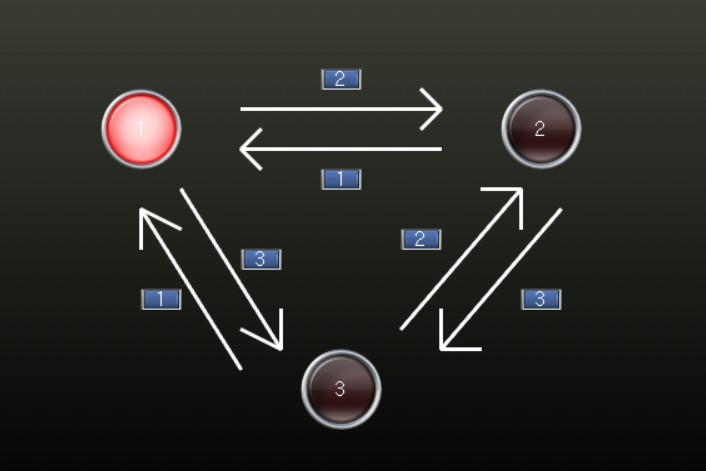
\includegraphics[width=160mm]{../images/laby/grafstanow_tras.jpg}
    \caption{Wygląd grafu stanów dla interfejsu użytkownika}
    %\label{fig:normal}
    \end{figure}  

%%%%%%%%%%%%%% Podpunkt4
\section{Wizualizacja procesu}

Wizualizacja składa się z wykresów: sygnałów zadanych i zmierzonych (po lewej stronie) oraz wartości sterowania (po prawej stronie). Oba te wykresy są odpowiednio podpisane. Dodatkowo na dole ekranu wypisywane są wartości aktualne. W prawym dolnym rogu można zauważyć dwie diody, które informują o zmianie kierunku ruchu silnika.

 \begin{figure}[h]
    \centering
    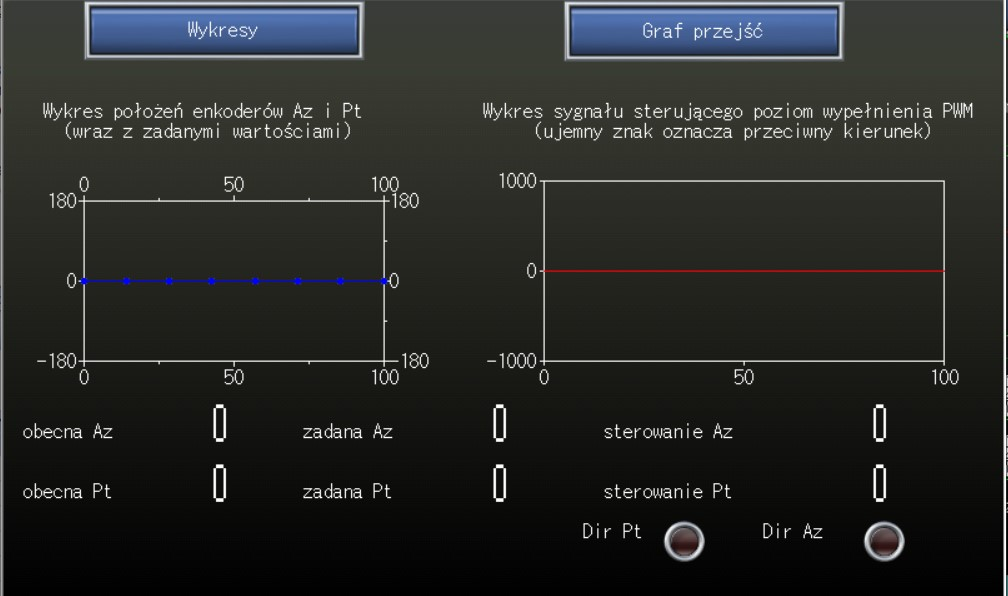
\includegraphics[width=160mm]{../images/laby/wizualizacja_tras.jpg}
    \caption{Wygląd interfejsu użytkownika (wizualizacja)}
    %\label{fig:normal}
    \end{figure}  


\end{document}

